\chapter{Experiments}

We now evaluate our proposed methods experimentally in both tabular and function approximation settings.
Though these algorithms can be applied both as approximate equilibrium solvers QRE and Nash equilibirum.
We present some results for convergence to QRE in the tabular setting but focus on Nash convergence mainly 
for the tabular and function approximation setting.

Through the experiments, we aim to answer the following questions:
\begin{itemize}
	\item How does the addition of NeuRD-fix, Extragradient updates, and Optimistic upates
	      affect the convergence rate of these algorithms in solving for QREs, and Nash equilibrium?
	\item What is the last-iterate vs average-iterate convergence behavior of these algorithms in the presence of these modifications?
	\item Do these performance improvements scale well with the size of the game?
\end{itemize}

\section{Evaluation Metrics}
Our main focus being the convergence behaviors and speed of convergence we need a notion of 
distance from the equilibrium point to measure the performance of these algorithms.

\subsection{Divergence to the equilibrium}
In settings with a known unique equilibrium such as for QREs, or Nash equilibrium in symmetric markov games, 
we can compute the distance of the current policy to the known equilibrium using a measure of distance in the policy space such as the KL-Divergence. 

For PerturbedRPS, we use the QRE solutions computed through Gambit and, we also derive the unique
Nash Equilibrium (please refer to~\ref{sec:rpsne} in the appendix for the derivation) for
PerturbedRPS.\

\subsection{Exploitability}
In general, there might not be a unique Nash equilibrium. 
In such cases, another notion of distance from the equilibrium is needed to measure convergence.
Exploitability measures the gain in value by deviating from the current strategy.
This is measured by computing the utility of a best response agent against the current policy, as an indiciation 
of incentive to deviate from the current policy.

\blue{ - Exploitability formal expression in terms of best responses, and value.}

\subsection{Approximate Exploitability}
For larger games, it is not possible to compute the exact exploitability due to the large state space. 
However, we can approximate the exploitability by training a best response agent against the fixed current policy to be exploited. 
Then the exploitability can be approximated by sampling trajectories and measuring the average reward the best response 
agent acheived against the exploited policy.

\section{Tabular Experiments}
We evaluate the converegence behavior of all these algorithms on Perturned RPS.


\ref{tab:tabres} summarizes the last and average iterate convergences behaviors of 3 different algorithms -
MMD, MDPO, SPG under the proposed modifications.
We present the results for NE, and QRE convergence (with 0.5 temperature). Fig

% \begin{noindent}

\begin{table}[htbp]
	\centering
	\begin{tabular}{|c|c|c|c|c|c|c|c|c|}
	\hline
	\multirow{3}{*}{\textbf{Algorithm}} &
	\multicolumn{4}{c|}{\textbf{Nash}} &
	\multicolumn{2}{c|}{\textbf{QRE ($\alpha$=0.5)}} \\
	\cline{2-7}
	& 
	\multicolumn{2}{c|}{\textbf{MMD}} & 
	\multicolumn{2}{c|}{\textbf{MDPO}} &
	\multicolumn{2}{c|}{\textbf{MMD}} \\
	\cline{2-7}
	& \textbf{Avg} & \textbf{Last} & \textbf{Avg} & \textbf{Last}
	& \textbf{Avg} & \textbf{Last} \\
	\hline
	Base	 	& y & y & x & y 		& y & y \\
	\hline
	NeuRD 		& y & y & y & \red{x} 	& y & y \\
	\hline
	EG 			& y & y & y & y 	& y & y \\
	\hline
	OPT 		& y & y & y & n 	& y & y \\
	\hline
	EG-OPT 		& y & y & y & y 	& y & y \\
	\hline
	EG-N 		& y & y & y & y 	& y & y \\
	\hline
	OPT-N 		& y & y & y & n 	& y & y \\
	\hline
	EG-OPT-N	& y & y & y & y 	& y & y \\
	\hline
	\end{tabular}
	\caption{QRE and Nash convergence in Perturbed RPS for last, and average iterates.}
	\label{tab:tabres}
\end{table}
% \end{noindent}

\begin{figure}[H]
	% \subfigure{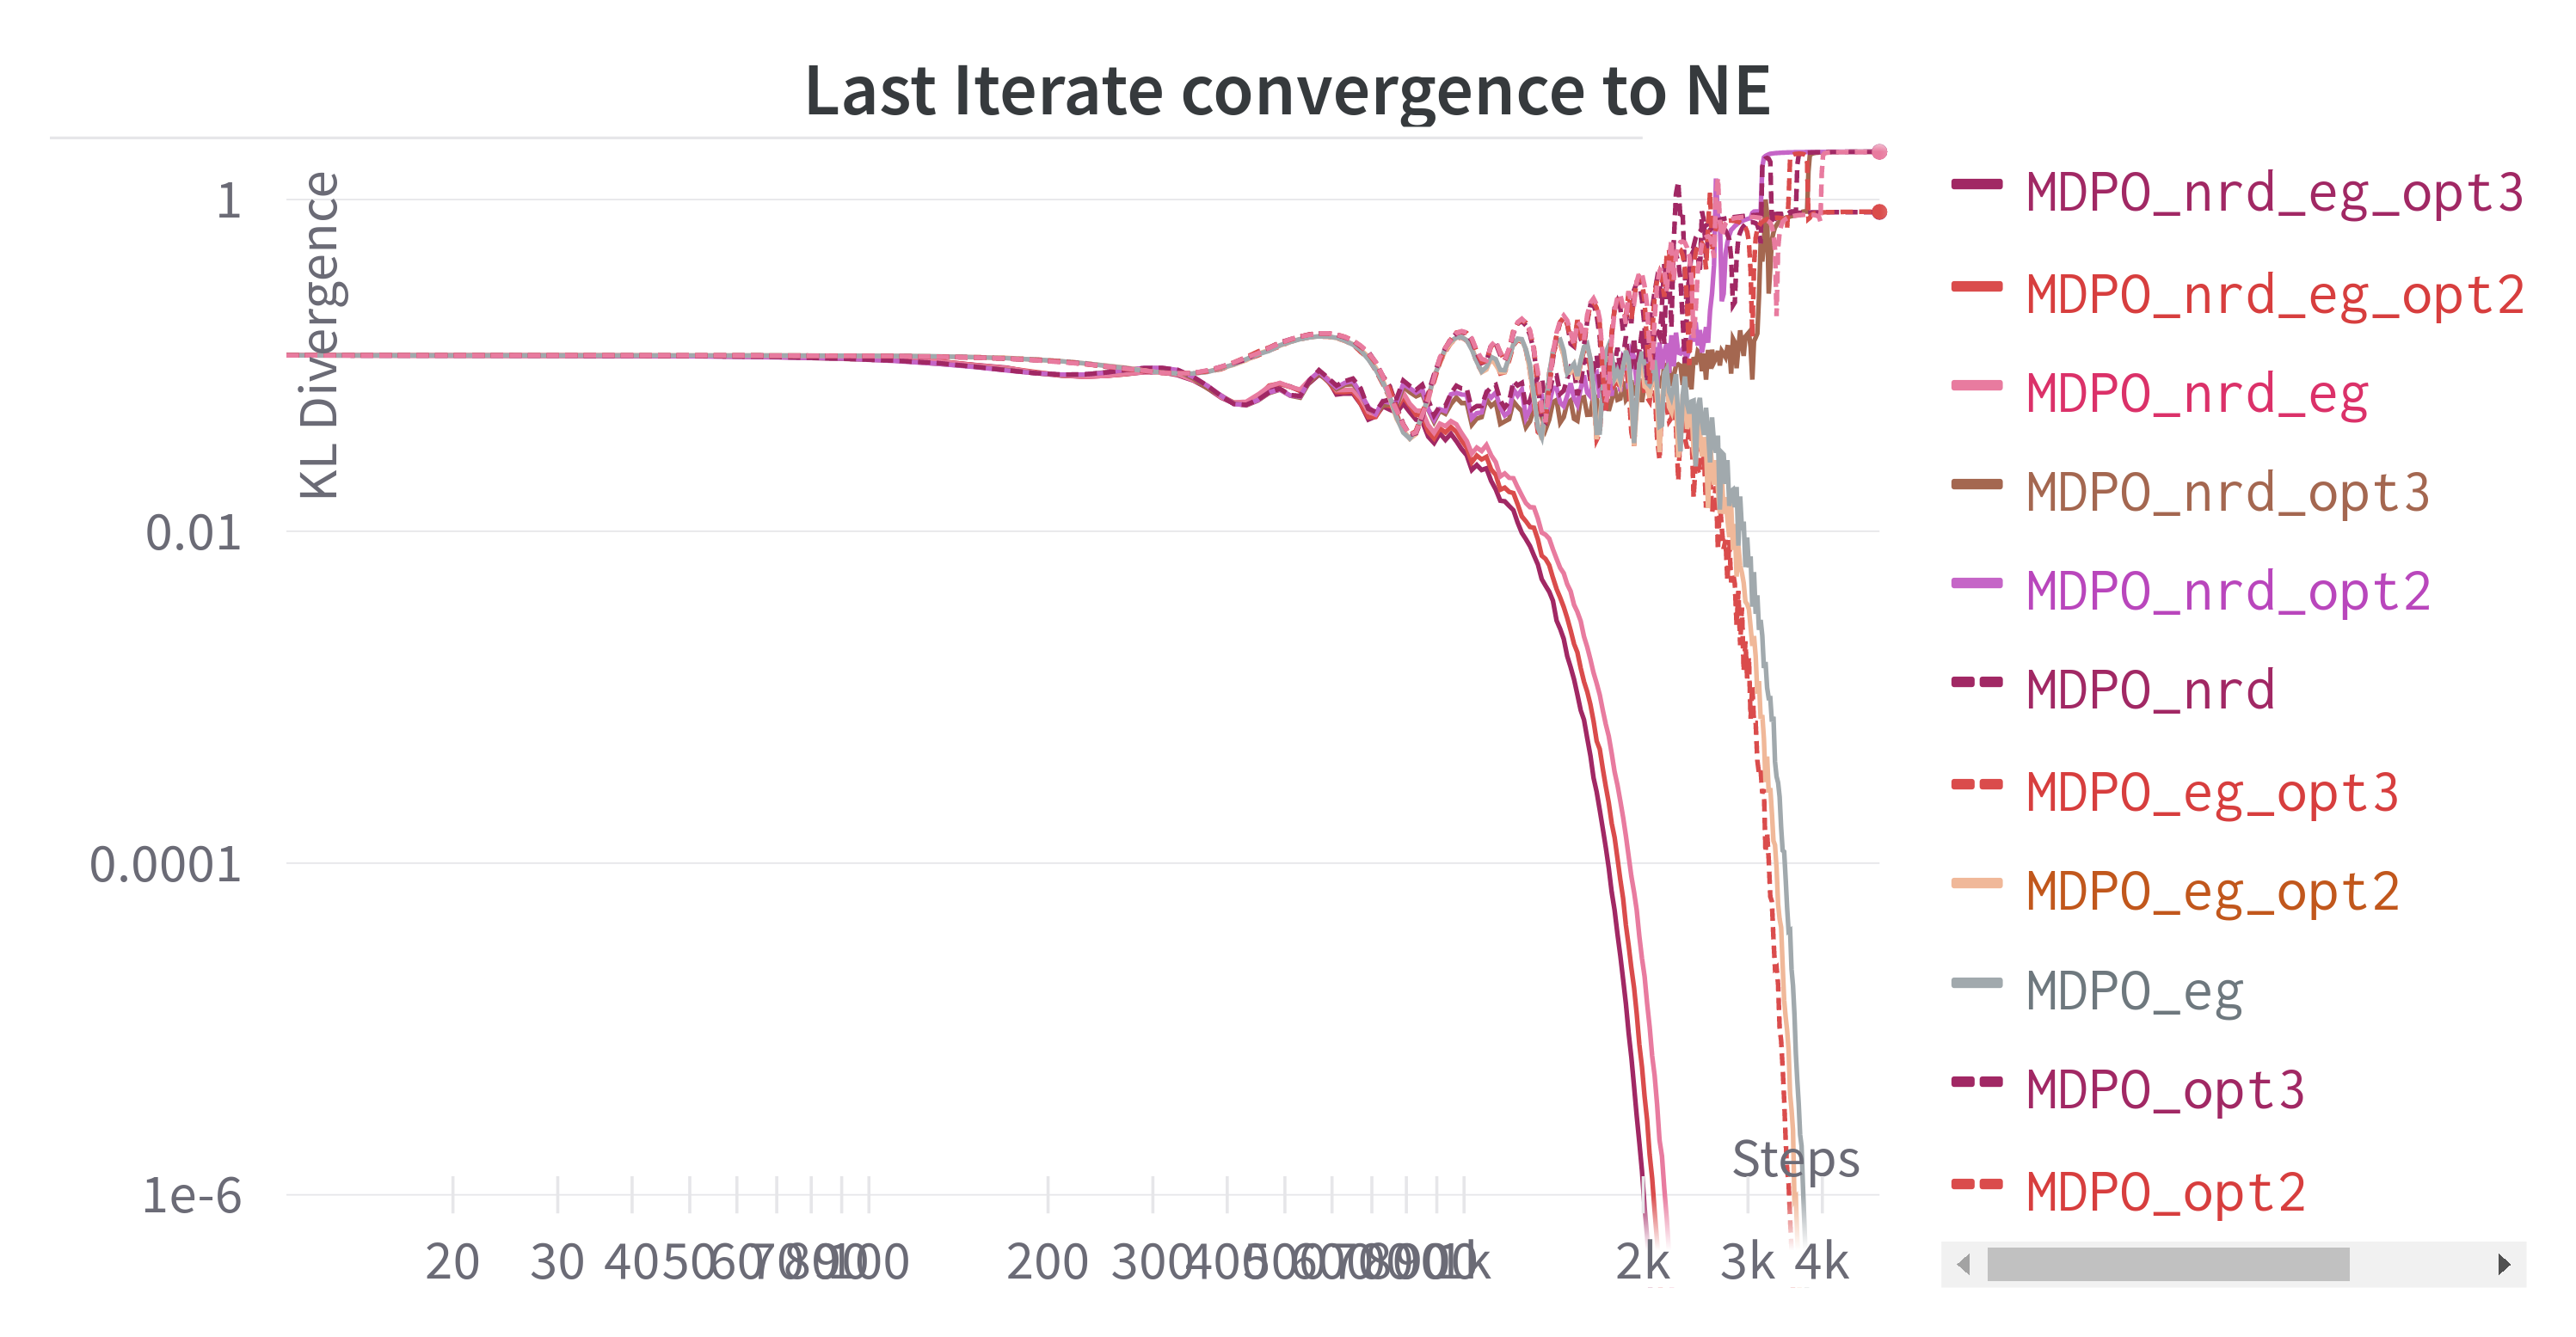
\includegraphics[width=0.5\linewidth]{plots/MDPO_NE.png}}
	% \subfigure{%% Creator: Matplotlib, PGF backend
%%
%% To include the figure in your LaTeX document, write
%%   \input{<filename>.pgf}
%%
%% Make sure the required packages are loaded in your preamble
%%   \usepackage{pgf}
%%
%% Also ensure that all the required font packages are loaded; for instance,
%% the lmodern package is sometimes necessary when using math font.
%%   \usepackage{lmodern}
%%
%% Figures using additional raster images can only be included by \input if
%% they are in the same directory as the main LaTeX file. For loading figures
%% from other directories you can use the `import` package
%%   \usepackage{import}
%%
%% and then include the figures with
%%   \import{<path to file>}{<filename>.pgf}
%%
%% Matplotlib used the following preamble
%%   
%%   \makeatletter\@ifpackageloaded{underscore}{}{\usepackage[strings]{underscore}}\makeatother
%%
\begingroup%
\makeatletter%
\begin{pgfpicture}%
\pgfpathrectangle{\pgfpointorigin}{\pgfqpoint{10.000000in}{20.000000in}}%
\pgfusepath{use as bounding box, clip}%
\begin{pgfscope}%
\pgfsetbuttcap%
\pgfsetmiterjoin%
\definecolor{currentfill}{rgb}{1.000000,1.000000,1.000000}%
\pgfsetfillcolor{currentfill}%
\pgfsetlinewidth{0.000000pt}%
\definecolor{currentstroke}{rgb}{1.000000,1.000000,1.000000}%
\pgfsetstrokecolor{currentstroke}%
\pgfsetdash{}{0pt}%
\pgfpathmoveto{\pgfqpoint{0.000000in}{0.000000in}}%
\pgfpathlineto{\pgfqpoint{10.000000in}{0.000000in}}%
\pgfpathlineto{\pgfqpoint{10.000000in}{20.000000in}}%
\pgfpathlineto{\pgfqpoint{0.000000in}{20.000000in}}%
\pgfpathlineto{\pgfqpoint{0.000000in}{0.000000in}}%
\pgfpathclose%
\pgfusepath{fill}%
\end{pgfscope}%
\begin{pgfscope}%
\pgfsetbuttcap%
\pgfsetmiterjoin%
\definecolor{currentfill}{rgb}{1.000000,1.000000,1.000000}%
\pgfsetfillcolor{currentfill}%
\pgfsetlinewidth{0.000000pt}%
\definecolor{currentstroke}{rgb}{0.000000,0.000000,0.000000}%
\pgfsetstrokecolor{currentstroke}%
\pgfsetstrokeopacity{0.000000}%
\pgfsetdash{}{0pt}%
\pgfpathmoveto{\pgfqpoint{1.250000in}{14.252174in}}%
\pgfpathlineto{\pgfqpoint{7.000000in}{14.252174in}}%
\pgfpathlineto{\pgfqpoint{7.000000in}{17.600000in}}%
\pgfpathlineto{\pgfqpoint{1.250000in}{17.600000in}}%
\pgfpathlineto{\pgfqpoint{1.250000in}{14.252174in}}%
\pgfpathclose%
\pgfusepath{fill}%
\end{pgfscope}%
\begin{pgfscope}%
\pgfsetbuttcap%
\pgfsetroundjoin%
\definecolor{currentfill}{rgb}{0.000000,0.000000,0.000000}%
\pgfsetfillcolor{currentfill}%
\pgfsetlinewidth{0.803000pt}%
\definecolor{currentstroke}{rgb}{0.000000,0.000000,0.000000}%
\pgfsetstrokecolor{currentstroke}%
\pgfsetdash{}{0pt}%
\pgfsys@defobject{currentmarker}{\pgfqpoint{0.000000in}{-0.048611in}}{\pgfqpoint{0.000000in}{0.000000in}}{%
\pgfpathmoveto{\pgfqpoint{0.000000in}{0.000000in}}%
\pgfpathlineto{\pgfqpoint{0.000000in}{-0.048611in}}%
\pgfusepath{stroke,fill}%
}%
\begin{pgfscope}%
\pgfsys@transformshift{1.511364in}{14.252174in}%
\pgfsys@useobject{currentmarker}{}%
\end{pgfscope}%
\end{pgfscope}%
\begin{pgfscope}%
\definecolor{textcolor}{rgb}{0.000000,0.000000,0.000000}%
\pgfsetstrokecolor{textcolor}%
\pgfsetfillcolor{textcolor}%
\pgftext[x=1.511364in,y=14.154952in,,top]{\color{textcolor}\rmfamily\fontsize{10.000000}{12.000000}\selectfont \(\displaystyle {0}\)}%
\end{pgfscope}%
\begin{pgfscope}%
\pgfsetbuttcap%
\pgfsetroundjoin%
\definecolor{currentfill}{rgb}{0.000000,0.000000,0.000000}%
\pgfsetfillcolor{currentfill}%
\pgfsetlinewidth{0.803000pt}%
\definecolor{currentstroke}{rgb}{0.000000,0.000000,0.000000}%
\pgfsetstrokecolor{currentstroke}%
\pgfsetdash{}{0pt}%
\pgfsys@defobject{currentmarker}{\pgfqpoint{0.000000in}{-0.048611in}}{\pgfqpoint{0.000000in}{0.000000in}}{%
\pgfpathmoveto{\pgfqpoint{0.000000in}{0.000000in}}%
\pgfpathlineto{\pgfqpoint{0.000000in}{-0.048611in}}%
\pgfusepath{stroke,fill}%
}%
\begin{pgfscope}%
\pgfsys@transformshift{2.557027in}{14.252174in}%
\pgfsys@useobject{currentmarker}{}%
\end{pgfscope}%
\end{pgfscope}%
\begin{pgfscope}%
\definecolor{textcolor}{rgb}{0.000000,0.000000,0.000000}%
\pgfsetstrokecolor{textcolor}%
\pgfsetfillcolor{textcolor}%
\pgftext[x=2.557027in,y=14.154952in,,top]{\color{textcolor}\rmfamily\fontsize{10.000000}{12.000000}\selectfont \(\displaystyle {1000}\)}%
\end{pgfscope}%
\begin{pgfscope}%
\pgfsetbuttcap%
\pgfsetroundjoin%
\definecolor{currentfill}{rgb}{0.000000,0.000000,0.000000}%
\pgfsetfillcolor{currentfill}%
\pgfsetlinewidth{0.803000pt}%
\definecolor{currentstroke}{rgb}{0.000000,0.000000,0.000000}%
\pgfsetstrokecolor{currentstroke}%
\pgfsetdash{}{0pt}%
\pgfsys@defobject{currentmarker}{\pgfqpoint{0.000000in}{-0.048611in}}{\pgfqpoint{0.000000in}{0.000000in}}{%
\pgfpathmoveto{\pgfqpoint{0.000000in}{0.000000in}}%
\pgfpathlineto{\pgfqpoint{0.000000in}{-0.048611in}}%
\pgfusepath{stroke,fill}%
}%
\begin{pgfscope}%
\pgfsys@transformshift{3.602691in}{14.252174in}%
\pgfsys@useobject{currentmarker}{}%
\end{pgfscope}%
\end{pgfscope}%
\begin{pgfscope}%
\definecolor{textcolor}{rgb}{0.000000,0.000000,0.000000}%
\pgfsetstrokecolor{textcolor}%
\pgfsetfillcolor{textcolor}%
\pgftext[x=3.602691in,y=14.154952in,,top]{\color{textcolor}\rmfamily\fontsize{10.000000}{12.000000}\selectfont \(\displaystyle {2000}\)}%
\end{pgfscope}%
\begin{pgfscope}%
\pgfsetbuttcap%
\pgfsetroundjoin%
\definecolor{currentfill}{rgb}{0.000000,0.000000,0.000000}%
\pgfsetfillcolor{currentfill}%
\pgfsetlinewidth{0.803000pt}%
\definecolor{currentstroke}{rgb}{0.000000,0.000000,0.000000}%
\pgfsetstrokecolor{currentstroke}%
\pgfsetdash{}{0pt}%
\pgfsys@defobject{currentmarker}{\pgfqpoint{0.000000in}{-0.048611in}}{\pgfqpoint{0.000000in}{0.000000in}}{%
\pgfpathmoveto{\pgfqpoint{0.000000in}{0.000000in}}%
\pgfpathlineto{\pgfqpoint{0.000000in}{-0.048611in}}%
\pgfusepath{stroke,fill}%
}%
\begin{pgfscope}%
\pgfsys@transformshift{4.648355in}{14.252174in}%
\pgfsys@useobject{currentmarker}{}%
\end{pgfscope}%
\end{pgfscope}%
\begin{pgfscope}%
\definecolor{textcolor}{rgb}{0.000000,0.000000,0.000000}%
\pgfsetstrokecolor{textcolor}%
\pgfsetfillcolor{textcolor}%
\pgftext[x=4.648355in,y=14.154952in,,top]{\color{textcolor}\rmfamily\fontsize{10.000000}{12.000000}\selectfont \(\displaystyle {3000}\)}%
\end{pgfscope}%
\begin{pgfscope}%
\pgfsetbuttcap%
\pgfsetroundjoin%
\definecolor{currentfill}{rgb}{0.000000,0.000000,0.000000}%
\pgfsetfillcolor{currentfill}%
\pgfsetlinewidth{0.803000pt}%
\definecolor{currentstroke}{rgb}{0.000000,0.000000,0.000000}%
\pgfsetstrokecolor{currentstroke}%
\pgfsetdash{}{0pt}%
\pgfsys@defobject{currentmarker}{\pgfqpoint{0.000000in}{-0.048611in}}{\pgfqpoint{0.000000in}{0.000000in}}{%
\pgfpathmoveto{\pgfqpoint{0.000000in}{0.000000in}}%
\pgfpathlineto{\pgfqpoint{0.000000in}{-0.048611in}}%
\pgfusepath{stroke,fill}%
}%
\begin{pgfscope}%
\pgfsys@transformshift{5.694018in}{14.252174in}%
\pgfsys@useobject{currentmarker}{}%
\end{pgfscope}%
\end{pgfscope}%
\begin{pgfscope}%
\definecolor{textcolor}{rgb}{0.000000,0.000000,0.000000}%
\pgfsetstrokecolor{textcolor}%
\pgfsetfillcolor{textcolor}%
\pgftext[x=5.694018in,y=14.154952in,,top]{\color{textcolor}\rmfamily\fontsize{10.000000}{12.000000}\selectfont \(\displaystyle {4000}\)}%
\end{pgfscope}%
\begin{pgfscope}%
\pgfsetbuttcap%
\pgfsetroundjoin%
\definecolor{currentfill}{rgb}{0.000000,0.000000,0.000000}%
\pgfsetfillcolor{currentfill}%
\pgfsetlinewidth{0.803000pt}%
\definecolor{currentstroke}{rgb}{0.000000,0.000000,0.000000}%
\pgfsetstrokecolor{currentstroke}%
\pgfsetdash{}{0pt}%
\pgfsys@defobject{currentmarker}{\pgfqpoint{0.000000in}{-0.048611in}}{\pgfqpoint{0.000000in}{0.000000in}}{%
\pgfpathmoveto{\pgfqpoint{0.000000in}{0.000000in}}%
\pgfpathlineto{\pgfqpoint{0.000000in}{-0.048611in}}%
\pgfusepath{stroke,fill}%
}%
\begin{pgfscope}%
\pgfsys@transformshift{6.739682in}{14.252174in}%
\pgfsys@useobject{currentmarker}{}%
\end{pgfscope}%
\end{pgfscope}%
\begin{pgfscope}%
\definecolor{textcolor}{rgb}{0.000000,0.000000,0.000000}%
\pgfsetstrokecolor{textcolor}%
\pgfsetfillcolor{textcolor}%
\pgftext[x=6.739682in,y=14.154952in,,top]{\color{textcolor}\rmfamily\fontsize{10.000000}{12.000000}\selectfont \(\displaystyle {5000}\)}%
\end{pgfscope}%
\begin{pgfscope}%
\pgfsetbuttcap%
\pgfsetroundjoin%
\definecolor{currentfill}{rgb}{0.000000,0.000000,0.000000}%
\pgfsetfillcolor{currentfill}%
\pgfsetlinewidth{0.803000pt}%
\definecolor{currentstroke}{rgb}{0.000000,0.000000,0.000000}%
\pgfsetstrokecolor{currentstroke}%
\pgfsetdash{}{0pt}%
\pgfsys@defobject{currentmarker}{\pgfqpoint{-0.048611in}{0.000000in}}{\pgfqpoint{-0.000000in}{0.000000in}}{%
\pgfpathmoveto{\pgfqpoint{-0.000000in}{0.000000in}}%
\pgfpathlineto{\pgfqpoint{-0.048611in}{0.000000in}}%
\pgfusepath{stroke,fill}%
}%
\begin{pgfscope}%
\pgfsys@transformshift{1.250000in}{14.252174in}%
\pgfsys@useobject{currentmarker}{}%
\end{pgfscope}%
\end{pgfscope}%
\begin{pgfscope}%
\definecolor{textcolor}{rgb}{0.000000,0.000000,0.000000}%
\pgfsetstrokecolor{textcolor}%
\pgfsetfillcolor{textcolor}%
\pgftext[x=0.809412in, y=14.203949in, left, base]{\color{textcolor}\rmfamily\fontsize{10.000000}{12.000000}\selectfont \(\displaystyle {10^{-10}}\)}%
\end{pgfscope}%
\begin{pgfscope}%
\pgfsetbuttcap%
\pgfsetroundjoin%
\definecolor{currentfill}{rgb}{0.000000,0.000000,0.000000}%
\pgfsetfillcolor{currentfill}%
\pgfsetlinewidth{0.803000pt}%
\definecolor{currentstroke}{rgb}{0.000000,0.000000,0.000000}%
\pgfsetstrokecolor{currentstroke}%
\pgfsetdash{}{0pt}%
\pgfsys@defobject{currentmarker}{\pgfqpoint{-0.048611in}{0.000000in}}{\pgfqpoint{-0.000000in}{0.000000in}}{%
\pgfpathmoveto{\pgfqpoint{-0.000000in}{0.000000in}}%
\pgfpathlineto{\pgfqpoint{-0.048611in}{0.000000in}}%
\pgfusepath{stroke,fill}%
}%
\begin{pgfscope}%
\pgfsys@transformshift{1.250000in}{14.921739in}%
\pgfsys@useobject{currentmarker}{}%
\end{pgfscope}%
\end{pgfscope}%
\begin{pgfscope}%
\definecolor{textcolor}{rgb}{0.000000,0.000000,0.000000}%
\pgfsetstrokecolor{textcolor}%
\pgfsetfillcolor{textcolor}%
\pgftext[x=0.864775in, y=14.873514in, left, base]{\color{textcolor}\rmfamily\fontsize{10.000000}{12.000000}\selectfont \(\displaystyle {10^{-8}}\)}%
\end{pgfscope}%
\begin{pgfscope}%
\pgfsetbuttcap%
\pgfsetroundjoin%
\definecolor{currentfill}{rgb}{0.000000,0.000000,0.000000}%
\pgfsetfillcolor{currentfill}%
\pgfsetlinewidth{0.803000pt}%
\definecolor{currentstroke}{rgb}{0.000000,0.000000,0.000000}%
\pgfsetstrokecolor{currentstroke}%
\pgfsetdash{}{0pt}%
\pgfsys@defobject{currentmarker}{\pgfqpoint{-0.048611in}{0.000000in}}{\pgfqpoint{-0.000000in}{0.000000in}}{%
\pgfpathmoveto{\pgfqpoint{-0.000000in}{0.000000in}}%
\pgfpathlineto{\pgfqpoint{-0.048611in}{0.000000in}}%
\pgfusepath{stroke,fill}%
}%
\begin{pgfscope}%
\pgfsys@transformshift{1.250000in}{15.591304in}%
\pgfsys@useobject{currentmarker}{}%
\end{pgfscope}%
\end{pgfscope}%
\begin{pgfscope}%
\definecolor{textcolor}{rgb}{0.000000,0.000000,0.000000}%
\pgfsetstrokecolor{textcolor}%
\pgfsetfillcolor{textcolor}%
\pgftext[x=0.864775in, y=15.543079in, left, base]{\color{textcolor}\rmfamily\fontsize{10.000000}{12.000000}\selectfont \(\displaystyle {10^{-6}}\)}%
\end{pgfscope}%
\begin{pgfscope}%
\pgfsetbuttcap%
\pgfsetroundjoin%
\definecolor{currentfill}{rgb}{0.000000,0.000000,0.000000}%
\pgfsetfillcolor{currentfill}%
\pgfsetlinewidth{0.803000pt}%
\definecolor{currentstroke}{rgb}{0.000000,0.000000,0.000000}%
\pgfsetstrokecolor{currentstroke}%
\pgfsetdash{}{0pt}%
\pgfsys@defobject{currentmarker}{\pgfqpoint{-0.048611in}{0.000000in}}{\pgfqpoint{-0.000000in}{0.000000in}}{%
\pgfpathmoveto{\pgfqpoint{-0.000000in}{0.000000in}}%
\pgfpathlineto{\pgfqpoint{-0.048611in}{0.000000in}}%
\pgfusepath{stroke,fill}%
}%
\begin{pgfscope}%
\pgfsys@transformshift{1.250000in}{16.260870in}%
\pgfsys@useobject{currentmarker}{}%
\end{pgfscope}%
\end{pgfscope}%
\begin{pgfscope}%
\definecolor{textcolor}{rgb}{0.000000,0.000000,0.000000}%
\pgfsetstrokecolor{textcolor}%
\pgfsetfillcolor{textcolor}%
\pgftext[x=0.864775in, y=16.212644in, left, base]{\color{textcolor}\rmfamily\fontsize{10.000000}{12.000000}\selectfont \(\displaystyle {10^{-4}}\)}%
\end{pgfscope}%
\begin{pgfscope}%
\pgfsetbuttcap%
\pgfsetroundjoin%
\definecolor{currentfill}{rgb}{0.000000,0.000000,0.000000}%
\pgfsetfillcolor{currentfill}%
\pgfsetlinewidth{0.803000pt}%
\definecolor{currentstroke}{rgb}{0.000000,0.000000,0.000000}%
\pgfsetstrokecolor{currentstroke}%
\pgfsetdash{}{0pt}%
\pgfsys@defobject{currentmarker}{\pgfqpoint{-0.048611in}{0.000000in}}{\pgfqpoint{-0.000000in}{0.000000in}}{%
\pgfpathmoveto{\pgfqpoint{-0.000000in}{0.000000in}}%
\pgfpathlineto{\pgfqpoint{-0.048611in}{0.000000in}}%
\pgfusepath{stroke,fill}%
}%
\begin{pgfscope}%
\pgfsys@transformshift{1.250000in}{16.930435in}%
\pgfsys@useobject{currentmarker}{}%
\end{pgfscope}%
\end{pgfscope}%
\begin{pgfscope}%
\definecolor{textcolor}{rgb}{0.000000,0.000000,0.000000}%
\pgfsetstrokecolor{textcolor}%
\pgfsetfillcolor{textcolor}%
\pgftext[x=0.864775in, y=16.882210in, left, base]{\color{textcolor}\rmfamily\fontsize{10.000000}{12.000000}\selectfont \(\displaystyle {10^{-2}}\)}%
\end{pgfscope}%
\begin{pgfscope}%
\pgfsetbuttcap%
\pgfsetroundjoin%
\definecolor{currentfill}{rgb}{0.000000,0.000000,0.000000}%
\pgfsetfillcolor{currentfill}%
\pgfsetlinewidth{0.803000pt}%
\definecolor{currentstroke}{rgb}{0.000000,0.000000,0.000000}%
\pgfsetstrokecolor{currentstroke}%
\pgfsetdash{}{0pt}%
\pgfsys@defobject{currentmarker}{\pgfqpoint{-0.048611in}{0.000000in}}{\pgfqpoint{-0.000000in}{0.000000in}}{%
\pgfpathmoveto{\pgfqpoint{-0.000000in}{0.000000in}}%
\pgfpathlineto{\pgfqpoint{-0.048611in}{0.000000in}}%
\pgfusepath{stroke,fill}%
}%
\begin{pgfscope}%
\pgfsys@transformshift{1.250000in}{17.600000in}%
\pgfsys@useobject{currentmarker}{}%
\end{pgfscope}%
\end{pgfscope}%
\begin{pgfscope}%
\definecolor{textcolor}{rgb}{0.000000,0.000000,0.000000}%
\pgfsetstrokecolor{textcolor}%
\pgfsetfillcolor{textcolor}%
\pgftext[x=0.951581in, y=17.551775in, left, base]{\color{textcolor}\rmfamily\fontsize{10.000000}{12.000000}\selectfont \(\displaystyle {10^{0}}\)}%
\end{pgfscope}%
\begin{pgfscope}%
\pgfpathrectangle{\pgfqpoint{1.250000in}{14.252174in}}{\pgfqpoint{5.750000in}{3.347826in}}%
\pgfusepath{clip}%
\pgfsetrectcap%
\pgfsetroundjoin%
\pgfsetlinewidth{1.505625pt}%
\definecolor{currentstroke}{rgb}{0.007843,0.243137,1.000000}%
\pgfsetstrokecolor{currentstroke}%
\pgfsetdash{}{0pt}%
\pgfpathmoveto{\pgfqpoint{1.511364in}{17.285398in}}%
\pgfpathlineto{\pgfqpoint{1.513455in}{17.283139in}}%
\pgfpathlineto{\pgfqpoint{1.516592in}{17.272447in}}%
\pgfpathlineto{\pgfqpoint{1.521820in}{17.251323in}}%
\pgfpathlineto{\pgfqpoint{1.523912in}{17.248765in}}%
\pgfpathlineto{\pgfqpoint{1.526003in}{17.251357in}}%
\pgfpathlineto{\pgfqpoint{1.529140in}{17.262782in}}%
\pgfpathlineto{\pgfqpoint{1.539597in}{17.308923in}}%
\pgfpathlineto{\pgfqpoint{1.543779in}{17.318640in}}%
\pgfpathlineto{\pgfqpoint{1.546916in}{17.322094in}}%
\pgfpathlineto{\pgfqpoint{1.550053in}{17.322458in}}%
\pgfpathlineto{\pgfqpoint{1.553190in}{17.319850in}}%
\pgfpathlineto{\pgfqpoint{1.556327in}{17.314294in}}%
\pgfpathlineto{\pgfqpoint{1.560510in}{17.302152in}}%
\pgfpathlineto{\pgfqpoint{1.565738in}{17.278716in}}%
\pgfpathlineto{\pgfqpoint{1.570966in}{17.245044in}}%
\pgfpathlineto{\pgfqpoint{1.578286in}{17.181454in}}%
\pgfpathlineto{\pgfqpoint{1.584560in}{17.128457in}}%
\pgfpathlineto{\pgfqpoint{1.587697in}{17.116614in}}%
\pgfpathlineto{\pgfqpoint{1.588743in}{17.116305in}}%
\pgfpathlineto{\pgfqpoint{1.590834in}{17.121372in}}%
\pgfpathlineto{\pgfqpoint{1.593971in}{17.140822in}}%
\pgfpathlineto{\pgfqpoint{1.612793in}{17.287885in}}%
\pgfpathlineto{\pgfqpoint{1.618021in}{17.308163in}}%
\pgfpathlineto{\pgfqpoint{1.622204in}{17.318021in}}%
\pgfpathlineto{\pgfqpoint{1.626387in}{17.322592in}}%
\pgfpathlineto{\pgfqpoint{1.629524in}{17.322572in}}%
\pgfpathlineto{\pgfqpoint{1.632661in}{17.319487in}}%
\pgfpathlineto{\pgfqpoint{1.635798in}{17.313163in}}%
\pgfpathlineto{\pgfqpoint{1.639980in}{17.299466in}}%
\pgfpathlineto{\pgfqpoint{1.652528in}{17.248986in}}%
\pgfpathlineto{\pgfqpoint{1.653574in}{17.249118in}}%
\pgfpathlineto{\pgfqpoint{1.655665in}{17.253220in}}%
\pgfpathlineto{\pgfqpoint{1.660894in}{17.275471in}}%
\pgfpathlineto{\pgfqpoint{1.664031in}{17.284763in}}%
\pgfpathlineto{\pgfqpoint{1.666122in}{17.285702in}}%
\pgfpathlineto{\pgfqpoint{1.668213in}{17.282064in}}%
\pgfpathlineto{\pgfqpoint{1.672396in}{17.265154in}}%
\pgfpathlineto{\pgfqpoint{1.676578in}{17.250226in}}%
\pgfpathlineto{\pgfqpoint{1.678670in}{17.249184in}}%
\pgfpathlineto{\pgfqpoint{1.680761in}{17.253195in}}%
\pgfpathlineto{\pgfqpoint{1.684944in}{17.271024in}}%
\pgfpathlineto{\pgfqpoint{1.693309in}{17.307796in}}%
\pgfpathlineto{\pgfqpoint{1.697492in}{17.318111in}}%
\pgfpathlineto{\pgfqpoint{1.700629in}{17.321985in}}%
\pgfpathlineto{\pgfqpoint{1.703766in}{17.322748in}}%
\pgfpathlineto{\pgfqpoint{1.706903in}{17.320531in}}%
\pgfpathlineto{\pgfqpoint{1.710040in}{17.315369in}}%
\pgfpathlineto{\pgfqpoint{1.714222in}{17.303781in}}%
\pgfpathlineto{\pgfqpoint{1.719451in}{17.281115in}}%
\pgfpathlineto{\pgfqpoint{1.724679in}{17.248293in}}%
\pgfpathlineto{\pgfqpoint{1.731999in}{17.185557in}}%
\pgfpathlineto{\pgfqpoint{1.739318in}{17.125005in}}%
\pgfpathlineto{\pgfqpoint{1.741410in}{17.117361in}}%
\pgfpathlineto{\pgfqpoint{1.742455in}{17.116277in}}%
\pgfpathlineto{\pgfqpoint{1.743501in}{17.117122in}}%
\pgfpathlineto{\pgfqpoint{1.745592in}{17.124336in}}%
\pgfpathlineto{\pgfqpoint{1.748729in}{17.145998in}}%
\pgfpathlineto{\pgfqpoint{1.764414in}{17.274819in}}%
\pgfpathlineto{\pgfqpoint{1.770688in}{17.303532in}}%
\pgfpathlineto{\pgfqpoint{1.775917in}{17.317418in}}%
\pgfpathlineto{\pgfqpoint{1.780099in}{17.322536in}}%
\pgfpathlineto{\pgfqpoint{1.783236in}{17.322940in}}%
\pgfpathlineto{\pgfqpoint{1.786373in}{17.320306in}}%
\pgfpathlineto{\pgfqpoint{1.789510in}{17.314468in}}%
\pgfpathlineto{\pgfqpoint{1.793693in}{17.301448in}}%
\pgfpathlineto{\pgfqpoint{1.799967in}{17.272438in}}%
\pgfpathlineto{\pgfqpoint{1.805195in}{17.251364in}}%
\pgfpathlineto{\pgfqpoint{1.807286in}{17.249167in}}%
\pgfpathlineto{\pgfqpoint{1.809378in}{17.252098in}}%
\pgfpathlineto{\pgfqpoint{1.812515in}{17.263958in}}%
\pgfpathlineto{\pgfqpoint{1.817743in}{17.283717in}}%
\pgfpathlineto{\pgfqpoint{1.819834in}{17.285626in}}%
\pgfpathlineto{\pgfqpoint{1.821926in}{17.282949in}}%
\pgfpathlineto{\pgfqpoint{1.825063in}{17.271844in}}%
\pgfpathlineto{\pgfqpoint{1.830291in}{17.251120in}}%
\pgfpathlineto{\pgfqpoint{1.832382in}{17.249017in}}%
\pgfpathlineto{\pgfqpoint{1.834474in}{17.252036in}}%
\pgfpathlineto{\pgfqpoint{1.837611in}{17.263841in}}%
\pgfpathlineto{\pgfqpoint{1.848067in}{17.309681in}}%
\pgfpathlineto{\pgfqpoint{1.852250in}{17.319157in}}%
\pgfpathlineto{\pgfqpoint{1.855387in}{17.322450in}}%
\pgfpathlineto{\pgfqpoint{1.858524in}{17.322668in}}%
\pgfpathlineto{\pgfqpoint{1.861661in}{17.319926in}}%
\pgfpathlineto{\pgfqpoint{1.865844in}{17.311682in}}%
\pgfpathlineto{\pgfqpoint{1.870026in}{17.297964in}}%
\pgfpathlineto{\pgfqpoint{1.875255in}{17.272351in}}%
\pgfpathlineto{\pgfqpoint{1.881529in}{17.227852in}}%
\pgfpathlineto{\pgfqpoint{1.895122in}{17.118814in}}%
\pgfpathlineto{\pgfqpoint{1.897214in}{17.116687in}}%
\pgfpathlineto{\pgfqpoint{1.899305in}{17.122125in}}%
\pgfpathlineto{\pgfqpoint{1.902442in}{17.141947in}}%
\pgfpathlineto{\pgfqpoint{1.920218in}{17.283372in}}%
\pgfpathlineto{\pgfqpoint{1.925446in}{17.305318in}}%
\pgfpathlineto{\pgfqpoint{1.930675in}{17.318314in}}%
\pgfpathlineto{\pgfqpoint{1.934857in}{17.322745in}}%
\pgfpathlineto{\pgfqpoint{1.937994in}{17.322621in}}%
\pgfpathlineto{\pgfqpoint{1.941131in}{17.319429in}}%
\pgfpathlineto{\pgfqpoint{1.944268in}{17.312992in}}%
\pgfpathlineto{\pgfqpoint{1.948451in}{17.299142in}}%
\pgfpathlineto{\pgfqpoint{1.960999in}{17.248921in}}%
\pgfpathlineto{\pgfqpoint{1.962045in}{17.249167in}}%
\pgfpathlineto{\pgfqpoint{1.964136in}{17.253480in}}%
\pgfpathlineto{\pgfqpoint{1.973547in}{17.286109in}}%
\pgfpathlineto{\pgfqpoint{1.974593in}{17.285970in}}%
\pgfpathlineto{\pgfqpoint{1.976684in}{17.282307in}}%
\pgfpathlineto{\pgfqpoint{1.980867in}{17.265385in}}%
\pgfpathlineto{\pgfqpoint{1.985049in}{17.250282in}}%
\pgfpathlineto{\pgfqpoint{1.987141in}{17.249067in}}%
\pgfpathlineto{\pgfqpoint{1.989232in}{17.252899in}}%
\pgfpathlineto{\pgfqpoint{1.993415in}{17.270492in}}%
\pgfpathlineto{\pgfqpoint{2.001780in}{17.307262in}}%
\pgfpathlineto{\pgfqpoint{2.005963in}{17.317656in}}%
\pgfpathlineto{\pgfqpoint{2.009100in}{17.321596in}}%
\pgfpathlineto{\pgfqpoint{2.012237in}{17.322426in}}%
\pgfpathlineto{\pgfqpoint{2.015374in}{17.320277in}}%
\pgfpathlineto{\pgfqpoint{2.018511in}{17.315186in}}%
\pgfpathlineto{\pgfqpoint{2.022693in}{17.303700in}}%
\pgfpathlineto{\pgfqpoint{2.027921in}{17.281185in}}%
\pgfpathlineto{\pgfqpoint{2.033150in}{17.248540in}}%
\pgfpathlineto{\pgfqpoint{2.040469in}{17.186017in}}%
\pgfpathlineto{\pgfqpoint{2.047789in}{17.125134in}}%
\pgfpathlineto{\pgfqpoint{2.049880in}{17.117197in}}%
\pgfpathlineto{\pgfqpoint{2.050926in}{17.115945in}}%
\pgfpathlineto{\pgfqpoint{2.051972in}{17.116619in}}%
\pgfpathlineto{\pgfqpoint{2.054063in}{17.123512in}}%
\pgfpathlineto{\pgfqpoint{2.057200in}{17.144828in}}%
\pgfpathlineto{\pgfqpoint{2.073931in}{17.279457in}}%
\pgfpathlineto{\pgfqpoint{2.080205in}{17.305996in}}%
\pgfpathlineto{\pgfqpoint{2.085433in}{17.318278in}}%
\pgfpathlineto{\pgfqpoint{2.088570in}{17.321683in}}%
\pgfpathlineto{\pgfqpoint{2.091707in}{17.322148in}}%
\pgfpathlineto{\pgfqpoint{2.094844in}{17.319591in}}%
\pgfpathlineto{\pgfqpoint{2.097981in}{17.313860in}}%
\pgfpathlineto{\pgfqpoint{2.102164in}{17.301061in}}%
\pgfpathlineto{\pgfqpoint{2.108438in}{17.272558in}}%
\pgfpathlineto{\pgfqpoint{2.113666in}{17.251395in}}%
\pgfpathlineto{\pgfqpoint{2.115757in}{17.248671in}}%
\pgfpathlineto{\pgfqpoint{2.117849in}{17.250766in}}%
\pgfpathlineto{\pgfqpoint{2.120986in}{17.261226in}}%
\pgfpathlineto{\pgfqpoint{2.126214in}{17.280099in}}%
\pgfpathlineto{\pgfqpoint{2.128305in}{17.282382in}}%
\pgfpathlineto{\pgfqpoint{2.130397in}{17.280396in}}%
\pgfpathlineto{\pgfqpoint{2.133534in}{17.270522in}}%
\pgfpathlineto{\pgfqpoint{2.139808in}{17.248092in}}%
\pgfpathlineto{\pgfqpoint{2.141899in}{17.247555in}}%
\pgfpathlineto{\pgfqpoint{2.143990in}{17.251734in}}%
\pgfpathlineto{\pgfqpoint{2.148173in}{17.269243in}}%
\pgfpathlineto{\pgfqpoint{2.156538in}{17.305406in}}%
\pgfpathlineto{\pgfqpoint{2.160721in}{17.315714in}}%
\pgfpathlineto{\pgfqpoint{2.163858in}{17.319650in}}%
\pgfpathlineto{\pgfqpoint{2.166995in}{17.320505in}}%
\pgfpathlineto{\pgfqpoint{2.170132in}{17.318400in}}%
\pgfpathlineto{\pgfqpoint{2.173269in}{17.313369in}}%
\pgfpathlineto{\pgfqpoint{2.177451in}{17.301991in}}%
\pgfpathlineto{\pgfqpoint{2.182680in}{17.279678in}}%
\pgfpathlineto{\pgfqpoint{2.187908in}{17.247358in}}%
\pgfpathlineto{\pgfqpoint{2.195228in}{17.185508in}}%
\pgfpathlineto{\pgfqpoint{2.202547in}{17.124812in}}%
\pgfpathlineto{\pgfqpoint{2.205684in}{17.115107in}}%
\pgfpathlineto{\pgfqpoint{2.206730in}{17.115533in}}%
\pgfpathlineto{\pgfqpoint{2.208821in}{17.121892in}}%
\pgfpathlineto{\pgfqpoint{2.211958in}{17.142500in}}%
\pgfpathlineto{\pgfqpoint{2.228689in}{17.276408in}}%
\pgfpathlineto{\pgfqpoint{2.234963in}{17.302949in}}%
\pgfpathlineto{\pgfqpoint{2.240191in}{17.315157in}}%
\pgfpathlineto{\pgfqpoint{2.243328in}{17.318477in}}%
\pgfpathlineto{\pgfqpoint{2.246465in}{17.318827in}}%
\pgfpathlineto{\pgfqpoint{2.249602in}{17.316125in}}%
\pgfpathlineto{\pgfqpoint{2.252739in}{17.310228in}}%
\pgfpathlineto{\pgfqpoint{2.256922in}{17.297216in}}%
\pgfpathlineto{\pgfqpoint{2.263196in}{17.268653in}}%
\pgfpathlineto{\pgfqpoint{2.268424in}{17.247893in}}%
\pgfpathlineto{\pgfqpoint{2.270515in}{17.245313in}}%
\pgfpathlineto{\pgfqpoint{2.272607in}{17.247416in}}%
\pgfpathlineto{\pgfqpoint{2.275744in}{17.257654in}}%
\pgfpathlineto{\pgfqpoint{2.280972in}{17.276901in}}%
\pgfpathlineto{\pgfqpoint{2.283063in}{17.280062in}}%
\pgfpathlineto{\pgfqpoint{2.285155in}{17.279351in}}%
\pgfpathlineto{\pgfqpoint{2.287246in}{17.274896in}}%
\pgfpathlineto{\pgfqpoint{2.296657in}{17.244558in}}%
\pgfpathlineto{\pgfqpoint{2.297703in}{17.244725in}}%
\pgfpathlineto{\pgfqpoint{2.299794in}{17.248431in}}%
\pgfpathlineto{\pgfqpoint{2.303977in}{17.265140in}}%
\pgfpathlineto{\pgfqpoint{2.312342in}{17.301280in}}%
\pgfpathlineto{\pgfqpoint{2.316525in}{17.311903in}}%
\pgfpathlineto{\pgfqpoint{2.320707in}{17.316769in}}%
\pgfpathlineto{\pgfqpoint{2.323844in}{17.316829in}}%
\pgfpathlineto{\pgfqpoint{2.326981in}{17.313916in}}%
\pgfpathlineto{\pgfqpoint{2.331164in}{17.305395in}}%
\pgfpathlineto{\pgfqpoint{2.335347in}{17.291331in}}%
\pgfpathlineto{\pgfqpoint{2.340575in}{17.265184in}}%
\pgfpathlineto{\pgfqpoint{2.346849in}{17.220038in}}%
\pgfpathlineto{\pgfqpoint{2.359397in}{17.117405in}}%
\pgfpathlineto{\pgfqpoint{2.361488in}{17.112977in}}%
\pgfpathlineto{\pgfqpoint{2.362534in}{17.113576in}}%
\pgfpathlineto{\pgfqpoint{2.364625in}{17.120249in}}%
\pgfpathlineto{\pgfqpoint{2.367762in}{17.141162in}}%
\pgfpathlineto{\pgfqpoint{2.384493in}{17.274904in}}%
\pgfpathlineto{\pgfqpoint{2.390767in}{17.301466in}}%
\pgfpathlineto{\pgfqpoint{2.395995in}{17.313785in}}%
\pgfpathlineto{\pgfqpoint{2.399132in}{17.317215in}}%
\pgfpathlineto{\pgfqpoint{2.402269in}{17.317717in}}%
\pgfpathlineto{\pgfqpoint{2.405406in}{17.315226in}}%
\pgfpathlineto{\pgfqpoint{2.408543in}{17.309619in}}%
\pgfpathlineto{\pgfqpoint{2.412726in}{17.297153in}}%
\pgfpathlineto{\pgfqpoint{2.419000in}{17.269592in}}%
\pgfpathlineto{\pgfqpoint{2.424228in}{17.248546in}}%
\pgfpathlineto{\pgfqpoint{2.426319in}{17.245104in}}%
\pgfpathlineto{\pgfqpoint{2.428411in}{17.245994in}}%
\pgfpathlineto{\pgfqpoint{2.431548in}{17.254466in}}%
\pgfpathlineto{\pgfqpoint{2.437822in}{17.275157in}}%
\pgfpathlineto{\pgfqpoint{2.439913in}{17.276981in}}%
\pgfpathlineto{\pgfqpoint{2.442004in}{17.275092in}}%
\pgfpathlineto{\pgfqpoint{2.445141in}{17.266376in}}%
\pgfpathlineto{\pgfqpoint{2.451415in}{17.247212in}}%
\pgfpathlineto{\pgfqpoint{2.453507in}{17.247057in}}%
\pgfpathlineto{\pgfqpoint{2.455598in}{17.251185in}}%
\pgfpathlineto{\pgfqpoint{2.459781in}{17.268098in}}%
\pgfpathlineto{\pgfqpoint{2.468146in}{17.303947in}}%
\pgfpathlineto{\pgfqpoint{2.472329in}{17.314492in}}%
\pgfpathlineto{\pgfqpoint{2.476511in}{17.319344in}}%
\pgfpathlineto{\pgfqpoint{2.479648in}{17.319428in}}%
\pgfpathlineto{\pgfqpoint{2.482785in}{17.316564in}}%
\pgfpathlineto{\pgfqpoint{2.486968in}{17.308148in}}%
\pgfpathlineto{\pgfqpoint{2.491151in}{17.294227in}}%
\pgfpathlineto{\pgfqpoint{2.496379in}{17.268306in}}%
\pgfpathlineto{\pgfqpoint{2.502653in}{17.223429in}}%
\pgfpathlineto{\pgfqpoint{2.516246in}{17.116525in}}%
\pgfpathlineto{\pgfqpoint{2.518338in}{17.115373in}}%
\pgfpathlineto{\pgfqpoint{2.520429in}{17.121691in}}%
\pgfpathlineto{\pgfqpoint{2.523566in}{17.142367in}}%
\pgfpathlineto{\pgfqpoint{2.540297in}{17.277348in}}%
\pgfpathlineto{\pgfqpoint{2.546571in}{17.304341in}}%
\pgfpathlineto{\pgfqpoint{2.551799in}{17.316983in}}%
\pgfpathlineto{\pgfqpoint{2.555982in}{17.321156in}}%
\pgfpathlineto{\pgfqpoint{2.559119in}{17.320846in}}%
\pgfpathlineto{\pgfqpoint{2.562256in}{17.317477in}}%
\pgfpathlineto{\pgfqpoint{2.566438in}{17.307945in}}%
\pgfpathlineto{\pgfqpoint{2.571667in}{17.287860in}}%
\pgfpathlineto{\pgfqpoint{2.580032in}{17.251088in}}%
\pgfpathlineto{\pgfqpoint{2.582123in}{17.248162in}}%
\pgfpathlineto{\pgfqpoint{2.583169in}{17.248562in}}%
\pgfpathlineto{\pgfqpoint{2.585260in}{17.253032in}}%
\pgfpathlineto{\pgfqpoint{2.594671in}{17.285590in}}%
\pgfpathlineto{\pgfqpoint{2.595717in}{17.285609in}}%
\pgfpathlineto{\pgfqpoint{2.597808in}{17.282354in}}%
\pgfpathlineto{\pgfqpoint{2.600945in}{17.270873in}}%
\pgfpathlineto{\pgfqpoint{2.606174in}{17.250563in}}%
\pgfpathlineto{\pgfqpoint{2.608265in}{17.248729in}}%
\pgfpathlineto{\pgfqpoint{2.610356in}{17.251949in}}%
\pgfpathlineto{\pgfqpoint{2.613493in}{17.263892in}}%
\pgfpathlineto{\pgfqpoint{2.623950in}{17.309644in}}%
\pgfpathlineto{\pgfqpoint{2.628132in}{17.319080in}}%
\pgfpathlineto{\pgfqpoint{2.631269in}{17.322350in}}%
\pgfpathlineto{\pgfqpoint{2.634406in}{17.322549in}}%
\pgfpathlineto{\pgfqpoint{2.637543in}{17.319790in}}%
\pgfpathlineto{\pgfqpoint{2.641726in}{17.311523in}}%
\pgfpathlineto{\pgfqpoint{2.645909in}{17.297778in}}%
\pgfpathlineto{\pgfqpoint{2.651137in}{17.272119in}}%
\pgfpathlineto{\pgfqpoint{2.657411in}{17.227564in}}%
\pgfpathlineto{\pgfqpoint{2.671005in}{17.119108in}}%
\pgfpathlineto{\pgfqpoint{2.673096in}{17.117214in}}%
\pgfpathlineto{\pgfqpoint{2.675187in}{17.122851in}}%
\pgfpathlineto{\pgfqpoint{2.678324in}{17.142838in}}%
\pgfpathlineto{\pgfqpoint{2.696101in}{17.283920in}}%
\pgfpathlineto{\pgfqpoint{2.701329in}{17.305839in}}%
\pgfpathlineto{\pgfqpoint{2.706557in}{17.318873in}}%
\pgfpathlineto{\pgfqpoint{2.710740in}{17.323385in}}%
\pgfpathlineto{\pgfqpoint{2.713877in}{17.323356in}}%
\pgfpathlineto{\pgfqpoint{2.717014in}{17.320295in}}%
\pgfpathlineto{\pgfqpoint{2.720151in}{17.314032in}}%
\pgfpathlineto{\pgfqpoint{2.724334in}{17.300483in}}%
\pgfpathlineto{\pgfqpoint{2.731653in}{17.266105in}}%
\pgfpathlineto{\pgfqpoint{2.735836in}{17.251240in}}%
\pgfpathlineto{\pgfqpoint{2.737927in}{17.249857in}}%
\pgfpathlineto{\pgfqpoint{2.740018in}{17.253531in}}%
\pgfpathlineto{\pgfqpoint{2.744201in}{17.270664in}}%
\pgfpathlineto{\pgfqpoint{2.748384in}{17.284778in}}%
\pgfpathlineto{\pgfqpoint{2.750475in}{17.286110in}}%
\pgfpathlineto{\pgfqpoint{2.752566in}{17.282939in}}%
\pgfpathlineto{\pgfqpoint{2.755703in}{17.271505in}}%
\pgfpathlineto{\pgfqpoint{2.760932in}{17.251724in}}%
\pgfpathlineto{\pgfqpoint{2.763023in}{17.250268in}}%
\pgfpathlineto{\pgfqpoint{2.765114in}{17.253813in}}%
\pgfpathlineto{\pgfqpoint{2.768251in}{17.265997in}}%
\pgfpathlineto{\pgfqpoint{2.778708in}{17.311277in}}%
\pgfpathlineto{\pgfqpoint{2.782891in}{17.320472in}}%
\pgfpathlineto{\pgfqpoint{2.786028in}{17.323594in}}%
\pgfpathlineto{\pgfqpoint{2.789165in}{17.323674in}}%
\pgfpathlineto{\pgfqpoint{2.792302in}{17.320817in}}%
\pgfpathlineto{\pgfqpoint{2.796484in}{17.312449in}}%
\pgfpathlineto{\pgfqpoint{2.800667in}{17.298628in}}%
\pgfpathlineto{\pgfqpoint{2.805895in}{17.272900in}}%
\pgfpathlineto{\pgfqpoint{2.812169in}{17.228274in}}%
\pgfpathlineto{\pgfqpoint{2.825763in}{17.119409in}}%
\pgfpathlineto{\pgfqpoint{2.827854in}{17.117455in}}%
\pgfpathlineto{\pgfqpoint{2.829946in}{17.123070in}}%
\pgfpathlineto{\pgfqpoint{2.833083in}{17.143102in}}%
\pgfpathlineto{\pgfqpoint{2.850859in}{17.284539in}}%
\pgfpathlineto{\pgfqpoint{2.856087in}{17.306454in}}%
\pgfpathlineto{\pgfqpoint{2.861315in}{17.319462in}}%
\pgfpathlineto{\pgfqpoint{2.865498in}{17.323942in}}%
\pgfpathlineto{\pgfqpoint{2.868635in}{17.323879in}}%
\pgfpathlineto{\pgfqpoint{2.871772in}{17.320771in}}%
\pgfpathlineto{\pgfqpoint{2.874909in}{17.314442in}}%
\pgfpathlineto{\pgfqpoint{2.879092in}{17.300760in}}%
\pgfpathlineto{\pgfqpoint{2.886411in}{17.266099in}}%
\pgfpathlineto{\pgfqpoint{2.890594in}{17.251409in}}%
\pgfpathlineto{\pgfqpoint{2.892685in}{17.250344in}}%
\pgfpathlineto{\pgfqpoint{2.894777in}{17.254452in}}%
\pgfpathlineto{\pgfqpoint{2.900005in}{17.276986in}}%
\pgfpathlineto{\pgfqpoint{2.903142in}{17.286639in}}%
\pgfpathlineto{\pgfqpoint{2.905233in}{17.287863in}}%
\pgfpathlineto{\pgfqpoint{2.907325in}{17.284489in}}%
\pgfpathlineto{\pgfqpoint{2.910462in}{17.272600in}}%
\pgfpathlineto{\pgfqpoint{2.915690in}{17.251909in}}%
\pgfpathlineto{\pgfqpoint{2.917781in}{17.250213in}}%
\pgfpathlineto{\pgfqpoint{2.919873in}{17.253652in}}%
\pgfpathlineto{\pgfqpoint{2.923010in}{17.265855in}}%
\pgfpathlineto{\pgfqpoint{2.933466in}{17.311339in}}%
\pgfpathlineto{\pgfqpoint{2.937649in}{17.320531in}}%
\pgfpathlineto{\pgfqpoint{2.940786in}{17.323636in}}%
\pgfpathlineto{\pgfqpoint{2.943923in}{17.323691in}}%
\pgfpathlineto{\pgfqpoint{2.947060in}{17.320806in}}%
\pgfpathlineto{\pgfqpoint{2.951243in}{17.312393in}}%
\pgfpathlineto{\pgfqpoint{2.955425in}{17.298519in}}%
\pgfpathlineto{\pgfqpoint{2.960653in}{17.272709in}}%
\pgfpathlineto{\pgfqpoint{2.966927in}{17.227963in}}%
\pgfpathlineto{\pgfqpoint{2.980521in}{17.119235in}}%
\pgfpathlineto{\pgfqpoint{2.982612in}{17.117420in}}%
\pgfpathlineto{\pgfqpoint{2.984704in}{17.123168in}}%
\pgfpathlineto{\pgfqpoint{2.987841in}{17.143332in}}%
\pgfpathlineto{\pgfqpoint{3.005617in}{17.284554in}}%
\pgfpathlineto{\pgfqpoint{3.010845in}{17.306392in}}%
\pgfpathlineto{\pgfqpoint{3.016074in}{17.319344in}}%
\pgfpathlineto{\pgfqpoint{3.020256in}{17.323794in}}%
\pgfpathlineto{\pgfqpoint{3.023393in}{17.323721in}}%
\pgfpathlineto{\pgfqpoint{3.026530in}{17.320621in}}%
\pgfpathlineto{\pgfqpoint{3.029667in}{17.314327in}}%
\pgfpathlineto{\pgfqpoint{3.033850in}{17.300762in}}%
\pgfpathlineto{\pgfqpoint{3.046398in}{17.250467in}}%
\pgfpathlineto{\pgfqpoint{3.047444in}{17.250379in}}%
\pgfpathlineto{\pgfqpoint{3.049535in}{17.253904in}}%
\pgfpathlineto{\pgfqpoint{3.053718in}{17.270476in}}%
\pgfpathlineto{\pgfqpoint{3.057900in}{17.284098in}}%
\pgfpathlineto{\pgfqpoint{3.059992in}{17.285323in}}%
\pgfpathlineto{\pgfqpoint{3.062083in}{17.282150in}}%
\pgfpathlineto{\pgfqpoint{3.065220in}{17.270833in}}%
\pgfpathlineto{\pgfqpoint{3.070448in}{17.251027in}}%
\pgfpathlineto{\pgfqpoint{3.072540in}{17.249355in}}%
\pgfpathlineto{\pgfqpoint{3.074631in}{17.252626in}}%
\pgfpathlineto{\pgfqpoint{3.077768in}{17.264462in}}%
\pgfpathlineto{\pgfqpoint{3.088224in}{17.309751in}}%
\pgfpathlineto{\pgfqpoint{3.092407in}{17.319171in}}%
\pgfpathlineto{\pgfqpoint{3.095544in}{17.322476in}}%
\pgfpathlineto{\pgfqpoint{3.098681in}{17.322742in}}%
\pgfpathlineto{\pgfqpoint{3.101818in}{17.320080in}}%
\pgfpathlineto{\pgfqpoint{3.106001in}{17.311993in}}%
\pgfpathlineto{\pgfqpoint{3.110183in}{17.298499in}}%
\pgfpathlineto{\pgfqpoint{3.115412in}{17.273277in}}%
\pgfpathlineto{\pgfqpoint{3.121686in}{17.229420in}}%
\pgfpathlineto{\pgfqpoint{3.135279in}{17.119822in}}%
\pgfpathlineto{\pgfqpoint{3.137371in}{17.116857in}}%
\pgfpathlineto{\pgfqpoint{3.138416in}{17.118217in}}%
\pgfpathlineto{\pgfqpoint{3.140508in}{17.126291in}}%
\pgfpathlineto{\pgfqpoint{3.144690in}{17.157786in}}%
\pgfpathlineto{\pgfqpoint{3.157238in}{17.263252in}}%
\pgfpathlineto{\pgfqpoint{3.163512in}{17.295853in}}%
\pgfpathlineto{\pgfqpoint{3.168741in}{17.312577in}}%
\pgfpathlineto{\pgfqpoint{3.172923in}{17.319822in}}%
\pgfpathlineto{\pgfqpoint{3.176060in}{17.321824in}}%
\pgfpathlineto{\pgfqpoint{3.179197in}{17.320854in}}%
\pgfpathlineto{\pgfqpoint{3.182334in}{17.316789in}}%
\pgfpathlineto{\pgfqpoint{3.186517in}{17.306283in}}%
\pgfpathlineto{\pgfqpoint{3.191745in}{17.285119in}}%
\pgfpathlineto{\pgfqpoint{3.200110in}{17.249553in}}%
\pgfpathlineto{\pgfqpoint{3.202202in}{17.247749in}}%
\pgfpathlineto{\pgfqpoint{3.204293in}{17.250800in}}%
\pgfpathlineto{\pgfqpoint{3.208476in}{17.266786in}}%
\pgfpathlineto{\pgfqpoint{3.212658in}{17.281319in}}%
\pgfpathlineto{\pgfqpoint{3.214750in}{17.283682in}}%
\pgfpathlineto{\pgfqpoint{3.216841in}{17.281930in}}%
\pgfpathlineto{\pgfqpoint{3.219978in}{17.272499in}}%
\pgfpathlineto{\pgfqpoint{3.226252in}{17.248561in}}%
\pgfpathlineto{\pgfqpoint{3.228343in}{17.246618in}}%
\pgfpathlineto{\pgfqpoint{3.230435in}{17.249428in}}%
\pgfpathlineto{\pgfqpoint{3.233572in}{17.260563in}}%
\pgfpathlineto{\pgfqpoint{3.245074in}{17.308425in}}%
\pgfpathlineto{\pgfqpoint{3.249257in}{17.316639in}}%
\pgfpathlineto{\pgfqpoint{3.252394in}{17.319099in}}%
\pgfpathlineto{\pgfqpoint{3.255531in}{17.318546in}}%
\pgfpathlineto{\pgfqpoint{3.258668in}{17.315056in}}%
\pgfpathlineto{\pgfqpoint{3.262850in}{17.305795in}}%
\pgfpathlineto{\pgfqpoint{3.267033in}{17.290988in}}%
\pgfpathlineto{\pgfqpoint{3.272261in}{17.263873in}}%
\pgfpathlineto{\pgfqpoint{3.278535in}{17.217576in}}%
\pgfpathlineto{\pgfqpoint{3.291083in}{17.116849in}}%
\pgfpathlineto{\pgfqpoint{3.293175in}{17.113910in}}%
\pgfpathlineto{\pgfqpoint{3.294220in}{17.115277in}}%
\pgfpathlineto{\pgfqpoint{3.296312in}{17.123343in}}%
\pgfpathlineto{\pgfqpoint{3.300494in}{17.154745in}}%
\pgfpathlineto{\pgfqpoint{3.313042in}{17.259863in}}%
\pgfpathlineto{\pgfqpoint{3.319316in}{17.292402in}}%
\pgfpathlineto{\pgfqpoint{3.324544in}{17.309110in}}%
\pgfpathlineto{\pgfqpoint{3.328727in}{17.316363in}}%
\pgfpathlineto{\pgfqpoint{3.331864in}{17.318392in}}%
\pgfpathlineto{\pgfqpoint{3.335001in}{17.317486in}}%
\pgfpathlineto{\pgfqpoint{3.338138in}{17.313554in}}%
\pgfpathlineto{\pgfqpoint{3.342321in}{17.303416in}}%
\pgfpathlineto{\pgfqpoint{3.347549in}{17.283209in}}%
\pgfpathlineto{\pgfqpoint{3.355914in}{17.248481in}}%
\pgfpathlineto{\pgfqpoint{3.358006in}{17.245574in}}%
\pgfpathlineto{\pgfqpoint{3.360097in}{17.246833in}}%
\pgfpathlineto{\pgfqpoint{3.363234in}{17.255236in}}%
\pgfpathlineto{\pgfqpoint{3.369508in}{17.274392in}}%
\pgfpathlineto{\pgfqpoint{3.371599in}{17.275882in}}%
\pgfpathlineto{\pgfqpoint{3.373691in}{17.273917in}}%
\pgfpathlineto{\pgfqpoint{3.376828in}{17.265524in}}%
\pgfpathlineto{\pgfqpoint{3.383102in}{17.247016in}}%
\pgfpathlineto{\pgfqpoint{3.385193in}{17.246657in}}%
\pgfpathlineto{\pgfqpoint{3.387284in}{17.250423in}}%
\pgfpathlineto{\pgfqpoint{3.391467in}{17.266658in}}%
\pgfpathlineto{\pgfqpoint{3.400878in}{17.305741in}}%
\pgfpathlineto{\pgfqpoint{3.405061in}{17.315230in}}%
\pgfpathlineto{\pgfqpoint{3.408198in}{17.318673in}}%
\pgfpathlineto{\pgfqpoint{3.411335in}{17.319098in}}%
\pgfpathlineto{\pgfqpoint{3.414472in}{17.316589in}}%
\pgfpathlineto{\pgfqpoint{3.417609in}{17.311152in}}%
\pgfpathlineto{\pgfqpoint{3.421791in}{17.299192in}}%
\pgfpathlineto{\pgfqpoint{3.427019in}{17.276025in}}%
\pgfpathlineto{\pgfqpoint{3.432248in}{17.242693in}}%
\pgfpathlineto{\pgfqpoint{3.439567in}{17.179726in}}%
\pgfpathlineto{\pgfqpoint{3.445841in}{17.127198in}}%
\pgfpathlineto{\pgfqpoint{3.448978in}{17.115363in}}%
\pgfpathlineto{\pgfqpoint{3.450024in}{17.115008in}}%
\pgfpathlineto{\pgfqpoint{3.452115in}{17.119927in}}%
\pgfpathlineto{\pgfqpoint{3.455252in}{17.139091in}}%
\pgfpathlineto{\pgfqpoint{3.474074in}{17.285692in}}%
\pgfpathlineto{\pgfqpoint{3.479303in}{17.306102in}}%
\pgfpathlineto{\pgfqpoint{3.484531in}{17.317775in}}%
\pgfpathlineto{\pgfqpoint{3.487668in}{17.320852in}}%
\pgfpathlineto{\pgfqpoint{3.490805in}{17.321003in}}%
\pgfpathlineto{\pgfqpoint{3.493942in}{17.318137in}}%
\pgfpathlineto{\pgfqpoint{3.497079in}{17.312101in}}%
\pgfpathlineto{\pgfqpoint{3.501262in}{17.298928in}}%
\pgfpathlineto{\pgfqpoint{3.508581in}{17.265257in}}%
\pgfpathlineto{\pgfqpoint{3.512764in}{17.250191in}}%
\pgfpathlineto{\pgfqpoint{3.514855in}{17.248348in}}%
\pgfpathlineto{\pgfqpoint{3.516947in}{17.251429in}}%
\pgfpathlineto{\pgfqpoint{3.520084in}{17.263188in}}%
\pgfpathlineto{\pgfqpoint{3.525312in}{17.283424in}}%
\pgfpathlineto{\pgfqpoint{3.527403in}{17.286149in}}%
\pgfpathlineto{\pgfqpoint{3.529495in}{17.284564in}}%
\pgfpathlineto{\pgfqpoint{3.532632in}{17.274985in}}%
\pgfpathlineto{\pgfqpoint{3.538906in}{17.250826in}}%
\pgfpathlineto{\pgfqpoint{3.540997in}{17.249374in}}%
\pgfpathlineto{\pgfqpoint{3.543088in}{17.252884in}}%
\pgfpathlineto{\pgfqpoint{3.546225in}{17.265017in}}%
\pgfpathlineto{\pgfqpoint{3.556682in}{17.310493in}}%
\pgfpathlineto{\pgfqpoint{3.560864in}{17.319818in}}%
\pgfpathlineto{\pgfqpoint{3.564001in}{17.323031in}}%
\pgfpathlineto{\pgfqpoint{3.567138in}{17.323193in}}%
\pgfpathlineto{\pgfqpoint{3.570275in}{17.320413in}}%
\pgfpathlineto{\pgfqpoint{3.574458in}{17.312139in}}%
\pgfpathlineto{\pgfqpoint{3.578641in}{17.298409in}}%
\pgfpathlineto{\pgfqpoint{3.583869in}{17.272797in}}%
\pgfpathlineto{\pgfqpoint{3.590143in}{17.228331in}}%
\pgfpathlineto{\pgfqpoint{3.603737in}{17.119969in}}%
\pgfpathlineto{\pgfqpoint{3.605828in}{17.118025in}}%
\pgfpathlineto{\pgfqpoint{3.607919in}{17.123598in}}%
\pgfpathlineto{\pgfqpoint{3.611056in}{17.143491in}}%
\pgfpathlineto{\pgfqpoint{3.628833in}{17.284508in}}%
\pgfpathlineto{\pgfqpoint{3.634061in}{17.306508in}}%
\pgfpathlineto{\pgfqpoint{3.639289in}{17.319664in}}%
\pgfpathlineto{\pgfqpoint{3.643472in}{17.324311in}}%
\pgfpathlineto{\pgfqpoint{3.646609in}{17.324412in}}%
\pgfpathlineto{\pgfqpoint{3.649746in}{17.321510in}}%
\pgfpathlineto{\pgfqpoint{3.652883in}{17.315438in}}%
\pgfpathlineto{\pgfqpoint{3.657066in}{17.302180in}}%
\pgfpathlineto{\pgfqpoint{3.664385in}{17.268060in}}%
\pgfpathlineto{\pgfqpoint{3.668568in}{17.252644in}}%
\pgfpathlineto{\pgfqpoint{3.670659in}{17.250748in}}%
\pgfpathlineto{\pgfqpoint{3.672750in}{17.253907in}}%
\pgfpathlineto{\pgfqpoint{3.675887in}{17.265872in}}%
\pgfpathlineto{\pgfqpoint{3.681116in}{17.285491in}}%
\pgfpathlineto{\pgfqpoint{3.683207in}{17.287416in}}%
\pgfpathlineto{\pgfqpoint{3.685298in}{17.284838in}}%
\pgfpathlineto{\pgfqpoint{3.688435in}{17.273999in}}%
\pgfpathlineto{\pgfqpoint{3.693664in}{17.253533in}}%
\pgfpathlineto{\pgfqpoint{3.695755in}{17.251322in}}%
\pgfpathlineto{\pgfqpoint{3.697846in}{17.254146in}}%
\pgfpathlineto{\pgfqpoint{3.700983in}{17.265655in}}%
\pgfpathlineto{\pgfqpoint{3.711440in}{17.311408in}}%
\pgfpathlineto{\pgfqpoint{3.715623in}{17.321090in}}%
\pgfpathlineto{\pgfqpoint{3.718760in}{17.324579in}}%
\pgfpathlineto{\pgfqpoint{3.721897in}{17.325028in}}%
\pgfpathlineto{\pgfqpoint{3.725034in}{17.322555in}}%
\pgfpathlineto{\pgfqpoint{3.728171in}{17.317183in}}%
\pgfpathlineto{\pgfqpoint{3.732353in}{17.305369in}}%
\pgfpathlineto{\pgfqpoint{3.737582in}{17.282484in}}%
\pgfpathlineto{\pgfqpoint{3.742810in}{17.249493in}}%
\pgfpathlineto{\pgfqpoint{3.750130in}{17.186650in}}%
\pgfpathlineto{\pgfqpoint{3.757449in}{17.126490in}}%
\pgfpathlineto{\pgfqpoint{3.759541in}{17.119104in}}%
\pgfpathlineto{\pgfqpoint{3.760586in}{17.118160in}}%
\pgfpathlineto{\pgfqpoint{3.761632in}{17.119146in}}%
\pgfpathlineto{\pgfqpoint{3.763723in}{17.126612in}}%
\pgfpathlineto{\pgfqpoint{3.767906in}{17.157626in}}%
\pgfpathlineto{\pgfqpoint{3.780454in}{17.264366in}}%
\pgfpathlineto{\pgfqpoint{3.786728in}{17.297737in}}%
\pgfpathlineto{\pgfqpoint{3.791956in}{17.315091in}}%
\pgfpathlineto{\pgfqpoint{3.796139in}{17.322874in}}%
\pgfpathlineto{\pgfqpoint{3.799276in}{17.325320in}}%
\pgfpathlineto{\pgfqpoint{3.802413in}{17.324838in}}%
\pgfpathlineto{\pgfqpoint{3.805550in}{17.321309in}}%
\pgfpathlineto{\pgfqpoint{3.809732in}{17.311552in}}%
\pgfpathlineto{\pgfqpoint{3.814961in}{17.291094in}}%
\pgfpathlineto{\pgfqpoint{3.823326in}{17.253887in}}%
\pgfpathlineto{\pgfqpoint{3.825417in}{17.251222in}}%
\pgfpathlineto{\pgfqpoint{3.826463in}{17.251839in}}%
\pgfpathlineto{\pgfqpoint{3.828554in}{17.256852in}}%
\pgfpathlineto{\pgfqpoint{3.837965in}{17.289577in}}%
\pgfpathlineto{\pgfqpoint{3.840057in}{17.287757in}}%
\pgfpathlineto{\pgfqpoint{3.843194in}{17.277412in}}%
\pgfpathlineto{\pgfqpoint{3.849468in}{17.252506in}}%
\pgfpathlineto{\pgfqpoint{3.851559in}{17.251432in}}%
\pgfpathlineto{\pgfqpoint{3.853650in}{17.255432in}}%
\pgfpathlineto{\pgfqpoint{3.857833in}{17.273228in}}%
\pgfpathlineto{\pgfqpoint{3.866198in}{17.309922in}}%
\pgfpathlineto{\pgfqpoint{3.870381in}{17.320261in}}%
\pgfpathlineto{\pgfqpoint{3.873518in}{17.324193in}}%
\pgfpathlineto{\pgfqpoint{3.876655in}{17.325053in}}%
\pgfpathlineto{\pgfqpoint{3.879792in}{17.322971in}}%
\pgfpathlineto{\pgfqpoint{3.882929in}{17.317989in}}%
\pgfpathlineto{\pgfqpoint{3.887112in}{17.306714in}}%
\pgfpathlineto{\pgfqpoint{3.892340in}{17.284572in}}%
\pgfpathlineto{\pgfqpoint{3.897568in}{17.252401in}}%
\pgfpathlineto{\pgfqpoint{3.904888in}{17.190424in}}%
\pgfpathlineto{\pgfqpoint{3.912207in}{17.128544in}}%
\pgfpathlineto{\pgfqpoint{3.915344in}{17.118096in}}%
\pgfpathlineto{\pgfqpoint{3.916390in}{17.118310in}}%
\pgfpathlineto{\pgfqpoint{3.918481in}{17.124361in}}%
\pgfpathlineto{\pgfqpoint{3.921618in}{17.144830in}}%
\pgfpathlineto{\pgfqpoint{3.939395in}{17.285709in}}%
\pgfpathlineto{\pgfqpoint{3.944623in}{17.307403in}}%
\pgfpathlineto{\pgfqpoint{3.949851in}{17.320263in}}%
\pgfpathlineto{\pgfqpoint{3.954034in}{17.324678in}}%
\pgfpathlineto{\pgfqpoint{3.957171in}{17.324601in}}%
\pgfpathlineto{\pgfqpoint{3.960308in}{17.321520in}}%
\pgfpathlineto{\pgfqpoint{3.963445in}{17.315272in}}%
\pgfpathlineto{\pgfqpoint{3.967628in}{17.301816in}}%
\pgfpathlineto{\pgfqpoint{3.974947in}{17.267817in}}%
\pgfpathlineto{\pgfqpoint{3.979130in}{17.252918in}}%
\pgfpathlineto{\pgfqpoint{3.981221in}{17.251235in}}%
\pgfpathlineto{\pgfqpoint{3.983313in}{17.254404in}}%
\pgfpathlineto{\pgfqpoint{3.987495in}{17.270405in}}%
\pgfpathlineto{\pgfqpoint{3.991678in}{17.284120in}}%
\pgfpathlineto{\pgfqpoint{3.993769in}{17.285648in}}%
\pgfpathlineto{\pgfqpoint{3.995861in}{17.282873in}}%
\pgfpathlineto{\pgfqpoint{3.998998in}{17.272097in}}%
\pgfpathlineto{\pgfqpoint{4.004226in}{17.251964in}}%
\pgfpathlineto{\pgfqpoint{4.006317in}{17.249652in}}%
\pgfpathlineto{\pgfqpoint{4.008408in}{17.252223in}}%
\pgfpathlineto{\pgfqpoint{4.011545in}{17.263287in}}%
\pgfpathlineto{\pgfqpoint{4.023048in}{17.311814in}}%
\pgfpathlineto{\pgfqpoint{4.027230in}{17.320283in}}%
\pgfpathlineto{\pgfqpoint{4.030367in}{17.322951in}}%
\pgfpathlineto{\pgfqpoint{4.033504in}{17.322637in}}%
\pgfpathlineto{\pgfqpoint{4.036641in}{17.319428in}}%
\pgfpathlineto{\pgfqpoint{4.040824in}{17.310631in}}%
\pgfpathlineto{\pgfqpoint{4.045007in}{17.296414in}}%
\pgfpathlineto{\pgfqpoint{4.050235in}{17.270235in}}%
\pgfpathlineto{\pgfqpoint{4.056509in}{17.225244in}}%
\pgfpathlineto{\pgfqpoint{4.070103in}{17.118708in}}%
\pgfpathlineto{\pgfqpoint{4.072194in}{17.117512in}}%
\pgfpathlineto{\pgfqpoint{4.074285in}{17.123720in}}%
\pgfpathlineto{\pgfqpoint{4.077422in}{17.144160in}}%
\pgfpathlineto{\pgfqpoint{4.094153in}{17.278084in}}%
\pgfpathlineto{\pgfqpoint{4.100427in}{17.304773in}}%
\pgfpathlineto{\pgfqpoint{4.105655in}{17.317171in}}%
\pgfpathlineto{\pgfqpoint{4.108792in}{17.320647in}}%
\pgfpathlineto{\pgfqpoint{4.111929in}{17.321191in}}%
\pgfpathlineto{\pgfqpoint{4.115066in}{17.318728in}}%
\pgfpathlineto{\pgfqpoint{4.118203in}{17.313118in}}%
\pgfpathlineto{\pgfqpoint{4.122386in}{17.300540in}}%
\pgfpathlineto{\pgfqpoint{4.128660in}{17.272407in}}%
\pgfpathlineto{\pgfqpoint{4.133888in}{17.250854in}}%
\pgfpathlineto{\pgfqpoint{4.135979in}{17.247523in}}%
\pgfpathlineto{\pgfqpoint{4.137025in}{17.247579in}}%
\pgfpathlineto{\pgfqpoint{4.139116in}{17.251115in}}%
\pgfpathlineto{\pgfqpoint{4.143299in}{17.266851in}}%
\pgfpathlineto{\pgfqpoint{4.147482in}{17.280460in}}%
\pgfpathlineto{\pgfqpoint{4.149573in}{17.282610in}}%
\pgfpathlineto{\pgfqpoint{4.151664in}{17.280936in}}%
\pgfpathlineto{\pgfqpoint{4.154801in}{17.272061in}}%
\pgfpathlineto{\pgfqpoint{4.162121in}{17.246915in}}%
\pgfpathlineto{\pgfqpoint{4.164212in}{17.246782in}}%
\pgfpathlineto{\pgfqpoint{4.166304in}{17.251062in}}%
\pgfpathlineto{\pgfqpoint{4.170486in}{17.268221in}}%
\pgfpathlineto{\pgfqpoint{4.178852in}{17.303771in}}%
\pgfpathlineto{\pgfqpoint{4.183034in}{17.314040in}}%
\pgfpathlineto{\pgfqpoint{4.187217in}{17.318638in}}%
\pgfpathlineto{\pgfqpoint{4.190354in}{17.318550in}}%
\pgfpathlineto{\pgfqpoint{4.193491in}{17.315529in}}%
\pgfpathlineto{\pgfqpoint{4.197674in}{17.306918in}}%
\pgfpathlineto{\pgfqpoint{4.201856in}{17.292813in}}%
\pgfpathlineto{\pgfqpoint{4.207085in}{17.266676in}}%
\pgfpathlineto{\pgfqpoint{4.213359in}{17.221606in}}%
\pgfpathlineto{\pgfqpoint{4.225907in}{17.118977in}}%
\pgfpathlineto{\pgfqpoint{4.227998in}{17.114469in}}%
\pgfpathlineto{\pgfqpoint{4.229044in}{17.115021in}}%
\pgfpathlineto{\pgfqpoint{4.231135in}{17.121602in}}%
\pgfpathlineto{\pgfqpoint{4.234272in}{17.142402in}}%
\pgfpathlineto{\pgfqpoint{4.251002in}{17.276091in}}%
\pgfpathlineto{\pgfqpoint{4.257276in}{17.302778in}}%
\pgfpathlineto{\pgfqpoint{4.262505in}{17.315274in}}%
\pgfpathlineto{\pgfqpoint{4.266687in}{17.319406in}}%
\pgfpathlineto{\pgfqpoint{4.269824in}{17.319127in}}%
\pgfpathlineto{\pgfqpoint{4.272961in}{17.315868in}}%
\pgfpathlineto{\pgfqpoint{4.277144in}{17.306682in}}%
\pgfpathlineto{\pgfqpoint{4.282372in}{17.287499in}}%
\pgfpathlineto{\pgfqpoint{4.291783in}{17.248828in}}%
\pgfpathlineto{\pgfqpoint{4.293875in}{17.246692in}}%
\pgfpathlineto{\pgfqpoint{4.295966in}{17.248845in}}%
\pgfpathlineto{\pgfqpoint{4.299103in}{17.258399in}}%
\pgfpathlineto{\pgfqpoint{4.304331in}{17.275978in}}%
\pgfpathlineto{\pgfqpoint{4.306423in}{17.278771in}}%
\pgfpathlineto{\pgfqpoint{4.308514in}{17.277977in}}%
\pgfpathlineto{\pgfqpoint{4.310605in}{17.273770in}}%
\pgfpathlineto{\pgfqpoint{4.320016in}{17.248757in}}%
\pgfpathlineto{\pgfqpoint{4.322108in}{17.251417in}}%
\pgfpathlineto{\pgfqpoint{4.325245in}{17.261990in}}%
\pgfpathlineto{\pgfqpoint{4.337793in}{17.312612in}}%
\pgfpathlineto{\pgfqpoint{4.341975in}{17.320002in}}%
\pgfpathlineto{\pgfqpoint{4.345112in}{17.321942in}}%
\pgfpathlineto{\pgfqpoint{4.348249in}{17.320930in}}%
\pgfpathlineto{\pgfqpoint{4.351386in}{17.317020in}}%
\pgfpathlineto{\pgfqpoint{4.355569in}{17.307225in}}%
\pgfpathlineto{\pgfqpoint{4.360797in}{17.287102in}}%
\pgfpathlineto{\pgfqpoint{4.366025in}{17.257191in}}%
\pgfpathlineto{\pgfqpoint{4.372299in}{17.207557in}}%
\pgfpathlineto{\pgfqpoint{4.382756in}{17.121987in}}%
\pgfpathlineto{\pgfqpoint{4.384847in}{17.116928in}}%
\pgfpathlineto{\pgfqpoint{4.385893in}{17.117217in}}%
\pgfpathlineto{\pgfqpoint{4.387984in}{17.123368in}}%
\pgfpathlineto{\pgfqpoint{4.391121in}{17.143869in}}%
\pgfpathlineto{\pgfqpoint{4.407852in}{17.279000in}}%
\pgfpathlineto{\pgfqpoint{4.414126in}{17.306214in}}%
\pgfpathlineto{\pgfqpoint{4.419354in}{17.319113in}}%
\pgfpathlineto{\pgfqpoint{4.423537in}{17.323564in}}%
\pgfpathlineto{\pgfqpoint{4.426674in}{17.323516in}}%
\pgfpathlineto{\pgfqpoint{4.429811in}{17.320460in}}%
\pgfpathlineto{\pgfqpoint{4.432948in}{17.314234in}}%
\pgfpathlineto{\pgfqpoint{4.437131in}{17.300790in}}%
\pgfpathlineto{\pgfqpoint{4.444450in}{17.266744in}}%
\pgfpathlineto{\pgfqpoint{4.448633in}{17.252006in}}%
\pgfpathlineto{\pgfqpoint{4.450724in}{17.250619in}}%
\pgfpathlineto{\pgfqpoint{4.452816in}{17.254275in}}%
\pgfpathlineto{\pgfqpoint{4.456998in}{17.271653in}}%
\pgfpathlineto{\pgfqpoint{4.461181in}{17.286882in}}%
\pgfpathlineto{\pgfqpoint{4.463272in}{17.289090in}}%
\pgfpathlineto{\pgfqpoint{4.465364in}{17.286838in}}%
\pgfpathlineto{\pgfqpoint{4.468501in}{17.276280in}}%
\pgfpathlineto{\pgfqpoint{4.474775in}{17.252192in}}%
\pgfpathlineto{\pgfqpoint{4.476866in}{17.251453in}}%
\pgfpathlineto{\pgfqpoint{4.478957in}{17.255686in}}%
\pgfpathlineto{\pgfqpoint{4.483140in}{17.273649in}}%
\pgfpathlineto{\pgfqpoint{4.491505in}{17.310282in}}%
\pgfpathlineto{\pgfqpoint{4.495688in}{17.320597in}}%
\pgfpathlineto{\pgfqpoint{4.498825in}{17.324525in}}%
\pgfpathlineto{\pgfqpoint{4.501962in}{17.325387in}}%
\pgfpathlineto{\pgfqpoint{4.505099in}{17.323315in}}%
\pgfpathlineto{\pgfqpoint{4.508236in}{17.318347in}}%
\pgfpathlineto{\pgfqpoint{4.512418in}{17.307100in}}%
\pgfpathlineto{\pgfqpoint{4.517647in}{17.285001in}}%
\pgfpathlineto{\pgfqpoint{4.522875in}{17.252888in}}%
\pgfpathlineto{\pgfqpoint{4.530195in}{17.191031in}}%
\pgfpathlineto{\pgfqpoint{4.537514in}{17.129364in}}%
\pgfpathlineto{\pgfqpoint{4.540651in}{17.119008in}}%
\pgfpathlineto{\pgfqpoint{4.541697in}{17.119243in}}%
\pgfpathlineto{\pgfqpoint{4.543788in}{17.125315in}}%
\pgfpathlineto{\pgfqpoint{4.546925in}{17.145769in}}%
\pgfpathlineto{\pgfqpoint{4.564702in}{17.286569in}}%
\pgfpathlineto{\pgfqpoint{4.569930in}{17.308348in}}%
\pgfpathlineto{\pgfqpoint{4.575158in}{17.321343in}}%
\pgfpathlineto{\pgfqpoint{4.579341in}{17.325904in}}%
\pgfpathlineto{\pgfqpoint{4.582478in}{17.325962in}}%
\pgfpathlineto{\pgfqpoint{4.585615in}{17.323036in}}%
\pgfpathlineto{\pgfqpoint{4.588752in}{17.316958in}}%
\pgfpathlineto{\pgfqpoint{4.592934in}{17.303713in}}%
\pgfpathlineto{\pgfqpoint{4.599208in}{17.274718in}}%
\pgfpathlineto{\pgfqpoint{4.604437in}{17.254162in}}%
\pgfpathlineto{\pgfqpoint{4.606528in}{17.252225in}}%
\pgfpathlineto{\pgfqpoint{4.608619in}{17.255344in}}%
\pgfpathlineto{\pgfqpoint{4.611756in}{17.267284in}}%
\pgfpathlineto{\pgfqpoint{4.616985in}{17.286984in}}%
\pgfpathlineto{\pgfqpoint{4.619076in}{17.288964in}}%
\pgfpathlineto{\pgfqpoint{4.621167in}{17.286432in}}%
\pgfpathlineto{\pgfqpoint{4.624304in}{17.275587in}}%
\pgfpathlineto{\pgfqpoint{4.629533in}{17.254721in}}%
\pgfpathlineto{\pgfqpoint{4.631624in}{17.252249in}}%
\pgfpathlineto{\pgfqpoint{4.633715in}{17.254833in}}%
\pgfpathlineto{\pgfqpoint{4.636852in}{17.266116in}}%
\pgfpathlineto{\pgfqpoint{4.648355in}{17.315021in}}%
\pgfpathlineto{\pgfqpoint{4.652537in}{17.323422in}}%
\pgfpathlineto{\pgfqpoint{4.655674in}{17.326033in}}%
\pgfpathlineto{\pgfqpoint{4.658811in}{17.325668in}}%
\pgfpathlineto{\pgfqpoint{4.661948in}{17.322421in}}%
\pgfpathlineto{\pgfqpoint{4.666131in}{17.313589in}}%
\pgfpathlineto{\pgfqpoint{4.670314in}{17.299344in}}%
\pgfpathlineto{\pgfqpoint{4.675542in}{17.273110in}}%
\pgfpathlineto{\pgfqpoint{4.681816in}{17.227940in}}%
\pgfpathlineto{\pgfqpoint{4.695410in}{17.120643in}}%
\pgfpathlineto{\pgfqpoint{4.697501in}{17.119527in}}%
\pgfpathlineto{\pgfqpoint{4.699592in}{17.125909in}}%
\pgfpathlineto{\pgfqpoint{4.702729in}{17.146693in}}%
\pgfpathlineto{\pgfqpoint{4.719460in}{17.281709in}}%
\pgfpathlineto{\pgfqpoint{4.725734in}{17.308688in}}%
\pgfpathlineto{\pgfqpoint{4.730962in}{17.321408in}}%
\pgfpathlineto{\pgfqpoint{4.735145in}{17.325727in}}%
\pgfpathlineto{\pgfqpoint{4.738282in}{17.325580in}}%
\pgfpathlineto{\pgfqpoint{4.741419in}{17.322420in}}%
\pgfpathlineto{\pgfqpoint{4.744556in}{17.316071in}}%
\pgfpathlineto{\pgfqpoint{4.748738in}{17.302411in}}%
\pgfpathlineto{\pgfqpoint{4.756058in}{17.267845in}}%
\pgfpathlineto{\pgfqpoint{4.760241in}{17.252992in}}%
\pgfpathlineto{\pgfqpoint{4.762332in}{17.251709in}}%
\pgfpathlineto{\pgfqpoint{4.764423in}{17.255546in}}%
\pgfpathlineto{\pgfqpoint{4.768606in}{17.273121in}}%
\pgfpathlineto{\pgfqpoint{4.772789in}{17.287917in}}%
\pgfpathlineto{\pgfqpoint{4.774880in}{17.289732in}}%
\pgfpathlineto{\pgfqpoint{4.776971in}{17.287071in}}%
\pgfpathlineto{\pgfqpoint{4.780108in}{17.276053in}}%
\pgfpathlineto{\pgfqpoint{4.786382in}{17.251995in}}%
\pgfpathlineto{\pgfqpoint{4.788474in}{17.251366in}}%
\pgfpathlineto{\pgfqpoint{4.790565in}{17.255631in}}%
\pgfpathlineto{\pgfqpoint{4.794748in}{17.273412in}}%
\pgfpathlineto{\pgfqpoint{4.803113in}{17.309508in}}%
\pgfpathlineto{\pgfqpoint{4.807296in}{17.319653in}}%
\pgfpathlineto{\pgfqpoint{4.810433in}{17.323488in}}%
\pgfpathlineto{\pgfqpoint{4.813570in}{17.324279in}}%
\pgfpathlineto{\pgfqpoint{4.816707in}{17.322149in}}%
\pgfpathlineto{\pgfqpoint{4.819844in}{17.317134in}}%
\pgfpathlineto{\pgfqpoint{4.824026in}{17.305839in}}%
\pgfpathlineto{\pgfqpoint{4.829254in}{17.283711in}}%
\pgfpathlineto{\pgfqpoint{4.834483in}{17.251615in}}%
\pgfpathlineto{\pgfqpoint{4.841802in}{17.189861in}}%
\pgfpathlineto{\pgfqpoint{4.849122in}{17.128128in}}%
\pgfpathlineto{\pgfqpoint{4.852259in}{17.117545in}}%
\pgfpathlineto{\pgfqpoint{4.853305in}{17.117682in}}%
\pgfpathlineto{\pgfqpoint{4.855396in}{17.123547in}}%
\pgfpathlineto{\pgfqpoint{4.858533in}{17.143724in}}%
\pgfpathlineto{\pgfqpoint{4.876309in}{17.283904in}}%
\pgfpathlineto{\pgfqpoint{4.881538in}{17.305519in}}%
\pgfpathlineto{\pgfqpoint{4.886766in}{17.318303in}}%
\pgfpathlineto{\pgfqpoint{4.890949in}{17.322662in}}%
\pgfpathlineto{\pgfqpoint{4.894086in}{17.322558in}}%
\pgfpathlineto{\pgfqpoint{4.897223in}{17.319480in}}%
\pgfpathlineto{\pgfqpoint{4.901405in}{17.310526in}}%
\pgfpathlineto{\pgfqpoint{4.906634in}{17.291526in}}%
\pgfpathlineto{\pgfqpoint{4.916045in}{17.252101in}}%
\pgfpathlineto{\pgfqpoint{4.918136in}{17.249574in}}%
\pgfpathlineto{\pgfqpoint{4.920227in}{17.251342in}}%
\pgfpathlineto{\pgfqpoint{4.923364in}{17.260410in}}%
\pgfpathlineto{\pgfqpoint{4.928593in}{17.277317in}}%
\pgfpathlineto{\pgfqpoint{4.930684in}{17.279827in}}%
\pgfpathlineto{\pgfqpoint{4.932775in}{17.278750in}}%
\pgfpathlineto{\pgfqpoint{4.935912in}{17.270997in}}%
\pgfpathlineto{\pgfqpoint{4.943232in}{17.248028in}}%
\pgfpathlineto{\pgfqpoint{4.945323in}{17.247988in}}%
\pgfpathlineto{\pgfqpoint{4.947414in}{17.252123in}}%
\pgfpathlineto{\pgfqpoint{4.951597in}{17.268771in}}%
\pgfpathlineto{\pgfqpoint{4.959962in}{17.304174in}}%
\pgfpathlineto{\pgfqpoint{4.965191in}{17.316529in}}%
\pgfpathlineto{\pgfqpoint{4.968328in}{17.319790in}}%
\pgfpathlineto{\pgfqpoint{4.971465in}{17.320081in}}%
\pgfpathlineto{\pgfqpoint{4.974602in}{17.317485in}}%
\pgfpathlineto{\pgfqpoint{4.978784in}{17.309528in}}%
\pgfpathlineto{\pgfqpoint{4.982967in}{17.296205in}}%
\pgfpathlineto{\pgfqpoint{4.988195in}{17.271259in}}%
\pgfpathlineto{\pgfqpoint{4.994469in}{17.227831in}}%
\pgfpathlineto{\pgfqpoint{5.008063in}{17.118444in}}%
\pgfpathlineto{\pgfqpoint{5.010154in}{17.115181in}}%
\pgfpathlineto{\pgfqpoint{5.011200in}{17.116371in}}%
\pgfpathlineto{\pgfqpoint{5.013291in}{17.124109in}}%
\pgfpathlineto{\pgfqpoint{5.017474in}{17.155114in}}%
\pgfpathlineto{\pgfqpoint{5.030022in}{17.260492in}}%
\pgfpathlineto{\pgfqpoint{5.036296in}{17.293311in}}%
\pgfpathlineto{\pgfqpoint{5.041524in}{17.310259in}}%
\pgfpathlineto{\pgfqpoint{5.045707in}{17.317719in}}%
\pgfpathlineto{\pgfqpoint{5.048844in}{17.319915in}}%
\pgfpathlineto{\pgfqpoint{5.051981in}{17.319185in}}%
\pgfpathlineto{\pgfqpoint{5.055118in}{17.315430in}}%
\pgfpathlineto{\pgfqpoint{5.059300in}{17.305493in}}%
\pgfpathlineto{\pgfqpoint{5.064529in}{17.285325in}}%
\pgfpathlineto{\pgfqpoint{5.072894in}{17.249979in}}%
\pgfpathlineto{\pgfqpoint{5.074985in}{17.247176in}}%
\pgfpathlineto{\pgfqpoint{5.077077in}{17.248883in}}%
\pgfpathlineto{\pgfqpoint{5.080214in}{17.258597in}}%
\pgfpathlineto{\pgfqpoint{5.086488in}{17.281198in}}%
\pgfpathlineto{\pgfqpoint{5.088579in}{17.283651in}}%
\pgfpathlineto{\pgfqpoint{5.090670in}{17.282354in}}%
\pgfpathlineto{\pgfqpoint{5.093807in}{17.274022in}}%
\pgfpathlineto{\pgfqpoint{5.101127in}{17.249146in}}%
\pgfpathlineto{\pgfqpoint{5.103218in}{17.248965in}}%
\pgfpathlineto{\pgfqpoint{5.105310in}{17.253265in}}%
\pgfpathlineto{\pgfqpoint{5.109492in}{17.270664in}}%
\pgfpathlineto{\pgfqpoint{5.117858in}{17.306774in}}%
\pgfpathlineto{\pgfqpoint{5.122040in}{17.317228in}}%
\pgfpathlineto{\pgfqpoint{5.126223in}{17.321980in}}%
\pgfpathlineto{\pgfqpoint{5.129360in}{17.322009in}}%
\pgfpathlineto{\pgfqpoint{5.132497in}{17.319115in}}%
\pgfpathlineto{\pgfqpoint{5.136680in}{17.310700in}}%
\pgfpathlineto{\pgfqpoint{5.140862in}{17.296827in}}%
\pgfpathlineto{\pgfqpoint{5.146091in}{17.271029in}}%
\pgfpathlineto{\pgfqpoint{5.152365in}{17.226384in}}%
\pgfpathlineto{\pgfqpoint{5.165958in}{17.119901in}}%
\pgfpathlineto{\pgfqpoint{5.168050in}{17.118638in}}%
\pgfpathlineto{\pgfqpoint{5.170141in}{17.124778in}}%
\pgfpathlineto{\pgfqpoint{5.173278in}{17.145139in}}%
\pgfpathlineto{\pgfqpoint{5.191054in}{17.285070in}}%
\pgfpathlineto{\pgfqpoint{5.196282in}{17.306842in}}%
\pgfpathlineto{\pgfqpoint{5.201511in}{17.319888in}}%
\pgfpathlineto{\pgfqpoint{5.205693in}{17.324525in}}%
\pgfpathlineto{\pgfqpoint{5.208830in}{17.324664in}}%
\pgfpathlineto{\pgfqpoint{5.211967in}{17.321848in}}%
\pgfpathlineto{\pgfqpoint{5.215104in}{17.315921in}}%
\pgfpathlineto{\pgfqpoint{5.219287in}{17.302968in}}%
\pgfpathlineto{\pgfqpoint{5.225561in}{17.274518in}}%
\pgfpathlineto{\pgfqpoint{5.230789in}{17.253729in}}%
\pgfpathlineto{\pgfqpoint{5.232881in}{17.251241in}}%
\pgfpathlineto{\pgfqpoint{5.234972in}{17.253623in}}%
\pgfpathlineto{\pgfqpoint{5.238109in}{17.264627in}}%
\pgfpathlineto{\pgfqpoint{5.243337in}{17.284761in}}%
\pgfpathlineto{\pgfqpoint{5.245429in}{17.287637in}}%
\pgfpathlineto{\pgfqpoint{5.247520in}{17.286222in}}%
\pgfpathlineto{\pgfqpoint{5.250657in}{17.276971in}}%
\pgfpathlineto{\pgfqpoint{5.256931in}{17.254084in}}%
\pgfpathlineto{\pgfqpoint{5.259022in}{17.253042in}}%
\pgfpathlineto{\pgfqpoint{5.261114in}{17.256784in}}%
\pgfpathlineto{\pgfqpoint{5.265296in}{17.273909in}}%
\pgfpathlineto{\pgfqpoint{5.273662in}{17.310498in}}%
\pgfpathlineto{\pgfqpoint{5.277844in}{17.321182in}}%
\pgfpathlineto{\pgfqpoint{5.282027in}{17.326170in}}%
\pgfpathlineto{\pgfqpoint{5.285164in}{17.326404in}}%
\pgfpathlineto{\pgfqpoint{5.288301in}{17.323756in}}%
\pgfpathlineto{\pgfqpoint{5.292483in}{17.315753in}}%
\pgfpathlineto{\pgfqpoint{5.296666in}{17.302409in}}%
\pgfpathlineto{\pgfqpoint{5.301894in}{17.277441in}}%
\pgfpathlineto{\pgfqpoint{5.308168in}{17.233879in}}%
\pgfpathlineto{\pgfqpoint{5.322808in}{17.120258in}}%
\pgfpathlineto{\pgfqpoint{5.323853in}{17.119453in}}%
\pgfpathlineto{\pgfqpoint{5.324899in}{17.120576in}}%
\pgfpathlineto{\pgfqpoint{5.326990in}{17.128288in}}%
\pgfpathlineto{\pgfqpoint{5.331173in}{17.159575in}}%
\pgfpathlineto{\pgfqpoint{5.343721in}{17.266118in}}%
\pgfpathlineto{\pgfqpoint{5.349995in}{17.299374in}}%
\pgfpathlineto{\pgfqpoint{5.355223in}{17.316710in}}%
\pgfpathlineto{\pgfqpoint{5.359406in}{17.324539in}}%
\pgfpathlineto{\pgfqpoint{5.362543in}{17.327057in}}%
\pgfpathlineto{\pgfqpoint{5.365680in}{17.326685in}}%
\pgfpathlineto{\pgfqpoint{5.368817in}{17.323307in}}%
\pgfpathlineto{\pgfqpoint{5.373000in}{17.313816in}}%
\pgfpathlineto{\pgfqpoint{5.378228in}{17.293735in}}%
\pgfpathlineto{\pgfqpoint{5.387639in}{17.253974in}}%
\pgfpathlineto{\pgfqpoint{5.389730in}{17.253336in}}%
\pgfpathlineto{\pgfqpoint{5.391822in}{17.257862in}}%
\pgfpathlineto{\pgfqpoint{5.401233in}{17.291952in}}%
\pgfpathlineto{\pgfqpoint{5.402278in}{17.292022in}}%
\pgfpathlineto{\pgfqpoint{5.404370in}{17.288727in}}%
\pgfpathlineto{\pgfqpoint{5.407507in}{17.276846in}}%
\pgfpathlineto{\pgfqpoint{5.412735in}{17.255264in}}%
\pgfpathlineto{\pgfqpoint{5.414826in}{17.252952in}}%
\pgfpathlineto{\pgfqpoint{5.416917in}{17.255831in}}%
\pgfpathlineto{\pgfqpoint{5.420054in}{17.267524in}}%
\pgfpathlineto{\pgfqpoint{5.430511in}{17.313360in}}%
\pgfpathlineto{\pgfqpoint{5.434694in}{17.322967in}}%
\pgfpathlineto{\pgfqpoint{5.437831in}{17.326418in}}%
\pgfpathlineto{\pgfqpoint{5.440968in}{17.326854in}}%
\pgfpathlineto{\pgfqpoint{5.444105in}{17.324395in}}%
\pgfpathlineto{\pgfqpoint{5.447242in}{17.319067in}}%
\pgfpathlineto{\pgfqpoint{5.451424in}{17.307359in}}%
\pgfpathlineto{\pgfqpoint{5.456653in}{17.284683in}}%
\pgfpathlineto{\pgfqpoint{5.461881in}{17.251969in}}%
\pgfpathlineto{\pgfqpoint{5.469201in}{17.189438in}}%
\pgfpathlineto{\pgfqpoint{5.476520in}{17.128603in}}%
\pgfpathlineto{\pgfqpoint{5.478612in}{17.120698in}}%
\pgfpathlineto{\pgfqpoint{5.479657in}{17.119464in}}%
\pgfpathlineto{\pgfqpoint{5.480703in}{17.120156in}}%
\pgfpathlineto{\pgfqpoint{5.482794in}{17.127082in}}%
\pgfpathlineto{\pgfqpoint{5.485931in}{17.148428in}}%
\pgfpathlineto{\pgfqpoint{5.502662in}{17.283002in}}%
\pgfpathlineto{\pgfqpoint{5.508936in}{17.309693in}}%
\pgfpathlineto{\pgfqpoint{5.514164in}{17.322261in}}%
\pgfpathlineto{\pgfqpoint{5.518347in}{17.326515in}}%
\pgfpathlineto{\pgfqpoint{5.521484in}{17.326360in}}%
\pgfpathlineto{\pgfqpoint{5.524621in}{17.323234in}}%
\pgfpathlineto{\pgfqpoint{5.528803in}{17.314172in}}%
\pgfpathlineto{\pgfqpoint{5.534032in}{17.294820in}}%
\pgfpathlineto{\pgfqpoint{5.543443in}{17.254819in}}%
\pgfpathlineto{\pgfqpoint{5.545534in}{17.252947in}}%
\pgfpathlineto{\pgfqpoint{5.547625in}{17.255847in}}%
\pgfpathlineto{\pgfqpoint{5.550762in}{17.266954in}}%
\pgfpathlineto{\pgfqpoint{5.555991in}{17.285269in}}%
\pgfpathlineto{\pgfqpoint{5.558082in}{17.287124in}}%
\pgfpathlineto{\pgfqpoint{5.560173in}{17.284776in}}%
\pgfpathlineto{\pgfqpoint{5.563310in}{17.274583in}}%
\pgfpathlineto{\pgfqpoint{5.569584in}{17.251972in}}%
\pgfpathlineto{\pgfqpoint{5.571676in}{17.251313in}}%
\pgfpathlineto{\pgfqpoint{5.573767in}{17.255319in}}%
\pgfpathlineto{\pgfqpoint{5.577950in}{17.272495in}}%
\pgfpathlineto{\pgfqpoint{5.586315in}{17.308564in}}%
\pgfpathlineto{\pgfqpoint{5.590498in}{17.319077in}}%
\pgfpathlineto{\pgfqpoint{5.594680in}{17.323960in}}%
\pgfpathlineto{\pgfqpoint{5.597817in}{17.324144in}}%
\pgfpathlineto{\pgfqpoint{5.600954in}{17.321463in}}%
\pgfpathlineto{\pgfqpoint{5.605137in}{17.313440in}}%
\pgfpathlineto{\pgfqpoint{5.609320in}{17.300114in}}%
\pgfpathlineto{\pgfqpoint{5.614548in}{17.275255in}}%
\pgfpathlineto{\pgfqpoint{5.620822in}{17.232039in}}%
\pgfpathlineto{\pgfqpoint{5.635461in}{17.119079in}}%
\pgfpathlineto{\pgfqpoint{5.636507in}{17.118090in}}%
\pgfpathlineto{\pgfqpoint{5.637553in}{17.118990in}}%
\pgfpathlineto{\pgfqpoint{5.639644in}{17.126190in}}%
\pgfpathlineto{\pgfqpoint{5.642781in}{17.147582in}}%
\pgfpathlineto{\pgfqpoint{5.658466in}{17.274600in}}%
\pgfpathlineto{\pgfqpoint{5.664740in}{17.302885in}}%
\pgfpathlineto{\pgfqpoint{5.669968in}{17.316512in}}%
\pgfpathlineto{\pgfqpoint{5.674151in}{17.321481in}}%
\pgfpathlineto{\pgfqpoint{5.677288in}{17.321818in}}%
\pgfpathlineto{\pgfqpoint{5.680425in}{17.319174in}}%
\pgfpathlineto{\pgfqpoint{5.683562in}{17.313415in}}%
\pgfpathlineto{\pgfqpoint{5.687744in}{17.300719in}}%
\pgfpathlineto{\pgfqpoint{5.694018in}{17.272744in}}%
\pgfpathlineto{\pgfqpoint{5.699247in}{17.251642in}}%
\pgfpathlineto{\pgfqpoint{5.701338in}{17.248402in}}%
\pgfpathlineto{\pgfqpoint{5.702384in}{17.248445in}}%
\pgfpathlineto{\pgfqpoint{5.704475in}{17.251818in}}%
\pgfpathlineto{\pgfqpoint{5.708658in}{17.266987in}}%
\pgfpathlineto{\pgfqpoint{5.712840in}{17.280612in}}%
\pgfpathlineto{\pgfqpoint{5.714932in}{17.283204in}}%
\pgfpathlineto{\pgfqpoint{5.717023in}{17.282228in}}%
\pgfpathlineto{\pgfqpoint{5.719114in}{17.277838in}}%
\pgfpathlineto{\pgfqpoint{5.724343in}{17.258195in}}%
\pgfpathlineto{\pgfqpoint{5.727480in}{17.249033in}}%
\pgfpathlineto{\pgfqpoint{5.729571in}{17.247644in}}%
\pgfpathlineto{\pgfqpoint{5.731662in}{17.250665in}}%
\pgfpathlineto{\pgfqpoint{5.734799in}{17.261676in}}%
\pgfpathlineto{\pgfqpoint{5.746302in}{17.309223in}}%
\pgfpathlineto{\pgfqpoint{5.750484in}{17.317675in}}%
\pgfpathlineto{\pgfqpoint{5.753621in}{17.320370in}}%
\pgfpathlineto{\pgfqpoint{5.756758in}{17.320085in}}%
\pgfpathlineto{\pgfqpoint{5.759895in}{17.316893in}}%
\pgfpathlineto{\pgfqpoint{5.764078in}{17.308085in}}%
\pgfpathlineto{\pgfqpoint{5.768260in}{17.293799in}}%
\pgfpathlineto{\pgfqpoint{5.773489in}{17.267440in}}%
\pgfpathlineto{\pgfqpoint{5.779763in}{17.222126in}}%
\pgfpathlineto{\pgfqpoint{5.792311in}{17.120541in}}%
\pgfpathlineto{\pgfqpoint{5.794402in}{17.116610in}}%
\pgfpathlineto{\pgfqpoint{5.795448in}{17.117453in}}%
\pgfpathlineto{\pgfqpoint{5.797539in}{17.124550in}}%
\pgfpathlineto{\pgfqpoint{5.800676in}{17.145837in}}%
\pgfpathlineto{\pgfqpoint{5.817407in}{17.279115in}}%
\pgfpathlineto{\pgfqpoint{5.823681in}{17.305674in}}%
\pgfpathlineto{\pgfqpoint{5.828909in}{17.318195in}}%
\pgfpathlineto{\pgfqpoint{5.833092in}{17.322434in}}%
\pgfpathlineto{\pgfqpoint{5.836229in}{17.322284in}}%
\pgfpathlineto{\pgfqpoint{5.839366in}{17.319192in}}%
\pgfpathlineto{\pgfqpoint{5.843548in}{17.310265in}}%
\pgfpathlineto{\pgfqpoint{5.848777in}{17.291344in}}%
\pgfpathlineto{\pgfqpoint{5.858188in}{17.251949in}}%
\pgfpathlineto{\pgfqpoint{5.860279in}{17.249534in}}%
\pgfpathlineto{\pgfqpoint{5.862370in}{17.251588in}}%
\pgfpathlineto{\pgfqpoint{5.865507in}{17.261487in}}%
\pgfpathlineto{\pgfqpoint{5.871781in}{17.282385in}}%
\pgfpathlineto{\pgfqpoint{5.873873in}{17.283699in}}%
\pgfpathlineto{\pgfqpoint{5.875964in}{17.281200in}}%
\pgfpathlineto{\pgfqpoint{5.879101in}{17.271643in}}%
\pgfpathlineto{\pgfqpoint{5.884329in}{17.253861in}}%
\pgfpathlineto{\pgfqpoint{5.886420in}{17.251894in}}%
\pgfpathlineto{\pgfqpoint{5.888512in}{17.254401in}}%
\pgfpathlineto{\pgfqpoint{5.891649in}{17.265002in}}%
\pgfpathlineto{\pgfqpoint{5.904197in}{17.315970in}}%
\pgfpathlineto{\pgfqpoint{5.908379in}{17.323400in}}%
\pgfpathlineto{\pgfqpoint{5.911516in}{17.325394in}}%
\pgfpathlineto{\pgfqpoint{5.914653in}{17.324468in}}%
\pgfpathlineto{\pgfqpoint{5.917790in}{17.320684in}}%
\pgfpathlineto{\pgfqpoint{5.921973in}{17.311130in}}%
\pgfpathlineto{\pgfqpoint{5.927201in}{17.291436in}}%
\pgfpathlineto{\pgfqpoint{5.932430in}{17.262083in}}%
\pgfpathlineto{\pgfqpoint{5.938704in}{17.213112in}}%
\pgfpathlineto{\pgfqpoint{5.949160in}{17.125774in}}%
\pgfpathlineto{\pgfqpoint{5.951252in}{17.119526in}}%
\pgfpathlineto{\pgfqpoint{5.952297in}{17.119190in}}%
\pgfpathlineto{\pgfqpoint{5.954389in}{17.124184in}}%
\pgfpathlineto{\pgfqpoint{5.957526in}{17.143507in}}%
\pgfpathlineto{\pgfqpoint{5.976348in}{17.290497in}}%
\pgfpathlineto{\pgfqpoint{5.981576in}{17.311028in}}%
\pgfpathlineto{\pgfqpoint{5.986804in}{17.322938in}}%
\pgfpathlineto{\pgfqpoint{5.989941in}{17.326232in}}%
\pgfpathlineto{\pgfqpoint{5.993078in}{17.326663in}}%
\pgfpathlineto{\pgfqpoint{5.996215in}{17.324145in}}%
\pgfpathlineto{\pgfqpoint{5.999352in}{17.318513in}}%
\pgfpathlineto{\pgfqpoint{6.003535in}{17.305896in}}%
\pgfpathlineto{\pgfqpoint{6.009809in}{17.277447in}}%
\pgfpathlineto{\pgfqpoint{6.015037in}{17.255766in}}%
\pgfpathlineto{\pgfqpoint{6.017128in}{17.252881in}}%
\pgfpathlineto{\pgfqpoint{6.018174in}{17.253339in}}%
\pgfpathlineto{\pgfqpoint{6.020265in}{17.258012in}}%
\pgfpathlineto{\pgfqpoint{6.029676in}{17.291983in}}%
\pgfpathlineto{\pgfqpoint{6.030722in}{17.292125in}}%
\pgfpathlineto{\pgfqpoint{6.032813in}{17.289049in}}%
\pgfpathlineto{\pgfqpoint{6.035950in}{17.277533in}}%
\pgfpathlineto{\pgfqpoint{6.041179in}{17.255853in}}%
\pgfpathlineto{\pgfqpoint{6.043270in}{17.253174in}}%
\pgfpathlineto{\pgfqpoint{6.045361in}{17.255650in}}%
\pgfpathlineto{\pgfqpoint{6.048498in}{17.266925in}}%
\pgfpathlineto{\pgfqpoint{6.060001in}{17.316101in}}%
\pgfpathlineto{\pgfqpoint{6.064183in}{17.324577in}}%
\pgfpathlineto{\pgfqpoint{6.067320in}{17.327251in}}%
\pgfpathlineto{\pgfqpoint{6.070457in}{17.326958in}}%
\pgfpathlineto{\pgfqpoint{6.073594in}{17.323796in}}%
\pgfpathlineto{\pgfqpoint{6.077777in}{17.315105in}}%
\pgfpathlineto{\pgfqpoint{6.081960in}{17.301032in}}%
\pgfpathlineto{\pgfqpoint{6.087188in}{17.275056in}}%
\pgfpathlineto{\pgfqpoint{6.093462in}{17.230204in}}%
\pgfpathlineto{\pgfqpoint{6.107056in}{17.121973in}}%
\pgfpathlineto{\pgfqpoint{6.109147in}{17.120361in}}%
\pgfpathlineto{\pgfqpoint{6.111238in}{17.126287in}}%
\pgfpathlineto{\pgfqpoint{6.114375in}{17.146603in}}%
\pgfpathlineto{\pgfqpoint{6.132151in}{17.287498in}}%
\pgfpathlineto{\pgfqpoint{6.137380in}{17.309368in}}%
\pgfpathlineto{\pgfqpoint{6.142608in}{17.322496in}}%
\pgfpathlineto{\pgfqpoint{6.146791in}{17.327214in}}%
\pgfpathlineto{\pgfqpoint{6.149928in}{17.327432in}}%
\pgfpathlineto{\pgfqpoint{6.153065in}{17.324714in}}%
\pgfpathlineto{\pgfqpoint{6.156202in}{17.318902in}}%
\pgfpathlineto{\pgfqpoint{6.160384in}{17.306111in}}%
\pgfpathlineto{\pgfqpoint{6.166658in}{17.277769in}}%
\pgfpathlineto{\pgfqpoint{6.171887in}{17.256558in}}%
\pgfpathlineto{\pgfqpoint{6.173978in}{17.253705in}}%
\pgfpathlineto{\pgfqpoint{6.175024in}{17.254080in}}%
\pgfpathlineto{\pgfqpoint{6.177115in}{17.258342in}}%
\pgfpathlineto{\pgfqpoint{6.186526in}{17.288685in}}%
\pgfpathlineto{\pgfqpoint{6.188617in}{17.287317in}}%
\pgfpathlineto{\pgfqpoint{6.191754in}{17.278108in}}%
\pgfpathlineto{\pgfqpoint{6.198028in}{17.254192in}}%
\pgfpathlineto{\pgfqpoint{6.200120in}{17.252438in}}%
\pgfpathlineto{\pgfqpoint{6.202211in}{17.255496in}}%
\pgfpathlineto{\pgfqpoint{6.205348in}{17.266943in}}%
\pgfpathlineto{\pgfqpoint{6.215805in}{17.312000in}}%
\pgfpathlineto{\pgfqpoint{6.219987in}{17.321711in}}%
\pgfpathlineto{\pgfqpoint{6.223124in}{17.325314in}}%
\pgfpathlineto{\pgfqpoint{6.226261in}{17.325942in}}%
\pgfpathlineto{\pgfqpoint{6.229398in}{17.323708in}}%
\pgfpathlineto{\pgfqpoint{6.232535in}{17.318641in}}%
\pgfpathlineto{\pgfqpoint{6.236718in}{17.307350in}}%
\pgfpathlineto{\pgfqpoint{6.241946in}{17.285346in}}%
\pgfpathlineto{\pgfqpoint{6.247174in}{17.253519in}}%
\pgfpathlineto{\pgfqpoint{6.254494in}{17.192324in}}%
\pgfpathlineto{\pgfqpoint{6.261814in}{17.130628in}}%
\pgfpathlineto{\pgfqpoint{6.264951in}{17.119539in}}%
\pgfpathlineto{\pgfqpoint{6.265996in}{17.119449in}}%
\pgfpathlineto{\pgfqpoint{6.268088in}{17.124843in}}%
\pgfpathlineto{\pgfqpoint{6.271225in}{17.144439in}}%
\pgfpathlineto{\pgfqpoint{6.289001in}{17.284514in}}%
\pgfpathlineto{\pgfqpoint{6.294229in}{17.306313in}}%
\pgfpathlineto{\pgfqpoint{6.299458in}{17.319280in}}%
\pgfpathlineto{\pgfqpoint{6.303640in}{17.323790in}}%
\pgfpathlineto{\pgfqpoint{6.306777in}{17.323802in}}%
\pgfpathlineto{\pgfqpoint{6.309914in}{17.320836in}}%
\pgfpathlineto{\pgfqpoint{6.313051in}{17.314743in}}%
\pgfpathlineto{\pgfqpoint{6.317234in}{17.301580in}}%
\pgfpathlineto{\pgfqpoint{6.324554in}{17.268065in}}%
\pgfpathlineto{\pgfqpoint{6.328736in}{17.252554in}}%
\pgfpathlineto{\pgfqpoint{6.330828in}{17.250035in}}%
\pgfpathlineto{\pgfqpoint{6.332919in}{17.252129in}}%
\pgfpathlineto{\pgfqpoint{6.336056in}{17.262270in}}%
\pgfpathlineto{\pgfqpoint{6.342330in}{17.284001in}}%
\pgfpathlineto{\pgfqpoint{6.344421in}{17.285802in}}%
\pgfpathlineto{\pgfqpoint{6.346512in}{17.283857in}}%
\pgfpathlineto{\pgfqpoint{6.349649in}{17.274777in}}%
\pgfpathlineto{\pgfqpoint{6.356969in}{17.249538in}}%
\pgfpathlineto{\pgfqpoint{6.359060in}{17.249314in}}%
\pgfpathlineto{\pgfqpoint{6.361152in}{17.253485in}}%
\pgfpathlineto{\pgfqpoint{6.365334in}{17.270482in}}%
\pgfpathlineto{\pgfqpoint{6.373700in}{17.306110in}}%
\pgfpathlineto{\pgfqpoint{6.377882in}{17.316554in}}%
\pgfpathlineto{\pgfqpoint{6.382065in}{17.321391in}}%
\pgfpathlineto{\pgfqpoint{6.385202in}{17.321527in}}%
\pgfpathlineto{\pgfqpoint{6.388339in}{17.318774in}}%
\pgfpathlineto{\pgfqpoint{6.392522in}{17.310600in}}%
\pgfpathlineto{\pgfqpoint{6.396704in}{17.297040in}}%
\pgfpathlineto{\pgfqpoint{6.401933in}{17.271746in}}%
\pgfpathlineto{\pgfqpoint{6.408207in}{17.227817in}}%
\pgfpathlineto{\pgfqpoint{6.421800in}{17.119357in}}%
\pgfpathlineto{\pgfqpoint{6.423892in}{17.116861in}}%
\pgfpathlineto{\pgfqpoint{6.425983in}{17.121827in}}%
\pgfpathlineto{\pgfqpoint{6.429120in}{17.140939in}}%
\pgfpathlineto{\pgfqpoint{6.447942in}{17.286586in}}%
\pgfpathlineto{\pgfqpoint{6.453170in}{17.306973in}}%
\pgfpathlineto{\pgfqpoint{6.458398in}{17.318770in}}%
\pgfpathlineto{\pgfqpoint{6.461535in}{17.322008in}}%
\pgfpathlineto{\pgfqpoint{6.464672in}{17.322406in}}%
\pgfpathlineto{\pgfqpoint{6.467809in}{17.319899in}}%
\pgfpathlineto{\pgfqpoint{6.470946in}{17.314370in}}%
\pgfpathlineto{\pgfqpoint{6.475129in}{17.302149in}}%
\pgfpathlineto{\pgfqpoint{6.481403in}{17.275088in}}%
\pgfpathlineto{\pgfqpoint{6.486631in}{17.253827in}}%
\pgfpathlineto{\pgfqpoint{6.488723in}{17.249904in}}%
\pgfpathlineto{\pgfqpoint{6.490814in}{17.250141in}}%
\pgfpathlineto{\pgfqpoint{6.492905in}{17.254421in}}%
\pgfpathlineto{\pgfqpoint{6.502316in}{17.281947in}}%
\pgfpathlineto{\pgfqpoint{6.504408in}{17.281275in}}%
\pgfpathlineto{\pgfqpoint{6.506499in}{17.277223in}}%
\pgfpathlineto{\pgfqpoint{6.515910in}{17.251545in}}%
\pgfpathlineto{\pgfqpoint{6.518001in}{17.253737in}}%
\pgfpathlineto{\pgfqpoint{6.521138in}{17.263774in}}%
\pgfpathlineto{\pgfqpoint{6.533686in}{17.314708in}}%
\pgfpathlineto{\pgfqpoint{6.537869in}{17.322535in}}%
\pgfpathlineto{\pgfqpoint{6.541006in}{17.324842in}}%
\pgfpathlineto{\pgfqpoint{6.544143in}{17.324235in}}%
\pgfpathlineto{\pgfqpoint{6.547280in}{17.320778in}}%
\pgfpathlineto{\pgfqpoint{6.551463in}{17.311685in}}%
\pgfpathlineto{\pgfqpoint{6.555645in}{17.297173in}}%
\pgfpathlineto{\pgfqpoint{6.560874in}{17.270574in}}%
\pgfpathlineto{\pgfqpoint{6.567148in}{17.224975in}}%
\pgfpathlineto{\pgfqpoint{6.579695in}{17.122928in}}%
\pgfpathlineto{\pgfqpoint{6.581787in}{17.119115in}}%
\pgfpathlineto{\pgfqpoint{6.582832in}{17.120054in}}%
\pgfpathlineto{\pgfqpoint{6.584924in}{17.127397in}}%
\pgfpathlineto{\pgfqpoint{6.589106in}{17.158142in}}%
\pgfpathlineto{\pgfqpoint{6.601654in}{17.264645in}}%
\pgfpathlineto{\pgfqpoint{6.607928in}{17.298172in}}%
\pgfpathlineto{\pgfqpoint{6.613157in}{17.315769in}}%
\pgfpathlineto{\pgfqpoint{6.617339in}{17.323832in}}%
\pgfpathlineto{\pgfqpoint{6.620476in}{17.326549in}}%
\pgfpathlineto{\pgfqpoint{6.623613in}{17.326408in}}%
\pgfpathlineto{\pgfqpoint{6.626750in}{17.323305in}}%
\pgfpathlineto{\pgfqpoint{6.629887in}{17.317074in}}%
\pgfpathlineto{\pgfqpoint{6.634070in}{17.303677in}}%
\pgfpathlineto{\pgfqpoint{6.641390in}{17.269690in}}%
\pgfpathlineto{\pgfqpoint{6.645572in}{17.254727in}}%
\pgfpathlineto{\pgfqpoint{6.647664in}{17.253138in}}%
\pgfpathlineto{\pgfqpoint{6.649755in}{17.256603in}}%
\pgfpathlineto{\pgfqpoint{6.653938in}{17.273942in}}%
\pgfpathlineto{\pgfqpoint{6.658120in}{17.289804in}}%
\pgfpathlineto{\pgfqpoint{6.660212in}{17.292533in}}%
\pgfpathlineto{\pgfqpoint{6.662303in}{17.290847in}}%
\pgfpathlineto{\pgfqpoint{6.665440in}{17.280936in}}%
\pgfpathlineto{\pgfqpoint{6.671714in}{17.255551in}}%
\pgfpathlineto{\pgfqpoint{6.673805in}{17.253683in}}%
\pgfpathlineto{\pgfqpoint{6.675897in}{17.256883in}}%
\pgfpathlineto{\pgfqpoint{6.679034in}{17.268774in}}%
\pgfpathlineto{\pgfqpoint{6.689490in}{17.314415in}}%
\pgfpathlineto{\pgfqpoint{6.693673in}{17.323978in}}%
\pgfpathlineto{\pgfqpoint{6.696810in}{17.327429in}}%
\pgfpathlineto{\pgfqpoint{6.699947in}{17.327888in}}%
\pgfpathlineto{\pgfqpoint{6.703084in}{17.325475in}}%
\pgfpathlineto{\pgfqpoint{6.706221in}{17.320215in}}%
\pgfpathlineto{\pgfqpoint{6.710403in}{17.308631in}}%
\pgfpathlineto{\pgfqpoint{6.715632in}{17.286165in}}%
\pgfpathlineto{\pgfqpoint{6.720860in}{17.253717in}}%
\pgfpathlineto{\pgfqpoint{6.728180in}{17.191528in}}%
\pgfpathlineto{\pgfqpoint{6.735499in}{17.130380in}}%
\pgfpathlineto{\pgfqpoint{6.738636in}{17.120721in}}%
\pgfpathlineto{\pgfqpoint{6.738636in}{17.120721in}}%
\pgfusepath{stroke}%
\end{pgfscope}%
\begin{pgfscope}%
\pgfpathrectangle{\pgfqpoint{1.250000in}{14.252174in}}{\pgfqpoint{5.750000in}{3.347826in}}%
\pgfusepath{clip}%
\pgfsetrectcap%
\pgfsetroundjoin%
\pgfsetlinewidth{1.505625pt}%
\definecolor{currentstroke}{rgb}{1.000000,0.486275,0.000000}%
\pgfsetstrokecolor{currentstroke}%
\pgfsetdash{}{0pt}%
\pgfpathmoveto{\pgfqpoint{1.511364in}{17.285398in}}%
\pgfpathlineto{\pgfqpoint{1.513455in}{17.281588in}}%
\pgfpathlineto{\pgfqpoint{1.516592in}{17.268807in}}%
\pgfpathlineto{\pgfqpoint{1.521820in}{17.245170in}}%
\pgfpathlineto{\pgfqpoint{1.523912in}{17.241784in}}%
\pgfpathlineto{\pgfqpoint{1.524957in}{17.242041in}}%
\pgfpathlineto{\pgfqpoint{1.527049in}{17.246109in}}%
\pgfpathlineto{\pgfqpoint{1.531231in}{17.263105in}}%
\pgfpathlineto{\pgfqpoint{1.538551in}{17.293666in}}%
\pgfpathlineto{\pgfqpoint{1.542734in}{17.303951in}}%
\pgfpathlineto{\pgfqpoint{1.545871in}{17.307726in}}%
\pgfpathlineto{\pgfqpoint{1.549008in}{17.308252in}}%
\pgfpathlineto{\pgfqpoint{1.552145in}{17.305625in}}%
\pgfpathlineto{\pgfqpoint{1.555282in}{17.299864in}}%
\pgfpathlineto{\pgfqpoint{1.559464in}{17.287156in}}%
\pgfpathlineto{\pgfqpoint{1.564692in}{17.262564in}}%
\pgfpathlineto{\pgfqpoint{1.570966in}{17.219012in}}%
\pgfpathlineto{\pgfqpoint{1.585606in}{17.102867in}}%
\pgfpathlineto{\pgfqpoint{1.586651in}{17.101602in}}%
\pgfpathlineto{\pgfqpoint{1.587697in}{17.102246in}}%
\pgfpathlineto{\pgfqpoint{1.589788in}{17.109015in}}%
\pgfpathlineto{\pgfqpoint{1.592925in}{17.129985in}}%
\pgfpathlineto{\pgfqpoint{1.608610in}{17.256301in}}%
\pgfpathlineto{\pgfqpoint{1.613839in}{17.280084in}}%
\pgfpathlineto{\pgfqpoint{1.619067in}{17.294038in}}%
\pgfpathlineto{\pgfqpoint{1.622204in}{17.297973in}}%
\pgfpathlineto{\pgfqpoint{1.625341in}{17.298617in}}%
\pgfpathlineto{\pgfqpoint{1.628478in}{17.295886in}}%
\pgfpathlineto{\pgfqpoint{1.631615in}{17.289638in}}%
\pgfpathlineto{\pgfqpoint{1.635798in}{17.275671in}}%
\pgfpathlineto{\pgfqpoint{1.642072in}{17.244955in}}%
\pgfpathlineto{\pgfqpoint{1.647300in}{17.222285in}}%
\pgfpathlineto{\pgfqpoint{1.649391in}{17.218697in}}%
\pgfpathlineto{\pgfqpoint{1.651483in}{17.219292in}}%
\pgfpathlineto{\pgfqpoint{1.654620in}{17.225889in}}%
\pgfpathlineto{\pgfqpoint{1.658802in}{17.235030in}}%
\pgfpathlineto{\pgfqpoint{1.660894in}{17.235873in}}%
\pgfpathlineto{\pgfqpoint{1.662985in}{17.233271in}}%
\pgfpathlineto{\pgfqpoint{1.666122in}{17.223972in}}%
\pgfpathlineto{\pgfqpoint{1.671350in}{17.207159in}}%
\pgfpathlineto{\pgfqpoint{1.673442in}{17.205395in}}%
\pgfpathlineto{\pgfqpoint{1.675533in}{17.207833in}}%
\pgfpathlineto{\pgfqpoint{1.678670in}{17.217887in}}%
\pgfpathlineto{\pgfqpoint{1.690172in}{17.262197in}}%
\pgfpathlineto{\pgfqpoint{1.694355in}{17.268634in}}%
\pgfpathlineto{\pgfqpoint{1.697492in}{17.269218in}}%
\pgfpathlineto{\pgfqpoint{1.700629in}{17.266207in}}%
\pgfpathlineto{\pgfqpoint{1.703766in}{17.259596in}}%
\pgfpathlineto{\pgfqpoint{1.707948in}{17.245031in}}%
\pgfpathlineto{\pgfqpoint{1.713177in}{17.217065in}}%
\pgfpathlineto{\pgfqpoint{1.719451in}{17.168840in}}%
\pgfpathlineto{\pgfqpoint{1.730953in}{17.075090in}}%
\pgfpathlineto{\pgfqpoint{1.733044in}{17.070884in}}%
\pgfpathlineto{\pgfqpoint{1.734090in}{17.071550in}}%
\pgfpathlineto{\pgfqpoint{1.736181in}{17.078226in}}%
\pgfpathlineto{\pgfqpoint{1.739318in}{17.098804in}}%
\pgfpathlineto{\pgfqpoint{1.755003in}{17.222598in}}%
\pgfpathlineto{\pgfqpoint{1.760232in}{17.244849in}}%
\pgfpathlineto{\pgfqpoint{1.764414in}{17.254880in}}%
\pgfpathlineto{\pgfqpoint{1.767551in}{17.258014in}}%
\pgfpathlineto{\pgfqpoint{1.769643in}{17.258017in}}%
\pgfpathlineto{\pgfqpoint{1.772780in}{17.254851in}}%
\pgfpathlineto{\pgfqpoint{1.775917in}{17.247831in}}%
\pgfpathlineto{\pgfqpoint{1.780099in}{17.232642in}}%
\pgfpathlineto{\pgfqpoint{1.792647in}{17.179014in}}%
\pgfpathlineto{\pgfqpoint{1.794738in}{17.177564in}}%
\pgfpathlineto{\pgfqpoint{1.796830in}{17.178852in}}%
\pgfpathlineto{\pgfqpoint{1.803104in}{17.184942in}}%
\pgfpathlineto{\pgfqpoint{1.805195in}{17.183662in}}%
\pgfpathlineto{\pgfqpoint{1.808332in}{17.177828in}}%
\pgfpathlineto{\pgfqpoint{1.813560in}{17.166574in}}%
\pgfpathlineto{\pgfqpoint{1.815652in}{17.165699in}}%
\pgfpathlineto{\pgfqpoint{1.817743in}{17.168193in}}%
\pgfpathlineto{\pgfqpoint{1.820880in}{17.177529in}}%
\pgfpathlineto{\pgfqpoint{1.833428in}{17.223282in}}%
\pgfpathlineto{\pgfqpoint{1.836565in}{17.227489in}}%
\pgfpathlineto{\pgfqpoint{1.838656in}{17.228127in}}%
\pgfpathlineto{\pgfqpoint{1.840748in}{17.227019in}}%
\pgfpathlineto{\pgfqpoint{1.843885in}{17.222068in}}%
\pgfpathlineto{\pgfqpoint{1.848067in}{17.209234in}}%
\pgfpathlineto{\pgfqpoint{1.853296in}{17.182846in}}%
\pgfpathlineto{\pgfqpoint{1.859570in}{17.136019in}}%
\pgfpathlineto{\pgfqpoint{1.871072in}{17.042649in}}%
\pgfpathlineto{\pgfqpoint{1.873163in}{17.037657in}}%
\pgfpathlineto{\pgfqpoint{1.874209in}{17.037835in}}%
\pgfpathlineto{\pgfqpoint{1.876300in}{17.043456in}}%
\pgfpathlineto{\pgfqpoint{1.879437in}{17.062597in}}%
\pgfpathlineto{\pgfqpoint{1.896168in}{17.189145in}}%
\pgfpathlineto{\pgfqpoint{1.901396in}{17.208006in}}%
\pgfpathlineto{\pgfqpoint{1.905579in}{17.214773in}}%
\pgfpathlineto{\pgfqpoint{1.907670in}{17.215420in}}%
\pgfpathlineto{\pgfqpoint{1.909761in}{17.214245in}}%
\pgfpathlineto{\pgfqpoint{1.912898in}{17.209075in}}%
\pgfpathlineto{\pgfqpoint{1.917081in}{17.196036in}}%
\pgfpathlineto{\pgfqpoint{1.923355in}{17.166577in}}%
\pgfpathlineto{\pgfqpoint{1.929629in}{17.139533in}}%
\pgfpathlineto{\pgfqpoint{1.932766in}{17.133440in}}%
\pgfpathlineto{\pgfqpoint{1.935903in}{17.132380in}}%
\pgfpathlineto{\pgfqpoint{1.941131in}{17.133007in}}%
\pgfpathlineto{\pgfqpoint{1.944268in}{17.130489in}}%
\pgfpathlineto{\pgfqpoint{1.951588in}{17.122442in}}%
\pgfpathlineto{\pgfqpoint{1.953679in}{17.123853in}}%
\pgfpathlineto{\pgfqpoint{1.956816in}{17.130971in}}%
\pgfpathlineto{\pgfqpoint{1.963090in}{17.155837in}}%
\pgfpathlineto{\pgfqpoint{1.969364in}{17.177439in}}%
\pgfpathlineto{\pgfqpoint{1.973547in}{17.184295in}}%
\pgfpathlineto{\pgfqpoint{1.975638in}{17.185045in}}%
\pgfpathlineto{\pgfqpoint{1.977730in}{17.183954in}}%
\pgfpathlineto{\pgfqpoint{1.980867in}{17.178818in}}%
\pgfpathlineto{\pgfqpoint{1.985049in}{17.165329in}}%
\pgfpathlineto{\pgfqpoint{1.990278in}{17.137588in}}%
\pgfpathlineto{\pgfqpoint{1.996552in}{17.089171in}}%
\pgfpathlineto{\pgfqpoint{2.005963in}{17.011629in}}%
\pgfpathlineto{\pgfqpoint{2.009100in}{17.001933in}}%
\pgfpathlineto{\pgfqpoint{2.010145in}{17.002085in}}%
\pgfpathlineto{\pgfqpoint{2.012237in}{17.007484in}}%
\pgfpathlineto{\pgfqpoint{2.015374in}{17.025992in}}%
\pgfpathlineto{\pgfqpoint{2.032104in}{17.148743in}}%
\pgfpathlineto{\pgfqpoint{2.036287in}{17.163450in}}%
\pgfpathlineto{\pgfqpoint{2.039424in}{17.169342in}}%
\pgfpathlineto{\pgfqpoint{2.042561in}{17.170881in}}%
\pgfpathlineto{\pgfqpoint{2.044652in}{17.169514in}}%
\pgfpathlineto{\pgfqpoint{2.047789in}{17.163941in}}%
\pgfpathlineto{\pgfqpoint{2.051972in}{17.150358in}}%
\pgfpathlineto{\pgfqpoint{2.059291in}{17.115585in}}%
\pgfpathlineto{\pgfqpoint{2.065565in}{17.090720in}}%
\pgfpathlineto{\pgfqpoint{2.069748in}{17.083691in}}%
\pgfpathlineto{\pgfqpoint{2.076022in}{17.080181in}}%
\pgfpathlineto{\pgfqpoint{2.084387in}{17.076043in}}%
\pgfpathlineto{\pgfqpoint{2.086479in}{17.077899in}}%
\pgfpathlineto{\pgfqpoint{2.089616in}{17.084740in}}%
\pgfpathlineto{\pgfqpoint{2.094844in}{17.104242in}}%
\pgfpathlineto{\pgfqpoint{2.102164in}{17.131097in}}%
\pgfpathlineto{\pgfqpoint{2.106346in}{17.139158in}}%
\pgfpathlineto{\pgfqpoint{2.109483in}{17.140503in}}%
\pgfpathlineto{\pgfqpoint{2.111575in}{17.139032in}}%
\pgfpathlineto{\pgfqpoint{2.114712in}{17.133187in}}%
\pgfpathlineto{\pgfqpoint{2.118894in}{17.118479in}}%
\pgfpathlineto{\pgfqpoint{2.124123in}{17.088924in}}%
\pgfpathlineto{\pgfqpoint{2.131442in}{17.029654in}}%
\pgfpathlineto{\pgfqpoint{2.138762in}{16.972883in}}%
\pgfpathlineto{\pgfqpoint{2.141899in}{16.964053in}}%
\pgfpathlineto{\pgfqpoint{2.142944in}{16.964395in}}%
\pgfpathlineto{\pgfqpoint{2.145036in}{16.969964in}}%
\pgfpathlineto{\pgfqpoint{2.148173in}{16.988227in}}%
\pgfpathlineto{\pgfqpoint{2.164903in}{17.106603in}}%
\pgfpathlineto{\pgfqpoint{2.169086in}{17.119855in}}%
\pgfpathlineto{\pgfqpoint{2.172223in}{17.124493in}}%
\pgfpathlineto{\pgfqpoint{2.174314in}{17.125092in}}%
\pgfpathlineto{\pgfqpoint{2.176406in}{17.123729in}}%
\pgfpathlineto{\pgfqpoint{2.179543in}{17.118112in}}%
\pgfpathlineto{\pgfqpoint{2.183725in}{17.104501in}}%
\pgfpathlineto{\pgfqpoint{2.191045in}{17.069856in}}%
\pgfpathlineto{\pgfqpoint{2.197319in}{17.043383in}}%
\pgfpathlineto{\pgfqpoint{2.201502in}{17.033584in}}%
\pgfpathlineto{\pgfqpoint{2.205684in}{17.028785in}}%
\pgfpathlineto{\pgfqpoint{2.210913in}{17.026075in}}%
\pgfpathlineto{\pgfqpoint{2.214050in}{17.026704in}}%
\pgfpathlineto{\pgfqpoint{2.217187in}{17.030621in}}%
\pgfpathlineto{\pgfqpoint{2.220324in}{17.038578in}}%
\pgfpathlineto{\pgfqpoint{2.226598in}{17.062770in}}%
\pgfpathlineto{\pgfqpoint{2.232872in}{17.085238in}}%
\pgfpathlineto{\pgfqpoint{2.237054in}{17.093491in}}%
\pgfpathlineto{\pgfqpoint{2.240191in}{17.095004in}}%
\pgfpathlineto{\pgfqpoint{2.242283in}{17.093620in}}%
\pgfpathlineto{\pgfqpoint{2.245420in}{17.087841in}}%
\pgfpathlineto{\pgfqpoint{2.249602in}{17.073088in}}%
\pgfpathlineto{\pgfqpoint{2.254831in}{17.043363in}}%
\pgfpathlineto{\pgfqpoint{2.262150in}{16.984508in}}%
\pgfpathlineto{\pgfqpoint{2.268424in}{16.936210in}}%
\pgfpathlineto{\pgfqpoint{2.271561in}{16.925042in}}%
\pgfpathlineto{\pgfqpoint{2.272607in}{16.924398in}}%
\pgfpathlineto{\pgfqpoint{2.273652in}{16.925378in}}%
\pgfpathlineto{\pgfqpoint{2.275744in}{16.931927in}}%
\pgfpathlineto{\pgfqpoint{2.279926in}{16.958606in}}%
\pgfpathlineto{\pgfqpoint{2.292474in}{17.049868in}}%
\pgfpathlineto{\pgfqpoint{2.297703in}{17.070503in}}%
\pgfpathlineto{\pgfqpoint{2.300840in}{17.076724in}}%
\pgfpathlineto{\pgfqpoint{2.303977in}{17.078371in}}%
\pgfpathlineto{\pgfqpoint{2.306068in}{17.076984in}}%
\pgfpathlineto{\pgfqpoint{2.309205in}{17.071325in}}%
\pgfpathlineto{\pgfqpoint{2.313388in}{17.057715in}}%
\pgfpathlineto{\pgfqpoint{2.320707in}{17.023007in}}%
\pgfpathlineto{\pgfqpoint{2.328027in}{16.991148in}}%
\pgfpathlineto{\pgfqpoint{2.332210in}{16.980527in}}%
\pgfpathlineto{\pgfqpoint{2.336392in}{16.975284in}}%
\pgfpathlineto{\pgfqpoint{2.339529in}{16.974330in}}%
\pgfpathlineto{\pgfqpoint{2.342666in}{16.976218in}}%
\pgfpathlineto{\pgfqpoint{2.345803in}{16.981576in}}%
\pgfpathlineto{\pgfqpoint{2.349986in}{16.994270in}}%
\pgfpathlineto{\pgfqpoint{2.363580in}{17.043349in}}%
\pgfpathlineto{\pgfqpoint{2.366717in}{17.047951in}}%
\pgfpathlineto{\pgfqpoint{2.368808in}{17.048745in}}%
\pgfpathlineto{\pgfqpoint{2.370899in}{17.047620in}}%
\pgfpathlineto{\pgfqpoint{2.374036in}{17.042217in}}%
\pgfpathlineto{\pgfqpoint{2.378219in}{17.027926in}}%
\pgfpathlineto{\pgfqpoint{2.383447in}{16.998763in}}%
\pgfpathlineto{\pgfqpoint{2.390767in}{16.941043in}}%
\pgfpathlineto{\pgfqpoint{2.397041in}{16.894329in}}%
\pgfpathlineto{\pgfqpoint{2.400178in}{16.883828in}}%
\pgfpathlineto{\pgfqpoint{2.401223in}{16.883311in}}%
\pgfpathlineto{\pgfqpoint{2.403315in}{16.886908in}}%
\pgfpathlineto{\pgfqpoint{2.406452in}{16.902197in}}%
\pgfpathlineto{\pgfqpoint{2.413771in}{16.957906in}}%
\pgfpathlineto{\pgfqpoint{2.421091in}{17.005056in}}%
\pgfpathlineto{\pgfqpoint{2.426319in}{17.024473in}}%
\pgfpathlineto{\pgfqpoint{2.429456in}{17.029946in}}%
\pgfpathlineto{\pgfqpoint{2.431548in}{17.031046in}}%
\pgfpathlineto{\pgfqpoint{2.433639in}{17.030151in}}%
\pgfpathlineto{\pgfqpoint{2.436776in}{17.025207in}}%
\pgfpathlineto{\pgfqpoint{2.440959in}{17.012465in}}%
\pgfpathlineto{\pgfqpoint{2.447233in}{16.983637in}}%
\pgfpathlineto{\pgfqpoint{2.456644in}{16.939472in}}%
\pgfpathlineto{\pgfqpoint{2.460826in}{16.927730in}}%
\pgfpathlineto{\pgfqpoint{2.463963in}{16.923236in}}%
\pgfpathlineto{\pgfqpoint{2.467100in}{16.922464in}}%
\pgfpathlineto{\pgfqpoint{2.469192in}{16.924069in}}%
\pgfpathlineto{\pgfqpoint{2.472329in}{16.929725in}}%
\pgfpathlineto{\pgfqpoint{2.476511in}{16.942815in}}%
\pgfpathlineto{\pgfqpoint{2.491151in}{16.996656in}}%
\pgfpathlineto{\pgfqpoint{2.494287in}{17.001147in}}%
\pgfpathlineto{\pgfqpoint{2.496379in}{17.001876in}}%
\pgfpathlineto{\pgfqpoint{2.498470in}{17.000692in}}%
\pgfpathlineto{\pgfqpoint{2.501607in}{16.995205in}}%
\pgfpathlineto{\pgfqpoint{2.505790in}{16.980811in}}%
\pgfpathlineto{\pgfqpoint{2.511018in}{16.951615in}}%
\pgfpathlineto{\pgfqpoint{2.518338in}{16.894628in}}%
\pgfpathlineto{\pgfqpoint{2.524612in}{16.850182in}}%
\pgfpathlineto{\pgfqpoint{2.527749in}{16.841159in}}%
\pgfpathlineto{\pgfqpoint{2.528794in}{16.841071in}}%
\pgfpathlineto{\pgfqpoint{2.530886in}{16.845314in}}%
\pgfpathlineto{\pgfqpoint{2.534023in}{16.860925in}}%
\pgfpathlineto{\pgfqpoint{2.551799in}{16.972481in}}%
\pgfpathlineto{\pgfqpoint{2.555982in}{16.981651in}}%
\pgfpathlineto{\pgfqpoint{2.559119in}{16.983186in}}%
\pgfpathlineto{\pgfqpoint{2.561210in}{16.981737in}}%
\pgfpathlineto{\pgfqpoint{2.564347in}{16.976028in}}%
\pgfpathlineto{\pgfqpoint{2.568530in}{16.962436in}}%
\pgfpathlineto{\pgfqpoint{2.574804in}{16.932671in}}%
\pgfpathlineto{\pgfqpoint{2.585260in}{16.883124in}}%
\pgfpathlineto{\pgfqpoint{2.589443in}{16.872841in}}%
\pgfpathlineto{\pgfqpoint{2.592580in}{16.870462in}}%
\pgfpathlineto{\pgfqpoint{2.594671in}{16.871513in}}%
\pgfpathlineto{\pgfqpoint{2.597808in}{16.876911in}}%
\pgfpathlineto{\pgfqpoint{2.601991in}{16.890207in}}%
\pgfpathlineto{\pgfqpoint{2.617676in}{16.949459in}}%
\pgfpathlineto{\pgfqpoint{2.620813in}{16.953894in}}%
\pgfpathlineto{\pgfqpoint{2.622904in}{16.954596in}}%
\pgfpathlineto{\pgfqpoint{2.624995in}{16.953395in}}%
\pgfpathlineto{\pgfqpoint{2.628132in}{16.947904in}}%
\pgfpathlineto{\pgfqpoint{2.632315in}{16.933552in}}%
\pgfpathlineto{\pgfqpoint{2.637543in}{16.904547in}}%
\pgfpathlineto{\pgfqpoint{2.645909in}{16.840096in}}%
\pgfpathlineto{\pgfqpoint{2.651137in}{16.805778in}}%
\pgfpathlineto{\pgfqpoint{2.654274in}{16.797634in}}%
\pgfpathlineto{\pgfqpoint{2.655320in}{16.797756in}}%
\pgfpathlineto{\pgfqpoint{2.657411in}{16.802237in}}%
\pgfpathlineto{\pgfqpoint{2.660548in}{16.817743in}}%
\pgfpathlineto{\pgfqpoint{2.677279in}{16.922214in}}%
\pgfpathlineto{\pgfqpoint{2.681461in}{16.932634in}}%
\pgfpathlineto{\pgfqpoint{2.684598in}{16.935132in}}%
\pgfpathlineto{\pgfqpoint{2.686690in}{16.934323in}}%
\pgfpathlineto{\pgfqpoint{2.689827in}{16.929549in}}%
\pgfpathlineto{\pgfqpoint{2.694009in}{16.917059in}}%
\pgfpathlineto{\pgfqpoint{2.700283in}{16.888051in}}%
\pgfpathlineto{\pgfqpoint{2.711786in}{16.830892in}}%
\pgfpathlineto{\pgfqpoint{2.715968in}{16.820553in}}%
\pgfpathlineto{\pgfqpoint{2.718060in}{16.818937in}}%
\pgfpathlineto{\pgfqpoint{2.720151in}{16.819802in}}%
\pgfpathlineto{\pgfqpoint{2.723288in}{16.825499in}}%
\pgfpathlineto{\pgfqpoint{2.727470in}{16.839729in}}%
\pgfpathlineto{\pgfqpoint{2.743155in}{16.901272in}}%
\pgfpathlineto{\pgfqpoint{2.746292in}{16.906063in}}%
\pgfpathlineto{\pgfqpoint{2.748384in}{16.907028in}}%
\pgfpathlineto{\pgfqpoint{2.750475in}{16.906111in}}%
\pgfpathlineto{\pgfqpoint{2.753612in}{16.901086in}}%
\pgfpathlineto{\pgfqpoint{2.757795in}{16.887427in}}%
\pgfpathlineto{\pgfqpoint{2.763023in}{16.859394in}}%
\pgfpathlineto{\pgfqpoint{2.771388in}{16.796483in}}%
\pgfpathlineto{\pgfqpoint{2.776617in}{16.762301in}}%
\pgfpathlineto{\pgfqpoint{2.779754in}{16.753515in}}%
\pgfpathlineto{\pgfqpoint{2.780799in}{16.753309in}}%
\pgfpathlineto{\pgfqpoint{2.782891in}{16.757032in}}%
\pgfpathlineto{\pgfqpoint{2.786028in}{16.771375in}}%
\pgfpathlineto{\pgfqpoint{2.794393in}{16.829802in}}%
\pgfpathlineto{\pgfqpoint{2.800667in}{16.865470in}}%
\pgfpathlineto{\pgfqpoint{2.804850in}{16.879972in}}%
\pgfpathlineto{\pgfqpoint{2.807987in}{16.885582in}}%
\pgfpathlineto{\pgfqpoint{2.810078in}{16.886824in}}%
\pgfpathlineto{\pgfqpoint{2.812169in}{16.886108in}}%
\pgfpathlineto{\pgfqpoint{2.815306in}{16.881489in}}%
\pgfpathlineto{\pgfqpoint{2.819489in}{16.869189in}}%
\pgfpathlineto{\pgfqpoint{2.824717in}{16.845636in}}%
\pgfpathlineto{\pgfqpoint{2.839357in}{16.773584in}}%
\pgfpathlineto{\pgfqpoint{2.842493in}{16.768125in}}%
\pgfpathlineto{\pgfqpoint{2.844585in}{16.767934in}}%
\pgfpathlineto{\pgfqpoint{2.846676in}{16.770473in}}%
\pgfpathlineto{\pgfqpoint{2.849813in}{16.778801in}}%
\pgfpathlineto{\pgfqpoint{2.855041in}{16.800745in}}%
\pgfpathlineto{\pgfqpoint{2.865498in}{16.845699in}}%
\pgfpathlineto{\pgfqpoint{2.869681in}{16.855858in}}%
\pgfpathlineto{\pgfqpoint{2.872818in}{16.859057in}}%
\pgfpathlineto{\pgfqpoint{2.874909in}{16.858900in}}%
\pgfpathlineto{\pgfqpoint{2.877000in}{16.856836in}}%
\pgfpathlineto{\pgfqpoint{2.880137in}{16.850078in}}%
\pgfpathlineto{\pgfqpoint{2.884320in}{16.834172in}}%
\pgfpathlineto{\pgfqpoint{2.889548in}{16.803758in}}%
\pgfpathlineto{\pgfqpoint{2.903142in}{16.712188in}}%
\pgfpathlineto{\pgfqpoint{2.905233in}{16.708337in}}%
\pgfpathlineto{\pgfqpoint{2.906279in}{16.708441in}}%
\pgfpathlineto{\pgfqpoint{2.908370in}{16.712619in}}%
\pgfpathlineto{\pgfqpoint{2.911507in}{16.727168in}}%
\pgfpathlineto{\pgfqpoint{2.929284in}{16.829717in}}%
\pgfpathlineto{\pgfqpoint{2.933466in}{16.837492in}}%
\pgfpathlineto{\pgfqpoint{2.935558in}{16.838415in}}%
\pgfpathlineto{\pgfqpoint{2.937649in}{16.837401in}}%
\pgfpathlineto{\pgfqpoint{2.940786in}{16.832375in}}%
\pgfpathlineto{\pgfqpoint{2.944969in}{16.819576in}}%
\pgfpathlineto{\pgfqpoint{2.950197in}{16.795382in}}%
\pgfpathlineto{\pgfqpoint{2.964836in}{16.721733in}}%
\pgfpathlineto{\pgfqpoint{2.967973in}{16.716903in}}%
\pgfpathlineto{\pgfqpoint{2.970064in}{16.717460in}}%
\pgfpathlineto{\pgfqpoint{2.972156in}{16.720933in}}%
\pgfpathlineto{\pgfqpoint{2.975293in}{16.730755in}}%
\pgfpathlineto{\pgfqpoint{2.982612in}{16.764915in}}%
\pgfpathlineto{\pgfqpoint{2.989932in}{16.796169in}}%
\pgfpathlineto{\pgfqpoint{2.994115in}{16.807069in}}%
\pgfpathlineto{\pgfqpoint{2.997252in}{16.810861in}}%
\pgfpathlineto{\pgfqpoint{2.999343in}{16.811123in}}%
\pgfpathlineto{\pgfqpoint{3.001434in}{16.809500in}}%
\pgfpathlineto{\pgfqpoint{3.004571in}{16.803445in}}%
\pgfpathlineto{\pgfqpoint{3.008754in}{16.788546in}}%
\pgfpathlineto{\pgfqpoint{3.013982in}{16.759441in}}%
\pgfpathlineto{\pgfqpoint{3.028622in}{16.664942in}}%
\pgfpathlineto{\pgfqpoint{3.030713in}{16.662624in}}%
\pgfpathlineto{\pgfqpoint{3.032804in}{16.665547in}}%
\pgfpathlineto{\pgfqpoint{3.035941in}{16.678424in}}%
\pgfpathlineto{\pgfqpoint{3.042215in}{16.719675in}}%
\pgfpathlineto{\pgfqpoint{3.049535in}{16.763874in}}%
\pgfpathlineto{\pgfqpoint{3.054763in}{16.782969in}}%
\pgfpathlineto{\pgfqpoint{3.057900in}{16.788586in}}%
\pgfpathlineto{\pgfqpoint{3.061037in}{16.789804in}}%
\pgfpathlineto{\pgfqpoint{3.063129in}{16.788221in}}%
\pgfpathlineto{\pgfqpoint{3.066266in}{16.782388in}}%
\pgfpathlineto{\pgfqpoint{3.070448in}{16.768594in}}%
\pgfpathlineto{\pgfqpoint{3.076722in}{16.737415in}}%
\pgfpathlineto{\pgfqpoint{3.088224in}{16.675565in}}%
\pgfpathlineto{\pgfqpoint{3.091361in}{16.667561in}}%
\pgfpathlineto{\pgfqpoint{3.093453in}{16.666131in}}%
\pgfpathlineto{\pgfqpoint{3.095544in}{16.667933in}}%
\pgfpathlineto{\pgfqpoint{3.098681in}{16.676065in}}%
\pgfpathlineto{\pgfqpoint{3.103909in}{16.699210in}}%
\pgfpathlineto{\pgfqpoint{3.114366in}{16.747301in}}%
\pgfpathlineto{\pgfqpoint{3.118549in}{16.758571in}}%
\pgfpathlineto{\pgfqpoint{3.121686in}{16.762630in}}%
\pgfpathlineto{\pgfqpoint{3.123777in}{16.763078in}}%
\pgfpathlineto{\pgfqpoint{3.125868in}{16.761652in}}%
\pgfpathlineto{\pgfqpoint{3.129005in}{16.755923in}}%
\pgfpathlineto{\pgfqpoint{3.133188in}{16.741524in}}%
\pgfpathlineto{\pgfqpoint{3.138416in}{16.713147in}}%
\pgfpathlineto{\pgfqpoint{3.153056in}{16.619346in}}%
\pgfpathlineto{\pgfqpoint{3.155147in}{16.616528in}}%
\pgfpathlineto{\pgfqpoint{3.156193in}{16.617050in}}%
\pgfpathlineto{\pgfqpoint{3.158284in}{16.621791in}}%
\pgfpathlineto{\pgfqpoint{3.161421in}{16.636451in}}%
\pgfpathlineto{\pgfqpoint{3.178152in}{16.731080in}}%
\pgfpathlineto{\pgfqpoint{3.182334in}{16.739830in}}%
\pgfpathlineto{\pgfqpoint{3.185471in}{16.741299in}}%
\pgfpathlineto{\pgfqpoint{3.187563in}{16.739893in}}%
\pgfpathlineto{\pgfqpoint{3.190700in}{16.734319in}}%
\pgfpathlineto{\pgfqpoint{3.194882in}{16.720807in}}%
\pgfpathlineto{\pgfqpoint{3.200110in}{16.695577in}}%
\pgfpathlineto{\pgfqpoint{3.213704in}{16.622334in}}%
\pgfpathlineto{\pgfqpoint{3.216841in}{16.616150in}}%
\pgfpathlineto{\pgfqpoint{3.218932in}{16.616249in}}%
\pgfpathlineto{\pgfqpoint{3.221024in}{16.619662in}}%
\pgfpathlineto{\pgfqpoint{3.224161in}{16.630000in}}%
\pgfpathlineto{\pgfqpoint{3.231480in}{16.666290in}}%
\pgfpathlineto{\pgfqpoint{3.238800in}{16.698944in}}%
\pgfpathlineto{\pgfqpoint{3.242983in}{16.710315in}}%
\pgfpathlineto{\pgfqpoint{3.246120in}{16.714412in}}%
\pgfpathlineto{\pgfqpoint{3.248211in}{16.714884in}}%
\pgfpathlineto{\pgfqpoint{3.250302in}{16.713487in}}%
\pgfpathlineto{\pgfqpoint{3.253439in}{16.707821in}}%
\pgfpathlineto{\pgfqpoint{3.257622in}{16.693566in}}%
\pgfpathlineto{\pgfqpoint{3.262850in}{16.665500in}}%
\pgfpathlineto{\pgfqpoint{3.277490in}{16.572917in}}%
\pgfpathlineto{\pgfqpoint{3.279581in}{16.570038in}}%
\pgfpathlineto{\pgfqpoint{3.280627in}{16.570485in}}%
\pgfpathlineto{\pgfqpoint{3.282718in}{16.575002in}}%
\pgfpathlineto{\pgfqpoint{3.285855in}{16.589219in}}%
\pgfpathlineto{\pgfqpoint{3.302586in}{16.682489in}}%
\pgfpathlineto{\pgfqpoint{3.306768in}{16.691223in}}%
\pgfpathlineto{\pgfqpoint{3.309905in}{16.692721in}}%
\pgfpathlineto{\pgfqpoint{3.311996in}{16.691345in}}%
\pgfpathlineto{\pgfqpoint{3.315133in}{16.685818in}}%
\pgfpathlineto{\pgfqpoint{3.319316in}{16.672333in}}%
\pgfpathlineto{\pgfqpoint{3.324544in}{16.646970in}}%
\pgfpathlineto{\pgfqpoint{3.339184in}{16.569337in}}%
\pgfpathlineto{\pgfqpoint{3.341275in}{16.566001in}}%
\pgfpathlineto{\pgfqpoint{3.343366in}{16.566222in}}%
\pgfpathlineto{\pgfqpoint{3.345458in}{16.569883in}}%
\pgfpathlineto{\pgfqpoint{3.348595in}{16.580732in}}%
\pgfpathlineto{\pgfqpoint{3.355914in}{16.618056in}}%
\pgfpathlineto{\pgfqpoint{3.363234in}{16.650961in}}%
\pgfpathlineto{\pgfqpoint{3.367417in}{16.662231in}}%
\pgfpathlineto{\pgfqpoint{3.370554in}{16.666205in}}%
\pgfpathlineto{\pgfqpoint{3.372645in}{16.666586in}}%
\pgfpathlineto{\pgfqpoint{3.374736in}{16.665100in}}%
\pgfpathlineto{\pgfqpoint{3.377873in}{16.659314in}}%
\pgfpathlineto{\pgfqpoint{3.382056in}{16.644954in}}%
\pgfpathlineto{\pgfqpoint{3.387284in}{16.616904in}}%
\pgfpathlineto{\pgfqpoint{3.401924in}{16.525842in}}%
\pgfpathlineto{\pgfqpoint{3.404015in}{16.523194in}}%
\pgfpathlineto{\pgfqpoint{3.406106in}{16.525448in}}%
\pgfpathlineto{\pgfqpoint{3.409243in}{16.536933in}}%
\pgfpathlineto{\pgfqpoint{3.415517in}{16.575544in}}%
\pgfpathlineto{\pgfqpoint{3.422837in}{16.618226in}}%
\pgfpathlineto{\pgfqpoint{3.428065in}{16.637062in}}%
\pgfpathlineto{\pgfqpoint{3.431202in}{16.642733in}}%
\pgfpathlineto{\pgfqpoint{3.434339in}{16.644102in}}%
\pgfpathlineto{\pgfqpoint{3.436430in}{16.642650in}}%
\pgfpathlineto{\pgfqpoint{3.439567in}{16.637015in}}%
\pgfpathlineto{\pgfqpoint{3.443750in}{16.623365in}}%
\pgfpathlineto{\pgfqpoint{3.448978in}{16.597701in}}%
\pgfpathlineto{\pgfqpoint{3.463618in}{16.519159in}}%
\pgfpathlineto{\pgfqpoint{3.465709in}{16.516000in}}%
\pgfpathlineto{\pgfqpoint{3.467800in}{16.516522in}}%
\pgfpathlineto{\pgfqpoint{3.469892in}{16.520569in}}%
\pgfpathlineto{\pgfqpoint{3.473029in}{16.532043in}}%
\pgfpathlineto{\pgfqpoint{3.490805in}{16.612129in}}%
\pgfpathlineto{\pgfqpoint{3.493942in}{16.617193in}}%
\pgfpathlineto{\pgfqpoint{3.497079in}{16.618196in}}%
\pgfpathlineto{\pgfqpoint{3.499170in}{16.616538in}}%
\pgfpathlineto{\pgfqpoint{3.502307in}{16.610506in}}%
\pgfpathlineto{\pgfqpoint{3.506490in}{16.595868in}}%
\pgfpathlineto{\pgfqpoint{3.511718in}{16.567632in}}%
\pgfpathlineto{\pgfqpoint{3.526358in}{16.478302in}}%
\pgfpathlineto{\pgfqpoint{3.528449in}{16.476082in}}%
\pgfpathlineto{\pgfqpoint{3.530540in}{16.478666in}}%
\pgfpathlineto{\pgfqpoint{3.533677in}{16.490388in}}%
\pgfpathlineto{\pgfqpoint{3.539951in}{16.528694in}}%
\pgfpathlineto{\pgfqpoint{3.547271in}{16.570590in}}%
\pgfpathlineto{\pgfqpoint{3.552499in}{16.588914in}}%
\pgfpathlineto{\pgfqpoint{3.555636in}{16.594319in}}%
\pgfpathlineto{\pgfqpoint{3.558773in}{16.595447in}}%
\pgfpathlineto{\pgfqpoint{3.560864in}{16.593844in}}%
\pgfpathlineto{\pgfqpoint{3.564001in}{16.587987in}}%
\pgfpathlineto{\pgfqpoint{3.568184in}{16.574034in}}%
\pgfpathlineto{\pgfqpoint{3.573412in}{16.547943in}}%
\pgfpathlineto{\pgfqpoint{3.587006in}{16.471770in}}%
\pgfpathlineto{\pgfqpoint{3.590143in}{16.466172in}}%
\pgfpathlineto{\pgfqpoint{3.592234in}{16.467133in}}%
\pgfpathlineto{\pgfqpoint{3.594326in}{16.471668in}}%
\pgfpathlineto{\pgfqpoint{3.598508in}{16.488913in}}%
\pgfpathlineto{\pgfqpoint{3.613148in}{16.558972in}}%
\pgfpathlineto{\pgfqpoint{3.617330in}{16.567920in}}%
\pgfpathlineto{\pgfqpoint{3.620467in}{16.569960in}}%
\pgfpathlineto{\pgfqpoint{3.622559in}{16.569009in}}%
\pgfpathlineto{\pgfqpoint{3.625696in}{16.564057in}}%
\pgfpathlineto{\pgfqpoint{3.629878in}{16.550874in}}%
\pgfpathlineto{\pgfqpoint{3.635107in}{16.524352in}}%
\pgfpathlineto{\pgfqpoint{3.650792in}{16.430448in}}%
\pgfpathlineto{\pgfqpoint{3.652883in}{16.428787in}}%
\pgfpathlineto{\pgfqpoint{3.654974in}{16.431836in}}%
\pgfpathlineto{\pgfqpoint{3.658111in}{16.443965in}}%
\pgfpathlineto{\pgfqpoint{3.665431in}{16.488775in}}%
\pgfpathlineto{\pgfqpoint{3.672750in}{16.527611in}}%
\pgfpathlineto{\pgfqpoint{3.676933in}{16.540884in}}%
\pgfpathlineto{\pgfqpoint{3.680070in}{16.545946in}}%
\pgfpathlineto{\pgfqpoint{3.682161in}{16.546956in}}%
\pgfpathlineto{\pgfqpoint{3.684253in}{16.546081in}}%
\pgfpathlineto{\pgfqpoint{3.687390in}{16.541289in}}%
\pgfpathlineto{\pgfqpoint{3.691572in}{16.528643in}}%
\pgfpathlineto{\pgfqpoint{3.696801in}{16.503793in}}%
\pgfpathlineto{\pgfqpoint{3.712486in}{16.418901in}}%
\pgfpathlineto{\pgfqpoint{3.714577in}{16.416542in}}%
\pgfpathlineto{\pgfqpoint{3.716668in}{16.418045in}}%
\pgfpathlineto{\pgfqpoint{3.719805in}{16.426838in}}%
\pgfpathlineto{\pgfqpoint{3.725034in}{16.452637in}}%
\pgfpathlineto{\pgfqpoint{3.734445in}{16.500672in}}%
\pgfpathlineto{\pgfqpoint{3.739673in}{16.516525in}}%
\pgfpathlineto{\pgfqpoint{3.742810in}{16.520892in}}%
\pgfpathlineto{\pgfqpoint{3.744901in}{16.521528in}}%
\pgfpathlineto{\pgfqpoint{3.746993in}{16.520306in}}%
\pgfpathlineto{\pgfqpoint{3.750130in}{16.514952in}}%
\pgfpathlineto{\pgfqpoint{3.754312in}{16.501272in}}%
\pgfpathlineto{\pgfqpoint{3.759541in}{16.474281in}}%
\pgfpathlineto{\pgfqpoint{3.775225in}{16.382397in}}%
\pgfpathlineto{\pgfqpoint{3.777317in}{16.381385in}}%
\pgfpathlineto{\pgfqpoint{3.779408in}{16.384983in}}%
\pgfpathlineto{\pgfqpoint{3.782545in}{16.397624in}}%
\pgfpathlineto{\pgfqpoint{3.790910in}{16.448647in}}%
\pgfpathlineto{\pgfqpoint{3.797184in}{16.480197in}}%
\pgfpathlineto{\pgfqpoint{3.801367in}{16.492919in}}%
\pgfpathlineto{\pgfqpoint{3.804504in}{16.497586in}}%
\pgfpathlineto{\pgfqpoint{3.806595in}{16.498341in}}%
\pgfpathlineto{\pgfqpoint{3.808687in}{16.497218in}}%
\pgfpathlineto{\pgfqpoint{3.811824in}{16.492060in}}%
\pgfpathlineto{\pgfqpoint{3.816006in}{16.478934in}}%
\pgfpathlineto{\pgfqpoint{3.821235in}{16.453501in}}%
\pgfpathlineto{\pgfqpoint{3.835874in}{16.371277in}}%
\pgfpathlineto{\pgfqpoint{3.837965in}{16.367533in}}%
\pgfpathlineto{\pgfqpoint{3.840057in}{16.367710in}}%
\pgfpathlineto{\pgfqpoint{3.842148in}{16.371687in}}%
\pgfpathlineto{\pgfqpoint{3.845285in}{16.383492in}}%
\pgfpathlineto{\pgfqpoint{3.863061in}{16.466535in}}%
\pgfpathlineto{\pgfqpoint{3.866198in}{16.471821in}}%
\pgfpathlineto{\pgfqpoint{3.869335in}{16.473021in}}%
\pgfpathlineto{\pgfqpoint{3.871427in}{16.471499in}}%
\pgfpathlineto{\pgfqpoint{3.874564in}{16.465700in}}%
\pgfpathlineto{\pgfqpoint{3.878746in}{16.451468in}}%
\pgfpathlineto{\pgfqpoint{3.883975in}{16.423947in}}%
\pgfpathlineto{\pgfqpoint{3.898614in}{16.336124in}}%
\pgfpathlineto{\pgfqpoint{3.900705in}{16.333501in}}%
\pgfpathlineto{\pgfqpoint{3.902796in}{16.335497in}}%
\pgfpathlineto{\pgfqpoint{3.905933in}{16.346184in}}%
\pgfpathlineto{\pgfqpoint{3.911162in}{16.376210in}}%
\pgfpathlineto{\pgfqpoint{3.919527in}{16.424141in}}%
\pgfpathlineto{\pgfqpoint{3.924755in}{16.442636in}}%
\pgfpathlineto{\pgfqpoint{3.927892in}{16.448275in}}%
\pgfpathlineto{\pgfqpoint{3.931029in}{16.449689in}}%
\pgfpathlineto{\pgfqpoint{3.933121in}{16.448289in}}%
\pgfpathlineto{\pgfqpoint{3.936258in}{16.442722in}}%
\pgfpathlineto{\pgfqpoint{3.940440in}{16.429061in}}%
\pgfpathlineto{\pgfqpoint{3.945669in}{16.403000in}}%
\pgfpathlineto{\pgfqpoint{3.960308in}{16.321171in}}%
\pgfpathlineto{\pgfqpoint{3.962399in}{16.318019in}}%
\pgfpathlineto{\pgfqpoint{3.964491in}{16.318860in}}%
\pgfpathlineto{\pgfqpoint{3.966582in}{16.323489in}}%
\pgfpathlineto{\pgfqpoint{3.970765in}{16.341374in}}%
\pgfpathlineto{\pgfqpoint{3.984358in}{16.410099in}}%
\pgfpathlineto{\pgfqpoint{3.988541in}{16.420933in}}%
\pgfpathlineto{\pgfqpoint{3.991678in}{16.424413in}}%
\pgfpathlineto{\pgfqpoint{3.993769in}{16.424435in}}%
\pgfpathlineto{\pgfqpoint{3.995861in}{16.422593in}}%
\pgfpathlineto{\pgfqpoint{3.998998in}{16.416321in}}%
\pgfpathlineto{\pgfqpoint{4.003180in}{16.401498in}}%
\pgfpathlineto{\pgfqpoint{4.008408in}{16.373410in}}%
\pgfpathlineto{\pgfqpoint{4.022002in}{16.290151in}}%
\pgfpathlineto{\pgfqpoint{4.024093in}{16.286032in}}%
\pgfpathlineto{\pgfqpoint{4.026185in}{16.286470in}}%
\pgfpathlineto{\pgfqpoint{4.028276in}{16.291299in}}%
\pgfpathlineto{\pgfqpoint{4.032459in}{16.310919in}}%
\pgfpathlineto{\pgfqpoint{4.046052in}{16.385542in}}%
\pgfpathlineto{\pgfqpoint{4.050235in}{16.397047in}}%
\pgfpathlineto{\pgfqpoint{4.053372in}{16.400821in}}%
\pgfpathlineto{\pgfqpoint{4.055463in}{16.400992in}}%
\pgfpathlineto{\pgfqpoint{4.057555in}{16.399293in}}%
\pgfpathlineto{\pgfqpoint{4.060692in}{16.393286in}}%
\pgfpathlineto{\pgfqpoint{4.064874in}{16.379052in}}%
\pgfpathlineto{\pgfqpoint{4.070103in}{16.352335in}}%
\pgfpathlineto{\pgfqpoint{4.083696in}{16.273924in}}%
\pgfpathlineto{\pgfqpoint{4.086833in}{16.268714in}}%
\pgfpathlineto{\pgfqpoint{4.088925in}{16.270261in}}%
\pgfpathlineto{\pgfqpoint{4.092062in}{16.279408in}}%
\pgfpathlineto{\pgfqpoint{4.097290in}{16.306122in}}%
\pgfpathlineto{\pgfqpoint{4.106701in}{16.355202in}}%
\pgfpathlineto{\pgfqpoint{4.111929in}{16.371178in}}%
\pgfpathlineto{\pgfqpoint{4.115066in}{16.375538in}}%
\pgfpathlineto{\pgfqpoint{4.117158in}{16.376156in}}%
\pgfpathlineto{\pgfqpoint{4.119249in}{16.374914in}}%
\pgfpathlineto{\pgfqpoint{4.122386in}{16.369548in}}%
\pgfpathlineto{\pgfqpoint{4.126568in}{16.355920in}}%
\pgfpathlineto{\pgfqpoint{4.131797in}{16.329179in}}%
\pgfpathlineto{\pgfqpoint{4.147482in}{16.238937in}}%
\pgfpathlineto{\pgfqpoint{4.149573in}{16.237869in}}%
\pgfpathlineto{\pgfqpoint{4.151664in}{16.241273in}}%
\pgfpathlineto{\pgfqpoint{4.154801in}{16.253448in}}%
\pgfpathlineto{\pgfqpoint{4.162121in}{16.296993in}}%
\pgfpathlineto{\pgfqpoint{4.169441in}{16.334401in}}%
\pgfpathlineto{\pgfqpoint{4.173623in}{16.347065in}}%
\pgfpathlineto{\pgfqpoint{4.176760in}{16.351758in}}%
\pgfpathlineto{\pgfqpoint{4.178852in}{16.352549in}}%
\pgfpathlineto{\pgfqpoint{4.180943in}{16.351468in}}%
\pgfpathlineto{\pgfqpoint{4.184080in}{16.346371in}}%
\pgfpathlineto{\pgfqpoint{4.188263in}{16.333273in}}%
\pgfpathlineto{\pgfqpoint{4.193491in}{16.307688in}}%
\pgfpathlineto{\pgfqpoint{4.209176in}{16.221406in}}%
\pgfpathlineto{\pgfqpoint{4.211267in}{16.219623in}}%
\pgfpathlineto{\pgfqpoint{4.213359in}{16.221904in}}%
\pgfpathlineto{\pgfqpoint{4.216496in}{16.232008in}}%
\pgfpathlineto{\pgfqpoint{4.222770in}{16.265651in}}%
\pgfpathlineto{\pgfqpoint{4.231135in}{16.308192in}}%
\pgfpathlineto{\pgfqpoint{4.236363in}{16.323436in}}%
\pgfpathlineto{\pgfqpoint{4.239500in}{16.327301in}}%
\pgfpathlineto{\pgfqpoint{4.241592in}{16.327579in}}%
\pgfpathlineto{\pgfqpoint{4.243683in}{16.325994in}}%
\pgfpathlineto{\pgfqpoint{4.246820in}{16.320117in}}%
\pgfpathlineto{\pgfqpoint{4.251002in}{16.305844in}}%
\pgfpathlineto{\pgfqpoint{4.256231in}{16.278451in}}%
\pgfpathlineto{\pgfqpoint{4.270870in}{16.192190in}}%
\pgfpathlineto{\pgfqpoint{4.272961in}{16.189670in}}%
\pgfpathlineto{\pgfqpoint{4.275053in}{16.191644in}}%
\pgfpathlineto{\pgfqpoint{4.278190in}{16.202093in}}%
\pgfpathlineto{\pgfqpoint{4.283418in}{16.231475in}}%
\pgfpathlineto{\pgfqpoint{4.292829in}{16.283141in}}%
\pgfpathlineto{\pgfqpoint{4.298057in}{16.299246in}}%
\pgfpathlineto{\pgfqpoint{4.301194in}{16.303443in}}%
\pgfpathlineto{\pgfqpoint{4.303286in}{16.303906in}}%
\pgfpathlineto{\pgfqpoint{4.305377in}{16.302499in}}%
\pgfpathlineto{\pgfqpoint{4.308514in}{16.296919in}}%
\pgfpathlineto{\pgfqpoint{4.312697in}{16.283195in}}%
\pgfpathlineto{\pgfqpoint{4.317925in}{16.256906in}}%
\pgfpathlineto{\pgfqpoint{4.332564in}{16.173839in}}%
\pgfpathlineto{\pgfqpoint{4.334656in}{16.170748in}}%
\pgfpathlineto{\pgfqpoint{4.336747in}{16.171773in}}%
\pgfpathlineto{\pgfqpoint{4.338838in}{16.176685in}}%
\pgfpathlineto{\pgfqpoint{4.343021in}{16.195244in}}%
\pgfpathlineto{\pgfqpoint{4.356615in}{16.264906in}}%
\pgfpathlineto{\pgfqpoint{4.360797in}{16.275639in}}%
\pgfpathlineto{\pgfqpoint{4.363934in}{16.278994in}}%
\pgfpathlineto{\pgfqpoint{4.366025in}{16.278924in}}%
\pgfpathlineto{\pgfqpoint{4.368117in}{16.276990in}}%
\pgfpathlineto{\pgfqpoint{4.371254in}{16.270594in}}%
\pgfpathlineto{\pgfqpoint{4.375436in}{16.255667in}}%
\pgfpathlineto{\pgfqpoint{4.380665in}{16.227622in}}%
\pgfpathlineto{\pgfqpoint{4.394258in}{16.145770in}}%
\pgfpathlineto{\pgfqpoint{4.396350in}{16.141860in}}%
\pgfpathlineto{\pgfqpoint{4.398441in}{16.142407in}}%
\pgfpathlineto{\pgfqpoint{4.400532in}{16.147231in}}%
\pgfpathlineto{\pgfqpoint{4.404715in}{16.166576in}}%
\pgfpathlineto{\pgfqpoint{4.418309in}{16.240050in}}%
\pgfpathlineto{\pgfqpoint{4.422491in}{16.251389in}}%
\pgfpathlineto{\pgfqpoint{4.425628in}{16.255080in}}%
\pgfpathlineto{\pgfqpoint{4.427720in}{16.255206in}}%
\pgfpathlineto{\pgfqpoint{4.429811in}{16.253465in}}%
\pgfpathlineto{\pgfqpoint{4.432948in}{16.247390in}}%
\pgfpathlineto{\pgfqpoint{4.437131in}{16.233027in}}%
\pgfpathlineto{\pgfqpoint{4.442359in}{16.206033in}}%
\pgfpathlineto{\pgfqpoint{4.455953in}{16.126726in}}%
\pgfpathlineto{\pgfqpoint{4.459090in}{16.121698in}}%
\pgfpathlineto{\pgfqpoint{4.461181in}{16.123497in}}%
\pgfpathlineto{\pgfqpoint{4.464318in}{16.133129in}}%
\pgfpathlineto{\pgfqpoint{4.469546in}{16.160590in}}%
\pgfpathlineto{\pgfqpoint{4.478957in}{16.210095in}}%
\pgfpathlineto{\pgfqpoint{4.484185in}{16.225921in}}%
\pgfpathlineto{\pgfqpoint{4.487322in}{16.230130in}}%
\pgfpathlineto{\pgfqpoint{4.489414in}{16.230636in}}%
\pgfpathlineto{\pgfqpoint{4.491505in}{16.229281in}}%
\pgfpathlineto{\pgfqpoint{4.494642in}{16.223753in}}%
\pgfpathlineto{\pgfqpoint{4.498825in}{16.209957in}}%
\pgfpathlineto{\pgfqpoint{4.504053in}{16.183153in}}%
\pgfpathlineto{\pgfqpoint{4.518692in}{16.096519in}}%
\pgfpathlineto{\pgfqpoint{4.520784in}{16.093432in}}%
\pgfpathlineto{\pgfqpoint{4.522875in}{16.094789in}}%
\pgfpathlineto{\pgfqpoint{4.524966in}{16.100305in}}%
\pgfpathlineto{\pgfqpoint{4.529149in}{16.120449in}}%
\pgfpathlineto{\pgfqpoint{4.541697in}{16.189050in}}%
\pgfpathlineto{\pgfqpoint{4.545880in}{16.201500in}}%
\pgfpathlineto{\pgfqpoint{4.549017in}{16.206069in}}%
\pgfpathlineto{\pgfqpoint{4.551108in}{16.206788in}}%
\pgfpathlineto{\pgfqpoint{4.553199in}{16.205639in}}%
\pgfpathlineto{\pgfqpoint{4.556336in}{16.200437in}}%
\pgfpathlineto{\pgfqpoint{4.560519in}{16.187173in}}%
\pgfpathlineto{\pgfqpoint{4.565747in}{16.161303in}}%
\pgfpathlineto{\pgfqpoint{4.581432in}{16.074418in}}%
\pgfpathlineto{\pgfqpoint{4.583524in}{16.072852in}}%
\pgfpathlineto{\pgfqpoint{4.585615in}{16.075429in}}%
\pgfpathlineto{\pgfqpoint{4.588752in}{16.086032in}}%
\pgfpathlineto{\pgfqpoint{4.595026in}{16.120428in}}%
\pgfpathlineto{\pgfqpoint{4.603391in}{16.163132in}}%
\pgfpathlineto{\pgfqpoint{4.608619in}{16.178166in}}%
\pgfpathlineto{\pgfqpoint{4.611756in}{16.181854in}}%
\pgfpathlineto{\pgfqpoint{4.613848in}{16.182005in}}%
\pgfpathlineto{\pgfqpoint{4.615939in}{16.180293in}}%
\pgfpathlineto{\pgfqpoint{4.619076in}{16.174234in}}%
\pgfpathlineto{\pgfqpoint{4.623259in}{16.159763in}}%
\pgfpathlineto{\pgfqpoint{4.628487in}{16.132268in}}%
\pgfpathlineto{\pgfqpoint{4.643126in}{16.047355in}}%
\pgfpathlineto{\pgfqpoint{4.645218in}{16.045101in}}%
\pgfpathlineto{\pgfqpoint{4.647309in}{16.047262in}}%
\pgfpathlineto{\pgfqpoint{4.650446in}{16.057803in}}%
\pgfpathlineto{\pgfqpoint{4.656720in}{16.093380in}}%
\pgfpathlineto{\pgfqpoint{4.665085in}{16.137911in}}%
\pgfpathlineto{\pgfqpoint{4.670314in}{16.153718in}}%
\pgfpathlineto{\pgfqpoint{4.673451in}{16.157767in}}%
\pgfpathlineto{\pgfqpoint{4.675542in}{16.158139in}}%
\pgfpathlineto{\pgfqpoint{4.677633in}{16.156645in}}%
\pgfpathlineto{\pgfqpoint{4.680770in}{16.150930in}}%
\pgfpathlineto{\pgfqpoint{4.684953in}{16.137005in}}%
\pgfpathlineto{\pgfqpoint{4.690181in}{16.110406in}}%
\pgfpathlineto{\pgfqpoint{4.704821in}{16.026932in}}%
\pgfpathlineto{\pgfqpoint{4.706912in}{16.024065in}}%
\pgfpathlineto{\pgfqpoint{4.709003in}{16.025390in}}%
\pgfpathlineto{\pgfqpoint{4.711094in}{16.030635in}}%
\pgfpathlineto{\pgfqpoint{4.715277in}{16.049801in}}%
\pgfpathlineto{\pgfqpoint{4.727825in}{16.116122in}}%
\pgfpathlineto{\pgfqpoint{4.732008in}{16.128379in}}%
\pgfpathlineto{\pgfqpoint{4.735145in}{16.132912in}}%
\pgfpathlineto{\pgfqpoint{4.737236in}{16.133634in}}%
\pgfpathlineto{\pgfqpoint{4.739327in}{16.132496in}}%
\pgfpathlineto{\pgfqpoint{4.742464in}{16.127295in}}%
\pgfpathlineto{\pgfqpoint{4.746647in}{16.113939in}}%
\pgfpathlineto{\pgfqpoint{4.751875in}{16.087666in}}%
\pgfpathlineto{\pgfqpoint{4.767560in}{15.998294in}}%
\pgfpathlineto{\pgfqpoint{4.769652in}{15.996880in}}%
\pgfpathlineto{\pgfqpoint{4.771743in}{15.999832in}}%
\pgfpathlineto{\pgfqpoint{4.774880in}{16.011270in}}%
\pgfpathlineto{\pgfqpoint{4.781154in}{16.047324in}}%
\pgfpathlineto{\pgfqpoint{4.788474in}{16.086635in}}%
\pgfpathlineto{\pgfqpoint{4.793702in}{16.103782in}}%
\pgfpathlineto{\pgfqpoint{4.796839in}{16.108695in}}%
\pgfpathlineto{\pgfqpoint{4.798930in}{16.109650in}}%
\pgfpathlineto{\pgfqpoint{4.801022in}{16.108739in}}%
\pgfpathlineto{\pgfqpoint{4.804159in}{16.103889in}}%
\pgfpathlineto{\pgfqpoint{4.808341in}{16.091061in}}%
\pgfpathlineto{\pgfqpoint{4.813570in}{16.065611in}}%
\pgfpathlineto{\pgfqpoint{4.829254in}{15.977288in}}%
\pgfpathlineto{\pgfqpoint{4.831346in}{15.975213in}}%
\pgfpathlineto{\pgfqpoint{4.833437in}{15.977336in}}%
\pgfpathlineto{\pgfqpoint{4.836574in}{15.987465in}}%
\pgfpathlineto{\pgfqpoint{4.841802in}{16.015509in}}%
\pgfpathlineto{\pgfqpoint{4.851213in}{16.065100in}}%
\pgfpathlineto{\pgfqpoint{4.856442in}{16.080662in}}%
\pgfpathlineto{\pgfqpoint{4.859579in}{16.084669in}}%
\pgfpathlineto{\pgfqpoint{4.861670in}{16.085033in}}%
\pgfpathlineto{\pgfqpoint{4.863761in}{16.083534in}}%
\pgfpathlineto{\pgfqpoint{4.866898in}{16.077797in}}%
\pgfpathlineto{\pgfqpoint{4.871081in}{16.063756in}}%
\pgfpathlineto{\pgfqpoint{4.876309in}{16.036765in}}%
\pgfpathlineto{\pgfqpoint{4.890949in}{15.951280in}}%
\pgfpathlineto{\pgfqpoint{4.893040in}{15.948509in}}%
\pgfpathlineto{\pgfqpoint{4.895131in}{15.950127in}}%
\pgfpathlineto{\pgfqpoint{4.898268in}{15.959956in}}%
\pgfpathlineto{\pgfqpoint{4.903497in}{15.988483in}}%
\pgfpathlineto{\pgfqpoint{4.912908in}{16.039750in}}%
\pgfpathlineto{\pgfqpoint{4.918136in}{16.056060in}}%
\pgfpathlineto{\pgfqpoint{4.921273in}{16.060448in}}%
\pgfpathlineto{\pgfqpoint{4.923364in}{16.061051in}}%
\pgfpathlineto{\pgfqpoint{4.925456in}{16.059788in}}%
\pgfpathlineto{\pgfqpoint{4.928593in}{16.054415in}}%
\pgfpathlineto{\pgfqpoint{4.932775in}{16.040912in}}%
\pgfpathlineto{\pgfqpoint{4.938004in}{16.014718in}}%
\pgfpathlineto{\pgfqpoint{4.952643in}{15.930025in}}%
\pgfpathlineto{\pgfqpoint{4.954734in}{15.926655in}}%
\pgfpathlineto{\pgfqpoint{4.956825in}{15.927505in}}%
\pgfpathlineto{\pgfqpoint{4.958917in}{15.932364in}}%
\pgfpathlineto{\pgfqpoint{4.963099in}{15.951123in}}%
\pgfpathlineto{\pgfqpoint{4.976693in}{16.021941in}}%
\pgfpathlineto{\pgfqpoint{4.980876in}{16.032877in}}%
\pgfpathlineto{\pgfqpoint{4.984013in}{16.036353in}}%
\pgfpathlineto{\pgfqpoint{4.986104in}{16.036357in}}%
\pgfpathlineto{\pgfqpoint{4.988195in}{16.034497in}}%
\pgfpathlineto{\pgfqpoint{4.991332in}{16.028224in}}%
\pgfpathlineto{\pgfqpoint{4.995515in}{16.013501in}}%
\pgfpathlineto{\pgfqpoint{5.000743in}{15.985806in}}%
\pgfpathlineto{\pgfqpoint{5.014337in}{15.904621in}}%
\pgfpathlineto{\pgfqpoint{5.016428in}{15.900530in}}%
\pgfpathlineto{\pgfqpoint{5.018520in}{15.900795in}}%
\pgfpathlineto{\pgfqpoint{5.020611in}{15.905277in}}%
\pgfpathlineto{\pgfqpoint{5.023748in}{15.918372in}}%
\pgfpathlineto{\pgfqpoint{5.040479in}{16.003415in}}%
\pgfpathlineto{\pgfqpoint{5.044661in}{16.011315in}}%
\pgfpathlineto{\pgfqpoint{5.047798in}{16.012387in}}%
\pgfpathlineto{\pgfqpoint{5.049890in}{16.010771in}}%
\pgfpathlineto{\pgfqpoint{5.053027in}{16.004873in}}%
\pgfpathlineto{\pgfqpoint{5.057209in}{15.990694in}}%
\pgfpathlineto{\pgfqpoint{5.062437in}{15.963769in}}%
\pgfpathlineto{\pgfqpoint{5.077077in}{15.880345in}}%
\pgfpathlineto{\pgfqpoint{5.079168in}{15.877772in}}%
\pgfpathlineto{\pgfqpoint{5.081259in}{15.879434in}}%
\pgfpathlineto{\pgfqpoint{5.084396in}{15.889053in}}%
\pgfpathlineto{\pgfqpoint{5.089625in}{15.916842in}}%
\pgfpathlineto{\pgfqpoint{5.099036in}{15.967054in}}%
\pgfpathlineto{\pgfqpoint{5.104264in}{15.983126in}}%
\pgfpathlineto{\pgfqpoint{5.107401in}{15.987446in}}%
\pgfpathlineto{\pgfqpoint{5.109492in}{15.988019in}}%
\pgfpathlineto{\pgfqpoint{5.111584in}{15.986730in}}%
\pgfpathlineto{\pgfqpoint{5.114721in}{15.981308in}}%
\pgfpathlineto{\pgfqpoint{5.118903in}{15.967684in}}%
\pgfpathlineto{\pgfqpoint{5.124132in}{15.941172in}}%
\pgfpathlineto{\pgfqpoint{5.138771in}{15.855109in}}%
\pgfpathlineto{\pgfqpoint{5.140862in}{15.851843in}}%
\pgfpathlineto{\pgfqpoint{5.142954in}{15.852940in}}%
\pgfpathlineto{\pgfqpoint{5.145045in}{15.858153in}}%
\pgfpathlineto{\pgfqpoint{5.149228in}{15.877719in}}%
\pgfpathlineto{\pgfqpoint{5.161776in}{15.945818in}}%
\pgfpathlineto{\pgfqpoint{5.165958in}{15.958405in}}%
\pgfpathlineto{\pgfqpoint{5.169095in}{15.963118in}}%
\pgfpathlineto{\pgfqpoint{5.171187in}{15.963944in}}%
\pgfpathlineto{\pgfqpoint{5.173278in}{15.962905in}}%
\pgfpathlineto{\pgfqpoint{5.176415in}{15.957862in}}%
\pgfpathlineto{\pgfqpoint{5.180597in}{15.944774in}}%
\pgfpathlineto{\pgfqpoint{5.185826in}{15.918996in}}%
\pgfpathlineto{\pgfqpoint{5.201511in}{15.830833in}}%
\pgfpathlineto{\pgfqpoint{5.203602in}{15.829074in}}%
\pgfpathlineto{\pgfqpoint{5.205693in}{15.831539in}}%
\pgfpathlineto{\pgfqpoint{5.208830in}{15.842140in}}%
\pgfpathlineto{\pgfqpoint{5.215104in}{15.876897in}}%
\pgfpathlineto{\pgfqpoint{5.223470in}{15.920127in}}%
\pgfpathlineto{\pgfqpoint{5.228698in}{15.935377in}}%
\pgfpathlineto{\pgfqpoint{5.231835in}{15.939165in}}%
\pgfpathlineto{\pgfqpoint{5.233926in}{15.939378in}}%
\pgfpathlineto{\pgfqpoint{5.236018in}{15.937727in}}%
\pgfpathlineto{\pgfqpoint{5.239155in}{15.931767in}}%
\pgfpathlineto{\pgfqpoint{5.243337in}{15.917455in}}%
\pgfpathlineto{\pgfqpoint{5.248566in}{15.890223in}}%
\pgfpathlineto{\pgfqpoint{5.263205in}{15.805727in}}%
\pgfpathlineto{\pgfqpoint{5.265296in}{15.803294in}}%
\pgfpathlineto{\pgfqpoint{5.267388in}{15.805213in}}%
\pgfpathlineto{\pgfqpoint{5.270525in}{15.815349in}}%
\pgfpathlineto{\pgfqpoint{5.275753in}{15.843960in}}%
\pgfpathlineto{\pgfqpoint{5.285164in}{15.894713in}}%
\pgfpathlineto{\pgfqpoint{5.290392in}{15.910674in}}%
\pgfpathlineto{\pgfqpoint{5.293529in}{15.914857in}}%
\pgfpathlineto{\pgfqpoint{5.295620in}{15.915327in}}%
\pgfpathlineto{\pgfqpoint{5.297712in}{15.913931in}}%
\pgfpathlineto{\pgfqpoint{5.300849in}{15.908358in}}%
\pgfpathlineto{\pgfqpoint{5.305031in}{15.894588in}}%
\pgfpathlineto{\pgfqpoint{5.310260in}{15.868067in}}%
\pgfpathlineto{\pgfqpoint{5.324899in}{15.783551in}}%
\pgfpathlineto{\pgfqpoint{5.326990in}{15.780489in}}%
\pgfpathlineto{\pgfqpoint{5.329082in}{15.781682in}}%
\pgfpathlineto{\pgfqpoint{5.331173in}{15.786874in}}%
\pgfpathlineto{\pgfqpoint{5.335356in}{15.806133in}}%
\pgfpathlineto{\pgfqpoint{5.347904in}{15.873143in}}%
\pgfpathlineto{\pgfqpoint{5.352086in}{15.885559in}}%
\pgfpathlineto{\pgfqpoint{5.355223in}{15.890189in}}%
\pgfpathlineto{\pgfqpoint{5.357315in}{15.890971in}}%
\pgfpathlineto{\pgfqpoint{5.359406in}{15.889891in}}%
\pgfpathlineto{\pgfqpoint{5.362543in}{15.884781in}}%
\pgfpathlineto{\pgfqpoint{5.366726in}{15.871567in}}%
\pgfpathlineto{\pgfqpoint{5.371954in}{15.845522in}}%
\pgfpathlineto{\pgfqpoint{5.387639in}{15.756480in}}%
\pgfpathlineto{\pgfqpoint{5.389730in}{15.754888in}}%
\pgfpathlineto{\pgfqpoint{5.391822in}{15.757613in}}%
\pgfpathlineto{\pgfqpoint{5.394959in}{15.768691in}}%
\pgfpathlineto{\pgfqpoint{5.401233in}{15.804245in}}%
\pgfpathlineto{\pgfqpoint{5.408552in}{15.843463in}}%
\pgfpathlineto{\pgfqpoint{5.413780in}{15.860742in}}%
\pgfpathlineto{\pgfqpoint{5.416917in}{15.865776in}}%
\pgfpathlineto{\pgfqpoint{5.419009in}{15.866819in}}%
\pgfpathlineto{\pgfqpoint{5.421100in}{15.865998in}}%
\pgfpathlineto{\pgfqpoint{5.424237in}{15.861281in}}%
\pgfpathlineto{\pgfqpoint{5.428420in}{15.848604in}}%
\pgfpathlineto{\pgfqpoint{5.433648in}{15.823251in}}%
\pgfpathlineto{\pgfqpoint{5.449333in}{15.733984in}}%
\pgfpathlineto{\pgfqpoint{5.451424in}{15.731736in}}%
\pgfpathlineto{\pgfqpoint{5.453516in}{15.733743in}}%
\pgfpathlineto{\pgfqpoint{5.456653in}{15.743826in}}%
\pgfpathlineto{\pgfqpoint{5.461881in}{15.772044in}}%
\pgfpathlineto{\pgfqpoint{5.471292in}{15.822097in}}%
\pgfpathlineto{\pgfqpoint{5.476520in}{15.837846in}}%
\pgfpathlineto{\pgfqpoint{5.479657in}{15.841945in}}%
\pgfpathlineto{\pgfqpoint{5.481749in}{15.842366in}}%
\pgfpathlineto{\pgfqpoint{5.483840in}{15.840923in}}%
\pgfpathlineto{\pgfqpoint{5.486977in}{15.835275in}}%
\pgfpathlineto{\pgfqpoint{5.491160in}{15.821370in}}%
\pgfpathlineto{\pgfqpoint{5.496388in}{15.794590in}}%
\pgfpathlineto{\pgfqpoint{5.511027in}{15.709375in}}%
\pgfpathlineto{\pgfqpoint{5.513119in}{15.706453in}}%
\pgfpathlineto{\pgfqpoint{5.515210in}{15.707872in}}%
\pgfpathlineto{\pgfqpoint{5.517301in}{15.713343in}}%
\pgfpathlineto{\pgfqpoint{5.521484in}{15.733166in}}%
\pgfpathlineto{\pgfqpoint{5.534032in}{15.800754in}}%
\pgfpathlineto{\pgfqpoint{5.538214in}{15.813058in}}%
\pgfpathlineto{\pgfqpoint{5.541351in}{15.817560in}}%
\pgfpathlineto{\pgfqpoint{5.543443in}{15.818246in}}%
\pgfpathlineto{\pgfqpoint{5.545534in}{15.817068in}}%
\pgfpathlineto{\pgfqpoint{5.548671in}{15.811817in}}%
\pgfpathlineto{\pgfqpoint{5.552854in}{15.798452in}}%
\pgfpathlineto{\pgfqpoint{5.558082in}{15.772347in}}%
\pgfpathlineto{\pgfqpoint{5.573767in}{15.684583in}}%
\pgfpathlineto{\pgfqpoint{5.575858in}{15.683160in}}%
\pgfpathlineto{\pgfqpoint{5.577950in}{15.685969in}}%
\pgfpathlineto{\pgfqpoint{5.581087in}{15.697011in}}%
\pgfpathlineto{\pgfqpoint{5.587361in}{15.732159in}}%
\pgfpathlineto{\pgfqpoint{5.594680in}{15.770899in}}%
\pgfpathlineto{\pgfqpoint{5.599909in}{15.787962in}}%
\pgfpathlineto{\pgfqpoint{5.603046in}{15.792902in}}%
\pgfpathlineto{\pgfqpoint{5.605137in}{15.793891in}}%
\pgfpathlineto{\pgfqpoint{5.607228in}{15.793020in}}%
\pgfpathlineto{\pgfqpoint{5.610365in}{15.788222in}}%
\pgfpathlineto{\pgfqpoint{5.614548in}{15.775416in}}%
\pgfpathlineto{\pgfqpoint{5.619776in}{15.749831in}}%
\pgfpathlineto{\pgfqpoint{5.635461in}{15.660005in}}%
\pgfpathlineto{\pgfqpoint{5.637553in}{15.657918in}}%
\pgfpathlineto{\pgfqpoint{5.639644in}{15.660154in}}%
\pgfpathlineto{\pgfqpoint{5.642781in}{15.670634in}}%
\pgfpathlineto{\pgfqpoint{5.649055in}{15.705741in}}%
\pgfpathlineto{\pgfqpoint{5.657420in}{15.749700in}}%
\pgfpathlineto{\pgfqpoint{5.662648in}{15.765308in}}%
\pgfpathlineto{\pgfqpoint{5.665785in}{15.769278in}}%
\pgfpathlineto{\pgfqpoint{5.667877in}{15.769606in}}%
\pgfpathlineto{\pgfqpoint{5.669968in}{15.768069in}}%
\pgfpathlineto{\pgfqpoint{5.673105in}{15.762285in}}%
\pgfpathlineto{\pgfqpoint{5.677288in}{15.748236in}}%
\pgfpathlineto{\pgfqpoint{5.682516in}{15.721394in}}%
\pgfpathlineto{\pgfqpoint{5.697155in}{15.637248in}}%
\pgfpathlineto{\pgfqpoint{5.699247in}{15.634515in}}%
\pgfpathlineto{\pgfqpoint{5.701338in}{15.636055in}}%
\pgfpathlineto{\pgfqpoint{5.704475in}{15.645591in}}%
\pgfpathlineto{\pgfqpoint{5.709703in}{15.673468in}}%
\pgfpathlineto{\pgfqpoint{5.719114in}{15.724044in}}%
\pgfpathlineto{\pgfqpoint{5.724343in}{15.740286in}}%
\pgfpathlineto{\pgfqpoint{5.727480in}{15.744694in}}%
\pgfpathlineto{\pgfqpoint{5.729571in}{15.745324in}}%
\pgfpathlineto{\pgfqpoint{5.731662in}{15.744090in}}%
\pgfpathlineto{\pgfqpoint{5.734799in}{15.738753in}}%
\pgfpathlineto{\pgfqpoint{5.738982in}{15.725254in}}%
\pgfpathlineto{\pgfqpoint{5.744210in}{15.698922in}}%
\pgfpathlineto{\pgfqpoint{5.758849in}{15.613015in}}%
\pgfpathlineto{\pgfqpoint{5.760941in}{15.609611in}}%
\pgfpathlineto{\pgfqpoint{5.763032in}{15.610534in}}%
\pgfpathlineto{\pgfqpoint{5.765123in}{15.615560in}}%
\pgfpathlineto{\pgfqpoint{5.769306in}{15.634803in}}%
\pgfpathlineto{\pgfqpoint{5.782900in}{15.706553in}}%
\pgfpathlineto{\pgfqpoint{5.787082in}{15.717492in}}%
\pgfpathlineto{\pgfqpoint{5.790219in}{15.720928in}}%
\pgfpathlineto{\pgfqpoint{5.792311in}{15.720897in}}%
\pgfpathlineto{\pgfqpoint{5.794402in}{15.719001in}}%
\pgfpathlineto{\pgfqpoint{5.797539in}{15.712685in}}%
\pgfpathlineto{\pgfqpoint{5.801722in}{15.697955in}}%
\pgfpathlineto{\pgfqpoint{5.806950in}{15.670394in}}%
\pgfpathlineto{\pgfqpoint{5.820544in}{15.590309in}}%
\pgfpathlineto{\pgfqpoint{5.822635in}{15.586287in}}%
\pgfpathlineto{\pgfqpoint{5.824726in}{15.586525in}}%
\pgfpathlineto{\pgfqpoint{5.826818in}{15.590887in}}%
\pgfpathlineto{\pgfqpoint{5.829955in}{15.603690in}}%
\pgfpathlineto{\pgfqpoint{5.846685in}{15.687684in}}%
\pgfpathlineto{\pgfqpoint{5.850868in}{15.695585in}}%
\pgfpathlineto{\pgfqpoint{5.854005in}{15.696685in}}%
\pgfpathlineto{\pgfqpoint{5.856096in}{15.695090in}}%
\pgfpathlineto{\pgfqpoint{5.859233in}{15.689215in}}%
\pgfpathlineto{\pgfqpoint{5.863416in}{15.675026in}}%
\pgfpathlineto{\pgfqpoint{5.868644in}{15.647965in}}%
\pgfpathlineto{\pgfqpoint{5.883283in}{15.563532in}}%
\pgfpathlineto{\pgfqpoint{5.885375in}{15.560956in}}%
\pgfpathlineto{\pgfqpoint{5.887466in}{15.562704in}}%
\pgfpathlineto{\pgfqpoint{5.890603in}{15.572584in}}%
\pgfpathlineto{\pgfqpoint{5.895831in}{15.600903in}}%
\pgfpathlineto{\pgfqpoint{5.905242in}{15.651626in}}%
\pgfpathlineto{\pgfqpoint{5.910471in}{15.667721in}}%
\pgfpathlineto{\pgfqpoint{5.913608in}{15.672007in}}%
\pgfpathlineto{\pgfqpoint{5.915699in}{15.672548in}}%
\pgfpathlineto{\pgfqpoint{5.917790in}{15.671225in}}%
\pgfpathlineto{\pgfqpoint{5.920927in}{15.665759in}}%
\pgfpathlineto{\pgfqpoint{5.925110in}{15.652112in}}%
\pgfpathlineto{\pgfqpoint{5.930338in}{15.625687in}}%
\pgfpathlineto{\pgfqpoint{5.944978in}{15.540609in}}%
\pgfpathlineto{\pgfqpoint{5.947069in}{15.537393in}}%
\pgfpathlineto{\pgfqpoint{5.949160in}{15.538459in}}%
\pgfpathlineto{\pgfqpoint{5.951252in}{15.543565in}}%
\pgfpathlineto{\pgfqpoint{5.955434in}{15.562787in}}%
\pgfpathlineto{\pgfqpoint{5.969028in}{15.633937in}}%
\pgfpathlineto{\pgfqpoint{5.973211in}{15.644728in}}%
\pgfpathlineto{\pgfqpoint{5.976348in}{15.648067in}}%
\pgfpathlineto{\pgfqpoint{5.978439in}{15.647975in}}%
\pgfpathlineto{\pgfqpoint{5.980530in}{15.646018in}}%
\pgfpathlineto{\pgfqpoint{5.983667in}{15.639607in}}%
\pgfpathlineto{\pgfqpoint{5.987850in}{15.624735in}}%
\pgfpathlineto{\pgfqpoint{5.993078in}{15.596961in}}%
\pgfpathlineto{\pgfqpoint{6.006672in}{15.516662in}}%
\pgfpathlineto{\pgfqpoint{6.008763in}{15.512783in}}%
\pgfpathlineto{\pgfqpoint{6.010854in}{15.513213in}}%
\pgfpathlineto{\pgfqpoint{6.012946in}{15.517792in}}%
\pgfpathlineto{\pgfqpoint{6.016083in}{15.530900in}}%
\pgfpathlineto{\pgfqpoint{6.032813in}{15.615163in}}%
\pgfpathlineto{\pgfqpoint{6.036996in}{15.622912in}}%
\pgfpathlineto{\pgfqpoint{6.039087in}{15.624024in}}%
\pgfpathlineto{\pgfqpoint{6.041179in}{15.623274in}}%
\pgfpathlineto{\pgfqpoint{6.044316in}{15.618660in}}%
\pgfpathlineto{\pgfqpoint{6.048498in}{15.606109in}}%
\pgfpathlineto{\pgfqpoint{6.053727in}{15.580865in}}%
\pgfpathlineto{\pgfqpoint{6.069412in}{15.491065in}}%
\pgfpathlineto{\pgfqpoint{6.071503in}{15.488670in}}%
\pgfpathlineto{\pgfqpoint{6.073594in}{15.490555in}}%
\pgfpathlineto{\pgfqpoint{6.076731in}{15.500531in}}%
\pgfpathlineto{\pgfqpoint{6.081960in}{15.528764in}}%
\pgfpathlineto{\pgfqpoint{6.091371in}{15.579088in}}%
\pgfpathlineto{\pgfqpoint{6.096599in}{15.594992in}}%
\pgfpathlineto{\pgfqpoint{6.099736in}{15.599177in}}%
\pgfpathlineto{\pgfqpoint{6.101827in}{15.599654in}}%
\pgfpathlineto{\pgfqpoint{6.103919in}{15.598268in}}%
\pgfpathlineto{\pgfqpoint{6.107056in}{15.592705in}}%
\pgfpathlineto{\pgfqpoint{6.111238in}{15.578918in}}%
\pgfpathlineto{\pgfqpoint{6.116466in}{15.552294in}}%
\pgfpathlineto{\pgfqpoint{6.131106in}{15.467075in}}%
\pgfpathlineto{\pgfqpoint{6.133197in}{15.464016in}}%
\pgfpathlineto{\pgfqpoint{6.135288in}{15.465277in}}%
\pgfpathlineto{\pgfqpoint{6.137380in}{15.470589in}}%
\pgfpathlineto{\pgfqpoint{6.141562in}{15.490164in}}%
\pgfpathlineto{\pgfqpoint{6.154110in}{15.557702in}}%
\pgfpathlineto{\pgfqpoint{6.158293in}{15.570117in}}%
\pgfpathlineto{\pgfqpoint{6.161430in}{15.574716in}}%
\pgfpathlineto{\pgfqpoint{6.163521in}{15.575470in}}%
\pgfpathlineto{\pgfqpoint{6.165613in}{15.574359in}}%
\pgfpathlineto{\pgfqpoint{6.168750in}{15.569209in}}%
\pgfpathlineto{\pgfqpoint{6.172932in}{15.555966in}}%
\pgfpathlineto{\pgfqpoint{6.178161in}{15.529967in}}%
\pgfpathlineto{\pgfqpoint{6.193846in}{15.441682in}}%
\pgfpathlineto{\pgfqpoint{6.195937in}{15.440115in}}%
\pgfpathlineto{\pgfqpoint{6.198028in}{15.442808in}}%
\pgfpathlineto{\pgfqpoint{6.201165in}{15.453746in}}%
\pgfpathlineto{\pgfqpoint{6.207439in}{15.488925in}}%
\pgfpathlineto{\pgfqpoint{6.215805in}{15.532149in}}%
\pgfpathlineto{\pgfqpoint{6.219987in}{15.545084in}}%
\pgfpathlineto{\pgfqpoint{6.223124in}{15.550111in}}%
\pgfpathlineto{\pgfqpoint{6.225215in}{15.551158in}}%
\pgfpathlineto{\pgfqpoint{6.227307in}{15.550342in}}%
\pgfpathlineto{\pgfqpoint{6.230444in}{15.545630in}}%
\pgfpathlineto{\pgfqpoint{6.234626in}{15.532940in}}%
\pgfpathlineto{\pgfqpoint{6.239855in}{15.507506in}}%
\pgfpathlineto{\pgfqpoint{6.255540in}{15.417635in}}%
\pgfpathlineto{\pgfqpoint{6.257631in}{15.415406in}}%
\pgfpathlineto{\pgfqpoint{6.259722in}{15.417486in}}%
\pgfpathlineto{\pgfqpoint{6.262859in}{15.427750in}}%
\pgfpathlineto{\pgfqpoint{6.268088in}{15.456302in}}%
\pgfpathlineto{\pgfqpoint{6.277499in}{15.506641in}}%
\pgfpathlineto{\pgfqpoint{6.282727in}{15.522385in}}%
\pgfpathlineto{\pgfqpoint{6.285864in}{15.526452in}}%
\pgfpathlineto{\pgfqpoint{6.287955in}{15.526846in}}%
\pgfpathlineto{\pgfqpoint{6.290047in}{15.525376in}}%
\pgfpathlineto{\pgfqpoint{6.293184in}{15.519690in}}%
\pgfpathlineto{\pgfqpoint{6.297366in}{15.505759in}}%
\pgfpathlineto{\pgfqpoint{6.302595in}{15.479020in}}%
\pgfpathlineto{\pgfqpoint{6.317234in}{15.394432in}}%
\pgfpathlineto{\pgfqpoint{6.319325in}{15.391553in}}%
\pgfpathlineto{\pgfqpoint{6.321417in}{15.392965in}}%
\pgfpathlineto{\pgfqpoint{6.323508in}{15.398382in}}%
\pgfpathlineto{\pgfqpoint{6.327691in}{15.418012in}}%
\pgfpathlineto{\pgfqpoint{6.340239in}{15.485149in}}%
\pgfpathlineto{\pgfqpoint{6.344421in}{15.497415in}}%
\pgfpathlineto{\pgfqpoint{6.347558in}{15.501910in}}%
\pgfpathlineto{\pgfqpoint{6.349649in}{15.502597in}}%
\pgfpathlineto{\pgfqpoint{6.351741in}{15.501420in}}%
\pgfpathlineto{\pgfqpoint{6.354878in}{15.496169in}}%
\pgfpathlineto{\pgfqpoint{6.359060in}{15.482786in}}%
\pgfpathlineto{\pgfqpoint{6.364289in}{15.456600in}}%
\pgfpathlineto{\pgfqpoint{6.379974in}{15.368346in}}%
\pgfpathlineto{\pgfqpoint{6.382065in}{15.366954in}}%
\pgfpathlineto{\pgfqpoint{6.384156in}{15.369839in}}%
\pgfpathlineto{\pgfqpoint{6.387293in}{15.381047in}}%
\pgfpathlineto{\pgfqpoint{6.393567in}{15.416522in}}%
\pgfpathlineto{\pgfqpoint{6.400887in}{15.455431in}}%
\pgfpathlineto{\pgfqpoint{6.406115in}{15.472492in}}%
\pgfpathlineto{\pgfqpoint{6.409252in}{15.477404in}}%
\pgfpathlineto{\pgfqpoint{6.411344in}{15.478369in}}%
\pgfpathlineto{\pgfqpoint{6.413435in}{15.477471in}}%
\pgfpathlineto{\pgfqpoint{6.416572in}{15.472636in}}%
\pgfpathlineto{\pgfqpoint{6.420755in}{15.459799in}}%
\pgfpathlineto{\pgfqpoint{6.425983in}{15.434233in}}%
\pgfpathlineto{\pgfqpoint{6.441668in}{15.344968in}}%
\pgfpathlineto{\pgfqpoint{6.443759in}{15.342915in}}%
\pgfpathlineto{\pgfqpoint{6.445851in}{15.345142in}}%
\pgfpathlineto{\pgfqpoint{6.448988in}{15.355540in}}%
\pgfpathlineto{\pgfqpoint{6.455262in}{15.390387in}}%
\pgfpathlineto{\pgfqpoint{6.463627in}{15.434118in}}%
\pgfpathlineto{\pgfqpoint{6.468855in}{15.449678in}}%
\pgfpathlineto{\pgfqpoint{6.471992in}{15.453640in}}%
\pgfpathlineto{\pgfqpoint{6.474083in}{15.453966in}}%
\pgfpathlineto{\pgfqpoint{6.476175in}{15.452428in}}%
\pgfpathlineto{\pgfqpoint{6.479312in}{15.446639in}}%
\pgfpathlineto{\pgfqpoint{6.483494in}{15.432567in}}%
\pgfpathlineto{\pgfqpoint{6.488723in}{15.405647in}}%
\pgfpathlineto{\pgfqpoint{6.503362in}{15.321105in}}%
\pgfpathlineto{\pgfqpoint{6.505453in}{15.318391in}}%
\pgfpathlineto{\pgfqpoint{6.507545in}{15.319990in}}%
\pgfpathlineto{\pgfqpoint{6.510682in}{15.329665in}}%
\pgfpathlineto{\pgfqpoint{6.515910in}{15.357792in}}%
\pgfpathlineto{\pgfqpoint{6.525321in}{15.408571in}}%
\pgfpathlineto{\pgfqpoint{6.530549in}{15.424802in}}%
\pgfpathlineto{\pgfqpoint{6.533686in}{15.429181in}}%
\pgfpathlineto{\pgfqpoint{6.535778in}{15.429787in}}%
\pgfpathlineto{\pgfqpoint{6.537869in}{15.428529in}}%
\pgfpathlineto{\pgfqpoint{6.541006in}{15.423158in}}%
\pgfpathlineto{\pgfqpoint{6.545189in}{15.409629in}}%
\pgfpathlineto{\pgfqpoint{6.550417in}{15.383314in}}%
\pgfpathlineto{\pgfqpoint{6.565056in}{15.297870in}}%
\pgfpathlineto{\pgfqpoint{6.567148in}{15.294511in}}%
\pgfpathlineto{\pgfqpoint{6.569239in}{15.295445in}}%
\pgfpathlineto{\pgfqpoint{6.571330in}{15.300445in}}%
\pgfpathlineto{\pgfqpoint{6.575513in}{15.319564in}}%
\pgfpathlineto{\pgfqpoint{6.589106in}{15.390964in}}%
\pgfpathlineto{\pgfqpoint{6.593289in}{15.401872in}}%
\pgfpathlineto{\pgfqpoint{6.596426in}{15.405299in}}%
\pgfpathlineto{\pgfqpoint{6.598517in}{15.405264in}}%
\pgfpathlineto{\pgfqpoint{6.600609in}{15.403365in}}%
\pgfpathlineto{\pgfqpoint{6.603746in}{15.397041in}}%
\pgfpathlineto{\pgfqpoint{6.607928in}{15.382284in}}%
\pgfpathlineto{\pgfqpoint{6.613157in}{15.354647in}}%
\pgfpathlineto{\pgfqpoint{6.626750in}{15.274245in}}%
\pgfpathlineto{\pgfqpoint{6.628842in}{15.270235in}}%
\pgfpathlineto{\pgfqpoint{6.630933in}{15.270519in}}%
\pgfpathlineto{\pgfqpoint{6.633024in}{15.274955in}}%
\pgfpathlineto{\pgfqpoint{6.636161in}{15.287892in}}%
\pgfpathlineto{\pgfqpoint{6.652892in}{15.372200in}}%
\pgfpathlineto{\pgfqpoint{6.657075in}{15.380069in}}%
\pgfpathlineto{\pgfqpoint{6.660212in}{15.381136in}}%
\pgfpathlineto{\pgfqpoint{6.662303in}{15.379517in}}%
\pgfpathlineto{\pgfqpoint{6.665440in}{15.373611in}}%
\pgfpathlineto{\pgfqpoint{6.669623in}{15.359396in}}%
\pgfpathlineto{\pgfqpoint{6.674851in}{15.332348in}}%
\pgfpathlineto{\pgfqpoint{6.689490in}{15.248323in}}%
\pgfpathlineto{\pgfqpoint{6.691581in}{15.245786in}}%
\pgfpathlineto{\pgfqpoint{6.693673in}{15.247541in}}%
\pgfpathlineto{\pgfqpoint{6.696810in}{15.257378in}}%
\pgfpathlineto{\pgfqpoint{6.702038in}{15.285551in}}%
\pgfpathlineto{\pgfqpoint{6.711449in}{15.336066in}}%
\pgfpathlineto{\pgfqpoint{6.716677in}{15.352115in}}%
\pgfpathlineto{\pgfqpoint{6.719814in}{15.356388in}}%
\pgfpathlineto{\pgfqpoint{6.721906in}{15.356923in}}%
\pgfpathlineto{\pgfqpoint{6.723997in}{15.355595in}}%
\pgfpathlineto{\pgfqpoint{6.727134in}{15.350119in}}%
\pgfpathlineto{\pgfqpoint{6.731317in}{15.336449in}}%
\pgfpathlineto{\pgfqpoint{6.736545in}{15.309960in}}%
\pgfpathlineto{\pgfqpoint{6.738636in}{15.296975in}}%
\pgfpathlineto{\pgfqpoint{6.738636in}{15.296975in}}%
\pgfusepath{stroke}%
\end{pgfscope}%
\begin{pgfscope}%
\pgfpathrectangle{\pgfqpoint{1.250000in}{14.252174in}}{\pgfqpoint{5.750000in}{3.347826in}}%
\pgfusepath{clip}%
\pgfsetrectcap%
\pgfsetroundjoin%
\pgfsetlinewidth{1.505625pt}%
\definecolor{currentstroke}{rgb}{0.101961,0.788235,0.219608}%
\pgfsetstrokecolor{currentstroke}%
\pgfsetdash{}{0pt}%
\pgfpathmoveto{\pgfqpoint{1.511364in}{17.285398in}}%
\pgfpathlineto{\pgfqpoint{1.513455in}{17.282679in}}%
\pgfpathlineto{\pgfqpoint{1.516592in}{17.271268in}}%
\pgfpathlineto{\pgfqpoint{1.521820in}{17.249911in}}%
\pgfpathlineto{\pgfqpoint{1.523912in}{17.247510in}}%
\pgfpathlineto{\pgfqpoint{1.526003in}{17.250236in}}%
\pgfpathlineto{\pgfqpoint{1.529140in}{17.261673in}}%
\pgfpathlineto{\pgfqpoint{1.539597in}{17.307006in}}%
\pgfpathlineto{\pgfqpoint{1.543779in}{17.316387in}}%
\pgfpathlineto{\pgfqpoint{1.546916in}{17.319592in}}%
\pgfpathlineto{\pgfqpoint{1.550053in}{17.319694in}}%
\pgfpathlineto{\pgfqpoint{1.553190in}{17.316798in}}%
\pgfpathlineto{\pgfqpoint{1.557373in}{17.308279in}}%
\pgfpathlineto{\pgfqpoint{1.561555in}{17.294192in}}%
\pgfpathlineto{\pgfqpoint{1.566784in}{17.267970in}}%
\pgfpathlineto{\pgfqpoint{1.573058in}{17.222591in}}%
\pgfpathlineto{\pgfqpoint{1.586651in}{17.114879in}}%
\pgfpathlineto{\pgfqpoint{1.588743in}{17.113814in}}%
\pgfpathlineto{\pgfqpoint{1.590834in}{17.120246in}}%
\pgfpathlineto{\pgfqpoint{1.593971in}{17.141064in}}%
\pgfpathlineto{\pgfqpoint{1.610702in}{17.275613in}}%
\pgfpathlineto{\pgfqpoint{1.615930in}{17.298679in}}%
\pgfpathlineto{\pgfqpoint{1.621158in}{17.312532in}}%
\pgfpathlineto{\pgfqpoint{1.625341in}{17.317480in}}%
\pgfpathlineto{\pgfqpoint{1.628478in}{17.317657in}}%
\pgfpathlineto{\pgfqpoint{1.631615in}{17.314703in}}%
\pgfpathlineto{\pgfqpoint{1.634752in}{17.308448in}}%
\pgfpathlineto{\pgfqpoint{1.638935in}{17.294754in}}%
\pgfpathlineto{\pgfqpoint{1.646254in}{17.259827in}}%
\pgfpathlineto{\pgfqpoint{1.650437in}{17.244672in}}%
\pgfpathlineto{\pgfqpoint{1.652528in}{17.243126in}}%
\pgfpathlineto{\pgfqpoint{1.654620in}{17.246525in}}%
\pgfpathlineto{\pgfqpoint{1.658802in}{17.262533in}}%
\pgfpathlineto{\pgfqpoint{1.662985in}{17.274979in}}%
\pgfpathlineto{\pgfqpoint{1.665076in}{17.275503in}}%
\pgfpathlineto{\pgfqpoint{1.667168in}{17.271693in}}%
\pgfpathlineto{\pgfqpoint{1.671350in}{17.255228in}}%
\pgfpathlineto{\pgfqpoint{1.675533in}{17.241352in}}%
\pgfpathlineto{\pgfqpoint{1.677624in}{17.240683in}}%
\pgfpathlineto{\pgfqpoint{1.679715in}{17.244835in}}%
\pgfpathlineto{\pgfqpoint{1.683898in}{17.262444in}}%
\pgfpathlineto{\pgfqpoint{1.692263in}{17.298432in}}%
\pgfpathlineto{\pgfqpoint{1.696446in}{17.308332in}}%
\pgfpathlineto{\pgfqpoint{1.699583in}{17.311819in}}%
\pgfpathlineto{\pgfqpoint{1.702720in}{17.312094in}}%
\pgfpathlineto{\pgfqpoint{1.705857in}{17.309262in}}%
\pgfpathlineto{\pgfqpoint{1.708994in}{17.303335in}}%
\pgfpathlineto{\pgfqpoint{1.713177in}{17.290460in}}%
\pgfpathlineto{\pgfqpoint{1.718405in}{17.265721in}}%
\pgfpathlineto{\pgfqpoint{1.724679in}{17.222075in}}%
\pgfpathlineto{\pgfqpoint{1.739318in}{17.108295in}}%
\pgfpathlineto{\pgfqpoint{1.740364in}{17.107499in}}%
\pgfpathlineto{\pgfqpoint{1.741410in}{17.108620in}}%
\pgfpathlineto{\pgfqpoint{1.743501in}{17.116291in}}%
\pgfpathlineto{\pgfqpoint{1.747684in}{17.147381in}}%
\pgfpathlineto{\pgfqpoint{1.760232in}{17.253197in}}%
\pgfpathlineto{\pgfqpoint{1.766506in}{17.285811in}}%
\pgfpathlineto{\pgfqpoint{1.771734in}{17.302206in}}%
\pgfpathlineto{\pgfqpoint{1.775917in}{17.308893in}}%
\pgfpathlineto{\pgfqpoint{1.779054in}{17.310263in}}%
\pgfpathlineto{\pgfqpoint{1.782191in}{17.308450in}}%
\pgfpathlineto{\pgfqpoint{1.785328in}{17.303313in}}%
\pgfpathlineto{\pgfqpoint{1.789510in}{17.291063in}}%
\pgfpathlineto{\pgfqpoint{1.795784in}{17.262560in}}%
\pgfpathlineto{\pgfqpoint{1.801012in}{17.239834in}}%
\pgfpathlineto{\pgfqpoint{1.803104in}{17.235992in}}%
\pgfpathlineto{\pgfqpoint{1.804149in}{17.235826in}}%
\pgfpathlineto{\pgfqpoint{1.806241in}{17.238992in}}%
\pgfpathlineto{\pgfqpoint{1.811469in}{17.257587in}}%
\pgfpathlineto{\pgfqpoint{1.814606in}{17.264884in}}%
\pgfpathlineto{\pgfqpoint{1.816697in}{17.264966in}}%
\pgfpathlineto{\pgfqpoint{1.818789in}{17.261005in}}%
\pgfpathlineto{\pgfqpoint{1.824017in}{17.241317in}}%
\pgfpathlineto{\pgfqpoint{1.827154in}{17.233522in}}%
\pgfpathlineto{\pgfqpoint{1.829245in}{17.233824in}}%
\pgfpathlineto{\pgfqpoint{1.831337in}{17.238651in}}%
\pgfpathlineto{\pgfqpoint{1.835519in}{17.256683in}}%
\pgfpathlineto{\pgfqpoint{1.842839in}{17.288650in}}%
\pgfpathlineto{\pgfqpoint{1.847022in}{17.299564in}}%
\pgfpathlineto{\pgfqpoint{1.850159in}{17.303714in}}%
\pgfpathlineto{\pgfqpoint{1.853296in}{17.304540in}}%
\pgfpathlineto{\pgfqpoint{1.856433in}{17.302148in}}%
\pgfpathlineto{\pgfqpoint{1.859570in}{17.296564in}}%
\pgfpathlineto{\pgfqpoint{1.863752in}{17.284018in}}%
\pgfpathlineto{\pgfqpoint{1.868981in}{17.259539in}}%
\pgfpathlineto{\pgfqpoint{1.875255in}{17.216071in}}%
\pgfpathlineto{\pgfqpoint{1.889894in}{17.102416in}}%
\pgfpathlineto{\pgfqpoint{1.890940in}{17.101580in}}%
\pgfpathlineto{\pgfqpoint{1.891985in}{17.102654in}}%
\pgfpathlineto{\pgfqpoint{1.894077in}{17.110218in}}%
\pgfpathlineto{\pgfqpoint{1.898259in}{17.141122in}}%
\pgfpathlineto{\pgfqpoint{1.910807in}{17.246770in}}%
\pgfpathlineto{\pgfqpoint{1.917081in}{17.279197in}}%
\pgfpathlineto{\pgfqpoint{1.922309in}{17.295241in}}%
\pgfpathlineto{\pgfqpoint{1.926492in}{17.301470in}}%
\pgfpathlineto{\pgfqpoint{1.929629in}{17.302370in}}%
\pgfpathlineto{\pgfqpoint{1.932766in}{17.299968in}}%
\pgfpathlineto{\pgfqpoint{1.935903in}{17.294128in}}%
\pgfpathlineto{\pgfqpoint{1.940086in}{17.280846in}}%
\pgfpathlineto{\pgfqpoint{1.947405in}{17.246370in}}%
\pgfpathlineto{\pgfqpoint{1.951588in}{17.230705in}}%
\pgfpathlineto{\pgfqpoint{1.953679in}{17.228338in}}%
\pgfpathlineto{\pgfqpoint{1.955771in}{17.230530in}}%
\pgfpathlineto{\pgfqpoint{1.958908in}{17.240070in}}%
\pgfpathlineto{\pgfqpoint{1.963090in}{17.253186in}}%
\pgfpathlineto{\pgfqpoint{1.965182in}{17.255614in}}%
\pgfpathlineto{\pgfqpoint{1.967273in}{17.254140in}}%
\pgfpathlineto{\pgfqpoint{1.970410in}{17.245516in}}%
\pgfpathlineto{\pgfqpoint{1.976684in}{17.226111in}}%
\pgfpathlineto{\pgfqpoint{1.978775in}{17.226250in}}%
\pgfpathlineto{\pgfqpoint{1.980867in}{17.230820in}}%
\pgfpathlineto{\pgfqpoint{1.985049in}{17.248507in}}%
\pgfpathlineto{\pgfqpoint{1.993415in}{17.283987in}}%
\pgfpathlineto{\pgfqpoint{1.997597in}{17.293486in}}%
\pgfpathlineto{\pgfqpoint{2.000734in}{17.296527in}}%
\pgfpathlineto{\pgfqpoint{2.003871in}{17.296192in}}%
\pgfpathlineto{\pgfqpoint{2.007008in}{17.292558in}}%
\pgfpathlineto{\pgfqpoint{2.011191in}{17.282547in}}%
\pgfpathlineto{\pgfqpoint{2.015374in}{17.266368in}}%
\pgfpathlineto{\pgfqpoint{2.020602in}{17.236748in}}%
\pgfpathlineto{\pgfqpoint{2.026876in}{17.187017in}}%
\pgfpathlineto{\pgfqpoint{2.037332in}{17.101042in}}%
\pgfpathlineto{\pgfqpoint{2.039424in}{17.095817in}}%
\pgfpathlineto{\pgfqpoint{2.040469in}{17.096000in}}%
\pgfpathlineto{\pgfqpoint{2.042561in}{17.101907in}}%
\pgfpathlineto{\pgfqpoint{2.045698in}{17.122033in}}%
\pgfpathlineto{\pgfqpoint{2.063474in}{17.261154in}}%
\pgfpathlineto{\pgfqpoint{2.068702in}{17.281664in}}%
\pgfpathlineto{\pgfqpoint{2.072885in}{17.291079in}}%
\pgfpathlineto{\pgfqpoint{2.076022in}{17.294239in}}%
\pgfpathlineto{\pgfqpoint{2.079159in}{17.294055in}}%
\pgfpathlineto{\pgfqpoint{2.082296in}{17.290438in}}%
\pgfpathlineto{\pgfqpoint{2.085433in}{17.283265in}}%
\pgfpathlineto{\pgfqpoint{2.089616in}{17.268205in}}%
\pgfpathlineto{\pgfqpoint{2.101118in}{17.221191in}}%
\pgfpathlineto{\pgfqpoint{2.103209in}{17.221257in}}%
\pgfpathlineto{\pgfqpoint{2.105301in}{17.225333in}}%
\pgfpathlineto{\pgfqpoint{2.112620in}{17.244954in}}%
\pgfpathlineto{\pgfqpoint{2.114712in}{17.244924in}}%
\pgfpathlineto{\pgfqpoint{2.116803in}{17.241311in}}%
\pgfpathlineto{\pgfqpoint{2.126214in}{17.218269in}}%
\pgfpathlineto{\pgfqpoint{2.128305in}{17.221602in}}%
\pgfpathlineto{\pgfqpoint{2.131442in}{17.233031in}}%
\pgfpathlineto{\pgfqpoint{2.141899in}{17.277464in}}%
\pgfpathlineto{\pgfqpoint{2.146081in}{17.286287in}}%
\pgfpathlineto{\pgfqpoint{2.149218in}{17.288761in}}%
\pgfpathlineto{\pgfqpoint{2.151310in}{17.288492in}}%
\pgfpathlineto{\pgfqpoint{2.154447in}{17.285258in}}%
\pgfpathlineto{\pgfqpoint{2.157584in}{17.278623in}}%
\pgfpathlineto{\pgfqpoint{2.161766in}{17.264320in}}%
\pgfpathlineto{\pgfqpoint{2.166995in}{17.237075in}}%
\pgfpathlineto{\pgfqpoint{2.173269in}{17.189954in}}%
\pgfpathlineto{\pgfqpoint{2.184771in}{17.094852in}}%
\pgfpathlineto{\pgfqpoint{2.186862in}{17.089590in}}%
\pgfpathlineto{\pgfqpoint{2.187908in}{17.089744in}}%
\pgfpathlineto{\pgfqpoint{2.189999in}{17.095577in}}%
\pgfpathlineto{\pgfqpoint{2.193136in}{17.115584in}}%
\pgfpathlineto{\pgfqpoint{2.210913in}{17.254347in}}%
\pgfpathlineto{\pgfqpoint{2.216141in}{17.274577in}}%
\pgfpathlineto{\pgfqpoint{2.220324in}{17.283619in}}%
\pgfpathlineto{\pgfqpoint{2.223461in}{17.286392in}}%
\pgfpathlineto{\pgfqpoint{2.225552in}{17.286331in}}%
\pgfpathlineto{\pgfqpoint{2.228689in}{17.283316in}}%
\pgfpathlineto{\pgfqpoint{2.231826in}{17.276699in}}%
\pgfpathlineto{\pgfqpoint{2.236009in}{17.262302in}}%
\pgfpathlineto{\pgfqpoint{2.248557in}{17.213085in}}%
\pgfpathlineto{\pgfqpoint{2.250648in}{17.214070in}}%
\pgfpathlineto{\pgfqpoint{2.253785in}{17.221543in}}%
\pgfpathlineto{\pgfqpoint{2.259013in}{17.234256in}}%
\pgfpathlineto{\pgfqpoint{2.261104in}{17.234747in}}%
\pgfpathlineto{\pgfqpoint{2.263196in}{17.231852in}}%
\pgfpathlineto{\pgfqpoint{2.268424in}{17.216321in}}%
\pgfpathlineto{\pgfqpoint{2.271561in}{17.210504in}}%
\pgfpathlineto{\pgfqpoint{2.273652in}{17.211425in}}%
\pgfpathlineto{\pgfqpoint{2.275744in}{17.216384in}}%
\pgfpathlineto{\pgfqpoint{2.279926in}{17.234092in}}%
\pgfpathlineto{\pgfqpoint{2.287246in}{17.265722in}}%
\pgfpathlineto{\pgfqpoint{2.291429in}{17.276428in}}%
\pgfpathlineto{\pgfqpoint{2.294566in}{17.280231in}}%
\pgfpathlineto{\pgfqpoint{2.297703in}{17.280475in}}%
\pgfpathlineto{\pgfqpoint{2.300840in}{17.277228in}}%
\pgfpathlineto{\pgfqpoint{2.303977in}{17.270486in}}%
\pgfpathlineto{\pgfqpoint{2.308159in}{17.255900in}}%
\pgfpathlineto{\pgfqpoint{2.313388in}{17.228110in}}%
\pgfpathlineto{\pgfqpoint{2.319662in}{17.180262in}}%
\pgfpathlineto{\pgfqpoint{2.331164in}{17.087180in}}%
\pgfpathlineto{\pgfqpoint{2.333255in}{17.083181in}}%
\pgfpathlineto{\pgfqpoint{2.334301in}{17.083981in}}%
\pgfpathlineto{\pgfqpoint{2.336392in}{17.090975in}}%
\pgfpathlineto{\pgfqpoint{2.339529in}{17.112111in}}%
\pgfpathlineto{\pgfqpoint{2.355214in}{17.238547in}}%
\pgfpathlineto{\pgfqpoint{2.360443in}{17.261951in}}%
\pgfpathlineto{\pgfqpoint{2.364625in}{17.273219in}}%
\pgfpathlineto{\pgfqpoint{2.367762in}{17.277521in}}%
\pgfpathlineto{\pgfqpoint{2.370899in}{17.278301in}}%
\pgfpathlineto{\pgfqpoint{2.374036in}{17.275503in}}%
\pgfpathlineto{\pgfqpoint{2.377173in}{17.269043in}}%
\pgfpathlineto{\pgfqpoint{2.381356in}{17.254799in}}%
\pgfpathlineto{\pgfqpoint{2.393904in}{17.205395in}}%
\pgfpathlineto{\pgfqpoint{2.395995in}{17.205942in}}%
\pgfpathlineto{\pgfqpoint{2.399132in}{17.212567in}}%
\pgfpathlineto{\pgfqpoint{2.404360in}{17.224227in}}%
\pgfpathlineto{\pgfqpoint{2.406452in}{17.224630in}}%
\pgfpathlineto{\pgfqpoint{2.408543in}{17.221872in}}%
\pgfpathlineto{\pgfqpoint{2.417954in}{17.202629in}}%
\pgfpathlineto{\pgfqpoint{2.420045in}{17.205953in}}%
\pgfpathlineto{\pgfqpoint{2.423182in}{17.217093in}}%
\pgfpathlineto{\pgfqpoint{2.434685in}{17.264221in}}%
\pgfpathlineto{\pgfqpoint{2.438867in}{17.271445in}}%
\pgfpathlineto{\pgfqpoint{2.442004in}{17.272595in}}%
\pgfpathlineto{\pgfqpoint{2.445141in}{17.270154in}}%
\pgfpathlineto{\pgfqpoint{2.448278in}{17.264137in}}%
\pgfpathlineto{\pgfqpoint{2.452461in}{17.250424in}}%
\pgfpathlineto{\pgfqpoint{2.457689in}{17.223641in}}%
\pgfpathlineto{\pgfqpoint{2.463963in}{17.176865in}}%
\pgfpathlineto{\pgfqpoint{2.475466in}{17.082366in}}%
\pgfpathlineto{\pgfqpoint{2.477557in}{17.077106in}}%
\pgfpathlineto{\pgfqpoint{2.478603in}{17.077229in}}%
\pgfpathlineto{\pgfqpoint{2.480694in}{17.082943in}}%
\pgfpathlineto{\pgfqpoint{2.483831in}{17.102699in}}%
\pgfpathlineto{\pgfqpoint{2.501607in}{17.240402in}}%
\pgfpathlineto{\pgfqpoint{2.506835in}{17.259999in}}%
\pgfpathlineto{\pgfqpoint{2.511018in}{17.268242in}}%
\pgfpathlineto{\pgfqpoint{2.514155in}{17.270206in}}%
\pgfpathlineto{\pgfqpoint{2.516246in}{17.269498in}}%
\pgfpathlineto{\pgfqpoint{2.519383in}{17.265360in}}%
\pgfpathlineto{\pgfqpoint{2.523566in}{17.254049in}}%
\pgfpathlineto{\pgfqpoint{2.528794in}{17.231702in}}%
\pgfpathlineto{\pgfqpoint{2.536114in}{17.200506in}}%
\pgfpathlineto{\pgfqpoint{2.538205in}{17.197251in}}%
\pgfpathlineto{\pgfqpoint{2.540297in}{17.197827in}}%
\pgfpathlineto{\pgfqpoint{2.543434in}{17.204020in}}%
\pgfpathlineto{\pgfqpoint{2.548662in}{17.214268in}}%
\pgfpathlineto{\pgfqpoint{2.550753in}{17.214249in}}%
\pgfpathlineto{\pgfqpoint{2.552845in}{17.211334in}}%
\pgfpathlineto{\pgfqpoint{2.561210in}{17.194472in}}%
\pgfpathlineto{\pgfqpoint{2.563301in}{17.196647in}}%
\pgfpathlineto{\pgfqpoint{2.566438in}{17.206402in}}%
\pgfpathlineto{\pgfqpoint{2.578986in}{17.257046in}}%
\pgfpathlineto{\pgfqpoint{2.583169in}{17.263595in}}%
\pgfpathlineto{\pgfqpoint{2.586306in}{17.264170in}}%
\pgfpathlineto{\pgfqpoint{2.589443in}{17.261079in}}%
\pgfpathlineto{\pgfqpoint{2.592580in}{17.254318in}}%
\pgfpathlineto{\pgfqpoint{2.596763in}{17.239449in}}%
\pgfpathlineto{\pgfqpoint{2.601991in}{17.210971in}}%
\pgfpathlineto{\pgfqpoint{2.608265in}{17.162211in}}%
\pgfpathlineto{\pgfqpoint{2.618721in}{17.076525in}}%
\pgfpathlineto{\pgfqpoint{2.620813in}{17.070795in}}%
\pgfpathlineto{\pgfqpoint{2.621858in}{17.070653in}}%
\pgfpathlineto{\pgfqpoint{2.623950in}{17.075841in}}%
\pgfpathlineto{\pgfqpoint{2.627087in}{17.094976in}}%
\pgfpathlineto{\pgfqpoint{2.644863in}{17.232556in}}%
\pgfpathlineto{\pgfqpoint{2.650091in}{17.252129in}}%
\pgfpathlineto{\pgfqpoint{2.654274in}{17.260201in}}%
\pgfpathlineto{\pgfqpoint{2.657411in}{17.261940in}}%
\pgfpathlineto{\pgfqpoint{2.659502in}{17.261036in}}%
\pgfpathlineto{\pgfqpoint{2.662639in}{17.256543in}}%
\pgfpathlineto{\pgfqpoint{2.666822in}{17.244707in}}%
\pgfpathlineto{\pgfqpoint{2.673096in}{17.216793in}}%
\pgfpathlineto{\pgfqpoint{2.678324in}{17.194434in}}%
\pgfpathlineto{\pgfqpoint{2.681461in}{17.188890in}}%
\pgfpathlineto{\pgfqpoint{2.683553in}{17.189704in}}%
\pgfpathlineto{\pgfqpoint{2.686690in}{17.195577in}}%
\pgfpathlineto{\pgfqpoint{2.690872in}{17.203353in}}%
\pgfpathlineto{\pgfqpoint{2.692964in}{17.204105in}}%
\pgfpathlineto{\pgfqpoint{2.695055in}{17.202130in}}%
\pgfpathlineto{\pgfqpoint{2.699238in}{17.192800in}}%
\pgfpathlineto{\pgfqpoint{2.702375in}{17.187007in}}%
\pgfpathlineto{\pgfqpoint{2.704466in}{17.186689in}}%
\pgfpathlineto{\pgfqpoint{2.706557in}{17.190035in}}%
\pgfpathlineto{\pgfqpoint{2.709694in}{17.200882in}}%
\pgfpathlineto{\pgfqpoint{2.721197in}{17.247745in}}%
\pgfpathlineto{\pgfqpoint{2.725379in}{17.254971in}}%
\pgfpathlineto{\pgfqpoint{2.728516in}{17.255982in}}%
\pgfpathlineto{\pgfqpoint{2.730607in}{17.254574in}}%
\pgfpathlineto{\pgfqpoint{2.733744in}{17.249345in}}%
\pgfpathlineto{\pgfqpoint{2.737927in}{17.236464in}}%
\pgfpathlineto{\pgfqpoint{2.743155in}{17.210454in}}%
\pgfpathlineto{\pgfqpoint{2.749429in}{17.164362in}}%
\pgfpathlineto{\pgfqpoint{2.760932in}{17.069841in}}%
\pgfpathlineto{\pgfqpoint{2.763023in}{17.064138in}}%
\pgfpathlineto{\pgfqpoint{2.764069in}{17.063997in}}%
\pgfpathlineto{\pgfqpoint{2.766160in}{17.069164in}}%
\pgfpathlineto{\pgfqpoint{2.769297in}{17.088224in}}%
\pgfpathlineto{\pgfqpoint{2.787073in}{17.225275in}}%
\pgfpathlineto{\pgfqpoint{2.792302in}{17.244512in}}%
\pgfpathlineto{\pgfqpoint{2.796484in}{17.252180in}}%
\pgfpathlineto{\pgfqpoint{2.799621in}{17.253523in}}%
\pgfpathlineto{\pgfqpoint{2.801713in}{17.252311in}}%
\pgfpathlineto{\pgfqpoint{2.804850in}{17.247305in}}%
\pgfpathlineto{\pgfqpoint{2.809032in}{17.234765in}}%
\pgfpathlineto{\pgfqpoint{2.815306in}{17.206385in}}%
\pgfpathlineto{\pgfqpoint{2.820535in}{17.185068in}}%
\pgfpathlineto{\pgfqpoint{2.823672in}{17.180459in}}%
\pgfpathlineto{\pgfqpoint{2.825763in}{17.181590in}}%
\pgfpathlineto{\pgfqpoint{2.834128in}{17.193627in}}%
\pgfpathlineto{\pgfqpoint{2.836220in}{17.192338in}}%
\pgfpathlineto{\pgfqpoint{2.839357in}{17.186648in}}%
\pgfpathlineto{\pgfqpoint{2.843539in}{17.178785in}}%
\pgfpathlineto{\pgfqpoint{2.845630in}{17.178214in}}%
\pgfpathlineto{\pgfqpoint{2.847722in}{17.181107in}}%
\pgfpathlineto{\pgfqpoint{2.850859in}{17.191303in}}%
\pgfpathlineto{\pgfqpoint{2.863407in}{17.241136in}}%
\pgfpathlineto{\pgfqpoint{2.866544in}{17.246315in}}%
\pgfpathlineto{\pgfqpoint{2.869681in}{17.247660in}}%
\pgfpathlineto{\pgfqpoint{2.871772in}{17.246434in}}%
\pgfpathlineto{\pgfqpoint{2.874909in}{17.241416in}}%
\pgfpathlineto{\pgfqpoint{2.879092in}{17.228707in}}%
\pgfpathlineto{\pgfqpoint{2.884320in}{17.202769in}}%
\pgfpathlineto{\pgfqpoint{2.890594in}{17.156667in}}%
\pgfpathlineto{\pgfqpoint{2.902096in}{17.062810in}}%
\pgfpathlineto{\pgfqpoint{2.904188in}{17.057385in}}%
\pgfpathlineto{\pgfqpoint{2.905233in}{17.057378in}}%
\pgfpathlineto{\pgfqpoint{2.907325in}{17.062767in}}%
\pgfpathlineto{\pgfqpoint{2.910462in}{17.082003in}}%
\pgfpathlineto{\pgfqpoint{2.928238in}{17.218231in}}%
\pgfpathlineto{\pgfqpoint{2.933466in}{17.236966in}}%
\pgfpathlineto{\pgfqpoint{2.937649in}{17.244102in}}%
\pgfpathlineto{\pgfqpoint{2.940786in}{17.244959in}}%
\pgfpathlineto{\pgfqpoint{2.942877in}{17.243382in}}%
\pgfpathlineto{\pgfqpoint{2.946014in}{17.237783in}}%
\pgfpathlineto{\pgfqpoint{2.950197in}{17.224471in}}%
\pgfpathlineto{\pgfqpoint{2.963790in}{17.172394in}}%
\pgfpathlineto{\pgfqpoint{2.965882in}{17.172421in}}%
\pgfpathlineto{\pgfqpoint{2.969019in}{17.176722in}}%
\pgfpathlineto{\pgfqpoint{2.973201in}{17.182714in}}%
\pgfpathlineto{\pgfqpoint{2.975293in}{17.183096in}}%
\pgfpathlineto{\pgfqpoint{2.977384in}{17.181224in}}%
\pgfpathlineto{\pgfqpoint{2.985749in}{17.169623in}}%
\pgfpathlineto{\pgfqpoint{2.987841in}{17.172166in}}%
\pgfpathlineto{\pgfqpoint{2.990978in}{17.181799in}}%
\pgfpathlineto{\pgfqpoint{3.004571in}{17.234297in}}%
\pgfpathlineto{\pgfqpoint{3.007708in}{17.238536in}}%
\pgfpathlineto{\pgfqpoint{3.009800in}{17.239201in}}%
\pgfpathlineto{\pgfqpoint{3.011891in}{17.238139in}}%
\pgfpathlineto{\pgfqpoint{3.015028in}{17.233308in}}%
\pgfpathlineto{\pgfqpoint{3.019211in}{17.220743in}}%
\pgfpathlineto{\pgfqpoint{3.024439in}{17.194850in}}%
\pgfpathlineto{\pgfqpoint{3.030713in}{17.148721in}}%
\pgfpathlineto{\pgfqpoint{3.042215in}{17.055678in}}%
\pgfpathlineto{\pgfqpoint{3.044307in}{17.050587in}}%
\pgfpathlineto{\pgfqpoint{3.045352in}{17.050739in}}%
\pgfpathlineto{\pgfqpoint{3.047444in}{17.056392in}}%
\pgfpathlineto{\pgfqpoint{3.050581in}{17.075831in}}%
\pgfpathlineto{\pgfqpoint{3.068357in}{17.211090in}}%
\pgfpathlineto{\pgfqpoint{3.073585in}{17.229279in}}%
\pgfpathlineto{\pgfqpoint{3.077768in}{17.235855in}}%
\pgfpathlineto{\pgfqpoint{3.079859in}{17.236527in}}%
\pgfpathlineto{\pgfqpoint{3.081950in}{17.235454in}}%
\pgfpathlineto{\pgfqpoint{3.085087in}{17.230567in}}%
\pgfpathlineto{\pgfqpoint{3.089270in}{17.218105in}}%
\pgfpathlineto{\pgfqpoint{3.095544in}{17.189958in}}%
\pgfpathlineto{\pgfqpoint{3.100772in}{17.168751in}}%
\pgfpathlineto{\pgfqpoint{3.103909in}{17.163606in}}%
\pgfpathlineto{\pgfqpoint{3.106001in}{17.164000in}}%
\pgfpathlineto{\pgfqpoint{3.110183in}{17.169676in}}%
\pgfpathlineto{\pgfqpoint{3.113320in}{17.172762in}}%
\pgfpathlineto{\pgfqpoint{3.115412in}{17.172474in}}%
\pgfpathlineto{\pgfqpoint{3.118549in}{17.168549in}}%
\pgfpathlineto{\pgfqpoint{3.123777in}{17.161084in}}%
\pgfpathlineto{\pgfqpoint{3.125868in}{17.161679in}}%
\pgfpathlineto{\pgfqpoint{3.127960in}{17.165480in}}%
\pgfpathlineto{\pgfqpoint{3.132142in}{17.180944in}}%
\pgfpathlineto{\pgfqpoint{3.141553in}{17.219919in}}%
\pgfpathlineto{\pgfqpoint{3.145736in}{17.228658in}}%
\pgfpathlineto{\pgfqpoint{3.148873in}{17.230651in}}%
\pgfpathlineto{\pgfqpoint{3.150964in}{17.229786in}}%
\pgfpathlineto{\pgfqpoint{3.154101in}{17.225195in}}%
\pgfpathlineto{\pgfqpoint{3.158284in}{17.212849in}}%
\pgfpathlineto{\pgfqpoint{3.162467in}{17.193189in}}%
\pgfpathlineto{\pgfqpoint{3.167695in}{17.158138in}}%
\pgfpathlineto{\pgfqpoint{3.182334in}{17.045375in}}%
\pgfpathlineto{\pgfqpoint{3.184426in}{17.044025in}}%
\pgfpathlineto{\pgfqpoint{3.186517in}{17.049788in}}%
\pgfpathlineto{\pgfqpoint{3.189654in}{17.069262in}}%
\pgfpathlineto{\pgfqpoint{3.206384in}{17.198701in}}%
\pgfpathlineto{\pgfqpoint{3.211613in}{17.218724in}}%
\pgfpathlineto{\pgfqpoint{3.215795in}{17.226597in}}%
\pgfpathlineto{\pgfqpoint{3.218932in}{17.227840in}}%
\pgfpathlineto{\pgfqpoint{3.221024in}{17.226453in}}%
\pgfpathlineto{\pgfqpoint{3.224161in}{17.221062in}}%
\pgfpathlineto{\pgfqpoint{3.228343in}{17.207950in}}%
\pgfpathlineto{\pgfqpoint{3.241937in}{17.155420in}}%
\pgfpathlineto{\pgfqpoint{3.244028in}{17.154675in}}%
\pgfpathlineto{\pgfqpoint{3.247165in}{17.157569in}}%
\pgfpathlineto{\pgfqpoint{3.251348in}{17.162153in}}%
\pgfpathlineto{\pgfqpoint{3.253439in}{17.162349in}}%
\pgfpathlineto{\pgfqpoint{3.256576in}{17.159347in}}%
\pgfpathlineto{\pgfqpoint{3.261805in}{17.152500in}}%
\pgfpathlineto{\pgfqpoint{3.263896in}{17.152790in}}%
\pgfpathlineto{\pgfqpoint{3.265987in}{17.156100in}}%
\pgfpathlineto{\pgfqpoint{3.269124in}{17.166306in}}%
\pgfpathlineto{\pgfqpoint{3.281672in}{17.215676in}}%
\pgfpathlineto{\pgfqpoint{3.284809in}{17.220780in}}%
\pgfpathlineto{\pgfqpoint{3.287946in}{17.221906in}}%
\pgfpathlineto{\pgfqpoint{3.290038in}{17.220432in}}%
\pgfpathlineto{\pgfqpoint{3.293175in}{17.214868in}}%
\pgfpathlineto{\pgfqpoint{3.297357in}{17.201098in}}%
\pgfpathlineto{\pgfqpoint{3.302586in}{17.173388in}}%
\pgfpathlineto{\pgfqpoint{3.308859in}{17.125195in}}%
\pgfpathlineto{\pgfqpoint{3.319316in}{17.041992in}}%
\pgfpathlineto{\pgfqpoint{3.321407in}{17.036924in}}%
\pgfpathlineto{\pgfqpoint{3.322453in}{17.037049in}}%
\pgfpathlineto{\pgfqpoint{3.324544in}{17.042582in}}%
\pgfpathlineto{\pgfqpoint{3.327681in}{17.061736in}}%
\pgfpathlineto{\pgfqpoint{3.345458in}{17.195587in}}%
\pgfpathlineto{\pgfqpoint{3.350686in}{17.213106in}}%
\pgfpathlineto{\pgfqpoint{3.353823in}{17.218136in}}%
\pgfpathlineto{\pgfqpoint{3.356960in}{17.219113in}}%
\pgfpathlineto{\pgfqpoint{3.359051in}{17.217519in}}%
\pgfpathlineto{\pgfqpoint{3.362188in}{17.211789in}}%
\pgfpathlineto{\pgfqpoint{3.366371in}{17.198250in}}%
\pgfpathlineto{\pgfqpoint{3.379965in}{17.146356in}}%
\pgfpathlineto{\pgfqpoint{3.382056in}{17.145645in}}%
\pgfpathlineto{\pgfqpoint{3.385193in}{17.148164in}}%
\pgfpathlineto{\pgfqpoint{3.389376in}{17.151828in}}%
\pgfpathlineto{\pgfqpoint{3.391467in}{17.151682in}}%
\pgfpathlineto{\pgfqpoint{3.394604in}{17.148674in}}%
\pgfpathlineto{\pgfqpoint{3.399832in}{17.143471in}}%
\pgfpathlineto{\pgfqpoint{3.401924in}{17.144728in}}%
\pgfpathlineto{\pgfqpoint{3.405061in}{17.152034in}}%
\pgfpathlineto{\pgfqpoint{3.410289in}{17.174028in}}%
\pgfpathlineto{\pgfqpoint{3.417609in}{17.202979in}}%
\pgfpathlineto{\pgfqpoint{3.421791in}{17.211525in}}%
\pgfpathlineto{\pgfqpoint{3.424928in}{17.213292in}}%
\pgfpathlineto{\pgfqpoint{3.427019in}{17.212219in}}%
\pgfpathlineto{\pgfqpoint{3.430156in}{17.207211in}}%
\pgfpathlineto{\pgfqpoint{3.434339in}{17.194106in}}%
\pgfpathlineto{\pgfqpoint{3.439567in}{17.167132in}}%
\pgfpathlineto{\pgfqpoint{3.445841in}{17.119665in}}%
\pgfpathlineto{\pgfqpoint{3.456298in}{17.035795in}}%
\pgfpathlineto{\pgfqpoint{3.458389in}{17.030028in}}%
\pgfpathlineto{\pgfqpoint{3.459435in}{17.029767in}}%
\pgfpathlineto{\pgfqpoint{3.461526in}{17.034539in}}%
\pgfpathlineto{\pgfqpoint{3.464663in}{17.052813in}}%
\pgfpathlineto{\pgfqpoint{3.483485in}{17.191164in}}%
\pgfpathlineto{\pgfqpoint{3.487668in}{17.204373in}}%
\pgfpathlineto{\pgfqpoint{3.490805in}{17.209424in}}%
\pgfpathlineto{\pgfqpoint{3.493942in}{17.210367in}}%
\pgfpathlineto{\pgfqpoint{3.496033in}{17.208723in}}%
\pgfpathlineto{\pgfqpoint{3.499170in}{17.202893in}}%
\pgfpathlineto{\pgfqpoint{3.503353in}{17.189228in}}%
\pgfpathlineto{\pgfqpoint{3.516947in}{17.137378in}}%
\pgfpathlineto{\pgfqpoint{3.519038in}{17.136424in}}%
\pgfpathlineto{\pgfqpoint{3.522175in}{17.138363in}}%
\pgfpathlineto{\pgfqpoint{3.526358in}{17.141292in}}%
\pgfpathlineto{\pgfqpoint{3.529495in}{17.140334in}}%
\pgfpathlineto{\pgfqpoint{3.536814in}{17.134527in}}%
\pgfpathlineto{\pgfqpoint{3.538906in}{17.136480in}}%
\pgfpathlineto{\pgfqpoint{3.542042in}{17.144560in}}%
\pgfpathlineto{\pgfqpoint{3.548316in}{17.171636in}}%
\pgfpathlineto{\pgfqpoint{3.554590in}{17.195174in}}%
\pgfpathlineto{\pgfqpoint{3.558773in}{17.203186in}}%
\pgfpathlineto{\pgfqpoint{3.561910in}{17.204504in}}%
\pgfpathlineto{\pgfqpoint{3.564001in}{17.203103in}}%
\pgfpathlineto{\pgfqpoint{3.567138in}{17.197555in}}%
\pgfpathlineto{\pgfqpoint{3.571321in}{17.183630in}}%
\pgfpathlineto{\pgfqpoint{3.576549in}{17.155504in}}%
\pgfpathlineto{\pgfqpoint{3.582823in}{17.106830in}}%
\pgfpathlineto{\pgfqpoint{3.592234in}{17.030602in}}%
\pgfpathlineto{\pgfqpoint{3.594326in}{17.023475in}}%
\pgfpathlineto{\pgfqpoint{3.595371in}{17.022459in}}%
\pgfpathlineto{\pgfqpoint{3.596417in}{17.023228in}}%
\pgfpathlineto{\pgfqpoint{3.598508in}{17.029889in}}%
\pgfpathlineto{\pgfqpoint{3.601645in}{17.050078in}}%
\pgfpathlineto{\pgfqpoint{3.617330in}{17.171570in}}%
\pgfpathlineto{\pgfqpoint{3.622559in}{17.192309in}}%
\pgfpathlineto{\pgfqpoint{3.626741in}{17.200412in}}%
\pgfpathlineto{\pgfqpoint{3.629878in}{17.201625in}}%
\pgfpathlineto{\pgfqpoint{3.631970in}{17.200137in}}%
\pgfpathlineto{\pgfqpoint{3.635107in}{17.194512in}}%
\pgfpathlineto{\pgfqpoint{3.639289in}{17.181084in}}%
\pgfpathlineto{\pgfqpoint{3.652883in}{17.128617in}}%
\pgfpathlineto{\pgfqpoint{3.654974in}{17.127145in}}%
\pgfpathlineto{\pgfqpoint{3.658111in}{17.128314in}}%
\pgfpathlineto{\pgfqpoint{3.662294in}{17.130683in}}%
\pgfpathlineto{\pgfqpoint{3.665431in}{17.129841in}}%
\pgfpathlineto{\pgfqpoint{3.672750in}{17.125441in}}%
\pgfpathlineto{\pgfqpoint{3.674842in}{17.127753in}}%
\pgfpathlineto{\pgfqpoint{3.677979in}{17.136133in}}%
\pgfpathlineto{\pgfqpoint{3.684253in}{17.163218in}}%
\pgfpathlineto{\pgfqpoint{3.690527in}{17.186602in}}%
\pgfpathlineto{\pgfqpoint{3.694709in}{17.194493in}}%
\pgfpathlineto{\pgfqpoint{3.697846in}{17.195686in}}%
\pgfpathlineto{\pgfqpoint{3.699938in}{17.194177in}}%
\pgfpathlineto{\pgfqpoint{3.703075in}{17.188424in}}%
\pgfpathlineto{\pgfqpoint{3.707257in}{17.174141in}}%
\pgfpathlineto{\pgfqpoint{3.712486in}{17.145469in}}%
\pgfpathlineto{\pgfqpoint{3.718760in}{17.096257in}}%
\pgfpathlineto{\pgfqpoint{3.728171in}{17.021763in}}%
\pgfpathlineto{\pgfqpoint{3.730262in}{17.015713in}}%
\pgfpathlineto{\pgfqpoint{3.731308in}{17.015266in}}%
\pgfpathlineto{\pgfqpoint{3.733399in}{17.019623in}}%
\pgfpathlineto{\pgfqpoint{3.736536in}{17.037302in}}%
\pgfpathlineto{\pgfqpoint{3.755358in}{17.174531in}}%
\pgfpathlineto{\pgfqpoint{3.759541in}{17.187394in}}%
\pgfpathlineto{\pgfqpoint{3.762678in}{17.192070in}}%
\pgfpathlineto{\pgfqpoint{3.764769in}{17.192848in}}%
\pgfpathlineto{\pgfqpoint{3.766860in}{17.191769in}}%
\pgfpathlineto{\pgfqpoint{3.769997in}{17.186721in}}%
\pgfpathlineto{\pgfqpoint{3.774180in}{17.173972in}}%
\pgfpathlineto{\pgfqpoint{3.782545in}{17.136566in}}%
\pgfpathlineto{\pgfqpoint{3.786728in}{17.122394in}}%
\pgfpathlineto{\pgfqpoint{3.789865in}{17.118033in}}%
\pgfpathlineto{\pgfqpoint{3.793002in}{17.118184in}}%
\pgfpathlineto{\pgfqpoint{3.798230in}{17.120161in}}%
\pgfpathlineto{\pgfqpoint{3.801367in}{17.118883in}}%
\pgfpathlineto{\pgfqpoint{3.806595in}{17.115811in}}%
\pgfpathlineto{\pgfqpoint{3.808687in}{17.116932in}}%
\pgfpathlineto{\pgfqpoint{3.810778in}{17.120501in}}%
\pgfpathlineto{\pgfqpoint{3.813915in}{17.130390in}}%
\pgfpathlineto{\pgfqpoint{3.827509in}{17.182146in}}%
\pgfpathlineto{\pgfqpoint{3.830646in}{17.186353in}}%
\pgfpathlineto{\pgfqpoint{3.832737in}{17.186867in}}%
\pgfpathlineto{\pgfqpoint{3.834828in}{17.185520in}}%
\pgfpathlineto{\pgfqpoint{3.837965in}{17.179972in}}%
\pgfpathlineto{\pgfqpoint{3.842148in}{17.165898in}}%
\pgfpathlineto{\pgfqpoint{3.847376in}{17.137403in}}%
\pgfpathlineto{\pgfqpoint{3.853650in}{17.088374in}}%
\pgfpathlineto{\pgfqpoint{3.863061in}{17.014341in}}%
\pgfpathlineto{\pgfqpoint{3.865153in}{17.008386in}}%
\pgfpathlineto{\pgfqpoint{3.866198in}{17.007973in}}%
\pgfpathlineto{\pgfqpoint{3.868290in}{17.012358in}}%
\pgfpathlineto{\pgfqpoint{3.871427in}{17.029991in}}%
\pgfpathlineto{\pgfqpoint{3.890249in}{17.166358in}}%
\pgfpathlineto{\pgfqpoint{3.894431in}{17.178920in}}%
\pgfpathlineto{\pgfqpoint{3.897568in}{17.183320in}}%
\pgfpathlineto{\pgfqpoint{3.899659in}{17.183892in}}%
\pgfpathlineto{\pgfqpoint{3.901751in}{17.182592in}}%
\pgfpathlineto{\pgfqpoint{3.904888in}{17.177202in}}%
\pgfpathlineto{\pgfqpoint{3.909070in}{17.164051in}}%
\pgfpathlineto{\pgfqpoint{3.923710in}{17.109430in}}%
\pgfpathlineto{\pgfqpoint{3.926847in}{17.108173in}}%
\pgfpathlineto{\pgfqpoint{3.934166in}{17.109345in}}%
\pgfpathlineto{\pgfqpoint{3.941486in}{17.106480in}}%
\pgfpathlineto{\pgfqpoint{3.943577in}{17.108409in}}%
\pgfpathlineto{\pgfqpoint{3.946714in}{17.115815in}}%
\pgfpathlineto{\pgfqpoint{3.951943in}{17.137182in}}%
\pgfpathlineto{\pgfqpoint{3.959262in}{17.166576in}}%
\pgfpathlineto{\pgfqpoint{3.963445in}{17.175790in}}%
\pgfpathlineto{\pgfqpoint{3.966582in}{17.177985in}}%
\pgfpathlineto{\pgfqpoint{3.968673in}{17.177114in}}%
\pgfpathlineto{\pgfqpoint{3.971810in}{17.172253in}}%
\pgfpathlineto{\pgfqpoint{3.975993in}{17.159045in}}%
\pgfpathlineto{\pgfqpoint{3.981221in}{17.131562in}}%
\pgfpathlineto{\pgfqpoint{3.987495in}{17.083525in}}%
\pgfpathlineto{\pgfqpoint{3.996906in}{17.008486in}}%
\pgfpathlineto{\pgfqpoint{3.998998in}{17.001532in}}%
\pgfpathlineto{\pgfqpoint{4.000043in}{17.000554in}}%
\pgfpathlineto{\pgfqpoint{4.001089in}{17.001327in}}%
\pgfpathlineto{\pgfqpoint{4.003180in}{17.007890in}}%
\pgfpathlineto{\pgfqpoint{4.006317in}{17.027748in}}%
\pgfpathlineto{\pgfqpoint{4.022002in}{17.147267in}}%
\pgfpathlineto{\pgfqpoint{4.027230in}{17.167095in}}%
\pgfpathlineto{\pgfqpoint{4.030367in}{17.173159in}}%
\pgfpathlineto{\pgfqpoint{4.033504in}{17.174918in}}%
\pgfpathlineto{\pgfqpoint{4.035596in}{17.173727in}}%
\pgfpathlineto{\pgfqpoint{4.038733in}{17.168480in}}%
\pgfpathlineto{\pgfqpoint{4.042915in}{17.155496in}}%
\pgfpathlineto{\pgfqpoint{4.057555in}{17.100291in}}%
\pgfpathlineto{\pgfqpoint{4.060692in}{17.098409in}}%
\pgfpathlineto{\pgfqpoint{4.070103in}{17.097993in}}%
\pgfpathlineto{\pgfqpoint{4.074285in}{17.096710in}}%
\pgfpathlineto{\pgfqpoint{4.076377in}{17.097976in}}%
\pgfpathlineto{\pgfqpoint{4.079514in}{17.104027in}}%
\pgfpathlineto{\pgfqpoint{4.083696in}{17.119351in}}%
\pgfpathlineto{\pgfqpoint{4.094153in}{17.160804in}}%
\pgfpathlineto{\pgfqpoint{4.098336in}{17.168103in}}%
\pgfpathlineto{\pgfqpoint{4.100427in}{17.169007in}}%
\pgfpathlineto{\pgfqpoint{4.102518in}{17.168022in}}%
\pgfpathlineto{\pgfqpoint{4.105655in}{17.162959in}}%
\pgfpathlineto{\pgfqpoint{4.109838in}{17.149415in}}%
\pgfpathlineto{\pgfqpoint{4.115066in}{17.121440in}}%
\pgfpathlineto{\pgfqpoint{4.121340in}{17.072957in}}%
\pgfpathlineto{\pgfqpoint{4.130751in}{16.999615in}}%
\pgfpathlineto{\pgfqpoint{4.132842in}{16.993649in}}%
\pgfpathlineto{\pgfqpoint{4.133888in}{16.993188in}}%
\pgfpathlineto{\pgfqpoint{4.135979in}{16.997408in}}%
\pgfpathlineto{\pgfqpoint{4.139116in}{17.014686in}}%
\pgfpathlineto{\pgfqpoint{4.147482in}{17.085305in}}%
\pgfpathlineto{\pgfqpoint{4.153756in}{17.129467in}}%
\pgfpathlineto{\pgfqpoint{4.158984in}{17.153211in}}%
\pgfpathlineto{\pgfqpoint{4.163167in}{17.163354in}}%
\pgfpathlineto{\pgfqpoint{4.166304in}{17.165874in}}%
\pgfpathlineto{\pgfqpoint{4.168395in}{17.165167in}}%
\pgfpathlineto{\pgfqpoint{4.171532in}{17.160606in}}%
\pgfpathlineto{\pgfqpoint{4.175715in}{17.148426in}}%
\pgfpathlineto{\pgfqpoint{4.183034in}{17.116212in}}%
\pgfpathlineto{\pgfqpoint{4.188263in}{17.096298in}}%
\pgfpathlineto{\pgfqpoint{4.191400in}{17.090262in}}%
\pgfpathlineto{\pgfqpoint{4.194537in}{17.088482in}}%
\pgfpathlineto{\pgfqpoint{4.204993in}{17.087128in}}%
\pgfpathlineto{\pgfqpoint{4.208130in}{17.087417in}}%
\pgfpathlineto{\pgfqpoint{4.210222in}{17.089660in}}%
\pgfpathlineto{\pgfqpoint{4.213359in}{17.097155in}}%
\pgfpathlineto{\pgfqpoint{4.218587in}{17.118267in}}%
\pgfpathlineto{\pgfqpoint{4.225907in}{17.147884in}}%
\pgfpathlineto{\pgfqpoint{4.230089in}{17.157481in}}%
\pgfpathlineto{\pgfqpoint{4.233226in}{17.159961in}}%
\pgfpathlineto{\pgfqpoint{4.235318in}{17.159253in}}%
\pgfpathlineto{\pgfqpoint{4.238455in}{17.154582in}}%
\pgfpathlineto{\pgfqpoint{4.241592in}{17.145521in}}%
\pgfpathlineto{\pgfqpoint{4.245774in}{17.126524in}}%
\pgfpathlineto{\pgfqpoint{4.251002in}{17.091885in}}%
\pgfpathlineto{\pgfqpoint{4.264596in}{16.988709in}}%
\pgfpathlineto{\pgfqpoint{4.266687in}{16.985671in}}%
\pgfpathlineto{\pgfqpoint{4.267733in}{16.986722in}}%
\pgfpathlineto{\pgfqpoint{4.269824in}{16.993713in}}%
\pgfpathlineto{\pgfqpoint{4.274007in}{17.022202in}}%
\pgfpathlineto{\pgfqpoint{4.286555in}{17.120415in}}%
\pgfpathlineto{\pgfqpoint{4.291783in}{17.144210in}}%
\pgfpathlineto{\pgfqpoint{4.295966in}{17.154334in}}%
\pgfpathlineto{\pgfqpoint{4.299103in}{17.156801in}}%
\pgfpathlineto{\pgfqpoint{4.301194in}{17.156043in}}%
\pgfpathlineto{\pgfqpoint{4.304331in}{17.151394in}}%
\pgfpathlineto{\pgfqpoint{4.308514in}{17.139110in}}%
\pgfpathlineto{\pgfqpoint{4.315834in}{17.106889in}}%
\pgfpathlineto{\pgfqpoint{4.321062in}{17.086926in}}%
\pgfpathlineto{\pgfqpoint{4.324199in}{17.080641in}}%
\pgfpathlineto{\pgfqpoint{4.327336in}{17.078457in}}%
\pgfpathlineto{\pgfqpoint{4.339884in}{17.077374in}}%
\pgfpathlineto{\pgfqpoint{4.341975in}{17.079181in}}%
\pgfpathlineto{\pgfqpoint{4.345112in}{17.085720in}}%
\pgfpathlineto{\pgfqpoint{4.349295in}{17.101137in}}%
\pgfpathlineto{\pgfqpoint{4.359751in}{17.142535in}}%
\pgfpathlineto{\pgfqpoint{4.363934in}{17.149950in}}%
\pgfpathlineto{\pgfqpoint{4.366025in}{17.150898in}}%
\pgfpathlineto{\pgfqpoint{4.368117in}{17.149936in}}%
\pgfpathlineto{\pgfqpoint{4.371254in}{17.144854in}}%
\pgfpathlineto{\pgfqpoint{4.375436in}{17.131180in}}%
\pgfpathlineto{\pgfqpoint{4.380665in}{17.102929in}}%
\pgfpathlineto{\pgfqpoint{4.386939in}{17.054277in}}%
\pgfpathlineto{\pgfqpoint{4.395304in}{16.987973in}}%
\pgfpathlineto{\pgfqpoint{4.398441in}{16.978275in}}%
\pgfpathlineto{\pgfqpoint{4.399487in}{16.978327in}}%
\pgfpathlineto{\pgfqpoint{4.401578in}{16.983441in}}%
\pgfpathlineto{\pgfqpoint{4.404715in}{17.001524in}}%
\pgfpathlineto{\pgfqpoint{4.422491in}{17.129490in}}%
\pgfpathlineto{\pgfqpoint{4.426674in}{17.142502in}}%
\pgfpathlineto{\pgfqpoint{4.429811in}{17.147066in}}%
\pgfpathlineto{\pgfqpoint{4.431902in}{17.147670in}}%
\pgfpathlineto{\pgfqpoint{4.433994in}{17.146354in}}%
\pgfpathlineto{\pgfqpoint{4.437131in}{17.140890in}}%
\pgfpathlineto{\pgfqpoint{4.441313in}{17.127670in}}%
\pgfpathlineto{\pgfqpoint{4.455953in}{17.071647in}}%
\pgfpathlineto{\pgfqpoint{4.459090in}{17.068548in}}%
\pgfpathlineto{\pgfqpoint{4.464318in}{17.067650in}}%
\pgfpathlineto{\pgfqpoint{4.471638in}{17.067477in}}%
\pgfpathlineto{\pgfqpoint{4.474775in}{17.071040in}}%
\pgfpathlineto{\pgfqpoint{4.477911in}{17.079080in}}%
\pgfpathlineto{\pgfqpoint{4.483140in}{17.100330in}}%
\pgfpathlineto{\pgfqpoint{4.490459in}{17.129773in}}%
\pgfpathlineto{\pgfqpoint{4.494642in}{17.139331in}}%
\pgfpathlineto{\pgfqpoint{4.497779in}{17.141770in}}%
\pgfpathlineto{\pgfqpoint{4.499870in}{17.141013in}}%
\pgfpathlineto{\pgfqpoint{4.503007in}{17.136221in}}%
\pgfpathlineto{\pgfqpoint{4.506144in}{17.126977in}}%
\pgfpathlineto{\pgfqpoint{4.510327in}{17.107658in}}%
\pgfpathlineto{\pgfqpoint{4.515555in}{17.072616in}}%
\pgfpathlineto{\pgfqpoint{4.529149in}{16.972401in}}%
\pgfpathlineto{\pgfqpoint{4.531240in}{16.970581in}}%
\pgfpathlineto{\pgfqpoint{4.533332in}{16.975436in}}%
\pgfpathlineto{\pgfqpoint{4.536469in}{16.993157in}}%
\pgfpathlineto{\pgfqpoint{4.554245in}{17.120582in}}%
\pgfpathlineto{\pgfqpoint{4.558428in}{17.133513in}}%
\pgfpathlineto{\pgfqpoint{4.561565in}{17.137985in}}%
\pgfpathlineto{\pgfqpoint{4.563656in}{17.138515in}}%
\pgfpathlineto{\pgfqpoint{4.565747in}{17.137118in}}%
\pgfpathlineto{\pgfqpoint{4.568884in}{17.131530in}}%
\pgfpathlineto{\pgfqpoint{4.573067in}{17.118178in}}%
\pgfpathlineto{\pgfqpoint{4.587706in}{17.061842in}}%
\pgfpathlineto{\pgfqpoint{4.590843in}{17.058390in}}%
\pgfpathlineto{\pgfqpoint{4.595026in}{17.057184in}}%
\pgfpathlineto{\pgfqpoint{4.602345in}{17.057167in}}%
\pgfpathlineto{\pgfqpoint{4.605482in}{17.060246in}}%
\pgfpathlineto{\pgfqpoint{4.608619in}{17.067480in}}%
\pgfpathlineto{\pgfqpoint{4.613848in}{17.087818in}}%
\pgfpathlineto{\pgfqpoint{4.622213in}{17.121477in}}%
\pgfpathlineto{\pgfqpoint{4.626396in}{17.130575in}}%
\pgfpathlineto{\pgfqpoint{4.629533in}{17.132634in}}%
\pgfpathlineto{\pgfqpoint{4.631624in}{17.131608in}}%
\pgfpathlineto{\pgfqpoint{4.634761in}{17.126387in}}%
\pgfpathlineto{\pgfqpoint{4.638944in}{17.112444in}}%
\pgfpathlineto{\pgfqpoint{4.644172in}{17.083772in}}%
\pgfpathlineto{\pgfqpoint{4.650446in}{17.034864in}}%
\pgfpathlineto{\pgfqpoint{4.658811in}{16.970608in}}%
\pgfpathlineto{\pgfqpoint{4.660903in}{16.963686in}}%
\pgfpathlineto{\pgfqpoint{4.661948in}{16.962625in}}%
\pgfpathlineto{\pgfqpoint{4.662994in}{16.963249in}}%
\pgfpathlineto{\pgfqpoint{4.665085in}{16.969358in}}%
\pgfpathlineto{\pgfqpoint{4.668222in}{16.988329in}}%
\pgfpathlineto{\pgfqpoint{4.684953in}{17.109336in}}%
\pgfpathlineto{\pgfqpoint{4.689136in}{17.123246in}}%
\pgfpathlineto{\pgfqpoint{4.692273in}{17.128416in}}%
\pgfpathlineto{\pgfqpoint{4.694364in}{17.129391in}}%
\pgfpathlineto{\pgfqpoint{4.696455in}{17.128423in}}%
\pgfpathlineto{\pgfqpoint{4.699592in}{17.123443in}}%
\pgfpathlineto{\pgfqpoint{4.703775in}{17.110789in}}%
\pgfpathlineto{\pgfqpoint{4.712140in}{17.073764in}}%
\pgfpathlineto{\pgfqpoint{4.717368in}{17.055365in}}%
\pgfpathlineto{\pgfqpoint{4.721551in}{17.048605in}}%
\pgfpathlineto{\pgfqpoint{4.725734in}{17.046691in}}%
\pgfpathlineto{\pgfqpoint{4.732008in}{17.046526in}}%
\pgfpathlineto{\pgfqpoint{4.735145in}{17.048698in}}%
\pgfpathlineto{\pgfqpoint{4.738282in}{17.054461in}}%
\pgfpathlineto{\pgfqpoint{4.742464in}{17.068498in}}%
\pgfpathlineto{\pgfqpoint{4.755012in}{17.117083in}}%
\pgfpathlineto{\pgfqpoint{4.758149in}{17.122295in}}%
\pgfpathlineto{\pgfqpoint{4.760241in}{17.123453in}}%
\pgfpathlineto{\pgfqpoint{4.762332in}{17.122683in}}%
\pgfpathlineto{\pgfqpoint{4.765469in}{17.117837in}}%
\pgfpathlineto{\pgfqpoint{4.768606in}{17.108491in}}%
\pgfpathlineto{\pgfqpoint{4.772789in}{17.088975in}}%
\pgfpathlineto{\pgfqpoint{4.778017in}{17.053704in}}%
\pgfpathlineto{\pgfqpoint{4.790565in}{16.958994in}}%
\pgfpathlineto{\pgfqpoint{4.792656in}{16.954800in}}%
\pgfpathlineto{\pgfqpoint{4.793702in}{16.955183in}}%
\pgfpathlineto{\pgfqpoint{4.795793in}{16.960812in}}%
\pgfpathlineto{\pgfqpoint{4.798930in}{16.979205in}}%
\pgfpathlineto{\pgfqpoint{4.815661in}{17.099974in}}%
\pgfpathlineto{\pgfqpoint{4.819844in}{17.113975in}}%
\pgfpathlineto{\pgfqpoint{4.822981in}{17.119187in}}%
\pgfpathlineto{\pgfqpoint{4.825072in}{17.120179in}}%
\pgfpathlineto{\pgfqpoint{4.827163in}{17.119222in}}%
\pgfpathlineto{\pgfqpoint{4.830300in}{17.114252in}}%
\pgfpathlineto{\pgfqpoint{4.834483in}{17.101618in}}%
\pgfpathlineto{\pgfqpoint{4.841802in}{17.069281in}}%
\pgfpathlineto{\pgfqpoint{4.848076in}{17.045813in}}%
\pgfpathlineto{\pgfqpoint{4.852259in}{17.038482in}}%
\pgfpathlineto{\pgfqpoint{4.856442in}{17.036124in}}%
\pgfpathlineto{\pgfqpoint{4.861670in}{17.035945in}}%
\pgfpathlineto{\pgfqpoint{4.864807in}{17.037799in}}%
\pgfpathlineto{\pgfqpoint{4.867944in}{17.042846in}}%
\pgfpathlineto{\pgfqpoint{4.872127in}{17.055799in}}%
\pgfpathlineto{\pgfqpoint{4.886766in}{17.110381in}}%
\pgfpathlineto{\pgfqpoint{4.889903in}{17.114002in}}%
\pgfpathlineto{\pgfqpoint{4.891994in}{17.114044in}}%
\pgfpathlineto{\pgfqpoint{4.894086in}{17.112129in}}%
\pgfpathlineto{\pgfqpoint{4.897223in}{17.105521in}}%
\pgfpathlineto{\pgfqpoint{4.901405in}{17.089644in}}%
\pgfpathlineto{\pgfqpoint{4.906634in}{17.058583in}}%
\pgfpathlineto{\pgfqpoint{4.914999in}{16.990016in}}%
\pgfpathlineto{\pgfqpoint{4.920227in}{16.954037in}}%
\pgfpathlineto{\pgfqpoint{4.922319in}{16.947621in}}%
\pgfpathlineto{\pgfqpoint{4.923364in}{16.946802in}}%
\pgfpathlineto{\pgfqpoint{4.924410in}{16.947645in}}%
\pgfpathlineto{\pgfqpoint{4.926501in}{16.954086in}}%
\pgfpathlineto{\pgfqpoint{4.929638in}{16.973247in}}%
\pgfpathlineto{\pgfqpoint{4.945323in}{17.087836in}}%
\pgfpathlineto{\pgfqpoint{4.949506in}{17.103112in}}%
\pgfpathlineto{\pgfqpoint{4.952643in}{17.109250in}}%
\pgfpathlineto{\pgfqpoint{4.955780in}{17.110896in}}%
\pgfpathlineto{\pgfqpoint{4.957871in}{17.109553in}}%
\pgfpathlineto{\pgfqpoint{4.961008in}{17.104031in}}%
\pgfpathlineto{\pgfqpoint{4.965191in}{17.090784in}}%
\pgfpathlineto{\pgfqpoint{4.980876in}{17.030692in}}%
\pgfpathlineto{\pgfqpoint{4.985058in}{17.026256in}}%
\pgfpathlineto{\pgfqpoint{4.989241in}{17.025157in}}%
\pgfpathlineto{\pgfqpoint{4.993424in}{17.026369in}}%
\pgfpathlineto{\pgfqpoint{4.996561in}{17.030123in}}%
\pgfpathlineto{\pgfqpoint{4.999698in}{17.037616in}}%
\pgfpathlineto{\pgfqpoint{5.004926in}{17.057782in}}%
\pgfpathlineto{\pgfqpoint{5.014337in}{17.095254in}}%
\pgfpathlineto{\pgfqpoint{5.018520in}{17.103564in}}%
\pgfpathlineto{\pgfqpoint{5.021657in}{17.104974in}}%
\pgfpathlineto{\pgfqpoint{5.023748in}{17.103482in}}%
\pgfpathlineto{\pgfqpoint{5.026885in}{17.097507in}}%
\pgfpathlineto{\pgfqpoint{5.031068in}{17.082458in}}%
\pgfpathlineto{\pgfqpoint{5.036296in}{17.052371in}}%
\pgfpathlineto{\pgfqpoint{5.043616in}{16.993563in}}%
\pgfpathlineto{\pgfqpoint{5.049890in}{16.947585in}}%
\pgfpathlineto{\pgfqpoint{5.053027in}{16.938896in}}%
\pgfpathlineto{\pgfqpoint{5.054072in}{16.939195in}}%
\pgfpathlineto{\pgfqpoint{5.056164in}{16.944601in}}%
\pgfpathlineto{\pgfqpoint{5.059300in}{16.962604in}}%
\pgfpathlineto{\pgfqpoint{5.076031in}{17.082138in}}%
\pgfpathlineto{\pgfqpoint{5.080214in}{17.095862in}}%
\pgfpathlineto{\pgfqpoint{5.083351in}{17.100830in}}%
\pgfpathlineto{\pgfqpoint{5.085442in}{17.101646in}}%
\pgfpathlineto{\pgfqpoint{5.087533in}{17.100508in}}%
\pgfpathlineto{\pgfqpoint{5.090670in}{17.095275in}}%
\pgfpathlineto{\pgfqpoint{5.094853in}{17.082365in}}%
\pgfpathlineto{\pgfqpoint{5.103218in}{17.045162in}}%
\pgfpathlineto{\pgfqpoint{5.108447in}{17.026001in}}%
\pgfpathlineto{\pgfqpoint{5.112629in}{17.017910in}}%
\pgfpathlineto{\pgfqpoint{5.116812in}{17.014933in}}%
\pgfpathlineto{\pgfqpoint{5.120995in}{17.014900in}}%
\pgfpathlineto{\pgfqpoint{5.124132in}{17.017056in}}%
\pgfpathlineto{\pgfqpoint{5.127269in}{17.022292in}}%
\pgfpathlineto{\pgfqpoint{5.131451in}{17.035152in}}%
\pgfpathlineto{\pgfqpoint{5.147136in}{17.092797in}}%
\pgfpathlineto{\pgfqpoint{5.150273in}{17.095712in}}%
\pgfpathlineto{\pgfqpoint{5.152365in}{17.095257in}}%
\pgfpathlineto{\pgfqpoint{5.155502in}{17.090857in}}%
\pgfpathlineto{\pgfqpoint{5.158639in}{17.081915in}}%
\pgfpathlineto{\pgfqpoint{5.162821in}{17.062874in}}%
\pgfpathlineto{\pgfqpoint{5.168050in}{17.028160in}}%
\pgfpathlineto{\pgfqpoint{5.180597in}{16.934951in}}%
\pgfpathlineto{\pgfqpoint{5.182689in}{16.930833in}}%
\pgfpathlineto{\pgfqpoint{5.183734in}{16.931202in}}%
\pgfpathlineto{\pgfqpoint{5.185826in}{16.936704in}}%
\pgfpathlineto{\pgfqpoint{5.188963in}{16.954730in}}%
\pgfpathlineto{\pgfqpoint{5.205693in}{17.073434in}}%
\pgfpathlineto{\pgfqpoint{5.209876in}{17.086892in}}%
\pgfpathlineto{\pgfqpoint{5.213013in}{17.091648in}}%
\pgfpathlineto{\pgfqpoint{5.215104in}{17.092319in}}%
\pgfpathlineto{\pgfqpoint{5.217196in}{17.091036in}}%
\pgfpathlineto{\pgfqpoint{5.220333in}{17.085600in}}%
\pgfpathlineto{\pgfqpoint{5.224515in}{17.072474in}}%
\pgfpathlineto{\pgfqpoint{5.233926in}{17.030628in}}%
\pgfpathlineto{\pgfqpoint{5.239155in}{17.013167in}}%
\pgfpathlineto{\pgfqpoint{5.243337in}{17.006314in}}%
\pgfpathlineto{\pgfqpoint{5.247520in}{17.004095in}}%
\pgfpathlineto{\pgfqpoint{5.250657in}{17.004562in}}%
\pgfpathlineto{\pgfqpoint{5.253794in}{17.007287in}}%
\pgfpathlineto{\pgfqpoint{5.256931in}{17.013259in}}%
\pgfpathlineto{\pgfqpoint{5.261114in}{17.026946in}}%
\pgfpathlineto{\pgfqpoint{5.275753in}{17.082223in}}%
\pgfpathlineto{\pgfqpoint{5.278890in}{17.086121in}}%
\pgfpathlineto{\pgfqpoint{5.280981in}{17.086350in}}%
\pgfpathlineto{\pgfqpoint{5.283073in}{17.084613in}}%
\pgfpathlineto{\pgfqpoint{5.286210in}{17.078243in}}%
\pgfpathlineto{\pgfqpoint{5.290392in}{17.062624in}}%
\pgfpathlineto{\pgfqpoint{5.295620in}{17.031848in}}%
\pgfpathlineto{\pgfqpoint{5.303986in}{16.964145in}}%
\pgfpathlineto{\pgfqpoint{5.309214in}{16.929273in}}%
\pgfpathlineto{\pgfqpoint{5.311305in}{16.923316in}}%
\pgfpathlineto{\pgfqpoint{5.312351in}{16.922691in}}%
\pgfpathlineto{\pgfqpoint{5.313397in}{16.923692in}}%
\pgfpathlineto{\pgfqpoint{5.315488in}{16.930318in}}%
\pgfpathlineto{\pgfqpoint{5.319671in}{16.957413in}}%
\pgfpathlineto{\pgfqpoint{5.332219in}{17.051418in}}%
\pgfpathlineto{\pgfqpoint{5.337447in}{17.073410in}}%
\pgfpathlineto{\pgfqpoint{5.341630in}{17.081818in}}%
\pgfpathlineto{\pgfqpoint{5.343721in}{17.082997in}}%
\pgfpathlineto{\pgfqpoint{5.345812in}{17.082209in}}%
\pgfpathlineto{\pgfqpoint{5.348949in}{17.077475in}}%
\pgfpathlineto{\pgfqpoint{5.353132in}{17.065152in}}%
\pgfpathlineto{\pgfqpoint{5.360452in}{17.032981in}}%
\pgfpathlineto{\pgfqpoint{5.366726in}{17.007704in}}%
\pgfpathlineto{\pgfqpoint{5.370908in}{16.998057in}}%
\pgfpathlineto{\pgfqpoint{5.375091in}{16.994009in}}%
\pgfpathlineto{\pgfqpoint{5.378228in}{16.993605in}}%
\pgfpathlineto{\pgfqpoint{5.381365in}{16.995398in}}%
\pgfpathlineto{\pgfqpoint{5.384502in}{17.000122in}}%
\pgfpathlineto{\pgfqpoint{5.388685in}{17.012042in}}%
\pgfpathlineto{\pgfqpoint{5.396004in}{17.043396in}}%
\pgfpathlineto{\pgfqpoint{5.402278in}{17.067005in}}%
\pgfpathlineto{\pgfqpoint{5.406461in}{17.075537in}}%
\pgfpathlineto{\pgfqpoint{5.409598in}{17.077134in}}%
\pgfpathlineto{\pgfqpoint{5.411689in}{17.075762in}}%
\pgfpathlineto{\pgfqpoint{5.414826in}{17.069942in}}%
\pgfpathlineto{\pgfqpoint{5.419009in}{17.055051in}}%
\pgfpathlineto{\pgfqpoint{5.424237in}{17.025136in}}%
\pgfpathlineto{\pgfqpoint{5.432602in}{16.958170in}}%
\pgfpathlineto{\pgfqpoint{5.437831in}{16.922383in}}%
\pgfpathlineto{\pgfqpoint{5.440968in}{16.914561in}}%
\pgfpathlineto{\pgfqpoint{5.442013in}{16.915099in}}%
\pgfpathlineto{\pgfqpoint{5.444105in}{16.920844in}}%
\pgfpathlineto{\pgfqpoint{5.447242in}{16.938967in}}%
\pgfpathlineto{\pgfqpoint{5.463972in}{17.055942in}}%
\pgfpathlineto{\pgfqpoint{5.468155in}{17.068844in}}%
\pgfpathlineto{\pgfqpoint{5.471292in}{17.073168in}}%
\pgfpathlineto{\pgfqpoint{5.473383in}{17.073548in}}%
\pgfpathlineto{\pgfqpoint{5.475475in}{17.071980in}}%
\pgfpathlineto{\pgfqpoint{5.478612in}{17.066146in}}%
\pgfpathlineto{\pgfqpoint{5.482794in}{17.052605in}}%
\pgfpathlineto{\pgfqpoint{5.499525in}{16.988218in}}%
\pgfpathlineto{\pgfqpoint{5.503708in}{16.983609in}}%
\pgfpathlineto{\pgfqpoint{5.506845in}{16.983097in}}%
\pgfpathlineto{\pgfqpoint{5.509982in}{16.985030in}}%
\pgfpathlineto{\pgfqpoint{5.513119in}{16.990017in}}%
\pgfpathlineto{\pgfqpoint{5.517301in}{17.002250in}}%
\pgfpathlineto{\pgfqpoint{5.525666in}{17.038361in}}%
\pgfpathlineto{\pgfqpoint{5.531940in}{17.060284in}}%
\pgfpathlineto{\pgfqpoint{5.536123in}{17.067154in}}%
\pgfpathlineto{\pgfqpoint{5.538214in}{17.067797in}}%
\pgfpathlineto{\pgfqpoint{5.540306in}{17.066481in}}%
\pgfpathlineto{\pgfqpoint{5.543443in}{17.060741in}}%
\pgfpathlineto{\pgfqpoint{5.547625in}{17.045948in}}%
\pgfpathlineto{\pgfqpoint{5.552854in}{17.016154in}}%
\pgfpathlineto{\pgfqpoint{5.561219in}{16.949497in}}%
\pgfpathlineto{\pgfqpoint{5.566447in}{16.914026in}}%
\pgfpathlineto{\pgfqpoint{5.568539in}{16.907393in}}%
\pgfpathlineto{\pgfqpoint{5.569584in}{16.906362in}}%
\pgfpathlineto{\pgfqpoint{5.570630in}{16.906932in}}%
\pgfpathlineto{\pgfqpoint{5.572721in}{16.912702in}}%
\pgfpathlineto{\pgfqpoint{5.575858in}{16.930769in}}%
\pgfpathlineto{\pgfqpoint{5.592589in}{17.046980in}}%
\pgfpathlineto{\pgfqpoint{5.596772in}{17.059680in}}%
\pgfpathlineto{\pgfqpoint{5.599909in}{17.063846in}}%
\pgfpathlineto{\pgfqpoint{5.602000in}{17.064121in}}%
\pgfpathlineto{\pgfqpoint{5.604091in}{17.062452in}}%
\pgfpathlineto{\pgfqpoint{5.607228in}{17.056479in}}%
\pgfpathlineto{\pgfqpoint{5.611411in}{17.042798in}}%
\pgfpathlineto{\pgfqpoint{5.628142in}{16.977845in}}%
\pgfpathlineto{\pgfqpoint{5.632324in}{16.973066in}}%
\pgfpathlineto{\pgfqpoint{5.635461in}{16.972680in}}%
\pgfpathlineto{\pgfqpoint{5.638598in}{16.975013in}}%
\pgfpathlineto{\pgfqpoint{5.641735in}{16.980586in}}%
\pgfpathlineto{\pgfqpoint{5.645918in}{16.993568in}}%
\pgfpathlineto{\pgfqpoint{5.662648in}{17.055637in}}%
\pgfpathlineto{\pgfqpoint{5.665785in}{17.058407in}}%
\pgfpathlineto{\pgfqpoint{5.667877in}{17.057846in}}%
\pgfpathlineto{\pgfqpoint{5.671014in}{17.053263in}}%
\pgfpathlineto{\pgfqpoint{5.674151in}{17.044101in}}%
\pgfpathlineto{\pgfqpoint{5.678333in}{17.024739in}}%
\pgfpathlineto{\pgfqpoint{5.683562in}{16.989777in}}%
\pgfpathlineto{\pgfqpoint{5.695064in}{16.904342in}}%
\pgfpathlineto{\pgfqpoint{5.697155in}{16.898658in}}%
\pgfpathlineto{\pgfqpoint{5.698201in}{16.898124in}}%
\pgfpathlineto{\pgfqpoint{5.700292in}{16.901775in}}%
\pgfpathlineto{\pgfqpoint{5.703429in}{16.917446in}}%
\pgfpathlineto{\pgfqpoint{5.710749in}{16.975154in}}%
\pgfpathlineto{\pgfqpoint{5.718069in}{17.024827in}}%
\pgfpathlineto{\pgfqpoint{5.723297in}{17.046124in}}%
\pgfpathlineto{\pgfqpoint{5.727480in}{17.053947in}}%
\pgfpathlineto{\pgfqpoint{5.729571in}{17.054831in}}%
\pgfpathlineto{\pgfqpoint{5.731662in}{17.053751in}}%
\pgfpathlineto{\pgfqpoint{5.734799in}{17.048612in}}%
\pgfpathlineto{\pgfqpoint{5.738982in}{17.035864in}}%
\pgfpathlineto{\pgfqpoint{5.746302in}{17.003319in}}%
\pgfpathlineto{\pgfqpoint{5.753621in}{16.974188in}}%
\pgfpathlineto{\pgfqpoint{5.757804in}{16.965260in}}%
\pgfpathlineto{\pgfqpoint{5.760941in}{16.962393in}}%
\pgfpathlineto{\pgfqpoint{5.764078in}{16.962429in}}%
\pgfpathlineto{\pgfqpoint{5.767215in}{16.965472in}}%
\pgfpathlineto{\pgfqpoint{5.770352in}{16.971957in}}%
\pgfpathlineto{\pgfqpoint{5.774534in}{16.986051in}}%
\pgfpathlineto{\pgfqpoint{5.789174in}{17.043333in}}%
\pgfpathlineto{\pgfqpoint{5.792311in}{17.048164in}}%
\pgfpathlineto{\pgfqpoint{5.794402in}{17.049055in}}%
\pgfpathlineto{\pgfqpoint{5.796493in}{17.047992in}}%
\pgfpathlineto{\pgfqpoint{5.799630in}{17.042634in}}%
\pgfpathlineto{\pgfqpoint{5.803813in}{17.028344in}}%
\pgfpathlineto{\pgfqpoint{5.809041in}{16.999165in}}%
\pgfpathlineto{\pgfqpoint{5.816361in}{16.941990in}}%
\pgfpathlineto{\pgfqpoint{5.822635in}{16.897916in}}%
\pgfpathlineto{\pgfqpoint{5.825772in}{16.889865in}}%
\pgfpathlineto{\pgfqpoint{5.826818in}{16.890247in}}%
\pgfpathlineto{\pgfqpoint{5.828909in}{16.895599in}}%
\pgfpathlineto{\pgfqpoint{5.832046in}{16.913063in}}%
\pgfpathlineto{\pgfqpoint{5.848777in}{17.028260in}}%
\pgfpathlineto{\pgfqpoint{5.852959in}{17.040900in}}%
\pgfpathlineto{\pgfqpoint{5.856096in}{17.045015in}}%
\pgfpathlineto{\pgfqpoint{5.858188in}{17.045254in}}%
\pgfpathlineto{\pgfqpoint{5.860279in}{17.043552in}}%
\pgfpathlineto{\pgfqpoint{5.863416in}{17.037541in}}%
\pgfpathlineto{\pgfqpoint{5.867599in}{17.023839in}}%
\pgfpathlineto{\pgfqpoint{5.885375in}{16.955505in}}%
\pgfpathlineto{\pgfqpoint{5.888512in}{16.952118in}}%
\pgfpathlineto{\pgfqpoint{5.891649in}{16.951884in}}%
\pgfpathlineto{\pgfqpoint{5.894786in}{16.954854in}}%
\pgfpathlineto{\pgfqpoint{5.897923in}{16.961349in}}%
\pgfpathlineto{\pgfqpoint{5.902105in}{16.975460in}}%
\pgfpathlineto{\pgfqpoint{5.916745in}{17.033376in}}%
\pgfpathlineto{\pgfqpoint{5.919882in}{17.038519in}}%
\pgfpathlineto{\pgfqpoint{5.921973in}{17.039634in}}%
\pgfpathlineto{\pgfqpoint{5.924064in}{17.038802in}}%
\pgfpathlineto{\pgfqpoint{5.927201in}{17.033800in}}%
\pgfpathlineto{\pgfqpoint{5.930338in}{17.024208in}}%
\pgfpathlineto{\pgfqpoint{5.934521in}{17.004286in}}%
\pgfpathlineto{\pgfqpoint{5.940795in}{16.960584in}}%
\pgfpathlineto{\pgfqpoint{5.950206in}{16.890350in}}%
\pgfpathlineto{\pgfqpoint{5.953343in}{16.881620in}}%
\pgfpathlineto{\pgfqpoint{5.954389in}{16.881732in}}%
\pgfpathlineto{\pgfqpoint{5.956480in}{16.886542in}}%
\pgfpathlineto{\pgfqpoint{5.959617in}{16.903343in}}%
\pgfpathlineto{\pgfqpoint{5.977393in}{17.022347in}}%
\pgfpathlineto{\pgfqpoint{5.981576in}{17.033149in}}%
\pgfpathlineto{\pgfqpoint{5.984713in}{17.035908in}}%
\pgfpathlineto{\pgfqpoint{5.986804in}{17.035270in}}%
\pgfpathlineto{\pgfqpoint{5.989941in}{17.030763in}}%
\pgfpathlineto{\pgfqpoint{5.994124in}{17.018751in}}%
\pgfpathlineto{\pgfqpoint{6.000398in}{16.991632in}}%
\pgfpathlineto{\pgfqpoint{6.008763in}{16.955803in}}%
\pgfpathlineto{\pgfqpoint{6.012946in}{16.945396in}}%
\pgfpathlineto{\pgfqpoint{6.016083in}{16.941739in}}%
\pgfpathlineto{\pgfqpoint{6.019220in}{16.941461in}}%
\pgfpathlineto{\pgfqpoint{6.022357in}{16.944603in}}%
\pgfpathlineto{\pgfqpoint{6.025494in}{16.951386in}}%
\pgfpathlineto{\pgfqpoint{6.029676in}{16.965849in}}%
\pgfpathlineto{\pgfqpoint{6.044316in}{17.023961in}}%
\pgfpathlineto{\pgfqpoint{6.047453in}{17.029091in}}%
\pgfpathlineto{\pgfqpoint{6.049544in}{17.030198in}}%
\pgfpathlineto{\pgfqpoint{6.051635in}{17.029361in}}%
\pgfpathlineto{\pgfqpoint{6.054772in}{17.024349in}}%
\pgfpathlineto{\pgfqpoint{6.057909in}{17.014747in}}%
\pgfpathlineto{\pgfqpoint{6.062092in}{16.994819in}}%
\pgfpathlineto{\pgfqpoint{6.068366in}{16.951180in}}%
\pgfpathlineto{\pgfqpoint{6.077777in}{16.881584in}}%
\pgfpathlineto{\pgfqpoint{6.080914in}{16.873197in}}%
\pgfpathlineto{\pgfqpoint{6.081960in}{16.873409in}}%
\pgfpathlineto{\pgfqpoint{6.084051in}{16.878373in}}%
\pgfpathlineto{\pgfqpoint{6.087188in}{16.895261in}}%
\pgfpathlineto{\pgfqpoint{6.104964in}{17.013343in}}%
\pgfpathlineto{\pgfqpoint{6.109147in}{17.023882in}}%
\pgfpathlineto{\pgfqpoint{6.112284in}{17.026450in}}%
\pgfpathlineto{\pgfqpoint{6.114375in}{17.025689in}}%
\pgfpathlineto{\pgfqpoint{6.117512in}{17.021013in}}%
\pgfpathlineto{\pgfqpoint{6.121695in}{17.008816in}}%
\pgfpathlineto{\pgfqpoint{6.127969in}{16.981522in}}%
\pgfpathlineto{\pgfqpoint{6.136334in}{16.945437in}}%
\pgfpathlineto{\pgfqpoint{6.140517in}{16.934873in}}%
\pgfpathlineto{\pgfqpoint{6.143654in}{16.931228in}}%
\pgfpathlineto{\pgfqpoint{6.146791in}{16.931172in}}%
\pgfpathlineto{\pgfqpoint{6.149928in}{16.934754in}}%
\pgfpathlineto{\pgfqpoint{6.153065in}{16.942094in}}%
\pgfpathlineto{\pgfqpoint{6.158293in}{16.961696in}}%
\pgfpathlineto{\pgfqpoint{6.169795in}{17.009692in}}%
\pgfpathlineto{\pgfqpoint{6.173978in}{17.018712in}}%
\pgfpathlineto{\pgfqpoint{6.177115in}{17.020748in}}%
\pgfpathlineto{\pgfqpoint{6.179206in}{17.019682in}}%
\pgfpathlineto{\pgfqpoint{6.182343in}{17.014320in}}%
\pgfpathlineto{\pgfqpoint{6.186526in}{17.000023in}}%
\pgfpathlineto{\pgfqpoint{6.191754in}{16.970891in}}%
\pgfpathlineto{\pgfqpoint{6.200120in}{16.905844in}}%
\pgfpathlineto{\pgfqpoint{6.205348in}{16.871767in}}%
\pgfpathlineto{\pgfqpoint{6.207439in}{16.865564in}}%
\pgfpathlineto{\pgfqpoint{6.208485in}{16.864673in}}%
\pgfpathlineto{\pgfqpoint{6.209531in}{16.865324in}}%
\pgfpathlineto{\pgfqpoint{6.211622in}{16.871069in}}%
\pgfpathlineto{\pgfqpoint{6.214759in}{16.888709in}}%
\pgfpathlineto{\pgfqpoint{6.231489in}{17.001343in}}%
\pgfpathlineto{\pgfqpoint{6.235672in}{17.013224in}}%
\pgfpathlineto{\pgfqpoint{6.238809in}{17.016780in}}%
\pgfpathlineto{\pgfqpoint{6.240900in}{17.016661in}}%
\pgfpathlineto{\pgfqpoint{6.242992in}{17.014617in}}%
\pgfpathlineto{\pgfqpoint{6.246129in}{17.008145in}}%
\pgfpathlineto{\pgfqpoint{6.250311in}{16.993961in}}%
\pgfpathlineto{\pgfqpoint{6.268088in}{16.923952in}}%
\pgfpathlineto{\pgfqpoint{6.271225in}{16.920619in}}%
\pgfpathlineto{\pgfqpoint{6.273316in}{16.920506in}}%
\pgfpathlineto{\pgfqpoint{6.275407in}{16.922090in}}%
\pgfpathlineto{\pgfqpoint{6.278544in}{16.927697in}}%
\pgfpathlineto{\pgfqpoint{6.282727in}{16.940930in}}%
\pgfpathlineto{\pgfqpoint{6.300503in}{17.008405in}}%
\pgfpathlineto{\pgfqpoint{6.303640in}{17.011225in}}%
\pgfpathlineto{\pgfqpoint{6.305732in}{17.010708in}}%
\pgfpathlineto{\pgfqpoint{6.308869in}{17.006193in}}%
\pgfpathlineto{\pgfqpoint{6.312006in}{16.997098in}}%
\pgfpathlineto{\pgfqpoint{6.316188in}{16.977848in}}%
\pgfpathlineto{\pgfqpoint{6.322462in}{16.935159in}}%
\pgfpathlineto{\pgfqpoint{6.331873in}{16.865651in}}%
\pgfpathlineto{\pgfqpoint{6.335010in}{16.856461in}}%
\pgfpathlineto{\pgfqpoint{6.336056in}{16.856331in}}%
\pgfpathlineto{\pgfqpoint{6.338147in}{16.860581in}}%
\pgfpathlineto{\pgfqpoint{6.341284in}{16.876527in}}%
\pgfpathlineto{\pgfqpoint{6.350695in}{16.948500in}}%
\pgfpathlineto{\pgfqpoint{6.356969in}{16.985501in}}%
\pgfpathlineto{\pgfqpoint{6.361152in}{17.000353in}}%
\pgfpathlineto{\pgfqpoint{6.364289in}{17.006118in}}%
\pgfpathlineto{\pgfqpoint{6.366380in}{17.007436in}}%
\pgfpathlineto{\pgfqpoint{6.368471in}{17.006786in}}%
\pgfpathlineto{\pgfqpoint{6.371608in}{17.002273in}}%
\pgfpathlineto{\pgfqpoint{6.375791in}{16.990277in}}%
\pgfpathlineto{\pgfqpoint{6.382065in}{16.963066in}}%
\pgfpathlineto{\pgfqpoint{6.391476in}{16.922449in}}%
\pgfpathlineto{\pgfqpoint{6.395659in}{16.912716in}}%
\pgfpathlineto{\pgfqpoint{6.398796in}{16.910017in}}%
\pgfpathlineto{\pgfqpoint{6.400887in}{16.910443in}}%
\pgfpathlineto{\pgfqpoint{6.404024in}{16.914443in}}%
\pgfpathlineto{\pgfqpoint{6.408207in}{16.925867in}}%
\pgfpathlineto{\pgfqpoint{6.414481in}{16.952517in}}%
\pgfpathlineto{\pgfqpoint{6.422846in}{16.987796in}}%
\pgfpathlineto{\pgfqpoint{6.427029in}{16.998310in}}%
\pgfpathlineto{\pgfqpoint{6.430166in}{17.001627in}}%
\pgfpathlineto{\pgfqpoint{6.432257in}{17.001460in}}%
\pgfpathlineto{\pgfqpoint{6.434348in}{16.999317in}}%
\pgfpathlineto{\pgfqpoint{6.437485in}{16.992309in}}%
\pgfpathlineto{\pgfqpoint{6.441668in}{16.975822in}}%
\pgfpathlineto{\pgfqpoint{6.446896in}{16.944238in}}%
\pgfpathlineto{\pgfqpoint{6.460490in}{16.850400in}}%
\pgfpathlineto{\pgfqpoint{6.462581in}{16.847694in}}%
\pgfpathlineto{\pgfqpoint{6.463627in}{16.848608in}}%
\pgfpathlineto{\pgfqpoint{6.465718in}{16.854764in}}%
\pgfpathlineto{\pgfqpoint{6.468855in}{16.872677in}}%
\pgfpathlineto{\pgfqpoint{6.484540in}{16.979344in}}%
\pgfpathlineto{\pgfqpoint{6.488723in}{16.992677in}}%
\pgfpathlineto{\pgfqpoint{6.491860in}{16.997317in}}%
\pgfpathlineto{\pgfqpoint{6.493951in}{16.997904in}}%
\pgfpathlineto{\pgfqpoint{6.496042in}{16.996546in}}%
\pgfpathlineto{\pgfqpoint{6.499179in}{16.991042in}}%
\pgfpathlineto{\pgfqpoint{6.503362in}{16.977929in}}%
\pgfpathlineto{\pgfqpoint{6.510682in}{16.944701in}}%
\pgfpathlineto{\pgfqpoint{6.518001in}{16.913293in}}%
\pgfpathlineto{\pgfqpoint{6.522184in}{16.902816in}}%
\pgfpathlineto{\pgfqpoint{6.525321in}{16.899701in}}%
\pgfpathlineto{\pgfqpoint{6.527412in}{16.899959in}}%
\pgfpathlineto{\pgfqpoint{6.530549in}{16.903858in}}%
\pgfpathlineto{\pgfqpoint{6.534732in}{16.915318in}}%
\pgfpathlineto{\pgfqpoint{6.541006in}{16.942110in}}%
\pgfpathlineto{\pgfqpoint{6.549371in}{16.977719in}}%
\pgfpathlineto{\pgfqpoint{6.553554in}{16.988499in}}%
\pgfpathlineto{\pgfqpoint{6.556691in}{16.992051in}}%
\pgfpathlineto{\pgfqpoint{6.558782in}{16.992053in}}%
\pgfpathlineto{\pgfqpoint{6.560874in}{16.990084in}}%
\pgfpathlineto{\pgfqpoint{6.564011in}{16.983347in}}%
\pgfpathlineto{\pgfqpoint{6.568193in}{16.967230in}}%
\pgfpathlineto{\pgfqpoint{6.573422in}{16.936097in}}%
\pgfpathlineto{\pgfqpoint{6.587015in}{16.842206in}}%
\pgfpathlineto{\pgfqpoint{6.589106in}{16.839132in}}%
\pgfpathlineto{\pgfqpoint{6.590152in}{16.839841in}}%
\pgfpathlineto{\pgfqpoint{6.592243in}{16.845592in}}%
\pgfpathlineto{\pgfqpoint{6.595380in}{16.863007in}}%
\pgfpathlineto{\pgfqpoint{6.612111in}{16.973594in}}%
\pgfpathlineto{\pgfqpoint{6.616294in}{16.985046in}}%
\pgfpathlineto{\pgfqpoint{6.619431in}{16.988300in}}%
\pgfpathlineto{\pgfqpoint{6.621522in}{16.987991in}}%
\pgfpathlineto{\pgfqpoint{6.624659in}{16.983974in}}%
\pgfpathlineto{\pgfqpoint{6.628842in}{16.972561in}}%
\pgfpathlineto{\pgfqpoint{6.635116in}{16.945760in}}%
\pgfpathlineto{\pgfqpoint{6.645572in}{16.900181in}}%
\pgfpathlineto{\pgfqpoint{6.649755in}{16.891066in}}%
\pgfpathlineto{\pgfqpoint{6.652892in}{16.889226in}}%
\pgfpathlineto{\pgfqpoint{6.654983in}{16.890450in}}%
\pgfpathlineto{\pgfqpoint{6.658120in}{16.895909in}}%
\pgfpathlineto{\pgfqpoint{6.662303in}{16.909313in}}%
\pgfpathlineto{\pgfqpoint{6.671714in}{16.951919in}}%
\pgfpathlineto{\pgfqpoint{6.677988in}{16.974412in}}%
\pgfpathlineto{\pgfqpoint{6.682171in}{16.981820in}}%
\pgfpathlineto{\pgfqpoint{6.684262in}{16.982783in}}%
\pgfpathlineto{\pgfqpoint{6.686353in}{16.981806in}}%
\pgfpathlineto{\pgfqpoint{6.689490in}{16.976595in}}%
\pgfpathlineto{\pgfqpoint{6.693673in}{16.962528in}}%
\pgfpathlineto{\pgfqpoint{6.698901in}{16.933777in}}%
\pgfpathlineto{\pgfqpoint{6.707266in}{16.869929in}}%
\pgfpathlineto{\pgfqpoint{6.712495in}{16.837057in}}%
\pgfpathlineto{\pgfqpoint{6.714586in}{16.831270in}}%
\pgfpathlineto{\pgfqpoint{6.715632in}{16.830535in}}%
\pgfpathlineto{\pgfqpoint{6.716677in}{16.831296in}}%
\pgfpathlineto{\pgfqpoint{6.718769in}{16.837110in}}%
\pgfpathlineto{\pgfqpoint{6.721906in}{16.854516in}}%
\pgfpathlineto{\pgfqpoint{6.737591in}{16.960283in}}%
\pgfpathlineto{\pgfqpoint{6.738636in}{16.964378in}}%
\pgfpathlineto{\pgfqpoint{6.738636in}{16.964378in}}%
\pgfusepath{stroke}%
\end{pgfscope}%
\begin{pgfscope}%
\pgfpathrectangle{\pgfqpoint{1.250000in}{14.252174in}}{\pgfqpoint{5.750000in}{3.347826in}}%
\pgfusepath{clip}%
\pgfsetrectcap%
\pgfsetroundjoin%
\pgfsetlinewidth{1.505625pt}%
\definecolor{currentstroke}{rgb}{0.909804,0.000000,0.043137}%
\pgfsetstrokecolor{currentstroke}%
\pgfsetdash{}{0pt}%
\pgfpathmoveto{\pgfqpoint{1.511364in}{17.285398in}}%
\pgfpathlineto{\pgfqpoint{1.512409in}{17.282234in}}%
\pgfpathlineto{\pgfqpoint{1.517638in}{17.244103in}}%
\pgfpathlineto{\pgfqpoint{1.521820in}{17.255169in}}%
\pgfpathlineto{\pgfqpoint{1.522866in}{17.252572in}}%
\pgfpathlineto{\pgfqpoint{1.524957in}{17.238221in}}%
\pgfpathlineto{\pgfqpoint{1.529140in}{17.200687in}}%
\pgfpathlineto{\pgfqpoint{1.530186in}{17.198095in}}%
\pgfpathlineto{\pgfqpoint{1.531231in}{17.200263in}}%
\pgfpathlineto{\pgfqpoint{1.533323in}{17.216151in}}%
\pgfpathlineto{\pgfqpoint{1.537505in}{17.251922in}}%
\pgfpathlineto{\pgfqpoint{1.538551in}{17.254740in}}%
\pgfpathlineto{\pgfqpoint{1.539597in}{17.254309in}}%
\pgfpathlineto{\pgfqpoint{1.542734in}{17.244159in}}%
\pgfpathlineto{\pgfqpoint{1.543779in}{17.245207in}}%
\pgfpathlineto{\pgfqpoint{1.545871in}{17.262243in}}%
\pgfpathlineto{\pgfqpoint{1.549008in}{17.286085in}}%
\pgfpathlineto{\pgfqpoint{1.550053in}{17.283061in}}%
\pgfpathlineto{\pgfqpoint{1.555282in}{17.243239in}}%
\pgfpathlineto{\pgfqpoint{1.559464in}{17.255252in}}%
\pgfpathlineto{\pgfqpoint{1.560510in}{17.253015in}}%
\pgfpathlineto{\pgfqpoint{1.562601in}{17.239208in}}%
\pgfpathlineto{\pgfqpoint{1.567829in}{17.198409in}}%
\pgfpathlineto{\pgfqpoint{1.568875in}{17.200154in}}%
\pgfpathlineto{\pgfqpoint{1.570966in}{17.215414in}}%
\pgfpathlineto{\pgfqpoint{1.575149in}{17.251226in}}%
\pgfpathlineto{\pgfqpoint{1.577240in}{17.253819in}}%
\pgfpathlineto{\pgfqpoint{1.580377in}{17.243343in}}%
\pgfpathlineto{\pgfqpoint{1.581423in}{17.244207in}}%
\pgfpathlineto{\pgfqpoint{1.583514in}{17.261562in}}%
\pgfpathlineto{\pgfqpoint{1.586651in}{17.287239in}}%
\pgfpathlineto{\pgfqpoint{1.587697in}{17.284640in}}%
\pgfpathlineto{\pgfqpoint{1.592925in}{17.242349in}}%
\pgfpathlineto{\pgfqpoint{1.595017in}{17.249584in}}%
\pgfpathlineto{\pgfqpoint{1.597108in}{17.254944in}}%
\pgfpathlineto{\pgfqpoint{1.598154in}{17.253139in}}%
\pgfpathlineto{\pgfqpoint{1.600245in}{17.240045in}}%
\pgfpathlineto{\pgfqpoint{1.605473in}{17.199053in}}%
\pgfpathlineto{\pgfqpoint{1.606519in}{17.200436in}}%
\pgfpathlineto{\pgfqpoint{1.608610in}{17.215105in}}%
\pgfpathlineto{\pgfqpoint{1.612793in}{17.250905in}}%
\pgfpathlineto{\pgfqpoint{1.614884in}{17.253698in}}%
\pgfpathlineto{\pgfqpoint{1.618021in}{17.242647in}}%
\pgfpathlineto{\pgfqpoint{1.619067in}{17.243053in}}%
\pgfpathlineto{\pgfqpoint{1.621158in}{17.260121in}}%
\pgfpathlineto{\pgfqpoint{1.624295in}{17.287699in}}%
\pgfpathlineto{\pgfqpoint{1.625341in}{17.285800in}}%
\pgfpathlineto{\pgfqpoint{1.630569in}{17.242026in}}%
\pgfpathlineto{\pgfqpoint{1.631615in}{17.244161in}}%
\pgfpathlineto{\pgfqpoint{1.634752in}{17.254410in}}%
\pgfpathlineto{\pgfqpoint{1.635798in}{17.252940in}}%
\pgfpathlineto{\pgfqpoint{1.637889in}{17.240449in}}%
\pgfpathlineto{\pgfqpoint{1.643117in}{17.199325in}}%
\pgfpathlineto{\pgfqpoint{1.644163in}{17.200432in}}%
\pgfpathlineto{\pgfqpoint{1.646254in}{17.214722in}}%
\pgfpathlineto{\pgfqpoint{1.650437in}{17.250963in}}%
\pgfpathlineto{\pgfqpoint{1.652528in}{17.254220in}}%
\pgfpathlineto{\pgfqpoint{1.656711in}{17.242589in}}%
\pgfpathlineto{\pgfqpoint{1.658802in}{17.258563in}}%
\pgfpathlineto{\pgfqpoint{1.661939in}{17.287309in}}%
\pgfpathlineto{\pgfqpoint{1.662985in}{17.286196in}}%
\pgfpathlineto{\pgfqpoint{1.665076in}{17.267181in}}%
\pgfpathlineto{\pgfqpoint{1.668213in}{17.242563in}}%
\pgfpathlineto{\pgfqpoint{1.669259in}{17.244196in}}%
\pgfpathlineto{\pgfqpoint{1.672396in}{17.254223in}}%
\pgfpathlineto{\pgfqpoint{1.673442in}{17.252917in}}%
\pgfpathlineto{\pgfqpoint{1.675533in}{17.240730in}}%
\pgfpathlineto{\pgfqpoint{1.680761in}{17.198932in}}%
\pgfpathlineto{\pgfqpoint{1.681807in}{17.199745in}}%
\pgfpathlineto{\pgfqpoint{1.683898in}{17.213741in}}%
\pgfpathlineto{\pgfqpoint{1.688081in}{17.250849in}}%
\pgfpathlineto{\pgfqpoint{1.690172in}{17.254892in}}%
\pgfpathlineto{\pgfqpoint{1.692263in}{17.247780in}}%
\pgfpathlineto{\pgfqpoint{1.694355in}{17.242882in}}%
\pgfpathlineto{\pgfqpoint{1.695400in}{17.247441in}}%
\pgfpathlineto{\pgfqpoint{1.699583in}{17.286126in}}%
\pgfpathlineto{\pgfqpoint{1.700629in}{17.285704in}}%
\pgfpathlineto{\pgfqpoint{1.702720in}{17.268109in}}%
\pgfpathlineto{\pgfqpoint{1.705857in}{17.243636in}}%
\pgfpathlineto{\pgfqpoint{1.706903in}{17.244923in}}%
\pgfpathlineto{\pgfqpoint{1.710040in}{17.254619in}}%
\pgfpathlineto{\pgfqpoint{1.711085in}{17.253404in}}%
\pgfpathlineto{\pgfqpoint{1.713177in}{17.241400in}}%
\pgfpathlineto{\pgfqpoint{1.718405in}{17.198596in}}%
\pgfpathlineto{\pgfqpoint{1.719451in}{17.199023in}}%
\pgfpathlineto{\pgfqpoint{1.721542in}{17.212559in}}%
\pgfpathlineto{\pgfqpoint{1.726770in}{17.254458in}}%
\pgfpathlineto{\pgfqpoint{1.727816in}{17.255230in}}%
\pgfpathlineto{\pgfqpoint{1.729907in}{17.248824in}}%
\pgfpathlineto{\pgfqpoint{1.731999in}{17.243644in}}%
\pgfpathlineto{\pgfqpoint{1.733044in}{17.247541in}}%
\pgfpathlineto{\pgfqpoint{1.738273in}{17.284782in}}%
\pgfpathlineto{\pgfqpoint{1.740364in}{17.268162in}}%
\pgfpathlineto{\pgfqpoint{1.743501in}{17.244178in}}%
\pgfpathlineto{\pgfqpoint{1.744547in}{17.245358in}}%
\pgfpathlineto{\pgfqpoint{1.747684in}{17.255105in}}%
\pgfpathlineto{\pgfqpoint{1.748729in}{17.254040in}}%
\pgfpathlineto{\pgfqpoint{1.750821in}{17.242323in}}%
\pgfpathlineto{\pgfqpoint{1.756049in}{17.198674in}}%
\pgfpathlineto{\pgfqpoint{1.757095in}{17.198668in}}%
\pgfpathlineto{\pgfqpoint{1.759186in}{17.211581in}}%
\pgfpathlineto{\pgfqpoint{1.764414in}{17.254056in}}%
\pgfpathlineto{\pgfqpoint{1.765460in}{17.255134in}}%
\pgfpathlineto{\pgfqpoint{1.767551in}{17.249275in}}%
\pgfpathlineto{\pgfqpoint{1.769643in}{17.244166in}}%
\pgfpathlineto{\pgfqpoint{1.770688in}{17.247843in}}%
\pgfpathlineto{\pgfqpoint{1.775917in}{17.284801in}}%
\pgfpathlineto{\pgfqpoint{1.778008in}{17.268279in}}%
\pgfpathlineto{\pgfqpoint{1.781145in}{17.243713in}}%
\pgfpathlineto{\pgfqpoint{1.782191in}{17.244846in}}%
\pgfpathlineto{\pgfqpoint{1.785328in}{17.255230in}}%
\pgfpathlineto{\pgfqpoint{1.786373in}{17.254460in}}%
\pgfpathlineto{\pgfqpoint{1.788465in}{17.243229in}}%
\pgfpathlineto{\pgfqpoint{1.793693in}{17.199010in}}%
\pgfpathlineto{\pgfqpoint{1.794738in}{17.198572in}}%
\pgfpathlineto{\pgfqpoint{1.796830in}{17.210783in}}%
\pgfpathlineto{\pgfqpoint{1.802058in}{17.253427in}}%
\pgfpathlineto{\pgfqpoint{1.803104in}{17.254664in}}%
\pgfpathlineto{\pgfqpoint{1.805195in}{17.248954in}}%
\pgfpathlineto{\pgfqpoint{1.807286in}{17.243700in}}%
\pgfpathlineto{\pgfqpoint{1.808332in}{17.247349in}}%
\pgfpathlineto{\pgfqpoint{1.813560in}{17.286044in}}%
\pgfpathlineto{\pgfqpoint{1.815652in}{17.269427in}}%
\pgfpathlineto{\pgfqpoint{1.818789in}{17.242942in}}%
\pgfpathlineto{\pgfqpoint{1.819834in}{17.243772in}}%
\pgfpathlineto{\pgfqpoint{1.822971in}{17.254920in}}%
\pgfpathlineto{\pgfqpoint{1.824017in}{17.254573in}}%
\pgfpathlineto{\pgfqpoint{1.826108in}{17.244055in}}%
\pgfpathlineto{\pgfqpoint{1.831337in}{17.199710in}}%
\pgfpathlineto{\pgfqpoint{1.832382in}{17.198881in}}%
\pgfpathlineto{\pgfqpoint{1.834474in}{17.210372in}}%
\pgfpathlineto{\pgfqpoint{1.839702in}{17.252910in}}%
\pgfpathlineto{\pgfqpoint{1.840748in}{17.254238in}}%
\pgfpathlineto{\pgfqpoint{1.842839in}{17.248455in}}%
\pgfpathlineto{\pgfqpoint{1.844930in}{17.242629in}}%
\pgfpathlineto{\pgfqpoint{1.845976in}{17.246036in}}%
\pgfpathlineto{\pgfqpoint{1.851204in}{17.287267in}}%
\pgfpathlineto{\pgfqpoint{1.853296in}{17.271146in}}%
\pgfpathlineto{\pgfqpoint{1.856433in}{17.242609in}}%
\pgfpathlineto{\pgfqpoint{1.857478in}{17.242842in}}%
\pgfpathlineto{\pgfqpoint{1.861661in}{17.254312in}}%
\pgfpathlineto{\pgfqpoint{1.863752in}{17.244551in}}%
\pgfpathlineto{\pgfqpoint{1.870026in}{17.199303in}}%
\pgfpathlineto{\pgfqpoint{1.872118in}{17.210223in}}%
\pgfpathlineto{\pgfqpoint{1.877346in}{17.252896in}}%
\pgfpathlineto{\pgfqpoint{1.878392in}{17.254378in}}%
\pgfpathlineto{\pgfqpoint{1.879437in}{17.252660in}}%
\pgfpathlineto{\pgfqpoint{1.882574in}{17.242034in}}%
\pgfpathlineto{\pgfqpoint{1.883620in}{17.244878in}}%
\pgfpathlineto{\pgfqpoint{1.888848in}{17.287712in}}%
\pgfpathlineto{\pgfqpoint{1.889894in}{17.282901in}}%
\pgfpathlineto{\pgfqpoint{1.895122in}{17.242609in}}%
\pgfpathlineto{\pgfqpoint{1.899305in}{17.253985in}}%
\pgfpathlineto{\pgfqpoint{1.901396in}{17.244719in}}%
\pgfpathlineto{\pgfqpoint{1.907670in}{17.199087in}}%
\pgfpathlineto{\pgfqpoint{1.908716in}{17.202357in}}%
\pgfpathlineto{\pgfqpoint{1.911853in}{17.230065in}}%
\pgfpathlineto{\pgfqpoint{1.914990in}{17.253101in}}%
\pgfpathlineto{\pgfqpoint{1.916035in}{17.254906in}}%
\pgfpathlineto{\pgfqpoint{1.917081in}{17.253456in}}%
\pgfpathlineto{\pgfqpoint{1.920218in}{17.242306in}}%
\pgfpathlineto{\pgfqpoint{1.921264in}{17.244388in}}%
\pgfpathlineto{\pgfqpoint{1.924401in}{17.276124in}}%
\pgfpathlineto{\pgfqpoint{1.926492in}{17.287311in}}%
\pgfpathlineto{\pgfqpoint{1.927538in}{17.283285in}}%
\pgfpathlineto{\pgfqpoint{1.932766in}{17.243259in}}%
\pgfpathlineto{\pgfqpoint{1.936949in}{17.254144in}}%
\pgfpathlineto{\pgfqpoint{1.939040in}{17.245112in}}%
\pgfpathlineto{\pgfqpoint{1.945314in}{17.198444in}}%
\pgfpathlineto{\pgfqpoint{1.946360in}{17.201415in}}%
\pgfpathlineto{\pgfqpoint{1.949497in}{17.229021in}}%
\pgfpathlineto{\pgfqpoint{1.952634in}{17.253002in}}%
\pgfpathlineto{\pgfqpoint{1.953679in}{17.255238in}}%
\pgfpathlineto{\pgfqpoint{1.954725in}{17.254207in}}%
\pgfpathlineto{\pgfqpoint{1.957862in}{17.243174in}}%
\pgfpathlineto{\pgfqpoint{1.958908in}{17.244571in}}%
\pgfpathlineto{\pgfqpoint{1.960999in}{17.262647in}}%
\pgfpathlineto{\pgfqpoint{1.964136in}{17.286176in}}%
\pgfpathlineto{\pgfqpoint{1.965182in}{17.282789in}}%
\pgfpathlineto{\pgfqpoint{1.970410in}{17.244109in}}%
\pgfpathlineto{\pgfqpoint{1.974593in}{17.254708in}}%
\pgfpathlineto{\pgfqpoint{1.975638in}{17.251908in}}%
\pgfpathlineto{\pgfqpoint{1.977730in}{17.237248in}}%
\pgfpathlineto{\pgfqpoint{1.981912in}{17.200281in}}%
\pgfpathlineto{\pgfqpoint{1.982958in}{17.198102in}}%
\pgfpathlineto{\pgfqpoint{1.984004in}{17.200684in}}%
\pgfpathlineto{\pgfqpoint{1.987141in}{17.227892in}}%
\pgfpathlineto{\pgfqpoint{1.990278in}{17.252575in}}%
\pgfpathlineto{\pgfqpoint{1.991323in}{17.255180in}}%
\pgfpathlineto{\pgfqpoint{1.992369in}{17.254539in}}%
\pgfpathlineto{\pgfqpoint{1.995506in}{17.244070in}}%
\pgfpathlineto{\pgfqpoint{1.996552in}{17.245140in}}%
\pgfpathlineto{\pgfqpoint{1.998643in}{17.262128in}}%
\pgfpathlineto{\pgfqpoint{2.001780in}{17.285403in}}%
\pgfpathlineto{\pgfqpoint{2.002826in}{17.282285in}}%
\pgfpathlineto{\pgfqpoint{2.008054in}{17.244132in}}%
\pgfpathlineto{\pgfqpoint{2.012237in}{17.255157in}}%
\pgfpathlineto{\pgfqpoint{2.013282in}{17.252569in}}%
\pgfpathlineto{\pgfqpoint{2.015374in}{17.238234in}}%
\pgfpathlineto{\pgfqpoint{2.019556in}{17.200692in}}%
\pgfpathlineto{\pgfqpoint{2.020602in}{17.198088in}}%
\pgfpathlineto{\pgfqpoint{2.021648in}{17.200247in}}%
\pgfpathlineto{\pgfqpoint{2.023739in}{17.216126in}}%
\pgfpathlineto{\pgfqpoint{2.027921in}{17.251936in}}%
\pgfpathlineto{\pgfqpoint{2.028967in}{17.254771in}}%
\pgfpathlineto{\pgfqpoint{2.030013in}{17.254357in}}%
\pgfpathlineto{\pgfqpoint{2.033150in}{17.244204in}}%
\pgfpathlineto{\pgfqpoint{2.034195in}{17.245212in}}%
\pgfpathlineto{\pgfqpoint{2.036287in}{17.262150in}}%
\pgfpathlineto{\pgfqpoint{2.039424in}{17.285997in}}%
\pgfpathlineto{\pgfqpoint{2.040469in}{17.283012in}}%
\pgfpathlineto{\pgfqpoint{2.045698in}{17.243303in}}%
\pgfpathlineto{\pgfqpoint{2.049880in}{17.255264in}}%
\pgfpathlineto{\pgfqpoint{2.050926in}{17.253026in}}%
\pgfpathlineto{\pgfqpoint{2.053017in}{17.239220in}}%
\pgfpathlineto{\pgfqpoint{2.058246in}{17.198376in}}%
\pgfpathlineto{\pgfqpoint{2.059291in}{17.200110in}}%
\pgfpathlineto{\pgfqpoint{2.061383in}{17.215362in}}%
\pgfpathlineto{\pgfqpoint{2.065565in}{17.251229in}}%
\pgfpathlineto{\pgfqpoint{2.067657in}{17.253867in}}%
\pgfpathlineto{\pgfqpoint{2.070794in}{17.243427in}}%
\pgfpathlineto{\pgfqpoint{2.071839in}{17.244269in}}%
\pgfpathlineto{\pgfqpoint{2.073931in}{17.261537in}}%
\pgfpathlineto{\pgfqpoint{2.077068in}{17.287163in}}%
\pgfpathlineto{\pgfqpoint{2.078113in}{17.284580in}}%
\pgfpathlineto{\pgfqpoint{2.083342in}{17.242395in}}%
\pgfpathlineto{\pgfqpoint{2.085433in}{17.249625in}}%
\pgfpathlineto{\pgfqpoint{2.087524in}{17.254981in}}%
\pgfpathlineto{\pgfqpoint{2.088570in}{17.253175in}}%
\pgfpathlineto{\pgfqpoint{2.090661in}{17.240078in}}%
\pgfpathlineto{\pgfqpoint{2.095890in}{17.199016in}}%
\pgfpathlineto{\pgfqpoint{2.096935in}{17.200381in}}%
\pgfpathlineto{\pgfqpoint{2.099027in}{17.215031in}}%
\pgfpathlineto{\pgfqpoint{2.103209in}{17.250868in}}%
\pgfpathlineto{\pgfqpoint{2.105301in}{17.253699in}}%
\pgfpathlineto{\pgfqpoint{2.108438in}{17.242689in}}%
\pgfpathlineto{\pgfqpoint{2.109483in}{17.243092in}}%
\pgfpathlineto{\pgfqpoint{2.111575in}{17.260127in}}%
\pgfpathlineto{\pgfqpoint{2.114712in}{17.287682in}}%
\pgfpathlineto{\pgfqpoint{2.115757in}{17.285787in}}%
\pgfpathlineto{\pgfqpoint{2.120986in}{17.242022in}}%
\pgfpathlineto{\pgfqpoint{2.122031in}{17.244162in}}%
\pgfpathlineto{\pgfqpoint{2.125168in}{17.254443in}}%
\pgfpathlineto{\pgfqpoint{2.126214in}{17.252985in}}%
\pgfpathlineto{\pgfqpoint{2.128305in}{17.240511in}}%
\pgfpathlineto{\pgfqpoint{2.133534in}{17.199344in}}%
\pgfpathlineto{\pgfqpoint{2.134579in}{17.200428in}}%
\pgfpathlineto{\pgfqpoint{2.136671in}{17.214681in}}%
\pgfpathlineto{\pgfqpoint{2.140853in}{17.250913in}}%
\pgfpathlineto{\pgfqpoint{2.142944in}{17.254182in}}%
\pgfpathlineto{\pgfqpoint{2.147127in}{17.242574in}}%
\pgfpathlineto{\pgfqpoint{2.149218in}{17.258565in}}%
\pgfpathlineto{\pgfqpoint{2.152355in}{17.287346in}}%
\pgfpathlineto{\pgfqpoint{2.153401in}{17.286235in}}%
\pgfpathlineto{\pgfqpoint{2.155492in}{17.267194in}}%
\pgfpathlineto{\pgfqpoint{2.158629in}{17.242500in}}%
\pgfpathlineto{\pgfqpoint{2.159675in}{17.244131in}}%
\pgfpathlineto{\pgfqpoint{2.162812in}{17.254211in}}%
\pgfpathlineto{\pgfqpoint{2.163858in}{17.252927in}}%
\pgfpathlineto{\pgfqpoint{2.165949in}{17.240777in}}%
\pgfpathlineto{\pgfqpoint{2.171177in}{17.198984in}}%
\pgfpathlineto{\pgfqpoint{2.172223in}{17.199779in}}%
\pgfpathlineto{\pgfqpoint{2.174314in}{17.213741in}}%
\pgfpathlineto{\pgfqpoint{2.178497in}{17.250825in}}%
\pgfpathlineto{\pgfqpoint{2.180588in}{17.254862in}}%
\pgfpathlineto{\pgfqpoint{2.182680in}{17.247734in}}%
\pgfpathlineto{\pgfqpoint{2.184771in}{17.242824in}}%
\pgfpathlineto{\pgfqpoint{2.185817in}{17.247393in}}%
\pgfpathlineto{\pgfqpoint{2.189999in}{17.286207in}}%
\pgfpathlineto{\pgfqpoint{2.191045in}{17.285802in}}%
\pgfpathlineto{\pgfqpoint{2.193136in}{17.268181in}}%
\pgfpathlineto{\pgfqpoint{2.196273in}{17.243569in}}%
\pgfpathlineto{\pgfqpoint{2.197319in}{17.244838in}}%
\pgfpathlineto{\pgfqpoint{2.200456in}{17.254575in}}%
\pgfpathlineto{\pgfqpoint{2.201502in}{17.253382in}}%
\pgfpathlineto{\pgfqpoint{2.203593in}{17.241414in}}%
\pgfpathlineto{\pgfqpoint{2.208821in}{17.198623in}}%
\pgfpathlineto{\pgfqpoint{2.209867in}{17.199038in}}%
\pgfpathlineto{\pgfqpoint{2.211958in}{17.212553in}}%
\pgfpathlineto{\pgfqpoint{2.217187in}{17.254455in}}%
\pgfpathlineto{\pgfqpoint{2.218232in}{17.255227in}}%
\pgfpathlineto{\pgfqpoint{2.220324in}{17.248802in}}%
\pgfpathlineto{\pgfqpoint{2.222415in}{17.243574in}}%
\pgfpathlineto{\pgfqpoint{2.223461in}{17.247455in}}%
\pgfpathlineto{\pgfqpoint{2.228689in}{17.284864in}}%
\pgfpathlineto{\pgfqpoint{2.230780in}{17.268278in}}%
\pgfpathlineto{\pgfqpoint{2.233917in}{17.244185in}}%
\pgfpathlineto{\pgfqpoint{2.234963in}{17.245330in}}%
\pgfpathlineto{\pgfqpoint{2.238100in}{17.255074in}}%
\pgfpathlineto{\pgfqpoint{2.239146in}{17.254022in}}%
\pgfpathlineto{\pgfqpoint{2.241237in}{17.242331in}}%
\pgfpathlineto{\pgfqpoint{2.246465in}{17.198680in}}%
\pgfpathlineto{\pgfqpoint{2.247511in}{17.198664in}}%
\pgfpathlineto{\pgfqpoint{2.249602in}{17.211562in}}%
\pgfpathlineto{\pgfqpoint{2.254831in}{17.254071in}}%
\pgfpathlineto{\pgfqpoint{2.255876in}{17.255161in}}%
\pgfpathlineto{\pgfqpoint{2.257968in}{17.249308in}}%
\pgfpathlineto{\pgfqpoint{2.260059in}{17.244148in}}%
\pgfpathlineto{\pgfqpoint{2.261104in}{17.247780in}}%
\pgfpathlineto{\pgfqpoint{2.266333in}{17.284776in}}%
\pgfpathlineto{\pgfqpoint{2.268424in}{17.268343in}}%
\pgfpathlineto{\pgfqpoint{2.271561in}{17.243780in}}%
\pgfpathlineto{\pgfqpoint{2.272607in}{17.244885in}}%
\pgfpathlineto{\pgfqpoint{2.275744in}{17.255229in}}%
\pgfpathlineto{\pgfqpoint{2.276789in}{17.254460in}}%
\pgfpathlineto{\pgfqpoint{2.278881in}{17.243239in}}%
\pgfpathlineto{\pgfqpoint{2.284109in}{17.198999in}}%
\pgfpathlineto{\pgfqpoint{2.285155in}{17.198550in}}%
\pgfpathlineto{\pgfqpoint{2.287246in}{17.210749in}}%
\pgfpathlineto{\pgfqpoint{2.292474in}{17.253451in}}%
\pgfpathlineto{\pgfqpoint{2.293520in}{17.254708in}}%
\pgfpathlineto{\pgfqpoint{2.295611in}{17.249034in}}%
\pgfpathlineto{\pgfqpoint{2.297703in}{17.243760in}}%
\pgfpathlineto{\pgfqpoint{2.298748in}{17.247365in}}%
\pgfpathlineto{\pgfqpoint{2.303977in}{17.285961in}}%
\pgfpathlineto{\pgfqpoint{2.306068in}{17.269418in}}%
\pgfpathlineto{\pgfqpoint{2.309205in}{17.243004in}}%
\pgfpathlineto{\pgfqpoint{2.310251in}{17.243828in}}%
\pgfpathlineto{\pgfqpoint{2.313388in}{17.254946in}}%
\pgfpathlineto{\pgfqpoint{2.314433in}{17.254596in}}%
\pgfpathlineto{\pgfqpoint{2.316525in}{17.244075in}}%
\pgfpathlineto{\pgfqpoint{2.321753in}{17.199677in}}%
\pgfpathlineto{\pgfqpoint{2.322799in}{17.198831in}}%
\pgfpathlineto{\pgfqpoint{2.324890in}{17.210305in}}%
\pgfpathlineto{\pgfqpoint{2.330118in}{17.252906in}}%
\pgfpathlineto{\pgfqpoint{2.331164in}{17.254257in}}%
\pgfpathlineto{\pgfqpoint{2.333255in}{17.248517in}}%
\pgfpathlineto{\pgfqpoint{2.335347in}{17.242698in}}%
\pgfpathlineto{\pgfqpoint{2.336392in}{17.246083in}}%
\pgfpathlineto{\pgfqpoint{2.341621in}{17.287222in}}%
\pgfpathlineto{\pgfqpoint{2.343712in}{17.271128in}}%
\pgfpathlineto{\pgfqpoint{2.346849in}{17.242632in}}%
\pgfpathlineto{\pgfqpoint{2.347895in}{17.242870in}}%
\pgfpathlineto{\pgfqpoint{2.352077in}{17.254355in}}%
\pgfpathlineto{\pgfqpoint{2.354169in}{17.244600in}}%
\pgfpathlineto{\pgfqpoint{2.360443in}{17.199276in}}%
\pgfpathlineto{\pgfqpoint{2.361488in}{17.202772in}}%
\pgfpathlineto{\pgfqpoint{2.364625in}{17.230564in}}%
\pgfpathlineto{\pgfqpoint{2.367762in}{17.252853in}}%
\pgfpathlineto{\pgfqpoint{2.368808in}{17.254349in}}%
\pgfpathlineto{\pgfqpoint{2.369854in}{17.252645in}}%
\pgfpathlineto{\pgfqpoint{2.372991in}{17.242048in}}%
\pgfpathlineto{\pgfqpoint{2.374036in}{17.244890in}}%
\pgfpathlineto{\pgfqpoint{2.379264in}{17.287721in}}%
\pgfpathlineto{\pgfqpoint{2.380310in}{17.282911in}}%
\pgfpathlineto{\pgfqpoint{2.385538in}{17.242576in}}%
\pgfpathlineto{\pgfqpoint{2.389721in}{17.254010in}}%
\pgfpathlineto{\pgfqpoint{2.391812in}{17.244774in}}%
\pgfpathlineto{\pgfqpoint{2.398086in}{17.199119in}}%
\pgfpathlineto{\pgfqpoint{2.399132in}{17.202368in}}%
\pgfpathlineto{\pgfqpoint{2.402269in}{17.230031in}}%
\pgfpathlineto{\pgfqpoint{2.405406in}{17.253061in}}%
\pgfpathlineto{\pgfqpoint{2.406452in}{17.254867in}}%
\pgfpathlineto{\pgfqpoint{2.407497in}{17.253417in}}%
\pgfpathlineto{\pgfqpoint{2.410634in}{17.242266in}}%
\pgfpathlineto{\pgfqpoint{2.411680in}{17.244356in}}%
\pgfpathlineto{\pgfqpoint{2.414817in}{17.276157in}}%
\pgfpathlineto{\pgfqpoint{2.416908in}{17.287378in}}%
\pgfpathlineto{\pgfqpoint{2.417954in}{17.283352in}}%
\pgfpathlineto{\pgfqpoint{2.423182in}{17.243176in}}%
\pgfpathlineto{\pgfqpoint{2.427365in}{17.254123in}}%
\pgfpathlineto{\pgfqpoint{2.429456in}{17.245134in}}%
\pgfpathlineto{\pgfqpoint{2.435730in}{17.198482in}}%
\pgfpathlineto{\pgfqpoint{2.436776in}{17.201437in}}%
\pgfpathlineto{\pgfqpoint{2.439913in}{17.229011in}}%
\pgfpathlineto{\pgfqpoint{2.443050in}{17.252988in}}%
\pgfpathlineto{\pgfqpoint{2.444096in}{17.255222in}}%
\pgfpathlineto{\pgfqpoint{2.445141in}{17.254186in}}%
\pgfpathlineto{\pgfqpoint{2.448278in}{17.243110in}}%
\pgfpathlineto{\pgfqpoint{2.449324in}{17.244499in}}%
\pgfpathlineto{\pgfqpoint{2.451415in}{17.262617in}}%
\pgfpathlineto{\pgfqpoint{2.454552in}{17.286268in}}%
\pgfpathlineto{\pgfqpoint{2.455598in}{17.282902in}}%
\pgfpathlineto{\pgfqpoint{2.460826in}{17.244054in}}%
\pgfpathlineto{\pgfqpoint{2.465009in}{17.254674in}}%
\pgfpathlineto{\pgfqpoint{2.466055in}{17.251893in}}%
\pgfpathlineto{\pgfqpoint{2.468146in}{17.237262in}}%
\pgfpathlineto{\pgfqpoint{2.472329in}{17.200300in}}%
\pgfpathlineto{\pgfqpoint{2.473374in}{17.198111in}}%
\pgfpathlineto{\pgfqpoint{2.474420in}{17.200682in}}%
\pgfpathlineto{\pgfqpoint{2.477557in}{17.227876in}}%
\pgfpathlineto{\pgfqpoint{2.480694in}{17.252576in}}%
\pgfpathlineto{\pgfqpoint{2.481740in}{17.255188in}}%
\pgfpathlineto{\pgfqpoint{2.482785in}{17.254551in}}%
\pgfpathlineto{\pgfqpoint{2.485922in}{17.244033in}}%
\pgfpathlineto{\pgfqpoint{2.486968in}{17.245069in}}%
\pgfpathlineto{\pgfqpoint{2.489059in}{17.262030in}}%
\pgfpathlineto{\pgfqpoint{2.492196in}{17.285415in}}%
\pgfpathlineto{\pgfqpoint{2.493242in}{17.282343in}}%
\pgfpathlineto{\pgfqpoint{2.498470in}{17.244156in}}%
\pgfpathlineto{\pgfqpoint{2.502653in}{17.255143in}}%
\pgfpathlineto{\pgfqpoint{2.503698in}{17.252564in}}%
\pgfpathlineto{\pgfqpoint{2.505790in}{17.238247in}}%
\pgfpathlineto{\pgfqpoint{2.509972in}{17.200698in}}%
\pgfpathlineto{\pgfqpoint{2.511018in}{17.198084in}}%
\pgfpathlineto{\pgfqpoint{2.512064in}{17.200232in}}%
\pgfpathlineto{\pgfqpoint{2.514155in}{17.216102in}}%
\pgfpathlineto{\pgfqpoint{2.518338in}{17.251949in}}%
\pgfpathlineto{\pgfqpoint{2.519383in}{17.254801in}}%
\pgfpathlineto{\pgfqpoint{2.520429in}{17.254404in}}%
\pgfpathlineto{\pgfqpoint{2.523566in}{17.244244in}}%
\pgfpathlineto{\pgfqpoint{2.524612in}{17.245211in}}%
\pgfpathlineto{\pgfqpoint{2.526703in}{17.262054in}}%
\pgfpathlineto{\pgfqpoint{2.529840in}{17.285912in}}%
\pgfpathlineto{\pgfqpoint{2.530886in}{17.282968in}}%
\pgfpathlineto{\pgfqpoint{2.536114in}{17.243367in}}%
\pgfpathlineto{\pgfqpoint{2.540297in}{17.255274in}}%
\pgfpathlineto{\pgfqpoint{2.541342in}{17.253036in}}%
\pgfpathlineto{\pgfqpoint{2.543434in}{17.239232in}}%
\pgfpathlineto{\pgfqpoint{2.548662in}{17.198346in}}%
\pgfpathlineto{\pgfqpoint{2.549708in}{17.200067in}}%
\pgfpathlineto{\pgfqpoint{2.551799in}{17.215314in}}%
\pgfpathlineto{\pgfqpoint{2.555982in}{17.251233in}}%
\pgfpathlineto{\pgfqpoint{2.558073in}{17.253918in}}%
\pgfpathlineto{\pgfqpoint{2.561210in}{17.243512in}}%
\pgfpathlineto{\pgfqpoint{2.562256in}{17.244330in}}%
\pgfpathlineto{\pgfqpoint{2.564347in}{17.261509in}}%
\pgfpathlineto{\pgfqpoint{2.567484in}{17.287084in}}%
\pgfpathlineto{\pgfqpoint{2.568530in}{17.284517in}}%
\pgfpathlineto{\pgfqpoint{2.573758in}{17.242444in}}%
\pgfpathlineto{\pgfqpoint{2.575849in}{17.249667in}}%
\pgfpathlineto{\pgfqpoint{2.577941in}{17.255016in}}%
\pgfpathlineto{\pgfqpoint{2.578986in}{17.253209in}}%
\pgfpathlineto{\pgfqpoint{2.581078in}{17.240109in}}%
\pgfpathlineto{\pgfqpoint{2.586306in}{17.198977in}}%
\pgfpathlineto{\pgfqpoint{2.587352in}{17.200324in}}%
\pgfpathlineto{\pgfqpoint{2.589443in}{17.214957in}}%
\pgfpathlineto{\pgfqpoint{2.593626in}{17.250835in}}%
\pgfpathlineto{\pgfqpoint{2.595717in}{17.253704in}}%
\pgfpathlineto{\pgfqpoint{2.598854in}{17.242737in}}%
\pgfpathlineto{\pgfqpoint{2.599900in}{17.243134in}}%
\pgfpathlineto{\pgfqpoint{2.601991in}{17.260132in}}%
\pgfpathlineto{\pgfqpoint{2.605128in}{17.287661in}}%
\pgfpathlineto{\pgfqpoint{2.606174in}{17.285770in}}%
\pgfpathlineto{\pgfqpoint{2.611402in}{17.242022in}}%
\pgfpathlineto{\pgfqpoint{2.612447in}{17.244167in}}%
\pgfpathlineto{\pgfqpoint{2.615584in}{17.254479in}}%
\pgfpathlineto{\pgfqpoint{2.616630in}{17.253030in}}%
\pgfpathlineto{\pgfqpoint{2.618721in}{17.240572in}}%
\pgfpathlineto{\pgfqpoint{2.623950in}{17.199357in}}%
\pgfpathlineto{\pgfqpoint{2.624995in}{17.200419in}}%
\pgfpathlineto{\pgfqpoint{2.627087in}{17.214637in}}%
\pgfpathlineto{\pgfqpoint{2.631269in}{17.250863in}}%
\pgfpathlineto{\pgfqpoint{2.633361in}{17.254146in}}%
\pgfpathlineto{\pgfqpoint{2.637543in}{17.242562in}}%
\pgfpathlineto{\pgfqpoint{2.639635in}{17.258567in}}%
\pgfpathlineto{\pgfqpoint{2.642772in}{17.287378in}}%
\pgfpathlineto{\pgfqpoint{2.643817in}{17.286271in}}%
\pgfpathlineto{\pgfqpoint{2.645909in}{17.267205in}}%
\pgfpathlineto{\pgfqpoint{2.649046in}{17.242441in}}%
\pgfpathlineto{\pgfqpoint{2.650091in}{17.244070in}}%
\pgfpathlineto{\pgfqpoint{2.653228in}{17.254203in}}%
\pgfpathlineto{\pgfqpoint{2.654274in}{17.252941in}}%
\pgfpathlineto{\pgfqpoint{2.656365in}{17.240827in}}%
\pgfpathlineto{\pgfqpoint{2.661594in}{17.199036in}}%
\pgfpathlineto{\pgfqpoint{2.662639in}{17.199813in}}%
\pgfpathlineto{\pgfqpoint{2.664731in}{17.213739in}}%
\pgfpathlineto{\pgfqpoint{2.668913in}{17.250798in}}%
\pgfpathlineto{\pgfqpoint{2.671005in}{17.254830in}}%
\pgfpathlineto{\pgfqpoint{2.673096in}{17.247689in}}%
\pgfpathlineto{\pgfqpoint{2.675187in}{17.242768in}}%
\pgfpathlineto{\pgfqpoint{2.676233in}{17.247348in}}%
\pgfpathlineto{\pgfqpoint{2.680416in}{17.286287in}}%
\pgfpathlineto{\pgfqpoint{2.681461in}{17.285897in}}%
\pgfpathlineto{\pgfqpoint{2.683553in}{17.268248in}}%
\pgfpathlineto{\pgfqpoint{2.686690in}{17.243500in}}%
\pgfpathlineto{\pgfqpoint{2.687735in}{17.244751in}}%
\pgfpathlineto{\pgfqpoint{2.690872in}{17.254531in}}%
\pgfpathlineto{\pgfqpoint{2.691918in}{17.253361in}}%
\pgfpathlineto{\pgfqpoint{2.694009in}{17.241431in}}%
\pgfpathlineto{\pgfqpoint{2.699238in}{17.198652in}}%
\pgfpathlineto{\pgfqpoint{2.700283in}{17.199055in}}%
\pgfpathlineto{\pgfqpoint{2.702375in}{17.212548in}}%
\pgfpathlineto{\pgfqpoint{2.707603in}{17.254451in}}%
\pgfpathlineto{\pgfqpoint{2.708649in}{17.255223in}}%
\pgfpathlineto{\pgfqpoint{2.710740in}{17.248777in}}%
\pgfpathlineto{\pgfqpoint{2.712831in}{17.243503in}}%
\pgfpathlineto{\pgfqpoint{2.713877in}{17.247371in}}%
\pgfpathlineto{\pgfqpoint{2.719105in}{17.284950in}}%
\pgfpathlineto{\pgfqpoint{2.721197in}{17.268393in}}%
\pgfpathlineto{\pgfqpoint{2.724334in}{17.244185in}}%
\pgfpathlineto{\pgfqpoint{2.725379in}{17.245297in}}%
\pgfpathlineto{\pgfqpoint{2.728516in}{17.255040in}}%
\pgfpathlineto{\pgfqpoint{2.729562in}{17.254004in}}%
\pgfpathlineto{\pgfqpoint{2.731653in}{17.242339in}}%
\pgfpathlineto{\pgfqpoint{2.736881in}{17.198687in}}%
\pgfpathlineto{\pgfqpoint{2.737927in}{17.198661in}}%
\pgfpathlineto{\pgfqpoint{2.740018in}{17.211543in}}%
\pgfpathlineto{\pgfqpoint{2.745247in}{17.254084in}}%
\pgfpathlineto{\pgfqpoint{2.746292in}{17.255185in}}%
\pgfpathlineto{\pgfqpoint{2.748384in}{17.249337in}}%
\pgfpathlineto{\pgfqpoint{2.750475in}{17.244124in}}%
\pgfpathlineto{\pgfqpoint{2.751521in}{17.247713in}}%
\pgfpathlineto{\pgfqpoint{2.756749in}{17.284759in}}%
\pgfpathlineto{\pgfqpoint{2.758840in}{17.268412in}}%
\pgfpathlineto{\pgfqpoint{2.761977in}{17.243846in}}%
\pgfpathlineto{\pgfqpoint{2.763023in}{17.244921in}}%
\pgfpathlineto{\pgfqpoint{2.766160in}{17.255225in}}%
\pgfpathlineto{\pgfqpoint{2.767206in}{17.254459in}}%
\pgfpathlineto{\pgfqpoint{2.769297in}{17.243249in}}%
\pgfpathlineto{\pgfqpoint{2.774525in}{17.198990in}}%
\pgfpathlineto{\pgfqpoint{2.775571in}{17.198530in}}%
\pgfpathlineto{\pgfqpoint{2.777662in}{17.210716in}}%
\pgfpathlineto{\pgfqpoint{2.782891in}{17.253474in}}%
\pgfpathlineto{\pgfqpoint{2.783936in}{17.254753in}}%
\pgfpathlineto{\pgfqpoint{2.786028in}{17.249112in}}%
\pgfpathlineto{\pgfqpoint{2.788119in}{17.243816in}}%
\pgfpathlineto{\pgfqpoint{2.789165in}{17.247377in}}%
\pgfpathlineto{\pgfqpoint{2.794393in}{17.285878in}}%
\pgfpathlineto{\pgfqpoint{2.796484in}{17.269412in}}%
\pgfpathlineto{\pgfqpoint{2.799621in}{17.243069in}}%
\pgfpathlineto{\pgfqpoint{2.800667in}{17.243885in}}%
\pgfpathlineto{\pgfqpoint{2.803804in}{17.254971in}}%
\pgfpathlineto{\pgfqpoint{2.804850in}{17.254617in}}%
\pgfpathlineto{\pgfqpoint{2.806941in}{17.244092in}}%
\pgfpathlineto{\pgfqpoint{2.812169in}{17.199643in}}%
\pgfpathlineto{\pgfqpoint{2.813215in}{17.198782in}}%
\pgfpathlineto{\pgfqpoint{2.815306in}{17.210240in}}%
\pgfpathlineto{\pgfqpoint{2.820535in}{17.252905in}}%
\pgfpathlineto{\pgfqpoint{2.821580in}{17.254279in}}%
\pgfpathlineto{\pgfqpoint{2.822626in}{17.252518in}}%
\pgfpathlineto{\pgfqpoint{2.825763in}{17.242769in}}%
\pgfpathlineto{\pgfqpoint{2.826809in}{17.246131in}}%
\pgfpathlineto{\pgfqpoint{2.832037in}{17.287172in}}%
\pgfpathlineto{\pgfqpoint{2.834128in}{17.271109in}}%
\pgfpathlineto{\pgfqpoint{2.837265in}{17.242658in}}%
\pgfpathlineto{\pgfqpoint{2.838311in}{17.242901in}}%
\pgfpathlineto{\pgfqpoint{2.842493in}{17.254398in}}%
\pgfpathlineto{\pgfqpoint{2.844585in}{17.244647in}}%
\pgfpathlineto{\pgfqpoint{2.850859in}{17.199246in}}%
\pgfpathlineto{\pgfqpoint{2.851904in}{17.202722in}}%
\pgfpathlineto{\pgfqpoint{2.855041in}{17.230495in}}%
\pgfpathlineto{\pgfqpoint{2.858178in}{17.252813in}}%
\pgfpathlineto{\pgfqpoint{2.859224in}{17.254323in}}%
\pgfpathlineto{\pgfqpoint{2.860270in}{17.252634in}}%
\pgfpathlineto{\pgfqpoint{2.863407in}{17.242065in}}%
\pgfpathlineto{\pgfqpoint{2.864452in}{17.244906in}}%
\pgfpathlineto{\pgfqpoint{2.869681in}{17.287726in}}%
\pgfpathlineto{\pgfqpoint{2.870726in}{17.282917in}}%
\pgfpathlineto{\pgfqpoint{2.875955in}{17.242548in}}%
\pgfpathlineto{\pgfqpoint{2.880137in}{17.254037in}}%
\pgfpathlineto{\pgfqpoint{2.882229in}{17.244831in}}%
\pgfpathlineto{\pgfqpoint{2.888503in}{17.199148in}}%
\pgfpathlineto{\pgfqpoint{2.889548in}{17.202375in}}%
\pgfpathlineto{\pgfqpoint{2.892685in}{17.229995in}}%
\pgfpathlineto{\pgfqpoint{2.895822in}{17.253020in}}%
\pgfpathlineto{\pgfqpoint{2.896868in}{17.254827in}}%
\pgfpathlineto{\pgfqpoint{2.897914in}{17.253378in}}%
\pgfpathlineto{\pgfqpoint{2.901051in}{17.242229in}}%
\pgfpathlineto{\pgfqpoint{2.902096in}{17.244326in}}%
\pgfpathlineto{\pgfqpoint{2.905233in}{17.276189in}}%
\pgfpathlineto{\pgfqpoint{2.907325in}{17.287441in}}%
\pgfpathlineto{\pgfqpoint{2.908370in}{17.283415in}}%
\pgfpathlineto{\pgfqpoint{2.913599in}{17.243095in}}%
\pgfpathlineto{\pgfqpoint{2.917781in}{17.254105in}}%
\pgfpathlineto{\pgfqpoint{2.919873in}{17.245158in}}%
\pgfpathlineto{\pgfqpoint{2.926147in}{17.198521in}}%
\pgfpathlineto{\pgfqpoint{2.927192in}{17.201460in}}%
\pgfpathlineto{\pgfqpoint{2.930329in}{17.229000in}}%
\pgfpathlineto{\pgfqpoint{2.933466in}{17.252973in}}%
\pgfpathlineto{\pgfqpoint{2.934512in}{17.255205in}}%
\pgfpathlineto{\pgfqpoint{2.935558in}{17.254163in}}%
\pgfpathlineto{\pgfqpoint{2.938695in}{17.243047in}}%
\pgfpathlineto{\pgfqpoint{2.939740in}{17.244430in}}%
\pgfpathlineto{\pgfqpoint{2.941832in}{17.262592in}}%
\pgfpathlineto{\pgfqpoint{2.944969in}{17.286362in}}%
\pgfpathlineto{\pgfqpoint{2.946014in}{17.283014in}}%
\pgfpathlineto{\pgfqpoint{2.951243in}{17.243994in}}%
\pgfpathlineto{\pgfqpoint{2.955425in}{17.254640in}}%
\pgfpathlineto{\pgfqpoint{2.956471in}{17.251878in}}%
\pgfpathlineto{\pgfqpoint{2.958562in}{17.237277in}}%
\pgfpathlineto{\pgfqpoint{2.962745in}{17.200321in}}%
\pgfpathlineto{\pgfqpoint{2.963790in}{17.198122in}}%
\pgfpathlineto{\pgfqpoint{2.964836in}{17.200682in}}%
\pgfpathlineto{\pgfqpoint{2.967973in}{17.227860in}}%
\pgfpathlineto{\pgfqpoint{2.971110in}{17.252577in}}%
\pgfpathlineto{\pgfqpoint{2.972156in}{17.255195in}}%
\pgfpathlineto{\pgfqpoint{2.973201in}{17.254560in}}%
\pgfpathlineto{\pgfqpoint{2.976338in}{17.243992in}}%
\pgfpathlineto{\pgfqpoint{2.977384in}{17.244995in}}%
\pgfpathlineto{\pgfqpoint{2.979475in}{17.261936in}}%
\pgfpathlineto{\pgfqpoint{2.982612in}{17.285436in}}%
\pgfpathlineto{\pgfqpoint{2.983658in}{17.282408in}}%
\pgfpathlineto{\pgfqpoint{2.988886in}{17.244175in}}%
\pgfpathlineto{\pgfqpoint{2.993069in}{17.255127in}}%
\pgfpathlineto{\pgfqpoint{2.994115in}{17.252558in}}%
\pgfpathlineto{\pgfqpoint{2.996206in}{17.238260in}}%
\pgfpathlineto{\pgfqpoint{3.000389in}{17.200704in}}%
\pgfpathlineto{\pgfqpoint{3.001434in}{17.198080in}}%
\pgfpathlineto{\pgfqpoint{3.002480in}{17.200218in}}%
\pgfpathlineto{\pgfqpoint{3.004571in}{17.216078in}}%
\pgfpathlineto{\pgfqpoint{3.008754in}{17.251961in}}%
\pgfpathlineto{\pgfqpoint{3.009800in}{17.254830in}}%
\pgfpathlineto{\pgfqpoint{3.010845in}{17.254448in}}%
\pgfpathlineto{\pgfqpoint{3.013982in}{17.244277in}}%
\pgfpathlineto{\pgfqpoint{3.015028in}{17.245204in}}%
\pgfpathlineto{\pgfqpoint{3.017119in}{17.261954in}}%
\pgfpathlineto{\pgfqpoint{3.020256in}{17.285831in}}%
\pgfpathlineto{\pgfqpoint{3.021302in}{17.282929in}}%
\pgfpathlineto{\pgfqpoint{3.026530in}{17.243430in}}%
\pgfpathlineto{\pgfqpoint{3.030713in}{17.255282in}}%
\pgfpathlineto{\pgfqpoint{3.031759in}{17.253044in}}%
\pgfpathlineto{\pgfqpoint{3.033850in}{17.239243in}}%
\pgfpathlineto{\pgfqpoint{3.039078in}{17.198317in}}%
\pgfpathlineto{\pgfqpoint{3.040124in}{17.200028in}}%
\pgfpathlineto{\pgfqpoint{3.042215in}{17.215268in}}%
\pgfpathlineto{\pgfqpoint{3.046398in}{17.251240in}}%
\pgfpathlineto{\pgfqpoint{3.048489in}{17.253969in}}%
\pgfpathlineto{\pgfqpoint{3.051626in}{17.243597in}}%
\pgfpathlineto{\pgfqpoint{3.052672in}{17.244390in}}%
\pgfpathlineto{\pgfqpoint{3.054763in}{17.261476in}}%
\pgfpathlineto{\pgfqpoint{3.057900in}{17.287001in}}%
\pgfpathlineto{\pgfqpoint{3.058946in}{17.284452in}}%
\pgfpathlineto{\pgfqpoint{3.064174in}{17.242494in}}%
\pgfpathlineto{\pgfqpoint{3.066266in}{17.249709in}}%
\pgfpathlineto{\pgfqpoint{3.068357in}{17.255050in}}%
\pgfpathlineto{\pgfqpoint{3.069403in}{17.253242in}}%
\pgfpathlineto{\pgfqpoint{3.071494in}{17.240137in}}%
\pgfpathlineto{\pgfqpoint{3.076722in}{17.198937in}}%
\pgfpathlineto{\pgfqpoint{3.077768in}{17.200266in}}%
\pgfpathlineto{\pgfqpoint{3.079859in}{17.214883in}}%
\pgfpathlineto{\pgfqpoint{3.084042in}{17.250804in}}%
\pgfpathlineto{\pgfqpoint{3.086133in}{17.253713in}}%
\pgfpathlineto{\pgfqpoint{3.089270in}{17.242789in}}%
\pgfpathlineto{\pgfqpoint{3.090316in}{17.243181in}}%
\pgfpathlineto{\pgfqpoint{3.092407in}{17.260137in}}%
\pgfpathlineto{\pgfqpoint{3.095544in}{17.287635in}}%
\pgfpathlineto{\pgfqpoint{3.096590in}{17.285749in}}%
\pgfpathlineto{\pgfqpoint{3.101818in}{17.242027in}}%
\pgfpathlineto{\pgfqpoint{3.102864in}{17.244177in}}%
\pgfpathlineto{\pgfqpoint{3.106001in}{17.254516in}}%
\pgfpathlineto{\pgfqpoint{3.107046in}{17.253077in}}%
\pgfpathlineto{\pgfqpoint{3.109138in}{17.240631in}}%
\pgfpathlineto{\pgfqpoint{3.114366in}{17.199367in}}%
\pgfpathlineto{\pgfqpoint{3.115412in}{17.200406in}}%
\pgfpathlineto{\pgfqpoint{3.117503in}{17.214590in}}%
\pgfpathlineto{\pgfqpoint{3.121686in}{17.250813in}}%
\pgfpathlineto{\pgfqpoint{3.123777in}{17.254111in}}%
\pgfpathlineto{\pgfqpoint{3.127960in}{17.242554in}}%
\pgfpathlineto{\pgfqpoint{3.130051in}{17.258570in}}%
\pgfpathlineto{\pgfqpoint{3.133188in}{17.287407in}}%
\pgfpathlineto{\pgfqpoint{3.134234in}{17.286302in}}%
\pgfpathlineto{\pgfqpoint{3.136325in}{17.267214in}}%
\pgfpathlineto{\pgfqpoint{3.139462in}{17.242385in}}%
\pgfpathlineto{\pgfqpoint{3.140508in}{17.244014in}}%
\pgfpathlineto{\pgfqpoint{3.143645in}{17.254199in}}%
\pgfpathlineto{\pgfqpoint{3.144690in}{17.252957in}}%
\pgfpathlineto{\pgfqpoint{3.146782in}{17.240879in}}%
\pgfpathlineto{\pgfqpoint{3.152010in}{17.199087in}}%
\pgfpathlineto{\pgfqpoint{3.153056in}{17.199846in}}%
\pgfpathlineto{\pgfqpoint{3.155147in}{17.213736in}}%
\pgfpathlineto{\pgfqpoint{3.159330in}{17.250769in}}%
\pgfpathlineto{\pgfqpoint{3.161421in}{17.254797in}}%
\pgfpathlineto{\pgfqpoint{3.163512in}{17.247644in}}%
\pgfpathlineto{\pgfqpoint{3.165604in}{17.242715in}}%
\pgfpathlineto{\pgfqpoint{3.166649in}{17.247307in}}%
\pgfpathlineto{\pgfqpoint{3.170832in}{17.286364in}}%
\pgfpathlineto{\pgfqpoint{3.171878in}{17.285989in}}%
\pgfpathlineto{\pgfqpoint{3.173969in}{17.268309in}}%
\pgfpathlineto{\pgfqpoint{3.177106in}{17.243428in}}%
\pgfpathlineto{\pgfqpoint{3.178152in}{17.244663in}}%
\pgfpathlineto{\pgfqpoint{3.181289in}{17.254488in}}%
\pgfpathlineto{\pgfqpoint{3.182334in}{17.253341in}}%
\pgfpathlineto{\pgfqpoint{3.184426in}{17.241449in}}%
\pgfpathlineto{\pgfqpoint{3.189654in}{17.198684in}}%
\pgfpathlineto{\pgfqpoint{3.190700in}{17.199075in}}%
\pgfpathlineto{\pgfqpoint{3.192791in}{17.212545in}}%
\pgfpathlineto{\pgfqpoint{3.198019in}{17.254445in}}%
\pgfpathlineto{\pgfqpoint{3.199065in}{17.255216in}}%
\pgfpathlineto{\pgfqpoint{3.201156in}{17.248749in}}%
\pgfpathlineto{\pgfqpoint{3.203247in}{17.243431in}}%
\pgfpathlineto{\pgfqpoint{3.204293in}{17.247289in}}%
\pgfpathlineto{\pgfqpoint{3.209521in}{17.285041in}}%
\pgfpathlineto{\pgfqpoint{3.211613in}{17.268508in}}%
\pgfpathlineto{\pgfqpoint{3.214750in}{17.244180in}}%
\pgfpathlineto{\pgfqpoint{3.215795in}{17.245258in}}%
\pgfpathlineto{\pgfqpoint{3.218932in}{17.255005in}}%
\pgfpathlineto{\pgfqpoint{3.219978in}{17.253984in}}%
\pgfpathlineto{\pgfqpoint{3.222069in}{17.242347in}}%
\pgfpathlineto{\pgfqpoint{3.227298in}{17.198695in}}%
\pgfpathlineto{\pgfqpoint{3.228343in}{17.198658in}}%
\pgfpathlineto{\pgfqpoint{3.230435in}{17.211525in}}%
\pgfpathlineto{\pgfqpoint{3.235663in}{17.254096in}}%
\pgfpathlineto{\pgfqpoint{3.236709in}{17.255208in}}%
\pgfpathlineto{\pgfqpoint{3.238800in}{17.249362in}}%
\pgfpathlineto{\pgfqpoint{3.240891in}{17.244095in}}%
\pgfpathlineto{\pgfqpoint{3.241937in}{17.247643in}}%
\pgfpathlineto{\pgfqpoint{3.247165in}{17.284749in}}%
\pgfpathlineto{\pgfqpoint{3.249257in}{17.268488in}}%
\pgfpathlineto{\pgfqpoint{3.252394in}{17.243909in}}%
\pgfpathlineto{\pgfqpoint{3.253439in}{17.244954in}}%
\pgfpathlineto{\pgfqpoint{3.256576in}{17.255219in}}%
\pgfpathlineto{\pgfqpoint{3.257622in}{17.254456in}}%
\pgfpathlineto{\pgfqpoint{3.259713in}{17.243258in}}%
\pgfpathlineto{\pgfqpoint{3.264942in}{17.198984in}}%
\pgfpathlineto{\pgfqpoint{3.265987in}{17.198512in}}%
\pgfpathlineto{\pgfqpoint{3.268079in}{17.210686in}}%
\pgfpathlineto{\pgfqpoint{3.273307in}{17.253497in}}%
\pgfpathlineto{\pgfqpoint{3.274353in}{17.254796in}}%
\pgfpathlineto{\pgfqpoint{3.276444in}{17.249189in}}%
\pgfpathlineto{\pgfqpoint{3.278535in}{17.243868in}}%
\pgfpathlineto{\pgfqpoint{3.279581in}{17.247383in}}%
\pgfpathlineto{\pgfqpoint{3.284809in}{17.285796in}}%
\pgfpathlineto{\pgfqpoint{3.286901in}{17.269409in}}%
\pgfpathlineto{\pgfqpoint{3.290038in}{17.243135in}}%
\pgfpathlineto{\pgfqpoint{3.291083in}{17.243942in}}%
\pgfpathlineto{\pgfqpoint{3.294220in}{17.254993in}}%
\pgfpathlineto{\pgfqpoint{3.295266in}{17.254636in}}%
\pgfpathlineto{\pgfqpoint{3.297357in}{17.244109in}}%
\pgfpathlineto{\pgfqpoint{3.302586in}{17.199611in}}%
\pgfpathlineto{\pgfqpoint{3.303631in}{17.198734in}}%
\pgfpathlineto{\pgfqpoint{3.305723in}{17.210177in}}%
\pgfpathlineto{\pgfqpoint{3.310951in}{17.252907in}}%
\pgfpathlineto{\pgfqpoint{3.311996in}{17.254304in}}%
\pgfpathlineto{\pgfqpoint{3.313042in}{17.252567in}}%
\pgfpathlineto{\pgfqpoint{3.316179in}{17.242843in}}%
\pgfpathlineto{\pgfqpoint{3.317225in}{17.246180in}}%
\pgfpathlineto{\pgfqpoint{3.322453in}{17.287118in}}%
\pgfpathlineto{\pgfqpoint{3.324544in}{17.271089in}}%
\pgfpathlineto{\pgfqpoint{3.327681in}{17.242688in}}%
\pgfpathlineto{\pgfqpoint{3.328727in}{17.242936in}}%
\pgfpathlineto{\pgfqpoint{3.332910in}{17.254440in}}%
\pgfpathlineto{\pgfqpoint{3.335001in}{17.244692in}}%
\pgfpathlineto{\pgfqpoint{3.341275in}{17.199211in}}%
\pgfpathlineto{\pgfqpoint{3.342321in}{17.202669in}}%
\pgfpathlineto{\pgfqpoint{3.345458in}{17.230425in}}%
\pgfpathlineto{\pgfqpoint{3.348595in}{17.252774in}}%
\pgfpathlineto{\pgfqpoint{3.349640in}{17.254299in}}%
\pgfpathlineto{\pgfqpoint{3.350686in}{17.252626in}}%
\pgfpathlineto{\pgfqpoint{3.353823in}{17.242088in}}%
\pgfpathlineto{\pgfqpoint{3.354869in}{17.244925in}}%
\pgfpathlineto{\pgfqpoint{3.360097in}{17.287727in}}%
\pgfpathlineto{\pgfqpoint{3.361143in}{17.282919in}}%
\pgfpathlineto{\pgfqpoint{3.366371in}{17.242525in}}%
\pgfpathlineto{\pgfqpoint{3.370554in}{17.254067in}}%
\pgfpathlineto{\pgfqpoint{3.372645in}{17.244888in}}%
\pgfpathlineto{\pgfqpoint{3.378919in}{17.199174in}}%
\pgfpathlineto{\pgfqpoint{3.379965in}{17.202379in}}%
\pgfpathlineto{\pgfqpoint{3.383102in}{17.229956in}}%
\pgfpathlineto{\pgfqpoint{3.386239in}{17.252977in}}%
\pgfpathlineto{\pgfqpoint{3.387284in}{17.254786in}}%
\pgfpathlineto{\pgfqpoint{3.388330in}{17.253340in}}%
\pgfpathlineto{\pgfqpoint{3.391467in}{17.242195in}}%
\pgfpathlineto{\pgfqpoint{3.392513in}{17.244300in}}%
\pgfpathlineto{\pgfqpoint{3.395650in}{17.276218in}}%
\pgfpathlineto{\pgfqpoint{3.397741in}{17.287499in}}%
\pgfpathlineto{\pgfqpoint{3.398787in}{17.283472in}}%
\pgfpathlineto{\pgfqpoint{3.404015in}{17.243016in}}%
\pgfpathlineto{\pgfqpoint{3.408198in}{17.254090in}}%
\pgfpathlineto{\pgfqpoint{3.410289in}{17.245185in}}%
\pgfpathlineto{\pgfqpoint{3.416563in}{17.198561in}}%
\pgfpathlineto{\pgfqpoint{3.417609in}{17.201485in}}%
\pgfpathlineto{\pgfqpoint{3.420746in}{17.228989in}}%
\pgfpathlineto{\pgfqpoint{3.423883in}{17.252955in}}%
\pgfpathlineto{\pgfqpoint{3.424928in}{17.255185in}}%
\pgfpathlineto{\pgfqpoint{3.425974in}{17.254138in}}%
\pgfpathlineto{\pgfqpoint{3.429111in}{17.242984in}}%
\pgfpathlineto{\pgfqpoint{3.430156in}{17.244364in}}%
\pgfpathlineto{\pgfqpoint{3.432248in}{17.262571in}}%
\pgfpathlineto{\pgfqpoint{3.435385in}{17.286456in}}%
\pgfpathlineto{\pgfqpoint{3.436430in}{17.283125in}}%
\pgfpathlineto{\pgfqpoint{3.441659in}{17.243930in}}%
\pgfpathlineto{\pgfqpoint{3.445841in}{17.254606in}}%
\pgfpathlineto{\pgfqpoint{3.446887in}{17.251863in}}%
\pgfpathlineto{\pgfqpoint{3.448978in}{17.237293in}}%
\pgfpathlineto{\pgfqpoint{3.453161in}{17.200344in}}%
\pgfpathlineto{\pgfqpoint{3.454207in}{17.198135in}}%
\pgfpathlineto{\pgfqpoint{3.455252in}{17.200683in}}%
\pgfpathlineto{\pgfqpoint{3.458389in}{17.227845in}}%
\pgfpathlineto{\pgfqpoint{3.461526in}{17.252576in}}%
\pgfpathlineto{\pgfqpoint{3.462572in}{17.255200in}}%
\pgfpathlineto{\pgfqpoint{3.463618in}{17.254567in}}%
\pgfpathlineto{\pgfqpoint{3.466755in}{17.243947in}}%
\pgfpathlineto{\pgfqpoint{3.467800in}{17.244920in}}%
\pgfpathlineto{\pgfqpoint{3.469892in}{17.261847in}}%
\pgfpathlineto{\pgfqpoint{3.473029in}{17.285464in}}%
\pgfpathlineto{\pgfqpoint{3.474074in}{17.282480in}}%
\pgfpathlineto{\pgfqpoint{3.479303in}{17.244188in}}%
\pgfpathlineto{\pgfqpoint{3.483485in}{17.255110in}}%
\pgfpathlineto{\pgfqpoint{3.484531in}{17.252552in}}%
\pgfpathlineto{\pgfqpoint{3.486622in}{17.238273in}}%
\pgfpathlineto{\pgfqpoint{3.490805in}{17.200712in}}%
\pgfpathlineto{\pgfqpoint{3.491851in}{17.198077in}}%
\pgfpathlineto{\pgfqpoint{3.492896in}{17.200205in}}%
\pgfpathlineto{\pgfqpoint{3.494988in}{17.216055in}}%
\pgfpathlineto{\pgfqpoint{3.499170in}{17.251973in}}%
\pgfpathlineto{\pgfqpoint{3.501262in}{17.254490in}}%
\pgfpathlineto{\pgfqpoint{3.504399in}{17.244305in}}%
\pgfpathlineto{\pgfqpoint{3.505444in}{17.245191in}}%
\pgfpathlineto{\pgfqpoint{3.507536in}{17.261852in}}%
\pgfpathlineto{\pgfqpoint{3.510673in}{17.285755in}}%
\pgfpathlineto{\pgfqpoint{3.511718in}{17.282896in}}%
\pgfpathlineto{\pgfqpoint{3.516947in}{17.243493in}}%
\pgfpathlineto{\pgfqpoint{3.521129in}{17.255288in}}%
\pgfpathlineto{\pgfqpoint{3.522175in}{17.253051in}}%
\pgfpathlineto{\pgfqpoint{3.524266in}{17.239255in}}%
\pgfpathlineto{\pgfqpoint{3.529495in}{17.198291in}}%
\pgfpathlineto{\pgfqpoint{3.530540in}{17.199991in}}%
\pgfpathlineto{\pgfqpoint{3.532632in}{17.215224in}}%
\pgfpathlineto{\pgfqpoint{3.536814in}{17.251248in}}%
\pgfpathlineto{\pgfqpoint{3.538906in}{17.254022in}}%
\pgfpathlineto{\pgfqpoint{3.542042in}{17.243681in}}%
\pgfpathlineto{\pgfqpoint{3.543088in}{17.244447in}}%
\pgfpathlineto{\pgfqpoint{3.545179in}{17.261438in}}%
\pgfpathlineto{\pgfqpoint{3.548316in}{17.286914in}}%
\pgfpathlineto{\pgfqpoint{3.549362in}{17.284386in}}%
\pgfpathlineto{\pgfqpoint{3.554590in}{17.242548in}}%
\pgfpathlineto{\pgfqpoint{3.556682in}{17.249751in}}%
\pgfpathlineto{\pgfqpoint{3.558773in}{17.255082in}}%
\pgfpathlineto{\pgfqpoint{3.559819in}{17.253272in}}%
\pgfpathlineto{\pgfqpoint{3.561910in}{17.240163in}}%
\pgfpathlineto{\pgfqpoint{3.567138in}{17.198895in}}%
\pgfpathlineto{\pgfqpoint{3.568184in}{17.200208in}}%
\pgfpathlineto{\pgfqpoint{3.570275in}{17.214810in}}%
\pgfpathlineto{\pgfqpoint{3.574458in}{17.250775in}}%
\pgfpathlineto{\pgfqpoint{3.576549in}{17.253726in}}%
\pgfpathlineto{\pgfqpoint{3.579686in}{17.242845in}}%
\pgfpathlineto{\pgfqpoint{3.580732in}{17.243230in}}%
\pgfpathlineto{\pgfqpoint{3.582823in}{17.260142in}}%
\pgfpathlineto{\pgfqpoint{3.585960in}{17.287605in}}%
\pgfpathlineto{\pgfqpoint{3.587006in}{17.285724in}}%
\pgfpathlineto{\pgfqpoint{3.592234in}{17.242036in}}%
\pgfpathlineto{\pgfqpoint{3.593280in}{17.244191in}}%
\pgfpathlineto{\pgfqpoint{3.596417in}{17.254554in}}%
\pgfpathlineto{\pgfqpoint{3.597463in}{17.253124in}}%
\pgfpathlineto{\pgfqpoint{3.599554in}{17.240689in}}%
\pgfpathlineto{\pgfqpoint{3.604782in}{17.199371in}}%
\pgfpathlineto{\pgfqpoint{3.605828in}{17.200388in}}%
\pgfpathlineto{\pgfqpoint{3.607919in}{17.214538in}}%
\pgfpathlineto{\pgfqpoint{3.612102in}{17.250761in}}%
\pgfpathlineto{\pgfqpoint{3.614193in}{17.254078in}}%
\pgfpathlineto{\pgfqpoint{3.618376in}{17.242550in}}%
\pgfpathlineto{\pgfqpoint{3.620467in}{17.258574in}}%
\pgfpathlineto{\pgfqpoint{3.623604in}{17.287431in}}%
\pgfpathlineto{\pgfqpoint{3.624650in}{17.286328in}}%
\pgfpathlineto{\pgfqpoint{3.626741in}{17.267221in}}%
\pgfpathlineto{\pgfqpoint{3.629878in}{17.242333in}}%
\pgfpathlineto{\pgfqpoint{3.630924in}{17.243962in}}%
\pgfpathlineto{\pgfqpoint{3.634061in}{17.254198in}}%
\pgfpathlineto{\pgfqpoint{3.635107in}{17.252977in}}%
\pgfpathlineto{\pgfqpoint{3.637198in}{17.240933in}}%
\pgfpathlineto{\pgfqpoint{3.642426in}{17.199138in}}%
\pgfpathlineto{\pgfqpoint{3.643472in}{17.199878in}}%
\pgfpathlineto{\pgfqpoint{3.645563in}{17.213732in}}%
\pgfpathlineto{\pgfqpoint{3.649746in}{17.250738in}}%
\pgfpathlineto{\pgfqpoint{3.651837in}{17.254763in}}%
\pgfpathlineto{\pgfqpoint{3.653929in}{17.247599in}}%
\pgfpathlineto{\pgfqpoint{3.656020in}{17.242665in}}%
\pgfpathlineto{\pgfqpoint{3.657066in}{17.247268in}}%
\pgfpathlineto{\pgfqpoint{3.661248in}{17.286440in}}%
\pgfpathlineto{\pgfqpoint{3.662294in}{17.286076in}}%
\pgfpathlineto{\pgfqpoint{3.664385in}{17.268366in}}%
\pgfpathlineto{\pgfqpoint{3.667522in}{17.243355in}}%
\pgfpathlineto{\pgfqpoint{3.668568in}{17.244575in}}%
\pgfpathlineto{\pgfqpoint{3.671705in}{17.254447in}}%
\pgfpathlineto{\pgfqpoint{3.672750in}{17.253322in}}%
\pgfpathlineto{\pgfqpoint{3.674842in}{17.241469in}}%
\pgfpathlineto{\pgfqpoint{3.680070in}{17.198719in}}%
\pgfpathlineto{\pgfqpoint{3.681116in}{17.199097in}}%
\pgfpathlineto{\pgfqpoint{3.683207in}{17.212543in}}%
\pgfpathlineto{\pgfqpoint{3.688435in}{17.254437in}}%
\pgfpathlineto{\pgfqpoint{3.689481in}{17.255207in}}%
\pgfpathlineto{\pgfqpoint{3.691572in}{17.248719in}}%
\pgfpathlineto{\pgfqpoint{3.693664in}{17.243360in}}%
\pgfpathlineto{\pgfqpoint{3.694709in}{17.247209in}}%
\pgfpathlineto{\pgfqpoint{3.699938in}{17.285136in}}%
\pgfpathlineto{\pgfqpoint{3.702029in}{17.268621in}}%
\pgfpathlineto{\pgfqpoint{3.705166in}{17.244168in}}%
\pgfpathlineto{\pgfqpoint{3.706212in}{17.245214in}}%
\pgfpathlineto{\pgfqpoint{3.709349in}{17.254968in}}%
\pgfpathlineto{\pgfqpoint{3.710394in}{17.253962in}}%
\pgfpathlineto{\pgfqpoint{3.712486in}{17.242354in}}%
\pgfpathlineto{\pgfqpoint{3.717714in}{17.198705in}}%
\pgfpathlineto{\pgfqpoint{3.718760in}{17.198657in}}%
\pgfpathlineto{\pgfqpoint{3.720851in}{17.211507in}}%
\pgfpathlineto{\pgfqpoint{3.726079in}{17.254106in}}%
\pgfpathlineto{\pgfqpoint{3.727125in}{17.255228in}}%
\pgfpathlineto{\pgfqpoint{3.729216in}{17.249382in}}%
\pgfpathlineto{\pgfqpoint{3.731308in}{17.244061in}}%
\pgfpathlineto{\pgfqpoint{3.732353in}{17.247569in}}%
\pgfpathlineto{\pgfqpoint{3.737582in}{17.284748in}}%
\pgfpathlineto{\pgfqpoint{3.739673in}{17.268569in}}%
\pgfpathlineto{\pgfqpoint{3.742810in}{17.243969in}}%
\pgfpathlineto{\pgfqpoint{3.743856in}{17.244983in}}%
\pgfpathlineto{\pgfqpoint{3.746993in}{17.255211in}}%
\pgfpathlineto{\pgfqpoint{3.748038in}{17.254452in}}%
\pgfpathlineto{\pgfqpoint{3.750130in}{17.243268in}}%
\pgfpathlineto{\pgfqpoint{3.755358in}{17.198979in}}%
\pgfpathlineto{\pgfqpoint{3.756404in}{17.198496in}}%
\pgfpathlineto{\pgfqpoint{3.758495in}{17.210657in}}%
\pgfpathlineto{\pgfqpoint{3.763723in}{17.253521in}}%
\pgfpathlineto{\pgfqpoint{3.764769in}{17.254839in}}%
\pgfpathlineto{\pgfqpoint{3.766860in}{17.249263in}}%
\pgfpathlineto{\pgfqpoint{3.768952in}{17.243915in}}%
\pgfpathlineto{\pgfqpoint{3.769997in}{17.247384in}}%
\pgfpathlineto{\pgfqpoint{3.775225in}{17.285716in}}%
\pgfpathlineto{\pgfqpoint{3.777317in}{17.269410in}}%
\pgfpathlineto{\pgfqpoint{3.780454in}{17.243203in}}%
\pgfpathlineto{\pgfqpoint{3.781499in}{17.244000in}}%
\pgfpathlineto{\pgfqpoint{3.784636in}{17.255014in}}%
\pgfpathlineto{\pgfqpoint{3.785682in}{17.254653in}}%
\pgfpathlineto{\pgfqpoint{3.787773in}{17.244124in}}%
\pgfpathlineto{\pgfqpoint{3.793002in}{17.199580in}}%
\pgfpathlineto{\pgfqpoint{3.794047in}{17.198689in}}%
\pgfpathlineto{\pgfqpoint{3.796139in}{17.210116in}}%
\pgfpathlineto{\pgfqpoint{3.801367in}{17.252911in}}%
\pgfpathlineto{\pgfqpoint{3.802413in}{17.254331in}}%
\pgfpathlineto{\pgfqpoint{3.803458in}{17.252618in}}%
\pgfpathlineto{\pgfqpoint{3.806595in}{17.242918in}}%
\pgfpathlineto{\pgfqpoint{3.807641in}{17.246229in}}%
\pgfpathlineto{\pgfqpoint{3.812869in}{17.287060in}}%
\pgfpathlineto{\pgfqpoint{3.814961in}{17.271068in}}%
\pgfpathlineto{\pgfqpoint{3.818098in}{17.242720in}}%
\pgfpathlineto{\pgfqpoint{3.819143in}{17.242974in}}%
\pgfpathlineto{\pgfqpoint{3.823326in}{17.254481in}}%
\pgfpathlineto{\pgfqpoint{3.825417in}{17.244734in}}%
\pgfpathlineto{\pgfqpoint{3.831691in}{17.199174in}}%
\pgfpathlineto{\pgfqpoint{3.832737in}{17.202614in}}%
\pgfpathlineto{\pgfqpoint{3.835874in}{17.230355in}}%
\pgfpathlineto{\pgfqpoint{3.839011in}{17.252737in}}%
\pgfpathlineto{\pgfqpoint{3.840057in}{17.254279in}}%
\pgfpathlineto{\pgfqpoint{3.841102in}{17.252623in}}%
\pgfpathlineto{\pgfqpoint{3.844239in}{17.242115in}}%
\pgfpathlineto{\pgfqpoint{3.845285in}{17.244948in}}%
\pgfpathlineto{\pgfqpoint{3.850513in}{17.287724in}}%
\pgfpathlineto{\pgfqpoint{3.851559in}{17.282919in}}%
\pgfpathlineto{\pgfqpoint{3.856787in}{17.242507in}}%
\pgfpathlineto{\pgfqpoint{3.860970in}{17.254099in}}%
\pgfpathlineto{\pgfqpoint{3.863061in}{17.244946in}}%
\pgfpathlineto{\pgfqpoint{3.869335in}{17.199196in}}%
\pgfpathlineto{\pgfqpoint{3.870381in}{17.202379in}}%
\pgfpathlineto{\pgfqpoint{3.873518in}{17.229914in}}%
\pgfpathlineto{\pgfqpoint{3.876655in}{17.252932in}}%
\pgfpathlineto{\pgfqpoint{3.877701in}{17.254745in}}%
\pgfpathlineto{\pgfqpoint{3.878746in}{17.253302in}}%
\pgfpathlineto{\pgfqpoint{3.881883in}{17.242165in}}%
\pgfpathlineto{\pgfqpoint{3.882929in}{17.244276in}}%
\pgfpathlineto{\pgfqpoint{3.886066in}{17.276246in}}%
\pgfpathlineto{\pgfqpoint{3.888157in}{17.287553in}}%
\pgfpathlineto{\pgfqpoint{3.889203in}{17.283525in}}%
\pgfpathlineto{\pgfqpoint{3.894431in}{17.242939in}}%
\pgfpathlineto{\pgfqpoint{3.898614in}{17.254077in}}%
\pgfpathlineto{\pgfqpoint{3.899659in}{17.251249in}}%
\pgfpathlineto{\pgfqpoint{3.901751in}{17.236556in}}%
\pgfpathlineto{\pgfqpoint{3.905933in}{17.200413in}}%
\pgfpathlineto{\pgfqpoint{3.906979in}{17.198603in}}%
\pgfpathlineto{\pgfqpoint{3.908025in}{17.201510in}}%
\pgfpathlineto{\pgfqpoint{3.911162in}{17.228978in}}%
\pgfpathlineto{\pgfqpoint{3.914299in}{17.252936in}}%
\pgfpathlineto{\pgfqpoint{3.915344in}{17.255163in}}%
\pgfpathlineto{\pgfqpoint{3.916390in}{17.254112in}}%
\pgfpathlineto{\pgfqpoint{3.919527in}{17.242922in}}%
\pgfpathlineto{\pgfqpoint{3.920573in}{17.244299in}}%
\pgfpathlineto{\pgfqpoint{3.922664in}{17.262554in}}%
\pgfpathlineto{\pgfqpoint{3.925801in}{17.286551in}}%
\pgfpathlineto{\pgfqpoint{3.926847in}{17.283234in}}%
\pgfpathlineto{\pgfqpoint{3.932075in}{17.243862in}}%
\pgfpathlineto{\pgfqpoint{3.936258in}{17.254571in}}%
\pgfpathlineto{\pgfqpoint{3.937303in}{17.251848in}}%
\pgfpathlineto{\pgfqpoint{3.939395in}{17.237310in}}%
\pgfpathlineto{\pgfqpoint{3.943577in}{17.200368in}}%
\pgfpathlineto{\pgfqpoint{3.944623in}{17.198149in}}%
\pgfpathlineto{\pgfqpoint{3.945669in}{17.200687in}}%
\pgfpathlineto{\pgfqpoint{3.948806in}{17.227831in}}%
\pgfpathlineto{\pgfqpoint{3.951943in}{17.252575in}}%
\pgfpathlineto{\pgfqpoint{3.952988in}{17.255203in}}%
\pgfpathlineto{\pgfqpoint{3.954034in}{17.254571in}}%
\pgfpathlineto{\pgfqpoint{3.957171in}{17.243899in}}%
\pgfpathlineto{\pgfqpoint{3.958217in}{17.244843in}}%
\pgfpathlineto{\pgfqpoint{3.960308in}{17.261761in}}%
\pgfpathlineto{\pgfqpoint{3.963445in}{17.285501in}}%
\pgfpathlineto{\pgfqpoint{3.964491in}{17.282559in}}%
\pgfpathlineto{\pgfqpoint{3.969719in}{17.244196in}}%
\pgfpathlineto{\pgfqpoint{3.973902in}{17.255090in}}%
\pgfpathlineto{\pgfqpoint{3.974947in}{17.252544in}}%
\pgfpathlineto{\pgfqpoint{3.977039in}{17.238286in}}%
\pgfpathlineto{\pgfqpoint{3.981221in}{17.200721in}}%
\pgfpathlineto{\pgfqpoint{3.982267in}{17.198076in}}%
\pgfpathlineto{\pgfqpoint{3.983313in}{17.200194in}}%
\pgfpathlineto{\pgfqpoint{3.985404in}{17.216033in}}%
\pgfpathlineto{\pgfqpoint{3.989587in}{17.251984in}}%
\pgfpathlineto{\pgfqpoint{3.991678in}{17.254530in}}%
\pgfpathlineto{\pgfqpoint{3.994815in}{17.244328in}}%
\pgfpathlineto{\pgfqpoint{3.995861in}{17.245172in}}%
\pgfpathlineto{\pgfqpoint{3.997952in}{17.261747in}}%
\pgfpathlineto{\pgfqpoint{4.001089in}{17.285684in}}%
\pgfpathlineto{\pgfqpoint{4.002135in}{17.282869in}}%
\pgfpathlineto{\pgfqpoint{4.007363in}{17.243554in}}%
\pgfpathlineto{\pgfqpoint{4.011545in}{17.255293in}}%
\pgfpathlineto{\pgfqpoint{4.012591in}{17.253057in}}%
\pgfpathlineto{\pgfqpoint{4.014682in}{17.239266in}}%
\pgfpathlineto{\pgfqpoint{4.019911in}{17.198268in}}%
\pgfpathlineto{\pgfqpoint{4.020956in}{17.199957in}}%
\pgfpathlineto{\pgfqpoint{4.023048in}{17.215183in}}%
\pgfpathlineto{\pgfqpoint{4.027230in}{17.251257in}}%
\pgfpathlineto{\pgfqpoint{4.029322in}{17.254076in}}%
\pgfpathlineto{\pgfqpoint{4.032459in}{17.243763in}}%
\pgfpathlineto{\pgfqpoint{4.033504in}{17.244502in}}%
\pgfpathlineto{\pgfqpoint{4.035596in}{17.261396in}}%
\pgfpathlineto{\pgfqpoint{4.038733in}{17.286824in}}%
\pgfpathlineto{\pgfqpoint{4.039778in}{17.284317in}}%
\pgfpathlineto{\pgfqpoint{4.045007in}{17.242603in}}%
\pgfpathlineto{\pgfqpoint{4.047098in}{17.249792in}}%
\pgfpathlineto{\pgfqpoint{4.049189in}{17.255112in}}%
\pgfpathlineto{\pgfqpoint{4.050235in}{17.253300in}}%
\pgfpathlineto{\pgfqpoint{4.052326in}{17.240187in}}%
\pgfpathlineto{\pgfqpoint{4.057555in}{17.198853in}}%
\pgfpathlineto{\pgfqpoint{4.058600in}{17.200149in}}%
\pgfpathlineto{\pgfqpoint{4.060692in}{17.214737in}}%
\pgfpathlineto{\pgfqpoint{4.064874in}{17.250750in}}%
\pgfpathlineto{\pgfqpoint{4.066966in}{17.253743in}}%
\pgfpathlineto{\pgfqpoint{4.070103in}{17.242906in}}%
\pgfpathlineto{\pgfqpoint{4.071148in}{17.243283in}}%
\pgfpathlineto{\pgfqpoint{4.073240in}{17.260145in}}%
\pgfpathlineto{\pgfqpoint{4.076377in}{17.287571in}}%
\pgfpathlineto{\pgfqpoint{4.077422in}{17.285695in}}%
\pgfpathlineto{\pgfqpoint{4.082651in}{17.242049in}}%
\pgfpathlineto{\pgfqpoint{4.083696in}{17.244209in}}%
\pgfpathlineto{\pgfqpoint{4.086833in}{17.254593in}}%
\pgfpathlineto{\pgfqpoint{4.087879in}{17.253170in}}%
\pgfpathlineto{\pgfqpoint{4.089970in}{17.240745in}}%
\pgfpathlineto{\pgfqpoint{4.095199in}{17.199371in}}%
\pgfpathlineto{\pgfqpoint{4.096244in}{17.200366in}}%
\pgfpathlineto{\pgfqpoint{4.098336in}{17.214483in}}%
\pgfpathlineto{\pgfqpoint{4.102518in}{17.250710in}}%
\pgfpathlineto{\pgfqpoint{4.104610in}{17.254047in}}%
\pgfpathlineto{\pgfqpoint{4.108792in}{17.242550in}}%
\pgfpathlineto{\pgfqpoint{4.110884in}{17.258578in}}%
\pgfpathlineto{\pgfqpoint{4.114021in}{17.287452in}}%
\pgfpathlineto{\pgfqpoint{4.115066in}{17.286351in}}%
\pgfpathlineto{\pgfqpoint{4.117158in}{17.267226in}}%
\pgfpathlineto{\pgfqpoint{4.120295in}{17.242286in}}%
\pgfpathlineto{\pgfqpoint{4.121340in}{17.243915in}}%
\pgfpathlineto{\pgfqpoint{4.124477in}{17.254201in}}%
\pgfpathlineto{\pgfqpoint{4.125523in}{17.253000in}}%
\pgfpathlineto{\pgfqpoint{4.127614in}{17.240989in}}%
\pgfpathlineto{\pgfqpoint{4.132842in}{17.199188in}}%
\pgfpathlineto{\pgfqpoint{4.133888in}{17.199908in}}%
\pgfpathlineto{\pgfqpoint{4.135979in}{17.213725in}}%
\pgfpathlineto{\pgfqpoint{4.140162in}{17.250704in}}%
\pgfpathlineto{\pgfqpoint{4.142253in}{17.254727in}}%
\pgfpathlineto{\pgfqpoint{4.144345in}{17.247555in}}%
\pgfpathlineto{\pgfqpoint{4.146436in}{17.242617in}}%
\pgfpathlineto{\pgfqpoint{4.147482in}{17.247232in}}%
\pgfpathlineto{\pgfqpoint{4.151664in}{17.286512in}}%
\pgfpathlineto{\pgfqpoint{4.152710in}{17.286160in}}%
\pgfpathlineto{\pgfqpoint{4.154801in}{17.268418in}}%
\pgfpathlineto{\pgfqpoint{4.157938in}{17.243281in}}%
\pgfpathlineto{\pgfqpoint{4.158984in}{17.244487in}}%
\pgfpathlineto{\pgfqpoint{4.162121in}{17.254406in}}%
\pgfpathlineto{\pgfqpoint{4.163167in}{17.253305in}}%
\pgfpathlineto{\pgfqpoint{4.165258in}{17.241490in}}%
\pgfpathlineto{\pgfqpoint{4.170486in}{17.198756in}}%
\pgfpathlineto{\pgfqpoint{4.171532in}{17.199121in}}%
\pgfpathlineto{\pgfqpoint{4.173623in}{17.212543in}}%
\pgfpathlineto{\pgfqpoint{4.178852in}{17.254428in}}%
\pgfpathlineto{\pgfqpoint{4.179897in}{17.255196in}}%
\pgfpathlineto{\pgfqpoint{4.181989in}{17.248687in}}%
\pgfpathlineto{\pgfqpoint{4.184080in}{17.243288in}}%
\pgfpathlineto{\pgfqpoint{4.185126in}{17.247131in}}%
\pgfpathlineto{\pgfqpoint{4.190354in}{17.285234in}}%
\pgfpathlineto{\pgfqpoint{4.192445in}{17.268733in}}%
\pgfpathlineto{\pgfqpoint{4.195582in}{17.244151in}}%
\pgfpathlineto{\pgfqpoint{4.196628in}{17.245165in}}%
\pgfpathlineto{\pgfqpoint{4.199765in}{17.254929in}}%
\pgfpathlineto{\pgfqpoint{4.200811in}{17.253940in}}%
\pgfpathlineto{\pgfqpoint{4.202902in}{17.242362in}}%
\pgfpathlineto{\pgfqpoint{4.208130in}{17.198715in}}%
\pgfpathlineto{\pgfqpoint{4.209176in}{17.198656in}}%
\pgfpathlineto{\pgfqpoint{4.211267in}{17.211491in}}%
\pgfpathlineto{\pgfqpoint{4.216496in}{17.254116in}}%
\pgfpathlineto{\pgfqpoint{4.217541in}{17.255246in}}%
\pgfpathlineto{\pgfqpoint{4.219633in}{17.249397in}}%
\pgfpathlineto{\pgfqpoint{4.221724in}{17.244022in}}%
\pgfpathlineto{\pgfqpoint{4.222770in}{17.247492in}}%
\pgfpathlineto{\pgfqpoint{4.227998in}{17.284755in}}%
\pgfpathlineto{\pgfqpoint{4.230089in}{17.268655in}}%
\pgfpathlineto{\pgfqpoint{4.233226in}{17.244026in}}%
\pgfpathlineto{\pgfqpoint{4.234272in}{17.245007in}}%
\pgfpathlineto{\pgfqpoint{4.237409in}{17.255200in}}%
\pgfpathlineto{\pgfqpoint{4.238455in}{17.254447in}}%
\pgfpathlineto{\pgfqpoint{4.240546in}{17.243277in}}%
\pgfpathlineto{\pgfqpoint{4.245774in}{17.198975in}}%
\pgfpathlineto{\pgfqpoint{4.246820in}{17.198482in}}%
\pgfpathlineto{\pgfqpoint{4.248911in}{17.210629in}}%
\pgfpathlineto{\pgfqpoint{4.254139in}{17.253543in}}%
\pgfpathlineto{\pgfqpoint{4.255185in}{17.254881in}}%
\pgfpathlineto{\pgfqpoint{4.257276in}{17.249334in}}%
\pgfpathlineto{\pgfqpoint{4.259368in}{17.243957in}}%
\pgfpathlineto{\pgfqpoint{4.260413in}{17.247379in}}%
\pgfpathlineto{\pgfqpoint{4.265642in}{17.285637in}}%
\pgfpathlineto{\pgfqpoint{4.267733in}{17.269415in}}%
\pgfpathlineto{\pgfqpoint{4.270870in}{17.243273in}}%
\pgfpathlineto{\pgfqpoint{4.271916in}{17.244057in}}%
\pgfpathlineto{\pgfqpoint{4.275053in}{17.255032in}}%
\pgfpathlineto{\pgfqpoint{4.276098in}{17.254668in}}%
\pgfpathlineto{\pgfqpoint{4.278190in}{17.244138in}}%
\pgfpathlineto{\pgfqpoint{4.283418in}{17.199551in}}%
\pgfpathlineto{\pgfqpoint{4.284464in}{17.198645in}}%
\pgfpathlineto{\pgfqpoint{4.286555in}{17.210058in}}%
\pgfpathlineto{\pgfqpoint{4.291783in}{17.252919in}}%
\pgfpathlineto{\pgfqpoint{4.292829in}{17.254361in}}%
\pgfpathlineto{\pgfqpoint{4.293875in}{17.252671in}}%
\pgfpathlineto{\pgfqpoint{4.297012in}{17.242995in}}%
\pgfpathlineto{\pgfqpoint{4.298057in}{17.246277in}}%
\pgfpathlineto{\pgfqpoint{4.303286in}{17.286998in}}%
\pgfpathlineto{\pgfqpoint{4.305377in}{17.271047in}}%
\pgfpathlineto{\pgfqpoint{4.308514in}{17.242757in}}%
\pgfpathlineto{\pgfqpoint{4.309560in}{17.243014in}}%
\pgfpathlineto{\pgfqpoint{4.313742in}{17.254521in}}%
\pgfpathlineto{\pgfqpoint{4.315834in}{17.244775in}}%
\pgfpathlineto{\pgfqpoint{4.322108in}{17.199134in}}%
\pgfpathlineto{\pgfqpoint{4.323153in}{17.202556in}}%
\pgfpathlineto{\pgfqpoint{4.326290in}{17.230284in}}%
\pgfpathlineto{\pgfqpoint{4.329427in}{17.252702in}}%
\pgfpathlineto{\pgfqpoint{4.330473in}{17.254261in}}%
\pgfpathlineto{\pgfqpoint{4.331519in}{17.252623in}}%
\pgfpathlineto{\pgfqpoint{4.334656in}{17.242147in}}%
\pgfpathlineto{\pgfqpoint{4.335701in}{17.244974in}}%
\pgfpathlineto{\pgfqpoint{4.340930in}{17.287717in}}%
\pgfpathlineto{\pgfqpoint{4.341975in}{17.282915in}}%
\pgfpathlineto{\pgfqpoint{4.347204in}{17.242494in}}%
\pgfpathlineto{\pgfqpoint{4.351386in}{17.254134in}}%
\pgfpathlineto{\pgfqpoint{4.353478in}{17.245005in}}%
\pgfpathlineto{\pgfqpoint{4.359751in}{17.199214in}}%
\pgfpathlineto{\pgfqpoint{4.360797in}{17.202375in}}%
\pgfpathlineto{\pgfqpoint{4.363934in}{17.229868in}}%
\pgfpathlineto{\pgfqpoint{4.367071in}{17.252887in}}%
\pgfpathlineto{\pgfqpoint{4.368117in}{17.254703in}}%
\pgfpathlineto{\pgfqpoint{4.369162in}{17.253264in}}%
\pgfpathlineto{\pgfqpoint{4.372299in}{17.242138in}}%
\pgfpathlineto{\pgfqpoint{4.373345in}{17.244256in}}%
\pgfpathlineto{\pgfqpoint{4.376482in}{17.276271in}}%
\pgfpathlineto{\pgfqpoint{4.378573in}{17.287603in}}%
\pgfpathlineto{\pgfqpoint{4.379619in}{17.283573in}}%
\pgfpathlineto{\pgfqpoint{4.384847in}{17.242866in}}%
\pgfpathlineto{\pgfqpoint{4.389030in}{17.254068in}}%
\pgfpathlineto{\pgfqpoint{4.390076in}{17.251262in}}%
\pgfpathlineto{\pgfqpoint{4.392167in}{17.236604in}}%
\pgfpathlineto{\pgfqpoint{4.396350in}{17.200470in}}%
\pgfpathlineto{\pgfqpoint{4.397395in}{17.198647in}}%
\pgfpathlineto{\pgfqpoint{4.398441in}{17.201536in}}%
\pgfpathlineto{\pgfqpoint{4.401578in}{17.228965in}}%
\pgfpathlineto{\pgfqpoint{4.404715in}{17.252915in}}%
\pgfpathlineto{\pgfqpoint{4.405761in}{17.255140in}}%
\pgfpathlineto{\pgfqpoint{4.406806in}{17.254083in}}%
\pgfpathlineto{\pgfqpoint{4.409943in}{17.242861in}}%
\pgfpathlineto{\pgfqpoint{4.410989in}{17.244238in}}%
\pgfpathlineto{\pgfqpoint{4.413080in}{17.262540in}}%
\pgfpathlineto{\pgfqpoint{4.416217in}{17.286645in}}%
\pgfpathlineto{\pgfqpoint{4.417263in}{17.283341in}}%
\pgfpathlineto{\pgfqpoint{4.422491in}{17.243790in}}%
\pgfpathlineto{\pgfqpoint{4.426674in}{17.254536in}}%
\pgfpathlineto{\pgfqpoint{4.427720in}{17.251834in}}%
\pgfpathlineto{\pgfqpoint{4.429811in}{17.237328in}}%
\pgfpathlineto{\pgfqpoint{4.433994in}{17.200395in}}%
\pgfpathlineto{\pgfqpoint{4.435039in}{17.198166in}}%
\pgfpathlineto{\pgfqpoint{4.436085in}{17.200692in}}%
\pgfpathlineto{\pgfqpoint{4.439222in}{17.227817in}}%
\pgfpathlineto{\pgfqpoint{4.442359in}{17.252572in}}%
\pgfpathlineto{\pgfqpoint{4.443405in}{17.255205in}}%
\pgfpathlineto{\pgfqpoint{4.444450in}{17.254572in}}%
\pgfpathlineto{\pgfqpoint{4.447587in}{17.243848in}}%
\pgfpathlineto{\pgfqpoint{4.448633in}{17.244765in}}%
\pgfpathlineto{\pgfqpoint{4.450724in}{17.261680in}}%
\pgfpathlineto{\pgfqpoint{4.453861in}{17.285544in}}%
\pgfpathlineto{\pgfqpoint{4.454907in}{17.282644in}}%
\pgfpathlineto{\pgfqpoint{4.460135in}{17.244198in}}%
\pgfpathlineto{\pgfqpoint{4.464318in}{17.255069in}}%
\pgfpathlineto{\pgfqpoint{4.465364in}{17.252535in}}%
\pgfpathlineto{\pgfqpoint{4.467455in}{17.238298in}}%
\pgfpathlineto{\pgfqpoint{4.471638in}{17.200731in}}%
\pgfpathlineto{\pgfqpoint{4.472683in}{17.198075in}}%
\pgfpathlineto{\pgfqpoint{4.473729in}{17.200183in}}%
\pgfpathlineto{\pgfqpoint{4.475820in}{17.216012in}}%
\pgfpathlineto{\pgfqpoint{4.480003in}{17.251993in}}%
\pgfpathlineto{\pgfqpoint{4.482094in}{17.254567in}}%
\pgfpathlineto{\pgfqpoint{4.485231in}{17.244344in}}%
\pgfpathlineto{\pgfqpoint{4.486277in}{17.245147in}}%
\pgfpathlineto{\pgfqpoint{4.488368in}{17.261641in}}%
\pgfpathlineto{\pgfqpoint{4.491505in}{17.285618in}}%
\pgfpathlineto{\pgfqpoint{4.492551in}{17.282849in}}%
\pgfpathlineto{\pgfqpoint{4.497779in}{17.243614in}}%
\pgfpathlineto{\pgfqpoint{4.501962in}{17.255295in}}%
\pgfpathlineto{\pgfqpoint{4.503007in}{17.253062in}}%
\pgfpathlineto{\pgfqpoint{4.505099in}{17.239277in}}%
\pgfpathlineto{\pgfqpoint{4.510327in}{17.198247in}}%
\pgfpathlineto{\pgfqpoint{4.511373in}{17.199925in}}%
\pgfpathlineto{\pgfqpoint{4.513464in}{17.215144in}}%
\pgfpathlineto{\pgfqpoint{4.517647in}{17.251267in}}%
\pgfpathlineto{\pgfqpoint{4.519738in}{17.254130in}}%
\pgfpathlineto{\pgfqpoint{4.522875in}{17.243844in}}%
\pgfpathlineto{\pgfqpoint{4.523921in}{17.244554in}}%
\pgfpathlineto{\pgfqpoint{4.526012in}{17.261348in}}%
\pgfpathlineto{\pgfqpoint{4.529149in}{17.286732in}}%
\pgfpathlineto{\pgfqpoint{4.530195in}{17.284248in}}%
\pgfpathlineto{\pgfqpoint{4.535423in}{17.242660in}}%
\pgfpathlineto{\pgfqpoint{4.537514in}{17.249833in}}%
\pgfpathlineto{\pgfqpoint{4.539606in}{17.255141in}}%
\pgfpathlineto{\pgfqpoint{4.540651in}{17.253327in}}%
\pgfpathlineto{\pgfqpoint{4.542743in}{17.240209in}}%
\pgfpathlineto{\pgfqpoint{4.547971in}{17.198811in}}%
\pgfpathlineto{\pgfqpoint{4.549017in}{17.200091in}}%
\pgfpathlineto{\pgfqpoint{4.551108in}{17.214667in}}%
\pgfpathlineto{\pgfqpoint{4.555291in}{17.250727in}}%
\pgfpathlineto{\pgfqpoint{4.557382in}{17.253763in}}%
\pgfpathlineto{\pgfqpoint{4.561565in}{17.243339in}}%
\pgfpathlineto{\pgfqpoint{4.563656in}{17.260147in}}%
\pgfpathlineto{\pgfqpoint{4.566793in}{17.287533in}}%
\pgfpathlineto{\pgfqpoint{4.567839in}{17.285663in}}%
\pgfpathlineto{\pgfqpoint{4.573067in}{17.242066in}}%
\pgfpathlineto{\pgfqpoint{4.574113in}{17.244231in}}%
\pgfpathlineto{\pgfqpoint{4.577250in}{17.254634in}}%
\pgfpathlineto{\pgfqpoint{4.578295in}{17.253217in}}%
\pgfpathlineto{\pgfqpoint{4.580387in}{17.240800in}}%
\pgfpathlineto{\pgfqpoint{4.585615in}{17.199367in}}%
\pgfpathlineto{\pgfqpoint{4.586661in}{17.200339in}}%
\pgfpathlineto{\pgfqpoint{4.588752in}{17.214425in}}%
\pgfpathlineto{\pgfqpoint{4.592934in}{17.250660in}}%
\pgfpathlineto{\pgfqpoint{4.595026in}{17.254018in}}%
\pgfpathlineto{\pgfqpoint{4.599208in}{17.242554in}}%
\pgfpathlineto{\pgfqpoint{4.601300in}{17.258583in}}%
\pgfpathlineto{\pgfqpoint{4.604437in}{17.287468in}}%
\pgfpathlineto{\pgfqpoint{4.605482in}{17.286369in}}%
\pgfpathlineto{\pgfqpoint{4.607574in}{17.267229in}}%
\pgfpathlineto{\pgfqpoint{4.610711in}{17.242243in}}%
\pgfpathlineto{\pgfqpoint{4.611756in}{17.243874in}}%
\pgfpathlineto{\pgfqpoint{4.614893in}{17.254208in}}%
\pgfpathlineto{\pgfqpoint{4.615939in}{17.253025in}}%
\pgfpathlineto{\pgfqpoint{4.618030in}{17.241047in}}%
\pgfpathlineto{\pgfqpoint{4.623259in}{17.199236in}}%
\pgfpathlineto{\pgfqpoint{4.624304in}{17.199937in}}%
\pgfpathlineto{\pgfqpoint{4.626396in}{17.213715in}}%
\pgfpathlineto{\pgfqpoint{4.630578in}{17.250669in}}%
\pgfpathlineto{\pgfqpoint{4.632670in}{17.254690in}}%
\pgfpathlineto{\pgfqpoint{4.634761in}{17.247512in}}%
\pgfpathlineto{\pgfqpoint{4.636852in}{17.242573in}}%
\pgfpathlineto{\pgfqpoint{4.637898in}{17.247200in}}%
\pgfpathlineto{\pgfqpoint{4.642081in}{17.286581in}}%
\pgfpathlineto{\pgfqpoint{4.643126in}{17.286239in}}%
\pgfpathlineto{\pgfqpoint{4.645218in}{17.268466in}}%
\pgfpathlineto{\pgfqpoint{4.648355in}{17.243206in}}%
\pgfpathlineto{\pgfqpoint{4.649400in}{17.244399in}}%
\pgfpathlineto{\pgfqpoint{4.652537in}{17.254368in}}%
\pgfpathlineto{\pgfqpoint{4.653583in}{17.253289in}}%
\pgfpathlineto{\pgfqpoint{4.655674in}{17.241514in}}%
\pgfpathlineto{\pgfqpoint{4.660903in}{17.198795in}}%
\pgfpathlineto{\pgfqpoint{4.661948in}{17.199147in}}%
\pgfpathlineto{\pgfqpoint{4.664040in}{17.212543in}}%
\pgfpathlineto{\pgfqpoint{4.669268in}{17.254417in}}%
\pgfpathlineto{\pgfqpoint{4.670314in}{17.255183in}}%
\pgfpathlineto{\pgfqpoint{4.672405in}{17.248652in}}%
\pgfpathlineto{\pgfqpoint{4.674496in}{17.243217in}}%
\pgfpathlineto{\pgfqpoint{4.675542in}{17.247056in}}%
\pgfpathlineto{\pgfqpoint{4.680770in}{17.285335in}}%
\pgfpathlineto{\pgfqpoint{4.682862in}{17.268843in}}%
\pgfpathlineto{\pgfqpoint{4.685999in}{17.244127in}}%
\pgfpathlineto{\pgfqpoint{4.687044in}{17.245110in}}%
\pgfpathlineto{\pgfqpoint{4.690181in}{17.254888in}}%
\pgfpathlineto{\pgfqpoint{4.691227in}{17.253917in}}%
\pgfpathlineto{\pgfqpoint{4.693318in}{17.242369in}}%
\pgfpathlineto{\pgfqpoint{4.698547in}{17.198727in}}%
\pgfpathlineto{\pgfqpoint{4.699592in}{17.198657in}}%
\pgfpathlineto{\pgfqpoint{4.701684in}{17.211475in}}%
\pgfpathlineto{\pgfqpoint{4.706912in}{17.254123in}}%
\pgfpathlineto{\pgfqpoint{4.707958in}{17.255261in}}%
\pgfpathlineto{\pgfqpoint{4.710049in}{17.249408in}}%
\pgfpathlineto{\pgfqpoint{4.712140in}{17.243979in}}%
\pgfpathlineto{\pgfqpoint{4.713186in}{17.247412in}}%
\pgfpathlineto{\pgfqpoint{4.718414in}{17.284770in}}%
\pgfpathlineto{\pgfqpoint{4.720505in}{17.268747in}}%
\pgfpathlineto{\pgfqpoint{4.723642in}{17.244080in}}%
\pgfpathlineto{\pgfqpoint{4.724688in}{17.245027in}}%
\pgfpathlineto{\pgfqpoint{4.727825in}{17.255188in}}%
\pgfpathlineto{\pgfqpoint{4.728871in}{17.254440in}}%
\pgfpathlineto{\pgfqpoint{4.730962in}{17.243286in}}%
\pgfpathlineto{\pgfqpoint{4.736190in}{17.198974in}}%
\pgfpathlineto{\pgfqpoint{4.737236in}{17.198469in}}%
\pgfpathlineto{\pgfqpoint{4.739327in}{17.210603in}}%
\pgfpathlineto{\pgfqpoint{4.744556in}{17.253566in}}%
\pgfpathlineto{\pgfqpoint{4.745601in}{17.254922in}}%
\pgfpathlineto{\pgfqpoint{4.747693in}{17.249402in}}%
\pgfpathlineto{\pgfqpoint{4.749784in}{17.243994in}}%
\pgfpathlineto{\pgfqpoint{4.750830in}{17.247369in}}%
\pgfpathlineto{\pgfqpoint{4.756058in}{17.285561in}}%
\pgfpathlineto{\pgfqpoint{4.758149in}{17.269425in}}%
\pgfpathlineto{\pgfqpoint{4.761286in}{17.243344in}}%
\pgfpathlineto{\pgfqpoint{4.762332in}{17.244114in}}%
\pgfpathlineto{\pgfqpoint{4.765469in}{17.255049in}}%
\pgfpathlineto{\pgfqpoint{4.766515in}{17.254681in}}%
\pgfpathlineto{\pgfqpoint{4.768606in}{17.244151in}}%
\pgfpathlineto{\pgfqpoint{4.773834in}{17.199524in}}%
\pgfpathlineto{\pgfqpoint{4.774880in}{17.198603in}}%
\pgfpathlineto{\pgfqpoint{4.776971in}{17.210002in}}%
\pgfpathlineto{\pgfqpoint{4.782200in}{17.252928in}}%
\pgfpathlineto{\pgfqpoint{4.783245in}{17.254394in}}%
\pgfpathlineto{\pgfqpoint{4.784291in}{17.252728in}}%
\pgfpathlineto{\pgfqpoint{4.787428in}{17.243072in}}%
\pgfpathlineto{\pgfqpoint{4.788474in}{17.246325in}}%
\pgfpathlineto{\pgfqpoint{4.793702in}{17.286932in}}%
\pgfpathlineto{\pgfqpoint{4.795793in}{17.271024in}}%
\pgfpathlineto{\pgfqpoint{4.798930in}{17.242796in}}%
\pgfpathlineto{\pgfqpoint{4.799976in}{17.243057in}}%
\pgfpathlineto{\pgfqpoint{4.804159in}{17.254559in}}%
\pgfpathlineto{\pgfqpoint{4.806250in}{17.244812in}}%
\pgfpathlineto{\pgfqpoint{4.812524in}{17.199091in}}%
\pgfpathlineto{\pgfqpoint{4.813570in}{17.202495in}}%
\pgfpathlineto{\pgfqpoint{4.816707in}{17.230214in}}%
\pgfpathlineto{\pgfqpoint{4.819844in}{17.252670in}}%
\pgfpathlineto{\pgfqpoint{4.820889in}{17.254247in}}%
\pgfpathlineto{\pgfqpoint{4.821935in}{17.252627in}}%
\pgfpathlineto{\pgfqpoint{4.825072in}{17.242184in}}%
\pgfpathlineto{\pgfqpoint{4.826117in}{17.245003in}}%
\pgfpathlineto{\pgfqpoint{4.831346in}{17.287706in}}%
\pgfpathlineto{\pgfqpoint{4.832391in}{17.282907in}}%
\pgfpathlineto{\pgfqpoint{4.837620in}{17.242486in}}%
\pgfpathlineto{\pgfqpoint{4.841802in}{17.254170in}}%
\pgfpathlineto{\pgfqpoint{4.843894in}{17.245063in}}%
\pgfpathlineto{\pgfqpoint{4.850168in}{17.199228in}}%
\pgfpathlineto{\pgfqpoint{4.851213in}{17.202366in}}%
\pgfpathlineto{\pgfqpoint{4.854350in}{17.229820in}}%
\pgfpathlineto{\pgfqpoint{4.857487in}{17.252841in}}%
\pgfpathlineto{\pgfqpoint{4.858533in}{17.254662in}}%
\pgfpathlineto{\pgfqpoint{4.859579in}{17.253228in}}%
\pgfpathlineto{\pgfqpoint{4.862716in}{17.242115in}}%
\pgfpathlineto{\pgfqpoint{4.863761in}{17.244239in}}%
\pgfpathlineto{\pgfqpoint{4.866898in}{17.276295in}}%
\pgfpathlineto{\pgfqpoint{4.868990in}{17.287648in}}%
\pgfpathlineto{\pgfqpoint{4.870035in}{17.283616in}}%
\pgfpathlineto{\pgfqpoint{4.875264in}{17.242795in}}%
\pgfpathlineto{\pgfqpoint{4.879446in}{17.254062in}}%
\pgfpathlineto{\pgfqpoint{4.880492in}{17.251277in}}%
\pgfpathlineto{\pgfqpoint{4.882583in}{17.236655in}}%
\pgfpathlineto{\pgfqpoint{4.886766in}{17.200529in}}%
\pgfpathlineto{\pgfqpoint{4.887812in}{17.198691in}}%
\pgfpathlineto{\pgfqpoint{4.888857in}{17.201563in}}%
\pgfpathlineto{\pgfqpoint{4.891994in}{17.228952in}}%
\pgfpathlineto{\pgfqpoint{4.895131in}{17.252892in}}%
\pgfpathlineto{\pgfqpoint{4.896177in}{17.255115in}}%
\pgfpathlineto{\pgfqpoint{4.897223in}{17.254053in}}%
\pgfpathlineto{\pgfqpoint{4.900360in}{17.242802in}}%
\pgfpathlineto{\pgfqpoint{4.901405in}{17.244179in}}%
\pgfpathlineto{\pgfqpoint{4.903497in}{17.262530in}}%
\pgfpathlineto{\pgfqpoint{4.906634in}{17.286738in}}%
\pgfpathlineto{\pgfqpoint{4.907679in}{17.283445in}}%
\pgfpathlineto{\pgfqpoint{4.912908in}{17.243716in}}%
\pgfpathlineto{\pgfqpoint{4.917090in}{17.254501in}}%
\pgfpathlineto{\pgfqpoint{4.918136in}{17.251820in}}%
\pgfpathlineto{\pgfqpoint{4.920227in}{17.237347in}}%
\pgfpathlineto{\pgfqpoint{4.924410in}{17.200425in}}%
\pgfpathlineto{\pgfqpoint{4.925456in}{17.198185in}}%
\pgfpathlineto{\pgfqpoint{4.926501in}{17.200699in}}%
\pgfpathlineto{\pgfqpoint{4.929638in}{17.227804in}}%
\pgfpathlineto{\pgfqpoint{4.932775in}{17.252569in}}%
\pgfpathlineto{\pgfqpoint{4.933821in}{17.255204in}}%
\pgfpathlineto{\pgfqpoint{4.934867in}{17.254571in}}%
\pgfpathlineto{\pgfqpoint{4.938004in}{17.243794in}}%
\pgfpathlineto{\pgfqpoint{4.939049in}{17.244686in}}%
\pgfpathlineto{\pgfqpoint{4.941141in}{17.261604in}}%
\pgfpathlineto{\pgfqpoint{4.944277in}{17.285595in}}%
\pgfpathlineto{\pgfqpoint{4.945323in}{17.282733in}}%
\pgfpathlineto{\pgfqpoint{4.950551in}{17.244195in}}%
\pgfpathlineto{\pgfqpoint{4.954734in}{17.255046in}}%
\pgfpathlineto{\pgfqpoint{4.955780in}{17.252525in}}%
\pgfpathlineto{\pgfqpoint{4.957871in}{17.238311in}}%
\pgfpathlineto{\pgfqpoint{4.962054in}{17.200741in}}%
\pgfpathlineto{\pgfqpoint{4.963099in}{17.198076in}}%
\pgfpathlineto{\pgfqpoint{4.964145in}{17.200173in}}%
\pgfpathlineto{\pgfqpoint{4.966236in}{17.215991in}}%
\pgfpathlineto{\pgfqpoint{4.970419in}{17.252002in}}%
\pgfpathlineto{\pgfqpoint{4.972510in}{17.254602in}}%
\pgfpathlineto{\pgfqpoint{4.975647in}{17.244355in}}%
\pgfpathlineto{\pgfqpoint{4.976693in}{17.245116in}}%
\pgfpathlineto{\pgfqpoint{4.978784in}{17.261533in}}%
\pgfpathlineto{\pgfqpoint{4.981921in}{17.285559in}}%
\pgfpathlineto{\pgfqpoint{4.982967in}{17.282836in}}%
\pgfpathlineto{\pgfqpoint{4.988195in}{17.243672in}}%
\pgfpathlineto{\pgfqpoint{4.992378in}{17.255296in}}%
\pgfpathlineto{\pgfqpoint{4.993424in}{17.253065in}}%
\pgfpathlineto{\pgfqpoint{4.995515in}{17.239289in}}%
\pgfpathlineto{\pgfqpoint{5.000743in}{17.198228in}}%
\pgfpathlineto{\pgfqpoint{5.001789in}{17.199895in}}%
\pgfpathlineto{\pgfqpoint{5.003880in}{17.215107in}}%
\pgfpathlineto{\pgfqpoint{5.008063in}{17.251279in}}%
\pgfpathlineto{\pgfqpoint{5.010154in}{17.254184in}}%
\pgfpathlineto{\pgfqpoint{5.013291in}{17.243923in}}%
\pgfpathlineto{\pgfqpoint{5.014337in}{17.244602in}}%
\pgfpathlineto{\pgfqpoint{5.016428in}{17.261296in}}%
\pgfpathlineto{\pgfqpoint{5.019565in}{17.286638in}}%
\pgfpathlineto{\pgfqpoint{5.020611in}{17.284179in}}%
\pgfpathlineto{\pgfqpoint{5.025839in}{17.242719in}}%
\pgfpathlineto{\pgfqpoint{5.027931in}{17.249874in}}%
\pgfpathlineto{\pgfqpoint{5.030022in}{17.255168in}}%
\pgfpathlineto{\pgfqpoint{5.031068in}{17.253351in}}%
\pgfpathlineto{\pgfqpoint{5.033159in}{17.240230in}}%
\pgfpathlineto{\pgfqpoint{5.038387in}{17.198769in}}%
\pgfpathlineto{\pgfqpoint{5.039433in}{17.200033in}}%
\pgfpathlineto{\pgfqpoint{5.041524in}{17.214597in}}%
\pgfpathlineto{\pgfqpoint{5.045707in}{17.250708in}}%
\pgfpathlineto{\pgfqpoint{5.047798in}{17.253788in}}%
\pgfpathlineto{\pgfqpoint{5.051981in}{17.243398in}}%
\pgfpathlineto{\pgfqpoint{5.054072in}{17.260148in}}%
\pgfpathlineto{\pgfqpoint{5.057209in}{17.287490in}}%
\pgfpathlineto{\pgfqpoint{5.058255in}{17.285626in}}%
\pgfpathlineto{\pgfqpoint{5.063483in}{17.242087in}}%
\pgfpathlineto{\pgfqpoint{5.064529in}{17.244257in}}%
\pgfpathlineto{\pgfqpoint{5.067666in}{17.254674in}}%
\pgfpathlineto{\pgfqpoint{5.068711in}{17.253263in}}%
\pgfpathlineto{\pgfqpoint{5.070803in}{17.240852in}}%
\pgfpathlineto{\pgfqpoint{5.076031in}{17.199358in}}%
\pgfpathlineto{\pgfqpoint{5.077077in}{17.200308in}}%
\pgfpathlineto{\pgfqpoint{5.079168in}{17.214364in}}%
\pgfpathlineto{\pgfqpoint{5.083351in}{17.250609in}}%
\pgfpathlineto{\pgfqpoint{5.085442in}{17.253992in}}%
\pgfpathlineto{\pgfqpoint{5.089625in}{17.242562in}}%
\pgfpathlineto{\pgfqpoint{5.091716in}{17.258588in}}%
\pgfpathlineto{\pgfqpoint{5.094853in}{17.287481in}}%
\pgfpathlineto{\pgfqpoint{5.095899in}{17.286384in}}%
\pgfpathlineto{\pgfqpoint{5.097990in}{17.267232in}}%
\pgfpathlineto{\pgfqpoint{5.101127in}{17.242204in}}%
\pgfpathlineto{\pgfqpoint{5.102173in}{17.243837in}}%
\pgfpathlineto{\pgfqpoint{5.105310in}{17.254218in}}%
\pgfpathlineto{\pgfqpoint{5.106355in}{17.253054in}}%
\pgfpathlineto{\pgfqpoint{5.108447in}{17.241106in}}%
\pgfpathlineto{\pgfqpoint{5.113675in}{17.199283in}}%
\pgfpathlineto{\pgfqpoint{5.114721in}{17.199963in}}%
\pgfpathlineto{\pgfqpoint{5.116812in}{17.213703in}}%
\pgfpathlineto{\pgfqpoint{5.120995in}{17.250631in}}%
\pgfpathlineto{\pgfqpoint{5.123086in}{17.254652in}}%
\pgfpathlineto{\pgfqpoint{5.125177in}{17.247470in}}%
\pgfpathlineto{\pgfqpoint{5.127269in}{17.242531in}}%
\pgfpathlineto{\pgfqpoint{5.128314in}{17.247170in}}%
\pgfpathlineto{\pgfqpoint{5.132497in}{17.286647in}}%
\pgfpathlineto{\pgfqpoint{5.133543in}{17.286314in}}%
\pgfpathlineto{\pgfqpoint{5.135634in}{17.268509in}}%
\pgfpathlineto{\pgfqpoint{5.138771in}{17.243131in}}%
\pgfpathlineto{\pgfqpoint{5.139817in}{17.244312in}}%
\pgfpathlineto{\pgfqpoint{5.142954in}{17.254331in}}%
\pgfpathlineto{\pgfqpoint{5.143999in}{17.253276in}}%
\pgfpathlineto{\pgfqpoint{5.146091in}{17.241541in}}%
\pgfpathlineto{\pgfqpoint{5.151319in}{17.198837in}}%
\pgfpathlineto{\pgfqpoint{5.152365in}{17.199175in}}%
\pgfpathlineto{\pgfqpoint{5.154456in}{17.212545in}}%
\pgfpathlineto{\pgfqpoint{5.159684in}{17.254405in}}%
\pgfpathlineto{\pgfqpoint{5.160730in}{17.255168in}}%
\pgfpathlineto{\pgfqpoint{5.162821in}{17.248616in}}%
\pgfpathlineto{\pgfqpoint{5.164913in}{17.243147in}}%
\pgfpathlineto{\pgfqpoint{5.165958in}{17.246983in}}%
\pgfpathlineto{\pgfqpoint{5.171187in}{17.285437in}}%
\pgfpathlineto{\pgfqpoint{5.173278in}{17.268949in}}%
\pgfpathlineto{\pgfqpoint{5.176415in}{17.244098in}}%
\pgfpathlineto{\pgfqpoint{5.177460in}{17.245051in}}%
\pgfpathlineto{\pgfqpoint{5.180597in}{17.254845in}}%
\pgfpathlineto{\pgfqpoint{5.181643in}{17.253893in}}%
\pgfpathlineto{\pgfqpoint{5.183734in}{17.242377in}}%
\pgfpathlineto{\pgfqpoint{5.188963in}{17.198740in}}%
\pgfpathlineto{\pgfqpoint{5.190008in}{17.198660in}}%
\pgfpathlineto{\pgfqpoint{5.192100in}{17.211460in}}%
\pgfpathlineto{\pgfqpoint{5.197328in}{17.254130in}}%
\pgfpathlineto{\pgfqpoint{5.198374in}{17.255275in}}%
\pgfpathlineto{\pgfqpoint{5.200465in}{17.249415in}}%
\pgfpathlineto{\pgfqpoint{5.202556in}{17.243931in}}%
\pgfpathlineto{\pgfqpoint{5.203602in}{17.247330in}}%
\pgfpathlineto{\pgfqpoint{5.208830in}{17.284793in}}%
\pgfpathlineto{\pgfqpoint{5.210922in}{17.268843in}}%
\pgfpathlineto{\pgfqpoint{5.214059in}{17.244130in}}%
\pgfpathlineto{\pgfqpoint{5.215104in}{17.245043in}}%
\pgfpathlineto{\pgfqpoint{5.218241in}{17.255172in}}%
\pgfpathlineto{\pgfqpoint{5.219287in}{17.254432in}}%
\pgfpathlineto{\pgfqpoint{5.221378in}{17.243296in}}%
\pgfpathlineto{\pgfqpoint{5.226607in}{17.198973in}}%
\pgfpathlineto{\pgfqpoint{5.227652in}{17.198458in}}%
\pgfpathlineto{\pgfqpoint{5.229744in}{17.210578in}}%
\pgfpathlineto{\pgfqpoint{5.234972in}{17.253587in}}%
\pgfpathlineto{\pgfqpoint{5.236018in}{17.254962in}}%
\pgfpathlineto{\pgfqpoint{5.238109in}{17.249467in}}%
\pgfpathlineto{\pgfqpoint{5.240200in}{17.244025in}}%
\pgfpathlineto{\pgfqpoint{5.241246in}{17.247353in}}%
\pgfpathlineto{\pgfqpoint{5.246474in}{17.285488in}}%
\pgfpathlineto{\pgfqpoint{5.248566in}{17.269440in}}%
\pgfpathlineto{\pgfqpoint{5.251703in}{17.243416in}}%
\pgfpathlineto{\pgfqpoint{5.252748in}{17.244171in}}%
\pgfpathlineto{\pgfqpoint{5.255885in}{17.255063in}}%
\pgfpathlineto{\pgfqpoint{5.256931in}{17.254693in}}%
\pgfpathlineto{\pgfqpoint{5.259022in}{17.244164in}}%
\pgfpathlineto{\pgfqpoint{5.264251in}{17.199498in}}%
\pgfpathlineto{\pgfqpoint{5.265296in}{17.198564in}}%
\pgfpathlineto{\pgfqpoint{5.267388in}{17.209950in}}%
\pgfpathlineto{\pgfqpoint{5.272616in}{17.252940in}}%
\pgfpathlineto{\pgfqpoint{5.273662in}{17.254429in}}%
\pgfpathlineto{\pgfqpoint{5.274707in}{17.252786in}}%
\pgfpathlineto{\pgfqpoint{5.277844in}{17.243150in}}%
\pgfpathlineto{\pgfqpoint{5.278890in}{17.246371in}}%
\pgfpathlineto{\pgfqpoint{5.284118in}{17.286862in}}%
\pgfpathlineto{\pgfqpoint{5.286210in}{17.271002in}}%
\pgfpathlineto{\pgfqpoint{5.289347in}{17.242838in}}%
\pgfpathlineto{\pgfqpoint{5.290392in}{17.243103in}}%
\pgfpathlineto{\pgfqpoint{5.294575in}{17.254596in}}%
\pgfpathlineto{\pgfqpoint{5.296666in}{17.244848in}}%
\pgfpathlineto{\pgfqpoint{5.302940in}{17.199046in}}%
\pgfpathlineto{\pgfqpoint{5.303986in}{17.202434in}}%
\pgfpathlineto{\pgfqpoint{5.307123in}{17.230144in}}%
\pgfpathlineto{\pgfqpoint{5.310260in}{17.252641in}}%
\pgfpathlineto{\pgfqpoint{5.311305in}{17.254237in}}%
\pgfpathlineto{\pgfqpoint{5.312351in}{17.252636in}}%
\pgfpathlineto{\pgfqpoint{5.315488in}{17.242225in}}%
\pgfpathlineto{\pgfqpoint{5.316534in}{17.245036in}}%
\pgfpathlineto{\pgfqpoint{5.321762in}{17.287692in}}%
\pgfpathlineto{\pgfqpoint{5.322808in}{17.282897in}}%
\pgfpathlineto{\pgfqpoint{5.328036in}{17.242483in}}%
\pgfpathlineto{\pgfqpoint{5.332219in}{17.254208in}}%
\pgfpathlineto{\pgfqpoint{5.334310in}{17.245122in}}%
\pgfpathlineto{\pgfqpoint{5.340584in}{17.199237in}}%
\pgfpathlineto{\pgfqpoint{5.341630in}{17.202354in}}%
\pgfpathlineto{\pgfqpoint{5.344767in}{17.229769in}}%
\pgfpathlineto{\pgfqpoint{5.347904in}{17.252794in}}%
\pgfpathlineto{\pgfqpoint{5.348949in}{17.254621in}}%
\pgfpathlineto{\pgfqpoint{5.349995in}{17.253193in}}%
\pgfpathlineto{\pgfqpoint{5.353132in}{17.242095in}}%
\pgfpathlineto{\pgfqpoint{5.354178in}{17.244226in}}%
\pgfpathlineto{\pgfqpoint{5.357315in}{17.276316in}}%
\pgfpathlineto{\pgfqpoint{5.359406in}{17.287688in}}%
\pgfpathlineto{\pgfqpoint{5.360452in}{17.283655in}}%
\pgfpathlineto{\pgfqpoint{5.365680in}{17.242729in}}%
\pgfpathlineto{\pgfqpoint{5.369863in}{17.254059in}}%
\pgfpathlineto{\pgfqpoint{5.370908in}{17.251296in}}%
\pgfpathlineto{\pgfqpoint{5.373000in}{17.236708in}}%
\pgfpathlineto{\pgfqpoint{5.377182in}{17.200588in}}%
\pgfpathlineto{\pgfqpoint{5.378228in}{17.198735in}}%
\pgfpathlineto{\pgfqpoint{5.379274in}{17.201589in}}%
\pgfpathlineto{\pgfqpoint{5.382411in}{17.228937in}}%
\pgfpathlineto{\pgfqpoint{5.385548in}{17.252867in}}%
\pgfpathlineto{\pgfqpoint{5.386593in}{17.255087in}}%
\pgfpathlineto{\pgfqpoint{5.387639in}{17.254021in}}%
\pgfpathlineto{\pgfqpoint{5.390776in}{17.242744in}}%
\pgfpathlineto{\pgfqpoint{5.391822in}{17.244123in}}%
\pgfpathlineto{\pgfqpoint{5.393913in}{17.262522in}}%
\pgfpathlineto{\pgfqpoint{5.397050in}{17.286829in}}%
\pgfpathlineto{\pgfqpoint{5.398096in}{17.283546in}}%
\pgfpathlineto{\pgfqpoint{5.403324in}{17.243638in}}%
\pgfpathlineto{\pgfqpoint{5.407507in}{17.254466in}}%
\pgfpathlineto{\pgfqpoint{5.408552in}{17.251807in}}%
\pgfpathlineto{\pgfqpoint{5.410643in}{17.237368in}}%
\pgfpathlineto{\pgfqpoint{5.414826in}{17.200456in}}%
\pgfpathlineto{\pgfqpoint{5.415872in}{17.198206in}}%
\pgfpathlineto{\pgfqpoint{5.416917in}{17.200708in}}%
\pgfpathlineto{\pgfqpoint{5.420054in}{17.227792in}}%
\pgfpathlineto{\pgfqpoint{5.423191in}{17.252564in}}%
\pgfpathlineto{\pgfqpoint{5.424237in}{17.255203in}}%
\pgfpathlineto{\pgfqpoint{5.425283in}{17.254568in}}%
\pgfpathlineto{\pgfqpoint{5.428420in}{17.243739in}}%
\pgfpathlineto{\pgfqpoint{5.429465in}{17.244608in}}%
\pgfpathlineto{\pgfqpoint{5.431557in}{17.261533in}}%
\pgfpathlineto{\pgfqpoint{5.434694in}{17.285652in}}%
\pgfpathlineto{\pgfqpoint{5.435739in}{17.282828in}}%
\pgfpathlineto{\pgfqpoint{5.440968in}{17.244186in}}%
\pgfpathlineto{\pgfqpoint{5.445150in}{17.255021in}}%
\pgfpathlineto{\pgfqpoint{5.446196in}{17.252514in}}%
\pgfpathlineto{\pgfqpoint{5.448287in}{17.238323in}}%
\pgfpathlineto{\pgfqpoint{5.452470in}{17.200753in}}%
\pgfpathlineto{\pgfqpoint{5.453516in}{17.198077in}}%
\pgfpathlineto{\pgfqpoint{5.454561in}{17.200164in}}%
\pgfpathlineto{\pgfqpoint{5.456653in}{17.215970in}}%
\pgfpathlineto{\pgfqpoint{5.460835in}{17.252010in}}%
\pgfpathlineto{\pgfqpoint{5.462927in}{17.254633in}}%
\pgfpathlineto{\pgfqpoint{5.466064in}{17.244359in}}%
\pgfpathlineto{\pgfqpoint{5.467109in}{17.245081in}}%
\pgfpathlineto{\pgfqpoint{5.469201in}{17.261424in}}%
\pgfpathlineto{\pgfqpoint{5.472338in}{17.285506in}}%
\pgfpathlineto{\pgfqpoint{5.473383in}{17.282830in}}%
\pgfpathlineto{\pgfqpoint{5.478612in}{17.243728in}}%
\pgfpathlineto{\pgfqpoint{5.482794in}{17.255295in}}%
\pgfpathlineto{\pgfqpoint{5.483840in}{17.253067in}}%
\pgfpathlineto{\pgfqpoint{5.485931in}{17.239301in}}%
\pgfpathlineto{\pgfqpoint{5.491160in}{17.198212in}}%
\pgfpathlineto{\pgfqpoint{5.492205in}{17.199868in}}%
\pgfpathlineto{\pgfqpoint{5.494297in}{17.215073in}}%
\pgfpathlineto{\pgfqpoint{5.498479in}{17.251291in}}%
\pgfpathlineto{\pgfqpoint{5.500571in}{17.254238in}}%
\pgfpathlineto{\pgfqpoint{5.503708in}{17.243998in}}%
\pgfpathlineto{\pgfqpoint{5.504753in}{17.244647in}}%
\pgfpathlineto{\pgfqpoint{5.506845in}{17.261239in}}%
\pgfpathlineto{\pgfqpoint{5.509982in}{17.286542in}}%
\pgfpathlineto{\pgfqpoint{5.511027in}{17.284110in}}%
\pgfpathlineto{\pgfqpoint{5.516256in}{17.242780in}}%
\pgfpathlineto{\pgfqpoint{5.518347in}{17.249913in}}%
\pgfpathlineto{\pgfqpoint{5.520438in}{17.255192in}}%
\pgfpathlineto{\pgfqpoint{5.521484in}{17.253373in}}%
\pgfpathlineto{\pgfqpoint{5.523575in}{17.240248in}}%
\pgfpathlineto{\pgfqpoint{5.528803in}{17.198727in}}%
\pgfpathlineto{\pgfqpoint{5.529849in}{17.199977in}}%
\pgfpathlineto{\pgfqpoint{5.531940in}{17.214530in}}%
\pgfpathlineto{\pgfqpoint{5.536123in}{17.250691in}}%
\pgfpathlineto{\pgfqpoint{5.538214in}{17.253815in}}%
\pgfpathlineto{\pgfqpoint{5.542397in}{17.243459in}}%
\pgfpathlineto{\pgfqpoint{5.544488in}{17.260148in}}%
\pgfpathlineto{\pgfqpoint{5.547625in}{17.287442in}}%
\pgfpathlineto{\pgfqpoint{5.548671in}{17.285586in}}%
\pgfpathlineto{\pgfqpoint{5.553899in}{17.242111in}}%
\pgfpathlineto{\pgfqpoint{5.554945in}{17.244285in}}%
\pgfpathlineto{\pgfqpoint{5.558082in}{17.254715in}}%
\pgfpathlineto{\pgfqpoint{5.559128in}{17.253308in}}%
\pgfpathlineto{\pgfqpoint{5.561219in}{17.240902in}}%
\pgfpathlineto{\pgfqpoint{5.566447in}{17.199345in}}%
\pgfpathlineto{\pgfqpoint{5.567493in}{17.200273in}}%
\pgfpathlineto{\pgfqpoint{5.569584in}{17.214301in}}%
\pgfpathlineto{\pgfqpoint{5.573767in}{17.250560in}}%
\pgfpathlineto{\pgfqpoint{5.575858in}{17.253968in}}%
\pgfpathlineto{\pgfqpoint{5.580041in}{17.242574in}}%
\pgfpathlineto{\pgfqpoint{5.582132in}{17.258594in}}%
\pgfpathlineto{\pgfqpoint{5.585269in}{17.287489in}}%
\pgfpathlineto{\pgfqpoint{5.586315in}{17.286395in}}%
\pgfpathlineto{\pgfqpoint{5.588406in}{17.267232in}}%
\pgfpathlineto{\pgfqpoint{5.591543in}{17.242170in}}%
\pgfpathlineto{\pgfqpoint{5.592589in}{17.243805in}}%
\pgfpathlineto{\pgfqpoint{5.595726in}{17.254231in}}%
\pgfpathlineto{\pgfqpoint{5.596772in}{17.253085in}}%
\pgfpathlineto{\pgfqpoint{5.598863in}{17.241166in}}%
\pgfpathlineto{\pgfqpoint{5.604091in}{17.199327in}}%
\pgfpathlineto{\pgfqpoint{5.605137in}{17.199986in}}%
\pgfpathlineto{\pgfqpoint{5.607228in}{17.213688in}}%
\pgfpathlineto{\pgfqpoint{5.611411in}{17.250592in}}%
\pgfpathlineto{\pgfqpoint{5.613502in}{17.254613in}}%
\pgfpathlineto{\pgfqpoint{5.615594in}{17.247429in}}%
\pgfpathlineto{\pgfqpoint{5.617685in}{17.242493in}}%
\pgfpathlineto{\pgfqpoint{5.618731in}{17.247143in}}%
\pgfpathlineto{\pgfqpoint{5.622913in}{17.286710in}}%
\pgfpathlineto{\pgfqpoint{5.623959in}{17.286385in}}%
\pgfpathlineto{\pgfqpoint{5.626050in}{17.268547in}}%
\pgfpathlineto{\pgfqpoint{5.629187in}{17.243056in}}%
\pgfpathlineto{\pgfqpoint{5.630233in}{17.244227in}}%
\pgfpathlineto{\pgfqpoint{5.633370in}{17.254296in}}%
\pgfpathlineto{\pgfqpoint{5.634416in}{17.253265in}}%
\pgfpathlineto{\pgfqpoint{5.636507in}{17.241570in}}%
\pgfpathlineto{\pgfqpoint{5.641735in}{17.198881in}}%
\pgfpathlineto{\pgfqpoint{5.642781in}{17.199206in}}%
\pgfpathlineto{\pgfqpoint{5.644872in}{17.212547in}}%
\pgfpathlineto{\pgfqpoint{5.650100in}{17.254391in}}%
\pgfpathlineto{\pgfqpoint{5.651146in}{17.255151in}}%
\pgfpathlineto{\pgfqpoint{5.653237in}{17.248578in}}%
\pgfpathlineto{\pgfqpoint{5.655329in}{17.243078in}}%
\pgfpathlineto{\pgfqpoint{5.656374in}{17.246913in}}%
\pgfpathlineto{\pgfqpoint{5.661603in}{17.285541in}}%
\pgfpathlineto{\pgfqpoint{5.663694in}{17.269053in}}%
\pgfpathlineto{\pgfqpoint{5.666831in}{17.244064in}}%
\pgfpathlineto{\pgfqpoint{5.667877in}{17.244988in}}%
\pgfpathlineto{\pgfqpoint{5.671014in}{17.254802in}}%
\pgfpathlineto{\pgfqpoint{5.672059in}{17.253868in}}%
\pgfpathlineto{\pgfqpoint{5.674151in}{17.242385in}}%
\pgfpathlineto{\pgfqpoint{5.679379in}{17.198755in}}%
\pgfpathlineto{\pgfqpoint{5.680425in}{17.198664in}}%
\pgfpathlineto{\pgfqpoint{5.682516in}{17.211447in}}%
\pgfpathlineto{\pgfqpoint{5.687744in}{17.254135in}}%
\pgfpathlineto{\pgfqpoint{5.688790in}{17.255286in}}%
\pgfpathlineto{\pgfqpoint{5.690881in}{17.249418in}}%
\pgfpathlineto{\pgfqpoint{5.692973in}{17.243880in}}%
\pgfpathlineto{\pgfqpoint{5.694018in}{17.247247in}}%
\pgfpathlineto{\pgfqpoint{5.699247in}{17.284824in}}%
\pgfpathlineto{\pgfqpoint{5.701338in}{17.268943in}}%
\pgfpathlineto{\pgfqpoint{5.704475in}{17.244176in}}%
\pgfpathlineto{\pgfqpoint{5.705521in}{17.245054in}}%
\pgfpathlineto{\pgfqpoint{5.708658in}{17.255155in}}%
\pgfpathlineto{\pgfqpoint{5.709703in}{17.254423in}}%
\pgfpathlineto{\pgfqpoint{5.711795in}{17.243304in}}%
\pgfpathlineto{\pgfqpoint{5.717023in}{17.198974in}}%
\pgfpathlineto{\pgfqpoint{5.718069in}{17.198448in}}%
\pgfpathlineto{\pgfqpoint{5.720160in}{17.210555in}}%
\pgfpathlineto{\pgfqpoint{5.725388in}{17.253608in}}%
\pgfpathlineto{\pgfqpoint{5.726434in}{17.254999in}}%
\pgfpathlineto{\pgfqpoint{5.728525in}{17.249528in}}%
\pgfpathlineto{\pgfqpoint{5.730617in}{17.244050in}}%
\pgfpathlineto{\pgfqpoint{5.731662in}{17.247331in}}%
\pgfpathlineto{\pgfqpoint{5.736891in}{17.285418in}}%
\pgfpathlineto{\pgfqpoint{5.738982in}{17.269461in}}%
\pgfpathlineto{\pgfqpoint{5.742119in}{17.243489in}}%
\pgfpathlineto{\pgfqpoint{5.743165in}{17.244226in}}%
\pgfpathlineto{\pgfqpoint{5.746302in}{17.255076in}}%
\pgfpathlineto{\pgfqpoint{5.747347in}{17.254702in}}%
\pgfpathlineto{\pgfqpoint{5.749439in}{17.244175in}}%
\pgfpathlineto{\pgfqpoint{5.755713in}{17.198527in}}%
\pgfpathlineto{\pgfqpoint{5.757804in}{17.209899in}}%
\pgfpathlineto{\pgfqpoint{5.763032in}{17.252953in}}%
\pgfpathlineto{\pgfqpoint{5.764078in}{17.254466in}}%
\pgfpathlineto{\pgfqpoint{5.765123in}{17.252846in}}%
\pgfpathlineto{\pgfqpoint{5.768260in}{17.243227in}}%
\pgfpathlineto{\pgfqpoint{5.769306in}{17.246416in}}%
\pgfpathlineto{\pgfqpoint{5.774534in}{17.286790in}}%
\pgfpathlineto{\pgfqpoint{5.776626in}{17.270979in}}%
\pgfpathlineto{\pgfqpoint{5.779763in}{17.242883in}}%
\pgfpathlineto{\pgfqpoint{5.780808in}{17.243150in}}%
\pgfpathlineto{\pgfqpoint{5.784991in}{17.254631in}}%
\pgfpathlineto{\pgfqpoint{5.787082in}{17.244881in}}%
\pgfpathlineto{\pgfqpoint{5.793356in}{17.198999in}}%
\pgfpathlineto{\pgfqpoint{5.794402in}{17.202371in}}%
\pgfpathlineto{\pgfqpoint{5.797539in}{17.230075in}}%
\pgfpathlineto{\pgfqpoint{5.800676in}{17.252615in}}%
\pgfpathlineto{\pgfqpoint{5.801722in}{17.254229in}}%
\pgfpathlineto{\pgfqpoint{5.802767in}{17.252649in}}%
\pgfpathlineto{\pgfqpoint{5.805904in}{17.242271in}}%
\pgfpathlineto{\pgfqpoint{5.806950in}{17.245071in}}%
\pgfpathlineto{\pgfqpoint{5.812178in}{17.287673in}}%
\pgfpathlineto{\pgfqpoint{5.813224in}{17.282883in}}%
\pgfpathlineto{\pgfqpoint{5.818452in}{17.242484in}}%
\pgfpathlineto{\pgfqpoint{5.822635in}{17.254248in}}%
\pgfpathlineto{\pgfqpoint{5.824726in}{17.245179in}}%
\pgfpathlineto{\pgfqpoint{5.831000in}{17.199242in}}%
\pgfpathlineto{\pgfqpoint{5.832046in}{17.202337in}}%
\pgfpathlineto{\pgfqpoint{5.835183in}{17.229714in}}%
\pgfpathlineto{\pgfqpoint{5.838320in}{17.252746in}}%
\pgfpathlineto{\pgfqpoint{5.839366in}{17.254580in}}%
\pgfpathlineto{\pgfqpoint{5.840411in}{17.253160in}}%
\pgfpathlineto{\pgfqpoint{5.843548in}{17.242079in}}%
\pgfpathlineto{\pgfqpoint{5.844594in}{17.244215in}}%
\pgfpathlineto{\pgfqpoint{5.847731in}{17.276335in}}%
\pgfpathlineto{\pgfqpoint{5.849822in}{17.287724in}}%
\pgfpathlineto{\pgfqpoint{5.850868in}{17.283690in}}%
\pgfpathlineto{\pgfqpoint{5.856096in}{17.242666in}}%
\pgfpathlineto{\pgfqpoint{5.860279in}{17.254060in}}%
\pgfpathlineto{\pgfqpoint{5.861325in}{17.251317in}}%
\pgfpathlineto{\pgfqpoint{5.863416in}{17.236764in}}%
\pgfpathlineto{\pgfqpoint{5.867599in}{17.200648in}}%
\pgfpathlineto{\pgfqpoint{5.868644in}{17.198779in}}%
\pgfpathlineto{\pgfqpoint{5.869690in}{17.201615in}}%
\pgfpathlineto{\pgfqpoint{5.872827in}{17.228920in}}%
\pgfpathlineto{\pgfqpoint{5.875964in}{17.252840in}}%
\pgfpathlineto{\pgfqpoint{5.877009in}{17.255058in}}%
\pgfpathlineto{\pgfqpoint{5.878055in}{17.253988in}}%
\pgfpathlineto{\pgfqpoint{5.881192in}{17.242688in}}%
\pgfpathlineto{\pgfqpoint{5.882238in}{17.244069in}}%
\pgfpathlineto{\pgfqpoint{5.884329in}{17.262517in}}%
\pgfpathlineto{\pgfqpoint{5.887466in}{17.286918in}}%
\pgfpathlineto{\pgfqpoint{5.888512in}{17.283643in}}%
\pgfpathlineto{\pgfqpoint{5.893740in}{17.243559in}}%
\pgfpathlineto{\pgfqpoint{5.897923in}{17.254432in}}%
\pgfpathlineto{\pgfqpoint{5.898968in}{17.251794in}}%
\pgfpathlineto{\pgfqpoint{5.901060in}{17.237390in}}%
\pgfpathlineto{\pgfqpoint{5.905242in}{17.200490in}}%
\pgfpathlineto{\pgfqpoint{5.906288in}{17.198230in}}%
\pgfpathlineto{\pgfqpoint{5.907334in}{17.200719in}}%
\pgfpathlineto{\pgfqpoint{5.910471in}{17.227780in}}%
\pgfpathlineto{\pgfqpoint{5.913608in}{17.252559in}}%
\pgfpathlineto{\pgfqpoint{5.914653in}{17.255199in}}%
\pgfpathlineto{\pgfqpoint{5.915699in}{17.254562in}}%
\pgfpathlineto{\pgfqpoint{5.918836in}{17.243681in}}%
\pgfpathlineto{\pgfqpoint{5.919882in}{17.244529in}}%
\pgfpathlineto{\pgfqpoint{5.921973in}{17.261467in}}%
\pgfpathlineto{\pgfqpoint{5.925110in}{17.285716in}}%
\pgfpathlineto{\pgfqpoint{5.926156in}{17.282928in}}%
\pgfpathlineto{\pgfqpoint{5.931384in}{17.244170in}}%
\pgfpathlineto{\pgfqpoint{5.935567in}{17.254994in}}%
\pgfpathlineto{\pgfqpoint{5.936612in}{17.252502in}}%
\pgfpathlineto{\pgfqpoint{5.938704in}{17.238336in}}%
\pgfpathlineto{\pgfqpoint{5.942886in}{17.200765in}}%
\pgfpathlineto{\pgfqpoint{5.943932in}{17.198080in}}%
\pgfpathlineto{\pgfqpoint{5.944978in}{17.200156in}}%
\pgfpathlineto{\pgfqpoint{5.947069in}{17.215950in}}%
\pgfpathlineto{\pgfqpoint{5.951252in}{17.252017in}}%
\pgfpathlineto{\pgfqpoint{5.953343in}{17.254662in}}%
\pgfpathlineto{\pgfqpoint{5.956480in}{17.244358in}}%
\pgfpathlineto{\pgfqpoint{5.957526in}{17.245039in}}%
\pgfpathlineto{\pgfqpoint{5.959617in}{17.261314in}}%
\pgfpathlineto{\pgfqpoint{5.962754in}{17.285460in}}%
\pgfpathlineto{\pgfqpoint{5.963800in}{17.282832in}}%
\pgfpathlineto{\pgfqpoint{5.969028in}{17.243781in}}%
\pgfpathlineto{\pgfqpoint{5.973211in}{17.255293in}}%
\pgfpathlineto{\pgfqpoint{5.974256in}{17.253069in}}%
\pgfpathlineto{\pgfqpoint{5.976348in}{17.239312in}}%
\pgfpathlineto{\pgfqpoint{5.981576in}{17.198198in}}%
\pgfpathlineto{\pgfqpoint{5.982622in}{17.199844in}}%
\pgfpathlineto{\pgfqpoint{5.984713in}{17.215040in}}%
\pgfpathlineto{\pgfqpoint{5.988896in}{17.251303in}}%
\pgfpathlineto{\pgfqpoint{5.990987in}{17.254291in}}%
\pgfpathlineto{\pgfqpoint{5.994124in}{17.244071in}}%
\pgfpathlineto{\pgfqpoint{5.995169in}{17.244687in}}%
\pgfpathlineto{\pgfqpoint{5.997261in}{17.261176in}}%
\pgfpathlineto{\pgfqpoint{6.000398in}{17.286445in}}%
\pgfpathlineto{\pgfqpoint{6.001443in}{17.284041in}}%
\pgfpathlineto{\pgfqpoint{6.006672in}{17.242842in}}%
\pgfpathlineto{\pgfqpoint{6.008763in}{17.249952in}}%
\pgfpathlineto{\pgfqpoint{6.010854in}{17.255215in}}%
\pgfpathlineto{\pgfqpoint{6.011900in}{17.253393in}}%
\pgfpathlineto{\pgfqpoint{6.013991in}{17.240265in}}%
\pgfpathlineto{\pgfqpoint{6.019220in}{17.198687in}}%
\pgfpathlineto{\pgfqpoint{6.020265in}{17.199922in}}%
\pgfpathlineto{\pgfqpoint{6.022357in}{17.214464in}}%
\pgfpathlineto{\pgfqpoint{6.026539in}{17.250678in}}%
\pgfpathlineto{\pgfqpoint{6.028631in}{17.253847in}}%
\pgfpathlineto{\pgfqpoint{6.032813in}{17.243522in}}%
\pgfpathlineto{\pgfqpoint{6.034905in}{17.260145in}}%
\pgfpathlineto{\pgfqpoint{6.038042in}{17.287390in}}%
\pgfpathlineto{\pgfqpoint{6.039087in}{17.285542in}}%
\pgfpathlineto{\pgfqpoint{6.044316in}{17.242139in}}%
\pgfpathlineto{\pgfqpoint{6.045361in}{17.244317in}}%
\pgfpathlineto{\pgfqpoint{6.048498in}{17.254756in}}%
\pgfpathlineto{\pgfqpoint{6.049544in}{17.253353in}}%
\pgfpathlineto{\pgfqpoint{6.051635in}{17.240949in}}%
\pgfpathlineto{\pgfqpoint{6.056864in}{17.199327in}}%
\pgfpathlineto{\pgfqpoint{6.057909in}{17.200235in}}%
\pgfpathlineto{\pgfqpoint{6.060001in}{17.214234in}}%
\pgfpathlineto{\pgfqpoint{6.064183in}{17.250511in}}%
\pgfpathlineto{\pgfqpoint{6.066275in}{17.253948in}}%
\pgfpathlineto{\pgfqpoint{6.070457in}{17.242591in}}%
\pgfpathlineto{\pgfqpoint{6.072549in}{17.258600in}}%
\pgfpathlineto{\pgfqpoint{6.075686in}{17.287494in}}%
\pgfpathlineto{\pgfqpoint{6.076731in}{17.286401in}}%
\pgfpathlineto{\pgfqpoint{6.078823in}{17.267232in}}%
\pgfpathlineto{\pgfqpoint{6.081960in}{17.242141in}}%
\pgfpathlineto{\pgfqpoint{6.083005in}{17.243778in}}%
\pgfpathlineto{\pgfqpoint{6.086142in}{17.254248in}}%
\pgfpathlineto{\pgfqpoint{6.087188in}{17.253119in}}%
\pgfpathlineto{\pgfqpoint{6.089279in}{17.241227in}}%
\pgfpathlineto{\pgfqpoint{6.094508in}{17.199368in}}%
\pgfpathlineto{\pgfqpoint{6.095553in}{17.200006in}}%
\pgfpathlineto{\pgfqpoint{6.097645in}{17.213670in}}%
\pgfpathlineto{\pgfqpoint{6.101827in}{17.250550in}}%
\pgfpathlineto{\pgfqpoint{6.103919in}{17.254574in}}%
\pgfpathlineto{\pgfqpoint{6.106010in}{17.247390in}}%
\pgfpathlineto{\pgfqpoint{6.108101in}{17.242457in}}%
\pgfpathlineto{\pgfqpoint{6.109147in}{17.247118in}}%
\pgfpathlineto{\pgfqpoint{6.113329in}{17.286768in}}%
\pgfpathlineto{\pgfqpoint{6.114375in}{17.286450in}}%
\pgfpathlineto{\pgfqpoint{6.116466in}{17.268582in}}%
\pgfpathlineto{\pgfqpoint{6.119603in}{17.242982in}}%
\pgfpathlineto{\pgfqpoint{6.120649in}{17.244144in}}%
\pgfpathlineto{\pgfqpoint{6.123786in}{17.254265in}}%
\pgfpathlineto{\pgfqpoint{6.124832in}{17.253256in}}%
\pgfpathlineto{\pgfqpoint{6.126923in}{17.241601in}}%
\pgfpathlineto{\pgfqpoint{6.132151in}{17.198928in}}%
\pgfpathlineto{\pgfqpoint{6.133197in}{17.199238in}}%
\pgfpathlineto{\pgfqpoint{6.135288in}{17.212550in}}%
\pgfpathlineto{\pgfqpoint{6.140517in}{17.254375in}}%
\pgfpathlineto{\pgfqpoint{6.141562in}{17.255132in}}%
\pgfpathlineto{\pgfqpoint{6.143654in}{17.248539in}}%
\pgfpathlineto{\pgfqpoint{6.145745in}{17.243010in}}%
\pgfpathlineto{\pgfqpoint{6.146791in}{17.246847in}}%
\pgfpathlineto{\pgfqpoint{6.152019in}{17.285645in}}%
\pgfpathlineto{\pgfqpoint{6.154110in}{17.269153in}}%
\pgfpathlineto{\pgfqpoint{6.157247in}{17.244024in}}%
\pgfpathlineto{\pgfqpoint{6.158293in}{17.244920in}}%
\pgfpathlineto{\pgfqpoint{6.161430in}{17.254757in}}%
\pgfpathlineto{\pgfqpoint{6.162476in}{17.253843in}}%
\pgfpathlineto{\pgfqpoint{6.164567in}{17.242393in}}%
\pgfpathlineto{\pgfqpoint{6.169795in}{17.198771in}}%
\pgfpathlineto{\pgfqpoint{6.170841in}{17.198669in}}%
\pgfpathlineto{\pgfqpoint{6.172932in}{17.211434in}}%
\pgfpathlineto{\pgfqpoint{6.178161in}{17.254139in}}%
\pgfpathlineto{\pgfqpoint{6.179206in}{17.255295in}}%
\pgfpathlineto{\pgfqpoint{6.181298in}{17.249417in}}%
\pgfpathlineto{\pgfqpoint{6.183389in}{17.243825in}}%
\pgfpathlineto{\pgfqpoint{6.184435in}{17.247162in}}%
\pgfpathlineto{\pgfqpoint{6.189663in}{17.284863in}}%
\pgfpathlineto{\pgfqpoint{6.191754in}{17.269048in}}%
\pgfpathlineto{\pgfqpoint{6.194891in}{17.244217in}}%
\pgfpathlineto{\pgfqpoint{6.195937in}{17.245059in}}%
\pgfpathlineto{\pgfqpoint{6.199074in}{17.255135in}}%
\pgfpathlineto{\pgfqpoint{6.200120in}{17.254411in}}%
\pgfpathlineto{\pgfqpoint{6.202211in}{17.243313in}}%
\pgfpathlineto{\pgfqpoint{6.207439in}{17.198976in}}%
\pgfpathlineto{\pgfqpoint{6.208485in}{17.198439in}}%
\pgfpathlineto{\pgfqpoint{6.210576in}{17.210532in}}%
\pgfpathlineto{\pgfqpoint{6.215805in}{17.253627in}}%
\pgfpathlineto{\pgfqpoint{6.216850in}{17.255036in}}%
\pgfpathlineto{\pgfqpoint{6.217896in}{17.253365in}}%
\pgfpathlineto{\pgfqpoint{6.221033in}{17.244070in}}%
\pgfpathlineto{\pgfqpoint{6.222079in}{17.247303in}}%
\pgfpathlineto{\pgfqpoint{6.227307in}{17.285354in}}%
\pgfpathlineto{\pgfqpoint{6.229398in}{17.269487in}}%
\pgfpathlineto{\pgfqpoint{6.232535in}{17.243562in}}%
\pgfpathlineto{\pgfqpoint{6.233581in}{17.244281in}}%
\pgfpathlineto{\pgfqpoint{6.236718in}{17.255086in}}%
\pgfpathlineto{\pgfqpoint{6.237763in}{17.254711in}}%
\pgfpathlineto{\pgfqpoint{6.239855in}{17.244186in}}%
\pgfpathlineto{\pgfqpoint{6.246129in}{17.198493in}}%
\pgfpathlineto{\pgfqpoint{6.248220in}{17.209852in}}%
\pgfpathlineto{\pgfqpoint{6.253448in}{17.252969in}}%
\pgfpathlineto{\pgfqpoint{6.254494in}{17.254504in}}%
\pgfpathlineto{\pgfqpoint{6.255540in}{17.252907in}}%
\pgfpathlineto{\pgfqpoint{6.258677in}{17.243304in}}%
\pgfpathlineto{\pgfqpoint{6.259722in}{17.246459in}}%
\pgfpathlineto{\pgfqpoint{6.264951in}{17.286713in}}%
\pgfpathlineto{\pgfqpoint{6.267042in}{17.270957in}}%
\pgfpathlineto{\pgfqpoint{6.270179in}{17.242932in}}%
\pgfpathlineto{\pgfqpoint{6.271225in}{17.243200in}}%
\pgfpathlineto{\pgfqpoint{6.275407in}{17.254665in}}%
\pgfpathlineto{\pgfqpoint{6.277499in}{17.244911in}}%
\pgfpathlineto{\pgfqpoint{6.283773in}{17.198951in}}%
\pgfpathlineto{\pgfqpoint{6.284818in}{17.202307in}}%
\pgfpathlineto{\pgfqpoint{6.287955in}{17.230008in}}%
\pgfpathlineto{\pgfqpoint{6.291092in}{17.252591in}}%
\pgfpathlineto{\pgfqpoint{6.292138in}{17.254226in}}%
\pgfpathlineto{\pgfqpoint{6.293184in}{17.252666in}}%
\pgfpathlineto{\pgfqpoint{6.296321in}{17.242321in}}%
\pgfpathlineto{\pgfqpoint{6.297366in}{17.245110in}}%
\pgfpathlineto{\pgfqpoint{6.302595in}{17.287650in}}%
\pgfpathlineto{\pgfqpoint{6.303640in}{17.282866in}}%
\pgfpathlineto{\pgfqpoint{6.308869in}{17.242489in}}%
\pgfpathlineto{\pgfqpoint{6.313051in}{17.254289in}}%
\pgfpathlineto{\pgfqpoint{6.315143in}{17.245237in}}%
\pgfpathlineto{\pgfqpoint{6.321417in}{17.199242in}}%
\pgfpathlineto{\pgfqpoint{6.322462in}{17.202315in}}%
\pgfpathlineto{\pgfqpoint{6.325599in}{17.229657in}}%
\pgfpathlineto{\pgfqpoint{6.328736in}{17.252699in}}%
\pgfpathlineto{\pgfqpoint{6.329782in}{17.254540in}}%
\pgfpathlineto{\pgfqpoint{6.330828in}{17.253128in}}%
\pgfpathlineto{\pgfqpoint{6.333965in}{17.242068in}}%
\pgfpathlineto{\pgfqpoint{6.335010in}{17.244208in}}%
\pgfpathlineto{\pgfqpoint{6.338147in}{17.276351in}}%
\pgfpathlineto{\pgfqpoint{6.340239in}{17.287756in}}%
\pgfpathlineto{\pgfqpoint{6.341284in}{17.283721in}}%
\pgfpathlineto{\pgfqpoint{6.346512in}{17.242607in}}%
\pgfpathlineto{\pgfqpoint{6.350695in}{17.254064in}}%
\pgfpathlineto{\pgfqpoint{6.351741in}{17.251342in}}%
\pgfpathlineto{\pgfqpoint{6.353832in}{17.236821in}}%
\pgfpathlineto{\pgfqpoint{6.358015in}{17.200709in}}%
\pgfpathlineto{\pgfqpoint{6.359060in}{17.198823in}}%
\pgfpathlineto{\pgfqpoint{6.360106in}{17.201639in}}%
\pgfpathlineto{\pgfqpoint{6.363243in}{17.228901in}}%
\pgfpathlineto{\pgfqpoint{6.366380in}{17.252811in}}%
\pgfpathlineto{\pgfqpoint{6.367426in}{17.255027in}}%
\pgfpathlineto{\pgfqpoint{6.368471in}{17.253953in}}%
\pgfpathlineto{\pgfqpoint{6.371608in}{17.242634in}}%
\pgfpathlineto{\pgfqpoint{6.372654in}{17.244019in}}%
\pgfpathlineto{\pgfqpoint{6.374745in}{17.262514in}}%
\pgfpathlineto{\pgfqpoint{6.377882in}{17.287004in}}%
\pgfpathlineto{\pgfqpoint{6.378928in}{17.283736in}}%
\pgfpathlineto{\pgfqpoint{6.384156in}{17.243477in}}%
\pgfpathlineto{\pgfqpoint{6.388339in}{17.254399in}}%
\pgfpathlineto{\pgfqpoint{6.389385in}{17.251783in}}%
\pgfpathlineto{\pgfqpoint{6.391476in}{17.237414in}}%
\pgfpathlineto{\pgfqpoint{6.395659in}{17.200527in}}%
\pgfpathlineto{\pgfqpoint{6.396704in}{17.198256in}}%
\pgfpathlineto{\pgfqpoint{6.397750in}{17.200733in}}%
\pgfpathlineto{\pgfqpoint{6.400887in}{17.227769in}}%
\pgfpathlineto{\pgfqpoint{6.404024in}{17.252552in}}%
\pgfpathlineto{\pgfqpoint{6.405070in}{17.255194in}}%
\pgfpathlineto{\pgfqpoint{6.406115in}{17.254554in}}%
\pgfpathlineto{\pgfqpoint{6.409252in}{17.243622in}}%
\pgfpathlineto{\pgfqpoint{6.410298in}{17.244450in}}%
\pgfpathlineto{\pgfqpoint{6.412389in}{17.261406in}}%
\pgfpathlineto{\pgfqpoint{6.415526in}{17.285785in}}%
\pgfpathlineto{\pgfqpoint{6.416572in}{17.283030in}}%
\pgfpathlineto{\pgfqpoint{6.421800in}{17.244149in}}%
\pgfpathlineto{\pgfqpoint{6.425983in}{17.254966in}}%
\pgfpathlineto{\pgfqpoint{6.427029in}{17.252489in}}%
\pgfpathlineto{\pgfqpoint{6.429120in}{17.238348in}}%
\pgfpathlineto{\pgfqpoint{6.433303in}{17.200779in}}%
\pgfpathlineto{\pgfqpoint{6.434348in}{17.198083in}}%
\pgfpathlineto{\pgfqpoint{6.435394in}{17.200148in}}%
\pgfpathlineto{\pgfqpoint{6.437485in}{17.215931in}}%
\pgfpathlineto{\pgfqpoint{6.441668in}{17.252023in}}%
\pgfpathlineto{\pgfqpoint{6.443759in}{17.254689in}}%
\pgfpathlineto{\pgfqpoint{6.446896in}{17.244352in}}%
\pgfpathlineto{\pgfqpoint{6.447942in}{17.244993in}}%
\pgfpathlineto{\pgfqpoint{6.450033in}{17.261205in}}%
\pgfpathlineto{\pgfqpoint{6.453170in}{17.285422in}}%
\pgfpathlineto{\pgfqpoint{6.454216in}{17.282841in}}%
\pgfpathlineto{\pgfqpoint{6.459444in}{17.243831in}}%
\pgfpathlineto{\pgfqpoint{6.463627in}{17.255288in}}%
\pgfpathlineto{\pgfqpoint{6.464672in}{17.253069in}}%
\pgfpathlineto{\pgfqpoint{6.466764in}{17.239324in}}%
\pgfpathlineto{\pgfqpoint{6.471992in}{17.198185in}}%
\pgfpathlineto{\pgfqpoint{6.473038in}{17.199821in}}%
\pgfpathlineto{\pgfqpoint{6.475129in}{17.215009in}}%
\pgfpathlineto{\pgfqpoint{6.479312in}{17.251316in}}%
\pgfpathlineto{\pgfqpoint{6.481403in}{17.254344in}}%
\pgfpathlineto{\pgfqpoint{6.484540in}{17.244140in}}%
\pgfpathlineto{\pgfqpoint{6.485586in}{17.244722in}}%
\pgfpathlineto{\pgfqpoint{6.487677in}{17.261109in}}%
\pgfpathlineto{\pgfqpoint{6.490814in}{17.286348in}}%
\pgfpathlineto{\pgfqpoint{6.491860in}{17.283974in}}%
\pgfpathlineto{\pgfqpoint{6.497088in}{17.242906in}}%
\pgfpathlineto{\pgfqpoint{6.499179in}{17.249989in}}%
\pgfpathlineto{\pgfqpoint{6.501271in}{17.255236in}}%
\pgfpathlineto{\pgfqpoint{6.502316in}{17.253412in}}%
\pgfpathlineto{\pgfqpoint{6.504408in}{17.240281in}}%
\pgfpathlineto{\pgfqpoint{6.509636in}{17.198647in}}%
\pgfpathlineto{\pgfqpoint{6.510682in}{17.199868in}}%
\pgfpathlineto{\pgfqpoint{6.512773in}{17.214401in}}%
\pgfpathlineto{\pgfqpoint{6.516956in}{17.250667in}}%
\pgfpathlineto{\pgfqpoint{6.519047in}{17.253881in}}%
\pgfpathlineto{\pgfqpoint{6.523230in}{17.243586in}}%
\pgfpathlineto{\pgfqpoint{6.525321in}{17.260140in}}%
\pgfpathlineto{\pgfqpoint{6.528458in}{17.287333in}}%
\pgfpathlineto{\pgfqpoint{6.529504in}{17.285494in}}%
\pgfpathlineto{\pgfqpoint{6.534732in}{17.242171in}}%
\pgfpathlineto{\pgfqpoint{6.535778in}{17.244352in}}%
\pgfpathlineto{\pgfqpoint{6.538915in}{17.254797in}}%
\pgfpathlineto{\pgfqpoint{6.539960in}{17.253396in}}%
\pgfpathlineto{\pgfqpoint{6.542052in}{17.240994in}}%
\pgfpathlineto{\pgfqpoint{6.547280in}{17.199306in}}%
\pgfpathlineto{\pgfqpoint{6.548326in}{17.200193in}}%
\pgfpathlineto{\pgfqpoint{6.550417in}{17.214166in}}%
\pgfpathlineto{\pgfqpoint{6.554600in}{17.250464in}}%
\pgfpathlineto{\pgfqpoint{6.556691in}{17.253930in}}%
\pgfpathlineto{\pgfqpoint{6.560874in}{17.242611in}}%
\pgfpathlineto{\pgfqpoint{6.562965in}{17.258607in}}%
\pgfpathlineto{\pgfqpoint{6.566102in}{17.287494in}}%
\pgfpathlineto{\pgfqpoint{6.567148in}{17.286404in}}%
\pgfpathlineto{\pgfqpoint{6.569239in}{17.267231in}}%
\pgfpathlineto{\pgfqpoint{6.572376in}{17.242116in}}%
\pgfpathlineto{\pgfqpoint{6.573422in}{17.243756in}}%
\pgfpathlineto{\pgfqpoint{6.576558in}{17.254268in}}%
\pgfpathlineto{\pgfqpoint{6.577604in}{17.253155in}}%
\pgfpathlineto{\pgfqpoint{6.579695in}{17.241289in}}%
\pgfpathlineto{\pgfqpoint{6.584924in}{17.199406in}}%
\pgfpathlineto{\pgfqpoint{6.585969in}{17.200023in}}%
\pgfpathlineto{\pgfqpoint{6.588061in}{17.213648in}}%
\pgfpathlineto{\pgfqpoint{6.592243in}{17.250507in}}%
\pgfpathlineto{\pgfqpoint{6.594335in}{17.254534in}}%
\pgfpathlineto{\pgfqpoint{6.596426in}{17.247352in}}%
\pgfpathlineto{\pgfqpoint{6.598517in}{17.242425in}}%
\pgfpathlineto{\pgfqpoint{6.599563in}{17.247097in}}%
\pgfpathlineto{\pgfqpoint{6.603746in}{17.286823in}}%
\pgfpathlineto{\pgfqpoint{6.604791in}{17.286511in}}%
\pgfpathlineto{\pgfqpoint{6.606883in}{17.268612in}}%
\pgfpathlineto{\pgfqpoint{6.610020in}{17.242910in}}%
\pgfpathlineto{\pgfqpoint{6.611065in}{17.244063in}}%
\pgfpathlineto{\pgfqpoint{6.614202in}{17.254235in}}%
\pgfpathlineto{\pgfqpoint{6.615248in}{17.253251in}}%
\pgfpathlineto{\pgfqpoint{6.617339in}{17.241635in}}%
\pgfpathlineto{\pgfqpoint{6.622568in}{17.198976in}}%
\pgfpathlineto{\pgfqpoint{6.623613in}{17.199271in}}%
\pgfpathlineto{\pgfqpoint{6.625705in}{17.212553in}}%
\pgfpathlineto{\pgfqpoint{6.630933in}{17.254357in}}%
\pgfpathlineto{\pgfqpoint{6.631979in}{17.255111in}}%
\pgfpathlineto{\pgfqpoint{6.634070in}{17.248498in}}%
\pgfpathlineto{\pgfqpoint{6.636161in}{17.242943in}}%
\pgfpathlineto{\pgfqpoint{6.637207in}{17.246783in}}%
\pgfpathlineto{\pgfqpoint{6.642435in}{17.285749in}}%
\pgfpathlineto{\pgfqpoint{6.644527in}{17.269250in}}%
\pgfpathlineto{\pgfqpoint{6.647664in}{17.243979in}}%
\pgfpathlineto{\pgfqpoint{6.648709in}{17.244848in}}%
\pgfpathlineto{\pgfqpoint{6.651846in}{17.254711in}}%
\pgfpathlineto{\pgfqpoint{6.652892in}{17.253817in}}%
\pgfpathlineto{\pgfqpoint{6.654983in}{17.242401in}}%
\pgfpathlineto{\pgfqpoint{6.660212in}{17.198789in}}%
\pgfpathlineto{\pgfqpoint{6.661257in}{17.198676in}}%
\pgfpathlineto{\pgfqpoint{6.663349in}{17.211423in}}%
\pgfpathlineto{\pgfqpoint{6.668577in}{17.254141in}}%
\pgfpathlineto{\pgfqpoint{6.669623in}{17.255302in}}%
\pgfpathlineto{\pgfqpoint{6.671714in}{17.249412in}}%
\pgfpathlineto{\pgfqpoint{6.673805in}{17.243767in}}%
\pgfpathlineto{\pgfqpoint{6.674851in}{17.247076in}}%
\pgfpathlineto{\pgfqpoint{6.680079in}{17.284910in}}%
\pgfpathlineto{\pgfqpoint{6.682171in}{17.269155in}}%
\pgfpathlineto{\pgfqpoint{6.685308in}{17.244254in}}%
\pgfpathlineto{\pgfqpoint{6.686353in}{17.245060in}}%
\pgfpathlineto{\pgfqpoint{6.689490in}{17.255113in}}%
\pgfpathlineto{\pgfqpoint{6.690536in}{17.254399in}}%
\pgfpathlineto{\pgfqpoint{6.692627in}{17.243321in}}%
\pgfpathlineto{\pgfqpoint{6.697855in}{17.198979in}}%
\pgfpathlineto{\pgfqpoint{6.698901in}{17.198432in}}%
\pgfpathlineto{\pgfqpoint{6.700992in}{17.210510in}}%
\pgfpathlineto{\pgfqpoint{6.706221in}{17.253646in}}%
\pgfpathlineto{\pgfqpoint{6.707266in}{17.255070in}}%
\pgfpathlineto{\pgfqpoint{6.708312in}{17.253413in}}%
\pgfpathlineto{\pgfqpoint{6.711449in}{17.244083in}}%
\pgfpathlineto{\pgfqpoint{6.712495in}{17.247269in}}%
\pgfpathlineto{\pgfqpoint{6.717723in}{17.285294in}}%
\pgfpathlineto{\pgfqpoint{6.719814in}{17.269518in}}%
\pgfpathlineto{\pgfqpoint{6.722951in}{17.243636in}}%
\pgfpathlineto{\pgfqpoint{6.723997in}{17.244334in}}%
\pgfpathlineto{\pgfqpoint{6.727134in}{17.255095in}}%
\pgfpathlineto{\pgfqpoint{6.728180in}{17.254717in}}%
\pgfpathlineto{\pgfqpoint{6.730271in}{17.244197in}}%
\pgfpathlineto{\pgfqpoint{6.736545in}{17.198461in}}%
\pgfpathlineto{\pgfqpoint{6.738636in}{17.209807in}}%
\pgfpathlineto{\pgfqpoint{6.738636in}{17.209807in}}%
\pgfusepath{stroke}%
\end{pgfscope}%
\begin{pgfscope}%
\pgfpathrectangle{\pgfqpoint{1.250000in}{14.252174in}}{\pgfqpoint{5.750000in}{3.347826in}}%
\pgfusepath{clip}%
\pgfsetrectcap%
\pgfsetroundjoin%
\pgfsetlinewidth{1.505625pt}%
\definecolor{currentstroke}{rgb}{0.545098,0.168627,0.886275}%
\pgfsetstrokecolor{currentstroke}%
\pgfsetdash{}{0pt}%
\pgfpathmoveto{\pgfqpoint{1.511364in}{17.285398in}}%
\pgfpathlineto{\pgfqpoint{1.513455in}{17.260170in}}%
\pgfpathlineto{\pgfqpoint{1.517638in}{17.204812in}}%
\pgfpathlineto{\pgfqpoint{1.519729in}{17.201110in}}%
\pgfpathlineto{\pgfqpoint{1.520775in}{17.200288in}}%
\pgfpathlineto{\pgfqpoint{1.522866in}{17.192676in}}%
\pgfpathlineto{\pgfqpoint{1.526003in}{17.163819in}}%
\pgfpathlineto{\pgfqpoint{1.529140in}{17.135073in}}%
\pgfpathlineto{\pgfqpoint{1.531231in}{17.131458in}}%
\pgfpathlineto{\pgfqpoint{1.533323in}{17.139360in}}%
\pgfpathlineto{\pgfqpoint{1.536460in}{17.149350in}}%
\pgfpathlineto{\pgfqpoint{1.537505in}{17.147840in}}%
\pgfpathlineto{\pgfqpoint{1.539597in}{17.136560in}}%
\pgfpathlineto{\pgfqpoint{1.542734in}{17.115996in}}%
\pgfpathlineto{\pgfqpoint{1.544825in}{17.113955in}}%
\pgfpathlineto{\pgfqpoint{1.545871in}{17.114652in}}%
\pgfpathlineto{\pgfqpoint{1.546916in}{17.113834in}}%
\pgfpathlineto{\pgfqpoint{1.549008in}{17.102475in}}%
\pgfpathlineto{\pgfqpoint{1.555282in}{17.042452in}}%
\pgfpathlineto{\pgfqpoint{1.559464in}{17.028215in}}%
\pgfpathlineto{\pgfqpoint{1.563647in}{16.995909in}}%
\pgfpathlineto{\pgfqpoint{1.566784in}{16.978758in}}%
\pgfpathlineto{\pgfqpoint{1.568875in}{16.977463in}}%
\pgfpathlineto{\pgfqpoint{1.570966in}{16.978069in}}%
\pgfpathlineto{\pgfqpoint{1.572012in}{16.976771in}}%
\pgfpathlineto{\pgfqpoint{1.574103in}{16.968778in}}%
\pgfpathlineto{\pgfqpoint{1.580377in}{16.937520in}}%
\pgfpathlineto{\pgfqpoint{1.582469in}{16.932552in}}%
\pgfpathlineto{\pgfqpoint{1.584560in}{16.921839in}}%
\pgfpathlineto{\pgfqpoint{1.592925in}{16.864677in}}%
\pgfpathlineto{\pgfqpoint{1.596062in}{16.849865in}}%
\pgfpathlineto{\pgfqpoint{1.603382in}{16.808853in}}%
\pgfpathlineto{\pgfqpoint{1.607565in}{16.798629in}}%
\pgfpathlineto{\pgfqpoint{1.611747in}{16.776566in}}%
\pgfpathlineto{\pgfqpoint{1.615930in}{16.757734in}}%
\pgfpathlineto{\pgfqpoint{1.619067in}{16.744892in}}%
\pgfpathlineto{\pgfqpoint{1.638935in}{16.634152in}}%
\pgfpathlineto{\pgfqpoint{1.644163in}{16.613583in}}%
\pgfpathlineto{\pgfqpoint{1.676578in}{16.447885in}}%
\pgfpathlineto{\pgfqpoint{1.685989in}{16.401272in}}%
\pgfpathlineto{\pgfqpoint{1.693309in}{16.363441in}}%
\pgfpathlineto{\pgfqpoint{1.706903in}{16.292780in}}%
\pgfpathlineto{\pgfqpoint{1.763369in}{16.009085in}}%
\pgfpathlineto{\pgfqpoint{1.793693in}{15.855908in}}%
\pgfpathlineto{\pgfqpoint{2.014328in}{14.739891in}}%
\pgfpathlineto{\pgfqpoint{2.112755in}{14.242174in}}%
\pgfpathlineto{\pgfqpoint{2.112755in}{14.242174in}}%
\pgfusepath{stroke}%
\end{pgfscope}%
\begin{pgfscope}%
\pgfpathrectangle{\pgfqpoint{1.250000in}{14.252174in}}{\pgfqpoint{5.750000in}{3.347826in}}%
\pgfusepath{clip}%
\pgfsetrectcap%
\pgfsetroundjoin%
\pgfsetlinewidth{1.505625pt}%
\definecolor{currentstroke}{rgb}{0.623529,0.282353,0.000000}%
\pgfsetstrokecolor{currentstroke}%
\pgfsetdash{}{0pt}%
\pgfpathmoveto{\pgfqpoint{1.511364in}{17.285398in}}%
\pgfpathlineto{\pgfqpoint{1.512409in}{17.281624in}}%
\pgfpathlineto{\pgfqpoint{1.517638in}{17.238212in}}%
\pgfpathlineto{\pgfqpoint{1.521820in}{17.245186in}}%
\pgfpathlineto{\pgfqpoint{1.523912in}{17.234993in}}%
\pgfpathlineto{\pgfqpoint{1.530186in}{17.187027in}}%
\pgfpathlineto{\pgfqpoint{1.531231in}{17.189702in}}%
\pgfpathlineto{\pgfqpoint{1.534368in}{17.215141in}}%
\pgfpathlineto{\pgfqpoint{1.537505in}{17.235313in}}%
\pgfpathlineto{\pgfqpoint{1.538551in}{17.236216in}}%
\pgfpathlineto{\pgfqpoint{1.540642in}{17.229818in}}%
\pgfpathlineto{\pgfqpoint{1.542734in}{17.222892in}}%
\pgfpathlineto{\pgfqpoint{1.543779in}{17.224794in}}%
\pgfpathlineto{\pgfqpoint{1.547962in}{17.253872in}}%
\pgfpathlineto{\pgfqpoint{1.549008in}{17.253150in}}%
\pgfpathlineto{\pgfqpoint{1.551099in}{17.236145in}}%
\pgfpathlineto{\pgfqpoint{1.554236in}{17.209039in}}%
\pgfpathlineto{\pgfqpoint{1.555282in}{17.208448in}}%
\pgfpathlineto{\pgfqpoint{1.558419in}{17.215272in}}%
\pgfpathlineto{\pgfqpoint{1.559464in}{17.214110in}}%
\pgfpathlineto{\pgfqpoint{1.561555in}{17.202948in}}%
\pgfpathlineto{\pgfqpoint{1.566784in}{17.162938in}}%
\pgfpathlineto{\pgfqpoint{1.567829in}{17.163226in}}%
\pgfpathlineto{\pgfqpoint{1.569921in}{17.174811in}}%
\pgfpathlineto{\pgfqpoint{1.574103in}{17.203349in}}%
\pgfpathlineto{\pgfqpoint{1.575149in}{17.204782in}}%
\pgfpathlineto{\pgfqpoint{1.576195in}{17.203269in}}%
\pgfpathlineto{\pgfqpoint{1.579332in}{17.192553in}}%
\pgfpathlineto{\pgfqpoint{1.580377in}{17.193509in}}%
\pgfpathlineto{\pgfqpoint{1.582469in}{17.206953in}}%
\pgfpathlineto{\pgfqpoint{1.584560in}{17.220364in}}%
\pgfpathlineto{\pgfqpoint{1.585606in}{17.220740in}}%
\pgfpathlineto{\pgfqpoint{1.587697in}{17.206506in}}%
\pgfpathlineto{\pgfqpoint{1.590834in}{17.179044in}}%
\pgfpathlineto{\pgfqpoint{1.591880in}{17.177320in}}%
\pgfpathlineto{\pgfqpoint{1.596062in}{17.183156in}}%
\pgfpathlineto{\pgfqpoint{1.598154in}{17.173993in}}%
\pgfpathlineto{\pgfqpoint{1.603382in}{17.137266in}}%
\pgfpathlineto{\pgfqpoint{1.604428in}{17.137331in}}%
\pgfpathlineto{\pgfqpoint{1.606519in}{17.147543in}}%
\pgfpathlineto{\pgfqpoint{1.610702in}{17.171959in}}%
\pgfpathlineto{\pgfqpoint{1.611747in}{17.172558in}}%
\pgfpathlineto{\pgfqpoint{1.613839in}{17.166733in}}%
\pgfpathlineto{\pgfqpoint{1.615930in}{17.160972in}}%
\pgfpathlineto{\pgfqpoint{1.616976in}{17.162729in}}%
\pgfpathlineto{\pgfqpoint{1.621158in}{17.187057in}}%
\pgfpathlineto{\pgfqpoint{1.622204in}{17.186387in}}%
\pgfpathlineto{\pgfqpoint{1.624295in}{17.171778in}}%
\pgfpathlineto{\pgfqpoint{1.627432in}{17.147152in}}%
\pgfpathlineto{\pgfqpoint{1.628478in}{17.145938in}}%
\pgfpathlineto{\pgfqpoint{1.631615in}{17.151364in}}%
\pgfpathlineto{\pgfqpoint{1.632661in}{17.150556in}}%
\pgfpathlineto{\pgfqpoint{1.634752in}{17.141227in}}%
\pgfpathlineto{\pgfqpoint{1.639980in}{17.109847in}}%
\pgfpathlineto{\pgfqpoint{1.641026in}{17.111083in}}%
\pgfpathlineto{\pgfqpoint{1.644163in}{17.128497in}}%
\pgfpathlineto{\pgfqpoint{1.647300in}{17.140161in}}%
\pgfpathlineto{\pgfqpoint{1.648346in}{17.139153in}}%
\pgfpathlineto{\pgfqpoint{1.652528in}{17.129383in}}%
\pgfpathlineto{\pgfqpoint{1.654620in}{17.139259in}}%
\pgfpathlineto{\pgfqpoint{1.657757in}{17.152814in}}%
\pgfpathlineto{\pgfqpoint{1.658802in}{17.149797in}}%
\pgfpathlineto{\pgfqpoint{1.665076in}{17.114465in}}%
\pgfpathlineto{\pgfqpoint{1.668213in}{17.118431in}}%
\pgfpathlineto{\pgfqpoint{1.670305in}{17.112054in}}%
\pgfpathlineto{\pgfqpoint{1.675533in}{17.082026in}}%
\pgfpathlineto{\pgfqpoint{1.676578in}{17.082008in}}%
\pgfpathlineto{\pgfqpoint{1.678670in}{17.090113in}}%
\pgfpathlineto{\pgfqpoint{1.681807in}{17.105547in}}%
\pgfpathlineto{\pgfqpoint{1.682852in}{17.107274in}}%
\pgfpathlineto{\pgfqpoint{1.683898in}{17.106587in}}%
\pgfpathlineto{\pgfqpoint{1.688081in}{17.096678in}}%
\pgfpathlineto{\pgfqpoint{1.690172in}{17.104523in}}%
\pgfpathlineto{\pgfqpoint{1.693309in}{17.117908in}}%
\pgfpathlineto{\pgfqpoint{1.694355in}{17.115964in}}%
\pgfpathlineto{\pgfqpoint{1.697492in}{17.093420in}}%
\pgfpathlineto{\pgfqpoint{1.699583in}{17.082611in}}%
\pgfpathlineto{\pgfqpoint{1.700629in}{17.081895in}}%
\pgfpathlineto{\pgfqpoint{1.703766in}{17.085340in}}%
\pgfpathlineto{\pgfqpoint{1.704811in}{17.083942in}}%
\pgfpathlineto{\pgfqpoint{1.706903in}{17.074862in}}%
\pgfpathlineto{\pgfqpoint{1.711085in}{17.052930in}}%
\pgfpathlineto{\pgfqpoint{1.712131in}{17.052590in}}%
\pgfpathlineto{\pgfqpoint{1.714222in}{17.059394in}}%
\pgfpathlineto{\pgfqpoint{1.717359in}{17.072815in}}%
\pgfpathlineto{\pgfqpoint{1.718405in}{17.074148in}}%
\pgfpathlineto{\pgfqpoint{1.719451in}{17.073274in}}%
\pgfpathlineto{\pgfqpoint{1.723633in}{17.063891in}}%
\pgfpathlineto{\pgfqpoint{1.725725in}{17.070913in}}%
\pgfpathlineto{\pgfqpoint{1.728862in}{17.082645in}}%
\pgfpathlineto{\pgfqpoint{1.729907in}{17.080804in}}%
\pgfpathlineto{\pgfqpoint{1.733044in}{17.060284in}}%
\pgfpathlineto{\pgfqpoint{1.735136in}{17.050160in}}%
\pgfpathlineto{\pgfqpoint{1.736181in}{17.049250in}}%
\pgfpathlineto{\pgfqpoint{1.739318in}{17.051857in}}%
\pgfpathlineto{\pgfqpoint{1.740364in}{17.050508in}}%
\pgfpathlineto{\pgfqpoint{1.742455in}{17.042142in}}%
\pgfpathlineto{\pgfqpoint{1.746638in}{17.022648in}}%
\pgfpathlineto{\pgfqpoint{1.747684in}{17.022557in}}%
\pgfpathlineto{\pgfqpoint{1.749775in}{17.028879in}}%
\pgfpathlineto{\pgfqpoint{1.752912in}{17.040037in}}%
\pgfpathlineto{\pgfqpoint{1.753958in}{17.040664in}}%
\pgfpathlineto{\pgfqpoint{1.756049in}{17.036518in}}%
\pgfpathlineto{\pgfqpoint{1.758140in}{17.031058in}}%
\pgfpathlineto{\pgfqpoint{1.759186in}{17.030952in}}%
\pgfpathlineto{\pgfqpoint{1.761277in}{17.037849in}}%
\pgfpathlineto{\pgfqpoint{1.764414in}{17.047131in}}%
\pgfpathlineto{\pgfqpoint{1.765460in}{17.044828in}}%
\pgfpathlineto{\pgfqpoint{1.771734in}{17.016332in}}%
\pgfpathlineto{\pgfqpoint{1.774871in}{17.018049in}}%
\pgfpathlineto{\pgfqpoint{1.776962in}{17.013043in}}%
\pgfpathlineto{\pgfqpoint{1.782191in}{16.991569in}}%
\pgfpathlineto{\pgfqpoint{1.783236in}{16.992027in}}%
\pgfpathlineto{\pgfqpoint{1.786373in}{17.002148in}}%
\pgfpathlineto{\pgfqpoint{1.788465in}{17.006877in}}%
\pgfpathlineto{\pgfqpoint{1.789510in}{17.006644in}}%
\pgfpathlineto{\pgfqpoint{1.793693in}{16.997389in}}%
\pgfpathlineto{\pgfqpoint{1.794738in}{16.997990in}}%
\pgfpathlineto{\pgfqpoint{1.799967in}{17.011213in}}%
\pgfpathlineto{\pgfqpoint{1.802058in}{17.002849in}}%
\pgfpathlineto{\pgfqpoint{1.806241in}{16.983469in}}%
\pgfpathlineto{\pgfqpoint{1.808332in}{16.983829in}}%
\pgfpathlineto{\pgfqpoint{1.810423in}{16.983843in}}%
\pgfpathlineto{\pgfqpoint{1.812515in}{16.978194in}}%
\pgfpathlineto{\pgfqpoint{1.816697in}{16.961036in}}%
\pgfpathlineto{\pgfqpoint{1.817743in}{16.960076in}}%
\pgfpathlineto{\pgfqpoint{1.819834in}{16.963847in}}%
\pgfpathlineto{\pgfqpoint{1.822971in}{16.972531in}}%
\pgfpathlineto{\pgfqpoint{1.824017in}{16.973087in}}%
\pgfpathlineto{\pgfqpoint{1.826108in}{16.969589in}}%
\pgfpathlineto{\pgfqpoint{1.829245in}{16.963750in}}%
\pgfpathlineto{\pgfqpoint{1.831337in}{16.968201in}}%
\pgfpathlineto{\pgfqpoint{1.834474in}{16.976087in}}%
\pgfpathlineto{\pgfqpoint{1.835519in}{16.974745in}}%
\pgfpathlineto{\pgfqpoint{1.838656in}{16.959626in}}%
\pgfpathlineto{\pgfqpoint{1.841793in}{16.949731in}}%
\pgfpathlineto{\pgfqpoint{1.845976in}{16.949157in}}%
\pgfpathlineto{\pgfqpoint{1.848067in}{16.942810in}}%
\pgfpathlineto{\pgfqpoint{1.852250in}{16.928449in}}%
\pgfpathlineto{\pgfqpoint{1.853296in}{16.928429in}}%
\pgfpathlineto{\pgfqpoint{1.855387in}{16.932799in}}%
\pgfpathlineto{\pgfqpoint{1.858524in}{16.939033in}}%
\pgfpathlineto{\pgfqpoint{1.859570in}{16.938554in}}%
\pgfpathlineto{\pgfqpoint{1.864798in}{16.930324in}}%
\pgfpathlineto{\pgfqpoint{1.870026in}{16.940134in}}%
\pgfpathlineto{\pgfqpoint{1.872118in}{16.933377in}}%
\pgfpathlineto{\pgfqpoint{1.876300in}{16.916634in}}%
\pgfpathlineto{\pgfqpoint{1.878392in}{16.916095in}}%
\pgfpathlineto{\pgfqpoint{1.880483in}{16.915718in}}%
\pgfpathlineto{\pgfqpoint{1.882574in}{16.910971in}}%
\pgfpathlineto{\pgfqpoint{1.886757in}{16.896779in}}%
\pgfpathlineto{\pgfqpoint{1.887803in}{16.895935in}}%
\pgfpathlineto{\pgfqpoint{1.889894in}{16.898727in}}%
\pgfpathlineto{\pgfqpoint{1.893031in}{16.904730in}}%
\pgfpathlineto{\pgfqpoint{1.894077in}{16.904688in}}%
\pgfpathlineto{\pgfqpoint{1.896168in}{16.900994in}}%
\pgfpathlineto{\pgfqpoint{1.899305in}{16.896024in}}%
\pgfpathlineto{\pgfqpoint{1.901396in}{16.899518in}}%
\pgfpathlineto{\pgfqpoint{1.904533in}{16.904925in}}%
\pgfpathlineto{\pgfqpoint{1.906625in}{16.900177in}}%
\pgfpathlineto{\pgfqpoint{1.911853in}{16.882273in}}%
\pgfpathlineto{\pgfqpoint{1.916035in}{16.880626in}}%
\pgfpathlineto{\pgfqpoint{1.919172in}{16.871237in}}%
\pgfpathlineto{\pgfqpoint{1.922309in}{16.863469in}}%
\pgfpathlineto{\pgfqpoint{1.923355in}{16.863562in}}%
\pgfpathlineto{\pgfqpoint{1.928583in}{16.870556in}}%
\pgfpathlineto{\pgfqpoint{1.930675in}{16.867548in}}%
\pgfpathlineto{\pgfqpoint{1.933812in}{16.861962in}}%
\pgfpathlineto{\pgfqpoint{1.934857in}{16.862359in}}%
\pgfpathlineto{\pgfqpoint{1.939040in}{16.869459in}}%
\pgfpathlineto{\pgfqpoint{1.940086in}{16.868740in}}%
\pgfpathlineto{\pgfqpoint{1.942177in}{16.862414in}}%
\pgfpathlineto{\pgfqpoint{1.946360in}{16.848714in}}%
\pgfpathlineto{\pgfqpoint{1.951588in}{16.845043in}}%
\pgfpathlineto{\pgfqpoint{1.957862in}{16.830462in}}%
\pgfpathlineto{\pgfqpoint{1.959953in}{16.832827in}}%
\pgfpathlineto{\pgfqpoint{1.963090in}{16.836269in}}%
\pgfpathlineto{\pgfqpoint{1.965182in}{16.833815in}}%
\pgfpathlineto{\pgfqpoint{1.968319in}{16.827986in}}%
\pgfpathlineto{\pgfqpoint{1.969364in}{16.827838in}}%
\pgfpathlineto{\pgfqpoint{1.971456in}{16.830848in}}%
\pgfpathlineto{\pgfqpoint{1.973547in}{16.833926in}}%
\pgfpathlineto{\pgfqpoint{1.974593in}{16.833697in}}%
\pgfpathlineto{\pgfqpoint{1.976684in}{16.828684in}}%
\pgfpathlineto{\pgfqpoint{1.980867in}{16.815155in}}%
\pgfpathlineto{\pgfqpoint{1.984004in}{16.813480in}}%
\pgfpathlineto{\pgfqpoint{1.986095in}{16.811389in}}%
\pgfpathlineto{\pgfqpoint{1.993415in}{16.797654in}}%
\pgfpathlineto{\pgfqpoint{1.997597in}{16.801896in}}%
\pgfpathlineto{\pgfqpoint{1.999689in}{16.799866in}}%
\pgfpathlineto{\pgfqpoint{2.003871in}{16.793464in}}%
\pgfpathlineto{\pgfqpoint{2.005963in}{16.795538in}}%
\pgfpathlineto{\pgfqpoint{2.009100in}{16.798513in}}%
\pgfpathlineto{\pgfqpoint{2.011191in}{16.794568in}}%
\pgfpathlineto{\pgfqpoint{2.016419in}{16.780147in}}%
\pgfpathlineto{\pgfqpoint{2.020602in}{16.777464in}}%
\pgfpathlineto{\pgfqpoint{2.023739in}{16.770029in}}%
\pgfpathlineto{\pgfqpoint{2.026876in}{16.764129in}}%
\pgfpathlineto{\pgfqpoint{2.028967in}{16.764843in}}%
\pgfpathlineto{\pgfqpoint{2.032104in}{16.767478in}}%
\pgfpathlineto{\pgfqpoint{2.034195in}{16.765760in}}%
\pgfpathlineto{\pgfqpoint{2.038378in}{16.759165in}}%
\pgfpathlineto{\pgfqpoint{2.040469in}{16.760431in}}%
\pgfpathlineto{\pgfqpoint{2.043606in}{16.763281in}}%
\pgfpathlineto{\pgfqpoint{2.045698in}{16.760183in}}%
\pgfpathlineto{\pgfqpoint{2.050926in}{16.746218in}}%
\pgfpathlineto{\pgfqpoint{2.056154in}{16.741701in}}%
\pgfpathlineto{\pgfqpoint{2.062428in}{16.730469in}}%
\pgfpathlineto{\pgfqpoint{2.067657in}{16.732695in}}%
\pgfpathlineto{\pgfqpoint{2.070794in}{16.727732in}}%
\pgfpathlineto{\pgfqpoint{2.072885in}{16.724900in}}%
\pgfpathlineto{\pgfqpoint{2.074976in}{16.725481in}}%
\pgfpathlineto{\pgfqpoint{2.078113in}{16.728055in}}%
\pgfpathlineto{\pgfqpoint{2.080205in}{16.725620in}}%
\pgfpathlineto{\pgfqpoint{2.086479in}{16.711198in}}%
\pgfpathlineto{\pgfqpoint{2.090661in}{16.707694in}}%
\pgfpathlineto{\pgfqpoint{2.096935in}{16.696818in}}%
\pgfpathlineto{\pgfqpoint{2.100072in}{16.698268in}}%
\pgfpathlineto{\pgfqpoint{2.102164in}{16.698285in}}%
\pgfpathlineto{\pgfqpoint{2.105301in}{16.693650in}}%
\pgfpathlineto{\pgfqpoint{2.108438in}{16.690248in}}%
\pgfpathlineto{\pgfqpoint{2.113666in}{16.692407in}}%
\pgfpathlineto{\pgfqpoint{2.115757in}{16.688591in}}%
\pgfpathlineto{\pgfqpoint{2.120986in}{16.677037in}}%
\pgfpathlineto{\pgfqpoint{2.125168in}{16.673552in}}%
\pgfpathlineto{\pgfqpoint{2.132488in}{16.663036in}}%
\pgfpathlineto{\pgfqpoint{2.136671in}{16.663847in}}%
\pgfpathlineto{\pgfqpoint{2.139808in}{16.659492in}}%
\pgfpathlineto{\pgfqpoint{2.142944in}{16.655776in}}%
\pgfpathlineto{\pgfqpoint{2.145036in}{16.656566in}}%
\pgfpathlineto{\pgfqpoint{2.147127in}{16.657726in}}%
\pgfpathlineto{\pgfqpoint{2.149218in}{16.656188in}}%
\pgfpathlineto{\pgfqpoint{2.157584in}{16.641277in}}%
\pgfpathlineto{\pgfqpoint{2.160721in}{16.637717in}}%
\pgfpathlineto{\pgfqpoint{2.165949in}{16.629339in}}%
\pgfpathlineto{\pgfqpoint{2.169086in}{16.629570in}}%
\pgfpathlineto{\pgfqpoint{2.171177in}{16.629395in}}%
\pgfpathlineto{\pgfqpoint{2.174314in}{16.625274in}}%
\pgfpathlineto{\pgfqpoint{2.177451in}{16.621336in}}%
\pgfpathlineto{\pgfqpoint{2.179543in}{16.621676in}}%
\pgfpathlineto{\pgfqpoint{2.182680in}{16.622414in}}%
\pgfpathlineto{\pgfqpoint{2.184771in}{16.619601in}}%
\pgfpathlineto{\pgfqpoint{2.191045in}{16.607668in}}%
\pgfpathlineto{\pgfqpoint{2.195228in}{16.603559in}}%
\pgfpathlineto{\pgfqpoint{2.200456in}{16.595504in}}%
\pgfpathlineto{\pgfqpoint{2.203593in}{16.595238in}}%
\pgfpathlineto{\pgfqpoint{2.205684in}{16.594935in}}%
\pgfpathlineto{\pgfqpoint{2.208821in}{16.591008in}}%
\pgfpathlineto{\pgfqpoint{2.211958in}{16.586917in}}%
\pgfpathlineto{\pgfqpoint{2.214050in}{16.586862in}}%
\pgfpathlineto{\pgfqpoint{2.217187in}{16.587447in}}%
\pgfpathlineto{\pgfqpoint{2.219278in}{16.585009in}}%
\pgfpathlineto{\pgfqpoint{2.226598in}{16.572505in}}%
\pgfpathlineto{\pgfqpoint{2.229735in}{16.569323in}}%
\pgfpathlineto{\pgfqpoint{2.236009in}{16.561053in}}%
\pgfpathlineto{\pgfqpoint{2.241237in}{16.559635in}}%
\pgfpathlineto{\pgfqpoint{2.248557in}{16.552112in}}%
\pgfpathlineto{\pgfqpoint{2.251694in}{16.552510in}}%
\pgfpathlineto{\pgfqpoint{2.253785in}{16.550378in}}%
\pgfpathlineto{\pgfqpoint{2.261104in}{16.538120in}}%
\pgfpathlineto{\pgfqpoint{2.265287in}{16.533520in}}%
\pgfpathlineto{\pgfqpoint{2.270515in}{16.526994in}}%
\pgfpathlineto{\pgfqpoint{2.275744in}{16.525188in}}%
\pgfpathlineto{\pgfqpoint{2.283063in}{16.517414in}}%
\pgfpathlineto{\pgfqpoint{2.287246in}{16.516961in}}%
\pgfpathlineto{\pgfqpoint{2.290383in}{16.511873in}}%
\pgfpathlineto{\pgfqpoint{2.294566in}{16.504755in}}%
\pgfpathlineto{\pgfqpoint{2.301885in}{16.496151in}}%
\pgfpathlineto{\pgfqpoint{2.305022in}{16.492902in}}%
\pgfpathlineto{\pgfqpoint{2.311296in}{16.489525in}}%
\pgfpathlineto{\pgfqpoint{2.316525in}{16.483016in}}%
\pgfpathlineto{\pgfqpoint{2.322799in}{16.481058in}}%
\pgfpathlineto{\pgfqpoint{2.336392in}{16.462050in}}%
\pgfpathlineto{\pgfqpoint{2.340575in}{16.458276in}}%
\pgfpathlineto{\pgfqpoint{2.344758in}{16.456281in}}%
\pgfpathlineto{\pgfqpoint{2.353123in}{16.448063in}}%
\pgfpathlineto{\pgfqpoint{2.356260in}{16.447383in}}%
\pgfpathlineto{\pgfqpoint{2.359397in}{16.443114in}}%
\pgfpathlineto{\pgfqpoint{2.364625in}{16.434984in}}%
\pgfpathlineto{\pgfqpoint{2.388675in}{16.413292in}}%
\pgfpathlineto{\pgfqpoint{2.391812in}{16.411713in}}%
\pgfpathlineto{\pgfqpoint{2.397041in}{16.403271in}}%
\pgfpathlineto{\pgfqpoint{2.404360in}{16.395015in}}%
\pgfpathlineto{\pgfqpoint{2.409589in}{16.389790in}}%
\pgfpathlineto{\pgfqpoint{2.414817in}{16.386241in}}%
\pgfpathlineto{\pgfqpoint{2.421091in}{16.379001in}}%
\pgfpathlineto{\pgfqpoint{2.426319in}{16.377045in}}%
\pgfpathlineto{\pgfqpoint{2.430502in}{16.370669in}}%
\pgfpathlineto{\pgfqpoint{2.435730in}{16.364122in}}%
\pgfpathlineto{\pgfqpoint{2.456644in}{16.344081in}}%
\pgfpathlineto{\pgfqpoint{2.460826in}{16.342382in}}%
\pgfpathlineto{\pgfqpoint{2.465009in}{16.336350in}}%
\pgfpathlineto{\pgfqpoint{2.470237in}{16.329684in}}%
\pgfpathlineto{\pgfqpoint{2.491151in}{16.309480in}}%
\pgfpathlineto{\pgfqpoint{2.495333in}{16.307728in}}%
\pgfpathlineto{\pgfqpoint{2.499516in}{16.302012in}}%
\pgfpathlineto{\pgfqpoint{2.504744in}{16.295248in}}%
\pgfpathlineto{\pgfqpoint{2.526703in}{16.274539in}}%
\pgfpathlineto{\pgfqpoint{2.530886in}{16.272093in}}%
\pgfpathlineto{\pgfqpoint{2.548662in}{16.251931in}}%
\pgfpathlineto{\pgfqpoint{2.552845in}{16.248499in}}%
\pgfpathlineto{\pgfqpoint{2.560164in}{16.240343in}}%
\pgfpathlineto{\pgfqpoint{2.565393in}{16.237518in}}%
\pgfpathlineto{\pgfqpoint{2.585260in}{16.216084in}}%
\pgfpathlineto{\pgfqpoint{2.589443in}{16.211373in}}%
\pgfpathlineto{\pgfqpoint{2.594671in}{16.205801in}}%
\pgfpathlineto{\pgfqpoint{2.600945in}{16.201800in}}%
\pgfpathlineto{\pgfqpoint{2.614539in}{16.185661in}}%
\pgfpathlineto{\pgfqpoint{2.624995in}{16.175535in}}%
\pgfpathlineto{\pgfqpoint{2.629178in}{16.171275in}}%
\pgfpathlineto{\pgfqpoint{2.635452in}{16.167290in}}%
\pgfpathlineto{\pgfqpoint{2.650091in}{16.150411in}}%
\pgfpathlineto{\pgfqpoint{2.658457in}{16.142566in}}%
\pgfpathlineto{\pgfqpoint{2.663685in}{16.136762in}}%
\pgfpathlineto{\pgfqpoint{2.671005in}{16.131528in}}%
\pgfpathlineto{\pgfqpoint{2.682507in}{16.117862in}}%
\pgfpathlineto{\pgfqpoint{2.695055in}{16.105368in}}%
\pgfpathlineto{\pgfqpoint{2.699238in}{16.101627in}}%
\pgfpathlineto{\pgfqpoint{2.704466in}{16.098261in}}%
\pgfpathlineto{\pgfqpoint{2.723288in}{16.078414in}}%
\pgfpathlineto{\pgfqpoint{2.728516in}{16.072344in}}%
\pgfpathlineto{\pgfqpoint{2.733744in}{16.067090in}}%
\pgfpathlineto{\pgfqpoint{2.740018in}{16.062601in}}%
\pgfpathlineto{\pgfqpoint{2.753612in}{16.047262in}}%
\pgfpathlineto{\pgfqpoint{2.761977in}{16.039347in}}%
\pgfpathlineto{\pgfqpoint{2.768251in}{16.032566in}}%
\pgfpathlineto{\pgfqpoint{2.774525in}{16.028129in}}%
\pgfpathlineto{\pgfqpoint{2.789165in}{16.012044in}}%
\pgfpathlineto{\pgfqpoint{2.795439in}{16.006281in}}%
\pgfpathlineto{\pgfqpoint{2.802758in}{15.998051in}}%
\pgfpathlineto{\pgfqpoint{2.810078in}{15.992428in}}%
\pgfpathlineto{\pgfqpoint{2.821580in}{15.979270in}}%
\pgfpathlineto{\pgfqpoint{2.830991in}{15.970535in}}%
\pgfpathlineto{\pgfqpoint{2.837265in}{15.963545in}}%
\pgfpathlineto{\pgfqpoint{2.844585in}{15.957990in}}%
\pgfpathlineto{\pgfqpoint{2.856087in}{15.944831in}}%
\pgfpathlineto{\pgfqpoint{2.865498in}{15.936129in}}%
\pgfpathlineto{\pgfqpoint{2.871772in}{15.929047in}}%
\pgfpathlineto{\pgfqpoint{2.880137in}{15.922259in}}%
\pgfpathlineto{\pgfqpoint{2.889548in}{15.911253in}}%
\pgfpathlineto{\pgfqpoint{2.901051in}{15.900342in}}%
\pgfpathlineto{\pgfqpoint{2.907325in}{15.893843in}}%
\pgfpathlineto{\pgfqpoint{2.913599in}{15.889099in}}%
\pgfpathlineto{\pgfqpoint{2.927192in}{15.874335in}}%
\pgfpathlineto{\pgfqpoint{2.933466in}{15.868628in}}%
\pgfpathlineto{\pgfqpoint{2.941832in}{15.859330in}}%
\pgfpathlineto{\pgfqpoint{2.948106in}{15.854647in}}%
\pgfpathlineto{\pgfqpoint{2.962745in}{15.839115in}}%
\pgfpathlineto{\pgfqpoint{2.969019in}{15.832913in}}%
\pgfpathlineto{\pgfqpoint{2.976338in}{15.824823in}}%
\pgfpathlineto{\pgfqpoint{2.983658in}{15.819001in}}%
\pgfpathlineto{\pgfqpoint{2.995160in}{15.806208in}}%
\pgfpathlineto{\pgfqpoint{3.002480in}{15.799803in}}%
\pgfpathlineto{\pgfqpoint{3.011891in}{15.789636in}}%
\pgfpathlineto{\pgfqpoint{3.018165in}{15.784572in}}%
\pgfpathlineto{\pgfqpoint{3.029667in}{15.771745in}}%
\pgfpathlineto{\pgfqpoint{3.036987in}{15.765390in}}%
\pgfpathlineto{\pgfqpoint{3.046398in}{15.755120in}}%
\pgfpathlineto{\pgfqpoint{3.052672in}{15.750140in}}%
\pgfpathlineto{\pgfqpoint{3.065220in}{15.736514in}}%
\pgfpathlineto{\pgfqpoint{3.071494in}{15.730977in}}%
\pgfpathlineto{\pgfqpoint{3.080905in}{15.720610in}}%
\pgfpathlineto{\pgfqpoint{3.087179in}{15.715703in}}%
\pgfpathlineto{\pgfqpoint{3.100772in}{15.701298in}}%
\pgfpathlineto{\pgfqpoint{3.107046in}{15.695293in}}%
\pgfpathlineto{\pgfqpoint{3.115412in}{15.686104in}}%
\pgfpathlineto{\pgfqpoint{3.121686in}{15.681263in}}%
\pgfpathlineto{\pgfqpoint{3.135279in}{15.666831in}}%
\pgfpathlineto{\pgfqpoint{3.141553in}{15.660888in}}%
\pgfpathlineto{\pgfqpoint{3.149919in}{15.651603in}}%
\pgfpathlineto{\pgfqpoint{3.157238in}{15.645637in}}%
\pgfpathlineto{\pgfqpoint{3.168741in}{15.633102in}}%
\pgfpathlineto{\pgfqpoint{3.175015in}{15.627731in}}%
\pgfpathlineto{\pgfqpoint{3.185471in}{15.616404in}}%
\pgfpathlineto{\pgfqpoint{3.191745in}{15.611214in}}%
\pgfpathlineto{\pgfqpoint{3.203247in}{15.598625in}}%
\pgfpathlineto{\pgfqpoint{3.209521in}{15.593313in}}%
\pgfpathlineto{\pgfqpoint{3.221024in}{15.581223in}}%
\pgfpathlineto{\pgfqpoint{3.226252in}{15.576789in}}%
\pgfpathlineto{\pgfqpoint{3.238800in}{15.563412in}}%
\pgfpathlineto{\pgfqpoint{3.245074in}{15.557667in}}%
\pgfpathlineto{\pgfqpoint{3.254485in}{15.547392in}}%
\pgfpathlineto{\pgfqpoint{3.260759in}{15.542359in}}%
\pgfpathlineto{\pgfqpoint{3.273307in}{15.528933in}}%
\pgfpathlineto{\pgfqpoint{3.279581in}{15.523258in}}%
\pgfpathlineto{\pgfqpoint{3.288992in}{15.512891in}}%
\pgfpathlineto{\pgfqpoint{3.295266in}{15.507927in}}%
\pgfpathlineto{\pgfqpoint{3.308859in}{15.493719in}}%
\pgfpathlineto{\pgfqpoint{3.314088in}{15.488847in}}%
\pgfpathlineto{\pgfqpoint{3.323499in}{15.478393in}}%
\pgfpathlineto{\pgfqpoint{3.330818in}{15.472300in}}%
\pgfpathlineto{\pgfqpoint{3.341275in}{15.460700in}}%
\pgfpathlineto{\pgfqpoint{3.348595in}{15.454435in}}%
\pgfpathlineto{\pgfqpoint{3.359051in}{15.443191in}}%
\pgfpathlineto{\pgfqpoint{3.365325in}{15.437883in}}%
\pgfpathlineto{\pgfqpoint{3.376828in}{15.425483in}}%
\pgfpathlineto{\pgfqpoint{3.383102in}{15.420022in}}%
\pgfpathlineto{\pgfqpoint{3.393558in}{15.408688in}}%
\pgfpathlineto{\pgfqpoint{3.399832in}{15.403462in}}%
\pgfpathlineto{\pgfqpoint{3.411335in}{15.390997in}}%
\pgfpathlineto{\pgfqpoint{3.417609in}{15.385606in}}%
\pgfpathlineto{\pgfqpoint{3.428065in}{15.374188in}}%
\pgfpathlineto{\pgfqpoint{3.434339in}{15.369038in}}%
\pgfpathlineto{\pgfqpoint{3.446887in}{15.355791in}}%
\pgfpathlineto{\pgfqpoint{3.452115in}{15.351189in}}%
\pgfpathlineto{\pgfqpoint{3.463618in}{15.338995in}}%
\pgfpathlineto{\pgfqpoint{3.468846in}{15.334611in}}%
\pgfpathlineto{\pgfqpoint{3.481394in}{15.321304in}}%
\pgfpathlineto{\pgfqpoint{3.486622in}{15.316769in}}%
\pgfpathlineto{\pgfqpoint{3.498125in}{15.304492in}}%
\pgfpathlineto{\pgfqpoint{3.503353in}{15.300182in}}%
\pgfpathlineto{\pgfqpoint{3.516947in}{15.286090in}}%
\pgfpathlineto{\pgfqpoint{3.522175in}{15.281121in}}%
\pgfpathlineto{\pgfqpoint{3.531586in}{15.270698in}}%
\pgfpathlineto{\pgfqpoint{3.538906in}{15.264560in}}%
\pgfpathlineto{\pgfqpoint{3.549362in}{15.253045in}}%
\pgfpathlineto{\pgfqpoint{3.556682in}{15.246712in}}%
\pgfpathlineto{\pgfqpoint{3.566093in}{15.236205in}}%
\pgfpathlineto{\pgfqpoint{3.573412in}{15.230144in}}%
\pgfpathlineto{\pgfqpoint{3.584915in}{15.217837in}}%
\pgfpathlineto{\pgfqpoint{3.591189in}{15.212300in}}%
\pgfpathlineto{\pgfqpoint{3.601645in}{15.200992in}}%
\pgfpathlineto{\pgfqpoint{3.607919in}{15.195725in}}%
\pgfpathlineto{\pgfqpoint{3.619422in}{15.183346in}}%
\pgfpathlineto{\pgfqpoint{3.625696in}{15.177887in}}%
\pgfpathlineto{\pgfqpoint{3.636152in}{15.166495in}}%
\pgfpathlineto{\pgfqpoint{3.642426in}{15.161303in}}%
\pgfpathlineto{\pgfqpoint{3.653929in}{15.148854in}}%
\pgfpathlineto{\pgfqpoint{3.660202in}{15.143472in}}%
\pgfpathlineto{\pgfqpoint{3.670659in}{15.131998in}}%
\pgfpathlineto{\pgfqpoint{3.676933in}{15.126878in}}%
\pgfpathlineto{\pgfqpoint{3.689481in}{15.113653in}}%
\pgfpathlineto{\pgfqpoint{3.694709in}{15.109054in}}%
\pgfpathlineto{\pgfqpoint{3.706212in}{15.096799in}}%
\pgfpathlineto{\pgfqpoint{3.712486in}{15.091239in}}%
\pgfpathlineto{\pgfqpoint{3.722942in}{15.079871in}}%
\pgfpathlineto{\pgfqpoint{3.729216in}{15.074634in}}%
\pgfpathlineto{\pgfqpoint{3.740719in}{15.062301in}}%
\pgfpathlineto{\pgfqpoint{3.746993in}{15.056827in}}%
\pgfpathlineto{\pgfqpoint{3.757449in}{15.045380in}}%
\pgfpathlineto{\pgfqpoint{3.763723in}{15.040211in}}%
\pgfpathlineto{\pgfqpoint{3.776271in}{15.027103in}}%
\pgfpathlineto{\pgfqpoint{3.781499in}{15.022412in}}%
\pgfpathlineto{\pgfqpoint{3.791956in}{15.010889in}}%
\pgfpathlineto{\pgfqpoint{3.799276in}{15.004573in}}%
\pgfpathlineto{\pgfqpoint{3.808687in}{14.994029in}}%
\pgfpathlineto{\pgfqpoint{3.816006in}{14.987994in}}%
\pgfpathlineto{\pgfqpoint{3.827509in}{14.975683in}}%
\pgfpathlineto{\pgfqpoint{3.833783in}{14.970162in}}%
\pgfpathlineto{\pgfqpoint{3.844239in}{14.958810in}}%
\pgfpathlineto{\pgfqpoint{3.850513in}{14.953574in}}%
\pgfpathlineto{\pgfqpoint{3.862016in}{14.941190in}}%
\pgfpathlineto{\pgfqpoint{3.868290in}{14.935748in}}%
\pgfpathlineto{\pgfqpoint{3.878746in}{14.924315in}}%
\pgfpathlineto{\pgfqpoint{3.885020in}{14.919151in}}%
\pgfpathlineto{\pgfqpoint{3.897568in}{14.905989in}}%
\pgfpathlineto{\pgfqpoint{3.902796in}{14.901332in}}%
\pgfpathlineto{\pgfqpoint{3.913253in}{14.889821in}}%
\pgfpathlineto{\pgfqpoint{3.919527in}{14.884725in}}%
\pgfpathlineto{\pgfqpoint{3.932075in}{14.871496in}}%
\pgfpathlineto{\pgfqpoint{3.937303in}{14.866914in}}%
\pgfpathlineto{\pgfqpoint{3.948806in}{14.854619in}}%
\pgfpathlineto{\pgfqpoint{3.955080in}{14.849096in}}%
\pgfpathlineto{\pgfqpoint{3.965536in}{14.837710in}}%
\pgfpathlineto{\pgfqpoint{3.971810in}{14.832493in}}%
\pgfpathlineto{\pgfqpoint{3.983313in}{14.820122in}}%
\pgfpathlineto{\pgfqpoint{3.989587in}{14.814682in}}%
\pgfpathlineto{\pgfqpoint{4.000043in}{14.803218in}}%
\pgfpathlineto{\pgfqpoint{4.006317in}{14.798069in}}%
\pgfpathlineto{\pgfqpoint{4.018865in}{14.784924in}}%
\pgfpathlineto{\pgfqpoint{4.024093in}{14.780266in}}%
\pgfpathlineto{\pgfqpoint{4.034550in}{14.768726in}}%
\pgfpathlineto{\pgfqpoint{4.041870in}{14.762434in}}%
\pgfpathlineto{\pgfqpoint{4.052326in}{14.751130in}}%
\pgfpathlineto{\pgfqpoint{4.058600in}{14.745847in}}%
\pgfpathlineto{\pgfqpoint{4.070103in}{14.733520in}}%
\pgfpathlineto{\pgfqpoint{4.076377in}{14.728022in}}%
\pgfpathlineto{\pgfqpoint{4.086833in}{14.716635in}}%
\pgfpathlineto{\pgfqpoint{4.093107in}{14.711426in}}%
\pgfpathlineto{\pgfqpoint{4.104610in}{14.699026in}}%
\pgfpathlineto{\pgfqpoint{4.110884in}{14.693607in}}%
\pgfpathlineto{\pgfqpoint{4.121340in}{14.682141in}}%
\pgfpathlineto{\pgfqpoint{4.127614in}{14.677002in}}%
\pgfpathlineto{\pgfqpoint{4.140162in}{14.663826in}}%
\pgfpathlineto{\pgfqpoint{4.145390in}{14.659190in}}%
\pgfpathlineto{\pgfqpoint{4.156893in}{14.646940in}}%
\pgfpathlineto{\pgfqpoint{4.163167in}{14.641365in}}%
\pgfpathlineto{\pgfqpoint{4.173623in}{14.630038in}}%
\pgfpathlineto{\pgfqpoint{4.179897in}{14.624771in}}%
\pgfpathlineto{\pgfqpoint{4.191400in}{14.612444in}}%
\pgfpathlineto{\pgfqpoint{4.197674in}{14.606953in}}%
\pgfpathlineto{\pgfqpoint{4.208130in}{14.595544in}}%
\pgfpathlineto{\pgfqpoint{4.214404in}{14.590349in}}%
\pgfpathlineto{\pgfqpoint{4.225907in}{14.577948in}}%
\pgfpathlineto{\pgfqpoint{4.232181in}{14.572538in}}%
\pgfpathlineto{\pgfqpoint{4.242637in}{14.561052in}}%
\pgfpathlineto{\pgfqpoint{4.248911in}{14.555925in}}%
\pgfpathlineto{\pgfqpoint{4.261459in}{14.542750in}}%
\pgfpathlineto{\pgfqpoint{4.266687in}{14.538121in}}%
\pgfpathlineto{\pgfqpoint{4.278190in}{14.525848in}}%
\pgfpathlineto{\pgfqpoint{4.284464in}{14.520293in}}%
\pgfpathlineto{\pgfqpoint{4.294920in}{14.508958in}}%
\pgfpathlineto{\pgfqpoint{4.301194in}{14.503702in}}%
\pgfpathlineto{\pgfqpoint{4.312697in}{14.491353in}}%
\pgfpathlineto{\pgfqpoint{4.318971in}{14.485880in}}%
\pgfpathlineto{\pgfqpoint{4.329427in}{14.474464in}}%
\pgfpathlineto{\pgfqpoint{4.335701in}{14.469279in}}%
\pgfpathlineto{\pgfqpoint{4.348249in}{14.456153in}}%
\pgfpathlineto{\pgfqpoint{4.353478in}{14.451465in}}%
\pgfpathlineto{\pgfqpoint{4.363934in}{14.439971in}}%
\pgfpathlineto{\pgfqpoint{4.370208in}{14.434855in}}%
\pgfpathlineto{\pgfqpoint{4.382756in}{14.421659in}}%
\pgfpathlineto{\pgfqpoint{4.387984in}{14.417047in}}%
\pgfpathlineto{\pgfqpoint{4.399487in}{14.404768in}}%
\pgfpathlineto{\pgfqpoint{4.405761in}{14.399223in}}%
\pgfpathlineto{\pgfqpoint{4.416217in}{14.387870in}}%
\pgfpathlineto{\pgfqpoint{4.422491in}{14.382627in}}%
\pgfpathlineto{\pgfqpoint{4.433994in}{14.370272in}}%
\pgfpathlineto{\pgfqpoint{4.440268in}{14.364810in}}%
\pgfpathlineto{\pgfqpoint{4.450724in}{14.353376in}}%
\pgfpathlineto{\pgfqpoint{4.456998in}{14.348205in}}%
\pgfpathlineto{\pgfqpoint{4.469546in}{14.335073in}}%
\pgfpathlineto{\pgfqpoint{4.474775in}{14.330395in}}%
\pgfpathlineto{\pgfqpoint{4.485231in}{14.318884in}}%
\pgfpathlineto{\pgfqpoint{4.491505in}{14.313780in}}%
\pgfpathlineto{\pgfqpoint{4.504053in}{14.300578in}}%
\pgfpathlineto{\pgfqpoint{4.509281in}{14.295977in}}%
\pgfpathlineto{\pgfqpoint{4.520784in}{14.283680in}}%
\pgfpathlineto{\pgfqpoint{4.527058in}{14.278152in}}%
\pgfpathlineto{\pgfqpoint{4.537514in}{14.266787in}}%
\pgfpathlineto{\pgfqpoint{4.543788in}{14.261556in}}%
\pgfpathlineto{\pgfqpoint{4.555291in}{14.249185in}}%
\pgfpathlineto{\pgfqpoint{4.561565in}{14.243738in}}%
\pgfpathlineto{\pgfqpoint{4.562824in}{14.242174in}}%
\pgfpathlineto{\pgfqpoint{4.562824in}{14.242174in}}%
\pgfusepath{stroke}%
\end{pgfscope}%
\begin{pgfscope}%
\pgfpathrectangle{\pgfqpoint{1.250000in}{14.252174in}}{\pgfqpoint{5.750000in}{3.347826in}}%
\pgfusepath{clip}%
\pgfsetrectcap%
\pgfsetroundjoin%
\pgfsetlinewidth{1.505625pt}%
\definecolor{currentstroke}{rgb}{0.945098,0.298039,0.756863}%
\pgfsetstrokecolor{currentstroke}%
\pgfsetdash{}{0pt}%
\pgfpathmoveto{\pgfqpoint{1.511364in}{17.285398in}}%
\pgfpathlineto{\pgfqpoint{1.514501in}{17.240022in}}%
\pgfpathlineto{\pgfqpoint{1.517638in}{17.200428in}}%
\pgfpathlineto{\pgfqpoint{1.519729in}{17.195217in}}%
\pgfpathlineto{\pgfqpoint{1.521820in}{17.191038in}}%
\pgfpathlineto{\pgfqpoint{1.523912in}{17.177972in}}%
\pgfpathlineto{\pgfqpoint{1.530186in}{17.122931in}}%
\pgfpathlineto{\pgfqpoint{1.531231in}{17.122374in}}%
\pgfpathlineto{\pgfqpoint{1.533323in}{17.128858in}}%
\pgfpathlineto{\pgfqpoint{1.535414in}{17.136135in}}%
\pgfpathlineto{\pgfqpoint{1.536460in}{17.136936in}}%
\pgfpathlineto{\pgfqpoint{1.537505in}{17.134927in}}%
\pgfpathlineto{\pgfqpoint{1.539597in}{17.122866in}}%
\pgfpathlineto{\pgfqpoint{1.543779in}{17.097620in}}%
\pgfpathlineto{\pgfqpoint{1.546916in}{17.094559in}}%
\pgfpathlineto{\pgfqpoint{1.549008in}{17.082398in}}%
\pgfpathlineto{\pgfqpoint{1.556327in}{17.015646in}}%
\pgfpathlineto{\pgfqpoint{1.559464in}{17.003170in}}%
\pgfpathlineto{\pgfqpoint{1.563647in}{16.970578in}}%
\pgfpathlineto{\pgfqpoint{1.566784in}{16.951522in}}%
\pgfpathlineto{\pgfqpoint{1.568875in}{16.948096in}}%
\pgfpathlineto{\pgfqpoint{1.570966in}{16.946801in}}%
\pgfpathlineto{\pgfqpoint{1.573058in}{16.941217in}}%
\pgfpathlineto{\pgfqpoint{1.577240in}{16.915098in}}%
\pgfpathlineto{\pgfqpoint{1.580377in}{16.900689in}}%
\pgfpathlineto{\pgfqpoint{1.583514in}{16.889040in}}%
\pgfpathlineto{\pgfqpoint{1.586651in}{16.865278in}}%
\pgfpathlineto{\pgfqpoint{1.591880in}{16.826615in}}%
\pgfpathlineto{\pgfqpoint{1.597108in}{16.799082in}}%
\pgfpathlineto{\pgfqpoint{1.603382in}{16.761263in}}%
\pgfpathlineto{\pgfqpoint{1.608610in}{16.742764in}}%
\pgfpathlineto{\pgfqpoint{1.623250in}{16.658722in}}%
\pgfpathlineto{\pgfqpoint{1.628478in}{16.626980in}}%
\pgfpathlineto{\pgfqpoint{1.634752in}{16.590570in}}%
\pgfpathlineto{\pgfqpoint{1.639980in}{16.563012in}}%
\pgfpathlineto{\pgfqpoint{1.646254in}{16.531732in}}%
\pgfpathlineto{\pgfqpoint{1.672396in}{16.382385in}}%
\pgfpathlineto{\pgfqpoint{1.717359in}{16.134616in}}%
\pgfpathlineto{\pgfqpoint{1.785328in}{15.755679in}}%
\pgfpathlineto{\pgfqpoint{2.056950in}{14.242174in}}%
\pgfpathlineto{\pgfqpoint{2.056950in}{14.242174in}}%
\pgfusepath{stroke}%
\end{pgfscope}%
\begin{pgfscope}%
\pgfpathrectangle{\pgfqpoint{1.250000in}{14.252174in}}{\pgfqpoint{5.750000in}{3.347826in}}%
\pgfusepath{clip}%
\pgfsetrectcap%
\pgfsetroundjoin%
\pgfsetlinewidth{1.505625pt}%
\definecolor{currentstroke}{rgb}{1.000000,0.486275,0.000000}%
\pgfsetstrokecolor{currentstroke}%
\pgfsetdash{}{0pt}%
\pgfpathmoveto{\pgfqpoint{1.511364in}{17.285398in}}%
\pgfpathlineto{\pgfqpoint{1.513455in}{17.284329in}}%
\pgfpathlineto{\pgfqpoint{1.517638in}{17.278945in}}%
\pgfpathlineto{\pgfqpoint{1.528094in}{17.260417in}}%
\pgfpathlineto{\pgfqpoint{1.597108in}{17.130348in}}%
\pgfpathlineto{\pgfqpoint{1.616976in}{17.084398in}}%
\pgfpathlineto{\pgfqpoint{1.666122in}{16.967664in}}%
\pgfpathlineto{\pgfqpoint{1.678670in}{16.944718in}}%
\pgfpathlineto{\pgfqpoint{1.689126in}{16.929642in}}%
\pgfpathlineto{\pgfqpoint{1.699583in}{16.918452in}}%
\pgfpathlineto{\pgfqpoint{1.708994in}{16.911498in}}%
\pgfpathlineto{\pgfqpoint{1.719451in}{16.906679in}}%
\pgfpathlineto{\pgfqpoint{1.730953in}{16.903981in}}%
\pgfpathlineto{\pgfqpoint{1.747684in}{16.902709in}}%
\pgfpathlineto{\pgfqpoint{1.778008in}{16.900677in}}%
\pgfpathlineto{\pgfqpoint{1.794738in}{16.897080in}}%
\pgfpathlineto{\pgfqpoint{1.811469in}{16.891113in}}%
\pgfpathlineto{\pgfqpoint{1.830291in}{16.881819in}}%
\pgfpathlineto{\pgfqpoint{1.855387in}{16.866566in}}%
\pgfpathlineto{\pgfqpoint{1.899305in}{16.839561in}}%
\pgfpathlineto{\pgfqpoint{1.920218in}{16.829524in}}%
\pgfpathlineto{\pgfqpoint{1.941131in}{16.822008in}}%
\pgfpathlineto{\pgfqpoint{1.965182in}{16.815894in}}%
\pgfpathlineto{\pgfqpoint{2.065565in}{16.793433in}}%
\pgfpathlineto{\pgfqpoint{2.162812in}{16.765947in}}%
\pgfpathlineto{\pgfqpoint{2.204639in}{16.757769in}}%
\pgfpathlineto{\pgfqpoint{2.337438in}{16.733392in}}%
\pgfpathlineto{\pgfqpoint{2.404360in}{16.721551in}}%
\pgfpathlineto{\pgfqpoint{2.494287in}{16.708515in}}%
\pgfpathlineto{\pgfqpoint{2.674142in}{16.683943in}}%
\pgfpathlineto{\pgfqpoint{2.881183in}{16.660310in}}%
\pgfpathlineto{\pgfqpoint{3.076722in}{16.641089in}}%
\pgfpathlineto{\pgfqpoint{3.272261in}{16.624132in}}%
\pgfpathlineto{\pgfqpoint{3.488714in}{16.607399in}}%
\pgfpathlineto{\pgfqpoint{3.737582in}{16.590273in}}%
\pgfpathlineto{\pgfqpoint{4.022002in}{16.572899in}}%
\pgfpathlineto{\pgfqpoint{4.347204in}{16.555294in}}%
\pgfpathlineto{\pgfqpoint{4.715277in}{16.537644in}}%
\pgfpathlineto{\pgfqpoint{5.130406in}{16.520016in}}%
\pgfpathlineto{\pgfqpoint{5.597817in}{16.502435in}}%
\pgfpathlineto{\pgfqpoint{6.125877in}{16.484839in}}%
\pgfpathlineto{\pgfqpoint{6.722951in}{16.467214in}}%
\pgfpathlineto{\pgfqpoint{6.738636in}{16.466779in}}%
\pgfpathlineto{\pgfqpoint{6.738636in}{16.466779in}}%
\pgfusepath{stroke}%
\end{pgfscope}%
\begin{pgfscope}%
\pgfpathrectangle{\pgfqpoint{1.250000in}{14.252174in}}{\pgfqpoint{5.750000in}{3.347826in}}%
\pgfusepath{clip}%
\pgfsetrectcap%
\pgfsetroundjoin%
\pgfsetlinewidth{1.505625pt}%
\definecolor{currentstroke}{rgb}{0.101961,0.788235,0.219608}%
\pgfsetstrokecolor{currentstroke}%
\pgfsetdash{}{0pt}%
\pgfpathmoveto{\pgfqpoint{1.511364in}{17.285398in}}%
\pgfpathlineto{\pgfqpoint{1.514501in}{17.281429in}}%
\pgfpathlineto{\pgfqpoint{1.522866in}{17.263351in}}%
\pgfpathlineto{\pgfqpoint{1.543779in}{17.218562in}}%
\pgfpathlineto{\pgfqpoint{1.575149in}{17.149876in}}%
\pgfpathlineto{\pgfqpoint{1.602336in}{17.084534in}}%
\pgfpathlineto{\pgfqpoint{1.631615in}{17.014880in}}%
\pgfpathlineto{\pgfqpoint{1.646254in}{16.985654in}}%
\pgfpathlineto{\pgfqpoint{1.657757in}{16.967098in}}%
\pgfpathlineto{\pgfqpoint{1.668213in}{16.953922in}}%
\pgfpathlineto{\pgfqpoint{1.678670in}{16.944057in}}%
\pgfpathlineto{\pgfqpoint{1.690172in}{16.936357in}}%
\pgfpathlineto{\pgfqpoint{1.703766in}{16.930178in}}%
\pgfpathlineto{\pgfqpoint{1.728862in}{16.921987in}}%
\pgfpathlineto{\pgfqpoint{1.751866in}{16.913447in}}%
\pgfpathlineto{\pgfqpoint{1.772780in}{16.903190in}}%
\pgfpathlineto{\pgfqpoint{1.799967in}{16.887077in}}%
\pgfpathlineto{\pgfqpoint{1.841793in}{16.862325in}}%
\pgfpathlineto{\pgfqpoint{1.864798in}{16.851420in}}%
\pgfpathlineto{\pgfqpoint{1.889894in}{16.842071in}}%
\pgfpathlineto{\pgfqpoint{1.928583in}{16.830465in}}%
\pgfpathlineto{\pgfqpoint{1.990278in}{16.811566in}}%
\pgfpathlineto{\pgfqpoint{2.053017in}{16.792477in}}%
\pgfpathlineto{\pgfqpoint{2.100072in}{16.780843in}}%
\pgfpathlineto{\pgfqpoint{2.224506in}{16.753642in}}%
\pgfpathlineto{\pgfqpoint{2.296657in}{16.739827in}}%
\pgfpathlineto{\pgfqpoint{2.422137in}{16.718628in}}%
\pgfpathlineto{\pgfqpoint{2.526703in}{16.703087in}}%
\pgfpathlineto{\pgfqpoint{2.668913in}{16.684230in}}%
\pgfpathlineto{\pgfqpoint{2.823672in}{16.666209in}}%
\pgfpathlineto{\pgfqpoint{2.992023in}{16.648857in}}%
\pgfpathlineto{\pgfqpoint{3.182334in}{16.631453in}}%
\pgfpathlineto{\pgfqpoint{3.398787in}{16.613908in}}%
\pgfpathlineto{\pgfqpoint{3.643472in}{16.596336in}}%
\pgfpathlineto{\pgfqpoint{3.920573in}{16.578710in}}%
\pgfpathlineto{\pgfqpoint{4.233226in}{16.561097in}}%
\pgfpathlineto{\pgfqpoint{4.586661in}{16.543463in}}%
\pgfpathlineto{\pgfqpoint{4.985058in}{16.525857in}}%
\pgfpathlineto{\pgfqpoint{5.434694in}{16.508256in}}%
\pgfpathlineto{\pgfqpoint{5.942886in}{16.490634in}}%
\pgfpathlineto{\pgfqpoint{6.515910in}{16.473032in}}%
\pgfpathlineto{\pgfqpoint{6.738636in}{16.466728in}}%
\pgfpathlineto{\pgfqpoint{6.738636in}{16.466728in}}%
\pgfusepath{stroke}%
\end{pgfscope}%
\begin{pgfscope}%
\pgfpathrectangle{\pgfqpoint{1.250000in}{14.252174in}}{\pgfqpoint{5.750000in}{3.347826in}}%
\pgfusepath{clip}%
\pgfsetrectcap%
\pgfsetroundjoin%
\pgfsetlinewidth{1.505625pt}%
\definecolor{currentstroke}{rgb}{0.909804,0.000000,0.043137}%
\pgfsetstrokecolor{currentstroke}%
\pgfsetdash{}{0pt}%
\pgfpathmoveto{\pgfqpoint{1.511364in}{17.285398in}}%
\pgfpathlineto{\pgfqpoint{1.513455in}{17.284283in}}%
\pgfpathlineto{\pgfqpoint{1.518683in}{17.277417in}}%
\pgfpathlineto{\pgfqpoint{1.533323in}{17.251803in}}%
\pgfpathlineto{\pgfqpoint{1.588743in}{17.152035in}}%
\pgfpathlineto{\pgfqpoint{1.607565in}{17.112020in}}%
\pgfpathlineto{\pgfqpoint{1.630569in}{17.057129in}}%
\pgfpathlineto{\pgfqpoint{1.665076in}{16.974296in}}%
\pgfpathlineto{\pgfqpoint{1.679715in}{16.945322in}}%
\pgfpathlineto{\pgfqpoint{1.691218in}{16.927305in}}%
\pgfpathlineto{\pgfqpoint{1.701674in}{16.915027in}}%
\pgfpathlineto{\pgfqpoint{1.711085in}{16.907250in}}%
\pgfpathlineto{\pgfqpoint{1.720496in}{16.902210in}}%
\pgfpathlineto{\pgfqpoint{1.730953in}{16.899162in}}%
\pgfpathlineto{\pgfqpoint{1.743501in}{16.897884in}}%
\pgfpathlineto{\pgfqpoint{1.797875in}{16.895169in}}%
\pgfpathlineto{\pgfqpoint{1.813560in}{16.890698in}}%
\pgfpathlineto{\pgfqpoint{1.830291in}{16.883614in}}%
\pgfpathlineto{\pgfqpoint{1.850159in}{16.872686in}}%
\pgfpathlineto{\pgfqpoint{1.887803in}{16.848646in}}%
\pgfpathlineto{\pgfqpoint{1.913944in}{16.833377in}}%
\pgfpathlineto{\pgfqpoint{1.934857in}{16.823749in}}%
\pgfpathlineto{\pgfqpoint{1.954725in}{16.817002in}}%
\pgfpathlineto{\pgfqpoint{1.978775in}{16.811331in}}%
\pgfpathlineto{\pgfqpoint{2.076022in}{16.791283in}}%
\pgfpathlineto{\pgfqpoint{2.194182in}{16.759080in}}%
\pgfpathlineto{\pgfqpoint{2.242283in}{16.750735in}}%
\pgfpathlineto{\pgfqpoint{2.324890in}{16.736367in}}%
\pgfpathlineto{\pgfqpoint{2.427365in}{16.717830in}}%
\pgfpathlineto{\pgfqpoint{2.508927in}{16.706372in}}%
\pgfpathlineto{\pgfqpoint{2.730607in}{16.677228in}}%
\pgfpathlineto{\pgfqpoint{2.953334in}{16.652975in}}%
\pgfpathlineto{\pgfqpoint{3.179197in}{16.631971in}}%
\pgfpathlineto{\pgfqpoint{3.416563in}{16.612769in}}%
\pgfpathlineto{\pgfqpoint{3.675887in}{16.594346in}}%
\pgfpathlineto{\pgfqpoint{3.963445in}{16.576324in}}%
\pgfpathlineto{\pgfqpoint{4.281327in}{16.558698in}}%
\pgfpathlineto{\pgfqpoint{4.637898in}{16.541187in}}%
\pgfpathlineto{\pgfqpoint{5.043616in}{16.523534in}}%
\pgfpathlineto{\pgfqpoint{5.500571in}{16.505926in}}%
\pgfpathlineto{\pgfqpoint{6.016083in}{16.488330in}}%
\pgfpathlineto{\pgfqpoint{6.598517in}{16.470718in}}%
\pgfpathlineto{\pgfqpoint{6.738636in}{16.466782in}}%
\pgfpathlineto{\pgfqpoint{6.738636in}{16.466782in}}%
\pgfusepath{stroke}%
\end{pgfscope}%
\begin{pgfscope}%
\pgfpathrectangle{\pgfqpoint{1.250000in}{14.252174in}}{\pgfqpoint{5.750000in}{3.347826in}}%
\pgfusepath{clip}%
\pgfsetrectcap%
\pgfsetroundjoin%
\pgfsetlinewidth{1.505625pt}%
\definecolor{currentstroke}{rgb}{0.545098,0.168627,0.886275}%
\pgfsetstrokecolor{currentstroke}%
\pgfsetdash{}{0pt}%
\pgfpathmoveto{\pgfqpoint{1.511364in}{17.285398in}}%
\pgfpathlineto{\pgfqpoint{1.512409in}{17.283989in}}%
\pgfpathlineto{\pgfqpoint{1.514501in}{17.274241in}}%
\pgfpathlineto{\pgfqpoint{1.518683in}{17.240658in}}%
\pgfpathlineto{\pgfqpoint{1.524957in}{17.165823in}}%
\pgfpathlineto{\pgfqpoint{1.538551in}{16.988813in}}%
\pgfpathlineto{\pgfqpoint{1.547962in}{16.886176in}}%
\pgfpathlineto{\pgfqpoint{1.552145in}{16.815126in}}%
\pgfpathlineto{\pgfqpoint{1.556327in}{16.704015in}}%
\pgfpathlineto{\pgfqpoint{1.562601in}{16.498599in}}%
\pgfpathlineto{\pgfqpoint{1.563647in}{16.510188in}}%
\pgfpathlineto{\pgfqpoint{1.575149in}{16.814028in}}%
\pgfpathlineto{\pgfqpoint{1.579332in}{16.849099in}}%
\pgfpathlineto{\pgfqpoint{1.582469in}{16.858782in}}%
\pgfpathlineto{\pgfqpoint{1.584560in}{16.859188in}}%
\pgfpathlineto{\pgfqpoint{1.586651in}{16.855690in}}%
\pgfpathlineto{\pgfqpoint{1.589788in}{16.844697in}}%
\pgfpathlineto{\pgfqpoint{1.595017in}{16.816401in}}%
\pgfpathlineto{\pgfqpoint{1.603382in}{16.758647in}}%
\pgfpathlineto{\pgfqpoint{1.608610in}{16.711151in}}%
\pgfpathlineto{\pgfqpoint{1.612793in}{16.656438in}}%
\pgfpathlineto{\pgfqpoint{1.616976in}{16.572267in}}%
\pgfpathlineto{\pgfqpoint{1.620113in}{16.472565in}}%
\pgfpathlineto{\pgfqpoint{1.623250in}{16.302136in}}%
\pgfpathlineto{\pgfqpoint{1.625341in}{16.075590in}}%
\pgfpathlineto{\pgfqpoint{1.627432in}{15.842582in}}%
\pgfpathlineto{\pgfqpoint{1.630569in}{16.292549in}}%
\pgfpathlineto{\pgfqpoint{1.634752in}{16.497948in}}%
\pgfpathlineto{\pgfqpoint{1.638935in}{16.598665in}}%
\pgfpathlineto{\pgfqpoint{1.643117in}{16.653588in}}%
\pgfpathlineto{\pgfqpoint{1.647300in}{16.680991in}}%
\pgfpathlineto{\pgfqpoint{1.650437in}{16.688975in}}%
\pgfpathlineto{\pgfqpoint{1.652528in}{16.689750in}}%
\pgfpathlineto{\pgfqpoint{1.654620in}{16.687592in}}%
\pgfpathlineto{\pgfqpoint{1.657757in}{16.679931in}}%
\pgfpathlineto{\pgfqpoint{1.661939in}{16.663332in}}%
\pgfpathlineto{\pgfqpoint{1.667168in}{16.633826in}}%
\pgfpathlineto{\pgfqpoint{1.672396in}{16.591701in}}%
\pgfpathlineto{\pgfqpoint{1.677624in}{16.527480in}}%
\pgfpathlineto{\pgfqpoint{1.681807in}{16.448195in}}%
\pgfpathlineto{\pgfqpoint{1.685989in}{16.326249in}}%
\pgfpathlineto{\pgfqpoint{1.691218in}{16.136116in}}%
\pgfpathlineto{\pgfqpoint{1.692263in}{16.136527in}}%
\pgfpathlineto{\pgfqpoint{1.694355in}{16.200280in}}%
\pgfpathlineto{\pgfqpoint{1.700629in}{16.414750in}}%
\pgfpathlineto{\pgfqpoint{1.705857in}{16.509645in}}%
\pgfpathlineto{\pgfqpoint{1.710040in}{16.551807in}}%
\pgfpathlineto{\pgfqpoint{1.714222in}{16.574077in}}%
\pgfpathlineto{\pgfqpoint{1.717359in}{16.581112in}}%
\pgfpathlineto{\pgfqpoint{1.719451in}{16.582152in}}%
\pgfpathlineto{\pgfqpoint{1.721542in}{16.580727in}}%
\pgfpathlineto{\pgfqpoint{1.724679in}{16.574598in}}%
\pgfpathlineto{\pgfqpoint{1.728862in}{16.559856in}}%
\pgfpathlineto{\pgfqpoint{1.734090in}{16.530835in}}%
\pgfpathlineto{\pgfqpoint{1.739318in}{16.486922in}}%
\pgfpathlineto{\pgfqpoint{1.744547in}{16.421799in}}%
\pgfpathlineto{\pgfqpoint{1.750821in}{16.310094in}}%
\pgfpathlineto{\pgfqpoint{1.755003in}{16.242384in}}%
\pgfpathlineto{\pgfqpoint{1.757095in}{16.234510in}}%
\pgfpathlineto{\pgfqpoint{1.759186in}{16.250879in}}%
\pgfpathlineto{\pgfqpoint{1.764414in}{16.340948in}}%
\pgfpathlineto{\pgfqpoint{1.770688in}{16.433184in}}%
\pgfpathlineto{\pgfqpoint{1.775917in}{16.478434in}}%
\pgfpathlineto{\pgfqpoint{1.780099in}{16.497915in}}%
\pgfpathlineto{\pgfqpoint{1.783236in}{16.504795in}}%
\pgfpathlineto{\pgfqpoint{1.785328in}{16.506284in}}%
\pgfpathlineto{\pgfqpoint{1.787419in}{16.505579in}}%
\pgfpathlineto{\pgfqpoint{1.790556in}{16.500798in}}%
\pgfpathlineto{\pgfqpoint{1.794738in}{16.487981in}}%
\pgfpathlineto{\pgfqpoint{1.798921in}{16.467814in}}%
\pgfpathlineto{\pgfqpoint{1.804149in}{16.431126in}}%
\pgfpathlineto{\pgfqpoint{1.810423in}{16.368397in}}%
\pgfpathlineto{\pgfqpoint{1.819834in}{16.271114in}}%
\pgfpathlineto{\pgfqpoint{1.821926in}{16.266376in}}%
\pgfpathlineto{\pgfqpoint{1.822971in}{16.268073in}}%
\pgfpathlineto{\pgfqpoint{1.825063in}{16.278876in}}%
\pgfpathlineto{\pgfqpoint{1.829245in}{16.319012in}}%
\pgfpathlineto{\pgfqpoint{1.837611in}{16.400652in}}%
\pgfpathlineto{\pgfqpoint{1.842839in}{16.431641in}}%
\pgfpathlineto{\pgfqpoint{1.847022in}{16.444996in}}%
\pgfpathlineto{\pgfqpoint{1.850159in}{16.449196in}}%
\pgfpathlineto{\pgfqpoint{1.852250in}{16.449521in}}%
\pgfpathlineto{\pgfqpoint{1.854341in}{16.448016in}}%
\pgfpathlineto{\pgfqpoint{1.857478in}{16.442522in}}%
\pgfpathlineto{\pgfqpoint{1.861661in}{16.429416in}}%
\pgfpathlineto{\pgfqpoint{1.866889in}{16.403844in}}%
\pgfpathlineto{\pgfqpoint{1.873163in}{16.360215in}}%
\pgfpathlineto{\pgfqpoint{1.883620in}{16.283478in}}%
\pgfpathlineto{\pgfqpoint{1.886757in}{16.276153in}}%
\pgfpathlineto{\pgfqpoint{1.887803in}{16.276626in}}%
\pgfpathlineto{\pgfqpoint{1.889894in}{16.281800in}}%
\pgfpathlineto{\pgfqpoint{1.893031in}{16.297968in}}%
\pgfpathlineto{\pgfqpoint{1.907670in}{16.388113in}}%
\pgfpathlineto{\pgfqpoint{1.911853in}{16.400277in}}%
\pgfpathlineto{\pgfqpoint{1.914990in}{16.404697in}}%
\pgfpathlineto{\pgfqpoint{1.918127in}{16.405364in}}%
\pgfpathlineto{\pgfqpoint{1.921264in}{16.402522in}}%
\pgfpathlineto{\pgfqpoint{1.924401in}{16.396370in}}%
\pgfpathlineto{\pgfqpoint{1.928583in}{16.383285in}}%
\pgfpathlineto{\pgfqpoint{1.933812in}{16.359690in}}%
\pgfpathlineto{\pgfqpoint{1.949497in}{16.279138in}}%
\pgfpathlineto{\pgfqpoint{1.951588in}{16.276368in}}%
\pgfpathlineto{\pgfqpoint{1.953679in}{16.277230in}}%
\pgfpathlineto{\pgfqpoint{1.955771in}{16.281510in}}%
\pgfpathlineto{\pgfqpoint{1.959953in}{16.297722in}}%
\pgfpathlineto{\pgfqpoint{1.972501in}{16.354420in}}%
\pgfpathlineto{\pgfqpoint{1.977730in}{16.366686in}}%
\pgfpathlineto{\pgfqpoint{1.980867in}{16.369824in}}%
\pgfpathlineto{\pgfqpoint{1.984004in}{16.369894in}}%
\pgfpathlineto{\pgfqpoint{1.987141in}{16.367037in}}%
\pgfpathlineto{\pgfqpoint{1.991323in}{16.358951in}}%
\pgfpathlineto{\pgfqpoint{1.996552in}{16.342656in}}%
\pgfpathlineto{\pgfqpoint{2.004917in}{16.306901in}}%
\pgfpathlineto{\pgfqpoint{2.012237in}{16.278801in}}%
\pgfpathlineto{\pgfqpoint{2.015374in}{16.272786in}}%
\pgfpathlineto{\pgfqpoint{2.017465in}{16.271704in}}%
\pgfpathlineto{\pgfqpoint{2.019556in}{16.273026in}}%
\pgfpathlineto{\pgfqpoint{2.022693in}{16.279020in}}%
\pgfpathlineto{\pgfqpoint{2.027921in}{16.295943in}}%
\pgfpathlineto{\pgfqpoint{2.037332in}{16.327464in}}%
\pgfpathlineto{\pgfqpoint{2.042561in}{16.337819in}}%
\pgfpathlineto{\pgfqpoint{2.046743in}{16.341126in}}%
\pgfpathlineto{\pgfqpoint{2.049880in}{16.340683in}}%
\pgfpathlineto{\pgfqpoint{2.053017in}{16.337830in}}%
\pgfpathlineto{\pgfqpoint{2.057200in}{16.330539in}}%
\pgfpathlineto{\pgfqpoint{2.062428in}{16.316621in}}%
\pgfpathlineto{\pgfqpoint{2.079159in}{16.267087in}}%
\pgfpathlineto{\pgfqpoint{2.082296in}{16.264822in}}%
\pgfpathlineto{\pgfqpoint{2.084387in}{16.265428in}}%
\pgfpathlineto{\pgfqpoint{2.087524in}{16.269246in}}%
\pgfpathlineto{\pgfqpoint{2.092753in}{16.281093in}}%
\pgfpathlineto{\pgfqpoint{2.104255in}{16.309270in}}%
\pgfpathlineto{\pgfqpoint{2.109483in}{16.315748in}}%
\pgfpathlineto{\pgfqpoint{2.112620in}{16.316953in}}%
\pgfpathlineto{\pgfqpoint{2.115757in}{16.316121in}}%
\pgfpathlineto{\pgfqpoint{2.119940in}{16.311979in}}%
\pgfpathlineto{\pgfqpoint{2.125168in}{16.302499in}}%
\pgfpathlineto{\pgfqpoint{2.133534in}{16.281008in}}%
\pgfpathlineto{\pgfqpoint{2.140853in}{16.263460in}}%
\pgfpathlineto{\pgfqpoint{2.145036in}{16.257851in}}%
\pgfpathlineto{\pgfqpoint{2.148173in}{16.256753in}}%
\pgfpathlineto{\pgfqpoint{2.151310in}{16.258374in}}%
\pgfpathlineto{\pgfqpoint{2.155492in}{16.264030in}}%
\pgfpathlineto{\pgfqpoint{2.173269in}{16.294353in}}%
\pgfpathlineto{\pgfqpoint{2.177451in}{16.296203in}}%
\pgfpathlineto{\pgfqpoint{2.181634in}{16.295103in}}%
\pgfpathlineto{\pgfqpoint{2.185817in}{16.291190in}}%
\pgfpathlineto{\pgfqpoint{2.191045in}{16.282942in}}%
\pgfpathlineto{\pgfqpoint{2.209867in}{16.249250in}}%
\pgfpathlineto{\pgfqpoint{2.213004in}{16.248137in}}%
\pgfpathlineto{\pgfqpoint{2.216141in}{16.249071in}}%
\pgfpathlineto{\pgfqpoint{2.220324in}{16.253031in}}%
\pgfpathlineto{\pgfqpoint{2.228689in}{16.265577in}}%
\pgfpathlineto{\pgfqpoint{2.236009in}{16.274936in}}%
\pgfpathlineto{\pgfqpoint{2.241237in}{16.278028in}}%
\pgfpathlineto{\pgfqpoint{2.245420in}{16.277837in}}%
\pgfpathlineto{\pgfqpoint{2.249602in}{16.275289in}}%
\pgfpathlineto{\pgfqpoint{2.254831in}{16.269203in}}%
\pgfpathlineto{\pgfqpoint{2.264241in}{16.253643in}}%
\pgfpathlineto{\pgfqpoint{2.271561in}{16.243091in}}%
\pgfpathlineto{\pgfqpoint{2.275744in}{16.239934in}}%
\pgfpathlineto{\pgfqpoint{2.279926in}{16.239546in}}%
\pgfpathlineto{\pgfqpoint{2.284109in}{16.241770in}}%
\pgfpathlineto{\pgfqpoint{2.290383in}{16.248362in}}%
\pgfpathlineto{\pgfqpoint{2.300840in}{16.259649in}}%
\pgfpathlineto{\pgfqpoint{2.306068in}{16.262221in}}%
\pgfpathlineto{\pgfqpoint{2.310251in}{16.262129in}}%
\pgfpathlineto{\pgfqpoint{2.314433in}{16.260101in}}%
\pgfpathlineto{\pgfqpoint{2.319662in}{16.255179in}}%
\pgfpathlineto{\pgfqpoint{2.330118in}{16.241135in}}%
\pgfpathlineto{\pgfqpoint{2.337438in}{16.233080in}}%
\pgfpathlineto{\pgfqpoint{2.342666in}{16.230695in}}%
\pgfpathlineto{\pgfqpoint{2.346849in}{16.231210in}}%
\pgfpathlineto{\pgfqpoint{2.352077in}{16.234382in}}%
\pgfpathlineto{\pgfqpoint{2.369854in}{16.247918in}}%
\pgfpathlineto{\pgfqpoint{2.375082in}{16.248114in}}%
\pgfpathlineto{\pgfqpoint{2.380310in}{16.245841in}}%
\pgfpathlineto{\pgfqpoint{2.386584in}{16.240390in}}%
\pgfpathlineto{\pgfqpoint{2.403315in}{16.223666in}}%
\pgfpathlineto{\pgfqpoint{2.408543in}{16.222059in}}%
\pgfpathlineto{\pgfqpoint{2.413771in}{16.223052in}}%
\pgfpathlineto{\pgfqpoint{2.421091in}{16.227506in}}%
\pgfpathlineto{\pgfqpoint{2.432593in}{16.234685in}}%
\pgfpathlineto{\pgfqpoint{2.438867in}{16.235612in}}%
\pgfpathlineto{\pgfqpoint{2.444096in}{16.234152in}}%
\pgfpathlineto{\pgfqpoint{2.450370in}{16.230023in}}%
\pgfpathlineto{\pgfqpoint{2.470237in}{16.214378in}}%
\pgfpathlineto{\pgfqpoint{2.475466in}{16.213730in}}%
\pgfpathlineto{\pgfqpoint{2.481740in}{16.215494in}}%
\pgfpathlineto{\pgfqpoint{2.501607in}{16.224111in}}%
\pgfpathlineto{\pgfqpoint{2.507881in}{16.223266in}}%
\pgfpathlineto{\pgfqpoint{2.514155in}{16.220164in}}%
\pgfpathlineto{\pgfqpoint{2.537160in}{16.205819in}}%
\pgfpathlineto{\pgfqpoint{2.543434in}{16.205967in}}%
\pgfpathlineto{\pgfqpoint{2.551799in}{16.208936in}}%
\pgfpathlineto{\pgfqpoint{2.564347in}{16.213366in}}%
\pgfpathlineto{\pgfqpoint{2.570621in}{16.213311in}}%
\pgfpathlineto{\pgfqpoint{2.577941in}{16.210799in}}%
\pgfpathlineto{\pgfqpoint{2.589443in}{16.203643in}}%
\pgfpathlineto{\pgfqpoint{2.598854in}{16.198825in}}%
\pgfpathlineto{\pgfqpoint{2.605128in}{16.197777in}}%
\pgfpathlineto{\pgfqpoint{2.612447in}{16.198865in}}%
\pgfpathlineto{\pgfqpoint{2.633361in}{16.203815in}}%
\pgfpathlineto{\pgfqpoint{2.640680in}{16.202294in}}%
\pgfpathlineto{\pgfqpoint{2.650091in}{16.197780in}}%
\pgfpathlineto{\pgfqpoint{2.663685in}{16.191276in}}%
\pgfpathlineto{\pgfqpoint{2.671005in}{16.190239in}}%
\pgfpathlineto{\pgfqpoint{2.679370in}{16.191433in}}%
\pgfpathlineto{\pgfqpoint{2.697146in}{16.194809in}}%
\pgfpathlineto{\pgfqpoint{2.705512in}{16.193464in}}%
\pgfpathlineto{\pgfqpoint{2.715968in}{16.189126in}}%
\pgfpathlineto{\pgfqpoint{2.729562in}{16.183751in}}%
\pgfpathlineto{\pgfqpoint{2.737927in}{16.183014in}}%
\pgfpathlineto{\pgfqpoint{2.748384in}{16.184627in}}%
\pgfpathlineto{\pgfqpoint{2.761977in}{16.186368in}}%
\pgfpathlineto{\pgfqpoint{2.770343in}{16.185187in}}%
\pgfpathlineto{\pgfqpoint{2.781845in}{16.181040in}}%
\pgfpathlineto{\pgfqpoint{2.795439in}{16.176573in}}%
\pgfpathlineto{\pgfqpoint{2.804850in}{16.176081in}}%
\pgfpathlineto{\pgfqpoint{2.835174in}{16.177398in}}%
\pgfpathlineto{\pgfqpoint{2.847722in}{16.173443in}}%
\pgfpathlineto{\pgfqpoint{2.861315in}{16.169709in}}%
\pgfpathlineto{\pgfqpoint{2.871772in}{16.169401in}}%
\pgfpathlineto{\pgfqpoint{2.897914in}{16.170407in}}%
\pgfpathlineto{\pgfqpoint{2.910462in}{16.167247in}}%
\pgfpathlineto{\pgfqpoint{2.927192in}{16.163132in}}%
\pgfpathlineto{\pgfqpoint{2.938695in}{16.162946in}}%
\pgfpathlineto{\pgfqpoint{2.961699in}{16.163527in}}%
\pgfpathlineto{\pgfqpoint{2.974247in}{16.160899in}}%
\pgfpathlineto{\pgfqpoint{2.993069in}{16.156817in}}%
\pgfpathlineto{\pgfqpoint{3.005617in}{16.156698in}}%
\pgfpathlineto{\pgfqpoint{3.026530in}{16.156849in}}%
\pgfpathlineto{\pgfqpoint{3.041170in}{16.154018in}}%
\pgfpathlineto{\pgfqpoint{3.058946in}{16.150745in}}%
\pgfpathlineto{\pgfqpoint{3.073585in}{16.150685in}}%
\pgfpathlineto{\pgfqpoint{3.092407in}{16.150376in}}%
\pgfpathlineto{\pgfqpoint{3.109138in}{16.147292in}}%
\pgfpathlineto{\pgfqpoint{3.125868in}{16.144829in}}%
\pgfpathlineto{\pgfqpoint{3.145736in}{16.144868in}}%
\pgfpathlineto{\pgfqpoint{3.161421in}{16.143787in}}%
\pgfpathlineto{\pgfqpoint{3.200110in}{16.139020in}}%
\pgfpathlineto{\pgfqpoint{3.226252in}{16.138028in}}%
\pgfpathlineto{\pgfqpoint{3.267033in}{16.133560in}}%
\pgfpathlineto{\pgfqpoint{3.291083in}{16.132499in}}%
\pgfpathlineto{\pgfqpoint{3.333955in}{16.128263in}}%
\pgfpathlineto{\pgfqpoint{3.358006in}{16.126939in}}%
\pgfpathlineto{\pgfqpoint{3.396695in}{16.123198in}}%
\pgfpathlineto{\pgfqpoint{3.424928in}{16.121594in}}%
\pgfpathlineto{\pgfqpoint{3.461526in}{16.118283in}}%
\pgfpathlineto{\pgfqpoint{3.491851in}{16.116452in}}%
\pgfpathlineto{\pgfqpoint{3.526358in}{16.113527in}}%
\pgfpathlineto{\pgfqpoint{3.558773in}{16.111499in}}%
\pgfpathlineto{\pgfqpoint{3.592234in}{16.108887in}}%
\pgfpathlineto{\pgfqpoint{3.625696in}{16.106723in}}%
\pgfpathlineto{\pgfqpoint{3.659157in}{16.104346in}}%
\pgfpathlineto{\pgfqpoint{3.693664in}{16.102013in}}%
\pgfpathlineto{\pgfqpoint{3.727125in}{16.099888in}}%
\pgfpathlineto{\pgfqpoint{3.761632in}{16.097473in}}%
\pgfpathlineto{\pgfqpoint{3.797184in}{16.095447in}}%
\pgfpathlineto{\pgfqpoint{3.841102in}{16.092297in}}%
\pgfpathlineto{\pgfqpoint{4.510327in}{16.055740in}}%
\pgfpathlineto{\pgfqpoint{5.379274in}{16.018653in}}%
\pgfpathlineto{\pgfqpoint{5.771397in}{16.004589in}}%
\pgfpathlineto{\pgfqpoint{6.247174in}{15.989170in}}%
\pgfpathlineto{\pgfqpoint{6.738636in}{15.974799in}}%
\pgfpathlineto{\pgfqpoint{6.738636in}{15.974799in}}%
\pgfusepath{stroke}%
\end{pgfscope}%
\begin{pgfscope}%
\pgfpathrectangle{\pgfqpoint{1.250000in}{14.252174in}}{\pgfqpoint{5.750000in}{3.347826in}}%
\pgfusepath{clip}%
\pgfsetrectcap%
\pgfsetroundjoin%
\pgfsetlinewidth{1.505625pt}%
\definecolor{currentstroke}{rgb}{0.623529,0.282353,0.000000}%
\pgfsetstrokecolor{currentstroke}%
\pgfsetdash{}{0pt}%
\pgfpathmoveto{\pgfqpoint{1.511364in}{17.285398in}}%
\pgfpathlineto{\pgfqpoint{1.514501in}{17.262074in}}%
\pgfpathlineto{\pgfqpoint{1.518683in}{17.209756in}}%
\pgfpathlineto{\pgfqpoint{1.524957in}{17.092347in}}%
\pgfpathlineto{\pgfqpoint{1.533323in}{16.938455in}}%
\pgfpathlineto{\pgfqpoint{1.541688in}{16.801261in}}%
\pgfpathlineto{\pgfqpoint{1.545871in}{16.675856in}}%
\pgfpathlineto{\pgfqpoint{1.549008in}{16.499955in}}%
\pgfpathlineto{\pgfqpoint{1.551099in}{16.259940in}}%
\pgfpathlineto{\pgfqpoint{1.552145in}{16.028585in}}%
\pgfpathlineto{\pgfqpoint{1.553190in}{16.067622in}}%
\pgfpathlineto{\pgfqpoint{1.556327in}{16.493673in}}%
\pgfpathlineto{\pgfqpoint{1.559464in}{16.646813in}}%
\pgfpathlineto{\pgfqpoint{1.563647in}{16.744278in}}%
\pgfpathlineto{\pgfqpoint{1.566784in}{16.779013in}}%
\pgfpathlineto{\pgfqpoint{1.569921in}{16.793516in}}%
\pgfpathlineto{\pgfqpoint{1.572012in}{16.794880in}}%
\pgfpathlineto{\pgfqpoint{1.574103in}{16.791054in}}%
\pgfpathlineto{\pgfqpoint{1.577240in}{16.777786in}}%
\pgfpathlineto{\pgfqpoint{1.582469in}{16.742359in}}%
\pgfpathlineto{\pgfqpoint{1.589788in}{16.674760in}}%
\pgfpathlineto{\pgfqpoint{1.595017in}{16.606051in}}%
\pgfpathlineto{\pgfqpoint{1.600245in}{16.504229in}}%
\pgfpathlineto{\pgfqpoint{1.606519in}{16.378814in}}%
\pgfpathlineto{\pgfqpoint{1.607565in}{16.377119in}}%
\pgfpathlineto{\pgfqpoint{1.609656in}{16.398970in}}%
\pgfpathlineto{\pgfqpoint{1.620113in}{16.579230in}}%
\pgfpathlineto{\pgfqpoint{1.624295in}{16.609962in}}%
\pgfpathlineto{\pgfqpoint{1.627432in}{16.619785in}}%
\pgfpathlineto{\pgfqpoint{1.629524in}{16.621331in}}%
\pgfpathlineto{\pgfqpoint{1.631615in}{16.619558in}}%
\pgfpathlineto{\pgfqpoint{1.634752in}{16.611727in}}%
\pgfpathlineto{\pgfqpoint{1.638935in}{16.593458in}}%
\pgfpathlineto{\pgfqpoint{1.644163in}{16.559845in}}%
\pgfpathlineto{\pgfqpoint{1.650437in}{16.503963in}}%
\pgfpathlineto{\pgfqpoint{1.659848in}{16.417559in}}%
\pgfpathlineto{\pgfqpoint{1.661939in}{16.411687in}}%
\pgfpathlineto{\pgfqpoint{1.662985in}{16.411939in}}%
\pgfpathlineto{\pgfqpoint{1.665076in}{16.418377in}}%
\pgfpathlineto{\pgfqpoint{1.669259in}{16.446760in}}%
\pgfpathlineto{\pgfqpoint{1.676578in}{16.499019in}}%
\pgfpathlineto{\pgfqpoint{1.680761in}{16.516216in}}%
\pgfpathlineto{\pgfqpoint{1.683898in}{16.522210in}}%
\pgfpathlineto{\pgfqpoint{1.685989in}{16.523208in}}%
\pgfpathlineto{\pgfqpoint{1.688081in}{16.522042in}}%
\pgfpathlineto{\pgfqpoint{1.691218in}{16.516667in}}%
\pgfpathlineto{\pgfqpoint{1.695400in}{16.503636in}}%
\pgfpathlineto{\pgfqpoint{1.701674in}{16.474037in}}%
\pgfpathlineto{\pgfqpoint{1.714222in}{16.410642in}}%
\pgfpathlineto{\pgfqpoint{1.717359in}{16.405980in}}%
\pgfpathlineto{\pgfqpoint{1.719451in}{16.406961in}}%
\pgfpathlineto{\pgfqpoint{1.722588in}{16.413585in}}%
\pgfpathlineto{\pgfqpoint{1.738273in}{16.458784in}}%
\pgfpathlineto{\pgfqpoint{1.741410in}{16.460367in}}%
\pgfpathlineto{\pgfqpoint{1.744547in}{16.458823in}}%
\pgfpathlineto{\pgfqpoint{1.747684in}{16.454434in}}%
\pgfpathlineto{\pgfqpoint{1.752912in}{16.441856in}}%
\pgfpathlineto{\pgfqpoint{1.770688in}{16.391385in}}%
\pgfpathlineto{\pgfqpoint{1.773825in}{16.390057in}}%
\pgfpathlineto{\pgfqpoint{1.776962in}{16.392004in}}%
\pgfpathlineto{\pgfqpoint{1.781145in}{16.398115in}}%
\pgfpathlineto{\pgfqpoint{1.790556in}{16.413295in}}%
\pgfpathlineto{\pgfqpoint{1.794738in}{16.416248in}}%
\pgfpathlineto{\pgfqpoint{1.797875in}{16.416228in}}%
\pgfpathlineto{\pgfqpoint{1.801012in}{16.414306in}}%
\pgfpathlineto{\pgfqpoint{1.805195in}{16.409096in}}%
\pgfpathlineto{\pgfqpoint{1.811469in}{16.397212in}}%
\pgfpathlineto{\pgfqpoint{1.821926in}{16.376901in}}%
\pgfpathlineto{\pgfqpoint{1.826108in}{16.372632in}}%
\pgfpathlineto{\pgfqpoint{1.830291in}{16.371666in}}%
\pgfpathlineto{\pgfqpoint{1.834474in}{16.373501in}}%
\pgfpathlineto{\pgfqpoint{1.850159in}{16.383699in}}%
\pgfpathlineto{\pgfqpoint{1.854341in}{16.382868in}}%
\pgfpathlineto{\pgfqpoint{1.859570in}{16.379024in}}%
\pgfpathlineto{\pgfqpoint{1.866889in}{16.369941in}}%
\pgfpathlineto{\pgfqpoint{1.877346in}{16.356960in}}%
\pgfpathlineto{\pgfqpoint{1.882574in}{16.353736in}}%
\pgfpathlineto{\pgfqpoint{1.887803in}{16.353327in}}%
\pgfpathlineto{\pgfqpoint{1.895122in}{16.355672in}}%
\pgfpathlineto{\pgfqpoint{1.903488in}{16.357889in}}%
\pgfpathlineto{\pgfqpoint{1.908716in}{16.357192in}}%
\pgfpathlineto{\pgfqpoint{1.914990in}{16.353821in}}%
\pgfpathlineto{\pgfqpoint{1.924401in}{16.345485in}}%
\pgfpathlineto{\pgfqpoint{1.933812in}{16.338106in}}%
\pgfpathlineto{\pgfqpoint{1.940086in}{16.335886in}}%
\pgfpathlineto{\pgfqpoint{1.947405in}{16.335874in}}%
\pgfpathlineto{\pgfqpoint{1.960999in}{16.336417in}}%
\pgfpathlineto{\pgfqpoint{1.968319in}{16.333997in}}%
\pgfpathlineto{\pgfqpoint{1.978775in}{16.327572in}}%
\pgfpathlineto{\pgfqpoint{1.990278in}{16.321184in}}%
\pgfpathlineto{\pgfqpoint{1.998643in}{16.319307in}}%
\pgfpathlineto{\pgfqpoint{2.022693in}{16.316277in}}%
\pgfpathlineto{\pgfqpoint{2.036287in}{16.309935in}}%
\pgfpathlineto{\pgfqpoint{2.047789in}{16.305529in}}%
\pgfpathlineto{\pgfqpoint{2.059291in}{16.303726in}}%
\pgfpathlineto{\pgfqpoint{2.074976in}{16.301283in}}%
\pgfpathlineto{\pgfqpoint{2.089616in}{16.296115in}}%
\pgfpathlineto{\pgfqpoint{2.104255in}{16.291502in}}%
\pgfpathlineto{\pgfqpoint{2.322799in}{16.246350in}}%
\pgfpathlineto{\pgfqpoint{2.437822in}{16.227060in}}%
\pgfpathlineto{\pgfqpoint{2.595717in}{16.204083in}}%
\pgfpathlineto{\pgfqpoint{2.732699in}{16.186725in}}%
\pgfpathlineto{\pgfqpoint{2.890594in}{16.168963in}}%
\pgfpathlineto{\pgfqpoint{3.070448in}{16.151070in}}%
\pgfpathlineto{\pgfqpoint{3.270170in}{16.133482in}}%
\pgfpathlineto{\pgfqpoint{3.497079in}{16.115784in}}%
\pgfpathlineto{\pgfqpoint{3.752221in}{16.098160in}}%
\pgfpathlineto{\pgfqpoint{4.040824in}{16.080502in}}%
\pgfpathlineto{\pgfqpoint{4.366025in}{16.062878in}}%
\pgfpathlineto{\pgfqpoint{4.733053in}{16.045259in}}%
\pgfpathlineto{\pgfqpoint{5.147136in}{16.027648in}}%
\pgfpathlineto{\pgfqpoint{5.614548in}{16.010037in}}%
\pgfpathlineto{\pgfqpoint{6.142608in}{15.992411in}}%
\pgfpathlineto{\pgfqpoint{6.738636in}{15.974788in}}%
\pgfpathlineto{\pgfqpoint{6.738636in}{15.974788in}}%
\pgfusepath{stroke}%
\end{pgfscope}%
\begin{pgfscope}%
\pgfpathrectangle{\pgfqpoint{1.250000in}{14.252174in}}{\pgfqpoint{5.750000in}{3.347826in}}%
\pgfusepath{clip}%
\pgfsetrectcap%
\pgfsetroundjoin%
\pgfsetlinewidth{1.505625pt}%
\definecolor{currentstroke}{rgb}{0.945098,0.298039,0.756863}%
\pgfsetstrokecolor{currentstroke}%
\pgfsetdash{}{0pt}%
\pgfpathmoveto{\pgfqpoint{1.511364in}{17.285398in}}%
\pgfpathlineto{\pgfqpoint{1.512409in}{17.284042in}}%
\pgfpathlineto{\pgfqpoint{1.515546in}{17.267279in}}%
\pgfpathlineto{\pgfqpoint{1.519729in}{17.230742in}}%
\pgfpathlineto{\pgfqpoint{1.526003in}{17.154149in}}%
\pgfpathlineto{\pgfqpoint{1.537505in}{17.008544in}}%
\pgfpathlineto{\pgfqpoint{1.550053in}{16.878191in}}%
\pgfpathlineto{\pgfqpoint{1.554236in}{16.802987in}}%
\pgfpathlineto{\pgfqpoint{1.558419in}{16.686259in}}%
\pgfpathlineto{\pgfqpoint{1.563647in}{16.518728in}}%
\pgfpathlineto{\pgfqpoint{1.564692in}{16.520733in}}%
\pgfpathlineto{\pgfqpoint{1.566784in}{16.574631in}}%
\pgfpathlineto{\pgfqpoint{1.573058in}{16.758070in}}%
\pgfpathlineto{\pgfqpoint{1.577240in}{16.822167in}}%
\pgfpathlineto{\pgfqpoint{1.581423in}{16.853617in}}%
\pgfpathlineto{\pgfqpoint{1.584560in}{16.861843in}}%
\pgfpathlineto{\pgfqpoint{1.586651in}{16.861676in}}%
\pgfpathlineto{\pgfqpoint{1.588743in}{16.857851in}}%
\pgfpathlineto{\pgfqpoint{1.591880in}{16.846738in}}%
\pgfpathlineto{\pgfqpoint{1.598154in}{16.812816in}}%
\pgfpathlineto{\pgfqpoint{1.607565in}{16.749454in}}%
\pgfpathlineto{\pgfqpoint{1.612793in}{16.700324in}}%
\pgfpathlineto{\pgfqpoint{1.616976in}{16.641269in}}%
\pgfpathlineto{\pgfqpoint{1.621158in}{16.548192in}}%
\pgfpathlineto{\pgfqpoint{1.624295in}{16.435038in}}%
\pgfpathlineto{\pgfqpoint{1.627432in}{16.230348in}}%
\pgfpathlineto{\pgfqpoint{1.630569in}{15.861547in}}%
\pgfpathlineto{\pgfqpoint{1.633706in}{16.279002in}}%
\pgfpathlineto{\pgfqpoint{1.637889in}{16.490541in}}%
\pgfpathlineto{\pgfqpoint{1.642072in}{16.594192in}}%
\pgfpathlineto{\pgfqpoint{1.646254in}{16.651311in}}%
\pgfpathlineto{\pgfqpoint{1.650437in}{16.680668in}}%
\pgfpathlineto{\pgfqpoint{1.653574in}{16.690018in}}%
\pgfpathlineto{\pgfqpoint{1.655665in}{16.691661in}}%
\pgfpathlineto{\pgfqpoint{1.657757in}{16.690343in}}%
\pgfpathlineto{\pgfqpoint{1.660894in}{16.683928in}}%
\pgfpathlineto{\pgfqpoint{1.665076in}{16.669167in}}%
\pgfpathlineto{\pgfqpoint{1.670305in}{16.642971in}}%
\pgfpathlineto{\pgfqpoint{1.675533in}{16.606559in}}%
\pgfpathlineto{\pgfqpoint{1.680761in}{16.552277in}}%
\pgfpathlineto{\pgfqpoint{1.684944in}{16.486203in}}%
\pgfpathlineto{\pgfqpoint{1.689126in}{16.385255in}}%
\pgfpathlineto{\pgfqpoint{1.693309in}{16.225858in}}%
\pgfpathlineto{\pgfqpoint{1.696446in}{16.105317in}}%
\pgfpathlineto{\pgfqpoint{1.697492in}{16.107838in}}%
\pgfpathlineto{\pgfqpoint{1.700629in}{16.231115in}}%
\pgfpathlineto{\pgfqpoint{1.705857in}{16.410306in}}%
\pgfpathlineto{\pgfqpoint{1.711085in}{16.506943in}}%
\pgfpathlineto{\pgfqpoint{1.715268in}{16.550041in}}%
\pgfpathlineto{\pgfqpoint{1.719451in}{16.573254in}}%
\pgfpathlineto{\pgfqpoint{1.722588in}{16.581054in}}%
\pgfpathlineto{\pgfqpoint{1.724679in}{16.582645in}}%
\pgfpathlineto{\pgfqpoint{1.726770in}{16.581819in}}%
\pgfpathlineto{\pgfqpoint{1.729907in}{16.576718in}}%
\pgfpathlineto{\pgfqpoint{1.734090in}{16.563740in}}%
\pgfpathlineto{\pgfqpoint{1.739318in}{16.537957in}}%
\pgfpathlineto{\pgfqpoint{1.744547in}{16.498986in}}%
\pgfpathlineto{\pgfqpoint{1.749775in}{16.440807in}}%
\pgfpathlineto{\pgfqpoint{1.755003in}{16.355967in}}%
\pgfpathlineto{\pgfqpoint{1.762323in}{16.224773in}}%
\pgfpathlineto{\pgfqpoint{1.763369in}{16.219145in}}%
\pgfpathlineto{\pgfqpoint{1.764414in}{16.220377in}}%
\pgfpathlineto{\pgfqpoint{1.766506in}{16.241485in}}%
\pgfpathlineto{\pgfqpoint{1.780099in}{16.452701in}}%
\pgfpathlineto{\pgfqpoint{1.785328in}{16.488262in}}%
\pgfpathlineto{\pgfqpoint{1.789510in}{16.502006in}}%
\pgfpathlineto{\pgfqpoint{1.792647in}{16.505585in}}%
\pgfpathlineto{\pgfqpoint{1.794738in}{16.505271in}}%
\pgfpathlineto{\pgfqpoint{1.797875in}{16.501232in}}%
\pgfpathlineto{\pgfqpoint{1.802058in}{16.489755in}}%
\pgfpathlineto{\pgfqpoint{1.806241in}{16.471405in}}%
\pgfpathlineto{\pgfqpoint{1.811469in}{16.437678in}}%
\pgfpathlineto{\pgfqpoint{1.817743in}{16.378585in}}%
\pgfpathlineto{\pgfqpoint{1.829245in}{16.258540in}}%
\pgfpathlineto{\pgfqpoint{1.830291in}{16.256197in}}%
\pgfpathlineto{\pgfqpoint{1.831337in}{16.256696in}}%
\pgfpathlineto{\pgfqpoint{1.833428in}{16.265755in}}%
\pgfpathlineto{\pgfqpoint{1.837611in}{16.305391in}}%
\pgfpathlineto{\pgfqpoint{1.847022in}{16.399435in}}%
\pgfpathlineto{\pgfqpoint{1.852250in}{16.430037in}}%
\pgfpathlineto{\pgfqpoint{1.856433in}{16.443291in}}%
\pgfpathlineto{\pgfqpoint{1.859570in}{16.447593in}}%
\pgfpathlineto{\pgfqpoint{1.861661in}{16.448078in}}%
\pgfpathlineto{\pgfqpoint{1.863752in}{16.446807in}}%
\pgfpathlineto{\pgfqpoint{1.866889in}{16.441811in}}%
\pgfpathlineto{\pgfqpoint{1.871072in}{16.429633in}}%
\pgfpathlineto{\pgfqpoint{1.876300in}{16.405573in}}%
\pgfpathlineto{\pgfqpoint{1.882574in}{16.363689in}}%
\pgfpathlineto{\pgfqpoint{1.895122in}{16.272498in}}%
\pgfpathlineto{\pgfqpoint{1.897214in}{16.268337in}}%
\pgfpathlineto{\pgfqpoint{1.898259in}{16.268506in}}%
\pgfpathlineto{\pgfqpoint{1.900351in}{16.273206in}}%
\pgfpathlineto{\pgfqpoint{1.903488in}{16.289110in}}%
\pgfpathlineto{\pgfqpoint{1.919172in}{16.386554in}}%
\pgfpathlineto{\pgfqpoint{1.923355in}{16.398289in}}%
\pgfpathlineto{\pgfqpoint{1.926492in}{16.402538in}}%
\pgfpathlineto{\pgfqpoint{1.929629in}{16.403181in}}%
\pgfpathlineto{\pgfqpoint{1.932766in}{16.400461in}}%
\pgfpathlineto{\pgfqpoint{1.935903in}{16.394567in}}%
\pgfpathlineto{\pgfqpoint{1.940086in}{16.382001in}}%
\pgfpathlineto{\pgfqpoint{1.945314in}{16.359172in}}%
\pgfpathlineto{\pgfqpoint{1.954725in}{16.304690in}}%
\pgfpathlineto{\pgfqpoint{1.959953in}{16.278688in}}%
\pgfpathlineto{\pgfqpoint{1.963090in}{16.270724in}}%
\pgfpathlineto{\pgfqpoint{1.965182in}{16.269821in}}%
\pgfpathlineto{\pgfqpoint{1.967273in}{16.272511in}}%
\pgfpathlineto{\pgfqpoint{1.970410in}{16.282280in}}%
\pgfpathlineto{\pgfqpoint{1.976684in}{16.312662in}}%
\pgfpathlineto{\pgfqpoint{1.984004in}{16.345892in}}%
\pgfpathlineto{\pgfqpoint{1.989232in}{16.360824in}}%
\pgfpathlineto{\pgfqpoint{1.993415in}{16.366607in}}%
\pgfpathlineto{\pgfqpoint{1.996552in}{16.367444in}}%
\pgfpathlineto{\pgfqpoint{1.999689in}{16.365427in}}%
\pgfpathlineto{\pgfqpoint{2.003871in}{16.358553in}}%
\pgfpathlineto{\pgfqpoint{2.009100in}{16.343786in}}%
\pgfpathlineto{\pgfqpoint{2.016419in}{16.314065in}}%
\pgfpathlineto{\pgfqpoint{2.025830in}{16.275226in}}%
\pgfpathlineto{\pgfqpoint{2.030013in}{16.266796in}}%
\pgfpathlineto{\pgfqpoint{2.032104in}{16.266044in}}%
\pgfpathlineto{\pgfqpoint{2.034195in}{16.267669in}}%
\pgfpathlineto{\pgfqpoint{2.037332in}{16.274020in}}%
\pgfpathlineto{\pgfqpoint{2.042561in}{16.291283in}}%
\pgfpathlineto{\pgfqpoint{2.053017in}{16.325879in}}%
\pgfpathlineto{\pgfqpoint{2.058246in}{16.335359in}}%
\pgfpathlineto{\pgfqpoint{2.061383in}{16.337811in}}%
\pgfpathlineto{\pgfqpoint{2.064520in}{16.337840in}}%
\pgfpathlineto{\pgfqpoint{2.067657in}{16.335527in}}%
\pgfpathlineto{\pgfqpoint{2.071839in}{16.329023in}}%
\pgfpathlineto{\pgfqpoint{2.077068in}{16.316051in}}%
\pgfpathlineto{\pgfqpoint{2.086479in}{16.284672in}}%
\pgfpathlineto{\pgfqpoint{2.092753in}{16.266475in}}%
\pgfpathlineto{\pgfqpoint{2.096935in}{16.260313in}}%
\pgfpathlineto{\pgfqpoint{2.099027in}{16.259664in}}%
\pgfpathlineto{\pgfqpoint{2.101118in}{16.260670in}}%
\pgfpathlineto{\pgfqpoint{2.104255in}{16.264962in}}%
\pgfpathlineto{\pgfqpoint{2.109483in}{16.277212in}}%
\pgfpathlineto{\pgfqpoint{2.120986in}{16.305471in}}%
\pgfpathlineto{\pgfqpoint{2.126214in}{16.312102in}}%
\pgfpathlineto{\pgfqpoint{2.130397in}{16.313517in}}%
\pgfpathlineto{\pgfqpoint{2.133534in}{16.312295in}}%
\pgfpathlineto{\pgfqpoint{2.137716in}{16.307781in}}%
\pgfpathlineto{\pgfqpoint{2.142944in}{16.298066in}}%
\pgfpathlineto{\pgfqpoint{2.152355in}{16.273761in}}%
\pgfpathlineto{\pgfqpoint{2.159675in}{16.257201in}}%
\pgfpathlineto{\pgfqpoint{2.163858in}{16.252523in}}%
\pgfpathlineto{\pgfqpoint{2.166995in}{16.252118in}}%
\pgfpathlineto{\pgfqpoint{2.170132in}{16.254314in}}%
\pgfpathlineto{\pgfqpoint{2.174314in}{16.260457in}}%
\pgfpathlineto{\pgfqpoint{2.191045in}{16.289779in}}%
\pgfpathlineto{\pgfqpoint{2.195228in}{16.292344in}}%
\pgfpathlineto{\pgfqpoint{2.199410in}{16.292074in}}%
\pgfpathlineto{\pgfqpoint{2.203593in}{16.289036in}}%
\pgfpathlineto{\pgfqpoint{2.208821in}{16.281796in}}%
\pgfpathlineto{\pgfqpoint{2.217187in}{16.265053in}}%
\pgfpathlineto{\pgfqpoint{2.225552in}{16.249178in}}%
\pgfpathlineto{\pgfqpoint{2.229735in}{16.244701in}}%
\pgfpathlineto{\pgfqpoint{2.232872in}{16.243600in}}%
\pgfpathlineto{\pgfqpoint{2.236009in}{16.244489in}}%
\pgfpathlineto{\pgfqpoint{2.240191in}{16.248334in}}%
\pgfpathlineto{\pgfqpoint{2.248557in}{16.260744in}}%
\pgfpathlineto{\pgfqpoint{2.255876in}{16.270387in}}%
\pgfpathlineto{\pgfqpoint{2.261104in}{16.273957in}}%
\pgfpathlineto{\pgfqpoint{2.265287in}{16.274283in}}%
\pgfpathlineto{\pgfqpoint{2.269470in}{16.272319in}}%
\pgfpathlineto{\pgfqpoint{2.274698in}{16.266956in}}%
\pgfpathlineto{\pgfqpoint{2.282018in}{16.255639in}}%
\pgfpathlineto{\pgfqpoint{2.292474in}{16.239500in}}%
\pgfpathlineto{\pgfqpoint{2.297703in}{16.235464in}}%
\pgfpathlineto{\pgfqpoint{2.301885in}{16.235225in}}%
\pgfpathlineto{\pgfqpoint{2.306068in}{16.237491in}}%
\pgfpathlineto{\pgfqpoint{2.312342in}{16.244017in}}%
\pgfpathlineto{\pgfqpoint{2.322799in}{16.255334in}}%
\pgfpathlineto{\pgfqpoint{2.328027in}{16.258145in}}%
\pgfpathlineto{\pgfqpoint{2.332210in}{16.258356in}}%
\pgfpathlineto{\pgfqpoint{2.337438in}{16.256012in}}%
\pgfpathlineto{\pgfqpoint{2.343712in}{16.249899in}}%
\pgfpathlineto{\pgfqpoint{2.363580in}{16.227220in}}%
\pgfpathlineto{\pgfqpoint{2.367762in}{16.226391in}}%
\pgfpathlineto{\pgfqpoint{2.371945in}{16.227576in}}%
\pgfpathlineto{\pgfqpoint{2.378219in}{16.232137in}}%
\pgfpathlineto{\pgfqpoint{2.391812in}{16.243019in}}%
\pgfpathlineto{\pgfqpoint{2.397041in}{16.244326in}}%
\pgfpathlineto{\pgfqpoint{2.402269in}{16.243269in}}%
\pgfpathlineto{\pgfqpoint{2.407497in}{16.239975in}}%
\pgfpathlineto{\pgfqpoint{2.415863in}{16.231510in}}%
\pgfpathlineto{\pgfqpoint{2.426319in}{16.220992in}}%
\pgfpathlineto{\pgfqpoint{2.431548in}{16.218295in}}%
\pgfpathlineto{\pgfqpoint{2.436776in}{16.218111in}}%
\pgfpathlineto{\pgfqpoint{2.442004in}{16.220180in}}%
\pgfpathlineto{\pgfqpoint{2.462918in}{16.231549in}}%
\pgfpathlineto{\pgfqpoint{2.468146in}{16.230990in}}%
\pgfpathlineto{\pgfqpoint{2.474420in}{16.227873in}}%
\pgfpathlineto{\pgfqpoint{2.483831in}{16.219893in}}%
\pgfpathlineto{\pgfqpoint{2.494287in}{16.211634in}}%
\pgfpathlineto{\pgfqpoint{2.500561in}{16.209635in}}%
\pgfpathlineto{\pgfqpoint{2.505790in}{16.210142in}}%
\pgfpathlineto{\pgfqpoint{2.513109in}{16.213314in}}%
\pgfpathlineto{\pgfqpoint{2.526703in}{16.219585in}}%
\pgfpathlineto{\pgfqpoint{2.532977in}{16.219881in}}%
\pgfpathlineto{\pgfqpoint{2.539251in}{16.217922in}}%
\pgfpathlineto{\pgfqpoint{2.547616in}{16.212566in}}%
\pgfpathlineto{\pgfqpoint{2.561210in}{16.203320in}}%
\pgfpathlineto{\pgfqpoint{2.567484in}{16.201595in}}%
\pgfpathlineto{\pgfqpoint{2.573758in}{16.202124in}}%
\pgfpathlineto{\pgfqpoint{2.583169in}{16.205654in}}%
\pgfpathlineto{\pgfqpoint{2.593626in}{16.209151in}}%
\pgfpathlineto{\pgfqpoint{2.600945in}{16.209132in}}%
\pgfpathlineto{\pgfqpoint{2.608265in}{16.206644in}}%
\pgfpathlineto{\pgfqpoint{2.619767in}{16.199724in}}%
\pgfpathlineto{\pgfqpoint{2.629178in}{16.194948in}}%
\pgfpathlineto{\pgfqpoint{2.636498in}{16.193733in}}%
\pgfpathlineto{\pgfqpoint{2.643817in}{16.194840in}}%
\pgfpathlineto{\pgfqpoint{2.664731in}{16.199689in}}%
\pgfpathlineto{\pgfqpoint{2.672050in}{16.198370in}}%
\pgfpathlineto{\pgfqpoint{2.681461in}{16.194177in}}%
\pgfpathlineto{\pgfqpoint{2.696101in}{16.187321in}}%
\pgfpathlineto{\pgfqpoint{2.703420in}{16.186212in}}%
\pgfpathlineto{\pgfqpoint{2.711786in}{16.187211in}}%
\pgfpathlineto{\pgfqpoint{2.731653in}{16.190627in}}%
\pgfpathlineto{\pgfqpoint{2.740018in}{16.189123in}}%
\pgfpathlineto{\pgfqpoint{2.751521in}{16.184391in}}%
\pgfpathlineto{\pgfqpoint{2.764069in}{16.179740in}}%
\pgfpathlineto{\pgfqpoint{2.772434in}{16.178981in}}%
\pgfpathlineto{\pgfqpoint{2.783936in}{16.180638in}}%
\pgfpathlineto{\pgfqpoint{2.797530in}{16.182208in}}%
\pgfpathlineto{\pgfqpoint{2.806941in}{16.180801in}}%
\pgfpathlineto{\pgfqpoint{2.820535in}{16.175913in}}%
\pgfpathlineto{\pgfqpoint{2.832037in}{16.172529in}}%
\pgfpathlineto{\pgfqpoint{2.841448in}{16.172052in}}%
\pgfpathlineto{\pgfqpoint{2.872818in}{16.173218in}}%
\pgfpathlineto{\pgfqpoint{2.886411in}{16.169093in}}%
\pgfpathlineto{\pgfqpoint{2.900005in}{16.165645in}}%
\pgfpathlineto{\pgfqpoint{2.910462in}{16.165377in}}%
\pgfpathlineto{\pgfqpoint{2.937649in}{16.166181in}}%
\pgfpathlineto{\pgfqpoint{2.951243in}{16.162821in}}%
\pgfpathlineto{\pgfqpoint{2.966927in}{16.159173in}}%
\pgfpathlineto{\pgfqpoint{2.978430in}{16.158864in}}%
\pgfpathlineto{\pgfqpoint{3.003526in}{16.159280in}}%
\pgfpathlineto{\pgfqpoint{3.018165in}{16.156164in}}%
\pgfpathlineto{\pgfqpoint{3.034896in}{16.152827in}}%
\pgfpathlineto{\pgfqpoint{3.048489in}{16.152668in}}%
\pgfpathlineto{\pgfqpoint{3.069403in}{16.152702in}}%
\pgfpathlineto{\pgfqpoint{3.084042in}{16.150041in}}%
\pgfpathlineto{\pgfqpoint{3.102864in}{16.146731in}}%
\pgfpathlineto{\pgfqpoint{3.118549in}{16.146633in}}%
\pgfpathlineto{\pgfqpoint{3.137371in}{16.146209in}}%
\pgfpathlineto{\pgfqpoint{3.155147in}{16.143081in}}%
\pgfpathlineto{\pgfqpoint{3.171878in}{16.140800in}}%
\pgfpathlineto{\pgfqpoint{3.194882in}{16.140715in}}%
\pgfpathlineto{\pgfqpoint{3.210567in}{16.139302in}}%
\pgfpathlineto{\pgfqpoint{3.245074in}{16.134992in}}%
\pgfpathlineto{\pgfqpoint{3.277490in}{16.133545in}}%
\pgfpathlineto{\pgfqpoint{3.313042in}{16.129544in}}%
\pgfpathlineto{\pgfqpoint{3.344412in}{16.128018in}}%
\pgfpathlineto{\pgfqpoint{3.381010in}{16.124271in}}%
\pgfpathlineto{\pgfqpoint{3.412380in}{16.122577in}}%
\pgfpathlineto{\pgfqpoint{3.447933in}{16.119193in}}%
\pgfpathlineto{\pgfqpoint{3.481394in}{16.117226in}}%
\pgfpathlineto{\pgfqpoint{3.514855in}{16.114280in}}%
\pgfpathlineto{\pgfqpoint{3.550408in}{16.112083in}}%
\pgfpathlineto{\pgfqpoint{3.582823in}{16.109488in}}%
\pgfpathlineto{\pgfqpoint{3.618376in}{16.107243in}}%
\pgfpathlineto{\pgfqpoint{3.651837in}{16.104800in}}%
\pgfpathlineto{\pgfqpoint{3.687390in}{16.102467in}}%
\pgfpathlineto{\pgfqpoint{3.721897in}{16.100203in}}%
\pgfpathlineto{\pgfqpoint{3.757449in}{16.097765in}}%
\pgfpathlineto{\pgfqpoint{3.793002in}{16.095678in}}%
\pgfpathlineto{\pgfqpoint{3.832737in}{16.092834in}}%
\pgfpathlineto{\pgfqpoint{3.922664in}{16.087521in}}%
\pgfpathlineto{\pgfqpoint{3.983313in}{16.083803in}}%
\pgfpathlineto{\pgfqpoint{4.079514in}{16.078414in}}%
\pgfpathlineto{\pgfqpoint{4.193491in}{16.072028in}}%
\pgfpathlineto{\pgfqpoint{4.349295in}{16.063800in}}%
\pgfpathlineto{\pgfqpoint{4.511373in}{16.055614in}}%
\pgfpathlineto{\pgfqpoint{5.118903in}{16.028790in}}%
\pgfpathlineto{\pgfqpoint{5.742119in}{16.005597in}}%
\pgfpathlineto{\pgfqpoint{6.290047in}{15.987861in}}%
\pgfpathlineto{\pgfqpoint{6.738636in}{15.974799in}}%
\pgfpathlineto{\pgfqpoint{6.738636in}{15.974799in}}%
\pgfusepath{stroke}%
\end{pgfscope}%
\begin{pgfscope}%
\pgfpathrectangle{\pgfqpoint{1.250000in}{14.252174in}}{\pgfqpoint{5.750000in}{3.347826in}}%
\pgfusepath{clip}%
\pgfsetrectcap%
\pgfsetroundjoin%
\pgfsetlinewidth{1.505625pt}%
\definecolor{currentstroke}{rgb}{0.639216,0.639216,0.639216}%
\pgfsetstrokecolor{currentstroke}%
\pgfsetdash{}{0pt}%
\pgfpathmoveto{\pgfqpoint{1.511364in}{17.285398in}}%
\pgfpathlineto{\pgfqpoint{1.514501in}{17.262234in}}%
\pgfpathlineto{\pgfqpoint{1.518683in}{17.210916in}}%
\pgfpathlineto{\pgfqpoint{1.524957in}{17.096869in}}%
\pgfpathlineto{\pgfqpoint{1.533323in}{16.947038in}}%
\pgfpathlineto{\pgfqpoint{1.541688in}{16.817248in}}%
\pgfpathlineto{\pgfqpoint{1.545871in}{16.703529in}}%
\pgfpathlineto{\pgfqpoint{1.549008in}{16.551106in}}%
\pgfpathlineto{\pgfqpoint{1.551099in}{16.361427in}}%
\pgfpathlineto{\pgfqpoint{1.553190in}{15.862897in}}%
\pgfpathlineto{\pgfqpoint{1.556327in}{16.432031in}}%
\pgfpathlineto{\pgfqpoint{1.559464in}{16.618600in}}%
\pgfpathlineto{\pgfqpoint{1.563647in}{16.732125in}}%
\pgfpathlineto{\pgfqpoint{1.567829in}{16.782273in}}%
\pgfpathlineto{\pgfqpoint{1.570966in}{16.796086in}}%
\pgfpathlineto{\pgfqpoint{1.573058in}{16.797264in}}%
\pgfpathlineto{\pgfqpoint{1.575149in}{16.793410in}}%
\pgfpathlineto{\pgfqpoint{1.578286in}{16.780321in}}%
\pgfpathlineto{\pgfqpoint{1.583514in}{16.745605in}}%
\pgfpathlineto{\pgfqpoint{1.590834in}{16.679759in}}%
\pgfpathlineto{\pgfqpoint{1.596062in}{16.612906in}}%
\pgfpathlineto{\pgfqpoint{1.601291in}{16.512037in}}%
\pgfpathlineto{\pgfqpoint{1.608610in}{16.361743in}}%
\pgfpathlineto{\pgfqpoint{1.609656in}{16.364762in}}%
\pgfpathlineto{\pgfqpoint{1.611747in}{16.396028in}}%
\pgfpathlineto{\pgfqpoint{1.620113in}{16.558916in}}%
\pgfpathlineto{\pgfqpoint{1.624295in}{16.600580in}}%
\pgfpathlineto{\pgfqpoint{1.627432in}{16.616722in}}%
\pgfpathlineto{\pgfqpoint{1.630569in}{16.622818in}}%
\pgfpathlineto{\pgfqpoint{1.632661in}{16.622373in}}%
\pgfpathlineto{\pgfqpoint{1.634752in}{16.618948in}}%
\pgfpathlineto{\pgfqpoint{1.637889in}{16.609147in}}%
\pgfpathlineto{\pgfqpoint{1.642072in}{16.588834in}}%
\pgfpathlineto{\pgfqpoint{1.647300in}{16.552785in}}%
\pgfpathlineto{\pgfqpoint{1.653574in}{16.493309in}}%
\pgfpathlineto{\pgfqpoint{1.661939in}{16.411650in}}%
\pgfpathlineto{\pgfqpoint{1.664031in}{16.403901in}}%
\pgfpathlineto{\pgfqpoint{1.665076in}{16.403433in}}%
\pgfpathlineto{\pgfqpoint{1.667168in}{16.409082in}}%
\pgfpathlineto{\pgfqpoint{1.670305in}{16.429711in}}%
\pgfpathlineto{\pgfqpoint{1.679715in}{16.500876in}}%
\pgfpathlineto{\pgfqpoint{1.683898in}{16.517572in}}%
\pgfpathlineto{\pgfqpoint{1.687035in}{16.523098in}}%
\pgfpathlineto{\pgfqpoint{1.689126in}{16.523794in}}%
\pgfpathlineto{\pgfqpoint{1.691218in}{16.522346in}}%
\pgfpathlineto{\pgfqpoint{1.694355in}{16.516581in}}%
\pgfpathlineto{\pgfqpoint{1.698537in}{16.503049in}}%
\pgfpathlineto{\pgfqpoint{1.704811in}{16.472500in}}%
\pgfpathlineto{\pgfqpoint{1.717359in}{16.405656in}}%
\pgfpathlineto{\pgfqpoint{1.720496in}{16.400399in}}%
\pgfpathlineto{\pgfqpoint{1.722588in}{16.401269in}}%
\pgfpathlineto{\pgfqpoint{1.725725in}{16.408182in}}%
\pgfpathlineto{\pgfqpoint{1.733044in}{16.435823in}}%
\pgfpathlineto{\pgfqpoint{1.738273in}{16.452051in}}%
\pgfpathlineto{\pgfqpoint{1.742455in}{16.458855in}}%
\pgfpathlineto{\pgfqpoint{1.745592in}{16.460054in}}%
\pgfpathlineto{\pgfqpoint{1.748729in}{16.458085in}}%
\pgfpathlineto{\pgfqpoint{1.752912in}{16.451065in}}%
\pgfpathlineto{\pgfqpoint{1.758140in}{16.436579in}}%
\pgfpathlineto{\pgfqpoint{1.773825in}{16.388305in}}%
\pgfpathlineto{\pgfqpoint{1.776962in}{16.385778in}}%
\pgfpathlineto{\pgfqpoint{1.779054in}{16.386166in}}%
\pgfpathlineto{\pgfqpoint{1.782191in}{16.389381in}}%
\pgfpathlineto{\pgfqpoint{1.788465in}{16.400956in}}%
\pgfpathlineto{\pgfqpoint{1.794738in}{16.411546in}}%
\pgfpathlineto{\pgfqpoint{1.798921in}{16.415083in}}%
\pgfpathlineto{\pgfqpoint{1.802058in}{16.415408in}}%
\pgfpathlineto{\pgfqpoint{1.805195in}{16.413739in}}%
\pgfpathlineto{\pgfqpoint{1.809378in}{16.408700in}}%
\pgfpathlineto{\pgfqpoint{1.815652in}{16.396635in}}%
\pgfpathlineto{\pgfqpoint{1.827154in}{16.373157in}}%
\pgfpathlineto{\pgfqpoint{1.831337in}{16.368918in}}%
\pgfpathlineto{\pgfqpoint{1.834474in}{16.368074in}}%
\pgfpathlineto{\pgfqpoint{1.838656in}{16.369696in}}%
\pgfpathlineto{\pgfqpoint{1.845976in}{16.376448in}}%
\pgfpathlineto{\pgfqpoint{1.852250in}{16.381276in}}%
\pgfpathlineto{\pgfqpoint{1.856433in}{16.382278in}}%
\pgfpathlineto{\pgfqpoint{1.860615in}{16.381091in}}%
\pgfpathlineto{\pgfqpoint{1.865844in}{16.376713in}}%
\pgfpathlineto{\pgfqpoint{1.873163in}{16.366928in}}%
\pgfpathlineto{\pgfqpoint{1.882574in}{16.354520in}}%
\pgfpathlineto{\pgfqpoint{1.887803in}{16.350849in}}%
\pgfpathlineto{\pgfqpoint{1.891985in}{16.350149in}}%
\pgfpathlineto{\pgfqpoint{1.897214in}{16.351477in}}%
\pgfpathlineto{\pgfqpoint{1.910807in}{16.356141in}}%
\pgfpathlineto{\pgfqpoint{1.916035in}{16.355154in}}%
\pgfpathlineto{\pgfqpoint{1.922309in}{16.351309in}}%
\pgfpathlineto{\pgfqpoint{1.945314in}{16.333375in}}%
\pgfpathlineto{\pgfqpoint{1.951588in}{16.333012in}}%
\pgfpathlineto{\pgfqpoint{1.970410in}{16.334036in}}%
\pgfpathlineto{\pgfqpoint{1.977730in}{16.330909in}}%
\pgfpathlineto{\pgfqpoint{2.002826in}{16.317170in}}%
\pgfpathlineto{\pgfqpoint{2.012237in}{16.316682in}}%
\pgfpathlineto{\pgfqpoint{2.024785in}{16.315980in}}%
\pgfpathlineto{\pgfqpoint{2.034195in}{16.312817in}}%
\pgfpathlineto{\pgfqpoint{2.059291in}{16.302347in}}%
\pgfpathlineto{\pgfqpoint{2.073931in}{16.300919in}}%
\pgfpathlineto{\pgfqpoint{2.085433in}{16.298744in}}%
\pgfpathlineto{\pgfqpoint{2.101118in}{16.292874in}}%
\pgfpathlineto{\pgfqpoint{2.114712in}{16.288836in}}%
\pgfpathlineto{\pgfqpoint{2.156538in}{16.279889in}}%
\pgfpathlineto{\pgfqpoint{2.173269in}{16.275772in}}%
\pgfpathlineto{\pgfqpoint{2.208821in}{16.268759in}}%
\pgfpathlineto{\pgfqpoint{2.231826in}{16.263665in}}%
\pgfpathlineto{\pgfqpoint{2.266333in}{16.257059in}}%
\pgfpathlineto{\pgfqpoint{2.292474in}{16.252069in}}%
\pgfpathlineto{\pgfqpoint{2.328027in}{16.245438in}}%
\pgfpathlineto{\pgfqpoint{2.375082in}{16.237416in}}%
\pgfpathlineto{\pgfqpoint{2.426319in}{16.229015in}}%
\pgfpathlineto{\pgfqpoint{2.505790in}{16.216712in}}%
\pgfpathlineto{\pgfqpoint{2.654274in}{16.196422in}}%
\pgfpathlineto{\pgfqpoint{2.782891in}{16.180831in}}%
\pgfpathlineto{\pgfqpoint{2.949151in}{16.162891in}}%
\pgfpathlineto{\pgfqpoint{3.134234in}{16.145220in}}%
\pgfpathlineto{\pgfqpoint{3.344412in}{16.127453in}}%
\pgfpathlineto{\pgfqpoint{3.580732in}{16.109768in}}%
\pgfpathlineto{\pgfqpoint{3.847376in}{16.092099in}}%
\pgfpathlineto{\pgfqpoint{4.147482in}{16.074485in}}%
\pgfpathlineto{\pgfqpoint{4.486277in}{16.056868in}}%
\pgfpathlineto{\pgfqpoint{4.868990in}{16.039240in}}%
\pgfpathlineto{\pgfqpoint{5.300849in}{16.021619in}}%
\pgfpathlineto{\pgfqpoint{5.788128in}{16.004005in}}%
\pgfpathlineto{\pgfqpoint{6.338147in}{15.986392in}}%
\pgfpathlineto{\pgfqpoint{6.738636in}{15.974789in}}%
\pgfpathlineto{\pgfqpoint{6.738636in}{15.974789in}}%
\pgfusepath{stroke}%
\end{pgfscope}%
\begin{pgfscope}%
\pgfpathrectangle{\pgfqpoint{1.250000in}{14.252174in}}{\pgfqpoint{5.750000in}{3.347826in}}%
\pgfusepath{clip}%
\pgfsetrectcap%
\pgfsetroundjoin%
\pgfsetlinewidth{1.505625pt}%
\definecolor{currentstroke}{rgb}{0.101961,0.788235,0.219608}%
\pgfsetstrokecolor{currentstroke}%
\pgfsetdash{}{0pt}%
\pgfpathmoveto{\pgfqpoint{1.511364in}{17.285398in}}%
\pgfpathlineto{\pgfqpoint{1.513455in}{17.283779in}}%
\pgfpathlineto{\pgfqpoint{1.516592in}{17.275902in}}%
\pgfpathlineto{\pgfqpoint{1.524957in}{17.249388in}}%
\pgfpathlineto{\pgfqpoint{1.527049in}{17.248759in}}%
\pgfpathlineto{\pgfqpoint{1.529140in}{17.251627in}}%
\pgfpathlineto{\pgfqpoint{1.532277in}{17.260900in}}%
\pgfpathlineto{\pgfqpoint{1.544825in}{17.304137in}}%
\pgfpathlineto{\pgfqpoint{1.549008in}{17.311029in}}%
\pgfpathlineto{\pgfqpoint{1.552145in}{17.313196in}}%
\pgfpathlineto{\pgfqpoint{1.555282in}{17.312884in}}%
\pgfpathlineto{\pgfqpoint{1.558419in}{17.310163in}}%
\pgfpathlineto{\pgfqpoint{1.562601in}{17.302824in}}%
\pgfpathlineto{\pgfqpoint{1.567829in}{17.287566in}}%
\pgfpathlineto{\pgfqpoint{1.573058in}{17.265198in}}%
\pgfpathlineto{\pgfqpoint{1.579332in}{17.228622in}}%
\pgfpathlineto{\pgfqpoint{1.596062in}{17.121893in}}%
\pgfpathlineto{\pgfqpoint{1.598154in}{17.119863in}}%
\pgfpathlineto{\pgfqpoint{1.600245in}{17.122756in}}%
\pgfpathlineto{\pgfqpoint{1.603382in}{17.135374in}}%
\pgfpathlineto{\pgfqpoint{1.608610in}{17.170241in}}%
\pgfpathlineto{\pgfqpoint{1.620113in}{17.250257in}}%
\pgfpathlineto{\pgfqpoint{1.627432in}{17.284962in}}%
\pgfpathlineto{\pgfqpoint{1.633706in}{17.303536in}}%
\pgfpathlineto{\pgfqpoint{1.637889in}{17.310526in}}%
\pgfpathlineto{\pgfqpoint{1.642072in}{17.313289in}}%
\pgfpathlineto{\pgfqpoint{1.645209in}{17.312542in}}%
\pgfpathlineto{\pgfqpoint{1.648346in}{17.309293in}}%
\pgfpathlineto{\pgfqpoint{1.652528in}{17.300941in}}%
\pgfpathlineto{\pgfqpoint{1.657757in}{17.284312in}}%
\pgfpathlineto{\pgfqpoint{1.667168in}{17.251181in}}%
\pgfpathlineto{\pgfqpoint{1.669259in}{17.248709in}}%
\pgfpathlineto{\pgfqpoint{1.671350in}{17.249746in}}%
\pgfpathlineto{\pgfqpoint{1.674487in}{17.257431in}}%
\pgfpathlineto{\pgfqpoint{1.682852in}{17.284264in}}%
\pgfpathlineto{\pgfqpoint{1.684944in}{17.285657in}}%
\pgfpathlineto{\pgfqpoint{1.687035in}{17.283818in}}%
\pgfpathlineto{\pgfqpoint{1.690172in}{17.275726in}}%
\pgfpathlineto{\pgfqpoint{1.698537in}{17.249371in}}%
\pgfpathlineto{\pgfqpoint{1.700629in}{17.248821in}}%
\pgfpathlineto{\pgfqpoint{1.702720in}{17.251727in}}%
\pgfpathlineto{\pgfqpoint{1.706903in}{17.264864in}}%
\pgfpathlineto{\pgfqpoint{1.717359in}{17.301499in}}%
\pgfpathlineto{\pgfqpoint{1.721542in}{17.309511in}}%
\pgfpathlineto{\pgfqpoint{1.725725in}{17.312959in}}%
\pgfpathlineto{\pgfqpoint{1.728862in}{17.312662in}}%
\pgfpathlineto{\pgfqpoint{1.731999in}{17.309973in}}%
\pgfpathlineto{\pgfqpoint{1.736181in}{17.302705in}}%
\pgfpathlineto{\pgfqpoint{1.741410in}{17.287590in}}%
\pgfpathlineto{\pgfqpoint{1.746638in}{17.265440in}}%
\pgfpathlineto{\pgfqpoint{1.752912in}{17.229242in}}%
\pgfpathlineto{\pgfqpoint{1.769643in}{17.122541in}}%
\pgfpathlineto{\pgfqpoint{1.771734in}{17.120067in}}%
\pgfpathlineto{\pgfqpoint{1.773825in}{17.122446in}}%
\pgfpathlineto{\pgfqpoint{1.776962in}{17.134307in}}%
\pgfpathlineto{\pgfqpoint{1.782191in}{17.168332in}}%
\pgfpathlineto{\pgfqpoint{1.794738in}{17.254174in}}%
\pgfpathlineto{\pgfqpoint{1.801012in}{17.283434in}}%
\pgfpathlineto{\pgfqpoint{1.807286in}{17.302486in}}%
\pgfpathlineto{\pgfqpoint{1.811469in}{17.309829in}}%
\pgfpathlineto{\pgfqpoint{1.815652in}{17.312982in}}%
\pgfpathlineto{\pgfqpoint{1.818789in}{17.312559in}}%
\pgfpathlineto{\pgfqpoint{1.821926in}{17.309666in}}%
\pgfpathlineto{\pgfqpoint{1.826108in}{17.301836in}}%
\pgfpathlineto{\pgfqpoint{1.831337in}{17.285850in}}%
\pgfpathlineto{\pgfqpoint{1.841793in}{17.250257in}}%
\pgfpathlineto{\pgfqpoint{1.843885in}{17.248695in}}%
\pgfpathlineto{\pgfqpoint{1.845976in}{17.250644in}}%
\pgfpathlineto{\pgfqpoint{1.849113in}{17.259268in}}%
\pgfpathlineto{\pgfqpoint{1.856433in}{17.283355in}}%
\pgfpathlineto{\pgfqpoint{1.858524in}{17.285611in}}%
\pgfpathlineto{\pgfqpoint{1.860615in}{17.284686in}}%
\pgfpathlineto{\pgfqpoint{1.863752in}{17.277761in}}%
\pgfpathlineto{\pgfqpoint{1.873163in}{17.249120in}}%
\pgfpathlineto{\pgfqpoint{1.875255in}{17.249201in}}%
\pgfpathlineto{\pgfqpoint{1.877346in}{17.252610in}}%
\pgfpathlineto{\pgfqpoint{1.881529in}{17.266172in}}%
\pgfpathlineto{\pgfqpoint{1.890940in}{17.299436in}}%
\pgfpathlineto{\pgfqpoint{1.896168in}{17.309682in}}%
\pgfpathlineto{\pgfqpoint{1.900351in}{17.312797in}}%
\pgfpathlineto{\pgfqpoint{1.903488in}{17.312285in}}%
\pgfpathlineto{\pgfqpoint{1.906625in}{17.309405in}}%
\pgfpathlineto{\pgfqpoint{1.910807in}{17.301914in}}%
\pgfpathlineto{\pgfqpoint{1.916035in}{17.286566in}}%
\pgfpathlineto{\pgfqpoint{1.921264in}{17.264244in}}%
\pgfpathlineto{\pgfqpoint{1.927538in}{17.227967in}}%
\pgfpathlineto{\pgfqpoint{1.944268in}{17.122526in}}%
\pgfpathlineto{\pgfqpoint{1.946360in}{17.120250in}}%
\pgfpathlineto{\pgfqpoint{1.948451in}{17.122749in}}%
\pgfpathlineto{\pgfqpoint{1.951588in}{17.134633in}}%
\pgfpathlineto{\pgfqpoint{1.956816in}{17.168413in}}%
\pgfpathlineto{\pgfqpoint{1.969364in}{17.253689in}}%
\pgfpathlineto{\pgfqpoint{1.975638in}{17.282890in}}%
\pgfpathlineto{\pgfqpoint{1.981912in}{17.301990in}}%
\pgfpathlineto{\pgfqpoint{1.987141in}{17.310619in}}%
\pgfpathlineto{\pgfqpoint{1.990278in}{17.312681in}}%
\pgfpathlineto{\pgfqpoint{1.993415in}{17.312371in}}%
\pgfpathlineto{\pgfqpoint{1.996552in}{17.309617in}}%
\pgfpathlineto{\pgfqpoint{2.000734in}{17.302014in}}%
\pgfpathlineto{\pgfqpoint{2.005963in}{17.286356in}}%
\pgfpathlineto{\pgfqpoint{2.016419in}{17.250689in}}%
\pgfpathlineto{\pgfqpoint{2.018511in}{17.248797in}}%
\pgfpathlineto{\pgfqpoint{2.020602in}{17.250353in}}%
\pgfpathlineto{\pgfqpoint{2.023739in}{17.258472in}}%
\pgfpathlineto{\pgfqpoint{2.032104in}{17.284595in}}%
\pgfpathlineto{\pgfqpoint{2.034195in}{17.285756in}}%
\pgfpathlineto{\pgfqpoint{2.036287in}{17.283772in}}%
\pgfpathlineto{\pgfqpoint{2.039424in}{17.275651in}}%
\pgfpathlineto{\pgfqpoint{2.047789in}{17.249576in}}%
\pgfpathlineto{\pgfqpoint{2.049880in}{17.248920in}}%
\pgfpathlineto{\pgfqpoint{2.051972in}{17.251637in}}%
\pgfpathlineto{\pgfqpoint{2.055109in}{17.260555in}}%
\pgfpathlineto{\pgfqpoint{2.067657in}{17.303058in}}%
\pgfpathlineto{\pgfqpoint{2.071839in}{17.310054in}}%
\pgfpathlineto{\pgfqpoint{2.074976in}{17.312371in}}%
\pgfpathlineto{\pgfqpoint{2.078113in}{17.312265in}}%
\pgfpathlineto{\pgfqpoint{2.081250in}{17.309802in}}%
\pgfpathlineto{\pgfqpoint{2.085433in}{17.302903in}}%
\pgfpathlineto{\pgfqpoint{2.090661in}{17.288380in}}%
\pgfpathlineto{\pgfqpoint{2.095890in}{17.267007in}}%
\pgfpathlineto{\pgfqpoint{2.102164in}{17.231992in}}%
\pgfpathlineto{\pgfqpoint{2.119940in}{17.122156in}}%
\pgfpathlineto{\pgfqpoint{2.122031in}{17.120559in}}%
\pgfpathlineto{\pgfqpoint{2.124123in}{17.123647in}}%
\pgfpathlineto{\pgfqpoint{2.127260in}{17.136112in}}%
\pgfpathlineto{\pgfqpoint{2.132488in}{17.170052in}}%
\pgfpathlineto{\pgfqpoint{2.145036in}{17.254305in}}%
\pgfpathlineto{\pgfqpoint{2.151310in}{17.283090in}}%
\pgfpathlineto{\pgfqpoint{2.157584in}{17.301912in}}%
\pgfpathlineto{\pgfqpoint{2.162812in}{17.310391in}}%
\pgfpathlineto{\pgfqpoint{2.165949in}{17.312391in}}%
\pgfpathlineto{\pgfqpoint{2.169086in}{17.312039in}}%
\pgfpathlineto{\pgfqpoint{2.172223in}{17.309263in}}%
\pgfpathlineto{\pgfqpoint{2.176406in}{17.301669in}}%
\pgfpathlineto{\pgfqpoint{2.181634in}{17.286096in}}%
\pgfpathlineto{\pgfqpoint{2.192091in}{17.250725in}}%
\pgfpathlineto{\pgfqpoint{2.194182in}{17.248820in}}%
\pgfpathlineto{\pgfqpoint{2.196273in}{17.250315in}}%
\pgfpathlineto{\pgfqpoint{2.199410in}{17.258304in}}%
\pgfpathlineto{\pgfqpoint{2.207776in}{17.284588in}}%
\pgfpathlineto{\pgfqpoint{2.209867in}{17.285965in}}%
\pgfpathlineto{\pgfqpoint{2.211958in}{17.284235in}}%
\pgfpathlineto{\pgfqpoint{2.215095in}{17.276470in}}%
\pgfpathlineto{\pgfqpoint{2.223461in}{17.249984in}}%
\pgfpathlineto{\pgfqpoint{2.225552in}{17.248870in}}%
\pgfpathlineto{\pgfqpoint{2.227643in}{17.251120in}}%
\pgfpathlineto{\pgfqpoint{2.230780in}{17.259496in}}%
\pgfpathlineto{\pgfqpoint{2.244374in}{17.304262in}}%
\pgfpathlineto{\pgfqpoint{2.248557in}{17.310464in}}%
\pgfpathlineto{\pgfqpoint{2.251694in}{17.312232in}}%
\pgfpathlineto{\pgfqpoint{2.254831in}{17.311616in}}%
\pgfpathlineto{\pgfqpoint{2.257968in}{17.308677in}}%
\pgfpathlineto{\pgfqpoint{2.262150in}{17.301176in}}%
\pgfpathlineto{\pgfqpoint{2.267378in}{17.285939in}}%
\pgfpathlineto{\pgfqpoint{2.273652in}{17.258644in}}%
\pgfpathlineto{\pgfqpoint{2.280972in}{17.214286in}}%
\pgfpathlineto{\pgfqpoint{2.294566in}{17.126735in}}%
\pgfpathlineto{\pgfqpoint{2.297703in}{17.120753in}}%
\pgfpathlineto{\pgfqpoint{2.298748in}{17.121031in}}%
\pgfpathlineto{\pgfqpoint{2.300840in}{17.124992in}}%
\pgfpathlineto{\pgfqpoint{2.303977in}{17.138361in}}%
\pgfpathlineto{\pgfqpoint{2.310251in}{17.180281in}}%
\pgfpathlineto{\pgfqpoint{2.320707in}{17.249928in}}%
\pgfpathlineto{\pgfqpoint{2.328027in}{17.283752in}}%
\pgfpathlineto{\pgfqpoint{2.334301in}{17.302096in}}%
\pgfpathlineto{\pgfqpoint{2.338484in}{17.309143in}}%
\pgfpathlineto{\pgfqpoint{2.342666in}{17.312119in}}%
\pgfpathlineto{\pgfqpoint{2.345803in}{17.311637in}}%
\pgfpathlineto{\pgfqpoint{2.348940in}{17.308754in}}%
\pgfpathlineto{\pgfqpoint{2.353123in}{17.301057in}}%
\pgfpathlineto{\pgfqpoint{2.358351in}{17.285467in}}%
\pgfpathlineto{\pgfqpoint{2.368808in}{17.250669in}}%
\pgfpathlineto{\pgfqpoint{2.370899in}{17.248904in}}%
\pgfpathlineto{\pgfqpoint{2.372991in}{17.250482in}}%
\pgfpathlineto{\pgfqpoint{2.376127in}{17.258457in}}%
\pgfpathlineto{\pgfqpoint{2.384493in}{17.284503in}}%
\pgfpathlineto{\pgfqpoint{2.386584in}{17.285924in}}%
\pgfpathlineto{\pgfqpoint{2.388675in}{17.284289in}}%
\pgfpathlineto{\pgfqpoint{2.391812in}{17.276730in}}%
\pgfpathlineto{\pgfqpoint{2.400178in}{17.250271in}}%
\pgfpathlineto{\pgfqpoint{2.402269in}{17.248916in}}%
\pgfpathlineto{\pgfqpoint{2.404360in}{17.250881in}}%
\pgfpathlineto{\pgfqpoint{2.407497in}{17.258865in}}%
\pgfpathlineto{\pgfqpoint{2.422137in}{17.305493in}}%
\pgfpathlineto{\pgfqpoint{2.426319in}{17.310815in}}%
\pgfpathlineto{\pgfqpoint{2.429456in}{17.311978in}}%
\pgfpathlineto{\pgfqpoint{2.432593in}{17.310801in}}%
\pgfpathlineto{\pgfqpoint{2.435730in}{17.307334in}}%
\pgfpathlineto{\pgfqpoint{2.439913in}{17.299168in}}%
\pgfpathlineto{\pgfqpoint{2.445141in}{17.283141in}}%
\pgfpathlineto{\pgfqpoint{2.451415in}{17.254976in}}%
\pgfpathlineto{\pgfqpoint{2.458735in}{17.209942in}}%
\pgfpathlineto{\pgfqpoint{2.471283in}{17.128866in}}%
\pgfpathlineto{\pgfqpoint{2.474420in}{17.121319in}}%
\pgfpathlineto{\pgfqpoint{2.476511in}{17.121793in}}%
\pgfpathlineto{\pgfqpoint{2.478603in}{17.126680in}}%
\pgfpathlineto{\pgfqpoint{2.481740in}{17.140972in}}%
\pgfpathlineto{\pgfqpoint{2.489059in}{17.190713in}}%
\pgfpathlineto{\pgfqpoint{2.498470in}{17.251520in}}%
\pgfpathlineto{\pgfqpoint{2.505790in}{17.284507in}}%
\pgfpathlineto{\pgfqpoint{2.512064in}{17.302311in}}%
\pgfpathlineto{\pgfqpoint{2.516246in}{17.309069in}}%
\pgfpathlineto{\pgfqpoint{2.520429in}{17.311799in}}%
\pgfpathlineto{\pgfqpoint{2.523566in}{17.311156in}}%
\pgfpathlineto{\pgfqpoint{2.526703in}{17.308133in}}%
\pgfpathlineto{\pgfqpoint{2.530886in}{17.300290in}}%
\pgfpathlineto{\pgfqpoint{2.536114in}{17.284633in}}%
\pgfpathlineto{\pgfqpoint{2.546571in}{17.250510in}}%
\pgfpathlineto{\pgfqpoint{2.548662in}{17.248971in}}%
\pgfpathlineto{\pgfqpoint{2.550753in}{17.250731in}}%
\pgfpathlineto{\pgfqpoint{2.553890in}{17.258832in}}%
\pgfpathlineto{\pgfqpoint{2.562256in}{17.284729in}}%
\pgfpathlineto{\pgfqpoint{2.564347in}{17.286161in}}%
\pgfpathlineto{\pgfqpoint{2.566438in}{17.284584in}}%
\pgfpathlineto{\pgfqpoint{2.569575in}{17.277160in}}%
\pgfpathlineto{\pgfqpoint{2.578986in}{17.249329in}}%
\pgfpathlineto{\pgfqpoint{2.581078in}{17.249366in}}%
\pgfpathlineto{\pgfqpoint{2.583169in}{17.252539in}}%
\pgfpathlineto{\pgfqpoint{2.587352in}{17.265357in}}%
\pgfpathlineto{\pgfqpoint{2.597808in}{17.300274in}}%
\pgfpathlineto{\pgfqpoint{2.601991in}{17.308003in}}%
\pgfpathlineto{\pgfqpoint{2.606174in}{17.311406in}}%
\pgfpathlineto{\pgfqpoint{2.609310in}{17.311212in}}%
\pgfpathlineto{\pgfqpoint{2.612447in}{17.308736in}}%
\pgfpathlineto{\pgfqpoint{2.616630in}{17.301935in}}%
\pgfpathlineto{\pgfqpoint{2.621858in}{17.287741in}}%
\pgfpathlineto{\pgfqpoint{2.627087in}{17.266979in}}%
\pgfpathlineto{\pgfqpoint{2.633361in}{17.233144in}}%
\pgfpathlineto{\pgfqpoint{2.652183in}{17.122266in}}%
\pgfpathlineto{\pgfqpoint{2.654274in}{17.121514in}}%
\pgfpathlineto{\pgfqpoint{2.656365in}{17.125144in}}%
\pgfpathlineto{\pgfqpoint{2.659502in}{17.137797in}}%
\pgfpathlineto{\pgfqpoint{2.665776in}{17.178311in}}%
\pgfpathlineto{\pgfqpoint{2.677279in}{17.252840in}}%
\pgfpathlineto{\pgfqpoint{2.684598in}{17.285054in}}%
\pgfpathlineto{\pgfqpoint{2.690872in}{17.302383in}}%
\pgfpathlineto{\pgfqpoint{2.695055in}{17.308901in}}%
\pgfpathlineto{\pgfqpoint{2.699238in}{17.311439in}}%
\pgfpathlineto{\pgfqpoint{2.702375in}{17.310681in}}%
\pgfpathlineto{\pgfqpoint{2.705512in}{17.307567in}}%
\pgfpathlineto{\pgfqpoint{2.709694in}{17.299654in}}%
\pgfpathlineto{\pgfqpoint{2.714923in}{17.284025in}}%
\pgfpathlineto{\pgfqpoint{2.725379in}{17.250461in}}%
\pgfpathlineto{\pgfqpoint{2.727470in}{17.249019in}}%
\pgfpathlineto{\pgfqpoint{2.729562in}{17.250815in}}%
\pgfpathlineto{\pgfqpoint{2.732699in}{17.258859in}}%
\pgfpathlineto{\pgfqpoint{2.741064in}{17.284675in}}%
\pgfpathlineto{\pgfqpoint{2.743155in}{17.286235in}}%
\pgfpathlineto{\pgfqpoint{2.745247in}{17.284841in}}%
\pgfpathlineto{\pgfqpoint{2.748384in}{17.277734in}}%
\pgfpathlineto{\pgfqpoint{2.757795in}{17.249650in}}%
\pgfpathlineto{\pgfqpoint{2.759886in}{17.249279in}}%
\pgfpathlineto{\pgfqpoint{2.761977in}{17.252028in}}%
\pgfpathlineto{\pgfqpoint{2.766160in}{17.264216in}}%
\pgfpathlineto{\pgfqpoint{2.776617in}{17.299109in}}%
\pgfpathlineto{\pgfqpoint{2.781845in}{17.308458in}}%
\pgfpathlineto{\pgfqpoint{2.786028in}{17.311152in}}%
\pgfpathlineto{\pgfqpoint{2.789165in}{17.310480in}}%
\pgfpathlineto{\pgfqpoint{2.792302in}{17.307564in}}%
\pgfpathlineto{\pgfqpoint{2.796484in}{17.300222in}}%
\pgfpathlineto{\pgfqpoint{2.801713in}{17.285414in}}%
\pgfpathlineto{\pgfqpoint{2.807987in}{17.259053in}}%
\pgfpathlineto{\pgfqpoint{2.815306in}{17.216438in}}%
\pgfpathlineto{\pgfqpoint{2.828900in}{17.129991in}}%
\pgfpathlineto{\pgfqpoint{2.832037in}{17.122099in}}%
\pgfpathlineto{\pgfqpoint{2.834128in}{17.122055in}}%
\pgfpathlineto{\pgfqpoint{2.836220in}{17.126257in}}%
\pgfpathlineto{\pgfqpoint{2.839357in}{17.139415in}}%
\pgfpathlineto{\pgfqpoint{2.845630in}{17.179863in}}%
\pgfpathlineto{\pgfqpoint{2.857133in}{17.253251in}}%
\pgfpathlineto{\pgfqpoint{2.864452in}{17.284972in}}%
\pgfpathlineto{\pgfqpoint{2.870726in}{17.302061in}}%
\pgfpathlineto{\pgfqpoint{2.874909in}{17.308495in}}%
\pgfpathlineto{\pgfqpoint{2.879092in}{17.311001in}}%
\pgfpathlineto{\pgfqpoint{2.882229in}{17.310255in}}%
\pgfpathlineto{\pgfqpoint{2.885366in}{17.307185in}}%
\pgfpathlineto{\pgfqpoint{2.889548in}{17.299389in}}%
\pgfpathlineto{\pgfqpoint{2.894777in}{17.284004in}}%
\pgfpathlineto{\pgfqpoint{2.905233in}{17.250720in}}%
\pgfpathlineto{\pgfqpoint{2.907325in}{17.249118in}}%
\pgfpathlineto{\pgfqpoint{2.909416in}{17.250672in}}%
\pgfpathlineto{\pgfqpoint{2.912553in}{17.258326in}}%
\pgfpathlineto{\pgfqpoint{2.920918in}{17.284297in}}%
\pgfpathlineto{\pgfqpoint{2.923010in}{17.286227in}}%
\pgfpathlineto{\pgfqpoint{2.925101in}{17.285273in}}%
\pgfpathlineto{\pgfqpoint{2.928238in}{17.278810in}}%
\pgfpathlineto{\pgfqpoint{2.938695in}{17.249259in}}%
\pgfpathlineto{\pgfqpoint{2.940786in}{17.249766in}}%
\pgfpathlineto{\pgfqpoint{2.942877in}{17.253208in}}%
\pgfpathlineto{\pgfqpoint{2.947060in}{17.265993in}}%
\pgfpathlineto{\pgfqpoint{2.957517in}{17.299843in}}%
\pgfpathlineto{\pgfqpoint{2.962745in}{17.308508in}}%
\pgfpathlineto{\pgfqpoint{2.965882in}{17.310564in}}%
\pgfpathlineto{\pgfqpoint{2.969019in}{17.310339in}}%
\pgfpathlineto{\pgfqpoint{2.972156in}{17.307893in}}%
\pgfpathlineto{\pgfqpoint{2.976338in}{17.301226in}}%
\pgfpathlineto{\pgfqpoint{2.981567in}{17.287372in}}%
\pgfpathlineto{\pgfqpoint{2.987841in}{17.262358in}}%
\pgfpathlineto{\pgfqpoint{2.995160in}{17.221490in}}%
\pgfpathlineto{\pgfqpoint{3.010845in}{17.126413in}}%
\pgfpathlineto{\pgfqpoint{3.012937in}{17.122360in}}%
\pgfpathlineto{\pgfqpoint{3.015028in}{17.122446in}}%
\pgfpathlineto{\pgfqpoint{3.017119in}{17.126659in}}%
\pgfpathlineto{\pgfqpoint{3.020256in}{17.139637in}}%
\pgfpathlineto{\pgfqpoint{3.026530in}{17.179431in}}%
\pgfpathlineto{\pgfqpoint{3.038033in}{17.252104in}}%
\pgfpathlineto{\pgfqpoint{3.045352in}{17.283817in}}%
\pgfpathlineto{\pgfqpoint{3.051626in}{17.301076in}}%
\pgfpathlineto{\pgfqpoint{3.056855in}{17.308748in}}%
\pgfpathlineto{\pgfqpoint{3.059992in}{17.310448in}}%
\pgfpathlineto{\pgfqpoint{3.063129in}{17.309928in}}%
\pgfpathlineto{\pgfqpoint{3.066266in}{17.307126in}}%
\pgfpathlineto{\pgfqpoint{3.070448in}{17.299747in}}%
\pgfpathlineto{\pgfqpoint{3.075676in}{17.284927in}}%
\pgfpathlineto{\pgfqpoint{3.086133in}{17.251399in}}%
\pgfpathlineto{\pgfqpoint{3.088224in}{17.249226in}}%
\pgfpathlineto{\pgfqpoint{3.090316in}{17.250103in}}%
\pgfpathlineto{\pgfqpoint{3.093453in}{17.256858in}}%
\pgfpathlineto{\pgfqpoint{3.102864in}{17.285148in}}%
\pgfpathlineto{\pgfqpoint{3.104955in}{17.286502in}}%
\pgfpathlineto{\pgfqpoint{3.107046in}{17.285024in}}%
\pgfpathlineto{\pgfqpoint{3.110183in}{17.278015in}}%
\pgfpathlineto{\pgfqpoint{3.119594in}{17.249997in}}%
\pgfpathlineto{\pgfqpoint{3.121686in}{17.249227in}}%
\pgfpathlineto{\pgfqpoint{3.123777in}{17.251481in}}%
\pgfpathlineto{\pgfqpoint{3.126914in}{17.259342in}}%
\pgfpathlineto{\pgfqpoint{3.141553in}{17.303784in}}%
\pgfpathlineto{\pgfqpoint{3.145736in}{17.308994in}}%
\pgfpathlineto{\pgfqpoint{3.148873in}{17.310222in}}%
\pgfpathlineto{\pgfqpoint{3.152010in}{17.309225in}}%
\pgfpathlineto{\pgfqpoint{3.155147in}{17.306056in}}%
\pgfpathlineto{\pgfqpoint{3.159330in}{17.298480in}}%
\pgfpathlineto{\pgfqpoint{3.164558in}{17.283556in}}%
\pgfpathlineto{\pgfqpoint{3.170832in}{17.257372in}}%
\pgfpathlineto{\pgfqpoint{3.178152in}{17.215552in}}%
\pgfpathlineto{\pgfqpoint{3.191745in}{17.131297in}}%
\pgfpathlineto{\pgfqpoint{3.194882in}{17.123090in}}%
\pgfpathlineto{\pgfqpoint{3.196973in}{17.122503in}}%
\pgfpathlineto{\pgfqpoint{3.199065in}{17.125954in}}%
\pgfpathlineto{\pgfqpoint{3.202202in}{17.137813in}}%
\pgfpathlineto{\pgfqpoint{3.207430in}{17.169061in}}%
\pgfpathlineto{\pgfqpoint{3.221024in}{17.254060in}}%
\pgfpathlineto{\pgfqpoint{3.228343in}{17.284690in}}%
\pgfpathlineto{\pgfqpoint{3.234617in}{17.301257in}}%
\pgfpathlineto{\pgfqpoint{3.238800in}{17.307513in}}%
\pgfpathlineto{\pgfqpoint{3.242983in}{17.309962in}}%
\pgfpathlineto{\pgfqpoint{3.246120in}{17.309252in}}%
\pgfpathlineto{\pgfqpoint{3.249257in}{17.306293in}}%
\pgfpathlineto{\pgfqpoint{3.253439in}{17.298771in}}%
\pgfpathlineto{\pgfqpoint{3.258668in}{17.283933in}}%
\pgfpathlineto{\pgfqpoint{3.269124in}{17.251229in}}%
\pgfpathlineto{\pgfqpoint{3.271216in}{17.249267in}}%
\pgfpathlineto{\pgfqpoint{3.273307in}{17.250284in}}%
\pgfpathlineto{\pgfqpoint{3.276444in}{17.257070in}}%
\pgfpathlineto{\pgfqpoint{3.285855in}{17.285080in}}%
\pgfpathlineto{\pgfqpoint{3.287946in}{17.286525in}}%
\pgfpathlineto{\pgfqpoint{3.290038in}{17.285213in}}%
\pgfpathlineto{\pgfqpoint{3.293175in}{17.278531in}}%
\pgfpathlineto{\pgfqpoint{3.303631in}{17.249473in}}%
\pgfpathlineto{\pgfqpoint{3.305723in}{17.249791in}}%
\pgfpathlineto{\pgfqpoint{3.307814in}{17.252925in}}%
\pgfpathlineto{\pgfqpoint{3.311996in}{17.265009in}}%
\pgfpathlineto{\pgfqpoint{3.322453in}{17.298192in}}%
\pgfpathlineto{\pgfqpoint{3.327681in}{17.307071in}}%
\pgfpathlineto{\pgfqpoint{3.331864in}{17.309630in}}%
\pgfpathlineto{\pgfqpoint{3.335001in}{17.308979in}}%
\pgfpathlineto{\pgfqpoint{3.338138in}{17.306187in}}%
\pgfpathlineto{\pgfqpoint{3.342321in}{17.299174in}}%
\pgfpathlineto{\pgfqpoint{3.347549in}{17.285076in}}%
\pgfpathlineto{\pgfqpoint{3.353823in}{17.260100in}}%
\pgfpathlineto{\pgfqpoint{3.361143in}{17.219904in}}%
\pgfpathlineto{\pgfqpoint{3.376828in}{17.127550in}}%
\pgfpathlineto{\pgfqpoint{3.379965in}{17.122637in}}%
\pgfpathlineto{\pgfqpoint{3.382056in}{17.124239in}}%
\pgfpathlineto{\pgfqpoint{3.385193in}{17.133548in}}%
\pgfpathlineto{\pgfqpoint{3.389376in}{17.155541in}}%
\pgfpathlineto{\pgfqpoint{3.408198in}{17.267359in}}%
\pgfpathlineto{\pgfqpoint{3.414472in}{17.289890in}}%
\pgfpathlineto{\pgfqpoint{3.419700in}{17.302065in}}%
\pgfpathlineto{\pgfqpoint{3.423883in}{17.307598in}}%
\pgfpathlineto{\pgfqpoint{3.427019in}{17.309293in}}%
\pgfpathlineto{\pgfqpoint{3.430156in}{17.308846in}}%
\pgfpathlineto{\pgfqpoint{3.433293in}{17.306198in}}%
\pgfpathlineto{\pgfqpoint{3.437476in}{17.299167in}}%
\pgfpathlineto{\pgfqpoint{3.442704in}{17.285005in}}%
\pgfpathlineto{\pgfqpoint{3.454207in}{17.250557in}}%
\pgfpathlineto{\pgfqpoint{3.456298in}{17.249339in}}%
\pgfpathlineto{\pgfqpoint{3.458389in}{17.251047in}}%
\pgfpathlineto{\pgfqpoint{3.461526in}{17.258502in}}%
\pgfpathlineto{\pgfqpoint{3.470937in}{17.285584in}}%
\pgfpathlineto{\pgfqpoint{3.473029in}{17.286651in}}%
\pgfpathlineto{\pgfqpoint{3.475120in}{17.285037in}}%
\pgfpathlineto{\pgfqpoint{3.478257in}{17.278113in}}%
\pgfpathlineto{\pgfqpoint{3.487668in}{17.250436in}}%
\pgfpathlineto{\pgfqpoint{3.489759in}{17.249290in}}%
\pgfpathlineto{\pgfqpoint{3.491851in}{17.251029in}}%
\pgfpathlineto{\pgfqpoint{3.494988in}{17.258071in}}%
\pgfpathlineto{\pgfqpoint{3.510673in}{17.303463in}}%
\pgfpathlineto{\pgfqpoint{3.514855in}{17.308110in}}%
\pgfpathlineto{\pgfqpoint{3.517992in}{17.309025in}}%
\pgfpathlineto{\pgfqpoint{3.521129in}{17.307804in}}%
\pgfpathlineto{\pgfqpoint{3.525312in}{17.302928in}}%
\pgfpathlineto{\pgfqpoint{3.529495in}{17.294369in}}%
\pgfpathlineto{\pgfqpoint{3.534723in}{17.278413in}}%
\pgfpathlineto{\pgfqpoint{3.540997in}{17.251356in}}%
\pgfpathlineto{\pgfqpoint{3.548316in}{17.209404in}}%
\pgfpathlineto{\pgfqpoint{3.560864in}{17.133836in}}%
\pgfpathlineto{\pgfqpoint{3.564001in}{17.124734in}}%
\pgfpathlineto{\pgfqpoint{3.566093in}{17.123105in}}%
\pgfpathlineto{\pgfqpoint{3.568184in}{17.125265in}}%
\pgfpathlineto{\pgfqpoint{3.571321in}{17.135040in}}%
\pgfpathlineto{\pgfqpoint{3.576549in}{17.163476in}}%
\pgfpathlineto{\pgfqpoint{3.592234in}{17.257450in}}%
\pgfpathlineto{\pgfqpoint{3.599554in}{17.285942in}}%
\pgfpathlineto{\pgfqpoint{3.605828in}{17.301183in}}%
\pgfpathlineto{\pgfqpoint{3.610011in}{17.306764in}}%
\pgfpathlineto{\pgfqpoint{3.614193in}{17.308679in}}%
\pgfpathlineto{\pgfqpoint{3.617330in}{17.307654in}}%
\pgfpathlineto{\pgfqpoint{3.620467in}{17.304460in}}%
\pgfpathlineto{\pgfqpoint{3.624650in}{17.296777in}}%
\pgfpathlineto{\pgfqpoint{3.629878in}{17.282088in}}%
\pgfpathlineto{\pgfqpoint{3.640335in}{17.251053in}}%
\pgfpathlineto{\pgfqpoint{3.642426in}{17.249377in}}%
\pgfpathlineto{\pgfqpoint{3.644518in}{17.250514in}}%
\pgfpathlineto{\pgfqpoint{3.647655in}{17.257156in}}%
\pgfpathlineto{\pgfqpoint{3.658111in}{17.286189in}}%
\pgfpathlineto{\pgfqpoint{3.660202in}{17.286769in}}%
\pgfpathlineto{\pgfqpoint{3.662294in}{17.284760in}}%
\pgfpathlineto{\pgfqpoint{3.665431in}{17.277498in}}%
\pgfpathlineto{\pgfqpoint{3.674842in}{17.250391in}}%
\pgfpathlineto{\pgfqpoint{3.676933in}{17.249373in}}%
\pgfpathlineto{\pgfqpoint{3.679024in}{17.251140in}}%
\pgfpathlineto{\pgfqpoint{3.682161in}{17.258055in}}%
\pgfpathlineto{\pgfqpoint{3.698892in}{17.304167in}}%
\pgfpathlineto{\pgfqpoint{3.703075in}{17.307869in}}%
\pgfpathlineto{\pgfqpoint{3.706212in}{17.308152in}}%
\pgfpathlineto{\pgfqpoint{3.709349in}{17.306360in}}%
\pgfpathlineto{\pgfqpoint{3.713531in}{17.300806in}}%
\pgfpathlineto{\pgfqpoint{3.718760in}{17.288796in}}%
\pgfpathlineto{\pgfqpoint{3.723988in}{17.271057in}}%
\pgfpathlineto{\pgfqpoint{3.730262in}{17.242091in}}%
\pgfpathlineto{\pgfqpoint{3.738627in}{17.192138in}}%
\pgfpathlineto{\pgfqpoint{3.748038in}{17.136881in}}%
\pgfpathlineto{\pgfqpoint{3.752221in}{17.124693in}}%
\pgfpathlineto{\pgfqpoint{3.754312in}{17.123685in}}%
\pgfpathlineto{\pgfqpoint{3.756404in}{17.126300in}}%
\pgfpathlineto{\pgfqpoint{3.759541in}{17.136385in}}%
\pgfpathlineto{\pgfqpoint{3.764769in}{17.164516in}}%
\pgfpathlineto{\pgfqpoint{3.780454in}{17.256616in}}%
\pgfpathlineto{\pgfqpoint{3.787773in}{17.284809in}}%
\pgfpathlineto{\pgfqpoint{3.794047in}{17.300059in}}%
\pgfpathlineto{\pgfqpoint{3.798230in}{17.305761in}}%
\pgfpathlineto{\pgfqpoint{3.802413in}{17.307888in}}%
\pgfpathlineto{\pgfqpoint{3.805550in}{17.307086in}}%
\pgfpathlineto{\pgfqpoint{3.808687in}{17.304173in}}%
\pgfpathlineto{\pgfqpoint{3.812869in}{17.296957in}}%
\pgfpathlineto{\pgfqpoint{3.818098in}{17.282943in}}%
\pgfpathlineto{\pgfqpoint{3.828554in}{17.251901in}}%
\pgfpathlineto{\pgfqpoint{3.830646in}{17.249636in}}%
\pgfpathlineto{\pgfqpoint{3.832737in}{17.250019in}}%
\pgfpathlineto{\pgfqpoint{3.834828in}{17.253095in}}%
\pgfpathlineto{\pgfqpoint{3.839011in}{17.265167in}}%
\pgfpathlineto{\pgfqpoint{3.845285in}{17.283622in}}%
\pgfpathlineto{\pgfqpoint{3.848422in}{17.286888in}}%
\pgfpathlineto{\pgfqpoint{3.850513in}{17.285967in}}%
\pgfpathlineto{\pgfqpoint{3.853650in}{17.280204in}}%
\pgfpathlineto{\pgfqpoint{3.865153in}{17.249700in}}%
\pgfpathlineto{\pgfqpoint{3.867244in}{17.249904in}}%
\pgfpathlineto{\pgfqpoint{3.869335in}{17.252662in}}%
\pgfpathlineto{\pgfqpoint{3.873518in}{17.263620in}}%
\pgfpathlineto{\pgfqpoint{3.885020in}{17.297495in}}%
\pgfpathlineto{\pgfqpoint{3.890249in}{17.305383in}}%
\pgfpathlineto{\pgfqpoint{3.894431in}{17.307475in}}%
\pgfpathlineto{\pgfqpoint{3.897568in}{17.306649in}}%
\pgfpathlineto{\pgfqpoint{3.901751in}{17.302442in}}%
\pgfpathlineto{\pgfqpoint{3.905933in}{17.294733in}}%
\pgfpathlineto{\pgfqpoint{3.911162in}{17.280142in}}%
\pgfpathlineto{\pgfqpoint{3.917436in}{17.255239in}}%
\pgfpathlineto{\pgfqpoint{3.924755in}{17.216370in}}%
\pgfpathlineto{\pgfqpoint{3.939395in}{17.133010in}}%
\pgfpathlineto{\pgfqpoint{3.942532in}{17.125270in}}%
\pgfpathlineto{\pgfqpoint{3.944623in}{17.124238in}}%
\pgfpathlineto{\pgfqpoint{3.946714in}{17.126660in}}%
\pgfpathlineto{\pgfqpoint{3.949851in}{17.136205in}}%
\pgfpathlineto{\pgfqpoint{3.955080in}{17.163197in}}%
\pgfpathlineto{\pgfqpoint{3.971810in}{17.258514in}}%
\pgfpathlineto{\pgfqpoint{3.979130in}{17.285416in}}%
\pgfpathlineto{\pgfqpoint{3.985404in}{17.299872in}}%
\pgfpathlineto{\pgfqpoint{3.989587in}{17.305177in}}%
\pgfpathlineto{\pgfqpoint{3.993769in}{17.306999in}}%
\pgfpathlineto{\pgfqpoint{3.996906in}{17.306026in}}%
\pgfpathlineto{\pgfqpoint{4.001089in}{17.301526in}}%
\pgfpathlineto{\pgfqpoint{4.005272in}{17.293354in}}%
\pgfpathlineto{\pgfqpoint{4.011545in}{17.275255in}}%
\pgfpathlineto{\pgfqpoint{4.018865in}{17.253751in}}%
\pgfpathlineto{\pgfqpoint{4.022002in}{17.249727in}}%
\pgfpathlineto{\pgfqpoint{4.024093in}{17.250139in}}%
\pgfpathlineto{\pgfqpoint{4.026185in}{17.253131in}}%
\pgfpathlineto{\pgfqpoint{4.030367in}{17.264861in}}%
\pgfpathlineto{\pgfqpoint{4.036641in}{17.283290in}}%
\pgfpathlineto{\pgfqpoint{4.039778in}{17.287007in}}%
\pgfpathlineto{\pgfqpoint{4.041870in}{17.286532in}}%
\pgfpathlineto{\pgfqpoint{4.045007in}{17.281521in}}%
\pgfpathlineto{\pgfqpoint{4.050235in}{17.265623in}}%
\pgfpathlineto{\pgfqpoint{4.055463in}{17.251659in}}%
\pgfpathlineto{\pgfqpoint{4.057555in}{17.249610in}}%
\pgfpathlineto{\pgfqpoint{4.059646in}{17.250155in}}%
\pgfpathlineto{\pgfqpoint{4.062783in}{17.255313in}}%
\pgfpathlineto{\pgfqpoint{4.068011in}{17.270648in}}%
\pgfpathlineto{\pgfqpoint{4.076377in}{17.294640in}}%
\pgfpathlineto{\pgfqpoint{4.081605in}{17.303420in}}%
\pgfpathlineto{\pgfqpoint{4.085788in}{17.306351in}}%
\pgfpathlineto{\pgfqpoint{4.088925in}{17.306206in}}%
\pgfpathlineto{\pgfqpoint{4.092062in}{17.304105in}}%
\pgfpathlineto{\pgfqpoint{4.096244in}{17.298320in}}%
\pgfpathlineto{\pgfqpoint{4.101473in}{17.286317in}}%
\pgfpathlineto{\pgfqpoint{4.107747in}{17.264843in}}%
\pgfpathlineto{\pgfqpoint{4.115066in}{17.230125in}}%
\pgfpathlineto{\pgfqpoint{4.134934in}{17.127175in}}%
\pgfpathlineto{\pgfqpoint{4.137025in}{17.124937in}}%
\pgfpathlineto{\pgfqpoint{4.139116in}{17.125966in}}%
\pgfpathlineto{\pgfqpoint{4.141208in}{17.130166in}}%
\pgfpathlineto{\pgfqpoint{4.144345in}{17.141592in}}%
\pgfpathlineto{\pgfqpoint{4.150619in}{17.175817in}}%
\pgfpathlineto{\pgfqpoint{4.164212in}{17.251808in}}%
\pgfpathlineto{\pgfqpoint{4.171532in}{17.280119in}}%
\pgfpathlineto{\pgfqpoint{4.177806in}{17.296094in}}%
\pgfpathlineto{\pgfqpoint{4.183034in}{17.303644in}}%
\pgfpathlineto{\pgfqpoint{4.187217in}{17.305898in}}%
\pgfpathlineto{\pgfqpoint{4.190354in}{17.305333in}}%
\pgfpathlineto{\pgfqpoint{4.193491in}{17.302787in}}%
\pgfpathlineto{\pgfqpoint{4.197674in}{17.296273in}}%
\pgfpathlineto{\pgfqpoint{4.202902in}{17.283433in}}%
\pgfpathlineto{\pgfqpoint{4.214404in}{17.251607in}}%
\pgfpathlineto{\pgfqpoint{4.216496in}{17.249724in}}%
\pgfpathlineto{\pgfqpoint{4.218587in}{17.250272in}}%
\pgfpathlineto{\pgfqpoint{4.221724in}{17.255582in}}%
\pgfpathlineto{\pgfqpoint{4.234272in}{17.287095in}}%
\pgfpathlineto{\pgfqpoint{4.236363in}{17.287023in}}%
\pgfpathlineto{\pgfqpoint{4.238455in}{17.284695in}}%
\pgfpathlineto{\pgfqpoint{4.241592in}{17.277572in}}%
\pgfpathlineto{\pgfqpoint{4.251002in}{17.251334in}}%
\pgfpathlineto{\pgfqpoint{4.253094in}{17.249641in}}%
\pgfpathlineto{\pgfqpoint{4.255185in}{17.250408in}}%
\pgfpathlineto{\pgfqpoint{4.258322in}{17.255607in}}%
\pgfpathlineto{\pgfqpoint{4.264596in}{17.273765in}}%
\pgfpathlineto{\pgfqpoint{4.271916in}{17.293707in}}%
\pgfpathlineto{\pgfqpoint{4.277144in}{17.302283in}}%
\pgfpathlineto{\pgfqpoint{4.281327in}{17.305206in}}%
\pgfpathlineto{\pgfqpoint{4.284464in}{17.305135in}}%
\pgfpathlineto{\pgfqpoint{4.287601in}{17.303173in}}%
\pgfpathlineto{\pgfqpoint{4.291783in}{17.297674in}}%
\pgfpathlineto{\pgfqpoint{4.297012in}{17.286210in}}%
\pgfpathlineto{\pgfqpoint{4.303286in}{17.265688in}}%
\pgfpathlineto{\pgfqpoint{4.310605in}{17.232541in}}%
\pgfpathlineto{\pgfqpoint{4.323153in}{17.160971in}}%
\pgfpathlineto{\pgfqpoint{4.329427in}{17.132921in}}%
\pgfpathlineto{\pgfqpoint{4.332564in}{17.126436in}}%
\pgfpathlineto{\pgfqpoint{4.334656in}{17.125812in}}%
\pgfpathlineto{\pgfqpoint{4.336747in}{17.128236in}}%
\pgfpathlineto{\pgfqpoint{4.339884in}{17.137097in}}%
\pgfpathlineto{\pgfqpoint{4.345112in}{17.161904in}}%
\pgfpathlineto{\pgfqpoint{4.363934in}{17.261533in}}%
\pgfpathlineto{\pgfqpoint{4.371254in}{17.285819in}}%
\pgfpathlineto{\pgfqpoint{4.377528in}{17.298753in}}%
\pgfpathlineto{\pgfqpoint{4.381710in}{17.303358in}}%
\pgfpathlineto{\pgfqpoint{4.385893in}{17.304707in}}%
\pgfpathlineto{\pgfqpoint{4.389030in}{17.303533in}}%
\pgfpathlineto{\pgfqpoint{4.393213in}{17.298988in}}%
\pgfpathlineto{\pgfqpoint{4.398441in}{17.288602in}}%
\pgfpathlineto{\pgfqpoint{4.406806in}{17.264538in}}%
\pgfpathlineto{\pgfqpoint{4.412035in}{17.252167in}}%
\pgfpathlineto{\pgfqpoint{4.415172in}{17.249746in}}%
\pgfpathlineto{\pgfqpoint{4.417263in}{17.251001in}}%
\pgfpathlineto{\pgfqpoint{4.420400in}{17.256960in}}%
\pgfpathlineto{\pgfqpoint{4.431902in}{17.286549in}}%
\pgfpathlineto{\pgfqpoint{4.433994in}{17.287459in}}%
\pgfpathlineto{\pgfqpoint{4.436085in}{17.286212in}}%
\pgfpathlineto{\pgfqpoint{4.439222in}{17.280625in}}%
\pgfpathlineto{\pgfqpoint{4.451770in}{17.249927in}}%
\pgfpathlineto{\pgfqpoint{4.453861in}{17.250132in}}%
\pgfpathlineto{\pgfqpoint{4.456998in}{17.254398in}}%
\pgfpathlineto{\pgfqpoint{4.462227in}{17.268110in}}%
\pgfpathlineto{\pgfqpoint{4.471638in}{17.293256in}}%
\pgfpathlineto{\pgfqpoint{4.476866in}{17.301295in}}%
\pgfpathlineto{\pgfqpoint{4.481048in}{17.303967in}}%
\pgfpathlineto{\pgfqpoint{4.484185in}{17.303805in}}%
\pgfpathlineto{\pgfqpoint{4.488368in}{17.300779in}}%
\pgfpathlineto{\pgfqpoint{4.492551in}{17.294608in}}%
\pgfpathlineto{\pgfqpoint{4.497779in}{17.282517in}}%
\pgfpathlineto{\pgfqpoint{4.504053in}{17.261590in}}%
\pgfpathlineto{\pgfqpoint{4.511373in}{17.228605in}}%
\pgfpathlineto{\pgfqpoint{4.531240in}{17.130676in}}%
\pgfpathlineto{\pgfqpoint{4.534377in}{17.126699in}}%
\pgfpathlineto{\pgfqpoint{4.536469in}{17.127556in}}%
\pgfpathlineto{\pgfqpoint{4.538560in}{17.131169in}}%
\pgfpathlineto{\pgfqpoint{4.541697in}{17.141133in}}%
\pgfpathlineto{\pgfqpoint{4.546925in}{17.166101in}}%
\pgfpathlineto{\pgfqpoint{4.564702in}{17.257372in}}%
\pgfpathlineto{\pgfqpoint{4.572021in}{17.282028in}}%
\pgfpathlineto{\pgfqpoint{4.578295in}{17.295700in}}%
\pgfpathlineto{\pgfqpoint{4.583524in}{17.301835in}}%
\pgfpathlineto{\pgfqpoint{4.587706in}{17.303253in}}%
\pgfpathlineto{\pgfqpoint{4.590843in}{17.302231in}}%
\pgfpathlineto{\pgfqpoint{4.595026in}{17.298034in}}%
\pgfpathlineto{\pgfqpoint{4.600254in}{17.288320in}}%
\pgfpathlineto{\pgfqpoint{4.607574in}{17.268502in}}%
\pgfpathlineto{\pgfqpoint{4.613848in}{17.253110in}}%
\pgfpathlineto{\pgfqpoint{4.616985in}{17.249973in}}%
\pgfpathlineto{\pgfqpoint{4.619076in}{17.250482in}}%
\pgfpathlineto{\pgfqpoint{4.622213in}{17.255203in}}%
\pgfpathlineto{\pgfqpoint{4.627441in}{17.269882in}}%
\pgfpathlineto{\pgfqpoint{4.632670in}{17.283566in}}%
\pgfpathlineto{\pgfqpoint{4.635807in}{17.287419in}}%
\pgfpathlineto{\pgfqpoint{4.637898in}{17.287541in}}%
\pgfpathlineto{\pgfqpoint{4.639989in}{17.285669in}}%
\pgfpathlineto{\pgfqpoint{4.643126in}{17.279549in}}%
\pgfpathlineto{\pgfqpoint{4.654629in}{17.250688in}}%
\pgfpathlineto{\pgfqpoint{4.656720in}{17.249821in}}%
\pgfpathlineto{\pgfqpoint{4.658811in}{17.251068in}}%
\pgfpathlineto{\pgfqpoint{4.661948in}{17.256291in}}%
\pgfpathlineto{\pgfqpoint{4.668222in}{17.273016in}}%
\pgfpathlineto{\pgfqpoint{4.676588in}{17.293301in}}%
\pgfpathlineto{\pgfqpoint{4.681816in}{17.300391in}}%
\pgfpathlineto{\pgfqpoint{4.685999in}{17.302506in}}%
\pgfpathlineto{\pgfqpoint{4.689136in}{17.302044in}}%
\pgfpathlineto{\pgfqpoint{4.693318in}{17.298769in}}%
\pgfpathlineto{\pgfqpoint{4.697501in}{17.292518in}}%
\pgfpathlineto{\pgfqpoint{4.702729in}{17.280578in}}%
\pgfpathlineto{\pgfqpoint{4.709003in}{17.260243in}}%
\pgfpathlineto{\pgfqpoint{4.716323in}{17.228603in}}%
\pgfpathlineto{\pgfqpoint{4.737236in}{17.131320in}}%
\pgfpathlineto{\pgfqpoint{4.740373in}{17.127908in}}%
\pgfpathlineto{\pgfqpoint{4.742464in}{17.128825in}}%
\pgfpathlineto{\pgfqpoint{4.745601in}{17.134820in}}%
\pgfpathlineto{\pgfqpoint{4.749784in}{17.149917in}}%
\pgfpathlineto{\pgfqpoint{4.758149in}{17.192413in}}%
\pgfpathlineto{\pgfqpoint{4.769652in}{17.248476in}}%
\pgfpathlineto{\pgfqpoint{4.776971in}{17.274563in}}%
\pgfpathlineto{\pgfqpoint{4.783245in}{17.290000in}}%
\pgfpathlineto{\pgfqpoint{4.788474in}{17.297933in}}%
\pgfpathlineto{\pgfqpoint{4.792656in}{17.301018in}}%
\pgfpathlineto{\pgfqpoint{4.796839in}{17.301141in}}%
\pgfpathlineto{\pgfqpoint{4.801022in}{17.298235in}}%
\pgfpathlineto{\pgfqpoint{4.805204in}{17.292296in}}%
\pgfpathlineto{\pgfqpoint{4.811478in}{17.278314in}}%
\pgfpathlineto{\pgfqpoint{4.821935in}{17.252817in}}%
\pgfpathlineto{\pgfqpoint{4.825072in}{17.250044in}}%
\pgfpathlineto{\pgfqpoint{4.827163in}{17.250587in}}%
\pgfpathlineto{\pgfqpoint{4.830300in}{17.255031in}}%
\pgfpathlineto{\pgfqpoint{4.835528in}{17.268939in}}%
\pgfpathlineto{\pgfqpoint{4.841802in}{17.284578in}}%
\pgfpathlineto{\pgfqpoint{4.844939in}{17.287879in}}%
\pgfpathlineto{\pgfqpoint{4.847031in}{17.287818in}}%
\pgfpathlineto{\pgfqpoint{4.850168in}{17.284352in}}%
\pgfpathlineto{\pgfqpoint{4.854350in}{17.274657in}}%
\pgfpathlineto{\pgfqpoint{4.862716in}{17.252964in}}%
\pgfpathlineto{\pgfqpoint{4.865853in}{17.250002in}}%
\pgfpathlineto{\pgfqpoint{4.867944in}{17.250452in}}%
\pgfpathlineto{\pgfqpoint{4.871081in}{17.254406in}}%
\pgfpathlineto{\pgfqpoint{4.876309in}{17.266560in}}%
\pgfpathlineto{\pgfqpoint{4.886766in}{17.291375in}}%
\pgfpathlineto{\pgfqpoint{4.891994in}{17.298295in}}%
\pgfpathlineto{\pgfqpoint{4.896177in}{17.300518in}}%
\pgfpathlineto{\pgfqpoint{4.900360in}{17.299822in}}%
\pgfpathlineto{\pgfqpoint{4.904542in}{17.296285in}}%
\pgfpathlineto{\pgfqpoint{4.909771in}{17.287971in}}%
\pgfpathlineto{\pgfqpoint{4.916045in}{17.272394in}}%
\pgfpathlineto{\pgfqpoint{4.923364in}{17.246707in}}%
\pgfpathlineto{\pgfqpoint{4.932775in}{17.203442in}}%
\pgfpathlineto{\pgfqpoint{4.945323in}{17.144321in}}%
\pgfpathlineto{\pgfqpoint{4.949506in}{17.132810in}}%
\pgfpathlineto{\pgfqpoint{4.952643in}{17.129493in}}%
\pgfpathlineto{\pgfqpoint{4.954734in}{17.130108in}}%
\pgfpathlineto{\pgfqpoint{4.957871in}{17.135162in}}%
\pgfpathlineto{\pgfqpoint{4.962054in}{17.148439in}}%
\pgfpathlineto{\pgfqpoint{4.969373in}{17.182143in}}%
\pgfpathlineto{\pgfqpoint{4.982967in}{17.245703in}}%
\pgfpathlineto{\pgfqpoint{4.991332in}{17.273973in}}%
\pgfpathlineto{\pgfqpoint{4.997606in}{17.288380in}}%
\pgfpathlineto{\pgfqpoint{5.002835in}{17.295838in}}%
\pgfpathlineto{\pgfqpoint{5.007017in}{17.298779in}}%
\pgfpathlineto{\pgfqpoint{5.011200in}{17.298972in}}%
\pgfpathlineto{\pgfqpoint{5.015383in}{17.296363in}}%
\pgfpathlineto{\pgfqpoint{5.019565in}{17.290963in}}%
\pgfpathlineto{\pgfqpoint{5.025839in}{17.278192in}}%
\pgfpathlineto{\pgfqpoint{5.037342in}{17.252458in}}%
\pgfpathlineto{\pgfqpoint{5.040479in}{17.250169in}}%
\pgfpathlineto{\pgfqpoint{5.042570in}{17.250787in}}%
\pgfpathlineto{\pgfqpoint{5.045707in}{17.254953in}}%
\pgfpathlineto{\pgfqpoint{5.050935in}{17.267910in}}%
\pgfpathlineto{\pgfqpoint{5.058255in}{17.285202in}}%
\pgfpathlineto{\pgfqpoint{5.061392in}{17.288190in}}%
\pgfpathlineto{\pgfqpoint{5.063483in}{17.288157in}}%
\pgfpathlineto{\pgfqpoint{5.066620in}{17.285085in}}%
\pgfpathlineto{\pgfqpoint{5.070803in}{17.276318in}}%
\pgfpathlineto{\pgfqpoint{5.081259in}{17.251784in}}%
\pgfpathlineto{\pgfqpoint{5.084396in}{17.250120in}}%
\pgfpathlineto{\pgfqpoint{5.086488in}{17.251139in}}%
\pgfpathlineto{\pgfqpoint{5.089625in}{17.255393in}}%
\pgfpathlineto{\pgfqpoint{5.095899in}{17.269484in}}%
\pgfpathlineto{\pgfqpoint{5.104264in}{17.287882in}}%
\pgfpathlineto{\pgfqpoint{5.109492in}{17.295066in}}%
\pgfpathlineto{\pgfqpoint{5.113675in}{17.297820in}}%
\pgfpathlineto{\pgfqpoint{5.117858in}{17.297888in}}%
\pgfpathlineto{\pgfqpoint{5.122040in}{17.295330in}}%
\pgfpathlineto{\pgfqpoint{5.126223in}{17.290219in}}%
\pgfpathlineto{\pgfqpoint{5.131451in}{17.280330in}}%
\pgfpathlineto{\pgfqpoint{5.137725in}{17.263466in}}%
\pgfpathlineto{\pgfqpoint{5.145045in}{17.237278in}}%
\pgfpathlineto{\pgfqpoint{5.156547in}{17.185752in}}%
\pgfpathlineto{\pgfqpoint{5.165958in}{17.146242in}}%
\pgfpathlineto{\pgfqpoint{5.170141in}{17.135387in}}%
\pgfpathlineto{\pgfqpoint{5.173278in}{17.131733in}}%
\pgfpathlineto{\pgfqpoint{5.175369in}{17.131697in}}%
\pgfpathlineto{\pgfqpoint{5.177460in}{17.133592in}}%
\pgfpathlineto{\pgfqpoint{5.180597in}{17.139802in}}%
\pgfpathlineto{\pgfqpoint{5.185826in}{17.157275in}}%
\pgfpathlineto{\pgfqpoint{5.197328in}{17.208717in}}%
\pgfpathlineto{\pgfqpoint{5.207785in}{17.250914in}}%
\pgfpathlineto{\pgfqpoint{5.216150in}{17.275457in}}%
\pgfpathlineto{\pgfqpoint{5.222424in}{17.287781in}}%
\pgfpathlineto{\pgfqpoint{5.227652in}{17.293948in}}%
\pgfpathlineto{\pgfqpoint{5.231835in}{17.296135in}}%
\pgfpathlineto{\pgfqpoint{5.236018in}{17.295825in}}%
\pgfpathlineto{\pgfqpoint{5.240200in}{17.292990in}}%
\pgfpathlineto{\pgfqpoint{5.245429in}{17.285991in}}%
\pgfpathlineto{\pgfqpoint{5.252748in}{17.271047in}}%
\pgfpathlineto{\pgfqpoint{5.261114in}{17.253953in}}%
\pgfpathlineto{\pgfqpoint{5.264251in}{17.250779in}}%
\pgfpathlineto{\pgfqpoint{5.267388in}{17.250750in}}%
\pgfpathlineto{\pgfqpoint{5.270525in}{17.254101in}}%
\pgfpathlineto{\pgfqpoint{5.274707in}{17.262792in}}%
\pgfpathlineto{\pgfqpoint{5.285164in}{17.286147in}}%
\pgfpathlineto{\pgfqpoint{5.288301in}{17.288641in}}%
\pgfpathlineto{\pgfqpoint{5.291438in}{17.287983in}}%
\pgfpathlineto{\pgfqpoint{5.294575in}{17.284277in}}%
\pgfpathlineto{\pgfqpoint{5.299803in}{17.273007in}}%
\pgfpathlineto{\pgfqpoint{5.308168in}{17.253888in}}%
\pgfpathlineto{\pgfqpoint{5.311305in}{17.250636in}}%
\pgfpathlineto{\pgfqpoint{5.314442in}{17.250637in}}%
\pgfpathlineto{\pgfqpoint{5.317579in}{17.253646in}}%
\pgfpathlineto{\pgfqpoint{5.322808in}{17.263147in}}%
\pgfpathlineto{\pgfqpoint{5.335356in}{17.287624in}}%
\pgfpathlineto{\pgfqpoint{5.340584in}{17.293134in}}%
\pgfpathlineto{\pgfqpoint{5.344767in}{17.294890in}}%
\pgfpathlineto{\pgfqpoint{5.348949in}{17.294281in}}%
\pgfpathlineto{\pgfqpoint{5.353132in}{17.291363in}}%
\pgfpathlineto{\pgfqpoint{5.358360in}{17.284573in}}%
\pgfpathlineto{\pgfqpoint{5.364634in}{17.271980in}}%
\pgfpathlineto{\pgfqpoint{5.371954in}{17.251478in}}%
\pgfpathlineto{\pgfqpoint{5.381365in}{17.217139in}}%
\pgfpathlineto{\pgfqpoint{5.400187in}{17.145046in}}%
\pgfpathlineto{\pgfqpoint{5.404370in}{17.136810in}}%
\pgfpathlineto{\pgfqpoint{5.407507in}{17.134425in}}%
\pgfpathlineto{\pgfqpoint{5.409598in}{17.134784in}}%
\pgfpathlineto{\pgfqpoint{5.412735in}{17.138195in}}%
\pgfpathlineto{\pgfqpoint{5.416917in}{17.147513in}}%
\pgfpathlineto{\pgfqpoint{5.423191in}{17.168753in}}%
\pgfpathlineto{\pgfqpoint{5.447242in}{17.257894in}}%
\pgfpathlineto{\pgfqpoint{5.454561in}{17.275473in}}%
\pgfpathlineto{\pgfqpoint{5.460835in}{17.285683in}}%
\pgfpathlineto{\pgfqpoint{5.466064in}{17.290639in}}%
\pgfpathlineto{\pgfqpoint{5.470246in}{17.292216in}}%
\pgfpathlineto{\pgfqpoint{5.474429in}{17.291630in}}%
\pgfpathlineto{\pgfqpoint{5.478612in}{17.288881in}}%
\pgfpathlineto{\pgfqpoint{5.483840in}{17.282547in}}%
\pgfpathlineto{\pgfqpoint{5.491160in}{17.269509in}}%
\pgfpathlineto{\pgfqpoint{5.500571in}{17.253227in}}%
\pgfpathlineto{\pgfqpoint{5.504753in}{17.250487in}}%
\pgfpathlineto{\pgfqpoint{5.507890in}{17.251491in}}%
\pgfpathlineto{\pgfqpoint{5.511027in}{17.255167in}}%
\pgfpathlineto{\pgfqpoint{5.516256in}{17.265676in}}%
\pgfpathlineto{\pgfqpoint{5.525666in}{17.285224in}}%
\pgfpathlineto{\pgfqpoint{5.529849in}{17.289059in}}%
\pgfpathlineto{\pgfqpoint{5.532986in}{17.289016in}}%
\pgfpathlineto{\pgfqpoint{5.536123in}{17.286463in}}%
\pgfpathlineto{\pgfqpoint{5.540306in}{17.279719in}}%
\pgfpathlineto{\pgfqpoint{5.554945in}{17.251544in}}%
\pgfpathlineto{\pgfqpoint{5.558082in}{17.250295in}}%
\pgfpathlineto{\pgfqpoint{5.561219in}{17.251565in}}%
\pgfpathlineto{\pgfqpoint{5.565402in}{17.256444in}}%
\pgfpathlineto{\pgfqpoint{5.574813in}{17.273082in}}%
\pgfpathlineto{\pgfqpoint{5.582132in}{17.284057in}}%
\pgfpathlineto{\pgfqpoint{5.587361in}{17.288739in}}%
\pgfpathlineto{\pgfqpoint{5.592589in}{17.290387in}}%
\pgfpathlineto{\pgfqpoint{5.596772in}{17.289503in}}%
\pgfpathlineto{\pgfqpoint{5.602000in}{17.285717in}}%
\pgfpathlineto{\pgfqpoint{5.607228in}{17.279068in}}%
\pgfpathlineto{\pgfqpoint{5.613502in}{17.267505in}}%
\pgfpathlineto{\pgfqpoint{5.620822in}{17.249432in}}%
\pgfpathlineto{\pgfqpoint{5.630233in}{17.220091in}}%
\pgfpathlineto{\pgfqpoint{5.651146in}{17.151351in}}%
\pgfpathlineto{\pgfqpoint{5.656374in}{17.141837in}}%
\pgfpathlineto{\pgfqpoint{5.660557in}{17.138862in}}%
\pgfpathlineto{\pgfqpoint{5.663694in}{17.139588in}}%
\pgfpathlineto{\pgfqpoint{5.666831in}{17.142786in}}%
\pgfpathlineto{\pgfqpoint{5.671014in}{17.150472in}}%
\pgfpathlineto{\pgfqpoint{5.677288in}{17.167493in}}%
\pgfpathlineto{\pgfqpoint{5.708658in}{17.262312in}}%
\pgfpathlineto{\pgfqpoint{5.715977in}{17.275453in}}%
\pgfpathlineto{\pgfqpoint{5.722251in}{17.282806in}}%
\pgfpathlineto{\pgfqpoint{5.727480in}{17.286026in}}%
\pgfpathlineto{\pgfqpoint{5.732708in}{17.286511in}}%
\pgfpathlineto{\pgfqpoint{5.737936in}{17.284232in}}%
\pgfpathlineto{\pgfqpoint{5.743165in}{17.279299in}}%
\pgfpathlineto{\pgfqpoint{5.750484in}{17.268817in}}%
\pgfpathlineto{\pgfqpoint{5.761986in}{17.251910in}}%
\pgfpathlineto{\pgfqpoint{5.766169in}{17.249486in}}%
\pgfpathlineto{\pgfqpoint{5.769306in}{17.250030in}}%
\pgfpathlineto{\pgfqpoint{5.772443in}{17.252720in}}%
\pgfpathlineto{\pgfqpoint{5.777671in}{17.261168in}}%
\pgfpathlineto{\pgfqpoint{5.791265in}{17.285919in}}%
\pgfpathlineto{\pgfqpoint{5.795448in}{17.288477in}}%
\pgfpathlineto{\pgfqpoint{5.798585in}{17.287978in}}%
\pgfpathlineto{\pgfqpoint{5.802767in}{17.284178in}}%
\pgfpathlineto{\pgfqpoint{5.807996in}{17.275388in}}%
\pgfpathlineto{\pgfqpoint{5.820544in}{17.252218in}}%
\pgfpathlineto{\pgfqpoint{5.824726in}{17.249498in}}%
\pgfpathlineto{\pgfqpoint{5.827863in}{17.249952in}}%
\pgfpathlineto{\pgfqpoint{5.832046in}{17.253461in}}%
\pgfpathlineto{\pgfqpoint{5.838320in}{17.262598in}}%
\pgfpathlineto{\pgfqpoint{5.849822in}{17.279698in}}%
\pgfpathlineto{\pgfqpoint{5.856096in}{17.285030in}}%
\pgfpathlineto{\pgfqpoint{5.861325in}{17.286516in}}%
\pgfpathlineto{\pgfqpoint{5.866553in}{17.285235in}}%
\pgfpathlineto{\pgfqpoint{5.871781in}{17.281239in}}%
\pgfpathlineto{\pgfqpoint{5.878055in}{17.272990in}}%
\pgfpathlineto{\pgfqpoint{5.885375in}{17.258862in}}%
\pgfpathlineto{\pgfqpoint{5.893740in}{17.237325in}}%
\pgfpathlineto{\pgfqpoint{5.905242in}{17.200670in}}%
\pgfpathlineto{\pgfqpoint{5.919882in}{17.154658in}}%
\pgfpathlineto{\pgfqpoint{5.925110in}{17.143963in}}%
\pgfpathlineto{\pgfqpoint{5.929293in}{17.139476in}}%
\pgfpathlineto{\pgfqpoint{5.932430in}{17.138849in}}%
\pgfpathlineto{\pgfqpoint{5.935567in}{17.140629in}}%
\pgfpathlineto{\pgfqpoint{5.939749in}{17.146523in}}%
\pgfpathlineto{\pgfqpoint{5.944978in}{17.158578in}}%
\pgfpathlineto{\pgfqpoint{5.953343in}{17.184498in}}%
\pgfpathlineto{\pgfqpoint{5.972165in}{17.244361in}}%
\pgfpathlineto{\pgfqpoint{5.981576in}{17.266267in}}%
\pgfpathlineto{\pgfqpoint{5.988896in}{17.278028in}}%
\pgfpathlineto{\pgfqpoint{5.995169in}{17.284120in}}%
\pgfpathlineto{\pgfqpoint{6.000398in}{17.286247in}}%
\pgfpathlineto{\pgfqpoint{6.005626in}{17.285615in}}%
\pgfpathlineto{\pgfqpoint{6.010854in}{17.282240in}}%
\pgfpathlineto{\pgfqpoint{6.017128in}{17.274890in}}%
\pgfpathlineto{\pgfqpoint{6.035950in}{17.249490in}}%
\pgfpathlineto{\pgfqpoint{6.039087in}{17.249334in}}%
\pgfpathlineto{\pgfqpoint{6.042224in}{17.251328in}}%
\pgfpathlineto{\pgfqpoint{6.046407in}{17.257045in}}%
\pgfpathlineto{\pgfqpoint{6.064183in}{17.287269in}}%
\pgfpathlineto{\pgfqpoint{6.067320in}{17.288145in}}%
\pgfpathlineto{\pgfqpoint{6.070457in}{17.286935in}}%
\pgfpathlineto{\pgfqpoint{6.074640in}{17.282298in}}%
\pgfpathlineto{\pgfqpoint{6.080914in}{17.270690in}}%
\pgfpathlineto{\pgfqpoint{6.090325in}{17.253143in}}%
\pgfpathlineto{\pgfqpoint{6.094508in}{17.249542in}}%
\pgfpathlineto{\pgfqpoint{6.097645in}{17.249325in}}%
\pgfpathlineto{\pgfqpoint{6.100782in}{17.251119in}}%
\pgfpathlineto{\pgfqpoint{6.106010in}{17.257457in}}%
\pgfpathlineto{\pgfqpoint{6.123786in}{17.282568in}}%
\pgfpathlineto{\pgfqpoint{6.129014in}{17.285669in}}%
\pgfpathlineto{\pgfqpoint{6.134243in}{17.286019in}}%
\pgfpathlineto{\pgfqpoint{6.139471in}{17.283616in}}%
\pgfpathlineto{\pgfqpoint{6.144699in}{17.278530in}}%
\pgfpathlineto{\pgfqpoint{6.150973in}{17.269031in}}%
\pgfpathlineto{\pgfqpoint{6.158293in}{17.253546in}}%
\pgfpathlineto{\pgfqpoint{6.167704in}{17.227488in}}%
\pgfpathlineto{\pgfqpoint{6.194891in}{17.145322in}}%
\pgfpathlineto{\pgfqpoint{6.199074in}{17.139924in}}%
\pgfpathlineto{\pgfqpoint{6.202211in}{17.138556in}}%
\pgfpathlineto{\pgfqpoint{6.205348in}{17.139600in}}%
\pgfpathlineto{\pgfqpoint{6.208485in}{17.142986in}}%
\pgfpathlineto{\pgfqpoint{6.212668in}{17.150748in}}%
\pgfpathlineto{\pgfqpoint{6.218942in}{17.167647in}}%
\pgfpathlineto{\pgfqpoint{6.250311in}{17.261940in}}%
\pgfpathlineto{\pgfqpoint{6.257631in}{17.275009in}}%
\pgfpathlineto{\pgfqpoint{6.263905in}{17.282291in}}%
\pgfpathlineto{\pgfqpoint{6.269133in}{17.285448in}}%
\pgfpathlineto{\pgfqpoint{6.274362in}{17.285867in}}%
\pgfpathlineto{\pgfqpoint{6.279590in}{17.283521in}}%
\pgfpathlineto{\pgfqpoint{6.284818in}{17.278530in}}%
\pgfpathlineto{\pgfqpoint{6.292138in}{17.268005in}}%
\pgfpathlineto{\pgfqpoint{6.303640in}{17.251233in}}%
\pgfpathlineto{\pgfqpoint{6.307823in}{17.248925in}}%
\pgfpathlineto{\pgfqpoint{6.310960in}{17.249560in}}%
\pgfpathlineto{\pgfqpoint{6.314097in}{17.252327in}}%
\pgfpathlineto{\pgfqpoint{6.319325in}{17.260837in}}%
\pgfpathlineto{\pgfqpoint{6.331873in}{17.284162in}}%
\pgfpathlineto{\pgfqpoint{6.336056in}{17.287451in}}%
\pgfpathlineto{\pgfqpoint{6.339193in}{17.287542in}}%
\pgfpathlineto{\pgfqpoint{6.342330in}{17.285572in}}%
\pgfpathlineto{\pgfqpoint{6.346512in}{17.280081in}}%
\pgfpathlineto{\pgfqpoint{6.353832in}{17.265663in}}%
\pgfpathlineto{\pgfqpoint{6.361152in}{17.252663in}}%
\pgfpathlineto{\pgfqpoint{6.365334in}{17.249190in}}%
\pgfpathlineto{\pgfqpoint{6.368471in}{17.249068in}}%
\pgfpathlineto{\pgfqpoint{6.371608in}{17.250943in}}%
\pgfpathlineto{\pgfqpoint{6.376837in}{17.257361in}}%
\pgfpathlineto{\pgfqpoint{6.393567in}{17.281447in}}%
\pgfpathlineto{\pgfqpoint{6.398796in}{17.285013in}}%
\pgfpathlineto{\pgfqpoint{6.404024in}{17.285844in}}%
\pgfpathlineto{\pgfqpoint{6.409252in}{17.283914in}}%
\pgfpathlineto{\pgfqpoint{6.414481in}{17.279285in}}%
\pgfpathlineto{\pgfqpoint{6.420755in}{17.270308in}}%
\pgfpathlineto{\pgfqpoint{6.428074in}{17.255385in}}%
\pgfpathlineto{\pgfqpoint{6.436440in}{17.233062in}}%
\pgfpathlineto{\pgfqpoint{6.448988in}{17.192268in}}%
\pgfpathlineto{\pgfqpoint{6.461535in}{17.153599in}}%
\pgfpathlineto{\pgfqpoint{6.466764in}{17.143145in}}%
\pgfpathlineto{\pgfqpoint{6.470946in}{17.138897in}}%
\pgfpathlineto{\pgfqpoint{6.474083in}{17.138461in}}%
\pgfpathlineto{\pgfqpoint{6.477220in}{17.140428in}}%
\pgfpathlineto{\pgfqpoint{6.481403in}{17.146542in}}%
\pgfpathlineto{\pgfqpoint{6.486631in}{17.158804in}}%
\pgfpathlineto{\pgfqpoint{6.496042in}{17.188393in}}%
\pgfpathlineto{\pgfqpoint{6.512773in}{17.241692in}}%
\pgfpathlineto{\pgfqpoint{6.522184in}{17.264172in}}%
\pgfpathlineto{\pgfqpoint{6.529504in}{17.276429in}}%
\pgfpathlineto{\pgfqpoint{6.535778in}{17.282968in}}%
\pgfpathlineto{\pgfqpoint{6.541006in}{17.285479in}}%
\pgfpathlineto{\pgfqpoint{6.546234in}{17.285235in}}%
\pgfpathlineto{\pgfqpoint{6.551463in}{17.282237in}}%
\pgfpathlineto{\pgfqpoint{6.557737in}{17.275274in}}%
\pgfpathlineto{\pgfqpoint{6.568193in}{17.258833in}}%
\pgfpathlineto{\pgfqpoint{6.574467in}{17.250748in}}%
\pgfpathlineto{\pgfqpoint{6.578650in}{17.248615in}}%
\pgfpathlineto{\pgfqpoint{6.581787in}{17.249399in}}%
\pgfpathlineto{\pgfqpoint{6.585969in}{17.253708in}}%
\pgfpathlineto{\pgfqpoint{6.592243in}{17.265243in}}%
\pgfpathlineto{\pgfqpoint{6.601654in}{17.282805in}}%
\pgfpathlineto{\pgfqpoint{6.605837in}{17.286761in}}%
\pgfpathlineto{\pgfqpoint{6.608974in}{17.287401in}}%
\pgfpathlineto{\pgfqpoint{6.612111in}{17.285964in}}%
\pgfpathlineto{\pgfqpoint{6.616294in}{17.281073in}}%
\pgfpathlineto{\pgfqpoint{6.622568in}{17.269285in}}%
\pgfpathlineto{\pgfqpoint{6.630933in}{17.253456in}}%
\pgfpathlineto{\pgfqpoint{6.635116in}{17.249273in}}%
\pgfpathlineto{\pgfqpoint{6.638253in}{17.248589in}}%
\pgfpathlineto{\pgfqpoint{6.641390in}{17.249967in}}%
\pgfpathlineto{\pgfqpoint{6.645572in}{17.254398in}}%
\pgfpathlineto{\pgfqpoint{6.654983in}{17.269181in}}%
\pgfpathlineto{\pgfqpoint{6.663349in}{17.280333in}}%
\pgfpathlineto{\pgfqpoint{6.668577in}{17.284315in}}%
\pgfpathlineto{\pgfqpoint{6.673805in}{17.285581in}}%
\pgfpathlineto{\pgfqpoint{6.679034in}{17.284079in}}%
\pgfpathlineto{\pgfqpoint{6.684262in}{17.279864in}}%
\pgfpathlineto{\pgfqpoint{6.690536in}{17.271360in}}%
\pgfpathlineto{\pgfqpoint{6.697855in}{17.256948in}}%
\pgfpathlineto{\pgfqpoint{6.706221in}{17.235126in}}%
\pgfpathlineto{\pgfqpoint{6.717723in}{17.198258in}}%
\pgfpathlineto{\pgfqpoint{6.731317in}{17.155366in}}%
\pgfpathlineto{\pgfqpoint{6.737591in}{17.142564in}}%
\pgfpathlineto{\pgfqpoint{6.738636in}{17.141188in}}%
\pgfpathlineto{\pgfqpoint{6.738636in}{17.141188in}}%
\pgfusepath{stroke}%
\end{pgfscope}%
\begin{pgfscope}%
\pgfpathrectangle{\pgfqpoint{1.250000in}{14.252174in}}{\pgfqpoint{5.750000in}{3.347826in}}%
\pgfusepath{clip}%
\pgfsetrectcap%
\pgfsetroundjoin%
\pgfsetlinewidth{1.505625pt}%
\definecolor{currentstroke}{rgb}{0.909804,0.000000,0.043137}%
\pgfsetstrokecolor{currentstroke}%
\pgfsetdash{}{0pt}%
\pgfpathmoveto{\pgfqpoint{1.511364in}{17.285398in}}%
\pgfpathlineto{\pgfqpoint{1.513455in}{17.281743in}}%
\pgfpathlineto{\pgfqpoint{1.516592in}{17.268535in}}%
\pgfpathlineto{\pgfqpoint{1.521820in}{17.246238in}}%
\pgfpathlineto{\pgfqpoint{1.523912in}{17.245109in}}%
\pgfpathlineto{\pgfqpoint{1.526003in}{17.249565in}}%
\pgfpathlineto{\pgfqpoint{1.530186in}{17.268505in}}%
\pgfpathlineto{\pgfqpoint{1.537505in}{17.301200in}}%
\pgfpathlineto{\pgfqpoint{1.541688in}{17.311428in}}%
\pgfpathlineto{\pgfqpoint{1.544825in}{17.314735in}}%
\pgfpathlineto{\pgfqpoint{1.547962in}{17.314503in}}%
\pgfpathlineto{\pgfqpoint{1.551099in}{17.310847in}}%
\pgfpathlineto{\pgfqpoint{1.555282in}{17.300626in}}%
\pgfpathlineto{\pgfqpoint{1.559464in}{17.283975in}}%
\pgfpathlineto{\pgfqpoint{1.564692in}{17.253202in}}%
\pgfpathlineto{\pgfqpoint{1.570966in}{17.200829in}}%
\pgfpathlineto{\pgfqpoint{1.580377in}{17.115595in}}%
\pgfpathlineto{\pgfqpoint{1.582469in}{17.107407in}}%
\pgfpathlineto{\pgfqpoint{1.583514in}{17.106302in}}%
\pgfpathlineto{\pgfqpoint{1.584560in}{17.107298in}}%
\pgfpathlineto{\pgfqpoint{1.586651in}{17.115251in}}%
\pgfpathlineto{\pgfqpoint{1.590834in}{17.148182in}}%
\pgfpathlineto{\pgfqpoint{1.602336in}{17.250311in}}%
\pgfpathlineto{\pgfqpoint{1.608610in}{17.284864in}}%
\pgfpathlineto{\pgfqpoint{1.613839in}{17.301677in}}%
\pgfpathlineto{\pgfqpoint{1.618021in}{17.307940in}}%
\pgfpathlineto{\pgfqpoint{1.621158in}{17.308518in}}%
\pgfpathlineto{\pgfqpoint{1.624295in}{17.305452in}}%
\pgfpathlineto{\pgfqpoint{1.627432in}{17.298543in}}%
\pgfpathlineto{\pgfqpoint{1.631615in}{17.283131in}}%
\pgfpathlineto{\pgfqpoint{1.643117in}{17.230875in}}%
\pgfpathlineto{\pgfqpoint{1.644163in}{17.230329in}}%
\pgfpathlineto{\pgfqpoint{1.646254in}{17.233052in}}%
\pgfpathlineto{\pgfqpoint{1.654620in}{17.255484in}}%
\pgfpathlineto{\pgfqpoint{1.656711in}{17.253488in}}%
\pgfpathlineto{\pgfqpoint{1.659848in}{17.243390in}}%
\pgfpathlineto{\pgfqpoint{1.665076in}{17.224557in}}%
\pgfpathlineto{\pgfqpoint{1.667168in}{17.223383in}}%
\pgfpathlineto{\pgfqpoint{1.669259in}{17.227277in}}%
\pgfpathlineto{\pgfqpoint{1.673442in}{17.245149in}}%
\pgfpathlineto{\pgfqpoint{1.680761in}{17.277854in}}%
\pgfpathlineto{\pgfqpoint{1.684944in}{17.288210in}}%
\pgfpathlineto{\pgfqpoint{1.688081in}{17.291354in}}%
\pgfpathlineto{\pgfqpoint{1.690172in}{17.291312in}}%
\pgfpathlineto{\pgfqpoint{1.693309in}{17.288115in}}%
\pgfpathlineto{\pgfqpoint{1.696446in}{17.281163in}}%
\pgfpathlineto{\pgfqpoint{1.700629in}{17.265880in}}%
\pgfpathlineto{\pgfqpoint{1.705857in}{17.236449in}}%
\pgfpathlineto{\pgfqpoint{1.712131in}{17.185386in}}%
\pgfpathlineto{\pgfqpoint{1.722588in}{17.094243in}}%
\pgfpathlineto{\pgfqpoint{1.724679in}{17.088678in}}%
\pgfpathlineto{\pgfqpoint{1.725725in}{17.088935in}}%
\pgfpathlineto{\pgfqpoint{1.727816in}{17.095433in}}%
\pgfpathlineto{\pgfqpoint{1.730953in}{17.117089in}}%
\pgfpathlineto{\pgfqpoint{1.746638in}{17.247770in}}%
\pgfpathlineto{\pgfqpoint{1.751866in}{17.270803in}}%
\pgfpathlineto{\pgfqpoint{1.756049in}{17.281189in}}%
\pgfpathlineto{\pgfqpoint{1.759186in}{17.284467in}}%
\pgfpathlineto{\pgfqpoint{1.761277in}{17.284500in}}%
\pgfpathlineto{\pgfqpoint{1.763369in}{17.282777in}}%
\pgfpathlineto{\pgfqpoint{1.766506in}{17.276803in}}%
\pgfpathlineto{\pgfqpoint{1.770688in}{17.262420in}}%
\pgfpathlineto{\pgfqpoint{1.778008in}{17.224910in}}%
\pgfpathlineto{\pgfqpoint{1.782191in}{17.209220in}}%
\pgfpathlineto{\pgfqpoint{1.784282in}{17.207447in}}%
\pgfpathlineto{\pgfqpoint{1.786373in}{17.209977in}}%
\pgfpathlineto{\pgfqpoint{1.793693in}{17.225474in}}%
\pgfpathlineto{\pgfqpoint{1.795784in}{17.224224in}}%
\pgfpathlineto{\pgfqpoint{1.798921in}{17.216371in}}%
\pgfpathlineto{\pgfqpoint{1.804149in}{17.201520in}}%
\pgfpathlineto{\pgfqpoint{1.806241in}{17.201036in}}%
\pgfpathlineto{\pgfqpoint{1.808332in}{17.205035in}}%
\pgfpathlineto{\pgfqpoint{1.812515in}{17.222381in}}%
\pgfpathlineto{\pgfqpoint{1.819834in}{17.254567in}}%
\pgfpathlineto{\pgfqpoint{1.824017in}{17.264681in}}%
\pgfpathlineto{\pgfqpoint{1.827154in}{17.267443in}}%
\pgfpathlineto{\pgfqpoint{1.829245in}{17.267010in}}%
\pgfpathlineto{\pgfqpoint{1.832382in}{17.262992in}}%
\pgfpathlineto{\pgfqpoint{1.835519in}{17.254918in}}%
\pgfpathlineto{\pgfqpoint{1.839702in}{17.237665in}}%
\pgfpathlineto{\pgfqpoint{1.844930in}{17.205160in}}%
\pgfpathlineto{\pgfqpoint{1.851204in}{17.150747in}}%
\pgfpathlineto{\pgfqpoint{1.859570in}{17.078235in}}%
\pgfpathlineto{\pgfqpoint{1.861661in}{17.070901in}}%
\pgfpathlineto{\pgfqpoint{1.862707in}{17.070141in}}%
\pgfpathlineto{\pgfqpoint{1.863752in}{17.071398in}}%
\pgfpathlineto{\pgfqpoint{1.865844in}{17.079579in}}%
\pgfpathlineto{\pgfqpoint{1.870026in}{17.112014in}}%
\pgfpathlineto{\pgfqpoint{1.881529in}{17.211320in}}%
\pgfpathlineto{\pgfqpoint{1.886757in}{17.239468in}}%
\pgfpathlineto{\pgfqpoint{1.890940in}{17.253295in}}%
\pgfpathlineto{\pgfqpoint{1.894077in}{17.258782in}}%
\pgfpathlineto{\pgfqpoint{1.897214in}{17.260125in}}%
\pgfpathlineto{\pgfqpoint{1.899305in}{17.258692in}}%
\pgfpathlineto{\pgfqpoint{1.902442in}{17.252987in}}%
\pgfpathlineto{\pgfqpoint{1.906625in}{17.238797in}}%
\pgfpathlineto{\pgfqpoint{1.919172in}{17.184391in}}%
\pgfpathlineto{\pgfqpoint{1.921264in}{17.183873in}}%
\pgfpathlineto{\pgfqpoint{1.923355in}{17.186556in}}%
\pgfpathlineto{\pgfqpoint{1.928583in}{17.195306in}}%
\pgfpathlineto{\pgfqpoint{1.930675in}{17.195350in}}%
\pgfpathlineto{\pgfqpoint{1.932766in}{17.192559in}}%
\pgfpathlineto{\pgfqpoint{1.940086in}{17.177442in}}%
\pgfpathlineto{\pgfqpoint{1.942177in}{17.178590in}}%
\pgfpathlineto{\pgfqpoint{1.944268in}{17.183615in}}%
\pgfpathlineto{\pgfqpoint{1.948451in}{17.201365in}}%
\pgfpathlineto{\pgfqpoint{1.955771in}{17.232213in}}%
\pgfpathlineto{\pgfqpoint{1.959953in}{17.241265in}}%
\pgfpathlineto{\pgfqpoint{1.963090in}{17.243059in}}%
\pgfpathlineto{\pgfqpoint{1.965182in}{17.241870in}}%
\pgfpathlineto{\pgfqpoint{1.968319in}{17.236519in}}%
\pgfpathlineto{\pgfqpoint{1.972501in}{17.222655in}}%
\pgfpathlineto{\pgfqpoint{1.977730in}{17.194164in}}%
\pgfpathlineto{\pgfqpoint{1.984004in}{17.143809in}}%
\pgfpathlineto{\pgfqpoint{1.994460in}{17.056029in}}%
\pgfpathlineto{\pgfqpoint{1.996552in}{17.051242in}}%
\pgfpathlineto{\pgfqpoint{1.997597in}{17.051771in}}%
\pgfpathlineto{\pgfqpoint{1.999689in}{17.058510in}}%
\pgfpathlineto{\pgfqpoint{2.002826in}{17.079845in}}%
\pgfpathlineto{\pgfqpoint{2.018511in}{17.206056in}}%
\pgfpathlineto{\pgfqpoint{2.023739in}{17.226736in}}%
\pgfpathlineto{\pgfqpoint{2.027921in}{17.234416in}}%
\pgfpathlineto{\pgfqpoint{2.030013in}{17.235336in}}%
\pgfpathlineto{\pgfqpoint{2.032104in}{17.234300in}}%
\pgfpathlineto{\pgfqpoint{2.035241in}{17.229058in}}%
\pgfpathlineto{\pgfqpoint{2.039424in}{17.215354in}}%
\pgfpathlineto{\pgfqpoint{2.046743in}{17.179193in}}%
\pgfpathlineto{\pgfqpoint{2.050926in}{17.162905in}}%
\pgfpathlineto{\pgfqpoint{2.053017in}{17.159439in}}%
\pgfpathlineto{\pgfqpoint{2.055109in}{17.159288in}}%
\pgfpathlineto{\pgfqpoint{2.059291in}{17.164132in}}%
\pgfpathlineto{\pgfqpoint{2.062428in}{17.166131in}}%
\pgfpathlineto{\pgfqpoint{2.064520in}{17.164884in}}%
\pgfpathlineto{\pgfqpoint{2.068702in}{17.157707in}}%
\pgfpathlineto{\pgfqpoint{2.071839in}{17.153483in}}%
\pgfpathlineto{\pgfqpoint{2.073931in}{17.154007in}}%
\pgfpathlineto{\pgfqpoint{2.076022in}{17.157986in}}%
\pgfpathlineto{\pgfqpoint{2.080205in}{17.174070in}}%
\pgfpathlineto{\pgfqpoint{2.088570in}{17.208782in}}%
\pgfpathlineto{\pgfqpoint{2.092753in}{17.217128in}}%
\pgfpathlineto{\pgfqpoint{2.094844in}{17.218375in}}%
\pgfpathlineto{\pgfqpoint{2.096935in}{17.217641in}}%
\pgfpathlineto{\pgfqpoint{2.100072in}{17.212815in}}%
\pgfpathlineto{\pgfqpoint{2.103209in}{17.203487in}}%
\pgfpathlineto{\pgfqpoint{2.107392in}{17.183927in}}%
\pgfpathlineto{\pgfqpoint{2.112620in}{17.147969in}}%
\pgfpathlineto{\pgfqpoint{2.127260in}{17.032836in}}%
\pgfpathlineto{\pgfqpoint{2.128305in}{17.031818in}}%
\pgfpathlineto{\pgfqpoint{2.129351in}{17.032722in}}%
\pgfpathlineto{\pgfqpoint{2.131442in}{17.040001in}}%
\pgfpathlineto{\pgfqpoint{2.135625in}{17.070527in}}%
\pgfpathlineto{\pgfqpoint{2.147127in}{17.167060in}}%
\pgfpathlineto{\pgfqpoint{2.152355in}{17.193946in}}%
\pgfpathlineto{\pgfqpoint{2.156538in}{17.206178in}}%
\pgfpathlineto{\pgfqpoint{2.159675in}{17.210010in}}%
\pgfpathlineto{\pgfqpoint{2.161766in}{17.210030in}}%
\pgfpathlineto{\pgfqpoint{2.163858in}{17.208024in}}%
\pgfpathlineto{\pgfqpoint{2.166995in}{17.201253in}}%
\pgfpathlineto{\pgfqpoint{2.171177in}{17.185711in}}%
\pgfpathlineto{\pgfqpoint{2.182680in}{17.136126in}}%
\pgfpathlineto{\pgfqpoint{2.184771in}{17.133754in}}%
\pgfpathlineto{\pgfqpoint{2.186862in}{17.133871in}}%
\pgfpathlineto{\pgfqpoint{2.193136in}{17.136848in}}%
\pgfpathlineto{\pgfqpoint{2.196273in}{17.134392in}}%
\pgfpathlineto{\pgfqpoint{2.201502in}{17.128648in}}%
\pgfpathlineto{\pgfqpoint{2.203593in}{17.129328in}}%
\pgfpathlineto{\pgfqpoint{2.205684in}{17.132991in}}%
\pgfpathlineto{\pgfqpoint{2.208821in}{17.143588in}}%
\pgfpathlineto{\pgfqpoint{2.220324in}{17.188346in}}%
\pgfpathlineto{\pgfqpoint{2.223461in}{17.192958in}}%
\pgfpathlineto{\pgfqpoint{2.225552in}{17.193526in}}%
\pgfpathlineto{\pgfqpoint{2.227643in}{17.192056in}}%
\pgfpathlineto{\pgfqpoint{2.230780in}{17.186000in}}%
\pgfpathlineto{\pgfqpoint{2.234963in}{17.170665in}}%
\pgfpathlineto{\pgfqpoint{2.240191in}{17.139738in}}%
\pgfpathlineto{\pgfqpoint{2.246465in}{17.087161in}}%
\pgfpathlineto{\pgfqpoint{2.254831in}{17.019038in}}%
\pgfpathlineto{\pgfqpoint{2.256922in}{17.012634in}}%
\pgfpathlineto{\pgfqpoint{2.257968in}{17.012154in}}%
\pgfpathlineto{\pgfqpoint{2.260059in}{17.016719in}}%
\pgfpathlineto{\pgfqpoint{2.263196in}{17.035155in}}%
\pgfpathlineto{\pgfqpoint{2.280972in}{17.167715in}}%
\pgfpathlineto{\pgfqpoint{2.285155in}{17.180608in}}%
\pgfpathlineto{\pgfqpoint{2.288292in}{17.184773in}}%
\pgfpathlineto{\pgfqpoint{2.290383in}{17.184944in}}%
\pgfpathlineto{\pgfqpoint{2.292474in}{17.183043in}}%
\pgfpathlineto{\pgfqpoint{2.295611in}{17.176385in}}%
\pgfpathlineto{\pgfqpoint{2.299794in}{17.161030in}}%
\pgfpathlineto{\pgfqpoint{2.311296in}{17.111456in}}%
\pgfpathlineto{\pgfqpoint{2.314433in}{17.107580in}}%
\pgfpathlineto{\pgfqpoint{2.317570in}{17.107656in}}%
\pgfpathlineto{\pgfqpoint{2.321753in}{17.107984in}}%
\pgfpathlineto{\pgfqpoint{2.325936in}{17.105119in}}%
\pgfpathlineto{\pgfqpoint{2.329073in}{17.103242in}}%
\pgfpathlineto{\pgfqpoint{2.331164in}{17.104037in}}%
\pgfpathlineto{\pgfqpoint{2.333255in}{17.107353in}}%
\pgfpathlineto{\pgfqpoint{2.336392in}{17.117073in}}%
\pgfpathlineto{\pgfqpoint{2.348940in}{17.164484in}}%
\pgfpathlineto{\pgfqpoint{2.352077in}{17.168425in}}%
\pgfpathlineto{\pgfqpoint{2.354169in}{17.168507in}}%
\pgfpathlineto{\pgfqpoint{2.356260in}{17.166507in}}%
\pgfpathlineto{\pgfqpoint{2.359397in}{17.159567in}}%
\pgfpathlineto{\pgfqpoint{2.363580in}{17.142889in}}%
\pgfpathlineto{\pgfqpoint{2.368808in}{17.110194in}}%
\pgfpathlineto{\pgfqpoint{2.377173in}{17.037376in}}%
\pgfpathlineto{\pgfqpoint{2.382401in}{16.999175in}}%
\pgfpathlineto{\pgfqpoint{2.384493in}{16.992730in}}%
\pgfpathlineto{\pgfqpoint{2.385538in}{16.992145in}}%
\pgfpathlineto{\pgfqpoint{2.386584in}{16.993377in}}%
\pgfpathlineto{\pgfqpoint{2.388675in}{17.000944in}}%
\pgfpathlineto{\pgfqpoint{2.392858in}{17.030796in}}%
\pgfpathlineto{\pgfqpoint{2.404360in}{17.123132in}}%
\pgfpathlineto{\pgfqpoint{2.409589in}{17.147840in}}%
\pgfpathlineto{\pgfqpoint{2.413771in}{17.157973in}}%
\pgfpathlineto{\pgfqpoint{2.416908in}{17.159976in}}%
\pgfpathlineto{\pgfqpoint{2.419000in}{17.158674in}}%
\pgfpathlineto{\pgfqpoint{2.422137in}{17.152866in}}%
\pgfpathlineto{\pgfqpoint{2.426319in}{17.138545in}}%
\pgfpathlineto{\pgfqpoint{2.439913in}{17.083490in}}%
\pgfpathlineto{\pgfqpoint{2.443050in}{17.080597in}}%
\pgfpathlineto{\pgfqpoint{2.456644in}{17.077905in}}%
\pgfpathlineto{\pgfqpoint{2.458735in}{17.080463in}}%
\pgfpathlineto{\pgfqpoint{2.461872in}{17.088641in}}%
\pgfpathlineto{\pgfqpoint{2.468146in}{17.114813in}}%
\pgfpathlineto{\pgfqpoint{2.474420in}{17.137119in}}%
\pgfpathlineto{\pgfqpoint{2.477557in}{17.142699in}}%
\pgfpathlineto{\pgfqpoint{2.479648in}{17.143920in}}%
\pgfpathlineto{\pgfqpoint{2.481740in}{17.143060in}}%
\pgfpathlineto{\pgfqpoint{2.484877in}{17.137797in}}%
\pgfpathlineto{\pgfqpoint{2.488014in}{17.127714in}}%
\pgfpathlineto{\pgfqpoint{2.492196in}{17.106761in}}%
\pgfpathlineto{\pgfqpoint{2.497424in}{17.069144in}}%
\pgfpathlineto{\pgfqpoint{2.508927in}{16.977647in}}%
\pgfpathlineto{\pgfqpoint{2.511018in}{16.972234in}}%
\pgfpathlineto{\pgfqpoint{2.512064in}{16.972120in}}%
\pgfpathlineto{\pgfqpoint{2.514155in}{16.977071in}}%
\pgfpathlineto{\pgfqpoint{2.517292in}{16.995226in}}%
\pgfpathlineto{\pgfqpoint{2.534023in}{17.117160in}}%
\pgfpathlineto{\pgfqpoint{2.538205in}{17.130376in}}%
\pgfpathlineto{\pgfqpoint{2.541342in}{17.134610in}}%
\pgfpathlineto{\pgfqpoint{2.543434in}{17.134753in}}%
\pgfpathlineto{\pgfqpoint{2.545525in}{17.132789in}}%
\pgfpathlineto{\pgfqpoint{2.548662in}{17.126042in}}%
\pgfpathlineto{\pgfqpoint{2.552845in}{17.110792in}}%
\pgfpathlineto{\pgfqpoint{2.565393in}{17.058831in}}%
\pgfpathlineto{\pgfqpoint{2.568530in}{17.054326in}}%
\pgfpathlineto{\pgfqpoint{2.572712in}{17.052304in}}%
\pgfpathlineto{\pgfqpoint{2.580032in}{17.051111in}}%
\pgfpathlineto{\pgfqpoint{2.582123in}{17.052517in}}%
\pgfpathlineto{\pgfqpoint{2.585260in}{17.058159in}}%
\pgfpathlineto{\pgfqpoint{2.589443in}{17.072453in}}%
\pgfpathlineto{\pgfqpoint{2.599900in}{17.112508in}}%
\pgfpathlineto{\pgfqpoint{2.603037in}{17.118041in}}%
\pgfpathlineto{\pgfqpoint{2.605128in}{17.119244in}}%
\pgfpathlineto{\pgfqpoint{2.607219in}{17.118364in}}%
\pgfpathlineto{\pgfqpoint{2.610356in}{17.113049in}}%
\pgfpathlineto{\pgfqpoint{2.613493in}{17.102883in}}%
\pgfpathlineto{\pgfqpoint{2.617676in}{17.081801in}}%
\pgfpathlineto{\pgfqpoint{2.623950in}{17.035442in}}%
\pgfpathlineto{\pgfqpoint{2.633361in}{16.960561in}}%
\pgfpathlineto{\pgfqpoint{2.636498in}{16.951751in}}%
\pgfpathlineto{\pgfqpoint{2.637543in}{16.952137in}}%
\pgfpathlineto{\pgfqpoint{2.639635in}{16.957860in}}%
\pgfpathlineto{\pgfqpoint{2.642772in}{16.976474in}}%
\pgfpathlineto{\pgfqpoint{2.658457in}{17.090304in}}%
\pgfpathlineto{\pgfqpoint{2.662639in}{17.104492in}}%
\pgfpathlineto{\pgfqpoint{2.665776in}{17.109426in}}%
\pgfpathlineto{\pgfqpoint{2.667868in}{17.110021in}}%
\pgfpathlineto{\pgfqpoint{2.669959in}{17.108499in}}%
\pgfpathlineto{\pgfqpoint{2.673096in}{17.102407in}}%
\pgfpathlineto{\pgfqpoint{2.677279in}{17.087981in}}%
\pgfpathlineto{\pgfqpoint{2.690872in}{17.032307in}}%
\pgfpathlineto{\pgfqpoint{2.695055in}{17.026546in}}%
\pgfpathlineto{\pgfqpoint{2.699238in}{17.024571in}}%
\pgfpathlineto{\pgfqpoint{2.703420in}{17.024551in}}%
\pgfpathlineto{\pgfqpoint{2.706557in}{17.027088in}}%
\pgfpathlineto{\pgfqpoint{2.709694in}{17.033415in}}%
\pgfpathlineto{\pgfqpoint{2.713877in}{17.047929in}}%
\pgfpathlineto{\pgfqpoint{2.724334in}{17.087743in}}%
\pgfpathlineto{\pgfqpoint{2.727470in}{17.093405in}}%
\pgfpathlineto{\pgfqpoint{2.729562in}{17.094728in}}%
\pgfpathlineto{\pgfqpoint{2.731653in}{17.093980in}}%
\pgfpathlineto{\pgfqpoint{2.734790in}{17.088870in}}%
\pgfpathlineto{\pgfqpoint{2.737927in}{17.078907in}}%
\pgfpathlineto{\pgfqpoint{2.742110in}{17.058113in}}%
\pgfpathlineto{\pgfqpoint{2.748384in}{17.012399in}}%
\pgfpathlineto{\pgfqpoint{2.757795in}{16.939597in}}%
\pgfpathlineto{\pgfqpoint{2.760932in}{16.931423in}}%
\pgfpathlineto{\pgfqpoint{2.761977in}{16.931925in}}%
\pgfpathlineto{\pgfqpoint{2.764069in}{16.937704in}}%
\pgfpathlineto{\pgfqpoint{2.767206in}{16.956015in}}%
\pgfpathlineto{\pgfqpoint{2.782891in}{17.067015in}}%
\pgfpathlineto{\pgfqpoint{2.787073in}{17.080539in}}%
\pgfpathlineto{\pgfqpoint{2.790210in}{17.084983in}}%
\pgfpathlineto{\pgfqpoint{2.792302in}{17.085262in}}%
\pgfpathlineto{\pgfqpoint{2.794393in}{17.083445in}}%
\pgfpathlineto{\pgfqpoint{2.797530in}{17.076978in}}%
\pgfpathlineto{\pgfqpoint{2.801713in}{17.062277in}}%
\pgfpathlineto{\pgfqpoint{2.815306in}{17.006523in}}%
\pgfpathlineto{\pgfqpoint{2.819489in}{17.000030in}}%
\pgfpathlineto{\pgfqpoint{2.823672in}{16.997863in}}%
\pgfpathlineto{\pgfqpoint{2.826809in}{16.998317in}}%
\pgfpathlineto{\pgfqpoint{2.829946in}{17.001274in}}%
\pgfpathlineto{\pgfqpoint{2.833083in}{17.007777in}}%
\pgfpathlineto{\pgfqpoint{2.837265in}{17.022088in}}%
\pgfpathlineto{\pgfqpoint{2.848767in}{17.064792in}}%
\pgfpathlineto{\pgfqpoint{2.851904in}{17.069665in}}%
\pgfpathlineto{\pgfqpoint{2.853996in}{17.070454in}}%
\pgfpathlineto{\pgfqpoint{2.856087in}{17.069173in}}%
\pgfpathlineto{\pgfqpoint{2.859224in}{17.063267in}}%
\pgfpathlineto{\pgfqpoint{2.863407in}{17.047872in}}%
\pgfpathlineto{\pgfqpoint{2.868635in}{17.016916in}}%
\pgfpathlineto{\pgfqpoint{2.883274in}{16.913025in}}%
\pgfpathlineto{\pgfqpoint{2.885366in}{16.911300in}}%
\pgfpathlineto{\pgfqpoint{2.887457in}{16.915861in}}%
\pgfpathlineto{\pgfqpoint{2.890594in}{16.932514in}}%
\pgfpathlineto{\pgfqpoint{2.907325in}{17.046146in}}%
\pgfpathlineto{\pgfqpoint{2.911507in}{17.057832in}}%
\pgfpathlineto{\pgfqpoint{2.914644in}{17.060940in}}%
\pgfpathlineto{\pgfqpoint{2.916736in}{17.060367in}}%
\pgfpathlineto{\pgfqpoint{2.919873in}{17.055702in}}%
\pgfpathlineto{\pgfqpoint{2.924055in}{17.043091in}}%
\pgfpathlineto{\pgfqpoint{2.931375in}{17.010217in}}%
\pgfpathlineto{\pgfqpoint{2.937649in}{16.985175in}}%
\pgfpathlineto{\pgfqpoint{2.941832in}{16.975899in}}%
\pgfpathlineto{\pgfqpoint{2.946014in}{16.972138in}}%
\pgfpathlineto{\pgfqpoint{2.949151in}{16.972149in}}%
\pgfpathlineto{\pgfqpoint{2.952288in}{16.974807in}}%
\pgfpathlineto{\pgfqpoint{2.955425in}{16.980805in}}%
\pgfpathlineto{\pgfqpoint{2.959608in}{16.994255in}}%
\pgfpathlineto{\pgfqpoint{2.972156in}{17.040752in}}%
\pgfpathlineto{\pgfqpoint{2.975293in}{17.045612in}}%
\pgfpathlineto{\pgfqpoint{2.977384in}{17.046431in}}%
\pgfpathlineto{\pgfqpoint{2.979475in}{17.045204in}}%
\pgfpathlineto{\pgfqpoint{2.982612in}{17.039417in}}%
\pgfpathlineto{\pgfqpoint{2.986795in}{17.024248in}}%
\pgfpathlineto{\pgfqpoint{2.992023in}{16.993738in}}%
\pgfpathlineto{\pgfqpoint{3.006663in}{16.892683in}}%
\pgfpathlineto{\pgfqpoint{3.008754in}{16.891166in}}%
\pgfpathlineto{\pgfqpoint{3.010845in}{16.895709in}}%
\pgfpathlineto{\pgfqpoint{3.013982in}{16.911975in}}%
\pgfpathlineto{\pgfqpoint{3.030713in}{17.022766in}}%
\pgfpathlineto{\pgfqpoint{3.034896in}{17.034009in}}%
\pgfpathlineto{\pgfqpoint{3.038033in}{17.036842in}}%
\pgfpathlineto{\pgfqpoint{3.040124in}{17.036121in}}%
\pgfpathlineto{\pgfqpoint{3.043261in}{17.031302in}}%
\pgfpathlineto{\pgfqpoint{3.047444in}{17.018646in}}%
\pgfpathlineto{\pgfqpoint{3.054763in}{16.985990in}}%
\pgfpathlineto{\pgfqpoint{3.061037in}{16.960596in}}%
\pgfpathlineto{\pgfqpoint{3.065220in}{16.950693in}}%
\pgfpathlineto{\pgfqpoint{3.068357in}{16.947183in}}%
\pgfpathlineto{\pgfqpoint{3.071494in}{16.946628in}}%
\pgfpathlineto{\pgfqpoint{3.074631in}{16.949063in}}%
\pgfpathlineto{\pgfqpoint{3.077768in}{16.954863in}}%
\pgfpathlineto{\pgfqpoint{3.081950in}{16.967897in}}%
\pgfpathlineto{\pgfqpoint{3.095544in}{17.017616in}}%
\pgfpathlineto{\pgfqpoint{3.098681in}{17.022075in}}%
\pgfpathlineto{\pgfqpoint{3.100772in}{17.022648in}}%
\pgfpathlineto{\pgfqpoint{3.102864in}{17.021196in}}%
\pgfpathlineto{\pgfqpoint{3.106001in}{17.015114in}}%
\pgfpathlineto{\pgfqpoint{3.110183in}{16.999648in}}%
\pgfpathlineto{\pgfqpoint{3.115412in}{16.969030in}}%
\pgfpathlineto{\pgfqpoint{3.130051in}{16.872053in}}%
\pgfpathlineto{\pgfqpoint{3.132142in}{16.871407in}}%
\pgfpathlineto{\pgfqpoint{3.134234in}{16.876552in}}%
\pgfpathlineto{\pgfqpoint{3.137371in}{16.893094in}}%
\pgfpathlineto{\pgfqpoint{3.154101in}{17.000382in}}%
\pgfpathlineto{\pgfqpoint{3.158284in}{17.010770in}}%
\pgfpathlineto{\pgfqpoint{3.161421in}{17.013045in}}%
\pgfpathlineto{\pgfqpoint{3.163512in}{17.012002in}}%
\pgfpathlineto{\pgfqpoint{3.166649in}{17.006794in}}%
\pgfpathlineto{\pgfqpoint{3.170832in}{16.993840in}}%
\pgfpathlineto{\pgfqpoint{3.179197in}{16.956432in}}%
\pgfpathlineto{\pgfqpoint{3.185471in}{16.932702in}}%
\pgfpathlineto{\pgfqpoint{3.189654in}{16.924171in}}%
\pgfpathlineto{\pgfqpoint{3.192791in}{16.921829in}}%
\pgfpathlineto{\pgfqpoint{3.194882in}{16.922125in}}%
\pgfpathlineto{\pgfqpoint{3.198019in}{16.925417in}}%
\pgfpathlineto{\pgfqpoint{3.201156in}{16.932244in}}%
\pgfpathlineto{\pgfqpoint{3.206384in}{16.950479in}}%
\pgfpathlineto{\pgfqpoint{3.216841in}{16.990204in}}%
\pgfpathlineto{\pgfqpoint{3.221024in}{16.998043in}}%
\pgfpathlineto{\pgfqpoint{3.223115in}{16.999234in}}%
\pgfpathlineto{\pgfqpoint{3.225206in}{16.998456in}}%
\pgfpathlineto{\pgfqpoint{3.228343in}{16.993470in}}%
\pgfpathlineto{\pgfqpoint{3.231480in}{16.983828in}}%
\pgfpathlineto{\pgfqpoint{3.235663in}{16.963849in}}%
\pgfpathlineto{\pgfqpoint{3.241937in}{16.920818in}}%
\pgfpathlineto{\pgfqpoint{3.250302in}{16.861389in}}%
\pgfpathlineto{\pgfqpoint{3.253439in}{16.851669in}}%
\pgfpathlineto{\pgfqpoint{3.254485in}{16.851146in}}%
\pgfpathlineto{\pgfqpoint{3.256576in}{16.854341in}}%
\pgfpathlineto{\pgfqpoint{3.259713in}{16.868349in}}%
\pgfpathlineto{\pgfqpoint{3.267033in}{16.920772in}}%
\pgfpathlineto{\pgfqpoint{3.274353in}{16.965881in}}%
\pgfpathlineto{\pgfqpoint{3.278535in}{16.981519in}}%
\pgfpathlineto{\pgfqpoint{3.281672in}{16.987831in}}%
\pgfpathlineto{\pgfqpoint{3.284809in}{16.989509in}}%
\pgfpathlineto{\pgfqpoint{3.286901in}{16.988126in}}%
\pgfpathlineto{\pgfqpoint{3.290038in}{16.982517in}}%
\pgfpathlineto{\pgfqpoint{3.294220in}{16.969264in}}%
\pgfpathlineto{\pgfqpoint{3.302586in}{16.931947in}}%
\pgfpathlineto{\pgfqpoint{3.308859in}{16.908249in}}%
\pgfpathlineto{\pgfqpoint{3.313042in}{16.899730in}}%
\pgfpathlineto{\pgfqpoint{3.316179in}{16.897675in}}%
\pgfpathlineto{\pgfqpoint{3.318270in}{16.898361in}}%
\pgfpathlineto{\pgfqpoint{3.321407in}{16.902479in}}%
\pgfpathlineto{\pgfqpoint{3.325590in}{16.913502in}}%
\pgfpathlineto{\pgfqpoint{3.332910in}{16.942492in}}%
\pgfpathlineto{\pgfqpoint{3.340229in}{16.968120in}}%
\pgfpathlineto{\pgfqpoint{3.344412in}{16.975249in}}%
\pgfpathlineto{\pgfqpoint{3.346503in}{16.976106in}}%
\pgfpathlineto{\pgfqpoint{3.348595in}{16.975021in}}%
\pgfpathlineto{\pgfqpoint{3.351732in}{16.969633in}}%
\pgfpathlineto{\pgfqpoint{3.355914in}{16.955349in}}%
\pgfpathlineto{\pgfqpoint{3.361143in}{16.926616in}}%
\pgfpathlineto{\pgfqpoint{3.375782in}{16.833262in}}%
\pgfpathlineto{\pgfqpoint{3.377873in}{16.831675in}}%
\pgfpathlineto{\pgfqpoint{3.379965in}{16.835494in}}%
\pgfpathlineto{\pgfqpoint{3.383102in}{16.849827in}}%
\pgfpathlineto{\pgfqpoint{3.391467in}{16.908338in}}%
\pgfpathlineto{\pgfqpoint{3.397741in}{16.944423in}}%
\pgfpathlineto{\pgfqpoint{3.401924in}{16.959227in}}%
\pgfpathlineto{\pgfqpoint{3.405061in}{16.965019in}}%
\pgfpathlineto{\pgfqpoint{3.407152in}{16.966354in}}%
\pgfpathlineto{\pgfqpoint{3.409243in}{16.965715in}}%
\pgfpathlineto{\pgfqpoint{3.412380in}{16.961224in}}%
\pgfpathlineto{\pgfqpoint{3.416563in}{16.949346in}}%
\pgfpathlineto{\pgfqpoint{3.422837in}{16.922835in}}%
\pgfpathlineto{\pgfqpoint{3.431202in}{16.887804in}}%
\pgfpathlineto{\pgfqpoint{3.435385in}{16.877571in}}%
\pgfpathlineto{\pgfqpoint{3.438522in}{16.874395in}}%
\pgfpathlineto{\pgfqpoint{3.440613in}{16.874489in}}%
\pgfpathlineto{\pgfqpoint{3.443750in}{16.877920in}}%
\pgfpathlineto{\pgfqpoint{3.447933in}{16.888246in}}%
\pgfpathlineto{\pgfqpoint{3.454207in}{16.912265in}}%
\pgfpathlineto{\pgfqpoint{3.462572in}{16.943196in}}%
\pgfpathlineto{\pgfqpoint{3.466755in}{16.951548in}}%
\pgfpathlineto{\pgfqpoint{3.469892in}{16.953271in}}%
\pgfpathlineto{\pgfqpoint{3.471983in}{16.952055in}}%
\pgfpathlineto{\pgfqpoint{3.475120in}{16.946547in}}%
\pgfpathlineto{\pgfqpoint{3.479303in}{16.932262in}}%
\pgfpathlineto{\pgfqpoint{3.484531in}{16.903855in}}%
\pgfpathlineto{\pgfqpoint{3.499170in}{16.813728in}}%
\pgfpathlineto{\pgfqpoint{3.501262in}{16.812418in}}%
\pgfpathlineto{\pgfqpoint{3.503353in}{16.816274in}}%
\pgfpathlineto{\pgfqpoint{3.506490in}{16.830260in}}%
\pgfpathlineto{\pgfqpoint{3.514855in}{16.887036in}}%
\pgfpathlineto{\pgfqpoint{3.521129in}{16.922167in}}%
\pgfpathlineto{\pgfqpoint{3.525312in}{16.936597in}}%
\pgfpathlineto{\pgfqpoint{3.528449in}{16.942234in}}%
\pgfpathlineto{\pgfqpoint{3.530540in}{16.943524in}}%
\pgfpathlineto{\pgfqpoint{3.532632in}{16.942885in}}%
\pgfpathlineto{\pgfqpoint{3.535769in}{16.938479in}}%
\pgfpathlineto{\pgfqpoint{3.539951in}{16.926848in}}%
\pgfpathlineto{\pgfqpoint{3.546225in}{16.900788in}}%
\pgfpathlineto{\pgfqpoint{3.555636in}{16.862335in}}%
\pgfpathlineto{\pgfqpoint{3.559819in}{16.853389in}}%
\pgfpathlineto{\pgfqpoint{3.562956in}{16.851414in}}%
\pgfpathlineto{\pgfqpoint{3.565047in}{16.852422in}}%
\pgfpathlineto{\pgfqpoint{3.568184in}{16.857306in}}%
\pgfpathlineto{\pgfqpoint{3.572367in}{16.869329in}}%
\pgfpathlineto{\pgfqpoint{3.589097in}{16.927398in}}%
\pgfpathlineto{\pgfqpoint{3.592234in}{16.930601in}}%
\pgfpathlineto{\pgfqpoint{3.594326in}{16.930489in}}%
\pgfpathlineto{\pgfqpoint{3.596417in}{16.928494in}}%
\pgfpathlineto{\pgfqpoint{3.599554in}{16.921883in}}%
\pgfpathlineto{\pgfqpoint{3.603737in}{16.906331in}}%
\pgfpathlineto{\pgfqpoint{3.608965in}{16.876932in}}%
\pgfpathlineto{\pgfqpoint{3.621513in}{16.797982in}}%
\pgfpathlineto{\pgfqpoint{3.623604in}{16.793633in}}%
\pgfpathlineto{\pgfqpoint{3.624650in}{16.793300in}}%
\pgfpathlineto{\pgfqpoint{3.626741in}{16.796345in}}%
\pgfpathlineto{\pgfqpoint{3.629878in}{16.809005in}}%
\pgfpathlineto{\pgfqpoint{3.636152in}{16.849531in}}%
\pgfpathlineto{\pgfqpoint{3.643472in}{16.893716in}}%
\pgfpathlineto{\pgfqpoint{3.648700in}{16.913297in}}%
\pgfpathlineto{\pgfqpoint{3.651837in}{16.919322in}}%
\pgfpathlineto{\pgfqpoint{3.654974in}{16.921021in}}%
\pgfpathlineto{\pgfqpoint{3.657066in}{16.919818in}}%
\pgfpathlineto{\pgfqpoint{3.660202in}{16.914713in}}%
\pgfpathlineto{\pgfqpoint{3.664385in}{16.902468in}}%
\pgfpathlineto{\pgfqpoint{3.671705in}{16.871479in}}%
\pgfpathlineto{\pgfqpoint{3.679024in}{16.841890in}}%
\pgfpathlineto{\pgfqpoint{3.683207in}{16.831962in}}%
\pgfpathlineto{\pgfqpoint{3.686344in}{16.829282in}}%
\pgfpathlineto{\pgfqpoint{3.688435in}{16.829894in}}%
\pgfpathlineto{\pgfqpoint{3.691572in}{16.834299in}}%
\pgfpathlineto{\pgfqpoint{3.695755in}{16.845836in}}%
\pgfpathlineto{\pgfqpoint{3.705166in}{16.882789in}}%
\pgfpathlineto{\pgfqpoint{3.711440in}{16.902131in}}%
\pgfpathlineto{\pgfqpoint{3.715623in}{16.908089in}}%
\pgfpathlineto{\pgfqpoint{3.717714in}{16.908518in}}%
\pgfpathlineto{\pgfqpoint{3.719805in}{16.907131in}}%
\pgfpathlineto{\pgfqpoint{3.722942in}{16.901550in}}%
\pgfpathlineto{\pgfqpoint{3.727125in}{16.887546in}}%
\pgfpathlineto{\pgfqpoint{3.732353in}{16.860205in}}%
\pgfpathlineto{\pgfqpoint{3.745947in}{16.778364in}}%
\pgfpathlineto{\pgfqpoint{3.748038in}{16.774781in}}%
\pgfpathlineto{\pgfqpoint{3.749084in}{16.774756in}}%
\pgfpathlineto{\pgfqpoint{3.751175in}{16.778209in}}%
\pgfpathlineto{\pgfqpoint{3.754312in}{16.790931in}}%
\pgfpathlineto{\pgfqpoint{3.761632in}{16.837163in}}%
\pgfpathlineto{\pgfqpoint{3.768952in}{16.877488in}}%
\pgfpathlineto{\pgfqpoint{3.774180in}{16.893973in}}%
\pgfpathlineto{\pgfqpoint{3.777317in}{16.898269in}}%
\pgfpathlineto{\pgfqpoint{3.779408in}{16.898812in}}%
\pgfpathlineto{\pgfqpoint{3.781499in}{16.897553in}}%
\pgfpathlineto{\pgfqpoint{3.784636in}{16.892468in}}%
\pgfpathlineto{\pgfqpoint{3.788819in}{16.880422in}}%
\pgfpathlineto{\pgfqpoint{3.796139in}{16.849988in}}%
\pgfpathlineto{\pgfqpoint{3.804504in}{16.817440in}}%
\pgfpathlineto{\pgfqpoint{3.808687in}{16.809119in}}%
\pgfpathlineto{\pgfqpoint{3.811824in}{16.807821in}}%
\pgfpathlineto{\pgfqpoint{3.813915in}{16.809381in}}%
\pgfpathlineto{\pgfqpoint{3.817052in}{16.815125in}}%
\pgfpathlineto{\pgfqpoint{3.822280in}{16.831832in}}%
\pgfpathlineto{\pgfqpoint{3.835874in}{16.879958in}}%
\pgfpathlineto{\pgfqpoint{3.840057in}{16.886055in}}%
\pgfpathlineto{\pgfqpoint{3.842148in}{16.886645in}}%
\pgfpathlineto{\pgfqpoint{3.844239in}{16.885483in}}%
\pgfpathlineto{\pgfqpoint{3.847376in}{16.880355in}}%
\pgfpathlineto{\pgfqpoint{3.851559in}{16.867163in}}%
\pgfpathlineto{\pgfqpoint{3.856787in}{16.841128in}}%
\pgfpathlineto{\pgfqpoint{3.871427in}{16.758420in}}%
\pgfpathlineto{\pgfqpoint{3.873518in}{16.756343in}}%
\pgfpathlineto{\pgfqpoint{3.875609in}{16.758739in}}%
\pgfpathlineto{\pgfqpoint{3.878746in}{16.769795in}}%
\pgfpathlineto{\pgfqpoint{3.885020in}{16.806891in}}%
\pgfpathlineto{\pgfqpoint{3.893385in}{16.853730in}}%
\pgfpathlineto{\pgfqpoint{3.898614in}{16.870950in}}%
\pgfpathlineto{\pgfqpoint{3.901751in}{16.875900in}}%
\pgfpathlineto{\pgfqpoint{3.904888in}{16.876803in}}%
\pgfpathlineto{\pgfqpoint{3.908025in}{16.873821in}}%
\pgfpathlineto{\pgfqpoint{3.911162in}{16.867260in}}%
\pgfpathlineto{\pgfqpoint{3.916390in}{16.849796in}}%
\pgfpathlineto{\pgfqpoint{3.932075in}{16.791010in}}%
\pgfpathlineto{\pgfqpoint{3.935212in}{16.787163in}}%
\pgfpathlineto{\pgfqpoint{3.937303in}{16.787020in}}%
\pgfpathlineto{\pgfqpoint{3.939395in}{16.788806in}}%
\pgfpathlineto{\pgfqpoint{3.942532in}{16.794829in}}%
\pgfpathlineto{\pgfqpoint{3.947760in}{16.811665in}}%
\pgfpathlineto{\pgfqpoint{3.960308in}{16.856228in}}%
\pgfpathlineto{\pgfqpoint{3.964491in}{16.863560in}}%
\pgfpathlineto{\pgfqpoint{3.967628in}{16.864998in}}%
\pgfpathlineto{\pgfqpoint{3.969719in}{16.863856in}}%
\pgfpathlineto{\pgfqpoint{3.972856in}{16.858878in}}%
\pgfpathlineto{\pgfqpoint{3.977039in}{16.846121in}}%
\pgfpathlineto{\pgfqpoint{3.982267in}{16.821017in}}%
\pgfpathlineto{\pgfqpoint{3.996906in}{16.740885in}}%
\pgfpathlineto{\pgfqpoint{3.998998in}{16.738461in}}%
\pgfpathlineto{\pgfqpoint{4.001089in}{16.740256in}}%
\pgfpathlineto{\pgfqpoint{4.004226in}{16.750137in}}%
\pgfpathlineto{\pgfqpoint{4.009454in}{16.778682in}}%
\pgfpathlineto{\pgfqpoint{4.018865in}{16.830987in}}%
\pgfpathlineto{\pgfqpoint{4.024093in}{16.848491in}}%
\pgfpathlineto{\pgfqpoint{4.027230in}{16.853843in}}%
\pgfpathlineto{\pgfqpoint{4.030367in}{16.855289in}}%
\pgfpathlineto{\pgfqpoint{4.032459in}{16.854143in}}%
\pgfpathlineto{\pgfqpoint{4.035596in}{16.849439in}}%
\pgfpathlineto{\pgfqpoint{4.039778in}{16.838225in}}%
\pgfpathlineto{\pgfqpoint{4.047098in}{16.809498in}}%
\pgfpathlineto{\pgfqpoint{4.055463in}{16.777423in}}%
\pgfpathlineto{\pgfqpoint{4.059646in}{16.768505in}}%
\pgfpathlineto{\pgfqpoint{4.062783in}{16.766589in}}%
\pgfpathlineto{\pgfqpoint{4.064874in}{16.767712in}}%
\pgfpathlineto{\pgfqpoint{4.068011in}{16.772781in}}%
\pgfpathlineto{\pgfqpoint{4.072194in}{16.784693in}}%
\pgfpathlineto{\pgfqpoint{4.088925in}{16.839490in}}%
\pgfpathlineto{\pgfqpoint{4.092062in}{16.843101in}}%
\pgfpathlineto{\pgfqpoint{4.094153in}{16.843580in}}%
\pgfpathlineto{\pgfqpoint{4.096244in}{16.842432in}}%
\pgfpathlineto{\pgfqpoint{4.099381in}{16.837577in}}%
\pgfpathlineto{\pgfqpoint{4.103564in}{16.825241in}}%
\pgfpathlineto{\pgfqpoint{4.108792in}{16.801091in}}%
\pgfpathlineto{\pgfqpoint{4.123432in}{16.723776in}}%
\pgfpathlineto{\pgfqpoint{4.125523in}{16.721041in}}%
\pgfpathlineto{\pgfqpoint{4.127614in}{16.722252in}}%
\pgfpathlineto{\pgfqpoint{4.129705in}{16.727223in}}%
\pgfpathlineto{\pgfqpoint{4.133888in}{16.745747in}}%
\pgfpathlineto{\pgfqpoint{4.147482in}{16.816637in}}%
\pgfpathlineto{\pgfqpoint{4.151664in}{16.828459in}}%
\pgfpathlineto{\pgfqpoint{4.154801in}{16.832976in}}%
\pgfpathlineto{\pgfqpoint{4.157938in}{16.833765in}}%
\pgfpathlineto{\pgfqpoint{4.161075in}{16.830971in}}%
\pgfpathlineto{\pgfqpoint{4.165258in}{16.822175in}}%
\pgfpathlineto{\pgfqpoint{4.170486in}{16.804691in}}%
\pgfpathlineto{\pgfqpoint{4.184080in}{16.754222in}}%
\pgfpathlineto{\pgfqpoint{4.188263in}{16.747570in}}%
\pgfpathlineto{\pgfqpoint{4.190354in}{16.746972in}}%
\pgfpathlineto{\pgfqpoint{4.192445in}{16.748237in}}%
\pgfpathlineto{\pgfqpoint{4.195582in}{16.753390in}}%
\pgfpathlineto{\pgfqpoint{4.199765in}{16.765147in}}%
\pgfpathlineto{\pgfqpoint{4.216496in}{16.818255in}}%
\pgfpathlineto{\pgfqpoint{4.219633in}{16.821831in}}%
\pgfpathlineto{\pgfqpoint{4.222770in}{16.822076in}}%
\pgfpathlineto{\pgfqpoint{4.225907in}{16.818790in}}%
\pgfpathlineto{\pgfqpoint{4.229044in}{16.811898in}}%
\pgfpathlineto{\pgfqpoint{4.233226in}{16.797242in}}%
\pgfpathlineto{\pgfqpoint{4.239500in}{16.765381in}}%
\pgfpathlineto{\pgfqpoint{4.249957in}{16.710641in}}%
\pgfpathlineto{\pgfqpoint{4.253094in}{16.704255in}}%
\pgfpathlineto{\pgfqpoint{4.255185in}{16.704491in}}%
\pgfpathlineto{\pgfqpoint{4.257276in}{16.708304in}}%
\pgfpathlineto{\pgfqpoint{4.260413in}{16.719643in}}%
\pgfpathlineto{\pgfqpoint{4.267733in}{16.758637in}}%
\pgfpathlineto{\pgfqpoint{4.275053in}{16.793211in}}%
\pgfpathlineto{\pgfqpoint{4.280281in}{16.807860in}}%
\pgfpathlineto{\pgfqpoint{4.283418in}{16.811943in}}%
\pgfpathlineto{\pgfqpoint{4.286555in}{16.812483in}}%
\pgfpathlineto{\pgfqpoint{4.289692in}{16.809625in}}%
\pgfpathlineto{\pgfqpoint{4.293875in}{16.801016in}}%
\pgfpathlineto{\pgfqpoint{4.299103in}{16.784130in}}%
\pgfpathlineto{\pgfqpoint{4.313742in}{16.733056in}}%
\pgfpathlineto{\pgfqpoint{4.316879in}{16.728656in}}%
\pgfpathlineto{\pgfqpoint{4.318971in}{16.727914in}}%
\pgfpathlineto{\pgfqpoint{4.321062in}{16.728957in}}%
\pgfpathlineto{\pgfqpoint{4.324199in}{16.733660in}}%
\pgfpathlineto{\pgfqpoint{4.328382in}{16.744687in}}%
\pgfpathlineto{\pgfqpoint{4.345112in}{16.796429in}}%
\pgfpathlineto{\pgfqpoint{4.349295in}{16.801018in}}%
\pgfpathlineto{\pgfqpoint{4.352432in}{16.800772in}}%
\pgfpathlineto{\pgfqpoint{4.355569in}{16.797166in}}%
\pgfpathlineto{\pgfqpoint{4.359751in}{16.787066in}}%
\pgfpathlineto{\pgfqpoint{4.364980in}{16.766450in}}%
\pgfpathlineto{\pgfqpoint{4.381710in}{16.688767in}}%
\pgfpathlineto{\pgfqpoint{4.383802in}{16.687281in}}%
\pgfpathlineto{\pgfqpoint{4.385893in}{16.689168in}}%
\pgfpathlineto{\pgfqpoint{4.389030in}{16.697711in}}%
\pgfpathlineto{\pgfqpoint{4.394258in}{16.721891in}}%
\pgfpathlineto{\pgfqpoint{4.404715in}{16.771695in}}%
\pgfpathlineto{\pgfqpoint{4.409943in}{16.786243in}}%
\pgfpathlineto{\pgfqpoint{4.413080in}{16.790555in}}%
\pgfpathlineto{\pgfqpoint{4.416217in}{16.791515in}}%
\pgfpathlineto{\pgfqpoint{4.419354in}{16.789242in}}%
\pgfpathlineto{\pgfqpoint{4.423537in}{16.781610in}}%
\pgfpathlineto{\pgfqpoint{4.428765in}{16.766077in}}%
\pgfpathlineto{\pgfqpoint{4.444450in}{16.714063in}}%
\pgfpathlineto{\pgfqpoint{4.447587in}{16.710075in}}%
\pgfpathlineto{\pgfqpoint{4.449679in}{16.709486in}}%
\pgfpathlineto{\pgfqpoint{4.451770in}{16.710573in}}%
\pgfpathlineto{\pgfqpoint{4.454907in}{16.715138in}}%
\pgfpathlineto{\pgfqpoint{4.459090in}{16.725659in}}%
\pgfpathlineto{\pgfqpoint{4.476866in}{16.776801in}}%
\pgfpathlineto{\pgfqpoint{4.480003in}{16.779873in}}%
\pgfpathlineto{\pgfqpoint{4.483140in}{16.779975in}}%
\pgfpathlineto{\pgfqpoint{4.486277in}{16.776937in}}%
\pgfpathlineto{\pgfqpoint{4.490459in}{16.767927in}}%
\pgfpathlineto{\pgfqpoint{4.495688in}{16.749127in}}%
\pgfpathlineto{\pgfqpoint{4.504053in}{16.707373in}}%
\pgfpathlineto{\pgfqpoint{4.510327in}{16.679441in}}%
\pgfpathlineto{\pgfqpoint{4.513464in}{16.672252in}}%
\pgfpathlineto{\pgfqpoint{4.515555in}{16.671115in}}%
\pgfpathlineto{\pgfqpoint{4.517647in}{16.673040in}}%
\pgfpathlineto{\pgfqpoint{4.520784in}{16.681100in}}%
\pgfpathlineto{\pgfqpoint{4.526012in}{16.703643in}}%
\pgfpathlineto{\pgfqpoint{4.536469in}{16.750708in}}%
\pgfpathlineto{\pgfqpoint{4.541697in}{16.764866in}}%
\pgfpathlineto{\pgfqpoint{4.545880in}{16.770025in}}%
\pgfpathlineto{\pgfqpoint{4.549017in}{16.770254in}}%
\pgfpathlineto{\pgfqpoint{4.552154in}{16.767499in}}%
\pgfpathlineto{\pgfqpoint{4.556336in}{16.759630in}}%
\pgfpathlineto{\pgfqpoint{4.562610in}{16.740904in}}%
\pgfpathlineto{\pgfqpoint{4.575158in}{16.699885in}}%
\pgfpathlineto{\pgfqpoint{4.579341in}{16.692944in}}%
\pgfpathlineto{\pgfqpoint{4.582478in}{16.691633in}}%
\pgfpathlineto{\pgfqpoint{4.585615in}{16.693775in}}%
\pgfpathlineto{\pgfqpoint{4.589798in}{16.701387in}}%
\pgfpathlineto{\pgfqpoint{4.596071in}{16.719436in}}%
\pgfpathlineto{\pgfqpoint{4.606528in}{16.749654in}}%
\pgfpathlineto{\pgfqpoint{4.610711in}{16.756727in}}%
\pgfpathlineto{\pgfqpoint{4.613848in}{16.759111in}}%
\pgfpathlineto{\pgfqpoint{4.616985in}{16.758708in}}%
\pgfpathlineto{\pgfqpoint{4.620122in}{16.755379in}}%
\pgfpathlineto{\pgfqpoint{4.624304in}{16.746359in}}%
\pgfpathlineto{\pgfqpoint{4.629533in}{16.728223in}}%
\pgfpathlineto{\pgfqpoint{4.638944in}{16.684072in}}%
\pgfpathlineto{\pgfqpoint{4.645218in}{16.660437in}}%
\pgfpathlineto{\pgfqpoint{4.648355in}{16.655618in}}%
\pgfpathlineto{\pgfqpoint{4.650446in}{16.655792in}}%
\pgfpathlineto{\pgfqpoint{4.652537in}{16.658657in}}%
\pgfpathlineto{\pgfqpoint{4.655674in}{16.667308in}}%
\pgfpathlineto{\pgfqpoint{4.661948in}{16.693779in}}%
\pgfpathlineto{\pgfqpoint{4.671359in}{16.732058in}}%
\pgfpathlineto{\pgfqpoint{4.676588in}{16.744694in}}%
\pgfpathlineto{\pgfqpoint{4.680770in}{16.749103in}}%
\pgfpathlineto{\pgfqpoint{4.683907in}{16.749060in}}%
\pgfpathlineto{\pgfqpoint{4.687044in}{16.746282in}}%
\pgfpathlineto{\pgfqpoint{4.691227in}{16.738750in}}%
\pgfpathlineto{\pgfqpoint{4.697501in}{16.721188in}}%
\pgfpathlineto{\pgfqpoint{4.711094in}{16.680644in}}%
\pgfpathlineto{\pgfqpoint{4.715277in}{16.675066in}}%
\pgfpathlineto{\pgfqpoint{4.718414in}{16.674455in}}%
\pgfpathlineto{\pgfqpoint{4.721551in}{16.676925in}}%
\pgfpathlineto{\pgfqpoint{4.725734in}{16.684378in}}%
\pgfpathlineto{\pgfqpoint{4.733053in}{16.704341in}}%
\pgfpathlineto{\pgfqpoint{4.742464in}{16.729101in}}%
\pgfpathlineto{\pgfqpoint{4.747693in}{16.736711in}}%
\pgfpathlineto{\pgfqpoint{4.750830in}{16.738171in}}%
\pgfpathlineto{\pgfqpoint{4.753967in}{16.737041in}}%
\pgfpathlineto{\pgfqpoint{4.757104in}{16.733227in}}%
\pgfpathlineto{\pgfqpoint{4.761286in}{16.723991in}}%
\pgfpathlineto{\pgfqpoint{4.766515in}{16.706384in}}%
\pgfpathlineto{\pgfqpoint{4.783245in}{16.642486in}}%
\pgfpathlineto{\pgfqpoint{4.786382in}{16.640092in}}%
\pgfpathlineto{\pgfqpoint{4.788474in}{16.641507in}}%
\pgfpathlineto{\pgfqpoint{4.791611in}{16.647779in}}%
\pgfpathlineto{\pgfqpoint{4.796839in}{16.666043in}}%
\pgfpathlineto{\pgfqpoint{4.809387in}{16.713378in}}%
\pgfpathlineto{\pgfqpoint{4.814615in}{16.724385in}}%
\pgfpathlineto{\pgfqpoint{4.818798in}{16.728008in}}%
\pgfpathlineto{\pgfqpoint{4.821935in}{16.727696in}}%
\pgfpathlineto{\pgfqpoint{4.825072in}{16.724924in}}%
\pgfpathlineto{\pgfqpoint{4.829254in}{16.717809in}}%
\pgfpathlineto{\pgfqpoint{4.835528in}{16.701596in}}%
\pgfpathlineto{\pgfqpoint{4.849122in}{16.664237in}}%
\pgfpathlineto{\pgfqpoint{4.853305in}{16.658663in}}%
\pgfpathlineto{\pgfqpoint{4.856442in}{16.657576in}}%
\pgfpathlineto{\pgfqpoint{4.859579in}{16.659208in}}%
\pgfpathlineto{\pgfqpoint{4.863761in}{16.665172in}}%
\pgfpathlineto{\pgfqpoint{4.870035in}{16.679719in}}%
\pgfpathlineto{\pgfqpoint{4.881538in}{16.707877in}}%
\pgfpathlineto{\pgfqpoint{4.886766in}{16.715145in}}%
\pgfpathlineto{\pgfqpoint{4.889903in}{16.716781in}}%
\pgfpathlineto{\pgfqpoint{4.893040in}{16.716125in}}%
\pgfpathlineto{\pgfqpoint{4.896177in}{16.713077in}}%
\pgfpathlineto{\pgfqpoint{4.900360in}{16.705294in}}%
\pgfpathlineto{\pgfqpoint{4.905588in}{16.690058in}}%
\pgfpathlineto{\pgfqpoint{4.914999in}{16.653344in}}%
\pgfpathlineto{\pgfqpoint{4.921273in}{16.632359in}}%
\pgfpathlineto{\pgfqpoint{4.924410in}{16.626661in}}%
\pgfpathlineto{\pgfqpoint{4.926501in}{16.625314in}}%
\pgfpathlineto{\pgfqpoint{4.928593in}{16.626043in}}%
\pgfpathlineto{\pgfqpoint{4.931730in}{16.630805in}}%
\pgfpathlineto{\pgfqpoint{4.935912in}{16.642537in}}%
\pgfpathlineto{\pgfqpoint{4.952643in}{16.697377in}}%
\pgfpathlineto{\pgfqpoint{4.956825in}{16.704068in}}%
\pgfpathlineto{\pgfqpoint{4.961008in}{16.706640in}}%
\pgfpathlineto{\pgfqpoint{4.964145in}{16.705903in}}%
\pgfpathlineto{\pgfqpoint{4.967282in}{16.703022in}}%
\pgfpathlineto{\pgfqpoint{4.971465in}{16.696241in}}%
\pgfpathlineto{\pgfqpoint{4.977739in}{16.681421in}}%
\pgfpathlineto{\pgfqpoint{4.991332in}{16.647982in}}%
\pgfpathlineto{\pgfqpoint{4.995515in}{16.642723in}}%
\pgfpathlineto{\pgfqpoint{4.998652in}{16.641365in}}%
\pgfpathlineto{\pgfqpoint{5.001789in}{16.642305in}}%
\pgfpathlineto{\pgfqpoint{5.005972in}{16.646845in}}%
\pgfpathlineto{\pgfqpoint{5.011200in}{16.656563in}}%
\pgfpathlineto{\pgfqpoint{5.027931in}{16.690900in}}%
\pgfpathlineto{\pgfqpoint{5.032113in}{16.694553in}}%
\pgfpathlineto{\pgfqpoint{5.035250in}{16.695091in}}%
\pgfpathlineto{\pgfqpoint{5.038387in}{16.693592in}}%
\pgfpathlineto{\pgfqpoint{5.042570in}{16.688344in}}%
\pgfpathlineto{\pgfqpoint{5.047798in}{16.676774in}}%
\pgfpathlineto{\pgfqpoint{5.055118in}{16.653289in}}%
\pgfpathlineto{\pgfqpoint{5.065574in}{16.619142in}}%
\pgfpathlineto{\pgfqpoint{5.069757in}{16.612115in}}%
\pgfpathlineto{\pgfqpoint{5.072894in}{16.611128in}}%
\pgfpathlineto{\pgfqpoint{5.076031in}{16.613945in}}%
\pgfpathlineto{\pgfqpoint{5.080214in}{16.622709in}}%
\pgfpathlineto{\pgfqpoint{5.088579in}{16.648836in}}%
\pgfpathlineto{\pgfqpoint{5.096944in}{16.672333in}}%
\pgfpathlineto{\pgfqpoint{5.102173in}{16.681251in}}%
\pgfpathlineto{\pgfqpoint{5.106355in}{16.684455in}}%
\pgfpathlineto{\pgfqpoint{5.109492in}{16.684542in}}%
\pgfpathlineto{\pgfqpoint{5.112629in}{16.682738in}}%
\pgfpathlineto{\pgfqpoint{5.116812in}{16.677688in}}%
\pgfpathlineto{\pgfqpoint{5.123086in}{16.665719in}}%
\pgfpathlineto{\pgfqpoint{5.139817in}{16.630602in}}%
\pgfpathlineto{\pgfqpoint{5.143999in}{16.626597in}}%
\pgfpathlineto{\pgfqpoint{5.148182in}{16.625804in}}%
\pgfpathlineto{\pgfqpoint{5.152365in}{16.628190in}}%
\pgfpathlineto{\pgfqpoint{5.157593in}{16.634934in}}%
\pgfpathlineto{\pgfqpoint{5.167004in}{16.652638in}}%
\pgfpathlineto{\pgfqpoint{5.175369in}{16.666839in}}%
\pgfpathlineto{\pgfqpoint{5.180597in}{16.671888in}}%
\pgfpathlineto{\pgfqpoint{5.184780in}{16.672915in}}%
\pgfpathlineto{\pgfqpoint{5.187917in}{16.671720in}}%
\pgfpathlineto{\pgfqpoint{5.192100in}{16.667413in}}%
\pgfpathlineto{\pgfqpoint{5.197328in}{16.657826in}}%
\pgfpathlineto{\pgfqpoint{5.204648in}{16.638146in}}%
\pgfpathlineto{\pgfqpoint{5.217196in}{16.603470in}}%
\pgfpathlineto{\pgfqpoint{5.221378in}{16.598049in}}%
\pgfpathlineto{\pgfqpoint{5.224515in}{16.597431in}}%
\pgfpathlineto{\pgfqpoint{5.227652in}{16.599819in}}%
\pgfpathlineto{\pgfqpoint{5.231835in}{16.607002in}}%
\pgfpathlineto{\pgfqpoint{5.239155in}{16.625868in}}%
\pgfpathlineto{\pgfqpoint{5.248566in}{16.649368in}}%
\pgfpathlineto{\pgfqpoint{5.253794in}{16.657848in}}%
\pgfpathlineto{\pgfqpoint{5.257977in}{16.661458in}}%
\pgfpathlineto{\pgfqpoint{5.262159in}{16.662153in}}%
\pgfpathlineto{\pgfqpoint{5.266342in}{16.660079in}}%
\pgfpathlineto{\pgfqpoint{5.271570in}{16.654123in}}%
\pgfpathlineto{\pgfqpoint{5.278890in}{16.641448in}}%
\pgfpathlineto{\pgfqpoint{5.292483in}{16.617274in}}%
\pgfpathlineto{\pgfqpoint{5.297712in}{16.612116in}}%
\pgfpathlineto{\pgfqpoint{5.301894in}{16.610610in}}%
\pgfpathlineto{\pgfqpoint{5.306077in}{16.611501in}}%
\pgfpathlineto{\pgfqpoint{5.311305in}{16.615643in}}%
\pgfpathlineto{\pgfqpoint{5.318625in}{16.625437in}}%
\pgfpathlineto{\pgfqpoint{5.333264in}{16.645963in}}%
\pgfpathlineto{\pgfqpoint{5.338493in}{16.649534in}}%
\pgfpathlineto{\pgfqpoint{5.342675in}{16.649983in}}%
\pgfpathlineto{\pgfqpoint{5.346858in}{16.648051in}}%
\pgfpathlineto{\pgfqpoint{5.351041in}{16.643682in}}%
\pgfpathlineto{\pgfqpoint{5.356269in}{16.635009in}}%
\pgfpathlineto{\pgfqpoint{5.364634in}{16.615721in}}%
\pgfpathlineto{\pgfqpoint{5.375091in}{16.591788in}}%
\pgfpathlineto{\pgfqpoint{5.380319in}{16.585285in}}%
\pgfpathlineto{\pgfqpoint{5.383456in}{16.584232in}}%
\pgfpathlineto{\pgfqpoint{5.386593in}{16.585434in}}%
\pgfpathlineto{\pgfqpoint{5.390776in}{16.590199in}}%
\pgfpathlineto{\pgfqpoint{5.397050in}{16.602038in}}%
\pgfpathlineto{\pgfqpoint{5.410643in}{16.629449in}}%
\pgfpathlineto{\pgfqpoint{5.416917in}{16.636730in}}%
\pgfpathlineto{\pgfqpoint{5.421100in}{16.638823in}}%
\pgfpathlineto{\pgfqpoint{5.425283in}{16.638697in}}%
\pgfpathlineto{\pgfqpoint{5.429465in}{16.636518in}}%
\pgfpathlineto{\pgfqpoint{5.434694in}{16.631385in}}%
\pgfpathlineto{\pgfqpoint{5.444105in}{16.618093in}}%
\pgfpathlineto{\pgfqpoint{5.455607in}{16.602532in}}%
\pgfpathlineto{\pgfqpoint{5.461881in}{16.597572in}}%
\pgfpathlineto{\pgfqpoint{5.467109in}{16.596101in}}%
\pgfpathlineto{\pgfqpoint{5.472338in}{16.597065in}}%
\pgfpathlineto{\pgfqpoint{5.478612in}{16.601018in}}%
\pgfpathlineto{\pgfqpoint{5.486977in}{16.609433in}}%
\pgfpathlineto{\pgfqpoint{5.500571in}{16.623110in}}%
\pgfpathlineto{\pgfqpoint{5.506845in}{16.626161in}}%
\pgfpathlineto{\pgfqpoint{5.512073in}{16.626073in}}%
\pgfpathlineto{\pgfqpoint{5.517301in}{16.623293in}}%
\pgfpathlineto{\pgfqpoint{5.522530in}{16.617831in}}%
\pgfpathlineto{\pgfqpoint{5.529849in}{16.606392in}}%
\pgfpathlineto{\pgfqpoint{5.547625in}{16.576022in}}%
\pgfpathlineto{\pgfqpoint{5.552854in}{16.572307in}}%
\pgfpathlineto{\pgfqpoint{5.557036in}{16.572316in}}%
\pgfpathlineto{\pgfqpoint{5.561219in}{16.574892in}}%
\pgfpathlineto{\pgfqpoint{5.566447in}{16.580986in}}%
\pgfpathlineto{\pgfqpoint{5.589452in}{16.612187in}}%
\pgfpathlineto{\pgfqpoint{5.594680in}{16.614672in}}%
\pgfpathlineto{\pgfqpoint{5.599909in}{16.614756in}}%
\pgfpathlineto{\pgfqpoint{5.605137in}{16.612663in}}%
\pgfpathlineto{\pgfqpoint{5.612457in}{16.606944in}}%
\pgfpathlineto{\pgfqpoint{5.636507in}{16.585164in}}%
\pgfpathlineto{\pgfqpoint{5.643826in}{16.582574in}}%
\pgfpathlineto{\pgfqpoint{5.651146in}{16.582563in}}%
\pgfpathlineto{\pgfqpoint{5.658466in}{16.584805in}}%
\pgfpathlineto{\pgfqpoint{5.668922in}{16.590738in}}%
\pgfpathlineto{\pgfqpoint{5.685653in}{16.600515in}}%
\pgfpathlineto{\pgfqpoint{5.692973in}{16.601975in}}%
\pgfpathlineto{\pgfqpoint{5.699247in}{16.600870in}}%
\pgfpathlineto{\pgfqpoint{5.705521in}{16.597313in}}%
\pgfpathlineto{\pgfqpoint{5.712840in}{16.590212in}}%
\pgfpathlineto{\pgfqpoint{5.724343in}{16.575094in}}%
\pgfpathlineto{\pgfqpoint{5.733754in}{16.563872in}}%
\pgfpathlineto{\pgfqpoint{5.740028in}{16.559698in}}%
\pgfpathlineto{\pgfqpoint{5.745256in}{16.559128in}}%
\pgfpathlineto{\pgfqpoint{5.750484in}{16.561264in}}%
\pgfpathlineto{\pgfqpoint{5.756758in}{16.566725in}}%
\pgfpathlineto{\pgfqpoint{5.780808in}{16.591445in}}%
\pgfpathlineto{\pgfqpoint{5.787082in}{16.593554in}}%
\pgfpathlineto{\pgfqpoint{5.793356in}{16.593083in}}%
\pgfpathlineto{\pgfqpoint{5.799630in}{16.590332in}}%
\pgfpathlineto{\pgfqpoint{5.809041in}{16.583304in}}%
\pgfpathlineto{\pgfqpoint{5.826818in}{16.569284in}}%
\pgfpathlineto{\pgfqpoint{5.835183in}{16.565688in}}%
\pgfpathlineto{\pgfqpoint{5.842503in}{16.564801in}}%
\pgfpathlineto{\pgfqpoint{5.849822in}{16.565963in}}%
\pgfpathlineto{\pgfqpoint{5.859233in}{16.569990in}}%
\pgfpathlineto{\pgfqpoint{5.885375in}{16.583335in}}%
\pgfpathlineto{\pgfqpoint{5.891649in}{16.583217in}}%
\pgfpathlineto{\pgfqpoint{5.897923in}{16.580737in}}%
\pgfpathlineto{\pgfqpoint{5.904197in}{16.575839in}}%
\pgfpathlineto{\pgfqpoint{5.912562in}{16.566202in}}%
\pgfpathlineto{\pgfqpoint{5.930338in}{16.544614in}}%
\pgfpathlineto{\pgfqpoint{5.935567in}{16.541613in}}%
\pgfpathlineto{\pgfqpoint{5.940795in}{16.541259in}}%
\pgfpathlineto{\pgfqpoint{5.946023in}{16.543541in}}%
\pgfpathlineto{\pgfqpoint{5.952297in}{16.549060in}}%
\pgfpathlineto{\pgfqpoint{5.975302in}{16.572627in}}%
\pgfpathlineto{\pgfqpoint{5.981576in}{16.574984in}}%
\pgfpathlineto{\pgfqpoint{5.987850in}{16.574779in}}%
\pgfpathlineto{\pgfqpoint{5.994124in}{16.572259in}}%
\pgfpathlineto{\pgfqpoint{6.002489in}{16.566283in}}%
\pgfpathlineto{\pgfqpoint{6.024448in}{16.549186in}}%
\pgfpathlineto{\pgfqpoint{6.032813in}{16.546296in}}%
\pgfpathlineto{\pgfqpoint{6.040133in}{16.546136in}}%
\pgfpathlineto{\pgfqpoint{6.048498in}{16.548469in}}%
\pgfpathlineto{\pgfqpoint{6.058955in}{16.554154in}}%
\pgfpathlineto{\pgfqpoint{6.075686in}{16.563660in}}%
\pgfpathlineto{\pgfqpoint{6.083005in}{16.565134in}}%
\pgfpathlineto{\pgfqpoint{6.089279in}{16.564080in}}%
\pgfpathlineto{\pgfqpoint{6.095553in}{16.560618in}}%
\pgfpathlineto{\pgfqpoint{6.102873in}{16.553704in}}%
\pgfpathlineto{\pgfqpoint{6.114375in}{16.538983in}}%
\pgfpathlineto{\pgfqpoint{6.123786in}{16.528009in}}%
\pgfpathlineto{\pgfqpoint{6.130060in}{16.523854in}}%
\pgfpathlineto{\pgfqpoint{6.135288in}{16.523188in}}%
\pgfpathlineto{\pgfqpoint{6.140517in}{16.525140in}}%
\pgfpathlineto{\pgfqpoint{6.146791in}{16.530318in}}%
\pgfpathlineto{\pgfqpoint{6.171887in}{16.554952in}}%
\pgfpathlineto{\pgfqpoint{6.178161in}{16.556691in}}%
\pgfpathlineto{\pgfqpoint{6.184435in}{16.555919in}}%
\pgfpathlineto{\pgfqpoint{6.191754in}{16.552268in}}%
\pgfpathlineto{\pgfqpoint{6.202211in}{16.543831in}}%
\pgfpathlineto{\pgfqpoint{6.216850in}{16.532020in}}%
\pgfpathlineto{\pgfqpoint{6.225215in}{16.528107in}}%
\pgfpathlineto{\pgfqpoint{6.232535in}{16.527108in}}%
\pgfpathlineto{\pgfqpoint{6.239855in}{16.528357in}}%
\pgfpathlineto{\pgfqpoint{6.248220in}{16.532085in}}%
\pgfpathlineto{\pgfqpoint{6.275407in}{16.546489in}}%
\pgfpathlineto{\pgfqpoint{6.281681in}{16.546387in}}%
\pgfpathlineto{\pgfqpoint{6.287955in}{16.543954in}}%
\pgfpathlineto{\pgfqpoint{6.294229in}{16.539155in}}%
\pgfpathlineto{\pgfqpoint{6.302595in}{16.529739in}}%
\pgfpathlineto{\pgfqpoint{6.320371in}{16.508656in}}%
\pgfpathlineto{\pgfqpoint{6.325599in}{16.505680in}}%
\pgfpathlineto{\pgfqpoint{6.330828in}{16.505256in}}%
\pgfpathlineto{\pgfqpoint{6.336056in}{16.507386in}}%
\pgfpathlineto{\pgfqpoint{6.342330in}{16.512658in}}%
\pgfpathlineto{\pgfqpoint{6.366380in}{16.536204in}}%
\pgfpathlineto{\pgfqpoint{6.372654in}{16.538167in}}%
\pgfpathlineto{\pgfqpoint{6.378928in}{16.537631in}}%
\pgfpathlineto{\pgfqpoint{6.385202in}{16.534853in}}%
\pgfpathlineto{\pgfqpoint{6.393567in}{16.528632in}}%
\pgfpathlineto{\pgfqpoint{6.414481in}{16.511816in}}%
\pgfpathlineto{\pgfqpoint{6.421800in}{16.508911in}}%
\pgfpathlineto{\pgfqpoint{6.429120in}{16.508385in}}%
\pgfpathlineto{\pgfqpoint{6.436440in}{16.510146in}}%
\pgfpathlineto{\pgfqpoint{6.445851in}{16.515021in}}%
\pgfpathlineto{\pgfqpoint{6.466764in}{16.527181in}}%
\pgfpathlineto{\pgfqpoint{6.474083in}{16.528277in}}%
\pgfpathlineto{\pgfqpoint{6.480357in}{16.526838in}}%
\pgfpathlineto{\pgfqpoint{6.486631in}{16.523025in}}%
\pgfpathlineto{\pgfqpoint{6.493951in}{16.515851in}}%
\pgfpathlineto{\pgfqpoint{6.519047in}{16.488288in}}%
\pgfpathlineto{\pgfqpoint{6.524275in}{16.487077in}}%
\pgfpathlineto{\pgfqpoint{6.529504in}{16.488429in}}%
\pgfpathlineto{\pgfqpoint{6.535778in}{16.492965in}}%
\pgfpathlineto{\pgfqpoint{6.546234in}{16.504295in}}%
\pgfpathlineto{\pgfqpoint{6.556691in}{16.514680in}}%
\pgfpathlineto{\pgfqpoint{6.564011in}{16.518852in}}%
\pgfpathlineto{\pgfqpoint{6.570285in}{16.519776in}}%
\pgfpathlineto{\pgfqpoint{6.576558in}{16.518283in}}%
\pgfpathlineto{\pgfqpoint{6.583878in}{16.513988in}}%
\pgfpathlineto{\pgfqpoint{6.596426in}{16.503178in}}%
\pgfpathlineto{\pgfqpoint{6.607928in}{16.494069in}}%
\pgfpathlineto{\pgfqpoint{6.616294in}{16.490274in}}%
\pgfpathlineto{\pgfqpoint{6.623613in}{16.489556in}}%
\pgfpathlineto{\pgfqpoint{6.630933in}{16.491226in}}%
\pgfpathlineto{\pgfqpoint{6.640344in}{16.496115in}}%
\pgfpathlineto{\pgfqpoint{6.662303in}{16.508934in}}%
\pgfpathlineto{\pgfqpoint{6.668577in}{16.509870in}}%
\pgfpathlineto{\pgfqpoint{6.674851in}{16.508616in}}%
\pgfpathlineto{\pgfqpoint{6.681125in}{16.505005in}}%
\pgfpathlineto{\pgfqpoint{6.688445in}{16.498062in}}%
\pgfpathlineto{\pgfqpoint{6.714586in}{16.469989in}}%
\pgfpathlineto{\pgfqpoint{6.719814in}{16.469043in}}%
\pgfpathlineto{\pgfqpoint{6.725043in}{16.470610in}}%
\pgfpathlineto{\pgfqpoint{6.731317in}{16.475289in}}%
\pgfpathlineto{\pgfqpoint{6.738636in}{16.483031in}}%
\pgfpathlineto{\pgfqpoint{6.738636in}{16.483031in}}%
\pgfusepath{stroke}%
\end{pgfscope}%
\begin{pgfscope}%
\pgfpathrectangle{\pgfqpoint{1.250000in}{14.252174in}}{\pgfqpoint{5.750000in}{3.347826in}}%
\pgfusepath{clip}%
\pgfsetrectcap%
\pgfsetroundjoin%
\pgfsetlinewidth{1.505625pt}%
\definecolor{currentstroke}{rgb}{0.545098,0.168627,0.886275}%
\pgfsetstrokecolor{currentstroke}%
\pgfsetdash{}{0pt}%
\pgfpathmoveto{\pgfqpoint{1.511364in}{17.285398in}}%
\pgfpathlineto{\pgfqpoint{1.513455in}{17.283588in}}%
\pgfpathlineto{\pgfqpoint{1.516592in}{17.275423in}}%
\pgfpathlineto{\pgfqpoint{1.524957in}{17.248664in}}%
\pgfpathlineto{\pgfqpoint{1.527049in}{17.247956in}}%
\pgfpathlineto{\pgfqpoint{1.529140in}{17.250702in}}%
\pgfpathlineto{\pgfqpoint{1.532277in}{17.259747in}}%
\pgfpathlineto{\pgfqpoint{1.544825in}{17.302354in}}%
\pgfpathlineto{\pgfqpoint{1.549008in}{17.309162in}}%
\pgfpathlineto{\pgfqpoint{1.552145in}{17.311281in}}%
\pgfpathlineto{\pgfqpoint{1.555282in}{17.310928in}}%
\pgfpathlineto{\pgfqpoint{1.558419in}{17.308168in}}%
\pgfpathlineto{\pgfqpoint{1.562601in}{17.300777in}}%
\pgfpathlineto{\pgfqpoint{1.567829in}{17.285463in}}%
\pgfpathlineto{\pgfqpoint{1.573058in}{17.263064in}}%
\pgfpathlineto{\pgfqpoint{1.579332in}{17.226536in}}%
\pgfpathlineto{\pgfqpoint{1.596062in}{17.120367in}}%
\pgfpathlineto{\pgfqpoint{1.598154in}{17.118243in}}%
\pgfpathlineto{\pgfqpoint{1.600245in}{17.120962in}}%
\pgfpathlineto{\pgfqpoint{1.603382in}{17.133223in}}%
\pgfpathlineto{\pgfqpoint{1.608610in}{17.167490in}}%
\pgfpathlineto{\pgfqpoint{1.621158in}{17.252742in}}%
\pgfpathlineto{\pgfqpoint{1.627432in}{17.281549in}}%
\pgfpathlineto{\pgfqpoint{1.632661in}{17.297683in}}%
\pgfpathlineto{\pgfqpoint{1.637889in}{17.307027in}}%
\pgfpathlineto{\pgfqpoint{1.641026in}{17.309438in}}%
\pgfpathlineto{\pgfqpoint{1.644163in}{17.309424in}}%
\pgfpathlineto{\pgfqpoint{1.647300in}{17.306914in}}%
\pgfpathlineto{\pgfqpoint{1.651483in}{17.299553in}}%
\pgfpathlineto{\pgfqpoint{1.656711in}{17.284023in}}%
\pgfpathlineto{\pgfqpoint{1.668213in}{17.245859in}}%
\pgfpathlineto{\pgfqpoint{1.670305in}{17.245204in}}%
\pgfpathlineto{\pgfqpoint{1.672396in}{17.247972in}}%
\pgfpathlineto{\pgfqpoint{1.676578in}{17.260919in}}%
\pgfpathlineto{\pgfqpoint{1.681807in}{17.276959in}}%
\pgfpathlineto{\pgfqpoint{1.683898in}{17.279482in}}%
\pgfpathlineto{\pgfqpoint{1.685989in}{17.278930in}}%
\pgfpathlineto{\pgfqpoint{1.688081in}{17.275369in}}%
\pgfpathlineto{\pgfqpoint{1.692263in}{17.261790in}}%
\pgfpathlineto{\pgfqpoint{1.697492in}{17.245489in}}%
\pgfpathlineto{\pgfqpoint{1.699583in}{17.243404in}}%
\pgfpathlineto{\pgfqpoint{1.701674in}{17.244747in}}%
\pgfpathlineto{\pgfqpoint{1.704811in}{17.252221in}}%
\pgfpathlineto{\pgfqpoint{1.720496in}{17.301613in}}%
\pgfpathlineto{\pgfqpoint{1.724679in}{17.305917in}}%
\pgfpathlineto{\pgfqpoint{1.727816in}{17.306203in}}%
\pgfpathlineto{\pgfqpoint{1.730953in}{17.304044in}}%
\pgfpathlineto{\pgfqpoint{1.735136in}{17.297418in}}%
\pgfpathlineto{\pgfqpoint{1.739318in}{17.286468in}}%
\pgfpathlineto{\pgfqpoint{1.744547in}{17.266479in}}%
\pgfpathlineto{\pgfqpoint{1.750821in}{17.232894in}}%
\pgfpathlineto{\pgfqpoint{1.760232in}{17.166553in}}%
\pgfpathlineto{\pgfqpoint{1.766506in}{17.126518in}}%
\pgfpathlineto{\pgfqpoint{1.769643in}{17.116305in}}%
\pgfpathlineto{\pgfqpoint{1.771734in}{17.115106in}}%
\pgfpathlineto{\pgfqpoint{1.773825in}{17.118643in}}%
\pgfpathlineto{\pgfqpoint{1.776962in}{17.131746in}}%
\pgfpathlineto{\pgfqpoint{1.783236in}{17.174043in}}%
\pgfpathlineto{\pgfqpoint{1.793693in}{17.244504in}}%
\pgfpathlineto{\pgfqpoint{1.801012in}{17.278270in}}%
\pgfpathlineto{\pgfqpoint{1.806241in}{17.293815in}}%
\pgfpathlineto{\pgfqpoint{1.810423in}{17.301338in}}%
\pgfpathlineto{\pgfqpoint{1.814606in}{17.304562in}}%
\pgfpathlineto{\pgfqpoint{1.817743in}{17.304121in}}%
\pgfpathlineto{\pgfqpoint{1.820880in}{17.301154in}}%
\pgfpathlineto{\pgfqpoint{1.825063in}{17.293167in}}%
\pgfpathlineto{\pgfqpoint{1.830291in}{17.277008in}}%
\pgfpathlineto{\pgfqpoint{1.840748in}{17.242073in}}%
\pgfpathlineto{\pgfqpoint{1.842839in}{17.240649in}}%
\pgfpathlineto{\pgfqpoint{1.844930in}{17.242538in}}%
\pgfpathlineto{\pgfqpoint{1.848067in}{17.250575in}}%
\pgfpathlineto{\pgfqpoint{1.855387in}{17.272044in}}%
\pgfpathlineto{\pgfqpoint{1.857478in}{17.273693in}}%
\pgfpathlineto{\pgfqpoint{1.859570in}{17.272371in}}%
\pgfpathlineto{\pgfqpoint{1.862707in}{17.265346in}}%
\pgfpathlineto{\pgfqpoint{1.871072in}{17.240243in}}%
\pgfpathlineto{\pgfqpoint{1.873163in}{17.239144in}}%
\pgfpathlineto{\pgfqpoint{1.875255in}{17.241313in}}%
\pgfpathlineto{\pgfqpoint{1.878392in}{17.249506in}}%
\pgfpathlineto{\pgfqpoint{1.891985in}{17.293887in}}%
\pgfpathlineto{\pgfqpoint{1.896168in}{17.299868in}}%
\pgfpathlineto{\pgfqpoint{1.899305in}{17.301365in}}%
\pgfpathlineto{\pgfqpoint{1.902442in}{17.300371in}}%
\pgfpathlineto{\pgfqpoint{1.905579in}{17.296936in}}%
\pgfpathlineto{\pgfqpoint{1.909761in}{17.288577in}}%
\pgfpathlineto{\pgfqpoint{1.914990in}{17.271934in}}%
\pgfpathlineto{\pgfqpoint{1.921264in}{17.242505in}}%
\pgfpathlineto{\pgfqpoint{1.928583in}{17.195588in}}%
\pgfpathlineto{\pgfqpoint{1.940086in}{17.119976in}}%
\pgfpathlineto{\pgfqpoint{1.943223in}{17.112048in}}%
\pgfpathlineto{\pgfqpoint{1.945314in}{17.112446in}}%
\pgfpathlineto{\pgfqpoint{1.947405in}{17.117408in}}%
\pgfpathlineto{\pgfqpoint{1.950542in}{17.132024in}}%
\pgfpathlineto{\pgfqpoint{1.957862in}{17.182666in}}%
\pgfpathlineto{\pgfqpoint{1.967273in}{17.243678in}}%
\pgfpathlineto{\pgfqpoint{1.973547in}{17.272233in}}%
\pgfpathlineto{\pgfqpoint{1.978775in}{17.288177in}}%
\pgfpathlineto{\pgfqpoint{1.984004in}{17.297262in}}%
\pgfpathlineto{\pgfqpoint{1.987141in}{17.299465in}}%
\pgfpathlineto{\pgfqpoint{1.990278in}{17.299200in}}%
\pgfpathlineto{\pgfqpoint{1.993415in}{17.296404in}}%
\pgfpathlineto{\pgfqpoint{1.997597in}{17.288651in}}%
\pgfpathlineto{\pgfqpoint{2.002826in}{17.272823in}}%
\pgfpathlineto{\pgfqpoint{2.013282in}{17.238067in}}%
\pgfpathlineto{\pgfqpoint{2.015374in}{17.236346in}}%
\pgfpathlineto{\pgfqpoint{2.017465in}{17.237805in}}%
\pgfpathlineto{\pgfqpoint{2.020602in}{17.245115in}}%
\pgfpathlineto{\pgfqpoint{2.027921in}{17.265931in}}%
\pgfpathlineto{\pgfqpoint{2.030013in}{17.267795in}}%
\pgfpathlineto{\pgfqpoint{2.032104in}{17.266828in}}%
\pgfpathlineto{\pgfqpoint{2.035241in}{17.260473in}}%
\pgfpathlineto{\pgfqpoint{2.044652in}{17.235068in}}%
\pgfpathlineto{\pgfqpoint{2.046743in}{17.235278in}}%
\pgfpathlineto{\pgfqpoint{2.048835in}{17.238526in}}%
\pgfpathlineto{\pgfqpoint{2.053017in}{17.251373in}}%
\pgfpathlineto{\pgfqpoint{2.063474in}{17.286123in}}%
\pgfpathlineto{\pgfqpoint{2.067657in}{17.293526in}}%
\pgfpathlineto{\pgfqpoint{2.070794in}{17.296072in}}%
\pgfpathlineto{\pgfqpoint{2.073931in}{17.296091in}}%
\pgfpathlineto{\pgfqpoint{2.077068in}{17.293639in}}%
\pgfpathlineto{\pgfqpoint{2.081250in}{17.286571in}}%
\pgfpathlineto{\pgfqpoint{2.086479in}{17.271566in}}%
\pgfpathlineto{\pgfqpoint{2.091707in}{17.249485in}}%
\pgfpathlineto{\pgfqpoint{2.097981in}{17.213577in}}%
\pgfpathlineto{\pgfqpoint{2.113666in}{17.113429in}}%
\pgfpathlineto{\pgfqpoint{2.115757in}{17.108977in}}%
\pgfpathlineto{\pgfqpoint{2.117849in}{17.109034in}}%
\pgfpathlineto{\pgfqpoint{2.119940in}{17.113585in}}%
\pgfpathlineto{\pgfqpoint{2.123077in}{17.127571in}}%
\pgfpathlineto{\pgfqpoint{2.129351in}{17.169698in}}%
\pgfpathlineto{\pgfqpoint{2.139808in}{17.238142in}}%
\pgfpathlineto{\pgfqpoint{2.146081in}{17.266860in}}%
\pgfpathlineto{\pgfqpoint{2.151310in}{17.282957in}}%
\pgfpathlineto{\pgfqpoint{2.156538in}{17.292170in}}%
\pgfpathlineto{\pgfqpoint{2.159675in}{17.294431in}}%
\pgfpathlineto{\pgfqpoint{2.162812in}{17.294212in}}%
\pgfpathlineto{\pgfqpoint{2.165949in}{17.291456in}}%
\pgfpathlineto{\pgfqpoint{2.170132in}{17.283764in}}%
\pgfpathlineto{\pgfqpoint{2.175360in}{17.268083in}}%
\pgfpathlineto{\pgfqpoint{2.185817in}{17.233827in}}%
\pgfpathlineto{\pgfqpoint{2.187908in}{17.232063in}}%
\pgfpathlineto{\pgfqpoint{2.189999in}{17.233363in}}%
\pgfpathlineto{\pgfqpoint{2.193136in}{17.240260in}}%
\pgfpathlineto{\pgfqpoint{2.200456in}{17.260319in}}%
\pgfpathlineto{\pgfqpoint{2.202547in}{17.262215in}}%
\pgfpathlineto{\pgfqpoint{2.204639in}{17.261403in}}%
\pgfpathlineto{\pgfqpoint{2.207776in}{17.255457in}}%
\pgfpathlineto{\pgfqpoint{2.217187in}{17.230862in}}%
\pgfpathlineto{\pgfqpoint{2.219278in}{17.230901in}}%
\pgfpathlineto{\pgfqpoint{2.221369in}{17.233902in}}%
\pgfpathlineto{\pgfqpoint{2.225552in}{17.246281in}}%
\pgfpathlineto{\pgfqpoint{2.236009in}{17.280860in}}%
\pgfpathlineto{\pgfqpoint{2.240191in}{17.288404in}}%
\pgfpathlineto{\pgfqpoint{2.243328in}{17.291063in}}%
\pgfpathlineto{\pgfqpoint{2.246465in}{17.291189in}}%
\pgfpathlineto{\pgfqpoint{2.249602in}{17.288831in}}%
\pgfpathlineto{\pgfqpoint{2.253785in}{17.281871in}}%
\pgfpathlineto{\pgfqpoint{2.259013in}{17.266992in}}%
\pgfpathlineto{\pgfqpoint{2.264241in}{17.245059in}}%
\pgfpathlineto{\pgfqpoint{2.270515in}{17.209436in}}%
\pgfpathlineto{\pgfqpoint{2.286200in}{17.110414in}}%
\pgfpathlineto{\pgfqpoint{2.288292in}{17.105918in}}%
\pgfpathlineto{\pgfqpoint{2.290383in}{17.105823in}}%
\pgfpathlineto{\pgfqpoint{2.292474in}{17.110132in}}%
\pgfpathlineto{\pgfqpoint{2.295611in}{17.123670in}}%
\pgfpathlineto{\pgfqpoint{2.301885in}{17.165015in}}%
\pgfpathlineto{\pgfqpoint{2.312342in}{17.233022in}}%
\pgfpathlineto{\pgfqpoint{2.318616in}{17.261766in}}%
\pgfpathlineto{\pgfqpoint{2.323844in}{17.277924in}}%
\pgfpathlineto{\pgfqpoint{2.329073in}{17.287188in}}%
\pgfpathlineto{\pgfqpoint{2.332210in}{17.289471in}}%
\pgfpathlineto{\pgfqpoint{2.335347in}{17.289266in}}%
\pgfpathlineto{\pgfqpoint{2.338484in}{17.286522in}}%
\pgfpathlineto{\pgfqpoint{2.342666in}{17.278865in}}%
\pgfpathlineto{\pgfqpoint{2.347895in}{17.263312in}}%
\pgfpathlineto{\pgfqpoint{2.358351in}{17.229593in}}%
\pgfpathlineto{\pgfqpoint{2.360443in}{17.227803in}}%
\pgfpathlineto{\pgfqpoint{2.362534in}{17.228959in}}%
\pgfpathlineto{\pgfqpoint{2.365671in}{17.235458in}}%
\pgfpathlineto{\pgfqpoint{2.372991in}{17.254728in}}%
\pgfpathlineto{\pgfqpoint{2.375082in}{17.256639in}}%
\pgfpathlineto{\pgfqpoint{2.377173in}{17.255970in}}%
\pgfpathlineto{\pgfqpoint{2.380310in}{17.250427in}}%
\pgfpathlineto{\pgfqpoint{2.389721in}{17.226765in}}%
\pgfpathlineto{\pgfqpoint{2.391812in}{17.226662in}}%
\pgfpathlineto{\pgfqpoint{2.393904in}{17.229428in}}%
\pgfpathlineto{\pgfqpoint{2.398086in}{17.241319in}}%
\pgfpathlineto{\pgfqpoint{2.408543in}{17.275633in}}%
\pgfpathlineto{\pgfqpoint{2.412726in}{17.283310in}}%
\pgfpathlineto{\pgfqpoint{2.415863in}{17.286087in}}%
\pgfpathlineto{\pgfqpoint{2.419000in}{17.286329in}}%
\pgfpathlineto{\pgfqpoint{2.422137in}{17.284082in}}%
\pgfpathlineto{\pgfqpoint{2.426319in}{17.277261in}}%
\pgfpathlineto{\pgfqpoint{2.431548in}{17.262557in}}%
\pgfpathlineto{\pgfqpoint{2.436776in}{17.240835in}}%
\pgfpathlineto{\pgfqpoint{2.443050in}{17.205576in}}%
\pgfpathlineto{\pgfqpoint{2.458735in}{17.107546in}}%
\pgfpathlineto{\pgfqpoint{2.461872in}{17.102184in}}%
\pgfpathlineto{\pgfqpoint{2.463963in}{17.104019in}}%
\pgfpathlineto{\pgfqpoint{2.467100in}{17.114360in}}%
\pgfpathlineto{\pgfqpoint{2.472329in}{17.145341in}}%
\pgfpathlineto{\pgfqpoint{2.485922in}{17.233076in}}%
\pgfpathlineto{\pgfqpoint{2.492196in}{17.260243in}}%
\pgfpathlineto{\pgfqpoint{2.497424in}{17.275160in}}%
\pgfpathlineto{\pgfqpoint{2.501607in}{17.282148in}}%
\pgfpathlineto{\pgfqpoint{2.504744in}{17.284519in}}%
\pgfpathlineto{\pgfqpoint{2.507881in}{17.284403in}}%
\pgfpathlineto{\pgfqpoint{2.511018in}{17.281755in}}%
\pgfpathlineto{\pgfqpoint{2.515201in}{17.274252in}}%
\pgfpathlineto{\pgfqpoint{2.520429in}{17.258969in}}%
\pgfpathlineto{\pgfqpoint{2.530886in}{17.225645in}}%
\pgfpathlineto{\pgfqpoint{2.532977in}{17.223685in}}%
\pgfpathlineto{\pgfqpoint{2.535068in}{17.224546in}}%
\pgfpathlineto{\pgfqpoint{2.538205in}{17.230472in}}%
\pgfpathlineto{\pgfqpoint{2.546571in}{17.250339in}}%
\pgfpathlineto{\pgfqpoint{2.548662in}{17.251175in}}%
\pgfpathlineto{\pgfqpoint{2.550753in}{17.249545in}}%
\pgfpathlineto{\pgfqpoint{2.553890in}{17.243093in}}%
\pgfpathlineto{\pgfqpoint{2.562256in}{17.222800in}}%
\pgfpathlineto{\pgfqpoint{2.564347in}{17.222406in}}%
\pgfpathlineto{\pgfqpoint{2.566438in}{17.224794in}}%
\pgfpathlineto{\pgfqpoint{2.569575in}{17.232621in}}%
\pgfpathlineto{\pgfqpoint{2.584215in}{17.276514in}}%
\pgfpathlineto{\pgfqpoint{2.588397in}{17.281094in}}%
\pgfpathlineto{\pgfqpoint{2.591534in}{17.281574in}}%
\pgfpathlineto{\pgfqpoint{2.594671in}{17.279564in}}%
\pgfpathlineto{\pgfqpoint{2.598854in}{17.273058in}}%
\pgfpathlineto{\pgfqpoint{2.603037in}{17.262175in}}%
\pgfpathlineto{\pgfqpoint{2.608265in}{17.242319in}}%
\pgfpathlineto{\pgfqpoint{2.614539in}{17.209323in}}%
\pgfpathlineto{\pgfqpoint{2.633361in}{17.100284in}}%
\pgfpathlineto{\pgfqpoint{2.635452in}{17.099288in}}%
\pgfpathlineto{\pgfqpoint{2.637543in}{17.102531in}}%
\pgfpathlineto{\pgfqpoint{2.640680in}{17.114443in}}%
\pgfpathlineto{\pgfqpoint{2.645909in}{17.146332in}}%
\pgfpathlineto{\pgfqpoint{2.658457in}{17.226591in}}%
\pgfpathlineto{\pgfqpoint{2.664731in}{17.254202in}}%
\pgfpathlineto{\pgfqpoint{2.669959in}{17.269543in}}%
\pgfpathlineto{\pgfqpoint{2.674142in}{17.276879in}}%
\pgfpathlineto{\pgfqpoint{2.678324in}{17.279844in}}%
\pgfpathlineto{\pgfqpoint{2.681461in}{17.279164in}}%
\pgfpathlineto{\pgfqpoint{2.684598in}{17.275954in}}%
\pgfpathlineto{\pgfqpoint{2.688781in}{17.267751in}}%
\pgfpathlineto{\pgfqpoint{2.694009in}{17.251904in}}%
\pgfpathlineto{\pgfqpoint{2.703420in}{17.222193in}}%
\pgfpathlineto{\pgfqpoint{2.705512in}{17.219793in}}%
\pgfpathlineto{\pgfqpoint{2.707603in}{17.220082in}}%
\pgfpathlineto{\pgfqpoint{2.709694in}{17.222929in}}%
\pgfpathlineto{\pgfqpoint{2.714923in}{17.236215in}}%
\pgfpathlineto{\pgfqpoint{2.719105in}{17.244669in}}%
\pgfpathlineto{\pgfqpoint{2.721197in}{17.245967in}}%
\pgfpathlineto{\pgfqpoint{2.723288in}{17.244914in}}%
\pgfpathlineto{\pgfqpoint{2.726425in}{17.239343in}}%
\pgfpathlineto{\pgfqpoint{2.735836in}{17.218327in}}%
\pgfpathlineto{\pgfqpoint{2.737927in}{17.218650in}}%
\pgfpathlineto{\pgfqpoint{2.740018in}{17.221595in}}%
\pgfpathlineto{\pgfqpoint{2.744201in}{17.233270in}}%
\pgfpathlineto{\pgfqpoint{2.754658in}{17.266456in}}%
\pgfpathlineto{\pgfqpoint{2.758840in}{17.273878in}}%
\pgfpathlineto{\pgfqpoint{2.761977in}{17.276512in}}%
\pgfpathlineto{\pgfqpoint{2.765114in}{17.276634in}}%
\pgfpathlineto{\pgfqpoint{2.768251in}{17.274278in}}%
\pgfpathlineto{\pgfqpoint{2.772434in}{17.267323in}}%
\pgfpathlineto{\pgfqpoint{2.777662in}{17.252488in}}%
\pgfpathlineto{\pgfqpoint{2.783936in}{17.225567in}}%
\pgfpathlineto{\pgfqpoint{2.791256in}{17.182280in}}%
\pgfpathlineto{\pgfqpoint{2.803804in}{17.104663in}}%
\pgfpathlineto{\pgfqpoint{2.806941in}{17.096855in}}%
\pgfpathlineto{\pgfqpoint{2.809032in}{17.096660in}}%
\pgfpathlineto{\pgfqpoint{2.811124in}{17.100554in}}%
\pgfpathlineto{\pgfqpoint{2.814261in}{17.113055in}}%
\pgfpathlineto{\pgfqpoint{2.820535in}{17.152101in}}%
\pgfpathlineto{\pgfqpoint{2.832037in}{17.223702in}}%
\pgfpathlineto{\pgfqpoint{2.838311in}{17.250623in}}%
\pgfpathlineto{\pgfqpoint{2.843539in}{17.265473in}}%
\pgfpathlineto{\pgfqpoint{2.847722in}{17.272444in}}%
\pgfpathlineto{\pgfqpoint{2.850859in}{17.274815in}}%
\pgfpathlineto{\pgfqpoint{2.853996in}{17.274711in}}%
\pgfpathlineto{\pgfqpoint{2.857133in}{17.272098in}}%
\pgfpathlineto{\pgfqpoint{2.861315in}{17.264717in}}%
\pgfpathlineto{\pgfqpoint{2.866544in}{17.249808in}}%
\pgfpathlineto{\pgfqpoint{2.877000in}{17.217684in}}%
\pgfpathlineto{\pgfqpoint{2.879092in}{17.215659in}}%
\pgfpathlineto{\pgfqpoint{2.881183in}{17.216225in}}%
\pgfpathlineto{\pgfqpoint{2.884320in}{17.221377in}}%
\pgfpathlineto{\pgfqpoint{2.892685in}{17.239876in}}%
\pgfpathlineto{\pgfqpoint{2.894777in}{17.240942in}}%
\pgfpathlineto{\pgfqpoint{2.896868in}{17.239768in}}%
\pgfpathlineto{\pgfqpoint{2.900005in}{17.234255in}}%
\pgfpathlineto{\pgfqpoint{2.908370in}{17.215076in}}%
\pgfpathlineto{\pgfqpoint{2.910462in}{17.214201in}}%
\pgfpathlineto{\pgfqpoint{2.912553in}{17.215910in}}%
\pgfpathlineto{\pgfqpoint{2.915690in}{17.222686in}}%
\pgfpathlineto{\pgfqpoint{2.932421in}{17.269130in}}%
\pgfpathlineto{\pgfqpoint{2.935558in}{17.271755in}}%
\pgfpathlineto{\pgfqpoint{2.938695in}{17.271885in}}%
\pgfpathlineto{\pgfqpoint{2.941832in}{17.269549in}}%
\pgfpathlineto{\pgfqpoint{2.946014in}{17.262640in}}%
\pgfpathlineto{\pgfqpoint{2.951243in}{17.247903in}}%
\pgfpathlineto{\pgfqpoint{2.957517in}{17.221209in}}%
\pgfpathlineto{\pgfqpoint{2.964836in}{17.178446in}}%
\pgfpathlineto{\pgfqpoint{2.977384in}{17.102034in}}%
\pgfpathlineto{\pgfqpoint{2.980521in}{17.094161in}}%
\pgfpathlineto{\pgfqpoint{2.982612in}{17.093757in}}%
\pgfpathlineto{\pgfqpoint{2.984704in}{17.097332in}}%
\pgfpathlineto{\pgfqpoint{2.987841in}{17.109244in}}%
\pgfpathlineto{\pgfqpoint{2.993069in}{17.140252in}}%
\pgfpathlineto{\pgfqpoint{3.005617in}{17.218215in}}%
\pgfpathlineto{\pgfqpoint{3.011891in}{17.245247in}}%
\pgfpathlineto{\pgfqpoint{3.017119in}{17.260288in}}%
\pgfpathlineto{\pgfqpoint{3.021302in}{17.267449in}}%
\pgfpathlineto{\pgfqpoint{3.024439in}{17.269979in}}%
\pgfpathlineto{\pgfqpoint{3.027576in}{17.270053in}}%
\pgfpathlineto{\pgfqpoint{3.030713in}{17.267641in}}%
\pgfpathlineto{\pgfqpoint{3.034896in}{17.260572in}}%
\pgfpathlineto{\pgfqpoint{3.040124in}{17.246120in}}%
\pgfpathlineto{\pgfqpoint{3.050581in}{17.214210in}}%
\pgfpathlineto{\pgfqpoint{3.053718in}{17.211615in}}%
\pgfpathlineto{\pgfqpoint{3.055809in}{17.212959in}}%
\pgfpathlineto{\pgfqpoint{3.058946in}{17.218721in}}%
\pgfpathlineto{\pgfqpoint{3.066266in}{17.234521in}}%
\pgfpathlineto{\pgfqpoint{3.068357in}{17.235966in}}%
\pgfpathlineto{\pgfqpoint{3.070448in}{17.235291in}}%
\pgfpathlineto{\pgfqpoint{3.073585in}{17.230587in}}%
\pgfpathlineto{\pgfqpoint{3.082996in}{17.210763in}}%
\pgfpathlineto{\pgfqpoint{3.085087in}{17.210557in}}%
\pgfpathlineto{\pgfqpoint{3.087179in}{17.212803in}}%
\pgfpathlineto{\pgfqpoint{3.090316in}{17.220014in}}%
\pgfpathlineto{\pgfqpoint{3.106001in}{17.263637in}}%
\pgfpathlineto{\pgfqpoint{3.110183in}{17.267225in}}%
\pgfpathlineto{\pgfqpoint{3.113320in}{17.267036in}}%
\pgfpathlineto{\pgfqpoint{3.116457in}{17.264405in}}%
\pgfpathlineto{\pgfqpoint{3.120640in}{17.257133in}}%
\pgfpathlineto{\pgfqpoint{3.125868in}{17.241998in}}%
\pgfpathlineto{\pgfqpoint{3.132142in}{17.214963in}}%
\pgfpathlineto{\pgfqpoint{3.139462in}{17.172218in}}%
\pgfpathlineto{\pgfqpoint{3.150964in}{17.102147in}}%
\pgfpathlineto{\pgfqpoint{3.154101in}{17.092556in}}%
\pgfpathlineto{\pgfqpoint{3.156193in}{17.090686in}}%
\pgfpathlineto{\pgfqpoint{3.158284in}{17.092705in}}%
\pgfpathlineto{\pgfqpoint{3.161421in}{17.102463in}}%
\pgfpathlineto{\pgfqpoint{3.166649in}{17.131165in}}%
\pgfpathlineto{\pgfqpoint{3.181289in}{17.219578in}}%
\pgfpathlineto{\pgfqpoint{3.187563in}{17.244573in}}%
\pgfpathlineto{\pgfqpoint{3.192791in}{17.258022in}}%
\pgfpathlineto{\pgfqpoint{3.196973in}{17.263964in}}%
\pgfpathlineto{\pgfqpoint{3.200110in}{17.265600in}}%
\pgfpathlineto{\pgfqpoint{3.203247in}{17.264791in}}%
\pgfpathlineto{\pgfqpoint{3.206384in}{17.261523in}}%
\pgfpathlineto{\pgfqpoint{3.210567in}{17.253420in}}%
\pgfpathlineto{\pgfqpoint{3.216841in}{17.234655in}}%
\pgfpathlineto{\pgfqpoint{3.224161in}{17.212377in}}%
\pgfpathlineto{\pgfqpoint{3.227298in}{17.208091in}}%
\pgfpathlineto{\pgfqpoint{3.229389in}{17.208127in}}%
\pgfpathlineto{\pgfqpoint{3.231480in}{17.210405in}}%
\pgfpathlineto{\pgfqpoint{3.236709in}{17.221789in}}%
\pgfpathlineto{\pgfqpoint{3.240891in}{17.229594in}}%
\pgfpathlineto{\pgfqpoint{3.244028in}{17.231129in}}%
\pgfpathlineto{\pgfqpoint{3.246120in}{17.229655in}}%
\pgfpathlineto{\pgfqpoint{3.249257in}{17.224216in}}%
\pgfpathlineto{\pgfqpoint{3.257622in}{17.207191in}}%
\pgfpathlineto{\pgfqpoint{3.259713in}{17.206703in}}%
\pgfpathlineto{\pgfqpoint{3.261805in}{17.208564in}}%
\pgfpathlineto{\pgfqpoint{3.264942in}{17.215174in}}%
\pgfpathlineto{\pgfqpoint{3.281672in}{17.259882in}}%
\pgfpathlineto{\pgfqpoint{3.285855in}{17.262780in}}%
\pgfpathlineto{\pgfqpoint{3.288992in}{17.262114in}}%
\pgfpathlineto{\pgfqpoint{3.292129in}{17.259037in}}%
\pgfpathlineto{\pgfqpoint{3.296312in}{17.251215in}}%
\pgfpathlineto{\pgfqpoint{3.301540in}{17.235469in}}%
\pgfpathlineto{\pgfqpoint{3.307814in}{17.207880in}}%
\pgfpathlineto{\pgfqpoint{3.316179in}{17.158269in}}%
\pgfpathlineto{\pgfqpoint{3.325590in}{17.101892in}}%
\pgfpathlineto{\pgfqpoint{3.329773in}{17.089249in}}%
\pgfpathlineto{\pgfqpoint{3.331864in}{17.088167in}}%
\pgfpathlineto{\pgfqpoint{3.333955in}{17.090829in}}%
\pgfpathlineto{\pgfqpoint{3.337092in}{17.101170in}}%
\pgfpathlineto{\pgfqpoint{3.342321in}{17.129883in}}%
\pgfpathlineto{\pgfqpoint{3.356960in}{17.216397in}}%
\pgfpathlineto{\pgfqpoint{3.363234in}{17.240769in}}%
\pgfpathlineto{\pgfqpoint{3.368462in}{17.253824in}}%
\pgfpathlineto{\pgfqpoint{3.372645in}{17.259512in}}%
\pgfpathlineto{\pgfqpoint{3.375782in}{17.260988in}}%
\pgfpathlineto{\pgfqpoint{3.378919in}{17.260051in}}%
\pgfpathlineto{\pgfqpoint{3.382056in}{17.256693in}}%
\pgfpathlineto{\pgfqpoint{3.386239in}{17.248558in}}%
\pgfpathlineto{\pgfqpoint{3.392513in}{17.230047in}}%
\pgfpathlineto{\pgfqpoint{3.399832in}{17.208500in}}%
\pgfpathlineto{\pgfqpoint{3.402969in}{17.204428in}}%
\pgfpathlineto{\pgfqpoint{3.405061in}{17.204475in}}%
\pgfpathlineto{\pgfqpoint{3.408198in}{17.208384in}}%
\pgfpathlineto{\pgfqpoint{3.418654in}{17.226527in}}%
\pgfpathlineto{\pgfqpoint{3.420746in}{17.226176in}}%
\pgfpathlineto{\pgfqpoint{3.423883in}{17.222276in}}%
\pgfpathlineto{\pgfqpoint{3.434339in}{17.203059in}}%
\pgfpathlineto{\pgfqpoint{3.436430in}{17.203448in}}%
\pgfpathlineto{\pgfqpoint{3.439567in}{17.208068in}}%
\pgfpathlineto{\pgfqpoint{3.444796in}{17.222907in}}%
\pgfpathlineto{\pgfqpoint{3.453161in}{17.247357in}}%
\pgfpathlineto{\pgfqpoint{3.458389in}{17.256055in}}%
\pgfpathlineto{\pgfqpoint{3.461526in}{17.258131in}}%
\pgfpathlineto{\pgfqpoint{3.464663in}{17.257811in}}%
\pgfpathlineto{\pgfqpoint{3.467800in}{17.255110in}}%
\pgfpathlineto{\pgfqpoint{3.471983in}{17.247838in}}%
\pgfpathlineto{\pgfqpoint{3.477211in}{17.232878in}}%
\pgfpathlineto{\pgfqpoint{3.483485in}{17.206403in}}%
\pgfpathlineto{\pgfqpoint{3.491851in}{17.158413in}}%
\pgfpathlineto{\pgfqpoint{3.502307in}{17.097593in}}%
\pgfpathlineto{\pgfqpoint{3.505444in}{17.087965in}}%
\pgfpathlineto{\pgfqpoint{3.507536in}{17.085690in}}%
\pgfpathlineto{\pgfqpoint{3.509627in}{17.087020in}}%
\pgfpathlineto{\pgfqpoint{3.511718in}{17.091823in}}%
\pgfpathlineto{\pgfqpoint{3.515901in}{17.109864in}}%
\pgfpathlineto{\pgfqpoint{3.525312in}{17.167525in}}%
\pgfpathlineto{\pgfqpoint{3.533677in}{17.212724in}}%
\pgfpathlineto{\pgfqpoint{3.539951in}{17.236618in}}%
\pgfpathlineto{\pgfqpoint{3.545179in}{17.249423in}}%
\pgfpathlineto{\pgfqpoint{3.549362in}{17.254987in}}%
\pgfpathlineto{\pgfqpoint{3.552499in}{17.256412in}}%
\pgfpathlineto{\pgfqpoint{3.555636in}{17.255463in}}%
\pgfpathlineto{\pgfqpoint{3.558773in}{17.252139in}}%
\pgfpathlineto{\pgfqpoint{3.562956in}{17.244139in}}%
\pgfpathlineto{\pgfqpoint{3.569230in}{17.226058in}}%
\pgfpathlineto{\pgfqpoint{3.576549in}{17.205063in}}%
\pgfpathlineto{\pgfqpoint{3.579686in}{17.200970in}}%
\pgfpathlineto{\pgfqpoint{3.581778in}{17.200863in}}%
\pgfpathlineto{\pgfqpoint{3.584915in}{17.204389in}}%
\pgfpathlineto{\pgfqpoint{3.595371in}{17.222166in}}%
\pgfpathlineto{\pgfqpoint{3.597463in}{17.222114in}}%
\pgfpathlineto{\pgfqpoint{3.600600in}{17.218786in}}%
\pgfpathlineto{\pgfqpoint{3.606874in}{17.205656in}}%
\pgfpathlineto{\pgfqpoint{3.611056in}{17.199776in}}%
\pgfpathlineto{\pgfqpoint{3.613148in}{17.199626in}}%
\pgfpathlineto{\pgfqpoint{3.615239in}{17.201599in}}%
\pgfpathlineto{\pgfqpoint{3.618376in}{17.207996in}}%
\pgfpathlineto{\pgfqpoint{3.635107in}{17.250819in}}%
\pgfpathlineto{\pgfqpoint{3.639289in}{17.253726in}}%
\pgfpathlineto{\pgfqpoint{3.642426in}{17.253164in}}%
\pgfpathlineto{\pgfqpoint{3.645563in}{17.250266in}}%
\pgfpathlineto{\pgfqpoint{3.649746in}{17.242798in}}%
\pgfpathlineto{\pgfqpoint{3.654974in}{17.227711in}}%
\pgfpathlineto{\pgfqpoint{3.661248in}{17.201317in}}%
\pgfpathlineto{\pgfqpoint{3.669613in}{17.154024in}}%
\pgfpathlineto{\pgfqpoint{3.680070in}{17.094964in}}%
\pgfpathlineto{\pgfqpoint{3.683207in}{17.085684in}}%
\pgfpathlineto{\pgfqpoint{3.685298in}{17.083470in}}%
\pgfpathlineto{\pgfqpoint{3.687390in}{17.084706in}}%
\pgfpathlineto{\pgfqpoint{3.689481in}{17.089271in}}%
\pgfpathlineto{\pgfqpoint{3.693664in}{17.106568in}}%
\pgfpathlineto{\pgfqpoint{3.703075in}{17.162665in}}%
\pgfpathlineto{\pgfqpoint{3.711440in}{17.207361in}}%
\pgfpathlineto{\pgfqpoint{3.717714in}{17.231301in}}%
\pgfpathlineto{\pgfqpoint{3.722942in}{17.244327in}}%
\pgfpathlineto{\pgfqpoint{3.727125in}{17.250165in}}%
\pgfpathlineto{\pgfqpoint{3.730262in}{17.251851in}}%
\pgfpathlineto{\pgfqpoint{3.733399in}{17.251210in}}%
\pgfpathlineto{\pgfqpoint{3.736536in}{17.248246in}}%
\pgfpathlineto{\pgfqpoint{3.740719in}{17.240799in}}%
\pgfpathlineto{\pgfqpoint{3.746993in}{17.223557in}}%
\pgfpathlineto{\pgfqpoint{3.755358in}{17.200643in}}%
\pgfpathlineto{\pgfqpoint{3.758495in}{17.197350in}}%
\pgfpathlineto{\pgfqpoint{3.760586in}{17.197667in}}%
\pgfpathlineto{\pgfqpoint{3.763723in}{17.201500in}}%
\pgfpathlineto{\pgfqpoint{3.773134in}{17.217694in}}%
\pgfpathlineto{\pgfqpoint{3.775225in}{17.218329in}}%
\pgfpathlineto{\pgfqpoint{3.777317in}{17.217265in}}%
\pgfpathlineto{\pgfqpoint{3.780454in}{17.212854in}}%
\pgfpathlineto{\pgfqpoint{3.789865in}{17.196447in}}%
\pgfpathlineto{\pgfqpoint{3.791956in}{17.196289in}}%
\pgfpathlineto{\pgfqpoint{3.794047in}{17.198143in}}%
\pgfpathlineto{\pgfqpoint{3.797184in}{17.204220in}}%
\pgfpathlineto{\pgfqpoint{3.805550in}{17.228617in}}%
\pgfpathlineto{\pgfqpoint{3.811824in}{17.243114in}}%
\pgfpathlineto{\pgfqpoint{3.816006in}{17.248212in}}%
\pgfpathlineto{\pgfqpoint{3.819143in}{17.249381in}}%
\pgfpathlineto{\pgfqpoint{3.822280in}{17.248253in}}%
\pgfpathlineto{\pgfqpoint{3.825417in}{17.244844in}}%
\pgfpathlineto{\pgfqpoint{3.829600in}{17.236780in}}%
\pgfpathlineto{\pgfqpoint{3.834828in}{17.221099in}}%
\pgfpathlineto{\pgfqpoint{3.841102in}{17.194292in}}%
\pgfpathlineto{\pgfqpoint{3.849468in}{17.147346in}}%
\pgfpathlineto{\pgfqpoint{3.858879in}{17.095152in}}%
\pgfpathlineto{\pgfqpoint{3.863061in}{17.082958in}}%
\pgfpathlineto{\pgfqpoint{3.865153in}{17.081395in}}%
\pgfpathlineto{\pgfqpoint{3.867244in}{17.083118in}}%
\pgfpathlineto{\pgfqpoint{3.870381in}{17.091448in}}%
\pgfpathlineto{\pgfqpoint{3.874564in}{17.110724in}}%
\pgfpathlineto{\pgfqpoint{3.895477in}{17.220159in}}%
\pgfpathlineto{\pgfqpoint{3.901751in}{17.237790in}}%
\pgfpathlineto{\pgfqpoint{3.905933in}{17.244594in}}%
\pgfpathlineto{\pgfqpoint{3.910116in}{17.247399in}}%
\pgfpathlineto{\pgfqpoint{3.913253in}{17.246858in}}%
\pgfpathlineto{\pgfqpoint{3.916390in}{17.244055in}}%
\pgfpathlineto{\pgfqpoint{3.920573in}{17.236927in}}%
\pgfpathlineto{\pgfqpoint{3.926847in}{17.220339in}}%
\pgfpathlineto{\pgfqpoint{3.935212in}{17.197862in}}%
\pgfpathlineto{\pgfqpoint{3.938349in}{17.194250in}}%
\pgfpathlineto{\pgfqpoint{3.940440in}{17.194202in}}%
\pgfpathlineto{\pgfqpoint{3.943577in}{17.197410in}}%
\pgfpathlineto{\pgfqpoint{3.955080in}{17.214502in}}%
\pgfpathlineto{\pgfqpoint{3.957171in}{17.214002in}}%
\pgfpathlineto{\pgfqpoint{3.960308in}{17.210460in}}%
\pgfpathlineto{\pgfqpoint{3.971810in}{17.192982in}}%
\pgfpathlineto{\pgfqpoint{3.973902in}{17.193896in}}%
\pgfpathlineto{\pgfqpoint{3.977039in}{17.198623in}}%
\pgfpathlineto{\pgfqpoint{3.982267in}{17.212345in}}%
\pgfpathlineto{\pgfqpoint{3.991678in}{17.236821in}}%
\pgfpathlineto{\pgfqpoint{3.995861in}{17.242864in}}%
\pgfpathlineto{\pgfqpoint{3.998998in}{17.244856in}}%
\pgfpathlineto{\pgfqpoint{4.002135in}{17.244617in}}%
\pgfpathlineto{\pgfqpoint{4.005272in}{17.242152in}}%
\pgfpathlineto{\pgfqpoint{4.009454in}{17.235432in}}%
\pgfpathlineto{\pgfqpoint{4.014682in}{17.221577in}}%
\pgfpathlineto{\pgfqpoint{4.020956in}{17.197155in}}%
\pgfpathlineto{\pgfqpoint{4.029322in}{17.153151in}}%
\pgfpathlineto{\pgfqpoint{4.040824in}{17.091322in}}%
\pgfpathlineto{\pgfqpoint{4.045007in}{17.080584in}}%
\pgfpathlineto{\pgfqpoint{4.047098in}{17.079593in}}%
\pgfpathlineto{\pgfqpoint{4.049189in}{17.081705in}}%
\pgfpathlineto{\pgfqpoint{4.052326in}{17.090231in}}%
\pgfpathlineto{\pgfqpoint{4.057555in}{17.114780in}}%
\pgfpathlineto{\pgfqpoint{4.075331in}{17.208032in}}%
\pgfpathlineto{\pgfqpoint{4.081605in}{17.228313in}}%
\pgfpathlineto{\pgfqpoint{4.086833in}{17.238667in}}%
\pgfpathlineto{\pgfqpoint{4.091016in}{17.242599in}}%
\pgfpathlineto{\pgfqpoint{4.094153in}{17.242986in}}%
\pgfpathlineto{\pgfqpoint{4.097290in}{17.241176in}}%
\pgfpathlineto{\pgfqpoint{4.101473in}{17.235427in}}%
\pgfpathlineto{\pgfqpoint{4.106701in}{17.223505in}}%
\pgfpathlineto{\pgfqpoint{4.118203in}{17.193832in}}%
\pgfpathlineto{\pgfqpoint{4.121340in}{17.191029in}}%
\pgfpathlineto{\pgfqpoint{4.123432in}{17.191390in}}%
\pgfpathlineto{\pgfqpoint{4.126568in}{17.194882in}}%
\pgfpathlineto{\pgfqpoint{4.137025in}{17.210685in}}%
\pgfpathlineto{\pgfqpoint{4.140162in}{17.210396in}}%
\pgfpathlineto{\pgfqpoint{4.143299in}{17.206952in}}%
\pgfpathlineto{\pgfqpoint{4.154801in}{17.190043in}}%
\pgfpathlineto{\pgfqpoint{4.156893in}{17.190735in}}%
\pgfpathlineto{\pgfqpoint{4.160030in}{17.194962in}}%
\pgfpathlineto{\pgfqpoint{4.165258in}{17.207829in}}%
\pgfpathlineto{\pgfqpoint{4.174669in}{17.231850in}}%
\pgfpathlineto{\pgfqpoint{4.179897in}{17.239123in}}%
\pgfpathlineto{\pgfqpoint{4.183034in}{17.240694in}}%
\pgfpathlineto{\pgfqpoint{4.186171in}{17.240110in}}%
\pgfpathlineto{\pgfqpoint{4.189308in}{17.237374in}}%
\pgfpathlineto{\pgfqpoint{4.193491in}{17.230412in}}%
\pgfpathlineto{\pgfqpoint{4.198719in}{17.216457in}}%
\pgfpathlineto{\pgfqpoint{4.204993in}{17.192262in}}%
\pgfpathlineto{\pgfqpoint{4.213359in}{17.149299in}}%
\pgfpathlineto{\pgfqpoint{4.224861in}{17.089703in}}%
\pgfpathlineto{\pgfqpoint{4.229044in}{17.079157in}}%
\pgfpathlineto{\pgfqpoint{4.231135in}{17.077975in}}%
\pgfpathlineto{\pgfqpoint{4.233226in}{17.079708in}}%
\pgfpathlineto{\pgfqpoint{4.236363in}{17.087404in}}%
\pgfpathlineto{\pgfqpoint{4.240546in}{17.105055in}}%
\pgfpathlineto{\pgfqpoint{4.263550in}{17.216202in}}%
\pgfpathlineto{\pgfqpoint{4.269824in}{17.231447in}}%
\pgfpathlineto{\pgfqpoint{4.274007in}{17.236982in}}%
\pgfpathlineto{\pgfqpoint{4.277144in}{17.238672in}}%
\pgfpathlineto{\pgfqpoint{4.280281in}{17.238243in}}%
\pgfpathlineto{\pgfqpoint{4.283418in}{17.235712in}}%
\pgfpathlineto{\pgfqpoint{4.287601in}{17.229209in}}%
\pgfpathlineto{\pgfqpoint{4.293875in}{17.214042in}}%
\pgfpathlineto{\pgfqpoint{4.303286in}{17.191155in}}%
\pgfpathlineto{\pgfqpoint{4.306423in}{17.188287in}}%
\pgfpathlineto{\pgfqpoint{4.308514in}{17.188451in}}%
\pgfpathlineto{\pgfqpoint{4.311651in}{17.191510in}}%
\pgfpathlineto{\pgfqpoint{4.323153in}{17.207628in}}%
\pgfpathlineto{\pgfqpoint{4.326290in}{17.206964in}}%
\pgfpathlineto{\pgfqpoint{4.329427in}{17.203423in}}%
\pgfpathlineto{\pgfqpoint{4.339884in}{17.187588in}}%
\pgfpathlineto{\pgfqpoint{4.341975in}{17.187374in}}%
\pgfpathlineto{\pgfqpoint{4.345112in}{17.190123in}}%
\pgfpathlineto{\pgfqpoint{4.349295in}{17.198498in}}%
\pgfpathlineto{\pgfqpoint{4.362888in}{17.230770in}}%
\pgfpathlineto{\pgfqpoint{4.367071in}{17.235402in}}%
\pgfpathlineto{\pgfqpoint{4.370208in}{17.236509in}}%
\pgfpathlineto{\pgfqpoint{4.373345in}{17.235550in}}%
\pgfpathlineto{\pgfqpoint{4.377528in}{17.231066in}}%
\pgfpathlineto{\pgfqpoint{4.381710in}{17.222963in}}%
\pgfpathlineto{\pgfqpoint{4.386939in}{17.207853in}}%
\pgfpathlineto{\pgfqpoint{4.393213in}{17.182779in}}%
\pgfpathlineto{\pgfqpoint{4.402624in}{17.134316in}}%
\pgfpathlineto{\pgfqpoint{4.412035in}{17.088581in}}%
\pgfpathlineto{\pgfqpoint{4.416217in}{17.078165in}}%
\pgfpathlineto{\pgfqpoint{4.418309in}{17.076727in}}%
\pgfpathlineto{\pgfqpoint{4.420400in}{17.077996in}}%
\pgfpathlineto{\pgfqpoint{4.423537in}{17.084708in}}%
\pgfpathlineto{\pgfqpoint{4.427720in}{17.100845in}}%
\pgfpathlineto{\pgfqpoint{4.438176in}{17.155506in}}%
\pgfpathlineto{\pgfqpoint{4.447587in}{17.198409in}}%
\pgfpathlineto{\pgfqpoint{4.453861in}{17.218305in}}%
\pgfpathlineto{\pgfqpoint{4.459090in}{17.228928in}}%
\pgfpathlineto{\pgfqpoint{4.463272in}{17.233430in}}%
\pgfpathlineto{\pgfqpoint{4.466409in}{17.234449in}}%
\pgfpathlineto{\pgfqpoint{4.469546in}{17.233448in}}%
\pgfpathlineto{\pgfqpoint{4.473729in}{17.229037in}}%
\pgfpathlineto{\pgfqpoint{4.478957in}{17.219062in}}%
\pgfpathlineto{\pgfqpoint{4.493596in}{17.186641in}}%
\pgfpathlineto{\pgfqpoint{4.496733in}{17.185688in}}%
\pgfpathlineto{\pgfqpoint{4.499870in}{17.188037in}}%
\pgfpathlineto{\pgfqpoint{4.505099in}{17.196339in}}%
\pgfpathlineto{\pgfqpoint{4.510327in}{17.203615in}}%
\pgfpathlineto{\pgfqpoint{4.513464in}{17.204961in}}%
\pgfpathlineto{\pgfqpoint{4.516601in}{17.203449in}}%
\pgfpathlineto{\pgfqpoint{4.520784in}{17.197745in}}%
\pgfpathlineto{\pgfqpoint{4.529149in}{17.185373in}}%
\pgfpathlineto{\pgfqpoint{4.532286in}{17.184965in}}%
\pgfpathlineto{\pgfqpoint{4.535423in}{17.187935in}}%
\pgfpathlineto{\pgfqpoint{4.539606in}{17.196112in}}%
\pgfpathlineto{\pgfqpoint{4.553199in}{17.226758in}}%
\pgfpathlineto{\pgfqpoint{4.557382in}{17.231190in}}%
\pgfpathlineto{\pgfqpoint{4.560519in}{17.232277in}}%
\pgfpathlineto{\pgfqpoint{4.563656in}{17.231402in}}%
\pgfpathlineto{\pgfqpoint{4.567839in}{17.227189in}}%
\pgfpathlineto{\pgfqpoint{4.572021in}{17.219539in}}%
\pgfpathlineto{\pgfqpoint{4.577250in}{17.205261in}}%
\pgfpathlineto{\pgfqpoint{4.583524in}{17.181586in}}%
\pgfpathlineto{\pgfqpoint{4.592934in}{17.135719in}}%
\pgfpathlineto{\pgfqpoint{4.602345in}{17.090840in}}%
\pgfpathlineto{\pgfqpoint{4.606528in}{17.078982in}}%
\pgfpathlineto{\pgfqpoint{4.609665in}{17.075903in}}%
\pgfpathlineto{\pgfqpoint{4.611756in}{17.076934in}}%
\pgfpathlineto{\pgfqpoint{4.614893in}{17.082917in}}%
\pgfpathlineto{\pgfqpoint{4.619076in}{17.097678in}}%
\pgfpathlineto{\pgfqpoint{4.627441in}{17.138707in}}%
\pgfpathlineto{\pgfqpoint{4.637898in}{17.187417in}}%
\pgfpathlineto{\pgfqpoint{4.645218in}{17.211665in}}%
\pgfpathlineto{\pgfqpoint{4.650446in}{17.222953in}}%
\pgfpathlineto{\pgfqpoint{4.654629in}{17.228225in}}%
\pgfpathlineto{\pgfqpoint{4.658811in}{17.230107in}}%
\pgfpathlineto{\pgfqpoint{4.661948in}{17.229292in}}%
\pgfpathlineto{\pgfqpoint{4.666131in}{17.225307in}}%
\pgfpathlineto{\pgfqpoint{4.671359in}{17.216119in}}%
\pgfpathlineto{\pgfqpoint{4.687044in}{17.183988in}}%
\pgfpathlineto{\pgfqpoint{4.690181in}{17.183452in}}%
\pgfpathlineto{\pgfqpoint{4.693318in}{17.185899in}}%
\pgfpathlineto{\pgfqpoint{4.699592in}{17.195601in}}%
\pgfpathlineto{\pgfqpoint{4.704821in}{17.201826in}}%
\pgfpathlineto{\pgfqpoint{4.707958in}{17.202542in}}%
\pgfpathlineto{\pgfqpoint{4.711094in}{17.200644in}}%
\pgfpathlineto{\pgfqpoint{4.715277in}{17.194904in}}%
\pgfpathlineto{\pgfqpoint{4.722597in}{17.183954in}}%
\pgfpathlineto{\pgfqpoint{4.725734in}{17.182457in}}%
\pgfpathlineto{\pgfqpoint{4.728871in}{17.184030in}}%
\pgfpathlineto{\pgfqpoint{4.733053in}{17.190450in}}%
\pgfpathlineto{\pgfqpoint{4.750830in}{17.225656in}}%
\pgfpathlineto{\pgfqpoint{4.755012in}{17.227952in}}%
\pgfpathlineto{\pgfqpoint{4.758149in}{17.227540in}}%
\pgfpathlineto{\pgfqpoint{4.762332in}{17.224129in}}%
\pgfpathlineto{\pgfqpoint{4.766515in}{17.217487in}}%
\pgfpathlineto{\pgfqpoint{4.771743in}{17.204756in}}%
\pgfpathlineto{\pgfqpoint{4.778017in}{17.183333in}}%
\pgfpathlineto{\pgfqpoint{4.786382in}{17.146168in}}%
\pgfpathlineto{\pgfqpoint{4.798930in}{17.089137in}}%
\pgfpathlineto{\pgfqpoint{4.803113in}{17.078366in}}%
\pgfpathlineto{\pgfqpoint{4.806250in}{17.075569in}}%
\pgfpathlineto{\pgfqpoint{4.808341in}{17.076476in}}%
\pgfpathlineto{\pgfqpoint{4.811478in}{17.081843in}}%
\pgfpathlineto{\pgfqpoint{4.815661in}{17.095236in}}%
\pgfpathlineto{\pgfqpoint{4.822981in}{17.128286in}}%
\pgfpathlineto{\pgfqpoint{4.835528in}{17.184294in}}%
\pgfpathlineto{\pgfqpoint{4.842848in}{17.207387in}}%
\pgfpathlineto{\pgfqpoint{4.849122in}{17.219922in}}%
\pgfpathlineto{\pgfqpoint{4.853305in}{17.224388in}}%
\pgfpathlineto{\pgfqpoint{4.857487in}{17.225694in}}%
\pgfpathlineto{\pgfqpoint{4.860624in}{17.224608in}}%
\pgfpathlineto{\pgfqpoint{4.864807in}{17.220501in}}%
\pgfpathlineto{\pgfqpoint{4.870035in}{17.211591in}}%
\pgfpathlineto{\pgfqpoint{4.884675in}{17.182685in}}%
\pgfpathlineto{\pgfqpoint{4.887812in}{17.181213in}}%
\pgfpathlineto{\pgfqpoint{4.890949in}{17.182553in}}%
\pgfpathlineto{\pgfqpoint{4.895131in}{17.187724in}}%
\pgfpathlineto{\pgfqpoint{4.903497in}{17.199276in}}%
\pgfpathlineto{\pgfqpoint{4.906634in}{17.200710in}}%
\pgfpathlineto{\pgfqpoint{4.909771in}{17.199762in}}%
\pgfpathlineto{\pgfqpoint{4.913953in}{17.195209in}}%
\pgfpathlineto{\pgfqpoint{4.924410in}{17.181086in}}%
\pgfpathlineto{\pgfqpoint{4.927547in}{17.180666in}}%
\pgfpathlineto{\pgfqpoint{4.930684in}{17.183009in}}%
\pgfpathlineto{\pgfqpoint{4.934867in}{17.189702in}}%
\pgfpathlineto{\pgfqpoint{4.950551in}{17.219781in}}%
\pgfpathlineto{\pgfqpoint{4.954734in}{17.223090in}}%
\pgfpathlineto{\pgfqpoint{4.958917in}{17.223446in}}%
\pgfpathlineto{\pgfqpoint{4.963099in}{17.220792in}}%
\pgfpathlineto{\pgfqpoint{4.967282in}{17.215153in}}%
\pgfpathlineto{\pgfqpoint{4.972510in}{17.204019in}}%
\pgfpathlineto{\pgfqpoint{4.978784in}{17.184986in}}%
\pgfpathlineto{\pgfqpoint{4.987150in}{17.151465in}}%
\pgfpathlineto{\pgfqpoint{5.002835in}{17.086098in}}%
\pgfpathlineto{\pgfqpoint{5.007017in}{17.077512in}}%
\pgfpathlineto{\pgfqpoint{5.010154in}{17.075871in}}%
\pgfpathlineto{\pgfqpoint{5.012246in}{17.077210in}}%
\pgfpathlineto{\pgfqpoint{5.015383in}{17.082672in}}%
\pgfpathlineto{\pgfqpoint{5.019565in}{17.095312in}}%
\pgfpathlineto{\pgfqpoint{5.027931in}{17.130584in}}%
\pgfpathlineto{\pgfqpoint{5.040479in}{17.182226in}}%
\pgfpathlineto{\pgfqpoint{5.047798in}{17.203631in}}%
\pgfpathlineto{\pgfqpoint{5.054072in}{17.215403in}}%
\pgfpathlineto{\pgfqpoint{5.059300in}{17.220338in}}%
\pgfpathlineto{\pgfqpoint{5.063483in}{17.221047in}}%
\pgfpathlineto{\pgfqpoint{5.067666in}{17.218918in}}%
\pgfpathlineto{\pgfqpoint{5.071848in}{17.214124in}}%
\pgfpathlineto{\pgfqpoint{5.078122in}{17.202946in}}%
\pgfpathlineto{\pgfqpoint{5.088579in}{17.183084in}}%
\pgfpathlineto{\pgfqpoint{5.092762in}{17.179635in}}%
\pgfpathlineto{\pgfqpoint{5.095899in}{17.179919in}}%
\pgfpathlineto{\pgfqpoint{5.099036in}{17.182496in}}%
\pgfpathlineto{\pgfqpoint{5.106355in}{17.192905in}}%
\pgfpathlineto{\pgfqpoint{5.111584in}{17.198456in}}%
\pgfpathlineto{\pgfqpoint{5.114721in}{17.199344in}}%
\pgfpathlineto{\pgfqpoint{5.117858in}{17.198112in}}%
\pgfpathlineto{\pgfqpoint{5.122040in}{17.193629in}}%
\pgfpathlineto{\pgfqpoint{5.133543in}{17.179258in}}%
\pgfpathlineto{\pgfqpoint{5.136680in}{17.179061in}}%
\pgfpathlineto{\pgfqpoint{5.139817in}{17.181262in}}%
\pgfpathlineto{\pgfqpoint{5.143999in}{17.187277in}}%
\pgfpathlineto{\pgfqpoint{5.160730in}{17.215949in}}%
\pgfpathlineto{\pgfqpoint{5.164913in}{17.218699in}}%
\pgfpathlineto{\pgfqpoint{5.169095in}{17.218803in}}%
\pgfpathlineto{\pgfqpoint{5.173278in}{17.216210in}}%
\pgfpathlineto{\pgfqpoint{5.177460in}{17.210945in}}%
\pgfpathlineto{\pgfqpoint{5.182689in}{17.200720in}}%
\pgfpathlineto{\pgfqpoint{5.188963in}{17.183423in}}%
\pgfpathlineto{\pgfqpoint{5.197328in}{17.153156in}}%
\pgfpathlineto{\pgfqpoint{5.215104in}{17.086024in}}%
\pgfpathlineto{\pgfqpoint{5.219287in}{17.078504in}}%
\pgfpathlineto{\pgfqpoint{5.222424in}{17.076934in}}%
\pgfpathlineto{\pgfqpoint{5.224515in}{17.077940in}}%
\pgfpathlineto{\pgfqpoint{5.227652in}{17.082397in}}%
\pgfpathlineto{\pgfqpoint{5.231835in}{17.093055in}}%
\pgfpathlineto{\pgfqpoint{5.239155in}{17.119845in}}%
\pgfpathlineto{\pgfqpoint{5.254840in}{17.179340in}}%
\pgfpathlineto{\pgfqpoint{5.262159in}{17.199006in}}%
\pgfpathlineto{\pgfqpoint{5.268433in}{17.210121in}}%
\pgfpathlineto{\pgfqpoint{5.273662in}{17.215094in}}%
\pgfpathlineto{\pgfqpoint{5.277844in}{17.216216in}}%
\pgfpathlineto{\pgfqpoint{5.282027in}{17.214833in}}%
\pgfpathlineto{\pgfqpoint{5.286210in}{17.211083in}}%
\pgfpathlineto{\pgfqpoint{5.292483in}{17.201791in}}%
\pgfpathlineto{\pgfqpoint{5.306077in}{17.179876in}}%
\pgfpathlineto{\pgfqpoint{5.310260in}{17.178000in}}%
\pgfpathlineto{\pgfqpoint{5.313397in}{17.179043in}}%
\pgfpathlineto{\pgfqpoint{5.317579in}{17.183182in}}%
\pgfpathlineto{\pgfqpoint{5.330127in}{17.197939in}}%
\pgfpathlineto{\pgfqpoint{5.333264in}{17.198570in}}%
\pgfpathlineto{\pgfqpoint{5.336401in}{17.197382in}}%
\pgfpathlineto{\pgfqpoint{5.340584in}{17.193334in}}%
\pgfpathlineto{\pgfqpoint{5.353132in}{17.178211in}}%
\pgfpathlineto{\pgfqpoint{5.356269in}{17.177519in}}%
\pgfpathlineto{\pgfqpoint{5.359406in}{17.178843in}}%
\pgfpathlineto{\pgfqpoint{5.363589in}{17.183369in}}%
\pgfpathlineto{\pgfqpoint{5.371954in}{17.197264in}}%
\pgfpathlineto{\pgfqpoint{5.380319in}{17.209381in}}%
\pgfpathlineto{\pgfqpoint{5.385548in}{17.213347in}}%
\pgfpathlineto{\pgfqpoint{5.389730in}{17.214028in}}%
\pgfpathlineto{\pgfqpoint{5.393913in}{17.212400in}}%
\pgfpathlineto{\pgfqpoint{5.398096in}{17.208467in}}%
\pgfpathlineto{\pgfqpoint{5.403324in}{17.200396in}}%
\pgfpathlineto{\pgfqpoint{5.409598in}{17.186346in}}%
\pgfpathlineto{\pgfqpoint{5.417963in}{17.161179in}}%
\pgfpathlineto{\pgfqpoint{5.440968in}{17.085778in}}%
\pgfpathlineto{\pgfqpoint{5.445150in}{17.080167in}}%
\pgfpathlineto{\pgfqpoint{5.448287in}{17.079262in}}%
\pgfpathlineto{\pgfqpoint{5.451424in}{17.081274in}}%
\pgfpathlineto{\pgfqpoint{5.455607in}{17.088144in}}%
\pgfpathlineto{\pgfqpoint{5.460835in}{17.102016in}}%
\pgfpathlineto{\pgfqpoint{5.472338in}{17.141711in}}%
\pgfpathlineto{\pgfqpoint{5.483840in}{17.178152in}}%
\pgfpathlineto{\pgfqpoint{5.491160in}{17.195094in}}%
\pgfpathlineto{\pgfqpoint{5.497434in}{17.204824in}}%
\pgfpathlineto{\pgfqpoint{5.502662in}{17.209345in}}%
\pgfpathlineto{\pgfqpoint{5.506845in}{17.210576in}}%
\pgfpathlineto{\pgfqpoint{5.511027in}{17.209720in}}%
\pgfpathlineto{\pgfqpoint{5.516256in}{17.205901in}}%
\pgfpathlineto{\pgfqpoint{5.522530in}{17.198039in}}%
\pgfpathlineto{\pgfqpoint{5.536123in}{17.179210in}}%
\pgfpathlineto{\pgfqpoint{5.540306in}{17.176935in}}%
\pgfpathlineto{\pgfqpoint{5.543443in}{17.177155in}}%
\pgfpathlineto{\pgfqpoint{5.547625in}{17.179912in}}%
\pgfpathlineto{\pgfqpoint{5.554945in}{17.188834in}}%
\pgfpathlineto{\pgfqpoint{5.562265in}{17.196759in}}%
\pgfpathlineto{\pgfqpoint{5.566447in}{17.198528in}}%
\pgfpathlineto{\pgfqpoint{5.570630in}{17.197697in}}%
\pgfpathlineto{\pgfqpoint{5.574813in}{17.194455in}}%
\pgfpathlineto{\pgfqpoint{5.583178in}{17.184057in}}%
\pgfpathlineto{\pgfqpoint{5.589452in}{17.177739in}}%
\pgfpathlineto{\pgfqpoint{5.593635in}{17.176353in}}%
\pgfpathlineto{\pgfqpoint{5.597817in}{17.177719in}}%
\pgfpathlineto{\pgfqpoint{5.603046in}{17.182716in}}%
\pgfpathlineto{\pgfqpoint{5.622913in}{17.206413in}}%
\pgfpathlineto{\pgfqpoint{5.628142in}{17.208147in}}%
\pgfpathlineto{\pgfqpoint{5.632324in}{17.207500in}}%
\pgfpathlineto{\pgfqpoint{5.637553in}{17.204108in}}%
\pgfpathlineto{\pgfqpoint{5.642781in}{17.197911in}}%
\pgfpathlineto{\pgfqpoint{5.649055in}{17.186985in}}%
\pgfpathlineto{\pgfqpoint{5.657420in}{17.167212in}}%
\pgfpathlineto{\pgfqpoint{5.669968in}{17.130274in}}%
\pgfpathlineto{\pgfqpoint{5.681470in}{17.098287in}}%
\pgfpathlineto{\pgfqpoint{5.687744in}{17.087144in}}%
\pgfpathlineto{\pgfqpoint{5.691927in}{17.083771in}}%
\pgfpathlineto{\pgfqpoint{5.695064in}{17.083647in}}%
\pgfpathlineto{\pgfqpoint{5.698201in}{17.085590in}}%
\pgfpathlineto{\pgfqpoint{5.702384in}{17.091172in}}%
\pgfpathlineto{\pgfqpoint{5.707612in}{17.102106in}}%
\pgfpathlineto{\pgfqpoint{5.717023in}{17.128254in}}%
\pgfpathlineto{\pgfqpoint{5.732708in}{17.172126in}}%
\pgfpathlineto{\pgfqpoint{5.741073in}{17.189514in}}%
\pgfpathlineto{\pgfqpoint{5.748393in}{17.199745in}}%
\pgfpathlineto{\pgfqpoint{5.753621in}{17.203935in}}%
\pgfpathlineto{\pgfqpoint{5.758849in}{17.205448in}}%
\pgfpathlineto{\pgfqpoint{5.764078in}{17.204323in}}%
\pgfpathlineto{\pgfqpoint{5.769306in}{17.200761in}}%
\pgfpathlineto{\pgfqpoint{5.776626in}{17.192633in}}%
\pgfpathlineto{\pgfqpoint{5.789174in}{17.177936in}}%
\pgfpathlineto{\pgfqpoint{5.794402in}{17.175521in}}%
\pgfpathlineto{\pgfqpoint{5.798585in}{17.176258in}}%
\pgfpathlineto{\pgfqpoint{5.803813in}{17.180282in}}%
\pgfpathlineto{\pgfqpoint{5.821589in}{17.197784in}}%
\pgfpathlineto{\pgfqpoint{5.825772in}{17.197873in}}%
\pgfpathlineto{\pgfqpoint{5.829955in}{17.195752in}}%
\pgfpathlineto{\pgfqpoint{5.836229in}{17.189374in}}%
\pgfpathlineto{\pgfqpoint{5.847731in}{17.176900in}}%
\pgfpathlineto{\pgfqpoint{5.851914in}{17.175327in}}%
\pgfpathlineto{\pgfqpoint{5.856096in}{17.176163in}}%
\pgfpathlineto{\pgfqpoint{5.861325in}{17.180228in}}%
\pgfpathlineto{\pgfqpoint{5.870736in}{17.191850in}}%
\pgfpathlineto{\pgfqpoint{5.879101in}{17.200993in}}%
\pgfpathlineto{\pgfqpoint{5.885375in}{17.204602in}}%
\pgfpathlineto{\pgfqpoint{5.890603in}{17.204858in}}%
\pgfpathlineto{\pgfqpoint{5.895831in}{17.202452in}}%
\pgfpathlineto{\pgfqpoint{5.901060in}{17.197380in}}%
\pgfpathlineto{\pgfqpoint{5.907334in}{17.187905in}}%
\pgfpathlineto{\pgfqpoint{5.914653in}{17.172572in}}%
\pgfpathlineto{\pgfqpoint{5.925110in}{17.144408in}}%
\pgfpathlineto{\pgfqpoint{5.942886in}{17.095205in}}%
\pgfpathlineto{\pgfqpoint{5.948115in}{17.086391in}}%
\pgfpathlineto{\pgfqpoint{5.952297in}{17.082967in}}%
\pgfpathlineto{\pgfqpoint{5.955434in}{17.082782in}}%
\pgfpathlineto{\pgfqpoint{5.958571in}{17.084664in}}%
\pgfpathlineto{\pgfqpoint{5.962754in}{17.090169in}}%
\pgfpathlineto{\pgfqpoint{5.967982in}{17.101026in}}%
\pgfpathlineto{\pgfqpoint{5.977393in}{17.127093in}}%
\pgfpathlineto{\pgfqpoint{5.994124in}{17.173426in}}%
\pgfpathlineto{\pgfqpoint{6.002489in}{17.190122in}}%
\pgfpathlineto{\pgfqpoint{6.008763in}{17.198607in}}%
\pgfpathlineto{\pgfqpoint{6.013991in}{17.202811in}}%
\pgfpathlineto{\pgfqpoint{6.019220in}{17.204338in}}%
\pgfpathlineto{\pgfqpoint{6.024448in}{17.203227in}}%
\pgfpathlineto{\pgfqpoint{6.029676in}{17.199682in}}%
\pgfpathlineto{\pgfqpoint{6.036996in}{17.191580in}}%
\pgfpathlineto{\pgfqpoint{6.049544in}{17.176914in}}%
\pgfpathlineto{\pgfqpoint{6.054772in}{17.174490in}}%
\pgfpathlineto{\pgfqpoint{6.058955in}{17.175202in}}%
\pgfpathlineto{\pgfqpoint{6.064183in}{17.179180in}}%
\pgfpathlineto{\pgfqpoint{6.081960in}{17.196535in}}%
\pgfpathlineto{\pgfqpoint{6.086142in}{17.196619in}}%
\pgfpathlineto{\pgfqpoint{6.090325in}{17.194510in}}%
\pgfpathlineto{\pgfqpoint{6.096599in}{17.188174in}}%
\pgfpathlineto{\pgfqpoint{6.108101in}{17.175806in}}%
\pgfpathlineto{\pgfqpoint{6.112284in}{17.174260in}}%
\pgfpathlineto{\pgfqpoint{6.116466in}{17.175112in}}%
\pgfpathlineto{\pgfqpoint{6.121695in}{17.179180in}}%
\pgfpathlineto{\pgfqpoint{6.131106in}{17.190785in}}%
\pgfpathlineto{\pgfqpoint{6.139471in}{17.199906in}}%
\pgfpathlineto{\pgfqpoint{6.145745in}{17.203501in}}%
\pgfpathlineto{\pgfqpoint{6.150973in}{17.203748in}}%
\pgfpathlineto{\pgfqpoint{6.156202in}{17.201332in}}%
\pgfpathlineto{\pgfqpoint{6.161430in}{17.196251in}}%
\pgfpathlineto{\pgfqpoint{6.167704in}{17.186764in}}%
\pgfpathlineto{\pgfqpoint{6.175024in}{17.171420in}}%
\pgfpathlineto{\pgfqpoint{6.185480in}{17.143257in}}%
\pgfpathlineto{\pgfqpoint{6.203257in}{17.094184in}}%
\pgfpathlineto{\pgfqpoint{6.208485in}{17.085451in}}%
\pgfpathlineto{\pgfqpoint{6.212668in}{17.082101in}}%
\pgfpathlineto{\pgfqpoint{6.215805in}{17.081971in}}%
\pgfpathlineto{\pgfqpoint{6.218942in}{17.083905in}}%
\pgfpathlineto{\pgfqpoint{6.223124in}{17.089467in}}%
\pgfpathlineto{\pgfqpoint{6.228352in}{17.100371in}}%
\pgfpathlineto{\pgfqpoint{6.237763in}{17.126454in}}%
\pgfpathlineto{\pgfqpoint{6.253448in}{17.170196in}}%
\pgfpathlineto{\pgfqpoint{6.261814in}{17.187503in}}%
\pgfpathlineto{\pgfqpoint{6.269133in}{17.197652in}}%
\pgfpathlineto{\pgfqpoint{6.274362in}{17.201780in}}%
\pgfpathlineto{\pgfqpoint{6.279590in}{17.203230in}}%
\pgfpathlineto{\pgfqpoint{6.284818in}{17.202048in}}%
\pgfpathlineto{\pgfqpoint{6.290047in}{17.198444in}}%
\pgfpathlineto{\pgfqpoint{6.297366in}{17.190300in}}%
\pgfpathlineto{\pgfqpoint{6.309914in}{17.175752in}}%
\pgfpathlineto{\pgfqpoint{6.315143in}{17.173434in}}%
\pgfpathlineto{\pgfqpoint{6.319325in}{17.174226in}}%
\pgfpathlineto{\pgfqpoint{6.324554in}{17.178260in}}%
\pgfpathlineto{\pgfqpoint{6.341284in}{17.195009in}}%
\pgfpathlineto{\pgfqpoint{6.345467in}{17.195556in}}%
\pgfpathlineto{\pgfqpoint{6.349649in}{17.193893in}}%
\pgfpathlineto{\pgfqpoint{6.354878in}{17.189202in}}%
\pgfpathlineto{\pgfqpoint{6.369517in}{17.174034in}}%
\pgfpathlineto{\pgfqpoint{6.373700in}{17.173199in}}%
\pgfpathlineto{\pgfqpoint{6.377882in}{17.174741in}}%
\pgfpathlineto{\pgfqpoint{6.383111in}{17.179439in}}%
\pgfpathlineto{\pgfqpoint{6.402978in}{17.201129in}}%
\pgfpathlineto{\pgfqpoint{6.408207in}{17.202823in}}%
\pgfpathlineto{\pgfqpoint{6.413435in}{17.201915in}}%
\pgfpathlineto{\pgfqpoint{6.418663in}{17.198330in}}%
\pgfpathlineto{\pgfqpoint{6.424937in}{17.190556in}}%
\pgfpathlineto{\pgfqpoint{6.432257in}{17.177000in}}%
\pgfpathlineto{\pgfqpoint{6.440622in}{17.156443in}}%
\pgfpathlineto{\pgfqpoint{6.466764in}{17.087153in}}%
\pgfpathlineto{\pgfqpoint{6.470946in}{17.082304in}}%
\pgfpathlineto{\pgfqpoint{6.474083in}{17.080965in}}%
\pgfpathlineto{\pgfqpoint{6.477220in}{17.081698in}}%
\pgfpathlineto{\pgfqpoint{6.481403in}{17.085799in}}%
\pgfpathlineto{\pgfqpoint{6.486631in}{17.095278in}}%
\pgfpathlineto{\pgfqpoint{6.493951in}{17.114110in}}%
\pgfpathlineto{\pgfqpoint{6.516956in}{17.176920in}}%
\pgfpathlineto{\pgfqpoint{6.524275in}{17.190282in}}%
\pgfpathlineto{\pgfqpoint{6.530549in}{17.197875in}}%
\pgfpathlineto{\pgfqpoint{6.535778in}{17.201305in}}%
\pgfpathlineto{\pgfqpoint{6.541006in}{17.202056in}}%
\pgfpathlineto{\pgfqpoint{6.546234in}{17.200212in}}%
\pgfpathlineto{\pgfqpoint{6.552508in}{17.194974in}}%
\pgfpathlineto{\pgfqpoint{6.562965in}{17.182053in}}%
\pgfpathlineto{\pgfqpoint{6.570285in}{17.174455in}}%
\pgfpathlineto{\pgfqpoint{6.574467in}{17.172492in}}%
\pgfpathlineto{\pgfqpoint{6.578650in}{17.172866in}}%
\pgfpathlineto{\pgfqpoint{6.582832in}{17.175509in}}%
\pgfpathlineto{\pgfqpoint{6.590152in}{17.183595in}}%
\pgfpathlineto{\pgfqpoint{6.598517in}{17.192243in}}%
\pgfpathlineto{\pgfqpoint{6.603746in}{17.194381in}}%
\pgfpathlineto{\pgfqpoint{6.607928in}{17.193631in}}%
\pgfpathlineto{\pgfqpoint{6.613157in}{17.189836in}}%
\pgfpathlineto{\pgfqpoint{6.631979in}{17.172194in}}%
\pgfpathlineto{\pgfqpoint{6.636161in}{17.172770in}}%
\pgfpathlineto{\pgfqpoint{6.640344in}{17.175564in}}%
\pgfpathlineto{\pgfqpoint{6.647664in}{17.183917in}}%
\pgfpathlineto{\pgfqpoint{6.659166in}{17.197278in}}%
\pgfpathlineto{\pgfqpoint{6.665440in}{17.201129in}}%
\pgfpathlineto{\pgfqpoint{6.670668in}{17.201620in}}%
\pgfpathlineto{\pgfqpoint{6.675897in}{17.199457in}}%
\pgfpathlineto{\pgfqpoint{6.681125in}{17.194623in}}%
\pgfpathlineto{\pgfqpoint{6.687399in}{17.185417in}}%
\pgfpathlineto{\pgfqpoint{6.694718in}{17.170364in}}%
\pgfpathlineto{\pgfqpoint{6.704129in}{17.145526in}}%
\pgfpathlineto{\pgfqpoint{6.723997in}{17.091111in}}%
\pgfpathlineto{\pgfqpoint{6.729225in}{17.083005in}}%
\pgfpathlineto{\pgfqpoint{6.733408in}{17.080243in}}%
\pgfpathlineto{\pgfqpoint{6.736545in}{17.080568in}}%
\pgfpathlineto{\pgfqpoint{6.738636in}{17.081925in}}%
\pgfpathlineto{\pgfqpoint{6.738636in}{17.081925in}}%
\pgfusepath{stroke}%
\end{pgfscope}%
\begin{pgfscope}%
\pgfpathrectangle{\pgfqpoint{1.250000in}{14.252174in}}{\pgfqpoint{5.750000in}{3.347826in}}%
\pgfusepath{clip}%
\pgfsetrectcap%
\pgfsetroundjoin%
\pgfsetlinewidth{1.505625pt}%
\definecolor{currentstroke}{rgb}{0.623529,0.282353,0.000000}%
\pgfsetstrokecolor{currentstroke}%
\pgfsetdash{}{0pt}%
\pgfpathmoveto{\pgfqpoint{1.511364in}{17.285398in}}%
\pgfpathlineto{\pgfqpoint{1.512409in}{17.283268in}}%
\pgfpathlineto{\pgfqpoint{1.514501in}{17.268079in}}%
\pgfpathlineto{\pgfqpoint{1.517638in}{17.242810in}}%
\pgfpathlineto{\pgfqpoint{1.518683in}{17.240404in}}%
\pgfpathlineto{\pgfqpoint{1.519729in}{17.241240in}}%
\pgfpathlineto{\pgfqpoint{1.522866in}{17.248741in}}%
\pgfpathlineto{\pgfqpoint{1.523912in}{17.248803in}}%
\pgfpathlineto{\pgfqpoint{1.526003in}{17.242675in}}%
\pgfpathlineto{\pgfqpoint{1.533323in}{17.208064in}}%
\pgfpathlineto{\pgfqpoint{1.535414in}{17.214847in}}%
\pgfpathlineto{\pgfqpoint{1.541688in}{17.248543in}}%
\pgfpathlineto{\pgfqpoint{1.542734in}{17.249159in}}%
\pgfpathlineto{\pgfqpoint{1.544825in}{17.245227in}}%
\pgfpathlineto{\pgfqpoint{1.546916in}{17.241058in}}%
\pgfpathlineto{\pgfqpoint{1.547962in}{17.242540in}}%
\pgfpathlineto{\pgfqpoint{1.550053in}{17.256083in}}%
\pgfpathlineto{\pgfqpoint{1.554236in}{17.286480in}}%
\pgfpathlineto{\pgfqpoint{1.555282in}{17.285557in}}%
\pgfpathlineto{\pgfqpoint{1.557373in}{17.271855in}}%
\pgfpathlineto{\pgfqpoint{1.561555in}{17.240983in}}%
\pgfpathlineto{\pgfqpoint{1.562601in}{17.241002in}}%
\pgfpathlineto{\pgfqpoint{1.566784in}{17.249848in}}%
\pgfpathlineto{\pgfqpoint{1.567829in}{17.248562in}}%
\pgfpathlineto{\pgfqpoint{1.569921in}{17.239963in}}%
\pgfpathlineto{\pgfqpoint{1.575149in}{17.210101in}}%
\pgfpathlineto{\pgfqpoint{1.576195in}{17.208752in}}%
\pgfpathlineto{\pgfqpoint{1.577240in}{17.210059in}}%
\pgfpathlineto{\pgfqpoint{1.579332in}{17.219487in}}%
\pgfpathlineto{\pgfqpoint{1.584560in}{17.248329in}}%
\pgfpathlineto{\pgfqpoint{1.585606in}{17.249616in}}%
\pgfpathlineto{\pgfqpoint{1.586651in}{17.248850in}}%
\pgfpathlineto{\pgfqpoint{1.590834in}{17.241787in}}%
\pgfpathlineto{\pgfqpoint{1.592925in}{17.253382in}}%
\pgfpathlineto{\pgfqpoint{1.597108in}{17.287344in}}%
\pgfpathlineto{\pgfqpoint{1.598154in}{17.288109in}}%
\pgfpathlineto{\pgfqpoint{1.600245in}{17.276772in}}%
\pgfpathlineto{\pgfqpoint{1.604428in}{17.242100in}}%
\pgfpathlineto{\pgfqpoint{1.605473in}{17.240724in}}%
\pgfpathlineto{\pgfqpoint{1.607565in}{17.245611in}}%
\pgfpathlineto{\pgfqpoint{1.609656in}{17.250330in}}%
\pgfpathlineto{\pgfqpoint{1.610702in}{17.250028in}}%
\pgfpathlineto{\pgfqpoint{1.612793in}{17.243118in}}%
\pgfpathlineto{\pgfqpoint{1.619067in}{17.210048in}}%
\pgfpathlineto{\pgfqpoint{1.620113in}{17.210249in}}%
\pgfpathlineto{\pgfqpoint{1.622204in}{17.217934in}}%
\pgfpathlineto{\pgfqpoint{1.628478in}{17.249982in}}%
\pgfpathlineto{\pgfqpoint{1.629524in}{17.249961in}}%
\pgfpathlineto{\pgfqpoint{1.633706in}{17.241323in}}%
\pgfpathlineto{\pgfqpoint{1.634752in}{17.243666in}}%
\pgfpathlineto{\pgfqpoint{1.636843in}{17.259303in}}%
\pgfpathlineto{\pgfqpoint{1.639980in}{17.286856in}}%
\pgfpathlineto{\pgfqpoint{1.641026in}{17.289777in}}%
\pgfpathlineto{\pgfqpoint{1.642072in}{17.288098in}}%
\pgfpathlineto{\pgfqpoint{1.644163in}{17.272801in}}%
\pgfpathlineto{\pgfqpoint{1.647300in}{17.244651in}}%
\pgfpathlineto{\pgfqpoint{1.648346in}{17.241302in}}%
\pgfpathlineto{\pgfqpoint{1.649391in}{17.241644in}}%
\pgfpathlineto{\pgfqpoint{1.653574in}{17.250895in}}%
\pgfpathlineto{\pgfqpoint{1.654620in}{17.249522in}}%
\pgfpathlineto{\pgfqpoint{1.656711in}{17.240801in}}%
\pgfpathlineto{\pgfqpoint{1.661939in}{17.211847in}}%
\pgfpathlineto{\pgfqpoint{1.662985in}{17.210815in}}%
\pgfpathlineto{\pgfqpoint{1.664031in}{17.212397in}}%
\pgfpathlineto{\pgfqpoint{1.666122in}{17.222122in}}%
\pgfpathlineto{\pgfqpoint{1.671350in}{17.250208in}}%
\pgfpathlineto{\pgfqpoint{1.672396in}{17.251195in}}%
\pgfpathlineto{\pgfqpoint{1.674487in}{17.247472in}}%
\pgfpathlineto{\pgfqpoint{1.676578in}{17.242058in}}%
\pgfpathlineto{\pgfqpoint{1.677624in}{17.242469in}}%
\pgfpathlineto{\pgfqpoint{1.679715in}{17.254620in}}%
\pgfpathlineto{\pgfqpoint{1.683898in}{17.289734in}}%
\pgfpathlineto{\pgfqpoint{1.684944in}{17.290591in}}%
\pgfpathlineto{\pgfqpoint{1.687035in}{17.279187in}}%
\pgfpathlineto{\pgfqpoint{1.691218in}{17.243521in}}%
\pgfpathlineto{\pgfqpoint{1.692263in}{17.241887in}}%
\pgfpathlineto{\pgfqpoint{1.694355in}{17.246520in}}%
\pgfpathlineto{\pgfqpoint{1.696446in}{17.251273in}}%
\pgfpathlineto{\pgfqpoint{1.697492in}{17.251043in}}%
\pgfpathlineto{\pgfqpoint{1.699583in}{17.244322in}}%
\pgfpathlineto{\pgfqpoint{1.705857in}{17.211641in}}%
\pgfpathlineto{\pgfqpoint{1.706903in}{17.211830in}}%
\pgfpathlineto{\pgfqpoint{1.708994in}{17.219475in}}%
\pgfpathlineto{\pgfqpoint{1.715268in}{17.252045in}}%
\pgfpathlineto{\pgfqpoint{1.716314in}{17.252163in}}%
\pgfpathlineto{\pgfqpoint{1.718405in}{17.247320in}}%
\pgfpathlineto{\pgfqpoint{1.720496in}{17.242884in}}%
\pgfpathlineto{\pgfqpoint{1.721542in}{17.244651in}}%
\pgfpathlineto{\pgfqpoint{1.723633in}{17.259344in}}%
\pgfpathlineto{\pgfqpoint{1.727816in}{17.291156in}}%
\pgfpathlineto{\pgfqpoint{1.728862in}{17.290231in}}%
\pgfpathlineto{\pgfqpoint{1.730953in}{17.276206in}}%
\pgfpathlineto{\pgfqpoint{1.735136in}{17.243791in}}%
\pgfpathlineto{\pgfqpoint{1.736181in}{17.243515in}}%
\pgfpathlineto{\pgfqpoint{1.740364in}{17.252294in}}%
\pgfpathlineto{\pgfqpoint{1.741410in}{17.251128in}}%
\pgfpathlineto{\pgfqpoint{1.743501in}{17.242792in}}%
\pgfpathlineto{\pgfqpoint{1.748729in}{17.213204in}}%
\pgfpathlineto{\pgfqpoint{1.749775in}{17.211770in}}%
\pgfpathlineto{\pgfqpoint{1.750821in}{17.212961in}}%
\pgfpathlineto{\pgfqpoint{1.752912in}{17.222192in}}%
\pgfpathlineto{\pgfqpoint{1.758140in}{17.251776in}}%
\pgfpathlineto{\pgfqpoint{1.759186in}{17.253386in}}%
\pgfpathlineto{\pgfqpoint{1.760232in}{17.252896in}}%
\pgfpathlineto{\pgfqpoint{1.764414in}{17.244476in}}%
\pgfpathlineto{\pgfqpoint{1.765460in}{17.247428in}}%
\pgfpathlineto{\pgfqpoint{1.768597in}{17.274098in}}%
\pgfpathlineto{\pgfqpoint{1.770688in}{17.289447in}}%
\pgfpathlineto{\pgfqpoint{1.771734in}{17.291513in}}%
\pgfpathlineto{\pgfqpoint{1.772780in}{17.289127in}}%
\pgfpathlineto{\pgfqpoint{1.775917in}{17.263049in}}%
\pgfpathlineto{\pgfqpoint{1.779054in}{17.244868in}}%
\pgfpathlineto{\pgfqpoint{1.780099in}{17.245596in}}%
\pgfpathlineto{\pgfqpoint{1.784282in}{17.253248in}}%
\pgfpathlineto{\pgfqpoint{1.786373in}{17.247321in}}%
\pgfpathlineto{\pgfqpoint{1.793693in}{17.212369in}}%
\pgfpathlineto{\pgfqpoint{1.795784in}{17.218623in}}%
\pgfpathlineto{\pgfqpoint{1.803104in}{17.254314in}}%
\pgfpathlineto{\pgfqpoint{1.804149in}{17.253394in}}%
\pgfpathlineto{\pgfqpoint{1.808332in}{17.246392in}}%
\pgfpathlineto{\pgfqpoint{1.810423in}{17.257865in}}%
\pgfpathlineto{\pgfqpoint{1.814606in}{17.290841in}}%
\pgfpathlineto{\pgfqpoint{1.815652in}{17.291576in}}%
\pgfpathlineto{\pgfqpoint{1.817743in}{17.280675in}}%
\pgfpathlineto{\pgfqpoint{1.821926in}{17.247388in}}%
\pgfpathlineto{\pgfqpoint{1.822971in}{17.245938in}}%
\pgfpathlineto{\pgfqpoint{1.825063in}{17.250277in}}%
\pgfpathlineto{\pgfqpoint{1.827154in}{17.254498in}}%
\pgfpathlineto{\pgfqpoint{1.828200in}{17.254058in}}%
\pgfpathlineto{\pgfqpoint{1.830291in}{17.247049in}}%
\pgfpathlineto{\pgfqpoint{1.836565in}{17.213372in}}%
\pgfpathlineto{\pgfqpoint{1.837611in}{17.213303in}}%
\pgfpathlineto{\pgfqpoint{1.839702in}{17.220545in}}%
\pgfpathlineto{\pgfqpoint{1.845976in}{17.254287in}}%
\pgfpathlineto{\pgfqpoint{1.847022in}{17.254928in}}%
\pgfpathlineto{\pgfqpoint{1.849113in}{17.251061in}}%
\pgfpathlineto{\pgfqpoint{1.851204in}{17.246760in}}%
\pgfpathlineto{\pgfqpoint{1.852250in}{17.248040in}}%
\pgfpathlineto{\pgfqpoint{1.854341in}{17.261138in}}%
\pgfpathlineto{\pgfqpoint{1.858524in}{17.292507in}}%
\pgfpathlineto{\pgfqpoint{1.859570in}{17.292201in}}%
\pgfpathlineto{\pgfqpoint{1.861661in}{17.279562in}}%
\pgfpathlineto{\pgfqpoint{1.865844in}{17.247246in}}%
\pgfpathlineto{\pgfqpoint{1.866889in}{17.246559in}}%
\pgfpathlineto{\pgfqpoint{1.871072in}{17.255544in}}%
\pgfpathlineto{\pgfqpoint{1.872118in}{17.254768in}}%
\pgfpathlineto{\pgfqpoint{1.874209in}{17.247121in}}%
\pgfpathlineto{\pgfqpoint{1.880483in}{17.214051in}}%
\pgfpathlineto{\pgfqpoint{1.881529in}{17.214371in}}%
\pgfpathlineto{\pgfqpoint{1.883620in}{17.222215in}}%
\pgfpathlineto{\pgfqpoint{1.889894in}{17.255070in}}%
\pgfpathlineto{\pgfqpoint{1.890940in}{17.255341in}}%
\pgfpathlineto{\pgfqpoint{1.893031in}{17.250981in}}%
\pgfpathlineto{\pgfqpoint{1.895122in}{17.247083in}}%
\pgfpathlineto{\pgfqpoint{1.896168in}{17.248981in}}%
\pgfpathlineto{\pgfqpoint{1.898259in}{17.263451in}}%
\pgfpathlineto{\pgfqpoint{1.902442in}{17.294462in}}%
\pgfpathlineto{\pgfqpoint{1.903488in}{17.293543in}}%
\pgfpathlineto{\pgfqpoint{1.905579in}{17.279696in}}%
\pgfpathlineto{\pgfqpoint{1.909761in}{17.247193in}}%
\pgfpathlineto{\pgfqpoint{1.910807in}{17.246858in}}%
\pgfpathlineto{\pgfqpoint{1.914990in}{17.256316in}}%
\pgfpathlineto{\pgfqpoint{1.916035in}{17.255443in}}%
\pgfpathlineto{\pgfqpoint{1.918127in}{17.247596in}}%
\pgfpathlineto{\pgfqpoint{1.924401in}{17.215059in}}%
\pgfpathlineto{\pgfqpoint{1.925446in}{17.215571in}}%
\pgfpathlineto{\pgfqpoint{1.927538in}{17.223662in}}%
\pgfpathlineto{\pgfqpoint{1.933812in}{17.255821in}}%
\pgfpathlineto{\pgfqpoint{1.934857in}{17.255856in}}%
\pgfpathlineto{\pgfqpoint{1.939040in}{17.247222in}}%
\pgfpathlineto{\pgfqpoint{1.940086in}{17.249363in}}%
\pgfpathlineto{\pgfqpoint{1.942177in}{17.264576in}}%
\pgfpathlineto{\pgfqpoint{1.946360in}{17.296152in}}%
\pgfpathlineto{\pgfqpoint{1.947405in}{17.295104in}}%
\pgfpathlineto{\pgfqpoint{1.949497in}{17.280826in}}%
\pgfpathlineto{\pgfqpoint{1.953679in}{17.247555in}}%
\pgfpathlineto{\pgfqpoint{1.954725in}{17.247190in}}%
\pgfpathlineto{\pgfqpoint{1.958908in}{17.256869in}}%
\pgfpathlineto{\pgfqpoint{1.959953in}{17.256059in}}%
\pgfpathlineto{\pgfqpoint{1.962045in}{17.248336in}}%
\pgfpathlineto{\pgfqpoint{1.968319in}{17.216165in}}%
\pgfpathlineto{\pgfqpoint{1.969364in}{17.216698in}}%
\pgfpathlineto{\pgfqpoint{1.971456in}{17.224776in}}%
\pgfpathlineto{\pgfqpoint{1.977730in}{17.256806in}}%
\pgfpathlineto{\pgfqpoint{1.978775in}{17.256811in}}%
\pgfpathlineto{\pgfqpoint{1.982958in}{17.247715in}}%
\pgfpathlineto{\pgfqpoint{1.984004in}{17.249679in}}%
\pgfpathlineto{\pgfqpoint{1.986095in}{17.264752in}}%
\pgfpathlineto{\pgfqpoint{1.990278in}{17.297254in}}%
\pgfpathlineto{\pgfqpoint{1.991323in}{17.296519in}}%
\pgfpathlineto{\pgfqpoint{1.993415in}{17.282655in}}%
\pgfpathlineto{\pgfqpoint{1.997597in}{17.248571in}}%
\pgfpathlineto{\pgfqpoint{1.998643in}{17.247881in}}%
\pgfpathlineto{\pgfqpoint{2.002826in}{17.257419in}}%
\pgfpathlineto{\pgfqpoint{2.003871in}{17.256749in}}%
\pgfpathlineto{\pgfqpoint{2.005963in}{17.249302in}}%
\pgfpathlineto{\pgfqpoint{2.012237in}{17.216972in}}%
\pgfpathlineto{\pgfqpoint{2.013282in}{17.217341in}}%
\pgfpathlineto{\pgfqpoint{2.015374in}{17.225164in}}%
\pgfpathlineto{\pgfqpoint{2.021648in}{17.257915in}}%
\pgfpathlineto{\pgfqpoint{2.022693in}{17.258163in}}%
\pgfpathlineto{\pgfqpoint{2.024785in}{17.253509in}}%
\pgfpathlineto{\pgfqpoint{2.026876in}{17.248804in}}%
\pgfpathlineto{\pgfqpoint{2.027921in}{17.250212in}}%
\pgfpathlineto{\pgfqpoint{2.030013in}{17.264232in}}%
\pgfpathlineto{\pgfqpoint{2.034195in}{17.297688in}}%
\pgfpathlineto{\pgfqpoint{2.035241in}{17.297642in}}%
\pgfpathlineto{\pgfqpoint{2.037332in}{17.285009in}}%
\pgfpathlineto{\pgfqpoint{2.041515in}{17.250367in}}%
\pgfpathlineto{\pgfqpoint{2.042561in}{17.249128in}}%
\pgfpathlineto{\pgfqpoint{2.044652in}{17.253903in}}%
\pgfpathlineto{\pgfqpoint{2.046743in}{17.258260in}}%
\pgfpathlineto{\pgfqpoint{2.047789in}{17.257809in}}%
\pgfpathlineto{\pgfqpoint{2.049880in}{17.250780in}}%
\pgfpathlineto{\pgfqpoint{2.056154in}{17.217605in}}%
\pgfpathlineto{\pgfqpoint{2.057200in}{17.217568in}}%
\pgfpathlineto{\pgfqpoint{2.059291in}{17.224757in}}%
\pgfpathlineto{\pgfqpoint{2.065565in}{17.258736in}}%
\pgfpathlineto{\pgfqpoint{2.066611in}{17.259491in}}%
\pgfpathlineto{\pgfqpoint{2.068702in}{17.255567in}}%
\pgfpathlineto{\pgfqpoint{2.070794in}{17.250436in}}%
\pgfpathlineto{\pgfqpoint{2.071839in}{17.251061in}}%
\pgfpathlineto{\pgfqpoint{2.073931in}{17.263259in}}%
\pgfpathlineto{\pgfqpoint{2.078113in}{17.297410in}}%
\pgfpathlineto{\pgfqpoint{2.079159in}{17.298320in}}%
\pgfpathlineto{\pgfqpoint{2.081250in}{17.287560in}}%
\pgfpathlineto{\pgfqpoint{2.085433in}{17.252717in}}%
\pgfpathlineto{\pgfqpoint{2.086479in}{17.250755in}}%
\pgfpathlineto{\pgfqpoint{2.088570in}{17.254718in}}%
\pgfpathlineto{\pgfqpoint{2.090661in}{17.259347in}}%
\pgfpathlineto{\pgfqpoint{2.091707in}{17.259247in}}%
\pgfpathlineto{\pgfqpoint{2.093798in}{17.252919in}}%
\pgfpathlineto{\pgfqpoint{2.101118in}{17.217909in}}%
\pgfpathlineto{\pgfqpoint{2.102164in}{17.219787in}}%
\pgfpathlineto{\pgfqpoint{2.105301in}{17.236813in}}%
\pgfpathlineto{\pgfqpoint{2.109483in}{17.259034in}}%
\pgfpathlineto{\pgfqpoint{2.110529in}{17.260449in}}%
\pgfpathlineto{\pgfqpoint{2.111575in}{17.259842in}}%
\pgfpathlineto{\pgfqpoint{2.115757in}{17.252123in}}%
\pgfpathlineto{\pgfqpoint{2.116803in}{17.255329in}}%
\pgfpathlineto{\pgfqpoint{2.119940in}{17.281836in}}%
\pgfpathlineto{\pgfqpoint{2.122031in}{17.296836in}}%
\pgfpathlineto{\pgfqpoint{2.123077in}{17.298873in}}%
\pgfpathlineto{\pgfqpoint{2.124123in}{17.296575in}}%
\pgfpathlineto{\pgfqpoint{2.126214in}{17.281211in}}%
\pgfpathlineto{\pgfqpoint{2.129351in}{17.255097in}}%
\pgfpathlineto{\pgfqpoint{2.130397in}{17.252219in}}%
\pgfpathlineto{\pgfqpoint{2.131442in}{17.252675in}}%
\pgfpathlineto{\pgfqpoint{2.135625in}{17.260724in}}%
\pgfpathlineto{\pgfqpoint{2.137716in}{17.255505in}}%
\pgfpathlineto{\pgfqpoint{2.145036in}{17.218646in}}%
\pgfpathlineto{\pgfqpoint{2.146081in}{17.219656in}}%
\pgfpathlineto{\pgfqpoint{2.148173in}{17.228494in}}%
\pgfpathlineto{\pgfqpoint{2.153401in}{17.258795in}}%
\pgfpathlineto{\pgfqpoint{2.155492in}{17.261034in}}%
\pgfpathlineto{\pgfqpoint{2.159675in}{17.252961in}}%
\pgfpathlineto{\pgfqpoint{2.160721in}{17.255016in}}%
\pgfpathlineto{\pgfqpoint{2.162812in}{17.269463in}}%
\pgfpathlineto{\pgfqpoint{2.166995in}{17.299840in}}%
\pgfpathlineto{\pgfqpoint{2.168040in}{17.298987in}}%
\pgfpathlineto{\pgfqpoint{2.170132in}{17.285591in}}%
\pgfpathlineto{\pgfqpoint{2.174314in}{17.253411in}}%
\pgfpathlineto{\pgfqpoint{2.175360in}{17.252824in}}%
\pgfpathlineto{\pgfqpoint{2.179543in}{17.261859in}}%
\pgfpathlineto{\pgfqpoint{2.180588in}{17.261113in}}%
\pgfpathlineto{\pgfqpoint{2.182680in}{17.253596in}}%
\pgfpathlineto{\pgfqpoint{2.188954in}{17.219934in}}%
\pgfpathlineto{\pgfqpoint{2.189999in}{17.219837in}}%
\pgfpathlineto{\pgfqpoint{2.192091in}{17.226876in}}%
\pgfpathlineto{\pgfqpoint{2.198365in}{17.260940in}}%
\pgfpathlineto{\pgfqpoint{2.199410in}{17.261850in}}%
\pgfpathlineto{\pgfqpoint{2.201502in}{17.258309in}}%
\pgfpathlineto{\pgfqpoint{2.203593in}{17.253493in}}%
\pgfpathlineto{\pgfqpoint{2.204639in}{17.254168in}}%
\pgfpathlineto{\pgfqpoint{2.206730in}{17.266255in}}%
\pgfpathlineto{\pgfqpoint{2.210913in}{17.300638in}}%
\pgfpathlineto{\pgfqpoint{2.211958in}{17.301768in}}%
\pgfpathlineto{\pgfqpoint{2.213004in}{17.298492in}}%
\pgfpathlineto{\pgfqpoint{2.216141in}{17.270841in}}%
\pgfpathlineto{\pgfqpoint{2.218232in}{17.255292in}}%
\pgfpathlineto{\pgfqpoint{2.219278in}{17.252956in}}%
\pgfpathlineto{\pgfqpoint{2.220324in}{17.253965in}}%
\pgfpathlineto{\pgfqpoint{2.224506in}{17.262641in}}%
\pgfpathlineto{\pgfqpoint{2.226598in}{17.257187in}}%
\pgfpathlineto{\pgfqpoint{2.233917in}{17.220720in}}%
\pgfpathlineto{\pgfqpoint{2.234963in}{17.221856in}}%
\pgfpathlineto{\pgfqpoint{2.237054in}{17.230793in}}%
\pgfpathlineto{\pgfqpoint{2.242283in}{17.260477in}}%
\pgfpathlineto{\pgfqpoint{2.244374in}{17.262249in}}%
\pgfpathlineto{\pgfqpoint{2.248557in}{17.253622in}}%
\pgfpathlineto{\pgfqpoint{2.249602in}{17.255922in}}%
\pgfpathlineto{\pgfqpoint{2.251694in}{17.271362in}}%
\pgfpathlineto{\pgfqpoint{2.255876in}{17.303416in}}%
\pgfpathlineto{\pgfqpoint{2.256922in}{17.302642in}}%
\pgfpathlineto{\pgfqpoint{2.259013in}{17.288871in}}%
\pgfpathlineto{\pgfqpoint{2.263196in}{17.254375in}}%
\pgfpathlineto{\pgfqpoint{2.264241in}{17.253464in}}%
\pgfpathlineto{\pgfqpoint{2.269470in}{17.262910in}}%
\pgfpathlineto{\pgfqpoint{2.271561in}{17.256018in}}%
\pgfpathlineto{\pgfqpoint{2.277835in}{17.222430in}}%
\pgfpathlineto{\pgfqpoint{2.278881in}{17.222052in}}%
\pgfpathlineto{\pgfqpoint{2.280972in}{17.228513in}}%
\pgfpathlineto{\pgfqpoint{2.287246in}{17.262597in}}%
\pgfpathlineto{\pgfqpoint{2.288292in}{17.263687in}}%
\pgfpathlineto{\pgfqpoint{2.289337in}{17.262750in}}%
\pgfpathlineto{\pgfqpoint{2.293520in}{17.254640in}}%
\pgfpathlineto{\pgfqpoint{2.295611in}{17.265676in}}%
\pgfpathlineto{\pgfqpoint{2.299794in}{17.302628in}}%
\pgfpathlineto{\pgfqpoint{2.300840in}{17.304932in}}%
\pgfpathlineto{\pgfqpoint{2.301885in}{17.302720in}}%
\pgfpathlineto{\pgfqpoint{2.303977in}{17.286829in}}%
\pgfpathlineto{\pgfqpoint{2.308159in}{17.254674in}}%
\pgfpathlineto{\pgfqpoint{2.309205in}{17.254752in}}%
\pgfpathlineto{\pgfqpoint{2.313388in}{17.264093in}}%
\pgfpathlineto{\pgfqpoint{2.314433in}{17.263029in}}%
\pgfpathlineto{\pgfqpoint{2.316525in}{17.254983in}}%
\pgfpathlineto{\pgfqpoint{2.322799in}{17.222824in}}%
\pgfpathlineto{\pgfqpoint{2.323844in}{17.223247in}}%
\pgfpathlineto{\pgfqpoint{2.325936in}{17.231045in}}%
\pgfpathlineto{\pgfqpoint{2.332210in}{17.264431in}}%
\pgfpathlineto{\pgfqpoint{2.333255in}{17.264995in}}%
\pgfpathlineto{\pgfqpoint{2.335347in}{17.260792in}}%
\pgfpathlineto{\pgfqpoint{2.337438in}{17.255639in}}%
\pgfpathlineto{\pgfqpoint{2.338484in}{17.256372in}}%
\pgfpathlineto{\pgfqpoint{2.340575in}{17.268950in}}%
\pgfpathlineto{\pgfqpoint{2.344758in}{17.304306in}}%
\pgfpathlineto{\pgfqpoint{2.345803in}{17.305584in}}%
\pgfpathlineto{\pgfqpoint{2.346849in}{17.302423in}}%
\pgfpathlineto{\pgfqpoint{2.349986in}{17.274743in}}%
\pgfpathlineto{\pgfqpoint{2.353123in}{17.255954in}}%
\pgfpathlineto{\pgfqpoint{2.354169in}{17.256653in}}%
\pgfpathlineto{\pgfqpoint{2.358351in}{17.265067in}}%
\pgfpathlineto{\pgfqpoint{2.360443in}{17.259813in}}%
\pgfpathlineto{\pgfqpoint{2.367762in}{17.223244in}}%
\pgfpathlineto{\pgfqpoint{2.368808in}{17.224188in}}%
\pgfpathlineto{\pgfqpoint{2.370899in}{17.232830in}}%
\pgfpathlineto{\pgfqpoint{2.377173in}{17.265869in}}%
\pgfpathlineto{\pgfqpoint{2.378219in}{17.266194in}}%
\pgfpathlineto{\pgfqpoint{2.380310in}{17.261808in}}%
\pgfpathlineto{\pgfqpoint{2.382401in}{17.257194in}}%
\pgfpathlineto{\pgfqpoint{2.383447in}{17.258410in}}%
\pgfpathlineto{\pgfqpoint{2.385538in}{17.271633in}}%
\pgfpathlineto{\pgfqpoint{2.389721in}{17.305144in}}%
\pgfpathlineto{\pgfqpoint{2.390767in}{17.305742in}}%
\pgfpathlineto{\pgfqpoint{2.392858in}{17.294642in}}%
\pgfpathlineto{\pgfqpoint{2.397041in}{17.259693in}}%
\pgfpathlineto{\pgfqpoint{2.398086in}{17.257629in}}%
\pgfpathlineto{\pgfqpoint{2.399132in}{17.258685in}}%
\pgfpathlineto{\pgfqpoint{2.402269in}{17.266209in}}%
\pgfpathlineto{\pgfqpoint{2.403315in}{17.266273in}}%
\pgfpathlineto{\pgfqpoint{2.405406in}{17.260348in}}%
\pgfpathlineto{\pgfqpoint{2.412726in}{17.223950in}}%
\pgfpathlineto{\pgfqpoint{2.413771in}{17.225135in}}%
\pgfpathlineto{\pgfqpoint{2.415863in}{17.234135in}}%
\pgfpathlineto{\pgfqpoint{2.421091in}{17.264650in}}%
\pgfpathlineto{\pgfqpoint{2.423182in}{17.267202in}}%
\pgfpathlineto{\pgfqpoint{2.425274in}{17.262907in}}%
\pgfpathlineto{\pgfqpoint{2.427365in}{17.258776in}}%
\pgfpathlineto{\pgfqpoint{2.428411in}{17.260286in}}%
\pgfpathlineto{\pgfqpoint{2.430502in}{17.273747in}}%
\pgfpathlineto{\pgfqpoint{2.434685in}{17.305988in}}%
\pgfpathlineto{\pgfqpoint{2.435730in}{17.306216in}}%
\pgfpathlineto{\pgfqpoint{2.437822in}{17.294684in}}%
\pgfpathlineto{\pgfqpoint{2.442004in}{17.260620in}}%
\pgfpathlineto{\pgfqpoint{2.443050in}{17.258873in}}%
\pgfpathlineto{\pgfqpoint{2.445141in}{17.262953in}}%
\pgfpathlineto{\pgfqpoint{2.447233in}{17.267587in}}%
\pgfpathlineto{\pgfqpoint{2.448278in}{17.267539in}}%
\pgfpathlineto{\pgfqpoint{2.450370in}{17.261423in}}%
\pgfpathlineto{\pgfqpoint{2.457689in}{17.224869in}}%
\pgfpathlineto{\pgfqpoint{2.458735in}{17.226034in}}%
\pgfpathlineto{\pgfqpoint{2.460826in}{17.234978in}}%
\pgfpathlineto{\pgfqpoint{2.467100in}{17.267746in}}%
\pgfpathlineto{\pgfqpoint{2.468146in}{17.268029in}}%
\pgfpathlineto{\pgfqpoint{2.470237in}{17.263804in}}%
\pgfpathlineto{\pgfqpoint{2.472329in}{17.259779in}}%
\pgfpathlineto{\pgfqpoint{2.473374in}{17.261352in}}%
\pgfpathlineto{\pgfqpoint{2.475466in}{17.274948in}}%
\pgfpathlineto{\pgfqpoint{2.479648in}{17.307502in}}%
\pgfpathlineto{\pgfqpoint{2.480694in}{17.307791in}}%
\pgfpathlineto{\pgfqpoint{2.482785in}{17.296241in}}%
\pgfpathlineto{\pgfqpoint{2.486968in}{17.261342in}}%
\pgfpathlineto{\pgfqpoint{2.488014in}{17.259443in}}%
\pgfpathlineto{\pgfqpoint{2.490105in}{17.263589in}}%
\pgfpathlineto{\pgfqpoint{2.492196in}{17.268604in}}%
\pgfpathlineto{\pgfqpoint{2.493242in}{17.268773in}}%
\pgfpathlineto{\pgfqpoint{2.495333in}{17.263026in}}%
\pgfpathlineto{\pgfqpoint{2.502653in}{17.225971in}}%
\pgfpathlineto{\pgfqpoint{2.503698in}{17.226852in}}%
\pgfpathlineto{\pgfqpoint{2.505790in}{17.235321in}}%
\pgfpathlineto{\pgfqpoint{2.512064in}{17.268365in}}%
\pgfpathlineto{\pgfqpoint{2.513109in}{17.268808in}}%
\pgfpathlineto{\pgfqpoint{2.515201in}{17.264671in}}%
\pgfpathlineto{\pgfqpoint{2.517292in}{17.260185in}}%
\pgfpathlineto{\pgfqpoint{2.518338in}{17.261391in}}%
\pgfpathlineto{\pgfqpoint{2.520429in}{17.274598in}}%
\pgfpathlineto{\pgfqpoint{2.524612in}{17.309098in}}%
\pgfpathlineto{\pgfqpoint{2.525657in}{17.310072in}}%
\pgfpathlineto{\pgfqpoint{2.526703in}{17.306676in}}%
\pgfpathlineto{\pgfqpoint{2.529840in}{17.278697in}}%
\pgfpathlineto{\pgfqpoint{2.532977in}{17.259904in}}%
\pgfpathlineto{\pgfqpoint{2.534023in}{17.260671in}}%
\pgfpathlineto{\pgfqpoint{2.538205in}{17.269822in}}%
\pgfpathlineto{\pgfqpoint{2.539251in}{17.268432in}}%
\pgfpathlineto{\pgfqpoint{2.541342in}{17.259881in}}%
\pgfpathlineto{\pgfqpoint{2.547616in}{17.227407in}}%
\pgfpathlineto{\pgfqpoint{2.548662in}{17.227751in}}%
\pgfpathlineto{\pgfqpoint{2.550753in}{17.235313in}}%
\pgfpathlineto{\pgfqpoint{2.557027in}{17.269008in}}%
\pgfpathlineto{\pgfqpoint{2.558073in}{17.269848in}}%
\pgfpathlineto{\pgfqpoint{2.560164in}{17.266122in}}%
\pgfpathlineto{\pgfqpoint{2.562256in}{17.260847in}}%
\pgfpathlineto{\pgfqpoint{2.563301in}{17.261186in}}%
\pgfpathlineto{\pgfqpoint{2.565393in}{17.272835in}}%
\pgfpathlineto{\pgfqpoint{2.569575in}{17.309690in}}%
\pgfpathlineto{\pgfqpoint{2.570621in}{17.311966in}}%
\pgfpathlineto{\pgfqpoint{2.571667in}{17.309796in}}%
\pgfpathlineto{\pgfqpoint{2.573758in}{17.294069in}}%
\pgfpathlineto{\pgfqpoint{2.577941in}{17.261066in}}%
\pgfpathlineto{\pgfqpoint{2.578986in}{17.260829in}}%
\pgfpathlineto{\pgfqpoint{2.583169in}{17.270571in}}%
\pgfpathlineto{\pgfqpoint{2.584215in}{17.269871in}}%
\pgfpathlineto{\pgfqpoint{2.586306in}{17.262510in}}%
\pgfpathlineto{\pgfqpoint{2.592580in}{17.228949in}}%
\pgfpathlineto{\pgfqpoint{2.593626in}{17.228521in}}%
\pgfpathlineto{\pgfqpoint{2.595717in}{17.234753in}}%
\pgfpathlineto{\pgfqpoint{2.603037in}{17.271162in}}%
\pgfpathlineto{\pgfqpoint{2.604082in}{17.270681in}}%
\pgfpathlineto{\pgfqpoint{2.608265in}{17.261711in}}%
\pgfpathlineto{\pgfqpoint{2.609310in}{17.264170in}}%
\pgfpathlineto{\pgfqpoint{2.611402in}{17.279892in}}%
\pgfpathlineto{\pgfqpoint{2.615584in}{17.312749in}}%
\pgfpathlineto{\pgfqpoint{2.616630in}{17.312405in}}%
\pgfpathlineto{\pgfqpoint{2.618721in}{17.299482in}}%
\pgfpathlineto{\pgfqpoint{2.622904in}{17.263600in}}%
\pgfpathlineto{\pgfqpoint{2.623950in}{17.261856in}}%
\pgfpathlineto{\pgfqpoint{2.626041in}{17.266257in}}%
\pgfpathlineto{\pgfqpoint{2.628132in}{17.271248in}}%
\pgfpathlineto{\pgfqpoint{2.629178in}{17.271341in}}%
\pgfpathlineto{\pgfqpoint{2.631269in}{17.265467in}}%
\pgfpathlineto{\pgfqpoint{2.638589in}{17.229118in}}%
\pgfpathlineto{\pgfqpoint{2.639635in}{17.230108in}}%
\pgfpathlineto{\pgfqpoint{2.641726in}{17.238685in}}%
\pgfpathlineto{\pgfqpoint{2.648000in}{17.272090in}}%
\pgfpathlineto{\pgfqpoint{2.649046in}{17.272647in}}%
\pgfpathlineto{\pgfqpoint{2.651137in}{17.268540in}}%
\pgfpathlineto{\pgfqpoint{2.653228in}{17.263428in}}%
\pgfpathlineto{\pgfqpoint{2.654274in}{17.264045in}}%
\pgfpathlineto{\pgfqpoint{2.656365in}{17.276133in}}%
\pgfpathlineto{\pgfqpoint{2.660548in}{17.311885in}}%
\pgfpathlineto{\pgfqpoint{2.661594in}{17.313787in}}%
\pgfpathlineto{\pgfqpoint{2.662639in}{17.311356in}}%
\pgfpathlineto{\pgfqpoint{2.664731in}{17.295639in}}%
\pgfpathlineto{\pgfqpoint{2.668913in}{17.264156in}}%
\pgfpathlineto{\pgfqpoint{2.669959in}{17.264055in}}%
\pgfpathlineto{\pgfqpoint{2.674142in}{17.272903in}}%
\pgfpathlineto{\pgfqpoint{2.675187in}{17.271922in}}%
\pgfpathlineto{\pgfqpoint{2.677279in}{17.264139in}}%
\pgfpathlineto{\pgfqpoint{2.683553in}{17.230355in}}%
\pgfpathlineto{\pgfqpoint{2.684598in}{17.229960in}}%
\pgfpathlineto{\pgfqpoint{2.686690in}{17.236264in}}%
\pgfpathlineto{\pgfqpoint{2.694009in}{17.273785in}}%
\pgfpathlineto{\pgfqpoint{2.695055in}{17.273642in}}%
\pgfpathlineto{\pgfqpoint{2.699238in}{17.265122in}}%
\pgfpathlineto{\pgfqpoint{2.700283in}{17.267090in}}%
\pgfpathlineto{\pgfqpoint{2.702375in}{17.281401in}}%
\pgfpathlineto{\pgfqpoint{2.706557in}{17.313676in}}%
\pgfpathlineto{\pgfqpoint{2.707603in}{17.313839in}}%
\pgfpathlineto{\pgfqpoint{2.709694in}{17.302293in}}%
\pgfpathlineto{\pgfqpoint{2.713877in}{17.267542in}}%
\pgfpathlineto{\pgfqpoint{2.714923in}{17.265448in}}%
\pgfpathlineto{\pgfqpoint{2.715968in}{17.266444in}}%
\pgfpathlineto{\pgfqpoint{2.720151in}{17.274244in}}%
\pgfpathlineto{\pgfqpoint{2.722242in}{17.268725in}}%
\pgfpathlineto{\pgfqpoint{2.729562in}{17.230918in}}%
\pgfpathlineto{\pgfqpoint{2.730607in}{17.231310in}}%
\pgfpathlineto{\pgfqpoint{2.732699in}{17.238922in}}%
\pgfpathlineto{\pgfqpoint{2.738973in}{17.273694in}}%
\pgfpathlineto{\pgfqpoint{2.740018in}{17.274972in}}%
\pgfpathlineto{\pgfqpoint{2.741064in}{17.274312in}}%
\pgfpathlineto{\pgfqpoint{2.745247in}{17.266822in}}%
\pgfpathlineto{\pgfqpoint{2.746292in}{17.269931in}}%
\pgfpathlineto{\pgfqpoint{2.749429in}{17.296239in}}%
\pgfpathlineto{\pgfqpoint{2.752566in}{17.315460in}}%
\pgfpathlineto{\pgfqpoint{2.753612in}{17.314335in}}%
\pgfpathlineto{\pgfqpoint{2.755703in}{17.300768in}}%
\pgfpathlineto{\pgfqpoint{2.759886in}{17.267526in}}%
\pgfpathlineto{\pgfqpoint{2.760932in}{17.266432in}}%
\pgfpathlineto{\pgfqpoint{2.763023in}{17.271137in}}%
\pgfpathlineto{\pgfqpoint{2.765114in}{17.275595in}}%
\pgfpathlineto{\pgfqpoint{2.766160in}{17.275359in}}%
\pgfpathlineto{\pgfqpoint{2.768251in}{17.268952in}}%
\pgfpathlineto{\pgfqpoint{2.775571in}{17.231897in}}%
\pgfpathlineto{\pgfqpoint{2.776617in}{17.232764in}}%
\pgfpathlineto{\pgfqpoint{2.778708in}{17.241099in}}%
\pgfpathlineto{\pgfqpoint{2.784982in}{17.275001in}}%
\pgfpathlineto{\pgfqpoint{2.786028in}{17.275859in}}%
\pgfpathlineto{\pgfqpoint{2.788119in}{17.272351in}}%
\pgfpathlineto{\pgfqpoint{2.790210in}{17.267420in}}%
\pgfpathlineto{\pgfqpoint{2.791256in}{17.267831in}}%
\pgfpathlineto{\pgfqpoint{2.793347in}{17.279156in}}%
\pgfpathlineto{\pgfqpoint{2.797530in}{17.315215in}}%
\pgfpathlineto{\pgfqpoint{2.798576in}{17.317690in}}%
\pgfpathlineto{\pgfqpoint{2.799621in}{17.315882in}}%
\pgfpathlineto{\pgfqpoint{2.801713in}{17.301055in}}%
\pgfpathlineto{\pgfqpoint{2.805895in}{17.267724in}}%
\pgfpathlineto{\pgfqpoint{2.806941in}{17.267023in}}%
\pgfpathlineto{\pgfqpoint{2.812169in}{17.276417in}}%
\pgfpathlineto{\pgfqpoint{2.814261in}{17.269779in}}%
\pgfpathlineto{\pgfqpoint{2.821580in}{17.233213in}}%
\pgfpathlineto{\pgfqpoint{2.822626in}{17.234240in}}%
\pgfpathlineto{\pgfqpoint{2.824717in}{17.242768in}}%
\pgfpathlineto{\pgfqpoint{2.830991in}{17.276149in}}%
\pgfpathlineto{\pgfqpoint{2.832037in}{17.276827in}}%
\pgfpathlineto{\pgfqpoint{2.834128in}{17.272964in}}%
\pgfpathlineto{\pgfqpoint{2.836220in}{17.267871in}}%
\pgfpathlineto{\pgfqpoint{2.837265in}{17.268358in}}%
\pgfpathlineto{\pgfqpoint{2.839357in}{17.280148in}}%
\pgfpathlineto{\pgfqpoint{2.843539in}{17.317160in}}%
\pgfpathlineto{\pgfqpoint{2.844585in}{17.319721in}}%
\pgfpathlineto{\pgfqpoint{2.845630in}{17.317929in}}%
\pgfpathlineto{\pgfqpoint{2.847722in}{17.302917in}}%
\pgfpathlineto{\pgfqpoint{2.851904in}{17.268551in}}%
\pgfpathlineto{\pgfqpoint{2.852950in}{17.267671in}}%
\pgfpathlineto{\pgfqpoint{2.858178in}{17.277424in}}%
\pgfpathlineto{\pgfqpoint{2.860270in}{17.271068in}}%
\pgfpathlineto{\pgfqpoint{2.867589in}{17.234574in}}%
\pgfpathlineto{\pgfqpoint{2.868635in}{17.235473in}}%
\pgfpathlineto{\pgfqpoint{2.870726in}{17.243763in}}%
\pgfpathlineto{\pgfqpoint{2.877000in}{17.277428in}}%
\pgfpathlineto{\pgfqpoint{2.878046in}{17.278257in}}%
\pgfpathlineto{\pgfqpoint{2.880137in}{17.274542in}}%
\pgfpathlineto{\pgfqpoint{2.882229in}{17.269060in}}%
\pgfpathlineto{\pgfqpoint{2.883274in}{17.269112in}}%
\pgfpathlineto{\pgfqpoint{2.885366in}{17.280016in}}%
\pgfpathlineto{\pgfqpoint{2.890594in}{17.321085in}}%
\pgfpathlineto{\pgfqpoint{2.891640in}{17.319974in}}%
\pgfpathlineto{\pgfqpoint{2.893731in}{17.305994in}}%
\pgfpathlineto{\pgfqpoint{2.897914in}{17.270395in}}%
\pgfpathlineto{\pgfqpoint{2.898959in}{17.268865in}}%
\pgfpathlineto{\pgfqpoint{2.901051in}{17.273458in}}%
\pgfpathlineto{\pgfqpoint{2.903142in}{17.278472in}}%
\pgfpathlineto{\pgfqpoint{2.904188in}{17.278591in}}%
\pgfpathlineto{\pgfqpoint{2.906279in}{17.272843in}}%
\pgfpathlineto{\pgfqpoint{2.913599in}{17.235586in}}%
\pgfpathlineto{\pgfqpoint{2.914644in}{17.236041in}}%
\pgfpathlineto{\pgfqpoint{2.916736in}{17.243628in}}%
\pgfpathlineto{\pgfqpoint{2.923010in}{17.278481in}}%
\pgfpathlineto{\pgfqpoint{2.924055in}{17.279859in}}%
\pgfpathlineto{\pgfqpoint{2.925101in}{17.279250in}}%
\pgfpathlineto{\pgfqpoint{2.929284in}{17.270453in}}%
\pgfpathlineto{\pgfqpoint{2.930329in}{17.272952in}}%
\pgfpathlineto{\pgfqpoint{2.932421in}{17.288454in}}%
\pgfpathlineto{\pgfqpoint{2.936603in}{17.321506in}}%
\pgfpathlineto{\pgfqpoint{2.937649in}{17.321652in}}%
\pgfpathlineto{\pgfqpoint{2.939740in}{17.309924in}}%
\pgfpathlineto{\pgfqpoint{2.943923in}{17.273472in}}%
\pgfpathlineto{\pgfqpoint{2.944969in}{17.270888in}}%
\pgfpathlineto{\pgfqpoint{2.946014in}{17.271592in}}%
\pgfpathlineto{\pgfqpoint{2.950197in}{17.280177in}}%
\pgfpathlineto{\pgfqpoint{2.951243in}{17.278783in}}%
\pgfpathlineto{\pgfqpoint{2.953334in}{17.270383in}}%
\pgfpathlineto{\pgfqpoint{2.959608in}{17.236467in}}%
\pgfpathlineto{\pgfqpoint{2.960653in}{17.235623in}}%
\pgfpathlineto{\pgfqpoint{2.962745in}{17.241793in}}%
\pgfpathlineto{\pgfqpoint{2.970064in}{17.279802in}}%
\pgfpathlineto{\pgfqpoint{2.971110in}{17.279997in}}%
\pgfpathlineto{\pgfqpoint{2.973201in}{17.275658in}}%
\pgfpathlineto{\pgfqpoint{2.975293in}{17.271258in}}%
\pgfpathlineto{\pgfqpoint{2.976338in}{17.272444in}}%
\pgfpathlineto{\pgfqpoint{2.978430in}{17.285225in}}%
\pgfpathlineto{\pgfqpoint{2.982612in}{17.319865in}}%
\pgfpathlineto{\pgfqpoint{2.983658in}{17.321567in}}%
\pgfpathlineto{\pgfqpoint{2.984704in}{17.319110in}}%
\pgfpathlineto{\pgfqpoint{2.986795in}{17.303745in}}%
\pgfpathlineto{\pgfqpoint{2.990978in}{17.272163in}}%
\pgfpathlineto{\pgfqpoint{2.992023in}{17.271736in}}%
\pgfpathlineto{\pgfqpoint{2.996206in}{17.280662in}}%
\pgfpathlineto{\pgfqpoint{2.997252in}{17.280042in}}%
\pgfpathlineto{\pgfqpoint{2.999343in}{17.273040in}}%
\pgfpathlineto{\pgfqpoint{3.006663in}{17.236549in}}%
\pgfpathlineto{\pgfqpoint{3.007708in}{17.237515in}}%
\pgfpathlineto{\pgfqpoint{3.009800in}{17.245867in}}%
\pgfpathlineto{\pgfqpoint{3.016074in}{17.280190in}}%
\pgfpathlineto{\pgfqpoint{3.017119in}{17.281340in}}%
\pgfpathlineto{\pgfqpoint{3.018165in}{17.280593in}}%
\pgfpathlineto{\pgfqpoint{3.022348in}{17.273040in}}%
\pgfpathlineto{\pgfqpoint{3.023393in}{17.276093in}}%
\pgfpathlineto{\pgfqpoint{3.026530in}{17.302311in}}%
\pgfpathlineto{\pgfqpoint{3.029667in}{17.322685in}}%
\pgfpathlineto{\pgfqpoint{3.030713in}{17.322221in}}%
\pgfpathlineto{\pgfqpoint{3.032804in}{17.309841in}}%
\pgfpathlineto{\pgfqpoint{3.036987in}{17.274822in}}%
\pgfpathlineto{\pgfqpoint{3.038033in}{17.272722in}}%
\pgfpathlineto{\pgfqpoint{3.039078in}{17.273726in}}%
\pgfpathlineto{\pgfqpoint{3.043261in}{17.282102in}}%
\pgfpathlineto{\pgfqpoint{3.045352in}{17.277131in}}%
\pgfpathlineto{\pgfqpoint{3.049535in}{17.251935in}}%
\pgfpathlineto{\pgfqpoint{3.052672in}{17.237504in}}%
\pgfpathlineto{\pgfqpoint{3.053718in}{17.237049in}}%
\pgfpathlineto{\pgfqpoint{3.055809in}{17.242969in}}%
\pgfpathlineto{\pgfqpoint{3.063129in}{17.280854in}}%
\pgfpathlineto{\pgfqpoint{3.064174in}{17.281167in}}%
\pgfpathlineto{\pgfqpoint{3.066266in}{17.277027in}}%
\pgfpathlineto{\pgfqpoint{3.068357in}{17.272580in}}%
\pgfpathlineto{\pgfqpoint{3.069403in}{17.273622in}}%
\pgfpathlineto{\pgfqpoint{3.071494in}{17.286106in}}%
\pgfpathlineto{\pgfqpoint{3.075676in}{17.321641in}}%
\pgfpathlineto{\pgfqpoint{3.076722in}{17.323829in}}%
\pgfpathlineto{\pgfqpoint{3.077768in}{17.321843in}}%
\pgfpathlineto{\pgfqpoint{3.079859in}{17.307009in}}%
\pgfpathlineto{\pgfqpoint{3.084042in}{17.273423in}}%
\pgfpathlineto{\pgfqpoint{3.085087in}{17.272435in}}%
\pgfpathlineto{\pgfqpoint{3.087179in}{17.277340in}}%
\pgfpathlineto{\pgfqpoint{3.089270in}{17.282039in}}%
\pgfpathlineto{\pgfqpoint{3.090316in}{17.281966in}}%
\pgfpathlineto{\pgfqpoint{3.092407in}{17.275965in}}%
\pgfpathlineto{\pgfqpoint{3.099727in}{17.237474in}}%
\pgfpathlineto{\pgfqpoint{3.100772in}{17.237722in}}%
\pgfpathlineto{\pgfqpoint{3.102864in}{17.244767in}}%
\pgfpathlineto{\pgfqpoint{3.110183in}{17.280964in}}%
\pgfpathlineto{\pgfqpoint{3.111229in}{17.280664in}}%
\pgfpathlineto{\pgfqpoint{3.115412in}{17.271986in}}%
\pgfpathlineto{\pgfqpoint{3.116457in}{17.273932in}}%
\pgfpathlineto{\pgfqpoint{3.118549in}{17.288277in}}%
\pgfpathlineto{\pgfqpoint{3.122731in}{17.322899in}}%
\pgfpathlineto{\pgfqpoint{3.123777in}{17.324150in}}%
\pgfpathlineto{\pgfqpoint{3.124823in}{17.321214in}}%
\pgfpathlineto{\pgfqpoint{3.127960in}{17.294223in}}%
\pgfpathlineto{\pgfqpoint{3.131097in}{17.272589in}}%
\pgfpathlineto{\pgfqpoint{3.132142in}{17.272213in}}%
\pgfpathlineto{\pgfqpoint{3.137371in}{17.281434in}}%
\pgfpathlineto{\pgfqpoint{3.139462in}{17.274844in}}%
\pgfpathlineto{\pgfqpoint{3.146782in}{17.238622in}}%
\pgfpathlineto{\pgfqpoint{3.147827in}{17.239326in}}%
\pgfpathlineto{\pgfqpoint{3.149919in}{17.247087in}}%
\pgfpathlineto{\pgfqpoint{3.156193in}{17.281180in}}%
\pgfpathlineto{\pgfqpoint{3.157238in}{17.282519in}}%
\pgfpathlineto{\pgfqpoint{3.158284in}{17.281930in}}%
\pgfpathlineto{\pgfqpoint{3.162467in}{17.273330in}}%
\pgfpathlineto{\pgfqpoint{3.163512in}{17.275703in}}%
\pgfpathlineto{\pgfqpoint{3.165604in}{17.290795in}}%
\pgfpathlineto{\pgfqpoint{3.169786in}{17.324757in}}%
\pgfpathlineto{\pgfqpoint{3.170832in}{17.325605in}}%
\pgfpathlineto{\pgfqpoint{3.171878in}{17.322296in}}%
\pgfpathlineto{\pgfqpoint{3.175015in}{17.294852in}}%
\pgfpathlineto{\pgfqpoint{3.178152in}{17.273909in}}%
\pgfpathlineto{\pgfqpoint{3.179197in}{17.273742in}}%
\pgfpathlineto{\pgfqpoint{3.183380in}{17.283185in}}%
\pgfpathlineto{\pgfqpoint{3.184426in}{17.282617in}}%
\pgfpathlineto{\pgfqpoint{3.186517in}{17.275777in}}%
\pgfpathlineto{\pgfqpoint{3.193836in}{17.238720in}}%
\pgfpathlineto{\pgfqpoint{3.194882in}{17.239487in}}%
\pgfpathlineto{\pgfqpoint{3.196973in}{17.247296in}}%
\pgfpathlineto{\pgfqpoint{3.203247in}{17.281231in}}%
\pgfpathlineto{\pgfqpoint{3.204293in}{17.282574in}}%
\pgfpathlineto{\pgfqpoint{3.205339in}{17.282008in}}%
\pgfpathlineto{\pgfqpoint{3.209521in}{17.273537in}}%
\pgfpathlineto{\pgfqpoint{3.210567in}{17.275853in}}%
\pgfpathlineto{\pgfqpoint{3.212658in}{17.290684in}}%
\pgfpathlineto{\pgfqpoint{3.216841in}{17.324445in}}%
\pgfpathlineto{\pgfqpoint{3.217887in}{17.325418in}}%
\pgfpathlineto{\pgfqpoint{3.218932in}{17.322290in}}%
\pgfpathlineto{\pgfqpoint{3.222069in}{17.295399in}}%
\pgfpathlineto{\pgfqpoint{3.225206in}{17.274262in}}%
\pgfpathlineto{\pgfqpoint{3.226252in}{17.273910in}}%
\pgfpathlineto{\pgfqpoint{3.231480in}{17.282755in}}%
\pgfpathlineto{\pgfqpoint{3.233572in}{17.276166in}}%
\pgfpathlineto{\pgfqpoint{3.240891in}{17.239025in}}%
\pgfpathlineto{\pgfqpoint{3.241937in}{17.239548in}}%
\pgfpathlineto{\pgfqpoint{3.244028in}{17.246962in}}%
\pgfpathlineto{\pgfqpoint{3.251348in}{17.282639in}}%
\pgfpathlineto{\pgfqpoint{3.252394in}{17.282308in}}%
\pgfpathlineto{\pgfqpoint{3.256576in}{17.273834in}}%
\pgfpathlineto{\pgfqpoint{3.257622in}{17.275736in}}%
\pgfpathlineto{\pgfqpoint{3.259713in}{17.289693in}}%
\pgfpathlineto{\pgfqpoint{3.263896in}{17.324011in}}%
\pgfpathlineto{\pgfqpoint{3.264942in}{17.325551in}}%
\pgfpathlineto{\pgfqpoint{3.265987in}{17.323027in}}%
\pgfpathlineto{\pgfqpoint{3.268079in}{17.307699in}}%
\pgfpathlineto{\pgfqpoint{3.272261in}{17.274910in}}%
\pgfpathlineto{\pgfqpoint{3.273307in}{17.274024in}}%
\pgfpathlineto{\pgfqpoint{3.275398in}{17.278814in}}%
\pgfpathlineto{\pgfqpoint{3.277490in}{17.283321in}}%
\pgfpathlineto{\pgfqpoint{3.278535in}{17.283218in}}%
\pgfpathlineto{\pgfqpoint{3.280627in}{17.277332in}}%
\pgfpathlineto{\pgfqpoint{3.288992in}{17.239397in}}%
\pgfpathlineto{\pgfqpoint{3.291083in}{17.245920in}}%
\pgfpathlineto{\pgfqpoint{3.298403in}{17.282322in}}%
\pgfpathlineto{\pgfqpoint{3.299449in}{17.282417in}}%
\pgfpathlineto{\pgfqpoint{3.301540in}{17.278103in}}%
\pgfpathlineto{\pgfqpoint{3.303631in}{17.273799in}}%
\pgfpathlineto{\pgfqpoint{3.304677in}{17.274917in}}%
\pgfpathlineto{\pgfqpoint{3.306768in}{17.287311in}}%
\pgfpathlineto{\pgfqpoint{3.310951in}{17.322919in}}%
\pgfpathlineto{\pgfqpoint{3.311996in}{17.325526in}}%
\pgfpathlineto{\pgfqpoint{3.313042in}{17.324107in}}%
\pgfpathlineto{\pgfqpoint{3.315133in}{17.310463in}}%
\pgfpathlineto{\pgfqpoint{3.319316in}{17.275762in}}%
\pgfpathlineto{\pgfqpoint{3.320362in}{17.273859in}}%
\pgfpathlineto{\pgfqpoint{3.321407in}{17.274958in}}%
\pgfpathlineto{\pgfqpoint{3.325590in}{17.283391in}}%
\pgfpathlineto{\pgfqpoint{3.326636in}{17.281989in}}%
\pgfpathlineto{\pgfqpoint{3.328727in}{17.273867in}}%
\pgfpathlineto{\pgfqpoint{3.335001in}{17.240416in}}%
\pgfpathlineto{\pgfqpoint{3.336047in}{17.239281in}}%
\pgfpathlineto{\pgfqpoint{3.337092in}{17.240813in}}%
\pgfpathlineto{\pgfqpoint{3.339184in}{17.249609in}}%
\pgfpathlineto{\pgfqpoint{3.345458in}{17.281652in}}%
\pgfpathlineto{\pgfqpoint{3.346503in}{17.282395in}}%
\pgfpathlineto{\pgfqpoint{3.348595in}{17.278935in}}%
\pgfpathlineto{\pgfqpoint{3.350686in}{17.273904in}}%
\pgfpathlineto{\pgfqpoint{3.351732in}{17.273936in}}%
\pgfpathlineto{\pgfqpoint{3.353823in}{17.283892in}}%
\pgfpathlineto{\pgfqpoint{3.359051in}{17.324947in}}%
\pgfpathlineto{\pgfqpoint{3.360097in}{17.325149in}}%
\pgfpathlineto{\pgfqpoint{3.362188in}{17.314176in}}%
\pgfpathlineto{\pgfqpoint{3.367417in}{17.274062in}}%
\pgfpathlineto{\pgfqpoint{3.368462in}{17.273982in}}%
\pgfpathlineto{\pgfqpoint{3.372645in}{17.283209in}}%
\pgfpathlineto{\pgfqpoint{3.373691in}{17.282687in}}%
\pgfpathlineto{\pgfqpoint{3.375782in}{17.276123in}}%
\pgfpathlineto{\pgfqpoint{3.383102in}{17.239461in}}%
\pgfpathlineto{\pgfqpoint{3.384147in}{17.239932in}}%
\pgfpathlineto{\pgfqpoint{3.386239in}{17.247036in}}%
\pgfpathlineto{\pgfqpoint{3.393558in}{17.282022in}}%
\pgfpathlineto{\pgfqpoint{3.394604in}{17.281792in}}%
\pgfpathlineto{\pgfqpoint{3.398787in}{17.273306in}}%
\pgfpathlineto{\pgfqpoint{3.399832in}{17.274878in}}%
\pgfpathlineto{\pgfqpoint{3.401924in}{17.288043in}}%
\pgfpathlineto{\pgfqpoint{3.406106in}{17.323101in}}%
\pgfpathlineto{\pgfqpoint{3.407152in}{17.325401in}}%
\pgfpathlineto{\pgfqpoint{3.408198in}{17.323727in}}%
\pgfpathlineto{\pgfqpoint{3.410289in}{17.309832in}}%
\pgfpathlineto{\pgfqpoint{3.414472in}{17.275323in}}%
\pgfpathlineto{\pgfqpoint{3.415517in}{17.273427in}}%
\pgfpathlineto{\pgfqpoint{3.416563in}{17.274499in}}%
\pgfpathlineto{\pgfqpoint{3.420746in}{17.282952in}}%
\pgfpathlineto{\pgfqpoint{3.421791in}{17.281637in}}%
\pgfpathlineto{\pgfqpoint{3.423883in}{17.273765in}}%
\pgfpathlineto{\pgfqpoint{3.430156in}{17.240792in}}%
\pgfpathlineto{\pgfqpoint{3.431202in}{17.239322in}}%
\pgfpathlineto{\pgfqpoint{3.432248in}{17.240699in}}%
\pgfpathlineto{\pgfqpoint{3.434339in}{17.249108in}}%
\pgfpathlineto{\pgfqpoint{3.440613in}{17.280816in}}%
\pgfpathlineto{\pgfqpoint{3.441659in}{17.281687in}}%
\pgfpathlineto{\pgfqpoint{3.443750in}{17.278482in}}%
\pgfpathlineto{\pgfqpoint{3.445841in}{17.273369in}}%
\pgfpathlineto{\pgfqpoint{3.446887in}{17.273122in}}%
\pgfpathlineto{\pgfqpoint{3.447933in}{17.275968in}}%
\pgfpathlineto{\pgfqpoint{3.450024in}{17.291237in}}%
\pgfpathlineto{\pgfqpoint{3.454207in}{17.323958in}}%
\pgfpathlineto{\pgfqpoint{3.455252in}{17.324879in}}%
\pgfpathlineto{\pgfqpoint{3.456298in}{17.321878in}}%
\pgfpathlineto{\pgfqpoint{3.459435in}{17.295787in}}%
\pgfpathlineto{\pgfqpoint{3.462572in}{17.273949in}}%
\pgfpathlineto{\pgfqpoint{3.463618in}{17.273082in}}%
\pgfpathlineto{\pgfqpoint{3.465709in}{17.277769in}}%
\pgfpathlineto{\pgfqpoint{3.467800in}{17.282305in}}%
\pgfpathlineto{\pgfqpoint{3.468846in}{17.282322in}}%
\pgfpathlineto{\pgfqpoint{3.470937in}{17.276859in}}%
\pgfpathlineto{\pgfqpoint{3.479303in}{17.239456in}}%
\pgfpathlineto{\pgfqpoint{3.481394in}{17.245256in}}%
\pgfpathlineto{\pgfqpoint{3.488714in}{17.280788in}}%
\pgfpathlineto{\pgfqpoint{3.489759in}{17.281149in}}%
\pgfpathlineto{\pgfqpoint{3.491851in}{17.277291in}}%
\pgfpathlineto{\pgfqpoint{3.493942in}{17.272646in}}%
\pgfpathlineto{\pgfqpoint{3.494988in}{17.273122in}}%
\pgfpathlineto{\pgfqpoint{3.497079in}{17.283854in}}%
\pgfpathlineto{\pgfqpoint{3.502307in}{17.324112in}}%
\pgfpathlineto{\pgfqpoint{3.503353in}{17.324164in}}%
\pgfpathlineto{\pgfqpoint{3.505444in}{17.313226in}}%
\pgfpathlineto{\pgfqpoint{3.510673in}{17.273142in}}%
\pgfpathlineto{\pgfqpoint{3.511718in}{17.272829in}}%
\pgfpathlineto{\pgfqpoint{3.516947in}{17.281703in}}%
\pgfpathlineto{\pgfqpoint{3.519038in}{17.275735in}}%
\pgfpathlineto{\pgfqpoint{3.527403in}{17.239645in}}%
\pgfpathlineto{\pgfqpoint{3.529495in}{17.245937in}}%
\pgfpathlineto{\pgfqpoint{3.536814in}{17.280575in}}%
\pgfpathlineto{\pgfqpoint{3.537860in}{17.280679in}}%
\pgfpathlineto{\pgfqpoint{3.539951in}{17.276546in}}%
\pgfpathlineto{\pgfqpoint{3.542042in}{17.272225in}}%
\pgfpathlineto{\pgfqpoint{3.543088in}{17.273078in}}%
\pgfpathlineto{\pgfqpoint{3.545179in}{17.284537in}}%
\pgfpathlineto{\pgfqpoint{3.550408in}{17.323982in}}%
\pgfpathlineto{\pgfqpoint{3.551453in}{17.323694in}}%
\pgfpathlineto{\pgfqpoint{3.553545in}{17.312288in}}%
\pgfpathlineto{\pgfqpoint{3.558773in}{17.272724in}}%
\pgfpathlineto{\pgfqpoint{3.559819in}{17.272548in}}%
\pgfpathlineto{\pgfqpoint{3.565047in}{17.281316in}}%
\pgfpathlineto{\pgfqpoint{3.567138in}{17.275311in}}%
\pgfpathlineto{\pgfqpoint{3.574458in}{17.239561in}}%
\pgfpathlineto{\pgfqpoint{3.575504in}{17.239611in}}%
\pgfpathlineto{\pgfqpoint{3.577595in}{17.245875in}}%
\pgfpathlineto{\pgfqpoint{3.584915in}{17.280077in}}%
\pgfpathlineto{\pgfqpoint{3.585960in}{17.280166in}}%
\pgfpathlineto{\pgfqpoint{3.588052in}{17.276055in}}%
\pgfpathlineto{\pgfqpoint{3.590143in}{17.271757in}}%
\pgfpathlineto{\pgfqpoint{3.591189in}{17.272582in}}%
\pgfpathlineto{\pgfqpoint{3.593280in}{17.283888in}}%
\pgfpathlineto{\pgfqpoint{3.598508in}{17.323463in}}%
\pgfpathlineto{\pgfqpoint{3.599554in}{17.323379in}}%
\pgfpathlineto{\pgfqpoint{3.601645in}{17.312418in}}%
\pgfpathlineto{\pgfqpoint{3.606874in}{17.272433in}}%
\pgfpathlineto{\pgfqpoint{3.607919in}{17.271981in}}%
\pgfpathlineto{\pgfqpoint{3.613148in}{17.280947in}}%
\pgfpathlineto{\pgfqpoint{3.615239in}{17.275377in}}%
\pgfpathlineto{\pgfqpoint{3.623604in}{17.239450in}}%
\pgfpathlineto{\pgfqpoint{3.625696in}{17.245196in}}%
\pgfpathlineto{\pgfqpoint{3.633015in}{17.279460in}}%
\pgfpathlineto{\pgfqpoint{3.634061in}{17.279779in}}%
\pgfpathlineto{\pgfqpoint{3.636152in}{17.275995in}}%
\pgfpathlineto{\pgfqpoint{3.638244in}{17.271438in}}%
\pgfpathlineto{\pgfqpoint{3.639289in}{17.271842in}}%
\pgfpathlineto{\pgfqpoint{3.641381in}{17.282123in}}%
\pgfpathlineto{\pgfqpoint{3.646609in}{17.322648in}}%
\pgfpathlineto{\pgfqpoint{3.647655in}{17.323295in}}%
\pgfpathlineto{\pgfqpoint{3.649746in}{17.313706in}}%
\pgfpathlineto{\pgfqpoint{3.654974in}{17.272569in}}%
\pgfpathlineto{\pgfqpoint{3.656020in}{17.271403in}}%
\pgfpathlineto{\pgfqpoint{3.658111in}{17.275665in}}%
\pgfpathlineto{\pgfqpoint{3.660202in}{17.280384in}}%
\pgfpathlineto{\pgfqpoint{3.661248in}{17.280696in}}%
\pgfpathlineto{\pgfqpoint{3.663339in}{17.276042in}}%
\pgfpathlineto{\pgfqpoint{3.671705in}{17.239297in}}%
\pgfpathlineto{\pgfqpoint{3.673796in}{17.243998in}}%
\pgfpathlineto{\pgfqpoint{3.682161in}{17.279445in}}%
\pgfpathlineto{\pgfqpoint{3.684253in}{17.276366in}}%
\pgfpathlineto{\pgfqpoint{3.687390in}{17.271056in}}%
\pgfpathlineto{\pgfqpoint{3.688435in}{17.273591in}}%
\pgfpathlineto{\pgfqpoint{3.690527in}{17.287912in}}%
\pgfpathlineto{\pgfqpoint{3.694709in}{17.321281in}}%
\pgfpathlineto{\pgfqpoint{3.695755in}{17.323190in}}%
\pgfpathlineto{\pgfqpoint{3.696801in}{17.321363in}}%
\pgfpathlineto{\pgfqpoint{3.698892in}{17.307821in}}%
\pgfpathlineto{\pgfqpoint{3.703075in}{17.273505in}}%
\pgfpathlineto{\pgfqpoint{3.704120in}{17.271104in}}%
\pgfpathlineto{\pgfqpoint{3.705166in}{17.271674in}}%
\pgfpathlineto{\pgfqpoint{3.709349in}{17.280388in}}%
\pgfpathlineto{\pgfqpoint{3.710394in}{17.279658in}}%
\pgfpathlineto{\pgfqpoint{3.712486in}{17.273146in}}%
\pgfpathlineto{\pgfqpoint{3.719805in}{17.239330in}}%
\pgfpathlineto{\pgfqpoint{3.720851in}{17.239903in}}%
\pgfpathlineto{\pgfqpoint{3.722942in}{17.246539in}}%
\pgfpathlineto{\pgfqpoint{3.730262in}{17.278883in}}%
\pgfpathlineto{\pgfqpoint{3.731308in}{17.278703in}}%
\pgfpathlineto{\pgfqpoint{3.735490in}{17.270499in}}%
\pgfpathlineto{\pgfqpoint{3.736536in}{17.271624in}}%
\pgfpathlineto{\pgfqpoint{3.738627in}{17.283267in}}%
\pgfpathlineto{\pgfqpoint{3.743856in}{17.322345in}}%
\pgfpathlineto{\pgfqpoint{3.744901in}{17.322389in}}%
\pgfpathlineto{\pgfqpoint{3.746993in}{17.311975in}}%
\pgfpathlineto{\pgfqpoint{3.752221in}{17.271607in}}%
\pgfpathlineto{\pgfqpoint{3.753267in}{17.270658in}}%
\pgfpathlineto{\pgfqpoint{3.755358in}{17.275010in}}%
\pgfpathlineto{\pgfqpoint{3.757449in}{17.279592in}}%
\pgfpathlineto{\pgfqpoint{3.758495in}{17.279850in}}%
\pgfpathlineto{\pgfqpoint{3.760586in}{17.275216in}}%
\pgfpathlineto{\pgfqpoint{3.768952in}{17.239290in}}%
\pgfpathlineto{\pgfqpoint{3.771043in}{17.243854in}}%
\pgfpathlineto{\pgfqpoint{3.779408in}{17.278472in}}%
\pgfpathlineto{\pgfqpoint{3.781499in}{17.275515in}}%
\pgfpathlineto{\pgfqpoint{3.784636in}{17.270128in}}%
\pgfpathlineto{\pgfqpoint{3.785682in}{17.272439in}}%
\pgfpathlineto{\pgfqpoint{3.787773in}{17.286189in}}%
\pgfpathlineto{\pgfqpoint{3.791956in}{17.319907in}}%
\pgfpathlineto{\pgfqpoint{3.793002in}{17.322330in}}%
\pgfpathlineto{\pgfqpoint{3.794047in}{17.321115in}}%
\pgfpathlineto{\pgfqpoint{3.796139in}{17.308739in}}%
\pgfpathlineto{\pgfqpoint{3.801367in}{17.270519in}}%
\pgfpathlineto{\pgfqpoint{3.802413in}{17.270417in}}%
\pgfpathlineto{\pgfqpoint{3.807641in}{17.279129in}}%
\pgfpathlineto{\pgfqpoint{3.809732in}{17.273686in}}%
\pgfpathlineto{\pgfqpoint{3.818098in}{17.239590in}}%
\pgfpathlineto{\pgfqpoint{3.820189in}{17.244977in}}%
\pgfpathlineto{\pgfqpoint{3.827509in}{17.277682in}}%
\pgfpathlineto{\pgfqpoint{3.828554in}{17.278074in}}%
\pgfpathlineto{\pgfqpoint{3.830646in}{17.274561in}}%
\pgfpathlineto{\pgfqpoint{3.832737in}{17.269979in}}%
\pgfpathlineto{\pgfqpoint{3.833783in}{17.270064in}}%
\pgfpathlineto{\pgfqpoint{3.835874in}{17.279203in}}%
\pgfpathlineto{\pgfqpoint{3.842148in}{17.322169in}}%
\pgfpathlineto{\pgfqpoint{3.843194in}{17.320347in}}%
\pgfpathlineto{\pgfqpoint{3.845285in}{17.307128in}}%
\pgfpathlineto{\pgfqpoint{3.849468in}{17.272806in}}%
\pgfpathlineto{\pgfqpoint{3.851559in}{17.270261in}}%
\pgfpathlineto{\pgfqpoint{3.856787in}{17.278699in}}%
\pgfpathlineto{\pgfqpoint{3.858879in}{17.273021in}}%
\pgfpathlineto{\pgfqpoint{3.867244in}{17.239649in}}%
\pgfpathlineto{\pgfqpoint{3.869335in}{17.245217in}}%
\pgfpathlineto{\pgfqpoint{3.876655in}{17.277214in}}%
\pgfpathlineto{\pgfqpoint{3.877701in}{17.277478in}}%
\pgfpathlineto{\pgfqpoint{3.879792in}{17.273845in}}%
\pgfpathlineto{\pgfqpoint{3.881883in}{17.269393in}}%
\pgfpathlineto{\pgfqpoint{3.882929in}{17.269613in}}%
\pgfpathlineto{\pgfqpoint{3.885020in}{17.278968in}}%
\pgfpathlineto{\pgfqpoint{3.891294in}{17.321707in}}%
\pgfpathlineto{\pgfqpoint{3.892340in}{17.319923in}}%
\pgfpathlineto{\pgfqpoint{3.894431in}{17.306875in}}%
\pgfpathlineto{\pgfqpoint{3.898614in}{17.272518in}}%
\pgfpathlineto{\pgfqpoint{3.900705in}{17.269657in}}%
\pgfpathlineto{\pgfqpoint{3.905933in}{17.278251in}}%
\pgfpathlineto{\pgfqpoint{3.908025in}{17.272901in}}%
\pgfpathlineto{\pgfqpoint{3.916390in}{17.239520in}}%
\pgfpathlineto{\pgfqpoint{3.918481in}{17.244689in}}%
\pgfpathlineto{\pgfqpoint{3.925801in}{17.276499in}}%
\pgfpathlineto{\pgfqpoint{3.926847in}{17.276927in}}%
\pgfpathlineto{\pgfqpoint{3.928938in}{17.273560in}}%
\pgfpathlineto{\pgfqpoint{3.931029in}{17.268970in}}%
\pgfpathlineto{\pgfqpoint{3.932075in}{17.268889in}}%
\pgfpathlineto{\pgfqpoint{3.934166in}{17.277399in}}%
\pgfpathlineto{\pgfqpoint{3.940440in}{17.321151in}}%
\pgfpathlineto{\pgfqpoint{3.941486in}{17.320028in}}%
\pgfpathlineto{\pgfqpoint{3.943577in}{17.308138in}}%
\pgfpathlineto{\pgfqpoint{3.948806in}{17.269436in}}%
\pgfpathlineto{\pgfqpoint{3.949851in}{17.268856in}}%
\pgfpathlineto{\pgfqpoint{3.955080in}{17.277909in}}%
\pgfpathlineto{\pgfqpoint{3.957171in}{17.273447in}}%
\pgfpathlineto{\pgfqpoint{3.965536in}{17.239264in}}%
\pgfpathlineto{\pgfqpoint{3.967628in}{17.243434in}}%
\pgfpathlineto{\pgfqpoint{3.975993in}{17.276273in}}%
\pgfpathlineto{\pgfqpoint{3.978084in}{17.273612in}}%
\pgfpathlineto{\pgfqpoint{3.981221in}{17.267983in}}%
\pgfpathlineto{\pgfqpoint{3.982267in}{17.269752in}}%
\pgfpathlineto{\pgfqpoint{3.984358in}{17.282135in}}%
\pgfpathlineto{\pgfqpoint{3.989587in}{17.320080in}}%
\pgfpathlineto{\pgfqpoint{3.990632in}{17.320258in}}%
\pgfpathlineto{\pgfqpoint{3.992724in}{17.310680in}}%
\pgfpathlineto{\pgfqpoint{3.997952in}{17.269928in}}%
\pgfpathlineto{\pgfqpoint{3.998998in}{17.268105in}}%
\pgfpathlineto{\pgfqpoint{4.000043in}{17.268948in}}%
\pgfpathlineto{\pgfqpoint{4.004226in}{17.277331in}}%
\pgfpathlineto{\pgfqpoint{4.005272in}{17.276653in}}%
\pgfpathlineto{\pgfqpoint{4.007363in}{17.270659in}}%
\pgfpathlineto{\pgfqpoint{4.014682in}{17.239427in}}%
\pgfpathlineto{\pgfqpoint{4.015728in}{17.239807in}}%
\pgfpathlineto{\pgfqpoint{4.017819in}{17.245581in}}%
\pgfpathlineto{\pgfqpoint{4.025139in}{17.275630in}}%
\pgfpathlineto{\pgfqpoint{4.026185in}{17.275670in}}%
\pgfpathlineto{\pgfqpoint{4.028276in}{17.271898in}}%
\pgfpathlineto{\pgfqpoint{4.030367in}{17.267711in}}%
\pgfpathlineto{\pgfqpoint{4.031413in}{17.268102in}}%
\pgfpathlineto{\pgfqpoint{4.033504in}{17.277521in}}%
\pgfpathlineto{\pgfqpoint{4.039778in}{17.320251in}}%
\pgfpathlineto{\pgfqpoint{4.040824in}{17.318941in}}%
\pgfpathlineto{\pgfqpoint{4.042915in}{17.306997in}}%
\pgfpathlineto{\pgfqpoint{4.048144in}{17.268496in}}%
\pgfpathlineto{\pgfqpoint{4.049189in}{17.267771in}}%
\pgfpathlineto{\pgfqpoint{4.051281in}{17.272027in}}%
\pgfpathlineto{\pgfqpoint{4.053372in}{17.276497in}}%
\pgfpathlineto{\pgfqpoint{4.054418in}{17.276873in}}%
\pgfpathlineto{\pgfqpoint{4.056509in}{17.272880in}}%
\pgfpathlineto{\pgfqpoint{4.060692in}{17.252967in}}%
\pgfpathlineto{\pgfqpoint{4.063829in}{17.240862in}}%
\pgfpathlineto{\pgfqpoint{4.064874in}{17.239334in}}%
\pgfpathlineto{\pgfqpoint{4.065920in}{17.240305in}}%
\pgfpathlineto{\pgfqpoint{4.068011in}{17.246893in}}%
\pgfpathlineto{\pgfqpoint{4.074285in}{17.274108in}}%
\pgfpathlineto{\pgfqpoint{4.076377in}{17.274773in}}%
\pgfpathlineto{\pgfqpoint{4.080559in}{17.267016in}}%
\pgfpathlineto{\pgfqpoint{4.081605in}{17.268167in}}%
\pgfpathlineto{\pgfqpoint{4.083696in}{17.279114in}}%
\pgfpathlineto{\pgfqpoint{4.088925in}{17.318422in}}%
\pgfpathlineto{\pgfqpoint{4.089970in}{17.319738in}}%
\pgfpathlineto{\pgfqpoint{4.091016in}{17.317694in}}%
\pgfpathlineto{\pgfqpoint{4.093107in}{17.304732in}}%
\pgfpathlineto{\pgfqpoint{4.098336in}{17.267629in}}%
\pgfpathlineto{\pgfqpoint{4.099381in}{17.267341in}}%
\pgfpathlineto{\pgfqpoint{4.104610in}{17.276231in}}%
\pgfpathlineto{\pgfqpoint{4.106701in}{17.271910in}}%
\pgfpathlineto{\pgfqpoint{4.115066in}{17.239380in}}%
\pgfpathlineto{\pgfqpoint{4.117158in}{17.243262in}}%
\pgfpathlineto{\pgfqpoint{4.125523in}{17.274642in}}%
\pgfpathlineto{\pgfqpoint{4.127614in}{17.272218in}}%
\pgfpathlineto{\pgfqpoint{4.130751in}{17.266462in}}%
\pgfpathlineto{\pgfqpoint{4.131797in}{17.267820in}}%
\pgfpathlineto{\pgfqpoint{4.133888in}{17.279065in}}%
\pgfpathlineto{\pgfqpoint{4.139116in}{17.317985in}}%
\pgfpathlineto{\pgfqpoint{4.140162in}{17.319245in}}%
\pgfpathlineto{\pgfqpoint{4.141208in}{17.317198in}}%
\pgfpathlineto{\pgfqpoint{4.143299in}{17.304358in}}%
\pgfpathlineto{\pgfqpoint{4.148527in}{17.267168in}}%
\pgfpathlineto{\pgfqpoint{4.149573in}{17.266735in}}%
\pgfpathlineto{\pgfqpoint{4.154801in}{17.275722in}}%
\pgfpathlineto{\pgfqpoint{4.156893in}{17.271737in}}%
\pgfpathlineto{\pgfqpoint{4.165258in}{17.239323in}}%
\pgfpathlineto{\pgfqpoint{4.166304in}{17.240281in}}%
\pgfpathlineto{\pgfqpoint{4.168395in}{17.246631in}}%
\pgfpathlineto{\pgfqpoint{4.174669in}{17.272839in}}%
\pgfpathlineto{\pgfqpoint{4.176760in}{17.273488in}}%
\pgfpathlineto{\pgfqpoint{4.180943in}{17.265799in}}%
\pgfpathlineto{\pgfqpoint{4.181989in}{17.266769in}}%
\pgfpathlineto{\pgfqpoint{4.184080in}{17.277103in}}%
\pgfpathlineto{\pgfqpoint{4.189308in}{17.316715in}}%
\pgfpathlineto{\pgfqpoint{4.190354in}{17.318651in}}%
\pgfpathlineto{\pgfqpoint{4.191400in}{17.317335in}}%
\pgfpathlineto{\pgfqpoint{4.193491in}{17.305784in}}%
\pgfpathlineto{\pgfqpoint{4.198719in}{17.267123in}}%
\pgfpathlineto{\pgfqpoint{4.199765in}{17.265925in}}%
\pgfpathlineto{\pgfqpoint{4.201856in}{17.269598in}}%
\pgfpathlineto{\pgfqpoint{4.204993in}{17.275108in}}%
\pgfpathlineto{\pgfqpoint{4.206039in}{17.274370in}}%
\pgfpathlineto{\pgfqpoint{4.208130in}{17.268602in}}%
\pgfpathlineto{\pgfqpoint{4.215450in}{17.239408in}}%
\pgfpathlineto{\pgfqpoint{4.216496in}{17.239789in}}%
\pgfpathlineto{\pgfqpoint{4.218587in}{17.245122in}}%
\pgfpathlineto{\pgfqpoint{4.225907in}{17.273068in}}%
\pgfpathlineto{\pgfqpoint{4.226952in}{17.273144in}}%
\pgfpathlineto{\pgfqpoint{4.229044in}{17.269624in}}%
\pgfpathlineto{\pgfqpoint{4.231135in}{17.265419in}}%
\pgfpathlineto{\pgfqpoint{4.232181in}{17.265479in}}%
\pgfpathlineto{\pgfqpoint{4.234272in}{17.273622in}}%
\pgfpathlineto{\pgfqpoint{4.240546in}{17.317635in}}%
\pgfpathlineto{\pgfqpoint{4.241592in}{17.317789in}}%
\pgfpathlineto{\pgfqpoint{4.243683in}{17.308880in}}%
\pgfpathlineto{\pgfqpoint{4.249957in}{17.265590in}}%
\pgfpathlineto{\pgfqpoint{4.251002in}{17.265623in}}%
\pgfpathlineto{\pgfqpoint{4.256231in}{17.274355in}}%
\pgfpathlineto{\pgfqpoint{4.258322in}{17.270195in}}%
\pgfpathlineto{\pgfqpoint{4.266687in}{17.239323in}}%
\pgfpathlineto{\pgfqpoint{4.268779in}{17.242914in}}%
\pgfpathlineto{\pgfqpoint{4.277144in}{17.272511in}}%
\pgfpathlineto{\pgfqpoint{4.279235in}{17.270277in}}%
\pgfpathlineto{\pgfqpoint{4.282372in}{17.264448in}}%
\pgfpathlineto{\pgfqpoint{4.283418in}{17.265428in}}%
\pgfpathlineto{\pgfqpoint{4.285509in}{17.275532in}}%
\pgfpathlineto{\pgfqpoint{4.291783in}{17.317388in}}%
\pgfpathlineto{\pgfqpoint{4.292829in}{17.316585in}}%
\pgfpathlineto{\pgfqpoint{4.294920in}{17.306168in}}%
\pgfpathlineto{\pgfqpoint{4.300149in}{17.266649in}}%
\pgfpathlineto{\pgfqpoint{4.301194in}{17.264642in}}%
\pgfpathlineto{\pgfqpoint{4.302240in}{17.265178in}}%
\pgfpathlineto{\pgfqpoint{4.307468in}{17.273510in}}%
\pgfpathlineto{\pgfqpoint{4.309560in}{17.268950in}}%
\pgfpathlineto{\pgfqpoint{4.317925in}{17.239477in}}%
\pgfpathlineto{\pgfqpoint{4.320016in}{17.243463in}}%
\pgfpathlineto{\pgfqpoint{4.328382in}{17.271881in}}%
\pgfpathlineto{\pgfqpoint{4.330473in}{17.269301in}}%
\pgfpathlineto{\pgfqpoint{4.333610in}{17.263794in}}%
\pgfpathlineto{\pgfqpoint{4.334656in}{17.265079in}}%
\pgfpathlineto{\pgfqpoint{4.336747in}{17.275698in}}%
\pgfpathlineto{\pgfqpoint{4.341975in}{17.314772in}}%
\pgfpathlineto{\pgfqpoint{4.343021in}{17.316943in}}%
\pgfpathlineto{\pgfqpoint{4.344067in}{17.316034in}}%
\pgfpathlineto{\pgfqpoint{4.346158in}{17.305577in}}%
\pgfpathlineto{\pgfqpoint{4.351386in}{17.266136in}}%
\pgfpathlineto{\pgfqpoint{4.352432in}{17.264029in}}%
\pgfpathlineto{\pgfqpoint{4.353478in}{17.264463in}}%
\pgfpathlineto{\pgfqpoint{4.358706in}{17.272985in}}%
\pgfpathlineto{\pgfqpoint{4.360797in}{17.268755in}}%
\pgfpathlineto{\pgfqpoint{4.369162in}{17.239359in}}%
\pgfpathlineto{\pgfqpoint{4.371254in}{17.242963in}}%
\pgfpathlineto{\pgfqpoint{4.379619in}{17.270991in}}%
\pgfpathlineto{\pgfqpoint{4.381710in}{17.268673in}}%
\pgfpathlineto{\pgfqpoint{4.384847in}{17.262910in}}%
\pgfpathlineto{\pgfqpoint{4.385893in}{17.263819in}}%
\pgfpathlineto{\pgfqpoint{4.387984in}{17.273538in}}%
\pgfpathlineto{\pgfqpoint{4.394258in}{17.315957in}}%
\pgfpathlineto{\pgfqpoint{4.395304in}{17.315789in}}%
\pgfpathlineto{\pgfqpoint{4.397395in}{17.306760in}}%
\pgfpathlineto{\pgfqpoint{4.403669in}{17.263512in}}%
\pgfpathlineto{\pgfqpoint{4.404715in}{17.263196in}}%
\pgfpathlineto{\pgfqpoint{4.409943in}{17.272295in}}%
\pgfpathlineto{\pgfqpoint{4.410989in}{17.271401in}}%
\pgfpathlineto{\pgfqpoint{4.413080in}{17.265752in}}%
\pgfpathlineto{\pgfqpoint{4.420400in}{17.239319in}}%
\pgfpathlineto{\pgfqpoint{4.421446in}{17.239859in}}%
\pgfpathlineto{\pgfqpoint{4.423537in}{17.244938in}}%
\pgfpathlineto{\pgfqpoint{4.430857in}{17.270051in}}%
\pgfpathlineto{\pgfqpoint{4.431902in}{17.269982in}}%
\pgfpathlineto{\pgfqpoint{4.433994in}{17.266483in}}%
\pgfpathlineto{\pgfqpoint{4.436085in}{17.262383in}}%
\pgfpathlineto{\pgfqpoint{4.437131in}{17.262320in}}%
\pgfpathlineto{\pgfqpoint{4.439222in}{17.269661in}}%
\pgfpathlineto{\pgfqpoint{4.446542in}{17.315560in}}%
\pgfpathlineto{\pgfqpoint{4.447587in}{17.313988in}}%
\pgfpathlineto{\pgfqpoint{4.449679in}{17.302740in}}%
\pgfpathlineto{\pgfqpoint{4.454907in}{17.264202in}}%
\pgfpathlineto{\pgfqpoint{4.455953in}{17.262306in}}%
\pgfpathlineto{\pgfqpoint{4.456998in}{17.262838in}}%
\pgfpathlineto{\pgfqpoint{4.462227in}{17.271379in}}%
\pgfpathlineto{\pgfqpoint{4.464318in}{17.267455in}}%
\pgfpathlineto{\pgfqpoint{4.472683in}{17.239306in}}%
\pgfpathlineto{\pgfqpoint{4.474775in}{17.242564in}}%
\pgfpathlineto{\pgfqpoint{4.483140in}{17.269300in}}%
\pgfpathlineto{\pgfqpoint{4.485231in}{17.267196in}}%
\pgfpathlineto{\pgfqpoint{4.488368in}{17.261301in}}%
\pgfpathlineto{\pgfqpoint{4.489414in}{17.261834in}}%
\pgfpathlineto{\pgfqpoint{4.491505in}{17.270455in}}%
\pgfpathlineto{\pgfqpoint{4.497779in}{17.313879in}}%
\pgfpathlineto{\pgfqpoint{4.498825in}{17.314751in}}%
\pgfpathlineto{\pgfqpoint{4.499870in}{17.312719in}}%
\pgfpathlineto{\pgfqpoint{4.501962in}{17.300890in}}%
\pgfpathlineto{\pgfqpoint{4.507190in}{17.263074in}}%
\pgfpathlineto{\pgfqpoint{4.508236in}{17.261403in}}%
\pgfpathlineto{\pgfqpoint{4.509281in}{17.262075in}}%
\pgfpathlineto{\pgfqpoint{4.514510in}{17.270557in}}%
\pgfpathlineto{\pgfqpoint{4.516601in}{17.266696in}}%
\pgfpathlineto{\pgfqpoint{4.524966in}{17.239353in}}%
\pgfpathlineto{\pgfqpoint{4.527058in}{17.242535in}}%
\pgfpathlineto{\pgfqpoint{4.535423in}{17.268484in}}%
\pgfpathlineto{\pgfqpoint{4.537514in}{17.266396in}}%
\pgfpathlineto{\pgfqpoint{4.540651in}{17.260484in}}%
\pgfpathlineto{\pgfqpoint{4.541697in}{17.260908in}}%
\pgfpathlineto{\pgfqpoint{4.543788in}{17.269151in}}%
\pgfpathlineto{\pgfqpoint{4.551108in}{17.314125in}}%
\pgfpathlineto{\pgfqpoint{4.552154in}{17.312576in}}%
\pgfpathlineto{\pgfqpoint{4.554245in}{17.301686in}}%
\pgfpathlineto{\pgfqpoint{4.559473in}{17.263079in}}%
\pgfpathlineto{\pgfqpoint{4.561565in}{17.260877in}}%
\pgfpathlineto{\pgfqpoint{4.566793in}{17.269914in}}%
\pgfpathlineto{\pgfqpoint{4.568884in}{17.266939in}}%
\pgfpathlineto{\pgfqpoint{4.573067in}{17.251327in}}%
\pgfpathlineto{\pgfqpoint{4.577250in}{17.239341in}}%
\pgfpathlineto{\pgfqpoint{4.578295in}{17.239846in}}%
\pgfpathlineto{\pgfqpoint{4.580387in}{17.244474in}}%
\pgfpathlineto{\pgfqpoint{4.587706in}{17.267469in}}%
\pgfpathlineto{\pgfqpoint{4.588752in}{17.267393in}}%
\pgfpathlineto{\pgfqpoint{4.590843in}{17.264053in}}%
\pgfpathlineto{\pgfqpoint{4.593980in}{17.259561in}}%
\pgfpathlineto{\pgfqpoint{4.595026in}{17.261395in}}%
\pgfpathlineto{\pgfqpoint{4.597117in}{17.272422in}}%
\pgfpathlineto{\pgfqpoint{4.602345in}{17.310435in}}%
\pgfpathlineto{\pgfqpoint{4.604437in}{17.312937in}}%
\pgfpathlineto{\pgfqpoint{4.606528in}{17.304678in}}%
\pgfpathlineto{\pgfqpoint{4.613848in}{17.259620in}}%
\pgfpathlineto{\pgfqpoint{4.615939in}{17.262742in}}%
\pgfpathlineto{\pgfqpoint{4.619076in}{17.268890in}}%
\pgfpathlineto{\pgfqpoint{4.620122in}{17.268934in}}%
\pgfpathlineto{\pgfqpoint{4.622213in}{17.265284in}}%
\pgfpathlineto{\pgfqpoint{4.630578in}{17.239449in}}%
\pgfpathlineto{\pgfqpoint{4.632670in}{17.242401in}}%
\pgfpathlineto{\pgfqpoint{4.636852in}{17.257370in}}%
\pgfpathlineto{\pgfqpoint{4.639989in}{17.265983in}}%
\pgfpathlineto{\pgfqpoint{4.642081in}{17.266287in}}%
\pgfpathlineto{\pgfqpoint{4.647309in}{17.258931in}}%
\pgfpathlineto{\pgfqpoint{4.649400in}{17.266250in}}%
\pgfpathlineto{\pgfqpoint{4.656720in}{17.312513in}}%
\pgfpathlineto{\pgfqpoint{4.657766in}{17.312036in}}%
\pgfpathlineto{\pgfqpoint{4.659857in}{17.303325in}}%
\pgfpathlineto{\pgfqpoint{4.667177in}{17.258754in}}%
\pgfpathlineto{\pgfqpoint{4.669268in}{17.261881in}}%
\pgfpathlineto{\pgfqpoint{4.672405in}{17.268079in}}%
\pgfpathlineto{\pgfqpoint{4.673451in}{17.268202in}}%
\pgfpathlineto{\pgfqpoint{4.675542in}{17.264796in}}%
\pgfpathlineto{\pgfqpoint{4.683907in}{17.239460in}}%
\pgfpathlineto{\pgfqpoint{4.685999in}{17.242157in}}%
\pgfpathlineto{\pgfqpoint{4.690181in}{17.256488in}}%
\pgfpathlineto{\pgfqpoint{4.693318in}{17.264954in}}%
\pgfpathlineto{\pgfqpoint{4.695410in}{17.265373in}}%
\pgfpathlineto{\pgfqpoint{4.700638in}{17.257756in}}%
\pgfpathlineto{\pgfqpoint{4.702729in}{17.264323in}}%
\pgfpathlineto{\pgfqpoint{4.711094in}{17.311596in}}%
\pgfpathlineto{\pgfqpoint{4.713186in}{17.304342in}}%
\pgfpathlineto{\pgfqpoint{4.720505in}{17.257905in}}%
\pgfpathlineto{\pgfqpoint{4.721551in}{17.258063in}}%
\pgfpathlineto{\pgfqpoint{4.727825in}{17.266861in}}%
\pgfpathlineto{\pgfqpoint{4.729916in}{17.262464in}}%
\pgfpathlineto{\pgfqpoint{4.737236in}{17.239519in}}%
\pgfpathlineto{\pgfqpoint{4.738282in}{17.239676in}}%
\pgfpathlineto{\pgfqpoint{4.740373in}{17.243377in}}%
\pgfpathlineto{\pgfqpoint{4.747693in}{17.264445in}}%
\pgfpathlineto{\pgfqpoint{4.748738in}{17.264586in}}%
\pgfpathlineto{\pgfqpoint{4.750830in}{17.261727in}}%
\pgfpathlineto{\pgfqpoint{4.753967in}{17.256377in}}%
\pgfpathlineto{\pgfqpoint{4.755012in}{17.257204in}}%
\pgfpathlineto{\pgfqpoint{4.757104in}{17.265788in}}%
\pgfpathlineto{\pgfqpoint{4.764423in}{17.310741in}}%
\pgfpathlineto{\pgfqpoint{4.765469in}{17.310135in}}%
\pgfpathlineto{\pgfqpoint{4.767560in}{17.301576in}}%
\pgfpathlineto{\pgfqpoint{4.774880in}{17.256585in}}%
\pgfpathlineto{\pgfqpoint{4.775926in}{17.257102in}}%
\pgfpathlineto{\pgfqpoint{4.781154in}{17.266328in}}%
\pgfpathlineto{\pgfqpoint{4.783245in}{17.263970in}}%
\pgfpathlineto{\pgfqpoint{4.787428in}{17.250589in}}%
\pgfpathlineto{\pgfqpoint{4.791611in}{17.239378in}}%
\pgfpathlineto{\pgfqpoint{4.793702in}{17.241086in}}%
\pgfpathlineto{\pgfqpoint{4.796839in}{17.250029in}}%
\pgfpathlineto{\pgfqpoint{4.801022in}{17.262232in}}%
\pgfpathlineto{\pgfqpoint{4.803113in}{17.263346in}}%
\pgfpathlineto{\pgfqpoint{4.805204in}{17.260336in}}%
\pgfpathlineto{\pgfqpoint{4.808341in}{17.255106in}}%
\pgfpathlineto{\pgfqpoint{4.809387in}{17.255985in}}%
\pgfpathlineto{\pgfqpoint{4.811478in}{17.264530in}}%
\pgfpathlineto{\pgfqpoint{4.818798in}{17.309574in}}%
\pgfpathlineto{\pgfqpoint{4.819844in}{17.309285in}}%
\pgfpathlineto{\pgfqpoint{4.821935in}{17.301499in}}%
\pgfpathlineto{\pgfqpoint{4.829254in}{17.255521in}}%
\pgfpathlineto{\pgfqpoint{4.830300in}{17.255520in}}%
\pgfpathlineto{\pgfqpoint{4.836574in}{17.264983in}}%
\pgfpathlineto{\pgfqpoint{4.838665in}{17.261424in}}%
\pgfpathlineto{\pgfqpoint{4.847031in}{17.239380in}}%
\pgfpathlineto{\pgfqpoint{4.849122in}{17.242282in}}%
\pgfpathlineto{\pgfqpoint{4.857487in}{17.262211in}}%
\pgfpathlineto{\pgfqpoint{4.859579in}{17.259822in}}%
\pgfpathlineto{\pgfqpoint{4.862716in}{17.253931in}}%
\pgfpathlineto{\pgfqpoint{4.863761in}{17.253957in}}%
\pgfpathlineto{\pgfqpoint{4.865853in}{17.260407in}}%
\pgfpathlineto{\pgfqpoint{4.874218in}{17.308619in}}%
\pgfpathlineto{\pgfqpoint{4.875264in}{17.307360in}}%
\pgfpathlineto{\pgfqpoint{4.877355in}{17.298059in}}%
\pgfpathlineto{\pgfqpoint{4.884675in}{17.253936in}}%
\pgfpathlineto{\pgfqpoint{4.885720in}{17.254416in}}%
\pgfpathlineto{\pgfqpoint{4.891994in}{17.263719in}}%
\pgfpathlineto{\pgfqpoint{4.894086in}{17.260070in}}%
\pgfpathlineto{\pgfqpoint{4.902451in}{17.239530in}}%
\pgfpathlineto{\pgfqpoint{4.904542in}{17.242560in}}%
\pgfpathlineto{\pgfqpoint{4.912908in}{17.261041in}}%
\pgfpathlineto{\pgfqpoint{4.914999in}{17.258381in}}%
\pgfpathlineto{\pgfqpoint{4.918136in}{17.252590in}}%
\pgfpathlineto{\pgfqpoint{4.919182in}{17.252733in}}%
\pgfpathlineto{\pgfqpoint{4.921273in}{17.259327in}}%
\pgfpathlineto{\pgfqpoint{4.929638in}{17.307615in}}%
\pgfpathlineto{\pgfqpoint{4.930684in}{17.306653in}}%
\pgfpathlineto{\pgfqpoint{4.932775in}{17.298078in}}%
\pgfpathlineto{\pgfqpoint{4.940095in}{17.252866in}}%
\pgfpathlineto{\pgfqpoint{4.941141in}{17.252821in}}%
\pgfpathlineto{\pgfqpoint{4.944277in}{17.259474in}}%
\pgfpathlineto{\pgfqpoint{4.946369in}{17.262791in}}%
\pgfpathlineto{\pgfqpoint{4.948460in}{17.262043in}}%
\pgfpathlineto{\pgfqpoint{4.951597in}{17.254580in}}%
\pgfpathlineto{\pgfqpoint{4.956825in}{17.240110in}}%
\pgfpathlineto{\pgfqpoint{4.957871in}{17.239419in}}%
\pgfpathlineto{\pgfqpoint{4.959962in}{17.241627in}}%
\pgfpathlineto{\pgfqpoint{4.964145in}{17.252929in}}%
\pgfpathlineto{\pgfqpoint{4.967282in}{17.259415in}}%
\pgfpathlineto{\pgfqpoint{4.969373in}{17.259355in}}%
\pgfpathlineto{\pgfqpoint{4.974602in}{17.251003in}}%
\pgfpathlineto{\pgfqpoint{4.975647in}{17.252138in}}%
\pgfpathlineto{\pgfqpoint{4.977739in}{17.260776in}}%
\pgfpathlineto{\pgfqpoint{4.985058in}{17.305856in}}%
\pgfpathlineto{\pgfqpoint{4.986104in}{17.306440in}}%
\pgfpathlineto{\pgfqpoint{4.987150in}{17.304769in}}%
\pgfpathlineto{\pgfqpoint{4.989241in}{17.295170in}}%
\pgfpathlineto{\pgfqpoint{4.996561in}{17.251296in}}%
\pgfpathlineto{\pgfqpoint{4.997606in}{17.251542in}}%
\pgfpathlineto{\pgfqpoint{5.003880in}{17.261830in}}%
\pgfpathlineto{\pgfqpoint{5.005972in}{17.259209in}}%
\pgfpathlineto{\pgfqpoint{5.014337in}{17.239501in}}%
\pgfpathlineto{\pgfqpoint{5.016428in}{17.241635in}}%
\pgfpathlineto{\pgfqpoint{5.024794in}{17.258650in}}%
\pgfpathlineto{\pgfqpoint{5.026885in}{17.256546in}}%
\pgfpathlineto{\pgfqpoint{5.031068in}{17.249498in}}%
\pgfpathlineto{\pgfqpoint{5.032113in}{17.250469in}}%
\pgfpathlineto{\pgfqpoint{5.034205in}{17.258619in}}%
\pgfpathlineto{\pgfqpoint{5.041524in}{17.304189in}}%
\pgfpathlineto{\pgfqpoint{5.042570in}{17.305347in}}%
\pgfpathlineto{\pgfqpoint{5.043616in}{17.304335in}}%
\pgfpathlineto{\pgfqpoint{5.045707in}{17.296106in}}%
\pgfpathlineto{\pgfqpoint{5.053027in}{17.250369in}}%
\pgfpathlineto{\pgfqpoint{5.054072in}{17.249701in}}%
\pgfpathlineto{\pgfqpoint{5.056164in}{17.253083in}}%
\pgfpathlineto{\pgfqpoint{5.060346in}{17.260716in}}%
\pgfpathlineto{\pgfqpoint{5.062437in}{17.259377in}}%
\pgfpathlineto{\pgfqpoint{5.066620in}{17.249373in}}%
\pgfpathlineto{\pgfqpoint{5.070803in}{17.239569in}}%
\pgfpathlineto{\pgfqpoint{5.072894in}{17.240549in}}%
\pgfpathlineto{\pgfqpoint{5.076031in}{17.247046in}}%
\pgfpathlineto{\pgfqpoint{5.080214in}{17.256302in}}%
\pgfpathlineto{\pgfqpoint{5.082305in}{17.257040in}}%
\pgfpathlineto{\pgfqpoint{5.084396in}{17.254221in}}%
\pgfpathlineto{\pgfqpoint{5.087533in}{17.248110in}}%
\pgfpathlineto{\pgfqpoint{5.088579in}{17.247810in}}%
\pgfpathlineto{\pgfqpoint{5.089625in}{17.249325in}}%
\pgfpathlineto{\pgfqpoint{5.091716in}{17.258409in}}%
\pgfpathlineto{\pgfqpoint{5.099036in}{17.302971in}}%
\pgfpathlineto{\pgfqpoint{5.100081in}{17.303945in}}%
\pgfpathlineto{\pgfqpoint{5.101127in}{17.302834in}}%
\pgfpathlineto{\pgfqpoint{5.103218in}{17.294659in}}%
\pgfpathlineto{\pgfqpoint{5.111584in}{17.247903in}}%
\pgfpathlineto{\pgfqpoint{5.113675in}{17.250929in}}%
\pgfpathlineto{\pgfqpoint{5.117858in}{17.259234in}}%
\pgfpathlineto{\pgfqpoint{5.119949in}{17.258606in}}%
\pgfpathlineto{\pgfqpoint{5.123086in}{17.252334in}}%
\pgfpathlineto{\pgfqpoint{5.129360in}{17.239384in}}%
\pgfpathlineto{\pgfqpoint{5.131451in}{17.241392in}}%
\pgfpathlineto{\pgfqpoint{5.139817in}{17.255499in}}%
\pgfpathlineto{\pgfqpoint{5.141908in}{17.253046in}}%
\pgfpathlineto{\pgfqpoint{5.146091in}{17.245682in}}%
\pgfpathlineto{\pgfqpoint{5.147136in}{17.246397in}}%
\pgfpathlineto{\pgfqpoint{5.149228in}{17.253708in}}%
\pgfpathlineto{\pgfqpoint{5.157593in}{17.301949in}}%
\pgfpathlineto{\pgfqpoint{5.158639in}{17.302182in}}%
\pgfpathlineto{\pgfqpoint{5.160730in}{17.296740in}}%
\pgfpathlineto{\pgfqpoint{5.163867in}{17.276730in}}%
\pgfpathlineto{\pgfqpoint{5.168050in}{17.249334in}}%
\pgfpathlineto{\pgfqpoint{5.170141in}{17.245867in}}%
\pgfpathlineto{\pgfqpoint{5.172232in}{17.249170in}}%
\pgfpathlineto{\pgfqpoint{5.176415in}{17.257671in}}%
\pgfpathlineto{\pgfqpoint{5.178506in}{17.257304in}}%
\pgfpathlineto{\pgfqpoint{5.181643in}{17.251641in}}%
\pgfpathlineto{\pgfqpoint{5.187917in}{17.239570in}}%
\pgfpathlineto{\pgfqpoint{5.190008in}{17.241383in}}%
\pgfpathlineto{\pgfqpoint{5.198374in}{17.254200in}}%
\pgfpathlineto{\pgfqpoint{5.200465in}{17.251706in}}%
\pgfpathlineto{\pgfqpoint{5.204648in}{17.243943in}}%
\pgfpathlineto{\pgfqpoint{5.205693in}{17.244331in}}%
\pgfpathlineto{\pgfqpoint{5.207785in}{17.250792in}}%
\pgfpathlineto{\pgfqpoint{5.217196in}{17.301032in}}%
\pgfpathlineto{\pgfqpoint{5.218241in}{17.300188in}}%
\pgfpathlineto{\pgfqpoint{5.220333in}{17.292978in}}%
\pgfpathlineto{\pgfqpoint{5.229744in}{17.244247in}}%
\pgfpathlineto{\pgfqpoint{5.231835in}{17.248199in}}%
\pgfpathlineto{\pgfqpoint{5.236018in}{17.256581in}}%
\pgfpathlineto{\pgfqpoint{5.238109in}{17.256188in}}%
\pgfpathlineto{\pgfqpoint{5.241246in}{17.250911in}}%
\pgfpathlineto{\pgfqpoint{5.247520in}{17.239589in}}%
\pgfpathlineto{\pgfqpoint{5.249611in}{17.241386in}}%
\pgfpathlineto{\pgfqpoint{5.256931in}{17.252653in}}%
\pgfpathlineto{\pgfqpoint{5.259022in}{17.251398in}}%
\pgfpathlineto{\pgfqpoint{5.265296in}{17.242018in}}%
\pgfpathlineto{\pgfqpoint{5.267388in}{17.248227in}}%
\pgfpathlineto{\pgfqpoint{5.271570in}{17.276179in}}%
\pgfpathlineto{\pgfqpoint{5.275753in}{17.297617in}}%
\pgfpathlineto{\pgfqpoint{5.277844in}{17.298957in}}%
\pgfpathlineto{\pgfqpoint{5.279936in}{17.293161in}}%
\pgfpathlineto{\pgfqpoint{5.283073in}{17.273686in}}%
\pgfpathlineto{\pgfqpoint{5.287255in}{17.246236in}}%
\pgfpathlineto{\pgfqpoint{5.289347in}{17.241792in}}%
\pgfpathlineto{\pgfqpoint{5.290392in}{17.242420in}}%
\pgfpathlineto{\pgfqpoint{5.297712in}{17.255360in}}%
\pgfpathlineto{\pgfqpoint{5.299803in}{17.253488in}}%
\pgfpathlineto{\pgfqpoint{5.305031in}{17.243940in}}%
\pgfpathlineto{\pgfqpoint{5.307123in}{17.239557in}}%
\pgfpathlineto{\pgfqpoint{5.309214in}{17.240292in}}%
\pgfpathlineto{\pgfqpoint{5.312351in}{17.244798in}}%
\pgfpathlineto{\pgfqpoint{5.316534in}{17.250727in}}%
\pgfpathlineto{\pgfqpoint{5.318625in}{17.250464in}}%
\pgfpathlineto{\pgfqpoint{5.320716in}{17.247205in}}%
\pgfpathlineto{\pgfqpoint{5.324899in}{17.239137in}}%
\pgfpathlineto{\pgfqpoint{5.325945in}{17.239510in}}%
\pgfpathlineto{\pgfqpoint{5.328036in}{17.245671in}}%
\pgfpathlineto{\pgfqpoint{5.332219in}{17.273143in}}%
\pgfpathlineto{\pgfqpoint{5.336401in}{17.295050in}}%
\pgfpathlineto{\pgfqpoint{5.338493in}{17.297309in}}%
\pgfpathlineto{\pgfqpoint{5.340584in}{17.292779in}}%
\pgfpathlineto{\pgfqpoint{5.343721in}{17.275047in}}%
\pgfpathlineto{\pgfqpoint{5.348949in}{17.242079in}}%
\pgfpathlineto{\pgfqpoint{5.351041in}{17.239313in}}%
\pgfpathlineto{\pgfqpoint{5.353132in}{17.242892in}}%
\pgfpathlineto{\pgfqpoint{5.357315in}{17.252776in}}%
\pgfpathlineto{\pgfqpoint{5.359406in}{17.253850in}}%
\pgfpathlineto{\pgfqpoint{5.361497in}{17.252143in}}%
\pgfpathlineto{\pgfqpoint{5.366726in}{17.243296in}}%
\pgfpathlineto{\pgfqpoint{5.368817in}{17.239569in}}%
\pgfpathlineto{\pgfqpoint{5.370908in}{17.240433in}}%
\pgfpathlineto{\pgfqpoint{5.375091in}{17.246154in}}%
\pgfpathlineto{\pgfqpoint{5.378228in}{17.249311in}}%
\pgfpathlineto{\pgfqpoint{5.380319in}{17.248479in}}%
\pgfpathlineto{\pgfqpoint{5.383456in}{17.242294in}}%
\pgfpathlineto{\pgfqpoint{5.386593in}{17.236536in}}%
\pgfpathlineto{\pgfqpoint{5.387639in}{17.236867in}}%
\pgfpathlineto{\pgfqpoint{5.389730in}{17.242804in}}%
\pgfpathlineto{\pgfqpoint{5.393913in}{17.269635in}}%
\pgfpathlineto{\pgfqpoint{5.398096in}{17.292148in}}%
\pgfpathlineto{\pgfqpoint{5.400187in}{17.295457in}}%
\pgfpathlineto{\pgfqpoint{5.401233in}{17.294719in}}%
\pgfpathlineto{\pgfqpoint{5.403324in}{17.288516in}}%
\pgfpathlineto{\pgfqpoint{5.407507in}{17.261936in}}%
\pgfpathlineto{\pgfqpoint{5.411689in}{17.238538in}}%
\pgfpathlineto{\pgfqpoint{5.413780in}{17.236901in}}%
\pgfpathlineto{\pgfqpoint{5.415872in}{17.241093in}}%
\pgfpathlineto{\pgfqpoint{5.420054in}{17.251247in}}%
\pgfpathlineto{\pgfqpoint{5.422146in}{17.252525in}}%
\pgfpathlineto{\pgfqpoint{5.424237in}{17.251189in}}%
\pgfpathlineto{\pgfqpoint{5.428420in}{17.245555in}}%
\pgfpathlineto{\pgfqpoint{5.431557in}{17.239526in}}%
\pgfpathlineto{\pgfqpoint{5.433648in}{17.240297in}}%
\pgfpathlineto{\pgfqpoint{5.442013in}{17.247328in}}%
\pgfpathlineto{\pgfqpoint{5.444105in}{17.244739in}}%
\pgfpathlineto{\pgfqpoint{5.450379in}{17.233561in}}%
\pgfpathlineto{\pgfqpoint{5.452470in}{17.238626in}}%
\pgfpathlineto{\pgfqpoint{5.455607in}{17.256945in}}%
\pgfpathlineto{\pgfqpoint{5.460835in}{17.287968in}}%
\pgfpathlineto{\pgfqpoint{5.462927in}{17.292823in}}%
\pgfpathlineto{\pgfqpoint{5.463972in}{17.293052in}}%
\pgfpathlineto{\pgfqpoint{5.466064in}{17.289011in}}%
\pgfpathlineto{\pgfqpoint{5.469201in}{17.272909in}}%
\pgfpathlineto{\pgfqpoint{5.475475in}{17.235358in}}%
\pgfpathlineto{\pgfqpoint{5.477566in}{17.233806in}}%
\pgfpathlineto{\pgfqpoint{5.479657in}{17.238057in}}%
\pgfpathlineto{\pgfqpoint{5.484886in}{17.250338in}}%
\pgfpathlineto{\pgfqpoint{5.486977in}{17.250930in}}%
\pgfpathlineto{\pgfqpoint{5.490114in}{17.248211in}}%
\pgfpathlineto{\pgfqpoint{5.493251in}{17.243548in}}%
\pgfpathlineto{\pgfqpoint{5.495342in}{17.239599in}}%
\pgfpathlineto{\pgfqpoint{5.497434in}{17.239978in}}%
\pgfpathlineto{\pgfqpoint{5.505799in}{17.245535in}}%
\pgfpathlineto{\pgfqpoint{5.507890in}{17.243021in}}%
\pgfpathlineto{\pgfqpoint{5.514164in}{17.229946in}}%
\pgfpathlineto{\pgfqpoint{5.515210in}{17.230631in}}%
\pgfpathlineto{\pgfqpoint{5.517301in}{17.237052in}}%
\pgfpathlineto{\pgfqpoint{5.522530in}{17.270108in}}%
\pgfpathlineto{\pgfqpoint{5.526712in}{17.288703in}}%
\pgfpathlineto{\pgfqpoint{5.528803in}{17.290529in}}%
\pgfpathlineto{\pgfqpoint{5.530895in}{17.286791in}}%
\pgfpathlineto{\pgfqpoint{5.534032in}{17.271643in}}%
\pgfpathlineto{\pgfqpoint{5.540306in}{17.233175in}}%
\pgfpathlineto{\pgfqpoint{5.542397in}{17.230091in}}%
\pgfpathlineto{\pgfqpoint{5.544488in}{17.233396in}}%
\pgfpathlineto{\pgfqpoint{5.550762in}{17.248844in}}%
\pgfpathlineto{\pgfqpoint{5.552854in}{17.249554in}}%
\pgfpathlineto{\pgfqpoint{5.555991in}{17.247414in}}%
\pgfpathlineto{\pgfqpoint{5.558082in}{17.245455in}}%
\pgfpathlineto{\pgfqpoint{5.561219in}{17.239649in}}%
\pgfpathlineto{\pgfqpoint{5.564356in}{17.240769in}}%
\pgfpathlineto{\pgfqpoint{5.570630in}{17.244188in}}%
\pgfpathlineto{\pgfqpoint{5.572721in}{17.242309in}}%
\pgfpathlineto{\pgfqpoint{5.575858in}{17.235131in}}%
\pgfpathlineto{\pgfqpoint{5.580041in}{17.226338in}}%
\pgfpathlineto{\pgfqpoint{5.581087in}{17.226825in}}%
\pgfpathlineto{\pgfqpoint{5.583178in}{17.232723in}}%
\pgfpathlineto{\pgfqpoint{5.587361in}{17.258041in}}%
\pgfpathlineto{\pgfqpoint{5.591543in}{17.281265in}}%
\pgfpathlineto{\pgfqpoint{5.594680in}{17.287969in}}%
\pgfpathlineto{\pgfqpoint{5.595726in}{17.287693in}}%
\pgfpathlineto{\pgfqpoint{5.597817in}{17.283295in}}%
\pgfpathlineto{\pgfqpoint{5.600954in}{17.267959in}}%
\pgfpathlineto{\pgfqpoint{5.608274in}{17.227228in}}%
\pgfpathlineto{\pgfqpoint{5.609320in}{17.226417in}}%
\pgfpathlineto{\pgfqpoint{5.611411in}{17.229450in}}%
\pgfpathlineto{\pgfqpoint{5.618731in}{17.247832in}}%
\pgfpathlineto{\pgfqpoint{5.620822in}{17.248450in}}%
\pgfpathlineto{\pgfqpoint{5.625005in}{17.245995in}}%
\pgfpathlineto{\pgfqpoint{5.629187in}{17.239645in}}%
\pgfpathlineto{\pgfqpoint{5.633370in}{17.241362in}}%
\pgfpathlineto{\pgfqpoint{5.637553in}{17.242564in}}%
\pgfpathlineto{\pgfqpoint{5.639644in}{17.240842in}}%
\pgfpathlineto{\pgfqpoint{5.642781in}{17.233967in}}%
\pgfpathlineto{\pgfqpoint{5.646963in}{17.222815in}}%
\pgfpathlineto{\pgfqpoint{5.648009in}{17.221929in}}%
\pgfpathlineto{\pgfqpoint{5.649055in}{17.222516in}}%
\pgfpathlineto{\pgfqpoint{5.651146in}{17.228494in}}%
\pgfpathlineto{\pgfqpoint{5.655329in}{17.253363in}}%
\pgfpathlineto{\pgfqpoint{5.660557in}{17.280331in}}%
\pgfpathlineto{\pgfqpoint{5.662648in}{17.284480in}}%
\pgfpathlineto{\pgfqpoint{5.664740in}{17.284022in}}%
\pgfpathlineto{\pgfqpoint{5.666831in}{17.278892in}}%
\pgfpathlineto{\pgfqpoint{5.669968in}{17.263285in}}%
\pgfpathlineto{\pgfqpoint{5.677288in}{17.222938in}}%
\pgfpathlineto{\pgfqpoint{5.678333in}{17.221987in}}%
\pgfpathlineto{\pgfqpoint{5.679379in}{17.222705in}}%
\pgfpathlineto{\pgfqpoint{5.682516in}{17.231434in}}%
\pgfpathlineto{\pgfqpoint{5.686699in}{17.243806in}}%
\pgfpathlineto{\pgfqpoint{5.689836in}{17.247218in}}%
\pgfpathlineto{\pgfqpoint{5.692973in}{17.246763in}}%
\pgfpathlineto{\pgfqpoint{5.695064in}{17.245223in}}%
\pgfpathlineto{\pgfqpoint{5.698201in}{17.239773in}}%
\pgfpathlineto{\pgfqpoint{5.702384in}{17.240712in}}%
\pgfpathlineto{\pgfqpoint{5.706566in}{17.241457in}}%
\pgfpathlineto{\pgfqpoint{5.708658in}{17.239940in}}%
\pgfpathlineto{\pgfqpoint{5.711795in}{17.233626in}}%
\pgfpathlineto{\pgfqpoint{5.718069in}{17.218080in}}%
\pgfpathlineto{\pgfqpoint{5.719114in}{17.218670in}}%
\pgfpathlineto{\pgfqpoint{5.721206in}{17.224571in}}%
\pgfpathlineto{\pgfqpoint{5.725388in}{17.249064in}}%
\pgfpathlineto{\pgfqpoint{5.730617in}{17.276393in}}%
\pgfpathlineto{\pgfqpoint{5.733754in}{17.281884in}}%
\pgfpathlineto{\pgfqpoint{5.735845in}{17.280017in}}%
\pgfpathlineto{\pgfqpoint{5.737936in}{17.273685in}}%
\pgfpathlineto{\pgfqpoint{5.742119in}{17.249957in}}%
\pgfpathlineto{\pgfqpoint{5.747347in}{17.220883in}}%
\pgfpathlineto{\pgfqpoint{5.749439in}{17.218697in}}%
\pgfpathlineto{\pgfqpoint{5.751530in}{17.222624in}}%
\pgfpathlineto{\pgfqpoint{5.758849in}{17.243308in}}%
\pgfpathlineto{\pgfqpoint{5.761986in}{17.244879in}}%
\pgfpathlineto{\pgfqpoint{5.766169in}{17.243225in}}%
\pgfpathlineto{\pgfqpoint{5.768260in}{17.239681in}}%
\pgfpathlineto{\pgfqpoint{5.771397in}{17.239727in}}%
\pgfpathlineto{\pgfqpoint{5.777671in}{17.240773in}}%
\pgfpathlineto{\pgfqpoint{5.779763in}{17.238744in}}%
\pgfpathlineto{\pgfqpoint{5.782900in}{17.231606in}}%
\pgfpathlineto{\pgfqpoint{5.788128in}{17.217796in}}%
\pgfpathlineto{\pgfqpoint{5.789174in}{17.217614in}}%
\pgfpathlineto{\pgfqpoint{5.791265in}{17.221939in}}%
\pgfpathlineto{\pgfqpoint{5.794402in}{17.238269in}}%
\pgfpathlineto{\pgfqpoint{5.800676in}{17.273979in}}%
\pgfpathlineto{\pgfqpoint{5.803813in}{17.281091in}}%
\pgfpathlineto{\pgfqpoint{5.805904in}{17.280366in}}%
\pgfpathlineto{\pgfqpoint{5.807996in}{17.275151in}}%
\pgfpathlineto{\pgfqpoint{5.811133in}{17.259655in}}%
\pgfpathlineto{\pgfqpoint{5.818452in}{17.219133in}}%
\pgfpathlineto{\pgfqpoint{5.819498in}{17.218031in}}%
\pgfpathlineto{\pgfqpoint{5.820544in}{17.218615in}}%
\pgfpathlineto{\pgfqpoint{5.822635in}{17.223640in}}%
\pgfpathlineto{\pgfqpoint{5.828909in}{17.242069in}}%
\pgfpathlineto{\pgfqpoint{5.832046in}{17.244411in}}%
\pgfpathlineto{\pgfqpoint{5.836229in}{17.243181in}}%
\pgfpathlineto{\pgfqpoint{5.841457in}{17.239568in}}%
\pgfpathlineto{\pgfqpoint{5.847731in}{17.240965in}}%
\pgfpathlineto{\pgfqpoint{5.849822in}{17.239425in}}%
\pgfpathlineto{\pgfqpoint{5.852959in}{17.233082in}}%
\pgfpathlineto{\pgfqpoint{5.859233in}{17.217492in}}%
\pgfpathlineto{\pgfqpoint{5.860279in}{17.218072in}}%
\pgfpathlineto{\pgfqpoint{5.862370in}{17.223956in}}%
\pgfpathlineto{\pgfqpoint{5.866553in}{17.248437in}}%
\pgfpathlineto{\pgfqpoint{5.871781in}{17.275794in}}%
\pgfpathlineto{\pgfqpoint{5.874918in}{17.281306in}}%
\pgfpathlineto{\pgfqpoint{5.877009in}{17.279451in}}%
\pgfpathlineto{\pgfqpoint{5.879101in}{17.273131in}}%
\pgfpathlineto{\pgfqpoint{5.883283in}{17.249415in}}%
\pgfpathlineto{\pgfqpoint{5.888512in}{17.220308in}}%
\pgfpathlineto{\pgfqpoint{5.890603in}{17.218095in}}%
\pgfpathlineto{\pgfqpoint{5.892694in}{17.222006in}}%
\pgfpathlineto{\pgfqpoint{5.900014in}{17.242766in}}%
\pgfpathlineto{\pgfqpoint{5.903151in}{17.244392in}}%
\pgfpathlineto{\pgfqpoint{5.907334in}{17.242943in}}%
\pgfpathlineto{\pgfqpoint{5.910471in}{17.239330in}}%
\pgfpathlineto{\pgfqpoint{5.919882in}{17.239970in}}%
\pgfpathlineto{\pgfqpoint{5.923019in}{17.234446in}}%
\pgfpathlineto{\pgfqpoint{5.929293in}{17.217750in}}%
\pgfpathlineto{\pgfqpoint{5.930338in}{17.217579in}}%
\pgfpathlineto{\pgfqpoint{5.932430in}{17.221930in}}%
\pgfpathlineto{\pgfqpoint{5.935567in}{17.238281in}}%
\pgfpathlineto{\pgfqpoint{5.941841in}{17.273966in}}%
\pgfpathlineto{\pgfqpoint{5.944978in}{17.281052in}}%
\pgfpathlineto{\pgfqpoint{5.947069in}{17.280310in}}%
\pgfpathlineto{\pgfqpoint{5.949160in}{17.275077in}}%
\pgfpathlineto{\pgfqpoint{5.952297in}{17.259560in}}%
\pgfpathlineto{\pgfqpoint{5.959617in}{17.219076in}}%
\pgfpathlineto{\pgfqpoint{5.960663in}{17.217989in}}%
\pgfpathlineto{\pgfqpoint{5.961708in}{17.218585in}}%
\pgfpathlineto{\pgfqpoint{5.963800in}{17.223626in}}%
\pgfpathlineto{\pgfqpoint{5.970074in}{17.242041in}}%
\pgfpathlineto{\pgfqpoint{5.973211in}{17.244373in}}%
\pgfpathlineto{\pgfqpoint{5.977393in}{17.243143in}}%
\pgfpathlineto{\pgfqpoint{5.982622in}{17.239560in}}%
\pgfpathlineto{\pgfqpoint{5.988896in}{17.240950in}}%
\pgfpathlineto{\pgfqpoint{5.990987in}{17.239401in}}%
\pgfpathlineto{\pgfqpoint{5.994124in}{17.233044in}}%
\pgfpathlineto{\pgfqpoint{6.000398in}{17.217485in}}%
\pgfpathlineto{\pgfqpoint{6.001443in}{17.218081in}}%
\pgfpathlineto{\pgfqpoint{6.003535in}{17.223992in}}%
\pgfpathlineto{\pgfqpoint{6.007717in}{17.248491in}}%
\pgfpathlineto{\pgfqpoint{6.012946in}{17.275809in}}%
\pgfpathlineto{\pgfqpoint{6.016083in}{17.281289in}}%
\pgfpathlineto{\pgfqpoint{6.018174in}{17.279414in}}%
\pgfpathlineto{\pgfqpoint{6.020265in}{17.273074in}}%
\pgfpathlineto{\pgfqpoint{6.024448in}{17.249336in}}%
\pgfpathlineto{\pgfqpoint{6.029676in}{17.220276in}}%
\pgfpathlineto{\pgfqpoint{6.031768in}{17.218096in}}%
\pgfpathlineto{\pgfqpoint{6.033859in}{17.222027in}}%
\pgfpathlineto{\pgfqpoint{6.041179in}{17.242766in}}%
\pgfpathlineto{\pgfqpoint{6.044316in}{17.244379in}}%
\pgfpathlineto{\pgfqpoint{6.048498in}{17.242927in}}%
\pgfpathlineto{\pgfqpoint{6.051635in}{17.239344in}}%
\pgfpathlineto{\pgfqpoint{6.061046in}{17.239979in}}%
\pgfpathlineto{\pgfqpoint{6.064183in}{17.234442in}}%
\pgfpathlineto{\pgfqpoint{6.070457in}{17.217773in}}%
\pgfpathlineto{\pgfqpoint{6.071503in}{17.217617in}}%
\pgfpathlineto{\pgfqpoint{6.073594in}{17.221998in}}%
\pgfpathlineto{\pgfqpoint{6.076731in}{17.238374in}}%
\pgfpathlineto{\pgfqpoint{6.083005in}{17.274021in}}%
\pgfpathlineto{\pgfqpoint{6.086142in}{17.281075in}}%
\pgfpathlineto{\pgfqpoint{6.088234in}{17.280311in}}%
\pgfpathlineto{\pgfqpoint{6.090325in}{17.275058in}}%
\pgfpathlineto{\pgfqpoint{6.093462in}{17.259519in}}%
\pgfpathlineto{\pgfqpoint{6.100782in}{17.219090in}}%
\pgfpathlineto{\pgfqpoint{6.101827in}{17.218020in}}%
\pgfpathlineto{\pgfqpoint{6.102873in}{17.218631in}}%
\pgfpathlineto{\pgfqpoint{6.104964in}{17.223689in}}%
\pgfpathlineto{\pgfqpoint{6.111238in}{17.242077in}}%
\pgfpathlineto{\pgfqpoint{6.114375in}{17.244392in}}%
\pgfpathlineto{\pgfqpoint{6.118558in}{17.243154in}}%
\pgfpathlineto{\pgfqpoint{6.123786in}{17.239600in}}%
\pgfpathlineto{\pgfqpoint{6.130060in}{17.240992in}}%
\pgfpathlineto{\pgfqpoint{6.132151in}{17.239438in}}%
\pgfpathlineto{\pgfqpoint{6.135288in}{17.233072in}}%
\pgfpathlineto{\pgfqpoint{6.141562in}{17.217547in}}%
\pgfpathlineto{\pgfqpoint{6.142608in}{17.218156in}}%
\pgfpathlineto{\pgfqpoint{6.144699in}{17.224093in}}%
\pgfpathlineto{\pgfqpoint{6.148882in}{17.248607in}}%
\pgfpathlineto{\pgfqpoint{6.154110in}{17.275889in}}%
\pgfpathlineto{\pgfqpoint{6.157247in}{17.281339in}}%
\pgfpathlineto{\pgfqpoint{6.159339in}{17.279445in}}%
\pgfpathlineto{\pgfqpoint{6.161430in}{17.273088in}}%
\pgfpathlineto{\pgfqpoint{6.165613in}{17.249332in}}%
\pgfpathlineto{\pgfqpoint{6.170841in}{17.220316in}}%
\pgfpathlineto{\pgfqpoint{6.172932in}{17.218166in}}%
\pgfpathlineto{\pgfqpoint{6.175024in}{17.222116in}}%
\pgfpathlineto{\pgfqpoint{6.182343in}{17.242827in}}%
\pgfpathlineto{\pgfqpoint{6.185480in}{17.244423in}}%
\pgfpathlineto{\pgfqpoint{6.189663in}{17.242963in}}%
\pgfpathlineto{\pgfqpoint{6.192800in}{17.239402in}}%
\pgfpathlineto{\pgfqpoint{6.202211in}{17.240045in}}%
\pgfpathlineto{\pgfqpoint{6.205348in}{17.234504in}}%
\pgfpathlineto{\pgfqpoint{6.211622in}{17.217854in}}%
\pgfpathlineto{\pgfqpoint{6.212668in}{17.217708in}}%
\pgfpathlineto{\pgfqpoint{6.214759in}{17.222108in}}%
\pgfpathlineto{\pgfqpoint{6.217896in}{17.238500in}}%
\pgfpathlineto{\pgfqpoint{6.224170in}{17.274126in}}%
\pgfpathlineto{\pgfqpoint{6.227307in}{17.281158in}}%
\pgfpathlineto{\pgfqpoint{6.229398in}{17.280380in}}%
\pgfpathlineto{\pgfqpoint{6.231489in}{17.275114in}}%
\pgfpathlineto{\pgfqpoint{6.234626in}{17.259562in}}%
\pgfpathlineto{\pgfqpoint{6.241946in}{17.219167in}}%
\pgfpathlineto{\pgfqpoint{6.242992in}{17.218108in}}%
\pgfpathlineto{\pgfqpoint{6.244037in}{17.218728in}}%
\pgfpathlineto{\pgfqpoint{6.246129in}{17.223798in}}%
\pgfpathlineto{\pgfqpoint{6.252403in}{17.242165in}}%
\pgfpathlineto{\pgfqpoint{6.255540in}{17.244463in}}%
\pgfpathlineto{\pgfqpoint{6.259722in}{17.243214in}}%
\pgfpathlineto{\pgfqpoint{6.264951in}{17.239673in}}%
\pgfpathlineto{\pgfqpoint{6.271225in}{17.241075in}}%
\pgfpathlineto{\pgfqpoint{6.273316in}{17.239523in}}%
\pgfpathlineto{\pgfqpoint{6.276453in}{17.233160in}}%
\pgfpathlineto{\pgfqpoint{6.282727in}{17.217646in}}%
\pgfpathlineto{\pgfqpoint{6.283773in}{17.218259in}}%
\pgfpathlineto{\pgfqpoint{6.285864in}{17.224205in}}%
\pgfpathlineto{\pgfqpoint{6.290047in}{17.248725in}}%
\pgfpathlineto{\pgfqpoint{6.295275in}{17.275998in}}%
\pgfpathlineto{\pgfqpoint{6.298412in}{17.281440in}}%
\pgfpathlineto{\pgfqpoint{6.300503in}{17.279540in}}%
\pgfpathlineto{\pgfqpoint{6.302595in}{17.273177in}}%
\pgfpathlineto{\pgfqpoint{6.306777in}{17.249414in}}%
\pgfpathlineto{\pgfqpoint{6.312006in}{17.220409in}}%
\pgfpathlineto{\pgfqpoint{6.314097in}{17.218269in}}%
\pgfpathlineto{\pgfqpoint{6.316188in}{17.222227in}}%
\pgfpathlineto{\pgfqpoint{6.323508in}{17.242923in}}%
\pgfpathlineto{\pgfqpoint{6.326645in}{17.244509in}}%
\pgfpathlineto{\pgfqpoint{6.330828in}{17.243039in}}%
\pgfpathlineto{\pgfqpoint{6.333965in}{17.239478in}}%
\pgfpathlineto{\pgfqpoint{6.343375in}{17.240139in}}%
\pgfpathlineto{\pgfqpoint{6.346512in}{17.234607in}}%
\pgfpathlineto{\pgfqpoint{6.352786in}{17.217955in}}%
\pgfpathlineto{\pgfqpoint{6.353832in}{17.217806in}}%
\pgfpathlineto{\pgfqpoint{6.355923in}{17.222202in}}%
\pgfpathlineto{\pgfqpoint{6.359060in}{17.238592in}}%
\pgfpathlineto{\pgfqpoint{6.365334in}{17.274227in}}%
\pgfpathlineto{\pgfqpoint{6.368471in}{17.281265in}}%
\pgfpathlineto{\pgfqpoint{6.370563in}{17.280491in}}%
\pgfpathlineto{\pgfqpoint{6.372654in}{17.275227in}}%
\pgfpathlineto{\pgfqpoint{6.375791in}{17.259677in}}%
\pgfpathlineto{\pgfqpoint{6.383111in}{17.219270in}}%
\pgfpathlineto{\pgfqpoint{6.384156in}{17.218209in}}%
\pgfpathlineto{\pgfqpoint{6.385202in}{17.218828in}}%
\pgfpathlineto{\pgfqpoint{6.387293in}{17.223896in}}%
\pgfpathlineto{\pgfqpoint{6.393567in}{17.242261in}}%
\pgfpathlineto{\pgfqpoint{6.396704in}{17.244554in}}%
\pgfpathlineto{\pgfqpoint{6.400887in}{17.243296in}}%
\pgfpathlineto{\pgfqpoint{6.405070in}{17.239435in}}%
\pgfpathlineto{\pgfqpoint{6.413435in}{17.240485in}}%
\pgfpathlineto{\pgfqpoint{6.415526in}{17.237911in}}%
\pgfpathlineto{\pgfqpoint{6.418663in}{17.230002in}}%
\pgfpathlineto{\pgfqpoint{6.422846in}{17.218437in}}%
\pgfpathlineto{\pgfqpoint{6.423892in}{17.217573in}}%
\pgfpathlineto{\pgfqpoint{6.424937in}{17.218179in}}%
\pgfpathlineto{\pgfqpoint{6.427029in}{17.224112in}}%
\pgfpathlineto{\pgfqpoint{6.431211in}{17.248626in}}%
\pgfpathlineto{\pgfqpoint{6.436440in}{17.275918in}}%
\pgfpathlineto{\pgfqpoint{6.439577in}{17.281376in}}%
\pgfpathlineto{\pgfqpoint{6.441668in}{17.279485in}}%
\pgfpathlineto{\pgfqpoint{6.443759in}{17.273131in}}%
\pgfpathlineto{\pgfqpoint{6.447942in}{17.249375in}}%
\pgfpathlineto{\pgfqpoint{6.453170in}{17.220346in}}%
\pgfpathlineto{\pgfqpoint{6.455262in}{17.218190in}}%
\pgfpathlineto{\pgfqpoint{6.457353in}{17.222139in}}%
\pgfpathlineto{\pgfqpoint{6.464672in}{17.242854in}}%
\pgfpathlineto{\pgfqpoint{6.467809in}{17.244450in}}%
\pgfpathlineto{\pgfqpoint{6.471992in}{17.242989in}}%
\pgfpathlineto{\pgfqpoint{6.475129in}{17.239422in}}%
\pgfpathlineto{\pgfqpoint{6.484540in}{17.240072in}}%
\pgfpathlineto{\pgfqpoint{6.487677in}{17.234538in}}%
\pgfpathlineto{\pgfqpoint{6.493951in}{17.217882in}}%
\pgfpathlineto{\pgfqpoint{6.494997in}{17.217731in}}%
\pgfpathlineto{\pgfqpoint{6.497088in}{17.222122in}}%
\pgfpathlineto{\pgfqpoint{6.500225in}{17.238505in}}%
\pgfpathlineto{\pgfqpoint{6.506499in}{17.274141in}}%
\pgfpathlineto{\pgfqpoint{6.509636in}{17.281183in}}%
\pgfpathlineto{\pgfqpoint{6.511727in}{17.280412in}}%
\pgfpathlineto{\pgfqpoint{6.513819in}{17.275153in}}%
\pgfpathlineto{\pgfqpoint{6.516956in}{17.259607in}}%
\pgfpathlineto{\pgfqpoint{6.524275in}{17.219197in}}%
\pgfpathlineto{\pgfqpoint{6.525321in}{17.218133in}}%
\pgfpathlineto{\pgfqpoint{6.526367in}{17.218749in}}%
\pgfpathlineto{\pgfqpoint{6.528458in}{17.223813in}}%
\pgfpathlineto{\pgfqpoint{6.534732in}{17.242183in}}%
\pgfpathlineto{\pgfqpoint{6.537869in}{17.244484in}}%
\pgfpathlineto{\pgfqpoint{6.542052in}{17.243234in}}%
\pgfpathlineto{\pgfqpoint{6.547280in}{17.239684in}}%
\pgfpathlineto{\pgfqpoint{6.553554in}{17.241091in}}%
\pgfpathlineto{\pgfqpoint{6.555645in}{17.239544in}}%
\pgfpathlineto{\pgfqpoint{6.558782in}{17.233189in}}%
\pgfpathlineto{\pgfqpoint{6.565056in}{17.217668in}}%
\pgfpathlineto{\pgfqpoint{6.566102in}{17.218275in}}%
\pgfpathlineto{\pgfqpoint{6.568193in}{17.224208in}}%
\pgfpathlineto{\pgfqpoint{6.572376in}{17.248716in}}%
\pgfpathlineto{\pgfqpoint{6.577604in}{17.275999in}}%
\pgfpathlineto{\pgfqpoint{6.580741in}{17.281453in}}%
\pgfpathlineto{\pgfqpoint{6.582832in}{17.279562in}}%
\pgfpathlineto{\pgfqpoint{6.584924in}{17.273208in}}%
\pgfpathlineto{\pgfqpoint{6.589106in}{17.249459in}}%
\pgfpathlineto{\pgfqpoint{6.594335in}{17.220441in}}%
\pgfpathlineto{\pgfqpoint{6.596426in}{17.218288in}}%
\pgfpathlineto{\pgfqpoint{6.598517in}{17.222235in}}%
\pgfpathlineto{\pgfqpoint{6.605837in}{17.242932in}}%
\pgfpathlineto{\pgfqpoint{6.608974in}{17.244521in}}%
\pgfpathlineto{\pgfqpoint{6.613157in}{17.243051in}}%
\pgfpathlineto{\pgfqpoint{6.616294in}{17.239480in}}%
\pgfpathlineto{\pgfqpoint{6.625705in}{17.240147in}}%
\pgfpathlineto{\pgfqpoint{6.628842in}{17.234624in}}%
\pgfpathlineto{\pgfqpoint{6.635116in}{17.217972in}}%
\pgfpathlineto{\pgfqpoint{6.636161in}{17.217818in}}%
\pgfpathlineto{\pgfqpoint{6.638253in}{17.222200in}}%
\pgfpathlineto{\pgfqpoint{6.641390in}{17.238574in}}%
\pgfpathlineto{\pgfqpoint{6.647664in}{17.274212in}}%
\pgfpathlineto{\pgfqpoint{6.650801in}{17.281261in}}%
\pgfpathlineto{\pgfqpoint{6.652892in}{17.280496in}}%
\pgfpathlineto{\pgfqpoint{6.654983in}{17.275244in}}%
\pgfpathlineto{\pgfqpoint{6.658120in}{17.259708in}}%
\pgfpathlineto{\pgfqpoint{6.665440in}{17.219292in}}%
\pgfpathlineto{\pgfqpoint{6.666486in}{17.218224in}}%
\pgfpathlineto{\pgfqpoint{6.667531in}{17.218836in}}%
\pgfpathlineto{\pgfqpoint{6.669623in}{17.223893in}}%
\pgfpathlineto{\pgfqpoint{6.675897in}{17.242258in}}%
\pgfpathlineto{\pgfqpoint{6.679034in}{17.244555in}}%
\pgfpathlineto{\pgfqpoint{6.683216in}{17.243299in}}%
\pgfpathlineto{\pgfqpoint{6.687399in}{17.239426in}}%
\pgfpathlineto{\pgfqpoint{6.695764in}{17.240479in}}%
\pgfpathlineto{\pgfqpoint{6.697855in}{17.237909in}}%
\pgfpathlineto{\pgfqpoint{6.700992in}{17.230009in}}%
\pgfpathlineto{\pgfqpoint{6.705175in}{17.218443in}}%
\pgfpathlineto{\pgfqpoint{6.706221in}{17.217575in}}%
\pgfpathlineto{\pgfqpoint{6.707266in}{17.218176in}}%
\pgfpathlineto{\pgfqpoint{6.709358in}{17.224095in}}%
\pgfpathlineto{\pgfqpoint{6.713540in}{17.248593in}}%
\pgfpathlineto{\pgfqpoint{6.718769in}{17.275891in}}%
\pgfpathlineto{\pgfqpoint{6.721906in}{17.281359in}}%
\pgfpathlineto{\pgfqpoint{6.723997in}{17.279478in}}%
\pgfpathlineto{\pgfqpoint{6.726088in}{17.273133in}}%
\pgfpathlineto{\pgfqpoint{6.730271in}{17.249395in}}%
\pgfpathlineto{\pgfqpoint{6.735499in}{17.220358in}}%
\pgfpathlineto{\pgfqpoint{6.737591in}{17.218189in}}%
\pgfpathlineto{\pgfqpoint{6.738636in}{17.219545in}}%
\pgfpathlineto{\pgfqpoint{6.738636in}{17.219545in}}%
\pgfusepath{stroke}%
\end{pgfscope}%
\begin{pgfscope}%
\pgfpathrectangle{\pgfqpoint{1.250000in}{14.252174in}}{\pgfqpoint{5.750000in}{3.347826in}}%
\pgfusepath{clip}%
\pgfsetrectcap%
\pgfsetroundjoin%
\pgfsetlinewidth{1.505625pt}%
\definecolor{currentstroke}{rgb}{0.945098,0.298039,0.756863}%
\pgfsetstrokecolor{currentstroke}%
\pgfsetdash{}{0pt}%
\pgfpathmoveto{\pgfqpoint{1.511364in}{17.285398in}}%
\pgfpathlineto{\pgfqpoint{1.513455in}{17.262920in}}%
\pgfpathlineto{\pgfqpoint{1.516592in}{17.223350in}}%
\pgfpathlineto{\pgfqpoint{1.517638in}{17.220453in}}%
\pgfpathlineto{\pgfqpoint{1.520775in}{17.222093in}}%
\pgfpathlineto{\pgfqpoint{1.522866in}{17.211571in}}%
\pgfpathlineto{\pgfqpoint{1.529140in}{17.157239in}}%
\pgfpathlineto{\pgfqpoint{1.530186in}{17.158943in}}%
\pgfpathlineto{\pgfqpoint{1.536460in}{17.190626in}}%
\pgfpathlineto{\pgfqpoint{1.538551in}{17.181164in}}%
\pgfpathlineto{\pgfqpoint{1.541688in}{17.166497in}}%
\pgfpathlineto{\pgfqpoint{1.543779in}{17.174896in}}%
\pgfpathlineto{\pgfqpoint{1.545871in}{17.181084in}}%
\pgfpathlineto{\pgfqpoint{1.546916in}{17.177146in}}%
\pgfpathlineto{\pgfqpoint{1.553190in}{17.126035in}}%
\pgfpathlineto{\pgfqpoint{1.555282in}{17.125438in}}%
\pgfpathlineto{\pgfqpoint{1.557373in}{17.118036in}}%
\pgfpathlineto{\pgfqpoint{1.563647in}{17.073253in}}%
\pgfpathlineto{\pgfqpoint{1.564692in}{17.073895in}}%
\pgfpathlineto{\pgfqpoint{1.569921in}{17.090784in}}%
\pgfpathlineto{\pgfqpoint{1.572012in}{17.083838in}}%
\pgfpathlineto{\pgfqpoint{1.575149in}{17.068393in}}%
\pgfpathlineto{\pgfqpoint{1.576195in}{17.068053in}}%
\pgfpathlineto{\pgfqpoint{1.579332in}{17.074748in}}%
\pgfpathlineto{\pgfqpoint{1.580377in}{17.072935in}}%
\pgfpathlineto{\pgfqpoint{1.582469in}{17.058740in}}%
\pgfpathlineto{\pgfqpoint{1.586651in}{17.028595in}}%
\pgfpathlineto{\pgfqpoint{1.590834in}{17.020356in}}%
\pgfpathlineto{\pgfqpoint{1.593971in}{16.999712in}}%
\pgfpathlineto{\pgfqpoint{1.597108in}{16.982252in}}%
\pgfpathlineto{\pgfqpoint{1.598154in}{16.981290in}}%
\pgfpathlineto{\pgfqpoint{1.600245in}{16.985116in}}%
\pgfpathlineto{\pgfqpoint{1.602336in}{16.988958in}}%
\pgfpathlineto{\pgfqpoint{1.603382in}{16.988377in}}%
\pgfpathlineto{\pgfqpoint{1.605473in}{16.981074in}}%
\pgfpathlineto{\pgfqpoint{1.608610in}{16.967307in}}%
\pgfpathlineto{\pgfqpoint{1.609656in}{16.966212in}}%
\pgfpathlineto{\pgfqpoint{1.612793in}{16.968030in}}%
\pgfpathlineto{\pgfqpoint{1.613839in}{16.965835in}}%
\pgfpathlineto{\pgfqpoint{1.615930in}{16.954065in}}%
\pgfpathlineto{\pgfqpoint{1.620113in}{16.928368in}}%
\pgfpathlineto{\pgfqpoint{1.625341in}{16.913568in}}%
\pgfpathlineto{\pgfqpoint{1.630569in}{16.886175in}}%
\pgfpathlineto{\pgfqpoint{1.632661in}{16.885074in}}%
\pgfpathlineto{\pgfqpoint{1.634752in}{16.886705in}}%
\pgfpathlineto{\pgfqpoint{1.635798in}{16.886351in}}%
\pgfpathlineto{\pgfqpoint{1.637889in}{16.881026in}}%
\pgfpathlineto{\pgfqpoint{1.643117in}{16.863147in}}%
\pgfpathlineto{\pgfqpoint{1.646254in}{16.861353in}}%
\pgfpathlineto{\pgfqpoint{1.648346in}{16.853786in}}%
\pgfpathlineto{\pgfqpoint{1.654620in}{16.823560in}}%
\pgfpathlineto{\pgfqpoint{1.657757in}{16.814899in}}%
\pgfpathlineto{\pgfqpoint{1.665076in}{16.785734in}}%
\pgfpathlineto{\pgfqpoint{1.669259in}{16.782595in}}%
\pgfpathlineto{\pgfqpoint{1.672396in}{16.771448in}}%
\pgfpathlineto{\pgfqpoint{1.675533in}{16.760928in}}%
\pgfpathlineto{\pgfqpoint{1.680761in}{16.751541in}}%
\pgfpathlineto{\pgfqpoint{1.690172in}{16.714599in}}%
\pgfpathlineto{\pgfqpoint{1.699583in}{16.683797in}}%
\pgfpathlineto{\pgfqpoint{1.701674in}{16.680839in}}%
\pgfpathlineto{\pgfqpoint{1.704811in}{16.670871in}}%
\pgfpathlineto{\pgfqpoint{1.708994in}{16.657171in}}%
\pgfpathlineto{\pgfqpoint{1.713177in}{16.648986in}}%
\pgfpathlineto{\pgfqpoint{1.718405in}{16.626966in}}%
\pgfpathlineto{\pgfqpoint{1.730953in}{16.585044in}}%
\pgfpathlineto{\pgfqpoint{1.736181in}{16.573906in}}%
\pgfpathlineto{\pgfqpoint{1.743501in}{16.551368in}}%
\pgfpathlineto{\pgfqpoint{1.746638in}{16.543719in}}%
\pgfpathlineto{\pgfqpoint{1.765460in}{16.480900in}}%
\pgfpathlineto{\pgfqpoint{1.769643in}{16.469763in}}%
\pgfpathlineto{\pgfqpoint{1.776962in}{16.447603in}}%
\pgfpathlineto{\pgfqpoint{1.781145in}{16.435510in}}%
\pgfpathlineto{\pgfqpoint{1.793693in}{16.392308in}}%
\pgfpathlineto{\pgfqpoint{1.799967in}{16.375786in}}%
\pgfpathlineto{\pgfqpoint{1.806241in}{16.355134in}}%
\pgfpathlineto{\pgfqpoint{1.850159in}{16.221262in}}%
\pgfpathlineto{\pgfqpoint{1.862707in}{16.182022in}}%
\pgfpathlineto{\pgfqpoint{1.870026in}{16.159871in}}%
\pgfpathlineto{\pgfqpoint{1.877346in}{16.138687in}}%
\pgfpathlineto{\pgfqpoint{1.883620in}{16.118817in}}%
\pgfpathlineto{\pgfqpoint{1.895122in}{16.083179in}}%
\pgfpathlineto{\pgfqpoint{1.903488in}{16.057515in}}%
\pgfpathlineto{\pgfqpoint{1.910807in}{16.036639in}}%
\pgfpathlineto{\pgfqpoint{1.918127in}{16.013269in}}%
\pgfpathlineto{\pgfqpoint{1.929629in}{15.978957in}}%
\pgfpathlineto{\pgfqpoint{1.947405in}{15.925630in}}%
\pgfpathlineto{\pgfqpoint{1.963090in}{15.877861in}}%
\pgfpathlineto{\pgfqpoint{1.986095in}{15.807006in}}%
\pgfpathlineto{\pgfqpoint{2.005963in}{15.747181in}}%
\pgfpathlineto{\pgfqpoint{2.017465in}{15.713094in}}%
\pgfpathlineto{\pgfqpoint{2.026876in}{15.685635in}}%
\pgfpathlineto{\pgfqpoint{2.034195in}{15.662928in}}%
\pgfpathlineto{\pgfqpoint{2.042561in}{15.638784in}}%
\pgfpathlineto{\pgfqpoint{2.049880in}{15.616208in}}%
\pgfpathlineto{\pgfqpoint{2.058246in}{15.591327in}}%
\pgfpathlineto{\pgfqpoint{2.065565in}{15.569774in}}%
\pgfpathlineto{\pgfqpoint{2.074976in}{15.541776in}}%
\pgfpathlineto{\pgfqpoint{2.082296in}{15.519764in}}%
\pgfpathlineto{\pgfqpoint{2.090661in}{15.494588in}}%
\pgfpathlineto{\pgfqpoint{2.097981in}{15.473510in}}%
\pgfpathlineto{\pgfqpoint{2.107392in}{15.445157in}}%
\pgfpathlineto{\pgfqpoint{2.114712in}{15.423757in}}%
\pgfpathlineto{\pgfqpoint{2.124123in}{15.395572in}}%
\pgfpathlineto{\pgfqpoint{2.131442in}{15.374172in}}%
\pgfpathlineto{\pgfqpoint{2.139808in}{15.348936in}}%
\pgfpathlineto{\pgfqpoint{2.147127in}{15.328176in}}%
\pgfpathlineto{\pgfqpoint{2.156538in}{15.299613in}}%
\pgfpathlineto{\pgfqpoint{2.163858in}{15.278802in}}%
\pgfpathlineto{\pgfqpoint{2.173269in}{15.250549in}}%
\pgfpathlineto{\pgfqpoint{2.179543in}{15.233012in}}%
\pgfpathlineto{\pgfqpoint{2.189999in}{15.201474in}}%
\pgfpathlineto{\pgfqpoint{2.196273in}{15.183860in}}%
\pgfpathlineto{\pgfqpoint{2.205684in}{15.155152in}}%
\pgfpathlineto{\pgfqpoint{2.213004in}{15.134816in}}%
\pgfpathlineto{\pgfqpoint{2.222415in}{15.106315in}}%
\pgfpathlineto{\pgfqpoint{2.229735in}{15.085880in}}%
\pgfpathlineto{\pgfqpoint{2.239146in}{15.057660in}}%
\pgfpathlineto{\pgfqpoint{2.245420in}{15.040543in}}%
\pgfpathlineto{\pgfqpoint{2.255876in}{15.009066in}}%
\pgfpathlineto{\pgfqpoint{2.262150in}{14.991843in}}%
\pgfpathlineto{\pgfqpoint{2.271561in}{14.963089in}}%
\pgfpathlineto{\pgfqpoint{2.278881in}{14.943258in}}%
\pgfpathlineto{\pgfqpoint{2.288292in}{14.914718in}}%
\pgfpathlineto{\pgfqpoint{2.294566in}{14.898215in}}%
\pgfpathlineto{\pgfqpoint{2.306068in}{14.864098in}}%
\pgfpathlineto{\pgfqpoint{2.311296in}{14.849885in}}%
\pgfpathlineto{\pgfqpoint{2.321753in}{14.818371in}}%
\pgfpathlineto{\pgfqpoint{2.328027in}{14.801652in}}%
\pgfpathlineto{\pgfqpoint{2.338484in}{14.770388in}}%
\pgfpathlineto{\pgfqpoint{2.344758in}{14.753534in}}%
\pgfpathlineto{\pgfqpoint{2.354169in}{14.724847in}}%
\pgfpathlineto{\pgfqpoint{2.360443in}{14.708923in}}%
\pgfpathlineto{\pgfqpoint{2.371945in}{14.674760in}}%
\pgfpathlineto{\pgfqpoint{2.377173in}{14.661066in}}%
\pgfpathlineto{\pgfqpoint{2.387630in}{14.629406in}}%
\pgfpathlineto{\pgfqpoint{2.393904in}{14.613310in}}%
\pgfpathlineto{\pgfqpoint{2.404360in}{14.581874in}}%
\pgfpathlineto{\pgfqpoint{2.410634in}{14.565671in}}%
\pgfpathlineto{\pgfqpoint{2.420045in}{14.536720in}}%
\pgfpathlineto{\pgfqpoint{2.426319in}{14.521477in}}%
\pgfpathlineto{\pgfqpoint{2.438867in}{14.484936in}}%
\pgfpathlineto{\pgfqpoint{2.444096in}{14.470722in}}%
\pgfpathlineto{\pgfqpoint{2.453507in}{14.442190in}}%
\pgfpathlineto{\pgfqpoint{2.459781in}{14.426836in}}%
\pgfpathlineto{\pgfqpoint{2.471283in}{14.392945in}}%
\pgfpathlineto{\pgfqpoint{2.476511in}{14.379687in}}%
\pgfpathlineto{\pgfqpoint{2.486968in}{14.348156in}}%
\pgfpathlineto{\pgfqpoint{2.492196in}{14.335884in}}%
\pgfpathlineto{\pgfqpoint{2.505790in}{14.297016in}}%
\pgfpathlineto{\pgfqpoint{2.509972in}{14.285726in}}%
\pgfpathlineto{\pgfqpoint{2.519383in}{14.256742in}}%
\pgfpathlineto{\pgfqpoint{2.525677in}{14.242174in}}%
\pgfpathlineto{\pgfqpoint{2.525677in}{14.242174in}}%
\pgfusepath{stroke}%
\end{pgfscope}%
\begin{pgfscope}%
\pgfpathrectangle{\pgfqpoint{1.250000in}{14.252174in}}{\pgfqpoint{5.750000in}{3.347826in}}%
\pgfusepath{clip}%
\pgfsetrectcap%
\pgfsetroundjoin%
\pgfsetlinewidth{1.505625pt}%
\definecolor{currentstroke}{rgb}{0.639216,0.639216,0.639216}%
\pgfsetstrokecolor{currentstroke}%
\pgfsetdash{}{0pt}%
\pgfpathmoveto{\pgfqpoint{1.511364in}{17.285398in}}%
\pgfpathlineto{\pgfqpoint{1.512409in}{17.283131in}}%
\pgfpathlineto{\pgfqpoint{1.515546in}{17.255800in}}%
\pgfpathlineto{\pgfqpoint{1.518683in}{17.236512in}}%
\pgfpathlineto{\pgfqpoint{1.519729in}{17.236815in}}%
\pgfpathlineto{\pgfqpoint{1.522866in}{17.243047in}}%
\pgfpathlineto{\pgfqpoint{1.523912in}{17.242838in}}%
\pgfpathlineto{\pgfqpoint{1.526003in}{17.236416in}}%
\pgfpathlineto{\pgfqpoint{1.533323in}{17.201948in}}%
\pgfpathlineto{\pgfqpoint{1.535414in}{17.208083in}}%
\pgfpathlineto{\pgfqpoint{1.541688in}{17.237531in}}%
\pgfpathlineto{\pgfqpoint{1.542734in}{17.237477in}}%
\pgfpathlineto{\pgfqpoint{1.546916in}{17.228623in}}%
\pgfpathlineto{\pgfqpoint{1.547962in}{17.230183in}}%
\pgfpathlineto{\pgfqpoint{1.550053in}{17.242926in}}%
\pgfpathlineto{\pgfqpoint{1.553190in}{17.266152in}}%
\pgfpathlineto{\pgfqpoint{1.554236in}{17.268353in}}%
\pgfpathlineto{\pgfqpoint{1.555282in}{17.266374in}}%
\pgfpathlineto{\pgfqpoint{1.557373in}{17.251439in}}%
\pgfpathlineto{\pgfqpoint{1.561555in}{17.219860in}}%
\pgfpathlineto{\pgfqpoint{1.562601in}{17.219390in}}%
\pgfpathlineto{\pgfqpoint{1.566784in}{17.226068in}}%
\pgfpathlineto{\pgfqpoint{1.568875in}{17.221173in}}%
\pgfpathlineto{\pgfqpoint{1.576195in}{17.188737in}}%
\pgfpathlineto{\pgfqpoint{1.577240in}{17.190322in}}%
\pgfpathlineto{\pgfqpoint{1.580377in}{17.204818in}}%
\pgfpathlineto{\pgfqpoint{1.583514in}{17.218588in}}%
\pgfpathlineto{\pgfqpoint{1.585606in}{17.219718in}}%
\pgfpathlineto{\pgfqpoint{1.589788in}{17.211373in}}%
\pgfpathlineto{\pgfqpoint{1.590834in}{17.213384in}}%
\pgfpathlineto{\pgfqpoint{1.592925in}{17.226549in}}%
\pgfpathlineto{\pgfqpoint{1.596062in}{17.248843in}}%
\pgfpathlineto{\pgfqpoint{1.597108in}{17.250651in}}%
\pgfpathlineto{\pgfqpoint{1.598154in}{17.248382in}}%
\pgfpathlineto{\pgfqpoint{1.600245in}{17.233317in}}%
\pgfpathlineto{\pgfqpoint{1.604428in}{17.202366in}}%
\pgfpathlineto{\pgfqpoint{1.605473in}{17.201909in}}%
\pgfpathlineto{\pgfqpoint{1.609656in}{17.208643in}}%
\pgfpathlineto{\pgfqpoint{1.610702in}{17.207335in}}%
\pgfpathlineto{\pgfqpoint{1.612793in}{17.199549in}}%
\pgfpathlineto{\pgfqpoint{1.618021in}{17.175671in}}%
\pgfpathlineto{\pgfqpoint{1.619067in}{17.175342in}}%
\pgfpathlineto{\pgfqpoint{1.621158in}{17.180775in}}%
\pgfpathlineto{\pgfqpoint{1.626387in}{17.201915in}}%
\pgfpathlineto{\pgfqpoint{1.627432in}{17.202483in}}%
\pgfpathlineto{\pgfqpoint{1.629524in}{17.198857in}}%
\pgfpathlineto{\pgfqpoint{1.631615in}{17.193994in}}%
\pgfpathlineto{\pgfqpoint{1.632661in}{17.194174in}}%
\pgfpathlineto{\pgfqpoint{1.634752in}{17.203727in}}%
\pgfpathlineto{\pgfqpoint{1.638935in}{17.231910in}}%
\pgfpathlineto{\pgfqpoint{1.639980in}{17.232353in}}%
\pgfpathlineto{\pgfqpoint{1.642072in}{17.221843in}}%
\pgfpathlineto{\pgfqpoint{1.647300in}{17.184387in}}%
\pgfpathlineto{\pgfqpoint{1.648346in}{17.184586in}}%
\pgfpathlineto{\pgfqpoint{1.652528in}{17.190789in}}%
\pgfpathlineto{\pgfqpoint{1.654620in}{17.185925in}}%
\pgfpathlineto{\pgfqpoint{1.660894in}{17.161323in}}%
\pgfpathlineto{\pgfqpoint{1.661939in}{17.161896in}}%
\pgfpathlineto{\pgfqpoint{1.664031in}{17.168167in}}%
\pgfpathlineto{\pgfqpoint{1.668213in}{17.183835in}}%
\pgfpathlineto{\pgfqpoint{1.669259in}{17.184846in}}%
\pgfpathlineto{\pgfqpoint{1.670305in}{17.184165in}}%
\pgfpathlineto{\pgfqpoint{1.674487in}{17.176089in}}%
\pgfpathlineto{\pgfqpoint{1.675533in}{17.178069in}}%
\pgfpathlineto{\pgfqpoint{1.677624in}{17.190595in}}%
\pgfpathlineto{\pgfqpoint{1.680761in}{17.212201in}}%
\pgfpathlineto{\pgfqpoint{1.681807in}{17.214280in}}%
\pgfpathlineto{\pgfqpoint{1.682852in}{17.212549in}}%
\pgfpathlineto{\pgfqpoint{1.684944in}{17.198942in}}%
\pgfpathlineto{\pgfqpoint{1.689126in}{17.167815in}}%
\pgfpathlineto{\pgfqpoint{1.690172in}{17.166576in}}%
\pgfpathlineto{\pgfqpoint{1.692263in}{17.169946in}}%
\pgfpathlineto{\pgfqpoint{1.694355in}{17.172982in}}%
\pgfpathlineto{\pgfqpoint{1.695400in}{17.172402in}}%
\pgfpathlineto{\pgfqpoint{1.697492in}{17.166550in}}%
\pgfpathlineto{\pgfqpoint{1.702720in}{17.147120in}}%
\pgfpathlineto{\pgfqpoint{1.703766in}{17.147023in}}%
\pgfpathlineto{\pgfqpoint{1.705857in}{17.151829in}}%
\pgfpathlineto{\pgfqpoint{1.710040in}{17.166112in}}%
\pgfpathlineto{\pgfqpoint{1.711085in}{17.167175in}}%
\pgfpathlineto{\pgfqpoint{1.712131in}{17.166637in}}%
\pgfpathlineto{\pgfqpoint{1.716314in}{17.158356in}}%
\pgfpathlineto{\pgfqpoint{1.717359in}{17.159735in}}%
\pgfpathlineto{\pgfqpoint{1.719451in}{17.170920in}}%
\pgfpathlineto{\pgfqpoint{1.723633in}{17.195466in}}%
\pgfpathlineto{\pgfqpoint{1.724679in}{17.194683in}}%
\pgfpathlineto{\pgfqpoint{1.726770in}{17.182956in}}%
\pgfpathlineto{\pgfqpoint{1.730953in}{17.151225in}}%
\pgfpathlineto{\pgfqpoint{1.731999in}{17.149085in}}%
\pgfpathlineto{\pgfqpoint{1.733044in}{17.149517in}}%
\pgfpathlineto{\pgfqpoint{1.737227in}{17.154780in}}%
\pgfpathlineto{\pgfqpoint{1.739318in}{17.150253in}}%
\pgfpathlineto{\pgfqpoint{1.744547in}{17.132307in}}%
\pgfpathlineto{\pgfqpoint{1.745592in}{17.131973in}}%
\pgfpathlineto{\pgfqpoint{1.747684in}{17.135970in}}%
\pgfpathlineto{\pgfqpoint{1.751866in}{17.148650in}}%
\pgfpathlineto{\pgfqpoint{1.752912in}{17.149496in}}%
\pgfpathlineto{\pgfqpoint{1.755003in}{17.146880in}}%
\pgfpathlineto{\pgfqpoint{1.758140in}{17.140659in}}%
\pgfpathlineto{\pgfqpoint{1.759186in}{17.141950in}}%
\pgfpathlineto{\pgfqpoint{1.761277in}{17.152590in}}%
\pgfpathlineto{\pgfqpoint{1.765460in}{17.176522in}}%
\pgfpathlineto{\pgfqpoint{1.766506in}{17.175997in}}%
\pgfpathlineto{\pgfqpoint{1.768597in}{17.165146in}}%
\pgfpathlineto{\pgfqpoint{1.772780in}{17.134099in}}%
\pgfpathlineto{\pgfqpoint{1.774871in}{17.131692in}}%
\pgfpathlineto{\pgfqpoint{1.779054in}{17.136839in}}%
\pgfpathlineto{\pgfqpoint{1.781145in}{17.133050in}}%
\pgfpathlineto{\pgfqpoint{1.786373in}{17.116879in}}%
\pgfpathlineto{\pgfqpoint{1.787419in}{17.116599in}}%
\pgfpathlineto{\pgfqpoint{1.789510in}{17.120271in}}%
\pgfpathlineto{\pgfqpoint{1.793693in}{17.131258in}}%
\pgfpathlineto{\pgfqpoint{1.794738in}{17.131701in}}%
\pgfpathlineto{\pgfqpoint{1.796830in}{17.128636in}}%
\pgfpathlineto{\pgfqpoint{1.799967in}{17.122956in}}%
\pgfpathlineto{\pgfqpoint{1.801012in}{17.124546in}}%
\pgfpathlineto{\pgfqpoint{1.803104in}{17.135275in}}%
\pgfpathlineto{\pgfqpoint{1.807286in}{17.157596in}}%
\pgfpathlineto{\pgfqpoint{1.808332in}{17.156802in}}%
\pgfpathlineto{\pgfqpoint{1.810423in}{17.145993in}}%
\pgfpathlineto{\pgfqpoint{1.814606in}{17.116345in}}%
\pgfpathlineto{\pgfqpoint{1.816697in}{17.114020in}}%
\pgfpathlineto{\pgfqpoint{1.820880in}{17.118782in}}%
\pgfpathlineto{\pgfqpoint{1.822971in}{17.115299in}}%
\pgfpathlineto{\pgfqpoint{1.828200in}{17.100997in}}%
\pgfpathlineto{\pgfqpoint{1.829245in}{17.100951in}}%
\pgfpathlineto{\pgfqpoint{1.831337in}{17.104582in}}%
\pgfpathlineto{\pgfqpoint{1.835519in}{17.113739in}}%
\pgfpathlineto{\pgfqpoint{1.836565in}{17.113656in}}%
\pgfpathlineto{\pgfqpoint{1.838656in}{17.110007in}}%
\pgfpathlineto{\pgfqpoint{1.840748in}{17.105561in}}%
\pgfpathlineto{\pgfqpoint{1.841793in}{17.105352in}}%
\pgfpathlineto{\pgfqpoint{1.843885in}{17.112210in}}%
\pgfpathlineto{\pgfqpoint{1.849113in}{17.138595in}}%
\pgfpathlineto{\pgfqpoint{1.850159in}{17.137154in}}%
\pgfpathlineto{\pgfqpoint{1.852250in}{17.125816in}}%
\pgfpathlineto{\pgfqpoint{1.856433in}{17.098104in}}%
\pgfpathlineto{\pgfqpoint{1.858524in}{17.096411in}}%
\pgfpathlineto{\pgfqpoint{1.862707in}{17.100656in}}%
\pgfpathlineto{\pgfqpoint{1.864798in}{17.097202in}}%
\pgfpathlineto{\pgfqpoint{1.870026in}{17.084846in}}%
\pgfpathlineto{\pgfqpoint{1.871072in}{17.085127in}}%
\pgfpathlineto{\pgfqpoint{1.873163in}{17.088825in}}%
\pgfpathlineto{\pgfqpoint{1.876300in}{17.095378in}}%
\pgfpathlineto{\pgfqpoint{1.878392in}{17.095255in}}%
\pgfpathlineto{\pgfqpoint{1.883620in}{17.088021in}}%
\pgfpathlineto{\pgfqpoint{1.885711in}{17.096185in}}%
\pgfpathlineto{\pgfqpoint{1.889894in}{17.118655in}}%
\pgfpathlineto{\pgfqpoint{1.890940in}{17.119331in}}%
\pgfpathlineto{\pgfqpoint{1.891985in}{17.116997in}}%
\pgfpathlineto{\pgfqpoint{1.895122in}{17.096865in}}%
\pgfpathlineto{\pgfqpoint{1.898259in}{17.079610in}}%
\pgfpathlineto{\pgfqpoint{1.899305in}{17.078318in}}%
\pgfpathlineto{\pgfqpoint{1.901396in}{17.080320in}}%
\pgfpathlineto{\pgfqpoint{1.903488in}{17.082653in}}%
\pgfpathlineto{\pgfqpoint{1.905579in}{17.081134in}}%
\pgfpathlineto{\pgfqpoint{1.911853in}{17.068579in}}%
\pgfpathlineto{\pgfqpoint{1.913944in}{17.070784in}}%
\pgfpathlineto{\pgfqpoint{1.918127in}{17.077857in}}%
\pgfpathlineto{\pgfqpoint{1.920218in}{17.076446in}}%
\pgfpathlineto{\pgfqpoint{1.924401in}{17.069561in}}%
\pgfpathlineto{\pgfqpoint{1.925446in}{17.071147in}}%
\pgfpathlineto{\pgfqpoint{1.927538in}{17.080650in}}%
\pgfpathlineto{\pgfqpoint{1.931720in}{17.100153in}}%
\pgfpathlineto{\pgfqpoint{1.932766in}{17.099614in}}%
\pgfpathlineto{\pgfqpoint{1.934857in}{17.090551in}}%
\pgfpathlineto{\pgfqpoint{1.940086in}{17.061093in}}%
\pgfpathlineto{\pgfqpoint{1.941131in}{17.060488in}}%
\pgfpathlineto{\pgfqpoint{1.946360in}{17.064149in}}%
\pgfpathlineto{\pgfqpoint{1.949497in}{17.057852in}}%
\pgfpathlineto{\pgfqpoint{1.952634in}{17.052328in}}%
\pgfpathlineto{\pgfqpoint{1.954725in}{17.053221in}}%
\pgfpathlineto{\pgfqpoint{1.959953in}{17.059860in}}%
\pgfpathlineto{\pgfqpoint{1.962045in}{17.057251in}}%
\pgfpathlineto{\pgfqpoint{1.965182in}{17.051649in}}%
\pgfpathlineto{\pgfqpoint{1.966227in}{17.052189in}}%
\pgfpathlineto{\pgfqpoint{1.968319in}{17.059510in}}%
\pgfpathlineto{\pgfqpoint{1.972501in}{17.080248in}}%
\pgfpathlineto{\pgfqpoint{1.973547in}{17.081138in}}%
\pgfpathlineto{\pgfqpoint{1.974593in}{17.079310in}}%
\pgfpathlineto{\pgfqpoint{1.976684in}{17.068680in}}%
\pgfpathlineto{\pgfqpoint{1.980867in}{17.044482in}}%
\pgfpathlineto{\pgfqpoint{1.982958in}{17.042775in}}%
\pgfpathlineto{\pgfqpoint{1.987141in}{17.046509in}}%
\pgfpathlineto{\pgfqpoint{1.989232in}{17.044151in}}%
\pgfpathlineto{\pgfqpoint{1.994460in}{17.035635in}}%
\pgfpathlineto{\pgfqpoint{1.996552in}{17.037139in}}%
\pgfpathlineto{\pgfqpoint{2.000734in}{17.041869in}}%
\pgfpathlineto{\pgfqpoint{2.002826in}{17.039884in}}%
\pgfpathlineto{\pgfqpoint{2.007008in}{17.033771in}}%
\pgfpathlineto{\pgfqpoint{2.009100in}{17.039169in}}%
\pgfpathlineto{\pgfqpoint{2.014328in}{17.062007in}}%
\pgfpathlineto{\pgfqpoint{2.015374in}{17.061459in}}%
\pgfpathlineto{\pgfqpoint{2.017465in}{17.053138in}}%
\pgfpathlineto{\pgfqpoint{2.022693in}{17.025453in}}%
\pgfpathlineto{\pgfqpoint{2.023739in}{17.024611in}}%
\pgfpathlineto{\pgfqpoint{2.025830in}{17.026478in}}%
\pgfpathlineto{\pgfqpoint{2.027921in}{17.028429in}}%
\pgfpathlineto{\pgfqpoint{2.030013in}{17.027302in}}%
\pgfpathlineto{\pgfqpoint{2.036287in}{17.019031in}}%
\pgfpathlineto{\pgfqpoint{2.039424in}{17.022226in}}%
\pgfpathlineto{\pgfqpoint{2.041515in}{17.023840in}}%
\pgfpathlineto{\pgfqpoint{2.043606in}{17.022323in}}%
\pgfpathlineto{\pgfqpoint{2.047789in}{17.015667in}}%
\pgfpathlineto{\pgfqpoint{2.048835in}{17.016589in}}%
\pgfpathlineto{\pgfqpoint{2.050926in}{17.023983in}}%
\pgfpathlineto{\pgfqpoint{2.055109in}{17.042509in}}%
\pgfpathlineto{\pgfqpoint{2.056154in}{17.043021in}}%
\pgfpathlineto{\pgfqpoint{2.058246in}{17.036860in}}%
\pgfpathlineto{\pgfqpoint{2.064520in}{17.006826in}}%
\pgfpathlineto{\pgfqpoint{2.066611in}{17.007735in}}%
\pgfpathlineto{\pgfqpoint{2.069748in}{17.010443in}}%
\pgfpathlineto{\pgfqpoint{2.071839in}{17.008845in}}%
\pgfpathlineto{\pgfqpoint{2.077068in}{17.002202in}}%
\pgfpathlineto{\pgfqpoint{2.079159in}{17.003286in}}%
\pgfpathlineto{\pgfqpoint{2.082296in}{17.005840in}}%
\pgfpathlineto{\pgfqpoint{2.084387in}{17.004649in}}%
\pgfpathlineto{\pgfqpoint{2.089616in}{16.998055in}}%
\pgfpathlineto{\pgfqpoint{2.091707in}{17.004013in}}%
\pgfpathlineto{\pgfqpoint{2.096935in}{17.024205in}}%
\pgfpathlineto{\pgfqpoint{2.097981in}{17.023253in}}%
\pgfpathlineto{\pgfqpoint{2.100072in}{17.014921in}}%
\pgfpathlineto{\pgfqpoint{2.105301in}{16.989379in}}%
\pgfpathlineto{\pgfqpoint{2.107392in}{16.989145in}}%
\pgfpathlineto{\pgfqpoint{2.111575in}{16.992376in}}%
\pgfpathlineto{\pgfqpoint{2.113666in}{16.990458in}}%
\pgfpathlineto{\pgfqpoint{2.117849in}{16.985460in}}%
\pgfpathlineto{\pgfqpoint{2.119940in}{16.985873in}}%
\pgfpathlineto{\pgfqpoint{2.124123in}{16.987787in}}%
\pgfpathlineto{\pgfqpoint{2.126214in}{16.985367in}}%
\pgfpathlineto{\pgfqpoint{2.129351in}{16.979947in}}%
\pgfpathlineto{\pgfqpoint{2.130397in}{16.979763in}}%
\pgfpathlineto{\pgfqpoint{2.132488in}{16.984419in}}%
\pgfpathlineto{\pgfqpoint{2.137716in}{17.005145in}}%
\pgfpathlineto{\pgfqpoint{2.138762in}{17.005077in}}%
\pgfpathlineto{\pgfqpoint{2.140853in}{16.998479in}}%
\pgfpathlineto{\pgfqpoint{2.146081in}{16.972236in}}%
\pgfpathlineto{\pgfqpoint{2.148173in}{16.970752in}}%
\pgfpathlineto{\pgfqpoint{2.153401in}{16.974275in}}%
\pgfpathlineto{\pgfqpoint{2.160721in}{16.968616in}}%
\pgfpathlineto{\pgfqpoint{2.164903in}{16.969971in}}%
\pgfpathlineto{\pgfqpoint{2.166995in}{16.967780in}}%
\pgfpathlineto{\pgfqpoint{2.171177in}{16.961655in}}%
\pgfpathlineto{\pgfqpoint{2.172223in}{16.962558in}}%
\pgfpathlineto{\pgfqpoint{2.174314in}{16.969161in}}%
\pgfpathlineto{\pgfqpoint{2.178497in}{16.985921in}}%
\pgfpathlineto{\pgfqpoint{2.179543in}{16.986638in}}%
\pgfpathlineto{\pgfqpoint{2.180588in}{16.985194in}}%
\pgfpathlineto{\pgfqpoint{2.182680in}{16.976646in}}%
\pgfpathlineto{\pgfqpoint{2.186862in}{16.955382in}}%
\pgfpathlineto{\pgfqpoint{2.188954in}{16.952592in}}%
\pgfpathlineto{\pgfqpoint{2.192091in}{16.955531in}}%
\pgfpathlineto{\pgfqpoint{2.194182in}{16.956593in}}%
\pgfpathlineto{\pgfqpoint{2.196273in}{16.955314in}}%
\pgfpathlineto{\pgfqpoint{2.200456in}{16.951577in}}%
\pgfpathlineto{\pgfqpoint{2.203593in}{16.952122in}}%
\pgfpathlineto{\pgfqpoint{2.205684in}{16.952237in}}%
\pgfpathlineto{\pgfqpoint{2.207776in}{16.950212in}}%
\pgfpathlineto{\pgfqpoint{2.211958in}{16.943704in}}%
\pgfpathlineto{\pgfqpoint{2.213004in}{16.944107in}}%
\pgfpathlineto{\pgfqpoint{2.215095in}{16.949585in}}%
\pgfpathlineto{\pgfqpoint{2.220324in}{16.967995in}}%
\pgfpathlineto{\pgfqpoint{2.221369in}{16.967368in}}%
\pgfpathlineto{\pgfqpoint{2.223461in}{16.960320in}}%
\pgfpathlineto{\pgfqpoint{2.228689in}{16.935943in}}%
\pgfpathlineto{\pgfqpoint{2.230780in}{16.934806in}}%
\pgfpathlineto{\pgfqpoint{2.236009in}{16.938726in}}%
\pgfpathlineto{\pgfqpoint{2.239146in}{16.936330in}}%
\pgfpathlineto{\pgfqpoint{2.242283in}{16.934488in}}%
\pgfpathlineto{\pgfqpoint{2.247511in}{16.933938in}}%
\pgfpathlineto{\pgfqpoint{2.250648in}{16.928957in}}%
\pgfpathlineto{\pgfqpoint{2.252739in}{16.925904in}}%
\pgfpathlineto{\pgfqpoint{2.253785in}{16.925856in}}%
\pgfpathlineto{\pgfqpoint{2.255876in}{16.930227in}}%
\pgfpathlineto{\pgfqpoint{2.261104in}{16.949178in}}%
\pgfpathlineto{\pgfqpoint{2.262150in}{16.949326in}}%
\pgfpathlineto{\pgfqpoint{2.264241in}{16.943823in}}%
\pgfpathlineto{\pgfqpoint{2.270515in}{16.917120in}}%
\pgfpathlineto{\pgfqpoint{2.272607in}{16.917289in}}%
\pgfpathlineto{\pgfqpoint{2.276789in}{16.921044in}}%
\pgfpathlineto{\pgfqpoint{2.278881in}{16.920372in}}%
\pgfpathlineto{\pgfqpoint{2.284109in}{16.917409in}}%
\pgfpathlineto{\pgfqpoint{2.288292in}{16.916445in}}%
\pgfpathlineto{\pgfqpoint{2.291429in}{16.911634in}}%
\pgfpathlineto{\pgfqpoint{2.294566in}{16.907801in}}%
\pgfpathlineto{\pgfqpoint{2.295611in}{16.908698in}}%
\pgfpathlineto{\pgfqpoint{2.297703in}{16.914738in}}%
\pgfpathlineto{\pgfqpoint{2.301885in}{16.930198in}}%
\pgfpathlineto{\pgfqpoint{2.302931in}{16.931082in}}%
\pgfpathlineto{\pgfqpoint{2.303977in}{16.930049in}}%
\pgfpathlineto{\pgfqpoint{2.306068in}{16.922757in}}%
\pgfpathlineto{\pgfqpoint{2.311296in}{16.899895in}}%
\pgfpathlineto{\pgfqpoint{2.313388in}{16.898985in}}%
\pgfpathlineto{\pgfqpoint{2.318616in}{16.903441in}}%
\pgfpathlineto{\pgfqpoint{2.321753in}{16.901991in}}%
\pgfpathlineto{\pgfqpoint{2.325936in}{16.900257in}}%
\pgfpathlineto{\pgfqpoint{2.329073in}{16.899081in}}%
\pgfpathlineto{\pgfqpoint{2.332210in}{16.894424in}}%
\pgfpathlineto{\pgfqpoint{2.335347in}{16.889951in}}%
\pgfpathlineto{\pgfqpoint{2.336392in}{16.890332in}}%
\pgfpathlineto{\pgfqpoint{2.338484in}{16.895288in}}%
\pgfpathlineto{\pgfqpoint{2.343712in}{16.912631in}}%
\pgfpathlineto{\pgfqpoint{2.344758in}{16.912407in}}%
\pgfpathlineto{\pgfqpoint{2.346849in}{16.906628in}}%
\pgfpathlineto{\pgfqpoint{2.353123in}{16.881311in}}%
\pgfpathlineto{\pgfqpoint{2.355214in}{16.881550in}}%
\pgfpathlineto{\pgfqpoint{2.360443in}{16.885929in}}%
\pgfpathlineto{\pgfqpoint{2.364625in}{16.884040in}}%
\pgfpathlineto{\pgfqpoint{2.370899in}{16.880773in}}%
\pgfpathlineto{\pgfqpoint{2.377173in}{16.872210in}}%
\pgfpathlineto{\pgfqpoint{2.379264in}{16.876022in}}%
\pgfpathlineto{\pgfqpoint{2.385538in}{16.894531in}}%
\pgfpathlineto{\pgfqpoint{2.387630in}{16.890380in}}%
\pgfpathlineto{\pgfqpoint{2.394949in}{16.863179in}}%
\pgfpathlineto{\pgfqpoint{2.397041in}{16.864289in}}%
\pgfpathlineto{\pgfqpoint{2.401223in}{16.868421in}}%
\pgfpathlineto{\pgfqpoint{2.404360in}{16.867860in}}%
\pgfpathlineto{\pgfqpoint{2.411680in}{16.863747in}}%
\pgfpathlineto{\pgfqpoint{2.419000in}{16.854991in}}%
\pgfpathlineto{\pgfqpoint{2.421091in}{16.860171in}}%
\pgfpathlineto{\pgfqpoint{2.426319in}{16.876386in}}%
\pgfpathlineto{\pgfqpoint{2.427365in}{16.876036in}}%
\pgfpathlineto{\pgfqpoint{2.429456in}{16.870361in}}%
\pgfpathlineto{\pgfqpoint{2.435730in}{16.845865in}}%
\pgfpathlineto{\pgfqpoint{2.437822in}{16.845967in}}%
\pgfpathlineto{\pgfqpoint{2.443050in}{16.851181in}}%
\pgfpathlineto{\pgfqpoint{2.446187in}{16.850668in}}%
\pgfpathlineto{\pgfqpoint{2.452461in}{16.846893in}}%
\pgfpathlineto{\pgfqpoint{2.456644in}{16.839582in}}%
\pgfpathlineto{\pgfqpoint{2.458735in}{16.836809in}}%
\pgfpathlineto{\pgfqpoint{2.459781in}{16.836857in}}%
\pgfpathlineto{\pgfqpoint{2.461872in}{16.840810in}}%
\pgfpathlineto{\pgfqpoint{2.467100in}{16.857930in}}%
\pgfpathlineto{\pgfqpoint{2.468146in}{16.858459in}}%
\pgfpathlineto{\pgfqpoint{2.470237in}{16.854527in}}%
\pgfpathlineto{\pgfqpoint{2.477557in}{16.827880in}}%
\pgfpathlineto{\pgfqpoint{2.479648in}{16.828764in}}%
\pgfpathlineto{\pgfqpoint{2.484877in}{16.834052in}}%
\pgfpathlineto{\pgfqpoint{2.488014in}{16.833591in}}%
\pgfpathlineto{\pgfqpoint{2.493242in}{16.830225in}}%
\pgfpathlineto{\pgfqpoint{2.497424in}{16.822989in}}%
\pgfpathlineto{\pgfqpoint{2.500561in}{16.819080in}}%
\pgfpathlineto{\pgfqpoint{2.502653in}{16.821703in}}%
\pgfpathlineto{\pgfqpoint{2.509972in}{16.840305in}}%
\pgfpathlineto{\pgfqpoint{2.512064in}{16.835154in}}%
\pgfpathlineto{\pgfqpoint{2.518338in}{16.810908in}}%
\pgfpathlineto{\pgfqpoint{2.520429in}{16.810570in}}%
\pgfpathlineto{\pgfqpoint{2.527749in}{16.817130in}}%
\pgfpathlineto{\pgfqpoint{2.531931in}{16.815518in}}%
\pgfpathlineto{\pgfqpoint{2.535068in}{16.812443in}}%
\pgfpathlineto{\pgfqpoint{2.542388in}{16.801706in}}%
\pgfpathlineto{\pgfqpoint{2.544479in}{16.805389in}}%
\pgfpathlineto{\pgfqpoint{2.550753in}{16.822888in}}%
\pgfpathlineto{\pgfqpoint{2.551799in}{16.822055in}}%
\pgfpathlineto{\pgfqpoint{2.553890in}{16.815961in}}%
\pgfpathlineto{\pgfqpoint{2.560164in}{16.793058in}}%
\pgfpathlineto{\pgfqpoint{2.562256in}{16.793399in}}%
\pgfpathlineto{\pgfqpoint{2.568530in}{16.800135in}}%
\pgfpathlineto{\pgfqpoint{2.571667in}{16.799697in}}%
\pgfpathlineto{\pgfqpoint{2.574804in}{16.797461in}}%
\pgfpathlineto{\pgfqpoint{2.577941in}{16.792758in}}%
\pgfpathlineto{\pgfqpoint{2.583169in}{16.784141in}}%
\pgfpathlineto{\pgfqpoint{2.584215in}{16.784611in}}%
\pgfpathlineto{\pgfqpoint{2.586306in}{16.789147in}}%
\pgfpathlineto{\pgfqpoint{2.591534in}{16.804954in}}%
\pgfpathlineto{\pgfqpoint{2.592580in}{16.805171in}}%
\pgfpathlineto{\pgfqpoint{2.594671in}{16.801022in}}%
\pgfpathlineto{\pgfqpoint{2.601991in}{16.775466in}}%
\pgfpathlineto{\pgfqpoint{2.604082in}{16.776333in}}%
\pgfpathlineto{\pgfqpoint{2.610356in}{16.783337in}}%
\pgfpathlineto{\pgfqpoint{2.613493in}{16.782859in}}%
\pgfpathlineto{\pgfqpoint{2.616630in}{16.780193in}}%
\pgfpathlineto{\pgfqpoint{2.620813in}{16.772551in}}%
\pgfpathlineto{\pgfqpoint{2.623950in}{16.767121in}}%
\pgfpathlineto{\pgfqpoint{2.624995in}{16.766829in}}%
\pgfpathlineto{\pgfqpoint{2.627087in}{16.769798in}}%
\pgfpathlineto{\pgfqpoint{2.633361in}{16.787686in}}%
\pgfpathlineto{\pgfqpoint{2.634406in}{16.787462in}}%
\pgfpathlineto{\pgfqpoint{2.636498in}{16.782612in}}%
\pgfpathlineto{\pgfqpoint{2.642772in}{16.758980in}}%
\pgfpathlineto{\pgfqpoint{2.644863in}{16.758298in}}%
\pgfpathlineto{\pgfqpoint{2.649046in}{16.764053in}}%
\pgfpathlineto{\pgfqpoint{2.652183in}{16.766636in}}%
\pgfpathlineto{\pgfqpoint{2.655320in}{16.766097in}}%
\pgfpathlineto{\pgfqpoint{2.658457in}{16.762988in}}%
\pgfpathlineto{\pgfqpoint{2.662639in}{16.754700in}}%
\pgfpathlineto{\pgfqpoint{2.665776in}{16.749687in}}%
\pgfpathlineto{\pgfqpoint{2.666822in}{16.749715in}}%
\pgfpathlineto{\pgfqpoint{2.668913in}{16.753303in}}%
\pgfpathlineto{\pgfqpoint{2.675187in}{16.770407in}}%
\pgfpathlineto{\pgfqpoint{2.676233in}{16.769845in}}%
\pgfpathlineto{\pgfqpoint{2.678324in}{16.764504in}}%
\pgfpathlineto{\pgfqpoint{2.684598in}{16.741546in}}%
\pgfpathlineto{\pgfqpoint{2.686690in}{16.741241in}}%
\pgfpathlineto{\pgfqpoint{2.695055in}{16.750164in}}%
\pgfpathlineto{\pgfqpoint{2.698192in}{16.748581in}}%
\pgfpathlineto{\pgfqpoint{2.701329in}{16.744035in}}%
\pgfpathlineto{\pgfqpoint{2.707603in}{16.732457in}}%
\pgfpathlineto{\pgfqpoint{2.708649in}{16.732741in}}%
\pgfpathlineto{\pgfqpoint{2.710740in}{16.736776in}}%
\pgfpathlineto{\pgfqpoint{2.715968in}{16.752527in}}%
\pgfpathlineto{\pgfqpoint{2.717014in}{16.753184in}}%
\pgfpathlineto{\pgfqpoint{2.718060in}{16.752389in}}%
\pgfpathlineto{\pgfqpoint{2.720151in}{16.746744in}}%
\pgfpathlineto{\pgfqpoint{2.726425in}{16.724321in}}%
\pgfpathlineto{\pgfqpoint{2.728516in}{16.724256in}}%
\pgfpathlineto{\pgfqpoint{2.736881in}{16.733664in}}%
\pgfpathlineto{\pgfqpoint{2.740018in}{16.731924in}}%
\pgfpathlineto{\pgfqpoint{2.743155in}{16.726943in}}%
\pgfpathlineto{\pgfqpoint{2.749429in}{16.715391in}}%
\pgfpathlineto{\pgfqpoint{2.751521in}{16.717494in}}%
\pgfpathlineto{\pgfqpoint{2.758840in}{16.736069in}}%
\pgfpathlineto{\pgfqpoint{2.760932in}{16.732839in}}%
\pgfpathlineto{\pgfqpoint{2.769297in}{16.706784in}}%
\pgfpathlineto{\pgfqpoint{2.771388in}{16.708631in}}%
\pgfpathlineto{\pgfqpoint{2.777662in}{16.717062in}}%
\pgfpathlineto{\pgfqpoint{2.779754in}{16.717044in}}%
\pgfpathlineto{\pgfqpoint{2.782891in}{16.714010in}}%
\pgfpathlineto{\pgfqpoint{2.787073in}{16.705106in}}%
\pgfpathlineto{\pgfqpoint{2.790210in}{16.699012in}}%
\pgfpathlineto{\pgfqpoint{2.792302in}{16.699025in}}%
\pgfpathlineto{\pgfqpoint{2.794393in}{16.703489in}}%
\pgfpathlineto{\pgfqpoint{2.799621in}{16.718647in}}%
\pgfpathlineto{\pgfqpoint{2.800667in}{16.719093in}}%
\pgfpathlineto{\pgfqpoint{2.802758in}{16.715830in}}%
\pgfpathlineto{\pgfqpoint{2.811124in}{16.689914in}}%
\pgfpathlineto{\pgfqpoint{2.813215in}{16.691762in}}%
\pgfpathlineto{\pgfqpoint{2.819489in}{16.700690in}}%
\pgfpathlineto{\pgfqpoint{2.821580in}{16.700764in}}%
\pgfpathlineto{\pgfqpoint{2.824717in}{16.697601in}}%
\pgfpathlineto{\pgfqpoint{2.828900in}{16.688339in}}%
\pgfpathlineto{\pgfqpoint{2.832037in}{16.682181in}}%
\pgfpathlineto{\pgfqpoint{2.834128in}{16.682228in}}%
\pgfpathlineto{\pgfqpoint{2.836220in}{16.686690in}}%
\pgfpathlineto{\pgfqpoint{2.841448in}{16.701781in}}%
\pgfpathlineto{\pgfqpoint{2.842493in}{16.702269in}}%
\pgfpathlineto{\pgfqpoint{2.844585in}{16.699157in}}%
\pgfpathlineto{\pgfqpoint{2.852950in}{16.673159in}}%
\pgfpathlineto{\pgfqpoint{2.855041in}{16.674895in}}%
\pgfpathlineto{\pgfqpoint{2.861315in}{16.684377in}}%
\pgfpathlineto{\pgfqpoint{2.863407in}{16.684609in}}%
\pgfpathlineto{\pgfqpoint{2.865498in}{16.682943in}}%
\pgfpathlineto{\pgfqpoint{2.868635in}{16.677167in}}%
\pgfpathlineto{\pgfqpoint{2.873863in}{16.665545in}}%
\pgfpathlineto{\pgfqpoint{2.875955in}{16.665461in}}%
\pgfpathlineto{\pgfqpoint{2.878046in}{16.669782in}}%
\pgfpathlineto{\pgfqpoint{2.883274in}{16.684961in}}%
\pgfpathlineto{\pgfqpoint{2.884320in}{16.685587in}}%
\pgfpathlineto{\pgfqpoint{2.886411in}{16.682813in}}%
\pgfpathlineto{\pgfqpoint{2.890594in}{16.666529in}}%
\pgfpathlineto{\pgfqpoint{2.893731in}{16.657347in}}%
\pgfpathlineto{\pgfqpoint{2.895822in}{16.656845in}}%
\pgfpathlineto{\pgfqpoint{2.898959in}{16.661834in}}%
\pgfpathlineto{\pgfqpoint{2.903142in}{16.668100in}}%
\pgfpathlineto{\pgfqpoint{2.905233in}{16.668573in}}%
\pgfpathlineto{\pgfqpoint{2.907325in}{16.667012in}}%
\pgfpathlineto{\pgfqpoint{2.910462in}{16.661179in}}%
\pgfpathlineto{\pgfqpoint{2.915690in}{16.649124in}}%
\pgfpathlineto{\pgfqpoint{2.917781in}{16.648740in}}%
\pgfpathlineto{\pgfqpoint{2.919873in}{16.652772in}}%
\pgfpathlineto{\pgfqpoint{2.926147in}{16.669016in}}%
\pgfpathlineto{\pgfqpoint{2.927192in}{16.668554in}}%
\pgfpathlineto{\pgfqpoint{2.929284in}{16.663802in}}%
\pgfpathlineto{\pgfqpoint{2.936603in}{16.640102in}}%
\pgfpathlineto{\pgfqpoint{2.938695in}{16.641188in}}%
\pgfpathlineto{\pgfqpoint{2.947060in}{16.652639in}}%
\pgfpathlineto{\pgfqpoint{2.949151in}{16.651289in}}%
\pgfpathlineto{\pgfqpoint{2.952288in}{16.645530in}}%
\pgfpathlineto{\pgfqpoint{2.958562in}{16.631991in}}%
\pgfpathlineto{\pgfqpoint{2.959608in}{16.632103in}}%
\pgfpathlineto{\pgfqpoint{2.961699in}{16.635680in}}%
\pgfpathlineto{\pgfqpoint{2.967973in}{16.652501in}}%
\pgfpathlineto{\pgfqpoint{2.969019in}{16.652398in}}%
\pgfpathlineto{\pgfqpoint{2.971110in}{16.648339in}}%
\pgfpathlineto{\pgfqpoint{2.978430in}{16.623912in}}%
\pgfpathlineto{\pgfqpoint{2.980521in}{16.624395in}}%
\pgfpathlineto{\pgfqpoint{2.984704in}{16.632276in}}%
\pgfpathlineto{\pgfqpoint{2.987841in}{16.636423in}}%
\pgfpathlineto{\pgfqpoint{2.989932in}{16.636550in}}%
\pgfpathlineto{\pgfqpoint{2.992023in}{16.634412in}}%
\pgfpathlineto{\pgfqpoint{2.995160in}{16.627558in}}%
\pgfpathlineto{\pgfqpoint{3.000389in}{16.615835in}}%
\pgfpathlineto{\pgfqpoint{3.001434in}{16.615611in}}%
\pgfpathlineto{\pgfqpoint{3.003526in}{16.618547in}}%
\pgfpathlineto{\pgfqpoint{3.010845in}{16.636315in}}%
\pgfpathlineto{\pgfqpoint{3.012937in}{16.633157in}}%
\pgfpathlineto{\pgfqpoint{3.017119in}{16.616958in}}%
\pgfpathlineto{\pgfqpoint{3.020256in}{16.608068in}}%
\pgfpathlineto{\pgfqpoint{3.022348in}{16.607719in}}%
\pgfpathlineto{\pgfqpoint{3.025485in}{16.613144in}}%
\pgfpathlineto{\pgfqpoint{3.029667in}{16.620298in}}%
\pgfpathlineto{\pgfqpoint{3.031759in}{16.620952in}}%
\pgfpathlineto{\pgfqpoint{3.033850in}{16.619219in}}%
\pgfpathlineto{\pgfqpoint{3.036987in}{16.612649in}}%
\pgfpathlineto{\pgfqpoint{3.042215in}{16.599998in}}%
\pgfpathlineto{\pgfqpoint{3.044307in}{16.599828in}}%
\pgfpathlineto{\pgfqpoint{3.046398in}{16.604034in}}%
\pgfpathlineto{\pgfqpoint{3.052672in}{16.620197in}}%
\pgfpathlineto{\pgfqpoint{3.053718in}{16.619816in}}%
\pgfpathlineto{\pgfqpoint{3.055809in}{16.615346in}}%
\pgfpathlineto{\pgfqpoint{3.063129in}{16.591389in}}%
\pgfpathlineto{\pgfqpoint{3.065220in}{16.592167in}}%
\pgfpathlineto{\pgfqpoint{3.073585in}{16.605368in}}%
\pgfpathlineto{\pgfqpoint{3.075676in}{16.604200in}}%
\pgfpathlineto{\pgfqpoint{3.078813in}{16.598126in}}%
\pgfpathlineto{\pgfqpoint{3.085087in}{16.583438in}}%
\pgfpathlineto{\pgfqpoint{3.086133in}{16.583374in}}%
\pgfpathlineto{\pgfqpoint{3.088224in}{16.586618in}}%
\pgfpathlineto{\pgfqpoint{3.094498in}{16.603912in}}%
\pgfpathlineto{\pgfqpoint{3.095544in}{16.604201in}}%
\pgfpathlineto{\pgfqpoint{3.097635in}{16.601005in}}%
\pgfpathlineto{\pgfqpoint{3.101818in}{16.584929in}}%
\pgfpathlineto{\pgfqpoint{3.104955in}{16.575959in}}%
\pgfpathlineto{\pgfqpoint{3.107046in}{16.575531in}}%
\pgfpathlineto{\pgfqpoint{3.110183in}{16.581130in}}%
\pgfpathlineto{\pgfqpoint{3.114366in}{16.588949in}}%
\pgfpathlineto{\pgfqpoint{3.116457in}{16.589816in}}%
\pgfpathlineto{\pgfqpoint{3.118549in}{16.588085in}}%
\pgfpathlineto{\pgfqpoint{3.121686in}{16.581198in}}%
\pgfpathlineto{\pgfqpoint{3.126914in}{16.568012in}}%
\pgfpathlineto{\pgfqpoint{3.129005in}{16.567754in}}%
\pgfpathlineto{\pgfqpoint{3.131097in}{16.571891in}}%
\pgfpathlineto{\pgfqpoint{3.137371in}{16.588347in}}%
\pgfpathlineto{\pgfqpoint{3.138416in}{16.588146in}}%
\pgfpathlineto{\pgfqpoint{3.140508in}{16.584071in}}%
\pgfpathlineto{\pgfqpoint{3.148873in}{16.559294in}}%
\pgfpathlineto{\pgfqpoint{3.150964in}{16.561606in}}%
\pgfpathlineto{\pgfqpoint{3.158284in}{16.574413in}}%
\pgfpathlineto{\pgfqpoint{3.160375in}{16.573549in}}%
\pgfpathlineto{\pgfqpoint{3.163512in}{16.567521in}}%
\pgfpathlineto{\pgfqpoint{3.169786in}{16.551835in}}%
\pgfpathlineto{\pgfqpoint{3.171878in}{16.552352in}}%
\pgfpathlineto{\pgfqpoint{3.173969in}{16.557133in}}%
\pgfpathlineto{\pgfqpoint{3.179197in}{16.572067in}}%
\pgfpathlineto{\pgfqpoint{3.181289in}{16.572178in}}%
\pgfpathlineto{\pgfqpoint{3.183380in}{16.567483in}}%
\pgfpathlineto{\pgfqpoint{3.190700in}{16.543712in}}%
\pgfpathlineto{\pgfqpoint{3.192791in}{16.544612in}}%
\pgfpathlineto{\pgfqpoint{3.196973in}{16.553734in}}%
\pgfpathlineto{\pgfqpoint{3.200110in}{16.558736in}}%
\pgfpathlineto{\pgfqpoint{3.202202in}{16.558942in}}%
\pgfpathlineto{\pgfqpoint{3.204293in}{16.556372in}}%
\pgfpathlineto{\pgfqpoint{3.208476in}{16.545095in}}%
\pgfpathlineto{\pgfqpoint{3.212658in}{16.535970in}}%
\pgfpathlineto{\pgfqpoint{3.213704in}{16.535929in}}%
\pgfpathlineto{\pgfqpoint{3.215795in}{16.539240in}}%
\pgfpathlineto{\pgfqpoint{3.223115in}{16.557211in}}%
\pgfpathlineto{\pgfqpoint{3.225206in}{16.554397in}}%
\pgfpathlineto{\pgfqpoint{3.229389in}{16.538712in}}%
\pgfpathlineto{\pgfqpoint{3.232526in}{16.529093in}}%
\pgfpathlineto{\pgfqpoint{3.234617in}{16.528113in}}%
\pgfpathlineto{\pgfqpoint{3.236709in}{16.531190in}}%
\pgfpathlineto{\pgfqpoint{3.242983in}{16.543687in}}%
\pgfpathlineto{\pgfqpoint{3.245074in}{16.543728in}}%
\pgfpathlineto{\pgfqpoint{3.247165in}{16.540911in}}%
\pgfpathlineto{\pgfqpoint{3.251348in}{16.529207in}}%
\pgfpathlineto{\pgfqpoint{3.254485in}{16.521356in}}%
\pgfpathlineto{\pgfqpoint{3.256576in}{16.520475in}}%
\pgfpathlineto{\pgfqpoint{3.258668in}{16.524098in}}%
\pgfpathlineto{\pgfqpoint{3.264942in}{16.541505in}}%
\pgfpathlineto{\pgfqpoint{3.265987in}{16.541823in}}%
\pgfpathlineto{\pgfqpoint{3.268079in}{16.538805in}}%
\pgfpathlineto{\pgfqpoint{3.272261in}{16.523005in}}%
\pgfpathlineto{\pgfqpoint{3.275398in}{16.513529in}}%
\pgfpathlineto{\pgfqpoint{3.277490in}{16.512684in}}%
\pgfpathlineto{\pgfqpoint{3.279581in}{16.515902in}}%
\pgfpathlineto{\pgfqpoint{3.285855in}{16.528703in}}%
\pgfpathlineto{\pgfqpoint{3.287946in}{16.528714in}}%
\pgfpathlineto{\pgfqpoint{3.290038in}{16.525786in}}%
\pgfpathlineto{\pgfqpoint{3.294220in}{16.513791in}}%
\pgfpathlineto{\pgfqpoint{3.297357in}{16.505901in}}%
\pgfpathlineto{\pgfqpoint{3.299449in}{16.505103in}}%
\pgfpathlineto{\pgfqpoint{3.301540in}{16.508823in}}%
\pgfpathlineto{\pgfqpoint{3.307814in}{16.526292in}}%
\pgfpathlineto{\pgfqpoint{3.308859in}{16.526620in}}%
\pgfpathlineto{\pgfqpoint{3.310951in}{16.523642in}}%
\pgfpathlineto{\pgfqpoint{3.315133in}{16.507888in}}%
\pgfpathlineto{\pgfqpoint{3.318270in}{16.498280in}}%
\pgfpathlineto{\pgfqpoint{3.320362in}{16.497327in}}%
\pgfpathlineto{\pgfqpoint{3.322453in}{16.500523in}}%
\pgfpathlineto{\pgfqpoint{3.328727in}{16.513779in}}%
\pgfpathlineto{\pgfqpoint{3.330818in}{16.513918in}}%
\pgfpathlineto{\pgfqpoint{3.332910in}{16.511029in}}%
\pgfpathlineto{\pgfqpoint{3.337092in}{16.498876in}}%
\pgfpathlineto{\pgfqpoint{3.340229in}{16.490754in}}%
\pgfpathlineto{\pgfqpoint{3.342321in}{16.489797in}}%
\pgfpathlineto{\pgfqpoint{3.344412in}{16.493396in}}%
\pgfpathlineto{\pgfqpoint{3.350686in}{16.511133in}}%
\pgfpathlineto{\pgfqpoint{3.351732in}{16.511599in}}%
\pgfpathlineto{\pgfqpoint{3.353823in}{16.508909in}}%
\pgfpathlineto{\pgfqpoint{3.356960in}{16.497804in}}%
\pgfpathlineto{\pgfqpoint{3.361143in}{16.483372in}}%
\pgfpathlineto{\pgfqpoint{3.363234in}{16.482053in}}%
\pgfpathlineto{\pgfqpoint{3.365325in}{16.485040in}}%
\pgfpathlineto{\pgfqpoint{3.371599in}{16.498891in}}%
\pgfpathlineto{\pgfqpoint{3.373691in}{16.499330in}}%
\pgfpathlineto{\pgfqpoint{3.375782in}{16.496651in}}%
\pgfpathlineto{\pgfqpoint{3.379965in}{16.484498in}}%
\pgfpathlineto{\pgfqpoint{3.384147in}{16.474694in}}%
\pgfpathlineto{\pgfqpoint{3.385193in}{16.474581in}}%
\pgfpathlineto{\pgfqpoint{3.387284in}{16.477822in}}%
\pgfpathlineto{\pgfqpoint{3.394604in}{16.496717in}}%
\pgfpathlineto{\pgfqpoint{3.396695in}{16.494576in}}%
\pgfpathlineto{\pgfqpoint{3.399832in}{16.483961in}}%
\pgfpathlineto{\pgfqpoint{3.404015in}{16.468877in}}%
\pgfpathlineto{\pgfqpoint{3.406106in}{16.466918in}}%
\pgfpathlineto{\pgfqpoint{3.408198in}{16.469466in}}%
\pgfpathlineto{\pgfqpoint{3.415517in}{16.484844in}}%
\pgfpathlineto{\pgfqpoint{3.417609in}{16.484167in}}%
\pgfpathlineto{\pgfqpoint{3.419700in}{16.480381in}}%
\pgfpathlineto{\pgfqpoint{3.428065in}{16.459527in}}%
\pgfpathlineto{\pgfqpoint{3.430156in}{16.462144in}}%
\pgfpathlineto{\pgfqpoint{3.438522in}{16.481827in}}%
\pgfpathlineto{\pgfqpoint{3.440613in}{16.478169in}}%
\pgfpathlineto{\pgfqpoint{3.448978in}{16.452028in}}%
\pgfpathlineto{\pgfqpoint{3.451070in}{16.453851in}}%
\pgfpathlineto{\pgfqpoint{3.459435in}{16.470581in}}%
\pgfpathlineto{\pgfqpoint{3.461526in}{16.468926in}}%
\pgfpathlineto{\pgfqpoint{3.464663in}{16.461033in}}%
\pgfpathlineto{\pgfqpoint{3.469892in}{16.445705in}}%
\pgfpathlineto{\pgfqpoint{3.471983in}{16.445011in}}%
\pgfpathlineto{\pgfqpoint{3.474074in}{16.448928in}}%
\pgfpathlineto{\pgfqpoint{3.480348in}{16.466963in}}%
\pgfpathlineto{\pgfqpoint{3.482440in}{16.466747in}}%
\pgfpathlineto{\pgfqpoint{3.484531in}{16.461927in}}%
\pgfpathlineto{\pgfqpoint{3.491851in}{16.437552in}}%
\pgfpathlineto{\pgfqpoint{3.492896in}{16.437345in}}%
\pgfpathlineto{\pgfqpoint{3.494988in}{16.440219in}}%
\pgfpathlineto{\pgfqpoint{3.502307in}{16.456217in}}%
\pgfpathlineto{\pgfqpoint{3.504399in}{16.455423in}}%
\pgfpathlineto{\pgfqpoint{3.506490in}{16.451396in}}%
\pgfpathlineto{\pgfqpoint{3.514855in}{16.430071in}}%
\pgfpathlineto{\pgfqpoint{3.516947in}{16.432862in}}%
\pgfpathlineto{\pgfqpoint{3.525312in}{16.452930in}}%
\pgfpathlineto{\pgfqpoint{3.527403in}{16.449384in}}%
\pgfpathlineto{\pgfqpoint{3.536814in}{16.423013in}}%
\pgfpathlineto{\pgfqpoint{3.538906in}{16.426635in}}%
\pgfpathlineto{\pgfqpoint{3.545179in}{16.441648in}}%
\pgfpathlineto{\pgfqpoint{3.547271in}{16.441967in}}%
\pgfpathlineto{\pgfqpoint{3.549362in}{16.438890in}}%
\pgfpathlineto{\pgfqpoint{3.553545in}{16.425671in}}%
\pgfpathlineto{\pgfqpoint{3.556682in}{16.416872in}}%
\pgfpathlineto{\pgfqpoint{3.558773in}{16.415721in}}%
\pgfpathlineto{\pgfqpoint{3.560864in}{16.419296in}}%
\pgfpathlineto{\pgfqpoint{3.568184in}{16.438857in}}%
\pgfpathlineto{\pgfqpoint{3.569230in}{16.438498in}}%
\pgfpathlineto{\pgfqpoint{3.571321in}{16.434313in}}%
\pgfpathlineto{\pgfqpoint{3.579686in}{16.408287in}}%
\pgfpathlineto{\pgfqpoint{3.581778in}{16.410509in}}%
\pgfpathlineto{\pgfqpoint{3.590143in}{16.428332in}}%
\pgfpathlineto{\pgfqpoint{3.592234in}{16.426526in}}%
\pgfpathlineto{\pgfqpoint{3.595371in}{16.418131in}}%
\pgfpathlineto{\pgfqpoint{3.600600in}{16.402195in}}%
\pgfpathlineto{\pgfqpoint{3.602691in}{16.401552in}}%
\pgfpathlineto{\pgfqpoint{3.604782in}{16.405609in}}%
\pgfpathlineto{\pgfqpoint{3.611056in}{16.424218in}}%
\pgfpathlineto{\pgfqpoint{3.613148in}{16.424302in}}%
\pgfpathlineto{\pgfqpoint{3.615239in}{16.419774in}}%
\pgfpathlineto{\pgfqpoint{3.623604in}{16.394039in}}%
\pgfpathlineto{\pgfqpoint{3.625696in}{16.396564in}}%
\pgfpathlineto{\pgfqpoint{3.634061in}{16.414572in}}%
\pgfpathlineto{\pgfqpoint{3.636152in}{16.412585in}}%
\pgfpathlineto{\pgfqpoint{3.639289in}{16.403890in}}%
\pgfpathlineto{\pgfqpoint{3.644518in}{16.387909in}}%
\pgfpathlineto{\pgfqpoint{3.646609in}{16.387457in}}%
\pgfpathlineto{\pgfqpoint{3.648700in}{16.391712in}}%
\pgfpathlineto{\pgfqpoint{3.654974in}{16.410405in}}%
\pgfpathlineto{\pgfqpoint{3.657066in}{16.410425in}}%
\pgfpathlineto{\pgfqpoint{3.659157in}{16.405844in}}%
\pgfpathlineto{\pgfqpoint{3.667522in}{16.379948in}}%
\pgfpathlineto{\pgfqpoint{3.669613in}{16.382491in}}%
\pgfpathlineto{\pgfqpoint{3.677979in}{16.400993in}}%
\pgfpathlineto{\pgfqpoint{3.680070in}{16.399064in}}%
\pgfpathlineto{\pgfqpoint{3.683207in}{16.390323in}}%
\pgfpathlineto{\pgfqpoint{3.688435in}{16.373995in}}%
\pgfpathlineto{\pgfqpoint{3.690527in}{16.373394in}}%
\pgfpathlineto{\pgfqpoint{3.692618in}{16.377559in}}%
\pgfpathlineto{\pgfqpoint{3.698892in}{16.396603in}}%
\pgfpathlineto{\pgfqpoint{3.700983in}{16.396888in}}%
\pgfpathlineto{\pgfqpoint{3.703075in}{16.392549in}}%
\pgfpathlineto{\pgfqpoint{3.711440in}{16.366020in}}%
\pgfpathlineto{\pgfqpoint{3.713531in}{16.368273in}}%
\pgfpathlineto{\pgfqpoint{3.721897in}{16.387578in}}%
\pgfpathlineto{\pgfqpoint{3.723988in}{16.385970in}}%
\pgfpathlineto{\pgfqpoint{3.727125in}{16.377467in}}%
\pgfpathlineto{\pgfqpoint{3.732353in}{16.360500in}}%
\pgfpathlineto{\pgfqpoint{3.734445in}{16.359387in}}%
\pgfpathlineto{\pgfqpoint{3.736536in}{16.363150in}}%
\pgfpathlineto{\pgfqpoint{3.743856in}{16.383784in}}%
\pgfpathlineto{\pgfqpoint{3.744901in}{16.383642in}}%
\pgfpathlineto{\pgfqpoint{3.746993in}{16.379866in}}%
\pgfpathlineto{\pgfqpoint{3.756404in}{16.352545in}}%
\pgfpathlineto{\pgfqpoint{3.758495in}{16.356312in}}%
\pgfpathlineto{\pgfqpoint{3.765815in}{16.374251in}}%
\pgfpathlineto{\pgfqpoint{3.767906in}{16.373254in}}%
\pgfpathlineto{\pgfqpoint{3.769997in}{16.368689in}}%
\pgfpathlineto{\pgfqpoint{3.778362in}{16.345549in}}%
\pgfpathlineto{\pgfqpoint{3.780454in}{16.348539in}}%
\pgfpathlineto{\pgfqpoint{3.788819in}{16.370558in}}%
\pgfpathlineto{\pgfqpoint{3.790910in}{16.367702in}}%
\pgfpathlineto{\pgfqpoint{3.794047in}{16.356395in}}%
\pgfpathlineto{\pgfqpoint{3.798230in}{16.340757in}}%
\pgfpathlineto{\pgfqpoint{3.800321in}{16.338719in}}%
\pgfpathlineto{\pgfqpoint{3.802413in}{16.341620in}}%
\pgfpathlineto{\pgfqpoint{3.810778in}{16.361309in}}%
\pgfpathlineto{\pgfqpoint{3.812869in}{16.359333in}}%
\pgfpathlineto{\pgfqpoint{3.816006in}{16.350238in}}%
\pgfpathlineto{\pgfqpoint{3.821235in}{16.333118in}}%
\pgfpathlineto{\pgfqpoint{3.823326in}{16.332346in}}%
\pgfpathlineto{\pgfqpoint{3.825417in}{16.336487in}}%
\pgfpathlineto{\pgfqpoint{3.832737in}{16.357417in}}%
\pgfpathlineto{\pgfqpoint{3.833783in}{16.357239in}}%
\pgfpathlineto{\pgfqpoint{3.835874in}{16.353394in}}%
\pgfpathlineto{\pgfqpoint{3.841102in}{16.332448in}}%
\pgfpathlineto{\pgfqpoint{3.844239in}{16.325380in}}%
\pgfpathlineto{\pgfqpoint{3.845285in}{16.325535in}}%
\pgfpathlineto{\pgfqpoint{3.847376in}{16.329318in}}%
\pgfpathlineto{\pgfqpoint{3.854696in}{16.348265in}}%
\pgfpathlineto{\pgfqpoint{3.856787in}{16.347514in}}%
\pgfpathlineto{\pgfqpoint{3.858879in}{16.343053in}}%
\pgfpathlineto{\pgfqpoint{3.867244in}{16.318714in}}%
\pgfpathlineto{\pgfqpoint{3.869335in}{16.321341in}}%
\pgfpathlineto{\pgfqpoint{3.877701in}{16.344590in}}%
\pgfpathlineto{\pgfqpoint{3.879792in}{16.342398in}}%
\pgfpathlineto{\pgfqpoint{3.882929in}{16.331655in}}%
\pgfpathlineto{\pgfqpoint{3.888157in}{16.312932in}}%
\pgfpathlineto{\pgfqpoint{3.890249in}{16.312543in}}%
\pgfpathlineto{\pgfqpoint{3.892340in}{16.316845in}}%
\pgfpathlineto{\pgfqpoint{3.898614in}{16.334785in}}%
\pgfpathlineto{\pgfqpoint{3.900705in}{16.335617in}}%
\pgfpathlineto{\pgfqpoint{3.902796in}{16.332563in}}%
\pgfpathlineto{\pgfqpoint{3.906979in}{16.318046in}}%
\pgfpathlineto{\pgfqpoint{3.911162in}{16.306005in}}%
\pgfpathlineto{\pgfqpoint{3.912207in}{16.305607in}}%
\pgfpathlineto{\pgfqpoint{3.914299in}{16.308665in}}%
\pgfpathlineto{\pgfqpoint{3.922664in}{16.331896in}}%
\pgfpathlineto{\pgfqpoint{3.924755in}{16.329451in}}%
\pgfpathlineto{\pgfqpoint{3.927892in}{16.318436in}}%
\pgfpathlineto{\pgfqpoint{3.933121in}{16.299797in}}%
\pgfpathlineto{\pgfqpoint{3.935212in}{16.299589in}}%
\pgfpathlineto{\pgfqpoint{3.937303in}{16.304081in}}%
\pgfpathlineto{\pgfqpoint{3.943577in}{16.322318in}}%
\pgfpathlineto{\pgfqpoint{3.945669in}{16.323131in}}%
\pgfpathlineto{\pgfqpoint{3.947760in}{16.320008in}}%
\pgfpathlineto{\pgfqpoint{3.951943in}{16.305269in}}%
\pgfpathlineto{\pgfqpoint{3.956125in}{16.293067in}}%
\pgfpathlineto{\pgfqpoint{3.957171in}{16.292657in}}%
\pgfpathlineto{\pgfqpoint{3.959262in}{16.295729in}}%
\pgfpathlineto{\pgfqpoint{3.967628in}{16.319404in}}%
\pgfpathlineto{\pgfqpoint{3.969719in}{16.317111in}}%
\pgfpathlineto{\pgfqpoint{3.972856in}{16.306213in}}%
\pgfpathlineto{\pgfqpoint{3.978084in}{16.287113in}}%
\pgfpathlineto{\pgfqpoint{3.980176in}{16.286620in}}%
\pgfpathlineto{\pgfqpoint{3.982267in}{16.290962in}}%
\pgfpathlineto{\pgfqpoint{3.989587in}{16.310861in}}%
\pgfpathlineto{\pgfqpoint{3.991678in}{16.310000in}}%
\pgfpathlineto{\pgfqpoint{3.993769in}{16.305292in}}%
\pgfpathlineto{\pgfqpoint{4.002135in}{16.279871in}}%
\pgfpathlineto{\pgfqpoint{4.004226in}{16.282510in}}%
\pgfpathlineto{\pgfqpoint{4.008408in}{16.297453in}}%
\pgfpathlineto{\pgfqpoint{4.011545in}{16.306142in}}%
\pgfpathlineto{\pgfqpoint{4.013637in}{16.306812in}}%
\pgfpathlineto{\pgfqpoint{4.015728in}{16.302795in}}%
\pgfpathlineto{\pgfqpoint{4.019911in}{16.285630in}}%
\pgfpathlineto{\pgfqpoint{4.023048in}{16.274979in}}%
\pgfpathlineto{\pgfqpoint{4.025139in}{16.273699in}}%
\pgfpathlineto{\pgfqpoint{4.027230in}{16.277489in}}%
\pgfpathlineto{\pgfqpoint{4.034550in}{16.298523in}}%
\pgfpathlineto{\pgfqpoint{4.036641in}{16.298360in}}%
\pgfpathlineto{\pgfqpoint{4.038733in}{16.294225in}}%
\pgfpathlineto{\pgfqpoint{4.048144in}{16.267577in}}%
\pgfpathlineto{\pgfqpoint{4.050235in}{16.271766in}}%
\pgfpathlineto{\pgfqpoint{4.057555in}{16.294735in}}%
\pgfpathlineto{\pgfqpoint{4.058600in}{16.295001in}}%
\pgfpathlineto{\pgfqpoint{4.060692in}{16.291969in}}%
\pgfpathlineto{\pgfqpoint{4.063829in}{16.280301in}}%
\pgfpathlineto{\pgfqpoint{4.068011in}{16.263631in}}%
\pgfpathlineto{\pgfqpoint{4.070103in}{16.261037in}}%
\pgfpathlineto{\pgfqpoint{4.072194in}{16.263758in}}%
\pgfpathlineto{\pgfqpoint{4.081605in}{16.286943in}}%
\pgfpathlineto{\pgfqpoint{4.083696in}{16.283799in}}%
\pgfpathlineto{\pgfqpoint{4.086833in}{16.272978in}}%
\pgfpathlineto{\pgfqpoint{4.092062in}{16.255526in}}%
\pgfpathlineto{\pgfqpoint{4.093107in}{16.254930in}}%
\pgfpathlineto{\pgfqpoint{4.095199in}{16.257770in}}%
\pgfpathlineto{\pgfqpoint{4.099381in}{16.273138in}}%
\pgfpathlineto{\pgfqpoint{4.102518in}{16.282098in}}%
\pgfpathlineto{\pgfqpoint{4.104610in}{16.282941in}}%
\pgfpathlineto{\pgfqpoint{4.106701in}{16.279069in}}%
\pgfpathlineto{\pgfqpoint{4.110884in}{16.261822in}}%
\pgfpathlineto{\pgfqpoint{4.114021in}{16.250597in}}%
\pgfpathlineto{\pgfqpoint{4.116112in}{16.248859in}}%
\pgfpathlineto{\pgfqpoint{4.118203in}{16.252383in}}%
\pgfpathlineto{\pgfqpoint{4.126568in}{16.275422in}}%
\pgfpathlineto{\pgfqpoint{4.128660in}{16.273753in}}%
\pgfpathlineto{\pgfqpoint{4.131797in}{16.264335in}}%
\pgfpathlineto{\pgfqpoint{4.138071in}{16.243098in}}%
\pgfpathlineto{\pgfqpoint{4.139116in}{16.242812in}}%
\pgfpathlineto{\pgfqpoint{4.141208in}{16.246259in}}%
\pgfpathlineto{\pgfqpoint{4.149573in}{16.271533in}}%
\pgfpathlineto{\pgfqpoint{4.150619in}{16.271166in}}%
\pgfpathlineto{\pgfqpoint{4.152710in}{16.266926in}}%
\pgfpathlineto{\pgfqpoint{4.157938in}{16.244800in}}%
\pgfpathlineto{\pgfqpoint{4.161075in}{16.236871in}}%
\pgfpathlineto{\pgfqpoint{4.162121in}{16.236856in}}%
\pgfpathlineto{\pgfqpoint{4.164212in}{16.240689in}}%
\pgfpathlineto{\pgfqpoint{4.172578in}{16.264000in}}%
\pgfpathlineto{\pgfqpoint{4.174669in}{16.262207in}}%
\pgfpathlineto{\pgfqpoint{4.177806in}{16.252567in}}%
\pgfpathlineto{\pgfqpoint{4.183034in}{16.232745in}}%
\pgfpathlineto{\pgfqpoint{4.185126in}{16.230845in}}%
\pgfpathlineto{\pgfqpoint{4.187217in}{16.234366in}}%
\pgfpathlineto{\pgfqpoint{4.195582in}{16.260109in}}%
\pgfpathlineto{\pgfqpoint{4.196628in}{16.259807in}}%
\pgfpathlineto{\pgfqpoint{4.198719in}{16.255678in}}%
\pgfpathlineto{\pgfqpoint{4.202902in}{16.238036in}}%
\pgfpathlineto{\pgfqpoint{4.206039in}{16.226659in}}%
\pgfpathlineto{\pgfqpoint{4.208130in}{16.224924in}}%
\pgfpathlineto{\pgfqpoint{4.210222in}{16.228563in}}%
\pgfpathlineto{\pgfqpoint{4.218587in}{16.252748in}}%
\pgfpathlineto{\pgfqpoint{4.220678in}{16.251295in}}%
\pgfpathlineto{\pgfqpoint{4.223815in}{16.241948in}}%
\pgfpathlineto{\pgfqpoint{4.230089in}{16.219578in}}%
\pgfpathlineto{\pgfqpoint{4.231135in}{16.219016in}}%
\pgfpathlineto{\pgfqpoint{4.233226in}{16.222041in}}%
\pgfpathlineto{\pgfqpoint{4.237409in}{16.238025in}}%
\pgfpathlineto{\pgfqpoint{4.240546in}{16.247570in}}%
\pgfpathlineto{\pgfqpoint{4.242637in}{16.248834in}}%
\pgfpathlineto{\pgfqpoint{4.244728in}{16.245328in}}%
\pgfpathlineto{\pgfqpoint{4.247865in}{16.233046in}}%
\pgfpathlineto{\pgfqpoint{4.252048in}{16.215831in}}%
\pgfpathlineto{\pgfqpoint{4.254139in}{16.213158in}}%
\pgfpathlineto{\pgfqpoint{4.256231in}{16.216022in}}%
\pgfpathlineto{\pgfqpoint{4.265642in}{16.241780in}}%
\pgfpathlineto{\pgfqpoint{4.267733in}{16.239034in}}%
\pgfpathlineto{\pgfqpoint{4.270870in}{16.228221in}}%
\pgfpathlineto{\pgfqpoint{4.276098in}{16.208715in}}%
\pgfpathlineto{\pgfqpoint{4.278190in}{16.207768in}}%
\pgfpathlineto{\pgfqpoint{4.280281in}{16.212246in}}%
\pgfpathlineto{\pgfqpoint{4.287601in}{16.237366in}}%
\pgfpathlineto{\pgfqpoint{4.289692in}{16.237467in}}%
\pgfpathlineto{\pgfqpoint{4.291783in}{16.232854in}}%
\pgfpathlineto{\pgfqpoint{4.301194in}{16.201880in}}%
\pgfpathlineto{\pgfqpoint{4.303286in}{16.205862in}}%
\pgfpathlineto{\pgfqpoint{4.311651in}{16.231006in}}%
\pgfpathlineto{\pgfqpoint{4.313742in}{16.229603in}}%
\pgfpathlineto{\pgfqpoint{4.316879in}{16.220150in}}%
\pgfpathlineto{\pgfqpoint{4.323153in}{16.196851in}}%
\pgfpathlineto{\pgfqpoint{4.324199in}{16.196105in}}%
\pgfpathlineto{\pgfqpoint{4.325245in}{16.196804in}}%
\pgfpathlineto{\pgfqpoint{4.327336in}{16.202077in}}%
\pgfpathlineto{\pgfqpoint{4.334656in}{16.226929in}}%
\pgfpathlineto{\pgfqpoint{4.335701in}{16.227298in}}%
\pgfpathlineto{\pgfqpoint{4.337793in}{16.224412in}}%
\pgfpathlineto{\pgfqpoint{4.340930in}{16.212605in}}%
\pgfpathlineto{\pgfqpoint{4.346158in}{16.191747in}}%
\pgfpathlineto{\pgfqpoint{4.348249in}{16.190803in}}%
\pgfpathlineto{\pgfqpoint{4.350341in}{16.195274in}}%
\pgfpathlineto{\pgfqpoint{4.357660in}{16.219717in}}%
\pgfpathlineto{\pgfqpoint{4.359751in}{16.220255in}}%
\pgfpathlineto{\pgfqpoint{4.361843in}{16.216465in}}%
\pgfpathlineto{\pgfqpoint{4.366025in}{16.199699in}}%
\pgfpathlineto{\pgfqpoint{4.370208in}{16.185641in}}%
\pgfpathlineto{\pgfqpoint{4.371254in}{16.184979in}}%
\pgfpathlineto{\pgfqpoint{4.373345in}{16.187941in}}%
\pgfpathlineto{\pgfqpoint{4.377528in}{16.204448in}}%
\pgfpathlineto{\pgfqpoint{4.380665in}{16.214876in}}%
\pgfpathlineto{\pgfqpoint{4.382756in}{16.216845in}}%
\pgfpathlineto{\pgfqpoint{4.384847in}{16.213994in}}%
\pgfpathlineto{\pgfqpoint{4.387984in}{16.202171in}}%
\pgfpathlineto{\pgfqpoint{4.393213in}{16.180893in}}%
\pgfpathlineto{\pgfqpoint{4.395304in}{16.179719in}}%
\pgfpathlineto{\pgfqpoint{4.397395in}{16.184064in}}%
\pgfpathlineto{\pgfqpoint{4.405761in}{16.210217in}}%
\pgfpathlineto{\pgfqpoint{4.407852in}{16.208886in}}%
\pgfpathlineto{\pgfqpoint{4.409943in}{16.203375in}}%
\pgfpathlineto{\pgfqpoint{4.418309in}{16.174089in}}%
\pgfpathlineto{\pgfqpoint{4.419354in}{16.174594in}}%
\pgfpathlineto{\pgfqpoint{4.421446in}{16.179643in}}%
\pgfpathlineto{\pgfqpoint{4.428765in}{16.205908in}}%
\pgfpathlineto{\pgfqpoint{4.430857in}{16.206172in}}%
\pgfpathlineto{\pgfqpoint{4.432948in}{16.201667in}}%
\pgfpathlineto{\pgfqpoint{4.437131in}{16.183153in}}%
\pgfpathlineto{\pgfqpoint{4.440268in}{16.170920in}}%
\pgfpathlineto{\pgfqpoint{4.442359in}{16.168707in}}%
\pgfpathlineto{\pgfqpoint{4.444450in}{16.172219in}}%
\pgfpathlineto{\pgfqpoint{4.453861in}{16.200279in}}%
\pgfpathlineto{\pgfqpoint{4.455953in}{16.197682in}}%
\pgfpathlineto{\pgfqpoint{4.459090in}{16.186676in}}%
\pgfpathlineto{\pgfqpoint{4.464318in}{16.165377in}}%
\pgfpathlineto{\pgfqpoint{4.466409in}{16.163484in}}%
\pgfpathlineto{\pgfqpoint{4.468501in}{16.167345in}}%
\pgfpathlineto{\pgfqpoint{4.477911in}{16.196649in}}%
\pgfpathlineto{\pgfqpoint{4.480003in}{16.193459in}}%
\pgfpathlineto{\pgfqpoint{4.483140in}{16.181199in}}%
\pgfpathlineto{\pgfqpoint{4.488368in}{16.159540in}}%
\pgfpathlineto{\pgfqpoint{4.490459in}{16.158376in}}%
\pgfpathlineto{\pgfqpoint{4.492551in}{16.162853in}}%
\pgfpathlineto{\pgfqpoint{4.500916in}{16.190364in}}%
\pgfpathlineto{\pgfqpoint{4.501962in}{16.190430in}}%
\pgfpathlineto{\pgfqpoint{4.504053in}{16.187210in}}%
\pgfpathlineto{\pgfqpoint{4.507190in}{16.175485in}}%
\pgfpathlineto{\pgfqpoint{4.512418in}{16.154461in}}%
\pgfpathlineto{\pgfqpoint{4.514510in}{16.153185in}}%
\pgfpathlineto{\pgfqpoint{4.516601in}{16.157657in}}%
\pgfpathlineto{\pgfqpoint{4.524966in}{16.186833in}}%
\pgfpathlineto{\pgfqpoint{4.526012in}{16.186906in}}%
\pgfpathlineto{\pgfqpoint{4.528103in}{16.183412in}}%
\pgfpathlineto{\pgfqpoint{4.531240in}{16.170805in}}%
\pgfpathlineto{\pgfqpoint{4.536469in}{16.149104in}}%
\pgfpathlineto{\pgfqpoint{4.538560in}{16.148100in}}%
\pgfpathlineto{\pgfqpoint{4.540651in}{16.152770in}}%
\pgfpathlineto{\pgfqpoint{4.549017in}{16.180851in}}%
\pgfpathlineto{\pgfqpoint{4.550062in}{16.180955in}}%
\pgfpathlineto{\pgfqpoint{4.552154in}{16.177784in}}%
\pgfpathlineto{\pgfqpoint{4.555291in}{16.166022in}}%
\pgfpathlineto{\pgfqpoint{4.560519in}{16.144471in}}%
\pgfpathlineto{\pgfqpoint{4.562610in}{16.142892in}}%
\pgfpathlineto{\pgfqpoint{4.564702in}{16.147155in}}%
\pgfpathlineto{\pgfqpoint{4.573067in}{16.177262in}}%
\pgfpathlineto{\pgfqpoint{4.574113in}{16.177573in}}%
\pgfpathlineto{\pgfqpoint{4.576204in}{16.174527in}}%
\pgfpathlineto{\pgfqpoint{4.579341in}{16.162304in}}%
\pgfpathlineto{\pgfqpoint{4.584569in}{16.139605in}}%
\pgfpathlineto{\pgfqpoint{4.586661in}{16.137787in}}%
\pgfpathlineto{\pgfqpoint{4.588752in}{16.141830in}}%
\pgfpathlineto{\pgfqpoint{4.598163in}{16.171829in}}%
\pgfpathlineto{\pgfqpoint{4.600254in}{16.169437in}}%
\pgfpathlineto{\pgfqpoint{4.603391in}{16.158412in}}%
\pgfpathlineto{\pgfqpoint{4.609665in}{16.133440in}}%
\pgfpathlineto{\pgfqpoint{4.610711in}{16.132742in}}%
\pgfpathlineto{\pgfqpoint{4.611756in}{16.133579in}}%
\pgfpathlineto{\pgfqpoint{4.613848in}{16.139348in}}%
\pgfpathlineto{\pgfqpoint{4.621167in}{16.167466in}}%
\pgfpathlineto{\pgfqpoint{4.623259in}{16.168150in}}%
\pgfpathlineto{\pgfqpoint{4.625350in}{16.163985in}}%
\pgfpathlineto{\pgfqpoint{4.629533in}{16.145260in}}%
\pgfpathlineto{\pgfqpoint{4.633715in}{16.128921in}}%
\pgfpathlineto{\pgfqpoint{4.635807in}{16.128296in}}%
\pgfpathlineto{\pgfqpoint{4.637898in}{16.133403in}}%
\pgfpathlineto{\pgfqpoint{4.646263in}{16.162639in}}%
\pgfpathlineto{\pgfqpoint{4.647309in}{16.162819in}}%
\pgfpathlineto{\pgfqpoint{4.649400in}{16.159747in}}%
\pgfpathlineto{\pgfqpoint{4.652537in}{16.147921in}}%
\pgfpathlineto{\pgfqpoint{4.657766in}{16.125292in}}%
\pgfpathlineto{\pgfqpoint{4.659857in}{16.123059in}}%
\pgfpathlineto{\pgfqpoint{4.661948in}{16.126840in}}%
\pgfpathlineto{\pgfqpoint{4.667177in}{16.149730in}}%
\pgfpathlineto{\pgfqpoint{4.670314in}{16.158783in}}%
\pgfpathlineto{\pgfqpoint{4.672405in}{16.159182in}}%
\pgfpathlineto{\pgfqpoint{4.674496in}{16.154738in}}%
\pgfpathlineto{\pgfqpoint{4.678679in}{16.135629in}}%
\pgfpathlineto{\pgfqpoint{4.682862in}{16.119255in}}%
\pgfpathlineto{\pgfqpoint{4.684953in}{16.118731in}}%
\pgfpathlineto{\pgfqpoint{4.687044in}{16.123984in}}%
\pgfpathlineto{\pgfqpoint{4.695410in}{16.153923in}}%
\pgfpathlineto{\pgfqpoint{4.696455in}{16.154186in}}%
\pgfpathlineto{\pgfqpoint{4.698547in}{16.151254in}}%
\pgfpathlineto{\pgfqpoint{4.701684in}{16.139496in}}%
\pgfpathlineto{\pgfqpoint{4.707958in}{16.114122in}}%
\pgfpathlineto{\pgfqpoint{4.709003in}{16.113523in}}%
\pgfpathlineto{\pgfqpoint{4.711094in}{16.116912in}}%
\pgfpathlineto{\pgfqpoint{4.715277in}{16.135160in}}%
\pgfpathlineto{\pgfqpoint{4.719460in}{16.149805in}}%
\pgfpathlineto{\pgfqpoint{4.721551in}{16.150846in}}%
\pgfpathlineto{\pgfqpoint{4.723642in}{16.147000in}}%
\pgfpathlineto{\pgfqpoint{4.726779in}{16.133819in}}%
\pgfpathlineto{\pgfqpoint{4.732008in}{16.110629in}}%
\pgfpathlineto{\pgfqpoint{4.734099in}{16.109011in}}%
\pgfpathlineto{\pgfqpoint{4.736190in}{16.113412in}}%
\pgfpathlineto{\pgfqpoint{4.745601in}{16.145844in}}%
\pgfpathlineto{\pgfqpoint{4.747693in}{16.143947in}}%
\pgfpathlineto{\pgfqpoint{4.750830in}{16.133271in}}%
\pgfpathlineto{\pgfqpoint{4.757104in}{16.105869in}}%
\pgfpathlineto{\pgfqpoint{4.759195in}{16.104533in}}%
\pgfpathlineto{\pgfqpoint{4.761286in}{16.109248in}}%
\pgfpathlineto{\pgfqpoint{4.770697in}{16.142782in}}%
\pgfpathlineto{\pgfqpoint{4.772789in}{16.140522in}}%
\pgfpathlineto{\pgfqpoint{4.775926in}{16.128955in}}%
\pgfpathlineto{\pgfqpoint{4.782200in}{16.100999in}}%
\pgfpathlineto{\pgfqpoint{4.784291in}{16.100135in}}%
\pgfpathlineto{\pgfqpoint{4.786382in}{16.105240in}}%
\pgfpathlineto{\pgfqpoint{4.794748in}{16.137142in}}%
\pgfpathlineto{\pgfqpoint{4.796839in}{16.137277in}}%
\pgfpathlineto{\pgfqpoint{4.798930in}{16.132821in}}%
\pgfpathlineto{\pgfqpoint{4.803113in}{16.113973in}}%
\pgfpathlineto{\pgfqpoint{4.807296in}{16.096825in}}%
\pgfpathlineto{\pgfqpoint{4.809387in}{16.095583in}}%
\pgfpathlineto{\pgfqpoint{4.811478in}{16.100440in}}%
\pgfpathlineto{\pgfqpoint{4.820889in}{16.134808in}}%
\pgfpathlineto{\pgfqpoint{4.821935in}{16.134402in}}%
\pgfpathlineto{\pgfqpoint{4.824026in}{16.129960in}}%
\pgfpathlineto{\pgfqpoint{4.828209in}{16.110471in}}%
\pgfpathlineto{\pgfqpoint{4.832391in}{16.092569in}}%
\pgfpathlineto{\pgfqpoint{4.834483in}{16.091091in}}%
\pgfpathlineto{\pgfqpoint{4.836574in}{16.095738in}}%
\pgfpathlineto{\pgfqpoint{4.845985in}{16.129960in}}%
\pgfpathlineto{\pgfqpoint{4.847031in}{16.129810in}}%
\pgfpathlineto{\pgfqpoint{4.849122in}{16.126033in}}%
\pgfpathlineto{\pgfqpoint{4.852259in}{16.113171in}}%
\pgfpathlineto{\pgfqpoint{4.857487in}{16.089150in}}%
\pgfpathlineto{\pgfqpoint{4.859579in}{16.086591in}}%
\pgfpathlineto{\pgfqpoint{4.861670in}{16.090302in}}%
\pgfpathlineto{\pgfqpoint{4.865853in}{16.109464in}}%
\pgfpathlineto{\pgfqpoint{4.870035in}{16.125360in}}%
\pgfpathlineto{\pgfqpoint{4.872127in}{16.127133in}}%
\pgfpathlineto{\pgfqpoint{4.874218in}{16.123983in}}%
\pgfpathlineto{\pgfqpoint{4.877355in}{16.111359in}}%
\pgfpathlineto{\pgfqpoint{4.883629in}{16.083277in}}%
\pgfpathlineto{\pgfqpoint{4.884675in}{16.082274in}}%
\pgfpathlineto{\pgfqpoint{4.885720in}{16.082895in}}%
\pgfpathlineto{\pgfqpoint{4.887812in}{16.088521in}}%
\pgfpathlineto{\pgfqpoint{4.896177in}{16.121807in}}%
\pgfpathlineto{\pgfqpoint{4.898268in}{16.122186in}}%
\pgfpathlineto{\pgfqpoint{4.900360in}{16.117918in}}%
\pgfpathlineto{\pgfqpoint{4.903497in}{16.104489in}}%
\pgfpathlineto{\pgfqpoint{4.908725in}{16.080428in}}%
\pgfpathlineto{\pgfqpoint{4.910816in}{16.078171in}}%
\pgfpathlineto{\pgfqpoint{4.912908in}{16.082224in}}%
\pgfpathlineto{\pgfqpoint{4.917090in}{16.101857in}}%
\pgfpathlineto{\pgfqpoint{4.921273in}{16.117962in}}%
\pgfpathlineto{\pgfqpoint{4.923364in}{16.119823in}}%
\pgfpathlineto{\pgfqpoint{4.925456in}{16.116759in}}%
\pgfpathlineto{\pgfqpoint{4.928593in}{16.104189in}}%
\pgfpathlineto{\pgfqpoint{4.934867in}{16.075256in}}%
\pgfpathlineto{\pgfqpoint{4.936958in}{16.074372in}}%
\pgfpathlineto{\pgfqpoint{4.939049in}{16.079648in}}%
\pgfpathlineto{\pgfqpoint{4.948460in}{16.115367in}}%
\pgfpathlineto{\pgfqpoint{4.949506in}{16.115315in}}%
\pgfpathlineto{\pgfqpoint{4.951597in}{16.111700in}}%
\pgfpathlineto{\pgfqpoint{4.954734in}{16.098865in}}%
\pgfpathlineto{\pgfqpoint{4.961008in}{16.070929in}}%
\pgfpathlineto{\pgfqpoint{4.962054in}{16.069917in}}%
\pgfpathlineto{\pgfqpoint{4.963099in}{16.070543in}}%
\pgfpathlineto{\pgfqpoint{4.965191in}{16.076309in}}%
\pgfpathlineto{\pgfqpoint{4.974602in}{16.112809in}}%
\pgfpathlineto{\pgfqpoint{4.975647in}{16.112582in}}%
\pgfpathlineto{\pgfqpoint{4.977739in}{16.108473in}}%
\pgfpathlineto{\pgfqpoint{4.980876in}{16.094759in}}%
\pgfpathlineto{\pgfqpoint{4.986104in}{16.069000in}}%
\pgfpathlineto{\pgfqpoint{4.988195in}{16.065878in}}%
\pgfpathlineto{\pgfqpoint{4.989241in}{16.066766in}}%
\pgfpathlineto{\pgfqpoint{4.991332in}{16.072926in}}%
\pgfpathlineto{\pgfqpoint{4.999698in}{16.107719in}}%
\pgfpathlineto{\pgfqpoint{5.001789in}{16.108422in}}%
\pgfpathlineto{\pgfqpoint{5.003880in}{16.104437in}}%
\pgfpathlineto{\pgfqpoint{5.007017in}{16.091150in}}%
\pgfpathlineto{\pgfqpoint{5.013291in}{16.062961in}}%
\pgfpathlineto{\pgfqpoint{5.014337in}{16.061989in}}%
\pgfpathlineto{\pgfqpoint{5.015383in}{16.062670in}}%
\pgfpathlineto{\pgfqpoint{5.017474in}{16.068572in}}%
\pgfpathlineto{\pgfqpoint{5.026885in}{16.106102in}}%
\pgfpathlineto{\pgfqpoint{5.027931in}{16.106036in}}%
\pgfpathlineto{\pgfqpoint{5.030022in}{16.102237in}}%
\pgfpathlineto{\pgfqpoint{5.033159in}{16.088803in}}%
\pgfpathlineto{\pgfqpoint{5.039433in}{16.059345in}}%
\pgfpathlineto{\pgfqpoint{5.041524in}{16.058589in}}%
\pgfpathlineto{\pgfqpoint{5.043616in}{16.064092in}}%
\pgfpathlineto{\pgfqpoint{5.053027in}{16.101973in}}%
\pgfpathlineto{\pgfqpoint{5.054072in}{16.102244in}}%
\pgfpathlineto{\pgfqpoint{5.056164in}{16.099242in}}%
\pgfpathlineto{\pgfqpoint{5.059300in}{16.086974in}}%
\pgfpathlineto{\pgfqpoint{5.065574in}{16.056602in}}%
\pgfpathlineto{\pgfqpoint{5.067666in}{16.054432in}}%
\pgfpathlineto{\pgfqpoint{5.069757in}{16.058733in}}%
\pgfpathlineto{\pgfqpoint{5.073940in}{16.079287in}}%
\pgfpathlineto{\pgfqpoint{5.078122in}{16.097010in}}%
\pgfpathlineto{\pgfqpoint{5.080214in}{16.099911in}}%
\pgfpathlineto{\pgfqpoint{5.081259in}{16.099526in}}%
\pgfpathlineto{\pgfqpoint{5.083351in}{16.095130in}}%
\pgfpathlineto{\pgfqpoint{5.086488in}{16.081033in}}%
\pgfpathlineto{\pgfqpoint{5.092762in}{16.051639in}}%
\pgfpathlineto{\pgfqpoint{5.093807in}{16.050596in}}%
\pgfpathlineto{\pgfqpoint{5.094853in}{16.051231in}}%
\pgfpathlineto{\pgfqpoint{5.096944in}{16.057081in}}%
\pgfpathlineto{\pgfqpoint{5.106355in}{16.095840in}}%
\pgfpathlineto{\pgfqpoint{5.107401in}{16.096194in}}%
\pgfpathlineto{\pgfqpoint{5.109492in}{16.093353in}}%
\pgfpathlineto{\pgfqpoint{5.112629in}{16.081234in}}%
\pgfpathlineto{\pgfqpoint{5.119949in}{16.047624in}}%
\pgfpathlineto{\pgfqpoint{5.120995in}{16.046977in}}%
\pgfpathlineto{\pgfqpoint{5.122040in}{16.048009in}}%
\pgfpathlineto{\pgfqpoint{5.124132in}{16.054574in}}%
\pgfpathlineto{\pgfqpoint{5.132497in}{16.092440in}}%
\pgfpathlineto{\pgfqpoint{5.134588in}{16.093906in}}%
\pgfpathlineto{\pgfqpoint{5.136680in}{16.090488in}}%
\pgfpathlineto{\pgfqpoint{5.139817in}{16.077416in}}%
\pgfpathlineto{\pgfqpoint{5.146091in}{16.045760in}}%
\pgfpathlineto{\pgfqpoint{5.148182in}{16.043434in}}%
\pgfpathlineto{\pgfqpoint{5.150273in}{16.047660in}}%
\pgfpathlineto{\pgfqpoint{5.154456in}{16.068252in}}%
\pgfpathlineto{\pgfqpoint{5.158639in}{16.086686in}}%
\pgfpathlineto{\pgfqpoint{5.160730in}{16.090330in}}%
\pgfpathlineto{\pgfqpoint{5.161776in}{16.090404in}}%
\pgfpathlineto{\pgfqpoint{5.163867in}{16.087024in}}%
\pgfpathlineto{\pgfqpoint{5.167004in}{16.074252in}}%
\pgfpathlineto{\pgfqpoint{5.174324in}{16.040447in}}%
\pgfpathlineto{\pgfqpoint{5.175369in}{16.039906in}}%
\pgfpathlineto{\pgfqpoint{5.177460in}{16.043781in}}%
\pgfpathlineto{\pgfqpoint{5.180597in}{16.058601in}}%
\pgfpathlineto{\pgfqpoint{5.185826in}{16.083964in}}%
\pgfpathlineto{\pgfqpoint{5.187917in}{16.088123in}}%
\pgfpathlineto{\pgfqpoint{5.188963in}{16.088410in}}%
\pgfpathlineto{\pgfqpoint{5.191054in}{16.085331in}}%
\pgfpathlineto{\pgfqpoint{5.194191in}{16.072638in}}%
\pgfpathlineto{\pgfqpoint{5.201511in}{16.037283in}}%
\pgfpathlineto{\pgfqpoint{5.202556in}{16.036410in}}%
\pgfpathlineto{\pgfqpoint{5.203602in}{16.037236in}}%
\pgfpathlineto{\pgfqpoint{5.205693in}{16.043490in}}%
\pgfpathlineto{\pgfqpoint{5.215104in}{16.084502in}}%
\pgfpathlineto{\pgfqpoint{5.217196in}{16.084707in}}%
\pgfpathlineto{\pgfqpoint{5.219287in}{16.080255in}}%
\pgfpathlineto{\pgfqpoint{5.222424in}{16.066270in}}%
\pgfpathlineto{\pgfqpoint{5.228698in}{16.035051in}}%
\pgfpathlineto{\pgfqpoint{5.230789in}{16.033262in}}%
\pgfpathlineto{\pgfqpoint{5.232881in}{16.038055in}}%
\pgfpathlineto{\pgfqpoint{5.237063in}{16.059713in}}%
\pgfpathlineto{\pgfqpoint{5.241246in}{16.079041in}}%
\pgfpathlineto{\pgfqpoint{5.243337in}{16.083021in}}%
\pgfpathlineto{\pgfqpoint{5.244383in}{16.083223in}}%
\pgfpathlineto{\pgfqpoint{5.246474in}{16.079999in}}%
\pgfpathlineto{\pgfqpoint{5.249611in}{16.067143in}}%
\pgfpathlineto{\pgfqpoint{5.256931in}{16.030869in}}%
\pgfpathlineto{\pgfqpoint{5.257977in}{16.029767in}}%
\pgfpathlineto{\pgfqpoint{5.259022in}{16.030374in}}%
\pgfpathlineto{\pgfqpoint{5.261114in}{16.036304in}}%
\pgfpathlineto{\pgfqpoint{5.271570in}{16.080163in}}%
\pgfpathlineto{\pgfqpoint{5.272616in}{16.080099in}}%
\pgfpathlineto{\pgfqpoint{5.274707in}{16.076477in}}%
\pgfpathlineto{\pgfqpoint{5.277844in}{16.063392in}}%
\pgfpathlineto{\pgfqpoint{5.285164in}{16.027588in}}%
\pgfpathlineto{\pgfqpoint{5.286210in}{16.026564in}}%
\pgfpathlineto{\pgfqpoint{5.287255in}{16.027250in}}%
\pgfpathlineto{\pgfqpoint{5.289347in}{16.033357in}}%
\pgfpathlineto{\pgfqpoint{5.299803in}{16.078396in}}%
\pgfpathlineto{\pgfqpoint{5.300849in}{16.078364in}}%
\pgfpathlineto{\pgfqpoint{5.302940in}{16.074714in}}%
\pgfpathlineto{\pgfqpoint{5.306077in}{16.061379in}}%
\pgfpathlineto{\pgfqpoint{5.313397in}{16.024559in}}%
\pgfpathlineto{\pgfqpoint{5.314442in}{16.023400in}}%
\pgfpathlineto{\pgfqpoint{5.315488in}{16.023957in}}%
\pgfpathlineto{\pgfqpoint{5.317579in}{16.029837in}}%
\pgfpathlineto{\pgfqpoint{5.328036in}{16.075460in}}%
\pgfpathlineto{\pgfqpoint{5.329082in}{16.075726in}}%
\pgfpathlineto{\pgfqpoint{5.331173in}{16.072768in}}%
\pgfpathlineto{\pgfqpoint{5.334310in}{16.060472in}}%
\pgfpathlineto{\pgfqpoint{5.342675in}{16.020648in}}%
\pgfpathlineto{\pgfqpoint{5.343721in}{16.020452in}}%
\pgfpathlineto{\pgfqpoint{5.345812in}{16.025043in}}%
\pgfpathlineto{\pgfqpoint{5.349995in}{16.047033in}}%
\pgfpathlineto{\pgfqpoint{5.355223in}{16.071187in}}%
\pgfpathlineto{\pgfqpoint{5.357315in}{16.074151in}}%
\pgfpathlineto{\pgfqpoint{5.358360in}{16.073854in}}%
\pgfpathlineto{\pgfqpoint{5.360452in}{16.069730in}}%
\pgfpathlineto{\pgfqpoint{5.363589in}{16.055873in}}%
\pgfpathlineto{\pgfqpoint{5.370908in}{16.018529in}}%
\pgfpathlineto{\pgfqpoint{5.371954in}{16.017319in}}%
\pgfpathlineto{\pgfqpoint{5.373000in}{16.017830in}}%
\pgfpathlineto{\pgfqpoint{5.375091in}{16.023659in}}%
\pgfpathlineto{\pgfqpoint{5.386593in}{16.071686in}}%
\pgfpathlineto{\pgfqpoint{5.388685in}{16.069451in}}%
\pgfpathlineto{\pgfqpoint{5.391822in}{16.058084in}}%
\pgfpathlineto{\pgfqpoint{5.401233in}{16.014404in}}%
\pgfpathlineto{\pgfqpoint{5.402278in}{16.014955in}}%
\pgfpathlineto{\pgfqpoint{5.404370in}{16.020882in}}%
\pgfpathlineto{\pgfqpoint{5.409598in}{16.050159in}}%
\pgfpathlineto{\pgfqpoint{5.413780in}{16.067665in}}%
\pgfpathlineto{\pgfqpoint{5.415872in}{16.070274in}}%
\pgfpathlineto{\pgfqpoint{5.417963in}{16.068188in}}%
\pgfpathlineto{\pgfqpoint{5.421100in}{16.056854in}}%
\pgfpathlineto{\pgfqpoint{5.430511in}{16.011581in}}%
\pgfpathlineto{\pgfqpoint{5.431557in}{16.011849in}}%
\pgfpathlineto{\pgfqpoint{5.433648in}{16.017274in}}%
\pgfpathlineto{\pgfqpoint{5.437831in}{16.040040in}}%
\pgfpathlineto{\pgfqpoint{5.443059in}{16.064549in}}%
\pgfpathlineto{\pgfqpoint{5.445150in}{16.067912in}}%
\pgfpathlineto{\pgfqpoint{5.446196in}{16.067895in}}%
\pgfpathlineto{\pgfqpoint{5.448287in}{16.064453in}}%
\pgfpathlineto{\pgfqpoint{5.451424in}{16.051644in}}%
\pgfpathlineto{\pgfqpoint{5.459790in}{16.009453in}}%
\pgfpathlineto{\pgfqpoint{5.460835in}{16.008716in}}%
\pgfpathlineto{\pgfqpoint{5.461881in}{16.009699in}}%
\pgfpathlineto{\pgfqpoint{5.463972in}{16.016371in}}%
\pgfpathlineto{\pgfqpoint{5.474429in}{16.066000in}}%
\pgfpathlineto{\pgfqpoint{5.476520in}{16.066445in}}%
\pgfpathlineto{\pgfqpoint{5.478612in}{16.062296in}}%
\pgfpathlineto{\pgfqpoint{5.481749in}{16.048509in}}%
\pgfpathlineto{\pgfqpoint{5.489068in}{16.008537in}}%
\pgfpathlineto{\pgfqpoint{5.491160in}{16.006011in}}%
\pgfpathlineto{\pgfqpoint{5.493251in}{16.010213in}}%
\pgfpathlineto{\pgfqpoint{5.496388in}{16.025845in}}%
\pgfpathlineto{\pgfqpoint{5.502662in}{16.059095in}}%
\pgfpathlineto{\pgfqpoint{5.505799in}{16.064842in}}%
\pgfpathlineto{\pgfqpoint{5.507890in}{16.063109in}}%
\pgfpathlineto{\pgfqpoint{5.509982in}{16.057037in}}%
\pgfpathlineto{\pgfqpoint{5.514164in}{16.034873in}}%
\pgfpathlineto{\pgfqpoint{5.519393in}{16.006730in}}%
\pgfpathlineto{\pgfqpoint{5.521484in}{16.003325in}}%
\pgfpathlineto{\pgfqpoint{5.522530in}{16.004165in}}%
\pgfpathlineto{\pgfqpoint{5.524621in}{16.010601in}}%
\pgfpathlineto{\pgfqpoint{5.530895in}{16.046805in}}%
\pgfpathlineto{\pgfqpoint{5.535077in}{16.062296in}}%
\pgfpathlineto{\pgfqpoint{5.537169in}{16.063770in}}%
\pgfpathlineto{\pgfqpoint{5.539260in}{16.060712in}}%
\pgfpathlineto{\pgfqpoint{5.542397in}{16.048350in}}%
\pgfpathlineto{\pgfqpoint{5.551808in}{16.000975in}}%
\pgfpathlineto{\pgfqpoint{5.552854in}{16.000869in}}%
\pgfpathlineto{\pgfqpoint{5.554945in}{16.005628in}}%
\pgfpathlineto{\pgfqpoint{5.559128in}{16.028284in}}%
\pgfpathlineto{\pgfqpoint{5.564356in}{16.055731in}}%
\pgfpathlineto{\pgfqpoint{5.567493in}{16.062070in}}%
\pgfpathlineto{\pgfqpoint{5.569584in}{16.060852in}}%
\pgfpathlineto{\pgfqpoint{5.571676in}{16.055335in}}%
\pgfpathlineto{\pgfqpoint{5.575858in}{16.033901in}}%
\pgfpathlineto{\pgfqpoint{5.582132in}{16.000426in}}%
\pgfpathlineto{\pgfqpoint{5.584224in}{15.998335in}}%
\pgfpathlineto{\pgfqpoint{5.586315in}{16.002912in}}%
\pgfpathlineto{\pgfqpoint{5.589452in}{16.019038in}}%
\pgfpathlineto{\pgfqpoint{5.595726in}{16.053970in}}%
\pgfpathlineto{\pgfqpoint{5.598863in}{16.061088in}}%
\pgfpathlineto{\pgfqpoint{5.600954in}{16.060387in}}%
\pgfpathlineto{\pgfqpoint{5.603046in}{16.055331in}}%
\pgfpathlineto{\pgfqpoint{5.606183in}{16.040669in}}%
\pgfpathlineto{\pgfqpoint{5.614548in}{15.996605in}}%
\pgfpathlineto{\pgfqpoint{5.615594in}{15.995719in}}%
\pgfpathlineto{\pgfqpoint{5.616639in}{15.996540in}}%
\pgfpathlineto{\pgfqpoint{5.618731in}{16.002908in}}%
\pgfpathlineto{\pgfqpoint{5.623959in}{16.033495in}}%
\pgfpathlineto{\pgfqpoint{5.628142in}{16.053996in}}%
\pgfpathlineto{\pgfqpoint{5.631279in}{16.059930in}}%
\pgfpathlineto{\pgfqpoint{5.633370in}{16.058560in}}%
\pgfpathlineto{\pgfqpoint{5.635461in}{16.053000in}}%
\pgfpathlineto{\pgfqpoint{5.639644in}{16.031600in}}%
\pgfpathlineto{\pgfqpoint{5.645918in}{15.996641in}}%
\pgfpathlineto{\pgfqpoint{5.648009in}{15.993353in}}%
\pgfpathlineto{\pgfqpoint{5.649055in}{15.994223in}}%
\pgfpathlineto{\pgfqpoint{5.651146in}{16.000668in}}%
\pgfpathlineto{\pgfqpoint{5.656374in}{16.031605in}}%
\pgfpathlineto{\pgfqpoint{5.660557in}{16.052703in}}%
\pgfpathlineto{\pgfqpoint{5.663694in}{16.059213in}}%
\pgfpathlineto{\pgfqpoint{5.665785in}{16.058243in}}%
\pgfpathlineto{\pgfqpoint{5.667877in}{16.053055in}}%
\pgfpathlineto{\pgfqpoint{5.671014in}{16.038379in}}%
\pgfpathlineto{\pgfqpoint{5.679379in}{15.992583in}}%
\pgfpathlineto{\pgfqpoint{5.681470in}{15.991314in}}%
\pgfpathlineto{\pgfqpoint{5.683562in}{15.996569in}}%
\pgfpathlineto{\pgfqpoint{5.687744in}{16.019883in}}%
\pgfpathlineto{\pgfqpoint{5.694018in}{16.052879in}}%
\pgfpathlineto{\pgfqpoint{5.697155in}{16.058321in}}%
\pgfpathlineto{\pgfqpoint{5.699247in}{16.056767in}}%
\pgfpathlineto{\pgfqpoint{5.701338in}{16.051147in}}%
\pgfpathlineto{\pgfqpoint{5.705521in}{16.029809in}}%
\pgfpathlineto{\pgfqpoint{5.711795in}{15.993692in}}%
\pgfpathlineto{\pgfqpoint{5.713886in}{15.989357in}}%
\pgfpathlineto{\pgfqpoint{5.714932in}{15.989651in}}%
\pgfpathlineto{\pgfqpoint{5.717023in}{15.995057in}}%
\pgfpathlineto{\pgfqpoint{5.721206in}{16.018588in}}%
\pgfpathlineto{\pgfqpoint{5.726434in}{16.047956in}}%
\pgfpathlineto{\pgfqpoint{5.729571in}{16.056332in}}%
\pgfpathlineto{\pgfqpoint{5.731662in}{16.056768in}}%
\pgfpathlineto{\pgfqpoint{5.733754in}{16.052994in}}%
\pgfpathlineto{\pgfqpoint{5.736891in}{16.040131in}}%
\pgfpathlineto{\pgfqpoint{5.747347in}{15.987783in}}%
\pgfpathlineto{\pgfqpoint{5.748393in}{15.988249in}}%
\pgfpathlineto{\pgfqpoint{5.750484in}{15.993954in}}%
\pgfpathlineto{\pgfqpoint{5.754667in}{16.017655in}}%
\pgfpathlineto{\pgfqpoint{5.759895in}{16.046607in}}%
\pgfpathlineto{\pgfqpoint{5.763032in}{16.054696in}}%
\pgfpathlineto{\pgfqpoint{5.765123in}{16.054995in}}%
\pgfpathlineto{\pgfqpoint{5.767215in}{16.051144in}}%
\pgfpathlineto{\pgfqpoint{5.770352in}{16.038282in}}%
\pgfpathlineto{\pgfqpoint{5.779763in}{15.987519in}}%
\pgfpathlineto{\pgfqpoint{5.781854in}{15.986815in}}%
\pgfpathlineto{\pgfqpoint{5.783945in}{15.992562in}}%
\pgfpathlineto{\pgfqpoint{5.788128in}{16.016384in}}%
\pgfpathlineto{\pgfqpoint{5.793356in}{16.045455in}}%
\pgfpathlineto{\pgfqpoint{5.796493in}{16.053493in}}%
\pgfpathlineto{\pgfqpoint{5.798585in}{16.053687in}}%
\pgfpathlineto{\pgfqpoint{5.800676in}{16.049678in}}%
\pgfpathlineto{\pgfqpoint{5.803813in}{16.036520in}}%
\pgfpathlineto{\pgfqpoint{5.813224in}{15.985801in}}%
\pgfpathlineto{\pgfqpoint{5.814270in}{15.984775in}}%
\pgfpathlineto{\pgfqpoint{5.815315in}{15.985432in}}%
\pgfpathlineto{\pgfqpoint{5.817407in}{15.991471in}}%
\pgfpathlineto{\pgfqpoint{5.821589in}{16.015445in}}%
\pgfpathlineto{\pgfqpoint{5.826818in}{16.044095in}}%
\pgfpathlineto{\pgfqpoint{5.829955in}{16.051850in}}%
\pgfpathlineto{\pgfqpoint{5.832046in}{16.051911in}}%
\pgfpathlineto{\pgfqpoint{5.834137in}{16.047828in}}%
\pgfpathlineto{\pgfqpoint{5.837274in}{16.034673in}}%
\pgfpathlineto{\pgfqpoint{5.846685in}{15.984323in}}%
\pgfpathlineto{\pgfqpoint{5.847731in}{15.983322in}}%
\pgfpathlineto{\pgfqpoint{5.848777in}{15.984000in}}%
\pgfpathlineto{\pgfqpoint{5.850868in}{15.990083in}}%
\pgfpathlineto{\pgfqpoint{5.855051in}{16.014180in}}%
\pgfpathlineto{\pgfqpoint{5.860279in}{16.042943in}}%
\pgfpathlineto{\pgfqpoint{5.863416in}{16.050641in}}%
\pgfpathlineto{\pgfqpoint{5.865507in}{16.050593in}}%
\pgfpathlineto{\pgfqpoint{5.867599in}{16.046350in}}%
\pgfpathlineto{\pgfqpoint{5.870736in}{16.032899in}}%
\pgfpathlineto{\pgfqpoint{5.880146in}{15.982624in}}%
\pgfpathlineto{\pgfqpoint{5.881192in}{15.981788in}}%
\pgfpathlineto{\pgfqpoint{5.882238in}{15.982636in}}%
\pgfpathlineto{\pgfqpoint{5.884329in}{15.989004in}}%
\pgfpathlineto{\pgfqpoint{5.889557in}{16.019886in}}%
\pgfpathlineto{\pgfqpoint{5.894786in}{16.045028in}}%
\pgfpathlineto{\pgfqpoint{5.896877in}{16.048991in}}%
\pgfpathlineto{\pgfqpoint{5.898968in}{16.048813in}}%
\pgfpathlineto{\pgfqpoint{5.901060in}{16.044500in}}%
\pgfpathlineto{\pgfqpoint{5.904197in}{16.031056in}}%
\pgfpathlineto{\pgfqpoint{5.913608in}{15.981148in}}%
\pgfpathlineto{\pgfqpoint{5.914653in}{15.980337in}}%
\pgfpathlineto{\pgfqpoint{5.915699in}{15.981207in}}%
\pgfpathlineto{\pgfqpoint{5.917790in}{15.987620in}}%
\pgfpathlineto{\pgfqpoint{5.923019in}{16.018660in}}%
\pgfpathlineto{\pgfqpoint{5.928247in}{16.043867in}}%
\pgfpathlineto{\pgfqpoint{5.930338in}{16.047775in}}%
\pgfpathlineto{\pgfqpoint{5.932430in}{16.047484in}}%
\pgfpathlineto{\pgfqpoint{5.934521in}{16.043009in}}%
\pgfpathlineto{\pgfqpoint{5.937658in}{16.029270in}}%
\pgfpathlineto{\pgfqpoint{5.947069in}{15.979469in}}%
\pgfpathlineto{\pgfqpoint{5.948115in}{15.978824in}}%
\pgfpathlineto{\pgfqpoint{5.949160in}{15.979861in}}%
\pgfpathlineto{\pgfqpoint{5.951252in}{15.986552in}}%
\pgfpathlineto{\pgfqpoint{5.956480in}{16.017652in}}%
\pgfpathlineto{\pgfqpoint{5.961708in}{16.042386in}}%
\pgfpathlineto{\pgfqpoint{5.963800in}{16.046118in}}%
\pgfpathlineto{\pgfqpoint{5.965891in}{16.045701in}}%
\pgfpathlineto{\pgfqpoint{5.967982in}{16.041158in}}%
\pgfpathlineto{\pgfqpoint{5.971119in}{16.027429in}}%
\pgfpathlineto{\pgfqpoint{5.980530in}{15.977995in}}%
\pgfpathlineto{\pgfqpoint{5.981576in}{15.977375in}}%
\pgfpathlineto{\pgfqpoint{5.982622in}{15.978435in}}%
\pgfpathlineto{\pgfqpoint{5.984713in}{15.985173in}}%
\pgfpathlineto{\pgfqpoint{5.989941in}{16.016431in}}%
\pgfpathlineto{\pgfqpoint{5.994124in}{16.037882in}}%
\pgfpathlineto{\pgfqpoint{5.997261in}{16.044895in}}%
\pgfpathlineto{\pgfqpoint{5.999352in}{16.044363in}}%
\pgfpathlineto{\pgfqpoint{6.001443in}{16.039656in}}%
\pgfpathlineto{\pgfqpoint{6.004580in}{16.025632in}}%
\pgfpathlineto{\pgfqpoint{6.013991in}{15.976334in}}%
\pgfpathlineto{\pgfqpoint{6.015037in}{15.975881in}}%
\pgfpathlineto{\pgfqpoint{6.017128in}{15.979918in}}%
\pgfpathlineto{\pgfqpoint{6.020265in}{15.995524in}}%
\pgfpathlineto{\pgfqpoint{6.027585in}{16.036491in}}%
\pgfpathlineto{\pgfqpoint{6.030722in}{16.043232in}}%
\pgfpathlineto{\pgfqpoint{6.032813in}{16.042576in}}%
\pgfpathlineto{\pgfqpoint{6.034905in}{16.037805in}}%
\pgfpathlineto{\pgfqpoint{6.038042in}{16.023794in}}%
\pgfpathlineto{\pgfqpoint{6.047453in}{15.974862in}}%
\pgfpathlineto{\pgfqpoint{6.048498in}{15.974435in}}%
\pgfpathlineto{\pgfqpoint{6.050590in}{15.978518in}}%
\pgfpathlineto{\pgfqpoint{6.053727in}{15.994209in}}%
\pgfpathlineto{\pgfqpoint{6.061046in}{16.035334in}}%
\pgfpathlineto{\pgfqpoint{6.064183in}{16.042001in}}%
\pgfpathlineto{\pgfqpoint{6.066275in}{16.041227in}}%
\pgfpathlineto{\pgfqpoint{6.068366in}{16.036289in}}%
\pgfpathlineto{\pgfqpoint{6.071503in}{16.021986in}}%
\pgfpathlineto{\pgfqpoint{6.079868in}{15.975143in}}%
\pgfpathlineto{\pgfqpoint{6.081960in}{15.972960in}}%
\pgfpathlineto{\pgfqpoint{6.084051in}{15.977354in}}%
\pgfpathlineto{\pgfqpoint{6.087188in}{15.993278in}}%
\pgfpathlineto{\pgfqpoint{6.094508in}{16.033932in}}%
\pgfpathlineto{\pgfqpoint{6.097645in}{16.040332in}}%
\pgfpathlineto{\pgfqpoint{6.099736in}{16.039437in}}%
\pgfpathlineto{\pgfqpoint{6.101827in}{16.034438in}}%
\pgfpathlineto{\pgfqpoint{6.104964in}{16.020151in}}%
\pgfpathlineto{\pgfqpoint{6.113329in}{15.973643in}}%
\pgfpathlineto{\pgfqpoint{6.115421in}{15.971517in}}%
\pgfpathlineto{\pgfqpoint{6.117512in}{15.975958in}}%
\pgfpathlineto{\pgfqpoint{6.120649in}{15.991968in}}%
\pgfpathlineto{\pgfqpoint{6.127969in}{16.032774in}}%
\pgfpathlineto{\pgfqpoint{6.131106in}{16.039093in}}%
\pgfpathlineto{\pgfqpoint{6.133197in}{16.038078in}}%
\pgfpathlineto{\pgfqpoint{6.135288in}{16.032911in}}%
\pgfpathlineto{\pgfqpoint{6.138425in}{16.018331in}}%
\pgfpathlineto{\pgfqpoint{6.146791in}{15.971867in}}%
\pgfpathlineto{\pgfqpoint{6.148882in}{15.970061in}}%
\pgfpathlineto{\pgfqpoint{6.150973in}{15.974808in}}%
\pgfpathlineto{\pgfqpoint{6.154110in}{15.991038in}}%
\pgfpathlineto{\pgfqpoint{6.161430in}{16.031362in}}%
\pgfpathlineto{\pgfqpoint{6.164567in}{16.037418in}}%
\pgfpathlineto{\pgfqpoint{6.166658in}{16.036285in}}%
\pgfpathlineto{\pgfqpoint{6.168750in}{16.031059in}}%
\pgfpathlineto{\pgfqpoint{6.171887in}{16.016499in}}%
\pgfpathlineto{\pgfqpoint{6.180252in}{15.970369in}}%
\pgfpathlineto{\pgfqpoint{6.182343in}{15.968620in}}%
\pgfpathlineto{\pgfqpoint{6.184435in}{15.973417in}}%
\pgfpathlineto{\pgfqpoint{6.187572in}{15.989734in}}%
\pgfpathlineto{\pgfqpoint{6.194891in}{16.030201in}}%
\pgfpathlineto{\pgfqpoint{6.198028in}{16.036172in}}%
\pgfpathlineto{\pgfqpoint{6.200120in}{16.034915in}}%
\pgfpathlineto{\pgfqpoint{6.202211in}{16.029519in}}%
\pgfpathlineto{\pgfqpoint{6.205348in}{16.014669in}}%
\pgfpathlineto{\pgfqpoint{6.213713in}{15.968611in}}%
\pgfpathlineto{\pgfqpoint{6.215805in}{15.967184in}}%
\pgfpathlineto{\pgfqpoint{6.217896in}{15.972279in}}%
\pgfpathlineto{\pgfqpoint{6.222079in}{15.995456in}}%
\pgfpathlineto{\pgfqpoint{6.228352in}{16.028779in}}%
\pgfpathlineto{\pgfqpoint{6.231489in}{16.034491in}}%
\pgfpathlineto{\pgfqpoint{6.233581in}{16.033120in}}%
\pgfpathlineto{\pgfqpoint{6.235672in}{16.027668in}}%
\pgfpathlineto{\pgfqpoint{6.239855in}{16.006564in}}%
\pgfpathlineto{\pgfqpoint{6.247174in}{15.967116in}}%
\pgfpathlineto{\pgfqpoint{6.249266in}{15.965746in}}%
\pgfpathlineto{\pgfqpoint{6.251357in}{15.970892in}}%
\pgfpathlineto{\pgfqpoint{6.255540in}{15.994191in}}%
\pgfpathlineto{\pgfqpoint{6.261814in}{16.027616in}}%
\pgfpathlineto{\pgfqpoint{6.264951in}{16.033237in}}%
\pgfpathlineto{\pgfqpoint{6.267042in}{16.031738in}}%
\pgfpathlineto{\pgfqpoint{6.269133in}{16.026116in}}%
\pgfpathlineto{\pgfqpoint{6.273316in}{16.004637in}}%
\pgfpathlineto{\pgfqpoint{6.279590in}{15.968326in}}%
\pgfpathlineto{\pgfqpoint{6.281681in}{15.964013in}}%
\pgfpathlineto{\pgfqpoint{6.282727in}{15.964328in}}%
\pgfpathlineto{\pgfqpoint{6.284818in}{15.969768in}}%
\pgfpathlineto{\pgfqpoint{6.289001in}{15.993248in}}%
\pgfpathlineto{\pgfqpoint{6.294229in}{16.022435in}}%
\pgfpathlineto{\pgfqpoint{6.297366in}{16.030785in}}%
\pgfpathlineto{\pgfqpoint{6.299458in}{16.031267in}}%
\pgfpathlineto{\pgfqpoint{6.301549in}{16.027592in}}%
\pgfpathlineto{\pgfqpoint{6.304686in}{16.014950in}}%
\pgfpathlineto{\pgfqpoint{6.315143in}{15.962551in}}%
\pgfpathlineto{\pgfqpoint{6.316188in}{15.962894in}}%
\pgfpathlineto{\pgfqpoint{6.318280in}{15.968385in}}%
\pgfpathlineto{\pgfqpoint{6.322462in}{15.991988in}}%
\pgfpathlineto{\pgfqpoint{6.327691in}{16.021276in}}%
\pgfpathlineto{\pgfqpoint{6.330828in}{16.029568in}}%
\pgfpathlineto{\pgfqpoint{6.332919in}{16.029946in}}%
\pgfpathlineto{\pgfqpoint{6.335010in}{16.026119in}}%
\pgfpathlineto{\pgfqpoint{6.338147in}{16.013192in}}%
\pgfpathlineto{\pgfqpoint{6.347558in}{15.962161in}}%
\pgfpathlineto{\pgfqpoint{6.348604in}{15.960987in}}%
\pgfpathlineto{\pgfqpoint{6.349649in}{15.961494in}}%
\pgfpathlineto{\pgfqpoint{6.351741in}{15.967273in}}%
\pgfpathlineto{\pgfqpoint{6.355923in}{15.991039in}}%
\pgfpathlineto{\pgfqpoint{6.361152in}{16.019933in}}%
\pgfpathlineto{\pgfqpoint{6.364289in}{16.027949in}}%
\pgfpathlineto{\pgfqpoint{6.366380in}{16.028193in}}%
\pgfpathlineto{\pgfqpoint{6.368471in}{16.024285in}}%
\pgfpathlineto{\pgfqpoint{6.371608in}{16.011347in}}%
\pgfpathlineto{\pgfqpoint{6.381019in}{15.960671in}}%
\pgfpathlineto{\pgfqpoint{6.382065in}{15.959528in}}%
\pgfpathlineto{\pgfqpoint{6.383111in}{15.960063in}}%
\pgfpathlineto{\pgfqpoint{6.385202in}{15.965895in}}%
\pgfpathlineto{\pgfqpoint{6.389385in}{15.989784in}}%
\pgfpathlineto{\pgfqpoint{6.394613in}{16.018773in}}%
\pgfpathlineto{\pgfqpoint{6.397750in}{16.026726in}}%
\pgfpathlineto{\pgfqpoint{6.399841in}{16.026862in}}%
\pgfpathlineto{\pgfqpoint{6.401933in}{16.022800in}}%
\pgfpathlineto{\pgfqpoint{6.405070in}{16.009578in}}%
\pgfpathlineto{\pgfqpoint{6.414481in}{15.958968in}}%
\pgfpathlineto{\pgfqpoint{6.415526in}{15.957983in}}%
\pgfpathlineto{\pgfqpoint{6.416572in}{15.958682in}}%
\pgfpathlineto{\pgfqpoint{6.418663in}{15.964794in}}%
\pgfpathlineto{\pgfqpoint{6.422846in}{15.988830in}}%
\pgfpathlineto{\pgfqpoint{6.428074in}{16.017419in}}%
\pgfpathlineto{\pgfqpoint{6.431211in}{16.025100in}}%
\pgfpathlineto{\pgfqpoint{6.433303in}{16.025104in}}%
\pgfpathlineto{\pgfqpoint{6.435394in}{16.020965in}}%
\pgfpathlineto{\pgfqpoint{6.438531in}{16.007735in}}%
\pgfpathlineto{\pgfqpoint{6.447942in}{15.957480in}}%
\pgfpathlineto{\pgfqpoint{6.448988in}{15.956527in}}%
\pgfpathlineto{\pgfqpoint{6.450033in}{15.957254in}}%
\pgfpathlineto{\pgfqpoint{6.452125in}{15.963421in}}%
\pgfpathlineto{\pgfqpoint{6.456307in}{15.987581in}}%
\pgfpathlineto{\pgfqpoint{6.461535in}{16.016258in}}%
\pgfpathlineto{\pgfqpoint{6.464672in}{16.023870in}}%
\pgfpathlineto{\pgfqpoint{6.466764in}{16.023764in}}%
\pgfpathlineto{\pgfqpoint{6.468855in}{16.019468in}}%
\pgfpathlineto{\pgfqpoint{6.471992in}{16.005955in}}%
\pgfpathlineto{\pgfqpoint{6.481403in}{15.955795in}}%
\pgfpathlineto{\pgfqpoint{6.482449in}{15.955001in}}%
\pgfpathlineto{\pgfqpoint{6.483494in}{15.955890in}}%
\pgfpathlineto{\pgfqpoint{6.485586in}{15.962331in}}%
\pgfpathlineto{\pgfqpoint{6.490814in}{15.993269in}}%
\pgfpathlineto{\pgfqpoint{6.496042in}{16.018327in}}%
\pgfpathlineto{\pgfqpoint{6.498134in}{16.022238in}}%
\pgfpathlineto{\pgfqpoint{6.500225in}{16.022003in}}%
\pgfpathlineto{\pgfqpoint{6.502316in}{16.017633in}}%
\pgfpathlineto{\pgfqpoint{6.505453in}{16.004114in}}%
\pgfpathlineto{\pgfqpoint{6.514864in}{15.954310in}}%
\pgfpathlineto{\pgfqpoint{6.515910in}{15.953548in}}%
\pgfpathlineto{\pgfqpoint{6.516956in}{15.954466in}}%
\pgfpathlineto{\pgfqpoint{6.519047in}{15.960962in}}%
\pgfpathlineto{\pgfqpoint{6.524275in}{15.992054in}}%
\pgfpathlineto{\pgfqpoint{6.529504in}{16.017151in}}%
\pgfpathlineto{\pgfqpoint{6.531595in}{16.021001in}}%
\pgfpathlineto{\pgfqpoint{6.533686in}{16.020652in}}%
\pgfpathlineto{\pgfqpoint{6.535778in}{16.016124in}}%
\pgfpathlineto{\pgfqpoint{6.538915in}{16.002322in}}%
\pgfpathlineto{\pgfqpoint{6.548326in}{15.952643in}}%
\pgfpathlineto{\pgfqpoint{6.549371in}{15.952041in}}%
\pgfpathlineto{\pgfqpoint{6.550417in}{15.953120in}}%
\pgfpathlineto{\pgfqpoint{6.552508in}{15.959883in}}%
\pgfpathlineto{\pgfqpoint{6.557737in}{15.991035in}}%
\pgfpathlineto{\pgfqpoint{6.561919in}{16.012357in}}%
\pgfpathlineto{\pgfqpoint{6.565056in}{16.019361in}}%
\pgfpathlineto{\pgfqpoint{6.567148in}{16.018887in}}%
\pgfpathlineto{\pgfqpoint{6.569239in}{16.014287in}}%
\pgfpathlineto{\pgfqpoint{6.572376in}{16.000484in}}%
\pgfpathlineto{\pgfqpoint{6.581787in}{15.951161in}}%
\pgfpathlineto{\pgfqpoint{6.582832in}{15.950591in}}%
\pgfpathlineto{\pgfqpoint{6.584924in}{15.954405in}}%
\pgfpathlineto{\pgfqpoint{6.588061in}{15.969848in}}%
\pgfpathlineto{\pgfqpoint{6.595380in}{16.011192in}}%
\pgfpathlineto{\pgfqpoint{6.598517in}{16.018117in}}%
\pgfpathlineto{\pgfqpoint{6.600609in}{16.017527in}}%
\pgfpathlineto{\pgfqpoint{6.602700in}{16.012766in}}%
\pgfpathlineto{\pgfqpoint{6.605837in}{15.998682in}}%
\pgfpathlineto{\pgfqpoint{6.615248in}{15.949513in}}%
\pgfpathlineto{\pgfqpoint{6.616294in}{15.949103in}}%
\pgfpathlineto{\pgfqpoint{6.618385in}{15.953221in}}%
\pgfpathlineto{\pgfqpoint{6.621522in}{15.968901in}}%
\pgfpathlineto{\pgfqpoint{6.628842in}{16.009808in}}%
\pgfpathlineto{\pgfqpoint{6.631979in}{16.016472in}}%
\pgfpathlineto{\pgfqpoint{6.634070in}{16.015759in}}%
\pgfpathlineto{\pgfqpoint{6.636161in}{16.010930in}}%
\pgfpathlineto{\pgfqpoint{6.639298in}{15.996845in}}%
\pgfpathlineto{\pgfqpoint{6.648709in}{15.948034in}}%
\pgfpathlineto{\pgfqpoint{6.649755in}{15.947656in}}%
\pgfpathlineto{\pgfqpoint{6.651846in}{15.951832in}}%
\pgfpathlineto{\pgfqpoint{6.654983in}{15.967604in}}%
\pgfpathlineto{\pgfqpoint{6.662303in}{16.008641in}}%
\pgfpathlineto{\pgfqpoint{6.665440in}{16.015220in}}%
\pgfpathlineto{\pgfqpoint{6.667531in}{16.014388in}}%
\pgfpathlineto{\pgfqpoint{6.669623in}{16.009397in}}%
\pgfpathlineto{\pgfqpoint{6.672760in}{15.995032in}}%
\pgfpathlineto{\pgfqpoint{6.681125in}{15.948285in}}%
\pgfpathlineto{\pgfqpoint{6.683216in}{15.946187in}}%
\pgfpathlineto{\pgfqpoint{6.685308in}{15.950661in}}%
\pgfpathlineto{\pgfqpoint{6.688445in}{15.966658in}}%
\pgfpathlineto{\pgfqpoint{6.695764in}{16.007248in}}%
\pgfpathlineto{\pgfqpoint{6.698901in}{16.013568in}}%
\pgfpathlineto{\pgfqpoint{6.700992in}{16.012616in}}%
\pgfpathlineto{\pgfqpoint{6.703084in}{16.007559in}}%
\pgfpathlineto{\pgfqpoint{6.706221in}{15.993198in}}%
\pgfpathlineto{\pgfqpoint{6.714586in}{15.946773in}}%
\pgfpathlineto{\pgfqpoint{6.716677in}{15.944744in}}%
\pgfpathlineto{\pgfqpoint{6.718769in}{15.949277in}}%
\pgfpathlineto{\pgfqpoint{6.721906in}{15.965366in}}%
\pgfpathlineto{\pgfqpoint{6.729225in}{16.006078in}}%
\pgfpathlineto{\pgfqpoint{6.732362in}{16.012309in}}%
\pgfpathlineto{\pgfqpoint{6.734454in}{16.011235in}}%
\pgfpathlineto{\pgfqpoint{6.736545in}{16.006014in}}%
\pgfpathlineto{\pgfqpoint{6.738636in}{15.997039in}}%
\pgfpathlineto{\pgfqpoint{6.738636in}{15.997039in}}%
\pgfusepath{stroke}%
\end{pgfscope}%
\begin{pgfscope}%
\pgfpathrectangle{\pgfqpoint{1.250000in}{14.252174in}}{\pgfqpoint{5.750000in}{3.347826in}}%
\pgfusepath{clip}%
\pgfsetrectcap%
\pgfsetroundjoin%
\pgfsetlinewidth{1.505625pt}%
\definecolor{currentstroke}{rgb}{1.000000,0.768627,0.000000}%
\pgfsetstrokecolor{currentstroke}%
\pgfsetdash{}{0pt}%
\pgfpathmoveto{\pgfqpoint{1.511364in}{17.285398in}}%
\pgfpathlineto{\pgfqpoint{1.513455in}{17.261502in}}%
\pgfpathlineto{\pgfqpoint{1.516592in}{17.221090in}}%
\pgfpathlineto{\pgfqpoint{1.517638in}{17.217959in}}%
\pgfpathlineto{\pgfqpoint{1.520775in}{17.218411in}}%
\pgfpathlineto{\pgfqpoint{1.522866in}{17.207045in}}%
\pgfpathlineto{\pgfqpoint{1.529140in}{17.153377in}}%
\pgfpathlineto{\pgfqpoint{1.530186in}{17.155319in}}%
\pgfpathlineto{\pgfqpoint{1.535414in}{17.184232in}}%
\pgfpathlineto{\pgfqpoint{1.536460in}{17.183575in}}%
\pgfpathlineto{\pgfqpoint{1.538551in}{17.172696in}}%
\pgfpathlineto{\pgfqpoint{1.540642in}{17.160170in}}%
\pgfpathlineto{\pgfqpoint{1.541688in}{17.159147in}}%
\pgfpathlineto{\pgfqpoint{1.545871in}{17.171266in}}%
\pgfpathlineto{\pgfqpoint{1.547962in}{17.155827in}}%
\pgfpathlineto{\pgfqpoint{1.552145in}{17.116398in}}%
\pgfpathlineto{\pgfqpoint{1.556327in}{17.109491in}}%
\pgfpathlineto{\pgfqpoint{1.559464in}{17.086188in}}%
\pgfpathlineto{\pgfqpoint{1.562601in}{17.063061in}}%
\pgfpathlineto{\pgfqpoint{1.563647in}{17.061053in}}%
\pgfpathlineto{\pgfqpoint{1.564692in}{17.062309in}}%
\pgfpathlineto{\pgfqpoint{1.568875in}{17.075432in}}%
\pgfpathlineto{\pgfqpoint{1.569921in}{17.074481in}}%
\pgfpathlineto{\pgfqpoint{1.572012in}{17.065130in}}%
\pgfpathlineto{\pgfqpoint{1.575149in}{17.051167in}}%
\pgfpathlineto{\pgfqpoint{1.576195in}{17.051688in}}%
\pgfpathlineto{\pgfqpoint{1.578286in}{17.055990in}}%
\pgfpathlineto{\pgfqpoint{1.579332in}{17.055685in}}%
\pgfpathlineto{\pgfqpoint{1.581423in}{17.044793in}}%
\pgfpathlineto{\pgfqpoint{1.586651in}{17.007452in}}%
\pgfpathlineto{\pgfqpoint{1.589788in}{17.000933in}}%
\pgfpathlineto{\pgfqpoint{1.592925in}{16.982450in}}%
\pgfpathlineto{\pgfqpoint{1.596062in}{16.962890in}}%
\pgfpathlineto{\pgfqpoint{1.598154in}{16.960260in}}%
\pgfpathlineto{\pgfqpoint{1.602336in}{16.964332in}}%
\pgfpathlineto{\pgfqpoint{1.604428in}{16.957670in}}%
\pgfpathlineto{\pgfqpoint{1.608610in}{16.940298in}}%
\pgfpathlineto{\pgfqpoint{1.610702in}{16.940505in}}%
\pgfpathlineto{\pgfqpoint{1.611747in}{16.940558in}}%
\pgfpathlineto{\pgfqpoint{1.612793in}{16.938868in}}%
\pgfpathlineto{\pgfqpoint{1.614884in}{16.928491in}}%
\pgfpathlineto{\pgfqpoint{1.620113in}{16.897336in}}%
\pgfpathlineto{\pgfqpoint{1.624295in}{16.884533in}}%
\pgfpathlineto{\pgfqpoint{1.630569in}{16.854673in}}%
\pgfpathlineto{\pgfqpoint{1.632661in}{16.854053in}}%
\pgfpathlineto{\pgfqpoint{1.634752in}{16.853298in}}%
\pgfpathlineto{\pgfqpoint{1.636843in}{16.847604in}}%
\pgfpathlineto{\pgfqpoint{1.642072in}{16.827814in}}%
\pgfpathlineto{\pgfqpoint{1.645209in}{16.824751in}}%
\pgfpathlineto{\pgfqpoint{1.647300in}{16.817469in}}%
\pgfpathlineto{\pgfqpoint{1.654620in}{16.782512in}}%
\pgfpathlineto{\pgfqpoint{1.657757in}{16.771227in}}%
\pgfpathlineto{\pgfqpoint{1.662985in}{16.748007in}}%
\pgfpathlineto{\pgfqpoint{1.666122in}{16.743796in}}%
\pgfpathlineto{\pgfqpoint{1.668213in}{16.740179in}}%
\pgfpathlineto{\pgfqpoint{1.672396in}{16.723450in}}%
\pgfpathlineto{\pgfqpoint{1.675533in}{16.714610in}}%
\pgfpathlineto{\pgfqpoint{1.678670in}{16.709000in}}%
\pgfpathlineto{\pgfqpoint{1.681807in}{16.695580in}}%
\pgfpathlineto{\pgfqpoint{1.687035in}{16.672687in}}%
\pgfpathlineto{\pgfqpoint{1.692263in}{16.652863in}}%
\pgfpathlineto{\pgfqpoint{1.696446in}{16.637722in}}%
\pgfpathlineto{\pgfqpoint{1.701674in}{16.626323in}}%
\pgfpathlineto{\pgfqpoint{1.710040in}{16.599130in}}%
\pgfpathlineto{\pgfqpoint{1.713177in}{16.589959in}}%
\pgfpathlineto{\pgfqpoint{1.726770in}{16.535895in}}%
\pgfpathlineto{\pgfqpoint{1.730953in}{16.524340in}}%
\pgfpathlineto{\pgfqpoint{1.735136in}{16.512403in}}%
\pgfpathlineto{\pgfqpoint{1.741410in}{16.490230in}}%
\pgfpathlineto{\pgfqpoint{1.745592in}{16.479262in}}%
\pgfpathlineto{\pgfqpoint{1.765460in}{16.409683in}}%
\pgfpathlineto{\pgfqpoint{1.770688in}{16.390423in}}%
\pgfpathlineto{\pgfqpoint{1.775917in}{16.374811in}}%
\pgfpathlineto{\pgfqpoint{1.780099in}{16.361719in}}%
\pgfpathlineto{\pgfqpoint{1.793693in}{16.312213in}}%
\pgfpathlineto{\pgfqpoint{1.802058in}{16.285648in}}%
\pgfpathlineto{\pgfqpoint{1.808332in}{16.264970in}}%
\pgfpathlineto{\pgfqpoint{1.813560in}{16.248840in}}%
\pgfpathlineto{\pgfqpoint{1.827154in}{16.200861in}}%
\pgfpathlineto{\pgfqpoint{1.834474in}{16.177165in}}%
\pgfpathlineto{\pgfqpoint{1.840748in}{16.155789in}}%
\pgfpathlineto{\pgfqpoint{1.847022in}{16.136624in}}%
\pgfpathlineto{\pgfqpoint{1.859570in}{16.092776in}}%
\pgfpathlineto{\pgfqpoint{1.866889in}{16.069155in}}%
\pgfpathlineto{\pgfqpoint{1.874209in}{16.044377in}}%
\pgfpathlineto{\pgfqpoint{1.880483in}{16.024974in}}%
\pgfpathlineto{\pgfqpoint{1.891985in}{15.984998in}}%
\pgfpathlineto{\pgfqpoint{1.899305in}{15.961632in}}%
\pgfpathlineto{\pgfqpoint{1.906625in}{15.936286in}}%
\pgfpathlineto{\pgfqpoint{1.913944in}{15.913820in}}%
\pgfpathlineto{\pgfqpoint{1.924401in}{15.877558in}}%
\pgfpathlineto{\pgfqpoint{1.931720in}{15.854597in}}%
\pgfpathlineto{\pgfqpoint{1.940086in}{15.825903in}}%
\pgfpathlineto{\pgfqpoint{1.946360in}{15.807030in}}%
\pgfpathlineto{\pgfqpoint{1.957862in}{15.767664in}}%
\pgfpathlineto{\pgfqpoint{1.964136in}{15.748049in}}%
\pgfpathlineto{\pgfqpoint{1.973547in}{15.716067in}}%
\pgfpathlineto{\pgfqpoint{1.979821in}{15.696854in}}%
\pgfpathlineto{\pgfqpoint{1.990278in}{15.661020in}}%
\pgfpathlineto{\pgfqpoint{1.996552in}{15.641978in}}%
\pgfpathlineto{\pgfqpoint{2.005963in}{15.609453in}}%
\pgfpathlineto{\pgfqpoint{2.012237in}{15.591019in}}%
\pgfpathlineto{\pgfqpoint{2.023739in}{15.552083in}}%
\pgfpathlineto{\pgfqpoint{2.028967in}{15.536373in}}%
\pgfpathlineto{\pgfqpoint{2.039424in}{15.500653in}}%
\pgfpathlineto{\pgfqpoint{2.045698in}{15.481821in}}%
\pgfpathlineto{\pgfqpoint{2.055109in}{15.448955in}}%
\pgfpathlineto{\pgfqpoint{2.062428in}{15.427407in}}%
\pgfpathlineto{\pgfqpoint{2.071839in}{15.394985in}}%
\pgfpathlineto{\pgfqpoint{2.078113in}{15.376971in}}%
\pgfpathlineto{\pgfqpoint{2.088570in}{15.340932in}}%
\pgfpathlineto{\pgfqpoint{2.094844in}{15.322816in}}%
\pgfpathlineto{\pgfqpoint{2.105301in}{15.287217in}}%
\pgfpathlineto{\pgfqpoint{2.110529in}{15.272550in}}%
\pgfpathlineto{\pgfqpoint{2.123077in}{15.230931in}}%
\pgfpathlineto{\pgfqpoint{2.128305in}{15.214835in}}%
\pgfpathlineto{\pgfqpoint{2.137716in}{15.182484in}}%
\pgfpathlineto{\pgfqpoint{2.143990in}{15.164919in}}%
\pgfpathlineto{\pgfqpoint{2.154447in}{15.129000in}}%
\pgfpathlineto{\pgfqpoint{2.159675in}{15.114953in}}%
\pgfpathlineto{\pgfqpoint{2.173269in}{15.070784in}}%
\pgfpathlineto{\pgfqpoint{2.177451in}{15.057727in}}%
\pgfpathlineto{\pgfqpoint{2.186862in}{15.024985in}}%
\pgfpathlineto{\pgfqpoint{2.193136in}{15.008141in}}%
\pgfpathlineto{\pgfqpoint{2.204639in}{14.969573in}}%
\pgfpathlineto{\pgfqpoint{2.209867in}{14.954902in}}%
\pgfpathlineto{\pgfqpoint{2.220324in}{14.919010in}}%
\pgfpathlineto{\pgfqpoint{2.225552in}{14.905431in}}%
\pgfpathlineto{\pgfqpoint{2.239146in}{14.861521in}}%
\pgfpathlineto{\pgfqpoint{2.243328in}{14.848747in}}%
\pgfpathlineto{\pgfqpoint{2.252739in}{14.815924in}}%
\pgfpathlineto{\pgfqpoint{2.259013in}{14.799664in}}%
\pgfpathlineto{\pgfqpoint{2.270515in}{14.761123in}}%
\pgfpathlineto{\pgfqpoint{2.274698in}{14.750489in}}%
\pgfpathlineto{\pgfqpoint{2.290383in}{14.701170in}}%
\pgfpathlineto{\pgfqpoint{2.295611in}{14.681805in}}%
\pgfpathlineto{\pgfqpoint{2.300840in}{14.663538in}}%
\pgfpathlineto{\pgfqpoint{2.309205in}{14.641863in}}%
\pgfpathlineto{\pgfqpoint{2.318616in}{14.608842in}}%
\pgfpathlineto{\pgfqpoint{2.324890in}{14.593271in}}%
\pgfpathlineto{\pgfqpoint{2.336392in}{14.554657in}}%
\pgfpathlineto{\pgfqpoint{2.340575in}{14.544552in}}%
\pgfpathlineto{\pgfqpoint{2.346849in}{14.520145in}}%
\pgfpathlineto{\pgfqpoint{2.352077in}{14.504942in}}%
\pgfpathlineto{\pgfqpoint{2.357306in}{14.492575in}}%
\pgfpathlineto{\pgfqpoint{2.371945in}{14.446621in}}%
\pgfpathlineto{\pgfqpoint{2.376127in}{14.433099in}}%
\pgfpathlineto{\pgfqpoint{2.383447in}{14.406160in}}%
\pgfpathlineto{\pgfqpoint{2.391812in}{14.385290in}}%
\pgfpathlineto{\pgfqpoint{2.401223in}{14.352257in}}%
\pgfpathlineto{\pgfqpoint{2.407497in}{14.337372in}}%
\pgfpathlineto{\pgfqpoint{2.419000in}{14.298876in}}%
\pgfpathlineto{\pgfqpoint{2.423182in}{14.289281in}}%
\pgfpathlineto{\pgfqpoint{2.428411in}{14.268957in}}%
\pgfpathlineto{\pgfqpoint{2.433639in}{14.251840in}}%
\pgfpathlineto{\pgfqpoint{2.438382in}{14.242174in}}%
\pgfpathlineto{\pgfqpoint{2.438382in}{14.242174in}}%
\pgfusepath{stroke}%
\end{pgfscope}%
\begin{pgfscope}%
\pgfsetrectcap%
\pgfsetmiterjoin%
\pgfsetlinewidth{0.803000pt}%
\definecolor{currentstroke}{rgb}{0.000000,0.000000,0.000000}%
\pgfsetstrokecolor{currentstroke}%
\pgfsetdash{}{0pt}%
\pgfpathmoveto{\pgfqpoint{1.250000in}{14.252174in}}%
\pgfpathlineto{\pgfqpoint{1.250000in}{17.600000in}}%
\pgfusepath{stroke}%
\end{pgfscope}%
\begin{pgfscope}%
\pgfsetrectcap%
\pgfsetmiterjoin%
\pgfsetlinewidth{0.803000pt}%
\definecolor{currentstroke}{rgb}{0.000000,0.000000,0.000000}%
\pgfsetstrokecolor{currentstroke}%
\pgfsetdash{}{0pt}%
\pgfpathmoveto{\pgfqpoint{7.000000in}{14.252174in}}%
\pgfpathlineto{\pgfqpoint{7.000000in}{17.600000in}}%
\pgfusepath{stroke}%
\end{pgfscope}%
\begin{pgfscope}%
\pgfsetrectcap%
\pgfsetmiterjoin%
\pgfsetlinewidth{0.803000pt}%
\definecolor{currentstroke}{rgb}{0.000000,0.000000,0.000000}%
\pgfsetstrokecolor{currentstroke}%
\pgfsetdash{}{0pt}%
\pgfpathmoveto{\pgfqpoint{1.250000in}{14.252174in}}%
\pgfpathlineto{\pgfqpoint{7.000000in}{14.252174in}}%
\pgfusepath{stroke}%
\end{pgfscope}%
\begin{pgfscope}%
\pgfsetrectcap%
\pgfsetmiterjoin%
\pgfsetlinewidth{0.803000pt}%
\definecolor{currentstroke}{rgb}{0.000000,0.000000,0.000000}%
\pgfsetstrokecolor{currentstroke}%
\pgfsetdash{}{0pt}%
\pgfpathmoveto{\pgfqpoint{1.250000in}{17.600000in}}%
\pgfpathlineto{\pgfqpoint{7.000000in}{17.600000in}}%
\pgfusepath{stroke}%
\end{pgfscope}%
\begin{pgfscope}%
\definecolor{textcolor}{rgb}{0.000000,0.000000,0.000000}%
\pgfsetstrokecolor{textcolor}%
\pgfsetfillcolor{textcolor}%
\pgftext[x=4.125000in,y=17.683333in,,base]{\color{textcolor}\rmfamily\fontsize{12.000000}{14.400000}\selectfont Last Iterate: KL Divergence to NE}%
\end{pgfscope}%
\begin{pgfscope}%
\pgfsetbuttcap%
\pgfsetmiterjoin%
\definecolor{currentfill}{rgb}{1.000000,1.000000,1.000000}%
\pgfsetfillcolor{currentfill}%
\pgfsetlinewidth{0.000000pt}%
\definecolor{currentstroke}{rgb}{0.000000,0.000000,0.000000}%
\pgfsetstrokecolor{currentstroke}%
\pgfsetstrokeopacity{0.000000}%
\pgfsetdash{}{0pt}%
\pgfpathmoveto{\pgfqpoint{1.250000in}{10.234783in}}%
\pgfpathlineto{\pgfqpoint{7.000000in}{10.234783in}}%
\pgfpathlineto{\pgfqpoint{7.000000in}{13.582609in}}%
\pgfpathlineto{\pgfqpoint{1.250000in}{13.582609in}}%
\pgfpathlineto{\pgfqpoint{1.250000in}{10.234783in}}%
\pgfpathclose%
\pgfusepath{fill}%
\end{pgfscope}%
\begin{pgfscope}%
\pgfsetbuttcap%
\pgfsetroundjoin%
\definecolor{currentfill}{rgb}{0.000000,0.000000,0.000000}%
\pgfsetfillcolor{currentfill}%
\pgfsetlinewidth{0.803000pt}%
\definecolor{currentstroke}{rgb}{0.000000,0.000000,0.000000}%
\pgfsetstrokecolor{currentstroke}%
\pgfsetdash{}{0pt}%
\pgfsys@defobject{currentmarker}{\pgfqpoint{0.000000in}{-0.048611in}}{\pgfqpoint{0.000000in}{0.000000in}}{%
\pgfpathmoveto{\pgfqpoint{0.000000in}{0.000000in}}%
\pgfpathlineto{\pgfqpoint{0.000000in}{-0.048611in}}%
\pgfusepath{stroke,fill}%
}%
\begin{pgfscope}%
\pgfsys@transformshift{1.511364in}{10.234783in}%
\pgfsys@useobject{currentmarker}{}%
\end{pgfscope}%
\end{pgfscope}%
\begin{pgfscope}%
\definecolor{textcolor}{rgb}{0.000000,0.000000,0.000000}%
\pgfsetstrokecolor{textcolor}%
\pgfsetfillcolor{textcolor}%
\pgftext[x=1.511364in,y=10.137560in,,top]{\color{textcolor}\rmfamily\fontsize{10.000000}{12.000000}\selectfont \(\displaystyle {0}\)}%
\end{pgfscope}%
\begin{pgfscope}%
\pgfsetbuttcap%
\pgfsetroundjoin%
\definecolor{currentfill}{rgb}{0.000000,0.000000,0.000000}%
\pgfsetfillcolor{currentfill}%
\pgfsetlinewidth{0.803000pt}%
\definecolor{currentstroke}{rgb}{0.000000,0.000000,0.000000}%
\pgfsetstrokecolor{currentstroke}%
\pgfsetdash{}{0pt}%
\pgfsys@defobject{currentmarker}{\pgfqpoint{0.000000in}{-0.048611in}}{\pgfqpoint{0.000000in}{0.000000in}}{%
\pgfpathmoveto{\pgfqpoint{0.000000in}{0.000000in}}%
\pgfpathlineto{\pgfqpoint{0.000000in}{-0.048611in}}%
\pgfusepath{stroke,fill}%
}%
\begin{pgfscope}%
\pgfsys@transformshift{2.557027in}{10.234783in}%
\pgfsys@useobject{currentmarker}{}%
\end{pgfscope}%
\end{pgfscope}%
\begin{pgfscope}%
\definecolor{textcolor}{rgb}{0.000000,0.000000,0.000000}%
\pgfsetstrokecolor{textcolor}%
\pgfsetfillcolor{textcolor}%
\pgftext[x=2.557027in,y=10.137560in,,top]{\color{textcolor}\rmfamily\fontsize{10.000000}{12.000000}\selectfont \(\displaystyle {1000}\)}%
\end{pgfscope}%
\begin{pgfscope}%
\pgfsetbuttcap%
\pgfsetroundjoin%
\definecolor{currentfill}{rgb}{0.000000,0.000000,0.000000}%
\pgfsetfillcolor{currentfill}%
\pgfsetlinewidth{0.803000pt}%
\definecolor{currentstroke}{rgb}{0.000000,0.000000,0.000000}%
\pgfsetstrokecolor{currentstroke}%
\pgfsetdash{}{0pt}%
\pgfsys@defobject{currentmarker}{\pgfqpoint{0.000000in}{-0.048611in}}{\pgfqpoint{0.000000in}{0.000000in}}{%
\pgfpathmoveto{\pgfqpoint{0.000000in}{0.000000in}}%
\pgfpathlineto{\pgfqpoint{0.000000in}{-0.048611in}}%
\pgfusepath{stroke,fill}%
}%
\begin{pgfscope}%
\pgfsys@transformshift{3.602691in}{10.234783in}%
\pgfsys@useobject{currentmarker}{}%
\end{pgfscope}%
\end{pgfscope}%
\begin{pgfscope}%
\definecolor{textcolor}{rgb}{0.000000,0.000000,0.000000}%
\pgfsetstrokecolor{textcolor}%
\pgfsetfillcolor{textcolor}%
\pgftext[x=3.602691in,y=10.137560in,,top]{\color{textcolor}\rmfamily\fontsize{10.000000}{12.000000}\selectfont \(\displaystyle {2000}\)}%
\end{pgfscope}%
\begin{pgfscope}%
\pgfsetbuttcap%
\pgfsetroundjoin%
\definecolor{currentfill}{rgb}{0.000000,0.000000,0.000000}%
\pgfsetfillcolor{currentfill}%
\pgfsetlinewidth{0.803000pt}%
\definecolor{currentstroke}{rgb}{0.000000,0.000000,0.000000}%
\pgfsetstrokecolor{currentstroke}%
\pgfsetdash{}{0pt}%
\pgfsys@defobject{currentmarker}{\pgfqpoint{0.000000in}{-0.048611in}}{\pgfqpoint{0.000000in}{0.000000in}}{%
\pgfpathmoveto{\pgfqpoint{0.000000in}{0.000000in}}%
\pgfpathlineto{\pgfqpoint{0.000000in}{-0.048611in}}%
\pgfusepath{stroke,fill}%
}%
\begin{pgfscope}%
\pgfsys@transformshift{4.648355in}{10.234783in}%
\pgfsys@useobject{currentmarker}{}%
\end{pgfscope}%
\end{pgfscope}%
\begin{pgfscope}%
\definecolor{textcolor}{rgb}{0.000000,0.000000,0.000000}%
\pgfsetstrokecolor{textcolor}%
\pgfsetfillcolor{textcolor}%
\pgftext[x=4.648355in,y=10.137560in,,top]{\color{textcolor}\rmfamily\fontsize{10.000000}{12.000000}\selectfont \(\displaystyle {3000}\)}%
\end{pgfscope}%
\begin{pgfscope}%
\pgfsetbuttcap%
\pgfsetroundjoin%
\definecolor{currentfill}{rgb}{0.000000,0.000000,0.000000}%
\pgfsetfillcolor{currentfill}%
\pgfsetlinewidth{0.803000pt}%
\definecolor{currentstroke}{rgb}{0.000000,0.000000,0.000000}%
\pgfsetstrokecolor{currentstroke}%
\pgfsetdash{}{0pt}%
\pgfsys@defobject{currentmarker}{\pgfqpoint{0.000000in}{-0.048611in}}{\pgfqpoint{0.000000in}{0.000000in}}{%
\pgfpathmoveto{\pgfqpoint{0.000000in}{0.000000in}}%
\pgfpathlineto{\pgfqpoint{0.000000in}{-0.048611in}}%
\pgfusepath{stroke,fill}%
}%
\begin{pgfscope}%
\pgfsys@transformshift{5.694018in}{10.234783in}%
\pgfsys@useobject{currentmarker}{}%
\end{pgfscope}%
\end{pgfscope}%
\begin{pgfscope}%
\definecolor{textcolor}{rgb}{0.000000,0.000000,0.000000}%
\pgfsetstrokecolor{textcolor}%
\pgfsetfillcolor{textcolor}%
\pgftext[x=5.694018in,y=10.137560in,,top]{\color{textcolor}\rmfamily\fontsize{10.000000}{12.000000}\selectfont \(\displaystyle {4000}\)}%
\end{pgfscope}%
\begin{pgfscope}%
\pgfsetbuttcap%
\pgfsetroundjoin%
\definecolor{currentfill}{rgb}{0.000000,0.000000,0.000000}%
\pgfsetfillcolor{currentfill}%
\pgfsetlinewidth{0.803000pt}%
\definecolor{currentstroke}{rgb}{0.000000,0.000000,0.000000}%
\pgfsetstrokecolor{currentstroke}%
\pgfsetdash{}{0pt}%
\pgfsys@defobject{currentmarker}{\pgfqpoint{0.000000in}{-0.048611in}}{\pgfqpoint{0.000000in}{0.000000in}}{%
\pgfpathmoveto{\pgfqpoint{0.000000in}{0.000000in}}%
\pgfpathlineto{\pgfqpoint{0.000000in}{-0.048611in}}%
\pgfusepath{stroke,fill}%
}%
\begin{pgfscope}%
\pgfsys@transformshift{6.739682in}{10.234783in}%
\pgfsys@useobject{currentmarker}{}%
\end{pgfscope}%
\end{pgfscope}%
\begin{pgfscope}%
\definecolor{textcolor}{rgb}{0.000000,0.000000,0.000000}%
\pgfsetstrokecolor{textcolor}%
\pgfsetfillcolor{textcolor}%
\pgftext[x=6.739682in,y=10.137560in,,top]{\color{textcolor}\rmfamily\fontsize{10.000000}{12.000000}\selectfont \(\displaystyle {5000}\)}%
\end{pgfscope}%
\begin{pgfscope}%
\pgfsetbuttcap%
\pgfsetroundjoin%
\definecolor{currentfill}{rgb}{0.000000,0.000000,0.000000}%
\pgfsetfillcolor{currentfill}%
\pgfsetlinewidth{0.803000pt}%
\definecolor{currentstroke}{rgb}{0.000000,0.000000,0.000000}%
\pgfsetstrokecolor{currentstroke}%
\pgfsetdash{}{0pt}%
\pgfsys@defobject{currentmarker}{\pgfqpoint{-0.048611in}{0.000000in}}{\pgfqpoint{-0.000000in}{0.000000in}}{%
\pgfpathmoveto{\pgfqpoint{-0.000000in}{0.000000in}}%
\pgfpathlineto{\pgfqpoint{-0.048611in}{0.000000in}}%
\pgfusepath{stroke,fill}%
}%
\begin{pgfscope}%
\pgfsys@transformshift{1.250000in}{10.234783in}%
\pgfsys@useobject{currentmarker}{}%
\end{pgfscope}%
\end{pgfscope}%
\begin{pgfscope}%
\definecolor{textcolor}{rgb}{0.000000,0.000000,0.000000}%
\pgfsetstrokecolor{textcolor}%
\pgfsetfillcolor{textcolor}%
\pgftext[x=0.864775in, y=10.186557in, left, base]{\color{textcolor}\rmfamily\fontsize{10.000000}{12.000000}\selectfont \(\displaystyle {10^{-6}}\)}%
\end{pgfscope}%
\begin{pgfscope}%
\pgfsetbuttcap%
\pgfsetroundjoin%
\definecolor{currentfill}{rgb}{0.000000,0.000000,0.000000}%
\pgfsetfillcolor{currentfill}%
\pgfsetlinewidth{0.803000pt}%
\definecolor{currentstroke}{rgb}{0.000000,0.000000,0.000000}%
\pgfsetstrokecolor{currentstroke}%
\pgfsetdash{}{0pt}%
\pgfsys@defobject{currentmarker}{\pgfqpoint{-0.048611in}{0.000000in}}{\pgfqpoint{-0.000000in}{0.000000in}}{%
\pgfpathmoveto{\pgfqpoint{-0.000000in}{0.000000in}}%
\pgfpathlineto{\pgfqpoint{-0.048611in}{0.000000in}}%
\pgfusepath{stroke,fill}%
}%
\begin{pgfscope}%
\pgfsys@transformshift{1.250000in}{10.792754in}%
\pgfsys@useobject{currentmarker}{}%
\end{pgfscope}%
\end{pgfscope}%
\begin{pgfscope}%
\definecolor{textcolor}{rgb}{0.000000,0.000000,0.000000}%
\pgfsetstrokecolor{textcolor}%
\pgfsetfillcolor{textcolor}%
\pgftext[x=0.864775in, y=10.744528in, left, base]{\color{textcolor}\rmfamily\fontsize{10.000000}{12.000000}\selectfont \(\displaystyle {10^{-5}}\)}%
\end{pgfscope}%
\begin{pgfscope}%
\pgfsetbuttcap%
\pgfsetroundjoin%
\definecolor{currentfill}{rgb}{0.000000,0.000000,0.000000}%
\pgfsetfillcolor{currentfill}%
\pgfsetlinewidth{0.803000pt}%
\definecolor{currentstroke}{rgb}{0.000000,0.000000,0.000000}%
\pgfsetstrokecolor{currentstroke}%
\pgfsetdash{}{0pt}%
\pgfsys@defobject{currentmarker}{\pgfqpoint{-0.048611in}{0.000000in}}{\pgfqpoint{-0.000000in}{0.000000in}}{%
\pgfpathmoveto{\pgfqpoint{-0.000000in}{0.000000in}}%
\pgfpathlineto{\pgfqpoint{-0.048611in}{0.000000in}}%
\pgfusepath{stroke,fill}%
}%
\begin{pgfscope}%
\pgfsys@transformshift{1.250000in}{11.350725in}%
\pgfsys@useobject{currentmarker}{}%
\end{pgfscope}%
\end{pgfscope}%
\begin{pgfscope}%
\definecolor{textcolor}{rgb}{0.000000,0.000000,0.000000}%
\pgfsetstrokecolor{textcolor}%
\pgfsetfillcolor{textcolor}%
\pgftext[x=0.864775in, y=11.302499in, left, base]{\color{textcolor}\rmfamily\fontsize{10.000000}{12.000000}\selectfont \(\displaystyle {10^{-4}}\)}%
\end{pgfscope}%
\begin{pgfscope}%
\pgfsetbuttcap%
\pgfsetroundjoin%
\definecolor{currentfill}{rgb}{0.000000,0.000000,0.000000}%
\pgfsetfillcolor{currentfill}%
\pgfsetlinewidth{0.803000pt}%
\definecolor{currentstroke}{rgb}{0.000000,0.000000,0.000000}%
\pgfsetstrokecolor{currentstroke}%
\pgfsetdash{}{0pt}%
\pgfsys@defobject{currentmarker}{\pgfqpoint{-0.048611in}{0.000000in}}{\pgfqpoint{-0.000000in}{0.000000in}}{%
\pgfpathmoveto{\pgfqpoint{-0.000000in}{0.000000in}}%
\pgfpathlineto{\pgfqpoint{-0.048611in}{0.000000in}}%
\pgfusepath{stroke,fill}%
}%
\begin{pgfscope}%
\pgfsys@transformshift{1.250000in}{11.908696in}%
\pgfsys@useobject{currentmarker}{}%
\end{pgfscope}%
\end{pgfscope}%
\begin{pgfscope}%
\definecolor{textcolor}{rgb}{0.000000,0.000000,0.000000}%
\pgfsetstrokecolor{textcolor}%
\pgfsetfillcolor{textcolor}%
\pgftext[x=0.864775in, y=11.860470in, left, base]{\color{textcolor}\rmfamily\fontsize{10.000000}{12.000000}\selectfont \(\displaystyle {10^{-3}}\)}%
\end{pgfscope}%
\begin{pgfscope}%
\pgfsetbuttcap%
\pgfsetroundjoin%
\definecolor{currentfill}{rgb}{0.000000,0.000000,0.000000}%
\pgfsetfillcolor{currentfill}%
\pgfsetlinewidth{0.803000pt}%
\definecolor{currentstroke}{rgb}{0.000000,0.000000,0.000000}%
\pgfsetstrokecolor{currentstroke}%
\pgfsetdash{}{0pt}%
\pgfsys@defobject{currentmarker}{\pgfqpoint{-0.048611in}{0.000000in}}{\pgfqpoint{-0.000000in}{0.000000in}}{%
\pgfpathmoveto{\pgfqpoint{-0.000000in}{0.000000in}}%
\pgfpathlineto{\pgfqpoint{-0.048611in}{0.000000in}}%
\pgfusepath{stroke,fill}%
}%
\begin{pgfscope}%
\pgfsys@transformshift{1.250000in}{12.466667in}%
\pgfsys@useobject{currentmarker}{}%
\end{pgfscope}%
\end{pgfscope}%
\begin{pgfscope}%
\definecolor{textcolor}{rgb}{0.000000,0.000000,0.000000}%
\pgfsetstrokecolor{textcolor}%
\pgfsetfillcolor{textcolor}%
\pgftext[x=0.864775in, y=12.418441in, left, base]{\color{textcolor}\rmfamily\fontsize{10.000000}{12.000000}\selectfont \(\displaystyle {10^{-2}}\)}%
\end{pgfscope}%
\begin{pgfscope}%
\pgfsetbuttcap%
\pgfsetroundjoin%
\definecolor{currentfill}{rgb}{0.000000,0.000000,0.000000}%
\pgfsetfillcolor{currentfill}%
\pgfsetlinewidth{0.803000pt}%
\definecolor{currentstroke}{rgb}{0.000000,0.000000,0.000000}%
\pgfsetstrokecolor{currentstroke}%
\pgfsetdash{}{0pt}%
\pgfsys@defobject{currentmarker}{\pgfqpoint{-0.048611in}{0.000000in}}{\pgfqpoint{-0.000000in}{0.000000in}}{%
\pgfpathmoveto{\pgfqpoint{-0.000000in}{0.000000in}}%
\pgfpathlineto{\pgfqpoint{-0.048611in}{0.000000in}}%
\pgfusepath{stroke,fill}%
}%
\begin{pgfscope}%
\pgfsys@transformshift{1.250000in}{13.024638in}%
\pgfsys@useobject{currentmarker}{}%
\end{pgfscope}%
\end{pgfscope}%
\begin{pgfscope}%
\definecolor{textcolor}{rgb}{0.000000,0.000000,0.000000}%
\pgfsetstrokecolor{textcolor}%
\pgfsetfillcolor{textcolor}%
\pgftext[x=0.864775in, y=12.976412in, left, base]{\color{textcolor}\rmfamily\fontsize{10.000000}{12.000000}\selectfont \(\displaystyle {10^{-1}}\)}%
\end{pgfscope}%
\begin{pgfscope}%
\pgfsetbuttcap%
\pgfsetroundjoin%
\definecolor{currentfill}{rgb}{0.000000,0.000000,0.000000}%
\pgfsetfillcolor{currentfill}%
\pgfsetlinewidth{0.803000pt}%
\definecolor{currentstroke}{rgb}{0.000000,0.000000,0.000000}%
\pgfsetstrokecolor{currentstroke}%
\pgfsetdash{}{0pt}%
\pgfsys@defobject{currentmarker}{\pgfqpoint{-0.048611in}{0.000000in}}{\pgfqpoint{-0.000000in}{0.000000in}}{%
\pgfpathmoveto{\pgfqpoint{-0.000000in}{0.000000in}}%
\pgfpathlineto{\pgfqpoint{-0.048611in}{0.000000in}}%
\pgfusepath{stroke,fill}%
}%
\begin{pgfscope}%
\pgfsys@transformshift{1.250000in}{13.582609in}%
\pgfsys@useobject{currentmarker}{}%
\end{pgfscope}%
\end{pgfscope}%
\begin{pgfscope}%
\definecolor{textcolor}{rgb}{0.000000,0.000000,0.000000}%
\pgfsetstrokecolor{textcolor}%
\pgfsetfillcolor{textcolor}%
\pgftext[x=0.951581in, y=13.534383in, left, base]{\color{textcolor}\rmfamily\fontsize{10.000000}{12.000000}\selectfont \(\displaystyle {10^{0}}\)}%
\end{pgfscope}%
\begin{pgfscope}%
\pgfsetbuttcap%
\pgfsetroundjoin%
\definecolor{currentfill}{rgb}{0.000000,0.000000,0.000000}%
\pgfsetfillcolor{currentfill}%
\pgfsetlinewidth{0.602250pt}%
\definecolor{currentstroke}{rgb}{0.000000,0.000000,0.000000}%
\pgfsetstrokecolor{currentstroke}%
\pgfsetdash{}{0pt}%
\pgfsys@defobject{currentmarker}{\pgfqpoint{-0.027778in}{0.000000in}}{\pgfqpoint{-0.000000in}{0.000000in}}{%
\pgfpathmoveto{\pgfqpoint{-0.000000in}{0.000000in}}%
\pgfpathlineto{\pgfqpoint{-0.027778in}{0.000000in}}%
\pgfusepath{stroke,fill}%
}%
\begin{pgfscope}%
\pgfsys@transformshift{1.250000in}{10.402749in}%
\pgfsys@useobject{currentmarker}{}%
\end{pgfscope}%
\end{pgfscope}%
\begin{pgfscope}%
\pgfsetbuttcap%
\pgfsetroundjoin%
\definecolor{currentfill}{rgb}{0.000000,0.000000,0.000000}%
\pgfsetfillcolor{currentfill}%
\pgfsetlinewidth{0.602250pt}%
\definecolor{currentstroke}{rgb}{0.000000,0.000000,0.000000}%
\pgfsetstrokecolor{currentstroke}%
\pgfsetdash{}{0pt}%
\pgfsys@defobject{currentmarker}{\pgfqpoint{-0.027778in}{0.000000in}}{\pgfqpoint{-0.000000in}{0.000000in}}{%
\pgfpathmoveto{\pgfqpoint{-0.000000in}{0.000000in}}%
\pgfpathlineto{\pgfqpoint{-0.027778in}{0.000000in}}%
\pgfusepath{stroke,fill}%
}%
\begin{pgfscope}%
\pgfsys@transformshift{1.250000in}{10.501002in}%
\pgfsys@useobject{currentmarker}{}%
\end{pgfscope}%
\end{pgfscope}%
\begin{pgfscope}%
\pgfsetbuttcap%
\pgfsetroundjoin%
\definecolor{currentfill}{rgb}{0.000000,0.000000,0.000000}%
\pgfsetfillcolor{currentfill}%
\pgfsetlinewidth{0.602250pt}%
\definecolor{currentstroke}{rgb}{0.000000,0.000000,0.000000}%
\pgfsetstrokecolor{currentstroke}%
\pgfsetdash{}{0pt}%
\pgfsys@defobject{currentmarker}{\pgfqpoint{-0.027778in}{0.000000in}}{\pgfqpoint{-0.000000in}{0.000000in}}{%
\pgfpathmoveto{\pgfqpoint{-0.000000in}{0.000000in}}%
\pgfpathlineto{\pgfqpoint{-0.027778in}{0.000000in}}%
\pgfusepath{stroke,fill}%
}%
\begin{pgfscope}%
\pgfsys@transformshift{1.250000in}{10.570715in}%
\pgfsys@useobject{currentmarker}{}%
\end{pgfscope}%
\end{pgfscope}%
\begin{pgfscope}%
\pgfsetbuttcap%
\pgfsetroundjoin%
\definecolor{currentfill}{rgb}{0.000000,0.000000,0.000000}%
\pgfsetfillcolor{currentfill}%
\pgfsetlinewidth{0.602250pt}%
\definecolor{currentstroke}{rgb}{0.000000,0.000000,0.000000}%
\pgfsetstrokecolor{currentstroke}%
\pgfsetdash{}{0pt}%
\pgfsys@defobject{currentmarker}{\pgfqpoint{-0.027778in}{0.000000in}}{\pgfqpoint{-0.000000in}{0.000000in}}{%
\pgfpathmoveto{\pgfqpoint{-0.000000in}{0.000000in}}%
\pgfpathlineto{\pgfqpoint{-0.027778in}{0.000000in}}%
\pgfusepath{stroke,fill}%
}%
\begin{pgfscope}%
\pgfsys@transformshift{1.250000in}{10.624788in}%
\pgfsys@useobject{currentmarker}{}%
\end{pgfscope}%
\end{pgfscope}%
\begin{pgfscope}%
\pgfsetbuttcap%
\pgfsetroundjoin%
\definecolor{currentfill}{rgb}{0.000000,0.000000,0.000000}%
\pgfsetfillcolor{currentfill}%
\pgfsetlinewidth{0.602250pt}%
\definecolor{currentstroke}{rgb}{0.000000,0.000000,0.000000}%
\pgfsetstrokecolor{currentstroke}%
\pgfsetdash{}{0pt}%
\pgfsys@defobject{currentmarker}{\pgfqpoint{-0.027778in}{0.000000in}}{\pgfqpoint{-0.000000in}{0.000000in}}{%
\pgfpathmoveto{\pgfqpoint{-0.000000in}{0.000000in}}%
\pgfpathlineto{\pgfqpoint{-0.027778in}{0.000000in}}%
\pgfusepath{stroke,fill}%
}%
\begin{pgfscope}%
\pgfsys@transformshift{1.250000in}{10.668968in}%
\pgfsys@useobject{currentmarker}{}%
\end{pgfscope}%
\end{pgfscope}%
\begin{pgfscope}%
\pgfsetbuttcap%
\pgfsetroundjoin%
\definecolor{currentfill}{rgb}{0.000000,0.000000,0.000000}%
\pgfsetfillcolor{currentfill}%
\pgfsetlinewidth{0.602250pt}%
\definecolor{currentstroke}{rgb}{0.000000,0.000000,0.000000}%
\pgfsetstrokecolor{currentstroke}%
\pgfsetdash{}{0pt}%
\pgfsys@defobject{currentmarker}{\pgfqpoint{-0.027778in}{0.000000in}}{\pgfqpoint{-0.000000in}{0.000000in}}{%
\pgfpathmoveto{\pgfqpoint{-0.000000in}{0.000000in}}%
\pgfpathlineto{\pgfqpoint{-0.027778in}{0.000000in}}%
\pgfusepath{stroke,fill}%
}%
\begin{pgfscope}%
\pgfsys@transformshift{1.250000in}{10.706323in}%
\pgfsys@useobject{currentmarker}{}%
\end{pgfscope}%
\end{pgfscope}%
\begin{pgfscope}%
\pgfsetbuttcap%
\pgfsetroundjoin%
\definecolor{currentfill}{rgb}{0.000000,0.000000,0.000000}%
\pgfsetfillcolor{currentfill}%
\pgfsetlinewidth{0.602250pt}%
\definecolor{currentstroke}{rgb}{0.000000,0.000000,0.000000}%
\pgfsetstrokecolor{currentstroke}%
\pgfsetdash{}{0pt}%
\pgfsys@defobject{currentmarker}{\pgfqpoint{-0.027778in}{0.000000in}}{\pgfqpoint{-0.000000in}{0.000000in}}{%
\pgfpathmoveto{\pgfqpoint{-0.000000in}{0.000000in}}%
\pgfpathlineto{\pgfqpoint{-0.027778in}{0.000000in}}%
\pgfusepath{stroke,fill}%
}%
\begin{pgfscope}%
\pgfsys@transformshift{1.250000in}{10.738681in}%
\pgfsys@useobject{currentmarker}{}%
\end{pgfscope}%
\end{pgfscope}%
\begin{pgfscope}%
\pgfsetbuttcap%
\pgfsetroundjoin%
\definecolor{currentfill}{rgb}{0.000000,0.000000,0.000000}%
\pgfsetfillcolor{currentfill}%
\pgfsetlinewidth{0.602250pt}%
\definecolor{currentstroke}{rgb}{0.000000,0.000000,0.000000}%
\pgfsetstrokecolor{currentstroke}%
\pgfsetdash{}{0pt}%
\pgfsys@defobject{currentmarker}{\pgfqpoint{-0.027778in}{0.000000in}}{\pgfqpoint{-0.000000in}{0.000000in}}{%
\pgfpathmoveto{\pgfqpoint{-0.000000in}{0.000000in}}%
\pgfpathlineto{\pgfqpoint{-0.027778in}{0.000000in}}%
\pgfusepath{stroke,fill}%
}%
\begin{pgfscope}%
\pgfsys@transformshift{1.250000in}{10.767222in}%
\pgfsys@useobject{currentmarker}{}%
\end{pgfscope}%
\end{pgfscope}%
\begin{pgfscope}%
\pgfsetbuttcap%
\pgfsetroundjoin%
\definecolor{currentfill}{rgb}{0.000000,0.000000,0.000000}%
\pgfsetfillcolor{currentfill}%
\pgfsetlinewidth{0.602250pt}%
\definecolor{currentstroke}{rgb}{0.000000,0.000000,0.000000}%
\pgfsetstrokecolor{currentstroke}%
\pgfsetdash{}{0pt}%
\pgfsys@defobject{currentmarker}{\pgfqpoint{-0.027778in}{0.000000in}}{\pgfqpoint{-0.000000in}{0.000000in}}{%
\pgfpathmoveto{\pgfqpoint{-0.000000in}{0.000000in}}%
\pgfpathlineto{\pgfqpoint{-0.027778in}{0.000000in}}%
\pgfusepath{stroke,fill}%
}%
\begin{pgfscope}%
\pgfsys@transformshift{1.250000in}{10.960720in}%
\pgfsys@useobject{currentmarker}{}%
\end{pgfscope}%
\end{pgfscope}%
\begin{pgfscope}%
\pgfsetbuttcap%
\pgfsetroundjoin%
\definecolor{currentfill}{rgb}{0.000000,0.000000,0.000000}%
\pgfsetfillcolor{currentfill}%
\pgfsetlinewidth{0.602250pt}%
\definecolor{currentstroke}{rgb}{0.000000,0.000000,0.000000}%
\pgfsetstrokecolor{currentstroke}%
\pgfsetdash{}{0pt}%
\pgfsys@defobject{currentmarker}{\pgfqpoint{-0.027778in}{0.000000in}}{\pgfqpoint{-0.000000in}{0.000000in}}{%
\pgfpathmoveto{\pgfqpoint{-0.000000in}{0.000000in}}%
\pgfpathlineto{\pgfqpoint{-0.027778in}{0.000000in}}%
\pgfusepath{stroke,fill}%
}%
\begin{pgfscope}%
\pgfsys@transformshift{1.250000in}{11.058973in}%
\pgfsys@useobject{currentmarker}{}%
\end{pgfscope}%
\end{pgfscope}%
\begin{pgfscope}%
\pgfsetbuttcap%
\pgfsetroundjoin%
\definecolor{currentfill}{rgb}{0.000000,0.000000,0.000000}%
\pgfsetfillcolor{currentfill}%
\pgfsetlinewidth{0.602250pt}%
\definecolor{currentstroke}{rgb}{0.000000,0.000000,0.000000}%
\pgfsetstrokecolor{currentstroke}%
\pgfsetdash{}{0pt}%
\pgfsys@defobject{currentmarker}{\pgfqpoint{-0.027778in}{0.000000in}}{\pgfqpoint{-0.000000in}{0.000000in}}{%
\pgfpathmoveto{\pgfqpoint{-0.000000in}{0.000000in}}%
\pgfpathlineto{\pgfqpoint{-0.027778in}{0.000000in}}%
\pgfusepath{stroke,fill}%
}%
\begin{pgfscope}%
\pgfsys@transformshift{1.250000in}{11.128686in}%
\pgfsys@useobject{currentmarker}{}%
\end{pgfscope}%
\end{pgfscope}%
\begin{pgfscope}%
\pgfsetbuttcap%
\pgfsetroundjoin%
\definecolor{currentfill}{rgb}{0.000000,0.000000,0.000000}%
\pgfsetfillcolor{currentfill}%
\pgfsetlinewidth{0.602250pt}%
\definecolor{currentstroke}{rgb}{0.000000,0.000000,0.000000}%
\pgfsetstrokecolor{currentstroke}%
\pgfsetdash{}{0pt}%
\pgfsys@defobject{currentmarker}{\pgfqpoint{-0.027778in}{0.000000in}}{\pgfqpoint{-0.000000in}{0.000000in}}{%
\pgfpathmoveto{\pgfqpoint{-0.000000in}{0.000000in}}%
\pgfpathlineto{\pgfqpoint{-0.027778in}{0.000000in}}%
\pgfusepath{stroke,fill}%
}%
\begin{pgfscope}%
\pgfsys@transformshift{1.250000in}{11.182759in}%
\pgfsys@useobject{currentmarker}{}%
\end{pgfscope}%
\end{pgfscope}%
\begin{pgfscope}%
\pgfsetbuttcap%
\pgfsetroundjoin%
\definecolor{currentfill}{rgb}{0.000000,0.000000,0.000000}%
\pgfsetfillcolor{currentfill}%
\pgfsetlinewidth{0.602250pt}%
\definecolor{currentstroke}{rgb}{0.000000,0.000000,0.000000}%
\pgfsetstrokecolor{currentstroke}%
\pgfsetdash{}{0pt}%
\pgfsys@defobject{currentmarker}{\pgfqpoint{-0.027778in}{0.000000in}}{\pgfqpoint{-0.000000in}{0.000000in}}{%
\pgfpathmoveto{\pgfqpoint{-0.000000in}{0.000000in}}%
\pgfpathlineto{\pgfqpoint{-0.027778in}{0.000000in}}%
\pgfusepath{stroke,fill}%
}%
\begin{pgfscope}%
\pgfsys@transformshift{1.250000in}{11.226939in}%
\pgfsys@useobject{currentmarker}{}%
\end{pgfscope}%
\end{pgfscope}%
\begin{pgfscope}%
\pgfsetbuttcap%
\pgfsetroundjoin%
\definecolor{currentfill}{rgb}{0.000000,0.000000,0.000000}%
\pgfsetfillcolor{currentfill}%
\pgfsetlinewidth{0.602250pt}%
\definecolor{currentstroke}{rgb}{0.000000,0.000000,0.000000}%
\pgfsetstrokecolor{currentstroke}%
\pgfsetdash{}{0pt}%
\pgfsys@defobject{currentmarker}{\pgfqpoint{-0.027778in}{0.000000in}}{\pgfqpoint{-0.000000in}{0.000000in}}{%
\pgfpathmoveto{\pgfqpoint{-0.000000in}{0.000000in}}%
\pgfpathlineto{\pgfqpoint{-0.027778in}{0.000000in}}%
\pgfusepath{stroke,fill}%
}%
\begin{pgfscope}%
\pgfsys@transformshift{1.250000in}{11.264294in}%
\pgfsys@useobject{currentmarker}{}%
\end{pgfscope}%
\end{pgfscope}%
\begin{pgfscope}%
\pgfsetbuttcap%
\pgfsetroundjoin%
\definecolor{currentfill}{rgb}{0.000000,0.000000,0.000000}%
\pgfsetfillcolor{currentfill}%
\pgfsetlinewidth{0.602250pt}%
\definecolor{currentstroke}{rgb}{0.000000,0.000000,0.000000}%
\pgfsetstrokecolor{currentstroke}%
\pgfsetdash{}{0pt}%
\pgfsys@defobject{currentmarker}{\pgfqpoint{-0.027778in}{0.000000in}}{\pgfqpoint{-0.000000in}{0.000000in}}{%
\pgfpathmoveto{\pgfqpoint{-0.000000in}{0.000000in}}%
\pgfpathlineto{\pgfqpoint{-0.027778in}{0.000000in}}%
\pgfusepath{stroke,fill}%
}%
\begin{pgfscope}%
\pgfsys@transformshift{1.250000in}{11.296652in}%
\pgfsys@useobject{currentmarker}{}%
\end{pgfscope}%
\end{pgfscope}%
\begin{pgfscope}%
\pgfsetbuttcap%
\pgfsetroundjoin%
\definecolor{currentfill}{rgb}{0.000000,0.000000,0.000000}%
\pgfsetfillcolor{currentfill}%
\pgfsetlinewidth{0.602250pt}%
\definecolor{currentstroke}{rgb}{0.000000,0.000000,0.000000}%
\pgfsetstrokecolor{currentstroke}%
\pgfsetdash{}{0pt}%
\pgfsys@defobject{currentmarker}{\pgfqpoint{-0.027778in}{0.000000in}}{\pgfqpoint{-0.000000in}{0.000000in}}{%
\pgfpathmoveto{\pgfqpoint{-0.000000in}{0.000000in}}%
\pgfpathlineto{\pgfqpoint{-0.027778in}{0.000000in}}%
\pgfusepath{stroke,fill}%
}%
\begin{pgfscope}%
\pgfsys@transformshift{1.250000in}{11.325193in}%
\pgfsys@useobject{currentmarker}{}%
\end{pgfscope}%
\end{pgfscope}%
\begin{pgfscope}%
\pgfsetbuttcap%
\pgfsetroundjoin%
\definecolor{currentfill}{rgb}{0.000000,0.000000,0.000000}%
\pgfsetfillcolor{currentfill}%
\pgfsetlinewidth{0.602250pt}%
\definecolor{currentstroke}{rgb}{0.000000,0.000000,0.000000}%
\pgfsetstrokecolor{currentstroke}%
\pgfsetdash{}{0pt}%
\pgfsys@defobject{currentmarker}{\pgfqpoint{-0.027778in}{0.000000in}}{\pgfqpoint{-0.000000in}{0.000000in}}{%
\pgfpathmoveto{\pgfqpoint{-0.000000in}{0.000000in}}%
\pgfpathlineto{\pgfqpoint{-0.027778in}{0.000000in}}%
\pgfusepath{stroke,fill}%
}%
\begin{pgfscope}%
\pgfsys@transformshift{1.250000in}{11.518691in}%
\pgfsys@useobject{currentmarker}{}%
\end{pgfscope}%
\end{pgfscope}%
\begin{pgfscope}%
\pgfsetbuttcap%
\pgfsetroundjoin%
\definecolor{currentfill}{rgb}{0.000000,0.000000,0.000000}%
\pgfsetfillcolor{currentfill}%
\pgfsetlinewidth{0.602250pt}%
\definecolor{currentstroke}{rgb}{0.000000,0.000000,0.000000}%
\pgfsetstrokecolor{currentstroke}%
\pgfsetdash{}{0pt}%
\pgfsys@defobject{currentmarker}{\pgfqpoint{-0.027778in}{0.000000in}}{\pgfqpoint{-0.000000in}{0.000000in}}{%
\pgfpathmoveto{\pgfqpoint{-0.000000in}{0.000000in}}%
\pgfpathlineto{\pgfqpoint{-0.027778in}{0.000000in}}%
\pgfusepath{stroke,fill}%
}%
\begin{pgfscope}%
\pgfsys@transformshift{1.250000in}{11.616944in}%
\pgfsys@useobject{currentmarker}{}%
\end{pgfscope}%
\end{pgfscope}%
\begin{pgfscope}%
\pgfsetbuttcap%
\pgfsetroundjoin%
\definecolor{currentfill}{rgb}{0.000000,0.000000,0.000000}%
\pgfsetfillcolor{currentfill}%
\pgfsetlinewidth{0.602250pt}%
\definecolor{currentstroke}{rgb}{0.000000,0.000000,0.000000}%
\pgfsetstrokecolor{currentstroke}%
\pgfsetdash{}{0pt}%
\pgfsys@defobject{currentmarker}{\pgfqpoint{-0.027778in}{0.000000in}}{\pgfqpoint{-0.000000in}{0.000000in}}{%
\pgfpathmoveto{\pgfqpoint{-0.000000in}{0.000000in}}%
\pgfpathlineto{\pgfqpoint{-0.027778in}{0.000000in}}%
\pgfusepath{stroke,fill}%
}%
\begin{pgfscope}%
\pgfsys@transformshift{1.250000in}{11.686657in}%
\pgfsys@useobject{currentmarker}{}%
\end{pgfscope}%
\end{pgfscope}%
\begin{pgfscope}%
\pgfsetbuttcap%
\pgfsetroundjoin%
\definecolor{currentfill}{rgb}{0.000000,0.000000,0.000000}%
\pgfsetfillcolor{currentfill}%
\pgfsetlinewidth{0.602250pt}%
\definecolor{currentstroke}{rgb}{0.000000,0.000000,0.000000}%
\pgfsetstrokecolor{currentstroke}%
\pgfsetdash{}{0pt}%
\pgfsys@defobject{currentmarker}{\pgfqpoint{-0.027778in}{0.000000in}}{\pgfqpoint{-0.000000in}{0.000000in}}{%
\pgfpathmoveto{\pgfqpoint{-0.000000in}{0.000000in}}%
\pgfpathlineto{\pgfqpoint{-0.027778in}{0.000000in}}%
\pgfusepath{stroke,fill}%
}%
\begin{pgfscope}%
\pgfsys@transformshift{1.250000in}{11.740730in}%
\pgfsys@useobject{currentmarker}{}%
\end{pgfscope}%
\end{pgfscope}%
\begin{pgfscope}%
\pgfsetbuttcap%
\pgfsetroundjoin%
\definecolor{currentfill}{rgb}{0.000000,0.000000,0.000000}%
\pgfsetfillcolor{currentfill}%
\pgfsetlinewidth{0.602250pt}%
\definecolor{currentstroke}{rgb}{0.000000,0.000000,0.000000}%
\pgfsetstrokecolor{currentstroke}%
\pgfsetdash{}{0pt}%
\pgfsys@defobject{currentmarker}{\pgfqpoint{-0.027778in}{0.000000in}}{\pgfqpoint{-0.000000in}{0.000000in}}{%
\pgfpathmoveto{\pgfqpoint{-0.000000in}{0.000000in}}%
\pgfpathlineto{\pgfqpoint{-0.027778in}{0.000000in}}%
\pgfusepath{stroke,fill}%
}%
\begin{pgfscope}%
\pgfsys@transformshift{1.250000in}{11.784910in}%
\pgfsys@useobject{currentmarker}{}%
\end{pgfscope}%
\end{pgfscope}%
\begin{pgfscope}%
\pgfsetbuttcap%
\pgfsetroundjoin%
\definecolor{currentfill}{rgb}{0.000000,0.000000,0.000000}%
\pgfsetfillcolor{currentfill}%
\pgfsetlinewidth{0.602250pt}%
\definecolor{currentstroke}{rgb}{0.000000,0.000000,0.000000}%
\pgfsetstrokecolor{currentstroke}%
\pgfsetdash{}{0pt}%
\pgfsys@defobject{currentmarker}{\pgfqpoint{-0.027778in}{0.000000in}}{\pgfqpoint{-0.000000in}{0.000000in}}{%
\pgfpathmoveto{\pgfqpoint{-0.000000in}{0.000000in}}%
\pgfpathlineto{\pgfqpoint{-0.027778in}{0.000000in}}%
\pgfusepath{stroke,fill}%
}%
\begin{pgfscope}%
\pgfsys@transformshift{1.250000in}{11.822265in}%
\pgfsys@useobject{currentmarker}{}%
\end{pgfscope}%
\end{pgfscope}%
\begin{pgfscope}%
\pgfsetbuttcap%
\pgfsetroundjoin%
\definecolor{currentfill}{rgb}{0.000000,0.000000,0.000000}%
\pgfsetfillcolor{currentfill}%
\pgfsetlinewidth{0.602250pt}%
\definecolor{currentstroke}{rgb}{0.000000,0.000000,0.000000}%
\pgfsetstrokecolor{currentstroke}%
\pgfsetdash{}{0pt}%
\pgfsys@defobject{currentmarker}{\pgfqpoint{-0.027778in}{0.000000in}}{\pgfqpoint{-0.000000in}{0.000000in}}{%
\pgfpathmoveto{\pgfqpoint{-0.000000in}{0.000000in}}%
\pgfpathlineto{\pgfqpoint{-0.027778in}{0.000000in}}%
\pgfusepath{stroke,fill}%
}%
\begin{pgfscope}%
\pgfsys@transformshift{1.250000in}{11.854623in}%
\pgfsys@useobject{currentmarker}{}%
\end{pgfscope}%
\end{pgfscope}%
\begin{pgfscope}%
\pgfsetbuttcap%
\pgfsetroundjoin%
\definecolor{currentfill}{rgb}{0.000000,0.000000,0.000000}%
\pgfsetfillcolor{currentfill}%
\pgfsetlinewidth{0.602250pt}%
\definecolor{currentstroke}{rgb}{0.000000,0.000000,0.000000}%
\pgfsetstrokecolor{currentstroke}%
\pgfsetdash{}{0pt}%
\pgfsys@defobject{currentmarker}{\pgfqpoint{-0.027778in}{0.000000in}}{\pgfqpoint{-0.000000in}{0.000000in}}{%
\pgfpathmoveto{\pgfqpoint{-0.000000in}{0.000000in}}%
\pgfpathlineto{\pgfqpoint{-0.027778in}{0.000000in}}%
\pgfusepath{stroke,fill}%
}%
\begin{pgfscope}%
\pgfsys@transformshift{1.250000in}{11.883164in}%
\pgfsys@useobject{currentmarker}{}%
\end{pgfscope}%
\end{pgfscope}%
\begin{pgfscope}%
\pgfsetbuttcap%
\pgfsetroundjoin%
\definecolor{currentfill}{rgb}{0.000000,0.000000,0.000000}%
\pgfsetfillcolor{currentfill}%
\pgfsetlinewidth{0.602250pt}%
\definecolor{currentstroke}{rgb}{0.000000,0.000000,0.000000}%
\pgfsetstrokecolor{currentstroke}%
\pgfsetdash{}{0pt}%
\pgfsys@defobject{currentmarker}{\pgfqpoint{-0.027778in}{0.000000in}}{\pgfqpoint{-0.000000in}{0.000000in}}{%
\pgfpathmoveto{\pgfqpoint{-0.000000in}{0.000000in}}%
\pgfpathlineto{\pgfqpoint{-0.027778in}{0.000000in}}%
\pgfusepath{stroke,fill}%
}%
\begin{pgfscope}%
\pgfsys@transformshift{1.250000in}{12.076662in}%
\pgfsys@useobject{currentmarker}{}%
\end{pgfscope}%
\end{pgfscope}%
\begin{pgfscope}%
\pgfsetbuttcap%
\pgfsetroundjoin%
\definecolor{currentfill}{rgb}{0.000000,0.000000,0.000000}%
\pgfsetfillcolor{currentfill}%
\pgfsetlinewidth{0.602250pt}%
\definecolor{currentstroke}{rgb}{0.000000,0.000000,0.000000}%
\pgfsetstrokecolor{currentstroke}%
\pgfsetdash{}{0pt}%
\pgfsys@defobject{currentmarker}{\pgfqpoint{-0.027778in}{0.000000in}}{\pgfqpoint{-0.000000in}{0.000000in}}{%
\pgfpathmoveto{\pgfqpoint{-0.000000in}{0.000000in}}%
\pgfpathlineto{\pgfqpoint{-0.027778in}{0.000000in}}%
\pgfusepath{stroke,fill}%
}%
\begin{pgfscope}%
\pgfsys@transformshift{1.250000in}{12.174915in}%
\pgfsys@useobject{currentmarker}{}%
\end{pgfscope}%
\end{pgfscope}%
\begin{pgfscope}%
\pgfsetbuttcap%
\pgfsetroundjoin%
\definecolor{currentfill}{rgb}{0.000000,0.000000,0.000000}%
\pgfsetfillcolor{currentfill}%
\pgfsetlinewidth{0.602250pt}%
\definecolor{currentstroke}{rgb}{0.000000,0.000000,0.000000}%
\pgfsetstrokecolor{currentstroke}%
\pgfsetdash{}{0pt}%
\pgfsys@defobject{currentmarker}{\pgfqpoint{-0.027778in}{0.000000in}}{\pgfqpoint{-0.000000in}{0.000000in}}{%
\pgfpathmoveto{\pgfqpoint{-0.000000in}{0.000000in}}%
\pgfpathlineto{\pgfqpoint{-0.027778in}{0.000000in}}%
\pgfusepath{stroke,fill}%
}%
\begin{pgfscope}%
\pgfsys@transformshift{1.250000in}{12.244628in}%
\pgfsys@useobject{currentmarker}{}%
\end{pgfscope}%
\end{pgfscope}%
\begin{pgfscope}%
\pgfsetbuttcap%
\pgfsetroundjoin%
\definecolor{currentfill}{rgb}{0.000000,0.000000,0.000000}%
\pgfsetfillcolor{currentfill}%
\pgfsetlinewidth{0.602250pt}%
\definecolor{currentstroke}{rgb}{0.000000,0.000000,0.000000}%
\pgfsetstrokecolor{currentstroke}%
\pgfsetdash{}{0pt}%
\pgfsys@defobject{currentmarker}{\pgfqpoint{-0.027778in}{0.000000in}}{\pgfqpoint{-0.000000in}{0.000000in}}{%
\pgfpathmoveto{\pgfqpoint{-0.000000in}{0.000000in}}%
\pgfpathlineto{\pgfqpoint{-0.027778in}{0.000000in}}%
\pgfusepath{stroke,fill}%
}%
\begin{pgfscope}%
\pgfsys@transformshift{1.250000in}{12.298701in}%
\pgfsys@useobject{currentmarker}{}%
\end{pgfscope}%
\end{pgfscope}%
\begin{pgfscope}%
\pgfsetbuttcap%
\pgfsetroundjoin%
\definecolor{currentfill}{rgb}{0.000000,0.000000,0.000000}%
\pgfsetfillcolor{currentfill}%
\pgfsetlinewidth{0.602250pt}%
\definecolor{currentstroke}{rgb}{0.000000,0.000000,0.000000}%
\pgfsetstrokecolor{currentstroke}%
\pgfsetdash{}{0pt}%
\pgfsys@defobject{currentmarker}{\pgfqpoint{-0.027778in}{0.000000in}}{\pgfqpoint{-0.000000in}{0.000000in}}{%
\pgfpathmoveto{\pgfqpoint{-0.000000in}{0.000000in}}%
\pgfpathlineto{\pgfqpoint{-0.027778in}{0.000000in}}%
\pgfusepath{stroke,fill}%
}%
\begin{pgfscope}%
\pgfsys@transformshift{1.250000in}{12.342881in}%
\pgfsys@useobject{currentmarker}{}%
\end{pgfscope}%
\end{pgfscope}%
\begin{pgfscope}%
\pgfsetbuttcap%
\pgfsetroundjoin%
\definecolor{currentfill}{rgb}{0.000000,0.000000,0.000000}%
\pgfsetfillcolor{currentfill}%
\pgfsetlinewidth{0.602250pt}%
\definecolor{currentstroke}{rgb}{0.000000,0.000000,0.000000}%
\pgfsetstrokecolor{currentstroke}%
\pgfsetdash{}{0pt}%
\pgfsys@defobject{currentmarker}{\pgfqpoint{-0.027778in}{0.000000in}}{\pgfqpoint{-0.000000in}{0.000000in}}{%
\pgfpathmoveto{\pgfqpoint{-0.000000in}{0.000000in}}%
\pgfpathlineto{\pgfqpoint{-0.027778in}{0.000000in}}%
\pgfusepath{stroke,fill}%
}%
\begin{pgfscope}%
\pgfsys@transformshift{1.250000in}{12.380236in}%
\pgfsys@useobject{currentmarker}{}%
\end{pgfscope}%
\end{pgfscope}%
\begin{pgfscope}%
\pgfsetbuttcap%
\pgfsetroundjoin%
\definecolor{currentfill}{rgb}{0.000000,0.000000,0.000000}%
\pgfsetfillcolor{currentfill}%
\pgfsetlinewidth{0.602250pt}%
\definecolor{currentstroke}{rgb}{0.000000,0.000000,0.000000}%
\pgfsetstrokecolor{currentstroke}%
\pgfsetdash{}{0pt}%
\pgfsys@defobject{currentmarker}{\pgfqpoint{-0.027778in}{0.000000in}}{\pgfqpoint{-0.000000in}{0.000000in}}{%
\pgfpathmoveto{\pgfqpoint{-0.000000in}{0.000000in}}%
\pgfpathlineto{\pgfqpoint{-0.027778in}{0.000000in}}%
\pgfusepath{stroke,fill}%
}%
\begin{pgfscope}%
\pgfsys@transformshift{1.250000in}{12.412594in}%
\pgfsys@useobject{currentmarker}{}%
\end{pgfscope}%
\end{pgfscope}%
\begin{pgfscope}%
\pgfsetbuttcap%
\pgfsetroundjoin%
\definecolor{currentfill}{rgb}{0.000000,0.000000,0.000000}%
\pgfsetfillcolor{currentfill}%
\pgfsetlinewidth{0.602250pt}%
\definecolor{currentstroke}{rgb}{0.000000,0.000000,0.000000}%
\pgfsetstrokecolor{currentstroke}%
\pgfsetdash{}{0pt}%
\pgfsys@defobject{currentmarker}{\pgfqpoint{-0.027778in}{0.000000in}}{\pgfqpoint{-0.000000in}{0.000000in}}{%
\pgfpathmoveto{\pgfqpoint{-0.000000in}{0.000000in}}%
\pgfpathlineto{\pgfqpoint{-0.027778in}{0.000000in}}%
\pgfusepath{stroke,fill}%
}%
\begin{pgfscope}%
\pgfsys@transformshift{1.250000in}{12.441135in}%
\pgfsys@useobject{currentmarker}{}%
\end{pgfscope}%
\end{pgfscope}%
\begin{pgfscope}%
\pgfsetbuttcap%
\pgfsetroundjoin%
\definecolor{currentfill}{rgb}{0.000000,0.000000,0.000000}%
\pgfsetfillcolor{currentfill}%
\pgfsetlinewidth{0.602250pt}%
\definecolor{currentstroke}{rgb}{0.000000,0.000000,0.000000}%
\pgfsetstrokecolor{currentstroke}%
\pgfsetdash{}{0pt}%
\pgfsys@defobject{currentmarker}{\pgfqpoint{-0.027778in}{0.000000in}}{\pgfqpoint{-0.000000in}{0.000000in}}{%
\pgfpathmoveto{\pgfqpoint{-0.000000in}{0.000000in}}%
\pgfpathlineto{\pgfqpoint{-0.027778in}{0.000000in}}%
\pgfusepath{stroke,fill}%
}%
\begin{pgfscope}%
\pgfsys@transformshift{1.250000in}{12.634633in}%
\pgfsys@useobject{currentmarker}{}%
\end{pgfscope}%
\end{pgfscope}%
\begin{pgfscope}%
\pgfsetbuttcap%
\pgfsetroundjoin%
\definecolor{currentfill}{rgb}{0.000000,0.000000,0.000000}%
\pgfsetfillcolor{currentfill}%
\pgfsetlinewidth{0.602250pt}%
\definecolor{currentstroke}{rgb}{0.000000,0.000000,0.000000}%
\pgfsetstrokecolor{currentstroke}%
\pgfsetdash{}{0pt}%
\pgfsys@defobject{currentmarker}{\pgfqpoint{-0.027778in}{0.000000in}}{\pgfqpoint{-0.000000in}{0.000000in}}{%
\pgfpathmoveto{\pgfqpoint{-0.000000in}{0.000000in}}%
\pgfpathlineto{\pgfqpoint{-0.027778in}{0.000000in}}%
\pgfusepath{stroke,fill}%
}%
\begin{pgfscope}%
\pgfsys@transformshift{1.250000in}{12.732886in}%
\pgfsys@useobject{currentmarker}{}%
\end{pgfscope}%
\end{pgfscope}%
\begin{pgfscope}%
\pgfsetbuttcap%
\pgfsetroundjoin%
\definecolor{currentfill}{rgb}{0.000000,0.000000,0.000000}%
\pgfsetfillcolor{currentfill}%
\pgfsetlinewidth{0.602250pt}%
\definecolor{currentstroke}{rgb}{0.000000,0.000000,0.000000}%
\pgfsetstrokecolor{currentstroke}%
\pgfsetdash{}{0pt}%
\pgfsys@defobject{currentmarker}{\pgfqpoint{-0.027778in}{0.000000in}}{\pgfqpoint{-0.000000in}{0.000000in}}{%
\pgfpathmoveto{\pgfqpoint{-0.000000in}{0.000000in}}%
\pgfpathlineto{\pgfqpoint{-0.027778in}{0.000000in}}%
\pgfusepath{stroke,fill}%
}%
\begin{pgfscope}%
\pgfsys@transformshift{1.250000in}{12.802599in}%
\pgfsys@useobject{currentmarker}{}%
\end{pgfscope}%
\end{pgfscope}%
\begin{pgfscope}%
\pgfsetbuttcap%
\pgfsetroundjoin%
\definecolor{currentfill}{rgb}{0.000000,0.000000,0.000000}%
\pgfsetfillcolor{currentfill}%
\pgfsetlinewidth{0.602250pt}%
\definecolor{currentstroke}{rgb}{0.000000,0.000000,0.000000}%
\pgfsetstrokecolor{currentstroke}%
\pgfsetdash{}{0pt}%
\pgfsys@defobject{currentmarker}{\pgfqpoint{-0.027778in}{0.000000in}}{\pgfqpoint{-0.000000in}{0.000000in}}{%
\pgfpathmoveto{\pgfqpoint{-0.000000in}{0.000000in}}%
\pgfpathlineto{\pgfqpoint{-0.027778in}{0.000000in}}%
\pgfusepath{stroke,fill}%
}%
\begin{pgfscope}%
\pgfsys@transformshift{1.250000in}{12.856672in}%
\pgfsys@useobject{currentmarker}{}%
\end{pgfscope}%
\end{pgfscope}%
\begin{pgfscope}%
\pgfsetbuttcap%
\pgfsetroundjoin%
\definecolor{currentfill}{rgb}{0.000000,0.000000,0.000000}%
\pgfsetfillcolor{currentfill}%
\pgfsetlinewidth{0.602250pt}%
\definecolor{currentstroke}{rgb}{0.000000,0.000000,0.000000}%
\pgfsetstrokecolor{currentstroke}%
\pgfsetdash{}{0pt}%
\pgfsys@defobject{currentmarker}{\pgfqpoint{-0.027778in}{0.000000in}}{\pgfqpoint{-0.000000in}{0.000000in}}{%
\pgfpathmoveto{\pgfqpoint{-0.000000in}{0.000000in}}%
\pgfpathlineto{\pgfqpoint{-0.027778in}{0.000000in}}%
\pgfusepath{stroke,fill}%
}%
\begin{pgfscope}%
\pgfsys@transformshift{1.250000in}{12.900853in}%
\pgfsys@useobject{currentmarker}{}%
\end{pgfscope}%
\end{pgfscope}%
\begin{pgfscope}%
\pgfsetbuttcap%
\pgfsetroundjoin%
\definecolor{currentfill}{rgb}{0.000000,0.000000,0.000000}%
\pgfsetfillcolor{currentfill}%
\pgfsetlinewidth{0.602250pt}%
\definecolor{currentstroke}{rgb}{0.000000,0.000000,0.000000}%
\pgfsetstrokecolor{currentstroke}%
\pgfsetdash{}{0pt}%
\pgfsys@defobject{currentmarker}{\pgfqpoint{-0.027778in}{0.000000in}}{\pgfqpoint{-0.000000in}{0.000000in}}{%
\pgfpathmoveto{\pgfqpoint{-0.000000in}{0.000000in}}%
\pgfpathlineto{\pgfqpoint{-0.027778in}{0.000000in}}%
\pgfusepath{stroke,fill}%
}%
\begin{pgfscope}%
\pgfsys@transformshift{1.250000in}{12.938207in}%
\pgfsys@useobject{currentmarker}{}%
\end{pgfscope}%
\end{pgfscope}%
\begin{pgfscope}%
\pgfsetbuttcap%
\pgfsetroundjoin%
\definecolor{currentfill}{rgb}{0.000000,0.000000,0.000000}%
\pgfsetfillcolor{currentfill}%
\pgfsetlinewidth{0.602250pt}%
\definecolor{currentstroke}{rgb}{0.000000,0.000000,0.000000}%
\pgfsetstrokecolor{currentstroke}%
\pgfsetdash{}{0pt}%
\pgfsys@defobject{currentmarker}{\pgfqpoint{-0.027778in}{0.000000in}}{\pgfqpoint{-0.000000in}{0.000000in}}{%
\pgfpathmoveto{\pgfqpoint{-0.000000in}{0.000000in}}%
\pgfpathlineto{\pgfqpoint{-0.027778in}{0.000000in}}%
\pgfusepath{stroke,fill}%
}%
\begin{pgfscope}%
\pgfsys@transformshift{1.250000in}{12.970565in}%
\pgfsys@useobject{currentmarker}{}%
\end{pgfscope}%
\end{pgfscope}%
\begin{pgfscope}%
\pgfsetbuttcap%
\pgfsetroundjoin%
\definecolor{currentfill}{rgb}{0.000000,0.000000,0.000000}%
\pgfsetfillcolor{currentfill}%
\pgfsetlinewidth{0.602250pt}%
\definecolor{currentstroke}{rgb}{0.000000,0.000000,0.000000}%
\pgfsetstrokecolor{currentstroke}%
\pgfsetdash{}{0pt}%
\pgfsys@defobject{currentmarker}{\pgfqpoint{-0.027778in}{0.000000in}}{\pgfqpoint{-0.000000in}{0.000000in}}{%
\pgfpathmoveto{\pgfqpoint{-0.000000in}{0.000000in}}%
\pgfpathlineto{\pgfqpoint{-0.027778in}{0.000000in}}%
\pgfusepath{stroke,fill}%
}%
\begin{pgfscope}%
\pgfsys@transformshift{1.250000in}{12.999106in}%
\pgfsys@useobject{currentmarker}{}%
\end{pgfscope}%
\end{pgfscope}%
\begin{pgfscope}%
\pgfsetbuttcap%
\pgfsetroundjoin%
\definecolor{currentfill}{rgb}{0.000000,0.000000,0.000000}%
\pgfsetfillcolor{currentfill}%
\pgfsetlinewidth{0.602250pt}%
\definecolor{currentstroke}{rgb}{0.000000,0.000000,0.000000}%
\pgfsetstrokecolor{currentstroke}%
\pgfsetdash{}{0pt}%
\pgfsys@defobject{currentmarker}{\pgfqpoint{-0.027778in}{0.000000in}}{\pgfqpoint{-0.000000in}{0.000000in}}{%
\pgfpathmoveto{\pgfqpoint{-0.000000in}{0.000000in}}%
\pgfpathlineto{\pgfqpoint{-0.027778in}{0.000000in}}%
\pgfusepath{stroke,fill}%
}%
\begin{pgfscope}%
\pgfsys@transformshift{1.250000in}{13.192604in}%
\pgfsys@useobject{currentmarker}{}%
\end{pgfscope}%
\end{pgfscope}%
\begin{pgfscope}%
\pgfsetbuttcap%
\pgfsetroundjoin%
\definecolor{currentfill}{rgb}{0.000000,0.000000,0.000000}%
\pgfsetfillcolor{currentfill}%
\pgfsetlinewidth{0.602250pt}%
\definecolor{currentstroke}{rgb}{0.000000,0.000000,0.000000}%
\pgfsetstrokecolor{currentstroke}%
\pgfsetdash{}{0pt}%
\pgfsys@defobject{currentmarker}{\pgfqpoint{-0.027778in}{0.000000in}}{\pgfqpoint{-0.000000in}{0.000000in}}{%
\pgfpathmoveto{\pgfqpoint{-0.000000in}{0.000000in}}%
\pgfpathlineto{\pgfqpoint{-0.027778in}{0.000000in}}%
\pgfusepath{stroke,fill}%
}%
\begin{pgfscope}%
\pgfsys@transformshift{1.250000in}{13.290858in}%
\pgfsys@useobject{currentmarker}{}%
\end{pgfscope}%
\end{pgfscope}%
\begin{pgfscope}%
\pgfsetbuttcap%
\pgfsetroundjoin%
\definecolor{currentfill}{rgb}{0.000000,0.000000,0.000000}%
\pgfsetfillcolor{currentfill}%
\pgfsetlinewidth{0.602250pt}%
\definecolor{currentstroke}{rgb}{0.000000,0.000000,0.000000}%
\pgfsetstrokecolor{currentstroke}%
\pgfsetdash{}{0pt}%
\pgfsys@defobject{currentmarker}{\pgfqpoint{-0.027778in}{0.000000in}}{\pgfqpoint{-0.000000in}{0.000000in}}{%
\pgfpathmoveto{\pgfqpoint{-0.000000in}{0.000000in}}%
\pgfpathlineto{\pgfqpoint{-0.027778in}{0.000000in}}%
\pgfusepath{stroke,fill}%
}%
\begin{pgfscope}%
\pgfsys@transformshift{1.250000in}{13.360570in}%
\pgfsys@useobject{currentmarker}{}%
\end{pgfscope}%
\end{pgfscope}%
\begin{pgfscope}%
\pgfsetbuttcap%
\pgfsetroundjoin%
\definecolor{currentfill}{rgb}{0.000000,0.000000,0.000000}%
\pgfsetfillcolor{currentfill}%
\pgfsetlinewidth{0.602250pt}%
\definecolor{currentstroke}{rgb}{0.000000,0.000000,0.000000}%
\pgfsetstrokecolor{currentstroke}%
\pgfsetdash{}{0pt}%
\pgfsys@defobject{currentmarker}{\pgfqpoint{-0.027778in}{0.000000in}}{\pgfqpoint{-0.000000in}{0.000000in}}{%
\pgfpathmoveto{\pgfqpoint{-0.000000in}{0.000000in}}%
\pgfpathlineto{\pgfqpoint{-0.027778in}{0.000000in}}%
\pgfusepath{stroke,fill}%
}%
\begin{pgfscope}%
\pgfsys@transformshift{1.250000in}{13.414643in}%
\pgfsys@useobject{currentmarker}{}%
\end{pgfscope}%
\end{pgfscope}%
\begin{pgfscope}%
\pgfsetbuttcap%
\pgfsetroundjoin%
\definecolor{currentfill}{rgb}{0.000000,0.000000,0.000000}%
\pgfsetfillcolor{currentfill}%
\pgfsetlinewidth{0.602250pt}%
\definecolor{currentstroke}{rgb}{0.000000,0.000000,0.000000}%
\pgfsetstrokecolor{currentstroke}%
\pgfsetdash{}{0pt}%
\pgfsys@defobject{currentmarker}{\pgfqpoint{-0.027778in}{0.000000in}}{\pgfqpoint{-0.000000in}{0.000000in}}{%
\pgfpathmoveto{\pgfqpoint{-0.000000in}{0.000000in}}%
\pgfpathlineto{\pgfqpoint{-0.027778in}{0.000000in}}%
\pgfusepath{stroke,fill}%
}%
\begin{pgfscope}%
\pgfsys@transformshift{1.250000in}{13.458824in}%
\pgfsys@useobject{currentmarker}{}%
\end{pgfscope}%
\end{pgfscope}%
\begin{pgfscope}%
\pgfsetbuttcap%
\pgfsetroundjoin%
\definecolor{currentfill}{rgb}{0.000000,0.000000,0.000000}%
\pgfsetfillcolor{currentfill}%
\pgfsetlinewidth{0.602250pt}%
\definecolor{currentstroke}{rgb}{0.000000,0.000000,0.000000}%
\pgfsetstrokecolor{currentstroke}%
\pgfsetdash{}{0pt}%
\pgfsys@defobject{currentmarker}{\pgfqpoint{-0.027778in}{0.000000in}}{\pgfqpoint{-0.000000in}{0.000000in}}{%
\pgfpathmoveto{\pgfqpoint{-0.000000in}{0.000000in}}%
\pgfpathlineto{\pgfqpoint{-0.027778in}{0.000000in}}%
\pgfusepath{stroke,fill}%
}%
\begin{pgfscope}%
\pgfsys@transformshift{1.250000in}{13.496178in}%
\pgfsys@useobject{currentmarker}{}%
\end{pgfscope}%
\end{pgfscope}%
\begin{pgfscope}%
\pgfsetbuttcap%
\pgfsetroundjoin%
\definecolor{currentfill}{rgb}{0.000000,0.000000,0.000000}%
\pgfsetfillcolor{currentfill}%
\pgfsetlinewidth{0.602250pt}%
\definecolor{currentstroke}{rgb}{0.000000,0.000000,0.000000}%
\pgfsetstrokecolor{currentstroke}%
\pgfsetdash{}{0pt}%
\pgfsys@defobject{currentmarker}{\pgfqpoint{-0.027778in}{0.000000in}}{\pgfqpoint{-0.000000in}{0.000000in}}{%
\pgfpathmoveto{\pgfqpoint{-0.000000in}{0.000000in}}%
\pgfpathlineto{\pgfqpoint{-0.027778in}{0.000000in}}%
\pgfusepath{stroke,fill}%
}%
\begin{pgfscope}%
\pgfsys@transformshift{1.250000in}{13.528536in}%
\pgfsys@useobject{currentmarker}{}%
\end{pgfscope}%
\end{pgfscope}%
\begin{pgfscope}%
\pgfsetbuttcap%
\pgfsetroundjoin%
\definecolor{currentfill}{rgb}{0.000000,0.000000,0.000000}%
\pgfsetfillcolor{currentfill}%
\pgfsetlinewidth{0.602250pt}%
\definecolor{currentstroke}{rgb}{0.000000,0.000000,0.000000}%
\pgfsetstrokecolor{currentstroke}%
\pgfsetdash{}{0pt}%
\pgfsys@defobject{currentmarker}{\pgfqpoint{-0.027778in}{0.000000in}}{\pgfqpoint{-0.000000in}{0.000000in}}{%
\pgfpathmoveto{\pgfqpoint{-0.000000in}{0.000000in}}%
\pgfpathlineto{\pgfqpoint{-0.027778in}{0.000000in}}%
\pgfusepath{stroke,fill}%
}%
\begin{pgfscope}%
\pgfsys@transformshift{1.250000in}{13.557077in}%
\pgfsys@useobject{currentmarker}{}%
\end{pgfscope}%
\end{pgfscope}%
\begin{pgfscope}%
\pgfpathrectangle{\pgfqpoint{1.250000in}{10.234783in}}{\pgfqpoint{5.750000in}{3.347826in}}%
\pgfusepath{clip}%
\pgfsetrectcap%
\pgfsetroundjoin%
\pgfsetlinewidth{1.505625pt}%
\definecolor{currentstroke}{rgb}{0.007843,0.243137,1.000000}%
\pgfsetstrokecolor{currentstroke}%
\pgfsetdash{}{0pt}%
\pgfpathmoveto{\pgfqpoint{1.511364in}{13.050169in}}%
\pgfpathlineto{\pgfqpoint{1.513455in}{13.054907in}}%
\pgfpathlineto{\pgfqpoint{1.514501in}{13.054228in}}%
\pgfpathlineto{\pgfqpoint{1.516592in}{13.047276in}}%
\pgfpathlineto{\pgfqpoint{1.519729in}{13.024399in}}%
\pgfpathlineto{\pgfqpoint{1.523912in}{12.975376in}}%
\pgfpathlineto{\pgfqpoint{1.531231in}{12.859035in}}%
\pgfpathlineto{\pgfqpoint{1.535414in}{12.793955in}}%
\pgfpathlineto{\pgfqpoint{1.542734in}{12.902981in}}%
\pgfpathlineto{\pgfqpoint{1.546916in}{12.933052in}}%
\pgfpathlineto{\pgfqpoint{1.551099in}{12.950860in}}%
\pgfpathlineto{\pgfqpoint{1.555282in}{12.960580in}}%
\pgfpathlineto{\pgfqpoint{1.558419in}{12.963844in}}%
\pgfpathlineto{\pgfqpoint{1.561555in}{12.964180in}}%
\pgfpathlineto{\pgfqpoint{1.564692in}{12.961819in}}%
\pgfpathlineto{\pgfqpoint{1.568875in}{12.954591in}}%
\pgfpathlineto{\pgfqpoint{1.573058in}{12.942587in}}%
\pgfpathlineto{\pgfqpoint{1.578286in}{12.920364in}}%
\pgfpathlineto{\pgfqpoint{1.584560in}{12.882043in}}%
\pgfpathlineto{\pgfqpoint{1.590834in}{12.829910in}}%
\pgfpathlineto{\pgfqpoint{1.591880in}{12.819815in}}%
\pgfpathlineto{\pgfqpoint{1.592925in}{12.840115in}}%
\pgfpathlineto{\pgfqpoint{1.597108in}{12.992164in}}%
\pgfpathlineto{\pgfqpoint{1.602336in}{13.093527in}}%
\pgfpathlineto{\pgfqpoint{1.607565in}{13.154049in}}%
\pgfpathlineto{\pgfqpoint{1.612793in}{13.192731in}}%
\pgfpathlineto{\pgfqpoint{1.618021in}{13.217584in}}%
\pgfpathlineto{\pgfqpoint{1.623250in}{13.232526in}}%
\pgfpathlineto{\pgfqpoint{1.627432in}{13.238590in}}%
\pgfpathlineto{\pgfqpoint{1.630569in}{13.239873in}}%
\pgfpathlineto{\pgfqpoint{1.633706in}{13.238211in}}%
\pgfpathlineto{\pgfqpoint{1.636843in}{13.233221in}}%
\pgfpathlineto{\pgfqpoint{1.639980in}{13.224228in}}%
\pgfpathlineto{\pgfqpoint{1.644163in}{13.204073in}}%
\pgfpathlineto{\pgfqpoint{1.648346in}{13.170637in}}%
\pgfpathlineto{\pgfqpoint{1.652528in}{13.116905in}}%
\pgfpathlineto{\pgfqpoint{1.656711in}{13.030107in}}%
\pgfpathlineto{\pgfqpoint{1.658802in}{12.979649in}}%
\pgfpathlineto{\pgfqpoint{1.667168in}{13.054927in}}%
\pgfpathlineto{\pgfqpoint{1.668213in}{13.054991in}}%
\pgfpathlineto{\pgfqpoint{1.670305in}{13.049414in}}%
\pgfpathlineto{\pgfqpoint{1.673442in}{13.028295in}}%
\pgfpathlineto{\pgfqpoint{1.677624in}{12.980974in}}%
\pgfpathlineto{\pgfqpoint{1.684944in}{12.866080in}}%
\pgfpathlineto{\pgfqpoint{1.689126in}{12.790686in}}%
\pgfpathlineto{\pgfqpoint{1.690172in}{12.801951in}}%
\pgfpathlineto{\pgfqpoint{1.694355in}{12.875997in}}%
\pgfpathlineto{\pgfqpoint{1.698537in}{12.917167in}}%
\pgfpathlineto{\pgfqpoint{1.702720in}{12.941560in}}%
\pgfpathlineto{\pgfqpoint{1.706903in}{12.955752in}}%
\pgfpathlineto{\pgfqpoint{1.711085in}{12.962865in}}%
\pgfpathlineto{\pgfqpoint{1.714222in}{12.964517in}}%
\pgfpathlineto{\pgfqpoint{1.717359in}{12.963389in}}%
\pgfpathlineto{\pgfqpoint{1.720496in}{12.959623in}}%
\pgfpathlineto{\pgfqpoint{1.724679in}{12.950509in}}%
\pgfpathlineto{\pgfqpoint{1.729907in}{12.932205in}}%
\pgfpathlineto{\pgfqpoint{1.735136in}{12.905516in}}%
\pgfpathlineto{\pgfqpoint{1.741410in}{12.861330in}}%
\pgfpathlineto{\pgfqpoint{1.746638in}{12.823982in}}%
\pgfpathlineto{\pgfqpoint{1.751866in}{13.007711in}}%
\pgfpathlineto{\pgfqpoint{1.757095in}{13.102393in}}%
\pgfpathlineto{\pgfqpoint{1.762323in}{13.159656in}}%
\pgfpathlineto{\pgfqpoint{1.767551in}{13.196385in}}%
\pgfpathlineto{\pgfqpoint{1.772780in}{13.219912in}}%
\pgfpathlineto{\pgfqpoint{1.778008in}{13.233838in}}%
\pgfpathlineto{\pgfqpoint{1.782191in}{13.239177in}}%
\pgfpathlineto{\pgfqpoint{1.785328in}{13.239911in}}%
\pgfpathlineto{\pgfqpoint{1.788465in}{13.237649in}}%
\pgfpathlineto{\pgfqpoint{1.791602in}{13.231962in}}%
\pgfpathlineto{\pgfqpoint{1.794738in}{13.222107in}}%
\pgfpathlineto{\pgfqpoint{1.798921in}{13.200389in}}%
\pgfpathlineto{\pgfqpoint{1.803104in}{13.164625in}}%
\pgfpathlineto{\pgfqpoint{1.807286in}{13.107264in}}%
\pgfpathlineto{\pgfqpoint{1.811469in}{13.014113in}}%
\pgfpathlineto{\pgfqpoint{1.813560in}{12.981620in}}%
\pgfpathlineto{\pgfqpoint{1.817743in}{13.038316in}}%
\pgfpathlineto{\pgfqpoint{1.820880in}{13.054107in}}%
\pgfpathlineto{\pgfqpoint{1.821926in}{13.055054in}}%
\pgfpathlineto{\pgfqpoint{1.822971in}{13.054025in}}%
\pgfpathlineto{\pgfqpoint{1.825063in}{13.046440in}}%
\pgfpathlineto{\pgfqpoint{1.828200in}{13.022774in}}%
\pgfpathlineto{\pgfqpoint{1.833428in}{12.958141in}}%
\pgfpathlineto{\pgfqpoint{1.841793in}{12.818798in}}%
\pgfpathlineto{\pgfqpoint{1.843885in}{12.799654in}}%
\pgfpathlineto{\pgfqpoint{1.852250in}{12.913470in}}%
\pgfpathlineto{\pgfqpoint{1.856433in}{12.939353in}}%
\pgfpathlineto{\pgfqpoint{1.860615in}{12.954520in}}%
\pgfpathlineto{\pgfqpoint{1.864798in}{12.962354in}}%
\pgfpathlineto{\pgfqpoint{1.867935in}{12.964462in}}%
\pgfpathlineto{\pgfqpoint{1.871072in}{12.963756in}}%
\pgfpathlineto{\pgfqpoint{1.874209in}{12.960401in}}%
\pgfpathlineto{\pgfqpoint{1.878392in}{12.951849in}}%
\pgfpathlineto{\pgfqpoint{1.883620in}{12.934306in}}%
\pgfpathlineto{\pgfqpoint{1.888848in}{12.908463in}}%
\pgfpathlineto{\pgfqpoint{1.895122in}{12.865384in}}%
\pgfpathlineto{\pgfqpoint{1.900351in}{12.818724in}}%
\pgfpathlineto{\pgfqpoint{1.902442in}{12.894042in}}%
\pgfpathlineto{\pgfqpoint{1.906625in}{13.020168in}}%
\pgfpathlineto{\pgfqpoint{1.911853in}{13.109581in}}%
\pgfpathlineto{\pgfqpoint{1.917081in}{13.164191in}}%
\pgfpathlineto{\pgfqpoint{1.922309in}{13.199298in}}%
\pgfpathlineto{\pgfqpoint{1.927538in}{13.221697in}}%
\pgfpathlineto{\pgfqpoint{1.932766in}{13.234733in}}%
\pgfpathlineto{\pgfqpoint{1.936949in}{13.239413in}}%
\pgfpathlineto{\pgfqpoint{1.940086in}{13.239632in}}%
\pgfpathlineto{\pgfqpoint{1.943223in}{13.236792in}}%
\pgfpathlineto{\pgfqpoint{1.946360in}{13.230414in}}%
\pgfpathlineto{\pgfqpoint{1.950542in}{13.214942in}}%
\pgfpathlineto{\pgfqpoint{1.954725in}{13.188442in}}%
\pgfpathlineto{\pgfqpoint{1.958908in}{13.145437in}}%
\pgfpathlineto{\pgfqpoint{1.963090in}{13.076637in}}%
\pgfpathlineto{\pgfqpoint{1.967273in}{12.989668in}}%
\pgfpathlineto{\pgfqpoint{1.968319in}{12.990732in}}%
\pgfpathlineto{\pgfqpoint{1.972501in}{13.041632in}}%
\pgfpathlineto{\pgfqpoint{1.975638in}{13.054133in}}%
\pgfpathlineto{\pgfqpoint{1.976684in}{13.054134in}}%
\pgfpathlineto{\pgfqpoint{1.978775in}{13.048507in}}%
\pgfpathlineto{\pgfqpoint{1.981912in}{13.027477in}}%
\pgfpathlineto{\pgfqpoint{1.986095in}{12.980467in}}%
\pgfpathlineto{\pgfqpoint{1.993415in}{12.866219in}}%
\pgfpathlineto{\pgfqpoint{1.997597in}{12.794543in}}%
\pgfpathlineto{\pgfqpoint{1.998643in}{12.799983in}}%
\pgfpathlineto{\pgfqpoint{2.002826in}{12.874679in}}%
\pgfpathlineto{\pgfqpoint{2.007008in}{12.916191in}}%
\pgfpathlineto{\pgfqpoint{2.011191in}{12.940797in}}%
\pgfpathlineto{\pgfqpoint{2.015374in}{12.955136in}}%
\pgfpathlineto{\pgfqpoint{2.019556in}{12.962359in}}%
\pgfpathlineto{\pgfqpoint{2.022693in}{12.964078in}}%
\pgfpathlineto{\pgfqpoint{2.025830in}{12.963011in}}%
\pgfpathlineto{\pgfqpoint{2.028967in}{12.959302in}}%
\pgfpathlineto{\pgfqpoint{2.033150in}{12.950263in}}%
\pgfpathlineto{\pgfqpoint{2.038378in}{12.932059in}}%
\pgfpathlineto{\pgfqpoint{2.043606in}{12.905482in}}%
\pgfpathlineto{\pgfqpoint{2.049880in}{12.861444in}}%
\pgfpathlineto{\pgfqpoint{2.055109in}{12.819356in}}%
\pgfpathlineto{\pgfqpoint{2.060337in}{13.004982in}}%
\pgfpathlineto{\pgfqpoint{2.065565in}{13.100501in}}%
\pgfpathlineto{\pgfqpoint{2.070794in}{13.158172in}}%
\pgfpathlineto{\pgfqpoint{2.076022in}{13.195137in}}%
\pgfpathlineto{\pgfqpoint{2.081250in}{13.218806in}}%
\pgfpathlineto{\pgfqpoint{2.086479in}{13.232812in}}%
\pgfpathlineto{\pgfqpoint{2.090661in}{13.238179in}}%
\pgfpathlineto{\pgfqpoint{2.093798in}{13.238917in}}%
\pgfpathlineto{\pgfqpoint{2.096935in}{13.236647in}}%
\pgfpathlineto{\pgfqpoint{2.100072in}{13.230942in}}%
\pgfpathlineto{\pgfqpoint{2.104255in}{13.216672in}}%
\pgfpathlineto{\pgfqpoint{2.108438in}{13.191998in}}%
\pgfpathlineto{\pgfqpoint{2.112620in}{13.151952in}}%
\pgfpathlineto{\pgfqpoint{2.116803in}{13.088250in}}%
\pgfpathlineto{\pgfqpoint{2.122031in}{12.989357in}}%
\pgfpathlineto{\pgfqpoint{2.123077in}{12.991251in}}%
\pgfpathlineto{\pgfqpoint{2.127260in}{13.038051in}}%
\pgfpathlineto{\pgfqpoint{2.129351in}{13.047265in}}%
\pgfpathlineto{\pgfqpoint{2.131442in}{13.048445in}}%
\pgfpathlineto{\pgfqpoint{2.133534in}{13.042403in}}%
\pgfpathlineto{\pgfqpoint{2.136671in}{13.021466in}}%
\pgfpathlineto{\pgfqpoint{2.140853in}{12.975627in}}%
\pgfpathlineto{\pgfqpoint{2.148173in}{12.864395in}}%
\pgfpathlineto{\pgfqpoint{2.151310in}{12.819766in}}%
\pgfpathlineto{\pgfqpoint{2.154447in}{12.828111in}}%
\pgfpathlineto{\pgfqpoint{2.157584in}{12.870730in}}%
\pgfpathlineto{\pgfqpoint{2.161766in}{12.912837in}}%
\pgfpathlineto{\pgfqpoint{2.166995in}{12.942347in}}%
\pgfpathlineto{\pgfqpoint{2.171177in}{12.954975in}}%
\pgfpathlineto{\pgfqpoint{2.175360in}{12.960903in}}%
\pgfpathlineto{\pgfqpoint{2.178497in}{12.961780in}}%
\pgfpathlineto{\pgfqpoint{2.181634in}{12.959913in}}%
\pgfpathlineto{\pgfqpoint{2.184771in}{12.955409in}}%
\pgfpathlineto{\pgfqpoint{2.188954in}{12.945271in}}%
\pgfpathlineto{\pgfqpoint{2.194182in}{12.925579in}}%
\pgfpathlineto{\pgfqpoint{2.200456in}{12.890636in}}%
\pgfpathlineto{\pgfqpoint{2.206730in}{12.842147in}}%
\pgfpathlineto{\pgfqpoint{2.209867in}{12.815588in}}%
\pgfpathlineto{\pgfqpoint{2.215095in}{13.000825in}}%
\pgfpathlineto{\pgfqpoint{2.220324in}{13.097031in}}%
\pgfpathlineto{\pgfqpoint{2.225552in}{13.155042in}}%
\pgfpathlineto{\pgfqpoint{2.230780in}{13.192172in}}%
\pgfpathlineto{\pgfqpoint{2.236009in}{13.215872in}}%
\pgfpathlineto{\pgfqpoint{2.241237in}{13.229778in}}%
\pgfpathlineto{\pgfqpoint{2.245420in}{13.234954in}}%
\pgfpathlineto{\pgfqpoint{2.248557in}{13.235469in}}%
\pgfpathlineto{\pgfqpoint{2.251694in}{13.232888in}}%
\pgfpathlineto{\pgfqpoint{2.254831in}{13.226766in}}%
\pgfpathlineto{\pgfqpoint{2.259013in}{13.211735in}}%
\pgfpathlineto{\pgfqpoint{2.263196in}{13.186047in}}%
\pgfpathlineto{\pgfqpoint{2.267378in}{13.144873in}}%
\pgfpathlineto{\pgfqpoint{2.271561in}{13.080632in}}%
\pgfpathlineto{\pgfqpoint{2.274698in}{13.022798in}}%
\pgfpathlineto{\pgfqpoint{2.276789in}{13.021185in}}%
\pgfpathlineto{\pgfqpoint{2.278881in}{13.016343in}}%
\pgfpathlineto{\pgfqpoint{2.279926in}{13.012320in}}%
\pgfpathlineto{\pgfqpoint{2.280972in}{13.015044in}}%
\pgfpathlineto{\pgfqpoint{2.284109in}{13.033983in}}%
\pgfpathlineto{\pgfqpoint{2.286200in}{13.037300in}}%
\pgfpathlineto{\pgfqpoint{2.287246in}{13.036458in}}%
\pgfpathlineto{\pgfqpoint{2.289337in}{13.030158in}}%
\pgfpathlineto{\pgfqpoint{2.292474in}{13.010246in}}%
\pgfpathlineto{\pgfqpoint{2.296657in}{12.967324in}}%
\pgfpathlineto{\pgfqpoint{2.303977in}{12.861596in}}%
\pgfpathlineto{\pgfqpoint{2.306068in}{12.830654in}}%
\pgfpathlineto{\pgfqpoint{2.310251in}{12.841300in}}%
\pgfpathlineto{\pgfqpoint{2.311296in}{12.842732in}}%
\pgfpathlineto{\pgfqpoint{2.312342in}{12.848045in}}%
\pgfpathlineto{\pgfqpoint{2.316525in}{12.898213in}}%
\pgfpathlineto{\pgfqpoint{2.321753in}{12.933210in}}%
\pgfpathlineto{\pgfqpoint{2.325936in}{12.948580in}}%
\pgfpathlineto{\pgfqpoint{2.330118in}{12.956524in}}%
\pgfpathlineto{\pgfqpoint{2.333255in}{12.958643in}}%
\pgfpathlineto{\pgfqpoint{2.336392in}{12.957891in}}%
\pgfpathlineto{\pgfqpoint{2.339529in}{12.954435in}}%
\pgfpathlineto{\pgfqpoint{2.343712in}{12.945669in}}%
\pgfpathlineto{\pgfqpoint{2.348940in}{12.927760in}}%
\pgfpathlineto{\pgfqpoint{2.354169in}{12.901487in}}%
\pgfpathlineto{\pgfqpoint{2.360443in}{12.857898in}}%
\pgfpathlineto{\pgfqpoint{2.364625in}{12.821083in}}%
\pgfpathlineto{\pgfqpoint{2.367762in}{12.901750in}}%
\pgfpathlineto{\pgfqpoint{2.371945in}{13.021766in}}%
\pgfpathlineto{\pgfqpoint{2.377173in}{13.108195in}}%
\pgfpathlineto{\pgfqpoint{2.382401in}{13.161358in}}%
\pgfpathlineto{\pgfqpoint{2.387630in}{13.195601in}}%
\pgfpathlineto{\pgfqpoint{2.392858in}{13.217350in}}%
\pgfpathlineto{\pgfqpoint{2.398086in}{13.229748in}}%
\pgfpathlineto{\pgfqpoint{2.402269in}{13.233828in}}%
\pgfpathlineto{\pgfqpoint{2.405406in}{13.233500in}}%
\pgfpathlineto{\pgfqpoint{2.408543in}{13.230002in}}%
\pgfpathlineto{\pgfqpoint{2.411680in}{13.222832in}}%
\pgfpathlineto{\pgfqpoint{2.415863in}{13.206088in}}%
\pgfpathlineto{\pgfqpoint{2.420045in}{13.178182in}}%
\pgfpathlineto{\pgfqpoint{2.424228in}{13.134099in}}%
\pgfpathlineto{\pgfqpoint{2.428411in}{13.065801in}}%
\pgfpathlineto{\pgfqpoint{2.431548in}{13.021049in}}%
\pgfpathlineto{\pgfqpoint{2.433639in}{13.017897in}}%
\pgfpathlineto{\pgfqpoint{2.436776in}{13.010869in}}%
\pgfpathlineto{\pgfqpoint{2.439913in}{13.032484in}}%
\pgfpathlineto{\pgfqpoint{2.442004in}{13.037389in}}%
\pgfpathlineto{\pgfqpoint{2.443050in}{13.037269in}}%
\pgfpathlineto{\pgfqpoint{2.445141in}{13.032258in}}%
\pgfpathlineto{\pgfqpoint{2.448278in}{13.013865in}}%
\pgfpathlineto{\pgfqpoint{2.452461in}{12.972198in}}%
\pgfpathlineto{\pgfqpoint{2.458735in}{12.883754in}}%
\pgfpathlineto{\pgfqpoint{2.461872in}{12.845319in}}%
\pgfpathlineto{\pgfqpoint{2.465009in}{12.850290in}}%
\pgfpathlineto{\pgfqpoint{2.468146in}{12.851791in}}%
\pgfpathlineto{\pgfqpoint{2.474420in}{12.916842in}}%
\pgfpathlineto{\pgfqpoint{2.479648in}{12.944083in}}%
\pgfpathlineto{\pgfqpoint{2.483831in}{12.955549in}}%
\pgfpathlineto{\pgfqpoint{2.488014in}{12.960562in}}%
\pgfpathlineto{\pgfqpoint{2.491151in}{12.960821in}}%
\pgfpathlineto{\pgfqpoint{2.494287in}{12.958349in}}%
\pgfpathlineto{\pgfqpoint{2.498470in}{12.950923in}}%
\pgfpathlineto{\pgfqpoint{2.502653in}{12.938666in}}%
\pgfpathlineto{\pgfqpoint{2.507881in}{12.916061in}}%
\pgfpathlineto{\pgfqpoint{2.514155in}{12.877235in}}%
\pgfpathlineto{\pgfqpoint{2.520429in}{12.824610in}}%
\pgfpathlineto{\pgfqpoint{2.521475in}{12.835088in}}%
\pgfpathlineto{\pgfqpoint{2.523566in}{12.900531in}}%
\pgfpathlineto{\pgfqpoint{2.527749in}{13.022607in}}%
\pgfpathlineto{\pgfqpoint{2.532977in}{13.110072in}}%
\pgfpathlineto{\pgfqpoint{2.538205in}{13.163751in}}%
\pgfpathlineto{\pgfqpoint{2.543434in}{13.198323in}}%
\pgfpathlineto{\pgfqpoint{2.548662in}{13.220355in}}%
\pgfpathlineto{\pgfqpoint{2.553890in}{13.233076in}}%
\pgfpathlineto{\pgfqpoint{2.558073in}{13.237492in}}%
\pgfpathlineto{\pgfqpoint{2.561210in}{13.237484in}}%
\pgfpathlineto{\pgfqpoint{2.564347in}{13.234379in}}%
\pgfpathlineto{\pgfqpoint{2.567484in}{13.227685in}}%
\pgfpathlineto{\pgfqpoint{2.571667in}{13.211704in}}%
\pgfpathlineto{\pgfqpoint{2.575849in}{13.184626in}}%
\pgfpathlineto{\pgfqpoint{2.580032in}{13.141149in}}%
\pgfpathlineto{\pgfqpoint{2.584215in}{13.072499in}}%
\pgfpathlineto{\pgfqpoint{2.587352in}{13.020019in}}%
\pgfpathlineto{\pgfqpoint{2.590489in}{13.006917in}}%
\pgfpathlineto{\pgfqpoint{2.595717in}{13.047842in}}%
\pgfpathlineto{\pgfqpoint{2.597808in}{13.050782in}}%
\pgfpathlineto{\pgfqpoint{2.599900in}{13.046299in}}%
\pgfpathlineto{\pgfqpoint{2.603037in}{13.027191in}}%
\pgfpathlineto{\pgfqpoint{2.607219in}{12.982650in}}%
\pgfpathlineto{\pgfqpoint{2.614539in}{12.871319in}}%
\pgfpathlineto{\pgfqpoint{2.618721in}{12.816301in}}%
\pgfpathlineto{\pgfqpoint{2.620813in}{12.821803in}}%
\pgfpathlineto{\pgfqpoint{2.628132in}{12.913462in}}%
\pgfpathlineto{\pgfqpoint{2.633361in}{12.943858in}}%
\pgfpathlineto{\pgfqpoint{2.637543in}{12.956925in}}%
\pgfpathlineto{\pgfqpoint{2.641726in}{12.963211in}}%
\pgfpathlineto{\pgfqpoint{2.644863in}{12.964340in}}%
\pgfpathlineto{\pgfqpoint{2.648000in}{12.962728in}}%
\pgfpathlineto{\pgfqpoint{2.651137in}{12.958492in}}%
\pgfpathlineto{\pgfqpoint{2.655320in}{12.948737in}}%
\pgfpathlineto{\pgfqpoint{2.660548in}{12.929576in}}%
\pgfpathlineto{\pgfqpoint{2.665776in}{12.901957in}}%
\pgfpathlineto{\pgfqpoint{2.672050in}{12.856600in}}%
\pgfpathlineto{\pgfqpoint{2.675187in}{12.828648in}}%
\pgfpathlineto{\pgfqpoint{2.676233in}{12.833516in}}%
\pgfpathlineto{\pgfqpoint{2.678324in}{12.894777in}}%
\pgfpathlineto{\pgfqpoint{2.682507in}{13.020475in}}%
\pgfpathlineto{\pgfqpoint{2.687735in}{13.109700in}}%
\pgfpathlineto{\pgfqpoint{2.692964in}{13.164249in}}%
\pgfpathlineto{\pgfqpoint{2.698192in}{13.199358in}}%
\pgfpathlineto{\pgfqpoint{2.703420in}{13.221797in}}%
\pgfpathlineto{\pgfqpoint{2.708649in}{13.234905in}}%
\pgfpathlineto{\pgfqpoint{2.712831in}{13.239674in}}%
\pgfpathlineto{\pgfqpoint{2.715968in}{13.239983in}}%
\pgfpathlineto{\pgfqpoint{2.719105in}{13.237267in}}%
\pgfpathlineto{\pgfqpoint{2.722242in}{13.231061in}}%
\pgfpathlineto{\pgfqpoint{2.726425in}{13.215940in}}%
\pgfpathlineto{\pgfqpoint{2.730607in}{13.190025in}}%
\pgfpathlineto{\pgfqpoint{2.734790in}{13.148012in}}%
\pgfpathlineto{\pgfqpoint{2.738973in}{13.080927in}}%
\pgfpathlineto{\pgfqpoint{2.744201in}{12.987233in}}%
\pgfpathlineto{\pgfqpoint{2.748384in}{13.040339in}}%
\pgfpathlineto{\pgfqpoint{2.751521in}{13.054290in}}%
\pgfpathlineto{\pgfqpoint{2.752566in}{13.054743in}}%
\pgfpathlineto{\pgfqpoint{2.754658in}{13.049970in}}%
\pgfpathlineto{\pgfqpoint{2.757795in}{13.030081in}}%
\pgfpathlineto{\pgfqpoint{2.761977in}{12.984267in}}%
\pgfpathlineto{\pgfqpoint{2.769297in}{12.871157in}}%
\pgfpathlineto{\pgfqpoint{2.773480in}{12.812252in}}%
\pgfpathlineto{\pgfqpoint{2.775571in}{12.819985in}}%
\pgfpathlineto{\pgfqpoint{2.779754in}{12.885810in}}%
\pgfpathlineto{\pgfqpoint{2.783936in}{12.923152in}}%
\pgfpathlineto{\pgfqpoint{2.788119in}{12.945373in}}%
\pgfpathlineto{\pgfqpoint{2.792302in}{12.958158in}}%
\pgfpathlineto{\pgfqpoint{2.796484in}{12.964251in}}%
\pgfpathlineto{\pgfqpoint{2.799621in}{12.965273in}}%
\pgfpathlineto{\pgfqpoint{2.802758in}{12.963577in}}%
\pgfpathlineto{\pgfqpoint{2.805895in}{12.959271in}}%
\pgfpathlineto{\pgfqpoint{2.810078in}{12.949440in}}%
\pgfpathlineto{\pgfqpoint{2.815306in}{12.930196in}}%
\pgfpathlineto{\pgfqpoint{2.820535in}{12.902489in}}%
\pgfpathlineto{\pgfqpoint{2.826809in}{12.856994in}}%
\pgfpathlineto{\pgfqpoint{2.830991in}{12.818796in}}%
\pgfpathlineto{\pgfqpoint{2.841448in}{13.096537in}}%
\pgfpathlineto{\pgfqpoint{2.846676in}{13.156179in}}%
\pgfpathlineto{\pgfqpoint{2.851904in}{13.194348in}}%
\pgfpathlineto{\pgfqpoint{2.857133in}{13.218876in}}%
\pgfpathlineto{\pgfqpoint{2.862361in}{13.233609in}}%
\pgfpathlineto{\pgfqpoint{2.866544in}{13.239561in}}%
\pgfpathlineto{\pgfqpoint{2.869681in}{13.240786in}}%
\pgfpathlineto{\pgfqpoint{2.872818in}{13.239084in}}%
\pgfpathlineto{\pgfqpoint{2.875955in}{13.234071in}}%
\pgfpathlineto{\pgfqpoint{2.879092in}{13.225071in}}%
\pgfpathlineto{\pgfqpoint{2.883274in}{13.204935in}}%
\pgfpathlineto{\pgfqpoint{2.887457in}{13.171571in}}%
\pgfpathlineto{\pgfqpoint{2.891640in}{13.118047in}}%
\pgfpathlineto{\pgfqpoint{2.895822in}{13.031925in}}%
\pgfpathlineto{\pgfqpoint{2.897914in}{12.996320in}}%
\pgfpathlineto{\pgfqpoint{2.898959in}{12.990715in}}%
\pgfpathlineto{\pgfqpoint{2.903142in}{13.041894in}}%
\pgfpathlineto{\pgfqpoint{2.906279in}{13.055375in}}%
\pgfpathlineto{\pgfqpoint{2.907325in}{13.055671in}}%
\pgfpathlineto{\pgfqpoint{2.909416in}{13.050589in}}%
\pgfpathlineto{\pgfqpoint{2.912553in}{13.030235in}}%
\pgfpathlineto{\pgfqpoint{2.916736in}{12.983823in}}%
\pgfpathlineto{\pgfqpoint{2.924055in}{12.869943in}}%
\pgfpathlineto{\pgfqpoint{2.928238in}{12.797551in}}%
\pgfpathlineto{\pgfqpoint{2.929284in}{12.801773in}}%
\pgfpathlineto{\pgfqpoint{2.934512in}{12.886632in}}%
\pgfpathlineto{\pgfqpoint{2.938695in}{12.923668in}}%
\pgfpathlineto{\pgfqpoint{2.942877in}{12.945706in}}%
\pgfpathlineto{\pgfqpoint{2.947060in}{12.958370in}}%
\pgfpathlineto{\pgfqpoint{2.951243in}{12.964374in}}%
\pgfpathlineto{\pgfqpoint{2.954380in}{12.965341in}}%
\pgfpathlineto{\pgfqpoint{2.957517in}{12.963596in}}%
\pgfpathlineto{\pgfqpoint{2.960653in}{12.959244in}}%
\pgfpathlineto{\pgfqpoint{2.964836in}{12.949351in}}%
\pgfpathlineto{\pgfqpoint{2.970064in}{12.930026in}}%
\pgfpathlineto{\pgfqpoint{2.975293in}{12.902233in}}%
\pgfpathlineto{\pgfqpoint{2.981567in}{12.856634in}}%
\pgfpathlineto{\pgfqpoint{2.985749in}{12.818370in}}%
\pgfpathlineto{\pgfqpoint{2.995160in}{13.081032in}}%
\pgfpathlineto{\pgfqpoint{3.000389in}{13.146395in}}%
\pgfpathlineto{\pgfqpoint{3.005617in}{13.187927in}}%
\pgfpathlineto{\pgfqpoint{3.010845in}{13.214713in}}%
\pgfpathlineto{\pgfqpoint{3.016074in}{13.231152in}}%
\pgfpathlineto{\pgfqpoint{3.020256in}{13.238302in}}%
\pgfpathlineto{\pgfqpoint{3.023393in}{13.240424in}}%
\pgfpathlineto{\pgfqpoint{3.026530in}{13.239689in}}%
\pgfpathlineto{\pgfqpoint{3.029667in}{13.235796in}}%
\pgfpathlineto{\pgfqpoint{3.032804in}{13.228179in}}%
\pgfpathlineto{\pgfqpoint{3.036987in}{13.210564in}}%
\pgfpathlineto{\pgfqpoint{3.041170in}{13.181011in}}%
\pgfpathlineto{\pgfqpoint{3.045352in}{13.133481in}}%
\pgfpathlineto{\pgfqpoint{3.049535in}{13.057575in}}%
\pgfpathlineto{\pgfqpoint{3.052672in}{12.988935in}}%
\pgfpathlineto{\pgfqpoint{3.053718in}{12.986080in}}%
\pgfpathlineto{\pgfqpoint{3.057900in}{13.038504in}}%
\pgfpathlineto{\pgfqpoint{3.061037in}{13.052273in}}%
\pgfpathlineto{\pgfqpoint{3.062083in}{13.052735in}}%
\pgfpathlineto{\pgfqpoint{3.064174in}{13.048090in}}%
\pgfpathlineto{\pgfqpoint{3.067311in}{13.028653in}}%
\pgfpathlineto{\pgfqpoint{3.071494in}{12.983800in}}%
\pgfpathlineto{\pgfqpoint{3.078813in}{12.872562in}}%
\pgfpathlineto{\pgfqpoint{3.082996in}{12.817708in}}%
\pgfpathlineto{\pgfqpoint{3.085087in}{12.823416in}}%
\pgfpathlineto{\pgfqpoint{3.095544in}{12.933217in}}%
\pgfpathlineto{\pgfqpoint{3.099727in}{12.950769in}}%
\pgfpathlineto{\pgfqpoint{3.103909in}{12.960347in}}%
\pgfpathlineto{\pgfqpoint{3.107046in}{12.963544in}}%
\pgfpathlineto{\pgfqpoint{3.110183in}{12.963834in}}%
\pgfpathlineto{\pgfqpoint{3.113320in}{12.961444in}}%
\pgfpathlineto{\pgfqpoint{3.117503in}{12.954200in}}%
\pgfpathlineto{\pgfqpoint{3.121686in}{12.942203in}}%
\pgfpathlineto{\pgfqpoint{3.126914in}{12.920022in}}%
\pgfpathlineto{\pgfqpoint{3.133188in}{12.881792in}}%
\pgfpathlineto{\pgfqpoint{3.139462in}{12.829773in}}%
\pgfpathlineto{\pgfqpoint{3.140508in}{12.819698in}}%
\pgfpathlineto{\pgfqpoint{3.141553in}{12.835127in}}%
\pgfpathlineto{\pgfqpoint{3.145736in}{12.989083in}}%
\pgfpathlineto{\pgfqpoint{3.150964in}{13.091261in}}%
\pgfpathlineto{\pgfqpoint{3.156193in}{13.152163in}}%
\pgfpathlineto{\pgfqpoint{3.161421in}{13.191045in}}%
\pgfpathlineto{\pgfqpoint{3.166649in}{13.215994in}}%
\pgfpathlineto{\pgfqpoint{3.171878in}{13.230954in}}%
\pgfpathlineto{\pgfqpoint{3.176060in}{13.236977in}}%
\pgfpathlineto{\pgfqpoint{3.179197in}{13.238195in}}%
\pgfpathlineto{\pgfqpoint{3.182334in}{13.236434in}}%
\pgfpathlineto{\pgfqpoint{3.185471in}{13.231312in}}%
\pgfpathlineto{\pgfqpoint{3.188608in}{13.222152in}}%
\pgfpathlineto{\pgfqpoint{3.192791in}{13.201751in}}%
\pgfpathlineto{\pgfqpoint{3.196973in}{13.168192in}}%
\pgfpathlineto{\pgfqpoint{3.201156in}{13.115004in}}%
\pgfpathlineto{\pgfqpoint{3.207430in}{13.017090in}}%
\pgfpathlineto{\pgfqpoint{3.209521in}{13.012302in}}%
\pgfpathlineto{\pgfqpoint{3.210567in}{13.008375in}}%
\pgfpathlineto{\pgfqpoint{3.215795in}{13.041568in}}%
\pgfpathlineto{\pgfqpoint{3.217887in}{13.042922in}}%
\pgfpathlineto{\pgfqpoint{3.219978in}{13.037581in}}%
\pgfpathlineto{\pgfqpoint{3.223115in}{13.018433in}}%
\pgfpathlineto{\pgfqpoint{3.227298in}{12.975625in}}%
\pgfpathlineto{\pgfqpoint{3.233572in}{12.885993in}}%
\pgfpathlineto{\pgfqpoint{3.237754in}{12.825380in}}%
\pgfpathlineto{\pgfqpoint{3.242983in}{12.845208in}}%
\pgfpathlineto{\pgfqpoint{3.247165in}{12.897284in}}%
\pgfpathlineto{\pgfqpoint{3.252394in}{12.933446in}}%
\pgfpathlineto{\pgfqpoint{3.256576in}{12.949390in}}%
\pgfpathlineto{\pgfqpoint{3.260759in}{12.957791in}}%
\pgfpathlineto{\pgfqpoint{3.263896in}{12.960228in}}%
\pgfpathlineto{\pgfqpoint{3.267033in}{12.959796in}}%
\pgfpathlineto{\pgfqpoint{3.270170in}{12.956676in}}%
\pgfpathlineto{\pgfqpoint{3.274353in}{12.948403in}}%
\pgfpathlineto{\pgfqpoint{3.279581in}{12.931199in}}%
\pgfpathlineto{\pgfqpoint{3.284809in}{12.905726in}}%
\pgfpathlineto{\pgfqpoint{3.291083in}{12.863179in}}%
\pgfpathlineto{\pgfqpoint{3.296312in}{12.817052in}}%
\pgfpathlineto{\pgfqpoint{3.298403in}{12.879309in}}%
\pgfpathlineto{\pgfqpoint{3.302586in}{13.009852in}}%
\pgfpathlineto{\pgfqpoint{3.307814in}{13.101469in}}%
\pgfpathlineto{\pgfqpoint{3.313042in}{13.157237in}}%
\pgfpathlineto{\pgfqpoint{3.318270in}{13.193052in}}%
\pgfpathlineto{\pgfqpoint{3.323499in}{13.215882in}}%
\pgfpathlineto{\pgfqpoint{3.328727in}{13.229129in}}%
\pgfpathlineto{\pgfqpoint{3.332910in}{13.233838in}}%
\pgfpathlineto{\pgfqpoint{3.336047in}{13.234005in}}%
\pgfpathlineto{\pgfqpoint{3.339184in}{13.231062in}}%
\pgfpathlineto{\pgfqpoint{3.342321in}{13.224556in}}%
\pgfpathlineto{\pgfqpoint{3.346503in}{13.208986in}}%
\pgfpathlineto{\pgfqpoint{3.350686in}{13.182804in}}%
\pgfpathlineto{\pgfqpoint{3.354869in}{13.141402in}}%
\pgfpathlineto{\pgfqpoint{3.359051in}{13.077649in}}%
\pgfpathlineto{\pgfqpoint{3.362188in}{13.023198in}}%
\pgfpathlineto{\pgfqpoint{3.364280in}{13.022815in}}%
\pgfpathlineto{\pgfqpoint{3.366371in}{13.019437in}}%
\pgfpathlineto{\pgfqpoint{3.368462in}{13.011783in}}%
\pgfpathlineto{\pgfqpoint{3.373691in}{13.032061in}}%
\pgfpathlineto{\pgfqpoint{3.374736in}{13.031945in}}%
\pgfpathlineto{\pgfqpoint{3.376828in}{13.027278in}}%
\pgfpathlineto{\pgfqpoint{3.379965in}{13.010097in}}%
\pgfpathlineto{\pgfqpoint{3.384147in}{12.970822in}}%
\pgfpathlineto{\pgfqpoint{3.390421in}{12.886028in}}%
\pgfpathlineto{\pgfqpoint{3.392513in}{12.852964in}}%
\pgfpathlineto{\pgfqpoint{3.393558in}{12.853571in}}%
\pgfpathlineto{\pgfqpoint{3.396695in}{12.858263in}}%
\pgfpathlineto{\pgfqpoint{3.399832in}{12.859362in}}%
\pgfpathlineto{\pgfqpoint{3.400878in}{12.859148in}}%
\pgfpathlineto{\pgfqpoint{3.406106in}{12.913009in}}%
\pgfpathlineto{\pgfqpoint{3.411335in}{12.941657in}}%
\pgfpathlineto{\pgfqpoint{3.415517in}{12.953884in}}%
\pgfpathlineto{\pgfqpoint{3.419700in}{12.959492in}}%
\pgfpathlineto{\pgfqpoint{3.422837in}{12.960140in}}%
\pgfpathlineto{\pgfqpoint{3.425974in}{12.958035in}}%
\pgfpathlineto{\pgfqpoint{3.429111in}{12.953271in}}%
\pgfpathlineto{\pgfqpoint{3.433293in}{12.942741in}}%
\pgfpathlineto{\pgfqpoint{3.438522in}{12.922479in}}%
\pgfpathlineto{\pgfqpoint{3.444796in}{12.886761in}}%
\pgfpathlineto{\pgfqpoint{3.451070in}{12.837507in}}%
\pgfpathlineto{\pgfqpoint{3.452115in}{12.827921in}}%
\pgfpathlineto{\pgfqpoint{3.453161in}{12.829441in}}%
\pgfpathlineto{\pgfqpoint{3.456298in}{12.923467in}}%
\pgfpathlineto{\pgfqpoint{3.460481in}{13.035159in}}%
\pgfpathlineto{\pgfqpoint{3.465709in}{13.117212in}}%
\pgfpathlineto{\pgfqpoint{3.470937in}{13.168084in}}%
\pgfpathlineto{\pgfqpoint{3.476166in}{13.200926in}}%
\pgfpathlineto{\pgfqpoint{3.481394in}{13.221753in}}%
\pgfpathlineto{\pgfqpoint{3.486622in}{13.233516in}}%
\pgfpathlineto{\pgfqpoint{3.489759in}{13.236760in}}%
\pgfpathlineto{\pgfqpoint{3.492896in}{13.237172in}}%
\pgfpathlineto{\pgfqpoint{3.496033in}{13.234542in}}%
\pgfpathlineto{\pgfqpoint{3.499170in}{13.228424in}}%
\pgfpathlineto{\pgfqpoint{3.503353in}{13.213490in}}%
\pgfpathlineto{\pgfqpoint{3.507536in}{13.188013in}}%
\pgfpathlineto{\pgfqpoint{3.511718in}{13.147144in}}%
\pgfpathlineto{\pgfqpoint{3.515901in}{13.083075in}}%
\pgfpathlineto{\pgfqpoint{3.519038in}{13.028894in}}%
\pgfpathlineto{\pgfqpoint{3.521129in}{13.024169in}}%
\pgfpathlineto{\pgfqpoint{3.523221in}{13.015273in}}%
\pgfpathlineto{\pgfqpoint{3.524266in}{13.017995in}}%
\pgfpathlineto{\pgfqpoint{3.527403in}{13.042651in}}%
\pgfpathlineto{\pgfqpoint{3.529495in}{13.048589in}}%
\pgfpathlineto{\pgfqpoint{3.530540in}{13.048719in}}%
\pgfpathlineto{\pgfqpoint{3.532632in}{13.043718in}}%
\pgfpathlineto{\pgfqpoint{3.535769in}{13.024269in}}%
\pgfpathlineto{\pgfqpoint{3.539951in}{12.979812in}}%
\pgfpathlineto{\pgfqpoint{3.547271in}{12.869132in}}%
\pgfpathlineto{\pgfqpoint{3.550408in}{12.823772in}}%
\pgfpathlineto{\pgfqpoint{3.554590in}{12.838602in}}%
\pgfpathlineto{\pgfqpoint{3.558773in}{12.895668in}}%
\pgfpathlineto{\pgfqpoint{3.562956in}{12.928737in}}%
\pgfpathlineto{\pgfqpoint{3.567138in}{12.948448in}}%
\pgfpathlineto{\pgfqpoint{3.571321in}{12.959537in}}%
\pgfpathlineto{\pgfqpoint{3.575504in}{12.964330in}}%
\pgfpathlineto{\pgfqpoint{3.578641in}{12.964502in}}%
\pgfpathlineto{\pgfqpoint{3.581778in}{12.962000in}}%
\pgfpathlineto{\pgfqpoint{3.585960in}{12.954603in}}%
\pgfpathlineto{\pgfqpoint{3.590143in}{12.942440in}}%
\pgfpathlineto{\pgfqpoint{3.595371in}{12.920024in}}%
\pgfpathlineto{\pgfqpoint{3.601645in}{12.881499in}}%
\pgfpathlineto{\pgfqpoint{3.607919in}{12.829247in}}%
\pgfpathlineto{\pgfqpoint{3.608965in}{12.838535in}}%
\pgfpathlineto{\pgfqpoint{3.611056in}{12.893891in}}%
\pgfpathlineto{\pgfqpoint{3.615239in}{13.020122in}}%
\pgfpathlineto{\pgfqpoint{3.620467in}{13.109617in}}%
\pgfpathlineto{\pgfqpoint{3.625696in}{13.164321in}}%
\pgfpathlineto{\pgfqpoint{3.630924in}{13.199547in}}%
\pgfpathlineto{\pgfqpoint{3.636152in}{13.222098in}}%
\pgfpathlineto{\pgfqpoint{3.641381in}{13.235333in}}%
\pgfpathlineto{\pgfqpoint{3.645563in}{13.240228in}}%
\pgfpathlineto{\pgfqpoint{3.648700in}{13.240659in}}%
\pgfpathlineto{\pgfqpoint{3.651837in}{13.238099in}}%
\pgfpathlineto{\pgfqpoint{3.654974in}{13.232099in}}%
\pgfpathlineto{\pgfqpoint{3.659157in}{13.217374in}}%
\pgfpathlineto{\pgfqpoint{3.663339in}{13.192079in}}%
\pgfpathlineto{\pgfqpoint{3.667522in}{13.151068in}}%
\pgfpathlineto{\pgfqpoint{3.671705in}{13.085708in}}%
\pgfpathlineto{\pgfqpoint{3.676933in}{12.991701in}}%
\pgfpathlineto{\pgfqpoint{3.684253in}{13.054366in}}%
\pgfpathlineto{\pgfqpoint{3.685298in}{13.055346in}}%
\pgfpathlineto{\pgfqpoint{3.686344in}{13.054390in}}%
\pgfpathlineto{\pgfqpoint{3.688435in}{13.047049in}}%
\pgfpathlineto{\pgfqpoint{3.691572in}{13.023921in}}%
\pgfpathlineto{\pgfqpoint{3.696801in}{12.960288in}}%
\pgfpathlineto{\pgfqpoint{3.706212in}{12.817389in}}%
\pgfpathlineto{\pgfqpoint{3.707257in}{12.820210in}}%
\pgfpathlineto{\pgfqpoint{3.708303in}{12.822560in}}%
\pgfpathlineto{\pgfqpoint{3.717714in}{12.928569in}}%
\pgfpathlineto{\pgfqpoint{3.721897in}{12.948898in}}%
\pgfpathlineto{\pgfqpoint{3.726079in}{12.960430in}}%
\pgfpathlineto{\pgfqpoint{3.730262in}{12.965597in}}%
\pgfpathlineto{\pgfqpoint{3.733399in}{12.966040in}}%
\pgfpathlineto{\pgfqpoint{3.736536in}{12.963817in}}%
\pgfpathlineto{\pgfqpoint{3.740719in}{12.956824in}}%
\pgfpathlineto{\pgfqpoint{3.744901in}{12.945114in}}%
\pgfpathlineto{\pgfqpoint{3.750130in}{12.923338in}}%
\pgfpathlineto{\pgfqpoint{3.756404in}{12.885651in}}%
\pgfpathlineto{\pgfqpoint{3.762678in}{12.834244in}}%
\pgfpathlineto{\pgfqpoint{3.764769in}{12.823102in}}%
\pgfpathlineto{\pgfqpoint{3.768952in}{12.984583in}}%
\pgfpathlineto{\pgfqpoint{3.774180in}{13.089855in}}%
\pgfpathlineto{\pgfqpoint{3.779408in}{13.152225in}}%
\pgfpathlineto{\pgfqpoint{3.784636in}{13.192018in}}%
\pgfpathlineto{\pgfqpoint{3.789865in}{13.217664in}}%
\pgfpathlineto{\pgfqpoint{3.795093in}{13.233283in}}%
\pgfpathlineto{\pgfqpoint{3.799276in}{13.239898in}}%
\pgfpathlineto{\pgfqpoint{3.802413in}{13.241646in}}%
\pgfpathlineto{\pgfqpoint{3.805550in}{13.240533in}}%
\pgfpathlineto{\pgfqpoint{3.808687in}{13.236226in}}%
\pgfpathlineto{\pgfqpoint{3.811824in}{13.228115in}}%
\pgfpathlineto{\pgfqpoint{3.816006in}{13.209613in}}%
\pgfpathlineto{\pgfqpoint{3.820189in}{13.178708in}}%
\pgfpathlineto{\pgfqpoint{3.824372in}{13.129023in}}%
\pgfpathlineto{\pgfqpoint{3.828554in}{13.049504in}}%
\pgfpathlineto{\pgfqpoint{3.830646in}{13.004061in}}%
\pgfpathlineto{\pgfqpoint{3.832737in}{12.996366in}}%
\pgfpathlineto{\pgfqpoint{3.836920in}{13.045109in}}%
\pgfpathlineto{\pgfqpoint{3.839011in}{13.054794in}}%
\pgfpathlineto{\pgfqpoint{3.841102in}{13.056133in}}%
\pgfpathlineto{\pgfqpoint{3.843194in}{13.049938in}}%
\pgfpathlineto{\pgfqpoint{3.846331in}{13.028210in}}%
\pgfpathlineto{\pgfqpoint{3.850513in}{12.980502in}}%
\pgfpathlineto{\pgfqpoint{3.857833in}{12.865570in}}%
\pgfpathlineto{\pgfqpoint{3.862016in}{12.804274in}}%
\pgfpathlineto{\pgfqpoint{3.863061in}{12.808133in}}%
\pgfpathlineto{\pgfqpoint{3.868290in}{12.890297in}}%
\pgfpathlineto{\pgfqpoint{3.872472in}{12.926087in}}%
\pgfpathlineto{\pgfqpoint{3.876655in}{12.947413in}}%
\pgfpathlineto{\pgfqpoint{3.880838in}{12.959623in}}%
\pgfpathlineto{\pgfqpoint{3.885020in}{12.965312in}}%
\pgfpathlineto{\pgfqpoint{3.888157in}{12.966096in}}%
\pgfpathlineto{\pgfqpoint{3.891294in}{12.964196in}}%
\pgfpathlineto{\pgfqpoint{3.894431in}{12.959706in}}%
\pgfpathlineto{\pgfqpoint{3.898614in}{12.949645in}}%
\pgfpathlineto{\pgfqpoint{3.903842in}{12.930116in}}%
\pgfpathlineto{\pgfqpoint{3.910116in}{12.895427in}}%
\pgfpathlineto{\pgfqpoint{3.916390in}{12.847260in}}%
\pgfpathlineto{\pgfqpoint{3.919527in}{12.818641in}}%
\pgfpathlineto{\pgfqpoint{3.926847in}{13.046382in}}%
\pgfpathlineto{\pgfqpoint{3.932075in}{13.125382in}}%
\pgfpathlineto{\pgfqpoint{3.937303in}{13.174530in}}%
\pgfpathlineto{\pgfqpoint{3.942532in}{13.206258in}}%
\pgfpathlineto{\pgfqpoint{3.947760in}{13.226326in}}%
\pgfpathlineto{\pgfqpoint{3.952988in}{13.237559in}}%
\pgfpathlineto{\pgfqpoint{3.956125in}{13.240564in}}%
\pgfpathlineto{\pgfqpoint{3.959262in}{13.240775in}}%
\pgfpathlineto{\pgfqpoint{3.962399in}{13.237969in}}%
\pgfpathlineto{\pgfqpoint{3.965536in}{13.231675in}}%
\pgfpathlineto{\pgfqpoint{3.969719in}{13.216437in}}%
\pgfpathlineto{\pgfqpoint{3.973902in}{13.190412in}}%
\pgfpathlineto{\pgfqpoint{3.978084in}{13.148352in}}%
\pgfpathlineto{\pgfqpoint{3.982267in}{13.081513in}}%
\pgfpathlineto{\pgfqpoint{3.987495in}{12.992851in}}%
\pgfpathlineto{\pgfqpoint{3.989587in}{13.014755in}}%
\pgfpathlineto{\pgfqpoint{3.992724in}{13.042956in}}%
\pgfpathlineto{\pgfqpoint{3.994815in}{13.050532in}}%
\pgfpathlineto{\pgfqpoint{3.995861in}{13.051327in}}%
\pgfpathlineto{\pgfqpoint{3.996906in}{13.050262in}}%
\pgfpathlineto{\pgfqpoint{3.998998in}{13.042936in}}%
\pgfpathlineto{\pgfqpoint{4.002135in}{13.020360in}}%
\pgfpathlineto{\pgfqpoint{4.007363in}{12.958614in}}%
\pgfpathlineto{\pgfqpoint{4.015728in}{12.823726in}}%
\pgfpathlineto{\pgfqpoint{4.016774in}{12.825142in}}%
\pgfpathlineto{\pgfqpoint{4.019911in}{12.832642in}}%
\pgfpathlineto{\pgfqpoint{4.027230in}{12.917086in}}%
\pgfpathlineto{\pgfqpoint{4.032459in}{12.945409in}}%
\pgfpathlineto{\pgfqpoint{4.036641in}{12.957490in}}%
\pgfpathlineto{\pgfqpoint{4.040824in}{12.963064in}}%
\pgfpathlineto{\pgfqpoint{4.043961in}{12.963756in}}%
\pgfpathlineto{\pgfqpoint{4.047098in}{12.961753in}}%
\pgfpathlineto{\pgfqpoint{4.050235in}{12.957149in}}%
\pgfpathlineto{\pgfqpoint{4.054418in}{12.946918in}}%
\pgfpathlineto{\pgfqpoint{4.059646in}{12.927156in}}%
\pgfpathlineto{\pgfqpoint{4.065920in}{12.892168in}}%
\pgfpathlineto{\pgfqpoint{4.072194in}{12.843666in}}%
\pgfpathlineto{\pgfqpoint{4.075331in}{12.817284in}}%
\pgfpathlineto{\pgfqpoint{4.080559in}{13.001412in}}%
\pgfpathlineto{\pgfqpoint{4.085788in}{13.097914in}}%
\pgfpathlineto{\pgfqpoint{4.091016in}{13.156058in}}%
\pgfpathlineto{\pgfqpoint{4.096244in}{13.193281in}}%
\pgfpathlineto{\pgfqpoint{4.101473in}{13.217083in}}%
\pgfpathlineto{\pgfqpoint{4.106701in}{13.231131in}}%
\pgfpathlineto{\pgfqpoint{4.110884in}{13.236474in}}%
\pgfpathlineto{\pgfqpoint{4.114021in}{13.237158in}}%
\pgfpathlineto{\pgfqpoint{4.117158in}{13.234801in}}%
\pgfpathlineto{\pgfqpoint{4.120295in}{13.228978in}}%
\pgfpathlineto{\pgfqpoint{4.124477in}{13.214511in}}%
\pgfpathlineto{\pgfqpoint{4.128660in}{13.189673in}}%
\pgfpathlineto{\pgfqpoint{4.132842in}{13.149808in}}%
\pgfpathlineto{\pgfqpoint{4.137025in}{13.087725in}}%
\pgfpathlineto{\pgfqpoint{4.140162in}{13.025853in}}%
\pgfpathlineto{\pgfqpoint{4.141208in}{13.026036in}}%
\pgfpathlineto{\pgfqpoint{4.143299in}{13.024585in}}%
\pgfpathlineto{\pgfqpoint{4.145390in}{13.019754in}}%
\pgfpathlineto{\pgfqpoint{4.146436in}{13.015692in}}%
\pgfpathlineto{\pgfqpoint{4.152710in}{13.036680in}}%
\pgfpathlineto{\pgfqpoint{4.154801in}{13.032064in}}%
\pgfpathlineto{\pgfqpoint{4.157938in}{13.014743in}}%
\pgfpathlineto{\pgfqpoint{4.162121in}{12.975082in}}%
\pgfpathlineto{\pgfqpoint{4.168395in}{12.889822in}}%
\pgfpathlineto{\pgfqpoint{4.172578in}{12.838675in}}%
\pgfpathlineto{\pgfqpoint{4.176760in}{12.847800in}}%
\pgfpathlineto{\pgfqpoint{4.177806in}{12.848931in}}%
\pgfpathlineto{\pgfqpoint{4.178852in}{12.853164in}}%
\pgfpathlineto{\pgfqpoint{4.183034in}{12.901494in}}%
\pgfpathlineto{\pgfqpoint{4.188263in}{12.935387in}}%
\pgfpathlineto{\pgfqpoint{4.192445in}{12.950277in}}%
\pgfpathlineto{\pgfqpoint{4.196628in}{12.957918in}}%
\pgfpathlineto{\pgfqpoint{4.199765in}{12.959882in}}%
\pgfpathlineto{\pgfqpoint{4.202902in}{12.959016in}}%
\pgfpathlineto{\pgfqpoint{4.206039in}{12.955476in}}%
\pgfpathlineto{\pgfqpoint{4.210222in}{12.946634in}}%
\pgfpathlineto{\pgfqpoint{4.215450in}{12.928668in}}%
\pgfpathlineto{\pgfqpoint{4.220678in}{12.902367in}}%
\pgfpathlineto{\pgfqpoint{4.226952in}{12.858785in}}%
\pgfpathlineto{\pgfqpoint{4.231135in}{12.822011in}}%
\pgfpathlineto{\pgfqpoint{4.234272in}{12.901429in}}%
\pgfpathlineto{\pgfqpoint{4.238455in}{13.021876in}}%
\pgfpathlineto{\pgfqpoint{4.243683in}{13.108519in}}%
\pgfpathlineto{\pgfqpoint{4.248911in}{13.161803in}}%
\pgfpathlineto{\pgfqpoint{4.254139in}{13.196148in}}%
\pgfpathlineto{\pgfqpoint{4.259368in}{13.218013in}}%
\pgfpathlineto{\pgfqpoint{4.264596in}{13.230565in}}%
\pgfpathlineto{\pgfqpoint{4.268779in}{13.234818in}}%
\pgfpathlineto{\pgfqpoint{4.271916in}{13.234664in}}%
\pgfpathlineto{\pgfqpoint{4.275053in}{13.231395in}}%
\pgfpathlineto{\pgfqpoint{4.278190in}{13.224535in}}%
\pgfpathlineto{\pgfqpoint{4.282372in}{13.208396in}}%
\pgfpathlineto{\pgfqpoint{4.286555in}{13.181454in}}%
\pgfpathlineto{\pgfqpoint{4.290738in}{13.138967in}}%
\pgfpathlineto{\pgfqpoint{4.294920in}{13.073549in}}%
\pgfpathlineto{\pgfqpoint{4.298057in}{13.026575in}}%
\pgfpathlineto{\pgfqpoint{4.300149in}{13.025186in}}%
\pgfpathlineto{\pgfqpoint{4.302240in}{13.020427in}}%
\pgfpathlineto{\pgfqpoint{4.304331in}{13.014708in}}%
\pgfpathlineto{\pgfqpoint{4.307468in}{13.033349in}}%
\pgfpathlineto{\pgfqpoint{4.309560in}{13.036840in}}%
\pgfpathlineto{\pgfqpoint{4.310605in}{13.036154in}}%
\pgfpathlineto{\pgfqpoint{4.312697in}{13.030247in}}%
\pgfpathlineto{\pgfqpoint{4.315834in}{13.010989in}}%
\pgfpathlineto{\pgfqpoint{4.320016in}{12.968792in}}%
\pgfpathlineto{\pgfqpoint{4.326290in}{12.880200in}}%
\pgfpathlineto{\pgfqpoint{4.328382in}{12.851371in}}%
\pgfpathlineto{\pgfqpoint{4.331519in}{12.856546in}}%
\pgfpathlineto{\pgfqpoint{4.334656in}{12.858039in}}%
\pgfpathlineto{\pgfqpoint{4.335701in}{12.857946in}}%
\pgfpathlineto{\pgfqpoint{4.343021in}{12.926578in}}%
\pgfpathlineto{\pgfqpoint{4.347204in}{12.946330in}}%
\pgfpathlineto{\pgfqpoint{4.351386in}{12.957463in}}%
\pgfpathlineto{\pgfqpoint{4.355569in}{12.962270in}}%
\pgfpathlineto{\pgfqpoint{4.358706in}{12.962430in}}%
\pgfpathlineto{\pgfqpoint{4.361843in}{12.959895in}}%
\pgfpathlineto{\pgfqpoint{4.366025in}{12.952424in}}%
\pgfpathlineto{\pgfqpoint{4.370208in}{12.940157in}}%
\pgfpathlineto{\pgfqpoint{4.375436in}{12.917576in}}%
\pgfpathlineto{\pgfqpoint{4.381710in}{12.878819in}}%
\pgfpathlineto{\pgfqpoint{4.387984in}{12.826320in}}%
\pgfpathlineto{\pgfqpoint{4.390076in}{12.861837in}}%
\pgfpathlineto{\pgfqpoint{4.395304in}{13.022663in}}%
\pgfpathlineto{\pgfqpoint{4.400532in}{13.110629in}}%
\pgfpathlineto{\pgfqpoint{4.405761in}{13.164576in}}%
\pgfpathlineto{\pgfqpoint{4.410989in}{13.199346in}}%
\pgfpathlineto{\pgfqpoint{4.416217in}{13.221574in}}%
\pgfpathlineto{\pgfqpoint{4.421446in}{13.234537in}}%
\pgfpathlineto{\pgfqpoint{4.425628in}{13.239211in}}%
\pgfpathlineto{\pgfqpoint{4.428765in}{13.239457in}}%
\pgfpathlineto{\pgfqpoint{4.431902in}{13.236682in}}%
\pgfpathlineto{\pgfqpoint{4.435039in}{13.230425in}}%
\pgfpathlineto{\pgfqpoint{4.439222in}{13.215267in}}%
\pgfpathlineto{\pgfqpoint{4.443405in}{13.189430in}}%
\pgfpathlineto{\pgfqpoint{4.447587in}{13.147862in}}%
\pgfpathlineto{\pgfqpoint{4.451770in}{13.082332in}}%
\pgfpathlineto{\pgfqpoint{4.454907in}{13.025375in}}%
\pgfpathlineto{\pgfqpoint{4.456998in}{13.019430in}}%
\pgfpathlineto{\pgfqpoint{4.459090in}{13.012808in}}%
\pgfpathlineto{\pgfqpoint{4.462227in}{13.042830in}}%
\pgfpathlineto{\pgfqpoint{4.464318in}{13.051606in}}%
\pgfpathlineto{\pgfqpoint{4.465364in}{13.052980in}}%
\pgfpathlineto{\pgfqpoint{4.466409in}{13.052471in}}%
\pgfpathlineto{\pgfqpoint{4.468501in}{13.046143in}}%
\pgfpathlineto{\pgfqpoint{4.471638in}{13.024666in}}%
\pgfpathlineto{\pgfqpoint{4.475820in}{12.977729in}}%
\pgfpathlineto{\pgfqpoint{4.483140in}{12.864144in}}%
\pgfpathlineto{\pgfqpoint{4.486277in}{12.819645in}}%
\pgfpathlineto{\pgfqpoint{4.489414in}{12.828103in}}%
\pgfpathlineto{\pgfqpoint{4.493596in}{12.890540in}}%
\pgfpathlineto{\pgfqpoint{4.497779in}{12.926281in}}%
\pgfpathlineto{\pgfqpoint{4.501962in}{12.947603in}}%
\pgfpathlineto{\pgfqpoint{4.506144in}{12.959825in}}%
\pgfpathlineto{\pgfqpoint{4.510327in}{12.965533in}}%
\pgfpathlineto{\pgfqpoint{4.513464in}{12.966336in}}%
\pgfpathlineto{\pgfqpoint{4.516601in}{12.964458in}}%
\pgfpathlineto{\pgfqpoint{4.519738in}{12.959992in}}%
\pgfpathlineto{\pgfqpoint{4.523921in}{12.949969in}}%
\pgfpathlineto{\pgfqpoint{4.529149in}{12.930499in}}%
\pgfpathlineto{\pgfqpoint{4.535423in}{12.895907in}}%
\pgfpathlineto{\pgfqpoint{4.541697in}{12.847885in}}%
\pgfpathlineto{\pgfqpoint{4.543788in}{12.828742in}}%
\pgfpathlineto{\pgfqpoint{4.544834in}{12.836773in}}%
\pgfpathlineto{\pgfqpoint{4.546925in}{12.901349in}}%
\pgfpathlineto{\pgfqpoint{4.551108in}{13.024717in}}%
\pgfpathlineto{\pgfqpoint{4.556336in}{13.112748in}}%
\pgfpathlineto{\pgfqpoint{4.561565in}{13.166683in}}%
\pgfpathlineto{\pgfqpoint{4.566793in}{13.201439in}}%
\pgfpathlineto{\pgfqpoint{4.572021in}{13.223685in}}%
\pgfpathlineto{\pgfqpoint{4.577250in}{13.236723in}}%
\pgfpathlineto{\pgfqpoint{4.581432in}{13.241519in}}%
\pgfpathlineto{\pgfqpoint{4.584569in}{13.241903in}}%
\pgfpathlineto{\pgfqpoint{4.587706in}{13.239316in}}%
\pgfpathlineto{\pgfqpoint{4.590843in}{13.233309in}}%
\pgfpathlineto{\pgfqpoint{4.595026in}{13.218599in}}%
\pgfpathlineto{\pgfqpoint{4.599208in}{13.193346in}}%
\pgfpathlineto{\pgfqpoint{4.603391in}{13.152398in}}%
\pgfpathlineto{\pgfqpoint{4.607574in}{13.087143in}}%
\pgfpathlineto{\pgfqpoint{4.612802in}{12.992611in}}%
\pgfpathlineto{\pgfqpoint{4.620122in}{13.055270in}}%
\pgfpathlineto{\pgfqpoint{4.621167in}{13.056296in}}%
\pgfpathlineto{\pgfqpoint{4.622213in}{13.055389in}}%
\pgfpathlineto{\pgfqpoint{4.624304in}{13.048162in}}%
\pgfpathlineto{\pgfqpoint{4.627441in}{13.025230in}}%
\pgfpathlineto{\pgfqpoint{4.632670in}{12.961938in}}%
\pgfpathlineto{\pgfqpoint{4.642081in}{12.819471in}}%
\pgfpathlineto{\pgfqpoint{4.643126in}{12.822423in}}%
\pgfpathlineto{\pgfqpoint{4.644172in}{12.824882in}}%
\pgfpathlineto{\pgfqpoint{4.646263in}{12.852407in}}%
\pgfpathlineto{\pgfqpoint{4.650446in}{12.904296in}}%
\pgfpathlineto{\pgfqpoint{4.654629in}{12.934640in}}%
\pgfpathlineto{\pgfqpoint{4.658811in}{12.952702in}}%
\pgfpathlineto{\pgfqpoint{4.662994in}{12.962693in}}%
\pgfpathlineto{\pgfqpoint{4.666131in}{12.966185in}}%
\pgfpathlineto{\pgfqpoint{4.669268in}{12.966782in}}%
\pgfpathlineto{\pgfqpoint{4.672405in}{12.964722in}}%
\pgfpathlineto{\pgfqpoint{4.676588in}{12.957971in}}%
\pgfpathlineto{\pgfqpoint{4.680770in}{12.946540in}}%
\pgfpathlineto{\pgfqpoint{4.685999in}{12.925173in}}%
\pgfpathlineto{\pgfqpoint{4.692273in}{12.888054in}}%
\pgfpathlineto{\pgfqpoint{4.698547in}{12.837275in}}%
\pgfpathlineto{\pgfqpoint{4.700638in}{12.817164in}}%
\pgfpathlineto{\pgfqpoint{4.705866in}{13.004068in}}%
\pgfpathlineto{\pgfqpoint{4.711094in}{13.100901in}}%
\pgfpathlineto{\pgfqpoint{4.716323in}{13.159215in}}%
\pgfpathlineto{\pgfqpoint{4.721551in}{13.196594in}}%
\pgfpathlineto{\pgfqpoint{4.726779in}{13.220612in}}%
\pgfpathlineto{\pgfqpoint{4.732008in}{13.234995in}}%
\pgfpathlineto{\pgfqpoint{4.736190in}{13.240740in}}%
\pgfpathlineto{\pgfqpoint{4.739327in}{13.241838in}}%
\pgfpathlineto{\pgfqpoint{4.742464in}{13.240024in}}%
\pgfpathlineto{\pgfqpoint{4.745601in}{13.234909in}}%
\pgfpathlineto{\pgfqpoint{4.748738in}{13.225811in}}%
\pgfpathlineto{\pgfqpoint{4.752921in}{13.205545in}}%
\pgfpathlineto{\pgfqpoint{4.757104in}{13.172075in}}%
\pgfpathlineto{\pgfqpoint{4.761286in}{13.118621in}}%
\pgfpathlineto{\pgfqpoint{4.768606in}{13.007338in}}%
\pgfpathlineto{\pgfqpoint{4.769652in}{13.002894in}}%
\pgfpathlineto{\pgfqpoint{4.773834in}{13.045061in}}%
\pgfpathlineto{\pgfqpoint{4.775926in}{13.052686in}}%
\pgfpathlineto{\pgfqpoint{4.776971in}{13.053506in}}%
\pgfpathlineto{\pgfqpoint{4.778017in}{13.052467in}}%
\pgfpathlineto{\pgfqpoint{4.780108in}{13.045173in}}%
\pgfpathlineto{\pgfqpoint{4.783245in}{13.022553in}}%
\pgfpathlineto{\pgfqpoint{4.788474in}{12.960387in}}%
\pgfpathlineto{\pgfqpoint{4.797885in}{12.815144in}}%
\pgfpathlineto{\pgfqpoint{4.798930in}{12.819040in}}%
\pgfpathlineto{\pgfqpoint{4.801022in}{12.828187in}}%
\pgfpathlineto{\pgfqpoint{4.805204in}{12.889836in}}%
\pgfpathlineto{\pgfqpoint{4.809387in}{12.925262in}}%
\pgfpathlineto{\pgfqpoint{4.813570in}{12.946431in}}%
\pgfpathlineto{\pgfqpoint{4.817752in}{12.958559in}}%
\pgfpathlineto{\pgfqpoint{4.821935in}{12.964193in}}%
\pgfpathlineto{\pgfqpoint{4.825072in}{12.964942in}}%
\pgfpathlineto{\pgfqpoint{4.828209in}{12.963007in}}%
\pgfpathlineto{\pgfqpoint{4.831346in}{12.958482in}}%
\pgfpathlineto{\pgfqpoint{4.835528in}{12.948372in}}%
\pgfpathlineto{\pgfqpoint{4.840757in}{12.928786in}}%
\pgfpathlineto{\pgfqpoint{4.847031in}{12.894037in}}%
\pgfpathlineto{\pgfqpoint{4.853305in}{12.845822in}}%
\pgfpathlineto{\pgfqpoint{4.856442in}{12.816379in}}%
\pgfpathlineto{\pgfqpoint{4.863761in}{13.044262in}}%
\pgfpathlineto{\pgfqpoint{4.868990in}{13.123295in}}%
\pgfpathlineto{\pgfqpoint{4.874218in}{13.172448in}}%
\pgfpathlineto{\pgfqpoint{4.879446in}{13.204146in}}%
\pgfpathlineto{\pgfqpoint{4.884675in}{13.224134in}}%
\pgfpathlineto{\pgfqpoint{4.888857in}{13.233642in}}%
\pgfpathlineto{\pgfqpoint{4.893040in}{13.238084in}}%
\pgfpathlineto{\pgfqpoint{4.896177in}{13.238113in}}%
\pgfpathlineto{\pgfqpoint{4.899314in}{13.235072in}}%
\pgfpathlineto{\pgfqpoint{4.902451in}{13.228487in}}%
\pgfpathlineto{\pgfqpoint{4.906634in}{13.212781in}}%
\pgfpathlineto{\pgfqpoint{4.910816in}{13.186284in}}%
\pgfpathlineto{\pgfqpoint{4.914999in}{13.144073in}}%
\pgfpathlineto{\pgfqpoint{4.919182in}{13.078394in}}%
\pgfpathlineto{\pgfqpoint{4.922319in}{13.016321in}}%
\pgfpathlineto{\pgfqpoint{4.924410in}{13.015624in}}%
\pgfpathlineto{\pgfqpoint{4.926501in}{13.011870in}}%
\pgfpathlineto{\pgfqpoint{4.927547in}{13.008432in}}%
\pgfpathlineto{\pgfqpoint{4.931730in}{13.033730in}}%
\pgfpathlineto{\pgfqpoint{4.933821in}{13.036526in}}%
\pgfpathlineto{\pgfqpoint{4.935912in}{13.033041in}}%
\pgfpathlineto{\pgfqpoint{4.939049in}{13.017322in}}%
\pgfpathlineto{\pgfqpoint{4.943232in}{12.979695in}}%
\pgfpathlineto{\pgfqpoint{4.949506in}{12.897019in}}%
\pgfpathlineto{\pgfqpoint{4.952643in}{12.847730in}}%
\pgfpathlineto{\pgfqpoint{4.953688in}{12.849245in}}%
\pgfpathlineto{\pgfqpoint{4.956825in}{12.855287in}}%
\pgfpathlineto{\pgfqpoint{4.959962in}{12.857434in}}%
\pgfpathlineto{\pgfqpoint{4.961008in}{12.862631in}}%
\pgfpathlineto{\pgfqpoint{4.965191in}{12.907150in}}%
\pgfpathlineto{\pgfqpoint{4.970419in}{12.938596in}}%
\pgfpathlineto{\pgfqpoint{4.974602in}{12.952315in}}%
\pgfpathlineto{\pgfqpoint{4.978784in}{12.959117in}}%
\pgfpathlineto{\pgfqpoint{4.981921in}{12.960572in}}%
\pgfpathlineto{\pgfqpoint{4.985058in}{12.959254in}}%
\pgfpathlineto{\pgfqpoint{4.988195in}{12.955295in}}%
\pgfpathlineto{\pgfqpoint{4.992378in}{12.945909in}}%
\pgfpathlineto{\pgfqpoint{4.997606in}{12.927248in}}%
\pgfpathlineto{\pgfqpoint{5.002835in}{12.900203in}}%
\pgfpathlineto{\pgfqpoint{5.009109in}{12.855632in}}%
\pgfpathlineto{\pgfqpoint{5.013291in}{12.818133in}}%
\pgfpathlineto{\pgfqpoint{5.014337in}{12.837048in}}%
\pgfpathlineto{\pgfqpoint{5.019565in}{13.008780in}}%
\pgfpathlineto{\pgfqpoint{5.024794in}{13.101132in}}%
\pgfpathlineto{\pgfqpoint{5.030022in}{13.157295in}}%
\pgfpathlineto{\pgfqpoint{5.035250in}{13.193376in}}%
\pgfpathlineto{\pgfqpoint{5.040479in}{13.216424in}}%
\pgfpathlineto{\pgfqpoint{5.045707in}{13.229894in}}%
\pgfpathlineto{\pgfqpoint{5.049890in}{13.234813in}}%
\pgfpathlineto{\pgfqpoint{5.053027in}{13.235170in}}%
\pgfpathlineto{\pgfqpoint{5.056164in}{13.232460in}}%
\pgfpathlineto{\pgfqpoint{5.059300in}{13.226245in}}%
\pgfpathlineto{\pgfqpoint{5.063483in}{13.211188in}}%
\pgfpathlineto{\pgfqpoint{5.067666in}{13.185730in}}%
\pgfpathlineto{\pgfqpoint{5.071848in}{13.145423in}}%
\pgfpathlineto{\pgfqpoint{5.076031in}{13.083617in}}%
\pgfpathlineto{\pgfqpoint{5.079168in}{13.037881in}}%
\pgfpathlineto{\pgfqpoint{5.081259in}{13.038041in}}%
\pgfpathlineto{\pgfqpoint{5.083351in}{13.035323in}}%
\pgfpathlineto{\pgfqpoint{5.085442in}{13.028584in}}%
\pgfpathlineto{\pgfqpoint{5.086488in}{13.023317in}}%
\pgfpathlineto{\pgfqpoint{5.087533in}{13.024569in}}%
\pgfpathlineto{\pgfqpoint{5.090670in}{13.036137in}}%
\pgfpathlineto{\pgfqpoint{5.091716in}{13.036684in}}%
\pgfpathlineto{\pgfqpoint{5.093807in}{13.033218in}}%
\pgfpathlineto{\pgfqpoint{5.096944in}{13.017439in}}%
\pgfpathlineto{\pgfqpoint{5.101127in}{12.979120in}}%
\pgfpathlineto{\pgfqpoint{5.107401in}{12.894190in}}%
\pgfpathlineto{\pgfqpoint{5.110538in}{12.844498in}}%
\pgfpathlineto{\pgfqpoint{5.114721in}{12.852731in}}%
\pgfpathlineto{\pgfqpoint{5.117858in}{12.855937in}}%
\pgfpathlineto{\pgfqpoint{5.122040in}{12.904560in}}%
\pgfpathlineto{\pgfqpoint{5.127269in}{12.938544in}}%
\pgfpathlineto{\pgfqpoint{5.131451in}{12.953468in}}%
\pgfpathlineto{\pgfqpoint{5.135634in}{12.961164in}}%
\pgfpathlineto{\pgfqpoint{5.138771in}{12.963194in}}%
\pgfpathlineto{\pgfqpoint{5.141908in}{12.962417in}}%
\pgfpathlineto{\pgfqpoint{5.145045in}{12.958992in}}%
\pgfpathlineto{\pgfqpoint{5.149228in}{12.950341in}}%
\pgfpathlineto{\pgfqpoint{5.154456in}{12.932669in}}%
\pgfpathlineto{\pgfqpoint{5.159684in}{12.906714in}}%
\pgfpathlineto{\pgfqpoint{5.165958in}{12.863603in}}%
\pgfpathlineto{\pgfqpoint{5.170141in}{12.830605in}}%
\pgfpathlineto{\pgfqpoint{5.182689in}{13.110035in}}%
\pgfpathlineto{\pgfqpoint{5.187917in}{13.164241in}}%
\pgfpathlineto{\pgfqpoint{5.193145in}{13.199223in}}%
\pgfpathlineto{\pgfqpoint{5.198374in}{13.221652in}}%
\pgfpathlineto{\pgfqpoint{5.203602in}{13.234829in}}%
\pgfpathlineto{\pgfqpoint{5.207785in}{13.239707in}}%
\pgfpathlineto{\pgfqpoint{5.210922in}{13.240142in}}%
\pgfpathlineto{\pgfqpoint{5.214059in}{13.237606in}}%
\pgfpathlineto{\pgfqpoint{5.217196in}{13.231661in}}%
\pgfpathlineto{\pgfqpoint{5.221378in}{13.217104in}}%
\pgfpathlineto{\pgfqpoint{5.225561in}{13.192205in}}%
\pgfpathlineto{\pgfqpoint{5.229744in}{13.152101in}}%
\pgfpathlineto{\pgfqpoint{5.233926in}{13.088831in}}%
\pgfpathlineto{\pgfqpoint{5.238109in}{13.014908in}}%
\pgfpathlineto{\pgfqpoint{5.241246in}{13.008208in}}%
\pgfpathlineto{\pgfqpoint{5.244383in}{13.040442in}}%
\pgfpathlineto{\pgfqpoint{5.247520in}{13.052542in}}%
\pgfpathlineto{\pgfqpoint{5.248566in}{13.052646in}}%
\pgfpathlineto{\pgfqpoint{5.250657in}{13.047507in}}%
\pgfpathlineto{\pgfqpoint{5.253794in}{13.027720in}}%
\pgfpathlineto{\pgfqpoint{5.257977in}{12.982775in}}%
\pgfpathlineto{\pgfqpoint{5.265296in}{12.871503in}}%
\pgfpathlineto{\pgfqpoint{5.268433in}{12.833484in}}%
\pgfpathlineto{\pgfqpoint{5.272616in}{12.841365in}}%
\pgfpathlineto{\pgfqpoint{5.276799in}{12.898077in}}%
\pgfpathlineto{\pgfqpoint{5.280981in}{12.930983in}}%
\pgfpathlineto{\pgfqpoint{5.285164in}{12.950636in}}%
\pgfpathlineto{\pgfqpoint{5.289347in}{12.961746in}}%
\pgfpathlineto{\pgfqpoint{5.293529in}{12.966628in}}%
\pgfpathlineto{\pgfqpoint{5.296666in}{12.966910in}}%
\pgfpathlineto{\pgfqpoint{5.299803in}{12.964554in}}%
\pgfpathlineto{\pgfqpoint{5.303986in}{12.957414in}}%
\pgfpathlineto{\pgfqpoint{5.308168in}{12.945575in}}%
\pgfpathlineto{\pgfqpoint{5.313397in}{12.923650in}}%
\pgfpathlineto{\pgfqpoint{5.319671in}{12.885793in}}%
\pgfpathlineto{\pgfqpoint{5.325945in}{12.834246in}}%
\pgfpathlineto{\pgfqpoint{5.326990in}{12.824267in}}%
\pgfpathlineto{\pgfqpoint{5.328036in}{12.833365in}}%
\pgfpathlineto{\pgfqpoint{5.332219in}{12.987144in}}%
\pgfpathlineto{\pgfqpoint{5.337447in}{13.091593in}}%
\pgfpathlineto{\pgfqpoint{5.342675in}{13.153583in}}%
\pgfpathlineto{\pgfqpoint{5.347904in}{13.193176in}}%
\pgfpathlineto{\pgfqpoint{5.353132in}{13.218726in}}%
\pgfpathlineto{\pgfqpoint{5.358360in}{13.234330in}}%
\pgfpathlineto{\pgfqpoint{5.362543in}{13.240987in}}%
\pgfpathlineto{\pgfqpoint{5.365680in}{13.242805in}}%
\pgfpathlineto{\pgfqpoint{5.368817in}{13.241800in}}%
\pgfpathlineto{\pgfqpoint{5.371954in}{13.237652in}}%
\pgfpathlineto{\pgfqpoint{5.375091in}{13.229770in}}%
\pgfpathlineto{\pgfqpoint{5.379274in}{13.211735in}}%
\pgfpathlineto{\pgfqpoint{5.383456in}{13.181593in}}%
\pgfpathlineto{\pgfqpoint{5.387639in}{13.133212in}}%
\pgfpathlineto{\pgfqpoint{5.391822in}{13.056193in}}%
\pgfpathlineto{\pgfqpoint{5.393913in}{13.014543in}}%
\pgfpathlineto{\pgfqpoint{5.396004in}{13.006947in}}%
\pgfpathlineto{\pgfqpoint{5.397050in}{13.008900in}}%
\pgfpathlineto{\pgfqpoint{5.400187in}{13.043497in}}%
\pgfpathlineto{\pgfqpoint{5.403324in}{13.056901in}}%
\pgfpathlineto{\pgfqpoint{5.404370in}{13.057262in}}%
\pgfpathlineto{\pgfqpoint{5.406461in}{13.052416in}}%
\pgfpathlineto{\pgfqpoint{5.409598in}{13.032607in}}%
\pgfpathlineto{\pgfqpoint{5.413780in}{12.987014in}}%
\pgfpathlineto{\pgfqpoint{5.421100in}{12.874233in}}%
\pgfpathlineto{\pgfqpoint{5.425283in}{12.812683in}}%
\pgfpathlineto{\pgfqpoint{5.427374in}{12.819433in}}%
\pgfpathlineto{\pgfqpoint{5.431557in}{12.885977in}}%
\pgfpathlineto{\pgfqpoint{5.435739in}{12.923988in}}%
\pgfpathlineto{\pgfqpoint{5.440968in}{12.950692in}}%
\pgfpathlineto{\pgfqpoint{5.445150in}{12.961980in}}%
\pgfpathlineto{\pgfqpoint{5.449333in}{12.967014in}}%
\pgfpathlineto{\pgfqpoint{5.452470in}{12.967408in}}%
\pgfpathlineto{\pgfqpoint{5.455607in}{12.965168in}}%
\pgfpathlineto{\pgfqpoint{5.459790in}{12.958195in}}%
\pgfpathlineto{\pgfqpoint{5.463972in}{12.946546in}}%
\pgfpathlineto{\pgfqpoint{5.469201in}{12.924894in}}%
\pgfpathlineto{\pgfqpoint{5.475475in}{12.887413in}}%
\pgfpathlineto{\pgfqpoint{5.481749in}{12.836277in}}%
\pgfpathlineto{\pgfqpoint{5.482794in}{12.826369in}}%
\pgfpathlineto{\pgfqpoint{5.483840in}{12.828807in}}%
\pgfpathlineto{\pgfqpoint{5.490114in}{13.031271in}}%
\pgfpathlineto{\pgfqpoint{5.495342in}{13.116725in}}%
\pgfpathlineto{\pgfqpoint{5.500571in}{13.169292in}}%
\pgfpathlineto{\pgfqpoint{5.505799in}{13.203182in}}%
\pgfpathlineto{\pgfqpoint{5.511027in}{13.224817in}}%
\pgfpathlineto{\pgfqpoint{5.516256in}{13.237369in}}%
\pgfpathlineto{\pgfqpoint{5.520438in}{13.241808in}}%
\pgfpathlineto{\pgfqpoint{5.523575in}{13.241917in}}%
\pgfpathlineto{\pgfqpoint{5.526712in}{13.239029in}}%
\pgfpathlineto{\pgfqpoint{5.529849in}{13.232672in}}%
\pgfpathlineto{\pgfqpoint{5.534032in}{13.217376in}}%
\pgfpathlineto{\pgfqpoint{5.538214in}{13.191337in}}%
\pgfpathlineto{\pgfqpoint{5.542397in}{13.149369in}}%
\pgfpathlineto{\pgfqpoint{5.546580in}{13.082948in}}%
\pgfpathlineto{\pgfqpoint{5.550762in}{13.004246in}}%
\pgfpathlineto{\pgfqpoint{5.552854in}{12.998344in}}%
\pgfpathlineto{\pgfqpoint{5.557036in}{13.041211in}}%
\pgfpathlineto{\pgfqpoint{5.559128in}{13.049360in}}%
\pgfpathlineto{\pgfqpoint{5.560173in}{13.050499in}}%
\pgfpathlineto{\pgfqpoint{5.561219in}{13.049817in}}%
\pgfpathlineto{\pgfqpoint{5.563310in}{13.043355in}}%
\pgfpathlineto{\pgfqpoint{5.566447in}{13.022254in}}%
\pgfpathlineto{\pgfqpoint{5.570630in}{12.976783in}}%
\pgfpathlineto{\pgfqpoint{5.577950in}{12.866733in}}%
\pgfpathlineto{\pgfqpoint{5.580041in}{12.830998in}}%
\pgfpathlineto{\pgfqpoint{5.585269in}{12.841657in}}%
\pgfpathlineto{\pgfqpoint{5.590498in}{12.905408in}}%
\pgfpathlineto{\pgfqpoint{5.595726in}{12.939470in}}%
\pgfpathlineto{\pgfqpoint{5.599909in}{12.954463in}}%
\pgfpathlineto{\pgfqpoint{5.604091in}{12.962264in}}%
\pgfpathlineto{\pgfqpoint{5.607228in}{12.964404in}}%
\pgfpathlineto{\pgfqpoint{5.610365in}{12.963769in}}%
\pgfpathlineto{\pgfqpoint{5.613502in}{12.960523in}}%
\pgfpathlineto{\pgfqpoint{5.617685in}{12.952176in}}%
\pgfpathlineto{\pgfqpoint{5.622913in}{12.934995in}}%
\pgfpathlineto{\pgfqpoint{5.628142in}{12.909629in}}%
\pgfpathlineto{\pgfqpoint{5.634416in}{12.867249in}}%
\pgfpathlineto{\pgfqpoint{5.639644in}{12.821254in}}%
\pgfpathlineto{\pgfqpoint{5.640690in}{12.823500in}}%
\pgfpathlineto{\pgfqpoint{5.644872in}{12.983038in}}%
\pgfpathlineto{\pgfqpoint{5.650100in}{13.087531in}}%
\pgfpathlineto{\pgfqpoint{5.655329in}{13.149520in}}%
\pgfpathlineto{\pgfqpoint{5.660557in}{13.189040in}}%
\pgfpathlineto{\pgfqpoint{5.665785in}{13.214413in}}%
\pgfpathlineto{\pgfqpoint{5.671014in}{13.229686in}}%
\pgfpathlineto{\pgfqpoint{5.675196in}{13.235923in}}%
\pgfpathlineto{\pgfqpoint{5.678333in}{13.237300in}}%
\pgfpathlineto{\pgfqpoint{5.681470in}{13.235715in}}%
\pgfpathlineto{\pgfqpoint{5.684607in}{13.230809in}}%
\pgfpathlineto{\pgfqpoint{5.687744in}{13.221948in}}%
\pgfpathlineto{\pgfqpoint{5.691927in}{13.202204in}}%
\pgfpathlineto{\pgfqpoint{5.696110in}{13.169940in}}%
\pgfpathlineto{\pgfqpoint{5.700292in}{13.119551in}}%
\pgfpathlineto{\pgfqpoint{5.705521in}{13.032024in}}%
\pgfpathlineto{\pgfqpoint{5.706566in}{13.032928in}}%
\pgfpathlineto{\pgfqpoint{5.708658in}{13.033138in}}%
\pgfpathlineto{\pgfqpoint{5.710749in}{13.030338in}}%
\pgfpathlineto{\pgfqpoint{5.713886in}{13.020369in}}%
\pgfpathlineto{\pgfqpoint{5.717023in}{13.031858in}}%
\pgfpathlineto{\pgfqpoint{5.718069in}{13.032529in}}%
\pgfpathlineto{\pgfqpoint{5.719114in}{13.031747in}}%
\pgfpathlineto{\pgfqpoint{5.721206in}{13.026063in}}%
\pgfpathlineto{\pgfqpoint{5.724343in}{13.008011in}}%
\pgfpathlineto{\pgfqpoint{5.728525in}{12.968408in}}%
\pgfpathlineto{\pgfqpoint{5.734799in}{12.883991in}}%
\pgfpathlineto{\pgfqpoint{5.737936in}{12.849148in}}%
\pgfpathlineto{\pgfqpoint{5.741073in}{12.855918in}}%
\pgfpathlineto{\pgfqpoint{5.744210in}{12.858589in}}%
\pgfpathlineto{\pgfqpoint{5.745256in}{12.858810in}}%
\pgfpathlineto{\pgfqpoint{5.750484in}{12.913181in}}%
\pgfpathlineto{\pgfqpoint{5.755713in}{12.942072in}}%
\pgfpathlineto{\pgfqpoint{5.759895in}{12.954494in}}%
\pgfpathlineto{\pgfqpoint{5.764078in}{12.960315in}}%
\pgfpathlineto{\pgfqpoint{5.767215in}{12.961139in}}%
\pgfpathlineto{\pgfqpoint{5.770352in}{12.959232in}}%
\pgfpathlineto{\pgfqpoint{5.773489in}{12.954692in}}%
\pgfpathlineto{\pgfqpoint{5.777671in}{12.944509in}}%
\pgfpathlineto{\pgfqpoint{5.782900in}{12.924770in}}%
\pgfpathlineto{\pgfqpoint{5.789174in}{12.889828in}}%
\pgfpathlineto{\pgfqpoint{5.795448in}{12.841538in}}%
\pgfpathlineto{\pgfqpoint{5.796493in}{12.832135in}}%
\pgfpathlineto{\pgfqpoint{5.797539in}{12.833185in}}%
\pgfpathlineto{\pgfqpoint{5.810087in}{13.111446in}}%
\pgfpathlineto{\pgfqpoint{5.815315in}{13.164282in}}%
\pgfpathlineto{\pgfqpoint{5.820544in}{13.198416in}}%
\pgfpathlineto{\pgfqpoint{5.825772in}{13.220222in}}%
\pgfpathlineto{\pgfqpoint{5.831000in}{13.232846in}}%
\pgfpathlineto{\pgfqpoint{5.835183in}{13.237258in}}%
\pgfpathlineto{\pgfqpoint{5.838320in}{13.237294in}}%
\pgfpathlineto{\pgfqpoint{5.841457in}{13.234292in}}%
\pgfpathlineto{\pgfqpoint{5.844594in}{13.227793in}}%
\pgfpathlineto{\pgfqpoint{5.848777in}{13.212326in}}%
\pgfpathlineto{\pgfqpoint{5.852959in}{13.186328in}}%
\pgfpathlineto{\pgfqpoint{5.857142in}{13.145107in}}%
\pgfpathlineto{\pgfqpoint{5.861325in}{13.081288in}}%
\pgfpathlineto{\pgfqpoint{5.864462in}{13.027969in}}%
\pgfpathlineto{\pgfqpoint{5.866553in}{13.026140in}}%
\pgfpathlineto{\pgfqpoint{5.868644in}{13.020882in}}%
\pgfpathlineto{\pgfqpoint{5.869690in}{13.016534in}}%
\pgfpathlineto{\pgfqpoint{5.870736in}{13.019991in}}%
\pgfpathlineto{\pgfqpoint{5.873873in}{13.039586in}}%
\pgfpathlineto{\pgfqpoint{5.875964in}{13.043311in}}%
\pgfpathlineto{\pgfqpoint{5.877009in}{13.042630in}}%
\pgfpathlineto{\pgfqpoint{5.879101in}{13.036537in}}%
\pgfpathlineto{\pgfqpoint{5.882238in}{13.016583in}}%
\pgfpathlineto{\pgfqpoint{5.886420in}{12.972975in}}%
\pgfpathlineto{\pgfqpoint{5.892694in}{12.882214in}}%
\pgfpathlineto{\pgfqpoint{5.894786in}{12.848713in}}%
\pgfpathlineto{\pgfqpoint{5.897923in}{12.854165in}}%
\pgfpathlineto{\pgfqpoint{5.902105in}{12.859067in}}%
\pgfpathlineto{\pgfqpoint{5.906288in}{12.907337in}}%
\pgfpathlineto{\pgfqpoint{5.911516in}{12.941056in}}%
\pgfpathlineto{\pgfqpoint{5.915699in}{12.955875in}}%
\pgfpathlineto{\pgfqpoint{5.919882in}{12.963544in}}%
\pgfpathlineto{\pgfqpoint{5.923019in}{12.965598in}}%
\pgfpathlineto{\pgfqpoint{5.926156in}{12.964882in}}%
\pgfpathlineto{\pgfqpoint{5.929293in}{12.961552in}}%
\pgfpathlineto{\pgfqpoint{5.933475in}{12.953080in}}%
\pgfpathlineto{\pgfqpoint{5.938704in}{12.935704in}}%
\pgfpathlineto{\pgfqpoint{5.943932in}{12.910095in}}%
\pgfpathlineto{\pgfqpoint{5.950206in}{12.867396in}}%
\pgfpathlineto{\pgfqpoint{5.955434in}{12.825828in}}%
\pgfpathlineto{\pgfqpoint{5.957526in}{12.888513in}}%
\pgfpathlineto{\pgfqpoint{5.961708in}{13.017614in}}%
\pgfpathlineto{\pgfqpoint{5.966937in}{13.108517in}}%
\pgfpathlineto{\pgfqpoint{5.972165in}{13.163935in}}%
\pgfpathlineto{\pgfqpoint{5.977393in}{13.199616in}}%
\pgfpathlineto{\pgfqpoint{5.982622in}{13.222523in}}%
\pgfpathlineto{\pgfqpoint{5.987850in}{13.236100in}}%
\pgfpathlineto{\pgfqpoint{5.992032in}{13.241307in}}%
\pgfpathlineto{\pgfqpoint{5.995169in}{13.242022in}}%
\pgfpathlineto{\pgfqpoint{5.998306in}{13.239815in}}%
\pgfpathlineto{\pgfqpoint{6.001443in}{13.234270in}}%
\pgfpathlineto{\pgfqpoint{6.005626in}{13.220399in}}%
\pgfpathlineto{\pgfqpoint{6.009809in}{13.196426in}}%
\pgfpathlineto{\pgfqpoint{6.013991in}{13.157592in}}%
\pgfpathlineto{\pgfqpoint{6.018174in}{13.096204in}}%
\pgfpathlineto{\pgfqpoint{6.022357in}{13.024246in}}%
\pgfpathlineto{\pgfqpoint{6.024448in}{13.018098in}}%
\pgfpathlineto{\pgfqpoint{6.025494in}{13.013389in}}%
\pgfpathlineto{\pgfqpoint{6.031768in}{13.054767in}}%
\pgfpathlineto{\pgfqpoint{6.032813in}{13.055352in}}%
\pgfpathlineto{\pgfqpoint{6.033859in}{13.054095in}}%
\pgfpathlineto{\pgfqpoint{6.035950in}{13.046388in}}%
\pgfpathlineto{\pgfqpoint{6.039087in}{13.023147in}}%
\pgfpathlineto{\pgfqpoint{6.044316in}{12.959888in}}%
\pgfpathlineto{\pgfqpoint{6.053727in}{12.822521in}}%
\pgfpathlineto{\pgfqpoint{6.055818in}{12.828265in}}%
\pgfpathlineto{\pgfqpoint{6.056864in}{12.835648in}}%
\pgfpathlineto{\pgfqpoint{6.061046in}{12.895187in}}%
\pgfpathlineto{\pgfqpoint{6.065229in}{12.929511in}}%
\pgfpathlineto{\pgfqpoint{6.069412in}{12.950029in}}%
\pgfpathlineto{\pgfqpoint{6.073594in}{12.961754in}}%
\pgfpathlineto{\pgfqpoint{6.077777in}{12.967139in}}%
\pgfpathlineto{\pgfqpoint{6.080914in}{12.967771in}}%
\pgfpathlineto{\pgfqpoint{6.084051in}{12.965764in}}%
\pgfpathlineto{\pgfqpoint{6.088234in}{12.959110in}}%
\pgfpathlineto{\pgfqpoint{6.092416in}{12.947805in}}%
\pgfpathlineto{\pgfqpoint{6.097645in}{12.926633in}}%
\pgfpathlineto{\pgfqpoint{6.103919in}{12.889809in}}%
\pgfpathlineto{\pgfqpoint{6.110192in}{12.839408in}}%
\pgfpathlineto{\pgfqpoint{6.112284in}{12.829604in}}%
\pgfpathlineto{\pgfqpoint{6.114375in}{12.901035in}}%
\pgfpathlineto{\pgfqpoint{6.118558in}{13.024854in}}%
\pgfpathlineto{\pgfqpoint{6.123786in}{13.113078in}}%
\pgfpathlineto{\pgfqpoint{6.129014in}{13.167095in}}%
\pgfpathlineto{\pgfqpoint{6.134243in}{13.201904in}}%
\pgfpathlineto{\pgfqpoint{6.139471in}{13.224207in}}%
\pgfpathlineto{\pgfqpoint{6.144699in}{13.237327in}}%
\pgfpathlineto{\pgfqpoint{6.148882in}{13.242219in}}%
\pgfpathlineto{\pgfqpoint{6.152019in}{13.242703in}}%
\pgfpathlineto{\pgfqpoint{6.155156in}{13.240253in}}%
\pgfpathlineto{\pgfqpoint{6.158293in}{13.234435in}}%
\pgfpathlineto{\pgfqpoint{6.162476in}{13.220110in}}%
\pgfpathlineto{\pgfqpoint{6.166658in}{13.195506in}}%
\pgfpathlineto{\pgfqpoint{6.170841in}{13.155717in}}%
\pgfpathlineto{\pgfqpoint{6.175024in}{13.092731in}}%
\pgfpathlineto{\pgfqpoint{6.180252in}{13.005565in}}%
\pgfpathlineto{\pgfqpoint{6.181298in}{13.002468in}}%
\pgfpathlineto{\pgfqpoint{6.182343in}{13.007640in}}%
\pgfpathlineto{\pgfqpoint{6.185480in}{13.039920in}}%
\pgfpathlineto{\pgfqpoint{6.188617in}{13.052049in}}%
\pgfpathlineto{\pgfqpoint{6.189663in}{13.052198in}}%
\pgfpathlineto{\pgfqpoint{6.191754in}{13.047236in}}%
\pgfpathlineto{\pgfqpoint{6.194891in}{13.027972in}}%
\pgfpathlineto{\pgfqpoint{6.199074in}{12.984143in}}%
\pgfpathlineto{\pgfqpoint{6.206394in}{12.875208in}}%
\pgfpathlineto{\pgfqpoint{6.209531in}{12.832485in}}%
\pgfpathlineto{\pgfqpoint{6.213713in}{12.841512in}}%
\pgfpathlineto{\pgfqpoint{6.216850in}{12.880954in}}%
\pgfpathlineto{\pgfqpoint{6.221033in}{12.920233in}}%
\pgfpathlineto{\pgfqpoint{6.226261in}{12.947936in}}%
\pgfpathlineto{\pgfqpoint{6.230444in}{12.959773in}}%
\pgfpathlineto{\pgfqpoint{6.234626in}{12.965234in}}%
\pgfpathlineto{\pgfqpoint{6.237763in}{12.965904in}}%
\pgfpathlineto{\pgfqpoint{6.240900in}{12.963922in}}%
\pgfpathlineto{\pgfqpoint{6.245083in}{12.957292in}}%
\pgfpathlineto{\pgfqpoint{6.249266in}{12.946008in}}%
\pgfpathlineto{\pgfqpoint{6.254494in}{12.924872in}}%
\pgfpathlineto{\pgfqpoint{6.260768in}{12.888103in}}%
\pgfpathlineto{\pgfqpoint{6.267042in}{12.837726in}}%
\pgfpathlineto{\pgfqpoint{6.269133in}{12.817757in}}%
\pgfpathlineto{\pgfqpoint{6.278544in}{13.080344in}}%
\pgfpathlineto{\pgfqpoint{6.283773in}{13.145598in}}%
\pgfpathlineto{\pgfqpoint{6.289001in}{13.187045in}}%
\pgfpathlineto{\pgfqpoint{6.294229in}{13.213747in}}%
\pgfpathlineto{\pgfqpoint{6.299458in}{13.230091in}}%
\pgfpathlineto{\pgfqpoint{6.303640in}{13.237145in}}%
\pgfpathlineto{\pgfqpoint{6.306777in}{13.239178in}}%
\pgfpathlineto{\pgfqpoint{6.309914in}{13.238334in}}%
\pgfpathlineto{\pgfqpoint{6.313051in}{13.234313in}}%
\pgfpathlineto{\pgfqpoint{6.316188in}{13.226551in}}%
\pgfpathlineto{\pgfqpoint{6.320371in}{13.208758in}}%
\pgfpathlineto{\pgfqpoint{6.324554in}{13.179228in}}%
\pgfpathlineto{\pgfqpoint{6.328736in}{13.132586in}}%
\pgfpathlineto{\pgfqpoint{6.332919in}{13.060666in}}%
\pgfpathlineto{\pgfqpoint{6.335010in}{13.030466in}}%
\pgfpathlineto{\pgfqpoint{6.337102in}{13.030845in}}%
\pgfpathlineto{\pgfqpoint{6.339193in}{13.028434in}}%
\pgfpathlineto{\pgfqpoint{6.342330in}{13.021612in}}%
\pgfpathlineto{\pgfqpoint{6.345467in}{13.035738in}}%
\pgfpathlineto{\pgfqpoint{6.347558in}{13.036826in}}%
\pgfpathlineto{\pgfqpoint{6.349649in}{13.032002in}}%
\pgfpathlineto{\pgfqpoint{6.352786in}{13.014756in}}%
\pgfpathlineto{\pgfqpoint{6.356969in}{12.975616in}}%
\pgfpathlineto{\pgfqpoint{6.363243in}{12.891287in}}%
\pgfpathlineto{\pgfqpoint{6.366380in}{12.842726in}}%
\pgfpathlineto{\pgfqpoint{6.370563in}{12.852969in}}%
\pgfpathlineto{\pgfqpoint{6.373700in}{12.855769in}}%
\pgfpathlineto{\pgfqpoint{6.378928in}{12.911285in}}%
\pgfpathlineto{\pgfqpoint{6.384156in}{12.941438in}}%
\pgfpathlineto{\pgfqpoint{6.388339in}{12.954530in}}%
\pgfpathlineto{\pgfqpoint{6.392522in}{12.960893in}}%
\pgfpathlineto{\pgfqpoint{6.395659in}{12.962093in}}%
\pgfpathlineto{\pgfqpoint{6.398796in}{12.960559in}}%
\pgfpathlineto{\pgfqpoint{6.401933in}{12.956406in}}%
\pgfpathlineto{\pgfqpoint{6.406115in}{12.946781in}}%
\pgfpathlineto{\pgfqpoint{6.411344in}{12.927826in}}%
\pgfpathlineto{\pgfqpoint{6.416572in}{12.900486in}}%
\pgfpathlineto{\pgfqpoint{6.422846in}{12.855604in}}%
\pgfpathlineto{\pgfqpoint{6.425983in}{12.827970in}}%
\pgfpathlineto{\pgfqpoint{6.427029in}{12.835268in}}%
\pgfpathlineto{\pgfqpoint{6.431211in}{12.958042in}}%
\pgfpathlineto{\pgfqpoint{6.435394in}{13.055235in}}%
\pgfpathlineto{\pgfqpoint{6.440622in}{13.129095in}}%
\pgfpathlineto{\pgfqpoint{6.445851in}{13.175536in}}%
\pgfpathlineto{\pgfqpoint{6.451079in}{13.205591in}}%
\pgfpathlineto{\pgfqpoint{6.456307in}{13.224459in}}%
\pgfpathlineto{\pgfqpoint{6.460490in}{13.233257in}}%
\pgfpathlineto{\pgfqpoint{6.464672in}{13.237054in}}%
\pgfpathlineto{\pgfqpoint{6.467809in}{13.236600in}}%
\pgfpathlineto{\pgfqpoint{6.470946in}{13.233046in}}%
\pgfpathlineto{\pgfqpoint{6.474083in}{13.225893in}}%
\pgfpathlineto{\pgfqpoint{6.478266in}{13.209318in}}%
\pgfpathlineto{\pgfqpoint{6.482449in}{13.181834in}}%
\pgfpathlineto{\pgfqpoint{6.486631in}{13.138670in}}%
\pgfpathlineto{\pgfqpoint{6.490814in}{13.072523in}}%
\pgfpathlineto{\pgfqpoint{6.492905in}{13.030087in}}%
\pgfpathlineto{\pgfqpoint{6.493951in}{13.030646in}}%
\pgfpathlineto{\pgfqpoint{6.496042in}{13.030093in}}%
\pgfpathlineto{\pgfqpoint{6.498134in}{13.026310in}}%
\pgfpathlineto{\pgfqpoint{6.500225in}{13.018006in}}%
\pgfpathlineto{\pgfqpoint{6.504408in}{13.036605in}}%
\pgfpathlineto{\pgfqpoint{6.506499in}{13.037115in}}%
\pgfpathlineto{\pgfqpoint{6.508590in}{13.031649in}}%
\pgfpathlineto{\pgfqpoint{6.511727in}{13.013243in}}%
\pgfpathlineto{\pgfqpoint{6.515910in}{12.972263in}}%
\pgfpathlineto{\pgfqpoint{6.522184in}{12.885100in}}%
\pgfpathlineto{\pgfqpoint{6.524275in}{12.857272in}}%
\pgfpathlineto{\pgfqpoint{6.527412in}{12.862229in}}%
\pgfpathlineto{\pgfqpoint{6.530549in}{12.863473in}}%
\pgfpathlineto{\pgfqpoint{6.531595in}{12.863304in}}%
\pgfpathlineto{\pgfqpoint{6.532641in}{12.867814in}}%
\pgfpathlineto{\pgfqpoint{6.536823in}{12.912015in}}%
\pgfpathlineto{\pgfqpoint{6.542052in}{12.943159in}}%
\pgfpathlineto{\pgfqpoint{6.546234in}{12.956737in}}%
\pgfpathlineto{\pgfqpoint{6.550417in}{12.963488in}}%
\pgfpathlineto{\pgfqpoint{6.553554in}{12.964958in}}%
\pgfpathlineto{\pgfqpoint{6.556691in}{12.963697in}}%
\pgfpathlineto{\pgfqpoint{6.559828in}{12.959833in}}%
\pgfpathlineto{\pgfqpoint{6.564011in}{12.950627in}}%
\pgfpathlineto{\pgfqpoint{6.569239in}{12.932257in}}%
\pgfpathlineto{\pgfqpoint{6.574467in}{12.905553in}}%
\pgfpathlineto{\pgfqpoint{6.580741in}{12.861445in}}%
\pgfpathlineto{\pgfqpoint{6.584924in}{12.824312in}}%
\pgfpathlineto{\pgfqpoint{6.588061in}{12.915086in}}%
\pgfpathlineto{\pgfqpoint{6.592243in}{13.031966in}}%
\pgfpathlineto{\pgfqpoint{6.597472in}{13.116721in}}%
\pgfpathlineto{\pgfqpoint{6.602700in}{13.169003in}}%
\pgfpathlineto{\pgfqpoint{6.607928in}{13.202773in}}%
\pgfpathlineto{\pgfqpoint{6.613157in}{13.224366in}}%
\pgfpathlineto{\pgfqpoint{6.618385in}{13.236918in}}%
\pgfpathlineto{\pgfqpoint{6.622568in}{13.241379in}}%
\pgfpathlineto{\pgfqpoint{6.625705in}{13.241517in}}%
\pgfpathlineto{\pgfqpoint{6.628842in}{13.238675in}}%
\pgfpathlineto{\pgfqpoint{6.631979in}{13.232386in}}%
\pgfpathlineto{\pgfqpoint{6.636161in}{13.217246in}}%
\pgfpathlineto{\pgfqpoint{6.640344in}{13.191507in}}%
\pgfpathlineto{\pgfqpoint{6.644527in}{13.150178in}}%
\pgfpathlineto{\pgfqpoint{6.648709in}{13.085273in}}%
\pgfpathlineto{\pgfqpoint{6.651846in}{13.030630in}}%
\pgfpathlineto{\pgfqpoint{6.653938in}{13.026448in}}%
\pgfpathlineto{\pgfqpoint{6.656029in}{13.018215in}}%
\pgfpathlineto{\pgfqpoint{6.662303in}{13.053866in}}%
\pgfpathlineto{\pgfqpoint{6.663349in}{13.053811in}}%
\pgfpathlineto{\pgfqpoint{6.665440in}{13.048461in}}%
\pgfpathlineto{\pgfqpoint{6.668577in}{13.028539in}}%
\pgfpathlineto{\pgfqpoint{6.672760in}{12.983531in}}%
\pgfpathlineto{\pgfqpoint{6.680079in}{12.872218in}}%
\pgfpathlineto{\pgfqpoint{6.683216in}{12.827060in}}%
\pgfpathlineto{\pgfqpoint{6.687399in}{12.841016in}}%
\pgfpathlineto{\pgfqpoint{6.691581in}{12.898256in}}%
\pgfpathlineto{\pgfqpoint{6.695764in}{12.931449in}}%
\pgfpathlineto{\pgfqpoint{6.699947in}{12.951307in}}%
\pgfpathlineto{\pgfqpoint{6.704129in}{12.962599in}}%
\pgfpathlineto{\pgfqpoint{6.708312in}{12.967668in}}%
\pgfpathlineto{\pgfqpoint{6.711449in}{12.968104in}}%
\pgfpathlineto{\pgfqpoint{6.714586in}{12.965920in}}%
\pgfpathlineto{\pgfqpoint{6.718769in}{12.959043in}}%
\pgfpathlineto{\pgfqpoint{6.722951in}{12.947515in}}%
\pgfpathlineto{\pgfqpoint{6.728180in}{12.926051in}}%
\pgfpathlineto{\pgfqpoint{6.734454in}{12.888853in}}%
\pgfpathlineto{\pgfqpoint{6.738636in}{12.856562in}}%
\pgfpathlineto{\pgfqpoint{6.738636in}{12.856562in}}%
\pgfusepath{stroke}%
\end{pgfscope}%
\begin{pgfscope}%
\pgfpathrectangle{\pgfqpoint{1.250000in}{10.234783in}}{\pgfqpoint{5.750000in}{3.347826in}}%
\pgfusepath{clip}%
\pgfsetrectcap%
\pgfsetroundjoin%
\pgfsetlinewidth{1.505625pt}%
\definecolor{currentstroke}{rgb}{1.000000,0.486275,0.000000}%
\pgfsetstrokecolor{currentstroke}%
\pgfsetdash{}{0pt}%
\pgfpathmoveto{\pgfqpoint{1.511364in}{13.050169in}}%
\pgfpathlineto{\pgfqpoint{1.513455in}{13.053494in}}%
\pgfpathlineto{\pgfqpoint{1.514501in}{13.052160in}}%
\pgfpathlineto{\pgfqpoint{1.516592in}{13.044054in}}%
\pgfpathlineto{\pgfqpoint{1.519729in}{13.019938in}}%
\pgfpathlineto{\pgfqpoint{1.524957in}{12.955539in}}%
\pgfpathlineto{\pgfqpoint{1.533323in}{12.817593in}}%
\pgfpathlineto{\pgfqpoint{1.535414in}{12.779048in}}%
\pgfpathlineto{\pgfqpoint{1.542734in}{12.891284in}}%
\pgfpathlineto{\pgfqpoint{1.546916in}{12.921681in}}%
\pgfpathlineto{\pgfqpoint{1.551099in}{12.939443in}}%
\pgfpathlineto{\pgfqpoint{1.555282in}{12.948798in}}%
\pgfpathlineto{\pgfqpoint{1.558419in}{12.951587in}}%
\pgfpathlineto{\pgfqpoint{1.561555in}{12.951276in}}%
\pgfpathlineto{\pgfqpoint{1.564692in}{12.948091in}}%
\pgfpathlineto{\pgfqpoint{1.568875in}{12.939487in}}%
\pgfpathlineto{\pgfqpoint{1.574103in}{12.921545in}}%
\pgfpathlineto{\pgfqpoint{1.579332in}{12.895052in}}%
\pgfpathlineto{\pgfqpoint{1.585606in}{12.850972in}}%
\pgfpathlineto{\pgfqpoint{1.590834in}{12.803200in}}%
\pgfpathlineto{\pgfqpoint{1.595017in}{12.966782in}}%
\pgfpathlineto{\pgfqpoint{1.600245in}{13.073321in}}%
\pgfpathlineto{\pgfqpoint{1.605473in}{13.136153in}}%
\pgfpathlineto{\pgfqpoint{1.610702in}{13.175915in}}%
\pgfpathlineto{\pgfqpoint{1.615930in}{13.200988in}}%
\pgfpathlineto{\pgfqpoint{1.621158in}{13.215323in}}%
\pgfpathlineto{\pgfqpoint{1.625341in}{13.220203in}}%
\pgfpathlineto{\pgfqpoint{1.628478in}{13.220085in}}%
\pgfpathlineto{\pgfqpoint{1.631615in}{13.216457in}}%
\pgfpathlineto{\pgfqpoint{1.634752in}{13.208776in}}%
\pgfpathlineto{\pgfqpoint{1.638935in}{13.190621in}}%
\pgfpathlineto{\pgfqpoint{1.643117in}{13.160121in}}%
\pgfpathlineto{\pgfqpoint{1.647300in}{13.111447in}}%
\pgfpathlineto{\pgfqpoint{1.651483in}{13.034187in}}%
\pgfpathlineto{\pgfqpoint{1.654620in}{12.943676in}}%
\pgfpathlineto{\pgfqpoint{1.655665in}{12.948498in}}%
\pgfpathlineto{\pgfqpoint{1.659848in}{12.997076in}}%
\pgfpathlineto{\pgfqpoint{1.662985in}{13.009102in}}%
\pgfpathlineto{\pgfqpoint{1.664031in}{13.009221in}}%
\pgfpathlineto{\pgfqpoint{1.666122in}{13.004290in}}%
\pgfpathlineto{\pgfqpoint{1.669259in}{12.985516in}}%
\pgfpathlineto{\pgfqpoint{1.673442in}{12.943462in}}%
\pgfpathlineto{\pgfqpoint{1.679715in}{12.855500in}}%
\pgfpathlineto{\pgfqpoint{1.685989in}{12.751559in}}%
\pgfpathlineto{\pgfqpoint{1.690172in}{12.830522in}}%
\pgfpathlineto{\pgfqpoint{1.694355in}{12.874251in}}%
\pgfpathlineto{\pgfqpoint{1.698537in}{12.899682in}}%
\pgfpathlineto{\pgfqpoint{1.702720in}{12.913688in}}%
\pgfpathlineto{\pgfqpoint{1.705857in}{12.918724in}}%
\pgfpathlineto{\pgfqpoint{1.708994in}{12.919917in}}%
\pgfpathlineto{\pgfqpoint{1.712131in}{12.917675in}}%
\pgfpathlineto{\pgfqpoint{1.715268in}{12.912201in}}%
\pgfpathlineto{\pgfqpoint{1.719451in}{12.899976in}}%
\pgfpathlineto{\pgfqpoint{1.724679in}{12.876619in}}%
\pgfpathlineto{\pgfqpoint{1.730953in}{12.836027in}}%
\pgfpathlineto{\pgfqpoint{1.737227in}{12.780331in}}%
\pgfpathlineto{\pgfqpoint{1.741410in}{12.941543in}}%
\pgfpathlineto{\pgfqpoint{1.746638in}{13.047945in}}%
\pgfpathlineto{\pgfqpoint{1.751866in}{13.110706in}}%
\pgfpathlineto{\pgfqpoint{1.757095in}{13.150032in}}%
\pgfpathlineto{\pgfqpoint{1.762323in}{13.173973in}}%
\pgfpathlineto{\pgfqpoint{1.766506in}{13.184550in}}%
\pgfpathlineto{\pgfqpoint{1.769643in}{13.187992in}}%
\pgfpathlineto{\pgfqpoint{1.771734in}{13.188160in}}%
\pgfpathlineto{\pgfqpoint{1.773825in}{13.186552in}}%
\pgfpathlineto{\pgfqpoint{1.776962in}{13.180521in}}%
\pgfpathlineto{\pgfqpoint{1.780099in}{13.169499in}}%
\pgfpathlineto{\pgfqpoint{1.784282in}{13.145052in}}%
\pgfpathlineto{\pgfqpoint{1.788465in}{13.105461in}}%
\pgfpathlineto{\pgfqpoint{1.792647in}{13.043277in}}%
\pgfpathlineto{\pgfqpoint{1.796830in}{12.942477in}}%
\pgfpathlineto{\pgfqpoint{1.798921in}{12.905988in}}%
\pgfpathlineto{\pgfqpoint{1.803104in}{12.951923in}}%
\pgfpathlineto{\pgfqpoint{1.806241in}{12.964071in}}%
\pgfpathlineto{\pgfqpoint{1.807286in}{12.964570in}}%
\pgfpathlineto{\pgfqpoint{1.809378in}{12.960856in}}%
\pgfpathlineto{\pgfqpoint{1.812515in}{12.944879in}}%
\pgfpathlineto{\pgfqpoint{1.816697in}{12.907715in}}%
\pgfpathlineto{\pgfqpoint{1.822971in}{12.826981in}}%
\pgfpathlineto{\pgfqpoint{1.829245in}{12.722172in}}%
\pgfpathlineto{\pgfqpoint{1.835519in}{12.821790in}}%
\pgfpathlineto{\pgfqpoint{1.839702in}{12.856005in}}%
\pgfpathlineto{\pgfqpoint{1.843885in}{12.875348in}}%
\pgfpathlineto{\pgfqpoint{1.848067in}{12.884525in}}%
\pgfpathlineto{\pgfqpoint{1.851204in}{12.886184in}}%
\pgfpathlineto{\pgfqpoint{1.853296in}{12.885117in}}%
\pgfpathlineto{\pgfqpoint{1.856433in}{12.880486in}}%
\pgfpathlineto{\pgfqpoint{1.860615in}{12.868883in}}%
\pgfpathlineto{\pgfqpoint{1.865844in}{12.845719in}}%
\pgfpathlineto{\pgfqpoint{1.872118in}{12.804623in}}%
\pgfpathlineto{\pgfqpoint{1.877346in}{12.757996in}}%
\pgfpathlineto{\pgfqpoint{1.885711in}{12.998259in}}%
\pgfpathlineto{\pgfqpoint{1.890940in}{13.069176in}}%
\pgfpathlineto{\pgfqpoint{1.896168in}{13.112958in}}%
\pgfpathlineto{\pgfqpoint{1.901396in}{13.139225in}}%
\pgfpathlineto{\pgfqpoint{1.905579in}{13.150483in}}%
\pgfpathlineto{\pgfqpoint{1.908716in}{13.153804in}}%
\pgfpathlineto{\pgfqpoint{1.910807in}{13.153592in}}%
\pgfpathlineto{\pgfqpoint{1.912898in}{13.151357in}}%
\pgfpathlineto{\pgfqpoint{1.916035in}{13.143901in}}%
\pgfpathlineto{\pgfqpoint{1.919172in}{13.130832in}}%
\pgfpathlineto{\pgfqpoint{1.923355in}{13.102573in}}%
\pgfpathlineto{\pgfqpoint{1.927538in}{13.057594in}}%
\pgfpathlineto{\pgfqpoint{1.931720in}{12.987203in}}%
\pgfpathlineto{\pgfqpoint{1.936949in}{12.861527in}}%
\pgfpathlineto{\pgfqpoint{1.941131in}{12.905813in}}%
\pgfpathlineto{\pgfqpoint{1.944268in}{12.918610in}}%
\pgfpathlineto{\pgfqpoint{1.946360in}{12.919181in}}%
\pgfpathlineto{\pgfqpoint{1.948451in}{12.914213in}}%
\pgfpathlineto{\pgfqpoint{1.951588in}{12.897719in}}%
\pgfpathlineto{\pgfqpoint{1.955771in}{12.861635in}}%
\pgfpathlineto{\pgfqpoint{1.962045in}{12.783443in}}%
\pgfpathlineto{\pgfqpoint{1.967273in}{12.697547in}}%
\pgfpathlineto{\pgfqpoint{1.968319in}{12.699881in}}%
\pgfpathlineto{\pgfqpoint{1.972501in}{12.771939in}}%
\pgfpathlineto{\pgfqpoint{1.976684in}{12.812950in}}%
\pgfpathlineto{\pgfqpoint{1.980867in}{12.836384in}}%
\pgfpathlineto{\pgfqpoint{1.985049in}{12.848070in}}%
\pgfpathlineto{\pgfqpoint{1.988186in}{12.850909in}}%
\pgfpathlineto{\pgfqpoint{1.990278in}{12.850376in}}%
\pgfpathlineto{\pgfqpoint{1.993415in}{12.846243in}}%
\pgfpathlineto{\pgfqpoint{1.997597in}{12.834848in}}%
\pgfpathlineto{\pgfqpoint{2.002826in}{12.811343in}}%
\pgfpathlineto{\pgfqpoint{2.008054in}{12.777129in}}%
\pgfpathlineto{\pgfqpoint{2.013282in}{12.730783in}}%
\pgfpathlineto{\pgfqpoint{2.023739in}{13.000059in}}%
\pgfpathlineto{\pgfqpoint{2.028967in}{13.058104in}}%
\pgfpathlineto{\pgfqpoint{2.034195in}{13.093398in}}%
\pgfpathlineto{\pgfqpoint{2.038378in}{13.109817in}}%
\pgfpathlineto{\pgfqpoint{2.041515in}{13.116259in}}%
\pgfpathlineto{\pgfqpoint{2.044652in}{13.117906in}}%
\pgfpathlineto{\pgfqpoint{2.046743in}{13.116297in}}%
\pgfpathlineto{\pgfqpoint{2.049880in}{13.109564in}}%
\pgfpathlineto{\pgfqpoint{2.053017in}{13.097060in}}%
\pgfpathlineto{\pgfqpoint{2.057200in}{13.069551in}}%
\pgfpathlineto{\pgfqpoint{2.061383in}{13.025704in}}%
\pgfpathlineto{\pgfqpoint{2.065565in}{12.957408in}}%
\pgfpathlineto{\pgfqpoint{2.069748in}{12.844704in}}%
\pgfpathlineto{\pgfqpoint{2.070794in}{12.811269in}}%
\pgfpathlineto{\pgfqpoint{2.074976in}{12.857097in}}%
\pgfpathlineto{\pgfqpoint{2.078113in}{12.872244in}}%
\pgfpathlineto{\pgfqpoint{2.080205in}{12.874882in}}%
\pgfpathlineto{\pgfqpoint{2.082296in}{12.872309in}}%
\pgfpathlineto{\pgfqpoint{2.085433in}{12.859847in}}%
\pgfpathlineto{\pgfqpoint{2.089616in}{12.829477in}}%
\pgfpathlineto{\pgfqpoint{2.094844in}{12.772820in}}%
\pgfpathlineto{\pgfqpoint{2.101118in}{12.678183in}}%
\pgfpathlineto{\pgfqpoint{2.102164in}{12.658983in}}%
\pgfpathlineto{\pgfqpoint{2.104255in}{12.692557in}}%
\pgfpathlineto{\pgfqpoint{2.108438in}{12.752054in}}%
\pgfpathlineto{\pgfqpoint{2.112620in}{12.786548in}}%
\pgfpathlineto{\pgfqpoint{2.116803in}{12.805650in}}%
\pgfpathlineto{\pgfqpoint{2.119940in}{12.812655in}}%
\pgfpathlineto{\pgfqpoint{2.123077in}{12.814569in}}%
\pgfpathlineto{\pgfqpoint{2.125168in}{12.813332in}}%
\pgfpathlineto{\pgfqpoint{2.128305in}{12.807995in}}%
\pgfpathlineto{\pgfqpoint{2.132488in}{12.794682in}}%
\pgfpathlineto{\pgfqpoint{2.137716in}{12.768147in}}%
\pgfpathlineto{\pgfqpoint{2.142944in}{12.729792in}}%
\pgfpathlineto{\pgfqpoint{2.146081in}{12.700181in}}%
\pgfpathlineto{\pgfqpoint{2.154447in}{12.936910in}}%
\pgfpathlineto{\pgfqpoint{2.159675in}{13.006544in}}%
\pgfpathlineto{\pgfqpoint{2.164903in}{13.048672in}}%
\pgfpathlineto{\pgfqpoint{2.169086in}{13.068777in}}%
\pgfpathlineto{\pgfqpoint{2.173269in}{13.079002in}}%
\pgfpathlineto{\pgfqpoint{2.175360in}{13.080659in}}%
\pgfpathlineto{\pgfqpoint{2.177451in}{13.080019in}}%
\pgfpathlineto{\pgfqpoint{2.179543in}{13.077016in}}%
\pgfpathlineto{\pgfqpoint{2.182680in}{13.067781in}}%
\pgfpathlineto{\pgfqpoint{2.186862in}{13.045393in}}%
\pgfpathlineto{\pgfqpoint{2.191045in}{13.008544in}}%
\pgfpathlineto{\pgfqpoint{2.195228in}{12.951279in}}%
\pgfpathlineto{\pgfqpoint{2.199410in}{12.860280in}}%
\pgfpathlineto{\pgfqpoint{2.202547in}{12.771438in}}%
\pgfpathlineto{\pgfqpoint{2.206730in}{12.813495in}}%
\pgfpathlineto{\pgfqpoint{2.209867in}{12.827733in}}%
\pgfpathlineto{\pgfqpoint{2.211958in}{12.830470in}}%
\pgfpathlineto{\pgfqpoint{2.214050in}{12.828456in}}%
\pgfpathlineto{\pgfqpoint{2.216141in}{12.822142in}}%
\pgfpathlineto{\pgfqpoint{2.219278in}{12.805421in}}%
\pgfpathlineto{\pgfqpoint{2.223461in}{12.771012in}}%
\pgfpathlineto{\pgfqpoint{2.228689in}{12.709775in}}%
\pgfpathlineto{\pgfqpoint{2.233917in}{12.625363in}}%
\pgfpathlineto{\pgfqpoint{2.234963in}{12.633801in}}%
\pgfpathlineto{\pgfqpoint{2.239146in}{12.702484in}}%
\pgfpathlineto{\pgfqpoint{2.243328in}{12.742387in}}%
\pgfpathlineto{\pgfqpoint{2.247511in}{12.765039in}}%
\pgfpathlineto{\pgfqpoint{2.251694in}{12.775646in}}%
\pgfpathlineto{\pgfqpoint{2.253785in}{12.777315in}}%
\pgfpathlineto{\pgfqpoint{2.255876in}{12.776846in}}%
\pgfpathlineto{\pgfqpoint{2.259013in}{12.772415in}}%
\pgfpathlineto{\pgfqpoint{2.263196in}{12.759921in}}%
\pgfpathlineto{\pgfqpoint{2.267378in}{12.739997in}}%
\pgfpathlineto{\pgfqpoint{2.272607in}{12.703937in}}%
\pgfpathlineto{\pgfqpoint{2.276789in}{12.668805in}}%
\pgfpathlineto{\pgfqpoint{2.280972in}{12.823347in}}%
\pgfpathlineto{\pgfqpoint{2.286200in}{12.925836in}}%
\pgfpathlineto{\pgfqpoint{2.291429in}{12.985857in}}%
\pgfpathlineto{\pgfqpoint{2.296657in}{13.021417in}}%
\pgfpathlineto{\pgfqpoint{2.300840in}{13.036930in}}%
\pgfpathlineto{\pgfqpoint{2.303977in}{13.042011in}}%
\pgfpathlineto{\pgfqpoint{2.306068in}{13.042387in}}%
\pgfpathlineto{\pgfqpoint{2.308159in}{13.040325in}}%
\pgfpathlineto{\pgfqpoint{2.311296in}{13.032444in}}%
\pgfpathlineto{\pgfqpoint{2.314433in}{13.018265in}}%
\pgfpathlineto{\pgfqpoint{2.318616in}{12.987719in}}%
\pgfpathlineto{\pgfqpoint{2.322799in}{12.939718in}}%
\pgfpathlineto{\pgfqpoint{2.326981in}{12.865068in}}%
\pgfpathlineto{\pgfqpoint{2.332210in}{12.730548in}}%
\pgfpathlineto{\pgfqpoint{2.336392in}{12.769821in}}%
\pgfpathlineto{\pgfqpoint{2.339529in}{12.783526in}}%
\pgfpathlineto{\pgfqpoint{2.341621in}{12.786474in}}%
\pgfpathlineto{\pgfqpoint{2.343712in}{12.785037in}}%
\pgfpathlineto{\pgfqpoint{2.345803in}{12.779593in}}%
\pgfpathlineto{\pgfqpoint{2.348940in}{12.764554in}}%
\pgfpathlineto{\pgfqpoint{2.353123in}{12.732699in}}%
\pgfpathlineto{\pgfqpoint{2.358351in}{12.674314in}}%
\pgfpathlineto{\pgfqpoint{2.363580in}{12.591268in}}%
\pgfpathlineto{\pgfqpoint{2.364625in}{12.594073in}}%
\pgfpathlineto{\pgfqpoint{2.368808in}{12.663262in}}%
\pgfpathlineto{\pgfqpoint{2.372991in}{12.703814in}}%
\pgfpathlineto{\pgfqpoint{2.377173in}{12.726964in}}%
\pgfpathlineto{\pgfqpoint{2.381356in}{12.737821in}}%
\pgfpathlineto{\pgfqpoint{2.383447in}{12.739511in}}%
\pgfpathlineto{\pgfqpoint{2.385538in}{12.738989in}}%
\pgfpathlineto{\pgfqpoint{2.388675in}{12.734334in}}%
\pgfpathlineto{\pgfqpoint{2.392858in}{12.721235in}}%
\pgfpathlineto{\pgfqpoint{2.397041in}{12.700255in}}%
\pgfpathlineto{\pgfqpoint{2.402269in}{12.661888in}}%
\pgfpathlineto{\pgfqpoint{2.405406in}{12.637827in}}%
\pgfpathlineto{\pgfqpoint{2.409589in}{12.789917in}}%
\pgfpathlineto{\pgfqpoint{2.414817in}{12.891220in}}%
\pgfpathlineto{\pgfqpoint{2.420045in}{12.950378in}}%
\pgfpathlineto{\pgfqpoint{2.425274in}{12.984943in}}%
\pgfpathlineto{\pgfqpoint{2.429456in}{12.999413in}}%
\pgfpathlineto{\pgfqpoint{2.432593in}{13.003510in}}%
\pgfpathlineto{\pgfqpoint{2.434685in}{13.003117in}}%
\pgfpathlineto{\pgfqpoint{2.436776in}{13.000186in}}%
\pgfpathlineto{\pgfqpoint{2.439913in}{12.990786in}}%
\pgfpathlineto{\pgfqpoint{2.444096in}{12.967809in}}%
\pgfpathlineto{\pgfqpoint{2.448278in}{12.930125in}}%
\pgfpathlineto{\pgfqpoint{2.452461in}{12.871864in}}%
\pgfpathlineto{\pgfqpoint{2.456644in}{12.779444in}}%
\pgfpathlineto{\pgfqpoint{2.459781in}{12.681998in}}%
\pgfpathlineto{\pgfqpoint{2.463963in}{12.722652in}}%
\pgfpathlineto{\pgfqpoint{2.467100in}{12.738073in}}%
\pgfpathlineto{\pgfqpoint{2.469192in}{12.742451in}}%
\pgfpathlineto{\pgfqpoint{2.471283in}{12.742634in}}%
\pgfpathlineto{\pgfqpoint{2.473374in}{12.738963in}}%
\pgfpathlineto{\pgfqpoint{2.476511in}{12.726783in}}%
\pgfpathlineto{\pgfqpoint{2.480694in}{12.698900in}}%
\pgfpathlineto{\pgfqpoint{2.485922in}{12.645403in}}%
\pgfpathlineto{\pgfqpoint{2.491151in}{12.567048in}}%
\pgfpathlineto{\pgfqpoint{2.492196in}{12.547358in}}%
\pgfpathlineto{\pgfqpoint{2.500561in}{12.659888in}}%
\pgfpathlineto{\pgfqpoint{2.504744in}{12.685695in}}%
\pgfpathlineto{\pgfqpoint{2.508927in}{12.698492in}}%
\pgfpathlineto{\pgfqpoint{2.512064in}{12.701301in}}%
\pgfpathlineto{\pgfqpoint{2.514155in}{12.700331in}}%
\pgfpathlineto{\pgfqpoint{2.517292in}{12.694905in}}%
\pgfpathlineto{\pgfqpoint{2.521475in}{12.680494in}}%
\pgfpathlineto{\pgfqpoint{2.525657in}{12.657691in}}%
\pgfpathlineto{\pgfqpoint{2.530886in}{12.615783in}}%
\pgfpathlineto{\pgfqpoint{2.531931in}{12.605284in}}%
\pgfpathlineto{\pgfqpoint{2.532977in}{12.616489in}}%
\pgfpathlineto{\pgfqpoint{2.537160in}{12.760849in}}%
\pgfpathlineto{\pgfqpoint{2.542388in}{12.858580in}}%
\pgfpathlineto{\pgfqpoint{2.547616in}{12.915653in}}%
\pgfpathlineto{\pgfqpoint{2.552845in}{12.948449in}}%
\pgfpathlineto{\pgfqpoint{2.557027in}{12.961435in}}%
\pgfpathlineto{\pgfqpoint{2.560164in}{12.964292in}}%
\pgfpathlineto{\pgfqpoint{2.562256in}{12.962988in}}%
\pgfpathlineto{\pgfqpoint{2.565393in}{12.956081in}}%
\pgfpathlineto{\pgfqpoint{2.568530in}{12.942800in}}%
\pgfpathlineto{\pgfqpoint{2.572712in}{12.913606in}}%
\pgfpathlineto{\pgfqpoint{2.576895in}{12.867600in}}%
\pgfpathlineto{\pgfqpoint{2.581078in}{12.796534in}}%
\pgfpathlineto{\pgfqpoint{2.585260in}{12.678748in}}%
\pgfpathlineto{\pgfqpoint{2.586306in}{12.635312in}}%
\pgfpathlineto{\pgfqpoint{2.591534in}{12.682876in}}%
\pgfpathlineto{\pgfqpoint{2.594671in}{12.696199in}}%
\pgfpathlineto{\pgfqpoint{2.596763in}{12.699706in}}%
\pgfpathlineto{\pgfqpoint{2.598854in}{12.699349in}}%
\pgfpathlineto{\pgfqpoint{2.600945in}{12.695398in}}%
\pgfpathlineto{\pgfqpoint{2.604082in}{12.683143in}}%
\pgfpathlineto{\pgfqpoint{2.608265in}{12.655461in}}%
\pgfpathlineto{\pgfqpoint{2.613493in}{12.601900in}}%
\pgfpathlineto{\pgfqpoint{2.619767in}{12.510627in}}%
\pgfpathlineto{\pgfqpoint{2.623950in}{12.581629in}}%
\pgfpathlineto{\pgfqpoint{2.629178in}{12.631535in}}%
\pgfpathlineto{\pgfqpoint{2.633361in}{12.652634in}}%
\pgfpathlineto{\pgfqpoint{2.636498in}{12.660491in}}%
\pgfpathlineto{\pgfqpoint{2.638589in}{12.662518in}}%
\pgfpathlineto{\pgfqpoint{2.640680in}{12.662200in}}%
\pgfpathlineto{\pgfqpoint{2.642772in}{12.659661in}}%
\pgfpathlineto{\pgfqpoint{2.645909in}{12.651829in}}%
\pgfpathlineto{\pgfqpoint{2.650091in}{12.633874in}}%
\pgfpathlineto{\pgfqpoint{2.655320in}{12.598336in}}%
\pgfpathlineto{\pgfqpoint{2.658457in}{12.568686in}}%
\pgfpathlineto{\pgfqpoint{2.659502in}{12.587066in}}%
\pgfpathlineto{\pgfqpoint{2.663685in}{12.727400in}}%
\pgfpathlineto{\pgfqpoint{2.668913in}{12.823135in}}%
\pgfpathlineto{\pgfqpoint{2.674142in}{12.878934in}}%
\pgfpathlineto{\pgfqpoint{2.679370in}{12.910559in}}%
\pgfpathlineto{\pgfqpoint{2.683553in}{12.922516in}}%
\pgfpathlineto{\pgfqpoint{2.685644in}{12.924491in}}%
\pgfpathlineto{\pgfqpoint{2.687735in}{12.923855in}}%
\pgfpathlineto{\pgfqpoint{2.689827in}{12.920577in}}%
\pgfpathlineto{\pgfqpoint{2.692964in}{12.910480in}}%
\pgfpathlineto{\pgfqpoint{2.697146in}{12.886274in}}%
\pgfpathlineto{\pgfqpoint{2.701329in}{12.846995in}}%
\pgfpathlineto{\pgfqpoint{2.705512in}{12.786549in}}%
\pgfpathlineto{\pgfqpoint{2.709694in}{12.690395in}}%
\pgfpathlineto{\pgfqpoint{2.712831in}{12.596737in}}%
\pgfpathlineto{\pgfqpoint{2.717014in}{12.635288in}}%
\pgfpathlineto{\pgfqpoint{2.721197in}{12.653926in}}%
\pgfpathlineto{\pgfqpoint{2.723288in}{12.657124in}}%
\pgfpathlineto{\pgfqpoint{2.725379in}{12.656683in}}%
\pgfpathlineto{\pgfqpoint{2.727470in}{12.652826in}}%
\pgfpathlineto{\pgfqpoint{2.730607in}{12.640941in}}%
\pgfpathlineto{\pgfqpoint{2.734790in}{12.613934in}}%
\pgfpathlineto{\pgfqpoint{2.740018in}{12.560950in}}%
\pgfpathlineto{\pgfqpoint{2.746292in}{12.474913in}}%
\pgfpathlineto{\pgfqpoint{2.750475in}{12.544092in}}%
\pgfpathlineto{\pgfqpoint{2.755703in}{12.593229in}}%
\pgfpathlineto{\pgfqpoint{2.759886in}{12.614066in}}%
\pgfpathlineto{\pgfqpoint{2.763023in}{12.621753in}}%
\pgfpathlineto{\pgfqpoint{2.765114in}{12.623643in}}%
\pgfpathlineto{\pgfqpoint{2.767206in}{12.623152in}}%
\pgfpathlineto{\pgfqpoint{2.769297in}{12.620390in}}%
\pgfpathlineto{\pgfqpoint{2.772434in}{12.612093in}}%
\pgfpathlineto{\pgfqpoint{2.776617in}{12.593175in}}%
\pgfpathlineto{\pgfqpoint{2.781845in}{12.555537in}}%
\pgfpathlineto{\pgfqpoint{2.783936in}{12.535286in}}%
\pgfpathlineto{\pgfqpoint{2.784982in}{12.538238in}}%
\pgfpathlineto{\pgfqpoint{2.789165in}{12.683722in}}%
\pgfpathlineto{\pgfqpoint{2.794393in}{12.781678in}}%
\pgfpathlineto{\pgfqpoint{2.799621in}{12.838452in}}%
\pgfpathlineto{\pgfqpoint{2.804850in}{12.870511in}}%
\pgfpathlineto{\pgfqpoint{2.809032in}{12.882572in}}%
\pgfpathlineto{\pgfqpoint{2.811124in}{12.884537in}}%
\pgfpathlineto{\pgfqpoint{2.813215in}{12.883857in}}%
\pgfpathlineto{\pgfqpoint{2.815306in}{12.880505in}}%
\pgfpathlineto{\pgfqpoint{2.818443in}{12.870252in}}%
\pgfpathlineto{\pgfqpoint{2.822626in}{12.845771in}}%
\pgfpathlineto{\pgfqpoint{2.826809in}{12.806157in}}%
\pgfpathlineto{\pgfqpoint{2.830991in}{12.745299in}}%
\pgfpathlineto{\pgfqpoint{2.835174in}{12.648513in}}%
\pgfpathlineto{\pgfqpoint{2.838311in}{12.553427in}}%
\pgfpathlineto{\pgfqpoint{2.842493in}{12.591663in}}%
\pgfpathlineto{\pgfqpoint{2.846676in}{12.610837in}}%
\pgfpathlineto{\pgfqpoint{2.849813in}{12.615074in}}%
\pgfpathlineto{\pgfqpoint{2.851904in}{12.613600in}}%
\pgfpathlineto{\pgfqpoint{2.853996in}{12.608887in}}%
\pgfpathlineto{\pgfqpoint{2.857133in}{12.595921in}}%
\pgfpathlineto{\pgfqpoint{2.861315in}{12.567538in}}%
\pgfpathlineto{\pgfqpoint{2.866544in}{12.512098in}}%
\pgfpathlineto{\pgfqpoint{2.871772in}{12.429023in}}%
\pgfpathlineto{\pgfqpoint{2.875955in}{12.500442in}}%
\pgfpathlineto{\pgfqpoint{2.881183in}{12.551565in}}%
\pgfpathlineto{\pgfqpoint{2.885366in}{12.573618in}}%
\pgfpathlineto{\pgfqpoint{2.888503in}{12.582042in}}%
\pgfpathlineto{\pgfqpoint{2.891640in}{12.584576in}}%
\pgfpathlineto{\pgfqpoint{2.893731in}{12.583260in}}%
\pgfpathlineto{\pgfqpoint{2.896868in}{12.576976in}}%
\pgfpathlineto{\pgfqpoint{2.901051in}{12.560546in}}%
\pgfpathlineto{\pgfqpoint{2.905233in}{12.534229in}}%
\pgfpathlineto{\pgfqpoint{2.909416in}{12.496110in}}%
\pgfpathlineto{\pgfqpoint{2.910462in}{12.511662in}}%
\pgfpathlineto{\pgfqpoint{2.914644in}{12.651177in}}%
\pgfpathlineto{\pgfqpoint{2.919873in}{12.746263in}}%
\pgfpathlineto{\pgfqpoint{2.925101in}{12.801357in}}%
\pgfpathlineto{\pgfqpoint{2.929284in}{12.827520in}}%
\pgfpathlineto{\pgfqpoint{2.933466in}{12.841348in}}%
\pgfpathlineto{\pgfqpoint{2.936603in}{12.844480in}}%
\pgfpathlineto{\pgfqpoint{2.938695in}{12.843228in}}%
\pgfpathlineto{\pgfqpoint{2.940786in}{12.839270in}}%
\pgfpathlineto{\pgfqpoint{2.943923in}{12.828026in}}%
\pgfpathlineto{\pgfqpoint{2.948106in}{12.801993in}}%
\pgfpathlineto{\pgfqpoint{2.952288in}{12.760372in}}%
\pgfpathlineto{\pgfqpoint{2.956471in}{12.696541in}}%
\pgfpathlineto{\pgfqpoint{2.960653in}{12.594148in}}%
\pgfpathlineto{\pgfqpoint{2.962745in}{12.514592in}}%
\pgfpathlineto{\pgfqpoint{2.963790in}{12.515102in}}%
\pgfpathlineto{\pgfqpoint{2.967973in}{12.551077in}}%
\pgfpathlineto{\pgfqpoint{2.972156in}{12.569158in}}%
\pgfpathlineto{\pgfqpoint{2.974247in}{12.572622in}}%
\pgfpathlineto{\pgfqpoint{2.976338in}{12.572725in}}%
\pgfpathlineto{\pgfqpoint{2.978430in}{12.569631in}}%
\pgfpathlineto{\pgfqpoint{2.981567in}{12.559182in}}%
\pgfpathlineto{\pgfqpoint{2.985749in}{12.534349in}}%
\pgfpathlineto{\pgfqpoint{2.989932in}{12.495940in}}%
\pgfpathlineto{\pgfqpoint{2.995160in}{12.423390in}}%
\pgfpathlineto{\pgfqpoint{2.997252in}{12.392343in}}%
\pgfpathlineto{\pgfqpoint{3.002480in}{12.474925in}}%
\pgfpathlineto{\pgfqpoint{3.007708in}{12.519447in}}%
\pgfpathlineto{\pgfqpoint{3.011891in}{12.538002in}}%
\pgfpathlineto{\pgfqpoint{3.015028in}{12.544255in}}%
\pgfpathlineto{\pgfqpoint{3.017119in}{12.545211in}}%
\pgfpathlineto{\pgfqpoint{3.019211in}{12.543747in}}%
\pgfpathlineto{\pgfqpoint{3.022348in}{12.537141in}}%
\pgfpathlineto{\pgfqpoint{3.026530in}{12.520009in}}%
\pgfpathlineto{\pgfqpoint{3.030713in}{12.492507in}}%
\pgfpathlineto{\pgfqpoint{3.034896in}{12.452398in}}%
\pgfpathlineto{\pgfqpoint{3.039078in}{12.600739in}}%
\pgfpathlineto{\pgfqpoint{3.044307in}{12.700708in}}%
\pgfpathlineto{\pgfqpoint{3.049535in}{12.758224in}}%
\pgfpathlineto{\pgfqpoint{3.054763in}{12.790447in}}%
\pgfpathlineto{\pgfqpoint{3.058946in}{12.802366in}}%
\pgfpathlineto{\pgfqpoint{3.061037in}{12.804187in}}%
\pgfpathlineto{\pgfqpoint{3.063129in}{12.803321in}}%
\pgfpathlineto{\pgfqpoint{3.065220in}{12.799746in}}%
\pgfpathlineto{\pgfqpoint{3.068357in}{12.789095in}}%
\pgfpathlineto{\pgfqpoint{3.072540in}{12.763977in}}%
\pgfpathlineto{\pgfqpoint{3.076722in}{12.723594in}}%
\pgfpathlineto{\pgfqpoint{3.080905in}{12.661728in}}%
\pgfpathlineto{\pgfqpoint{3.085087in}{12.563267in}}%
\pgfpathlineto{\pgfqpoint{3.088224in}{12.468457in}}%
\pgfpathlineto{\pgfqpoint{3.092407in}{12.505984in}}%
\pgfpathlineto{\pgfqpoint{3.096590in}{12.525789in}}%
\pgfpathlineto{\pgfqpoint{3.099727in}{12.531148in}}%
\pgfpathlineto{\pgfqpoint{3.101818in}{12.530661in}}%
\pgfpathlineto{\pgfqpoint{3.103909in}{12.527081in}}%
\pgfpathlineto{\pgfqpoint{3.107046in}{12.516020in}}%
\pgfpathlineto{\pgfqpoint{3.111229in}{12.490392in}}%
\pgfpathlineto{\pgfqpoint{3.115412in}{12.450874in}}%
\pgfpathlineto{\pgfqpoint{3.120640in}{12.375569in}}%
\pgfpathlineto{\pgfqpoint{3.121686in}{12.355698in}}%
\pgfpathlineto{\pgfqpoint{3.122731in}{12.361952in}}%
\pgfpathlineto{\pgfqpoint{3.127960in}{12.439905in}}%
\pgfpathlineto{\pgfqpoint{3.133188in}{12.482229in}}%
\pgfpathlineto{\pgfqpoint{3.137371in}{12.499624in}}%
\pgfpathlineto{\pgfqpoint{3.140508in}{12.505126in}}%
\pgfpathlineto{\pgfqpoint{3.142599in}{12.505585in}}%
\pgfpathlineto{\pgfqpoint{3.144690in}{12.503602in}}%
\pgfpathlineto{\pgfqpoint{3.147827in}{12.496127in}}%
\pgfpathlineto{\pgfqpoint{3.152010in}{12.477538in}}%
\pgfpathlineto{\pgfqpoint{3.156193in}{12.447985in}}%
\pgfpathlineto{\pgfqpoint{3.159330in}{12.417091in}}%
\pgfpathlineto{\pgfqpoint{3.166649in}{12.624300in}}%
\pgfpathlineto{\pgfqpoint{3.171878in}{12.697030in}}%
\pgfpathlineto{\pgfqpoint{3.177106in}{12.739032in}}%
\pgfpathlineto{\pgfqpoint{3.181289in}{12.757177in}}%
\pgfpathlineto{\pgfqpoint{3.184426in}{12.763191in}}%
\pgfpathlineto{\pgfqpoint{3.186517in}{12.763793in}}%
\pgfpathlineto{\pgfqpoint{3.188608in}{12.761695in}}%
\pgfpathlineto{\pgfqpoint{3.191745in}{12.753361in}}%
\pgfpathlineto{\pgfqpoint{3.194882in}{12.738377in}}%
\pgfpathlineto{\pgfqpoint{3.199065in}{12.706441in}}%
\pgfpathlineto{\pgfqpoint{3.203247in}{12.656900in}}%
\pgfpathlineto{\pgfqpoint{3.207430in}{12.580560in}}%
\pgfpathlineto{\pgfqpoint{3.211613in}{12.451791in}}%
\pgfpathlineto{\pgfqpoint{3.212658in}{12.424487in}}%
\pgfpathlineto{\pgfqpoint{3.216841in}{12.462534in}}%
\pgfpathlineto{\pgfqpoint{3.221024in}{12.483178in}}%
\pgfpathlineto{\pgfqpoint{3.224161in}{12.489347in}}%
\pgfpathlineto{\pgfqpoint{3.226252in}{12.489472in}}%
\pgfpathlineto{\pgfqpoint{3.228343in}{12.486556in}}%
\pgfpathlineto{\pgfqpoint{3.231480in}{12.476572in}}%
\pgfpathlineto{\pgfqpoint{3.235663in}{12.452506in}}%
\pgfpathlineto{\pgfqpoint{3.239846in}{12.414688in}}%
\pgfpathlineto{\pgfqpoint{3.244028in}{12.359308in}}%
\pgfpathlineto{\pgfqpoint{3.247165in}{12.314783in}}%
\pgfpathlineto{\pgfqpoint{3.252394in}{12.395811in}}%
\pgfpathlineto{\pgfqpoint{3.257622in}{12.440163in}}%
\pgfpathlineto{\pgfqpoint{3.261805in}{12.458814in}}%
\pgfpathlineto{\pgfqpoint{3.264942in}{12.465106in}}%
\pgfpathlineto{\pgfqpoint{3.267033in}{12.466028in}}%
\pgfpathlineto{\pgfqpoint{3.269124in}{12.464460in}}%
\pgfpathlineto{\pgfqpoint{3.272261in}{12.457517in}}%
\pgfpathlineto{\pgfqpoint{3.276444in}{12.439461in}}%
\pgfpathlineto{\pgfqpoint{3.280627in}{12.410215in}}%
\pgfpathlineto{\pgfqpoint{3.283764in}{12.379366in}}%
\pgfpathlineto{\pgfqpoint{3.293175in}{12.617926in}}%
\pgfpathlineto{\pgfqpoint{3.298403in}{12.676612in}}%
\pgfpathlineto{\pgfqpoint{3.303631in}{12.709412in}}%
\pgfpathlineto{\pgfqpoint{3.307814in}{12.721566in}}%
\pgfpathlineto{\pgfqpoint{3.309905in}{12.723456in}}%
\pgfpathlineto{\pgfqpoint{3.311996in}{12.722638in}}%
\pgfpathlineto{\pgfqpoint{3.314088in}{12.719096in}}%
\pgfpathlineto{\pgfqpoint{3.317225in}{12.708480in}}%
\pgfpathlineto{\pgfqpoint{3.321407in}{12.683424in}}%
\pgfpathlineto{\pgfqpoint{3.325590in}{12.643182in}}%
\pgfpathlineto{\pgfqpoint{3.329773in}{12.581653in}}%
\pgfpathlineto{\pgfqpoint{3.333955in}{12.484021in}}%
\pgfpathlineto{\pgfqpoint{3.337092in}{12.382532in}}%
\pgfpathlineto{\pgfqpoint{3.341275in}{12.420394in}}%
\pgfpathlineto{\pgfqpoint{3.345458in}{12.441262in}}%
\pgfpathlineto{\pgfqpoint{3.348595in}{12.447800in}}%
\pgfpathlineto{\pgfqpoint{3.350686in}{12.448246in}}%
\pgfpathlineto{\pgfqpoint{3.352777in}{12.445699in}}%
\pgfpathlineto{\pgfqpoint{3.355914in}{12.436338in}}%
\pgfpathlineto{\pgfqpoint{3.360097in}{12.413193in}}%
\pgfpathlineto{\pgfqpoint{3.364280in}{12.376352in}}%
\pgfpathlineto{\pgfqpoint{3.368462in}{12.321982in}}%
\pgfpathlineto{\pgfqpoint{3.371599in}{12.271070in}}%
\pgfpathlineto{\pgfqpoint{3.376828in}{12.353550in}}%
\pgfpathlineto{\pgfqpoint{3.382056in}{12.398994in}}%
\pgfpathlineto{\pgfqpoint{3.386239in}{12.418357in}}%
\pgfpathlineto{\pgfqpoint{3.389376in}{12.425096in}}%
\pgfpathlineto{\pgfqpoint{3.391467in}{12.426273in}}%
\pgfpathlineto{\pgfqpoint{3.393558in}{12.424922in}}%
\pgfpathlineto{\pgfqpoint{3.396695in}{12.418229in}}%
\pgfpathlineto{\pgfqpoint{3.399832in}{12.405811in}}%
\pgfpathlineto{\pgfqpoint{3.404015in}{12.379525in}}%
\pgfpathlineto{\pgfqpoint{3.408198in}{12.339853in}}%
\pgfpathlineto{\pgfqpoint{3.415517in}{12.545722in}}%
\pgfpathlineto{\pgfqpoint{3.420746in}{12.617833in}}%
\pgfpathlineto{\pgfqpoint{3.425974in}{12.659269in}}%
\pgfpathlineto{\pgfqpoint{3.430156in}{12.676936in}}%
\pgfpathlineto{\pgfqpoint{3.433293in}{12.682563in}}%
\pgfpathlineto{\pgfqpoint{3.435385in}{12.682891in}}%
\pgfpathlineto{\pgfqpoint{3.437476in}{12.680503in}}%
\pgfpathlineto{\pgfqpoint{3.440613in}{12.671702in}}%
\pgfpathlineto{\pgfqpoint{3.444796in}{12.649411in}}%
\pgfpathlineto{\pgfqpoint{3.448978in}{12.612748in}}%
\pgfpathlineto{\pgfqpoint{3.453161in}{12.556569in}}%
\pgfpathlineto{\pgfqpoint{3.457344in}{12.468900in}}%
\pgfpathlineto{\pgfqpoint{3.461526in}{12.342039in}}%
\pgfpathlineto{\pgfqpoint{3.466755in}{12.385805in}}%
\pgfpathlineto{\pgfqpoint{3.470937in}{12.402913in}}%
\pgfpathlineto{\pgfqpoint{3.474074in}{12.407166in}}%
\pgfpathlineto{\pgfqpoint{3.476166in}{12.406239in}}%
\pgfpathlineto{\pgfqpoint{3.478257in}{12.402387in}}%
\pgfpathlineto{\pgfqpoint{3.481394in}{12.391102in}}%
\pgfpathlineto{\pgfqpoint{3.485577in}{12.365193in}}%
\pgfpathlineto{\pgfqpoint{3.489759in}{12.324874in}}%
\pgfpathlineto{\pgfqpoint{3.493942in}{12.265314in}}%
\pgfpathlineto{\pgfqpoint{3.496033in}{12.230067in}}%
\pgfpathlineto{\pgfqpoint{3.501262in}{12.312752in}}%
\pgfpathlineto{\pgfqpoint{3.506490in}{12.358561in}}%
\pgfpathlineto{\pgfqpoint{3.510673in}{12.378212in}}%
\pgfpathlineto{\pgfqpoint{3.513810in}{12.385130in}}%
\pgfpathlineto{\pgfqpoint{3.515901in}{12.386398in}}%
\pgfpathlineto{\pgfqpoint{3.517992in}{12.385110in}}%
\pgfpathlineto{\pgfqpoint{3.521129in}{12.378442in}}%
\pgfpathlineto{\pgfqpoint{3.524266in}{12.365949in}}%
\pgfpathlineto{\pgfqpoint{3.528449in}{12.339342in}}%
\pgfpathlineto{\pgfqpoint{3.532632in}{12.298974in}}%
\pgfpathlineto{\pgfqpoint{3.537860in}{12.467432in}}%
\pgfpathlineto{\pgfqpoint{3.543088in}{12.555820in}}%
\pgfpathlineto{\pgfqpoint{3.548316in}{12.606751in}}%
\pgfpathlineto{\pgfqpoint{3.552499in}{12.630124in}}%
\pgfpathlineto{\pgfqpoint{3.555636in}{12.639536in}}%
\pgfpathlineto{\pgfqpoint{3.558773in}{12.642638in}}%
\pgfpathlineto{\pgfqpoint{3.560864in}{12.641304in}}%
\pgfpathlineto{\pgfqpoint{3.564001in}{12.634136in}}%
\pgfpathlineto{\pgfqpoint{3.567138in}{12.620428in}}%
\pgfpathlineto{\pgfqpoint{3.571321in}{12.590571in}}%
\pgfpathlineto{\pgfqpoint{3.575504in}{12.544001in}}%
\pgfpathlineto{\pgfqpoint{3.579686in}{12.472706in}}%
\pgfpathlineto{\pgfqpoint{3.583869in}{12.355423in}}%
\pgfpathlineto{\pgfqpoint{3.585960in}{12.302578in}}%
\pgfpathlineto{\pgfqpoint{3.591189in}{12.345232in}}%
\pgfpathlineto{\pgfqpoint{3.595371in}{12.361942in}}%
\pgfpathlineto{\pgfqpoint{3.598508in}{12.366076in}}%
\pgfpathlineto{\pgfqpoint{3.600600in}{12.365129in}}%
\pgfpathlineto{\pgfqpoint{3.602691in}{12.361290in}}%
\pgfpathlineto{\pgfqpoint{3.605828in}{12.350060in}}%
\pgfpathlineto{\pgfqpoint{3.610011in}{12.324231in}}%
\pgfpathlineto{\pgfqpoint{3.614193in}{12.283891in}}%
\pgfpathlineto{\pgfqpoint{3.618376in}{12.224032in}}%
\pgfpathlineto{\pgfqpoint{3.620467in}{12.191106in}}%
\pgfpathlineto{\pgfqpoint{3.625696in}{12.273075in}}%
\pgfpathlineto{\pgfqpoint{3.630924in}{12.318703in}}%
\pgfpathlineto{\pgfqpoint{3.635107in}{12.338316in}}%
\pgfpathlineto{\pgfqpoint{3.638244in}{12.345203in}}%
\pgfpathlineto{\pgfqpoint{3.640335in}{12.346434in}}%
\pgfpathlineto{\pgfqpoint{3.642426in}{12.345086in}}%
\pgfpathlineto{\pgfqpoint{3.645563in}{12.338270in}}%
\pgfpathlineto{\pgfqpoint{3.648700in}{12.325528in}}%
\pgfpathlineto{\pgfqpoint{3.652883in}{12.298363in}}%
\pgfpathlineto{\pgfqpoint{3.657066in}{12.264562in}}%
\pgfpathlineto{\pgfqpoint{3.661248in}{12.408497in}}%
\pgfpathlineto{\pgfqpoint{3.666476in}{12.505134in}}%
\pgfpathlineto{\pgfqpoint{3.671705in}{12.560479in}}%
\pgfpathlineto{\pgfqpoint{3.675887in}{12.586364in}}%
\pgfpathlineto{\pgfqpoint{3.680070in}{12.599614in}}%
\pgfpathlineto{\pgfqpoint{3.682161in}{12.601990in}}%
\pgfpathlineto{\pgfqpoint{3.684253in}{12.601639in}}%
\pgfpathlineto{\pgfqpoint{3.686344in}{12.598560in}}%
\pgfpathlineto{\pgfqpoint{3.689481in}{12.588671in}}%
\pgfpathlineto{\pgfqpoint{3.693664in}{12.564748in}}%
\pgfpathlineto{\pgfqpoint{3.697846in}{12.526046in}}%
\pgfpathlineto{\pgfqpoint{3.702029in}{12.466948in}}%
\pgfpathlineto{\pgfqpoint{3.706212in}{12.374067in}}%
\pgfpathlineto{\pgfqpoint{3.709349in}{12.259058in}}%
\pgfpathlineto{\pgfqpoint{3.710394in}{12.263827in}}%
\pgfpathlineto{\pgfqpoint{3.715623in}{12.305133in}}%
\pgfpathlineto{\pgfqpoint{3.719805in}{12.321249in}}%
\pgfpathlineto{\pgfqpoint{3.722942in}{12.325104in}}%
\pgfpathlineto{\pgfqpoint{3.725034in}{12.324024in}}%
\pgfpathlineto{\pgfqpoint{3.727125in}{12.320077in}}%
\pgfpathlineto{\pgfqpoint{3.730262in}{12.308711in}}%
\pgfpathlineto{\pgfqpoint{3.734445in}{12.282676in}}%
\pgfpathlineto{\pgfqpoint{3.738627in}{12.241975in}}%
\pgfpathlineto{\pgfqpoint{3.742810in}{12.181359in}}%
\pgfpathlineto{\pgfqpoint{3.744901in}{12.153635in}}%
\pgfpathlineto{\pgfqpoint{3.750130in}{12.234235in}}%
\pgfpathlineto{\pgfqpoint{3.755358in}{12.279275in}}%
\pgfpathlineto{\pgfqpoint{3.759541in}{12.298600in}}%
\pgfpathlineto{\pgfqpoint{3.762678in}{12.305295in}}%
\pgfpathlineto{\pgfqpoint{3.764769in}{12.306389in}}%
\pgfpathlineto{\pgfqpoint{3.766860in}{12.304886in}}%
\pgfpathlineto{\pgfqpoint{3.769997in}{12.297782in}}%
\pgfpathlineto{\pgfqpoint{3.773134in}{12.284655in}}%
\pgfpathlineto{\pgfqpoint{3.777317in}{12.256741in}}%
\pgfpathlineto{\pgfqpoint{3.780454in}{12.226465in}}%
\pgfpathlineto{\pgfqpoint{3.781499in}{12.238118in}}%
\pgfpathlineto{\pgfqpoint{3.785682in}{12.375376in}}%
\pgfpathlineto{\pgfqpoint{3.790910in}{12.468857in}}%
\pgfpathlineto{\pgfqpoint{3.796139in}{12.522471in}}%
\pgfpathlineto{\pgfqpoint{3.800321in}{12.547333in}}%
\pgfpathlineto{\pgfqpoint{3.804504in}{12.559692in}}%
\pgfpathlineto{\pgfqpoint{3.806595in}{12.561643in}}%
\pgfpathlineto{\pgfqpoint{3.808687in}{12.560869in}}%
\pgfpathlineto{\pgfqpoint{3.810778in}{12.557359in}}%
\pgfpathlineto{\pgfqpoint{3.813915in}{12.546794in}}%
\pgfpathlineto{\pgfqpoint{3.818098in}{12.521846in}}%
\pgfpathlineto{\pgfqpoint{3.822280in}{12.481842in}}%
\pgfpathlineto{\pgfqpoint{3.826463in}{12.420831in}}%
\pgfpathlineto{\pgfqpoint{3.830646in}{12.324412in}}%
\pgfpathlineto{\pgfqpoint{3.833783in}{12.214188in}}%
\pgfpathlineto{\pgfqpoint{3.834828in}{12.225553in}}%
\pgfpathlineto{\pgfqpoint{3.840057in}{12.265369in}}%
\pgfpathlineto{\pgfqpoint{3.844239in}{12.280754in}}%
\pgfpathlineto{\pgfqpoint{3.847376in}{12.284215in}}%
\pgfpathlineto{\pgfqpoint{3.849468in}{12.282916in}}%
\pgfpathlineto{\pgfqpoint{3.851559in}{12.278773in}}%
\pgfpathlineto{\pgfqpoint{3.854696in}{12.267124in}}%
\pgfpathlineto{\pgfqpoint{3.858879in}{12.240658in}}%
\pgfpathlineto{\pgfqpoint{3.863061in}{12.199322in}}%
\pgfpathlineto{\pgfqpoint{3.867244in}{12.137574in}}%
\pgfpathlineto{\pgfqpoint{3.869335in}{12.117217in}}%
\pgfpathlineto{\pgfqpoint{3.874564in}{12.196002in}}%
\pgfpathlineto{\pgfqpoint{3.879792in}{12.240157in}}%
\pgfpathlineto{\pgfqpoint{3.883975in}{12.259006in}}%
\pgfpathlineto{\pgfqpoint{3.887112in}{12.265383in}}%
\pgfpathlineto{\pgfqpoint{3.889203in}{12.266261in}}%
\pgfpathlineto{\pgfqpoint{3.891294in}{12.264527in}}%
\pgfpathlineto{\pgfqpoint{3.894431in}{12.257026in}}%
\pgfpathlineto{\pgfqpoint{3.897568in}{12.243405in}}%
\pgfpathlineto{\pgfqpoint{3.901751in}{12.214589in}}%
\pgfpathlineto{\pgfqpoint{3.904888in}{12.183342in}}%
\pgfpathlineto{\pgfqpoint{3.914299in}{12.418627in}}%
\pgfpathlineto{\pgfqpoint{3.919527in}{12.476423in}}%
\pgfpathlineto{\pgfqpoint{3.923710in}{12.503634in}}%
\pgfpathlineto{\pgfqpoint{3.927892in}{12.517957in}}%
\pgfpathlineto{\pgfqpoint{3.931029in}{12.521228in}}%
\pgfpathlineto{\pgfqpoint{3.933121in}{12.519995in}}%
\pgfpathlineto{\pgfqpoint{3.935212in}{12.516020in}}%
\pgfpathlineto{\pgfqpoint{3.938349in}{12.504719in}}%
\pgfpathlineto{\pgfqpoint{3.942532in}{12.478650in}}%
\pgfpathlineto{\pgfqpoint{3.946714in}{12.437204in}}%
\pgfpathlineto{\pgfqpoint{3.950897in}{12.374040in}}%
\pgfpathlineto{\pgfqpoint{3.955080in}{12.273525in}}%
\pgfpathlineto{\pgfqpoint{3.958217in}{12.176654in}}%
\pgfpathlineto{\pgfqpoint{3.963445in}{12.220125in}}%
\pgfpathlineto{\pgfqpoint{3.967628in}{12.237930in}}%
\pgfpathlineto{\pgfqpoint{3.970765in}{12.243102in}}%
\pgfpathlineto{\pgfqpoint{3.972856in}{12.242937in}}%
\pgfpathlineto{\pgfqpoint{3.974947in}{12.239946in}}%
\pgfpathlineto{\pgfqpoint{3.978084in}{12.230098in}}%
\pgfpathlineto{\pgfqpoint{3.982267in}{12.206310in}}%
\pgfpathlineto{\pgfqpoint{3.986450in}{12.168275in}}%
\pgfpathlineto{\pgfqpoint{3.990632in}{12.111183in}}%
\pgfpathlineto{\pgfqpoint{3.992724in}{12.072452in}}%
\pgfpathlineto{\pgfqpoint{3.993769in}{12.081520in}}%
\pgfpathlineto{\pgfqpoint{3.998998in}{12.158196in}}%
\pgfpathlineto{\pgfqpoint{4.004226in}{12.201253in}}%
\pgfpathlineto{\pgfqpoint{4.008408in}{12.219482in}}%
\pgfpathlineto{\pgfqpoint{4.011545in}{12.225444in}}%
\pgfpathlineto{\pgfqpoint{4.013637in}{12.226045in}}%
\pgfpathlineto{\pgfqpoint{4.015728in}{12.224021in}}%
\pgfpathlineto{\pgfqpoint{4.018865in}{12.216034in}}%
\pgfpathlineto{\pgfqpoint{4.023048in}{12.195613in}}%
\pgfpathlineto{\pgfqpoint{4.027230in}{12.162278in}}%
\pgfpathlineto{\pgfqpoint{4.029322in}{12.139675in}}%
\pgfpathlineto{\pgfqpoint{4.033504in}{12.285695in}}%
\pgfpathlineto{\pgfqpoint{4.038733in}{12.383213in}}%
\pgfpathlineto{\pgfqpoint{4.043961in}{12.438897in}}%
\pgfpathlineto{\pgfqpoint{4.048144in}{12.464896in}}%
\pgfpathlineto{\pgfqpoint{4.052326in}{12.478186in}}%
\pgfpathlineto{\pgfqpoint{4.054418in}{12.480567in}}%
\pgfpathlineto{\pgfqpoint{4.056509in}{12.480214in}}%
\pgfpathlineto{\pgfqpoint{4.058600in}{12.477131in}}%
\pgfpathlineto{\pgfqpoint{4.061737in}{12.467238in}}%
\pgfpathlineto{\pgfqpoint{4.065920in}{12.443331in}}%
\pgfpathlineto{\pgfqpoint{4.070103in}{12.404700in}}%
\pgfpathlineto{\pgfqpoint{4.074285in}{12.345788in}}%
\pgfpathlineto{\pgfqpoint{4.078468in}{12.253359in}}%
\pgfpathlineto{\pgfqpoint{4.081605in}{12.139224in}}%
\pgfpathlineto{\pgfqpoint{4.082651in}{12.139312in}}%
\pgfpathlineto{\pgfqpoint{4.087879in}{12.181003in}}%
\pgfpathlineto{\pgfqpoint{4.092062in}{12.197854in}}%
\pgfpathlineto{\pgfqpoint{4.095199in}{12.202456in}}%
\pgfpathlineto{\pgfqpoint{4.097290in}{12.201952in}}%
\pgfpathlineto{\pgfqpoint{4.099381in}{12.198637in}}%
\pgfpathlineto{\pgfqpoint{4.102518in}{12.188307in}}%
\pgfpathlineto{\pgfqpoint{4.106701in}{12.163805in}}%
\pgfpathlineto{\pgfqpoint{4.110884in}{12.124821in}}%
\pgfpathlineto{\pgfqpoint{4.115066in}{12.066227in}}%
\pgfpathlineto{\pgfqpoint{4.117158in}{12.026319in}}%
\pgfpathlineto{\pgfqpoint{4.122386in}{12.108960in}}%
\pgfpathlineto{\pgfqpoint{4.127614in}{12.156078in}}%
\pgfpathlineto{\pgfqpoint{4.131797in}{12.176756in}}%
\pgfpathlineto{\pgfqpoint{4.134934in}{12.184322in}}%
\pgfpathlineto{\pgfqpoint{4.137025in}{12.185928in}}%
\pgfpathlineto{\pgfqpoint{4.139116in}{12.184883in}}%
\pgfpathlineto{\pgfqpoint{4.141208in}{12.181200in}}%
\pgfpathlineto{\pgfqpoint{4.144345in}{12.170606in}}%
\pgfpathlineto{\pgfqpoint{4.148527in}{12.146220in}}%
\pgfpathlineto{\pgfqpoint{4.152710in}{12.107796in}}%
\pgfpathlineto{\pgfqpoint{4.153756in}{12.116635in}}%
\pgfpathlineto{\pgfqpoint{4.157938in}{12.254259in}}%
\pgfpathlineto{\pgfqpoint{4.163167in}{12.347811in}}%
\pgfpathlineto{\pgfqpoint{4.168395in}{12.401359in}}%
\pgfpathlineto{\pgfqpoint{4.172578in}{12.426119in}}%
\pgfpathlineto{\pgfqpoint{4.176760in}{12.438348in}}%
\pgfpathlineto{\pgfqpoint{4.178852in}{12.440227in}}%
\pgfpathlineto{\pgfqpoint{4.180943in}{12.439377in}}%
\pgfpathlineto{\pgfqpoint{4.183034in}{12.435791in}}%
\pgfpathlineto{\pgfqpoint{4.186171in}{12.425106in}}%
\pgfpathlineto{\pgfqpoint{4.190354in}{12.400000in}}%
\pgfpathlineto{\pgfqpoint{4.194537in}{12.359837in}}%
\pgfpathlineto{\pgfqpoint{4.198719in}{12.298658in}}%
\pgfpathlineto{\pgfqpoint{4.202902in}{12.202014in}}%
\pgfpathlineto{\pgfqpoint{4.206039in}{12.090772in}}%
\pgfpathlineto{\pgfqpoint{4.207085in}{12.102069in}}%
\pgfpathlineto{\pgfqpoint{4.212313in}{12.141979in}}%
\pgfpathlineto{\pgfqpoint{4.216496in}{12.157836in}}%
\pgfpathlineto{\pgfqpoint{4.219633in}{12.161824in}}%
\pgfpathlineto{\pgfqpoint{4.221724in}{12.160945in}}%
\pgfpathlineto{\pgfqpoint{4.223815in}{12.157267in}}%
\pgfpathlineto{\pgfqpoint{4.226952in}{12.146386in}}%
\pgfpathlineto{\pgfqpoint{4.231135in}{12.121056in}}%
\pgfpathlineto{\pgfqpoint{4.235318in}{12.080973in}}%
\pgfpathlineto{\pgfqpoint{4.239500in}{12.020655in}}%
\pgfpathlineto{\pgfqpoint{4.241592in}{11.991261in}}%
\pgfpathlineto{\pgfqpoint{4.246820in}{12.071989in}}%
\pgfpathlineto{\pgfqpoint{4.252048in}{12.117619in}}%
\pgfpathlineto{\pgfqpoint{4.256231in}{12.137450in}}%
\pgfpathlineto{\pgfqpoint{4.259368in}{12.144457in}}%
\pgfpathlineto{\pgfqpoint{4.261459in}{12.145701in}}%
\pgfpathlineto{\pgfqpoint{4.263550in}{12.144287in}}%
\pgfpathlineto{\pgfqpoint{4.266687in}{12.137170in}}%
\pgfpathlineto{\pgfqpoint{4.269824in}{12.123803in}}%
\pgfpathlineto{\pgfqpoint{4.274007in}{12.095078in}}%
\pgfpathlineto{\pgfqpoint{4.277144in}{12.063659in}}%
\pgfpathlineto{\pgfqpoint{4.286555in}{12.298227in}}%
\pgfpathlineto{\pgfqpoint{4.291783in}{12.355674in}}%
\pgfpathlineto{\pgfqpoint{4.295966in}{12.382635in}}%
\pgfpathlineto{\pgfqpoint{4.300149in}{12.396713in}}%
\pgfpathlineto{\pgfqpoint{4.303286in}{12.399797in}}%
\pgfpathlineto{\pgfqpoint{4.305377in}{12.398439in}}%
\pgfpathlineto{\pgfqpoint{4.308514in}{12.391231in}}%
\pgfpathlineto{\pgfqpoint{4.311651in}{12.377493in}}%
\pgfpathlineto{\pgfqpoint{4.315834in}{12.347652in}}%
\pgfpathlineto{\pgfqpoint{4.320016in}{12.301224in}}%
\pgfpathlineto{\pgfqpoint{4.324199in}{12.230331in}}%
\pgfpathlineto{\pgfqpoint{4.328382in}{12.114146in}}%
\pgfpathlineto{\pgfqpoint{4.330473in}{12.054031in}}%
\pgfpathlineto{\pgfqpoint{4.335701in}{12.097269in}}%
\pgfpathlineto{\pgfqpoint{4.339884in}{12.115284in}}%
\pgfpathlineto{\pgfqpoint{4.343021in}{12.120779in}}%
\pgfpathlineto{\pgfqpoint{4.345112in}{12.120891in}}%
\pgfpathlineto{\pgfqpoint{4.347204in}{12.118216in}}%
\pgfpathlineto{\pgfqpoint{4.350341in}{12.108906in}}%
\pgfpathlineto{\pgfqpoint{4.354523in}{12.085919in}}%
\pgfpathlineto{\pgfqpoint{4.358706in}{12.048752in}}%
\pgfpathlineto{\pgfqpoint{4.362888in}{11.992591in}}%
\pgfpathlineto{\pgfqpoint{4.364980in}{11.954367in}}%
\pgfpathlineto{\pgfqpoint{4.366025in}{11.957236in}}%
\pgfpathlineto{\pgfqpoint{4.371254in}{12.035139in}}%
\pgfpathlineto{\pgfqpoint{4.376482in}{12.079210in}}%
\pgfpathlineto{\pgfqpoint{4.380665in}{12.098131in}}%
\pgfpathlineto{\pgfqpoint{4.383802in}{12.104534in}}%
\pgfpathlineto{\pgfqpoint{4.385893in}{12.105386in}}%
\pgfpathlineto{\pgfqpoint{4.387984in}{12.103573in}}%
\pgfpathlineto{\pgfqpoint{4.391121in}{12.095819in}}%
\pgfpathlineto{\pgfqpoint{4.394258in}{12.081727in}}%
\pgfpathlineto{\pgfqpoint{4.398441in}{12.051796in}}%
\pgfpathlineto{\pgfqpoint{4.401578in}{12.022245in}}%
\pgfpathlineto{\pgfqpoint{4.405761in}{12.166590in}}%
\pgfpathlineto{\pgfqpoint{4.410989in}{12.263218in}}%
\pgfpathlineto{\pgfqpoint{4.416217in}{12.318360in}}%
\pgfpathlineto{\pgfqpoint{4.420400in}{12.344005in}}%
\pgfpathlineto{\pgfqpoint{4.424583in}{12.356969in}}%
\pgfpathlineto{\pgfqpoint{4.426674in}{12.359189in}}%
\pgfpathlineto{\pgfqpoint{4.428765in}{12.358675in}}%
\pgfpathlineto{\pgfqpoint{4.430857in}{12.355430in}}%
\pgfpathlineto{\pgfqpoint{4.433994in}{12.345285in}}%
\pgfpathlineto{\pgfqpoint{4.438176in}{12.321012in}}%
\pgfpathlineto{\pgfqpoint{4.442359in}{12.281947in}}%
\pgfpathlineto{\pgfqpoint{4.446542in}{12.222440in}}%
\pgfpathlineto{\pgfqpoint{4.450724in}{12.128976in}}%
\pgfpathlineto{\pgfqpoint{4.453861in}{12.013069in}}%
\pgfpathlineto{\pgfqpoint{4.454907in}{12.017267in}}%
\pgfpathlineto{\pgfqpoint{4.460135in}{12.058603in}}%
\pgfpathlineto{\pgfqpoint{4.464318in}{12.075528in}}%
\pgfpathlineto{\pgfqpoint{4.467455in}{12.080329in}}%
\pgfpathlineto{\pgfqpoint{4.469546in}{12.080010in}}%
\pgfpathlineto{\pgfqpoint{4.471638in}{12.076914in}}%
\pgfpathlineto{\pgfqpoint{4.474775in}{12.066960in}}%
\pgfpathlineto{\pgfqpoint{4.478957in}{12.043016in}}%
\pgfpathlineto{\pgfqpoint{4.483140in}{12.004614in}}%
\pgfpathlineto{\pgfqpoint{4.487322in}{11.946589in}}%
\pgfpathlineto{\pgfqpoint{4.489414in}{11.906952in}}%
\pgfpathlineto{\pgfqpoint{4.496733in}{12.008950in}}%
\pgfpathlineto{\pgfqpoint{4.501962in}{12.046487in}}%
\pgfpathlineto{\pgfqpoint{4.506144in}{12.061397in}}%
\pgfpathlineto{\pgfqpoint{4.509281in}{12.065094in}}%
\pgfpathlineto{\pgfqpoint{4.511373in}{12.064191in}}%
\pgfpathlineto{\pgfqpoint{4.513464in}{12.060614in}}%
\pgfpathlineto{\pgfqpoint{4.516601in}{12.050098in}}%
\pgfpathlineto{\pgfqpoint{4.520784in}{12.025622in}}%
\pgfpathlineto{\pgfqpoint{4.524966in}{11.986800in}}%
\pgfpathlineto{\pgfqpoint{4.526012in}{12.000214in}}%
\pgfpathlineto{\pgfqpoint{4.530195in}{12.135626in}}%
\pgfpathlineto{\pgfqpoint{4.535423in}{12.228061in}}%
\pgfpathlineto{\pgfqpoint{4.540651in}{12.280943in}}%
\pgfpathlineto{\pgfqpoint{4.544834in}{12.305283in}}%
\pgfpathlineto{\pgfqpoint{4.549017in}{12.317132in}}%
\pgfpathlineto{\pgfqpoint{4.551108in}{12.318826in}}%
\pgfpathlineto{\pgfqpoint{4.553199in}{12.317791in}}%
\pgfpathlineto{\pgfqpoint{4.555291in}{12.314018in}}%
\pgfpathlineto{\pgfqpoint{4.558428in}{12.303043in}}%
\pgfpathlineto{\pgfqpoint{4.562610in}{12.277507in}}%
\pgfpathlineto{\pgfqpoint{4.566793in}{12.236817in}}%
\pgfpathlineto{\pgfqpoint{4.570976in}{12.174889in}}%
\pgfpathlineto{\pgfqpoint{4.575158in}{12.076874in}}%
\pgfpathlineto{\pgfqpoint{4.578295in}{11.969317in}}%
\pgfpathlineto{\pgfqpoint{4.583524in}{12.013938in}}%
\pgfpathlineto{\pgfqpoint{4.587706in}{12.032949in}}%
\pgfpathlineto{\pgfqpoint{4.590843in}{12.039188in}}%
\pgfpathlineto{\pgfqpoint{4.592934in}{12.039808in}}%
\pgfpathlineto{\pgfqpoint{4.595026in}{12.037659in}}%
\pgfpathlineto{\pgfqpoint{4.598163in}{12.029180in}}%
\pgfpathlineto{\pgfqpoint{4.602345in}{12.007429in}}%
\pgfpathlineto{\pgfqpoint{4.606528in}{11.971749in}}%
\pgfpathlineto{\pgfqpoint{4.610711in}{11.917579in}}%
\pgfpathlineto{\pgfqpoint{4.613848in}{11.869115in}}%
\pgfpathlineto{\pgfqpoint{4.619076in}{11.950122in}}%
\pgfpathlineto{\pgfqpoint{4.624304in}{11.996137in}}%
\pgfpathlineto{\pgfqpoint{4.628487in}{12.016265in}}%
\pgfpathlineto{\pgfqpoint{4.631624in}{12.023460in}}%
\pgfpathlineto{\pgfqpoint{4.633715in}{12.024803in}}%
\pgfpathlineto{\pgfqpoint{4.635807in}{12.023461in}}%
\pgfpathlineto{\pgfqpoint{4.638944in}{12.016389in}}%
\pgfpathlineto{\pgfqpoint{4.642081in}{12.002971in}}%
\pgfpathlineto{\pgfqpoint{4.646263in}{11.973979in}}%
\pgfpathlineto{\pgfqpoint{4.649400in}{11.942145in}}%
\pgfpathlineto{\pgfqpoint{4.655674in}{12.126331in}}%
\pgfpathlineto{\pgfqpoint{4.660903in}{12.205237in}}%
\pgfpathlineto{\pgfqpoint{4.666131in}{12.250445in}}%
\pgfpathlineto{\pgfqpoint{4.670314in}{12.270231in}}%
\pgfpathlineto{\pgfqpoint{4.673451in}{12.277198in}}%
\pgfpathlineto{\pgfqpoint{4.675542in}{12.278364in}}%
\pgfpathlineto{\pgfqpoint{4.677633in}{12.276805in}}%
\pgfpathlineto{\pgfqpoint{4.680770in}{12.269290in}}%
\pgfpathlineto{\pgfqpoint{4.683907in}{12.255225in}}%
\pgfpathlineto{\pgfqpoint{4.688090in}{12.224884in}}%
\pgfpathlineto{\pgfqpoint{4.692273in}{12.177807in}}%
\pgfpathlineto{\pgfqpoint{4.696455in}{12.105911in}}%
\pgfpathlineto{\pgfqpoint{4.700638in}{11.987615in}}%
\pgfpathlineto{\pgfqpoint{4.702729in}{11.932892in}}%
\pgfpathlineto{\pgfqpoint{4.707958in}{11.975535in}}%
\pgfpathlineto{\pgfqpoint{4.712140in}{11.993394in}}%
\pgfpathlineto{\pgfqpoint{4.715277in}{11.998891in}}%
\pgfpathlineto{\pgfqpoint{4.717368in}{11.999046in}}%
\pgfpathlineto{\pgfqpoint{4.719460in}{11.996439in}}%
\pgfpathlineto{\pgfqpoint{4.722597in}{11.987260in}}%
\pgfpathlineto{\pgfqpoint{4.726779in}{11.964474in}}%
\pgfpathlineto{\pgfqpoint{4.730962in}{11.927481in}}%
\pgfpathlineto{\pgfqpoint{4.735145in}{11.871383in}}%
\pgfpathlineto{\pgfqpoint{4.737236in}{11.833102in}}%
\pgfpathlineto{\pgfqpoint{4.738282in}{11.835855in}}%
\pgfpathlineto{\pgfqpoint{4.743510in}{11.913727in}}%
\pgfpathlineto{\pgfqpoint{4.748738in}{11.957962in}}%
\pgfpathlineto{\pgfqpoint{4.752921in}{11.977035in}}%
\pgfpathlineto{\pgfqpoint{4.756058in}{11.983528in}}%
\pgfpathlineto{\pgfqpoint{4.758149in}{11.984419in}}%
\pgfpathlineto{\pgfqpoint{4.760241in}{11.982621in}}%
\pgfpathlineto{\pgfqpoint{4.763378in}{11.974833in}}%
\pgfpathlineto{\pgfqpoint{4.766515in}{11.960619in}}%
\pgfpathlineto{\pgfqpoint{4.770697in}{11.930330in}}%
\pgfpathlineto{\pgfqpoint{4.773834in}{11.907579in}}%
\pgfpathlineto{\pgfqpoint{4.778017in}{12.048740in}}%
\pgfpathlineto{\pgfqpoint{4.783245in}{12.143862in}}%
\pgfpathlineto{\pgfqpoint{4.788474in}{12.198160in}}%
\pgfpathlineto{\pgfqpoint{4.792656in}{12.223298in}}%
\pgfpathlineto{\pgfqpoint{4.796839in}{12.235817in}}%
\pgfpathlineto{\pgfqpoint{4.798930in}{12.237825in}}%
\pgfpathlineto{\pgfqpoint{4.801022in}{12.237101in}}%
\pgfpathlineto{\pgfqpoint{4.803113in}{12.233643in}}%
\pgfpathlineto{\pgfqpoint{4.806250in}{12.223167in}}%
\pgfpathlineto{\pgfqpoint{4.810433in}{12.198401in}}%
\pgfpathlineto{\pgfqpoint{4.814615in}{12.158723in}}%
\pgfpathlineto{\pgfqpoint{4.818798in}{12.098335in}}%
\pgfpathlineto{\pgfqpoint{4.822981in}{12.003263in}}%
\pgfpathlineto{\pgfqpoint{4.826117in}{11.884935in}}%
\pgfpathlineto{\pgfqpoint{4.827163in}{11.896359in}}%
\pgfpathlineto{\pgfqpoint{4.832391in}{11.937077in}}%
\pgfpathlineto{\pgfqpoint{4.836574in}{11.953792in}}%
\pgfpathlineto{\pgfqpoint{4.839711in}{11.958541in}}%
\pgfpathlineto{\pgfqpoint{4.841802in}{11.958221in}}%
\pgfpathlineto{\pgfqpoint{4.843894in}{11.955143in}}%
\pgfpathlineto{\pgfqpoint{4.847031in}{11.945239in}}%
\pgfpathlineto{\pgfqpoint{4.851213in}{11.921368in}}%
\pgfpathlineto{\pgfqpoint{4.855396in}{11.882986in}}%
\pgfpathlineto{\pgfqpoint{4.859579in}{11.824825in}}%
\pgfpathlineto{\pgfqpoint{4.861670in}{11.784995in}}%
\pgfpathlineto{\pgfqpoint{4.867944in}{11.877271in}}%
\pgfpathlineto{\pgfqpoint{4.873172in}{11.919732in}}%
\pgfpathlineto{\pgfqpoint{4.877355in}{11.937736in}}%
\pgfpathlineto{\pgfqpoint{4.880492in}{11.943512in}}%
\pgfpathlineto{\pgfqpoint{4.882583in}{11.943936in}}%
\pgfpathlineto{\pgfqpoint{4.884675in}{11.941669in}}%
\pgfpathlineto{\pgfqpoint{4.887812in}{11.933141in}}%
\pgfpathlineto{\pgfqpoint{4.891994in}{11.911522in}}%
\pgfpathlineto{\pgfqpoint{4.896177in}{11.876142in}}%
\pgfpathlineto{\pgfqpoint{4.897223in}{11.864691in}}%
\pgfpathlineto{\pgfqpoint{4.899314in}{11.927172in}}%
\pgfpathlineto{\pgfqpoint{4.903497in}{12.040509in}}%
\pgfpathlineto{\pgfqpoint{4.908725in}{12.121545in}}%
\pgfpathlineto{\pgfqpoint{4.913953in}{12.167983in}}%
\pgfpathlineto{\pgfqpoint{4.918136in}{12.188501in}}%
\pgfpathlineto{\pgfqpoint{4.921273in}{12.195951in}}%
\pgfpathlineto{\pgfqpoint{4.923364in}{12.197427in}}%
\pgfpathlineto{\pgfqpoint{4.925456in}{12.196175in}}%
\pgfpathlineto{\pgfqpoint{4.927547in}{12.192181in}}%
\pgfpathlineto{\pgfqpoint{4.930684in}{12.180860in}}%
\pgfpathlineto{\pgfqpoint{4.934867in}{12.154805in}}%
\pgfpathlineto{\pgfqpoint{4.939049in}{12.113459in}}%
\pgfpathlineto{\pgfqpoint{4.943232in}{12.050562in}}%
\pgfpathlineto{\pgfqpoint{4.947414in}{11.950717in}}%
\pgfpathlineto{\pgfqpoint{4.950551in}{11.848765in}}%
\pgfpathlineto{\pgfqpoint{4.955780in}{11.892658in}}%
\pgfpathlineto{\pgfqpoint{4.959962in}{11.911376in}}%
\pgfpathlineto{\pgfqpoint{4.963099in}{11.917496in}}%
\pgfpathlineto{\pgfqpoint{4.965191in}{11.918070in}}%
\pgfpathlineto{\pgfqpoint{4.967282in}{11.915892in}}%
\pgfpathlineto{\pgfqpoint{4.970419in}{11.907392in}}%
\pgfpathlineto{\pgfqpoint{4.974602in}{11.885615in}}%
\pgfpathlineto{\pgfqpoint{4.978784in}{11.849852in}}%
\pgfpathlineto{\pgfqpoint{4.982967in}{11.795439in}}%
\pgfpathlineto{\pgfqpoint{4.986104in}{11.748871in}}%
\pgfpathlineto{\pgfqpoint{4.991332in}{11.829350in}}%
\pgfpathlineto{\pgfqpoint{4.996561in}{11.875196in}}%
\pgfpathlineto{\pgfqpoint{5.000743in}{11.895264in}}%
\pgfpathlineto{\pgfqpoint{5.003880in}{11.902414in}}%
\pgfpathlineto{\pgfqpoint{5.005972in}{11.903716in}}%
\pgfpathlineto{\pgfqpoint{5.008063in}{11.902317in}}%
\pgfpathlineto{\pgfqpoint{5.011200in}{11.895117in}}%
\pgfpathlineto{\pgfqpoint{5.014337in}{11.881500in}}%
\pgfpathlineto{\pgfqpoint{5.018520in}{11.852080in}}%
\pgfpathlineto{\pgfqpoint{5.021657in}{11.819737in}}%
\pgfpathlineto{\pgfqpoint{5.026885in}{11.986429in}}%
\pgfpathlineto{\pgfqpoint{5.032113in}{12.073376in}}%
\pgfpathlineto{\pgfqpoint{5.037342in}{12.123187in}}%
\pgfpathlineto{\pgfqpoint{5.041524in}{12.145709in}}%
\pgfpathlineto{\pgfqpoint{5.044661in}{12.154480in}}%
\pgfpathlineto{\pgfqpoint{5.046753in}{12.156797in}}%
\pgfpathlineto{\pgfqpoint{5.048844in}{12.156378in}}%
\pgfpathlineto{\pgfqpoint{5.050935in}{12.153228in}}%
\pgfpathlineto{\pgfqpoint{5.054072in}{12.143239in}}%
\pgfpathlineto{\pgfqpoint{5.058255in}{12.119218in}}%
\pgfpathlineto{\pgfqpoint{5.062437in}{12.080508in}}%
\pgfpathlineto{\pgfqpoint{5.066620in}{12.021573in}}%
\pgfpathlineto{\pgfqpoint{5.070803in}{11.929226in}}%
\pgfpathlineto{\pgfqpoint{5.074985in}{11.812453in}}%
\pgfpathlineto{\pgfqpoint{5.080214in}{11.854375in}}%
\pgfpathlineto{\pgfqpoint{5.084396in}{11.871915in}}%
\pgfpathlineto{\pgfqpoint{5.087533in}{11.877260in}}%
\pgfpathlineto{\pgfqpoint{5.089625in}{11.877341in}}%
\pgfpathlineto{\pgfqpoint{5.091716in}{11.874674in}}%
\pgfpathlineto{\pgfqpoint{5.094853in}{11.865421in}}%
\pgfpathlineto{\pgfqpoint{5.099036in}{11.842523in}}%
\pgfpathlineto{\pgfqpoint{5.103218in}{11.805343in}}%
\pgfpathlineto{\pgfqpoint{5.107401in}{11.748861in}}%
\pgfpathlineto{\pgfqpoint{5.109492in}{11.710236in}}%
\pgfpathlineto{\pgfqpoint{5.110538in}{11.715936in}}%
\pgfpathlineto{\pgfqpoint{5.115766in}{11.793159in}}%
\pgfpathlineto{\pgfqpoint{5.120995in}{11.837120in}}%
\pgfpathlineto{\pgfqpoint{5.125177in}{11.856059in}}%
\pgfpathlineto{\pgfqpoint{5.128314in}{11.862456in}}%
\pgfpathlineto{\pgfqpoint{5.130406in}{11.863273in}}%
\pgfpathlineto{\pgfqpoint{5.132497in}{11.861387in}}%
\pgfpathlineto{\pgfqpoint{5.135634in}{11.853428in}}%
\pgfpathlineto{\pgfqpoint{5.138771in}{11.838976in}}%
\pgfpathlineto{\pgfqpoint{5.142954in}{11.808209in}}%
\pgfpathlineto{\pgfqpoint{5.145045in}{11.786941in}}%
\pgfpathlineto{\pgfqpoint{5.146091in}{11.793648in}}%
\pgfpathlineto{\pgfqpoint{5.150273in}{11.931255in}}%
\pgfpathlineto{\pgfqpoint{5.155502in}{12.024683in}}%
\pgfpathlineto{\pgfqpoint{5.160730in}{12.078048in}}%
\pgfpathlineto{\pgfqpoint{5.164913in}{12.102636in}}%
\pgfpathlineto{\pgfqpoint{5.169095in}{12.114678in}}%
\pgfpathlineto{\pgfqpoint{5.171187in}{12.116460in}}%
\pgfpathlineto{\pgfqpoint{5.173278in}{12.115512in}}%
\pgfpathlineto{\pgfqpoint{5.175369in}{12.111828in}}%
\pgfpathlineto{\pgfqpoint{5.178506in}{12.100997in}}%
\pgfpathlineto{\pgfqpoint{5.182689in}{12.075698in}}%
\pgfpathlineto{\pgfqpoint{5.186871in}{12.035344in}}%
\pgfpathlineto{\pgfqpoint{5.191054in}{11.973961in}}%
\pgfpathlineto{\pgfqpoint{5.195237in}{11.877034in}}%
\pgfpathlineto{\pgfqpoint{5.198374in}{11.764777in}}%
\pgfpathlineto{\pgfqpoint{5.199419in}{11.775997in}}%
\pgfpathlineto{\pgfqpoint{5.204648in}{11.816004in}}%
\pgfpathlineto{\pgfqpoint{5.208830in}{11.832380in}}%
\pgfpathlineto{\pgfqpoint{5.211967in}{11.836950in}}%
\pgfpathlineto{\pgfqpoint{5.214059in}{11.836534in}}%
\pgfpathlineto{\pgfqpoint{5.216150in}{11.833371in}}%
\pgfpathlineto{\pgfqpoint{5.219287in}{11.823346in}}%
\pgfpathlineto{\pgfqpoint{5.223470in}{11.799291in}}%
\pgfpathlineto{\pgfqpoint{5.227652in}{11.760631in}}%
\pgfpathlineto{\pgfqpoint{5.231835in}{11.701960in}}%
\pgfpathlineto{\pgfqpoint{5.233926in}{11.662125in}}%
\pgfpathlineto{\pgfqpoint{5.239155in}{11.745115in}}%
\pgfpathlineto{\pgfqpoint{5.244383in}{11.792472in}}%
\pgfpathlineto{\pgfqpoint{5.248566in}{11.813464in}}%
\pgfpathlineto{\pgfqpoint{5.251703in}{11.821222in}}%
\pgfpathlineto{\pgfqpoint{5.253794in}{11.822906in}}%
\pgfpathlineto{\pgfqpoint{5.255885in}{11.821878in}}%
\pgfpathlineto{\pgfqpoint{5.257977in}{11.818137in}}%
\pgfpathlineto{\pgfqpoint{5.261114in}{11.807273in}}%
\pgfpathlineto{\pgfqpoint{5.265296in}{11.782062in}}%
\pgfpathlineto{\pgfqpoint{5.269479in}{11.742010in}}%
\pgfpathlineto{\pgfqpoint{5.278890in}{11.975424in}}%
\pgfpathlineto{\pgfqpoint{5.284118in}{12.032551in}}%
\pgfpathlineto{\pgfqpoint{5.288301in}{12.059273in}}%
\pgfpathlineto{\pgfqpoint{5.292483in}{12.073115in}}%
\pgfpathlineto{\pgfqpoint{5.295620in}{12.076022in}}%
\pgfpathlineto{\pgfqpoint{5.297712in}{12.074545in}}%
\pgfpathlineto{\pgfqpoint{5.300849in}{12.067159in}}%
\pgfpathlineto{\pgfqpoint{5.303986in}{12.053239in}}%
\pgfpathlineto{\pgfqpoint{5.308168in}{12.023145in}}%
\pgfpathlineto{\pgfqpoint{5.312351in}{11.976431in}}%
\pgfpathlineto{\pgfqpoint{5.316534in}{11.905155in}}%
\pgfpathlineto{\pgfqpoint{5.320716in}{11.788245in}}%
\pgfpathlineto{\pgfqpoint{5.322808in}{11.728649in}}%
\pgfpathlineto{\pgfqpoint{5.328036in}{11.771759in}}%
\pgfpathlineto{\pgfqpoint{5.332219in}{11.790087in}}%
\pgfpathlineto{\pgfqpoint{5.335356in}{11.795991in}}%
\pgfpathlineto{\pgfqpoint{5.337447in}{11.796444in}}%
\pgfpathlineto{\pgfqpoint{5.339538in}{11.794156in}}%
\pgfpathlineto{\pgfqpoint{5.342675in}{11.785497in}}%
\pgfpathlineto{\pgfqpoint{5.346858in}{11.763489in}}%
\pgfpathlineto{\pgfqpoint{5.351041in}{11.727406in}}%
\pgfpathlineto{\pgfqpoint{5.355223in}{11.672458in}}%
\pgfpathlineto{\pgfqpoint{5.358360in}{11.629597in}}%
\pgfpathlineto{\pgfqpoint{5.363589in}{11.709145in}}%
\pgfpathlineto{\pgfqpoint{5.368817in}{11.754530in}}%
\pgfpathlineto{\pgfqpoint{5.373000in}{11.774346in}}%
\pgfpathlineto{\pgfqpoint{5.376137in}{11.781325in}}%
\pgfpathlineto{\pgfqpoint{5.378228in}{11.782510in}}%
\pgfpathlineto{\pgfqpoint{5.380319in}{11.780984in}}%
\pgfpathlineto{\pgfqpoint{5.383456in}{11.773564in}}%
\pgfpathlineto{\pgfqpoint{5.386593in}{11.759672in}}%
\pgfpathlineto{\pgfqpoint{5.390776in}{11.729747in}}%
\pgfpathlineto{\pgfqpoint{5.393913in}{11.701428in}}%
\pgfpathlineto{\pgfqpoint{5.398096in}{11.844587in}}%
\pgfpathlineto{\pgfqpoint{5.403324in}{11.940590in}}%
\pgfpathlineto{\pgfqpoint{5.408552in}{11.995318in}}%
\pgfpathlineto{\pgfqpoint{5.412735in}{12.020680in}}%
\pgfpathlineto{\pgfqpoint{5.416917in}{12.033376in}}%
\pgfpathlineto{\pgfqpoint{5.419009in}{12.035465in}}%
\pgfpathlineto{\pgfqpoint{5.421100in}{12.034820in}}%
\pgfpathlineto{\pgfqpoint{5.423191in}{12.031443in}}%
\pgfpathlineto{\pgfqpoint{5.426328in}{12.021097in}}%
\pgfpathlineto{\pgfqpoint{5.430511in}{11.996541in}}%
\pgfpathlineto{\pgfqpoint{5.434694in}{11.957154in}}%
\pgfpathlineto{\pgfqpoint{5.438876in}{11.897227in}}%
\pgfpathlineto{\pgfqpoint{5.443059in}{11.803055in}}%
\pgfpathlineto{\pgfqpoint{5.446196in}{11.685947in}}%
\pgfpathlineto{\pgfqpoint{5.447242in}{11.692358in}}%
\pgfpathlineto{\pgfqpoint{5.452470in}{11.733518in}}%
\pgfpathlineto{\pgfqpoint{5.456653in}{11.750659in}}%
\pgfpathlineto{\pgfqpoint{5.459790in}{11.755773in}}%
\pgfpathlineto{\pgfqpoint{5.461881in}{11.755719in}}%
\pgfpathlineto{\pgfqpoint{5.463972in}{11.752925in}}%
\pgfpathlineto{\pgfqpoint{5.467109in}{11.743482in}}%
\pgfpathlineto{\pgfqpoint{5.471292in}{11.720301in}}%
\pgfpathlineto{\pgfqpoint{5.475475in}{11.682735in}}%
\pgfpathlineto{\pgfqpoint{5.479657in}{11.625622in}}%
\pgfpathlineto{\pgfqpoint{5.481749in}{11.586493in}}%
\pgfpathlineto{\pgfqpoint{5.483840in}{11.615636in}}%
\pgfpathlineto{\pgfqpoint{5.489068in}{11.683847in}}%
\pgfpathlineto{\pgfqpoint{5.494297in}{11.722342in}}%
\pgfpathlineto{\pgfqpoint{5.498479in}{11.737906in}}%
\pgfpathlineto{\pgfqpoint{5.501616in}{11.742013in}}%
\pgfpathlineto{\pgfqpoint{5.503708in}{11.741338in}}%
\pgfpathlineto{\pgfqpoint{5.505799in}{11.737947in}}%
\pgfpathlineto{\pgfqpoint{5.508936in}{11.727620in}}%
\pgfpathlineto{\pgfqpoint{5.513119in}{11.703189in}}%
\pgfpathlineto{\pgfqpoint{5.517301in}{11.664097in}}%
\pgfpathlineto{\pgfqpoint{5.518347in}{11.679789in}}%
\pgfpathlineto{\pgfqpoint{5.522530in}{11.813825in}}%
\pgfpathlineto{\pgfqpoint{5.527758in}{11.905525in}}%
\pgfpathlineto{\pgfqpoint{5.532986in}{11.957940in}}%
\pgfpathlineto{\pgfqpoint{5.537169in}{11.981970in}}%
\pgfpathlineto{\pgfqpoint{5.540306in}{11.991719in}}%
\pgfpathlineto{\pgfqpoint{5.543443in}{11.995087in}}%
\pgfpathlineto{\pgfqpoint{5.545534in}{11.993914in}}%
\pgfpathlineto{\pgfqpoint{5.547625in}{11.990000in}}%
\pgfpathlineto{\pgfqpoint{5.550762in}{11.978810in}}%
\pgfpathlineto{\pgfqpoint{5.554945in}{11.952965in}}%
\pgfpathlineto{\pgfqpoint{5.559128in}{11.911910in}}%
\pgfpathlineto{\pgfqpoint{5.563310in}{11.849480in}}%
\pgfpathlineto{\pgfqpoint{5.567493in}{11.750567in}}%
\pgfpathlineto{\pgfqpoint{5.570630in}{11.644890in}}%
\pgfpathlineto{\pgfqpoint{5.575858in}{11.689189in}}%
\pgfpathlineto{\pgfqpoint{5.580041in}{11.708284in}}%
\pgfpathlineto{\pgfqpoint{5.583178in}{11.714724in}}%
\pgfpathlineto{\pgfqpoint{5.585269in}{11.715529in}}%
\pgfpathlineto{\pgfqpoint{5.587361in}{11.713597in}}%
\pgfpathlineto{\pgfqpoint{5.590498in}{11.705497in}}%
\pgfpathlineto{\pgfqpoint{5.593635in}{11.690802in}}%
\pgfpathlineto{\pgfqpoint{5.597817in}{11.659513in}}%
\pgfpathlineto{\pgfqpoint{5.602000in}{11.611258in}}%
\pgfpathlineto{\pgfqpoint{5.606183in}{11.543330in}}%
\pgfpathlineto{\pgfqpoint{5.611411in}{11.625179in}}%
\pgfpathlineto{\pgfqpoint{5.616639in}{11.671942in}}%
\pgfpathlineto{\pgfqpoint{5.620822in}{11.692598in}}%
\pgfpathlineto{\pgfqpoint{5.623959in}{11.700132in}}%
\pgfpathlineto{\pgfqpoint{5.626050in}{11.701668in}}%
\pgfpathlineto{\pgfqpoint{5.628142in}{11.700487in}}%
\pgfpathlineto{\pgfqpoint{5.630233in}{11.696581in}}%
\pgfpathlineto{\pgfqpoint{5.633370in}{11.685437in}}%
\pgfpathlineto{\pgfqpoint{5.637553in}{11.659747in}}%
\pgfpathlineto{\pgfqpoint{5.641735in}{11.619011in}}%
\pgfpathlineto{\pgfqpoint{5.646963in}{11.782586in}}%
\pgfpathlineto{\pgfqpoint{5.652192in}{11.870239in}}%
\pgfpathlineto{\pgfqpoint{5.657420in}{11.920419in}}%
\pgfpathlineto{\pgfqpoint{5.661603in}{11.943144in}}%
\pgfpathlineto{\pgfqpoint{5.664740in}{11.952043in}}%
\pgfpathlineto{\pgfqpoint{5.666831in}{11.954439in}}%
\pgfpathlineto{\pgfqpoint{5.668922in}{11.954098in}}%
\pgfpathlineto{\pgfqpoint{5.671014in}{11.951027in}}%
\pgfpathlineto{\pgfqpoint{5.674151in}{11.941164in}}%
\pgfpathlineto{\pgfqpoint{5.678333in}{11.917342in}}%
\pgfpathlineto{\pgfqpoint{5.682516in}{11.878902in}}%
\pgfpathlineto{\pgfqpoint{5.686699in}{11.820384in}}%
\pgfpathlineto{\pgfqpoint{5.690881in}{11.728830in}}%
\pgfpathlineto{\pgfqpoint{5.695064in}{11.608748in}}%
\pgfpathlineto{\pgfqpoint{5.700292in}{11.651061in}}%
\pgfpathlineto{\pgfqpoint{5.704475in}{11.668952in}}%
\pgfpathlineto{\pgfqpoint{5.707612in}{11.674589in}}%
\pgfpathlineto{\pgfqpoint{5.709703in}{11.674880in}}%
\pgfpathlineto{\pgfqpoint{5.711795in}{11.672436in}}%
\pgfpathlineto{\pgfqpoint{5.714932in}{11.663543in}}%
\pgfpathlineto{\pgfqpoint{5.719114in}{11.641186in}}%
\pgfpathlineto{\pgfqpoint{5.723297in}{11.604646in}}%
\pgfpathlineto{\pgfqpoint{5.727480in}{11.548994in}}%
\pgfpathlineto{\pgfqpoint{5.730617in}{11.510824in}}%
\pgfpathlineto{\pgfqpoint{5.735845in}{11.589238in}}%
\pgfpathlineto{\pgfqpoint{5.741073in}{11.634006in}}%
\pgfpathlineto{\pgfqpoint{5.745256in}{11.653462in}}%
\pgfpathlineto{\pgfqpoint{5.748393in}{11.660199in}}%
\pgfpathlineto{\pgfqpoint{5.750484in}{11.661224in}}%
\pgfpathlineto{\pgfqpoint{5.752576in}{11.659532in}}%
\pgfpathlineto{\pgfqpoint{5.755713in}{11.651842in}}%
\pgfpathlineto{\pgfqpoint{5.758849in}{11.637633in}}%
\pgfpathlineto{\pgfqpoint{5.763032in}{11.607165in}}%
\pgfpathlineto{\pgfqpoint{5.765123in}{11.586040in}}%
\pgfpathlineto{\pgfqpoint{5.766169in}{11.588032in}}%
\pgfpathlineto{\pgfqpoint{5.770352in}{11.727308in}}%
\pgfpathlineto{\pgfqpoint{5.775580in}{11.821498in}}%
\pgfpathlineto{\pgfqpoint{5.780808in}{11.875250in}}%
\pgfpathlineto{\pgfqpoint{5.784991in}{11.900047in}}%
\pgfpathlineto{\pgfqpoint{5.789174in}{11.912261in}}%
\pgfpathlineto{\pgfqpoint{5.791265in}{11.914122in}}%
\pgfpathlineto{\pgfqpoint{5.793356in}{11.913252in}}%
\pgfpathlineto{\pgfqpoint{5.795448in}{11.909647in}}%
\pgfpathlineto{\pgfqpoint{5.798585in}{11.898945in}}%
\pgfpathlineto{\pgfqpoint{5.802767in}{11.873848in}}%
\pgfpathlineto{\pgfqpoint{5.806950in}{11.833770in}}%
\pgfpathlineto{\pgfqpoint{5.811133in}{11.772817in}}%
\pgfpathlineto{\pgfqpoint{5.815315in}{11.676729in}}%
\pgfpathlineto{\pgfqpoint{5.818452in}{11.561140in}}%
\pgfpathlineto{\pgfqpoint{5.819498in}{11.572436in}}%
\pgfpathlineto{\pgfqpoint{5.824726in}{11.612821in}}%
\pgfpathlineto{\pgfqpoint{5.828909in}{11.629525in}}%
\pgfpathlineto{\pgfqpoint{5.832046in}{11.634364in}}%
\pgfpathlineto{\pgfqpoint{5.834137in}{11.634140in}}%
\pgfpathlineto{\pgfqpoint{5.836229in}{11.631180in}}%
\pgfpathlineto{\pgfqpoint{5.839366in}{11.621483in}}%
\pgfpathlineto{\pgfqpoint{5.843548in}{11.597921in}}%
\pgfpathlineto{\pgfqpoint{5.847731in}{11.559852in}}%
\pgfpathlineto{\pgfqpoint{5.851914in}{11.501962in}}%
\pgfpathlineto{\pgfqpoint{5.854005in}{11.462232in}}%
\pgfpathlineto{\pgfqpoint{5.862370in}{11.573332in}}%
\pgfpathlineto{\pgfqpoint{5.866553in}{11.601711in}}%
\pgfpathlineto{\pgfqpoint{5.870736in}{11.616910in}}%
\pgfpathlineto{\pgfqpoint{5.873873in}{11.620762in}}%
\pgfpathlineto{\pgfqpoint{5.875964in}{11.619915in}}%
\pgfpathlineto{\pgfqpoint{5.878055in}{11.616344in}}%
\pgfpathlineto{\pgfqpoint{5.881192in}{11.605718in}}%
\pgfpathlineto{\pgfqpoint{5.885375in}{11.580799in}}%
\pgfpathlineto{\pgfqpoint{5.889557in}{11.541031in}}%
\pgfpathlineto{\pgfqpoint{5.892694in}{11.641296in}}%
\pgfpathlineto{\pgfqpoint{5.896877in}{11.738688in}}%
\pgfpathlineto{\pgfqpoint{5.902105in}{11.810422in}}%
\pgfpathlineto{\pgfqpoint{5.907334in}{11.851230in}}%
\pgfpathlineto{\pgfqpoint{5.911516in}{11.868273in}}%
\pgfpathlineto{\pgfqpoint{5.914653in}{11.873381in}}%
\pgfpathlineto{\pgfqpoint{5.916745in}{11.873344in}}%
\pgfpathlineto{\pgfqpoint{5.918836in}{11.870580in}}%
\pgfpathlineto{\pgfqpoint{5.921973in}{11.861198in}}%
\pgfpathlineto{\pgfqpoint{5.926156in}{11.838104in}}%
\pgfpathlineto{\pgfqpoint{5.930338in}{11.800593in}}%
\pgfpathlineto{\pgfqpoint{5.934521in}{11.743444in}}%
\pgfpathlineto{\pgfqpoint{5.938704in}{11.654390in}}%
\pgfpathlineto{\pgfqpoint{5.942886in}{11.525136in}}%
\pgfpathlineto{\pgfqpoint{5.948115in}{11.568613in}}%
\pgfpathlineto{\pgfqpoint{5.952297in}{11.587243in}}%
\pgfpathlineto{\pgfqpoint{5.955434in}{11.593392in}}%
\pgfpathlineto{\pgfqpoint{5.957526in}{11.594017in}}%
\pgfpathlineto{\pgfqpoint{5.959617in}{11.591910in}}%
\pgfpathlineto{\pgfqpoint{5.962754in}{11.583544in}}%
\pgfpathlineto{\pgfqpoint{5.965891in}{11.568562in}}%
\pgfpathlineto{\pgfqpoint{5.970074in}{11.536808in}}%
\pgfpathlineto{\pgfqpoint{5.974256in}{11.487887in}}%
\pgfpathlineto{\pgfqpoint{5.978439in}{11.424864in}}%
\pgfpathlineto{\pgfqpoint{5.983667in}{11.505444in}}%
\pgfpathlineto{\pgfqpoint{5.988896in}{11.551506in}}%
\pgfpathlineto{\pgfqpoint{5.993078in}{11.571752in}}%
\pgfpathlineto{\pgfqpoint{5.996215in}{11.579014in}}%
\pgfpathlineto{\pgfqpoint{5.998306in}{11.580372in}}%
\pgfpathlineto{\pgfqpoint{6.000398in}{11.579010in}}%
\pgfpathlineto{\pgfqpoint{6.003535in}{11.571821in}}%
\pgfpathlineto{\pgfqpoint{6.006672in}{11.558144in}}%
\pgfpathlineto{\pgfqpoint{6.010854in}{11.528495in}}%
\pgfpathlineto{\pgfqpoint{6.013991in}{11.495851in}}%
\pgfpathlineto{\pgfqpoint{6.018174in}{11.640622in}}%
\pgfpathlineto{\pgfqpoint{6.023402in}{11.737393in}}%
\pgfpathlineto{\pgfqpoint{6.028631in}{11.792511in}}%
\pgfpathlineto{\pgfqpoint{6.032813in}{11.818085in}}%
\pgfpathlineto{\pgfqpoint{6.036996in}{11.830955in}}%
\pgfpathlineto{\pgfqpoint{6.039087in}{11.833124in}}%
\pgfpathlineto{\pgfqpoint{6.041179in}{11.832560in}}%
\pgfpathlineto{\pgfqpoint{6.043270in}{11.829263in}}%
\pgfpathlineto{\pgfqpoint{6.046407in}{11.819046in}}%
\pgfpathlineto{\pgfqpoint{6.050590in}{11.794691in}}%
\pgfpathlineto{\pgfqpoint{6.054772in}{11.755571in}}%
\pgfpathlineto{\pgfqpoint{6.058955in}{11.696053in}}%
\pgfpathlineto{\pgfqpoint{6.063138in}{11.602658in}}%
\pgfpathlineto{\pgfqpoint{6.066275in}{11.486939in}}%
\pgfpathlineto{\pgfqpoint{6.067320in}{11.488953in}}%
\pgfpathlineto{\pgfqpoint{6.072549in}{11.530469in}}%
\pgfpathlineto{\pgfqpoint{6.076731in}{11.547898in}}%
\pgfpathlineto{\pgfqpoint{6.079868in}{11.553240in}}%
\pgfpathlineto{\pgfqpoint{6.081960in}{11.553346in}}%
\pgfpathlineto{\pgfqpoint{6.084051in}{11.550720in}}%
\pgfpathlineto{\pgfqpoint{6.087188in}{11.541548in}}%
\pgfpathlineto{\pgfqpoint{6.091371in}{11.518774in}}%
\pgfpathlineto{\pgfqpoint{6.095553in}{11.481695in}}%
\pgfpathlineto{\pgfqpoint{6.099736in}{11.425234in}}%
\pgfpathlineto{\pgfqpoint{6.101827in}{11.386554in}}%
\pgfpathlineto{\pgfqpoint{6.102873in}{11.392304in}}%
\pgfpathlineto{\pgfqpoint{6.108101in}{11.469485in}}%
\pgfpathlineto{\pgfqpoint{6.113329in}{11.513550in}}%
\pgfpathlineto{\pgfqpoint{6.117512in}{11.532587in}}%
\pgfpathlineto{\pgfqpoint{6.120649in}{11.539041in}}%
\pgfpathlineto{\pgfqpoint{6.122740in}{11.539881in}}%
\pgfpathlineto{\pgfqpoint{6.124832in}{11.538002in}}%
\pgfpathlineto{\pgfqpoint{6.127969in}{11.530011in}}%
\pgfpathlineto{\pgfqpoint{6.131106in}{11.515463in}}%
\pgfpathlineto{\pgfqpoint{6.135288in}{11.484429in}}%
\pgfpathlineto{\pgfqpoint{6.137380in}{11.462942in}}%
\pgfpathlineto{\pgfqpoint{6.138425in}{11.474410in}}%
\pgfpathlineto{\pgfqpoint{6.142608in}{11.609954in}}%
\pgfpathlineto{\pgfqpoint{6.147836in}{11.702367in}}%
\pgfpathlineto{\pgfqpoint{6.153065in}{11.755155in}}%
\pgfpathlineto{\pgfqpoint{6.157247in}{11.779394in}}%
\pgfpathlineto{\pgfqpoint{6.161430in}{11.791130in}}%
\pgfpathlineto{\pgfqpoint{6.163521in}{11.792766in}}%
\pgfpathlineto{\pgfqpoint{6.165613in}{11.791673in}}%
\pgfpathlineto{\pgfqpoint{6.167704in}{11.787841in}}%
\pgfpathlineto{\pgfqpoint{6.170841in}{11.776782in}}%
\pgfpathlineto{\pgfqpoint{6.175024in}{11.751143in}}%
\pgfpathlineto{\pgfqpoint{6.179206in}{11.710364in}}%
\pgfpathlineto{\pgfqpoint{6.183389in}{11.648362in}}%
\pgfpathlineto{\pgfqpoint{6.187572in}{11.550283in}}%
\pgfpathlineto{\pgfqpoint{6.190709in}{11.441502in}}%
\pgfpathlineto{\pgfqpoint{6.195937in}{11.486157in}}%
\pgfpathlineto{\pgfqpoint{6.200120in}{11.505524in}}%
\pgfpathlineto{\pgfqpoint{6.203257in}{11.512175in}}%
\pgfpathlineto{\pgfqpoint{6.205348in}{11.513127in}}%
\pgfpathlineto{\pgfqpoint{6.207439in}{11.511349in}}%
\pgfpathlineto{\pgfqpoint{6.210576in}{11.503494in}}%
\pgfpathlineto{\pgfqpoint{6.213713in}{11.489068in}}%
\pgfpathlineto{\pgfqpoint{6.217896in}{11.458195in}}%
\pgfpathlineto{\pgfqpoint{6.222079in}{11.410470in}}%
\pgfpathlineto{\pgfqpoint{6.226261in}{11.338853in}}%
\pgfpathlineto{\pgfqpoint{6.231489in}{11.421629in}}%
\pgfpathlineto{\pgfqpoint{6.236718in}{11.468981in}}%
\pgfpathlineto{\pgfqpoint{6.240900in}{11.490005in}}%
\pgfpathlineto{\pgfqpoint{6.244037in}{11.497782in}}%
\pgfpathlineto{\pgfqpoint{6.246129in}{11.499468in}}%
\pgfpathlineto{\pgfqpoint{6.248220in}{11.498430in}}%
\pgfpathlineto{\pgfqpoint{6.250311in}{11.494660in}}%
\pgfpathlineto{\pgfqpoint{6.253448in}{11.483713in}}%
\pgfpathlineto{\pgfqpoint{6.257631in}{11.458283in}}%
\pgfpathlineto{\pgfqpoint{6.261814in}{11.417825in}}%
\pgfpathlineto{\pgfqpoint{6.269133in}{11.620313in}}%
\pgfpathlineto{\pgfqpoint{6.274362in}{11.690776in}}%
\pgfpathlineto{\pgfqpoint{6.279590in}{11.730787in}}%
\pgfpathlineto{\pgfqpoint{6.283773in}{11.747329in}}%
\pgfpathlineto{\pgfqpoint{6.286910in}{11.752094in}}%
\pgfpathlineto{\pgfqpoint{6.289001in}{11.751835in}}%
\pgfpathlineto{\pgfqpoint{6.291092in}{11.748846in}}%
\pgfpathlineto{\pgfqpoint{6.294229in}{11.739113in}}%
\pgfpathlineto{\pgfqpoint{6.298412in}{11.715492in}}%
\pgfpathlineto{\pgfqpoint{6.302595in}{11.677314in}}%
\pgfpathlineto{\pgfqpoint{6.306777in}{11.619190in}}%
\pgfpathlineto{\pgfqpoint{6.310960in}{11.528370in}}%
\pgfpathlineto{\pgfqpoint{6.315143in}{11.405444in}}%
\pgfpathlineto{\pgfqpoint{6.320371in}{11.448104in}}%
\pgfpathlineto{\pgfqpoint{6.324554in}{11.466256in}}%
\pgfpathlineto{\pgfqpoint{6.327691in}{11.472094in}}%
\pgfpathlineto{\pgfqpoint{6.329782in}{11.472524in}}%
\pgfpathlineto{\pgfqpoint{6.331873in}{11.470224in}}%
\pgfpathlineto{\pgfqpoint{6.335010in}{11.461561in}}%
\pgfpathlineto{\pgfqpoint{6.339193in}{11.439549in}}%
\pgfpathlineto{\pgfqpoint{6.343375in}{11.403427in}}%
\pgfpathlineto{\pgfqpoint{6.347558in}{11.348334in}}%
\pgfpathlineto{\pgfqpoint{6.350695in}{11.306559in}}%
\pgfpathlineto{\pgfqpoint{6.355923in}{11.385809in}}%
\pgfpathlineto{\pgfqpoint{6.361152in}{11.431114in}}%
\pgfpathlineto{\pgfqpoint{6.365334in}{11.450909in}}%
\pgfpathlineto{\pgfqpoint{6.368471in}{11.457870in}}%
\pgfpathlineto{\pgfqpoint{6.370563in}{11.459033in}}%
\pgfpathlineto{\pgfqpoint{6.372654in}{11.457475in}}%
\pgfpathlineto{\pgfqpoint{6.375791in}{11.449975in}}%
\pgfpathlineto{\pgfqpoint{6.378928in}{11.435954in}}%
\pgfpathlineto{\pgfqpoint{6.383111in}{11.405743in}}%
\pgfpathlineto{\pgfqpoint{6.386248in}{11.382524in}}%
\pgfpathlineto{\pgfqpoint{6.390430in}{11.523392in}}%
\pgfpathlineto{\pgfqpoint{6.395659in}{11.618315in}}%
\pgfpathlineto{\pgfqpoint{6.400887in}{11.672449in}}%
\pgfpathlineto{\pgfqpoint{6.405070in}{11.697460in}}%
\pgfpathlineto{\pgfqpoint{6.409252in}{11.709851in}}%
\pgfpathlineto{\pgfqpoint{6.411344in}{11.711795in}}%
\pgfpathlineto{\pgfqpoint{6.413435in}{11.711008in}}%
\pgfpathlineto{\pgfqpoint{6.415526in}{11.707487in}}%
\pgfpathlineto{\pgfqpoint{6.418663in}{11.696917in}}%
\pgfpathlineto{\pgfqpoint{6.422846in}{11.672026in}}%
\pgfpathlineto{\pgfqpoint{6.427029in}{11.632218in}}%
\pgfpathlineto{\pgfqpoint{6.431211in}{11.571679in}}%
\pgfpathlineto{\pgfqpoint{6.435394in}{11.476380in}}%
\pgfpathlineto{\pgfqpoint{6.438531in}{11.357833in}}%
\pgfpathlineto{\pgfqpoint{6.439577in}{11.369206in}}%
\pgfpathlineto{\pgfqpoint{6.444805in}{11.409930in}}%
\pgfpathlineto{\pgfqpoint{6.448988in}{11.426885in}}%
\pgfpathlineto{\pgfqpoint{6.452125in}{11.431915in}}%
\pgfpathlineto{\pgfqpoint{6.454216in}{11.431822in}}%
\pgfpathlineto{\pgfqpoint{6.456307in}{11.428999in}}%
\pgfpathlineto{\pgfqpoint{6.459444in}{11.419521in}}%
\pgfpathlineto{\pgfqpoint{6.463627in}{11.396287in}}%
\pgfpathlineto{\pgfqpoint{6.467809in}{11.358619in}}%
\pgfpathlineto{\pgfqpoint{6.471992in}{11.301280in}}%
\pgfpathlineto{\pgfqpoint{6.474083in}{11.261940in}}%
\pgfpathlineto{\pgfqpoint{6.477220in}{11.309397in}}%
\pgfpathlineto{\pgfqpoint{6.482449in}{11.370223in}}%
\pgfpathlineto{\pgfqpoint{6.487677in}{11.403983in}}%
\pgfpathlineto{\pgfqpoint{6.491860in}{11.416508in}}%
\pgfpathlineto{\pgfqpoint{6.493951in}{11.418517in}}%
\pgfpathlineto{\pgfqpoint{6.496042in}{11.417797in}}%
\pgfpathlineto{\pgfqpoint{6.498134in}{11.414349in}}%
\pgfpathlineto{\pgfqpoint{6.501271in}{11.403904in}}%
\pgfpathlineto{\pgfqpoint{6.505453in}{11.379230in}}%
\pgfpathlineto{\pgfqpoint{6.509636in}{11.339737in}}%
\pgfpathlineto{\pgfqpoint{6.511727in}{11.402136in}}%
\pgfpathlineto{\pgfqpoint{6.515910in}{11.515164in}}%
\pgfpathlineto{\pgfqpoint{6.521138in}{11.595979in}}%
\pgfpathlineto{\pgfqpoint{6.526367in}{11.642241in}}%
\pgfpathlineto{\pgfqpoint{6.530549in}{11.662628in}}%
\pgfpathlineto{\pgfqpoint{6.533686in}{11.669982in}}%
\pgfpathlineto{\pgfqpoint{6.535778in}{11.671394in}}%
\pgfpathlineto{\pgfqpoint{6.537869in}{11.670079in}}%
\pgfpathlineto{\pgfqpoint{6.541006in}{11.662944in}}%
\pgfpathlineto{\pgfqpoint{6.544143in}{11.649301in}}%
\pgfpathlineto{\pgfqpoint{6.548326in}{11.619652in}}%
\pgfpathlineto{\pgfqpoint{6.552508in}{11.573559in}}%
\pgfpathlineto{\pgfqpoint{6.556691in}{11.503301in}}%
\pgfpathlineto{\pgfqpoint{6.560874in}{11.388594in}}%
\pgfpathlineto{\pgfqpoint{6.562965in}{11.321897in}}%
\pgfpathlineto{\pgfqpoint{6.568193in}{11.365717in}}%
\pgfpathlineto{\pgfqpoint{6.572376in}{11.384592in}}%
\pgfpathlineto{\pgfqpoint{6.575513in}{11.390922in}}%
\pgfpathlineto{\pgfqpoint{6.577604in}{11.391671in}}%
\pgfpathlineto{\pgfqpoint{6.579695in}{11.389692in}}%
\pgfpathlineto{\pgfqpoint{6.582832in}{11.381528in}}%
\pgfpathlineto{\pgfqpoint{6.585969in}{11.366768in}}%
\pgfpathlineto{\pgfqpoint{6.590152in}{11.335361in}}%
\pgfpathlineto{\pgfqpoint{6.594335in}{11.286892in}}%
\pgfpathlineto{\pgfqpoint{6.598517in}{11.220731in}}%
\pgfpathlineto{\pgfqpoint{6.603746in}{11.302094in}}%
\pgfpathlineto{\pgfqpoint{6.608974in}{11.348644in}}%
\pgfpathlineto{\pgfqpoint{6.613157in}{11.369194in}}%
\pgfpathlineto{\pgfqpoint{6.616294in}{11.376656in}}%
\pgfpathlineto{\pgfqpoint{6.618385in}{11.378139in}}%
\pgfpathlineto{\pgfqpoint{6.620476in}{11.376898in}}%
\pgfpathlineto{\pgfqpoint{6.622568in}{11.372920in}}%
\pgfpathlineto{\pgfqpoint{6.625705in}{11.361638in}}%
\pgfpathlineto{\pgfqpoint{6.629887in}{11.335682in}}%
\pgfpathlineto{\pgfqpoint{6.634070in}{11.294524in}}%
\pgfpathlineto{\pgfqpoint{6.638253in}{11.436654in}}%
\pgfpathlineto{\pgfqpoint{6.643481in}{11.534183in}}%
\pgfpathlineto{\pgfqpoint{6.648709in}{11.589693in}}%
\pgfpathlineto{\pgfqpoint{6.652892in}{11.615486in}}%
\pgfpathlineto{\pgfqpoint{6.657075in}{11.628538in}}%
\pgfpathlineto{\pgfqpoint{6.659166in}{11.630792in}}%
\pgfpathlineto{\pgfqpoint{6.661257in}{11.630311in}}%
\pgfpathlineto{\pgfqpoint{6.663349in}{11.627099in}}%
\pgfpathlineto{\pgfqpoint{6.666486in}{11.617016in}}%
\pgfpathlineto{\pgfqpoint{6.670668in}{11.592866in}}%
\pgfpathlineto{\pgfqpoint{6.674851in}{11.554013in}}%
\pgfpathlineto{\pgfqpoint{6.679034in}{11.494896in}}%
\pgfpathlineto{\pgfqpoint{6.683216in}{11.402252in}}%
\pgfpathlineto{\pgfqpoint{6.687399in}{11.285775in}}%
\pgfpathlineto{\pgfqpoint{6.692627in}{11.327627in}}%
\pgfpathlineto{\pgfqpoint{6.696810in}{11.345293in}}%
\pgfpathlineto{\pgfqpoint{6.699947in}{11.350809in}}%
\pgfpathlineto{\pgfqpoint{6.702038in}{11.351034in}}%
\pgfpathlineto{\pgfqpoint{6.704129in}{11.348530in}}%
\pgfpathlineto{\pgfqpoint{6.707266in}{11.339552in}}%
\pgfpathlineto{\pgfqpoint{6.711449in}{11.317069in}}%
\pgfpathlineto{\pgfqpoint{6.715632in}{11.280348in}}%
\pgfpathlineto{\pgfqpoint{6.719814in}{11.224379in}}%
\pgfpathlineto{\pgfqpoint{6.721906in}{11.186048in}}%
\pgfpathlineto{\pgfqpoint{6.722951in}{11.188319in}}%
\pgfpathlineto{\pgfqpoint{6.728180in}{11.266219in}}%
\pgfpathlineto{\pgfqpoint{6.733408in}{11.310737in}}%
\pgfpathlineto{\pgfqpoint{6.737591in}{11.330058in}}%
\pgfpathlineto{\pgfqpoint{6.738636in}{11.332983in}}%
\pgfpathlineto{\pgfqpoint{6.738636in}{11.332983in}}%
\pgfusepath{stroke}%
\end{pgfscope}%
\begin{pgfscope}%
\pgfpathrectangle{\pgfqpoint{1.250000in}{10.234783in}}{\pgfqpoint{5.750000in}{3.347826in}}%
\pgfusepath{clip}%
\pgfsetrectcap%
\pgfsetroundjoin%
\pgfsetlinewidth{1.505625pt}%
\definecolor{currentstroke}{rgb}{0.101961,0.788235,0.219608}%
\pgfsetstrokecolor{currentstroke}%
\pgfsetdash{}{0pt}%
\pgfpathmoveto{\pgfqpoint{1.511364in}{13.050169in}}%
\pgfpathlineto{\pgfqpoint{1.513455in}{13.054721in}}%
\pgfpathlineto{\pgfqpoint{1.514501in}{13.053688in}}%
\pgfpathlineto{\pgfqpoint{1.516592in}{13.046094in}}%
\pgfpathlineto{\pgfqpoint{1.519729in}{13.022456in}}%
\pgfpathlineto{\pgfqpoint{1.524957in}{12.958047in}}%
\pgfpathlineto{\pgfqpoint{1.533323in}{12.819335in}}%
\pgfpathlineto{\pgfqpoint{1.535414in}{12.792722in}}%
\pgfpathlineto{\pgfqpoint{1.542734in}{12.901528in}}%
\pgfpathlineto{\pgfqpoint{1.546916in}{12.931311in}}%
\pgfpathlineto{\pgfqpoint{1.551099in}{12.948906in}}%
\pgfpathlineto{\pgfqpoint{1.555282in}{12.958420in}}%
\pgfpathlineto{\pgfqpoint{1.558419in}{12.961512in}}%
\pgfpathlineto{\pgfqpoint{1.561555in}{12.961651in}}%
\pgfpathlineto{\pgfqpoint{1.564692in}{12.959061in}}%
\pgfpathlineto{\pgfqpoint{1.568875in}{12.951470in}}%
\pgfpathlineto{\pgfqpoint{1.573058in}{12.939031in}}%
\pgfpathlineto{\pgfqpoint{1.578286in}{12.916169in}}%
\pgfpathlineto{\pgfqpoint{1.584560in}{12.876974in}}%
\pgfpathlineto{\pgfqpoint{1.591880in}{12.815641in}}%
\pgfpathlineto{\pgfqpoint{1.597108in}{12.999858in}}%
\pgfpathlineto{\pgfqpoint{1.602336in}{13.096652in}}%
\pgfpathlineto{\pgfqpoint{1.607565in}{13.154931in}}%
\pgfpathlineto{\pgfqpoint{1.612793in}{13.192217in}}%
\pgfpathlineto{\pgfqpoint{1.618021in}{13.216018in}}%
\pgfpathlineto{\pgfqpoint{1.623250in}{13.229993in}}%
\pgfpathlineto{\pgfqpoint{1.627432in}{13.235204in}}%
\pgfpathlineto{\pgfqpoint{1.630569in}{13.235728in}}%
\pgfpathlineto{\pgfqpoint{1.633706in}{13.233135in}}%
\pgfpathlineto{\pgfqpoint{1.636843in}{13.226963in}}%
\pgfpathlineto{\pgfqpoint{1.641026in}{13.211739in}}%
\pgfpathlineto{\pgfqpoint{1.645209in}{13.185528in}}%
\pgfpathlineto{\pgfqpoint{1.649391in}{13.142977in}}%
\pgfpathlineto{\pgfqpoint{1.653574in}{13.074956in}}%
\pgfpathlineto{\pgfqpoint{1.657757in}{12.973610in}}%
\pgfpathlineto{\pgfqpoint{1.658802in}{12.981730in}}%
\pgfpathlineto{\pgfqpoint{1.662985in}{13.032942in}}%
\pgfpathlineto{\pgfqpoint{1.666122in}{13.045619in}}%
\pgfpathlineto{\pgfqpoint{1.667168in}{13.045684in}}%
\pgfpathlineto{\pgfqpoint{1.669259in}{13.040218in}}%
\pgfpathlineto{\pgfqpoint{1.672396in}{13.019567in}}%
\pgfpathlineto{\pgfqpoint{1.676578in}{12.973402in}}%
\pgfpathlineto{\pgfqpoint{1.683898in}{12.860936in}}%
\pgfpathlineto{\pgfqpoint{1.688081in}{12.786409in}}%
\pgfpathlineto{\pgfqpoint{1.689126in}{12.791892in}}%
\pgfpathlineto{\pgfqpoint{1.693309in}{12.866970in}}%
\pgfpathlineto{\pgfqpoint{1.697492in}{12.908708in}}%
\pgfpathlineto{\pgfqpoint{1.701674in}{12.933356in}}%
\pgfpathlineto{\pgfqpoint{1.705857in}{12.947547in}}%
\pgfpathlineto{\pgfqpoint{1.710040in}{12.954427in}}%
\pgfpathlineto{\pgfqpoint{1.713177in}{12.955756in}}%
\pgfpathlineto{\pgfqpoint{1.716314in}{12.954178in}}%
\pgfpathlineto{\pgfqpoint{1.719451in}{12.949834in}}%
\pgfpathlineto{\pgfqpoint{1.723633in}{12.939749in}}%
\pgfpathlineto{\pgfqpoint{1.728862in}{12.919926in}}%
\pgfpathlineto{\pgfqpoint{1.734090in}{12.891432in}}%
\pgfpathlineto{\pgfqpoint{1.740364in}{12.844793in}}%
\pgfpathlineto{\pgfqpoint{1.743501in}{12.816069in}}%
\pgfpathlineto{\pgfqpoint{1.744547in}{12.822370in}}%
\pgfpathlineto{\pgfqpoint{1.748729in}{12.977827in}}%
\pgfpathlineto{\pgfqpoint{1.753958in}{13.082198in}}%
\pgfpathlineto{\pgfqpoint{1.759186in}{13.144152in}}%
\pgfpathlineto{\pgfqpoint{1.764414in}{13.183581in}}%
\pgfpathlineto{\pgfqpoint{1.769643in}{13.208708in}}%
\pgfpathlineto{\pgfqpoint{1.774871in}{13.223481in}}%
\pgfpathlineto{\pgfqpoint{1.779054in}{13.229045in}}%
\pgfpathlineto{\pgfqpoint{1.782191in}{13.229691in}}%
\pgfpathlineto{\pgfqpoint{1.785328in}{13.227102in}}%
\pgfpathlineto{\pgfqpoint{1.788465in}{13.220816in}}%
\pgfpathlineto{\pgfqpoint{1.792647in}{13.205251in}}%
\pgfpathlineto{\pgfqpoint{1.796830in}{13.178473in}}%
\pgfpathlineto{\pgfqpoint{1.801012in}{13.135110in}}%
\pgfpathlineto{\pgfqpoint{1.805195in}{13.065880in}}%
\pgfpathlineto{\pgfqpoint{1.809378in}{12.956182in}}%
\pgfpathlineto{\pgfqpoint{1.813560in}{13.016517in}}%
\pgfpathlineto{\pgfqpoint{1.816697in}{13.034870in}}%
\pgfpathlineto{\pgfqpoint{1.818789in}{13.036554in}}%
\pgfpathlineto{\pgfqpoint{1.820880in}{13.030823in}}%
\pgfpathlineto{\pgfqpoint{1.824017in}{13.010116in}}%
\pgfpathlineto{\pgfqpoint{1.828200in}{12.964420in}}%
\pgfpathlineto{\pgfqpoint{1.835519in}{12.853261in}}%
\pgfpathlineto{\pgfqpoint{1.839702in}{12.782363in}}%
\pgfpathlineto{\pgfqpoint{1.840748in}{12.789397in}}%
\pgfpathlineto{\pgfqpoint{1.844930in}{12.862958in}}%
\pgfpathlineto{\pgfqpoint{1.849113in}{12.904063in}}%
\pgfpathlineto{\pgfqpoint{1.853296in}{12.928297in}}%
\pgfpathlineto{\pgfqpoint{1.857478in}{12.942092in}}%
\pgfpathlineto{\pgfqpoint{1.861661in}{12.948511in}}%
\pgfpathlineto{\pgfqpoint{1.864798in}{12.949424in}}%
\pgfpathlineto{\pgfqpoint{1.867935in}{12.947358in}}%
\pgfpathlineto{\pgfqpoint{1.871072in}{12.942443in}}%
\pgfpathlineto{\pgfqpoint{1.875255in}{12.931463in}}%
\pgfpathlineto{\pgfqpoint{1.880483in}{12.910305in}}%
\pgfpathlineto{\pgfqpoint{1.886757in}{12.873125in}}%
\pgfpathlineto{\pgfqpoint{1.893031in}{12.821961in}}%
\pgfpathlineto{\pgfqpoint{1.894077in}{12.811989in}}%
\pgfpathlineto{\pgfqpoint{1.895122in}{12.812636in}}%
\pgfpathlineto{\pgfqpoint{1.899305in}{12.972365in}}%
\pgfpathlineto{\pgfqpoint{1.904533in}{13.077059in}}%
\pgfpathlineto{\pgfqpoint{1.909761in}{13.139185in}}%
\pgfpathlineto{\pgfqpoint{1.914990in}{13.178656in}}%
\pgfpathlineto{\pgfqpoint{1.920218in}{13.203665in}}%
\pgfpathlineto{\pgfqpoint{1.925446in}{13.218107in}}%
\pgfpathlineto{\pgfqpoint{1.929629in}{13.223198in}}%
\pgfpathlineto{\pgfqpoint{1.932766in}{13.223323in}}%
\pgfpathlineto{\pgfqpoint{1.935903in}{13.220025in}}%
\pgfpathlineto{\pgfqpoint{1.939040in}{13.212782in}}%
\pgfpathlineto{\pgfqpoint{1.943223in}{13.195408in}}%
\pgfpathlineto{\pgfqpoint{1.947405in}{13.165951in}}%
\pgfpathlineto{\pgfqpoint{1.951588in}{13.118578in}}%
\pgfpathlineto{\pgfqpoint{1.955771in}{13.042892in}}%
\pgfpathlineto{\pgfqpoint{1.958908in}{12.960580in}}%
\pgfpathlineto{\pgfqpoint{1.959953in}{12.962490in}}%
\pgfpathlineto{\pgfqpoint{1.964136in}{13.014044in}}%
\pgfpathlineto{\pgfqpoint{1.967273in}{13.027549in}}%
\pgfpathlineto{\pgfqpoint{1.968319in}{13.027991in}}%
\pgfpathlineto{\pgfqpoint{1.970410in}{13.023426in}}%
\pgfpathlineto{\pgfqpoint{1.973547in}{13.004469in}}%
\pgfpathlineto{\pgfqpoint{1.977730in}{12.960975in}}%
\pgfpathlineto{\pgfqpoint{1.984004in}{12.869868in}}%
\pgfpathlineto{\pgfqpoint{1.990278in}{12.776287in}}%
\pgfpathlineto{\pgfqpoint{1.994460in}{12.853332in}}%
\pgfpathlineto{\pgfqpoint{1.998643in}{12.896121in}}%
\pgfpathlineto{\pgfqpoint{2.002826in}{12.921271in}}%
\pgfpathlineto{\pgfqpoint{2.007008in}{12.935553in}}%
\pgfpathlineto{\pgfqpoint{2.011191in}{12.942175in}}%
\pgfpathlineto{\pgfqpoint{2.014328in}{12.943101in}}%
\pgfpathlineto{\pgfqpoint{2.017465in}{12.940946in}}%
\pgfpathlineto{\pgfqpoint{2.020602in}{12.935856in}}%
\pgfpathlineto{\pgfqpoint{2.024785in}{12.924522in}}%
\pgfpathlineto{\pgfqpoint{2.030013in}{12.902763in}}%
\pgfpathlineto{\pgfqpoint{2.036287in}{12.864676in}}%
\pgfpathlineto{\pgfqpoint{2.043606in}{12.803462in}}%
\pgfpathlineto{\pgfqpoint{2.051972in}{13.047208in}}%
\pgfpathlineto{\pgfqpoint{2.057200in}{13.118895in}}%
\pgfpathlineto{\pgfqpoint{2.062428in}{13.163885in}}%
\pgfpathlineto{\pgfqpoint{2.067657in}{13.192487in}}%
\pgfpathlineto{\pgfqpoint{2.072885in}{13.209478in}}%
\pgfpathlineto{\pgfqpoint{2.077068in}{13.216191in}}%
\pgfpathlineto{\pgfqpoint{2.080205in}{13.217415in}}%
\pgfpathlineto{\pgfqpoint{2.082296in}{13.216341in}}%
\pgfpathlineto{\pgfqpoint{2.085433in}{13.211612in}}%
\pgfpathlineto{\pgfqpoint{2.088570in}{13.202546in}}%
\pgfpathlineto{\pgfqpoint{2.092753in}{13.181848in}}%
\pgfpathlineto{\pgfqpoint{2.096935in}{13.147523in}}%
\pgfpathlineto{\pgfqpoint{2.101118in}{13.092757in}}%
\pgfpathlineto{\pgfqpoint{2.105301in}{13.004478in}}%
\pgfpathlineto{\pgfqpoint{2.107392in}{12.945805in}}%
\pgfpathlineto{\pgfqpoint{2.113666in}{13.012881in}}%
\pgfpathlineto{\pgfqpoint{2.115757in}{13.018851in}}%
\pgfpathlineto{\pgfqpoint{2.116803in}{13.018936in}}%
\pgfpathlineto{\pgfqpoint{2.118894in}{13.013818in}}%
\pgfpathlineto{\pgfqpoint{2.122031in}{12.994423in}}%
\pgfpathlineto{\pgfqpoint{2.126214in}{12.950967in}}%
\pgfpathlineto{\pgfqpoint{2.132488in}{12.860532in}}%
\pgfpathlineto{\pgfqpoint{2.137716in}{12.770182in}}%
\pgfpathlineto{\pgfqpoint{2.138762in}{12.775737in}}%
\pgfpathlineto{\pgfqpoint{2.142944in}{12.850241in}}%
\pgfpathlineto{\pgfqpoint{2.147127in}{12.891910in}}%
\pgfpathlineto{\pgfqpoint{2.151310in}{12.916363in}}%
\pgfpathlineto{\pgfqpoint{2.155492in}{12.930059in}}%
\pgfpathlineto{\pgfqpoint{2.158629in}{12.935192in}}%
\pgfpathlineto{\pgfqpoint{2.161766in}{12.936719in}}%
\pgfpathlineto{\pgfqpoint{2.164903in}{12.935023in}}%
\pgfpathlineto{\pgfqpoint{2.168040in}{12.930289in}}%
\pgfpathlineto{\pgfqpoint{2.172223in}{12.919320in}}%
\pgfpathlineto{\pgfqpoint{2.177451in}{12.897907in}}%
\pgfpathlineto{\pgfqpoint{2.183725in}{12.860140in}}%
\pgfpathlineto{\pgfqpoint{2.189999in}{12.808045in}}%
\pgfpathlineto{\pgfqpoint{2.191045in}{12.797860in}}%
\pgfpathlineto{\pgfqpoint{2.200456in}{13.059185in}}%
\pgfpathlineto{\pgfqpoint{2.205684in}{13.124362in}}%
\pgfpathlineto{\pgfqpoint{2.210913in}{13.165525in}}%
\pgfpathlineto{\pgfqpoint{2.216141in}{13.191400in}}%
\pgfpathlineto{\pgfqpoint{2.221369in}{13.206045in}}%
\pgfpathlineto{\pgfqpoint{2.224506in}{13.210193in}}%
\pgfpathlineto{\pgfqpoint{2.227643in}{13.210944in}}%
\pgfpathlineto{\pgfqpoint{2.229735in}{13.209464in}}%
\pgfpathlineto{\pgfqpoint{2.232872in}{13.203952in}}%
\pgfpathlineto{\pgfqpoint{2.236009in}{13.193842in}}%
\pgfpathlineto{\pgfqpoint{2.240191in}{13.171203in}}%
\pgfpathlineto{\pgfqpoint{2.244374in}{13.134039in}}%
\pgfpathlineto{\pgfqpoint{2.248557in}{13.074949in}}%
\pgfpathlineto{\pgfqpoint{2.252739in}{12.978908in}}%
\pgfpathlineto{\pgfqpoint{2.254831in}{12.942944in}}%
\pgfpathlineto{\pgfqpoint{2.259013in}{12.994825in}}%
\pgfpathlineto{\pgfqpoint{2.262150in}{13.009179in}}%
\pgfpathlineto{\pgfqpoint{2.263196in}{13.010011in}}%
\pgfpathlineto{\pgfqpoint{2.264241in}{13.009045in}}%
\pgfpathlineto{\pgfqpoint{2.266333in}{13.002112in}}%
\pgfpathlineto{\pgfqpoint{2.269470in}{12.980681in}}%
\pgfpathlineto{\pgfqpoint{2.274698in}{12.922116in}}%
\pgfpathlineto{\pgfqpoint{2.282018in}{12.809415in}}%
\pgfpathlineto{\pgfqpoint{2.285155in}{12.766525in}}%
\pgfpathlineto{\pgfqpoint{2.292474in}{12.873854in}}%
\pgfpathlineto{\pgfqpoint{2.296657in}{12.903316in}}%
\pgfpathlineto{\pgfqpoint{2.300840in}{12.920207in}}%
\pgfpathlineto{\pgfqpoint{2.305022in}{12.928461in}}%
\pgfpathlineto{\pgfqpoint{2.308159in}{12.930192in}}%
\pgfpathlineto{\pgfqpoint{2.311296in}{12.928588in}}%
\pgfpathlineto{\pgfqpoint{2.314433in}{12.923856in}}%
\pgfpathlineto{\pgfqpoint{2.318616in}{12.912777in}}%
\pgfpathlineto{\pgfqpoint{2.323844in}{12.891086in}}%
\pgfpathlineto{\pgfqpoint{2.330118in}{12.852825in}}%
\pgfpathlineto{\pgfqpoint{2.337438in}{12.793989in}}%
\pgfpathlineto{\pgfqpoint{2.341621in}{12.952900in}}%
\pgfpathlineto{\pgfqpoint{2.346849in}{13.059583in}}%
\pgfpathlineto{\pgfqpoint{2.352077in}{13.122686in}}%
\pgfpathlineto{\pgfqpoint{2.357306in}{13.162544in}}%
\pgfpathlineto{\pgfqpoint{2.362534in}{13.187356in}}%
\pgfpathlineto{\pgfqpoint{2.366717in}{13.199001in}}%
\pgfpathlineto{\pgfqpoint{2.369854in}{13.203543in}}%
\pgfpathlineto{\pgfqpoint{2.372991in}{13.204571in}}%
\pgfpathlineto{\pgfqpoint{2.375082in}{13.203221in}}%
\pgfpathlineto{\pgfqpoint{2.378219in}{13.197834in}}%
\pgfpathlineto{\pgfqpoint{2.381356in}{13.187778in}}%
\pgfpathlineto{\pgfqpoint{2.385538in}{13.165143in}}%
\pgfpathlineto{\pgfqpoint{2.389721in}{13.127975in}}%
\pgfpathlineto{\pgfqpoint{2.393904in}{13.068959in}}%
\pgfpathlineto{\pgfqpoint{2.398086in}{12.973081in}}%
\pgfpathlineto{\pgfqpoint{2.400178in}{12.933934in}}%
\pgfpathlineto{\pgfqpoint{2.404360in}{12.985586in}}%
\pgfpathlineto{\pgfqpoint{2.407497in}{13.000127in}}%
\pgfpathlineto{\pgfqpoint{2.408543in}{13.001083in}}%
\pgfpathlineto{\pgfqpoint{2.409589in}{13.000268in}}%
\pgfpathlineto{\pgfqpoint{2.411680in}{12.993717in}}%
\pgfpathlineto{\pgfqpoint{2.414817in}{12.973026in}}%
\pgfpathlineto{\pgfqpoint{2.419000in}{12.929171in}}%
\pgfpathlineto{\pgfqpoint{2.426319in}{12.822389in}}%
\pgfpathlineto{\pgfqpoint{2.430502in}{12.755471in}}%
\pgfpathlineto{\pgfqpoint{2.435730in}{12.845236in}}%
\pgfpathlineto{\pgfqpoint{2.439913in}{12.884043in}}%
\pgfpathlineto{\pgfqpoint{2.444096in}{12.906687in}}%
\pgfpathlineto{\pgfqpoint{2.448278in}{12.918907in}}%
\pgfpathlineto{\pgfqpoint{2.451415in}{12.922961in}}%
\pgfpathlineto{\pgfqpoint{2.454552in}{12.923352in}}%
\pgfpathlineto{\pgfqpoint{2.457689in}{12.920420in}}%
\pgfpathlineto{\pgfqpoint{2.461872in}{12.911593in}}%
\pgfpathlineto{\pgfqpoint{2.466055in}{12.897171in}}%
\pgfpathlineto{\pgfqpoint{2.471283in}{12.870980in}}%
\pgfpathlineto{\pgfqpoint{2.477557in}{12.826743in}}%
\pgfpathlineto{\pgfqpoint{2.481740in}{12.788779in}}%
\pgfpathlineto{\pgfqpoint{2.492196in}{13.064150in}}%
\pgfpathlineto{\pgfqpoint{2.497424in}{13.123564in}}%
\pgfpathlineto{\pgfqpoint{2.502653in}{13.161093in}}%
\pgfpathlineto{\pgfqpoint{2.507881in}{13.184086in}}%
\pgfpathlineto{\pgfqpoint{2.512064in}{13.194339in}}%
\pgfpathlineto{\pgfqpoint{2.515201in}{13.197755in}}%
\pgfpathlineto{\pgfqpoint{2.517292in}{13.198005in}}%
\pgfpathlineto{\pgfqpoint{2.519383in}{13.196558in}}%
\pgfpathlineto{\pgfqpoint{2.522520in}{13.190916in}}%
\pgfpathlineto{\pgfqpoint{2.525657in}{13.180461in}}%
\pgfpathlineto{\pgfqpoint{2.529840in}{13.157035in}}%
\pgfpathlineto{\pgfqpoint{2.534023in}{13.118712in}}%
\pgfpathlineto{\pgfqpoint{2.538205in}{13.057964in}}%
\pgfpathlineto{\pgfqpoint{2.542388in}{12.958876in}}%
\pgfpathlineto{\pgfqpoint{2.543434in}{12.928816in}}%
\pgfpathlineto{\pgfqpoint{2.544479in}{12.929325in}}%
\pgfpathlineto{\pgfqpoint{2.548662in}{12.978177in}}%
\pgfpathlineto{\pgfqpoint{2.551799in}{12.991405in}}%
\pgfpathlineto{\pgfqpoint{2.552845in}{12.992041in}}%
\pgfpathlineto{\pgfqpoint{2.553890in}{12.990962in}}%
\pgfpathlineto{\pgfqpoint{2.555982in}{12.984037in}}%
\pgfpathlineto{\pgfqpoint{2.559119in}{12.963131in}}%
\pgfpathlineto{\pgfqpoint{2.564347in}{12.906321in}}%
\pgfpathlineto{\pgfqpoint{2.571667in}{12.795824in}}%
\pgfpathlineto{\pgfqpoint{2.574804in}{12.750376in}}%
\pgfpathlineto{\pgfqpoint{2.578986in}{12.828094in}}%
\pgfpathlineto{\pgfqpoint{2.583169in}{12.871496in}}%
\pgfpathlineto{\pgfqpoint{2.587352in}{12.896826in}}%
\pgfpathlineto{\pgfqpoint{2.591534in}{12.910771in}}%
\pgfpathlineto{\pgfqpoint{2.594671in}{12.915749in}}%
\pgfpathlineto{\pgfqpoint{2.597808in}{12.916860in}}%
\pgfpathlineto{\pgfqpoint{2.600945in}{12.914506in}}%
\pgfpathlineto{\pgfqpoint{2.604082in}{12.908890in}}%
\pgfpathlineto{\pgfqpoint{2.608265in}{12.896421in}}%
\pgfpathlineto{\pgfqpoint{2.613493in}{12.872670in}}%
\pgfpathlineto{\pgfqpoint{2.619767in}{12.831466in}}%
\pgfpathlineto{\pgfqpoint{2.624995in}{12.785532in}}%
\pgfpathlineto{\pgfqpoint{2.626041in}{12.806020in}}%
\pgfpathlineto{\pgfqpoint{2.630224in}{12.955778in}}%
\pgfpathlineto{\pgfqpoint{2.635452in}{13.056537in}}%
\pgfpathlineto{\pgfqpoint{2.640680in}{13.116796in}}%
\pgfpathlineto{\pgfqpoint{2.645909in}{13.154761in}}%
\pgfpathlineto{\pgfqpoint{2.651137in}{13.177894in}}%
\pgfpathlineto{\pgfqpoint{2.655320in}{13.188055in}}%
\pgfpathlineto{\pgfqpoint{2.658457in}{13.191273in}}%
\pgfpathlineto{\pgfqpoint{2.660548in}{13.191321in}}%
\pgfpathlineto{\pgfqpoint{2.662639in}{13.189610in}}%
\pgfpathlineto{\pgfqpoint{2.665776in}{13.183436in}}%
\pgfpathlineto{\pgfqpoint{2.668913in}{13.172256in}}%
\pgfpathlineto{\pgfqpoint{2.673096in}{13.147478in}}%
\pgfpathlineto{\pgfqpoint{2.677279in}{13.107189in}}%
\pgfpathlineto{\pgfqpoint{2.681461in}{13.043392in}}%
\pgfpathlineto{\pgfqpoint{2.685644in}{12.938394in}}%
\pgfpathlineto{\pgfqpoint{2.686690in}{12.911411in}}%
\pgfpathlineto{\pgfqpoint{2.690872in}{12.964203in}}%
\pgfpathlineto{\pgfqpoint{2.694009in}{12.981044in}}%
\pgfpathlineto{\pgfqpoint{2.696101in}{12.982857in}}%
\pgfpathlineto{\pgfqpoint{2.698192in}{12.978080in}}%
\pgfpathlineto{\pgfqpoint{2.701329in}{12.960168in}}%
\pgfpathlineto{\pgfqpoint{2.705512in}{12.919969in}}%
\pgfpathlineto{\pgfqpoint{2.711786in}{12.834725in}}%
\pgfpathlineto{\pgfqpoint{2.717014in}{12.746412in}}%
\pgfpathlineto{\pgfqpoint{2.718060in}{12.753387in}}%
\pgfpathlineto{\pgfqpoint{2.722242in}{12.826736in}}%
\pgfpathlineto{\pgfqpoint{2.726425in}{12.868107in}}%
\pgfpathlineto{\pgfqpoint{2.730607in}{12.892186in}}%
\pgfpathlineto{\pgfqpoint{2.734790in}{12.905167in}}%
\pgfpathlineto{\pgfqpoint{2.737927in}{12.909478in}}%
\pgfpathlineto{\pgfqpoint{2.741064in}{12.909918in}}%
\pgfpathlineto{\pgfqpoint{2.744201in}{12.906860in}}%
\pgfpathlineto{\pgfqpoint{2.747338in}{12.900486in}}%
\pgfpathlineto{\pgfqpoint{2.751521in}{12.886911in}}%
\pgfpathlineto{\pgfqpoint{2.756749in}{12.861602in}}%
\pgfpathlineto{\pgfqpoint{2.763023in}{12.818224in}}%
\pgfpathlineto{\pgfqpoint{2.767206in}{12.780644in}}%
\pgfpathlineto{\pgfqpoint{2.768251in}{12.800469in}}%
\pgfpathlineto{\pgfqpoint{2.772434in}{12.950231in}}%
\pgfpathlineto{\pgfqpoint{2.777662in}{13.051032in}}%
\pgfpathlineto{\pgfqpoint{2.782891in}{13.111298in}}%
\pgfpathlineto{\pgfqpoint{2.788119in}{13.149176in}}%
\pgfpathlineto{\pgfqpoint{2.793347in}{13.172069in}}%
\pgfpathlineto{\pgfqpoint{2.797530in}{13.181880in}}%
\pgfpathlineto{\pgfqpoint{2.800667in}{13.184713in}}%
\pgfpathlineto{\pgfqpoint{2.802758in}{13.184432in}}%
\pgfpathlineto{\pgfqpoint{2.804850in}{13.182323in}}%
\pgfpathlineto{\pgfqpoint{2.807987in}{13.175395in}}%
\pgfpathlineto{\pgfqpoint{2.811124in}{13.163229in}}%
\pgfpathlineto{\pgfqpoint{2.815306in}{13.136658in}}%
\pgfpathlineto{\pgfqpoint{2.819489in}{13.093771in}}%
\pgfpathlineto{\pgfqpoint{2.823672in}{13.025885in}}%
\pgfpathlineto{\pgfqpoint{2.828900in}{12.910353in}}%
\pgfpathlineto{\pgfqpoint{2.833083in}{12.959117in}}%
\pgfpathlineto{\pgfqpoint{2.836220in}{12.972967in}}%
\pgfpathlineto{\pgfqpoint{2.837265in}{12.973928in}}%
\pgfpathlineto{\pgfqpoint{2.838311in}{12.973228in}}%
\pgfpathlineto{\pgfqpoint{2.840402in}{12.967209in}}%
\pgfpathlineto{\pgfqpoint{2.843539in}{12.947963in}}%
\pgfpathlineto{\pgfqpoint{2.847722in}{12.906794in}}%
\pgfpathlineto{\pgfqpoint{2.853996in}{12.820931in}}%
\pgfpathlineto{\pgfqpoint{2.859224in}{12.741934in}}%
\pgfpathlineto{\pgfqpoint{2.867589in}{12.857389in}}%
\pgfpathlineto{\pgfqpoint{2.871772in}{12.883310in}}%
\pgfpathlineto{\pgfqpoint{2.875955in}{12.897451in}}%
\pgfpathlineto{\pgfqpoint{2.879092in}{12.902360in}}%
\pgfpathlineto{\pgfqpoint{2.882229in}{12.903240in}}%
\pgfpathlineto{\pgfqpoint{2.885366in}{12.900507in}}%
\pgfpathlineto{\pgfqpoint{2.888503in}{12.894375in}}%
\pgfpathlineto{\pgfqpoint{2.892685in}{12.881028in}}%
\pgfpathlineto{\pgfqpoint{2.897914in}{12.855898in}}%
\pgfpathlineto{\pgfqpoint{2.904188in}{12.812595in}}%
\pgfpathlineto{\pgfqpoint{2.908370in}{12.774934in}}%
\pgfpathlineto{\pgfqpoint{2.910462in}{12.846030in}}%
\pgfpathlineto{\pgfqpoint{2.914644in}{12.971448in}}%
\pgfpathlineto{\pgfqpoint{2.919873in}{13.060892in}}%
\pgfpathlineto{\pgfqpoint{2.925101in}{13.115370in}}%
\pgfpathlineto{\pgfqpoint{2.930329in}{13.149477in}}%
\pgfpathlineto{\pgfqpoint{2.935558in}{13.169386in}}%
\pgfpathlineto{\pgfqpoint{2.939740in}{13.176925in}}%
\pgfpathlineto{\pgfqpoint{2.942877in}{13.177938in}}%
\pgfpathlineto{\pgfqpoint{2.944969in}{13.176322in}}%
\pgfpathlineto{\pgfqpoint{2.948106in}{13.170140in}}%
\pgfpathlineto{\pgfqpoint{2.951243in}{13.158790in}}%
\pgfpathlineto{\pgfqpoint{2.955425in}{13.133577in}}%
\pgfpathlineto{\pgfqpoint{2.959608in}{13.092670in}}%
\pgfpathlineto{\pgfqpoint{2.963790in}{13.028026in}}%
\pgfpathlineto{\pgfqpoint{2.967973in}{12.921327in}}%
\pgfpathlineto{\pgfqpoint{2.969019in}{12.894019in}}%
\pgfpathlineto{\pgfqpoint{2.973201in}{12.946413in}}%
\pgfpathlineto{\pgfqpoint{2.976338in}{12.962823in}}%
\pgfpathlineto{\pgfqpoint{2.978430in}{12.964731in}}%
\pgfpathlineto{\pgfqpoint{2.980521in}{12.960316in}}%
\pgfpathlineto{\pgfqpoint{2.983658in}{12.943368in}}%
\pgfpathlineto{\pgfqpoint{2.987841in}{12.904958in}}%
\pgfpathlineto{\pgfqpoint{2.994115in}{12.822381in}}%
\pgfpathlineto{\pgfqpoint{2.999343in}{12.735184in}}%
\pgfpathlineto{\pgfqpoint{3.000389in}{12.739979in}}%
\pgfpathlineto{\pgfqpoint{3.004571in}{12.813480in}}%
\pgfpathlineto{\pgfqpoint{3.008754in}{12.855057in}}%
\pgfpathlineto{\pgfqpoint{3.012937in}{12.879179in}}%
\pgfpathlineto{\pgfqpoint{3.017119in}{12.891981in}}%
\pgfpathlineto{\pgfqpoint{3.020256in}{12.896007in}}%
\pgfpathlineto{\pgfqpoint{3.022348in}{12.896439in}}%
\pgfpathlineto{\pgfqpoint{3.024439in}{12.895220in}}%
\pgfpathlineto{\pgfqpoint{3.027576in}{12.890460in}}%
\pgfpathlineto{\pgfqpoint{3.031759in}{12.878824in}}%
\pgfpathlineto{\pgfqpoint{3.036987in}{12.855775in}}%
\pgfpathlineto{\pgfqpoint{3.043261in}{12.815019in}}%
\pgfpathlineto{\pgfqpoint{3.048489in}{12.768971in}}%
\pgfpathlineto{\pgfqpoint{3.051626in}{12.882358in}}%
\pgfpathlineto{\pgfqpoint{3.055809in}{12.989509in}}%
\pgfpathlineto{\pgfqpoint{3.061037in}{13.069266in}}%
\pgfpathlineto{\pgfqpoint{3.066266in}{13.118466in}}%
\pgfpathlineto{\pgfqpoint{3.071494in}{13.148964in}}%
\pgfpathlineto{\pgfqpoint{3.075676in}{13.163454in}}%
\pgfpathlineto{\pgfqpoint{3.079859in}{13.170427in}}%
\pgfpathlineto{\pgfqpoint{3.081950in}{13.171194in}}%
\pgfpathlineto{\pgfqpoint{3.084042in}{13.170094in}}%
\pgfpathlineto{\pgfqpoint{3.087179in}{13.164686in}}%
\pgfpathlineto{\pgfqpoint{3.090316in}{13.154173in}}%
\pgfpathlineto{\pgfqpoint{3.094498in}{13.130330in}}%
\pgfpathlineto{\pgfqpoint{3.098681in}{13.091382in}}%
\pgfpathlineto{\pgfqpoint{3.102864in}{13.029896in}}%
\pgfpathlineto{\pgfqpoint{3.107046in}{12.929409in}}%
\pgfpathlineto{\pgfqpoint{3.109138in}{12.894670in}}%
\pgfpathlineto{\pgfqpoint{3.113320in}{12.941532in}}%
\pgfpathlineto{\pgfqpoint{3.116457in}{12.954916in}}%
\pgfpathlineto{\pgfqpoint{3.117503in}{12.955876in}}%
\pgfpathlineto{\pgfqpoint{3.118549in}{12.955243in}}%
\pgfpathlineto{\pgfqpoint{3.120640in}{12.949551in}}%
\pgfpathlineto{\pgfqpoint{3.123777in}{12.931193in}}%
\pgfpathlineto{\pgfqpoint{3.127960in}{12.891659in}}%
\pgfpathlineto{\pgfqpoint{3.134234in}{12.808147in}}%
\pgfpathlineto{\pgfqpoint{3.139462in}{12.724328in}}%
\pgfpathlineto{\pgfqpoint{3.144690in}{12.813312in}}%
\pgfpathlineto{\pgfqpoint{3.148873in}{12.852253in}}%
\pgfpathlineto{\pgfqpoint{3.153056in}{12.874712in}}%
\pgfpathlineto{\pgfqpoint{3.157238in}{12.886244in}}%
\pgfpathlineto{\pgfqpoint{3.160375in}{12.889415in}}%
\pgfpathlineto{\pgfqpoint{3.162467in}{12.889291in}}%
\pgfpathlineto{\pgfqpoint{3.165604in}{12.886027in}}%
\pgfpathlineto{\pgfqpoint{3.168741in}{12.879249in}}%
\pgfpathlineto{\pgfqpoint{3.172923in}{12.864867in}}%
\pgfpathlineto{\pgfqpoint{3.178152in}{12.838170in}}%
\pgfpathlineto{\pgfqpoint{3.184426in}{12.792473in}}%
\pgfpathlineto{\pgfqpoint{3.187563in}{12.763393in}}%
\pgfpathlineto{\pgfqpoint{3.198019in}{13.036939in}}%
\pgfpathlineto{\pgfqpoint{3.203247in}{13.096044in}}%
\pgfpathlineto{\pgfqpoint{3.208476in}{13.132900in}}%
\pgfpathlineto{\pgfqpoint{3.213704in}{13.154491in}}%
\pgfpathlineto{\pgfqpoint{3.217887in}{13.162840in}}%
\pgfpathlineto{\pgfqpoint{3.221024in}{13.164210in}}%
\pgfpathlineto{\pgfqpoint{3.223115in}{13.162729in}}%
\pgfpathlineto{\pgfqpoint{3.226252in}{13.156614in}}%
\pgfpathlineto{\pgfqpoint{3.229389in}{13.145190in}}%
\pgfpathlineto{\pgfqpoint{3.233572in}{13.119717in}}%
\pgfpathlineto{\pgfqpoint{3.237754in}{13.078437in}}%
\pgfpathlineto{\pgfqpoint{3.241937in}{13.013320in}}%
\pgfpathlineto{\pgfqpoint{3.247165in}{12.883862in}}%
\pgfpathlineto{\pgfqpoint{3.248211in}{12.893288in}}%
\pgfpathlineto{\pgfqpoint{3.252394in}{12.935510in}}%
\pgfpathlineto{\pgfqpoint{3.255531in}{12.946470in}}%
\pgfpathlineto{\pgfqpoint{3.256576in}{12.946777in}}%
\pgfpathlineto{\pgfqpoint{3.258668in}{12.942911in}}%
\pgfpathlineto{\pgfqpoint{3.261805in}{12.927135in}}%
\pgfpathlineto{\pgfqpoint{3.265987in}{12.890669in}}%
\pgfpathlineto{\pgfqpoint{3.272261in}{12.810865in}}%
\pgfpathlineto{\pgfqpoint{3.278535in}{12.724412in}}%
\pgfpathlineto{\pgfqpoint{3.282718in}{12.798893in}}%
\pgfpathlineto{\pgfqpoint{3.286901in}{12.841090in}}%
\pgfpathlineto{\pgfqpoint{3.291083in}{12.865514in}}%
\pgfpathlineto{\pgfqpoint{3.295266in}{12.878337in}}%
\pgfpathlineto{\pgfqpoint{3.298403in}{12.882210in}}%
\pgfpathlineto{\pgfqpoint{3.300494in}{12.882466in}}%
\pgfpathlineto{\pgfqpoint{3.303631in}{12.879675in}}%
\pgfpathlineto{\pgfqpoint{3.306768in}{12.873285in}}%
\pgfpathlineto{\pgfqpoint{3.310951in}{12.859331in}}%
\pgfpathlineto{\pgfqpoint{3.316179in}{12.833070in}}%
\pgfpathlineto{\pgfqpoint{3.322453in}{12.787770in}}%
\pgfpathlineto{\pgfqpoint{3.325590in}{12.758810in}}%
\pgfpathlineto{\pgfqpoint{3.327681in}{12.831424in}}%
\pgfpathlineto{\pgfqpoint{3.331864in}{12.955537in}}%
\pgfpathlineto{\pgfqpoint{3.337092in}{13.044385in}}%
\pgfpathlineto{\pgfqpoint{3.342321in}{13.098439in}}%
\pgfpathlineto{\pgfqpoint{3.347549in}{13.131922in}}%
\pgfpathlineto{\pgfqpoint{3.351732in}{13.148011in}}%
\pgfpathlineto{\pgfqpoint{3.355914in}{13.156107in}}%
\pgfpathlineto{\pgfqpoint{3.358006in}{13.157297in}}%
\pgfpathlineto{\pgfqpoint{3.360097in}{13.156547in}}%
\pgfpathlineto{\pgfqpoint{3.363234in}{13.151555in}}%
\pgfpathlineto{\pgfqpoint{3.366371in}{13.141370in}}%
\pgfpathlineto{\pgfqpoint{3.370554in}{13.117937in}}%
\pgfpathlineto{\pgfqpoint{3.374736in}{13.079539in}}%
\pgfpathlineto{\pgfqpoint{3.378919in}{13.019007in}}%
\pgfpathlineto{\pgfqpoint{3.383102in}{12.920384in}}%
\pgfpathlineto{\pgfqpoint{3.385193in}{12.873896in}}%
\pgfpathlineto{\pgfqpoint{3.389376in}{12.921673in}}%
\pgfpathlineto{\pgfqpoint{3.392513in}{12.936245in}}%
\pgfpathlineto{\pgfqpoint{3.394604in}{12.937587in}}%
\pgfpathlineto{\pgfqpoint{3.396695in}{12.933062in}}%
\pgfpathlineto{\pgfqpoint{3.399832in}{12.916656in}}%
\pgfpathlineto{\pgfqpoint{3.404015in}{12.879855in}}%
\pgfpathlineto{\pgfqpoint{3.410289in}{12.799935in}}%
\pgfpathlineto{\pgfqpoint{3.415517in}{12.713362in}}%
\pgfpathlineto{\pgfqpoint{3.417609in}{12.746636in}}%
\pgfpathlineto{\pgfqpoint{3.421791in}{12.808175in}}%
\pgfpathlineto{\pgfqpoint{3.425974in}{12.843709in}}%
\pgfpathlineto{\pgfqpoint{3.430156in}{12.863917in}}%
\pgfpathlineto{\pgfqpoint{3.434339in}{12.873626in}}%
\pgfpathlineto{\pgfqpoint{3.437476in}{12.875513in}}%
\pgfpathlineto{\pgfqpoint{3.439567in}{12.874529in}}%
\pgfpathlineto{\pgfqpoint{3.442704in}{12.869933in}}%
\pgfpathlineto{\pgfqpoint{3.446887in}{12.858231in}}%
\pgfpathlineto{\pgfqpoint{3.452115in}{12.834727in}}%
\pgfpathlineto{\pgfqpoint{3.457344in}{12.800944in}}%
\pgfpathlineto{\pgfqpoint{3.462572in}{12.755729in}}%
\pgfpathlineto{\pgfqpoint{3.463618in}{12.767970in}}%
\pgfpathlineto{\pgfqpoint{3.467800in}{12.919011in}}%
\pgfpathlineto{\pgfqpoint{3.473029in}{13.020828in}}%
\pgfpathlineto{\pgfqpoint{3.478257in}{13.081492in}}%
\pgfpathlineto{\pgfqpoint{3.483485in}{13.119135in}}%
\pgfpathlineto{\pgfqpoint{3.488714in}{13.140956in}}%
\pgfpathlineto{\pgfqpoint{3.492896in}{13.149111in}}%
\pgfpathlineto{\pgfqpoint{3.494988in}{13.150266in}}%
\pgfpathlineto{\pgfqpoint{3.497079in}{13.149437in}}%
\pgfpathlineto{\pgfqpoint{3.500216in}{13.144243in}}%
\pgfpathlineto{\pgfqpoint{3.503353in}{13.133752in}}%
\pgfpathlineto{\pgfqpoint{3.507536in}{13.109733in}}%
\pgfpathlineto{\pgfqpoint{3.511718in}{13.070500in}}%
\pgfpathlineto{\pgfqpoint{3.515901in}{13.008699in}}%
\pgfpathlineto{\pgfqpoint{3.520084in}{12.907627in}}%
\pgfpathlineto{\pgfqpoint{3.522175in}{12.867617in}}%
\pgfpathlineto{\pgfqpoint{3.526358in}{12.913596in}}%
\pgfpathlineto{\pgfqpoint{3.529495in}{12.927424in}}%
\pgfpathlineto{\pgfqpoint{3.531586in}{12.928496in}}%
\pgfpathlineto{\pgfqpoint{3.533677in}{12.923853in}}%
\pgfpathlineto{\pgfqpoint{3.536814in}{12.907509in}}%
\pgfpathlineto{\pgfqpoint{3.540997in}{12.871085in}}%
\pgfpathlineto{\pgfqpoint{3.547271in}{12.791819in}}%
\pgfpathlineto{\pgfqpoint{3.552499in}{12.706107in}}%
\pgfpathlineto{\pgfqpoint{3.562956in}{12.837552in}}%
\pgfpathlineto{\pgfqpoint{3.567138in}{12.857427in}}%
\pgfpathlineto{\pgfqpoint{3.571321in}{12.866797in}}%
\pgfpathlineto{\pgfqpoint{3.574458in}{12.868396in}}%
\pgfpathlineto{\pgfqpoint{3.576549in}{12.867199in}}%
\pgfpathlineto{\pgfqpoint{3.579686in}{12.862247in}}%
\pgfpathlineto{\pgfqpoint{3.583869in}{12.849996in}}%
\pgfpathlineto{\pgfqpoint{3.589097in}{12.825675in}}%
\pgfpathlineto{\pgfqpoint{3.595371in}{12.782558in}}%
\pgfpathlineto{\pgfqpoint{3.599554in}{12.748912in}}%
\pgfpathlineto{\pgfqpoint{3.604782in}{12.927946in}}%
\pgfpathlineto{\pgfqpoint{3.610011in}{13.023314in}}%
\pgfpathlineto{\pgfqpoint{3.615239in}{13.080693in}}%
\pgfpathlineto{\pgfqpoint{3.620467in}{13.116124in}}%
\pgfpathlineto{\pgfqpoint{3.624650in}{13.133166in}}%
\pgfpathlineto{\pgfqpoint{3.628833in}{13.141811in}}%
\pgfpathlineto{\pgfqpoint{3.630924in}{13.143146in}}%
\pgfpathlineto{\pgfqpoint{3.633015in}{13.142463in}}%
\pgfpathlineto{\pgfqpoint{3.635107in}{13.139669in}}%
\pgfpathlineto{\pgfqpoint{3.638244in}{13.131169in}}%
\pgfpathlineto{\pgfqpoint{3.642426in}{13.110394in}}%
\pgfpathlineto{\pgfqpoint{3.646609in}{13.075648in}}%
\pgfpathlineto{\pgfqpoint{3.650792in}{13.020799in}}%
\pgfpathlineto{\pgfqpoint{3.654974in}{12.932807in}}%
\pgfpathlineto{\pgfqpoint{3.658111in}{12.857521in}}%
\pgfpathlineto{\pgfqpoint{3.662294in}{12.903765in}}%
\pgfpathlineto{\pgfqpoint{3.665431in}{12.918066in}}%
\pgfpathlineto{\pgfqpoint{3.667522in}{12.919568in}}%
\pgfpathlineto{\pgfqpoint{3.669613in}{12.915435in}}%
\pgfpathlineto{\pgfqpoint{3.672750in}{12.899961in}}%
\pgfpathlineto{\pgfqpoint{3.676933in}{12.864780in}}%
\pgfpathlineto{\pgfqpoint{3.683207in}{12.787191in}}%
\pgfpathlineto{\pgfqpoint{3.688435in}{12.701831in}}%
\pgfpathlineto{\pgfqpoint{3.689481in}{12.710046in}}%
\pgfpathlineto{\pgfqpoint{3.693664in}{12.781613in}}%
\pgfpathlineto{\pgfqpoint{3.697846in}{12.822544in}}%
\pgfpathlineto{\pgfqpoint{3.702029in}{12.846103in}}%
\pgfpathlineto{\pgfqpoint{3.706212in}{12.858061in}}%
\pgfpathlineto{\pgfqpoint{3.709349in}{12.861190in}}%
\pgfpathlineto{\pgfqpoint{3.711440in}{12.860885in}}%
\pgfpathlineto{\pgfqpoint{3.714577in}{12.857146in}}%
\pgfpathlineto{\pgfqpoint{3.718760in}{12.846365in}}%
\pgfpathlineto{\pgfqpoint{3.723988in}{12.823775in}}%
\pgfpathlineto{\pgfqpoint{3.729216in}{12.790694in}}%
\pgfpathlineto{\pgfqpoint{3.734445in}{12.745908in}}%
\pgfpathlineto{\pgfqpoint{3.735490in}{12.749206in}}%
\pgfpathlineto{\pgfqpoint{3.739673in}{12.903871in}}%
\pgfpathlineto{\pgfqpoint{3.744901in}{13.006965in}}%
\pgfpathlineto{\pgfqpoint{3.750130in}{13.068194in}}%
\pgfpathlineto{\pgfqpoint{3.755358in}{13.105994in}}%
\pgfpathlineto{\pgfqpoint{3.760586in}{13.127582in}}%
\pgfpathlineto{\pgfqpoint{3.763723in}{13.134080in}}%
\pgfpathlineto{\pgfqpoint{3.766860in}{13.136010in}}%
\pgfpathlineto{\pgfqpoint{3.768952in}{13.134711in}}%
\pgfpathlineto{\pgfqpoint{3.772089in}{13.128618in}}%
\pgfpathlineto{\pgfqpoint{3.775225in}{13.116954in}}%
\pgfpathlineto{\pgfqpoint{3.779408in}{13.090839in}}%
\pgfpathlineto{\pgfqpoint{3.783591in}{13.048640in}}%
\pgfpathlineto{\pgfqpoint{3.787773in}{12.982230in}}%
\pgfpathlineto{\pgfqpoint{3.791956in}{12.871942in}}%
\pgfpathlineto{\pgfqpoint{3.793002in}{12.842889in}}%
\pgfpathlineto{\pgfqpoint{3.797184in}{12.891799in}}%
\pgfpathlineto{\pgfqpoint{3.800321in}{12.907966in}}%
\pgfpathlineto{\pgfqpoint{3.802413in}{12.910701in}}%
\pgfpathlineto{\pgfqpoint{3.804504in}{12.907791in}}%
\pgfpathlineto{\pgfqpoint{3.807641in}{12.894116in}}%
\pgfpathlineto{\pgfqpoint{3.811824in}{12.861192in}}%
\pgfpathlineto{\pgfqpoint{3.817052in}{12.800870in}}%
\pgfpathlineto{\pgfqpoint{3.824372in}{12.697680in}}%
\pgfpathlineto{\pgfqpoint{3.830646in}{12.793507in}}%
\pgfpathlineto{\pgfqpoint{3.834828in}{12.826580in}}%
\pgfpathlineto{\pgfqpoint{3.839011in}{12.845037in}}%
\pgfpathlineto{\pgfqpoint{3.842148in}{12.851967in}}%
\pgfpathlineto{\pgfqpoint{3.845285in}{12.854104in}}%
\pgfpathlineto{\pgfqpoint{3.847376in}{12.853166in}}%
\pgfpathlineto{\pgfqpoint{3.850513in}{12.848484in}}%
\pgfpathlineto{\pgfqpoint{3.854696in}{12.836413in}}%
\pgfpathlineto{\pgfqpoint{3.859924in}{12.812076in}}%
\pgfpathlineto{\pgfqpoint{3.865153in}{12.776965in}}%
\pgfpathlineto{\pgfqpoint{3.869335in}{12.740159in}}%
\pgfpathlineto{\pgfqpoint{3.870381in}{12.743933in}}%
\pgfpathlineto{\pgfqpoint{3.874564in}{12.898088in}}%
\pgfpathlineto{\pgfqpoint{3.879792in}{13.000978in}}%
\pgfpathlineto{\pgfqpoint{3.885020in}{13.062072in}}%
\pgfpathlineto{\pgfqpoint{3.890249in}{13.099685in}}%
\pgfpathlineto{\pgfqpoint{3.895477in}{13.120961in}}%
\pgfpathlineto{\pgfqpoint{3.898614in}{13.127183in}}%
\pgfpathlineto{\pgfqpoint{3.901751in}{13.128749in}}%
\pgfpathlineto{\pgfqpoint{3.903842in}{13.127151in}}%
\pgfpathlineto{\pgfqpoint{3.906979in}{13.120505in}}%
\pgfpathlineto{\pgfqpoint{3.910116in}{13.108143in}}%
\pgfpathlineto{\pgfqpoint{3.914299in}{13.080796in}}%
\pgfpathlineto{\pgfqpoint{3.918481in}{13.036850in}}%
\pgfpathlineto{\pgfqpoint{3.922664in}{12.967658in}}%
\pgfpathlineto{\pgfqpoint{3.927892in}{12.839464in}}%
\pgfpathlineto{\pgfqpoint{3.932075in}{12.885132in}}%
\pgfpathlineto{\pgfqpoint{3.935212in}{12.899693in}}%
\pgfpathlineto{\pgfqpoint{3.937303in}{12.901648in}}%
\pgfpathlineto{\pgfqpoint{3.939395in}{12.898153in}}%
\pgfpathlineto{\pgfqpoint{3.942532in}{12.883908in}}%
\pgfpathlineto{\pgfqpoint{3.946714in}{12.850636in}}%
\pgfpathlineto{\pgfqpoint{3.951943in}{12.790125in}}%
\pgfpathlineto{\pgfqpoint{3.958217in}{12.691492in}}%
\pgfpathlineto{\pgfqpoint{3.959262in}{12.692505in}}%
\pgfpathlineto{\pgfqpoint{3.963445in}{12.765535in}}%
\pgfpathlineto{\pgfqpoint{3.967628in}{12.807364in}}%
\pgfpathlineto{\pgfqpoint{3.971810in}{12.831449in}}%
\pgfpathlineto{\pgfqpoint{3.975993in}{12.843643in}}%
\pgfpathlineto{\pgfqpoint{3.979130in}{12.846788in}}%
\pgfpathlineto{\pgfqpoint{3.981221in}{12.846429in}}%
\pgfpathlineto{\pgfqpoint{3.984358in}{12.842517in}}%
\pgfpathlineto{\pgfqpoint{3.988541in}{12.831350in}}%
\pgfpathlineto{\pgfqpoint{3.993769in}{12.808031in}}%
\pgfpathlineto{\pgfqpoint{3.998998in}{12.773878in}}%
\pgfpathlineto{\pgfqpoint{4.004226in}{12.728104in}}%
\pgfpathlineto{\pgfqpoint{4.009454in}{12.909463in}}%
\pgfpathlineto{\pgfqpoint{4.014682in}{13.004713in}}%
\pgfpathlineto{\pgfqpoint{4.019911in}{13.061904in}}%
\pgfpathlineto{\pgfqpoint{4.025139in}{13.096881in}}%
\pgfpathlineto{\pgfqpoint{4.029322in}{13.113253in}}%
\pgfpathlineto{\pgfqpoint{4.032459in}{13.119744in}}%
\pgfpathlineto{\pgfqpoint{4.035596in}{13.121493in}}%
\pgfpathlineto{\pgfqpoint{4.037687in}{13.119978in}}%
\pgfpathlineto{\pgfqpoint{4.040824in}{13.113410in}}%
\pgfpathlineto{\pgfqpoint{4.043961in}{13.101081in}}%
\pgfpathlineto{\pgfqpoint{4.048144in}{13.073748in}}%
\pgfpathlineto{\pgfqpoint{4.052326in}{13.029824in}}%
\pgfpathlineto{\pgfqpoint{4.056509in}{12.960711in}}%
\pgfpathlineto{\pgfqpoint{4.061737in}{12.830089in}}%
\pgfpathlineto{\pgfqpoint{4.062783in}{12.844687in}}%
\pgfpathlineto{\pgfqpoint{4.066966in}{12.882270in}}%
\pgfpathlineto{\pgfqpoint{4.070103in}{12.892324in}}%
\pgfpathlineto{\pgfqpoint{4.071148in}{12.892738in}}%
\pgfpathlineto{\pgfqpoint{4.073240in}{12.889611in}}%
\pgfpathlineto{\pgfqpoint{4.076377in}{12.876032in}}%
\pgfpathlineto{\pgfqpoint{4.080559in}{12.843757in}}%
\pgfpathlineto{\pgfqpoint{4.085788in}{12.784436in}}%
\pgfpathlineto{\pgfqpoint{4.093107in}{12.683025in}}%
\pgfpathlineto{\pgfqpoint{4.097290in}{12.757061in}}%
\pgfpathlineto{\pgfqpoint{4.101473in}{12.799483in}}%
\pgfpathlineto{\pgfqpoint{4.105655in}{12.823928in}}%
\pgfpathlineto{\pgfqpoint{4.109838in}{12.836318in}}%
\pgfpathlineto{\pgfqpoint{4.112975in}{12.839525in}}%
\pgfpathlineto{\pgfqpoint{4.115066in}{12.839172in}}%
\pgfpathlineto{\pgfqpoint{4.118203in}{12.835225in}}%
\pgfpathlineto{\pgfqpoint{4.122386in}{12.823934in}}%
\pgfpathlineto{\pgfqpoint{4.127614in}{12.800338in}}%
\pgfpathlineto{\pgfqpoint{4.132842in}{12.765733in}}%
\pgfpathlineto{\pgfqpoint{4.137025in}{12.729100in}}%
\pgfpathlineto{\pgfqpoint{4.138071in}{12.731407in}}%
\pgfpathlineto{\pgfqpoint{4.142253in}{12.884479in}}%
\pgfpathlineto{\pgfqpoint{4.147482in}{12.987725in}}%
\pgfpathlineto{\pgfqpoint{4.152710in}{13.048923in}}%
\pgfpathlineto{\pgfqpoint{4.157938in}{13.086403in}}%
\pgfpathlineto{\pgfqpoint{4.162121in}{13.104232in}}%
\pgfpathlineto{\pgfqpoint{4.166304in}{13.113023in}}%
\pgfpathlineto{\pgfqpoint{4.168395in}{13.114202in}}%
\pgfpathlineto{\pgfqpoint{4.170486in}{13.113211in}}%
\pgfpathlineto{\pgfqpoint{4.173623in}{13.107434in}}%
\pgfpathlineto{\pgfqpoint{4.176760in}{13.095962in}}%
\pgfpathlineto{\pgfqpoint{4.180943in}{13.070018in}}%
\pgfpathlineto{\pgfqpoint{4.185126in}{13.028058in}}%
\pgfpathlineto{\pgfqpoint{4.189308in}{12.962153in}}%
\pgfpathlineto{\pgfqpoint{4.193491in}{12.852975in}}%
\pgfpathlineto{\pgfqpoint{4.194537in}{12.824965in}}%
\pgfpathlineto{\pgfqpoint{4.195582in}{12.829684in}}%
\pgfpathlineto{\pgfqpoint{4.199765in}{12.870419in}}%
\pgfpathlineto{\pgfqpoint{4.202902in}{12.882640in}}%
\pgfpathlineto{\pgfqpoint{4.204993in}{12.883522in}}%
\pgfpathlineto{\pgfqpoint{4.207085in}{12.879280in}}%
\pgfpathlineto{\pgfqpoint{4.210222in}{12.864410in}}%
\pgfpathlineto{\pgfqpoint{4.214404in}{12.830932in}}%
\pgfpathlineto{\pgfqpoint{4.219633in}{12.770424in}}%
\pgfpathlineto{\pgfqpoint{4.225907in}{12.670618in}}%
\pgfpathlineto{\pgfqpoint{4.233226in}{12.778964in}}%
\pgfpathlineto{\pgfqpoint{4.237409in}{12.809247in}}%
\pgfpathlineto{\pgfqpoint{4.241592in}{12.825687in}}%
\pgfpathlineto{\pgfqpoint{4.244728in}{12.831281in}}%
\pgfpathlineto{\pgfqpoint{4.246820in}{12.832323in}}%
\pgfpathlineto{\pgfqpoint{4.248911in}{12.831419in}}%
\pgfpathlineto{\pgfqpoint{4.252048in}{12.826651in}}%
\pgfpathlineto{\pgfqpoint{4.256231in}{12.814235in}}%
\pgfpathlineto{\pgfqpoint{4.261459in}{12.789097in}}%
\pgfpathlineto{\pgfqpoint{4.266687in}{12.752640in}}%
\pgfpathlineto{\pgfqpoint{4.269824in}{12.724603in}}%
\pgfpathlineto{\pgfqpoint{4.270870in}{12.725279in}}%
\pgfpathlineto{\pgfqpoint{4.276098in}{12.900720in}}%
\pgfpathlineto{\pgfqpoint{4.281327in}{12.994183in}}%
\pgfpathlineto{\pgfqpoint{4.286555in}{13.050347in}}%
\pgfpathlineto{\pgfqpoint{4.291783in}{13.084425in}}%
\pgfpathlineto{\pgfqpoint{4.295966in}{13.099976in}}%
\pgfpathlineto{\pgfqpoint{4.299103in}{13.105722in}}%
\pgfpathlineto{\pgfqpoint{4.301194in}{13.106837in}}%
\pgfpathlineto{\pgfqpoint{4.303286in}{13.105746in}}%
\pgfpathlineto{\pgfqpoint{4.306423in}{13.099754in}}%
\pgfpathlineto{\pgfqpoint{4.309560in}{13.087984in}}%
\pgfpathlineto{\pgfqpoint{4.313742in}{13.061499in}}%
\pgfpathlineto{\pgfqpoint{4.317925in}{13.018775in}}%
\pgfpathlineto{\pgfqpoint{4.322108in}{12.951687in}}%
\pgfpathlineto{\pgfqpoint{4.326290in}{12.840085in}}%
\pgfpathlineto{\pgfqpoint{4.327336in}{12.815594in}}%
\pgfpathlineto{\pgfqpoint{4.329427in}{12.835316in}}%
\pgfpathlineto{\pgfqpoint{4.333610in}{12.867480in}}%
\pgfpathlineto{\pgfqpoint{4.335701in}{12.873803in}}%
\pgfpathlineto{\pgfqpoint{4.337793in}{12.874560in}}%
\pgfpathlineto{\pgfqpoint{4.339884in}{12.870310in}}%
\pgfpathlineto{\pgfqpoint{4.343021in}{12.855595in}}%
\pgfpathlineto{\pgfqpoint{4.347204in}{12.822513in}}%
\pgfpathlineto{\pgfqpoint{4.352432in}{12.762512in}}%
\pgfpathlineto{\pgfqpoint{4.358706in}{12.662631in}}%
\pgfpathlineto{\pgfqpoint{4.364980in}{12.761861in}}%
\pgfpathlineto{\pgfqpoint{4.369162in}{12.796347in}}%
\pgfpathlineto{\pgfqpoint{4.373345in}{12.815610in}}%
\pgfpathlineto{\pgfqpoint{4.376482in}{12.822815in}}%
\pgfpathlineto{\pgfqpoint{4.379619in}{12.824985in}}%
\pgfpathlineto{\pgfqpoint{4.381710in}{12.823948in}}%
\pgfpathlineto{\pgfqpoint{4.384847in}{12.818950in}}%
\pgfpathlineto{\pgfqpoint{4.389030in}{12.806165in}}%
\pgfpathlineto{\pgfqpoint{4.394258in}{12.780433in}}%
\pgfpathlineto{\pgfqpoint{4.399487in}{12.743148in}}%
\pgfpathlineto{\pgfqpoint{4.402624in}{12.714416in}}%
\pgfpathlineto{\pgfqpoint{4.403669in}{12.732289in}}%
\pgfpathlineto{\pgfqpoint{4.407852in}{12.879313in}}%
\pgfpathlineto{\pgfqpoint{4.413080in}{12.979111in}}%
\pgfpathlineto{\pgfqpoint{4.418309in}{13.038500in}}%
\pgfpathlineto{\pgfqpoint{4.423537in}{13.074605in}}%
\pgfpathlineto{\pgfqpoint{4.427720in}{13.091340in}}%
\pgfpathlineto{\pgfqpoint{4.430857in}{13.097825in}}%
\pgfpathlineto{\pgfqpoint{4.432948in}{13.099388in}}%
\pgfpathlineto{\pgfqpoint{4.435039in}{13.098727in}}%
\pgfpathlineto{\pgfqpoint{4.437131in}{13.095761in}}%
\pgfpathlineto{\pgfqpoint{4.440268in}{13.086661in}}%
\pgfpathlineto{\pgfqpoint{4.444450in}{13.064505in}}%
\pgfpathlineto{\pgfqpoint{4.448633in}{13.027741in}}%
\pgfpathlineto{\pgfqpoint{4.452816in}{12.970008in}}%
\pgfpathlineto{\pgfqpoint{4.456998in}{12.876946in}}%
\pgfpathlineto{\pgfqpoint{4.460135in}{12.808670in}}%
\pgfpathlineto{\pgfqpoint{4.464318in}{12.850585in}}%
\pgfpathlineto{\pgfqpoint{4.467455in}{12.864052in}}%
\pgfpathlineto{\pgfqpoint{4.469546in}{12.865926in}}%
\pgfpathlineto{\pgfqpoint{4.471638in}{12.862781in}}%
\pgfpathlineto{\pgfqpoint{4.474775in}{12.849694in}}%
\pgfpathlineto{\pgfqpoint{4.478957in}{12.818676in}}%
\pgfpathlineto{\pgfqpoint{4.484185in}{12.761048in}}%
\pgfpathlineto{\pgfqpoint{4.490459in}{12.663946in}}%
\pgfpathlineto{\pgfqpoint{4.491505in}{12.664905in}}%
\pgfpathlineto{\pgfqpoint{4.495688in}{12.737191in}}%
\pgfpathlineto{\pgfqpoint{4.499870in}{12.778935in}}%
\pgfpathlineto{\pgfqpoint{4.504053in}{12.802933in}}%
\pgfpathlineto{\pgfqpoint{4.508236in}{12.814838in}}%
\pgfpathlineto{\pgfqpoint{4.511373in}{12.817591in}}%
\pgfpathlineto{\pgfqpoint{4.513464in}{12.816882in}}%
\pgfpathlineto{\pgfqpoint{4.516601in}{12.812308in}}%
\pgfpathlineto{\pgfqpoint{4.520784in}{12.799991in}}%
\pgfpathlineto{\pgfqpoint{4.526012in}{12.774733in}}%
\pgfpathlineto{\pgfqpoint{4.531240in}{12.737807in}}%
\pgfpathlineto{\pgfqpoint{4.534377in}{12.709220in}}%
\pgfpathlineto{\pgfqpoint{4.535423in}{12.723262in}}%
\pgfpathlineto{\pgfqpoint{4.539606in}{12.870779in}}%
\pgfpathlineto{\pgfqpoint{4.544834in}{12.971391in}}%
\pgfpathlineto{\pgfqpoint{4.550062in}{13.031148in}}%
\pgfpathlineto{\pgfqpoint{4.555291in}{13.067396in}}%
\pgfpathlineto{\pgfqpoint{4.559473in}{13.084112in}}%
\pgfpathlineto{\pgfqpoint{4.562610in}{13.090507in}}%
\pgfpathlineto{\pgfqpoint{4.564702in}{13.091972in}}%
\pgfpathlineto{\pgfqpoint{4.566793in}{13.091180in}}%
\pgfpathlineto{\pgfqpoint{4.568884in}{13.088050in}}%
\pgfpathlineto{\pgfqpoint{4.572021in}{13.078637in}}%
\pgfpathlineto{\pgfqpoint{4.576204in}{13.055922in}}%
\pgfpathlineto{\pgfqpoint{4.580387in}{13.018381in}}%
\pgfpathlineto{\pgfqpoint{4.584569in}{12.959484in}}%
\pgfpathlineto{\pgfqpoint{4.588752in}{12.864260in}}%
\pgfpathlineto{\pgfqpoint{4.590843in}{12.798769in}}%
\pgfpathlineto{\pgfqpoint{4.591889in}{12.801877in}}%
\pgfpathlineto{\pgfqpoint{4.596071in}{12.842416in}}%
\pgfpathlineto{\pgfqpoint{4.599208in}{12.855330in}}%
\pgfpathlineto{\pgfqpoint{4.601300in}{12.857009in}}%
\pgfpathlineto{\pgfqpoint{4.603391in}{12.853785in}}%
\pgfpathlineto{\pgfqpoint{4.606528in}{12.840748in}}%
\pgfpathlineto{\pgfqpoint{4.610711in}{12.809996in}}%
\pgfpathlineto{\pgfqpoint{4.615939in}{12.752740in}}%
\pgfpathlineto{\pgfqpoint{4.622213in}{12.655561in}}%
\pgfpathlineto{\pgfqpoint{4.623259in}{12.659516in}}%
\pgfpathlineto{\pgfqpoint{4.627441in}{12.730890in}}%
\pgfpathlineto{\pgfqpoint{4.631624in}{12.772227in}}%
\pgfpathlineto{\pgfqpoint{4.635807in}{12.795965in}}%
\pgfpathlineto{\pgfqpoint{4.639989in}{12.807634in}}%
\pgfpathlineto{\pgfqpoint{4.643126in}{12.810196in}}%
\pgfpathlineto{\pgfqpoint{4.645218in}{12.809345in}}%
\pgfpathlineto{\pgfqpoint{4.648355in}{12.804533in}}%
\pgfpathlineto{\pgfqpoint{4.652537in}{12.791840in}}%
\pgfpathlineto{\pgfqpoint{4.657766in}{12.765977in}}%
\pgfpathlineto{\pgfqpoint{4.662994in}{12.728195in}}%
\pgfpathlineto{\pgfqpoint{4.666131in}{12.703556in}}%
\pgfpathlineto{\pgfqpoint{4.674496in}{12.938498in}}%
\pgfpathlineto{\pgfqpoint{4.679725in}{13.008434in}}%
\pgfpathlineto{\pgfqpoint{4.684953in}{13.051049in}}%
\pgfpathlineto{\pgfqpoint{4.690181in}{13.075199in}}%
\pgfpathlineto{\pgfqpoint{4.693318in}{13.082406in}}%
\pgfpathlineto{\pgfqpoint{4.696455in}{13.084500in}}%
\pgfpathlineto{\pgfqpoint{4.698547in}{13.083029in}}%
\pgfpathlineto{\pgfqpoint{4.701684in}{13.076279in}}%
\pgfpathlineto{\pgfqpoint{4.704821in}{13.063506in}}%
\pgfpathlineto{\pgfqpoint{4.709003in}{13.035236in}}%
\pgfpathlineto{\pgfqpoint{4.713186in}{12.989997in}}%
\pgfpathlineto{\pgfqpoint{4.717368in}{12.918915in}}%
\pgfpathlineto{\pgfqpoint{4.722597in}{12.787382in}}%
\pgfpathlineto{\pgfqpoint{4.723642in}{12.801097in}}%
\pgfpathlineto{\pgfqpoint{4.727825in}{12.837004in}}%
\pgfpathlineto{\pgfqpoint{4.730962in}{12.847410in}}%
\pgfpathlineto{\pgfqpoint{4.733053in}{12.847750in}}%
\pgfpathlineto{\pgfqpoint{4.735145in}{12.843405in}}%
\pgfpathlineto{\pgfqpoint{4.738282in}{12.829017in}}%
\pgfpathlineto{\pgfqpoint{4.742464in}{12.796888in}}%
\pgfpathlineto{\pgfqpoint{4.747693in}{12.738083in}}%
\pgfpathlineto{\pgfqpoint{4.753967in}{12.643156in}}%
\pgfpathlineto{\pgfqpoint{4.759195in}{12.730476in}}%
\pgfpathlineto{\pgfqpoint{4.763378in}{12.768956in}}%
\pgfpathlineto{\pgfqpoint{4.767560in}{12.790831in}}%
\pgfpathlineto{\pgfqpoint{4.771743in}{12.801081in}}%
\pgfpathlineto{\pgfqpoint{4.774880in}{12.802713in}}%
\pgfpathlineto{\pgfqpoint{4.776971in}{12.801272in}}%
\pgfpathlineto{\pgfqpoint{4.780108in}{12.795585in}}%
\pgfpathlineto{\pgfqpoint{4.784291in}{12.781694in}}%
\pgfpathlineto{\pgfqpoint{4.789519in}{12.754160in}}%
\pgfpathlineto{\pgfqpoint{4.794748in}{12.714282in}}%
\pgfpathlineto{\pgfqpoint{4.796839in}{12.694304in}}%
\pgfpathlineto{\pgfqpoint{4.799976in}{12.804756in}}%
\pgfpathlineto{\pgfqpoint{4.804159in}{12.910003in}}%
\pgfpathlineto{\pgfqpoint{4.809387in}{12.988570in}}%
\pgfpathlineto{\pgfqpoint{4.814615in}{13.036268in}}%
\pgfpathlineto{\pgfqpoint{4.819844in}{13.064021in}}%
\pgfpathlineto{\pgfqpoint{4.824026in}{13.074892in}}%
\pgfpathlineto{\pgfqpoint{4.827163in}{13.076982in}}%
\pgfpathlineto{\pgfqpoint{4.829254in}{13.075476in}}%
\pgfpathlineto{\pgfqpoint{4.832391in}{13.068627in}}%
\pgfpathlineto{\pgfqpoint{4.835528in}{13.055703in}}%
\pgfpathlineto{\pgfqpoint{4.839711in}{13.027150in}}%
\pgfpathlineto{\pgfqpoint{4.843894in}{12.981514in}}%
\pgfpathlineto{\pgfqpoint{4.848076in}{12.909812in}}%
\pgfpathlineto{\pgfqpoint{4.853305in}{12.779206in}}%
\pgfpathlineto{\pgfqpoint{4.857487in}{12.821790in}}%
\pgfpathlineto{\pgfqpoint{4.860624in}{12.836410in}}%
\pgfpathlineto{\pgfqpoint{4.862716in}{12.839322in}}%
\pgfpathlineto{\pgfqpoint{4.864807in}{12.837397in}}%
\pgfpathlineto{\pgfqpoint{4.866898in}{12.831077in}}%
\pgfpathlineto{\pgfqpoint{4.870035in}{12.814166in}}%
\pgfpathlineto{\pgfqpoint{4.874218in}{12.779216in}}%
\pgfpathlineto{\pgfqpoint{4.879446in}{12.716986in}}%
\pgfpathlineto{\pgfqpoint{4.884675in}{12.637478in}}%
\pgfpathlineto{\pgfqpoint{4.890949in}{12.734428in}}%
\pgfpathlineto{\pgfqpoint{4.895131in}{12.768199in}}%
\pgfpathlineto{\pgfqpoint{4.899314in}{12.786905in}}%
\pgfpathlineto{\pgfqpoint{4.902451in}{12.793643in}}%
\pgfpathlineto{\pgfqpoint{4.904542in}{12.795243in}}%
\pgfpathlineto{\pgfqpoint{4.906634in}{12.794754in}}%
\pgfpathlineto{\pgfqpoint{4.909771in}{12.790380in}}%
\pgfpathlineto{\pgfqpoint{4.913953in}{12.778107in}}%
\pgfpathlineto{\pgfqpoint{4.919182in}{12.752531in}}%
\pgfpathlineto{\pgfqpoint{4.924410in}{12.714713in}}%
\pgfpathlineto{\pgfqpoint{4.927547in}{12.690662in}}%
\pgfpathlineto{\pgfqpoint{4.933821in}{12.887960in}}%
\pgfpathlineto{\pgfqpoint{4.939049in}{12.972703in}}%
\pgfpathlineto{\pgfqpoint{4.944277in}{13.023861in}}%
\pgfpathlineto{\pgfqpoint{4.949506in}{13.053964in}}%
\pgfpathlineto{\pgfqpoint{4.953688in}{13.066328in}}%
\pgfpathlineto{\pgfqpoint{4.956825in}{13.069433in}}%
\pgfpathlineto{\pgfqpoint{4.958917in}{13.068589in}}%
\pgfpathlineto{\pgfqpoint{4.961008in}{13.065333in}}%
\pgfpathlineto{\pgfqpoint{4.964145in}{13.055601in}}%
\pgfpathlineto{\pgfqpoint{4.968328in}{13.032234in}}%
\pgfpathlineto{\pgfqpoint{4.972510in}{12.993773in}}%
\pgfpathlineto{\pgfqpoint{4.976693in}{12.933535in}}%
\pgfpathlineto{\pgfqpoint{4.980876in}{12.835844in}}%
\pgfpathlineto{\pgfqpoint{4.982967in}{12.765326in}}%
\pgfpathlineto{\pgfqpoint{4.988195in}{12.815745in}}%
\pgfpathlineto{\pgfqpoint{4.991332in}{12.828513in}}%
\pgfpathlineto{\pgfqpoint{4.993424in}{12.830464in}}%
\pgfpathlineto{\pgfqpoint{4.995515in}{12.827753in}}%
\pgfpathlineto{\pgfqpoint{4.998652in}{12.815831in}}%
\pgfpathlineto{\pgfqpoint{5.002835in}{12.786930in}}%
\pgfpathlineto{\pgfqpoint{5.008063in}{12.731958in}}%
\pgfpathlineto{\pgfqpoint{5.013291in}{12.655013in}}%
\pgfpathlineto{\pgfqpoint{5.015383in}{12.635345in}}%
\pgfpathlineto{\pgfqpoint{5.019565in}{12.707368in}}%
\pgfpathlineto{\pgfqpoint{5.023748in}{12.749293in}}%
\pgfpathlineto{\pgfqpoint{5.027931in}{12.773430in}}%
\pgfpathlineto{\pgfqpoint{5.032113in}{12.785279in}}%
\pgfpathlineto{\pgfqpoint{5.035250in}{12.787830in}}%
\pgfpathlineto{\pgfqpoint{5.037342in}{12.786905in}}%
\pgfpathlineto{\pgfqpoint{5.040479in}{12.781879in}}%
\pgfpathlineto{\pgfqpoint{5.044661in}{12.768701in}}%
\pgfpathlineto{\pgfqpoint{5.049890in}{12.741833in}}%
\pgfpathlineto{\pgfqpoint{5.055118in}{12.702343in}}%
\pgfpathlineto{\pgfqpoint{5.057209in}{12.682413in}}%
\pgfpathlineto{\pgfqpoint{5.059300in}{12.751687in}}%
\pgfpathlineto{\pgfqpoint{5.063483in}{12.873773in}}%
\pgfpathlineto{\pgfqpoint{5.068711in}{12.961515in}}%
\pgfpathlineto{\pgfqpoint{5.073940in}{13.014281in}}%
\pgfpathlineto{\pgfqpoint{5.079168in}{13.045404in}}%
\pgfpathlineto{\pgfqpoint{5.083351in}{13.058351in}}%
\pgfpathlineto{\pgfqpoint{5.086488in}{13.061810in}}%
\pgfpathlineto{\pgfqpoint{5.088579in}{13.061177in}}%
\pgfpathlineto{\pgfqpoint{5.090670in}{13.058119in}}%
\pgfpathlineto{\pgfqpoint{5.093807in}{13.048678in}}%
\pgfpathlineto{\pgfqpoint{5.097990in}{13.025737in}}%
\pgfpathlineto{\pgfqpoint{5.102173in}{12.987842in}}%
\pgfpathlineto{\pgfqpoint{5.106355in}{12.928499in}}%
\pgfpathlineto{\pgfqpoint{5.110538in}{12.832565in}}%
\pgfpathlineto{\pgfqpoint{5.112629in}{12.758579in}}%
\pgfpathlineto{\pgfqpoint{5.113675in}{12.765607in}}%
\pgfpathlineto{\pgfqpoint{5.117858in}{12.805580in}}%
\pgfpathlineto{\pgfqpoint{5.120995in}{12.819128in}}%
\pgfpathlineto{\pgfqpoint{5.123086in}{12.821645in}}%
\pgfpathlineto{\pgfqpoint{5.125177in}{12.819531in}}%
\pgfpathlineto{\pgfqpoint{5.128314in}{12.808546in}}%
\pgfpathlineto{\pgfqpoint{5.132497in}{12.780918in}}%
\pgfpathlineto{\pgfqpoint{5.137725in}{12.727486in}}%
\pgfpathlineto{\pgfqpoint{5.142954in}{12.652008in}}%
\pgfpathlineto{\pgfqpoint{5.145045in}{12.626058in}}%
\pgfpathlineto{\pgfqpoint{5.151319in}{12.721155in}}%
\pgfpathlineto{\pgfqpoint{5.155502in}{12.754286in}}%
\pgfpathlineto{\pgfqpoint{5.159684in}{12.772533in}}%
\pgfpathlineto{\pgfqpoint{5.162821in}{12.778943in}}%
\pgfpathlineto{\pgfqpoint{5.164913in}{12.780311in}}%
\pgfpathlineto{\pgfqpoint{5.167004in}{12.779574in}}%
\pgfpathlineto{\pgfqpoint{5.170141in}{12.774781in}}%
\pgfpathlineto{\pgfqpoint{5.174324in}{12.761833in}}%
\pgfpathlineto{\pgfqpoint{5.179552in}{12.735134in}}%
\pgfpathlineto{\pgfqpoint{5.184780in}{12.695649in}}%
\pgfpathlineto{\pgfqpoint{5.186871in}{12.675652in}}%
\pgfpathlineto{\pgfqpoint{5.188963in}{12.746606in}}%
\pgfpathlineto{\pgfqpoint{5.193145in}{12.867865in}}%
\pgfpathlineto{\pgfqpoint{5.198374in}{12.955157in}}%
\pgfpathlineto{\pgfqpoint{5.203602in}{13.007616in}}%
\pgfpathlineto{\pgfqpoint{5.208830in}{13.038425in}}%
\pgfpathlineto{\pgfqpoint{5.213013in}{13.051064in}}%
\pgfpathlineto{\pgfqpoint{5.216150in}{13.054238in}}%
\pgfpathlineto{\pgfqpoint{5.218241in}{13.053383in}}%
\pgfpathlineto{\pgfqpoint{5.220333in}{13.050073in}}%
\pgfpathlineto{\pgfqpoint{5.223470in}{13.040190in}}%
\pgfpathlineto{\pgfqpoint{5.227652in}{13.016504in}}%
\pgfpathlineto{\pgfqpoint{5.231835in}{12.977595in}}%
\pgfpathlineto{\pgfqpoint{5.236018in}{12.916719in}}%
\pgfpathlineto{\pgfqpoint{5.240200in}{12.817875in}}%
\pgfpathlineto{\pgfqpoint{5.242292in}{12.745730in}}%
\pgfpathlineto{\pgfqpoint{5.246474in}{12.790667in}}%
\pgfpathlineto{\pgfqpoint{5.249611in}{12.807676in}}%
\pgfpathlineto{\pgfqpoint{5.251703in}{12.812313in}}%
\pgfpathlineto{\pgfqpoint{5.253794in}{12.812208in}}%
\pgfpathlineto{\pgfqpoint{5.255885in}{12.807781in}}%
\pgfpathlineto{\pgfqpoint{5.259022in}{12.793785in}}%
\pgfpathlineto{\pgfqpoint{5.263205in}{12.762717in}}%
\pgfpathlineto{\pgfqpoint{5.268433in}{12.705126in}}%
\pgfpathlineto{\pgfqpoint{5.274707in}{12.619842in}}%
\pgfpathlineto{\pgfqpoint{5.279936in}{12.703752in}}%
\pgfpathlineto{\pgfqpoint{5.284118in}{12.741028in}}%
\pgfpathlineto{\pgfqpoint{5.288301in}{12.762105in}}%
\pgfpathlineto{\pgfqpoint{5.291438in}{12.770159in}}%
\pgfpathlineto{\pgfqpoint{5.294575in}{12.772805in}}%
\pgfpathlineto{\pgfqpoint{5.296666in}{12.771896in}}%
\pgfpathlineto{\pgfqpoint{5.299803in}{12.766827in}}%
\pgfpathlineto{\pgfqpoint{5.303986in}{12.753457in}}%
\pgfpathlineto{\pgfqpoint{5.309214in}{12.726081in}}%
\pgfpathlineto{\pgfqpoint{5.314442in}{12.685605in}}%
\pgfpathlineto{\pgfqpoint{5.316534in}{12.668247in}}%
\pgfpathlineto{\pgfqpoint{5.321762in}{12.846513in}}%
\pgfpathlineto{\pgfqpoint{5.326990in}{12.939812in}}%
\pgfpathlineto{\pgfqpoint{5.332219in}{12.995480in}}%
\pgfpathlineto{\pgfqpoint{5.337447in}{13.028415in}}%
\pgfpathlineto{\pgfqpoint{5.341630in}{13.042381in}}%
\pgfpathlineto{\pgfqpoint{5.344767in}{13.046445in}}%
\pgfpathlineto{\pgfqpoint{5.346858in}{13.046163in}}%
\pgfpathlineto{\pgfqpoint{5.348949in}{13.043431in}}%
\pgfpathlineto{\pgfqpoint{5.352086in}{13.034459in}}%
\pgfpathlineto{\pgfqpoint{5.356269in}{13.012187in}}%
\pgfpathlineto{\pgfqpoint{5.360452in}{12.975167in}}%
\pgfpathlineto{\pgfqpoint{5.364634in}{12.917203in}}%
\pgfpathlineto{\pgfqpoint{5.368817in}{12.823965in}}%
\pgfpathlineto{\pgfqpoint{5.371954in}{12.744217in}}%
\pgfpathlineto{\pgfqpoint{5.376137in}{12.785603in}}%
\pgfpathlineto{\pgfqpoint{5.379274in}{12.800422in}}%
\pgfpathlineto{\pgfqpoint{5.381365in}{12.803893in}}%
\pgfpathlineto{\pgfqpoint{5.383456in}{12.802805in}}%
\pgfpathlineto{\pgfqpoint{5.385548in}{12.797548in}}%
\pgfpathlineto{\pgfqpoint{5.388685in}{12.782526in}}%
\pgfpathlineto{\pgfqpoint{5.392867in}{12.750326in}}%
\pgfpathlineto{\pgfqpoint{5.398096in}{12.691249in}}%
\pgfpathlineto{\pgfqpoint{5.403324in}{12.611813in}}%
\pgfpathlineto{\pgfqpoint{5.404370in}{12.621424in}}%
\pgfpathlineto{\pgfqpoint{5.408552in}{12.689553in}}%
\pgfpathlineto{\pgfqpoint{5.412735in}{12.729584in}}%
\pgfpathlineto{\pgfqpoint{5.416917in}{12.752517in}}%
\pgfpathlineto{\pgfqpoint{5.421100in}{12.763388in}}%
\pgfpathlineto{\pgfqpoint{5.424237in}{12.765226in}}%
\pgfpathlineto{\pgfqpoint{5.426328in}{12.763804in}}%
\pgfpathlineto{\pgfqpoint{5.429465in}{12.757974in}}%
\pgfpathlineto{\pgfqpoint{5.433648in}{12.743548in}}%
\pgfpathlineto{\pgfqpoint{5.438876in}{12.714652in}}%
\pgfpathlineto{\pgfqpoint{5.444105in}{12.672159in}}%
\pgfpathlineto{\pgfqpoint{5.445150in}{12.661729in}}%
\pgfpathlineto{\pgfqpoint{5.454561in}{12.913410in}}%
\pgfpathlineto{\pgfqpoint{5.459790in}{12.976628in}}%
\pgfpathlineto{\pgfqpoint{5.465018in}{13.014516in}}%
\pgfpathlineto{\pgfqpoint{5.469201in}{13.031621in}}%
\pgfpathlineto{\pgfqpoint{5.472338in}{13.037829in}}%
\pgfpathlineto{\pgfqpoint{5.474429in}{13.038950in}}%
\pgfpathlineto{\pgfqpoint{5.476520in}{13.037641in}}%
\pgfpathlineto{\pgfqpoint{5.479657in}{13.030928in}}%
\pgfpathlineto{\pgfqpoint{5.482794in}{13.017996in}}%
\pgfpathlineto{\pgfqpoint{5.486977in}{12.989306in}}%
\pgfpathlineto{\pgfqpoint{5.491160in}{12.943506in}}%
\pgfpathlineto{\pgfqpoint{5.495342in}{12.871701in}}%
\pgfpathlineto{\pgfqpoint{5.500571in}{12.733320in}}%
\pgfpathlineto{\pgfqpoint{5.501616in}{12.746532in}}%
\pgfpathlineto{\pgfqpoint{5.505799in}{12.782039in}}%
\pgfpathlineto{\pgfqpoint{5.508936in}{12.793575in}}%
\pgfpathlineto{\pgfqpoint{5.511027in}{12.795223in}}%
\pgfpathlineto{\pgfqpoint{5.513119in}{12.792545in}}%
\pgfpathlineto{\pgfqpoint{5.516256in}{12.781154in}}%
\pgfpathlineto{\pgfqpoint{5.520438in}{12.753492in}}%
\pgfpathlineto{\pgfqpoint{5.525666in}{12.700085in}}%
\pgfpathlineto{\pgfqpoint{5.530895in}{12.623512in}}%
\pgfpathlineto{\pgfqpoint{5.531940in}{12.604652in}}%
\pgfpathlineto{\pgfqpoint{5.532986in}{12.608991in}}%
\pgfpathlineto{\pgfqpoint{5.537169in}{12.679113in}}%
\pgfpathlineto{\pgfqpoint{5.541351in}{12.720330in}}%
\pgfpathlineto{\pgfqpoint{5.545534in}{12.744067in}}%
\pgfpathlineto{\pgfqpoint{5.549717in}{12.755517in}}%
\pgfpathlineto{\pgfqpoint{5.552854in}{12.757689in}}%
\pgfpathlineto{\pgfqpoint{5.554945in}{12.756454in}}%
\pgfpathlineto{\pgfqpoint{5.558082in}{12.750859in}}%
\pgfpathlineto{\pgfqpoint{5.562265in}{12.736672in}}%
\pgfpathlineto{\pgfqpoint{5.567493in}{12.707957in}}%
\pgfpathlineto{\pgfqpoint{5.572721in}{12.665476in}}%
\pgfpathlineto{\pgfqpoint{5.573767in}{12.655019in}}%
\pgfpathlineto{\pgfqpoint{5.582132in}{12.889750in}}%
\pgfpathlineto{\pgfqpoint{5.587361in}{12.959479in}}%
\pgfpathlineto{\pgfqpoint{5.592589in}{13.001438in}}%
\pgfpathlineto{\pgfqpoint{5.596772in}{13.021028in}}%
\pgfpathlineto{\pgfqpoint{5.599909in}{13.028886in}}%
\pgfpathlineto{\pgfqpoint{5.603046in}{13.031240in}}%
\pgfpathlineto{\pgfqpoint{5.605137in}{13.029752in}}%
\pgfpathlineto{\pgfqpoint{5.608274in}{13.022722in}}%
\pgfpathlineto{\pgfqpoint{5.611411in}{13.009405in}}%
\pgfpathlineto{\pgfqpoint{5.615594in}{12.980063in}}%
\pgfpathlineto{\pgfqpoint{5.619776in}{12.933353in}}%
\pgfpathlineto{\pgfqpoint{5.623959in}{12.860072in}}%
\pgfpathlineto{\pgfqpoint{5.629187in}{12.726602in}}%
\pgfpathlineto{\pgfqpoint{5.633370in}{12.767551in}}%
\pgfpathlineto{\pgfqpoint{5.636507in}{12.782519in}}%
\pgfpathlineto{\pgfqpoint{5.638598in}{12.786272in}}%
\pgfpathlineto{\pgfqpoint{5.640690in}{12.785589in}}%
\pgfpathlineto{\pgfqpoint{5.642781in}{12.780835in}}%
\pgfpathlineto{\pgfqpoint{5.645918in}{12.766697in}}%
\pgfpathlineto{\pgfqpoint{5.650100in}{12.735785in}}%
\pgfpathlineto{\pgfqpoint{5.655329in}{12.678224in}}%
\pgfpathlineto{\pgfqpoint{5.660557in}{12.596466in}}%
\pgfpathlineto{\pgfqpoint{5.661603in}{12.603263in}}%
\pgfpathlineto{\pgfqpoint{5.665785in}{12.672520in}}%
\pgfpathlineto{\pgfqpoint{5.669968in}{12.713337in}}%
\pgfpathlineto{\pgfqpoint{5.674151in}{12.736829in}}%
\pgfpathlineto{\pgfqpoint{5.678333in}{12.748076in}}%
\pgfpathlineto{\pgfqpoint{5.681470in}{12.750093in}}%
\pgfpathlineto{\pgfqpoint{5.683562in}{12.748745in}}%
\pgfpathlineto{\pgfqpoint{5.686699in}{12.742957in}}%
\pgfpathlineto{\pgfqpoint{5.690881in}{12.728453in}}%
\pgfpathlineto{\pgfqpoint{5.696110in}{12.699180in}}%
\pgfpathlineto{\pgfqpoint{5.702384in}{12.647692in}}%
\pgfpathlineto{\pgfqpoint{5.706566in}{12.800476in}}%
\pgfpathlineto{\pgfqpoint{5.711795in}{12.904419in}}%
\pgfpathlineto{\pgfqpoint{5.717023in}{12.965448in}}%
\pgfpathlineto{\pgfqpoint{5.722251in}{13.001745in}}%
\pgfpathlineto{\pgfqpoint{5.726434in}{13.017668in}}%
\pgfpathlineto{\pgfqpoint{5.729571in}{13.022950in}}%
\pgfpathlineto{\pgfqpoint{5.731662in}{13.023409in}}%
\pgfpathlineto{\pgfqpoint{5.733754in}{13.021387in}}%
\pgfpathlineto{\pgfqpoint{5.736891in}{13.013475in}}%
\pgfpathlineto{\pgfqpoint{5.740028in}{12.999138in}}%
\pgfpathlineto{\pgfqpoint{5.744210in}{12.968092in}}%
\pgfpathlineto{\pgfqpoint{5.748393in}{12.918970in}}%
\pgfpathlineto{\pgfqpoint{5.752576in}{12.841664in}}%
\pgfpathlineto{\pgfqpoint{5.756758in}{12.714031in}}%
\pgfpathlineto{\pgfqpoint{5.757804in}{12.723473in}}%
\pgfpathlineto{\pgfqpoint{5.761986in}{12.761427in}}%
\pgfpathlineto{\pgfqpoint{5.765123in}{12.774817in}}%
\pgfpathlineto{\pgfqpoint{5.767215in}{12.777739in}}%
\pgfpathlineto{\pgfqpoint{5.769306in}{12.776364in}}%
\pgfpathlineto{\pgfqpoint{5.771397in}{12.771030in}}%
\pgfpathlineto{\pgfqpoint{5.774534in}{12.756178in}}%
\pgfpathlineto{\pgfqpoint{5.778717in}{12.724458in}}%
\pgfpathlineto{\pgfqpoint{5.783945in}{12.665746in}}%
\pgfpathlineto{\pgfqpoint{5.789174in}{12.589278in}}%
\pgfpathlineto{\pgfqpoint{5.798585in}{12.708407in}}%
\pgfpathlineto{\pgfqpoint{5.802767in}{12.730686in}}%
\pgfpathlineto{\pgfqpoint{5.805904in}{12.739384in}}%
\pgfpathlineto{\pgfqpoint{5.809041in}{12.742483in}}%
\pgfpathlineto{\pgfqpoint{5.811133in}{12.741780in}}%
\pgfpathlineto{\pgfqpoint{5.814270in}{12.736881in}}%
\pgfpathlineto{\pgfqpoint{5.818452in}{12.723471in}}%
\pgfpathlineto{\pgfqpoint{5.822635in}{12.702148in}}%
\pgfpathlineto{\pgfqpoint{5.827863in}{12.663217in}}%
\pgfpathlineto{\pgfqpoint{5.829955in}{12.643152in}}%
\pgfpathlineto{\pgfqpoint{5.832046in}{12.712115in}}%
\pgfpathlineto{\pgfqpoint{5.836229in}{12.832916in}}%
\pgfpathlineto{\pgfqpoint{5.841457in}{12.919858in}}%
\pgfpathlineto{\pgfqpoint{5.846685in}{12.971847in}}%
\pgfpathlineto{\pgfqpoint{5.851914in}{13.001868in}}%
\pgfpathlineto{\pgfqpoint{5.856096in}{13.013543in}}%
\pgfpathlineto{\pgfqpoint{5.858188in}{13.015631in}}%
\pgfpathlineto{\pgfqpoint{5.860279in}{13.015251in}}%
\pgfpathlineto{\pgfqpoint{5.862370in}{13.012348in}}%
\pgfpathlineto{\pgfqpoint{5.865507in}{13.002995in}}%
\pgfpathlineto{\pgfqpoint{5.869690in}{12.979995in}}%
\pgfpathlineto{\pgfqpoint{5.873873in}{12.941972in}}%
\pgfpathlineto{\pgfqpoint{5.878055in}{12.882572in}}%
\pgfpathlineto{\pgfqpoint{5.882238in}{12.786777in}}%
\pgfpathlineto{\pgfqpoint{5.885375in}{12.710552in}}%
\pgfpathlineto{\pgfqpoint{5.889557in}{12.750371in}}%
\pgfpathlineto{\pgfqpoint{5.892694in}{12.765052in}}%
\pgfpathlineto{\pgfqpoint{5.894786in}{12.768818in}}%
\pgfpathlineto{\pgfqpoint{5.896877in}{12.768282in}}%
\pgfpathlineto{\pgfqpoint{5.898968in}{12.763782in}}%
\pgfpathlineto{\pgfqpoint{5.902105in}{12.750172in}}%
\pgfpathlineto{\pgfqpoint{5.906288in}{12.720093in}}%
\pgfpathlineto{\pgfqpoint{5.911516in}{12.663474in}}%
\pgfpathlineto{\pgfqpoint{5.916745in}{12.581378in}}%
\pgfpathlineto{\pgfqpoint{5.917790in}{12.587549in}}%
\pgfpathlineto{\pgfqpoint{5.921973in}{12.656847in}}%
\pgfpathlineto{\pgfqpoint{5.926156in}{12.697849in}}%
\pgfpathlineto{\pgfqpoint{5.930338in}{12.721507in}}%
\pgfpathlineto{\pgfqpoint{5.934521in}{12.732848in}}%
\pgfpathlineto{\pgfqpoint{5.937658in}{12.734872in}}%
\pgfpathlineto{\pgfqpoint{5.939749in}{12.733495in}}%
\pgfpathlineto{\pgfqpoint{5.942886in}{12.727606in}}%
\pgfpathlineto{\pgfqpoint{5.947069in}{12.712836in}}%
\pgfpathlineto{\pgfqpoint{5.952297in}{12.682934in}}%
\pgfpathlineto{\pgfqpoint{5.957526in}{12.638360in}}%
\pgfpathlineto{\pgfqpoint{5.958571in}{12.651394in}}%
\pgfpathlineto{\pgfqpoint{5.962754in}{12.797116in}}%
\pgfpathlineto{\pgfqpoint{5.967982in}{12.896177in}}%
\pgfpathlineto{\pgfqpoint{5.973211in}{12.954631in}}%
\pgfpathlineto{\pgfqpoint{5.978439in}{12.989052in}}%
\pgfpathlineto{\pgfqpoint{5.982622in}{13.003602in}}%
\pgfpathlineto{\pgfqpoint{5.985759in}{13.007826in}}%
\pgfpathlineto{\pgfqpoint{5.987850in}{13.007535in}}%
\pgfpathlineto{\pgfqpoint{5.989941in}{13.004711in}}%
\pgfpathlineto{\pgfqpoint{5.993078in}{12.995462in}}%
\pgfpathlineto{\pgfqpoint{5.997261in}{12.972599in}}%
\pgfpathlineto{\pgfqpoint{6.001443in}{12.934756in}}%
\pgfpathlineto{\pgfqpoint{6.005626in}{12.875648in}}%
\pgfpathlineto{\pgfqpoint{6.009809in}{12.780451in}}%
\pgfpathlineto{\pgfqpoint{6.012946in}{12.700843in}}%
\pgfpathlineto{\pgfqpoint{6.017128in}{12.740940in}}%
\pgfpathlineto{\pgfqpoint{6.020265in}{12.755963in}}%
\pgfpathlineto{\pgfqpoint{6.022357in}{12.760015in}}%
\pgfpathlineto{\pgfqpoint{6.024448in}{12.759804in}}%
\pgfpathlineto{\pgfqpoint{6.026539in}{12.755662in}}%
\pgfpathlineto{\pgfqpoint{6.029676in}{12.742630in}}%
\pgfpathlineto{\pgfqpoint{6.033859in}{12.713359in}}%
\pgfpathlineto{\pgfqpoint{6.039087in}{12.657738in}}%
\pgfpathlineto{\pgfqpoint{6.044316in}{12.576601in}}%
\pgfpathlineto{\pgfqpoint{6.045361in}{12.576797in}}%
\pgfpathlineto{\pgfqpoint{6.049544in}{12.647314in}}%
\pgfpathlineto{\pgfqpoint{6.053727in}{12.689079in}}%
\pgfpathlineto{\pgfqpoint{6.057909in}{12.713273in}}%
\pgfpathlineto{\pgfqpoint{6.062092in}{12.725006in}}%
\pgfpathlineto{\pgfqpoint{6.065229in}{12.727255in}}%
\pgfpathlineto{\pgfqpoint{6.067320in}{12.725999in}}%
\pgfpathlineto{\pgfqpoint{6.070457in}{12.720256in}}%
\pgfpathlineto{\pgfqpoint{6.074640in}{12.705612in}}%
\pgfpathlineto{\pgfqpoint{6.079868in}{12.675743in}}%
\pgfpathlineto{\pgfqpoint{6.085097in}{12.630997in}}%
\pgfpathlineto{\pgfqpoint{6.086142in}{12.647519in}}%
\pgfpathlineto{\pgfqpoint{6.090325in}{12.791576in}}%
\pgfpathlineto{\pgfqpoint{6.095553in}{12.889861in}}%
\pgfpathlineto{\pgfqpoint{6.100782in}{12.947868in}}%
\pgfpathlineto{\pgfqpoint{6.106010in}{12.981912in}}%
\pgfpathlineto{\pgfqpoint{6.110192in}{12.996145in}}%
\pgfpathlineto{\pgfqpoint{6.113329in}{13.000100in}}%
\pgfpathlineto{\pgfqpoint{6.115421in}{12.999611in}}%
\pgfpathlineto{\pgfqpoint{6.117512in}{12.996568in}}%
\pgfpathlineto{\pgfqpoint{6.120649in}{12.986945in}}%
\pgfpathlineto{\pgfqpoint{6.124832in}{12.963469in}}%
\pgfpathlineto{\pgfqpoint{6.129014in}{12.924807in}}%
\pgfpathlineto{\pgfqpoint{6.133197in}{12.864473in}}%
\pgfpathlineto{\pgfqpoint{6.137380in}{12.766968in}}%
\pgfpathlineto{\pgfqpoint{6.140517in}{12.694179in}}%
\pgfpathlineto{\pgfqpoint{6.144699in}{12.733100in}}%
\pgfpathlineto{\pgfqpoint{6.147836in}{12.747601in}}%
\pgfpathlineto{\pgfqpoint{6.149928in}{12.751430in}}%
\pgfpathlineto{\pgfqpoint{6.152019in}{12.751075in}}%
\pgfpathlineto{\pgfqpoint{6.154110in}{12.746852in}}%
\pgfpathlineto{\pgfqpoint{6.157247in}{12.733785in}}%
\pgfpathlineto{\pgfqpoint{6.161430in}{12.704545in}}%
\pgfpathlineto{\pgfqpoint{6.166658in}{12.648890in}}%
\pgfpathlineto{\pgfqpoint{6.171887in}{12.567286in}}%
\pgfpathlineto{\pgfqpoint{6.172932in}{12.571248in}}%
\pgfpathlineto{\pgfqpoint{6.177115in}{12.640793in}}%
\pgfpathlineto{\pgfqpoint{6.181298in}{12.682093in}}%
\pgfpathlineto{\pgfqpoint{6.185480in}{12.706003in}}%
\pgfpathlineto{\pgfqpoint{6.189663in}{12.717510in}}%
\pgfpathlineto{\pgfqpoint{6.192800in}{12.719594in}}%
\pgfpathlineto{\pgfqpoint{6.194891in}{12.718221in}}%
\pgfpathlineto{\pgfqpoint{6.198028in}{12.712281in}}%
\pgfpathlineto{\pgfqpoint{6.202211in}{12.697313in}}%
\pgfpathlineto{\pgfqpoint{6.207439in}{12.666866in}}%
\pgfpathlineto{\pgfqpoint{6.212668in}{12.621179in}}%
\pgfpathlineto{\pgfqpoint{6.221033in}{12.854825in}}%
\pgfpathlineto{\pgfqpoint{6.226261in}{12.923823in}}%
\pgfpathlineto{\pgfqpoint{6.231489in}{12.964997in}}%
\pgfpathlineto{\pgfqpoint{6.235672in}{12.983763in}}%
\pgfpathlineto{\pgfqpoint{6.238809in}{12.990834in}}%
\pgfpathlineto{\pgfqpoint{6.240900in}{12.992389in}}%
\pgfpathlineto{\pgfqpoint{6.242992in}{12.991424in}}%
\pgfpathlineto{\pgfqpoint{6.245083in}{12.987877in}}%
\pgfpathlineto{\pgfqpoint{6.248220in}{12.977419in}}%
\pgfpathlineto{\pgfqpoint{6.252403in}{12.952601in}}%
\pgfpathlineto{\pgfqpoint{6.256585in}{12.912141in}}%
\pgfpathlineto{\pgfqpoint{6.260768in}{12.849056in}}%
\pgfpathlineto{\pgfqpoint{6.264951in}{12.746203in}}%
\pgfpathlineto{\pgfqpoint{6.267042in}{12.680910in}}%
\pgfpathlineto{\pgfqpoint{6.274362in}{12.736620in}}%
\pgfpathlineto{\pgfqpoint{6.277499in}{12.742995in}}%
\pgfpathlineto{\pgfqpoint{6.279590in}{12.742078in}}%
\pgfpathlineto{\pgfqpoint{6.281681in}{12.737381in}}%
\pgfpathlineto{\pgfqpoint{6.284818in}{12.723721in}}%
\pgfpathlineto{\pgfqpoint{6.289001in}{12.693787in}}%
\pgfpathlineto{\pgfqpoint{6.294229in}{12.637102in}}%
\pgfpathlineto{\pgfqpoint{6.299458in}{12.555902in}}%
\pgfpathlineto{\pgfqpoint{6.308869in}{12.676726in}}%
\pgfpathlineto{\pgfqpoint{6.313051in}{12.699597in}}%
\pgfpathlineto{\pgfqpoint{6.317234in}{12.710304in}}%
\pgfpathlineto{\pgfqpoint{6.319325in}{12.711905in}}%
\pgfpathlineto{\pgfqpoint{6.321417in}{12.711263in}}%
\pgfpathlineto{\pgfqpoint{6.324554in}{12.706339in}}%
\pgfpathlineto{\pgfqpoint{6.328736in}{12.692644in}}%
\pgfpathlineto{\pgfqpoint{6.332919in}{12.670658in}}%
\pgfpathlineto{\pgfqpoint{6.338147in}{12.630053in}}%
\pgfpathlineto{\pgfqpoint{6.339193in}{12.619876in}}%
\pgfpathlineto{\pgfqpoint{6.340239in}{12.621946in}}%
\pgfpathlineto{\pgfqpoint{6.344421in}{12.771127in}}%
\pgfpathlineto{\pgfqpoint{6.349649in}{12.871883in}}%
\pgfpathlineto{\pgfqpoint{6.354878in}{12.931080in}}%
\pgfpathlineto{\pgfqpoint{6.360106in}{12.965794in}}%
\pgfpathlineto{\pgfqpoint{6.364289in}{12.980342in}}%
\pgfpathlineto{\pgfqpoint{6.367426in}{12.984441in}}%
\pgfpathlineto{\pgfqpoint{6.369517in}{12.984012in}}%
\pgfpathlineto{\pgfqpoint{6.371608in}{12.981008in}}%
\pgfpathlineto{\pgfqpoint{6.374745in}{12.971410in}}%
\pgfpathlineto{\pgfqpoint{6.378928in}{12.947931in}}%
\pgfpathlineto{\pgfqpoint{6.383111in}{12.909260in}}%
\pgfpathlineto{\pgfqpoint{6.387293in}{12.848957in}}%
\pgfpathlineto{\pgfqpoint{6.391476in}{12.751594in}}%
\pgfpathlineto{\pgfqpoint{6.394613in}{12.675978in}}%
\pgfpathlineto{\pgfqpoint{6.398796in}{12.714938in}}%
\pgfpathlineto{\pgfqpoint{6.401933in}{12.729790in}}%
\pgfpathlineto{\pgfqpoint{6.404024in}{12.733979in}}%
\pgfpathlineto{\pgfqpoint{6.406115in}{12.734070in}}%
\pgfpathlineto{\pgfqpoint{6.408207in}{12.730362in}}%
\pgfpathlineto{\pgfqpoint{6.411344in}{12.718162in}}%
\pgfpathlineto{\pgfqpoint{6.415526in}{12.690166in}}%
\pgfpathlineto{\pgfqpoint{6.420755in}{12.636044in}}%
\pgfpathlineto{\pgfqpoint{6.427029in}{12.551641in}}%
\pgfpathlineto{\pgfqpoint{6.431211in}{12.622768in}}%
\pgfpathlineto{\pgfqpoint{6.436440in}{12.672688in}}%
\pgfpathlineto{\pgfqpoint{6.440622in}{12.693866in}}%
\pgfpathlineto{\pgfqpoint{6.443759in}{12.701870in}}%
\pgfpathlineto{\pgfqpoint{6.446896in}{12.704272in}}%
\pgfpathlineto{\pgfqpoint{6.448988in}{12.703065in}}%
\pgfpathlineto{\pgfqpoint{6.452125in}{12.697309in}}%
\pgfpathlineto{\pgfqpoint{6.456307in}{12.682454in}}%
\pgfpathlineto{\pgfqpoint{6.460490in}{12.659139in}}%
\pgfpathlineto{\pgfqpoint{6.466764in}{12.609118in}}%
\pgfpathlineto{\pgfqpoint{6.473038in}{12.804454in}}%
\pgfpathlineto{\pgfqpoint{6.478266in}{12.887871in}}%
\pgfpathlineto{\pgfqpoint{6.483494in}{12.937610in}}%
\pgfpathlineto{\pgfqpoint{6.488723in}{12.965634in}}%
\pgfpathlineto{\pgfqpoint{6.491860in}{12.974072in}}%
\pgfpathlineto{\pgfqpoint{6.494997in}{12.976734in}}%
\pgfpathlineto{\pgfqpoint{6.497088in}{12.975323in}}%
\pgfpathlineto{\pgfqpoint{6.500225in}{12.968252in}}%
\pgfpathlineto{\pgfqpoint{6.503362in}{12.954747in}}%
\pgfpathlineto{\pgfqpoint{6.507545in}{12.924999in}}%
\pgfpathlineto{\pgfqpoint{6.511727in}{12.877775in}}%
\pgfpathlineto{\pgfqpoint{6.515910in}{12.803859in}}%
\pgfpathlineto{\pgfqpoint{6.519047in}{12.717315in}}%
\pgfpathlineto{\pgfqpoint{6.521138in}{12.664115in}}%
\pgfpathlineto{\pgfqpoint{6.525321in}{12.704403in}}%
\pgfpathlineto{\pgfqpoint{6.528458in}{12.720191in}}%
\pgfpathlineto{\pgfqpoint{6.531595in}{12.725854in}}%
\pgfpathlineto{\pgfqpoint{6.533686in}{12.724642in}}%
\pgfpathlineto{\pgfqpoint{6.535778in}{12.719761in}}%
\pgfpathlineto{\pgfqpoint{6.538915in}{12.705967in}}%
\pgfpathlineto{\pgfqpoint{6.543097in}{12.675963in}}%
\pgfpathlineto{\pgfqpoint{6.548326in}{12.618980in}}%
\pgfpathlineto{\pgfqpoint{6.553554in}{12.539677in}}%
\pgfpathlineto{\pgfqpoint{6.558782in}{12.623969in}}%
\pgfpathlineto{\pgfqpoint{6.562965in}{12.662732in}}%
\pgfpathlineto{\pgfqpoint{6.567148in}{12.684991in}}%
\pgfpathlineto{\pgfqpoint{6.570285in}{12.693633in}}%
\pgfpathlineto{\pgfqpoint{6.573422in}{12.696573in}}%
\pgfpathlineto{\pgfqpoint{6.575513in}{12.695686in}}%
\pgfpathlineto{\pgfqpoint{6.578650in}{12.690359in}}%
\pgfpathlineto{\pgfqpoint{6.582832in}{12.676010in}}%
\pgfpathlineto{\pgfqpoint{6.587015in}{12.653145in}}%
\pgfpathlineto{\pgfqpoint{6.592243in}{12.610859in}}%
\pgfpathlineto{\pgfqpoint{6.593289in}{12.600222in}}%
\pgfpathlineto{\pgfqpoint{6.600609in}{12.814968in}}%
\pgfpathlineto{\pgfqpoint{6.605837in}{12.890984in}}%
\pgfpathlineto{\pgfqpoint{6.611065in}{12.936319in}}%
\pgfpathlineto{\pgfqpoint{6.615248in}{12.957498in}}%
\pgfpathlineto{\pgfqpoint{6.618385in}{12.966094in}}%
\pgfpathlineto{\pgfqpoint{6.621522in}{12.968880in}}%
\pgfpathlineto{\pgfqpoint{6.623613in}{12.967538in}}%
\pgfpathlineto{\pgfqpoint{6.626750in}{12.960558in}}%
\pgfpathlineto{\pgfqpoint{6.629887in}{12.947139in}}%
\pgfpathlineto{\pgfqpoint{6.634070in}{12.917522in}}%
\pgfpathlineto{\pgfqpoint{6.638253in}{12.870490in}}%
\pgfpathlineto{\pgfqpoint{6.642435in}{12.796925in}}%
\pgfpathlineto{\pgfqpoint{6.647664in}{12.654581in}}%
\pgfpathlineto{\pgfqpoint{6.648709in}{12.667075in}}%
\pgfpathlineto{\pgfqpoint{6.652892in}{12.701677in}}%
\pgfpathlineto{\pgfqpoint{6.656029in}{12.714233in}}%
\pgfpathlineto{\pgfqpoint{6.658120in}{12.717211in}}%
\pgfpathlineto{\pgfqpoint{6.660212in}{12.716287in}}%
\pgfpathlineto{\pgfqpoint{6.662303in}{12.711718in}}%
\pgfpathlineto{\pgfqpoint{6.665440in}{12.698425in}}%
\pgfpathlineto{\pgfqpoint{6.669623in}{12.669124in}}%
\pgfpathlineto{\pgfqpoint{6.674851in}{12.613029in}}%
\pgfpathlineto{\pgfqpoint{6.680079in}{12.531211in}}%
\pgfpathlineto{\pgfqpoint{6.687399in}{12.636793in}}%
\pgfpathlineto{\pgfqpoint{6.691581in}{12.667107in}}%
\pgfpathlineto{\pgfqpoint{6.695764in}{12.683382in}}%
\pgfpathlineto{\pgfqpoint{6.698901in}{12.688387in}}%
\pgfpathlineto{\pgfqpoint{6.700992in}{12.688749in}}%
\pgfpathlineto{\pgfqpoint{6.703084in}{12.686901in}}%
\pgfpathlineto{\pgfqpoint{6.706221in}{12.680162in}}%
\pgfpathlineto{\pgfqpoint{6.710403in}{12.663865in}}%
\pgfpathlineto{\pgfqpoint{6.715632in}{12.631021in}}%
\pgfpathlineto{\pgfqpoint{6.719814in}{12.594573in}}%
\pgfpathlineto{\pgfqpoint{6.727134in}{12.808279in}}%
\pgfpathlineto{\pgfqpoint{6.732362in}{12.883946in}}%
\pgfpathlineto{\pgfqpoint{6.737591in}{12.929020in}}%
\pgfpathlineto{\pgfqpoint{6.738636in}{12.935381in}}%
\pgfpathlineto{\pgfqpoint{6.738636in}{12.935381in}}%
\pgfusepath{stroke}%
\end{pgfscope}%
\begin{pgfscope}%
\pgfpathrectangle{\pgfqpoint{1.250000in}{10.234783in}}{\pgfqpoint{5.750000in}{3.347826in}}%
\pgfusepath{clip}%
\pgfsetrectcap%
\pgfsetroundjoin%
\pgfsetlinewidth{1.505625pt}%
\definecolor{currentstroke}{rgb}{0.909804,0.000000,0.043137}%
\pgfsetstrokecolor{currentstroke}%
\pgfsetdash{}{0pt}%
\pgfpathmoveto{\pgfqpoint{1.511364in}{13.050169in}}%
\pgfpathlineto{\pgfqpoint{1.512409in}{13.055818in}}%
\pgfpathlineto{\pgfqpoint{1.513455in}{13.046668in}}%
\pgfpathlineto{\pgfqpoint{1.515546in}{12.987434in}}%
\pgfpathlineto{\pgfqpoint{1.518683in}{12.797257in}}%
\pgfpathlineto{\pgfqpoint{1.519729in}{12.814344in}}%
\pgfpathlineto{\pgfqpoint{1.522866in}{12.939543in}}%
\pgfpathlineto{\pgfqpoint{1.524957in}{12.956881in}}%
\pgfpathlineto{\pgfqpoint{1.526003in}{12.956046in}}%
\pgfpathlineto{\pgfqpoint{1.528094in}{12.940786in}}%
\pgfpathlineto{\pgfqpoint{1.531231in}{12.888530in}}%
\pgfpathlineto{\pgfqpoint{1.532277in}{12.891914in}}%
\pgfpathlineto{\pgfqpoint{1.535414in}{13.098391in}}%
\pgfpathlineto{\pgfqpoint{1.538551in}{13.173870in}}%
\pgfpathlineto{\pgfqpoint{1.540642in}{13.185214in}}%
\pgfpathlineto{\pgfqpoint{1.541688in}{13.179445in}}%
\pgfpathlineto{\pgfqpoint{1.543779in}{13.139867in}}%
\pgfpathlineto{\pgfqpoint{1.546916in}{12.989775in}}%
\pgfpathlineto{\pgfqpoint{1.547962in}{13.026074in}}%
\pgfpathlineto{\pgfqpoint{1.550053in}{13.056254in}}%
\pgfpathlineto{\pgfqpoint{1.551099in}{13.048023in}}%
\pgfpathlineto{\pgfqpoint{1.553190in}{12.990409in}}%
\pgfpathlineto{\pgfqpoint{1.556327in}{12.791839in}}%
\pgfpathlineto{\pgfqpoint{1.557373in}{12.808733in}}%
\pgfpathlineto{\pgfqpoint{1.560510in}{12.938454in}}%
\pgfpathlineto{\pgfqpoint{1.562601in}{12.956803in}}%
\pgfpathlineto{\pgfqpoint{1.563647in}{12.956326in}}%
\pgfpathlineto{\pgfqpoint{1.565738in}{12.941671in}}%
\pgfpathlineto{\pgfqpoint{1.569921in}{12.886029in}}%
\pgfpathlineto{\pgfqpoint{1.573058in}{13.094979in}}%
\pgfpathlineto{\pgfqpoint{1.576195in}{13.172532in}}%
\pgfpathlineto{\pgfqpoint{1.578286in}{13.184989in}}%
\pgfpathlineto{\pgfqpoint{1.579332in}{13.179829in}}%
\pgfpathlineto{\pgfqpoint{1.581423in}{13.141820in}}%
\pgfpathlineto{\pgfqpoint{1.584560in}{13.001770in}}%
\pgfpathlineto{\pgfqpoint{1.585606in}{13.023987in}}%
\pgfpathlineto{\pgfqpoint{1.587697in}{13.056818in}}%
\pgfpathlineto{\pgfqpoint{1.588743in}{13.049688in}}%
\pgfpathlineto{\pgfqpoint{1.590834in}{12.994022in}}%
\pgfpathlineto{\pgfqpoint{1.593971in}{12.798881in}}%
\pgfpathlineto{\pgfqpoint{1.595017in}{12.802336in}}%
\pgfpathlineto{\pgfqpoint{1.598154in}{12.937466in}}%
\pgfpathlineto{\pgfqpoint{1.600245in}{12.956896in}}%
\pgfpathlineto{\pgfqpoint{1.601291in}{12.956775in}}%
\pgfpathlineto{\pgfqpoint{1.603382in}{12.942689in}}%
\pgfpathlineto{\pgfqpoint{1.606519in}{12.892245in}}%
\pgfpathlineto{\pgfqpoint{1.607565in}{12.894256in}}%
\pgfpathlineto{\pgfqpoint{1.610702in}{13.091864in}}%
\pgfpathlineto{\pgfqpoint{1.613839in}{13.171354in}}%
\pgfpathlineto{\pgfqpoint{1.615930in}{13.184807in}}%
\pgfpathlineto{\pgfqpoint{1.616976in}{13.180172in}}%
\pgfpathlineto{\pgfqpoint{1.619067in}{13.143461in}}%
\pgfpathlineto{\pgfqpoint{1.622204in}{13.003665in}}%
\pgfpathlineto{\pgfqpoint{1.623250in}{13.021389in}}%
\pgfpathlineto{\pgfqpoint{1.625341in}{13.056822in}}%
\pgfpathlineto{\pgfqpoint{1.626387in}{13.050834in}}%
\pgfpathlineto{\pgfqpoint{1.628478in}{12.997384in}}%
\pgfpathlineto{\pgfqpoint{1.632661in}{12.794221in}}%
\pgfpathlineto{\pgfqpoint{1.634752in}{12.910238in}}%
\pgfpathlineto{\pgfqpoint{1.636843in}{12.950239in}}%
\pgfpathlineto{\pgfqpoint{1.638935in}{12.956961in}}%
\pgfpathlineto{\pgfqpoint{1.641026in}{12.943571in}}%
\pgfpathlineto{\pgfqpoint{1.644163in}{12.894087in}}%
\pgfpathlineto{\pgfqpoint{1.645209in}{12.897660in}}%
\pgfpathlineto{\pgfqpoint{1.649391in}{13.125325in}}%
\pgfpathlineto{\pgfqpoint{1.652528in}{13.181378in}}%
\pgfpathlineto{\pgfqpoint{1.653574in}{13.185046in}}%
\pgfpathlineto{\pgfqpoint{1.654620in}{13.181051in}}%
\pgfpathlineto{\pgfqpoint{1.656711in}{13.145891in}}%
\pgfpathlineto{\pgfqpoint{1.658802in}{13.058231in}}%
\pgfpathlineto{\pgfqpoint{1.659848in}{12.996243in}}%
\pgfpathlineto{\pgfqpoint{1.662985in}{13.056869in}}%
\pgfpathlineto{\pgfqpoint{1.664031in}{13.051983in}}%
\pgfpathlineto{\pgfqpoint{1.666122in}{13.000603in}}%
\pgfpathlineto{\pgfqpoint{1.670305in}{12.786299in}}%
\pgfpathlineto{\pgfqpoint{1.672396in}{12.907443in}}%
\pgfpathlineto{\pgfqpoint{1.674487in}{12.949262in}}%
\pgfpathlineto{\pgfqpoint{1.676578in}{12.956945in}}%
\pgfpathlineto{\pgfqpoint{1.678670in}{12.944199in}}%
\pgfpathlineto{\pgfqpoint{1.682852in}{12.890410in}}%
\pgfpathlineto{\pgfqpoint{1.687035in}{13.122998in}}%
\pgfpathlineto{\pgfqpoint{1.690172in}{13.180943in}}%
\pgfpathlineto{\pgfqpoint{1.691218in}{13.185229in}}%
\pgfpathlineto{\pgfqpoint{1.692263in}{13.181923in}}%
\pgfpathlineto{\pgfqpoint{1.694355in}{13.148556in}}%
\pgfpathlineto{\pgfqpoint{1.696446in}{13.063905in}}%
\pgfpathlineto{\pgfqpoint{1.697492in}{12.987489in}}%
\pgfpathlineto{\pgfqpoint{1.700629in}{13.056512in}}%
\pgfpathlineto{\pgfqpoint{1.701674in}{13.052890in}}%
\pgfpathlineto{\pgfqpoint{1.703766in}{13.003827in}}%
\pgfpathlineto{\pgfqpoint{1.707948in}{12.778486in}}%
\pgfpathlineto{\pgfqpoint{1.710040in}{12.904778in}}%
\pgfpathlineto{\pgfqpoint{1.712131in}{12.948439in}}%
\pgfpathlineto{\pgfqpoint{1.714222in}{12.957071in}}%
\pgfpathlineto{\pgfqpoint{1.715268in}{12.953162in}}%
\pgfpathlineto{\pgfqpoint{1.717359in}{12.932811in}}%
\pgfpathlineto{\pgfqpoint{1.720496in}{12.875109in}}%
\pgfpathlineto{\pgfqpoint{1.724679in}{13.120728in}}%
\pgfpathlineto{\pgfqpoint{1.727816in}{13.180407in}}%
\pgfpathlineto{\pgfqpoint{1.728862in}{13.185230in}}%
\pgfpathlineto{\pgfqpoint{1.729907in}{13.182516in}}%
\pgfpathlineto{\pgfqpoint{1.731999in}{13.150721in}}%
\pgfpathlineto{\pgfqpoint{1.734090in}{13.068893in}}%
\pgfpathlineto{\pgfqpoint{1.735136in}{12.995253in}}%
\pgfpathlineto{\pgfqpoint{1.738273in}{13.055373in}}%
\pgfpathlineto{\pgfqpoint{1.739318in}{13.052976in}}%
\pgfpathlineto{\pgfqpoint{1.741410in}{13.006295in}}%
\pgfpathlineto{\pgfqpoint{1.743501in}{12.904693in}}%
\pgfpathlineto{\pgfqpoint{1.745592in}{12.795352in}}%
\pgfpathlineto{\pgfqpoint{1.748729in}{12.930654in}}%
\pgfpathlineto{\pgfqpoint{1.750821in}{12.955483in}}%
\pgfpathlineto{\pgfqpoint{1.751866in}{12.957136in}}%
\pgfpathlineto{\pgfqpoint{1.752912in}{12.953637in}}%
\pgfpathlineto{\pgfqpoint{1.755003in}{12.933976in}}%
\pgfpathlineto{\pgfqpoint{1.758140in}{12.875020in}}%
\pgfpathlineto{\pgfqpoint{1.762323in}{13.118180in}}%
\pgfpathlineto{\pgfqpoint{1.765460in}{13.179836in}}%
\pgfpathlineto{\pgfqpoint{1.766506in}{13.185236in}}%
\pgfpathlineto{\pgfqpoint{1.767551in}{13.183133in}}%
\pgfpathlineto{\pgfqpoint{1.769643in}{13.152851in}}%
\pgfpathlineto{\pgfqpoint{1.771734in}{13.073591in}}%
\pgfpathlineto{\pgfqpoint{1.772780in}{13.002434in}}%
\pgfpathlineto{\pgfqpoint{1.773825in}{13.008239in}}%
\pgfpathlineto{\pgfqpoint{1.775917in}{13.054771in}}%
\pgfpathlineto{\pgfqpoint{1.776962in}{13.053359in}}%
\pgfpathlineto{\pgfqpoint{1.779054in}{13.008498in}}%
\pgfpathlineto{\pgfqpoint{1.781145in}{12.908949in}}%
\pgfpathlineto{\pgfqpoint{1.783236in}{12.795714in}}%
\pgfpathlineto{\pgfqpoint{1.786373in}{12.928864in}}%
\pgfpathlineto{\pgfqpoint{1.788465in}{12.955016in}}%
\pgfpathlineto{\pgfqpoint{1.789510in}{12.957122in}}%
\pgfpathlineto{\pgfqpoint{1.790556in}{12.954009in}}%
\pgfpathlineto{\pgfqpoint{1.792647in}{12.935026in}}%
\pgfpathlineto{\pgfqpoint{1.795784in}{12.877213in}}%
\pgfpathlineto{\pgfqpoint{1.801012in}{13.144754in}}%
\pgfpathlineto{\pgfqpoint{1.803104in}{13.178928in}}%
\pgfpathlineto{\pgfqpoint{1.804149in}{13.184930in}}%
\pgfpathlineto{\pgfqpoint{1.805195in}{13.183462in}}%
\pgfpathlineto{\pgfqpoint{1.807286in}{13.154729in}}%
\pgfpathlineto{\pgfqpoint{1.809378in}{13.078044in}}%
\pgfpathlineto{\pgfqpoint{1.811469in}{13.005637in}}%
\pgfpathlineto{\pgfqpoint{1.813560in}{13.054896in}}%
\pgfpathlineto{\pgfqpoint{1.814606in}{13.054540in}}%
\pgfpathlineto{\pgfqpoint{1.816697in}{13.011448in}}%
\pgfpathlineto{\pgfqpoint{1.818789in}{12.913526in}}%
\pgfpathlineto{\pgfqpoint{1.820880in}{12.779267in}}%
\pgfpathlineto{\pgfqpoint{1.824017in}{12.927573in}}%
\pgfpathlineto{\pgfqpoint{1.826108in}{12.954880in}}%
\pgfpathlineto{\pgfqpoint{1.827154in}{12.957356in}}%
\pgfpathlineto{\pgfqpoint{1.828200in}{12.954549in}}%
\pgfpathlineto{\pgfqpoint{1.830291in}{12.936103in}}%
\pgfpathlineto{\pgfqpoint{1.833428in}{12.879213in}}%
\pgfpathlineto{\pgfqpoint{1.839702in}{13.164060in}}%
\pgfpathlineto{\pgfqpoint{1.841793in}{13.184367in}}%
\pgfpathlineto{\pgfqpoint{1.842839in}{13.183425in}}%
\pgfpathlineto{\pgfqpoint{1.844930in}{13.155967in}}%
\pgfpathlineto{\pgfqpoint{1.847022in}{13.081426in}}%
\pgfpathlineto{\pgfqpoint{1.849113in}{13.002399in}}%
\pgfpathlineto{\pgfqpoint{1.851204in}{13.054551in}}%
\pgfpathlineto{\pgfqpoint{1.852250in}{13.055393in}}%
\pgfpathlineto{\pgfqpoint{1.854341in}{13.014495in}}%
\pgfpathlineto{\pgfqpoint{1.856433in}{12.918754in}}%
\pgfpathlineto{\pgfqpoint{1.858524in}{12.758140in}}%
\pgfpathlineto{\pgfqpoint{1.861661in}{12.925838in}}%
\pgfpathlineto{\pgfqpoint{1.863752in}{12.954608in}}%
\pgfpathlineto{\pgfqpoint{1.864798in}{12.957537in}}%
\pgfpathlineto{\pgfqpoint{1.865844in}{12.955095in}}%
\pgfpathlineto{\pgfqpoint{1.867935in}{12.937250in}}%
\pgfpathlineto{\pgfqpoint{1.871072in}{12.881308in}}%
\pgfpathlineto{\pgfqpoint{1.873163in}{13.009645in}}%
\pgfpathlineto{\pgfqpoint{1.876300in}{13.140674in}}%
\pgfpathlineto{\pgfqpoint{1.879437in}{13.184129in}}%
\pgfpathlineto{\pgfqpoint{1.880483in}{13.183730in}}%
\pgfpathlineto{\pgfqpoint{1.881529in}{13.175262in}}%
\pgfpathlineto{\pgfqpoint{1.883620in}{13.128536in}}%
\pgfpathlineto{\pgfqpoint{1.886757in}{12.998962in}}%
\pgfpathlineto{\pgfqpoint{1.888848in}{13.053936in}}%
\pgfpathlineto{\pgfqpoint{1.889894in}{13.055917in}}%
\pgfpathlineto{\pgfqpoint{1.890940in}{13.043378in}}%
\pgfpathlineto{\pgfqpoint{1.893031in}{12.977506in}}%
\pgfpathlineto{\pgfqpoint{1.896168in}{12.760346in}}%
\pgfpathlineto{\pgfqpoint{1.899305in}{12.923559in}}%
\pgfpathlineto{\pgfqpoint{1.901396in}{12.953928in}}%
\pgfpathlineto{\pgfqpoint{1.902442in}{12.957362in}}%
\pgfpathlineto{\pgfqpoint{1.903488in}{12.955325in}}%
\pgfpathlineto{\pgfqpoint{1.905579in}{12.938138in}}%
\pgfpathlineto{\pgfqpoint{1.908716in}{12.883167in}}%
\pgfpathlineto{\pgfqpoint{1.909761in}{12.917945in}}%
\pgfpathlineto{\pgfqpoint{1.912898in}{13.106989in}}%
\pgfpathlineto{\pgfqpoint{1.916035in}{13.176436in}}%
\pgfpathlineto{\pgfqpoint{1.918127in}{13.184344in}}%
\pgfpathlineto{\pgfqpoint{1.919172in}{13.176609in}}%
\pgfpathlineto{\pgfqpoint{1.921264in}{13.131774in}}%
\pgfpathlineto{\pgfqpoint{1.924401in}{12.995047in}}%
\pgfpathlineto{\pgfqpoint{1.926492in}{13.053284in}}%
\pgfpathlineto{\pgfqpoint{1.927538in}{13.056503in}}%
\pgfpathlineto{\pgfqpoint{1.928583in}{13.045079in}}%
\pgfpathlineto{\pgfqpoint{1.930675in}{12.981327in}}%
\pgfpathlineto{\pgfqpoint{1.933812in}{12.769050in}}%
\pgfpathlineto{\pgfqpoint{1.937994in}{12.942296in}}%
\pgfpathlineto{\pgfqpoint{1.940086in}{12.957210in}}%
\pgfpathlineto{\pgfqpoint{1.941131in}{12.955530in}}%
\pgfpathlineto{\pgfqpoint{1.943223in}{12.938905in}}%
\pgfpathlineto{\pgfqpoint{1.946360in}{12.884706in}}%
\pgfpathlineto{\pgfqpoint{1.947405in}{12.910061in}}%
\pgfpathlineto{\pgfqpoint{1.950542in}{13.104303in}}%
\pgfpathlineto{\pgfqpoint{1.953679in}{13.175647in}}%
\pgfpathlineto{\pgfqpoint{1.955771in}{13.184718in}}%
\pgfpathlineto{\pgfqpoint{1.956816in}{13.177681in}}%
\pgfpathlineto{\pgfqpoint{1.958908in}{13.134774in}}%
\pgfpathlineto{\pgfqpoint{1.962045in}{12.990165in}}%
\pgfpathlineto{\pgfqpoint{1.964136in}{13.051786in}}%
\pgfpathlineto{\pgfqpoint{1.965182in}{13.056359in}}%
\pgfpathlineto{\pgfqpoint{1.966227in}{13.046189in}}%
\pgfpathlineto{\pgfqpoint{1.968319in}{12.984887in}}%
\pgfpathlineto{\pgfqpoint{1.971456in}{12.788055in}}%
\pgfpathlineto{\pgfqpoint{1.972501in}{12.820744in}}%
\pgfpathlineto{\pgfqpoint{1.975638in}{12.941026in}}%
\pgfpathlineto{\pgfqpoint{1.977730in}{12.957135in}}%
\pgfpathlineto{\pgfqpoint{1.978775in}{12.955861in}}%
\pgfpathlineto{\pgfqpoint{1.980867in}{12.939872in}}%
\pgfpathlineto{\pgfqpoint{1.984004in}{12.886535in}}%
\pgfpathlineto{\pgfqpoint{1.985049in}{12.901557in}}%
\pgfpathlineto{\pgfqpoint{1.988186in}{13.101551in}}%
\pgfpathlineto{\pgfqpoint{1.991323in}{13.174850in}}%
\pgfpathlineto{\pgfqpoint{1.993415in}{13.185008in}}%
\pgfpathlineto{\pgfqpoint{1.994460in}{13.178591in}}%
\pgfpathlineto{\pgfqpoint{1.996552in}{13.137359in}}%
\pgfpathlineto{\pgfqpoint{1.999689in}{12.985702in}}%
\pgfpathlineto{\pgfqpoint{2.001780in}{13.050132in}}%
\pgfpathlineto{\pgfqpoint{2.002826in}{13.055845in}}%
\pgfpathlineto{\pgfqpoint{2.003871in}{13.046752in}}%
\pgfpathlineto{\pgfqpoint{2.005963in}{12.987626in}}%
\pgfpathlineto{\pgfqpoint{2.009100in}{12.797307in}}%
\pgfpathlineto{\pgfqpoint{2.010145in}{12.814049in}}%
\pgfpathlineto{\pgfqpoint{2.013282in}{12.939496in}}%
\pgfpathlineto{\pgfqpoint{2.015374in}{12.956883in}}%
\pgfpathlineto{\pgfqpoint{2.016419in}{12.956064in}}%
\pgfpathlineto{\pgfqpoint{2.018511in}{12.940826in}}%
\pgfpathlineto{\pgfqpoint{2.021648in}{12.888595in}}%
\pgfpathlineto{\pgfqpoint{2.022693in}{12.891598in}}%
\pgfpathlineto{\pgfqpoint{2.025830in}{13.098295in}}%
\pgfpathlineto{\pgfqpoint{2.028967in}{13.173845in}}%
\pgfpathlineto{\pgfqpoint{2.031058in}{13.185229in}}%
\pgfpathlineto{\pgfqpoint{2.032104in}{13.179483in}}%
\pgfpathlineto{\pgfqpoint{2.034195in}{13.139966in}}%
\pgfpathlineto{\pgfqpoint{2.037332in}{12.988892in}}%
\pgfpathlineto{\pgfqpoint{2.038378in}{13.025910in}}%
\pgfpathlineto{\pgfqpoint{2.040469in}{13.056208in}}%
\pgfpathlineto{\pgfqpoint{2.041515in}{13.048031in}}%
\pgfpathlineto{\pgfqpoint{2.043606in}{12.990536in}}%
\pgfpathlineto{\pgfqpoint{2.046743in}{12.792245in}}%
\pgfpathlineto{\pgfqpoint{2.047789in}{12.808362in}}%
\pgfpathlineto{\pgfqpoint{2.050926in}{12.938362in}}%
\pgfpathlineto{\pgfqpoint{2.053017in}{12.956777in}}%
\pgfpathlineto{\pgfqpoint{2.054063in}{12.956322in}}%
\pgfpathlineto{\pgfqpoint{2.056154in}{12.941702in}}%
\pgfpathlineto{\pgfqpoint{2.060337in}{12.885107in}}%
\pgfpathlineto{\pgfqpoint{2.063474in}{13.094859in}}%
\pgfpathlineto{\pgfqpoint{2.066611in}{13.172511in}}%
\pgfpathlineto{\pgfqpoint{2.068702in}{13.185025in}}%
\pgfpathlineto{\pgfqpoint{2.069748in}{13.179897in}}%
\pgfpathlineto{\pgfqpoint{2.071839in}{13.141971in}}%
\pgfpathlineto{\pgfqpoint{2.074976in}{13.001357in}}%
\pgfpathlineto{\pgfqpoint{2.076022in}{13.023861in}}%
\pgfpathlineto{\pgfqpoint{2.078113in}{13.056798in}}%
\pgfpathlineto{\pgfqpoint{2.079159in}{13.049710in}}%
\pgfpathlineto{\pgfqpoint{2.081250in}{12.994123in}}%
\pgfpathlineto{\pgfqpoint{2.084387in}{12.799174in}}%
\pgfpathlineto{\pgfqpoint{2.085433in}{12.802065in}}%
\pgfpathlineto{\pgfqpoint{2.088570in}{12.937395in}}%
\pgfpathlineto{\pgfqpoint{2.090661in}{12.956873in}}%
\pgfpathlineto{\pgfqpoint{2.091707in}{12.956769in}}%
\pgfpathlineto{\pgfqpoint{2.093798in}{12.942712in}}%
\pgfpathlineto{\pgfqpoint{2.096935in}{12.892306in}}%
\pgfpathlineto{\pgfqpoint{2.097981in}{12.893280in}}%
\pgfpathlineto{\pgfqpoint{2.101118in}{13.091720in}}%
\pgfpathlineto{\pgfqpoint{2.104255in}{13.171304in}}%
\pgfpathlineto{\pgfqpoint{2.106346in}{13.184810in}}%
\pgfpathlineto{\pgfqpoint{2.107392in}{13.180207in}}%
\pgfpathlineto{\pgfqpoint{2.109483in}{13.143581in}}%
\pgfpathlineto{\pgfqpoint{2.112620in}{13.004050in}}%
\pgfpathlineto{\pgfqpoint{2.113666in}{13.021262in}}%
\pgfpathlineto{\pgfqpoint{2.115757in}{13.056815in}}%
\pgfpathlineto{\pgfqpoint{2.116803in}{13.050874in}}%
\pgfpathlineto{\pgfqpoint{2.118894in}{12.997507in}}%
\pgfpathlineto{\pgfqpoint{2.123077in}{12.793973in}}%
\pgfpathlineto{\pgfqpoint{2.125168in}{12.910163in}}%
\pgfpathlineto{\pgfqpoint{2.127260in}{12.950225in}}%
\pgfpathlineto{\pgfqpoint{2.129351in}{12.956980in}}%
\pgfpathlineto{\pgfqpoint{2.131442in}{12.943613in}}%
\pgfpathlineto{\pgfqpoint{2.134579in}{12.894164in}}%
\pgfpathlineto{\pgfqpoint{2.135625in}{12.897339in}}%
\pgfpathlineto{\pgfqpoint{2.139808in}{13.125218in}}%
\pgfpathlineto{\pgfqpoint{2.142944in}{13.181337in}}%
\pgfpathlineto{\pgfqpoint{2.143990in}{13.185024in}}%
\pgfpathlineto{\pgfqpoint{2.145036in}{13.181048in}}%
\pgfpathlineto{\pgfqpoint{2.147127in}{13.145941in}}%
\pgfpathlineto{\pgfqpoint{2.149218in}{13.058388in}}%
\pgfpathlineto{\pgfqpoint{2.150264in}{12.997115in}}%
\pgfpathlineto{\pgfqpoint{2.153401in}{13.056843in}}%
\pgfpathlineto{\pgfqpoint{2.154447in}{13.052001in}}%
\pgfpathlineto{\pgfqpoint{2.156538in}{13.000707in}}%
\pgfpathlineto{\pgfqpoint{2.160721in}{12.785955in}}%
\pgfpathlineto{\pgfqpoint{2.162812in}{12.907331in}}%
\pgfpathlineto{\pgfqpoint{2.164903in}{12.949232in}}%
\pgfpathlineto{\pgfqpoint{2.166995in}{12.956959in}}%
\pgfpathlineto{\pgfqpoint{2.169086in}{12.944246in}}%
\pgfpathlineto{\pgfqpoint{2.173269in}{12.890863in}}%
\pgfpathlineto{\pgfqpoint{2.177451in}{13.122882in}}%
\pgfpathlineto{\pgfqpoint{2.180588in}{13.180911in}}%
\pgfpathlineto{\pgfqpoint{2.181634in}{13.185221in}}%
\pgfpathlineto{\pgfqpoint{2.182680in}{13.181937in}}%
\pgfpathlineto{\pgfqpoint{2.184771in}{13.148620in}}%
\pgfpathlineto{\pgfqpoint{2.186862in}{13.064048in}}%
\pgfpathlineto{\pgfqpoint{2.187908in}{12.987715in}}%
\pgfpathlineto{\pgfqpoint{2.191045in}{13.056539in}}%
\pgfpathlineto{\pgfqpoint{2.192091in}{13.052951in}}%
\pgfpathlineto{\pgfqpoint{2.194182in}{13.003946in}}%
\pgfpathlineto{\pgfqpoint{2.198365in}{12.777983in}}%
\pgfpathlineto{\pgfqpoint{2.200456in}{12.904674in}}%
\pgfpathlineto{\pgfqpoint{2.202547in}{12.948405in}}%
\pgfpathlineto{\pgfqpoint{2.204639in}{12.957073in}}%
\pgfpathlineto{\pgfqpoint{2.205684in}{12.953178in}}%
\pgfpathlineto{\pgfqpoint{2.207776in}{12.932853in}}%
\pgfpathlineto{\pgfqpoint{2.210913in}{12.875867in}}%
\pgfpathlineto{\pgfqpoint{2.215095in}{13.120607in}}%
\pgfpathlineto{\pgfqpoint{2.218232in}{13.180370in}}%
\pgfpathlineto{\pgfqpoint{2.219278in}{13.185219in}}%
\pgfpathlineto{\pgfqpoint{2.220324in}{13.182533in}}%
\pgfpathlineto{\pgfqpoint{2.222415in}{13.150803in}}%
\pgfpathlineto{\pgfqpoint{2.224506in}{13.069076in}}%
\pgfpathlineto{\pgfqpoint{2.225552in}{12.995529in}}%
\pgfpathlineto{\pgfqpoint{2.228689in}{13.055412in}}%
\pgfpathlineto{\pgfqpoint{2.229735in}{13.053065in}}%
\pgfpathlineto{\pgfqpoint{2.231826in}{13.006467in}}%
\pgfpathlineto{\pgfqpoint{2.233917in}{12.904936in}}%
\pgfpathlineto{\pgfqpoint{2.236009in}{12.794598in}}%
\pgfpathlineto{\pgfqpoint{2.239146in}{12.930608in}}%
\pgfpathlineto{\pgfqpoint{2.241237in}{12.955482in}}%
\pgfpathlineto{\pgfqpoint{2.242283in}{12.957148in}}%
\pgfpathlineto{\pgfqpoint{2.243328in}{12.953660in}}%
\pgfpathlineto{\pgfqpoint{2.245420in}{12.934014in}}%
\pgfpathlineto{\pgfqpoint{2.248557in}{12.875083in}}%
\pgfpathlineto{\pgfqpoint{2.252739in}{13.118088in}}%
\pgfpathlineto{\pgfqpoint{2.255876in}{13.179806in}}%
\pgfpathlineto{\pgfqpoint{2.256922in}{13.185226in}}%
\pgfpathlineto{\pgfqpoint{2.257968in}{13.183144in}}%
\pgfpathlineto{\pgfqpoint{2.260059in}{13.152918in}}%
\pgfpathlineto{\pgfqpoint{2.262150in}{13.073753in}}%
\pgfpathlineto{\pgfqpoint{2.263196in}{13.002684in}}%
\pgfpathlineto{\pgfqpoint{2.264241in}{13.008049in}}%
\pgfpathlineto{\pgfqpoint{2.266333in}{13.054723in}}%
\pgfpathlineto{\pgfqpoint{2.267378in}{13.053373in}}%
\pgfpathlineto{\pgfqpoint{2.269470in}{13.008633in}}%
\pgfpathlineto{\pgfqpoint{2.271561in}{12.909220in}}%
\pgfpathlineto{\pgfqpoint{2.273652in}{12.796330in}}%
\pgfpathlineto{\pgfqpoint{2.276789in}{12.928769in}}%
\pgfpathlineto{\pgfqpoint{2.278881in}{12.954994in}}%
\pgfpathlineto{\pgfqpoint{2.279926in}{12.957123in}}%
\pgfpathlineto{\pgfqpoint{2.280972in}{12.954027in}}%
\pgfpathlineto{\pgfqpoint{2.283063in}{12.935071in}}%
\pgfpathlineto{\pgfqpoint{2.286200in}{12.877291in}}%
\pgfpathlineto{\pgfqpoint{2.291429in}{13.144700in}}%
\pgfpathlineto{\pgfqpoint{2.293520in}{13.178922in}}%
\pgfpathlineto{\pgfqpoint{2.294566in}{13.184948in}}%
\pgfpathlineto{\pgfqpoint{2.295611in}{13.183504in}}%
\pgfpathlineto{\pgfqpoint{2.297703in}{13.154833in}}%
\pgfpathlineto{\pgfqpoint{2.299794in}{13.078246in}}%
\pgfpathlineto{\pgfqpoint{2.301885in}{13.005454in}}%
\pgfpathlineto{\pgfqpoint{2.303977in}{13.054829in}}%
\pgfpathlineto{\pgfqpoint{2.305022in}{13.054520in}}%
\pgfpathlineto{\pgfqpoint{2.307114in}{13.011524in}}%
\pgfpathlineto{\pgfqpoint{2.309205in}{12.913725in}}%
\pgfpathlineto{\pgfqpoint{2.311296in}{12.780826in}}%
\pgfpathlineto{\pgfqpoint{2.314433in}{12.927459in}}%
\pgfpathlineto{\pgfqpoint{2.316525in}{12.954836in}}%
\pgfpathlineto{\pgfqpoint{2.317570in}{12.957336in}}%
\pgfpathlineto{\pgfqpoint{2.318616in}{12.954548in}}%
\pgfpathlineto{\pgfqpoint{2.320707in}{12.936134in}}%
\pgfpathlineto{\pgfqpoint{2.323844in}{12.879290in}}%
\pgfpathlineto{\pgfqpoint{2.330118in}{13.164013in}}%
\pgfpathlineto{\pgfqpoint{2.332210in}{13.184378in}}%
\pgfpathlineto{\pgfqpoint{2.333255in}{13.183468in}}%
\pgfpathlineto{\pgfqpoint{2.335347in}{13.156091in}}%
\pgfpathlineto{\pgfqpoint{2.337438in}{13.081681in}}%
\pgfpathlineto{\pgfqpoint{2.339529in}{13.002243in}}%
\pgfpathlineto{\pgfqpoint{2.341621in}{13.054522in}}%
\pgfpathlineto{\pgfqpoint{2.342666in}{13.055410in}}%
\pgfpathlineto{\pgfqpoint{2.344758in}{13.014591in}}%
\pgfpathlineto{\pgfqpoint{2.346849in}{12.918928in}}%
\pgfpathlineto{\pgfqpoint{2.348940in}{12.759376in}}%
\pgfpathlineto{\pgfqpoint{2.352077in}{12.925774in}}%
\pgfpathlineto{\pgfqpoint{2.354169in}{12.954592in}}%
\pgfpathlineto{\pgfqpoint{2.355214in}{12.957537in}}%
\pgfpathlineto{\pgfqpoint{2.356260in}{12.955107in}}%
\pgfpathlineto{\pgfqpoint{2.358351in}{12.937286in}}%
\pgfpathlineto{\pgfqpoint{2.361488in}{12.881378in}}%
\pgfpathlineto{\pgfqpoint{2.363580in}{13.009418in}}%
\pgfpathlineto{\pgfqpoint{2.366717in}{13.140579in}}%
\pgfpathlineto{\pgfqpoint{2.369854in}{13.184103in}}%
\pgfpathlineto{\pgfqpoint{2.370899in}{13.183727in}}%
\pgfpathlineto{\pgfqpoint{2.371945in}{13.175287in}}%
\pgfpathlineto{\pgfqpoint{2.374036in}{13.128642in}}%
\pgfpathlineto{\pgfqpoint{2.377173in}{12.998793in}}%
\pgfpathlineto{\pgfqpoint{2.379264in}{13.053889in}}%
\pgfpathlineto{\pgfqpoint{2.380310in}{13.055921in}}%
\pgfpathlineto{\pgfqpoint{2.381356in}{13.043429in}}%
\pgfpathlineto{\pgfqpoint{2.383447in}{12.977646in}}%
\pgfpathlineto{\pgfqpoint{2.386584in}{12.760675in}}%
\pgfpathlineto{\pgfqpoint{2.389721in}{12.923494in}}%
\pgfpathlineto{\pgfqpoint{2.391812in}{12.953923in}}%
\pgfpathlineto{\pgfqpoint{2.392858in}{12.957375in}}%
\pgfpathlineto{\pgfqpoint{2.393904in}{12.955354in}}%
\pgfpathlineto{\pgfqpoint{2.395995in}{12.938194in}}%
\pgfpathlineto{\pgfqpoint{2.399132in}{12.883266in}}%
\pgfpathlineto{\pgfqpoint{2.400178in}{12.917697in}}%
\pgfpathlineto{\pgfqpoint{2.403315in}{13.106863in}}%
\pgfpathlineto{\pgfqpoint{2.406452in}{13.176389in}}%
\pgfpathlineto{\pgfqpoint{2.408543in}{13.184335in}}%
\pgfpathlineto{\pgfqpoint{2.409589in}{13.176621in}}%
\pgfpathlineto{\pgfqpoint{2.411680in}{13.131835in}}%
\pgfpathlineto{\pgfqpoint{2.414817in}{12.994931in}}%
\pgfpathlineto{\pgfqpoint{2.416908in}{13.053257in}}%
\pgfpathlineto{\pgfqpoint{2.417954in}{13.056513in}}%
\pgfpathlineto{\pgfqpoint{2.419000in}{13.045125in}}%
\pgfpathlineto{\pgfqpoint{2.421091in}{12.981446in}}%
\pgfpathlineto{\pgfqpoint{2.424228in}{12.769336in}}%
\pgfpathlineto{\pgfqpoint{2.425274in}{12.826818in}}%
\pgfpathlineto{\pgfqpoint{2.428411in}{12.942243in}}%
\pgfpathlineto{\pgfqpoint{2.430502in}{12.957207in}}%
\pgfpathlineto{\pgfqpoint{2.431548in}{12.955545in}}%
\pgfpathlineto{\pgfqpoint{2.433639in}{12.938952in}}%
\pgfpathlineto{\pgfqpoint{2.436776in}{12.884807in}}%
\pgfpathlineto{\pgfqpoint{2.437822in}{12.909657in}}%
\pgfpathlineto{\pgfqpoint{2.440959in}{13.104162in}}%
\pgfpathlineto{\pgfqpoint{2.444096in}{13.175601in}}%
\pgfpathlineto{\pgfqpoint{2.446187in}{13.184724in}}%
\pgfpathlineto{\pgfqpoint{2.447233in}{13.177715in}}%
\pgfpathlineto{\pgfqpoint{2.449324in}{13.134871in}}%
\pgfpathlineto{\pgfqpoint{2.452461in}{12.990072in}}%
\pgfpathlineto{\pgfqpoint{2.454552in}{13.051813in}}%
\pgfpathlineto{\pgfqpoint{2.455598in}{13.056428in}}%
\pgfpathlineto{\pgfqpoint{2.456644in}{13.046293in}}%
\pgfpathlineto{\pgfqpoint{2.458735in}{12.985048in}}%
\pgfpathlineto{\pgfqpoint{2.461872in}{12.786695in}}%
\pgfpathlineto{\pgfqpoint{2.462918in}{12.820530in}}%
\pgfpathlineto{\pgfqpoint{2.466055in}{12.940990in}}%
\pgfpathlineto{\pgfqpoint{2.468146in}{12.957135in}}%
\pgfpathlineto{\pgfqpoint{2.469192in}{12.955873in}}%
\pgfpathlineto{\pgfqpoint{2.471283in}{12.939904in}}%
\pgfpathlineto{\pgfqpoint{2.474420in}{12.886599in}}%
\pgfpathlineto{\pgfqpoint{2.475466in}{12.901213in}}%
\pgfpathlineto{\pgfqpoint{2.478603in}{13.101425in}}%
\pgfpathlineto{\pgfqpoint{2.481740in}{13.174801in}}%
\pgfpathlineto{\pgfqpoint{2.483831in}{13.185005in}}%
\pgfpathlineto{\pgfqpoint{2.484877in}{13.178615in}}%
\pgfpathlineto{\pgfqpoint{2.486968in}{13.137452in}}%
\pgfpathlineto{\pgfqpoint{2.490105in}{12.985510in}}%
\pgfpathlineto{\pgfqpoint{2.492196in}{13.050101in}}%
\pgfpathlineto{\pgfqpoint{2.493242in}{13.055877in}}%
\pgfpathlineto{\pgfqpoint{2.494287in}{13.046841in}}%
\pgfpathlineto{\pgfqpoint{2.496379in}{12.987818in}}%
\pgfpathlineto{\pgfqpoint{2.499516in}{12.797250in}}%
\pgfpathlineto{\pgfqpoint{2.500561in}{12.813762in}}%
\pgfpathlineto{\pgfqpoint{2.503698in}{12.939452in}}%
\pgfpathlineto{\pgfqpoint{2.505790in}{12.956886in}}%
\pgfpathlineto{\pgfqpoint{2.506835in}{12.956082in}}%
\pgfpathlineto{\pgfqpoint{2.508927in}{12.940864in}}%
\pgfpathlineto{\pgfqpoint{2.512064in}{12.888659in}}%
\pgfpathlineto{\pgfqpoint{2.513109in}{12.891285in}}%
\pgfpathlineto{\pgfqpoint{2.516246in}{13.098197in}}%
\pgfpathlineto{\pgfqpoint{2.519383in}{13.173818in}}%
\pgfpathlineto{\pgfqpoint{2.521475in}{13.185241in}}%
\pgfpathlineto{\pgfqpoint{2.522520in}{13.179518in}}%
\pgfpathlineto{\pgfqpoint{2.524612in}{13.140061in}}%
\pgfpathlineto{\pgfqpoint{2.527749in}{12.988009in}}%
\pgfpathlineto{\pgfqpoint{2.528794in}{13.025745in}}%
\pgfpathlineto{\pgfqpoint{2.530886in}{13.056163in}}%
\pgfpathlineto{\pgfqpoint{2.531931in}{13.048042in}}%
\pgfpathlineto{\pgfqpoint{2.534023in}{12.990667in}}%
\pgfpathlineto{\pgfqpoint{2.537160in}{12.792655in}}%
\pgfpathlineto{\pgfqpoint{2.538205in}{12.807987in}}%
\pgfpathlineto{\pgfqpoint{2.541342in}{12.938270in}}%
\pgfpathlineto{\pgfqpoint{2.543434in}{12.956752in}}%
\pgfpathlineto{\pgfqpoint{2.544479in}{12.956321in}}%
\pgfpathlineto{\pgfqpoint{2.546571in}{12.941734in}}%
\pgfpathlineto{\pgfqpoint{2.550753in}{12.884222in}}%
\pgfpathlineto{\pgfqpoint{2.553890in}{13.094742in}}%
\pgfpathlineto{\pgfqpoint{2.557027in}{13.172491in}}%
\pgfpathlineto{\pgfqpoint{2.559119in}{13.185061in}}%
\pgfpathlineto{\pgfqpoint{2.560164in}{13.179964in}}%
\pgfpathlineto{\pgfqpoint{2.562256in}{13.142119in}}%
\pgfpathlineto{\pgfqpoint{2.565393in}{13.000892in}}%
\pgfpathlineto{\pgfqpoint{2.566438in}{13.023732in}}%
\pgfpathlineto{\pgfqpoint{2.568530in}{13.056774in}}%
\pgfpathlineto{\pgfqpoint{2.569575in}{13.049728in}}%
\pgfpathlineto{\pgfqpoint{2.571667in}{12.994223in}}%
\pgfpathlineto{\pgfqpoint{2.574804in}{12.799472in}}%
\pgfpathlineto{\pgfqpoint{2.575849in}{12.801784in}}%
\pgfpathlineto{\pgfqpoint{2.578986in}{12.937320in}}%
\pgfpathlineto{\pgfqpoint{2.581078in}{12.956849in}}%
\pgfpathlineto{\pgfqpoint{2.582123in}{12.956763in}}%
\pgfpathlineto{\pgfqpoint{2.584215in}{12.942735in}}%
\pgfpathlineto{\pgfqpoint{2.588397in}{12.892276in}}%
\pgfpathlineto{\pgfqpoint{2.591534in}{13.091576in}}%
\pgfpathlineto{\pgfqpoint{2.594671in}{13.171256in}}%
\pgfpathlineto{\pgfqpoint{2.596763in}{13.184816in}}%
\pgfpathlineto{\pgfqpoint{2.597808in}{13.180245in}}%
\pgfpathlineto{\pgfqpoint{2.599900in}{13.143705in}}%
\pgfpathlineto{\pgfqpoint{2.603037in}{13.004382in}}%
\pgfpathlineto{\pgfqpoint{2.604082in}{13.021136in}}%
\pgfpathlineto{\pgfqpoint{2.606174in}{13.056808in}}%
\pgfpathlineto{\pgfqpoint{2.607219in}{13.050915in}}%
\pgfpathlineto{\pgfqpoint{2.609310in}{12.997630in}}%
\pgfpathlineto{\pgfqpoint{2.613493in}{12.793730in}}%
\pgfpathlineto{\pgfqpoint{2.615584in}{12.910089in}}%
\pgfpathlineto{\pgfqpoint{2.617676in}{12.950211in}}%
\pgfpathlineto{\pgfqpoint{2.619767in}{12.956998in}}%
\pgfpathlineto{\pgfqpoint{2.621858in}{12.943654in}}%
\pgfpathlineto{\pgfqpoint{2.624995in}{12.894238in}}%
\pgfpathlineto{\pgfqpoint{2.626041in}{12.896957in}}%
\pgfpathlineto{\pgfqpoint{2.630224in}{13.125110in}}%
\pgfpathlineto{\pgfqpoint{2.633361in}{13.181296in}}%
\pgfpathlineto{\pgfqpoint{2.634406in}{13.185001in}}%
\pgfpathlineto{\pgfqpoint{2.635452in}{13.181046in}}%
\pgfpathlineto{\pgfqpoint{2.637543in}{13.145993in}}%
\pgfpathlineto{\pgfqpoint{2.639635in}{13.058552in}}%
\pgfpathlineto{\pgfqpoint{2.640680in}{12.997970in}}%
\pgfpathlineto{\pgfqpoint{2.643817in}{13.056816in}}%
\pgfpathlineto{\pgfqpoint{2.644863in}{13.052019in}}%
\pgfpathlineto{\pgfqpoint{2.646954in}{13.000813in}}%
\pgfpathlineto{\pgfqpoint{2.651137in}{12.785614in}}%
\pgfpathlineto{\pgfqpoint{2.653228in}{12.907221in}}%
\pgfpathlineto{\pgfqpoint{2.655320in}{12.949203in}}%
\pgfpathlineto{\pgfqpoint{2.657411in}{12.956975in}}%
\pgfpathlineto{\pgfqpoint{2.659502in}{12.944294in}}%
\pgfpathlineto{\pgfqpoint{2.663685in}{12.891269in}}%
\pgfpathlineto{\pgfqpoint{2.667868in}{13.122768in}}%
\pgfpathlineto{\pgfqpoint{2.671005in}{13.180879in}}%
\pgfpathlineto{\pgfqpoint{2.672050in}{13.185210in}}%
\pgfpathlineto{\pgfqpoint{2.673096in}{13.181949in}}%
\pgfpathlineto{\pgfqpoint{2.675187in}{13.148681in}}%
\pgfpathlineto{\pgfqpoint{2.677279in}{13.064187in}}%
\pgfpathlineto{\pgfqpoint{2.678324in}{12.988264in}}%
\pgfpathlineto{\pgfqpoint{2.681461in}{13.056561in}}%
\pgfpathlineto{\pgfqpoint{2.682507in}{13.053006in}}%
\pgfpathlineto{\pgfqpoint{2.684598in}{13.004061in}}%
\pgfpathlineto{\pgfqpoint{2.688781in}{12.777657in}}%
\pgfpathlineto{\pgfqpoint{2.690872in}{12.904566in}}%
\pgfpathlineto{\pgfqpoint{2.692964in}{12.948368in}}%
\pgfpathlineto{\pgfqpoint{2.695055in}{12.957075in}}%
\pgfpathlineto{\pgfqpoint{2.696101in}{12.953194in}}%
\pgfpathlineto{\pgfqpoint{2.698192in}{12.932896in}}%
\pgfpathlineto{\pgfqpoint{2.701329in}{12.876629in}}%
\pgfpathlineto{\pgfqpoint{2.705512in}{13.120485in}}%
\pgfpathlineto{\pgfqpoint{2.708649in}{13.180334in}}%
\pgfpathlineto{\pgfqpoint{2.709694in}{13.185208in}}%
\pgfpathlineto{\pgfqpoint{2.710740in}{13.182550in}}%
\pgfpathlineto{\pgfqpoint{2.712831in}{13.150886in}}%
\pgfpathlineto{\pgfqpoint{2.714923in}{13.069258in}}%
\pgfpathlineto{\pgfqpoint{2.715968in}{12.995801in}}%
\pgfpathlineto{\pgfqpoint{2.719105in}{13.055454in}}%
\pgfpathlineto{\pgfqpoint{2.720151in}{13.053156in}}%
\pgfpathlineto{\pgfqpoint{2.722242in}{13.006637in}}%
\pgfpathlineto{\pgfqpoint{2.724334in}{12.905173in}}%
\pgfpathlineto{\pgfqpoint{2.726425in}{12.793752in}}%
\pgfpathlineto{\pgfqpoint{2.729562in}{12.930562in}}%
\pgfpathlineto{\pgfqpoint{2.731653in}{12.955480in}}%
\pgfpathlineto{\pgfqpoint{2.732699in}{12.957159in}}%
\pgfpathlineto{\pgfqpoint{2.733744in}{12.953681in}}%
\pgfpathlineto{\pgfqpoint{2.735836in}{12.934052in}}%
\pgfpathlineto{\pgfqpoint{2.738973in}{12.875146in}}%
\pgfpathlineto{\pgfqpoint{2.743155in}{13.117992in}}%
\pgfpathlineto{\pgfqpoint{2.746292in}{13.179775in}}%
\pgfpathlineto{\pgfqpoint{2.747338in}{13.185214in}}%
\pgfpathlineto{\pgfqpoint{2.748384in}{13.183155in}}%
\pgfpathlineto{\pgfqpoint{2.750475in}{13.152985in}}%
\pgfpathlineto{\pgfqpoint{2.752566in}{13.073915in}}%
\pgfpathlineto{\pgfqpoint{2.753612in}{13.002936in}}%
\pgfpathlineto{\pgfqpoint{2.754658in}{13.007862in}}%
\pgfpathlineto{\pgfqpoint{2.756749in}{13.054680in}}%
\pgfpathlineto{\pgfqpoint{2.757795in}{13.053392in}}%
\pgfpathlineto{\pgfqpoint{2.759886in}{13.008773in}}%
\pgfpathlineto{\pgfqpoint{2.761977in}{12.909493in}}%
\pgfpathlineto{\pgfqpoint{2.764069in}{12.796850in}}%
\pgfpathlineto{\pgfqpoint{2.767206in}{12.928678in}}%
\pgfpathlineto{\pgfqpoint{2.769297in}{12.954974in}}%
\pgfpathlineto{\pgfqpoint{2.770343in}{12.957125in}}%
\pgfpathlineto{\pgfqpoint{2.771388in}{12.954046in}}%
\pgfpathlineto{\pgfqpoint{2.773480in}{12.935116in}}%
\pgfpathlineto{\pgfqpoint{2.776617in}{12.877369in}}%
\pgfpathlineto{\pgfqpoint{2.781845in}{13.144645in}}%
\pgfpathlineto{\pgfqpoint{2.783936in}{13.178915in}}%
\pgfpathlineto{\pgfqpoint{2.784982in}{13.184963in}}%
\pgfpathlineto{\pgfqpoint{2.786028in}{13.183544in}}%
\pgfpathlineto{\pgfqpoint{2.788119in}{13.154934in}}%
\pgfpathlineto{\pgfqpoint{2.790210in}{13.078440in}}%
\pgfpathlineto{\pgfqpoint{2.792302in}{13.005267in}}%
\pgfpathlineto{\pgfqpoint{2.794393in}{13.054758in}}%
\pgfpathlineto{\pgfqpoint{2.795439in}{13.054498in}}%
\pgfpathlineto{\pgfqpoint{2.797530in}{13.011601in}}%
\pgfpathlineto{\pgfqpoint{2.799621in}{12.913929in}}%
\pgfpathlineto{\pgfqpoint{2.801713in}{12.782351in}}%
\pgfpathlineto{\pgfqpoint{2.804850in}{12.927342in}}%
\pgfpathlineto{\pgfqpoint{2.806941in}{12.954792in}}%
\pgfpathlineto{\pgfqpoint{2.807987in}{12.957316in}}%
\pgfpathlineto{\pgfqpoint{2.809032in}{12.954548in}}%
\pgfpathlineto{\pgfqpoint{2.811124in}{12.936167in}}%
\pgfpathlineto{\pgfqpoint{2.814261in}{12.879367in}}%
\pgfpathlineto{\pgfqpoint{2.820535in}{13.163967in}}%
\pgfpathlineto{\pgfqpoint{2.822626in}{13.184390in}}%
\pgfpathlineto{\pgfqpoint{2.823672in}{13.183512in}}%
\pgfpathlineto{\pgfqpoint{2.825763in}{13.156217in}}%
\pgfpathlineto{\pgfqpoint{2.827854in}{13.081936in}}%
\pgfpathlineto{\pgfqpoint{2.829946in}{13.002086in}}%
\pgfpathlineto{\pgfqpoint{2.832037in}{13.054491in}}%
\pgfpathlineto{\pgfqpoint{2.833083in}{13.055425in}}%
\pgfpathlineto{\pgfqpoint{2.835174in}{13.014683in}}%
\pgfpathlineto{\pgfqpoint{2.837265in}{12.919101in}}%
\pgfpathlineto{\pgfqpoint{2.839357in}{12.760689in}}%
\pgfpathlineto{\pgfqpoint{2.842493in}{12.925706in}}%
\pgfpathlineto{\pgfqpoint{2.844585in}{12.954573in}}%
\pgfpathlineto{\pgfqpoint{2.845630in}{12.957534in}}%
\pgfpathlineto{\pgfqpoint{2.846676in}{12.955118in}}%
\pgfpathlineto{\pgfqpoint{2.848767in}{12.937320in}}%
\pgfpathlineto{\pgfqpoint{2.851904in}{12.881447in}}%
\pgfpathlineto{\pgfqpoint{2.853996in}{13.009189in}}%
\pgfpathlineto{\pgfqpoint{2.857133in}{13.140485in}}%
\pgfpathlineto{\pgfqpoint{2.860270in}{13.184078in}}%
\pgfpathlineto{\pgfqpoint{2.861315in}{13.183727in}}%
\pgfpathlineto{\pgfqpoint{2.862361in}{13.175315in}}%
\pgfpathlineto{\pgfqpoint{2.864452in}{13.128754in}}%
\pgfpathlineto{\pgfqpoint{2.867589in}{12.998623in}}%
\pgfpathlineto{\pgfqpoint{2.869681in}{13.053843in}}%
\pgfpathlineto{\pgfqpoint{2.870726in}{13.055927in}}%
\pgfpathlineto{\pgfqpoint{2.871772in}{13.043482in}}%
\pgfpathlineto{\pgfqpoint{2.873863in}{12.977787in}}%
\pgfpathlineto{\pgfqpoint{2.877000in}{12.761003in}}%
\pgfpathlineto{\pgfqpoint{2.880137in}{12.923431in}}%
\pgfpathlineto{\pgfqpoint{2.882229in}{12.953918in}}%
\pgfpathlineto{\pgfqpoint{2.883274in}{12.957389in}}%
\pgfpathlineto{\pgfqpoint{2.884320in}{12.955383in}}%
\pgfpathlineto{\pgfqpoint{2.886411in}{12.938249in}}%
\pgfpathlineto{\pgfqpoint{2.889548in}{12.883362in}}%
\pgfpathlineto{\pgfqpoint{2.890594in}{12.917658in}}%
\pgfpathlineto{\pgfqpoint{2.893731in}{13.106738in}}%
\pgfpathlineto{\pgfqpoint{2.896868in}{13.176341in}}%
\pgfpathlineto{\pgfqpoint{2.898959in}{13.184326in}}%
\pgfpathlineto{\pgfqpoint{2.900005in}{13.176631in}}%
\pgfpathlineto{\pgfqpoint{2.902096in}{13.131895in}}%
\pgfpathlineto{\pgfqpoint{2.905233in}{12.994808in}}%
\pgfpathlineto{\pgfqpoint{2.907325in}{13.053224in}}%
\pgfpathlineto{\pgfqpoint{2.908370in}{13.056519in}}%
\pgfpathlineto{\pgfqpoint{2.909416in}{13.045169in}}%
\pgfpathlineto{\pgfqpoint{2.911507in}{12.981565in}}%
\pgfpathlineto{\pgfqpoint{2.914644in}{12.769628in}}%
\pgfpathlineto{\pgfqpoint{2.915690in}{12.826558in}}%
\pgfpathlineto{\pgfqpoint{2.918827in}{12.942189in}}%
\pgfpathlineto{\pgfqpoint{2.920918in}{12.957204in}}%
\pgfpathlineto{\pgfqpoint{2.921964in}{12.955561in}}%
\pgfpathlineto{\pgfqpoint{2.924055in}{12.939000in}}%
\pgfpathlineto{\pgfqpoint{2.927192in}{12.884909in}}%
\pgfpathlineto{\pgfqpoint{2.928238in}{12.909252in}}%
\pgfpathlineto{\pgfqpoint{2.931375in}{13.104020in}}%
\pgfpathlineto{\pgfqpoint{2.934512in}{13.175556in}}%
\pgfpathlineto{\pgfqpoint{2.936603in}{13.184730in}}%
\pgfpathlineto{\pgfqpoint{2.937649in}{13.177748in}}%
\pgfpathlineto{\pgfqpoint{2.939740in}{13.134965in}}%
\pgfpathlineto{\pgfqpoint{2.942877in}{12.989980in}}%
\pgfpathlineto{\pgfqpoint{2.944969in}{13.051838in}}%
\pgfpathlineto{\pgfqpoint{2.946014in}{13.056493in}}%
\pgfpathlineto{\pgfqpoint{2.947060in}{13.046393in}}%
\pgfpathlineto{\pgfqpoint{2.949151in}{12.985204in}}%
\pgfpathlineto{\pgfqpoint{2.952288in}{12.785266in}}%
\pgfpathlineto{\pgfqpoint{2.953334in}{12.820313in}}%
\pgfpathlineto{\pgfqpoint{2.956471in}{12.940952in}}%
\pgfpathlineto{\pgfqpoint{2.958562in}{12.957133in}}%
\pgfpathlineto{\pgfqpoint{2.959608in}{12.955883in}}%
\pgfpathlineto{\pgfqpoint{2.961699in}{12.939935in}}%
\pgfpathlineto{\pgfqpoint{2.964836in}{12.886666in}}%
\pgfpathlineto{\pgfqpoint{2.965882in}{12.900862in}}%
\pgfpathlineto{\pgfqpoint{2.969019in}{13.101296in}}%
\pgfpathlineto{\pgfqpoint{2.972156in}{13.174751in}}%
\pgfpathlineto{\pgfqpoint{2.974247in}{13.185003in}}%
\pgfpathlineto{\pgfqpoint{2.975293in}{13.178640in}}%
\pgfpathlineto{\pgfqpoint{2.977384in}{13.137546in}}%
\pgfpathlineto{\pgfqpoint{2.980521in}{12.985324in}}%
\pgfpathlineto{\pgfqpoint{2.982612in}{13.050078in}}%
\pgfpathlineto{\pgfqpoint{2.983658in}{13.055915in}}%
\pgfpathlineto{\pgfqpoint{2.984704in}{13.046935in}}%
\pgfpathlineto{\pgfqpoint{2.986795in}{12.988012in}}%
\pgfpathlineto{\pgfqpoint{2.989932in}{12.797084in}}%
\pgfpathlineto{\pgfqpoint{2.990978in}{12.813484in}}%
\pgfpathlineto{\pgfqpoint{2.994115in}{12.939410in}}%
\pgfpathlineto{\pgfqpoint{2.996206in}{12.956891in}}%
\pgfpathlineto{\pgfqpoint{2.997252in}{12.956100in}}%
\pgfpathlineto{\pgfqpoint{2.999343in}{12.940902in}}%
\pgfpathlineto{\pgfqpoint{3.002480in}{12.888721in}}%
\pgfpathlineto{\pgfqpoint{3.003526in}{12.890974in}}%
\pgfpathlineto{\pgfqpoint{3.006663in}{13.098099in}}%
\pgfpathlineto{\pgfqpoint{3.009800in}{13.173788in}}%
\pgfpathlineto{\pgfqpoint{3.011891in}{13.185251in}}%
\pgfpathlineto{\pgfqpoint{3.012937in}{13.179550in}}%
\pgfpathlineto{\pgfqpoint{3.015028in}{13.140153in}}%
\pgfpathlineto{\pgfqpoint{3.018165in}{12.987130in}}%
\pgfpathlineto{\pgfqpoint{3.019211in}{13.025579in}}%
\pgfpathlineto{\pgfqpoint{3.021302in}{13.056120in}}%
\pgfpathlineto{\pgfqpoint{3.022348in}{13.048057in}}%
\pgfpathlineto{\pgfqpoint{3.024439in}{12.990803in}}%
\pgfpathlineto{\pgfqpoint{3.027576in}{12.793069in}}%
\pgfpathlineto{\pgfqpoint{3.028622in}{12.807610in}}%
\pgfpathlineto{\pgfqpoint{3.031759in}{12.938180in}}%
\pgfpathlineto{\pgfqpoint{3.033850in}{12.956730in}}%
\pgfpathlineto{\pgfqpoint{3.034896in}{12.956320in}}%
\pgfpathlineto{\pgfqpoint{3.036987in}{12.941768in}}%
\pgfpathlineto{\pgfqpoint{3.041170in}{12.883377in}}%
\pgfpathlineto{\pgfqpoint{3.044307in}{13.094627in}}%
\pgfpathlineto{\pgfqpoint{3.047444in}{13.172472in}}%
\pgfpathlineto{\pgfqpoint{3.049535in}{13.185096in}}%
\pgfpathlineto{\pgfqpoint{3.050581in}{13.180030in}}%
\pgfpathlineto{\pgfqpoint{3.052672in}{13.142264in}}%
\pgfpathlineto{\pgfqpoint{3.055809in}{13.000375in}}%
\pgfpathlineto{\pgfqpoint{3.056855in}{13.023599in}}%
\pgfpathlineto{\pgfqpoint{3.058946in}{13.056746in}}%
\pgfpathlineto{\pgfqpoint{3.059992in}{13.049743in}}%
\pgfpathlineto{\pgfqpoint{3.062083in}{12.994322in}}%
\pgfpathlineto{\pgfqpoint{3.065220in}{12.799776in}}%
\pgfpathlineto{\pgfqpoint{3.066266in}{12.801492in}}%
\pgfpathlineto{\pgfqpoint{3.069403in}{12.937240in}}%
\pgfpathlineto{\pgfqpoint{3.071494in}{12.956822in}}%
\pgfpathlineto{\pgfqpoint{3.072540in}{12.956755in}}%
\pgfpathlineto{\pgfqpoint{3.074631in}{12.942756in}}%
\pgfpathlineto{\pgfqpoint{3.078813in}{12.891250in}}%
\pgfpathlineto{\pgfqpoint{3.081950in}{13.091433in}}%
\pgfpathlineto{\pgfqpoint{3.085087in}{13.171210in}}%
\pgfpathlineto{\pgfqpoint{3.087179in}{13.184826in}}%
\pgfpathlineto{\pgfqpoint{3.088224in}{13.180286in}}%
\pgfpathlineto{\pgfqpoint{3.090316in}{13.143835in}}%
\pgfpathlineto{\pgfqpoint{3.093453in}{13.004659in}}%
\pgfpathlineto{\pgfqpoint{3.094498in}{13.021010in}}%
\pgfpathlineto{\pgfqpoint{3.096590in}{13.056803in}}%
\pgfpathlineto{\pgfqpoint{3.097635in}{13.050956in}}%
\pgfpathlineto{\pgfqpoint{3.099727in}{12.997751in}}%
\pgfpathlineto{\pgfqpoint{3.103909in}{12.793489in}}%
\pgfpathlineto{\pgfqpoint{3.106001in}{12.910015in}}%
\pgfpathlineto{\pgfqpoint{3.108092in}{12.950195in}}%
\pgfpathlineto{\pgfqpoint{3.110183in}{12.957014in}}%
\pgfpathlineto{\pgfqpoint{3.112275in}{12.943693in}}%
\pgfpathlineto{\pgfqpoint{3.115412in}{12.894310in}}%
\pgfpathlineto{\pgfqpoint{3.116457in}{12.896516in}}%
\pgfpathlineto{\pgfqpoint{3.120640in}{13.125002in}}%
\pgfpathlineto{\pgfqpoint{3.123777in}{13.181255in}}%
\pgfpathlineto{\pgfqpoint{3.124823in}{13.184979in}}%
\pgfpathlineto{\pgfqpoint{3.125868in}{13.181045in}}%
\pgfpathlineto{\pgfqpoint{3.127960in}{13.146047in}}%
\pgfpathlineto{\pgfqpoint{3.130051in}{13.058723in}}%
\pgfpathlineto{\pgfqpoint{3.131097in}{12.998803in}}%
\pgfpathlineto{\pgfqpoint{3.134234in}{13.056789in}}%
\pgfpathlineto{\pgfqpoint{3.135279in}{13.052038in}}%
\pgfpathlineto{\pgfqpoint{3.137371in}{13.000920in}}%
\pgfpathlineto{\pgfqpoint{3.141553in}{12.785277in}}%
\pgfpathlineto{\pgfqpoint{3.143645in}{12.907113in}}%
\pgfpathlineto{\pgfqpoint{3.145736in}{12.949176in}}%
\pgfpathlineto{\pgfqpoint{3.147827in}{12.956992in}}%
\pgfpathlineto{\pgfqpoint{3.149919in}{12.944343in}}%
\pgfpathlineto{\pgfqpoint{3.154101in}{12.891627in}}%
\pgfpathlineto{\pgfqpoint{3.158284in}{13.122654in}}%
\pgfpathlineto{\pgfqpoint{3.161421in}{13.180845in}}%
\pgfpathlineto{\pgfqpoint{3.162467in}{13.185199in}}%
\pgfpathlineto{\pgfqpoint{3.163512in}{13.181960in}}%
\pgfpathlineto{\pgfqpoint{3.165604in}{13.148739in}}%
\pgfpathlineto{\pgfqpoint{3.167695in}{13.064322in}}%
\pgfpathlineto{\pgfqpoint{3.168741in}{12.989042in}}%
\pgfpathlineto{\pgfqpoint{3.171878in}{13.056577in}}%
\pgfpathlineto{\pgfqpoint{3.172923in}{13.053056in}}%
\pgfpathlineto{\pgfqpoint{3.175015in}{13.004173in}}%
\pgfpathlineto{\pgfqpoint{3.178152in}{12.822346in}}%
\pgfpathlineto{\pgfqpoint{3.179197in}{12.777325in}}%
\pgfpathlineto{\pgfqpoint{3.181289in}{12.904455in}}%
\pgfpathlineto{\pgfqpoint{3.183380in}{12.948331in}}%
\pgfpathlineto{\pgfqpoint{3.185471in}{12.957077in}}%
\pgfpathlineto{\pgfqpoint{3.186517in}{12.953212in}}%
\pgfpathlineto{\pgfqpoint{3.188608in}{12.932941in}}%
\pgfpathlineto{\pgfqpoint{3.191745in}{12.877392in}}%
\pgfpathlineto{\pgfqpoint{3.195928in}{13.120362in}}%
\pgfpathlineto{\pgfqpoint{3.199065in}{13.180298in}}%
\pgfpathlineto{\pgfqpoint{3.200110in}{13.185199in}}%
\pgfpathlineto{\pgfqpoint{3.201156in}{13.182568in}}%
\pgfpathlineto{\pgfqpoint{3.203247in}{13.150968in}}%
\pgfpathlineto{\pgfqpoint{3.205339in}{13.069438in}}%
\pgfpathlineto{\pgfqpoint{3.206384in}{12.996071in}}%
\pgfpathlineto{\pgfqpoint{3.207430in}{13.011001in}}%
\pgfpathlineto{\pgfqpoint{3.209521in}{13.055499in}}%
\pgfpathlineto{\pgfqpoint{3.210567in}{13.053248in}}%
\pgfpathlineto{\pgfqpoint{3.212658in}{13.006804in}}%
\pgfpathlineto{\pgfqpoint{3.214750in}{12.905403in}}%
\pgfpathlineto{\pgfqpoint{3.216841in}{12.792816in}}%
\pgfpathlineto{\pgfqpoint{3.219978in}{12.930516in}}%
\pgfpathlineto{\pgfqpoint{3.222069in}{12.955478in}}%
\pgfpathlineto{\pgfqpoint{3.223115in}{12.957170in}}%
\pgfpathlineto{\pgfqpoint{3.224161in}{12.953701in}}%
\pgfpathlineto{\pgfqpoint{3.226252in}{12.934089in}}%
\pgfpathlineto{\pgfqpoint{3.229389in}{12.875210in}}%
\pgfpathlineto{\pgfqpoint{3.233572in}{13.117894in}}%
\pgfpathlineto{\pgfqpoint{3.236709in}{13.179741in}}%
\pgfpathlineto{\pgfqpoint{3.237754in}{13.185201in}}%
\pgfpathlineto{\pgfqpoint{3.238800in}{13.183164in}}%
\pgfpathlineto{\pgfqpoint{3.240891in}{13.153052in}}%
\pgfpathlineto{\pgfqpoint{3.242983in}{13.074079in}}%
\pgfpathlineto{\pgfqpoint{3.244028in}{13.003190in}}%
\pgfpathlineto{\pgfqpoint{3.245074in}{13.007679in}}%
\pgfpathlineto{\pgfqpoint{3.247165in}{13.054643in}}%
\pgfpathlineto{\pgfqpoint{3.248211in}{13.053417in}}%
\pgfpathlineto{\pgfqpoint{3.250302in}{13.008918in}}%
\pgfpathlineto{\pgfqpoint{3.252394in}{12.909767in}}%
\pgfpathlineto{\pgfqpoint{3.254485in}{12.797271in}}%
\pgfpathlineto{\pgfqpoint{3.258668in}{12.946192in}}%
\pgfpathlineto{\pgfqpoint{3.260759in}{12.957129in}}%
\pgfpathlineto{\pgfqpoint{3.261805in}{12.954066in}}%
\pgfpathlineto{\pgfqpoint{3.263896in}{12.935160in}}%
\pgfpathlineto{\pgfqpoint{3.267033in}{12.877445in}}%
\pgfpathlineto{\pgfqpoint{3.272261in}{13.144591in}}%
\pgfpathlineto{\pgfqpoint{3.274353in}{13.178906in}}%
\pgfpathlineto{\pgfqpoint{3.275398in}{13.184976in}}%
\pgfpathlineto{\pgfqpoint{3.276444in}{13.183581in}}%
\pgfpathlineto{\pgfqpoint{3.278535in}{13.155030in}}%
\pgfpathlineto{\pgfqpoint{3.280627in}{13.078629in}}%
\pgfpathlineto{\pgfqpoint{3.282718in}{13.005077in}}%
\pgfpathlineto{\pgfqpoint{3.284809in}{13.054685in}}%
\pgfpathlineto{\pgfqpoint{3.285855in}{13.054474in}}%
\pgfpathlineto{\pgfqpoint{3.287946in}{13.011680in}}%
\pgfpathlineto{\pgfqpoint{3.290038in}{12.914138in}}%
\pgfpathlineto{\pgfqpoint{3.292129in}{12.783836in}}%
\pgfpathlineto{\pgfqpoint{3.295266in}{12.927223in}}%
\pgfpathlineto{\pgfqpoint{3.297357in}{12.954747in}}%
\pgfpathlineto{\pgfqpoint{3.298403in}{12.957296in}}%
\pgfpathlineto{\pgfqpoint{3.299449in}{12.954549in}}%
\pgfpathlineto{\pgfqpoint{3.301540in}{12.936200in}}%
\pgfpathlineto{\pgfqpoint{3.304677in}{12.879446in}}%
\pgfpathlineto{\pgfqpoint{3.310951in}{13.163923in}}%
\pgfpathlineto{\pgfqpoint{3.313042in}{13.184404in}}%
\pgfpathlineto{\pgfqpoint{3.314088in}{13.183558in}}%
\pgfpathlineto{\pgfqpoint{3.316179in}{13.156344in}}%
\pgfpathlineto{\pgfqpoint{3.318270in}{13.082190in}}%
\pgfpathlineto{\pgfqpoint{3.320362in}{13.001928in}}%
\pgfpathlineto{\pgfqpoint{3.322453in}{13.054457in}}%
\pgfpathlineto{\pgfqpoint{3.323499in}{13.055438in}}%
\pgfpathlineto{\pgfqpoint{3.325590in}{13.014773in}}%
\pgfpathlineto{\pgfqpoint{3.327681in}{12.919273in}}%
\pgfpathlineto{\pgfqpoint{3.329773in}{12.762072in}}%
\pgfpathlineto{\pgfqpoint{3.332910in}{12.925634in}}%
\pgfpathlineto{\pgfqpoint{3.335001in}{12.954551in}}%
\pgfpathlineto{\pgfqpoint{3.336047in}{12.957529in}}%
\pgfpathlineto{\pgfqpoint{3.337092in}{12.955127in}}%
\pgfpathlineto{\pgfqpoint{3.339184in}{12.937352in}}%
\pgfpathlineto{\pgfqpoint{3.342321in}{12.881515in}}%
\pgfpathlineto{\pgfqpoint{3.344412in}{13.008959in}}%
\pgfpathlineto{\pgfqpoint{3.347549in}{13.140390in}}%
\pgfpathlineto{\pgfqpoint{3.350686in}{13.184056in}}%
\pgfpathlineto{\pgfqpoint{3.351732in}{13.183730in}}%
\pgfpathlineto{\pgfqpoint{3.352777in}{13.175347in}}%
\pgfpathlineto{\pgfqpoint{3.354869in}{13.128872in}}%
\pgfpathlineto{\pgfqpoint{3.358006in}{12.998453in}}%
\pgfpathlineto{\pgfqpoint{3.360097in}{13.053799in}}%
\pgfpathlineto{\pgfqpoint{3.361143in}{13.055934in}}%
\pgfpathlineto{\pgfqpoint{3.362188in}{13.043537in}}%
\pgfpathlineto{\pgfqpoint{3.364280in}{12.977928in}}%
\pgfpathlineto{\pgfqpoint{3.367417in}{12.761328in}}%
\pgfpathlineto{\pgfqpoint{3.370554in}{12.923369in}}%
\pgfpathlineto{\pgfqpoint{3.372645in}{12.953914in}}%
\pgfpathlineto{\pgfqpoint{3.373691in}{12.957403in}}%
\pgfpathlineto{\pgfqpoint{3.374736in}{12.955412in}}%
\pgfpathlineto{\pgfqpoint{3.376828in}{12.938302in}}%
\pgfpathlineto{\pgfqpoint{3.379965in}{12.883456in}}%
\pgfpathlineto{\pgfqpoint{3.381010in}{12.917564in}}%
\pgfpathlineto{\pgfqpoint{3.384147in}{13.106613in}}%
\pgfpathlineto{\pgfqpoint{3.387284in}{13.176292in}}%
\pgfpathlineto{\pgfqpoint{3.389376in}{13.184315in}}%
\pgfpathlineto{\pgfqpoint{3.390421in}{13.176639in}}%
\pgfpathlineto{\pgfqpoint{3.392513in}{13.131956in}}%
\pgfpathlineto{\pgfqpoint{3.395650in}{12.994680in}}%
\pgfpathlineto{\pgfqpoint{3.397741in}{13.053187in}}%
\pgfpathlineto{\pgfqpoint{3.398787in}{13.056522in}}%
\pgfpathlineto{\pgfqpoint{3.399832in}{13.045210in}}%
\pgfpathlineto{\pgfqpoint{3.401924in}{12.981684in}}%
\pgfpathlineto{\pgfqpoint{3.405061in}{12.769924in}}%
\pgfpathlineto{\pgfqpoint{3.406106in}{12.826295in}}%
\pgfpathlineto{\pgfqpoint{3.409243in}{12.942137in}}%
\pgfpathlineto{\pgfqpoint{3.411335in}{12.957202in}}%
\pgfpathlineto{\pgfqpoint{3.412380in}{12.955578in}}%
\pgfpathlineto{\pgfqpoint{3.414472in}{12.939049in}}%
\pgfpathlineto{\pgfqpoint{3.417609in}{12.885012in}}%
\pgfpathlineto{\pgfqpoint{3.418654in}{12.909331in}}%
\pgfpathlineto{\pgfqpoint{3.421791in}{13.103879in}}%
\pgfpathlineto{\pgfqpoint{3.424928in}{13.175510in}}%
\pgfpathlineto{\pgfqpoint{3.427019in}{13.184736in}}%
\pgfpathlineto{\pgfqpoint{3.428065in}{13.177780in}}%
\pgfpathlineto{\pgfqpoint{3.430156in}{13.135057in}}%
\pgfpathlineto{\pgfqpoint{3.433293in}{12.989891in}}%
\pgfpathlineto{\pgfqpoint{3.435385in}{13.051861in}}%
\pgfpathlineto{\pgfqpoint{3.436430in}{13.056555in}}%
\pgfpathlineto{\pgfqpoint{3.437476in}{13.046489in}}%
\pgfpathlineto{\pgfqpoint{3.439567in}{12.985355in}}%
\pgfpathlineto{\pgfqpoint{3.442704in}{12.783775in}}%
\pgfpathlineto{\pgfqpoint{3.443750in}{12.820093in}}%
\pgfpathlineto{\pgfqpoint{3.446887in}{12.940912in}}%
\pgfpathlineto{\pgfqpoint{3.448978in}{12.957130in}}%
\pgfpathlineto{\pgfqpoint{3.450024in}{12.955893in}}%
\pgfpathlineto{\pgfqpoint{3.452115in}{12.939967in}}%
\pgfpathlineto{\pgfqpoint{3.455252in}{12.886734in}}%
\pgfpathlineto{\pgfqpoint{3.456298in}{12.900502in}}%
\pgfpathlineto{\pgfqpoint{3.459435in}{13.101164in}}%
\pgfpathlineto{\pgfqpoint{3.462572in}{13.174701in}}%
\pgfpathlineto{\pgfqpoint{3.464663in}{13.185001in}}%
\pgfpathlineto{\pgfqpoint{3.465709in}{13.178665in}}%
\pgfpathlineto{\pgfqpoint{3.467800in}{13.137642in}}%
\pgfpathlineto{\pgfqpoint{3.470937in}{12.985146in}}%
\pgfpathlineto{\pgfqpoint{3.473029in}{13.050061in}}%
\pgfpathlineto{\pgfqpoint{3.474074in}{13.055959in}}%
\pgfpathlineto{\pgfqpoint{3.475120in}{13.047033in}}%
\pgfpathlineto{\pgfqpoint{3.477211in}{12.988206in}}%
\pgfpathlineto{\pgfqpoint{3.480348in}{12.796811in}}%
\pgfpathlineto{\pgfqpoint{3.481394in}{12.813214in}}%
\pgfpathlineto{\pgfqpoint{3.484531in}{12.939371in}}%
\pgfpathlineto{\pgfqpoint{3.486622in}{12.956896in}}%
\pgfpathlineto{\pgfqpoint{3.487668in}{12.956118in}}%
\pgfpathlineto{\pgfqpoint{3.489759in}{12.940940in}}%
\pgfpathlineto{\pgfqpoint{3.492896in}{12.888782in}}%
\pgfpathlineto{\pgfqpoint{3.493942in}{12.890663in}}%
\pgfpathlineto{\pgfqpoint{3.497079in}{13.097999in}}%
\pgfpathlineto{\pgfqpoint{3.500216in}{13.173757in}}%
\pgfpathlineto{\pgfqpoint{3.502307in}{13.185258in}}%
\pgfpathlineto{\pgfqpoint{3.503353in}{13.179580in}}%
\pgfpathlineto{\pgfqpoint{3.505444in}{13.140243in}}%
\pgfpathlineto{\pgfqpoint{3.508581in}{12.986262in}}%
\pgfpathlineto{\pgfqpoint{3.509627in}{13.025414in}}%
\pgfpathlineto{\pgfqpoint{3.511718in}{13.056080in}}%
\pgfpathlineto{\pgfqpoint{3.512764in}{13.048075in}}%
\pgfpathlineto{\pgfqpoint{3.514855in}{12.990944in}}%
\pgfpathlineto{\pgfqpoint{3.517992in}{12.793486in}}%
\pgfpathlineto{\pgfqpoint{3.519038in}{12.807233in}}%
\pgfpathlineto{\pgfqpoint{3.522175in}{12.938093in}}%
\pgfpathlineto{\pgfqpoint{3.524266in}{12.956709in}}%
\pgfpathlineto{\pgfqpoint{3.525312in}{12.956322in}}%
\pgfpathlineto{\pgfqpoint{3.527403in}{12.941803in}}%
\pgfpathlineto{\pgfqpoint{3.531586in}{12.882577in}}%
\pgfpathlineto{\pgfqpoint{3.534723in}{13.094514in}}%
\pgfpathlineto{\pgfqpoint{3.537860in}{13.172453in}}%
\pgfpathlineto{\pgfqpoint{3.539951in}{13.185131in}}%
\pgfpathlineto{\pgfqpoint{3.540997in}{13.180095in}}%
\pgfpathlineto{\pgfqpoint{3.543088in}{13.142405in}}%
\pgfpathlineto{\pgfqpoint{3.546225in}{12.999809in}}%
\pgfpathlineto{\pgfqpoint{3.547271in}{13.023463in}}%
\pgfpathlineto{\pgfqpoint{3.549362in}{13.056714in}}%
\pgfpathlineto{\pgfqpoint{3.550408in}{13.049754in}}%
\pgfpathlineto{\pgfqpoint{3.552499in}{12.994420in}}%
\pgfpathlineto{\pgfqpoint{3.555636in}{12.800088in}}%
\pgfpathlineto{\pgfqpoint{3.556682in}{12.801189in}}%
\pgfpathlineto{\pgfqpoint{3.559819in}{12.937158in}}%
\pgfpathlineto{\pgfqpoint{3.561910in}{12.956794in}}%
\pgfpathlineto{\pgfqpoint{3.562956in}{12.956746in}}%
\pgfpathlineto{\pgfqpoint{3.565047in}{12.942778in}}%
\pgfpathlineto{\pgfqpoint{3.569230in}{12.890205in}}%
\pgfpathlineto{\pgfqpoint{3.572367in}{13.091290in}}%
\pgfpathlineto{\pgfqpoint{3.575504in}{13.171166in}}%
\pgfpathlineto{\pgfqpoint{3.577595in}{13.184838in}}%
\pgfpathlineto{\pgfqpoint{3.578641in}{13.180332in}}%
\pgfpathlineto{\pgfqpoint{3.580732in}{13.143969in}}%
\pgfpathlineto{\pgfqpoint{3.583869in}{13.004879in}}%
\pgfpathlineto{\pgfqpoint{3.584915in}{13.020886in}}%
\pgfpathlineto{\pgfqpoint{3.587006in}{13.056797in}}%
\pgfpathlineto{\pgfqpoint{3.588052in}{13.050997in}}%
\pgfpathlineto{\pgfqpoint{3.590143in}{12.997871in}}%
\pgfpathlineto{\pgfqpoint{3.594326in}{12.793251in}}%
\pgfpathlineto{\pgfqpoint{3.596417in}{12.909940in}}%
\pgfpathlineto{\pgfqpoint{3.598508in}{12.950178in}}%
\pgfpathlineto{\pgfqpoint{3.600600in}{12.957029in}}%
\pgfpathlineto{\pgfqpoint{3.602691in}{12.943730in}}%
\pgfpathlineto{\pgfqpoint{3.605828in}{12.894379in}}%
\pgfpathlineto{\pgfqpoint{3.606874in}{12.896016in}}%
\pgfpathlineto{\pgfqpoint{3.611056in}{13.124893in}}%
\pgfpathlineto{\pgfqpoint{3.614193in}{13.181213in}}%
\pgfpathlineto{\pgfqpoint{3.615239in}{13.184958in}}%
\pgfpathlineto{\pgfqpoint{3.616285in}{13.181045in}}%
\pgfpathlineto{\pgfqpoint{3.618376in}{13.146105in}}%
\pgfpathlineto{\pgfqpoint{3.620467in}{13.058901in}}%
\pgfpathlineto{\pgfqpoint{3.621513in}{12.999612in}}%
\pgfpathlineto{\pgfqpoint{3.624650in}{13.056761in}}%
\pgfpathlineto{\pgfqpoint{3.625696in}{13.052057in}}%
\pgfpathlineto{\pgfqpoint{3.627787in}{13.001029in}}%
\pgfpathlineto{\pgfqpoint{3.631970in}{12.784943in}}%
\pgfpathlineto{\pgfqpoint{3.634061in}{12.907008in}}%
\pgfpathlineto{\pgfqpoint{3.636152in}{12.949151in}}%
\pgfpathlineto{\pgfqpoint{3.638244in}{12.957010in}}%
\pgfpathlineto{\pgfqpoint{3.640335in}{12.944393in}}%
\pgfpathlineto{\pgfqpoint{3.644518in}{12.891934in}}%
\pgfpathlineto{\pgfqpoint{3.648700in}{13.122541in}}%
\pgfpathlineto{\pgfqpoint{3.651837in}{13.180811in}}%
\pgfpathlineto{\pgfqpoint{3.652883in}{13.185186in}}%
\pgfpathlineto{\pgfqpoint{3.653929in}{13.181968in}}%
\pgfpathlineto{\pgfqpoint{3.656020in}{13.148793in}}%
\pgfpathlineto{\pgfqpoint{3.658111in}{13.064455in}}%
\pgfpathlineto{\pgfqpoint{3.659157in}{12.989845in}}%
\pgfpathlineto{\pgfqpoint{3.662294in}{13.056589in}}%
\pgfpathlineto{\pgfqpoint{3.663339in}{13.053102in}}%
\pgfpathlineto{\pgfqpoint{3.665431in}{13.004281in}}%
\pgfpathlineto{\pgfqpoint{3.667522in}{12.900146in}}%
\pgfpathlineto{\pgfqpoint{3.669613in}{12.776986in}}%
\pgfpathlineto{\pgfqpoint{3.671705in}{12.904342in}}%
\pgfpathlineto{\pgfqpoint{3.673796in}{12.948292in}}%
\pgfpathlineto{\pgfqpoint{3.675887in}{12.957079in}}%
\pgfpathlineto{\pgfqpoint{3.676933in}{12.953229in}}%
\pgfpathlineto{\pgfqpoint{3.679024in}{12.932988in}}%
\pgfpathlineto{\pgfqpoint{3.682161in}{12.878150in}}%
\pgfpathlineto{\pgfqpoint{3.686344in}{13.120239in}}%
\pgfpathlineto{\pgfqpoint{3.689481in}{13.180262in}}%
\pgfpathlineto{\pgfqpoint{3.690527in}{13.185189in}}%
\pgfpathlineto{\pgfqpoint{3.691572in}{13.182586in}}%
\pgfpathlineto{\pgfqpoint{3.693664in}{13.151051in}}%
\pgfpathlineto{\pgfqpoint{3.695755in}{13.069616in}}%
\pgfpathlineto{\pgfqpoint{3.696801in}{12.996336in}}%
\pgfpathlineto{\pgfqpoint{3.697846in}{13.010925in}}%
\pgfpathlineto{\pgfqpoint{3.699938in}{13.055546in}}%
\pgfpathlineto{\pgfqpoint{3.700983in}{13.053340in}}%
\pgfpathlineto{\pgfqpoint{3.703075in}{13.006968in}}%
\pgfpathlineto{\pgfqpoint{3.705166in}{12.905627in}}%
\pgfpathlineto{\pgfqpoint{3.707257in}{12.791794in}}%
\pgfpathlineto{\pgfqpoint{3.710394in}{12.930470in}}%
\pgfpathlineto{\pgfqpoint{3.712486in}{12.955475in}}%
\pgfpathlineto{\pgfqpoint{3.713531in}{12.957179in}}%
\pgfpathlineto{\pgfqpoint{3.714577in}{12.953721in}}%
\pgfpathlineto{\pgfqpoint{3.716668in}{12.934125in}}%
\pgfpathlineto{\pgfqpoint{3.719805in}{12.875274in}}%
\pgfpathlineto{\pgfqpoint{3.723988in}{13.117794in}}%
\pgfpathlineto{\pgfqpoint{3.727125in}{13.179707in}}%
\pgfpathlineto{\pgfqpoint{3.728171in}{13.185187in}}%
\pgfpathlineto{\pgfqpoint{3.729216in}{13.183173in}}%
\pgfpathlineto{\pgfqpoint{3.731308in}{13.153119in}}%
\pgfpathlineto{\pgfqpoint{3.733399in}{13.074243in}}%
\pgfpathlineto{\pgfqpoint{3.734445in}{13.003445in}}%
\pgfpathlineto{\pgfqpoint{3.735490in}{13.007502in}}%
\pgfpathlineto{\pgfqpoint{3.737582in}{13.054613in}}%
\pgfpathlineto{\pgfqpoint{3.738627in}{13.053449in}}%
\pgfpathlineto{\pgfqpoint{3.740719in}{13.009068in}}%
\pgfpathlineto{\pgfqpoint{3.742810in}{12.910042in}}%
\pgfpathlineto{\pgfqpoint{3.744901in}{12.797592in}}%
\pgfpathlineto{\pgfqpoint{3.749084in}{12.946150in}}%
\pgfpathlineto{\pgfqpoint{3.751175in}{12.957134in}}%
\pgfpathlineto{\pgfqpoint{3.752221in}{12.954087in}}%
\pgfpathlineto{\pgfqpoint{3.754312in}{12.935205in}}%
\pgfpathlineto{\pgfqpoint{3.757449in}{12.877519in}}%
\pgfpathlineto{\pgfqpoint{3.762678in}{13.144536in}}%
\pgfpathlineto{\pgfqpoint{3.764769in}{13.178895in}}%
\pgfpathlineto{\pgfqpoint{3.765815in}{13.184987in}}%
\pgfpathlineto{\pgfqpoint{3.766860in}{13.183615in}}%
\pgfpathlineto{\pgfqpoint{3.768952in}{13.155122in}}%
\pgfpathlineto{\pgfqpoint{3.771043in}{13.078811in}}%
\pgfpathlineto{\pgfqpoint{3.773134in}{13.004882in}}%
\pgfpathlineto{\pgfqpoint{3.775225in}{13.054609in}}%
\pgfpathlineto{\pgfqpoint{3.776271in}{13.054450in}}%
\pgfpathlineto{\pgfqpoint{3.778362in}{13.011761in}}%
\pgfpathlineto{\pgfqpoint{3.780454in}{12.914353in}}%
\pgfpathlineto{\pgfqpoint{3.782545in}{12.785275in}}%
\pgfpathlineto{\pgfqpoint{3.785682in}{12.927103in}}%
\pgfpathlineto{\pgfqpoint{3.787773in}{12.954703in}}%
\pgfpathlineto{\pgfqpoint{3.788819in}{12.957277in}}%
\pgfpathlineto{\pgfqpoint{3.789865in}{12.954551in}}%
\pgfpathlineto{\pgfqpoint{3.791956in}{12.936234in}}%
\pgfpathlineto{\pgfqpoint{3.795093in}{12.879525in}}%
\pgfpathlineto{\pgfqpoint{3.801367in}{13.163881in}}%
\pgfpathlineto{\pgfqpoint{3.803458in}{13.184420in}}%
\pgfpathlineto{\pgfqpoint{3.804504in}{13.183606in}}%
\pgfpathlineto{\pgfqpoint{3.806595in}{13.156471in}}%
\pgfpathlineto{\pgfqpoint{3.808687in}{13.082441in}}%
\pgfpathlineto{\pgfqpoint{3.810778in}{13.001769in}}%
\pgfpathlineto{\pgfqpoint{3.812869in}{13.054422in}}%
\pgfpathlineto{\pgfqpoint{3.813915in}{13.055448in}}%
\pgfpathlineto{\pgfqpoint{3.816006in}{13.014860in}}%
\pgfpathlineto{\pgfqpoint{3.818098in}{12.919443in}}%
\pgfpathlineto{\pgfqpoint{3.820189in}{12.763517in}}%
\pgfpathlineto{\pgfqpoint{3.823326in}{12.925558in}}%
\pgfpathlineto{\pgfqpoint{3.825417in}{12.954526in}}%
\pgfpathlineto{\pgfqpoint{3.826463in}{12.957521in}}%
\pgfpathlineto{\pgfqpoint{3.827509in}{12.955134in}}%
\pgfpathlineto{\pgfqpoint{3.829600in}{12.937383in}}%
\pgfpathlineto{\pgfqpoint{3.832737in}{12.881582in}}%
\pgfpathlineto{\pgfqpoint{3.834828in}{13.008727in}}%
\pgfpathlineto{\pgfqpoint{3.837965in}{13.140295in}}%
\pgfpathlineto{\pgfqpoint{3.841102in}{13.184036in}}%
\pgfpathlineto{\pgfqpoint{3.842148in}{13.183735in}}%
\pgfpathlineto{\pgfqpoint{3.843194in}{13.175384in}}%
\pgfpathlineto{\pgfqpoint{3.845285in}{13.128997in}}%
\pgfpathlineto{\pgfqpoint{3.848422in}{12.998282in}}%
\pgfpathlineto{\pgfqpoint{3.850513in}{13.053756in}}%
\pgfpathlineto{\pgfqpoint{3.851559in}{13.055944in}}%
\pgfpathlineto{\pgfqpoint{3.852605in}{13.043594in}}%
\pgfpathlineto{\pgfqpoint{3.854696in}{12.978070in}}%
\pgfpathlineto{\pgfqpoint{3.857833in}{12.761651in}}%
\pgfpathlineto{\pgfqpoint{3.860970in}{12.923310in}}%
\pgfpathlineto{\pgfqpoint{3.863061in}{12.953910in}}%
\pgfpathlineto{\pgfqpoint{3.864107in}{12.957417in}}%
\pgfpathlineto{\pgfqpoint{3.865153in}{12.955440in}}%
\pgfpathlineto{\pgfqpoint{3.867244in}{12.938355in}}%
\pgfpathlineto{\pgfqpoint{3.870381in}{12.883548in}}%
\pgfpathlineto{\pgfqpoint{3.871427in}{12.917413in}}%
\pgfpathlineto{\pgfqpoint{3.874564in}{13.106488in}}%
\pgfpathlineto{\pgfqpoint{3.877701in}{13.176243in}}%
\pgfpathlineto{\pgfqpoint{3.879792in}{13.184303in}}%
\pgfpathlineto{\pgfqpoint{3.880838in}{13.176647in}}%
\pgfpathlineto{\pgfqpoint{3.882929in}{13.132016in}}%
\pgfpathlineto{\pgfqpoint{3.886066in}{12.994545in}}%
\pgfpathlineto{\pgfqpoint{3.888157in}{13.053146in}}%
\pgfpathlineto{\pgfqpoint{3.889203in}{13.056522in}}%
\pgfpathlineto{\pgfqpoint{3.890249in}{13.045250in}}%
\pgfpathlineto{\pgfqpoint{3.892340in}{12.981804in}}%
\pgfpathlineto{\pgfqpoint{3.895477in}{12.770225in}}%
\pgfpathlineto{\pgfqpoint{3.896522in}{12.826032in}}%
\pgfpathlineto{\pgfqpoint{3.899659in}{12.942085in}}%
\pgfpathlineto{\pgfqpoint{3.901751in}{12.957202in}}%
\pgfpathlineto{\pgfqpoint{3.902796in}{12.955596in}}%
\pgfpathlineto{\pgfqpoint{3.904888in}{12.939100in}}%
\pgfpathlineto{\pgfqpoint{3.908025in}{12.885117in}}%
\pgfpathlineto{\pgfqpoint{3.909070in}{12.909843in}}%
\pgfpathlineto{\pgfqpoint{3.912207in}{13.103739in}}%
\pgfpathlineto{\pgfqpoint{3.915344in}{13.175465in}}%
\pgfpathlineto{\pgfqpoint{3.917436in}{13.184741in}}%
\pgfpathlineto{\pgfqpoint{3.918481in}{13.177810in}}%
\pgfpathlineto{\pgfqpoint{3.920573in}{13.135145in}}%
\pgfpathlineto{\pgfqpoint{3.923710in}{12.989802in}}%
\pgfpathlineto{\pgfqpoint{3.925801in}{13.051881in}}%
\pgfpathlineto{\pgfqpoint{3.926847in}{13.056614in}}%
\pgfpathlineto{\pgfqpoint{3.927892in}{13.046580in}}%
\pgfpathlineto{\pgfqpoint{3.929984in}{12.985501in}}%
\pgfpathlineto{\pgfqpoint{3.933121in}{12.782228in}}%
\pgfpathlineto{\pgfqpoint{3.934166in}{12.819870in}}%
\pgfpathlineto{\pgfqpoint{3.937303in}{12.940869in}}%
\pgfpathlineto{\pgfqpoint{3.939395in}{12.957126in}}%
\pgfpathlineto{\pgfqpoint{3.940440in}{12.955903in}}%
\pgfpathlineto{\pgfqpoint{3.942532in}{12.939999in}}%
\pgfpathlineto{\pgfqpoint{3.945669in}{12.886805in}}%
\pgfpathlineto{\pgfqpoint{3.946714in}{12.900133in}}%
\pgfpathlineto{\pgfqpoint{3.949851in}{13.101030in}}%
\pgfpathlineto{\pgfqpoint{3.952988in}{13.174650in}}%
\pgfpathlineto{\pgfqpoint{3.955080in}{13.185000in}}%
\pgfpathlineto{\pgfqpoint{3.956125in}{13.178692in}}%
\pgfpathlineto{\pgfqpoint{3.958217in}{13.137740in}}%
\pgfpathlineto{\pgfqpoint{3.961354in}{12.984975in}}%
\pgfpathlineto{\pgfqpoint{3.963445in}{13.050050in}}%
\pgfpathlineto{\pgfqpoint{3.964491in}{13.056008in}}%
\pgfpathlineto{\pgfqpoint{3.965536in}{13.047135in}}%
\pgfpathlineto{\pgfqpoint{3.967628in}{12.988399in}}%
\pgfpathlineto{\pgfqpoint{3.970765in}{12.796431in}}%
\pgfpathlineto{\pgfqpoint{3.971810in}{12.812951in}}%
\pgfpathlineto{\pgfqpoint{3.974947in}{12.939334in}}%
\pgfpathlineto{\pgfqpoint{3.977039in}{12.956901in}}%
\pgfpathlineto{\pgfqpoint{3.978084in}{12.956136in}}%
\pgfpathlineto{\pgfqpoint{3.980176in}{12.940977in}}%
\pgfpathlineto{\pgfqpoint{3.983313in}{12.888842in}}%
\pgfpathlineto{\pgfqpoint{3.984358in}{12.890352in}}%
\pgfpathlineto{\pgfqpoint{3.987495in}{13.097898in}}%
\pgfpathlineto{\pgfqpoint{3.990632in}{13.173723in}}%
\pgfpathlineto{\pgfqpoint{3.992724in}{13.185263in}}%
\pgfpathlineto{\pgfqpoint{3.993769in}{13.179607in}}%
\pgfpathlineto{\pgfqpoint{3.995861in}{13.140330in}}%
\pgfpathlineto{\pgfqpoint{3.998998in}{12.985409in}}%
\pgfpathlineto{\pgfqpoint{4.000043in}{13.025250in}}%
\pgfpathlineto{\pgfqpoint{4.002135in}{13.056044in}}%
\pgfpathlineto{\pgfqpoint{4.003180in}{13.048098in}}%
\pgfpathlineto{\pgfqpoint{4.005272in}{12.991091in}}%
\pgfpathlineto{\pgfqpoint{4.008408in}{12.793905in}}%
\pgfpathlineto{\pgfqpoint{4.009454in}{12.806857in}}%
\pgfpathlineto{\pgfqpoint{4.012591in}{12.938008in}}%
\pgfpathlineto{\pgfqpoint{4.014682in}{12.956690in}}%
\pgfpathlineto{\pgfqpoint{4.015728in}{12.956325in}}%
\pgfpathlineto{\pgfqpoint{4.017819in}{12.941838in}}%
\pgfpathlineto{\pgfqpoint{4.022002in}{12.881824in}}%
\pgfpathlineto{\pgfqpoint{4.025139in}{13.094404in}}%
\pgfpathlineto{\pgfqpoint{4.028276in}{13.172435in}}%
\pgfpathlineto{\pgfqpoint{4.030367in}{13.185164in}}%
\pgfpathlineto{\pgfqpoint{4.031413in}{13.180157in}}%
\pgfpathlineto{\pgfqpoint{4.033504in}{13.142542in}}%
\pgfpathlineto{\pgfqpoint{4.036641in}{12.999197in}}%
\pgfpathlineto{\pgfqpoint{4.037687in}{13.023323in}}%
\pgfpathlineto{\pgfqpoint{4.039778in}{13.056678in}}%
\pgfpathlineto{\pgfqpoint{4.040824in}{13.049762in}}%
\pgfpathlineto{\pgfqpoint{4.042915in}{12.994517in}}%
\pgfpathlineto{\pgfqpoint{4.046052in}{12.800406in}}%
\pgfpathlineto{\pgfqpoint{4.047098in}{12.800875in}}%
\pgfpathlineto{\pgfqpoint{4.050235in}{12.937071in}}%
\pgfpathlineto{\pgfqpoint{4.052326in}{12.956764in}}%
\pgfpathlineto{\pgfqpoint{4.053372in}{12.956736in}}%
\pgfpathlineto{\pgfqpoint{4.055463in}{12.942800in}}%
\pgfpathlineto{\pgfqpoint{4.059646in}{12.889145in}}%
\pgfpathlineto{\pgfqpoint{4.062783in}{13.091147in}}%
\pgfpathlineto{\pgfqpoint{4.065920in}{13.171124in}}%
\pgfpathlineto{\pgfqpoint{4.068011in}{13.184854in}}%
\pgfpathlineto{\pgfqpoint{4.069057in}{13.180380in}}%
\pgfpathlineto{\pgfqpoint{4.071148in}{13.144107in}}%
\pgfpathlineto{\pgfqpoint{4.074285in}{13.005043in}}%
\pgfpathlineto{\pgfqpoint{4.075331in}{13.020762in}}%
\pgfpathlineto{\pgfqpoint{4.077422in}{13.056792in}}%
\pgfpathlineto{\pgfqpoint{4.078468in}{13.051038in}}%
\pgfpathlineto{\pgfqpoint{4.080559in}{12.997990in}}%
\pgfpathlineto{\pgfqpoint{4.084742in}{12.793013in}}%
\pgfpathlineto{\pgfqpoint{4.086833in}{12.909863in}}%
\pgfpathlineto{\pgfqpoint{4.088925in}{12.950159in}}%
\pgfpathlineto{\pgfqpoint{4.091016in}{12.957041in}}%
\pgfpathlineto{\pgfqpoint{4.093107in}{12.943766in}}%
\pgfpathlineto{\pgfqpoint{4.096244in}{12.894447in}}%
\pgfpathlineto{\pgfqpoint{4.097290in}{12.895458in}}%
\pgfpathlineto{\pgfqpoint{4.101473in}{13.124784in}}%
\pgfpathlineto{\pgfqpoint{4.104610in}{13.181173in}}%
\pgfpathlineto{\pgfqpoint{4.105655in}{13.184937in}}%
\pgfpathlineto{\pgfqpoint{4.106701in}{13.181046in}}%
\pgfpathlineto{\pgfqpoint{4.108792in}{13.146167in}}%
\pgfpathlineto{\pgfqpoint{4.110884in}{13.059088in}}%
\pgfpathlineto{\pgfqpoint{4.111929in}{13.000393in}}%
\pgfpathlineto{\pgfqpoint{4.115066in}{13.056734in}}%
\pgfpathlineto{\pgfqpoint{4.116112in}{13.052077in}}%
\pgfpathlineto{\pgfqpoint{4.118203in}{13.001139in}}%
\pgfpathlineto{\pgfqpoint{4.122386in}{12.784615in}}%
\pgfpathlineto{\pgfqpoint{4.124477in}{12.906906in}}%
\pgfpathlineto{\pgfqpoint{4.126568in}{12.949128in}}%
\pgfpathlineto{\pgfqpoint{4.128660in}{12.957029in}}%
\pgfpathlineto{\pgfqpoint{4.130751in}{12.944442in}}%
\pgfpathlineto{\pgfqpoint{4.134934in}{12.892187in}}%
\pgfpathlineto{\pgfqpoint{4.139116in}{13.122428in}}%
\pgfpathlineto{\pgfqpoint{4.142253in}{13.180776in}}%
\pgfpathlineto{\pgfqpoint{4.143299in}{13.185172in}}%
\pgfpathlineto{\pgfqpoint{4.144345in}{13.181974in}}%
\pgfpathlineto{\pgfqpoint{4.146436in}{13.148845in}}%
\pgfpathlineto{\pgfqpoint{4.148527in}{13.064585in}}%
\pgfpathlineto{\pgfqpoint{4.149573in}{12.990672in}}%
\pgfpathlineto{\pgfqpoint{4.152710in}{13.056594in}}%
\pgfpathlineto{\pgfqpoint{4.153756in}{13.053142in}}%
\pgfpathlineto{\pgfqpoint{4.155847in}{13.004386in}}%
\pgfpathlineto{\pgfqpoint{4.157938in}{12.900322in}}%
\pgfpathlineto{\pgfqpoint{4.160030in}{12.776640in}}%
\pgfpathlineto{\pgfqpoint{4.162121in}{12.904225in}}%
\pgfpathlineto{\pgfqpoint{4.164212in}{12.948253in}}%
\pgfpathlineto{\pgfqpoint{4.166304in}{12.957082in}}%
\pgfpathlineto{\pgfqpoint{4.167349in}{12.953248in}}%
\pgfpathlineto{\pgfqpoint{4.169441in}{12.933036in}}%
\pgfpathlineto{\pgfqpoint{4.172578in}{12.878900in}}%
\pgfpathlineto{\pgfqpoint{4.176760in}{13.120114in}}%
\pgfpathlineto{\pgfqpoint{4.179897in}{13.180226in}}%
\pgfpathlineto{\pgfqpoint{4.180943in}{13.185181in}}%
\pgfpathlineto{\pgfqpoint{4.181989in}{13.182605in}}%
\pgfpathlineto{\pgfqpoint{4.184080in}{13.151133in}}%
\pgfpathlineto{\pgfqpoint{4.186171in}{13.069791in}}%
\pgfpathlineto{\pgfqpoint{4.187217in}{12.996598in}}%
\pgfpathlineto{\pgfqpoint{4.188263in}{13.010854in}}%
\pgfpathlineto{\pgfqpoint{4.190354in}{13.055594in}}%
\pgfpathlineto{\pgfqpoint{4.191400in}{13.053432in}}%
\pgfpathlineto{\pgfqpoint{4.193491in}{13.007128in}}%
\pgfpathlineto{\pgfqpoint{4.195582in}{12.905845in}}%
\pgfpathlineto{\pgfqpoint{4.197674in}{12.790690in}}%
\pgfpathlineto{\pgfqpoint{4.200811in}{12.930423in}}%
\pgfpathlineto{\pgfqpoint{4.202902in}{12.955470in}}%
\pgfpathlineto{\pgfqpoint{4.203948in}{12.957188in}}%
\pgfpathlineto{\pgfqpoint{4.204993in}{12.953740in}}%
\pgfpathlineto{\pgfqpoint{4.207085in}{12.934161in}}%
\pgfpathlineto{\pgfqpoint{4.210222in}{12.875339in}}%
\pgfpathlineto{\pgfqpoint{4.214404in}{13.117690in}}%
\pgfpathlineto{\pgfqpoint{4.217541in}{13.179670in}}%
\pgfpathlineto{\pgfqpoint{4.218587in}{13.185172in}}%
\pgfpathlineto{\pgfqpoint{4.219633in}{13.183181in}}%
\pgfpathlineto{\pgfqpoint{4.221724in}{13.153187in}}%
\pgfpathlineto{\pgfqpoint{4.223815in}{13.074409in}}%
\pgfpathlineto{\pgfqpoint{4.224861in}{13.003702in}}%
\pgfpathlineto{\pgfqpoint{4.225907in}{13.007330in}}%
\pgfpathlineto{\pgfqpoint{4.227998in}{13.054589in}}%
\pgfpathlineto{\pgfqpoint{4.229044in}{13.053487in}}%
\pgfpathlineto{\pgfqpoint{4.231135in}{13.009221in}}%
\pgfpathlineto{\pgfqpoint{4.233226in}{12.910316in}}%
\pgfpathlineto{\pgfqpoint{4.235318in}{12.797811in}}%
\pgfpathlineto{\pgfqpoint{4.239500in}{12.946110in}}%
\pgfpathlineto{\pgfqpoint{4.241592in}{12.957141in}}%
\pgfpathlineto{\pgfqpoint{4.242637in}{12.954109in}}%
\pgfpathlineto{\pgfqpoint{4.244728in}{12.935249in}}%
\pgfpathlineto{\pgfqpoint{4.247865in}{12.877592in}}%
\pgfpathlineto{\pgfqpoint{4.253094in}{13.144480in}}%
\pgfpathlineto{\pgfqpoint{4.255185in}{13.178883in}}%
\pgfpathlineto{\pgfqpoint{4.256231in}{13.184996in}}%
\pgfpathlineto{\pgfqpoint{4.257276in}{13.183646in}}%
\pgfpathlineto{\pgfqpoint{4.259368in}{13.155210in}}%
\pgfpathlineto{\pgfqpoint{4.261459in}{13.078988in}}%
\pgfpathlineto{\pgfqpoint{4.263550in}{13.004684in}}%
\pgfpathlineto{\pgfqpoint{4.265642in}{13.054533in}}%
\pgfpathlineto{\pgfqpoint{4.266687in}{13.054426in}}%
\pgfpathlineto{\pgfqpoint{4.268779in}{13.011845in}}%
\pgfpathlineto{\pgfqpoint{4.270870in}{12.914572in}}%
\pgfpathlineto{\pgfqpoint{4.272961in}{12.786660in}}%
\pgfpathlineto{\pgfqpoint{4.276098in}{12.926982in}}%
\pgfpathlineto{\pgfqpoint{4.278190in}{12.954660in}}%
\pgfpathlineto{\pgfqpoint{4.279235in}{12.957259in}}%
\pgfpathlineto{\pgfqpoint{4.280281in}{12.954553in}}%
\pgfpathlineto{\pgfqpoint{4.282372in}{12.936270in}}%
\pgfpathlineto{\pgfqpoint{4.285509in}{12.879605in}}%
\pgfpathlineto{\pgfqpoint{4.291783in}{13.163841in}}%
\pgfpathlineto{\pgfqpoint{4.293875in}{13.184438in}}%
\pgfpathlineto{\pgfqpoint{4.294920in}{13.183655in}}%
\pgfpathlineto{\pgfqpoint{4.297012in}{13.156598in}}%
\pgfpathlineto{\pgfqpoint{4.299103in}{13.082690in}}%
\pgfpathlineto{\pgfqpoint{4.301194in}{13.001609in}}%
\pgfpathlineto{\pgfqpoint{4.303286in}{13.054383in}}%
\pgfpathlineto{\pgfqpoint{4.304331in}{13.055455in}}%
\pgfpathlineto{\pgfqpoint{4.306423in}{13.014944in}}%
\pgfpathlineto{\pgfqpoint{4.308514in}{12.919614in}}%
\pgfpathlineto{\pgfqpoint{4.310605in}{12.765014in}}%
\pgfpathlineto{\pgfqpoint{4.313742in}{12.925478in}}%
\pgfpathlineto{\pgfqpoint{4.315834in}{12.954499in}}%
\pgfpathlineto{\pgfqpoint{4.316879in}{12.957512in}}%
\pgfpathlineto{\pgfqpoint{4.317925in}{12.955139in}}%
\pgfpathlineto{\pgfqpoint{4.320016in}{12.937413in}}%
\pgfpathlineto{\pgfqpoint{4.323153in}{12.881650in}}%
\pgfpathlineto{\pgfqpoint{4.325245in}{13.008493in}}%
\pgfpathlineto{\pgfqpoint{4.328382in}{13.140201in}}%
\pgfpathlineto{\pgfqpoint{4.331519in}{13.184017in}}%
\pgfpathlineto{\pgfqpoint{4.332564in}{13.183744in}}%
\pgfpathlineto{\pgfqpoint{4.333610in}{13.175424in}}%
\pgfpathlineto{\pgfqpoint{4.335701in}{13.129129in}}%
\pgfpathlineto{\pgfqpoint{4.338838in}{12.998111in}}%
\pgfpathlineto{\pgfqpoint{4.340930in}{13.053715in}}%
\pgfpathlineto{\pgfqpoint{4.341975in}{13.055955in}}%
\pgfpathlineto{\pgfqpoint{4.343021in}{13.043651in}}%
\pgfpathlineto{\pgfqpoint{4.345112in}{12.978212in}}%
\pgfpathlineto{\pgfqpoint{4.348249in}{12.761971in}}%
\pgfpathlineto{\pgfqpoint{4.351386in}{12.923252in}}%
\pgfpathlineto{\pgfqpoint{4.353478in}{12.953906in}}%
\pgfpathlineto{\pgfqpoint{4.354523in}{12.957430in}}%
\pgfpathlineto{\pgfqpoint{4.355569in}{12.955467in}}%
\pgfpathlineto{\pgfqpoint{4.357660in}{12.938406in}}%
\pgfpathlineto{\pgfqpoint{4.360797in}{12.883636in}}%
\pgfpathlineto{\pgfqpoint{4.361843in}{12.917207in}}%
\pgfpathlineto{\pgfqpoint{4.364980in}{13.106364in}}%
\pgfpathlineto{\pgfqpoint{4.368117in}{13.176193in}}%
\pgfpathlineto{\pgfqpoint{4.370208in}{13.184290in}}%
\pgfpathlineto{\pgfqpoint{4.371254in}{13.176653in}}%
\pgfpathlineto{\pgfqpoint{4.373345in}{13.132077in}}%
\pgfpathlineto{\pgfqpoint{4.376482in}{12.994405in}}%
\pgfpathlineto{\pgfqpoint{4.378573in}{13.053102in}}%
\pgfpathlineto{\pgfqpoint{4.379619in}{13.056519in}}%
\pgfpathlineto{\pgfqpoint{4.380665in}{13.045289in}}%
\pgfpathlineto{\pgfqpoint{4.382756in}{12.981924in}}%
\pgfpathlineto{\pgfqpoint{4.385893in}{12.770530in}}%
\pgfpathlineto{\pgfqpoint{4.386939in}{12.825769in}}%
\pgfpathlineto{\pgfqpoint{4.390076in}{12.942034in}}%
\pgfpathlineto{\pgfqpoint{4.392167in}{12.957203in}}%
\pgfpathlineto{\pgfqpoint{4.393213in}{12.955616in}}%
\pgfpathlineto{\pgfqpoint{4.395304in}{12.939152in}}%
\pgfpathlineto{\pgfqpoint{4.398441in}{12.885222in}}%
\pgfpathlineto{\pgfqpoint{4.399487in}{12.910320in}}%
\pgfpathlineto{\pgfqpoint{4.402624in}{13.103600in}}%
\pgfpathlineto{\pgfqpoint{4.405761in}{13.175420in}}%
\pgfpathlineto{\pgfqpoint{4.407852in}{13.184745in}}%
\pgfpathlineto{\pgfqpoint{4.408898in}{13.177838in}}%
\pgfpathlineto{\pgfqpoint{4.410989in}{13.135231in}}%
\pgfpathlineto{\pgfqpoint{4.414126in}{12.989714in}}%
\pgfpathlineto{\pgfqpoint{4.416217in}{13.051897in}}%
\pgfpathlineto{\pgfqpoint{4.417263in}{13.056667in}}%
\pgfpathlineto{\pgfqpoint{4.418309in}{13.046666in}}%
\pgfpathlineto{\pgfqpoint{4.420400in}{12.985642in}}%
\pgfpathlineto{\pgfqpoint{4.423537in}{12.780632in}}%
\pgfpathlineto{\pgfqpoint{4.424583in}{12.819641in}}%
\pgfpathlineto{\pgfqpoint{4.427720in}{12.940825in}}%
\pgfpathlineto{\pgfqpoint{4.429811in}{12.957121in}}%
\pgfpathlineto{\pgfqpoint{4.430857in}{12.955912in}}%
\pgfpathlineto{\pgfqpoint{4.432948in}{12.940032in}}%
\pgfpathlineto{\pgfqpoint{4.436085in}{12.886878in}}%
\pgfpathlineto{\pgfqpoint{4.437131in}{12.899757in}}%
\pgfpathlineto{\pgfqpoint{4.440268in}{13.100893in}}%
\pgfpathlineto{\pgfqpoint{4.443405in}{13.174599in}}%
\pgfpathlineto{\pgfqpoint{4.445496in}{13.184999in}}%
\pgfpathlineto{\pgfqpoint{4.446542in}{13.178720in}}%
\pgfpathlineto{\pgfqpoint{4.448633in}{13.137838in}}%
\pgfpathlineto{\pgfqpoint{4.451770in}{12.984812in}}%
\pgfpathlineto{\pgfqpoint{4.453861in}{13.050046in}}%
\pgfpathlineto{\pgfqpoint{4.454907in}{13.056062in}}%
\pgfpathlineto{\pgfqpoint{4.455953in}{13.047240in}}%
\pgfpathlineto{\pgfqpoint{4.458044in}{12.988591in}}%
\pgfpathlineto{\pgfqpoint{4.461181in}{12.795946in}}%
\pgfpathlineto{\pgfqpoint{4.462227in}{12.812695in}}%
\pgfpathlineto{\pgfqpoint{4.465364in}{12.939298in}}%
\pgfpathlineto{\pgfqpoint{4.467455in}{12.956906in}}%
\pgfpathlineto{\pgfqpoint{4.468501in}{12.956154in}}%
\pgfpathlineto{\pgfqpoint{4.470592in}{12.941012in}}%
\pgfpathlineto{\pgfqpoint{4.473729in}{12.888901in}}%
\pgfpathlineto{\pgfqpoint{4.474775in}{12.890040in}}%
\pgfpathlineto{\pgfqpoint{4.477911in}{13.097794in}}%
\pgfpathlineto{\pgfqpoint{4.481048in}{13.173687in}}%
\pgfpathlineto{\pgfqpoint{4.483140in}{13.185266in}}%
\pgfpathlineto{\pgfqpoint{4.484185in}{13.179633in}}%
\pgfpathlineto{\pgfqpoint{4.486277in}{13.140416in}}%
\pgfpathlineto{\pgfqpoint{4.488368in}{13.045706in}}%
\pgfpathlineto{\pgfqpoint{4.489414in}{12.984576in}}%
\pgfpathlineto{\pgfqpoint{4.491505in}{13.048959in}}%
\pgfpathlineto{\pgfqpoint{4.492551in}{13.056012in}}%
\pgfpathlineto{\pgfqpoint{4.493596in}{13.048126in}}%
\pgfpathlineto{\pgfqpoint{4.495688in}{12.991242in}}%
\pgfpathlineto{\pgfqpoint{4.498825in}{12.794324in}}%
\pgfpathlineto{\pgfqpoint{4.499870in}{12.806483in}}%
\pgfpathlineto{\pgfqpoint{4.503007in}{12.937926in}}%
\pgfpathlineto{\pgfqpoint{4.505099in}{12.956674in}}%
\pgfpathlineto{\pgfqpoint{4.506144in}{12.956330in}}%
\pgfpathlineto{\pgfqpoint{4.508236in}{12.941874in}}%
\pgfpathlineto{\pgfqpoint{4.512418in}{12.881124in}}%
\pgfpathlineto{\pgfqpoint{4.515555in}{13.094296in}}%
\pgfpathlineto{\pgfqpoint{4.518692in}{13.172417in}}%
\pgfpathlineto{\pgfqpoint{4.520784in}{13.185196in}}%
\pgfpathlineto{\pgfqpoint{4.521829in}{13.180218in}}%
\pgfpathlineto{\pgfqpoint{4.523921in}{13.142674in}}%
\pgfpathlineto{\pgfqpoint{4.527058in}{12.998542in}}%
\pgfpathlineto{\pgfqpoint{4.528103in}{13.023178in}}%
\pgfpathlineto{\pgfqpoint{4.530195in}{13.056639in}}%
\pgfpathlineto{\pgfqpoint{4.531240in}{13.049767in}}%
\pgfpathlineto{\pgfqpoint{4.533332in}{12.994615in}}%
\pgfpathlineto{\pgfqpoint{4.537514in}{12.800549in}}%
\pgfpathlineto{\pgfqpoint{4.540651in}{12.936982in}}%
\pgfpathlineto{\pgfqpoint{4.542743in}{12.956733in}}%
\pgfpathlineto{\pgfqpoint{4.543788in}{12.956725in}}%
\pgfpathlineto{\pgfqpoint{4.545880in}{12.942822in}}%
\pgfpathlineto{\pgfqpoint{4.550062in}{12.888076in}}%
\pgfpathlineto{\pgfqpoint{4.553199in}{13.091006in}}%
\pgfpathlineto{\pgfqpoint{4.556336in}{13.171084in}}%
\pgfpathlineto{\pgfqpoint{4.558428in}{13.184872in}}%
\pgfpathlineto{\pgfqpoint{4.559473in}{13.180432in}}%
\pgfpathlineto{\pgfqpoint{4.561565in}{13.144249in}}%
\pgfpathlineto{\pgfqpoint{4.564702in}{13.005148in}}%
\pgfpathlineto{\pgfqpoint{4.565747in}{13.020639in}}%
\pgfpathlineto{\pgfqpoint{4.567839in}{13.056787in}}%
\pgfpathlineto{\pgfqpoint{4.568884in}{13.051078in}}%
\pgfpathlineto{\pgfqpoint{4.570976in}{12.998106in}}%
\pgfpathlineto{\pgfqpoint{4.575158in}{12.792775in}}%
\pgfpathlineto{\pgfqpoint{4.577250in}{12.909784in}}%
\pgfpathlineto{\pgfqpoint{4.579341in}{12.950138in}}%
\pgfpathlineto{\pgfqpoint{4.581432in}{12.957052in}}%
\pgfpathlineto{\pgfqpoint{4.583524in}{12.943799in}}%
\pgfpathlineto{\pgfqpoint{4.586661in}{12.894513in}}%
\pgfpathlineto{\pgfqpoint{4.587706in}{12.894843in}}%
\pgfpathlineto{\pgfqpoint{4.591889in}{13.124674in}}%
\pgfpathlineto{\pgfqpoint{4.595026in}{13.181132in}}%
\pgfpathlineto{\pgfqpoint{4.596071in}{13.184917in}}%
\pgfpathlineto{\pgfqpoint{4.597117in}{13.181049in}}%
\pgfpathlineto{\pgfqpoint{4.599208in}{13.146234in}}%
\pgfpathlineto{\pgfqpoint{4.601300in}{13.059283in}}%
\pgfpathlineto{\pgfqpoint{4.602345in}{13.001145in}}%
\pgfpathlineto{\pgfqpoint{4.605482in}{13.056707in}}%
\pgfpathlineto{\pgfqpoint{4.606528in}{13.052099in}}%
\pgfpathlineto{\pgfqpoint{4.608619in}{13.001251in}}%
\pgfpathlineto{\pgfqpoint{4.612802in}{12.784292in}}%
\pgfpathlineto{\pgfqpoint{4.614893in}{12.906807in}}%
\pgfpathlineto{\pgfqpoint{4.616985in}{12.949106in}}%
\pgfpathlineto{\pgfqpoint{4.619076in}{12.957049in}}%
\pgfpathlineto{\pgfqpoint{4.621167in}{12.944492in}}%
\pgfpathlineto{\pgfqpoint{4.625350in}{12.892386in}}%
\pgfpathlineto{\pgfqpoint{4.629533in}{13.122316in}}%
\pgfpathlineto{\pgfqpoint{4.632670in}{13.180740in}}%
\pgfpathlineto{\pgfqpoint{4.633715in}{13.185156in}}%
\pgfpathlineto{\pgfqpoint{4.634761in}{13.181978in}}%
\pgfpathlineto{\pgfqpoint{4.636852in}{13.148895in}}%
\pgfpathlineto{\pgfqpoint{4.638944in}{13.064713in}}%
\pgfpathlineto{\pgfqpoint{4.639989in}{12.991516in}}%
\pgfpathlineto{\pgfqpoint{4.643126in}{13.056595in}}%
\pgfpathlineto{\pgfqpoint{4.644172in}{13.053177in}}%
\pgfpathlineto{\pgfqpoint{4.646263in}{13.004488in}}%
\pgfpathlineto{\pgfqpoint{4.648355in}{12.900498in}}%
\pgfpathlineto{\pgfqpoint{4.650446in}{12.776288in}}%
\pgfpathlineto{\pgfqpoint{4.652537in}{12.904107in}}%
\pgfpathlineto{\pgfqpoint{4.654629in}{12.948213in}}%
\pgfpathlineto{\pgfqpoint{4.656720in}{12.957084in}}%
\pgfpathlineto{\pgfqpoint{4.657766in}{12.953267in}}%
\pgfpathlineto{\pgfqpoint{4.659857in}{12.933086in}}%
\pgfpathlineto{\pgfqpoint{4.662994in}{12.879637in}}%
\pgfpathlineto{\pgfqpoint{4.667177in}{13.119990in}}%
\pgfpathlineto{\pgfqpoint{4.670314in}{13.180191in}}%
\pgfpathlineto{\pgfqpoint{4.671359in}{13.185172in}}%
\pgfpathlineto{\pgfqpoint{4.672405in}{13.182624in}}%
\pgfpathlineto{\pgfqpoint{4.674496in}{13.151213in}}%
\pgfpathlineto{\pgfqpoint{4.676588in}{13.069964in}}%
\pgfpathlineto{\pgfqpoint{4.677633in}{12.996854in}}%
\pgfpathlineto{\pgfqpoint{4.678679in}{13.010786in}}%
\pgfpathlineto{\pgfqpoint{4.680770in}{13.055643in}}%
\pgfpathlineto{\pgfqpoint{4.681816in}{13.053522in}}%
\pgfpathlineto{\pgfqpoint{4.683907in}{13.007285in}}%
\pgfpathlineto{\pgfqpoint{4.685999in}{12.906056in}}%
\pgfpathlineto{\pgfqpoint{4.688090in}{12.789508in}}%
\pgfpathlineto{\pgfqpoint{4.691227in}{12.930375in}}%
\pgfpathlineto{\pgfqpoint{4.693318in}{12.955465in}}%
\pgfpathlineto{\pgfqpoint{4.694364in}{12.957195in}}%
\pgfpathlineto{\pgfqpoint{4.695410in}{12.953758in}}%
\pgfpathlineto{\pgfqpoint{4.697501in}{12.934197in}}%
\pgfpathlineto{\pgfqpoint{4.700638in}{12.875406in}}%
\pgfpathlineto{\pgfqpoint{4.704821in}{13.117584in}}%
\pgfpathlineto{\pgfqpoint{4.707958in}{13.179633in}}%
\pgfpathlineto{\pgfqpoint{4.709003in}{13.185156in}}%
\pgfpathlineto{\pgfqpoint{4.710049in}{13.183189in}}%
\pgfpathlineto{\pgfqpoint{4.712140in}{13.153255in}}%
\pgfpathlineto{\pgfqpoint{4.714231in}{13.074576in}}%
\pgfpathlineto{\pgfqpoint{4.715277in}{13.003961in}}%
\pgfpathlineto{\pgfqpoint{4.716323in}{13.007164in}}%
\pgfpathlineto{\pgfqpoint{4.718414in}{13.054572in}}%
\pgfpathlineto{\pgfqpoint{4.719460in}{13.053531in}}%
\pgfpathlineto{\pgfqpoint{4.721551in}{13.009379in}}%
\pgfpathlineto{\pgfqpoint{4.723642in}{12.910589in}}%
\pgfpathlineto{\pgfqpoint{4.725734in}{12.797927in}}%
\pgfpathlineto{\pgfqpoint{4.729916in}{12.946073in}}%
\pgfpathlineto{\pgfqpoint{4.732008in}{12.957149in}}%
\pgfpathlineto{\pgfqpoint{4.733053in}{12.954131in}}%
\pgfpathlineto{\pgfqpoint{4.735145in}{12.935293in}}%
\pgfpathlineto{\pgfqpoint{4.738282in}{12.877664in}}%
\pgfpathlineto{\pgfqpoint{4.743510in}{13.144424in}}%
\pgfpathlineto{\pgfqpoint{4.745601in}{13.178869in}}%
\pgfpathlineto{\pgfqpoint{4.746647in}{13.185002in}}%
\pgfpathlineto{\pgfqpoint{4.747693in}{13.183675in}}%
\pgfpathlineto{\pgfqpoint{4.749784in}{13.155293in}}%
\pgfpathlineto{\pgfqpoint{4.751875in}{13.079161in}}%
\pgfpathlineto{\pgfqpoint{4.753967in}{13.004484in}}%
\pgfpathlineto{\pgfqpoint{4.756058in}{13.054455in}}%
\pgfpathlineto{\pgfqpoint{4.757104in}{13.054402in}}%
\pgfpathlineto{\pgfqpoint{4.759195in}{13.011932in}}%
\pgfpathlineto{\pgfqpoint{4.761286in}{12.914797in}}%
\pgfpathlineto{\pgfqpoint{4.763378in}{12.787986in}}%
\pgfpathlineto{\pgfqpoint{4.766515in}{12.926861in}}%
\pgfpathlineto{\pgfqpoint{4.768606in}{12.954617in}}%
\pgfpathlineto{\pgfqpoint{4.769652in}{12.957242in}}%
\pgfpathlineto{\pgfqpoint{4.770697in}{12.954557in}}%
\pgfpathlineto{\pgfqpoint{4.772789in}{12.936306in}}%
\pgfpathlineto{\pgfqpoint{4.775926in}{12.879686in}}%
\pgfpathlineto{\pgfqpoint{4.782200in}{13.163802in}}%
\pgfpathlineto{\pgfqpoint{4.784291in}{13.184456in}}%
\pgfpathlineto{\pgfqpoint{4.785337in}{13.183704in}}%
\pgfpathlineto{\pgfqpoint{4.787428in}{13.156724in}}%
\pgfpathlineto{\pgfqpoint{4.789519in}{13.082934in}}%
\pgfpathlineto{\pgfqpoint{4.791611in}{13.001447in}}%
\pgfpathlineto{\pgfqpoint{4.793702in}{13.054342in}}%
\pgfpathlineto{\pgfqpoint{4.794748in}{13.055458in}}%
\pgfpathlineto{\pgfqpoint{4.796839in}{13.015026in}}%
\pgfpathlineto{\pgfqpoint{4.798930in}{12.919784in}}%
\pgfpathlineto{\pgfqpoint{4.801022in}{12.766556in}}%
\pgfpathlineto{\pgfqpoint{4.804159in}{12.925393in}}%
\pgfpathlineto{\pgfqpoint{4.806250in}{12.954468in}}%
\pgfpathlineto{\pgfqpoint{4.807296in}{12.957500in}}%
\pgfpathlineto{\pgfqpoint{4.808341in}{12.955143in}}%
\pgfpathlineto{\pgfqpoint{4.810433in}{12.937442in}}%
\pgfpathlineto{\pgfqpoint{4.813570in}{12.881717in}}%
\pgfpathlineto{\pgfqpoint{4.815661in}{13.008257in}}%
\pgfpathlineto{\pgfqpoint{4.818798in}{13.140108in}}%
\pgfpathlineto{\pgfqpoint{4.821935in}{13.184002in}}%
\pgfpathlineto{\pgfqpoint{4.822981in}{13.183756in}}%
\pgfpathlineto{\pgfqpoint{4.824026in}{13.175468in}}%
\pgfpathlineto{\pgfqpoint{4.826117in}{13.129267in}}%
\pgfpathlineto{\pgfqpoint{4.829254in}{12.997940in}}%
\pgfpathlineto{\pgfqpoint{4.831346in}{13.053676in}}%
\pgfpathlineto{\pgfqpoint{4.832391in}{13.055967in}}%
\pgfpathlineto{\pgfqpoint{4.833437in}{13.043710in}}%
\pgfpathlineto{\pgfqpoint{4.835528in}{12.978354in}}%
\pgfpathlineto{\pgfqpoint{4.838665in}{12.762288in}}%
\pgfpathlineto{\pgfqpoint{4.841802in}{12.923194in}}%
\pgfpathlineto{\pgfqpoint{4.843894in}{12.953902in}}%
\pgfpathlineto{\pgfqpoint{4.844939in}{12.957443in}}%
\pgfpathlineto{\pgfqpoint{4.845985in}{12.955493in}}%
\pgfpathlineto{\pgfqpoint{4.848076in}{12.938455in}}%
\pgfpathlineto{\pgfqpoint{4.851213in}{12.883722in}}%
\pgfpathlineto{\pgfqpoint{4.852259in}{12.916945in}}%
\pgfpathlineto{\pgfqpoint{4.855396in}{13.106239in}}%
\pgfpathlineto{\pgfqpoint{4.858533in}{13.176142in}}%
\pgfpathlineto{\pgfqpoint{4.860624in}{13.184276in}}%
\pgfpathlineto{\pgfqpoint{4.861670in}{13.176660in}}%
\pgfpathlineto{\pgfqpoint{4.863761in}{13.132140in}}%
\pgfpathlineto{\pgfqpoint{4.866898in}{12.994260in}}%
\pgfpathlineto{\pgfqpoint{4.868990in}{13.053054in}}%
\pgfpathlineto{\pgfqpoint{4.870035in}{13.056515in}}%
\pgfpathlineto{\pgfqpoint{4.871081in}{13.045326in}}%
\pgfpathlineto{\pgfqpoint{4.873172in}{12.982046in}}%
\pgfpathlineto{\pgfqpoint{4.876309in}{12.770838in}}%
\pgfpathlineto{\pgfqpoint{4.877355in}{12.825506in}}%
\pgfpathlineto{\pgfqpoint{4.880492in}{12.941984in}}%
\pgfpathlineto{\pgfqpoint{4.882583in}{12.957205in}}%
\pgfpathlineto{\pgfqpoint{4.883629in}{12.955637in}}%
\pgfpathlineto{\pgfqpoint{4.885720in}{12.939205in}}%
\pgfpathlineto{\pgfqpoint{4.888857in}{12.885328in}}%
\pgfpathlineto{\pgfqpoint{4.889903in}{12.910759in}}%
\pgfpathlineto{\pgfqpoint{4.893040in}{13.103461in}}%
\pgfpathlineto{\pgfqpoint{4.896177in}{13.175374in}}%
\pgfpathlineto{\pgfqpoint{4.898268in}{13.184747in}}%
\pgfpathlineto{\pgfqpoint{4.899314in}{13.177865in}}%
\pgfpathlineto{\pgfqpoint{4.901405in}{13.135312in}}%
\pgfpathlineto{\pgfqpoint{4.904542in}{12.989624in}}%
\pgfpathlineto{\pgfqpoint{4.906634in}{13.051909in}}%
\pgfpathlineto{\pgfqpoint{4.907679in}{13.056716in}}%
\pgfpathlineto{\pgfqpoint{4.908725in}{13.046747in}}%
\pgfpathlineto{\pgfqpoint{4.910816in}{12.985779in}}%
\pgfpathlineto{\pgfqpoint{4.913953in}{12.779624in}}%
\pgfpathlineto{\pgfqpoint{4.914999in}{12.819407in}}%
\pgfpathlineto{\pgfqpoint{4.918136in}{12.940778in}}%
\pgfpathlineto{\pgfqpoint{4.920227in}{12.957115in}}%
\pgfpathlineto{\pgfqpoint{4.921273in}{12.955920in}}%
\pgfpathlineto{\pgfqpoint{4.923364in}{12.940066in}}%
\pgfpathlineto{\pgfqpoint{4.926501in}{12.886954in}}%
\pgfpathlineto{\pgfqpoint{4.927547in}{12.899373in}}%
\pgfpathlineto{\pgfqpoint{4.930684in}{13.100754in}}%
\pgfpathlineto{\pgfqpoint{4.933821in}{13.174548in}}%
\pgfpathlineto{\pgfqpoint{4.935912in}{13.184999in}}%
\pgfpathlineto{\pgfqpoint{4.936958in}{13.178748in}}%
\pgfpathlineto{\pgfqpoint{4.939049in}{13.137937in}}%
\pgfpathlineto{\pgfqpoint{4.942186in}{12.984658in}}%
\pgfpathlineto{\pgfqpoint{4.944277in}{13.050047in}}%
\pgfpathlineto{\pgfqpoint{4.945323in}{13.056120in}}%
\pgfpathlineto{\pgfqpoint{4.946369in}{13.047347in}}%
\pgfpathlineto{\pgfqpoint{4.948460in}{12.988782in}}%
\pgfpathlineto{\pgfqpoint{4.951597in}{12.795355in}}%
\pgfpathlineto{\pgfqpoint{4.952643in}{12.812446in}}%
\pgfpathlineto{\pgfqpoint{4.955780in}{12.939264in}}%
\pgfpathlineto{\pgfqpoint{4.957871in}{12.956912in}}%
\pgfpathlineto{\pgfqpoint{4.958917in}{12.956172in}}%
\pgfpathlineto{\pgfqpoint{4.961008in}{12.941047in}}%
\pgfpathlineto{\pgfqpoint{4.964145in}{12.888959in}}%
\pgfpathlineto{\pgfqpoint{4.965191in}{12.889726in}}%
\pgfpathlineto{\pgfqpoint{4.968328in}{13.097689in}}%
\pgfpathlineto{\pgfqpoint{4.971465in}{13.173649in}}%
\pgfpathlineto{\pgfqpoint{4.973556in}{13.185267in}}%
\pgfpathlineto{\pgfqpoint{4.974602in}{13.179656in}}%
\pgfpathlineto{\pgfqpoint{4.976693in}{13.140500in}}%
\pgfpathlineto{\pgfqpoint{4.978784in}{13.045900in}}%
\pgfpathlineto{\pgfqpoint{4.979830in}{12.983769in}}%
\pgfpathlineto{\pgfqpoint{4.981921in}{13.048869in}}%
\pgfpathlineto{\pgfqpoint{4.982967in}{13.055984in}}%
\pgfpathlineto{\pgfqpoint{4.984013in}{13.048159in}}%
\pgfpathlineto{\pgfqpoint{4.986104in}{12.991398in}}%
\pgfpathlineto{\pgfqpoint{4.989241in}{12.794743in}}%
\pgfpathlineto{\pgfqpoint{4.990287in}{12.806112in}}%
\pgfpathlineto{\pgfqpoint{4.993424in}{12.937848in}}%
\pgfpathlineto{\pgfqpoint{4.995515in}{12.956660in}}%
\pgfpathlineto{\pgfqpoint{4.996561in}{12.956336in}}%
\pgfpathlineto{\pgfqpoint{4.998652in}{12.941912in}}%
\pgfpathlineto{\pgfqpoint{5.002835in}{12.880478in}}%
\pgfpathlineto{\pgfqpoint{5.005972in}{13.094189in}}%
\pgfpathlineto{\pgfqpoint{5.009109in}{13.172398in}}%
\pgfpathlineto{\pgfqpoint{5.011200in}{13.185227in}}%
\pgfpathlineto{\pgfqpoint{5.012246in}{13.180276in}}%
\pgfpathlineto{\pgfqpoint{5.014337in}{13.142802in}}%
\pgfpathlineto{\pgfqpoint{5.017474in}{12.997847in}}%
\pgfpathlineto{\pgfqpoint{5.018520in}{13.023030in}}%
\pgfpathlineto{\pgfqpoint{5.020611in}{13.056596in}}%
\pgfpathlineto{\pgfqpoint{5.021657in}{13.049770in}}%
\pgfpathlineto{\pgfqpoint{5.023748in}{12.994713in}}%
\pgfpathlineto{\pgfqpoint{5.027931in}{12.800213in}}%
\pgfpathlineto{\pgfqpoint{5.031068in}{12.936890in}}%
\pgfpathlineto{\pgfqpoint{5.033159in}{12.956701in}}%
\pgfpathlineto{\pgfqpoint{5.034205in}{12.956715in}}%
\pgfpathlineto{\pgfqpoint{5.036296in}{12.942845in}}%
\pgfpathlineto{\pgfqpoint{5.040479in}{12.887001in}}%
\pgfpathlineto{\pgfqpoint{5.043616in}{13.090866in}}%
\pgfpathlineto{\pgfqpoint{5.046753in}{13.171046in}}%
\pgfpathlineto{\pgfqpoint{5.048844in}{13.184893in}}%
\pgfpathlineto{\pgfqpoint{5.049890in}{13.180487in}}%
\pgfpathlineto{\pgfqpoint{5.051981in}{13.144393in}}%
\pgfpathlineto{\pgfqpoint{5.055118in}{13.005194in}}%
\pgfpathlineto{\pgfqpoint{5.056164in}{13.020516in}}%
\pgfpathlineto{\pgfqpoint{5.058255in}{13.056780in}}%
\pgfpathlineto{\pgfqpoint{5.059300in}{13.051116in}}%
\pgfpathlineto{\pgfqpoint{5.061392in}{12.998220in}}%
\pgfpathlineto{\pgfqpoint{5.065574in}{12.792535in}}%
\pgfpathlineto{\pgfqpoint{5.067666in}{12.909703in}}%
\pgfpathlineto{\pgfqpoint{5.069757in}{12.950114in}}%
\pgfpathlineto{\pgfqpoint{5.071848in}{12.957060in}}%
\pgfpathlineto{\pgfqpoint{5.073940in}{12.943830in}}%
\pgfpathlineto{\pgfqpoint{5.078122in}{12.894174in}}%
\pgfpathlineto{\pgfqpoint{5.082305in}{13.124564in}}%
\pgfpathlineto{\pgfqpoint{5.085442in}{13.181092in}}%
\pgfpathlineto{\pgfqpoint{5.086488in}{13.184899in}}%
\pgfpathlineto{\pgfqpoint{5.087533in}{13.181055in}}%
\pgfpathlineto{\pgfqpoint{5.089625in}{13.146305in}}%
\pgfpathlineto{\pgfqpoint{5.091716in}{13.059487in}}%
\pgfpathlineto{\pgfqpoint{5.092762in}{13.001863in}}%
\pgfpathlineto{\pgfqpoint{5.095899in}{13.056682in}}%
\pgfpathlineto{\pgfqpoint{5.096944in}{13.052122in}}%
\pgfpathlineto{\pgfqpoint{5.099036in}{13.001365in}}%
\pgfpathlineto{\pgfqpoint{5.103218in}{12.783976in}}%
\pgfpathlineto{\pgfqpoint{5.105310in}{12.906711in}}%
\pgfpathlineto{\pgfqpoint{5.107401in}{12.949086in}}%
\pgfpathlineto{\pgfqpoint{5.109492in}{12.957069in}}%
\pgfpathlineto{\pgfqpoint{5.111584in}{12.944541in}}%
\pgfpathlineto{\pgfqpoint{5.115766in}{12.892528in}}%
\pgfpathlineto{\pgfqpoint{5.119949in}{13.122205in}}%
\pgfpathlineto{\pgfqpoint{5.123086in}{13.180703in}}%
\pgfpathlineto{\pgfqpoint{5.124132in}{13.185139in}}%
\pgfpathlineto{\pgfqpoint{5.125177in}{13.181981in}}%
\pgfpathlineto{\pgfqpoint{5.127269in}{13.148942in}}%
\pgfpathlineto{\pgfqpoint{5.129360in}{13.064840in}}%
\pgfpathlineto{\pgfqpoint{5.130406in}{12.992376in}}%
\pgfpathlineto{\pgfqpoint{5.133543in}{13.056590in}}%
\pgfpathlineto{\pgfqpoint{5.134588in}{13.053208in}}%
\pgfpathlineto{\pgfqpoint{5.136680in}{13.004589in}}%
\pgfpathlineto{\pgfqpoint{5.138771in}{12.900676in}}%
\pgfpathlineto{\pgfqpoint{5.140862in}{12.775930in}}%
\pgfpathlineto{\pgfqpoint{5.142954in}{12.903986in}}%
\pgfpathlineto{\pgfqpoint{5.145045in}{12.948172in}}%
\pgfpathlineto{\pgfqpoint{5.147136in}{12.957088in}}%
\pgfpathlineto{\pgfqpoint{5.148182in}{12.953288in}}%
\pgfpathlineto{\pgfqpoint{5.150273in}{12.933137in}}%
\pgfpathlineto{\pgfqpoint{5.153410in}{12.880357in}}%
\pgfpathlineto{\pgfqpoint{5.157593in}{13.119866in}}%
\pgfpathlineto{\pgfqpoint{5.160730in}{13.180157in}}%
\pgfpathlineto{\pgfqpoint{5.161776in}{13.185164in}}%
\pgfpathlineto{\pgfqpoint{5.162821in}{13.182643in}}%
\pgfpathlineto{\pgfqpoint{5.164913in}{13.151293in}}%
\pgfpathlineto{\pgfqpoint{5.167004in}{13.070133in}}%
\pgfpathlineto{\pgfqpoint{5.168050in}{12.997106in}}%
\pgfpathlineto{\pgfqpoint{5.169095in}{13.010723in}}%
\pgfpathlineto{\pgfqpoint{5.171187in}{13.055690in}}%
\pgfpathlineto{\pgfqpoint{5.172232in}{13.053610in}}%
\pgfpathlineto{\pgfqpoint{5.174324in}{13.007437in}}%
\pgfpathlineto{\pgfqpoint{5.176415in}{12.906262in}}%
\pgfpathlineto{\pgfqpoint{5.178506in}{12.788253in}}%
\pgfpathlineto{\pgfqpoint{5.181643in}{12.930325in}}%
\pgfpathlineto{\pgfqpoint{5.183734in}{12.955458in}}%
\pgfpathlineto{\pgfqpoint{5.184780in}{12.957202in}}%
\pgfpathlineto{\pgfqpoint{5.185826in}{12.953775in}}%
\pgfpathlineto{\pgfqpoint{5.187917in}{12.934232in}}%
\pgfpathlineto{\pgfqpoint{5.191054in}{12.875474in}}%
\pgfpathlineto{\pgfqpoint{5.195237in}{13.117475in}}%
\pgfpathlineto{\pgfqpoint{5.198374in}{13.179595in}}%
\pgfpathlineto{\pgfqpoint{5.199419in}{13.185140in}}%
\pgfpathlineto{\pgfqpoint{5.200465in}{13.183197in}}%
\pgfpathlineto{\pgfqpoint{5.202556in}{13.153324in}}%
\pgfpathlineto{\pgfqpoint{5.204648in}{13.074746in}}%
\pgfpathlineto{\pgfqpoint{5.205693in}{13.004222in}}%
\pgfpathlineto{\pgfqpoint{5.206739in}{13.007005in}}%
\pgfpathlineto{\pgfqpoint{5.208830in}{13.054562in}}%
\pgfpathlineto{\pgfqpoint{5.209876in}{13.053582in}}%
\pgfpathlineto{\pgfqpoint{5.211967in}{13.009540in}}%
\pgfpathlineto{\pgfqpoint{5.214059in}{12.910860in}}%
\pgfpathlineto{\pgfqpoint{5.216150in}{12.797940in}}%
\pgfpathlineto{\pgfqpoint{5.220333in}{12.946040in}}%
\pgfpathlineto{\pgfqpoint{5.222424in}{12.957158in}}%
\pgfpathlineto{\pgfqpoint{5.223470in}{12.954154in}}%
\pgfpathlineto{\pgfqpoint{5.225561in}{12.935336in}}%
\pgfpathlineto{\pgfqpoint{5.228698in}{12.877733in}}%
\pgfpathlineto{\pgfqpoint{5.233926in}{13.144366in}}%
\pgfpathlineto{\pgfqpoint{5.236018in}{13.178853in}}%
\pgfpathlineto{\pgfqpoint{5.237063in}{13.185006in}}%
\pgfpathlineto{\pgfqpoint{5.238109in}{13.183700in}}%
\pgfpathlineto{\pgfqpoint{5.240200in}{13.155373in}}%
\pgfpathlineto{\pgfqpoint{5.242292in}{13.079328in}}%
\pgfpathlineto{\pgfqpoint{5.244383in}{13.004281in}}%
\pgfpathlineto{\pgfqpoint{5.246474in}{13.054378in}}%
\pgfpathlineto{\pgfqpoint{5.247520in}{13.054380in}}%
\pgfpathlineto{\pgfqpoint{5.249611in}{13.012022in}}%
\pgfpathlineto{\pgfqpoint{5.251703in}{12.915028in}}%
\pgfpathlineto{\pgfqpoint{5.253794in}{12.789247in}}%
\pgfpathlineto{\pgfqpoint{5.256931in}{12.926741in}}%
\pgfpathlineto{\pgfqpoint{5.259022in}{12.954575in}}%
\pgfpathlineto{\pgfqpoint{5.260068in}{12.957226in}}%
\pgfpathlineto{\pgfqpoint{5.261114in}{12.954562in}}%
\pgfpathlineto{\pgfqpoint{5.263205in}{12.936344in}}%
\pgfpathlineto{\pgfqpoint{5.266342in}{12.879767in}}%
\pgfpathlineto{\pgfqpoint{5.272616in}{13.163765in}}%
\pgfpathlineto{\pgfqpoint{5.274707in}{13.184475in}}%
\pgfpathlineto{\pgfqpoint{5.275753in}{13.183753in}}%
\pgfpathlineto{\pgfqpoint{5.277844in}{13.156848in}}%
\pgfpathlineto{\pgfqpoint{5.279936in}{13.083174in}}%
\pgfpathlineto{\pgfqpoint{5.282027in}{13.001283in}}%
\pgfpathlineto{\pgfqpoint{5.284118in}{13.054297in}}%
\pgfpathlineto{\pgfqpoint{5.285164in}{13.055457in}}%
\pgfpathlineto{\pgfqpoint{5.287255in}{13.015105in}}%
\pgfpathlineto{\pgfqpoint{5.289347in}{12.919955in}}%
\pgfpathlineto{\pgfqpoint{5.291438in}{12.768134in}}%
\pgfpathlineto{\pgfqpoint{5.294575in}{12.925304in}}%
\pgfpathlineto{\pgfqpoint{5.296666in}{12.954435in}}%
\pgfpathlineto{\pgfqpoint{5.297712in}{12.957486in}}%
\pgfpathlineto{\pgfqpoint{5.298757in}{12.955145in}}%
\pgfpathlineto{\pgfqpoint{5.300849in}{12.937471in}}%
\pgfpathlineto{\pgfqpoint{5.303986in}{12.881785in}}%
\pgfpathlineto{\pgfqpoint{5.306077in}{13.008020in}}%
\pgfpathlineto{\pgfqpoint{5.309214in}{13.140015in}}%
\pgfpathlineto{\pgfqpoint{5.312351in}{13.183989in}}%
\pgfpathlineto{\pgfqpoint{5.313397in}{13.183772in}}%
\pgfpathlineto{\pgfqpoint{5.314442in}{13.175517in}}%
\pgfpathlineto{\pgfqpoint{5.316534in}{13.129410in}}%
\pgfpathlineto{\pgfqpoint{5.319671in}{12.997770in}}%
\pgfpathlineto{\pgfqpoint{5.321762in}{13.053638in}}%
\pgfpathlineto{\pgfqpoint{5.322808in}{13.055981in}}%
\pgfpathlineto{\pgfqpoint{5.323853in}{13.043770in}}%
\pgfpathlineto{\pgfqpoint{5.325945in}{12.978495in}}%
\pgfpathlineto{\pgfqpoint{5.329082in}{12.762603in}}%
\pgfpathlineto{\pgfqpoint{5.332219in}{12.923138in}}%
\pgfpathlineto{\pgfqpoint{5.334310in}{12.953897in}}%
\pgfpathlineto{\pgfqpoint{5.335356in}{12.957454in}}%
\pgfpathlineto{\pgfqpoint{5.336401in}{12.955518in}}%
\pgfpathlineto{\pgfqpoint{5.338493in}{12.938503in}}%
\pgfpathlineto{\pgfqpoint{5.341630in}{12.883806in}}%
\pgfpathlineto{\pgfqpoint{5.342675in}{12.916628in}}%
\pgfpathlineto{\pgfqpoint{5.345812in}{13.106114in}}%
\pgfpathlineto{\pgfqpoint{5.348949in}{13.176091in}}%
\pgfpathlineto{\pgfqpoint{5.351041in}{13.184262in}}%
\pgfpathlineto{\pgfqpoint{5.352086in}{13.176667in}}%
\pgfpathlineto{\pgfqpoint{5.354178in}{13.132205in}}%
\pgfpathlineto{\pgfqpoint{5.357315in}{12.994108in}}%
\pgfpathlineto{\pgfqpoint{5.359406in}{13.053004in}}%
\pgfpathlineto{\pgfqpoint{5.360452in}{13.056509in}}%
\pgfpathlineto{\pgfqpoint{5.361497in}{13.045364in}}%
\pgfpathlineto{\pgfqpoint{5.363589in}{12.982169in}}%
\pgfpathlineto{\pgfqpoint{5.366726in}{12.771150in}}%
\pgfpathlineto{\pgfqpoint{5.367771in}{12.825244in}}%
\pgfpathlineto{\pgfqpoint{5.370908in}{12.941936in}}%
\pgfpathlineto{\pgfqpoint{5.373000in}{12.957208in}}%
\pgfpathlineto{\pgfqpoint{5.374045in}{12.955659in}}%
\pgfpathlineto{\pgfqpoint{5.376137in}{12.939259in}}%
\pgfpathlineto{\pgfqpoint{5.379274in}{12.885434in}}%
\pgfpathlineto{\pgfqpoint{5.380319in}{12.911156in}}%
\pgfpathlineto{\pgfqpoint{5.383456in}{13.103324in}}%
\pgfpathlineto{\pgfqpoint{5.386593in}{13.175329in}}%
\pgfpathlineto{\pgfqpoint{5.388685in}{13.184749in}}%
\pgfpathlineto{\pgfqpoint{5.389730in}{13.177890in}}%
\pgfpathlineto{\pgfqpoint{5.391822in}{13.135390in}}%
\pgfpathlineto{\pgfqpoint{5.394959in}{12.989533in}}%
\pgfpathlineto{\pgfqpoint{5.397050in}{13.051917in}}%
\pgfpathlineto{\pgfqpoint{5.398096in}{13.056760in}}%
\pgfpathlineto{\pgfqpoint{5.399141in}{13.046822in}}%
\pgfpathlineto{\pgfqpoint{5.401233in}{12.985911in}}%
\pgfpathlineto{\pgfqpoint{5.404370in}{12.779875in}}%
\pgfpathlineto{\pgfqpoint{5.405415in}{12.819168in}}%
\pgfpathlineto{\pgfqpoint{5.408552in}{12.940729in}}%
\pgfpathlineto{\pgfqpoint{5.410643in}{12.957109in}}%
\pgfpathlineto{\pgfqpoint{5.411689in}{12.955929in}}%
\pgfpathlineto{\pgfqpoint{5.413780in}{12.940100in}}%
\pgfpathlineto{\pgfqpoint{5.416917in}{12.887032in}}%
\pgfpathlineto{\pgfqpoint{5.417963in}{12.898981in}}%
\pgfpathlineto{\pgfqpoint{5.421100in}{13.100613in}}%
\pgfpathlineto{\pgfqpoint{5.424237in}{13.174496in}}%
\pgfpathlineto{\pgfqpoint{5.426328in}{13.185000in}}%
\pgfpathlineto{\pgfqpoint{5.427374in}{13.178777in}}%
\pgfpathlineto{\pgfqpoint{5.429465in}{13.138037in}}%
\pgfpathlineto{\pgfqpoint{5.432602in}{12.984510in}}%
\pgfpathlineto{\pgfqpoint{5.434694in}{13.050053in}}%
\pgfpathlineto{\pgfqpoint{5.435739in}{13.056182in}}%
\pgfpathlineto{\pgfqpoint{5.436785in}{13.047456in}}%
\pgfpathlineto{\pgfqpoint{5.438876in}{12.988970in}}%
\pgfpathlineto{\pgfqpoint{5.442013in}{12.794662in}}%
\pgfpathlineto{\pgfqpoint{5.443059in}{12.812203in}}%
\pgfpathlineto{\pgfqpoint{5.446196in}{12.939230in}}%
\pgfpathlineto{\pgfqpoint{5.448287in}{12.956917in}}%
\pgfpathlineto{\pgfqpoint{5.449333in}{12.956189in}}%
\pgfpathlineto{\pgfqpoint{5.451424in}{12.941082in}}%
\pgfpathlineto{\pgfqpoint{5.454561in}{12.889017in}}%
\pgfpathlineto{\pgfqpoint{5.455607in}{12.889409in}}%
\pgfpathlineto{\pgfqpoint{5.458744in}{13.097581in}}%
\pgfpathlineto{\pgfqpoint{5.461881in}{13.173609in}}%
\pgfpathlineto{\pgfqpoint{5.463972in}{13.185267in}}%
\pgfpathlineto{\pgfqpoint{5.465018in}{13.179678in}}%
\pgfpathlineto{\pgfqpoint{5.467109in}{13.140584in}}%
\pgfpathlineto{\pgfqpoint{5.469201in}{13.046095in}}%
\pgfpathlineto{\pgfqpoint{5.470246in}{12.982993in}}%
\pgfpathlineto{\pgfqpoint{5.472338in}{13.048783in}}%
\pgfpathlineto{\pgfqpoint{5.473383in}{13.055962in}}%
\pgfpathlineto{\pgfqpoint{5.474429in}{13.048197in}}%
\pgfpathlineto{\pgfqpoint{5.476520in}{12.991559in}}%
\pgfpathlineto{\pgfqpoint{5.479657in}{12.795159in}}%
\pgfpathlineto{\pgfqpoint{5.480703in}{12.805745in}}%
\pgfpathlineto{\pgfqpoint{5.483840in}{12.937772in}}%
\pgfpathlineto{\pgfqpoint{5.485931in}{12.956648in}}%
\pgfpathlineto{\pgfqpoint{5.486977in}{12.956344in}}%
\pgfpathlineto{\pgfqpoint{5.489068in}{12.941949in}}%
\pgfpathlineto{\pgfqpoint{5.493251in}{12.879889in}}%
\pgfpathlineto{\pgfqpoint{5.496388in}{13.094085in}}%
\pgfpathlineto{\pgfqpoint{5.499525in}{13.172379in}}%
\pgfpathlineto{\pgfqpoint{5.501616in}{13.185255in}}%
\pgfpathlineto{\pgfqpoint{5.502662in}{13.180331in}}%
\pgfpathlineto{\pgfqpoint{5.504753in}{13.142925in}}%
\pgfpathlineto{\pgfqpoint{5.507890in}{12.997116in}}%
\pgfpathlineto{\pgfqpoint{5.508936in}{13.022877in}}%
\pgfpathlineto{\pgfqpoint{5.511027in}{13.056551in}}%
\pgfpathlineto{\pgfqpoint{5.512073in}{13.049771in}}%
\pgfpathlineto{\pgfqpoint{5.514164in}{12.994812in}}%
\pgfpathlineto{\pgfqpoint{5.518347in}{12.799866in}}%
\pgfpathlineto{\pgfqpoint{5.521484in}{12.936795in}}%
\pgfpathlineto{\pgfqpoint{5.523575in}{12.956668in}}%
\pgfpathlineto{\pgfqpoint{5.524621in}{12.956704in}}%
\pgfpathlineto{\pgfqpoint{5.526712in}{12.942868in}}%
\pgfpathlineto{\pgfqpoint{5.530895in}{12.885927in}}%
\pgfpathlineto{\pgfqpoint{5.534032in}{13.090727in}}%
\pgfpathlineto{\pgfqpoint{5.537169in}{13.171010in}}%
\pgfpathlineto{\pgfqpoint{5.539260in}{13.184916in}}%
\pgfpathlineto{\pgfqpoint{5.540306in}{13.180544in}}%
\pgfpathlineto{\pgfqpoint{5.542397in}{13.144540in}}%
\pgfpathlineto{\pgfqpoint{5.545534in}{13.005182in}}%
\pgfpathlineto{\pgfqpoint{5.546580in}{13.020393in}}%
\pgfpathlineto{\pgfqpoint{5.548671in}{13.056773in}}%
\pgfpathlineto{\pgfqpoint{5.549717in}{13.051152in}}%
\pgfpathlineto{\pgfqpoint{5.551808in}{12.998332in}}%
\pgfpathlineto{\pgfqpoint{5.555991in}{12.792292in}}%
\pgfpathlineto{\pgfqpoint{5.558082in}{12.909619in}}%
\pgfpathlineto{\pgfqpoint{5.560173in}{12.950088in}}%
\pgfpathlineto{\pgfqpoint{5.562265in}{12.957066in}}%
\pgfpathlineto{\pgfqpoint{5.564356in}{12.943860in}}%
\pgfpathlineto{\pgfqpoint{5.568539in}{12.893452in}}%
\pgfpathlineto{\pgfqpoint{5.572721in}{13.124454in}}%
\pgfpathlineto{\pgfqpoint{5.575858in}{13.181054in}}%
\pgfpathlineto{\pgfqpoint{5.576904in}{13.184883in}}%
\pgfpathlineto{\pgfqpoint{5.577950in}{13.181063in}}%
\pgfpathlineto{\pgfqpoint{5.580041in}{13.146381in}}%
\pgfpathlineto{\pgfqpoint{5.582132in}{13.059699in}}%
\pgfpathlineto{\pgfqpoint{5.583178in}{13.002545in}}%
\pgfpathlineto{\pgfqpoint{5.586315in}{13.056657in}}%
\pgfpathlineto{\pgfqpoint{5.587361in}{13.052147in}}%
\pgfpathlineto{\pgfqpoint{5.589452in}{13.001480in}}%
\pgfpathlineto{\pgfqpoint{5.593635in}{12.783666in}}%
\pgfpathlineto{\pgfqpoint{5.595726in}{12.906618in}}%
\pgfpathlineto{\pgfqpoint{5.597817in}{12.949067in}}%
\pgfpathlineto{\pgfqpoint{5.599909in}{12.957090in}}%
\pgfpathlineto{\pgfqpoint{5.602000in}{12.944590in}}%
\pgfpathlineto{\pgfqpoint{5.606183in}{12.892611in}}%
\pgfpathlineto{\pgfqpoint{5.610365in}{13.122094in}}%
\pgfpathlineto{\pgfqpoint{5.613502in}{13.180666in}}%
\pgfpathlineto{\pgfqpoint{5.614548in}{13.185121in}}%
\pgfpathlineto{\pgfqpoint{5.615594in}{13.181981in}}%
\pgfpathlineto{\pgfqpoint{5.617685in}{13.148987in}}%
\pgfpathlineto{\pgfqpoint{5.619776in}{13.064967in}}%
\pgfpathlineto{\pgfqpoint{5.620822in}{12.993247in}}%
\pgfpathlineto{\pgfqpoint{5.623959in}{13.056580in}}%
\pgfpathlineto{\pgfqpoint{5.625005in}{13.053235in}}%
\pgfpathlineto{\pgfqpoint{5.627096in}{13.004688in}}%
\pgfpathlineto{\pgfqpoint{5.629187in}{12.900855in}}%
\pgfpathlineto{\pgfqpoint{5.631279in}{12.775567in}}%
\pgfpathlineto{\pgfqpoint{5.633370in}{12.903864in}}%
\pgfpathlineto{\pgfqpoint{5.635461in}{12.948132in}}%
\pgfpathlineto{\pgfqpoint{5.637553in}{12.957093in}}%
\pgfpathlineto{\pgfqpoint{5.638598in}{12.953309in}}%
\pgfpathlineto{\pgfqpoint{5.640690in}{12.933190in}}%
\pgfpathlineto{\pgfqpoint{5.643826in}{12.881055in}}%
\pgfpathlineto{\pgfqpoint{5.648009in}{13.119741in}}%
\pgfpathlineto{\pgfqpoint{5.651146in}{13.180122in}}%
\pgfpathlineto{\pgfqpoint{5.652192in}{13.185155in}}%
\pgfpathlineto{\pgfqpoint{5.653237in}{13.182661in}}%
\pgfpathlineto{\pgfqpoint{5.655329in}{13.151371in}}%
\pgfpathlineto{\pgfqpoint{5.657420in}{13.070298in}}%
\pgfpathlineto{\pgfqpoint{5.658466in}{12.997352in}}%
\pgfpathlineto{\pgfqpoint{5.659511in}{13.010661in}}%
\pgfpathlineto{\pgfqpoint{5.661603in}{13.055737in}}%
\pgfpathlineto{\pgfqpoint{5.662648in}{13.053696in}}%
\pgfpathlineto{\pgfqpoint{5.664740in}{13.007584in}}%
\pgfpathlineto{\pgfqpoint{5.666831in}{12.906461in}}%
\pgfpathlineto{\pgfqpoint{5.668922in}{12.786929in}}%
\pgfpathlineto{\pgfqpoint{5.672059in}{12.930274in}}%
\pgfpathlineto{\pgfqpoint{5.674151in}{12.955450in}}%
\pgfpathlineto{\pgfqpoint{5.675196in}{12.957207in}}%
\pgfpathlineto{\pgfqpoint{5.676242in}{12.953791in}}%
\pgfpathlineto{\pgfqpoint{5.678333in}{12.934268in}}%
\pgfpathlineto{\pgfqpoint{5.681470in}{12.875544in}}%
\pgfpathlineto{\pgfqpoint{5.685653in}{13.117363in}}%
\pgfpathlineto{\pgfqpoint{5.688790in}{13.179556in}}%
\pgfpathlineto{\pgfqpoint{5.689836in}{13.185124in}}%
\pgfpathlineto{\pgfqpoint{5.690881in}{13.183206in}}%
\pgfpathlineto{\pgfqpoint{5.692973in}{13.153395in}}%
\pgfpathlineto{\pgfqpoint{5.695064in}{13.074916in}}%
\pgfpathlineto{\pgfqpoint{5.696110in}{13.004484in}}%
\pgfpathlineto{\pgfqpoint{5.697155in}{13.006853in}}%
\pgfpathlineto{\pgfqpoint{5.699247in}{13.054558in}}%
\pgfpathlineto{\pgfqpoint{5.700292in}{13.053638in}}%
\pgfpathlineto{\pgfqpoint{5.702384in}{13.009704in}}%
\pgfpathlineto{\pgfqpoint{5.704475in}{12.911129in}}%
\pgfpathlineto{\pgfqpoint{5.706566in}{12.797849in}}%
\pgfpathlineto{\pgfqpoint{5.710749in}{12.946008in}}%
\pgfpathlineto{\pgfqpoint{5.712840in}{12.957168in}}%
\pgfpathlineto{\pgfqpoint{5.713886in}{12.954178in}}%
\pgfpathlineto{\pgfqpoint{5.715977in}{12.935379in}}%
\pgfpathlineto{\pgfqpoint{5.719114in}{12.877801in}}%
\pgfpathlineto{\pgfqpoint{5.724343in}{13.144307in}}%
\pgfpathlineto{\pgfqpoint{5.726434in}{13.178835in}}%
\pgfpathlineto{\pgfqpoint{5.727480in}{13.185008in}}%
\pgfpathlineto{\pgfqpoint{5.728525in}{13.183723in}}%
\pgfpathlineto{\pgfqpoint{5.730617in}{13.155450in}}%
\pgfpathlineto{\pgfqpoint{5.732708in}{13.079492in}}%
\pgfpathlineto{\pgfqpoint{5.734799in}{13.004076in}}%
\pgfpathlineto{\pgfqpoint{5.736891in}{13.054301in}}%
\pgfpathlineto{\pgfqpoint{5.737936in}{13.054359in}}%
\pgfpathlineto{\pgfqpoint{5.740028in}{13.012117in}}%
\pgfpathlineto{\pgfqpoint{5.742119in}{12.915263in}}%
\pgfpathlineto{\pgfqpoint{5.744210in}{12.790439in}}%
\pgfpathlineto{\pgfqpoint{5.748393in}{12.945121in}}%
\pgfpathlineto{\pgfqpoint{5.750484in}{12.957212in}}%
\pgfpathlineto{\pgfqpoint{5.751530in}{12.954568in}}%
\pgfpathlineto{\pgfqpoint{5.753621in}{12.936382in}}%
\pgfpathlineto{\pgfqpoint{5.756758in}{12.879848in}}%
\pgfpathlineto{\pgfqpoint{5.763032in}{13.163730in}}%
\pgfpathlineto{\pgfqpoint{5.765123in}{13.184495in}}%
\pgfpathlineto{\pgfqpoint{5.766169in}{13.183802in}}%
\pgfpathlineto{\pgfqpoint{5.768260in}{13.156971in}}%
\pgfpathlineto{\pgfqpoint{5.770352in}{13.083409in}}%
\pgfpathlineto{\pgfqpoint{5.772443in}{13.001115in}}%
\pgfpathlineto{\pgfqpoint{5.774534in}{13.054248in}}%
\pgfpathlineto{\pgfqpoint{5.775580in}{13.055453in}}%
\pgfpathlineto{\pgfqpoint{5.777671in}{13.015182in}}%
\pgfpathlineto{\pgfqpoint{5.779763in}{12.920127in}}%
\pgfpathlineto{\pgfqpoint{5.781854in}{12.769739in}}%
\pgfpathlineto{\pgfqpoint{5.784991in}{12.925209in}}%
\pgfpathlineto{\pgfqpoint{5.787082in}{12.954399in}}%
\pgfpathlineto{\pgfqpoint{5.788128in}{12.957470in}}%
\pgfpathlineto{\pgfqpoint{5.789174in}{12.955146in}}%
\pgfpathlineto{\pgfqpoint{5.791265in}{12.937499in}}%
\pgfpathlineto{\pgfqpoint{5.794402in}{12.881853in}}%
\pgfpathlineto{\pgfqpoint{5.796493in}{13.007782in}}%
\pgfpathlineto{\pgfqpoint{5.799630in}{13.139923in}}%
\pgfpathlineto{\pgfqpoint{5.802767in}{13.183978in}}%
\pgfpathlineto{\pgfqpoint{5.803813in}{13.183790in}}%
\pgfpathlineto{\pgfqpoint{5.804859in}{13.175570in}}%
\pgfpathlineto{\pgfqpoint{5.806950in}{13.129560in}}%
\pgfpathlineto{\pgfqpoint{5.810087in}{12.997600in}}%
\pgfpathlineto{\pgfqpoint{5.812178in}{13.053602in}}%
\pgfpathlineto{\pgfqpoint{5.813224in}{13.055996in}}%
\pgfpathlineto{\pgfqpoint{5.814270in}{13.043830in}}%
\pgfpathlineto{\pgfqpoint{5.816361in}{12.978635in}}%
\pgfpathlineto{\pgfqpoint{5.819498in}{12.762915in}}%
\pgfpathlineto{\pgfqpoint{5.822635in}{12.923081in}}%
\pgfpathlineto{\pgfqpoint{5.824726in}{12.953891in}}%
\pgfpathlineto{\pgfqpoint{5.825772in}{12.957465in}}%
\pgfpathlineto{\pgfqpoint{5.826818in}{12.955542in}}%
\pgfpathlineto{\pgfqpoint{5.828909in}{12.938549in}}%
\pgfpathlineto{\pgfqpoint{5.832046in}{12.883886in}}%
\pgfpathlineto{\pgfqpoint{5.833092in}{12.916255in}}%
\pgfpathlineto{\pgfqpoint{5.836229in}{13.105989in}}%
\pgfpathlineto{\pgfqpoint{5.839366in}{13.176039in}}%
\pgfpathlineto{\pgfqpoint{5.841457in}{13.184249in}}%
\pgfpathlineto{\pgfqpoint{5.842503in}{13.176674in}}%
\pgfpathlineto{\pgfqpoint{5.844594in}{13.132272in}}%
\pgfpathlineto{\pgfqpoint{5.847731in}{12.993952in}}%
\pgfpathlineto{\pgfqpoint{5.849822in}{13.052952in}}%
\pgfpathlineto{\pgfqpoint{5.850868in}{13.056502in}}%
\pgfpathlineto{\pgfqpoint{5.851914in}{13.045401in}}%
\pgfpathlineto{\pgfqpoint{5.854005in}{12.982294in}}%
\pgfpathlineto{\pgfqpoint{5.857142in}{12.771464in}}%
\pgfpathlineto{\pgfqpoint{5.858188in}{12.824985in}}%
\pgfpathlineto{\pgfqpoint{5.861325in}{12.941890in}}%
\pgfpathlineto{\pgfqpoint{5.863416in}{12.957213in}}%
\pgfpathlineto{\pgfqpoint{5.864462in}{12.955682in}}%
\pgfpathlineto{\pgfqpoint{5.866553in}{12.939314in}}%
\pgfpathlineto{\pgfqpoint{5.869690in}{12.885540in}}%
\pgfpathlineto{\pgfqpoint{5.870736in}{12.911511in}}%
\pgfpathlineto{\pgfqpoint{5.873873in}{13.103188in}}%
\pgfpathlineto{\pgfqpoint{5.877009in}{13.175283in}}%
\pgfpathlineto{\pgfqpoint{5.879101in}{13.184749in}}%
\pgfpathlineto{\pgfqpoint{5.880146in}{13.177912in}}%
\pgfpathlineto{\pgfqpoint{5.882238in}{13.135465in}}%
\pgfpathlineto{\pgfqpoint{5.885375in}{12.989440in}}%
\pgfpathlineto{\pgfqpoint{5.887466in}{13.051920in}}%
\pgfpathlineto{\pgfqpoint{5.888512in}{13.056798in}}%
\pgfpathlineto{\pgfqpoint{5.889557in}{13.046893in}}%
\pgfpathlineto{\pgfqpoint{5.891649in}{12.986040in}}%
\pgfpathlineto{\pgfqpoint{5.894786in}{12.780127in}}%
\pgfpathlineto{\pgfqpoint{5.895831in}{12.818924in}}%
\pgfpathlineto{\pgfqpoint{5.898968in}{12.940678in}}%
\pgfpathlineto{\pgfqpoint{5.901060in}{12.957102in}}%
\pgfpathlineto{\pgfqpoint{5.902105in}{12.955937in}}%
\pgfpathlineto{\pgfqpoint{5.904197in}{12.940136in}}%
\pgfpathlineto{\pgfqpoint{5.907334in}{12.887113in}}%
\pgfpathlineto{\pgfqpoint{5.908379in}{12.898582in}}%
\pgfpathlineto{\pgfqpoint{5.911516in}{13.100471in}}%
\pgfpathlineto{\pgfqpoint{5.914653in}{13.174445in}}%
\pgfpathlineto{\pgfqpoint{5.916745in}{13.185001in}}%
\pgfpathlineto{\pgfqpoint{5.917790in}{13.178807in}}%
\pgfpathlineto{\pgfqpoint{5.919882in}{13.138136in}}%
\pgfpathlineto{\pgfqpoint{5.923019in}{12.984370in}}%
\pgfpathlineto{\pgfqpoint{5.925110in}{13.050064in}}%
\pgfpathlineto{\pgfqpoint{5.926156in}{13.056246in}}%
\pgfpathlineto{\pgfqpoint{5.927201in}{13.047567in}}%
\pgfpathlineto{\pgfqpoint{5.929293in}{12.989156in}}%
\pgfpathlineto{\pgfqpoint{5.932430in}{12.793868in}}%
\pgfpathlineto{\pgfqpoint{5.933475in}{12.811964in}}%
\pgfpathlineto{\pgfqpoint{5.936612in}{12.939197in}}%
\pgfpathlineto{\pgfqpoint{5.938704in}{12.956922in}}%
\pgfpathlineto{\pgfqpoint{5.939749in}{12.956205in}}%
\pgfpathlineto{\pgfqpoint{5.941841in}{12.941115in}}%
\pgfpathlineto{\pgfqpoint{5.946023in}{12.889087in}}%
\pgfpathlineto{\pgfqpoint{5.949160in}{13.097470in}}%
\pgfpathlineto{\pgfqpoint{5.952297in}{13.173567in}}%
\pgfpathlineto{\pgfqpoint{5.954389in}{13.185264in}}%
\pgfpathlineto{\pgfqpoint{5.955434in}{13.179700in}}%
\pgfpathlineto{\pgfqpoint{5.957526in}{13.140667in}}%
\pgfpathlineto{\pgfqpoint{5.959617in}{13.046290in}}%
\pgfpathlineto{\pgfqpoint{5.960663in}{12.982252in}}%
\pgfpathlineto{\pgfqpoint{5.962754in}{13.048702in}}%
\pgfpathlineto{\pgfqpoint{5.963800in}{13.055945in}}%
\pgfpathlineto{\pgfqpoint{5.964845in}{13.048241in}}%
\pgfpathlineto{\pgfqpoint{5.966937in}{12.991725in}}%
\pgfpathlineto{\pgfqpoint{5.970074in}{12.795573in}}%
\pgfpathlineto{\pgfqpoint{5.971119in}{12.805384in}}%
\pgfpathlineto{\pgfqpoint{5.974256in}{12.937701in}}%
\pgfpathlineto{\pgfqpoint{5.976348in}{12.956638in}}%
\pgfpathlineto{\pgfqpoint{5.977393in}{12.956354in}}%
\pgfpathlineto{\pgfqpoint{5.979485in}{12.941987in}}%
\pgfpathlineto{\pgfqpoint{5.983667in}{12.879361in}}%
\pgfpathlineto{\pgfqpoint{5.986804in}{13.093982in}}%
\pgfpathlineto{\pgfqpoint{5.989941in}{13.172359in}}%
\pgfpathlineto{\pgfqpoint{5.992032in}{13.185282in}}%
\pgfpathlineto{\pgfqpoint{5.993078in}{13.180383in}}%
\pgfpathlineto{\pgfqpoint{5.995169in}{13.143043in}}%
\pgfpathlineto{\pgfqpoint{5.998306in}{12.996354in}}%
\pgfpathlineto{\pgfqpoint{5.999352in}{13.022720in}}%
\pgfpathlineto{\pgfqpoint{6.001443in}{13.056502in}}%
\pgfpathlineto{\pgfqpoint{6.002489in}{13.049771in}}%
\pgfpathlineto{\pgfqpoint{6.004580in}{12.994913in}}%
\pgfpathlineto{\pgfqpoint{6.008763in}{12.799509in}}%
\pgfpathlineto{\pgfqpoint{6.011900in}{12.936699in}}%
\pgfpathlineto{\pgfqpoint{6.013991in}{12.956636in}}%
\pgfpathlineto{\pgfqpoint{6.015037in}{12.956693in}}%
\pgfpathlineto{\pgfqpoint{6.017128in}{12.942891in}}%
\pgfpathlineto{\pgfqpoint{6.021311in}{12.884857in}}%
\pgfpathlineto{\pgfqpoint{6.024448in}{13.090590in}}%
\pgfpathlineto{\pgfqpoint{6.027585in}{13.170977in}}%
\pgfpathlineto{\pgfqpoint{6.029676in}{13.184942in}}%
\pgfpathlineto{\pgfqpoint{6.030722in}{13.180604in}}%
\pgfpathlineto{\pgfqpoint{6.032813in}{13.144688in}}%
\pgfpathlineto{\pgfqpoint{6.035950in}{13.005110in}}%
\pgfpathlineto{\pgfqpoint{6.036996in}{13.020269in}}%
\pgfpathlineto{\pgfqpoint{6.039087in}{13.056763in}}%
\pgfpathlineto{\pgfqpoint{6.040133in}{13.051186in}}%
\pgfpathlineto{\pgfqpoint{6.042224in}{12.998442in}}%
\pgfpathlineto{\pgfqpoint{6.046407in}{12.792046in}}%
\pgfpathlineto{\pgfqpoint{6.048498in}{12.909531in}}%
\pgfpathlineto{\pgfqpoint{6.050590in}{12.950058in}}%
\pgfpathlineto{\pgfqpoint{6.052681in}{12.957071in}}%
\pgfpathlineto{\pgfqpoint{6.054772in}{12.943888in}}%
\pgfpathlineto{\pgfqpoint{6.058955in}{12.892679in}}%
\pgfpathlineto{\pgfqpoint{6.063138in}{13.124343in}}%
\pgfpathlineto{\pgfqpoint{6.066275in}{13.181016in}}%
\pgfpathlineto{\pgfqpoint{6.067320in}{13.184868in}}%
\pgfpathlineto{\pgfqpoint{6.068366in}{13.181074in}}%
\pgfpathlineto{\pgfqpoint{6.070457in}{13.146463in}}%
\pgfpathlineto{\pgfqpoint{6.072549in}{13.059921in}}%
\pgfpathlineto{\pgfqpoint{6.073594in}{13.003189in}}%
\pgfpathlineto{\pgfqpoint{6.076731in}{13.056634in}}%
\pgfpathlineto{\pgfqpoint{6.077777in}{13.052173in}}%
\pgfpathlineto{\pgfqpoint{6.079868in}{13.001596in}}%
\pgfpathlineto{\pgfqpoint{6.084051in}{12.783363in}}%
\pgfpathlineto{\pgfqpoint{6.086142in}{12.906528in}}%
\pgfpathlineto{\pgfqpoint{6.088234in}{12.949049in}}%
\pgfpathlineto{\pgfqpoint{6.090325in}{12.957111in}}%
\pgfpathlineto{\pgfqpoint{6.092416in}{12.944638in}}%
\pgfpathlineto{\pgfqpoint{6.096599in}{12.892634in}}%
\pgfpathlineto{\pgfqpoint{6.100782in}{13.121984in}}%
\pgfpathlineto{\pgfqpoint{6.103919in}{13.180627in}}%
\pgfpathlineto{\pgfqpoint{6.104964in}{13.185101in}}%
\pgfpathlineto{\pgfqpoint{6.106010in}{13.181980in}}%
\pgfpathlineto{\pgfqpoint{6.108101in}{13.149031in}}%
\pgfpathlineto{\pgfqpoint{6.110192in}{13.065095in}}%
\pgfpathlineto{\pgfqpoint{6.111238in}{12.994125in}}%
\pgfpathlineto{\pgfqpoint{6.114375in}{13.056566in}}%
\pgfpathlineto{\pgfqpoint{6.115421in}{13.053259in}}%
\pgfpathlineto{\pgfqpoint{6.117512in}{13.004785in}}%
\pgfpathlineto{\pgfqpoint{6.119603in}{12.901036in}}%
\pgfpathlineto{\pgfqpoint{6.121695in}{12.775200in}}%
\pgfpathlineto{\pgfqpoint{6.123786in}{12.903741in}}%
\pgfpathlineto{\pgfqpoint{6.125877in}{12.948092in}}%
\pgfpathlineto{\pgfqpoint{6.127969in}{12.957098in}}%
\pgfpathlineto{\pgfqpoint{6.129014in}{12.953332in}}%
\pgfpathlineto{\pgfqpoint{6.131106in}{12.933245in}}%
\pgfpathlineto{\pgfqpoint{6.134243in}{12.881729in}}%
\pgfpathlineto{\pgfqpoint{6.138425in}{13.119617in}}%
\pgfpathlineto{\pgfqpoint{6.141562in}{13.180088in}}%
\pgfpathlineto{\pgfqpoint{6.142608in}{13.185147in}}%
\pgfpathlineto{\pgfqpoint{6.143654in}{13.182679in}}%
\pgfpathlineto{\pgfqpoint{6.145745in}{13.151447in}}%
\pgfpathlineto{\pgfqpoint{6.147836in}{13.070458in}}%
\pgfpathlineto{\pgfqpoint{6.148882in}{12.997592in}}%
\pgfpathlineto{\pgfqpoint{6.149928in}{13.010602in}}%
\pgfpathlineto{\pgfqpoint{6.152019in}{13.055781in}}%
\pgfpathlineto{\pgfqpoint{6.153065in}{13.053778in}}%
\pgfpathlineto{\pgfqpoint{6.155156in}{13.007727in}}%
\pgfpathlineto{\pgfqpoint{6.157247in}{12.906656in}}%
\pgfpathlineto{\pgfqpoint{6.159339in}{12.785542in}}%
\pgfpathlineto{\pgfqpoint{6.162476in}{12.930221in}}%
\pgfpathlineto{\pgfqpoint{6.164567in}{12.955441in}}%
\pgfpathlineto{\pgfqpoint{6.165613in}{12.957211in}}%
\pgfpathlineto{\pgfqpoint{6.166658in}{12.953807in}}%
\pgfpathlineto{\pgfqpoint{6.168750in}{12.934304in}}%
\pgfpathlineto{\pgfqpoint{6.171887in}{12.875617in}}%
\pgfpathlineto{\pgfqpoint{6.176069in}{13.117249in}}%
\pgfpathlineto{\pgfqpoint{6.179206in}{13.179516in}}%
\pgfpathlineto{\pgfqpoint{6.180252in}{13.185108in}}%
\pgfpathlineto{\pgfqpoint{6.181298in}{13.183215in}}%
\pgfpathlineto{\pgfqpoint{6.183389in}{13.153467in}}%
\pgfpathlineto{\pgfqpoint{6.185480in}{13.075088in}}%
\pgfpathlineto{\pgfqpoint{6.186526in}{13.004747in}}%
\pgfpathlineto{\pgfqpoint{6.187572in}{13.006708in}}%
\pgfpathlineto{\pgfqpoint{6.189663in}{13.054561in}}%
\pgfpathlineto{\pgfqpoint{6.190709in}{13.053700in}}%
\pgfpathlineto{\pgfqpoint{6.192800in}{13.009870in}}%
\pgfpathlineto{\pgfqpoint{6.194891in}{12.911394in}}%
\pgfpathlineto{\pgfqpoint{6.196983in}{12.797654in}}%
\pgfpathlineto{\pgfqpoint{6.201165in}{12.945980in}}%
\pgfpathlineto{\pgfqpoint{6.203257in}{12.957179in}}%
\pgfpathlineto{\pgfqpoint{6.204302in}{12.954201in}}%
\pgfpathlineto{\pgfqpoint{6.206394in}{12.935421in}}%
\pgfpathlineto{\pgfqpoint{6.209531in}{12.877868in}}%
\pgfpathlineto{\pgfqpoint{6.214759in}{13.144247in}}%
\pgfpathlineto{\pgfqpoint{6.216850in}{13.178814in}}%
\pgfpathlineto{\pgfqpoint{6.217896in}{13.185007in}}%
\pgfpathlineto{\pgfqpoint{6.218942in}{13.183743in}}%
\pgfpathlineto{\pgfqpoint{6.221033in}{13.155523in}}%
\pgfpathlineto{\pgfqpoint{6.223124in}{13.079653in}}%
\pgfpathlineto{\pgfqpoint{6.225215in}{13.003869in}}%
\pgfpathlineto{\pgfqpoint{6.227307in}{13.054225in}}%
\pgfpathlineto{\pgfqpoint{6.228352in}{13.054340in}}%
\pgfpathlineto{\pgfqpoint{6.230444in}{13.012216in}}%
\pgfpathlineto{\pgfqpoint{6.232535in}{12.915504in}}%
\pgfpathlineto{\pgfqpoint{6.234626in}{12.791557in}}%
\pgfpathlineto{\pgfqpoint{6.238809in}{12.945049in}}%
\pgfpathlineto{\pgfqpoint{6.240900in}{12.957199in}}%
\pgfpathlineto{\pgfqpoint{6.241946in}{12.954576in}}%
\pgfpathlineto{\pgfqpoint{6.244037in}{12.936422in}}%
\pgfpathlineto{\pgfqpoint{6.247174in}{12.879930in}}%
\pgfpathlineto{\pgfqpoint{6.253448in}{13.163695in}}%
\pgfpathlineto{\pgfqpoint{6.255540in}{13.184514in}}%
\pgfpathlineto{\pgfqpoint{6.256585in}{13.183851in}}%
\pgfpathlineto{\pgfqpoint{6.258677in}{13.157091in}}%
\pgfpathlineto{\pgfqpoint{6.260768in}{13.083638in}}%
\pgfpathlineto{\pgfqpoint{6.262859in}{13.000945in}}%
\pgfpathlineto{\pgfqpoint{6.264951in}{13.054195in}}%
\pgfpathlineto{\pgfqpoint{6.265996in}{13.055445in}}%
\pgfpathlineto{\pgfqpoint{6.268088in}{13.015256in}}%
\pgfpathlineto{\pgfqpoint{6.270179in}{12.920300in}}%
\pgfpathlineto{\pgfqpoint{6.272270in}{12.771362in}}%
\pgfpathlineto{\pgfqpoint{6.275407in}{12.925110in}}%
\pgfpathlineto{\pgfqpoint{6.277499in}{12.954361in}}%
\pgfpathlineto{\pgfqpoint{6.278544in}{12.957453in}}%
\pgfpathlineto{\pgfqpoint{6.279590in}{12.955145in}}%
\pgfpathlineto{\pgfqpoint{6.281681in}{12.937527in}}%
\pgfpathlineto{\pgfqpoint{6.284818in}{12.881922in}}%
\pgfpathlineto{\pgfqpoint{6.285864in}{12.922829in}}%
\pgfpathlineto{\pgfqpoint{6.289001in}{13.108583in}}%
\pgfpathlineto{\pgfqpoint{6.292138in}{13.176713in}}%
\pgfpathlineto{\pgfqpoint{6.293184in}{13.183971in}}%
\pgfpathlineto{\pgfqpoint{6.294229in}{13.183812in}}%
\pgfpathlineto{\pgfqpoint{6.295275in}{13.175627in}}%
\pgfpathlineto{\pgfqpoint{6.297366in}{13.129714in}}%
\pgfpathlineto{\pgfqpoint{6.300503in}{12.997431in}}%
\pgfpathlineto{\pgfqpoint{6.302595in}{13.053566in}}%
\pgfpathlineto{\pgfqpoint{6.303640in}{13.056012in}}%
\pgfpathlineto{\pgfqpoint{6.304686in}{13.043890in}}%
\pgfpathlineto{\pgfqpoint{6.306777in}{12.978774in}}%
\pgfpathlineto{\pgfqpoint{6.309914in}{12.763224in}}%
\pgfpathlineto{\pgfqpoint{6.313051in}{12.923024in}}%
\pgfpathlineto{\pgfqpoint{6.315143in}{12.953884in}}%
\pgfpathlineto{\pgfqpoint{6.316188in}{12.957474in}}%
\pgfpathlineto{\pgfqpoint{6.317234in}{12.955564in}}%
\pgfpathlineto{\pgfqpoint{6.319325in}{12.938593in}}%
\pgfpathlineto{\pgfqpoint{6.322462in}{12.883965in}}%
\pgfpathlineto{\pgfqpoint{6.323508in}{12.915828in}}%
\pgfpathlineto{\pgfqpoint{6.326645in}{13.105863in}}%
\pgfpathlineto{\pgfqpoint{6.329782in}{13.175987in}}%
\pgfpathlineto{\pgfqpoint{6.331873in}{13.184235in}}%
\pgfpathlineto{\pgfqpoint{6.332919in}{13.176683in}}%
\pgfpathlineto{\pgfqpoint{6.335010in}{13.132344in}}%
\pgfpathlineto{\pgfqpoint{6.338147in}{12.993792in}}%
\pgfpathlineto{\pgfqpoint{6.340239in}{13.052899in}}%
\pgfpathlineto{\pgfqpoint{6.341284in}{13.056495in}}%
\pgfpathlineto{\pgfqpoint{6.342330in}{13.045439in}}%
\pgfpathlineto{\pgfqpoint{6.344421in}{12.982420in}}%
\pgfpathlineto{\pgfqpoint{6.347558in}{12.771780in}}%
\pgfpathlineto{\pgfqpoint{6.348604in}{12.824729in}}%
\pgfpathlineto{\pgfqpoint{6.351741in}{12.941846in}}%
\pgfpathlineto{\pgfqpoint{6.353832in}{12.957219in}}%
\pgfpathlineto{\pgfqpoint{6.354878in}{12.955706in}}%
\pgfpathlineto{\pgfqpoint{6.356969in}{12.939369in}}%
\pgfpathlineto{\pgfqpoint{6.360106in}{12.885646in}}%
\pgfpathlineto{\pgfqpoint{6.361152in}{12.911820in}}%
\pgfpathlineto{\pgfqpoint{6.364289in}{13.103052in}}%
\pgfpathlineto{\pgfqpoint{6.367426in}{13.175237in}}%
\pgfpathlineto{\pgfqpoint{6.369517in}{13.184747in}}%
\pgfpathlineto{\pgfqpoint{6.370563in}{13.177933in}}%
\pgfpathlineto{\pgfqpoint{6.372654in}{13.135537in}}%
\pgfpathlineto{\pgfqpoint{6.375791in}{12.989343in}}%
\pgfpathlineto{\pgfqpoint{6.377882in}{13.051917in}}%
\pgfpathlineto{\pgfqpoint{6.378928in}{13.056831in}}%
\pgfpathlineto{\pgfqpoint{6.379974in}{13.046959in}}%
\pgfpathlineto{\pgfqpoint{6.382065in}{12.986165in}}%
\pgfpathlineto{\pgfqpoint{6.385202in}{12.780381in}}%
\pgfpathlineto{\pgfqpoint{6.386248in}{12.818674in}}%
\pgfpathlineto{\pgfqpoint{6.389385in}{12.940626in}}%
\pgfpathlineto{\pgfqpoint{6.391476in}{12.957094in}}%
\pgfpathlineto{\pgfqpoint{6.392522in}{12.955946in}}%
\pgfpathlineto{\pgfqpoint{6.394613in}{12.940173in}}%
\pgfpathlineto{\pgfqpoint{6.397750in}{12.887197in}}%
\pgfpathlineto{\pgfqpoint{6.398796in}{12.899122in}}%
\pgfpathlineto{\pgfqpoint{6.401933in}{13.100327in}}%
\pgfpathlineto{\pgfqpoint{6.405070in}{13.174394in}}%
\pgfpathlineto{\pgfqpoint{6.407161in}{13.185003in}}%
\pgfpathlineto{\pgfqpoint{6.408207in}{13.178838in}}%
\pgfpathlineto{\pgfqpoint{6.410298in}{13.138236in}}%
\pgfpathlineto{\pgfqpoint{6.413435in}{12.984238in}}%
\pgfpathlineto{\pgfqpoint{6.415526in}{13.050078in}}%
\pgfpathlineto{\pgfqpoint{6.416572in}{13.056312in}}%
\pgfpathlineto{\pgfqpoint{6.417618in}{13.047677in}}%
\pgfpathlineto{\pgfqpoint{6.419709in}{12.989338in}}%
\pgfpathlineto{\pgfqpoint{6.422846in}{12.792977in}}%
\pgfpathlineto{\pgfqpoint{6.423892in}{12.811729in}}%
\pgfpathlineto{\pgfqpoint{6.427029in}{12.939164in}}%
\pgfpathlineto{\pgfqpoint{6.429120in}{12.956926in}}%
\pgfpathlineto{\pgfqpoint{6.430166in}{12.956220in}}%
\pgfpathlineto{\pgfqpoint{6.432257in}{12.941148in}}%
\pgfpathlineto{\pgfqpoint{6.436440in}{12.888761in}}%
\pgfpathlineto{\pgfqpoint{6.439577in}{13.097357in}}%
\pgfpathlineto{\pgfqpoint{6.442714in}{13.173524in}}%
\pgfpathlineto{\pgfqpoint{6.444805in}{13.185261in}}%
\pgfpathlineto{\pgfqpoint{6.445851in}{13.179720in}}%
\pgfpathlineto{\pgfqpoint{6.447942in}{13.140750in}}%
\pgfpathlineto{\pgfqpoint{6.450033in}{13.046487in}}%
\pgfpathlineto{\pgfqpoint{6.451079in}{12.981552in}}%
\pgfpathlineto{\pgfqpoint{6.453170in}{13.048627in}}%
\pgfpathlineto{\pgfqpoint{6.454216in}{13.055935in}}%
\pgfpathlineto{\pgfqpoint{6.455262in}{13.048292in}}%
\pgfpathlineto{\pgfqpoint{6.457353in}{12.991896in}}%
\pgfpathlineto{\pgfqpoint{6.460490in}{12.795983in}}%
\pgfpathlineto{\pgfqpoint{6.461535in}{12.805029in}}%
\pgfpathlineto{\pgfqpoint{6.464672in}{12.937633in}}%
\pgfpathlineto{\pgfqpoint{6.466764in}{12.956630in}}%
\pgfpathlineto{\pgfqpoint{6.467809in}{12.956365in}}%
\pgfpathlineto{\pgfqpoint{6.469901in}{12.942026in}}%
\pgfpathlineto{\pgfqpoint{6.474083in}{12.878894in}}%
\pgfpathlineto{\pgfqpoint{6.477220in}{13.093879in}}%
\pgfpathlineto{\pgfqpoint{6.480357in}{13.172339in}}%
\pgfpathlineto{\pgfqpoint{6.482449in}{13.185306in}}%
\pgfpathlineto{\pgfqpoint{6.483494in}{13.180433in}}%
\pgfpathlineto{\pgfqpoint{6.485586in}{13.143157in}}%
\pgfpathlineto{\pgfqpoint{6.488723in}{12.995562in}}%
\pgfpathlineto{\pgfqpoint{6.489768in}{13.022560in}}%
\pgfpathlineto{\pgfqpoint{6.491860in}{13.056452in}}%
\pgfpathlineto{\pgfqpoint{6.492905in}{13.049769in}}%
\pgfpathlineto{\pgfqpoint{6.494997in}{12.995016in}}%
\pgfpathlineto{\pgfqpoint{6.499179in}{12.799142in}}%
\pgfpathlineto{\pgfqpoint{6.502316in}{12.936601in}}%
\pgfpathlineto{\pgfqpoint{6.504408in}{12.956603in}}%
\pgfpathlineto{\pgfqpoint{6.505453in}{12.956683in}}%
\pgfpathlineto{\pgfqpoint{6.507545in}{12.942916in}}%
\pgfpathlineto{\pgfqpoint{6.511727in}{12.883798in}}%
\pgfpathlineto{\pgfqpoint{6.514864in}{13.090455in}}%
\pgfpathlineto{\pgfqpoint{6.518001in}{13.170945in}}%
\pgfpathlineto{\pgfqpoint{6.520093in}{13.184969in}}%
\pgfpathlineto{\pgfqpoint{6.521138in}{13.180665in}}%
\pgfpathlineto{\pgfqpoint{6.523230in}{13.144837in}}%
\pgfpathlineto{\pgfqpoint{6.526367in}{13.004980in}}%
\pgfpathlineto{\pgfqpoint{6.527412in}{13.020145in}}%
\pgfpathlineto{\pgfqpoint{6.529504in}{13.056752in}}%
\pgfpathlineto{\pgfqpoint{6.530549in}{13.051218in}}%
\pgfpathlineto{\pgfqpoint{6.532641in}{12.998548in}}%
\pgfpathlineto{\pgfqpoint{6.536823in}{12.791793in}}%
\pgfpathlineto{\pgfqpoint{6.538915in}{12.909439in}}%
\pgfpathlineto{\pgfqpoint{6.541006in}{12.950026in}}%
\pgfpathlineto{\pgfqpoint{6.543097in}{12.957072in}}%
\pgfpathlineto{\pgfqpoint{6.545189in}{12.943915in}}%
\pgfpathlineto{\pgfqpoint{6.549371in}{12.891859in}}%
\pgfpathlineto{\pgfqpoint{6.553554in}{13.124232in}}%
\pgfpathlineto{\pgfqpoint{6.556691in}{13.180980in}}%
\pgfpathlineto{\pgfqpoint{6.557737in}{13.184856in}}%
\pgfpathlineto{\pgfqpoint{6.558782in}{13.181088in}}%
\pgfpathlineto{\pgfqpoint{6.560874in}{13.146551in}}%
\pgfpathlineto{\pgfqpoint{6.562965in}{13.060151in}}%
\pgfpathlineto{\pgfqpoint{6.564011in}{13.003792in}}%
\pgfpathlineto{\pgfqpoint{6.565056in}{13.017395in}}%
\pgfpathlineto{\pgfqpoint{6.567148in}{13.056613in}}%
\pgfpathlineto{\pgfqpoint{6.568193in}{13.052202in}}%
\pgfpathlineto{\pgfqpoint{6.570285in}{13.001714in}}%
\pgfpathlineto{\pgfqpoint{6.574467in}{12.783067in}}%
\pgfpathlineto{\pgfqpoint{6.576558in}{12.906440in}}%
\pgfpathlineto{\pgfqpoint{6.578650in}{12.949032in}}%
\pgfpathlineto{\pgfqpoint{6.580741in}{12.957132in}}%
\pgfpathlineto{\pgfqpoint{6.582832in}{12.944685in}}%
\pgfpathlineto{\pgfqpoint{6.587015in}{12.892597in}}%
\pgfpathlineto{\pgfqpoint{6.591198in}{13.121873in}}%
\pgfpathlineto{\pgfqpoint{6.594335in}{13.180587in}}%
\pgfpathlineto{\pgfqpoint{6.595380in}{13.185080in}}%
\pgfpathlineto{\pgfqpoint{6.596426in}{13.181978in}}%
\pgfpathlineto{\pgfqpoint{6.598517in}{13.149073in}}%
\pgfpathlineto{\pgfqpoint{6.600609in}{13.065225in}}%
\pgfpathlineto{\pgfqpoint{6.601654in}{12.995006in}}%
\pgfpathlineto{\pgfqpoint{6.604791in}{13.056548in}}%
\pgfpathlineto{\pgfqpoint{6.605837in}{13.053279in}}%
\pgfpathlineto{\pgfqpoint{6.607928in}{13.004882in}}%
\pgfpathlineto{\pgfqpoint{6.610020in}{12.901219in}}%
\pgfpathlineto{\pgfqpoint{6.612111in}{12.774830in}}%
\pgfpathlineto{\pgfqpoint{6.614202in}{12.903618in}}%
\pgfpathlineto{\pgfqpoint{6.616294in}{12.948053in}}%
\pgfpathlineto{\pgfqpoint{6.618385in}{12.957105in}}%
\pgfpathlineto{\pgfqpoint{6.619431in}{12.953356in}}%
\pgfpathlineto{\pgfqpoint{6.621522in}{12.933301in}}%
\pgfpathlineto{\pgfqpoint{6.624659in}{12.882374in}}%
\pgfpathlineto{\pgfqpoint{6.628842in}{13.119494in}}%
\pgfpathlineto{\pgfqpoint{6.631979in}{13.180054in}}%
\pgfpathlineto{\pgfqpoint{6.633024in}{13.185139in}}%
\pgfpathlineto{\pgfqpoint{6.634070in}{13.182696in}}%
\pgfpathlineto{\pgfqpoint{6.636161in}{13.151521in}}%
\pgfpathlineto{\pgfqpoint{6.638253in}{13.070615in}}%
\pgfpathlineto{\pgfqpoint{6.639298in}{12.997827in}}%
\pgfpathlineto{\pgfqpoint{6.640344in}{13.010543in}}%
\pgfpathlineto{\pgfqpoint{6.642435in}{13.055823in}}%
\pgfpathlineto{\pgfqpoint{6.643481in}{13.053856in}}%
\pgfpathlineto{\pgfqpoint{6.645572in}{13.007865in}}%
\pgfpathlineto{\pgfqpoint{6.647664in}{12.906846in}}%
\pgfpathlineto{\pgfqpoint{6.649755in}{12.784099in}}%
\pgfpathlineto{\pgfqpoint{6.652892in}{12.930165in}}%
\pgfpathlineto{\pgfqpoint{6.654983in}{12.955430in}}%
\pgfpathlineto{\pgfqpoint{6.656029in}{12.957215in}}%
\pgfpathlineto{\pgfqpoint{6.657075in}{12.953822in}}%
\pgfpathlineto{\pgfqpoint{6.659166in}{12.934340in}}%
\pgfpathlineto{\pgfqpoint{6.662303in}{12.875692in}}%
\pgfpathlineto{\pgfqpoint{6.666486in}{13.117133in}}%
\pgfpathlineto{\pgfqpoint{6.669623in}{13.179476in}}%
\pgfpathlineto{\pgfqpoint{6.670668in}{13.185092in}}%
\pgfpathlineto{\pgfqpoint{6.671714in}{13.183224in}}%
\pgfpathlineto{\pgfqpoint{6.673805in}{13.153540in}}%
\pgfpathlineto{\pgfqpoint{6.675897in}{13.075262in}}%
\pgfpathlineto{\pgfqpoint{6.676942in}{13.005012in}}%
\pgfpathlineto{\pgfqpoint{6.677988in}{13.006571in}}%
\pgfpathlineto{\pgfqpoint{6.680079in}{13.054570in}}%
\pgfpathlineto{\pgfqpoint{6.681125in}{13.053768in}}%
\pgfpathlineto{\pgfqpoint{6.683216in}{13.010038in}}%
\pgfpathlineto{\pgfqpoint{6.685308in}{12.911656in}}%
\pgfpathlineto{\pgfqpoint{6.687399in}{12.797357in}}%
\pgfpathlineto{\pgfqpoint{6.691581in}{12.945953in}}%
\pgfpathlineto{\pgfqpoint{6.693673in}{12.957190in}}%
\pgfpathlineto{\pgfqpoint{6.694718in}{12.954224in}}%
\pgfpathlineto{\pgfqpoint{6.696810in}{12.935462in}}%
\pgfpathlineto{\pgfqpoint{6.699947in}{12.877933in}}%
\pgfpathlineto{\pgfqpoint{6.705175in}{13.144184in}}%
\pgfpathlineto{\pgfqpoint{6.707266in}{13.178792in}}%
\pgfpathlineto{\pgfqpoint{6.708312in}{13.185003in}}%
\pgfpathlineto{\pgfqpoint{6.709358in}{13.183760in}}%
\pgfpathlineto{\pgfqpoint{6.711449in}{13.155594in}}%
\pgfpathlineto{\pgfqpoint{6.713540in}{13.079811in}}%
\pgfpathlineto{\pgfqpoint{6.715632in}{13.003662in}}%
\pgfpathlineto{\pgfqpoint{6.717723in}{13.054152in}}%
\pgfpathlineto{\pgfqpoint{6.718769in}{13.054325in}}%
\pgfpathlineto{\pgfqpoint{6.720860in}{13.012319in}}%
\pgfpathlineto{\pgfqpoint{6.722951in}{12.915750in}}%
\pgfpathlineto{\pgfqpoint{6.725043in}{12.792595in}}%
\pgfpathlineto{\pgfqpoint{6.729225in}{12.944979in}}%
\pgfpathlineto{\pgfqpoint{6.731317in}{12.957189in}}%
\pgfpathlineto{\pgfqpoint{6.732362in}{12.954585in}}%
\pgfpathlineto{\pgfqpoint{6.734454in}{12.936462in}}%
\pgfpathlineto{\pgfqpoint{6.737591in}{12.880011in}}%
\pgfpathlineto{\pgfqpoint{6.738636in}{12.930157in}}%
\pgfpathlineto{\pgfqpoint{6.738636in}{12.930157in}}%
\pgfusepath{stroke}%
\end{pgfscope}%
\begin{pgfscope}%
\pgfpathrectangle{\pgfqpoint{1.250000in}{10.234783in}}{\pgfqpoint{5.750000in}{3.347826in}}%
\pgfusepath{clip}%
\pgfsetrectcap%
\pgfsetroundjoin%
\pgfsetlinewidth{1.505625pt}%
\definecolor{currentstroke}{rgb}{0.545098,0.168627,0.886275}%
\pgfsetstrokecolor{currentstroke}%
\pgfsetdash{}{0pt}%
\pgfpathmoveto{\pgfqpoint{1.511364in}{13.050169in}}%
\pgfpathlineto{\pgfqpoint{1.512409in}{13.049610in}}%
\pgfpathlineto{\pgfqpoint{1.514501in}{13.008413in}}%
\pgfpathlineto{\pgfqpoint{1.517638in}{12.853232in}}%
\pgfpathlineto{\pgfqpoint{1.519729in}{12.757762in}}%
\pgfpathlineto{\pgfqpoint{1.522866in}{12.891357in}}%
\pgfpathlineto{\pgfqpoint{1.524957in}{12.909981in}}%
\pgfpathlineto{\pgfqpoint{1.526003in}{12.909156in}}%
\pgfpathlineto{\pgfqpoint{1.528094in}{12.892462in}}%
\pgfpathlineto{\pgfqpoint{1.531231in}{12.831996in}}%
\pgfpathlineto{\pgfqpoint{1.532277in}{12.870033in}}%
\pgfpathlineto{\pgfqpoint{1.535414in}{13.041968in}}%
\pgfpathlineto{\pgfqpoint{1.537505in}{13.084372in}}%
\pgfpathlineto{\pgfqpoint{1.538551in}{13.092247in}}%
\pgfpathlineto{\pgfqpoint{1.539597in}{13.091957in}}%
\pgfpathlineto{\pgfqpoint{1.541688in}{13.065679in}}%
\pgfpathlineto{\pgfqpoint{1.543779in}{12.996791in}}%
\pgfpathlineto{\pgfqpoint{1.545871in}{12.852643in}}%
\pgfpathlineto{\pgfqpoint{1.546916in}{12.867723in}}%
\pgfpathlineto{\pgfqpoint{1.549008in}{12.893818in}}%
\pgfpathlineto{\pgfqpoint{1.550053in}{12.887687in}}%
\pgfpathlineto{\pgfqpoint{1.552145in}{12.842473in}}%
\pgfpathlineto{\pgfqpoint{1.554236in}{12.750952in}}%
\pgfpathlineto{\pgfqpoint{1.556327in}{12.585059in}}%
\pgfpathlineto{\pgfqpoint{1.559464in}{12.751339in}}%
\pgfpathlineto{\pgfqpoint{1.561555in}{12.782877in}}%
\pgfpathlineto{\pgfqpoint{1.562601in}{12.785984in}}%
\pgfpathlineto{\pgfqpoint{1.563647in}{12.782432in}}%
\pgfpathlineto{\pgfqpoint{1.565738in}{12.756853in}}%
\pgfpathlineto{\pgfqpoint{1.567829in}{12.703839in}}%
\pgfpathlineto{\pgfqpoint{1.570966in}{12.889150in}}%
\pgfpathlineto{\pgfqpoint{1.574103in}{12.947202in}}%
\pgfpathlineto{\pgfqpoint{1.575149in}{12.947932in}}%
\pgfpathlineto{\pgfqpoint{1.576195in}{12.940161in}}%
\pgfpathlineto{\pgfqpoint{1.578286in}{12.896685in}}%
\pgfpathlineto{\pgfqpoint{1.580377in}{12.802276in}}%
\pgfpathlineto{\pgfqpoint{1.582469in}{12.703081in}}%
\pgfpathlineto{\pgfqpoint{1.584560in}{12.734831in}}%
\pgfpathlineto{\pgfqpoint{1.585606in}{12.733483in}}%
\pgfpathlineto{\pgfqpoint{1.587697in}{12.700851in}}%
\pgfpathlineto{\pgfqpoint{1.589788in}{12.625365in}}%
\pgfpathlineto{\pgfqpoint{1.591880in}{12.482763in}}%
\pgfpathlineto{\pgfqpoint{1.592925in}{12.490695in}}%
\pgfpathlineto{\pgfqpoint{1.596062in}{12.626950in}}%
\pgfpathlineto{\pgfqpoint{1.598154in}{12.649274in}}%
\pgfpathlineto{\pgfqpoint{1.599199in}{12.648271in}}%
\pgfpathlineto{\pgfqpoint{1.601291in}{12.624661in}}%
\pgfpathlineto{\pgfqpoint{1.603382in}{12.568720in}}%
\pgfpathlineto{\pgfqpoint{1.606519in}{12.748180in}}%
\pgfpathlineto{\pgfqpoint{1.608610in}{12.792783in}}%
\pgfpathlineto{\pgfqpoint{1.609656in}{12.800110in}}%
\pgfpathlineto{\pgfqpoint{1.610702in}{12.798768in}}%
\pgfpathlineto{\pgfqpoint{1.612793in}{12.769905in}}%
\pgfpathlineto{\pgfqpoint{1.614884in}{12.698625in}}%
\pgfpathlineto{\pgfqpoint{1.616976in}{12.551271in}}%
\pgfpathlineto{\pgfqpoint{1.618021in}{12.551830in}}%
\pgfpathlineto{\pgfqpoint{1.620113in}{12.579902in}}%
\pgfpathlineto{\pgfqpoint{1.621158in}{12.578472in}}%
\pgfpathlineto{\pgfqpoint{1.623250in}{12.547623in}}%
\pgfpathlineto{\pgfqpoint{1.625341in}{12.474722in}}%
\pgfpathlineto{\pgfqpoint{1.627432in}{12.332242in}}%
\pgfpathlineto{\pgfqpoint{1.628478in}{12.347964in}}%
\pgfpathlineto{\pgfqpoint{1.631615in}{12.484231in}}%
\pgfpathlineto{\pgfqpoint{1.633706in}{12.507119in}}%
\pgfpathlineto{\pgfqpoint{1.634752in}{12.505841in}}%
\pgfpathlineto{\pgfqpoint{1.636843in}{12.479818in}}%
\pgfpathlineto{\pgfqpoint{1.638935in}{12.427015in}}%
\pgfpathlineto{\pgfqpoint{1.642072in}{12.609777in}}%
\pgfpathlineto{\pgfqpoint{1.644163in}{12.647501in}}%
\pgfpathlineto{\pgfqpoint{1.645209in}{12.651898in}}%
\pgfpathlineto{\pgfqpoint{1.646254in}{12.647714in}}%
\pgfpathlineto{\pgfqpoint{1.648346in}{12.612807in}}%
\pgfpathlineto{\pgfqpoint{1.650437in}{12.533176in}}%
\pgfpathlineto{\pgfqpoint{1.652528in}{12.376962in}}%
\pgfpathlineto{\pgfqpoint{1.654620in}{12.421878in}}%
\pgfpathlineto{\pgfqpoint{1.655665in}{12.428033in}}%
\pgfpathlineto{\pgfqpoint{1.656711in}{12.424988in}}%
\pgfpathlineto{\pgfqpoint{1.658802in}{12.391792in}}%
\pgfpathlineto{\pgfqpoint{1.660894in}{12.315674in}}%
\pgfpathlineto{\pgfqpoint{1.662985in}{12.162847in}}%
\pgfpathlineto{\pgfqpoint{1.667168in}{12.342513in}}%
\pgfpathlineto{\pgfqpoint{1.669259in}{12.362334in}}%
\pgfpathlineto{\pgfqpoint{1.670305in}{12.359405in}}%
\pgfpathlineto{\pgfqpoint{1.672396in}{12.328839in}}%
\pgfpathlineto{\pgfqpoint{1.673442in}{12.299609in}}%
\pgfpathlineto{\pgfqpoint{1.674487in}{12.312621in}}%
\pgfpathlineto{\pgfqpoint{1.677624in}{12.470776in}}%
\pgfpathlineto{\pgfqpoint{1.679715in}{12.501349in}}%
\pgfpathlineto{\pgfqpoint{1.680761in}{12.502710in}}%
\pgfpathlineto{\pgfqpoint{1.681807in}{12.495553in}}%
\pgfpathlineto{\pgfqpoint{1.683898in}{12.454095in}}%
\pgfpathlineto{\pgfqpoint{1.685989in}{12.364626in}}%
\pgfpathlineto{\pgfqpoint{1.688081in}{12.236697in}}%
\pgfpathlineto{\pgfqpoint{1.690172in}{12.273943in}}%
\pgfpathlineto{\pgfqpoint{1.691218in}{12.277510in}}%
\pgfpathlineto{\pgfqpoint{1.692263in}{12.272256in}}%
\pgfpathlineto{\pgfqpoint{1.694355in}{12.234787in}}%
\pgfpathlineto{\pgfqpoint{1.696446in}{12.152318in}}%
\pgfpathlineto{\pgfqpoint{1.698537in}{12.002592in}}%
\pgfpathlineto{\pgfqpoint{1.701674in}{12.178078in}}%
\pgfpathlineto{\pgfqpoint{1.703766in}{12.212569in}}%
\pgfpathlineto{\pgfqpoint{1.704811in}{12.215685in}}%
\pgfpathlineto{\pgfqpoint{1.705857in}{12.210464in}}%
\pgfpathlineto{\pgfqpoint{1.707948in}{12.174301in}}%
\pgfpathlineto{\pgfqpoint{1.708994in}{12.141195in}}%
\pgfpathlineto{\pgfqpoint{1.713177in}{12.330514in}}%
\pgfpathlineto{\pgfqpoint{1.715268in}{12.354235in}}%
\pgfpathlineto{\pgfqpoint{1.716314in}{12.352614in}}%
\pgfpathlineto{\pgfqpoint{1.718405in}{12.323387in}}%
\pgfpathlineto{\pgfqpoint{1.720496in}{12.252425in}}%
\pgfpathlineto{\pgfqpoint{1.723633in}{12.096250in}}%
\pgfpathlineto{\pgfqpoint{1.725725in}{12.126406in}}%
\pgfpathlineto{\pgfqpoint{1.726770in}{12.127280in}}%
\pgfpathlineto{\pgfqpoint{1.727816in}{12.119523in}}%
\pgfpathlineto{\pgfqpoint{1.729907in}{12.076680in}}%
\pgfpathlineto{\pgfqpoint{1.731999in}{11.985718in}}%
\pgfpathlineto{\pgfqpoint{1.734090in}{11.885343in}}%
\pgfpathlineto{\pgfqpoint{1.737227in}{12.038458in}}%
\pgfpathlineto{\pgfqpoint{1.739318in}{12.066973in}}%
\pgfpathlineto{\pgfqpoint{1.740364in}{12.067526in}}%
\pgfpathlineto{\pgfqpoint{1.741410in}{12.059702in}}%
\pgfpathlineto{\pgfqpoint{1.743501in}{12.017329in}}%
\pgfpathlineto{\pgfqpoint{1.744547in}{11.981902in}}%
\pgfpathlineto{\pgfqpoint{1.747684in}{12.165116in}}%
\pgfpathlineto{\pgfqpoint{1.749775in}{12.202152in}}%
\pgfpathlineto{\pgfqpoint{1.750821in}{12.206168in}}%
\pgfpathlineto{\pgfqpoint{1.751866in}{12.201617in}}%
\pgfpathlineto{\pgfqpoint{1.753958in}{12.166101in}}%
\pgfpathlineto{\pgfqpoint{1.756049in}{12.086091in}}%
\pgfpathlineto{\pgfqpoint{1.758140in}{11.926968in}}%
\pgfpathlineto{\pgfqpoint{1.759186in}{11.955122in}}%
\pgfpathlineto{\pgfqpoint{1.761277in}{11.978622in}}%
\pgfpathlineto{\pgfqpoint{1.762323in}{11.976751in}}%
\pgfpathlineto{\pgfqpoint{1.764414in}{11.946896in}}%
\pgfpathlineto{\pgfqpoint{1.766506in}{11.875263in}}%
\pgfpathlineto{\pgfqpoint{1.768597in}{11.729288in}}%
\pgfpathlineto{\pgfqpoint{1.774871in}{11.920225in}}%
\pgfpathlineto{\pgfqpoint{1.775917in}{11.918068in}}%
\pgfpathlineto{\pgfqpoint{1.778008in}{11.887988in}}%
\pgfpathlineto{\pgfqpoint{1.779054in}{11.858417in}}%
\pgfpathlineto{\pgfqpoint{1.780099in}{11.869046in}}%
\pgfpathlineto{\pgfqpoint{1.783236in}{12.026199in}}%
\pgfpathlineto{\pgfqpoint{1.785328in}{12.056109in}}%
\pgfpathlineto{\pgfqpoint{1.786373in}{12.057155in}}%
\pgfpathlineto{\pgfqpoint{1.787419in}{12.049698in}}%
\pgfpathlineto{\pgfqpoint{1.789510in}{12.007695in}}%
\pgfpathlineto{\pgfqpoint{1.791602in}{11.917679in}}%
\pgfpathlineto{\pgfqpoint{1.793693in}{11.789168in}}%
\pgfpathlineto{\pgfqpoint{1.795784in}{11.826297in}}%
\pgfpathlineto{\pgfqpoint{1.796830in}{11.830253in}}%
\pgfpathlineto{\pgfqpoint{1.797875in}{11.825603in}}%
\pgfpathlineto{\pgfqpoint{1.799967in}{11.789841in}}%
\pgfpathlineto{\pgfqpoint{1.802058in}{11.709625in}}%
\pgfpathlineto{\pgfqpoint{1.804149in}{11.553137in}}%
\pgfpathlineto{\pgfqpoint{1.807286in}{11.732861in}}%
\pgfpathlineto{\pgfqpoint{1.809378in}{11.768801in}}%
\pgfpathlineto{\pgfqpoint{1.810423in}{11.772379in}}%
\pgfpathlineto{\pgfqpoint{1.811469in}{11.767439in}}%
\pgfpathlineto{\pgfqpoint{1.813560in}{11.731234in}}%
\pgfpathlineto{\pgfqpoint{1.814606in}{11.697752in}}%
\pgfpathlineto{\pgfqpoint{1.818789in}{11.885868in}}%
\pgfpathlineto{\pgfqpoint{1.820880in}{11.909061in}}%
\pgfpathlineto{\pgfqpoint{1.821926in}{11.907197in}}%
\pgfpathlineto{\pgfqpoint{1.824017in}{11.877508in}}%
\pgfpathlineto{\pgfqpoint{1.826108in}{11.806047in}}%
\pgfpathlineto{\pgfqpoint{1.829245in}{11.650022in}}%
\pgfpathlineto{\pgfqpoint{1.831337in}{11.680067in}}%
\pgfpathlineto{\pgfqpoint{1.832382in}{11.681121in}}%
\pgfpathlineto{\pgfqpoint{1.833428in}{11.673656in}}%
\pgfpathlineto{\pgfqpoint{1.835519in}{11.631630in}}%
\pgfpathlineto{\pgfqpoint{1.837611in}{11.541696in}}%
\pgfpathlineto{\pgfqpoint{1.839702in}{11.439068in}}%
\pgfpathlineto{\pgfqpoint{1.842839in}{11.593693in}}%
\pgfpathlineto{\pgfqpoint{1.844930in}{11.622775in}}%
\pgfpathlineto{\pgfqpoint{1.845976in}{11.623481in}}%
\pgfpathlineto{\pgfqpoint{1.847022in}{11.615709in}}%
\pgfpathlineto{\pgfqpoint{1.849113in}{11.573083in}}%
\pgfpathlineto{\pgfqpoint{1.850159in}{11.538810in}}%
\pgfpathlineto{\pgfqpoint{1.853296in}{11.720644in}}%
\pgfpathlineto{\pgfqpoint{1.855387in}{11.757217in}}%
\pgfpathlineto{\pgfqpoint{1.856433in}{11.761030in}}%
\pgfpathlineto{\pgfqpoint{1.857478in}{11.756286in}}%
\pgfpathlineto{\pgfqpoint{1.859570in}{11.720381in}}%
\pgfpathlineto{\pgfqpoint{1.861661in}{11.639878in}}%
\pgfpathlineto{\pgfqpoint{1.863752in}{11.481693in}}%
\pgfpathlineto{\pgfqpoint{1.864798in}{11.509585in}}%
\pgfpathlineto{\pgfqpoint{1.866889in}{11.532946in}}%
\pgfpathlineto{\pgfqpoint{1.867935in}{11.531133in}}%
\pgfpathlineto{\pgfqpoint{1.870026in}{11.501536in}}%
\pgfpathlineto{\pgfqpoint{1.872118in}{11.430239in}}%
\pgfpathlineto{\pgfqpoint{1.874209in}{11.284500in}}%
\pgfpathlineto{\pgfqpoint{1.880483in}{11.475717in}}%
\pgfpathlineto{\pgfqpoint{1.881529in}{11.473564in}}%
\pgfpathlineto{\pgfqpoint{1.883620in}{11.443306in}}%
\pgfpathlineto{\pgfqpoint{1.884666in}{11.413523in}}%
\pgfpathlineto{\pgfqpoint{1.885711in}{11.425624in}}%
\pgfpathlineto{\pgfqpoint{1.888848in}{11.581632in}}%
\pgfpathlineto{\pgfqpoint{1.890940in}{11.611154in}}%
\pgfpathlineto{\pgfqpoint{1.891985in}{11.612030in}}%
\pgfpathlineto{\pgfqpoint{1.893031in}{11.604408in}}%
\pgfpathlineto{\pgfqpoint{1.895122in}{11.562051in}}%
\pgfpathlineto{\pgfqpoint{1.897214in}{11.471520in}}%
\pgfpathlineto{\pgfqpoint{1.899305in}{11.344184in}}%
\pgfpathlineto{\pgfqpoint{1.901396in}{11.381002in}}%
\pgfpathlineto{\pgfqpoint{1.902442in}{11.384900in}}%
\pgfpathlineto{\pgfqpoint{1.903488in}{11.380232in}}%
\pgfpathlineto{\pgfqpoint{1.905579in}{11.344489in}}%
\pgfpathlineto{\pgfqpoint{1.907670in}{11.264255in}}%
\pgfpathlineto{\pgfqpoint{1.909761in}{11.108945in}}%
\pgfpathlineto{\pgfqpoint{1.912898in}{11.288233in}}%
\pgfpathlineto{\pgfqpoint{1.914990in}{11.324120in}}%
\pgfpathlineto{\pgfqpoint{1.916035in}{11.327654in}}%
\pgfpathlineto{\pgfqpoint{1.917081in}{11.322646in}}%
\pgfpathlineto{\pgfqpoint{1.919172in}{11.286186in}}%
\pgfpathlineto{\pgfqpoint{1.920218in}{11.252484in}}%
\pgfpathlineto{\pgfqpoint{1.924401in}{11.441226in}}%
\pgfpathlineto{\pgfqpoint{1.926492in}{11.464080in}}%
\pgfpathlineto{\pgfqpoint{1.927538in}{11.462065in}}%
\pgfpathlineto{\pgfqpoint{1.929629in}{11.432065in}}%
\pgfpathlineto{\pgfqpoint{1.931720in}{11.360189in}}%
\pgfpathlineto{\pgfqpoint{1.934857in}{11.205180in}}%
\pgfpathlineto{\pgfqpoint{1.936949in}{11.234942in}}%
\pgfpathlineto{\pgfqpoint{1.937994in}{11.235913in}}%
\pgfpathlineto{\pgfqpoint{1.939040in}{11.228382in}}%
\pgfpathlineto{\pgfqpoint{1.941131in}{11.186232in}}%
\pgfpathlineto{\pgfqpoint{1.943223in}{11.096053in}}%
\pgfpathlineto{\pgfqpoint{1.945314in}{10.995108in}}%
\pgfpathlineto{\pgfqpoint{1.948451in}{11.149077in}}%
\pgfpathlineto{\pgfqpoint{1.950542in}{11.177988in}}%
\pgfpathlineto{\pgfqpoint{1.951588in}{11.178605in}}%
\pgfpathlineto{\pgfqpoint{1.952634in}{11.170731in}}%
\pgfpathlineto{\pgfqpoint{1.954725in}{11.127809in}}%
\pgfpathlineto{\pgfqpoint{1.955771in}{11.095611in}}%
\pgfpathlineto{\pgfqpoint{1.958908in}{11.276133in}}%
\pgfpathlineto{\pgfqpoint{1.960999in}{11.312352in}}%
\pgfpathlineto{\pgfqpoint{1.962045in}{11.316019in}}%
\pgfpathlineto{\pgfqpoint{1.963090in}{11.311134in}}%
\pgfpathlineto{\pgfqpoint{1.965182in}{11.274925in}}%
\pgfpathlineto{\pgfqpoint{1.967273in}{11.193977in}}%
\pgfpathlineto{\pgfqpoint{1.969364in}{11.037116in}}%
\pgfpathlineto{\pgfqpoint{1.971456in}{11.081117in}}%
\pgfpathlineto{\pgfqpoint{1.972501in}{11.087890in}}%
\pgfpathlineto{\pgfqpoint{1.973547in}{11.085975in}}%
\pgfpathlineto{\pgfqpoint{1.975638in}{11.056185in}}%
\pgfpathlineto{\pgfqpoint{1.977730in}{10.984611in}}%
\pgfpathlineto{\pgfqpoint{1.979821in}{10.838158in}}%
\pgfpathlineto{\pgfqpoint{1.986095in}{11.030843in}}%
\pgfpathlineto{\pgfqpoint{1.987141in}{11.028580in}}%
\pgfpathlineto{\pgfqpoint{1.989232in}{10.998059in}}%
\pgfpathlineto{\pgfqpoint{1.990278in}{10.968096in}}%
\pgfpathlineto{\pgfqpoint{1.991323in}{10.982117in}}%
\pgfpathlineto{\pgfqpoint{1.994460in}{11.137049in}}%
\pgfpathlineto{\pgfqpoint{1.996552in}{11.166247in}}%
\pgfpathlineto{\pgfqpoint{1.997597in}{11.166985in}}%
\pgfpathlineto{\pgfqpoint{1.998643in}{11.159227in}}%
\pgfpathlineto{\pgfqpoint{2.000734in}{11.116560in}}%
\pgfpathlineto{\pgfqpoint{2.002826in}{11.025539in}}%
\pgfpathlineto{\pgfqpoint{2.004917in}{10.899592in}}%
\pgfpathlineto{\pgfqpoint{2.007008in}{10.936082in}}%
\pgfpathlineto{\pgfqpoint{2.008054in}{10.939858in}}%
\pgfpathlineto{\pgfqpoint{2.009100in}{10.935077in}}%
\pgfpathlineto{\pgfqpoint{2.011191in}{10.899095in}}%
\pgfpathlineto{\pgfqpoint{2.013282in}{10.818496in}}%
\pgfpathlineto{\pgfqpoint{2.015374in}{10.665539in}}%
\pgfpathlineto{\pgfqpoint{2.018511in}{10.843690in}}%
\pgfpathlineto{\pgfqpoint{2.020602in}{10.879293in}}%
\pgfpathlineto{\pgfqpoint{2.021648in}{10.882708in}}%
\pgfpathlineto{\pgfqpoint{2.022693in}{10.877579in}}%
\pgfpathlineto{\pgfqpoint{2.024785in}{10.840835in}}%
\pgfpathlineto{\pgfqpoint{2.025830in}{10.806941in}}%
\pgfpathlineto{\pgfqpoint{2.030013in}{10.996580in}}%
\pgfpathlineto{\pgfqpoint{2.032104in}{11.019132in}}%
\pgfpathlineto{\pgfqpoint{2.033150in}{11.016983in}}%
\pgfpathlineto{\pgfqpoint{2.035241in}{10.986699in}}%
\pgfpathlineto{\pgfqpoint{2.037332in}{10.914424in}}%
\pgfpathlineto{\pgfqpoint{2.040469in}{10.760555in}}%
\pgfpathlineto{\pgfqpoint{2.042561in}{10.790011in}}%
\pgfpathlineto{\pgfqpoint{2.043606in}{10.790856in}}%
\pgfpathlineto{\pgfqpoint{2.044652in}{10.783205in}}%
\pgfpathlineto{\pgfqpoint{2.046743in}{10.740783in}}%
\pgfpathlineto{\pgfqpoint{2.048835in}{10.650160in}}%
\pgfpathlineto{\pgfqpoint{2.050926in}{10.551496in}}%
\pgfpathlineto{\pgfqpoint{2.054063in}{10.704482in}}%
\pgfpathlineto{\pgfqpoint{2.056154in}{10.733105in}}%
\pgfpathlineto{\pgfqpoint{2.057200in}{10.733597in}}%
\pgfpathlineto{\pgfqpoint{2.058246in}{10.725596in}}%
\pgfpathlineto{\pgfqpoint{2.060337in}{10.682374in}}%
\pgfpathlineto{\pgfqpoint{2.061383in}{10.652372in}}%
\pgfpathlineto{\pgfqpoint{2.064520in}{10.831611in}}%
\pgfpathlineto{\pgfqpoint{2.066611in}{10.867498in}}%
\pgfpathlineto{\pgfqpoint{2.067657in}{10.871028in}}%
\pgfpathlineto{\pgfqpoint{2.068702in}{10.866011in}}%
\pgfpathlineto{\pgfqpoint{2.070794in}{10.829511in}}%
\pgfpathlineto{\pgfqpoint{2.072885in}{10.748126in}}%
\pgfpathlineto{\pgfqpoint{2.074976in}{10.592646in}}%
\pgfpathlineto{\pgfqpoint{2.077068in}{10.636293in}}%
\pgfpathlineto{\pgfqpoint{2.078113in}{10.642930in}}%
\pgfpathlineto{\pgfqpoint{2.079159in}{10.640890in}}%
\pgfpathlineto{\pgfqpoint{2.081250in}{10.610835in}}%
\pgfpathlineto{\pgfqpoint{2.083342in}{10.538887in}}%
\pgfpathlineto{\pgfqpoint{2.085433in}{10.391561in}}%
\pgfpathlineto{\pgfqpoint{2.090661in}{10.579640in}}%
\pgfpathlineto{\pgfqpoint{2.091707in}{10.585908in}}%
\pgfpathlineto{\pgfqpoint{2.092753in}{10.583517in}}%
\pgfpathlineto{\pgfqpoint{2.094844in}{10.552720in}}%
\pgfpathlineto{\pgfqpoint{2.095890in}{10.522584in}}%
\pgfpathlineto{\pgfqpoint{2.096935in}{10.538585in}}%
\pgfpathlineto{\pgfqpoint{2.100072in}{10.692460in}}%
\pgfpathlineto{\pgfqpoint{2.102164in}{10.721347in}}%
\pgfpathlineto{\pgfqpoint{2.103209in}{10.721951in}}%
\pgfpathlineto{\pgfqpoint{2.104255in}{10.714061in}}%
\pgfpathlineto{\pgfqpoint{2.106346in}{10.671092in}}%
\pgfpathlineto{\pgfqpoint{2.108438in}{10.579583in}}%
\pgfpathlineto{\pgfqpoint{2.110529in}{10.455060in}}%
\pgfpathlineto{\pgfqpoint{2.112620in}{10.491221in}}%
\pgfpathlineto{\pgfqpoint{2.113666in}{10.494863in}}%
\pgfpathlineto{\pgfqpoint{2.114712in}{10.489955in}}%
\pgfpathlineto{\pgfqpoint{2.116803in}{10.453693in}}%
\pgfpathlineto{\pgfqpoint{2.118894in}{10.372671in}}%
\pgfpathlineto{\pgfqpoint{2.120954in}{10.224783in}}%
\pgfpathmoveto{\pgfqpoint{2.121016in}{10.224783in}}%
\pgfpathlineto{\pgfqpoint{2.124123in}{10.399159in}}%
\pgfpathlineto{\pgfqpoint{2.126214in}{10.434441in}}%
\pgfpathlineto{\pgfqpoint{2.127260in}{10.437724in}}%
\pgfpathlineto{\pgfqpoint{2.128305in}{10.432466in}}%
\pgfpathlineto{\pgfqpoint{2.130397in}{10.395434in}}%
\pgfpathlineto{\pgfqpoint{2.131442in}{10.361353in}}%
\pgfpathlineto{\pgfqpoint{2.135625in}{10.551931in}}%
\pgfpathlineto{\pgfqpoint{2.137716in}{10.574186in}}%
\pgfpathlineto{\pgfqpoint{2.138762in}{10.571906in}}%
\pgfpathlineto{\pgfqpoint{2.140853in}{10.541343in}}%
\pgfpathlineto{\pgfqpoint{2.142944in}{10.468672in}}%
\pgfpathlineto{\pgfqpoint{2.146081in}{10.315962in}}%
\pgfpathlineto{\pgfqpoint{2.148173in}{10.345108in}}%
\pgfpathlineto{\pgfqpoint{2.149218in}{10.345823in}}%
\pgfpathlineto{\pgfqpoint{2.150264in}{10.338042in}}%
\pgfpathlineto{\pgfqpoint{2.152355in}{10.295324in}}%
\pgfpathlineto{\pgfqpoint{2.154043in}{10.224783in}}%
\pgfpathmoveto{\pgfqpoint{2.158544in}{10.224783in}}%
\pgfpathlineto{\pgfqpoint{2.160721in}{10.279003in}}%
\pgfpathlineto{\pgfqpoint{2.162812in}{10.288567in}}%
\pgfpathlineto{\pgfqpoint{2.163858in}{10.280435in}}%
\pgfpathlineto{\pgfqpoint{2.166405in}{10.224783in}}%
\pgfpathmoveto{\pgfqpoint{2.167184in}{10.224783in}}%
\pgfpathlineto{\pgfqpoint{2.170132in}{10.387085in}}%
\pgfpathlineto{\pgfqpoint{2.172223in}{10.422643in}}%
\pgfpathlineto{\pgfqpoint{2.173269in}{10.426039in}}%
\pgfpathlineto{\pgfqpoint{2.174314in}{10.420891in}}%
\pgfpathlineto{\pgfqpoint{2.176406in}{10.384102in}}%
\pgfpathlineto{\pgfqpoint{2.178497in}{10.302280in}}%
\pgfpathlineto{\pgfqpoint{2.179656in}{10.224783in}}%
\pgfpathmoveto{\pgfqpoint{2.204915in}{10.224783in}}%
\pgfpathlineto{\pgfqpoint{2.206730in}{10.267124in}}%
\pgfpathlineto{\pgfqpoint{2.208821in}{10.276918in}}%
\pgfpathlineto{\pgfqpoint{2.209867in}{10.268896in}}%
\pgfpathlineto{\pgfqpoint{2.211981in}{10.224783in}}%
\pgfpathlineto{\pgfqpoint{2.211981in}{10.224783in}}%
\pgfusepath{stroke}%
\end{pgfscope}%
\begin{pgfscope}%
\pgfpathrectangle{\pgfqpoint{1.250000in}{10.234783in}}{\pgfqpoint{5.750000in}{3.347826in}}%
\pgfusepath{clip}%
\pgfsetrectcap%
\pgfsetroundjoin%
\pgfsetlinewidth{1.505625pt}%
\definecolor{currentstroke}{rgb}{0.623529,0.282353,0.000000}%
\pgfsetstrokecolor{currentstroke}%
\pgfsetdash{}{0pt}%
\pgfpathmoveto{\pgfqpoint{1.511364in}{13.050169in}}%
\pgfpathlineto{\pgfqpoint{1.512409in}{13.055568in}}%
\pgfpathlineto{\pgfqpoint{1.513455in}{13.043763in}}%
\pgfpathlineto{\pgfqpoint{1.515546in}{12.979856in}}%
\pgfpathlineto{\pgfqpoint{1.518683in}{12.792165in}}%
\pgfpathlineto{\pgfqpoint{1.519729in}{12.815711in}}%
\pgfpathlineto{\pgfqpoint{1.522866in}{12.933657in}}%
\pgfpathlineto{\pgfqpoint{1.524957in}{12.949118in}}%
\pgfpathlineto{\pgfqpoint{1.526003in}{12.947539in}}%
\pgfpathlineto{\pgfqpoint{1.528094in}{12.930781in}}%
\pgfpathlineto{\pgfqpoint{1.531231in}{12.875135in}}%
\pgfpathlineto{\pgfqpoint{1.532277in}{12.908981in}}%
\pgfpathlineto{\pgfqpoint{1.535414in}{13.096495in}}%
\pgfpathlineto{\pgfqpoint{1.538551in}{13.162970in}}%
\pgfpathlineto{\pgfqpoint{1.539597in}{13.169210in}}%
\pgfpathlineto{\pgfqpoint{1.540642in}{13.167796in}}%
\pgfpathlineto{\pgfqpoint{1.542734in}{13.138895in}}%
\pgfpathlineto{\pgfqpoint{1.544825in}{13.062138in}}%
\pgfpathlineto{\pgfqpoint{1.546916in}{12.976352in}}%
\pgfpathlineto{\pgfqpoint{1.549008in}{13.024898in}}%
\pgfpathlineto{\pgfqpoint{1.550053in}{13.024742in}}%
\pgfpathlineto{\pgfqpoint{1.552145in}{12.983543in}}%
\pgfpathlineto{\pgfqpoint{1.554236in}{12.889372in}}%
\pgfpathlineto{\pgfqpoint{1.556327in}{12.760141in}}%
\pgfpathlineto{\pgfqpoint{1.560510in}{12.914811in}}%
\pgfpathlineto{\pgfqpoint{1.562601in}{12.928070in}}%
\pgfpathlineto{\pgfqpoint{1.563647in}{12.925547in}}%
\pgfpathlineto{\pgfqpoint{1.565738in}{12.906488in}}%
\pgfpathlineto{\pgfqpoint{1.568875in}{12.847705in}}%
\pgfpathlineto{\pgfqpoint{1.572012in}{13.057199in}}%
\pgfpathlineto{\pgfqpoint{1.575149in}{13.134242in}}%
\pgfpathlineto{\pgfqpoint{1.577240in}{13.143551in}}%
\pgfpathlineto{\pgfqpoint{1.578286in}{13.136083in}}%
\pgfpathlineto{\pgfqpoint{1.580377in}{13.091729in}}%
\pgfpathlineto{\pgfqpoint{1.583514in}{12.941938in}}%
\pgfpathlineto{\pgfqpoint{1.585606in}{12.992447in}}%
\pgfpathlineto{\pgfqpoint{1.586651in}{12.996391in}}%
\pgfpathlineto{\pgfqpoint{1.587697in}{12.986593in}}%
\pgfpathlineto{\pgfqpoint{1.589788in}{12.928575in}}%
\pgfpathlineto{\pgfqpoint{1.591880in}{12.815078in}}%
\pgfpathlineto{\pgfqpoint{1.592925in}{12.728088in}}%
\pgfpathlineto{\pgfqpoint{1.595017in}{12.825456in}}%
\pgfpathlineto{\pgfqpoint{1.598154in}{12.900586in}}%
\pgfpathlineto{\pgfqpoint{1.599199in}{12.905853in}}%
\pgfpathlineto{\pgfqpoint{1.600245in}{12.904962in}}%
\pgfpathlineto{\pgfqpoint{1.602336in}{12.887944in}}%
\pgfpathlineto{\pgfqpoint{1.605473in}{12.834729in}}%
\pgfpathlineto{\pgfqpoint{1.608610in}{13.034890in}}%
\pgfpathlineto{\pgfqpoint{1.611747in}{13.109831in}}%
\pgfpathlineto{\pgfqpoint{1.612793in}{13.117290in}}%
\pgfpathlineto{\pgfqpoint{1.613839in}{13.116734in}}%
\pgfpathlineto{\pgfqpoint{1.615930in}{13.089160in}}%
\pgfpathlineto{\pgfqpoint{1.618021in}{13.014248in}}%
\pgfpathlineto{\pgfqpoint{1.620113in}{12.913383in}}%
\pgfpathlineto{\pgfqpoint{1.622204in}{12.963525in}}%
\pgfpathlineto{\pgfqpoint{1.623250in}{12.965547in}}%
\pgfpathlineto{\pgfqpoint{1.624295in}{12.954472in}}%
\pgfpathlineto{\pgfqpoint{1.626387in}{12.894974in}}%
\pgfpathlineto{\pgfqpoint{1.628478in}{12.779121in}}%
\pgfpathlineto{\pgfqpoint{1.629524in}{12.688439in}}%
\pgfpathlineto{\pgfqpoint{1.633706in}{12.866178in}}%
\pgfpathlineto{\pgfqpoint{1.635798in}{12.883279in}}%
\pgfpathlineto{\pgfqpoint{1.636843in}{12.881790in}}%
\pgfpathlineto{\pgfqpoint{1.638935in}{12.862956in}}%
\pgfpathlineto{\pgfqpoint{1.641026in}{12.823262in}}%
\pgfpathlineto{\pgfqpoint{1.642072in}{12.835657in}}%
\pgfpathlineto{\pgfqpoint{1.645209in}{13.025919in}}%
\pgfpathlineto{\pgfqpoint{1.648346in}{13.087951in}}%
\pgfpathlineto{\pgfqpoint{1.649391in}{13.091381in}}%
\pgfpathlineto{\pgfqpoint{1.650437in}{13.086508in}}%
\pgfpathlineto{\pgfqpoint{1.652528in}{13.048327in}}%
\pgfpathlineto{\pgfqpoint{1.655665in}{12.897736in}}%
\pgfpathlineto{\pgfqpoint{1.656711in}{12.902249in}}%
\pgfpathlineto{\pgfqpoint{1.658802in}{12.935557in}}%
\pgfpathlineto{\pgfqpoint{1.659848in}{12.931483in}}%
\pgfpathlineto{\pgfqpoint{1.661939in}{12.886711in}}%
\pgfpathlineto{\pgfqpoint{1.664031in}{12.789769in}}%
\pgfpathlineto{\pgfqpoint{1.666122in}{12.672349in}}%
\pgfpathlineto{\pgfqpoint{1.669259in}{12.830935in}}%
\pgfpathlineto{\pgfqpoint{1.671350in}{12.857865in}}%
\pgfpathlineto{\pgfqpoint{1.672396in}{12.859803in}}%
\pgfpathlineto{\pgfqpoint{1.673442in}{12.855741in}}%
\pgfpathlineto{\pgfqpoint{1.675533in}{12.831287in}}%
\pgfpathlineto{\pgfqpoint{1.677624in}{12.804280in}}%
\pgfpathlineto{\pgfqpoint{1.681807in}{13.022829in}}%
\pgfpathlineto{\pgfqpoint{1.683898in}{13.059106in}}%
\pgfpathlineto{\pgfqpoint{1.684944in}{13.064312in}}%
\pgfpathlineto{\pgfqpoint{1.685989in}{13.061176in}}%
\pgfpathlineto{\pgfqpoint{1.688081in}{13.027059in}}%
\pgfpathlineto{\pgfqpoint{1.690172in}{12.941465in}}%
\pgfpathlineto{\pgfqpoint{1.692263in}{12.864110in}}%
\pgfpathlineto{\pgfqpoint{1.694355in}{12.903839in}}%
\pgfpathlineto{\pgfqpoint{1.695400in}{12.903102in}}%
\pgfpathlineto{\pgfqpoint{1.697492in}{12.865788in}}%
\pgfpathlineto{\pgfqpoint{1.699583in}{12.778254in}}%
\pgfpathlineto{\pgfqpoint{1.701674in}{12.619817in}}%
\pgfpathlineto{\pgfqpoint{1.704811in}{12.798916in}}%
\pgfpathlineto{\pgfqpoint{1.706903in}{12.831743in}}%
\pgfpathlineto{\pgfqpoint{1.707948in}{12.835684in}}%
\pgfpathlineto{\pgfqpoint{1.708994in}{12.833197in}}%
\pgfpathlineto{\pgfqpoint{1.711085in}{12.810856in}}%
\pgfpathlineto{\pgfqpoint{1.713177in}{12.780295in}}%
\pgfpathlineto{\pgfqpoint{1.717359in}{12.995166in}}%
\pgfpathlineto{\pgfqpoint{1.719451in}{13.031809in}}%
\pgfpathlineto{\pgfqpoint{1.720496in}{13.036965in}}%
\pgfpathlineto{\pgfqpoint{1.721542in}{13.033687in}}%
\pgfpathlineto{\pgfqpoint{1.723633in}{12.999114in}}%
\pgfpathlineto{\pgfqpoint{1.725725in}{12.912810in}}%
\pgfpathlineto{\pgfqpoint{1.727816in}{12.833470in}}%
\pgfpathlineto{\pgfqpoint{1.729907in}{12.872920in}}%
\pgfpathlineto{\pgfqpoint{1.730953in}{12.872701in}}%
\pgfpathlineto{\pgfqpoint{1.733044in}{12.837385in}}%
\pgfpathlineto{\pgfqpoint{1.735136in}{12.752659in}}%
\pgfpathlineto{\pgfqpoint{1.737227in}{12.591452in}}%
\pgfpathlineto{\pgfqpoint{1.740364in}{12.771734in}}%
\pgfpathlineto{\pgfqpoint{1.742455in}{12.806335in}}%
\pgfpathlineto{\pgfqpoint{1.743501in}{12.810840in}}%
\pgfpathlineto{\pgfqpoint{1.744547in}{12.808682in}}%
\pgfpathlineto{\pgfqpoint{1.746638in}{12.786137in}}%
\pgfpathlineto{\pgfqpoint{1.748729in}{12.762436in}}%
\pgfpathlineto{\pgfqpoint{1.752912in}{12.972199in}}%
\pgfpathlineto{\pgfqpoint{1.755003in}{13.005756in}}%
\pgfpathlineto{\pgfqpoint{1.756049in}{13.009349in}}%
\pgfpathlineto{\pgfqpoint{1.757095in}{13.004394in}}%
\pgfpathlineto{\pgfqpoint{1.759186in}{12.965729in}}%
\pgfpathlineto{\pgfqpoint{1.761277in}{12.872533in}}%
\pgfpathlineto{\pgfqpoint{1.762323in}{12.805616in}}%
\pgfpathlineto{\pgfqpoint{1.763369in}{12.808605in}}%
\pgfpathlineto{\pgfqpoint{1.765460in}{12.842921in}}%
\pgfpathlineto{\pgfqpoint{1.766506in}{12.841150in}}%
\pgfpathlineto{\pgfqpoint{1.768597in}{12.803723in}}%
\pgfpathlineto{\pgfqpoint{1.770688in}{12.716639in}}%
\pgfpathlineto{\pgfqpoint{1.772780in}{12.572758in}}%
\pgfpathlineto{\pgfqpoint{1.775917in}{12.749028in}}%
\pgfpathlineto{\pgfqpoint{1.778008in}{12.781836in}}%
\pgfpathlineto{\pgfqpoint{1.779054in}{12.785625in}}%
\pgfpathlineto{\pgfqpoint{1.780099in}{12.782662in}}%
\pgfpathlineto{\pgfqpoint{1.782191in}{12.757721in}}%
\pgfpathlineto{\pgfqpoint{1.783236in}{12.735017in}}%
\pgfpathlineto{\pgfqpoint{1.784282in}{12.748738in}}%
\pgfpathlineto{\pgfqpoint{1.787419in}{12.923432in}}%
\pgfpathlineto{\pgfqpoint{1.790556in}{12.979982in}}%
\pgfpathlineto{\pgfqpoint{1.791602in}{12.980774in}}%
\pgfpathlineto{\pgfqpoint{1.792647in}{12.972856in}}%
\pgfpathlineto{\pgfqpoint{1.794738in}{12.926876in}}%
\pgfpathlineto{\pgfqpoint{1.797875in}{12.765186in}}%
\pgfpathlineto{\pgfqpoint{1.798921in}{12.786921in}}%
\pgfpathlineto{\pgfqpoint{1.801012in}{12.812956in}}%
\pgfpathlineto{\pgfqpoint{1.802058in}{12.808175in}}%
\pgfpathlineto{\pgfqpoint{1.804149in}{12.765485in}}%
\pgfpathlineto{\pgfqpoint{1.806241in}{12.671460in}}%
\pgfpathlineto{\pgfqpoint{1.808332in}{12.574415in}}%
\pgfpathlineto{\pgfqpoint{1.811469in}{12.729386in}}%
\pgfpathlineto{\pgfqpoint{1.813560in}{12.757730in}}%
\pgfpathlineto{\pgfqpoint{1.814606in}{12.759751in}}%
\pgfpathlineto{\pgfqpoint{1.815652in}{12.754995in}}%
\pgfpathlineto{\pgfqpoint{1.817743in}{12.725562in}}%
\pgfpathlineto{\pgfqpoint{1.818789in}{12.699620in}}%
\pgfpathlineto{\pgfqpoint{1.825063in}{12.947717in}}%
\pgfpathlineto{\pgfqpoint{1.826108in}{12.953294in}}%
\pgfpathlineto{\pgfqpoint{1.827154in}{12.950269in}}%
\pgfpathlineto{\pgfqpoint{1.829245in}{12.916147in}}%
\pgfpathlineto{\pgfqpoint{1.831337in}{12.830933in}}%
\pgfpathlineto{\pgfqpoint{1.833428in}{12.738585in}}%
\pgfpathlineto{\pgfqpoint{1.835519in}{12.779808in}}%
\pgfpathlineto{\pgfqpoint{1.836565in}{12.781889in}}%
\pgfpathlineto{\pgfqpoint{1.837611in}{12.773076in}}%
\pgfpathlineto{\pgfqpoint{1.839702in}{12.722524in}}%
\pgfpathlineto{\pgfqpoint{1.841793in}{12.616780in}}%
\pgfpathlineto{\pgfqpoint{1.842839in}{12.528431in}}%
\pgfpathlineto{\pgfqpoint{1.847022in}{12.711127in}}%
\pgfpathlineto{\pgfqpoint{1.849113in}{12.733194in}}%
\pgfpathlineto{\pgfqpoint{1.850159in}{12.732605in}}%
\pgfpathlineto{\pgfqpoint{1.852250in}{12.710916in}}%
\pgfpathlineto{\pgfqpoint{1.853296in}{12.689162in}}%
\pgfpathlineto{\pgfqpoint{1.854341in}{12.692939in}}%
\pgfpathlineto{\pgfqpoint{1.858524in}{12.894823in}}%
\pgfpathlineto{\pgfqpoint{1.860615in}{12.923492in}}%
\pgfpathlineto{\pgfqpoint{1.861661in}{12.924515in}}%
\pgfpathlineto{\pgfqpoint{1.862707in}{12.916787in}}%
\pgfpathlineto{\pgfqpoint{1.864798in}{12.871332in}}%
\pgfpathlineto{\pgfqpoint{1.867935in}{12.704110in}}%
\pgfpathlineto{\pgfqpoint{1.868981in}{12.723828in}}%
\pgfpathlineto{\pgfqpoint{1.871072in}{12.751751in}}%
\pgfpathlineto{\pgfqpoint{1.872118in}{12.748659in}}%
\pgfpathlineto{\pgfqpoint{1.874209in}{12.710617in}}%
\pgfpathlineto{\pgfqpoint{1.876300in}{12.622921in}}%
\pgfpathlineto{\pgfqpoint{1.878392in}{12.504825in}}%
\pgfpathlineto{\pgfqpoint{1.881529in}{12.671848in}}%
\pgfpathlineto{\pgfqpoint{1.883620in}{12.704048in}}%
\pgfpathlineto{\pgfqpoint{1.884666in}{12.707346in}}%
\pgfpathlineto{\pgfqpoint{1.885711in}{12.703449in}}%
\pgfpathlineto{\pgfqpoint{1.887803in}{12.674317in}}%
\pgfpathlineto{\pgfqpoint{1.888848in}{12.648468in}}%
\pgfpathlineto{\pgfqpoint{1.895122in}{12.892280in}}%
\pgfpathlineto{\pgfqpoint{1.896168in}{12.896759in}}%
\pgfpathlineto{\pgfqpoint{1.897214in}{12.892563in}}%
\pgfpathlineto{\pgfqpoint{1.899305in}{12.855691in}}%
\pgfpathlineto{\pgfqpoint{1.901396in}{12.766194in}}%
\pgfpathlineto{\pgfqpoint{1.903488in}{12.680918in}}%
\pgfpathlineto{\pgfqpoint{1.905579in}{12.719319in}}%
\pgfpathlineto{\pgfqpoint{1.906625in}{12.721047in}}%
\pgfpathlineto{\pgfqpoint{1.907670in}{12.712357in}}%
\pgfpathlineto{\pgfqpoint{1.909761in}{12.662887in}}%
\pgfpathlineto{\pgfqpoint{1.911853in}{12.558005in}}%
\pgfpathlineto{\pgfqpoint{1.912898in}{12.468905in}}%
\pgfpathlineto{\pgfqpoint{1.917081in}{12.657406in}}%
\pgfpathlineto{\pgfqpoint{1.919172in}{12.680009in}}%
\pgfpathlineto{\pgfqpoint{1.920218in}{12.679347in}}%
\pgfpathlineto{\pgfqpoint{1.922309in}{12.656291in}}%
\pgfpathlineto{\pgfqpoint{1.923355in}{12.632936in}}%
\pgfpathlineto{\pgfqpoint{1.924401in}{12.646502in}}%
\pgfpathlineto{\pgfqpoint{1.927538in}{12.816430in}}%
\pgfpathlineto{\pgfqpoint{1.929629in}{12.860204in}}%
\pgfpathlineto{\pgfqpoint{1.930675in}{12.867710in}}%
\pgfpathlineto{\pgfqpoint{1.931720in}{12.866516in}}%
\pgfpathlineto{\pgfqpoint{1.933812in}{12.836594in}}%
\pgfpathlineto{\pgfqpoint{1.935903in}{12.758571in}}%
\pgfpathlineto{\pgfqpoint{1.937994in}{12.637829in}}%
\pgfpathlineto{\pgfqpoint{1.940086in}{12.685548in}}%
\pgfpathlineto{\pgfqpoint{1.941131in}{12.691409in}}%
\pgfpathlineto{\pgfqpoint{1.942177in}{12.686879in}}%
\pgfpathlineto{\pgfqpoint{1.944268in}{12.646763in}}%
\pgfpathlineto{\pgfqpoint{1.946360in}{12.555949in}}%
\pgfpathlineto{\pgfqpoint{1.948451in}{12.464203in}}%
\pgfpathlineto{\pgfqpoint{1.951588in}{12.620900in}}%
\pgfpathlineto{\pgfqpoint{1.953679in}{12.651149in}}%
\pgfpathlineto{\pgfqpoint{1.954725in}{12.653492in}}%
\pgfpathlineto{\pgfqpoint{1.955771in}{12.648400in}}%
\pgfpathlineto{\pgfqpoint{1.958908in}{12.606970in}}%
\pgfpathlineto{\pgfqpoint{1.963090in}{12.807869in}}%
\pgfpathlineto{\pgfqpoint{1.965182in}{12.837805in}}%
\pgfpathlineto{\pgfqpoint{1.966227in}{12.839227in}}%
\pgfpathlineto{\pgfqpoint{1.967273in}{12.831877in}}%
\pgfpathlineto{\pgfqpoint{1.969364in}{12.787480in}}%
\pgfpathlineto{\pgfqpoint{1.971456in}{12.685103in}}%
\pgfpathlineto{\pgfqpoint{1.972501in}{12.614764in}}%
\pgfpathlineto{\pgfqpoint{1.975638in}{12.660484in}}%
\pgfpathlineto{\pgfqpoint{1.976684in}{12.659533in}}%
\pgfpathlineto{\pgfqpoint{1.978775in}{12.627281in}}%
\pgfpathlineto{\pgfqpoint{1.980867in}{12.547625in}}%
\pgfpathlineto{\pgfqpoint{1.982958in}{12.401919in}}%
\pgfpathlineto{\pgfqpoint{1.986095in}{12.583564in}}%
\pgfpathlineto{\pgfqpoint{1.988186in}{12.621155in}}%
\pgfpathlineto{\pgfqpoint{1.989232in}{12.626315in}}%
\pgfpathlineto{\pgfqpoint{1.990278in}{12.623770in}}%
\pgfpathlineto{\pgfqpoint{1.992369in}{12.595732in}}%
\pgfpathlineto{\pgfqpoint{1.993415in}{12.568658in}}%
\pgfpathlineto{\pgfqpoint{1.999689in}{12.807315in}}%
\pgfpathlineto{\pgfqpoint{2.000734in}{12.811071in}}%
\pgfpathlineto{\pgfqpoint{2.001780in}{12.806098in}}%
\pgfpathlineto{\pgfqpoint{2.003871in}{12.767467in}}%
\pgfpathlineto{\pgfqpoint{2.005963in}{12.675462in}}%
\pgfpathlineto{\pgfqpoint{2.008054in}{12.591451in}}%
\pgfpathlineto{\pgfqpoint{2.010145in}{12.628738in}}%
\pgfpathlineto{\pgfqpoint{2.011191in}{12.630918in}}%
\pgfpathlineto{\pgfqpoint{2.012237in}{12.623181in}}%
\pgfpathlineto{\pgfqpoint{2.014328in}{12.576701in}}%
\pgfpathlineto{\pgfqpoint{2.016419in}{12.475617in}}%
\pgfpathlineto{\pgfqpoint{2.017465in}{12.388579in}}%
\pgfpathlineto{\pgfqpoint{2.022693in}{12.590302in}}%
\pgfpathlineto{\pgfqpoint{2.023739in}{12.598120in}}%
\pgfpathlineto{\pgfqpoint{2.024785in}{12.597951in}}%
\pgfpathlineto{\pgfqpoint{2.026876in}{12.574424in}}%
\pgfpathlineto{\pgfqpoint{2.027921in}{12.549844in}}%
\pgfpathlineto{\pgfqpoint{2.028967in}{12.568336in}}%
\pgfpathlineto{\pgfqpoint{2.032104in}{12.736110in}}%
\pgfpathlineto{\pgfqpoint{2.034195in}{12.776409in}}%
\pgfpathlineto{\pgfqpoint{2.035241in}{12.782286in}}%
\pgfpathlineto{\pgfqpoint{2.036287in}{12.779431in}}%
\pgfpathlineto{\pgfqpoint{2.038378in}{12.745766in}}%
\pgfpathlineto{\pgfqpoint{2.040469in}{12.662173in}}%
\pgfpathlineto{\pgfqpoint{2.042561in}{12.553008in}}%
\pgfpathlineto{\pgfqpoint{2.044652in}{12.596460in}}%
\pgfpathlineto{\pgfqpoint{2.045698in}{12.601427in}}%
\pgfpathlineto{\pgfqpoint{2.046743in}{12.596533in}}%
\pgfpathlineto{\pgfqpoint{2.048835in}{12.556580in}}%
\pgfpathlineto{\pgfqpoint{2.050926in}{12.465599in}}%
\pgfpathlineto{\pgfqpoint{2.053017in}{12.384894in}}%
\pgfpathlineto{\pgfqpoint{2.056154in}{12.538912in}}%
\pgfpathlineto{\pgfqpoint{2.058246in}{12.569127in}}%
\pgfpathlineto{\pgfqpoint{2.059291in}{12.571193in}}%
\pgfpathlineto{\pgfqpoint{2.060337in}{12.565468in}}%
\pgfpathlineto{\pgfqpoint{2.062428in}{12.529486in}}%
\pgfpathlineto{\pgfqpoint{2.063474in}{12.532246in}}%
\pgfpathlineto{\pgfqpoint{2.067657in}{12.728011in}}%
\pgfpathlineto{\pgfqpoint{2.069748in}{12.753030in}}%
\pgfpathlineto{\pgfqpoint{2.070794in}{12.752100in}}%
\pgfpathlineto{\pgfqpoint{2.072885in}{12.722814in}}%
\pgfpathlineto{\pgfqpoint{2.074976in}{12.646267in}}%
\pgfpathlineto{\pgfqpoint{2.077068in}{12.516337in}}%
\pgfpathlineto{\pgfqpoint{2.079159in}{12.563829in}}%
\pgfpathlineto{\pgfqpoint{2.080205in}{12.571320in}}%
\pgfpathlineto{\pgfqpoint{2.081250in}{12.568966in}}%
\pgfpathlineto{\pgfqpoint{2.083342in}{12.534738in}}%
\pgfpathlineto{\pgfqpoint{2.085433in}{12.452250in}}%
\pgfpathlineto{\pgfqpoint{2.087524in}{12.330782in}}%
\pgfpathlineto{\pgfqpoint{2.090661in}{12.503899in}}%
\pgfpathlineto{\pgfqpoint{2.092753in}{12.539490in}}%
\pgfpathlineto{\pgfqpoint{2.093798in}{12.543680in}}%
\pgfpathlineto{\pgfqpoint{2.094844in}{12.539916in}}%
\pgfpathlineto{\pgfqpoint{2.097981in}{12.496056in}}%
\pgfpathlineto{\pgfqpoint{2.102164in}{12.694446in}}%
\pgfpathlineto{\pgfqpoint{2.104255in}{12.723404in}}%
\pgfpathlineto{\pgfqpoint{2.105301in}{12.724255in}}%
\pgfpathlineto{\pgfqpoint{2.106346in}{12.716300in}}%
\pgfpathlineto{\pgfqpoint{2.108438in}{12.670598in}}%
\pgfpathlineto{\pgfqpoint{2.110529in}{12.566483in}}%
\pgfpathlineto{\pgfqpoint{2.111575in}{12.494046in}}%
\pgfpathlineto{\pgfqpoint{2.114712in}{12.540765in}}%
\pgfpathlineto{\pgfqpoint{2.115757in}{12.540715in}}%
\pgfpathlineto{\pgfqpoint{2.117849in}{12.511594in}}%
\pgfpathlineto{\pgfqpoint{2.119940in}{12.436414in}}%
\pgfpathlineto{\pgfqpoint{2.122031in}{12.289852in}}%
\pgfpathlineto{\pgfqpoint{2.125168in}{12.468489in}}%
\pgfpathlineto{\pgfqpoint{2.127260in}{12.509319in}}%
\pgfpathlineto{\pgfqpoint{2.128305in}{12.515544in}}%
\pgfpathlineto{\pgfqpoint{2.129351in}{12.513644in}}%
\pgfpathlineto{\pgfqpoint{2.131442in}{12.485336in}}%
\pgfpathlineto{\pgfqpoint{2.132488in}{12.459728in}}%
\pgfpathlineto{\pgfqpoint{2.138762in}{12.693474in}}%
\pgfpathlineto{\pgfqpoint{2.139808in}{12.695999in}}%
\pgfpathlineto{\pgfqpoint{2.140853in}{12.689760in}}%
\pgfpathlineto{\pgfqpoint{2.142944in}{12.648248in}}%
\pgfpathlineto{\pgfqpoint{2.145036in}{12.551802in}}%
\pgfpathlineto{\pgfqpoint{2.146081in}{12.470940in}}%
\pgfpathlineto{\pgfqpoint{2.147127in}{12.474763in}}%
\pgfpathlineto{\pgfqpoint{2.149218in}{12.509871in}}%
\pgfpathlineto{\pgfqpoint{2.150264in}{12.511945in}}%
\pgfpathlineto{\pgfqpoint{2.151310in}{12.504551in}}%
\pgfpathlineto{\pgfqpoint{2.153401in}{12.459580in}}%
\pgfpathlineto{\pgfqpoint{2.155492in}{12.360037in}}%
\pgfpathlineto{\pgfqpoint{2.156538in}{12.272984in}}%
\pgfpathlineto{\pgfqpoint{2.161766in}{12.478692in}}%
\pgfpathlineto{\pgfqpoint{2.163858in}{12.486767in}}%
\pgfpathlineto{\pgfqpoint{2.165949in}{12.461958in}}%
\pgfpathlineto{\pgfqpoint{2.166995in}{12.435721in}}%
\pgfpathlineto{\pgfqpoint{2.168040in}{12.461025in}}%
\pgfpathlineto{\pgfqpoint{2.171177in}{12.626817in}}%
\pgfpathlineto{\pgfqpoint{2.173269in}{12.663282in}}%
\pgfpathlineto{\pgfqpoint{2.174314in}{12.667404in}}%
\pgfpathlineto{\pgfqpoint{2.175360in}{12.662774in}}%
\pgfpathlineto{\pgfqpoint{2.177451in}{12.625099in}}%
\pgfpathlineto{\pgfqpoint{2.179543in}{12.535351in}}%
\pgfpathlineto{\pgfqpoint{2.181634in}{12.439252in}}%
\pgfpathlineto{\pgfqpoint{2.183725in}{12.478711in}}%
\pgfpathlineto{\pgfqpoint{2.184771in}{12.482766in}}%
\pgfpathlineto{\pgfqpoint{2.185817in}{12.477403in}}%
\pgfpathlineto{\pgfqpoint{2.187908in}{12.437181in}}%
\pgfpathlineto{\pgfqpoint{2.189999in}{12.345260in}}%
\pgfpathlineto{\pgfqpoint{2.191045in}{12.265673in}}%
\pgfpathlineto{\pgfqpoint{2.192091in}{12.277433in}}%
\pgfpathlineto{\pgfqpoint{2.195228in}{12.427989in}}%
\pgfpathlineto{\pgfqpoint{2.197319in}{12.457768in}}%
\pgfpathlineto{\pgfqpoint{2.198365in}{12.459376in}}%
\pgfpathlineto{\pgfqpoint{2.199410in}{12.452846in}}%
\pgfpathlineto{\pgfqpoint{2.201502in}{12.413539in}}%
\pgfpathlineto{\pgfqpoint{2.202547in}{12.426876in}}%
\pgfpathlineto{\pgfqpoint{2.205684in}{12.592726in}}%
\pgfpathlineto{\pgfqpoint{2.207776in}{12.632855in}}%
\pgfpathlineto{\pgfqpoint{2.208821in}{12.638518in}}%
\pgfpathlineto{\pgfqpoint{2.209867in}{12.635419in}}%
\pgfpathlineto{\pgfqpoint{2.211958in}{12.601306in}}%
\pgfpathlineto{\pgfqpoint{2.214050in}{12.517521in}}%
\pgfpathlineto{\pgfqpoint{2.216141in}{12.403650in}}%
\pgfpathlineto{\pgfqpoint{2.218232in}{12.447328in}}%
\pgfpathlineto{\pgfqpoint{2.219278in}{12.453254in}}%
\pgfpathlineto{\pgfqpoint{2.220324in}{12.449789in}}%
\pgfpathlineto{\pgfqpoint{2.222415in}{12.413922in}}%
\pgfpathlineto{\pgfqpoint{2.224506in}{12.328753in}}%
\pgfpathlineto{\pgfqpoint{2.226598in}{12.230025in}}%
\pgfpathlineto{\pgfqpoint{2.229735in}{12.394369in}}%
\pgfpathlineto{\pgfqpoint{2.231826in}{12.428252in}}%
\pgfpathlineto{\pgfqpoint{2.232872in}{12.431537in}}%
\pgfpathlineto{\pgfqpoint{2.233917in}{12.426598in}}%
\pgfpathlineto{\pgfqpoint{2.236009in}{12.390678in}}%
\pgfpathlineto{\pgfqpoint{2.237054in}{12.392515in}}%
\pgfpathlineto{\pgfqpoint{2.241237in}{12.585696in}}%
\pgfpathlineto{\pgfqpoint{2.243328in}{12.609372in}}%
\pgfpathlineto{\pgfqpoint{2.244374in}{12.607747in}}%
\pgfpathlineto{\pgfqpoint{2.246465in}{12.576985in}}%
\pgfpathlineto{\pgfqpoint{2.248557in}{12.498592in}}%
\pgfpathlineto{\pgfqpoint{2.250648in}{12.367927in}}%
\pgfpathlineto{\pgfqpoint{2.252739in}{12.415748in}}%
\pgfpathlineto{\pgfqpoint{2.253785in}{12.423464in}}%
\pgfpathlineto{\pgfqpoint{2.254831in}{12.421789in}}%
\pgfpathlineto{\pgfqpoint{2.256922in}{12.389962in}}%
\pgfpathlineto{\pgfqpoint{2.259013in}{12.310861in}}%
\pgfpathlineto{\pgfqpoint{2.261104in}{12.181483in}}%
\pgfpathlineto{\pgfqpoint{2.264241in}{12.360417in}}%
\pgfpathlineto{\pgfqpoint{2.266333in}{12.398375in}}%
\pgfpathlineto{\pgfqpoint{2.267378in}{12.403301in}}%
\pgfpathlineto{\pgfqpoint{2.268424in}{12.399908in}}%
\pgfpathlineto{\pgfqpoint{2.271561in}{12.357912in}}%
\pgfpathlineto{\pgfqpoint{2.275744in}{12.553182in}}%
\pgfpathlineto{\pgfqpoint{2.277835in}{12.579990in}}%
\pgfpathlineto{\pgfqpoint{2.278881in}{12.579795in}}%
\pgfpathlineto{\pgfqpoint{2.280972in}{12.552218in}}%
\pgfpathlineto{\pgfqpoint{2.283063in}{12.478767in}}%
\pgfpathlineto{\pgfqpoint{2.285155in}{12.343698in}}%
\pgfpathlineto{\pgfqpoint{2.288292in}{12.393431in}}%
\pgfpathlineto{\pgfqpoint{2.289337in}{12.393461in}}%
\pgfpathlineto{\pgfqpoint{2.291429in}{12.365419in}}%
\pgfpathlineto{\pgfqpoint{2.293520in}{12.291840in}}%
\pgfpathlineto{\pgfqpoint{2.295611in}{12.147185in}}%
\pgfpathlineto{\pgfqpoint{2.298748in}{12.326138in}}%
\pgfpathlineto{\pgfqpoint{2.300840in}{12.368165in}}%
\pgfpathlineto{\pgfqpoint{2.301885in}{12.374706in}}%
\pgfpathlineto{\pgfqpoint{2.302931in}{12.372825in}}%
\pgfpathlineto{\pgfqpoint{2.305022in}{12.343288in}}%
\pgfpathlineto{\pgfqpoint{2.306068in}{12.323041in}}%
\pgfpathlineto{\pgfqpoint{2.311296in}{12.540278in}}%
\pgfpathlineto{\pgfqpoint{2.313388in}{12.551591in}}%
\pgfpathlineto{\pgfqpoint{2.314433in}{12.544003in}}%
\pgfpathlineto{\pgfqpoint{2.316525in}{12.499389in}}%
\pgfpathlineto{\pgfqpoint{2.318616in}{12.397907in}}%
\pgfpathlineto{\pgfqpoint{2.319662in}{12.320204in}}%
\pgfpathlineto{\pgfqpoint{2.320707in}{12.330390in}}%
\pgfpathlineto{\pgfqpoint{2.322799in}{12.363177in}}%
\pgfpathlineto{\pgfqpoint{2.323844in}{12.364848in}}%
\pgfpathlineto{\pgfqpoint{2.324890in}{12.357371in}}%
\pgfpathlineto{\pgfqpoint{2.326981in}{12.312704in}}%
\pgfpathlineto{\pgfqpoint{2.329073in}{12.212904in}}%
\pgfpathlineto{\pgfqpoint{2.330118in}{12.124361in}}%
\pgfpathlineto{\pgfqpoint{2.334301in}{12.320146in}}%
\pgfpathlineto{\pgfqpoint{2.336392in}{12.345783in}}%
\pgfpathlineto{\pgfqpoint{2.337438in}{12.345388in}}%
\pgfpathlineto{\pgfqpoint{2.339529in}{12.318894in}}%
\pgfpathlineto{\pgfqpoint{2.340575in}{12.290943in}}%
\pgfpathlineto{\pgfqpoint{2.342666in}{12.404595in}}%
\pgfpathlineto{\pgfqpoint{2.345803in}{12.508999in}}%
\pgfpathlineto{\pgfqpoint{2.347895in}{12.523153in}}%
\pgfpathlineto{\pgfqpoint{2.348940in}{12.516970in}}%
\pgfpathlineto{\pgfqpoint{2.351032in}{12.475749in}}%
\pgfpathlineto{\pgfqpoint{2.353123in}{12.380356in}}%
\pgfpathlineto{\pgfqpoint{2.354169in}{12.296327in}}%
\pgfpathlineto{\pgfqpoint{2.355214in}{12.296414in}}%
\pgfpathlineto{\pgfqpoint{2.357306in}{12.332719in}}%
\pgfpathlineto{\pgfqpoint{2.358351in}{12.335979in}}%
\pgfpathlineto{\pgfqpoint{2.359397in}{12.330132in}}%
\pgfpathlineto{\pgfqpoint{2.361488in}{12.289315in}}%
\pgfpathlineto{\pgfqpoint{2.363580in}{12.195930in}}%
\pgfpathlineto{\pgfqpoint{2.364625in}{12.113936in}}%
\pgfpathlineto{\pgfqpoint{2.365671in}{12.140470in}}%
\pgfpathlineto{\pgfqpoint{2.368808in}{12.287487in}}%
\pgfpathlineto{\pgfqpoint{2.370899in}{12.316553in}}%
\pgfpathlineto{\pgfqpoint{2.371945in}{12.317624in}}%
\pgfpathlineto{\pgfqpoint{2.372991in}{12.310275in}}%
\pgfpathlineto{\pgfqpoint{2.375082in}{12.267904in}}%
\pgfpathlineto{\pgfqpoint{2.376127in}{12.289922in}}%
\pgfpathlineto{\pgfqpoint{2.379264in}{12.454292in}}%
\pgfpathlineto{\pgfqpoint{2.381356in}{12.490544in}}%
\pgfpathlineto{\pgfqpoint{2.382401in}{12.494495in}}%
\pgfpathlineto{\pgfqpoint{2.383447in}{12.489686in}}%
\pgfpathlineto{\pgfqpoint{2.385538in}{12.451718in}}%
\pgfpathlineto{\pgfqpoint{2.387630in}{12.361939in}}%
\pgfpathlineto{\pgfqpoint{2.389721in}{12.262245in}}%
\pgfpathlineto{\pgfqpoint{2.391812in}{12.302064in}}%
\pgfpathlineto{\pgfqpoint{2.392858in}{12.306877in}}%
\pgfpathlineto{\pgfqpoint{2.393904in}{12.302601in}}%
\pgfpathlineto{\pgfqpoint{2.395995in}{12.265433in}}%
\pgfpathlineto{\pgfqpoint{2.398086in}{12.177933in}}%
\pgfpathlineto{\pgfqpoint{2.400178in}{12.096412in}}%
\pgfpathlineto{\pgfqpoint{2.403315in}{12.254525in}}%
\pgfpathlineto{\pgfqpoint{2.405406in}{12.287034in}}%
\pgfpathlineto{\pgfqpoint{2.406452in}{12.289558in}}%
\pgfpathlineto{\pgfqpoint{2.407497in}{12.283628in}}%
\pgfpathlineto{\pgfqpoint{2.409589in}{12.244438in}}%
\pgfpathlineto{\pgfqpoint{2.410634in}{12.256362in}}%
\pgfpathlineto{\pgfqpoint{2.413771in}{12.420837in}}%
\pgfpathlineto{\pgfqpoint{2.415863in}{12.460313in}}%
\pgfpathlineto{\pgfqpoint{2.416908in}{12.465625in}}%
\pgfpathlineto{\pgfqpoint{2.417954in}{12.462170in}}%
\pgfpathlineto{\pgfqpoint{2.420045in}{12.427338in}}%
\pgfpathlineto{\pgfqpoint{2.422137in}{12.342776in}}%
\pgfpathlineto{\pgfqpoint{2.424228in}{12.227863in}}%
\pgfpathlineto{\pgfqpoint{2.426319in}{12.271219in}}%
\pgfpathlineto{\pgfqpoint{2.427365in}{12.277557in}}%
\pgfpathlineto{\pgfqpoint{2.428411in}{12.274806in}}%
\pgfpathlineto{\pgfqpoint{2.430502in}{12.241118in}}%
\pgfpathlineto{\pgfqpoint{2.432593in}{12.159060in}}%
\pgfpathlineto{\pgfqpoint{2.434685in}{12.051318in}}%
\pgfpathlineto{\pgfqpoint{2.437822in}{12.221259in}}%
\pgfpathlineto{\pgfqpoint{2.439913in}{12.257239in}}%
\pgfpathlineto{\pgfqpoint{2.440959in}{12.261207in}}%
\pgfpathlineto{\pgfqpoint{2.442004in}{12.256678in}}%
\pgfpathlineto{\pgfqpoint{2.444096in}{12.220584in}}%
\pgfpathlineto{\pgfqpoint{2.445141in}{12.222524in}}%
\pgfpathlineto{\pgfqpoint{2.449324in}{12.413864in}}%
\pgfpathlineto{\pgfqpoint{2.451415in}{12.436550in}}%
\pgfpathlineto{\pgfqpoint{2.452461in}{12.434432in}}%
\pgfpathlineto{\pgfqpoint{2.454552in}{12.402640in}}%
\pgfpathlineto{\pgfqpoint{2.456644in}{12.322961in}}%
\pgfpathlineto{\pgfqpoint{2.458735in}{12.193249in}}%
\pgfpathlineto{\pgfqpoint{2.460826in}{12.240184in}}%
\pgfpathlineto{\pgfqpoint{2.461872in}{12.248029in}}%
\pgfpathlineto{\pgfqpoint{2.462918in}{12.246766in}}%
\pgfpathlineto{\pgfqpoint{2.465009in}{12.216417in}}%
\pgfpathlineto{\pgfqpoint{2.467100in}{12.139427in}}%
\pgfpathlineto{\pgfqpoint{2.469192in}{12.005024in}}%
\pgfpathlineto{\pgfqpoint{2.472329in}{12.187683in}}%
\pgfpathlineto{\pgfqpoint{2.474420in}{12.227178in}}%
\pgfpathlineto{\pgfqpoint{2.475466in}{12.232587in}}%
\pgfpathlineto{\pgfqpoint{2.476511in}{12.229444in}}%
\pgfpathlineto{\pgfqpoint{2.479648in}{12.188390in}}%
\pgfpathlineto{\pgfqpoint{2.483831in}{12.381700in}}%
\pgfpathlineto{\pgfqpoint{2.485922in}{12.407273in}}%
\pgfpathlineto{\pgfqpoint{2.486968in}{12.406481in}}%
\pgfpathlineto{\pgfqpoint{2.489059in}{12.377648in}}%
\pgfpathlineto{\pgfqpoint{2.491151in}{12.302568in}}%
\pgfpathlineto{\pgfqpoint{2.493242in}{12.167114in}}%
\pgfpathlineto{\pgfqpoint{2.496379in}{12.218299in}}%
\pgfpathlineto{\pgfqpoint{2.497424in}{12.218496in}}%
\pgfpathlineto{\pgfqpoint{2.498470in}{12.209695in}}%
\pgfpathlineto{\pgfqpoint{2.500561in}{12.162115in}}%
\pgfpathlineto{\pgfqpoint{2.502653in}{12.056639in}}%
\pgfpathlineto{\pgfqpoint{2.503698in}{11.974806in}}%
\pgfpathlineto{\pgfqpoint{2.506835in}{12.153790in}}%
\pgfpathlineto{\pgfqpoint{2.508927in}{12.196858in}}%
\pgfpathlineto{\pgfqpoint{2.509972in}{12.203709in}}%
\pgfpathlineto{\pgfqpoint{2.511018in}{12.201941in}}%
\pgfpathlineto{\pgfqpoint{2.513109in}{12.171826in}}%
\pgfpathlineto{\pgfqpoint{2.514155in}{12.153942in}}%
\pgfpathlineto{\pgfqpoint{2.519383in}{12.368380in}}%
\pgfpathlineto{\pgfqpoint{2.521475in}{12.378325in}}%
\pgfpathlineto{\pgfqpoint{2.522520in}{12.370049in}}%
\pgfpathlineto{\pgfqpoint{2.524612in}{12.323875in}}%
\pgfpathlineto{\pgfqpoint{2.526703in}{12.219898in}}%
\pgfpathlineto{\pgfqpoint{2.527749in}{12.143625in}}%
\pgfpathlineto{\pgfqpoint{2.531931in}{12.190009in}}%
\pgfpathlineto{\pgfqpoint{2.532977in}{12.182690in}}%
\pgfpathlineto{\pgfqpoint{2.535068in}{12.138686in}}%
\pgfpathlineto{\pgfqpoint{2.537160in}{12.039513in}}%
\pgfpathlineto{\pgfqpoint{2.538205in}{11.950869in}}%
\pgfpathlineto{\pgfqpoint{2.542388in}{12.148517in}}%
\pgfpathlineto{\pgfqpoint{2.544479in}{12.174580in}}%
\pgfpathlineto{\pgfqpoint{2.545525in}{12.174181in}}%
\pgfpathlineto{\pgfqpoint{2.547616in}{12.146969in}}%
\pgfpathlineto{\pgfqpoint{2.548662in}{12.119161in}}%
\pgfpathlineto{\pgfqpoint{2.554936in}{12.348120in}}%
\pgfpathlineto{\pgfqpoint{2.555982in}{12.349966in}}%
\pgfpathlineto{\pgfqpoint{2.557027in}{12.343037in}}%
\pgfpathlineto{\pgfqpoint{2.559119in}{12.300131in}}%
\pgfpathlineto{\pgfqpoint{2.561210in}{12.202075in}}%
\pgfpathlineto{\pgfqpoint{2.562256in}{12.119826in}}%
\pgfpathlineto{\pgfqpoint{2.563301in}{12.123194in}}%
\pgfpathlineto{\pgfqpoint{2.565393in}{12.158251in}}%
\pgfpathlineto{\pgfqpoint{2.566438in}{12.161311in}}%
\pgfpathlineto{\pgfqpoint{2.567484in}{12.155442in}}%
\pgfpathlineto{\pgfqpoint{2.569575in}{12.114874in}}%
\pgfpathlineto{\pgfqpoint{2.571667in}{12.021549in}}%
\pgfpathlineto{\pgfqpoint{2.572712in}{11.939003in}}%
\pgfpathlineto{\pgfqpoint{2.573758in}{11.969306in}}%
\pgfpathlineto{\pgfqpoint{2.576895in}{12.116025in}}%
\pgfpathlineto{\pgfqpoint{2.578986in}{12.145209in}}%
\pgfpathlineto{\pgfqpoint{2.580032in}{12.146174in}}%
\pgfpathlineto{\pgfqpoint{2.581078in}{12.138534in}}%
\pgfpathlineto{\pgfqpoint{2.583169in}{12.094736in}}%
\pgfpathlineto{\pgfqpoint{2.584215in}{12.121276in}}%
\pgfpathlineto{\pgfqpoint{2.587352in}{12.283740in}}%
\pgfpathlineto{\pgfqpoint{2.589443in}{12.318244in}}%
\pgfpathlineto{\pgfqpoint{2.590489in}{12.321409in}}%
\pgfpathlineto{\pgfqpoint{2.591534in}{12.315813in}}%
\pgfpathlineto{\pgfqpoint{2.593626in}{12.276077in}}%
\pgfpathlineto{\pgfqpoint{2.595717in}{12.183554in}}%
\pgfpathlineto{\pgfqpoint{2.597808in}{12.089634in}}%
\pgfpathlineto{\pgfqpoint{2.599900in}{12.127935in}}%
\pgfpathlineto{\pgfqpoint{2.600945in}{12.132409in}}%
\pgfpathlineto{\pgfqpoint{2.601991in}{12.127964in}}%
\pgfpathlineto{\pgfqpoint{2.604082in}{12.090709in}}%
\pgfpathlineto{\pgfqpoint{2.606174in}{12.002841in}}%
\pgfpathlineto{\pgfqpoint{2.607219in}{11.925735in}}%
\pgfpathlineto{\pgfqpoint{2.608265in}{11.926477in}}%
\pgfpathlineto{\pgfqpoint{2.611402in}{12.083251in}}%
\pgfpathlineto{\pgfqpoint{2.613493in}{12.115600in}}%
\pgfpathlineto{\pgfqpoint{2.614539in}{12.117928in}}%
\pgfpathlineto{\pgfqpoint{2.615584in}{12.111647in}}%
\pgfpathlineto{\pgfqpoint{2.617676in}{12.070997in}}%
\pgfpathlineto{\pgfqpoint{2.618721in}{12.086913in}}%
\pgfpathlineto{\pgfqpoint{2.621858in}{12.250566in}}%
\pgfpathlineto{\pgfqpoint{2.623950in}{12.288167in}}%
\pgfpathlineto{\pgfqpoint{2.624995in}{12.292655in}}%
\pgfpathlineto{\pgfqpoint{2.626041in}{12.288382in}}%
\pgfpathlineto{\pgfqpoint{2.628132in}{12.251730in}}%
\pgfpathlineto{\pgfqpoint{2.630224in}{12.164401in}}%
\pgfpathlineto{\pgfqpoint{2.632315in}{12.055819in}}%
\pgfpathlineto{\pgfqpoint{2.634406in}{12.097423in}}%
\pgfpathlineto{\pgfqpoint{2.635452in}{12.103306in}}%
\pgfpathlineto{\pgfqpoint{2.636498in}{12.100265in}}%
\pgfpathlineto{\pgfqpoint{2.638589in}{12.066218in}}%
\pgfpathlineto{\pgfqpoint{2.640680in}{11.983466in}}%
\pgfpathlineto{\pgfqpoint{2.642772in}{11.882630in}}%
\pgfpathlineto{\pgfqpoint{2.645909in}{12.050190in}}%
\pgfpathlineto{\pgfqpoint{2.648000in}{12.085756in}}%
\pgfpathlineto{\pgfqpoint{2.649046in}{12.089450in}}%
\pgfpathlineto{\pgfqpoint{2.650091in}{12.084517in}}%
\pgfpathlineto{\pgfqpoint{2.652183in}{12.046943in}}%
\pgfpathlineto{\pgfqpoint{2.653228in}{12.053306in}}%
\pgfpathlineto{\pgfqpoint{2.656365in}{12.217112in}}%
\pgfpathlineto{\pgfqpoint{2.658457in}{12.257887in}}%
\pgfpathlineto{\pgfqpoint{2.659502in}{12.263706in}}%
\pgfpathlineto{\pgfqpoint{2.660548in}{12.260746in}}%
\pgfpathlineto{\pgfqpoint{2.662639in}{12.227104in}}%
\pgfpathlineto{\pgfqpoint{2.664731in}{12.144675in}}%
\pgfpathlineto{\pgfqpoint{2.666822in}{12.021735in}}%
\pgfpathlineto{\pgfqpoint{2.668913in}{12.066714in}}%
\pgfpathlineto{\pgfqpoint{2.669959in}{12.074007in}}%
\pgfpathlineto{\pgfqpoint{2.671005in}{12.072351in}}%
\pgfpathlineto{\pgfqpoint{2.673096in}{12.041420in}}%
\pgfpathlineto{\pgfqpoint{2.675187in}{11.963490in}}%
\pgfpathlineto{\pgfqpoint{2.677279in}{11.837627in}}%
\pgfpathlineto{\pgfqpoint{2.680416in}{12.016833in}}%
\pgfpathlineto{\pgfqpoint{2.682507in}{12.055680in}}%
\pgfpathlineto{\pgfqpoint{2.683553in}{12.060745in}}%
\pgfpathlineto{\pgfqpoint{2.684598in}{12.057152in}}%
\pgfpathlineto{\pgfqpoint{2.687735in}{12.019398in}}%
\pgfpathlineto{\pgfqpoint{2.691918in}{12.210829in}}%
\pgfpathlineto{\pgfqpoint{2.694009in}{12.234560in}}%
\pgfpathlineto{\pgfqpoint{2.695055in}{12.232911in}}%
\pgfpathlineto{\pgfqpoint{2.697146in}{12.202212in}}%
\pgfpathlineto{\pgfqpoint{2.699238in}{12.124422in}}%
\pgfpathlineto{\pgfqpoint{2.701329in}{11.989908in}}%
\pgfpathlineto{\pgfqpoint{2.704466in}{12.044511in}}%
\pgfpathlineto{\pgfqpoint{2.705512in}{12.044230in}}%
\pgfpathlineto{\pgfqpoint{2.707603in}{12.016333in}}%
\pgfpathlineto{\pgfqpoint{2.709694in}{11.942965in}}%
\pgfpathlineto{\pgfqpoint{2.711786in}{11.801760in}}%
\pgfpathlineto{\pgfqpoint{2.714923in}{11.983172in}}%
\pgfpathlineto{\pgfqpoint{2.717014in}{12.025374in}}%
\pgfpathlineto{\pgfqpoint{2.718060in}{12.031816in}}%
\pgfpathlineto{\pgfqpoint{2.719105in}{12.029558in}}%
\pgfpathlineto{\pgfqpoint{2.722242in}{11.985174in}}%
\pgfpathlineto{\pgfqpoint{2.726425in}{12.178623in}}%
\pgfpathlineto{\pgfqpoint{2.728516in}{12.205219in}}%
\pgfpathlineto{\pgfqpoint{2.729562in}{12.204877in}}%
\pgfpathlineto{\pgfqpoint{2.731653in}{12.177065in}}%
\pgfpathlineto{\pgfqpoint{2.733744in}{12.103683in}}%
\pgfpathlineto{\pgfqpoint{2.735836in}{11.966645in}}%
\pgfpathlineto{\pgfqpoint{2.738973in}{12.014819in}}%
\pgfpathlineto{\pgfqpoint{2.740018in}{12.015904in}}%
\pgfpathlineto{\pgfqpoint{2.741064in}{12.008120in}}%
\pgfpathlineto{\pgfqpoint{2.743155in}{11.963138in}}%
\pgfpathlineto{\pgfqpoint{2.745247in}{11.861962in}}%
\pgfpathlineto{\pgfqpoint{2.746292in}{11.773475in}}%
\pgfpathlineto{\pgfqpoint{2.749429in}{11.949197in}}%
\pgfpathlineto{\pgfqpoint{2.751521in}{11.994838in}}%
\pgfpathlineto{\pgfqpoint{2.752566in}{12.002668in}}%
\pgfpathlineto{\pgfqpoint{2.753612in}{12.001741in}}%
\pgfpathlineto{\pgfqpoint{2.755703in}{11.973025in}}%
\pgfpathlineto{\pgfqpoint{2.756749in}{11.950619in}}%
\pgfpathlineto{\pgfqpoint{2.761977in}{12.165799in}}%
\pgfpathlineto{\pgfqpoint{2.764069in}{12.176646in}}%
\pgfpathlineto{\pgfqpoint{2.765114in}{12.168822in}}%
\pgfpathlineto{\pgfqpoint{2.767206in}{12.123813in}}%
\pgfpathlineto{\pgfqpoint{2.769297in}{12.022153in}}%
\pgfpathlineto{\pgfqpoint{2.770343in}{11.943074in}}%
\pgfpathlineto{\pgfqpoint{2.771388in}{11.951670in}}%
\pgfpathlineto{\pgfqpoint{2.773480in}{11.984932in}}%
\pgfpathlineto{\pgfqpoint{2.774525in}{11.987378in}}%
\pgfpathlineto{\pgfqpoint{2.775571in}{11.980981in}}%
\pgfpathlineto{\pgfqpoint{2.777662in}{11.939312in}}%
\pgfpathlineto{\pgfqpoint{2.779754in}{11.843918in}}%
\pgfpathlineto{\pgfqpoint{2.780799in}{11.758904in}}%
\pgfpathlineto{\pgfqpoint{2.787073in}{11.973301in}}%
\pgfpathlineto{\pgfqpoint{2.788119in}{11.973705in}}%
\pgfpathlineto{\pgfqpoint{2.789165in}{11.965401in}}%
\pgfpathlineto{\pgfqpoint{2.791256in}{11.919633in}}%
\pgfpathlineto{\pgfqpoint{2.793347in}{12.031054in}}%
\pgfpathlineto{\pgfqpoint{2.796484in}{12.134676in}}%
\pgfpathlineto{\pgfqpoint{2.798576in}{12.148220in}}%
\pgfpathlineto{\pgfqpoint{2.799621in}{12.141729in}}%
\pgfpathlineto{\pgfqpoint{2.801713in}{12.099919in}}%
\pgfpathlineto{\pgfqpoint{2.803804in}{12.003952in}}%
\pgfpathlineto{\pgfqpoint{2.805895in}{11.918461in}}%
\pgfpathlineto{\pgfqpoint{2.807987in}{11.954847in}}%
\pgfpathlineto{\pgfqpoint{2.809032in}{11.958654in}}%
\pgfpathlineto{\pgfqpoint{2.810078in}{11.953627in}}%
\pgfpathlineto{\pgfqpoint{2.812169in}{11.915172in}}%
\pgfpathlineto{\pgfqpoint{2.814261in}{11.825198in}}%
\pgfpathlineto{\pgfqpoint{2.815306in}{11.745746in}}%
\pgfpathlineto{\pgfqpoint{2.816352in}{11.760085in}}%
\pgfpathlineto{\pgfqpoint{2.819489in}{11.912581in}}%
\pgfpathlineto{\pgfqpoint{2.821580in}{11.943717in}}%
\pgfpathlineto{\pgfqpoint{2.822626in}{11.945453in}}%
\pgfpathlineto{\pgfqpoint{2.823672in}{11.938495in}}%
\pgfpathlineto{\pgfqpoint{2.825763in}{11.895925in}}%
\pgfpathlineto{\pgfqpoint{2.826809in}{11.917303in}}%
\pgfpathlineto{\pgfqpoint{2.829946in}{12.080478in}}%
\pgfpathlineto{\pgfqpoint{2.832037in}{12.116008in}}%
\pgfpathlineto{\pgfqpoint{2.833083in}{12.119599in}}%
\pgfpathlineto{\pgfqpoint{2.834128in}{12.114431in}}%
\pgfpathlineto{\pgfqpoint{2.836220in}{12.075737in}}%
\pgfpathlineto{\pgfqpoint{2.838311in}{11.985120in}}%
\pgfpathlineto{\pgfqpoint{2.840402in}{11.884986in}}%
\pgfpathlineto{\pgfqpoint{2.842493in}{11.924563in}}%
\pgfpathlineto{\pgfqpoint{2.843539in}{11.929732in}}%
\pgfpathlineto{\pgfqpoint{2.844585in}{11.926063in}}%
\pgfpathlineto{\pgfqpoint{2.846676in}{11.890735in}}%
\pgfpathlineto{\pgfqpoint{2.848767in}{11.805862in}}%
\pgfpathlineto{\pgfqpoint{2.850859in}{11.717103in}}%
\pgfpathlineto{\pgfqpoint{2.853996in}{11.879687in}}%
\pgfpathlineto{\pgfqpoint{2.856087in}{11.913917in}}%
\pgfpathlineto{\pgfqpoint{2.857133in}{11.916988in}}%
\pgfpathlineto{\pgfqpoint{2.858178in}{11.911367in}}%
\pgfpathlineto{\pgfqpoint{2.860270in}{11.871916in}}%
\pgfpathlineto{\pgfqpoint{2.861315in}{11.883877in}}%
\pgfpathlineto{\pgfqpoint{2.864452in}{12.047225in}}%
\pgfpathlineto{\pgfqpoint{2.866544in}{12.085870in}}%
\pgfpathlineto{\pgfqpoint{2.867589in}{12.090783in}}%
\pgfpathlineto{\pgfqpoint{2.868635in}{12.086930in}}%
\pgfpathlineto{\pgfqpoint{2.870726in}{12.051280in}}%
\pgfpathlineto{\pgfqpoint{2.872818in}{11.965708in}}%
\pgfpathlineto{\pgfqpoint{2.874909in}{11.851233in}}%
\pgfpathlineto{\pgfqpoint{2.877000in}{11.894078in}}%
\pgfpathlineto{\pgfqpoint{2.878046in}{11.900615in}}%
\pgfpathlineto{\pgfqpoint{2.879092in}{11.898293in}}%
\pgfpathlineto{\pgfqpoint{2.881183in}{11.866014in}}%
\pgfpathlineto{\pgfqpoint{2.883274in}{11.785961in}}%
\pgfpathlineto{\pgfqpoint{2.885366in}{11.673039in}}%
\pgfpathlineto{\pgfqpoint{2.888503in}{11.846510in}}%
\pgfpathlineto{\pgfqpoint{2.890594in}{11.883901in}}%
\pgfpathlineto{\pgfqpoint{2.891640in}{11.888314in}}%
\pgfpathlineto{\pgfqpoint{2.892685in}{11.884021in}}%
\pgfpathlineto{\pgfqpoint{2.894777in}{11.847619in}}%
\pgfpathlineto{\pgfqpoint{2.895822in}{11.850155in}}%
\pgfpathlineto{\pgfqpoint{2.898959in}{12.013685in}}%
\pgfpathlineto{\pgfqpoint{2.901051in}{12.055526in}}%
\pgfpathlineto{\pgfqpoint{2.902096in}{12.061772in}}%
\pgfpathlineto{\pgfqpoint{2.903142in}{12.059230in}}%
\pgfpathlineto{\pgfqpoint{2.905233in}{12.026557in}}%
\pgfpathlineto{\pgfqpoint{2.907325in}{11.945760in}}%
\pgfpathlineto{\pgfqpoint{2.909416in}{11.817189in}}%
\pgfpathlineto{\pgfqpoint{2.911507in}{11.863388in}}%
\pgfpathlineto{\pgfqpoint{2.912553in}{11.871301in}}%
\pgfpathlineto{\pgfqpoint{2.913599in}{11.870320in}}%
\pgfpathlineto{\pgfqpoint{2.915690in}{11.841021in}}%
\pgfpathlineto{\pgfqpoint{2.917781in}{11.765539in}}%
\pgfpathlineto{\pgfqpoint{2.919873in}{11.628446in}}%
\pgfpathlineto{\pgfqpoint{2.923010in}{11.813041in}}%
\pgfpathlineto{\pgfqpoint{2.925101in}{11.853668in}}%
\pgfpathlineto{\pgfqpoint{2.926147in}{11.859430in}}%
\pgfpathlineto{\pgfqpoint{2.927192in}{11.856461in}}%
\pgfpathlineto{\pgfqpoint{2.930329in}{11.816126in}}%
\pgfpathlineto{\pgfqpoint{2.934512in}{12.007916in}}%
\pgfpathlineto{\pgfqpoint{2.936603in}{12.032566in}}%
\pgfpathlineto{\pgfqpoint{2.937649in}{12.031332in}}%
\pgfpathlineto{\pgfqpoint{2.939740in}{12.001576in}}%
\pgfpathlineto{\pgfqpoint{2.941832in}{11.925315in}}%
\pgfpathlineto{\pgfqpoint{2.943923in}{11.789646in}}%
\pgfpathlineto{\pgfqpoint{2.947060in}{11.841792in}}%
\pgfpathlineto{\pgfqpoint{2.948106in}{11.842147in}}%
\pgfpathlineto{\pgfqpoint{2.949151in}{11.833660in}}%
\pgfpathlineto{\pgfqpoint{2.951243in}{11.787042in}}%
\pgfpathlineto{\pgfqpoint{2.953334in}{11.682759in}}%
\pgfpathlineto{\pgfqpoint{2.954380in}{11.600259in}}%
\pgfpathlineto{\pgfqpoint{2.957517in}{11.779271in}}%
\pgfpathlineto{\pgfqpoint{2.959608in}{11.823218in}}%
\pgfpathlineto{\pgfqpoint{2.960653in}{11.830340in}}%
\pgfpathlineto{\pgfqpoint{2.961699in}{11.828690in}}%
\pgfpathlineto{\pgfqpoint{2.963790in}{11.798203in}}%
\pgfpathlineto{\pgfqpoint{2.964836in}{11.781774in}}%
\pgfpathlineto{\pgfqpoint{2.970064in}{11.994214in}}%
\pgfpathlineto{\pgfqpoint{2.972156in}{12.003237in}}%
\pgfpathlineto{\pgfqpoint{2.973201in}{11.994500in}}%
\pgfpathlineto{\pgfqpoint{2.975293in}{11.947297in}}%
\pgfpathlineto{\pgfqpoint{2.977384in}{11.841701in}}%
\pgfpathlineto{\pgfqpoint{2.978430in}{11.766317in}}%
\pgfpathlineto{\pgfqpoint{2.982612in}{11.813774in}}%
\pgfpathlineto{\pgfqpoint{2.983658in}{11.806654in}}%
\pgfpathlineto{\pgfqpoint{2.985749in}{11.763330in}}%
\pgfpathlineto{\pgfqpoint{2.987841in}{11.664947in}}%
\pgfpathlineto{\pgfqpoint{2.988886in}{11.576572in}}%
\pgfpathlineto{\pgfqpoint{2.993069in}{11.774488in}}%
\pgfpathlineto{\pgfqpoint{2.995160in}{11.801042in}}%
\pgfpathlineto{\pgfqpoint{2.996206in}{11.800711in}}%
\pgfpathlineto{\pgfqpoint{2.998297in}{11.773102in}}%
\pgfpathlineto{\pgfqpoint{2.999343in}{11.747084in}}%
\pgfpathlineto{\pgfqpoint{3.004571in}{11.963238in}}%
\pgfpathlineto{\pgfqpoint{3.006663in}{11.974945in}}%
\pgfpathlineto{\pgfqpoint{3.007708in}{11.967550in}}%
\pgfpathlineto{\pgfqpoint{3.009800in}{11.923601in}}%
\pgfpathlineto{\pgfqpoint{3.011891in}{11.823931in}}%
\pgfpathlineto{\pgfqpoint{3.012937in}{11.742683in}}%
\pgfpathlineto{\pgfqpoint{3.013982in}{11.747780in}}%
\pgfpathlineto{\pgfqpoint{3.016074in}{11.782179in}}%
\pgfpathlineto{\pgfqpoint{3.017119in}{11.785205in}}%
\pgfpathlineto{\pgfqpoint{3.018165in}{11.779436in}}%
\pgfpathlineto{\pgfqpoint{3.020256in}{11.739313in}}%
\pgfpathlineto{\pgfqpoint{3.022348in}{11.646462in}}%
\pgfpathlineto{\pgfqpoint{3.023393in}{11.563940in}}%
\pgfpathlineto{\pgfqpoint{3.024439in}{11.594752in}}%
\pgfpathlineto{\pgfqpoint{3.027576in}{11.742021in}}%
\pgfpathlineto{\pgfqpoint{3.029667in}{11.771537in}}%
\pgfpathlineto{\pgfqpoint{3.030713in}{11.772526in}}%
\pgfpathlineto{\pgfqpoint{3.031759in}{11.764769in}}%
\pgfpathlineto{\pgfqpoint{3.033850in}{11.720124in}}%
\pgfpathlineto{\pgfqpoint{3.034896in}{11.750722in}}%
\pgfpathlineto{\pgfqpoint{3.038033in}{11.910292in}}%
\pgfpathlineto{\pgfqpoint{3.040124in}{11.943762in}}%
\pgfpathlineto{\pgfqpoint{3.041170in}{11.946458in}}%
\pgfpathlineto{\pgfqpoint{3.042215in}{11.940393in}}%
\pgfpathlineto{\pgfqpoint{3.044307in}{11.899612in}}%
\pgfpathlineto{\pgfqpoint{3.046398in}{11.805500in}}%
\pgfpathlineto{\pgfqpoint{3.048489in}{11.714557in}}%
\pgfpathlineto{\pgfqpoint{3.050581in}{11.752074in}}%
\pgfpathlineto{\pgfqpoint{3.051626in}{11.756439in}}%
\pgfpathlineto{\pgfqpoint{3.052672in}{11.752010in}}%
\pgfpathlineto{\pgfqpoint{3.054763in}{11.715006in}}%
\pgfpathlineto{\pgfqpoint{3.056855in}{11.627361in}}%
\pgfpathlineto{\pgfqpoint{3.057900in}{11.550106in}}%
\pgfpathlineto{\pgfqpoint{3.058946in}{11.552481in}}%
\pgfpathlineto{\pgfqpoint{3.062083in}{11.709290in}}%
\pgfpathlineto{\pgfqpoint{3.064174in}{11.741826in}}%
\pgfpathlineto{\pgfqpoint{3.065220in}{11.744136in}}%
\pgfpathlineto{\pgfqpoint{3.066266in}{11.737716in}}%
\pgfpathlineto{\pgfqpoint{3.068357in}{11.696250in}}%
\pgfpathlineto{\pgfqpoint{3.069403in}{11.714163in}}%
\pgfpathlineto{\pgfqpoint{3.072540in}{11.877223in}}%
\pgfpathlineto{\pgfqpoint{3.074631in}{11.913761in}}%
\pgfpathlineto{\pgfqpoint{3.075676in}{11.917776in}}%
\pgfpathlineto{\pgfqpoint{3.076722in}{11.913032in}}%
\pgfpathlineto{\pgfqpoint{3.078813in}{11.875342in}}%
\pgfpathlineto{\pgfqpoint{3.080905in}{11.786462in}}%
\pgfpathlineto{\pgfqpoint{3.082996in}{11.681056in}}%
\pgfpathlineto{\pgfqpoint{3.085087in}{11.721765in}}%
\pgfpathlineto{\pgfqpoint{3.086133in}{11.727477in}}%
\pgfpathlineto{\pgfqpoint{3.087179in}{11.724380in}}%
\pgfpathlineto{\pgfqpoint{3.089270in}{11.690420in}}%
\pgfpathlineto{\pgfqpoint{3.091361in}{11.607692in}}%
\pgfpathlineto{\pgfqpoint{3.093453in}{11.509204in}}%
\pgfpathlineto{\pgfqpoint{3.096590in}{11.676287in}}%
\pgfpathlineto{\pgfqpoint{3.098681in}{11.711906in}}%
\pgfpathlineto{\pgfqpoint{3.099727in}{11.715544in}}%
\pgfpathlineto{\pgfqpoint{3.100772in}{11.710452in}}%
\pgfpathlineto{\pgfqpoint{3.102864in}{11.672086in}}%
\pgfpathlineto{\pgfqpoint{3.103909in}{11.680626in}}%
\pgfpathlineto{\pgfqpoint{3.107046in}{11.843873in}}%
\pgfpathlineto{\pgfqpoint{3.109138in}{11.883556in}}%
\pgfpathlineto{\pgfqpoint{3.110183in}{11.888899in}}%
\pgfpathlineto{\pgfqpoint{3.111229in}{11.885469in}}%
\pgfpathlineto{\pgfqpoint{3.113320in}{11.850800in}}%
\pgfpathlineto{\pgfqpoint{3.115412in}{11.766864in}}%
\pgfpathlineto{\pgfqpoint{3.117503in}{11.647265in}}%
\pgfpathlineto{\pgfqpoint{3.119594in}{11.691252in}}%
\pgfpathlineto{\pgfqpoint{3.120640in}{11.698319in}}%
\pgfpathlineto{\pgfqpoint{3.121686in}{11.696548in}}%
\pgfpathlineto{\pgfqpoint{3.123777in}{11.665566in}}%
\pgfpathlineto{\pgfqpoint{3.125868in}{11.587500in}}%
\pgfpathlineto{\pgfqpoint{3.127960in}{11.464794in}}%
\pgfpathlineto{\pgfqpoint{3.131097in}{11.643001in}}%
\pgfpathlineto{\pgfqpoint{3.133188in}{11.681777in}}%
\pgfpathlineto{\pgfqpoint{3.134234in}{11.686750in}}%
\pgfpathlineto{\pgfqpoint{3.135279in}{11.682980in}}%
\pgfpathlineto{\pgfqpoint{3.138416in}{11.646788in}}%
\pgfpathlineto{\pgfqpoint{3.142599in}{11.837092in}}%
\pgfpathlineto{\pgfqpoint{3.144690in}{11.859826in}}%
\pgfpathlineto{\pgfqpoint{3.145736in}{11.857707in}}%
\pgfpathlineto{\pgfqpoint{3.147827in}{11.825995in}}%
\pgfpathlineto{\pgfqpoint{3.149919in}{11.746747in}}%
\pgfpathlineto{\pgfqpoint{3.152010in}{11.613171in}}%
\pgfpathlineto{\pgfqpoint{3.154101in}{11.660530in}}%
\pgfpathlineto{\pgfqpoint{3.155147in}{11.668964in}}%
\pgfpathlineto{\pgfqpoint{3.156193in}{11.668517in}}%
\pgfpathlineto{\pgfqpoint{3.158284in}{11.640453in}}%
\pgfpathlineto{\pgfqpoint{3.160375in}{11.566820in}}%
\pgfpathlineto{\pgfqpoint{3.162467in}{11.426909in}}%
\pgfpathlineto{\pgfqpoint{3.165604in}{11.609424in}}%
\pgfpathlineto{\pgfqpoint{3.167695in}{11.651436in}}%
\pgfpathlineto{\pgfqpoint{3.168741in}{11.657754in}}%
\pgfpathlineto{\pgfqpoint{3.169786in}{11.655301in}}%
\pgfpathlineto{\pgfqpoint{3.172923in}{11.612638in}}%
\pgfpathlineto{\pgfqpoint{3.177106in}{11.804969in}}%
\pgfpathlineto{\pgfqpoint{3.179197in}{11.830556in}}%
\pgfpathlineto{\pgfqpoint{3.180243in}{11.829747in}}%
\pgfpathlineto{\pgfqpoint{3.182334in}{11.800936in}}%
\pgfpathlineto{\pgfqpoint{3.184426in}{11.726147in}}%
\pgfpathlineto{\pgfqpoint{3.186517in}{11.589536in}}%
\pgfpathlineto{\pgfqpoint{3.189654in}{11.639412in}}%
\pgfpathlineto{\pgfqpoint{3.190700in}{11.640287in}}%
\pgfpathlineto{\pgfqpoint{3.191745in}{11.632356in}}%
\pgfpathlineto{\pgfqpoint{3.193836in}{11.587115in}}%
\pgfpathlineto{\pgfqpoint{3.195928in}{11.485253in}}%
\pgfpathlineto{\pgfqpoint{3.196973in}{11.398640in}}%
\pgfpathlineto{\pgfqpoint{3.200110in}{11.575544in}}%
\pgfpathlineto{\pgfqpoint{3.202202in}{11.620883in}}%
\pgfpathlineto{\pgfqpoint{3.203247in}{11.628556in}}%
\pgfpathlineto{\pgfqpoint{3.204293in}{11.627418in}}%
\pgfpathlineto{\pgfqpoint{3.206384in}{11.597964in}}%
\pgfpathlineto{\pgfqpoint{3.207430in}{11.578161in}}%
\pgfpathlineto{\pgfqpoint{3.212658in}{11.791692in}}%
\pgfpathlineto{\pgfqpoint{3.214750in}{11.801589in}}%
\pgfpathlineto{\pgfqpoint{3.215795in}{11.793293in}}%
\pgfpathlineto{\pgfqpoint{3.217887in}{11.747178in}}%
\pgfpathlineto{\pgfqpoint{3.219978in}{11.643630in}}%
\pgfpathlineto{\pgfqpoint{3.221024in}{11.566125in}}%
\pgfpathlineto{\pgfqpoint{3.225206in}{11.611859in}}%
\pgfpathlineto{\pgfqpoint{3.226252in}{11.605275in}}%
\pgfpathlineto{\pgfqpoint{3.228343in}{11.563261in}}%
\pgfpathlineto{\pgfqpoint{3.230435in}{11.467112in}}%
\pgfpathlineto{\pgfqpoint{3.231480in}{11.381055in}}%
\pgfpathlineto{\pgfqpoint{3.236709in}{11.590113in}}%
\pgfpathlineto{\pgfqpoint{3.238800in}{11.599333in}}%
\pgfpathlineto{\pgfqpoint{3.239846in}{11.590724in}}%
\pgfpathlineto{\pgfqpoint{3.241937in}{11.543935in}}%
\pgfpathlineto{\pgfqpoint{3.248211in}{11.771423in}}%
\pgfpathlineto{\pgfqpoint{3.249257in}{11.773235in}}%
\pgfpathlineto{\pgfqpoint{3.250302in}{11.766277in}}%
\pgfpathlineto{\pgfqpoint{3.252394in}{11.723388in}}%
\pgfpathlineto{\pgfqpoint{3.254485in}{11.625633in}}%
\pgfpathlineto{\pgfqpoint{3.255531in}{11.542412in}}%
\pgfpathlineto{\pgfqpoint{3.256576in}{11.544235in}}%
\pgfpathlineto{\pgfqpoint{3.258668in}{11.579710in}}%
\pgfpathlineto{\pgfqpoint{3.259713in}{11.583235in}}%
\pgfpathlineto{\pgfqpoint{3.260759in}{11.577987in}}%
\pgfpathlineto{\pgfqpoint{3.262850in}{11.539115in}}%
\pgfpathlineto{\pgfqpoint{3.264942in}{11.448335in}}%
\pgfpathlineto{\pgfqpoint{3.265987in}{11.367874in}}%
\pgfpathlineto{\pgfqpoint{3.267033in}{11.387983in}}%
\pgfpathlineto{\pgfqpoint{3.270170in}{11.538856in}}%
\pgfpathlineto{\pgfqpoint{3.272261in}{11.569555in}}%
\pgfpathlineto{\pgfqpoint{3.273307in}{11.571047in}}%
\pgfpathlineto{\pgfqpoint{3.274353in}{11.563781in}}%
\pgfpathlineto{\pgfqpoint{3.276444in}{11.520231in}}%
\pgfpathlineto{\pgfqpoint{3.277490in}{11.544223in}}%
\pgfpathlineto{\pgfqpoint{3.280627in}{11.707079in}}%
\pgfpathlineto{\pgfqpoint{3.282718in}{11.741557in}}%
\pgfpathlineto{\pgfqpoint{3.283764in}{11.744685in}}%
\pgfpathlineto{\pgfqpoint{3.284809in}{11.739055in}}%
\pgfpathlineto{\pgfqpoint{3.286901in}{11.699308in}}%
\pgfpathlineto{\pgfqpoint{3.288992in}{11.606995in}}%
\pgfpathlineto{\pgfqpoint{3.291083in}{11.510950in}}%
\pgfpathlineto{\pgfqpoint{3.293175in}{11.549556in}}%
\pgfpathlineto{\pgfqpoint{3.294220in}{11.554415in}}%
\pgfpathlineto{\pgfqpoint{3.295266in}{11.550495in}}%
\pgfpathlineto{\pgfqpoint{3.297357in}{11.514689in}}%
\pgfpathlineto{\pgfqpoint{3.299449in}{11.428974in}}%
\pgfpathlineto{\pgfqpoint{3.301540in}{11.345407in}}%
\pgfpathlineto{\pgfqpoint{3.304677in}{11.506024in}}%
\pgfpathlineto{\pgfqpoint{3.306768in}{11.539749in}}%
\pgfpathlineto{\pgfqpoint{3.307814in}{11.542561in}}%
\pgfpathlineto{\pgfqpoint{3.308859in}{11.536628in}}%
\pgfpathlineto{\pgfqpoint{3.310951in}{11.496233in}}%
\pgfpathlineto{\pgfqpoint{3.311996in}{11.510870in}}%
\pgfpathlineto{\pgfqpoint{3.315133in}{11.673915in}}%
\pgfpathlineto{\pgfqpoint{3.317225in}{11.711488in}}%
\pgfpathlineto{\pgfqpoint{3.318270in}{11.715940in}}%
\pgfpathlineto{\pgfqpoint{3.319316in}{11.711630in}}%
\pgfpathlineto{\pgfqpoint{3.321407in}{11.674950in}}%
\pgfpathlineto{\pgfqpoint{3.323499in}{11.587767in}}%
\pgfpathlineto{\pgfqpoint{3.325590in}{11.477379in}}%
\pgfpathlineto{\pgfqpoint{3.327681in}{11.519198in}}%
\pgfpathlineto{\pgfqpoint{3.328727in}{11.525399in}}%
\pgfpathlineto{\pgfqpoint{3.329773in}{11.522800in}}%
\pgfpathlineto{\pgfqpoint{3.331864in}{11.489992in}}%
\pgfpathlineto{\pgfqpoint{3.333955in}{11.409072in}}%
\pgfpathlineto{\pgfqpoint{3.336047in}{11.301782in}}%
\pgfpathlineto{\pgfqpoint{3.339184in}{11.472919in}}%
\pgfpathlineto{\pgfqpoint{3.341275in}{11.509739in}}%
\pgfpathlineto{\pgfqpoint{3.342321in}{11.513877in}}%
\pgfpathlineto{\pgfqpoint{3.343366in}{11.509267in}}%
\pgfpathlineto{\pgfqpoint{3.345458in}{11.471953in}}%
\pgfpathlineto{\pgfqpoint{3.346503in}{11.477224in}}%
\pgfpathlineto{\pgfqpoint{3.349640in}{11.640466in}}%
\pgfpathlineto{\pgfqpoint{3.351732in}{11.681215in}}%
\pgfpathlineto{\pgfqpoint{3.352777in}{11.686998in}}%
\pgfpathlineto{\pgfqpoint{3.353823in}{11.684003in}}%
\pgfpathlineto{\pgfqpoint{3.355914in}{11.650323in}}%
\pgfpathlineto{\pgfqpoint{3.358006in}{11.567994in}}%
\pgfpathlineto{\pgfqpoint{3.360097in}{11.443512in}}%
\pgfpathlineto{\pgfqpoint{3.362188in}{11.488632in}}%
\pgfpathlineto{\pgfqpoint{3.363234in}{11.496186in}}%
\pgfpathlineto{\pgfqpoint{3.364280in}{11.494904in}}%
\pgfpathlineto{\pgfqpoint{3.366371in}{11.465034in}}%
\pgfpathlineto{\pgfqpoint{3.368462in}{11.388667in}}%
\pgfpathlineto{\pgfqpoint{3.370554in}{11.256972in}}%
\pgfpathlineto{\pgfqpoint{3.373691in}{11.439531in}}%
\pgfpathlineto{\pgfqpoint{3.375782in}{11.479521in}}%
\pgfpathlineto{\pgfqpoint{3.376828in}{11.484993in}}%
\pgfpathlineto{\pgfqpoint{3.377873in}{11.481702in}}%
\pgfpathlineto{\pgfqpoint{3.381010in}{11.443276in}}%
\pgfpathlineto{\pgfqpoint{3.385193in}{11.634184in}}%
\pgfpathlineto{\pgfqpoint{3.387284in}{11.657860in}}%
\pgfpathlineto{\pgfqpoint{3.388330in}{11.656176in}}%
\pgfpathlineto{\pgfqpoint{3.390421in}{11.625436in}}%
\pgfpathlineto{\pgfqpoint{3.392513in}{11.547714in}}%
\pgfpathlineto{\pgfqpoint{3.394604in}{11.412683in}}%
\pgfpathlineto{\pgfqpoint{3.397741in}{11.466776in}}%
\pgfpathlineto{\pgfqpoint{3.398787in}{11.466810in}}%
\pgfpathlineto{\pgfqpoint{3.399832in}{11.458027in}}%
\pgfpathlineto{\pgfqpoint{3.401924in}{11.410725in}}%
\pgfpathlineto{\pgfqpoint{3.404015in}{11.305060in}}%
\pgfpathlineto{\pgfqpoint{3.405061in}{11.225307in}}%
\pgfpathlineto{\pgfqpoint{3.408198in}{11.405849in}}%
\pgfpathlineto{\pgfqpoint{3.410289in}{11.449094in}}%
\pgfpathlineto{\pgfqpoint{3.411335in}{11.455911in}}%
\pgfpathlineto{\pgfqpoint{3.412380in}{11.453934in}}%
\pgfpathlineto{\pgfqpoint{3.414472in}{11.422582in}}%
\pgfpathlineto{\pgfqpoint{3.415517in}{11.409010in}}%
\pgfpathlineto{\pgfqpoint{3.419700in}{11.601976in}}%
\pgfpathlineto{\pgfqpoint{3.421791in}{11.628525in}}%
\pgfpathlineto{\pgfqpoint{3.422837in}{11.628151in}}%
\pgfpathlineto{\pgfqpoint{3.424928in}{11.600297in}}%
\pgfpathlineto{\pgfqpoint{3.427019in}{11.526961in}}%
\pgfpathlineto{\pgfqpoint{3.429111in}{11.389494in}}%
\pgfpathlineto{\pgfqpoint{3.432248in}{11.437168in}}%
\pgfpathlineto{\pgfqpoint{3.433293in}{11.438519in}}%
\pgfpathlineto{\pgfqpoint{3.434339in}{11.431084in}}%
\pgfpathlineto{\pgfqpoint{3.436430in}{11.387053in}}%
\pgfpathlineto{\pgfqpoint{3.438522in}{11.287326in}}%
\pgfpathlineto{\pgfqpoint{3.439567in}{11.197356in}}%
\pgfpathlineto{\pgfqpoint{3.443750in}{11.400740in}}%
\pgfpathlineto{\pgfqpoint{3.445841in}{11.426629in}}%
\pgfpathlineto{\pgfqpoint{3.446887in}{11.425964in}}%
\pgfpathlineto{\pgfqpoint{3.448978in}{11.397509in}}%
\pgfpathlineto{\pgfqpoint{3.450024in}{11.374411in}}%
\pgfpathlineto{\pgfqpoint{3.455252in}{11.589136in}}%
\pgfpathlineto{\pgfqpoint{3.457344in}{11.599929in}}%
\pgfpathlineto{\pgfqpoint{3.458389in}{11.592080in}}%
\pgfpathlineto{\pgfqpoint{3.460481in}{11.547056in}}%
\pgfpathlineto{\pgfqpoint{3.462572in}{11.445509in}}%
\pgfpathlineto{\pgfqpoint{3.463618in}{11.365990in}}%
\pgfpathlineto{\pgfqpoint{3.464663in}{11.373901in}}%
\pgfpathlineto{\pgfqpoint{3.466755in}{11.407360in}}%
\pgfpathlineto{\pgfqpoint{3.467800in}{11.410031in}}%
\pgfpathlineto{\pgfqpoint{3.468846in}{11.403933in}}%
\pgfpathlineto{\pgfqpoint{3.470937in}{11.363084in}}%
\pgfpathlineto{\pgfqpoint{3.473029in}{11.268927in}}%
\pgfpathlineto{\pgfqpoint{3.474074in}{11.184942in}}%
\pgfpathlineto{\pgfqpoint{3.480348in}{11.397148in}}%
\pgfpathlineto{\pgfqpoint{3.481394in}{11.397796in}}%
\pgfpathlineto{\pgfqpoint{3.482440in}{11.389660in}}%
\pgfpathlineto{\pgfqpoint{3.484531in}{11.343980in}}%
\pgfpathlineto{\pgfqpoint{3.486622in}{11.454344in}}%
\pgfpathlineto{\pgfqpoint{3.489759in}{11.558012in}}%
\pgfpathlineto{\pgfqpoint{3.491851in}{11.571510in}}%
\pgfpathlineto{\pgfqpoint{3.492896in}{11.564997in}}%
\pgfpathlineto{\pgfqpoint{3.494988in}{11.523170in}}%
\pgfpathlineto{\pgfqpoint{3.497079in}{11.427292in}}%
\pgfpathlineto{\pgfqpoint{3.499170in}{11.340812in}}%
\pgfpathlineto{\pgfqpoint{3.501262in}{11.377350in}}%
\pgfpathlineto{\pgfqpoint{3.502307in}{11.381346in}}%
\pgfpathlineto{\pgfqpoint{3.503353in}{11.376576in}}%
\pgfpathlineto{\pgfqpoint{3.505444in}{11.338830in}}%
\pgfpathlineto{\pgfqpoint{3.507536in}{11.249916in}}%
\pgfpathlineto{\pgfqpoint{3.508581in}{11.171314in}}%
\pgfpathlineto{\pgfqpoint{3.509627in}{11.181384in}}%
\pgfpathlineto{\pgfqpoint{3.512764in}{11.335675in}}%
\pgfpathlineto{\pgfqpoint{3.514855in}{11.367465in}}%
\pgfpathlineto{\pgfqpoint{3.515901in}{11.369429in}}%
\pgfpathlineto{\pgfqpoint{3.516947in}{11.362632in}}%
\pgfpathlineto{\pgfqpoint{3.519038in}{11.320165in}}%
\pgfpathlineto{\pgfqpoint{3.520084in}{11.340935in}}%
\pgfpathlineto{\pgfqpoint{3.523221in}{11.503818in}}%
\pgfpathlineto{\pgfqpoint{3.525312in}{11.539326in}}%
\pgfpathlineto{\pgfqpoint{3.526358in}{11.542896in}}%
\pgfpathlineto{\pgfqpoint{3.527403in}{11.537708in}}%
\pgfpathlineto{\pgfqpoint{3.529495in}{11.498999in}}%
\pgfpathlineto{\pgfqpoint{3.531586in}{11.408452in}}%
\pgfpathlineto{\pgfqpoint{3.533677in}{11.307444in}}%
\pgfpathlineto{\pgfqpoint{3.535769in}{11.347136in}}%
\pgfpathlineto{\pgfqpoint{3.536814in}{11.352465in}}%
\pgfpathlineto{\pgfqpoint{3.537860in}{11.349016in}}%
\pgfpathlineto{\pgfqpoint{3.539951in}{11.314302in}}%
\pgfpathlineto{\pgfqpoint{3.542042in}{11.230341in}}%
\pgfpathlineto{\pgfqpoint{3.544134in}{11.138475in}}%
\pgfpathlineto{\pgfqpoint{3.547271in}{11.302748in}}%
\pgfpathlineto{\pgfqpoint{3.549362in}{11.337580in}}%
\pgfpathlineto{\pgfqpoint{3.550408in}{11.340864in}}%
\pgfpathlineto{\pgfqpoint{3.551453in}{11.335395in}}%
\pgfpathlineto{\pgfqpoint{3.553545in}{11.296060in}}%
\pgfpathlineto{\pgfqpoint{3.554590in}{11.307481in}}%
\pgfpathlineto{\pgfqpoint{3.557727in}{11.470557in}}%
\pgfpathlineto{\pgfqpoint{3.559819in}{11.509188in}}%
\pgfpathlineto{\pgfqpoint{3.560864in}{11.514085in}}%
\pgfpathlineto{\pgfqpoint{3.561910in}{11.510216in}}%
\pgfpathlineto{\pgfqpoint{3.564001in}{11.474551in}}%
\pgfpathlineto{\pgfqpoint{3.566093in}{11.389038in}}%
\pgfpathlineto{\pgfqpoint{3.568184in}{11.273786in}}%
\pgfpathlineto{\pgfqpoint{3.570275in}{11.316716in}}%
\pgfpathlineto{\pgfqpoint{3.571321in}{11.323388in}}%
\pgfpathlineto{\pgfqpoint{3.572367in}{11.321255in}}%
\pgfpathlineto{\pgfqpoint{3.574458in}{11.289508in}}%
\pgfpathlineto{\pgfqpoint{3.576549in}{11.210243in}}%
\pgfpathlineto{\pgfqpoint{3.578641in}{11.094473in}}%
\pgfpathlineto{\pgfqpoint{3.581778in}{11.269545in}}%
\pgfpathlineto{\pgfqpoint{3.583869in}{11.307491in}}%
\pgfpathlineto{\pgfqpoint{3.584915in}{11.312101in}}%
\pgfpathlineto{\pgfqpoint{3.585960in}{11.307954in}}%
\pgfpathlineto{\pgfqpoint{3.588052in}{11.271676in}}%
\pgfpathlineto{\pgfqpoint{3.589097in}{11.273731in}}%
\pgfpathlineto{\pgfqpoint{3.592234in}{11.437009in}}%
\pgfpathlineto{\pgfqpoint{3.594326in}{11.478845in}}%
\pgfpathlineto{\pgfqpoint{3.595371in}{11.485078in}}%
\pgfpathlineto{\pgfqpoint{3.596417in}{11.482522in}}%
\pgfpathlineto{\pgfqpoint{3.598508in}{11.449837in}}%
\pgfpathlineto{\pgfqpoint{3.600600in}{11.369092in}}%
\pgfpathlineto{\pgfqpoint{3.602691in}{11.239825in}}%
\pgfpathlineto{\pgfqpoint{3.604782in}{11.286086in}}%
\pgfpathlineto{\pgfqpoint{3.605828in}{11.294114in}}%
\pgfpathlineto{\pgfqpoint{3.606874in}{11.293295in}}%
\pgfpathlineto{\pgfqpoint{3.608965in}{11.264458in}}%
\pgfpathlineto{\pgfqpoint{3.611056in}{11.189658in}}%
\pgfpathlineto{\pgfqpoint{3.613148in}{11.051881in}}%
\pgfpathlineto{\pgfqpoint{3.616285in}{11.236056in}}%
\pgfpathlineto{\pgfqpoint{3.618376in}{11.277195in}}%
\pgfpathlineto{\pgfqpoint{3.619422in}{11.283142in}}%
\pgfpathlineto{\pgfqpoint{3.620467in}{11.280310in}}%
\pgfpathlineto{\pgfqpoint{3.623604in}{11.239672in}}%
\pgfpathlineto{\pgfqpoint{3.627787in}{11.431237in}}%
\pgfpathlineto{\pgfqpoint{3.629878in}{11.455874in}}%
\pgfpathlineto{\pgfqpoint{3.630924in}{11.454630in}}%
\pgfpathlineto{\pgfqpoint{3.633015in}{11.424866in}}%
\pgfpathlineto{\pgfqpoint{3.635107in}{11.348650in}}%
\pgfpathlineto{\pgfqpoint{3.637198in}{11.212756in}}%
\pgfpathlineto{\pgfqpoint{3.640335in}{11.264641in}}%
\pgfpathlineto{\pgfqpoint{3.641381in}{11.265136in}}%
\pgfpathlineto{\pgfqpoint{3.642426in}{11.256831in}}%
\pgfpathlineto{\pgfqpoint{3.644518in}{11.210701in}}%
\pgfpathlineto{\pgfqpoint{3.646609in}{11.107174in}}%
\pgfpathlineto{\pgfqpoint{3.647655in}{11.023667in}}%
\pgfpathlineto{\pgfqpoint{3.650792in}{11.202269in}}%
\pgfpathlineto{\pgfqpoint{3.652883in}{11.246690in}}%
\pgfpathlineto{\pgfqpoint{3.653929in}{11.253984in}}%
\pgfpathlineto{\pgfqpoint{3.654974in}{11.252465in}}%
\pgfpathlineto{\pgfqpoint{3.657066in}{11.222112in}}%
\pgfpathlineto{\pgfqpoint{3.658111in}{11.205292in}}%
\pgfpathlineto{\pgfqpoint{3.663339in}{11.417529in}}%
\pgfpathlineto{\pgfqpoint{3.665431in}{11.426539in}}%
\pgfpathlineto{\pgfqpoint{3.666476in}{11.417798in}}%
\pgfpathlineto{\pgfqpoint{3.668568in}{11.370606in}}%
\pgfpathlineto{\pgfqpoint{3.670659in}{11.265104in}}%
\pgfpathlineto{\pgfqpoint{3.671705in}{11.189465in}}%
\pgfpathlineto{\pgfqpoint{3.675887in}{11.236780in}}%
\pgfpathlineto{\pgfqpoint{3.676933in}{11.229817in}}%
\pgfpathlineto{\pgfqpoint{3.679024in}{11.186920in}}%
\pgfpathlineto{\pgfqpoint{3.681116in}{11.089189in}}%
\pgfpathlineto{\pgfqpoint{3.682161in}{11.001379in}}%
\pgfpathlineto{\pgfqpoint{3.686344in}{11.197716in}}%
\pgfpathlineto{\pgfqpoint{3.688435in}{11.224628in}}%
\pgfpathlineto{\pgfqpoint{3.689481in}{11.224421in}}%
\pgfpathlineto{\pgfqpoint{3.691572in}{11.196947in}}%
\pgfpathlineto{\pgfqpoint{3.692618in}{11.170574in}}%
\pgfpathlineto{\pgfqpoint{3.698892in}{11.396872in}}%
\pgfpathlineto{\pgfqpoint{3.699938in}{11.398251in}}%
\pgfpathlineto{\pgfqpoint{3.700983in}{11.390853in}}%
\pgfpathlineto{\pgfqpoint{3.703075in}{11.346918in}}%
\pgfpathlineto{\pgfqpoint{3.705166in}{11.247332in}}%
\pgfpathlineto{\pgfqpoint{3.706212in}{11.165863in}}%
\pgfpathlineto{\pgfqpoint{3.707257in}{11.170598in}}%
\pgfpathlineto{\pgfqpoint{3.709349in}{11.205098in}}%
\pgfpathlineto{\pgfqpoint{3.710394in}{11.208228in}}%
\pgfpathlineto{\pgfqpoint{3.711440in}{11.202596in}}%
\pgfpathlineto{\pgfqpoint{3.713531in}{11.162847in}}%
\pgfpathlineto{\pgfqpoint{3.715623in}{11.070561in}}%
\pgfpathlineto{\pgfqpoint{3.716668in}{10.988510in}}%
\pgfpathlineto{\pgfqpoint{3.717714in}{11.017041in}}%
\pgfpathlineto{\pgfqpoint{3.720851in}{11.165223in}}%
\pgfpathlineto{\pgfqpoint{3.722942in}{11.195073in}}%
\pgfpathlineto{\pgfqpoint{3.723988in}{11.196178in}}%
\pgfpathlineto{\pgfqpoint{3.725034in}{11.188505in}}%
\pgfpathlineto{\pgfqpoint{3.727125in}{11.143926in}}%
\pgfpathlineto{\pgfqpoint{3.728171in}{11.173871in}}%
\pgfpathlineto{\pgfqpoint{3.731308in}{11.333593in}}%
\pgfpathlineto{\pgfqpoint{3.733399in}{11.367072in}}%
\pgfpathlineto{\pgfqpoint{3.734445in}{11.369767in}}%
\pgfpathlineto{\pgfqpoint{3.735490in}{11.363701in}}%
\pgfpathlineto{\pgfqpoint{3.737582in}{11.322935in}}%
\pgfpathlineto{\pgfqpoint{3.739673in}{11.228900in}}%
\pgfpathlineto{\pgfqpoint{3.741764in}{11.137422in}}%
\pgfpathlineto{\pgfqpoint{3.743856in}{11.175024in}}%
\pgfpathlineto{\pgfqpoint{3.744901in}{11.179479in}}%
\pgfpathlineto{\pgfqpoint{3.745947in}{11.175170in}}%
\pgfpathlineto{\pgfqpoint{3.748038in}{11.138494in}}%
\pgfpathlineto{\pgfqpoint{3.750130in}{11.051341in}}%
\pgfpathlineto{\pgfqpoint{3.751175in}{10.974484in}}%
\pgfpathlineto{\pgfqpoint{3.752221in}{10.974790in}}%
\pgfpathlineto{\pgfqpoint{3.755358in}{11.132470in}}%
\pgfpathlineto{\pgfqpoint{3.757449in}{11.165316in}}%
\pgfpathlineto{\pgfqpoint{3.758495in}{11.167738in}}%
\pgfpathlineto{\pgfqpoint{3.759541in}{11.161400in}}%
\pgfpathlineto{\pgfqpoint{3.761632in}{11.120006in}}%
\pgfpathlineto{\pgfqpoint{3.762678in}{11.137585in}}%
\pgfpathlineto{\pgfqpoint{3.765815in}{11.300516in}}%
\pgfpathlineto{\pgfqpoint{3.767906in}{11.337070in}}%
\pgfpathlineto{\pgfqpoint{3.768952in}{11.341086in}}%
\pgfpathlineto{\pgfqpoint{3.769997in}{11.336343in}}%
\pgfpathlineto{\pgfqpoint{3.772089in}{11.298670in}}%
\pgfpathlineto{\pgfqpoint{3.774180in}{11.209861in}}%
\pgfpathlineto{\pgfqpoint{3.776271in}{11.103962in}}%
\pgfpathlineto{\pgfqpoint{3.778362in}{11.144744in}}%
\pgfpathlineto{\pgfqpoint{3.779408in}{11.150534in}}%
\pgfpathlineto{\pgfqpoint{3.780454in}{11.147543in}}%
\pgfpathlineto{\pgfqpoint{3.782545in}{11.113871in}}%
\pgfpathlineto{\pgfqpoint{3.784636in}{11.031573in}}%
\pgfpathlineto{\pgfqpoint{3.786728in}{10.931529in}}%
\pgfpathlineto{\pgfqpoint{3.789865in}{11.099449in}}%
\pgfpathlineto{\pgfqpoint{3.791956in}{11.135358in}}%
\pgfpathlineto{\pgfqpoint{3.793002in}{11.139101in}}%
\pgfpathlineto{\pgfqpoint{3.794047in}{11.134088in}}%
\pgfpathlineto{\pgfqpoint{3.796139in}{11.095801in}}%
\pgfpathlineto{\pgfqpoint{3.797184in}{11.104029in}}%
\pgfpathlineto{\pgfqpoint{3.800321in}{11.267158in}}%
\pgfpathlineto{\pgfqpoint{3.802413in}{11.306863in}}%
\pgfpathlineto{\pgfqpoint{3.803458in}{11.312209in}}%
\pgfpathlineto{\pgfqpoint{3.804504in}{11.308784in}}%
\pgfpathlineto{\pgfqpoint{3.806595in}{11.274133in}}%
\pgfpathlineto{\pgfqpoint{3.808687in}{11.190263in}}%
\pgfpathlineto{\pgfqpoint{3.810778in}{11.070207in}}%
\pgfpathlineto{\pgfqpoint{3.812869in}{11.114257in}}%
\pgfpathlineto{\pgfqpoint{3.813915in}{11.121393in}}%
\pgfpathlineto{\pgfqpoint{3.814961in}{11.119715in}}%
\pgfpathlineto{\pgfqpoint{3.817052in}{11.088986in}}%
\pgfpathlineto{\pgfqpoint{3.819143in}{11.011298in}}%
\pgfpathlineto{\pgfqpoint{3.821235in}{10.887128in}}%
\pgfpathlineto{\pgfqpoint{3.824372in}{11.066148in}}%
\pgfpathlineto{\pgfqpoint{3.826463in}{11.105195in}}%
\pgfpathlineto{\pgfqpoint{3.827509in}{11.110267in}}%
\pgfpathlineto{\pgfqpoint{3.828554in}{11.106573in}}%
\pgfpathlineto{\pgfqpoint{3.831691in}{11.070174in}}%
\pgfpathlineto{\pgfqpoint{3.835874in}{11.260386in}}%
\pgfpathlineto{\pgfqpoint{3.837965in}{11.283136in}}%
\pgfpathlineto{\pgfqpoint{3.839011in}{11.281023in}}%
\pgfpathlineto{\pgfqpoint{3.841102in}{11.249332in}}%
\pgfpathlineto{\pgfqpoint{3.843194in}{11.170146in}}%
\pgfpathlineto{\pgfqpoint{3.845285in}{11.036145in}}%
\pgfpathlineto{\pgfqpoint{3.847376in}{11.083559in}}%
\pgfpathlineto{\pgfqpoint{3.848422in}{11.092054in}}%
\pgfpathlineto{\pgfqpoint{3.849468in}{11.091688in}}%
\pgfpathlineto{\pgfqpoint{3.851559in}{11.063849in}}%
\pgfpathlineto{\pgfqpoint{3.853650in}{10.990548in}}%
\pgfpathlineto{\pgfqpoint{3.855742in}{10.850280in}}%
\pgfpathlineto{\pgfqpoint{3.858879in}{11.032558in}}%
\pgfpathlineto{\pgfqpoint{3.860970in}{11.074826in}}%
\pgfpathlineto{\pgfqpoint{3.862016in}{11.081236in}}%
\pgfpathlineto{\pgfqpoint{3.863061in}{11.078857in}}%
\pgfpathlineto{\pgfqpoint{3.866198in}{11.036007in}}%
\pgfpathlineto{\pgfqpoint{3.870381in}{11.228257in}}%
\pgfpathlineto{\pgfqpoint{3.872472in}{11.253865in}}%
\pgfpathlineto{\pgfqpoint{3.873518in}{11.253064in}}%
\pgfpathlineto{\pgfqpoint{3.875609in}{11.224277in}}%
\pgfpathlineto{\pgfqpoint{3.877701in}{11.149546in}}%
\pgfpathlineto{\pgfqpoint{3.879792in}{11.012818in}}%
\pgfpathlineto{\pgfqpoint{3.882929in}{11.062517in}}%
\pgfpathlineto{\pgfqpoint{3.883975in}{11.063463in}}%
\pgfpathlineto{\pgfqpoint{3.885020in}{11.055623in}}%
\pgfpathlineto{\pgfqpoint{3.887112in}{11.010623in}}%
\pgfpathlineto{\pgfqpoint{3.889203in}{10.909139in}}%
\pgfpathlineto{\pgfqpoint{3.890249in}{10.821998in}}%
\pgfpathlineto{\pgfqpoint{3.893385in}{10.998667in}}%
\pgfpathlineto{\pgfqpoint{3.895477in}{11.044246in}}%
\pgfpathlineto{\pgfqpoint{3.896522in}{11.052008in}}%
\pgfpathlineto{\pgfqpoint{3.897568in}{11.050941in}}%
\pgfpathlineto{\pgfqpoint{3.899659in}{11.021574in}}%
\pgfpathlineto{\pgfqpoint{3.900705in}{11.001512in}}%
\pgfpathlineto{\pgfqpoint{3.905933in}{11.214989in}}%
\pgfpathlineto{\pgfqpoint{3.908025in}{11.224907in}}%
\pgfpathlineto{\pgfqpoint{3.909070in}{11.216621in}}%
\pgfpathlineto{\pgfqpoint{3.911162in}{11.170542in}}%
\pgfpathlineto{\pgfqpoint{3.913253in}{11.067091in}}%
\pgfpathlineto{\pgfqpoint{3.914299in}{10.989422in}}%
\pgfpathlineto{\pgfqpoint{3.918481in}{11.035042in}}%
\pgfpathlineto{\pgfqpoint{3.919527in}{11.028539in}}%
\pgfpathlineto{\pgfqpoint{3.921618in}{10.986738in}}%
\pgfpathlineto{\pgfqpoint{3.923710in}{10.890922in}}%
\pgfpathlineto{\pgfqpoint{3.924755in}{10.805160in}}%
\pgfpathlineto{\pgfqpoint{3.929984in}{11.013454in}}%
\pgfpathlineto{\pgfqpoint{3.932075in}{11.022826in}}%
\pgfpathlineto{\pgfqpoint{3.933121in}{11.014268in}}%
\pgfpathlineto{\pgfqpoint{3.935212in}{10.967536in}}%
\pgfpathlineto{\pgfqpoint{3.941486in}{11.194729in}}%
\pgfpathlineto{\pgfqpoint{3.942532in}{11.196553in}}%
\pgfpathlineto{\pgfqpoint{3.943577in}{11.189606in}}%
\pgfpathlineto{\pgfqpoint{3.945669in}{11.146754in}}%
\pgfpathlineto{\pgfqpoint{3.947760in}{11.049089in}}%
\pgfpathlineto{\pgfqpoint{3.948806in}{10.965721in}}%
\pgfpathlineto{\pgfqpoint{3.949851in}{10.967294in}}%
\pgfpathlineto{\pgfqpoint{3.951943in}{11.002841in}}%
\pgfpathlineto{\pgfqpoint{3.952988in}{11.006424in}}%
\pgfpathlineto{\pgfqpoint{3.954034in}{11.001248in}}%
\pgfpathlineto{\pgfqpoint{3.956125in}{10.962567in}}%
\pgfpathlineto{\pgfqpoint{3.958217in}{10.872081in}}%
\pgfpathlineto{\pgfqpoint{3.959262in}{10.791871in}}%
\pgfpathlineto{\pgfqpoint{3.960308in}{10.810712in}}%
\pgfpathlineto{\pgfqpoint{3.963445in}{10.962081in}}%
\pgfpathlineto{\pgfqpoint{3.965536in}{10.992956in}}%
\pgfpathlineto{\pgfqpoint{3.966582in}{10.994513in}}%
\pgfpathlineto{\pgfqpoint{3.967628in}{10.987298in}}%
\pgfpathlineto{\pgfqpoint{3.969719in}{10.943809in}}%
\pgfpathlineto{\pgfqpoint{3.970765in}{10.967551in}}%
\pgfpathlineto{\pgfqpoint{3.973902in}{11.130348in}}%
\pgfpathlineto{\pgfqpoint{3.975993in}{11.164861in}}%
\pgfpathlineto{\pgfqpoint{3.977039in}{11.168002in}}%
\pgfpathlineto{\pgfqpoint{3.978084in}{11.162384in}}%
\pgfpathlineto{\pgfqpoint{3.980176in}{11.122675in}}%
\pgfpathlineto{\pgfqpoint{3.982267in}{11.030446in}}%
\pgfpathlineto{\pgfqpoint{3.984358in}{10.934026in}}%
\pgfpathlineto{\pgfqpoint{3.986450in}{10.972699in}}%
\pgfpathlineto{\pgfqpoint{3.987495in}{10.977610in}}%
\pgfpathlineto{\pgfqpoint{3.988541in}{10.973754in}}%
\pgfpathlineto{\pgfqpoint{3.990632in}{10.938119in}}%
\pgfpathlineto{\pgfqpoint{3.992724in}{10.852665in}}%
\pgfpathlineto{\pgfqpoint{3.994815in}{10.768132in}}%
\pgfpathlineto{\pgfqpoint{3.997952in}{10.929237in}}%
\pgfpathlineto{\pgfqpoint{4.000043in}{10.963129in}}%
\pgfpathlineto{\pgfqpoint{4.001089in}{10.966003in}}%
\pgfpathlineto{\pgfqpoint{4.002135in}{10.960119in}}%
\pgfpathlineto{\pgfqpoint{4.004226in}{10.919790in}}%
\pgfpathlineto{\pgfqpoint{4.005272in}{10.934187in}}%
\pgfpathlineto{\pgfqpoint{4.008408in}{11.097177in}}%
\pgfpathlineto{\pgfqpoint{4.010500in}{11.134789in}}%
\pgfpathlineto{\pgfqpoint{4.011545in}{11.139255in}}%
\pgfpathlineto{\pgfqpoint{4.012591in}{11.134959in}}%
\pgfpathlineto{\pgfqpoint{4.014682in}{11.098317in}}%
\pgfpathlineto{\pgfqpoint{4.016774in}{11.011214in}}%
\pgfpathlineto{\pgfqpoint{4.018865in}{10.900470in}}%
\pgfpathlineto{\pgfqpoint{4.020956in}{10.942351in}}%
\pgfpathlineto{\pgfqpoint{4.022002in}{10.948600in}}%
\pgfpathlineto{\pgfqpoint{4.023048in}{10.946059in}}%
\pgfpathlineto{\pgfqpoint{4.025139in}{10.913405in}}%
\pgfpathlineto{\pgfqpoint{4.027230in}{10.832716in}}%
\pgfpathlineto{\pgfqpoint{4.029322in}{10.724502in}}%
\pgfpathlineto{\pgfqpoint{4.032459in}{10.896121in}}%
\pgfpathlineto{\pgfqpoint{4.034550in}{10.933100in}}%
\pgfpathlineto{\pgfqpoint{4.035596in}{10.937297in}}%
\pgfpathlineto{\pgfqpoint{4.036641in}{10.932736in}}%
\pgfpathlineto{\pgfqpoint{4.038733in}{10.895489in}}%
\pgfpathlineto{\pgfqpoint{4.039778in}{10.900530in}}%
\pgfpathlineto{\pgfqpoint{4.042915in}{11.063722in}}%
\pgfpathlineto{\pgfqpoint{4.045007in}{11.104512in}}%
\pgfpathlineto{\pgfqpoint{4.046052in}{11.110312in}}%
\pgfpathlineto{\pgfqpoint{4.047098in}{11.107331in}}%
\pgfpathlineto{\pgfqpoint{4.049189in}{11.073690in}}%
\pgfpathlineto{\pgfqpoint{4.051281in}{10.991436in}}%
\pgfpathlineto{\pgfqpoint{4.053372in}{10.866614in}}%
\pgfpathlineto{\pgfqpoint{4.055463in}{10.911795in}}%
\pgfpathlineto{\pgfqpoint{4.056509in}{10.919393in}}%
\pgfpathlineto{\pgfqpoint{4.057555in}{10.918164in}}%
\pgfpathlineto{\pgfqpoint{4.059646in}{10.888433in}}%
\pgfpathlineto{\pgfqpoint{4.061737in}{10.812272in}}%
\pgfpathlineto{\pgfqpoint{4.063829in}{10.679681in}}%
\pgfpathlineto{\pgfqpoint{4.066966in}{10.862723in}}%
\pgfpathlineto{\pgfqpoint{4.069057in}{10.902866in}}%
\pgfpathlineto{\pgfqpoint{4.070103in}{10.908395in}}%
\pgfpathlineto{\pgfqpoint{4.071148in}{10.905151in}}%
\pgfpathlineto{\pgfqpoint{4.074285in}{10.866570in}}%
\pgfpathlineto{\pgfqpoint{4.078468in}{11.057459in}}%
\pgfpathlineto{\pgfqpoint{4.080559in}{11.081172in}}%
\pgfpathlineto{\pgfqpoint{4.081605in}{11.079503in}}%
\pgfpathlineto{\pgfqpoint{4.083696in}{11.048802in}}%
\pgfpathlineto{\pgfqpoint{4.085788in}{10.971152in}}%
\pgfpathlineto{\pgfqpoint{4.087879in}{10.836039in}}%
\pgfpathlineto{\pgfqpoint{4.091016in}{10.889988in}}%
\pgfpathlineto{\pgfqpoint{4.092062in}{10.890070in}}%
\pgfpathlineto{\pgfqpoint{4.093107in}{10.881345in}}%
\pgfpathlineto{\pgfqpoint{4.095199in}{10.834193in}}%
\pgfpathlineto{\pgfqpoint{4.097290in}{10.728777in}}%
\pgfpathlineto{\pgfqpoint{4.098336in}{10.648653in}}%
\pgfpathlineto{\pgfqpoint{4.101473in}{10.829032in}}%
\pgfpathlineto{\pgfqpoint{4.103564in}{10.872424in}}%
\pgfpathlineto{\pgfqpoint{4.104610in}{10.879296in}}%
\pgfpathlineto{\pgfqpoint{4.105655in}{10.877364in}}%
\pgfpathlineto{\pgfqpoint{4.107747in}{10.846081in}}%
\pgfpathlineto{\pgfqpoint{4.108792in}{10.832292in}}%
\pgfpathlineto{\pgfqpoint{4.112975in}{11.025246in}}%
\pgfpathlineto{\pgfqpoint{4.115066in}{11.051834in}}%
\pgfpathlineto{\pgfqpoint{4.116112in}{11.051477in}}%
\pgfpathlineto{\pgfqpoint{4.118203in}{11.023662in}}%
\pgfpathlineto{\pgfqpoint{4.120295in}{10.950396in}}%
\pgfpathlineto{\pgfqpoint{4.122386in}{10.812854in}}%
\pgfpathlineto{\pgfqpoint{4.125523in}{10.860384in}}%
\pgfpathlineto{\pgfqpoint{4.126568in}{10.861779in}}%
\pgfpathlineto{\pgfqpoint{4.127614in}{10.854397in}}%
\pgfpathlineto{\pgfqpoint{4.129705in}{10.810503in}}%
\pgfpathlineto{\pgfqpoint{4.131797in}{10.710998in}}%
\pgfpathlineto{\pgfqpoint{4.132842in}{10.621240in}}%
\pgfpathlineto{\pgfqpoint{4.137025in}{10.823993in}}%
\pgfpathlineto{\pgfqpoint{4.139116in}{10.849999in}}%
\pgfpathlineto{\pgfqpoint{4.140162in}{10.849379in}}%
\pgfpathlineto{\pgfqpoint{4.142253in}{10.820992in}}%
\pgfpathlineto{\pgfqpoint{4.143299in}{10.797683in}}%
\pgfpathlineto{\pgfqpoint{4.148527in}{11.012423in}}%
\pgfpathlineto{\pgfqpoint{4.150619in}{11.023253in}}%
\pgfpathlineto{\pgfqpoint{4.151664in}{11.015422in}}%
\pgfpathlineto{\pgfqpoint{4.153756in}{10.970448in}}%
\pgfpathlineto{\pgfqpoint{4.155847in}{10.869002in}}%
\pgfpathlineto{\pgfqpoint{4.156893in}{10.789354in}}%
\pgfpathlineto{\pgfqpoint{4.157938in}{10.797055in}}%
\pgfpathlineto{\pgfqpoint{4.160030in}{10.830579in}}%
\pgfpathlineto{\pgfqpoint{4.161075in}{10.833292in}}%
\pgfpathlineto{\pgfqpoint{4.162121in}{10.827243in}}%
\pgfpathlineto{\pgfqpoint{4.164212in}{10.786518in}}%
\pgfpathlineto{\pgfqpoint{4.166304in}{10.692560in}}%
\pgfpathlineto{\pgfqpoint{4.167349in}{10.608758in}}%
\pgfpathlineto{\pgfqpoint{4.173623in}{10.820503in}}%
\pgfpathlineto{\pgfqpoint{4.174669in}{10.821195in}}%
\pgfpathlineto{\pgfqpoint{4.175715in}{10.813096in}}%
\pgfpathlineto{\pgfqpoint{4.177806in}{10.767476in}}%
\pgfpathlineto{\pgfqpoint{4.179897in}{10.877519in}}%
\pgfpathlineto{\pgfqpoint{4.183034in}{10.981295in}}%
\pgfpathlineto{\pgfqpoint{4.185126in}{10.994832in}}%
\pgfpathlineto{\pgfqpoint{4.186171in}{10.988337in}}%
\pgfpathlineto{\pgfqpoint{4.188263in}{10.946560in}}%
\pgfpathlineto{\pgfqpoint{4.190354in}{10.850777in}}%
\pgfpathlineto{\pgfqpoint{4.192445in}{10.763972in}}%
\pgfpathlineto{\pgfqpoint{4.194537in}{10.800573in}}%
\pgfpathlineto{\pgfqpoint{4.195582in}{10.804608in}}%
\pgfpathlineto{\pgfqpoint{4.196628in}{10.799883in}}%
\pgfpathlineto{\pgfqpoint{4.198719in}{10.762251in}}%
\pgfpathlineto{\pgfqpoint{4.200811in}{10.673516in}}%
\pgfpathlineto{\pgfqpoint{4.201856in}{10.595074in}}%
\pgfpathlineto{\pgfqpoint{4.202902in}{10.604298in}}%
\pgfpathlineto{\pgfqpoint{4.206039in}{10.758910in}}%
\pgfpathlineto{\pgfqpoint{4.208130in}{10.790809in}}%
\pgfpathlineto{\pgfqpoint{4.209176in}{10.792814in}}%
\pgfpathlineto{\pgfqpoint{4.210222in}{10.786054in}}%
\pgfpathlineto{\pgfqpoint{4.212313in}{10.743647in}}%
\pgfpathlineto{\pgfqpoint{4.213359in}{10.764212in}}%
\pgfpathlineto{\pgfqpoint{4.216496in}{10.927070in}}%
\pgfpathlineto{\pgfqpoint{4.218587in}{10.962625in}}%
\pgfpathlineto{\pgfqpoint{4.219633in}{10.966215in}}%
\pgfpathlineto{\pgfqpoint{4.220678in}{10.961046in}}%
\pgfpathlineto{\pgfqpoint{4.222770in}{10.922385in}}%
\pgfpathlineto{\pgfqpoint{4.224861in}{10.831930in}}%
\pgfpathlineto{\pgfqpoint{4.226952in}{10.730608in}}%
\pgfpathlineto{\pgfqpoint{4.229044in}{10.770362in}}%
\pgfpathlineto{\pgfqpoint{4.230089in}{10.775728in}}%
\pgfpathlineto{\pgfqpoint{4.231135in}{10.772320in}}%
\pgfpathlineto{\pgfqpoint{4.233226in}{10.737711in}}%
\pgfpathlineto{\pgfqpoint{4.235318in}{10.653912in}}%
\pgfpathlineto{\pgfqpoint{4.237409in}{10.561376in}}%
\pgfpathlineto{\pgfqpoint{4.240546in}{10.725974in}}%
\pgfpathlineto{\pgfqpoint{4.242637in}{10.760912in}}%
\pgfpathlineto{\pgfqpoint{4.243683in}{10.764237in}}%
\pgfpathlineto{\pgfqpoint{4.244728in}{10.758804in}}%
\pgfpathlineto{\pgfqpoint{4.246820in}{10.719530in}}%
\pgfpathlineto{\pgfqpoint{4.247865in}{10.730749in}}%
\pgfpathlineto{\pgfqpoint{4.251002in}{10.893803in}}%
\pgfpathlineto{\pgfqpoint{4.253094in}{10.932485in}}%
\pgfpathlineto{\pgfqpoint{4.254139in}{10.937401in}}%
\pgfpathlineto{\pgfqpoint{4.255185in}{10.933552in}}%
\pgfpathlineto{\pgfqpoint{4.257276in}{10.897935in}}%
\pgfpathlineto{\pgfqpoint{4.259368in}{10.812508in}}%
\pgfpathlineto{\pgfqpoint{4.261459in}{10.696953in}}%
\pgfpathlineto{\pgfqpoint{4.263550in}{10.739945in}}%
\pgfpathlineto{\pgfqpoint{4.264596in}{10.746651in}}%
\pgfpathlineto{\pgfqpoint{4.265642in}{10.744557in}}%
\pgfpathlineto{\pgfqpoint{4.267733in}{10.712907in}}%
\pgfpathlineto{\pgfqpoint{4.269824in}{10.633790in}}%
\pgfpathlineto{\pgfqpoint{4.271916in}{10.517359in}}%
\pgfpathlineto{\pgfqpoint{4.275053in}{10.692763in}}%
\pgfpathlineto{\pgfqpoint{4.277144in}{10.730813in}}%
\pgfpathlineto{\pgfqpoint{4.278190in}{10.735463in}}%
\pgfpathlineto{\pgfqpoint{4.279235in}{10.731351in}}%
\pgfpathlineto{\pgfqpoint{4.281327in}{10.695135in}}%
\pgfpathlineto{\pgfqpoint{4.282372in}{10.696990in}}%
\pgfpathlineto{\pgfqpoint{4.285509in}{10.860249in}}%
\pgfpathlineto{\pgfqpoint{4.287601in}{10.902138in}}%
\pgfpathlineto{\pgfqpoint{4.288646in}{10.908391in}}%
\pgfpathlineto{\pgfqpoint{4.289692in}{10.905857in}}%
\pgfpathlineto{\pgfqpoint{4.291783in}{10.873219in}}%
\pgfpathlineto{\pgfqpoint{4.293875in}{10.792554in}}%
\pgfpathlineto{\pgfqpoint{4.295966in}{10.662994in}}%
\pgfpathlineto{\pgfqpoint{4.298057in}{10.709317in}}%
\pgfpathlineto{\pgfqpoint{4.299103in}{10.717377in}}%
\pgfpathlineto{\pgfqpoint{4.300149in}{10.716595in}}%
\pgfpathlineto{\pgfqpoint{4.302240in}{10.687849in}}%
\pgfpathlineto{\pgfqpoint{4.304331in}{10.613184in}}%
\pgfpathlineto{\pgfqpoint{4.306423in}{10.475222in}}%
\pgfpathlineto{\pgfqpoint{4.309560in}{10.659267in}}%
\pgfpathlineto{\pgfqpoint{4.311651in}{10.700508in}}%
\pgfpathlineto{\pgfqpoint{4.312697in}{10.706493in}}%
\pgfpathlineto{\pgfqpoint{4.313742in}{10.703696in}}%
\pgfpathlineto{\pgfqpoint{4.316879in}{10.662924in}}%
\pgfpathlineto{\pgfqpoint{4.321062in}{10.854502in}}%
\pgfpathlineto{\pgfqpoint{4.323153in}{10.879185in}}%
\pgfpathlineto{\pgfqpoint{4.324199in}{10.877961in}}%
\pgfpathlineto{\pgfqpoint{4.326290in}{10.848245in}}%
\pgfpathlineto{\pgfqpoint{4.328382in}{10.772106in}}%
\pgfpathlineto{\pgfqpoint{4.330473in}{10.636152in}}%
\pgfpathlineto{\pgfqpoint{4.333610in}{10.687905in}}%
\pgfpathlineto{\pgfqpoint{4.334656in}{10.688434in}}%
\pgfpathlineto{\pgfqpoint{4.335701in}{10.680168in}}%
\pgfpathlineto{\pgfqpoint{4.337793in}{10.634138in}}%
\pgfpathlineto{\pgfqpoint{4.339884in}{10.530780in}}%
\pgfpathlineto{\pgfqpoint{4.340930in}{10.447003in}}%
\pgfpathlineto{\pgfqpoint{4.344067in}{10.625474in}}%
\pgfpathlineto{\pgfqpoint{4.346158in}{10.669994in}}%
\pgfpathlineto{\pgfqpoint{4.347204in}{10.677326in}}%
\pgfpathlineto{\pgfqpoint{4.348249in}{10.675841in}}%
\pgfpathlineto{\pgfqpoint{4.350341in}{10.645549in}}%
\pgfpathlineto{\pgfqpoint{4.351386in}{10.628535in}}%
\pgfpathlineto{\pgfqpoint{4.356615in}{10.840814in}}%
\pgfpathlineto{\pgfqpoint{4.358706in}{10.849868in}}%
\pgfpathlineto{\pgfqpoint{4.359751in}{10.841149in}}%
\pgfpathlineto{\pgfqpoint{4.361843in}{10.794013in}}%
\pgfpathlineto{\pgfqpoint{4.363934in}{10.688622in}}%
\pgfpathlineto{\pgfqpoint{4.364980in}{10.612858in}}%
\pgfpathlineto{\pgfqpoint{4.369162in}{10.660077in}}%
\pgfpathlineto{\pgfqpoint{4.370208in}{10.653150in}}%
\pgfpathlineto{\pgfqpoint{4.372299in}{10.610346in}}%
\pgfpathlineto{\pgfqpoint{4.374391in}{10.512769in}}%
\pgfpathlineto{\pgfqpoint{4.375436in}{10.425112in}}%
\pgfpathlineto{\pgfqpoint{4.379619in}{10.620967in}}%
\pgfpathlineto{\pgfqpoint{4.381710in}{10.647962in}}%
\pgfpathlineto{\pgfqpoint{4.382756in}{10.647788in}}%
\pgfpathlineto{\pgfqpoint{4.384847in}{10.620374in}}%
\pgfpathlineto{\pgfqpoint{4.385893in}{10.593808in}}%
\pgfpathlineto{\pgfqpoint{4.392167in}{10.820177in}}%
\pgfpathlineto{\pgfqpoint{4.393213in}{10.821577in}}%
\pgfpathlineto{\pgfqpoint{4.394258in}{10.814201in}}%
\pgfpathlineto{\pgfqpoint{4.396350in}{10.770321in}}%
\pgfpathlineto{\pgfqpoint{4.398441in}{10.670838in}}%
\pgfpathlineto{\pgfqpoint{4.399487in}{10.589255in}}%
\pgfpathlineto{\pgfqpoint{4.400532in}{10.593800in}}%
\pgfpathlineto{\pgfqpoint{4.402624in}{10.628362in}}%
\pgfpathlineto{\pgfqpoint{4.403669in}{10.631523in}}%
\pgfpathlineto{\pgfqpoint{4.404715in}{10.625926in}}%
\pgfpathlineto{\pgfqpoint{4.406806in}{10.586264in}}%
\pgfpathlineto{\pgfqpoint{4.408898in}{10.494118in}}%
\pgfpathlineto{\pgfqpoint{4.409943in}{10.412202in}}%
\pgfpathlineto{\pgfqpoint{4.410989in}{10.440048in}}%
\pgfpathlineto{\pgfqpoint{4.414126in}{10.588468in}}%
\pgfpathlineto{\pgfqpoint{4.416217in}{10.618398in}}%
\pgfpathlineto{\pgfqpoint{4.417263in}{10.619537in}}%
\pgfpathlineto{\pgfqpoint{4.418309in}{10.611894in}}%
\pgfpathlineto{\pgfqpoint{4.420400in}{10.567375in}}%
\pgfpathlineto{\pgfqpoint{4.421446in}{10.596937in}}%
\pgfpathlineto{\pgfqpoint{4.424583in}{10.756842in}}%
\pgfpathlineto{\pgfqpoint{4.426674in}{10.790373in}}%
\pgfpathlineto{\pgfqpoint{4.427720in}{10.793089in}}%
\pgfpathlineto{\pgfqpoint{4.428765in}{10.787046in}}%
\pgfpathlineto{\pgfqpoint{4.430857in}{10.746334in}}%
\pgfpathlineto{\pgfqpoint{4.432948in}{10.652396in}}%
\pgfpathlineto{\pgfqpoint{4.435039in}{10.560624in}}%
\pgfpathlineto{\pgfqpoint{4.437131in}{10.598286in}}%
\pgfpathlineto{\pgfqpoint{4.438176in}{10.602773in}}%
\pgfpathlineto{\pgfqpoint{4.439222in}{10.598497in}}%
\pgfpathlineto{\pgfqpoint{4.441313in}{10.561902in}}%
\pgfpathlineto{\pgfqpoint{4.443405in}{10.474878in}}%
\pgfpathlineto{\pgfqpoint{4.445496in}{10.397782in}}%
\pgfpathlineto{\pgfqpoint{4.448633in}{10.555708in}}%
\pgfpathlineto{\pgfqpoint{4.450724in}{10.588635in}}%
\pgfpathlineto{\pgfqpoint{4.451770in}{10.591089in}}%
\pgfpathlineto{\pgfqpoint{4.452816in}{10.584780in}}%
\pgfpathlineto{\pgfqpoint{4.454907in}{10.543446in}}%
\pgfpathlineto{\pgfqpoint{4.455953in}{10.560836in}}%
\pgfpathlineto{\pgfqpoint{4.459090in}{10.723759in}}%
\pgfpathlineto{\pgfqpoint{4.461181in}{10.760367in}}%
\pgfpathlineto{\pgfqpoint{4.462227in}{10.764406in}}%
\pgfpathlineto{\pgfqpoint{4.463272in}{10.759685in}}%
\pgfpathlineto{\pgfqpoint{4.465364in}{10.722066in}}%
\pgfpathlineto{\pgfqpoint{4.467455in}{10.633348in}}%
\pgfpathlineto{\pgfqpoint{4.469546in}{10.527163in}}%
\pgfpathlineto{\pgfqpoint{4.471638in}{10.568006in}}%
\pgfpathlineto{\pgfqpoint{4.472683in}{10.573826in}}%
\pgfpathlineto{\pgfqpoint{4.473729in}{10.570866in}}%
\pgfpathlineto{\pgfqpoint{4.475820in}{10.537271in}}%
\pgfpathlineto{\pgfqpoint{4.477911in}{10.455093in}}%
\pgfpathlineto{\pgfqpoint{4.480003in}{10.354503in}}%
\pgfpathlineto{\pgfqpoint{4.483140in}{10.522680in}}%
\pgfpathlineto{\pgfqpoint{4.485231in}{10.558669in}}%
\pgfpathlineto{\pgfqpoint{4.486277in}{10.562444in}}%
\pgfpathlineto{\pgfqpoint{4.487322in}{10.557461in}}%
\pgfpathlineto{\pgfqpoint{4.489414in}{10.519233in}}%
\pgfpathlineto{\pgfqpoint{4.490459in}{10.527274in}}%
\pgfpathlineto{\pgfqpoint{4.493596in}{10.690396in}}%
\pgfpathlineto{\pgfqpoint{4.495688in}{10.730156in}}%
\pgfpathlineto{\pgfqpoint{4.496733in}{10.735525in}}%
\pgfpathlineto{\pgfqpoint{4.497779in}{10.732123in}}%
\pgfpathlineto{\pgfqpoint{4.499870in}{10.697524in}}%
\pgfpathlineto{\pgfqpoint{4.501962in}{10.613742in}}%
\pgfpathlineto{\pgfqpoint{4.504053in}{10.493406in}}%
\pgfpathlineto{\pgfqpoint{4.506144in}{10.537518in}}%
\pgfpathlineto{\pgfqpoint{4.507190in}{10.544683in}}%
\pgfpathlineto{\pgfqpoint{4.508236in}{10.543035in}}%
\pgfpathlineto{\pgfqpoint{4.510327in}{10.512380in}}%
\pgfpathlineto{\pgfqpoint{4.512418in}{10.434802in}}%
\pgfpathlineto{\pgfqpoint{4.514510in}{10.310083in}}%
\pgfpathlineto{\pgfqpoint{4.517647in}{10.489374in}}%
\pgfpathlineto{\pgfqpoint{4.519738in}{10.528500in}}%
\pgfpathlineto{\pgfqpoint{4.520784in}{10.533603in}}%
\pgfpathlineto{\pgfqpoint{4.521829in}{10.529939in}}%
\pgfpathlineto{\pgfqpoint{4.524966in}{10.493412in}}%
\pgfpathlineto{\pgfqpoint{4.529149in}{10.683650in}}%
\pgfpathlineto{\pgfqpoint{4.531240in}{10.706449in}}%
\pgfpathlineto{\pgfqpoint{4.532286in}{10.704359in}}%
\pgfpathlineto{\pgfqpoint{4.534377in}{10.672720in}}%
\pgfpathlineto{\pgfqpoint{4.536469in}{10.593617in}}%
\pgfpathlineto{\pgfqpoint{4.538560in}{10.459342in}}%
\pgfpathlineto{\pgfqpoint{4.540651in}{10.506819in}}%
\pgfpathlineto{\pgfqpoint{4.541697in}{10.515342in}}%
\pgfpathlineto{\pgfqpoint{4.542743in}{10.515006in}}%
\pgfpathlineto{\pgfqpoint{4.544834in}{10.487236in}}%
\pgfpathlineto{\pgfqpoint{4.546925in}{10.414038in}}%
\pgfpathlineto{\pgfqpoint{4.549017in}{10.273615in}}%
\pgfpathlineto{\pgfqpoint{4.552154in}{10.455778in}}%
\pgfpathlineto{\pgfqpoint{4.554245in}{10.498124in}}%
\pgfpathlineto{\pgfqpoint{4.555291in}{10.504566in}}%
\pgfpathlineto{\pgfqpoint{4.556336in}{10.502216in}}%
\pgfpathlineto{\pgfqpoint{4.559473in}{10.459238in}}%
\pgfpathlineto{\pgfqpoint{4.563656in}{10.651516in}}%
\pgfpathlineto{\pgfqpoint{4.565747in}{10.677175in}}%
\pgfpathlineto{\pgfqpoint{4.566793in}{10.676397in}}%
\pgfpathlineto{\pgfqpoint{4.568884in}{10.647660in}}%
\pgfpathlineto{\pgfqpoint{4.570976in}{10.573009in}}%
\pgfpathlineto{\pgfqpoint{4.573067in}{10.436229in}}%
\pgfpathlineto{\pgfqpoint{4.576204in}{10.485803in}}%
\pgfpathlineto{\pgfqpoint{4.577250in}{10.486779in}}%
\pgfpathlineto{\pgfqpoint{4.578295in}{10.478969in}}%
\pgfpathlineto{\pgfqpoint{4.580387in}{10.434046in}}%
\pgfpathlineto{\pgfqpoint{4.582478in}{10.332696in}}%
\pgfpathlineto{\pgfqpoint{4.583524in}{10.245329in}}%
\pgfpathlineto{\pgfqpoint{4.586661in}{10.421880in}}%
\pgfpathlineto{\pgfqpoint{4.588752in}{10.467539in}}%
\pgfpathlineto{\pgfqpoint{4.589798in}{10.475332in}}%
\pgfpathlineto{\pgfqpoint{4.590843in}{10.474293in}}%
\pgfpathlineto{\pgfqpoint{4.592934in}{10.444984in}}%
\pgfpathlineto{\pgfqpoint{4.593980in}{10.424736in}}%
\pgfpathlineto{\pgfqpoint{4.599208in}{10.638271in}}%
\pgfpathlineto{\pgfqpoint{4.601300in}{10.648236in}}%
\pgfpathlineto{\pgfqpoint{4.602345in}{10.639974in}}%
\pgfpathlineto{\pgfqpoint{4.604437in}{10.593954in}}%
\pgfpathlineto{\pgfqpoint{4.606528in}{10.490613in}}%
\pgfpathlineto{\pgfqpoint{4.607574in}{10.412829in}}%
\pgfpathlineto{\pgfqpoint{4.611756in}{10.458354in}}%
\pgfpathlineto{\pgfqpoint{4.612802in}{10.451881in}}%
\pgfpathlineto{\pgfqpoint{4.614893in}{10.410154in}}%
\pgfpathlineto{\pgfqpoint{4.616985in}{10.314461in}}%
\pgfpathlineto{\pgfqpoint{4.618030in}{10.228825in}}%
\pgfpathlineto{\pgfqpoint{4.623259in}{10.436741in}}%
\pgfpathlineto{\pgfqpoint{4.625350in}{10.446172in}}%
\pgfpathlineto{\pgfqpoint{4.626396in}{10.437642in}}%
\pgfpathlineto{\pgfqpoint{4.628487in}{10.390971in}}%
\pgfpathlineto{\pgfqpoint{4.634761in}{10.618032in}}%
\pgfpathlineto{\pgfqpoint{4.635807in}{10.619878in}}%
\pgfpathlineto{\pgfqpoint{4.636852in}{10.612956in}}%
\pgfpathlineto{\pgfqpoint{4.638944in}{10.570161in}}%
\pgfpathlineto{\pgfqpoint{4.641035in}{10.472599in}}%
\pgfpathlineto{\pgfqpoint{4.642081in}{10.389124in}}%
\pgfpathlineto{\pgfqpoint{4.643126in}{10.390517in}}%
\pgfpathlineto{\pgfqpoint{4.645218in}{10.426123in}}%
\pgfpathlineto{\pgfqpoint{4.646263in}{10.429734in}}%
\pgfpathlineto{\pgfqpoint{4.647309in}{10.424587in}}%
\pgfpathlineto{\pgfqpoint{4.649400in}{10.385976in}}%
\pgfpathlineto{\pgfqpoint{4.651492in}{10.295604in}}%
\pgfpathlineto{\pgfqpoint{4.652416in}{10.224783in}}%
\pgfpathmoveto{\pgfqpoint{4.653069in}{10.224783in}}%
\pgfpathlineto{\pgfqpoint{4.653583in}{10.233751in}}%
\pgfpathlineto{\pgfqpoint{4.656720in}{10.385326in}}%
\pgfpathlineto{\pgfqpoint{4.658811in}{10.416268in}}%
\pgfpathlineto{\pgfqpoint{4.659857in}{10.417853in}}%
\pgfpathlineto{\pgfqpoint{4.660903in}{10.410665in}}%
\pgfpathlineto{\pgfqpoint{4.662994in}{10.367237in}}%
\pgfpathlineto{\pgfqpoint{4.664040in}{10.390797in}}%
\pgfpathlineto{\pgfqpoint{4.667177in}{10.553592in}}%
\pgfpathlineto{\pgfqpoint{4.669268in}{10.588159in}}%
\pgfpathlineto{\pgfqpoint{4.670314in}{10.591324in}}%
\pgfpathlineto{\pgfqpoint{4.671359in}{10.585731in}}%
\pgfpathlineto{\pgfqpoint{4.673451in}{10.546077in}}%
\pgfpathlineto{\pgfqpoint{4.675542in}{10.453946in}}%
\pgfpathlineto{\pgfqpoint{4.677633in}{10.357245in}}%
\pgfpathlineto{\pgfqpoint{4.679725in}{10.395979in}}%
\pgfpathlineto{\pgfqpoint{4.680770in}{10.400917in}}%
\pgfpathlineto{\pgfqpoint{4.681816in}{10.397089in}}%
\pgfpathlineto{\pgfqpoint{4.683907in}{10.361521in}}%
\pgfpathlineto{\pgfqpoint{4.685999in}{10.276174in}}%
\pgfpathlineto{\pgfqpoint{4.686714in}{10.224783in}}%
\pgfpathmoveto{\pgfqpoint{4.688550in}{10.224783in}}%
\pgfpathlineto{\pgfqpoint{4.691227in}{10.352476in}}%
\pgfpathlineto{\pgfqpoint{4.693318in}{10.386436in}}%
\pgfpathlineto{\pgfqpoint{4.694364in}{10.389338in}}%
\pgfpathlineto{\pgfqpoint{4.695410in}{10.383481in}}%
\pgfpathlineto{\pgfqpoint{4.697501in}{10.343211in}}%
\pgfpathlineto{\pgfqpoint{4.698547in}{10.357427in}}%
\pgfpathlineto{\pgfqpoint{4.701684in}{10.520415in}}%
\pgfpathlineto{\pgfqpoint{4.703775in}{10.558084in}}%
\pgfpathlineto{\pgfqpoint{4.704821in}{10.562574in}}%
\pgfpathlineto{\pgfqpoint{4.705866in}{10.558301in}}%
\pgfpathlineto{\pgfqpoint{4.707958in}{10.521715in}}%
\pgfpathlineto{\pgfqpoint{4.710049in}{10.434704in}}%
\pgfpathlineto{\pgfqpoint{4.712140in}{10.323685in}}%
\pgfpathlineto{\pgfqpoint{4.714231in}{10.365628in}}%
\pgfpathlineto{\pgfqpoint{4.715277in}{10.371904in}}%
\pgfpathlineto{\pgfqpoint{4.716323in}{10.369390in}}%
\pgfpathlineto{\pgfqpoint{4.718414in}{10.336801in}}%
\pgfpathlineto{\pgfqpoint{4.720971in}{10.224783in}}%
\pgfpathmoveto{\pgfqpoint{4.723586in}{10.224783in}}%
\pgfpathlineto{\pgfqpoint{4.725734in}{10.319355in}}%
\pgfpathlineto{\pgfqpoint{4.727825in}{10.356401in}}%
\pgfpathlineto{\pgfqpoint{4.728871in}{10.360627in}}%
\pgfpathlineto{\pgfqpoint{4.729916in}{10.356093in}}%
\pgfpathlineto{\pgfqpoint{4.732008in}{10.318903in}}%
\pgfpathlineto{\pgfqpoint{4.733053in}{10.323764in}}%
\pgfpathlineto{\pgfqpoint{4.736190in}{10.486954in}}%
\pgfpathlineto{\pgfqpoint{4.738282in}{10.527804in}}%
\pgfpathlineto{\pgfqpoint{4.739327in}{10.533627in}}%
\pgfpathlineto{\pgfqpoint{4.740373in}{10.530670in}}%
\pgfpathlineto{\pgfqpoint{4.742464in}{10.497083in}}%
\pgfpathlineto{\pgfqpoint{4.744556in}{10.414917in}}%
\pgfpathlineto{\pgfqpoint{4.746647in}{10.289826in}}%
\pgfpathlineto{\pgfqpoint{4.748738in}{10.335069in}}%
\pgfpathlineto{\pgfqpoint{4.749784in}{10.342694in}}%
\pgfpathlineto{\pgfqpoint{4.750830in}{10.341492in}}%
\pgfpathlineto{\pgfqpoint{4.752921in}{10.311823in}}%
\pgfpathlineto{\pgfqpoint{4.755185in}{10.224783in}}%
\pgfpathmoveto{\pgfqpoint{4.758781in}{10.224783in}}%
\pgfpathlineto{\pgfqpoint{4.761286in}{10.311342in}}%
\pgfpathlineto{\pgfqpoint{4.763378in}{10.331719in}}%
\pgfpathlineto{\pgfqpoint{4.764423in}{10.328502in}}%
\pgfpathlineto{\pgfqpoint{4.767560in}{10.289797in}}%
\pgfpathlineto{\pgfqpoint{4.771743in}{10.480719in}}%
\pgfpathlineto{\pgfqpoint{4.773834in}{10.504483in}}%
\pgfpathlineto{\pgfqpoint{4.774880in}{10.502839in}}%
\pgfpathlineto{\pgfqpoint{4.776971in}{10.472191in}}%
\pgfpathlineto{\pgfqpoint{4.779063in}{10.394624in}}%
\pgfpathlineto{\pgfqpoint{4.781154in}{10.259461in}}%
\pgfpathlineto{\pgfqpoint{4.784291in}{10.313286in}}%
\pgfpathlineto{\pgfqpoint{4.785337in}{10.313395in}}%
\pgfpathlineto{\pgfqpoint{4.786382in}{10.304698in}}%
\pgfpathlineto{\pgfqpoint{4.788474in}{10.257617in}}%
\pgfpathlineto{\pgfqpoint{4.789276in}{10.224783in}}%
\pgfpathmoveto{\pgfqpoint{4.794046in}{10.224783in}}%
\pgfpathlineto{\pgfqpoint{4.796839in}{10.295715in}}%
\pgfpathlineto{\pgfqpoint{4.797885in}{10.302615in}}%
\pgfpathlineto{\pgfqpoint{4.798930in}{10.300710in}}%
\pgfpathlineto{\pgfqpoint{4.801022in}{10.269483in}}%
\pgfpathlineto{\pgfqpoint{4.802067in}{10.255513in}}%
\pgfpathlineto{\pgfqpoint{4.806250in}{10.448501in}}%
\pgfpathlineto{\pgfqpoint{4.808341in}{10.475142in}}%
\pgfpathlineto{\pgfqpoint{4.809387in}{10.474809in}}%
\pgfpathlineto{\pgfqpoint{4.811478in}{10.447047in}}%
\pgfpathlineto{\pgfqpoint{4.813570in}{10.373859in}}%
\pgfpathlineto{\pgfqpoint{4.815661in}{10.236271in}}%
\pgfpathlineto{\pgfqpoint{4.818798in}{10.283679in}}%
\pgfpathlineto{\pgfqpoint{4.819844in}{10.285101in}}%
\pgfpathlineto{\pgfqpoint{4.820889in}{10.277747in}}%
\pgfpathlineto{\pgfqpoint{4.823217in}{10.224783in}}%
\pgfpathmoveto{\pgfqpoint{4.829490in}{10.224783in}}%
\pgfpathlineto{\pgfqpoint{4.831346in}{10.265058in}}%
\pgfpathlineto{\pgfqpoint{4.832391in}{10.273313in}}%
\pgfpathlineto{\pgfqpoint{4.833437in}{10.272720in}}%
\pgfpathlineto{\pgfqpoint{4.835528in}{10.244388in}}%
\pgfpathlineto{\pgfqpoint{4.836401in}{10.224783in}}%
\pgfpathmoveto{\pgfqpoint{4.836659in}{10.224783in}}%
\pgfpathlineto{\pgfqpoint{4.841802in}{10.435702in}}%
\pgfpathlineto{\pgfqpoint{4.843894in}{10.446582in}}%
\pgfpathlineto{\pgfqpoint{4.844939in}{10.438776in}}%
\pgfpathlineto{\pgfqpoint{4.847031in}{10.393861in}}%
\pgfpathlineto{\pgfqpoint{4.849122in}{10.292524in}}%
\pgfpathlineto{\pgfqpoint{4.850010in}{10.224783in}}%
\pgfpathmoveto{\pgfqpoint{4.851429in}{10.224783in}}%
\pgfpathlineto{\pgfqpoint{4.853305in}{10.253872in}}%
\pgfpathlineto{\pgfqpoint{4.854350in}{10.256610in}}%
\pgfpathlineto{\pgfqpoint{4.855396in}{10.250588in}}%
\pgfpathlineto{\pgfqpoint{4.856878in}{10.224783in}}%
\pgfpathmoveto{\pgfqpoint{4.865345in}{10.224783in}}%
\pgfpathlineto{\pgfqpoint{4.866898in}{10.243813in}}%
\pgfpathlineto{\pgfqpoint{4.867944in}{10.244531in}}%
\pgfpathlineto{\pgfqpoint{4.869691in}{10.224783in}}%
\pgfpathmoveto{\pgfqpoint{4.872074in}{10.224783in}}%
\pgfpathlineto{\pgfqpoint{4.872127in}{10.226574in}}%
\pgfpathlineto{\pgfqpoint{4.875264in}{10.383305in}}%
\pgfpathlineto{\pgfqpoint{4.877355in}{10.415864in}}%
\pgfpathlineto{\pgfqpoint{4.878401in}{10.418157in}}%
\pgfpathlineto{\pgfqpoint{4.879446in}{10.411687in}}%
\pgfpathlineto{\pgfqpoint{4.881538in}{10.369967in}}%
\pgfpathlineto{\pgfqpoint{4.883629in}{10.274287in}}%
\pgfpathlineto{\pgfqpoint{4.884236in}{10.224783in}}%
\pgfpathmoveto{\pgfqpoint{4.888049in}{10.224783in}}%
\pgfpathlineto{\pgfqpoint{4.888857in}{10.227923in}}%
\pgfpathlineto{\pgfqpoint{4.889556in}{10.224783in}}%
\pgfpathmoveto{\pgfqpoint{4.907153in}{10.224783in}}%
\pgfpathlineto{\pgfqpoint{4.909771in}{10.350310in}}%
\pgfpathlineto{\pgfqpoint{4.911862in}{10.385923in}}%
\pgfpathlineto{\pgfqpoint{4.912908in}{10.389536in}}%
\pgfpathlineto{\pgfqpoint{4.913953in}{10.384392in}}%
\pgfpathlineto{\pgfqpoint{4.916045in}{10.345788in}}%
\pgfpathlineto{\pgfqpoint{4.918536in}{10.224783in}}%
\pgfpathmoveto{\pgfqpoint{4.942202in}{10.224783in}}%
\pgfpathlineto{\pgfqpoint{4.945323in}{10.341631in}}%
\pgfpathlineto{\pgfqpoint{4.947414in}{10.360719in}}%
\pgfpathlineto{\pgfqpoint{4.948460in}{10.356894in}}%
\pgfpathlineto{\pgfqpoint{4.950551in}{10.321333in}}%
\pgfpathlineto{\pgfqpoint{4.952799in}{10.224783in}}%
\pgfpathmoveto{\pgfqpoint{4.977404in}{10.224783in}}%
\pgfpathlineto{\pgfqpoint{4.979830in}{10.309815in}}%
\pgfpathlineto{\pgfqpoint{4.981921in}{10.331706in}}%
\pgfpathlineto{\pgfqpoint{4.982967in}{10.329195in}}%
\pgfpathlineto{\pgfqpoint{4.985058in}{10.296612in}}%
\pgfpathlineto{\pgfqpoint{4.986959in}{10.224783in}}%
\pgfpathmoveto{\pgfqpoint{5.012677in}{10.224783in}}%
\pgfpathlineto{\pgfqpoint{5.015383in}{10.294868in}}%
\pgfpathlineto{\pgfqpoint{5.016428in}{10.302495in}}%
\pgfpathlineto{\pgfqpoint{5.017474in}{10.301296in}}%
\pgfpathlineto{\pgfqpoint{5.019565in}{10.271634in}}%
\pgfpathlineto{\pgfqpoint{5.020982in}{10.224783in}}%
\pgfpathmoveto{\pgfqpoint{5.048124in}{10.224783in}}%
\pgfpathlineto{\pgfqpoint{5.049890in}{10.264096in}}%
\pgfpathlineto{\pgfqpoint{5.051981in}{10.273199in}}%
\pgfpathlineto{\pgfqpoint{5.053027in}{10.264505in}}%
\pgfpathlineto{\pgfqpoint{5.054853in}{10.224783in}}%
\pgfpathmoveto{\pgfqpoint{5.083966in}{10.224783in}}%
\pgfpathlineto{\pgfqpoint{5.085442in}{10.243480in}}%
\pgfpathlineto{\pgfqpoint{5.086488in}{10.244905in}}%
\pgfpathlineto{\pgfqpoint{5.088337in}{10.224783in}}%
\pgfpathlineto{\pgfqpoint{5.088337in}{10.224783in}}%
\pgfusepath{stroke}%
\end{pgfscope}%
\begin{pgfscope}%
\pgfpathrectangle{\pgfqpoint{1.250000in}{10.234783in}}{\pgfqpoint{5.750000in}{3.347826in}}%
\pgfusepath{clip}%
\pgfsetrectcap%
\pgfsetroundjoin%
\pgfsetlinewidth{1.505625pt}%
\definecolor{currentstroke}{rgb}{0.945098,0.298039,0.756863}%
\pgfsetstrokecolor{currentstroke}%
\pgfsetdash{}{0pt}%
\pgfpathmoveto{\pgfqpoint{1.511364in}{13.050169in}}%
\pgfpathlineto{\pgfqpoint{1.512409in}{13.048359in}}%
\pgfpathlineto{\pgfqpoint{1.514501in}{13.006945in}}%
\pgfpathlineto{\pgfqpoint{1.517638in}{12.853732in}}%
\pgfpathlineto{\pgfqpoint{1.519729in}{12.746087in}}%
\pgfpathlineto{\pgfqpoint{1.522866in}{12.884181in}}%
\pgfpathlineto{\pgfqpoint{1.524957in}{12.903878in}}%
\pgfpathlineto{\pgfqpoint{1.526003in}{12.903408in}}%
\pgfpathlineto{\pgfqpoint{1.528094in}{12.887187in}}%
\pgfpathlineto{\pgfqpoint{1.531231in}{12.826942in}}%
\pgfpathlineto{\pgfqpoint{1.532277in}{12.857232in}}%
\pgfpathlineto{\pgfqpoint{1.535414in}{13.031104in}}%
\pgfpathlineto{\pgfqpoint{1.537505in}{13.073380in}}%
\pgfpathlineto{\pgfqpoint{1.538551in}{13.081087in}}%
\pgfpathlineto{\pgfqpoint{1.539597in}{13.080623in}}%
\pgfpathlineto{\pgfqpoint{1.541688in}{13.054192in}}%
\pgfpathlineto{\pgfqpoint{1.543779in}{12.985982in}}%
\pgfpathlineto{\pgfqpoint{1.545871in}{12.845474in}}%
\pgfpathlineto{\pgfqpoint{1.546916in}{12.848005in}}%
\pgfpathlineto{\pgfqpoint{1.549008in}{12.875315in}}%
\pgfpathlineto{\pgfqpoint{1.550053in}{12.870202in}}%
\pgfpathlineto{\pgfqpoint{1.552145in}{12.827983in}}%
\pgfpathlineto{\pgfqpoint{1.554236in}{12.741262in}}%
\pgfpathlineto{\pgfqpoint{1.556327in}{12.585529in}}%
\pgfpathlineto{\pgfqpoint{1.561555in}{12.760348in}}%
\pgfpathlineto{\pgfqpoint{1.562601in}{12.764761in}}%
\pgfpathlineto{\pgfqpoint{1.563647in}{12.762280in}}%
\pgfpathlineto{\pgfqpoint{1.565738in}{12.738378in}}%
\pgfpathlineto{\pgfqpoint{1.567829in}{12.686822in}}%
\pgfpathlineto{\pgfqpoint{1.573058in}{12.908638in}}%
\pgfpathlineto{\pgfqpoint{1.575149in}{12.920101in}}%
\pgfpathlineto{\pgfqpoint{1.576195in}{12.913081in}}%
\pgfpathlineto{\pgfqpoint{1.578286in}{12.871874in}}%
\pgfpathlineto{\pgfqpoint{1.580377in}{12.782533in}}%
\pgfpathlineto{\pgfqpoint{1.582469in}{12.662954in}}%
\pgfpathlineto{\pgfqpoint{1.584560in}{12.698612in}}%
\pgfpathlineto{\pgfqpoint{1.585606in}{12.699344in}}%
\pgfpathlineto{\pgfqpoint{1.587697in}{12.671689in}}%
\pgfpathlineto{\pgfqpoint{1.589788in}{12.603341in}}%
\pgfpathlineto{\pgfqpoint{1.592925in}{12.425848in}}%
\pgfpathlineto{\pgfqpoint{1.596062in}{12.582437in}}%
\pgfpathlineto{\pgfqpoint{1.598154in}{12.610378in}}%
\pgfpathlineto{\pgfqpoint{1.599199in}{12.611547in}}%
\pgfpathlineto{\pgfqpoint{1.600245in}{12.605339in}}%
\pgfpathlineto{\pgfqpoint{1.602336in}{12.570585in}}%
\pgfpathlineto{\pgfqpoint{1.603382in}{12.540355in}}%
\pgfpathlineto{\pgfqpoint{1.605473in}{12.648026in}}%
\pgfpathlineto{\pgfqpoint{1.608610in}{12.745031in}}%
\pgfpathlineto{\pgfqpoint{1.610702in}{12.755214in}}%
\pgfpathlineto{\pgfqpoint{1.611747in}{12.747499in}}%
\pgfpathlineto{\pgfqpoint{1.613839in}{12.704976in}}%
\pgfpathlineto{\pgfqpoint{1.615930in}{12.614314in}}%
\pgfpathlineto{\pgfqpoint{1.618021in}{12.491430in}}%
\pgfpathlineto{\pgfqpoint{1.620113in}{12.526849in}}%
\pgfpathlineto{\pgfqpoint{1.621158in}{12.528845in}}%
\pgfpathlineto{\pgfqpoint{1.622204in}{12.521704in}}%
\pgfpathlineto{\pgfqpoint{1.624295in}{12.479834in}}%
\pgfpathlineto{\pgfqpoint{1.626387in}{12.392576in}}%
\pgfpathlineto{\pgfqpoint{1.628478in}{12.251502in}}%
\pgfpathlineto{\pgfqpoint{1.631615in}{12.418972in}}%
\pgfpathlineto{\pgfqpoint{1.633706in}{12.450601in}}%
\pgfpathlineto{\pgfqpoint{1.634752in}{12.452872in}}%
\pgfpathlineto{\pgfqpoint{1.635798in}{12.447244in}}%
\pgfpathlineto{\pgfqpoint{1.637889in}{12.411861in}}%
\pgfpathlineto{\pgfqpoint{1.638935in}{12.380215in}}%
\pgfpathlineto{\pgfqpoint{1.645209in}{12.590122in}}%
\pgfpathlineto{\pgfqpoint{1.646254in}{12.589657in}}%
\pgfpathlineto{\pgfqpoint{1.648346in}{12.563141in}}%
\pgfpathlineto{\pgfqpoint{1.650437in}{12.496533in}}%
\pgfpathlineto{\pgfqpoint{1.653574in}{12.325576in}}%
\pgfpathlineto{\pgfqpoint{1.655665in}{12.358932in}}%
\pgfpathlineto{\pgfqpoint{1.656711in}{12.360783in}}%
\pgfpathlineto{\pgfqpoint{1.657757in}{12.353862in}}%
\pgfpathlineto{\pgfqpoint{1.659848in}{12.313038in}}%
\pgfpathlineto{\pgfqpoint{1.661939in}{12.226751in}}%
\pgfpathlineto{\pgfqpoint{1.664031in}{12.090384in}}%
\pgfpathlineto{\pgfqpoint{1.667168in}{12.256989in}}%
\pgfpathlineto{\pgfqpoint{1.669259in}{12.288886in}}%
\pgfpathlineto{\pgfqpoint{1.670305in}{12.291064in}}%
\pgfpathlineto{\pgfqpoint{1.671350in}{12.285094in}}%
\pgfpathlineto{\pgfqpoint{1.673442in}{12.247966in}}%
\pgfpathlineto{\pgfqpoint{1.674487in}{12.214679in}}%
\pgfpathlineto{\pgfqpoint{1.678670in}{12.402389in}}%
\pgfpathlineto{\pgfqpoint{1.680761in}{12.425750in}}%
\pgfpathlineto{\pgfqpoint{1.681807in}{12.424068in}}%
\pgfpathlineto{\pgfqpoint{1.683898in}{12.395069in}}%
\pgfpathlineto{\pgfqpoint{1.685989in}{12.325253in}}%
\pgfpathlineto{\pgfqpoint{1.689126in}{12.162150in}}%
\pgfpathlineto{\pgfqpoint{1.691218in}{12.193062in}}%
\pgfpathlineto{\pgfqpoint{1.692263in}{12.194249in}}%
\pgfpathlineto{\pgfqpoint{1.693309in}{12.186859in}}%
\pgfpathlineto{\pgfqpoint{1.695400in}{12.145257in}}%
\pgfpathlineto{\pgfqpoint{1.697492in}{12.057436in}}%
\pgfpathlineto{\pgfqpoint{1.699583in}{11.934542in}}%
\pgfpathlineto{\pgfqpoint{1.702720in}{12.095593in}}%
\pgfpathlineto{\pgfqpoint{1.704811in}{12.126220in}}%
\pgfpathlineto{\pgfqpoint{1.705857in}{12.127764in}}%
\pgfpathlineto{\pgfqpoint{1.706903in}{12.121042in}}%
\pgfpathlineto{\pgfqpoint{1.708994in}{12.081727in}}%
\pgfpathlineto{\pgfqpoint{1.710040in}{12.046754in}}%
\pgfpathlineto{\pgfqpoint{1.713177in}{12.214592in}}%
\pgfpathlineto{\pgfqpoint{1.715268in}{12.255663in}}%
\pgfpathlineto{\pgfqpoint{1.716314in}{12.261358in}}%
\pgfpathlineto{\pgfqpoint{1.717359in}{12.258501in}}%
\pgfpathlineto{\pgfqpoint{1.719451in}{12.227051in}}%
\pgfpathlineto{\pgfqpoint{1.721542in}{12.153901in}}%
\pgfpathlineto{\pgfqpoint{1.724679in}{11.999781in}}%
\pgfpathlineto{\pgfqpoint{1.726770in}{12.028177in}}%
\pgfpathlineto{\pgfqpoint{1.727816in}{12.028479in}}%
\pgfpathlineto{\pgfqpoint{1.729907in}{12.003453in}}%
\pgfpathlineto{\pgfqpoint{1.731999in}{11.939247in}}%
\pgfpathlineto{\pgfqpoint{1.735136in}{11.780560in}}%
\pgfpathlineto{\pgfqpoint{1.738273in}{11.934330in}}%
\pgfpathlineto{\pgfqpoint{1.740364in}{11.962999in}}%
\pgfpathlineto{\pgfqpoint{1.741410in}{11.963659in}}%
\pgfpathlineto{\pgfqpoint{1.742455in}{11.956000in}}%
\pgfpathlineto{\pgfqpoint{1.744547in}{11.914305in}}%
\pgfpathlineto{\pgfqpoint{1.745592in}{11.877631in}}%
\pgfpathlineto{\pgfqpoint{1.748729in}{12.054296in}}%
\pgfpathlineto{\pgfqpoint{1.750821in}{12.092402in}}%
\pgfpathlineto{\pgfqpoint{1.751866in}{12.096904in}}%
\pgfpathlineto{\pgfqpoint{1.752912in}{12.092908in}}%
\pgfpathlineto{\pgfqpoint{1.755003in}{12.059032in}}%
\pgfpathlineto{\pgfqpoint{1.757095in}{11.982451in}}%
\pgfpathlineto{\pgfqpoint{1.759186in}{11.826071in}}%
\pgfpathlineto{\pgfqpoint{1.760232in}{11.837838in}}%
\pgfpathlineto{\pgfqpoint{1.762323in}{11.863720in}}%
\pgfpathlineto{\pgfqpoint{1.763369in}{11.863033in}}%
\pgfpathlineto{\pgfqpoint{1.765460in}{11.836086in}}%
\pgfpathlineto{\pgfqpoint{1.767551in}{11.769316in}}%
\pgfpathlineto{\pgfqpoint{1.770688in}{11.627003in}}%
\pgfpathlineto{\pgfqpoint{1.773825in}{11.773005in}}%
\pgfpathlineto{\pgfqpoint{1.775917in}{11.799413in}}%
\pgfpathlineto{\pgfqpoint{1.776962in}{11.799076in}}%
\pgfpathlineto{\pgfqpoint{1.779054in}{11.773087in}}%
\pgfpathlineto{\pgfqpoint{1.781145in}{11.716540in}}%
\pgfpathlineto{\pgfqpoint{1.784282in}{11.893758in}}%
\pgfpathlineto{\pgfqpoint{1.786373in}{11.929013in}}%
\pgfpathlineto{\pgfqpoint{1.787419in}{11.932354in}}%
\pgfpathlineto{\pgfqpoint{1.788465in}{11.927240in}}%
\pgfpathlineto{\pgfqpoint{1.790556in}{11.890941in}}%
\pgfpathlineto{\pgfqpoint{1.792647in}{11.810818in}}%
\pgfpathlineto{\pgfqpoint{1.794738in}{11.648108in}}%
\pgfpathlineto{\pgfqpoint{1.795784in}{11.676016in}}%
\pgfpathlineto{\pgfqpoint{1.797875in}{11.699404in}}%
\pgfpathlineto{\pgfqpoint{1.798921in}{11.697678in}}%
\pgfpathlineto{\pgfqpoint{1.801012in}{11.668616in}}%
\pgfpathlineto{\pgfqpoint{1.803104in}{11.598949in}}%
\pgfpathlineto{\pgfqpoint{1.805195in}{11.458752in}}%
\pgfpathlineto{\pgfqpoint{1.806241in}{11.473272in}}%
\pgfpathlineto{\pgfqpoint{1.809378in}{11.611538in}}%
\pgfpathlineto{\pgfqpoint{1.811469in}{11.635563in}}%
\pgfpathlineto{\pgfqpoint{1.812515in}{11.634177in}}%
\pgfpathlineto{\pgfqpoint{1.814606in}{11.605947in}}%
\pgfpathlineto{\pgfqpoint{1.816697in}{11.566081in}}%
\pgfpathlineto{\pgfqpoint{1.819834in}{11.732989in}}%
\pgfpathlineto{\pgfqpoint{1.821926in}{11.765485in}}%
\pgfpathlineto{\pgfqpoint{1.822971in}{11.767688in}}%
\pgfpathlineto{\pgfqpoint{1.824017in}{11.761468in}}%
\pgfpathlineto{\pgfqpoint{1.826108in}{11.722728in}}%
\pgfpathlineto{\pgfqpoint{1.828200in}{11.638932in}}%
\pgfpathlineto{\pgfqpoint{1.830291in}{11.487918in}}%
\pgfpathlineto{\pgfqpoint{1.832382in}{11.529311in}}%
\pgfpathlineto{\pgfqpoint{1.833428in}{11.535087in}}%
\pgfpathlineto{\pgfqpoint{1.834474in}{11.532296in}}%
\pgfpathlineto{\pgfqpoint{1.836565in}{11.501007in}}%
\pgfpathlineto{\pgfqpoint{1.838656in}{11.428216in}}%
\pgfpathlineto{\pgfqpoint{1.840748in}{11.280931in}}%
\pgfpathlineto{\pgfqpoint{1.847022in}{11.471503in}}%
\pgfpathlineto{\pgfqpoint{1.848067in}{11.469045in}}%
\pgfpathlineto{\pgfqpoint{1.850159in}{11.438523in}}%
\pgfpathlineto{\pgfqpoint{1.851204in}{11.408855in}}%
\pgfpathlineto{\pgfqpoint{1.852250in}{11.414647in}}%
\pgfpathlineto{\pgfqpoint{1.855387in}{11.572001in}}%
\pgfpathlineto{\pgfqpoint{1.857478in}{11.601814in}}%
\pgfpathlineto{\pgfqpoint{1.858524in}{11.602893in}}%
\pgfpathlineto{\pgfqpoint{1.859570in}{11.595571in}}%
\pgfpathlineto{\pgfqpoint{1.861661in}{11.554361in}}%
\pgfpathlineto{\pgfqpoint{1.863752in}{11.466744in}}%
\pgfpathlineto{\pgfqpoint{1.865844in}{11.327559in}}%
\pgfpathlineto{\pgfqpoint{1.867935in}{11.366059in}}%
\pgfpathlineto{\pgfqpoint{1.868981in}{11.370697in}}%
\pgfpathlineto{\pgfqpoint{1.870026in}{11.366827in}}%
\pgfpathlineto{\pgfqpoint{1.872118in}{11.333238in}}%
\pgfpathlineto{\pgfqpoint{1.874209in}{11.257145in}}%
\pgfpathlineto{\pgfqpoint{1.876300in}{11.102079in}}%
\pgfpathlineto{\pgfqpoint{1.880483in}{11.288079in}}%
\pgfpathlineto{\pgfqpoint{1.882574in}{11.307265in}}%
\pgfpathlineto{\pgfqpoint{1.883620in}{11.303723in}}%
\pgfpathlineto{\pgfqpoint{1.885711in}{11.270871in}}%
\pgfpathlineto{\pgfqpoint{1.886757in}{11.239751in}}%
\pgfpathlineto{\pgfqpoint{1.887803in}{11.262345in}}%
\pgfpathlineto{\pgfqpoint{1.890940in}{11.410803in}}%
\pgfpathlineto{\pgfqpoint{1.893031in}{11.437998in}}%
\pgfpathlineto{\pgfqpoint{1.894077in}{11.437964in}}%
\pgfpathlineto{\pgfqpoint{1.896168in}{11.412471in}}%
\pgfpathlineto{\pgfqpoint{1.898259in}{11.347655in}}%
\pgfpathlineto{\pgfqpoint{1.901396in}{11.167005in}}%
\pgfpathlineto{\pgfqpoint{1.902442in}{11.190106in}}%
\pgfpathlineto{\pgfqpoint{1.904533in}{11.206198in}}%
\pgfpathlineto{\pgfqpoint{1.905579in}{11.201242in}}%
\pgfpathlineto{\pgfqpoint{1.907670in}{11.165299in}}%
\pgfpathlineto{\pgfqpoint{1.909761in}{11.085744in}}%
\pgfpathlineto{\pgfqpoint{1.911853in}{10.931022in}}%
\pgfpathlineto{\pgfqpoint{1.914990in}{11.102545in}}%
\pgfpathlineto{\pgfqpoint{1.917081in}{11.139026in}}%
\pgfpathlineto{\pgfqpoint{1.918127in}{11.142863in}}%
\pgfpathlineto{\pgfqpoint{1.919172in}{11.138233in}}%
\pgfpathlineto{\pgfqpoint{1.921264in}{11.103014in}}%
\pgfpathlineto{\pgfqpoint{1.922309in}{11.070402in}}%
\pgfpathlineto{\pgfqpoint{1.928583in}{11.274037in}}%
\pgfpathlineto{\pgfqpoint{1.929629in}{11.272897in}}%
\pgfpathlineto{\pgfqpoint{1.931720in}{11.245114in}}%
\pgfpathlineto{\pgfqpoint{1.933812in}{11.177199in}}%
\pgfpathlineto{\pgfqpoint{1.936949in}{11.006247in}}%
\pgfpathlineto{\pgfqpoint{1.939040in}{11.039190in}}%
\pgfpathlineto{\pgfqpoint{1.940086in}{11.041572in}}%
\pgfpathlineto{\pgfqpoint{1.941131in}{11.035528in}}%
\pgfpathlineto{\pgfqpoint{1.943223in}{10.997182in}}%
\pgfpathlineto{\pgfqpoint{1.945314in}{10.914011in}}%
\pgfpathlineto{\pgfqpoint{1.947405in}{10.770301in}}%
\pgfpathlineto{\pgfqpoint{1.950542in}{10.941868in}}%
\pgfpathlineto{\pgfqpoint{1.952634in}{10.975596in}}%
\pgfpathlineto{\pgfqpoint{1.953679in}{10.978308in}}%
\pgfpathlineto{\pgfqpoint{1.954725in}{10.972586in}}%
\pgfpathlineto{\pgfqpoint{1.956816in}{10.934965in}}%
\pgfpathlineto{\pgfqpoint{1.957862in}{10.900815in}}%
\pgfpathlineto{\pgfqpoint{1.962045in}{11.087808in}}%
\pgfpathlineto{\pgfqpoint{1.964136in}{11.109929in}}%
\pgfpathlineto{\pgfqpoint{1.965182in}{11.107689in}}%
\pgfpathlineto{\pgfqpoint{1.967273in}{11.077596in}}%
\pgfpathlineto{\pgfqpoint{1.969364in}{11.006479in}}%
\pgfpathlineto{\pgfqpoint{1.972501in}{10.845283in}}%
\pgfpathlineto{\pgfqpoint{1.974593in}{10.875546in}}%
\pgfpathlineto{\pgfqpoint{1.975638in}{10.876812in}}%
\pgfpathlineto{\pgfqpoint{1.976684in}{10.869674in}}%
\pgfpathlineto{\pgfqpoint{1.978775in}{10.828882in}}%
\pgfpathlineto{\pgfqpoint{1.980867in}{10.741932in}}%
\pgfpathlineto{\pgfqpoint{1.982958in}{10.619268in}}%
\pgfpathlineto{\pgfqpoint{1.986095in}{10.780974in}}%
\pgfpathlineto{\pgfqpoint{1.988186in}{10.812011in}}%
\pgfpathlineto{\pgfqpoint{1.989232in}{10.813604in}}%
\pgfpathlineto{\pgfqpoint{1.990278in}{10.806789in}}%
\pgfpathlineto{\pgfqpoint{1.992369in}{10.766726in}}%
\pgfpathlineto{\pgfqpoint{1.993415in}{10.730989in}}%
\pgfpathlineto{\pgfqpoint{1.996552in}{10.900639in}}%
\pgfpathlineto{\pgfqpoint{1.998643in}{10.940488in}}%
\pgfpathlineto{\pgfqpoint{1.999689in}{10.945677in}}%
\pgfpathlineto{\pgfqpoint{2.000734in}{10.942340in}}%
\pgfpathlineto{\pgfqpoint{2.002826in}{10.909910in}}%
\pgfpathlineto{\pgfqpoint{2.004917in}{10.835481in}}%
\pgfpathlineto{\pgfqpoint{2.008054in}{10.684115in}}%
\pgfpathlineto{\pgfqpoint{2.010145in}{10.711757in}}%
\pgfpathlineto{\pgfqpoint{2.011191in}{10.711914in}}%
\pgfpathlineto{\pgfqpoint{2.013282in}{10.686811in}}%
\pgfpathlineto{\pgfqpoint{2.015374in}{10.622522in}}%
\pgfpathlineto{\pgfqpoint{2.018511in}{10.467340in}}%
\pgfpathlineto{\pgfqpoint{2.021648in}{10.619871in}}%
\pgfpathlineto{\pgfqpoint{2.023739in}{10.648273in}}%
\pgfpathlineto{\pgfqpoint{2.024785in}{10.648754in}}%
\pgfpathlineto{\pgfqpoint{2.025830in}{10.640842in}}%
\pgfpathlineto{\pgfqpoint{2.027921in}{10.598297in}}%
\pgfpathlineto{\pgfqpoint{2.028967in}{10.560919in}}%
\pgfpathlineto{\pgfqpoint{2.032104in}{10.740235in}}%
\pgfpathlineto{\pgfqpoint{2.034195in}{10.777234in}}%
\pgfpathlineto{\pgfqpoint{2.035241in}{10.781280in}}%
\pgfpathlineto{\pgfqpoint{2.036287in}{10.776848in}}%
\pgfpathlineto{\pgfqpoint{2.038378in}{10.742052in}}%
\pgfpathlineto{\pgfqpoint{2.040469in}{10.664190in}}%
\pgfpathlineto{\pgfqpoint{2.042561in}{10.504772in}}%
\pgfpathlineto{\pgfqpoint{2.043606in}{10.522747in}}%
\pgfpathlineto{\pgfqpoint{2.045698in}{10.547823in}}%
\pgfpathlineto{\pgfqpoint{2.046743in}{10.546874in}}%
\pgfpathlineto{\pgfqpoint{2.048835in}{10.519491in}}%
\pgfpathlineto{\pgfqpoint{2.050926in}{10.452123in}}%
\pgfpathlineto{\pgfqpoint{2.054063in}{10.314605in}}%
\pgfpathlineto{\pgfqpoint{2.057200in}{10.458565in}}%
\pgfpathlineto{\pgfqpoint{2.059291in}{10.484386in}}%
\pgfpathlineto{\pgfqpoint{2.060337in}{10.483760in}}%
\pgfpathlineto{\pgfqpoint{2.062428in}{10.457049in}}%
\pgfpathlineto{\pgfqpoint{2.064520in}{10.406180in}}%
\pgfpathlineto{\pgfqpoint{2.067657in}{10.579602in}}%
\pgfpathlineto{\pgfqpoint{2.069748in}{10.613825in}}%
\pgfpathlineto{\pgfqpoint{2.070794in}{10.616739in}}%
\pgfpathlineto{\pgfqpoint{2.071839in}{10.611213in}}%
\pgfpathlineto{\pgfqpoint{2.073931in}{10.574019in}}%
\pgfpathlineto{\pgfqpoint{2.076022in}{10.492588in}}%
\pgfpathlineto{\pgfqpoint{2.078113in}{10.333893in}}%
\pgfpathlineto{\pgfqpoint{2.079159in}{10.361184in}}%
\pgfpathlineto{\pgfqpoint{2.081250in}{10.383742in}}%
\pgfpathlineto{\pgfqpoint{2.082296in}{10.381693in}}%
\pgfpathlineto{\pgfqpoint{2.084387in}{10.352005in}}%
\pgfpathlineto{\pgfqpoint{2.086479in}{10.281457in}}%
\pgfpathlineto{\pgfqpoint{2.087500in}{10.224783in}}%
\pgfpathmoveto{\pgfqpoint{2.090634in}{10.224783in}}%
\pgfpathlineto{\pgfqpoint{2.092753in}{10.297060in}}%
\pgfpathlineto{\pgfqpoint{2.094844in}{10.320349in}}%
\pgfpathlineto{\pgfqpoint{2.095890in}{10.318623in}}%
\pgfpathlineto{\pgfqpoint{2.097981in}{10.289613in}}%
\pgfpathlineto{\pgfqpoint{2.100072in}{10.255339in}}%
\pgfpathlineto{\pgfqpoint{2.103209in}{10.418749in}}%
\pgfpathlineto{\pgfqpoint{2.105301in}{10.450263in}}%
\pgfpathlineto{\pgfqpoint{2.106346in}{10.452054in}}%
\pgfpathlineto{\pgfqpoint{2.107392in}{10.445433in}}%
\pgfpathlineto{\pgfqpoint{2.109483in}{10.405804in}}%
\pgfpathlineto{\pgfqpoint{2.111575in}{10.320660in}}%
\pgfpathlineto{\pgfqpoint{2.112967in}{10.224783in}}%
\pgfpathmoveto{\pgfqpoint{2.137687in}{10.224783in}}%
\pgfpathlineto{\pgfqpoint{2.139808in}{10.277077in}}%
\pgfpathlineto{\pgfqpoint{2.141899in}{10.287227in}}%
\pgfpathlineto{\pgfqpoint{2.142944in}{10.279509in}}%
\pgfpathlineto{\pgfqpoint{2.145392in}{10.224783in}}%
\pgfpathlineto{\pgfqpoint{2.145392in}{10.224783in}}%
\pgfusepath{stroke}%
\end{pgfscope}%
\begin{pgfscope}%
\pgfpathrectangle{\pgfqpoint{1.250000in}{10.234783in}}{\pgfqpoint{5.750000in}{3.347826in}}%
\pgfusepath{clip}%
\pgfsetrectcap%
\pgfsetroundjoin%
\pgfsetlinewidth{1.505625pt}%
\definecolor{currentstroke}{rgb}{1.000000,0.486275,0.000000}%
\pgfsetstrokecolor{currentstroke}%
\pgfsetdash{}{0pt}%
\pgfpathmoveto{\pgfqpoint{1.511364in}{13.050169in}}%
\pgfpathlineto{\pgfqpoint{1.513455in}{13.054255in}}%
\pgfpathlineto{\pgfqpoint{1.515546in}{13.054606in}}%
\pgfpathlineto{\pgfqpoint{1.518683in}{13.051967in}}%
\pgfpathlineto{\pgfqpoint{1.523912in}{13.043210in}}%
\pgfpathlineto{\pgfqpoint{1.532277in}{13.023870in}}%
\pgfpathlineto{\pgfqpoint{1.544825in}{12.989030in}}%
\pgfpathlineto{\pgfqpoint{1.560510in}{12.937390in}}%
\pgfpathlineto{\pgfqpoint{1.590834in}{12.827569in}}%
\pgfpathlineto{\pgfqpoint{1.619067in}{12.728605in}}%
\pgfpathlineto{\pgfqpoint{1.634752in}{12.681430in}}%
\pgfpathlineto{\pgfqpoint{1.646254in}{12.652988in}}%
\pgfpathlineto{\pgfqpoint{1.656711in}{12.632712in}}%
\pgfpathlineto{\pgfqpoint{1.666122in}{12.619322in}}%
\pgfpathlineto{\pgfqpoint{1.674487in}{12.611167in}}%
\pgfpathlineto{\pgfqpoint{1.682852in}{12.606168in}}%
\pgfpathlineto{\pgfqpoint{1.691218in}{12.603780in}}%
\pgfpathlineto{\pgfqpoint{1.700629in}{12.603404in}}%
\pgfpathlineto{\pgfqpoint{1.714222in}{12.605333in}}%
\pgfpathlineto{\pgfqpoint{1.740364in}{12.609389in}}%
\pgfpathlineto{\pgfqpoint{1.752912in}{12.608964in}}%
\pgfpathlineto{\pgfqpoint{1.765460in}{12.606265in}}%
\pgfpathlineto{\pgfqpoint{1.778008in}{12.601236in}}%
\pgfpathlineto{\pgfqpoint{1.791602in}{12.593409in}}%
\pgfpathlineto{\pgfqpoint{1.808332in}{12.581130in}}%
\pgfpathlineto{\pgfqpoint{1.838656in}{12.555416in}}%
\pgfpathlineto{\pgfqpoint{1.863752in}{12.535536in}}%
\pgfpathlineto{\pgfqpoint{1.881529in}{12.524258in}}%
\pgfpathlineto{\pgfqpoint{1.898259in}{12.516278in}}%
\pgfpathlineto{\pgfqpoint{1.916035in}{12.510385in}}%
\pgfpathlineto{\pgfqpoint{1.937994in}{12.505702in}}%
\pgfpathlineto{\pgfqpoint{2.000734in}{12.493884in}}%
\pgfpathlineto{\pgfqpoint{2.027921in}{12.485526in}}%
\pgfpathlineto{\pgfqpoint{2.076022in}{12.467713in}}%
\pgfpathlineto{\pgfqpoint{2.110529in}{12.456238in}}%
\pgfpathlineto{\pgfqpoint{2.140853in}{12.448557in}}%
\pgfpathlineto{\pgfqpoint{2.179543in}{12.441274in}}%
\pgfpathlineto{\pgfqpoint{2.251694in}{12.427860in}}%
\pgfpathlineto{\pgfqpoint{2.378219in}{12.401868in}}%
\pgfpathlineto{\pgfqpoint{2.539251in}{12.377056in}}%
\pgfpathlineto{\pgfqpoint{2.618721in}{12.365761in}}%
\pgfpathlineto{\pgfqpoint{2.820535in}{12.341024in}}%
\pgfpathlineto{\pgfqpoint{2.973201in}{12.324951in}}%
\pgfpathlineto{\pgfqpoint{3.131097in}{12.309880in}}%
\pgfpathlineto{\pgfqpoint{3.356960in}{12.290815in}}%
\pgfpathlineto{\pgfqpoint{3.603737in}{12.272607in}}%
\pgfpathlineto{\pgfqpoint{3.873518in}{12.255110in}}%
\pgfpathlineto{\pgfqpoint{4.171532in}{12.238061in}}%
\pgfpathlineto{\pgfqpoint{4.507190in}{12.221112in}}%
\pgfpathlineto{\pgfqpoint{4.890949in}{12.204013in}}%
\pgfpathlineto{\pgfqpoint{5.322808in}{12.187050in}}%
\pgfpathlineto{\pgfqpoint{5.811133in}{12.170138in}}%
\pgfpathlineto{\pgfqpoint{6.364289in}{12.153254in}}%
\pgfpathlineto{\pgfqpoint{6.738636in}{12.142933in}}%
\pgfpathlineto{\pgfqpoint{6.738636in}{12.142933in}}%
\pgfusepath{stroke}%
\end{pgfscope}%
\begin{pgfscope}%
\pgfpathrectangle{\pgfqpoint{1.250000in}{10.234783in}}{\pgfqpoint{5.750000in}{3.347826in}}%
\pgfusepath{clip}%
\pgfsetrectcap%
\pgfsetroundjoin%
\pgfsetlinewidth{1.505625pt}%
\definecolor{currentstroke}{rgb}{0.101961,0.788235,0.219608}%
\pgfsetstrokecolor{currentstroke}%
\pgfsetdash{}{0pt}%
\pgfpathmoveto{\pgfqpoint{1.511364in}{13.050169in}}%
\pgfpathlineto{\pgfqpoint{1.513455in}{13.054034in}}%
\pgfpathlineto{\pgfqpoint{1.515546in}{13.053170in}}%
\pgfpathlineto{\pgfqpoint{1.518683in}{13.048101in}}%
\pgfpathlineto{\pgfqpoint{1.524957in}{13.032557in}}%
\pgfpathlineto{\pgfqpoint{1.539597in}{12.988826in}}%
\pgfpathlineto{\pgfqpoint{1.554236in}{12.937980in}}%
\pgfpathlineto{\pgfqpoint{1.610702in}{12.733537in}}%
\pgfpathlineto{\pgfqpoint{1.623250in}{12.699853in}}%
\pgfpathlineto{\pgfqpoint{1.633706in}{12.677778in}}%
\pgfpathlineto{\pgfqpoint{1.643117in}{12.662741in}}%
\pgfpathlineto{\pgfqpoint{1.652528in}{12.651953in}}%
\pgfpathlineto{\pgfqpoint{1.661939in}{12.644738in}}%
\pgfpathlineto{\pgfqpoint{1.672396in}{12.639816in}}%
\pgfpathlineto{\pgfqpoint{1.685989in}{12.636212in}}%
\pgfpathlineto{\pgfqpoint{1.715268in}{12.629161in}}%
\pgfpathlineto{\pgfqpoint{1.729907in}{12.622890in}}%
\pgfpathlineto{\pgfqpoint{1.745592in}{12.613561in}}%
\pgfpathlineto{\pgfqpoint{1.764414in}{12.599597in}}%
\pgfpathlineto{\pgfqpoint{1.816697in}{12.559189in}}%
\pgfpathlineto{\pgfqpoint{1.835519in}{12.548322in}}%
\pgfpathlineto{\pgfqpoint{1.855387in}{12.539554in}}%
\pgfpathlineto{\pgfqpoint{1.880483in}{12.531127in}}%
\pgfpathlineto{\pgfqpoint{1.942177in}{12.511249in}}%
\pgfpathlineto{\pgfqpoint{2.036287in}{12.477728in}}%
\pgfpathlineto{\pgfqpoint{2.078113in}{12.466840in}}%
\pgfpathlineto{\pgfqpoint{2.245420in}{12.427574in}}%
\pgfpathlineto{\pgfqpoint{2.340575in}{12.409610in}}%
\pgfpathlineto{\pgfqpoint{2.442004in}{12.392035in}}%
\pgfpathlineto{\pgfqpoint{2.566438in}{12.373365in}}%
\pgfpathlineto{\pgfqpoint{2.685644in}{12.357441in}}%
\pgfpathlineto{\pgfqpoint{2.841448in}{12.338970in}}%
\pgfpathlineto{\pgfqpoint{3.012937in}{12.321109in}}%
\pgfpathlineto{\pgfqpoint{3.202202in}{12.303719in}}%
\pgfpathlineto{\pgfqpoint{3.415517in}{12.286406in}}%
\pgfpathlineto{\pgfqpoint{3.656020in}{12.269167in}}%
\pgfpathlineto{\pgfqpoint{3.927892in}{12.251963in}}%
\pgfpathlineto{\pgfqpoint{4.234272in}{12.234852in}}%
\pgfpathlineto{\pgfqpoint{4.580387in}{12.217794in}}%
\pgfpathlineto{\pgfqpoint{4.971465in}{12.200792in}}%
\pgfpathlineto{\pgfqpoint{5.413780in}{12.183833in}}%
\pgfpathlineto{\pgfqpoint{5.913608in}{12.166937in}}%
\pgfpathlineto{\pgfqpoint{6.479312in}{12.150082in}}%
\pgfpathlineto{\pgfqpoint{6.738636in}{12.143015in}}%
\pgfpathlineto{\pgfqpoint{6.738636in}{12.143015in}}%
\pgfusepath{stroke}%
\end{pgfscope}%
\begin{pgfscope}%
\pgfpathrectangle{\pgfqpoint{1.250000in}{10.234783in}}{\pgfqpoint{5.750000in}{3.347826in}}%
\pgfusepath{clip}%
\pgfsetrectcap%
\pgfsetroundjoin%
\pgfsetlinewidth{1.505625pt}%
\definecolor{currentstroke}{rgb}{0.909804,0.000000,0.043137}%
\pgfsetstrokecolor{currentstroke}%
\pgfsetdash{}{0pt}%
\pgfpathmoveto{\pgfqpoint{1.511364in}{13.050169in}}%
\pgfpathlineto{\pgfqpoint{1.513455in}{13.054223in}}%
\pgfpathlineto{\pgfqpoint{1.515546in}{13.054566in}}%
\pgfpathlineto{\pgfqpoint{1.518683in}{13.052065in}}%
\pgfpathlineto{\pgfqpoint{1.523912in}{13.043700in}}%
\pgfpathlineto{\pgfqpoint{1.532277in}{13.025144in}}%
\pgfpathlineto{\pgfqpoint{1.544825in}{12.991524in}}%
\pgfpathlineto{\pgfqpoint{1.559464in}{12.944748in}}%
\pgfpathlineto{\pgfqpoint{1.583514in}{12.859314in}}%
\pgfpathlineto{\pgfqpoint{1.622204in}{12.722040in}}%
\pgfpathlineto{\pgfqpoint{1.637889in}{12.674354in}}%
\pgfpathlineto{\pgfqpoint{1.650437in}{12.643059in}}%
\pgfpathlineto{\pgfqpoint{1.660894in}{12.622854in}}%
\pgfpathlineto{\pgfqpoint{1.670305in}{12.609612in}}%
\pgfpathlineto{\pgfqpoint{1.678670in}{12.601682in}}%
\pgfpathlineto{\pgfqpoint{1.687035in}{12.597010in}}%
\pgfpathlineto{\pgfqpoint{1.695400in}{12.595053in}}%
\pgfpathlineto{\pgfqpoint{1.704811in}{12.595281in}}%
\pgfpathlineto{\pgfqpoint{1.718405in}{12.598267in}}%
\pgfpathlineto{\pgfqpoint{1.745592in}{12.604837in}}%
\pgfpathlineto{\pgfqpoint{1.758140in}{12.605382in}}%
\pgfpathlineto{\pgfqpoint{1.769643in}{12.603803in}}%
\pgfpathlineto{\pgfqpoint{1.782191in}{12.599726in}}%
\pgfpathlineto{\pgfqpoint{1.795784in}{12.592727in}}%
\pgfpathlineto{\pgfqpoint{1.811469in}{12.581911in}}%
\pgfpathlineto{\pgfqpoint{1.833428in}{12.563660in}}%
\pgfpathlineto{\pgfqpoint{1.871072in}{12.532134in}}%
\pgfpathlineto{\pgfqpoint{1.888848in}{12.520303in}}%
\pgfpathlineto{\pgfqpoint{1.905579in}{12.511882in}}%
\pgfpathlineto{\pgfqpoint{1.922309in}{12.506022in}}%
\pgfpathlineto{\pgfqpoint{1.941131in}{12.501828in}}%
\pgfpathlineto{\pgfqpoint{1.974593in}{12.497206in}}%
\pgfpathlineto{\pgfqpoint{2.004917in}{12.492082in}}%
\pgfpathlineto{\pgfqpoint{2.030013in}{12.485540in}}%
\pgfpathlineto{\pgfqpoint{2.060337in}{12.475112in}}%
\pgfpathlineto{\pgfqpoint{2.125168in}{12.452038in}}%
\pgfpathlineto{\pgfqpoint{2.154447in}{12.444557in}}%
\pgfpathlineto{\pgfqpoint{2.189999in}{12.437991in}}%
\pgfpathlineto{\pgfqpoint{2.273652in}{12.423396in}}%
\pgfpathlineto{\pgfqpoint{2.404360in}{12.397067in}}%
\pgfpathlineto{\pgfqpoint{2.613493in}{12.366109in}}%
\pgfpathlineto{\pgfqpoint{2.701329in}{12.355249in}}%
\pgfpathlineto{\pgfqpoint{2.938695in}{12.328318in}}%
\pgfpathlineto{\pgfqpoint{3.167695in}{12.306462in}}%
\pgfpathlineto{\pgfqpoint{3.408198in}{12.286707in}}%
\pgfpathlineto{\pgfqpoint{3.665431in}{12.268294in}}%
\pgfpathlineto{\pgfqpoint{3.944623in}{12.250745in}}%
\pgfpathlineto{\pgfqpoint{4.251002in}{12.233759in}}%
\pgfpathlineto{\pgfqpoint{4.596071in}{12.216871in}}%
\pgfpathlineto{\pgfqpoint{4.991332in}{12.199799in}}%
\pgfpathlineto{\pgfqpoint{5.436785in}{12.182839in}}%
\pgfpathlineto{\pgfqpoint{5.939749in}{12.165956in}}%
\pgfpathlineto{\pgfqpoint{6.509636in}{12.149095in}}%
\pgfpathlineto{\pgfqpoint{6.738636in}{12.142879in}}%
\pgfpathlineto{\pgfqpoint{6.738636in}{12.142879in}}%
\pgfusepath{stroke}%
\end{pgfscope}%
\begin{pgfscope}%
\pgfpathrectangle{\pgfqpoint{1.250000in}{10.234783in}}{\pgfqpoint{5.750000in}{3.347826in}}%
\pgfusepath{clip}%
\pgfsetrectcap%
\pgfsetroundjoin%
\pgfsetlinewidth{1.505625pt}%
\definecolor{currentstroke}{rgb}{0.545098,0.168627,0.886275}%
\pgfsetstrokecolor{currentstroke}%
\pgfsetdash{}{0pt}%
\pgfpathmoveto{\pgfqpoint{1.511364in}{13.050169in}}%
\pgfpathlineto{\pgfqpoint{1.512409in}{13.056177in}}%
\pgfpathlineto{\pgfqpoint{1.513455in}{13.054458in}}%
\pgfpathlineto{\pgfqpoint{1.515546in}{13.038696in}}%
\pgfpathlineto{\pgfqpoint{1.519729in}{12.977332in}}%
\pgfpathlineto{\pgfqpoint{1.524957in}{12.853936in}}%
\pgfpathlineto{\pgfqpoint{1.529140in}{12.701052in}}%
\pgfpathlineto{\pgfqpoint{1.531231in}{12.634158in}}%
\pgfpathlineto{\pgfqpoint{1.535414in}{12.714483in}}%
\pgfpathlineto{\pgfqpoint{1.538551in}{12.737159in}}%
\pgfpathlineto{\pgfqpoint{1.540642in}{12.740521in}}%
\pgfpathlineto{\pgfqpoint{1.541688in}{12.739270in}}%
\pgfpathlineto{\pgfqpoint{1.543779in}{12.731330in}}%
\pgfpathlineto{\pgfqpoint{1.546916in}{12.705821in}}%
\pgfpathlineto{\pgfqpoint{1.550053in}{12.661619in}}%
\pgfpathlineto{\pgfqpoint{1.553190in}{12.591126in}}%
\pgfpathlineto{\pgfqpoint{1.556327in}{12.493126in}}%
\pgfpathlineto{\pgfqpoint{1.559464in}{12.556449in}}%
\pgfpathlineto{\pgfqpoint{1.561555in}{12.563132in}}%
\pgfpathlineto{\pgfqpoint{1.563647in}{12.543725in}}%
\pgfpathlineto{\pgfqpoint{1.565738in}{12.493675in}}%
\pgfpathlineto{\pgfqpoint{1.566784in}{12.452202in}}%
\pgfpathlineto{\pgfqpoint{1.567829in}{12.457439in}}%
\pgfpathlineto{\pgfqpoint{1.572012in}{12.598075in}}%
\pgfpathlineto{\pgfqpoint{1.576195in}{12.658203in}}%
\pgfpathlineto{\pgfqpoint{1.579332in}{12.673907in}}%
\pgfpathlineto{\pgfqpoint{1.580377in}{12.674698in}}%
\pgfpathlineto{\pgfqpoint{1.581423in}{12.673444in}}%
\pgfpathlineto{\pgfqpoint{1.583514in}{12.665006in}}%
\pgfpathlineto{\pgfqpoint{1.586651in}{12.637635in}}%
\pgfpathlineto{\pgfqpoint{1.590834in}{12.570953in}}%
\pgfpathlineto{\pgfqpoint{1.595017in}{12.456326in}}%
\pgfpathlineto{\pgfqpoint{1.597108in}{12.403394in}}%
\pgfpathlineto{\pgfqpoint{1.602336in}{12.503472in}}%
\pgfpathlineto{\pgfqpoint{1.605473in}{12.526244in}}%
\pgfpathlineto{\pgfqpoint{1.607565in}{12.529710in}}%
\pgfpathlineto{\pgfqpoint{1.608610in}{12.528306in}}%
\pgfpathlineto{\pgfqpoint{1.610702in}{12.519405in}}%
\pgfpathlineto{\pgfqpoint{1.613839in}{12.490217in}}%
\pgfpathlineto{\pgfqpoint{1.616976in}{12.438481in}}%
\pgfpathlineto{\pgfqpoint{1.620113in}{12.353740in}}%
\pgfpathlineto{\pgfqpoint{1.623250in}{12.203049in}}%
\pgfpathlineto{\pgfqpoint{1.625341in}{11.990262in}}%
\pgfpathlineto{\pgfqpoint{1.627432in}{11.778804in}}%
\pgfpathlineto{\pgfqpoint{1.630569in}{12.197629in}}%
\pgfpathlineto{\pgfqpoint{1.633706in}{12.347774in}}%
\pgfpathlineto{\pgfqpoint{1.637889in}{12.448975in}}%
\pgfpathlineto{\pgfqpoint{1.642072in}{12.497144in}}%
\pgfpathlineto{\pgfqpoint{1.645209in}{12.510146in}}%
\pgfpathlineto{\pgfqpoint{1.646254in}{12.510739in}}%
\pgfpathlineto{\pgfqpoint{1.647300in}{12.509561in}}%
\pgfpathlineto{\pgfqpoint{1.649391in}{12.501993in}}%
\pgfpathlineto{\pgfqpoint{1.652528in}{12.477502in}}%
\pgfpathlineto{\pgfqpoint{1.656711in}{12.417793in}}%
\pgfpathlineto{\pgfqpoint{1.660894in}{12.316797in}}%
\pgfpathlineto{\pgfqpoint{1.662985in}{12.278560in}}%
\pgfpathlineto{\pgfqpoint{1.667168in}{12.357439in}}%
\pgfpathlineto{\pgfqpoint{1.670305in}{12.383704in}}%
\pgfpathlineto{\pgfqpoint{1.672396in}{12.389842in}}%
\pgfpathlineto{\pgfqpoint{1.673442in}{12.389861in}}%
\pgfpathlineto{\pgfqpoint{1.675533in}{12.384018in}}%
\pgfpathlineto{\pgfqpoint{1.678670in}{12.360260in}}%
\pgfpathlineto{\pgfqpoint{1.681807in}{12.316091in}}%
\pgfpathlineto{\pgfqpoint{1.684944in}{12.244392in}}%
\pgfpathlineto{\pgfqpoint{1.688081in}{12.125484in}}%
\pgfpathlineto{\pgfqpoint{1.691218in}{11.900525in}}%
\pgfpathlineto{\pgfqpoint{1.692263in}{11.916874in}}%
\pgfpathlineto{\pgfqpoint{1.695400in}{12.138307in}}%
\pgfpathlineto{\pgfqpoint{1.699583in}{12.277291in}}%
\pgfpathlineto{\pgfqpoint{1.703766in}{12.351045in}}%
\pgfpathlineto{\pgfqpoint{1.707948in}{12.387574in}}%
\pgfpathlineto{\pgfqpoint{1.711085in}{12.396433in}}%
\pgfpathlineto{\pgfqpoint{1.712131in}{12.396225in}}%
\pgfpathlineto{\pgfqpoint{1.714222in}{12.391243in}}%
\pgfpathlineto{\pgfqpoint{1.717359in}{12.372372in}}%
\pgfpathlineto{\pgfqpoint{1.720496in}{12.339162in}}%
\pgfpathlineto{\pgfqpoint{1.724679in}{12.268918in}}%
\pgfpathlineto{\pgfqpoint{1.727816in}{12.196910in}}%
\pgfpathlineto{\pgfqpoint{1.728862in}{12.198175in}}%
\pgfpathlineto{\pgfqpoint{1.733044in}{12.260076in}}%
\pgfpathlineto{\pgfqpoint{1.736181in}{12.280230in}}%
\pgfpathlineto{\pgfqpoint{1.738273in}{12.283776in}}%
\pgfpathlineto{\pgfqpoint{1.739318in}{12.282798in}}%
\pgfpathlineto{\pgfqpoint{1.741410in}{12.275437in}}%
\pgfpathlineto{\pgfqpoint{1.744547in}{12.250437in}}%
\pgfpathlineto{\pgfqpoint{1.747684in}{12.206408in}}%
\pgfpathlineto{\pgfqpoint{1.751866in}{12.106476in}}%
\pgfpathlineto{\pgfqpoint{1.756049in}{11.943738in}}%
\pgfpathlineto{\pgfqpoint{1.758140in}{12.019851in}}%
\pgfpathlineto{\pgfqpoint{1.762323in}{12.158725in}}%
\pgfpathlineto{\pgfqpoint{1.766506in}{12.239982in}}%
\pgfpathlineto{\pgfqpoint{1.770688in}{12.286674in}}%
\pgfpathlineto{\pgfqpoint{1.773825in}{12.304478in}}%
\pgfpathlineto{\pgfqpoint{1.775917in}{12.309204in}}%
\pgfpathlineto{\pgfqpoint{1.776962in}{12.309541in}}%
\pgfpathlineto{\pgfqpoint{1.779054in}{12.306269in}}%
\pgfpathlineto{\pgfqpoint{1.782191in}{12.291587in}}%
\pgfpathlineto{\pgfqpoint{1.785328in}{12.264933in}}%
\pgfpathlineto{\pgfqpoint{1.789510in}{12.209177in}}%
\pgfpathlineto{\pgfqpoint{1.793693in}{12.133451in}}%
\pgfpathlineto{\pgfqpoint{1.794738in}{12.136409in}}%
\pgfpathlineto{\pgfqpoint{1.798921in}{12.183579in}}%
\pgfpathlineto{\pgfqpoint{1.802058in}{12.197919in}}%
\pgfpathlineto{\pgfqpoint{1.804149in}{12.198960in}}%
\pgfpathlineto{\pgfqpoint{1.806241in}{12.193515in}}%
\pgfpathlineto{\pgfqpoint{1.809378in}{12.173031in}}%
\pgfpathlineto{\pgfqpoint{1.812515in}{12.136432in}}%
\pgfpathlineto{\pgfqpoint{1.816697in}{12.055997in}}%
\pgfpathlineto{\pgfqpoint{1.820880in}{11.955851in}}%
\pgfpathlineto{\pgfqpoint{1.827154in}{12.114498in}}%
\pgfpathlineto{\pgfqpoint{1.832382in}{12.191573in}}%
\pgfpathlineto{\pgfqpoint{1.836565in}{12.225991in}}%
\pgfpathlineto{\pgfqpoint{1.839702in}{12.238437in}}%
\pgfpathlineto{\pgfqpoint{1.841793in}{12.240873in}}%
\pgfpathlineto{\pgfqpoint{1.843885in}{12.238800in}}%
\pgfpathlineto{\pgfqpoint{1.845976in}{12.232299in}}%
\pgfpathlineto{\pgfqpoint{1.849113in}{12.214283in}}%
\pgfpathlineto{\pgfqpoint{1.853296in}{12.174578in}}%
\pgfpathlineto{\pgfqpoint{1.859570in}{12.084956in}}%
\pgfpathlineto{\pgfqpoint{1.860615in}{12.086433in}}%
\pgfpathlineto{\pgfqpoint{1.864798in}{12.121547in}}%
\pgfpathlineto{\pgfqpoint{1.867935in}{12.130866in}}%
\pgfpathlineto{\pgfqpoint{1.868981in}{12.131041in}}%
\pgfpathlineto{\pgfqpoint{1.871072in}{12.127133in}}%
\pgfpathlineto{\pgfqpoint{1.874209in}{12.110591in}}%
\pgfpathlineto{\pgfqpoint{1.877346in}{12.080568in}}%
\pgfpathlineto{\pgfqpoint{1.881529in}{12.016259in}}%
\pgfpathlineto{\pgfqpoint{1.884666in}{11.958594in}}%
\pgfpathlineto{\pgfqpoint{1.885711in}{11.968386in}}%
\pgfpathlineto{\pgfqpoint{1.891985in}{12.080713in}}%
\pgfpathlineto{\pgfqpoint{1.897214in}{12.142316in}}%
\pgfpathlineto{\pgfqpoint{1.901396in}{12.171633in}}%
\pgfpathlineto{\pgfqpoint{1.904533in}{12.182834in}}%
\pgfpathlineto{\pgfqpoint{1.906625in}{12.185410in}}%
\pgfpathlineto{\pgfqpoint{1.908716in}{12.184185in}}%
\pgfpathlineto{\pgfqpoint{1.910807in}{12.179231in}}%
\pgfpathlineto{\pgfqpoint{1.913944in}{12.164925in}}%
\pgfpathlineto{\pgfqpoint{1.918127in}{12.133271in}}%
\pgfpathlineto{\pgfqpoint{1.923355in}{12.074497in}}%
\pgfpathlineto{\pgfqpoint{1.926492in}{12.044938in}}%
\pgfpathlineto{\pgfqpoint{1.930675in}{12.070416in}}%
\pgfpathlineto{\pgfqpoint{1.932766in}{12.075155in}}%
\pgfpathlineto{\pgfqpoint{1.933812in}{12.075645in}}%
\pgfpathlineto{\pgfqpoint{1.935903in}{12.072949in}}%
\pgfpathlineto{\pgfqpoint{1.937994in}{12.065389in}}%
\pgfpathlineto{\pgfqpoint{1.941131in}{12.044816in}}%
\pgfpathlineto{\pgfqpoint{1.945314in}{11.999168in}}%
\pgfpathlineto{\pgfqpoint{1.948451in}{11.956000in}}%
\pgfpathlineto{\pgfqpoint{1.949497in}{11.958978in}}%
\pgfpathlineto{\pgfqpoint{1.958908in}{12.075859in}}%
\pgfpathlineto{\pgfqpoint{1.964136in}{12.116924in}}%
\pgfpathlineto{\pgfqpoint{1.968319in}{12.134994in}}%
\pgfpathlineto{\pgfqpoint{1.971456in}{12.140009in}}%
\pgfpathlineto{\pgfqpoint{1.973547in}{12.139375in}}%
\pgfpathlineto{\pgfqpoint{1.975638in}{12.135625in}}%
\pgfpathlineto{\pgfqpoint{1.978775in}{12.124306in}}%
\pgfpathlineto{\pgfqpoint{1.982958in}{12.099083in}}%
\pgfpathlineto{\pgfqpoint{1.988186in}{12.053210in}}%
\pgfpathlineto{\pgfqpoint{1.992369in}{12.013816in}}%
\pgfpathlineto{\pgfqpoint{1.993415in}{12.016130in}}%
\pgfpathlineto{\pgfqpoint{1.996552in}{12.027877in}}%
\pgfpathlineto{\pgfqpoint{1.998643in}{12.030296in}}%
\pgfpathlineto{\pgfqpoint{2.000734in}{12.028531in}}%
\pgfpathlineto{\pgfqpoint{2.002826in}{12.022649in}}%
\pgfpathlineto{\pgfqpoint{2.005963in}{12.006146in}}%
\pgfpathlineto{\pgfqpoint{2.010145in}{11.969686in}}%
\pgfpathlineto{\pgfqpoint{2.012237in}{11.950667in}}%
\pgfpathlineto{\pgfqpoint{2.013282in}{11.953313in}}%
\pgfpathlineto{\pgfqpoint{2.027921in}{12.077012in}}%
\pgfpathlineto{\pgfqpoint{2.032104in}{12.094986in}}%
\pgfpathlineto{\pgfqpoint{2.035241in}{12.101563in}}%
\pgfpathlineto{\pgfqpoint{2.037332in}{12.102642in}}%
\pgfpathlineto{\pgfqpoint{2.039424in}{12.101108in}}%
\pgfpathlineto{\pgfqpoint{2.042561in}{12.094032in}}%
\pgfpathlineto{\pgfqpoint{2.046743in}{12.076182in}}%
\pgfpathlineto{\pgfqpoint{2.051972in}{12.042244in}}%
\pgfpathlineto{\pgfqpoint{2.059291in}{11.986733in}}%
\pgfpathlineto{\pgfqpoint{2.064520in}{11.992949in}}%
\pgfpathlineto{\pgfqpoint{2.066611in}{11.990145in}}%
\pgfpathlineto{\pgfqpoint{2.069748in}{11.979534in}}%
\pgfpathlineto{\pgfqpoint{2.073931in}{11.953740in}}%
\pgfpathlineto{\pgfqpoint{2.076022in}{11.943895in}}%
\pgfpathlineto{\pgfqpoint{2.080205in}{11.969052in}}%
\pgfpathlineto{\pgfqpoint{2.092753in}{12.049417in}}%
\pgfpathlineto{\pgfqpoint{2.096935in}{12.064438in}}%
\pgfpathlineto{\pgfqpoint{2.100072in}{12.070174in}}%
\pgfpathlineto{\pgfqpoint{2.102164in}{12.071288in}}%
\pgfpathlineto{\pgfqpoint{2.104255in}{12.070241in}}%
\pgfpathlineto{\pgfqpoint{2.107392in}{12.064725in}}%
\pgfpathlineto{\pgfqpoint{2.111575in}{12.050490in}}%
\pgfpathlineto{\pgfqpoint{2.116803in}{12.023524in}}%
\pgfpathlineto{\pgfqpoint{2.127260in}{11.961982in}}%
\pgfpathlineto{\pgfqpoint{2.129351in}{11.962402in}}%
\pgfpathlineto{\pgfqpoint{2.131442in}{11.960388in}}%
\pgfpathlineto{\pgfqpoint{2.134579in}{11.952060in}}%
\pgfpathlineto{\pgfqpoint{2.138762in}{11.939483in}}%
\pgfpathlineto{\pgfqpoint{2.141899in}{11.949372in}}%
\pgfpathlineto{\pgfqpoint{2.148173in}{11.980338in}}%
\pgfpathlineto{\pgfqpoint{2.157584in}{12.026231in}}%
\pgfpathlineto{\pgfqpoint{2.162812in}{12.040814in}}%
\pgfpathlineto{\pgfqpoint{2.165949in}{12.044443in}}%
\pgfpathlineto{\pgfqpoint{2.168040in}{12.044636in}}%
\pgfpathlineto{\pgfqpoint{2.170132in}{12.043061in}}%
\pgfpathlineto{\pgfqpoint{2.173269in}{12.037501in}}%
\pgfpathlineto{\pgfqpoint{2.177451in}{12.024657in}}%
\pgfpathlineto{\pgfqpoint{2.183725in}{11.996713in}}%
\pgfpathlineto{\pgfqpoint{2.194182in}{11.948815in}}%
\pgfpathlineto{\pgfqpoint{2.198365in}{11.939133in}}%
\pgfpathlineto{\pgfqpoint{2.200456in}{11.937688in}}%
\pgfpathlineto{\pgfqpoint{2.202547in}{11.938605in}}%
\pgfpathlineto{\pgfqpoint{2.205684in}{11.944097in}}%
\pgfpathlineto{\pgfqpoint{2.209867in}{11.957418in}}%
\pgfpathlineto{\pgfqpoint{2.225552in}{12.014719in}}%
\pgfpathlineto{\pgfqpoint{2.229735in}{12.021070in}}%
\pgfpathlineto{\pgfqpoint{2.232872in}{12.022049in}}%
\pgfpathlineto{\pgfqpoint{2.236009in}{12.019757in}}%
\pgfpathlineto{\pgfqpoint{2.239146in}{12.014355in}}%
\pgfpathlineto{\pgfqpoint{2.244374in}{11.999428in}}%
\pgfpathlineto{\pgfqpoint{2.262150in}{11.939204in}}%
\pgfpathlineto{\pgfqpoint{2.265287in}{11.936493in}}%
\pgfpathlineto{\pgfqpoint{2.267378in}{11.936929in}}%
\pgfpathlineto{\pgfqpoint{2.270515in}{11.940759in}}%
\pgfpathlineto{\pgfqpoint{2.274698in}{11.950656in}}%
\pgfpathlineto{\pgfqpoint{2.291429in}{11.997964in}}%
\pgfpathlineto{\pgfqpoint{2.295611in}{12.002192in}}%
\pgfpathlineto{\pgfqpoint{2.298748in}{12.002238in}}%
\pgfpathlineto{\pgfqpoint{2.301885in}{11.999613in}}%
\pgfpathlineto{\pgfqpoint{2.306068in}{11.992295in}}%
\pgfpathlineto{\pgfqpoint{2.312342in}{11.975089in}}%
\pgfpathlineto{\pgfqpoint{2.323844in}{11.941181in}}%
\pgfpathlineto{\pgfqpoint{2.328027in}{11.934683in}}%
\pgfpathlineto{\pgfqpoint{2.331164in}{11.933313in}}%
\pgfpathlineto{\pgfqpoint{2.334301in}{11.935030in}}%
\pgfpathlineto{\pgfqpoint{2.338484in}{11.941480in}}%
\pgfpathlineto{\pgfqpoint{2.345803in}{11.959322in}}%
\pgfpathlineto{\pgfqpoint{2.354169in}{11.978365in}}%
\pgfpathlineto{\pgfqpoint{2.358351in}{11.983802in}}%
\pgfpathlineto{\pgfqpoint{2.361488in}{11.985427in}}%
\pgfpathlineto{\pgfqpoint{2.364625in}{11.984828in}}%
\pgfpathlineto{\pgfqpoint{2.367762in}{11.982059in}}%
\pgfpathlineto{\pgfqpoint{2.371945in}{11.975342in}}%
\pgfpathlineto{\pgfqpoint{2.379264in}{11.957918in}}%
\pgfpathlineto{\pgfqpoint{2.388675in}{11.935776in}}%
\pgfpathlineto{\pgfqpoint{2.392858in}{11.930345in}}%
\pgfpathlineto{\pgfqpoint{2.395995in}{11.929019in}}%
\pgfpathlineto{\pgfqpoint{2.399132in}{11.930128in}}%
\pgfpathlineto{\pgfqpoint{2.403315in}{11.934952in}}%
\pgfpathlineto{\pgfqpoint{2.409589in}{11.946757in}}%
\pgfpathlineto{\pgfqpoint{2.419000in}{11.964417in}}%
\pgfpathlineto{\pgfqpoint{2.424228in}{11.969634in}}%
\pgfpathlineto{\pgfqpoint{2.427365in}{11.970443in}}%
\pgfpathlineto{\pgfqpoint{2.430502in}{11.969419in}}%
\pgfpathlineto{\pgfqpoint{2.434685in}{11.965347in}}%
\pgfpathlineto{\pgfqpoint{2.439913in}{11.956700in}}%
\pgfpathlineto{\pgfqpoint{2.455598in}{11.927202in}}%
\pgfpathlineto{\pgfqpoint{2.459781in}{11.924240in}}%
\pgfpathlineto{\pgfqpoint{2.462918in}{11.924285in}}%
\pgfpathlineto{\pgfqpoint{2.467100in}{11.927186in}}%
\pgfpathlineto{\pgfqpoint{2.472329in}{11.934219in}}%
\pgfpathlineto{\pgfqpoint{2.485922in}{11.954161in}}%
\pgfpathlineto{\pgfqpoint{2.490105in}{11.956752in}}%
\pgfpathlineto{\pgfqpoint{2.494287in}{11.956707in}}%
\pgfpathlineto{\pgfqpoint{2.498470in}{11.954023in}}%
\pgfpathlineto{\pgfqpoint{2.503698in}{11.947508in}}%
\pgfpathlineto{\pgfqpoint{2.522520in}{11.919834in}}%
\pgfpathlineto{\pgfqpoint{2.526703in}{11.918608in}}%
\pgfpathlineto{\pgfqpoint{2.530886in}{11.920111in}}%
\pgfpathlineto{\pgfqpoint{2.536114in}{11.925089in}}%
\pgfpathlineto{\pgfqpoint{2.552845in}{11.943938in}}%
\pgfpathlineto{\pgfqpoint{2.557027in}{11.945061in}}%
\pgfpathlineto{\pgfqpoint{2.561210in}{11.943963in}}%
\pgfpathlineto{\pgfqpoint{2.566438in}{11.939691in}}%
\pgfpathlineto{\pgfqpoint{2.573758in}{11.930021in}}%
\pgfpathlineto{\pgfqpoint{2.584215in}{11.916467in}}%
\pgfpathlineto{\pgfqpoint{2.589443in}{11.913268in}}%
\pgfpathlineto{\pgfqpoint{2.593626in}{11.913215in}}%
\pgfpathlineto{\pgfqpoint{2.597808in}{11.915259in}}%
\pgfpathlineto{\pgfqpoint{2.604082in}{11.921057in}}%
\pgfpathlineto{\pgfqpoint{2.615584in}{11.932099in}}%
\pgfpathlineto{\pgfqpoint{2.620813in}{11.934125in}}%
\pgfpathlineto{\pgfqpoint{2.624995in}{11.933708in}}%
\pgfpathlineto{\pgfqpoint{2.630224in}{11.930690in}}%
\pgfpathlineto{\pgfqpoint{2.637543in}{11.923027in}}%
\pgfpathlineto{\pgfqpoint{2.649046in}{11.910369in}}%
\pgfpathlineto{\pgfqpoint{2.654274in}{11.907561in}}%
\pgfpathlineto{\pgfqpoint{2.658457in}{11.907357in}}%
\pgfpathlineto{\pgfqpoint{2.663685in}{11.909494in}}%
\pgfpathlineto{\pgfqpoint{2.672050in}{11.916243in}}%
\pgfpathlineto{\pgfqpoint{2.681461in}{11.923035in}}%
\pgfpathlineto{\pgfqpoint{2.686690in}{11.924288in}}%
\pgfpathlineto{\pgfqpoint{2.691918in}{11.923163in}}%
\pgfpathlineto{\pgfqpoint{2.698192in}{11.918967in}}%
\pgfpathlineto{\pgfqpoint{2.719105in}{11.901835in}}%
\pgfpathlineto{\pgfqpoint{2.724334in}{11.901684in}}%
\pgfpathlineto{\pgfqpoint{2.730607in}{11.904265in}}%
\pgfpathlineto{\pgfqpoint{2.749429in}{11.915002in}}%
\pgfpathlineto{\pgfqpoint{2.754658in}{11.914876in}}%
\pgfpathlineto{\pgfqpoint{2.760932in}{11.912172in}}%
\pgfpathlineto{\pgfqpoint{2.770343in}{11.904715in}}%
\pgfpathlineto{\pgfqpoint{2.779754in}{11.897759in}}%
\pgfpathlineto{\pgfqpoint{2.786028in}{11.895803in}}%
\pgfpathlineto{\pgfqpoint{2.791256in}{11.896288in}}%
\pgfpathlineto{\pgfqpoint{2.798576in}{11.899488in}}%
\pgfpathlineto{\pgfqpoint{2.812169in}{11.906211in}}%
\pgfpathlineto{\pgfqpoint{2.818443in}{11.906684in}}%
\pgfpathlineto{\pgfqpoint{2.824717in}{11.904781in}}%
\pgfpathlineto{\pgfqpoint{2.833083in}{11.899489in}}%
\pgfpathlineto{\pgfqpoint{2.845630in}{11.891528in}}%
\pgfpathlineto{\pgfqpoint{2.851904in}{11.890128in}}%
\pgfpathlineto{\pgfqpoint{2.858178in}{11.890988in}}%
\pgfpathlineto{\pgfqpoint{2.867589in}{11.894965in}}%
\pgfpathlineto{\pgfqpoint{2.878046in}{11.898705in}}%
\pgfpathlineto{\pgfqpoint{2.884320in}{11.898762in}}%
\pgfpathlineto{\pgfqpoint{2.891640in}{11.896354in}}%
\pgfpathlineto{\pgfqpoint{2.916736in}{11.884619in}}%
\pgfpathlineto{\pgfqpoint{2.924055in}{11.885461in}}%
\pgfpathlineto{\pgfqpoint{2.949151in}{11.891502in}}%
\pgfpathlineto{\pgfqpoint{2.956471in}{11.889450in}}%
\pgfpathlineto{\pgfqpoint{2.982612in}{11.879193in}}%
\pgfpathlineto{\pgfqpoint{2.990978in}{11.880287in}}%
\pgfpathlineto{\pgfqpoint{3.011891in}{11.884842in}}%
\pgfpathlineto{\pgfqpoint{3.020256in}{11.883278in}}%
\pgfpathlineto{\pgfqpoint{3.032804in}{11.877898in}}%
\pgfpathlineto{\pgfqpoint{3.043261in}{11.874390in}}%
\pgfpathlineto{\pgfqpoint{3.051626in}{11.874077in}}%
\pgfpathlineto{\pgfqpoint{3.063129in}{11.876485in}}%
\pgfpathlineto{\pgfqpoint{3.074631in}{11.878404in}}%
\pgfpathlineto{\pgfqpoint{3.082996in}{11.877572in}}%
\pgfpathlineto{\pgfqpoint{3.093453in}{11.874058in}}%
\pgfpathlineto{\pgfqpoint{3.108092in}{11.869270in}}%
\pgfpathlineto{\pgfqpoint{3.116457in}{11.868872in}}%
\pgfpathlineto{\pgfqpoint{3.129005in}{11.870981in}}%
\pgfpathlineto{\pgfqpoint{3.140508in}{11.872328in}}%
\pgfpathlineto{\pgfqpoint{3.149919in}{11.871115in}}%
\pgfpathlineto{\pgfqpoint{3.166649in}{11.865726in}}%
\pgfpathlineto{\pgfqpoint{3.177106in}{11.863842in}}%
\pgfpathlineto{\pgfqpoint{3.187563in}{11.864463in}}%
\pgfpathlineto{\pgfqpoint{3.207430in}{11.866480in}}%
\pgfpathlineto{\pgfqpoint{3.217887in}{11.864722in}}%
\pgfpathlineto{\pgfqpoint{3.242983in}{11.858957in}}%
\pgfpathlineto{\pgfqpoint{3.254485in}{11.859659in}}%
\pgfpathlineto{\pgfqpoint{3.272261in}{11.860982in}}%
\pgfpathlineto{\pgfqpoint{3.283764in}{11.859178in}}%
\pgfpathlineto{\pgfqpoint{3.307814in}{11.854254in}}%
\pgfpathlineto{\pgfqpoint{3.320362in}{11.854831in}}%
\pgfpathlineto{\pgfqpoint{3.338138in}{11.855672in}}%
\pgfpathlineto{\pgfqpoint{3.350686in}{11.853663in}}%
\pgfpathlineto{\pgfqpoint{3.372645in}{11.849686in}}%
\pgfpathlineto{\pgfqpoint{3.386239in}{11.850135in}}%
\pgfpathlineto{\pgfqpoint{3.404015in}{11.850581in}}%
\pgfpathlineto{\pgfqpoint{3.417609in}{11.848426in}}%
\pgfpathlineto{\pgfqpoint{3.437476in}{11.845249in}}%
\pgfpathlineto{\pgfqpoint{3.453161in}{11.845634in}}%
\pgfpathlineto{\pgfqpoint{3.470937in}{11.845598in}}%
\pgfpathlineto{\pgfqpoint{3.488714in}{11.842656in}}%
\pgfpathlineto{\pgfqpoint{3.504399in}{11.840848in}}%
\pgfpathlineto{\pgfqpoint{3.526358in}{11.841383in}}%
\pgfpathlineto{\pgfqpoint{3.540997in}{11.840396in}}%
\pgfpathlineto{\pgfqpoint{3.575504in}{11.836590in}}%
\pgfpathlineto{\pgfqpoint{3.605828in}{11.836017in}}%
\pgfpathlineto{\pgfqpoint{3.641381in}{11.832474in}}%
\pgfpathlineto{\pgfqpoint{3.670659in}{11.831787in}}%
\pgfpathlineto{\pgfqpoint{3.708303in}{11.828472in}}%
\pgfpathlineto{\pgfqpoint{3.736536in}{11.827586in}}%
\pgfpathlineto{\pgfqpoint{3.773134in}{11.824563in}}%
\pgfpathlineto{\pgfqpoint{3.802413in}{11.823529in}}%
\pgfpathlineto{\pgfqpoint{3.839011in}{11.820761in}}%
\pgfpathlineto{\pgfqpoint{3.868290in}{11.819606in}}%
\pgfpathlineto{\pgfqpoint{3.903842in}{11.817066in}}%
\pgfpathlineto{\pgfqpoint{3.935212in}{11.815708in}}%
\pgfpathlineto{\pgfqpoint{3.969719in}{11.813457in}}%
\pgfpathlineto{\pgfqpoint{4.002135in}{11.811936in}}%
\pgfpathlineto{\pgfqpoint{4.035596in}{11.809938in}}%
\pgfpathlineto{\pgfqpoint{4.069057in}{11.808284in}}%
\pgfpathlineto{\pgfqpoint{4.102518in}{11.806484in}}%
\pgfpathlineto{\pgfqpoint{4.135979in}{11.804744in}}%
\pgfpathlineto{\pgfqpoint{4.169441in}{11.803106in}}%
\pgfpathlineto{\pgfqpoint{4.204993in}{11.801157in}}%
\pgfpathlineto{\pgfqpoint{4.240546in}{11.799680in}}%
\pgfpathlineto{\pgfqpoint{4.313742in}{11.796172in}}%
\pgfpathlineto{\pgfqpoint{4.680770in}{11.779410in}}%
\pgfpathlineto{\pgfqpoint{4.847031in}{11.772677in}}%
\pgfpathlineto{\pgfqpoint{4.994469in}{11.766832in}}%
\pgfpathlineto{\pgfqpoint{5.364634in}{11.753484in}}%
\pgfpathlineto{\pgfqpoint{5.657420in}{11.743756in}}%
\pgfpathlineto{\pgfqpoint{6.491860in}{11.719575in}}%
\pgfpathlineto{\pgfqpoint{6.738636in}{11.713225in}}%
\pgfpathlineto{\pgfqpoint{6.738636in}{11.713225in}}%
\pgfusepath{stroke}%
\end{pgfscope}%
\begin{pgfscope}%
\pgfpathrectangle{\pgfqpoint{1.250000in}{10.234783in}}{\pgfqpoint{5.750000in}{3.347826in}}%
\pgfusepath{clip}%
\pgfsetrectcap%
\pgfsetroundjoin%
\pgfsetlinewidth{1.505625pt}%
\definecolor{currentstroke}{rgb}{0.623529,0.282353,0.000000}%
\pgfsetstrokecolor{currentstroke}%
\pgfsetdash{}{0pt}%
\pgfpathmoveto{\pgfqpoint{1.511364in}{13.050169in}}%
\pgfpathlineto{\pgfqpoint{1.512409in}{13.052918in}}%
\pgfpathlineto{\pgfqpoint{1.514501in}{13.034947in}}%
\pgfpathlineto{\pgfqpoint{1.517638in}{12.978331in}}%
\pgfpathlineto{\pgfqpoint{1.521820in}{12.863586in}}%
\pgfpathlineto{\pgfqpoint{1.526003in}{12.691559in}}%
\pgfpathlineto{\pgfqpoint{1.528094in}{12.582633in}}%
\pgfpathlineto{\pgfqpoint{1.532277in}{12.661663in}}%
\pgfpathlineto{\pgfqpoint{1.534368in}{12.673417in}}%
\pgfpathlineto{\pgfqpoint{1.535414in}{12.674418in}}%
\pgfpathlineto{\pgfqpoint{1.536460in}{12.672665in}}%
\pgfpathlineto{\pgfqpoint{1.538551in}{12.661329in}}%
\pgfpathlineto{\pgfqpoint{1.541688in}{12.623653in}}%
\pgfpathlineto{\pgfqpoint{1.544825in}{12.555640in}}%
\pgfpathlineto{\pgfqpoint{1.547962in}{12.437305in}}%
\pgfpathlineto{\pgfqpoint{1.550053in}{12.296676in}}%
\pgfpathlineto{\pgfqpoint{1.552145in}{11.943172in}}%
\pgfpathlineto{\pgfqpoint{1.553190in}{11.990653in}}%
\pgfpathlineto{\pgfqpoint{1.555282in}{12.304155in}}%
\pgfpathlineto{\pgfqpoint{1.558419in}{12.473157in}}%
\pgfpathlineto{\pgfqpoint{1.562601in}{12.571367in}}%
\pgfpathlineto{\pgfqpoint{1.565738in}{12.601599in}}%
\pgfpathlineto{\pgfqpoint{1.567829in}{12.607680in}}%
\pgfpathlineto{\pgfqpoint{1.568875in}{12.607083in}}%
\pgfpathlineto{\pgfqpoint{1.570966in}{12.599123in}}%
\pgfpathlineto{\pgfqpoint{1.574103in}{12.570848in}}%
\pgfpathlineto{\pgfqpoint{1.578286in}{12.501233in}}%
\pgfpathlineto{\pgfqpoint{1.582469in}{12.385508in}}%
\pgfpathlineto{\pgfqpoint{1.584560in}{12.330756in}}%
\pgfpathlineto{\pgfqpoint{1.587697in}{12.390002in}}%
\pgfpathlineto{\pgfqpoint{1.590834in}{12.412217in}}%
\pgfpathlineto{\pgfqpoint{1.591880in}{12.413414in}}%
\pgfpathlineto{\pgfqpoint{1.592925in}{12.411817in}}%
\pgfpathlineto{\pgfqpoint{1.595017in}{12.400468in}}%
\pgfpathlineto{\pgfqpoint{1.598154in}{12.362319in}}%
\pgfpathlineto{\pgfqpoint{1.601291in}{12.293494in}}%
\pgfpathlineto{\pgfqpoint{1.604428in}{12.176276in}}%
\pgfpathlineto{\pgfqpoint{1.606519in}{12.048119in}}%
\pgfpathlineto{\pgfqpoint{1.614884in}{12.348307in}}%
\pgfpathlineto{\pgfqpoint{1.619067in}{12.403310in}}%
\pgfpathlineto{\pgfqpoint{1.622204in}{12.420525in}}%
\pgfpathlineto{\pgfqpoint{1.624295in}{12.422501in}}%
\pgfpathlineto{\pgfqpoint{1.626387in}{12.417515in}}%
\pgfpathlineto{\pgfqpoint{1.629524in}{12.397589in}}%
\pgfpathlineto{\pgfqpoint{1.633706in}{12.348141in}}%
\pgfpathlineto{\pgfqpoint{1.638935in}{12.248258in}}%
\pgfpathlineto{\pgfqpoint{1.641026in}{12.201500in}}%
\pgfpathlineto{\pgfqpoint{1.645209in}{12.239414in}}%
\pgfpathlineto{\pgfqpoint{1.647300in}{12.243897in}}%
\pgfpathlineto{\pgfqpoint{1.648346in}{12.242602in}}%
\pgfpathlineto{\pgfqpoint{1.650437in}{12.233211in}}%
\pgfpathlineto{\pgfqpoint{1.653574in}{12.201899in}}%
\pgfpathlineto{\pgfqpoint{1.656711in}{12.147568in}}%
\pgfpathlineto{\pgfqpoint{1.659848in}{12.067874in}}%
\pgfpathlineto{\pgfqpoint{1.661939in}{12.109427in}}%
\pgfpathlineto{\pgfqpoint{1.668213in}{12.229164in}}%
\pgfpathlineto{\pgfqpoint{1.672396in}{12.275904in}}%
\pgfpathlineto{\pgfqpoint{1.676578in}{12.298997in}}%
\pgfpathlineto{\pgfqpoint{1.678670in}{12.302492in}}%
\pgfpathlineto{\pgfqpoint{1.679715in}{12.302346in}}%
\pgfpathlineto{\pgfqpoint{1.681807in}{12.298412in}}%
\pgfpathlineto{\pgfqpoint{1.684944in}{12.283819in}}%
\pgfpathlineto{\pgfqpoint{1.689126in}{12.249379in}}%
\pgfpathlineto{\pgfqpoint{1.695400in}{12.172037in}}%
\pgfpathlineto{\pgfqpoint{1.699583in}{12.119497in}}%
\pgfpathlineto{\pgfqpoint{1.701674in}{12.125737in}}%
\pgfpathlineto{\pgfqpoint{1.702720in}{12.126139in}}%
\pgfpathlineto{\pgfqpoint{1.704811in}{12.121768in}}%
\pgfpathlineto{\pgfqpoint{1.707948in}{12.102644in}}%
\pgfpathlineto{\pgfqpoint{1.712131in}{12.067006in}}%
\pgfpathlineto{\pgfqpoint{1.717359in}{12.117560in}}%
\pgfpathlineto{\pgfqpoint{1.724679in}{12.185924in}}%
\pgfpathlineto{\pgfqpoint{1.728862in}{12.209735in}}%
\pgfpathlineto{\pgfqpoint{1.731999in}{12.218654in}}%
\pgfpathlineto{\pgfqpoint{1.734090in}{12.220332in}}%
\pgfpathlineto{\pgfqpoint{1.736181in}{12.218695in}}%
\pgfpathlineto{\pgfqpoint{1.739318in}{12.210357in}}%
\pgfpathlineto{\pgfqpoint{1.743501in}{12.189483in}}%
\pgfpathlineto{\pgfqpoint{1.749775in}{12.143646in}}%
\pgfpathlineto{\pgfqpoint{1.758140in}{12.085316in}}%
\pgfpathlineto{\pgfqpoint{1.761277in}{12.074985in}}%
\pgfpathlineto{\pgfqpoint{1.763369in}{12.073304in}}%
\pgfpathlineto{\pgfqpoint{1.765460in}{12.075714in}}%
\pgfpathlineto{\pgfqpoint{1.768597in}{12.085760in}}%
\pgfpathlineto{\pgfqpoint{1.774871in}{12.117954in}}%
\pgfpathlineto{\pgfqpoint{1.782191in}{12.151252in}}%
\pgfpathlineto{\pgfqpoint{1.786373in}{12.160769in}}%
\pgfpathlineto{\pgfqpoint{1.788465in}{12.162342in}}%
\pgfpathlineto{\pgfqpoint{1.790556in}{12.161771in}}%
\pgfpathlineto{\pgfqpoint{1.793693in}{12.157063in}}%
\pgfpathlineto{\pgfqpoint{1.797875in}{12.144460in}}%
\pgfpathlineto{\pgfqpoint{1.805195in}{12.111624in}}%
\pgfpathlineto{\pgfqpoint{1.812515in}{12.081486in}}%
\pgfpathlineto{\pgfqpoint{1.816697in}{12.073238in}}%
\pgfpathlineto{\pgfqpoint{1.818789in}{12.072401in}}%
\pgfpathlineto{\pgfqpoint{1.820880in}{12.073682in}}%
\pgfpathlineto{\pgfqpoint{1.824017in}{12.078966in}}%
\pgfpathlineto{\pgfqpoint{1.830291in}{12.096319in}}%
\pgfpathlineto{\pgfqpoint{1.837611in}{12.114775in}}%
\pgfpathlineto{\pgfqpoint{1.841793in}{12.119746in}}%
\pgfpathlineto{\pgfqpoint{1.844930in}{12.120010in}}%
\pgfpathlineto{\pgfqpoint{1.848067in}{12.117303in}}%
\pgfpathlineto{\pgfqpoint{1.852250in}{12.109617in}}%
\pgfpathlineto{\pgfqpoint{1.859570in}{12.089252in}}%
\pgfpathlineto{\pgfqpoint{1.866889in}{12.070134in}}%
\pgfpathlineto{\pgfqpoint{1.871072in}{12.064184in}}%
\pgfpathlineto{\pgfqpoint{1.874209in}{12.062947in}}%
\pgfpathlineto{\pgfqpoint{1.877346in}{12.064337in}}%
\pgfpathlineto{\pgfqpoint{1.881529in}{12.069289in}}%
\pgfpathlineto{\pgfqpoint{1.894077in}{12.086912in}}%
\pgfpathlineto{\pgfqpoint{1.898259in}{12.088445in}}%
\pgfpathlineto{\pgfqpoint{1.901396in}{12.087416in}}%
\pgfpathlineto{\pgfqpoint{1.905579in}{12.083306in}}%
\pgfpathlineto{\pgfqpoint{1.911853in}{12.072899in}}%
\pgfpathlineto{\pgfqpoint{1.922309in}{12.054976in}}%
\pgfpathlineto{\pgfqpoint{1.926492in}{12.051298in}}%
\pgfpathlineto{\pgfqpoint{1.930675in}{12.050505in}}%
\pgfpathlineto{\pgfqpoint{1.934857in}{12.052225in}}%
\pgfpathlineto{\pgfqpoint{1.944268in}{12.060019in}}%
\pgfpathlineto{\pgfqpoint{1.949497in}{12.062992in}}%
\pgfpathlineto{\pgfqpoint{1.953679in}{12.063338in}}%
\pgfpathlineto{\pgfqpoint{1.957862in}{12.061626in}}%
\pgfpathlineto{\pgfqpoint{1.963090in}{12.056957in}}%
\pgfpathlineto{\pgfqpoint{1.980867in}{12.038227in}}%
\pgfpathlineto{\pgfqpoint{1.986095in}{12.037078in}}%
\pgfpathlineto{\pgfqpoint{1.992369in}{12.038618in}}%
\pgfpathlineto{\pgfqpoint{2.004917in}{12.043037in}}%
\pgfpathlineto{\pgfqpoint{2.010145in}{12.042483in}}%
\pgfpathlineto{\pgfqpoint{2.016419in}{12.039270in}}%
\pgfpathlineto{\pgfqpoint{2.038378in}{12.024212in}}%
\pgfpathlineto{\pgfqpoint{2.044652in}{12.023887in}}%
\pgfpathlineto{\pgfqpoint{2.065565in}{12.025086in}}%
\pgfpathlineto{\pgfqpoint{2.072885in}{12.021896in}}%
\pgfpathlineto{\pgfqpoint{2.092753in}{12.011749in}}%
\pgfpathlineto{\pgfqpoint{2.101118in}{12.010936in}}%
\pgfpathlineto{\pgfqpoint{2.119940in}{12.010289in}}%
\pgfpathlineto{\pgfqpoint{2.129351in}{12.006955in}}%
\pgfpathlineto{\pgfqpoint{2.148173in}{11.999730in}}%
\pgfpathlineto{\pgfqpoint{2.159675in}{11.998576in}}%
\pgfpathlineto{\pgfqpoint{2.175360in}{11.996962in}}%
\pgfpathlineto{\pgfqpoint{2.188954in}{11.992676in}}%
\pgfpathlineto{\pgfqpoint{2.204639in}{11.988261in}}%
\pgfpathlineto{\pgfqpoint{2.251694in}{11.979416in}}%
\pgfpathlineto{\pgfqpoint{2.267378in}{11.976703in}}%
\pgfpathlineto{\pgfqpoint{2.292474in}{11.972749in}}%
\pgfpathlineto{\pgfqpoint{2.322799in}{11.966790in}}%
\pgfpathlineto{\pgfqpoint{2.352077in}{11.962017in}}%
\pgfpathlineto{\pgfqpoint{2.380310in}{11.957239in}}%
\pgfpathlineto{\pgfqpoint{2.415863in}{11.951459in}}%
\pgfpathlineto{\pgfqpoint{2.473374in}{11.942806in}}%
\pgfpathlineto{\pgfqpoint{2.555982in}{11.931423in}}%
\pgfpathlineto{\pgfqpoint{2.715968in}{11.911466in}}%
\pgfpathlineto{\pgfqpoint{2.894777in}{11.892250in}}%
\pgfpathlineto{\pgfqpoint{3.067311in}{11.876026in}}%
\pgfpathlineto{\pgfqpoint{3.265987in}{11.859530in}}%
\pgfpathlineto{\pgfqpoint{3.494988in}{11.842778in}}%
\pgfpathlineto{\pgfqpoint{3.754312in}{11.826086in}}%
\pgfpathlineto{\pgfqpoint{4.048144in}{11.809447in}}%
\pgfpathlineto{\pgfqpoint{4.381710in}{11.792830in}}%
\pgfpathlineto{\pgfqpoint{4.760241in}{11.776248in}}%
\pgfpathlineto{\pgfqpoint{5.190008in}{11.759695in}}%
\pgfpathlineto{\pgfqpoint{5.678333in}{11.743163in}}%
\pgfpathlineto{\pgfqpoint{6.232535in}{11.726673in}}%
\pgfpathlineto{\pgfqpoint{6.738636in}{11.713277in}}%
\pgfpathlineto{\pgfqpoint{6.738636in}{11.713277in}}%
\pgfusepath{stroke}%
\end{pgfscope}%
\begin{pgfscope}%
\pgfpathrectangle{\pgfqpoint{1.250000in}{10.234783in}}{\pgfqpoint{5.750000in}{3.347826in}}%
\pgfusepath{clip}%
\pgfsetrectcap%
\pgfsetroundjoin%
\pgfsetlinewidth{1.505625pt}%
\definecolor{currentstroke}{rgb}{0.945098,0.298039,0.756863}%
\pgfsetstrokecolor{currentstroke}%
\pgfsetdash{}{0pt}%
\pgfpathmoveto{\pgfqpoint{1.511364in}{13.050169in}}%
\pgfpathlineto{\pgfqpoint{1.512409in}{13.056338in}}%
\pgfpathlineto{\pgfqpoint{1.513455in}{13.054346in}}%
\pgfpathlineto{\pgfqpoint{1.515546in}{13.038872in}}%
\pgfpathlineto{\pgfqpoint{1.519729in}{12.979441in}}%
\pgfpathlineto{\pgfqpoint{1.524957in}{12.860601in}}%
\pgfpathlineto{\pgfqpoint{1.529140in}{12.715092in}}%
\pgfpathlineto{\pgfqpoint{1.531231in}{12.638595in}}%
\pgfpathlineto{\pgfqpoint{1.532277in}{12.650546in}}%
\pgfpathlineto{\pgfqpoint{1.535414in}{12.712294in}}%
\pgfpathlineto{\pgfqpoint{1.538551in}{12.739398in}}%
\pgfpathlineto{\pgfqpoint{1.540642in}{12.745500in}}%
\pgfpathlineto{\pgfqpoint{1.541688in}{12.745639in}}%
\pgfpathlineto{\pgfqpoint{1.543779in}{12.740640in}}%
\pgfpathlineto{\pgfqpoint{1.546916in}{12.720387in}}%
\pgfpathlineto{\pgfqpoint{1.550053in}{12.683495in}}%
\pgfpathlineto{\pgfqpoint{1.553190in}{12.624808in}}%
\pgfpathlineto{\pgfqpoint{1.557373in}{12.506452in}}%
\pgfpathlineto{\pgfqpoint{1.560510in}{12.570249in}}%
\pgfpathlineto{\pgfqpoint{1.562601in}{12.579598in}}%
\pgfpathlineto{\pgfqpoint{1.563647in}{12.575486in}}%
\pgfpathlineto{\pgfqpoint{1.565738in}{12.549177in}}%
\pgfpathlineto{\pgfqpoint{1.567829in}{12.492638in}}%
\pgfpathlineto{\pgfqpoint{1.568875in}{12.448725in}}%
\pgfpathlineto{\pgfqpoint{1.575149in}{12.628178in}}%
\pgfpathlineto{\pgfqpoint{1.578286in}{12.664162in}}%
\pgfpathlineto{\pgfqpoint{1.581423in}{12.677787in}}%
\pgfpathlineto{\pgfqpoint{1.582469in}{12.678150in}}%
\pgfpathlineto{\pgfqpoint{1.584560in}{12.673111in}}%
\pgfpathlineto{\pgfqpoint{1.587697in}{12.651511in}}%
\pgfpathlineto{\pgfqpoint{1.590834in}{12.612350in}}%
\pgfpathlineto{\pgfqpoint{1.595017in}{12.526683in}}%
\pgfpathlineto{\pgfqpoint{1.599199in}{12.406242in}}%
\pgfpathlineto{\pgfqpoint{1.607565in}{12.530836in}}%
\pgfpathlineto{\pgfqpoint{1.609656in}{12.536476in}}%
\pgfpathlineto{\pgfqpoint{1.610702in}{12.536261in}}%
\pgfpathlineto{\pgfqpoint{1.612793in}{12.530030in}}%
\pgfpathlineto{\pgfqpoint{1.615930in}{12.505956in}}%
\pgfpathlineto{\pgfqpoint{1.619067in}{12.461743in}}%
\pgfpathlineto{\pgfqpoint{1.622204in}{12.389914in}}%
\pgfpathlineto{\pgfqpoint{1.625341in}{12.269359in}}%
\pgfpathlineto{\pgfqpoint{1.627432in}{12.125879in}}%
\pgfpathlineto{\pgfqpoint{1.629524in}{11.920557in}}%
\pgfpathlineto{\pgfqpoint{1.630569in}{11.913542in}}%
\pgfpathlineto{\pgfqpoint{1.631615in}{11.946637in}}%
\pgfpathlineto{\pgfqpoint{1.634752in}{12.245163in}}%
\pgfpathlineto{\pgfqpoint{1.638935in}{12.400909in}}%
\pgfpathlineto{\pgfqpoint{1.643117in}{12.476014in}}%
\pgfpathlineto{\pgfqpoint{1.646254in}{12.504170in}}%
\pgfpathlineto{\pgfqpoint{1.649391in}{12.514436in}}%
\pgfpathlineto{\pgfqpoint{1.650437in}{12.514325in}}%
\pgfpathlineto{\pgfqpoint{1.652528in}{12.509063in}}%
\pgfpathlineto{\pgfqpoint{1.655665in}{12.488617in}}%
\pgfpathlineto{\pgfqpoint{1.658802in}{12.452197in}}%
\pgfpathlineto{\pgfqpoint{1.662985in}{12.373334in}}%
\pgfpathlineto{\pgfqpoint{1.667168in}{12.281695in}}%
\pgfpathlineto{\pgfqpoint{1.671350in}{12.361474in}}%
\pgfpathlineto{\pgfqpoint{1.674487in}{12.388984in}}%
\pgfpathlineto{\pgfqpoint{1.676578in}{12.396289in}}%
\pgfpathlineto{\pgfqpoint{1.677624in}{12.397004in}}%
\pgfpathlineto{\pgfqpoint{1.678670in}{12.395839in}}%
\pgfpathlineto{\pgfqpoint{1.680761in}{12.387932in}}%
\pgfpathlineto{\pgfqpoint{1.683898in}{12.361594in}}%
\pgfpathlineto{\pgfqpoint{1.687035in}{12.315131in}}%
\pgfpathlineto{\pgfqpoint{1.690172in}{12.240921in}}%
\pgfpathlineto{\pgfqpoint{1.693309in}{12.117865in}}%
\pgfpathlineto{\pgfqpoint{1.696446in}{11.882814in}}%
\pgfpathlineto{\pgfqpoint{1.697492in}{11.903675in}}%
\pgfpathlineto{\pgfqpoint{1.700629in}{12.134239in}}%
\pgfpathlineto{\pgfqpoint{1.704811in}{12.275715in}}%
\pgfpathlineto{\pgfqpoint{1.708994in}{12.350862in}}%
\pgfpathlineto{\pgfqpoint{1.713177in}{12.388966in}}%
\pgfpathlineto{\pgfqpoint{1.716314in}{12.399334in}}%
\pgfpathlineto{\pgfqpoint{1.717359in}{12.399710in}}%
\pgfpathlineto{\pgfqpoint{1.719451in}{12.396035in}}%
\pgfpathlineto{\pgfqpoint{1.722588in}{12.379534in}}%
\pgfpathlineto{\pgfqpoint{1.725725in}{12.349318in}}%
\pgfpathlineto{\pgfqpoint{1.729907in}{12.284506in}}%
\pgfpathlineto{\pgfqpoint{1.734090in}{12.196612in}}%
\pgfpathlineto{\pgfqpoint{1.735136in}{12.205695in}}%
\pgfpathlineto{\pgfqpoint{1.739318in}{12.266010in}}%
\pgfpathlineto{\pgfqpoint{1.742455in}{12.286119in}}%
\pgfpathlineto{\pgfqpoint{1.744547in}{12.290043in}}%
\pgfpathlineto{\pgfqpoint{1.745592in}{12.289372in}}%
\pgfpathlineto{\pgfqpoint{1.747684in}{12.282870in}}%
\pgfpathlineto{\pgfqpoint{1.750821in}{12.259867in}}%
\pgfpathlineto{\pgfqpoint{1.753958in}{12.219010in}}%
\pgfpathlineto{\pgfqpoint{1.758140in}{12.126837in}}%
\pgfpathlineto{\pgfqpoint{1.761277in}{12.008766in}}%
\pgfpathlineto{\pgfqpoint{1.763369in}{11.932617in}}%
\pgfpathlineto{\pgfqpoint{1.770688in}{12.185661in}}%
\pgfpathlineto{\pgfqpoint{1.774871in}{12.256254in}}%
\pgfpathlineto{\pgfqpoint{1.779054in}{12.295772in}}%
\pgfpathlineto{\pgfqpoint{1.782191in}{12.309459in}}%
\pgfpathlineto{\pgfqpoint{1.784282in}{12.311840in}}%
\pgfpathlineto{\pgfqpoint{1.786373in}{12.309088in}}%
\pgfpathlineto{\pgfqpoint{1.788465in}{12.301283in}}%
\pgfpathlineto{\pgfqpoint{1.791602in}{12.279997in}}%
\pgfpathlineto{\pgfqpoint{1.795784in}{12.232603in}}%
\pgfpathlineto{\pgfqpoint{1.799967in}{12.159984in}}%
\pgfpathlineto{\pgfqpoint{1.802058in}{12.131674in}}%
\pgfpathlineto{\pgfqpoint{1.807286in}{12.190045in}}%
\pgfpathlineto{\pgfqpoint{1.810423in}{12.203403in}}%
\pgfpathlineto{\pgfqpoint{1.812515in}{12.204177in}}%
\pgfpathlineto{\pgfqpoint{1.814606in}{12.198741in}}%
\pgfpathlineto{\pgfqpoint{1.817743in}{12.178781in}}%
\pgfpathlineto{\pgfqpoint{1.820880in}{12.143389in}}%
\pgfpathlineto{\pgfqpoint{1.825063in}{12.066057in}}%
\pgfpathlineto{\pgfqpoint{1.829245in}{11.949422in}}%
\pgfpathlineto{\pgfqpoint{1.830291in}{11.959553in}}%
\pgfpathlineto{\pgfqpoint{1.835519in}{12.099594in}}%
\pgfpathlineto{\pgfqpoint{1.840748in}{12.183066in}}%
\pgfpathlineto{\pgfqpoint{1.844930in}{12.221615in}}%
\pgfpathlineto{\pgfqpoint{1.848067in}{12.237055in}}%
\pgfpathlineto{\pgfqpoint{1.850159in}{12.241525in}}%
\pgfpathlineto{\pgfqpoint{1.852250in}{12.241554in}}%
\pgfpathlineto{\pgfqpoint{1.854341in}{12.237247in}}%
\pgfpathlineto{\pgfqpoint{1.857478in}{12.222737in}}%
\pgfpathlineto{\pgfqpoint{1.861661in}{12.188160in}}%
\pgfpathlineto{\pgfqpoint{1.866889in}{12.119112in}}%
\pgfpathlineto{\pgfqpoint{1.870026in}{12.083513in}}%
\pgfpathlineto{\pgfqpoint{1.874209in}{12.122047in}}%
\pgfpathlineto{\pgfqpoint{1.877346in}{12.134062in}}%
\pgfpathlineto{\pgfqpoint{1.879437in}{12.134960in}}%
\pgfpathlineto{\pgfqpoint{1.881529in}{12.130393in}}%
\pgfpathlineto{\pgfqpoint{1.884666in}{12.113252in}}%
\pgfpathlineto{\pgfqpoint{1.887803in}{12.083048in}}%
\pgfpathlineto{\pgfqpoint{1.891985in}{12.019099in}}%
\pgfpathlineto{\pgfqpoint{1.895122in}{11.953135in}}%
\pgfpathlineto{\pgfqpoint{1.896168in}{11.954025in}}%
\pgfpathlineto{\pgfqpoint{1.902442in}{12.071984in}}%
\pgfpathlineto{\pgfqpoint{1.907670in}{12.136679in}}%
\pgfpathlineto{\pgfqpoint{1.911853in}{12.168295in}}%
\pgfpathlineto{\pgfqpoint{1.914990in}{12.181296in}}%
\pgfpathlineto{\pgfqpoint{1.917081in}{12.185141in}}%
\pgfpathlineto{\pgfqpoint{1.919172in}{12.185252in}}%
\pgfpathlineto{\pgfqpoint{1.921264in}{12.181707in}}%
\pgfpathlineto{\pgfqpoint{1.924401in}{12.169645in}}%
\pgfpathlineto{\pgfqpoint{1.928583in}{12.141154in}}%
\pgfpathlineto{\pgfqpoint{1.933812in}{12.086116in}}%
\pgfpathlineto{\pgfqpoint{1.937994in}{12.044677in}}%
\pgfpathlineto{\pgfqpoint{1.942177in}{12.071770in}}%
\pgfpathlineto{\pgfqpoint{1.945314in}{12.078531in}}%
\pgfpathlineto{\pgfqpoint{1.946360in}{12.078377in}}%
\pgfpathlineto{\pgfqpoint{1.948451in}{12.074541in}}%
\pgfpathlineto{\pgfqpoint{1.951588in}{12.059978in}}%
\pgfpathlineto{\pgfqpoint{1.955771in}{12.023520in}}%
\pgfpathlineto{\pgfqpoint{1.960999in}{11.950869in}}%
\pgfpathlineto{\pgfqpoint{1.962045in}{11.951082in}}%
\pgfpathlineto{\pgfqpoint{1.971456in}{12.071464in}}%
\pgfpathlineto{\pgfqpoint{1.976684in}{12.113757in}}%
\pgfpathlineto{\pgfqpoint{1.980867in}{12.132961in}}%
\pgfpathlineto{\pgfqpoint{1.984004in}{12.138983in}}%
\pgfpathlineto{\pgfqpoint{1.986095in}{12.139100in}}%
\pgfpathlineto{\pgfqpoint{1.988186in}{12.136163in}}%
\pgfpathlineto{\pgfqpoint{1.991323in}{12.126159in}}%
\pgfpathlineto{\pgfqpoint{1.995506in}{12.102767in}}%
\pgfpathlineto{\pgfqpoint{2.000734in}{12.058841in}}%
\pgfpathlineto{\pgfqpoint{2.005963in}{12.011529in}}%
\pgfpathlineto{\pgfqpoint{2.010145in}{12.029270in}}%
\pgfpathlineto{\pgfqpoint{2.012237in}{12.032097in}}%
\pgfpathlineto{\pgfqpoint{2.014328in}{12.030875in}}%
\pgfpathlineto{\pgfqpoint{2.016419in}{12.025672in}}%
\pgfpathlineto{\pgfqpoint{2.019556in}{12.010446in}}%
\pgfpathlineto{\pgfqpoint{2.023739in}{11.976140in}}%
\pgfpathlineto{\pgfqpoint{2.026876in}{11.945620in}}%
\pgfpathlineto{\pgfqpoint{2.027921in}{11.948635in}}%
\pgfpathlineto{\pgfqpoint{2.041515in}{12.068533in}}%
\pgfpathlineto{\pgfqpoint{2.046743in}{12.092886in}}%
\pgfpathlineto{\pgfqpoint{2.049880in}{12.099784in}}%
\pgfpathlineto{\pgfqpoint{2.051972in}{12.101152in}}%
\pgfpathlineto{\pgfqpoint{2.054063in}{12.099965in}}%
\pgfpathlineto{\pgfqpoint{2.057200in}{12.093508in}}%
\pgfpathlineto{\pgfqpoint{2.061383in}{12.076591in}}%
\pgfpathlineto{\pgfqpoint{2.066611in}{12.043695in}}%
\pgfpathlineto{\pgfqpoint{2.074976in}{11.985730in}}%
\pgfpathlineto{\pgfqpoint{2.078113in}{11.993186in}}%
\pgfpathlineto{\pgfqpoint{2.080205in}{11.993854in}}%
\pgfpathlineto{\pgfqpoint{2.082296in}{11.991157in}}%
\pgfpathlineto{\pgfqpoint{2.085433in}{11.980920in}}%
\pgfpathlineto{\pgfqpoint{2.089616in}{11.955967in}}%
\pgfpathlineto{\pgfqpoint{2.092753in}{11.939738in}}%
\pgfpathlineto{\pgfqpoint{2.099027in}{11.982262in}}%
\pgfpathlineto{\pgfqpoint{2.107392in}{12.037451in}}%
\pgfpathlineto{\pgfqpoint{2.112620in}{12.059519in}}%
\pgfpathlineto{\pgfqpoint{2.116803in}{12.068052in}}%
\pgfpathlineto{\pgfqpoint{2.118894in}{12.069149in}}%
\pgfpathlineto{\pgfqpoint{2.120986in}{12.068140in}}%
\pgfpathlineto{\pgfqpoint{2.124123in}{12.062775in}}%
\pgfpathlineto{\pgfqpoint{2.128305in}{12.048875in}}%
\pgfpathlineto{\pgfqpoint{2.133534in}{12.022338in}}%
\pgfpathlineto{\pgfqpoint{2.143990in}{11.960550in}}%
\pgfpathlineto{\pgfqpoint{2.146081in}{11.962479in}}%
\pgfpathlineto{\pgfqpoint{2.148173in}{11.961611in}}%
\pgfpathlineto{\pgfqpoint{2.150264in}{11.957973in}}%
\pgfpathlineto{\pgfqpoint{2.153401in}{11.947464in}}%
\pgfpathlineto{\pgfqpoint{2.156538in}{11.934405in}}%
\pgfpathlineto{\pgfqpoint{2.157584in}{11.935326in}}%
\pgfpathlineto{\pgfqpoint{2.161766in}{11.951927in}}%
\pgfpathlineto{\pgfqpoint{2.178497in}{12.031600in}}%
\pgfpathlineto{\pgfqpoint{2.182680in}{12.040182in}}%
\pgfpathlineto{\pgfqpoint{2.185817in}{12.042123in}}%
\pgfpathlineto{\pgfqpoint{2.187908in}{12.041253in}}%
\pgfpathlineto{\pgfqpoint{2.191045in}{12.036787in}}%
\pgfpathlineto{\pgfqpoint{2.195228in}{12.025357in}}%
\pgfpathlineto{\pgfqpoint{2.201502in}{11.998899in}}%
\pgfpathlineto{\pgfqpoint{2.214050in}{11.941413in}}%
\pgfpathlineto{\pgfqpoint{2.218232in}{11.932609in}}%
\pgfpathlineto{\pgfqpoint{2.220324in}{11.931595in}}%
\pgfpathlineto{\pgfqpoint{2.222415in}{11.932899in}}%
\pgfpathlineto{\pgfqpoint{2.225552in}{11.938845in}}%
\pgfpathlineto{\pgfqpoint{2.229735in}{11.952527in}}%
\pgfpathlineto{\pgfqpoint{2.245420in}{12.010639in}}%
\pgfpathlineto{\pgfqpoint{2.249602in}{12.017545in}}%
\pgfpathlineto{\pgfqpoint{2.252739in}{12.019067in}}%
\pgfpathlineto{\pgfqpoint{2.255876in}{12.017404in}}%
\pgfpathlineto{\pgfqpoint{2.259013in}{12.012677in}}%
\pgfpathlineto{\pgfqpoint{2.263196in}{12.002109in}}%
\pgfpathlineto{\pgfqpoint{2.270515in}{11.975429in}}%
\pgfpathlineto{\pgfqpoint{2.279926in}{11.941298in}}%
\pgfpathlineto{\pgfqpoint{2.284109in}{11.932940in}}%
\pgfpathlineto{\pgfqpoint{2.287246in}{11.931058in}}%
\pgfpathlineto{\pgfqpoint{2.289337in}{11.931990in}}%
\pgfpathlineto{\pgfqpoint{2.292474in}{11.936417in}}%
\pgfpathlineto{\pgfqpoint{2.296657in}{11.946790in}}%
\pgfpathlineto{\pgfqpoint{2.313388in}{11.994272in}}%
\pgfpathlineto{\pgfqpoint{2.317570in}{11.998703in}}%
\pgfpathlineto{\pgfqpoint{2.320707in}{11.999007in}}%
\pgfpathlineto{\pgfqpoint{2.323844in}{11.996718in}}%
\pgfpathlineto{\pgfqpoint{2.328027in}{11.989918in}}%
\pgfpathlineto{\pgfqpoint{2.333255in}{11.976537in}}%
\pgfpathlineto{\pgfqpoint{2.348940in}{11.932586in}}%
\pgfpathlineto{\pgfqpoint{2.352077in}{11.929078in}}%
\pgfpathlineto{\pgfqpoint{2.355214in}{11.928580in}}%
\pgfpathlineto{\pgfqpoint{2.358351in}{11.931027in}}%
\pgfpathlineto{\pgfqpoint{2.362534in}{11.938123in}}%
\pgfpathlineto{\pgfqpoint{2.370899in}{11.958922in}}%
\pgfpathlineto{\pgfqpoint{2.378219in}{11.974923in}}%
\pgfpathlineto{\pgfqpoint{2.382401in}{11.980230in}}%
\pgfpathlineto{\pgfqpoint{2.385538in}{11.981836in}}%
\pgfpathlineto{\pgfqpoint{2.388675in}{11.981300in}}%
\pgfpathlineto{\pgfqpoint{2.391812in}{11.978668in}}%
\pgfpathlineto{\pgfqpoint{2.395995in}{11.972216in}}%
\pgfpathlineto{\pgfqpoint{2.402269in}{11.957926in}}%
\pgfpathlineto{\pgfqpoint{2.413771in}{11.930891in}}%
\pgfpathlineto{\pgfqpoint{2.417954in}{11.925689in}}%
\pgfpathlineto{\pgfqpoint{2.421091in}{11.924451in}}%
\pgfpathlineto{\pgfqpoint{2.424228in}{11.925565in}}%
\pgfpathlineto{\pgfqpoint{2.428411in}{11.930283in}}%
\pgfpathlineto{\pgfqpoint{2.434685in}{11.941871in}}%
\pgfpathlineto{\pgfqpoint{2.445141in}{11.961154in}}%
\pgfpathlineto{\pgfqpoint{2.450370in}{11.966014in}}%
\pgfpathlineto{\pgfqpoint{2.454552in}{11.966512in}}%
\pgfpathlineto{\pgfqpoint{2.458735in}{11.963920in}}%
\pgfpathlineto{\pgfqpoint{2.463963in}{11.956840in}}%
\pgfpathlineto{\pgfqpoint{2.472329in}{11.940176in}}%
\pgfpathlineto{\pgfqpoint{2.480694in}{11.924909in}}%
\pgfpathlineto{\pgfqpoint{2.484877in}{11.920718in}}%
\pgfpathlineto{\pgfqpoint{2.489059in}{11.919764in}}%
\pgfpathlineto{\pgfqpoint{2.493242in}{11.922031in}}%
\pgfpathlineto{\pgfqpoint{2.498470in}{11.928418in}}%
\pgfpathlineto{\pgfqpoint{2.514155in}{11.950794in}}%
\pgfpathlineto{\pgfqpoint{2.518338in}{11.953012in}}%
\pgfpathlineto{\pgfqpoint{2.522520in}{11.952692in}}%
\pgfpathlineto{\pgfqpoint{2.526703in}{11.949869in}}%
\pgfpathlineto{\pgfqpoint{2.531931in}{11.943367in}}%
\pgfpathlineto{\pgfqpoint{2.550753in}{11.915931in}}%
\pgfpathlineto{\pgfqpoint{2.554936in}{11.914443in}}%
\pgfpathlineto{\pgfqpoint{2.559119in}{11.915580in}}%
\pgfpathlineto{\pgfqpoint{2.564347in}{11.920092in}}%
\pgfpathlineto{\pgfqpoint{2.583169in}{11.940360in}}%
\pgfpathlineto{\pgfqpoint{2.587352in}{11.941075in}}%
\pgfpathlineto{\pgfqpoint{2.591534in}{11.939678in}}%
\pgfpathlineto{\pgfqpoint{2.596763in}{11.935237in}}%
\pgfpathlineto{\pgfqpoint{2.605128in}{11.924175in}}%
\pgfpathlineto{\pgfqpoint{2.614539in}{11.912476in}}%
\pgfpathlineto{\pgfqpoint{2.619767in}{11.909282in}}%
\pgfpathlineto{\pgfqpoint{2.623950in}{11.909099in}}%
\pgfpathlineto{\pgfqpoint{2.629178in}{11.911654in}}%
\pgfpathlineto{\pgfqpoint{2.636498in}{11.918586in}}%
\pgfpathlineto{\pgfqpoint{2.646954in}{11.928147in}}%
\pgfpathlineto{\pgfqpoint{2.652183in}{11.930104in}}%
\pgfpathlineto{\pgfqpoint{2.657411in}{11.929381in}}%
\pgfpathlineto{\pgfqpoint{2.662639in}{11.926078in}}%
\pgfpathlineto{\pgfqpoint{2.669959in}{11.918409in}}%
\pgfpathlineto{\pgfqpoint{2.681461in}{11.906248in}}%
\pgfpathlineto{\pgfqpoint{2.686690in}{11.903587in}}%
\pgfpathlineto{\pgfqpoint{2.691918in}{11.903602in}}%
\pgfpathlineto{\pgfqpoint{2.697146in}{11.906047in}}%
\pgfpathlineto{\pgfqpoint{2.707603in}{11.914483in}}%
\pgfpathlineto{\pgfqpoint{2.714923in}{11.919134in}}%
\pgfpathlineto{\pgfqpoint{2.720151in}{11.920238in}}%
\pgfpathlineto{\pgfqpoint{2.725379in}{11.919101in}}%
\pgfpathlineto{\pgfqpoint{2.731653in}{11.915063in}}%
\pgfpathlineto{\pgfqpoint{2.752566in}{11.898139in}}%
\pgfpathlineto{\pgfqpoint{2.757795in}{11.897650in}}%
\pgfpathlineto{\pgfqpoint{2.764069in}{11.899752in}}%
\pgfpathlineto{\pgfqpoint{2.787073in}{11.911121in}}%
\pgfpathlineto{\pgfqpoint{2.792302in}{11.910093in}}%
\pgfpathlineto{\pgfqpoint{2.798576in}{11.906645in}}%
\pgfpathlineto{\pgfqpoint{2.820535in}{11.892171in}}%
\pgfpathlineto{\pgfqpoint{2.826809in}{11.892261in}}%
\pgfpathlineto{\pgfqpoint{2.834128in}{11.895088in}}%
\pgfpathlineto{\pgfqpoint{2.849813in}{11.902331in}}%
\pgfpathlineto{\pgfqpoint{2.856087in}{11.902517in}}%
\pgfpathlineto{\pgfqpoint{2.862361in}{11.900506in}}%
\pgfpathlineto{\pgfqpoint{2.871772in}{11.894621in}}%
\pgfpathlineto{\pgfqpoint{2.883274in}{11.887739in}}%
\pgfpathlineto{\pgfqpoint{2.889548in}{11.886319in}}%
\pgfpathlineto{\pgfqpoint{2.895822in}{11.887004in}}%
\pgfpathlineto{\pgfqpoint{2.905233in}{11.890665in}}%
\pgfpathlineto{\pgfqpoint{2.916736in}{11.894637in}}%
\pgfpathlineto{\pgfqpoint{2.924055in}{11.894532in}}%
\pgfpathlineto{\pgfqpoint{2.931375in}{11.892001in}}%
\pgfpathlineto{\pgfqpoint{2.955425in}{11.880904in}}%
\pgfpathlineto{\pgfqpoint{2.962745in}{11.881326in}}%
\pgfpathlineto{\pgfqpoint{2.973201in}{11.884647in}}%
\pgfpathlineto{\pgfqpoint{2.983658in}{11.887439in}}%
\pgfpathlineto{\pgfqpoint{2.990978in}{11.887255in}}%
\pgfpathlineto{\pgfqpoint{2.999343in}{11.884593in}}%
\pgfpathlineto{\pgfqpoint{3.021302in}{11.875640in}}%
\pgfpathlineto{\pgfqpoint{3.028622in}{11.875648in}}%
\pgfpathlineto{\pgfqpoint{3.039078in}{11.878155in}}%
\pgfpathlineto{\pgfqpoint{3.051626in}{11.880750in}}%
\pgfpathlineto{\pgfqpoint{3.059992in}{11.880034in}}%
\pgfpathlineto{\pgfqpoint{3.069403in}{11.876824in}}%
\pgfpathlineto{\pgfqpoint{3.086133in}{11.870699in}}%
\pgfpathlineto{\pgfqpoint{3.094498in}{11.870223in}}%
\pgfpathlineto{\pgfqpoint{3.106001in}{11.872306in}}%
\pgfpathlineto{\pgfqpoint{3.119594in}{11.874365in}}%
\pgfpathlineto{\pgfqpoint{3.129005in}{11.873173in}}%
\pgfpathlineto{\pgfqpoint{3.142599in}{11.868486in}}%
\pgfpathlineto{\pgfqpoint{3.154101in}{11.865373in}}%
\pgfpathlineto{\pgfqpoint{3.163512in}{11.865212in}}%
\pgfpathlineto{\pgfqpoint{3.194882in}{11.867403in}}%
\pgfpathlineto{\pgfqpoint{3.208476in}{11.863427in}}%
\pgfpathlineto{\pgfqpoint{3.221024in}{11.860368in}}%
\pgfpathlineto{\pgfqpoint{3.231480in}{11.860234in}}%
\pgfpathlineto{\pgfqpoint{3.259713in}{11.862025in}}%
\pgfpathlineto{\pgfqpoint{3.272261in}{11.859092in}}%
\pgfpathlineto{\pgfqpoint{3.288992in}{11.855393in}}%
\pgfpathlineto{\pgfqpoint{3.300494in}{11.855464in}}%
\pgfpathlineto{\pgfqpoint{3.324544in}{11.856786in}}%
\pgfpathlineto{\pgfqpoint{3.337092in}{11.854469in}}%
\pgfpathlineto{\pgfqpoint{3.356960in}{11.850591in}}%
\pgfpathlineto{\pgfqpoint{3.369508in}{11.850797in}}%
\pgfpathlineto{\pgfqpoint{3.391467in}{11.851546in}}%
\pgfpathlineto{\pgfqpoint{3.406106in}{11.849001in}}%
\pgfpathlineto{\pgfqpoint{3.423883in}{11.846010in}}%
\pgfpathlineto{\pgfqpoint{3.438522in}{11.846222in}}%
\pgfpathlineto{\pgfqpoint{3.458389in}{11.846533in}}%
\pgfpathlineto{\pgfqpoint{3.474074in}{11.844033in}}%
\pgfpathlineto{\pgfqpoint{3.492896in}{11.841446in}}%
\pgfpathlineto{\pgfqpoint{3.510673in}{11.841883in}}%
\pgfpathlineto{\pgfqpoint{3.527403in}{11.841533in}}%
\pgfpathlineto{\pgfqpoint{3.551453in}{11.837821in}}%
\pgfpathlineto{\pgfqpoint{3.567138in}{11.837041in}}%
\pgfpathlineto{\pgfqpoint{3.597463in}{11.836587in}}%
\pgfpathlineto{\pgfqpoint{3.636152in}{11.832820in}}%
\pgfpathlineto{\pgfqpoint{3.663339in}{11.832291in}}%
\pgfpathlineto{\pgfqpoint{3.706212in}{11.828712in}}%
\pgfpathlineto{\pgfqpoint{3.731308in}{11.827926in}}%
\pgfpathlineto{\pgfqpoint{3.772089in}{11.824666in}}%
\pgfpathlineto{\pgfqpoint{3.799276in}{11.823717in}}%
\pgfpathlineto{\pgfqpoint{3.839011in}{11.820750in}}%
\pgfpathlineto{\pgfqpoint{3.868290in}{11.819549in}}%
\pgfpathlineto{\pgfqpoint{3.904888in}{11.816957in}}%
\pgfpathlineto{\pgfqpoint{3.937303in}{11.815524in}}%
\pgfpathlineto{\pgfqpoint{3.971810in}{11.813263in}}%
\pgfpathlineto{\pgfqpoint{4.006317in}{11.811635in}}%
\pgfpathlineto{\pgfqpoint{4.039778in}{11.809648in}}%
\pgfpathlineto{\pgfqpoint{4.074285in}{11.807964in}}%
\pgfpathlineto{\pgfqpoint{4.108792in}{11.806100in}}%
\pgfpathlineto{\pgfqpoint{4.144345in}{11.804237in}}%
\pgfpathlineto{\pgfqpoint{4.178852in}{11.802606in}}%
\pgfpathlineto{\pgfqpoint{4.215450in}{11.800565in}}%
\pgfpathlineto{\pgfqpoint{4.253094in}{11.799042in}}%
\pgfpathlineto{\pgfqpoint{4.340930in}{11.794656in}}%
\pgfpathlineto{\pgfqpoint{4.392167in}{11.792386in}}%
\pgfpathlineto{\pgfqpoint{4.848076in}{11.772593in}}%
\pgfpathlineto{\pgfqpoint{5.070803in}{11.763997in}}%
\pgfpathlineto{\pgfqpoint{5.310260in}{11.755311in}}%
\pgfpathlineto{\pgfqpoint{6.292138in}{11.724931in}}%
\pgfpathlineto{\pgfqpoint{6.738636in}{11.713202in}}%
\pgfpathlineto{\pgfqpoint{6.738636in}{11.713202in}}%
\pgfusepath{stroke}%
\end{pgfscope}%
\begin{pgfscope}%
\pgfpathrectangle{\pgfqpoint{1.250000in}{10.234783in}}{\pgfqpoint{5.750000in}{3.347826in}}%
\pgfusepath{clip}%
\pgfsetrectcap%
\pgfsetroundjoin%
\pgfsetlinewidth{1.505625pt}%
\definecolor{currentstroke}{rgb}{0.639216,0.639216,0.639216}%
\pgfsetstrokecolor{currentstroke}%
\pgfsetdash{}{0pt}%
\pgfpathmoveto{\pgfqpoint{1.511364in}{13.050169in}}%
\pgfpathlineto{\pgfqpoint{1.512409in}{13.052759in}}%
\pgfpathlineto{\pgfqpoint{1.514501in}{13.035234in}}%
\pgfpathlineto{\pgfqpoint{1.517638in}{12.980131in}}%
\pgfpathlineto{\pgfqpoint{1.521820in}{12.868500in}}%
\pgfpathlineto{\pgfqpoint{1.526003in}{12.701981in}}%
\pgfpathlineto{\pgfqpoint{1.528094in}{12.587803in}}%
\pgfpathlineto{\pgfqpoint{1.534368in}{12.677557in}}%
\pgfpathlineto{\pgfqpoint{1.535414in}{12.679635in}}%
\pgfpathlineto{\pgfqpoint{1.536460in}{12.678952in}}%
\pgfpathlineto{\pgfqpoint{1.538551in}{12.669881in}}%
\pgfpathlineto{\pgfqpoint{1.541688in}{12.636447in}}%
\pgfpathlineto{\pgfqpoint{1.544825in}{12.574964in}}%
\pgfpathlineto{\pgfqpoint{1.547962in}{12.469642in}}%
\pgfpathlineto{\pgfqpoint{1.551099in}{12.258671in}}%
\pgfpathlineto{\pgfqpoint{1.552145in}{12.111675in}}%
\pgfpathlineto{\pgfqpoint{1.553190in}{11.803626in}}%
\pgfpathlineto{\pgfqpoint{1.556327in}{12.324089in}}%
\pgfpathlineto{\pgfqpoint{1.559464in}{12.482668in}}%
\pgfpathlineto{\pgfqpoint{1.563647in}{12.576500in}}%
\pgfpathlineto{\pgfqpoint{1.566784in}{12.605297in}}%
\pgfpathlineto{\pgfqpoint{1.568875in}{12.610838in}}%
\pgfpathlineto{\pgfqpoint{1.569921in}{12.610058in}}%
\pgfpathlineto{\pgfqpoint{1.572012in}{12.601869in}}%
\pgfpathlineto{\pgfqpoint{1.575149in}{12.573505in}}%
\pgfpathlineto{\pgfqpoint{1.579332in}{12.504046in}}%
\pgfpathlineto{\pgfqpoint{1.583514in}{12.388324in}}%
\pgfpathlineto{\pgfqpoint{1.585606in}{12.334450in}}%
\pgfpathlineto{\pgfqpoint{1.588743in}{12.395186in}}%
\pgfpathlineto{\pgfqpoint{1.591880in}{12.418975in}}%
\pgfpathlineto{\pgfqpoint{1.592925in}{12.420763in}}%
\pgfpathlineto{\pgfqpoint{1.593971in}{12.419802in}}%
\pgfpathlineto{\pgfqpoint{1.596062in}{12.409911in}}%
\pgfpathlineto{\pgfqpoint{1.599199in}{12.374633in}}%
\pgfpathlineto{\pgfqpoint{1.602336in}{12.310224in}}%
\pgfpathlineto{\pgfqpoint{1.605473in}{12.201384in}}%
\pgfpathlineto{\pgfqpoint{1.608610in}{12.038031in}}%
\pgfpathlineto{\pgfqpoint{1.612793in}{12.253095in}}%
\pgfpathlineto{\pgfqpoint{1.616976in}{12.357016in}}%
\pgfpathlineto{\pgfqpoint{1.621158in}{12.409039in}}%
\pgfpathlineto{\pgfqpoint{1.624295in}{12.424613in}}%
\pgfpathlineto{\pgfqpoint{1.626387in}{12.425671in}}%
\pgfpathlineto{\pgfqpoint{1.628478in}{12.419858in}}%
\pgfpathlineto{\pgfqpoint{1.631615in}{12.398769in}}%
\pgfpathlineto{\pgfqpoint{1.635798in}{12.347644in}}%
\pgfpathlineto{\pgfqpoint{1.641026in}{12.244436in}}%
\pgfpathlineto{\pgfqpoint{1.643117in}{12.205564in}}%
\pgfpathlineto{\pgfqpoint{1.646254in}{12.241046in}}%
\pgfpathlineto{\pgfqpoint{1.648346in}{12.250602in}}%
\pgfpathlineto{\pgfqpoint{1.649391in}{12.251738in}}%
\pgfpathlineto{\pgfqpoint{1.650437in}{12.250581in}}%
\pgfpathlineto{\pgfqpoint{1.652528in}{12.241566in}}%
\pgfpathlineto{\pgfqpoint{1.655665in}{12.211070in}}%
\pgfpathlineto{\pgfqpoint{1.658802in}{12.157873in}}%
\pgfpathlineto{\pgfqpoint{1.662985in}{12.063283in}}%
\pgfpathlineto{\pgfqpoint{1.669259in}{12.204861in}}%
\pgfpathlineto{\pgfqpoint{1.674487in}{12.273134in}}%
\pgfpathlineto{\pgfqpoint{1.678670in}{12.299722in}}%
\pgfpathlineto{\pgfqpoint{1.680761in}{12.304749in}}%
\pgfpathlineto{\pgfqpoint{1.682852in}{12.304656in}}%
\pgfpathlineto{\pgfqpoint{1.684944in}{12.299676in}}%
\pgfpathlineto{\pgfqpoint{1.688081in}{12.283494in}}%
\pgfpathlineto{\pgfqpoint{1.692263in}{12.246779in}}%
\pgfpathlineto{\pgfqpoint{1.698537in}{12.165253in}}%
\pgfpathlineto{\pgfqpoint{1.701674in}{12.121405in}}%
\pgfpathlineto{\pgfqpoint{1.704811in}{12.132918in}}%
\pgfpathlineto{\pgfqpoint{1.705857in}{12.133108in}}%
\pgfpathlineto{\pgfqpoint{1.707948in}{12.128335in}}%
\pgfpathlineto{\pgfqpoint{1.711085in}{12.108604in}}%
\pgfpathlineto{\pgfqpoint{1.715268in}{12.062049in}}%
\pgfpathlineto{\pgfqpoint{1.716314in}{12.064431in}}%
\pgfpathlineto{\pgfqpoint{1.730953in}{12.204103in}}%
\pgfpathlineto{\pgfqpoint{1.735136in}{12.219523in}}%
\pgfpathlineto{\pgfqpoint{1.737227in}{12.221957in}}%
\pgfpathlineto{\pgfqpoint{1.739318in}{12.220975in}}%
\pgfpathlineto{\pgfqpoint{1.741410in}{12.216713in}}%
\pgfpathlineto{\pgfqpoint{1.744547in}{12.204582in}}%
\pgfpathlineto{\pgfqpoint{1.749775in}{12.171436in}}%
\pgfpathlineto{\pgfqpoint{1.763369in}{12.071988in}}%
\pgfpathlineto{\pgfqpoint{1.766506in}{12.065069in}}%
\pgfpathlineto{\pgfqpoint{1.768597in}{12.066070in}}%
\pgfpathlineto{\pgfqpoint{1.770688in}{12.071163in}}%
\pgfpathlineto{\pgfqpoint{1.774871in}{12.090297in}}%
\pgfpathlineto{\pgfqpoint{1.786373in}{12.150512in}}%
\pgfpathlineto{\pgfqpoint{1.790556in}{12.160988in}}%
\pgfpathlineto{\pgfqpoint{1.793693in}{12.163035in}}%
\pgfpathlineto{\pgfqpoint{1.795784in}{12.161633in}}%
\pgfpathlineto{\pgfqpoint{1.798921in}{12.155616in}}%
\pgfpathlineto{\pgfqpoint{1.803104in}{12.141265in}}%
\pgfpathlineto{\pgfqpoint{1.811469in}{12.100619in}}%
\pgfpathlineto{\pgfqpoint{1.817743in}{12.074759in}}%
\pgfpathlineto{\pgfqpoint{1.820880in}{12.068052in}}%
\pgfpathlineto{\pgfqpoint{1.822971in}{12.066514in}}%
\pgfpathlineto{\pgfqpoint{1.825063in}{12.067302in}}%
\pgfpathlineto{\pgfqpoint{1.828200in}{12.072301in}}%
\pgfpathlineto{\pgfqpoint{1.833428in}{12.087232in}}%
\pgfpathlineto{\pgfqpoint{1.841793in}{12.111870in}}%
\pgfpathlineto{\pgfqpoint{1.845976in}{12.118595in}}%
\pgfpathlineto{\pgfqpoint{1.849113in}{12.120060in}}%
\pgfpathlineto{\pgfqpoint{1.852250in}{12.118355in}}%
\pgfpathlineto{\pgfqpoint{1.855387in}{12.113687in}}%
\pgfpathlineto{\pgfqpoint{1.860615in}{12.100675in}}%
\pgfpathlineto{\pgfqpoint{1.874209in}{12.062822in}}%
\pgfpathlineto{\pgfqpoint{1.877346in}{12.059164in}}%
\pgfpathlineto{\pgfqpoint{1.880483in}{12.058509in}}%
\pgfpathlineto{\pgfqpoint{1.883620in}{12.060605in}}%
\pgfpathlineto{\pgfqpoint{1.887803in}{12.066527in}}%
\pgfpathlineto{\pgfqpoint{1.899305in}{12.085012in}}%
\pgfpathlineto{\pgfqpoint{1.903488in}{12.087507in}}%
\pgfpathlineto{\pgfqpoint{1.906625in}{12.087073in}}%
\pgfpathlineto{\pgfqpoint{1.910807in}{12.083487in}}%
\pgfpathlineto{\pgfqpoint{1.916035in}{12.075122in}}%
\pgfpathlineto{\pgfqpoint{1.929629in}{12.050423in}}%
\pgfpathlineto{\pgfqpoint{1.933812in}{12.047160in}}%
\pgfpathlineto{\pgfqpoint{1.937994in}{12.047006in}}%
\pgfpathlineto{\pgfqpoint{1.942177in}{12.049436in}}%
\pgfpathlineto{\pgfqpoint{1.957862in}{12.061943in}}%
\pgfpathlineto{\pgfqpoint{1.962045in}{12.061712in}}%
\pgfpathlineto{\pgfqpoint{1.966227in}{12.059287in}}%
\pgfpathlineto{\pgfqpoint{1.972501in}{12.052415in}}%
\pgfpathlineto{\pgfqpoint{1.986095in}{12.036290in}}%
\pgfpathlineto{\pgfqpoint{1.991323in}{12.033983in}}%
\pgfpathlineto{\pgfqpoint{1.996552in}{12.034480in}}%
\pgfpathlineto{\pgfqpoint{2.004917in}{12.038511in}}%
\pgfpathlineto{\pgfqpoint{2.012237in}{12.041253in}}%
\pgfpathlineto{\pgfqpoint{2.017465in}{12.041025in}}%
\pgfpathlineto{\pgfqpoint{2.022693in}{12.038645in}}%
\pgfpathlineto{\pgfqpoint{2.031058in}{12.031686in}}%
\pgfpathlineto{\pgfqpoint{2.041515in}{12.023262in}}%
\pgfpathlineto{\pgfqpoint{2.047789in}{12.021083in}}%
\pgfpathlineto{\pgfqpoint{2.054063in}{12.021313in}}%
\pgfpathlineto{\pgfqpoint{2.071839in}{12.023817in}}%
\pgfpathlineto{\pgfqpoint{2.079159in}{12.021308in}}%
\pgfpathlineto{\pgfqpoint{2.091707in}{12.013479in}}%
\pgfpathlineto{\pgfqpoint{2.100072in}{12.009523in}}%
\pgfpathlineto{\pgfqpoint{2.107392in}{12.008361in}}%
\pgfpathlineto{\pgfqpoint{2.133534in}{12.007140in}}%
\pgfpathlineto{\pgfqpoint{2.147127in}{12.000947in}}%
\pgfpathlineto{\pgfqpoint{2.157584in}{11.997289in}}%
\pgfpathlineto{\pgfqpoint{2.168040in}{11.996258in}}%
\pgfpathlineto{\pgfqpoint{2.184771in}{11.995128in}}%
\pgfpathlineto{\pgfqpoint{2.196273in}{11.991650in}}%
\pgfpathlineto{\pgfqpoint{2.214050in}{11.986066in}}%
\pgfpathlineto{\pgfqpoint{2.227643in}{11.984649in}}%
\pgfpathlineto{\pgfqpoint{2.243328in}{11.982606in}}%
\pgfpathlineto{\pgfqpoint{2.287246in}{11.973591in}}%
\pgfpathlineto{\pgfqpoint{2.305022in}{11.970496in}}%
\pgfpathlineto{\pgfqpoint{2.333255in}{11.964783in}}%
\pgfpathlineto{\pgfqpoint{2.364625in}{11.959924in}}%
\pgfpathlineto{\pgfqpoint{2.391812in}{11.955257in}}%
\pgfpathlineto{\pgfqpoint{2.425274in}{11.950044in}}%
\pgfpathlineto{\pgfqpoint{2.456644in}{11.945486in}}%
\pgfpathlineto{\pgfqpoint{2.759886in}{11.906438in}}%
\pgfpathlineto{\pgfqpoint{2.894777in}{11.892218in}}%
\pgfpathlineto{\pgfqpoint{3.089270in}{11.874076in}}%
\pgfpathlineto{\pgfqpoint{3.288992in}{11.857727in}}%
\pgfpathlineto{\pgfqpoint{3.522175in}{11.840907in}}%
\pgfpathlineto{\pgfqpoint{3.785682in}{11.824189in}}%
\pgfpathlineto{\pgfqpoint{4.083696in}{11.807556in}}%
\pgfpathlineto{\pgfqpoint{4.422491in}{11.790925in}}%
\pgfpathlineto{\pgfqpoint{4.806250in}{11.774359in}}%
\pgfpathlineto{\pgfqpoint{5.242292in}{11.757809in}}%
\pgfpathlineto{\pgfqpoint{5.736891in}{11.741307in}}%
\pgfpathlineto{\pgfqpoint{6.299458in}{11.724811in}}%
\pgfpathlineto{\pgfqpoint{6.738636in}{11.713270in}}%
\pgfpathlineto{\pgfqpoint{6.738636in}{11.713270in}}%
\pgfusepath{stroke}%
\end{pgfscope}%
\begin{pgfscope}%
\pgfpathrectangle{\pgfqpoint{1.250000in}{10.234783in}}{\pgfqpoint{5.750000in}{3.347826in}}%
\pgfusepath{clip}%
\pgfsetrectcap%
\pgfsetroundjoin%
\pgfsetlinewidth{1.505625pt}%
\definecolor{currentstroke}{rgb}{0.101961,0.788235,0.219608}%
\pgfsetstrokecolor{currentstroke}%
\pgfsetdash{}{0pt}%
\pgfpathmoveto{\pgfqpoint{1.511364in}{13.050169in}}%
\pgfpathlineto{\pgfqpoint{1.513455in}{13.054805in}}%
\pgfpathlineto{\pgfqpoint{1.514501in}{13.054882in}}%
\pgfpathlineto{\pgfqpoint{1.516592in}{13.050862in}}%
\pgfpathlineto{\pgfqpoint{1.519729in}{13.035289in}}%
\pgfpathlineto{\pgfqpoint{1.523912in}{12.999326in}}%
\pgfpathlineto{\pgfqpoint{1.530186in}{12.921509in}}%
\pgfpathlineto{\pgfqpoint{1.539597in}{12.790023in}}%
\pgfpathlineto{\pgfqpoint{1.543779in}{12.861052in}}%
\pgfpathlineto{\pgfqpoint{1.549008in}{12.910663in}}%
\pgfpathlineto{\pgfqpoint{1.554236in}{12.938088in}}%
\pgfpathlineto{\pgfqpoint{1.558419in}{12.950602in}}%
\pgfpathlineto{\pgfqpoint{1.562601in}{12.957273in}}%
\pgfpathlineto{\pgfqpoint{1.565738in}{12.959198in}}%
\pgfpathlineto{\pgfqpoint{1.568875in}{12.958822in}}%
\pgfpathlineto{\pgfqpoint{1.572012in}{12.956316in}}%
\pgfpathlineto{\pgfqpoint{1.576195in}{12.949796in}}%
\pgfpathlineto{\pgfqpoint{1.581423in}{12.936562in}}%
\pgfpathlineto{\pgfqpoint{1.587697in}{12.912949in}}%
\pgfpathlineto{\pgfqpoint{1.593971in}{12.880357in}}%
\pgfpathlineto{\pgfqpoint{1.601291in}{12.830124in}}%
\pgfpathlineto{\pgfqpoint{1.602336in}{12.821808in}}%
\pgfpathlineto{\pgfqpoint{1.603382in}{12.834992in}}%
\pgfpathlineto{\pgfqpoint{1.607565in}{12.969056in}}%
\pgfpathlineto{\pgfqpoint{1.612793in}{13.065397in}}%
\pgfpathlineto{\pgfqpoint{1.618021in}{13.126403in}}%
\pgfpathlineto{\pgfqpoint{1.624295in}{13.174263in}}%
\pgfpathlineto{\pgfqpoint{1.630569in}{13.204756in}}%
\pgfpathlineto{\pgfqpoint{1.635798in}{13.220756in}}%
\pgfpathlineto{\pgfqpoint{1.641026in}{13.229783in}}%
\pgfpathlineto{\pgfqpoint{1.644163in}{13.232070in}}%
\pgfpathlineto{\pgfqpoint{1.647300in}{13.231955in}}%
\pgfpathlineto{\pgfqpoint{1.650437in}{13.229238in}}%
\pgfpathlineto{\pgfqpoint{1.653574in}{13.223562in}}%
\pgfpathlineto{\pgfqpoint{1.657757in}{13.210393in}}%
\pgfpathlineto{\pgfqpoint{1.661939in}{13.188880in}}%
\pgfpathlineto{\pgfqpoint{1.666122in}{13.155786in}}%
\pgfpathlineto{\pgfqpoint{1.670305in}{13.106035in}}%
\pgfpathlineto{\pgfqpoint{1.674487in}{13.030687in}}%
\pgfpathlineto{\pgfqpoint{1.676578in}{12.979870in}}%
\pgfpathlineto{\pgfqpoint{1.677624in}{12.981606in}}%
\pgfpathlineto{\pgfqpoint{1.681807in}{13.032539in}}%
\pgfpathlineto{\pgfqpoint{1.684944in}{13.050873in}}%
\pgfpathlineto{\pgfqpoint{1.687035in}{13.055055in}}%
\pgfpathlineto{\pgfqpoint{1.688081in}{13.054942in}}%
\pgfpathlineto{\pgfqpoint{1.690172in}{13.050608in}}%
\pgfpathlineto{\pgfqpoint{1.693309in}{13.034711in}}%
\pgfpathlineto{\pgfqpoint{1.697492in}{12.998550in}}%
\pgfpathlineto{\pgfqpoint{1.703766in}{12.920780in}}%
\pgfpathlineto{\pgfqpoint{1.713177in}{12.789451in}}%
\pgfpathlineto{\pgfqpoint{1.717359in}{12.860960in}}%
\pgfpathlineto{\pgfqpoint{1.722588in}{12.910449in}}%
\pgfpathlineto{\pgfqpoint{1.727816in}{12.937864in}}%
\pgfpathlineto{\pgfqpoint{1.731999in}{12.950405in}}%
\pgfpathlineto{\pgfqpoint{1.736181in}{12.957124in}}%
\pgfpathlineto{\pgfqpoint{1.739318in}{12.959097in}}%
\pgfpathlineto{\pgfqpoint{1.742455in}{12.958782in}}%
\pgfpathlineto{\pgfqpoint{1.745592in}{12.956352in}}%
\pgfpathlineto{\pgfqpoint{1.749775in}{12.949959in}}%
\pgfpathlineto{\pgfqpoint{1.755003in}{12.936937in}}%
\pgfpathlineto{\pgfqpoint{1.761277in}{12.913676in}}%
\pgfpathlineto{\pgfqpoint{1.767551in}{12.881562in}}%
\pgfpathlineto{\pgfqpoint{1.774871in}{12.832067in}}%
\pgfpathlineto{\pgfqpoint{1.775917in}{12.823874in}}%
\pgfpathlineto{\pgfqpoint{1.776962in}{12.828566in}}%
\pgfpathlineto{\pgfqpoint{1.782191in}{12.986641in}}%
\pgfpathlineto{\pgfqpoint{1.787419in}{13.075608in}}%
\pgfpathlineto{\pgfqpoint{1.793693in}{13.141920in}}%
\pgfpathlineto{\pgfqpoint{1.799967in}{13.183966in}}%
\pgfpathlineto{\pgfqpoint{1.806241in}{13.210644in}}%
\pgfpathlineto{\pgfqpoint{1.811469in}{13.224221in}}%
\pgfpathlineto{\pgfqpoint{1.815652in}{13.230252in}}%
\pgfpathlineto{\pgfqpoint{1.818789in}{13.232063in}}%
\pgfpathlineto{\pgfqpoint{1.821926in}{13.231459in}}%
\pgfpathlineto{\pgfqpoint{1.825063in}{13.228216in}}%
\pgfpathlineto{\pgfqpoint{1.828200in}{13.221946in}}%
\pgfpathlineto{\pgfqpoint{1.832382in}{13.207815in}}%
\pgfpathlineto{\pgfqpoint{1.836565in}{13.185048in}}%
\pgfpathlineto{\pgfqpoint{1.840748in}{13.150258in}}%
\pgfpathlineto{\pgfqpoint{1.844930in}{13.098112in}}%
\pgfpathlineto{\pgfqpoint{1.849113in}{13.018963in}}%
\pgfpathlineto{\pgfqpoint{1.851204in}{12.972479in}}%
\pgfpathlineto{\pgfqpoint{1.855387in}{13.027644in}}%
\pgfpathlineto{\pgfqpoint{1.858524in}{13.048699in}}%
\pgfpathlineto{\pgfqpoint{1.860615in}{13.054573in}}%
\pgfpathlineto{\pgfqpoint{1.861661in}{13.055277in}}%
\pgfpathlineto{\pgfqpoint{1.862707in}{13.054574in}}%
\pgfpathlineto{\pgfqpoint{1.864798in}{13.049178in}}%
\pgfpathlineto{\pgfqpoint{1.867935in}{13.031971in}}%
\pgfpathlineto{\pgfqpoint{1.872118in}{12.994567in}}%
\pgfpathlineto{\pgfqpoint{1.878392in}{12.915854in}}%
\pgfpathlineto{\pgfqpoint{1.886757in}{12.785197in}}%
\pgfpathlineto{\pgfqpoint{1.887803in}{12.796259in}}%
\pgfpathlineto{\pgfqpoint{1.891985in}{12.864513in}}%
\pgfpathlineto{\pgfqpoint{1.897214in}{12.912204in}}%
\pgfpathlineto{\pgfqpoint{1.902442in}{12.938720in}}%
\pgfpathlineto{\pgfqpoint{1.906625in}{12.950825in}}%
\pgfpathlineto{\pgfqpoint{1.910807in}{12.957241in}}%
\pgfpathlineto{\pgfqpoint{1.913944in}{12.959043in}}%
\pgfpathlineto{\pgfqpoint{1.917081in}{12.958591in}}%
\pgfpathlineto{\pgfqpoint{1.920218in}{12.956049in}}%
\pgfpathlineto{\pgfqpoint{1.924401in}{12.949543in}}%
\pgfpathlineto{\pgfqpoint{1.929629in}{12.936431in}}%
\pgfpathlineto{\pgfqpoint{1.935903in}{12.913145in}}%
\pgfpathlineto{\pgfqpoint{1.942177in}{12.881110in}}%
\pgfpathlineto{\pgfqpoint{1.949497in}{12.831854in}}%
\pgfpathlineto{\pgfqpoint{1.950542in}{12.823708in}}%
\pgfpathlineto{\pgfqpoint{1.951588in}{12.826286in}}%
\pgfpathlineto{\pgfqpoint{1.955771in}{12.962675in}}%
\pgfpathlineto{\pgfqpoint{1.960999in}{13.060580in}}%
\pgfpathlineto{\pgfqpoint{1.966227in}{13.122554in}}%
\pgfpathlineto{\pgfqpoint{1.972501in}{13.171296in}}%
\pgfpathlineto{\pgfqpoint{1.978775in}{13.202535in}}%
\pgfpathlineto{\pgfqpoint{1.984004in}{13.219121in}}%
\pgfpathlineto{\pgfqpoint{1.989232in}{13.228754in}}%
\pgfpathlineto{\pgfqpoint{1.993415in}{13.231823in}}%
\pgfpathlineto{\pgfqpoint{1.996552in}{13.231351in}}%
\pgfpathlineto{\pgfqpoint{1.999689in}{13.228274in}}%
\pgfpathlineto{\pgfqpoint{2.002826in}{13.222218in}}%
\pgfpathlineto{\pgfqpoint{2.007008in}{13.208490in}}%
\pgfpathlineto{\pgfqpoint{2.011191in}{13.186331in}}%
\pgfpathlineto{\pgfqpoint{2.015374in}{13.152485in}}%
\pgfpathlineto{\pgfqpoint{2.019556in}{13.101851in}}%
\pgfpathlineto{\pgfqpoint{2.023739in}{13.025344in}}%
\pgfpathlineto{\pgfqpoint{2.025830in}{12.975230in}}%
\pgfpathlineto{\pgfqpoint{2.034195in}{13.051473in}}%
\pgfpathlineto{\pgfqpoint{2.036287in}{13.055288in}}%
\pgfpathlineto{\pgfqpoint{2.037332in}{13.055052in}}%
\pgfpathlineto{\pgfqpoint{2.039424in}{13.050581in}}%
\pgfpathlineto{\pgfqpoint{2.042561in}{13.034719in}}%
\pgfpathlineto{\pgfqpoint{2.046743in}{12.998953in}}%
\pgfpathlineto{\pgfqpoint{2.053017in}{12.922175in}}%
\pgfpathlineto{\pgfqpoint{2.062428in}{12.786578in}}%
\pgfpathlineto{\pgfqpoint{2.067657in}{12.870623in}}%
\pgfpathlineto{\pgfqpoint{2.072885in}{12.915369in}}%
\pgfpathlineto{\pgfqpoint{2.078113in}{12.940347in}}%
\pgfpathlineto{\pgfqpoint{2.082296in}{12.951675in}}%
\pgfpathlineto{\pgfqpoint{2.086479in}{12.957526in}}%
\pgfpathlineto{\pgfqpoint{2.089616in}{12.958991in}}%
\pgfpathlineto{\pgfqpoint{2.092753in}{12.958250in}}%
\pgfpathlineto{\pgfqpoint{2.096935in}{12.954082in}}%
\pgfpathlineto{\pgfqpoint{2.101118in}{12.946408in}}%
\pgfpathlineto{\pgfqpoint{2.106346in}{12.931871in}}%
\pgfpathlineto{\pgfqpoint{2.112620in}{12.906877in}}%
\pgfpathlineto{\pgfqpoint{2.119940in}{12.866616in}}%
\pgfpathlineto{\pgfqpoint{2.126214in}{12.821867in}}%
\pgfpathlineto{\pgfqpoint{2.127260in}{12.836502in}}%
\pgfpathlineto{\pgfqpoint{2.131442in}{12.967805in}}%
\pgfpathlineto{\pgfqpoint{2.136671in}{13.063102in}}%
\pgfpathlineto{\pgfqpoint{2.142944in}{13.133404in}}%
\pgfpathlineto{\pgfqpoint{2.149218in}{13.177990in}}%
\pgfpathlineto{\pgfqpoint{2.155492in}{13.206561in}}%
\pgfpathlineto{\pgfqpoint{2.160721in}{13.221494in}}%
\pgfpathlineto{\pgfqpoint{2.164903in}{13.228581in}}%
\pgfpathlineto{\pgfqpoint{2.169086in}{13.231591in}}%
\pgfpathlineto{\pgfqpoint{2.172223in}{13.231093in}}%
\pgfpathlineto{\pgfqpoint{2.175360in}{13.228006in}}%
\pgfpathlineto{\pgfqpoint{2.178497in}{13.221963in}}%
\pgfpathlineto{\pgfqpoint{2.182680in}{13.208295in}}%
\pgfpathlineto{\pgfqpoint{2.186862in}{13.186280in}}%
\pgfpathlineto{\pgfqpoint{2.191045in}{13.152726in}}%
\pgfpathlineto{\pgfqpoint{2.195228in}{13.102645in}}%
\pgfpathlineto{\pgfqpoint{2.199410in}{13.027208in}}%
\pgfpathlineto{\pgfqpoint{2.201502in}{12.978606in}}%
\pgfpathlineto{\pgfqpoint{2.202547in}{12.983659in}}%
\pgfpathlineto{\pgfqpoint{2.206730in}{13.033085in}}%
\pgfpathlineto{\pgfqpoint{2.209867in}{13.051067in}}%
\pgfpathlineto{\pgfqpoint{2.211958in}{13.055304in}}%
\pgfpathlineto{\pgfqpoint{2.213004in}{13.055294in}}%
\pgfpathlineto{\pgfqpoint{2.215095in}{13.051301in}}%
\pgfpathlineto{\pgfqpoint{2.218232in}{13.036200in}}%
\pgfpathlineto{\pgfqpoint{2.222415in}{13.001459in}}%
\pgfpathlineto{\pgfqpoint{2.228689in}{12.926036in}}%
\pgfpathlineto{\pgfqpoint{2.238100in}{12.781341in}}%
\pgfpathlineto{\pgfqpoint{2.244374in}{12.878009in}}%
\pgfpathlineto{\pgfqpoint{2.249602in}{12.919267in}}%
\pgfpathlineto{\pgfqpoint{2.254831in}{12.942369in}}%
\pgfpathlineto{\pgfqpoint{2.259013in}{12.952725in}}%
\pgfpathlineto{\pgfqpoint{2.263196in}{12.957855in}}%
\pgfpathlineto{\pgfqpoint{2.266333in}{12.958879in}}%
\pgfpathlineto{\pgfqpoint{2.269470in}{12.957755in}}%
\pgfpathlineto{\pgfqpoint{2.273652in}{12.953137in}}%
\pgfpathlineto{\pgfqpoint{2.277835in}{12.945061in}}%
\pgfpathlineto{\pgfqpoint{2.283063in}{12.930073in}}%
\pgfpathlineto{\pgfqpoint{2.289337in}{12.904612in}}%
\pgfpathlineto{\pgfqpoint{2.296657in}{12.863924in}}%
\pgfpathlineto{\pgfqpoint{2.302931in}{12.820979in}}%
\pgfpathlineto{\pgfqpoint{2.310251in}{13.017980in}}%
\pgfpathlineto{\pgfqpoint{2.315479in}{13.093848in}}%
\pgfpathlineto{\pgfqpoint{2.321753in}{13.152294in}}%
\pgfpathlineto{\pgfqpoint{2.328027in}{13.189909in}}%
\pgfpathlineto{\pgfqpoint{2.334301in}{13.213759in}}%
\pgfpathlineto{\pgfqpoint{2.339529in}{13.225606in}}%
\pgfpathlineto{\pgfqpoint{2.343712in}{13.230459in}}%
\pgfpathlineto{\pgfqpoint{2.346849in}{13.231433in}}%
\pgfpathlineto{\pgfqpoint{2.349986in}{13.229989in}}%
\pgfpathlineto{\pgfqpoint{2.353123in}{13.225861in}}%
\pgfpathlineto{\pgfqpoint{2.357306in}{13.215408in}}%
\pgfpathlineto{\pgfqpoint{2.361488in}{13.197773in}}%
\pgfpathlineto{\pgfqpoint{2.365671in}{13.170407in}}%
\pgfpathlineto{\pgfqpoint{2.369854in}{13.129386in}}%
\pgfpathlineto{\pgfqpoint{2.374036in}{13.068321in}}%
\pgfpathlineto{\pgfqpoint{2.378219in}{12.974271in}}%
\pgfpathlineto{\pgfqpoint{2.379264in}{12.983752in}}%
\pgfpathlineto{\pgfqpoint{2.383447in}{13.032904in}}%
\pgfpathlineto{\pgfqpoint{2.386584in}{13.050936in}}%
\pgfpathlineto{\pgfqpoint{2.388675in}{13.055304in}}%
\pgfpathlineto{\pgfqpoint{2.389721in}{13.055384in}}%
\pgfpathlineto{\pgfqpoint{2.391812in}{13.051618in}}%
\pgfpathlineto{\pgfqpoint{2.394949in}{13.036953in}}%
\pgfpathlineto{\pgfqpoint{2.399132in}{13.002910in}}%
\pgfpathlineto{\pgfqpoint{2.405406in}{12.928571in}}%
\pgfpathlineto{\pgfqpoint{2.414817in}{12.786860in}}%
\pgfpathlineto{\pgfqpoint{2.415863in}{12.795173in}}%
\pgfpathlineto{\pgfqpoint{2.420045in}{12.863000in}}%
\pgfpathlineto{\pgfqpoint{2.425274in}{12.910718in}}%
\pgfpathlineto{\pgfqpoint{2.430502in}{12.937453in}}%
\pgfpathlineto{\pgfqpoint{2.435730in}{12.951942in}}%
\pgfpathlineto{\pgfqpoint{2.439913in}{12.957440in}}%
\pgfpathlineto{\pgfqpoint{2.443050in}{12.958726in}}%
\pgfpathlineto{\pgfqpoint{2.446187in}{12.957865in}}%
\pgfpathlineto{\pgfqpoint{2.450370in}{12.953615in}}%
\pgfpathlineto{\pgfqpoint{2.454552in}{12.945947in}}%
\pgfpathlineto{\pgfqpoint{2.459781in}{12.931547in}}%
\pgfpathlineto{\pgfqpoint{2.466055in}{12.906942in}}%
\pgfpathlineto{\pgfqpoint{2.473374in}{12.867492in}}%
\pgfpathlineto{\pgfqpoint{2.479648in}{12.823776in}}%
\pgfpathlineto{\pgfqpoint{2.480694in}{12.827332in}}%
\pgfpathlineto{\pgfqpoint{2.484877in}{12.961091in}}%
\pgfpathlineto{\pgfqpoint{2.490105in}{13.057786in}}%
\pgfpathlineto{\pgfqpoint{2.496379in}{13.129180in}}%
\pgfpathlineto{\pgfqpoint{2.502653in}{13.174645in}}%
\pgfpathlineto{\pgfqpoint{2.508927in}{13.204009in}}%
\pgfpathlineto{\pgfqpoint{2.514155in}{13.219590in}}%
\pgfpathlineto{\pgfqpoint{2.519383in}{13.228503in}}%
\pgfpathlineto{\pgfqpoint{2.523566in}{13.231122in}}%
\pgfpathlineto{\pgfqpoint{2.526703in}{13.230359in}}%
\pgfpathlineto{\pgfqpoint{2.529840in}{13.227023in}}%
\pgfpathlineto{\pgfqpoint{2.534023in}{13.217896in}}%
\pgfpathlineto{\pgfqpoint{2.538205in}{13.202069in}}%
\pgfpathlineto{\pgfqpoint{2.542388in}{13.177266in}}%
\pgfpathlineto{\pgfqpoint{2.546571in}{13.139999in}}%
\pgfpathlineto{\pgfqpoint{2.550753in}{13.084736in}}%
\pgfpathlineto{\pgfqpoint{2.555982in}{12.978535in}}%
\pgfpathlineto{\pgfqpoint{2.557027in}{12.984403in}}%
\pgfpathlineto{\pgfqpoint{2.561210in}{13.033047in}}%
\pgfpathlineto{\pgfqpoint{2.564347in}{13.050998in}}%
\pgfpathlineto{\pgfqpoint{2.566438in}{13.055424in}}%
\pgfpathlineto{\pgfqpoint{2.567484in}{13.055564in}}%
\pgfpathlineto{\pgfqpoint{2.569575in}{13.051969in}}%
\pgfpathlineto{\pgfqpoint{2.572712in}{13.037671in}}%
\pgfpathlineto{\pgfqpoint{2.576895in}{13.004251in}}%
\pgfpathlineto{\pgfqpoint{2.583169in}{12.930919in}}%
\pgfpathlineto{\pgfqpoint{2.592580in}{12.788723in}}%
\pgfpathlineto{\pgfqpoint{2.593626in}{12.789811in}}%
\pgfpathlineto{\pgfqpoint{2.597808in}{12.859621in}}%
\pgfpathlineto{\pgfqpoint{2.603037in}{12.908602in}}%
\pgfpathlineto{\pgfqpoint{2.608265in}{12.936094in}}%
\pgfpathlineto{\pgfqpoint{2.613493in}{12.951126in}}%
\pgfpathlineto{\pgfqpoint{2.617676in}{12.956992in}}%
\pgfpathlineto{\pgfqpoint{2.620813in}{12.958540in}}%
\pgfpathlineto{\pgfqpoint{2.623950in}{12.957942in}}%
\pgfpathlineto{\pgfqpoint{2.628132in}{12.954062in}}%
\pgfpathlineto{\pgfqpoint{2.632315in}{12.946803in}}%
\pgfpathlineto{\pgfqpoint{2.637543in}{12.932999in}}%
\pgfpathlineto{\pgfqpoint{2.643817in}{12.909262in}}%
\pgfpathlineto{\pgfqpoint{2.651137in}{12.871078in}}%
\pgfpathlineto{\pgfqpoint{2.658457in}{12.820707in}}%
\pgfpathlineto{\pgfqpoint{2.661594in}{12.916086in}}%
\pgfpathlineto{\pgfqpoint{2.666822in}{13.030600in}}%
\pgfpathlineto{\pgfqpoint{2.672050in}{13.100963in}}%
\pgfpathlineto{\pgfqpoint{2.678324in}{13.156021in}}%
\pgfpathlineto{\pgfqpoint{2.684598in}{13.191758in}}%
\pgfpathlineto{\pgfqpoint{2.690872in}{13.214464in}}%
\pgfpathlineto{\pgfqpoint{2.696101in}{13.225659in}}%
\pgfpathlineto{\pgfqpoint{2.700283in}{13.230105in}}%
\pgfpathlineto{\pgfqpoint{2.703420in}{13.230816in}}%
\pgfpathlineto{\pgfqpoint{2.706557in}{13.229132in}}%
\pgfpathlineto{\pgfqpoint{2.709694in}{13.224782in}}%
\pgfpathlineto{\pgfqpoint{2.713877in}{13.214059in}}%
\pgfpathlineto{\pgfqpoint{2.718060in}{13.196201in}}%
\pgfpathlineto{\pgfqpoint{2.722242in}{13.168708in}}%
\pgfpathlineto{\pgfqpoint{2.726425in}{13.127760in}}%
\pgfpathlineto{\pgfqpoint{2.730607in}{13.067151in}}%
\pgfpathlineto{\pgfqpoint{2.734790in}{12.975980in}}%
\pgfpathlineto{\pgfqpoint{2.735836in}{12.983835in}}%
\pgfpathlineto{\pgfqpoint{2.740018in}{13.032510in}}%
\pgfpathlineto{\pgfqpoint{2.743155in}{13.050726in}}%
\pgfpathlineto{\pgfqpoint{2.745247in}{13.055426in}}%
\pgfpathlineto{\pgfqpoint{2.746292in}{13.055728in}}%
\pgfpathlineto{\pgfqpoint{2.748384in}{13.052504in}}%
\pgfpathlineto{\pgfqpoint{2.751521in}{13.038856in}}%
\pgfpathlineto{\pgfqpoint{2.755703in}{13.006405in}}%
\pgfpathlineto{\pgfqpoint{2.761977in}{12.934501in}}%
\pgfpathlineto{\pgfqpoint{2.772434in}{12.784255in}}%
\pgfpathlineto{\pgfqpoint{2.777662in}{12.867535in}}%
\pgfpathlineto{\pgfqpoint{2.782891in}{12.912707in}}%
\pgfpathlineto{\pgfqpoint{2.788119in}{12.938217in}}%
\pgfpathlineto{\pgfqpoint{2.793347in}{12.952055in}}%
\pgfpathlineto{\pgfqpoint{2.797530in}{12.957255in}}%
\pgfpathlineto{\pgfqpoint{2.800667in}{12.958405in}}%
\pgfpathlineto{\pgfqpoint{2.803804in}{12.957470in}}%
\pgfpathlineto{\pgfqpoint{2.807987in}{12.953207in}}%
\pgfpathlineto{\pgfqpoint{2.812169in}{12.945627in}}%
\pgfpathlineto{\pgfqpoint{2.817398in}{12.931493in}}%
\pgfpathlineto{\pgfqpoint{2.823672in}{12.907468in}}%
\pgfpathlineto{\pgfqpoint{2.830991in}{12.869116in}}%
\pgfpathlineto{\pgfqpoint{2.838311in}{12.821439in}}%
\pgfpathlineto{\pgfqpoint{2.844585in}{12.996472in}}%
\pgfpathlineto{\pgfqpoint{2.849813in}{13.078293in}}%
\pgfpathlineto{\pgfqpoint{2.856087in}{13.141014in}}%
\pgfpathlineto{\pgfqpoint{2.862361in}{13.181640in}}%
\pgfpathlineto{\pgfqpoint{2.868635in}{13.207928in}}%
\pgfpathlineto{\pgfqpoint{2.873863in}{13.221642in}}%
\pgfpathlineto{\pgfqpoint{2.878046in}{13.228023in}}%
\pgfpathlineto{\pgfqpoint{2.882229in}{13.230486in}}%
\pgfpathlineto{\pgfqpoint{2.885366in}{13.229656in}}%
\pgfpathlineto{\pgfqpoint{2.888503in}{13.226299in}}%
\pgfpathlineto{\pgfqpoint{2.892685in}{13.217236in}}%
\pgfpathlineto{\pgfqpoint{2.896868in}{13.201631in}}%
\pgfpathlineto{\pgfqpoint{2.901051in}{13.177315in}}%
\pgfpathlineto{\pgfqpoint{2.905233in}{13.140987in}}%
\pgfpathlineto{\pgfqpoint{2.909416in}{13.087455in}}%
\pgfpathlineto{\pgfqpoint{2.913599in}{13.007109in}}%
\pgfpathlineto{\pgfqpoint{2.915690in}{12.980256in}}%
\pgfpathlineto{\pgfqpoint{2.919873in}{13.030307in}}%
\pgfpathlineto{\pgfqpoint{2.923010in}{13.049634in}}%
\pgfpathlineto{\pgfqpoint{2.925101in}{13.055122in}}%
\pgfpathlineto{\pgfqpoint{2.927192in}{13.055257in}}%
\pgfpathlineto{\pgfqpoint{2.929284in}{13.050452in}}%
\pgfpathlineto{\pgfqpoint{2.932421in}{13.034842in}}%
\pgfpathlineto{\pgfqpoint{2.936603in}{13.000497in}}%
\pgfpathlineto{\pgfqpoint{2.942877in}{12.927088in}}%
\pgfpathlineto{\pgfqpoint{2.952288in}{12.785927in}}%
\pgfpathlineto{\pgfqpoint{2.953334in}{12.792362in}}%
\pgfpathlineto{\pgfqpoint{2.957517in}{12.860231in}}%
\pgfpathlineto{\pgfqpoint{2.962745in}{12.908325in}}%
\pgfpathlineto{\pgfqpoint{2.967973in}{12.935524in}}%
\pgfpathlineto{\pgfqpoint{2.973201in}{12.950519in}}%
\pgfpathlineto{\pgfqpoint{2.977384in}{12.956463in}}%
\pgfpathlineto{\pgfqpoint{2.980521in}{12.958121in}}%
\pgfpathlineto{\pgfqpoint{2.983658in}{12.957677in}}%
\pgfpathlineto{\pgfqpoint{2.987841in}{12.954077in}}%
\pgfpathlineto{\pgfqpoint{2.992023in}{12.947199in}}%
\pgfpathlineto{\pgfqpoint{2.997252in}{12.934038in}}%
\pgfpathlineto{\pgfqpoint{3.003526in}{12.911373in}}%
\pgfpathlineto{\pgfqpoint{3.010845in}{12.874921in}}%
\pgfpathlineto{\pgfqpoint{3.019211in}{12.821442in}}%
\pgfpathlineto{\pgfqpoint{3.025485in}{12.995098in}}%
\pgfpathlineto{\pgfqpoint{3.030713in}{13.076659in}}%
\pgfpathlineto{\pgfqpoint{3.036987in}{13.139392in}}%
\pgfpathlineto{\pgfqpoint{3.043261in}{13.180182in}}%
\pgfpathlineto{\pgfqpoint{3.049535in}{13.206712in}}%
\pgfpathlineto{\pgfqpoint{3.054763in}{13.220675in}}%
\pgfpathlineto{\pgfqpoint{3.058946in}{13.227292in}}%
\pgfpathlineto{\pgfqpoint{3.063129in}{13.230039in}}%
\pgfpathlineto{\pgfqpoint{3.066266in}{13.229472in}}%
\pgfpathlineto{\pgfqpoint{3.069403in}{13.226437in}}%
\pgfpathlineto{\pgfqpoint{3.073585in}{13.217944in}}%
\pgfpathlineto{\pgfqpoint{3.077768in}{13.203153in}}%
\pgfpathlineto{\pgfqpoint{3.081950in}{13.180037in}}%
\pgfpathlineto{\pgfqpoint{3.086133in}{13.145524in}}%
\pgfpathlineto{\pgfqpoint{3.090316in}{13.094842in}}%
\pgfpathlineto{\pgfqpoint{3.094498in}{13.019439in}}%
\pgfpathlineto{\pgfqpoint{3.096590in}{12.978005in}}%
\pgfpathlineto{\pgfqpoint{3.104955in}{13.051269in}}%
\pgfpathlineto{\pgfqpoint{3.107046in}{13.055671in}}%
\pgfpathlineto{\pgfqpoint{3.108092in}{13.055910in}}%
\pgfpathlineto{\pgfqpoint{3.110183in}{13.052717in}}%
\pgfpathlineto{\pgfqpoint{3.113320in}{13.039453in}}%
\pgfpathlineto{\pgfqpoint{3.117503in}{13.007996in}}%
\pgfpathlineto{\pgfqpoint{3.123777in}{12.938095in}}%
\pgfpathlineto{\pgfqpoint{3.133188in}{12.800855in}}%
\pgfpathlineto{\pgfqpoint{3.134234in}{12.783728in}}%
\pgfpathlineto{\pgfqpoint{3.136325in}{12.814755in}}%
\pgfpathlineto{\pgfqpoint{3.140508in}{12.872810in}}%
\pgfpathlineto{\pgfqpoint{3.145736in}{12.915045in}}%
\pgfpathlineto{\pgfqpoint{3.150964in}{12.939109in}}%
\pgfpathlineto{\pgfqpoint{3.156193in}{12.952164in}}%
\pgfpathlineto{\pgfqpoint{3.160375in}{12.957001in}}%
\pgfpathlineto{\pgfqpoint{3.163512in}{12.957983in}}%
\pgfpathlineto{\pgfqpoint{3.166649in}{12.956953in}}%
\pgfpathlineto{\pgfqpoint{3.170832in}{12.952669in}}%
\pgfpathlineto{\pgfqpoint{3.176060in}{12.942818in}}%
\pgfpathlineto{\pgfqpoint{3.181289in}{12.927979in}}%
\pgfpathlineto{\pgfqpoint{3.187563in}{12.903361in}}%
\pgfpathlineto{\pgfqpoint{3.194882in}{12.864702in}}%
\pgfpathlineto{\pgfqpoint{3.201156in}{12.822409in}}%
\pgfpathlineto{\pgfqpoint{3.202202in}{12.838386in}}%
\pgfpathlineto{\pgfqpoint{3.206384in}{12.962853in}}%
\pgfpathlineto{\pgfqpoint{3.211613in}{13.055540in}}%
\pgfpathlineto{\pgfqpoint{3.217887in}{13.125296in}}%
\pgfpathlineto{\pgfqpoint{3.224161in}{13.170452in}}%
\pgfpathlineto{\pgfqpoint{3.230435in}{13.200129in}}%
\pgfpathlineto{\pgfqpoint{3.236709in}{13.218687in}}%
\pgfpathlineto{\pgfqpoint{3.241937in}{13.227170in}}%
\pgfpathlineto{\pgfqpoint{3.246120in}{13.229657in}}%
\pgfpathlineto{\pgfqpoint{3.249257in}{13.228917in}}%
\pgfpathlineto{\pgfqpoint{3.252394in}{13.225725in}}%
\pgfpathlineto{\pgfqpoint{3.256576in}{13.217040in}}%
\pgfpathlineto{\pgfqpoint{3.260759in}{13.202086in}}%
\pgfpathlineto{\pgfqpoint{3.264942in}{13.178864in}}%
\pgfpathlineto{\pgfqpoint{3.269124in}{13.144355in}}%
\pgfpathlineto{\pgfqpoint{3.273307in}{13.093879in}}%
\pgfpathlineto{\pgfqpoint{3.277490in}{13.019051in}}%
\pgfpathlineto{\pgfqpoint{3.279581in}{12.972912in}}%
\pgfpathlineto{\pgfqpoint{3.284809in}{13.033636in}}%
\pgfpathlineto{\pgfqpoint{3.287946in}{13.051041in}}%
\pgfpathlineto{\pgfqpoint{3.290038in}{13.055668in}}%
\pgfpathlineto{\pgfqpoint{3.291083in}{13.056057in}}%
\pgfpathlineto{\pgfqpoint{3.293175in}{13.053228in}}%
\pgfpathlineto{\pgfqpoint{3.296312in}{13.040652in}}%
\pgfpathlineto{\pgfqpoint{3.300494in}{13.010288in}}%
\pgfpathlineto{\pgfqpoint{3.306768in}{12.942112in}}%
\pgfpathlineto{\pgfqpoint{3.315133in}{12.823693in}}%
\pgfpathlineto{\pgfqpoint{3.318270in}{12.786009in}}%
\pgfpathlineto{\pgfqpoint{3.323499in}{12.867479in}}%
\pgfpathlineto{\pgfqpoint{3.328727in}{12.911671in}}%
\pgfpathlineto{\pgfqpoint{3.333955in}{12.936944in}}%
\pgfpathlineto{\pgfqpoint{3.339184in}{12.950878in}}%
\pgfpathlineto{\pgfqpoint{3.343366in}{12.956308in}}%
\pgfpathlineto{\pgfqpoint{3.346503in}{12.957710in}}%
\pgfpathlineto{\pgfqpoint{3.349640in}{12.957098in}}%
\pgfpathlineto{\pgfqpoint{3.353823in}{12.953394in}}%
\pgfpathlineto{\pgfqpoint{3.358006in}{12.946541in}}%
\pgfpathlineto{\pgfqpoint{3.363234in}{12.933605in}}%
\pgfpathlineto{\pgfqpoint{3.369508in}{12.911530in}}%
\pgfpathlineto{\pgfqpoint{3.376828in}{12.876277in}}%
\pgfpathlineto{\pgfqpoint{3.384147in}{12.830042in}}%
\pgfpathlineto{\pgfqpoint{3.385193in}{12.822476in}}%
\pgfpathlineto{\pgfqpoint{3.386239in}{12.839139in}}%
\pgfpathlineto{\pgfqpoint{3.390421in}{12.961921in}}%
\pgfpathlineto{\pgfqpoint{3.395650in}{13.053920in}}%
\pgfpathlineto{\pgfqpoint{3.401924in}{13.123482in}}%
\pgfpathlineto{\pgfqpoint{3.408198in}{13.168722in}}%
\pgfpathlineto{\pgfqpoint{3.414472in}{13.198619in}}%
\pgfpathlineto{\pgfqpoint{3.420746in}{13.217485in}}%
\pgfpathlineto{\pgfqpoint{3.425974in}{13.226296in}}%
\pgfpathlineto{\pgfqpoint{3.430156in}{13.229111in}}%
\pgfpathlineto{\pgfqpoint{3.433293in}{13.228675in}}%
\pgfpathlineto{\pgfqpoint{3.436430in}{13.225857in}}%
\pgfpathlineto{\pgfqpoint{3.440613in}{13.217833in}}%
\pgfpathlineto{\pgfqpoint{3.444796in}{13.203819in}}%
\pgfpathlineto{\pgfqpoint{3.448978in}{13.181976in}}%
\pgfpathlineto{\pgfqpoint{3.453161in}{13.149533in}}%
\pgfpathlineto{\pgfqpoint{3.457344in}{13.102255in}}%
\pgfpathlineto{\pgfqpoint{3.461526in}{13.032814in}}%
\pgfpathlineto{\pgfqpoint{3.464663in}{12.977493in}}%
\pgfpathlineto{\pgfqpoint{3.468846in}{13.027694in}}%
\pgfpathlineto{\pgfqpoint{3.473029in}{13.052011in}}%
\pgfpathlineto{\pgfqpoint{3.475120in}{13.055979in}}%
\pgfpathlineto{\pgfqpoint{3.476166in}{13.056105in}}%
\pgfpathlineto{\pgfqpoint{3.478257in}{13.052870in}}%
\pgfpathlineto{\pgfqpoint{3.481394in}{13.039956in}}%
\pgfpathlineto{\pgfqpoint{3.485577in}{13.009565in}}%
\pgfpathlineto{\pgfqpoint{3.491851in}{12.941967in}}%
\pgfpathlineto{\pgfqpoint{3.500216in}{12.824760in}}%
\pgfpathlineto{\pgfqpoint{3.503353in}{12.784502in}}%
\pgfpathlineto{\pgfqpoint{3.508581in}{12.865398in}}%
\pgfpathlineto{\pgfqpoint{3.513810in}{12.910075in}}%
\pgfpathlineto{\pgfqpoint{3.519038in}{12.935745in}}%
\pgfpathlineto{\pgfqpoint{3.524266in}{12.950036in}}%
\pgfpathlineto{\pgfqpoint{3.528449in}{12.955751in}}%
\pgfpathlineto{\pgfqpoint{3.531586in}{12.957378in}}%
\pgfpathlineto{\pgfqpoint{3.534723in}{12.957007in}}%
\pgfpathlineto{\pgfqpoint{3.538906in}{12.953664in}}%
\pgfpathlineto{\pgfqpoint{3.543088in}{12.947234in}}%
\pgfpathlineto{\pgfqpoint{3.548316in}{12.934938in}}%
\pgfpathlineto{\pgfqpoint{3.554590in}{12.913834in}}%
\pgfpathlineto{\pgfqpoint{3.561910in}{12.880048in}}%
\pgfpathlineto{\pgfqpoint{3.569230in}{12.835697in}}%
\pgfpathlineto{\pgfqpoint{3.571321in}{12.820938in}}%
\pgfpathlineto{\pgfqpoint{3.580732in}{13.040336in}}%
\pgfpathlineto{\pgfqpoint{3.587006in}{13.113970in}}%
\pgfpathlineto{\pgfqpoint{3.593280in}{13.161794in}}%
\pgfpathlineto{\pgfqpoint{3.599554in}{13.193617in}}%
\pgfpathlineto{\pgfqpoint{3.605828in}{13.214104in}}%
\pgfpathlineto{\pgfqpoint{3.611056in}{13.224202in}}%
\pgfpathlineto{\pgfqpoint{3.615239in}{13.228104in}}%
\pgfpathlineto{\pgfqpoint{3.618376in}{13.228572in}}%
\pgfpathlineto{\pgfqpoint{3.621513in}{13.226787in}}%
\pgfpathlineto{\pgfqpoint{3.624650in}{13.222498in}}%
\pgfpathlineto{\pgfqpoint{3.628833in}{13.212198in}}%
\pgfpathlineto{\pgfqpoint{3.633015in}{13.195358in}}%
\pgfpathlineto{\pgfqpoint{3.637198in}{13.169873in}}%
\pgfpathlineto{\pgfqpoint{3.641381in}{13.132599in}}%
\pgfpathlineto{\pgfqpoint{3.645563in}{13.078596in}}%
\pgfpathlineto{\pgfqpoint{3.650792in}{12.978512in}}%
\pgfpathlineto{\pgfqpoint{3.651837in}{12.984990in}}%
\pgfpathlineto{\pgfqpoint{3.656020in}{13.031362in}}%
\pgfpathlineto{\pgfqpoint{3.659157in}{13.049776in}}%
\pgfpathlineto{\pgfqpoint{3.662294in}{13.056286in}}%
\pgfpathlineto{\pgfqpoint{3.664385in}{13.054685in}}%
\pgfpathlineto{\pgfqpoint{3.666476in}{13.048732in}}%
\pgfpathlineto{\pgfqpoint{3.669613in}{13.032372in}}%
\pgfpathlineto{\pgfqpoint{3.673796in}{12.998508in}}%
\pgfpathlineto{\pgfqpoint{3.680070in}{12.927822in}}%
\pgfpathlineto{\pgfqpoint{3.690527in}{12.780777in}}%
\pgfpathlineto{\pgfqpoint{3.694709in}{12.851286in}}%
\pgfpathlineto{\pgfqpoint{3.699938in}{12.901611in}}%
\pgfpathlineto{\pgfqpoint{3.705166in}{12.930519in}}%
\pgfpathlineto{\pgfqpoint{3.710394in}{12.946990in}}%
\pgfpathlineto{\pgfqpoint{3.714577in}{12.954072in}}%
\pgfpathlineto{\pgfqpoint{3.718760in}{12.956989in}}%
\pgfpathlineto{\pgfqpoint{3.721897in}{12.956843in}}%
\pgfpathlineto{\pgfqpoint{3.726079in}{12.953845in}}%
\pgfpathlineto{\pgfqpoint{3.730262in}{12.947826in}}%
\pgfpathlineto{\pgfqpoint{3.735490in}{12.936162in}}%
\pgfpathlineto{\pgfqpoint{3.741764in}{12.916032in}}%
\pgfpathlineto{\pgfqpoint{3.749084in}{12.883735in}}%
\pgfpathlineto{\pgfqpoint{3.756404in}{12.841313in}}%
\pgfpathlineto{\pgfqpoint{3.759541in}{12.825117in}}%
\pgfpathlineto{\pgfqpoint{3.766860in}{13.007961in}}%
\pgfpathlineto{\pgfqpoint{3.772089in}{13.081166in}}%
\pgfpathlineto{\pgfqpoint{3.778362in}{13.139319in}}%
\pgfpathlineto{\pgfqpoint{3.784636in}{13.178068in}}%
\pgfpathlineto{\pgfqpoint{3.790910in}{13.203817in}}%
\pgfpathlineto{\pgfqpoint{3.796139in}{13.217705in}}%
\pgfpathlineto{\pgfqpoint{3.801367in}{13.225697in}}%
\pgfpathlineto{\pgfqpoint{3.805550in}{13.228014in}}%
\pgfpathlineto{\pgfqpoint{3.808687in}{13.227273in}}%
\pgfpathlineto{\pgfqpoint{3.811824in}{13.224203in}}%
\pgfpathlineto{\pgfqpoint{3.816006in}{13.215936in}}%
\pgfpathlineto{\pgfqpoint{3.820189in}{13.201829in}}%
\pgfpathlineto{\pgfqpoint{3.824372in}{13.180140in}}%
\pgfpathlineto{\pgfqpoint{3.829600in}{13.138318in}}%
\pgfpathlineto{\pgfqpoint{3.834828in}{13.072207in}}%
\pgfpathlineto{\pgfqpoint{3.840057in}{12.974206in}}%
\pgfpathlineto{\pgfqpoint{3.844239in}{13.024781in}}%
\pgfpathlineto{\pgfqpoint{3.848422in}{13.050600in}}%
\pgfpathlineto{\pgfqpoint{3.850513in}{13.055678in}}%
\pgfpathlineto{\pgfqpoint{3.852605in}{13.056071in}}%
\pgfpathlineto{\pgfqpoint{3.854696in}{13.052114in}}%
\pgfpathlineto{\pgfqpoint{3.857833in}{13.038711in}}%
\pgfpathlineto{\pgfqpoint{3.862016in}{13.008586in}}%
\pgfpathlineto{\pgfqpoint{3.868290in}{12.942692in}}%
\pgfpathlineto{\pgfqpoint{3.876655in}{12.828641in}}%
\pgfpathlineto{\pgfqpoint{3.879792in}{12.784304in}}%
\pgfpathlineto{\pgfqpoint{3.881883in}{12.815017in}}%
\pgfpathlineto{\pgfqpoint{3.887112in}{12.880947in}}%
\pgfpathlineto{\pgfqpoint{3.892340in}{12.918064in}}%
\pgfpathlineto{\pgfqpoint{3.897568in}{12.939680in}}%
\pgfpathlineto{\pgfqpoint{3.902796in}{12.951534in}}%
\pgfpathlineto{\pgfqpoint{3.906979in}{12.955934in}}%
\pgfpathlineto{\pgfqpoint{3.910116in}{12.956815in}}%
\pgfpathlineto{\pgfqpoint{3.913253in}{12.955852in}}%
\pgfpathlineto{\pgfqpoint{3.917436in}{12.951914in}}%
\pgfpathlineto{\pgfqpoint{3.922664in}{12.942929in}}%
\pgfpathlineto{\pgfqpoint{3.928938in}{12.926274in}}%
\pgfpathlineto{\pgfqpoint{3.935212in}{12.903067in}}%
\pgfpathlineto{\pgfqpoint{3.942532in}{12.867289in}}%
\pgfpathlineto{\pgfqpoint{3.949851in}{12.821411in}}%
\pgfpathlineto{\pgfqpoint{3.958217in}{13.019839in}}%
\pgfpathlineto{\pgfqpoint{3.964491in}{13.098694in}}%
\pgfpathlineto{\pgfqpoint{3.970765in}{13.150013in}}%
\pgfpathlineto{\pgfqpoint{3.977039in}{13.184606in}}%
\pgfpathlineto{\pgfqpoint{3.983313in}{13.207543in}}%
\pgfpathlineto{\pgfqpoint{3.988541in}{13.219647in}}%
\pgfpathlineto{\pgfqpoint{3.992724in}{13.225259in}}%
\pgfpathlineto{\pgfqpoint{3.996906in}{13.227329in}}%
\pgfpathlineto{\pgfqpoint{4.000043in}{13.226446in}}%
\pgfpathlineto{\pgfqpoint{4.003180in}{13.223270in}}%
\pgfpathlineto{\pgfqpoint{4.007363in}{13.214929in}}%
\pgfpathlineto{\pgfqpoint{4.011545in}{13.200858in}}%
\pgfpathlineto{\pgfqpoint{4.015728in}{13.179383in}}%
\pgfpathlineto{\pgfqpoint{4.020956in}{13.138271in}}%
\pgfpathlineto{\pgfqpoint{4.026185in}{13.073798in}}%
\pgfpathlineto{\pgfqpoint{4.031413in}{12.976153in}}%
\pgfpathlineto{\pgfqpoint{4.032459in}{12.986780in}}%
\pgfpathlineto{\pgfqpoint{4.036641in}{13.031287in}}%
\pgfpathlineto{\pgfqpoint{4.040824in}{13.052946in}}%
\pgfpathlineto{\pgfqpoint{4.042915in}{13.056453in}}%
\pgfpathlineto{\pgfqpoint{4.045007in}{13.055554in}}%
\pgfpathlineto{\pgfqpoint{4.047098in}{13.050558in}}%
\pgfpathlineto{\pgfqpoint{4.050235in}{13.036021in}}%
\pgfpathlineto{\pgfqpoint{4.054418in}{13.005086in}}%
\pgfpathlineto{\pgfqpoint{4.060692in}{12.939110in}}%
\pgfpathlineto{\pgfqpoint{4.069057in}{12.825975in}}%
\pgfpathlineto{\pgfqpoint{4.072194in}{12.781787in}}%
\pgfpathlineto{\pgfqpoint{4.080559in}{12.889639in}}%
\pgfpathlineto{\pgfqpoint{4.085788in}{12.922631in}}%
\pgfpathlineto{\pgfqpoint{4.091016in}{12.941928in}}%
\pgfpathlineto{\pgfqpoint{4.096244in}{12.952339in}}%
\pgfpathlineto{\pgfqpoint{4.100427in}{12.955943in}}%
\pgfpathlineto{\pgfqpoint{4.103564in}{12.956364in}}%
\pgfpathlineto{\pgfqpoint{4.107747in}{12.954220in}}%
\pgfpathlineto{\pgfqpoint{4.111929in}{12.949202in}}%
\pgfpathlineto{\pgfqpoint{4.117158in}{12.939053in}}%
\pgfpathlineto{\pgfqpoint{4.123432in}{12.921222in}}%
\pgfpathlineto{\pgfqpoint{4.130751in}{12.892405in}}%
\pgfpathlineto{\pgfqpoint{4.138071in}{12.854464in}}%
\pgfpathlineto{\pgfqpoint{4.143299in}{12.823492in}}%
\pgfpathlineto{\pgfqpoint{4.151664in}{13.018058in}}%
\pgfpathlineto{\pgfqpoint{4.157938in}{13.096057in}}%
\pgfpathlineto{\pgfqpoint{4.164212in}{13.147217in}}%
\pgfpathlineto{\pgfqpoint{4.170486in}{13.181977in}}%
\pgfpathlineto{\pgfqpoint{4.176760in}{13.205272in}}%
\pgfpathlineto{\pgfqpoint{4.181989in}{13.217790in}}%
\pgfpathlineto{\pgfqpoint{4.187217in}{13.224790in}}%
\pgfpathlineto{\pgfqpoint{4.191400in}{13.226503in}}%
\pgfpathlineto{\pgfqpoint{4.194537in}{13.225396in}}%
\pgfpathlineto{\pgfqpoint{4.197674in}{13.222032in}}%
\pgfpathlineto{\pgfqpoint{4.201856in}{13.213501in}}%
\pgfpathlineto{\pgfqpoint{4.206039in}{13.199336in}}%
\pgfpathlineto{\pgfqpoint{4.210222in}{13.177930in}}%
\pgfpathlineto{\pgfqpoint{4.215450in}{13.137312in}}%
\pgfpathlineto{\pgfqpoint{4.220678in}{13.074187in}}%
\pgfpathlineto{\pgfqpoint{4.225907in}{12.978398in}}%
\pgfpathlineto{\pgfqpoint{4.226952in}{12.984763in}}%
\pgfpathlineto{\pgfqpoint{4.231135in}{13.029481in}}%
\pgfpathlineto{\pgfqpoint{4.235318in}{13.052097in}}%
\pgfpathlineto{\pgfqpoint{4.237409in}{13.056320in}}%
\pgfpathlineto{\pgfqpoint{4.239500in}{13.056278in}}%
\pgfpathlineto{\pgfqpoint{4.241592in}{13.052261in}}%
\pgfpathlineto{\pgfqpoint{4.244728in}{13.039378in}}%
\pgfpathlineto{\pgfqpoint{4.248911in}{13.010854in}}%
\pgfpathlineto{\pgfqpoint{4.255185in}{12.948509in}}%
\pgfpathlineto{\pgfqpoint{4.263550in}{12.839769in}}%
\pgfpathlineto{\pgfqpoint{4.267733in}{12.778251in}}%
\pgfpathlineto{\pgfqpoint{4.272961in}{12.858080in}}%
\pgfpathlineto{\pgfqpoint{4.278190in}{12.903500in}}%
\pgfpathlineto{\pgfqpoint{4.283418in}{12.930284in}}%
\pgfpathlineto{\pgfqpoint{4.288646in}{12.945855in}}%
\pgfpathlineto{\pgfqpoint{4.292829in}{12.952712in}}%
\pgfpathlineto{\pgfqpoint{4.297012in}{12.955716in}}%
\pgfpathlineto{\pgfqpoint{4.300149in}{12.955811in}}%
\pgfpathlineto{\pgfqpoint{4.304331in}{12.953363in}}%
\pgfpathlineto{\pgfqpoint{4.308514in}{12.948172in}}%
\pgfpathlineto{\pgfqpoint{4.313742in}{12.937981in}}%
\pgfpathlineto{\pgfqpoint{4.320016in}{12.920363in}}%
\pgfpathlineto{\pgfqpoint{4.327336in}{12.892193in}}%
\pgfpathlineto{\pgfqpoint{4.335701in}{12.849369in}}%
\pgfpathlineto{\pgfqpoint{4.339884in}{12.823359in}}%
\pgfpathlineto{\pgfqpoint{4.341975in}{12.876494in}}%
\pgfpathlineto{\pgfqpoint{4.347204in}{12.993875in}}%
\pgfpathlineto{\pgfqpoint{4.353478in}{13.078992in}}%
\pgfpathlineto{\pgfqpoint{4.359751in}{13.134456in}}%
\pgfpathlineto{\pgfqpoint{4.366025in}{13.172348in}}%
\pgfpathlineto{\pgfqpoint{4.372299in}{13.198215in}}%
\pgfpathlineto{\pgfqpoint{4.378573in}{13.214912in}}%
\pgfpathlineto{\pgfqpoint{4.383802in}{13.222835in}}%
\pgfpathlineto{\pgfqpoint{4.387984in}{13.225422in}}%
\pgfpathlineto{\pgfqpoint{4.391121in}{13.225095in}}%
\pgfpathlineto{\pgfqpoint{4.394258in}{13.222663in}}%
\pgfpathlineto{\pgfqpoint{4.398441in}{13.215710in}}%
\pgfpathlineto{\pgfqpoint{4.402624in}{13.203686in}}%
\pgfpathlineto{\pgfqpoint{4.406806in}{13.185262in}}%
\pgfpathlineto{\pgfqpoint{4.412035in}{13.150217in}}%
\pgfpathlineto{\pgfqpoint{4.417263in}{13.096201in}}%
\pgfpathlineto{\pgfqpoint{4.422491in}{13.011988in}}%
\pgfpathlineto{\pgfqpoint{4.424583in}{12.974819in}}%
\pgfpathlineto{\pgfqpoint{4.428765in}{13.022814in}}%
\pgfpathlineto{\pgfqpoint{4.432948in}{13.048953in}}%
\pgfpathlineto{\pgfqpoint{4.436085in}{13.056536in}}%
\pgfpathlineto{\pgfqpoint{4.438176in}{13.056485in}}%
\pgfpathlineto{\pgfqpoint{4.440268in}{13.052665in}}%
\pgfpathlineto{\pgfqpoint{4.443405in}{13.040413in}}%
\pgfpathlineto{\pgfqpoint{4.447587in}{13.013225in}}%
\pgfpathlineto{\pgfqpoint{4.453861in}{12.953489in}}%
\pgfpathlineto{\pgfqpoint{4.462227in}{12.848488in}}%
\pgfpathlineto{\pgfqpoint{4.467455in}{12.783506in}}%
\pgfpathlineto{\pgfqpoint{4.472683in}{12.859848in}}%
\pgfpathlineto{\pgfqpoint{4.477911in}{12.903672in}}%
\pgfpathlineto{\pgfqpoint{4.483140in}{12.929800in}}%
\pgfpathlineto{\pgfqpoint{4.488368in}{12.945145in}}%
\pgfpathlineto{\pgfqpoint{4.492551in}{12.952003in}}%
\pgfpathlineto{\pgfqpoint{4.496733in}{12.955125in}}%
\pgfpathlineto{\pgfqpoint{4.500916in}{12.955099in}}%
\pgfpathlineto{\pgfqpoint{4.505099in}{12.952281in}}%
\pgfpathlineto{\pgfqpoint{4.510327in}{12.945127in}}%
\pgfpathlineto{\pgfqpoint{4.515555in}{12.934093in}}%
\pgfpathlineto{\pgfqpoint{4.521829in}{12.915758in}}%
\pgfpathlineto{\pgfqpoint{4.529149in}{12.887157in}}%
\pgfpathlineto{\pgfqpoint{4.537514in}{12.844388in}}%
\pgfpathlineto{\pgfqpoint{4.540651in}{12.825352in}}%
\pgfpathlineto{\pgfqpoint{4.541697in}{12.835351in}}%
\pgfpathlineto{\pgfqpoint{4.546925in}{12.967492in}}%
\pgfpathlineto{\pgfqpoint{4.552154in}{13.047670in}}%
\pgfpathlineto{\pgfqpoint{4.558428in}{13.111767in}}%
\pgfpathlineto{\pgfqpoint{4.564702in}{13.155490in}}%
\pgfpathlineto{\pgfqpoint{4.570976in}{13.185843in}}%
\pgfpathlineto{\pgfqpoint{4.577250in}{13.206376in}}%
\pgfpathlineto{\pgfqpoint{4.582478in}{13.217347in}}%
\pgfpathlineto{\pgfqpoint{4.587706in}{13.223252in}}%
\pgfpathlineto{\pgfqpoint{4.591889in}{13.224334in}}%
\pgfpathlineto{\pgfqpoint{4.595026in}{13.222881in}}%
\pgfpathlineto{\pgfqpoint{4.598163in}{13.219286in}}%
\pgfpathlineto{\pgfqpoint{4.602345in}{13.210665in}}%
\pgfpathlineto{\pgfqpoint{4.606528in}{13.196764in}}%
\pgfpathlineto{\pgfqpoint{4.611756in}{13.169768in}}%
\pgfpathlineto{\pgfqpoint{4.616985in}{13.128125in}}%
\pgfpathlineto{\pgfqpoint{4.622213in}{13.064836in}}%
\pgfpathlineto{\pgfqpoint{4.627441in}{12.975111in}}%
\pgfpathlineto{\pgfqpoint{4.632670in}{13.030228in}}%
\pgfpathlineto{\pgfqpoint{4.636852in}{13.051882in}}%
\pgfpathlineto{\pgfqpoint{4.639989in}{13.057188in}}%
\pgfpathlineto{\pgfqpoint{4.642081in}{13.056046in}}%
\pgfpathlineto{\pgfqpoint{4.644172in}{13.051437in}}%
\pgfpathlineto{\pgfqpoint{4.647309in}{13.038510in}}%
\pgfpathlineto{\pgfqpoint{4.651492in}{13.011236in}}%
\pgfpathlineto{\pgfqpoint{4.657766in}{12.952635in}}%
\pgfpathlineto{\pgfqpoint{4.666131in}{12.850287in}}%
\pgfpathlineto{\pgfqpoint{4.671359in}{12.780441in}}%
\pgfpathlineto{\pgfqpoint{4.679725in}{12.884334in}}%
\pgfpathlineto{\pgfqpoint{4.684953in}{12.917374in}}%
\pgfpathlineto{\pgfqpoint{4.690181in}{12.937357in}}%
\pgfpathlineto{\pgfqpoint{4.695410in}{12.948811in}}%
\pgfpathlineto{\pgfqpoint{4.699592in}{12.953467in}}%
\pgfpathlineto{\pgfqpoint{4.703775in}{12.954895in}}%
\pgfpathlineto{\pgfqpoint{4.707958in}{12.953530in}}%
\pgfpathlineto{\pgfqpoint{4.712140in}{12.949631in}}%
\pgfpathlineto{\pgfqpoint{4.717368in}{12.941414in}}%
\pgfpathlineto{\pgfqpoint{4.723642in}{12.926797in}}%
\pgfpathlineto{\pgfqpoint{4.730962in}{12.903169in}}%
\pgfpathlineto{\pgfqpoint{4.739327in}{12.867156in}}%
\pgfpathlineto{\pgfqpoint{4.746647in}{12.827135in}}%
\pgfpathlineto{\pgfqpoint{4.747693in}{12.830519in}}%
\pgfpathlineto{\pgfqpoint{4.752921in}{12.960073in}}%
\pgfpathlineto{\pgfqpoint{4.758149in}{13.040039in}}%
\pgfpathlineto{\pgfqpoint{4.764423in}{13.104465in}}%
\pgfpathlineto{\pgfqpoint{4.770697in}{13.148847in}}%
\pgfpathlineto{\pgfqpoint{4.776971in}{13.180061in}}%
\pgfpathlineto{\pgfqpoint{4.783245in}{13.201619in}}%
\pgfpathlineto{\pgfqpoint{4.789519in}{13.215384in}}%
\pgfpathlineto{\pgfqpoint{4.794748in}{13.221517in}}%
\pgfpathlineto{\pgfqpoint{4.798930in}{13.222963in}}%
\pgfpathlineto{\pgfqpoint{4.802067in}{13.221913in}}%
\pgfpathlineto{\pgfqpoint{4.805204in}{13.218864in}}%
\pgfpathlineto{\pgfqpoint{4.809387in}{13.211266in}}%
\pgfpathlineto{\pgfqpoint{4.813570in}{13.198867in}}%
\pgfpathlineto{\pgfqpoint{4.818798in}{13.174776in}}%
\pgfpathlineto{\pgfqpoint{4.824026in}{13.137879in}}%
\pgfpathlineto{\pgfqpoint{4.829254in}{13.082631in}}%
\pgfpathlineto{\pgfqpoint{4.834483in}{12.998211in}}%
\pgfpathlineto{\pgfqpoint{4.835528in}{12.979509in}}%
\pgfpathlineto{\pgfqpoint{4.836574in}{12.983091in}}%
\pgfpathlineto{\pgfqpoint{4.841802in}{13.033069in}}%
\pgfpathlineto{\pgfqpoint{4.845985in}{13.052747in}}%
\pgfpathlineto{\pgfqpoint{4.849122in}{13.057502in}}%
\pgfpathlineto{\pgfqpoint{4.851213in}{13.056370in}}%
\pgfpathlineto{\pgfqpoint{4.853305in}{13.052037in}}%
\pgfpathlineto{\pgfqpoint{4.856442in}{13.039965in}}%
\pgfpathlineto{\pgfqpoint{4.860624in}{13.014491in}}%
\pgfpathlineto{\pgfqpoint{4.866898in}{12.959465in}}%
\pgfpathlineto{\pgfqpoint{4.875264in}{12.862436in}}%
\pgfpathlineto{\pgfqpoint{4.881538in}{12.775378in}}%
\pgfpathlineto{\pgfqpoint{4.887812in}{12.862112in}}%
\pgfpathlineto{\pgfqpoint{4.893040in}{12.902790in}}%
\pgfpathlineto{\pgfqpoint{4.898268in}{12.927729in}}%
\pgfpathlineto{\pgfqpoint{4.903497in}{12.942813in}}%
\pgfpathlineto{\pgfqpoint{4.908725in}{12.951059in}}%
\pgfpathlineto{\pgfqpoint{4.912908in}{12.953877in}}%
\pgfpathlineto{\pgfqpoint{4.917090in}{12.953901in}}%
\pgfpathlineto{\pgfqpoint{4.921273in}{12.951450in}}%
\pgfpathlineto{\pgfqpoint{4.926501in}{12.945196in}}%
\pgfpathlineto{\pgfqpoint{4.932775in}{12.933265in}}%
\pgfpathlineto{\pgfqpoint{4.940095in}{12.913367in}}%
\pgfpathlineto{\pgfqpoint{4.947414in}{12.886925in}}%
\pgfpathlineto{\pgfqpoint{4.955780in}{12.848244in}}%
\pgfpathlineto{\pgfqpoint{4.959962in}{12.825226in}}%
\pgfpathlineto{\pgfqpoint{4.963099in}{12.900130in}}%
\pgfpathlineto{\pgfqpoint{4.968328in}{12.997461in}}%
\pgfpathlineto{\pgfqpoint{4.974602in}{13.073085in}}%
\pgfpathlineto{\pgfqpoint{4.980876in}{13.124703in}}%
\pgfpathlineto{\pgfqpoint{4.988195in}{13.166372in}}%
\pgfpathlineto{\pgfqpoint{4.994469in}{13.191007in}}%
\pgfpathlineto{\pgfqpoint{5.000743in}{13.207756in}}%
\pgfpathlineto{\pgfqpoint{5.005972in}{13.216507in}}%
\pgfpathlineto{\pgfqpoint{5.010154in}{13.220280in}}%
\pgfpathlineto{\pgfqpoint{5.014337in}{13.221134in}}%
\pgfpathlineto{\pgfqpoint{5.017474in}{13.219736in}}%
\pgfpathlineto{\pgfqpoint{5.021657in}{13.214858in}}%
\pgfpathlineto{\pgfqpoint{5.025839in}{13.206007in}}%
\pgfpathlineto{\pgfqpoint{5.030022in}{13.192363in}}%
\pgfpathlineto{\pgfqpoint{5.035250in}{13.166777in}}%
\pgfpathlineto{\pgfqpoint{5.040479in}{13.128579in}}%
\pgfpathlineto{\pgfqpoint{5.045707in}{13.072409in}}%
\pgfpathlineto{\pgfqpoint{5.051981in}{12.976149in}}%
\pgfpathlineto{\pgfqpoint{5.057209in}{13.027593in}}%
\pgfpathlineto{\pgfqpoint{5.061392in}{13.049732in}}%
\pgfpathlineto{\pgfqpoint{5.064529in}{13.056995in}}%
\pgfpathlineto{\pgfqpoint{5.066620in}{13.057817in}}%
\pgfpathlineto{\pgfqpoint{5.068711in}{13.055641in}}%
\pgfpathlineto{\pgfqpoint{5.071848in}{13.047127in}}%
\pgfpathlineto{\pgfqpoint{5.076031in}{13.026829in}}%
\pgfpathlineto{\pgfqpoint{5.081259in}{12.988936in}}%
\pgfpathlineto{\pgfqpoint{5.088579in}{12.917082in}}%
\pgfpathlineto{\pgfqpoint{5.097990in}{12.799619in}}%
\pgfpathlineto{\pgfqpoint{5.100081in}{12.778587in}}%
\pgfpathlineto{\pgfqpoint{5.105310in}{12.850992in}}%
\pgfpathlineto{\pgfqpoint{5.110538in}{12.894433in}}%
\pgfpathlineto{\pgfqpoint{5.115766in}{12.921448in}}%
\pgfpathlineto{\pgfqpoint{5.120995in}{12.938262in}}%
\pgfpathlineto{\pgfqpoint{5.126223in}{12.948080in}}%
\pgfpathlineto{\pgfqpoint{5.130406in}{12.952130in}}%
\pgfpathlineto{\pgfqpoint{5.134588in}{12.953417in}}%
\pgfpathlineto{\pgfqpoint{5.138771in}{12.952308in}}%
\pgfpathlineto{\pgfqpoint{5.142954in}{12.949039in}}%
\pgfpathlineto{\pgfqpoint{5.148182in}{12.942136in}}%
\pgfpathlineto{\pgfqpoint{5.154456in}{12.929923in}}%
\pgfpathlineto{\pgfqpoint{5.161776in}{12.910364in}}%
\pgfpathlineto{\pgfqpoint{5.170141in}{12.880897in}}%
\pgfpathlineto{\pgfqpoint{5.178506in}{12.843374in}}%
\pgfpathlineto{\pgfqpoint{5.181643in}{12.827038in}}%
\pgfpathlineto{\pgfqpoint{5.183734in}{12.869556in}}%
\pgfpathlineto{\pgfqpoint{5.188963in}{12.972925in}}%
\pgfpathlineto{\pgfqpoint{5.195237in}{13.052617in}}%
\pgfpathlineto{\pgfqpoint{5.201511in}{13.107223in}}%
\pgfpathlineto{\pgfqpoint{5.208830in}{13.151914in}}%
\pgfpathlineto{\pgfqpoint{5.216150in}{13.182736in}}%
\pgfpathlineto{\pgfqpoint{5.222424in}{13.200856in}}%
\pgfpathlineto{\pgfqpoint{5.228698in}{13.212554in}}%
\pgfpathlineto{\pgfqpoint{5.233926in}{13.217744in}}%
\pgfpathlineto{\pgfqpoint{5.238109in}{13.218891in}}%
\pgfpathlineto{\pgfqpoint{5.242292in}{13.217188in}}%
\pgfpathlineto{\pgfqpoint{5.246474in}{13.212319in}}%
\pgfpathlineto{\pgfqpoint{5.250657in}{13.203796in}}%
\pgfpathlineto{\pgfqpoint{5.255885in}{13.186922in}}%
\pgfpathlineto{\pgfqpoint{5.261114in}{13.161291in}}%
\pgfpathlineto{\pgfqpoint{5.266342in}{13.124013in}}%
\pgfpathlineto{\pgfqpoint{5.271570in}{13.070426in}}%
\pgfpathlineto{\pgfqpoint{5.276799in}{12.991440in}}%
\pgfpathlineto{\pgfqpoint{5.277844in}{12.975025in}}%
\pgfpathlineto{\pgfqpoint{5.284118in}{13.030827in}}%
\pgfpathlineto{\pgfqpoint{5.288301in}{13.050572in}}%
\pgfpathlineto{\pgfqpoint{5.291438in}{13.057301in}}%
\pgfpathlineto{\pgfqpoint{5.293529in}{13.058286in}}%
\pgfpathlineto{\pgfqpoint{5.295620in}{13.056648in}}%
\pgfpathlineto{\pgfqpoint{5.298757in}{13.049570in}}%
\pgfpathlineto{\pgfqpoint{5.302940in}{13.032188in}}%
\pgfpathlineto{\pgfqpoint{5.308168in}{12.999128in}}%
\pgfpathlineto{\pgfqpoint{5.315488in}{12.935227in}}%
\pgfpathlineto{\pgfqpoint{5.324899in}{12.828985in}}%
\pgfpathlineto{\pgfqpoint{5.329082in}{12.777785in}}%
\pgfpathlineto{\pgfqpoint{5.331173in}{12.803175in}}%
\pgfpathlineto{\pgfqpoint{5.336401in}{12.862964in}}%
\pgfpathlineto{\pgfqpoint{5.341630in}{12.899841in}}%
\pgfpathlineto{\pgfqpoint{5.346858in}{12.923460in}}%
\pgfpathlineto{\pgfqpoint{5.352086in}{12.938464in}}%
\pgfpathlineto{\pgfqpoint{5.357315in}{12.947381in}}%
\pgfpathlineto{\pgfqpoint{5.362543in}{12.951691in}}%
\pgfpathlineto{\pgfqpoint{5.366726in}{12.952438in}}%
\pgfpathlineto{\pgfqpoint{5.370908in}{12.951111in}}%
\pgfpathlineto{\pgfqpoint{5.376137in}{12.946832in}}%
\pgfpathlineto{\pgfqpoint{5.382411in}{12.938167in}}%
\pgfpathlineto{\pgfqpoint{5.389730in}{12.923461in}}%
\pgfpathlineto{\pgfqpoint{5.398096in}{12.900715in}}%
\pgfpathlineto{\pgfqpoint{5.406461in}{12.871492in}}%
\pgfpathlineto{\pgfqpoint{5.415872in}{12.830234in}}%
\pgfpathlineto{\pgfqpoint{5.416917in}{12.833932in}}%
\pgfpathlineto{\pgfqpoint{5.422146in}{12.943150in}}%
\pgfpathlineto{\pgfqpoint{5.428420in}{13.026775in}}%
\pgfpathlineto{\pgfqpoint{5.435739in}{13.092283in}}%
\pgfpathlineto{\pgfqpoint{5.443059in}{13.137829in}}%
\pgfpathlineto{\pgfqpoint{5.450379in}{13.170192in}}%
\pgfpathlineto{\pgfqpoint{5.457698in}{13.192785in}}%
\pgfpathlineto{\pgfqpoint{5.463972in}{13.205752in}}%
\pgfpathlineto{\pgfqpoint{5.469201in}{13.212466in}}%
\pgfpathlineto{\pgfqpoint{5.473383in}{13.215209in}}%
\pgfpathlineto{\pgfqpoint{5.477566in}{13.215539in}}%
\pgfpathlineto{\pgfqpoint{5.481749in}{13.213282in}}%
\pgfpathlineto{\pgfqpoint{5.485931in}{13.208154in}}%
\pgfpathlineto{\pgfqpoint{5.490114in}{13.199744in}}%
\pgfpathlineto{\pgfqpoint{5.495342in}{13.183747in}}%
\pgfpathlineto{\pgfqpoint{5.500571in}{13.160216in}}%
\pgfpathlineto{\pgfqpoint{5.505799in}{13.126967in}}%
\pgfpathlineto{\pgfqpoint{5.511027in}{13.080610in}}%
\pgfpathlineto{\pgfqpoint{5.516256in}{13.015028in}}%
\pgfpathlineto{\pgfqpoint{5.519393in}{12.980404in}}%
\pgfpathlineto{\pgfqpoint{5.524621in}{13.024491in}}%
\pgfpathlineto{\pgfqpoint{5.528803in}{13.045873in}}%
\pgfpathlineto{\pgfqpoint{5.532986in}{13.056807in}}%
\pgfpathlineto{\pgfqpoint{5.536123in}{13.058862in}}%
\pgfpathlineto{\pgfqpoint{5.538214in}{13.057527in}}%
\pgfpathlineto{\pgfqpoint{5.541351in}{13.051717in}}%
\pgfpathlineto{\pgfqpoint{5.545534in}{13.037356in}}%
\pgfpathlineto{\pgfqpoint{5.550762in}{13.009777in}}%
\pgfpathlineto{\pgfqpoint{5.557036in}{12.964355in}}%
\pgfpathlineto{\pgfqpoint{5.565402in}{12.886203in}}%
\pgfpathlineto{\pgfqpoint{5.574813in}{12.776286in}}%
\pgfpathlineto{\pgfqpoint{5.575858in}{12.777055in}}%
\pgfpathlineto{\pgfqpoint{5.581087in}{12.842894in}}%
\pgfpathlineto{\pgfqpoint{5.586315in}{12.884056in}}%
\pgfpathlineto{\pgfqpoint{5.592589in}{12.915312in}}%
\pgfpathlineto{\pgfqpoint{5.598863in}{12.934365in}}%
\pgfpathlineto{\pgfqpoint{5.604091in}{12.943960in}}%
\pgfpathlineto{\pgfqpoint{5.609320in}{12.949325in}}%
\pgfpathlineto{\pgfqpoint{5.614548in}{12.951313in}}%
\pgfpathlineto{\pgfqpoint{5.619776in}{12.950482in}}%
\pgfpathlineto{\pgfqpoint{5.625005in}{12.947193in}}%
\pgfpathlineto{\pgfqpoint{5.631279in}{12.940333in}}%
\pgfpathlineto{\pgfqpoint{5.638598in}{12.928616in}}%
\pgfpathlineto{\pgfqpoint{5.646963in}{12.910555in}}%
\pgfpathlineto{\pgfqpoint{5.656374in}{12.884315in}}%
\pgfpathlineto{\pgfqpoint{5.665785in}{12.851491in}}%
\pgfpathlineto{\pgfqpoint{5.671014in}{12.832823in}}%
\pgfpathlineto{\pgfqpoint{5.683562in}{13.016736in}}%
\pgfpathlineto{\pgfqpoint{5.690881in}{13.077868in}}%
\pgfpathlineto{\pgfqpoint{5.698201in}{13.121935in}}%
\pgfpathlineto{\pgfqpoint{5.706566in}{13.158490in}}%
\pgfpathlineto{\pgfqpoint{5.713886in}{13.181459in}}%
\pgfpathlineto{\pgfqpoint{5.721206in}{13.197540in}}%
\pgfpathlineto{\pgfqpoint{5.727480in}{13.206383in}}%
\pgfpathlineto{\pgfqpoint{5.732708in}{13.210358in}}%
\pgfpathlineto{\pgfqpoint{5.736891in}{13.211249in}}%
\pgfpathlineto{\pgfqpoint{5.741073in}{13.209970in}}%
\pgfpathlineto{\pgfqpoint{5.745256in}{13.206322in}}%
\pgfpathlineto{\pgfqpoint{5.750484in}{13.197988in}}%
\pgfpathlineto{\pgfqpoint{5.755713in}{13.184732in}}%
\pgfpathlineto{\pgfqpoint{5.760941in}{13.165484in}}%
\pgfpathlineto{\pgfqpoint{5.767215in}{13.132335in}}%
\pgfpathlineto{\pgfqpoint{5.773489in}{13.084377in}}%
\pgfpathlineto{\pgfqpoint{5.778717in}{13.027918in}}%
\pgfpathlineto{\pgfqpoint{5.782900in}{12.977356in}}%
\pgfpathlineto{\pgfqpoint{5.788128in}{13.019099in}}%
\pgfpathlineto{\pgfqpoint{5.793356in}{13.044720in}}%
\pgfpathlineto{\pgfqpoint{5.797539in}{13.055354in}}%
\pgfpathlineto{\pgfqpoint{5.800676in}{13.058156in}}%
\pgfpathlineto{\pgfqpoint{5.802767in}{13.057721in}}%
\pgfpathlineto{\pgfqpoint{5.805904in}{13.053798in}}%
\pgfpathlineto{\pgfqpoint{5.810087in}{13.042808in}}%
\pgfpathlineto{\pgfqpoint{5.815315in}{13.020512in}}%
\pgfpathlineto{\pgfqpoint{5.821589in}{12.982439in}}%
\pgfpathlineto{\pgfqpoint{5.829955in}{12.914894in}}%
\pgfpathlineto{\pgfqpoint{5.839366in}{12.818236in}}%
\pgfpathlineto{\pgfqpoint{5.843548in}{12.767671in}}%
\pgfpathlineto{\pgfqpoint{5.850868in}{12.851822in}}%
\pgfpathlineto{\pgfqpoint{5.857142in}{12.893580in}}%
\pgfpathlineto{\pgfqpoint{5.863416in}{12.919633in}}%
\pgfpathlineto{\pgfqpoint{5.869690in}{12.935753in}}%
\pgfpathlineto{\pgfqpoint{5.874918in}{12.943845in}}%
\pgfpathlineto{\pgfqpoint{5.880146in}{12.948228in}}%
\pgfpathlineto{\pgfqpoint{5.885375in}{12.949583in}}%
\pgfpathlineto{\pgfqpoint{5.890603in}{12.948362in}}%
\pgfpathlineto{\pgfqpoint{5.895831in}{12.944864in}}%
\pgfpathlineto{\pgfqpoint{5.902105in}{12.937929in}}%
\pgfpathlineto{\pgfqpoint{5.909425in}{12.926308in}}%
\pgfpathlineto{\pgfqpoint{5.917790in}{12.908527in}}%
\pgfpathlineto{\pgfqpoint{5.927201in}{12.882738in}}%
\pgfpathlineto{\pgfqpoint{5.936612in}{12.850417in}}%
\pgfpathlineto{\pgfqpoint{5.940795in}{12.833736in}}%
\pgfpathlineto{\pgfqpoint{5.941841in}{12.834426in}}%
\pgfpathlineto{\pgfqpoint{5.951252in}{12.983224in}}%
\pgfpathlineto{\pgfqpoint{5.958571in}{13.054099in}}%
\pgfpathlineto{\pgfqpoint{5.965891in}{13.104439in}}%
\pgfpathlineto{\pgfqpoint{5.974256in}{13.145985in}}%
\pgfpathlineto{\pgfqpoint{5.981576in}{13.172294in}}%
\pgfpathlineto{\pgfqpoint{5.988896in}{13.191207in}}%
\pgfpathlineto{\pgfqpoint{5.995169in}{13.202288in}}%
\pgfpathlineto{\pgfqpoint{6.001443in}{13.208906in}}%
\pgfpathlineto{\pgfqpoint{6.006672in}{13.210977in}}%
\pgfpathlineto{\pgfqpoint{6.010854in}{13.210247in}}%
\pgfpathlineto{\pgfqpoint{6.015037in}{13.207201in}}%
\pgfpathlineto{\pgfqpoint{6.019220in}{13.201578in}}%
\pgfpathlineto{\pgfqpoint{6.024448in}{13.190376in}}%
\pgfpathlineto{\pgfqpoint{6.029676in}{13.173645in}}%
\pgfpathlineto{\pgfqpoint{6.034905in}{13.150081in}}%
\pgfpathlineto{\pgfqpoint{6.041179in}{13.110105in}}%
\pgfpathlineto{\pgfqpoint{6.047453in}{13.052214in}}%
\pgfpathlineto{\pgfqpoint{6.053727in}{12.977329in}}%
\pgfpathlineto{\pgfqpoint{6.058955in}{13.018961in}}%
\pgfpathlineto{\pgfqpoint{6.064183in}{13.044496in}}%
\pgfpathlineto{\pgfqpoint{6.068366in}{13.055072in}}%
\pgfpathlineto{\pgfqpoint{6.071503in}{13.057837in}}%
\pgfpathlineto{\pgfqpoint{6.073594in}{13.057380in}}%
\pgfpathlineto{\pgfqpoint{6.076731in}{13.053426in}}%
\pgfpathlineto{\pgfqpoint{6.080914in}{13.042400in}}%
\pgfpathlineto{\pgfqpoint{6.086142in}{13.020068in}}%
\pgfpathlineto{\pgfqpoint{6.092416in}{12.981963in}}%
\pgfpathlineto{\pgfqpoint{6.100782in}{12.914390in}}%
\pgfpathlineto{\pgfqpoint{6.110192in}{12.817691in}}%
\pgfpathlineto{\pgfqpoint{6.114375in}{12.771174in}}%
\pgfpathlineto{\pgfqpoint{6.125877in}{12.881771in}}%
\pgfpathlineto{\pgfqpoint{6.132151in}{12.912148in}}%
\pgfpathlineto{\pgfqpoint{6.138425in}{12.931106in}}%
\pgfpathlineto{\pgfqpoint{6.143654in}{12.940922in}}%
\pgfpathlineto{\pgfqpoint{6.148882in}{12.946669in}}%
\pgfpathlineto{\pgfqpoint{6.154110in}{12.949151in}}%
\pgfpathlineto{\pgfqpoint{6.159339in}{12.948898in}}%
\pgfpathlineto{\pgfqpoint{6.164567in}{12.946264in}}%
\pgfpathlineto{\pgfqpoint{6.170841in}{12.940278in}}%
\pgfpathlineto{\pgfqpoint{6.178161in}{12.929697in}}%
\pgfpathlineto{\pgfqpoint{6.186526in}{12.913076in}}%
\pgfpathlineto{\pgfqpoint{6.195937in}{12.888622in}}%
\pgfpathlineto{\pgfqpoint{6.205348in}{12.857756in}}%
\pgfpathlineto{\pgfqpoint{6.212668in}{12.832500in}}%
\pgfpathlineto{\pgfqpoint{6.218942in}{12.943904in}}%
\pgfpathlineto{\pgfqpoint{6.225215in}{13.017479in}}%
\pgfpathlineto{\pgfqpoint{6.232535in}{13.078029in}}%
\pgfpathlineto{\pgfqpoint{6.239855in}{13.121932in}}%
\pgfpathlineto{\pgfqpoint{6.248220in}{13.158372in}}%
\pgfpathlineto{\pgfqpoint{6.255540in}{13.181254in}}%
\pgfpathlineto{\pgfqpoint{6.262859in}{13.197251in}}%
\pgfpathlineto{\pgfqpoint{6.269133in}{13.206017in}}%
\pgfpathlineto{\pgfqpoint{6.274362in}{13.209920in}}%
\pgfpathlineto{\pgfqpoint{6.278544in}{13.210746in}}%
\pgfpathlineto{\pgfqpoint{6.282727in}{13.209394in}}%
\pgfpathlineto{\pgfqpoint{6.286910in}{13.205660in}}%
\pgfpathlineto{\pgfqpoint{6.292138in}{13.197201in}}%
\pgfpathlineto{\pgfqpoint{6.297366in}{13.183790in}}%
\pgfpathlineto{\pgfqpoint{6.302595in}{13.164351in}}%
\pgfpathlineto{\pgfqpoint{6.308869in}{13.130902in}}%
\pgfpathlineto{\pgfqpoint{6.315143in}{13.082517in}}%
\pgfpathlineto{\pgfqpoint{6.320371in}{13.025507in}}%
\pgfpathlineto{\pgfqpoint{6.324554in}{12.978200in}}%
\pgfpathlineto{\pgfqpoint{6.329782in}{13.019394in}}%
\pgfpathlineto{\pgfqpoint{6.335010in}{13.044577in}}%
\pgfpathlineto{\pgfqpoint{6.339193in}{13.054911in}}%
\pgfpathlineto{\pgfqpoint{6.342330in}{13.057511in}}%
\pgfpathlineto{\pgfqpoint{6.344421in}{13.056951in}}%
\pgfpathlineto{\pgfqpoint{6.347558in}{13.052852in}}%
\pgfpathlineto{\pgfqpoint{6.351741in}{13.041650in}}%
\pgfpathlineto{\pgfqpoint{6.356969in}{13.019123in}}%
\pgfpathlineto{\pgfqpoint{6.363243in}{12.980819in}}%
\pgfpathlineto{\pgfqpoint{6.371608in}{12.913025in}}%
\pgfpathlineto{\pgfqpoint{6.381019in}{12.816078in}}%
\pgfpathlineto{\pgfqpoint{6.385202in}{12.773139in}}%
\pgfpathlineto{\pgfqpoint{6.397750in}{12.888298in}}%
\pgfpathlineto{\pgfqpoint{6.404024in}{12.916155in}}%
\pgfpathlineto{\pgfqpoint{6.410298in}{12.933470in}}%
\pgfpathlineto{\pgfqpoint{6.415526in}{12.942290in}}%
\pgfpathlineto{\pgfqpoint{6.420755in}{12.947250in}}%
\pgfpathlineto{\pgfqpoint{6.425983in}{12.949082in}}%
\pgfpathlineto{\pgfqpoint{6.431211in}{12.948270in}}%
\pgfpathlineto{\pgfqpoint{6.436440in}{12.945134in}}%
\pgfpathlineto{\pgfqpoint{6.442714in}{12.938596in}}%
\pgfpathlineto{\pgfqpoint{6.450033in}{12.927405in}}%
\pgfpathlineto{\pgfqpoint{6.458398in}{12.910101in}}%
\pgfpathlineto{\pgfqpoint{6.467809in}{12.884854in}}%
\pgfpathlineto{\pgfqpoint{6.477220in}{12.853118in}}%
\pgfpathlineto{\pgfqpoint{6.482449in}{12.832384in}}%
\pgfpathlineto{\pgfqpoint{6.483494in}{12.834905in}}%
\pgfpathlineto{\pgfqpoint{6.488723in}{12.931025in}}%
\pgfpathlineto{\pgfqpoint{6.494997in}{13.008505in}}%
\pgfpathlineto{\pgfqpoint{6.502316in}{13.071624in}}%
\pgfpathlineto{\pgfqpoint{6.509636in}{13.117167in}}%
\pgfpathlineto{\pgfqpoint{6.518001in}{13.154928in}}%
\pgfpathlineto{\pgfqpoint{6.525321in}{13.178704in}}%
\pgfpathlineto{\pgfqpoint{6.532641in}{13.195466in}}%
\pgfpathlineto{\pgfqpoint{6.538915in}{13.204841in}}%
\pgfpathlineto{\pgfqpoint{6.544143in}{13.209251in}}%
\pgfpathlineto{\pgfqpoint{6.548326in}{13.210499in}}%
\pgfpathlineto{\pgfqpoint{6.552508in}{13.209599in}}%
\pgfpathlineto{\pgfqpoint{6.556691in}{13.206363in}}%
\pgfpathlineto{\pgfqpoint{6.560874in}{13.200523in}}%
\pgfpathlineto{\pgfqpoint{6.566102in}{13.188999in}}%
\pgfpathlineto{\pgfqpoint{6.571330in}{13.171872in}}%
\pgfpathlineto{\pgfqpoint{6.576558in}{13.147813in}}%
\pgfpathlineto{\pgfqpoint{6.582832in}{13.107042in}}%
\pgfpathlineto{\pgfqpoint{6.589106in}{13.047957in}}%
\pgfpathlineto{\pgfqpoint{6.594335in}{12.977680in}}%
\pgfpathlineto{\pgfqpoint{6.595380in}{12.979968in}}%
\pgfpathlineto{\pgfqpoint{6.600609in}{13.020425in}}%
\pgfpathlineto{\pgfqpoint{6.605837in}{13.045008in}}%
\pgfpathlineto{\pgfqpoint{6.610020in}{13.054924in}}%
\pgfpathlineto{\pgfqpoint{6.613157in}{13.057237in}}%
\pgfpathlineto{\pgfqpoint{6.615248in}{13.056495in}}%
\pgfpathlineto{\pgfqpoint{6.618385in}{13.052139in}}%
\pgfpathlineto{\pgfqpoint{6.622568in}{13.040619in}}%
\pgfpathlineto{\pgfqpoint{6.627796in}{13.017731in}}%
\pgfpathlineto{\pgfqpoint{6.634070in}{12.979046in}}%
\pgfpathlineto{\pgfqpoint{6.642435in}{12.910813in}}%
\pgfpathlineto{\pgfqpoint{6.651846in}{12.813369in}}%
\pgfpathlineto{\pgfqpoint{6.656029in}{12.770586in}}%
\pgfpathlineto{\pgfqpoint{6.661257in}{12.835496in}}%
\pgfpathlineto{\pgfqpoint{6.666486in}{12.876878in}}%
\pgfpathlineto{\pgfqpoint{6.672760in}{12.908917in}}%
\pgfpathlineto{\pgfqpoint{6.679034in}{12.928944in}}%
\pgfpathlineto{\pgfqpoint{6.684262in}{12.939399in}}%
\pgfpathlineto{\pgfqpoint{6.689490in}{12.945642in}}%
\pgfpathlineto{\pgfqpoint{6.694718in}{12.948527in}}%
\pgfpathlineto{\pgfqpoint{6.699947in}{12.948616in}}%
\pgfpathlineto{\pgfqpoint{6.705175in}{12.946279in}}%
\pgfpathlineto{\pgfqpoint{6.711449in}{12.940615in}}%
\pgfpathlineto{\pgfqpoint{6.718769in}{12.930377in}}%
\pgfpathlineto{\pgfqpoint{6.727134in}{12.914130in}}%
\pgfpathlineto{\pgfqpoint{6.736545in}{12.890097in}}%
\pgfpathlineto{\pgfqpoint{6.738636in}{12.883907in}}%
\pgfpathlineto{\pgfqpoint{6.738636in}{12.883907in}}%
\pgfusepath{stroke}%
\end{pgfscope}%
\begin{pgfscope}%
\pgfpathrectangle{\pgfqpoint{1.250000in}{10.234783in}}{\pgfqpoint{5.750000in}{3.347826in}}%
\pgfusepath{clip}%
\pgfsetrectcap%
\pgfsetroundjoin%
\pgfsetlinewidth{1.505625pt}%
\definecolor{currentstroke}{rgb}{0.909804,0.000000,0.043137}%
\pgfsetstrokecolor{currentstroke}%
\pgfsetdash{}{0pt}%
\pgfpathmoveto{\pgfqpoint{1.511364in}{13.050169in}}%
\pgfpathlineto{\pgfqpoint{1.513455in}{13.054006in}}%
\pgfpathlineto{\pgfqpoint{1.514501in}{13.052493in}}%
\pgfpathlineto{\pgfqpoint{1.516592in}{13.043295in}}%
\pgfpathlineto{\pgfqpoint{1.519729in}{13.016022in}}%
\pgfpathlineto{\pgfqpoint{1.524957in}{12.944023in}}%
\pgfpathlineto{\pgfqpoint{1.534368in}{12.789792in}}%
\pgfpathlineto{\pgfqpoint{1.538551in}{12.869900in}}%
\pgfpathlineto{\pgfqpoint{1.542734in}{12.912738in}}%
\pgfpathlineto{\pgfqpoint{1.546916in}{12.937210in}}%
\pgfpathlineto{\pgfqpoint{1.551099in}{12.950659in}}%
\pgfpathlineto{\pgfqpoint{1.554236in}{12.955606in}}%
\pgfpathlineto{\pgfqpoint{1.557373in}{12.956984in}}%
\pgfpathlineto{\pgfqpoint{1.560510in}{12.955177in}}%
\pgfpathlineto{\pgfqpoint{1.563647in}{12.950350in}}%
\pgfpathlineto{\pgfqpoint{1.567829in}{12.939230in}}%
\pgfpathlineto{\pgfqpoint{1.573058in}{12.917454in}}%
\pgfpathlineto{\pgfqpoint{1.579332in}{12.878763in}}%
\pgfpathlineto{\pgfqpoint{1.585606in}{12.825102in}}%
\pgfpathlineto{\pgfqpoint{1.586651in}{12.814607in}}%
\pgfpathlineto{\pgfqpoint{1.587697in}{12.823389in}}%
\pgfpathlineto{\pgfqpoint{1.591880in}{12.984632in}}%
\pgfpathlineto{\pgfqpoint{1.597108in}{13.089177in}}%
\pgfpathlineto{\pgfqpoint{1.602336in}{13.150489in}}%
\pgfpathlineto{\pgfqpoint{1.607565in}{13.188820in}}%
\pgfpathlineto{\pgfqpoint{1.612793in}{13.212437in}}%
\pgfpathlineto{\pgfqpoint{1.616976in}{13.223397in}}%
\pgfpathlineto{\pgfqpoint{1.620113in}{13.227580in}}%
\pgfpathlineto{\pgfqpoint{1.623250in}{13.228362in}}%
\pgfpathlineto{\pgfqpoint{1.625341in}{13.226888in}}%
\pgfpathlineto{\pgfqpoint{1.628478in}{13.221317in}}%
\pgfpathlineto{\pgfqpoint{1.631615in}{13.210954in}}%
\pgfpathlineto{\pgfqpoint{1.635798in}{13.187285in}}%
\pgfpathlineto{\pgfqpoint{1.639980in}{13.147412in}}%
\pgfpathlineto{\pgfqpoint{1.644163in}{13.082198in}}%
\pgfpathlineto{\pgfqpoint{1.649391in}{12.955444in}}%
\pgfpathlineto{\pgfqpoint{1.653574in}{13.012987in}}%
\pgfpathlineto{\pgfqpoint{1.656711in}{13.027164in}}%
\pgfpathlineto{\pgfqpoint{1.657757in}{13.027295in}}%
\pgfpathlineto{\pgfqpoint{1.659848in}{13.021458in}}%
\pgfpathlineto{\pgfqpoint{1.662985in}{12.999333in}}%
\pgfpathlineto{\pgfqpoint{1.667168in}{12.950246in}}%
\pgfpathlineto{\pgfqpoint{1.674487in}{12.831188in}}%
\pgfpathlineto{\pgfqpoint{1.677624in}{12.771880in}}%
\pgfpathlineto{\pgfqpoint{1.678670in}{12.780538in}}%
\pgfpathlineto{\pgfqpoint{1.682852in}{12.856696in}}%
\pgfpathlineto{\pgfqpoint{1.687035in}{12.897940in}}%
\pgfpathlineto{\pgfqpoint{1.691218in}{12.921291in}}%
\pgfpathlineto{\pgfqpoint{1.695400in}{12.933556in}}%
\pgfpathlineto{\pgfqpoint{1.698537in}{12.937440in}}%
\pgfpathlineto{\pgfqpoint{1.701674in}{12.937552in}}%
\pgfpathlineto{\pgfqpoint{1.704811in}{12.934246in}}%
\pgfpathlineto{\pgfqpoint{1.708994in}{12.924756in}}%
\pgfpathlineto{\pgfqpoint{1.713177in}{12.909435in}}%
\pgfpathlineto{\pgfqpoint{1.718405in}{12.881702in}}%
\pgfpathlineto{\pgfqpoint{1.724679in}{12.834878in}}%
\pgfpathlineto{\pgfqpoint{1.728862in}{12.794704in}}%
\pgfpathlineto{\pgfqpoint{1.734090in}{12.986612in}}%
\pgfpathlineto{\pgfqpoint{1.739318in}{13.083663in}}%
\pgfpathlineto{\pgfqpoint{1.744547in}{13.141375in}}%
\pgfpathlineto{\pgfqpoint{1.749775in}{13.177258in}}%
\pgfpathlineto{\pgfqpoint{1.755003in}{13.198569in}}%
\pgfpathlineto{\pgfqpoint{1.759186in}{13.207346in}}%
\pgfpathlineto{\pgfqpoint{1.762323in}{13.209477in}}%
\pgfpathlineto{\pgfqpoint{1.764414in}{13.208725in}}%
\pgfpathlineto{\pgfqpoint{1.767551in}{13.204039in}}%
\pgfpathlineto{\pgfqpoint{1.770688in}{13.194414in}}%
\pgfpathlineto{\pgfqpoint{1.774871in}{13.171742in}}%
\pgfpathlineto{\pgfqpoint{1.779054in}{13.133332in}}%
\pgfpathlineto{\pgfqpoint{1.783236in}{13.070770in}}%
\pgfpathlineto{\pgfqpoint{1.787419in}{12.966153in}}%
\pgfpathlineto{\pgfqpoint{1.788465in}{12.928549in}}%
\pgfpathlineto{\pgfqpoint{1.793693in}{12.991016in}}%
\pgfpathlineto{\pgfqpoint{1.795784in}{12.999948in}}%
\pgfpathlineto{\pgfqpoint{1.796830in}{13.001136in}}%
\pgfpathlineto{\pgfqpoint{1.797875in}{13.000311in}}%
\pgfpathlineto{\pgfqpoint{1.799967in}{12.993104in}}%
\pgfpathlineto{\pgfqpoint{1.803104in}{12.970162in}}%
\pgfpathlineto{\pgfqpoint{1.808332in}{12.907220in}}%
\pgfpathlineto{\pgfqpoint{1.815652in}{12.785898in}}%
\pgfpathlineto{\pgfqpoint{1.817743in}{12.750892in}}%
\pgfpathlineto{\pgfqpoint{1.821926in}{12.831676in}}%
\pgfpathlineto{\pgfqpoint{1.826108in}{12.876122in}}%
\pgfpathlineto{\pgfqpoint{1.830291in}{12.901121in}}%
\pgfpathlineto{\pgfqpoint{1.834474in}{12.914087in}}%
\pgfpathlineto{\pgfqpoint{1.837611in}{12.918047in}}%
\pgfpathlineto{\pgfqpoint{1.839702in}{12.918388in}}%
\pgfpathlineto{\pgfqpoint{1.842839in}{12.915779in}}%
\pgfpathlineto{\pgfqpoint{1.845976in}{12.909628in}}%
\pgfpathlineto{\pgfqpoint{1.850159in}{12.896045in}}%
\pgfpathlineto{\pgfqpoint{1.855387in}{12.870262in}}%
\pgfpathlineto{\pgfqpoint{1.861661in}{12.825602in}}%
\pgfpathlineto{\pgfqpoint{1.865844in}{12.786682in}}%
\pgfpathlineto{\pgfqpoint{1.866889in}{12.800192in}}%
\pgfpathlineto{\pgfqpoint{1.871072in}{12.957019in}}%
\pgfpathlineto{\pgfqpoint{1.876300in}{13.060124in}}%
\pgfpathlineto{\pgfqpoint{1.881529in}{13.120779in}}%
\pgfpathlineto{\pgfqpoint{1.886757in}{13.158188in}}%
\pgfpathlineto{\pgfqpoint{1.891985in}{13.179998in}}%
\pgfpathlineto{\pgfqpoint{1.896168in}{13.188465in}}%
\pgfpathlineto{\pgfqpoint{1.899305in}{13.189909in}}%
\pgfpathlineto{\pgfqpoint{1.901396in}{13.188451in}}%
\pgfpathlineto{\pgfqpoint{1.904533in}{13.182272in}}%
\pgfpathlineto{\pgfqpoint{1.907670in}{13.170534in}}%
\pgfpathlineto{\pgfqpoint{1.911853in}{13.143817in}}%
\pgfpathlineto{\pgfqpoint{1.916035in}{13.099412in}}%
\pgfpathlineto{\pgfqpoint{1.920218in}{13.027373in}}%
\pgfpathlineto{\pgfqpoint{1.923355in}{12.941977in}}%
\pgfpathlineto{\pgfqpoint{1.924401in}{12.903257in}}%
\pgfpathlineto{\pgfqpoint{1.929629in}{12.965184in}}%
\pgfpathlineto{\pgfqpoint{1.931720in}{12.973832in}}%
\pgfpathlineto{\pgfqpoint{1.932766in}{12.975072in}}%
\pgfpathlineto{\pgfqpoint{1.933812in}{12.974417in}}%
\pgfpathlineto{\pgfqpoint{1.935903in}{12.967879in}}%
\pgfpathlineto{\pgfqpoint{1.939040in}{12.946619in}}%
\pgfpathlineto{\pgfqpoint{1.943223in}{12.901200in}}%
\pgfpathlineto{\pgfqpoint{1.949497in}{12.807060in}}%
\pgfpathlineto{\pgfqpoint{1.953679in}{12.733937in}}%
\pgfpathlineto{\pgfqpoint{1.958908in}{12.826075in}}%
\pgfpathlineto{\pgfqpoint{1.963090in}{12.864942in}}%
\pgfpathlineto{\pgfqpoint{1.967273in}{12.886475in}}%
\pgfpathlineto{\pgfqpoint{1.971456in}{12.896691in}}%
\pgfpathlineto{\pgfqpoint{1.974593in}{12.898705in}}%
\pgfpathlineto{\pgfqpoint{1.976684in}{12.897733in}}%
\pgfpathlineto{\pgfqpoint{1.979821in}{12.893071in}}%
\pgfpathlineto{\pgfqpoint{1.984004in}{12.881143in}}%
\pgfpathlineto{\pgfqpoint{1.989232in}{12.857130in}}%
\pgfpathlineto{\pgfqpoint{1.994460in}{12.822584in}}%
\pgfpathlineto{\pgfqpoint{2.000734in}{12.765657in}}%
\pgfpathlineto{\pgfqpoint{2.004917in}{12.930071in}}%
\pgfpathlineto{\pgfqpoint{2.010145in}{13.037818in}}%
\pgfpathlineto{\pgfqpoint{2.015374in}{13.100661in}}%
\pgfpathlineto{\pgfqpoint{2.020602in}{13.139129in}}%
\pgfpathlineto{\pgfqpoint{2.025830in}{13.161128in}}%
\pgfpathlineto{\pgfqpoint{2.030013in}{13.169112in}}%
\pgfpathlineto{\pgfqpoint{2.032104in}{13.170068in}}%
\pgfpathlineto{\pgfqpoint{2.034195in}{13.168942in}}%
\pgfpathlineto{\pgfqpoint{2.037332in}{13.163048in}}%
\pgfpathlineto{\pgfqpoint{2.040469in}{13.151390in}}%
\pgfpathlineto{\pgfqpoint{2.044652in}{13.124590in}}%
\pgfpathlineto{\pgfqpoint{2.048835in}{13.080084in}}%
\pgfpathlineto{\pgfqpoint{2.053017in}{13.008091in}}%
\pgfpathlineto{\pgfqpoint{2.056154in}{12.922740in}}%
\pgfpathlineto{\pgfqpoint{2.057200in}{12.883976in}}%
\pgfpathlineto{\pgfqpoint{2.059291in}{12.908271in}}%
\pgfpathlineto{\pgfqpoint{2.062428in}{12.938628in}}%
\pgfpathlineto{\pgfqpoint{2.065565in}{12.949327in}}%
\pgfpathlineto{\pgfqpoint{2.066611in}{12.949141in}}%
\pgfpathlineto{\pgfqpoint{2.068702in}{12.943791in}}%
\pgfpathlineto{\pgfqpoint{2.071839in}{12.924808in}}%
\pgfpathlineto{\pgfqpoint{2.076022in}{12.882853in}}%
\pgfpathlineto{\pgfqpoint{2.082296in}{12.793203in}}%
\pgfpathlineto{\pgfqpoint{2.086479in}{12.717753in}}%
\pgfpathlineto{\pgfqpoint{2.088570in}{12.753629in}}%
\pgfpathlineto{\pgfqpoint{2.092753in}{12.816247in}}%
\pgfpathlineto{\pgfqpoint{2.096935in}{12.851155in}}%
\pgfpathlineto{\pgfqpoint{2.101118in}{12.870044in}}%
\pgfpathlineto{\pgfqpoint{2.104255in}{12.876894in}}%
\pgfpathlineto{\pgfqpoint{2.107392in}{12.878774in}}%
\pgfpathlineto{\pgfqpoint{2.109483in}{12.877597in}}%
\pgfpathlineto{\pgfqpoint{2.112620in}{12.872478in}}%
\pgfpathlineto{\pgfqpoint{2.116803in}{12.859693in}}%
\pgfpathlineto{\pgfqpoint{2.122031in}{12.834247in}}%
\pgfpathlineto{\pgfqpoint{2.127260in}{12.797800in}}%
\pgfpathlineto{\pgfqpoint{2.132488in}{12.757101in}}%
\pgfpathlineto{\pgfqpoint{2.136671in}{12.918524in}}%
\pgfpathlineto{\pgfqpoint{2.141899in}{13.023733in}}%
\pgfpathlineto{\pgfqpoint{2.147127in}{13.085297in}}%
\pgfpathlineto{\pgfqpoint{2.152355in}{13.122659in}}%
\pgfpathlineto{\pgfqpoint{2.156538in}{13.140299in}}%
\pgfpathlineto{\pgfqpoint{2.160721in}{13.148870in}}%
\pgfpathlineto{\pgfqpoint{2.162812in}{13.149910in}}%
\pgfpathlineto{\pgfqpoint{2.164903in}{13.148736in}}%
\pgfpathlineto{\pgfqpoint{2.168040in}{13.142527in}}%
\pgfpathlineto{\pgfqpoint{2.171177in}{13.130273in}}%
\pgfpathlineto{\pgfqpoint{2.175360in}{13.102249in}}%
\pgfpathlineto{\pgfqpoint{2.179543in}{13.055978in}}%
\pgfpathlineto{\pgfqpoint{2.183725in}{12.981227in}}%
\pgfpathlineto{\pgfqpoint{2.187908in}{12.856795in}}%
\pgfpathlineto{\pgfqpoint{2.188954in}{12.872182in}}%
\pgfpathlineto{\pgfqpoint{2.193136in}{12.914434in}}%
\pgfpathlineto{\pgfqpoint{2.195228in}{12.922774in}}%
\pgfpathlineto{\pgfqpoint{2.197319in}{12.923968in}}%
\pgfpathlineto{\pgfqpoint{2.199410in}{12.918826in}}%
\pgfpathlineto{\pgfqpoint{2.202547in}{12.900805in}}%
\pgfpathlineto{\pgfqpoint{2.206730in}{12.860846in}}%
\pgfpathlineto{\pgfqpoint{2.213004in}{12.774011in}}%
\pgfpathlineto{\pgfqpoint{2.217187in}{12.699113in}}%
\pgfpathlineto{\pgfqpoint{2.219278in}{12.735201in}}%
\pgfpathlineto{\pgfqpoint{2.223461in}{12.797369in}}%
\pgfpathlineto{\pgfqpoint{2.227643in}{12.832131in}}%
\pgfpathlineto{\pgfqpoint{2.231826in}{12.850774in}}%
\pgfpathlineto{\pgfqpoint{2.234963in}{12.857304in}}%
\pgfpathlineto{\pgfqpoint{2.237054in}{12.858774in}}%
\pgfpathlineto{\pgfqpoint{2.239146in}{12.858190in}}%
\pgfpathlineto{\pgfqpoint{2.242283in}{12.853760in}}%
\pgfpathlineto{\pgfqpoint{2.246465in}{12.841615in}}%
\pgfpathlineto{\pgfqpoint{2.251694in}{12.816642in}}%
\pgfpathlineto{\pgfqpoint{2.256922in}{12.780316in}}%
\pgfpathlineto{\pgfqpoint{2.261104in}{12.742033in}}%
\pgfpathlineto{\pgfqpoint{2.262150in}{12.754962in}}%
\pgfpathlineto{\pgfqpoint{2.266333in}{12.908305in}}%
\pgfpathlineto{\pgfqpoint{2.271561in}{13.010186in}}%
\pgfpathlineto{\pgfqpoint{2.276789in}{13.070023in}}%
\pgfpathlineto{\pgfqpoint{2.282018in}{13.105970in}}%
\pgfpathlineto{\pgfqpoint{2.286200in}{13.122334in}}%
\pgfpathlineto{\pgfqpoint{2.289337in}{13.128404in}}%
\pgfpathlineto{\pgfqpoint{2.291429in}{13.129600in}}%
\pgfpathlineto{\pgfqpoint{2.293520in}{13.128470in}}%
\pgfpathlineto{\pgfqpoint{2.295611in}{13.124896in}}%
\pgfpathlineto{\pgfqpoint{2.298748in}{13.114501in}}%
\pgfpathlineto{\pgfqpoint{2.302931in}{13.089468in}}%
\pgfpathlineto{\pgfqpoint{2.307114in}{13.047501in}}%
\pgfpathlineto{\pgfqpoint{2.311296in}{12.979991in}}%
\pgfpathlineto{\pgfqpoint{2.315479in}{12.865604in}}%
\pgfpathlineto{\pgfqpoint{2.316525in}{12.833197in}}%
\pgfpathlineto{\pgfqpoint{2.320707in}{12.882888in}}%
\pgfpathlineto{\pgfqpoint{2.323844in}{12.897992in}}%
\pgfpathlineto{\pgfqpoint{2.325936in}{12.899463in}}%
\pgfpathlineto{\pgfqpoint{2.328027in}{12.894945in}}%
\pgfpathlineto{\pgfqpoint{2.331164in}{12.878349in}}%
\pgfpathlineto{\pgfqpoint{2.335347in}{12.840776in}}%
\pgfpathlineto{\pgfqpoint{2.340575in}{12.773255in}}%
\pgfpathlineto{\pgfqpoint{2.345803in}{12.683343in}}%
\pgfpathlineto{\pgfqpoint{2.346849in}{12.690327in}}%
\pgfpathlineto{\pgfqpoint{2.351032in}{12.763933in}}%
\pgfpathlineto{\pgfqpoint{2.355214in}{12.804844in}}%
\pgfpathlineto{\pgfqpoint{2.359397in}{12.827316in}}%
\pgfpathlineto{\pgfqpoint{2.362534in}{12.835867in}}%
\pgfpathlineto{\pgfqpoint{2.365671in}{12.838848in}}%
\pgfpathlineto{\pgfqpoint{2.367762in}{12.838147in}}%
\pgfpathlineto{\pgfqpoint{2.370899in}{12.833430in}}%
\pgfpathlineto{\pgfqpoint{2.375082in}{12.820707in}}%
\pgfpathlineto{\pgfqpoint{2.380310in}{12.794684in}}%
\pgfpathlineto{\pgfqpoint{2.385538in}{12.756785in}}%
\pgfpathlineto{\pgfqpoint{2.388675in}{12.727544in}}%
\pgfpathlineto{\pgfqpoint{2.389721in}{12.733251in}}%
\pgfpathlineto{\pgfqpoint{2.393904in}{12.888381in}}%
\pgfpathlineto{\pgfqpoint{2.399132in}{12.991054in}}%
\pgfpathlineto{\pgfqpoint{2.404360in}{13.051181in}}%
\pgfpathlineto{\pgfqpoint{2.409589in}{13.087019in}}%
\pgfpathlineto{\pgfqpoint{2.413771in}{13.102961in}}%
\pgfpathlineto{\pgfqpoint{2.416908in}{13.108477in}}%
\pgfpathlineto{\pgfqpoint{2.419000in}{13.109173in}}%
\pgfpathlineto{\pgfqpoint{2.421091in}{13.107428in}}%
\pgfpathlineto{\pgfqpoint{2.424228in}{13.099923in}}%
\pgfpathlineto{\pgfqpoint{2.427365in}{13.085826in}}%
\pgfpathlineto{\pgfqpoint{2.431548in}{13.054395in}}%
\pgfpathlineto{\pgfqpoint{2.435730in}{13.003233in}}%
\pgfpathlineto{\pgfqpoint{2.439913in}{12.920406in}}%
\pgfpathlineto{\pgfqpoint{2.443050in}{12.818738in}}%
\pgfpathlineto{\pgfqpoint{2.444096in}{12.819212in}}%
\pgfpathlineto{\pgfqpoint{2.448278in}{12.862447in}}%
\pgfpathlineto{\pgfqpoint{2.451415in}{12.874730in}}%
\pgfpathlineto{\pgfqpoint{2.452461in}{12.875609in}}%
\pgfpathlineto{\pgfqpoint{2.453507in}{12.875029in}}%
\pgfpathlineto{\pgfqpoint{2.455598in}{12.869801in}}%
\pgfpathlineto{\pgfqpoint{2.458735in}{12.852823in}}%
\pgfpathlineto{\pgfqpoint{2.462918in}{12.815527in}}%
\pgfpathlineto{\pgfqpoint{2.468146in}{12.748459in}}%
\pgfpathlineto{\pgfqpoint{2.473374in}{12.657958in}}%
\pgfpathlineto{\pgfqpoint{2.478603in}{12.748873in}}%
\pgfpathlineto{\pgfqpoint{2.482785in}{12.787843in}}%
\pgfpathlineto{\pgfqpoint{2.486968in}{12.809067in}}%
\pgfpathlineto{\pgfqpoint{2.490105in}{12.816822in}}%
\pgfpathlineto{\pgfqpoint{2.493242in}{12.819024in}}%
\pgfpathlineto{\pgfqpoint{2.495333in}{12.817786in}}%
\pgfpathlineto{\pgfqpoint{2.498470in}{12.812212in}}%
\pgfpathlineto{\pgfqpoint{2.502653in}{12.798210in}}%
\pgfpathlineto{\pgfqpoint{2.507881in}{12.770242in}}%
\pgfpathlineto{\pgfqpoint{2.513109in}{12.729685in}}%
\pgfpathlineto{\pgfqpoint{2.515201in}{12.709374in}}%
\pgfpathlineto{\pgfqpoint{2.516246in}{12.728817in}}%
\pgfpathlineto{\pgfqpoint{2.520429in}{12.876871in}}%
\pgfpathlineto{\pgfqpoint{2.525657in}{12.976483in}}%
\pgfpathlineto{\pgfqpoint{2.530886in}{13.034958in}}%
\pgfpathlineto{\pgfqpoint{2.536114in}{13.069428in}}%
\pgfpathlineto{\pgfqpoint{2.540297in}{13.084168in}}%
\pgfpathlineto{\pgfqpoint{2.543434in}{13.088613in}}%
\pgfpathlineto{\pgfqpoint{2.545525in}{13.088482in}}%
\pgfpathlineto{\pgfqpoint{2.547616in}{13.085795in}}%
\pgfpathlineto{\pgfqpoint{2.550753in}{13.076621in}}%
\pgfpathlineto{\pgfqpoint{2.553890in}{13.060466in}}%
\pgfpathlineto{\pgfqpoint{2.558073in}{13.025441in}}%
\pgfpathlineto{\pgfqpoint{2.562256in}{12.969004in}}%
\pgfpathlineto{\pgfqpoint{2.566438in}{12.876807in}}%
\pgfpathlineto{\pgfqpoint{2.569575in}{12.792252in}}%
\pgfpathlineto{\pgfqpoint{2.573758in}{12.836620in}}%
\pgfpathlineto{\pgfqpoint{2.576895in}{12.850410in}}%
\pgfpathlineto{\pgfqpoint{2.578986in}{12.851984in}}%
\pgfpathlineto{\pgfqpoint{2.581078in}{12.848203in}}%
\pgfpathlineto{\pgfqpoint{2.584215in}{12.833612in}}%
\pgfpathlineto{\pgfqpoint{2.588397in}{12.799640in}}%
\pgfpathlineto{\pgfqpoint{2.593626in}{12.736465in}}%
\pgfpathlineto{\pgfqpoint{2.599900in}{12.648324in}}%
\pgfpathlineto{\pgfqpoint{2.604082in}{12.722763in}}%
\pgfpathlineto{\pgfqpoint{2.608265in}{12.764589in}}%
\pgfpathlineto{\pgfqpoint{2.612447in}{12.787661in}}%
\pgfpathlineto{\pgfqpoint{2.615584in}{12.796398in}}%
\pgfpathlineto{\pgfqpoint{2.618721in}{12.799341in}}%
\pgfpathlineto{\pgfqpoint{2.620813in}{12.798492in}}%
\pgfpathlineto{\pgfqpoint{2.623950in}{12.793377in}}%
\pgfpathlineto{\pgfqpoint{2.628132in}{12.779790in}}%
\pgfpathlineto{\pgfqpoint{2.633361in}{12.752039in}}%
\pgfpathlineto{\pgfqpoint{2.638589in}{12.711245in}}%
\pgfpathlineto{\pgfqpoint{2.640680in}{12.690637in}}%
\pgfpathlineto{\pgfqpoint{2.649046in}{12.929869in}}%
\pgfpathlineto{\pgfqpoint{2.654274in}{12.999442in}}%
\pgfpathlineto{\pgfqpoint{2.659502in}{13.040844in}}%
\pgfpathlineto{\pgfqpoint{2.663685in}{13.059761in}}%
\pgfpathlineto{\pgfqpoint{2.666822in}{13.066942in}}%
\pgfpathlineto{\pgfqpoint{2.668913in}{13.068550in}}%
\pgfpathlineto{\pgfqpoint{2.671005in}{13.067598in}}%
\pgfpathlineto{\pgfqpoint{2.673096in}{13.063990in}}%
\pgfpathlineto{\pgfqpoint{2.676233in}{13.053206in}}%
\pgfpathlineto{\pgfqpoint{2.680416in}{13.027170in}}%
\pgfpathlineto{\pgfqpoint{2.684598in}{12.983829in}}%
\pgfpathlineto{\pgfqpoint{2.688781in}{12.914509in}}%
\pgfpathlineto{\pgfqpoint{2.692964in}{12.796673in}}%
\pgfpathlineto{\pgfqpoint{2.694009in}{12.764414in}}%
\pgfpathlineto{\pgfqpoint{2.698192in}{12.810587in}}%
\pgfpathlineto{\pgfqpoint{2.701329in}{12.826195in}}%
\pgfpathlineto{\pgfqpoint{2.703420in}{12.829189in}}%
\pgfpathlineto{\pgfqpoint{2.704466in}{12.828696in}}%
\pgfpathlineto{\pgfqpoint{2.706557in}{12.824049in}}%
\pgfpathlineto{\pgfqpoint{2.709694in}{12.808723in}}%
\pgfpathlineto{\pgfqpoint{2.713877in}{12.774400in}}%
\pgfpathlineto{\pgfqpoint{2.719105in}{12.710806in}}%
\pgfpathlineto{\pgfqpoint{2.724334in}{12.620958in}}%
\pgfpathlineto{\pgfqpoint{2.731653in}{12.731130in}}%
\pgfpathlineto{\pgfqpoint{2.735836in}{12.760774in}}%
\pgfpathlineto{\pgfqpoint{2.740018in}{12.775742in}}%
\pgfpathlineto{\pgfqpoint{2.743155in}{12.779720in}}%
\pgfpathlineto{\pgfqpoint{2.745247in}{12.779447in}}%
\pgfpathlineto{\pgfqpoint{2.747338in}{12.777035in}}%
\pgfpathlineto{\pgfqpoint{2.750475in}{12.769634in}}%
\pgfpathlineto{\pgfqpoint{2.754658in}{12.752928in}}%
\pgfpathlineto{\pgfqpoint{2.759886in}{12.720752in}}%
\pgfpathlineto{\pgfqpoint{2.765114in}{12.674105in}}%
\pgfpathlineto{\pgfqpoint{2.772434in}{12.893687in}}%
\pgfpathlineto{\pgfqpoint{2.777662in}{12.970264in}}%
\pgfpathlineto{\pgfqpoint{2.782891in}{13.015774in}}%
\pgfpathlineto{\pgfqpoint{2.787073in}{13.037026in}}%
\pgfpathlineto{\pgfqpoint{2.790210in}{13.045649in}}%
\pgfpathlineto{\pgfqpoint{2.793347in}{13.048401in}}%
\pgfpathlineto{\pgfqpoint{2.795439in}{13.046964in}}%
\pgfpathlineto{\pgfqpoint{2.798576in}{13.039648in}}%
\pgfpathlineto{\pgfqpoint{2.801713in}{13.025507in}}%
\pgfpathlineto{\pgfqpoint{2.805895in}{12.993877in}}%
\pgfpathlineto{\pgfqpoint{2.810078in}{12.942645in}}%
\pgfpathlineto{\pgfqpoint{2.814261in}{12.860178in}}%
\pgfpathlineto{\pgfqpoint{2.818443in}{12.747654in}}%
\pgfpathlineto{\pgfqpoint{2.822626in}{12.790163in}}%
\pgfpathlineto{\pgfqpoint{2.825763in}{12.804350in}}%
\pgfpathlineto{\pgfqpoint{2.827854in}{12.806858in}}%
\pgfpathlineto{\pgfqpoint{2.829946in}{12.804441in}}%
\pgfpathlineto{\pgfqpoint{2.833083in}{12.792497in}}%
\pgfpathlineto{\pgfqpoint{2.837265in}{12.762655in}}%
\pgfpathlineto{\pgfqpoint{2.842493in}{12.704575in}}%
\pgfpathlineto{\pgfqpoint{2.847722in}{12.620725in}}%
\pgfpathlineto{\pgfqpoint{2.848767in}{12.601953in}}%
\pgfpathlineto{\pgfqpoint{2.855041in}{12.702091in}}%
\pgfpathlineto{\pgfqpoint{2.859224in}{12.736088in}}%
\pgfpathlineto{\pgfqpoint{2.863407in}{12.754100in}}%
\pgfpathlineto{\pgfqpoint{2.866544in}{12.759857in}}%
\pgfpathlineto{\pgfqpoint{2.868635in}{12.760609in}}%
\pgfpathlineto{\pgfqpoint{2.870726in}{12.759126in}}%
\pgfpathlineto{\pgfqpoint{2.873863in}{12.752980in}}%
\pgfpathlineto{\pgfqpoint{2.878046in}{12.737766in}}%
\pgfpathlineto{\pgfqpoint{2.883274in}{12.707264in}}%
\pgfpathlineto{\pgfqpoint{2.888503in}{12.662150in}}%
\pgfpathlineto{\pgfqpoint{2.889548in}{12.673776in}}%
\pgfpathlineto{\pgfqpoint{2.893731in}{12.821091in}}%
\pgfpathlineto{\pgfqpoint{2.898959in}{12.920359in}}%
\pgfpathlineto{\pgfqpoint{2.904188in}{12.978378in}}%
\pgfpathlineto{\pgfqpoint{2.909416in}{13.011903in}}%
\pgfpathlineto{\pgfqpoint{2.913599in}{13.025337in}}%
\pgfpathlineto{\pgfqpoint{2.916736in}{13.028395in}}%
\pgfpathlineto{\pgfqpoint{2.918827in}{13.027118in}}%
\pgfpathlineto{\pgfqpoint{2.920918in}{13.023091in}}%
\pgfpathlineto{\pgfqpoint{2.924055in}{13.011509in}}%
\pgfpathlineto{\pgfqpoint{2.928238in}{12.984095in}}%
\pgfpathlineto{\pgfqpoint{2.932421in}{12.938943in}}%
\pgfpathlineto{\pgfqpoint{2.936603in}{12.866964in}}%
\pgfpathlineto{\pgfqpoint{2.939740in}{12.782168in}}%
\pgfpathlineto{\pgfqpoint{2.941832in}{12.723627in}}%
\pgfpathlineto{\pgfqpoint{2.946014in}{12.766584in}}%
\pgfpathlineto{\pgfqpoint{2.949151in}{12.781676in}}%
\pgfpathlineto{\pgfqpoint{2.951243in}{12.785014in}}%
\pgfpathlineto{\pgfqpoint{2.952288in}{12.784865in}}%
\pgfpathlineto{\pgfqpoint{2.954380in}{12.781193in}}%
\pgfpathlineto{\pgfqpoint{2.957517in}{12.767878in}}%
\pgfpathlineto{\pgfqpoint{2.961699in}{12.736781in}}%
\pgfpathlineto{\pgfqpoint{2.966927in}{12.677122in}}%
\pgfpathlineto{\pgfqpoint{2.972156in}{12.589992in}}%
\pgfpathlineto{\pgfqpoint{2.973201in}{12.592510in}}%
\pgfpathlineto{\pgfqpoint{2.977384in}{12.665088in}}%
\pgfpathlineto{\pgfqpoint{2.981567in}{12.706759in}}%
\pgfpathlineto{\pgfqpoint{2.985749in}{12.730002in}}%
\pgfpathlineto{\pgfqpoint{2.988886in}{12.738808in}}%
\pgfpathlineto{\pgfqpoint{2.992023in}{12.741678in}}%
\pgfpathlineto{\pgfqpoint{2.994115in}{12.740682in}}%
\pgfpathlineto{\pgfqpoint{2.997252in}{12.735171in}}%
\pgfpathlineto{\pgfqpoint{3.001434in}{12.720653in}}%
\pgfpathlineto{\pgfqpoint{3.005617in}{12.697853in}}%
\pgfpathlineto{\pgfqpoint{3.010845in}{12.656298in}}%
\pgfpathlineto{\pgfqpoint{3.011891in}{12.645942in}}%
\pgfpathlineto{\pgfqpoint{3.012937in}{12.657322in}}%
\pgfpathlineto{\pgfqpoint{3.017119in}{12.803362in}}%
\pgfpathlineto{\pgfqpoint{3.022348in}{12.902055in}}%
\pgfpathlineto{\pgfqpoint{3.027576in}{12.959714in}}%
\pgfpathlineto{\pgfqpoint{3.032804in}{12.992855in}}%
\pgfpathlineto{\pgfqpoint{3.036987in}{13.005890in}}%
\pgfpathlineto{\pgfqpoint{3.039078in}{13.008346in}}%
\pgfpathlineto{\pgfqpoint{3.041170in}{13.008130in}}%
\pgfpathlineto{\pgfqpoint{3.043261in}{13.005185in}}%
\pgfpathlineto{\pgfqpoint{3.046398in}{12.995343in}}%
\pgfpathlineto{\pgfqpoint{3.049535in}{12.978249in}}%
\pgfpathlineto{\pgfqpoint{3.053718in}{12.941668in}}%
\pgfpathlineto{\pgfqpoint{3.057900in}{12.883334in}}%
\pgfpathlineto{\pgfqpoint{3.062083in}{12.788310in}}%
\pgfpathlineto{\pgfqpoint{3.065220in}{12.704661in}}%
\pgfpathlineto{\pgfqpoint{3.069403in}{12.745819in}}%
\pgfpathlineto{\pgfqpoint{3.072540in}{12.760447in}}%
\pgfpathlineto{\pgfqpoint{3.074631in}{12.763793in}}%
\pgfpathlineto{\pgfqpoint{3.076722in}{12.762565in}}%
\pgfpathlineto{\pgfqpoint{3.078813in}{12.757121in}}%
\pgfpathlineto{\pgfqpoint{3.081950in}{12.741629in}}%
\pgfpathlineto{\pgfqpoint{3.086133in}{12.708099in}}%
\pgfpathlineto{\pgfqpoint{3.091361in}{12.645044in}}%
\pgfpathlineto{\pgfqpoint{3.096590in}{12.570496in}}%
\pgfpathlineto{\pgfqpoint{3.100772in}{12.644088in}}%
\pgfpathlineto{\pgfqpoint{3.104955in}{12.686602in}}%
\pgfpathlineto{\pgfqpoint{3.109138in}{12.710536in}}%
\pgfpathlineto{\pgfqpoint{3.112275in}{12.719768in}}%
\pgfpathlineto{\pgfqpoint{3.115412in}{12.722990in}}%
\pgfpathlineto{\pgfqpoint{3.117503in}{12.722189in}}%
\pgfpathlineto{\pgfqpoint{3.120640in}{12.716912in}}%
\pgfpathlineto{\pgfqpoint{3.124823in}{12.702583in}}%
\pgfpathlineto{\pgfqpoint{3.129005in}{12.679796in}}%
\pgfpathlineto{\pgfqpoint{3.134234in}{12.637863in}}%
\pgfpathlineto{\pgfqpoint{3.135279in}{12.627351in}}%
\pgfpathlineto{\pgfqpoint{3.137371in}{12.696276in}}%
\pgfpathlineto{\pgfqpoint{3.141553in}{12.815223in}}%
\pgfpathlineto{\pgfqpoint{3.146782in}{12.900643in}}%
\pgfpathlineto{\pgfqpoint{3.152010in}{12.951039in}}%
\pgfpathlineto{\pgfqpoint{3.156193in}{12.974877in}}%
\pgfpathlineto{\pgfqpoint{3.160375in}{12.986957in}}%
\pgfpathlineto{\pgfqpoint{3.162467in}{12.988916in}}%
\pgfpathlineto{\pgfqpoint{3.164558in}{12.988180in}}%
\pgfpathlineto{\pgfqpoint{3.166649in}{12.984680in}}%
\pgfpathlineto{\pgfqpoint{3.169786in}{12.973922in}}%
\pgfpathlineto{\pgfqpoint{3.173969in}{12.947857in}}%
\pgfpathlineto{\pgfqpoint{3.178152in}{12.904742in}}%
\pgfpathlineto{\pgfqpoint{3.182334in}{12.836400in}}%
\pgfpathlineto{\pgfqpoint{3.186517in}{12.721516in}}%
\pgfpathlineto{\pgfqpoint{3.187563in}{12.678992in}}%
\pgfpathlineto{\pgfqpoint{3.194882in}{12.736960in}}%
\pgfpathlineto{\pgfqpoint{3.198019in}{12.743206in}}%
\pgfpathlineto{\pgfqpoint{3.200110in}{12.741835in}}%
\pgfpathlineto{\pgfqpoint{3.202202in}{12.736417in}}%
\pgfpathlineto{\pgfqpoint{3.205339in}{12.721194in}}%
\pgfpathlineto{\pgfqpoint{3.209521in}{12.688237in}}%
\pgfpathlineto{\pgfqpoint{3.214750in}{12.625779in}}%
\pgfpathlineto{\pgfqpoint{3.219978in}{12.552198in}}%
\pgfpathlineto{\pgfqpoint{3.224161in}{12.625270in}}%
\pgfpathlineto{\pgfqpoint{3.228343in}{12.667801in}}%
\pgfpathlineto{\pgfqpoint{3.232526in}{12.691905in}}%
\pgfpathlineto{\pgfqpoint{3.235663in}{12.701278in}}%
\pgfpathlineto{\pgfqpoint{3.238800in}{12.704625in}}%
\pgfpathlineto{\pgfqpoint{3.240891in}{12.703889in}}%
\pgfpathlineto{\pgfqpoint{3.244028in}{12.698671in}}%
\pgfpathlineto{\pgfqpoint{3.248211in}{12.684322in}}%
\pgfpathlineto{\pgfqpoint{3.252394in}{12.661342in}}%
\pgfpathlineto{\pgfqpoint{3.257622in}{12.618745in}}%
\pgfpathlineto{\pgfqpoint{3.258668in}{12.608012in}}%
\pgfpathlineto{\pgfqpoint{3.263896in}{12.781069in}}%
\pgfpathlineto{\pgfqpoint{3.269124in}{12.872906in}}%
\pgfpathlineto{\pgfqpoint{3.274353in}{12.926848in}}%
\pgfpathlineto{\pgfqpoint{3.279581in}{12.957228in}}%
\pgfpathlineto{\pgfqpoint{3.283764in}{12.968217in}}%
\pgfpathlineto{\pgfqpoint{3.285855in}{12.969626in}}%
\pgfpathlineto{\pgfqpoint{3.287946in}{12.968322in}}%
\pgfpathlineto{\pgfqpoint{3.290038in}{12.964227in}}%
\pgfpathlineto{\pgfqpoint{3.293175in}{12.952500in}}%
\pgfpathlineto{\pgfqpoint{3.297357in}{12.924928in}}%
\pgfpathlineto{\pgfqpoint{3.301540in}{12.879855in}}%
\pgfpathlineto{\pgfqpoint{3.305723in}{12.808527in}}%
\pgfpathlineto{\pgfqpoint{3.309905in}{12.687417in}}%
\pgfpathlineto{\pgfqpoint{3.310951in}{12.658782in}}%
\pgfpathlineto{\pgfqpoint{3.315133in}{12.701154in}}%
\pgfpathlineto{\pgfqpoint{3.318270in}{12.717531in}}%
\pgfpathlineto{\pgfqpoint{3.321407in}{12.723163in}}%
\pgfpathlineto{\pgfqpoint{3.323499in}{12.721632in}}%
\pgfpathlineto{\pgfqpoint{3.325590in}{12.716209in}}%
\pgfpathlineto{\pgfqpoint{3.328727in}{12.701184in}}%
\pgfpathlineto{\pgfqpoint{3.332910in}{12.668689in}}%
\pgfpathlineto{\pgfqpoint{3.338138in}{12.606711in}}%
\pgfpathlineto{\pgfqpoint{3.343366in}{12.534029in}}%
\pgfpathlineto{\pgfqpoint{3.347549in}{12.606633in}}%
\pgfpathlineto{\pgfqpoint{3.351732in}{12.649210in}}%
\pgfpathlineto{\pgfqpoint{3.355914in}{12.673516in}}%
\pgfpathlineto{\pgfqpoint{3.359051in}{12.683066in}}%
\pgfpathlineto{\pgfqpoint{3.362188in}{12.686580in}}%
\pgfpathlineto{\pgfqpoint{3.364280in}{12.685942in}}%
\pgfpathlineto{\pgfqpoint{3.367417in}{12.680840in}}%
\pgfpathlineto{\pgfqpoint{3.370554in}{12.670932in}}%
\pgfpathlineto{\pgfqpoint{3.374736in}{12.650136in}}%
\pgfpathlineto{\pgfqpoint{3.379965in}{12.610515in}}%
\pgfpathlineto{\pgfqpoint{3.382056in}{12.595558in}}%
\pgfpathlineto{\pgfqpoint{3.386239in}{12.743831in}}%
\pgfpathlineto{\pgfqpoint{3.391467in}{12.843575in}}%
\pgfpathlineto{\pgfqpoint{3.396695in}{12.901730in}}%
\pgfpathlineto{\pgfqpoint{3.401924in}{12.935029in}}%
\pgfpathlineto{\pgfqpoint{3.406106in}{12.947978in}}%
\pgfpathlineto{\pgfqpoint{3.408198in}{12.950328in}}%
\pgfpathlineto{\pgfqpoint{3.410289in}{12.949973in}}%
\pgfpathlineto{\pgfqpoint{3.412380in}{12.946863in}}%
\pgfpathlineto{\pgfqpoint{3.415517in}{12.936753in}}%
\pgfpathlineto{\pgfqpoint{3.419700in}{12.911820in}}%
\pgfpathlineto{\pgfqpoint{3.423883in}{12.870472in}}%
\pgfpathlineto{\pgfqpoint{3.428065in}{12.805299in}}%
\pgfpathlineto{\pgfqpoint{3.432248in}{12.697541in}}%
\pgfpathlineto{\pgfqpoint{3.434339in}{12.641888in}}%
\pgfpathlineto{\pgfqpoint{3.438522in}{12.682398in}}%
\pgfpathlineto{\pgfqpoint{3.441659in}{12.698149in}}%
\pgfpathlineto{\pgfqpoint{3.444796in}{12.703624in}}%
\pgfpathlineto{\pgfqpoint{3.446887in}{12.702191in}}%
\pgfpathlineto{\pgfqpoint{3.448978in}{12.696991in}}%
\pgfpathlineto{\pgfqpoint{3.452115in}{12.682475in}}%
\pgfpathlineto{\pgfqpoint{3.456298in}{12.650847in}}%
\pgfpathlineto{\pgfqpoint{3.461526in}{12.589994in}}%
\pgfpathlineto{\pgfqpoint{3.466755in}{12.512602in}}%
\pgfpathlineto{\pgfqpoint{3.470937in}{12.586220in}}%
\pgfpathlineto{\pgfqpoint{3.475120in}{12.629669in}}%
\pgfpathlineto{\pgfqpoint{3.479303in}{12.654748in}}%
\pgfpathlineto{\pgfqpoint{3.483485in}{12.666781in}}%
\pgfpathlineto{\pgfqpoint{3.485577in}{12.668810in}}%
\pgfpathlineto{\pgfqpoint{3.487668in}{12.668467in}}%
\pgfpathlineto{\pgfqpoint{3.489759in}{12.665880in}}%
\pgfpathlineto{\pgfqpoint{3.492896in}{12.657943in}}%
\pgfpathlineto{\pgfqpoint{3.497079in}{12.639782in}}%
\pgfpathlineto{\pgfqpoint{3.502307in}{12.603790in}}%
\pgfpathlineto{\pgfqpoint{3.505444in}{12.580578in}}%
\pgfpathlineto{\pgfqpoint{3.509627in}{12.726815in}}%
\pgfpathlineto{\pgfqpoint{3.514855in}{12.825691in}}%
\pgfpathlineto{\pgfqpoint{3.520084in}{12.883429in}}%
\pgfpathlineto{\pgfqpoint{3.525312in}{12.916454in}}%
\pgfpathlineto{\pgfqpoint{3.529495in}{12.929224in}}%
\pgfpathlineto{\pgfqpoint{3.531586in}{12.931492in}}%
\pgfpathlineto{\pgfqpoint{3.533677in}{12.931061in}}%
\pgfpathlineto{\pgfqpoint{3.535769in}{12.927883in}}%
\pgfpathlineto{\pgfqpoint{3.538906in}{12.917690in}}%
\pgfpathlineto{\pgfqpoint{3.543088in}{12.892709in}}%
\pgfpathlineto{\pgfqpoint{3.547271in}{12.851442in}}%
\pgfpathlineto{\pgfqpoint{3.551453in}{12.786600in}}%
\pgfpathlineto{\pgfqpoint{3.555636in}{12.679795in}}%
\pgfpathlineto{\pgfqpoint{3.557727in}{12.621850in}}%
\pgfpathlineto{\pgfqpoint{3.561910in}{12.662246in}}%
\pgfpathlineto{\pgfqpoint{3.565047in}{12.678363in}}%
\pgfpathlineto{\pgfqpoint{3.568184in}{12.684512in}}%
\pgfpathlineto{\pgfqpoint{3.570275in}{12.683669in}}%
\pgfpathlineto{\pgfqpoint{3.572367in}{12.679151in}}%
\pgfpathlineto{\pgfqpoint{3.575504in}{12.665803in}}%
\pgfpathlineto{\pgfqpoint{3.579686in}{12.635939in}}%
\pgfpathlineto{\pgfqpoint{3.584915in}{12.577600in}}%
\pgfpathlineto{\pgfqpoint{3.590143in}{12.490666in}}%
\pgfpathlineto{\pgfqpoint{3.597463in}{12.598460in}}%
\pgfpathlineto{\pgfqpoint{3.601645in}{12.629499in}}%
\pgfpathlineto{\pgfqpoint{3.605828in}{12.646094in}}%
\pgfpathlineto{\pgfqpoint{3.608965in}{12.651147in}}%
\pgfpathlineto{\pgfqpoint{3.611056in}{12.651463in}}%
\pgfpathlineto{\pgfqpoint{3.613148in}{12.649506in}}%
\pgfpathlineto{\pgfqpoint{3.616285in}{12.642477in}}%
\pgfpathlineto{\pgfqpoint{3.620467in}{12.625495in}}%
\pgfpathlineto{\pgfqpoint{3.624650in}{12.599209in}}%
\pgfpathlineto{\pgfqpoint{3.628833in}{12.561859in}}%
\pgfpathlineto{\pgfqpoint{3.636152in}{12.768655in}}%
\pgfpathlineto{\pgfqpoint{3.641381in}{12.841912in}}%
\pgfpathlineto{\pgfqpoint{3.646609in}{12.885138in}}%
\pgfpathlineto{\pgfqpoint{3.650792in}{12.904576in}}%
\pgfpathlineto{\pgfqpoint{3.653929in}{12.911676in}}%
\pgfpathlineto{\pgfqpoint{3.656020in}{12.913036in}}%
\pgfpathlineto{\pgfqpoint{3.658111in}{12.911702in}}%
\pgfpathlineto{\pgfqpoint{3.660202in}{12.907608in}}%
\pgfpathlineto{\pgfqpoint{3.663339in}{12.895977in}}%
\pgfpathlineto{\pgfqpoint{3.667522in}{12.868830in}}%
\pgfpathlineto{\pgfqpoint{3.671705in}{12.824805in}}%
\pgfpathlineto{\pgfqpoint{3.675887in}{12.755822in}}%
\pgfpathlineto{\pgfqpoint{3.680070in}{12.640697in}}%
\pgfpathlineto{\pgfqpoint{3.681116in}{12.599182in}}%
\pgfpathlineto{\pgfqpoint{3.687390in}{12.652648in}}%
\pgfpathlineto{\pgfqpoint{3.690527in}{12.663794in}}%
\pgfpathlineto{\pgfqpoint{3.692618in}{12.666152in}}%
\pgfpathlineto{\pgfqpoint{3.694709in}{12.664784in}}%
\pgfpathlineto{\pgfqpoint{3.696801in}{12.659885in}}%
\pgfpathlineto{\pgfqpoint{3.699938in}{12.646155in}}%
\pgfpathlineto{\pgfqpoint{3.704120in}{12.615971in}}%
\pgfpathlineto{\pgfqpoint{3.709349in}{12.557133in}}%
\pgfpathlineto{\pgfqpoint{3.714577in}{12.472758in}}%
\pgfpathlineto{\pgfqpoint{3.719805in}{12.559400in}}%
\pgfpathlineto{\pgfqpoint{3.725034in}{12.606392in}}%
\pgfpathlineto{\pgfqpoint{3.729216in}{12.626066in}}%
\pgfpathlineto{\pgfqpoint{3.732353in}{12.633086in}}%
\pgfpathlineto{\pgfqpoint{3.734445in}{12.634612in}}%
\pgfpathlineto{\pgfqpoint{3.736536in}{12.633814in}}%
\pgfpathlineto{\pgfqpoint{3.739673in}{12.628470in}}%
\pgfpathlineto{\pgfqpoint{3.742810in}{12.618245in}}%
\pgfpathlineto{\pgfqpoint{3.746993in}{12.596747in}}%
\pgfpathlineto{\pgfqpoint{3.752221in}{12.555353in}}%
\pgfpathlineto{\pgfqpoint{3.753267in}{12.545081in}}%
\pgfpathlineto{\pgfqpoint{3.757449in}{12.687846in}}%
\pgfpathlineto{\pgfqpoint{3.762678in}{12.787178in}}%
\pgfpathlineto{\pgfqpoint{3.767906in}{12.845307in}}%
\pgfpathlineto{\pgfqpoint{3.773134in}{12.878748in}}%
\pgfpathlineto{\pgfqpoint{3.777317in}{12.891908in}}%
\pgfpathlineto{\pgfqpoint{3.780454in}{12.894659in}}%
\pgfpathlineto{\pgfqpoint{3.782545in}{12.893155in}}%
\pgfpathlineto{\pgfqpoint{3.785682in}{12.885722in}}%
\pgfpathlineto{\pgfqpoint{3.788819in}{12.871589in}}%
\pgfpathlineto{\pgfqpoint{3.793002in}{12.840553in}}%
\pgfpathlineto{\pgfqpoint{3.797184in}{12.791342in}}%
\pgfpathlineto{\pgfqpoint{3.801367in}{12.714079in}}%
\pgfpathlineto{\pgfqpoint{3.804504in}{12.622684in}}%
\pgfpathlineto{\pgfqpoint{3.805550in}{12.581268in}}%
\pgfpathlineto{\pgfqpoint{3.811824in}{12.633856in}}%
\pgfpathlineto{\pgfqpoint{3.814961in}{12.645355in}}%
\pgfpathlineto{\pgfqpoint{3.817052in}{12.648100in}}%
\pgfpathlineto{\pgfqpoint{3.819143in}{12.647226in}}%
\pgfpathlineto{\pgfqpoint{3.821235in}{12.642911in}}%
\pgfpathlineto{\pgfqpoint{3.824372in}{12.630207in}}%
\pgfpathlineto{\pgfqpoint{3.828554in}{12.601634in}}%
\pgfpathlineto{\pgfqpoint{3.833783in}{12.545246in}}%
\pgfpathlineto{\pgfqpoint{3.839011in}{12.457468in}}%
\pgfpathlineto{\pgfqpoint{3.840057in}{12.465734in}}%
\pgfpathlineto{\pgfqpoint{3.844239in}{12.535724in}}%
\pgfpathlineto{\pgfqpoint{3.849468in}{12.585714in}}%
\pgfpathlineto{\pgfqpoint{3.853650in}{12.607231in}}%
\pgfpathlineto{\pgfqpoint{3.856787in}{12.615470in}}%
\pgfpathlineto{\pgfqpoint{3.859924in}{12.618015in}}%
\pgfpathlineto{\pgfqpoint{3.862016in}{12.616828in}}%
\pgfpathlineto{\pgfqpoint{3.865153in}{12.610936in}}%
\pgfpathlineto{\pgfqpoint{3.869335in}{12.595458in}}%
\pgfpathlineto{\pgfqpoint{3.873518in}{12.570702in}}%
\pgfpathlineto{\pgfqpoint{3.877701in}{12.534986in}}%
\pgfpathlineto{\pgfqpoint{3.878746in}{12.550690in}}%
\pgfpathlineto{\pgfqpoint{3.882929in}{12.683705in}}%
\pgfpathlineto{\pgfqpoint{3.888157in}{12.776629in}}%
\pgfpathlineto{\pgfqpoint{3.893385in}{12.831475in}}%
\pgfpathlineto{\pgfqpoint{3.898614in}{12.862760in}}%
\pgfpathlineto{\pgfqpoint{3.902796in}{12.874566in}}%
\pgfpathlineto{\pgfqpoint{3.904888in}{12.876457in}}%
\pgfpathlineto{\pgfqpoint{3.906979in}{12.875712in}}%
\pgfpathlineto{\pgfqpoint{3.909070in}{12.872286in}}%
\pgfpathlineto{\pgfqpoint{3.912207in}{12.861860in}}%
\pgfpathlineto{\pgfqpoint{3.916390in}{12.836907in}}%
\pgfpathlineto{\pgfqpoint{3.920573in}{12.796256in}}%
\pgfpathlineto{\pgfqpoint{3.924755in}{12.733118in}}%
\pgfpathlineto{\pgfqpoint{3.928938in}{12.630702in}}%
\pgfpathlineto{\pgfqpoint{3.931029in}{12.564245in}}%
\pgfpathlineto{\pgfqpoint{3.935212in}{12.604492in}}%
\pgfpathlineto{\pgfqpoint{3.939395in}{12.625356in}}%
\pgfpathlineto{\pgfqpoint{3.942532in}{12.630644in}}%
\pgfpathlineto{\pgfqpoint{3.944623in}{12.629764in}}%
\pgfpathlineto{\pgfqpoint{3.946714in}{12.625554in}}%
\pgfpathlineto{\pgfqpoint{3.949851in}{12.613179in}}%
\pgfpathlineto{\pgfqpoint{3.954034in}{12.585282in}}%
\pgfpathlineto{\pgfqpoint{3.959262in}{12.530009in}}%
\pgfpathlineto{\pgfqpoint{3.965536in}{12.443714in}}%
\pgfpathlineto{\pgfqpoint{3.969719in}{12.515286in}}%
\pgfpathlineto{\pgfqpoint{3.974947in}{12.566805in}}%
\pgfpathlineto{\pgfqpoint{3.979130in}{12.589404in}}%
\pgfpathlineto{\pgfqpoint{3.983313in}{12.600113in}}%
\pgfpathlineto{\pgfqpoint{3.985404in}{12.601713in}}%
\pgfpathlineto{\pgfqpoint{3.987495in}{12.601027in}}%
\pgfpathlineto{\pgfqpoint{3.990632in}{12.595894in}}%
\pgfpathlineto{\pgfqpoint{3.993769in}{12.585900in}}%
\pgfpathlineto{\pgfqpoint{3.997952in}{12.564689in}}%
\pgfpathlineto{\pgfqpoint{4.004226in}{12.520596in}}%
\pgfpathlineto{\pgfqpoint{4.008408in}{12.658688in}}%
\pgfpathlineto{\pgfqpoint{4.013637in}{12.754182in}}%
\pgfpathlineto{\pgfqpoint{4.018865in}{12.810572in}}%
\pgfpathlineto{\pgfqpoint{4.024093in}{12.843114in}}%
\pgfpathlineto{\pgfqpoint{4.028276in}{12.855917in}}%
\pgfpathlineto{\pgfqpoint{4.031413in}{12.858577in}}%
\pgfpathlineto{\pgfqpoint{4.033504in}{12.857097in}}%
\pgfpathlineto{\pgfqpoint{4.036641in}{12.849849in}}%
\pgfpathlineto{\pgfqpoint{4.039778in}{12.836118in}}%
\pgfpathlineto{\pgfqpoint{4.043961in}{12.806099in}}%
\pgfpathlineto{\pgfqpoint{4.048144in}{12.758824in}}%
\pgfpathlineto{\pgfqpoint{4.052326in}{12.685425in}}%
\pgfpathlineto{\pgfqpoint{4.057555in}{12.551550in}}%
\pgfpathlineto{\pgfqpoint{4.058600in}{12.563004in}}%
\pgfpathlineto{\pgfqpoint{4.062783in}{12.595787in}}%
\pgfpathlineto{\pgfqpoint{4.065920in}{12.608909in}}%
\pgfpathlineto{\pgfqpoint{4.069057in}{12.613703in}}%
\pgfpathlineto{\pgfqpoint{4.071148in}{12.612671in}}%
\pgfpathlineto{\pgfqpoint{4.073240in}{12.608426in}}%
\pgfpathlineto{\pgfqpoint{4.076377in}{12.596173in}}%
\pgfpathlineto{\pgfqpoint{4.080559in}{12.568687in}}%
\pgfpathlineto{\pgfqpoint{4.084742in}{12.527140in}}%
\pgfpathlineto{\pgfqpoint{4.089970in}{12.449267in}}%
\pgfpathlineto{\pgfqpoint{4.092062in}{12.422963in}}%
\pgfpathlineto{\pgfqpoint{4.096244in}{12.495642in}}%
\pgfpathlineto{\pgfqpoint{4.101473in}{12.548387in}}%
\pgfpathlineto{\pgfqpoint{4.105655in}{12.571932in}}%
\pgfpathlineto{\pgfqpoint{4.109838in}{12.583587in}}%
\pgfpathlineto{\pgfqpoint{4.112975in}{12.585844in}}%
\pgfpathlineto{\pgfqpoint{4.115066in}{12.584543in}}%
\pgfpathlineto{\pgfqpoint{4.118203in}{12.578557in}}%
\pgfpathlineto{\pgfqpoint{4.122386in}{12.563019in}}%
\pgfpathlineto{\pgfqpoint{4.126568in}{12.538182in}}%
\pgfpathlineto{\pgfqpoint{4.130751in}{12.502249in}}%
\pgfpathlineto{\pgfqpoint{4.138071in}{12.698287in}}%
\pgfpathlineto{\pgfqpoint{4.143299in}{12.769521in}}%
\pgfpathlineto{\pgfqpoint{4.148527in}{12.812087in}}%
\pgfpathlineto{\pgfqpoint{4.152710in}{12.831585in}}%
\pgfpathlineto{\pgfqpoint{4.155847in}{12.839032in}}%
\pgfpathlineto{\pgfqpoint{4.157938in}{12.840779in}}%
\pgfpathlineto{\pgfqpoint{4.160030in}{12.839974in}}%
\pgfpathlineto{\pgfqpoint{4.162121in}{12.836577in}}%
\pgfpathlineto{\pgfqpoint{4.165258in}{12.826386in}}%
\pgfpathlineto{\pgfqpoint{4.169441in}{12.802195in}}%
\pgfpathlineto{\pgfqpoint{4.173623in}{12.763087in}}%
\pgfpathlineto{\pgfqpoint{4.177806in}{12.702950in}}%
\pgfpathlineto{\pgfqpoint{4.181989in}{12.607159in}}%
\pgfpathlineto{\pgfqpoint{4.184080in}{12.534015in}}%
\pgfpathlineto{\pgfqpoint{4.185126in}{12.537709in}}%
\pgfpathlineto{\pgfqpoint{4.189308in}{12.573791in}}%
\pgfpathlineto{\pgfqpoint{4.193491in}{12.592551in}}%
\pgfpathlineto{\pgfqpoint{4.196628in}{12.597186in}}%
\pgfpathlineto{\pgfqpoint{4.198719in}{12.596211in}}%
\pgfpathlineto{\pgfqpoint{4.200811in}{12.592133in}}%
\pgfpathlineto{\pgfqpoint{4.203948in}{12.580311in}}%
\pgfpathlineto{\pgfqpoint{4.208130in}{12.553691in}}%
\pgfpathlineto{\pgfqpoint{4.212313in}{12.513335in}}%
\pgfpathlineto{\pgfqpoint{4.217541in}{12.437606in}}%
\pgfpathlineto{\pgfqpoint{4.219633in}{12.401922in}}%
\pgfpathlineto{\pgfqpoint{4.225907in}{12.499563in}}%
\pgfpathlineto{\pgfqpoint{4.231135in}{12.542942in}}%
\pgfpathlineto{\pgfqpoint{4.235318in}{12.561682in}}%
\pgfpathlineto{\pgfqpoint{4.238455in}{12.568601in}}%
\pgfpathlineto{\pgfqpoint{4.240546in}{12.570244in}}%
\pgfpathlineto{\pgfqpoint{4.242637in}{12.569670in}}%
\pgfpathlineto{\pgfqpoint{4.245774in}{12.564809in}}%
\pgfpathlineto{\pgfqpoint{4.248911in}{12.555183in}}%
\pgfpathlineto{\pgfqpoint{4.253094in}{12.534585in}}%
\pgfpathlineto{\pgfqpoint{4.259368in}{12.493371in}}%
\pgfpathlineto{\pgfqpoint{4.263550in}{12.625778in}}%
\pgfpathlineto{\pgfqpoint{4.268779in}{12.718888in}}%
\pgfpathlineto{\pgfqpoint{4.274007in}{12.774439in}}%
\pgfpathlineto{\pgfqpoint{4.279235in}{12.806891in}}%
\pgfpathlineto{\pgfqpoint{4.283418in}{12.820032in}}%
\pgfpathlineto{\pgfqpoint{4.286555in}{12.823190in}}%
\pgfpathlineto{\pgfqpoint{4.288646in}{12.822176in}}%
\pgfpathlineto{\pgfqpoint{4.290738in}{12.818623in}}%
\pgfpathlineto{\pgfqpoint{4.293875in}{12.808301in}}%
\pgfpathlineto{\pgfqpoint{4.298057in}{12.784157in}}%
\pgfpathlineto{\pgfqpoint{4.302240in}{12.745436in}}%
\pgfpathlineto{\pgfqpoint{4.306423in}{12.686260in}}%
\pgfpathlineto{\pgfqpoint{4.310605in}{12.592747in}}%
\pgfpathlineto{\pgfqpoint{4.313742in}{12.520104in}}%
\pgfpathlineto{\pgfqpoint{4.317925in}{12.556220in}}%
\pgfpathlineto{\pgfqpoint{4.322108in}{12.575571in}}%
\pgfpathlineto{\pgfqpoint{4.325245in}{12.580952in}}%
\pgfpathlineto{\pgfqpoint{4.327336in}{12.580605in}}%
\pgfpathlineto{\pgfqpoint{4.329427in}{12.577254in}}%
\pgfpathlineto{\pgfqpoint{4.332564in}{12.566711in}}%
\pgfpathlineto{\pgfqpoint{4.336747in}{12.542179in}}%
\pgfpathlineto{\pgfqpoint{4.340930in}{12.504496in}}%
\pgfpathlineto{\pgfqpoint{4.346158in}{12.433652in}}%
\pgfpathlineto{\pgfqpoint{4.349295in}{12.386950in}}%
\pgfpathlineto{\pgfqpoint{4.354523in}{12.473085in}}%
\pgfpathlineto{\pgfqpoint{4.359751in}{12.521015in}}%
\pgfpathlineto{\pgfqpoint{4.363934in}{12.542628in}}%
\pgfpathlineto{\pgfqpoint{4.368117in}{12.553233in}}%
\pgfpathlineto{\pgfqpoint{4.371254in}{12.555067in}}%
\pgfpathlineto{\pgfqpoint{4.373345in}{12.553607in}}%
\pgfpathlineto{\pgfqpoint{4.376482in}{12.547519in}}%
\pgfpathlineto{\pgfqpoint{4.380665in}{12.532038in}}%
\pgfpathlineto{\pgfqpoint{4.384847in}{12.507416in}}%
\pgfpathlineto{\pgfqpoint{4.389030in}{12.474193in}}%
\pgfpathlineto{\pgfqpoint{4.393213in}{12.605147in}}%
\pgfpathlineto{\pgfqpoint{4.398441in}{12.698662in}}%
\pgfpathlineto{\pgfqpoint{4.403669in}{12.754722in}}%
\pgfpathlineto{\pgfqpoint{4.408898in}{12.787857in}}%
\pgfpathlineto{\pgfqpoint{4.413080in}{12.801720in}}%
\pgfpathlineto{\pgfqpoint{4.416217in}{12.805558in}}%
\pgfpathlineto{\pgfqpoint{4.418309in}{12.805082in}}%
\pgfpathlineto{\pgfqpoint{4.420400in}{12.802151in}}%
\pgfpathlineto{\pgfqpoint{4.423537in}{12.792961in}}%
\pgfpathlineto{\pgfqpoint{4.427720in}{12.770848in}}%
\pgfpathlineto{\pgfqpoint{4.431902in}{12.735126in}}%
\pgfpathlineto{\pgfqpoint{4.436085in}{12.680812in}}%
\pgfpathlineto{\pgfqpoint{4.440268in}{12.596666in}}%
\pgfpathlineto{\pgfqpoint{4.443405in}{12.497661in}}%
\pgfpathlineto{\pgfqpoint{4.444450in}{12.506842in}}%
\pgfpathlineto{\pgfqpoint{4.448633in}{12.541336in}}%
\pgfpathlineto{\pgfqpoint{4.452816in}{12.559991in}}%
\pgfpathlineto{\pgfqpoint{4.455953in}{12.565289in}}%
\pgfpathlineto{\pgfqpoint{4.458044in}{12.565058in}}%
\pgfpathlineto{\pgfqpoint{4.460135in}{12.561945in}}%
\pgfpathlineto{\pgfqpoint{4.463272in}{12.551968in}}%
\pgfpathlineto{\pgfqpoint{4.467455in}{12.528569in}}%
\pgfpathlineto{\pgfqpoint{4.471638in}{12.492500in}}%
\pgfpathlineto{\pgfqpoint{4.476866in}{12.424716in}}%
\pgfpathlineto{\pgfqpoint{4.480003in}{12.366980in}}%
\pgfpathlineto{\pgfqpoint{4.491505in}{12.507470in}}%
\pgfpathlineto{\pgfqpoint{4.495688in}{12.528241in}}%
\pgfpathlineto{\pgfqpoint{4.499870in}{12.538460in}}%
\pgfpathlineto{\pgfqpoint{4.503007in}{12.540206in}}%
\pgfpathlineto{\pgfqpoint{4.505099in}{12.538762in}}%
\pgfpathlineto{\pgfqpoint{4.508236in}{12.532795in}}%
\pgfpathlineto{\pgfqpoint{4.512418in}{12.517639in}}%
\pgfpathlineto{\pgfqpoint{4.516601in}{12.493536in}}%
\pgfpathlineto{\pgfqpoint{4.520784in}{12.460031in}}%
\pgfpathlineto{\pgfqpoint{4.526012in}{12.610190in}}%
\pgfpathlineto{\pgfqpoint{4.531240in}{12.693360in}}%
\pgfpathlineto{\pgfqpoint{4.536469in}{12.744010in}}%
\pgfpathlineto{\pgfqpoint{4.541697in}{12.773706in}}%
\pgfpathlineto{\pgfqpoint{4.545880in}{12.785561in}}%
\pgfpathlineto{\pgfqpoint{4.549017in}{12.788169in}}%
\pgfpathlineto{\pgfqpoint{4.551108in}{12.786971in}}%
\pgfpathlineto{\pgfqpoint{4.554245in}{12.780667in}}%
\pgfpathlineto{\pgfqpoint{4.557382in}{12.768622in}}%
\pgfpathlineto{\pgfqpoint{4.561565in}{12.742413in}}%
\pgfpathlineto{\pgfqpoint{4.565747in}{12.701777in}}%
\pgfpathlineto{\pgfqpoint{4.569930in}{12.640623in}}%
\pgfpathlineto{\pgfqpoint{4.574113in}{12.544480in}}%
\pgfpathlineto{\pgfqpoint{4.576204in}{12.482490in}}%
\pgfpathlineto{\pgfqpoint{4.581432in}{12.526589in}}%
\pgfpathlineto{\pgfqpoint{4.585615in}{12.544680in}}%
\pgfpathlineto{\pgfqpoint{4.588752in}{12.549998in}}%
\pgfpathlineto{\pgfqpoint{4.590843in}{12.549957in}}%
\pgfpathlineto{\pgfqpoint{4.592934in}{12.547164in}}%
\pgfpathlineto{\pgfqpoint{4.596071in}{12.537896in}}%
\pgfpathlineto{\pgfqpoint{4.600254in}{12.515876in}}%
\pgfpathlineto{\pgfqpoint{4.604437in}{12.481763in}}%
\pgfpathlineto{\pgfqpoint{4.609665in}{12.417717in}}%
\pgfpathlineto{\pgfqpoint{4.613848in}{12.349710in}}%
\pgfpathlineto{\pgfqpoint{4.619076in}{12.436042in}}%
\pgfpathlineto{\pgfqpoint{4.624304in}{12.485807in}}%
\pgfpathlineto{\pgfqpoint{4.629533in}{12.513336in}}%
\pgfpathlineto{\pgfqpoint{4.633715in}{12.523683in}}%
\pgfpathlineto{\pgfqpoint{4.636852in}{12.525715in}}%
\pgfpathlineto{\pgfqpoint{4.638944in}{12.524543in}}%
\pgfpathlineto{\pgfqpoint{4.642081in}{12.519098in}}%
\pgfpathlineto{\pgfqpoint{4.646263in}{12.504872in}}%
\pgfpathlineto{\pgfqpoint{4.650446in}{12.482033in}}%
\pgfpathlineto{\pgfqpoint{4.654629in}{12.448971in}}%
\pgfpathlineto{\pgfqpoint{4.657766in}{12.535786in}}%
\pgfpathlineto{\pgfqpoint{4.662994in}{12.641352in}}%
\pgfpathlineto{\pgfqpoint{4.668222in}{12.704385in}}%
\pgfpathlineto{\pgfqpoint{4.673451in}{12.743072in}}%
\pgfpathlineto{\pgfqpoint{4.677633in}{12.761235in}}%
\pgfpathlineto{\pgfqpoint{4.680770in}{12.768487in}}%
\pgfpathlineto{\pgfqpoint{4.683907in}{12.770608in}}%
\pgfpathlineto{\pgfqpoint{4.685999in}{12.769201in}}%
\pgfpathlineto{\pgfqpoint{4.689136in}{12.762756in}}%
\pgfpathlineto{\pgfqpoint{4.692273in}{12.750789in}}%
\pgfpathlineto{\pgfqpoint{4.696455in}{12.725097in}}%
\pgfpathlineto{\pgfqpoint{4.700638in}{12.685639in}}%
\pgfpathlineto{\pgfqpoint{4.704821in}{12.626833in}}%
\pgfpathlineto{\pgfqpoint{4.709003in}{12.535776in}}%
\pgfpathlineto{\pgfqpoint{4.711094in}{12.468346in}}%
\pgfpathlineto{\pgfqpoint{4.720505in}{12.528179in}}%
\pgfpathlineto{\pgfqpoint{4.723642in}{12.534602in}}%
\pgfpathlineto{\pgfqpoint{4.725734in}{12.535449in}}%
\pgfpathlineto{\pgfqpoint{4.727825in}{12.533667in}}%
\pgfpathlineto{\pgfqpoint{4.730962in}{12.526164in}}%
\pgfpathlineto{\pgfqpoint{4.735145in}{12.507041in}}%
\pgfpathlineto{\pgfqpoint{4.739327in}{12.476677in}}%
\pgfpathlineto{\pgfqpoint{4.744556in}{12.419424in}}%
\pgfpathlineto{\pgfqpoint{4.749784in}{12.332032in}}%
\pgfpathlineto{\pgfqpoint{4.750830in}{12.346680in}}%
\pgfpathlineto{\pgfqpoint{4.756058in}{12.426876in}}%
\pgfpathlineto{\pgfqpoint{4.761286in}{12.473575in}}%
\pgfpathlineto{\pgfqpoint{4.766515in}{12.499687in}}%
\pgfpathlineto{\pgfqpoint{4.770697in}{12.509566in}}%
\pgfpathlineto{\pgfqpoint{4.773834in}{12.511519in}}%
\pgfpathlineto{\pgfqpoint{4.775926in}{12.510401in}}%
\pgfpathlineto{\pgfqpoint{4.779063in}{12.505185in}}%
\pgfpathlineto{\pgfqpoint{4.783245in}{12.491535in}}%
\pgfpathlineto{\pgfqpoint{4.787428in}{12.469620in}}%
\pgfpathlineto{\pgfqpoint{4.791611in}{12.437954in}}%
\pgfpathlineto{\pgfqpoint{4.792656in}{12.449002in}}%
\pgfpathlineto{\pgfqpoint{4.796839in}{12.563439in}}%
\pgfpathlineto{\pgfqpoint{4.802067in}{12.648474in}}%
\pgfpathlineto{\pgfqpoint{4.807296in}{12.701089in}}%
\pgfpathlineto{\pgfqpoint{4.812524in}{12.733202in}}%
\pgfpathlineto{\pgfqpoint{4.816707in}{12.747499in}}%
\pgfpathlineto{\pgfqpoint{4.819844in}{12.752343in}}%
\pgfpathlineto{\pgfqpoint{4.821935in}{12.752883in}}%
\pgfpathlineto{\pgfqpoint{4.824026in}{12.751273in}}%
\pgfpathlineto{\pgfqpoint{4.827163in}{12.744726in}}%
\pgfpathlineto{\pgfqpoint{4.831346in}{12.727722in}}%
\pgfpathlineto{\pgfqpoint{4.835528in}{12.699791in}}%
\pgfpathlineto{\pgfqpoint{4.839711in}{12.657941in}}%
\pgfpathlineto{\pgfqpoint{4.843894in}{12.596153in}}%
\pgfpathlineto{\pgfqpoint{4.848076in}{12.500254in}}%
\pgfpathlineto{\pgfqpoint{4.850168in}{12.456940in}}%
\pgfpathlineto{\pgfqpoint{4.855396in}{12.497375in}}%
\pgfpathlineto{\pgfqpoint{4.859579in}{12.514687in}}%
\pgfpathlineto{\pgfqpoint{4.862716in}{12.520355in}}%
\pgfpathlineto{\pgfqpoint{4.864807in}{12.520935in}}%
\pgfpathlineto{\pgfqpoint{4.866898in}{12.519056in}}%
\pgfpathlineto{\pgfqpoint{4.870035in}{12.511698in}}%
\pgfpathlineto{\pgfqpoint{4.874218in}{12.493284in}}%
\pgfpathlineto{\pgfqpoint{4.878401in}{12.464252in}}%
\pgfpathlineto{\pgfqpoint{4.883629in}{12.409830in}}%
\pgfpathlineto{\pgfqpoint{4.889903in}{12.315226in}}%
\pgfpathlineto{\pgfqpoint{4.895131in}{12.400914in}}%
\pgfpathlineto{\pgfqpoint{4.900360in}{12.451403in}}%
\pgfpathlineto{\pgfqpoint{4.905588in}{12.480813in}}%
\pgfpathlineto{\pgfqpoint{4.909771in}{12.493286in}}%
\pgfpathlineto{\pgfqpoint{4.912908in}{12.497256in}}%
\pgfpathlineto{\pgfqpoint{4.914999in}{12.497550in}}%
\pgfpathlineto{\pgfqpoint{4.917090in}{12.496030in}}%
\pgfpathlineto{\pgfqpoint{4.920227in}{12.490395in}}%
\pgfpathlineto{\pgfqpoint{4.924410in}{12.476478in}}%
\pgfpathlineto{\pgfqpoint{4.928593in}{12.454609in}}%
\pgfpathlineto{\pgfqpoint{4.932775in}{12.423329in}}%
\pgfpathlineto{\pgfqpoint{4.935912in}{12.503524in}}%
\pgfpathlineto{\pgfqpoint{4.941141in}{12.603608in}}%
\pgfpathlineto{\pgfqpoint{4.946369in}{12.664875in}}%
\pgfpathlineto{\pgfqpoint{4.951597in}{12.703532in}}%
\pgfpathlineto{\pgfqpoint{4.956825in}{12.725930in}}%
\pgfpathlineto{\pgfqpoint{4.961008in}{12.734040in}}%
\pgfpathlineto{\pgfqpoint{4.963099in}{12.735038in}}%
\pgfpathlineto{\pgfqpoint{4.965191in}{12.734019in}}%
\pgfpathlineto{\pgfqpoint{4.968328in}{12.728640in}}%
\pgfpathlineto{\pgfqpoint{4.971465in}{12.718407in}}%
\pgfpathlineto{\pgfqpoint{4.975647in}{12.696369in}}%
\pgfpathlineto{\pgfqpoint{4.979830in}{12.662837in}}%
\pgfpathlineto{\pgfqpoint{4.984013in}{12.613991in}}%
\pgfpathlineto{\pgfqpoint{4.988195in}{12.541874in}}%
\pgfpathlineto{\pgfqpoint{4.992378in}{12.439880in}}%
\pgfpathlineto{\pgfqpoint{4.997606in}{12.480408in}}%
\pgfpathlineto{\pgfqpoint{5.001789in}{12.498616in}}%
\pgfpathlineto{\pgfqpoint{5.004926in}{12.505373in}}%
\pgfpathlineto{\pgfqpoint{5.007017in}{12.506873in}}%
\pgfpathlineto{\pgfqpoint{5.009109in}{12.506071in}}%
\pgfpathlineto{\pgfqpoint{5.012246in}{12.500640in}}%
\pgfpathlineto{\pgfqpoint{5.015383in}{12.490126in}}%
\pgfpathlineto{\pgfqpoint{5.019565in}{12.467832in}}%
\pgfpathlineto{\pgfqpoint{5.024794in}{12.424811in}}%
\pgfpathlineto{\pgfqpoint{5.030022in}{12.359547in}}%
\pgfpathlineto{\pgfqpoint{5.034205in}{12.300749in}}%
\pgfpathlineto{\pgfqpoint{5.039433in}{12.384284in}}%
\pgfpathlineto{\pgfqpoint{5.044661in}{12.434509in}}%
\pgfpathlineto{\pgfqpoint{5.049890in}{12.464586in}}%
\pgfpathlineto{\pgfqpoint{5.054072in}{12.478065in}}%
\pgfpathlineto{\pgfqpoint{5.057209in}{12.483032in}}%
\pgfpathlineto{\pgfqpoint{5.060346in}{12.484001in}}%
\pgfpathlineto{\pgfqpoint{5.062437in}{12.482521in}}%
\pgfpathlineto{\pgfqpoint{5.065574in}{12.477159in}}%
\pgfpathlineto{\pgfqpoint{5.069757in}{12.464012in}}%
\pgfpathlineto{\pgfqpoint{5.073940in}{12.443444in}}%
\pgfpathlineto{\pgfqpoint{5.078122in}{12.414180in}}%
\pgfpathlineto{\pgfqpoint{5.079168in}{12.417272in}}%
\pgfpathlineto{\pgfqpoint{5.083351in}{12.524366in}}%
\pgfpathlineto{\pgfqpoint{5.088579in}{12.606290in}}%
\pgfpathlineto{\pgfqpoint{5.093807in}{12.658365in}}%
\pgfpathlineto{\pgfqpoint{5.099036in}{12.691478in}}%
\pgfpathlineto{\pgfqpoint{5.103218in}{12.707531in}}%
\pgfpathlineto{\pgfqpoint{5.107401in}{12.715573in}}%
\pgfpathlineto{\pgfqpoint{5.110538in}{12.716651in}}%
\pgfpathlineto{\pgfqpoint{5.112629in}{12.715031in}}%
\pgfpathlineto{\pgfqpoint{5.115766in}{12.709012in}}%
\pgfpathlineto{\pgfqpoint{5.119949in}{12.693859in}}%
\pgfpathlineto{\pgfqpoint{5.124132in}{12.669466in}}%
\pgfpathlineto{\pgfqpoint{5.129360in}{12.622555in}}%
\pgfpathlineto{\pgfqpoint{5.134588in}{12.548770in}}%
\pgfpathlineto{\pgfqpoint{5.138771in}{12.455134in}}%
\pgfpathlineto{\pgfqpoint{5.139817in}{12.425025in}}%
\pgfpathlineto{\pgfqpoint{5.147136in}{12.474213in}}%
\pgfpathlineto{\pgfqpoint{5.151319in}{12.488197in}}%
\pgfpathlineto{\pgfqpoint{5.154456in}{12.492666in}}%
\pgfpathlineto{\pgfqpoint{5.156547in}{12.492971in}}%
\pgfpathlineto{\pgfqpoint{5.158639in}{12.491204in}}%
\pgfpathlineto{\pgfqpoint{5.161776in}{12.484705in}}%
\pgfpathlineto{\pgfqpoint{5.165958in}{12.468730in}}%
\pgfpathlineto{\pgfqpoint{5.170141in}{12.443789in}}%
\pgfpathlineto{\pgfqpoint{5.175369in}{12.397689in}}%
\pgfpathlineto{\pgfqpoint{5.180597in}{12.328891in}}%
\pgfpathlineto{\pgfqpoint{5.183734in}{12.277551in}}%
\pgfpathlineto{\pgfqpoint{5.190008in}{12.373330in}}%
\pgfpathlineto{\pgfqpoint{5.195237in}{12.420889in}}%
\pgfpathlineto{\pgfqpoint{5.200465in}{12.450125in}}%
\pgfpathlineto{\pgfqpoint{5.204648in}{12.463752in}}%
\pgfpathlineto{\pgfqpoint{5.208830in}{12.470189in}}%
\pgfpathlineto{\pgfqpoint{5.211967in}{12.470748in}}%
\pgfpathlineto{\pgfqpoint{5.215104in}{12.467817in}}%
\pgfpathlineto{\pgfqpoint{5.218241in}{12.461412in}}%
\pgfpathlineto{\pgfqpoint{5.222424in}{12.447271in}}%
\pgfpathlineto{\pgfqpoint{5.227652in}{12.419588in}}%
\pgfpathlineto{\pgfqpoint{5.230789in}{12.396641in}}%
\pgfpathlineto{\pgfqpoint{5.237063in}{12.535783in}}%
\pgfpathlineto{\pgfqpoint{5.242292in}{12.603855in}}%
\pgfpathlineto{\pgfqpoint{5.247520in}{12.648426in}}%
\pgfpathlineto{\pgfqpoint{5.252748in}{12.677006in}}%
\pgfpathlineto{\pgfqpoint{5.256931in}{12.690733in}}%
\pgfpathlineto{\pgfqpoint{5.261114in}{12.697300in}}%
\pgfpathlineto{\pgfqpoint{5.263205in}{12.698024in}}%
\pgfpathlineto{\pgfqpoint{5.265296in}{12.697056in}}%
\pgfpathlineto{\pgfqpoint{5.268433in}{12.692386in}}%
\pgfpathlineto{\pgfqpoint{5.272616in}{12.679854in}}%
\pgfpathlineto{\pgfqpoint{5.276799in}{12.659332in}}%
\pgfpathlineto{\pgfqpoint{5.282027in}{12.620019in}}%
\pgfpathlineto{\pgfqpoint{5.287255in}{12.559788in}}%
\pgfpathlineto{\pgfqpoint{5.291438in}{12.487559in}}%
\pgfpathlineto{\pgfqpoint{5.294575in}{12.411000in}}%
\pgfpathlineto{\pgfqpoint{5.300849in}{12.454144in}}%
\pgfpathlineto{\pgfqpoint{5.305031in}{12.470563in}}%
\pgfpathlineto{\pgfqpoint{5.309214in}{12.478544in}}%
\pgfpathlineto{\pgfqpoint{5.311305in}{12.479628in}}%
\pgfpathlineto{\pgfqpoint{5.313397in}{12.478853in}}%
\pgfpathlineto{\pgfqpoint{5.316534in}{12.474258in}}%
\pgfpathlineto{\pgfqpoint{5.320716in}{12.461679in}}%
\pgfpathlineto{\pgfqpoint{5.324899in}{12.441338in}}%
\pgfpathlineto{\pgfqpoint{5.330127in}{12.403462in}}%
\pgfpathlineto{\pgfqpoint{5.335356in}{12.347863in}}%
\pgfpathlineto{\pgfqpoint{5.341630in}{12.264190in}}%
\pgfpathlineto{\pgfqpoint{5.346858in}{12.344963in}}%
\pgfpathlineto{\pgfqpoint{5.352086in}{12.395834in}}%
\pgfpathlineto{\pgfqpoint{5.357315in}{12.428435in}}%
\pgfpathlineto{\pgfqpoint{5.362543in}{12.447979in}}%
\pgfpathlineto{\pgfqpoint{5.366726in}{12.456040in}}%
\pgfpathlineto{\pgfqpoint{5.369863in}{12.458177in}}%
\pgfpathlineto{\pgfqpoint{5.373000in}{12.457154in}}%
\pgfpathlineto{\pgfqpoint{5.376137in}{12.453035in}}%
\pgfpathlineto{\pgfqpoint{5.380319in}{12.442658in}}%
\pgfpathlineto{\pgfqpoint{5.384502in}{12.426351in}}%
\pgfpathlineto{\pgfqpoint{5.389730in}{12.396396in}}%
\pgfpathlineto{\pgfqpoint{5.390776in}{12.388922in}}%
\pgfpathlineto{\pgfqpoint{5.391822in}{12.397338in}}%
\pgfpathlineto{\pgfqpoint{5.397050in}{12.506764in}}%
\pgfpathlineto{\pgfqpoint{5.402278in}{12.574856in}}%
\pgfpathlineto{\pgfqpoint{5.408552in}{12.627528in}}%
\pgfpathlineto{\pgfqpoint{5.413780in}{12.655311in}}%
\pgfpathlineto{\pgfqpoint{5.419009in}{12.671805in}}%
\pgfpathlineto{\pgfqpoint{5.423191in}{12.677880in}}%
\pgfpathlineto{\pgfqpoint{5.426328in}{12.678506in}}%
\pgfpathlineto{\pgfqpoint{5.429465in}{12.675783in}}%
\pgfpathlineto{\pgfqpoint{5.432602in}{12.669627in}}%
\pgfpathlineto{\pgfqpoint{5.436785in}{12.655741in}}%
\pgfpathlineto{\pgfqpoint{5.442013in}{12.628046in}}%
\pgfpathlineto{\pgfqpoint{5.447242in}{12.585997in}}%
\pgfpathlineto{\pgfqpoint{5.452470in}{12.523463in}}%
\pgfpathlineto{\pgfqpoint{5.456653in}{12.449508in}}%
\pgfpathlineto{\pgfqpoint{5.458744in}{12.399159in}}%
\pgfpathlineto{\pgfqpoint{5.470246in}{12.457696in}}%
\pgfpathlineto{\pgfqpoint{5.474429in}{12.465195in}}%
\pgfpathlineto{\pgfqpoint{5.477566in}{12.466475in}}%
\pgfpathlineto{\pgfqpoint{5.480703in}{12.464185in}}%
\pgfpathlineto{\pgfqpoint{5.483840in}{12.458364in}}%
\pgfpathlineto{\pgfqpoint{5.488023in}{12.444998in}}%
\pgfpathlineto{\pgfqpoint{5.493251in}{12.418618in}}%
\pgfpathlineto{\pgfqpoint{5.498479in}{12.379659in}}%
\pgfpathlineto{\pgfqpoint{5.503708in}{12.324105in}}%
\pgfpathlineto{\pgfqpoint{5.508936in}{12.242968in}}%
\pgfpathlineto{\pgfqpoint{5.509982in}{12.246120in}}%
\pgfpathlineto{\pgfqpoint{5.515210in}{12.323988in}}%
\pgfpathlineto{\pgfqpoint{5.521484in}{12.382445in}}%
\pgfpathlineto{\pgfqpoint{5.526712in}{12.413447in}}%
\pgfpathlineto{\pgfqpoint{5.531940in}{12.433041in}}%
\pgfpathlineto{\pgfqpoint{5.536123in}{12.442052in}}%
\pgfpathlineto{\pgfqpoint{5.540306in}{12.445866in}}%
\pgfpathlineto{\pgfqpoint{5.543443in}{12.445540in}}%
\pgfpathlineto{\pgfqpoint{5.546580in}{12.442561in}}%
\pgfpathlineto{\pgfqpoint{5.550762in}{12.434440in}}%
\pgfpathlineto{\pgfqpoint{5.554945in}{12.421368in}}%
\pgfpathlineto{\pgfqpoint{5.560173in}{12.397296in}}%
\pgfpathlineto{\pgfqpoint{5.563310in}{12.378061in}}%
\pgfpathlineto{\pgfqpoint{5.564356in}{12.383101in}}%
\pgfpathlineto{\pgfqpoint{5.569584in}{12.483453in}}%
\pgfpathlineto{\pgfqpoint{5.575858in}{12.558332in}}%
\pgfpathlineto{\pgfqpoint{5.582132in}{12.606332in}}%
\pgfpathlineto{\pgfqpoint{5.588406in}{12.636698in}}%
\pgfpathlineto{\pgfqpoint{5.593635in}{12.651553in}}%
\pgfpathlineto{\pgfqpoint{5.597817in}{12.657462in}}%
\pgfpathlineto{\pgfqpoint{5.600954in}{12.658597in}}%
\pgfpathlineto{\pgfqpoint{5.604091in}{12.656944in}}%
\pgfpathlineto{\pgfqpoint{5.607228in}{12.652465in}}%
\pgfpathlineto{\pgfqpoint{5.611411in}{12.641909in}}%
\pgfpathlineto{\pgfqpoint{5.616639in}{12.620633in}}%
\pgfpathlineto{\pgfqpoint{5.621868in}{12.588744in}}%
\pgfpathlineto{\pgfqpoint{5.627096in}{12.543039in}}%
\pgfpathlineto{\pgfqpoint{5.632324in}{12.477065in}}%
\pgfpathlineto{\pgfqpoint{5.637553in}{12.387427in}}%
\pgfpathlineto{\pgfqpoint{5.643826in}{12.424470in}}%
\pgfpathlineto{\pgfqpoint{5.649055in}{12.443011in}}%
\pgfpathlineto{\pgfqpoint{5.653237in}{12.451111in}}%
\pgfpathlineto{\pgfqpoint{5.656374in}{12.453612in}}%
\pgfpathlineto{\pgfqpoint{5.659511in}{12.453195in}}%
\pgfpathlineto{\pgfqpoint{5.662648in}{12.449918in}}%
\pgfpathlineto{\pgfqpoint{5.666831in}{12.441092in}}%
\pgfpathlineto{\pgfqpoint{5.671014in}{12.426998in}}%
\pgfpathlineto{\pgfqpoint{5.676242in}{12.401303in}}%
\pgfpathlineto{\pgfqpoint{5.681470in}{12.365089in}}%
\pgfpathlineto{\pgfqpoint{5.686699in}{12.315226in}}%
\pgfpathlineto{\pgfqpoint{5.691927in}{12.245276in}}%
\pgfpathlineto{\pgfqpoint{5.694018in}{12.219124in}}%
\pgfpathlineto{\pgfqpoint{5.699247in}{12.295522in}}%
\pgfpathlineto{\pgfqpoint{5.705521in}{12.355065in}}%
\pgfpathlineto{\pgfqpoint{5.711795in}{12.393583in}}%
\pgfpathlineto{\pgfqpoint{5.717023in}{12.414467in}}%
\pgfpathlineto{\pgfqpoint{5.722251in}{12.427283in}}%
\pgfpathlineto{\pgfqpoint{5.726434in}{12.432482in}}%
\pgfpathlineto{\pgfqpoint{5.729571in}{12.433652in}}%
\pgfpathlineto{\pgfqpoint{5.732708in}{12.432559in}}%
\pgfpathlineto{\pgfqpoint{5.735845in}{12.429223in}}%
\pgfpathlineto{\pgfqpoint{5.740028in}{12.421220in}}%
\pgfpathlineto{\pgfqpoint{5.745256in}{12.405163in}}%
\pgfpathlineto{\pgfqpoint{5.750484in}{12.381515in}}%
\pgfpathlineto{\pgfqpoint{5.753621in}{12.363035in}}%
\pgfpathlineto{\pgfqpoint{5.761986in}{12.496162in}}%
\pgfpathlineto{\pgfqpoint{5.768260in}{12.556199in}}%
\pgfpathlineto{\pgfqpoint{5.774534in}{12.596285in}}%
\pgfpathlineto{\pgfqpoint{5.780808in}{12.622173in}}%
\pgfpathlineto{\pgfqpoint{5.786037in}{12.634922in}}%
\pgfpathlineto{\pgfqpoint{5.790219in}{12.639933in}}%
\pgfpathlineto{\pgfqpoint{5.793356in}{12.640785in}}%
\pgfpathlineto{\pgfqpoint{5.796493in}{12.639157in}}%
\pgfpathlineto{\pgfqpoint{5.799630in}{12.635004in}}%
\pgfpathlineto{\pgfqpoint{5.803813in}{12.625356in}}%
\pgfpathlineto{\pgfqpoint{5.809041in}{12.606062in}}%
\pgfpathlineto{\pgfqpoint{5.814270in}{12.577346in}}%
\pgfpathlineto{\pgfqpoint{5.819498in}{12.536594in}}%
\pgfpathlineto{\pgfqpoint{5.824726in}{12.478819in}}%
\pgfpathlineto{\pgfqpoint{5.829955in}{12.393047in}}%
\pgfpathlineto{\pgfqpoint{5.831000in}{12.370935in}}%
\pgfpathlineto{\pgfqpoint{5.840411in}{12.419167in}}%
\pgfpathlineto{\pgfqpoint{5.845640in}{12.433038in}}%
\pgfpathlineto{\pgfqpoint{5.849822in}{12.438205in}}%
\pgfpathlineto{\pgfqpoint{5.852959in}{12.438836in}}%
\pgfpathlineto{\pgfqpoint{5.856096in}{12.436753in}}%
\pgfpathlineto{\pgfqpoint{5.859233in}{12.431961in}}%
\pgfpathlineto{\pgfqpoint{5.863416in}{12.421257in}}%
\pgfpathlineto{\pgfqpoint{5.868644in}{12.400483in}}%
\pgfpathlineto{\pgfqpoint{5.873873in}{12.370358in}}%
\pgfpathlineto{\pgfqpoint{5.879101in}{12.328625in}}%
\pgfpathlineto{\pgfqpoint{5.884329in}{12.270908in}}%
\pgfpathlineto{\pgfqpoint{5.888512in}{12.207186in}}%
\pgfpathlineto{\pgfqpoint{5.889557in}{12.209124in}}%
\pgfpathlineto{\pgfqpoint{5.894786in}{12.283673in}}%
\pgfpathlineto{\pgfqpoint{5.901060in}{12.342059in}}%
\pgfpathlineto{\pgfqpoint{5.907334in}{12.379882in}}%
\pgfpathlineto{\pgfqpoint{5.912562in}{12.400344in}}%
\pgfpathlineto{\pgfqpoint{5.917790in}{12.412804in}}%
\pgfpathlineto{\pgfqpoint{5.921973in}{12.417734in}}%
\pgfpathlineto{\pgfqpoint{5.925110in}{12.418699in}}%
\pgfpathlineto{\pgfqpoint{5.928247in}{12.417394in}}%
\pgfpathlineto{\pgfqpoint{5.931384in}{12.413827in}}%
\pgfpathlineto{\pgfqpoint{5.935567in}{12.405482in}}%
\pgfpathlineto{\pgfqpoint{5.940795in}{12.388908in}}%
\pgfpathlineto{\pgfqpoint{5.946023in}{12.364594in}}%
\pgfpathlineto{\pgfqpoint{5.949160in}{12.352243in}}%
\pgfpathlineto{\pgfqpoint{5.954389in}{12.445736in}}%
\pgfpathlineto{\pgfqpoint{5.960663in}{12.517888in}}%
\pgfpathlineto{\pgfqpoint{5.966937in}{12.565642in}}%
\pgfpathlineto{\pgfqpoint{5.973211in}{12.597206in}}%
\pgfpathlineto{\pgfqpoint{5.978439in}{12.613923in}}%
\pgfpathlineto{\pgfqpoint{5.982622in}{12.621858in}}%
\pgfpathlineto{\pgfqpoint{5.986804in}{12.625280in}}%
\pgfpathlineto{\pgfqpoint{5.989941in}{12.624952in}}%
\pgfpathlineto{\pgfqpoint{5.993078in}{12.622129in}}%
\pgfpathlineto{\pgfqpoint{5.997261in}{12.614355in}}%
\pgfpathlineto{\pgfqpoint{6.001443in}{12.601685in}}%
\pgfpathlineto{\pgfqpoint{6.006672in}{12.578066in}}%
\pgfpathlineto{\pgfqpoint{6.011900in}{12.543971in}}%
\pgfpathlineto{\pgfqpoint{6.017128in}{12.495877in}}%
\pgfpathlineto{\pgfqpoint{6.022357in}{12.426682in}}%
\pgfpathlineto{\pgfqpoint{6.026539in}{12.356592in}}%
\pgfpathlineto{\pgfqpoint{6.032813in}{12.392453in}}%
\pgfpathlineto{\pgfqpoint{6.038042in}{12.410992in}}%
\pgfpathlineto{\pgfqpoint{6.042224in}{12.419561in}}%
\pgfpathlineto{\pgfqpoint{6.045361in}{12.422643in}}%
\pgfpathlineto{\pgfqpoint{6.048498in}{12.422980in}}%
\pgfpathlineto{\pgfqpoint{6.051635in}{12.420621in}}%
\pgfpathlineto{\pgfqpoint{6.055818in}{12.413266in}}%
\pgfpathlineto{\pgfqpoint{6.060001in}{12.400936in}}%
\pgfpathlineto{\pgfqpoint{6.065229in}{12.377917in}}%
\pgfpathlineto{\pgfqpoint{6.070457in}{12.345086in}}%
\pgfpathlineto{\pgfqpoint{6.075686in}{12.299752in}}%
\pgfpathlineto{\pgfqpoint{6.080914in}{12.236592in}}%
\pgfpathlineto{\pgfqpoint{6.084051in}{12.186683in}}%
\pgfpathlineto{\pgfqpoint{6.096599in}{12.329314in}}%
\pgfpathlineto{\pgfqpoint{6.102873in}{12.366340in}}%
\pgfpathlineto{\pgfqpoint{6.108101in}{12.386311in}}%
\pgfpathlineto{\pgfqpoint{6.113329in}{12.398353in}}%
\pgfpathlineto{\pgfqpoint{6.117512in}{12.402968in}}%
\pgfpathlineto{\pgfqpoint{6.120649in}{12.403697in}}%
\pgfpathlineto{\pgfqpoint{6.123786in}{12.402145in}}%
\pgfpathlineto{\pgfqpoint{6.127969in}{12.396527in}}%
\pgfpathlineto{\pgfqpoint{6.132151in}{12.386726in}}%
\pgfpathlineto{\pgfqpoint{6.137380in}{12.368094in}}%
\pgfpathlineto{\pgfqpoint{6.142608in}{12.341271in}}%
\pgfpathlineto{\pgfqpoint{6.143654in}{12.334763in}}%
\pgfpathlineto{\pgfqpoint{6.145745in}{12.368216in}}%
\pgfpathlineto{\pgfqpoint{6.150973in}{12.450628in}}%
\pgfpathlineto{\pgfqpoint{6.157247in}{12.515814in}}%
\pgfpathlineto{\pgfqpoint{6.163521in}{12.559195in}}%
\pgfpathlineto{\pgfqpoint{6.169795in}{12.587526in}}%
\pgfpathlineto{\pgfqpoint{6.175024in}{12.601982in}}%
\pgfpathlineto{\pgfqpoint{6.179206in}{12.608251in}}%
\pgfpathlineto{\pgfqpoint{6.182343in}{12.610022in}}%
\pgfpathlineto{\pgfqpoint{6.185480in}{12.609314in}}%
\pgfpathlineto{\pgfqpoint{6.188617in}{12.606104in}}%
\pgfpathlineto{\pgfqpoint{6.192800in}{12.597789in}}%
\pgfpathlineto{\pgfqpoint{6.196983in}{12.584531in}}%
\pgfpathlineto{\pgfqpoint{6.202211in}{12.560065in}}%
\pgfpathlineto{\pgfqpoint{6.207439in}{12.524902in}}%
\pgfpathlineto{\pgfqpoint{6.212668in}{12.475323in}}%
\pgfpathlineto{\pgfqpoint{6.217896in}{12.403725in}}%
\pgfpathlineto{\pgfqpoint{6.221033in}{12.343325in}}%
\pgfpathlineto{\pgfqpoint{6.222079in}{12.343906in}}%
\pgfpathlineto{\pgfqpoint{6.228352in}{12.378531in}}%
\pgfpathlineto{\pgfqpoint{6.233581in}{12.396297in}}%
\pgfpathlineto{\pgfqpoint{6.237763in}{12.404351in}}%
\pgfpathlineto{\pgfqpoint{6.240900in}{12.407087in}}%
\pgfpathlineto{\pgfqpoint{6.244037in}{12.407103in}}%
\pgfpathlineto{\pgfqpoint{6.247174in}{12.404438in}}%
\pgfpathlineto{\pgfqpoint{6.251357in}{12.396684in}}%
\pgfpathlineto{\pgfqpoint{6.255540in}{12.383944in}}%
\pgfpathlineto{\pgfqpoint{6.260768in}{12.360358in}}%
\pgfpathlineto{\pgfqpoint{6.265996in}{12.326819in}}%
\pgfpathlineto{\pgfqpoint{6.271225in}{12.280496in}}%
\pgfpathlineto{\pgfqpoint{6.276453in}{12.215746in}}%
\pgfpathlineto{\pgfqpoint{6.279590in}{12.172568in}}%
\pgfpathlineto{\pgfqpoint{6.284818in}{12.249176in}}%
\pgfpathlineto{\pgfqpoint{6.291092in}{12.309076in}}%
\pgfpathlineto{\pgfqpoint{6.297366in}{12.347966in}}%
\pgfpathlineto{\pgfqpoint{6.303640in}{12.372345in}}%
\pgfpathlineto{\pgfqpoint{6.308869in}{12.383915in}}%
\pgfpathlineto{\pgfqpoint{6.313051in}{12.388175in}}%
\pgfpathlineto{\pgfqpoint{6.316188in}{12.388636in}}%
\pgfpathlineto{\pgfqpoint{6.319325in}{12.386808in}}%
\pgfpathlineto{\pgfqpoint{6.323508in}{12.380795in}}%
\pgfpathlineto{\pgfqpoint{6.327691in}{12.370547in}}%
\pgfpathlineto{\pgfqpoint{6.332919in}{12.351248in}}%
\pgfpathlineto{\pgfqpoint{6.339193in}{12.318746in}}%
\pgfpathlineto{\pgfqpoint{6.344421in}{12.413459in}}%
\pgfpathlineto{\pgfqpoint{6.350695in}{12.486293in}}%
\pgfpathlineto{\pgfqpoint{6.356969in}{12.534412in}}%
\pgfpathlineto{\pgfqpoint{6.363243in}{12.566193in}}%
\pgfpathlineto{\pgfqpoint{6.368471in}{12.583031in}}%
\pgfpathlineto{\pgfqpoint{6.372654in}{12.591040in}}%
\pgfpathlineto{\pgfqpoint{6.376837in}{12.594526in}}%
\pgfpathlineto{\pgfqpoint{6.379974in}{12.594243in}}%
\pgfpathlineto{\pgfqpoint{6.383111in}{12.591465in}}%
\pgfpathlineto{\pgfqpoint{6.387293in}{12.583757in}}%
\pgfpathlineto{\pgfqpoint{6.391476in}{12.571167in}}%
\pgfpathlineto{\pgfqpoint{6.396704in}{12.547683in}}%
\pgfpathlineto{\pgfqpoint{6.401933in}{12.513787in}}%
\pgfpathlineto{\pgfqpoint{6.407161in}{12.466011in}}%
\pgfpathlineto{\pgfqpoint{6.412389in}{12.397375in}}%
\pgfpathlineto{\pgfqpoint{6.416572in}{12.324135in}}%
\pgfpathlineto{\pgfqpoint{6.422846in}{12.360186in}}%
\pgfpathlineto{\pgfqpoint{6.428074in}{12.378955in}}%
\pgfpathlineto{\pgfqpoint{6.432257in}{12.387755in}}%
\pgfpathlineto{\pgfqpoint{6.436440in}{12.391525in}}%
\pgfpathlineto{\pgfqpoint{6.439577in}{12.391195in}}%
\pgfpathlineto{\pgfqpoint{6.442714in}{12.388197in}}%
\pgfpathlineto{\pgfqpoint{6.446896in}{12.380005in}}%
\pgfpathlineto{\pgfqpoint{6.451079in}{12.366810in}}%
\pgfpathlineto{\pgfqpoint{6.456307in}{12.342586in}}%
\pgfpathlineto{\pgfqpoint{6.461535in}{12.308250in}}%
\pgfpathlineto{\pgfqpoint{6.466764in}{12.260805in}}%
\pgfpathlineto{\pgfqpoint{6.471992in}{12.194241in}}%
\pgfpathlineto{\pgfqpoint{6.474083in}{12.159633in}}%
\pgfpathlineto{\pgfqpoint{6.475129in}{12.164534in}}%
\pgfpathlineto{\pgfqpoint{6.480357in}{12.238624in}}%
\pgfpathlineto{\pgfqpoint{6.486631in}{12.296900in}}%
\pgfpathlineto{\pgfqpoint{6.492905in}{12.334780in}}%
\pgfpathlineto{\pgfqpoint{6.498134in}{12.355319in}}%
\pgfpathlineto{\pgfqpoint{6.503362in}{12.367835in}}%
\pgfpathlineto{\pgfqpoint{6.507545in}{12.372772in}}%
\pgfpathlineto{\pgfqpoint{6.510682in}{12.373711in}}%
\pgfpathlineto{\pgfqpoint{6.513819in}{12.372345in}}%
\pgfpathlineto{\pgfqpoint{6.516956in}{12.368677in}}%
\pgfpathlineto{\pgfqpoint{6.521138in}{12.360119in}}%
\pgfpathlineto{\pgfqpoint{6.526367in}{12.343123in}}%
\pgfpathlineto{\pgfqpoint{6.531595in}{12.318155in}}%
\pgfpathlineto{\pgfqpoint{6.533686in}{12.305560in}}%
\pgfpathlineto{\pgfqpoint{6.534732in}{12.314634in}}%
\pgfpathlineto{\pgfqpoint{6.539960in}{12.405302in}}%
\pgfpathlineto{\pgfqpoint{6.546234in}{12.475661in}}%
\pgfpathlineto{\pgfqpoint{6.552508in}{12.522242in}}%
\pgfpathlineto{\pgfqpoint{6.558782in}{12.552890in}}%
\pgfpathlineto{\pgfqpoint{6.564011in}{12.568935in}}%
\pgfpathlineto{\pgfqpoint{6.568193in}{12.576361in}}%
\pgfpathlineto{\pgfqpoint{6.571330in}{12.578967in}}%
\pgfpathlineto{\pgfqpoint{6.574467in}{12.579090in}}%
\pgfpathlineto{\pgfqpoint{6.577604in}{12.576723in}}%
\pgfpathlineto{\pgfqpoint{6.581787in}{12.569590in}}%
\pgfpathlineto{\pgfqpoint{6.585969in}{12.557628in}}%
\pgfpathlineto{\pgfqpoint{6.591198in}{12.535062in}}%
\pgfpathlineto{\pgfqpoint{6.596426in}{12.502338in}}%
\pgfpathlineto{\pgfqpoint{6.601654in}{12.456211in}}%
\pgfpathlineto{\pgfqpoint{6.606883in}{12.390235in}}%
\pgfpathlineto{\pgfqpoint{6.612111in}{12.311889in}}%
\pgfpathlineto{\pgfqpoint{6.618385in}{12.346576in}}%
\pgfpathlineto{\pgfqpoint{6.623613in}{12.364481in}}%
\pgfpathlineto{\pgfqpoint{6.627796in}{12.372697in}}%
\pgfpathlineto{\pgfqpoint{6.630933in}{12.375584in}}%
\pgfpathlineto{\pgfqpoint{6.634070in}{12.375774in}}%
\pgfpathlineto{\pgfqpoint{6.637207in}{12.373306in}}%
\pgfpathlineto{\pgfqpoint{6.641390in}{12.365851in}}%
\pgfpathlineto{\pgfqpoint{6.645572in}{12.353450in}}%
\pgfpathlineto{\pgfqpoint{6.650801in}{12.330348in}}%
\pgfpathlineto{\pgfqpoint{6.656029in}{12.297376in}}%
\pgfpathlineto{\pgfqpoint{6.661257in}{12.251742in}}%
\pgfpathlineto{\pgfqpoint{6.666486in}{12.187913in}}%
\pgfpathlineto{\pgfqpoint{6.669623in}{12.140609in}}%
\pgfpathlineto{\pgfqpoint{6.676942in}{12.239480in}}%
\pgfpathlineto{\pgfqpoint{6.683216in}{12.292152in}}%
\pgfpathlineto{\pgfqpoint{6.689490in}{12.326347in}}%
\pgfpathlineto{\pgfqpoint{6.694718in}{12.344525in}}%
\pgfpathlineto{\pgfqpoint{6.699947in}{12.355018in}}%
\pgfpathlineto{\pgfqpoint{6.704129in}{12.358464in}}%
\pgfpathlineto{\pgfqpoint{6.707266in}{12.358312in}}%
\pgfpathlineto{\pgfqpoint{6.710403in}{12.355853in}}%
\pgfpathlineto{\pgfqpoint{6.714586in}{12.348937in}}%
\pgfpathlineto{\pgfqpoint{6.718769in}{12.337678in}}%
\pgfpathlineto{\pgfqpoint{6.723997in}{12.316872in}}%
\pgfpathlineto{\pgfqpoint{6.729225in}{12.288002in}}%
\pgfpathlineto{\pgfqpoint{6.734454in}{12.382667in}}%
\pgfpathlineto{\pgfqpoint{6.738636in}{12.434726in}}%
\pgfpathlineto{\pgfqpoint{6.738636in}{12.434726in}}%
\pgfusepath{stroke}%
\end{pgfscope}%
\begin{pgfscope}%
\pgfpathrectangle{\pgfqpoint{1.250000in}{10.234783in}}{\pgfqpoint{5.750000in}{3.347826in}}%
\pgfusepath{clip}%
\pgfsetrectcap%
\pgfsetroundjoin%
\pgfsetlinewidth{1.505625pt}%
\definecolor{currentstroke}{rgb}{0.545098,0.168627,0.886275}%
\pgfsetstrokecolor{currentstroke}%
\pgfsetdash{}{0pt}%
\pgfpathmoveto{\pgfqpoint{1.511364in}{13.050169in}}%
\pgfpathlineto{\pgfqpoint{1.513455in}{13.054755in}}%
\pgfpathlineto{\pgfqpoint{1.514501in}{13.054683in}}%
\pgfpathlineto{\pgfqpoint{1.516592in}{13.050422in}}%
\pgfpathlineto{\pgfqpoint{1.519729in}{13.034628in}}%
\pgfpathlineto{\pgfqpoint{1.523912in}{12.998618in}}%
\pgfpathlineto{\pgfqpoint{1.530186in}{12.921126in}}%
\pgfpathlineto{\pgfqpoint{1.539597in}{12.788714in}}%
\pgfpathlineto{\pgfqpoint{1.544825in}{12.871203in}}%
\pgfpathlineto{\pgfqpoint{1.550053in}{12.915450in}}%
\pgfpathlineto{\pgfqpoint{1.555282in}{12.940009in}}%
\pgfpathlineto{\pgfqpoint{1.559464in}{12.951009in}}%
\pgfpathlineto{\pgfqpoint{1.563647in}{12.956510in}}%
\pgfpathlineto{\pgfqpoint{1.566784in}{12.957684in}}%
\pgfpathlineto{\pgfqpoint{1.569921in}{12.956619in}}%
\pgfpathlineto{\pgfqpoint{1.574103in}{12.951950in}}%
\pgfpathlineto{\pgfqpoint{1.578286in}{12.943680in}}%
\pgfpathlineto{\pgfqpoint{1.583514in}{12.928233in}}%
\pgfpathlineto{\pgfqpoint{1.589788in}{12.901869in}}%
\pgfpathlineto{\pgfqpoint{1.597108in}{12.859581in}}%
\pgfpathlineto{\pgfqpoint{1.602336in}{12.821206in}}%
\pgfpathlineto{\pgfqpoint{1.603382in}{12.829955in}}%
\pgfpathlineto{\pgfqpoint{1.607565in}{12.964899in}}%
\pgfpathlineto{\pgfqpoint{1.612793in}{13.061723in}}%
\pgfpathlineto{\pgfqpoint{1.618021in}{13.123040in}}%
\pgfpathlineto{\pgfqpoint{1.624295in}{13.171175in}}%
\pgfpathlineto{\pgfqpoint{1.630569in}{13.201856in}}%
\pgfpathlineto{\pgfqpoint{1.635798in}{13.217941in}}%
\pgfpathlineto{\pgfqpoint{1.641026in}{13.226975in}}%
\pgfpathlineto{\pgfqpoint{1.644163in}{13.229223in}}%
\pgfpathlineto{\pgfqpoint{1.647300in}{13.229031in}}%
\pgfpathlineto{\pgfqpoint{1.650437in}{13.226195in}}%
\pgfpathlineto{\pgfqpoint{1.653574in}{13.220352in}}%
\pgfpathlineto{\pgfqpoint{1.657757in}{13.206874in}}%
\pgfpathlineto{\pgfqpoint{1.661939in}{13.184946in}}%
\pgfpathlineto{\pgfqpoint{1.666122in}{13.151331in}}%
\pgfpathlineto{\pgfqpoint{1.670305in}{13.100946in}}%
\pgfpathlineto{\pgfqpoint{1.674487in}{13.024737in}}%
\pgfpathlineto{\pgfqpoint{1.676578in}{12.975325in}}%
\pgfpathlineto{\pgfqpoint{1.677624in}{12.978832in}}%
\pgfpathlineto{\pgfqpoint{1.681807in}{13.028153in}}%
\pgfpathlineto{\pgfqpoint{1.684944in}{13.045717in}}%
\pgfpathlineto{\pgfqpoint{1.687035in}{13.049561in}}%
\pgfpathlineto{\pgfqpoint{1.688081in}{13.049328in}}%
\pgfpathlineto{\pgfqpoint{1.690172in}{13.044852in}}%
\pgfpathlineto{\pgfqpoint{1.693309in}{13.028982in}}%
\pgfpathlineto{\pgfqpoint{1.697492in}{12.993257in}}%
\pgfpathlineto{\pgfqpoint{1.703766in}{12.916668in}}%
\pgfpathlineto{\pgfqpoint{1.713177in}{12.782803in}}%
\pgfpathlineto{\pgfqpoint{1.717359in}{12.854861in}}%
\pgfpathlineto{\pgfqpoint{1.722588in}{12.904802in}}%
\pgfpathlineto{\pgfqpoint{1.727816in}{12.932466in}}%
\pgfpathlineto{\pgfqpoint{1.731999in}{12.945085in}}%
\pgfpathlineto{\pgfqpoint{1.736181in}{12.951790in}}%
\pgfpathlineto{\pgfqpoint{1.739318in}{12.953699in}}%
\pgfpathlineto{\pgfqpoint{1.742455in}{12.953278in}}%
\pgfpathlineto{\pgfqpoint{1.745592in}{12.950705in}}%
\pgfpathlineto{\pgfqpoint{1.749775in}{12.944073in}}%
\pgfpathlineto{\pgfqpoint{1.755003in}{12.930694in}}%
\pgfpathlineto{\pgfqpoint{1.761277in}{12.906959in}}%
\pgfpathlineto{\pgfqpoint{1.767551in}{12.874361in}}%
\pgfpathlineto{\pgfqpoint{1.774871in}{12.824269in}}%
\pgfpathlineto{\pgfqpoint{1.775917in}{12.815978in}}%
\pgfpathlineto{\pgfqpoint{1.787419in}{13.076852in}}%
\pgfpathlineto{\pgfqpoint{1.793693in}{13.140587in}}%
\pgfpathlineto{\pgfqpoint{1.799967in}{13.181102in}}%
\pgfpathlineto{\pgfqpoint{1.806241in}{13.206615in}}%
\pgfpathlineto{\pgfqpoint{1.811469in}{13.219244in}}%
\pgfpathlineto{\pgfqpoint{1.815652in}{13.224414in}}%
\pgfpathlineto{\pgfqpoint{1.818789in}{13.225461in}}%
\pgfpathlineto{\pgfqpoint{1.821926in}{13.223945in}}%
\pgfpathlineto{\pgfqpoint{1.825063in}{13.219585in}}%
\pgfpathlineto{\pgfqpoint{1.829245in}{13.208531in}}%
\pgfpathlineto{\pgfqpoint{1.833428in}{13.189864in}}%
\pgfpathlineto{\pgfqpoint{1.837611in}{13.160867in}}%
\pgfpathlineto{\pgfqpoint{1.841793in}{13.117313in}}%
\pgfpathlineto{\pgfqpoint{1.845976in}{13.052106in}}%
\pgfpathlineto{\pgfqpoint{1.850159in}{12.966243in}}%
\pgfpathlineto{\pgfqpoint{1.854341in}{13.018780in}}%
\pgfpathlineto{\pgfqpoint{1.857478in}{13.038589in}}%
\pgfpathlineto{\pgfqpoint{1.859570in}{13.043906in}}%
\pgfpathlineto{\pgfqpoint{1.860615in}{13.044408in}}%
\pgfpathlineto{\pgfqpoint{1.862707in}{13.041397in}}%
\pgfpathlineto{\pgfqpoint{1.865844in}{13.027696in}}%
\pgfpathlineto{\pgfqpoint{1.870026in}{12.994712in}}%
\pgfpathlineto{\pgfqpoint{1.876300in}{12.921555in}}%
\pgfpathlineto{\pgfqpoint{1.884666in}{12.795844in}}%
\pgfpathlineto{\pgfqpoint{1.885711in}{12.778291in}}%
\pgfpathlineto{\pgfqpoint{1.886757in}{12.787272in}}%
\pgfpathlineto{\pgfqpoint{1.890940in}{12.855560in}}%
\pgfpathlineto{\pgfqpoint{1.896168in}{12.903454in}}%
\pgfpathlineto{\pgfqpoint{1.901396in}{12.930060in}}%
\pgfpathlineto{\pgfqpoint{1.905579in}{12.942105in}}%
\pgfpathlineto{\pgfqpoint{1.909761in}{12.948337in}}%
\pgfpathlineto{\pgfqpoint{1.912898in}{12.949919in}}%
\pgfpathlineto{\pgfqpoint{1.916035in}{12.949179in}}%
\pgfpathlineto{\pgfqpoint{1.919172in}{12.946285in}}%
\pgfpathlineto{\pgfqpoint{1.923355in}{12.939217in}}%
\pgfpathlineto{\pgfqpoint{1.928583in}{12.925275in}}%
\pgfpathlineto{\pgfqpoint{1.934857in}{12.900851in}}%
\pgfpathlineto{\pgfqpoint{1.942177in}{12.861115in}}%
\pgfpathlineto{\pgfqpoint{1.948451in}{12.816641in}}%
\pgfpathlineto{\pgfqpoint{1.949497in}{12.822753in}}%
\pgfpathlineto{\pgfqpoint{1.953679in}{12.956936in}}%
\pgfpathlineto{\pgfqpoint{1.958908in}{13.053622in}}%
\pgfpathlineto{\pgfqpoint{1.965182in}{13.124701in}}%
\pgfpathlineto{\pgfqpoint{1.971456in}{13.169607in}}%
\pgfpathlineto{\pgfqpoint{1.977730in}{13.198137in}}%
\pgfpathlineto{\pgfqpoint{1.982958in}{13.212729in}}%
\pgfpathlineto{\pgfqpoint{1.987141in}{13.219293in}}%
\pgfpathlineto{\pgfqpoint{1.990278in}{13.221360in}}%
\pgfpathlineto{\pgfqpoint{1.993415in}{13.220899in}}%
\pgfpathlineto{\pgfqpoint{1.996552in}{13.217693in}}%
\pgfpathlineto{\pgfqpoint{1.999689in}{13.211366in}}%
\pgfpathlineto{\pgfqpoint{2.003871in}{13.197044in}}%
\pgfpathlineto{\pgfqpoint{2.008054in}{13.174029in}}%
\pgfpathlineto{\pgfqpoint{2.012237in}{13.139070in}}%
\pgfpathlineto{\pgfqpoint{2.016419in}{13.086996in}}%
\pgfpathlineto{\pgfqpoint{2.020602in}{13.008265in}}%
\pgfpathlineto{\pgfqpoint{2.022693in}{12.959177in}}%
\pgfpathlineto{\pgfqpoint{2.027921in}{13.020128in}}%
\pgfpathlineto{\pgfqpoint{2.031058in}{13.036058in}}%
\pgfpathlineto{\pgfqpoint{2.033150in}{13.039230in}}%
\pgfpathlineto{\pgfqpoint{2.034195in}{13.038772in}}%
\pgfpathlineto{\pgfqpoint{2.036287in}{13.034052in}}%
\pgfpathlineto{\pgfqpoint{2.039424in}{13.018290in}}%
\pgfpathlineto{\pgfqpoint{2.043606in}{12.983441in}}%
\pgfpathlineto{\pgfqpoint{2.049880in}{12.909000in}}%
\pgfpathlineto{\pgfqpoint{2.059291in}{12.777162in}}%
\pgfpathlineto{\pgfqpoint{2.064520in}{12.858808in}}%
\pgfpathlineto{\pgfqpoint{2.069748in}{12.903528in}}%
\pgfpathlineto{\pgfqpoint{2.074976in}{12.928430in}}%
\pgfpathlineto{\pgfqpoint{2.079159in}{12.939551in}}%
\pgfpathlineto{\pgfqpoint{2.083342in}{12.945040in}}%
\pgfpathlineto{\pgfqpoint{2.086479in}{12.946124in}}%
\pgfpathlineto{\pgfqpoint{2.089616in}{12.944912in}}%
\pgfpathlineto{\pgfqpoint{2.093798in}{12.939977in}}%
\pgfpathlineto{\pgfqpoint{2.097981in}{12.931389in}}%
\pgfpathlineto{\pgfqpoint{2.103209in}{12.915527in}}%
\pgfpathlineto{\pgfqpoint{2.109483in}{12.888726in}}%
\pgfpathlineto{\pgfqpoint{2.116803in}{12.846080in}}%
\pgfpathlineto{\pgfqpoint{2.122031in}{12.814869in}}%
\pgfpathlineto{\pgfqpoint{2.127260in}{12.972646in}}%
\pgfpathlineto{\pgfqpoint{2.132488in}{13.061536in}}%
\pgfpathlineto{\pgfqpoint{2.138762in}{13.128124in}}%
\pgfpathlineto{\pgfqpoint{2.145036in}{13.170470in}}%
\pgfpathlineto{\pgfqpoint{2.151310in}{13.197245in}}%
\pgfpathlineto{\pgfqpoint{2.156538in}{13.210619in}}%
\pgfpathlineto{\pgfqpoint{2.160721in}{13.216230in}}%
\pgfpathlineto{\pgfqpoint{2.163858in}{13.217536in}}%
\pgfpathlineto{\pgfqpoint{2.166995in}{13.216230in}}%
\pgfpathlineto{\pgfqpoint{2.170132in}{13.212051in}}%
\pgfpathlineto{\pgfqpoint{2.174314in}{13.201239in}}%
\pgfpathlineto{\pgfqpoint{2.178497in}{13.182910in}}%
\pgfpathlineto{\pgfqpoint{2.182680in}{13.154513in}}%
\pgfpathlineto{\pgfqpoint{2.186862in}{13.112078in}}%
\pgfpathlineto{\pgfqpoint{2.191045in}{13.048927in}}%
\pgfpathlineto{\pgfqpoint{2.195228in}{12.960075in}}%
\pgfpathlineto{\pgfqpoint{2.196273in}{12.968701in}}%
\pgfpathlineto{\pgfqpoint{2.200456in}{13.014387in}}%
\pgfpathlineto{\pgfqpoint{2.203593in}{13.030671in}}%
\pgfpathlineto{\pgfqpoint{2.205684in}{13.034206in}}%
\pgfpathlineto{\pgfqpoint{2.206730in}{13.033965in}}%
\pgfpathlineto{\pgfqpoint{2.208821in}{13.029742in}}%
\pgfpathlineto{\pgfqpoint{2.211958in}{13.014855in}}%
\pgfpathlineto{\pgfqpoint{2.216141in}{12.981329in}}%
\pgfpathlineto{\pgfqpoint{2.222415in}{12.908869in}}%
\pgfpathlineto{\pgfqpoint{2.231826in}{12.768012in}}%
\pgfpathlineto{\pgfqpoint{2.238100in}{12.862884in}}%
\pgfpathlineto{\pgfqpoint{2.243328in}{12.904115in}}%
\pgfpathlineto{\pgfqpoint{2.248557in}{12.927081in}}%
\pgfpathlineto{\pgfqpoint{2.252739in}{12.937134in}}%
\pgfpathlineto{\pgfqpoint{2.256922in}{12.941762in}}%
\pgfpathlineto{\pgfqpoint{2.260059in}{12.942274in}}%
\pgfpathlineto{\pgfqpoint{2.263196in}{12.940521in}}%
\pgfpathlineto{\pgfqpoint{2.267378in}{12.934890in}}%
\pgfpathlineto{\pgfqpoint{2.272607in}{12.922729in}}%
\pgfpathlineto{\pgfqpoint{2.278881in}{12.900577in}}%
\pgfpathlineto{\pgfqpoint{2.285155in}{12.869824in}}%
\pgfpathlineto{\pgfqpoint{2.292474in}{12.822248in}}%
\pgfpathlineto{\pgfqpoint{2.294566in}{12.813569in}}%
\pgfpathlineto{\pgfqpoint{2.300840in}{12.987980in}}%
\pgfpathlineto{\pgfqpoint{2.306068in}{13.069516in}}%
\pgfpathlineto{\pgfqpoint{2.312342in}{13.131662in}}%
\pgfpathlineto{\pgfqpoint{2.318616in}{13.171397in}}%
\pgfpathlineto{\pgfqpoint{2.324890in}{13.196339in}}%
\pgfpathlineto{\pgfqpoint{2.330118in}{13.208419in}}%
\pgfpathlineto{\pgfqpoint{2.334301in}{13.213004in}}%
\pgfpathlineto{\pgfqpoint{2.337438in}{13.213484in}}%
\pgfpathlineto{\pgfqpoint{2.340575in}{13.211259in}}%
\pgfpathlineto{\pgfqpoint{2.343712in}{13.206021in}}%
\pgfpathlineto{\pgfqpoint{2.347895in}{13.193478in}}%
\pgfpathlineto{\pgfqpoint{2.352077in}{13.172901in}}%
\pgfpathlineto{\pgfqpoint{2.356260in}{13.141507in}}%
\pgfpathlineto{\pgfqpoint{2.360443in}{13.094922in}}%
\pgfpathlineto{\pgfqpoint{2.364625in}{13.025440in}}%
\pgfpathlineto{\pgfqpoint{2.367762in}{12.954343in}}%
\pgfpathlineto{\pgfqpoint{2.370899in}{12.989741in}}%
\pgfpathlineto{\pgfqpoint{2.375082in}{13.021377in}}%
\pgfpathlineto{\pgfqpoint{2.378219in}{13.029244in}}%
\pgfpathlineto{\pgfqpoint{2.379264in}{13.029199in}}%
\pgfpathlineto{\pgfqpoint{2.381356in}{13.025434in}}%
\pgfpathlineto{\pgfqpoint{2.384493in}{13.011383in}}%
\pgfpathlineto{\pgfqpoint{2.388675in}{12.979150in}}%
\pgfpathlineto{\pgfqpoint{2.394949in}{12.908681in}}%
\pgfpathlineto{\pgfqpoint{2.403315in}{12.786417in}}%
\pgfpathlineto{\pgfqpoint{2.404360in}{12.769122in}}%
\pgfpathlineto{\pgfqpoint{2.405406in}{12.775534in}}%
\pgfpathlineto{\pgfqpoint{2.409589in}{12.843500in}}%
\pgfpathlineto{\pgfqpoint{2.414817in}{12.891652in}}%
\pgfpathlineto{\pgfqpoint{2.420045in}{12.918561in}}%
\pgfpathlineto{\pgfqpoint{2.424228in}{12.930760in}}%
\pgfpathlineto{\pgfqpoint{2.428411in}{12.937049in}}%
\pgfpathlineto{\pgfqpoint{2.431548in}{12.938616in}}%
\pgfpathlineto{\pgfqpoint{2.434685in}{12.937821in}}%
\pgfpathlineto{\pgfqpoint{2.437822in}{12.934843in}}%
\pgfpathlineto{\pgfqpoint{2.442004in}{12.927642in}}%
\pgfpathlineto{\pgfqpoint{2.447233in}{12.913549in}}%
\pgfpathlineto{\pgfqpoint{2.453507in}{12.889054in}}%
\pgfpathlineto{\pgfqpoint{2.460826in}{12.849471in}}%
\pgfpathlineto{\pgfqpoint{2.467100in}{12.806449in}}%
\pgfpathlineto{\pgfqpoint{2.474420in}{13.000436in}}%
\pgfpathlineto{\pgfqpoint{2.479648in}{13.075915in}}%
\pgfpathlineto{\pgfqpoint{2.485922in}{13.134256in}}%
\pgfpathlineto{\pgfqpoint{2.492196in}{13.171699in}}%
\pgfpathlineto{\pgfqpoint{2.497424in}{13.191936in}}%
\pgfpathlineto{\pgfqpoint{2.502653in}{13.204283in}}%
\pgfpathlineto{\pgfqpoint{2.506835in}{13.209032in}}%
\pgfpathlineto{\pgfqpoint{2.509972in}{13.209614in}}%
\pgfpathlineto{\pgfqpoint{2.513109in}{13.207481in}}%
\pgfpathlineto{\pgfqpoint{2.516246in}{13.202333in}}%
\pgfpathlineto{\pgfqpoint{2.520429in}{13.189938in}}%
\pgfpathlineto{\pgfqpoint{2.524612in}{13.169599in}}%
\pgfpathlineto{\pgfqpoint{2.528794in}{13.138628in}}%
\pgfpathlineto{\pgfqpoint{2.532977in}{13.092803in}}%
\pgfpathlineto{\pgfqpoint{2.537160in}{13.024698in}}%
\pgfpathlineto{\pgfqpoint{2.540297in}{12.949600in}}%
\pgfpathlineto{\pgfqpoint{2.541342in}{12.956148in}}%
\pgfpathlineto{\pgfqpoint{2.545525in}{13.002446in}}%
\pgfpathlineto{\pgfqpoint{2.548662in}{13.019768in}}%
\pgfpathlineto{\pgfqpoint{2.550753in}{13.024237in}}%
\pgfpathlineto{\pgfqpoint{2.551799in}{13.024529in}}%
\pgfpathlineto{\pgfqpoint{2.553890in}{13.021493in}}%
\pgfpathlineto{\pgfqpoint{2.557027in}{13.008640in}}%
\pgfpathlineto{\pgfqpoint{2.561210in}{12.978116in}}%
\pgfpathlineto{\pgfqpoint{2.567484in}{12.910127in}}%
\pgfpathlineto{\pgfqpoint{2.575849in}{12.790599in}}%
\pgfpathlineto{\pgfqpoint{2.577941in}{12.766540in}}%
\pgfpathlineto{\pgfqpoint{2.584215in}{12.857773in}}%
\pgfpathlineto{\pgfqpoint{2.589443in}{12.897927in}}%
\pgfpathlineto{\pgfqpoint{2.594671in}{12.920366in}}%
\pgfpathlineto{\pgfqpoint{2.598854in}{12.930129in}}%
\pgfpathlineto{\pgfqpoint{2.603037in}{12.934504in}}%
\pgfpathlineto{\pgfqpoint{2.606174in}{12.934833in}}%
\pgfpathlineto{\pgfqpoint{2.609310in}{12.932900in}}%
\pgfpathlineto{\pgfqpoint{2.613493in}{12.927034in}}%
\pgfpathlineto{\pgfqpoint{2.618721in}{12.914610in}}%
\pgfpathlineto{\pgfqpoint{2.624995in}{12.892228in}}%
\pgfpathlineto{\pgfqpoint{2.631269in}{12.861380in}}%
\pgfpathlineto{\pgfqpoint{2.638589in}{12.813836in}}%
\pgfpathlineto{\pgfqpoint{2.639635in}{12.805938in}}%
\pgfpathlineto{\pgfqpoint{2.640680in}{12.819262in}}%
\pgfpathlineto{\pgfqpoint{2.644863in}{12.946532in}}%
\pgfpathlineto{\pgfqpoint{2.650091in}{13.040346in}}%
\pgfpathlineto{\pgfqpoint{2.656365in}{13.110303in}}%
\pgfpathlineto{\pgfqpoint{2.662639in}{13.154924in}}%
\pgfpathlineto{\pgfqpoint{2.668913in}{13.183361in}}%
\pgfpathlineto{\pgfqpoint{2.674142in}{13.197789in}}%
\pgfpathlineto{\pgfqpoint{2.678324in}{13.204077in}}%
\pgfpathlineto{\pgfqpoint{2.681461in}{13.205821in}}%
\pgfpathlineto{\pgfqpoint{2.684598in}{13.204919in}}%
\pgfpathlineto{\pgfqpoint{2.687735in}{13.201142in}}%
\pgfpathlineto{\pgfqpoint{2.691918in}{13.190950in}}%
\pgfpathlineto{\pgfqpoint{2.696101in}{13.173503in}}%
\pgfpathlineto{\pgfqpoint{2.700283in}{13.146536in}}%
\pgfpathlineto{\pgfqpoint{2.704466in}{13.106534in}}%
\pgfpathlineto{\pgfqpoint{2.708649in}{13.047615in}}%
\pgfpathlineto{\pgfqpoint{2.713877in}{12.945413in}}%
\pgfpathlineto{\pgfqpoint{2.718060in}{12.994132in}}%
\pgfpathlineto{\pgfqpoint{2.721197in}{13.013269in}}%
\pgfpathlineto{\pgfqpoint{2.723288in}{13.018980in}}%
\pgfpathlineto{\pgfqpoint{2.725379in}{13.019610in}}%
\pgfpathlineto{\pgfqpoint{2.727470in}{13.015569in}}%
\pgfpathlineto{\pgfqpoint{2.730607in}{13.001596in}}%
\pgfpathlineto{\pgfqpoint{2.734790in}{12.970211in}}%
\pgfpathlineto{\pgfqpoint{2.741064in}{12.901910in}}%
\pgfpathlineto{\pgfqpoint{2.749429in}{12.782443in}}%
\pgfpathlineto{\pgfqpoint{2.751521in}{12.764844in}}%
\pgfpathlineto{\pgfqpoint{2.755703in}{12.833750in}}%
\pgfpathlineto{\pgfqpoint{2.760932in}{12.882814in}}%
\pgfpathlineto{\pgfqpoint{2.766160in}{12.910389in}}%
\pgfpathlineto{\pgfqpoint{2.770343in}{12.922984in}}%
\pgfpathlineto{\pgfqpoint{2.774525in}{12.929577in}}%
\pgfpathlineto{\pgfqpoint{2.777662in}{12.931332in}}%
\pgfpathlineto{\pgfqpoint{2.780799in}{12.930703in}}%
\pgfpathlineto{\pgfqpoint{2.783936in}{12.927882in}}%
\pgfpathlineto{\pgfqpoint{2.788119in}{12.920899in}}%
\pgfpathlineto{\pgfqpoint{2.793347in}{12.907131in}}%
\pgfpathlineto{\pgfqpoint{2.799621in}{12.883172in}}%
\pgfpathlineto{\pgfqpoint{2.806941in}{12.844476in}}%
\pgfpathlineto{\pgfqpoint{2.813215in}{12.801236in}}%
\pgfpathlineto{\pgfqpoint{2.822626in}{13.025833in}}%
\pgfpathlineto{\pgfqpoint{2.828900in}{13.099639in}}%
\pgfpathlineto{\pgfqpoint{2.835174in}{13.146631in}}%
\pgfpathlineto{\pgfqpoint{2.841448in}{13.176764in}}%
\pgfpathlineto{\pgfqpoint{2.846676in}{13.192333in}}%
\pgfpathlineto{\pgfqpoint{2.850859in}{13.199450in}}%
\pgfpathlineto{\pgfqpoint{2.853996in}{13.201805in}}%
\pgfpathlineto{\pgfqpoint{2.857133in}{13.201537in}}%
\pgfpathlineto{\pgfqpoint{2.860270in}{13.198454in}}%
\pgfpathlineto{\pgfqpoint{2.863407in}{13.192219in}}%
\pgfpathlineto{\pgfqpoint{2.867589in}{13.178093in}}%
\pgfpathlineto{\pgfqpoint{2.871772in}{13.155606in}}%
\pgfpathlineto{\pgfqpoint{2.875955in}{13.121936in}}%
\pgfpathlineto{\pgfqpoint{2.880137in}{13.072566in}}%
\pgfpathlineto{\pgfqpoint{2.884320in}{12.999147in}}%
\pgfpathlineto{\pgfqpoint{2.887457in}{12.944352in}}%
\pgfpathlineto{\pgfqpoint{2.891640in}{12.991038in}}%
\pgfpathlineto{\pgfqpoint{2.894777in}{13.009291in}}%
\pgfpathlineto{\pgfqpoint{2.896868in}{13.014647in}}%
\pgfpathlineto{\pgfqpoint{2.898959in}{13.015085in}}%
\pgfpathlineto{\pgfqpoint{2.901051in}{13.010996in}}%
\pgfpathlineto{\pgfqpoint{2.904188in}{12.997185in}}%
\pgfpathlineto{\pgfqpoint{2.908370in}{12.966363in}}%
\pgfpathlineto{\pgfqpoint{2.914644in}{12.899301in}}%
\pgfpathlineto{\pgfqpoint{2.923010in}{12.781451in}}%
\pgfpathlineto{\pgfqpoint{2.925101in}{12.758153in}}%
\pgfpathlineto{\pgfqpoint{2.929284in}{12.828079in}}%
\pgfpathlineto{\pgfqpoint{2.934512in}{12.877945in}}%
\pgfpathlineto{\pgfqpoint{2.939740in}{12.906066in}}%
\pgfpathlineto{\pgfqpoint{2.943923in}{12.918986in}}%
\pgfpathlineto{\pgfqpoint{2.948106in}{12.925845in}}%
\pgfpathlineto{\pgfqpoint{2.951243in}{12.927773in}}%
\pgfpathlineto{\pgfqpoint{2.954380in}{12.927307in}}%
\pgfpathlineto{\pgfqpoint{2.957517in}{12.924646in}}%
\pgfpathlineto{\pgfqpoint{2.961699in}{12.917885in}}%
\pgfpathlineto{\pgfqpoint{2.966927in}{12.904434in}}%
\pgfpathlineto{\pgfqpoint{2.973201in}{12.880951in}}%
\pgfpathlineto{\pgfqpoint{2.980521in}{12.842980in}}%
\pgfpathlineto{\pgfqpoint{2.986795in}{12.800519in}}%
\pgfpathlineto{\pgfqpoint{2.988886in}{12.857230in}}%
\pgfpathlineto{\pgfqpoint{2.994115in}{12.984387in}}%
\pgfpathlineto{\pgfqpoint{2.999343in}{13.060734in}}%
\pgfpathlineto{\pgfqpoint{3.005617in}{13.120077in}}%
\pgfpathlineto{\pgfqpoint{3.011891in}{13.158443in}}%
\pgfpathlineto{\pgfqpoint{3.018165in}{13.182529in}}%
\pgfpathlineto{\pgfqpoint{3.023393in}{13.193954in}}%
\pgfpathlineto{\pgfqpoint{3.027576in}{13.197934in}}%
\pgfpathlineto{\pgfqpoint{3.030713in}{13.197876in}}%
\pgfpathlineto{\pgfqpoint{3.033850in}{13.195022in}}%
\pgfpathlineto{\pgfqpoint{3.036987in}{13.189054in}}%
\pgfpathlineto{\pgfqpoint{3.041170in}{13.175396in}}%
\pgfpathlineto{\pgfqpoint{3.045352in}{13.153597in}}%
\pgfpathlineto{\pgfqpoint{3.049535in}{13.120993in}}%
\pgfpathlineto{\pgfqpoint{3.053718in}{13.073343in}}%
\pgfpathlineto{\pgfqpoint{3.057900in}{13.002911in}}%
\pgfpathlineto{\pgfqpoint{3.061037in}{12.936478in}}%
\pgfpathlineto{\pgfqpoint{3.066266in}{12.991346in}}%
\pgfpathlineto{\pgfqpoint{3.069403in}{13.006944in}}%
\pgfpathlineto{\pgfqpoint{3.071494in}{13.010893in}}%
\pgfpathlineto{\pgfqpoint{3.073585in}{13.010171in}}%
\pgfpathlineto{\pgfqpoint{3.075676in}{13.005146in}}%
\pgfpathlineto{\pgfqpoint{3.078813in}{12.990312in}}%
\pgfpathlineto{\pgfqpoint{3.082996in}{12.958737in}}%
\pgfpathlineto{\pgfqpoint{3.089270in}{12.891458in}}%
\pgfpathlineto{\pgfqpoint{3.097635in}{12.773724in}}%
\pgfpathlineto{\pgfqpoint{3.098681in}{12.756816in}}%
\pgfpathlineto{\pgfqpoint{3.099727in}{12.760677in}}%
\pgfpathlineto{\pgfqpoint{3.103909in}{12.827719in}}%
\pgfpathlineto{\pgfqpoint{3.109138in}{12.876034in}}%
\pgfpathlineto{\pgfqpoint{3.114366in}{12.903407in}}%
\pgfpathlineto{\pgfqpoint{3.118549in}{12.915970in}}%
\pgfpathlineto{\pgfqpoint{3.122731in}{12.922577in}}%
\pgfpathlineto{\pgfqpoint{3.125868in}{12.924359in}}%
\pgfpathlineto{\pgfqpoint{3.129005in}{12.923772in}}%
\pgfpathlineto{\pgfqpoint{3.132142in}{12.921013in}}%
\pgfpathlineto{\pgfqpoint{3.136325in}{12.914153in}}%
\pgfpathlineto{\pgfqpoint{3.141553in}{12.900636in}}%
\pgfpathlineto{\pgfqpoint{3.147827in}{12.877173in}}%
\pgfpathlineto{\pgfqpoint{3.155147in}{12.839375in}}%
\pgfpathlineto{\pgfqpoint{3.161421in}{12.797171in}}%
\pgfpathlineto{\pgfqpoint{3.170832in}{13.017303in}}%
\pgfpathlineto{\pgfqpoint{3.177106in}{13.090920in}}%
\pgfpathlineto{\pgfqpoint{3.183380in}{13.138099in}}%
\pgfpathlineto{\pgfqpoint{3.189654in}{13.168543in}}%
\pgfpathlineto{\pgfqpoint{3.194882in}{13.184386in}}%
\pgfpathlineto{\pgfqpoint{3.199065in}{13.191711in}}%
\pgfpathlineto{\pgfqpoint{3.202202in}{13.194219in}}%
\pgfpathlineto{\pgfqpoint{3.205339in}{13.194110in}}%
\pgfpathlineto{\pgfqpoint{3.208476in}{13.191206in}}%
\pgfpathlineto{\pgfqpoint{3.211613in}{13.185198in}}%
\pgfpathlineto{\pgfqpoint{3.215795in}{13.171519in}}%
\pgfpathlineto{\pgfqpoint{3.219978in}{13.149785in}}%
\pgfpathlineto{\pgfqpoint{3.224161in}{13.117414in}}%
\pgfpathlineto{\pgfqpoint{3.228343in}{13.070291in}}%
\pgfpathlineto{\pgfqpoint{3.232526in}{13.000921in}}%
\pgfpathlineto{\pgfqpoint{3.235663in}{12.930313in}}%
\pgfpathlineto{\pgfqpoint{3.240891in}{12.986020in}}%
\pgfpathlineto{\pgfqpoint{3.244028in}{13.002090in}}%
\pgfpathlineto{\pgfqpoint{3.246120in}{13.006501in}}%
\pgfpathlineto{\pgfqpoint{3.248211in}{13.006343in}}%
\pgfpathlineto{\pgfqpoint{3.250302in}{13.001973in}}%
\pgfpathlineto{\pgfqpoint{3.253439in}{12.988257in}}%
\pgfpathlineto{\pgfqpoint{3.257622in}{12.958325in}}%
\pgfpathlineto{\pgfqpoint{3.263896in}{12.893549in}}%
\pgfpathlineto{\pgfqpoint{3.272261in}{12.778918in}}%
\pgfpathlineto{\pgfqpoint{3.274353in}{12.752200in}}%
\pgfpathlineto{\pgfqpoint{3.282718in}{12.860336in}}%
\pgfpathlineto{\pgfqpoint{3.287946in}{12.892943in}}%
\pgfpathlineto{\pgfqpoint{3.293175in}{12.911098in}}%
\pgfpathlineto{\pgfqpoint{3.297357in}{12.918518in}}%
\pgfpathlineto{\pgfqpoint{3.300494in}{12.920833in}}%
\pgfpathlineto{\pgfqpoint{3.303631in}{12.920744in}}%
\pgfpathlineto{\pgfqpoint{3.306768in}{12.918465in}}%
\pgfpathlineto{\pgfqpoint{3.310951in}{12.912250in}}%
\pgfpathlineto{\pgfqpoint{3.316179in}{12.899587in}}%
\pgfpathlineto{\pgfqpoint{3.322453in}{12.877279in}}%
\pgfpathlineto{\pgfqpoint{3.329773in}{12.841088in}}%
\pgfpathlineto{\pgfqpoint{3.337092in}{12.797120in}}%
\pgfpathlineto{\pgfqpoint{3.342321in}{12.945164in}}%
\pgfpathlineto{\pgfqpoint{3.347549in}{13.032043in}}%
\pgfpathlineto{\pgfqpoint{3.353823in}{13.098502in}}%
\pgfpathlineto{\pgfqpoint{3.360097in}{13.141585in}}%
\pgfpathlineto{\pgfqpoint{3.366371in}{13.169270in}}%
\pgfpathlineto{\pgfqpoint{3.371599in}{13.183294in}}%
\pgfpathlineto{\pgfqpoint{3.375782in}{13.189290in}}%
\pgfpathlineto{\pgfqpoint{3.378919in}{13.190804in}}%
\pgfpathlineto{\pgfqpoint{3.382056in}{13.189659in}}%
\pgfpathlineto{\pgfqpoint{3.385193in}{13.185635in}}%
\pgfpathlineto{\pgfqpoint{3.389376in}{13.175154in}}%
\pgfpathlineto{\pgfqpoint{3.393558in}{13.157592in}}%
\pgfpathlineto{\pgfqpoint{3.397741in}{13.130916in}}%
\pgfpathlineto{\pgfqpoint{3.402969in}{13.079792in}}%
\pgfpathlineto{\pgfqpoint{3.407152in}{13.017608in}}%
\pgfpathlineto{\pgfqpoint{3.411335in}{12.927535in}}%
\pgfpathlineto{\pgfqpoint{3.417609in}{12.987982in}}%
\pgfpathlineto{\pgfqpoint{3.420746in}{13.000497in}}%
\pgfpathlineto{\pgfqpoint{3.422837in}{13.002964in}}%
\pgfpathlineto{\pgfqpoint{3.424928in}{13.001158in}}%
\pgfpathlineto{\pgfqpoint{3.427019in}{12.995407in}}%
\pgfpathlineto{\pgfqpoint{3.430156in}{12.980074in}}%
\pgfpathlineto{\pgfqpoint{3.435385in}{12.939194in}}%
\pgfpathlineto{\pgfqpoint{3.441659in}{12.870199in}}%
\pgfpathlineto{\pgfqpoint{3.450024in}{12.750977in}}%
\pgfpathlineto{\pgfqpoint{3.451070in}{12.753320in}}%
\pgfpathlineto{\pgfqpoint{3.455252in}{12.819767in}}%
\pgfpathlineto{\pgfqpoint{3.460481in}{12.868158in}}%
\pgfpathlineto{\pgfqpoint{3.465709in}{12.895853in}}%
\pgfpathlineto{\pgfqpoint{3.470937in}{12.910947in}}%
\pgfpathlineto{\pgfqpoint{3.475120in}{12.916595in}}%
\pgfpathlineto{\pgfqpoint{3.478257in}{12.917814in}}%
\pgfpathlineto{\pgfqpoint{3.481394in}{12.916761in}}%
\pgfpathlineto{\pgfqpoint{3.485577in}{12.912119in}}%
\pgfpathlineto{\pgfqpoint{3.489759in}{12.903990in}}%
\pgfpathlineto{\pgfqpoint{3.494988in}{12.889070in}}%
\pgfpathlineto{\pgfqpoint{3.501262in}{12.864144in}}%
\pgfpathlineto{\pgfqpoint{3.508581in}{12.824865in}}%
\pgfpathlineto{\pgfqpoint{3.512764in}{12.796994in}}%
\pgfpathlineto{\pgfqpoint{3.513810in}{12.799353in}}%
\pgfpathlineto{\pgfqpoint{3.517992in}{12.923447in}}%
\pgfpathlineto{\pgfqpoint{3.523221in}{13.016416in}}%
\pgfpathlineto{\pgfqpoint{3.529495in}{13.086801in}}%
\pgfpathlineto{\pgfqpoint{3.535769in}{13.132439in}}%
\pgfpathlineto{\pgfqpoint{3.542042in}{13.162071in}}%
\pgfpathlineto{\pgfqpoint{3.547271in}{13.177501in}}%
\pgfpathlineto{\pgfqpoint{3.551453in}{13.184584in}}%
\pgfpathlineto{\pgfqpoint{3.554590in}{13.186940in}}%
\pgfpathlineto{\pgfqpoint{3.557727in}{13.186700in}}%
\pgfpathlineto{\pgfqpoint{3.560864in}{13.183692in}}%
\pgfpathlineto{\pgfqpoint{3.564001in}{13.177617in}}%
\pgfpathlineto{\pgfqpoint{3.568184in}{13.163960in}}%
\pgfpathlineto{\pgfqpoint{3.572367in}{13.142478in}}%
\pgfpathlineto{\pgfqpoint{3.576549in}{13.110772in}}%
\pgfpathlineto{\pgfqpoint{3.581778in}{13.050716in}}%
\pgfpathlineto{\pgfqpoint{3.585960in}{12.976957in}}%
\pgfpathlineto{\pgfqpoint{3.588052in}{12.928694in}}%
\pgfpathlineto{\pgfqpoint{3.589097in}{12.932758in}}%
\pgfpathlineto{\pgfqpoint{3.593280in}{12.975265in}}%
\pgfpathlineto{\pgfqpoint{3.597463in}{12.995807in}}%
\pgfpathlineto{\pgfqpoint{3.599554in}{12.999071in}}%
\pgfpathlineto{\pgfqpoint{3.601645in}{12.998149in}}%
\pgfpathlineto{\pgfqpoint{3.603737in}{12.993357in}}%
\pgfpathlineto{\pgfqpoint{3.606874in}{12.979563in}}%
\pgfpathlineto{\pgfqpoint{3.611056in}{12.950363in}}%
\pgfpathlineto{\pgfqpoint{3.617330in}{12.887772in}}%
\pgfpathlineto{\pgfqpoint{3.624650in}{12.792097in}}%
\pgfpathlineto{\pgfqpoint{3.627787in}{12.743710in}}%
\pgfpathlineto{\pgfqpoint{3.629878in}{12.774370in}}%
\pgfpathlineto{\pgfqpoint{3.635107in}{12.841037in}}%
\pgfpathlineto{\pgfqpoint{3.640335in}{12.878725in}}%
\pgfpathlineto{\pgfqpoint{3.645563in}{12.900277in}}%
\pgfpathlineto{\pgfqpoint{3.649746in}{12.909795in}}%
\pgfpathlineto{\pgfqpoint{3.653929in}{12.914141in}}%
\pgfpathlineto{\pgfqpoint{3.657066in}{12.914556in}}%
\pgfpathlineto{\pgfqpoint{3.660202in}{12.912802in}}%
\pgfpathlineto{\pgfqpoint{3.664385in}{12.907344in}}%
\pgfpathlineto{\pgfqpoint{3.669613in}{12.895774in}}%
\pgfpathlineto{\pgfqpoint{3.675887in}{12.875076in}}%
\pgfpathlineto{\pgfqpoint{3.683207in}{12.841289in}}%
\pgfpathlineto{\pgfqpoint{3.690527in}{12.796155in}}%
\pgfpathlineto{\pgfqpoint{3.691572in}{12.796908in}}%
\pgfpathlineto{\pgfqpoint{3.696801in}{12.939032in}}%
\pgfpathlineto{\pgfqpoint{3.702029in}{13.024112in}}%
\pgfpathlineto{\pgfqpoint{3.708303in}{13.089891in}}%
\pgfpathlineto{\pgfqpoint{3.714577in}{13.132950in}}%
\pgfpathlineto{\pgfqpoint{3.720851in}{13.160914in}}%
\pgfpathlineto{\pgfqpoint{3.726079in}{13.175299in}}%
\pgfpathlineto{\pgfqpoint{3.730262in}{13.181657in}}%
\pgfpathlineto{\pgfqpoint{3.733399in}{13.183496in}}%
\pgfpathlineto{\pgfqpoint{3.736536in}{13.182742in}}%
\pgfpathlineto{\pgfqpoint{3.739673in}{13.179205in}}%
\pgfpathlineto{\pgfqpoint{3.743856in}{13.169606in}}%
\pgfpathlineto{\pgfqpoint{3.748038in}{13.153350in}}%
\pgfpathlineto{\pgfqpoint{3.752221in}{13.128675in}}%
\pgfpathlineto{\pgfqpoint{3.757449in}{13.081740in}}%
\pgfpathlineto{\pgfqpoint{3.761632in}{13.025437in}}%
\pgfpathlineto{\pgfqpoint{3.766860in}{12.924571in}}%
\pgfpathlineto{\pgfqpoint{3.767906in}{12.933337in}}%
\pgfpathlineto{\pgfqpoint{3.772089in}{12.973420in}}%
\pgfpathlineto{\pgfqpoint{3.775225in}{12.989582in}}%
\pgfpathlineto{\pgfqpoint{3.778362in}{12.995576in}}%
\pgfpathlineto{\pgfqpoint{3.780454in}{12.994500in}}%
\pgfpathlineto{\pgfqpoint{3.782545in}{12.989713in}}%
\pgfpathlineto{\pgfqpoint{3.785682in}{12.976188in}}%
\pgfpathlineto{\pgfqpoint{3.789865in}{12.947726in}}%
\pgfpathlineto{\pgfqpoint{3.796139in}{12.886714in}}%
\pgfpathlineto{\pgfqpoint{3.803458in}{12.793105in}}%
\pgfpathlineto{\pgfqpoint{3.807641in}{12.745629in}}%
\pgfpathlineto{\pgfqpoint{3.811824in}{12.811509in}}%
\pgfpathlineto{\pgfqpoint{3.817052in}{12.860058in}}%
\pgfpathlineto{\pgfqpoint{3.822280in}{12.888204in}}%
\pgfpathlineto{\pgfqpoint{3.827509in}{12.903845in}}%
\pgfpathlineto{\pgfqpoint{3.831691in}{12.909975in}}%
\pgfpathlineto{\pgfqpoint{3.834828in}{12.911586in}}%
\pgfpathlineto{\pgfqpoint{3.837965in}{12.910961in}}%
\pgfpathlineto{\pgfqpoint{3.842148in}{12.906967in}}%
\pgfpathlineto{\pgfqpoint{3.846331in}{12.899599in}}%
\pgfpathlineto{\pgfqpoint{3.851559in}{12.885837in}}%
\pgfpathlineto{\pgfqpoint{3.857833in}{12.862672in}}%
\pgfpathlineto{\pgfqpoint{3.865153in}{12.826072in}}%
\pgfpathlineto{\pgfqpoint{3.870381in}{12.792962in}}%
\pgfpathlineto{\pgfqpoint{3.871427in}{12.800290in}}%
\pgfpathlineto{\pgfqpoint{3.876655in}{12.939249in}}%
\pgfpathlineto{\pgfqpoint{3.881883in}{13.022105in}}%
\pgfpathlineto{\pgfqpoint{3.888157in}{13.086729in}}%
\pgfpathlineto{\pgfqpoint{3.894431in}{13.129309in}}%
\pgfpathlineto{\pgfqpoint{3.900705in}{13.157122in}}%
\pgfpathlineto{\pgfqpoint{3.905933in}{13.171526in}}%
\pgfpathlineto{\pgfqpoint{3.910116in}{13.177972in}}%
\pgfpathlineto{\pgfqpoint{3.913253in}{13.179919in}}%
\pgfpathlineto{\pgfqpoint{3.916390in}{13.179317in}}%
\pgfpathlineto{\pgfqpoint{3.919527in}{13.175990in}}%
\pgfpathlineto{\pgfqpoint{3.923710in}{13.166800in}}%
\pgfpathlineto{\pgfqpoint{3.927892in}{13.151174in}}%
\pgfpathlineto{\pgfqpoint{3.932075in}{13.127482in}}%
\pgfpathlineto{\pgfqpoint{3.937303in}{13.082608in}}%
\pgfpathlineto{\pgfqpoint{3.942532in}{13.012406in}}%
\pgfpathlineto{\pgfqpoint{3.947760in}{12.923417in}}%
\pgfpathlineto{\pgfqpoint{3.951943in}{12.965719in}}%
\pgfpathlineto{\pgfqpoint{3.956125in}{12.987426in}}%
\pgfpathlineto{\pgfqpoint{3.958217in}{12.991703in}}%
\pgfpathlineto{\pgfqpoint{3.960308in}{12.992041in}}%
\pgfpathlineto{\pgfqpoint{3.962399in}{12.988723in}}%
\pgfpathlineto{\pgfqpoint{3.965536in}{12.977472in}}%
\pgfpathlineto{\pgfqpoint{3.969719in}{12.952078in}}%
\pgfpathlineto{\pgfqpoint{3.975993in}{12.895514in}}%
\pgfpathlineto{\pgfqpoint{3.983313in}{12.806919in}}%
\pgfpathlineto{\pgfqpoint{3.988541in}{12.738371in}}%
\pgfpathlineto{\pgfqpoint{3.992724in}{12.805251in}}%
\pgfpathlineto{\pgfqpoint{3.997952in}{12.854733in}}%
\pgfpathlineto{\pgfqpoint{4.003180in}{12.883632in}}%
\pgfpathlineto{\pgfqpoint{4.008408in}{12.899936in}}%
\pgfpathlineto{\pgfqpoint{4.012591in}{12.906567in}}%
\pgfpathlineto{\pgfqpoint{4.015728in}{12.908556in}}%
\pgfpathlineto{\pgfqpoint{4.018865in}{12.908322in}}%
\pgfpathlineto{\pgfqpoint{4.022002in}{12.906063in}}%
\pgfpathlineto{\pgfqpoint{4.026185in}{12.900123in}}%
\pgfpathlineto{\pgfqpoint{4.031413in}{12.888227in}}%
\pgfpathlineto{\pgfqpoint{4.037687in}{12.867529in}}%
\pgfpathlineto{\pgfqpoint{4.045007in}{12.834284in}}%
\pgfpathlineto{\pgfqpoint{4.052326in}{12.790250in}}%
\pgfpathlineto{\pgfqpoint{4.053372in}{12.802916in}}%
\pgfpathlineto{\pgfqpoint{4.057555in}{12.917213in}}%
\pgfpathlineto{\pgfqpoint{4.062783in}{13.005657in}}%
\pgfpathlineto{\pgfqpoint{4.069057in}{13.074075in}}%
\pgfpathlineto{\pgfqpoint{4.075331in}{13.119262in}}%
\pgfpathlineto{\pgfqpoint{4.081605in}{13.149177in}}%
\pgfpathlineto{\pgfqpoint{4.086833in}{13.165184in}}%
\pgfpathlineto{\pgfqpoint{4.092062in}{13.174176in}}%
\pgfpathlineto{\pgfqpoint{4.095199in}{13.176335in}}%
\pgfpathlineto{\pgfqpoint{4.098336in}{13.176004in}}%
\pgfpathlineto{\pgfqpoint{4.101473in}{13.173027in}}%
\pgfpathlineto{\pgfqpoint{4.104610in}{13.167143in}}%
\pgfpathlineto{\pgfqpoint{4.108792in}{13.154095in}}%
\pgfpathlineto{\pgfqpoint{4.112975in}{13.133852in}}%
\pgfpathlineto{\pgfqpoint{4.118203in}{13.095277in}}%
\pgfpathlineto{\pgfqpoint{4.123432in}{13.035539in}}%
\pgfpathlineto{\pgfqpoint{4.127614in}{12.963298in}}%
\pgfpathlineto{\pgfqpoint{4.129705in}{12.915637in}}%
\pgfpathlineto{\pgfqpoint{4.139116in}{12.984652in}}%
\pgfpathlineto{\pgfqpoint{4.142253in}{12.989284in}}%
\pgfpathlineto{\pgfqpoint{4.144345in}{12.987801in}}%
\pgfpathlineto{\pgfqpoint{4.147482in}{12.979356in}}%
\pgfpathlineto{\pgfqpoint{4.151664in}{12.957718in}}%
\pgfpathlineto{\pgfqpoint{4.156893in}{12.916473in}}%
\pgfpathlineto{\pgfqpoint{4.164212in}{12.837199in}}%
\pgfpathlineto{\pgfqpoint{4.171532in}{12.735061in}}%
\pgfpathlineto{\pgfqpoint{4.172578in}{12.745148in}}%
\pgfpathlineto{\pgfqpoint{4.177806in}{12.818902in}}%
\pgfpathlineto{\pgfqpoint{4.183034in}{12.861008in}}%
\pgfpathlineto{\pgfqpoint{4.188263in}{12.885831in}}%
\pgfpathlineto{\pgfqpoint{4.193491in}{12.899592in}}%
\pgfpathlineto{\pgfqpoint{4.197674in}{12.904798in}}%
\pgfpathlineto{\pgfqpoint{4.200811in}{12.905946in}}%
\pgfpathlineto{\pgfqpoint{4.203948in}{12.905013in}}%
\pgfpathlineto{\pgfqpoint{4.208130in}{12.900816in}}%
\pgfpathlineto{\pgfqpoint{4.213359in}{12.891151in}}%
\pgfpathlineto{\pgfqpoint{4.219633in}{12.873342in}}%
\pgfpathlineto{\pgfqpoint{4.225907in}{12.848737in}}%
\pgfpathlineto{\pgfqpoint{4.233226in}{12.810894in}}%
\pgfpathlineto{\pgfqpoint{4.237409in}{12.791022in}}%
\pgfpathlineto{\pgfqpoint{4.242637in}{12.926882in}}%
\pgfpathlineto{\pgfqpoint{4.247865in}{13.009369in}}%
\pgfpathlineto{\pgfqpoint{4.254139in}{13.074355in}}%
\pgfpathlineto{\pgfqpoint{4.260413in}{13.117740in}}%
\pgfpathlineto{\pgfqpoint{4.266687in}{13.146636in}}%
\pgfpathlineto{\pgfqpoint{4.271916in}{13.162136in}}%
\pgfpathlineto{\pgfqpoint{4.277144in}{13.170827in}}%
\pgfpathlineto{\pgfqpoint{4.280281in}{13.172885in}}%
\pgfpathlineto{\pgfqpoint{4.283418in}{13.172512in}}%
\pgfpathlineto{\pgfqpoint{4.286555in}{13.169560in}}%
\pgfpathlineto{\pgfqpoint{4.290738in}{13.161168in}}%
\pgfpathlineto{\pgfqpoint{4.294920in}{13.146837in}}%
\pgfpathlineto{\pgfqpoint{4.299103in}{13.125198in}}%
\pgfpathlineto{\pgfqpoint{4.304331in}{13.084636in}}%
\pgfpathlineto{\pgfqpoint{4.309560in}{13.022384in}}%
\pgfpathlineto{\pgfqpoint{4.313742in}{12.947103in}}%
\pgfpathlineto{\pgfqpoint{4.315834in}{12.915666in}}%
\pgfpathlineto{\pgfqpoint{4.321062in}{12.964398in}}%
\pgfpathlineto{\pgfqpoint{4.325245in}{12.982773in}}%
\pgfpathlineto{\pgfqpoint{4.327336in}{12.986143in}}%
\pgfpathlineto{\pgfqpoint{4.329427in}{12.986003in}}%
\pgfpathlineto{\pgfqpoint{4.331519in}{12.982593in}}%
\pgfpathlineto{\pgfqpoint{4.334656in}{12.971827in}}%
\pgfpathlineto{\pgfqpoint{4.338838in}{12.948024in}}%
\pgfpathlineto{\pgfqpoint{4.345112in}{12.895173in}}%
\pgfpathlineto{\pgfqpoint{4.352432in}{12.811890in}}%
\pgfpathlineto{\pgfqpoint{4.358706in}{12.735181in}}%
\pgfpathlineto{\pgfqpoint{4.363934in}{12.810465in}}%
\pgfpathlineto{\pgfqpoint{4.369162in}{12.854333in}}%
\pgfpathlineto{\pgfqpoint{4.374391in}{12.880489in}}%
\pgfpathlineto{\pgfqpoint{4.379619in}{12.895381in}}%
\pgfpathlineto{\pgfqpoint{4.383802in}{12.901430in}}%
\pgfpathlineto{\pgfqpoint{4.386939in}{12.903205in}}%
\pgfpathlineto{\pgfqpoint{4.390076in}{12.902912in}}%
\pgfpathlineto{\pgfqpoint{4.394258in}{12.899613in}}%
\pgfpathlineto{\pgfqpoint{4.398441in}{12.893239in}}%
\pgfpathlineto{\pgfqpoint{4.403669in}{12.881174in}}%
\pgfpathlineto{\pgfqpoint{4.409943in}{12.860798in}}%
\pgfpathlineto{\pgfqpoint{4.417263in}{12.828655in}}%
\pgfpathlineto{\pgfqpoint{4.424583in}{12.786524in}}%
\pgfpathlineto{\pgfqpoint{4.427720in}{12.865902in}}%
\pgfpathlineto{\pgfqpoint{4.432948in}{12.967882in}}%
\pgfpathlineto{\pgfqpoint{4.439222in}{13.044982in}}%
\pgfpathlineto{\pgfqpoint{4.445496in}{13.096002in}}%
\pgfpathlineto{\pgfqpoint{4.451770in}{13.130604in}}%
\pgfpathlineto{\pgfqpoint{4.458044in}{13.153231in}}%
\pgfpathlineto{\pgfqpoint{4.463272in}{13.164499in}}%
\pgfpathlineto{\pgfqpoint{4.467455in}{13.168905in}}%
\pgfpathlineto{\pgfqpoint{4.470592in}{13.169511in}}%
\pgfpathlineto{\pgfqpoint{4.473729in}{13.167689in}}%
\pgfpathlineto{\pgfqpoint{4.476866in}{13.163249in}}%
\pgfpathlineto{\pgfqpoint{4.481048in}{13.152747in}}%
\pgfpathlineto{\pgfqpoint{4.485231in}{13.136074in}}%
\pgfpathlineto{\pgfqpoint{4.490459in}{13.104227in}}%
\pgfpathlineto{\pgfqpoint{4.495688in}{13.055647in}}%
\pgfpathlineto{\pgfqpoint{4.500916in}{12.981171in}}%
\pgfpathlineto{\pgfqpoint{4.505099in}{12.915397in}}%
\pgfpathlineto{\pgfqpoint{4.510327in}{12.962035in}}%
\pgfpathlineto{\pgfqpoint{4.514510in}{12.980029in}}%
\pgfpathlineto{\pgfqpoint{4.517647in}{12.984048in}}%
\pgfpathlineto{\pgfqpoint{4.519738in}{12.982676in}}%
\pgfpathlineto{\pgfqpoint{4.522875in}{12.975064in}}%
\pgfpathlineto{\pgfqpoint{4.527058in}{12.955552in}}%
\pgfpathlineto{\pgfqpoint{4.532286in}{12.918115in}}%
\pgfpathlineto{\pgfqpoint{4.539606in}{12.845356in}}%
\pgfpathlineto{\pgfqpoint{4.546925in}{12.750706in}}%
\pgfpathlineto{\pgfqpoint{4.549017in}{12.731565in}}%
\pgfpathlineto{\pgfqpoint{4.554245in}{12.806428in}}%
\pgfpathlineto{\pgfqpoint{4.559473in}{12.850165in}}%
\pgfpathlineto{\pgfqpoint{4.564702in}{12.876569in}}%
\pgfpathlineto{\pgfqpoint{4.569930in}{12.891898in}}%
\pgfpathlineto{\pgfqpoint{4.574113in}{12.898394in}}%
\pgfpathlineto{\pgfqpoint{4.578295in}{12.900820in}}%
\pgfpathlineto{\pgfqpoint{4.581432in}{12.900336in}}%
\pgfpathlineto{\pgfqpoint{4.585615in}{12.896942in}}%
\pgfpathlineto{\pgfqpoint{4.590843in}{12.888624in}}%
\pgfpathlineto{\pgfqpoint{4.597117in}{12.872991in}}%
\pgfpathlineto{\pgfqpoint{4.603391in}{12.851268in}}%
\pgfpathlineto{\pgfqpoint{4.610711in}{12.817866in}}%
\pgfpathlineto{\pgfqpoint{4.615939in}{12.788102in}}%
\pgfpathlineto{\pgfqpoint{4.616985in}{12.792345in}}%
\pgfpathlineto{\pgfqpoint{4.622213in}{12.920887in}}%
\pgfpathlineto{\pgfqpoint{4.627441in}{12.999804in}}%
\pgfpathlineto{\pgfqpoint{4.633715in}{13.063224in}}%
\pgfpathlineto{\pgfqpoint{4.639989in}{13.106393in}}%
\pgfpathlineto{\pgfqpoint{4.646263in}{13.135840in}}%
\pgfpathlineto{\pgfqpoint{4.652537in}{13.154724in}}%
\pgfpathlineto{\pgfqpoint{4.657766in}{13.163466in}}%
\pgfpathlineto{\pgfqpoint{4.661948in}{13.166059in}}%
\pgfpathlineto{\pgfqpoint{4.665085in}{13.165362in}}%
\pgfpathlineto{\pgfqpoint{4.668222in}{13.162252in}}%
\pgfpathlineto{\pgfqpoint{4.672405in}{13.153957in}}%
\pgfpathlineto{\pgfqpoint{4.676588in}{13.140189in}}%
\pgfpathlineto{\pgfqpoint{4.681816in}{13.113468in}}%
\pgfpathlineto{\pgfqpoint{4.687044in}{13.072772in}}%
\pgfpathlineto{\pgfqpoint{4.692273in}{13.011677in}}%
\pgfpathlineto{\pgfqpoint{4.696455in}{12.939104in}}%
\pgfpathlineto{\pgfqpoint{4.698547in}{12.911939in}}%
\pgfpathlineto{\pgfqpoint{4.703775in}{12.958030in}}%
\pgfpathlineto{\pgfqpoint{4.707958in}{12.976725in}}%
\pgfpathlineto{\pgfqpoint{4.711094in}{12.981811in}}%
\pgfpathlineto{\pgfqpoint{4.713186in}{12.981370in}}%
\pgfpathlineto{\pgfqpoint{4.715277in}{12.978087in}}%
\pgfpathlineto{\pgfqpoint{4.718414in}{12.968217in}}%
\pgfpathlineto{\pgfqpoint{4.722597in}{12.946682in}}%
\pgfpathlineto{\pgfqpoint{4.727825in}{12.907976in}}%
\pgfpathlineto{\pgfqpoint{4.735145in}{12.834925in}}%
\pgfpathlineto{\pgfqpoint{4.743510in}{12.725101in}}%
\pgfpathlineto{\pgfqpoint{4.744556in}{12.736628in}}%
\pgfpathlineto{\pgfqpoint{4.749784in}{12.806995in}}%
\pgfpathlineto{\pgfqpoint{4.755012in}{12.848683in}}%
\pgfpathlineto{\pgfqpoint{4.760241in}{12.874222in}}%
\pgfpathlineto{\pgfqpoint{4.765469in}{12.889283in}}%
\pgfpathlineto{\pgfqpoint{4.769652in}{12.895830in}}%
\pgfpathlineto{\pgfqpoint{4.773834in}{12.898484in}}%
\pgfpathlineto{\pgfqpoint{4.776971in}{12.898276in}}%
\pgfpathlineto{\pgfqpoint{4.781154in}{12.895380in}}%
\pgfpathlineto{\pgfqpoint{4.785337in}{12.889725in}}%
\pgfpathlineto{\pgfqpoint{4.790565in}{12.879008in}}%
\pgfpathlineto{\pgfqpoint{4.796839in}{12.860952in}}%
\pgfpathlineto{\pgfqpoint{4.804159in}{12.832603in}}%
\pgfpathlineto{\pgfqpoint{4.811478in}{12.795708in}}%
\pgfpathlineto{\pgfqpoint{4.813570in}{12.787189in}}%
\pgfpathlineto{\pgfqpoint{4.820889in}{12.944715in}}%
\pgfpathlineto{\pgfqpoint{4.827163in}{13.023785in}}%
\pgfpathlineto{\pgfqpoint{4.833437in}{13.076849in}}%
\pgfpathlineto{\pgfqpoint{4.839711in}{13.113709in}}%
\pgfpathlineto{\pgfqpoint{4.845985in}{13.138899in}}%
\pgfpathlineto{\pgfqpoint{4.851213in}{13.152646in}}%
\pgfpathlineto{\pgfqpoint{4.856442in}{13.160473in}}%
\pgfpathlineto{\pgfqpoint{4.860624in}{13.162563in}}%
\pgfpathlineto{\pgfqpoint{4.863761in}{13.161613in}}%
\pgfpathlineto{\pgfqpoint{4.866898in}{13.158360in}}%
\pgfpathlineto{\pgfqpoint{4.871081in}{13.150077in}}%
\pgfpathlineto{\pgfqpoint{4.875264in}{13.136616in}}%
\pgfpathlineto{\pgfqpoint{4.880492in}{13.110876in}}%
\pgfpathlineto{\pgfqpoint{4.885720in}{13.072214in}}%
\pgfpathlineto{\pgfqpoint{4.890949in}{13.015052in}}%
\pgfpathlineto{\pgfqpoint{4.896177in}{12.927485in}}%
\pgfpathlineto{\pgfqpoint{4.897223in}{12.910480in}}%
\pgfpathlineto{\pgfqpoint{4.898268in}{12.914600in}}%
\pgfpathlineto{\pgfqpoint{4.903497in}{12.957290in}}%
\pgfpathlineto{\pgfqpoint{4.907679in}{12.974965in}}%
\pgfpathlineto{\pgfqpoint{4.910816in}{12.980054in}}%
\pgfpathlineto{\pgfqpoint{4.912908in}{12.979928in}}%
\pgfpathlineto{\pgfqpoint{4.914999in}{12.977181in}}%
\pgfpathlineto{\pgfqpoint{4.918136in}{12.968479in}}%
\pgfpathlineto{\pgfqpoint{4.922319in}{12.949058in}}%
\pgfpathlineto{\pgfqpoint{4.927547in}{12.913649in}}%
\pgfpathlineto{\pgfqpoint{4.934867in}{12.846041in}}%
\pgfpathlineto{\pgfqpoint{4.942186in}{12.758323in}}%
\pgfpathlineto{\pgfqpoint{4.945323in}{12.724730in}}%
\pgfpathlineto{\pgfqpoint{4.950551in}{12.797331in}}%
\pgfpathlineto{\pgfqpoint{4.955780in}{12.840763in}}%
\pgfpathlineto{\pgfqpoint{4.961008in}{12.867831in}}%
\pgfpathlineto{\pgfqpoint{4.966236in}{12.884329in}}%
\pgfpathlineto{\pgfqpoint{4.971465in}{12.893308in}}%
\pgfpathlineto{\pgfqpoint{4.975647in}{12.896276in}}%
\pgfpathlineto{\pgfqpoint{4.979830in}{12.896110in}}%
\pgfpathlineto{\pgfqpoint{4.984013in}{12.893174in}}%
\pgfpathlineto{\pgfqpoint{4.989241in}{12.885962in}}%
\pgfpathlineto{\pgfqpoint{4.995515in}{12.872438in}}%
\pgfpathlineto{\pgfqpoint{5.002835in}{12.850111in}}%
\pgfpathlineto{\pgfqpoint{5.010154in}{12.820475in}}%
\pgfpathlineto{\pgfqpoint{5.016428in}{12.788598in}}%
\pgfpathlineto{\pgfqpoint{5.017474in}{12.790457in}}%
\pgfpathlineto{\pgfqpoint{5.024794in}{12.940100in}}%
\pgfpathlineto{\pgfqpoint{5.031068in}{13.016814in}}%
\pgfpathlineto{\pgfqpoint{5.037342in}{13.069085in}}%
\pgfpathlineto{\pgfqpoint{5.044661in}{13.110947in}}%
\pgfpathlineto{\pgfqpoint{5.050935in}{13.135086in}}%
\pgfpathlineto{\pgfqpoint{5.057209in}{13.150505in}}%
\pgfpathlineto{\pgfqpoint{5.062437in}{13.157326in}}%
\pgfpathlineto{\pgfqpoint{5.066620in}{13.158892in}}%
\pgfpathlineto{\pgfqpoint{5.069757in}{13.157707in}}%
\pgfpathlineto{\pgfqpoint{5.072894in}{13.154366in}}%
\pgfpathlineto{\pgfqpoint{5.077077in}{13.146228in}}%
\pgfpathlineto{\pgfqpoint{5.081259in}{13.133292in}}%
\pgfpathlineto{\pgfqpoint{5.086488in}{13.108964in}}%
\pgfpathlineto{\pgfqpoint{5.091716in}{13.073005in}}%
\pgfpathlineto{\pgfqpoint{5.096944in}{13.020810in}}%
\pgfpathlineto{\pgfqpoint{5.102173in}{12.943080in}}%
\pgfpathlineto{\pgfqpoint{5.104264in}{12.907639in}}%
\pgfpathlineto{\pgfqpoint{5.107401in}{12.932978in}}%
\pgfpathlineto{\pgfqpoint{5.112629in}{12.965057in}}%
\pgfpathlineto{\pgfqpoint{5.116812in}{12.977046in}}%
\pgfpathlineto{\pgfqpoint{5.118903in}{12.979036in}}%
\pgfpathlineto{\pgfqpoint{5.120995in}{12.978563in}}%
\pgfpathlineto{\pgfqpoint{5.123086in}{12.975763in}}%
\pgfpathlineto{\pgfqpoint{5.126223in}{12.967470in}}%
\pgfpathlineto{\pgfqpoint{5.130406in}{12.949374in}}%
\pgfpathlineto{\pgfqpoint{5.135634in}{12.916597in}}%
\pgfpathlineto{\pgfqpoint{5.142954in}{12.853967in}}%
\pgfpathlineto{\pgfqpoint{5.151319in}{12.759345in}}%
\pgfpathlineto{\pgfqpoint{5.154456in}{12.716863in}}%
\pgfpathlineto{\pgfqpoint{5.160730in}{12.798540in}}%
\pgfpathlineto{\pgfqpoint{5.165958in}{12.839283in}}%
\pgfpathlineto{\pgfqpoint{5.171187in}{12.865251in}}%
\pgfpathlineto{\pgfqpoint{5.176415in}{12.881473in}}%
\pgfpathlineto{\pgfqpoint{5.181643in}{12.890689in}}%
\pgfpathlineto{\pgfqpoint{5.185826in}{12.894120in}}%
\pgfpathlineto{\pgfqpoint{5.190008in}{12.894628in}}%
\pgfpathlineto{\pgfqpoint{5.194191in}{12.892566in}}%
\pgfpathlineto{\pgfqpoint{5.199419in}{12.886733in}}%
\pgfpathlineto{\pgfqpoint{5.205693in}{12.875316in}}%
\pgfpathlineto{\pgfqpoint{5.213013in}{12.856159in}}%
\pgfpathlineto{\pgfqpoint{5.220333in}{12.830632in}}%
\pgfpathlineto{\pgfqpoint{5.228698in}{12.792893in}}%
\pgfpathlineto{\pgfqpoint{5.229744in}{12.787452in}}%
\pgfpathlineto{\pgfqpoint{5.230789in}{12.793945in}}%
\pgfpathlineto{\pgfqpoint{5.236018in}{12.903919in}}%
\pgfpathlineto{\pgfqpoint{5.242292in}{12.988062in}}%
\pgfpathlineto{\pgfqpoint{5.248566in}{13.045209in}}%
\pgfpathlineto{\pgfqpoint{5.255885in}{13.091625in}}%
\pgfpathlineto{\pgfqpoint{5.263205in}{13.123128in}}%
\pgfpathlineto{\pgfqpoint{5.269479in}{13.140972in}}%
\pgfpathlineto{\pgfqpoint{5.274707in}{13.150215in}}%
\pgfpathlineto{\pgfqpoint{5.278890in}{13.154093in}}%
\pgfpathlineto{\pgfqpoint{5.283073in}{13.154813in}}%
\pgfpathlineto{\pgfqpoint{5.286210in}{13.153186in}}%
\pgfpathlineto{\pgfqpoint{5.290392in}{13.147906in}}%
\pgfpathlineto{\pgfqpoint{5.294575in}{13.138685in}}%
\pgfpathlineto{\pgfqpoint{5.299803in}{13.120693in}}%
\pgfpathlineto{\pgfqpoint{5.305031in}{13.093898in}}%
\pgfpathlineto{\pgfqpoint{5.310260in}{13.055610in}}%
\pgfpathlineto{\pgfqpoint{5.315488in}{13.001156in}}%
\pgfpathlineto{\pgfqpoint{5.320716in}{12.920895in}}%
\pgfpathlineto{\pgfqpoint{5.321762in}{12.904871in}}%
\pgfpathlineto{\pgfqpoint{5.331173in}{12.965887in}}%
\pgfpathlineto{\pgfqpoint{5.335356in}{12.976502in}}%
\pgfpathlineto{\pgfqpoint{5.338493in}{12.978501in}}%
\pgfpathlineto{\pgfqpoint{5.340584in}{12.977218in}}%
\pgfpathlineto{\pgfqpoint{5.343721in}{12.971628in}}%
\pgfpathlineto{\pgfqpoint{5.347904in}{12.957816in}}%
\pgfpathlineto{\pgfqpoint{5.353132in}{12.931254in}}%
\pgfpathlineto{\pgfqpoint{5.359406in}{12.887143in}}%
\pgfpathlineto{\pgfqpoint{5.366726in}{12.820064in}}%
\pgfpathlineto{\pgfqpoint{5.376137in}{12.719149in}}%
\pgfpathlineto{\pgfqpoint{5.381365in}{12.786615in}}%
\pgfpathlineto{\pgfqpoint{5.386593in}{12.828966in}}%
\pgfpathlineto{\pgfqpoint{5.391822in}{12.856659in}}%
\pgfpathlineto{\pgfqpoint{5.397050in}{12.874689in}}%
\pgfpathlineto{\pgfqpoint{5.402278in}{12.885807in}}%
\pgfpathlineto{\pgfqpoint{5.407507in}{12.891657in}}%
\pgfpathlineto{\pgfqpoint{5.411689in}{12.893248in}}%
\pgfpathlineto{\pgfqpoint{5.415872in}{12.892483in}}%
\pgfpathlineto{\pgfqpoint{5.420054in}{12.889607in}}%
\pgfpathlineto{\pgfqpoint{5.425283in}{12.883296in}}%
\pgfpathlineto{\pgfqpoint{5.431557in}{12.871998in}}%
\pgfpathlineto{\pgfqpoint{5.438876in}{12.853861in}}%
\pgfpathlineto{\pgfqpoint{5.447242in}{12.826469in}}%
\pgfpathlineto{\pgfqpoint{5.456653in}{12.787895in}}%
\pgfpathlineto{\pgfqpoint{5.469201in}{12.981195in}}%
\pgfpathlineto{\pgfqpoint{5.476520in}{13.042871in}}%
\pgfpathlineto{\pgfqpoint{5.483840in}{13.085829in}}%
\pgfpathlineto{\pgfqpoint{5.491160in}{13.115897in}}%
\pgfpathlineto{\pgfqpoint{5.497434in}{13.133623in}}%
\pgfpathlineto{\pgfqpoint{5.503708in}{13.144892in}}%
\pgfpathlineto{\pgfqpoint{5.508936in}{13.149609in}}%
\pgfpathlineto{\pgfqpoint{5.513119in}{13.150302in}}%
\pgfpathlineto{\pgfqpoint{5.517301in}{13.148126in}}%
\pgfpathlineto{\pgfqpoint{5.521484in}{13.142861in}}%
\pgfpathlineto{\pgfqpoint{5.525666in}{13.134179in}}%
\pgfpathlineto{\pgfqpoint{5.530895in}{13.117813in}}%
\pgfpathlineto{\pgfqpoint{5.536123in}{13.094110in}}%
\pgfpathlineto{\pgfqpoint{5.541351in}{13.061134in}}%
\pgfpathlineto{\pgfqpoint{5.546580in}{13.015720in}}%
\pgfpathlineto{\pgfqpoint{5.551808in}{12.951974in}}%
\pgfpathlineto{\pgfqpoint{5.554945in}{12.902787in}}%
\pgfpathlineto{\pgfqpoint{5.562265in}{12.953009in}}%
\pgfpathlineto{\pgfqpoint{5.566447in}{12.969099in}}%
\pgfpathlineto{\pgfqpoint{5.570630in}{12.977178in}}%
\pgfpathlineto{\pgfqpoint{5.573767in}{12.978480in}}%
\pgfpathlineto{\pgfqpoint{5.575858in}{12.977241in}}%
\pgfpathlineto{\pgfqpoint{5.578995in}{12.972405in}}%
\pgfpathlineto{\pgfqpoint{5.583178in}{12.960737in}}%
\pgfpathlineto{\pgfqpoint{5.588406in}{12.938402in}}%
\pgfpathlineto{\pgfqpoint{5.594680in}{12.901192in}}%
\pgfpathlineto{\pgfqpoint{5.602000in}{12.844364in}}%
\pgfpathlineto{\pgfqpoint{5.610365in}{12.760922in}}%
\pgfpathlineto{\pgfqpoint{5.614548in}{12.712742in}}%
\pgfpathlineto{\pgfqpoint{5.617685in}{12.749946in}}%
\pgfpathlineto{\pgfqpoint{5.622913in}{12.801118in}}%
\pgfpathlineto{\pgfqpoint{5.629187in}{12.840653in}}%
\pgfpathlineto{\pgfqpoint{5.635461in}{12.865594in}}%
\pgfpathlineto{\pgfqpoint{5.641735in}{12.880877in}}%
\pgfpathlineto{\pgfqpoint{5.646963in}{12.888229in}}%
\pgfpathlineto{\pgfqpoint{5.652192in}{12.891736in}}%
\pgfpathlineto{\pgfqpoint{5.656374in}{12.892213in}}%
\pgfpathlineto{\pgfqpoint{5.661603in}{12.890276in}}%
\pgfpathlineto{\pgfqpoint{5.666831in}{12.885813in}}%
\pgfpathlineto{\pgfqpoint{5.673105in}{12.877410in}}%
\pgfpathlineto{\pgfqpoint{5.680425in}{12.863649in}}%
\pgfpathlineto{\pgfqpoint{5.688790in}{12.842787in}}%
\pgfpathlineto{\pgfqpoint{5.697155in}{12.816170in}}%
\pgfpathlineto{\pgfqpoint{5.704475in}{12.791908in}}%
\pgfpathlineto{\pgfqpoint{5.710749in}{12.898390in}}%
\pgfpathlineto{\pgfqpoint{5.717023in}{12.969487in}}%
\pgfpathlineto{\pgfqpoint{5.724343in}{13.028175in}}%
\pgfpathlineto{\pgfqpoint{5.731662in}{13.070543in}}%
\pgfpathlineto{\pgfqpoint{5.738982in}{13.101484in}}%
\pgfpathlineto{\pgfqpoint{5.746302in}{13.123513in}}%
\pgfpathlineto{\pgfqpoint{5.752576in}{13.136308in}}%
\pgfpathlineto{\pgfqpoint{5.757804in}{13.142973in}}%
\pgfpathlineto{\pgfqpoint{5.763032in}{13.146041in}}%
\pgfpathlineto{\pgfqpoint{5.767215in}{13.145827in}}%
\pgfpathlineto{\pgfqpoint{5.771397in}{13.143099in}}%
\pgfpathlineto{\pgfqpoint{5.775580in}{13.137652in}}%
\pgfpathlineto{\pgfqpoint{5.780808in}{13.126575in}}%
\pgfpathlineto{\pgfqpoint{5.786037in}{13.110012in}}%
\pgfpathlineto{\pgfqpoint{5.792311in}{13.081270in}}%
\pgfpathlineto{\pgfqpoint{5.798585in}{13.039890in}}%
\pgfpathlineto{\pgfqpoint{5.804859in}{12.980246in}}%
\pgfpathlineto{\pgfqpoint{5.811133in}{12.906030in}}%
\pgfpathlineto{\pgfqpoint{5.817407in}{12.947350in}}%
\pgfpathlineto{\pgfqpoint{5.822635in}{12.967656in}}%
\pgfpathlineto{\pgfqpoint{5.826818in}{12.976015in}}%
\pgfpathlineto{\pgfqpoint{5.829955in}{12.978115in}}%
\pgfpathlineto{\pgfqpoint{5.833092in}{12.976882in}}%
\pgfpathlineto{\pgfqpoint{5.836229in}{12.972498in}}%
\pgfpathlineto{\pgfqpoint{5.840411in}{12.962028in}}%
\pgfpathlineto{\pgfqpoint{5.845640in}{12.941970in}}%
\pgfpathlineto{\pgfqpoint{5.851914in}{12.908367in}}%
\pgfpathlineto{\pgfqpoint{5.859233in}{12.856695in}}%
\pgfpathlineto{\pgfqpoint{5.867599in}{12.780637in}}%
\pgfpathlineto{\pgfqpoint{5.873873in}{12.712098in}}%
\pgfpathlineto{\pgfqpoint{5.874918in}{12.718313in}}%
\pgfpathlineto{\pgfqpoint{5.880146in}{12.778512in}}%
\pgfpathlineto{\pgfqpoint{5.886420in}{12.824802in}}%
\pgfpathlineto{\pgfqpoint{5.892694in}{12.854402in}}%
\pgfpathlineto{\pgfqpoint{5.898968in}{12.873216in}}%
\pgfpathlineto{\pgfqpoint{5.904197in}{12.882983in}}%
\pgfpathlineto{\pgfqpoint{5.909425in}{12.888590in}}%
\pgfpathlineto{\pgfqpoint{5.914653in}{12.890772in}}%
\pgfpathlineto{\pgfqpoint{5.919882in}{12.890030in}}%
\pgfpathlineto{\pgfqpoint{5.925110in}{12.886702in}}%
\pgfpathlineto{\pgfqpoint{5.931384in}{12.879602in}}%
\pgfpathlineto{\pgfqpoint{5.938704in}{12.867304in}}%
\pgfpathlineto{\pgfqpoint{5.947069in}{12.848071in}}%
\pgfpathlineto{\pgfqpoint{5.955434in}{12.823091in}}%
\pgfpathlineto{\pgfqpoint{5.964845in}{12.789042in}}%
\pgfpathlineto{\pgfqpoint{5.971119in}{12.896470in}}%
\pgfpathlineto{\pgfqpoint{5.977393in}{12.967931in}}%
\pgfpathlineto{\pgfqpoint{5.984713in}{13.026860in}}%
\pgfpathlineto{\pgfqpoint{5.992032in}{13.069380in}}%
\pgfpathlineto{\pgfqpoint{5.999352in}{13.100422in}}%
\pgfpathlineto{\pgfqpoint{6.006672in}{13.122523in}}%
\pgfpathlineto{\pgfqpoint{6.012946in}{13.135361in}}%
\pgfpathlineto{\pgfqpoint{6.018174in}{13.142054in}}%
\pgfpathlineto{\pgfqpoint{6.023402in}{13.145142in}}%
\pgfpathlineto{\pgfqpoint{6.027585in}{13.144941in}}%
\pgfpathlineto{\pgfqpoint{6.031768in}{13.142223in}}%
\pgfpathlineto{\pgfqpoint{6.035950in}{13.136783in}}%
\pgfpathlineto{\pgfqpoint{6.041179in}{13.125713in}}%
\pgfpathlineto{\pgfqpoint{6.046407in}{13.109156in}}%
\pgfpathlineto{\pgfqpoint{6.052681in}{13.080423in}}%
\pgfpathlineto{\pgfqpoint{6.058955in}{13.039056in}}%
\pgfpathlineto{\pgfqpoint{6.065229in}{12.979430in}}%
\pgfpathlineto{\pgfqpoint{6.071503in}{12.904902in}}%
\pgfpathlineto{\pgfqpoint{6.077777in}{12.946204in}}%
\pgfpathlineto{\pgfqpoint{6.083005in}{12.966514in}}%
\pgfpathlineto{\pgfqpoint{6.087188in}{12.974890in}}%
\pgfpathlineto{\pgfqpoint{6.090325in}{12.977009in}}%
\pgfpathlineto{\pgfqpoint{6.093462in}{12.975800in}}%
\pgfpathlineto{\pgfqpoint{6.096599in}{12.971445in}}%
\pgfpathlineto{\pgfqpoint{6.100782in}{12.961021in}}%
\pgfpathlineto{\pgfqpoint{6.106010in}{12.941030in}}%
\pgfpathlineto{\pgfqpoint{6.112284in}{12.907516in}}%
\pgfpathlineto{\pgfqpoint{6.119603in}{12.855954in}}%
\pgfpathlineto{\pgfqpoint{6.127969in}{12.780009in}}%
\pgfpathlineto{\pgfqpoint{6.134243in}{12.711705in}}%
\pgfpathlineto{\pgfqpoint{6.135288in}{12.717129in}}%
\pgfpathlineto{\pgfqpoint{6.140517in}{12.777437in}}%
\pgfpathlineto{\pgfqpoint{6.146791in}{12.823814in}}%
\pgfpathlineto{\pgfqpoint{6.153065in}{12.853476in}}%
\pgfpathlineto{\pgfqpoint{6.159339in}{12.872335in}}%
\pgfpathlineto{\pgfqpoint{6.164567in}{12.882131in}}%
\pgfpathlineto{\pgfqpoint{6.169795in}{12.887758in}}%
\pgfpathlineto{\pgfqpoint{6.175024in}{12.889954in}}%
\pgfpathlineto{\pgfqpoint{6.180252in}{12.889220in}}%
\pgfpathlineto{\pgfqpoint{6.185480in}{12.885895in}}%
\pgfpathlineto{\pgfqpoint{6.191754in}{12.878793in}}%
\pgfpathlineto{\pgfqpoint{6.199074in}{12.866482in}}%
\pgfpathlineto{\pgfqpoint{6.207439in}{12.847221in}}%
\pgfpathlineto{\pgfqpoint{6.215805in}{12.822194in}}%
\pgfpathlineto{\pgfqpoint{6.225215in}{12.789208in}}%
\pgfpathlineto{\pgfqpoint{6.230444in}{12.882248in}}%
\pgfpathlineto{\pgfqpoint{6.236718in}{12.957819in}}%
\pgfpathlineto{\pgfqpoint{6.244037in}{13.019499in}}%
\pgfpathlineto{\pgfqpoint{6.251357in}{13.063805in}}%
\pgfpathlineto{\pgfqpoint{6.258677in}{13.096156in}}%
\pgfpathlineto{\pgfqpoint{6.265996in}{13.119309in}}%
\pgfpathlineto{\pgfqpoint{6.272270in}{13.132942in}}%
\pgfpathlineto{\pgfqpoint{6.278544in}{13.141295in}}%
\pgfpathlineto{\pgfqpoint{6.283773in}{13.144283in}}%
\pgfpathlineto{\pgfqpoint{6.287955in}{13.143993in}}%
\pgfpathlineto{\pgfqpoint{6.292138in}{13.141176in}}%
\pgfpathlineto{\pgfqpoint{6.296321in}{13.135625in}}%
\pgfpathlineto{\pgfqpoint{6.301549in}{13.124394in}}%
\pgfpathlineto{\pgfqpoint{6.306777in}{13.107644in}}%
\pgfpathlineto{\pgfqpoint{6.313051in}{13.078620in}}%
\pgfpathlineto{\pgfqpoint{6.319325in}{13.036851in}}%
\pgfpathlineto{\pgfqpoint{6.325599in}{12.976612in}}%
\pgfpathlineto{\pgfqpoint{6.330828in}{12.903588in}}%
\pgfpathlineto{\pgfqpoint{6.331873in}{12.905221in}}%
\pgfpathlineto{\pgfqpoint{6.338147in}{12.945941in}}%
\pgfpathlineto{\pgfqpoint{6.343375in}{12.965872in}}%
\pgfpathlineto{\pgfqpoint{6.347558in}{12.973990in}}%
\pgfpathlineto{\pgfqpoint{6.350695in}{12.975938in}}%
\pgfpathlineto{\pgfqpoint{6.353832in}{12.974574in}}%
\pgfpathlineto{\pgfqpoint{6.356969in}{12.970078in}}%
\pgfpathlineto{\pgfqpoint{6.361152in}{12.959485in}}%
\pgfpathlineto{\pgfqpoint{6.366380in}{12.939309in}}%
\pgfpathlineto{\pgfqpoint{6.372654in}{12.905602in}}%
\pgfpathlineto{\pgfqpoint{6.379974in}{12.853825in}}%
\pgfpathlineto{\pgfqpoint{6.388339in}{12.777577in}}%
\pgfpathlineto{\pgfqpoint{6.394613in}{12.710039in}}%
\pgfpathlineto{\pgfqpoint{6.396704in}{12.732554in}}%
\pgfpathlineto{\pgfqpoint{6.401933in}{12.787166in}}%
\pgfpathlineto{\pgfqpoint{6.408207in}{12.829684in}}%
\pgfpathlineto{\pgfqpoint{6.414481in}{12.856956in}}%
\pgfpathlineto{\pgfqpoint{6.420755in}{12.874177in}}%
\pgfpathlineto{\pgfqpoint{6.425983in}{12.882943in}}%
\pgfpathlineto{\pgfqpoint{6.431211in}{12.887731in}}%
\pgfpathlineto{\pgfqpoint{6.436440in}{12.889218in}}%
\pgfpathlineto{\pgfqpoint{6.441668in}{12.887861in}}%
\pgfpathlineto{\pgfqpoint{6.446896in}{12.883968in}}%
\pgfpathlineto{\pgfqpoint{6.453170in}{12.876228in}}%
\pgfpathlineto{\pgfqpoint{6.460490in}{12.863195in}}%
\pgfpathlineto{\pgfqpoint{6.468855in}{12.843087in}}%
\pgfpathlineto{\pgfqpoint{6.477220in}{12.817121in}}%
\pgfpathlineto{\pgfqpoint{6.484540in}{12.788955in}}%
\pgfpathlineto{\pgfqpoint{6.485586in}{12.794120in}}%
\pgfpathlineto{\pgfqpoint{6.490814in}{12.885262in}}%
\pgfpathlineto{\pgfqpoint{6.497088in}{12.959689in}}%
\pgfpathlineto{\pgfqpoint{6.504408in}{13.020602in}}%
\pgfpathlineto{\pgfqpoint{6.511727in}{13.064403in}}%
\pgfpathlineto{\pgfqpoint{6.519047in}{13.096374in}}%
\pgfpathlineto{\pgfqpoint{6.526367in}{13.119207in}}%
\pgfpathlineto{\pgfqpoint{6.532641in}{13.132586in}}%
\pgfpathlineto{\pgfqpoint{6.537869in}{13.139695in}}%
\pgfpathlineto{\pgfqpoint{6.543097in}{13.143191in}}%
\pgfpathlineto{\pgfqpoint{6.547280in}{13.143321in}}%
\pgfpathlineto{\pgfqpoint{6.551463in}{13.140948in}}%
\pgfpathlineto{\pgfqpoint{6.555645in}{13.135879in}}%
\pgfpathlineto{\pgfqpoint{6.560874in}{13.125328in}}%
\pgfpathlineto{\pgfqpoint{6.566102in}{13.109380in}}%
\pgfpathlineto{\pgfqpoint{6.572376in}{13.081561in}}%
\pgfpathlineto{\pgfqpoint{6.578650in}{13.041440in}}%
\pgfpathlineto{\pgfqpoint{6.584924in}{12.983709in}}%
\pgfpathlineto{\pgfqpoint{6.591198in}{12.902073in}}%
\pgfpathlineto{\pgfqpoint{6.592243in}{12.906904in}}%
\pgfpathlineto{\pgfqpoint{6.598517in}{12.946500in}}%
\pgfpathlineto{\pgfqpoint{6.603746in}{12.965679in}}%
\pgfpathlineto{\pgfqpoint{6.607928in}{12.973276in}}%
\pgfpathlineto{\pgfqpoint{6.611065in}{12.974868in}}%
\pgfpathlineto{\pgfqpoint{6.614202in}{12.973175in}}%
\pgfpathlineto{\pgfqpoint{6.617339in}{12.968373in}}%
\pgfpathlineto{\pgfqpoint{6.621522in}{12.957403in}}%
\pgfpathlineto{\pgfqpoint{6.626750in}{12.936799in}}%
\pgfpathlineto{\pgfqpoint{6.633024in}{12.902623in}}%
\pgfpathlineto{\pgfqpoint{6.640344in}{12.850316in}}%
\pgfpathlineto{\pgfqpoint{6.648709in}{12.773351in}}%
\pgfpathlineto{\pgfqpoint{6.654983in}{12.707598in}}%
\pgfpathlineto{\pgfqpoint{6.661257in}{12.780053in}}%
\pgfpathlineto{\pgfqpoint{6.667531in}{12.824864in}}%
\pgfpathlineto{\pgfqpoint{6.673805in}{12.853574in}}%
\pgfpathlineto{\pgfqpoint{6.680079in}{12.871788in}}%
\pgfpathlineto{\pgfqpoint{6.685308in}{12.881179in}}%
\pgfpathlineto{\pgfqpoint{6.690536in}{12.886473in}}%
\pgfpathlineto{\pgfqpoint{6.695764in}{12.888383in}}%
\pgfpathlineto{\pgfqpoint{6.700992in}{12.887392in}}%
\pgfpathlineto{\pgfqpoint{6.706221in}{12.883827in}}%
\pgfpathlineto{\pgfqpoint{6.712495in}{12.876444in}}%
\pgfpathlineto{\pgfqpoint{6.719814in}{12.863803in}}%
\pgfpathlineto{\pgfqpoint{6.728180in}{12.844135in}}%
\pgfpathlineto{\pgfqpoint{6.736545in}{12.818632in}}%
\pgfpathlineto{\pgfqpoint{6.738636in}{12.811267in}}%
\pgfpathlineto{\pgfqpoint{6.738636in}{12.811267in}}%
\pgfusepath{stroke}%
\end{pgfscope}%
\begin{pgfscope}%
\pgfpathrectangle{\pgfqpoint{1.250000in}{10.234783in}}{\pgfqpoint{5.750000in}{3.347826in}}%
\pgfusepath{clip}%
\pgfsetrectcap%
\pgfsetroundjoin%
\pgfsetlinewidth{1.505625pt}%
\definecolor{currentstroke}{rgb}{0.623529,0.282353,0.000000}%
\pgfsetstrokecolor{currentstroke}%
\pgfsetdash{}{0pt}%
\pgfpathmoveto{\pgfqpoint{1.511364in}{13.050169in}}%
\pgfpathlineto{\pgfqpoint{1.512409in}{13.056164in}}%
\pgfpathlineto{\pgfqpoint{1.513455in}{13.051280in}}%
\pgfpathlineto{\pgfqpoint{1.515546in}{13.010870in}}%
\pgfpathlineto{\pgfqpoint{1.518683in}{12.868685in}}%
\pgfpathlineto{\pgfqpoint{1.519729in}{12.791063in}}%
\pgfpathlineto{\pgfqpoint{1.520775in}{12.793204in}}%
\pgfpathlineto{\pgfqpoint{1.523912in}{12.929159in}}%
\pgfpathlineto{\pgfqpoint{1.526003in}{12.955212in}}%
\pgfpathlineto{\pgfqpoint{1.527049in}{12.959135in}}%
\pgfpathlineto{\pgfqpoint{1.528094in}{12.958731in}}%
\pgfpathlineto{\pgfqpoint{1.530186in}{12.947697in}}%
\pgfpathlineto{\pgfqpoint{1.533323in}{12.909895in}}%
\pgfpathlineto{\pgfqpoint{1.534368in}{12.891518in}}%
\pgfpathlineto{\pgfqpoint{1.535414in}{12.891925in}}%
\pgfpathlineto{\pgfqpoint{1.538551in}{13.077357in}}%
\pgfpathlineto{\pgfqpoint{1.541688in}{13.156821in}}%
\pgfpathlineto{\pgfqpoint{1.543779in}{13.178183in}}%
\pgfpathlineto{\pgfqpoint{1.544825in}{13.180311in}}%
\pgfpathlineto{\pgfqpoint{1.545871in}{13.176415in}}%
\pgfpathlineto{\pgfqpoint{1.547962in}{13.147850in}}%
\pgfpathlineto{\pgfqpoint{1.550053in}{13.082160in}}%
\pgfpathlineto{\pgfqpoint{1.552145in}{12.988567in}}%
\pgfpathlineto{\pgfqpoint{1.554236in}{13.046990in}}%
\pgfpathlineto{\pgfqpoint{1.555282in}{13.056500in}}%
\pgfpathlineto{\pgfqpoint{1.556327in}{13.054868in}}%
\pgfpathlineto{\pgfqpoint{1.558419in}{13.020665in}}%
\pgfpathlineto{\pgfqpoint{1.561555in}{12.889700in}}%
\pgfpathlineto{\pgfqpoint{1.563647in}{12.783844in}}%
\pgfpathlineto{\pgfqpoint{1.566784in}{12.922547in}}%
\pgfpathlineto{\pgfqpoint{1.568875in}{12.953467in}}%
\pgfpathlineto{\pgfqpoint{1.570966in}{12.959879in}}%
\pgfpathlineto{\pgfqpoint{1.573058in}{12.950942in}}%
\pgfpathlineto{\pgfqpoint{1.576195in}{12.916037in}}%
\pgfpathlineto{\pgfqpoint{1.578286in}{12.878290in}}%
\pgfpathlineto{\pgfqpoint{1.582469in}{13.100473in}}%
\pgfpathlineto{\pgfqpoint{1.585606in}{13.166483in}}%
\pgfpathlineto{\pgfqpoint{1.587697in}{13.180631in}}%
\pgfpathlineto{\pgfqpoint{1.588743in}{13.179013in}}%
\pgfpathlineto{\pgfqpoint{1.590834in}{13.155956in}}%
\pgfpathlineto{\pgfqpoint{1.592925in}{13.098635in}}%
\pgfpathlineto{\pgfqpoint{1.595017in}{13.000549in}}%
\pgfpathlineto{\pgfqpoint{1.599199in}{13.057942in}}%
\pgfpathlineto{\pgfqpoint{1.600245in}{13.049781in}}%
\pgfpathlineto{\pgfqpoint{1.602336in}{13.002999in}}%
\pgfpathlineto{\pgfqpoint{1.605473in}{12.848651in}}%
\pgfpathlineto{\pgfqpoint{1.606519in}{12.766289in}}%
\pgfpathlineto{\pgfqpoint{1.610702in}{12.936400in}}%
\pgfpathlineto{\pgfqpoint{1.612793in}{12.958225in}}%
\pgfpathlineto{\pgfqpoint{1.613839in}{12.960769in}}%
\pgfpathlineto{\pgfqpoint{1.614884in}{12.959273in}}%
\pgfpathlineto{\pgfqpoint{1.616976in}{12.946581in}}%
\pgfpathlineto{\pgfqpoint{1.620113in}{12.906836in}}%
\pgfpathlineto{\pgfqpoint{1.621158in}{12.887786in}}%
\pgfpathlineto{\pgfqpoint{1.622204in}{12.914727in}}%
\pgfpathlineto{\pgfqpoint{1.625341in}{13.086387in}}%
\pgfpathlineto{\pgfqpoint{1.628478in}{13.160950in}}%
\pgfpathlineto{\pgfqpoint{1.630569in}{13.179896in}}%
\pgfpathlineto{\pgfqpoint{1.631615in}{13.180823in}}%
\pgfpathlineto{\pgfqpoint{1.632661in}{13.175657in}}%
\pgfpathlineto{\pgfqpoint{1.634752in}{13.144099in}}%
\pgfpathlineto{\pgfqpoint{1.636843in}{13.074003in}}%
\pgfpathlineto{\pgfqpoint{1.638935in}{12.998449in}}%
\pgfpathlineto{\pgfqpoint{1.641026in}{13.051629in}}%
\pgfpathlineto{\pgfqpoint{1.642072in}{13.059115in}}%
\pgfpathlineto{\pgfqpoint{1.643117in}{13.055659in}}%
\pgfpathlineto{\pgfqpoint{1.645209in}{13.018064in}}%
\pgfpathlineto{\pgfqpoint{1.648346in}{12.881075in}}%
\pgfpathlineto{\pgfqpoint{1.650437in}{12.780485in}}%
\pgfpathlineto{\pgfqpoint{1.653574in}{12.927609in}}%
\pgfpathlineto{\pgfqpoint{1.655665in}{12.956062in}}%
\pgfpathlineto{\pgfqpoint{1.657757in}{12.961071in}}%
\pgfpathlineto{\pgfqpoint{1.659848in}{12.951245in}}%
\pgfpathlineto{\pgfqpoint{1.662985in}{12.915454in}}%
\pgfpathlineto{\pgfqpoint{1.665076in}{12.897272in}}%
\pgfpathlineto{\pgfqpoint{1.669259in}{13.104265in}}%
\pgfpathlineto{\pgfqpoint{1.672396in}{13.168481in}}%
\pgfpathlineto{\pgfqpoint{1.674487in}{13.181749in}}%
\pgfpathlineto{\pgfqpoint{1.675533in}{13.179695in}}%
\pgfpathlineto{\pgfqpoint{1.677624in}{13.155669in}}%
\pgfpathlineto{\pgfqpoint{1.679715in}{13.097047in}}%
\pgfpathlineto{\pgfqpoint{1.681807in}{12.999817in}}%
\pgfpathlineto{\pgfqpoint{1.685989in}{13.059640in}}%
\pgfpathlineto{\pgfqpoint{1.687035in}{13.051155in}}%
\pgfpathlineto{\pgfqpoint{1.689126in}{13.003896in}}%
\pgfpathlineto{\pgfqpoint{1.692263in}{12.848939in}}%
\pgfpathlineto{\pgfqpoint{1.693309in}{12.763818in}}%
\pgfpathlineto{\pgfqpoint{1.697492in}{12.937632in}}%
\pgfpathlineto{\pgfqpoint{1.699583in}{12.959367in}}%
\pgfpathlineto{\pgfqpoint{1.700629in}{12.961901in}}%
\pgfpathlineto{\pgfqpoint{1.701674in}{12.960416in}}%
\pgfpathlineto{\pgfqpoint{1.703766in}{12.947812in}}%
\pgfpathlineto{\pgfqpoint{1.706903in}{12.908421in}}%
\pgfpathlineto{\pgfqpoint{1.707948in}{12.889580in}}%
\pgfpathlineto{\pgfqpoint{1.708994in}{12.915169in}}%
\pgfpathlineto{\pgfqpoint{1.712131in}{13.085703in}}%
\pgfpathlineto{\pgfqpoint{1.715268in}{13.161352in}}%
\pgfpathlineto{\pgfqpoint{1.717359in}{13.181088in}}%
\pgfpathlineto{\pgfqpoint{1.718405in}{13.182478in}}%
\pgfpathlineto{\pgfqpoint{1.719451in}{13.177841in}}%
\pgfpathlineto{\pgfqpoint{1.721542in}{13.147634in}}%
\pgfpathlineto{\pgfqpoint{1.723633in}{13.079674in}}%
\pgfpathlineto{\pgfqpoint{1.725725in}{12.995988in}}%
\pgfpathlineto{\pgfqpoint{1.727816in}{13.052015in}}%
\pgfpathlineto{\pgfqpoint{1.728862in}{13.060679in}}%
\pgfpathlineto{\pgfqpoint{1.729907in}{13.058342in}}%
\pgfpathlineto{\pgfqpoint{1.731999in}{13.022999in}}%
\pgfpathlineto{\pgfqpoint{1.735136in}{12.890443in}}%
\pgfpathlineto{\pgfqpoint{1.737227in}{12.769311in}}%
\pgfpathlineto{\pgfqpoint{1.740364in}{12.925631in}}%
\pgfpathlineto{\pgfqpoint{1.742455in}{12.956063in}}%
\pgfpathlineto{\pgfqpoint{1.744547in}{12.962270in}}%
\pgfpathlineto{\pgfqpoint{1.746638in}{12.953350in}}%
\pgfpathlineto{\pgfqpoint{1.749775in}{12.918906in}}%
\pgfpathlineto{\pgfqpoint{1.751866in}{12.885659in}}%
\pgfpathlineto{\pgfqpoint{1.757095in}{13.128623in}}%
\pgfpathlineto{\pgfqpoint{1.760232in}{13.177941in}}%
\pgfpathlineto{\pgfqpoint{1.761277in}{13.183012in}}%
\pgfpathlineto{\pgfqpoint{1.762323in}{13.182337in}}%
\pgfpathlineto{\pgfqpoint{1.764414in}{13.161709in}}%
\pgfpathlineto{\pgfqpoint{1.766506in}{13.108180in}}%
\pgfpathlineto{\pgfqpoint{1.768597in}{12.999649in}}%
\pgfpathlineto{\pgfqpoint{1.769643in}{13.010203in}}%
\pgfpathlineto{\pgfqpoint{1.771734in}{13.056767in}}%
\pgfpathlineto{\pgfqpoint{1.772780in}{13.061642in}}%
\pgfpathlineto{\pgfqpoint{1.773825in}{13.055815in}}%
\pgfpathlineto{\pgfqpoint{1.775917in}{13.013853in}}%
\pgfpathlineto{\pgfqpoint{1.779054in}{12.869503in}}%
\pgfpathlineto{\pgfqpoint{1.780099in}{12.790912in}}%
\pgfpathlineto{\pgfqpoint{1.781145in}{12.800546in}}%
\pgfpathlineto{\pgfqpoint{1.784282in}{12.933545in}}%
\pgfpathlineto{\pgfqpoint{1.786373in}{12.958983in}}%
\pgfpathlineto{\pgfqpoint{1.787419in}{12.962763in}}%
\pgfpathlineto{\pgfqpoint{1.788465in}{12.962305in}}%
\pgfpathlineto{\pgfqpoint{1.790556in}{12.951407in}}%
\pgfpathlineto{\pgfqpoint{1.793693in}{12.914490in}}%
\pgfpathlineto{\pgfqpoint{1.795784in}{12.889500in}}%
\pgfpathlineto{\pgfqpoint{1.798921in}{13.074278in}}%
\pgfpathlineto{\pgfqpoint{1.802058in}{13.157058in}}%
\pgfpathlineto{\pgfqpoint{1.804149in}{13.180689in}}%
\pgfpathlineto{\pgfqpoint{1.805195in}{13.184141in}}%
\pgfpathlineto{\pgfqpoint{1.806241in}{13.181771in}}%
\pgfpathlineto{\pgfqpoint{1.808332in}{13.157216in}}%
\pgfpathlineto{\pgfqpoint{1.810423in}{13.098103in}}%
\pgfpathlineto{\pgfqpoint{1.812515in}{12.985081in}}%
\pgfpathlineto{\pgfqpoint{1.815652in}{13.059523in}}%
\pgfpathlineto{\pgfqpoint{1.816697in}{13.061438in}}%
\pgfpathlineto{\pgfqpoint{1.817743in}{13.052875in}}%
\pgfpathlineto{\pgfqpoint{1.819834in}{13.005701in}}%
\pgfpathlineto{\pgfqpoint{1.822971in}{12.851750in}}%
\pgfpathlineto{\pgfqpoint{1.824017in}{12.793275in}}%
\pgfpathlineto{\pgfqpoint{1.825063in}{12.821159in}}%
\pgfpathlineto{\pgfqpoint{1.828200in}{12.938928in}}%
\pgfpathlineto{\pgfqpoint{1.830291in}{12.960885in}}%
\pgfpathlineto{\pgfqpoint{1.831337in}{12.963539in}}%
\pgfpathlineto{\pgfqpoint{1.832382in}{12.962184in}}%
\pgfpathlineto{\pgfqpoint{1.834474in}{12.949896in}}%
\pgfpathlineto{\pgfqpoint{1.837611in}{12.911236in}}%
\pgfpathlineto{\pgfqpoint{1.838656in}{12.892766in}}%
\pgfpathlineto{\pgfqpoint{1.839702in}{12.904659in}}%
\pgfpathlineto{\pgfqpoint{1.842839in}{13.083323in}}%
\pgfpathlineto{\pgfqpoint{1.845976in}{13.161322in}}%
\pgfpathlineto{\pgfqpoint{1.848067in}{13.182599in}}%
\pgfpathlineto{\pgfqpoint{1.849113in}{13.184879in}}%
\pgfpathlineto{\pgfqpoint{1.850159in}{13.181268in}}%
\pgfpathlineto{\pgfqpoint{1.852250in}{13.153783in}}%
\pgfpathlineto{\pgfqpoint{1.854341in}{13.090373in}}%
\pgfpathlineto{\pgfqpoint{1.856433in}{12.989610in}}%
\pgfpathlineto{\pgfqpoint{1.858524in}{13.050813in}}%
\pgfpathlineto{\pgfqpoint{1.859570in}{13.061652in}}%
\pgfpathlineto{\pgfqpoint{1.860615in}{13.061386in}}%
\pgfpathlineto{\pgfqpoint{1.862707in}{13.030188in}}%
\pgfpathlineto{\pgfqpoint{1.864798in}{12.958518in}}%
\pgfpathlineto{\pgfqpoint{1.867935in}{12.791274in}}%
\pgfpathlineto{\pgfqpoint{1.872118in}{12.942760in}}%
\pgfpathlineto{\pgfqpoint{1.874209in}{12.962292in}}%
\pgfpathlineto{\pgfqpoint{1.875255in}{12.964156in}}%
\pgfpathlineto{\pgfqpoint{1.876300in}{12.962175in}}%
\pgfpathlineto{\pgfqpoint{1.878392in}{12.948931in}}%
\pgfpathlineto{\pgfqpoint{1.881529in}{12.909123in}}%
\pgfpathlineto{\pgfqpoint{1.882574in}{12.890244in}}%
\pgfpathlineto{\pgfqpoint{1.883620in}{12.918753in}}%
\pgfpathlineto{\pgfqpoint{1.886757in}{13.089038in}}%
\pgfpathlineto{\pgfqpoint{1.889894in}{13.163999in}}%
\pgfpathlineto{\pgfqpoint{1.891985in}{13.183778in}}%
\pgfpathlineto{\pgfqpoint{1.893031in}{13.185314in}}%
\pgfpathlineto{\pgfqpoint{1.894077in}{13.180916in}}%
\pgfpathlineto{\pgfqpoint{1.896168in}{13.151581in}}%
\pgfpathlineto{\pgfqpoint{1.898259in}{13.085453in}}%
\pgfpathlineto{\pgfqpoint{1.900351in}{12.996540in}}%
\pgfpathlineto{\pgfqpoint{1.902442in}{13.054085in}}%
\pgfpathlineto{\pgfqpoint{1.903488in}{13.063498in}}%
\pgfpathlineto{\pgfqpoint{1.904533in}{13.061934in}}%
\pgfpathlineto{\pgfqpoint{1.906625in}{13.028284in}}%
\pgfpathlineto{\pgfqpoint{1.909761in}{12.899392in}}%
\pgfpathlineto{\pgfqpoint{1.911853in}{12.777139in}}%
\pgfpathlineto{\pgfqpoint{1.914990in}{12.925236in}}%
\pgfpathlineto{\pgfqpoint{1.917081in}{12.957483in}}%
\pgfpathlineto{\pgfqpoint{1.919172in}{12.964896in}}%
\pgfpathlineto{\pgfqpoint{1.920218in}{12.962534in}}%
\pgfpathlineto{\pgfqpoint{1.922309in}{12.948720in}}%
\pgfpathlineto{\pgfqpoint{1.925446in}{12.908283in}}%
\pgfpathlineto{\pgfqpoint{1.926492in}{12.889202in}}%
\pgfpathlineto{\pgfqpoint{1.928583in}{12.998491in}}%
\pgfpathlineto{\pgfqpoint{1.931720in}{13.123360in}}%
\pgfpathlineto{\pgfqpoint{1.934857in}{13.177688in}}%
\pgfpathlineto{\pgfqpoint{1.936949in}{13.185639in}}%
\pgfpathlineto{\pgfqpoint{1.937994in}{13.180869in}}%
\pgfpathlineto{\pgfqpoint{1.940086in}{13.150688in}}%
\pgfpathlineto{\pgfqpoint{1.942177in}{13.083398in}}%
\pgfpathlineto{\pgfqpoint{1.944268in}{13.001609in}}%
\pgfpathlineto{\pgfqpoint{1.946360in}{13.055791in}}%
\pgfpathlineto{\pgfqpoint{1.947405in}{13.064727in}}%
\pgfpathlineto{\pgfqpoint{1.948451in}{13.062754in}}%
\pgfpathlineto{\pgfqpoint{1.950542in}{13.028403in}}%
\pgfpathlineto{\pgfqpoint{1.953679in}{12.898351in}}%
\pgfpathlineto{\pgfqpoint{1.955771in}{12.764234in}}%
\pgfpathlineto{\pgfqpoint{1.958908in}{12.926686in}}%
\pgfpathlineto{\pgfqpoint{1.960999in}{12.958475in}}%
\pgfpathlineto{\pgfqpoint{1.963090in}{12.965638in}}%
\pgfpathlineto{\pgfqpoint{1.964136in}{12.963199in}}%
\pgfpathlineto{\pgfqpoint{1.966227in}{12.949302in}}%
\pgfpathlineto{\pgfqpoint{1.969364in}{12.908891in}}%
\pgfpathlineto{\pgfqpoint{1.970410in}{12.889862in}}%
\pgfpathlineto{\pgfqpoint{1.972501in}{12.998784in}}%
\pgfpathlineto{\pgfqpoint{1.975638in}{13.123680in}}%
\pgfpathlineto{\pgfqpoint{1.978775in}{13.178181in}}%
\pgfpathlineto{\pgfqpoint{1.980867in}{13.186323in}}%
\pgfpathlineto{\pgfqpoint{1.981912in}{13.181677in}}%
\pgfpathlineto{\pgfqpoint{1.984004in}{13.151825in}}%
\pgfpathlineto{\pgfqpoint{1.986095in}{13.085103in}}%
\pgfpathlineto{\pgfqpoint{1.988186in}{13.000650in}}%
\pgfpathlineto{\pgfqpoint{1.990278in}{13.056197in}}%
\pgfpathlineto{\pgfqpoint{1.991323in}{13.065540in}}%
\pgfpathlineto{\pgfqpoint{1.992369in}{13.063974in}}%
\pgfpathlineto{\pgfqpoint{1.994460in}{13.030498in}}%
\pgfpathlineto{\pgfqpoint{1.997597in}{12.902237in}}%
\pgfpathlineto{\pgfqpoint{1.999689in}{12.758796in}}%
\pgfpathlineto{\pgfqpoint{2.002826in}{12.925799in}}%
\pgfpathlineto{\pgfqpoint{2.004917in}{12.958519in}}%
\pgfpathlineto{\pgfqpoint{2.007008in}{12.966241in}}%
\pgfpathlineto{\pgfqpoint{2.008054in}{12.964021in}}%
\pgfpathlineto{\pgfqpoint{2.010145in}{12.950523in}}%
\pgfpathlineto{\pgfqpoint{2.013282in}{12.910800in}}%
\pgfpathlineto{\pgfqpoint{2.014328in}{12.892082in}}%
\pgfpathlineto{\pgfqpoint{2.015374in}{12.920056in}}%
\pgfpathlineto{\pgfqpoint{2.018511in}{13.089680in}}%
\pgfpathlineto{\pgfqpoint{2.021648in}{13.165126in}}%
\pgfpathlineto{\pgfqpoint{2.023739in}{13.185471in}}%
\pgfpathlineto{\pgfqpoint{2.024785in}{13.187379in}}%
\pgfpathlineto{\pgfqpoint{2.025830in}{13.183430in}}%
\pgfpathlineto{\pgfqpoint{2.027921in}{13.155311in}}%
\pgfpathlineto{\pgfqpoint{2.030013in}{13.091251in}}%
\pgfpathlineto{\pgfqpoint{2.032104in}{12.995138in}}%
\pgfpathlineto{\pgfqpoint{2.034195in}{13.055306in}}%
\pgfpathlineto{\pgfqpoint{2.035241in}{13.066047in}}%
\pgfpathlineto{\pgfqpoint{2.036287in}{13.065774in}}%
\pgfpathlineto{\pgfqpoint{2.038378in}{13.034783in}}%
\pgfpathlineto{\pgfqpoint{2.040469in}{12.963570in}}%
\pgfpathlineto{\pgfqpoint{2.043606in}{12.764547in}}%
\pgfpathlineto{\pgfqpoint{2.046743in}{12.922889in}}%
\pgfpathlineto{\pgfqpoint{2.048835in}{12.957842in}}%
\pgfpathlineto{\pgfqpoint{2.050926in}{12.966843in}}%
\pgfpathlineto{\pgfqpoint{2.051972in}{12.965099in}}%
\pgfpathlineto{\pgfqpoint{2.054063in}{12.952410in}}%
\pgfpathlineto{\pgfqpoint{2.057200in}{12.913911in}}%
\pgfpathlineto{\pgfqpoint{2.058246in}{12.895709in}}%
\pgfpathlineto{\pgfqpoint{2.059291in}{12.909956in}}%
\pgfpathlineto{\pgfqpoint{2.062428in}{13.083983in}}%
\pgfpathlineto{\pgfqpoint{2.065565in}{13.162987in}}%
\pgfpathlineto{\pgfqpoint{2.067657in}{13.185333in}}%
\pgfpathlineto{\pgfqpoint{2.068702in}{13.188313in}}%
\pgfpathlineto{\pgfqpoint{2.069748in}{13.185547in}}%
\pgfpathlineto{\pgfqpoint{2.071839in}{13.160374in}}%
\pgfpathlineto{\pgfqpoint{2.073931in}{13.100856in}}%
\pgfpathlineto{\pgfqpoint{2.076022in}{12.991185in}}%
\pgfpathlineto{\pgfqpoint{2.079159in}{13.065442in}}%
\pgfpathlineto{\pgfqpoint{2.080205in}{13.067425in}}%
\pgfpathlineto{\pgfqpoint{2.081250in}{13.059040in}}%
\pgfpathlineto{\pgfqpoint{2.083342in}{13.012540in}}%
\pgfpathlineto{\pgfqpoint{2.086479in}{12.860835in}}%
\pgfpathlineto{\pgfqpoint{2.087524in}{12.784185in}}%
\pgfpathlineto{\pgfqpoint{2.093798in}{12.964332in}}%
\pgfpathlineto{\pgfqpoint{2.094844in}{12.967396in}}%
\pgfpathlineto{\pgfqpoint{2.095890in}{12.966447in}}%
\pgfpathlineto{\pgfqpoint{2.097981in}{12.955067in}}%
\pgfpathlineto{\pgfqpoint{2.101118in}{12.918423in}}%
\pgfpathlineto{\pgfqpoint{2.103209in}{12.891822in}}%
\pgfpathlineto{\pgfqpoint{2.106346in}{13.074690in}}%
\pgfpathlineto{\pgfqpoint{2.109483in}{13.159168in}}%
\pgfpathlineto{\pgfqpoint{2.112620in}{13.188849in}}%
\pgfpathlineto{\pgfqpoint{2.113666in}{13.187688in}}%
\pgfpathlineto{\pgfqpoint{2.115757in}{13.166419in}}%
\pgfpathlineto{\pgfqpoint{2.117849in}{13.112767in}}%
\pgfpathlineto{\pgfqpoint{2.119940in}{13.005072in}}%
\pgfpathlineto{\pgfqpoint{2.120986in}{13.016858in}}%
\pgfpathlineto{\pgfqpoint{2.123077in}{13.063252in}}%
\pgfpathlineto{\pgfqpoint{2.124123in}{13.068365in}}%
\pgfpathlineto{\pgfqpoint{2.125168in}{13.062955in}}%
\pgfpathlineto{\pgfqpoint{2.127260in}{13.022373in}}%
\pgfpathlineto{\pgfqpoint{2.130397in}{12.882270in}}%
\pgfpathlineto{\pgfqpoint{2.132488in}{12.796954in}}%
\pgfpathlineto{\pgfqpoint{2.135625in}{12.935630in}}%
\pgfpathlineto{\pgfqpoint{2.137716in}{12.962971in}}%
\pgfpathlineto{\pgfqpoint{2.139808in}{12.967735in}}%
\pgfpathlineto{\pgfqpoint{2.141899in}{12.958273in}}%
\pgfpathlineto{\pgfqpoint{2.145036in}{12.924235in}}%
\pgfpathlineto{\pgfqpoint{2.147127in}{12.888387in}}%
\pgfpathlineto{\pgfqpoint{2.153401in}{13.153127in}}%
\pgfpathlineto{\pgfqpoint{2.156538in}{13.188681in}}%
\pgfpathlineto{\pgfqpoint{2.157584in}{13.189599in}}%
\pgfpathlineto{\pgfqpoint{2.158629in}{13.184653in}}%
\pgfpathlineto{\pgfqpoint{2.160721in}{13.154364in}}%
\pgfpathlineto{\pgfqpoint{2.162812in}{13.087376in}}%
\pgfpathlineto{\pgfqpoint{2.164903in}{13.003123in}}%
\pgfpathlineto{\pgfqpoint{2.166995in}{13.059490in}}%
\pgfpathlineto{\pgfqpoint{2.168040in}{13.068677in}}%
\pgfpathlineto{\pgfqpoint{2.169086in}{13.067063in}}%
\pgfpathlineto{\pgfqpoint{2.171177in}{13.033791in}}%
\pgfpathlineto{\pgfqpoint{2.174314in}{12.906910in}}%
\pgfpathlineto{\pgfqpoint{2.176406in}{12.796082in}}%
\pgfpathlineto{\pgfqpoint{2.180588in}{12.947884in}}%
\pgfpathlineto{\pgfqpoint{2.182680in}{12.966930in}}%
\pgfpathlineto{\pgfqpoint{2.183725in}{12.968740in}}%
\pgfpathlineto{\pgfqpoint{2.184771in}{12.966808in}}%
\pgfpathlineto{\pgfqpoint{2.186862in}{12.953962in}}%
\pgfpathlineto{\pgfqpoint{2.189999in}{12.915660in}}%
\pgfpathlineto{\pgfqpoint{2.191045in}{12.897648in}}%
\pgfpathlineto{\pgfqpoint{2.192091in}{12.904430in}}%
\pgfpathlineto{\pgfqpoint{2.195228in}{13.084308in}}%
\pgfpathlineto{\pgfqpoint{2.198365in}{13.164047in}}%
\pgfpathlineto{\pgfqpoint{2.200456in}{13.187092in}}%
\pgfpathlineto{\pgfqpoint{2.201502in}{13.190522in}}%
\pgfpathlineto{\pgfqpoint{2.202547in}{13.188296in}}%
\pgfpathlineto{\pgfqpoint{2.204639in}{13.164620in}}%
\pgfpathlineto{\pgfqpoint{2.206730in}{13.107689in}}%
\pgfpathlineto{\pgfqpoint{2.208821in}{13.009642in}}%
\pgfpathlineto{\pgfqpoint{2.213004in}{13.070505in}}%
\pgfpathlineto{\pgfqpoint{2.214050in}{13.063391in}}%
\pgfpathlineto{\pgfqpoint{2.216141in}{13.019562in}}%
\pgfpathlineto{\pgfqpoint{2.219278in}{12.873592in}}%
\pgfpathlineto{\pgfqpoint{2.220324in}{12.794757in}}%
\pgfpathlineto{\pgfqpoint{2.221369in}{12.809487in}}%
\pgfpathlineto{\pgfqpoint{2.224506in}{12.940176in}}%
\pgfpathlineto{\pgfqpoint{2.226598in}{12.965390in}}%
\pgfpathlineto{\pgfqpoint{2.228689in}{12.969003in}}%
\pgfpathlineto{\pgfqpoint{2.230780in}{12.958886in}}%
\pgfpathlineto{\pgfqpoint{2.233917in}{12.924361in}}%
\pgfpathlineto{\pgfqpoint{2.236009in}{12.888394in}}%
\pgfpathlineto{\pgfqpoint{2.241237in}{13.131780in}}%
\pgfpathlineto{\pgfqpoint{2.244374in}{13.183574in}}%
\pgfpathlineto{\pgfqpoint{2.246465in}{13.190711in}}%
\pgfpathlineto{\pgfqpoint{2.247511in}{13.185707in}}%
\pgfpathlineto{\pgfqpoint{2.249602in}{13.155405in}}%
\pgfpathlineto{\pgfqpoint{2.251694in}{13.088678in}}%
\pgfpathlineto{\pgfqpoint{2.253785in}{13.007748in}}%
\pgfpathlineto{\pgfqpoint{2.256922in}{13.071180in}}%
\pgfpathlineto{\pgfqpoint{2.257968in}{13.069788in}}%
\pgfpathlineto{\pgfqpoint{2.260059in}{13.037039in}}%
\pgfpathlineto{\pgfqpoint{2.263196in}{12.911109in}}%
\pgfpathlineto{\pgfqpoint{2.265287in}{12.763581in}}%
\pgfpathlineto{\pgfqpoint{2.268424in}{12.927617in}}%
\pgfpathlineto{\pgfqpoint{2.270515in}{12.961712in}}%
\pgfpathlineto{\pgfqpoint{2.272607in}{12.970421in}}%
\pgfpathlineto{\pgfqpoint{2.273652in}{12.968674in}}%
\pgfpathlineto{\pgfqpoint{2.275744in}{12.956228in}}%
\pgfpathlineto{\pgfqpoint{2.278881in}{12.918801in}}%
\pgfpathlineto{\pgfqpoint{2.279926in}{12.901227in}}%
\pgfpathlineto{\pgfqpoint{2.280972in}{12.910227in}}%
\pgfpathlineto{\pgfqpoint{2.285155in}{13.114928in}}%
\pgfpathlineto{\pgfqpoint{2.288292in}{13.177675in}}%
\pgfpathlineto{\pgfqpoint{2.290383in}{13.191606in}}%
\pgfpathlineto{\pgfqpoint{2.291429in}{13.190331in}}%
\pgfpathlineto{\pgfqpoint{2.293520in}{13.169003in}}%
\pgfpathlineto{\pgfqpoint{2.295611in}{13.115650in}}%
\pgfpathlineto{\pgfqpoint{2.297703in}{13.014374in}}%
\pgfpathlineto{\pgfqpoint{2.298748in}{13.020519in}}%
\pgfpathlineto{\pgfqpoint{2.300840in}{13.067444in}}%
\pgfpathlineto{\pgfqpoint{2.301885in}{13.072932in}}%
\pgfpathlineto{\pgfqpoint{2.302931in}{13.067972in}}%
\pgfpathlineto{\pgfqpoint{2.305022in}{13.028512in}}%
\pgfpathlineto{\pgfqpoint{2.308159in}{12.891012in}}%
\pgfpathlineto{\pgfqpoint{2.310251in}{12.789508in}}%
\pgfpathlineto{\pgfqpoint{2.313388in}{12.936334in}}%
\pgfpathlineto{\pgfqpoint{2.315479in}{12.965117in}}%
\pgfpathlineto{\pgfqpoint{2.317570in}{12.970859in}}%
\pgfpathlineto{\pgfqpoint{2.319662in}{12.962307in}}%
\pgfpathlineto{\pgfqpoint{2.322799in}{12.930004in}}%
\pgfpathlineto{\pgfqpoint{2.324890in}{12.895982in}}%
\pgfpathlineto{\pgfqpoint{2.325936in}{12.922765in}}%
\pgfpathlineto{\pgfqpoint{2.329073in}{13.091790in}}%
\pgfpathlineto{\pgfqpoint{2.332210in}{13.168274in}}%
\pgfpathlineto{\pgfqpoint{2.334301in}{13.189984in}}%
\pgfpathlineto{\pgfqpoint{2.335347in}{13.192831in}}%
\pgfpathlineto{\pgfqpoint{2.336392in}{13.190037in}}%
\pgfpathlineto{\pgfqpoint{2.338484in}{13.165167in}}%
\pgfpathlineto{\pgfqpoint{2.340575in}{13.106720in}}%
\pgfpathlineto{\pgfqpoint{2.342666in}{13.003748in}}%
\pgfpathlineto{\pgfqpoint{2.345803in}{13.070976in}}%
\pgfpathlineto{\pgfqpoint{2.346849in}{13.073785in}}%
\pgfpathlineto{\pgfqpoint{2.347895in}{13.066332in}}%
\pgfpathlineto{\pgfqpoint{2.349986in}{13.022088in}}%
\pgfpathlineto{\pgfqpoint{2.353123in}{12.875948in}}%
\pgfpathlineto{\pgfqpoint{2.354169in}{12.797174in}}%
\pgfpathlineto{\pgfqpoint{2.355214in}{12.811424in}}%
\pgfpathlineto{\pgfqpoint{2.358351in}{12.942158in}}%
\pgfpathlineto{\pgfqpoint{2.360443in}{12.967425in}}%
\pgfpathlineto{\pgfqpoint{2.362534in}{12.971162in}}%
\pgfpathlineto{\pgfqpoint{2.364625in}{12.961280in}}%
\pgfpathlineto{\pgfqpoint{2.367762in}{12.927438in}}%
\pgfpathlineto{\pgfqpoint{2.369854in}{12.892314in}}%
\pgfpathlineto{\pgfqpoint{2.376127in}{13.154012in}}%
\pgfpathlineto{\pgfqpoint{2.379264in}{13.191773in}}%
\pgfpathlineto{\pgfqpoint{2.380310in}{13.193683in}}%
\pgfpathlineto{\pgfqpoint{2.381356in}{13.189916in}}%
\pgfpathlineto{\pgfqpoint{2.383447in}{13.162820in}}%
\pgfpathlineto{\pgfqpoint{2.385538in}{13.101216in}}%
\pgfpathlineto{\pgfqpoint{2.387630in}{12.997094in}}%
\pgfpathlineto{\pgfqpoint{2.390767in}{13.072781in}}%
\pgfpathlineto{\pgfqpoint{2.391812in}{13.074051in}}%
\pgfpathlineto{\pgfqpoint{2.392858in}{13.065179in}}%
\pgfpathlineto{\pgfqpoint{2.394949in}{13.018253in}}%
\pgfpathlineto{\pgfqpoint{2.398086in}{12.867281in}}%
\pgfpathlineto{\pgfqpoint{2.399132in}{12.792860in}}%
\pgfpathlineto{\pgfqpoint{2.401223in}{12.883256in}}%
\pgfpathlineto{\pgfqpoint{2.404360in}{12.960564in}}%
\pgfpathlineto{\pgfqpoint{2.406452in}{12.972258in}}%
\pgfpathlineto{\pgfqpoint{2.407497in}{12.971617in}}%
\pgfpathlineto{\pgfqpoint{2.409589in}{12.961051in}}%
\pgfpathlineto{\pgfqpoint{2.412726in}{12.926455in}}%
\pgfpathlineto{\pgfqpoint{2.414817in}{12.890819in}}%
\pgfpathlineto{\pgfqpoint{2.420045in}{13.133267in}}%
\pgfpathlineto{\pgfqpoint{2.423182in}{13.186137in}}%
\pgfpathlineto{\pgfqpoint{2.425274in}{13.194489in}}%
\pgfpathlineto{\pgfqpoint{2.426319in}{13.190306in}}%
\pgfpathlineto{\pgfqpoint{2.428411in}{13.162303in}}%
\pgfpathlineto{\pgfqpoint{2.430502in}{13.099506in}}%
\pgfpathlineto{\pgfqpoint{2.432593in}{13.000565in}}%
\pgfpathlineto{\pgfqpoint{2.434685in}{13.062176in}}%
\pgfpathlineto{\pgfqpoint{2.436776in}{13.074409in}}%
\pgfpathlineto{\pgfqpoint{2.438867in}{13.045991in}}%
\pgfpathlineto{\pgfqpoint{2.440959in}{12.978511in}}%
\pgfpathlineto{\pgfqpoint{2.444096in}{12.803257in}}%
\pgfpathlineto{\pgfqpoint{2.445141in}{12.826431in}}%
\pgfpathlineto{\pgfqpoint{2.448278in}{12.946713in}}%
\pgfpathlineto{\pgfqpoint{2.450370in}{12.969714in}}%
\pgfpathlineto{\pgfqpoint{2.451415in}{12.972934in}}%
\pgfpathlineto{\pgfqpoint{2.452461in}{12.972228in}}%
\pgfpathlineto{\pgfqpoint{2.454552in}{12.961619in}}%
\pgfpathlineto{\pgfqpoint{2.457689in}{12.927123in}}%
\pgfpathlineto{\pgfqpoint{2.459781in}{12.891678in}}%
\pgfpathlineto{\pgfqpoint{2.465009in}{13.133438in}}%
\pgfpathlineto{\pgfqpoint{2.468146in}{13.186699in}}%
\pgfpathlineto{\pgfqpoint{2.470237in}{13.195412in}}%
\pgfpathlineto{\pgfqpoint{2.471283in}{13.191458in}}%
\pgfpathlineto{\pgfqpoint{2.473374in}{13.164067in}}%
\pgfpathlineto{\pgfqpoint{2.475466in}{13.102311in}}%
\pgfpathlineto{\pgfqpoint{2.477557in}{13.004700in}}%
\pgfpathlineto{\pgfqpoint{2.480694in}{13.074690in}}%
\pgfpathlineto{\pgfqpoint{2.481740in}{13.075838in}}%
\pgfpathlineto{\pgfqpoint{2.482785in}{13.066909in}}%
\pgfpathlineto{\pgfqpoint{2.484877in}{13.020046in}}%
\pgfpathlineto{\pgfqpoint{2.488014in}{12.869826in}}%
\pgfpathlineto{\pgfqpoint{2.489059in}{12.796452in}}%
\pgfpathlineto{\pgfqpoint{2.490105in}{12.822896in}}%
\pgfpathlineto{\pgfqpoint{2.493242in}{12.946351in}}%
\pgfpathlineto{\pgfqpoint{2.495333in}{12.970133in}}%
\pgfpathlineto{\pgfqpoint{2.496379in}{12.973633in}}%
\pgfpathlineto{\pgfqpoint{2.497424in}{12.973172in}}%
\pgfpathlineto{\pgfqpoint{2.499516in}{12.963013in}}%
\pgfpathlineto{\pgfqpoint{2.502653in}{12.929279in}}%
\pgfpathlineto{\pgfqpoint{2.504744in}{12.894582in}}%
\pgfpathlineto{\pgfqpoint{2.512064in}{13.173103in}}%
\pgfpathlineto{\pgfqpoint{2.514155in}{13.193720in}}%
\pgfpathlineto{\pgfqpoint{2.515201in}{13.196156in}}%
\pgfpathlineto{\pgfqpoint{2.516246in}{13.193021in}}%
\pgfpathlineto{\pgfqpoint{2.518338in}{13.167673in}}%
\pgfpathlineto{\pgfqpoint{2.520429in}{13.109100in}}%
\pgfpathlineto{\pgfqpoint{2.522520in}{13.016852in}}%
\pgfpathlineto{\pgfqpoint{2.526703in}{13.077843in}}%
\pgfpathlineto{\pgfqpoint{2.527749in}{13.070474in}}%
\pgfpathlineto{\pgfqpoint{2.529840in}{13.026698in}}%
\pgfpathlineto{\pgfqpoint{2.532977in}{12.882320in}}%
\pgfpathlineto{\pgfqpoint{2.534023in}{12.804878in}}%
\pgfpathlineto{\pgfqpoint{2.535068in}{12.810322in}}%
\pgfpathlineto{\pgfqpoint{2.538205in}{12.943981in}}%
\pgfpathlineto{\pgfqpoint{2.540297in}{12.970059in}}%
\pgfpathlineto{\pgfqpoint{2.542388in}{12.974465in}}%
\pgfpathlineto{\pgfqpoint{2.544479in}{12.965310in}}%
\pgfpathlineto{\pgfqpoint{2.547616in}{12.933000in}}%
\pgfpathlineto{\pgfqpoint{2.549708in}{12.899539in}}%
\pgfpathlineto{\pgfqpoint{2.550753in}{12.921368in}}%
\pgfpathlineto{\pgfqpoint{2.553890in}{13.092206in}}%
\pgfpathlineto{\pgfqpoint{2.557027in}{13.170000in}}%
\pgfpathlineto{\pgfqpoint{2.559119in}{13.193019in}}%
\pgfpathlineto{\pgfqpoint{2.560164in}{13.196717in}}%
\pgfpathlineto{\pgfqpoint{2.561210in}{13.194952in}}%
\pgfpathlineto{\pgfqpoint{2.563301in}{13.172920in}}%
\pgfpathlineto{\pgfqpoint{2.565393in}{13.119289in}}%
\pgfpathlineto{\pgfqpoint{2.567484in}{13.022472in}}%
\pgfpathlineto{\pgfqpoint{2.568530in}{13.027189in}}%
\pgfpathlineto{\pgfqpoint{2.570621in}{13.073707in}}%
\pgfpathlineto{\pgfqpoint{2.571667in}{13.079305in}}%
\pgfpathlineto{\pgfqpoint{2.572712in}{13.074621in}}%
\pgfpathlineto{\pgfqpoint{2.574804in}{13.036181in}}%
\pgfpathlineto{\pgfqpoint{2.577941in}{12.901833in}}%
\pgfpathlineto{\pgfqpoint{2.580032in}{12.784650in}}%
\pgfpathlineto{\pgfqpoint{2.583169in}{12.938316in}}%
\pgfpathlineto{\pgfqpoint{2.585260in}{12.968708in}}%
\pgfpathlineto{\pgfqpoint{2.587352in}{12.975613in}}%
\pgfpathlineto{\pgfqpoint{2.588397in}{12.973368in}}%
\pgfpathlineto{\pgfqpoint{2.590489in}{12.960480in}}%
\pgfpathlineto{\pgfqpoint{2.593626in}{12.923527in}}%
\pgfpathlineto{\pgfqpoint{2.594671in}{12.906439in}}%
\pgfpathlineto{\pgfqpoint{2.595717in}{12.913064in}}%
\pgfpathlineto{\pgfqpoint{2.599900in}{13.115453in}}%
\pgfpathlineto{\pgfqpoint{2.603037in}{13.180700in}}%
\pgfpathlineto{\pgfqpoint{2.605128in}{13.197002in}}%
\pgfpathlineto{\pgfqpoint{2.606174in}{13.197245in}}%
\pgfpathlineto{\pgfqpoint{2.607219in}{13.191774in}}%
\pgfpathlineto{\pgfqpoint{2.609310in}{13.160883in}}%
\pgfpathlineto{\pgfqpoint{2.611402in}{13.094149in}}%
\pgfpathlineto{\pgfqpoint{2.613493in}{13.013459in}}%
\pgfpathlineto{\pgfqpoint{2.615584in}{13.069987in}}%
\pgfpathlineto{\pgfqpoint{2.616630in}{13.079679in}}%
\pgfpathlineto{\pgfqpoint{2.617676in}{13.078816in}}%
\pgfpathlineto{\pgfqpoint{2.619767in}{13.047765in}}%
\pgfpathlineto{\pgfqpoint{2.622904in}{12.926609in}}%
\pgfpathlineto{\pgfqpoint{2.624995in}{12.777096in}}%
\pgfpathlineto{\pgfqpoint{2.629178in}{12.951518in}}%
\pgfpathlineto{\pgfqpoint{2.631269in}{12.973364in}}%
\pgfpathlineto{\pgfqpoint{2.632315in}{12.976266in}}%
\pgfpathlineto{\pgfqpoint{2.633361in}{12.975363in}}%
\pgfpathlineto{\pgfqpoint{2.635452in}{12.964661in}}%
\pgfpathlineto{\pgfqpoint{2.638589in}{12.930703in}}%
\pgfpathlineto{\pgfqpoint{2.640680in}{12.896193in}}%
\pgfpathlineto{\pgfqpoint{2.648000in}{13.174913in}}%
\pgfpathlineto{\pgfqpoint{2.650091in}{13.196065in}}%
\pgfpathlineto{\pgfqpoint{2.651137in}{13.198896in}}%
\pgfpathlineto{\pgfqpoint{2.652183in}{13.196257in}}%
\pgfpathlineto{\pgfqpoint{2.654274in}{13.172300in}}%
\pgfpathlineto{\pgfqpoint{2.656365in}{13.116051in}}%
\pgfpathlineto{\pgfqpoint{2.658457in}{13.007982in}}%
\pgfpathlineto{\pgfqpoint{2.661594in}{13.077311in}}%
\pgfpathlineto{\pgfqpoint{2.662639in}{13.081636in}}%
\pgfpathlineto{\pgfqpoint{2.663685in}{13.075813in}}%
\pgfpathlineto{\pgfqpoint{2.665776in}{13.035347in}}%
\pgfpathlineto{\pgfqpoint{2.668913in}{12.897914in}}%
\pgfpathlineto{\pgfqpoint{2.671005in}{12.795175in}}%
\pgfpathlineto{\pgfqpoint{2.674142in}{12.941860in}}%
\pgfpathlineto{\pgfqpoint{2.676233in}{12.970869in}}%
\pgfpathlineto{\pgfqpoint{2.678324in}{12.977066in}}%
\pgfpathlineto{\pgfqpoint{2.679370in}{12.974604in}}%
\pgfpathlineto{\pgfqpoint{2.681461in}{12.961461in}}%
\pgfpathlineto{\pgfqpoint{2.684598in}{12.924440in}}%
\pgfpathlineto{\pgfqpoint{2.686690in}{12.903094in}}%
\pgfpathlineto{\pgfqpoint{2.690872in}{13.116334in}}%
\pgfpathlineto{\pgfqpoint{2.694009in}{13.181979in}}%
\pgfpathlineto{\pgfqpoint{2.696101in}{13.198835in}}%
\pgfpathlineto{\pgfqpoint{2.697146in}{13.199473in}}%
\pgfpathlineto{\pgfqpoint{2.698192in}{13.194499in}}%
\pgfpathlineto{\pgfqpoint{2.700283in}{13.165043in}}%
\pgfpathlineto{\pgfqpoint{2.702375in}{13.100811in}}%
\pgfpathlineto{\pgfqpoint{2.704466in}{13.010444in}}%
\pgfpathlineto{\pgfqpoint{2.706557in}{13.069890in}}%
\pgfpathlineto{\pgfqpoint{2.708649in}{13.081241in}}%
\pgfpathlineto{\pgfqpoint{2.710740in}{13.052744in}}%
\pgfpathlineto{\pgfqpoint{2.712831in}{12.985864in}}%
\pgfpathlineto{\pgfqpoint{2.715968in}{12.805674in}}%
\pgfpathlineto{\pgfqpoint{2.717014in}{12.826924in}}%
\pgfpathlineto{\pgfqpoint{2.720151in}{12.950154in}}%
\pgfpathlineto{\pgfqpoint{2.722242in}{12.974032in}}%
\pgfpathlineto{\pgfqpoint{2.723288in}{12.977640in}}%
\pgfpathlineto{\pgfqpoint{2.724334in}{12.977332in}}%
\pgfpathlineto{\pgfqpoint{2.726425in}{12.967652in}}%
\pgfpathlineto{\pgfqpoint{2.729562in}{12.935250in}}%
\pgfpathlineto{\pgfqpoint{2.731653in}{12.902142in}}%
\pgfpathlineto{\pgfqpoint{2.732699in}{12.922599in}}%
\pgfpathlineto{\pgfqpoint{2.735836in}{13.093447in}}%
\pgfpathlineto{\pgfqpoint{2.738973in}{13.172112in}}%
\pgfpathlineto{\pgfqpoint{2.742110in}{13.200572in}}%
\pgfpathlineto{\pgfqpoint{2.743155in}{13.199664in}}%
\pgfpathlineto{\pgfqpoint{2.745247in}{13.179993in}}%
\pgfpathlineto{\pgfqpoint{2.747338in}{13.130210in}}%
\pgfpathlineto{\pgfqpoint{2.750475in}{13.023198in}}%
\pgfpathlineto{\pgfqpoint{2.752566in}{13.075051in}}%
\pgfpathlineto{\pgfqpoint{2.753612in}{13.083034in}}%
\pgfpathlineto{\pgfqpoint{2.754658in}{13.080698in}}%
\pgfpathlineto{\pgfqpoint{2.756749in}{13.047164in}}%
\pgfpathlineto{\pgfqpoint{2.759886in}{12.922761in}}%
\pgfpathlineto{\pgfqpoint{2.761977in}{12.806895in}}%
\pgfpathlineto{\pgfqpoint{2.767206in}{12.968808in}}%
\pgfpathlineto{\pgfqpoint{2.769297in}{12.978665in}}%
\pgfpathlineto{\pgfqpoint{2.770343in}{12.977566in}}%
\pgfpathlineto{\pgfqpoint{2.772434in}{12.966721in}}%
\pgfpathlineto{\pgfqpoint{2.775571in}{12.933056in}}%
\pgfpathlineto{\pgfqpoint{2.777662in}{12.899123in}}%
\pgfpathlineto{\pgfqpoint{2.786028in}{13.189411in}}%
\pgfpathlineto{\pgfqpoint{2.788119in}{13.201643in}}%
\pgfpathlineto{\pgfqpoint{2.789165in}{13.199878in}}%
\pgfpathlineto{\pgfqpoint{2.791256in}{13.178267in}}%
\pgfpathlineto{\pgfqpoint{2.793347in}{13.125871in}}%
\pgfpathlineto{\pgfqpoint{2.795439in}{13.024865in}}%
\pgfpathlineto{\pgfqpoint{2.796484in}{13.030495in}}%
\pgfpathlineto{\pgfqpoint{2.798576in}{13.078515in}}%
\pgfpathlineto{\pgfqpoint{2.799621in}{13.084974in}}%
\pgfpathlineto{\pgfqpoint{2.800667in}{13.081245in}}%
\pgfpathlineto{\pgfqpoint{2.802758in}{13.045088in}}%
\pgfpathlineto{\pgfqpoint{2.805895in}{12.916137in}}%
\pgfpathlineto{\pgfqpoint{2.807987in}{12.791946in}}%
\pgfpathlineto{\pgfqpoint{2.811124in}{12.937964in}}%
\pgfpathlineto{\pgfqpoint{2.813215in}{12.971071in}}%
\pgfpathlineto{\pgfqpoint{2.815306in}{12.979738in}}%
\pgfpathlineto{\pgfqpoint{2.816352in}{12.978243in}}%
\pgfpathlineto{\pgfqpoint{2.818443in}{12.966839in}}%
\pgfpathlineto{\pgfqpoint{2.821580in}{12.932663in}}%
\pgfpathlineto{\pgfqpoint{2.823672in}{12.898486in}}%
\pgfpathlineto{\pgfqpoint{2.830991in}{13.177164in}}%
\pgfpathlineto{\pgfqpoint{2.833083in}{13.199021in}}%
\pgfpathlineto{\pgfqpoint{2.834128in}{13.202376in}}%
\pgfpathlineto{\pgfqpoint{2.835174in}{13.200402in}}%
\pgfpathlineto{\pgfqpoint{2.837265in}{13.178373in}}%
\pgfpathlineto{\pgfqpoint{2.839357in}{13.125535in}}%
\pgfpathlineto{\pgfqpoint{2.841448in}{13.029343in}}%
\pgfpathlineto{\pgfqpoint{2.842493in}{13.032411in}}%
\pgfpathlineto{\pgfqpoint{2.844585in}{13.080025in}}%
\pgfpathlineto{\pgfqpoint{2.845630in}{13.086390in}}%
\pgfpathlineto{\pgfqpoint{2.846676in}{13.082621in}}%
\pgfpathlineto{\pgfqpoint{2.848767in}{13.046510in}}%
\pgfpathlineto{\pgfqpoint{2.851904in}{12.917825in}}%
\pgfpathlineto{\pgfqpoint{2.853996in}{12.773813in}}%
\pgfpathlineto{\pgfqpoint{2.857133in}{12.938573in}}%
\pgfpathlineto{\pgfqpoint{2.859224in}{12.971908in}}%
\pgfpathlineto{\pgfqpoint{2.861315in}{12.980721in}}%
\pgfpathlineto{\pgfqpoint{2.862361in}{12.979296in}}%
\pgfpathlineto{\pgfqpoint{2.864452in}{12.968059in}}%
\pgfpathlineto{\pgfqpoint{2.867589in}{12.934272in}}%
\pgfpathlineto{\pgfqpoint{2.869681in}{12.900536in}}%
\pgfpathlineto{\pgfqpoint{2.878046in}{13.190570in}}%
\pgfpathlineto{\pgfqpoint{2.880137in}{13.203295in}}%
\pgfpathlineto{\pgfqpoint{2.881183in}{13.201870in}}%
\pgfpathlineto{\pgfqpoint{2.883274in}{13.181191in}}%
\pgfpathlineto{\pgfqpoint{2.885366in}{13.130348in}}%
\pgfpathlineto{\pgfqpoint{2.888503in}{13.029202in}}%
\pgfpathlineto{\pgfqpoint{2.890594in}{13.079844in}}%
\pgfpathlineto{\pgfqpoint{2.891640in}{13.087502in}}%
\pgfpathlineto{\pgfqpoint{2.892685in}{13.084975in}}%
\pgfpathlineto{\pgfqpoint{2.894777in}{13.051371in}}%
\pgfpathlineto{\pgfqpoint{2.897914in}{12.927413in}}%
\pgfpathlineto{\pgfqpoint{2.900005in}{12.775773in}}%
\pgfpathlineto{\pgfqpoint{2.903142in}{12.935340in}}%
\pgfpathlineto{\pgfqpoint{2.906279in}{12.978659in}}%
\pgfpathlineto{\pgfqpoint{2.907325in}{12.981437in}}%
\pgfpathlineto{\pgfqpoint{2.908370in}{12.980536in}}%
\pgfpathlineto{\pgfqpoint{2.910462in}{12.970173in}}%
\pgfpathlineto{\pgfqpoint{2.913599in}{12.937642in}}%
\pgfpathlineto{\pgfqpoint{2.915690in}{12.904990in}}%
\pgfpathlineto{\pgfqpoint{2.916736in}{12.926860in}}%
\pgfpathlineto{\pgfqpoint{2.919873in}{13.094510in}}%
\pgfpathlineto{\pgfqpoint{2.923010in}{13.173910in}}%
\pgfpathlineto{\pgfqpoint{2.926147in}{13.204039in}}%
\pgfpathlineto{\pgfqpoint{2.927192in}{13.203952in}}%
\pgfpathlineto{\pgfqpoint{2.928238in}{13.198310in}}%
\pgfpathlineto{\pgfqpoint{2.930329in}{13.167621in}}%
\pgfpathlineto{\pgfqpoint{2.932421in}{13.102188in}}%
\pgfpathlineto{\pgfqpoint{2.934512in}{13.019619in}}%
\pgfpathlineto{\pgfqpoint{2.936603in}{13.077293in}}%
\pgfpathlineto{\pgfqpoint{2.938695in}{13.087971in}}%
\pgfpathlineto{\pgfqpoint{2.940786in}{13.059516in}}%
\pgfpathlineto{\pgfqpoint{2.942877in}{12.993276in}}%
\pgfpathlineto{\pgfqpoint{2.946014in}{12.803917in}}%
\pgfpathlineto{\pgfqpoint{2.947060in}{12.826334in}}%
\pgfpathlineto{\pgfqpoint{2.950197in}{12.953113in}}%
\pgfpathlineto{\pgfqpoint{2.952288in}{12.977937in}}%
\pgfpathlineto{\pgfqpoint{2.954380in}{12.982024in}}%
\pgfpathlineto{\pgfqpoint{2.956471in}{12.973232in}}%
\pgfpathlineto{\pgfqpoint{2.959608in}{12.942588in}}%
\pgfpathlineto{\pgfqpoint{2.962745in}{12.906019in}}%
\pgfpathlineto{\pgfqpoint{2.966927in}{13.117015in}}%
\pgfpathlineto{\pgfqpoint{2.970064in}{13.184302in}}%
\pgfpathlineto{\pgfqpoint{2.972156in}{13.202959in}}%
\pgfpathlineto{\pgfqpoint{2.973201in}{13.204790in}}%
\pgfpathlineto{\pgfqpoint{2.974247in}{13.201263in}}%
\pgfpathlineto{\pgfqpoint{2.976338in}{13.175815in}}%
\pgfpathlineto{\pgfqpoint{2.978430in}{13.118419in}}%
\pgfpathlineto{\pgfqpoint{2.980521in}{13.011626in}}%
\pgfpathlineto{\pgfqpoint{2.983658in}{13.084749in}}%
\pgfpathlineto{\pgfqpoint{2.984704in}{13.088877in}}%
\pgfpathlineto{\pgfqpoint{2.985749in}{13.083142in}}%
\pgfpathlineto{\pgfqpoint{2.987841in}{13.043625in}}%
\pgfpathlineto{\pgfqpoint{2.990978in}{12.910001in}}%
\pgfpathlineto{\pgfqpoint{2.993069in}{12.807418in}}%
\pgfpathlineto{\pgfqpoint{2.996206in}{12.943959in}}%
\pgfpathlineto{\pgfqpoint{2.998297in}{12.974914in}}%
\pgfpathlineto{\pgfqpoint{3.000389in}{12.982563in}}%
\pgfpathlineto{\pgfqpoint{3.001434in}{12.980795in}}%
\pgfpathlineto{\pgfqpoint{3.003526in}{12.969165in}}%
\pgfpathlineto{\pgfqpoint{3.006663in}{12.935289in}}%
\pgfpathlineto{\pgfqpoint{3.008754in}{12.901768in}}%
\pgfpathlineto{\pgfqpoint{3.017119in}{13.192127in}}%
\pgfpathlineto{\pgfqpoint{3.019211in}{13.205643in}}%
\pgfpathlineto{\pgfqpoint{3.020256in}{13.204785in}}%
\pgfpathlineto{\pgfqpoint{3.022348in}{13.185740in}}%
\pgfpathlineto{\pgfqpoint{3.024439in}{13.137645in}}%
\pgfpathlineto{\pgfqpoint{3.027576in}{13.025445in}}%
\pgfpathlineto{\pgfqpoint{3.029667in}{13.079876in}}%
\pgfpathlineto{\pgfqpoint{3.030713in}{13.089270in}}%
\pgfpathlineto{\pgfqpoint{3.031759in}{13.088472in}}%
\pgfpathlineto{\pgfqpoint{3.033850in}{13.058519in}}%
\pgfpathlineto{\pgfqpoint{3.036987in}{12.941834in}}%
\pgfpathlineto{\pgfqpoint{3.039078in}{12.808405in}}%
\pgfpathlineto{\pgfqpoint{3.040124in}{12.831662in}}%
\pgfpathlineto{\pgfqpoint{3.043261in}{12.954930in}}%
\pgfpathlineto{\pgfqpoint{3.045352in}{12.979152in}}%
\pgfpathlineto{\pgfqpoint{3.047444in}{12.983039in}}%
\pgfpathlineto{\pgfqpoint{3.049535in}{12.974262in}}%
\pgfpathlineto{\pgfqpoint{3.052672in}{12.943636in}}%
\pgfpathlineto{\pgfqpoint{3.055809in}{12.899956in}}%
\pgfpathlineto{\pgfqpoint{3.059992in}{13.115548in}}%
\pgfpathlineto{\pgfqpoint{3.063129in}{13.184015in}}%
\pgfpathlineto{\pgfqpoint{3.065220in}{13.203600in}}%
\pgfpathlineto{\pgfqpoint{3.066266in}{13.205990in}}%
\pgfpathlineto{\pgfqpoint{3.067311in}{13.203115in}}%
\pgfpathlineto{\pgfqpoint{3.069403in}{13.179388in}}%
\pgfpathlineto{\pgfqpoint{3.071494in}{13.124798in}}%
\pgfpathlineto{\pgfqpoint{3.073585in}{13.026006in}}%
\pgfpathlineto{\pgfqpoint{3.074631in}{13.039881in}}%
\pgfpathlineto{\pgfqpoint{3.076722in}{13.085012in}}%
\pgfpathlineto{\pgfqpoint{3.077768in}{13.090675in}}%
\pgfpathlineto{\pgfqpoint{3.078813in}{13.086459in}}%
\pgfpathlineto{\pgfqpoint{3.080905in}{13.050094in}}%
\pgfpathlineto{\pgfqpoint{3.084042in}{12.922569in}}%
\pgfpathlineto{\pgfqpoint{3.086133in}{12.796628in}}%
\pgfpathlineto{\pgfqpoint{3.089270in}{12.940102in}}%
\pgfpathlineto{\pgfqpoint{3.092407in}{12.981235in}}%
\pgfpathlineto{\pgfqpoint{3.093453in}{12.983735in}}%
\pgfpathlineto{\pgfqpoint{3.094498in}{12.982681in}}%
\pgfpathlineto{\pgfqpoint{3.096590in}{12.972299in}}%
\pgfpathlineto{\pgfqpoint{3.099727in}{12.939755in}}%
\pgfpathlineto{\pgfqpoint{3.101818in}{12.907939in}}%
\pgfpathlineto{\pgfqpoint{3.102864in}{12.917172in}}%
\pgfpathlineto{\pgfqpoint{3.106001in}{13.090300in}}%
\pgfpathlineto{\pgfqpoint{3.109138in}{13.171890in}}%
\pgfpathlineto{\pgfqpoint{3.112275in}{13.204530in}}%
\pgfpathlineto{\pgfqpoint{3.113320in}{13.205526in}}%
\pgfpathlineto{\pgfqpoint{3.114366in}{13.201166in}}%
\pgfpathlineto{\pgfqpoint{3.116457in}{13.173958in}}%
\pgfpathlineto{\pgfqpoint{3.118549in}{13.114427in}}%
\pgfpathlineto{\pgfqpoint{3.120640in}{13.024259in}}%
\pgfpathlineto{\pgfqpoint{3.123777in}{13.087492in}}%
\pgfpathlineto{\pgfqpoint{3.124823in}{13.090698in}}%
\pgfpathlineto{\pgfqpoint{3.125868in}{13.084238in}}%
\pgfpathlineto{\pgfqpoint{3.127960in}{13.043683in}}%
\pgfpathlineto{\pgfqpoint{3.131097in}{12.908921in}}%
\pgfpathlineto{\pgfqpoint{3.133188in}{12.793294in}}%
\pgfpathlineto{\pgfqpoint{3.136325in}{12.945542in}}%
\pgfpathlineto{\pgfqpoint{3.138416in}{12.976231in}}%
\pgfpathlineto{\pgfqpoint{3.140508in}{12.983892in}}%
\pgfpathlineto{\pgfqpoint{3.141553in}{12.982205in}}%
\pgfpathlineto{\pgfqpoint{3.143645in}{12.970873in}}%
\pgfpathlineto{\pgfqpoint{3.146782in}{12.937833in}}%
\pgfpathlineto{\pgfqpoint{3.148873in}{12.905266in}}%
\pgfpathlineto{\pgfqpoint{3.149919in}{12.932633in}}%
\pgfpathlineto{\pgfqpoint{3.153056in}{13.097535in}}%
\pgfpathlineto{\pgfqpoint{3.156193in}{13.175735in}}%
\pgfpathlineto{\pgfqpoint{3.159330in}{13.206100in}}%
\pgfpathlineto{\pgfqpoint{3.160375in}{13.206362in}}%
\pgfpathlineto{\pgfqpoint{3.161421in}{13.201231in}}%
\pgfpathlineto{\pgfqpoint{3.163512in}{13.172255in}}%
\pgfpathlineto{\pgfqpoint{3.165604in}{13.110235in}}%
\pgfpathlineto{\pgfqpoint{3.167695in}{13.021009in}}%
\pgfpathlineto{\pgfqpoint{3.170832in}{13.089813in}}%
\pgfpathlineto{\pgfqpoint{3.171878in}{13.091905in}}%
\pgfpathlineto{\pgfqpoint{3.172923in}{13.084438in}}%
\pgfpathlineto{\pgfqpoint{3.175015in}{13.042046in}}%
\pgfpathlineto{\pgfqpoint{3.178152in}{12.904258in}}%
\pgfpathlineto{\pgfqpoint{3.180243in}{12.802741in}}%
\pgfpathlineto{\pgfqpoint{3.183380in}{12.948503in}}%
\pgfpathlineto{\pgfqpoint{3.185471in}{12.977869in}}%
\pgfpathlineto{\pgfqpoint{3.187563in}{12.984837in}}%
\pgfpathlineto{\pgfqpoint{3.188608in}{12.982930in}}%
\pgfpathlineto{\pgfqpoint{3.190700in}{12.971315in}}%
\pgfpathlineto{\pgfqpoint{3.193836in}{12.937532in}}%
\pgfpathlineto{\pgfqpoint{3.195928in}{12.904960in}}%
\pgfpathlineto{\pgfqpoint{3.196973in}{12.934236in}}%
\pgfpathlineto{\pgfqpoint{3.200110in}{13.097903in}}%
\pgfpathlineto{\pgfqpoint{3.203247in}{13.175779in}}%
\pgfpathlineto{\pgfqpoint{3.206384in}{13.206105in}}%
\pgfpathlineto{\pgfqpoint{3.207430in}{13.206406in}}%
\pgfpathlineto{\pgfqpoint{3.208476in}{13.201346in}}%
\pgfpathlineto{\pgfqpoint{3.210567in}{13.172637in}}%
\pgfpathlineto{\pgfqpoint{3.212658in}{13.111160in}}%
\pgfpathlineto{\pgfqpoint{3.214750in}{13.018296in}}%
\pgfpathlineto{\pgfqpoint{3.217887in}{13.089558in}}%
\pgfpathlineto{\pgfqpoint{3.218932in}{13.091987in}}%
\pgfpathlineto{\pgfqpoint{3.219978in}{13.084893in}}%
\pgfpathlineto{\pgfqpoint{3.222069in}{13.043389in}}%
\pgfpathlineto{\pgfqpoint{3.225206in}{12.907613in}}%
\pgfpathlineto{\pgfqpoint{3.227298in}{12.797502in}}%
\pgfpathlineto{\pgfqpoint{3.230435in}{12.947085in}}%
\pgfpathlineto{\pgfqpoint{3.232526in}{12.977372in}}%
\pgfpathlineto{\pgfqpoint{3.234617in}{12.984922in}}%
\pgfpathlineto{\pgfqpoint{3.235663in}{12.983246in}}%
\pgfpathlineto{\pgfqpoint{3.237754in}{12.972040in}}%
\pgfpathlineto{\pgfqpoint{3.240891in}{12.938949in}}%
\pgfpathlineto{\pgfqpoint{3.242983in}{12.906898in}}%
\pgfpathlineto{\pgfqpoint{3.244028in}{12.926080in}}%
\pgfpathlineto{\pgfqpoint{3.247165in}{13.094095in}}%
\pgfpathlineto{\pgfqpoint{3.250302in}{13.173843in}}%
\pgfpathlineto{\pgfqpoint{3.253439in}{13.205830in}}%
\pgfpathlineto{\pgfqpoint{3.254485in}{13.206770in}}%
\pgfpathlineto{\pgfqpoint{3.255531in}{13.202433in}}%
\pgfpathlineto{\pgfqpoint{3.257622in}{13.175569in}}%
\pgfpathlineto{\pgfqpoint{3.259713in}{13.117000in}}%
\pgfpathlineto{\pgfqpoint{3.261805in}{13.020211in}}%
\pgfpathlineto{\pgfqpoint{3.264942in}{13.088415in}}%
\pgfpathlineto{\pgfqpoint{3.265987in}{13.092346in}}%
\pgfpathlineto{\pgfqpoint{3.267033in}{13.086723in}}%
\pgfpathlineto{\pgfqpoint{3.269124in}{13.048251in}}%
\pgfpathlineto{\pgfqpoint{3.272261in}{12.918369in}}%
\pgfpathlineto{\pgfqpoint{3.274353in}{12.798166in}}%
\pgfpathlineto{\pgfqpoint{3.277490in}{12.942732in}}%
\pgfpathlineto{\pgfqpoint{3.280627in}{12.982657in}}%
\pgfpathlineto{\pgfqpoint{3.281672in}{12.985055in}}%
\pgfpathlineto{\pgfqpoint{3.282718in}{12.983986in}}%
\pgfpathlineto{\pgfqpoint{3.284809in}{12.973782in}}%
\pgfpathlineto{\pgfqpoint{3.287946in}{12.942071in}}%
\pgfpathlineto{\pgfqpoint{3.290038in}{12.911004in}}%
\pgfpathlineto{\pgfqpoint{3.291083in}{12.911925in}}%
\pgfpathlineto{\pgfqpoint{3.294220in}{13.085211in}}%
\pgfpathlineto{\pgfqpoint{3.297357in}{13.169299in}}%
\pgfpathlineto{\pgfqpoint{3.300494in}{13.204730in}}%
\pgfpathlineto{\pgfqpoint{3.301540in}{13.206916in}}%
\pgfpathlineto{\pgfqpoint{3.302586in}{13.203951in}}%
\pgfpathlineto{\pgfqpoint{3.304677in}{13.180454in}}%
\pgfpathlineto{\pgfqpoint{3.306768in}{13.126926in}}%
\pgfpathlineto{\pgfqpoint{3.308859in}{13.024614in}}%
\pgfpathlineto{\pgfqpoint{3.309905in}{13.039013in}}%
\pgfpathlineto{\pgfqpoint{3.311996in}{13.085549in}}%
\pgfpathlineto{\pgfqpoint{3.313042in}{13.092221in}}%
\pgfpathlineto{\pgfqpoint{3.314088in}{13.089225in}}%
\pgfpathlineto{\pgfqpoint{3.316179in}{13.055991in}}%
\pgfpathlineto{\pgfqpoint{3.319316in}{12.935690in}}%
\pgfpathlineto{\pgfqpoint{3.321407in}{12.797045in}}%
\pgfpathlineto{\pgfqpoint{3.326636in}{12.972653in}}%
\pgfpathlineto{\pgfqpoint{3.328727in}{12.984755in}}%
\pgfpathlineto{\pgfqpoint{3.329773in}{12.984720in}}%
\pgfpathlineto{\pgfqpoint{3.331864in}{12.976160in}}%
\pgfpathlineto{\pgfqpoint{3.335001in}{12.946632in}}%
\pgfpathlineto{\pgfqpoint{3.338138in}{12.899505in}}%
\pgfpathlineto{\pgfqpoint{3.343366in}{13.138137in}}%
\pgfpathlineto{\pgfqpoint{3.346503in}{13.193737in}}%
\pgfpathlineto{\pgfqpoint{3.348595in}{13.206515in}}%
\pgfpathlineto{\pgfqpoint{3.349640in}{13.205523in}}%
\pgfpathlineto{\pgfqpoint{3.351732in}{13.186749in}}%
\pgfpathlineto{\pgfqpoint{3.353823in}{13.140001in}}%
\pgfpathlineto{\pgfqpoint{3.356960in}{13.023687in}}%
\pgfpathlineto{\pgfqpoint{3.360097in}{13.090699in}}%
\pgfpathlineto{\pgfqpoint{3.361143in}{13.091525in}}%
\pgfpathlineto{\pgfqpoint{3.363234in}{13.065725in}}%
\pgfpathlineto{\pgfqpoint{3.365325in}{13.003933in}}%
\pgfpathlineto{\pgfqpoint{3.369508in}{12.806142in}}%
\pgfpathlineto{\pgfqpoint{3.372645in}{12.948887in}}%
\pgfpathlineto{\pgfqpoint{3.374736in}{12.978042in}}%
\pgfpathlineto{\pgfqpoint{3.376828in}{12.985164in}}%
\pgfpathlineto{\pgfqpoint{3.377873in}{12.983415in}}%
\pgfpathlineto{\pgfqpoint{3.379965in}{12.972248in}}%
\pgfpathlineto{\pgfqpoint{3.383102in}{12.939381in}}%
\pgfpathlineto{\pgfqpoint{3.385193in}{12.907848in}}%
\pgfpathlineto{\pgfqpoint{3.386239in}{12.921884in}}%
\pgfpathlineto{\pgfqpoint{3.389376in}{13.091003in}}%
\pgfpathlineto{\pgfqpoint{3.392513in}{13.171639in}}%
\pgfpathlineto{\pgfqpoint{3.395650in}{13.204900in}}%
\pgfpathlineto{\pgfqpoint{3.396695in}{13.206432in}}%
\pgfpathlineto{\pgfqpoint{3.397741in}{13.202815in}}%
\pgfpathlineto{\pgfqpoint{3.399832in}{13.177953in}}%
\pgfpathlineto{\pgfqpoint{3.401924in}{13.122773in}}%
\pgfpathlineto{\pgfqpoint{3.404015in}{13.023698in}}%
\pgfpathlineto{\pgfqpoint{3.408198in}{13.092138in}}%
\pgfpathlineto{\pgfqpoint{3.409243in}{13.088591in}}%
\pgfpathlineto{\pgfqpoint{3.411335in}{13.054657in}}%
\pgfpathlineto{\pgfqpoint{3.414472in}{12.933916in}}%
\pgfpathlineto{\pgfqpoint{3.416563in}{12.793850in}}%
\pgfpathlineto{\pgfqpoint{3.420746in}{12.957776in}}%
\pgfpathlineto{\pgfqpoint{3.422837in}{12.980975in}}%
\pgfpathlineto{\pgfqpoint{3.424928in}{12.984748in}}%
\pgfpathlineto{\pgfqpoint{3.427019in}{12.976410in}}%
\pgfpathlineto{\pgfqpoint{3.430156in}{12.947388in}}%
\pgfpathlineto{\pgfqpoint{3.433293in}{12.900367in}}%
\pgfpathlineto{\pgfqpoint{3.438522in}{13.134911in}}%
\pgfpathlineto{\pgfqpoint{3.441659in}{13.191844in}}%
\pgfpathlineto{\pgfqpoint{3.443750in}{13.205672in}}%
\pgfpathlineto{\pgfqpoint{3.444796in}{13.205320in}}%
\pgfpathlineto{\pgfqpoint{3.446887in}{13.188211in}}%
\pgfpathlineto{\pgfqpoint{3.448978in}{13.144037in}}%
\pgfpathlineto{\pgfqpoint{3.452115in}{13.018238in}}%
\pgfpathlineto{\pgfqpoint{3.455252in}{13.089017in}}%
\pgfpathlineto{\pgfqpoint{3.456298in}{13.091618in}}%
\pgfpathlineto{\pgfqpoint{3.457344in}{13.084998in}}%
\pgfpathlineto{\pgfqpoint{3.459435in}{13.045291in}}%
\pgfpathlineto{\pgfqpoint{3.462572in}{12.914673in}}%
\pgfpathlineto{\pgfqpoint{3.464663in}{12.794259in}}%
\pgfpathlineto{\pgfqpoint{3.467800in}{12.942473in}}%
\pgfpathlineto{\pgfqpoint{3.470937in}{12.982360in}}%
\pgfpathlineto{\pgfqpoint{3.471983in}{12.984896in}}%
\pgfpathlineto{\pgfqpoint{3.473029in}{12.984010in}}%
\pgfpathlineto{\pgfqpoint{3.475120in}{12.974291in}}%
\pgfpathlineto{\pgfqpoint{3.478257in}{12.943500in}}%
\pgfpathlineto{\pgfqpoint{3.481394in}{12.907547in}}%
\pgfpathlineto{\pgfqpoint{3.485577in}{13.112877in}}%
\pgfpathlineto{\pgfqpoint{3.488714in}{13.181549in}}%
\pgfpathlineto{\pgfqpoint{3.490805in}{13.202325in}}%
\pgfpathlineto{\pgfqpoint{3.491851in}{13.205670in}}%
\pgfpathlineto{\pgfqpoint{3.492896in}{13.204052in}}%
\pgfpathlineto{\pgfqpoint{3.494988in}{13.184092in}}%
\pgfpathlineto{\pgfqpoint{3.497079in}{13.136160in}}%
\pgfpathlineto{\pgfqpoint{3.500216in}{13.025596in}}%
\pgfpathlineto{\pgfqpoint{3.502307in}{13.079829in}}%
\pgfpathlineto{\pgfqpoint{3.504399in}{13.090620in}}%
\pgfpathlineto{\pgfqpoint{3.506490in}{13.064918in}}%
\pgfpathlineto{\pgfqpoint{3.508581in}{13.003926in}}%
\pgfpathlineto{\pgfqpoint{3.512764in}{12.800698in}}%
\pgfpathlineto{\pgfqpoint{3.515901in}{12.946637in}}%
\pgfpathlineto{\pgfqpoint{3.517992in}{12.976859in}}%
\pgfpathlineto{\pgfqpoint{3.520084in}{12.984804in}}%
\pgfpathlineto{\pgfqpoint{3.521129in}{12.983428in}}%
\pgfpathlineto{\pgfqpoint{3.523221in}{12.972994in}}%
\pgfpathlineto{\pgfqpoint{3.526358in}{12.941382in}}%
\pgfpathlineto{\pgfqpoint{3.528449in}{12.910883in}}%
\pgfpathlineto{\pgfqpoint{3.529495in}{12.912454in}}%
\pgfpathlineto{\pgfqpoint{3.532632in}{13.082194in}}%
\pgfpathlineto{\pgfqpoint{3.535769in}{13.166264in}}%
\pgfpathlineto{\pgfqpoint{3.538906in}{13.202661in}}%
\pgfpathlineto{\pgfqpoint{3.539951in}{13.205424in}}%
\pgfpathlineto{\pgfqpoint{3.540997in}{13.203212in}}%
\pgfpathlineto{\pgfqpoint{3.543088in}{13.181961in}}%
\pgfpathlineto{\pgfqpoint{3.545179in}{13.132396in}}%
\pgfpathlineto{\pgfqpoint{3.548316in}{13.029143in}}%
\pgfpathlineto{\pgfqpoint{3.550408in}{13.080879in}}%
\pgfpathlineto{\pgfqpoint{3.551453in}{13.090202in}}%
\pgfpathlineto{\pgfqpoint{3.552499in}{13.090010in}}%
\pgfpathlineto{\pgfqpoint{3.554590in}{13.063075in}}%
\pgfpathlineto{\pgfqpoint{3.557727in}{12.955524in}}%
\pgfpathlineto{\pgfqpoint{3.560864in}{12.805411in}}%
\pgfpathlineto{\pgfqpoint{3.564001in}{12.947542in}}%
\pgfpathlineto{\pgfqpoint{3.566093in}{12.977071in}}%
\pgfpathlineto{\pgfqpoint{3.568184in}{12.984705in}}%
\pgfpathlineto{\pgfqpoint{3.569230in}{12.983247in}}%
\pgfpathlineto{\pgfqpoint{3.571321in}{12.972739in}}%
\pgfpathlineto{\pgfqpoint{3.574458in}{12.941080in}}%
\pgfpathlineto{\pgfqpoint{3.576549in}{12.910673in}}%
\pgfpathlineto{\pgfqpoint{3.577595in}{12.912685in}}%
\pgfpathlineto{\pgfqpoint{3.580732in}{13.081740in}}%
\pgfpathlineto{\pgfqpoint{3.583869in}{13.165655in}}%
\pgfpathlineto{\pgfqpoint{3.587006in}{13.202140in}}%
\pgfpathlineto{\pgfqpoint{3.588052in}{13.204985in}}%
\pgfpathlineto{\pgfqpoint{3.589097in}{13.202888in}}%
\pgfpathlineto{\pgfqpoint{3.591189in}{13.182007in}}%
\pgfpathlineto{\pgfqpoint{3.593280in}{13.133124in}}%
\pgfpathlineto{\pgfqpoint{3.596417in}{13.027120in}}%
\pgfpathlineto{\pgfqpoint{3.598508in}{13.079761in}}%
\pgfpathlineto{\pgfqpoint{3.600600in}{13.089890in}}%
\pgfpathlineto{\pgfqpoint{3.602691in}{13.064148in}}%
\pgfpathlineto{\pgfqpoint{3.604782in}{13.003611in}}%
\pgfpathlineto{\pgfqpoint{3.608965in}{12.797287in}}%
\pgfpathlineto{\pgfqpoint{3.612102in}{12.945105in}}%
\pgfpathlineto{\pgfqpoint{3.615239in}{12.982331in}}%
\pgfpathlineto{\pgfqpoint{3.616285in}{12.984496in}}%
\pgfpathlineto{\pgfqpoint{3.617330in}{12.983369in}}%
\pgfpathlineto{\pgfqpoint{3.619422in}{12.973431in}}%
\pgfpathlineto{\pgfqpoint{3.622559in}{12.942660in}}%
\pgfpathlineto{\pgfqpoint{3.625696in}{12.907787in}}%
\pgfpathlineto{\pgfqpoint{3.629878in}{13.111372in}}%
\pgfpathlineto{\pgfqpoint{3.633015in}{13.179841in}}%
\pgfpathlineto{\pgfqpoint{3.635107in}{13.200863in}}%
\pgfpathlineto{\pgfqpoint{3.636152in}{13.204451in}}%
\pgfpathlineto{\pgfqpoint{3.637198in}{13.203177in}}%
\pgfpathlineto{\pgfqpoint{3.639289in}{13.184315in}}%
\pgfpathlineto{\pgfqpoint{3.641381in}{13.138392in}}%
\pgfpathlineto{\pgfqpoint{3.644518in}{13.019373in}}%
\pgfpathlineto{\pgfqpoint{3.647655in}{13.088069in}}%
\pgfpathlineto{\pgfqpoint{3.648700in}{13.090197in}}%
\pgfpathlineto{\pgfqpoint{3.649746in}{13.083418in}}%
\pgfpathlineto{\pgfqpoint{3.651837in}{13.044190in}}%
\pgfpathlineto{\pgfqpoint{3.654974in}{12.916129in}}%
\pgfpathlineto{\pgfqpoint{3.657066in}{12.792740in}}%
\pgfpathlineto{\pgfqpoint{3.660202in}{12.938986in}}%
\pgfpathlineto{\pgfqpoint{3.663339in}{12.981031in}}%
\pgfpathlineto{\pgfqpoint{3.664385in}{12.984131in}}%
\pgfpathlineto{\pgfqpoint{3.665431in}{12.983774in}}%
\pgfpathlineto{\pgfqpoint{3.667522in}{12.975085in}}%
\pgfpathlineto{\pgfqpoint{3.670659in}{12.946129in}}%
\pgfpathlineto{\pgfqpoint{3.673796in}{12.899928in}}%
\pgfpathlineto{\pgfqpoint{3.679024in}{13.131785in}}%
\pgfpathlineto{\pgfqpoint{3.682161in}{13.188922in}}%
\pgfpathlineto{\pgfqpoint{3.684253in}{13.203500in}}%
\pgfpathlineto{\pgfqpoint{3.685298in}{13.203755in}}%
\pgfpathlineto{\pgfqpoint{3.686344in}{13.198929in}}%
\pgfpathlineto{\pgfqpoint{3.688435in}{13.171805in}}%
\pgfpathlineto{\pgfqpoint{3.690527in}{13.114385in}}%
\pgfpathlineto{\pgfqpoint{3.692618in}{13.020128in}}%
\pgfpathlineto{\pgfqpoint{3.696801in}{13.090212in}}%
\pgfpathlineto{\pgfqpoint{3.697846in}{13.086506in}}%
\pgfpathlineto{\pgfqpoint{3.699938in}{13.053481in}}%
\pgfpathlineto{\pgfqpoint{3.703075in}{12.936960in}}%
\pgfpathlineto{\pgfqpoint{3.705166in}{12.797114in}}%
\pgfpathlineto{\pgfqpoint{3.711440in}{12.978529in}}%
\pgfpathlineto{\pgfqpoint{3.713531in}{12.984178in}}%
\pgfpathlineto{\pgfqpoint{3.714577in}{12.982102in}}%
\pgfpathlineto{\pgfqpoint{3.716668in}{12.970780in}}%
\pgfpathlineto{\pgfqpoint{3.719805in}{12.938376in}}%
\pgfpathlineto{\pgfqpoint{3.721897in}{12.907727in}}%
\pgfpathlineto{\pgfqpoint{3.722942in}{12.918859in}}%
\pgfpathlineto{\pgfqpoint{3.726079in}{13.085657in}}%
\pgfpathlineto{\pgfqpoint{3.729216in}{13.166508in}}%
\pgfpathlineto{\pgfqpoint{3.732353in}{13.201395in}}%
\pgfpathlineto{\pgfqpoint{3.733399in}{13.203862in}}%
\pgfpathlineto{\pgfqpoint{3.734445in}{13.201452in}}%
\pgfpathlineto{\pgfqpoint{3.736536in}{13.180157in}}%
\pgfpathlineto{\pgfqpoint{3.738627in}{13.131229in}}%
\pgfpathlineto{\pgfqpoint{3.741764in}{13.026116in}}%
\pgfpathlineto{\pgfqpoint{3.744901in}{13.088412in}}%
\pgfpathlineto{\pgfqpoint{3.745947in}{13.089166in}}%
\pgfpathlineto{\pgfqpoint{3.748038in}{13.064893in}}%
\pgfpathlineto{\pgfqpoint{3.750130in}{13.006677in}}%
\pgfpathlineto{\pgfqpoint{3.754312in}{12.791823in}}%
\pgfpathlineto{\pgfqpoint{3.757449in}{12.940385in}}%
\pgfpathlineto{\pgfqpoint{3.760586in}{12.981006in}}%
\pgfpathlineto{\pgfqpoint{3.761632in}{12.983933in}}%
\pgfpathlineto{\pgfqpoint{3.762678in}{12.983482in}}%
\pgfpathlineto{\pgfqpoint{3.764769in}{12.974763in}}%
\pgfpathlineto{\pgfqpoint{3.767906in}{12.945962in}}%
\pgfpathlineto{\pgfqpoint{3.771043in}{12.900278in}}%
\pgfpathlineto{\pgfqpoint{3.777317in}{13.153862in}}%
\pgfpathlineto{\pgfqpoint{3.780454in}{13.197109in}}%
\pgfpathlineto{\pgfqpoint{3.782545in}{13.203095in}}%
\pgfpathlineto{\pgfqpoint{3.783591in}{13.198772in}}%
\pgfpathlineto{\pgfqpoint{3.785682in}{13.173078in}}%
\pgfpathlineto{\pgfqpoint{3.787773in}{13.118120in}}%
\pgfpathlineto{\pgfqpoint{3.789865in}{13.021061in}}%
\pgfpathlineto{\pgfqpoint{3.794047in}{13.089266in}}%
\pgfpathlineto{\pgfqpoint{3.795093in}{13.087076in}}%
\pgfpathlineto{\pgfqpoint{3.797184in}{13.057424in}}%
\pgfpathlineto{\pgfqpoint{3.800321in}{12.947711in}}%
\pgfpathlineto{\pgfqpoint{3.803458in}{12.810401in}}%
\pgfpathlineto{\pgfqpoint{3.806595in}{12.947093in}}%
\pgfpathlineto{\pgfqpoint{3.809732in}{12.982028in}}%
\pgfpathlineto{\pgfqpoint{3.810778in}{12.983938in}}%
\pgfpathlineto{\pgfqpoint{3.811824in}{12.982692in}}%
\pgfpathlineto{\pgfqpoint{3.813915in}{12.972797in}}%
\pgfpathlineto{\pgfqpoint{3.817052in}{12.942608in}}%
\pgfpathlineto{\pgfqpoint{3.820189in}{12.905567in}}%
\pgfpathlineto{\pgfqpoint{3.824372in}{13.106738in}}%
\pgfpathlineto{\pgfqpoint{3.827509in}{13.176229in}}%
\pgfpathlineto{\pgfqpoint{3.830646in}{13.202678in}}%
\pgfpathlineto{\pgfqpoint{3.831691in}{13.202313in}}%
\pgfpathlineto{\pgfqpoint{3.833783in}{13.185984in}}%
\pgfpathlineto{\pgfqpoint{3.835874in}{13.144206in}}%
\pgfpathlineto{\pgfqpoint{3.839011in}{13.018454in}}%
\pgfpathlineto{\pgfqpoint{3.840057in}{13.044209in}}%
\pgfpathlineto{\pgfqpoint{3.842148in}{13.084156in}}%
\pgfpathlineto{\pgfqpoint{3.843194in}{13.089316in}}%
\pgfpathlineto{\pgfqpoint{3.844239in}{13.085714in}}%
\pgfpathlineto{\pgfqpoint{3.846331in}{13.053569in}}%
\pgfpathlineto{\pgfqpoint{3.849468in}{12.940062in}}%
\pgfpathlineto{\pgfqpoint{3.851559in}{12.804286in}}%
\pgfpathlineto{\pgfqpoint{3.852605in}{12.820998in}}%
\pgfpathlineto{\pgfqpoint{3.855742in}{12.949639in}}%
\pgfpathlineto{\pgfqpoint{3.857833in}{12.976988in}}%
\pgfpathlineto{\pgfqpoint{3.859924in}{12.983901in}}%
\pgfpathlineto{\pgfqpoint{3.860970in}{12.982374in}}%
\pgfpathlineto{\pgfqpoint{3.863061in}{12.972104in}}%
\pgfpathlineto{\pgfqpoint{3.866198in}{12.941449in}}%
\pgfpathlineto{\pgfqpoint{3.869335in}{12.908086in}}%
\pgfpathlineto{\pgfqpoint{3.873518in}{13.108099in}}%
\pgfpathlineto{\pgfqpoint{3.876655in}{13.176481in}}%
\pgfpathlineto{\pgfqpoint{3.879792in}{13.202268in}}%
\pgfpathlineto{\pgfqpoint{3.880838in}{13.201731in}}%
\pgfpathlineto{\pgfqpoint{3.882929in}{13.185122in}}%
\pgfpathlineto{\pgfqpoint{3.885020in}{13.143157in}}%
\pgfpathlineto{\pgfqpoint{3.888157in}{13.017821in}}%
\pgfpathlineto{\pgfqpoint{3.891294in}{13.083704in}}%
\pgfpathlineto{\pgfqpoint{3.892340in}{13.088900in}}%
\pgfpathlineto{\pgfqpoint{3.893385in}{13.085419in}}%
\pgfpathlineto{\pgfqpoint{3.895477in}{13.053745in}}%
\pgfpathlineto{\pgfqpoint{3.898614in}{12.941585in}}%
\pgfpathlineto{\pgfqpoint{3.900705in}{12.807561in}}%
\pgfpathlineto{\pgfqpoint{3.901751in}{12.816922in}}%
\pgfpathlineto{\pgfqpoint{3.904888in}{12.948153in}}%
\pgfpathlineto{\pgfqpoint{3.908025in}{12.981930in}}%
\pgfpathlineto{\pgfqpoint{3.909070in}{12.983715in}}%
\pgfpathlineto{\pgfqpoint{3.910116in}{12.982414in}}%
\pgfpathlineto{\pgfqpoint{3.912207in}{12.972560in}}%
\pgfpathlineto{\pgfqpoint{3.915344in}{12.942581in}}%
\pgfpathlineto{\pgfqpoint{3.918481in}{12.904064in}}%
\pgfpathlineto{\pgfqpoint{3.922664in}{13.103823in}}%
\pgfpathlineto{\pgfqpoint{3.925801in}{13.173955in}}%
\pgfpathlineto{\pgfqpoint{3.928938in}{13.201455in}}%
\pgfpathlineto{\pgfqpoint{3.929984in}{13.201595in}}%
\pgfpathlineto{\pgfqpoint{3.931029in}{13.196819in}}%
\pgfpathlineto{\pgfqpoint{3.933121in}{13.170424in}}%
\pgfpathlineto{\pgfqpoint{3.935212in}{13.115079in}}%
\pgfpathlineto{\pgfqpoint{3.937303in}{13.019795in}}%
\pgfpathlineto{\pgfqpoint{3.941486in}{13.088161in}}%
\pgfpathlineto{\pgfqpoint{3.942532in}{13.086305in}}%
\pgfpathlineto{\pgfqpoint{3.944623in}{13.058016in}}%
\pgfpathlineto{\pgfqpoint{3.947760in}{12.952224in}}%
\pgfpathlineto{\pgfqpoint{3.950897in}{12.797163in}}%
\pgfpathlineto{\pgfqpoint{3.954034in}{12.942461in}}%
\pgfpathlineto{\pgfqpoint{3.957171in}{12.980698in}}%
\pgfpathlineto{\pgfqpoint{3.958217in}{12.983378in}}%
\pgfpathlineto{\pgfqpoint{3.959262in}{12.982822in}}%
\pgfpathlineto{\pgfqpoint{3.961354in}{12.974194in}}%
\pgfpathlineto{\pgfqpoint{3.964491in}{12.945969in}}%
\pgfpathlineto{\pgfqpoint{3.967628in}{12.901572in}}%
\pgfpathlineto{\pgfqpoint{3.974947in}{13.168193in}}%
\pgfpathlineto{\pgfqpoint{3.978084in}{13.199815in}}%
\pgfpathlineto{\pgfqpoint{3.979130in}{13.201472in}}%
\pgfpathlineto{\pgfqpoint{3.980176in}{13.198365in}}%
\pgfpathlineto{\pgfqpoint{3.982267in}{13.176042in}}%
\pgfpathlineto{\pgfqpoint{3.984358in}{13.126681in}}%
\pgfpathlineto{\pgfqpoint{3.987495in}{13.024921in}}%
\pgfpathlineto{\pgfqpoint{3.990632in}{13.086130in}}%
\pgfpathlineto{\pgfqpoint{3.991678in}{13.087462in}}%
\pgfpathlineto{\pgfqpoint{3.992724in}{13.080498in}}%
\pgfpathlineto{\pgfqpoint{3.994815in}{13.042501in}}%
\pgfpathlineto{\pgfqpoint{3.997952in}{12.920094in}}%
\pgfpathlineto{\pgfqpoint{4.000043in}{12.788183in}}%
\pgfpathlineto{\pgfqpoint{4.004226in}{12.954191in}}%
\pgfpathlineto{\pgfqpoint{4.006317in}{12.978013in}}%
\pgfpathlineto{\pgfqpoint{4.008408in}{12.983171in}}%
\pgfpathlineto{\pgfqpoint{4.010500in}{12.976690in}}%
\pgfpathlineto{\pgfqpoint{4.013637in}{12.951634in}}%
\pgfpathlineto{\pgfqpoint{4.016774in}{12.909864in}}%
\pgfpathlineto{\pgfqpoint{4.017819in}{12.911922in}}%
\pgfpathlineto{\pgfqpoint{4.022002in}{13.109212in}}%
\pgfpathlineto{\pgfqpoint{4.025139in}{13.175741in}}%
\pgfpathlineto{\pgfqpoint{4.028276in}{13.200805in}}%
\pgfpathlineto{\pgfqpoint{4.029322in}{13.200219in}}%
\pgfpathlineto{\pgfqpoint{4.031413in}{13.183867in}}%
\pgfpathlineto{\pgfqpoint{4.033504in}{13.142845in}}%
\pgfpathlineto{\pgfqpoint{4.036641in}{13.017388in}}%
\pgfpathlineto{\pgfqpoint{4.037687in}{13.040045in}}%
\pgfpathlineto{\pgfqpoint{4.039778in}{13.081233in}}%
\pgfpathlineto{\pgfqpoint{4.040824in}{13.087462in}}%
\pgfpathlineto{\pgfqpoint{4.041870in}{13.085222in}}%
\pgfpathlineto{\pgfqpoint{4.043961in}{13.056710in}}%
\pgfpathlineto{\pgfqpoint{4.047098in}{12.951687in}}%
\pgfpathlineto{\pgfqpoint{4.050235in}{12.793869in}}%
\pgfpathlineto{\pgfqpoint{4.053372in}{12.940696in}}%
\pgfpathlineto{\pgfqpoint{4.056509in}{12.979952in}}%
\pgfpathlineto{\pgfqpoint{4.058600in}{12.982665in}}%
\pgfpathlineto{\pgfqpoint{4.060692in}{12.974624in}}%
\pgfpathlineto{\pgfqpoint{4.063829in}{12.947543in}}%
\pgfpathlineto{\pgfqpoint{4.066966in}{12.904442in}}%
\pgfpathlineto{\pgfqpoint{4.068011in}{12.930159in}}%
\pgfpathlineto{\pgfqpoint{4.071148in}{13.085752in}}%
\pgfpathlineto{\pgfqpoint{4.075331in}{13.179289in}}%
\pgfpathlineto{\pgfqpoint{4.077422in}{13.197846in}}%
\pgfpathlineto{\pgfqpoint{4.078468in}{13.200588in}}%
\pgfpathlineto{\pgfqpoint{4.079514in}{13.198717in}}%
\pgfpathlineto{\pgfqpoint{4.081605in}{13.179542in}}%
\pgfpathlineto{\pgfqpoint{4.083696in}{13.134946in}}%
\pgfpathlineto{\pgfqpoint{4.086833in}{13.013294in}}%
\pgfpathlineto{\pgfqpoint{4.089970in}{13.082951in}}%
\pgfpathlineto{\pgfqpoint{4.091016in}{13.087232in}}%
\pgfpathlineto{\pgfqpoint{4.092062in}{13.083254in}}%
\pgfpathlineto{\pgfqpoint{4.094153in}{13.051639in}}%
\pgfpathlineto{\pgfqpoint{4.097290in}{12.941835in}}%
\pgfpathlineto{\pgfqpoint{4.100427in}{12.808700in}}%
\pgfpathlineto{\pgfqpoint{4.103564in}{12.944217in}}%
\pgfpathlineto{\pgfqpoint{4.106701in}{12.980425in}}%
\pgfpathlineto{\pgfqpoint{4.107747in}{12.982885in}}%
\pgfpathlineto{\pgfqpoint{4.108792in}{12.982230in}}%
\pgfpathlineto{\pgfqpoint{4.110884in}{12.973658in}}%
\pgfpathlineto{\pgfqpoint{4.114021in}{12.945976in}}%
\pgfpathlineto{\pgfqpoint{4.117158in}{12.902612in}}%
\pgfpathlineto{\pgfqpoint{4.119249in}{13.001266in}}%
\pgfpathlineto{\pgfqpoint{4.123432in}{13.144384in}}%
\pgfpathlineto{\pgfqpoint{4.126568in}{13.190819in}}%
\pgfpathlineto{\pgfqpoint{4.128660in}{13.200090in}}%
\pgfpathlineto{\pgfqpoint{4.129705in}{13.197953in}}%
\pgfpathlineto{\pgfqpoint{4.131797in}{13.178303in}}%
\pgfpathlineto{\pgfqpoint{4.133888in}{13.133289in}}%
\pgfpathlineto{\pgfqpoint{4.137025in}{13.012661in}}%
\pgfpathlineto{\pgfqpoint{4.140162in}{13.082594in}}%
\pgfpathlineto{\pgfqpoint{4.141208in}{13.086805in}}%
\pgfpathlineto{\pgfqpoint{4.142253in}{13.082857in}}%
\pgfpathlineto{\pgfqpoint{4.144345in}{13.051575in}}%
\pgfpathlineto{\pgfqpoint{4.147482in}{12.942962in}}%
\pgfpathlineto{\pgfqpoint{4.150619in}{12.804727in}}%
\pgfpathlineto{\pgfqpoint{4.153756in}{12.942674in}}%
\pgfpathlineto{\pgfqpoint{4.156893in}{12.979927in}}%
\pgfpathlineto{\pgfqpoint{4.157938in}{12.982643in}}%
\pgfpathlineto{\pgfqpoint{4.158984in}{12.982222in}}%
\pgfpathlineto{\pgfqpoint{4.161075in}{12.974087in}}%
\pgfpathlineto{\pgfqpoint{4.164212in}{12.947129in}}%
\pgfpathlineto{\pgfqpoint{4.167349in}{12.904604in}}%
\pgfpathlineto{\pgfqpoint{4.168395in}{12.928053in}}%
\pgfpathlineto{\pgfqpoint{4.171532in}{13.083136in}}%
\pgfpathlineto{\pgfqpoint{4.175715in}{13.177091in}}%
\pgfpathlineto{\pgfqpoint{4.177806in}{13.196224in}}%
\pgfpathlineto{\pgfqpoint{4.178852in}{13.199377in}}%
\pgfpathlineto{\pgfqpoint{4.179897in}{13.198025in}}%
\pgfpathlineto{\pgfqpoint{4.181989in}{13.180326in}}%
\pgfpathlineto{\pgfqpoint{4.184080in}{13.138171in}}%
\pgfpathlineto{\pgfqpoint{4.187217in}{13.014728in}}%
\pgfpathlineto{\pgfqpoint{4.190354in}{13.080032in}}%
\pgfpathlineto{\pgfqpoint{4.191400in}{13.086062in}}%
\pgfpathlineto{\pgfqpoint{4.192445in}{13.083930in}}%
\pgfpathlineto{\pgfqpoint{4.194537in}{13.056461in}}%
\pgfpathlineto{\pgfqpoint{4.197674in}{12.955081in}}%
\pgfpathlineto{\pgfqpoint{4.200811in}{12.787579in}}%
\pgfpathlineto{\pgfqpoint{4.203948in}{12.935399in}}%
\pgfpathlineto{\pgfqpoint{4.207085in}{12.978131in}}%
\pgfpathlineto{\pgfqpoint{4.209176in}{12.982418in}}%
\pgfpathlineto{\pgfqpoint{4.211267in}{12.975744in}}%
\pgfpathlineto{\pgfqpoint{4.214404in}{12.950991in}}%
\pgfpathlineto{\pgfqpoint{4.218587in}{12.909063in}}%
\pgfpathlineto{\pgfqpoint{4.222770in}{13.103452in}}%
\pgfpathlineto{\pgfqpoint{4.225907in}{13.170954in}}%
\pgfpathlineto{\pgfqpoint{4.229044in}{13.198083in}}%
\pgfpathlineto{\pgfqpoint{4.230089in}{13.198547in}}%
\pgfpathlineto{\pgfqpoint{4.231135in}{13.194365in}}%
\pgfpathlineto{\pgfqpoint{4.233226in}{13.170243in}}%
\pgfpathlineto{\pgfqpoint{4.235318in}{13.119542in}}%
\pgfpathlineto{\pgfqpoint{4.238455in}{13.025601in}}%
\pgfpathlineto{\pgfqpoint{4.241592in}{13.083884in}}%
\pgfpathlineto{\pgfqpoint{4.242637in}{13.085424in}}%
\pgfpathlineto{\pgfqpoint{4.243683in}{13.079141in}}%
\pgfpathlineto{\pgfqpoint{4.245774in}{13.043836in}}%
\pgfpathlineto{\pgfqpoint{4.248911in}{12.929282in}}%
\pgfpathlineto{\pgfqpoint{4.251002in}{12.793745in}}%
\pgfpathlineto{\pgfqpoint{4.252048in}{12.821162in}}%
\pgfpathlineto{\pgfqpoint{4.255185in}{12.946236in}}%
\pgfpathlineto{\pgfqpoint{4.258322in}{12.980132in}}%
\pgfpathlineto{\pgfqpoint{4.259368in}{12.982330in}}%
\pgfpathlineto{\pgfqpoint{4.260413in}{12.981548in}}%
\pgfpathlineto{\pgfqpoint{4.262505in}{12.973008in}}%
\pgfpathlineto{\pgfqpoint{4.265642in}{12.945767in}}%
\pgfpathlineto{\pgfqpoint{4.268779in}{12.903501in}}%
\pgfpathlineto{\pgfqpoint{4.269824in}{12.931435in}}%
\pgfpathlineto{\pgfqpoint{4.272961in}{13.082922in}}%
\pgfpathlineto{\pgfqpoint{4.277144in}{13.175722in}}%
\pgfpathlineto{\pgfqpoint{4.279235in}{13.194834in}}%
\pgfpathlineto{\pgfqpoint{4.280281in}{13.198099in}}%
\pgfpathlineto{\pgfqpoint{4.281327in}{13.196951in}}%
\pgfpathlineto{\pgfqpoint{4.283418in}{13.180017in}}%
\pgfpathlineto{\pgfqpoint{4.285509in}{13.139364in}}%
\pgfpathlineto{\pgfqpoint{4.288646in}{13.015384in}}%
\pgfpathlineto{\pgfqpoint{4.289692in}{13.035569in}}%
\pgfpathlineto{\pgfqpoint{4.291783in}{13.077351in}}%
\pgfpathlineto{\pgfqpoint{4.292829in}{13.084607in}}%
\pgfpathlineto{\pgfqpoint{4.293875in}{13.083839in}}%
\pgfpathlineto{\pgfqpoint{4.295966in}{13.059598in}}%
\pgfpathlineto{\pgfqpoint{4.299103in}{12.965033in}}%
\pgfpathlineto{\pgfqpoint{4.302240in}{12.786020in}}%
\pgfpathlineto{\pgfqpoint{4.306423in}{12.950371in}}%
\pgfpathlineto{\pgfqpoint{4.309560in}{12.980599in}}%
\pgfpathlineto{\pgfqpoint{4.310605in}{12.982149in}}%
\pgfpathlineto{\pgfqpoint{4.311651in}{12.980871in}}%
\pgfpathlineto{\pgfqpoint{4.313742in}{12.971635in}}%
\pgfpathlineto{\pgfqpoint{4.316879in}{12.943639in}}%
\pgfpathlineto{\pgfqpoint{4.320016in}{12.900886in}}%
\pgfpathlineto{\pgfqpoint{4.327336in}{13.161427in}}%
\pgfpathlineto{\pgfqpoint{4.330473in}{13.194801in}}%
\pgfpathlineto{\pgfqpoint{4.331519in}{13.197610in}}%
\pgfpathlineto{\pgfqpoint{4.332564in}{13.196025in}}%
\pgfpathlineto{\pgfqpoint{4.334656in}{13.178249in}}%
\pgfpathlineto{\pgfqpoint{4.336747in}{13.136731in}}%
\pgfpathlineto{\pgfqpoint{4.339884in}{13.014435in}}%
\pgfpathlineto{\pgfqpoint{4.340930in}{13.036808in}}%
\pgfpathlineto{\pgfqpoint{4.343021in}{13.077365in}}%
\pgfpathlineto{\pgfqpoint{4.344067in}{13.084274in}}%
\pgfpathlineto{\pgfqpoint{4.345112in}{13.083292in}}%
\pgfpathlineto{\pgfqpoint{4.347204in}{13.058954in}}%
\pgfpathlineto{\pgfqpoint{4.350341in}{12.964934in}}%
\pgfpathlineto{\pgfqpoint{4.353478in}{12.784465in}}%
\pgfpathlineto{\pgfqpoint{4.357660in}{12.949280in}}%
\pgfpathlineto{\pgfqpoint{4.360797in}{12.980232in}}%
\pgfpathlineto{\pgfqpoint{4.361843in}{12.981987in}}%
\pgfpathlineto{\pgfqpoint{4.362888in}{12.980909in}}%
\pgfpathlineto{\pgfqpoint{4.364980in}{12.972071in}}%
\pgfpathlineto{\pgfqpoint{4.368117in}{12.944688in}}%
\pgfpathlineto{\pgfqpoint{4.371254in}{12.902847in}}%
\pgfpathlineto{\pgfqpoint{4.372299in}{12.932719in}}%
\pgfpathlineto{\pgfqpoint{4.375436in}{13.081601in}}%
\pgfpathlineto{\pgfqpoint{4.379619in}{13.173792in}}%
\pgfpathlineto{\pgfqpoint{4.382756in}{13.196643in}}%
\pgfpathlineto{\pgfqpoint{4.383802in}{13.195849in}}%
\pgfpathlineto{\pgfqpoint{4.385893in}{13.180040in}}%
\pgfpathlineto{\pgfqpoint{4.387984in}{13.141376in}}%
\pgfpathlineto{\pgfqpoint{4.390076in}{13.069791in}}%
\pgfpathlineto{\pgfqpoint{4.391121in}{13.016447in}}%
\pgfpathlineto{\pgfqpoint{4.392167in}{13.029183in}}%
\pgfpathlineto{\pgfqpoint{4.395304in}{13.082672in}}%
\pgfpathlineto{\pgfqpoint{4.396350in}{13.083583in}}%
\pgfpathlineto{\pgfqpoint{4.397395in}{13.077026in}}%
\pgfpathlineto{\pgfqpoint{4.399487in}{13.042088in}}%
\pgfpathlineto{\pgfqpoint{4.402624in}{12.930195in}}%
\pgfpathlineto{\pgfqpoint{4.404715in}{12.798535in}}%
\pgfpathlineto{\pgfqpoint{4.405761in}{12.812490in}}%
\pgfpathlineto{\pgfqpoint{4.408898in}{12.942122in}}%
\pgfpathlineto{\pgfqpoint{4.412035in}{12.978535in}}%
\pgfpathlineto{\pgfqpoint{4.414126in}{12.981281in}}%
\pgfpathlineto{\pgfqpoint{4.416217in}{12.973999in}}%
\pgfpathlineto{\pgfqpoint{4.419354in}{12.949015in}}%
\pgfpathlineto{\pgfqpoint{4.422491in}{12.909296in}}%
\pgfpathlineto{\pgfqpoint{4.423537in}{12.909759in}}%
\pgfpathlineto{\pgfqpoint{4.427720in}{13.099600in}}%
\pgfpathlineto{\pgfqpoint{4.431902in}{13.180091in}}%
\pgfpathlineto{\pgfqpoint{4.433994in}{13.194843in}}%
\pgfpathlineto{\pgfqpoint{4.435039in}{13.196034in}}%
\pgfpathlineto{\pgfqpoint{4.436085in}{13.192826in}}%
\pgfpathlineto{\pgfqpoint{4.438176in}{13.171646in}}%
\pgfpathlineto{\pgfqpoint{4.440268in}{13.126092in}}%
\pgfpathlineto{\pgfqpoint{4.443405in}{13.010620in}}%
\pgfpathlineto{\pgfqpoint{4.446542in}{13.078452in}}%
\pgfpathlineto{\pgfqpoint{4.447587in}{13.083441in}}%
\pgfpathlineto{\pgfqpoint{4.448633in}{13.080885in}}%
\pgfpathlineto{\pgfqpoint{4.450724in}{13.054161in}}%
\pgfpathlineto{\pgfqpoint{4.453861in}{12.957578in}}%
\pgfpathlineto{\pgfqpoint{4.456998in}{12.782797in}}%
\pgfpathlineto{\pgfqpoint{4.460135in}{12.926371in}}%
\pgfpathlineto{\pgfqpoint{4.463272in}{12.974538in}}%
\pgfpathlineto{\pgfqpoint{4.465364in}{12.981427in}}%
\pgfpathlineto{\pgfqpoint{4.466409in}{12.980389in}}%
\pgfpathlineto{\pgfqpoint{4.468501in}{12.971790in}}%
\pgfpathlineto{\pgfqpoint{4.471638in}{12.945093in}}%
\pgfpathlineto{\pgfqpoint{4.474775in}{12.904333in}}%
\pgfpathlineto{\pgfqpoint{4.475820in}{12.924368in}}%
\pgfpathlineto{\pgfqpoint{4.478957in}{13.075545in}}%
\pgfpathlineto{\pgfqpoint{4.483140in}{13.169778in}}%
\pgfpathlineto{\pgfqpoint{4.486277in}{13.194743in}}%
\pgfpathlineto{\pgfqpoint{4.487322in}{13.194899in}}%
\pgfpathlineto{\pgfqpoint{4.488368in}{13.190636in}}%
\pgfpathlineto{\pgfqpoint{4.490459in}{13.167190in}}%
\pgfpathlineto{\pgfqpoint{4.492551in}{13.118819in}}%
\pgfpathlineto{\pgfqpoint{4.495688in}{13.017152in}}%
\pgfpathlineto{\pgfqpoint{4.498825in}{13.079167in}}%
\pgfpathlineto{\pgfqpoint{4.499870in}{13.082867in}}%
\pgfpathlineto{\pgfqpoint{4.500916in}{13.079211in}}%
\pgfpathlineto{\pgfqpoint{4.503007in}{13.050679in}}%
\pgfpathlineto{\pgfqpoint{4.506144in}{12.951735in}}%
\pgfpathlineto{\pgfqpoint{4.509281in}{12.782411in}}%
\pgfpathlineto{\pgfqpoint{4.512418in}{12.928090in}}%
\pgfpathlineto{\pgfqpoint{4.515555in}{12.974629in}}%
\pgfpathlineto{\pgfqpoint{4.517647in}{12.981161in}}%
\pgfpathlineto{\pgfqpoint{4.518692in}{12.980046in}}%
\pgfpathlineto{\pgfqpoint{4.520784in}{12.971419in}}%
\pgfpathlineto{\pgfqpoint{4.523921in}{12.944882in}}%
\pgfpathlineto{\pgfqpoint{4.527058in}{12.904514in}}%
\pgfpathlineto{\pgfqpoint{4.528103in}{12.922777in}}%
\pgfpathlineto{\pgfqpoint{4.531240in}{13.073671in}}%
\pgfpathlineto{\pgfqpoint{4.535423in}{13.168193in}}%
\pgfpathlineto{\pgfqpoint{4.538560in}{13.193804in}}%
\pgfpathlineto{\pgfqpoint{4.539606in}{13.194294in}}%
\pgfpathlineto{\pgfqpoint{4.540651in}{13.190444in}}%
\pgfpathlineto{\pgfqpoint{4.542743in}{13.168152in}}%
\pgfpathlineto{\pgfqpoint{4.544834in}{13.121676in}}%
\pgfpathlineto{\pgfqpoint{4.547971in}{13.011777in}}%
\pgfpathlineto{\pgfqpoint{4.551108in}{13.077292in}}%
\pgfpathlineto{\pgfqpoint{4.552154in}{13.082173in}}%
\pgfpathlineto{\pgfqpoint{4.553199in}{13.079764in}}%
\pgfpathlineto{\pgfqpoint{4.555291in}{13.054027in}}%
\pgfpathlineto{\pgfqpoint{4.558428in}{12.960729in}}%
\pgfpathlineto{\pgfqpoint{4.561565in}{12.781033in}}%
\pgfpathlineto{\pgfqpoint{4.565747in}{12.945238in}}%
\pgfpathlineto{\pgfqpoint{4.568884in}{12.978313in}}%
\pgfpathlineto{\pgfqpoint{4.570976in}{12.980404in}}%
\pgfpathlineto{\pgfqpoint{4.573067in}{12.973043in}}%
\pgfpathlineto{\pgfqpoint{4.576204in}{12.948476in}}%
\pgfpathlineto{\pgfqpoint{4.580387in}{12.906667in}}%
\pgfpathlineto{\pgfqpoint{4.584569in}{13.093257in}}%
\pgfpathlineto{\pgfqpoint{4.588752in}{13.175310in}}%
\pgfpathlineto{\pgfqpoint{4.590843in}{13.191563in}}%
\pgfpathlineto{\pgfqpoint{4.591889in}{13.193772in}}%
\pgfpathlineto{\pgfqpoint{4.592934in}{13.191810in}}%
\pgfpathlineto{\pgfqpoint{4.595026in}{13.174060in}}%
\pgfpathlineto{\pgfqpoint{4.597117in}{13.133991in}}%
\pgfpathlineto{\pgfqpoint{4.600254in}{13.012316in}}%
\pgfpathlineto{\pgfqpoint{4.601300in}{13.028853in}}%
\pgfpathlineto{\pgfqpoint{4.604437in}{13.079955in}}%
\pgfpathlineto{\pgfqpoint{4.605482in}{13.081216in}}%
\pgfpathlineto{\pgfqpoint{4.606528in}{13.075483in}}%
\pgfpathlineto{\pgfqpoint{4.608619in}{13.043556in}}%
\pgfpathlineto{\pgfqpoint{4.611756in}{12.940176in}}%
\pgfpathlineto{\pgfqpoint{4.614893in}{12.783246in}}%
\pgfpathlineto{\pgfqpoint{4.618030in}{12.930996in}}%
\pgfpathlineto{\pgfqpoint{4.621167in}{12.974705in}}%
\pgfpathlineto{\pgfqpoint{4.623259in}{12.980667in}}%
\pgfpathlineto{\pgfqpoint{4.624304in}{12.979453in}}%
\pgfpathlineto{\pgfqpoint{4.626396in}{12.970870in}}%
\pgfpathlineto{\pgfqpoint{4.629533in}{12.944778in}}%
\pgfpathlineto{\pgfqpoint{4.632670in}{12.905373in}}%
\pgfpathlineto{\pgfqpoint{4.633715in}{12.917215in}}%
\pgfpathlineto{\pgfqpoint{4.636852in}{13.068612in}}%
\pgfpathlineto{\pgfqpoint{4.641035in}{13.164317in}}%
\pgfpathlineto{\pgfqpoint{4.644172in}{13.191623in}}%
\pgfpathlineto{\pgfqpoint{4.645218in}{13.192929in}}%
\pgfpathlineto{\pgfqpoint{4.646263in}{13.190067in}}%
\pgfpathlineto{\pgfqpoint{4.648355in}{13.170463in}}%
\pgfpathlineto{\pgfqpoint{4.650446in}{13.128259in}}%
\pgfpathlineto{\pgfqpoint{4.653583in}{13.009691in}}%
\pgfpathlineto{\pgfqpoint{4.654629in}{13.032841in}}%
\pgfpathlineto{\pgfqpoint{4.657766in}{13.079894in}}%
\pgfpathlineto{\pgfqpoint{4.658811in}{13.080304in}}%
\pgfpathlineto{\pgfqpoint{4.660903in}{13.060784in}}%
\pgfpathlineto{\pgfqpoint{4.662994in}{13.014119in}}%
\pgfpathlineto{\pgfqpoint{4.666131in}{12.882925in}}%
\pgfpathlineto{\pgfqpoint{4.668222in}{12.786340in}}%
\pgfpathlineto{\pgfqpoint{4.671359in}{12.931131in}}%
\pgfpathlineto{\pgfqpoint{4.674496in}{12.974434in}}%
\pgfpathlineto{\pgfqpoint{4.676588in}{12.980459in}}%
\pgfpathlineto{\pgfqpoint{4.677633in}{12.979326in}}%
\pgfpathlineto{\pgfqpoint{4.679725in}{12.970977in}}%
\pgfpathlineto{\pgfqpoint{4.682862in}{12.945376in}}%
\pgfpathlineto{\pgfqpoint{4.685999in}{12.906732in}}%
\pgfpathlineto{\pgfqpoint{4.687044in}{12.911865in}}%
\pgfpathlineto{\pgfqpoint{4.690181in}{13.063737in}}%
\pgfpathlineto{\pgfqpoint{4.694364in}{13.161250in}}%
\pgfpathlineto{\pgfqpoint{4.697501in}{13.190114in}}%
\pgfpathlineto{\pgfqpoint{4.698547in}{13.192078in}}%
\pgfpathlineto{\pgfqpoint{4.699592in}{13.189978in}}%
\pgfpathlineto{\pgfqpoint{4.701684in}{13.172324in}}%
\pgfpathlineto{\pgfqpoint{4.703775in}{13.133031in}}%
\pgfpathlineto{\pgfqpoint{4.706912in}{13.011889in}}%
\pgfpathlineto{\pgfqpoint{4.707958in}{13.024995in}}%
\pgfpathlineto{\pgfqpoint{4.711094in}{13.077852in}}%
\pgfpathlineto{\pgfqpoint{4.712140in}{13.080150in}}%
\pgfpathlineto{\pgfqpoint{4.713186in}{13.075684in}}%
\pgfpathlineto{\pgfqpoint{4.715277in}{13.047040in}}%
\pgfpathlineto{\pgfqpoint{4.718414in}{12.951256in}}%
\pgfpathlineto{\pgfqpoint{4.721551in}{12.778694in}}%
\pgfpathlineto{\pgfqpoint{4.725734in}{12.944461in}}%
\pgfpathlineto{\pgfqpoint{4.728871in}{12.977254in}}%
\pgfpathlineto{\pgfqpoint{4.730962in}{12.979821in}}%
\pgfpathlineto{\pgfqpoint{4.733053in}{12.973214in}}%
\pgfpathlineto{\pgfqpoint{4.736190in}{12.950271in}}%
\pgfpathlineto{\pgfqpoint{4.740373in}{12.898651in}}%
\pgfpathlineto{\pgfqpoint{4.746647in}{13.131810in}}%
\pgfpathlineto{\pgfqpoint{4.749784in}{13.178293in}}%
\pgfpathlineto{\pgfqpoint{4.751875in}{13.190380in}}%
\pgfpathlineto{\pgfqpoint{4.752921in}{13.190662in}}%
\pgfpathlineto{\pgfqpoint{4.753967in}{13.186838in}}%
\pgfpathlineto{\pgfqpoint{4.756058in}{13.165459in}}%
\pgfpathlineto{\pgfqpoint{4.758149in}{13.121567in}}%
\pgfpathlineto{\pgfqpoint{4.761286in}{13.006159in}}%
\pgfpathlineto{\pgfqpoint{4.764423in}{13.071401in}}%
\pgfpathlineto{\pgfqpoint{4.766515in}{13.078632in}}%
\pgfpathlineto{\pgfqpoint{4.768606in}{13.059505in}}%
\pgfpathlineto{\pgfqpoint{4.770697in}{13.014270in}}%
\pgfpathlineto{\pgfqpoint{4.773834in}{12.887591in}}%
\pgfpathlineto{\pgfqpoint{4.775926in}{12.777958in}}%
\pgfpathlineto{\pgfqpoint{4.779063in}{12.925300in}}%
\pgfpathlineto{\pgfqpoint{4.782200in}{12.972056in}}%
\pgfpathlineto{\pgfqpoint{4.784291in}{12.979692in}}%
\pgfpathlineto{\pgfqpoint{4.785337in}{12.979267in}}%
\pgfpathlineto{\pgfqpoint{4.787428in}{12.972253in}}%
\pgfpathlineto{\pgfqpoint{4.790565in}{12.948907in}}%
\pgfpathlineto{\pgfqpoint{4.794748in}{12.898370in}}%
\pgfpathlineto{\pgfqpoint{4.799976in}{13.107781in}}%
\pgfpathlineto{\pgfqpoint{4.804159in}{13.177219in}}%
\pgfpathlineto{\pgfqpoint{4.806250in}{13.189236in}}%
\pgfpathlineto{\pgfqpoint{4.807296in}{13.189579in}}%
\pgfpathlineto{\pgfqpoint{4.808341in}{13.185889in}}%
\pgfpathlineto{\pgfqpoint{4.810433in}{13.165053in}}%
\pgfpathlineto{\pgfqpoint{4.812524in}{13.122259in}}%
\pgfpathlineto{\pgfqpoint{4.815661in}{13.006239in}}%
\pgfpathlineto{\pgfqpoint{4.818798in}{13.069157in}}%
\pgfpathlineto{\pgfqpoint{4.820889in}{13.078068in}}%
\pgfpathlineto{\pgfqpoint{4.821935in}{13.072723in}}%
\pgfpathlineto{\pgfqpoint{4.824026in}{13.043157in}}%
\pgfpathlineto{\pgfqpoint{4.827163in}{12.947602in}}%
\pgfpathlineto{\pgfqpoint{4.830300in}{12.777018in}}%
\pgfpathlineto{\pgfqpoint{4.834483in}{12.941899in}}%
\pgfpathlineto{\pgfqpoint{4.837620in}{12.975856in}}%
\pgfpathlineto{\pgfqpoint{4.839711in}{12.979272in}}%
\pgfpathlineto{\pgfqpoint{4.841802in}{12.973566in}}%
\pgfpathlineto{\pgfqpoint{4.844939in}{12.952354in}}%
\pgfpathlineto{\pgfqpoint{4.849122in}{12.903504in}}%
\pgfpathlineto{\pgfqpoint{4.850168in}{12.920644in}}%
\pgfpathlineto{\pgfqpoint{4.853305in}{13.064451in}}%
\pgfpathlineto{\pgfqpoint{4.857487in}{13.158140in}}%
\pgfpathlineto{\pgfqpoint{4.860624in}{13.186521in}}%
\pgfpathlineto{\pgfqpoint{4.861670in}{13.188695in}}%
\pgfpathlineto{\pgfqpoint{4.862716in}{13.187018in}}%
\pgfpathlineto{\pgfqpoint{4.864807in}{13.171007in}}%
\pgfpathlineto{\pgfqpoint{4.866898in}{13.134913in}}%
\pgfpathlineto{\pgfqpoint{4.871081in}{13.012558in}}%
\pgfpathlineto{\pgfqpoint{4.874218in}{13.072141in}}%
\pgfpathlineto{\pgfqpoint{4.875264in}{13.077182in}}%
\pgfpathlineto{\pgfqpoint{4.876309in}{13.075785in}}%
\pgfpathlineto{\pgfqpoint{4.878401in}{13.054471in}}%
\pgfpathlineto{\pgfqpoint{4.881538in}{12.974319in}}%
\pgfpathlineto{\pgfqpoint{4.885720in}{12.776060in}}%
\pgfpathlineto{\pgfqpoint{4.888857in}{12.924078in}}%
\pgfpathlineto{\pgfqpoint{4.891994in}{12.970703in}}%
\pgfpathlineto{\pgfqpoint{4.894086in}{12.978786in}}%
\pgfpathlineto{\pgfqpoint{4.895131in}{12.978660in}}%
\pgfpathlineto{\pgfqpoint{4.897223in}{12.972356in}}%
\pgfpathlineto{\pgfqpoint{4.900360in}{12.950550in}}%
\pgfpathlineto{\pgfqpoint{4.904542in}{12.901693in}}%
\pgfpathlineto{\pgfqpoint{4.905588in}{12.927523in}}%
\pgfpathlineto{\pgfqpoint{4.909771in}{13.096202in}}%
\pgfpathlineto{\pgfqpoint{4.913953in}{13.170532in}}%
\pgfpathlineto{\pgfqpoint{4.916045in}{13.185486in}}%
\pgfpathlineto{\pgfqpoint{4.917090in}{13.187577in}}%
\pgfpathlineto{\pgfqpoint{4.918136in}{13.185887in}}%
\pgfpathlineto{\pgfqpoint{4.920227in}{13.170096in}}%
\pgfpathlineto{\pgfqpoint{4.922319in}{13.134669in}}%
\pgfpathlineto{\pgfqpoint{4.926501in}{13.009325in}}%
\pgfpathlineto{\pgfqpoint{4.929638in}{13.070298in}}%
\pgfpathlineto{\pgfqpoint{4.930684in}{13.076038in}}%
\pgfpathlineto{\pgfqpoint{4.931730in}{13.075469in}}%
\pgfpathlineto{\pgfqpoint{4.933821in}{13.056235in}}%
\pgfpathlineto{\pgfqpoint{4.936958in}{12.980667in}}%
\pgfpathlineto{\pgfqpoint{4.940095in}{12.830182in}}%
\pgfpathlineto{\pgfqpoint{4.941141in}{12.774500in}}%
\pgfpathlineto{\pgfqpoint{4.945323in}{12.940320in}}%
\pgfpathlineto{\pgfqpoint{4.948460in}{12.974630in}}%
\pgfpathlineto{\pgfqpoint{4.950551in}{12.978652in}}%
\pgfpathlineto{\pgfqpoint{4.952643in}{12.973707in}}%
\pgfpathlineto{\pgfqpoint{4.955780in}{12.954083in}}%
\pgfpathlineto{\pgfqpoint{4.961008in}{12.905993in}}%
\pgfpathlineto{\pgfqpoint{4.965191in}{13.081853in}}%
\pgfpathlineto{\pgfqpoint{4.969373in}{13.163319in}}%
\pgfpathlineto{\pgfqpoint{4.972510in}{13.185684in}}%
\pgfpathlineto{\pgfqpoint{4.973556in}{13.186045in}}%
\pgfpathlineto{\pgfqpoint{4.974602in}{13.182603in}}%
\pgfpathlineto{\pgfqpoint{4.976693in}{13.163111in}}%
\pgfpathlineto{\pgfqpoint{4.978784in}{13.123299in}}%
\pgfpathlineto{\pgfqpoint{4.981921in}{13.006340in}}%
\pgfpathlineto{\pgfqpoint{4.982967in}{13.019941in}}%
\pgfpathlineto{\pgfqpoint{4.986104in}{13.071896in}}%
\pgfpathlineto{\pgfqpoint{4.987150in}{13.075537in}}%
\pgfpathlineto{\pgfqpoint{4.988195in}{13.073138in}}%
\pgfpathlineto{\pgfqpoint{4.990287in}{13.050808in}}%
\pgfpathlineto{\pgfqpoint{4.993424in}{12.971125in}}%
\pgfpathlineto{\pgfqpoint{4.997606in}{12.773324in}}%
\pgfpathlineto{\pgfqpoint{5.000743in}{12.920069in}}%
\pgfpathlineto{\pgfqpoint{5.003880in}{12.968541in}}%
\pgfpathlineto{\pgfqpoint{5.005972in}{12.977798in}}%
\pgfpathlineto{\pgfqpoint{5.007017in}{12.978247in}}%
\pgfpathlineto{\pgfqpoint{5.009109in}{12.973109in}}%
\pgfpathlineto{\pgfqpoint{5.012246in}{12.953505in}}%
\pgfpathlineto{\pgfqpoint{5.017474in}{12.905301in}}%
\pgfpathlineto{\pgfqpoint{5.021657in}{13.079121in}}%
\pgfpathlineto{\pgfqpoint{5.025839in}{13.160839in}}%
\pgfpathlineto{\pgfqpoint{5.028976in}{13.184088in}}%
\pgfpathlineto{\pgfqpoint{5.030022in}{13.184918in}}%
\pgfpathlineto{\pgfqpoint{5.031068in}{13.182058in}}%
\pgfpathlineto{\pgfqpoint{5.033159in}{13.164170in}}%
\pgfpathlineto{\pgfqpoint{5.035250in}{13.126883in}}%
\pgfpathlineto{\pgfqpoint{5.039433in}{13.011906in}}%
\pgfpathlineto{\pgfqpoint{5.042570in}{13.068762in}}%
\pgfpathlineto{\pgfqpoint{5.043616in}{13.074094in}}%
\pgfpathlineto{\pgfqpoint{5.044661in}{13.073487in}}%
\pgfpathlineto{\pgfqpoint{5.046753in}{13.055177in}}%
\pgfpathlineto{\pgfqpoint{5.049890in}{12.983486in}}%
\pgfpathlineto{\pgfqpoint{5.053027in}{12.841627in}}%
\pgfpathlineto{\pgfqpoint{5.054072in}{12.771429in}}%
\pgfpathlineto{\pgfqpoint{5.059300in}{12.951025in}}%
\pgfpathlineto{\pgfqpoint{5.062437in}{12.976208in}}%
\pgfpathlineto{\pgfqpoint{5.063483in}{12.977943in}}%
\pgfpathlineto{\pgfqpoint{5.064529in}{12.977388in}}%
\pgfpathlineto{\pgfqpoint{5.066620in}{12.970825in}}%
\pgfpathlineto{\pgfqpoint{5.069757in}{12.949269in}}%
\pgfpathlineto{\pgfqpoint{5.073940in}{12.902771in}}%
\pgfpathlineto{\pgfqpoint{5.074985in}{12.918768in}}%
\pgfpathlineto{\pgfqpoint{5.079168in}{13.086379in}}%
\pgfpathlineto{\pgfqpoint{5.083351in}{13.162566in}}%
\pgfpathlineto{\pgfqpoint{5.086488in}{13.183072in}}%
\pgfpathlineto{\pgfqpoint{5.087533in}{13.183102in}}%
\pgfpathlineto{\pgfqpoint{5.089625in}{13.171957in}}%
\pgfpathlineto{\pgfqpoint{5.091716in}{13.143600in}}%
\pgfpathlineto{\pgfqpoint{5.094853in}{13.055221in}}%
\pgfpathlineto{\pgfqpoint{5.095899in}{13.005921in}}%
\pgfpathlineto{\pgfqpoint{5.096944in}{13.014101in}}%
\pgfpathlineto{\pgfqpoint{5.100081in}{13.068044in}}%
\pgfpathlineto{\pgfqpoint{5.101127in}{13.072959in}}%
\pgfpathlineto{\pgfqpoint{5.102173in}{13.072141in}}%
\pgfpathlineto{\pgfqpoint{5.104264in}{13.053950in}}%
\pgfpathlineto{\pgfqpoint{5.107401in}{12.983712in}}%
\pgfpathlineto{\pgfqpoint{5.110538in}{12.845419in}}%
\pgfpathlineto{\pgfqpoint{5.111584in}{12.773873in}}%
\pgfpathlineto{\pgfqpoint{5.113675in}{12.862002in}}%
\pgfpathlineto{\pgfqpoint{5.116812in}{12.947923in}}%
\pgfpathlineto{\pgfqpoint{5.119949in}{12.975049in}}%
\pgfpathlineto{\pgfqpoint{5.122040in}{12.977236in}}%
\pgfpathlineto{\pgfqpoint{5.124132in}{12.971588in}}%
\pgfpathlineto{\pgfqpoint{5.127269in}{12.951611in}}%
\pgfpathlineto{\pgfqpoint{5.132497in}{12.904180in}}%
\pgfpathlineto{\pgfqpoint{5.136680in}{13.073890in}}%
\pgfpathlineto{\pgfqpoint{5.140862in}{13.155439in}}%
\pgfpathlineto{\pgfqpoint{5.143999in}{13.180120in}}%
\pgfpathlineto{\pgfqpoint{5.145045in}{13.181788in}}%
\pgfpathlineto{\pgfqpoint{5.146091in}{13.179991in}}%
\pgfpathlineto{\pgfqpoint{5.148182in}{13.165094in}}%
\pgfpathlineto{\pgfqpoint{5.150273in}{13.132537in}}%
\pgfpathlineto{\pgfqpoint{5.153410in}{13.034718in}}%
\pgfpathlineto{\pgfqpoint{5.154456in}{12.998884in}}%
\pgfpathlineto{\pgfqpoint{5.157593in}{13.060282in}}%
\pgfpathlineto{\pgfqpoint{5.159684in}{13.071873in}}%
\pgfpathlineto{\pgfqpoint{5.160730in}{13.069342in}}%
\pgfpathlineto{\pgfqpoint{5.162821in}{13.048332in}}%
\pgfpathlineto{\pgfqpoint{5.165958in}{12.974612in}}%
\pgfpathlineto{\pgfqpoint{5.169095in}{12.831779in}}%
\pgfpathlineto{\pgfqpoint{5.170141in}{12.768070in}}%
\pgfpathlineto{\pgfqpoint{5.174324in}{12.930417in}}%
\pgfpathlineto{\pgfqpoint{5.177460in}{12.969781in}}%
\pgfpathlineto{\pgfqpoint{5.179552in}{12.976770in}}%
\pgfpathlineto{\pgfqpoint{5.180597in}{12.976649in}}%
\pgfpathlineto{\pgfqpoint{5.182689in}{12.971077in}}%
\pgfpathlineto{\pgfqpoint{5.185826in}{12.951630in}}%
\pgfpathlineto{\pgfqpoint{5.191054in}{12.901638in}}%
\pgfpathlineto{\pgfqpoint{5.196282in}{13.095142in}}%
\pgfpathlineto{\pgfqpoint{5.200465in}{13.163280in}}%
\pgfpathlineto{\pgfqpoint{5.202556in}{13.177726in}}%
\pgfpathlineto{\pgfqpoint{5.203602in}{13.180168in}}%
\pgfpathlineto{\pgfqpoint{5.204648in}{13.179281in}}%
\pgfpathlineto{\pgfqpoint{5.206739in}{13.166726in}}%
\pgfpathlineto{\pgfqpoint{5.208830in}{13.137567in}}%
\pgfpathlineto{\pgfqpoint{5.211967in}{13.049472in}}%
\pgfpathlineto{\pgfqpoint{5.213013in}{13.001950in}}%
\pgfpathlineto{\pgfqpoint{5.214059in}{13.012057in}}%
\pgfpathlineto{\pgfqpoint{5.217196in}{13.064721in}}%
\pgfpathlineto{\pgfqpoint{5.219287in}{13.070085in}}%
\pgfpathlineto{\pgfqpoint{5.221378in}{13.054645in}}%
\pgfpathlineto{\pgfqpoint{5.223470in}{13.018344in}}%
\pgfpathlineto{\pgfqpoint{5.226607in}{12.917756in}}%
\pgfpathlineto{\pgfqpoint{5.229744in}{12.766498in}}%
\pgfpathlineto{\pgfqpoint{5.232881in}{12.912943in}}%
\pgfpathlineto{\pgfqpoint{5.236018in}{12.963665in}}%
\pgfpathlineto{\pgfqpoint{5.238109in}{12.975019in}}%
\pgfpathlineto{\pgfqpoint{5.239155in}{12.976586in}}%
\pgfpathlineto{\pgfqpoint{5.240200in}{12.976070in}}%
\pgfpathlineto{\pgfqpoint{5.242292in}{12.970043in}}%
\pgfpathlineto{\pgfqpoint{5.245429in}{12.950064in}}%
\pgfpathlineto{\pgfqpoint{5.250657in}{12.902398in}}%
\pgfpathlineto{\pgfqpoint{5.255885in}{13.093218in}}%
\pgfpathlineto{\pgfqpoint{5.260068in}{13.160742in}}%
\pgfpathlineto{\pgfqpoint{5.263205in}{13.178153in}}%
\pgfpathlineto{\pgfqpoint{5.264251in}{13.177653in}}%
\pgfpathlineto{\pgfqpoint{5.266342in}{13.166289in}}%
\pgfpathlineto{\pgfqpoint{5.268433in}{13.139094in}}%
\pgfpathlineto{\pgfqpoint{5.271570in}{13.056937in}}%
\pgfpathlineto{\pgfqpoint{5.273662in}{13.003192in}}%
\pgfpathlineto{\pgfqpoint{5.276799in}{13.060363in}}%
\pgfpathlineto{\pgfqpoint{5.278890in}{13.069154in}}%
\pgfpathlineto{\pgfqpoint{5.279936in}{13.065929in}}%
\pgfpathlineto{\pgfqpoint{5.282027in}{13.044712in}}%
\pgfpathlineto{\pgfqpoint{5.285164in}{12.973403in}}%
\pgfpathlineto{\pgfqpoint{5.288301in}{12.837277in}}%
\pgfpathlineto{\pgfqpoint{5.289347in}{12.767225in}}%
\pgfpathlineto{\pgfqpoint{5.296666in}{12.965960in}}%
\pgfpathlineto{\pgfqpoint{5.298757in}{12.975193in}}%
\pgfpathlineto{\pgfqpoint{5.299803in}{12.976093in}}%
\pgfpathlineto{\pgfqpoint{5.300849in}{12.975087in}}%
\pgfpathlineto{\pgfqpoint{5.302940in}{12.968450in}}%
\pgfpathlineto{\pgfqpoint{5.306077in}{12.947766in}}%
\pgfpathlineto{\pgfqpoint{5.310260in}{12.905399in}}%
\pgfpathlineto{\pgfqpoint{5.311305in}{12.905610in}}%
\pgfpathlineto{\pgfqpoint{5.315488in}{13.067096in}}%
\pgfpathlineto{\pgfqpoint{5.319671in}{13.146912in}}%
\pgfpathlineto{\pgfqpoint{5.322808in}{13.173178in}}%
\pgfpathlineto{\pgfqpoint{5.324899in}{13.175666in}}%
\pgfpathlineto{\pgfqpoint{5.326990in}{13.165077in}}%
\pgfpathlineto{\pgfqpoint{5.329082in}{13.139352in}}%
\pgfpathlineto{\pgfqpoint{5.332219in}{13.061888in}}%
\pgfpathlineto{\pgfqpoint{5.334310in}{12.995119in}}%
\pgfpathlineto{\pgfqpoint{5.337447in}{13.055765in}}%
\pgfpathlineto{\pgfqpoint{5.339538in}{13.067448in}}%
\pgfpathlineto{\pgfqpoint{5.340584in}{13.065914in}}%
\pgfpathlineto{\pgfqpoint{5.342675in}{13.048705in}}%
\pgfpathlineto{\pgfqpoint{5.345812in}{12.985771in}}%
\pgfpathlineto{\pgfqpoint{5.348949in}{12.864692in}}%
\pgfpathlineto{\pgfqpoint{5.351041in}{12.761544in}}%
\pgfpathlineto{\pgfqpoint{5.354178in}{12.905910in}}%
\pgfpathlineto{\pgfqpoint{5.357315in}{12.959455in}}%
\pgfpathlineto{\pgfqpoint{5.359406in}{12.972616in}}%
\pgfpathlineto{\pgfqpoint{5.361497in}{12.975401in}}%
\pgfpathlineto{\pgfqpoint{5.363589in}{12.971098in}}%
\pgfpathlineto{\pgfqpoint{5.366726in}{12.954429in}}%
\pgfpathlineto{\pgfqpoint{5.371954in}{12.903912in}}%
\pgfpathlineto{\pgfqpoint{5.373000in}{12.906842in}}%
\pgfpathlineto{\pgfqpoint{5.377182in}{13.066005in}}%
\pgfpathlineto{\pgfqpoint{5.381365in}{13.144286in}}%
\pgfpathlineto{\pgfqpoint{5.384502in}{13.170602in}}%
\pgfpathlineto{\pgfqpoint{5.386593in}{13.173685in}}%
\pgfpathlineto{\pgfqpoint{5.388685in}{13.164258in}}%
\pgfpathlineto{\pgfqpoint{5.390776in}{13.140487in}}%
\pgfpathlineto{\pgfqpoint{5.393913in}{13.068780in}}%
\pgfpathlineto{\pgfqpoint{5.396004in}{12.993711in}}%
\pgfpathlineto{\pgfqpoint{5.400187in}{13.059864in}}%
\pgfpathlineto{\pgfqpoint{5.402278in}{13.065440in}}%
\pgfpathlineto{\pgfqpoint{5.403324in}{13.061367in}}%
\pgfpathlineto{\pgfqpoint{5.405415in}{13.039737in}}%
\pgfpathlineto{\pgfqpoint{5.408552in}{12.970767in}}%
\pgfpathlineto{\pgfqpoint{5.411689in}{12.841530in}}%
\pgfpathlineto{\pgfqpoint{5.412735in}{12.775890in}}%
\pgfpathlineto{\pgfqpoint{5.413780in}{12.781894in}}%
\pgfpathlineto{\pgfqpoint{5.416917in}{12.912378in}}%
\pgfpathlineto{\pgfqpoint{5.420054in}{12.960804in}}%
\pgfpathlineto{\pgfqpoint{5.422146in}{12.972603in}}%
\pgfpathlineto{\pgfqpoint{5.424237in}{12.974780in}}%
\pgfpathlineto{\pgfqpoint{5.426328in}{12.970309in}}%
\pgfpathlineto{\pgfqpoint{5.429465in}{12.953602in}}%
\pgfpathlineto{\pgfqpoint{5.435739in}{12.904280in}}%
\pgfpathlineto{\pgfqpoint{5.439922in}{13.059769in}}%
\pgfpathlineto{\pgfqpoint{5.444105in}{13.138857in}}%
\pgfpathlineto{\pgfqpoint{5.447242in}{13.166696in}}%
\pgfpathlineto{\pgfqpoint{5.449333in}{13.171421in}}%
\pgfpathlineto{\pgfqpoint{5.450379in}{13.169425in}}%
\pgfpathlineto{\pgfqpoint{5.452470in}{13.155922in}}%
\pgfpathlineto{\pgfqpoint{5.455607in}{13.107137in}}%
\pgfpathlineto{\pgfqpoint{5.459790in}{12.997302in}}%
\pgfpathlineto{\pgfqpoint{5.462927in}{13.052455in}}%
\pgfpathlineto{\pgfqpoint{5.465018in}{13.063622in}}%
\pgfpathlineto{\pgfqpoint{5.466064in}{13.062567in}}%
\pgfpathlineto{\pgfqpoint{5.468155in}{13.047694in}}%
\pgfpathlineto{\pgfqpoint{5.471292in}{12.992006in}}%
\pgfpathlineto{\pgfqpoint{5.474429in}{12.885400in}}%
\pgfpathlineto{\pgfqpoint{5.476520in}{12.766614in}}%
\pgfpathlineto{\pgfqpoint{5.477566in}{12.784681in}}%
\pgfpathlineto{\pgfqpoint{5.480703in}{12.911084in}}%
\pgfpathlineto{\pgfqpoint{5.483840in}{12.959249in}}%
\pgfpathlineto{\pgfqpoint{5.486977in}{12.973780in}}%
\pgfpathlineto{\pgfqpoint{5.488023in}{12.974199in}}%
\pgfpathlineto{\pgfqpoint{5.490114in}{12.970427in}}%
\pgfpathlineto{\pgfqpoint{5.493251in}{12.955180in}}%
\pgfpathlineto{\pgfqpoint{5.498479in}{12.909020in}}%
\pgfpathlineto{\pgfqpoint{5.499525in}{12.896506in}}%
\pgfpathlineto{\pgfqpoint{5.506845in}{13.112216in}}%
\pgfpathlineto{\pgfqpoint{5.511027in}{13.160197in}}%
\pgfpathlineto{\pgfqpoint{5.513119in}{13.168284in}}%
\pgfpathlineto{\pgfqpoint{5.514164in}{13.168262in}}%
\pgfpathlineto{\pgfqpoint{5.516256in}{13.159504in}}%
\pgfpathlineto{\pgfqpoint{5.518347in}{13.137751in}}%
\pgfpathlineto{\pgfqpoint{5.521484in}{13.073292in}}%
\pgfpathlineto{\pgfqpoint{5.523575in}{12.996896in}}%
\pgfpathlineto{\pgfqpoint{5.524621in}{12.997826in}}%
\pgfpathlineto{\pgfqpoint{5.527758in}{13.050295in}}%
\pgfpathlineto{\pgfqpoint{5.529849in}{13.061312in}}%
\pgfpathlineto{\pgfqpoint{5.530895in}{13.060577in}}%
\pgfpathlineto{\pgfqpoint{5.532986in}{13.047091in}}%
\pgfpathlineto{\pgfqpoint{5.536123in}{12.995532in}}%
\pgfpathlineto{\pgfqpoint{5.539260in}{12.896921in}}%
\pgfpathlineto{\pgfqpoint{5.542397in}{12.754927in}}%
\pgfpathlineto{\pgfqpoint{5.545534in}{12.897616in}}%
\pgfpathlineto{\pgfqpoint{5.548671in}{12.952892in}}%
\pgfpathlineto{\pgfqpoint{5.551808in}{12.971823in}}%
\pgfpathlineto{\pgfqpoint{5.553899in}{12.973254in}}%
\pgfpathlineto{\pgfqpoint{5.555991in}{12.968821in}}%
\pgfpathlineto{\pgfqpoint{5.559128in}{12.952860in}}%
\pgfpathlineto{\pgfqpoint{5.564356in}{12.907655in}}%
\pgfpathlineto{\pgfqpoint{5.565402in}{12.895531in}}%
\pgfpathlineto{\pgfqpoint{5.571676in}{13.089435in}}%
\pgfpathlineto{\pgfqpoint{5.575858in}{13.147958in}}%
\pgfpathlineto{\pgfqpoint{5.578995in}{13.164944in}}%
\pgfpathlineto{\pgfqpoint{5.580041in}{13.165521in}}%
\pgfpathlineto{\pgfqpoint{5.581087in}{13.163422in}}%
\pgfpathlineto{\pgfqpoint{5.583178in}{13.150615in}}%
\pgfpathlineto{\pgfqpoint{5.586315in}{13.105919in}}%
\pgfpathlineto{\pgfqpoint{5.589452in}{13.015602in}}%
\pgfpathlineto{\pgfqpoint{5.590498in}{12.985318in}}%
\pgfpathlineto{\pgfqpoint{5.594680in}{13.051427in}}%
\pgfpathlineto{\pgfqpoint{5.596772in}{13.059225in}}%
\pgfpathlineto{\pgfqpoint{5.597817in}{13.057375in}}%
\pgfpathlineto{\pgfqpoint{5.599909in}{13.042459in}}%
\pgfpathlineto{\pgfqpoint{5.603046in}{12.990428in}}%
\pgfpathlineto{\pgfqpoint{5.606183in}{12.893196in}}%
\pgfpathlineto{\pgfqpoint{5.609320in}{12.750638in}}%
\pgfpathlineto{\pgfqpoint{5.612457in}{12.892271in}}%
\pgfpathlineto{\pgfqpoint{5.615594in}{12.949371in}}%
\pgfpathlineto{\pgfqpoint{5.618731in}{12.970200in}}%
\pgfpathlineto{\pgfqpoint{5.620822in}{12.972853in}}%
\pgfpathlineto{\pgfqpoint{5.622913in}{12.969635in}}%
\pgfpathlineto{\pgfqpoint{5.626050in}{12.955964in}}%
\pgfpathlineto{\pgfqpoint{5.631279in}{12.914592in}}%
\pgfpathlineto{\pgfqpoint{5.633370in}{12.901210in}}%
\pgfpathlineto{\pgfqpoint{5.638598in}{13.068547in}}%
\pgfpathlineto{\pgfqpoint{5.642781in}{13.134744in}}%
\pgfpathlineto{\pgfqpoint{5.645918in}{13.158191in}}%
\pgfpathlineto{\pgfqpoint{5.648009in}{13.161953in}}%
\pgfpathlineto{\pgfqpoint{5.649055in}{13.160107in}}%
\pgfpathlineto{\pgfqpoint{5.651146in}{13.148366in}}%
\pgfpathlineto{\pgfqpoint{5.654283in}{13.107213in}}%
\pgfpathlineto{\pgfqpoint{5.657420in}{13.025289in}}%
\pgfpathlineto{\pgfqpoint{5.658466in}{12.986053in}}%
\pgfpathlineto{\pgfqpoint{5.659511in}{12.995883in}}%
\pgfpathlineto{\pgfqpoint{5.662648in}{13.044219in}}%
\pgfpathlineto{\pgfqpoint{5.664740in}{13.055776in}}%
\pgfpathlineto{\pgfqpoint{5.665785in}{13.056141in}}%
\pgfpathlineto{\pgfqpoint{5.667877in}{13.046480in}}%
\pgfpathlineto{\pgfqpoint{5.669968in}{13.022742in}}%
\pgfpathlineto{\pgfqpoint{5.673105in}{12.957171in}}%
\pgfpathlineto{\pgfqpoint{5.676242in}{12.840807in}}%
\pgfpathlineto{\pgfqpoint{5.678333in}{12.746333in}}%
\pgfpathlineto{\pgfqpoint{5.681470in}{12.886932in}}%
\pgfpathlineto{\pgfqpoint{5.684607in}{12.945442in}}%
\pgfpathlineto{\pgfqpoint{5.687744in}{12.968102in}}%
\pgfpathlineto{\pgfqpoint{5.689836in}{12.972001in}}%
\pgfpathlineto{\pgfqpoint{5.690881in}{12.971642in}}%
\pgfpathlineto{\pgfqpoint{5.692973in}{12.967352in}}%
\pgfpathlineto{\pgfqpoint{5.695064in}{12.958861in}}%
\pgfpathlineto{\pgfqpoint{5.700292in}{12.921157in}}%
\pgfpathlineto{\pgfqpoint{5.702384in}{12.900430in}}%
\pgfpathlineto{\pgfqpoint{5.703429in}{12.905592in}}%
\pgfpathlineto{\pgfqpoint{5.707612in}{13.045373in}}%
\pgfpathlineto{\pgfqpoint{5.711795in}{13.119825in}}%
\pgfpathlineto{\pgfqpoint{5.714932in}{13.149487in}}%
\pgfpathlineto{\pgfqpoint{5.717023in}{13.158020in}}%
\pgfpathlineto{\pgfqpoint{5.718069in}{13.158838in}}%
\pgfpathlineto{\pgfqpoint{5.719114in}{13.157262in}}%
\pgfpathlineto{\pgfqpoint{5.721206in}{13.146447in}}%
\pgfpathlineto{\pgfqpoint{5.724343in}{13.107944in}}%
\pgfpathlineto{\pgfqpoint{5.727480in}{13.031597in}}%
\pgfpathlineto{\pgfqpoint{5.729571in}{12.986413in}}%
\pgfpathlineto{\pgfqpoint{5.732708in}{13.038022in}}%
\pgfpathlineto{\pgfqpoint{5.734799in}{13.052038in}}%
\pgfpathlineto{\pgfqpoint{5.735845in}{13.053759in}}%
\pgfpathlineto{\pgfqpoint{5.736891in}{13.052113in}}%
\pgfpathlineto{\pgfqpoint{5.738982in}{13.038791in}}%
\pgfpathlineto{\pgfqpoint{5.742119in}{12.992227in}}%
\pgfpathlineto{\pgfqpoint{5.745256in}{12.905739in}}%
\pgfpathlineto{\pgfqpoint{5.748393in}{12.750228in}}%
\pgfpathlineto{\pgfqpoint{5.749439in}{12.772437in}}%
\pgfpathlineto{\pgfqpoint{5.752576in}{12.896026in}}%
\pgfpathlineto{\pgfqpoint{5.755713in}{12.947984in}}%
\pgfpathlineto{\pgfqpoint{5.758849in}{12.967557in}}%
\pgfpathlineto{\pgfqpoint{5.760941in}{12.970239in}}%
\pgfpathlineto{\pgfqpoint{5.763032in}{12.967389in}}%
\pgfpathlineto{\pgfqpoint{5.766169in}{12.955345in}}%
\pgfpathlineto{\pgfqpoint{5.771397in}{12.916361in}}%
\pgfpathlineto{\pgfqpoint{5.773489in}{12.894474in}}%
\pgfpathlineto{\pgfqpoint{5.780808in}{13.096405in}}%
\pgfpathlineto{\pgfqpoint{5.784991in}{13.145398in}}%
\pgfpathlineto{\pgfqpoint{5.788128in}{13.158255in}}%
\pgfpathlineto{\pgfqpoint{5.789174in}{13.157916in}}%
\pgfpathlineto{\pgfqpoint{5.791265in}{13.149776in}}%
\pgfpathlineto{\pgfqpoint{5.793356in}{13.130607in}}%
\pgfpathlineto{\pgfqpoint{5.796493in}{13.075648in}}%
\pgfpathlineto{\pgfqpoint{5.799630in}{12.980737in}}%
\pgfpathlineto{\pgfqpoint{5.804859in}{13.049327in}}%
\pgfpathlineto{\pgfqpoint{5.806950in}{13.052871in}}%
\pgfpathlineto{\pgfqpoint{5.809041in}{13.042981in}}%
\pgfpathlineto{\pgfqpoint{5.811133in}{13.019424in}}%
\pgfpathlineto{\pgfqpoint{5.814270in}{12.954810in}}%
\pgfpathlineto{\pgfqpoint{5.817407in}{12.840478in}}%
\pgfpathlineto{\pgfqpoint{5.819498in}{12.743231in}}%
\pgfpathlineto{\pgfqpoint{5.822635in}{12.881469in}}%
\pgfpathlineto{\pgfqpoint{5.825772in}{12.941614in}}%
\pgfpathlineto{\pgfqpoint{5.828909in}{12.965382in}}%
\pgfpathlineto{\pgfqpoint{5.831000in}{12.969807in}}%
\pgfpathlineto{\pgfqpoint{5.832046in}{12.969657in}}%
\pgfpathlineto{\pgfqpoint{5.834137in}{12.965694in}}%
\pgfpathlineto{\pgfqpoint{5.837274in}{12.952059in}}%
\pgfpathlineto{\pgfqpoint{5.842503in}{12.911296in}}%
\pgfpathlineto{\pgfqpoint{5.843548in}{12.900359in}}%
\pgfpathlineto{\pgfqpoint{5.844594in}{12.904510in}}%
\pgfpathlineto{\pgfqpoint{5.848777in}{13.044622in}}%
\pgfpathlineto{\pgfqpoint{5.852959in}{13.119225in}}%
\pgfpathlineto{\pgfqpoint{5.856096in}{13.148953in}}%
\pgfpathlineto{\pgfqpoint{5.858188in}{13.157523in}}%
\pgfpathlineto{\pgfqpoint{5.859233in}{13.158360in}}%
\pgfpathlineto{\pgfqpoint{5.860279in}{13.156802in}}%
\pgfpathlineto{\pgfqpoint{5.862370in}{13.146027in}}%
\pgfpathlineto{\pgfqpoint{5.865507in}{13.107596in}}%
\pgfpathlineto{\pgfqpoint{5.868644in}{13.031360in}}%
\pgfpathlineto{\pgfqpoint{5.870736in}{12.985728in}}%
\pgfpathlineto{\pgfqpoint{5.873873in}{13.037424in}}%
\pgfpathlineto{\pgfqpoint{5.875964in}{13.051490in}}%
\pgfpathlineto{\pgfqpoint{5.877009in}{13.053236in}}%
\pgfpathlineto{\pgfqpoint{5.878055in}{13.051616in}}%
\pgfpathlineto{\pgfqpoint{5.880146in}{13.038348in}}%
\pgfpathlineto{\pgfqpoint{5.883283in}{12.991880in}}%
\pgfpathlineto{\pgfqpoint{5.886420in}{12.905529in}}%
\pgfpathlineto{\pgfqpoint{5.889557in}{12.750286in}}%
\pgfpathlineto{\pgfqpoint{5.890603in}{12.771470in}}%
\pgfpathlineto{\pgfqpoint{5.893740in}{12.895374in}}%
\pgfpathlineto{\pgfqpoint{5.896877in}{12.947487in}}%
\pgfpathlineto{\pgfqpoint{5.900014in}{12.967159in}}%
\pgfpathlineto{\pgfqpoint{5.902105in}{12.969886in}}%
\pgfpathlineto{\pgfqpoint{5.904197in}{12.967068in}}%
\pgfpathlineto{\pgfqpoint{5.907334in}{12.955139in}}%
\pgfpathlineto{\pgfqpoint{5.912562in}{12.916265in}}%
\pgfpathlineto{\pgfqpoint{5.914653in}{12.894634in}}%
\pgfpathlineto{\pgfqpoint{5.921973in}{13.096514in}}%
\pgfpathlineto{\pgfqpoint{5.926156in}{13.145429in}}%
\pgfpathlineto{\pgfqpoint{5.929293in}{13.158228in}}%
\pgfpathlineto{\pgfqpoint{5.930338in}{13.157868in}}%
\pgfpathlineto{\pgfqpoint{5.932430in}{13.149684in}}%
\pgfpathlineto{\pgfqpoint{5.934521in}{13.130464in}}%
\pgfpathlineto{\pgfqpoint{5.937658in}{13.075400in}}%
\pgfpathlineto{\pgfqpoint{5.940795in}{12.980503in}}%
\pgfpathlineto{\pgfqpoint{5.946023in}{13.049333in}}%
\pgfpathlineto{\pgfqpoint{5.948115in}{13.052819in}}%
\pgfpathlineto{\pgfqpoint{5.950206in}{13.042872in}}%
\pgfpathlineto{\pgfqpoint{5.952297in}{13.019256in}}%
\pgfpathlineto{\pgfqpoint{5.955434in}{12.954533in}}%
\pgfpathlineto{\pgfqpoint{5.958571in}{12.840018in}}%
\pgfpathlineto{\pgfqpoint{5.960663in}{12.743344in}}%
\pgfpathlineto{\pgfqpoint{5.963800in}{12.881685in}}%
\pgfpathlineto{\pgfqpoint{5.966937in}{12.941689in}}%
\pgfpathlineto{\pgfqpoint{5.970074in}{12.965388in}}%
\pgfpathlineto{\pgfqpoint{5.972165in}{12.969785in}}%
\pgfpathlineto{\pgfqpoint{5.973211in}{12.969624in}}%
\pgfpathlineto{\pgfqpoint{5.975302in}{12.965642in}}%
\pgfpathlineto{\pgfqpoint{5.978439in}{12.951987in}}%
\pgfpathlineto{\pgfqpoint{5.983667in}{12.911191in}}%
\pgfpathlineto{\pgfqpoint{5.984713in}{12.900241in}}%
\pgfpathlineto{\pgfqpoint{5.985759in}{12.904896in}}%
\pgfpathlineto{\pgfqpoint{5.989941in}{13.044855in}}%
\pgfpathlineto{\pgfqpoint{5.994124in}{13.119347in}}%
\pgfpathlineto{\pgfqpoint{5.997261in}{13.149008in}}%
\pgfpathlineto{\pgfqpoint{5.999352in}{13.157534in}}%
\pgfpathlineto{\pgfqpoint{6.000398in}{13.158349in}}%
\pgfpathlineto{\pgfqpoint{6.001443in}{13.156767in}}%
\pgfpathlineto{\pgfqpoint{6.003535in}{13.145940in}}%
\pgfpathlineto{\pgfqpoint{6.006672in}{13.107411in}}%
\pgfpathlineto{\pgfqpoint{6.009809in}{13.031014in}}%
\pgfpathlineto{\pgfqpoint{6.011900in}{12.985954in}}%
\pgfpathlineto{\pgfqpoint{6.015037in}{13.037515in}}%
\pgfpathlineto{\pgfqpoint{6.017128in}{13.051510in}}%
\pgfpathlineto{\pgfqpoint{6.018174in}{13.053224in}}%
\pgfpathlineto{\pgfqpoint{6.019220in}{13.051571in}}%
\pgfpathlineto{\pgfqpoint{6.021311in}{13.038238in}}%
\pgfpathlineto{\pgfqpoint{6.024448in}{12.991660in}}%
\pgfpathlineto{\pgfqpoint{6.027585in}{12.905153in}}%
\pgfpathlineto{\pgfqpoint{6.030722in}{12.749579in}}%
\pgfpathlineto{\pgfqpoint{6.031768in}{12.772086in}}%
\pgfpathlineto{\pgfqpoint{6.034905in}{12.895613in}}%
\pgfpathlineto{\pgfqpoint{6.038042in}{12.947582in}}%
\pgfpathlineto{\pgfqpoint{6.041179in}{12.967180in}}%
\pgfpathlineto{\pgfqpoint{6.043270in}{12.969876in}}%
\pgfpathlineto{\pgfqpoint{6.045361in}{12.967035in}}%
\pgfpathlineto{\pgfqpoint{6.048498in}{12.955079in}}%
\pgfpathlineto{\pgfqpoint{6.053727in}{12.916175in}}%
\pgfpathlineto{\pgfqpoint{6.055818in}{12.894725in}}%
\pgfpathlineto{\pgfqpoint{6.063138in}{13.096703in}}%
\pgfpathlineto{\pgfqpoint{6.067320in}{13.145525in}}%
\pgfpathlineto{\pgfqpoint{6.070457in}{13.158258in}}%
\pgfpathlineto{\pgfqpoint{6.071503in}{13.157875in}}%
\pgfpathlineto{\pgfqpoint{6.073594in}{13.149640in}}%
\pgfpathlineto{\pgfqpoint{6.075686in}{13.130362in}}%
\pgfpathlineto{\pgfqpoint{6.078823in}{13.075178in}}%
\pgfpathlineto{\pgfqpoint{6.081960in}{12.980325in}}%
\pgfpathlineto{\pgfqpoint{6.087188in}{13.049401in}}%
\pgfpathlineto{\pgfqpoint{6.089279in}{13.052820in}}%
\pgfpathlineto{\pgfqpoint{6.091371in}{13.042809in}}%
\pgfpathlineto{\pgfqpoint{6.093462in}{13.019123in}}%
\pgfpathlineto{\pgfqpoint{6.096599in}{12.954273in}}%
\pgfpathlineto{\pgfqpoint{6.099736in}{12.839545in}}%
\pgfpathlineto{\pgfqpoint{6.101827in}{12.743738in}}%
\pgfpathlineto{\pgfqpoint{6.104964in}{12.881990in}}%
\pgfpathlineto{\pgfqpoint{6.108101in}{12.941826in}}%
\pgfpathlineto{\pgfqpoint{6.111238in}{12.965441in}}%
\pgfpathlineto{\pgfqpoint{6.113329in}{12.969803in}}%
\pgfpathlineto{\pgfqpoint{6.114375in}{12.969629in}}%
\pgfpathlineto{\pgfqpoint{6.116466in}{12.965625in}}%
\pgfpathlineto{\pgfqpoint{6.119603in}{12.951946in}}%
\pgfpathlineto{\pgfqpoint{6.124832in}{12.911118in}}%
\pgfpathlineto{\pgfqpoint{6.125877in}{12.900157in}}%
\pgfpathlineto{\pgfqpoint{6.126923in}{12.905392in}}%
\pgfpathlineto{\pgfqpoint{6.131106in}{13.045118in}}%
\pgfpathlineto{\pgfqpoint{6.135288in}{13.119508in}}%
\pgfpathlineto{\pgfqpoint{6.138425in}{13.149111in}}%
\pgfpathlineto{\pgfqpoint{6.140517in}{13.157599in}}%
\pgfpathlineto{\pgfqpoint{6.141562in}{13.158393in}}%
\pgfpathlineto{\pgfqpoint{6.142608in}{13.156791in}}%
\pgfpathlineto{\pgfqpoint{6.144699in}{13.145920in}}%
\pgfpathlineto{\pgfqpoint{6.147836in}{13.107307in}}%
\pgfpathlineto{\pgfqpoint{6.150973in}{13.030773in}}%
\pgfpathlineto{\pgfqpoint{6.153065in}{12.986205in}}%
\pgfpathlineto{\pgfqpoint{6.156202in}{13.037651in}}%
\pgfpathlineto{\pgfqpoint{6.158293in}{13.051585in}}%
\pgfpathlineto{\pgfqpoint{6.159339in}{13.053270in}}%
\pgfpathlineto{\pgfqpoint{6.160384in}{13.051589in}}%
\pgfpathlineto{\pgfqpoint{6.162476in}{13.038199in}}%
\pgfpathlineto{\pgfqpoint{6.165613in}{12.991524in}}%
\pgfpathlineto{\pgfqpoint{6.168750in}{12.904881in}}%
\pgfpathlineto{\pgfqpoint{6.171887in}{12.749018in}}%
\pgfpathlineto{\pgfqpoint{6.172932in}{12.772674in}}%
\pgfpathlineto{\pgfqpoint{6.176069in}{12.895872in}}%
\pgfpathlineto{\pgfqpoint{6.179206in}{12.947710in}}%
\pgfpathlineto{\pgfqpoint{6.182343in}{12.967240in}}%
\pgfpathlineto{\pgfqpoint{6.184435in}{12.969907in}}%
\pgfpathlineto{\pgfqpoint{6.186526in}{12.967045in}}%
\pgfpathlineto{\pgfqpoint{6.189663in}{12.955065in}}%
\pgfpathlineto{\pgfqpoint{6.194891in}{12.916140in}}%
\pgfpathlineto{\pgfqpoint{6.196983in}{12.894790in}}%
\pgfpathlineto{\pgfqpoint{6.203257in}{13.078478in}}%
\pgfpathlineto{\pgfqpoint{6.207439in}{13.136914in}}%
\pgfpathlineto{\pgfqpoint{6.210576in}{13.156375in}}%
\pgfpathlineto{\pgfqpoint{6.212668in}{13.157935in}}%
\pgfpathlineto{\pgfqpoint{6.214759in}{13.149670in}}%
\pgfpathlineto{\pgfqpoint{6.216850in}{13.130358in}}%
\pgfpathlineto{\pgfqpoint{6.219987in}{13.075103in}}%
\pgfpathlineto{\pgfqpoint{6.223124in}{12.980370in}}%
\pgfpathlineto{\pgfqpoint{6.228352in}{13.049503in}}%
\pgfpathlineto{\pgfqpoint{6.230444in}{13.052882in}}%
\pgfpathlineto{\pgfqpoint{6.232535in}{13.042831in}}%
\pgfpathlineto{\pgfqpoint{6.234626in}{13.019103in}}%
\pgfpathlineto{\pgfqpoint{6.237763in}{12.954173in}}%
\pgfpathlineto{\pgfqpoint{6.240900in}{12.839314in}}%
\pgfpathlineto{\pgfqpoint{6.242992in}{12.743953in}}%
\pgfpathlineto{\pgfqpoint{6.246129in}{12.882229in}}%
\pgfpathlineto{\pgfqpoint{6.249266in}{12.941960in}}%
\pgfpathlineto{\pgfqpoint{6.252403in}{12.965518in}}%
\pgfpathlineto{\pgfqpoint{6.254494in}{12.969856in}}%
\pgfpathlineto{\pgfqpoint{6.255540in}{12.969673in}}%
\pgfpathlineto{\pgfqpoint{6.257631in}{12.965655in}}%
\pgfpathlineto{\pgfqpoint{6.260768in}{12.951961in}}%
\pgfpathlineto{\pgfqpoint{6.265996in}{12.911121in}}%
\pgfpathlineto{\pgfqpoint{6.267042in}{12.900158in}}%
\pgfpathlineto{\pgfqpoint{6.268088in}{12.905642in}}%
\pgfpathlineto{\pgfqpoint{6.272270in}{13.045271in}}%
\pgfpathlineto{\pgfqpoint{6.276453in}{13.119624in}}%
\pgfpathlineto{\pgfqpoint{6.279590in}{13.149209in}}%
\pgfpathlineto{\pgfqpoint{6.281681in}{13.157686in}}%
\pgfpathlineto{\pgfqpoint{6.282727in}{13.158475in}}%
\pgfpathlineto{\pgfqpoint{6.283773in}{13.156867in}}%
\pgfpathlineto{\pgfqpoint{6.285864in}{13.145983in}}%
\pgfpathlineto{\pgfqpoint{6.289001in}{13.107348in}}%
\pgfpathlineto{\pgfqpoint{6.292138in}{13.030779in}}%
\pgfpathlineto{\pgfqpoint{6.294229in}{12.986349in}}%
\pgfpathlineto{\pgfqpoint{6.297366in}{13.037765in}}%
\pgfpathlineto{\pgfqpoint{6.299458in}{13.051682in}}%
\pgfpathlineto{\pgfqpoint{6.300503in}{13.053360in}}%
\pgfpathlineto{\pgfqpoint{6.301549in}{13.051670in}}%
\pgfpathlineto{\pgfqpoint{6.303640in}{13.038263in}}%
\pgfpathlineto{\pgfqpoint{6.306777in}{12.991559in}}%
\pgfpathlineto{\pgfqpoint{6.309914in}{12.904874in}}%
\pgfpathlineto{\pgfqpoint{6.313051in}{12.748926in}}%
\pgfpathlineto{\pgfqpoint{6.314097in}{12.772911in}}%
\pgfpathlineto{\pgfqpoint{6.317234in}{12.896012in}}%
\pgfpathlineto{\pgfqpoint{6.320371in}{12.947808in}}%
\pgfpathlineto{\pgfqpoint{6.323508in}{12.967312in}}%
\pgfpathlineto{\pgfqpoint{6.325599in}{12.969967in}}%
\pgfpathlineto{\pgfqpoint{6.327691in}{12.967098in}}%
\pgfpathlineto{\pgfqpoint{6.330828in}{12.955111in}}%
\pgfpathlineto{\pgfqpoint{6.336056in}{12.916187in}}%
\pgfpathlineto{\pgfqpoint{6.338147in}{12.894872in}}%
\pgfpathlineto{\pgfqpoint{6.344421in}{13.078538in}}%
\pgfpathlineto{\pgfqpoint{6.348604in}{13.136984in}}%
\pgfpathlineto{\pgfqpoint{6.351741in}{13.156454in}}%
\pgfpathlineto{\pgfqpoint{6.353832in}{13.158022in}}%
\pgfpathlineto{\pgfqpoint{6.355923in}{13.149766in}}%
\pgfpathlineto{\pgfqpoint{6.358015in}{13.130464in}}%
\pgfpathlineto{\pgfqpoint{6.361152in}{13.075232in}}%
\pgfpathlineto{\pgfqpoint{6.364289in}{12.980603in}}%
\pgfpathlineto{\pgfqpoint{6.369517in}{13.049589in}}%
\pgfpathlineto{\pgfqpoint{6.371608in}{13.052980in}}%
\pgfpathlineto{\pgfqpoint{6.373700in}{13.042939in}}%
\pgfpathlineto{\pgfqpoint{6.375791in}{13.019221in}}%
\pgfpathlineto{\pgfqpoint{6.378928in}{12.954310in}}%
\pgfpathlineto{\pgfqpoint{6.382065in}{12.839482in}}%
\pgfpathlineto{\pgfqpoint{6.384156in}{12.743782in}}%
\pgfpathlineto{\pgfqpoint{6.387293in}{12.882265in}}%
\pgfpathlineto{\pgfqpoint{6.390430in}{12.942016in}}%
\pgfpathlineto{\pgfqpoint{6.393567in}{12.965581in}}%
\pgfpathlineto{\pgfqpoint{6.395659in}{12.969921in}}%
\pgfpathlineto{\pgfqpoint{6.396704in}{12.969738in}}%
\pgfpathlineto{\pgfqpoint{6.398796in}{12.965721in}}%
\pgfpathlineto{\pgfqpoint{6.401933in}{12.951964in}}%
\pgfpathlineto{\pgfqpoint{6.407161in}{12.911139in}}%
\pgfpathlineto{\pgfqpoint{6.408207in}{12.900180in}}%
\pgfpathlineto{\pgfqpoint{6.409252in}{12.905377in}}%
\pgfpathlineto{\pgfqpoint{6.413435in}{13.045119in}}%
\pgfpathlineto{\pgfqpoint{6.417618in}{13.119519in}}%
\pgfpathlineto{\pgfqpoint{6.420755in}{13.149128in}}%
\pgfpathlineto{\pgfqpoint{6.422846in}{13.157621in}}%
\pgfpathlineto{\pgfqpoint{6.423892in}{13.158418in}}%
\pgfpathlineto{\pgfqpoint{6.424937in}{13.156818in}}%
\pgfpathlineto{\pgfqpoint{6.427029in}{13.145953in}}%
\pgfpathlineto{\pgfqpoint{6.430166in}{13.107351in}}%
\pgfpathlineto{\pgfqpoint{6.433303in}{13.030836in}}%
\pgfpathlineto{\pgfqpoint{6.435394in}{12.986206in}}%
\pgfpathlineto{\pgfqpoint{6.438531in}{13.037670in}}%
\pgfpathlineto{\pgfqpoint{6.440622in}{13.051612in}}%
\pgfpathlineto{\pgfqpoint{6.441668in}{13.053302in}}%
\pgfpathlineto{\pgfqpoint{6.442714in}{13.051624in}}%
\pgfpathlineto{\pgfqpoint{6.444805in}{13.038242in}}%
\pgfpathlineto{\pgfqpoint{6.447942in}{12.991580in}}%
\pgfpathlineto{\pgfqpoint{6.451079in}{12.904953in}}%
\pgfpathlineto{\pgfqpoint{6.454216in}{12.749128in}}%
\pgfpathlineto{\pgfqpoint{6.455262in}{12.772624in}}%
\pgfpathlineto{\pgfqpoint{6.458398in}{12.895868in}}%
\pgfpathlineto{\pgfqpoint{6.461535in}{12.947722in}}%
\pgfpathlineto{\pgfqpoint{6.464672in}{12.967258in}}%
\pgfpathlineto{\pgfqpoint{6.466764in}{12.969927in}}%
\pgfpathlineto{\pgfqpoint{6.468855in}{12.967067in}}%
\pgfpathlineto{\pgfqpoint{6.471992in}{12.955090in}}%
\pgfpathlineto{\pgfqpoint{6.477220in}{12.916170in}}%
\pgfpathlineto{\pgfqpoint{6.479312in}{12.894877in}}%
\pgfpathlineto{\pgfqpoint{6.485586in}{13.078456in}}%
\pgfpathlineto{\pgfqpoint{6.489768in}{13.136913in}}%
\pgfpathlineto{\pgfqpoint{6.492905in}{13.156389in}}%
\pgfpathlineto{\pgfqpoint{6.494997in}{13.157959in}}%
\pgfpathlineto{\pgfqpoint{6.497088in}{13.149707in}}%
\pgfpathlineto{\pgfqpoint{6.499179in}{13.130408in}}%
\pgfpathlineto{\pgfqpoint{6.502316in}{13.075181in}}%
\pgfpathlineto{\pgfqpoint{6.505453in}{12.980353in}}%
\pgfpathlineto{\pgfqpoint{6.510682in}{13.049515in}}%
\pgfpathlineto{\pgfqpoint{6.512773in}{13.052911in}}%
\pgfpathlineto{\pgfqpoint{6.514864in}{13.042876in}}%
\pgfpathlineto{\pgfqpoint{6.516956in}{13.019165in}}%
\pgfpathlineto{\pgfqpoint{6.520093in}{12.954266in}}%
\pgfpathlineto{\pgfqpoint{6.523230in}{12.839458in}}%
\pgfpathlineto{\pgfqpoint{6.525321in}{12.743897in}}%
\pgfpathlineto{\pgfqpoint{6.528458in}{12.882179in}}%
\pgfpathlineto{\pgfqpoint{6.531595in}{12.941949in}}%
\pgfpathlineto{\pgfqpoint{6.534732in}{12.965526in}}%
\pgfpathlineto{\pgfqpoint{6.536823in}{12.969871in}}%
\pgfpathlineto{\pgfqpoint{6.537869in}{12.969691in}}%
\pgfpathlineto{\pgfqpoint{6.539960in}{12.965677in}}%
\pgfpathlineto{\pgfqpoint{6.543097in}{12.951989in}}%
\pgfpathlineto{\pgfqpoint{6.548326in}{12.911159in}}%
\pgfpathlineto{\pgfqpoint{6.549371in}{12.900199in}}%
\pgfpathlineto{\pgfqpoint{6.550417in}{12.905506in}}%
\pgfpathlineto{\pgfqpoint{6.554600in}{13.045209in}}%
\pgfpathlineto{\pgfqpoint{6.558782in}{13.119597in}}%
\pgfpathlineto{\pgfqpoint{6.561919in}{13.149203in}}%
\pgfpathlineto{\pgfqpoint{6.564011in}{13.157694in}}%
\pgfpathlineto{\pgfqpoint{6.565056in}{13.158491in}}%
\pgfpathlineto{\pgfqpoint{6.566102in}{13.156891in}}%
\pgfpathlineto{\pgfqpoint{6.568193in}{13.146024in}}%
\pgfpathlineto{\pgfqpoint{6.571330in}{13.107422in}}%
\pgfpathlineto{\pgfqpoint{6.574467in}{13.030906in}}%
\pgfpathlineto{\pgfqpoint{6.576558in}{12.986282in}}%
\pgfpathlineto{\pgfqpoint{6.579695in}{13.037744in}}%
\pgfpathlineto{\pgfqpoint{6.581787in}{13.051686in}}%
\pgfpathlineto{\pgfqpoint{6.582832in}{13.053374in}}%
\pgfpathlineto{\pgfqpoint{6.583878in}{13.051696in}}%
\pgfpathlineto{\pgfqpoint{6.585969in}{13.038312in}}%
\pgfpathlineto{\pgfqpoint{6.589106in}{12.991646in}}%
\pgfpathlineto{\pgfqpoint{6.592243in}{12.905014in}}%
\pgfpathlineto{\pgfqpoint{6.595380in}{12.749183in}}%
\pgfpathlineto{\pgfqpoint{6.596426in}{12.772712in}}%
\pgfpathlineto{\pgfqpoint{6.599563in}{12.895940in}}%
\pgfpathlineto{\pgfqpoint{6.602700in}{12.947783in}}%
\pgfpathlineto{\pgfqpoint{6.605837in}{12.967312in}}%
\pgfpathlineto{\pgfqpoint{6.607928in}{12.969978in}}%
\pgfpathlineto{\pgfqpoint{6.610020in}{12.967115in}}%
\pgfpathlineto{\pgfqpoint{6.613157in}{12.955138in}}%
\pgfpathlineto{\pgfqpoint{6.618385in}{12.916224in}}%
\pgfpathlineto{\pgfqpoint{6.620476in}{12.894739in}}%
\pgfpathlineto{\pgfqpoint{6.626750in}{13.078471in}}%
\pgfpathlineto{\pgfqpoint{6.630933in}{13.136954in}}%
\pgfpathlineto{\pgfqpoint{6.634070in}{13.156449in}}%
\pgfpathlineto{\pgfqpoint{6.636161in}{13.158035in}}%
\pgfpathlineto{\pgfqpoint{6.638253in}{13.149799in}}%
\pgfpathlineto{\pgfqpoint{6.640344in}{13.130520in}}%
\pgfpathlineto{\pgfqpoint{6.643481in}{13.075334in}}%
\pgfpathlineto{\pgfqpoint{6.646618in}{12.980509in}}%
\pgfpathlineto{\pgfqpoint{6.651846in}{13.049572in}}%
\pgfpathlineto{\pgfqpoint{6.653938in}{13.052989in}}%
\pgfpathlineto{\pgfqpoint{6.656029in}{13.042974in}}%
\pgfpathlineto{\pgfqpoint{6.658120in}{13.019284in}}%
\pgfpathlineto{\pgfqpoint{6.661257in}{12.954424in}}%
\pgfpathlineto{\pgfqpoint{6.664394in}{12.839683in}}%
\pgfpathlineto{\pgfqpoint{6.666486in}{12.744122in}}%
\pgfpathlineto{\pgfqpoint{6.669623in}{12.882155in}}%
\pgfpathlineto{\pgfqpoint{6.672760in}{12.941970in}}%
\pgfpathlineto{\pgfqpoint{6.675897in}{12.965567in}}%
\pgfpathlineto{\pgfqpoint{6.677988in}{12.969921in}}%
\pgfpathlineto{\pgfqpoint{6.679034in}{12.969743in}}%
\pgfpathlineto{\pgfqpoint{6.681125in}{12.965735in}}%
\pgfpathlineto{\pgfqpoint{6.684262in}{12.951988in}}%
\pgfpathlineto{\pgfqpoint{6.689490in}{12.911175in}}%
\pgfpathlineto{\pgfqpoint{6.690536in}{12.900221in}}%
\pgfpathlineto{\pgfqpoint{6.691581in}{12.905177in}}%
\pgfpathlineto{\pgfqpoint{6.695764in}{13.045018in}}%
\pgfpathlineto{\pgfqpoint{6.699947in}{13.119463in}}%
\pgfpathlineto{\pgfqpoint{6.703084in}{13.149099in}}%
\pgfpathlineto{\pgfqpoint{6.705175in}{13.157609in}}%
\pgfpathlineto{\pgfqpoint{6.706221in}{13.158415in}}%
\pgfpathlineto{\pgfqpoint{6.707266in}{13.156825in}}%
\pgfpathlineto{\pgfqpoint{6.709358in}{13.145980in}}%
\pgfpathlineto{\pgfqpoint{6.712495in}{13.107417in}}%
\pgfpathlineto{\pgfqpoint{6.715632in}{13.030966in}}%
\pgfpathlineto{\pgfqpoint{6.717723in}{12.986101in}}%
\pgfpathlineto{\pgfqpoint{6.720860in}{13.037617in}}%
\pgfpathlineto{\pgfqpoint{6.722951in}{13.051588in}}%
\pgfpathlineto{\pgfqpoint{6.723997in}{13.053291in}}%
\pgfpathlineto{\pgfqpoint{6.725043in}{13.051626in}}%
\pgfpathlineto{\pgfqpoint{6.727134in}{13.038270in}}%
\pgfpathlineto{\pgfqpoint{6.730271in}{12.991653in}}%
\pgfpathlineto{\pgfqpoint{6.733408in}{12.905091in}}%
\pgfpathlineto{\pgfqpoint{6.736545in}{12.749403in}}%
\pgfpathlineto{\pgfqpoint{6.737591in}{12.772370in}}%
\pgfpathlineto{\pgfqpoint{6.738636in}{12.826601in}}%
\pgfpathlineto{\pgfqpoint{6.738636in}{12.826601in}}%
\pgfusepath{stroke}%
\end{pgfscope}%
\begin{pgfscope}%
\pgfpathrectangle{\pgfqpoint{1.250000in}{10.234783in}}{\pgfqpoint{5.750000in}{3.347826in}}%
\pgfusepath{clip}%
\pgfsetrectcap%
\pgfsetroundjoin%
\pgfsetlinewidth{1.505625pt}%
\definecolor{currentstroke}{rgb}{0.945098,0.298039,0.756863}%
\pgfsetstrokecolor{currentstroke}%
\pgfsetdash{}{0pt}%
\pgfpathmoveto{\pgfqpoint{1.511364in}{13.050169in}}%
\pgfpathlineto{\pgfqpoint{1.512409in}{13.051289in}}%
\pgfpathlineto{\pgfqpoint{1.514501in}{13.006531in}}%
\pgfpathlineto{\pgfqpoint{1.516592in}{12.902822in}}%
\pgfpathlineto{\pgfqpoint{1.518683in}{12.747504in}}%
\pgfpathlineto{\pgfqpoint{1.521820in}{12.905096in}}%
\pgfpathlineto{\pgfqpoint{1.523912in}{12.927947in}}%
\pgfpathlineto{\pgfqpoint{1.524957in}{12.927884in}}%
\pgfpathlineto{\pgfqpoint{1.527049in}{12.911730in}}%
\pgfpathlineto{\pgfqpoint{1.530186in}{12.851652in}}%
\pgfpathlineto{\pgfqpoint{1.532277in}{12.980478in}}%
\pgfpathlineto{\pgfqpoint{1.535414in}{13.103472in}}%
\pgfpathlineto{\pgfqpoint{1.537505in}{13.129160in}}%
\pgfpathlineto{\pgfqpoint{1.538551in}{13.128683in}}%
\pgfpathlineto{\pgfqpoint{1.539597in}{13.118906in}}%
\pgfpathlineto{\pgfqpoint{1.541688in}{13.065824in}}%
\pgfpathlineto{\pgfqpoint{1.544825in}{12.915884in}}%
\pgfpathlineto{\pgfqpoint{1.546916in}{12.958521in}}%
\pgfpathlineto{\pgfqpoint{1.547962in}{12.954904in}}%
\pgfpathlineto{\pgfqpoint{1.550053in}{12.905942in}}%
\pgfpathlineto{\pgfqpoint{1.552145in}{12.799662in}}%
\pgfpathlineto{\pgfqpoint{1.554236in}{12.692256in}}%
\pgfpathlineto{\pgfqpoint{1.556327in}{12.812245in}}%
\pgfpathlineto{\pgfqpoint{1.558419in}{12.852738in}}%
\pgfpathlineto{\pgfqpoint{1.559464in}{12.858124in}}%
\pgfpathlineto{\pgfqpoint{1.560510in}{12.856421in}}%
\pgfpathlineto{\pgfqpoint{1.562601in}{12.834900in}}%
\pgfpathlineto{\pgfqpoint{1.564692in}{12.788751in}}%
\pgfpathlineto{\pgfqpoint{1.570966in}{13.042874in}}%
\pgfpathlineto{\pgfqpoint{1.572012in}{13.047402in}}%
\pgfpathlineto{\pgfqpoint{1.573058in}{13.042591in}}%
\pgfpathlineto{\pgfqpoint{1.575149in}{13.001699in}}%
\pgfpathlineto{\pgfqpoint{1.577240in}{12.901316in}}%
\pgfpathlineto{\pgfqpoint{1.578286in}{12.810113in}}%
\pgfpathlineto{\pgfqpoint{1.581423in}{12.865114in}}%
\pgfpathlineto{\pgfqpoint{1.582469in}{12.857569in}}%
\pgfpathlineto{\pgfqpoint{1.584560in}{12.804485in}}%
\pgfpathlineto{\pgfqpoint{1.586651in}{12.692892in}}%
\pgfpathlineto{\pgfqpoint{1.587697in}{12.601716in}}%
\pgfpathlineto{\pgfqpoint{1.592925in}{12.779255in}}%
\pgfpathlineto{\pgfqpoint{1.593971in}{12.782930in}}%
\pgfpathlineto{\pgfqpoint{1.595017in}{12.779188in}}%
\pgfpathlineto{\pgfqpoint{1.597108in}{12.750986in}}%
\pgfpathlineto{\pgfqpoint{1.598154in}{12.725653in}}%
\pgfpathlineto{\pgfqpoint{1.599199in}{12.733041in}}%
\pgfpathlineto{\pgfqpoint{1.602336in}{12.918318in}}%
\pgfpathlineto{\pgfqpoint{1.604428in}{12.958018in}}%
\pgfpathlineto{\pgfqpoint{1.605473in}{12.962605in}}%
\pgfpathlineto{\pgfqpoint{1.606519in}{12.957663in}}%
\pgfpathlineto{\pgfqpoint{1.608610in}{12.916386in}}%
\pgfpathlineto{\pgfqpoint{1.610702in}{12.815908in}}%
\pgfpathlineto{\pgfqpoint{1.611747in}{12.723496in}}%
\pgfpathlineto{\pgfqpoint{1.614884in}{12.772457in}}%
\pgfpathlineto{\pgfqpoint{1.615930in}{12.767333in}}%
\pgfpathlineto{\pgfqpoint{1.618021in}{12.721411in}}%
\pgfpathlineto{\pgfqpoint{1.620113in}{12.619369in}}%
\pgfpathlineto{\pgfqpoint{1.621158in}{12.534372in}}%
\pgfpathlineto{\pgfqpoint{1.622204in}{12.541983in}}%
\pgfpathlineto{\pgfqpoint{1.625341in}{12.683471in}}%
\pgfpathlineto{\pgfqpoint{1.627432in}{12.704036in}}%
\pgfpathlineto{\pgfqpoint{1.628478in}{12.701468in}}%
\pgfpathlineto{\pgfqpoint{1.630569in}{12.673175in}}%
\pgfpathlineto{\pgfqpoint{1.631615in}{12.646245in}}%
\pgfpathlineto{\pgfqpoint{1.632661in}{12.666799in}}%
\pgfpathlineto{\pgfqpoint{1.635798in}{12.839847in}}%
\pgfpathlineto{\pgfqpoint{1.637889in}{12.874489in}}%
\pgfpathlineto{\pgfqpoint{1.638935in}{12.876566in}}%
\pgfpathlineto{\pgfqpoint{1.639980in}{12.868991in}}%
\pgfpathlineto{\pgfqpoint{1.642072in}{12.821478in}}%
\pgfpathlineto{\pgfqpoint{1.644163in}{12.710416in}}%
\pgfpathlineto{\pgfqpoint{1.645209in}{12.624331in}}%
\pgfpathlineto{\pgfqpoint{1.647300in}{12.676017in}}%
\pgfpathlineto{\pgfqpoint{1.648346in}{12.681385in}}%
\pgfpathlineto{\pgfqpoint{1.649391in}{12.675236in}}%
\pgfpathlineto{\pgfqpoint{1.651483in}{12.628753in}}%
\pgfpathlineto{\pgfqpoint{1.653574in}{12.525277in}}%
\pgfpathlineto{\pgfqpoint{1.654620in}{12.436788in}}%
\pgfpathlineto{\pgfqpoint{1.655665in}{12.467507in}}%
\pgfpathlineto{\pgfqpoint{1.658802in}{12.603619in}}%
\pgfpathlineto{\pgfqpoint{1.660894in}{12.623149in}}%
\pgfpathlineto{\pgfqpoint{1.661939in}{12.619628in}}%
\pgfpathlineto{\pgfqpoint{1.664031in}{12.587417in}}%
\pgfpathlineto{\pgfqpoint{1.665076in}{12.556867in}}%
\pgfpathlineto{\pgfqpoint{1.670305in}{12.782457in}}%
\pgfpathlineto{\pgfqpoint{1.671350in}{12.790550in}}%
\pgfpathlineto{\pgfqpoint{1.672396in}{12.788913in}}%
\pgfpathlineto{\pgfqpoint{1.674487in}{12.755367in}}%
\pgfpathlineto{\pgfqpoint{1.676578in}{12.668933in}}%
\pgfpathlineto{\pgfqpoint{1.678670in}{12.548061in}}%
\pgfpathlineto{\pgfqpoint{1.680761in}{12.589146in}}%
\pgfpathlineto{\pgfqpoint{1.681807in}{12.591276in}}%
\pgfpathlineto{\pgfqpoint{1.682852in}{12.582574in}}%
\pgfpathlineto{\pgfqpoint{1.684944in}{12.531450in}}%
\pgfpathlineto{\pgfqpoint{1.687035in}{12.419598in}}%
\pgfpathlineto{\pgfqpoint{1.688081in}{12.328368in}}%
\pgfpathlineto{\pgfqpoint{1.691218in}{12.501851in}}%
\pgfpathlineto{\pgfqpoint{1.693309in}{12.537804in}}%
\pgfpathlineto{\pgfqpoint{1.694355in}{12.540691in}}%
\pgfpathlineto{\pgfqpoint{1.695400in}{12.534846in}}%
\pgfpathlineto{\pgfqpoint{1.697492in}{12.496044in}}%
\pgfpathlineto{\pgfqpoint{1.698537in}{12.467417in}}%
\pgfpathlineto{\pgfqpoint{1.701674in}{12.662092in}}%
\pgfpathlineto{\pgfqpoint{1.703766in}{12.701423in}}%
\pgfpathlineto{\pgfqpoint{1.704811in}{12.705222in}}%
\pgfpathlineto{\pgfqpoint{1.705857in}{12.699339in}}%
\pgfpathlineto{\pgfqpoint{1.707948in}{12.656156in}}%
\pgfpathlineto{\pgfqpoint{1.710040in}{12.554048in}}%
\pgfpathlineto{\pgfqpoint{1.711085in}{12.460765in}}%
\pgfpathlineto{\pgfqpoint{1.714222in}{12.502822in}}%
\pgfpathlineto{\pgfqpoint{1.715268in}{12.501253in}}%
\pgfpathlineto{\pgfqpoint{1.717359in}{12.466316in}}%
\pgfpathlineto{\pgfqpoint{1.719451in}{12.379621in}}%
\pgfpathlineto{\pgfqpoint{1.721542in}{12.259654in}}%
\pgfpathlineto{\pgfqpoint{1.724679in}{12.427400in}}%
\pgfpathlineto{\pgfqpoint{1.726770in}{12.456585in}}%
\pgfpathlineto{\pgfqpoint{1.727816in}{12.456503in}}%
\pgfpathlineto{\pgfqpoint{1.729907in}{12.429105in}}%
\pgfpathlineto{\pgfqpoint{1.730953in}{12.400122in}}%
\pgfpathlineto{\pgfqpoint{1.731999in}{12.428161in}}%
\pgfpathlineto{\pgfqpoint{1.735136in}{12.589621in}}%
\pgfpathlineto{\pgfqpoint{1.737227in}{12.618801in}}%
\pgfpathlineto{\pgfqpoint{1.738273in}{12.618160in}}%
\pgfpathlineto{\pgfqpoint{1.740364in}{12.586932in}}%
\pgfpathlineto{\pgfqpoint{1.742455in}{12.504804in}}%
\pgfpathlineto{\pgfqpoint{1.744547in}{12.366243in}}%
\pgfpathlineto{\pgfqpoint{1.746638in}{12.411335in}}%
\pgfpathlineto{\pgfqpoint{1.747684in}{12.416183in}}%
\pgfpathlineto{\pgfqpoint{1.748729in}{12.410723in}}%
\pgfpathlineto{\pgfqpoint{1.750821in}{12.367893in}}%
\pgfpathlineto{\pgfqpoint{1.752912in}{12.268736in}}%
\pgfpathlineto{\pgfqpoint{1.753958in}{12.181225in}}%
\pgfpathlineto{\pgfqpoint{1.755003in}{12.211530in}}%
\pgfpathlineto{\pgfqpoint{1.758140in}{12.352424in}}%
\pgfpathlineto{\pgfqpoint{1.760232in}{12.374017in}}%
\pgfpathlineto{\pgfqpoint{1.761277in}{12.370449in}}%
\pgfpathlineto{\pgfqpoint{1.763369in}{12.334833in}}%
\pgfpathlineto{\pgfqpoint{1.764414in}{12.300152in}}%
\pgfpathlineto{\pgfqpoint{1.767551in}{12.488320in}}%
\pgfpathlineto{\pgfqpoint{1.769643in}{12.529830in}}%
\pgfpathlineto{\pgfqpoint{1.770688in}{12.534417in}}%
\pgfpathlineto{\pgfqpoint{1.771734in}{12.529306in}}%
\pgfpathlineto{\pgfqpoint{1.773825in}{12.488100in}}%
\pgfpathlineto{\pgfqpoint{1.775917in}{12.390042in}}%
\pgfpathlineto{\pgfqpoint{1.778008in}{12.294299in}}%
\pgfpathlineto{\pgfqpoint{1.780099in}{12.328205in}}%
\pgfpathlineto{\pgfqpoint{1.781145in}{12.328780in}}%
\pgfpathlineto{\pgfqpoint{1.782191in}{12.319300in}}%
\pgfpathlineto{\pgfqpoint{1.784282in}{12.267485in}}%
\pgfpathlineto{\pgfqpoint{1.786373in}{12.152324in}}%
\pgfpathlineto{\pgfqpoint{1.787419in}{12.072507in}}%
\pgfpathlineto{\pgfqpoint{1.790556in}{12.253249in}}%
\pgfpathlineto{\pgfqpoint{1.792647in}{12.287937in}}%
\pgfpathlineto{\pgfqpoint{1.793693in}{12.289870in}}%
\pgfpathlineto{\pgfqpoint{1.794738in}{12.282484in}}%
\pgfpathlineto{\pgfqpoint{1.796830in}{12.237609in}}%
\pgfpathlineto{\pgfqpoint{1.797875in}{12.248158in}}%
\pgfpathlineto{\pgfqpoint{1.801012in}{12.417207in}}%
\pgfpathlineto{\pgfqpoint{1.803104in}{12.448189in}}%
\pgfpathlineto{\pgfqpoint{1.804149in}{12.448292in}}%
\pgfpathlineto{\pgfqpoint{1.805195in}{12.438688in}}%
\pgfpathlineto{\pgfqpoint{1.807286in}{12.386856in}}%
\pgfpathlineto{\pgfqpoint{1.809378in}{12.269752in}}%
\pgfpathlineto{\pgfqpoint{1.810423in}{12.189814in}}%
\pgfpathlineto{\pgfqpoint{1.812515in}{12.237532in}}%
\pgfpathlineto{\pgfqpoint{1.813560in}{12.243974in}}%
\pgfpathlineto{\pgfqpoint{1.814606in}{12.240361in}}%
\pgfpathlineto{\pgfqpoint{1.816697in}{12.202203in}}%
\pgfpathlineto{\pgfqpoint{1.818789in}{12.110231in}}%
\pgfpathlineto{\pgfqpoint{1.820880in}{12.026722in}}%
\pgfpathlineto{\pgfqpoint{1.824017in}{12.180311in}}%
\pgfpathlineto{\pgfqpoint{1.826108in}{12.206053in}}%
\pgfpathlineto{\pgfqpoint{1.827154in}{12.204067in}}%
\pgfpathlineto{\pgfqpoint{1.829245in}{12.171008in}}%
\pgfpathlineto{\pgfqpoint{1.830291in}{12.137477in}}%
\pgfpathlineto{\pgfqpoint{1.834474in}{12.343567in}}%
\pgfpathlineto{\pgfqpoint{1.836565in}{12.364782in}}%
\pgfpathlineto{\pgfqpoint{1.837611in}{12.360493in}}%
\pgfpathlineto{\pgfqpoint{1.839702in}{12.321275in}}%
\pgfpathlineto{\pgfqpoint{1.841793in}{12.226899in}}%
\pgfpathlineto{\pgfqpoint{1.843885in}{12.119880in}}%
\pgfpathlineto{\pgfqpoint{1.845976in}{12.156459in}}%
\pgfpathlineto{\pgfqpoint{1.847022in}{12.158543in}}%
\pgfpathlineto{\pgfqpoint{1.848067in}{12.150764in}}%
\pgfpathlineto{\pgfqpoint{1.850159in}{12.103256in}}%
\pgfpathlineto{\pgfqpoint{1.852250in}{11.995336in}}%
\pgfpathlineto{\pgfqpoint{1.853296in}{11.903761in}}%
\pgfpathlineto{\pgfqpoint{1.856433in}{12.080309in}}%
\pgfpathlineto{\pgfqpoint{1.858524in}{12.119099in}}%
\pgfpathlineto{\pgfqpoint{1.859570in}{12.122605in}}%
\pgfpathlineto{\pgfqpoint{1.860615in}{12.116606in}}%
\pgfpathlineto{\pgfqpoint{1.863752in}{12.068041in}}%
\pgfpathlineto{\pgfqpoint{1.866889in}{12.245519in}}%
\pgfpathlineto{\pgfqpoint{1.868981in}{12.278691in}}%
\pgfpathlineto{\pgfqpoint{1.870026in}{12.279728in}}%
\pgfpathlineto{\pgfqpoint{1.871072in}{12.271084in}}%
\pgfpathlineto{\pgfqpoint{1.873163in}{12.221697in}}%
\pgfpathlineto{\pgfqpoint{1.875255in}{12.109507in}}%
\pgfpathlineto{\pgfqpoint{1.876300in}{12.017984in}}%
\pgfpathlineto{\pgfqpoint{1.878392in}{12.066157in}}%
\pgfpathlineto{\pgfqpoint{1.879437in}{12.073985in}}%
\pgfpathlineto{\pgfqpoint{1.880483in}{12.071861in}}%
\pgfpathlineto{\pgfqpoint{1.882574in}{12.037291in}}%
\pgfpathlineto{\pgfqpoint{1.884666in}{11.950867in}}%
\pgfpathlineto{\pgfqpoint{1.886757in}{11.843884in}}%
\pgfpathlineto{\pgfqpoint{1.889894in}{12.008865in}}%
\pgfpathlineto{\pgfqpoint{1.891985in}{12.038158in}}%
\pgfpathlineto{\pgfqpoint{1.893031in}{12.037614in}}%
\pgfpathlineto{\pgfqpoint{1.895122in}{12.007246in}}%
\pgfpathlineto{\pgfqpoint{1.896168in}{11.975193in}}%
\pgfpathlineto{\pgfqpoint{1.901396in}{12.189831in}}%
\pgfpathlineto{\pgfqpoint{1.902442in}{12.196347in}}%
\pgfpathlineto{\pgfqpoint{1.903488in}{12.193125in}}%
\pgfpathlineto{\pgfqpoint{1.905579in}{12.156381in}}%
\pgfpathlineto{\pgfqpoint{1.907670in}{12.066236in}}%
\pgfpathlineto{\pgfqpoint{1.909761in}{11.947103in}}%
\pgfpathlineto{\pgfqpoint{1.911853in}{11.986644in}}%
\pgfpathlineto{\pgfqpoint{1.912898in}{11.990158in}}%
\pgfpathlineto{\pgfqpoint{1.913944in}{11.983900in}}%
\pgfpathlineto{\pgfqpoint{1.916035in}{11.940112in}}%
\pgfpathlineto{\pgfqpoint{1.918127in}{11.838511in}}%
\pgfpathlineto{\pgfqpoint{1.919172in}{11.746808in}}%
\pgfpathlineto{\pgfqpoint{1.923355in}{11.935326in}}%
\pgfpathlineto{\pgfqpoint{1.925446in}{11.955698in}}%
\pgfpathlineto{\pgfqpoint{1.926492in}{11.951128in}}%
\pgfpathlineto{\pgfqpoint{1.928583in}{11.911737in}}%
\pgfpathlineto{\pgfqpoint{1.929629in}{11.885833in}}%
\pgfpathlineto{\pgfqpoint{1.932766in}{12.074198in}}%
\pgfpathlineto{\pgfqpoint{1.934857in}{12.110217in}}%
\pgfpathlineto{\pgfqpoint{1.935903in}{12.112466in}}%
\pgfpathlineto{\pgfqpoint{1.936949in}{12.105051in}}%
\pgfpathlineto{\pgfqpoint{1.939040in}{12.058667in}}%
\pgfpathlineto{\pgfqpoint{1.941131in}{11.952132in}}%
\pgfpathlineto{\pgfqpoint{1.942177in}{11.855982in}}%
\pgfpathlineto{\pgfqpoint{1.945314in}{11.905646in}}%
\pgfpathlineto{\pgfqpoint{1.946360in}{11.905020in}}%
\pgfpathlineto{\pgfqpoint{1.948451in}{11.873880in}}%
\pgfpathlineto{\pgfqpoint{1.950542in}{11.792707in}}%
\pgfpathlineto{\pgfqpoint{1.952634in}{11.660304in}}%
\pgfpathlineto{\pgfqpoint{1.955771in}{11.837848in}}%
\pgfpathlineto{\pgfqpoint{1.957862in}{11.870805in}}%
\pgfpathlineto{\pgfqpoint{1.958908in}{11.871799in}}%
\pgfpathlineto{\pgfqpoint{1.959953in}{11.863196in}}%
\pgfpathlineto{\pgfqpoint{1.962045in}{11.814283in}}%
\pgfpathlineto{\pgfqpoint{1.963090in}{11.847660in}}%
\pgfpathlineto{\pgfqpoint{1.966227in}{12.002504in}}%
\pgfpathlineto{\pgfqpoint{1.968319in}{12.029028in}}%
\pgfpathlineto{\pgfqpoint{1.969364in}{12.027159in}}%
\pgfpathlineto{\pgfqpoint{1.971456in}{11.993460in}}%
\pgfpathlineto{\pgfqpoint{1.973547in}{11.908258in}}%
\pgfpathlineto{\pgfqpoint{1.975638in}{11.775075in}}%
\pgfpathlineto{\pgfqpoint{1.977730in}{11.818192in}}%
\pgfpathlineto{\pgfqpoint{1.978775in}{11.823273in}}%
\pgfpathlineto{\pgfqpoint{1.979821in}{11.818614in}}%
\pgfpathlineto{\pgfqpoint{1.981912in}{11.778599in}}%
\pgfpathlineto{\pgfqpoint{1.984004in}{11.683333in}}%
\pgfpathlineto{\pgfqpoint{1.985049in}{11.598201in}}%
\pgfpathlineto{\pgfqpoint{1.986095in}{11.618543in}}%
\pgfpathlineto{\pgfqpoint{1.989232in}{11.765533in}}%
\pgfpathlineto{\pgfqpoint{1.991323in}{11.789505in}}%
\pgfpathlineto{\pgfqpoint{1.992369in}{11.786540in}}%
\pgfpathlineto{\pgfqpoint{1.994460in}{11.750613in}}%
\pgfpathlineto{\pgfqpoint{1.995506in}{11.714783in}}%
\pgfpathlineto{\pgfqpoint{1.998643in}{11.903012in}}%
\pgfpathlineto{\pgfqpoint{2.000734in}{11.942646in}}%
\pgfpathlineto{\pgfqpoint{2.001780in}{11.946411in}}%
\pgfpathlineto{\pgfqpoint{2.002826in}{11.940514in}}%
\pgfpathlineto{\pgfqpoint{2.004917in}{11.897734in}}%
\pgfpathlineto{\pgfqpoint{2.007008in}{11.797638in}}%
\pgfpathlineto{\pgfqpoint{2.009100in}{11.705250in}}%
\pgfpathlineto{\pgfqpoint{2.011191in}{11.738575in}}%
\pgfpathlineto{\pgfqpoint{2.012237in}{11.739618in}}%
\pgfpathlineto{\pgfqpoint{2.013282in}{11.730972in}}%
\pgfpathlineto{\pgfqpoint{2.015374in}{11.681668in}}%
\pgfpathlineto{\pgfqpoint{2.017465in}{11.570046in}}%
\pgfpathlineto{\pgfqpoint{2.018511in}{11.486431in}}%
\pgfpathlineto{\pgfqpoint{2.021648in}{11.667011in}}%
\pgfpathlineto{\pgfqpoint{2.023739in}{11.704125in}}%
\pgfpathlineto{\pgfqpoint{2.024785in}{11.706867in}}%
\pgfpathlineto{\pgfqpoint{2.025830in}{11.699992in}}%
\pgfpathlineto{\pgfqpoint{2.027921in}{11.655084in}}%
\pgfpathlineto{\pgfqpoint{2.028967in}{11.665243in}}%
\pgfpathlineto{\pgfqpoint{2.032104in}{11.832453in}}%
\pgfpathlineto{\pgfqpoint{2.034195in}{11.862701in}}%
\pgfpathlineto{\pgfqpoint{2.035241in}{11.862488in}}%
\pgfpathlineto{\pgfqpoint{2.037332in}{11.832427in}}%
\pgfpathlineto{\pgfqpoint{2.039424in}{11.752873in}}%
\pgfpathlineto{\pgfqpoint{2.041515in}{11.603215in}}%
\pgfpathlineto{\pgfqpoint{2.043606in}{11.650723in}}%
\pgfpathlineto{\pgfqpoint{2.044652in}{11.657622in}}%
\pgfpathlineto{\pgfqpoint{2.045698in}{11.654760in}}%
\pgfpathlineto{\pgfqpoint{2.047789in}{11.618860in}}%
\pgfpathlineto{\pgfqpoint{2.049880in}{11.530300in}}%
\pgfpathlineto{\pgfqpoint{2.051972in}{11.435789in}}%
\pgfpathlineto{\pgfqpoint{2.055109in}{11.595963in}}%
\pgfpathlineto{\pgfqpoint{2.057200in}{11.624105in}}%
\pgfpathlineto{\pgfqpoint{2.058246in}{11.622994in}}%
\pgfpathlineto{\pgfqpoint{2.060337in}{11.591092in}}%
\pgfpathlineto{\pgfqpoint{2.061383in}{11.557862in}}%
\pgfpathlineto{\pgfqpoint{2.065565in}{11.759824in}}%
\pgfpathlineto{\pgfqpoint{2.067657in}{11.781432in}}%
\pgfpathlineto{\pgfqpoint{2.068702in}{11.777357in}}%
\pgfpathlineto{\pgfqpoint{2.070794in}{11.738789in}}%
\pgfpathlineto{\pgfqpoint{2.072885in}{11.645856in}}%
\pgfpathlineto{\pgfqpoint{2.074976in}{11.534708in}}%
\pgfpathlineto{\pgfqpoint{2.077068in}{11.572481in}}%
\pgfpathlineto{\pgfqpoint{2.078113in}{11.575454in}}%
\pgfpathlineto{\pgfqpoint{2.079159in}{11.568766in}}%
\pgfpathlineto{\pgfqpoint{2.081250in}{11.524161in}}%
\pgfpathlineto{\pgfqpoint{2.083342in}{11.421006in}}%
\pgfpathlineto{\pgfqpoint{2.084387in}{11.327291in}}%
\pgfpathlineto{\pgfqpoint{2.088570in}{11.523020in}}%
\pgfpathlineto{\pgfqpoint{2.090661in}{11.542846in}}%
\pgfpathlineto{\pgfqpoint{2.091707in}{11.537974in}}%
\pgfpathlineto{\pgfqpoint{2.094844in}{11.478854in}}%
\pgfpathlineto{\pgfqpoint{2.097981in}{11.662382in}}%
\pgfpathlineto{\pgfqpoint{2.100072in}{11.697201in}}%
\pgfpathlineto{\pgfqpoint{2.101118in}{11.698972in}}%
\pgfpathlineto{\pgfqpoint{2.102164in}{11.691104in}}%
\pgfpathlineto{\pgfqpoint{2.104255in}{11.643739in}}%
\pgfpathlineto{\pgfqpoint{2.106346in}{11.535591in}}%
\pgfpathlineto{\pgfqpoint{2.107392in}{11.441322in}}%
\pgfpathlineto{\pgfqpoint{2.110529in}{11.492968in}}%
\pgfpathlineto{\pgfqpoint{2.111575in}{11.492175in}}%
\pgfpathlineto{\pgfqpoint{2.113666in}{11.460875in}}%
\pgfpathlineto{\pgfqpoint{2.115757in}{11.379515in}}%
\pgfpathlineto{\pgfqpoint{2.117849in}{11.249208in}}%
\pgfpathlineto{\pgfqpoint{2.120986in}{11.426337in}}%
\pgfpathlineto{\pgfqpoint{2.123077in}{11.459422in}}%
\pgfpathlineto{\pgfqpoint{2.124123in}{11.460468in}}%
\pgfpathlineto{\pgfqpoint{2.125168in}{11.451888in}}%
\pgfpathlineto{\pgfqpoint{2.127260in}{11.402884in}}%
\pgfpathlineto{\pgfqpoint{2.128305in}{11.437217in}}%
\pgfpathlineto{\pgfqpoint{2.131442in}{11.591045in}}%
\pgfpathlineto{\pgfqpoint{2.133534in}{11.617357in}}%
\pgfpathlineto{\pgfqpoint{2.134579in}{11.615430in}}%
\pgfpathlineto{\pgfqpoint{2.136671in}{11.581691in}}%
\pgfpathlineto{\pgfqpoint{2.138762in}{11.496561in}}%
\pgfpathlineto{\pgfqpoint{2.140853in}{11.363909in}}%
\pgfpathlineto{\pgfqpoint{2.142944in}{11.407091in}}%
\pgfpathlineto{\pgfqpoint{2.143990in}{11.412322in}}%
\pgfpathlineto{\pgfqpoint{2.145036in}{11.407877in}}%
\pgfpathlineto{\pgfqpoint{2.147127in}{11.368493in}}%
\pgfpathlineto{\pgfqpoint{2.149218in}{11.274285in}}%
\pgfpathlineto{\pgfqpoint{2.150264in}{11.190119in}}%
\pgfpathlineto{\pgfqpoint{2.151310in}{11.205523in}}%
\pgfpathlineto{\pgfqpoint{2.154447in}{11.354753in}}%
\pgfpathlineto{\pgfqpoint{2.156538in}{11.379630in}}%
\pgfpathlineto{\pgfqpoint{2.157584in}{11.377076in}}%
\pgfpathlineto{\pgfqpoint{2.159675in}{11.341998in}}%
\pgfpathlineto{\pgfqpoint{2.160721in}{11.306681in}}%
\pgfpathlineto{\pgfqpoint{2.163858in}{11.491919in}}%
\pgfpathlineto{\pgfqpoint{2.165949in}{11.532310in}}%
\pgfpathlineto{\pgfqpoint{2.166995in}{11.536428in}}%
\pgfpathlineto{\pgfqpoint{2.168040in}{11.530906in}}%
\pgfpathlineto{\pgfqpoint{2.170132in}{11.489080in}}%
\pgfpathlineto{\pgfqpoint{2.172223in}{11.390745in}}%
\pgfpathlineto{\pgfqpoint{2.174314in}{11.294640in}}%
\pgfpathlineto{\pgfqpoint{2.176406in}{11.329057in}}%
\pgfpathlineto{\pgfqpoint{2.177451in}{11.330665in}}%
\pgfpathlineto{\pgfqpoint{2.178497in}{11.322641in}}%
\pgfpathlineto{\pgfqpoint{2.180588in}{11.274936in}}%
\pgfpathlineto{\pgfqpoint{2.182680in}{11.166238in}}%
\pgfpathlineto{\pgfqpoint{2.183725in}{11.077676in}}%
\pgfpathlineto{\pgfqpoint{2.186862in}{11.256257in}}%
\pgfpathlineto{\pgfqpoint{2.188954in}{11.295268in}}%
\pgfpathlineto{\pgfqpoint{2.189999in}{11.298828in}}%
\pgfpathlineto{\pgfqpoint{2.191045in}{11.292766in}}%
\pgfpathlineto{\pgfqpoint{2.194182in}{11.249212in}}%
\pgfpathlineto{\pgfqpoint{2.197319in}{11.421980in}}%
\pgfpathlineto{\pgfqpoint{2.199410in}{11.453956in}}%
\pgfpathlineto{\pgfqpoint{2.200456in}{11.454537in}}%
\pgfpathlineto{\pgfqpoint{2.201502in}{11.445486in}}%
\pgfpathlineto{\pgfqpoint{2.203593in}{11.395327in}}%
\pgfpathlineto{\pgfqpoint{2.205684in}{11.282069in}}%
\pgfpathlineto{\pgfqpoint{2.206730in}{11.192503in}}%
\pgfpathlineto{\pgfqpoint{2.208821in}{11.242093in}}%
\pgfpathlineto{\pgfqpoint{2.209867in}{11.249975in}}%
\pgfpathlineto{\pgfqpoint{2.210913in}{11.248106in}}%
\pgfpathlineto{\pgfqpoint{2.213004in}{11.214527in}}%
\pgfpathlineto{\pgfqpoint{2.215095in}{11.129703in}}%
\pgfpathlineto{\pgfqpoint{2.217187in}{11.017262in}}%
\pgfpathlineto{\pgfqpoint{2.220324in}{11.186123in}}%
\pgfpathlineto{\pgfqpoint{2.222415in}{11.217011in}}%
\pgfpathlineto{\pgfqpoint{2.223461in}{11.217132in}}%
\pgfpathlineto{\pgfqpoint{2.224506in}{11.207625in}}%
\pgfpathlineto{\pgfqpoint{2.226598in}{11.156388in}}%
\pgfpathlineto{\pgfqpoint{2.231826in}{11.367735in}}%
\pgfpathlineto{\pgfqpoint{2.232872in}{11.374614in}}%
\pgfpathlineto{\pgfqpoint{2.233917in}{11.371794in}}%
\pgfpathlineto{\pgfqpoint{2.236009in}{11.336131in}}%
\pgfpathlineto{\pgfqpoint{2.238100in}{11.248027in}}%
\pgfpathlineto{\pgfqpoint{2.240191in}{11.124550in}}%
\pgfpathlineto{\pgfqpoint{2.242283in}{11.165582in}}%
\pgfpathlineto{\pgfqpoint{2.243328in}{11.169981in}}%
\pgfpathlineto{\pgfqpoint{2.244374in}{11.164746in}}%
\pgfpathlineto{\pgfqpoint{2.246465in}{11.123618in}}%
\pgfpathlineto{\pgfqpoint{2.248557in}{11.026527in}}%
\pgfpathlineto{\pgfqpoint{2.249602in}{10.939338in}}%
\pgfpathlineto{\pgfqpoint{2.250648in}{10.970041in}}%
\pgfpathlineto{\pgfqpoint{2.253785in}{11.114414in}}%
\pgfpathlineto{\pgfqpoint{2.255876in}{11.137839in}}%
\pgfpathlineto{\pgfqpoint{2.256922in}{11.134653in}}%
\pgfpathlineto{\pgfqpoint{2.259013in}{11.098201in}}%
\pgfpathlineto{\pgfqpoint{2.260059in}{11.063269in}}%
\pgfpathlineto{\pgfqpoint{2.263196in}{11.252115in}}%
\pgfpathlineto{\pgfqpoint{2.265287in}{11.290923in}}%
\pgfpathlineto{\pgfqpoint{2.266333in}{11.294419in}}%
\pgfpathlineto{\pgfqpoint{2.267378in}{11.288302in}}%
\pgfpathlineto{\pgfqpoint{2.269470in}{11.245151in}}%
\pgfpathlineto{\pgfqpoint{2.271561in}{11.144599in}}%
\pgfpathlineto{\pgfqpoint{2.272607in}{11.053690in}}%
\pgfpathlineto{\pgfqpoint{2.273652in}{11.054982in}}%
\pgfpathlineto{\pgfqpoint{2.275744in}{11.088102in}}%
\pgfpathlineto{\pgfqpoint{2.276789in}{11.089196in}}%
\pgfpathlineto{\pgfqpoint{2.277835in}{11.080677in}}%
\pgfpathlineto{\pgfqpoint{2.279926in}{11.031841in}}%
\pgfpathlineto{\pgfqpoint{2.282018in}{10.921106in}}%
\pgfpathlineto{\pgfqpoint{2.283063in}{10.836311in}}%
\pgfpathlineto{\pgfqpoint{2.286200in}{11.016578in}}%
\pgfpathlineto{\pgfqpoint{2.288292in}{11.054673in}}%
\pgfpathlineto{\pgfqpoint{2.289337in}{11.057883in}}%
\pgfpathlineto{\pgfqpoint{2.290383in}{11.051492in}}%
\pgfpathlineto{\pgfqpoint{2.292474in}{11.007724in}}%
\pgfpathlineto{\pgfqpoint{2.293520in}{11.012341in}}%
\pgfpathlineto{\pgfqpoint{2.296657in}{11.182000in}}%
\pgfpathlineto{\pgfqpoint{2.298748in}{11.213209in}}%
\pgfpathlineto{\pgfqpoint{2.299794in}{11.213490in}}%
\pgfpathlineto{\pgfqpoint{2.300840in}{11.204155in}}%
\pgfpathlineto{\pgfqpoint{2.302931in}{11.153360in}}%
\pgfpathlineto{\pgfqpoint{2.305022in}{11.038964in}}%
\pgfpathlineto{\pgfqpoint{2.306068in}{10.953059in}}%
\pgfpathlineto{\pgfqpoint{2.308159in}{11.002148in}}%
\pgfpathlineto{\pgfqpoint{2.309205in}{11.009799in}}%
\pgfpathlineto{\pgfqpoint{2.310251in}{11.007734in}}%
\pgfpathlineto{\pgfqpoint{2.312342in}{10.973786in}}%
\pgfpathlineto{\pgfqpoint{2.314433in}{10.888451in}}%
\pgfpathlineto{\pgfqpoint{2.316525in}{10.778447in}}%
\pgfpathlineto{\pgfqpoint{2.319662in}{10.946412in}}%
\pgfpathlineto{\pgfqpoint{2.321753in}{10.977167in}}%
\pgfpathlineto{\pgfqpoint{2.322799in}{10.977263in}}%
\pgfpathlineto{\pgfqpoint{2.323844in}{10.967746in}}%
\pgfpathlineto{\pgfqpoint{2.325936in}{10.916530in}}%
\pgfpathlineto{\pgfqpoint{2.331164in}{11.127848in}}%
\pgfpathlineto{\pgfqpoint{2.332210in}{11.134734in}}%
\pgfpathlineto{\pgfqpoint{2.333255in}{11.131941in}}%
\pgfpathlineto{\pgfqpoint{2.335347in}{11.096400in}}%
\pgfpathlineto{\pgfqpoint{2.337438in}{11.008564in}}%
\pgfpathlineto{\pgfqpoint{2.339529in}{10.885092in}}%
\pgfpathlineto{\pgfqpoint{2.341621in}{10.926296in}}%
\pgfpathlineto{\pgfqpoint{2.342666in}{10.930804in}}%
\pgfpathlineto{\pgfqpoint{2.343712in}{10.925701in}}%
\pgfpathlineto{\pgfqpoint{2.345803in}{10.884937in}}%
\pgfpathlineto{\pgfqpoint{2.347895in}{10.788528in}}%
\pgfpathlineto{\pgfqpoint{2.348940in}{10.702059in}}%
\pgfpathlineto{\pgfqpoint{2.349986in}{10.729096in}}%
\pgfpathlineto{\pgfqpoint{2.353123in}{10.874939in}}%
\pgfpathlineto{\pgfqpoint{2.355214in}{10.898969in}}%
\pgfpathlineto{\pgfqpoint{2.356260in}{10.896089in}}%
\pgfpathlineto{\pgfqpoint{2.358351in}{10.860376in}}%
\pgfpathlineto{\pgfqpoint{2.359397in}{10.824670in}}%
\pgfpathlineto{\pgfqpoint{2.362534in}{11.012213in}}%
\pgfpathlineto{\pgfqpoint{2.364625in}{11.051781in}}%
\pgfpathlineto{\pgfqpoint{2.365671in}{11.055627in}}%
\pgfpathlineto{\pgfqpoint{2.366717in}{11.049879in}}%
\pgfpathlineto{\pgfqpoint{2.368808in}{11.007646in}}%
\pgfpathlineto{\pgfqpoint{2.370899in}{10.908753in}}%
\pgfpathlineto{\pgfqpoint{2.372991in}{10.815607in}}%
\pgfpathlineto{\pgfqpoint{2.375082in}{10.849693in}}%
\pgfpathlineto{\pgfqpoint{2.376127in}{10.851239in}}%
\pgfpathlineto{\pgfqpoint{2.377173in}{10.843200in}}%
\pgfpathlineto{\pgfqpoint{2.379264in}{10.795575in}}%
\pgfpathlineto{\pgfqpoint{2.381356in}{10.687133in}}%
\pgfpathlineto{\pgfqpoint{2.382401in}{10.598268in}}%
\pgfpathlineto{\pgfqpoint{2.385538in}{10.776794in}}%
\pgfpathlineto{\pgfqpoint{2.387630in}{10.816351in}}%
\pgfpathlineto{\pgfqpoint{2.388675in}{10.820204in}}%
\pgfpathlineto{\pgfqpoint{2.389721in}{10.814470in}}%
\pgfpathlineto{\pgfqpoint{2.392858in}{10.767628in}}%
\pgfpathlineto{\pgfqpoint{2.395995in}{10.942282in}}%
\pgfpathlineto{\pgfqpoint{2.398086in}{10.975028in}}%
\pgfpathlineto{\pgfqpoint{2.399132in}{10.976010in}}%
\pgfpathlineto{\pgfqpoint{2.400178in}{10.967408in}}%
\pgfpathlineto{\pgfqpoint{2.402269in}{10.918451in}}%
\pgfpathlineto{\pgfqpoint{2.404360in}{10.807579in}}%
\pgfpathlineto{\pgfqpoint{2.405406in}{10.717122in}}%
\pgfpathlineto{\pgfqpoint{2.408543in}{10.772479in}}%
\pgfpathlineto{\pgfqpoint{2.409589in}{10.771220in}}%
\pgfpathlineto{\pgfqpoint{2.411680in}{10.739108in}}%
\pgfpathlineto{\pgfqpoint{2.413771in}{10.656707in}}%
\pgfpathlineto{\pgfqpoint{2.415863in}{10.531562in}}%
\pgfpathlineto{\pgfqpoint{2.419000in}{10.706920in}}%
\pgfpathlineto{\pgfqpoint{2.421091in}{10.739899in}}%
\pgfpathlineto{\pgfqpoint{2.422137in}{10.740993in}}%
\pgfpathlineto{\pgfqpoint{2.423182in}{10.732511in}}%
\pgfpathlineto{\pgfqpoint{2.425274in}{10.683865in}}%
\pgfpathlineto{\pgfqpoint{2.426319in}{10.717785in}}%
\pgfpathlineto{\pgfqpoint{2.429456in}{10.871191in}}%
\pgfpathlineto{\pgfqpoint{2.431548in}{10.897724in}}%
\pgfpathlineto{\pgfqpoint{2.432593in}{10.895996in}}%
\pgfpathlineto{\pgfqpoint{2.434685in}{10.862879in}}%
\pgfpathlineto{\pgfqpoint{2.436776in}{10.778947in}}%
\pgfpathlineto{\pgfqpoint{2.438867in}{10.645089in}}%
\pgfpathlineto{\pgfqpoint{2.440959in}{10.689094in}}%
\pgfpathlineto{\pgfqpoint{2.442004in}{10.694782in}}%
\pgfpathlineto{\pgfqpoint{2.443050in}{10.690857in}}%
\pgfpathlineto{\pgfqpoint{2.445141in}{10.652847in}}%
\pgfpathlineto{\pgfqpoint{2.447233in}{10.561104in}}%
\pgfpathlineto{\pgfqpoint{2.448278in}{10.479461in}}%
\pgfpathlineto{\pgfqpoint{2.449324in}{10.481177in}}%
\pgfpathlineto{\pgfqpoint{2.452461in}{10.635958in}}%
\pgfpathlineto{\pgfqpoint{2.454552in}{10.662957in}}%
\pgfpathlineto{\pgfqpoint{2.455598in}{10.661449in}}%
\pgfpathlineto{\pgfqpoint{2.457689in}{10.628835in}}%
\pgfpathlineto{\pgfqpoint{2.458735in}{10.595195in}}%
\pgfpathlineto{\pgfqpoint{2.462918in}{10.799149in}}%
\pgfpathlineto{\pgfqpoint{2.465009in}{10.819993in}}%
\pgfpathlineto{\pgfqpoint{2.466055in}{10.815696in}}%
\pgfpathlineto{\pgfqpoint{2.468146in}{10.776862in}}%
\pgfpathlineto{\pgfqpoint{2.470237in}{10.683790in}}%
\pgfpathlineto{\pgfqpoint{2.472329in}{10.575965in}}%
\pgfpathlineto{\pgfqpoint{2.474420in}{10.613624in}}%
\pgfpathlineto{\pgfqpoint{2.475466in}{10.616722in}}%
\pgfpathlineto{\pgfqpoint{2.476511in}{10.610259in}}%
\pgfpathlineto{\pgfqpoint{2.478603in}{10.566435in}}%
\pgfpathlineto{\pgfqpoint{2.480694in}{10.464875in}}%
\pgfpathlineto{\pgfqpoint{2.481740in}{10.372883in}}%
\pgfpathlineto{\pgfqpoint{2.485922in}{10.564109in}}%
\pgfpathlineto{\pgfqpoint{2.488014in}{10.585648in}}%
\pgfpathlineto{\pgfqpoint{2.489059in}{10.581682in}}%
\pgfpathlineto{\pgfqpoint{2.491151in}{10.543623in}}%
\pgfpathlineto{\pgfqpoint{2.492196in}{10.514958in}}%
\pgfpathlineto{\pgfqpoint{2.495333in}{10.702177in}}%
\pgfpathlineto{\pgfqpoint{2.497424in}{10.739139in}}%
\pgfpathlineto{\pgfqpoint{2.498470in}{10.741955in}}%
\pgfpathlineto{\pgfqpoint{2.499516in}{10.735218in}}%
\pgfpathlineto{\pgfqpoint{2.501607in}{10.690773in}}%
\pgfpathlineto{\pgfqpoint{2.503698in}{10.588152in}}%
\pgfpathlineto{\pgfqpoint{2.504744in}{10.494997in}}%
\pgfpathlineto{\pgfqpoint{2.508927in}{10.538412in}}%
\pgfpathlineto{\pgfqpoint{2.509972in}{10.529532in}}%
\pgfpathlineto{\pgfqpoint{2.512064in}{10.479982in}}%
\pgfpathlineto{\pgfqpoint{2.514155in}{10.368096in}}%
\pgfpathlineto{\pgfqpoint{2.515201in}{10.285510in}}%
\pgfpathlineto{\pgfqpoint{2.518338in}{10.466828in}}%
\pgfpathlineto{\pgfqpoint{2.520429in}{10.504825in}}%
\pgfpathlineto{\pgfqpoint{2.521475in}{10.508087in}}%
\pgfpathlineto{\pgfqpoint{2.522520in}{10.501801in}}%
\pgfpathlineto{\pgfqpoint{2.524612in}{10.458434in}}%
\pgfpathlineto{\pgfqpoint{2.525657in}{10.462092in}}%
\pgfpathlineto{\pgfqpoint{2.528794in}{10.631699in}}%
\pgfpathlineto{\pgfqpoint{2.530886in}{10.663213in}}%
\pgfpathlineto{\pgfqpoint{2.531931in}{10.663720in}}%
\pgfpathlineto{\pgfqpoint{2.532977in}{10.654670in}}%
\pgfpathlineto{\pgfqpoint{2.535068in}{10.604727in}}%
\pgfpathlineto{\pgfqpoint{2.537160in}{10.492138in}}%
\pgfpathlineto{\pgfqpoint{2.538205in}{10.403944in}}%
\pgfpathlineto{\pgfqpoint{2.540297in}{10.453431in}}%
\pgfpathlineto{\pgfqpoint{2.541342in}{10.461534in}}%
\pgfpathlineto{\pgfqpoint{2.542388in}{10.459962in}}%
\pgfpathlineto{\pgfqpoint{2.544479in}{10.427271in}}%
\pgfpathlineto{\pgfqpoint{2.546571in}{10.344108in}}%
\pgfpathlineto{\pgfqpoint{2.548614in}{10.224783in}}%
\pgfpathmoveto{\pgfqpoint{2.548689in}{10.224783in}}%
\pgfpathlineto{\pgfqpoint{2.551799in}{10.396528in}}%
\pgfpathlineto{\pgfqpoint{2.553890in}{10.429315in}}%
\pgfpathlineto{\pgfqpoint{2.554936in}{10.430384in}}%
\pgfpathlineto{\pgfqpoint{2.555982in}{10.421912in}}%
\pgfpathlineto{\pgfqpoint{2.558073in}{10.373388in}}%
\pgfpathlineto{\pgfqpoint{2.559119in}{10.407424in}}%
\pgfpathlineto{\pgfqpoint{2.562256in}{10.560430in}}%
\pgfpathlineto{\pgfqpoint{2.564347in}{10.587034in}}%
\pgfpathlineto{\pgfqpoint{2.565393in}{10.585397in}}%
\pgfpathlineto{\pgfqpoint{2.567484in}{10.552583in}}%
\pgfpathlineto{\pgfqpoint{2.569575in}{10.469261in}}%
\pgfpathlineto{\pgfqpoint{2.571667in}{10.334817in}}%
\pgfpathlineto{\pgfqpoint{2.573758in}{10.379233in}}%
\pgfpathlineto{\pgfqpoint{2.574804in}{10.385148in}}%
\pgfpathlineto{\pgfqpoint{2.575849in}{10.381480in}}%
\pgfpathlineto{\pgfqpoint{2.577941in}{10.344158in}}%
\pgfpathlineto{\pgfqpoint{2.580408in}{10.224783in}}%
\pgfpathmoveto{\pgfqpoint{2.582906in}{10.224783in}}%
\pgfpathlineto{\pgfqpoint{2.585260in}{10.325484in}}%
\pgfpathlineto{\pgfqpoint{2.587352in}{10.353600in}}%
\pgfpathlineto{\pgfqpoint{2.588397in}{10.352647in}}%
\pgfpathlineto{\pgfqpoint{2.590489in}{10.321352in}}%
\pgfpathlineto{\pgfqpoint{2.591534in}{10.288615in}}%
\pgfpathlineto{\pgfqpoint{2.595717in}{10.488528in}}%
\pgfpathlineto{\pgfqpoint{2.597808in}{10.510713in}}%
\pgfpathlineto{\pgfqpoint{2.598854in}{10.507091in}}%
\pgfpathlineto{\pgfqpoint{2.600945in}{10.469896in}}%
\pgfpathlineto{\pgfqpoint{2.603037in}{10.379656in}}%
\pgfpathlineto{\pgfqpoint{2.605128in}{10.265269in}}%
\pgfpathlineto{\pgfqpoint{2.607219in}{10.304758in}}%
\pgfpathlineto{\pgfqpoint{2.608265in}{10.308679in}}%
\pgfpathlineto{\pgfqpoint{2.609310in}{10.303070in}}%
\pgfpathlineto{\pgfqpoint{2.611402in}{10.261344in}}%
\pgfpathlineto{\pgfqpoint{2.612365in}{10.224783in}}%
\pgfpathmoveto{\pgfqpoint{2.617687in}{10.224783in}}%
\pgfpathlineto{\pgfqpoint{2.619767in}{10.270999in}}%
\pgfpathlineto{\pgfqpoint{2.620813in}{10.277785in}}%
\pgfpathlineto{\pgfqpoint{2.621858in}{10.274976in}}%
\pgfpathlineto{\pgfqpoint{2.623950in}{10.239628in}}%
\pgfpathlineto{\pgfqpoint{2.624389in}{10.224783in}}%
\pgfpathmoveto{\pgfqpoint{2.625250in}{10.224783in}}%
\pgfpathlineto{\pgfqpoint{2.628132in}{10.390428in}}%
\pgfpathlineto{\pgfqpoint{2.630224in}{10.430272in}}%
\pgfpathlineto{\pgfqpoint{2.631269in}{10.434351in}}%
\pgfpathlineto{\pgfqpoint{2.632315in}{10.428905in}}%
\pgfpathlineto{\pgfqpoint{2.634406in}{10.387580in}}%
\pgfpathlineto{\pgfqpoint{2.636498in}{10.290511in}}%
\pgfpathlineto{\pgfqpoint{2.637287in}{10.224783in}}%
\pgfpathmoveto{\pgfqpoint{2.640216in}{10.224783in}}%
\pgfpathlineto{\pgfqpoint{2.641726in}{10.232230in}}%
\pgfpathlineto{\pgfqpoint{2.642775in}{10.224783in}}%
\pgfpathmoveto{\pgfqpoint{2.659495in}{10.224783in}}%
\pgfpathlineto{\pgfqpoint{2.661594in}{10.319882in}}%
\pgfpathlineto{\pgfqpoint{2.663685in}{10.355653in}}%
\pgfpathlineto{\pgfqpoint{2.664731in}{10.358047in}}%
\pgfpathlineto{\pgfqpoint{2.665776in}{10.350939in}}%
\pgfpathlineto{\pgfqpoint{2.667868in}{10.305763in}}%
\pgfpathlineto{\pgfqpoint{2.669573in}{10.224783in}}%
\pgfpathmoveto{\pgfqpoint{2.694336in}{10.224783in}}%
\pgfpathlineto{\pgfqpoint{2.696101in}{10.270333in}}%
\pgfpathlineto{\pgfqpoint{2.698192in}{10.281893in}}%
\pgfpathlineto{\pgfqpoint{2.699238in}{10.273290in}}%
\pgfpathlineto{\pgfqpoint{2.701322in}{10.224783in}}%
\pgfpathlineto{\pgfqpoint{2.701322in}{10.224783in}}%
\pgfusepath{stroke}%
\end{pgfscope}%
\begin{pgfscope}%
\pgfpathrectangle{\pgfqpoint{1.250000in}{10.234783in}}{\pgfqpoint{5.750000in}{3.347826in}}%
\pgfusepath{clip}%
\pgfsetrectcap%
\pgfsetroundjoin%
\pgfsetlinewidth{1.505625pt}%
\definecolor{currentstroke}{rgb}{0.639216,0.639216,0.639216}%
\pgfsetstrokecolor{currentstroke}%
\pgfsetdash{}{0pt}%
\pgfpathmoveto{\pgfqpoint{1.511364in}{13.050169in}}%
\pgfpathlineto{\pgfqpoint{1.512409in}{13.056271in}}%
\pgfpathlineto{\pgfqpoint{1.513455in}{13.050313in}}%
\pgfpathlineto{\pgfqpoint{1.515546in}{13.008024in}}%
\pgfpathlineto{\pgfqpoint{1.518683in}{12.863153in}}%
\pgfpathlineto{\pgfqpoint{1.519729in}{12.785889in}}%
\pgfpathlineto{\pgfqpoint{1.520775in}{12.792410in}}%
\pgfpathlineto{\pgfqpoint{1.523912in}{12.925687in}}%
\pgfpathlineto{\pgfqpoint{1.526003in}{12.951169in}}%
\pgfpathlineto{\pgfqpoint{1.527049in}{12.954921in}}%
\pgfpathlineto{\pgfqpoint{1.528094in}{12.954387in}}%
\pgfpathlineto{\pgfqpoint{1.530186in}{12.943120in}}%
\pgfpathlineto{\pgfqpoint{1.533323in}{12.904744in}}%
\pgfpathlineto{\pgfqpoint{1.534368in}{12.886003in}}%
\pgfpathlineto{\pgfqpoint{1.535414in}{12.892154in}}%
\pgfpathlineto{\pgfqpoint{1.538551in}{13.072819in}}%
\pgfpathlineto{\pgfqpoint{1.541688in}{13.149702in}}%
\pgfpathlineto{\pgfqpoint{1.543779in}{13.169236in}}%
\pgfpathlineto{\pgfqpoint{1.544825in}{13.170336in}}%
\pgfpathlineto{\pgfqpoint{1.545871in}{13.165313in}}%
\pgfpathlineto{\pgfqpoint{1.547962in}{13.134084in}}%
\pgfpathlineto{\pgfqpoint{1.550053in}{13.064619in}}%
\pgfpathlineto{\pgfqpoint{1.552145in}{12.978841in}}%
\pgfpathlineto{\pgfqpoint{1.554236in}{13.032156in}}%
\pgfpathlineto{\pgfqpoint{1.555282in}{13.039910in}}%
\pgfpathlineto{\pgfqpoint{1.556327in}{13.036898in}}%
\pgfpathlineto{\pgfqpoint{1.558419in}{13.000795in}}%
\pgfpathlineto{\pgfqpoint{1.561555in}{12.867692in}}%
\pgfpathlineto{\pgfqpoint{1.563647in}{12.766807in}}%
\pgfpathlineto{\pgfqpoint{1.566784in}{12.906841in}}%
\pgfpathlineto{\pgfqpoint{1.568875in}{12.937354in}}%
\pgfpathlineto{\pgfqpoint{1.570966in}{12.943613in}}%
\pgfpathlineto{\pgfqpoint{1.573058in}{12.934283in}}%
\pgfpathlineto{\pgfqpoint{1.576195in}{12.897472in}}%
\pgfpathlineto{\pgfqpoint{1.578286in}{12.872666in}}%
\pgfpathlineto{\pgfqpoint{1.581423in}{13.058281in}}%
\pgfpathlineto{\pgfqpoint{1.584560in}{13.135892in}}%
\pgfpathlineto{\pgfqpoint{1.586651in}{13.155194in}}%
\pgfpathlineto{\pgfqpoint{1.587697in}{13.156048in}}%
\pgfpathlineto{\pgfqpoint{1.588743in}{13.150711in}}%
\pgfpathlineto{\pgfqpoint{1.590834in}{13.118647in}}%
\pgfpathlineto{\pgfqpoint{1.592925in}{13.047834in}}%
\pgfpathlineto{\pgfqpoint{1.595017in}{12.965297in}}%
\pgfpathlineto{\pgfqpoint{1.597108in}{13.016593in}}%
\pgfpathlineto{\pgfqpoint{1.598154in}{13.023844in}}%
\pgfpathlineto{\pgfqpoint{1.599199in}{13.020574in}}%
\pgfpathlineto{\pgfqpoint{1.601291in}{12.984494in}}%
\pgfpathlineto{\pgfqpoint{1.604428in}{12.851791in}}%
\pgfpathlineto{\pgfqpoint{1.606519in}{12.742225in}}%
\pgfpathlineto{\pgfqpoint{1.609656in}{12.894745in}}%
\pgfpathlineto{\pgfqpoint{1.611747in}{12.925589in}}%
\pgfpathlineto{\pgfqpoint{1.613839in}{12.932095in}}%
\pgfpathlineto{\pgfqpoint{1.614884in}{12.929100in}}%
\pgfpathlineto{\pgfqpoint{1.616976in}{12.913154in}}%
\pgfpathlineto{\pgfqpoint{1.620113in}{12.865320in}}%
\pgfpathlineto{\pgfqpoint{1.621158in}{12.881442in}}%
\pgfpathlineto{\pgfqpoint{1.624295in}{13.054217in}}%
\pgfpathlineto{\pgfqpoint{1.627432in}{13.125987in}}%
\pgfpathlineto{\pgfqpoint{1.629524in}{13.141649in}}%
\pgfpathlineto{\pgfqpoint{1.630569in}{13.140523in}}%
\pgfpathlineto{\pgfqpoint{1.632661in}{13.118401in}}%
\pgfpathlineto{\pgfqpoint{1.634752in}{13.062543in}}%
\pgfpathlineto{\pgfqpoint{1.636843in}{12.960204in}}%
\pgfpathlineto{\pgfqpoint{1.637889in}{12.961331in}}%
\pgfpathlineto{\pgfqpoint{1.639980in}{13.003642in}}%
\pgfpathlineto{\pgfqpoint{1.641026in}{13.007556in}}%
\pgfpathlineto{\pgfqpoint{1.642072in}{13.001391in}}%
\pgfpathlineto{\pgfqpoint{1.644163in}{12.960215in}}%
\pgfpathlineto{\pgfqpoint{1.647300in}{12.818062in}}%
\pgfpathlineto{\pgfqpoint{1.648346in}{12.738685in}}%
\pgfpathlineto{\pgfqpoint{1.649391in}{12.754460in}}%
\pgfpathlineto{\pgfqpoint{1.652528in}{12.888422in}}%
\pgfpathlineto{\pgfqpoint{1.654620in}{12.915581in}}%
\pgfpathlineto{\pgfqpoint{1.656711in}{12.919858in}}%
\pgfpathlineto{\pgfqpoint{1.658802in}{12.908524in}}%
\pgfpathlineto{\pgfqpoint{1.661939in}{12.866570in}}%
\pgfpathlineto{\pgfqpoint{1.662985in}{12.850609in}}%
\pgfpathlineto{\pgfqpoint{1.668213in}{13.084687in}}%
\pgfpathlineto{\pgfqpoint{1.671350in}{13.125664in}}%
\pgfpathlineto{\pgfqpoint{1.672396in}{13.127172in}}%
\pgfpathlineto{\pgfqpoint{1.673442in}{13.122454in}}%
\pgfpathlineto{\pgfqpoint{1.675533in}{13.091795in}}%
\pgfpathlineto{\pgfqpoint{1.677624in}{13.023209in}}%
\pgfpathlineto{\pgfqpoint{1.679715in}{12.934632in}}%
\pgfpathlineto{\pgfqpoint{1.682852in}{12.990495in}}%
\pgfpathlineto{\pgfqpoint{1.683898in}{12.988955in}}%
\pgfpathlineto{\pgfqpoint{1.685989in}{12.957303in}}%
\pgfpathlineto{\pgfqpoint{1.688081in}{12.886619in}}%
\pgfpathlineto{\pgfqpoint{1.691218in}{12.695161in}}%
\pgfpathlineto{\pgfqpoint{1.694355in}{12.863534in}}%
\pgfpathlineto{\pgfqpoint{1.697492in}{12.906129in}}%
\pgfpathlineto{\pgfqpoint{1.698537in}{12.908285in}}%
\pgfpathlineto{\pgfqpoint{1.699583in}{12.906225in}}%
\pgfpathlineto{\pgfqpoint{1.701674in}{12.891247in}}%
\pgfpathlineto{\pgfqpoint{1.704811in}{12.842187in}}%
\pgfpathlineto{\pgfqpoint{1.705857in}{12.870457in}}%
\pgfpathlineto{\pgfqpoint{1.708994in}{13.034512in}}%
\pgfpathlineto{\pgfqpoint{1.712131in}{13.100911in}}%
\pgfpathlineto{\pgfqpoint{1.714222in}{13.112724in}}%
\pgfpathlineto{\pgfqpoint{1.715268in}{13.109431in}}%
\pgfpathlineto{\pgfqpoint{1.717359in}{13.082123in}}%
\pgfpathlineto{\pgfqpoint{1.719451in}{13.018655in}}%
\pgfpathlineto{\pgfqpoint{1.721542in}{12.921823in}}%
\pgfpathlineto{\pgfqpoint{1.725725in}{12.973694in}}%
\pgfpathlineto{\pgfqpoint{1.726770in}{12.965194in}}%
\pgfpathlineto{\pgfqpoint{1.728862in}{12.920358in}}%
\pgfpathlineto{\pgfqpoint{1.731999in}{12.770902in}}%
\pgfpathlineto{\pgfqpoint{1.733044in}{12.685250in}}%
\pgfpathlineto{\pgfqpoint{1.737227in}{12.866949in}}%
\pgfpathlineto{\pgfqpoint{1.739318in}{12.891978in}}%
\pgfpathlineto{\pgfqpoint{1.740364in}{12.895663in}}%
\pgfpathlineto{\pgfqpoint{1.741410in}{12.894853in}}%
\pgfpathlineto{\pgfqpoint{1.743501in}{12.881752in}}%
\pgfpathlineto{\pgfqpoint{1.746638in}{12.834426in}}%
\pgfpathlineto{\pgfqpoint{1.747684in}{12.853805in}}%
\pgfpathlineto{\pgfqpoint{1.750821in}{13.017179in}}%
\pgfpathlineto{\pgfqpoint{1.753958in}{13.085524in}}%
\pgfpathlineto{\pgfqpoint{1.756049in}{13.098029in}}%
\pgfpathlineto{\pgfqpoint{1.757095in}{13.095040in}}%
\pgfpathlineto{\pgfqpoint{1.759186in}{13.068418in}}%
\pgfpathlineto{\pgfqpoint{1.761277in}{13.005995in}}%
\pgfpathlineto{\pgfqpoint{1.763369in}{12.904006in}}%
\pgfpathlineto{\pgfqpoint{1.767551in}{12.957363in}}%
\pgfpathlineto{\pgfqpoint{1.768597in}{12.949814in}}%
\pgfpathlineto{\pgfqpoint{1.770688in}{12.907356in}}%
\pgfpathlineto{\pgfqpoint{1.773825in}{12.763118in}}%
\pgfpathlineto{\pgfqpoint{1.774871in}{12.680319in}}%
\pgfpathlineto{\pgfqpoint{1.780099in}{12.868358in}}%
\pgfpathlineto{\pgfqpoint{1.782191in}{12.882787in}}%
\pgfpathlineto{\pgfqpoint{1.783236in}{12.882552in}}%
\pgfpathlineto{\pgfqpoint{1.785328in}{12.870160in}}%
\pgfpathlineto{\pgfqpoint{1.788465in}{12.822678in}}%
\pgfpathlineto{\pgfqpoint{1.789510in}{12.843321in}}%
\pgfpathlineto{\pgfqpoint{1.792647in}{13.005105in}}%
\pgfpathlineto{\pgfqpoint{1.795784in}{13.071899in}}%
\pgfpathlineto{\pgfqpoint{1.797875in}{13.083241in}}%
\pgfpathlineto{\pgfqpoint{1.798921in}{13.079602in}}%
\pgfpathlineto{\pgfqpoint{1.801012in}{13.051442in}}%
\pgfpathlineto{\pgfqpoint{1.803104in}{12.986759in}}%
\pgfpathlineto{\pgfqpoint{1.805195in}{12.882734in}}%
\pgfpathlineto{\pgfqpoint{1.808332in}{12.939332in}}%
\pgfpathlineto{\pgfqpoint{1.809378in}{12.940525in}}%
\pgfpathlineto{\pgfqpoint{1.810423in}{12.932569in}}%
\pgfpathlineto{\pgfqpoint{1.812515in}{12.889714in}}%
\pgfpathlineto{\pgfqpoint{1.815652in}{12.744668in}}%
\pgfpathlineto{\pgfqpoint{1.816697in}{12.660631in}}%
\pgfpathlineto{\pgfqpoint{1.820880in}{12.838568in}}%
\pgfpathlineto{\pgfqpoint{1.822971in}{12.865580in}}%
\pgfpathlineto{\pgfqpoint{1.824017in}{12.869981in}}%
\pgfpathlineto{\pgfqpoint{1.825063in}{12.869681in}}%
\pgfpathlineto{\pgfqpoint{1.827154in}{12.856875in}}%
\pgfpathlineto{\pgfqpoint{1.830291in}{12.807399in}}%
\pgfpathlineto{\pgfqpoint{1.831337in}{12.837808in}}%
\pgfpathlineto{\pgfqpoint{1.834474in}{12.997262in}}%
\pgfpathlineto{\pgfqpoint{1.837611in}{13.059533in}}%
\pgfpathlineto{\pgfqpoint{1.839702in}{13.068114in}}%
\pgfpathlineto{\pgfqpoint{1.840748in}{13.062996in}}%
\pgfpathlineto{\pgfqpoint{1.842839in}{13.031339in}}%
\pgfpathlineto{\pgfqpoint{1.844930in}{12.961372in}}%
\pgfpathlineto{\pgfqpoint{1.847022in}{12.863763in}}%
\pgfpathlineto{\pgfqpoint{1.849113in}{12.914714in}}%
\pgfpathlineto{\pgfqpoint{1.850159in}{12.923616in}}%
\pgfpathlineto{\pgfqpoint{1.851204in}{12.923084in}}%
\pgfpathlineto{\pgfqpoint{1.853296in}{12.895427in}}%
\pgfpathlineto{\pgfqpoint{1.855387in}{12.830879in}}%
\pgfpathlineto{\pgfqpoint{1.858524in}{12.638443in}}%
\pgfpathlineto{\pgfqpoint{1.861661in}{12.803504in}}%
\pgfpathlineto{\pgfqpoint{1.864798in}{12.853482in}}%
\pgfpathlineto{\pgfqpoint{1.865844in}{12.857220in}}%
\pgfpathlineto{\pgfqpoint{1.866889in}{12.856289in}}%
\pgfpathlineto{\pgfqpoint{1.868981in}{12.842034in}}%
\pgfpathlineto{\pgfqpoint{1.872118in}{12.796945in}}%
\pgfpathlineto{\pgfqpoint{1.877346in}{13.017960in}}%
\pgfpathlineto{\pgfqpoint{1.879437in}{13.047723in}}%
\pgfpathlineto{\pgfqpoint{1.880483in}{13.053054in}}%
\pgfpathlineto{\pgfqpoint{1.881529in}{13.052189in}}%
\pgfpathlineto{\pgfqpoint{1.883620in}{13.030453in}}%
\pgfpathlineto{\pgfqpoint{1.885711in}{12.975333in}}%
\pgfpathlineto{\pgfqpoint{1.888848in}{12.858729in}}%
\pgfpathlineto{\pgfqpoint{1.890940in}{12.901756in}}%
\pgfpathlineto{\pgfqpoint{1.891985in}{12.907725in}}%
\pgfpathlineto{\pgfqpoint{1.893031in}{12.904640in}}%
\pgfpathlineto{\pgfqpoint{1.895122in}{12.872432in}}%
\pgfpathlineto{\pgfqpoint{1.897214in}{12.802913in}}%
\pgfpathlineto{\pgfqpoint{1.900351in}{12.636230in}}%
\pgfpathlineto{\pgfqpoint{1.903488in}{12.797263in}}%
\pgfpathlineto{\pgfqpoint{1.906625in}{12.841715in}}%
\pgfpathlineto{\pgfqpoint{1.907670in}{12.844272in}}%
\pgfpathlineto{\pgfqpoint{1.908716in}{12.842231in}}%
\pgfpathlineto{\pgfqpoint{1.910807in}{12.825585in}}%
\pgfpathlineto{\pgfqpoint{1.912898in}{12.791545in}}%
\pgfpathlineto{\pgfqpoint{1.913944in}{12.795459in}}%
\pgfpathlineto{\pgfqpoint{1.918127in}{12.988832in}}%
\pgfpathlineto{\pgfqpoint{1.921264in}{13.035708in}}%
\pgfpathlineto{\pgfqpoint{1.922309in}{13.038450in}}%
\pgfpathlineto{\pgfqpoint{1.923355in}{13.034914in}}%
\pgfpathlineto{\pgfqpoint{1.925446in}{13.007062in}}%
\pgfpathlineto{\pgfqpoint{1.927538in}{12.943128in}}%
\pgfpathlineto{\pgfqpoint{1.929629in}{12.827006in}}%
\pgfpathlineto{\pgfqpoint{1.932766in}{12.888487in}}%
\pgfpathlineto{\pgfqpoint{1.933812in}{12.890944in}}%
\pgfpathlineto{\pgfqpoint{1.934857in}{12.884702in}}%
\pgfpathlineto{\pgfqpoint{1.936949in}{12.846544in}}%
\pgfpathlineto{\pgfqpoint{1.939040in}{12.769945in}}%
\pgfpathlineto{\pgfqpoint{1.941131in}{12.633623in}}%
\pgfpathlineto{\pgfqpoint{1.942177in}{12.654060in}}%
\pgfpathlineto{\pgfqpoint{1.945314in}{12.792318in}}%
\pgfpathlineto{\pgfqpoint{1.947405in}{12.823803in}}%
\pgfpathlineto{\pgfqpoint{1.949497in}{12.830814in}}%
\pgfpathlineto{\pgfqpoint{1.950542in}{12.827266in}}%
\pgfpathlineto{\pgfqpoint{1.952634in}{12.807356in}}%
\pgfpathlineto{\pgfqpoint{1.954725in}{12.768782in}}%
\pgfpathlineto{\pgfqpoint{1.956816in}{12.873677in}}%
\pgfpathlineto{\pgfqpoint{1.959953in}{12.985634in}}%
\pgfpathlineto{\pgfqpoint{1.963090in}{13.022772in}}%
\pgfpathlineto{\pgfqpoint{1.964136in}{13.022463in}}%
\pgfpathlineto{\pgfqpoint{1.966227in}{13.002019in}}%
\pgfpathlineto{\pgfqpoint{1.968319in}{12.948926in}}%
\pgfpathlineto{\pgfqpoint{1.971456in}{12.821443in}}%
\pgfpathlineto{\pgfqpoint{1.973547in}{12.866683in}}%
\pgfpathlineto{\pgfqpoint{1.974593in}{12.874068in}}%
\pgfpathlineto{\pgfqpoint{1.975638in}{12.872644in}}%
\pgfpathlineto{\pgfqpoint{1.977730in}{12.844569in}}%
\pgfpathlineto{\pgfqpoint{1.979821in}{12.780549in}}%
\pgfpathlineto{\pgfqpoint{1.982958in}{12.608558in}}%
\pgfpathlineto{\pgfqpoint{1.986095in}{12.762648in}}%
\pgfpathlineto{\pgfqpoint{1.989232in}{12.813476in}}%
\pgfpathlineto{\pgfqpoint{1.990278in}{12.817426in}}%
\pgfpathlineto{\pgfqpoint{1.991323in}{12.816509in}}%
\pgfpathlineto{\pgfqpoint{1.993415in}{12.801365in}}%
\pgfpathlineto{\pgfqpoint{1.996552in}{12.763530in}}%
\pgfpathlineto{\pgfqpoint{2.000734in}{12.959238in}}%
\pgfpathlineto{\pgfqpoint{2.003871in}{13.005764in}}%
\pgfpathlineto{\pgfqpoint{2.004917in}{13.008293in}}%
\pgfpathlineto{\pgfqpoint{2.005963in}{13.004532in}}%
\pgfpathlineto{\pgfqpoint{2.008054in}{12.976242in}}%
\pgfpathlineto{\pgfqpoint{2.010145in}{12.911920in}}%
\pgfpathlineto{\pgfqpoint{2.012237in}{12.791596in}}%
\pgfpathlineto{\pgfqpoint{2.015374in}{12.854999in}}%
\pgfpathlineto{\pgfqpoint{2.016419in}{12.857873in}}%
\pgfpathlineto{\pgfqpoint{2.017465in}{12.852338in}}%
\pgfpathlineto{\pgfqpoint{2.019556in}{12.816364in}}%
\pgfpathlineto{\pgfqpoint{2.021648in}{12.742898in}}%
\pgfpathlineto{\pgfqpoint{2.023739in}{12.611130in}}%
\pgfpathlineto{\pgfqpoint{2.024785in}{12.617299in}}%
\pgfpathlineto{\pgfqpoint{2.027921in}{12.761649in}}%
\pgfpathlineto{\pgfqpoint{2.031058in}{12.802432in}}%
\pgfpathlineto{\pgfqpoint{2.032104in}{12.804100in}}%
\pgfpathlineto{\pgfqpoint{2.033150in}{12.801046in}}%
\pgfpathlineto{\pgfqpoint{2.035241in}{12.781439in}}%
\pgfpathlineto{\pgfqpoint{2.037332in}{12.742002in}}%
\pgfpathlineto{\pgfqpoint{2.044652in}{12.987785in}}%
\pgfpathlineto{\pgfqpoint{2.045698in}{12.992892in}}%
\pgfpathlineto{\pgfqpoint{2.046743in}{12.991764in}}%
\pgfpathlineto{\pgfqpoint{2.048835in}{12.969550in}}%
\pgfpathlineto{\pgfqpoint{2.050926in}{12.914212in}}%
\pgfpathlineto{\pgfqpoint{2.054063in}{12.791695in}}%
\pgfpathlineto{\pgfqpoint{2.056154in}{12.834347in}}%
\pgfpathlineto{\pgfqpoint{2.057200in}{12.841146in}}%
\pgfpathlineto{\pgfqpoint{2.058246in}{12.839481in}}%
\pgfpathlineto{\pgfqpoint{2.060337in}{12.811706in}}%
\pgfpathlineto{\pgfqpoint{2.062428in}{12.748617in}}%
\pgfpathlineto{\pgfqpoint{2.065565in}{12.585356in}}%
\pgfpathlineto{\pgfqpoint{2.069748in}{12.759354in}}%
\pgfpathlineto{\pgfqpoint{2.071839in}{12.786063in}}%
\pgfpathlineto{\pgfqpoint{2.072885in}{12.790315in}}%
\pgfpathlineto{\pgfqpoint{2.073931in}{12.789561in}}%
\pgfpathlineto{\pgfqpoint{2.076022in}{12.774170in}}%
\pgfpathlineto{\pgfqpoint{2.079159in}{12.737795in}}%
\pgfpathlineto{\pgfqpoint{2.082296in}{12.904498in}}%
\pgfpathlineto{\pgfqpoint{2.085433in}{12.969019in}}%
\pgfpathlineto{\pgfqpoint{2.087524in}{12.977833in}}%
\pgfpathlineto{\pgfqpoint{2.088570in}{12.972793in}}%
\pgfpathlineto{\pgfqpoint{2.090661in}{12.941623in}}%
\pgfpathlineto{\pgfqpoint{2.092753in}{12.873232in}}%
\pgfpathlineto{\pgfqpoint{2.094844in}{12.761193in}}%
\pgfpathlineto{\pgfqpoint{2.097981in}{12.822927in}}%
\pgfpathlineto{\pgfqpoint{2.099027in}{12.824834in}}%
\pgfpathlineto{\pgfqpoint{2.100072in}{12.818647in}}%
\pgfpathlineto{\pgfqpoint{2.102164in}{12.781981in}}%
\pgfpathlineto{\pgfqpoint{2.104255in}{12.707937in}}%
\pgfpathlineto{\pgfqpoint{2.106346in}{12.573738in}}%
\pgfpathlineto{\pgfqpoint{2.107392in}{12.593923in}}%
\pgfpathlineto{\pgfqpoint{2.110529in}{12.734778in}}%
\pgfpathlineto{\pgfqpoint{2.113666in}{12.775316in}}%
\pgfpathlineto{\pgfqpoint{2.114712in}{12.776870in}}%
\pgfpathlineto{\pgfqpoint{2.115757in}{12.773576in}}%
\pgfpathlineto{\pgfqpoint{2.117849in}{12.752874in}}%
\pgfpathlineto{\pgfqpoint{2.119940in}{12.710957in}}%
\pgfpathlineto{\pgfqpoint{2.124123in}{12.908927in}}%
\pgfpathlineto{\pgfqpoint{2.127260in}{12.959399in}}%
\pgfpathlineto{\pgfqpoint{2.128305in}{12.962977in}}%
\pgfpathlineto{\pgfqpoint{2.129351in}{12.960301in}}%
\pgfpathlineto{\pgfqpoint{2.131442in}{12.934676in}}%
\pgfpathlineto{\pgfqpoint{2.133534in}{12.874726in}}%
\pgfpathlineto{\pgfqpoint{2.135625in}{12.754860in}}%
\pgfpathlineto{\pgfqpoint{2.136671in}{12.765482in}}%
\pgfpathlineto{\pgfqpoint{2.138762in}{12.803467in}}%
\pgfpathlineto{\pgfqpoint{2.139808in}{12.808762in}}%
\pgfpathlineto{\pgfqpoint{2.140853in}{12.805952in}}%
\pgfpathlineto{\pgfqpoint{2.142944in}{12.776561in}}%
\pgfpathlineto{\pgfqpoint{2.145036in}{12.711983in}}%
\pgfpathlineto{\pgfqpoint{2.148173in}{12.559445in}}%
\pgfpathlineto{\pgfqpoint{2.151310in}{12.708528in}}%
\pgfpathlineto{\pgfqpoint{2.154447in}{12.759174in}}%
\pgfpathlineto{\pgfqpoint{2.155492in}{12.763091in}}%
\pgfpathlineto{\pgfqpoint{2.156538in}{12.761931in}}%
\pgfpathlineto{\pgfqpoint{2.158629in}{12.745237in}}%
\pgfpathlineto{\pgfqpoint{2.160721in}{12.707792in}}%
\pgfpathlineto{\pgfqpoint{2.161766in}{12.724193in}}%
\pgfpathlineto{\pgfqpoint{2.164903in}{12.882955in}}%
\pgfpathlineto{\pgfqpoint{2.168040in}{12.941491in}}%
\pgfpathlineto{\pgfqpoint{2.169086in}{12.947315in}}%
\pgfpathlineto{\pgfqpoint{2.170132in}{12.946909in}}%
\pgfpathlineto{\pgfqpoint{2.172223in}{12.926439in}}%
\pgfpathlineto{\pgfqpoint{2.174314in}{12.873941in}}%
\pgfpathlineto{\pgfqpoint{2.177451in}{12.737293in}}%
\pgfpathlineto{\pgfqpoint{2.179543in}{12.782849in}}%
\pgfpathlineto{\pgfqpoint{2.181634in}{12.791889in}}%
\pgfpathlineto{\pgfqpoint{2.183725in}{12.769336in}}%
\pgfpathlineto{\pgfqpoint{2.185817in}{12.713295in}}%
\pgfpathlineto{\pgfqpoint{2.188954in}{12.546687in}}%
\pgfpathlineto{\pgfqpoint{2.189999in}{12.575826in}}%
\pgfpathlineto{\pgfqpoint{2.193136in}{12.709553in}}%
\pgfpathlineto{\pgfqpoint{2.196273in}{12.748255in}}%
\pgfpathlineto{\pgfqpoint{2.197319in}{12.749298in}}%
\pgfpathlineto{\pgfqpoint{2.198365in}{12.745398in}}%
\pgfpathlineto{\pgfqpoint{2.200456in}{12.722889in}}%
\pgfpathlineto{\pgfqpoint{2.202547in}{12.687413in}}%
\pgfpathlineto{\pgfqpoint{2.205684in}{12.855676in}}%
\pgfpathlineto{\pgfqpoint{2.208821in}{12.922775in}}%
\pgfpathlineto{\pgfqpoint{2.210913in}{12.932713in}}%
\pgfpathlineto{\pgfqpoint{2.211958in}{12.928273in}}%
\pgfpathlineto{\pgfqpoint{2.214050in}{12.898716in}}%
\pgfpathlineto{\pgfqpoint{2.216141in}{12.833259in}}%
\pgfpathlineto{\pgfqpoint{2.218232in}{12.709421in}}%
\pgfpathlineto{\pgfqpoint{2.221369in}{12.772961in}}%
\pgfpathlineto{\pgfqpoint{2.222415in}{12.776602in}}%
\pgfpathlineto{\pgfqpoint{2.223461in}{12.772456in}}%
\pgfpathlineto{\pgfqpoint{2.225552in}{12.740921in}}%
\pgfpathlineto{\pgfqpoint{2.227643in}{12.674015in}}%
\pgfpathlineto{\pgfqpoint{2.230780in}{12.531737in}}%
\pgfpathlineto{\pgfqpoint{2.233917in}{12.683981in}}%
\pgfpathlineto{\pgfqpoint{2.237054in}{12.732315in}}%
\pgfpathlineto{\pgfqpoint{2.238100in}{12.735682in}}%
\pgfpathlineto{\pgfqpoint{2.239146in}{12.733918in}}%
\pgfpathlineto{\pgfqpoint{2.241237in}{12.715550in}}%
\pgfpathlineto{\pgfqpoint{2.243328in}{12.675175in}}%
\pgfpathlineto{\pgfqpoint{2.250648in}{12.913589in}}%
\pgfpathlineto{\pgfqpoint{2.251694in}{12.917725in}}%
\pgfpathlineto{\pgfqpoint{2.252739in}{12.915635in}}%
\pgfpathlineto{\pgfqpoint{2.254831in}{12.891521in}}%
\pgfpathlineto{\pgfqpoint{2.256922in}{12.834188in}}%
\pgfpathlineto{\pgfqpoint{2.260059in}{12.712733in}}%
\pgfpathlineto{\pgfqpoint{2.262150in}{12.753215in}}%
\pgfpathlineto{\pgfqpoint{2.263196in}{12.760112in}}%
\pgfpathlineto{\pgfqpoint{2.264241in}{12.759182in}}%
\pgfpathlineto{\pgfqpoint{2.266333in}{12.734513in}}%
\pgfpathlineto{\pgfqpoint{2.268424in}{12.676422in}}%
\pgfpathlineto{\pgfqpoint{2.271561in}{12.518755in}}%
\pgfpathlineto{\pgfqpoint{2.277835in}{12.715145in}}%
\pgfpathlineto{\pgfqpoint{2.279926in}{12.721516in}}%
\pgfpathlineto{\pgfqpoint{2.280972in}{12.716985in}}%
\pgfpathlineto{\pgfqpoint{2.283063in}{12.692642in}}%
\pgfpathlineto{\pgfqpoint{2.285155in}{12.666690in}}%
\pgfpathlineto{\pgfqpoint{2.288292in}{12.833963in}}%
\pgfpathlineto{\pgfqpoint{2.291429in}{12.895344in}}%
\pgfpathlineto{\pgfqpoint{2.293520in}{12.902197in}}%
\pgfpathlineto{\pgfqpoint{2.294566in}{12.896204in}}%
\pgfpathlineto{\pgfqpoint{2.296657in}{12.863158in}}%
\pgfpathlineto{\pgfqpoint{2.298748in}{12.792705in}}%
\pgfpathlineto{\pgfqpoint{2.300840in}{12.683615in}}%
\pgfpathlineto{\pgfqpoint{2.303977in}{12.742330in}}%
\pgfpathlineto{\pgfqpoint{2.305022in}{12.744685in}}%
\pgfpathlineto{\pgfqpoint{2.306068in}{12.739511in}}%
\pgfpathlineto{\pgfqpoint{2.308159in}{12.706339in}}%
\pgfpathlineto{\pgfqpoint{2.310251in}{12.637595in}}%
\pgfpathlineto{\pgfqpoint{2.313388in}{12.506912in}}%
\pgfpathlineto{\pgfqpoint{2.316525in}{12.658437in}}%
\pgfpathlineto{\pgfqpoint{2.319662in}{12.705142in}}%
\pgfpathlineto{\pgfqpoint{2.320707in}{12.708100in}}%
\pgfpathlineto{\pgfqpoint{2.321753in}{12.705864in}}%
\pgfpathlineto{\pgfqpoint{2.323844in}{12.686113in}}%
\pgfpathlineto{\pgfqpoint{2.325936in}{12.643227in}}%
\pgfpathlineto{\pgfqpoint{2.330118in}{12.836920in}}%
\pgfpathlineto{\pgfqpoint{2.333255in}{12.885039in}}%
\pgfpathlineto{\pgfqpoint{2.334301in}{12.887876in}}%
\pgfpathlineto{\pgfqpoint{2.335347in}{12.884492in}}%
\pgfpathlineto{\pgfqpoint{2.337438in}{12.857580in}}%
\pgfpathlineto{\pgfqpoint{2.339529in}{12.796519in}}%
\pgfpathlineto{\pgfqpoint{2.341621in}{12.675517in}}%
\pgfpathlineto{\pgfqpoint{2.342666in}{12.686047in}}%
\pgfpathlineto{\pgfqpoint{2.344758in}{12.723067in}}%
\pgfpathlineto{\pgfqpoint{2.345803in}{12.728855in}}%
\pgfpathlineto{\pgfqpoint{2.346849in}{12.727085in}}%
\pgfpathlineto{\pgfqpoint{2.348940in}{12.701247in}}%
\pgfpathlineto{\pgfqpoint{2.351032in}{12.642124in}}%
\pgfpathlineto{\pgfqpoint{2.354169in}{12.490127in}}%
\pgfpathlineto{\pgfqpoint{2.359397in}{12.676165in}}%
\pgfpathlineto{\pgfqpoint{2.361488in}{12.693500in}}%
\pgfpathlineto{\pgfqpoint{2.362534in}{12.693751in}}%
\pgfpathlineto{\pgfqpoint{2.364625in}{12.678844in}}%
\pgfpathlineto{\pgfqpoint{2.366717in}{12.641639in}}%
\pgfpathlineto{\pgfqpoint{2.367762in}{12.650292in}}%
\pgfpathlineto{\pgfqpoint{2.370899in}{12.809265in}}%
\pgfpathlineto{\pgfqpoint{2.374036in}{12.866986in}}%
\pgfpathlineto{\pgfqpoint{2.375082in}{12.872516in}}%
\pgfpathlineto{\pgfqpoint{2.376127in}{12.871854in}}%
\pgfpathlineto{\pgfqpoint{2.378219in}{12.851108in}}%
\pgfpathlineto{\pgfqpoint{2.380310in}{12.798922in}}%
\pgfpathlineto{\pgfqpoint{2.383447in}{12.656464in}}%
\pgfpathlineto{\pgfqpoint{2.386584in}{12.711476in}}%
\pgfpathlineto{\pgfqpoint{2.387630in}{12.713262in}}%
\pgfpathlineto{\pgfqpoint{2.388675in}{12.707724in}}%
\pgfpathlineto{\pgfqpoint{2.390767in}{12.674235in}}%
\pgfpathlineto{\pgfqpoint{2.392858in}{12.605317in}}%
\pgfpathlineto{\pgfqpoint{2.394949in}{12.478128in}}%
\pgfpathlineto{\pgfqpoint{2.395995in}{12.480695in}}%
\pgfpathlineto{\pgfqpoint{2.399132in}{12.630577in}}%
\pgfpathlineto{\pgfqpoint{2.402269in}{12.677462in}}%
\pgfpathlineto{\pgfqpoint{2.403315in}{12.680450in}}%
\pgfpathlineto{\pgfqpoint{2.404360in}{12.678165in}}%
\pgfpathlineto{\pgfqpoint{2.406452in}{12.657948in}}%
\pgfpathlineto{\pgfqpoint{2.408543in}{12.613808in}}%
\pgfpathlineto{\pgfqpoint{2.412726in}{12.809910in}}%
\pgfpathlineto{\pgfqpoint{2.415863in}{12.855881in}}%
\pgfpathlineto{\pgfqpoint{2.416908in}{12.858108in}}%
\pgfpathlineto{\pgfqpoint{2.417954in}{12.854131in}}%
\pgfpathlineto{\pgfqpoint{2.420045in}{12.826015in}}%
\pgfpathlineto{\pgfqpoint{2.422137in}{12.763507in}}%
\pgfpathlineto{\pgfqpoint{2.424228in}{12.639894in}}%
\pgfpathlineto{\pgfqpoint{2.425274in}{12.656437in}}%
\pgfpathlineto{\pgfqpoint{2.427365in}{12.692230in}}%
\pgfpathlineto{\pgfqpoint{2.428411in}{12.697800in}}%
\pgfpathlineto{\pgfqpoint{2.429456in}{12.696015in}}%
\pgfpathlineto{\pgfqpoint{2.431548in}{12.670627in}}%
\pgfpathlineto{\pgfqpoint{2.433639in}{12.612441in}}%
\pgfpathlineto{\pgfqpoint{2.436776in}{12.461301in}}%
\pgfpathlineto{\pgfqpoint{2.442004in}{12.647494in}}%
\pgfpathlineto{\pgfqpoint{2.444096in}{12.665675in}}%
\pgfpathlineto{\pgfqpoint{2.445141in}{12.666234in}}%
\pgfpathlineto{\pgfqpoint{2.446187in}{12.661569in}}%
\pgfpathlineto{\pgfqpoint{2.448278in}{12.636127in}}%
\pgfpathlineto{\pgfqpoint{2.449324in}{12.614263in}}%
\pgfpathlineto{\pgfqpoint{2.450370in}{12.622883in}}%
\pgfpathlineto{\pgfqpoint{2.453507in}{12.780620in}}%
\pgfpathlineto{\pgfqpoint{2.456644in}{12.837644in}}%
\pgfpathlineto{\pgfqpoint{2.457689in}{12.842989in}}%
\pgfpathlineto{\pgfqpoint{2.458735in}{12.842168in}}%
\pgfpathlineto{\pgfqpoint{2.460826in}{12.821207in}}%
\pgfpathlineto{\pgfqpoint{2.462918in}{12.769010in}}%
\pgfpathlineto{\pgfqpoint{2.466055in}{12.625240in}}%
\pgfpathlineto{\pgfqpoint{2.469192in}{12.680346in}}%
\pgfpathlineto{\pgfqpoint{2.470237in}{12.682534in}}%
\pgfpathlineto{\pgfqpoint{2.471283in}{12.677561in}}%
\pgfpathlineto{\pgfqpoint{2.473374in}{12.645698in}}%
\pgfpathlineto{\pgfqpoint{2.475466in}{12.579221in}}%
\pgfpathlineto{\pgfqpoint{2.478603in}{12.445868in}}%
\pgfpathlineto{\pgfqpoint{2.481740in}{12.599191in}}%
\pgfpathlineto{\pgfqpoint{2.484877in}{12.649038in}}%
\pgfpathlineto{\pgfqpoint{2.485922in}{12.652759in}}%
\pgfpathlineto{\pgfqpoint{2.486968in}{12.651110in}}%
\pgfpathlineto{\pgfqpoint{2.489059in}{12.631906in}}%
\pgfpathlineto{\pgfqpoint{2.491151in}{12.588519in}}%
\pgfpathlineto{\pgfqpoint{2.495333in}{12.779146in}}%
\pgfpathlineto{\pgfqpoint{2.498470in}{12.826139in}}%
\pgfpathlineto{\pgfqpoint{2.499516in}{12.828686in}}%
\pgfpathlineto{\pgfqpoint{2.500561in}{12.825070in}}%
\pgfpathlineto{\pgfqpoint{2.502653in}{12.797933in}}%
\pgfpathlineto{\pgfqpoint{2.504744in}{12.737171in}}%
\pgfpathlineto{\pgfqpoint{2.506835in}{12.617760in}}%
\pgfpathlineto{\pgfqpoint{2.507881in}{12.623126in}}%
\pgfpathlineto{\pgfqpoint{2.509972in}{12.660417in}}%
\pgfpathlineto{\pgfqpoint{2.511018in}{12.666889in}}%
\pgfpathlineto{\pgfqpoint{2.512064in}{12.666138in}}%
\pgfpathlineto{\pgfqpoint{2.514155in}{12.643321in}}%
\pgfpathlineto{\pgfqpoint{2.516246in}{12.588724in}}%
\pgfpathlineto{\pgfqpoint{2.519383in}{12.432422in}}%
\pgfpathlineto{\pgfqpoint{2.520429in}{12.460871in}}%
\pgfpathlineto{\pgfqpoint{2.523566in}{12.595493in}}%
\pgfpathlineto{\pgfqpoint{2.526703in}{12.637310in}}%
\pgfpathlineto{\pgfqpoint{2.527749in}{12.638987in}}%
\pgfpathlineto{\pgfqpoint{2.528794in}{12.635344in}}%
\pgfpathlineto{\pgfqpoint{2.530886in}{12.611802in}}%
\pgfpathlineto{\pgfqpoint{2.532977in}{12.581330in}}%
\pgfpathlineto{\pgfqpoint{2.536114in}{12.746948in}}%
\pgfpathlineto{\pgfqpoint{2.539251in}{12.807087in}}%
\pgfpathlineto{\pgfqpoint{2.541342in}{12.813350in}}%
\pgfpathlineto{\pgfqpoint{2.543434in}{12.794446in}}%
\pgfpathlineto{\pgfqpoint{2.545525in}{12.745321in}}%
\pgfpathlineto{\pgfqpoint{2.548662in}{12.588795in}}%
\pgfpathlineto{\pgfqpoint{2.549708in}{12.617929in}}%
\pgfpathlineto{\pgfqpoint{2.551799in}{12.648557in}}%
\pgfpathlineto{\pgfqpoint{2.552845in}{12.652321in}}%
\pgfpathlineto{\pgfqpoint{2.553890in}{12.649046in}}%
\pgfpathlineto{\pgfqpoint{2.555982in}{12.621183in}}%
\pgfpathlineto{\pgfqpoint{2.558073in}{12.560299in}}%
\pgfpathlineto{\pgfqpoint{2.561210in}{12.417709in}}%
\pgfpathlineto{\pgfqpoint{2.565393in}{12.589519in}}%
\pgfpathlineto{\pgfqpoint{2.567484in}{12.619314in}}%
\pgfpathlineto{\pgfqpoint{2.569575in}{12.624627in}}%
\pgfpathlineto{\pgfqpoint{2.571667in}{12.608372in}}%
\pgfpathlineto{\pgfqpoint{2.573758in}{12.568259in}}%
\pgfpathlineto{\pgfqpoint{2.574804in}{12.597071in}}%
\pgfpathlineto{\pgfqpoint{2.577941in}{12.743465in}}%
\pgfpathlineto{\pgfqpoint{2.581078in}{12.795468in}}%
\pgfpathlineto{\pgfqpoint{2.582123in}{12.799467in}}%
\pgfpathlineto{\pgfqpoint{2.583169in}{12.797351in}}%
\pgfpathlineto{\pgfqpoint{2.585260in}{12.773746in}}%
\pgfpathlineto{\pgfqpoint{2.587352in}{12.718325in}}%
\pgfpathlineto{\pgfqpoint{2.590489in}{12.584764in}}%
\pgfpathlineto{\pgfqpoint{2.593626in}{12.635537in}}%
\pgfpathlineto{\pgfqpoint{2.594671in}{12.637056in}}%
\pgfpathlineto{\pgfqpoint{2.595717in}{12.631657in}}%
\pgfpathlineto{\pgfqpoint{2.597808in}{12.599434in}}%
\pgfpathlineto{\pgfqpoint{2.599900in}{12.532828in}}%
\pgfpathlineto{\pgfqpoint{2.603037in}{12.403239in}}%
\pgfpathlineto{\pgfqpoint{2.606174in}{12.557423in}}%
\pgfpathlineto{\pgfqpoint{2.609310in}{12.607694in}}%
\pgfpathlineto{\pgfqpoint{2.610356in}{12.611541in}}%
\pgfpathlineto{\pgfqpoint{2.611402in}{12.609942in}}%
\pgfpathlineto{\pgfqpoint{2.613493in}{12.590493in}}%
\pgfpathlineto{\pgfqpoint{2.615584in}{12.546147in}}%
\pgfpathlineto{\pgfqpoint{2.619767in}{12.737452in}}%
\pgfpathlineto{\pgfqpoint{2.622904in}{12.782859in}}%
\pgfpathlineto{\pgfqpoint{2.623950in}{12.785009in}}%
\pgfpathlineto{\pgfqpoint{2.624995in}{12.781046in}}%
\pgfpathlineto{\pgfqpoint{2.627087in}{12.753366in}}%
\pgfpathlineto{\pgfqpoint{2.629178in}{12.692285in}}%
\pgfpathlineto{\pgfqpoint{2.631269in}{12.572900in}}%
\pgfpathlineto{\pgfqpoint{2.632315in}{12.578031in}}%
\pgfpathlineto{\pgfqpoint{2.634406in}{12.615030in}}%
\pgfpathlineto{\pgfqpoint{2.635452in}{12.621745in}}%
\pgfpathlineto{\pgfqpoint{2.636498in}{12.621459in}}%
\pgfpathlineto{\pgfqpoint{2.638589in}{12.600204in}}%
\pgfpathlineto{\pgfqpoint{2.640680in}{12.548091in}}%
\pgfpathlineto{\pgfqpoint{2.643817in}{12.389116in}}%
\pgfpathlineto{\pgfqpoint{2.644863in}{12.408981in}}%
\pgfpathlineto{\pgfqpoint{2.648000in}{12.550022in}}%
\pgfpathlineto{\pgfqpoint{2.651137in}{12.595395in}}%
\pgfpathlineto{\pgfqpoint{2.652183in}{12.597995in}}%
\pgfpathlineto{\pgfqpoint{2.653228in}{12.595178in}}%
\pgfpathlineto{\pgfqpoint{2.655320in}{12.573061in}}%
\pgfpathlineto{\pgfqpoint{2.657411in}{12.533877in}}%
\pgfpathlineto{\pgfqpoint{2.660548in}{12.700688in}}%
\pgfpathlineto{\pgfqpoint{2.663685in}{12.762792in}}%
\pgfpathlineto{\pgfqpoint{2.665776in}{12.770230in}}%
\pgfpathlineto{\pgfqpoint{2.666822in}{12.764769in}}%
\pgfpathlineto{\pgfqpoint{2.668913in}{12.733735in}}%
\pgfpathlineto{\pgfqpoint{2.671005in}{12.667859in}}%
\pgfpathlineto{\pgfqpoint{2.673096in}{12.544426in}}%
\pgfpathlineto{\pgfqpoint{2.676233in}{12.602291in}}%
\pgfpathlineto{\pgfqpoint{2.677279in}{12.607500in}}%
\pgfpathlineto{\pgfqpoint{2.678324in}{12.605843in}}%
\pgfpathlineto{\pgfqpoint{2.680416in}{12.581935in}}%
\pgfpathlineto{\pgfqpoint{2.682507in}{12.526637in}}%
\pgfpathlineto{\pgfqpoint{2.685644in}{12.374922in}}%
\pgfpathlineto{\pgfqpoint{2.692964in}{12.582616in}}%
\pgfpathlineto{\pgfqpoint{2.694009in}{12.584294in}}%
\pgfpathlineto{\pgfqpoint{2.695055in}{12.580558in}}%
\pgfpathlineto{\pgfqpoint{2.697146in}{12.556377in}}%
\pgfpathlineto{\pgfqpoint{2.699238in}{12.532869in}}%
\pgfpathlineto{\pgfqpoint{2.702375in}{12.692511in}}%
\pgfpathlineto{\pgfqpoint{2.705512in}{12.750220in}}%
\pgfpathlineto{\pgfqpoint{2.706557in}{12.755844in}}%
\pgfpathlineto{\pgfqpoint{2.707603in}{12.755400in}}%
\pgfpathlineto{\pgfqpoint{2.709694in}{12.735699in}}%
\pgfpathlineto{\pgfqpoint{2.711786in}{12.686066in}}%
\pgfpathlineto{\pgfqpoint{2.714923in}{12.529868in}}%
\pgfpathlineto{\pgfqpoint{2.715968in}{12.558373in}}%
\pgfpathlineto{\pgfqpoint{2.718060in}{12.588888in}}%
\pgfpathlineto{\pgfqpoint{2.719105in}{12.593059in}}%
\pgfpathlineto{\pgfqpoint{2.720151in}{12.590463in}}%
\pgfpathlineto{\pgfqpoint{2.722242in}{12.564759in}}%
\pgfpathlineto{\pgfqpoint{2.724334in}{12.507288in}}%
\pgfpathlineto{\pgfqpoint{2.727470in}{12.360657in}}%
\pgfpathlineto{\pgfqpoint{2.732699in}{12.549902in}}%
\pgfpathlineto{\pgfqpoint{2.734790in}{12.569514in}}%
\pgfpathlineto{\pgfqpoint{2.735836in}{12.570603in}}%
\pgfpathlineto{\pgfqpoint{2.736881in}{12.566271in}}%
\pgfpathlineto{\pgfqpoint{2.738973in}{12.540709in}}%
\pgfpathlineto{\pgfqpoint{2.740018in}{12.518278in}}%
\pgfpathlineto{\pgfqpoint{2.741064in}{12.529391in}}%
\pgfpathlineto{\pgfqpoint{2.744201in}{12.682159in}}%
\pgfpathlineto{\pgfqpoint{2.747338in}{12.737022in}}%
\pgfpathlineto{\pgfqpoint{2.748384in}{12.741901in}}%
\pgfpathlineto{\pgfqpoint{2.749429in}{12.740739in}}%
\pgfpathlineto{\pgfqpoint{2.751521in}{12.719553in}}%
\pgfpathlineto{\pgfqpoint{2.753612in}{12.668055in}}%
\pgfpathlineto{\pgfqpoint{2.756749in}{12.518692in}}%
\pgfpathlineto{\pgfqpoint{2.759886in}{12.575011in}}%
\pgfpathlineto{\pgfqpoint{2.760932in}{12.578603in}}%
\pgfpathlineto{\pgfqpoint{2.761977in}{12.575507in}}%
\pgfpathlineto{\pgfqpoint{2.764069in}{12.548908in}}%
\pgfpathlineto{\pgfqpoint{2.766160in}{12.490406in}}%
\pgfpathlineto{\pgfqpoint{2.769297in}{12.346461in}}%
\pgfpathlineto{\pgfqpoint{2.774525in}{12.537113in}}%
\pgfpathlineto{\pgfqpoint{2.776617in}{12.556190in}}%
\pgfpathlineto{\pgfqpoint{2.777662in}{12.557040in}}%
\pgfpathlineto{\pgfqpoint{2.778708in}{12.552457in}}%
\pgfpathlineto{\pgfqpoint{2.780799in}{12.526271in}}%
\pgfpathlineto{\pgfqpoint{2.781845in}{12.503413in}}%
\pgfpathlineto{\pgfqpoint{2.782891in}{12.520206in}}%
\pgfpathlineto{\pgfqpoint{2.786028in}{12.669790in}}%
\pgfpathlineto{\pgfqpoint{2.789165in}{12.723329in}}%
\pgfpathlineto{\pgfqpoint{2.790210in}{12.727874in}}%
\pgfpathlineto{\pgfqpoint{2.791256in}{12.726401in}}%
\pgfpathlineto{\pgfqpoint{2.793347in}{12.704615in}}%
\pgfpathlineto{\pgfqpoint{2.795439in}{12.652446in}}%
\pgfpathlineto{\pgfqpoint{2.798576in}{12.505378in}}%
\pgfpathlineto{\pgfqpoint{2.801713in}{12.560763in}}%
\pgfpathlineto{\pgfqpoint{2.802758in}{12.564236in}}%
\pgfpathlineto{\pgfqpoint{2.803804in}{12.561087in}}%
\pgfpathlineto{\pgfqpoint{2.805895in}{12.534533in}}%
\pgfpathlineto{\pgfqpoint{2.807987in}{12.476232in}}%
\pgfpathlineto{\pgfqpoint{2.811124in}{12.332406in}}%
\pgfpathlineto{\pgfqpoint{2.816352in}{12.523319in}}%
\pgfpathlineto{\pgfqpoint{2.818443in}{12.542684in}}%
\pgfpathlineto{\pgfqpoint{2.819489in}{12.543662in}}%
\pgfpathlineto{\pgfqpoint{2.820535in}{12.539195in}}%
\pgfpathlineto{\pgfqpoint{2.822626in}{12.513201in}}%
\pgfpathlineto{\pgfqpoint{2.823672in}{12.490425in}}%
\pgfpathlineto{\pgfqpoint{2.824717in}{12.505495in}}%
\pgfpathlineto{\pgfqpoint{2.827854in}{12.655433in}}%
\pgfpathlineto{\pgfqpoint{2.830991in}{12.709189in}}%
\pgfpathlineto{\pgfqpoint{2.832037in}{12.713824in}}%
\pgfpathlineto{\pgfqpoint{2.833083in}{12.712463in}}%
\pgfpathlineto{\pgfqpoint{2.835174in}{12.691002in}}%
\pgfpathlineto{\pgfqpoint{2.837265in}{12.639424in}}%
\pgfpathlineto{\pgfqpoint{2.840402in}{12.489937in}}%
\pgfpathlineto{\pgfqpoint{2.841448in}{12.517126in}}%
\pgfpathlineto{\pgfqpoint{2.843539in}{12.546154in}}%
\pgfpathlineto{\pgfqpoint{2.844585in}{12.549975in}}%
\pgfpathlineto{\pgfqpoint{2.845630in}{12.547226in}}%
\pgfpathlineto{\pgfqpoint{2.847722in}{12.521682in}}%
\pgfpathlineto{\pgfqpoint{2.849813in}{12.464858in}}%
\pgfpathlineto{\pgfqpoint{2.852950in}{12.318483in}}%
\pgfpathlineto{\pgfqpoint{2.858178in}{12.508443in}}%
\pgfpathlineto{\pgfqpoint{2.860270in}{12.528960in}}%
\pgfpathlineto{\pgfqpoint{2.861315in}{12.530453in}}%
\pgfpathlineto{\pgfqpoint{2.862361in}{12.526487in}}%
\pgfpathlineto{\pgfqpoint{2.864452in}{12.501543in}}%
\pgfpathlineto{\pgfqpoint{2.865498in}{12.479380in}}%
\pgfpathlineto{\pgfqpoint{2.866544in}{12.484969in}}%
\pgfpathlineto{\pgfqpoint{2.869681in}{12.638988in}}%
\pgfpathlineto{\pgfqpoint{2.872818in}{12.694564in}}%
\pgfpathlineto{\pgfqpoint{2.873863in}{12.699728in}}%
\pgfpathlineto{\pgfqpoint{2.874909in}{12.698911in}}%
\pgfpathlineto{\pgfqpoint{2.877000in}{12.678722in}}%
\pgfpathlineto{\pgfqpoint{2.879092in}{12.629006in}}%
\pgfpathlineto{\pgfqpoint{2.882229in}{12.472220in}}%
\pgfpathlineto{\pgfqpoint{2.883274in}{12.500380in}}%
\pgfpathlineto{\pgfqpoint{2.885366in}{12.531094in}}%
\pgfpathlineto{\pgfqpoint{2.886411in}{12.535740in}}%
\pgfpathlineto{\pgfqpoint{2.887457in}{12.533852in}}%
\pgfpathlineto{\pgfqpoint{2.889548in}{12.510289in}}%
\pgfpathlineto{\pgfqpoint{2.891640in}{12.456203in}}%
\pgfpathlineto{\pgfqpoint{2.894777in}{12.304597in}}%
\pgfpathlineto{\pgfqpoint{2.896868in}{12.396590in}}%
\pgfpathlineto{\pgfqpoint{2.900005in}{12.492299in}}%
\pgfpathlineto{\pgfqpoint{2.902096in}{12.514896in}}%
\pgfpathlineto{\pgfqpoint{2.903142in}{12.517312in}}%
\pgfpathlineto{\pgfqpoint{2.904188in}{12.514249in}}%
\pgfpathlineto{\pgfqpoint{2.906279in}{12.491229in}}%
\pgfpathlineto{\pgfqpoint{2.908370in}{12.457780in}}%
\pgfpathlineto{\pgfqpoint{2.911507in}{12.620196in}}%
\pgfpathlineto{\pgfqpoint{2.914644in}{12.679316in}}%
\pgfpathlineto{\pgfqpoint{2.916736in}{12.685636in}}%
\pgfpathlineto{\pgfqpoint{2.917781in}{12.679812in}}%
\pgfpathlineto{\pgfqpoint{2.919873in}{12.648484in}}%
\pgfpathlineto{\pgfqpoint{2.921964in}{12.583147in}}%
\pgfpathlineto{\pgfqpoint{2.924055in}{12.460379in}}%
\pgfpathlineto{\pgfqpoint{2.925101in}{12.481806in}}%
\pgfpathlineto{\pgfqpoint{2.927192in}{12.515381in}}%
\pgfpathlineto{\pgfqpoint{2.928238in}{12.521344in}}%
\pgfpathlineto{\pgfqpoint{2.929284in}{12.520788in}}%
\pgfpathlineto{\pgfqpoint{2.931375in}{12.500170in}}%
\pgfpathlineto{\pgfqpoint{2.933466in}{12.450012in}}%
\pgfpathlineto{\pgfqpoint{2.936603in}{12.290550in}}%
\pgfpathlineto{\pgfqpoint{2.937649in}{12.304656in}}%
\pgfpathlineto{\pgfqpoint{2.940786in}{12.450828in}}%
\pgfpathlineto{\pgfqpoint{2.943923in}{12.500266in}}%
\pgfpathlineto{\pgfqpoint{2.944969in}{12.504038in}}%
\pgfpathlineto{\pgfqpoint{2.946014in}{12.502297in}}%
\pgfpathlineto{\pgfqpoint{2.948106in}{12.482080in}}%
\pgfpathlineto{\pgfqpoint{2.950197in}{12.435843in}}%
\pgfpathlineto{\pgfqpoint{2.953334in}{12.598607in}}%
\pgfpathlineto{\pgfqpoint{2.956471in}{12.663189in}}%
\pgfpathlineto{\pgfqpoint{2.958562in}{12.672416in}}%
\pgfpathlineto{\pgfqpoint{2.959608in}{12.668095in}}%
\pgfpathlineto{\pgfqpoint{2.961699in}{12.640306in}}%
\pgfpathlineto{\pgfqpoint{2.963790in}{12.580324in}}%
\pgfpathlineto{\pgfqpoint{2.966927in}{12.460955in}}%
\pgfpathlineto{\pgfqpoint{2.970064in}{12.506482in}}%
\pgfpathlineto{\pgfqpoint{2.971110in}{12.507741in}}%
\pgfpathlineto{\pgfqpoint{2.972156in}{12.502630in}}%
\pgfpathlineto{\pgfqpoint{2.974247in}{12.472413in}}%
\pgfpathlineto{\pgfqpoint{2.976338in}{12.409672in}}%
\pgfpathlineto{\pgfqpoint{2.979475in}{12.276669in}}%
\pgfpathlineto{\pgfqpoint{2.982612in}{12.428295in}}%
\pgfpathlineto{\pgfqpoint{2.985749in}{12.484726in}}%
\pgfpathlineto{\pgfqpoint{2.987841in}{12.490340in}}%
\pgfpathlineto{\pgfqpoint{2.989932in}{12.473794in}}%
\pgfpathlineto{\pgfqpoint{2.992023in}{12.432227in}}%
\pgfpathlineto{\pgfqpoint{2.999343in}{12.655378in}}%
\pgfpathlineto{\pgfqpoint{3.000389in}{12.658915in}}%
\pgfpathlineto{\pgfqpoint{3.001434in}{12.656552in}}%
\pgfpathlineto{\pgfqpoint{3.003526in}{12.633237in}}%
\pgfpathlineto{\pgfqpoint{3.005617in}{12.579716in}}%
\pgfpathlineto{\pgfqpoint{3.008754in}{12.437149in}}%
\pgfpathlineto{\pgfqpoint{3.011891in}{12.490716in}}%
\pgfpathlineto{\pgfqpoint{3.012937in}{12.494293in}}%
\pgfpathlineto{\pgfqpoint{3.013982in}{12.491528in}}%
\pgfpathlineto{\pgfqpoint{3.016074in}{12.466542in}}%
\pgfpathlineto{\pgfqpoint{3.018165in}{12.411035in}}%
\pgfpathlineto{\pgfqpoint{3.021302in}{12.263527in}}%
\pgfpathlineto{\pgfqpoint{3.027576in}{12.467786in}}%
\pgfpathlineto{\pgfqpoint{3.029667in}{12.477967in}}%
\pgfpathlineto{\pgfqpoint{3.030713in}{12.474731in}}%
\pgfpathlineto{\pgfqpoint{3.032804in}{12.451272in}}%
\pgfpathlineto{\pgfqpoint{3.034896in}{12.421813in}}%
\pgfpathlineto{\pgfqpoint{3.038033in}{12.580717in}}%
\pgfpathlineto{\pgfqpoint{3.041170in}{12.638708in}}%
\pgfpathlineto{\pgfqpoint{3.043261in}{12.644723in}}%
\pgfpathlineto{\pgfqpoint{3.045352in}{12.626758in}}%
\pgfpathlineto{\pgfqpoint{3.047444in}{12.580570in}}%
\pgfpathlineto{\pgfqpoint{3.049535in}{12.491775in}}%
\pgfpathlineto{\pgfqpoint{3.050581in}{12.420509in}}%
\pgfpathlineto{\pgfqpoint{3.054763in}{12.479890in}}%
\pgfpathlineto{\pgfqpoint{3.055809in}{12.479957in}}%
\pgfpathlineto{\pgfqpoint{3.057900in}{12.461082in}}%
\pgfpathlineto{\pgfqpoint{3.059992in}{12.413602in}}%
\pgfpathlineto{\pgfqpoint{3.062083in}{12.324746in}}%
\pgfpathlineto{\pgfqpoint{3.064174in}{12.251099in}}%
\pgfpathlineto{\pgfqpoint{3.067311in}{12.405910in}}%
\pgfpathlineto{\pgfqpoint{3.070448in}{12.459649in}}%
\pgfpathlineto{\pgfqpoint{3.071494in}{12.464627in}}%
\pgfpathlineto{\pgfqpoint{3.072540in}{12.464062in}}%
\pgfpathlineto{\pgfqpoint{3.074631in}{12.446296in}}%
\pgfpathlineto{\pgfqpoint{3.076722in}{12.403136in}}%
\pgfpathlineto{\pgfqpoint{3.081950in}{12.604765in}}%
\pgfpathlineto{\pgfqpoint{3.084042in}{12.629052in}}%
\pgfpathlineto{\pgfqpoint{3.085087in}{12.632017in}}%
\pgfpathlineto{\pgfqpoint{3.086133in}{12.629133in}}%
\pgfpathlineto{\pgfqpoint{3.088224in}{12.604847in}}%
\pgfpathlineto{\pgfqpoint{3.090316in}{12.550291in}}%
\pgfpathlineto{\pgfqpoint{3.093453in}{12.411605in}}%
\pgfpathlineto{\pgfqpoint{3.096590in}{12.463810in}}%
\pgfpathlineto{\pgfqpoint{3.097635in}{12.467234in}}%
\pgfpathlineto{\pgfqpoint{3.098681in}{12.464421in}}%
\pgfpathlineto{\pgfqpoint{3.100772in}{12.439613in}}%
\pgfpathlineto{\pgfqpoint{3.102864in}{12.384636in}}%
\pgfpathlineto{\pgfqpoint{3.106001in}{12.236649in}}%
\pgfpathlineto{\pgfqpoint{3.113320in}{12.449608in}}%
\pgfpathlineto{\pgfqpoint{3.114366in}{12.452215in}}%
\pgfpathlineto{\pgfqpoint{3.115412in}{12.449347in}}%
\pgfpathlineto{\pgfqpoint{3.117503in}{12.426684in}}%
\pgfpathlineto{\pgfqpoint{3.119594in}{12.390135in}}%
\pgfpathlineto{\pgfqpoint{3.122731in}{12.551891in}}%
\pgfpathlineto{\pgfqpoint{3.125868in}{12.611279in}}%
\pgfpathlineto{\pgfqpoint{3.127960in}{12.618241in}}%
\pgfpathlineto{\pgfqpoint{3.129005in}{12.612940in}}%
\pgfpathlineto{\pgfqpoint{3.131097in}{12.583299in}}%
\pgfpathlineto{\pgfqpoint{3.133188in}{12.521274in}}%
\pgfpathlineto{\pgfqpoint{3.135279in}{12.402576in}}%
\pgfpathlineto{\pgfqpoint{3.136325in}{12.409175in}}%
\pgfpathlineto{\pgfqpoint{3.139462in}{12.452506in}}%
\pgfpathlineto{\pgfqpoint{3.140508in}{12.453577in}}%
\pgfpathlineto{\pgfqpoint{3.141553in}{12.448481in}}%
\pgfpathlineto{\pgfqpoint{3.143645in}{12.418831in}}%
\pgfpathlineto{\pgfqpoint{3.145736in}{12.357413in}}%
\pgfpathlineto{\pgfqpoint{3.148873in}{12.223072in}}%
\pgfpathlineto{\pgfqpoint{3.153056in}{12.400442in}}%
\pgfpathlineto{\pgfqpoint{3.156193in}{12.438346in}}%
\pgfpathlineto{\pgfqpoint{3.157238in}{12.439127in}}%
\pgfpathlineto{\pgfqpoint{3.158284in}{12.434453in}}%
\pgfpathlineto{\pgfqpoint{3.160375in}{12.407834in}}%
\pgfpathlineto{\pgfqpoint{3.161421in}{12.384556in}}%
\pgfpathlineto{\pgfqpoint{3.162467in}{12.404465in}}%
\pgfpathlineto{\pgfqpoint{3.165604in}{12.548695in}}%
\pgfpathlineto{\pgfqpoint{3.168741in}{12.600809in}}%
\pgfpathlineto{\pgfqpoint{3.169786in}{12.605310in}}%
\pgfpathlineto{\pgfqpoint{3.170832in}{12.604011in}}%
\pgfpathlineto{\pgfqpoint{3.172923in}{12.583394in}}%
\pgfpathlineto{\pgfqpoint{3.175015in}{12.534145in}}%
\pgfpathlineto{\pgfqpoint{3.178152in}{12.375454in}}%
\pgfpathlineto{\pgfqpoint{3.179197in}{12.403265in}}%
\pgfpathlineto{\pgfqpoint{3.181289in}{12.434701in}}%
\pgfpathlineto{\pgfqpoint{3.182334in}{12.440235in}}%
\pgfpathlineto{\pgfqpoint{3.183380in}{12.439581in}}%
\pgfpathlineto{\pgfqpoint{3.185471in}{12.419629in}}%
\pgfpathlineto{\pgfqpoint{3.187563in}{12.371270in}}%
\pgfpathlineto{\pgfqpoint{3.189654in}{12.281185in}}%
\pgfpathlineto{\pgfqpoint{3.190700in}{12.209700in}}%
\pgfpathlineto{\pgfqpoint{3.191745in}{12.216028in}}%
\pgfpathlineto{\pgfqpoint{3.194882in}{12.367979in}}%
\pgfpathlineto{\pgfqpoint{3.198019in}{12.421383in}}%
\pgfpathlineto{\pgfqpoint{3.199065in}{12.426386in}}%
\pgfpathlineto{\pgfqpoint{3.200110in}{12.425875in}}%
\pgfpathlineto{\pgfqpoint{3.202202in}{12.408260in}}%
\pgfpathlineto{\pgfqpoint{3.204293in}{12.365304in}}%
\pgfpathlineto{\pgfqpoint{3.209521in}{12.564731in}}%
\pgfpathlineto{\pgfqpoint{3.211613in}{12.589263in}}%
\pgfpathlineto{\pgfqpoint{3.212658in}{12.592447in}}%
\pgfpathlineto{\pgfqpoint{3.213704in}{12.589867in}}%
\pgfpathlineto{\pgfqpoint{3.215795in}{12.566539in}}%
\pgfpathlineto{\pgfqpoint{3.217887in}{12.513775in}}%
\pgfpathlineto{\pgfqpoint{3.221024in}{12.368682in}}%
\pgfpathlineto{\pgfqpoint{3.224161in}{12.423167in}}%
\pgfpathlineto{\pgfqpoint{3.225206in}{12.427510in}}%
\pgfpathlineto{\pgfqpoint{3.226252in}{12.425747in}}%
\pgfpathlineto{\pgfqpoint{3.228343in}{12.403591in}}%
\pgfpathlineto{\pgfqpoint{3.230435in}{12.352555in}}%
\pgfpathlineto{\pgfqpoint{3.233572in}{12.196964in}}%
\pgfpathlineto{\pgfqpoint{3.234617in}{12.216026in}}%
\pgfpathlineto{\pgfqpoint{3.237754in}{12.359671in}}%
\pgfpathlineto{\pgfqpoint{3.240891in}{12.409894in}}%
\pgfpathlineto{\pgfqpoint{3.241937in}{12.414107in}}%
\pgfpathlineto{\pgfqpoint{3.242983in}{12.412841in}}%
\pgfpathlineto{\pgfqpoint{3.245074in}{12.393659in}}%
\pgfpathlineto{\pgfqpoint{3.247165in}{12.348714in}}%
\pgfpathlineto{\pgfqpoint{3.251348in}{12.532583in}}%
\pgfpathlineto{\pgfqpoint{3.254485in}{12.577026in}}%
\pgfpathlineto{\pgfqpoint{3.255531in}{12.579483in}}%
\pgfpathlineto{\pgfqpoint{3.256576in}{12.576202in}}%
\pgfpathlineto{\pgfqpoint{3.258668in}{12.551421in}}%
\pgfpathlineto{\pgfqpoint{3.260759in}{12.496813in}}%
\pgfpathlineto{\pgfqpoint{3.263896in}{12.358805in}}%
\pgfpathlineto{\pgfqpoint{3.267033in}{12.410876in}}%
\pgfpathlineto{\pgfqpoint{3.268079in}{12.414668in}}%
\pgfpathlineto{\pgfqpoint{3.269124in}{12.412412in}}%
\pgfpathlineto{\pgfqpoint{3.271216in}{12.389340in}}%
\pgfpathlineto{\pgfqpoint{3.273307in}{12.337264in}}%
\pgfpathlineto{\pgfqpoint{3.276444in}{12.184108in}}%
\pgfpathlineto{\pgfqpoint{3.277490in}{12.207828in}}%
\pgfpathlineto{\pgfqpoint{3.280627in}{12.348524in}}%
\pgfpathlineto{\pgfqpoint{3.283764in}{12.397744in}}%
\pgfpathlineto{\pgfqpoint{3.284809in}{12.401732in}}%
\pgfpathlineto{\pgfqpoint{3.285855in}{12.400261in}}%
\pgfpathlineto{\pgfqpoint{3.287946in}{12.380674in}}%
\pgfpathlineto{\pgfqpoint{3.290038in}{12.335238in}}%
\pgfpathlineto{\pgfqpoint{3.294220in}{12.520517in}}%
\pgfpathlineto{\pgfqpoint{3.297357in}{12.564309in}}%
\pgfpathlineto{\pgfqpoint{3.298403in}{12.566634in}}%
\pgfpathlineto{\pgfqpoint{3.299449in}{12.563249in}}%
\pgfpathlineto{\pgfqpoint{3.301540in}{12.538338in}}%
\pgfpathlineto{\pgfqpoint{3.303631in}{12.483712in}}%
\pgfpathlineto{\pgfqpoint{3.306768in}{12.345966in}}%
\pgfpathlineto{\pgfqpoint{3.309905in}{12.397988in}}%
\pgfpathlineto{\pgfqpoint{3.310951in}{12.401863in}}%
\pgfpathlineto{\pgfqpoint{3.311996in}{12.399737in}}%
\pgfpathlineto{\pgfqpoint{3.314088in}{12.377076in}}%
\pgfpathlineto{\pgfqpoint{3.316179in}{12.325697in}}%
\pgfpathlineto{\pgfqpoint{3.319316in}{12.171236in}}%
\pgfpathlineto{\pgfqpoint{3.320362in}{12.191803in}}%
\pgfpathlineto{\pgfqpoint{3.323499in}{12.334597in}}%
\pgfpathlineto{\pgfqpoint{3.326636in}{12.384983in}}%
\pgfpathlineto{\pgfqpoint{3.327681in}{12.389324in}}%
\pgfpathlineto{\pgfqpoint{3.328727in}{12.388213in}}%
\pgfpathlineto{\pgfqpoint{3.330818in}{12.369426in}}%
\pgfpathlineto{\pgfqpoint{3.332910in}{12.325070in}}%
\pgfpathlineto{\pgfqpoint{3.337092in}{12.505884in}}%
\pgfpathlineto{\pgfqpoint{3.340229in}{12.551143in}}%
\pgfpathlineto{\pgfqpoint{3.341275in}{12.553939in}}%
\pgfpathlineto{\pgfqpoint{3.342321in}{12.551058in}}%
\pgfpathlineto{\pgfqpoint{3.344412in}{12.527366in}}%
\pgfpathlineto{\pgfqpoint{3.346503in}{12.474590in}}%
\pgfpathlineto{\pgfqpoint{3.349640in}{12.330097in}}%
\pgfpathlineto{\pgfqpoint{3.352777in}{12.384460in}}%
\pgfpathlineto{\pgfqpoint{3.353823in}{12.389061in}}%
\pgfpathlineto{\pgfqpoint{3.354869in}{12.387692in}}%
\pgfpathlineto{\pgfqpoint{3.356960in}{12.366778in}}%
\pgfpathlineto{\pgfqpoint{3.359051in}{12.317832in}}%
\pgfpathlineto{\pgfqpoint{3.361143in}{12.227165in}}%
\pgfpathlineto{\pgfqpoint{3.362188in}{12.158266in}}%
\pgfpathlineto{\pgfqpoint{3.363234in}{12.167282in}}%
\pgfpathlineto{\pgfqpoint{3.366371in}{12.317647in}}%
\pgfpathlineto{\pgfqpoint{3.369508in}{12.371475in}}%
\pgfpathlineto{\pgfqpoint{3.371599in}{12.376595in}}%
\pgfpathlineto{\pgfqpoint{3.373691in}{12.359827in}}%
\pgfpathlineto{\pgfqpoint{3.375782in}{12.318104in}}%
\pgfpathlineto{\pgfqpoint{3.383102in}{12.537360in}}%
\pgfpathlineto{\pgfqpoint{3.384147in}{12.541244in}}%
\pgfpathlineto{\pgfqpoint{3.385193in}{12.539480in}}%
\pgfpathlineto{\pgfqpoint{3.387284in}{12.518342in}}%
\pgfpathlineto{\pgfqpoint{3.389376in}{12.469189in}}%
\pgfpathlineto{\pgfqpoint{3.392513in}{12.312052in}}%
\pgfpathlineto{\pgfqpoint{3.393558in}{12.338397in}}%
\pgfpathlineto{\pgfqpoint{3.396695in}{12.376019in}}%
\pgfpathlineto{\pgfqpoint{3.397741in}{12.376043in}}%
\pgfpathlineto{\pgfqpoint{3.399832in}{12.358192in}}%
\pgfpathlineto{\pgfqpoint{3.401924in}{12.313308in}}%
\pgfpathlineto{\pgfqpoint{3.404015in}{12.229608in}}%
\pgfpathlineto{\pgfqpoint{3.406106in}{12.145805in}}%
\pgfpathlineto{\pgfqpoint{3.409243in}{12.297081in}}%
\pgfpathlineto{\pgfqpoint{3.412380in}{12.356876in}}%
\pgfpathlineto{\pgfqpoint{3.414472in}{12.365111in}}%
\pgfpathlineto{\pgfqpoint{3.415517in}{12.361096in}}%
\pgfpathlineto{\pgfqpoint{3.417609in}{12.336116in}}%
\pgfpathlineto{\pgfqpoint{3.418654in}{12.313929in}}%
\pgfpathlineto{\pgfqpoint{3.419700in}{12.318769in}}%
\pgfpathlineto{\pgfqpoint{3.422837in}{12.467492in}}%
\pgfpathlineto{\pgfqpoint{3.425974in}{12.522574in}}%
\pgfpathlineto{\pgfqpoint{3.428065in}{12.528157in}}%
\pgfpathlineto{\pgfqpoint{3.430156in}{12.510857in}}%
\pgfpathlineto{\pgfqpoint{3.432248in}{12.466907in}}%
\pgfpathlineto{\pgfqpoint{3.434339in}{12.383683in}}%
\pgfpathlineto{\pgfqpoint{3.435385in}{12.316586in}}%
\pgfpathlineto{\pgfqpoint{3.436430in}{12.317840in}}%
\pgfpathlineto{\pgfqpoint{3.439567in}{12.362271in}}%
\pgfpathlineto{\pgfqpoint{3.440613in}{12.364337in}}%
\pgfpathlineto{\pgfqpoint{3.441659in}{12.360560in}}%
\pgfpathlineto{\pgfqpoint{3.443750in}{12.334728in}}%
\pgfpathlineto{\pgfqpoint{3.445841in}{12.279611in}}%
\pgfpathlineto{\pgfqpoint{3.448978in}{12.133682in}}%
\pgfpathlineto{\pgfqpoint{3.456298in}{12.349728in}}%
\pgfpathlineto{\pgfqpoint{3.457344in}{12.353252in}}%
\pgfpathlineto{\pgfqpoint{3.458389in}{12.351398in}}%
\pgfpathlineto{\pgfqpoint{3.460481in}{12.331168in}}%
\pgfpathlineto{\pgfqpoint{3.462572in}{12.285123in}}%
\pgfpathlineto{\pgfqpoint{3.465709in}{12.442074in}}%
\pgfpathlineto{\pgfqpoint{3.468846in}{12.506148in}}%
\pgfpathlineto{\pgfqpoint{3.470937in}{12.516509in}}%
\pgfpathlineto{\pgfqpoint{3.471983in}{12.513263in}}%
\pgfpathlineto{\pgfqpoint{3.474074in}{12.489083in}}%
\pgfpathlineto{\pgfqpoint{3.476166in}{12.436143in}}%
\pgfpathlineto{\pgfqpoint{3.479303in}{12.293090in}}%
\pgfpathlineto{\pgfqpoint{3.482440in}{12.347098in}}%
\pgfpathlineto{\pgfqpoint{3.483485in}{12.351885in}}%
\pgfpathlineto{\pgfqpoint{3.484531in}{12.350838in}}%
\pgfpathlineto{\pgfqpoint{3.486622in}{12.331009in}}%
\pgfpathlineto{\pgfqpoint{3.488714in}{12.283957in}}%
\pgfpathlineto{\pgfqpoint{3.490805in}{12.196915in}}%
\pgfpathlineto{\pgfqpoint{3.492896in}{12.120742in}}%
\pgfpathlineto{\pgfqpoint{3.496033in}{12.276525in}}%
\pgfpathlineto{\pgfqpoint{3.499170in}{12.333906in}}%
\pgfpathlineto{\pgfqpoint{3.501262in}{12.341194in}}%
\pgfpathlineto{\pgfqpoint{3.502307in}{12.336775in}}%
\pgfpathlineto{\pgfqpoint{3.504399in}{12.311009in}}%
\pgfpathlineto{\pgfqpoint{3.505444in}{12.288392in}}%
\pgfpathlineto{\pgfqpoint{3.506490in}{12.299764in}}%
\pgfpathlineto{\pgfqpoint{3.509627in}{12.444569in}}%
\pgfpathlineto{\pgfqpoint{3.512764in}{12.498340in}}%
\pgfpathlineto{\pgfqpoint{3.514855in}{12.503517in}}%
\pgfpathlineto{\pgfqpoint{3.516947in}{12.486071in}}%
\pgfpathlineto{\pgfqpoint{3.519038in}{12.442261in}}%
\pgfpathlineto{\pgfqpoint{3.521129in}{12.359674in}}%
\pgfpathlineto{\pgfqpoint{3.523221in}{12.292976in}}%
\pgfpathlineto{\pgfqpoint{3.526358in}{12.337735in}}%
\pgfpathlineto{\pgfqpoint{3.527403in}{12.340080in}}%
\pgfpathlineto{\pgfqpoint{3.528449in}{12.336672in}}%
\pgfpathlineto{\pgfqpoint{3.530540in}{12.311913in}}%
\pgfpathlineto{\pgfqpoint{3.532632in}{12.258572in}}%
\pgfpathlineto{\pgfqpoint{3.535769in}{12.109112in}}%
\pgfpathlineto{\pgfqpoint{3.536814in}{12.137765in}}%
\pgfpathlineto{\pgfqpoint{3.539951in}{12.275578in}}%
\pgfpathlineto{\pgfqpoint{3.543088in}{12.325136in}}%
\pgfpathlineto{\pgfqpoint{3.544134in}{12.329509in}}%
\pgfpathlineto{\pgfqpoint{3.545179in}{12.328527in}}%
\pgfpathlineto{\pgfqpoint{3.547271in}{12.310279in}}%
\pgfpathlineto{\pgfqpoint{3.549362in}{12.266968in}}%
\pgfpathlineto{\pgfqpoint{3.554590in}{12.464205in}}%
\pgfpathlineto{\pgfqpoint{3.556682in}{12.488677in}}%
\pgfpathlineto{\pgfqpoint{3.557727in}{12.492178in}}%
\pgfpathlineto{\pgfqpoint{3.558773in}{12.490163in}}%
\pgfpathlineto{\pgfqpoint{3.560864in}{12.468912in}}%
\pgfpathlineto{\pgfqpoint{3.562956in}{12.420285in}}%
\pgfpathlineto{\pgfqpoint{3.566093in}{12.264518in}}%
\pgfpathlineto{\pgfqpoint{3.567138in}{12.288478in}}%
\pgfpathlineto{\pgfqpoint{3.570275in}{12.327083in}}%
\pgfpathlineto{\pgfqpoint{3.571321in}{12.327768in}}%
\pgfpathlineto{\pgfqpoint{3.572367in}{12.322745in}}%
\pgfpathlineto{\pgfqpoint{3.574458in}{12.294563in}}%
\pgfpathlineto{\pgfqpoint{3.576549in}{12.236721in}}%
\pgfpathlineto{\pgfqpoint{3.579686in}{12.097071in}}%
\pgfpathlineto{\pgfqpoint{3.584915in}{12.291836in}}%
\pgfpathlineto{\pgfqpoint{3.587006in}{12.315064in}}%
\pgfpathlineto{\pgfqpoint{3.588052in}{12.318176in}}%
\pgfpathlineto{\pgfqpoint{3.589097in}{12.315983in}}%
\pgfpathlineto{\pgfqpoint{3.591189in}{12.295215in}}%
\pgfpathlineto{\pgfqpoint{3.593280in}{12.249409in}}%
\pgfpathlineto{\pgfqpoint{3.596417in}{12.406790in}}%
\pgfpathlineto{\pgfqpoint{3.599554in}{12.469931in}}%
\pgfpathlineto{\pgfqpoint{3.601645in}{12.480266in}}%
\pgfpathlineto{\pgfqpoint{3.602691in}{12.477160in}}%
\pgfpathlineto{\pgfqpoint{3.604782in}{12.453629in}}%
\pgfpathlineto{\pgfqpoint{3.606874in}{12.402106in}}%
\pgfpathlineto{\pgfqpoint{3.610011in}{12.254617in}}%
\pgfpathlineto{\pgfqpoint{3.611056in}{12.280569in}}%
\pgfpathlineto{\pgfqpoint{3.614193in}{12.315798in}}%
\pgfpathlineto{\pgfqpoint{3.615239in}{12.315592in}}%
\pgfpathlineto{\pgfqpoint{3.617330in}{12.297941in}}%
\pgfpathlineto{\pgfqpoint{3.619422in}{12.254179in}}%
\pgfpathlineto{\pgfqpoint{3.621513in}{12.173058in}}%
\pgfpathlineto{\pgfqpoint{3.623604in}{12.085020in}}%
\pgfpathlineto{\pgfqpoint{3.627787in}{12.261630in}}%
\pgfpathlineto{\pgfqpoint{3.630924in}{12.304179in}}%
\pgfpathlineto{\pgfqpoint{3.631970in}{12.306753in}}%
\pgfpathlineto{\pgfqpoint{3.633015in}{12.304053in}}%
\pgfpathlineto{\pgfqpoint{3.635107in}{12.282262in}}%
\pgfpathlineto{\pgfqpoint{3.637198in}{12.240462in}}%
\pgfpathlineto{\pgfqpoint{3.640335in}{12.397676in}}%
\pgfpathlineto{\pgfqpoint{3.643472in}{12.458894in}}%
\pgfpathlineto{\pgfqpoint{3.645563in}{12.468416in}}%
\pgfpathlineto{\pgfqpoint{3.646609in}{12.464962in}}%
\pgfpathlineto{\pgfqpoint{3.648700in}{12.440781in}}%
\pgfpathlineto{\pgfqpoint{3.650792in}{12.388552in}}%
\pgfpathlineto{\pgfqpoint{3.653929in}{12.244226in}}%
\pgfpathlineto{\pgfqpoint{3.657066in}{12.298901in}}%
\pgfpathlineto{\pgfqpoint{3.658111in}{12.304237in}}%
\pgfpathlineto{\pgfqpoint{3.659157in}{12.303909in}}%
\pgfpathlineto{\pgfqpoint{3.661248in}{12.286142in}}%
\pgfpathlineto{\pgfqpoint{3.663339in}{12.242415in}}%
\pgfpathlineto{\pgfqpoint{3.665431in}{12.161517in}}%
\pgfpathlineto{\pgfqpoint{3.667522in}{12.073241in}}%
\pgfpathlineto{\pgfqpoint{3.671705in}{12.249664in}}%
\pgfpathlineto{\pgfqpoint{3.674842in}{12.292684in}}%
\pgfpathlineto{\pgfqpoint{3.675887in}{12.295448in}}%
\pgfpathlineto{\pgfqpoint{3.676933in}{12.292963in}}%
\pgfpathlineto{\pgfqpoint{3.679024in}{12.271716in}}%
\pgfpathlineto{\pgfqpoint{3.681116in}{12.227681in}}%
\pgfpathlineto{\pgfqpoint{3.684253in}{12.384201in}}%
\pgfpathlineto{\pgfqpoint{3.687390in}{12.446532in}}%
\pgfpathlineto{\pgfqpoint{3.689481in}{12.456779in}}%
\pgfpathlineto{\pgfqpoint{3.690527in}{12.453737in}}%
\pgfpathlineto{\pgfqpoint{3.692618in}{12.430586in}}%
\pgfpathlineto{\pgfqpoint{3.694709in}{12.379948in}}%
\pgfpathlineto{\pgfqpoint{3.697846in}{12.229792in}}%
\pgfpathlineto{\pgfqpoint{3.698892in}{12.256039in}}%
\pgfpathlineto{\pgfqpoint{3.702029in}{12.292448in}}%
\pgfpathlineto{\pgfqpoint{3.703075in}{12.292776in}}%
\pgfpathlineto{\pgfqpoint{3.704120in}{12.287530in}}%
\pgfpathlineto{\pgfqpoint{3.706212in}{12.259257in}}%
\pgfpathlineto{\pgfqpoint{3.708303in}{12.201819in}}%
\pgfpathlineto{\pgfqpoint{3.711440in}{12.061714in}}%
\pgfpathlineto{\pgfqpoint{3.716668in}{12.256223in}}%
\pgfpathlineto{\pgfqpoint{3.718760in}{12.280478in}}%
\pgfpathlineto{\pgfqpoint{3.719805in}{12.284178in}}%
\pgfpathlineto{\pgfqpoint{3.720851in}{12.282644in}}%
\pgfpathlineto{\pgfqpoint{3.722942in}{12.263524in}}%
\pgfpathlineto{\pgfqpoint{3.725034in}{12.219516in}}%
\pgfpathlineto{\pgfqpoint{3.729216in}{12.395887in}}%
\pgfpathlineto{\pgfqpoint{3.732353in}{12.441684in}}%
\pgfpathlineto{\pgfqpoint{3.733399in}{12.445193in}}%
\pgfpathlineto{\pgfqpoint{3.734445in}{12.443329in}}%
\pgfpathlineto{\pgfqpoint{3.736536in}{12.422876in}}%
\pgfpathlineto{\pgfqpoint{3.738627in}{12.376032in}}%
\pgfpathlineto{\pgfqpoint{3.740719in}{12.289339in}}%
\pgfpathlineto{\pgfqpoint{3.741764in}{12.221502in}}%
\pgfpathlineto{\pgfqpoint{3.745947in}{12.280146in}}%
\pgfpathlineto{\pgfqpoint{3.746993in}{12.281919in}}%
\pgfpathlineto{\pgfqpoint{3.748038in}{12.278173in}}%
\pgfpathlineto{\pgfqpoint{3.750130in}{12.253356in}}%
\pgfpathlineto{\pgfqpoint{3.752221in}{12.200830in}}%
\pgfpathlineto{\pgfqpoint{3.755358in}{12.050098in}}%
\pgfpathlineto{\pgfqpoint{3.756404in}{12.073962in}}%
\pgfpathlineto{\pgfqpoint{3.759541in}{12.214803in}}%
\pgfpathlineto{\pgfqpoint{3.762678in}{12.267124in}}%
\pgfpathlineto{\pgfqpoint{3.764769in}{12.272703in}}%
\pgfpathlineto{\pgfqpoint{3.766860in}{12.257259in}}%
\pgfpathlineto{\pgfqpoint{3.768952in}{12.218041in}}%
\pgfpathlineto{\pgfqpoint{3.769997in}{12.236072in}}%
\pgfpathlineto{\pgfqpoint{3.773134in}{12.375126in}}%
\pgfpathlineto{\pgfqpoint{3.776271in}{12.427710in}}%
\pgfpathlineto{\pgfqpoint{3.778362in}{12.433241in}}%
\pgfpathlineto{\pgfqpoint{3.780454in}{12.417086in}}%
\pgfpathlineto{\pgfqpoint{3.782545in}{12.375982in}}%
\pgfpathlineto{\pgfqpoint{3.784636in}{12.299132in}}%
\pgfpathlineto{\pgfqpoint{3.786728in}{12.217861in}}%
\pgfpathlineto{\pgfqpoint{3.789865in}{12.266680in}}%
\pgfpathlineto{\pgfqpoint{3.790910in}{12.270712in}}%
\pgfpathlineto{\pgfqpoint{3.791956in}{12.269252in}}%
\pgfpathlineto{\pgfqpoint{3.794047in}{12.249513in}}%
\pgfpathlineto{\pgfqpoint{3.796139in}{12.203845in}}%
\pgfpathlineto{\pgfqpoint{3.798230in}{12.120278in}}%
\pgfpathlineto{\pgfqpoint{3.800321in}{12.038541in}}%
\pgfpathlineto{\pgfqpoint{3.803458in}{12.189855in}}%
\pgfpathlineto{\pgfqpoint{3.806595in}{12.251796in}}%
\pgfpathlineto{\pgfqpoint{3.808687in}{12.262399in}}%
\pgfpathlineto{\pgfqpoint{3.809732in}{12.259881in}}%
\pgfpathlineto{\pgfqpoint{3.811824in}{12.238827in}}%
\pgfpathlineto{\pgfqpoint{3.813915in}{12.193791in}}%
\pgfpathlineto{\pgfqpoint{3.817052in}{12.348615in}}%
\pgfpathlineto{\pgfqpoint{3.820189in}{12.411553in}}%
\pgfpathlineto{\pgfqpoint{3.822280in}{12.422617in}}%
\pgfpathlineto{\pgfqpoint{3.823326in}{12.420148in}}%
\pgfpathlineto{\pgfqpoint{3.825417in}{12.398629in}}%
\pgfpathlineto{\pgfqpoint{3.827509in}{12.350759in}}%
\pgfpathlineto{\pgfqpoint{3.829600in}{12.262740in}}%
\pgfpathlineto{\pgfqpoint{3.830646in}{12.197470in}}%
\pgfpathlineto{\pgfqpoint{3.833783in}{12.250974in}}%
\pgfpathlineto{\pgfqpoint{3.835874in}{12.259766in}}%
\pgfpathlineto{\pgfqpoint{3.836920in}{12.255969in}}%
\pgfpathlineto{\pgfqpoint{3.839011in}{12.231326in}}%
\pgfpathlineto{\pgfqpoint{3.841102in}{12.179418in}}%
\pgfpathlineto{\pgfqpoint{3.844239in}{12.027446in}}%
\pgfpathlineto{\pgfqpoint{3.845285in}{12.047803in}}%
\pgfpathlineto{\pgfqpoint{3.848422in}{12.190791in}}%
\pgfpathlineto{\pgfqpoint{3.851559in}{12.244651in}}%
\pgfpathlineto{\pgfqpoint{3.853650in}{12.251364in}}%
\pgfpathlineto{\pgfqpoint{3.854696in}{12.246994in}}%
\pgfpathlineto{\pgfqpoint{3.856787in}{12.221978in}}%
\pgfpathlineto{\pgfqpoint{3.857833in}{12.200144in}}%
\pgfpathlineto{\pgfqpoint{3.858879in}{12.203345in}}%
\pgfpathlineto{\pgfqpoint{3.862016in}{12.348134in}}%
\pgfpathlineto{\pgfqpoint{3.865153in}{12.403785in}}%
\pgfpathlineto{\pgfqpoint{3.867244in}{12.411305in}}%
\pgfpathlineto{\pgfqpoint{3.868290in}{12.407149in}}%
\pgfpathlineto{\pgfqpoint{3.870381in}{12.382037in}}%
\pgfpathlineto{\pgfqpoint{3.872472in}{12.329505in}}%
\pgfpathlineto{\pgfqpoint{3.875609in}{12.188865in}}%
\pgfpathlineto{\pgfqpoint{3.878746in}{12.242720in}}%
\pgfpathlineto{\pgfqpoint{3.880838in}{12.248458in}}%
\pgfpathlineto{\pgfqpoint{3.882929in}{12.232410in}}%
\pgfpathlineto{\pgfqpoint{3.885020in}{12.191787in}}%
\pgfpathlineto{\pgfqpoint{3.887112in}{12.116803in}}%
\pgfpathlineto{\pgfqpoint{3.889203in}{12.016548in}}%
\pgfpathlineto{\pgfqpoint{3.895477in}{12.225477in}}%
\pgfpathlineto{\pgfqpoint{3.897568in}{12.240607in}}%
\pgfpathlineto{\pgfqpoint{3.898614in}{12.240346in}}%
\pgfpathlineto{\pgfqpoint{3.900705in}{12.224301in}}%
\pgfpathlineto{\pgfqpoint{3.902796in}{12.184749in}}%
\pgfpathlineto{\pgfqpoint{3.903842in}{12.206071in}}%
\pgfpathlineto{\pgfqpoint{3.906979in}{12.342200in}}%
\pgfpathlineto{\pgfqpoint{3.910116in}{12.394254in}}%
\pgfpathlineto{\pgfqpoint{3.912207in}{12.400064in}}%
\pgfpathlineto{\pgfqpoint{3.913253in}{12.395113in}}%
\pgfpathlineto{\pgfqpoint{3.915344in}{12.368356in}}%
\pgfpathlineto{\pgfqpoint{3.917436in}{12.313755in}}%
\pgfpathlineto{\pgfqpoint{3.920573in}{12.181763in}}%
\pgfpathlineto{\pgfqpoint{3.923710in}{12.232958in}}%
\pgfpathlineto{\pgfqpoint{3.924755in}{12.237924in}}%
\pgfpathlineto{\pgfqpoint{3.925801in}{12.237524in}}%
\pgfpathlineto{\pgfqpoint{3.927892in}{12.220466in}}%
\pgfpathlineto{\pgfqpoint{3.929984in}{12.178790in}}%
\pgfpathlineto{\pgfqpoint{3.932075in}{12.102335in}}%
\pgfpathlineto{\pgfqpoint{3.934166in}{12.005621in}}%
\pgfpathlineto{\pgfqpoint{3.940440in}{12.215559in}}%
\pgfpathlineto{\pgfqpoint{3.942532in}{12.230269in}}%
\pgfpathlineto{\pgfqpoint{3.943577in}{12.229865in}}%
\pgfpathlineto{\pgfqpoint{3.945669in}{12.213628in}}%
\pgfpathlineto{\pgfqpoint{3.947760in}{12.173989in}}%
\pgfpathlineto{\pgfqpoint{3.948806in}{12.196274in}}%
\pgfpathlineto{\pgfqpoint{3.951943in}{12.331471in}}%
\pgfpathlineto{\pgfqpoint{3.955080in}{12.383383in}}%
\pgfpathlineto{\pgfqpoint{3.957171in}{12.389314in}}%
\pgfpathlineto{\pgfqpoint{3.958217in}{12.384490in}}%
\pgfpathlineto{\pgfqpoint{3.960308in}{12.358158in}}%
\pgfpathlineto{\pgfqpoint{3.962399in}{12.304363in}}%
\pgfpathlineto{\pgfqpoint{3.965536in}{12.169903in}}%
\pgfpathlineto{\pgfqpoint{3.968673in}{12.221977in}}%
\pgfpathlineto{\pgfqpoint{3.970765in}{12.227254in}}%
\pgfpathlineto{\pgfqpoint{3.972856in}{12.211134in}}%
\pgfpathlineto{\pgfqpoint{3.974947in}{12.170835in}}%
\pgfpathlineto{\pgfqpoint{3.977039in}{12.096775in}}%
\pgfpathlineto{\pgfqpoint{3.979130in}{11.994841in}}%
\pgfpathlineto{\pgfqpoint{3.986450in}{12.214245in}}%
\pgfpathlineto{\pgfqpoint{3.988541in}{12.220005in}}%
\pgfpathlineto{\pgfqpoint{3.989587in}{12.215324in}}%
\pgfpathlineto{\pgfqpoint{3.991678in}{12.189943in}}%
\pgfpathlineto{\pgfqpoint{3.992724in}{12.168051in}}%
\pgfpathlineto{\pgfqpoint{3.993769in}{12.173795in}}%
\pgfpathlineto{\pgfqpoint{3.996906in}{12.315819in}}%
\pgfpathlineto{\pgfqpoint{4.000043in}{12.371102in}}%
\pgfpathlineto{\pgfqpoint{4.002135in}{12.379017in}}%
\pgfpathlineto{\pgfqpoint{4.003180in}{12.375250in}}%
\pgfpathlineto{\pgfqpoint{4.005272in}{12.351423in}}%
\pgfpathlineto{\pgfqpoint{4.007363in}{12.301284in}}%
\pgfpathlineto{\pgfqpoint{4.010500in}{12.152927in}}%
\pgfpathlineto{\pgfqpoint{4.011545in}{12.178775in}}%
\pgfpathlineto{\pgfqpoint{4.014682in}{12.216159in}}%
\pgfpathlineto{\pgfqpoint{4.015728in}{12.217453in}}%
\pgfpathlineto{\pgfqpoint{4.016774in}{12.213518in}}%
\pgfpathlineto{\pgfqpoint{4.018865in}{12.189172in}}%
\pgfpathlineto{\pgfqpoint{4.020956in}{12.138487in}}%
\pgfpathlineto{\pgfqpoint{4.024093in}{11.983901in}}%
\pgfpathlineto{\pgfqpoint{4.025139in}{11.996656in}}%
\pgfpathlineto{\pgfqpoint{4.028276in}{12.144188in}}%
\pgfpathlineto{\pgfqpoint{4.031413in}{12.201269in}}%
\pgfpathlineto{\pgfqpoint{4.033504in}{12.210371in}}%
\pgfpathlineto{\pgfqpoint{4.034550in}{12.207396in}}%
\pgfpathlineto{\pgfqpoint{4.036641in}{12.185890in}}%
\pgfpathlineto{\pgfqpoint{4.038733in}{12.142256in}}%
\pgfpathlineto{\pgfqpoint{4.041870in}{12.294253in}}%
\pgfpathlineto{\pgfqpoint{4.045007in}{12.356799in}}%
\pgfpathlineto{\pgfqpoint{4.047098in}{12.368626in}}%
\pgfpathlineto{\pgfqpoint{4.048144in}{12.366846in}}%
\pgfpathlineto{\pgfqpoint{4.050235in}{12.347510in}}%
\pgfpathlineto{\pgfqpoint{4.052326in}{12.303542in}}%
\pgfpathlineto{\pgfqpoint{4.054418in}{12.223405in}}%
\pgfpathlineto{\pgfqpoint{4.056509in}{12.158766in}}%
\pgfpathlineto{\pgfqpoint{4.059646in}{12.203823in}}%
\pgfpathlineto{\pgfqpoint{4.060692in}{12.207401in}}%
\pgfpathlineto{\pgfqpoint{4.061737in}{12.205791in}}%
\pgfpathlineto{\pgfqpoint{4.063829in}{12.186634in}}%
\pgfpathlineto{\pgfqpoint{4.065920in}{12.142947in}}%
\pgfpathlineto{\pgfqpoint{4.068011in}{12.063898in}}%
\pgfpathlineto{\pgfqpoint{4.070103in}{11.973725in}}%
\pgfpathlineto{\pgfqpoint{4.075331in}{12.170089in}}%
\pgfpathlineto{\pgfqpoint{4.077422in}{12.195426in}}%
\pgfpathlineto{\pgfqpoint{4.078468in}{12.200040in}}%
\pgfpathlineto{\pgfqpoint{4.079514in}{12.199682in}}%
\pgfpathlineto{\pgfqpoint{4.081605in}{12.183896in}}%
\pgfpathlineto{\pgfqpoint{4.083696in}{12.145326in}}%
\pgfpathlineto{\pgfqpoint{4.084742in}{12.160829in}}%
\pgfpathlineto{\pgfqpoint{4.087879in}{12.297373in}}%
\pgfpathlineto{\pgfqpoint{4.091016in}{12.350814in}}%
\pgfpathlineto{\pgfqpoint{4.093107in}{12.358184in}}%
\pgfpathlineto{\pgfqpoint{4.094153in}{12.354284in}}%
\pgfpathlineto{\pgfqpoint{4.096244in}{12.330460in}}%
\pgfpathlineto{\pgfqpoint{4.098336in}{12.280772in}}%
\pgfpathlineto{\pgfqpoint{4.101473in}{12.131949in}}%
\pgfpathlineto{\pgfqpoint{4.102518in}{12.157813in}}%
\pgfpathlineto{\pgfqpoint{4.105655in}{12.195796in}}%
\pgfpathlineto{\pgfqpoint{4.106701in}{12.197470in}}%
\pgfpathlineto{\pgfqpoint{4.107747in}{12.194019in}}%
\pgfpathlineto{\pgfqpoint{4.109838in}{12.171052in}}%
\pgfpathlineto{\pgfqpoint{4.111929in}{12.122645in}}%
\pgfpathlineto{\pgfqpoint{4.114021in}{12.035923in}}%
\pgfpathlineto{\pgfqpoint{4.116112in}{11.962938in}}%
\pgfpathlineto{\pgfqpoint{4.119249in}{12.118154in}}%
\pgfpathlineto{\pgfqpoint{4.122386in}{12.179205in}}%
\pgfpathlineto{\pgfqpoint{4.124477in}{12.190701in}}%
\pgfpathlineto{\pgfqpoint{4.125523in}{12.189008in}}%
\pgfpathlineto{\pgfqpoint{4.127614in}{12.170520in}}%
\pgfpathlineto{\pgfqpoint{4.129705in}{12.128727in}}%
\pgfpathlineto{\pgfqpoint{4.135979in}{12.332252in}}%
\pgfpathlineto{\pgfqpoint{4.138071in}{12.347584in}}%
\pgfpathlineto{\pgfqpoint{4.139116in}{12.347623in}}%
\pgfpathlineto{\pgfqpoint{4.141208in}{12.332463in}}%
\pgfpathlineto{\pgfqpoint{4.143299in}{12.294244in}}%
\pgfpathlineto{\pgfqpoint{4.145390in}{12.223887in}}%
\pgfpathlineto{\pgfqpoint{4.147482in}{12.127479in}}%
\pgfpathlineto{\pgfqpoint{4.150619in}{12.180649in}}%
\pgfpathlineto{\pgfqpoint{4.152710in}{12.187510in}}%
\pgfpathlineto{\pgfqpoint{4.153756in}{12.183298in}}%
\pgfpathlineto{\pgfqpoint{4.155847in}{12.158822in}}%
\pgfpathlineto{\pgfqpoint{4.157938in}{12.108640in}}%
\pgfpathlineto{\pgfqpoint{4.160030in}{12.019081in}}%
\pgfpathlineto{\pgfqpoint{4.161075in}{11.952922in}}%
\pgfpathlineto{\pgfqpoint{4.162121in}{11.961472in}}%
\pgfpathlineto{\pgfqpoint{4.165258in}{12.111349in}}%
\pgfpathlineto{\pgfqpoint{4.168395in}{12.170445in}}%
\pgfpathlineto{\pgfqpoint{4.170486in}{12.181186in}}%
\pgfpathlineto{\pgfqpoint{4.171532in}{12.179195in}}%
\pgfpathlineto{\pgfqpoint{4.173623in}{12.160205in}}%
\pgfpathlineto{\pgfqpoint{4.175715in}{12.117963in}}%
\pgfpathlineto{\pgfqpoint{4.180943in}{12.306749in}}%
\pgfpathlineto{\pgfqpoint{4.184080in}{12.337630in}}%
\pgfpathlineto{\pgfqpoint{4.185126in}{12.337635in}}%
\pgfpathlineto{\pgfqpoint{4.187217in}{12.322557in}}%
\pgfpathlineto{\pgfqpoint{4.189308in}{12.284667in}}%
\pgfpathlineto{\pgfqpoint{4.191400in}{12.215085in}}%
\pgfpathlineto{\pgfqpoint{4.193491in}{12.116989in}}%
\pgfpathlineto{\pgfqpoint{4.196628in}{12.170649in}}%
\pgfpathlineto{\pgfqpoint{4.198719in}{12.178029in}}%
\pgfpathlineto{\pgfqpoint{4.199765in}{12.174155in}}%
\pgfpathlineto{\pgfqpoint{4.201856in}{12.150593in}}%
\pgfpathlineto{\pgfqpoint{4.203948in}{12.101868in}}%
\pgfpathlineto{\pgfqpoint{4.206039in}{12.015095in}}%
\pgfpathlineto{\pgfqpoint{4.208130in}{11.942923in}}%
\pgfpathlineto{\pgfqpoint{4.211267in}{12.097956in}}%
\pgfpathlineto{\pgfqpoint{4.214404in}{12.159511in}}%
\pgfpathlineto{\pgfqpoint{4.216496in}{12.171692in}}%
\pgfpathlineto{\pgfqpoint{4.217541in}{12.170461in}}%
\pgfpathlineto{\pgfqpoint{4.219633in}{12.153233in}}%
\pgfpathlineto{\pgfqpoint{4.221724in}{12.113434in}}%
\pgfpathlineto{\pgfqpoint{4.222770in}{12.139419in}}%
\pgfpathlineto{\pgfqpoint{4.225907in}{12.269668in}}%
\pgfpathlineto{\pgfqpoint{4.229044in}{12.321201in}}%
\pgfpathlineto{\pgfqpoint{4.231135in}{12.328246in}}%
\pgfpathlineto{\pgfqpoint{4.232181in}{12.324407in}}%
\pgfpathlineto{\pgfqpoint{4.234272in}{12.301193in}}%
\pgfpathlineto{\pgfqpoint{4.236363in}{12.253046in}}%
\pgfpathlineto{\pgfqpoint{4.239500in}{12.105209in}}%
\pgfpathlineto{\pgfqpoint{4.240546in}{12.126429in}}%
\pgfpathlineto{\pgfqpoint{4.243683in}{12.166296in}}%
\pgfpathlineto{\pgfqpoint{4.244728in}{12.168834in}}%
\pgfpathlineto{\pgfqpoint{4.245774in}{12.166409in}}%
\pgfpathlineto{\pgfqpoint{4.247865in}{12.146170in}}%
\pgfpathlineto{\pgfqpoint{4.249957in}{12.102028in}}%
\pgfpathlineto{\pgfqpoint{4.252048in}{12.023220in}}%
\pgfpathlineto{\pgfqpoint{4.254139in}{11.933560in}}%
\pgfpathlineto{\pgfqpoint{4.259368in}{12.129740in}}%
\pgfpathlineto{\pgfqpoint{4.262505in}{12.161715in}}%
\pgfpathlineto{\pgfqpoint{4.263550in}{12.162319in}}%
\pgfpathlineto{\pgfqpoint{4.264596in}{12.158157in}}%
\pgfpathlineto{\pgfqpoint{4.266687in}{12.134726in}}%
\pgfpathlineto{\pgfqpoint{4.268779in}{12.100759in}}%
\pgfpathlineto{\pgfqpoint{4.271916in}{12.247915in}}%
\pgfpathlineto{\pgfqpoint{4.275053in}{12.307362in}}%
\pgfpathlineto{\pgfqpoint{4.277144in}{12.318748in}}%
\pgfpathlineto{\pgfqpoint{4.278190in}{12.317120in}}%
\pgfpathlineto{\pgfqpoint{4.280281in}{12.298894in}}%
\pgfpathlineto{\pgfqpoint{4.282372in}{12.257518in}}%
\pgfpathlineto{\pgfqpoint{4.284464in}{12.182970in}}%
\pgfpathlineto{\pgfqpoint{4.286555in}{12.105304in}}%
\pgfpathlineto{\pgfqpoint{4.289692in}{12.153883in}}%
\pgfpathlineto{\pgfqpoint{4.291783in}{12.159106in}}%
\pgfpathlineto{\pgfqpoint{4.293875in}{12.144470in}}%
\pgfpathlineto{\pgfqpoint{4.295966in}{12.107594in}}%
\pgfpathlineto{\pgfqpoint{4.298057in}{12.040496in}}%
\pgfpathlineto{\pgfqpoint{4.300149in}{11.923544in}}%
\pgfpathlineto{\pgfqpoint{4.301194in}{11.931386in}}%
\pgfpathlineto{\pgfqpoint{4.304331in}{12.081294in}}%
\pgfpathlineto{\pgfqpoint{4.307468in}{12.141518in}}%
\pgfpathlineto{\pgfqpoint{4.309560in}{12.153510in}}%
\pgfpathlineto{\pgfqpoint{4.310605in}{12.152333in}}%
\pgfpathlineto{\pgfqpoint{4.312697in}{12.135515in}}%
\pgfpathlineto{\pgfqpoint{4.314788in}{12.096660in}}%
\pgfpathlineto{\pgfqpoint{4.315834in}{12.116789in}}%
\pgfpathlineto{\pgfqpoint{4.318971in}{12.248254in}}%
\pgfpathlineto{\pgfqpoint{4.322108in}{12.301085in}}%
\pgfpathlineto{\pgfqpoint{4.324199in}{12.309307in}}%
\pgfpathlineto{\pgfqpoint{4.325245in}{12.306212in}}%
\pgfpathlineto{\pgfqpoint{4.327336in}{12.284976in}}%
\pgfpathlineto{\pgfqpoint{4.329427in}{12.239958in}}%
\pgfpathlineto{\pgfqpoint{4.331519in}{12.159729in}}%
\pgfpathlineto{\pgfqpoint{4.332564in}{12.097222in}}%
\pgfpathlineto{\pgfqpoint{4.333610in}{12.102880in}}%
\pgfpathlineto{\pgfqpoint{4.336747in}{12.146605in}}%
\pgfpathlineto{\pgfqpoint{4.337793in}{12.150461in}}%
\pgfpathlineto{\pgfqpoint{4.338838in}{12.149455in}}%
\pgfpathlineto{\pgfqpoint{4.340930in}{12.132597in}}%
\pgfpathlineto{\pgfqpoint{4.343021in}{12.093236in}}%
\pgfpathlineto{\pgfqpoint{4.345112in}{12.022595in}}%
\pgfpathlineto{\pgfqpoint{4.347204in}{11.914400in}}%
\pgfpathlineto{\pgfqpoint{4.348249in}{11.935737in}}%
\pgfpathlineto{\pgfqpoint{4.351386in}{12.077151in}}%
\pgfpathlineto{\pgfqpoint{4.354523in}{12.134181in}}%
\pgfpathlineto{\pgfqpoint{4.356615in}{12.144823in}}%
\pgfpathlineto{\pgfqpoint{4.357660in}{12.143074in}}%
\pgfpathlineto{\pgfqpoint{4.359751in}{12.125195in}}%
\pgfpathlineto{\pgfqpoint{4.361843in}{12.085232in}}%
\pgfpathlineto{\pgfqpoint{4.363934in}{12.169350in}}%
\pgfpathlineto{\pgfqpoint{4.367071in}{12.264384in}}%
\pgfpathlineto{\pgfqpoint{4.370208in}{12.298585in}}%
\pgfpathlineto{\pgfqpoint{4.371254in}{12.299991in}}%
\pgfpathlineto{\pgfqpoint{4.372299in}{12.296671in}}%
\pgfpathlineto{\pgfqpoint{4.374391in}{12.275119in}}%
\pgfpathlineto{\pgfqpoint{4.376482in}{12.229950in}}%
\pgfpathlineto{\pgfqpoint{4.378573in}{12.149774in}}%
\pgfpathlineto{\pgfqpoint{4.379619in}{12.087430in}}%
\pgfpathlineto{\pgfqpoint{4.380665in}{12.094217in}}%
\pgfpathlineto{\pgfqpoint{4.383802in}{12.137738in}}%
\pgfpathlineto{\pgfqpoint{4.384847in}{12.141653in}}%
\pgfpathlineto{\pgfqpoint{4.385893in}{12.140765in}}%
\pgfpathlineto{\pgfqpoint{4.387984in}{12.124341in}}%
\pgfpathlineto{\pgfqpoint{4.390076in}{12.085780in}}%
\pgfpathlineto{\pgfqpoint{4.392167in}{12.016658in}}%
\pgfpathlineto{\pgfqpoint{4.394258in}{11.905032in}}%
\pgfpathlineto{\pgfqpoint{4.395304in}{11.920471in}}%
\pgfpathlineto{\pgfqpoint{4.398441in}{12.065345in}}%
\pgfpathlineto{\pgfqpoint{4.401578in}{12.124262in}}%
\pgfpathlineto{\pgfqpoint{4.403669in}{12.136104in}}%
\pgfpathlineto{\pgfqpoint{4.404715in}{12.135011in}}%
\pgfpathlineto{\pgfqpoint{4.406806in}{12.118691in}}%
\pgfpathlineto{\pgfqpoint{4.408898in}{12.080921in}}%
\pgfpathlineto{\pgfqpoint{4.409943in}{12.094078in}}%
\pgfpathlineto{\pgfqpoint{4.413080in}{12.227128in}}%
\pgfpathlineto{\pgfqpoint{4.416217in}{12.281467in}}%
\pgfpathlineto{\pgfqpoint{4.418309in}{12.291000in}}%
\pgfpathlineto{\pgfqpoint{4.419354in}{12.288719in}}%
\pgfpathlineto{\pgfqpoint{4.421446in}{12.269611in}}%
\pgfpathlineto{\pgfqpoint{4.423537in}{12.227886in}}%
\pgfpathlineto{\pgfqpoint{4.425628in}{12.153673in}}%
\pgfpathlineto{\pgfqpoint{4.427720in}{12.079143in}}%
\pgfpathlineto{\pgfqpoint{4.430857in}{12.127168in}}%
\pgfpathlineto{\pgfqpoint{4.432948in}{12.132957in}}%
\pgfpathlineto{\pgfqpoint{4.433994in}{12.128735in}}%
\pgfpathlineto{\pgfqpoint{4.436085in}{12.105319in}}%
\pgfpathlineto{\pgfqpoint{4.438176in}{12.058082in}}%
\pgfpathlineto{\pgfqpoint{4.440268in}{11.975256in}}%
\pgfpathlineto{\pgfqpoint{4.442359in}{11.895981in}}%
\pgfpathlineto{\pgfqpoint{4.446542in}{12.073873in}}%
\pgfpathlineto{\pgfqpoint{4.449679in}{12.121403in}}%
\pgfpathlineto{\pgfqpoint{4.451770in}{12.127635in}}%
\pgfpathlineto{\pgfqpoint{4.452816in}{12.123890in}}%
\pgfpathlineto{\pgfqpoint{4.454907in}{12.102027in}}%
\pgfpathlineto{\pgfqpoint{4.456998in}{12.059123in}}%
\pgfpathlineto{\pgfqpoint{4.460135in}{12.204483in}}%
\pgfpathlineto{\pgfqpoint{4.463272in}{12.267383in}}%
\pgfpathlineto{\pgfqpoint{4.465364in}{12.281514in}}%
\pgfpathlineto{\pgfqpoint{4.466409in}{12.281540in}}%
\pgfpathlineto{\pgfqpoint{4.468501in}{12.267529in}}%
\pgfpathlineto{\pgfqpoint{4.470592in}{12.232462in}}%
\pgfpathlineto{\pgfqpoint{4.472683in}{12.168898in}}%
\pgfpathlineto{\pgfqpoint{4.474775in}{12.061054in}}%
\pgfpathlineto{\pgfqpoint{4.478957in}{12.121670in}}%
\pgfpathlineto{\pgfqpoint{4.480003in}{12.124882in}}%
\pgfpathlineto{\pgfqpoint{4.481048in}{12.123426in}}%
\pgfpathlineto{\pgfqpoint{4.483140in}{12.106183in}}%
\pgfpathlineto{\pgfqpoint{4.485231in}{12.067152in}}%
\pgfpathlineto{\pgfqpoint{4.487322in}{11.997895in}}%
\pgfpathlineto{\pgfqpoint{4.489414in}{11.887070in}}%
\pgfpathlineto{\pgfqpoint{4.490459in}{11.902596in}}%
\pgfpathlineto{\pgfqpoint{4.493596in}{12.047060in}}%
\pgfpathlineto{\pgfqpoint{4.496733in}{12.106646in}}%
\pgfpathlineto{\pgfqpoint{4.498825in}{12.119355in}}%
\pgfpathlineto{\pgfqpoint{4.499870in}{12.118844in}}%
\pgfpathlineto{\pgfqpoint{4.501962in}{12.104096in}}%
\pgfpathlineto{\pgfqpoint{4.505099in}{12.063888in}}%
\pgfpathlineto{\pgfqpoint{4.508236in}{12.203236in}}%
\pgfpathlineto{\pgfqpoint{4.511373in}{12.261233in}}%
\pgfpathlineto{\pgfqpoint{4.513464in}{12.273195in}}%
\pgfpathlineto{\pgfqpoint{4.514510in}{12.272272in}}%
\pgfpathlineto{\pgfqpoint{4.516601in}{12.256453in}}%
\pgfpathlineto{\pgfqpoint{4.518692in}{12.219437in}}%
\pgfpathlineto{\pgfqpoint{4.520784in}{12.153240in}}%
\pgfpathlineto{\pgfqpoint{4.522875in}{12.052138in}}%
\pgfpathlineto{\pgfqpoint{4.526012in}{12.106875in}}%
\pgfpathlineto{\pgfqpoint{4.528103in}{12.116817in}}%
\pgfpathlineto{\pgfqpoint{4.529149in}{12.114831in}}%
\pgfpathlineto{\pgfqpoint{4.531240in}{12.096661in}}%
\pgfpathlineto{\pgfqpoint{4.533332in}{12.056758in}}%
\pgfpathlineto{\pgfqpoint{4.536469in}{11.933347in}}%
\pgfpathlineto{\pgfqpoint{4.537514in}{11.878441in}}%
\pgfpathlineto{\pgfqpoint{4.538560in}{11.897714in}}%
\pgfpathlineto{\pgfqpoint{4.541697in}{12.039706in}}%
\pgfpathlineto{\pgfqpoint{4.544834in}{12.098679in}}%
\pgfpathlineto{\pgfqpoint{4.546925in}{12.111366in}}%
\pgfpathlineto{\pgfqpoint{4.547971in}{12.110933in}}%
\pgfpathlineto{\pgfqpoint{4.550062in}{12.096531in}}%
\pgfpathlineto{\pgfqpoint{4.553199in}{12.052047in}}%
\pgfpathlineto{\pgfqpoint{4.556336in}{12.192741in}}%
\pgfpathlineto{\pgfqpoint{4.559473in}{12.251758in}}%
\pgfpathlineto{\pgfqpoint{4.561565in}{12.264522in}}%
\pgfpathlineto{\pgfqpoint{4.562610in}{12.264080in}}%
\pgfpathlineto{\pgfqpoint{4.564702in}{12.249472in}}%
\pgfpathlineto{\pgfqpoint{4.566793in}{12.214239in}}%
\pgfpathlineto{\pgfqpoint{4.569930in}{12.103636in}}%
\pgfpathlineto{\pgfqpoint{4.570976in}{12.044748in}}%
\pgfpathlineto{\pgfqpoint{4.575158in}{12.105276in}}%
\pgfpathlineto{\pgfqpoint{4.576204in}{12.108755in}}%
\pgfpathlineto{\pgfqpoint{4.577250in}{12.107695in}}%
\pgfpathlineto{\pgfqpoint{4.579341in}{12.091698in}}%
\pgfpathlineto{\pgfqpoint{4.581432in}{12.054792in}}%
\pgfpathlineto{\pgfqpoint{4.584569in}{11.940435in}}%
\pgfpathlineto{\pgfqpoint{4.586661in}{11.869651in}}%
\pgfpathlineto{\pgfqpoint{4.589798in}{12.022612in}}%
\pgfpathlineto{\pgfqpoint{4.592934in}{12.087101in}}%
\pgfpathlineto{\pgfqpoint{4.595026in}{12.102770in}}%
\pgfpathlineto{\pgfqpoint{4.596071in}{12.103836in}}%
\pgfpathlineto{\pgfqpoint{4.597117in}{12.100526in}}%
\pgfpathlineto{\pgfqpoint{4.599208in}{12.080171in}}%
\pgfpathlineto{\pgfqpoint{4.601300in}{12.038339in}}%
\pgfpathlineto{\pgfqpoint{4.606528in}{12.222575in}}%
\pgfpathlineto{\pgfqpoint{4.609665in}{12.255025in}}%
\pgfpathlineto{\pgfqpoint{4.610711in}{12.256509in}}%
\pgfpathlineto{\pgfqpoint{4.611756in}{12.253573in}}%
\pgfpathlineto{\pgfqpoint{4.613848in}{12.233837in}}%
\pgfpathlineto{\pgfqpoint{4.615939in}{12.192470in}}%
\pgfpathlineto{\pgfqpoint{4.618030in}{12.120158in}}%
\pgfpathlineto{\pgfqpoint{4.620122in}{12.045653in}}%
\pgfpathlineto{\pgfqpoint{4.623259in}{12.093944in}}%
\pgfpathlineto{\pgfqpoint{4.625350in}{12.101141in}}%
\pgfpathlineto{\pgfqpoint{4.626396in}{12.098017in}}%
\pgfpathlineto{\pgfqpoint{4.628487in}{12.077822in}}%
\pgfpathlineto{\pgfqpoint{4.630578in}{12.035959in}}%
\pgfpathlineto{\pgfqpoint{4.633715in}{11.908325in}}%
\pgfpathlineto{\pgfqpoint{4.634761in}{11.861736in}}%
\pgfpathlineto{\pgfqpoint{4.635807in}{11.889387in}}%
\pgfpathlineto{\pgfqpoint{4.638944in}{12.025958in}}%
\pgfpathlineto{\pgfqpoint{4.642081in}{12.083499in}}%
\pgfpathlineto{\pgfqpoint{4.644172in}{12.096065in}}%
\pgfpathlineto{\pgfqpoint{4.645218in}{12.095763in}}%
\pgfpathlineto{\pgfqpoint{4.647309in}{12.082022in}}%
\pgfpathlineto{\pgfqpoint{4.650446in}{12.029858in}}%
\pgfpathlineto{\pgfqpoint{4.653583in}{12.172175in}}%
\pgfpathlineto{\pgfqpoint{4.656720in}{12.233231in}}%
\pgfpathlineto{\pgfqpoint{4.658811in}{12.247618in}}%
\pgfpathlineto{\pgfqpoint{4.659857in}{12.248145in}}%
\pgfpathlineto{\pgfqpoint{4.660903in}{12.244312in}}%
\pgfpathlineto{\pgfqpoint{4.662994in}{12.222831in}}%
\pgfpathlineto{\pgfqpoint{4.665085in}{12.179523in}}%
\pgfpathlineto{\pgfqpoint{4.667177in}{12.104449in}}%
\pgfpathlineto{\pgfqpoint{4.669268in}{12.041845in}}%
\pgfpathlineto{\pgfqpoint{4.672405in}{12.087471in}}%
\pgfpathlineto{\pgfqpoint{4.674496in}{12.093571in}}%
\pgfpathlineto{\pgfqpoint{4.675542in}{12.090012in}}%
\pgfpathlineto{\pgfqpoint{4.677633in}{12.069094in}}%
\pgfpathlineto{\pgfqpoint{4.679725in}{12.026625in}}%
\pgfpathlineto{\pgfqpoint{4.682862in}{11.897982in}}%
\pgfpathlineto{\pgfqpoint{4.683907in}{11.853640in}}%
\pgfpathlineto{\pgfqpoint{4.685999in}{11.941900in}}%
\pgfpathlineto{\pgfqpoint{4.689136in}{12.043611in}}%
\pgfpathlineto{\pgfqpoint{4.692273in}{12.084498in}}%
\pgfpathlineto{\pgfqpoint{4.694364in}{12.088608in}}%
\pgfpathlineto{\pgfqpoint{4.696455in}{12.075533in}}%
\pgfpathlineto{\pgfqpoint{4.698547in}{12.043347in}}%
\pgfpathlineto{\pgfqpoint{4.699592in}{12.020258in}}%
\pgfpathlineto{\pgfqpoint{4.702729in}{12.160869in}}%
\pgfpathlineto{\pgfqpoint{4.705866in}{12.223686in}}%
\pgfpathlineto{\pgfqpoint{4.707958in}{12.239256in}}%
\pgfpathlineto{\pgfqpoint{4.709003in}{12.240445in}}%
\pgfpathlineto{\pgfqpoint{4.710049in}{12.237351in}}%
\pgfpathlineto{\pgfqpoint{4.712140in}{12.217711in}}%
\pgfpathlineto{\pgfqpoint{4.714231in}{12.177110in}}%
\pgfpathlineto{\pgfqpoint{4.718414in}{12.029061in}}%
\pgfpathlineto{\pgfqpoint{4.719460in}{12.051054in}}%
\pgfpathlineto{\pgfqpoint{4.722597in}{12.084596in}}%
\pgfpathlineto{\pgfqpoint{4.723642in}{12.086570in}}%
\pgfpathlineto{\pgfqpoint{4.724688in}{12.084231in}}%
\pgfpathlineto{\pgfqpoint{4.726779in}{12.066178in}}%
\pgfpathlineto{\pgfqpoint{4.728871in}{12.027672in}}%
\pgfpathlineto{\pgfqpoint{4.732008in}{11.911164in}}%
\pgfpathlineto{\pgfqpoint{4.733053in}{11.845271in}}%
\pgfpathlineto{\pgfqpoint{4.734099in}{11.849392in}}%
\pgfpathlineto{\pgfqpoint{4.737236in}{11.999559in}}%
\pgfpathlineto{\pgfqpoint{4.740373in}{12.063856in}}%
\pgfpathlineto{\pgfqpoint{4.742464in}{12.080365in}}%
\pgfpathlineto{\pgfqpoint{4.743510in}{12.082119in}}%
\pgfpathlineto{\pgfqpoint{4.744556in}{12.079699in}}%
\pgfpathlineto{\pgfqpoint{4.746647in}{12.061894in}}%
\pgfpathlineto{\pgfqpoint{4.748738in}{12.024213in}}%
\pgfpathlineto{\pgfqpoint{4.749784in}{12.042563in}}%
\pgfpathlineto{\pgfqpoint{4.752921in}{12.167542in}}%
\pgfpathlineto{\pgfqpoint{4.756058in}{12.221281in}}%
\pgfpathlineto{\pgfqpoint{4.758149in}{12.232625in}}%
\pgfpathlineto{\pgfqpoint{4.759195in}{12.231910in}}%
\pgfpathlineto{\pgfqpoint{4.761286in}{12.217591in}}%
\pgfpathlineto{\pgfqpoint{4.763378in}{12.183965in}}%
\pgfpathlineto{\pgfqpoint{4.766515in}{12.080628in}}%
\pgfpathlineto{\pgfqpoint{4.767560in}{12.021696in}}%
\pgfpathlineto{\pgfqpoint{4.768606in}{12.031019in}}%
\pgfpathlineto{\pgfqpoint{4.771743in}{12.073966in}}%
\pgfpathlineto{\pgfqpoint{4.773834in}{12.079319in}}%
\pgfpathlineto{\pgfqpoint{4.774880in}{12.075614in}}%
\pgfpathlineto{\pgfqpoint{4.776971in}{12.054850in}}%
\pgfpathlineto{\pgfqpoint{4.779063in}{12.013256in}}%
\pgfpathlineto{\pgfqpoint{4.782200in}{11.888815in}}%
\pgfpathlineto{\pgfqpoint{4.783245in}{11.837933in}}%
\pgfpathlineto{\pgfqpoint{4.784291in}{11.859462in}}%
\pgfpathlineto{\pgfqpoint{4.787428in}{11.998891in}}%
\pgfpathlineto{\pgfqpoint{4.790565in}{12.059199in}}%
\pgfpathlineto{\pgfqpoint{4.792656in}{12.074110in}}%
\pgfpathlineto{\pgfqpoint{4.793702in}{12.075227in}}%
\pgfpathlineto{\pgfqpoint{4.794748in}{12.072240in}}%
\pgfpathlineto{\pgfqpoint{4.796839in}{12.053439in}}%
\pgfpathlineto{\pgfqpoint{4.798930in}{12.014833in}}%
\pgfpathlineto{\pgfqpoint{4.801022in}{12.093030in}}%
\pgfpathlineto{\pgfqpoint{4.804159in}{12.185018in}}%
\pgfpathlineto{\pgfqpoint{4.807296in}{12.221859in}}%
\pgfpathlineto{\pgfqpoint{4.808341in}{12.225181in}}%
\pgfpathlineto{\pgfqpoint{4.809387in}{12.224365in}}%
\pgfpathlineto{\pgfqpoint{4.811478in}{12.210069in}}%
\pgfpathlineto{\pgfqpoint{4.813570in}{12.176813in}}%
\pgfpathlineto{\pgfqpoint{4.816707in}{12.075248in}}%
\pgfpathlineto{\pgfqpoint{4.817752in}{12.017702in}}%
\pgfpathlineto{\pgfqpoint{4.818798in}{12.023091in}}%
\pgfpathlineto{\pgfqpoint{4.821935in}{12.066670in}}%
\pgfpathlineto{\pgfqpoint{4.824026in}{12.072748in}}%
\pgfpathlineto{\pgfqpoint{4.825072in}{12.069523in}}%
\pgfpathlineto{\pgfqpoint{4.827163in}{12.050050in}}%
\pgfpathlineto{\pgfqpoint{4.829254in}{12.010454in}}%
\pgfpathlineto{\pgfqpoint{4.832391in}{11.892566in}}%
\pgfpathlineto{\pgfqpoint{4.833437in}{11.830164in}}%
\pgfpathlineto{\pgfqpoint{4.834483in}{11.837561in}}%
\pgfpathlineto{\pgfqpoint{4.837620in}{11.985069in}}%
\pgfpathlineto{\pgfqpoint{4.840757in}{12.049327in}}%
\pgfpathlineto{\pgfqpoint{4.842848in}{12.066497in}}%
\pgfpathlineto{\pgfqpoint{4.843894in}{12.068777in}}%
\pgfpathlineto{\pgfqpoint{4.844939in}{12.067028in}}%
\pgfpathlineto{\pgfqpoint{4.847031in}{12.051115in}}%
\pgfpathlineto{\pgfqpoint{4.850168in}{12.012666in}}%
\pgfpathlineto{\pgfqpoint{4.853305in}{12.144695in}}%
\pgfpathlineto{\pgfqpoint{4.856442in}{12.202781in}}%
\pgfpathlineto{\pgfqpoint{4.858533in}{12.217042in}}%
\pgfpathlineto{\pgfqpoint{4.859579in}{12.217948in}}%
\pgfpathlineto{\pgfqpoint{4.860624in}{12.214797in}}%
\pgfpathlineto{\pgfqpoint{4.862716in}{12.195755in}}%
\pgfpathlineto{\pgfqpoint{4.864807in}{12.156971in}}%
\pgfpathlineto{\pgfqpoint{4.867944in}{12.041474in}}%
\pgfpathlineto{\pgfqpoint{4.868990in}{12.004390in}}%
\pgfpathlineto{\pgfqpoint{4.872127in}{12.055697in}}%
\pgfpathlineto{\pgfqpoint{4.874218in}{12.066296in}}%
\pgfpathlineto{\pgfqpoint{4.875264in}{12.065405in}}%
\pgfpathlineto{\pgfqpoint{4.877355in}{12.051159in}}%
\pgfpathlineto{\pgfqpoint{4.879446in}{12.018378in}}%
\pgfpathlineto{\pgfqpoint{4.882583in}{11.919444in}}%
\pgfpathlineto{\pgfqpoint{4.884675in}{11.823249in}}%
\pgfpathlineto{\pgfqpoint{4.886766in}{11.911818in}}%
\pgfpathlineto{\pgfqpoint{4.889903in}{12.012983in}}%
\pgfpathlineto{\pgfqpoint{4.893040in}{12.055829in}}%
\pgfpathlineto{\pgfqpoint{4.895131in}{12.062440in}}%
\pgfpathlineto{\pgfqpoint{4.896177in}{12.059794in}}%
\pgfpathlineto{\pgfqpoint{4.898268in}{12.042210in}}%
\pgfpathlineto{\pgfqpoint{4.900360in}{12.005828in}}%
\pgfpathlineto{\pgfqpoint{4.901405in}{12.017465in}}%
\pgfpathlineto{\pgfqpoint{4.904542in}{12.141968in}}%
\pgfpathlineto{\pgfqpoint{4.907679in}{12.197122in}}%
\pgfpathlineto{\pgfqpoint{4.909771in}{12.210276in}}%
\pgfpathlineto{\pgfqpoint{4.910816in}{12.210778in}}%
\pgfpathlineto{\pgfqpoint{4.911862in}{12.207302in}}%
\pgfpathlineto{\pgfqpoint{4.913953in}{12.187811in}}%
\pgfpathlineto{\pgfqpoint{4.917090in}{12.119955in}}%
\pgfpathlineto{\pgfqpoint{4.920227in}{11.998451in}}%
\pgfpathlineto{\pgfqpoint{4.923364in}{12.049302in}}%
\pgfpathlineto{\pgfqpoint{4.925456in}{12.060061in}}%
\pgfpathlineto{\pgfqpoint{4.926501in}{12.059375in}}%
\pgfpathlineto{\pgfqpoint{4.928593in}{12.045821in}}%
\pgfpathlineto{\pgfqpoint{4.930684in}{12.014244in}}%
\pgfpathlineto{\pgfqpoint{4.933821in}{11.919173in}}%
\pgfpathlineto{\pgfqpoint{4.935912in}{11.816066in}}%
\pgfpathlineto{\pgfqpoint{4.936958in}{11.836366in}}%
\pgfpathlineto{\pgfqpoint{4.940095in}{11.975505in}}%
\pgfpathlineto{\pgfqpoint{4.943232in}{12.037370in}}%
\pgfpathlineto{\pgfqpoint{4.945323in}{12.054130in}}%
\pgfpathlineto{\pgfqpoint{4.946369in}{12.056456in}}%
\pgfpathlineto{\pgfqpoint{4.947414in}{12.054914in}}%
\pgfpathlineto{\pgfqpoint{4.949506in}{12.039939in}}%
\pgfpathlineto{\pgfqpoint{4.952643in}{11.989674in}}%
\pgfpathlineto{\pgfqpoint{4.955780in}{12.125049in}}%
\pgfpathlineto{\pgfqpoint{4.958917in}{12.185777in}}%
\pgfpathlineto{\pgfqpoint{4.961008in}{12.202103in}}%
\pgfpathlineto{\pgfqpoint{4.962054in}{12.204226in}}%
\pgfpathlineto{\pgfqpoint{4.963099in}{12.202463in}}%
\pgfpathlineto{\pgfqpoint{4.965191in}{12.186931in}}%
\pgfpathlineto{\pgfqpoint{4.967282in}{12.153282in}}%
\pgfpathlineto{\pgfqpoint{4.970419in}{12.053342in}}%
\pgfpathlineto{\pgfqpoint{4.971465in}{11.997554in}}%
\pgfpathlineto{\pgfqpoint{4.972510in}{12.004026in}}%
\pgfpathlineto{\pgfqpoint{4.975647in}{12.047247in}}%
\pgfpathlineto{\pgfqpoint{4.977739in}{12.054349in}}%
\pgfpathlineto{\pgfqpoint{4.978784in}{12.052015in}}%
\pgfpathlineto{\pgfqpoint{4.980876in}{12.035255in}}%
\pgfpathlineto{\pgfqpoint{4.982967in}{12.000187in}}%
\pgfpathlineto{\pgfqpoint{4.986104in}{11.897190in}}%
\pgfpathlineto{\pgfqpoint{4.988195in}{11.809335in}}%
\pgfpathlineto{\pgfqpoint{4.994469in}{12.020432in}}%
\pgfpathlineto{\pgfqpoint{4.997606in}{12.049142in}}%
\pgfpathlineto{\pgfqpoint{4.998652in}{12.050716in}}%
\pgfpathlineto{\pgfqpoint{4.999698in}{12.048509in}}%
\pgfpathlineto{\pgfqpoint{5.001789in}{12.032389in}}%
\pgfpathlineto{\pgfqpoint{5.004926in}{11.991553in}}%
\pgfpathlineto{\pgfqpoint{5.008063in}{12.121167in}}%
\pgfpathlineto{\pgfqpoint{5.011200in}{12.179903in}}%
\pgfpathlineto{\pgfqpoint{5.013291in}{12.195649in}}%
\pgfpathlineto{\pgfqpoint{5.014337in}{12.197631in}}%
\pgfpathlineto{\pgfqpoint{5.015383in}{12.195817in}}%
\pgfpathlineto{\pgfqpoint{5.017474in}{12.180455in}}%
\pgfpathlineto{\pgfqpoint{5.019565in}{12.147417in}}%
\pgfpathlineto{\pgfqpoint{5.022702in}{12.049977in}}%
\pgfpathlineto{\pgfqpoint{5.023748in}{11.996039in}}%
\pgfpathlineto{\pgfqpoint{5.024794in}{11.996555in}}%
\pgfpathlineto{\pgfqpoint{5.027931in}{12.040698in}}%
\pgfpathlineto{\pgfqpoint{5.030022in}{12.048739in}}%
\pgfpathlineto{\pgfqpoint{5.031068in}{12.047005in}}%
\pgfpathlineto{\pgfqpoint{5.033159in}{12.031806in}}%
\pgfpathlineto{\pgfqpoint{5.035250in}{11.999049in}}%
\pgfpathlineto{\pgfqpoint{5.038387in}{11.902876in}}%
\pgfpathlineto{\pgfqpoint{5.040479in}{11.802609in}}%
\pgfpathlineto{\pgfqpoint{5.041524in}{11.824948in}}%
\pgfpathlineto{\pgfqpoint{5.044661in}{11.962073in}}%
\pgfpathlineto{\pgfqpoint{5.047798in}{12.024303in}}%
\pgfpathlineto{\pgfqpoint{5.049890in}{12.042041in}}%
\pgfpathlineto{\pgfqpoint{5.050935in}{12.045077in}}%
\pgfpathlineto{\pgfqpoint{5.051981in}{12.044412in}}%
\pgfpathlineto{\pgfqpoint{5.054072in}{12.031824in}}%
\pgfpathlineto{\pgfqpoint{5.056164in}{12.002659in}}%
\pgfpathlineto{\pgfqpoint{5.057209in}{11.980591in}}%
\pgfpathlineto{\pgfqpoint{5.063483in}{12.166484in}}%
\pgfpathlineto{\pgfqpoint{5.066620in}{12.190600in}}%
\pgfpathlineto{\pgfqpoint{5.067666in}{12.190967in}}%
\pgfpathlineto{\pgfqpoint{5.068711in}{12.187623in}}%
\pgfpathlineto{\pgfqpoint{5.070803in}{12.169269in}}%
\pgfpathlineto{\pgfqpoint{5.073940in}{12.106295in}}%
\pgfpathlineto{\pgfqpoint{5.077077in}{11.976696in}}%
\pgfpathlineto{\pgfqpoint{5.078122in}{11.997734in}}%
\pgfpathlineto{\pgfqpoint{5.081259in}{12.037334in}}%
\pgfpathlineto{\pgfqpoint{5.083351in}{12.043336in}}%
\pgfpathlineto{\pgfqpoint{5.084396in}{12.040744in}}%
\pgfpathlineto{\pgfqpoint{5.086488in}{12.024019in}}%
\pgfpathlineto{\pgfqpoint{5.089625in}{11.964621in}}%
\pgfpathlineto{\pgfqpoint{5.092762in}{11.836769in}}%
\pgfpathlineto{\pgfqpoint{5.093807in}{11.796259in}}%
\pgfpathlineto{\pgfqpoint{5.095899in}{11.882045in}}%
\pgfpathlineto{\pgfqpoint{5.099036in}{11.984017in}}%
\pgfpathlineto{\pgfqpoint{5.102173in}{12.029930in}}%
\pgfpathlineto{\pgfqpoint{5.104264in}{12.039859in}}%
\pgfpathlineto{\pgfqpoint{5.105310in}{12.039358in}}%
\pgfpathlineto{\pgfqpoint{5.107401in}{12.027400in}}%
\pgfpathlineto{\pgfqpoint{5.109492in}{11.999392in}}%
\pgfpathlineto{\pgfqpoint{5.110538in}{11.978195in}}%
\pgfpathlineto{\pgfqpoint{5.112629in}{12.052128in}}%
\pgfpathlineto{\pgfqpoint{5.115766in}{12.140458in}}%
\pgfpathlineto{\pgfqpoint{5.118903in}{12.179060in}}%
\pgfpathlineto{\pgfqpoint{5.120995in}{12.185076in}}%
\pgfpathlineto{\pgfqpoint{5.122040in}{12.182654in}}%
\pgfpathlineto{\pgfqpoint{5.124132in}{12.166593in}}%
\pgfpathlineto{\pgfqpoint{5.127269in}{12.109179in}}%
\pgfpathlineto{\pgfqpoint{5.131451in}{11.985138in}}%
\pgfpathlineto{\pgfqpoint{5.134588in}{12.029300in}}%
\pgfpathlineto{\pgfqpoint{5.136680in}{12.038281in}}%
\pgfpathlineto{\pgfqpoint{5.137725in}{12.037298in}}%
\pgfpathlineto{\pgfqpoint{5.139817in}{12.024292in}}%
\pgfpathlineto{\pgfqpoint{5.141908in}{11.995025in}}%
\pgfpathlineto{\pgfqpoint{5.145045in}{11.909284in}}%
\pgfpathlineto{\pgfqpoint{5.148182in}{11.789936in}}%
\pgfpathlineto{\pgfqpoint{5.152365in}{11.963059in}}%
\pgfpathlineto{\pgfqpoint{5.155502in}{12.018053in}}%
\pgfpathlineto{\pgfqpoint{5.157593in}{12.033123in}}%
\pgfpathlineto{\pgfqpoint{5.158639in}{12.035205in}}%
\pgfpathlineto{\pgfqpoint{5.159684in}{12.033788in}}%
\pgfpathlineto{\pgfqpoint{5.161776in}{12.020218in}}%
\pgfpathlineto{\pgfqpoint{5.163867in}{11.990735in}}%
\pgfpathlineto{\pgfqpoint{5.164913in}{11.968789in}}%
\pgfpathlineto{\pgfqpoint{5.170141in}{12.137026in}}%
\pgfpathlineto{\pgfqpoint{5.173278in}{12.173713in}}%
\pgfpathlineto{\pgfqpoint{5.175369in}{12.179134in}}%
\pgfpathlineto{\pgfqpoint{5.176415in}{12.176571in}}%
\pgfpathlineto{\pgfqpoint{5.178506in}{12.160527in}}%
\pgfpathlineto{\pgfqpoint{5.181643in}{12.104074in}}%
\pgfpathlineto{\pgfqpoint{5.185826in}{11.978733in}}%
\pgfpathlineto{\pgfqpoint{5.188963in}{12.023560in}}%
\pgfpathlineto{\pgfqpoint{5.191054in}{12.033393in}}%
\pgfpathlineto{\pgfqpoint{5.192100in}{12.032980in}}%
\pgfpathlineto{\pgfqpoint{5.194191in}{12.021484in}}%
\pgfpathlineto{\pgfqpoint{5.196282in}{11.994449in}}%
\pgfpathlineto{\pgfqpoint{5.199419in}{11.914913in}}%
\pgfpathlineto{\pgfqpoint{5.202556in}{11.784124in}}%
\pgfpathlineto{\pgfqpoint{5.209876in}{12.008105in}}%
\pgfpathlineto{\pgfqpoint{5.213013in}{12.030078in}}%
\pgfpathlineto{\pgfqpoint{5.214059in}{12.030370in}}%
\pgfpathlineto{\pgfqpoint{5.216150in}{12.020675in}}%
\pgfpathlineto{\pgfqpoint{5.218241in}{11.996176in}}%
\pgfpathlineto{\pgfqpoint{5.220333in}{11.970294in}}%
\pgfpathlineto{\pgfqpoint{5.223470in}{12.093728in}}%
\pgfpathlineto{\pgfqpoint{5.226607in}{12.152323in}}%
\pgfpathlineto{\pgfqpoint{5.229744in}{12.173161in}}%
\pgfpathlineto{\pgfqpoint{5.230789in}{12.173118in}}%
\pgfpathlineto{\pgfqpoint{5.232881in}{12.162711in}}%
\pgfpathlineto{\pgfqpoint{5.234972in}{12.137335in}}%
\pgfpathlineto{\pgfqpoint{5.238109in}{12.062176in}}%
\pgfpathlineto{\pgfqpoint{5.240200in}{11.970712in}}%
\pgfpathlineto{\pgfqpoint{5.241246in}{11.977193in}}%
\pgfpathlineto{\pgfqpoint{5.244383in}{12.019863in}}%
\pgfpathlineto{\pgfqpoint{5.246474in}{12.029051in}}%
\pgfpathlineto{\pgfqpoint{5.247520in}{12.028490in}}%
\pgfpathlineto{\pgfqpoint{5.249611in}{12.017028in}}%
\pgfpathlineto{\pgfqpoint{5.251703in}{11.990511in}}%
\pgfpathlineto{\pgfqpoint{5.254840in}{11.913213in}}%
\pgfpathlineto{\pgfqpoint{5.257977in}{11.778337in}}%
\pgfpathlineto{\pgfqpoint{5.259022in}{11.804119in}}%
\pgfpathlineto{\pgfqpoint{5.262159in}{11.937098in}}%
\pgfpathlineto{\pgfqpoint{5.265296in}{12.000333in}}%
\pgfpathlineto{\pgfqpoint{5.268433in}{12.025060in}}%
\pgfpathlineto{\pgfqpoint{5.269479in}{12.026407in}}%
\pgfpathlineto{\pgfqpoint{5.270525in}{12.024468in}}%
\pgfpathlineto{\pgfqpoint{5.272616in}{12.010457in}}%
\pgfpathlineto{\pgfqpoint{5.275753in}{11.960049in}}%
\pgfpathlineto{\pgfqpoint{5.280981in}{12.123428in}}%
\pgfpathlineto{\pgfqpoint{5.284118in}{12.161110in}}%
\pgfpathlineto{\pgfqpoint{5.286210in}{12.168132in}}%
\pgfpathlineto{\pgfqpoint{5.287255in}{12.166688in}}%
\pgfpathlineto{\pgfqpoint{5.289347in}{12.153706in}}%
\pgfpathlineto{\pgfqpoint{5.291438in}{12.125814in}}%
\pgfpathlineto{\pgfqpoint{5.294575in}{12.046046in}}%
\pgfpathlineto{\pgfqpoint{5.296666in}{11.956991in}}%
\pgfpathlineto{\pgfqpoint{5.299803in}{12.008315in}}%
\pgfpathlineto{\pgfqpoint{5.301894in}{12.022926in}}%
\pgfpathlineto{\pgfqpoint{5.302940in}{12.025118in}}%
\pgfpathlineto{\pgfqpoint{5.303986in}{12.024025in}}%
\pgfpathlineto{\pgfqpoint{5.306077in}{12.011812in}}%
\pgfpathlineto{\pgfqpoint{5.308168in}{11.984926in}}%
\pgfpathlineto{\pgfqpoint{5.311305in}{11.907908in}}%
\pgfpathlineto{\pgfqpoint{5.314442in}{11.772796in}}%
\pgfpathlineto{\pgfqpoint{5.315488in}{11.795996in}}%
\pgfpathlineto{\pgfqpoint{5.318625in}{11.929680in}}%
\pgfpathlineto{\pgfqpoint{5.321762in}{11.994015in}}%
\pgfpathlineto{\pgfqpoint{5.324899in}{12.020406in}}%
\pgfpathlineto{\pgfqpoint{5.325945in}{12.022478in}}%
\pgfpathlineto{\pgfqpoint{5.326990in}{12.021375in}}%
\pgfpathlineto{\pgfqpoint{5.329082in}{12.009477in}}%
\pgfpathlineto{\pgfqpoint{5.331173in}{11.983402in}}%
\pgfpathlineto{\pgfqpoint{5.332219in}{11.964088in}}%
\pgfpathlineto{\pgfqpoint{5.333264in}{11.973364in}}%
\pgfpathlineto{\pgfqpoint{5.336401in}{12.086766in}}%
\pgfpathlineto{\pgfqpoint{5.339538in}{12.142097in}}%
\pgfpathlineto{\pgfqpoint{5.342675in}{12.162420in}}%
\pgfpathlineto{\pgfqpoint{5.343721in}{12.162671in}}%
\pgfpathlineto{\pgfqpoint{5.345812in}{12.153579in}}%
\pgfpathlineto{\pgfqpoint{5.347904in}{12.130719in}}%
\pgfpathlineto{\pgfqpoint{5.351041in}{12.063296in}}%
\pgfpathlineto{\pgfqpoint{5.354178in}{11.959908in}}%
\pgfpathlineto{\pgfqpoint{5.357315in}{12.007180in}}%
\pgfpathlineto{\pgfqpoint{5.359406in}{12.019930in}}%
\pgfpathlineto{\pgfqpoint{5.360452in}{12.021426in}}%
\pgfpathlineto{\pgfqpoint{5.361497in}{12.019761in}}%
\pgfpathlineto{\pgfqpoint{5.363589in}{12.006727in}}%
\pgfpathlineto{\pgfqpoint{5.366726in}{11.959402in}}%
\pgfpathlineto{\pgfqpoint{5.369863in}{11.862698in}}%
\pgfpathlineto{\pgfqpoint{5.371954in}{11.767476in}}%
\pgfpathlineto{\pgfqpoint{5.373000in}{11.788268in}}%
\pgfpathlineto{\pgfqpoint{5.376137in}{11.922453in}}%
\pgfpathlineto{\pgfqpoint{5.379274in}{11.987834in}}%
\pgfpathlineto{\pgfqpoint{5.382411in}{12.015887in}}%
\pgfpathlineto{\pgfqpoint{5.384502in}{12.018432in}}%
\pgfpathlineto{\pgfqpoint{5.386593in}{12.008658in}}%
\pgfpathlineto{\pgfqpoint{5.388685in}{11.985559in}}%
\pgfpathlineto{\pgfqpoint{5.390776in}{11.949295in}}%
\pgfpathlineto{\pgfqpoint{5.394959in}{12.095216in}}%
\pgfpathlineto{\pgfqpoint{5.398096in}{12.142593in}}%
\pgfpathlineto{\pgfqpoint{5.400187in}{12.155985in}}%
\pgfpathlineto{\pgfqpoint{5.401233in}{12.157967in}}%
\pgfpathlineto{\pgfqpoint{5.402278in}{12.156906in}}%
\pgfpathlineto{\pgfqpoint{5.404370in}{12.145480in}}%
\pgfpathlineto{\pgfqpoint{5.406461in}{12.120480in}}%
\pgfpathlineto{\pgfqpoint{5.409598in}{12.049604in}}%
\pgfpathlineto{\pgfqpoint{5.412735in}{11.961513in}}%
\pgfpathlineto{\pgfqpoint{5.415872in}{12.005370in}}%
\pgfpathlineto{\pgfqpoint{5.417963in}{12.016907in}}%
\pgfpathlineto{\pgfqpoint{5.419009in}{12.018017in}}%
\pgfpathlineto{\pgfqpoint{5.420054in}{12.016096in}}%
\pgfpathlineto{\pgfqpoint{5.422146in}{12.002917in}}%
\pgfpathlineto{\pgfqpoint{5.425283in}{11.956437in}}%
\pgfpathlineto{\pgfqpoint{5.428420in}{11.862877in}}%
\pgfpathlineto{\pgfqpoint{5.430511in}{11.762264in}}%
\pgfpathlineto{\pgfqpoint{5.431557in}{11.773113in}}%
\pgfpathlineto{\pgfqpoint{5.434694in}{11.911791in}}%
\pgfpathlineto{\pgfqpoint{5.437831in}{11.979966in}}%
\pgfpathlineto{\pgfqpoint{5.440968in}{12.010876in}}%
\pgfpathlineto{\pgfqpoint{5.443059in}{12.015703in}}%
\pgfpathlineto{\pgfqpoint{5.444105in}{12.013716in}}%
\pgfpathlineto{\pgfqpoint{5.446196in}{12.000730in}}%
\pgfpathlineto{\pgfqpoint{5.449333in}{11.955458in}}%
\pgfpathlineto{\pgfqpoint{5.450379in}{11.968060in}}%
\pgfpathlineto{\pgfqpoint{5.453516in}{12.076041in}}%
\pgfpathlineto{\pgfqpoint{5.456653in}{12.130421in}}%
\pgfpathlineto{\pgfqpoint{5.459790in}{12.152103in}}%
\pgfpathlineto{\pgfqpoint{5.460835in}{12.153276in}}%
\pgfpathlineto{\pgfqpoint{5.461881in}{12.151539in}}%
\pgfpathlineto{\pgfqpoint{5.463972in}{12.139104in}}%
\pgfpathlineto{\pgfqpoint{5.467109in}{12.094903in}}%
\pgfpathlineto{\pgfqpoint{5.470246in}{12.006352in}}%
\pgfpathlineto{\pgfqpoint{5.472338in}{11.958925in}}%
\pgfpathlineto{\pgfqpoint{5.475475in}{12.001926in}}%
\pgfpathlineto{\pgfqpoint{5.477566in}{12.013636in}}%
\pgfpathlineto{\pgfqpoint{5.478612in}{12.015028in}}%
\pgfpathlineto{\pgfqpoint{5.479657in}{12.013525in}}%
\pgfpathlineto{\pgfqpoint{5.481749in}{12.001643in}}%
\pgfpathlineto{\pgfqpoint{5.484886in}{11.958752in}}%
\pgfpathlineto{\pgfqpoint{5.488023in}{11.873084in}}%
\pgfpathlineto{\pgfqpoint{5.491160in}{11.757532in}}%
\pgfpathlineto{\pgfqpoint{5.496388in}{11.947889in}}%
\pgfpathlineto{\pgfqpoint{5.499525in}{11.995262in}}%
\pgfpathlineto{\pgfqpoint{5.502662in}{12.012554in}}%
\pgfpathlineto{\pgfqpoint{5.503708in}{12.012591in}}%
\pgfpathlineto{\pgfqpoint{5.505799in}{12.004232in}}%
\pgfpathlineto{\pgfqpoint{5.507890in}{11.983869in}}%
\pgfpathlineto{\pgfqpoint{5.509982in}{11.949280in}}%
\pgfpathlineto{\pgfqpoint{5.512073in}{12.013266in}}%
\pgfpathlineto{\pgfqpoint{5.516256in}{12.112524in}}%
\pgfpathlineto{\pgfqpoint{5.519393in}{12.143284in}}%
\pgfpathlineto{\pgfqpoint{5.521484in}{12.148810in}}%
\pgfpathlineto{\pgfqpoint{5.522530in}{12.147399in}}%
\pgfpathlineto{\pgfqpoint{5.524621in}{12.136080in}}%
\pgfpathlineto{\pgfqpoint{5.527758in}{12.095159in}}%
\pgfpathlineto{\pgfqpoint{5.530895in}{12.013894in}}%
\pgfpathlineto{\pgfqpoint{5.532986in}{11.949150in}}%
\pgfpathlineto{\pgfqpoint{5.536123in}{11.995322in}}%
\pgfpathlineto{\pgfqpoint{5.539260in}{12.012080in}}%
\pgfpathlineto{\pgfqpoint{5.540306in}{12.012024in}}%
\pgfpathlineto{\pgfqpoint{5.542397in}{12.003584in}}%
\pgfpathlineto{\pgfqpoint{5.544488in}{11.983300in}}%
\pgfpathlineto{\pgfqpoint{5.547625in}{11.925385in}}%
\pgfpathlineto{\pgfqpoint{5.550762in}{11.814061in}}%
\pgfpathlineto{\pgfqpoint{5.552854in}{11.752721in}}%
\pgfpathlineto{\pgfqpoint{5.557036in}{11.921889in}}%
\pgfpathlineto{\pgfqpoint{5.561219in}{11.992150in}}%
\pgfpathlineto{\pgfqpoint{5.564356in}{12.009882in}}%
\pgfpathlineto{\pgfqpoint{5.565402in}{12.010341in}}%
\pgfpathlineto{\pgfqpoint{5.566447in}{12.008155in}}%
\pgfpathlineto{\pgfqpoint{5.568539in}{11.995615in}}%
\pgfpathlineto{\pgfqpoint{5.572721in}{11.950653in}}%
\pgfpathlineto{\pgfqpoint{5.576904in}{12.082147in}}%
\pgfpathlineto{\pgfqpoint{5.580041in}{12.127127in}}%
\pgfpathlineto{\pgfqpoint{5.583178in}{12.144081in}}%
\pgfpathlineto{\pgfqpoint{5.584224in}{12.144350in}}%
\pgfpathlineto{\pgfqpoint{5.586315in}{12.136961in}}%
\pgfpathlineto{\pgfqpoint{5.588406in}{12.118362in}}%
\pgfpathlineto{\pgfqpoint{5.591543in}{12.064812in}}%
\pgfpathlineto{\pgfqpoint{5.595726in}{11.948999in}}%
\pgfpathlineto{\pgfqpoint{5.598863in}{11.993234in}}%
\pgfpathlineto{\pgfqpoint{5.602000in}{12.009749in}}%
\pgfpathlineto{\pgfqpoint{5.603046in}{12.009918in}}%
\pgfpathlineto{\pgfqpoint{5.605137in}{12.002404in}}%
\pgfpathlineto{\pgfqpoint{5.607228in}{11.983803in}}%
\pgfpathlineto{\pgfqpoint{5.610365in}{11.930646in}}%
\pgfpathlineto{\pgfqpoint{5.613502in}{11.830556in}}%
\pgfpathlineto{\pgfqpoint{5.615594in}{11.748449in}}%
\pgfpathlineto{\pgfqpoint{5.617685in}{11.829757in}}%
\pgfpathlineto{\pgfqpoint{5.621868in}{11.950772in}}%
\pgfpathlineto{\pgfqpoint{5.625005in}{11.992630in}}%
\pgfpathlineto{\pgfqpoint{5.628142in}{12.008112in}}%
\pgfpathlineto{\pgfqpoint{5.629187in}{12.008167in}}%
\pgfpathlineto{\pgfqpoint{5.631279in}{12.000751in}}%
\pgfpathlineto{\pgfqpoint{5.633370in}{11.982705in}}%
\pgfpathlineto{\pgfqpoint{5.636507in}{11.944492in}}%
\pgfpathlineto{\pgfqpoint{5.640690in}{12.074695in}}%
\pgfpathlineto{\pgfqpoint{5.643826in}{12.120488in}}%
\pgfpathlineto{\pgfqpoint{5.646963in}{12.139347in}}%
\pgfpathlineto{\pgfqpoint{5.648009in}{12.140520in}}%
\pgfpathlineto{\pgfqpoint{5.649055in}{12.139227in}}%
\pgfpathlineto{\pgfqpoint{5.651146in}{12.129103in}}%
\pgfpathlineto{\pgfqpoint{5.654283in}{12.092967in}}%
\pgfpathlineto{\pgfqpoint{5.657420in}{12.023055in}}%
\pgfpathlineto{\pgfqpoint{5.659511in}{11.945226in}}%
\pgfpathlineto{\pgfqpoint{5.660557in}{11.952735in}}%
\pgfpathlineto{\pgfqpoint{5.663694in}{11.993176in}}%
\pgfpathlineto{\pgfqpoint{5.666831in}{12.008057in}}%
\pgfpathlineto{\pgfqpoint{5.667877in}{12.008033in}}%
\pgfpathlineto{\pgfqpoint{5.669968in}{12.000618in}}%
\pgfpathlineto{\pgfqpoint{5.672059in}{11.982819in}}%
\pgfpathlineto{\pgfqpoint{5.675196in}{11.932689in}}%
\pgfpathlineto{\pgfqpoint{5.678333in}{11.840242in}}%
\pgfpathlineto{\pgfqpoint{5.680425in}{11.743927in}}%
\pgfpathlineto{\pgfqpoint{5.681470in}{11.750178in}}%
\pgfpathlineto{\pgfqpoint{5.684607in}{11.885639in}}%
\pgfpathlineto{\pgfqpoint{5.688790in}{11.971881in}}%
\pgfpathlineto{\pgfqpoint{5.691927in}{12.000414in}}%
\pgfpathlineto{\pgfqpoint{5.694018in}{12.006716in}}%
\pgfpathlineto{\pgfqpoint{5.695064in}{12.006345in}}%
\pgfpathlineto{\pgfqpoint{5.697155in}{11.998537in}}%
\pgfpathlineto{\pgfqpoint{5.699247in}{11.980705in}}%
\pgfpathlineto{\pgfqpoint{5.702384in}{11.939481in}}%
\pgfpathlineto{\pgfqpoint{5.706566in}{12.068129in}}%
\pgfpathlineto{\pgfqpoint{5.710749in}{12.124001in}}%
\pgfpathlineto{\pgfqpoint{5.712840in}{12.135086in}}%
\pgfpathlineto{\pgfqpoint{5.713886in}{12.137006in}}%
\pgfpathlineto{\pgfqpoint{5.714932in}{12.136576in}}%
\pgfpathlineto{\pgfqpoint{5.717023in}{12.128583in}}%
\pgfpathlineto{\pgfqpoint{5.719114in}{12.110442in}}%
\pgfpathlineto{\pgfqpoint{5.722251in}{12.060084in}}%
\pgfpathlineto{\pgfqpoint{5.726434in}{11.939564in}}%
\pgfpathlineto{\pgfqpoint{5.727480in}{11.958158in}}%
\pgfpathlineto{\pgfqpoint{5.730617in}{11.994253in}}%
\pgfpathlineto{\pgfqpoint{5.732708in}{12.004739in}}%
\pgfpathlineto{\pgfqpoint{5.733754in}{12.006339in}}%
\pgfpathlineto{\pgfqpoint{5.734799in}{12.005573in}}%
\pgfpathlineto{\pgfqpoint{5.736891in}{11.996843in}}%
\pgfpathlineto{\pgfqpoint{5.740028in}{11.964010in}}%
\pgfpathlineto{\pgfqpoint{5.743165in}{11.900254in}}%
\pgfpathlineto{\pgfqpoint{5.746302in}{11.781881in}}%
\pgfpathlineto{\pgfqpoint{5.747347in}{11.741286in}}%
\pgfpathlineto{\pgfqpoint{5.748393in}{11.757026in}}%
\pgfpathlineto{\pgfqpoint{5.751530in}{11.887235in}}%
\pgfpathlineto{\pgfqpoint{5.755713in}{11.971014in}}%
\pgfpathlineto{\pgfqpoint{5.758849in}{11.998555in}}%
\pgfpathlineto{\pgfqpoint{5.760941in}{12.004317in}}%
\pgfpathlineto{\pgfqpoint{5.761986in}{12.003681in}}%
\pgfpathlineto{\pgfqpoint{5.764078in}{11.995327in}}%
\pgfpathlineto{\pgfqpoint{5.767215in}{11.963408in}}%
\pgfpathlineto{\pgfqpoint{5.769306in}{11.942434in}}%
\pgfpathlineto{\pgfqpoint{5.773489in}{12.068003in}}%
\pgfpathlineto{\pgfqpoint{5.777671in}{12.122423in}}%
\pgfpathlineto{\pgfqpoint{5.779763in}{12.132945in}}%
\pgfpathlineto{\pgfqpoint{5.780808in}{12.134595in}}%
\pgfpathlineto{\pgfqpoint{5.781854in}{12.133896in}}%
\pgfpathlineto{\pgfqpoint{5.783945in}{12.125350in}}%
\pgfpathlineto{\pgfqpoint{5.787082in}{12.092890in}}%
\pgfpathlineto{\pgfqpoint{5.790219in}{12.029600in}}%
\pgfpathlineto{\pgfqpoint{5.793356in}{11.939394in}}%
\pgfpathlineto{\pgfqpoint{5.796493in}{11.983837in}}%
\pgfpathlineto{\pgfqpoint{5.799630in}{12.002555in}}%
\pgfpathlineto{\pgfqpoint{5.800676in}{12.003885in}}%
\pgfpathlineto{\pgfqpoint{5.801722in}{12.002850in}}%
\pgfpathlineto{\pgfqpoint{5.803813in}{11.993563in}}%
\pgfpathlineto{\pgfqpoint{5.806950in}{11.959749in}}%
\pgfpathlineto{\pgfqpoint{5.810087in}{11.894531in}}%
\pgfpathlineto{\pgfqpoint{5.814270in}{11.738865in}}%
\pgfpathlineto{\pgfqpoint{5.815315in}{11.761474in}}%
\pgfpathlineto{\pgfqpoint{5.818452in}{11.888181in}}%
\pgfpathlineto{\pgfqpoint{5.822635in}{11.970042in}}%
\pgfpathlineto{\pgfqpoint{5.825772in}{11.996664in}}%
\pgfpathlineto{\pgfqpoint{5.827863in}{12.001887in}}%
\pgfpathlineto{\pgfqpoint{5.828909in}{12.000986in}}%
\pgfpathlineto{\pgfqpoint{5.831000in}{11.992084in}}%
\pgfpathlineto{\pgfqpoint{5.834137in}{11.959198in}}%
\pgfpathlineto{\pgfqpoint{5.835183in}{11.942054in}}%
\pgfpathlineto{\pgfqpoint{5.836229in}{11.945238in}}%
\pgfpathlineto{\pgfqpoint{5.840411in}{12.067825in}}%
\pgfpathlineto{\pgfqpoint{5.844594in}{12.120812in}}%
\pgfpathlineto{\pgfqpoint{5.846685in}{12.130772in}}%
\pgfpathlineto{\pgfqpoint{5.847731in}{12.132153in}}%
\pgfpathlineto{\pgfqpoint{5.848777in}{12.131186in}}%
\pgfpathlineto{\pgfqpoint{5.850868in}{12.122084in}}%
\pgfpathlineto{\pgfqpoint{5.854005in}{12.088641in}}%
\pgfpathlineto{\pgfqpoint{5.857142in}{12.023885in}}%
\pgfpathlineto{\pgfqpoint{5.860279in}{11.939171in}}%
\pgfpathlineto{\pgfqpoint{5.863416in}{11.982490in}}%
\pgfpathlineto{\pgfqpoint{5.866553in}{12.000340in}}%
\pgfpathlineto{\pgfqpoint{5.867599in}{12.001400in}}%
\pgfpathlineto{\pgfqpoint{5.868644in}{12.000096in}}%
\pgfpathlineto{\pgfqpoint{5.870736in}{11.990251in}}%
\pgfpathlineto{\pgfqpoint{5.873873in}{11.955445in}}%
\pgfpathlineto{\pgfqpoint{5.877009in}{11.888734in}}%
\pgfpathlineto{\pgfqpoint{5.881192in}{11.736413in}}%
\pgfpathlineto{\pgfqpoint{5.883283in}{11.816673in}}%
\pgfpathlineto{\pgfqpoint{5.887466in}{11.937071in}}%
\pgfpathlineto{\pgfqpoint{5.890603in}{11.980285in}}%
\pgfpathlineto{\pgfqpoint{5.893740in}{11.998263in}}%
\pgfpathlineto{\pgfqpoint{5.894786in}{11.999427in}}%
\pgfpathlineto{\pgfqpoint{5.895831in}{11.998261in}}%
\pgfpathlineto{\pgfqpoint{5.897923in}{11.988808in}}%
\pgfpathlineto{\pgfqpoint{5.901060in}{11.954944in}}%
\pgfpathlineto{\pgfqpoint{5.902105in}{11.937392in}}%
\pgfpathlineto{\pgfqpoint{5.903151in}{11.947901in}}%
\pgfpathlineto{\pgfqpoint{5.907334in}{12.067596in}}%
\pgfpathlineto{\pgfqpoint{5.910471in}{12.110689in}}%
\pgfpathlineto{\pgfqpoint{5.913608in}{12.128568in}}%
\pgfpathlineto{\pgfqpoint{5.914653in}{12.129681in}}%
\pgfpathlineto{\pgfqpoint{5.915699in}{12.128446in}}%
\pgfpathlineto{\pgfqpoint{5.917790in}{12.118785in}}%
\pgfpathlineto{\pgfqpoint{5.920927in}{12.084348in}}%
\pgfpathlineto{\pgfqpoint{5.924064in}{12.018096in}}%
\pgfpathlineto{\pgfqpoint{5.927201in}{11.938898in}}%
\pgfpathlineto{\pgfqpoint{5.930338in}{11.981108in}}%
\pgfpathlineto{\pgfqpoint{5.933475in}{11.998094in}}%
\pgfpathlineto{\pgfqpoint{5.934521in}{11.998885in}}%
\pgfpathlineto{\pgfqpoint{5.935567in}{11.997311in}}%
\pgfpathlineto{\pgfqpoint{5.937658in}{11.986904in}}%
\pgfpathlineto{\pgfqpoint{5.940795in}{11.951096in}}%
\pgfpathlineto{\pgfqpoint{5.943932in}{11.882860in}}%
\pgfpathlineto{\pgfqpoint{5.948115in}{11.733931in}}%
\pgfpathlineto{\pgfqpoint{5.955434in}{11.954066in}}%
\pgfpathlineto{\pgfqpoint{5.958571in}{11.987119in}}%
\pgfpathlineto{\pgfqpoint{5.960663in}{11.996038in}}%
\pgfpathlineto{\pgfqpoint{5.961708in}{11.996938in}}%
\pgfpathlineto{\pgfqpoint{5.962754in}{11.995506in}}%
\pgfpathlineto{\pgfqpoint{5.964845in}{11.985499in}}%
\pgfpathlineto{\pgfqpoint{5.967982in}{11.950646in}}%
\pgfpathlineto{\pgfqpoint{5.969028in}{11.932680in}}%
\pgfpathlineto{\pgfqpoint{5.970074in}{11.950428in}}%
\pgfpathlineto{\pgfqpoint{5.974256in}{12.067316in}}%
\pgfpathlineto{\pgfqpoint{5.977393in}{12.109312in}}%
\pgfpathlineto{\pgfqpoint{5.980530in}{12.126334in}}%
\pgfpathlineto{\pgfqpoint{5.981576in}{12.127178in}}%
\pgfpathlineto{\pgfqpoint{5.982622in}{12.125674in}}%
\pgfpathlineto{\pgfqpoint{5.984713in}{12.115452in}}%
\pgfpathlineto{\pgfqpoint{5.987850in}{12.080010in}}%
\pgfpathlineto{\pgfqpoint{5.990987in}{12.012229in}}%
\pgfpathlineto{\pgfqpoint{5.993078in}{11.937533in}}%
\pgfpathlineto{\pgfqpoint{5.994124in}{11.938574in}}%
\pgfpathlineto{\pgfqpoint{5.997261in}{11.979689in}}%
\pgfpathlineto{\pgfqpoint{6.000398in}{11.995817in}}%
\pgfpathlineto{\pgfqpoint{6.001443in}{11.996339in}}%
\pgfpathlineto{\pgfqpoint{6.002489in}{11.994495in}}%
\pgfpathlineto{\pgfqpoint{6.004580in}{11.983524in}}%
\pgfpathlineto{\pgfqpoint{6.007717in}{11.946701in}}%
\pgfpathlineto{\pgfqpoint{6.010854in}{11.876906in}}%
\pgfpathlineto{\pgfqpoint{6.015037in}{11.731419in}}%
\pgfpathlineto{\pgfqpoint{6.020265in}{11.915783in}}%
\pgfpathlineto{\pgfqpoint{6.024448in}{11.977503in}}%
\pgfpathlineto{\pgfqpoint{6.027585in}{11.993784in}}%
\pgfpathlineto{\pgfqpoint{6.028631in}{11.994417in}}%
\pgfpathlineto{\pgfqpoint{6.029676in}{11.992719in}}%
\pgfpathlineto{\pgfqpoint{6.031768in}{11.982156in}}%
\pgfpathlineto{\pgfqpoint{6.034905in}{11.946303in}}%
\pgfpathlineto{\pgfqpoint{6.035950in}{11.927915in}}%
\pgfpathlineto{\pgfqpoint{6.044316in}{12.107900in}}%
\pgfpathlineto{\pgfqpoint{6.047453in}{12.124069in}}%
\pgfpathlineto{\pgfqpoint{6.048498in}{12.124644in}}%
\pgfpathlineto{\pgfqpoint{6.049544in}{12.122871in}}%
\pgfpathlineto{\pgfqpoint{6.051635in}{12.112085in}}%
\pgfpathlineto{\pgfqpoint{6.054772in}{12.075627in}}%
\pgfpathlineto{\pgfqpoint{6.057909in}{12.006282in}}%
\pgfpathlineto{\pgfqpoint{6.060001in}{11.929683in}}%
\pgfpathlineto{\pgfqpoint{6.061046in}{11.938201in}}%
\pgfpathlineto{\pgfqpoint{6.064183in}{11.978236in}}%
\pgfpathlineto{\pgfqpoint{6.067320in}{11.993510in}}%
\pgfpathlineto{\pgfqpoint{6.068366in}{11.993763in}}%
\pgfpathlineto{\pgfqpoint{6.070457in}{11.987127in}}%
\pgfpathlineto{\pgfqpoint{6.072549in}{11.970453in}}%
\pgfpathlineto{\pgfqpoint{6.075686in}{11.922984in}}%
\pgfpathlineto{\pgfqpoint{6.078823in}{11.835758in}}%
\pgfpathlineto{\pgfqpoint{6.081960in}{11.728876in}}%
\pgfpathlineto{\pgfqpoint{6.086142in}{11.891215in}}%
\pgfpathlineto{\pgfqpoint{6.090325in}{11.965768in}}%
\pgfpathlineto{\pgfqpoint{6.093462in}{11.988788in}}%
\pgfpathlineto{\pgfqpoint{6.095553in}{11.991867in}}%
\pgfpathlineto{\pgfqpoint{6.096599in}{11.989902in}}%
\pgfpathlineto{\pgfqpoint{6.098690in}{11.978780in}}%
\pgfpathlineto{\pgfqpoint{6.101827in}{11.941915in}}%
\pgfpathlineto{\pgfqpoint{6.102873in}{11.923098in}}%
\pgfpathlineto{\pgfqpoint{6.109147in}{12.083025in}}%
\pgfpathlineto{\pgfqpoint{6.112284in}{12.114036in}}%
\pgfpathlineto{\pgfqpoint{6.114375in}{12.121773in}}%
\pgfpathlineto{\pgfqpoint{6.115421in}{12.122080in}}%
\pgfpathlineto{\pgfqpoint{6.117512in}{12.115601in}}%
\pgfpathlineto{\pgfqpoint{6.119603in}{12.099138in}}%
\pgfpathlineto{\pgfqpoint{6.122740in}{12.052061in}}%
\pgfpathlineto{\pgfqpoint{6.125877in}{11.965311in}}%
\pgfpathlineto{\pgfqpoint{6.126923in}{11.923092in}}%
\pgfpathlineto{\pgfqpoint{6.132151in}{11.984042in}}%
\pgfpathlineto{\pgfqpoint{6.134243in}{11.991172in}}%
\pgfpathlineto{\pgfqpoint{6.135288in}{11.991156in}}%
\pgfpathlineto{\pgfqpoint{6.137380in}{11.983970in}}%
\pgfpathlineto{\pgfqpoint{6.139471in}{11.966693in}}%
\pgfpathlineto{\pgfqpoint{6.142608in}{11.918053in}}%
\pgfpathlineto{\pgfqpoint{6.145745in}{11.828782in}}%
\pgfpathlineto{\pgfqpoint{6.147836in}{11.726074in}}%
\pgfpathlineto{\pgfqpoint{6.148882in}{11.726303in}}%
\pgfpathlineto{\pgfqpoint{6.153065in}{11.891795in}}%
\pgfpathlineto{\pgfqpoint{6.157247in}{11.964606in}}%
\pgfpathlineto{\pgfqpoint{6.160384in}{11.986741in}}%
\pgfpathlineto{\pgfqpoint{6.162476in}{11.989286in}}%
\pgfpathlineto{\pgfqpoint{6.164567in}{11.982446in}}%
\pgfpathlineto{\pgfqpoint{6.166658in}{11.965678in}}%
\pgfpathlineto{\pgfqpoint{6.169795in}{11.918226in}}%
\pgfpathlineto{\pgfqpoint{6.173978in}{12.046496in}}%
\pgfpathlineto{\pgfqpoint{6.178161in}{12.104970in}}%
\pgfpathlineto{\pgfqpoint{6.181298in}{12.119446in}}%
\pgfpathlineto{\pgfqpoint{6.182343in}{12.119485in}}%
\pgfpathlineto{\pgfqpoint{6.184435in}{12.112458in}}%
\pgfpathlineto{\pgfqpoint{6.186526in}{12.095390in}}%
\pgfpathlineto{\pgfqpoint{6.189663in}{12.047139in}}%
\pgfpathlineto{\pgfqpoint{6.192800in}{11.958340in}}%
\pgfpathlineto{\pgfqpoint{6.193846in}{11.918929in}}%
\pgfpathlineto{\pgfqpoint{6.198028in}{11.975226in}}%
\pgfpathlineto{\pgfqpoint{6.201165in}{11.988803in}}%
\pgfpathlineto{\pgfqpoint{6.202211in}{11.988518in}}%
\pgfpathlineto{\pgfqpoint{6.204302in}{11.980781in}}%
\pgfpathlineto{\pgfqpoint{6.206394in}{11.962895in}}%
\pgfpathlineto{\pgfqpoint{6.209531in}{11.913067in}}%
\pgfpathlineto{\pgfqpoint{6.212668in}{11.821689in}}%
\pgfpathlineto{\pgfqpoint{6.214759in}{11.723738in}}%
\pgfpathlineto{\pgfqpoint{6.215805in}{11.726656in}}%
\pgfpathlineto{\pgfqpoint{6.218942in}{11.863545in}}%
\pgfpathlineto{\pgfqpoint{6.223124in}{11.950886in}}%
\pgfpathlineto{\pgfqpoint{6.226261in}{11.980106in}}%
\pgfpathlineto{\pgfqpoint{6.228352in}{11.986838in}}%
\pgfpathlineto{\pgfqpoint{6.229398in}{11.986676in}}%
\pgfpathlineto{\pgfqpoint{6.231489in}{11.979291in}}%
\pgfpathlineto{\pgfqpoint{6.233581in}{11.961922in}}%
\pgfpathlineto{\pgfqpoint{6.236718in}{11.916057in}}%
\pgfpathlineto{\pgfqpoint{6.240900in}{12.046468in}}%
\pgfpathlineto{\pgfqpoint{6.245083in}{12.103454in}}%
\pgfpathlineto{\pgfqpoint{6.248220in}{12.117088in}}%
\pgfpathlineto{\pgfqpoint{6.249266in}{12.116860in}}%
\pgfpathlineto{\pgfqpoint{6.251357in}{12.109282in}}%
\pgfpathlineto{\pgfqpoint{6.253448in}{12.091604in}}%
\pgfpathlineto{\pgfqpoint{6.256585in}{12.042162in}}%
\pgfpathlineto{\pgfqpoint{6.259722in}{11.951251in}}%
\pgfpathlineto{\pgfqpoint{6.260768in}{11.917873in}}%
\pgfpathlineto{\pgfqpoint{6.264951in}{11.973669in}}%
\pgfpathlineto{\pgfqpoint{6.267042in}{11.984592in}}%
\pgfpathlineto{\pgfqpoint{6.268088in}{11.986404in}}%
\pgfpathlineto{\pgfqpoint{6.269133in}{11.985849in}}%
\pgfpathlineto{\pgfqpoint{6.271225in}{11.977560in}}%
\pgfpathlineto{\pgfqpoint{6.274362in}{11.945506in}}%
\pgfpathlineto{\pgfqpoint{6.277499in}{11.882901in}}%
\pgfpathlineto{\pgfqpoint{6.280636in}{11.766922in}}%
\pgfpathlineto{\pgfqpoint{6.281681in}{11.721371in}}%
\pgfpathlineto{\pgfqpoint{6.282727in}{11.731547in}}%
\pgfpathlineto{\pgfqpoint{6.285864in}{11.864642in}}%
\pgfpathlineto{\pgfqpoint{6.290047in}{11.949988in}}%
\pgfpathlineto{\pgfqpoint{6.293184in}{11.978272in}}%
\pgfpathlineto{\pgfqpoint{6.295275in}{11.984462in}}%
\pgfpathlineto{\pgfqpoint{6.296321in}{11.984034in}}%
\pgfpathlineto{\pgfqpoint{6.298412in}{11.976104in}}%
\pgfpathlineto{\pgfqpoint{6.300503in}{11.958129in}}%
\pgfpathlineto{\pgfqpoint{6.303640in}{11.918477in}}%
\pgfpathlineto{\pgfqpoint{6.307823in}{12.046387in}}%
\pgfpathlineto{\pgfqpoint{6.312006in}{12.101903in}}%
\pgfpathlineto{\pgfqpoint{6.314097in}{12.112848in}}%
\pgfpathlineto{\pgfqpoint{6.315143in}{12.114700in}}%
\pgfpathlineto{\pgfqpoint{6.316188in}{12.114203in}}%
\pgfpathlineto{\pgfqpoint{6.318280in}{12.106073in}}%
\pgfpathlineto{\pgfqpoint{6.321417in}{12.074346in}}%
\pgfpathlineto{\pgfqpoint{6.324554in}{12.012149in}}%
\pgfpathlineto{\pgfqpoint{6.327691in}{11.917746in}}%
\pgfpathlineto{\pgfqpoint{6.331873in}{11.972078in}}%
\pgfpathlineto{\pgfqpoint{6.333965in}{11.982433in}}%
\pgfpathlineto{\pgfqpoint{6.335010in}{11.983974in}}%
\pgfpathlineto{\pgfqpoint{6.336056in}{11.983150in}}%
\pgfpathlineto{\pgfqpoint{6.338147in}{11.974305in}}%
\pgfpathlineto{\pgfqpoint{6.341284in}{11.941277in}}%
\pgfpathlineto{\pgfqpoint{6.344421in}{11.877231in}}%
\pgfpathlineto{\pgfqpoint{6.348604in}{11.718974in}}%
\pgfpathlineto{\pgfqpoint{6.349649in}{11.736191in}}%
\pgfpathlineto{\pgfqpoint{6.352786in}{11.865657in}}%
\pgfpathlineto{\pgfqpoint{6.356969in}{11.949050in}}%
\pgfpathlineto{\pgfqpoint{6.360106in}{11.976407in}}%
\pgfpathlineto{\pgfqpoint{6.362197in}{11.982055in}}%
\pgfpathlineto{\pgfqpoint{6.363243in}{11.981362in}}%
\pgfpathlineto{\pgfqpoint{6.365334in}{11.972885in}}%
\pgfpathlineto{\pgfqpoint{6.368471in}{11.940734in}}%
\pgfpathlineto{\pgfqpoint{6.370563in}{11.921402in}}%
\pgfpathlineto{\pgfqpoint{6.374745in}{12.046252in}}%
\pgfpathlineto{\pgfqpoint{6.378928in}{12.100318in}}%
\pgfpathlineto{\pgfqpoint{6.381019in}{12.110699in}}%
\pgfpathlineto{\pgfqpoint{6.382065in}{12.112282in}}%
\pgfpathlineto{\pgfqpoint{6.383111in}{12.111516in}}%
\pgfpathlineto{\pgfqpoint{6.385202in}{12.102831in}}%
\pgfpathlineto{\pgfqpoint{6.388339in}{12.070128in}}%
\pgfpathlineto{\pgfqpoint{6.391476in}{12.006485in}}%
\pgfpathlineto{\pgfqpoint{6.394613in}{11.917566in}}%
\pgfpathlineto{\pgfqpoint{6.397750in}{11.961728in}}%
\pgfpathlineto{\pgfqpoint{6.400887in}{11.980243in}}%
\pgfpathlineto{\pgfqpoint{6.401933in}{11.981514in}}%
\pgfpathlineto{\pgfqpoint{6.402978in}{11.980420in}}%
\pgfpathlineto{\pgfqpoint{6.405070in}{11.971018in}}%
\pgfpathlineto{\pgfqpoint{6.408207in}{11.937005in}}%
\pgfpathlineto{\pgfqpoint{6.411344in}{11.871488in}}%
\pgfpathlineto{\pgfqpoint{6.415526in}{11.716546in}}%
\pgfpathlineto{\pgfqpoint{6.416572in}{11.740602in}}%
\pgfpathlineto{\pgfqpoint{6.419709in}{11.866593in}}%
\pgfpathlineto{\pgfqpoint{6.423892in}{11.948072in}}%
\pgfpathlineto{\pgfqpoint{6.427029in}{11.974510in}}%
\pgfpathlineto{\pgfqpoint{6.429120in}{11.979619in}}%
\pgfpathlineto{\pgfqpoint{6.430166in}{11.978660in}}%
\pgfpathlineto{\pgfqpoint{6.432257in}{11.969632in}}%
\pgfpathlineto{\pgfqpoint{6.435394in}{11.936510in}}%
\pgfpathlineto{\pgfqpoint{6.436440in}{11.919264in}}%
\pgfpathlineto{\pgfqpoint{6.437485in}{11.924180in}}%
\pgfpathlineto{\pgfqpoint{6.441668in}{12.046064in}}%
\pgfpathlineto{\pgfqpoint{6.444805in}{12.089994in}}%
\pgfpathlineto{\pgfqpoint{6.447942in}{12.108519in}}%
\pgfpathlineto{\pgfqpoint{6.448988in}{12.109832in}}%
\pgfpathlineto{\pgfqpoint{6.450033in}{12.108798in}}%
\pgfpathlineto{\pgfqpoint{6.452125in}{12.099555in}}%
\pgfpathlineto{\pgfqpoint{6.455262in}{12.065866in}}%
\pgfpathlineto{\pgfqpoint{6.458398in}{12.000748in}}%
\pgfpathlineto{\pgfqpoint{6.461535in}{11.917335in}}%
\pgfpathlineto{\pgfqpoint{6.464672in}{11.960375in}}%
\pgfpathlineto{\pgfqpoint{6.467809in}{11.978022in}}%
\pgfpathlineto{\pgfqpoint{6.468855in}{11.979023in}}%
\pgfpathlineto{\pgfqpoint{6.469901in}{11.977660in}}%
\pgfpathlineto{\pgfqpoint{6.471992in}{11.967697in}}%
\pgfpathlineto{\pgfqpoint{6.475129in}{11.932688in}}%
\pgfpathlineto{\pgfqpoint{6.478266in}{11.865669in}}%
\pgfpathlineto{\pgfqpoint{6.482449in}{11.714088in}}%
\pgfpathlineto{\pgfqpoint{6.491860in}{11.958244in}}%
\pgfpathlineto{\pgfqpoint{6.494997in}{11.976045in}}%
\pgfpathlineto{\pgfqpoint{6.496042in}{11.977152in}}%
\pgfpathlineto{\pgfqpoint{6.497088in}{11.975927in}}%
\pgfpathlineto{\pgfqpoint{6.499179in}{11.966347in}}%
\pgfpathlineto{\pgfqpoint{6.502316in}{11.932242in}}%
\pgfpathlineto{\pgfqpoint{6.503362in}{11.914586in}}%
\pgfpathlineto{\pgfqpoint{6.504408in}{11.926817in}}%
\pgfpathlineto{\pgfqpoint{6.508590in}{12.045825in}}%
\pgfpathlineto{\pgfqpoint{6.511727in}{12.088645in}}%
\pgfpathlineto{\pgfqpoint{6.514864in}{12.106308in}}%
\pgfpathlineto{\pgfqpoint{6.515910in}{12.107352in}}%
\pgfpathlineto{\pgfqpoint{6.516956in}{12.106049in}}%
\pgfpathlineto{\pgfqpoint{6.519047in}{12.096246in}}%
\pgfpathlineto{\pgfqpoint{6.522184in}{12.061560in}}%
\pgfpathlineto{\pgfqpoint{6.525321in}{11.994936in}}%
\pgfpathlineto{\pgfqpoint{6.528458in}{11.917052in}}%
\pgfpathlineto{\pgfqpoint{6.531595in}{11.958986in}}%
\pgfpathlineto{\pgfqpoint{6.534732in}{11.975770in}}%
\pgfpathlineto{\pgfqpoint{6.535778in}{11.976501in}}%
\pgfpathlineto{\pgfqpoint{6.536823in}{11.974868in}}%
\pgfpathlineto{\pgfqpoint{6.538915in}{11.964342in}}%
\pgfpathlineto{\pgfqpoint{6.542052in}{11.928327in}}%
\pgfpathlineto{\pgfqpoint{6.545189in}{11.859772in}}%
\pgfpathlineto{\pgfqpoint{6.549371in}{11.711600in}}%
\pgfpathlineto{\pgfqpoint{6.555645in}{11.914967in}}%
\pgfpathlineto{\pgfqpoint{6.558782in}{11.956864in}}%
\pgfpathlineto{\pgfqpoint{6.561919in}{11.973814in}}%
\pgfpathlineto{\pgfqpoint{6.562965in}{11.974655in}}%
\pgfpathlineto{\pgfqpoint{6.564011in}{11.973164in}}%
\pgfpathlineto{\pgfqpoint{6.566102in}{11.963028in}}%
\pgfpathlineto{\pgfqpoint{6.569239in}{11.927929in}}%
\pgfpathlineto{\pgfqpoint{6.570285in}{11.909856in}}%
\pgfpathlineto{\pgfqpoint{6.572376in}{11.967855in}}%
\pgfpathlineto{\pgfqpoint{6.576558in}{12.062654in}}%
\pgfpathlineto{\pgfqpoint{6.579695in}{12.095363in}}%
\pgfpathlineto{\pgfqpoint{6.581787in}{12.104066in}}%
\pgfpathlineto{\pgfqpoint{6.582832in}{12.104841in}}%
\pgfpathlineto{\pgfqpoint{6.583878in}{12.103268in}}%
\pgfpathlineto{\pgfqpoint{6.585969in}{12.092904in}}%
\pgfpathlineto{\pgfqpoint{6.589106in}{12.057208in}}%
\pgfpathlineto{\pgfqpoint{6.592243in}{11.989045in}}%
\pgfpathlineto{\pgfqpoint{6.594335in}{11.913893in}}%
\pgfpathlineto{\pgfqpoint{6.595380in}{11.916719in}}%
\pgfpathlineto{\pgfqpoint{6.598517in}{11.957561in}}%
\pgfpathlineto{\pgfqpoint{6.601654in}{11.973487in}}%
\pgfpathlineto{\pgfqpoint{6.602700in}{11.973948in}}%
\pgfpathlineto{\pgfqpoint{6.603746in}{11.972045in}}%
\pgfpathlineto{\pgfqpoint{6.605837in}{11.960954in}}%
\pgfpathlineto{\pgfqpoint{6.608974in}{11.923920in}}%
\pgfpathlineto{\pgfqpoint{6.612111in}{11.853796in}}%
\pgfpathlineto{\pgfqpoint{6.616294in}{11.709081in}}%
\pgfpathlineto{\pgfqpoint{6.621522in}{11.894048in}}%
\pgfpathlineto{\pgfqpoint{6.625705in}{11.955450in}}%
\pgfpathlineto{\pgfqpoint{6.628842in}{11.971552in}}%
\pgfpathlineto{\pgfqpoint{6.629887in}{11.972127in}}%
\pgfpathlineto{\pgfqpoint{6.630933in}{11.970369in}}%
\pgfpathlineto{\pgfqpoint{6.633024in}{11.959675in}}%
\pgfpathlineto{\pgfqpoint{6.636161in}{11.923572in}}%
\pgfpathlineto{\pgfqpoint{6.637207in}{11.905074in}}%
\pgfpathlineto{\pgfqpoint{6.644527in}{12.075344in}}%
\pgfpathlineto{\pgfqpoint{6.647664in}{12.098927in}}%
\pgfpathlineto{\pgfqpoint{6.649755in}{12.102300in}}%
\pgfpathlineto{\pgfqpoint{6.650801in}{12.100457in}}%
\pgfpathlineto{\pgfqpoint{6.652892in}{12.089527in}}%
\pgfpathlineto{\pgfqpoint{6.656029in}{12.052811in}}%
\pgfpathlineto{\pgfqpoint{6.659166in}{11.983074in}}%
\pgfpathlineto{\pgfqpoint{6.661257in}{11.905999in}}%
\pgfpathlineto{\pgfqpoint{6.662303in}{11.916337in}}%
\pgfpathlineto{\pgfqpoint{6.665440in}{11.956101in}}%
\pgfpathlineto{\pgfqpoint{6.668577in}{11.971173in}}%
\pgfpathlineto{\pgfqpoint{6.669623in}{11.971365in}}%
\pgfpathlineto{\pgfqpoint{6.671714in}{11.964610in}}%
\pgfpathlineto{\pgfqpoint{6.673805in}{11.947809in}}%
\pgfpathlineto{\pgfqpoint{6.676942in}{11.900099in}}%
\pgfpathlineto{\pgfqpoint{6.680079in}{11.812444in}}%
\pgfpathlineto{\pgfqpoint{6.683216in}{11.706531in}}%
\pgfpathlineto{\pgfqpoint{6.687399in}{11.869587in}}%
\pgfpathlineto{\pgfqpoint{6.691581in}{11.943775in}}%
\pgfpathlineto{\pgfqpoint{6.694718in}{11.966607in}}%
\pgfpathlineto{\pgfqpoint{6.696810in}{11.969569in}}%
\pgfpathlineto{\pgfqpoint{6.698901in}{11.963146in}}%
\pgfpathlineto{\pgfqpoint{6.700992in}{11.946830in}}%
\pgfpathlineto{\pgfqpoint{6.704129in}{11.900239in}}%
\pgfpathlineto{\pgfqpoint{6.709358in}{12.044808in}}%
\pgfpathlineto{\pgfqpoint{6.712495in}{12.084385in}}%
\pgfpathlineto{\pgfqpoint{6.715632in}{12.099489in}}%
\pgfpathlineto{\pgfqpoint{6.716677in}{12.099727in}}%
\pgfpathlineto{\pgfqpoint{6.718769in}{12.093108in}}%
\pgfpathlineto{\pgfqpoint{6.720860in}{12.076490in}}%
\pgfpathlineto{\pgfqpoint{6.723997in}{12.029120in}}%
\pgfpathlineto{\pgfqpoint{6.727134in}{11.941869in}}%
\pgfpathlineto{\pgfqpoint{6.728180in}{11.900326in}}%
\pgfpathlineto{\pgfqpoint{6.733408in}{11.961829in}}%
\pgfpathlineto{\pgfqpoint{6.735499in}{11.968829in}}%
\pgfpathlineto{\pgfqpoint{6.736545in}{11.968752in}}%
\pgfpathlineto{\pgfqpoint{6.738636in}{11.961446in}}%
\pgfpathlineto{\pgfqpoint{6.738636in}{11.961446in}}%
\pgfusepath{stroke}%
\end{pgfscope}%
\begin{pgfscope}%
\pgfpathrectangle{\pgfqpoint{1.250000in}{10.234783in}}{\pgfqpoint{5.750000in}{3.347826in}}%
\pgfusepath{clip}%
\pgfsetrectcap%
\pgfsetroundjoin%
\pgfsetlinewidth{1.505625pt}%
\definecolor{currentstroke}{rgb}{1.000000,0.768627,0.000000}%
\pgfsetstrokecolor{currentstroke}%
\pgfsetdash{}{0pt}%
\pgfpathmoveto{\pgfqpoint{1.511364in}{13.050169in}}%
\pgfpathlineto{\pgfqpoint{1.512409in}{13.050578in}}%
\pgfpathlineto{\pgfqpoint{1.514501in}{13.004177in}}%
\pgfpathlineto{\pgfqpoint{1.516592in}{12.898386in}}%
\pgfpathlineto{\pgfqpoint{1.518683in}{12.745565in}}%
\pgfpathlineto{\pgfqpoint{1.521820in}{12.903818in}}%
\pgfpathlineto{\pgfqpoint{1.523912in}{12.925359in}}%
\pgfpathlineto{\pgfqpoint{1.524957in}{12.924783in}}%
\pgfpathlineto{\pgfqpoint{1.527049in}{12.907656in}}%
\pgfpathlineto{\pgfqpoint{1.530186in}{12.845535in}}%
\pgfpathlineto{\pgfqpoint{1.535414in}{13.101406in}}%
\pgfpathlineto{\pgfqpoint{1.537505in}{13.123976in}}%
\pgfpathlineto{\pgfqpoint{1.538551in}{13.121737in}}%
\pgfpathlineto{\pgfqpoint{1.540642in}{13.087199in}}%
\pgfpathlineto{\pgfqpoint{1.542734in}{12.997224in}}%
\pgfpathlineto{\pgfqpoint{1.543779in}{12.915435in}}%
\pgfpathlineto{\pgfqpoint{1.544825in}{12.915967in}}%
\pgfpathlineto{\pgfqpoint{1.546916in}{12.950374in}}%
\pgfpathlineto{\pgfqpoint{1.547962in}{12.943494in}}%
\pgfpathlineto{\pgfqpoint{1.550053in}{12.888451in}}%
\pgfpathlineto{\pgfqpoint{1.552145in}{12.774321in}}%
\pgfpathlineto{\pgfqpoint{1.553190in}{12.684380in}}%
\pgfpathlineto{\pgfqpoint{1.554236in}{12.704404in}}%
\pgfpathlineto{\pgfqpoint{1.557373in}{12.833503in}}%
\pgfpathlineto{\pgfqpoint{1.559464in}{12.848885in}}%
\pgfpathlineto{\pgfqpoint{1.560510in}{12.845455in}}%
\pgfpathlineto{\pgfqpoint{1.562601in}{12.820312in}}%
\pgfpathlineto{\pgfqpoint{1.564692in}{12.768934in}}%
\pgfpathlineto{\pgfqpoint{1.567829in}{12.970398in}}%
\pgfpathlineto{\pgfqpoint{1.570966in}{13.032462in}}%
\pgfpathlineto{\pgfqpoint{1.572012in}{13.033094in}}%
\pgfpathlineto{\pgfqpoint{1.573058in}{13.024108in}}%
\pgfpathlineto{\pgfqpoint{1.575149in}{12.972630in}}%
\pgfpathlineto{\pgfqpoint{1.578286in}{12.801601in}}%
\pgfpathlineto{\pgfqpoint{1.580377in}{12.846852in}}%
\pgfpathlineto{\pgfqpoint{1.581423in}{12.846746in}}%
\pgfpathlineto{\pgfqpoint{1.583514in}{12.808238in}}%
\pgfpathlineto{\pgfqpoint{1.585606in}{12.715605in}}%
\pgfpathlineto{\pgfqpoint{1.587697in}{12.569846in}}%
\pgfpathlineto{\pgfqpoint{1.590834in}{12.738652in}}%
\pgfpathlineto{\pgfqpoint{1.592925in}{12.765208in}}%
\pgfpathlineto{\pgfqpoint{1.593971in}{12.765304in}}%
\pgfpathlineto{\pgfqpoint{1.596062in}{12.743861in}}%
\pgfpathlineto{\pgfqpoint{1.598154in}{12.691396in}}%
\pgfpathlineto{\pgfqpoint{1.601291in}{12.883596in}}%
\pgfpathlineto{\pgfqpoint{1.603382in}{12.932625in}}%
\pgfpathlineto{\pgfqpoint{1.604428in}{12.940868in}}%
\pgfpathlineto{\pgfqpoint{1.605473in}{12.939445in}}%
\pgfpathlineto{\pgfqpoint{1.607565in}{12.906098in}}%
\pgfpathlineto{\pgfqpoint{1.609656in}{12.818853in}}%
\pgfpathlineto{\pgfqpoint{1.611747in}{12.707609in}}%
\pgfpathlineto{\pgfqpoint{1.613839in}{12.746845in}}%
\pgfpathlineto{\pgfqpoint{1.614884in}{12.746198in}}%
\pgfpathlineto{\pgfqpoint{1.616976in}{12.709436in}}%
\pgfpathlineto{\pgfqpoint{1.619067in}{12.619772in}}%
\pgfpathlineto{\pgfqpoint{1.621158in}{12.479838in}}%
\pgfpathlineto{\pgfqpoint{1.624295in}{12.650956in}}%
\pgfpathlineto{\pgfqpoint{1.626387in}{12.678747in}}%
\pgfpathlineto{\pgfqpoint{1.627432in}{12.678815in}}%
\pgfpathlineto{\pgfqpoint{1.629524in}{12.655039in}}%
\pgfpathlineto{\pgfqpoint{1.631615in}{12.610642in}}%
\pgfpathlineto{\pgfqpoint{1.634752in}{12.804749in}}%
\pgfpathlineto{\pgfqpoint{1.636843in}{12.844187in}}%
\pgfpathlineto{\pgfqpoint{1.637889in}{12.848115in}}%
\pgfpathlineto{\pgfqpoint{1.638935in}{12.842319in}}%
\pgfpathlineto{\pgfqpoint{1.641026in}{12.798917in}}%
\pgfpathlineto{\pgfqpoint{1.643117in}{12.695391in}}%
\pgfpathlineto{\pgfqpoint{1.644163in}{12.600153in}}%
\pgfpathlineto{\pgfqpoint{1.647300in}{12.649346in}}%
\pgfpathlineto{\pgfqpoint{1.648346in}{12.645413in}}%
\pgfpathlineto{\pgfqpoint{1.650437in}{12.603769in}}%
\pgfpathlineto{\pgfqpoint{1.652528in}{12.507244in}}%
\pgfpathlineto{\pgfqpoint{1.654620in}{12.417700in}}%
\pgfpathlineto{\pgfqpoint{1.657757in}{12.567723in}}%
\pgfpathlineto{\pgfqpoint{1.659848in}{12.590865in}}%
\pgfpathlineto{\pgfqpoint{1.660894in}{12.588590in}}%
\pgfpathlineto{\pgfqpoint{1.662985in}{12.558233in}}%
\pgfpathlineto{\pgfqpoint{1.664031in}{12.528437in}}%
\pgfpathlineto{\pgfqpoint{1.670305in}{12.754101in}}%
\pgfpathlineto{\pgfqpoint{1.671350in}{12.752734in}}%
\pgfpathlineto{\pgfqpoint{1.673442in}{12.719596in}}%
\pgfpathlineto{\pgfqpoint{1.675533in}{12.633793in}}%
\pgfpathlineto{\pgfqpoint{1.677624in}{12.507966in}}%
\pgfpathlineto{\pgfqpoint{1.679715in}{12.549639in}}%
\pgfpathlineto{\pgfqpoint{1.680761in}{12.552145in}}%
\pgfpathlineto{\pgfqpoint{1.681807in}{12.543886in}}%
\pgfpathlineto{\pgfqpoint{1.683898in}{12.493826in}}%
\pgfpathlineto{\pgfqpoint{1.685989in}{12.383290in}}%
\pgfpathlineto{\pgfqpoint{1.687035in}{12.297080in}}%
\pgfpathlineto{\pgfqpoint{1.691218in}{12.485332in}}%
\pgfpathlineto{\pgfqpoint{1.693309in}{12.500892in}}%
\pgfpathlineto{\pgfqpoint{1.694355in}{12.494890in}}%
\pgfpathlineto{\pgfqpoint{1.696446in}{12.454991in}}%
\pgfpathlineto{\pgfqpoint{1.697492in}{12.430133in}}%
\pgfpathlineto{\pgfqpoint{1.700629in}{12.621259in}}%
\pgfpathlineto{\pgfqpoint{1.702720in}{12.658491in}}%
\pgfpathlineto{\pgfqpoint{1.703766in}{12.661218in}}%
\pgfpathlineto{\pgfqpoint{1.704811in}{12.654181in}}%
\pgfpathlineto{\pgfqpoint{1.706903in}{12.608134in}}%
\pgfpathlineto{\pgfqpoint{1.708994in}{12.501027in}}%
\pgfpathlineto{\pgfqpoint{1.710040in}{12.402982in}}%
\pgfpathlineto{\pgfqpoint{1.713177in}{12.456688in}}%
\pgfpathlineto{\pgfqpoint{1.714222in}{12.453988in}}%
\pgfpathlineto{\pgfqpoint{1.716314in}{12.416747in}}%
\pgfpathlineto{\pgfqpoint{1.718405in}{12.326380in}}%
\pgfpathlineto{\pgfqpoint{1.720496in}{12.223406in}}%
\pgfpathlineto{\pgfqpoint{1.723633in}{12.383093in}}%
\pgfpathlineto{\pgfqpoint{1.725725in}{12.409667in}}%
\pgfpathlineto{\pgfqpoint{1.726770in}{12.408232in}}%
\pgfpathlineto{\pgfqpoint{1.728862in}{12.377356in}}%
\pgfpathlineto{\pgfqpoint{1.729907in}{12.345866in}}%
\pgfpathlineto{\pgfqpoint{1.735136in}{12.561493in}}%
\pgfpathlineto{\pgfqpoint{1.736181in}{12.568300in}}%
\pgfpathlineto{\pgfqpoint{1.737227in}{12.565275in}}%
\pgfpathlineto{\pgfqpoint{1.739318in}{12.528596in}}%
\pgfpathlineto{\pgfqpoint{1.741410in}{12.437849in}}%
\pgfpathlineto{\pgfqpoint{1.743501in}{12.321268in}}%
\pgfpathlineto{\pgfqpoint{1.745592in}{12.359861in}}%
\pgfpathlineto{\pgfqpoint{1.746638in}{12.362126in}}%
\pgfpathlineto{\pgfqpoint{1.747684in}{12.354183in}}%
\pgfpathlineto{\pgfqpoint{1.749775in}{12.305711in}}%
\pgfpathlineto{\pgfqpoint{1.751866in}{12.196672in}}%
\pgfpathlineto{\pgfqpoint{1.752912in}{12.114173in}}%
\pgfpathlineto{\pgfqpoint{1.757095in}{12.302690in}}%
\pgfpathlineto{\pgfqpoint{1.759186in}{12.318869in}}%
\pgfpathlineto{\pgfqpoint{1.760232in}{12.312597in}}%
\pgfpathlineto{\pgfqpoint{1.763369in}{12.261264in}}%
\pgfpathlineto{\pgfqpoint{1.766506in}{12.440703in}}%
\pgfpathlineto{\pgfqpoint{1.768597in}{12.474059in}}%
\pgfpathlineto{\pgfqpoint{1.769643in}{12.475054in}}%
\pgfpathlineto{\pgfqpoint{1.770688in}{12.466279in}}%
\pgfpathlineto{\pgfqpoint{1.772780in}{12.416285in}}%
\pgfpathlineto{\pgfqpoint{1.774871in}{12.302574in}}%
\pgfpathlineto{\pgfqpoint{1.775917in}{12.212858in}}%
\pgfpathlineto{\pgfqpoint{1.778008in}{12.261787in}}%
\pgfpathlineto{\pgfqpoint{1.779054in}{12.268790in}}%
\pgfpathlineto{\pgfqpoint{1.780099in}{12.265591in}}%
\pgfpathlineto{\pgfqpoint{1.782191in}{12.228078in}}%
\pgfpathlineto{\pgfqpoint{1.784282in}{12.137036in}}%
\pgfpathlineto{\pgfqpoint{1.786373in}{12.044534in}}%
\pgfpathlineto{\pgfqpoint{1.789510in}{12.201208in}}%
\pgfpathlineto{\pgfqpoint{1.791602in}{12.227280in}}%
\pgfpathlineto{\pgfqpoint{1.792647in}{12.225329in}}%
\pgfpathlineto{\pgfqpoint{1.794738in}{12.192241in}}%
\pgfpathlineto{\pgfqpoint{1.795784in}{12.158688in}}%
\pgfpathlineto{\pgfqpoint{1.799967in}{12.362832in}}%
\pgfpathlineto{\pgfqpoint{1.802058in}{12.383533in}}%
\pgfpathlineto{\pgfqpoint{1.803104in}{12.378875in}}%
\pgfpathlineto{\pgfqpoint{1.805195in}{12.338625in}}%
\pgfpathlineto{\pgfqpoint{1.807286in}{12.242395in}}%
\pgfpathlineto{\pgfqpoint{1.809378in}{12.138779in}}%
\pgfpathlineto{\pgfqpoint{1.811469in}{12.174075in}}%
\pgfpathlineto{\pgfqpoint{1.812515in}{12.175442in}}%
\pgfpathlineto{\pgfqpoint{1.813560in}{12.166856in}}%
\pgfpathlineto{\pgfqpoint{1.815652in}{12.117255in}}%
\pgfpathlineto{\pgfqpoint{1.817743in}{12.005554in}}%
\pgfpathlineto{\pgfqpoint{1.818789in}{11.931663in}}%
\pgfpathlineto{\pgfqpoint{1.821926in}{12.097145in}}%
\pgfpathlineto{\pgfqpoint{1.824017in}{12.133672in}}%
\pgfpathlineto{\pgfqpoint{1.825063in}{12.136107in}}%
\pgfpathlineto{\pgfqpoint{1.826108in}{12.128985in}}%
\pgfpathlineto{\pgfqpoint{1.828200in}{12.083915in}}%
\pgfpathlineto{\pgfqpoint{1.829245in}{12.092561in}}%
\pgfpathlineto{\pgfqpoint{1.832382in}{12.260657in}}%
\pgfpathlineto{\pgfqpoint{1.834474in}{12.290625in}}%
\pgfpathlineto{\pgfqpoint{1.835519in}{12.290132in}}%
\pgfpathlineto{\pgfqpoint{1.837611in}{12.259168in}}%
\pgfpathlineto{\pgfqpoint{1.839702in}{12.177875in}}%
\pgfpathlineto{\pgfqpoint{1.841793in}{12.031770in}}%
\pgfpathlineto{\pgfqpoint{1.843885in}{12.077897in}}%
\pgfpathlineto{\pgfqpoint{1.844930in}{12.083821in}}%
\pgfpathlineto{\pgfqpoint{1.845976in}{12.079782in}}%
\pgfpathlineto{\pgfqpoint{1.848067in}{12.040770in}}%
\pgfpathlineto{\pgfqpoint{1.850159in}{11.947171in}}%
\pgfpathlineto{\pgfqpoint{1.851204in}{11.864139in}}%
\pgfpathlineto{\pgfqpoint{1.852250in}{11.869456in}}%
\pgfpathlineto{\pgfqpoint{1.855387in}{12.020496in}}%
\pgfpathlineto{\pgfqpoint{1.857478in}{12.045043in}}%
\pgfpathlineto{\pgfqpoint{1.858524in}{12.042276in}}%
\pgfpathlineto{\pgfqpoint{1.860615in}{12.006889in}}%
\pgfpathlineto{\pgfqpoint{1.861661in}{11.971535in}}%
\pgfpathlineto{\pgfqpoint{1.864798in}{12.156107in}}%
\pgfpathlineto{\pgfqpoint{1.866889in}{12.196184in}}%
\pgfpathlineto{\pgfqpoint{1.867935in}{12.199978in}}%
\pgfpathlineto{\pgfqpoint{1.868981in}{12.194018in}}%
\pgfpathlineto{\pgfqpoint{1.871072in}{12.150855in}}%
\pgfpathlineto{\pgfqpoint{1.873163in}{12.049887in}}%
\pgfpathlineto{\pgfqpoint{1.875255in}{11.958050in}}%
\pgfpathlineto{\pgfqpoint{1.877346in}{11.990682in}}%
\pgfpathlineto{\pgfqpoint{1.878392in}{11.991145in}}%
\pgfpathlineto{\pgfqpoint{1.879437in}{11.981768in}}%
\pgfpathlineto{\pgfqpoint{1.881529in}{11.930445in}}%
\pgfpathlineto{\pgfqpoint{1.884666in}{11.750102in}}%
\pgfpathlineto{\pgfqpoint{1.887803in}{11.917289in}}%
\pgfpathlineto{\pgfqpoint{1.889894in}{11.952137in}}%
\pgfpathlineto{\pgfqpoint{1.890940in}{11.953808in}}%
\pgfpathlineto{\pgfqpoint{1.891985in}{11.945835in}}%
\pgfpathlineto{\pgfqpoint{1.894077in}{11.898379in}}%
\pgfpathlineto{\pgfqpoint{1.895122in}{11.921284in}}%
\pgfpathlineto{\pgfqpoint{1.898259in}{12.080886in}}%
\pgfpathlineto{\pgfqpoint{1.900351in}{12.108299in}}%
\pgfpathlineto{\pgfqpoint{1.901396in}{12.106688in}}%
\pgfpathlineto{\pgfqpoint{1.903488in}{12.073348in}}%
\pgfpathlineto{\pgfqpoint{1.905579in}{11.988551in}}%
\pgfpathlineto{\pgfqpoint{1.907670in}{11.852408in}}%
\pgfpathlineto{\pgfqpoint{1.909761in}{11.895892in}}%
\pgfpathlineto{\pgfqpoint{1.910807in}{11.900928in}}%
\pgfpathlineto{\pgfqpoint{1.911853in}{11.896122in}}%
\pgfpathlineto{\pgfqpoint{1.913944in}{11.855556in}}%
\pgfpathlineto{\pgfqpoint{1.916035in}{11.759319in}}%
\pgfpathlineto{\pgfqpoint{1.917081in}{11.673344in}}%
\pgfpathlineto{\pgfqpoint{1.918127in}{11.694432in}}%
\pgfpathlineto{\pgfqpoint{1.921264in}{11.840484in}}%
\pgfpathlineto{\pgfqpoint{1.923355in}{11.863568in}}%
\pgfpathlineto{\pgfqpoint{1.924401in}{11.860084in}}%
\pgfpathlineto{\pgfqpoint{1.926492in}{11.822876in}}%
\pgfpathlineto{\pgfqpoint{1.927538in}{11.795089in}}%
\pgfpathlineto{\pgfqpoint{1.930675in}{11.977167in}}%
\pgfpathlineto{\pgfqpoint{1.932766in}{12.014943in}}%
\pgfpathlineto{\pgfqpoint{1.933812in}{12.017790in}}%
\pgfpathlineto{\pgfqpoint{1.934857in}{12.010905in}}%
\pgfpathlineto{\pgfqpoint{1.936949in}{11.965641in}}%
\pgfpathlineto{\pgfqpoint{1.939040in}{11.861126in}}%
\pgfpathlineto{\pgfqpoint{1.940086in}{11.772713in}}%
\pgfpathlineto{\pgfqpoint{1.941131in}{11.778288in}}%
\pgfpathlineto{\pgfqpoint{1.943223in}{11.809041in}}%
\pgfpathlineto{\pgfqpoint{1.944268in}{11.808810in}}%
\pgfpathlineto{\pgfqpoint{1.946360in}{11.778392in}}%
\pgfpathlineto{\pgfqpoint{1.948451in}{11.698195in}}%
\pgfpathlineto{\pgfqpoint{1.950542in}{11.569864in}}%
\pgfpathlineto{\pgfqpoint{1.953679in}{11.737962in}}%
\pgfpathlineto{\pgfqpoint{1.955771in}{11.771475in}}%
\pgfpathlineto{\pgfqpoint{1.956816in}{11.772560in}}%
\pgfpathlineto{\pgfqpoint{1.957862in}{11.763962in}}%
\pgfpathlineto{\pgfqpoint{1.959953in}{11.714852in}}%
\pgfpathlineto{\pgfqpoint{1.960999in}{11.747425in}}%
\pgfpathlineto{\pgfqpoint{1.964136in}{11.901474in}}%
\pgfpathlineto{\pgfqpoint{1.966227in}{11.927209in}}%
\pgfpathlineto{\pgfqpoint{1.967273in}{11.924865in}}%
\pgfpathlineto{\pgfqpoint{1.969364in}{11.889961in}}%
\pgfpathlineto{\pgfqpoint{1.971456in}{11.802807in}}%
\pgfpathlineto{\pgfqpoint{1.973547in}{11.673517in}}%
\pgfpathlineto{\pgfqpoint{1.975638in}{11.715328in}}%
\pgfpathlineto{\pgfqpoint{1.976684in}{11.719776in}}%
\pgfpathlineto{\pgfqpoint{1.977730in}{11.714447in}}%
\pgfpathlineto{\pgfqpoint{1.979821in}{11.672785in}}%
\pgfpathlineto{\pgfqpoint{1.981912in}{11.574678in}}%
\pgfpathlineto{\pgfqpoint{1.982958in}{11.486624in}}%
\pgfpathlineto{\pgfqpoint{1.984004in}{11.518220in}}%
\pgfpathlineto{\pgfqpoint{1.987141in}{11.661066in}}%
\pgfpathlineto{\pgfqpoint{1.989232in}{11.683198in}}%
\pgfpathlineto{\pgfqpoint{1.990278in}{11.679264in}}%
\pgfpathlineto{\pgfqpoint{1.992369in}{11.640957in}}%
\pgfpathlineto{\pgfqpoint{1.993415in}{11.618999in}}%
\pgfpathlineto{\pgfqpoint{1.996552in}{11.798356in}}%
\pgfpathlineto{\pgfqpoint{1.998643in}{11.834786in}}%
\pgfpathlineto{\pgfqpoint{1.999689in}{11.837085in}}%
\pgfpathlineto{\pgfqpoint{2.000734in}{11.829667in}}%
\pgfpathlineto{\pgfqpoint{2.002826in}{11.783196in}}%
\pgfpathlineto{\pgfqpoint{2.004917in}{11.676609in}}%
\pgfpathlineto{\pgfqpoint{2.005963in}{11.593762in}}%
\pgfpathlineto{\pgfqpoint{2.007008in}{11.599187in}}%
\pgfpathlineto{\pgfqpoint{2.009100in}{11.628907in}}%
\pgfpathlineto{\pgfqpoint{2.010145in}{11.628293in}}%
\pgfpathlineto{\pgfqpoint{2.012237in}{11.597146in}}%
\pgfpathlineto{\pgfqpoint{2.014328in}{11.515886in}}%
\pgfpathlineto{\pgfqpoint{2.016419in}{11.391258in}}%
\pgfpathlineto{\pgfqpoint{2.019556in}{11.559021in}}%
\pgfpathlineto{\pgfqpoint{2.021648in}{11.591876in}}%
\pgfpathlineto{\pgfqpoint{2.022693in}{11.592682in}}%
\pgfpathlineto{\pgfqpoint{2.023739in}{11.583792in}}%
\pgfpathlineto{\pgfqpoint{2.025830in}{11.533920in}}%
\pgfpathlineto{\pgfqpoint{2.027921in}{11.644564in}}%
\pgfpathlineto{\pgfqpoint{2.031058in}{11.740307in}}%
\pgfpathlineto{\pgfqpoint{2.032104in}{11.747445in}}%
\pgfpathlineto{\pgfqpoint{2.033150in}{11.744768in}}%
\pgfpathlineto{\pgfqpoint{2.035241in}{11.709171in}}%
\pgfpathlineto{\pgfqpoint{2.037332in}{11.620985in}}%
\pgfpathlineto{\pgfqpoint{2.039424in}{11.494899in}}%
\pgfpathlineto{\pgfqpoint{2.041515in}{11.536026in}}%
\pgfpathlineto{\pgfqpoint{2.042561in}{11.540251in}}%
\pgfpathlineto{\pgfqpoint{2.043606in}{11.534732in}}%
\pgfpathlineto{\pgfqpoint{2.045698in}{11.492701in}}%
\pgfpathlineto{\pgfqpoint{2.047789in}{11.393976in}}%
\pgfpathlineto{\pgfqpoint{2.048835in}{11.307993in}}%
\pgfpathlineto{\pgfqpoint{2.049880in}{11.340297in}}%
\pgfpathlineto{\pgfqpoint{2.053017in}{11.482213in}}%
\pgfpathlineto{\pgfqpoint{2.055109in}{11.504125in}}%
\pgfpathlineto{\pgfqpoint{2.056154in}{11.500093in}}%
\pgfpathlineto{\pgfqpoint{2.058246in}{11.461544in}}%
\pgfpathlineto{\pgfqpoint{2.059291in}{11.442541in}}%
\pgfpathlineto{\pgfqpoint{2.062428in}{11.619710in}}%
\pgfpathlineto{\pgfqpoint{2.064520in}{11.655775in}}%
\pgfpathlineto{\pgfqpoint{2.065565in}{11.657941in}}%
\pgfpathlineto{\pgfqpoint{2.066611in}{11.650404in}}%
\pgfpathlineto{\pgfqpoint{2.068702in}{11.603692in}}%
\pgfpathlineto{\pgfqpoint{2.070794in}{11.496735in}}%
\pgfpathlineto{\pgfqpoint{2.071839in}{11.418058in}}%
\pgfpathlineto{\pgfqpoint{2.072885in}{11.420590in}}%
\pgfpathlineto{\pgfqpoint{2.074976in}{11.450186in}}%
\pgfpathlineto{\pgfqpoint{2.076022in}{11.449561in}}%
\pgfpathlineto{\pgfqpoint{2.078113in}{11.418458in}}%
\pgfpathlineto{\pgfqpoint{2.080205in}{11.337306in}}%
\pgfpathlineto{\pgfqpoint{2.082296in}{11.214549in}}%
\pgfpathlineto{\pgfqpoint{2.085433in}{11.380386in}}%
\pgfpathlineto{\pgfqpoint{2.087524in}{11.413441in}}%
\pgfpathlineto{\pgfqpoint{2.088570in}{11.414346in}}%
\pgfpathlineto{\pgfqpoint{2.089616in}{11.405559in}}%
\pgfpathlineto{\pgfqpoint{2.091707in}{11.355926in}}%
\pgfpathlineto{\pgfqpoint{2.093798in}{11.465874in}}%
\pgfpathlineto{\pgfqpoint{2.096935in}{11.561840in}}%
\pgfpathlineto{\pgfqpoint{2.097981in}{11.569057in}}%
\pgfpathlineto{\pgfqpoint{2.099027in}{11.566468in}}%
\pgfpathlineto{\pgfqpoint{2.101118in}{11.531111in}}%
\pgfpathlineto{\pgfqpoint{2.103209in}{11.443363in}}%
\pgfpathlineto{\pgfqpoint{2.105301in}{11.316413in}}%
\pgfpathlineto{\pgfqpoint{2.107392in}{11.357898in}}%
\pgfpathlineto{\pgfqpoint{2.108438in}{11.362309in}}%
\pgfpathlineto{\pgfqpoint{2.109483in}{11.356995in}}%
\pgfpathlineto{\pgfqpoint{2.111575in}{11.315488in}}%
\pgfpathlineto{\pgfqpoint{2.113666in}{11.217680in}}%
\pgfpathlineto{\pgfqpoint{2.114712in}{11.132741in}}%
\pgfpathlineto{\pgfqpoint{2.115757in}{11.160259in}}%
\pgfpathlineto{\pgfqpoint{2.118894in}{11.303880in}}%
\pgfpathlineto{\pgfqpoint{2.120986in}{11.326438in}}%
\pgfpathlineto{\pgfqpoint{2.122031in}{11.322716in}}%
\pgfpathlineto{\pgfqpoint{2.124123in}{11.284877in}}%
\pgfpathlineto{\pgfqpoint{2.125168in}{11.265620in}}%
\pgfpathlineto{\pgfqpoint{2.128305in}{11.441183in}}%
\pgfpathlineto{\pgfqpoint{2.130397in}{11.477923in}}%
\pgfpathlineto{\pgfqpoint{2.131442in}{11.480395in}}%
\pgfpathlineto{\pgfqpoint{2.132488in}{11.473178in}}%
\pgfpathlineto{\pgfqpoint{2.134579in}{11.427264in}}%
\pgfpathlineto{\pgfqpoint{2.136671in}{11.321791in}}%
\pgfpathlineto{\pgfqpoint{2.138762in}{11.242361in}}%
\pgfpathlineto{\pgfqpoint{2.140853in}{11.272818in}}%
\pgfpathlineto{\pgfqpoint{2.141899in}{11.272602in}}%
\pgfpathlineto{\pgfqpoint{2.143990in}{11.242435in}}%
\pgfpathlineto{\pgfqpoint{2.146081in}{11.162743in}}%
\pgfpathlineto{\pgfqpoint{2.148173in}{11.039957in}}%
\pgfpathlineto{\pgfqpoint{2.151310in}{11.201943in}}%
\pgfpathlineto{\pgfqpoint{2.153401in}{11.236189in}}%
\pgfpathlineto{\pgfqpoint{2.154447in}{11.237622in}}%
\pgfpathlineto{\pgfqpoint{2.155492in}{11.229376in}}%
\pgfpathlineto{\pgfqpoint{2.157584in}{11.181062in}}%
\pgfpathlineto{\pgfqpoint{2.158629in}{11.210719in}}%
\pgfpathlineto{\pgfqpoint{2.161766in}{11.365785in}}%
\pgfpathlineto{\pgfqpoint{2.163858in}{11.392038in}}%
\pgfpathlineto{\pgfqpoint{2.164903in}{11.389988in}}%
\pgfpathlineto{\pgfqpoint{2.166995in}{11.355863in}}%
\pgfpathlineto{\pgfqpoint{2.169086in}{11.270115in}}%
\pgfpathlineto{\pgfqpoint{2.171177in}{11.138639in}}%
\pgfpathlineto{\pgfqpoint{2.173269in}{11.180855in}}%
\pgfpathlineto{\pgfqpoint{2.174314in}{11.185904in}}%
\pgfpathlineto{\pgfqpoint{2.175360in}{11.181234in}}%
\pgfpathlineto{\pgfqpoint{2.177451in}{11.141249in}}%
\pgfpathlineto{\pgfqpoint{2.179543in}{11.046043in}}%
\pgfpathlineto{\pgfqpoint{2.180588in}{10.960949in}}%
\pgfpathlineto{\pgfqpoint{2.181634in}{10.977571in}}%
\pgfpathlineto{\pgfqpoint{2.184771in}{11.125951in}}%
\pgfpathlineto{\pgfqpoint{2.186862in}{11.150140in}}%
\pgfpathlineto{\pgfqpoint{2.187908in}{11.147178in}}%
\pgfpathlineto{\pgfqpoint{2.189999in}{11.111070in}}%
\pgfpathlineto{\pgfqpoint{2.191045in}{11.087994in}}%
\pgfpathlineto{\pgfqpoint{2.194182in}{11.262632in}}%
\pgfpathlineto{\pgfqpoint{2.196273in}{11.301176in}}%
\pgfpathlineto{\pgfqpoint{2.197319in}{11.304426in}}%
\pgfpathlineto{\pgfqpoint{2.198365in}{11.297997in}}%
\pgfpathlineto{\pgfqpoint{2.200456in}{11.253976in}}%
\pgfpathlineto{\pgfqpoint{2.202547in}{11.151897in}}%
\pgfpathlineto{\pgfqpoint{2.204639in}{11.064313in}}%
\pgfpathlineto{\pgfqpoint{2.206730in}{11.096715in}}%
\pgfpathlineto{\pgfqpoint{2.207776in}{11.097371in}}%
\pgfpathlineto{\pgfqpoint{2.208821in}{11.088346in}}%
\pgfpathlineto{\pgfqpoint{2.210913in}{11.038166in}}%
\pgfpathlineto{\pgfqpoint{2.214050in}{10.867645in}}%
\pgfpathlineto{\pgfqpoint{2.218232in}{11.047520in}}%
\pgfpathlineto{\pgfqpoint{2.220324in}{11.062490in}}%
\pgfpathlineto{\pgfqpoint{2.221369in}{11.055262in}}%
\pgfpathlineto{\pgfqpoint{2.223461in}{11.009397in}}%
\pgfpathlineto{\pgfqpoint{2.224506in}{11.025616in}}%
\pgfpathlineto{\pgfqpoint{2.227643in}{11.187819in}}%
\pgfpathlineto{\pgfqpoint{2.229735in}{11.216318in}}%
\pgfpathlineto{\pgfqpoint{2.230780in}{11.215289in}}%
\pgfpathlineto{\pgfqpoint{2.232872in}{11.183441in}}%
\pgfpathlineto{\pgfqpoint{2.234963in}{11.101277in}}%
\pgfpathlineto{\pgfqpoint{2.237054in}{10.972368in}}%
\pgfpathlineto{\pgfqpoint{2.240191in}{11.010944in}}%
\pgfpathlineto{\pgfqpoint{2.241237in}{11.007398in}}%
\pgfpathlineto{\pgfqpoint{2.243328in}{10.970000in}}%
\pgfpathlineto{\pgfqpoint{2.245420in}{10.879105in}}%
\pgfpathlineto{\pgfqpoint{2.247511in}{10.791380in}}%
\pgfpathlineto{\pgfqpoint{2.250648in}{10.948220in}}%
\pgfpathlineto{\pgfqpoint{2.252739in}{10.975144in}}%
\pgfpathlineto{\pgfqpoint{2.253785in}{10.973433in}}%
\pgfpathlineto{\pgfqpoint{2.255876in}{10.940125in}}%
\pgfpathlineto{\pgfqpoint{2.256922in}{10.909235in}}%
\pgfpathlineto{\pgfqpoint{2.261104in}{11.110566in}}%
\pgfpathlineto{\pgfqpoint{2.263196in}{11.129940in}}%
\pgfpathlineto{\pgfqpoint{2.264241in}{11.124798in}}%
\pgfpathlineto{\pgfqpoint{2.266333in}{11.083802in}}%
\pgfpathlineto{\pgfqpoint{2.268424in}{10.986973in}}%
\pgfpathlineto{\pgfqpoint{2.270515in}{10.886162in}}%
\pgfpathlineto{\pgfqpoint{2.272607in}{10.921727in}}%
\pgfpathlineto{\pgfqpoint{2.273652in}{10.923761in}}%
\pgfpathlineto{\pgfqpoint{2.274698in}{10.916140in}}%
\pgfpathlineto{\pgfqpoint{2.276789in}{10.869370in}}%
\pgfpathlineto{\pgfqpoint{2.279926in}{10.697702in}}%
\pgfpathlineto{\pgfqpoint{2.280972in}{10.740730in}}%
\pgfpathlineto{\pgfqpoint{2.284109in}{10.870692in}}%
\pgfpathlineto{\pgfqpoint{2.286200in}{10.888837in}}%
\pgfpathlineto{\pgfqpoint{2.287246in}{10.883134in}}%
\pgfpathlineto{\pgfqpoint{2.289337in}{10.840876in}}%
\pgfpathlineto{\pgfqpoint{2.290383in}{10.842003in}}%
\pgfpathlineto{\pgfqpoint{2.293520in}{11.009765in}}%
\pgfpathlineto{\pgfqpoint{2.295611in}{11.041737in}}%
\pgfpathlineto{\pgfqpoint{2.296657in}{11.042250in}}%
\pgfpathlineto{\pgfqpoint{2.297703in}{11.033104in}}%
\pgfpathlineto{\pgfqpoint{2.299794in}{10.982698in}}%
\pgfpathlineto{\pgfqpoint{2.302931in}{10.809702in}}%
\pgfpathlineto{\pgfqpoint{2.303977in}{10.810811in}}%
\pgfpathlineto{\pgfqpoint{2.306068in}{10.837259in}}%
\pgfpathlineto{\pgfqpoint{2.307114in}{10.835353in}}%
\pgfpathlineto{\pgfqpoint{2.309205in}{10.801651in}}%
\pgfpathlineto{\pgfqpoint{2.311296in}{10.716696in}}%
\pgfpathlineto{\pgfqpoint{2.313388in}{10.605584in}}%
\pgfpathlineto{\pgfqpoint{2.316525in}{10.770343in}}%
\pgfpathlineto{\pgfqpoint{2.318616in}{10.801262in}}%
\pgfpathlineto{\pgfqpoint{2.319662in}{10.801332in}}%
\pgfpathlineto{\pgfqpoint{2.321753in}{10.771930in}}%
\pgfpathlineto{\pgfqpoint{2.322799in}{10.740296in}}%
\pgfpathlineto{\pgfqpoint{2.328027in}{10.950358in}}%
\pgfpathlineto{\pgfqpoint{2.329073in}{10.956750in}}%
\pgfpathlineto{\pgfqpoint{2.330118in}{10.953428in}}%
\pgfpathlineto{\pgfqpoint{2.332210in}{10.916606in}}%
\pgfpathlineto{\pgfqpoint{2.334301in}{10.826727in}}%
\pgfpathlineto{\pgfqpoint{2.336392in}{10.707475in}}%
\pgfpathlineto{\pgfqpoint{2.338484in}{10.747606in}}%
\pgfpathlineto{\pgfqpoint{2.339529in}{10.751574in}}%
\pgfpathlineto{\pgfqpoint{2.340575in}{10.745890in}}%
\pgfpathlineto{\pgfqpoint{2.342666in}{10.703709in}}%
\pgfpathlineto{\pgfqpoint{2.344758in}{10.604938in}}%
\pgfpathlineto{\pgfqpoint{2.345803in}{10.530124in}}%
\pgfpathlineto{\pgfqpoint{2.346849in}{10.551277in}}%
\pgfpathlineto{\pgfqpoint{2.349986in}{10.693878in}}%
\pgfpathlineto{\pgfqpoint{2.352077in}{10.716440in}}%
\pgfpathlineto{\pgfqpoint{2.353123in}{10.712808in}}%
\pgfpathlineto{\pgfqpoint{2.356260in}{10.662510in}}%
\pgfpathlineto{\pgfqpoint{2.359397in}{10.831167in}}%
\pgfpathlineto{\pgfqpoint{2.361488in}{10.868028in}}%
\pgfpathlineto{\pgfqpoint{2.362534in}{10.870649in}}%
\pgfpathlineto{\pgfqpoint{2.363580in}{10.863639in}}%
\pgfpathlineto{\pgfqpoint{2.365671in}{10.818385in}}%
\pgfpathlineto{\pgfqpoint{2.369854in}{10.633172in}}%
\pgfpathlineto{\pgfqpoint{2.371945in}{10.664569in}}%
\pgfpathlineto{\pgfqpoint{2.372991in}{10.664868in}}%
\pgfpathlineto{\pgfqpoint{2.374036in}{10.655527in}}%
\pgfpathlineto{\pgfqpoint{2.376127in}{10.604708in}}%
\pgfpathlineto{\pgfqpoint{2.379264in}{10.439843in}}%
\pgfpathlineto{\pgfqpoint{2.383447in}{10.615701in}}%
\pgfpathlineto{\pgfqpoint{2.385538in}{10.630615in}}%
\pgfpathlineto{\pgfqpoint{2.386584in}{10.623427in}}%
\pgfpathlineto{\pgfqpoint{2.388675in}{10.577781in}}%
\pgfpathlineto{\pgfqpoint{2.389721in}{10.594439in}}%
\pgfpathlineto{\pgfqpoint{2.392858in}{10.755990in}}%
\pgfpathlineto{\pgfqpoint{2.394949in}{10.784550in}}%
\pgfpathlineto{\pgfqpoint{2.395995in}{10.783622in}}%
\pgfpathlineto{\pgfqpoint{2.398086in}{10.752127in}}%
\pgfpathlineto{\pgfqpoint{2.400178in}{10.670676in}}%
\pgfpathlineto{\pgfqpoint{2.402269in}{10.551234in}}%
\pgfpathlineto{\pgfqpoint{2.403315in}{10.556974in}}%
\pgfpathlineto{\pgfqpoint{2.405406in}{10.580494in}}%
\pgfpathlineto{\pgfqpoint{2.406452in}{10.577319in}}%
\pgfpathlineto{\pgfqpoint{2.408543in}{10.540892in}}%
\pgfpathlineto{\pgfqpoint{2.410634in}{10.451731in}}%
\pgfpathlineto{\pgfqpoint{2.412726in}{10.355601in}}%
\pgfpathlineto{\pgfqpoint{2.415863in}{10.516524in}}%
\pgfpathlineto{\pgfqpoint{2.417954in}{10.544946in}}%
\pgfpathlineto{\pgfqpoint{2.419000in}{10.543971in}}%
\pgfpathlineto{\pgfqpoint{2.421091in}{10.512402in}}%
\pgfpathlineto{\pgfqpoint{2.422137in}{10.480425in}}%
\pgfpathlineto{\pgfqpoint{2.426319in}{10.679089in}}%
\pgfpathlineto{\pgfqpoint{2.428411in}{10.700136in}}%
\pgfpathlineto{\pgfqpoint{2.429456in}{10.695842in}}%
\pgfpathlineto{\pgfqpoint{2.431548in}{10.656918in}}%
\pgfpathlineto{\pgfqpoint{2.433639in}{10.563724in}}%
\pgfpathlineto{\pgfqpoint{2.435730in}{10.454484in}}%
\pgfpathlineto{\pgfqpoint{2.437822in}{10.492456in}}%
\pgfpathlineto{\pgfqpoint{2.438867in}{10.495580in}}%
\pgfpathlineto{\pgfqpoint{2.439913in}{10.489093in}}%
\pgfpathlineto{\pgfqpoint{2.442004in}{10.445133in}}%
\pgfpathlineto{\pgfqpoint{2.444096in}{10.343397in}}%
\pgfpathlineto{\pgfqpoint{2.445141in}{10.276558in}}%
\pgfpathlineto{\pgfqpoint{2.446187in}{10.301563in}}%
\pgfpathlineto{\pgfqpoint{2.449324in}{10.439654in}}%
\pgfpathlineto{\pgfqpoint{2.451415in}{10.460878in}}%
\pgfpathlineto{\pgfqpoint{2.452461in}{10.456680in}}%
\pgfpathlineto{\pgfqpoint{2.455598in}{10.412676in}}%
\pgfpathlineto{\pgfqpoint{2.458735in}{10.577388in}}%
\pgfpathlineto{\pgfqpoint{2.460826in}{10.612882in}}%
\pgfpathlineto{\pgfqpoint{2.461872in}{10.614978in}}%
\pgfpathlineto{\pgfqpoint{2.462918in}{10.607474in}}%
\pgfpathlineto{\pgfqpoint{2.465009in}{10.561144in}}%
\pgfpathlineto{\pgfqpoint{2.469192in}{10.379567in}}%
\pgfpathlineto{\pgfqpoint{2.471283in}{10.410055in}}%
\pgfpathlineto{\pgfqpoint{2.472329in}{10.410010in}}%
\pgfpathlineto{\pgfqpoint{2.474420in}{10.380491in}}%
\pgfpathlineto{\pgfqpoint{2.476511in}{10.302112in}}%
\pgfpathlineto{\pgfqpoint{2.477753in}{10.224783in}}%
\pgfpathmoveto{\pgfqpoint{2.479318in}{10.224783in}}%
\pgfpathlineto{\pgfqpoint{2.482785in}{10.361500in}}%
\pgfpathlineto{\pgfqpoint{2.484877in}{10.376164in}}%
\pgfpathlineto{\pgfqpoint{2.485922in}{10.368905in}}%
\pgfpathlineto{\pgfqpoint{2.488014in}{10.323180in}}%
\pgfpathlineto{\pgfqpoint{2.489059in}{10.342626in}}%
\pgfpathlineto{\pgfqpoint{2.492196in}{10.501803in}}%
\pgfpathlineto{\pgfqpoint{2.494287in}{10.530201in}}%
\pgfpathlineto{\pgfqpoint{2.495333in}{10.529253in}}%
\pgfpathlineto{\pgfqpoint{2.497424in}{10.497808in}}%
\pgfpathlineto{\pgfqpoint{2.499516in}{10.416557in}}%
\pgfpathlineto{\pgfqpoint{2.501607in}{10.302824in}}%
\pgfpathlineto{\pgfqpoint{2.502653in}{10.303205in}}%
\pgfpathlineto{\pgfqpoint{2.504744in}{10.326967in}}%
\pgfpathlineto{\pgfqpoint{2.505790in}{10.323953in}}%
\pgfpathlineto{\pgfqpoint{2.507881in}{10.287980in}}%
\pgfpathlineto{\pgfqpoint{2.509472in}{10.224783in}}%
\pgfpathmoveto{\pgfqpoint{2.514065in}{10.224783in}}%
\pgfpathlineto{\pgfqpoint{2.516246in}{10.282326in}}%
\pgfpathlineto{\pgfqpoint{2.517292in}{10.291541in}}%
\pgfpathlineto{\pgfqpoint{2.518338in}{10.290978in}}%
\pgfpathlineto{\pgfqpoint{2.520429in}{10.260395in}}%
\pgfpathlineto{\pgfqpoint{2.521475in}{10.228091in}}%
\pgfpathlineto{\pgfqpoint{2.525657in}{10.424910in}}%
\pgfpathlineto{\pgfqpoint{2.527749in}{10.446925in}}%
\pgfpathlineto{\pgfqpoint{2.528794in}{10.443128in}}%
\pgfpathlineto{\pgfqpoint{2.530886in}{10.405422in}}%
\pgfpathlineto{\pgfqpoint{2.532977in}{10.314352in}}%
\pgfpathlineto{\pgfqpoint{2.534614in}{10.224783in}}%
\pgfpathmoveto{\pgfqpoint{2.536064in}{10.224783in}}%
\pgfpathlineto{\pgfqpoint{2.538205in}{10.243375in}}%
\pgfpathlineto{\pgfqpoint{2.539251in}{10.237574in}}%
\pgfpathlineto{\pgfqpoint{2.540106in}{10.224783in}}%
\pgfpathmoveto{\pgfqpoint{2.556003in}{10.224783in}}%
\pgfpathlineto{\pgfqpoint{2.559119in}{10.346979in}}%
\pgfpathlineto{\pgfqpoint{2.561210in}{10.363229in}}%
\pgfpathlineto{\pgfqpoint{2.562256in}{10.356764in}}%
\pgfpathlineto{\pgfqpoint{2.564347in}{10.312975in}}%
\pgfpathlineto{\pgfqpoint{2.566211in}{10.224783in}}%
\pgfpathmoveto{\pgfqpoint{2.590872in}{10.224783in}}%
\pgfpathlineto{\pgfqpoint{2.592580in}{10.268242in}}%
\pgfpathlineto{\pgfqpoint{2.594671in}{10.279276in}}%
\pgfpathlineto{\pgfqpoint{2.595717in}{10.270317in}}%
\pgfpathlineto{\pgfqpoint{2.597667in}{10.224783in}}%
\pgfpathlineto{\pgfqpoint{2.597667in}{10.224783in}}%
\pgfusepath{stroke}%
\end{pgfscope}%
\begin{pgfscope}%
\pgfsetrectcap%
\pgfsetmiterjoin%
\pgfsetlinewidth{0.803000pt}%
\definecolor{currentstroke}{rgb}{0.000000,0.000000,0.000000}%
\pgfsetstrokecolor{currentstroke}%
\pgfsetdash{}{0pt}%
\pgfpathmoveto{\pgfqpoint{1.250000in}{10.234783in}}%
\pgfpathlineto{\pgfqpoint{1.250000in}{13.582609in}}%
\pgfusepath{stroke}%
\end{pgfscope}%
\begin{pgfscope}%
\pgfsetrectcap%
\pgfsetmiterjoin%
\pgfsetlinewidth{0.803000pt}%
\definecolor{currentstroke}{rgb}{0.000000,0.000000,0.000000}%
\pgfsetstrokecolor{currentstroke}%
\pgfsetdash{}{0pt}%
\pgfpathmoveto{\pgfqpoint{7.000000in}{10.234783in}}%
\pgfpathlineto{\pgfqpoint{7.000000in}{13.582609in}}%
\pgfusepath{stroke}%
\end{pgfscope}%
\begin{pgfscope}%
\pgfsetrectcap%
\pgfsetmiterjoin%
\pgfsetlinewidth{0.803000pt}%
\definecolor{currentstroke}{rgb}{0.000000,0.000000,0.000000}%
\pgfsetstrokecolor{currentstroke}%
\pgfsetdash{}{0pt}%
\pgfpathmoveto{\pgfqpoint{1.250000in}{10.234783in}}%
\pgfpathlineto{\pgfqpoint{7.000000in}{10.234783in}}%
\pgfusepath{stroke}%
\end{pgfscope}%
\begin{pgfscope}%
\pgfsetrectcap%
\pgfsetmiterjoin%
\pgfsetlinewidth{0.803000pt}%
\definecolor{currentstroke}{rgb}{0.000000,0.000000,0.000000}%
\pgfsetstrokecolor{currentstroke}%
\pgfsetdash{}{0pt}%
\pgfpathmoveto{\pgfqpoint{1.250000in}{13.582609in}}%
\pgfpathlineto{\pgfqpoint{7.000000in}{13.582609in}}%
\pgfusepath{stroke}%
\end{pgfscope}%
\begin{pgfscope}%
\definecolor{textcolor}{rgb}{0.000000,0.000000,0.000000}%
\pgfsetstrokecolor{textcolor}%
\pgfsetfillcolor{textcolor}%
\pgftext[x=4.125000in,y=13.665942in,,base]{\color{textcolor}\rmfamily\fontsize{12.000000}{14.400000}\selectfont Last Iterate: Exact Exploitability}%
\end{pgfscope}%
\begin{pgfscope}%
\pgfsetbuttcap%
\pgfsetmiterjoin%
\definecolor{currentfill}{rgb}{1.000000,1.000000,1.000000}%
\pgfsetfillcolor{currentfill}%
\pgfsetlinewidth{0.000000pt}%
\definecolor{currentstroke}{rgb}{0.000000,0.000000,0.000000}%
\pgfsetstrokecolor{currentstroke}%
\pgfsetstrokeopacity{0.000000}%
\pgfsetdash{}{0pt}%
\pgfpathmoveto{\pgfqpoint{1.250000in}{6.217391in}}%
\pgfpathlineto{\pgfqpoint{7.000000in}{6.217391in}}%
\pgfpathlineto{\pgfqpoint{7.000000in}{9.565217in}}%
\pgfpathlineto{\pgfqpoint{1.250000in}{9.565217in}}%
\pgfpathlineto{\pgfqpoint{1.250000in}{6.217391in}}%
\pgfpathclose%
\pgfusepath{fill}%
\end{pgfscope}%
\begin{pgfscope}%
\pgfsetbuttcap%
\pgfsetroundjoin%
\definecolor{currentfill}{rgb}{0.000000,0.000000,0.000000}%
\pgfsetfillcolor{currentfill}%
\pgfsetlinewidth{0.803000pt}%
\definecolor{currentstroke}{rgb}{0.000000,0.000000,0.000000}%
\pgfsetstrokecolor{currentstroke}%
\pgfsetdash{}{0pt}%
\pgfsys@defobject{currentmarker}{\pgfqpoint{0.000000in}{-0.048611in}}{\pgfqpoint{0.000000in}{0.000000in}}{%
\pgfpathmoveto{\pgfqpoint{0.000000in}{0.000000in}}%
\pgfpathlineto{\pgfqpoint{0.000000in}{-0.048611in}}%
\pgfusepath{stroke,fill}%
}%
\begin{pgfscope}%
\pgfsys@transformshift{1.511364in}{6.217391in}%
\pgfsys@useobject{currentmarker}{}%
\end{pgfscope}%
\end{pgfscope}%
\begin{pgfscope}%
\definecolor{textcolor}{rgb}{0.000000,0.000000,0.000000}%
\pgfsetstrokecolor{textcolor}%
\pgfsetfillcolor{textcolor}%
\pgftext[x=1.511364in,y=6.120169in,,top]{\color{textcolor}\rmfamily\fontsize{10.000000}{12.000000}\selectfont \(\displaystyle {0}\)}%
\end{pgfscope}%
\begin{pgfscope}%
\pgfsetbuttcap%
\pgfsetroundjoin%
\definecolor{currentfill}{rgb}{0.000000,0.000000,0.000000}%
\pgfsetfillcolor{currentfill}%
\pgfsetlinewidth{0.803000pt}%
\definecolor{currentstroke}{rgb}{0.000000,0.000000,0.000000}%
\pgfsetstrokecolor{currentstroke}%
\pgfsetdash{}{0pt}%
\pgfsys@defobject{currentmarker}{\pgfqpoint{0.000000in}{-0.048611in}}{\pgfqpoint{0.000000in}{0.000000in}}{%
\pgfpathmoveto{\pgfqpoint{0.000000in}{0.000000in}}%
\pgfpathlineto{\pgfqpoint{0.000000in}{-0.048611in}}%
\pgfusepath{stroke,fill}%
}%
\begin{pgfscope}%
\pgfsys@transformshift{2.557027in}{6.217391in}%
\pgfsys@useobject{currentmarker}{}%
\end{pgfscope}%
\end{pgfscope}%
\begin{pgfscope}%
\definecolor{textcolor}{rgb}{0.000000,0.000000,0.000000}%
\pgfsetstrokecolor{textcolor}%
\pgfsetfillcolor{textcolor}%
\pgftext[x=2.557027in,y=6.120169in,,top]{\color{textcolor}\rmfamily\fontsize{10.000000}{12.000000}\selectfont \(\displaystyle {1000}\)}%
\end{pgfscope}%
\begin{pgfscope}%
\pgfsetbuttcap%
\pgfsetroundjoin%
\definecolor{currentfill}{rgb}{0.000000,0.000000,0.000000}%
\pgfsetfillcolor{currentfill}%
\pgfsetlinewidth{0.803000pt}%
\definecolor{currentstroke}{rgb}{0.000000,0.000000,0.000000}%
\pgfsetstrokecolor{currentstroke}%
\pgfsetdash{}{0pt}%
\pgfsys@defobject{currentmarker}{\pgfqpoint{0.000000in}{-0.048611in}}{\pgfqpoint{0.000000in}{0.000000in}}{%
\pgfpathmoveto{\pgfqpoint{0.000000in}{0.000000in}}%
\pgfpathlineto{\pgfqpoint{0.000000in}{-0.048611in}}%
\pgfusepath{stroke,fill}%
}%
\begin{pgfscope}%
\pgfsys@transformshift{3.602691in}{6.217391in}%
\pgfsys@useobject{currentmarker}{}%
\end{pgfscope}%
\end{pgfscope}%
\begin{pgfscope}%
\definecolor{textcolor}{rgb}{0.000000,0.000000,0.000000}%
\pgfsetstrokecolor{textcolor}%
\pgfsetfillcolor{textcolor}%
\pgftext[x=3.602691in,y=6.120169in,,top]{\color{textcolor}\rmfamily\fontsize{10.000000}{12.000000}\selectfont \(\displaystyle {2000}\)}%
\end{pgfscope}%
\begin{pgfscope}%
\pgfsetbuttcap%
\pgfsetroundjoin%
\definecolor{currentfill}{rgb}{0.000000,0.000000,0.000000}%
\pgfsetfillcolor{currentfill}%
\pgfsetlinewidth{0.803000pt}%
\definecolor{currentstroke}{rgb}{0.000000,0.000000,0.000000}%
\pgfsetstrokecolor{currentstroke}%
\pgfsetdash{}{0pt}%
\pgfsys@defobject{currentmarker}{\pgfqpoint{0.000000in}{-0.048611in}}{\pgfqpoint{0.000000in}{0.000000in}}{%
\pgfpathmoveto{\pgfqpoint{0.000000in}{0.000000in}}%
\pgfpathlineto{\pgfqpoint{0.000000in}{-0.048611in}}%
\pgfusepath{stroke,fill}%
}%
\begin{pgfscope}%
\pgfsys@transformshift{4.648355in}{6.217391in}%
\pgfsys@useobject{currentmarker}{}%
\end{pgfscope}%
\end{pgfscope}%
\begin{pgfscope}%
\definecolor{textcolor}{rgb}{0.000000,0.000000,0.000000}%
\pgfsetstrokecolor{textcolor}%
\pgfsetfillcolor{textcolor}%
\pgftext[x=4.648355in,y=6.120169in,,top]{\color{textcolor}\rmfamily\fontsize{10.000000}{12.000000}\selectfont \(\displaystyle {3000}\)}%
\end{pgfscope}%
\begin{pgfscope}%
\pgfsetbuttcap%
\pgfsetroundjoin%
\definecolor{currentfill}{rgb}{0.000000,0.000000,0.000000}%
\pgfsetfillcolor{currentfill}%
\pgfsetlinewidth{0.803000pt}%
\definecolor{currentstroke}{rgb}{0.000000,0.000000,0.000000}%
\pgfsetstrokecolor{currentstroke}%
\pgfsetdash{}{0pt}%
\pgfsys@defobject{currentmarker}{\pgfqpoint{0.000000in}{-0.048611in}}{\pgfqpoint{0.000000in}{0.000000in}}{%
\pgfpathmoveto{\pgfqpoint{0.000000in}{0.000000in}}%
\pgfpathlineto{\pgfqpoint{0.000000in}{-0.048611in}}%
\pgfusepath{stroke,fill}%
}%
\begin{pgfscope}%
\pgfsys@transformshift{5.694018in}{6.217391in}%
\pgfsys@useobject{currentmarker}{}%
\end{pgfscope}%
\end{pgfscope}%
\begin{pgfscope}%
\definecolor{textcolor}{rgb}{0.000000,0.000000,0.000000}%
\pgfsetstrokecolor{textcolor}%
\pgfsetfillcolor{textcolor}%
\pgftext[x=5.694018in,y=6.120169in,,top]{\color{textcolor}\rmfamily\fontsize{10.000000}{12.000000}\selectfont \(\displaystyle {4000}\)}%
\end{pgfscope}%
\begin{pgfscope}%
\pgfsetbuttcap%
\pgfsetroundjoin%
\definecolor{currentfill}{rgb}{0.000000,0.000000,0.000000}%
\pgfsetfillcolor{currentfill}%
\pgfsetlinewidth{0.803000pt}%
\definecolor{currentstroke}{rgb}{0.000000,0.000000,0.000000}%
\pgfsetstrokecolor{currentstroke}%
\pgfsetdash{}{0pt}%
\pgfsys@defobject{currentmarker}{\pgfqpoint{0.000000in}{-0.048611in}}{\pgfqpoint{0.000000in}{0.000000in}}{%
\pgfpathmoveto{\pgfqpoint{0.000000in}{0.000000in}}%
\pgfpathlineto{\pgfqpoint{0.000000in}{-0.048611in}}%
\pgfusepath{stroke,fill}%
}%
\begin{pgfscope}%
\pgfsys@transformshift{6.739682in}{6.217391in}%
\pgfsys@useobject{currentmarker}{}%
\end{pgfscope}%
\end{pgfscope}%
\begin{pgfscope}%
\definecolor{textcolor}{rgb}{0.000000,0.000000,0.000000}%
\pgfsetstrokecolor{textcolor}%
\pgfsetfillcolor{textcolor}%
\pgftext[x=6.739682in,y=6.120169in,,top]{\color{textcolor}\rmfamily\fontsize{10.000000}{12.000000}\selectfont \(\displaystyle {5000}\)}%
\end{pgfscope}%
\begin{pgfscope}%
\pgfsetbuttcap%
\pgfsetroundjoin%
\definecolor{currentfill}{rgb}{0.000000,0.000000,0.000000}%
\pgfsetfillcolor{currentfill}%
\pgfsetlinewidth{0.803000pt}%
\definecolor{currentstroke}{rgb}{0.000000,0.000000,0.000000}%
\pgfsetstrokecolor{currentstroke}%
\pgfsetdash{}{0pt}%
\pgfsys@defobject{currentmarker}{\pgfqpoint{-0.048611in}{0.000000in}}{\pgfqpoint{-0.000000in}{0.000000in}}{%
\pgfpathmoveto{\pgfqpoint{-0.000000in}{0.000000in}}%
\pgfpathlineto{\pgfqpoint{-0.048611in}{0.000000in}}%
\pgfusepath{stroke,fill}%
}%
\begin{pgfscope}%
\pgfsys@transformshift{1.250000in}{6.217391in}%
\pgfsys@useobject{currentmarker}{}%
\end{pgfscope}%
\end{pgfscope}%
\begin{pgfscope}%
\definecolor{textcolor}{rgb}{0.000000,0.000000,0.000000}%
\pgfsetstrokecolor{textcolor}%
\pgfsetfillcolor{textcolor}%
\pgftext[x=0.809412in, y=6.169166in, left, base]{\color{textcolor}\rmfamily\fontsize{10.000000}{12.000000}\selectfont \(\displaystyle {10^{-10}}\)}%
\end{pgfscope}%
\begin{pgfscope}%
\pgfsetbuttcap%
\pgfsetroundjoin%
\definecolor{currentfill}{rgb}{0.000000,0.000000,0.000000}%
\pgfsetfillcolor{currentfill}%
\pgfsetlinewidth{0.803000pt}%
\definecolor{currentstroke}{rgb}{0.000000,0.000000,0.000000}%
\pgfsetstrokecolor{currentstroke}%
\pgfsetdash{}{0pt}%
\pgfsys@defobject{currentmarker}{\pgfqpoint{-0.048611in}{0.000000in}}{\pgfqpoint{-0.000000in}{0.000000in}}{%
\pgfpathmoveto{\pgfqpoint{-0.000000in}{0.000000in}}%
\pgfpathlineto{\pgfqpoint{-0.048611in}{0.000000in}}%
\pgfusepath{stroke,fill}%
}%
\begin{pgfscope}%
\pgfsys@transformshift{1.250000in}{6.886957in}%
\pgfsys@useobject{currentmarker}{}%
\end{pgfscope}%
\end{pgfscope}%
\begin{pgfscope}%
\definecolor{textcolor}{rgb}{0.000000,0.000000,0.000000}%
\pgfsetstrokecolor{textcolor}%
\pgfsetfillcolor{textcolor}%
\pgftext[x=0.864775in, y=6.838731in, left, base]{\color{textcolor}\rmfamily\fontsize{10.000000}{12.000000}\selectfont \(\displaystyle {10^{-8}}\)}%
\end{pgfscope}%
\begin{pgfscope}%
\pgfsetbuttcap%
\pgfsetroundjoin%
\definecolor{currentfill}{rgb}{0.000000,0.000000,0.000000}%
\pgfsetfillcolor{currentfill}%
\pgfsetlinewidth{0.803000pt}%
\definecolor{currentstroke}{rgb}{0.000000,0.000000,0.000000}%
\pgfsetstrokecolor{currentstroke}%
\pgfsetdash{}{0pt}%
\pgfsys@defobject{currentmarker}{\pgfqpoint{-0.048611in}{0.000000in}}{\pgfqpoint{-0.000000in}{0.000000in}}{%
\pgfpathmoveto{\pgfqpoint{-0.000000in}{0.000000in}}%
\pgfpathlineto{\pgfqpoint{-0.048611in}{0.000000in}}%
\pgfusepath{stroke,fill}%
}%
\begin{pgfscope}%
\pgfsys@transformshift{1.250000in}{7.556522in}%
\pgfsys@useobject{currentmarker}{}%
\end{pgfscope}%
\end{pgfscope}%
\begin{pgfscope}%
\definecolor{textcolor}{rgb}{0.000000,0.000000,0.000000}%
\pgfsetstrokecolor{textcolor}%
\pgfsetfillcolor{textcolor}%
\pgftext[x=0.864775in, y=7.508296in, left, base]{\color{textcolor}\rmfamily\fontsize{10.000000}{12.000000}\selectfont \(\displaystyle {10^{-6}}\)}%
\end{pgfscope}%
\begin{pgfscope}%
\pgfsetbuttcap%
\pgfsetroundjoin%
\definecolor{currentfill}{rgb}{0.000000,0.000000,0.000000}%
\pgfsetfillcolor{currentfill}%
\pgfsetlinewidth{0.803000pt}%
\definecolor{currentstroke}{rgb}{0.000000,0.000000,0.000000}%
\pgfsetstrokecolor{currentstroke}%
\pgfsetdash{}{0pt}%
\pgfsys@defobject{currentmarker}{\pgfqpoint{-0.048611in}{0.000000in}}{\pgfqpoint{-0.000000in}{0.000000in}}{%
\pgfpathmoveto{\pgfqpoint{-0.000000in}{0.000000in}}%
\pgfpathlineto{\pgfqpoint{-0.048611in}{0.000000in}}%
\pgfusepath{stroke,fill}%
}%
\begin{pgfscope}%
\pgfsys@transformshift{1.250000in}{8.226087in}%
\pgfsys@useobject{currentmarker}{}%
\end{pgfscope}%
\end{pgfscope}%
\begin{pgfscope}%
\definecolor{textcolor}{rgb}{0.000000,0.000000,0.000000}%
\pgfsetstrokecolor{textcolor}%
\pgfsetfillcolor{textcolor}%
\pgftext[x=0.864775in, y=8.177862in, left, base]{\color{textcolor}\rmfamily\fontsize{10.000000}{12.000000}\selectfont \(\displaystyle {10^{-4}}\)}%
\end{pgfscope}%
\begin{pgfscope}%
\pgfsetbuttcap%
\pgfsetroundjoin%
\definecolor{currentfill}{rgb}{0.000000,0.000000,0.000000}%
\pgfsetfillcolor{currentfill}%
\pgfsetlinewidth{0.803000pt}%
\definecolor{currentstroke}{rgb}{0.000000,0.000000,0.000000}%
\pgfsetstrokecolor{currentstroke}%
\pgfsetdash{}{0pt}%
\pgfsys@defobject{currentmarker}{\pgfqpoint{-0.048611in}{0.000000in}}{\pgfqpoint{-0.000000in}{0.000000in}}{%
\pgfpathmoveto{\pgfqpoint{-0.000000in}{0.000000in}}%
\pgfpathlineto{\pgfqpoint{-0.048611in}{0.000000in}}%
\pgfusepath{stroke,fill}%
}%
\begin{pgfscope}%
\pgfsys@transformshift{1.250000in}{8.895652in}%
\pgfsys@useobject{currentmarker}{}%
\end{pgfscope}%
\end{pgfscope}%
\begin{pgfscope}%
\definecolor{textcolor}{rgb}{0.000000,0.000000,0.000000}%
\pgfsetstrokecolor{textcolor}%
\pgfsetfillcolor{textcolor}%
\pgftext[x=0.864775in, y=8.847427in, left, base]{\color{textcolor}\rmfamily\fontsize{10.000000}{12.000000}\selectfont \(\displaystyle {10^{-2}}\)}%
\end{pgfscope}%
\begin{pgfscope}%
\pgfsetbuttcap%
\pgfsetroundjoin%
\definecolor{currentfill}{rgb}{0.000000,0.000000,0.000000}%
\pgfsetfillcolor{currentfill}%
\pgfsetlinewidth{0.803000pt}%
\definecolor{currentstroke}{rgb}{0.000000,0.000000,0.000000}%
\pgfsetstrokecolor{currentstroke}%
\pgfsetdash{}{0pt}%
\pgfsys@defobject{currentmarker}{\pgfqpoint{-0.048611in}{0.000000in}}{\pgfqpoint{-0.000000in}{0.000000in}}{%
\pgfpathmoveto{\pgfqpoint{-0.000000in}{0.000000in}}%
\pgfpathlineto{\pgfqpoint{-0.048611in}{0.000000in}}%
\pgfusepath{stroke,fill}%
}%
\begin{pgfscope}%
\pgfsys@transformshift{1.250000in}{9.565217in}%
\pgfsys@useobject{currentmarker}{}%
\end{pgfscope}%
\end{pgfscope}%
\begin{pgfscope}%
\definecolor{textcolor}{rgb}{0.000000,0.000000,0.000000}%
\pgfsetstrokecolor{textcolor}%
\pgfsetfillcolor{textcolor}%
\pgftext[x=0.951581in, y=9.516992in, left, base]{\color{textcolor}\rmfamily\fontsize{10.000000}{12.000000}\selectfont \(\displaystyle {10^{0}}\)}%
\end{pgfscope}%
\begin{pgfscope}%
\pgfpathrectangle{\pgfqpoint{1.250000in}{6.217391in}}{\pgfqpoint{5.750000in}{3.347826in}}%
\pgfusepath{clip}%
\pgfsetrectcap%
\pgfsetroundjoin%
\pgfsetlinewidth{1.505625pt}%
\definecolor{currentstroke}{rgb}{0.007843,0.243137,1.000000}%
\pgfsetstrokecolor{currentstroke}%
\pgfsetdash{}{0pt}%
\pgfpathmoveto{\pgfqpoint{1.511364in}{9.250616in}}%
\pgfpathlineto{\pgfqpoint{1.513455in}{9.248357in}}%
\pgfpathlineto{\pgfqpoint{1.516592in}{9.242625in}}%
\pgfpathlineto{\pgfqpoint{1.523912in}{9.221625in}}%
\pgfpathlineto{\pgfqpoint{1.529140in}{9.209215in}}%
\pgfpathlineto{\pgfqpoint{1.533323in}{9.204200in}}%
\pgfpathlineto{\pgfqpoint{1.536460in}{9.203165in}}%
\pgfpathlineto{\pgfqpoint{1.540642in}{9.204344in}}%
\pgfpathlineto{\pgfqpoint{1.550053in}{9.210949in}}%
\pgfpathlineto{\pgfqpoint{1.557373in}{9.214467in}}%
\pgfpathlineto{\pgfqpoint{1.562601in}{9.214430in}}%
\pgfpathlineto{\pgfqpoint{1.566784in}{9.212416in}}%
\pgfpathlineto{\pgfqpoint{1.572012in}{9.207017in}}%
\pgfpathlineto{\pgfqpoint{1.577240in}{9.198000in}}%
\pgfpathlineto{\pgfqpoint{1.583514in}{9.181852in}}%
\pgfpathlineto{\pgfqpoint{1.589788in}{9.159489in}}%
\pgfpathlineto{\pgfqpoint{1.598154in}{9.120117in}}%
\pgfpathlineto{\pgfqpoint{1.608610in}{9.057873in}}%
\pgfpathlineto{\pgfqpoint{1.649391in}{8.784733in}}%
\pgfpathlineto{\pgfqpoint{1.654620in}{8.731892in}}%
\pgfpathlineto{\pgfqpoint{1.659848in}{8.652482in}}%
\pgfpathlineto{\pgfqpoint{1.665076in}{8.531592in}}%
\pgfpathlineto{\pgfqpoint{1.670305in}{8.347651in}}%
\pgfpathlineto{\pgfqpoint{1.675533in}{8.154715in}}%
\pgfpathlineto{\pgfqpoint{1.676578in}{8.160968in}}%
\pgfpathlineto{\pgfqpoint{1.679715in}{8.260696in}}%
\pgfpathlineto{\pgfqpoint{1.685989in}{8.447994in}}%
\pgfpathlineto{\pgfqpoint{1.692263in}{8.568151in}}%
\pgfpathlineto{\pgfqpoint{1.699583in}{8.665264in}}%
\pgfpathlineto{\pgfqpoint{1.706903in}{8.734574in}}%
\pgfpathlineto{\pgfqpoint{1.714222in}{8.784660in}}%
\pgfpathlineto{\pgfqpoint{1.721542in}{8.819823in}}%
\pgfpathlineto{\pgfqpoint{1.727816in}{8.839751in}}%
\pgfpathlineto{\pgfqpoint{1.733044in}{8.849677in}}%
\pgfpathlineto{\pgfqpoint{1.737227in}{8.853407in}}%
\pgfpathlineto{\pgfqpoint{1.740364in}{8.853825in}}%
\pgfpathlineto{\pgfqpoint{1.743501in}{8.852282in}}%
\pgfpathlineto{\pgfqpoint{1.747684in}{8.847346in}}%
\pgfpathlineto{\pgfqpoint{1.752912in}{8.837004in}}%
\pgfpathlineto{\pgfqpoint{1.760232in}{8.816208in}}%
\pgfpathlineto{\pgfqpoint{1.771734in}{8.774772in}}%
\pgfpathlineto{\pgfqpoint{1.788465in}{8.715606in}}%
\pgfpathlineto{\pgfqpoint{1.801012in}{8.673044in}}%
\pgfpathlineto{\pgfqpoint{1.806241in}{8.646116in}}%
\pgfpathlineto{\pgfqpoint{1.811469in}{8.605583in}}%
\pgfpathlineto{\pgfqpoint{1.816697in}{8.546328in}}%
\pgfpathlineto{\pgfqpoint{1.824017in}{8.432094in}}%
\pgfpathlineto{\pgfqpoint{1.831337in}{8.318762in}}%
\pgfpathlineto{\pgfqpoint{1.834474in}{8.299695in}}%
\pgfpathlineto{\pgfqpoint{1.835519in}{8.300048in}}%
\pgfpathlineto{\pgfqpoint{1.837611in}{8.310318in}}%
\pgfpathlineto{\pgfqpoint{1.840748in}{8.343135in}}%
\pgfpathlineto{\pgfqpoint{1.858524in}{8.561355in}}%
\pgfpathlineto{\pgfqpoint{1.866889in}{8.627758in}}%
\pgfpathlineto{\pgfqpoint{1.874209in}{8.669760in}}%
\pgfpathlineto{\pgfqpoint{1.881529in}{8.699163in}}%
\pgfpathlineto{\pgfqpoint{1.887803in}{8.715289in}}%
\pgfpathlineto{\pgfqpoint{1.893031in}{8.722724in}}%
\pgfpathlineto{\pgfqpoint{1.897214in}{8.724989in}}%
\pgfpathlineto{\pgfqpoint{1.901396in}{8.724253in}}%
\pgfpathlineto{\pgfqpoint{1.905579in}{8.720860in}}%
\pgfpathlineto{\pgfqpoint{1.910807in}{8.713538in}}%
\pgfpathlineto{\pgfqpoint{1.919172in}{8.696971in}}%
\pgfpathlineto{\pgfqpoint{1.943223in}{8.645931in}}%
\pgfpathlineto{\pgfqpoint{1.952634in}{8.626772in}}%
\pgfpathlineto{\pgfqpoint{1.957862in}{8.611080in}}%
\pgfpathlineto{\pgfqpoint{1.963090in}{8.587087in}}%
\pgfpathlineto{\pgfqpoint{1.968319in}{8.551225in}}%
\pgfpathlineto{\pgfqpoint{1.975638in}{8.481031in}}%
\pgfpathlineto{\pgfqpoint{1.986095in}{8.380095in}}%
\pgfpathlineto{\pgfqpoint{1.989232in}{8.365261in}}%
\pgfpathlineto{\pgfqpoint{1.991323in}{8.362032in}}%
\pgfpathlineto{\pgfqpoint{1.992369in}{8.362459in}}%
\pgfpathlineto{\pgfqpoint{1.994460in}{8.367128in}}%
\pgfpathlineto{\pgfqpoint{1.997597in}{8.382105in}}%
\pgfpathlineto{\pgfqpoint{2.003871in}{8.428426in}}%
\pgfpathlineto{\pgfqpoint{2.018511in}{8.540256in}}%
\pgfpathlineto{\pgfqpoint{2.026876in}{8.587714in}}%
\pgfpathlineto{\pgfqpoint{2.034195in}{8.618373in}}%
\pgfpathlineto{\pgfqpoint{2.040469in}{8.636900in}}%
\pgfpathlineto{\pgfqpoint{2.045698in}{8.647080in}}%
\pgfpathlineto{\pgfqpoint{2.050926in}{8.652745in}}%
\pgfpathlineto{\pgfqpoint{2.055109in}{8.654310in}}%
\pgfpathlineto{\pgfqpoint{2.059291in}{8.653577in}}%
\pgfpathlineto{\pgfqpoint{2.064520in}{8.650032in}}%
\pgfpathlineto{\pgfqpoint{2.071839in}{8.641714in}}%
\pgfpathlineto{\pgfqpoint{2.108438in}{8.591875in}}%
\pgfpathlineto{\pgfqpoint{2.113666in}{8.578284in}}%
\pgfpathlineto{\pgfqpoint{2.118894in}{8.557225in}}%
\pgfpathlineto{\pgfqpoint{2.125168in}{8.519850in}}%
\pgfpathlineto{\pgfqpoint{2.142944in}{8.400728in}}%
\pgfpathlineto{\pgfqpoint{2.146081in}{8.393695in}}%
\pgfpathlineto{\pgfqpoint{2.148173in}{8.392871in}}%
\pgfpathlineto{\pgfqpoint{2.150264in}{8.394982in}}%
\pgfpathlineto{\pgfqpoint{2.153401in}{8.402948in}}%
\pgfpathlineto{\pgfqpoint{2.158629in}{8.425449in}}%
\pgfpathlineto{\pgfqpoint{2.186862in}{8.566049in}}%
\pgfpathlineto{\pgfqpoint{2.194182in}{8.587924in}}%
\pgfpathlineto{\pgfqpoint{2.200456in}{8.600577in}}%
\pgfpathlineto{\pgfqpoint{2.205684in}{8.606969in}}%
\pgfpathlineto{\pgfqpoint{2.210913in}{8.609937in}}%
\pgfpathlineto{\pgfqpoint{2.216141in}{8.610028in}}%
\pgfpathlineto{\pgfqpoint{2.222415in}{8.607322in}}%
\pgfpathlineto{\pgfqpoint{2.231826in}{8.600132in}}%
\pgfpathlineto{\pgfqpoint{2.262150in}{8.572985in}}%
\pgfpathlineto{\pgfqpoint{2.267378in}{8.563008in}}%
\pgfpathlineto{\pgfqpoint{2.272607in}{8.547483in}}%
\pgfpathlineto{\pgfqpoint{2.278881in}{8.519904in}}%
\pgfpathlineto{\pgfqpoint{2.299794in}{8.416050in}}%
\pgfpathlineto{\pgfqpoint{2.302931in}{8.411521in}}%
\pgfpathlineto{\pgfqpoint{2.305022in}{8.411007in}}%
\pgfpathlineto{\pgfqpoint{2.307114in}{8.412382in}}%
\pgfpathlineto{\pgfqpoint{2.310251in}{8.417588in}}%
\pgfpathlineto{\pgfqpoint{2.315479in}{8.432721in}}%
\pgfpathlineto{\pgfqpoint{2.324890in}{8.470210in}}%
\pgfpathlineto{\pgfqpoint{2.339529in}{8.527440in}}%
\pgfpathlineto{\pgfqpoint{2.347895in}{8.551984in}}%
\pgfpathlineto{\pgfqpoint{2.355214in}{8.567038in}}%
\pgfpathlineto{\pgfqpoint{2.361488in}{8.575062in}}%
\pgfpathlineto{\pgfqpoint{2.366717in}{8.578589in}}%
\pgfpathlineto{\pgfqpoint{2.371945in}{8.579718in}}%
\pgfpathlineto{\pgfqpoint{2.378219in}{8.578736in}}%
\pgfpathlineto{\pgfqpoint{2.387630in}{8.574650in}}%
\pgfpathlineto{\pgfqpoint{2.413771in}{8.560158in}}%
\pgfpathlineto{\pgfqpoint{2.419000in}{8.554523in}}%
\pgfpathlineto{\pgfqpoint{2.424228in}{8.545442in}}%
\pgfpathlineto{\pgfqpoint{2.429456in}{8.531326in}}%
\pgfpathlineto{\pgfqpoint{2.435730in}{8.506773in}}%
\pgfpathlineto{\pgfqpoint{2.454552in}{8.424923in}}%
\pgfpathlineto{\pgfqpoint{2.458735in}{8.418166in}}%
\pgfpathlineto{\pgfqpoint{2.461872in}{8.417241in}}%
\pgfpathlineto{\pgfqpoint{2.465009in}{8.419550in}}%
\pgfpathlineto{\pgfqpoint{2.469192in}{8.426798in}}%
\pgfpathlineto{\pgfqpoint{2.475466in}{8.443862in}}%
\pgfpathlineto{\pgfqpoint{2.504744in}{8.533771in}}%
\pgfpathlineto{\pgfqpoint{2.512064in}{8.547120in}}%
\pgfpathlineto{\pgfqpoint{2.518338in}{8.554486in}}%
\pgfpathlineto{\pgfqpoint{2.524612in}{8.558442in}}%
\pgfpathlineto{\pgfqpoint{2.530886in}{8.559710in}}%
\pgfpathlineto{\pgfqpoint{2.539251in}{8.558770in}}%
\pgfpathlineto{\pgfqpoint{2.561210in}{8.552642in}}%
\pgfpathlineto{\pgfqpoint{2.569575in}{8.548833in}}%
\pgfpathlineto{\pgfqpoint{2.574804in}{8.544286in}}%
\pgfpathlineto{\pgfqpoint{2.580032in}{8.536426in}}%
\pgfpathlineto{\pgfqpoint{2.585260in}{8.523673in}}%
\pgfpathlineto{\pgfqpoint{2.591534in}{8.500986in}}%
\pgfpathlineto{\pgfqpoint{2.608265in}{8.433677in}}%
\pgfpathlineto{\pgfqpoint{2.612447in}{8.425984in}}%
\pgfpathlineto{\pgfqpoint{2.615584in}{8.423749in}}%
\pgfpathlineto{\pgfqpoint{2.618721in}{8.424297in}}%
\pgfpathlineto{\pgfqpoint{2.621858in}{8.427255in}}%
\pgfpathlineto{\pgfqpoint{2.627087in}{8.436369in}}%
\pgfpathlineto{\pgfqpoint{2.634406in}{8.454672in}}%
\pgfpathlineto{\pgfqpoint{2.657411in}{8.516007in}}%
\pgfpathlineto{\pgfqpoint{2.665776in}{8.531222in}}%
\pgfpathlineto{\pgfqpoint{2.673096in}{8.539957in}}%
\pgfpathlineto{\pgfqpoint{2.679370in}{8.544271in}}%
\pgfpathlineto{\pgfqpoint{2.686690in}{8.546426in}}%
\pgfpathlineto{\pgfqpoint{2.696101in}{8.546484in}}%
\pgfpathlineto{\pgfqpoint{2.717014in}{8.543641in}}%
\pgfpathlineto{\pgfqpoint{2.725379in}{8.540580in}}%
\pgfpathlineto{\pgfqpoint{2.730607in}{8.536371in}}%
\pgfpathlineto{\pgfqpoint{2.735836in}{8.528849in}}%
\pgfpathlineto{\pgfqpoint{2.741064in}{8.516635in}}%
\pgfpathlineto{\pgfqpoint{2.747338in}{8.495379in}}%
\pgfpathlineto{\pgfqpoint{2.761977in}{8.442405in}}%
\pgfpathlineto{\pgfqpoint{2.766160in}{8.434503in}}%
\pgfpathlineto{\pgfqpoint{2.770343in}{8.431155in}}%
\pgfpathlineto{\pgfqpoint{2.773480in}{8.431362in}}%
\pgfpathlineto{\pgfqpoint{2.777662in}{8.434674in}}%
\pgfpathlineto{\pgfqpoint{2.782891in}{8.442551in}}%
\pgfpathlineto{\pgfqpoint{2.791256in}{8.460372in}}%
\pgfpathlineto{\pgfqpoint{2.813215in}{8.509951in}}%
\pgfpathlineto{\pgfqpoint{2.821580in}{8.523163in}}%
\pgfpathlineto{\pgfqpoint{2.828900in}{8.530911in}}%
\pgfpathlineto{\pgfqpoint{2.836220in}{8.535404in}}%
\pgfpathlineto{\pgfqpoint{2.844585in}{8.537640in}}%
\pgfpathlineto{\pgfqpoint{2.857133in}{8.538204in}}%
\pgfpathlineto{\pgfqpoint{2.874909in}{8.536899in}}%
\pgfpathlineto{\pgfqpoint{2.881183in}{8.534555in}}%
\pgfpathlineto{\pgfqpoint{2.886411in}{8.530389in}}%
\pgfpathlineto{\pgfqpoint{2.891640in}{8.522889in}}%
\pgfpathlineto{\pgfqpoint{2.896868in}{8.510935in}}%
\pgfpathlineto{\pgfqpoint{2.904188in}{8.487229in}}%
\pgfpathlineto{\pgfqpoint{2.914644in}{8.452674in}}%
\pgfpathlineto{\pgfqpoint{2.919873in}{8.442143in}}%
\pgfpathlineto{\pgfqpoint{2.924055in}{8.438135in}}%
\pgfpathlineto{\pgfqpoint{2.927192in}{8.437510in}}%
\pgfpathlineto{\pgfqpoint{2.931375in}{8.439371in}}%
\pgfpathlineto{\pgfqpoint{2.936603in}{8.445098in}}%
\pgfpathlineto{\pgfqpoint{2.943923in}{8.457313in}}%
\pgfpathlineto{\pgfqpoint{2.975293in}{8.514881in}}%
\pgfpathlineto{\pgfqpoint{2.983658in}{8.523446in}}%
\pgfpathlineto{\pgfqpoint{2.990978in}{8.527960in}}%
\pgfpathlineto{\pgfqpoint{2.999343in}{8.530628in}}%
\pgfpathlineto{\pgfqpoint{3.012937in}{8.532209in}}%
\pgfpathlineto{\pgfqpoint{3.028622in}{8.532096in}}%
\pgfpathlineto{\pgfqpoint{3.035941in}{8.529955in}}%
\pgfpathlineto{\pgfqpoint{3.041170in}{8.526236in}}%
\pgfpathlineto{\pgfqpoint{3.046398in}{8.519479in}}%
\pgfpathlineto{\pgfqpoint{3.051626in}{8.508743in}}%
\pgfpathlineto{\pgfqpoint{3.058946in}{8.487609in}}%
\pgfpathlineto{\pgfqpoint{3.069403in}{8.456916in}}%
\pgfpathlineto{\pgfqpoint{3.074631in}{8.447397in}}%
\pgfpathlineto{\pgfqpoint{3.078813in}{8.443575in}}%
\pgfpathlineto{\pgfqpoint{3.082996in}{8.442832in}}%
\pgfpathlineto{\pgfqpoint{3.087179in}{8.444657in}}%
\pgfpathlineto{\pgfqpoint{3.092407in}{8.449718in}}%
\pgfpathlineto{\pgfqpoint{3.099727in}{8.460264in}}%
\pgfpathlineto{\pgfqpoint{3.132142in}{8.511488in}}%
\pgfpathlineto{\pgfqpoint{3.140508in}{8.518796in}}%
\pgfpathlineto{\pgfqpoint{3.148873in}{8.523174in}}%
\pgfpathlineto{\pgfqpoint{3.159330in}{8.525961in}}%
\pgfpathlineto{\pgfqpoint{3.176060in}{8.527825in}}%
\pgfpathlineto{\pgfqpoint{3.186517in}{8.527222in}}%
\pgfpathlineto{\pgfqpoint{3.192791in}{8.524873in}}%
\pgfpathlineto{\pgfqpoint{3.198019in}{8.520648in}}%
\pgfpathlineto{\pgfqpoint{3.203247in}{8.513383in}}%
\pgfpathlineto{\pgfqpoint{3.209521in}{8.500051in}}%
\pgfpathlineto{\pgfqpoint{3.229389in}{8.452427in}}%
\pgfpathlineto{\pgfqpoint{3.234617in}{8.447642in}}%
\pgfpathlineto{\pgfqpoint{3.238800in}{8.446781in}}%
\pgfpathlineto{\pgfqpoint{3.242983in}{8.448123in}}%
\pgfpathlineto{\pgfqpoint{3.248211in}{8.452222in}}%
\pgfpathlineto{\pgfqpoint{3.255531in}{8.461055in}}%
\pgfpathlineto{\pgfqpoint{3.272261in}{8.486251in}}%
\pgfpathlineto{\pgfqpoint{3.284809in}{8.502793in}}%
\pgfpathlineto{\pgfqpoint{3.294220in}{8.511450in}}%
\pgfpathlineto{\pgfqpoint{3.302586in}{8.516324in}}%
\pgfpathlineto{\pgfqpoint{3.313042in}{8.519757in}}%
\pgfpathlineto{\pgfqpoint{3.328727in}{8.522269in}}%
\pgfpathlineto{\pgfqpoint{3.340229in}{8.522404in}}%
\pgfpathlineto{\pgfqpoint{3.347549in}{8.520460in}}%
\pgfpathlineto{\pgfqpoint{3.352777in}{8.517093in}}%
\pgfpathlineto{\pgfqpoint{3.358006in}{8.511255in}}%
\pgfpathlineto{\pgfqpoint{3.364280in}{8.500375in}}%
\pgfpathlineto{\pgfqpoint{3.373691in}{8.478290in}}%
\pgfpathlineto{\pgfqpoint{3.383102in}{8.458138in}}%
\pgfpathlineto{\pgfqpoint{3.388330in}{8.451386in}}%
\pgfpathlineto{\pgfqpoint{3.392513in}{8.448750in}}%
\pgfpathlineto{\pgfqpoint{3.396695in}{8.448353in}}%
\pgfpathlineto{\pgfqpoint{3.401924in}{8.450453in}}%
\pgfpathlineto{\pgfqpoint{3.408198in}{8.455800in}}%
\pgfpathlineto{\pgfqpoint{3.417609in}{8.467284in}}%
\pgfpathlineto{\pgfqpoint{3.441659in}{8.498305in}}%
\pgfpathlineto{\pgfqpoint{3.451070in}{8.506472in}}%
\pgfpathlineto{\pgfqpoint{3.460481in}{8.511716in}}%
\pgfpathlineto{\pgfqpoint{3.471983in}{8.515404in}}%
\pgfpathlineto{\pgfqpoint{3.488714in}{8.518284in}}%
\pgfpathlineto{\pgfqpoint{3.499170in}{8.518298in}}%
\pgfpathlineto{\pgfqpoint{3.505444in}{8.516496in}}%
\pgfpathlineto{\pgfqpoint{3.510673in}{8.513003in}}%
\pgfpathlineto{\pgfqpoint{3.515901in}{8.506852in}}%
\pgfpathlineto{\pgfqpoint{3.522175in}{8.495388in}}%
\pgfpathlineto{\pgfqpoint{3.542042in}{8.454035in}}%
\pgfpathlineto{\pgfqpoint{3.547271in}{8.449980in}}%
\pgfpathlineto{\pgfqpoint{3.551453in}{8.449238in}}%
\pgfpathlineto{\pgfqpoint{3.556682in}{8.450816in}}%
\pgfpathlineto{\pgfqpoint{3.562956in}{8.455421in}}%
\pgfpathlineto{\pgfqpoint{3.572367in}{8.465706in}}%
\pgfpathlineto{\pgfqpoint{3.599554in}{8.497671in}}%
\pgfpathlineto{\pgfqpoint{3.608965in}{8.504793in}}%
\pgfpathlineto{\pgfqpoint{3.619422in}{8.509818in}}%
\pgfpathlineto{\pgfqpoint{3.633015in}{8.513639in}}%
\pgfpathlineto{\pgfqpoint{3.648700in}{8.516033in}}%
\pgfpathlineto{\pgfqpoint{3.657066in}{8.515585in}}%
\pgfpathlineto{\pgfqpoint{3.663339in}{8.513242in}}%
\pgfpathlineto{\pgfqpoint{3.668568in}{8.508992in}}%
\pgfpathlineto{\pgfqpoint{3.673796in}{8.501871in}}%
\pgfpathlineto{\pgfqpoint{3.681116in}{8.487135in}}%
\pgfpathlineto{\pgfqpoint{3.693664in}{8.460816in}}%
\pgfpathlineto{\pgfqpoint{3.698892in}{8.454591in}}%
\pgfpathlineto{\pgfqpoint{3.704120in}{8.451903in}}%
\pgfpathlineto{\pgfqpoint{3.709349in}{8.452153in}}%
\pgfpathlineto{\pgfqpoint{3.715623in}{8.455326in}}%
\pgfpathlineto{\pgfqpoint{3.723988in}{8.462731in}}%
\pgfpathlineto{\pgfqpoint{3.740719in}{8.481752in}}%
\pgfpathlineto{\pgfqpoint{3.754312in}{8.495611in}}%
\pgfpathlineto{\pgfqpoint{3.764769in}{8.503126in}}%
\pgfpathlineto{\pgfqpoint{3.775225in}{8.507952in}}%
\pgfpathlineto{\pgfqpoint{3.789865in}{8.512074in}}%
\pgfpathlineto{\pgfqpoint{3.805550in}{8.514410in}}%
\pgfpathlineto{\pgfqpoint{3.813915in}{8.513677in}}%
\pgfpathlineto{\pgfqpoint{3.820189in}{8.510890in}}%
\pgfpathlineto{\pgfqpoint{3.825417in}{8.506116in}}%
\pgfpathlineto{\pgfqpoint{3.831691in}{8.496627in}}%
\pgfpathlineto{\pgfqpoint{3.843194in}{8.472681in}}%
\pgfpathlineto{\pgfqpoint{3.850513in}{8.460622in}}%
\pgfpathlineto{\pgfqpoint{3.855742in}{8.455928in}}%
\pgfpathlineto{\pgfqpoint{3.860970in}{8.454345in}}%
\pgfpathlineto{\pgfqpoint{3.866198in}{8.455230in}}%
\pgfpathlineto{\pgfqpoint{3.872472in}{8.458652in}}%
\pgfpathlineto{\pgfqpoint{3.881883in}{8.466806in}}%
\pgfpathlineto{\pgfqpoint{3.914299in}{8.497901in}}%
\pgfpathlineto{\pgfqpoint{3.924755in}{8.503827in}}%
\pgfpathlineto{\pgfqpoint{3.937303in}{8.508336in}}%
\pgfpathlineto{\pgfqpoint{3.955080in}{8.512193in}}%
\pgfpathlineto{\pgfqpoint{3.965536in}{8.512650in}}%
\pgfpathlineto{\pgfqpoint{3.972856in}{8.510823in}}%
\pgfpathlineto{\pgfqpoint{3.978084in}{8.507476in}}%
\pgfpathlineto{\pgfqpoint{3.983313in}{8.501709in}}%
\pgfpathlineto{\pgfqpoint{3.989587in}{8.491435in}}%
\pgfpathlineto{\pgfqpoint{4.005272in}{8.463545in}}%
\pgfpathlineto{\pgfqpoint{4.010500in}{8.458746in}}%
\pgfpathlineto{\pgfqpoint{4.015728in}{8.456811in}}%
\pgfpathlineto{\pgfqpoint{4.020956in}{8.457205in}}%
\pgfpathlineto{\pgfqpoint{4.027230in}{8.459942in}}%
\pgfpathlineto{\pgfqpoint{4.035596in}{8.466108in}}%
\pgfpathlineto{\pgfqpoint{4.054418in}{8.483845in}}%
\pgfpathlineto{\pgfqpoint{4.068011in}{8.495037in}}%
\pgfpathlineto{\pgfqpoint{4.079514in}{8.501596in}}%
\pgfpathlineto{\pgfqpoint{4.093107in}{8.506479in}}%
\pgfpathlineto{\pgfqpoint{4.110884in}{8.510290in}}%
\pgfpathlineto{\pgfqpoint{4.121340in}{8.510674in}}%
\pgfpathlineto{\pgfqpoint{4.128660in}{8.508852in}}%
\pgfpathlineto{\pgfqpoint{4.134934in}{8.504768in}}%
\pgfpathlineto{\pgfqpoint{4.141208in}{8.497552in}}%
\pgfpathlineto{\pgfqpoint{4.149573in}{8.483845in}}%
\pgfpathlineto{\pgfqpoint{4.160030in}{8.467022in}}%
\pgfpathlineto{\pgfqpoint{4.166304in}{8.460829in}}%
\pgfpathlineto{\pgfqpoint{4.171532in}{8.458478in}}%
\pgfpathlineto{\pgfqpoint{4.176760in}{8.458318in}}%
\pgfpathlineto{\pgfqpoint{4.183034in}{8.460332in}}%
\pgfpathlineto{\pgfqpoint{4.191400in}{8.465535in}}%
\pgfpathlineto{\pgfqpoint{4.206039in}{8.477870in}}%
\pgfpathlineto{\pgfqpoint{4.223815in}{8.492086in}}%
\pgfpathlineto{\pgfqpoint{4.235318in}{8.498507in}}%
\pgfpathlineto{\pgfqpoint{4.248911in}{8.503442in}}%
\pgfpathlineto{\pgfqpoint{4.266687in}{8.507403in}}%
\pgfpathlineto{\pgfqpoint{4.278190in}{8.507982in}}%
\pgfpathlineto{\pgfqpoint{4.285509in}{8.506320in}}%
\pgfpathlineto{\pgfqpoint{4.291783in}{8.502573in}}%
\pgfpathlineto{\pgfqpoint{4.298057in}{8.495942in}}%
\pgfpathlineto{\pgfqpoint{4.306423in}{8.483159in}}%
\pgfpathlineto{\pgfqpoint{4.317925in}{8.465786in}}%
\pgfpathlineto{\pgfqpoint{4.324199in}{8.460325in}}%
\pgfpathlineto{\pgfqpoint{4.329427in}{8.458435in}}%
\pgfpathlineto{\pgfqpoint{4.335701in}{8.458788in}}%
\pgfpathlineto{\pgfqpoint{4.343021in}{8.461792in}}%
\pgfpathlineto{\pgfqpoint{4.353478in}{8.468976in}}%
\pgfpathlineto{\pgfqpoint{4.385893in}{8.493444in}}%
\pgfpathlineto{\pgfqpoint{4.398441in}{8.499140in}}%
\pgfpathlineto{\pgfqpoint{4.415172in}{8.504034in}}%
\pgfpathlineto{\pgfqpoint{4.430857in}{8.506548in}}%
\pgfpathlineto{\pgfqpoint{4.439222in}{8.506028in}}%
\pgfpathlineto{\pgfqpoint{4.445496in}{8.503704in}}%
\pgfpathlineto{\pgfqpoint{4.451770in}{8.498701in}}%
\pgfpathlineto{\pgfqpoint{4.458044in}{8.490521in}}%
\pgfpathlineto{\pgfqpoint{4.476866in}{8.463065in}}%
\pgfpathlineto{\pgfqpoint{4.482094in}{8.459899in}}%
\pgfpathlineto{\pgfqpoint{4.487322in}{8.458982in}}%
\pgfpathlineto{\pgfqpoint{4.493596in}{8.460133in}}%
\pgfpathlineto{\pgfqpoint{4.501962in}{8.464234in}}%
\pgfpathlineto{\pgfqpoint{4.514510in}{8.473285in}}%
\pgfpathlineto{\pgfqpoint{4.537514in}{8.490202in}}%
\pgfpathlineto{\pgfqpoint{4.550062in}{8.496539in}}%
\pgfpathlineto{\pgfqpoint{4.565747in}{8.501742in}}%
\pgfpathlineto{\pgfqpoint{4.583524in}{8.505380in}}%
\pgfpathlineto{\pgfqpoint{4.593980in}{8.505428in}}%
\pgfpathlineto{\pgfqpoint{4.601300in}{8.503080in}}%
\pgfpathlineto{\pgfqpoint{4.607574in}{8.498305in}}%
\pgfpathlineto{\pgfqpoint{4.613848in}{8.490429in}}%
\pgfpathlineto{\pgfqpoint{4.631624in}{8.465149in}}%
\pgfpathlineto{\pgfqpoint{4.636852in}{8.461760in}}%
\pgfpathlineto{\pgfqpoint{4.643126in}{8.460553in}}%
\pgfpathlineto{\pgfqpoint{4.649400in}{8.461672in}}%
\pgfpathlineto{\pgfqpoint{4.657766in}{8.465537in}}%
\pgfpathlineto{\pgfqpoint{4.671359in}{8.474793in}}%
\pgfpathlineto{\pgfqpoint{4.694364in}{8.490553in}}%
\pgfpathlineto{\pgfqpoint{4.707958in}{8.496848in}}%
\pgfpathlineto{\pgfqpoint{4.724688in}{8.501937in}}%
\pgfpathlineto{\pgfqpoint{4.741419in}{8.504936in}}%
\pgfpathlineto{\pgfqpoint{4.750830in}{8.504609in}}%
\pgfpathlineto{\pgfqpoint{4.757104in}{8.502494in}}%
\pgfpathlineto{\pgfqpoint{4.763378in}{8.497881in}}%
\pgfpathlineto{\pgfqpoint{4.769652in}{8.490363in}}%
\pgfpathlineto{\pgfqpoint{4.787428in}{8.466561in}}%
\pgfpathlineto{\pgfqpoint{4.793702in}{8.462935in}}%
\pgfpathlineto{\pgfqpoint{4.799976in}{8.462133in}}%
\pgfpathlineto{\pgfqpoint{4.807296in}{8.463744in}}%
\pgfpathlineto{\pgfqpoint{4.816707in}{8.468334in}}%
\pgfpathlineto{\pgfqpoint{4.834483in}{8.480183in}}%
\pgfpathlineto{\pgfqpoint{4.852259in}{8.490987in}}%
\pgfpathlineto{\pgfqpoint{4.866898in}{8.497029in}}%
\pgfpathlineto{\pgfqpoint{4.884675in}{8.501826in}}%
\pgfpathlineto{\pgfqpoint{4.899314in}{8.503853in}}%
\pgfpathlineto{\pgfqpoint{4.907679in}{8.503169in}}%
\pgfpathlineto{\pgfqpoint{4.914999in}{8.500236in}}%
\pgfpathlineto{\pgfqpoint{4.921273in}{8.495177in}}%
\pgfpathlineto{\pgfqpoint{4.929638in}{8.484987in}}%
\pgfpathlineto{\pgfqpoint{4.942186in}{8.469476in}}%
\pgfpathlineto{\pgfqpoint{4.948460in}{8.465006in}}%
\pgfpathlineto{\pgfqpoint{4.954734in}{8.463223in}}%
\pgfpathlineto{\pgfqpoint{4.962054in}{8.463815in}}%
\pgfpathlineto{\pgfqpoint{4.970419in}{8.466861in}}%
\pgfpathlineto{\pgfqpoint{4.984013in}{8.474640in}}%
\pgfpathlineto{\pgfqpoint{5.010154in}{8.490049in}}%
\pgfpathlineto{\pgfqpoint{5.024794in}{8.495755in}}%
\pgfpathlineto{\pgfqpoint{5.043616in}{8.500582in}}%
\pgfpathlineto{\pgfqpoint{5.058255in}{8.502266in}}%
\pgfpathlineto{\pgfqpoint{5.066620in}{8.501221in}}%
\pgfpathlineto{\pgfqpoint{5.072894in}{8.498526in}}%
\pgfpathlineto{\pgfqpoint{5.079168in}{8.493562in}}%
\pgfpathlineto{\pgfqpoint{5.087533in}{8.483742in}}%
\pgfpathlineto{\pgfqpoint{5.100081in}{8.468885in}}%
\pgfpathlineto{\pgfqpoint{5.106355in}{8.464668in}}%
\pgfpathlineto{\pgfqpoint{5.112629in}{8.463062in}}%
\pgfpathlineto{\pgfqpoint{5.119949in}{8.463741in}}%
\pgfpathlineto{\pgfqpoint{5.129360in}{8.467235in}}%
\pgfpathlineto{\pgfqpoint{5.143999in}{8.475538in}}%
\pgfpathlineto{\pgfqpoint{5.167004in}{8.488563in}}%
\pgfpathlineto{\pgfqpoint{5.182689in}{8.494597in}}%
\pgfpathlineto{\pgfqpoint{5.202556in}{8.499634in}}%
\pgfpathlineto{\pgfqpoint{5.216150in}{8.501200in}}%
\pgfpathlineto{\pgfqpoint{5.224515in}{8.500211in}}%
\pgfpathlineto{\pgfqpoint{5.230789in}{8.497498in}}%
\pgfpathlineto{\pgfqpoint{5.237063in}{8.492362in}}%
\pgfpathlineto{\pgfqpoint{5.245429in}{8.482130in}}%
\pgfpathlineto{\pgfqpoint{5.255885in}{8.469581in}}%
\pgfpathlineto{\pgfqpoint{5.262159in}{8.465219in}}%
\pgfpathlineto{\pgfqpoint{5.268433in}{8.463542in}}%
\pgfpathlineto{\pgfqpoint{5.275753in}{8.464131in}}%
\pgfpathlineto{\pgfqpoint{5.285164in}{8.467450in}}%
\pgfpathlineto{\pgfqpoint{5.299803in}{8.475418in}}%
\pgfpathlineto{\pgfqpoint{5.324899in}{8.489047in}}%
\pgfpathlineto{\pgfqpoint{5.340584in}{8.494750in}}%
\pgfpathlineto{\pgfqpoint{5.360452in}{8.499583in}}%
\pgfpathlineto{\pgfqpoint{5.374045in}{8.500896in}}%
\pgfpathlineto{\pgfqpoint{5.382411in}{8.499532in}}%
\pgfpathlineto{\pgfqpoint{5.388685in}{8.496342in}}%
\pgfpathlineto{\pgfqpoint{5.394959in}{8.490649in}}%
\pgfpathlineto{\pgfqpoint{5.416917in}{8.466862in}}%
\pgfpathlineto{\pgfqpoint{5.423191in}{8.464793in}}%
\pgfpathlineto{\pgfqpoint{5.430511in}{8.464977in}}%
\pgfpathlineto{\pgfqpoint{5.439922in}{8.467839in}}%
\pgfpathlineto{\pgfqpoint{5.453516in}{8.474639in}}%
\pgfpathlineto{\pgfqpoint{5.481749in}{8.489296in}}%
\pgfpathlineto{\pgfqpoint{5.498479in}{8.495022in}}%
\pgfpathlineto{\pgfqpoint{5.518347in}{8.499525in}}%
\pgfpathlineto{\pgfqpoint{5.530895in}{8.500449in}}%
\pgfpathlineto{\pgfqpoint{5.539260in}{8.498875in}}%
\pgfpathlineto{\pgfqpoint{5.545534in}{8.495541in}}%
\pgfpathlineto{\pgfqpoint{5.552854in}{8.488737in}}%
\pgfpathlineto{\pgfqpoint{5.571676in}{8.468963in}}%
\pgfpathlineto{\pgfqpoint{5.577950in}{8.466323in}}%
\pgfpathlineto{\pgfqpoint{5.585269in}{8.465875in}}%
\pgfpathlineto{\pgfqpoint{5.593635in}{8.467710in}}%
\pgfpathlineto{\pgfqpoint{5.606183in}{8.473072in}}%
\pgfpathlineto{\pgfqpoint{5.644872in}{8.491344in}}%
\pgfpathlineto{\pgfqpoint{5.663694in}{8.496602in}}%
\pgfpathlineto{\pgfqpoint{5.681470in}{8.499491in}}%
\pgfpathlineto{\pgfqpoint{5.691927in}{8.499032in}}%
\pgfpathlineto{\pgfqpoint{5.699247in}{8.496549in}}%
\pgfpathlineto{\pgfqpoint{5.706566in}{8.491452in}}%
\pgfpathlineto{\pgfqpoint{5.717023in}{8.480647in}}%
\pgfpathlineto{\pgfqpoint{5.727480in}{8.470811in}}%
\pgfpathlineto{\pgfqpoint{5.734799in}{8.467128in}}%
\pgfpathlineto{\pgfqpoint{5.742119in}{8.466187in}}%
\pgfpathlineto{\pgfqpoint{5.750484in}{8.467511in}}%
\pgfpathlineto{\pgfqpoint{5.761986in}{8.471783in}}%
\pgfpathlineto{\pgfqpoint{5.810087in}{8.492350in}}%
\pgfpathlineto{\pgfqpoint{5.831000in}{8.497145in}}%
\pgfpathlineto{\pgfqpoint{5.844594in}{8.498371in}}%
\pgfpathlineto{\pgfqpoint{5.852959in}{8.497223in}}%
\pgfpathlineto{\pgfqpoint{5.860279in}{8.493942in}}%
\pgfpathlineto{\pgfqpoint{5.867599in}{8.487947in}}%
\pgfpathlineto{\pgfqpoint{5.888512in}{8.468446in}}%
\pgfpathlineto{\pgfqpoint{5.894786in}{8.466395in}}%
\pgfpathlineto{\pgfqpoint{5.902105in}{8.466297in}}%
\pgfpathlineto{\pgfqpoint{5.911516in}{8.468552in}}%
\pgfpathlineto{\pgfqpoint{5.926156in}{8.474786in}}%
\pgfpathlineto{\pgfqpoint{5.957526in}{8.488746in}}%
\pgfpathlineto{\pgfqpoint{5.977393in}{8.494434in}}%
\pgfpathlineto{\pgfqpoint{5.996215in}{8.497777in}}%
\pgfpathlineto{\pgfqpoint{6.006672in}{8.497733in}}%
\pgfpathlineto{\pgfqpoint{6.013991in}{8.495731in}}%
\pgfpathlineto{\pgfqpoint{6.020265in}{8.491917in}}%
\pgfpathlineto{\pgfqpoint{6.028631in}{8.483753in}}%
\pgfpathlineto{\pgfqpoint{6.041179in}{8.471243in}}%
\pgfpathlineto{\pgfqpoint{6.047453in}{8.467894in}}%
\pgfpathlineto{\pgfqpoint{6.054772in}{8.466662in}}%
\pgfpathlineto{\pgfqpoint{6.063138in}{8.467703in}}%
\pgfpathlineto{\pgfqpoint{6.074640in}{8.471574in}}%
\pgfpathlineto{\pgfqpoint{6.127969in}{8.492782in}}%
\pgfpathlineto{\pgfqpoint{6.148882in}{8.497092in}}%
\pgfpathlineto{\pgfqpoint{6.161430in}{8.497696in}}%
\pgfpathlineto{\pgfqpoint{6.169795in}{8.495889in}}%
\pgfpathlineto{\pgfqpoint{6.177115in}{8.491699in}}%
\pgfpathlineto{\pgfqpoint{6.185480in}{8.483807in}}%
\pgfpathlineto{\pgfqpoint{6.198028in}{8.471947in}}%
\pgfpathlineto{\pgfqpoint{6.205348in}{8.468459in}}%
\pgfpathlineto{\pgfqpoint{6.212668in}{8.467599in}}%
\pgfpathlineto{\pgfqpoint{6.222079in}{8.469063in}}%
\pgfpathlineto{\pgfqpoint{6.235672in}{8.473914in}}%
\pgfpathlineto{\pgfqpoint{6.277499in}{8.490548in}}%
\pgfpathlineto{\pgfqpoint{6.299458in}{8.495683in}}%
\pgfpathlineto{\pgfqpoint{6.315143in}{8.497306in}}%
\pgfpathlineto{\pgfqpoint{6.324554in}{8.496078in}}%
\pgfpathlineto{\pgfqpoint{6.331873in}{8.492847in}}%
\pgfpathlineto{\pgfqpoint{6.340239in}{8.486269in}}%
\pgfpathlineto{\pgfqpoint{6.356969in}{8.471778in}}%
\pgfpathlineto{\pgfqpoint{6.364289in}{8.468781in}}%
\pgfpathlineto{\pgfqpoint{6.371608in}{8.468112in}}%
\pgfpathlineto{\pgfqpoint{6.381019in}{8.469582in}}%
\pgfpathlineto{\pgfqpoint{6.394613in}{8.474223in}}%
\pgfpathlineto{\pgfqpoint{6.435394in}{8.489657in}}%
\pgfpathlineto{\pgfqpoint{6.457353in}{8.494670in}}%
\pgfpathlineto{\pgfqpoint{6.473038in}{8.496295in}}%
\pgfpathlineto{\pgfqpoint{6.482449in}{8.495207in}}%
\pgfpathlineto{\pgfqpoint{6.489768in}{8.492250in}}%
\pgfpathlineto{\pgfqpoint{6.498134in}{8.486101in}}%
\pgfpathlineto{\pgfqpoint{6.516956in}{8.470708in}}%
\pgfpathlineto{\pgfqpoint{6.524275in}{8.468347in}}%
\pgfpathlineto{\pgfqpoint{6.532641in}{8.468240in}}%
\pgfpathlineto{\pgfqpoint{6.543097in}{8.470540in}}%
\pgfpathlineto{\pgfqpoint{6.559828in}{8.476841in}}%
\pgfpathlineto{\pgfqpoint{6.589106in}{8.487856in}}%
\pgfpathlineto{\pgfqpoint{6.611065in}{8.493338in}}%
\pgfpathlineto{\pgfqpoint{6.628842in}{8.495872in}}%
\pgfpathlineto{\pgfqpoint{6.639298in}{8.495285in}}%
\pgfpathlineto{\pgfqpoint{6.646618in}{8.492776in}}%
\pgfpathlineto{\pgfqpoint{6.653938in}{8.487782in}}%
\pgfpathlineto{\pgfqpoint{6.675897in}{8.470044in}}%
\pgfpathlineto{\pgfqpoint{6.683216in}{8.468387in}}%
\pgfpathlineto{\pgfqpoint{6.691581in}{8.468834in}}%
\pgfpathlineto{\pgfqpoint{6.703084in}{8.471811in}}%
\pgfpathlineto{\pgfqpoint{6.726088in}{8.480779in}}%
\pgfpathlineto{\pgfqpoint{6.738636in}{8.485434in}}%
\pgfpathlineto{\pgfqpoint{6.738636in}{8.485434in}}%
\pgfusepath{stroke}%
\end{pgfscope}%
\begin{pgfscope}%
\pgfpathrectangle{\pgfqpoint{1.250000in}{6.217391in}}{\pgfqpoint{5.750000in}{3.347826in}}%
\pgfusepath{clip}%
\pgfsetrectcap%
\pgfsetroundjoin%
\pgfsetlinewidth{1.505625pt}%
\definecolor{currentstroke}{rgb}{1.000000,0.486275,0.000000}%
\pgfsetstrokecolor{currentstroke}%
\pgfsetdash{}{0pt}%
\pgfpathmoveto{\pgfqpoint{1.511364in}{9.250616in}}%
\pgfpathlineto{\pgfqpoint{1.514501in}{9.244917in}}%
\pgfpathlineto{\pgfqpoint{1.518683in}{9.233997in}}%
\pgfpathlineto{\pgfqpoint{1.529140in}{9.203881in}}%
\pgfpathlineto{\pgfqpoint{1.533323in}{9.198022in}}%
\pgfpathlineto{\pgfqpoint{1.537505in}{9.196141in}}%
\pgfpathlineto{\pgfqpoint{1.541688in}{9.196907in}}%
\pgfpathlineto{\pgfqpoint{1.558419in}{9.202896in}}%
\pgfpathlineto{\pgfqpoint{1.563647in}{9.201042in}}%
\pgfpathlineto{\pgfqpoint{1.568875in}{9.196147in}}%
\pgfpathlineto{\pgfqpoint{1.574103in}{9.187717in}}%
\pgfpathlineto{\pgfqpoint{1.580377in}{9.172336in}}%
\pgfpathlineto{\pgfqpoint{1.586651in}{9.150732in}}%
\pgfpathlineto{\pgfqpoint{1.593971in}{9.117543in}}%
\pgfpathlineto{\pgfqpoint{1.603382in}{9.063393in}}%
\pgfpathlineto{\pgfqpoint{1.615930in}{8.976736in}}%
\pgfpathlineto{\pgfqpoint{1.646254in}{8.748101in}}%
\pgfpathlineto{\pgfqpoint{1.651483in}{8.686591in}}%
\pgfpathlineto{\pgfqpoint{1.656711in}{8.598740in}}%
\pgfpathlineto{\pgfqpoint{1.661939in}{8.474277in}}%
\pgfpathlineto{\pgfqpoint{1.669259in}{8.284192in}}%
\pgfpathlineto{\pgfqpoint{1.670305in}{8.277360in}}%
\pgfpathlineto{\pgfqpoint{1.671350in}{8.280446in}}%
\pgfpathlineto{\pgfqpoint{1.673442in}{8.309900in}}%
\pgfpathlineto{\pgfqpoint{1.687035in}{8.565964in}}%
\pgfpathlineto{\pgfqpoint{1.694355in}{8.651559in}}%
\pgfpathlineto{\pgfqpoint{1.701674in}{8.713317in}}%
\pgfpathlineto{\pgfqpoint{1.708994in}{8.757249in}}%
\pgfpathlineto{\pgfqpoint{1.715268in}{8.783134in}}%
\pgfpathlineto{\pgfqpoint{1.720496in}{8.797255in}}%
\pgfpathlineto{\pgfqpoint{1.724679in}{8.803956in}}%
\pgfpathlineto{\pgfqpoint{1.728862in}{8.806743in}}%
\pgfpathlineto{\pgfqpoint{1.731999in}{8.806365in}}%
\pgfpathlineto{\pgfqpoint{1.735136in}{8.803969in}}%
\pgfpathlineto{\pgfqpoint{1.739318in}{8.797827in}}%
\pgfpathlineto{\pgfqpoint{1.744547in}{8.785881in}}%
\pgfpathlineto{\pgfqpoint{1.751866in}{8.762619in}}%
\pgfpathlineto{\pgfqpoint{1.763369in}{8.716425in}}%
\pgfpathlineto{\pgfqpoint{1.784282in}{8.622557in}}%
\pgfpathlineto{\pgfqpoint{1.790556in}{8.584414in}}%
\pgfpathlineto{\pgfqpoint{1.796830in}{8.531113in}}%
\pgfpathlineto{\pgfqpoint{1.804149in}{8.445084in}}%
\pgfpathlineto{\pgfqpoint{1.813560in}{8.335161in}}%
\pgfpathlineto{\pgfqpoint{1.816697in}{8.322507in}}%
\pgfpathlineto{\pgfqpoint{1.817743in}{8.322663in}}%
\pgfpathlineto{\pgfqpoint{1.819834in}{8.329178in}}%
\pgfpathlineto{\pgfqpoint{1.822971in}{8.351149in}}%
\pgfpathlineto{\pgfqpoint{1.831337in}{8.436785in}}%
\pgfpathlineto{\pgfqpoint{1.840748in}{8.523728in}}%
\pgfpathlineto{\pgfqpoint{1.849113in}{8.580244in}}%
\pgfpathlineto{\pgfqpoint{1.856433in}{8.614675in}}%
\pgfpathlineto{\pgfqpoint{1.862707in}{8.634082in}}%
\pgfpathlineto{\pgfqpoint{1.867935in}{8.643657in}}%
\pgfpathlineto{\pgfqpoint{1.872118in}{8.647287in}}%
\pgfpathlineto{\pgfqpoint{1.875255in}{8.647818in}}%
\pgfpathlineto{\pgfqpoint{1.879437in}{8.645841in}}%
\pgfpathlineto{\pgfqpoint{1.883620in}{8.641116in}}%
\pgfpathlineto{\pgfqpoint{1.889894in}{8.629765in}}%
\pgfpathlineto{\pgfqpoint{1.898259in}{8.608996in}}%
\pgfpathlineto{\pgfqpoint{1.912898in}{8.565290in}}%
\pgfpathlineto{\pgfqpoint{1.922309in}{8.531782in}}%
\pgfpathlineto{\pgfqpoint{1.929629in}{8.496481in}}%
\pgfpathlineto{\pgfqpoint{1.936949in}{8.447452in}}%
\pgfpathlineto{\pgfqpoint{1.952634in}{8.333037in}}%
\pgfpathlineto{\pgfqpoint{1.955771in}{8.325542in}}%
\pgfpathlineto{\pgfqpoint{1.957862in}{8.325672in}}%
\pgfpathlineto{\pgfqpoint{1.959953in}{8.329702in}}%
\pgfpathlineto{\pgfqpoint{1.963090in}{8.341880in}}%
\pgfpathlineto{\pgfqpoint{1.969364in}{8.379616in}}%
\pgfpathlineto{\pgfqpoint{1.984004in}{8.472684in}}%
\pgfpathlineto{\pgfqpoint{1.992369in}{8.510588in}}%
\pgfpathlineto{\pgfqpoint{1.998643in}{8.530105in}}%
\pgfpathlineto{\pgfqpoint{2.003871in}{8.540700in}}%
\pgfpathlineto{\pgfqpoint{2.009100in}{8.546448in}}%
\pgfpathlineto{\pgfqpoint{2.013282in}{8.547844in}}%
\pgfpathlineto{\pgfqpoint{2.017465in}{8.546698in}}%
\pgfpathlineto{\pgfqpoint{2.022693in}{8.542201in}}%
\pgfpathlineto{\pgfqpoint{2.028967in}{8.533252in}}%
\pgfpathlineto{\pgfqpoint{2.038378in}{8.514968in}}%
\pgfpathlineto{\pgfqpoint{2.049880in}{8.487235in}}%
\pgfpathlineto{\pgfqpoint{2.058246in}{8.461180in}}%
\pgfpathlineto{\pgfqpoint{2.065565in}{8.430405in}}%
\pgfpathlineto{\pgfqpoint{2.074976in}{8.378466in}}%
\pgfpathlineto{\pgfqpoint{2.084387in}{8.328700in}}%
\pgfpathlineto{\pgfqpoint{2.088570in}{8.316339in}}%
\pgfpathlineto{\pgfqpoint{2.091707in}{8.313249in}}%
\pgfpathlineto{\pgfqpoint{2.093798in}{8.314239in}}%
\pgfpathlineto{\pgfqpoint{2.096935in}{8.319905in}}%
\pgfpathlineto{\pgfqpoint{2.101118in}{8.333663in}}%
\pgfpathlineto{\pgfqpoint{2.109483in}{8.372003in}}%
\pgfpathlineto{\pgfqpoint{2.122031in}{8.427802in}}%
\pgfpathlineto{\pgfqpoint{2.129351in}{8.451389in}}%
\pgfpathlineto{\pgfqpoint{2.135625in}{8.465153in}}%
\pgfpathlineto{\pgfqpoint{2.140853in}{8.472123in}}%
\pgfpathlineto{\pgfqpoint{2.146081in}{8.475284in}}%
\pgfpathlineto{\pgfqpoint{2.150264in}{8.475348in}}%
\pgfpathlineto{\pgfqpoint{2.155492in}{8.472783in}}%
\pgfpathlineto{\pgfqpoint{2.161766in}{8.466562in}}%
\pgfpathlineto{\pgfqpoint{2.170132in}{8.454339in}}%
\pgfpathlineto{\pgfqpoint{2.179543in}{8.436332in}}%
\pgfpathlineto{\pgfqpoint{2.187908in}{8.415518in}}%
\pgfpathlineto{\pgfqpoint{2.195228in}{8.391555in}}%
\pgfpathlineto{\pgfqpoint{2.204639in}{8.352298in}}%
\pgfpathlineto{\pgfqpoint{2.215095in}{8.309991in}}%
\pgfpathlineto{\pgfqpoint{2.219278in}{8.299723in}}%
\pgfpathlineto{\pgfqpoint{2.222415in}{8.296061in}}%
\pgfpathlineto{\pgfqpoint{2.224506in}{8.295677in}}%
\pgfpathlineto{\pgfqpoint{2.227643in}{8.298074in}}%
\pgfpathlineto{\pgfqpoint{2.231826in}{8.306082in}}%
\pgfpathlineto{\pgfqpoint{2.238100in}{8.325114in}}%
\pgfpathlineto{\pgfqpoint{2.257968in}{8.391130in}}%
\pgfpathlineto{\pgfqpoint{2.265287in}{8.406685in}}%
\pgfpathlineto{\pgfqpoint{2.271561in}{8.414862in}}%
\pgfpathlineto{\pgfqpoint{2.276789in}{8.418187in}}%
\pgfpathlineto{\pgfqpoint{2.282018in}{8.418649in}}%
\pgfpathlineto{\pgfqpoint{2.287246in}{8.416640in}}%
\pgfpathlineto{\pgfqpoint{2.293520in}{8.411544in}}%
\pgfpathlineto{\pgfqpoint{2.300840in}{8.402623in}}%
\pgfpathlineto{\pgfqpoint{2.309205in}{8.388922in}}%
\pgfpathlineto{\pgfqpoint{2.317570in}{8.370807in}}%
\pgfpathlineto{\pgfqpoint{2.325936in}{8.347043in}}%
\pgfpathlineto{\pgfqpoint{2.346849in}{8.282134in}}%
\pgfpathlineto{\pgfqpoint{2.351032in}{8.276696in}}%
\pgfpathlineto{\pgfqpoint{2.354169in}{8.275666in}}%
\pgfpathlineto{\pgfqpoint{2.357306in}{8.277214in}}%
\pgfpathlineto{\pgfqpoint{2.361488in}{8.282823in}}%
\pgfpathlineto{\pgfqpoint{2.367762in}{8.296749in}}%
\pgfpathlineto{\pgfqpoint{2.390767in}{8.354663in}}%
\pgfpathlineto{\pgfqpoint{2.398086in}{8.365277in}}%
\pgfpathlineto{\pgfqpoint{2.404360in}{8.370233in}}%
\pgfpathlineto{\pgfqpoint{2.409589in}{8.371615in}}%
\pgfpathlineto{\pgfqpoint{2.414817in}{8.370771in}}%
\pgfpathlineto{\pgfqpoint{2.421091in}{8.367233in}}%
\pgfpathlineto{\pgfqpoint{2.428411in}{8.360167in}}%
\pgfpathlineto{\pgfqpoint{2.436776in}{8.348591in}}%
\pgfpathlineto{\pgfqpoint{2.445141in}{8.332998in}}%
\pgfpathlineto{\pgfqpoint{2.454552in}{8.310173in}}%
\pgfpathlineto{\pgfqpoint{2.472329in}{8.264268in}}%
\pgfpathlineto{\pgfqpoint{2.477557in}{8.256961in}}%
\pgfpathlineto{\pgfqpoint{2.481740in}{8.254888in}}%
\pgfpathlineto{\pgfqpoint{2.484877in}{8.255599in}}%
\pgfpathlineto{\pgfqpoint{2.489059in}{8.259296in}}%
\pgfpathlineto{\pgfqpoint{2.494287in}{8.267423in}}%
\pgfpathlineto{\pgfqpoint{2.503698in}{8.287186in}}%
\pgfpathlineto{\pgfqpoint{2.516246in}{8.312482in}}%
\pgfpathlineto{\pgfqpoint{2.523566in}{8.322840in}}%
\pgfpathlineto{\pgfqpoint{2.529840in}{8.328368in}}%
\pgfpathlineto{\pgfqpoint{2.536114in}{8.330809in}}%
\pgfpathlineto{\pgfqpoint{2.541342in}{8.330661in}}%
\pgfpathlineto{\pgfqpoint{2.547616in}{8.328158in}}%
\pgfpathlineto{\pgfqpoint{2.554936in}{8.322436in}}%
\pgfpathlineto{\pgfqpoint{2.563301in}{8.312535in}}%
\pgfpathlineto{\pgfqpoint{2.571667in}{8.299034in}}%
\pgfpathlineto{\pgfqpoint{2.582123in}{8.277321in}}%
\pgfpathlineto{\pgfqpoint{2.597808in}{8.243882in}}%
\pgfpathlineto{\pgfqpoint{2.603037in}{8.237060in}}%
\pgfpathlineto{\pgfqpoint{2.607219in}{8.234392in}}%
\pgfpathlineto{\pgfqpoint{2.611402in}{8.234374in}}%
\pgfpathlineto{\pgfqpoint{2.615584in}{8.236844in}}%
\pgfpathlineto{\pgfqpoint{2.620813in}{8.242794in}}%
\pgfpathlineto{\pgfqpoint{2.629178in}{8.256302in}}%
\pgfpathlineto{\pgfqpoint{2.644863in}{8.281730in}}%
\pgfpathlineto{\pgfqpoint{2.652183in}{8.289636in}}%
\pgfpathlineto{\pgfqpoint{2.658457in}{8.293637in}}%
\pgfpathlineto{\pgfqpoint{2.664731in}{8.295068in}}%
\pgfpathlineto{\pgfqpoint{2.671005in}{8.294106in}}%
\pgfpathlineto{\pgfqpoint{2.677279in}{8.290983in}}%
\pgfpathlineto{\pgfqpoint{2.684598in}{8.284872in}}%
\pgfpathlineto{\pgfqpoint{2.692964in}{8.274836in}}%
\pgfpathlineto{\pgfqpoint{2.702375in}{8.259880in}}%
\pgfpathlineto{\pgfqpoint{2.726425in}{8.218674in}}%
\pgfpathlineto{\pgfqpoint{2.731653in}{8.214581in}}%
\pgfpathlineto{\pgfqpoint{2.735836in}{8.213601in}}%
\pgfpathlineto{\pgfqpoint{2.740018in}{8.214644in}}%
\pgfpathlineto{\pgfqpoint{2.745247in}{8.218438in}}%
\pgfpathlineto{\pgfqpoint{2.752566in}{8.227033in}}%
\pgfpathlineto{\pgfqpoint{2.774525in}{8.255135in}}%
\pgfpathlineto{\pgfqpoint{2.781845in}{8.260416in}}%
\pgfpathlineto{\pgfqpoint{2.788119in}{8.262582in}}%
\pgfpathlineto{\pgfqpoint{2.794393in}{8.262603in}}%
\pgfpathlineto{\pgfqpoint{2.801713in}{8.260102in}}%
\pgfpathlineto{\pgfqpoint{2.809032in}{8.255122in}}%
\pgfpathlineto{\pgfqpoint{2.817398in}{8.246651in}}%
\pgfpathlineto{\pgfqpoint{2.827854in}{8.232398in}}%
\pgfpathlineto{\pgfqpoint{2.850859in}{8.199010in}}%
\pgfpathlineto{\pgfqpoint{2.857133in}{8.194634in}}%
\pgfpathlineto{\pgfqpoint{2.862361in}{8.193748in}}%
\pgfpathlineto{\pgfqpoint{2.867589in}{8.195317in}}%
\pgfpathlineto{\pgfqpoint{2.873863in}{8.199867in}}%
\pgfpathlineto{\pgfqpoint{2.884320in}{8.211095in}}%
\pgfpathlineto{\pgfqpoint{2.897914in}{8.225358in}}%
\pgfpathlineto{\pgfqpoint{2.906279in}{8.231047in}}%
\pgfpathlineto{\pgfqpoint{2.913599in}{8.233383in}}%
\pgfpathlineto{\pgfqpoint{2.920918in}{8.233194in}}%
\pgfpathlineto{\pgfqpoint{2.928238in}{8.230615in}}%
\pgfpathlineto{\pgfqpoint{2.936603in}{8.224989in}}%
\pgfpathlineto{\pgfqpoint{2.946014in}{8.215625in}}%
\pgfpathlineto{\pgfqpoint{2.958562in}{8.199531in}}%
\pgfpathlineto{\pgfqpoint{2.973201in}{8.181471in}}%
\pgfpathlineto{\pgfqpoint{2.980521in}{8.176087in}}%
\pgfpathlineto{\pgfqpoint{2.985749in}{8.174575in}}%
\pgfpathlineto{\pgfqpoint{2.990978in}{8.175080in}}%
\pgfpathlineto{\pgfqpoint{2.997252in}{8.178026in}}%
\pgfpathlineto{\pgfqpoint{3.005617in}{8.184667in}}%
\pgfpathlineto{\pgfqpoint{3.026530in}{8.202257in}}%
\pgfpathlineto{\pgfqpoint{3.034896in}{8.205930in}}%
\pgfpathlineto{\pgfqpoint{3.042215in}{8.206835in}}%
\pgfpathlineto{\pgfqpoint{3.049535in}{8.205577in}}%
\pgfpathlineto{\pgfqpoint{3.057900in}{8.201651in}}%
\pgfpathlineto{\pgfqpoint{3.067311in}{8.194404in}}%
\pgfpathlineto{\pgfqpoint{3.078813in}{8.182416in}}%
\pgfpathlineto{\pgfqpoint{3.097635in}{8.162282in}}%
\pgfpathlineto{\pgfqpoint{3.104955in}{8.157615in}}%
\pgfpathlineto{\pgfqpoint{3.111229in}{8.156066in}}%
\pgfpathlineto{\pgfqpoint{3.117503in}{8.156842in}}%
\pgfpathlineto{\pgfqpoint{3.124823in}{8.160199in}}%
\pgfpathlineto{\pgfqpoint{3.137371in}{8.169215in}}%
\pgfpathlineto{\pgfqpoint{3.150964in}{8.178228in}}%
\pgfpathlineto{\pgfqpoint{3.159330in}{8.181391in}}%
\pgfpathlineto{\pgfqpoint{3.167695in}{8.182158in}}%
\pgfpathlineto{\pgfqpoint{3.176060in}{8.180471in}}%
\pgfpathlineto{\pgfqpoint{3.184426in}{8.176482in}}%
\pgfpathlineto{\pgfqpoint{3.194882in}{8.168723in}}%
\pgfpathlineto{\pgfqpoint{3.212658in}{8.151707in}}%
\pgfpathlineto{\pgfqpoint{3.224161in}{8.142415in}}%
\pgfpathlineto{\pgfqpoint{3.231480in}{8.139094in}}%
\pgfpathlineto{\pgfqpoint{3.238800in}{8.138356in}}%
\pgfpathlineto{\pgfqpoint{3.246120in}{8.140056in}}%
\pgfpathlineto{\pgfqpoint{3.255531in}{8.144773in}}%
\pgfpathlineto{\pgfqpoint{3.278535in}{8.157308in}}%
\pgfpathlineto{\pgfqpoint{3.287946in}{8.159315in}}%
\pgfpathlineto{\pgfqpoint{3.296312in}{8.158855in}}%
\pgfpathlineto{\pgfqpoint{3.304677in}{8.156298in}}%
\pgfpathlineto{\pgfqpoint{3.314088in}{8.151166in}}%
\pgfpathlineto{\pgfqpoint{3.326636in}{8.141580in}}%
\pgfpathlineto{\pgfqpoint{3.346503in}{8.126071in}}%
\pgfpathlineto{\pgfqpoint{3.354869in}{8.122321in}}%
\pgfpathlineto{\pgfqpoint{3.362188in}{8.121274in}}%
\pgfpathlineto{\pgfqpoint{3.370554in}{8.122562in}}%
\pgfpathlineto{\pgfqpoint{3.381010in}{8.126811in}}%
\pgfpathlineto{\pgfqpoint{3.402969in}{8.136550in}}%
\pgfpathlineto{\pgfqpoint{3.412380in}{8.138164in}}%
\pgfpathlineto{\pgfqpoint{3.421791in}{8.137477in}}%
\pgfpathlineto{\pgfqpoint{3.431202in}{8.134502in}}%
\pgfpathlineto{\pgfqpoint{3.442704in}{8.128215in}}%
\pgfpathlineto{\pgfqpoint{3.478257in}{8.106197in}}%
\pgfpathlineto{\pgfqpoint{3.486622in}{8.104952in}}%
\pgfpathlineto{\pgfqpoint{3.494988in}{8.105898in}}%
\pgfpathlineto{\pgfqpoint{3.506490in}{8.109694in}}%
\pgfpathlineto{\pgfqpoint{3.528449in}{8.117410in}}%
\pgfpathlineto{\pgfqpoint{3.538906in}{8.118444in}}%
\pgfpathlineto{\pgfqpoint{3.548316in}{8.117266in}}%
\pgfpathlineto{\pgfqpoint{3.558773in}{8.113690in}}%
\pgfpathlineto{\pgfqpoint{3.571321in}{8.106939in}}%
\pgfpathlineto{\pgfqpoint{3.597463in}{8.092081in}}%
\pgfpathlineto{\pgfqpoint{3.606874in}{8.089623in}}%
\pgfpathlineto{\pgfqpoint{3.616285in}{8.089540in}}%
\pgfpathlineto{\pgfqpoint{3.627787in}{8.092030in}}%
\pgfpathlineto{\pgfqpoint{3.656020in}{8.099632in}}%
\pgfpathlineto{\pgfqpoint{3.666476in}{8.099735in}}%
\pgfpathlineto{\pgfqpoint{3.676933in}{8.097699in}}%
\pgfpathlineto{\pgfqpoint{3.689481in}{8.092754in}}%
\pgfpathlineto{\pgfqpoint{3.728171in}{8.075086in}}%
\pgfpathlineto{\pgfqpoint{3.738627in}{8.074306in}}%
\pgfpathlineto{\pgfqpoint{3.750130in}{8.075899in}}%
\pgfpathlineto{\pgfqpoint{3.784636in}{8.082577in}}%
\pgfpathlineto{\pgfqpoint{3.796139in}{8.081578in}}%
\pgfpathlineto{\pgfqpoint{3.808687in}{8.078046in}}%
\pgfpathlineto{\pgfqpoint{3.825417in}{8.070650in}}%
\pgfpathlineto{\pgfqpoint{3.845285in}{8.062338in}}%
\pgfpathlineto{\pgfqpoint{3.856787in}{8.060062in}}%
\pgfpathlineto{\pgfqpoint{3.868290in}{8.060192in}}%
\pgfpathlineto{\pgfqpoint{3.883975in}{8.062925in}}%
\pgfpathlineto{\pgfqpoint{3.903842in}{8.066067in}}%
\pgfpathlineto{\pgfqpoint{3.916390in}{8.065780in}}%
\pgfpathlineto{\pgfqpoint{3.928938in}{8.063247in}}%
\pgfpathlineto{\pgfqpoint{3.944623in}{8.057605in}}%
\pgfpathlineto{\pgfqpoint{3.970765in}{8.047950in}}%
\pgfpathlineto{\pgfqpoint{3.983313in}{8.046068in}}%
\pgfpathlineto{\pgfqpoint{3.995861in}{8.046498in}}%
\pgfpathlineto{\pgfqpoint{4.039778in}{8.050373in}}%
\pgfpathlineto{\pgfqpoint{4.053372in}{8.047900in}}%
\pgfpathlineto{\pgfqpoint{4.071148in}{8.042105in}}%
\pgfpathlineto{\pgfqpoint{4.095199in}{8.034441in}}%
\pgfpathlineto{\pgfqpoint{4.108792in}{8.032707in}}%
\pgfpathlineto{\pgfqpoint{4.123432in}{8.033277in}}%
\pgfpathlineto{\pgfqpoint{4.160030in}{8.035996in}}%
\pgfpathlineto{\pgfqpoint{4.174669in}{8.034050in}}%
\pgfpathlineto{\pgfqpoint{4.192445in}{8.029191in}}%
\pgfpathlineto{\pgfqpoint{4.220678in}{8.021276in}}%
\pgfpathlineto{\pgfqpoint{4.235318in}{8.019827in}}%
\pgfpathlineto{\pgfqpoint{4.252048in}{8.020570in}}%
\pgfpathlineto{\pgfqpoint{4.281327in}{8.022194in}}%
\pgfpathlineto{\pgfqpoint{4.297012in}{8.020554in}}%
\pgfpathlineto{\pgfqpoint{4.315834in}{8.016094in}}%
\pgfpathlineto{\pgfqpoint{4.346158in}{8.008663in}}%
\pgfpathlineto{\pgfqpoint{4.361843in}{8.007438in}}%
\pgfpathlineto{\pgfqpoint{4.382756in}{8.008349in}}%
\pgfpathlineto{\pgfqpoint{4.406806in}{8.008881in}}%
\pgfpathlineto{\pgfqpoint{4.423537in}{8.006961in}}%
\pgfpathlineto{\pgfqpoint{4.445496in}{8.001958in}}%
\pgfpathlineto{\pgfqpoint{4.470592in}{7.996692in}}%
\pgfpathlineto{\pgfqpoint{4.487322in}{7.995504in}}%
\pgfpathlineto{\pgfqpoint{4.514510in}{7.996354in}}%
\pgfpathlineto{\pgfqpoint{4.535423in}{7.995919in}}%
\pgfpathlineto{\pgfqpoint{4.554245in}{7.993230in}}%
\pgfpathlineto{\pgfqpoint{4.605482in}{7.984227in}}%
\pgfpathlineto{\pgfqpoint{4.627441in}{7.984153in}}%
\pgfpathlineto{\pgfqpoint{4.657766in}{7.983956in}}%
\pgfpathlineto{\pgfqpoint{4.678679in}{7.981270in}}%
\pgfpathlineto{\pgfqpoint{4.729916in}{7.973142in}}%
\pgfpathlineto{\pgfqpoint{4.755012in}{7.972903in}}%
\pgfpathlineto{\pgfqpoint{4.784291in}{7.972176in}}%
\pgfpathlineto{\pgfqpoint{4.807296in}{7.969107in}}%
\pgfpathlineto{\pgfqpoint{4.851213in}{7.962624in}}%
\pgfpathlineto{\pgfqpoint{4.876309in}{7.961980in}}%
\pgfpathlineto{\pgfqpoint{4.909771in}{7.960940in}}%
\pgfpathlineto{\pgfqpoint{4.935912in}{7.957492in}}%
\pgfpathlineto{\pgfqpoint{4.973556in}{7.952407in}}%
\pgfpathlineto{\pgfqpoint{5.000743in}{7.951476in}}%
\pgfpathlineto{\pgfqpoint{5.036296in}{7.950041in}}%
\pgfpathlineto{\pgfqpoint{5.066620in}{7.946084in}}%
\pgfpathlineto{\pgfqpoint{5.100081in}{7.942221in}}%
\pgfpathlineto{\pgfqpoint{5.133543in}{7.941159in}}%
\pgfpathlineto{\pgfqpoint{5.164913in}{7.939334in}}%
\pgfpathlineto{\pgfqpoint{5.252748in}{7.931431in}}%
\pgfpathlineto{\pgfqpoint{5.289347in}{7.929413in}}%
\pgfpathlineto{\pgfqpoint{5.378228in}{7.921878in}}%
\pgfpathlineto{\pgfqpoint{5.416917in}{7.919539in}}%
\pgfpathlineto{\pgfqpoint{5.495342in}{7.912914in}}%
\pgfpathlineto{\pgfqpoint{5.543443in}{7.910099in}}%
\pgfpathlineto{\pgfqpoint{5.617685in}{7.904078in}}%
\pgfpathlineto{\pgfqpoint{5.671014in}{7.900875in}}%
\pgfpathlineto{\pgfqpoint{5.740028in}{7.895515in}}%
\pgfpathlineto{\pgfqpoint{5.799630in}{7.891857in}}%
\pgfpathlineto{\pgfqpoint{5.863416in}{7.887158in}}%
\pgfpathlineto{\pgfqpoint{5.928247in}{7.883129in}}%
\pgfpathlineto{\pgfqpoint{5.989941in}{7.878889in}}%
\pgfpathlineto{\pgfqpoint{6.055818in}{7.874763in}}%
\pgfpathlineto{\pgfqpoint{6.118558in}{7.870737in}}%
\pgfpathlineto{\pgfqpoint{6.185480in}{7.866488in}}%
\pgfpathlineto{\pgfqpoint{6.250311in}{7.862635in}}%
\pgfpathlineto{\pgfqpoint{6.320371in}{7.858100in}}%
\pgfpathlineto{\pgfqpoint{6.400887in}{7.853654in}}%
\pgfpathlineto{\pgfqpoint{6.736545in}{7.834093in}}%
\pgfpathlineto{\pgfqpoint{6.738636in}{7.833991in}}%
\pgfpathlineto{\pgfqpoint{6.738636in}{7.833991in}}%
\pgfusepath{stroke}%
\end{pgfscope}%
\begin{pgfscope}%
\pgfpathrectangle{\pgfqpoint{1.250000in}{6.217391in}}{\pgfqpoint{5.750000in}{3.347826in}}%
\pgfusepath{clip}%
\pgfsetrectcap%
\pgfsetroundjoin%
\pgfsetlinewidth{1.505625pt}%
\definecolor{currentstroke}{rgb}{0.101961,0.788235,0.219608}%
\pgfsetstrokecolor{currentstroke}%
\pgfsetdash{}{0pt}%
\pgfpathmoveto{\pgfqpoint{1.511364in}{9.250616in}}%
\pgfpathlineto{\pgfqpoint{1.513455in}{9.247896in}}%
\pgfpathlineto{\pgfqpoint{1.516592in}{9.241785in}}%
\pgfpathlineto{\pgfqpoint{1.532277in}{9.203997in}}%
\pgfpathlineto{\pgfqpoint{1.535414in}{9.202301in}}%
\pgfpathlineto{\pgfqpoint{1.539597in}{9.202857in}}%
\pgfpathlineto{\pgfqpoint{1.545871in}{9.206761in}}%
\pgfpathlineto{\pgfqpoint{1.555282in}{9.212331in}}%
\pgfpathlineto{\pgfqpoint{1.560510in}{9.212992in}}%
\pgfpathlineto{\pgfqpoint{1.564692in}{9.211659in}}%
\pgfpathlineto{\pgfqpoint{1.569921in}{9.207238in}}%
\pgfpathlineto{\pgfqpoint{1.575149in}{9.199328in}}%
\pgfpathlineto{\pgfqpoint{1.580377in}{9.187511in}}%
\pgfpathlineto{\pgfqpoint{1.586651in}{9.167734in}}%
\pgfpathlineto{\pgfqpoint{1.593971in}{9.136751in}}%
\pgfpathlineto{\pgfqpoint{1.603382in}{9.085445in}}%
\pgfpathlineto{\pgfqpoint{1.615930in}{9.002643in}}%
\pgfpathlineto{\pgfqpoint{1.641026in}{8.834623in}}%
\pgfpathlineto{\pgfqpoint{1.648346in}{8.781412in}}%
\pgfpathlineto{\pgfqpoint{1.653574in}{8.727692in}}%
\pgfpathlineto{\pgfqpoint{1.658802in}{8.647998in}}%
\pgfpathlineto{\pgfqpoint{1.664031in}{8.528363in}}%
\pgfpathlineto{\pgfqpoint{1.669259in}{8.352772in}}%
\pgfpathlineto{\pgfqpoint{1.673442in}{8.209370in}}%
\pgfpathlineto{\pgfqpoint{1.674487in}{8.199892in}}%
\pgfpathlineto{\pgfqpoint{1.675533in}{8.208101in}}%
\pgfpathlineto{\pgfqpoint{1.678670in}{8.292114in}}%
\pgfpathlineto{\pgfqpoint{1.684944in}{8.460399in}}%
\pgfpathlineto{\pgfqpoint{1.691218in}{8.573999in}}%
\pgfpathlineto{\pgfqpoint{1.698537in}{8.667154in}}%
\pgfpathlineto{\pgfqpoint{1.705857in}{8.733932in}}%
\pgfpathlineto{\pgfqpoint{1.713177in}{8.782058in}}%
\pgfpathlineto{\pgfqpoint{1.720496in}{8.815447in}}%
\pgfpathlineto{\pgfqpoint{1.726770in}{8.833852in}}%
\pgfpathlineto{\pgfqpoint{1.731999in}{8.842470in}}%
\pgfpathlineto{\pgfqpoint{1.736181in}{8.845141in}}%
\pgfpathlineto{\pgfqpoint{1.739318in}{8.844771in}}%
\pgfpathlineto{\pgfqpoint{1.743501in}{8.841272in}}%
\pgfpathlineto{\pgfqpoint{1.747684in}{8.834593in}}%
\pgfpathlineto{\pgfqpoint{1.753958in}{8.819416in}}%
\pgfpathlineto{\pgfqpoint{1.762323in}{8.791985in}}%
\pgfpathlineto{\pgfqpoint{1.798921in}{8.654149in}}%
\pgfpathlineto{\pgfqpoint{1.804149in}{8.622215in}}%
\pgfpathlineto{\pgfqpoint{1.809378in}{8.575403in}}%
\pgfpathlineto{\pgfqpoint{1.815652in}{8.494869in}}%
\pgfpathlineto{\pgfqpoint{1.828200in}{8.317100in}}%
\pgfpathlineto{\pgfqpoint{1.830291in}{8.309983in}}%
\pgfpathlineto{\pgfqpoint{1.831337in}{8.311043in}}%
\pgfpathlineto{\pgfqpoint{1.833428in}{8.321569in}}%
\pgfpathlineto{\pgfqpoint{1.837611in}{8.365251in}}%
\pgfpathlineto{\pgfqpoint{1.852250in}{8.539196in}}%
\pgfpathlineto{\pgfqpoint{1.860615in}{8.608088in}}%
\pgfpathlineto{\pgfqpoint{1.867935in}{8.651803in}}%
\pgfpathlineto{\pgfqpoint{1.875255in}{8.682462in}}%
\pgfpathlineto{\pgfqpoint{1.881529in}{8.699371in}}%
\pgfpathlineto{\pgfqpoint{1.886757in}{8.707296in}}%
\pgfpathlineto{\pgfqpoint{1.890940in}{8.709860in}}%
\pgfpathlineto{\pgfqpoint{1.895122in}{8.709341in}}%
\pgfpathlineto{\pgfqpoint{1.899305in}{8.706080in}}%
\pgfpathlineto{\pgfqpoint{1.904533in}{8.698782in}}%
\pgfpathlineto{\pgfqpoint{1.911853in}{8.684243in}}%
\pgfpathlineto{\pgfqpoint{1.944268in}{8.608919in}}%
\pgfpathlineto{\pgfqpoint{1.949497in}{8.591706in}}%
\pgfpathlineto{\pgfqpoint{1.954725in}{8.566645in}}%
\pgfpathlineto{\pgfqpoint{1.959953in}{8.530466in}}%
\pgfpathlineto{\pgfqpoint{1.967273in}{8.461456in}}%
\pgfpathlineto{\pgfqpoint{1.976684in}{8.373418in}}%
\pgfpathlineto{\pgfqpoint{1.979821in}{8.358016in}}%
\pgfpathlineto{\pgfqpoint{1.981912in}{8.354206in}}%
\pgfpathlineto{\pgfqpoint{1.982958in}{8.354310in}}%
\pgfpathlineto{\pgfqpoint{1.985049in}{8.358311in}}%
\pgfpathlineto{\pgfqpoint{1.988186in}{8.372335in}}%
\pgfpathlineto{\pgfqpoint{1.993415in}{8.408922in}}%
\pgfpathlineto{\pgfqpoint{2.010145in}{8.533463in}}%
\pgfpathlineto{\pgfqpoint{2.018511in}{8.577848in}}%
\pgfpathlineto{\pgfqpoint{2.025830in}{8.605527in}}%
\pgfpathlineto{\pgfqpoint{2.032104in}{8.621305in}}%
\pgfpathlineto{\pgfqpoint{2.037332in}{8.629143in}}%
\pgfpathlineto{\pgfqpoint{2.041515in}{8.632196in}}%
\pgfpathlineto{\pgfqpoint{2.045698in}{8.632683in}}%
\pgfpathlineto{\pgfqpoint{2.049880in}{8.630959in}}%
\pgfpathlineto{\pgfqpoint{2.055109in}{8.626330in}}%
\pgfpathlineto{\pgfqpoint{2.063474in}{8.615258in}}%
\pgfpathlineto{\pgfqpoint{2.091707in}{8.571194in}}%
\pgfpathlineto{\pgfqpoint{2.096935in}{8.558408in}}%
\pgfpathlineto{\pgfqpoint{2.102164in}{8.539567in}}%
\pgfpathlineto{\pgfqpoint{2.107392in}{8.512376in}}%
\pgfpathlineto{\pgfqpoint{2.114712in}{8.461005in}}%
\pgfpathlineto{\pgfqpoint{2.124123in}{8.394973in}}%
\pgfpathlineto{\pgfqpoint{2.128305in}{8.378163in}}%
\pgfpathlineto{\pgfqpoint{2.131442in}{8.373672in}}%
\pgfpathlineto{\pgfqpoint{2.133534in}{8.374614in}}%
\pgfpathlineto{\pgfqpoint{2.136671in}{8.381293in}}%
\pgfpathlineto{\pgfqpoint{2.140853in}{8.397754in}}%
\pgfpathlineto{\pgfqpoint{2.149218in}{8.443176in}}%
\pgfpathlineto{\pgfqpoint{2.161766in}{8.509833in}}%
\pgfpathlineto{\pgfqpoint{2.170132in}{8.543486in}}%
\pgfpathlineto{\pgfqpoint{2.177451in}{8.564308in}}%
\pgfpathlineto{\pgfqpoint{2.183725in}{8.575718in}}%
\pgfpathlineto{\pgfqpoint{2.188954in}{8.580960in}}%
\pgfpathlineto{\pgfqpoint{2.194182in}{8.582786in}}%
\pgfpathlineto{\pgfqpoint{2.199410in}{8.581818in}}%
\pgfpathlineto{\pgfqpoint{2.205684in}{8.577998in}}%
\pgfpathlineto{\pgfqpoint{2.216141in}{8.568356in}}%
\pgfpathlineto{\pgfqpoint{2.234963in}{8.548264in}}%
\pgfpathlineto{\pgfqpoint{2.241237in}{8.538014in}}%
\pgfpathlineto{\pgfqpoint{2.246465in}{8.524992in}}%
\pgfpathlineto{\pgfqpoint{2.251694in}{8.505793in}}%
\pgfpathlineto{\pgfqpoint{2.257968in}{8.473739in}}%
\pgfpathlineto{\pgfqpoint{2.272607in}{8.394502in}}%
\pgfpathlineto{\pgfqpoint{2.276789in}{8.384460in}}%
\pgfpathlineto{\pgfqpoint{2.278881in}{8.382763in}}%
\pgfpathlineto{\pgfqpoint{2.280972in}{8.383222in}}%
\pgfpathlineto{\pgfqpoint{2.284109in}{8.387569in}}%
\pgfpathlineto{\pgfqpoint{2.288292in}{8.398857in}}%
\pgfpathlineto{\pgfqpoint{2.295611in}{8.427513in}}%
\pgfpathlineto{\pgfqpoint{2.313388in}{8.499854in}}%
\pgfpathlineto{\pgfqpoint{2.321753in}{8.523944in}}%
\pgfpathlineto{\pgfqpoint{2.328027in}{8.536367in}}%
\pgfpathlineto{\pgfqpoint{2.334301in}{8.544013in}}%
\pgfpathlineto{\pgfqpoint{2.339529in}{8.547104in}}%
\pgfpathlineto{\pgfqpoint{2.344758in}{8.547741in}}%
\pgfpathlineto{\pgfqpoint{2.351032in}{8.546127in}}%
\pgfpathlineto{\pgfqpoint{2.360443in}{8.540976in}}%
\pgfpathlineto{\pgfqpoint{2.376127in}{8.529716in}}%
\pgfpathlineto{\pgfqpoint{2.383447in}{8.521894in}}%
\pgfpathlineto{\pgfqpoint{2.388675in}{8.513188in}}%
\pgfpathlineto{\pgfqpoint{2.393904in}{8.500069in}}%
\pgfpathlineto{\pgfqpoint{2.400178in}{8.476873in}}%
\pgfpathlineto{\pgfqpoint{2.420045in}{8.391976in}}%
\pgfpathlineto{\pgfqpoint{2.423182in}{8.387389in}}%
\pgfpathlineto{\pgfqpoint{2.426319in}{8.386551in}}%
\pgfpathlineto{\pgfqpoint{2.429456in}{8.389139in}}%
\pgfpathlineto{\pgfqpoint{2.433639in}{8.396970in}}%
\pgfpathlineto{\pgfqpoint{2.439913in}{8.415026in}}%
\pgfpathlineto{\pgfqpoint{2.465009in}{8.494163in}}%
\pgfpathlineto{\pgfqpoint{2.472329in}{8.508364in}}%
\pgfpathlineto{\pgfqpoint{2.478603in}{8.516198in}}%
\pgfpathlineto{\pgfqpoint{2.484877in}{8.520388in}}%
\pgfpathlineto{\pgfqpoint{2.491151in}{8.521643in}}%
\pgfpathlineto{\pgfqpoint{2.498470in}{8.520574in}}%
\pgfpathlineto{\pgfqpoint{2.509972in}{8.516139in}}%
\pgfpathlineto{\pgfqpoint{2.521475in}{8.509541in}}%
\pgfpathlineto{\pgfqpoint{2.527749in}{8.503628in}}%
\pgfpathlineto{\pgfqpoint{2.532977in}{8.495878in}}%
\pgfpathlineto{\pgfqpoint{2.538205in}{8.484149in}}%
\pgfpathlineto{\pgfqpoint{2.544479in}{8.463686in}}%
\pgfpathlineto{\pgfqpoint{2.563301in}{8.393903in}}%
\pgfpathlineto{\pgfqpoint{2.567484in}{8.388047in}}%
\pgfpathlineto{\pgfqpoint{2.570621in}{8.387146in}}%
\pgfpathlineto{\pgfqpoint{2.573758in}{8.388974in}}%
\pgfpathlineto{\pgfqpoint{2.577941in}{8.394949in}}%
\pgfpathlineto{\pgfqpoint{2.584215in}{8.409221in}}%
\pgfpathlineto{\pgfqpoint{2.612447in}{8.481568in}}%
\pgfpathlineto{\pgfqpoint{2.619767in}{8.492124in}}%
\pgfpathlineto{\pgfqpoint{2.626041in}{8.497648in}}%
\pgfpathlineto{\pgfqpoint{2.632315in}{8.500399in}}%
\pgfpathlineto{\pgfqpoint{2.639635in}{8.501036in}}%
\pgfpathlineto{\pgfqpoint{2.649046in}{8.499449in}}%
\pgfpathlineto{\pgfqpoint{2.660548in}{8.495353in}}%
\pgfpathlineto{\pgfqpoint{2.667868in}{8.490708in}}%
\pgfpathlineto{\pgfqpoint{2.674142in}{8.483803in}}%
\pgfpathlineto{\pgfqpoint{2.679370in}{8.474583in}}%
\pgfpathlineto{\pgfqpoint{2.685644in}{8.458074in}}%
\pgfpathlineto{\pgfqpoint{2.695055in}{8.424639in}}%
\pgfpathlineto{\pgfqpoint{2.703420in}{8.397882in}}%
\pgfpathlineto{\pgfqpoint{2.708649in}{8.388419in}}%
\pgfpathlineto{\pgfqpoint{2.711786in}{8.386077in}}%
\pgfpathlineto{\pgfqpoint{2.714923in}{8.386131in}}%
\pgfpathlineto{\pgfqpoint{2.718060in}{8.388317in}}%
\pgfpathlineto{\pgfqpoint{2.722242in}{8.393950in}}%
\pgfpathlineto{\pgfqpoint{2.728516in}{8.406440in}}%
\pgfpathlineto{\pgfqpoint{2.755703in}{8.466010in}}%
\pgfpathlineto{\pgfqpoint{2.763023in}{8.475363in}}%
\pgfpathlineto{\pgfqpoint{2.770343in}{8.481011in}}%
\pgfpathlineto{\pgfqpoint{2.777662in}{8.483627in}}%
\pgfpathlineto{\pgfqpoint{2.786028in}{8.484104in}}%
\pgfpathlineto{\pgfqpoint{2.796484in}{8.482498in}}%
\pgfpathlineto{\pgfqpoint{2.805895in}{8.479008in}}%
\pgfpathlineto{\pgfqpoint{2.812169in}{8.474511in}}%
\pgfpathlineto{\pgfqpoint{2.817398in}{8.468318in}}%
\pgfpathlineto{\pgfqpoint{2.822626in}{8.458915in}}%
\pgfpathlineto{\pgfqpoint{2.828900in}{8.442763in}}%
\pgfpathlineto{\pgfqpoint{2.847722in}{8.389242in}}%
\pgfpathlineto{\pgfqpoint{2.851904in}{8.384416in}}%
\pgfpathlineto{\pgfqpoint{2.855041in}{8.383262in}}%
\pgfpathlineto{\pgfqpoint{2.858178in}{8.384051in}}%
\pgfpathlineto{\pgfqpoint{2.862361in}{8.387678in}}%
\pgfpathlineto{\pgfqpoint{2.868635in}{8.397201in}}%
\pgfpathlineto{\pgfqpoint{2.880137in}{8.420625in}}%
\pgfpathlineto{\pgfqpoint{2.892685in}{8.444926in}}%
\pgfpathlineto{\pgfqpoint{2.901051in}{8.456814in}}%
\pgfpathlineto{\pgfqpoint{2.908370in}{8.463720in}}%
\pgfpathlineto{\pgfqpoint{2.915690in}{8.467683in}}%
\pgfpathlineto{\pgfqpoint{2.924055in}{8.469528in}}%
\pgfpathlineto{\pgfqpoint{2.934512in}{8.469306in}}%
\pgfpathlineto{\pgfqpoint{2.943923in}{8.467137in}}%
\pgfpathlineto{\pgfqpoint{2.951243in}{8.463238in}}%
\pgfpathlineto{\pgfqpoint{2.957517in}{8.456982in}}%
\pgfpathlineto{\pgfqpoint{2.962745in}{8.448678in}}%
\pgfpathlineto{\pgfqpoint{2.969019in}{8.434382in}}%
\pgfpathlineto{\pgfqpoint{2.987841in}{8.386076in}}%
\pgfpathlineto{\pgfqpoint{2.992023in}{8.381318in}}%
\pgfpathlineto{\pgfqpoint{2.996206in}{8.379818in}}%
\pgfpathlineto{\pgfqpoint{3.000389in}{8.381247in}}%
\pgfpathlineto{\pgfqpoint{3.005617in}{8.386336in}}%
\pgfpathlineto{\pgfqpoint{3.012937in}{8.397543in}}%
\pgfpathlineto{\pgfqpoint{3.039078in}{8.441256in}}%
\pgfpathlineto{\pgfqpoint{3.047444in}{8.449492in}}%
\pgfpathlineto{\pgfqpoint{3.054763in}{8.453847in}}%
\pgfpathlineto{\pgfqpoint{3.063129in}{8.456293in}}%
\pgfpathlineto{\pgfqpoint{3.073585in}{8.456817in}}%
\pgfpathlineto{\pgfqpoint{3.082996in}{8.455262in}}%
\pgfpathlineto{\pgfqpoint{3.090316in}{8.451930in}}%
\pgfpathlineto{\pgfqpoint{3.096590in}{8.446406in}}%
\pgfpathlineto{\pgfqpoint{3.102864in}{8.437191in}}%
\pgfpathlineto{\pgfqpoint{3.110183in}{8.421192in}}%
\pgfpathlineto{\pgfqpoint{3.125868in}{8.383887in}}%
\pgfpathlineto{\pgfqpoint{3.131097in}{8.377583in}}%
\pgfpathlineto{\pgfqpoint{3.135279in}{8.375783in}}%
\pgfpathlineto{\pgfqpoint{3.139462in}{8.376614in}}%
\pgfpathlineto{\pgfqpoint{3.144690in}{8.380672in}}%
\pgfpathlineto{\pgfqpoint{3.152010in}{8.390207in}}%
\pgfpathlineto{\pgfqpoint{3.180243in}{8.431804in}}%
\pgfpathlineto{\pgfqpoint{3.188608in}{8.438824in}}%
\pgfpathlineto{\pgfqpoint{3.196973in}{8.442927in}}%
\pgfpathlineto{\pgfqpoint{3.206384in}{8.444963in}}%
\pgfpathlineto{\pgfqpoint{3.216841in}{8.444924in}}%
\pgfpathlineto{\pgfqpoint{3.225206in}{8.442860in}}%
\pgfpathlineto{\pgfqpoint{3.231480in}{8.439265in}}%
\pgfpathlineto{\pgfqpoint{3.237754in}{8.432843in}}%
\pgfpathlineto{\pgfqpoint{3.244028in}{8.422716in}}%
\pgfpathlineto{\pgfqpoint{3.252394in}{8.404107in}}%
\pgfpathlineto{\pgfqpoint{3.262850in}{8.381350in}}%
\pgfpathlineto{\pgfqpoint{3.268079in}{8.374358in}}%
\pgfpathlineto{\pgfqpoint{3.272261in}{8.371654in}}%
\pgfpathlineto{\pgfqpoint{3.276444in}{8.371409in}}%
\pgfpathlineto{\pgfqpoint{3.280627in}{8.373291in}}%
\pgfpathlineto{\pgfqpoint{3.286901in}{8.379150in}}%
\pgfpathlineto{\pgfqpoint{3.296312in}{8.391879in}}%
\pgfpathlineto{\pgfqpoint{3.314088in}{8.416401in}}%
\pgfpathlineto{\pgfqpoint{3.323499in}{8.425393in}}%
\pgfpathlineto{\pgfqpoint{3.331864in}{8.430451in}}%
\pgfpathlineto{\pgfqpoint{3.341275in}{8.433459in}}%
\pgfpathlineto{\pgfqpoint{3.351732in}{8.434376in}}%
\pgfpathlineto{\pgfqpoint{3.361143in}{8.432994in}}%
\pgfpathlineto{\pgfqpoint{3.368462in}{8.429554in}}%
\pgfpathlineto{\pgfqpoint{3.374736in}{8.423890in}}%
\pgfpathlineto{\pgfqpoint{3.381010in}{8.414874in}}%
\pgfpathlineto{\pgfqpoint{3.389376in}{8.398079in}}%
\pgfpathlineto{\pgfqpoint{3.400878in}{8.375234in}}%
\pgfpathlineto{\pgfqpoint{3.406106in}{8.369053in}}%
\pgfpathlineto{\pgfqpoint{3.410289in}{8.366709in}}%
\pgfpathlineto{\pgfqpoint{3.414472in}{8.366561in}}%
\pgfpathlineto{\pgfqpoint{3.419700in}{8.368995in}}%
\pgfpathlineto{\pgfqpoint{3.425974in}{8.374756in}}%
\pgfpathlineto{\pgfqpoint{3.437476in}{8.389359in}}%
\pgfpathlineto{\pgfqpoint{3.452115in}{8.407406in}}%
\pgfpathlineto{\pgfqpoint{3.461526in}{8.415646in}}%
\pgfpathlineto{\pgfqpoint{3.470937in}{8.420799in}}%
\pgfpathlineto{\pgfqpoint{3.480348in}{8.423453in}}%
\pgfpathlineto{\pgfqpoint{3.490805in}{8.424119in}}%
\pgfpathlineto{\pgfqpoint{3.499170in}{8.422656in}}%
\pgfpathlineto{\pgfqpoint{3.506490in}{8.418990in}}%
\pgfpathlineto{\pgfqpoint{3.512764in}{8.413108in}}%
\pgfpathlineto{\pgfqpoint{3.519038in}{8.404070in}}%
\pgfpathlineto{\pgfqpoint{3.529495in}{8.383870in}}%
\pgfpathlineto{\pgfqpoint{3.537860in}{8.369316in}}%
\pgfpathlineto{\pgfqpoint{3.543088in}{8.363702in}}%
\pgfpathlineto{\pgfqpoint{3.548316in}{8.361356in}}%
\pgfpathlineto{\pgfqpoint{3.552499in}{8.361668in}}%
\pgfpathlineto{\pgfqpoint{3.557727in}{8.364312in}}%
\pgfpathlineto{\pgfqpoint{3.565047in}{8.370999in}}%
\pgfpathlineto{\pgfqpoint{3.598508in}{8.406309in}}%
\pgfpathlineto{\pgfqpoint{3.607919in}{8.411185in}}%
\pgfpathlineto{\pgfqpoint{3.618376in}{8.413933in}}%
\pgfpathlineto{\pgfqpoint{3.628833in}{8.414320in}}%
\pgfpathlineto{\pgfqpoint{3.637198in}{8.412449in}}%
\pgfpathlineto{\pgfqpoint{3.643472in}{8.409000in}}%
\pgfpathlineto{\pgfqpoint{3.649746in}{8.403020in}}%
\pgfpathlineto{\pgfqpoint{3.657066in}{8.392373in}}%
\pgfpathlineto{\pgfqpoint{3.676933in}{8.360112in}}%
\pgfpathlineto{\pgfqpoint{3.682161in}{8.356640in}}%
\pgfpathlineto{\pgfqpoint{3.687390in}{8.356065in}}%
\pgfpathlineto{\pgfqpoint{3.692618in}{8.357951in}}%
\pgfpathlineto{\pgfqpoint{3.699938in}{8.363587in}}%
\pgfpathlineto{\pgfqpoint{3.712486in}{8.377093in}}%
\pgfpathlineto{\pgfqpoint{3.727125in}{8.391880in}}%
\pgfpathlineto{\pgfqpoint{3.737582in}{8.399087in}}%
\pgfpathlineto{\pgfqpoint{3.746993in}{8.403002in}}%
\pgfpathlineto{\pgfqpoint{3.757449in}{8.405010in}}%
\pgfpathlineto{\pgfqpoint{3.766860in}{8.404754in}}%
\pgfpathlineto{\pgfqpoint{3.774180in}{8.402635in}}%
\pgfpathlineto{\pgfqpoint{3.780454in}{8.398768in}}%
\pgfpathlineto{\pgfqpoint{3.786728in}{8.392373in}}%
\pgfpathlineto{\pgfqpoint{3.794047in}{8.381625in}}%
\pgfpathlineto{\pgfqpoint{3.809732in}{8.356946in}}%
\pgfpathlineto{\pgfqpoint{3.816006in}{8.351808in}}%
\pgfpathlineto{\pgfqpoint{3.821235in}{8.350508in}}%
\pgfpathlineto{\pgfqpoint{3.826463in}{8.351608in}}%
\pgfpathlineto{\pgfqpoint{3.832737in}{8.355367in}}%
\pgfpathlineto{\pgfqpoint{3.842148in}{8.363997in}}%
\pgfpathlineto{\pgfqpoint{3.863061in}{8.384086in}}%
\pgfpathlineto{\pgfqpoint{3.873518in}{8.390710in}}%
\pgfpathlineto{\pgfqpoint{3.883975in}{8.394607in}}%
\pgfpathlineto{\pgfqpoint{3.894431in}{8.396182in}}%
\pgfpathlineto{\pgfqpoint{3.903842in}{8.395419in}}%
\pgfpathlineto{\pgfqpoint{3.911162in}{8.392682in}}%
\pgfpathlineto{\pgfqpoint{3.917436in}{8.388131in}}%
\pgfpathlineto{\pgfqpoint{3.924755in}{8.379684in}}%
\pgfpathlineto{\pgfqpoint{3.937303in}{8.360194in}}%
\pgfpathlineto{\pgfqpoint{3.945669in}{8.349673in}}%
\pgfpathlineto{\pgfqpoint{3.950897in}{8.346069in}}%
\pgfpathlineto{\pgfqpoint{3.956125in}{8.344955in}}%
\pgfpathlineto{\pgfqpoint{3.961354in}{8.346038in}}%
\pgfpathlineto{\pgfqpoint{3.967628in}{8.349567in}}%
\pgfpathlineto{\pgfqpoint{3.978084in}{8.358590in}}%
\pgfpathlineto{\pgfqpoint{3.997952in}{8.376254in}}%
\pgfpathlineto{\pgfqpoint{4.008408in}{8.382448in}}%
\pgfpathlineto{\pgfqpoint{4.018865in}{8.386120in}}%
\pgfpathlineto{\pgfqpoint{4.029322in}{8.387545in}}%
\pgfpathlineto{\pgfqpoint{4.038733in}{8.386600in}}%
\pgfpathlineto{\pgfqpoint{4.046052in}{8.383668in}}%
\pgfpathlineto{\pgfqpoint{4.052326in}{8.378971in}}%
\pgfpathlineto{\pgfqpoint{4.059646in}{8.370564in}}%
\pgfpathlineto{\pgfqpoint{4.081605in}{8.342204in}}%
\pgfpathlineto{\pgfqpoint{4.086833in}{8.339723in}}%
\pgfpathlineto{\pgfqpoint{4.092062in}{8.339475in}}%
\pgfpathlineto{\pgfqpoint{4.098336in}{8.341628in}}%
\pgfpathlineto{\pgfqpoint{4.106701in}{8.347344in}}%
\pgfpathlineto{\pgfqpoint{4.139116in}{8.372758in}}%
\pgfpathlineto{\pgfqpoint{4.149573in}{8.376976in}}%
\pgfpathlineto{\pgfqpoint{4.160030in}{8.378984in}}%
\pgfpathlineto{\pgfqpoint{4.169441in}{8.378755in}}%
\pgfpathlineto{\pgfqpoint{4.177806in}{8.376224in}}%
\pgfpathlineto{\pgfqpoint{4.185126in}{8.371372in}}%
\pgfpathlineto{\pgfqpoint{4.192445in}{8.363591in}}%
\pgfpathlineto{\pgfqpoint{4.215450in}{8.336036in}}%
\pgfpathlineto{\pgfqpoint{4.220678in}{8.333914in}}%
\pgfpathlineto{\pgfqpoint{4.225907in}{8.333847in}}%
\pgfpathlineto{\pgfqpoint{4.232181in}{8.336000in}}%
\pgfpathlineto{\pgfqpoint{4.240546in}{8.341447in}}%
\pgfpathlineto{\pgfqpoint{4.271916in}{8.364665in}}%
\pgfpathlineto{\pgfqpoint{4.283418in}{8.369097in}}%
\pgfpathlineto{\pgfqpoint{4.293875in}{8.370884in}}%
\pgfpathlineto{\pgfqpoint{4.303286in}{8.370419in}}%
\pgfpathlineto{\pgfqpoint{4.310605in}{8.368120in}}%
\pgfpathlineto{\pgfqpoint{4.317925in}{8.363429in}}%
\pgfpathlineto{\pgfqpoint{4.325245in}{8.356000in}}%
\pgfpathlineto{\pgfqpoint{4.347204in}{8.330799in}}%
\pgfpathlineto{\pgfqpoint{4.353478in}{8.328180in}}%
\pgfpathlineto{\pgfqpoint{4.359751in}{8.328303in}}%
\pgfpathlineto{\pgfqpoint{4.367071in}{8.331184in}}%
\pgfpathlineto{\pgfqpoint{4.377528in}{8.338342in}}%
\pgfpathlineto{\pgfqpoint{4.400532in}{8.354900in}}%
\pgfpathlineto{\pgfqpoint{4.412035in}{8.360045in}}%
\pgfpathlineto{\pgfqpoint{4.423537in}{8.362672in}}%
\pgfpathlineto{\pgfqpoint{4.433994in}{8.362693in}}%
\pgfpathlineto{\pgfqpoint{4.442359in}{8.360423in}}%
\pgfpathlineto{\pgfqpoint{4.449679in}{8.356052in}}%
\pgfpathlineto{\pgfqpoint{4.456998in}{8.349112in}}%
\pgfpathlineto{\pgfqpoint{4.480003in}{8.324550in}}%
\pgfpathlineto{\pgfqpoint{4.486277in}{8.322337in}}%
\pgfpathlineto{\pgfqpoint{4.492551in}{8.322655in}}%
\pgfpathlineto{\pgfqpoint{4.499870in}{8.325522in}}%
\pgfpathlineto{\pgfqpoint{4.510327in}{8.332356in}}%
\pgfpathlineto{\pgfqpoint{4.532286in}{8.347318in}}%
\pgfpathlineto{\pgfqpoint{4.543788in}{8.352316in}}%
\pgfpathlineto{\pgfqpoint{4.555291in}{8.354893in}}%
\pgfpathlineto{\pgfqpoint{4.565747in}{8.354902in}}%
\pgfpathlineto{\pgfqpoint{4.574113in}{8.352666in}}%
\pgfpathlineto{\pgfqpoint{4.581432in}{8.348418in}}%
\pgfpathlineto{\pgfqpoint{4.589798in}{8.340639in}}%
\pgfpathlineto{\pgfqpoint{4.609665in}{8.319892in}}%
\pgfpathlineto{\pgfqpoint{4.615939in}{8.316985in}}%
\pgfpathlineto{\pgfqpoint{4.622213in}{8.316542in}}%
\pgfpathlineto{\pgfqpoint{4.629533in}{8.318602in}}%
\pgfpathlineto{\pgfqpoint{4.638944in}{8.323899in}}%
\pgfpathlineto{\pgfqpoint{4.668222in}{8.342166in}}%
\pgfpathlineto{\pgfqpoint{4.679725in}{8.346077in}}%
\pgfpathlineto{\pgfqpoint{4.691227in}{8.347593in}}%
\pgfpathlineto{\pgfqpoint{4.700638in}{8.346609in}}%
\pgfpathlineto{\pgfqpoint{4.709003in}{8.343310in}}%
\pgfpathlineto{\pgfqpoint{4.716323in}{8.338039in}}%
\pgfpathlineto{\pgfqpoint{4.726779in}{8.327241in}}%
\pgfpathlineto{\pgfqpoint{4.738282in}{8.315770in}}%
\pgfpathlineto{\pgfqpoint{4.745601in}{8.311666in}}%
\pgfpathlineto{\pgfqpoint{4.751875in}{8.310689in}}%
\pgfpathlineto{\pgfqpoint{4.759195in}{8.312125in}}%
\pgfpathlineto{\pgfqpoint{4.768606in}{8.316757in}}%
\pgfpathlineto{\pgfqpoint{4.803113in}{8.336464in}}%
\pgfpathlineto{\pgfqpoint{4.814615in}{8.339469in}}%
\pgfpathlineto{\pgfqpoint{4.825072in}{8.340065in}}%
\pgfpathlineto{\pgfqpoint{4.833437in}{8.338601in}}%
\pgfpathlineto{\pgfqpoint{4.841802in}{8.334737in}}%
\pgfpathlineto{\pgfqpoint{4.850168in}{8.328093in}}%
\pgfpathlineto{\pgfqpoint{4.873172in}{8.307194in}}%
\pgfpathlineto{\pgfqpoint{4.879446in}{8.305154in}}%
\pgfpathlineto{\pgfqpoint{4.885720in}{8.305234in}}%
\pgfpathlineto{\pgfqpoint{4.893040in}{8.307473in}}%
\pgfpathlineto{\pgfqpoint{4.904542in}{8.313758in}}%
\pgfpathlineto{\pgfqpoint{4.927547in}{8.326906in}}%
\pgfpathlineto{\pgfqpoint{4.940095in}{8.331210in}}%
\pgfpathlineto{\pgfqpoint{4.951597in}{8.332802in}}%
\pgfpathlineto{\pgfqpoint{4.961008in}{8.332001in}}%
\pgfpathlineto{\pgfqpoint{4.969373in}{8.329066in}}%
\pgfpathlineto{\pgfqpoint{4.977739in}{8.323526in}}%
\pgfpathlineto{\pgfqpoint{4.989241in}{8.312622in}}%
\pgfpathlineto{\pgfqpoint{4.999698in}{8.303543in}}%
\pgfpathlineto{\pgfqpoint{5.007017in}{8.300012in}}%
\pgfpathlineto{\pgfqpoint{5.013291in}{8.299233in}}%
\pgfpathlineto{\pgfqpoint{5.020611in}{8.300593in}}%
\pgfpathlineto{\pgfqpoint{5.030022in}{8.304798in}}%
\pgfpathlineto{\pgfqpoint{5.064529in}{8.322551in}}%
\pgfpathlineto{\pgfqpoint{5.076031in}{8.325187in}}%
\pgfpathlineto{\pgfqpoint{5.086488in}{8.325476in}}%
\pgfpathlineto{\pgfqpoint{5.094853in}{8.323766in}}%
\pgfpathlineto{\pgfqpoint{5.103218in}{8.319756in}}%
\pgfpathlineto{\pgfqpoint{5.112629in}{8.312364in}}%
\pgfpathlineto{\pgfqpoint{5.131451in}{8.296534in}}%
\pgfpathlineto{\pgfqpoint{5.138771in}{8.293861in}}%
\pgfpathlineto{\pgfqpoint{5.146091in}{8.293788in}}%
\pgfpathlineto{\pgfqpoint{5.154456in}{8.296225in}}%
\pgfpathlineto{\pgfqpoint{5.167004in}{8.302653in}}%
\pgfpathlineto{\pgfqpoint{5.187917in}{8.313387in}}%
\pgfpathlineto{\pgfqpoint{5.200465in}{8.317284in}}%
\pgfpathlineto{\pgfqpoint{5.211967in}{8.318590in}}%
\pgfpathlineto{\pgfqpoint{5.221378in}{8.317573in}}%
\pgfpathlineto{\pgfqpoint{5.229744in}{8.314519in}}%
\pgfpathlineto{\pgfqpoint{5.238109in}{8.309102in}}%
\pgfpathlineto{\pgfqpoint{5.265296in}{8.288910in}}%
\pgfpathlineto{\pgfqpoint{5.272616in}{8.287852in}}%
\pgfpathlineto{\pgfqpoint{5.279936in}{8.289018in}}%
\pgfpathlineto{\pgfqpoint{5.290392in}{8.293280in}}%
\pgfpathlineto{\pgfqpoint{5.323853in}{8.308942in}}%
\pgfpathlineto{\pgfqpoint{5.336401in}{8.311432in}}%
\pgfpathlineto{\pgfqpoint{5.346858in}{8.311309in}}%
\pgfpathlineto{\pgfqpoint{5.356269in}{8.308853in}}%
\pgfpathlineto{\pgfqpoint{5.364634in}{8.304330in}}%
\pgfpathlineto{\pgfqpoint{5.376137in}{8.295138in}}%
\pgfpathlineto{\pgfqpoint{5.388685in}{8.285718in}}%
\pgfpathlineto{\pgfqpoint{5.396004in}{8.282815in}}%
\pgfpathlineto{\pgfqpoint{5.403324in}{8.282279in}}%
\pgfpathlineto{\pgfqpoint{5.411689in}{8.284085in}}%
\pgfpathlineto{\pgfqpoint{5.423191in}{8.289129in}}%
\pgfpathlineto{\pgfqpoint{5.449333in}{8.301174in}}%
\pgfpathlineto{\pgfqpoint{5.461881in}{8.304235in}}%
\pgfpathlineto{\pgfqpoint{5.473383in}{8.304729in}}%
\pgfpathlineto{\pgfqpoint{5.482794in}{8.302913in}}%
\pgfpathlineto{\pgfqpoint{5.491160in}{8.299131in}}%
\pgfpathlineto{\pgfqpoint{5.501616in}{8.291659in}}%
\pgfpathlineto{\pgfqpoint{5.517301in}{8.280070in}}%
\pgfpathlineto{\pgfqpoint{5.524621in}{8.277236in}}%
\pgfpathlineto{\pgfqpoint{5.531940in}{8.276648in}}%
\pgfpathlineto{\pgfqpoint{5.540306in}{8.278298in}}%
\pgfpathlineto{\pgfqpoint{5.551808in}{8.283060in}}%
\pgfpathlineto{\pgfqpoint{5.577950in}{8.294623in}}%
\pgfpathlineto{\pgfqpoint{5.590498in}{8.297578in}}%
\pgfpathlineto{\pgfqpoint{5.602000in}{8.298019in}}%
\pgfpathlineto{\pgfqpoint{5.611411in}{8.296207in}}%
\pgfpathlineto{\pgfqpoint{5.620822in}{8.291905in}}%
\pgfpathlineto{\pgfqpoint{5.632324in}{8.283684in}}%
\pgfpathlineto{\pgfqpoint{5.645918in}{8.274301in}}%
\pgfpathlineto{\pgfqpoint{5.654283in}{8.271418in}}%
\pgfpathlineto{\pgfqpoint{5.661603in}{8.271158in}}%
\pgfpathlineto{\pgfqpoint{5.671014in}{8.273331in}}%
\pgfpathlineto{\pgfqpoint{5.685653in}{8.279657in}}%
\pgfpathlineto{\pgfqpoint{5.705521in}{8.287939in}}%
\pgfpathlineto{\pgfqpoint{5.719114in}{8.291066in}}%
\pgfpathlineto{\pgfqpoint{5.730617in}{8.291391in}}%
\pgfpathlineto{\pgfqpoint{5.740028in}{8.289516in}}%
\pgfpathlineto{\pgfqpoint{5.749439in}{8.285239in}}%
\pgfpathlineto{\pgfqpoint{5.761986in}{8.276505in}}%
\pgfpathlineto{\pgfqpoint{5.774534in}{8.268448in}}%
\pgfpathlineto{\pgfqpoint{5.782900in}{8.265814in}}%
\pgfpathlineto{\pgfqpoint{5.791265in}{8.265776in}}%
\pgfpathlineto{\pgfqpoint{5.800676in}{8.268160in}}%
\pgfpathlineto{\pgfqpoint{5.817407in}{8.275302in}}%
\pgfpathlineto{\pgfqpoint{5.835183in}{8.282087in}}%
\pgfpathlineto{\pgfqpoint{5.847731in}{8.284684in}}%
\pgfpathlineto{\pgfqpoint{5.859233in}{8.284837in}}%
\pgfpathlineto{\pgfqpoint{5.868644in}{8.282839in}}%
\pgfpathlineto{\pgfqpoint{5.878055in}{8.278526in}}%
\pgfpathlineto{\pgfqpoint{5.892694in}{8.268592in}}%
\pgfpathlineto{\pgfqpoint{5.903151in}{8.262550in}}%
\pgfpathlineto{\pgfqpoint{5.911516in}{8.260228in}}%
\pgfpathlineto{\pgfqpoint{5.919882in}{8.260356in}}%
\pgfpathlineto{\pgfqpoint{5.930338in}{8.263124in}}%
\pgfpathlineto{\pgfqpoint{5.974256in}{8.278178in}}%
\pgfpathlineto{\pgfqpoint{5.985759in}{8.278547in}}%
\pgfpathlineto{\pgfqpoint{5.995169in}{8.276843in}}%
\pgfpathlineto{\pgfqpoint{6.004580in}{8.272938in}}%
\pgfpathlineto{\pgfqpoint{6.017128in}{8.264972in}}%
\pgfpathlineto{\pgfqpoint{6.030722in}{8.257059in}}%
\pgfpathlineto{\pgfqpoint{6.039087in}{8.254796in}}%
\pgfpathlineto{\pgfqpoint{6.047453in}{8.254870in}}%
\pgfpathlineto{\pgfqpoint{6.057909in}{8.257477in}}%
\pgfpathlineto{\pgfqpoint{6.102873in}{8.272048in}}%
\pgfpathlineto{\pgfqpoint{6.114375in}{8.272149in}}%
\pgfpathlineto{\pgfqpoint{6.124832in}{8.269878in}}%
\pgfpathlineto{\pgfqpoint{6.135288in}{8.265001in}}%
\pgfpathlineto{\pgfqpoint{6.162476in}{8.250162in}}%
\pgfpathlineto{\pgfqpoint{6.170841in}{8.249163in}}%
\pgfpathlineto{\pgfqpoint{6.180252in}{8.250455in}}%
\pgfpathlineto{\pgfqpoint{6.193846in}{8.255043in}}%
\pgfpathlineto{\pgfqpoint{6.218942in}{8.263873in}}%
\pgfpathlineto{\pgfqpoint{6.232535in}{8.266076in}}%
\pgfpathlineto{\pgfqpoint{6.244037in}{8.265645in}}%
\pgfpathlineto{\pgfqpoint{6.254494in}{8.262836in}}%
\pgfpathlineto{\pgfqpoint{6.264951in}{8.257597in}}%
\pgfpathlineto{\pgfqpoint{6.286910in}{8.245591in}}%
\pgfpathlineto{\pgfqpoint{6.295275in}{8.243896in}}%
\pgfpathlineto{\pgfqpoint{6.304686in}{8.244456in}}%
\pgfpathlineto{\pgfqpoint{6.316188in}{8.247634in}}%
\pgfpathlineto{\pgfqpoint{6.351741in}{8.259056in}}%
\pgfpathlineto{\pgfqpoint{6.364289in}{8.260086in}}%
\pgfpathlineto{\pgfqpoint{6.374745in}{8.258845in}}%
\pgfpathlineto{\pgfqpoint{6.385202in}{8.255242in}}%
\pgfpathlineto{\pgfqpoint{6.398796in}{8.247685in}}%
\pgfpathlineto{\pgfqpoint{6.412389in}{8.240752in}}%
\pgfpathlineto{\pgfqpoint{6.421800in}{8.238631in}}%
\pgfpathlineto{\pgfqpoint{6.431211in}{8.239033in}}%
\pgfpathlineto{\pgfqpoint{6.442714in}{8.241984in}}%
\pgfpathlineto{\pgfqpoint{6.479312in}{8.253207in}}%
\pgfpathlineto{\pgfqpoint{6.491860in}{8.254048in}}%
\pgfpathlineto{\pgfqpoint{6.502316in}{8.252663in}}%
\pgfpathlineto{\pgfqpoint{6.512773in}{8.248992in}}%
\pgfpathlineto{\pgfqpoint{6.528458in}{8.240449in}}%
\pgfpathlineto{\pgfqpoint{6.539960in}{8.235164in}}%
\pgfpathlineto{\pgfqpoint{6.549371in}{8.233322in}}%
\pgfpathlineto{\pgfqpoint{6.558782in}{8.233864in}}%
\pgfpathlineto{\pgfqpoint{6.571330in}{8.237146in}}%
\pgfpathlineto{\pgfqpoint{6.604791in}{8.247135in}}%
\pgfpathlineto{\pgfqpoint{6.617339in}{8.248142in}}%
\pgfpathlineto{\pgfqpoint{6.628842in}{8.246770in}}%
\pgfpathlineto{\pgfqpoint{6.639298in}{8.243225in}}%
\pgfpathlineto{\pgfqpoint{6.654983in}{8.235019in}}%
\pgfpathlineto{\pgfqpoint{6.667531in}{8.229610in}}%
\pgfpathlineto{\pgfqpoint{6.676942in}{8.228072in}}%
\pgfpathlineto{\pgfqpoint{6.686353in}{8.228778in}}%
\pgfpathlineto{\pgfqpoint{6.699947in}{8.232401in}}%
\pgfpathlineto{\pgfqpoint{6.729225in}{8.240988in}}%
\pgfpathlineto{\pgfqpoint{6.738636in}{8.242170in}}%
\pgfpathlineto{\pgfqpoint{6.738636in}{8.242170in}}%
\pgfusepath{stroke}%
\end{pgfscope}%
\begin{pgfscope}%
\pgfpathrectangle{\pgfqpoint{1.250000in}{6.217391in}}{\pgfqpoint{5.750000in}{3.347826in}}%
\pgfusepath{clip}%
\pgfsetrectcap%
\pgfsetroundjoin%
\pgfsetlinewidth{1.505625pt}%
\definecolor{currentstroke}{rgb}{0.909804,0.000000,0.043137}%
\pgfsetstrokecolor{currentstroke}%
\pgfsetdash{}{0pt}%
\pgfpathmoveto{\pgfqpoint{1.511364in}{9.250616in}}%
\pgfpathlineto{\pgfqpoint{1.512409in}{9.247452in}}%
\pgfpathlineto{\pgfqpoint{1.520775in}{9.187696in}}%
\pgfpathlineto{\pgfqpoint{1.524957in}{9.158916in}}%
\pgfpathlineto{\pgfqpoint{1.529140in}{9.111881in}}%
\pgfpathlineto{\pgfqpoint{1.534368in}{9.022661in}}%
\pgfpathlineto{\pgfqpoint{1.541688in}{8.864865in}}%
\pgfpathlineto{\pgfqpoint{1.544825in}{8.745597in}}%
\pgfpathlineto{\pgfqpoint{1.546916in}{8.596219in}}%
\pgfpathlineto{\pgfqpoint{1.549008in}{8.270184in}}%
\pgfpathlineto{\pgfqpoint{1.550053in}{7.640312in}}%
\pgfpathlineto{\pgfqpoint{1.552145in}{8.385536in}}%
\pgfpathlineto{\pgfqpoint{1.555282in}{8.592474in}}%
\pgfpathlineto{\pgfqpoint{1.559464in}{8.703329in}}%
\pgfpathlineto{\pgfqpoint{1.563647in}{8.758134in}}%
\pgfpathlineto{\pgfqpoint{1.565738in}{8.767439in}}%
\pgfpathlineto{\pgfqpoint{1.566784in}{8.767813in}}%
\pgfpathlineto{\pgfqpoint{1.568875in}{8.760667in}}%
\pgfpathlineto{\pgfqpoint{1.572012in}{8.733199in}}%
\pgfpathlineto{\pgfqpoint{1.577240in}{8.660227in}}%
\pgfpathlineto{\pgfqpoint{1.580377in}{8.595923in}}%
\pgfpathlineto{\pgfqpoint{1.583514in}{8.465585in}}%
\pgfpathlineto{\pgfqpoint{1.585606in}{8.276268in}}%
\pgfpathlineto{\pgfqpoint{1.587697in}{7.735688in}}%
\pgfpathlineto{\pgfqpoint{1.590834in}{8.291822in}}%
\pgfpathlineto{\pgfqpoint{1.593971in}{8.446009in}}%
\pgfpathlineto{\pgfqpoint{1.598154in}{8.551206in}}%
\pgfpathlineto{\pgfqpoint{1.602336in}{8.605273in}}%
\pgfpathlineto{\pgfqpoint{1.604428in}{8.614218in}}%
\pgfpathlineto{\pgfqpoint{1.605473in}{8.614460in}}%
\pgfpathlineto{\pgfqpoint{1.607565in}{8.607252in}}%
\pgfpathlineto{\pgfqpoint{1.610702in}{8.580639in}}%
\pgfpathlineto{\pgfqpoint{1.615930in}{8.510637in}}%
\pgfpathlineto{\pgfqpoint{1.619067in}{8.438792in}}%
\pgfpathlineto{\pgfqpoint{1.621158in}{8.346787in}}%
\pgfpathlineto{\pgfqpoint{1.623250in}{8.168936in}}%
\pgfpathlineto{\pgfqpoint{1.625341in}{7.737676in}}%
\pgfpathlineto{\pgfqpoint{1.629524in}{8.244825in}}%
\pgfpathlineto{\pgfqpoint{1.633706in}{8.396228in}}%
\pgfpathlineto{\pgfqpoint{1.637889in}{8.479434in}}%
\pgfpathlineto{\pgfqpoint{1.641026in}{8.509874in}}%
\pgfpathlineto{\pgfqpoint{1.643117in}{8.515467in}}%
\pgfpathlineto{\pgfqpoint{1.644163in}{8.514192in}}%
\pgfpathlineto{\pgfqpoint{1.646254in}{8.504402in}}%
\pgfpathlineto{\pgfqpoint{1.649391in}{8.475526in}}%
\pgfpathlineto{\pgfqpoint{1.654620in}{8.402374in}}%
\pgfpathlineto{\pgfqpoint{1.657757in}{8.314505in}}%
\pgfpathlineto{\pgfqpoint{1.659848in}{8.193370in}}%
\pgfpathlineto{\pgfqpoint{1.661939in}{7.932953in}}%
\pgfpathlineto{\pgfqpoint{1.662985in}{7.658226in}}%
\pgfpathlineto{\pgfqpoint{1.668213in}{8.211778in}}%
\pgfpathlineto{\pgfqpoint{1.672396in}{8.342172in}}%
\pgfpathlineto{\pgfqpoint{1.676578in}{8.416206in}}%
\pgfpathlineto{\pgfqpoint{1.679715in}{8.439894in}}%
\pgfpathlineto{\pgfqpoint{1.680761in}{8.441992in}}%
\pgfpathlineto{\pgfqpoint{1.681807in}{8.441396in}}%
\pgfpathlineto{\pgfqpoint{1.683898in}{8.432847in}}%
\pgfpathlineto{\pgfqpoint{1.687035in}{8.405436in}}%
\pgfpathlineto{\pgfqpoint{1.692263in}{8.334234in}}%
\pgfpathlineto{\pgfqpoint{1.695400in}{8.249152in}}%
\pgfpathlineto{\pgfqpoint{1.697492in}{8.131464in}}%
\pgfpathlineto{\pgfqpoint{1.699583in}{7.874476in}}%
\pgfpathlineto{\pgfqpoint{1.700629in}{7.542354in}}%
\pgfpathlineto{\pgfqpoint{1.701674in}{7.649025in}}%
\pgfpathlineto{\pgfqpoint{1.703766in}{8.012424in}}%
\pgfpathlineto{\pgfqpoint{1.706903in}{8.185870in}}%
\pgfpathlineto{\pgfqpoint{1.711085in}{8.302350in}}%
\pgfpathlineto{\pgfqpoint{1.715268in}{8.366855in}}%
\pgfpathlineto{\pgfqpoint{1.718405in}{8.383508in}}%
\pgfpathlineto{\pgfqpoint{1.719451in}{8.383448in}}%
\pgfpathlineto{\pgfqpoint{1.721542in}{8.375874in}}%
\pgfpathlineto{\pgfqpoint{1.724679in}{8.349584in}}%
\pgfpathlineto{\pgfqpoint{1.729907in}{8.279596in}}%
\pgfpathlineto{\pgfqpoint{1.733044in}{8.196579in}}%
\pgfpathlineto{\pgfqpoint{1.735136in}{8.082203in}}%
\pgfpathlineto{\pgfqpoint{1.737227in}{7.833372in}}%
\pgfpathlineto{\pgfqpoint{1.738273in}{7.495172in}}%
\pgfpathlineto{\pgfqpoint{1.739318in}{7.526589in}}%
\pgfpathlineto{\pgfqpoint{1.741410in}{7.947931in}}%
\pgfpathlineto{\pgfqpoint{1.744547in}{8.129394in}}%
\pgfpathlineto{\pgfqpoint{1.748729in}{8.249452in}}%
\pgfpathlineto{\pgfqpoint{1.752912in}{8.316407in}}%
\pgfpathlineto{\pgfqpoint{1.756049in}{8.334661in}}%
\pgfpathlineto{\pgfqpoint{1.757095in}{8.335094in}}%
\pgfpathlineto{\pgfqpoint{1.759186in}{8.328434in}}%
\pgfpathlineto{\pgfqpoint{1.762323in}{8.303270in}}%
\pgfpathlineto{\pgfqpoint{1.766506in}{8.251631in}}%
\pgfpathlineto{\pgfqpoint{1.769643in}{8.188047in}}%
\pgfpathlineto{\pgfqpoint{1.771734in}{8.106719in}}%
\pgfpathlineto{\pgfqpoint{1.773825in}{7.948648in}}%
\pgfpathlineto{\pgfqpoint{1.774871in}{7.801666in}}%
\pgfpathlineto{\pgfqpoint{1.776962in}{7.439487in}}%
\pgfpathlineto{\pgfqpoint{1.779054in}{7.895318in}}%
\pgfpathlineto{\pgfqpoint{1.782191in}{8.081594in}}%
\pgfpathlineto{\pgfqpoint{1.786373in}{8.203935in}}%
\pgfpathlineto{\pgfqpoint{1.790556in}{8.272890in}}%
\pgfpathlineto{\pgfqpoint{1.793693in}{8.292545in}}%
\pgfpathlineto{\pgfqpoint{1.794738in}{8.293419in}}%
\pgfpathlineto{\pgfqpoint{1.795784in}{8.291702in}}%
\pgfpathlineto{\pgfqpoint{1.797875in}{8.281336in}}%
\pgfpathlineto{\pgfqpoint{1.802058in}{8.240627in}}%
\pgfpathlineto{\pgfqpoint{1.806241in}{8.176904in}}%
\pgfpathlineto{\pgfqpoint{1.808332in}{8.117927in}}%
\pgfpathlineto{\pgfqpoint{1.810423in}{8.009425in}}%
\pgfpathlineto{\pgfqpoint{1.812515in}{7.778744in}}%
\pgfpathlineto{\pgfqpoint{1.814606in}{7.392628in}}%
\pgfpathlineto{\pgfqpoint{1.816697in}{7.852011in}}%
\pgfpathlineto{\pgfqpoint{1.819834in}{8.041084in}}%
\pgfpathlineto{\pgfqpoint{1.824017in}{8.164352in}}%
\pgfpathlineto{\pgfqpoint{1.828200in}{8.234682in}}%
\pgfpathlineto{\pgfqpoint{1.831337in}{8.255448in}}%
\pgfpathlineto{\pgfqpoint{1.832382in}{8.256681in}}%
\pgfpathlineto{\pgfqpoint{1.833428in}{8.255313in}}%
\pgfpathlineto{\pgfqpoint{1.835519in}{8.245606in}}%
\pgfpathlineto{\pgfqpoint{1.839702in}{8.206069in}}%
\pgfpathlineto{\pgfqpoint{1.843885in}{8.144166in}}%
\pgfpathlineto{\pgfqpoint{1.845976in}{8.087168in}}%
\pgfpathlineto{\pgfqpoint{1.848067in}{7.982516in}}%
\pgfpathlineto{\pgfqpoint{1.850159in}{7.765039in}}%
\pgfpathlineto{\pgfqpoint{1.852250in}{7.413312in}}%
\pgfpathlineto{\pgfqpoint{1.854341in}{7.815787in}}%
\pgfpathlineto{\pgfqpoint{1.857478in}{8.006088in}}%
\pgfpathlineto{\pgfqpoint{1.861661in}{8.129610in}}%
\pgfpathlineto{\pgfqpoint{1.865844in}{8.200829in}}%
\pgfpathlineto{\pgfqpoint{1.868981in}{8.222442in}}%
\pgfpathlineto{\pgfqpoint{1.870026in}{8.223953in}}%
\pgfpathlineto{\pgfqpoint{1.871072in}{8.222851in}}%
\pgfpathlineto{\pgfqpoint{1.873163in}{8.213630in}}%
\pgfpathlineto{\pgfqpoint{1.876300in}{8.186362in}}%
\pgfpathlineto{\pgfqpoint{1.880483in}{8.133025in}}%
\pgfpathlineto{\pgfqpoint{1.883620in}{8.058878in}}%
\pgfpathlineto{\pgfqpoint{1.885711in}{7.957489in}}%
\pgfpathlineto{\pgfqpoint{1.887803in}{7.749620in}}%
\pgfpathlineto{\pgfqpoint{1.889894in}{7.401917in}}%
\pgfpathlineto{\pgfqpoint{1.893031in}{7.867874in}}%
\pgfpathlineto{\pgfqpoint{1.896168in}{8.012063in}}%
\pgfpathlineto{\pgfqpoint{1.901396in}{8.140750in}}%
\pgfpathlineto{\pgfqpoint{1.904533in}{8.181111in}}%
\pgfpathlineto{\pgfqpoint{1.906625in}{8.193048in}}%
\pgfpathlineto{\pgfqpoint{1.907670in}{8.194787in}}%
\pgfpathlineto{\pgfqpoint{1.908716in}{8.193899in}}%
\pgfpathlineto{\pgfqpoint{1.910807in}{8.185039in}}%
\pgfpathlineto{\pgfqpoint{1.913944in}{8.158084in}}%
\pgfpathlineto{\pgfqpoint{1.918127in}{8.105140in}}%
\pgfpathlineto{\pgfqpoint{1.921264in}{8.032545in}}%
\pgfpathlineto{\pgfqpoint{1.923355in}{7.933511in}}%
\pgfpathlineto{\pgfqpoint{1.925446in}{7.729557in}}%
\pgfpathlineto{\pgfqpoint{1.927538in}{7.288380in}}%
\pgfpathlineto{\pgfqpoint{1.929629in}{7.741394in}}%
\pgfpathlineto{\pgfqpoint{1.932766in}{7.943618in}}%
\pgfpathlineto{\pgfqpoint{1.936949in}{8.070176in}}%
\pgfpathlineto{\pgfqpoint{1.941131in}{8.143444in}}%
\pgfpathlineto{\pgfqpoint{1.944268in}{8.166596in}}%
\pgfpathlineto{\pgfqpoint{1.945314in}{8.168578in}}%
\pgfpathlineto{\pgfqpoint{1.946360in}{8.167912in}}%
\pgfpathlineto{\pgfqpoint{1.948451in}{8.159414in}}%
\pgfpathlineto{\pgfqpoint{1.951588in}{8.132718in}}%
\pgfpathlineto{\pgfqpoint{1.955771in}{8.079845in}}%
\pgfpathlineto{\pgfqpoint{1.958908in}{8.008435in}}%
\pgfpathlineto{\pgfqpoint{1.960999in}{7.911694in}}%
\pgfpathlineto{\pgfqpoint{1.963090in}{7.712299in}}%
\pgfpathlineto{\pgfqpoint{1.964136in}{7.498523in}}%
\pgfpathlineto{\pgfqpoint{1.965182in}{7.008913in}}%
\pgfpathlineto{\pgfqpoint{1.967273in}{7.699276in}}%
\pgfpathlineto{\pgfqpoint{1.970410in}{7.913226in}}%
\pgfpathlineto{\pgfqpoint{1.974593in}{8.043160in}}%
\pgfpathlineto{\pgfqpoint{1.978775in}{8.118097in}}%
\pgfpathlineto{\pgfqpoint{1.981912in}{8.142245in}}%
\pgfpathlineto{\pgfqpoint{1.982958in}{8.144523in}}%
\pgfpathlineto{\pgfqpoint{1.984004in}{8.144134in}}%
\pgfpathlineto{\pgfqpoint{1.986095in}{8.136116in}}%
\pgfpathlineto{\pgfqpoint{1.989232in}{8.109887in}}%
\pgfpathlineto{\pgfqpoint{1.993415in}{8.057275in}}%
\pgfpathlineto{\pgfqpoint{1.996552in}{7.986858in}}%
\pgfpathlineto{\pgfqpoint{1.998643in}{7.892228in}}%
\pgfpathlineto{\pgfqpoint{2.000734in}{7.698795in}}%
\pgfpathlineto{\pgfqpoint{2.001780in}{7.494877in}}%
\pgfpathlineto{\pgfqpoint{2.002712in}{6.207391in}}%
\pgfpathmoveto{\pgfqpoint{2.002941in}{6.207391in}}%
\pgfpathlineto{\pgfqpoint{2.004917in}{7.662766in}}%
\pgfpathlineto{\pgfqpoint{2.008054in}{7.884967in}}%
\pgfpathlineto{\pgfqpoint{2.012237in}{8.017635in}}%
\pgfpathlineto{\pgfqpoint{2.016419in}{8.094253in}}%
\pgfpathlineto{\pgfqpoint{2.019556in}{8.119471in}}%
\pgfpathlineto{\pgfqpoint{2.021648in}{8.122000in}}%
\pgfpathlineto{\pgfqpoint{2.023739in}{8.114558in}}%
\pgfpathlineto{\pgfqpoint{2.026876in}{8.089035in}}%
\pgfpathlineto{\pgfqpoint{2.031058in}{8.037251in}}%
\pgfpathlineto{\pgfqpoint{2.034195in}{7.968186in}}%
\pgfpathlineto{\pgfqpoint{2.036287in}{7.875579in}}%
\pgfpathlineto{\pgfqpoint{2.038378in}{7.687533in}}%
\pgfpathlineto{\pgfqpoint{2.039424in}{7.493789in}}%
\pgfpathlineto{\pgfqpoint{2.040469in}{6.852037in}}%
\pgfpathlineto{\pgfqpoint{2.042561in}{7.632906in}}%
\pgfpathlineto{\pgfqpoint{2.045698in}{7.860096in}}%
\pgfpathlineto{\pgfqpoint{2.049880in}{7.994021in}}%
\pgfpathlineto{\pgfqpoint{2.054063in}{8.071880in}}%
\pgfpathlineto{\pgfqpoint{2.057200in}{8.098042in}}%
\pgfpathlineto{\pgfqpoint{2.059291in}{8.101165in}}%
\pgfpathlineto{\pgfqpoint{2.061383in}{8.094275in}}%
\pgfpathlineto{\pgfqpoint{2.064520in}{8.069490in}}%
\pgfpathlineto{\pgfqpoint{2.068702in}{8.018850in}}%
\pgfpathlineto{\pgfqpoint{2.071839in}{7.951739in}}%
\pgfpathlineto{\pgfqpoint{2.073931in}{7.861871in}}%
\pgfpathlineto{\pgfqpoint{2.076022in}{7.681251in}}%
\pgfpathlineto{\pgfqpoint{2.078113in}{7.137257in}}%
\pgfpathlineto{\pgfqpoint{2.081250in}{7.715881in}}%
\pgfpathlineto{\pgfqpoint{2.084387in}{7.879581in}}%
\pgfpathlineto{\pgfqpoint{2.089616in}{8.017826in}}%
\pgfpathlineto{\pgfqpoint{2.093798in}{8.071897in}}%
\pgfpathlineto{\pgfqpoint{2.095890in}{8.081032in}}%
\pgfpathlineto{\pgfqpoint{2.096935in}{8.081483in}}%
\pgfpathlineto{\pgfqpoint{2.099027in}{8.075034in}}%
\pgfpathlineto{\pgfqpoint{2.102164in}{8.050815in}}%
\pgfpathlineto{\pgfqpoint{2.106346in}{8.001082in}}%
\pgfpathlineto{\pgfqpoint{2.109483in}{7.935881in}}%
\pgfpathlineto{\pgfqpoint{2.111575in}{7.848949in}}%
\pgfpathlineto{\pgfqpoint{2.113666in}{7.676492in}}%
\pgfpathlineto{\pgfqpoint{2.115757in}{7.247707in}}%
\pgfpathlineto{\pgfqpoint{2.119940in}{7.766270in}}%
\pgfpathlineto{\pgfqpoint{2.124123in}{7.925363in}}%
\pgfpathlineto{\pgfqpoint{2.128305in}{8.016485in}}%
\pgfpathlineto{\pgfqpoint{2.131442in}{8.052975in}}%
\pgfpathlineto{\pgfqpoint{2.133534in}{8.062496in}}%
\pgfpathlineto{\pgfqpoint{2.134579in}{8.063130in}}%
\pgfpathlineto{\pgfqpoint{2.135625in}{8.061228in}}%
\pgfpathlineto{\pgfqpoint{2.137716in}{8.050706in}}%
\pgfpathlineto{\pgfqpoint{2.141899in}{8.010716in}}%
\pgfpathlineto{\pgfqpoint{2.146081in}{7.946628in}}%
\pgfpathlineto{\pgfqpoint{2.148173in}{7.884194in}}%
\pgfpathlineto{\pgfqpoint{2.150264in}{7.766840in}}%
\pgfpathlineto{\pgfqpoint{2.152355in}{7.511026in}}%
\pgfpathlineto{\pgfqpoint{2.153401in}{7.241929in}}%
\pgfpathlineto{\pgfqpoint{2.159675in}{7.840343in}}%
\pgfpathlineto{\pgfqpoint{2.164903in}{7.979957in}}%
\pgfpathlineto{\pgfqpoint{2.169086in}{8.035514in}}%
\pgfpathlineto{\pgfqpoint{2.171177in}{8.045417in}}%
\pgfpathlineto{\pgfqpoint{2.172223in}{8.046222in}}%
\pgfpathlineto{\pgfqpoint{2.173269in}{8.044473in}}%
\pgfpathlineto{\pgfqpoint{2.175360in}{8.034175in}}%
\pgfpathlineto{\pgfqpoint{2.179543in}{7.994242in}}%
\pgfpathlineto{\pgfqpoint{2.183725in}{7.930620in}}%
\pgfpathlineto{\pgfqpoint{2.185817in}{7.869456in}}%
\pgfpathlineto{\pgfqpoint{2.187908in}{7.754624in}}%
\pgfpathlineto{\pgfqpoint{2.189999in}{7.501241in}}%
\pgfpathlineto{\pgfqpoint{2.191045in}{7.176781in}}%
\pgfpathlineto{\pgfqpoint{2.192091in}{7.279914in}}%
\pgfpathlineto{\pgfqpoint{2.194182in}{7.643418in}}%
\pgfpathlineto{\pgfqpoint{2.197319in}{7.819922in}}%
\pgfpathlineto{\pgfqpoint{2.201502in}{7.940474in}}%
\pgfpathlineto{\pgfqpoint{2.205684in}{8.009425in}}%
\pgfpathlineto{\pgfqpoint{2.208821in}{8.029415in}}%
\pgfpathlineto{\pgfqpoint{2.209867in}{8.030438in}}%
\pgfpathlineto{\pgfqpoint{2.210913in}{8.028884in}}%
\pgfpathlineto{\pgfqpoint{2.213004in}{8.018894in}}%
\pgfpathlineto{\pgfqpoint{2.217187in}{7.979118in}}%
\pgfpathlineto{\pgfqpoint{2.221369in}{7.915729in}}%
\pgfpathlineto{\pgfqpoint{2.223461in}{7.855653in}}%
\pgfpathlineto{\pgfqpoint{2.225552in}{7.743541in}}%
\pgfpathlineto{\pgfqpoint{2.227643in}{7.497373in}}%
\pgfpathlineto{\pgfqpoint{2.228689in}{7.162313in}}%
\pgfpathlineto{\pgfqpoint{2.229735in}{7.191421in}}%
\pgfpathlineto{\pgfqpoint{2.231826in}{7.615186in}}%
\pgfpathlineto{\pgfqpoint{2.234963in}{7.799297in}}%
\pgfpathlineto{\pgfqpoint{2.239146in}{7.922625in}}%
\pgfpathlineto{\pgfqpoint{2.243328in}{7.993127in}}%
\pgfpathlineto{\pgfqpoint{2.246465in}{8.014051in}}%
\pgfpathlineto{\pgfqpoint{2.247511in}{8.015352in}}%
\pgfpathlineto{\pgfqpoint{2.248557in}{8.014059in}}%
\pgfpathlineto{\pgfqpoint{2.250648in}{8.004523in}}%
\pgfpathlineto{\pgfqpoint{2.253785in}{7.976946in}}%
\pgfpathlineto{\pgfqpoint{2.257968in}{7.922312in}}%
\pgfpathlineto{\pgfqpoint{2.261104in}{7.843439in}}%
\pgfpathlineto{\pgfqpoint{2.263196in}{7.733721in}}%
\pgfpathlineto{\pgfqpoint{2.265287in}{7.495744in}}%
\pgfpathlineto{\pgfqpoint{2.267378in}{7.131710in}}%
\pgfpathlineto{\pgfqpoint{2.269470in}{7.591620in}}%
\pgfpathlineto{\pgfqpoint{2.272607in}{7.780297in}}%
\pgfpathlineto{\pgfqpoint{2.276789in}{7.905410in}}%
\pgfpathlineto{\pgfqpoint{2.280972in}{7.977303in}}%
\pgfpathlineto{\pgfqpoint{2.284109in}{7.999167in}}%
\pgfpathlineto{\pgfqpoint{2.285155in}{8.000759in}}%
\pgfpathlineto{\pgfqpoint{2.286200in}{7.999745in}}%
\pgfpathlineto{\pgfqpoint{2.288292in}{7.990727in}}%
\pgfpathlineto{\pgfqpoint{2.291429in}{7.963816in}}%
\pgfpathlineto{\pgfqpoint{2.295611in}{7.910221in}}%
\pgfpathlineto{\pgfqpoint{2.298748in}{7.833191in}}%
\pgfpathlineto{\pgfqpoint{2.300840in}{7.726184in}}%
\pgfpathlineto{\pgfqpoint{2.302931in}{7.497113in}}%
\pgfpathlineto{\pgfqpoint{2.305022in}{7.105053in}}%
\pgfpathlineto{\pgfqpoint{2.307114in}{7.572324in}}%
\pgfpathlineto{\pgfqpoint{2.310251in}{7.763599in}}%
\pgfpathlineto{\pgfqpoint{2.314433in}{7.889266in}}%
\pgfpathlineto{\pgfqpoint{2.318616in}{7.962097in}}%
\pgfpathlineto{\pgfqpoint{2.321753in}{7.984738in}}%
\pgfpathlineto{\pgfqpoint{2.322799in}{7.986580in}}%
\pgfpathlineto{\pgfqpoint{2.323844in}{7.985809in}}%
\pgfpathlineto{\pgfqpoint{2.325936in}{7.977248in}}%
\pgfpathlineto{\pgfqpoint{2.329073in}{7.950950in}}%
\pgfpathlineto{\pgfqpoint{2.333255in}{7.898497in}}%
\pgfpathlineto{\pgfqpoint{2.336392in}{7.823780in}}%
\pgfpathlineto{\pgfqpoint{2.338484in}{7.720360in}}%
\pgfpathlineto{\pgfqpoint{2.340575in}{7.504047in}}%
\pgfpathlineto{\pgfqpoint{2.342666in}{7.146462in}}%
\pgfpathlineto{\pgfqpoint{2.344758in}{7.556431in}}%
\pgfpathlineto{\pgfqpoint{2.347895in}{7.748735in}}%
\pgfpathlineto{\pgfqpoint{2.352077in}{7.874324in}}%
\pgfpathlineto{\pgfqpoint{2.356260in}{7.947698in}}%
\pgfpathlineto{\pgfqpoint{2.359397in}{7.970929in}}%
\pgfpathlineto{\pgfqpoint{2.360443in}{7.972966in}}%
\pgfpathlineto{\pgfqpoint{2.361488in}{7.972380in}}%
\pgfpathlineto{\pgfqpoint{2.363580in}{7.964154in}}%
\pgfpathlineto{\pgfqpoint{2.366717in}{7.938240in}}%
\pgfpathlineto{\pgfqpoint{2.370899in}{7.886519in}}%
\pgfpathlineto{\pgfqpoint{2.374036in}{7.813756in}}%
\pgfpathlineto{\pgfqpoint{2.376127in}{7.713492in}}%
\pgfpathlineto{\pgfqpoint{2.378219in}{7.507024in}}%
\pgfpathlineto{\pgfqpoint{2.380310in}{7.159548in}}%
\pgfpathlineto{\pgfqpoint{2.383447in}{7.626963in}}%
\pgfpathlineto{\pgfqpoint{2.386584in}{7.772501in}}%
\pgfpathlineto{\pgfqpoint{2.391812in}{7.903394in}}%
\pgfpathlineto{\pgfqpoint{2.394949in}{7.945162in}}%
\pgfpathlineto{\pgfqpoint{2.397041in}{7.958032in}}%
\pgfpathlineto{\pgfqpoint{2.398086in}{7.960231in}}%
\pgfpathlineto{\pgfqpoint{2.399132in}{7.959794in}}%
\pgfpathlineto{\pgfqpoint{2.401223in}{7.951804in}}%
\pgfpathlineto{\pgfqpoint{2.404360in}{7.926043in}}%
\pgfpathlineto{\pgfqpoint{2.408543in}{7.874538in}}%
\pgfpathlineto{\pgfqpoint{2.411680in}{7.803175in}}%
\pgfpathlineto{\pgfqpoint{2.413771in}{7.705158in}}%
\pgfpathlineto{\pgfqpoint{2.415863in}{7.502686in}}%
\pgfpathlineto{\pgfqpoint{2.417954in}{7.070265in}}%
\pgfpathlineto{\pgfqpoint{2.420045in}{7.515647in}}%
\pgfpathlineto{\pgfqpoint{2.423182in}{7.718805in}}%
\pgfpathlineto{\pgfqpoint{2.427365in}{7.846746in}}%
\pgfpathlineto{\pgfqpoint{2.431548in}{7.921596in}}%
\pgfpathlineto{\pgfqpoint{2.434685in}{7.945966in}}%
\pgfpathlineto{\pgfqpoint{2.436776in}{7.948076in}}%
\pgfpathlineto{\pgfqpoint{2.438867in}{7.940339in}}%
\pgfpathlineto{\pgfqpoint{2.442004in}{7.914691in}}%
\pgfpathlineto{\pgfqpoint{2.446187in}{7.863094in}}%
\pgfpathlineto{\pgfqpoint{2.449324in}{7.792787in}}%
\pgfpathlineto{\pgfqpoint{2.451415in}{7.696940in}}%
\pgfpathlineto{\pgfqpoint{2.453507in}{7.498715in}}%
\pgfpathlineto{\pgfqpoint{2.454552in}{7.286346in}}%
\pgfpathlineto{\pgfqpoint{2.455598in}{6.817617in}}%
\pgfpathlineto{\pgfqpoint{2.457689in}{7.486753in}}%
\pgfpathlineto{\pgfqpoint{2.460826in}{7.701638in}}%
\pgfpathlineto{\pgfqpoint{2.465009in}{7.832771in}}%
\pgfpathlineto{\pgfqpoint{2.469192in}{7.909081in}}%
\pgfpathlineto{\pgfqpoint{2.472329in}{7.934295in}}%
\pgfpathlineto{\pgfqpoint{2.474420in}{7.936878in}}%
\pgfpathlineto{\pgfqpoint{2.476511in}{7.929526in}}%
\pgfpathlineto{\pgfqpoint{2.479648in}{7.904209in}}%
\pgfpathlineto{\pgfqpoint{2.483831in}{7.852700in}}%
\pgfpathlineto{\pgfqpoint{2.486968in}{7.783261in}}%
\pgfpathlineto{\pgfqpoint{2.489059in}{7.689450in}}%
\pgfpathlineto{\pgfqpoint{2.491151in}{7.497074in}}%
\pgfpathlineto{\pgfqpoint{2.492196in}{7.294088in}}%
\pgfpathlineto{\pgfqpoint{2.493115in}{6.207391in}}%
\pgfpathmoveto{\pgfqpoint{2.493371in}{6.207391in}}%
\pgfpathlineto{\pgfqpoint{2.495333in}{7.461518in}}%
\pgfpathlineto{\pgfqpoint{2.498470in}{7.684925in}}%
\pgfpathlineto{\pgfqpoint{2.502653in}{7.818752in}}%
\pgfpathlineto{\pgfqpoint{2.506835in}{7.896606in}}%
\pgfpathlineto{\pgfqpoint{2.509972in}{7.922776in}}%
\pgfpathlineto{\pgfqpoint{2.512064in}{7.925924in}}%
\pgfpathlineto{\pgfqpoint{2.514155in}{7.919072in}}%
\pgfpathlineto{\pgfqpoint{2.517292in}{7.894352in}}%
\pgfpathlineto{\pgfqpoint{2.521475in}{7.843512in}}%
\pgfpathlineto{\pgfqpoint{2.524612in}{7.775274in}}%
\pgfpathlineto{\pgfqpoint{2.526703in}{7.683380in}}%
\pgfpathlineto{\pgfqpoint{2.528794in}{7.496256in}}%
\pgfpathlineto{\pgfqpoint{2.529840in}{7.303199in}}%
\pgfpathlineto{\pgfqpoint{2.530886in}{6.643445in}}%
\pgfpathlineto{\pgfqpoint{2.532977in}{7.441789in}}%
\pgfpathlineto{\pgfqpoint{2.536114in}{7.670300in}}%
\pgfpathlineto{\pgfqpoint{2.540297in}{7.805370in}}%
\pgfpathlineto{\pgfqpoint{2.544479in}{7.884376in}}%
\pgfpathlineto{\pgfqpoint{2.547616in}{7.911406in}}%
\pgfpathlineto{\pgfqpoint{2.549708in}{7.915091in}}%
\pgfpathlineto{\pgfqpoint{2.551799in}{7.908738in}}%
\pgfpathlineto{\pgfqpoint{2.554936in}{7.884680in}}%
\pgfpathlineto{\pgfqpoint{2.559119in}{7.834879in}}%
\pgfpathlineto{\pgfqpoint{2.562256in}{7.768476in}}%
\pgfpathlineto{\pgfqpoint{2.564347in}{7.679190in}}%
\pgfpathlineto{\pgfqpoint{2.566438in}{7.499174in}}%
\pgfpathlineto{\pgfqpoint{2.567484in}{7.320920in}}%
\pgfpathlineto{\pgfqpoint{2.568530in}{6.943507in}}%
\pgfpathlineto{\pgfqpoint{2.571667in}{7.534546in}}%
\pgfpathlineto{\pgfqpoint{2.574804in}{7.699312in}}%
\pgfpathlineto{\pgfqpoint{2.580032in}{7.838890in}}%
\pgfpathlineto{\pgfqpoint{2.584215in}{7.894033in}}%
\pgfpathlineto{\pgfqpoint{2.586306in}{7.903694in}}%
\pgfpathlineto{\pgfqpoint{2.587352in}{7.904402in}}%
\pgfpathlineto{\pgfqpoint{2.588397in}{7.902582in}}%
\pgfpathlineto{\pgfqpoint{2.590489in}{7.892257in}}%
\pgfpathlineto{\pgfqpoint{2.594671in}{7.852776in}}%
\pgfpathlineto{\pgfqpoint{2.597808in}{7.809269in}}%
\pgfpathlineto{\pgfqpoint{2.600945in}{7.724989in}}%
\pgfpathlineto{\pgfqpoint{2.603037in}{7.605071in}}%
\pgfpathlineto{\pgfqpoint{2.605128in}{7.341156in}}%
\pgfpathlineto{\pgfqpoint{2.606174in}{7.071672in}}%
\pgfpathlineto{\pgfqpoint{2.610356in}{7.593856in}}%
\pgfpathlineto{\pgfqpoint{2.614539in}{7.753972in}}%
\pgfpathlineto{\pgfqpoint{2.618721in}{7.846057in}}%
\pgfpathlineto{\pgfqpoint{2.621858in}{7.883284in}}%
\pgfpathlineto{\pgfqpoint{2.623950in}{7.893290in}}%
\pgfpathlineto{\pgfqpoint{2.624995in}{7.894160in}}%
\pgfpathlineto{\pgfqpoint{2.626041in}{7.892491in}}%
\pgfpathlineto{\pgfqpoint{2.628132in}{7.882415in}}%
\pgfpathlineto{\pgfqpoint{2.632315in}{7.843220in}}%
\pgfpathlineto{\pgfqpoint{2.636498in}{7.779904in}}%
\pgfpathlineto{\pgfqpoint{2.638589in}{7.717955in}}%
\pgfpathlineto{\pgfqpoint{2.640680in}{7.601233in}}%
\pgfpathlineto{\pgfqpoint{2.642772in}{7.346760in}}%
\pgfpathlineto{\pgfqpoint{2.643817in}{7.081268in}}%
\pgfpathlineto{\pgfqpoint{2.650091in}{7.676230in}}%
\pgfpathlineto{\pgfqpoint{2.655320in}{7.816827in}}%
\pgfpathlineto{\pgfqpoint{2.659502in}{7.873263in}}%
\pgfpathlineto{\pgfqpoint{2.661594in}{7.883607in}}%
\pgfpathlineto{\pgfqpoint{2.662639in}{7.884628in}}%
\pgfpathlineto{\pgfqpoint{2.663685in}{7.883091in}}%
\pgfpathlineto{\pgfqpoint{2.665776in}{7.873203in}}%
\pgfpathlineto{\pgfqpoint{2.669959in}{7.834011in}}%
\pgfpathlineto{\pgfqpoint{2.674142in}{7.771124in}}%
\pgfpathlineto{\pgfqpoint{2.676233in}{7.710416in}}%
\pgfpathlineto{\pgfqpoint{2.678324in}{7.596164in}}%
\pgfpathlineto{\pgfqpoint{2.680416in}{7.344052in}}%
\pgfpathlineto{\pgfqpoint{2.681461in}{7.026084in}}%
\pgfpathlineto{\pgfqpoint{2.682507in}{7.124596in}}%
\pgfpathlineto{\pgfqpoint{2.684598in}{7.486033in}}%
\pgfpathlineto{\pgfqpoint{2.687735in}{7.662914in}}%
\pgfpathlineto{\pgfqpoint{2.692964in}{7.806101in}}%
\pgfpathlineto{\pgfqpoint{2.697146in}{7.863604in}}%
\pgfpathlineto{\pgfqpoint{2.699238in}{7.874391in}}%
\pgfpathlineto{\pgfqpoint{2.700283in}{7.875608in}}%
\pgfpathlineto{\pgfqpoint{2.701329in}{7.874246in}}%
\pgfpathlineto{\pgfqpoint{2.703420in}{7.864624in}}%
\pgfpathlineto{\pgfqpoint{2.707603in}{7.825512in}}%
\pgfpathlineto{\pgfqpoint{2.711786in}{7.762799in}}%
\pgfpathlineto{\pgfqpoint{2.713877in}{7.703155in}}%
\pgfpathlineto{\pgfqpoint{2.715968in}{7.591578in}}%
\pgfpathlineto{\pgfqpoint{2.718060in}{7.346271in}}%
\pgfpathlineto{\pgfqpoint{2.719105in}{7.013592in}}%
\pgfpathlineto{\pgfqpoint{2.720151in}{7.039676in}}%
\pgfpathlineto{\pgfqpoint{2.722242in}{7.464006in}}%
\pgfpathlineto{\pgfqpoint{2.725379in}{7.648678in}}%
\pgfpathlineto{\pgfqpoint{2.729562in}{7.772612in}}%
\pgfpathlineto{\pgfqpoint{2.733744in}{7.843808in}}%
\pgfpathlineto{\pgfqpoint{2.736881in}{7.865271in}}%
\pgfpathlineto{\pgfqpoint{2.737927in}{7.866748in}}%
\pgfpathlineto{\pgfqpoint{2.738973in}{7.865627in}}%
\pgfpathlineto{\pgfqpoint{2.741064in}{7.856423in}}%
\pgfpathlineto{\pgfqpoint{2.744201in}{7.829291in}}%
\pgfpathlineto{\pgfqpoint{2.748384in}{7.775211in}}%
\pgfpathlineto{\pgfqpoint{2.751521in}{7.696891in}}%
\pgfpathlineto{\pgfqpoint{2.753612in}{7.587688in}}%
\pgfpathlineto{\pgfqpoint{2.755703in}{7.350564in}}%
\pgfpathlineto{\pgfqpoint{2.757795in}{6.983366in}}%
\pgfpathlineto{\pgfqpoint{2.759886in}{7.446016in}}%
\pgfpathlineto{\pgfqpoint{2.763023in}{7.635444in}}%
\pgfpathlineto{\pgfqpoint{2.767206in}{7.761212in}}%
\pgfpathlineto{\pgfqpoint{2.771388in}{7.833772in}}%
\pgfpathlineto{\pgfqpoint{2.774525in}{7.856139in}}%
\pgfpathlineto{\pgfqpoint{2.775571in}{7.857895in}}%
\pgfpathlineto{\pgfqpoint{2.776617in}{7.857042in}}%
\pgfpathlineto{\pgfqpoint{2.778708in}{7.848330in}}%
\pgfpathlineto{\pgfqpoint{2.781845in}{7.821826in}}%
\pgfpathlineto{\pgfqpoint{2.786028in}{7.768707in}}%
\pgfpathlineto{\pgfqpoint{2.789165in}{7.692131in}}%
\pgfpathlineto{\pgfqpoint{2.791256in}{7.585535in}}%
\pgfpathlineto{\pgfqpoint{2.793347in}{7.356965in}}%
\pgfpathlineto{\pgfqpoint{2.795439in}{6.957957in}}%
\pgfpathlineto{\pgfqpoint{2.797530in}{7.431927in}}%
\pgfpathlineto{\pgfqpoint{2.800667in}{7.624062in}}%
\pgfpathlineto{\pgfqpoint{2.804850in}{7.750415in}}%
\pgfpathlineto{\pgfqpoint{2.809032in}{7.823899in}}%
\pgfpathlineto{\pgfqpoint{2.812169in}{7.847022in}}%
\pgfpathlineto{\pgfqpoint{2.813215in}{7.849022in}}%
\pgfpathlineto{\pgfqpoint{2.814261in}{7.848404in}}%
\pgfpathlineto{\pgfqpoint{2.816352in}{7.840135in}}%
\pgfpathlineto{\pgfqpoint{2.819489in}{7.814225in}}%
\pgfpathlineto{\pgfqpoint{2.823672in}{7.762223in}}%
\pgfpathlineto{\pgfqpoint{2.826809in}{7.687913in}}%
\pgfpathlineto{\pgfqpoint{2.828900in}{7.584831in}}%
\pgfpathlineto{\pgfqpoint{2.830991in}{7.368739in}}%
\pgfpathlineto{\pgfqpoint{2.833083in}{7.003877in}}%
\pgfpathlineto{\pgfqpoint{2.835174in}{7.420958in}}%
\pgfpathlineto{\pgfqpoint{2.838311in}{7.614172in}}%
\pgfpathlineto{\pgfqpoint{2.842493in}{7.740422in}}%
\pgfpathlineto{\pgfqpoint{2.846676in}{7.814423in}}%
\pgfpathlineto{\pgfqpoint{2.849813in}{7.838116in}}%
\pgfpathlineto{\pgfqpoint{2.850859in}{7.840302in}}%
\pgfpathlineto{\pgfqpoint{2.851904in}{7.839864in}}%
\pgfpathlineto{\pgfqpoint{2.853996in}{7.831919in}}%
\pgfpathlineto{\pgfqpoint{2.857133in}{7.806387in}}%
\pgfpathlineto{\pgfqpoint{2.861315in}{7.755120in}}%
\pgfpathlineto{\pgfqpoint{2.864452in}{7.682773in}}%
\pgfpathlineto{\pgfqpoint{2.866544in}{7.582888in}}%
\pgfpathlineto{\pgfqpoint{2.868635in}{7.377005in}}%
\pgfpathlineto{\pgfqpoint{2.870726in}{7.028417in}}%
\pgfpathlineto{\pgfqpoint{2.873863in}{7.496800in}}%
\pgfpathlineto{\pgfqpoint{2.877000in}{7.642818in}}%
\pgfpathlineto{\pgfqpoint{2.882229in}{7.774399in}}%
\pgfpathlineto{\pgfqpoint{2.885366in}{7.816602in}}%
\pgfpathlineto{\pgfqpoint{2.888503in}{7.832099in}}%
\pgfpathlineto{\pgfqpoint{2.889548in}{7.831801in}}%
\pgfpathlineto{\pgfqpoint{2.891640in}{7.824080in}}%
\pgfpathlineto{\pgfqpoint{2.894777in}{7.798691in}}%
\pgfpathlineto{\pgfqpoint{2.898959in}{7.747643in}}%
\pgfpathlineto{\pgfqpoint{2.902096in}{7.676697in}}%
\pgfpathlineto{\pgfqpoint{2.904188in}{7.579072in}}%
\pgfpathlineto{\pgfqpoint{2.906279in}{7.377418in}}%
\pgfpathlineto{\pgfqpoint{2.908370in}{6.952476in}}%
\pgfpathlineto{\pgfqpoint{2.910462in}{7.390193in}}%
\pgfpathlineto{\pgfqpoint{2.913599in}{7.593505in}}%
\pgfpathlineto{\pgfqpoint{2.917781in}{7.721837in}}%
\pgfpathlineto{\pgfqpoint{2.921964in}{7.797181in}}%
\pgfpathlineto{\pgfqpoint{2.925101in}{7.821944in}}%
\pgfpathlineto{\pgfqpoint{2.927192in}{7.824311in}}%
\pgfpathlineto{\pgfqpoint{2.929284in}{7.816822in}}%
\pgfpathlineto{\pgfqpoint{2.932421in}{7.791518in}}%
\pgfpathlineto{\pgfqpoint{2.936603in}{7.740360in}}%
\pgfpathlineto{\pgfqpoint{2.939740in}{7.670462in}}%
\pgfpathlineto{\pgfqpoint{2.941832in}{7.574975in}}%
\pgfpathlineto{\pgfqpoint{2.943923in}{7.377362in}}%
\pgfpathlineto{\pgfqpoint{2.944969in}{7.166173in}}%
\pgfpathlineto{\pgfqpoint{2.946014in}{6.717507in}}%
\pgfpathlineto{\pgfqpoint{2.948106in}{7.365383in}}%
\pgfpathlineto{\pgfqpoint{2.951243in}{7.580491in}}%
\pgfpathlineto{\pgfqpoint{2.955425in}{7.711958in}}%
\pgfpathlineto{\pgfqpoint{2.959608in}{7.788705in}}%
\pgfpathlineto{\pgfqpoint{2.962745in}{7.814273in}}%
\pgfpathlineto{\pgfqpoint{2.964836in}{7.817089in}}%
\pgfpathlineto{\pgfqpoint{2.966927in}{7.809959in}}%
\pgfpathlineto{\pgfqpoint{2.970064in}{7.784947in}}%
\pgfpathlineto{\pgfqpoint{2.974247in}{7.733821in}}%
\pgfpathlineto{\pgfqpoint{2.977384in}{7.664766in}}%
\pgfpathlineto{\pgfqpoint{2.979475in}{7.571314in}}%
\pgfpathlineto{\pgfqpoint{2.981567in}{7.379496in}}%
\pgfpathlineto{\pgfqpoint{2.982612in}{7.177187in}}%
\pgfpathlineto{\pgfqpoint{2.983526in}{6.207391in}}%
\pgfpathmoveto{\pgfqpoint{2.983794in}{6.207391in}}%
\pgfpathlineto{\pgfqpoint{2.985749in}{7.343496in}}%
\pgfpathlineto{\pgfqpoint{2.988886in}{7.567496in}}%
\pgfpathlineto{\pgfqpoint{2.993069in}{7.701727in}}%
\pgfpathlineto{\pgfqpoint{2.997252in}{7.780005in}}%
\pgfpathlineto{\pgfqpoint{3.000389in}{7.806506in}}%
\pgfpathlineto{\pgfqpoint{3.002480in}{7.809870in}}%
\pgfpathlineto{\pgfqpoint{3.004571in}{7.803223in}}%
\pgfpathlineto{\pgfqpoint{3.007708in}{7.778776in}}%
\pgfpathlineto{\pgfqpoint{3.011891in}{7.728252in}}%
\pgfpathlineto{\pgfqpoint{3.015028in}{7.660330in}}%
\pgfpathlineto{\pgfqpoint{3.017119in}{7.568754in}}%
\pgfpathlineto{\pgfqpoint{3.019211in}{7.382139in}}%
\pgfpathlineto{\pgfqpoint{3.020256in}{7.189594in}}%
\pgfpathlineto{\pgfqpoint{3.021302in}{6.514937in}}%
\pgfpathlineto{\pgfqpoint{3.023393in}{7.327000in}}%
\pgfpathlineto{\pgfqpoint{3.026530in}{7.556300in}}%
\pgfpathlineto{\pgfqpoint{3.030713in}{7.691858in}}%
\pgfpathlineto{\pgfqpoint{3.034896in}{7.771301in}}%
\pgfpathlineto{\pgfqpoint{3.038033in}{7.798656in}}%
\pgfpathlineto{\pgfqpoint{3.040124in}{7.802551in}}%
\pgfpathlineto{\pgfqpoint{3.042215in}{7.796395in}}%
\pgfpathlineto{\pgfqpoint{3.045352in}{7.772598in}}%
\pgfpathlineto{\pgfqpoint{3.049535in}{7.723083in}}%
\pgfpathlineto{\pgfqpoint{3.052672in}{7.656938in}}%
\pgfpathlineto{\pgfqpoint{3.054763in}{7.567889in}}%
\pgfpathlineto{\pgfqpoint{3.056855in}{7.388117in}}%
\pgfpathlineto{\pgfqpoint{3.057900in}{7.209651in}}%
\pgfpathlineto{\pgfqpoint{3.058946in}{6.820065in}}%
\pgfpathlineto{\pgfqpoint{3.062083in}{7.423328in}}%
\pgfpathlineto{\pgfqpoint{3.065220in}{7.588720in}}%
\pgfpathlineto{\pgfqpoint{3.070448in}{7.728894in}}%
\pgfpathlineto{\pgfqpoint{3.074631in}{7.784474in}}%
\pgfpathlineto{\pgfqpoint{3.076722in}{7.794346in}}%
\pgfpathlineto{\pgfqpoint{3.077768in}{7.795156in}}%
\pgfpathlineto{\pgfqpoint{3.078813in}{7.793435in}}%
\pgfpathlineto{\pgfqpoint{3.080905in}{7.783298in}}%
\pgfpathlineto{\pgfqpoint{3.085087in}{7.744139in}}%
\pgfpathlineto{\pgfqpoint{3.088224in}{7.700853in}}%
\pgfpathlineto{\pgfqpoint{3.091361in}{7.616867in}}%
\pgfpathlineto{\pgfqpoint{3.093453in}{7.497211in}}%
\pgfpathlineto{\pgfqpoint{3.095544in}{7.233378in}}%
\pgfpathlineto{\pgfqpoint{3.096590in}{6.960375in}}%
\pgfpathlineto{\pgfqpoint{3.100772in}{7.486104in}}%
\pgfpathlineto{\pgfqpoint{3.104955in}{7.646755in}}%
\pgfpathlineto{\pgfqpoint{3.109138in}{7.739266in}}%
\pgfpathlineto{\pgfqpoint{3.112275in}{7.776809in}}%
\pgfpathlineto{\pgfqpoint{3.114366in}{7.787019in}}%
\pgfpathlineto{\pgfqpoint{3.115412in}{7.787990in}}%
\pgfpathlineto{\pgfqpoint{3.116457in}{7.786419in}}%
\pgfpathlineto{\pgfqpoint{3.118549in}{7.776530in}}%
\pgfpathlineto{\pgfqpoint{3.122731in}{7.737668in}}%
\pgfpathlineto{\pgfqpoint{3.126914in}{7.674683in}}%
\pgfpathlineto{\pgfqpoint{3.129005in}{7.612963in}}%
\pgfpathlineto{\pgfqpoint{3.131097in}{7.496587in}}%
\pgfpathlineto{\pgfqpoint{3.133188in}{7.243108in}}%
\pgfpathlineto{\pgfqpoint{3.134234in}{6.980612in}}%
\pgfpathlineto{\pgfqpoint{3.140508in}{7.571871in}}%
\pgfpathlineto{\pgfqpoint{3.145736in}{7.712885in}}%
\pgfpathlineto{\pgfqpoint{3.149919in}{7.769703in}}%
\pgfpathlineto{\pgfqpoint{3.152010in}{7.780238in}}%
\pgfpathlineto{\pgfqpoint{3.153056in}{7.781354in}}%
\pgfpathlineto{\pgfqpoint{3.154101in}{7.779910in}}%
\pgfpathlineto{\pgfqpoint{3.156193in}{7.770202in}}%
\pgfpathlineto{\pgfqpoint{3.160375in}{7.731339in}}%
\pgfpathlineto{\pgfqpoint{3.164558in}{7.668796in}}%
\pgfpathlineto{\pgfqpoint{3.166649in}{7.608316in}}%
\pgfpathlineto{\pgfqpoint{3.168741in}{7.494395in}}%
\pgfpathlineto{\pgfqpoint{3.170832in}{7.243313in}}%
\pgfpathlineto{\pgfqpoint{3.171878in}{6.931629in}}%
\pgfpathlineto{\pgfqpoint{3.172923in}{7.025521in}}%
\pgfpathlineto{\pgfqpoint{3.175015in}{7.384570in}}%
\pgfpathlineto{\pgfqpoint{3.178152in}{7.561513in}}%
\pgfpathlineto{\pgfqpoint{3.183380in}{7.704998in}}%
\pgfpathlineto{\pgfqpoint{3.187563in}{7.762836in}}%
\pgfpathlineto{\pgfqpoint{3.189654in}{7.773795in}}%
\pgfpathlineto{\pgfqpoint{3.190700in}{7.775097in}}%
\pgfpathlineto{\pgfqpoint{3.191745in}{7.773819in}}%
\pgfpathlineto{\pgfqpoint{3.193836in}{7.764359in}}%
\pgfpathlineto{\pgfqpoint{3.198019in}{7.725543in}}%
\pgfpathlineto{\pgfqpoint{3.202202in}{7.663160in}}%
\pgfpathlineto{\pgfqpoint{3.204293in}{7.603745in}}%
\pgfpathlineto{\pgfqpoint{3.206384in}{7.492475in}}%
\pgfpathlineto{\pgfqpoint{3.208476in}{7.247797in}}%
\pgfpathlineto{\pgfqpoint{3.209521in}{6.917534in}}%
\pgfpathlineto{\pgfqpoint{3.210567in}{6.940630in}}%
\pgfpathlineto{\pgfqpoint{3.212658in}{7.365027in}}%
\pgfpathlineto{\pgfqpoint{3.215795in}{7.549958in}}%
\pgfpathlineto{\pgfqpoint{3.219978in}{7.674126in}}%
\pgfpathlineto{\pgfqpoint{3.224161in}{7.745619in}}%
\pgfpathlineto{\pgfqpoint{3.227298in}{7.767318in}}%
\pgfpathlineto{\pgfqpoint{3.228343in}{7.768872in}}%
\pgfpathlineto{\pgfqpoint{3.229389in}{7.767828in}}%
\pgfpathlineto{\pgfqpoint{3.231480in}{7.758768in}}%
\pgfpathlineto{\pgfqpoint{3.234617in}{7.731829in}}%
\pgfpathlineto{\pgfqpoint{3.238800in}{7.677996in}}%
\pgfpathlineto{\pgfqpoint{3.241937in}{7.599968in}}%
\pgfpathlineto{\pgfqpoint{3.244028in}{7.491079in}}%
\pgfpathlineto{\pgfqpoint{3.246120in}{7.254594in}}%
\pgfpathlineto{\pgfqpoint{3.248211in}{6.884097in}}%
\pgfpathlineto{\pgfqpoint{3.250302in}{7.349229in}}%
\pgfpathlineto{\pgfqpoint{3.253439in}{7.539145in}}%
\pgfpathlineto{\pgfqpoint{3.257622in}{7.665231in}}%
\pgfpathlineto{\pgfqpoint{3.261805in}{7.738096in}}%
\pgfpathlineto{\pgfqpoint{3.264942in}{7.760694in}}%
\pgfpathlineto{\pgfqpoint{3.265987in}{7.762525in}}%
\pgfpathlineto{\pgfqpoint{3.267033in}{7.761744in}}%
\pgfpathlineto{\pgfqpoint{3.269124in}{7.753170in}}%
\pgfpathlineto{\pgfqpoint{3.272261in}{7.726841in}}%
\pgfpathlineto{\pgfqpoint{3.276444in}{7.673920in}}%
\pgfpathlineto{\pgfqpoint{3.279581in}{7.597564in}}%
\pgfpathlineto{\pgfqpoint{3.281672in}{7.491204in}}%
\pgfpathlineto{\pgfqpoint{3.283764in}{7.262978in}}%
\pgfpathlineto{\pgfqpoint{3.285855in}{6.856996in}}%
\pgfpathlineto{\pgfqpoint{3.287946in}{7.337292in}}%
\pgfpathlineto{\pgfqpoint{3.291083in}{7.530047in}}%
\pgfpathlineto{\pgfqpoint{3.295266in}{7.656787in}}%
\pgfpathlineto{\pgfqpoint{3.299449in}{7.730597in}}%
\pgfpathlineto{\pgfqpoint{3.302586in}{7.753955in}}%
\pgfpathlineto{\pgfqpoint{3.303631in}{7.756030in}}%
\pgfpathlineto{\pgfqpoint{3.304677in}{7.755485in}}%
\pgfpathlineto{\pgfqpoint{3.306768in}{7.747354in}}%
\pgfpathlineto{\pgfqpoint{3.309905in}{7.721621in}}%
\pgfpathlineto{\pgfqpoint{3.314088in}{7.669814in}}%
\pgfpathlineto{\pgfqpoint{3.317225in}{7.595696in}}%
\pgfpathlineto{\pgfqpoint{3.319316in}{7.492788in}}%
\pgfpathlineto{\pgfqpoint{3.321407in}{7.276737in}}%
\pgfpathlineto{\pgfqpoint{3.323499in}{6.903974in}}%
\pgfpathlineto{\pgfqpoint{3.325590in}{7.328457in}}%
\pgfpathlineto{\pgfqpoint{3.328727in}{7.522380in}}%
\pgfpathlineto{\pgfqpoint{3.332910in}{7.649024in}}%
\pgfpathlineto{\pgfqpoint{3.337092in}{7.723358in}}%
\pgfpathlineto{\pgfqpoint{3.340229in}{7.747287in}}%
\pgfpathlineto{\pgfqpoint{3.342321in}{7.749186in}}%
\pgfpathlineto{\pgfqpoint{3.344412in}{7.741383in}}%
\pgfpathlineto{\pgfqpoint{3.347549in}{7.716039in}}%
\pgfpathlineto{\pgfqpoint{3.351732in}{7.664992in}}%
\pgfpathlineto{\pgfqpoint{3.354869in}{7.592864in}}%
\pgfpathlineto{\pgfqpoint{3.356960in}{7.493203in}}%
\pgfpathlineto{\pgfqpoint{3.359051in}{7.287710in}}%
\pgfpathlineto{\pgfqpoint{3.361143in}{6.937317in}}%
\pgfpathlineto{\pgfqpoint{3.364280in}{7.407007in}}%
\pgfpathlineto{\pgfqpoint{3.367417in}{7.553340in}}%
\pgfpathlineto{\pgfqpoint{3.372645in}{7.685300in}}%
\pgfpathlineto{\pgfqpoint{3.376828in}{7.735839in}}%
\pgfpathlineto{\pgfqpoint{3.378919in}{7.743455in}}%
\pgfpathlineto{\pgfqpoint{3.379965in}{7.743231in}}%
\pgfpathlineto{\pgfqpoint{3.382056in}{7.735651in}}%
\pgfpathlineto{\pgfqpoint{3.385193in}{7.710457in}}%
\pgfpathlineto{\pgfqpoint{3.389376in}{7.659654in}}%
\pgfpathlineto{\pgfqpoint{3.392513in}{7.588946in}}%
\pgfpathlineto{\pgfqpoint{3.394604in}{7.491578in}}%
\pgfpathlineto{\pgfqpoint{3.396695in}{7.290595in}}%
\pgfpathlineto{\pgfqpoint{3.398787in}{6.872373in}}%
\pgfpathlineto{\pgfqpoint{3.400878in}{7.302874in}}%
\pgfpathlineto{\pgfqpoint{3.404015in}{7.506184in}}%
\pgfpathlineto{\pgfqpoint{3.408198in}{7.634689in}}%
\pgfpathlineto{\pgfqpoint{3.412380in}{7.710288in}}%
\pgfpathlineto{\pgfqpoint{3.415517in}{7.735256in}}%
\pgfpathlineto{\pgfqpoint{3.417609in}{7.737758in}}%
\pgfpathlineto{\pgfqpoint{3.419700in}{7.730401in}}%
\pgfpathlineto{\pgfqpoint{3.422837in}{7.705282in}}%
\pgfpathlineto{\pgfqpoint{3.427019in}{7.654369in}}%
\pgfpathlineto{\pgfqpoint{3.430156in}{7.584718in}}%
\pgfpathlineto{\pgfqpoint{3.432248in}{7.489468in}}%
\pgfpathlineto{\pgfqpoint{3.434339in}{7.292345in}}%
\pgfpathlineto{\pgfqpoint{3.436430in}{6.652927in}}%
\pgfpathlineto{\pgfqpoint{3.438522in}{7.280105in}}%
\pgfpathlineto{\pgfqpoint{3.441659in}{7.495247in}}%
\pgfpathlineto{\pgfqpoint{3.445841in}{7.626839in}}%
\pgfpathlineto{\pgfqpoint{3.450024in}{7.703801in}}%
\pgfpathlineto{\pgfqpoint{3.453161in}{7.729551in}}%
\pgfpathlineto{\pgfqpoint{3.455252in}{7.732487in}}%
\pgfpathlineto{\pgfqpoint{3.457344in}{7.725473in}}%
\pgfpathlineto{\pgfqpoint{3.460481in}{7.700619in}}%
\pgfpathlineto{\pgfqpoint{3.464663in}{7.649700in}}%
\pgfpathlineto{\pgfqpoint{3.467800in}{7.580884in}}%
\pgfpathlineto{\pgfqpoint{3.469892in}{7.487677in}}%
\pgfpathlineto{\pgfqpoint{3.471983in}{7.296290in}}%
\pgfpathlineto{\pgfqpoint{3.473029in}{7.094588in}}%
\pgfpathlineto{\pgfqpoint{3.473940in}{6.207391in}}%
\pgfpathmoveto{\pgfqpoint{3.474212in}{6.207391in}}%
\pgfpathlineto{\pgfqpoint{3.476166in}{7.259641in}}%
\pgfpathlineto{\pgfqpoint{3.479303in}{7.484062in}}%
\pgfpathlineto{\pgfqpoint{3.483485in}{7.618501in}}%
\pgfpathlineto{\pgfqpoint{3.487668in}{7.696994in}}%
\pgfpathlineto{\pgfqpoint{3.490805in}{7.723668in}}%
\pgfpathlineto{\pgfqpoint{3.492896in}{7.727145in}}%
\pgfpathlineto{\pgfqpoint{3.494988in}{7.720603in}}%
\pgfpathlineto{\pgfqpoint{3.498125in}{7.696292in}}%
\pgfpathlineto{\pgfqpoint{3.502307in}{7.645923in}}%
\pgfpathlineto{\pgfqpoint{3.505444in}{7.578186in}}%
\pgfpathlineto{\pgfqpoint{3.507536in}{7.486828in}}%
\pgfpathlineto{\pgfqpoint{3.509627in}{7.300622in}}%
\pgfpathlineto{\pgfqpoint{3.510673in}{7.108568in}}%
\pgfpathlineto{\pgfqpoint{3.511718in}{6.422825in}}%
\pgfpathlineto{\pgfqpoint{3.513810in}{7.244590in}}%
\pgfpathlineto{\pgfqpoint{3.516947in}{7.474529in}}%
\pgfpathlineto{\pgfqpoint{3.521129in}{7.610397in}}%
\pgfpathlineto{\pgfqpoint{3.525312in}{7.690083in}}%
\pgfpathlineto{\pgfqpoint{3.528449in}{7.717617in}}%
\pgfpathlineto{\pgfqpoint{3.530540in}{7.721625in}}%
\pgfpathlineto{\pgfqpoint{3.531586in}{7.719754in}}%
\pgfpathlineto{\pgfqpoint{3.533677in}{7.709340in}}%
\pgfpathlineto{\pgfqpoint{3.537860in}{7.669662in}}%
\pgfpathlineto{\pgfqpoint{3.540997in}{7.625531in}}%
\pgfpathlineto{\pgfqpoint{3.543088in}{7.576520in}}%
\pgfpathlineto{\pgfqpoint{3.545179in}{7.487614in}}%
\pgfpathlineto{\pgfqpoint{3.547271in}{7.307998in}}%
\pgfpathlineto{\pgfqpoint{3.548316in}{7.129315in}}%
\pgfpathlineto{\pgfqpoint{3.549362in}{6.727228in}}%
\pgfpathlineto{\pgfqpoint{3.552499in}{7.342791in}}%
\pgfpathlineto{\pgfqpoint{3.555636in}{7.508686in}}%
\pgfpathlineto{\pgfqpoint{3.560864in}{7.649246in}}%
\pgfpathlineto{\pgfqpoint{3.565047in}{7.705083in}}%
\pgfpathlineto{\pgfqpoint{3.567138in}{7.715075in}}%
\pgfpathlineto{\pgfqpoint{3.568184in}{7.715943in}}%
\pgfpathlineto{\pgfqpoint{3.569230in}{7.714279in}}%
\pgfpathlineto{\pgfqpoint{3.571321in}{7.704247in}}%
\pgfpathlineto{\pgfqpoint{3.575504in}{7.665258in}}%
\pgfpathlineto{\pgfqpoint{3.578641in}{7.622087in}}%
\pgfpathlineto{\pgfqpoint{3.581778in}{7.538272in}}%
\pgfpathlineto{\pgfqpoint{3.583869in}{7.418777in}}%
\pgfpathlineto{\pgfqpoint{3.585960in}{7.154876in}}%
\pgfpathlineto{\pgfqpoint{3.587006in}{6.877849in}}%
\pgfpathlineto{\pgfqpoint{3.591189in}{7.407465in}}%
\pgfpathlineto{\pgfqpoint{3.595371in}{7.568513in}}%
\pgfpathlineto{\pgfqpoint{3.599554in}{7.661295in}}%
\pgfpathlineto{\pgfqpoint{3.602691in}{7.699028in}}%
\pgfpathlineto{\pgfqpoint{3.604782in}{7.709360in}}%
\pgfpathlineto{\pgfqpoint{3.605828in}{7.710390in}}%
\pgfpathlineto{\pgfqpoint{3.606874in}{7.708877in}}%
\pgfpathlineto{\pgfqpoint{3.608965in}{7.699099in}}%
\pgfpathlineto{\pgfqpoint{3.613148in}{7.660430in}}%
\pgfpathlineto{\pgfqpoint{3.617330in}{7.597642in}}%
\pgfpathlineto{\pgfqpoint{3.619422in}{7.536072in}}%
\pgfpathlineto{\pgfqpoint{3.621513in}{7.419951in}}%
\pgfpathlineto{\pgfqpoint{3.623604in}{7.167320in}}%
\pgfpathlineto{\pgfqpoint{3.624650in}{6.907318in}}%
\pgfpathlineto{\pgfqpoint{3.630924in}{7.495156in}}%
\pgfpathlineto{\pgfqpoint{3.636152in}{7.636421in}}%
\pgfpathlineto{\pgfqpoint{3.640335in}{7.693469in}}%
\pgfpathlineto{\pgfqpoint{3.642426in}{7.704119in}}%
\pgfpathlineto{\pgfqpoint{3.643472in}{7.705292in}}%
\pgfpathlineto{\pgfqpoint{3.644518in}{7.703904in}}%
\pgfpathlineto{\pgfqpoint{3.646609in}{7.694304in}}%
\pgfpathlineto{\pgfqpoint{3.650792in}{7.655642in}}%
\pgfpathlineto{\pgfqpoint{3.654974in}{7.593320in}}%
\pgfpathlineto{\pgfqpoint{3.657066in}{7.532998in}}%
\pgfpathlineto{\pgfqpoint{3.659157in}{7.419329in}}%
\pgfpathlineto{\pgfqpoint{3.661248in}{7.169216in}}%
\pgfpathlineto{\pgfqpoint{3.662294in}{6.863651in}}%
\pgfpathlineto{\pgfqpoint{3.663339in}{6.953030in}}%
\pgfpathlineto{\pgfqpoint{3.665431in}{7.309561in}}%
\pgfpathlineto{\pgfqpoint{3.668568in}{7.486467in}}%
\pgfpathlineto{\pgfqpoint{3.673796in}{7.630090in}}%
\pgfpathlineto{\pgfqpoint{3.677979in}{7.688120in}}%
\pgfpathlineto{\pgfqpoint{3.680070in}{7.699181in}}%
\pgfpathlineto{\pgfqpoint{3.681116in}{7.700534in}}%
\pgfpathlineto{\pgfqpoint{3.682161in}{7.699306in}}%
\pgfpathlineto{\pgfqpoint{3.684253in}{7.689942in}}%
\pgfpathlineto{\pgfqpoint{3.687390in}{7.662761in}}%
\pgfpathlineto{\pgfqpoint{3.691572in}{7.608836in}}%
\pgfpathlineto{\pgfqpoint{3.694709in}{7.529887in}}%
\pgfpathlineto{\pgfqpoint{3.696801in}{7.418848in}}%
\pgfpathlineto{\pgfqpoint{3.698892in}{7.174731in}}%
\pgfpathlineto{\pgfqpoint{3.699938in}{6.847016in}}%
\pgfpathlineto{\pgfqpoint{3.700983in}{6.867239in}}%
\pgfpathlineto{\pgfqpoint{3.703075in}{7.291323in}}%
\pgfpathlineto{\pgfqpoint{3.706212in}{7.476400in}}%
\pgfpathlineto{\pgfqpoint{3.710394in}{7.600677in}}%
\pgfpathlineto{\pgfqpoint{3.714577in}{7.672333in}}%
\pgfpathlineto{\pgfqpoint{3.717714in}{7.694169in}}%
\pgfpathlineto{\pgfqpoint{3.718760in}{7.695769in}}%
\pgfpathlineto{\pgfqpoint{3.719805in}{7.694768in}}%
\pgfpathlineto{\pgfqpoint{3.721897in}{7.685791in}}%
\pgfpathlineto{\pgfqpoint{3.725034in}{7.658961in}}%
\pgfpathlineto{\pgfqpoint{3.729216in}{7.605275in}}%
\pgfpathlineto{\pgfqpoint{3.732353in}{7.527453in}}%
\pgfpathlineto{\pgfqpoint{3.734445in}{7.418811in}}%
\pgfpathlineto{\pgfqpoint{3.736536in}{7.182889in}}%
\pgfpathlineto{\pgfqpoint{3.738627in}{6.809096in}}%
\pgfpathlineto{\pgfqpoint{3.740719in}{7.276584in}}%
\pgfpathlineto{\pgfqpoint{3.743856in}{7.466890in}}%
\pgfpathlineto{\pgfqpoint{3.748038in}{7.593176in}}%
\pgfpathlineto{\pgfqpoint{3.752221in}{7.666221in}}%
\pgfpathlineto{\pgfqpoint{3.755358in}{7.688955in}}%
\pgfpathlineto{\pgfqpoint{3.756404in}{7.690830in}}%
\pgfpathlineto{\pgfqpoint{3.757449in}{7.690092in}}%
\pgfpathlineto{\pgfqpoint{3.759541in}{7.681596in}}%
\pgfpathlineto{\pgfqpoint{3.762678in}{7.655363in}}%
\pgfpathlineto{\pgfqpoint{3.766860in}{7.602543in}}%
\pgfpathlineto{\pgfqpoint{3.769997in}{7.526329in}}%
\pgfpathlineto{\pgfqpoint{3.772089in}{7.420149in}}%
\pgfpathlineto{\pgfqpoint{3.774180in}{7.192234in}}%
\pgfpathlineto{\pgfqpoint{3.776271in}{6.779407in}}%
\pgfpathlineto{\pgfqpoint{3.778362in}{7.265743in}}%
\pgfpathlineto{\pgfqpoint{3.781499in}{7.459029in}}%
\pgfpathlineto{\pgfqpoint{3.785682in}{7.586046in}}%
\pgfpathlineto{\pgfqpoint{3.789865in}{7.660065in}}%
\pgfpathlineto{\pgfqpoint{3.793002in}{7.683569in}}%
\pgfpathlineto{\pgfqpoint{3.794047in}{7.685690in}}%
\pgfpathlineto{\pgfqpoint{3.795093in}{7.685190in}}%
\pgfpathlineto{\pgfqpoint{3.797184in}{7.677142in}}%
\pgfpathlineto{\pgfqpoint{3.800321in}{7.651510in}}%
\pgfpathlineto{\pgfqpoint{3.804504in}{7.599805in}}%
\pgfpathlineto{\pgfqpoint{3.807641in}{7.525801in}}%
\pgfpathlineto{\pgfqpoint{3.809732in}{7.423007in}}%
\pgfpathlineto{\pgfqpoint{3.811824in}{7.206937in}}%
\pgfpathlineto{\pgfqpoint{3.813915in}{6.825772in}}%
\pgfpathlineto{\pgfqpoint{3.816006in}{7.258036in}}%
\pgfpathlineto{\pgfqpoint{3.819143in}{7.452597in}}%
\pgfpathlineto{\pgfqpoint{3.823326in}{7.579539in}}%
\pgfpathlineto{\pgfqpoint{3.827509in}{7.654099in}}%
\pgfpathlineto{\pgfqpoint{3.830646in}{7.678182in}}%
\pgfpathlineto{\pgfqpoint{3.832737in}{7.680177in}}%
\pgfpathlineto{\pgfqpoint{3.834828in}{7.672464in}}%
\pgfpathlineto{\pgfqpoint{3.837965in}{7.647237in}}%
\pgfpathlineto{\pgfqpoint{3.842148in}{7.596322in}}%
\pgfpathlineto{\pgfqpoint{3.845285in}{7.524338in}}%
\pgfpathlineto{\pgfqpoint{3.847376in}{7.424841in}}%
\pgfpathlineto{\pgfqpoint{3.849468in}{7.219641in}}%
\pgfpathlineto{\pgfqpoint{3.851559in}{6.866847in}}%
\pgfpathlineto{\pgfqpoint{3.854696in}{7.338327in}}%
\pgfpathlineto{\pgfqpoint{3.857833in}{7.484924in}}%
\pgfpathlineto{\pgfqpoint{3.863061in}{7.617152in}}%
\pgfpathlineto{\pgfqpoint{3.867244in}{7.667896in}}%
\pgfpathlineto{\pgfqpoint{3.869335in}{7.675611in}}%
\pgfpathlineto{\pgfqpoint{3.870381in}{7.675435in}}%
\pgfpathlineto{\pgfqpoint{3.872472in}{7.667948in}}%
\pgfpathlineto{\pgfqpoint{3.875609in}{7.642883in}}%
\pgfpathlineto{\pgfqpoint{3.879792in}{7.592242in}}%
\pgfpathlineto{\pgfqpoint{3.882929in}{7.521705in}}%
\pgfpathlineto{\pgfqpoint{3.885020in}{7.424541in}}%
\pgfpathlineto{\pgfqpoint{3.887112in}{7.224167in}}%
\pgfpathlineto{\pgfqpoint{3.889203in}{6.811993in}}%
\pgfpathlineto{\pgfqpoint{3.891294in}{7.235819in}}%
\pgfpathlineto{\pgfqpoint{3.894431in}{7.439081in}}%
\pgfpathlineto{\pgfqpoint{3.898614in}{7.567681in}}%
\pgfpathlineto{\pgfqpoint{3.902796in}{7.643443in}}%
\pgfpathlineto{\pgfqpoint{3.905933in}{7.668546in}}%
\pgfpathlineto{\pgfqpoint{3.908025in}{7.671138in}}%
\pgfpathlineto{\pgfqpoint{3.910116in}{7.663866in}}%
\pgfpathlineto{\pgfqpoint{3.913253in}{7.638870in}}%
\pgfpathlineto{\pgfqpoint{3.917436in}{7.588129in}}%
\pgfpathlineto{\pgfqpoint{3.920573in}{7.518662in}}%
\pgfpathlineto{\pgfqpoint{3.922664in}{7.423599in}}%
\pgfpathlineto{\pgfqpoint{3.924755in}{7.226927in}}%
\pgfpathlineto{\pgfqpoint{3.926847in}{6.607089in}}%
\pgfpathlineto{\pgfqpoint{3.928938in}{7.214336in}}%
\pgfpathlineto{\pgfqpoint{3.932075in}{7.429423in}}%
\pgfpathlineto{\pgfqpoint{3.936258in}{7.561058in}}%
\pgfpathlineto{\pgfqpoint{3.940440in}{7.638147in}}%
\pgfpathlineto{\pgfqpoint{3.943577in}{7.664012in}}%
\pgfpathlineto{\pgfqpoint{3.945669in}{7.667026in}}%
\pgfpathlineto{\pgfqpoint{3.947760in}{7.660085in}}%
\pgfpathlineto{\pgfqpoint{3.950897in}{7.635331in}}%
\pgfpathlineto{\pgfqpoint{3.955080in}{7.584553in}}%
\pgfpathlineto{\pgfqpoint{3.958217in}{7.515918in}}%
\pgfpathlineto{\pgfqpoint{3.960308in}{7.422909in}}%
\pgfpathlineto{\pgfqpoint{3.962399in}{7.231898in}}%
\pgfpathlineto{\pgfqpoint{3.963445in}{7.030775in}}%
\pgfpathlineto{\pgfqpoint{3.964357in}{6.207391in}}%
\pgfpathmoveto{\pgfqpoint{3.964628in}{6.207391in}}%
\pgfpathlineto{\pgfqpoint{3.966582in}{7.194541in}}%
\pgfpathlineto{\pgfqpoint{3.969719in}{7.419299in}}%
\pgfpathlineto{\pgfqpoint{3.973902in}{7.553861in}}%
\pgfpathlineto{\pgfqpoint{3.978084in}{7.632485in}}%
\pgfpathlineto{\pgfqpoint{3.981221in}{7.659267in}}%
\pgfpathlineto{\pgfqpoint{3.983313in}{7.662814in}}%
\pgfpathlineto{\pgfqpoint{3.985404in}{7.656339in}}%
\pgfpathlineto{\pgfqpoint{3.988541in}{7.632109in}}%
\pgfpathlineto{\pgfqpoint{3.992724in}{7.581830in}}%
\pgfpathlineto{\pgfqpoint{3.995861in}{7.514227in}}%
\pgfpathlineto{\pgfqpoint{3.997952in}{7.423049in}}%
\pgfpathlineto{\pgfqpoint{4.000043in}{7.237215in}}%
\pgfpathlineto{\pgfqpoint{4.001089in}{7.045658in}}%
\pgfpathlineto{\pgfqpoint{4.002135in}{6.352900in}}%
\pgfpathlineto{\pgfqpoint{4.004226in}{7.180203in}}%
\pgfpathlineto{\pgfqpoint{4.007363in}{7.410713in}}%
\pgfpathlineto{\pgfqpoint{4.011545in}{7.546813in}}%
\pgfpathlineto{\pgfqpoint{4.015728in}{7.626662in}}%
\pgfpathlineto{\pgfqpoint{4.018865in}{7.654312in}}%
\pgfpathlineto{\pgfqpoint{4.020956in}{7.658393in}}%
\pgfpathlineto{\pgfqpoint{4.022002in}{7.656557in}}%
\pgfpathlineto{\pgfqpoint{4.024093in}{7.646205in}}%
\pgfpathlineto{\pgfqpoint{4.028276in}{7.606614in}}%
\pgfpathlineto{\pgfqpoint{4.031413in}{7.562537in}}%
\pgfpathlineto{\pgfqpoint{4.033504in}{7.513591in}}%
\pgfpathlineto{\pgfqpoint{4.035596in}{7.424793in}}%
\pgfpathlineto{\pgfqpoint{4.037687in}{7.245306in}}%
\pgfpathlineto{\pgfqpoint{4.038733in}{7.066433in}}%
\pgfpathlineto{\pgfqpoint{4.039778in}{6.651677in}}%
\pgfpathlineto{\pgfqpoint{4.042915in}{7.279567in}}%
\pgfpathlineto{\pgfqpoint{4.046052in}{7.445908in}}%
\pgfpathlineto{\pgfqpoint{4.051281in}{7.586766in}}%
\pgfpathlineto{\pgfqpoint{4.055463in}{7.642783in}}%
\pgfpathlineto{\pgfqpoint{4.057555in}{7.652858in}}%
\pgfpathlineto{\pgfqpoint{4.058600in}{7.653765in}}%
\pgfpathlineto{\pgfqpoint{4.059646in}{7.652139in}}%
\pgfpathlineto{\pgfqpoint{4.061737in}{7.642176in}}%
\pgfpathlineto{\pgfqpoint{4.065920in}{7.603293in}}%
\pgfpathlineto{\pgfqpoint{4.069057in}{7.560191in}}%
\pgfpathlineto{\pgfqpoint{4.072194in}{7.476491in}}%
\pgfpathlineto{\pgfqpoint{4.074285in}{7.357113in}}%
\pgfpathlineto{\pgfqpoint{4.076377in}{7.093052in}}%
\pgfpathlineto{\pgfqpoint{4.077422in}{6.811535in}}%
\pgfpathlineto{\pgfqpoint{4.081605in}{7.345464in}}%
\pgfpathlineto{\pgfqpoint{4.085788in}{7.506856in}}%
\pgfpathlineto{\pgfqpoint{4.089970in}{7.599842in}}%
\pgfpathlineto{\pgfqpoint{4.093107in}{7.637713in}}%
\pgfpathlineto{\pgfqpoint{4.095199in}{7.648131in}}%
\pgfpathlineto{\pgfqpoint{4.096244in}{7.649203in}}%
\pgfpathlineto{\pgfqpoint{4.097290in}{7.647730in}}%
\pgfpathlineto{\pgfqpoint{4.099381in}{7.638029in}}%
\pgfpathlineto{\pgfqpoint{4.103564in}{7.599492in}}%
\pgfpathlineto{\pgfqpoint{4.107747in}{7.536841in}}%
\pgfpathlineto{\pgfqpoint{4.109838in}{7.475386in}}%
\pgfpathlineto{\pgfqpoint{4.111929in}{7.359479in}}%
\pgfpathlineto{\pgfqpoint{4.114021in}{7.107593in}}%
\pgfpathlineto{\pgfqpoint{4.115066in}{6.849617in}}%
\pgfpathlineto{\pgfqpoint{4.121340in}{7.434445in}}%
\pgfpathlineto{\pgfqpoint{4.126568in}{7.575891in}}%
\pgfpathlineto{\pgfqpoint{4.130751in}{7.633105in}}%
\pgfpathlineto{\pgfqpoint{4.132842in}{7.643837in}}%
\pgfpathlineto{\pgfqpoint{4.133888in}{7.645051in}}%
\pgfpathlineto{\pgfqpoint{4.134934in}{7.643702in}}%
\pgfpathlineto{\pgfqpoint{4.137025in}{7.634180in}}%
\pgfpathlineto{\pgfqpoint{4.141208in}{7.595663in}}%
\pgfpathlineto{\pgfqpoint{4.145390in}{7.533506in}}%
\pgfpathlineto{\pgfqpoint{4.147482in}{7.473308in}}%
\pgfpathlineto{\pgfqpoint{4.149573in}{7.359860in}}%
\pgfpathlineto{\pgfqpoint{4.151664in}{7.110695in}}%
\pgfpathlineto{\pgfqpoint{4.152710in}{6.811068in}}%
\pgfpathlineto{\pgfqpoint{4.153756in}{6.896077in}}%
\pgfpathlineto{\pgfqpoint{4.155847in}{7.250033in}}%
\pgfpathlineto{\pgfqpoint{4.158984in}{7.426857in}}%
\pgfpathlineto{\pgfqpoint{4.164212in}{7.570550in}}%
\pgfpathlineto{\pgfqpoint{4.168395in}{7.628710in}}%
\pgfpathlineto{\pgfqpoint{4.170486in}{7.639842in}}%
\pgfpathlineto{\pgfqpoint{4.171532in}{7.641231in}}%
\pgfpathlineto{\pgfqpoint{4.172578in}{7.640037in}}%
\pgfpathlineto{\pgfqpoint{4.174669in}{7.630741in}}%
\pgfpathlineto{\pgfqpoint{4.177806in}{7.603655in}}%
\pgfpathlineto{\pgfqpoint{4.181989in}{7.549879in}}%
\pgfpathlineto{\pgfqpoint{4.185126in}{7.471113in}}%
\pgfpathlineto{\pgfqpoint{4.187217in}{7.360272in}}%
\pgfpathlineto{\pgfqpoint{4.189308in}{7.116691in}}%
\pgfpathlineto{\pgfqpoint{4.190354in}{6.791694in}}%
\pgfpathlineto{\pgfqpoint{4.191400in}{6.809178in}}%
\pgfpathlineto{\pgfqpoint{4.193491in}{7.232593in}}%
\pgfpathlineto{\pgfqpoint{4.196628in}{7.417752in}}%
\pgfpathlineto{\pgfqpoint{4.200811in}{7.542078in}}%
\pgfpathlineto{\pgfqpoint{4.204993in}{7.613838in}}%
\pgfpathlineto{\pgfqpoint{4.208130in}{7.635765in}}%
\pgfpathlineto{\pgfqpoint{4.209176in}{7.637395in}}%
\pgfpathlineto{\pgfqpoint{4.210222in}{7.636424in}}%
\pgfpathlineto{\pgfqpoint{4.212313in}{7.627502in}}%
\pgfpathlineto{\pgfqpoint{4.215450in}{7.600742in}}%
\pgfpathlineto{\pgfqpoint{4.219633in}{7.547160in}}%
\pgfpathlineto{\pgfqpoint{4.222770in}{7.469506in}}%
\pgfpathlineto{\pgfqpoint{4.224861in}{7.361080in}}%
\pgfpathlineto{\pgfqpoint{4.226952in}{7.125682in}}%
\pgfpathlineto{\pgfqpoint{4.229044in}{6.748643in}}%
\pgfpathlineto{\pgfqpoint{4.231135in}{7.218394in}}%
\pgfpathlineto{\pgfqpoint{4.234272in}{7.409040in}}%
\pgfpathlineto{\pgfqpoint{4.238455in}{7.535466in}}%
\pgfpathlineto{\pgfqpoint{4.242637in}{7.608632in}}%
\pgfpathlineto{\pgfqpoint{4.245774in}{7.631459in}}%
\pgfpathlineto{\pgfqpoint{4.246820in}{7.633363in}}%
\pgfpathlineto{\pgfqpoint{4.247865in}{7.632653in}}%
\pgfpathlineto{\pgfqpoint{4.249957in}{7.624209in}}%
\pgfpathlineto{\pgfqpoint{4.253094in}{7.598034in}}%
\pgfpathlineto{\pgfqpoint{4.257276in}{7.545273in}}%
\pgfpathlineto{\pgfqpoint{4.260413in}{7.469166in}}%
\pgfpathlineto{\pgfqpoint{4.262505in}{7.363143in}}%
\pgfpathlineto{\pgfqpoint{4.264596in}{7.135542in}}%
\pgfpathlineto{\pgfqpoint{4.266687in}{6.716057in}}%
\pgfpathlineto{\pgfqpoint{4.268779in}{7.208156in}}%
\pgfpathlineto{\pgfqpoint{4.271916in}{7.401927in}}%
\pgfpathlineto{\pgfqpoint{4.276098in}{7.529168in}}%
\pgfpathlineto{\pgfqpoint{4.280281in}{7.603341in}}%
\pgfpathlineto{\pgfqpoint{4.283418in}{7.626948in}}%
\pgfpathlineto{\pgfqpoint{4.284464in}{7.629102in}}%
\pgfpathlineto{\pgfqpoint{4.285509in}{7.628633in}}%
\pgfpathlineto{\pgfqpoint{4.287601in}{7.620641in}}%
\pgfpathlineto{\pgfqpoint{4.290738in}{7.595074in}}%
\pgfpathlineto{\pgfqpoint{4.294920in}{7.543426in}}%
\pgfpathlineto{\pgfqpoint{4.298057in}{7.469500in}}%
\pgfpathlineto{\pgfqpoint{4.300149in}{7.366792in}}%
\pgfpathlineto{\pgfqpoint{4.302240in}{7.150679in}}%
\pgfpathlineto{\pgfqpoint{4.304331in}{6.760660in}}%
\pgfpathlineto{\pgfqpoint{4.306423in}{7.201098in}}%
\pgfpathlineto{\pgfqpoint{4.309560in}{7.396264in}}%
\pgfpathlineto{\pgfqpoint{4.313742in}{7.523459in}}%
\pgfpathlineto{\pgfqpoint{4.317925in}{7.598193in}}%
\pgfpathlineto{\pgfqpoint{4.321062in}{7.622390in}}%
\pgfpathlineto{\pgfqpoint{4.323153in}{7.624456in}}%
\pgfpathlineto{\pgfqpoint{4.325245in}{7.616807in}}%
\pgfpathlineto{\pgfqpoint{4.328382in}{7.591662in}}%
\pgfpathlineto{\pgfqpoint{4.332564in}{7.540836in}}%
\pgfpathlineto{\pgfqpoint{4.335701in}{7.468959in}}%
\pgfpathlineto{\pgfqpoint{4.337793in}{7.369594in}}%
\pgfpathlineto{\pgfqpoint{4.339884in}{7.164623in}}%
\pgfpathlineto{\pgfqpoint{4.341975in}{6.808856in}}%
\pgfpathlineto{\pgfqpoint{4.345112in}{7.282656in}}%
\pgfpathlineto{\pgfqpoint{4.348249in}{7.429502in}}%
\pgfpathlineto{\pgfqpoint{4.353478in}{7.561947in}}%
\pgfpathlineto{\pgfqpoint{4.357660in}{7.612848in}}%
\pgfpathlineto{\pgfqpoint{4.359751in}{7.620637in}}%
\pgfpathlineto{\pgfqpoint{4.360797in}{7.620497in}}%
\pgfpathlineto{\pgfqpoint{4.362888in}{7.613080in}}%
\pgfpathlineto{\pgfqpoint{4.366025in}{7.588111in}}%
\pgfpathlineto{\pgfqpoint{4.370208in}{7.537592in}}%
\pgfpathlineto{\pgfqpoint{4.373345in}{7.467191in}}%
\pgfpathlineto{\pgfqpoint{4.375436in}{7.370206in}}%
\pgfpathlineto{\pgfqpoint{4.377528in}{7.170405in}}%
\pgfpathlineto{\pgfqpoint{4.379619in}{6.763634in}}%
\pgfpathlineto{\pgfqpoint{4.381710in}{7.181353in}}%
\pgfpathlineto{\pgfqpoint{4.384847in}{7.384557in}}%
\pgfpathlineto{\pgfqpoint{4.389030in}{7.513220in}}%
\pgfpathlineto{\pgfqpoint{4.393213in}{7.589102in}}%
\pgfpathlineto{\pgfqpoint{4.396350in}{7.614306in}}%
\pgfpathlineto{\pgfqpoint{4.398441in}{7.616964in}}%
\pgfpathlineto{\pgfqpoint{4.400532in}{7.609758in}}%
\pgfpathlineto{\pgfqpoint{4.403669in}{7.584855in}}%
\pgfpathlineto{\pgfqpoint{4.407852in}{7.534249in}}%
\pgfpathlineto{\pgfqpoint{4.410989in}{7.464933in}}%
\pgfpathlineto{\pgfqpoint{4.413080in}{7.370035in}}%
\pgfpathlineto{\pgfqpoint{4.415172in}{7.173800in}}%
\pgfpathlineto{\pgfqpoint{4.417263in}{6.572627in}}%
\pgfpathlineto{\pgfqpoint{4.419354in}{7.160815in}}%
\pgfpathlineto{\pgfqpoint{4.422491in}{7.375794in}}%
\pgfpathlineto{\pgfqpoint{4.426674in}{7.507430in}}%
\pgfpathlineto{\pgfqpoint{4.430857in}{7.584602in}}%
\pgfpathlineto{\pgfqpoint{4.433994in}{7.610551in}}%
\pgfpathlineto{\pgfqpoint{4.436085in}{7.613619in}}%
\pgfpathlineto{\pgfqpoint{4.438176in}{7.606732in}}%
\pgfpathlineto{\pgfqpoint{4.441313in}{7.582051in}}%
\pgfpathlineto{\pgfqpoint{4.445496in}{7.531381in}}%
\pgfpathlineto{\pgfqpoint{4.448633in}{7.462899in}}%
\pgfpathlineto{\pgfqpoint{4.450724in}{7.370064in}}%
\pgfpathlineto{\pgfqpoint{4.452816in}{7.179400in}}%
\pgfpathlineto{\pgfqpoint{4.453861in}{6.978844in}}%
\pgfpathlineto{\pgfqpoint{4.454777in}{6.207391in}}%
\pgfpathmoveto{\pgfqpoint{4.455041in}{6.207391in}}%
\pgfpathlineto{\pgfqpoint{4.456998in}{7.141323in}}%
\pgfpathlineto{\pgfqpoint{4.460135in}{7.366364in}}%
\pgfpathlineto{\pgfqpoint{4.464318in}{7.501002in}}%
\pgfpathlineto{\pgfqpoint{4.468501in}{7.579712in}}%
\pgfpathlineto{\pgfqpoint{4.471638in}{7.606571in}}%
\pgfpathlineto{\pgfqpoint{4.473729in}{7.610167in}}%
\pgfpathlineto{\pgfqpoint{4.475820in}{7.603737in}}%
\pgfpathlineto{\pgfqpoint{4.478957in}{7.579561in}}%
\pgfpathlineto{\pgfqpoint{4.483140in}{7.529342in}}%
\pgfpathlineto{\pgfqpoint{4.486277in}{7.461850in}}%
\pgfpathlineto{\pgfqpoint{4.488368in}{7.370834in}}%
\pgfpathlineto{\pgfqpoint{4.490459in}{7.185357in}}%
\pgfpathlineto{\pgfqpoint{4.491505in}{6.994308in}}%
\pgfpathlineto{\pgfqpoint{4.492551in}{6.298438in}}%
\pgfpathlineto{\pgfqpoint{4.494642in}{7.127322in}}%
\pgfpathlineto{\pgfqpoint{4.497779in}{7.358363in}}%
\pgfpathlineto{\pgfqpoint{4.501962in}{7.494652in}}%
\pgfpathlineto{\pgfqpoint{4.506144in}{7.574620in}}%
\pgfpathlineto{\pgfqpoint{4.509281in}{7.602356in}}%
\pgfpathlineto{\pgfqpoint{4.511373in}{7.606489in}}%
\pgfpathlineto{\pgfqpoint{4.512418in}{7.604678in}}%
\pgfpathlineto{\pgfqpoint{4.514510in}{7.594369in}}%
\pgfpathlineto{\pgfqpoint{4.518692in}{7.554831in}}%
\pgfpathlineto{\pgfqpoint{4.521829in}{7.510785in}}%
\pgfpathlineto{\pgfqpoint{4.523921in}{7.461885in}}%
\pgfpathlineto{\pgfqpoint{4.526012in}{7.373179in}}%
\pgfpathlineto{\pgfqpoint{4.528103in}{7.193817in}}%
\pgfpathlineto{\pgfqpoint{4.529149in}{7.014796in}}%
\pgfpathlineto{\pgfqpoint{4.530195in}{6.587369in}}%
\pgfpathlineto{\pgfqpoint{4.533332in}{7.227482in}}%
\pgfpathlineto{\pgfqpoint{4.536469in}{7.394239in}}%
\pgfpathlineto{\pgfqpoint{4.541697in}{7.535348in}}%
\pgfpathlineto{\pgfqpoint{4.545880in}{7.591504in}}%
\pgfpathlineto{\pgfqpoint{4.547971in}{7.601641in}}%
\pgfpathlineto{\pgfqpoint{4.549017in}{7.602578in}}%
\pgfpathlineto{\pgfqpoint{4.550062in}{7.600980in}}%
\pgfpathlineto{\pgfqpoint{4.552154in}{7.591067in}}%
\pgfpathlineto{\pgfqpoint{4.556336in}{7.552256in}}%
\pgfpathlineto{\pgfqpoint{4.559473in}{7.509197in}}%
\pgfpathlineto{\pgfqpoint{4.562610in}{7.425583in}}%
\pgfpathlineto{\pgfqpoint{4.564702in}{7.306296in}}%
\pgfpathlineto{\pgfqpoint{4.566793in}{7.042013in}}%
\pgfpathlineto{\pgfqpoint{4.567839in}{6.755557in}}%
\pgfpathlineto{\pgfqpoint{4.572021in}{7.294246in}}%
\pgfpathlineto{\pgfqpoint{4.576204in}{7.455958in}}%
\pgfpathlineto{\pgfqpoint{4.580387in}{7.549115in}}%
\pgfpathlineto{\pgfqpoint{4.583524in}{7.587095in}}%
\pgfpathlineto{\pgfqpoint{4.585615in}{7.597581in}}%
\pgfpathlineto{\pgfqpoint{4.586661in}{7.598685in}}%
\pgfpathlineto{\pgfqpoint{4.587706in}{7.597243in}}%
\pgfpathlineto{\pgfqpoint{4.589798in}{7.587601in}}%
\pgfpathlineto{\pgfqpoint{4.593980in}{7.549164in}}%
\pgfpathlineto{\pgfqpoint{4.598163in}{7.486617in}}%
\pgfpathlineto{\pgfqpoint{4.600254in}{7.425258in}}%
\pgfpathlineto{\pgfqpoint{4.602345in}{7.309537in}}%
\pgfpathlineto{\pgfqpoint{4.604437in}{7.058313in}}%
\pgfpathlineto{\pgfqpoint{4.605482in}{6.801908in}}%
\pgfpathlineto{\pgfqpoint{4.611756in}{7.384183in}}%
\pgfpathlineto{\pgfqpoint{4.616985in}{7.525781in}}%
\pgfpathlineto{\pgfqpoint{4.621167in}{7.583126in}}%
\pgfpathlineto{\pgfqpoint{4.623259in}{7.593924in}}%
\pgfpathlineto{\pgfqpoint{4.624304in}{7.595168in}}%
\pgfpathlineto{\pgfqpoint{4.625350in}{7.593852in}}%
\pgfpathlineto{\pgfqpoint{4.627441in}{7.584390in}}%
\pgfpathlineto{\pgfqpoint{4.631624in}{7.545988in}}%
\pgfpathlineto{\pgfqpoint{4.635807in}{7.483966in}}%
\pgfpathlineto{\pgfqpoint{4.637898in}{7.423876in}}%
\pgfpathlineto{\pgfqpoint{4.639989in}{7.310631in}}%
\pgfpathlineto{\pgfqpoint{4.642081in}{7.062407in}}%
\pgfpathlineto{\pgfqpoint{4.643126in}{6.768509in}}%
\pgfpathlineto{\pgfqpoint{4.644172in}{6.849307in}}%
\pgfpathlineto{\pgfqpoint{4.646263in}{7.200675in}}%
\pgfpathlineto{\pgfqpoint{4.649400in}{7.377398in}}%
\pgfpathlineto{\pgfqpoint{4.654629in}{7.521126in}}%
\pgfpathlineto{\pgfqpoint{4.658811in}{7.579386in}}%
\pgfpathlineto{\pgfqpoint{4.660903in}{7.590573in}}%
\pgfpathlineto{\pgfqpoint{4.661948in}{7.591988in}}%
\pgfpathlineto{\pgfqpoint{4.662994in}{7.590822in}}%
\pgfpathlineto{\pgfqpoint{4.665085in}{7.581577in}}%
\pgfpathlineto{\pgfqpoint{4.668222in}{7.554567in}}%
\pgfpathlineto{\pgfqpoint{4.672405in}{7.500913in}}%
\pgfpathlineto{\pgfqpoint{4.675542in}{7.422308in}}%
\pgfpathlineto{\pgfqpoint{4.677633in}{7.311645in}}%
\pgfpathlineto{\pgfqpoint{4.679725in}{7.068596in}}%
\pgfpathlineto{\pgfqpoint{4.680770in}{6.746504in}}%
\pgfpathlineto{\pgfqpoint{4.681816in}{6.761390in}}%
\pgfpathlineto{\pgfqpoint{4.683907in}{7.183781in}}%
\pgfpathlineto{\pgfqpoint{4.687044in}{7.368979in}}%
\pgfpathlineto{\pgfqpoint{4.691227in}{7.493319in}}%
\pgfpathlineto{\pgfqpoint{4.695410in}{7.565150in}}%
\pgfpathlineto{\pgfqpoint{4.698547in}{7.587145in}}%
\pgfpathlineto{\pgfqpoint{4.699592in}{7.588798in}}%
\pgfpathlineto{\pgfqpoint{4.700638in}{7.587848in}}%
\pgfpathlineto{\pgfqpoint{4.702729in}{7.578967in}}%
\pgfpathlineto{\pgfqpoint{4.705866in}{7.552259in}}%
\pgfpathlineto{\pgfqpoint{4.710049in}{7.498757in}}%
\pgfpathlineto{\pgfqpoint{4.713186in}{7.421254in}}%
\pgfpathlineto{\pgfqpoint{4.715277in}{7.313025in}}%
\pgfpathlineto{\pgfqpoint{4.717368in}{7.078127in}}%
\pgfpathlineto{\pgfqpoint{4.719460in}{6.697915in}}%
\pgfpathlineto{\pgfqpoint{4.721551in}{7.169844in}}%
\pgfpathlineto{\pgfqpoint{4.724688in}{7.360795in}}%
\pgfpathlineto{\pgfqpoint{4.728871in}{7.487326in}}%
\pgfpathlineto{\pgfqpoint{4.733053in}{7.560579in}}%
\pgfpathlineto{\pgfqpoint{4.736190in}{7.583474in}}%
\pgfpathlineto{\pgfqpoint{4.737236in}{7.585401in}}%
\pgfpathlineto{\pgfqpoint{4.738282in}{7.584712in}}%
\pgfpathlineto{\pgfqpoint{4.740373in}{7.576304in}}%
\pgfpathlineto{\pgfqpoint{4.743510in}{7.550167in}}%
\pgfpathlineto{\pgfqpoint{4.747693in}{7.497441in}}%
\pgfpathlineto{\pgfqpoint{4.750830in}{7.421426in}}%
\pgfpathlineto{\pgfqpoint{4.752921in}{7.315549in}}%
\pgfpathlineto{\pgfqpoint{4.755012in}{7.088276in}}%
\pgfpathlineto{\pgfqpoint{4.757104in}{6.662353in}}%
\pgfpathlineto{\pgfqpoint{4.759195in}{7.159937in}}%
\pgfpathlineto{\pgfqpoint{4.762332in}{7.354164in}}%
\pgfpathlineto{\pgfqpoint{4.766515in}{7.481598in}}%
\pgfpathlineto{\pgfqpoint{4.770697in}{7.555892in}}%
\pgfpathlineto{\pgfqpoint{4.773834in}{7.579580in}}%
\pgfpathlineto{\pgfqpoint{4.774880in}{7.581758in}}%
\pgfpathlineto{\pgfqpoint{4.775926in}{7.581312in}}%
\pgfpathlineto{\pgfqpoint{4.778017in}{7.573363in}}%
\pgfpathlineto{\pgfqpoint{4.781154in}{7.547840in}}%
\pgfpathlineto{\pgfqpoint{4.785337in}{7.496224in}}%
\pgfpathlineto{\pgfqpoint{4.788474in}{7.422355in}}%
\pgfpathlineto{\pgfqpoint{4.790565in}{7.319719in}}%
\pgfpathlineto{\pgfqpoint{4.792656in}{7.103556in}}%
\pgfpathlineto{\pgfqpoint{4.794748in}{6.704263in}}%
\pgfpathlineto{\pgfqpoint{4.796839in}{7.153259in}}%
\pgfpathlineto{\pgfqpoint{4.799976in}{7.349011in}}%
\pgfpathlineto{\pgfqpoint{4.804159in}{7.476434in}}%
\pgfpathlineto{\pgfqpoint{4.808341in}{7.551313in}}%
\pgfpathlineto{\pgfqpoint{4.811478in}{7.575603in}}%
\pgfpathlineto{\pgfqpoint{4.813570in}{7.577725in}}%
\pgfpathlineto{\pgfqpoint{4.815661in}{7.570126in}}%
\pgfpathlineto{\pgfqpoint{4.818798in}{7.545043in}}%
\pgfpathlineto{\pgfqpoint{4.822981in}{7.494280in}}%
\pgfpathlineto{\pgfqpoint{4.826117in}{7.422488in}}%
\pgfpathlineto{\pgfqpoint{4.828209in}{7.323233in}}%
\pgfpathlineto{\pgfqpoint{4.830300in}{7.118440in}}%
\pgfpathlineto{\pgfqpoint{4.832391in}{6.759136in}}%
\pgfpathlineto{\pgfqpoint{4.835528in}{7.235812in}}%
\pgfpathlineto{\pgfqpoint{4.838665in}{7.382904in}}%
\pgfpathlineto{\pgfqpoint{4.843894in}{7.515540in}}%
\pgfpathlineto{\pgfqpoint{4.848076in}{7.566572in}}%
\pgfpathlineto{\pgfqpoint{4.850168in}{7.574422in}}%
\pgfpathlineto{\pgfqpoint{4.851213in}{7.574311in}}%
\pgfpathlineto{\pgfqpoint{4.853305in}{7.566950in}}%
\pgfpathlineto{\pgfqpoint{4.856442in}{7.542058in}}%
\pgfpathlineto{\pgfqpoint{4.860624in}{7.491637in}}%
\pgfpathlineto{\pgfqpoint{4.863761in}{7.421353in}}%
\pgfpathlineto{\pgfqpoint{4.865853in}{7.324531in}}%
\pgfpathlineto{\pgfqpoint{4.867944in}{7.125275in}}%
\pgfpathlineto{\pgfqpoint{4.870035in}{6.723273in}}%
\pgfpathlineto{\pgfqpoint{4.872127in}{7.135467in}}%
\pgfpathlineto{\pgfqpoint{4.875264in}{7.338621in}}%
\pgfpathlineto{\pgfqpoint{4.879446in}{7.467332in}}%
\pgfpathlineto{\pgfqpoint{4.883629in}{7.543311in}}%
\pgfpathlineto{\pgfqpoint{4.886766in}{7.568598in}}%
\pgfpathlineto{\pgfqpoint{4.888857in}{7.571310in}}%
\pgfpathlineto{\pgfqpoint{4.890949in}{7.564157in}}%
\pgfpathlineto{\pgfqpoint{4.894086in}{7.539331in}}%
\pgfpathlineto{\pgfqpoint{4.898268in}{7.488839in}}%
\pgfpathlineto{\pgfqpoint{4.901405in}{7.419656in}}%
\pgfpathlineto{\pgfqpoint{4.903497in}{7.324909in}}%
\pgfpathlineto{\pgfqpoint{4.905588in}{7.129111in}}%
\pgfpathlineto{\pgfqpoint{4.907679in}{6.545650in}}%
\pgfpathlineto{\pgfqpoint{4.909771in}{7.115705in}}%
\pgfpathlineto{\pgfqpoint{4.912908in}{7.330538in}}%
\pgfpathlineto{\pgfqpoint{4.917090in}{7.462152in}}%
\pgfpathlineto{\pgfqpoint{4.921273in}{7.539385in}}%
\pgfpathlineto{\pgfqpoint{4.924410in}{7.565398in}}%
\pgfpathlineto{\pgfqpoint{4.926501in}{7.568510in}}%
\pgfpathlineto{\pgfqpoint{4.928593in}{7.561665in}}%
\pgfpathlineto{\pgfqpoint{4.931730in}{7.537041in}}%
\pgfpathlineto{\pgfqpoint{4.935912in}{7.486462in}}%
\pgfpathlineto{\pgfqpoint{4.939049in}{7.418119in}}%
\pgfpathlineto{\pgfqpoint{4.941141in}{7.325443in}}%
\pgfpathlineto{\pgfqpoint{4.943232in}{7.135106in}}%
\pgfpathlineto{\pgfqpoint{4.944277in}{6.935115in}}%
\pgfpathlineto{\pgfqpoint{4.945199in}{6.207391in}}%
\pgfpathmoveto{\pgfqpoint{4.945452in}{6.207391in}}%
\pgfpathlineto{\pgfqpoint{4.947414in}{7.096319in}}%
\pgfpathlineto{\pgfqpoint{4.950551in}{7.321599in}}%
\pgfpathlineto{\pgfqpoint{4.954734in}{7.456284in}}%
\pgfpathlineto{\pgfqpoint{4.958917in}{7.535054in}}%
\pgfpathlineto{\pgfqpoint{4.962054in}{7.561970in}}%
\pgfpathlineto{\pgfqpoint{4.964145in}{7.565605in}}%
\pgfpathlineto{\pgfqpoint{4.966236in}{7.559208in}}%
\pgfpathlineto{\pgfqpoint{4.969373in}{7.535070in}}%
\pgfpathlineto{\pgfqpoint{4.973556in}{7.484895in}}%
\pgfpathlineto{\pgfqpoint{4.976693in}{7.417502in}}%
\pgfpathlineto{\pgfqpoint{4.978784in}{7.326639in}}%
\pgfpathlineto{\pgfqpoint{4.980876in}{7.141511in}}%
\pgfpathlineto{\pgfqpoint{4.981921in}{6.950978in}}%
\pgfpathlineto{\pgfqpoint{4.982967in}{6.255403in}}%
\pgfpathlineto{\pgfqpoint{4.985058in}{7.082432in}}%
\pgfpathlineto{\pgfqpoint{4.988195in}{7.313977in}}%
\pgfpathlineto{\pgfqpoint{4.992378in}{7.450427in}}%
\pgfpathlineto{\pgfqpoint{4.996561in}{7.530490in}}%
\pgfpathlineto{\pgfqpoint{4.999698in}{7.558291in}}%
\pgfpathlineto{\pgfqpoint{5.001789in}{7.562465in}}%
\pgfpathlineto{\pgfqpoint{5.002835in}{7.560672in}}%
\pgfpathlineto{\pgfqpoint{5.004926in}{7.550394in}}%
\pgfpathlineto{\pgfqpoint{5.009109in}{7.510889in}}%
\pgfpathlineto{\pgfqpoint{5.012246in}{7.466860in}}%
\pgfpathlineto{\pgfqpoint{5.014337in}{7.417999in}}%
\pgfpathlineto{\pgfqpoint{5.016428in}{7.329377in}}%
\pgfpathlineto{\pgfqpoint{5.018520in}{7.150145in}}%
\pgfpathlineto{\pgfqpoint{5.019565in}{6.971028in}}%
\pgfpathlineto{\pgfqpoint{5.020611in}{6.531119in}}%
\pgfpathlineto{\pgfqpoint{5.023748in}{7.183172in}}%
\pgfpathlineto{\pgfqpoint{5.026885in}{7.350325in}}%
\pgfpathlineto{\pgfqpoint{5.032113in}{7.491656in}}%
\pgfpathlineto{\pgfqpoint{5.036296in}{7.547927in}}%
\pgfpathlineto{\pgfqpoint{5.038387in}{7.558115in}}%
\pgfpathlineto{\pgfqpoint{5.039433in}{7.559075in}}%
\pgfpathlineto{\pgfqpoint{5.040479in}{7.557499in}}%
\pgfpathlineto{\pgfqpoint{5.042570in}{7.547626in}}%
\pgfpathlineto{\pgfqpoint{5.046753in}{7.508865in}}%
\pgfpathlineto{\pgfqpoint{5.049890in}{7.465835in}}%
\pgfpathlineto{\pgfqpoint{5.053027in}{7.382288in}}%
\pgfpathlineto{\pgfqpoint{5.055118in}{7.263075in}}%
\pgfpathlineto{\pgfqpoint{5.057209in}{6.998524in}}%
\pgfpathlineto{\pgfqpoint{5.058255in}{6.706700in}}%
\pgfpathlineto{\pgfqpoint{5.062437in}{7.250589in}}%
\pgfpathlineto{\pgfqpoint{5.066620in}{7.412609in}}%
\pgfpathlineto{\pgfqpoint{5.070803in}{7.505918in}}%
\pgfpathlineto{\pgfqpoint{5.073940in}{7.543990in}}%
\pgfpathlineto{\pgfqpoint{5.076031in}{7.554533in}}%
\pgfpathlineto{\pgfqpoint{5.077077in}{7.555663in}}%
\pgfpathlineto{\pgfqpoint{5.078122in}{7.554248in}}%
\pgfpathlineto{\pgfqpoint{5.080214in}{7.544654in}}%
\pgfpathlineto{\pgfqpoint{5.084396in}{7.506295in}}%
\pgfpathlineto{\pgfqpoint{5.088579in}{7.443833in}}%
\pgfpathlineto{\pgfqpoint{5.090670in}{7.382557in}}%
\pgfpathlineto{\pgfqpoint{5.092762in}{7.267005in}}%
\pgfpathlineto{\pgfqpoint{5.094853in}{7.016363in}}%
\pgfpathlineto{\pgfqpoint{5.095899in}{6.761089in}}%
\pgfpathlineto{\pgfqpoint{5.103218in}{7.377001in}}%
\pgfpathlineto{\pgfqpoint{5.108447in}{7.501949in}}%
\pgfpathlineto{\pgfqpoint{5.111584in}{7.540476in}}%
\pgfpathlineto{\pgfqpoint{5.113675in}{7.551329in}}%
\pgfpathlineto{\pgfqpoint{5.114721in}{7.552600in}}%
\pgfpathlineto{\pgfqpoint{5.115766in}{7.551310in}}%
\pgfpathlineto{\pgfqpoint{5.117858in}{7.541900in}}%
\pgfpathlineto{\pgfqpoint{5.122040in}{7.503594in}}%
\pgfpathlineto{\pgfqpoint{5.126223in}{7.441689in}}%
\pgfpathlineto{\pgfqpoint{5.128314in}{7.381697in}}%
\pgfpathlineto{\pgfqpoint{5.130406in}{7.268645in}}%
\pgfpathlineto{\pgfqpoint{5.132497in}{7.021357in}}%
\pgfpathlineto{\pgfqpoint{5.133543in}{6.732952in}}%
\pgfpathlineto{\pgfqpoint{5.134588in}{6.809707in}}%
\pgfpathlineto{\pgfqpoint{5.136680in}{7.158511in}}%
\pgfpathlineto{\pgfqpoint{5.139817in}{7.335124in}}%
\pgfpathlineto{\pgfqpoint{5.145045in}{7.478871in}}%
\pgfpathlineto{\pgfqpoint{5.149228in}{7.537212in}}%
\pgfpathlineto{\pgfqpoint{5.151319in}{7.548443in}}%
\pgfpathlineto{\pgfqpoint{5.152365in}{7.549882in}}%
\pgfpathlineto{\pgfqpoint{5.153410in}{7.548737in}}%
\pgfpathlineto{\pgfqpoint{5.155502in}{7.539537in}}%
\pgfpathlineto{\pgfqpoint{5.158639in}{7.512590in}}%
\pgfpathlineto{\pgfqpoint{5.162821in}{7.459045in}}%
\pgfpathlineto{\pgfqpoint{5.165958in}{7.380585in}}%
\pgfpathlineto{\pgfqpoint{5.168050in}{7.270089in}}%
\pgfpathlineto{\pgfqpoint{5.170141in}{7.027577in}}%
\pgfpathlineto{\pgfqpoint{5.171187in}{6.708586in}}%
\pgfpathlineto{\pgfqpoint{5.172232in}{6.721016in}}%
\pgfpathlineto{\pgfqpoint{5.174324in}{7.142029in}}%
\pgfpathlineto{\pgfqpoint{5.177460in}{7.327231in}}%
\pgfpathlineto{\pgfqpoint{5.181643in}{7.451564in}}%
\pgfpathlineto{\pgfqpoint{5.185826in}{7.523447in}}%
\pgfpathlineto{\pgfqpoint{5.188963in}{7.545496in}}%
\pgfpathlineto{\pgfqpoint{5.190008in}{7.547166in}}%
\pgfpathlineto{\pgfqpoint{5.191054in}{7.546234in}}%
\pgfpathlineto{\pgfqpoint{5.193145in}{7.537385in}}%
\pgfpathlineto{\pgfqpoint{5.196282in}{7.510717in}}%
\pgfpathlineto{\pgfqpoint{5.200465in}{7.457285in}}%
\pgfpathlineto{\pgfqpoint{5.203602in}{7.379920in}}%
\pgfpathlineto{\pgfqpoint{5.205693in}{7.271877in}}%
\pgfpathlineto{\pgfqpoint{5.207785in}{7.037460in}}%
\pgfpathlineto{\pgfqpoint{5.209876in}{6.654175in}}%
\pgfpathlineto{\pgfqpoint{5.211967in}{7.128186in}}%
\pgfpathlineto{\pgfqpoint{5.215104in}{7.319416in}}%
\pgfpathlineto{\pgfqpoint{5.219287in}{7.446028in}}%
\pgfpathlineto{\pgfqpoint{5.223470in}{7.519348in}}%
\pgfpathlineto{\pgfqpoint{5.226607in}{7.542297in}}%
\pgfpathlineto{\pgfqpoint{5.227652in}{7.544240in}}%
\pgfpathlineto{\pgfqpoint{5.228698in}{7.543567in}}%
\pgfpathlineto{\pgfqpoint{5.230789in}{7.535187in}}%
\pgfpathlineto{\pgfqpoint{5.233926in}{7.509076in}}%
\pgfpathlineto{\pgfqpoint{5.238109in}{7.456373in}}%
\pgfpathlineto{\pgfqpoint{5.241246in}{7.380441in}}%
\pgfpathlineto{\pgfqpoint{5.243337in}{7.274708in}}%
\pgfpathlineto{\pgfqpoint{5.245429in}{7.047781in}}%
\pgfpathlineto{\pgfqpoint{5.247520in}{6.615653in}}%
\pgfpathlineto{\pgfqpoint{5.249611in}{7.118446in}}%
\pgfpathlineto{\pgfqpoint{5.252748in}{7.313106in}}%
\pgfpathlineto{\pgfqpoint{5.256931in}{7.440712in}}%
\pgfpathlineto{\pgfqpoint{5.261114in}{7.515107in}}%
\pgfpathlineto{\pgfqpoint{5.264251in}{7.538860in}}%
\pgfpathlineto{\pgfqpoint{5.265296in}{7.541058in}}%
\pgfpathlineto{\pgfqpoint{5.266342in}{7.540632in}}%
\pgfpathlineto{\pgfqpoint{5.268433in}{7.532715in}}%
\pgfpathlineto{\pgfqpoint{5.271570in}{7.507224in}}%
\pgfpathlineto{\pgfqpoint{5.275753in}{7.455625in}}%
\pgfpathlineto{\pgfqpoint{5.278890in}{7.381799in}}%
\pgfpathlineto{\pgfqpoint{5.280981in}{7.279228in}}%
\pgfpathlineto{\pgfqpoint{5.283073in}{7.063020in}}%
\pgfpathlineto{\pgfqpoint{5.285164in}{6.654061in}}%
\pgfpathlineto{\pgfqpoint{5.287255in}{7.111979in}}%
\pgfpathlineto{\pgfqpoint{5.290392in}{7.308305in}}%
\pgfpathlineto{\pgfqpoint{5.294575in}{7.435941in}}%
\pgfpathlineto{\pgfqpoint{5.298757in}{7.510946in}}%
\pgfpathlineto{\pgfqpoint{5.301894in}{7.535314in}}%
\pgfpathlineto{\pgfqpoint{5.303986in}{7.537483in}}%
\pgfpathlineto{\pgfqpoint{5.306077in}{7.529926in}}%
\pgfpathlineto{\pgfqpoint{5.309214in}{7.504891in}}%
\pgfpathlineto{\pgfqpoint{5.313397in}{7.454175in}}%
\pgfpathlineto{\pgfqpoint{5.316534in}{7.382453in}}%
\pgfpathlineto{\pgfqpoint{5.318625in}{7.283294in}}%
\pgfpathlineto{\pgfqpoint{5.320716in}{7.078636in}}%
\pgfpathlineto{\pgfqpoint{5.322808in}{6.715226in}}%
\pgfpathlineto{\pgfqpoint{5.325945in}{7.195349in}}%
\pgfpathlineto{\pgfqpoint{5.329082in}{7.342692in}}%
\pgfpathlineto{\pgfqpoint{5.334310in}{7.475506in}}%
\pgfpathlineto{\pgfqpoint{5.338493in}{7.526652in}}%
\pgfpathlineto{\pgfqpoint{5.340584in}{7.534554in}}%
\pgfpathlineto{\pgfqpoint{5.341630in}{7.534468in}}%
\pgfpathlineto{\pgfqpoint{5.343721in}{7.527156in}}%
\pgfpathlineto{\pgfqpoint{5.346858in}{7.502330in}}%
\pgfpathlineto{\pgfqpoint{5.351041in}{7.451990in}}%
\pgfpathlineto{\pgfqpoint{5.354178in}{7.381810in}}%
\pgfpathlineto{\pgfqpoint{5.356269in}{7.285140in}}%
\pgfpathlineto{\pgfqpoint{5.358360in}{7.086405in}}%
\pgfpathlineto{\pgfqpoint{5.360452in}{6.688544in}}%
\pgfpathlineto{\pgfqpoint{5.363589in}{7.187597in}}%
\pgfpathlineto{\pgfqpoint{5.366726in}{7.337968in}}%
\pgfpathlineto{\pgfqpoint{5.371954in}{7.471752in}}%
\pgfpathlineto{\pgfqpoint{5.376137in}{7.523587in}}%
\pgfpathlineto{\pgfqpoint{5.378228in}{7.531806in}}%
\pgfpathlineto{\pgfqpoint{5.379274in}{7.531857in}}%
\pgfpathlineto{\pgfqpoint{5.381365in}{7.524750in}}%
\pgfpathlineto{\pgfqpoint{5.384502in}{7.499990in}}%
\pgfpathlineto{\pgfqpoint{5.388685in}{7.449599in}}%
\pgfpathlineto{\pgfqpoint{5.391822in}{7.380537in}}%
\pgfpathlineto{\pgfqpoint{5.393913in}{7.285934in}}%
\pgfpathlineto{\pgfqpoint{5.396004in}{7.090577in}}%
\pgfpathlineto{\pgfqpoint{5.398096in}{6.523858in}}%
\pgfpathlineto{\pgfqpoint{5.400187in}{7.076732in}}%
\pgfpathlineto{\pgfqpoint{5.403324in}{7.291391in}}%
\pgfpathlineto{\pgfqpoint{5.407507in}{7.422968in}}%
\pgfpathlineto{\pgfqpoint{5.411689in}{7.500247in}}%
\pgfpathlineto{\pgfqpoint{5.414826in}{7.526313in}}%
\pgfpathlineto{\pgfqpoint{5.416917in}{7.529462in}}%
\pgfpathlineto{\pgfqpoint{5.419009in}{7.522652in}}%
\pgfpathlineto{\pgfqpoint{5.422146in}{7.498077in}}%
\pgfpathlineto{\pgfqpoint{5.426328in}{7.447580in}}%
\pgfpathlineto{\pgfqpoint{5.429465in}{7.379364in}}%
\pgfpathlineto{\pgfqpoint{5.431557in}{7.286837in}}%
\pgfpathlineto{\pgfqpoint{5.433648in}{7.096817in}}%
\pgfpathlineto{\pgfqpoint{5.434694in}{6.897394in}}%
\pgfpathlineto{\pgfqpoint{5.435623in}{6.207391in}}%
\pgfpathmoveto{\pgfqpoint{5.435861in}{6.207391in}}%
\pgfpathlineto{\pgfqpoint{5.437831in}{7.057341in}}%
\pgfpathlineto{\pgfqpoint{5.440968in}{7.282820in}}%
\pgfpathlineto{\pgfqpoint{5.445150in}{7.417529in}}%
\pgfpathlineto{\pgfqpoint{5.449333in}{7.496343in}}%
\pgfpathlineto{\pgfqpoint{5.452470in}{7.523305in}}%
\pgfpathlineto{\pgfqpoint{5.454561in}{7.526970in}}%
\pgfpathlineto{\pgfqpoint{5.456653in}{7.520600in}}%
\pgfpathlineto{\pgfqpoint{5.459790in}{7.496492in}}%
\pgfpathlineto{\pgfqpoint{5.463972in}{7.446351in}}%
\pgfpathlineto{\pgfqpoint{5.467109in}{7.379050in}}%
\pgfpathlineto{\pgfqpoint{5.469201in}{7.288336in}}%
\pgfpathlineto{\pgfqpoint{5.471292in}{7.103551in}}%
\pgfpathlineto{\pgfqpoint{5.472338in}{6.913541in}}%
\pgfpathlineto{\pgfqpoint{5.473383in}{6.220971in}}%
\pgfpathlineto{\pgfqpoint{5.475475in}{7.043420in}}%
\pgfpathlineto{\pgfqpoint{5.478612in}{7.275448in}}%
\pgfpathlineto{\pgfqpoint{5.482794in}{7.412040in}}%
\pgfpathlineto{\pgfqpoint{5.486977in}{7.492178in}}%
\pgfpathlineto{\pgfqpoint{5.490114in}{7.520033in}}%
\pgfpathlineto{\pgfqpoint{5.492205in}{7.524240in}}%
\pgfpathlineto{\pgfqpoint{5.493251in}{7.522462in}}%
\pgfpathlineto{\pgfqpoint{5.495342in}{7.512208in}}%
\pgfpathlineto{\pgfqpoint{5.499525in}{7.472723in}}%
\pgfpathlineto{\pgfqpoint{5.502662in}{7.428703in}}%
\pgfpathlineto{\pgfqpoint{5.504753in}{7.379876in}}%
\pgfpathlineto{\pgfqpoint{5.506845in}{7.291335in}}%
\pgfpathlineto{\pgfqpoint{5.508936in}{7.112245in}}%
\pgfpathlineto{\pgfqpoint{5.509982in}{6.933084in}}%
\pgfpathlineto{\pgfqpoint{5.511027in}{6.481095in}}%
\pgfpathlineto{\pgfqpoint{5.513119in}{7.033971in}}%
\pgfpathlineto{\pgfqpoint{5.516256in}{7.269951in}}%
\pgfpathlineto{\pgfqpoint{5.520438in}{7.407059in}}%
\pgfpathlineto{\pgfqpoint{5.524621in}{7.488003in}}%
\pgfpathlineto{\pgfqpoint{5.527758in}{7.516578in}}%
\pgfpathlineto{\pgfqpoint{5.529849in}{7.521248in}}%
\pgfpathlineto{\pgfqpoint{5.530895in}{7.519690in}}%
\pgfpathlineto{\pgfqpoint{5.532986in}{7.509849in}}%
\pgfpathlineto{\pgfqpoint{5.537169in}{7.471125in}}%
\pgfpathlineto{\pgfqpoint{5.540306in}{7.428113in}}%
\pgfpathlineto{\pgfqpoint{5.543443in}{7.344622in}}%
\pgfpathlineto{\pgfqpoint{5.545534in}{7.225472in}}%
\pgfpathlineto{\pgfqpoint{5.547625in}{6.960618in}}%
\pgfpathlineto{\pgfqpoint{5.548671in}{6.663017in}}%
\pgfpathlineto{\pgfqpoint{5.552854in}{7.212529in}}%
\pgfpathlineto{\pgfqpoint{5.557036in}{7.374852in}}%
\pgfpathlineto{\pgfqpoint{5.561219in}{7.468300in}}%
\pgfpathlineto{\pgfqpoint{5.564356in}{7.506454in}}%
\pgfpathlineto{\pgfqpoint{5.566447in}{7.517046in}}%
\pgfpathlineto{\pgfqpoint{5.567493in}{7.518200in}}%
\pgfpathlineto{\pgfqpoint{5.568539in}{7.516807in}}%
\pgfpathlineto{\pgfqpoint{5.570630in}{7.507254in}}%
\pgfpathlineto{\pgfqpoint{5.574813in}{7.468961in}}%
\pgfpathlineto{\pgfqpoint{5.578995in}{7.406568in}}%
\pgfpathlineto{\pgfqpoint{5.581087in}{7.345367in}}%
\pgfpathlineto{\pgfqpoint{5.583178in}{7.229969in}}%
\pgfpathlineto{\pgfqpoint{5.585269in}{6.979832in}}%
\pgfpathlineto{\pgfqpoint{5.586315in}{6.725258in}}%
\pgfpathlineto{\pgfqpoint{5.588406in}{7.021265in}}%
\pgfpathlineto{\pgfqpoint{5.591543in}{7.261346in}}%
\pgfpathlineto{\pgfqpoint{5.595726in}{7.398844in}}%
\pgfpathlineto{\pgfqpoint{5.599909in}{7.480585in}}%
\pgfpathlineto{\pgfqpoint{5.603046in}{7.510156in}}%
\pgfpathlineto{\pgfqpoint{5.605137in}{7.515473in}}%
\pgfpathlineto{\pgfqpoint{5.606183in}{7.514206in}}%
\pgfpathlineto{\pgfqpoint{5.608274in}{7.504841in}}%
\pgfpathlineto{\pgfqpoint{5.612457in}{7.466621in}}%
\pgfpathlineto{\pgfqpoint{5.616639in}{7.404819in}}%
\pgfpathlineto{\pgfqpoint{5.618731in}{7.344917in}}%
\pgfpathlineto{\pgfqpoint{5.620822in}{7.232054in}}%
\pgfpathlineto{\pgfqpoint{5.622913in}{6.985696in}}%
\pgfpathlineto{\pgfqpoint{5.623959in}{6.702522in}}%
\pgfpathlineto{\pgfqpoint{5.625005in}{6.775404in}}%
\pgfpathlineto{\pgfqpoint{5.627096in}{7.121702in}}%
\pgfpathlineto{\pgfqpoint{5.630233in}{7.298205in}}%
\pgfpathlineto{\pgfqpoint{5.635461in}{7.441961in}}%
\pgfpathlineto{\pgfqpoint{5.639644in}{7.500372in}}%
\pgfpathlineto{\pgfqpoint{5.641735in}{7.511643in}}%
\pgfpathlineto{\pgfqpoint{5.642781in}{7.513102in}}%
\pgfpathlineto{\pgfqpoint{5.643826in}{7.511977in}}%
\pgfpathlineto{\pgfqpoint{5.645918in}{7.502815in}}%
\pgfpathlineto{\pgfqpoint{5.649055in}{7.475924in}}%
\pgfpathlineto{\pgfqpoint{5.653237in}{7.422478in}}%
\pgfpathlineto{\pgfqpoint{5.656374in}{7.344153in}}%
\pgfpathlineto{\pgfqpoint{5.658466in}{7.233818in}}%
\pgfpathlineto{\pgfqpoint{5.660557in}{6.991855in}}%
\pgfpathlineto{\pgfqpoint{5.661603in}{6.676162in}}%
\pgfpathlineto{\pgfqpoint{5.662648in}{6.686275in}}%
\pgfpathlineto{\pgfqpoint{5.664740in}{7.105562in}}%
\pgfpathlineto{\pgfqpoint{5.667877in}{7.290738in}}%
\pgfpathlineto{\pgfqpoint{5.672059in}{7.415049in}}%
\pgfpathlineto{\pgfqpoint{5.676242in}{7.486972in}}%
\pgfpathlineto{\pgfqpoint{5.679379in}{7.509065in}}%
\pgfpathlineto{\pgfqpoint{5.680425in}{7.510750in}}%
\pgfpathlineto{\pgfqpoint{5.681470in}{7.509832in}}%
\pgfpathlineto{\pgfqpoint{5.683562in}{7.501010in}}%
\pgfpathlineto{\pgfqpoint{5.686699in}{7.474375in}}%
\pgfpathlineto{\pgfqpoint{5.690881in}{7.421007in}}%
\pgfpathlineto{\pgfqpoint{5.694018in}{7.343774in}}%
\pgfpathlineto{\pgfqpoint{5.696110in}{7.235910in}}%
\pgfpathlineto{\pgfqpoint{5.698201in}{7.001958in}}%
\pgfpathlineto{\pgfqpoint{5.700292in}{6.615724in}}%
\pgfpathlineto{\pgfqpoint{5.702384in}{7.091706in}}%
\pgfpathlineto{\pgfqpoint{5.705521in}{7.283193in}}%
\pgfpathlineto{\pgfqpoint{5.709703in}{7.409866in}}%
\pgfpathlineto{\pgfqpoint{5.713886in}{7.483239in}}%
\pgfpathlineto{\pgfqpoint{5.717023in}{7.506231in}}%
\pgfpathlineto{\pgfqpoint{5.718069in}{7.508189in}}%
\pgfpathlineto{\pgfqpoint{5.719114in}{7.507528in}}%
\pgfpathlineto{\pgfqpoint{5.721206in}{7.499171in}}%
\pgfpathlineto{\pgfqpoint{5.724343in}{7.473079in}}%
\pgfpathlineto{\pgfqpoint{5.728525in}{7.420391in}}%
\pgfpathlineto{\pgfqpoint{5.731662in}{7.344537in}}%
\pgfpathlineto{\pgfqpoint{5.733754in}{7.238948in}}%
\pgfpathlineto{\pgfqpoint{5.735845in}{7.012386in}}%
\pgfpathlineto{\pgfqpoint{5.737936in}{6.574294in}}%
\pgfpathlineto{\pgfqpoint{5.740028in}{7.082021in}}%
\pgfpathlineto{\pgfqpoint{5.743165in}{7.277099in}}%
\pgfpathlineto{\pgfqpoint{5.747347in}{7.404860in}}%
\pgfpathlineto{\pgfqpoint{5.751530in}{7.479342in}}%
\pgfpathlineto{\pgfqpoint{5.754667in}{7.503151in}}%
\pgfpathlineto{\pgfqpoint{5.755713in}{7.505366in}}%
\pgfpathlineto{\pgfqpoint{5.756758in}{7.504955in}}%
\pgfpathlineto{\pgfqpoint{5.758849in}{7.497064in}}%
\pgfpathlineto{\pgfqpoint{5.761986in}{7.471596in}}%
\pgfpathlineto{\pgfqpoint{5.766169in}{7.420003in}}%
\pgfpathlineto{\pgfqpoint{5.769306in}{7.346214in}}%
\pgfpathlineto{\pgfqpoint{5.771397in}{7.243704in}}%
\pgfpathlineto{\pgfqpoint{5.773489in}{7.027461in}}%
\pgfpathlineto{\pgfqpoint{5.775580in}{6.608477in}}%
\pgfpathlineto{\pgfqpoint{5.777671in}{7.075654in}}%
\pgfpathlineto{\pgfqpoint{5.780808in}{7.272543in}}%
\pgfpathlineto{\pgfqpoint{5.784991in}{7.400381in}}%
\pgfpathlineto{\pgfqpoint{5.789174in}{7.475501in}}%
\pgfpathlineto{\pgfqpoint{5.792311in}{7.499938in}}%
\pgfpathlineto{\pgfqpoint{5.794402in}{7.502147in}}%
\pgfpathlineto{\pgfqpoint{5.796493in}{7.494625in}}%
\pgfpathlineto{\pgfqpoint{5.799630in}{7.469630in}}%
\pgfpathlineto{\pgfqpoint{5.803813in}{7.418949in}}%
\pgfpathlineto{\pgfqpoint{5.806950in}{7.347286in}}%
\pgfpathlineto{\pgfqpoint{5.809041in}{7.248211in}}%
\pgfpathlineto{\pgfqpoint{5.811133in}{7.043650in}}%
\pgfpathlineto{\pgfqpoint{5.813224in}{6.675561in}}%
\pgfpathlineto{\pgfqpoint{5.815315in}{7.070824in}}%
\pgfpathlineto{\pgfqpoint{5.818452in}{7.268723in}}%
\pgfpathlineto{\pgfqpoint{5.822635in}{7.396483in}}%
\pgfpathlineto{\pgfqpoint{5.826818in}{7.472001in}}%
\pgfpathlineto{\pgfqpoint{5.829955in}{7.496921in}}%
\pgfpathlineto{\pgfqpoint{5.832046in}{7.499437in}}%
\pgfpathlineto{\pgfqpoint{5.834137in}{7.492167in}}%
\pgfpathlineto{\pgfqpoint{5.837274in}{7.467398in}}%
\pgfpathlineto{\pgfqpoint{5.841457in}{7.417129in}}%
\pgfpathlineto{\pgfqpoint{5.844594in}{7.347043in}}%
\pgfpathlineto{\pgfqpoint{5.846685in}{7.250518in}}%
\pgfpathlineto{\pgfqpoint{5.848777in}{7.052278in}}%
\pgfpathlineto{\pgfqpoint{5.850868in}{6.657936in}}%
\pgfpathlineto{\pgfqpoint{5.854005in}{7.152619in}}%
\pgfpathlineto{\pgfqpoint{5.857142in}{7.303012in}}%
\pgfpathlineto{\pgfqpoint{5.862370in}{7.436867in}}%
\pgfpathlineto{\pgfqpoint{5.866553in}{7.488786in}}%
\pgfpathlineto{\pgfqpoint{5.868644in}{7.497048in}}%
\pgfpathlineto{\pgfqpoint{5.869690in}{7.497120in}}%
\pgfpathlineto{\pgfqpoint{5.871781in}{7.490053in}}%
\pgfpathlineto{\pgfqpoint{5.874918in}{7.465354in}}%
\pgfpathlineto{\pgfqpoint{5.879101in}{7.415054in}}%
\pgfpathlineto{\pgfqpoint{5.882238in}{7.346106in}}%
\pgfpathlineto{\pgfqpoint{5.884329in}{7.251641in}}%
\pgfpathlineto{\pgfqpoint{5.886420in}{7.056732in}}%
\pgfpathlineto{\pgfqpoint{5.888512in}{6.505783in}}%
\pgfpathlineto{\pgfqpoint{5.890603in}{7.042431in}}%
\pgfpathlineto{\pgfqpoint{5.893740in}{7.256894in}}%
\pgfpathlineto{\pgfqpoint{5.897923in}{7.388427in}}%
\pgfpathlineto{\pgfqpoint{5.902105in}{7.465743in}}%
\pgfpathlineto{\pgfqpoint{5.905242in}{7.491856in}}%
\pgfpathlineto{\pgfqpoint{5.907334in}{7.495037in}}%
\pgfpathlineto{\pgfqpoint{5.909425in}{7.488258in}}%
\pgfpathlineto{\pgfqpoint{5.912562in}{7.463726in}}%
\pgfpathlineto{\pgfqpoint{5.916745in}{7.413306in}}%
\pgfpathlineto{\pgfqpoint{5.919882in}{7.345211in}}%
\pgfpathlineto{\pgfqpoint{5.921973in}{7.252826in}}%
\pgfpathlineto{\pgfqpoint{5.924064in}{7.063113in}}%
\pgfpathlineto{\pgfqpoint{5.925110in}{6.864271in}}%
\pgfpathlineto{\pgfqpoint{5.926048in}{6.207391in}}%
\pgfpathmoveto{\pgfqpoint{5.926269in}{6.207391in}}%
\pgfpathlineto{\pgfqpoint{5.928247in}{7.022974in}}%
\pgfpathlineto{\pgfqpoint{5.931384in}{7.248616in}}%
\pgfpathlineto{\pgfqpoint{5.935567in}{7.383331in}}%
\pgfpathlineto{\pgfqpoint{5.939749in}{7.462178in}}%
\pgfpathlineto{\pgfqpoint{5.942886in}{7.489179in}}%
\pgfpathlineto{\pgfqpoint{5.944978in}{7.492868in}}%
\pgfpathlineto{\pgfqpoint{5.947069in}{7.486521in}}%
\pgfpathlineto{\pgfqpoint{5.950206in}{7.462436in}}%
\pgfpathlineto{\pgfqpoint{5.954389in}{7.412326in}}%
\pgfpathlineto{\pgfqpoint{5.957526in}{7.345115in}}%
\pgfpathlineto{\pgfqpoint{5.959617in}{7.254545in}}%
\pgfpathlineto{\pgfqpoint{5.961708in}{7.070101in}}%
\pgfpathlineto{\pgfqpoint{5.962754in}{6.880616in}}%
\pgfpathlineto{\pgfqpoint{5.963778in}{6.207391in}}%
\pgfpathmoveto{\pgfqpoint{5.963824in}{6.207391in}}%
\pgfpathlineto{\pgfqpoint{5.965891in}{7.008918in}}%
\pgfpathlineto{\pgfqpoint{5.969028in}{7.241410in}}%
\pgfpathlineto{\pgfqpoint{5.973211in}{7.378126in}}%
\pgfpathlineto{\pgfqpoint{5.977393in}{7.458328in}}%
\pgfpathlineto{\pgfqpoint{5.980530in}{7.486228in}}%
\pgfpathlineto{\pgfqpoint{5.982622in}{7.490463in}}%
\pgfpathlineto{\pgfqpoint{5.983667in}{7.488696in}}%
\pgfpathlineto{\pgfqpoint{5.985759in}{7.478462in}}%
\pgfpathlineto{\pgfqpoint{5.989941in}{7.438989in}}%
\pgfpathlineto{\pgfqpoint{5.993078in}{7.394972in}}%
\pgfpathlineto{\pgfqpoint{5.995169in}{7.346176in}}%
\pgfpathlineto{\pgfqpoint{5.997261in}{7.257716in}}%
\pgfpathlineto{\pgfqpoint{5.999352in}{7.078783in}}%
\pgfpathlineto{\pgfqpoint{6.000398in}{6.899633in}}%
\pgfpathlineto{\pgfqpoint{6.001443in}{6.436199in}}%
\pgfpathlineto{\pgfqpoint{6.003535in}{6.999414in}}%
\pgfpathlineto{\pgfqpoint{6.006672in}{7.236084in}}%
\pgfpathlineto{\pgfqpoint{6.010854in}{7.373400in}}%
\pgfpathlineto{\pgfqpoint{6.015037in}{7.454445in}}%
\pgfpathlineto{\pgfqpoint{6.018174in}{7.483080in}}%
\pgfpathlineto{\pgfqpoint{6.020265in}{7.487786in}}%
\pgfpathlineto{\pgfqpoint{6.021311in}{7.486244in}}%
\pgfpathlineto{\pgfqpoint{6.023402in}{7.476429in}}%
\pgfpathlineto{\pgfqpoint{6.027585in}{7.437732in}}%
\pgfpathlineto{\pgfqpoint{6.030722in}{7.394730in}}%
\pgfpathlineto{\pgfqpoint{6.033859in}{7.311285in}}%
\pgfpathlineto{\pgfqpoint{6.035950in}{7.192191in}}%
\pgfpathlineto{\pgfqpoint{6.038042in}{6.927013in}}%
\pgfpathlineto{\pgfqpoint{6.039087in}{6.623250in}}%
\pgfpathlineto{\pgfqpoint{6.043270in}{7.178781in}}%
\pgfpathlineto{\pgfqpoint{6.047453in}{7.341404in}}%
\pgfpathlineto{\pgfqpoint{6.051635in}{7.434982in}}%
\pgfpathlineto{\pgfqpoint{6.054772in}{7.473212in}}%
\pgfpathlineto{\pgfqpoint{6.056864in}{7.483848in}}%
\pgfpathlineto{\pgfqpoint{6.057909in}{7.485023in}}%
\pgfpathlineto{\pgfqpoint{6.058955in}{7.483649in}}%
\pgfpathlineto{\pgfqpoint{6.061046in}{7.474133in}}%
\pgfpathlineto{\pgfqpoint{6.065229in}{7.435895in}}%
\pgfpathlineto{\pgfqpoint{6.069412in}{7.373561in}}%
\pgfpathlineto{\pgfqpoint{6.071503in}{7.312427in}}%
\pgfpathlineto{\pgfqpoint{6.073594in}{7.197171in}}%
\pgfpathlineto{\pgfqpoint{6.075686in}{6.947464in}}%
\pgfpathlineto{\pgfqpoint{6.076731in}{6.693168in}}%
\pgfpathlineto{\pgfqpoint{6.078823in}{6.987668in}}%
\pgfpathlineto{\pgfqpoint{6.081960in}{7.228098in}}%
\pgfpathlineto{\pgfqpoint{6.086142in}{7.365716in}}%
\pgfpathlineto{\pgfqpoint{6.090325in}{7.447554in}}%
\pgfpathlineto{\pgfqpoint{6.093462in}{7.477193in}}%
\pgfpathlineto{\pgfqpoint{6.095553in}{7.482554in}}%
\pgfpathlineto{\pgfqpoint{6.096599in}{7.481308in}}%
\pgfpathlineto{\pgfqpoint{6.098690in}{7.471983in}}%
\pgfpathlineto{\pgfqpoint{6.102873in}{7.433840in}}%
\pgfpathlineto{\pgfqpoint{6.107056in}{7.372132in}}%
\pgfpathlineto{\pgfqpoint{6.109147in}{7.312315in}}%
\pgfpathlineto{\pgfqpoint{6.111238in}{7.199636in}}%
\pgfpathlineto{\pgfqpoint{6.113329in}{6.954199in}}%
\pgfpathlineto{\pgfqpoint{6.114375in}{6.675974in}}%
\pgfpathlineto{\pgfqpoint{6.115421in}{6.745154in}}%
\pgfpathlineto{\pgfqpoint{6.117512in}{7.089032in}}%
\pgfpathlineto{\pgfqpoint{6.120649in}{7.265429in}}%
\pgfpathlineto{\pgfqpoint{6.125877in}{7.409191in}}%
\pgfpathlineto{\pgfqpoint{6.130060in}{7.467666in}}%
\pgfpathlineto{\pgfqpoint{6.132151in}{7.478973in}}%
\pgfpathlineto{\pgfqpoint{6.133197in}{7.480450in}}%
\pgfpathlineto{\pgfqpoint{6.134243in}{7.479343in}}%
\pgfpathlineto{\pgfqpoint{6.136334in}{7.470215in}}%
\pgfpathlineto{\pgfqpoint{6.139471in}{7.443377in}}%
\pgfpathlineto{\pgfqpoint{6.143654in}{7.390024in}}%
\pgfpathlineto{\pgfqpoint{6.146791in}{7.311827in}}%
\pgfpathlineto{\pgfqpoint{6.148882in}{7.201647in}}%
\pgfpathlineto{\pgfqpoint{6.150973in}{6.960250in}}%
\pgfpathlineto{\pgfqpoint{6.152019in}{6.648047in}}%
\pgfpathlineto{\pgfqpoint{6.153065in}{6.655976in}}%
\pgfpathlineto{\pgfqpoint{6.155156in}{7.073198in}}%
\pgfpathlineto{\pgfqpoint{6.158293in}{7.258324in}}%
\pgfpathlineto{\pgfqpoint{6.162476in}{7.382602in}}%
\pgfpathlineto{\pgfqpoint{6.166658in}{7.454557in}}%
\pgfpathlineto{\pgfqpoint{6.169795in}{7.476688in}}%
\pgfpathlineto{\pgfqpoint{6.170841in}{7.478386in}}%
\pgfpathlineto{\pgfqpoint{6.171887in}{7.477481in}}%
\pgfpathlineto{\pgfqpoint{6.173978in}{7.468682in}}%
\pgfpathlineto{\pgfqpoint{6.177115in}{7.442078in}}%
\pgfpathlineto{\pgfqpoint{6.181298in}{7.388769in}}%
\pgfpathlineto{\pgfqpoint{6.184435in}{7.311664in}}%
\pgfpathlineto{\pgfqpoint{6.186526in}{7.203973in}}%
\pgfpathlineto{\pgfqpoint{6.188617in}{6.970471in}}%
\pgfpathlineto{\pgfqpoint{6.190709in}{6.581446in}}%
\pgfpathlineto{\pgfqpoint{6.192800in}{7.059262in}}%
\pgfpathlineto{\pgfqpoint{6.195937in}{7.250983in}}%
\pgfpathlineto{\pgfqpoint{6.200120in}{7.377704in}}%
\pgfpathlineto{\pgfqpoint{6.204302in}{7.451118in}}%
\pgfpathlineto{\pgfqpoint{6.207439in}{7.474148in}}%
\pgfpathlineto{\pgfqpoint{6.208485in}{7.476117in}}%
\pgfpathlineto{\pgfqpoint{6.209531in}{7.475467in}}%
\pgfpathlineto{\pgfqpoint{6.211622in}{7.467127in}}%
\pgfpathlineto{\pgfqpoint{6.214759in}{7.441049in}}%
\pgfpathlineto{\pgfqpoint{6.218942in}{7.388373in}}%
\pgfpathlineto{\pgfqpoint{6.222079in}{7.312597in}}%
\pgfpathlineto{\pgfqpoint{6.224170in}{7.207153in}}%
\pgfpathlineto{\pgfqpoint{6.226261in}{6.980974in}}%
\pgfpathlineto{\pgfqpoint{6.228352in}{6.537153in}}%
\pgfpathlineto{\pgfqpoint{6.230444in}{7.049551in}}%
\pgfpathlineto{\pgfqpoint{6.233581in}{7.245033in}}%
\pgfpathlineto{\pgfqpoint{6.237763in}{7.372938in}}%
\pgfpathlineto{\pgfqpoint{6.241946in}{7.447495in}}%
\pgfpathlineto{\pgfqpoint{6.245083in}{7.471353in}}%
\pgfpathlineto{\pgfqpoint{6.246129in}{7.473582in}}%
\pgfpathlineto{\pgfqpoint{6.247174in}{7.473184in}}%
\pgfpathlineto{\pgfqpoint{6.249266in}{7.465316in}}%
\pgfpathlineto{\pgfqpoint{6.252403in}{7.439865in}}%
\pgfpathlineto{\pgfqpoint{6.256585in}{7.388270in}}%
\pgfpathlineto{\pgfqpoint{6.259722in}{7.314513in}}%
\pgfpathlineto{\pgfqpoint{6.261814in}{7.212063in}}%
\pgfpathlineto{\pgfqpoint{6.263905in}{6.995803in}}%
\pgfpathlineto{\pgfqpoint{6.265996in}{6.566468in}}%
\pgfpathlineto{\pgfqpoint{6.268088in}{7.043207in}}%
\pgfpathlineto{\pgfqpoint{6.271225in}{7.240648in}}%
\pgfpathlineto{\pgfqpoint{6.275407in}{7.368681in}}%
\pgfpathlineto{\pgfqpoint{6.279590in}{7.443906in}}%
\pgfpathlineto{\pgfqpoint{6.282727in}{7.468405in}}%
\pgfpathlineto{\pgfqpoint{6.284818in}{7.470650in}}%
\pgfpathlineto{\pgfqpoint{6.286910in}{7.463160in}}%
\pgfpathlineto{\pgfqpoint{6.290047in}{7.438198in}}%
\pgfpathlineto{\pgfqpoint{6.294229in}{7.387543in}}%
\pgfpathlineto{\pgfqpoint{6.297366in}{7.315930in}}%
\pgfpathlineto{\pgfqpoint{6.299458in}{7.216930in}}%
\pgfpathlineto{\pgfqpoint{6.301549in}{7.012431in}}%
\pgfpathlineto{\pgfqpoint{6.303640in}{6.639082in}}%
\pgfpathlineto{\pgfqpoint{6.305732in}{7.038709in}}%
\pgfpathlineto{\pgfqpoint{6.308869in}{7.237085in}}%
\pgfpathlineto{\pgfqpoint{6.313051in}{7.365009in}}%
\pgfpathlineto{\pgfqpoint{6.317234in}{7.440634in}}%
\pgfpathlineto{\pgfqpoint{6.320371in}{7.465623in}}%
\pgfpathlineto{\pgfqpoint{6.322462in}{7.468180in}}%
\pgfpathlineto{\pgfqpoint{6.324554in}{7.460949in}}%
\pgfpathlineto{\pgfqpoint{6.327691in}{7.436230in}}%
\pgfpathlineto{\pgfqpoint{6.331873in}{7.386024in}}%
\pgfpathlineto{\pgfqpoint{6.335010in}{7.316025in}}%
\pgfpathlineto{\pgfqpoint{6.337102in}{7.219637in}}%
\pgfpathlineto{\pgfqpoint{6.339193in}{7.021868in}}%
\pgfpathlineto{\pgfqpoint{6.341284in}{6.630425in}}%
\pgfpathlineto{\pgfqpoint{6.344421in}{7.121347in}}%
\pgfpathlineto{\pgfqpoint{6.347558in}{7.271774in}}%
\pgfpathlineto{\pgfqpoint{6.352786in}{7.405700in}}%
\pgfpathlineto{\pgfqpoint{6.356969in}{7.457698in}}%
\pgfpathlineto{\pgfqpoint{6.359060in}{7.465999in}}%
\pgfpathlineto{\pgfqpoint{6.360106in}{7.466090in}}%
\pgfpathlineto{\pgfqpoint{6.362197in}{7.459062in}}%
\pgfpathlineto{\pgfqpoint{6.365334in}{7.434418in}}%
\pgfpathlineto{\pgfqpoint{6.369517in}{7.384204in}}%
\pgfpathlineto{\pgfqpoint{6.372654in}{7.315361in}}%
\pgfpathlineto{\pgfqpoint{6.374745in}{7.221032in}}%
\pgfpathlineto{\pgfqpoint{6.376837in}{7.026579in}}%
\pgfpathlineto{\pgfqpoint{6.378928in}{6.490434in}}%
\pgfpathlineto{\pgfqpoint{6.381019in}{7.011806in}}%
\pgfpathlineto{\pgfqpoint{6.384156in}{7.226057in}}%
\pgfpathlineto{\pgfqpoint{6.388339in}{7.357540in}}%
\pgfpathlineto{\pgfqpoint{6.392522in}{7.434889in}}%
\pgfpathlineto{\pgfqpoint{6.395659in}{7.461044in}}%
\pgfpathlineto{\pgfqpoint{6.397750in}{7.464255in}}%
\pgfpathlineto{\pgfqpoint{6.399841in}{7.457504in}}%
\pgfpathlineto{\pgfqpoint{6.402978in}{7.433012in}}%
\pgfpathlineto{\pgfqpoint{6.407161in}{7.382664in}}%
\pgfpathlineto{\pgfqpoint{6.410298in}{7.314686in}}%
\pgfpathlineto{\pgfqpoint{6.412389in}{7.222437in}}%
\pgfpathlineto{\pgfqpoint{6.414481in}{7.033027in}}%
\pgfpathlineto{\pgfqpoint{6.415526in}{6.834783in}}%
\pgfpathlineto{\pgfqpoint{6.416474in}{6.207391in}}%
\pgfpathmoveto{\pgfqpoint{6.416675in}{6.207391in}}%
\pgfpathlineto{\pgfqpoint{6.418663in}{6.992254in}}%
\pgfpathlineto{\pgfqpoint{6.421800in}{7.218022in}}%
\pgfpathlineto{\pgfqpoint{6.425983in}{7.352731in}}%
\pgfpathlineto{\pgfqpoint{6.430166in}{7.431602in}}%
\pgfpathlineto{\pgfqpoint{6.433303in}{7.458636in}}%
\pgfpathlineto{\pgfqpoint{6.435394in}{7.462347in}}%
\pgfpathlineto{\pgfqpoint{6.437485in}{7.456018in}}%
\pgfpathlineto{\pgfqpoint{6.440622in}{7.431954in}}%
\pgfpathlineto{\pgfqpoint{6.444805in}{7.381871in}}%
\pgfpathlineto{\pgfqpoint{6.447942in}{7.314749in}}%
\pgfpathlineto{\pgfqpoint{6.450033in}{7.224322in}}%
\pgfpathlineto{\pgfqpoint{6.452125in}{7.040214in}}%
\pgfpathlineto{\pgfqpoint{6.453170in}{6.851253in}}%
\pgfpathlineto{\pgfqpoint{6.454158in}{6.207391in}}%
\pgfpathmoveto{\pgfqpoint{6.454281in}{6.207391in}}%
\pgfpathlineto{\pgfqpoint{6.456307in}{6.977984in}}%
\pgfpathlineto{\pgfqpoint{6.459444in}{7.210925in}}%
\pgfpathlineto{\pgfqpoint{6.463627in}{7.347751in}}%
\pgfpathlineto{\pgfqpoint{6.467809in}{7.428007in}}%
\pgfpathlineto{\pgfqpoint{6.470946in}{7.455947in}}%
\pgfpathlineto{\pgfqpoint{6.473038in}{7.460205in}}%
\pgfpathlineto{\pgfqpoint{6.474083in}{7.458448in}}%
\pgfpathlineto{\pgfqpoint{6.476175in}{7.448230in}}%
\pgfpathlineto{\pgfqpoint{6.480357in}{7.408762in}}%
\pgfpathlineto{\pgfqpoint{6.483494in}{7.364746in}}%
\pgfpathlineto{\pgfqpoint{6.485586in}{7.315981in}}%
\pgfpathlineto{\pgfqpoint{6.487677in}{7.227603in}}%
\pgfpathlineto{\pgfqpoint{6.489768in}{7.048842in}}%
\pgfpathlineto{\pgfqpoint{6.490814in}{6.869759in}}%
\pgfpathlineto{\pgfqpoint{6.491860in}{6.395754in}}%
\pgfpathlineto{\pgfqpoint{6.493951in}{6.968368in}}%
\pgfpathlineto{\pgfqpoint{6.497088in}{7.205708in}}%
\pgfpathlineto{\pgfqpoint{6.501271in}{7.343220in}}%
\pgfpathlineto{\pgfqpoint{6.505453in}{7.424358in}}%
\pgfpathlineto{\pgfqpoint{6.508590in}{7.453048in}}%
\pgfpathlineto{\pgfqpoint{6.510682in}{7.457785in}}%
\pgfpathlineto{\pgfqpoint{6.511727in}{7.456257in}}%
\pgfpathlineto{\pgfqpoint{6.513819in}{7.446465in}}%
\pgfpathlineto{\pgfqpoint{6.518001in}{7.407788in}}%
\pgfpathlineto{\pgfqpoint{6.521138in}{7.364790in}}%
\pgfpathlineto{\pgfqpoint{6.524275in}{7.281385in}}%
\pgfpathlineto{\pgfqpoint{6.526367in}{7.162341in}}%
\pgfpathlineto{\pgfqpoint{6.528458in}{6.896825in}}%
\pgfpathlineto{\pgfqpoint{6.529504in}{6.586546in}}%
\pgfpathlineto{\pgfqpoint{6.533686in}{7.148457in}}%
\pgfpathlineto{\pgfqpoint{6.537869in}{7.311378in}}%
\pgfpathlineto{\pgfqpoint{6.542052in}{7.405082in}}%
\pgfpathlineto{\pgfqpoint{6.545189in}{7.443381in}}%
\pgfpathlineto{\pgfqpoint{6.547280in}{7.454058in}}%
\pgfpathlineto{\pgfqpoint{6.548326in}{7.455251in}}%
\pgfpathlineto{\pgfqpoint{6.549371in}{7.453896in}}%
\pgfpathlineto{\pgfqpoint{6.551463in}{7.444412in}}%
\pgfpathlineto{\pgfqpoint{6.555645in}{7.406221in}}%
\pgfpathlineto{\pgfqpoint{6.559828in}{7.343938in}}%
\pgfpathlineto{\pgfqpoint{6.561919in}{7.282867in}}%
\pgfpathlineto{\pgfqpoint{6.564011in}{7.167740in}}%
\pgfpathlineto{\pgfqpoint{6.566102in}{6.918390in}}%
\pgfpathlineto{\pgfqpoint{6.567148in}{6.663960in}}%
\pgfpathlineto{\pgfqpoint{6.569239in}{6.957371in}}%
\pgfpathlineto{\pgfqpoint{6.572376in}{7.198206in}}%
\pgfpathlineto{\pgfqpoint{6.576558in}{7.335949in}}%
\pgfpathlineto{\pgfqpoint{6.580741in}{7.417880in}}%
\pgfpathlineto{\pgfqpoint{6.583878in}{7.447583in}}%
\pgfpathlineto{\pgfqpoint{6.585969in}{7.452984in}}%
\pgfpathlineto{\pgfqpoint{6.587015in}{7.451758in}}%
\pgfpathlineto{\pgfqpoint{6.589106in}{7.442471in}}%
\pgfpathlineto{\pgfqpoint{6.593289in}{7.404398in}}%
\pgfpathlineto{\pgfqpoint{6.597472in}{7.342776in}}%
\pgfpathlineto{\pgfqpoint{6.599563in}{7.283042in}}%
\pgfpathlineto{\pgfqpoint{6.601654in}{7.170543in}}%
\pgfpathlineto{\pgfqpoint{6.603746in}{6.926015in}}%
\pgfpathlineto{\pgfqpoint{6.604791in}{6.652436in}}%
\pgfpathlineto{\pgfqpoint{6.605837in}{6.718084in}}%
\pgfpathlineto{\pgfqpoint{6.607928in}{7.059654in}}%
\pgfpathlineto{\pgfqpoint{6.611065in}{7.235954in}}%
\pgfpathlineto{\pgfqpoint{6.616294in}{7.379723in}}%
\pgfpathlineto{\pgfqpoint{6.620476in}{7.438258in}}%
\pgfpathlineto{\pgfqpoint{6.622568in}{7.449598in}}%
\pgfpathlineto{\pgfqpoint{6.623613in}{7.451091in}}%
\pgfpathlineto{\pgfqpoint{6.624659in}{7.450001in}}%
\pgfpathlineto{\pgfqpoint{6.626750in}{7.440907in}}%
\pgfpathlineto{\pgfqpoint{6.629887in}{7.414117in}}%
\pgfpathlineto{\pgfqpoint{6.634070in}{7.360852in}}%
\pgfpathlineto{\pgfqpoint{6.637207in}{7.282778in}}%
\pgfpathlineto{\pgfqpoint{6.639298in}{7.172751in}}%
\pgfpathlineto{\pgfqpoint{6.641390in}{6.931940in}}%
\pgfpathlineto{\pgfqpoint{6.642435in}{6.623405in}}%
\pgfpathlineto{\pgfqpoint{6.643481in}{6.629279in}}%
\pgfpathlineto{\pgfqpoint{6.645572in}{7.044115in}}%
\pgfpathlineto{\pgfqpoint{6.648709in}{7.229168in}}%
\pgfpathlineto{\pgfqpoint{6.652892in}{7.353405in}}%
\pgfpathlineto{\pgfqpoint{6.657075in}{7.425386in}}%
\pgfpathlineto{\pgfqpoint{6.660212in}{7.447551in}}%
\pgfpathlineto{\pgfqpoint{6.661257in}{7.449261in}}%
\pgfpathlineto{\pgfqpoint{6.662303in}{7.448368in}}%
\pgfpathlineto{\pgfqpoint{6.664394in}{7.439591in}}%
\pgfpathlineto{\pgfqpoint{6.667531in}{7.413013in}}%
\pgfpathlineto{\pgfqpoint{6.671714in}{7.359764in}}%
\pgfpathlineto{\pgfqpoint{6.674851in}{7.282783in}}%
\pgfpathlineto{\pgfqpoint{6.676942in}{7.175259in}}%
\pgfpathlineto{\pgfqpoint{6.679034in}{6.942197in}}%
\pgfpathlineto{\pgfqpoint{6.681125in}{6.550572in}}%
\pgfpathlineto{\pgfqpoint{6.683216in}{7.030053in}}%
\pgfpathlineto{\pgfqpoint{6.686353in}{7.221988in}}%
\pgfpathlineto{\pgfqpoint{6.690536in}{7.348743in}}%
\pgfpathlineto{\pgfqpoint{6.694718in}{7.422191in}}%
\pgfpathlineto{\pgfqpoint{6.697855in}{7.445253in}}%
\pgfpathlineto{\pgfqpoint{6.698901in}{7.447232in}}%
\pgfpathlineto{\pgfqpoint{6.699947in}{7.446592in}}%
\pgfpathlineto{\pgfqpoint{6.702038in}{7.438267in}}%
\pgfpathlineto{\pgfqpoint{6.705175in}{7.412199in}}%
\pgfpathlineto{\pgfqpoint{6.709358in}{7.359533in}}%
\pgfpathlineto{\pgfqpoint{6.712495in}{7.283834in}}%
\pgfpathlineto{\pgfqpoint{6.714586in}{7.178537in}}%
\pgfpathlineto{\pgfqpoint{6.716677in}{6.952758in}}%
\pgfpathlineto{\pgfqpoint{6.718769in}{6.503434in}}%
\pgfpathlineto{\pgfqpoint{6.720860in}{7.020258in}}%
\pgfpathlineto{\pgfqpoint{6.723997in}{7.216130in}}%
\pgfpathlineto{\pgfqpoint{6.728180in}{7.344168in}}%
\pgfpathlineto{\pgfqpoint{6.732362in}{7.418792in}}%
\pgfpathlineto{\pgfqpoint{6.735499in}{7.442693in}}%
\pgfpathlineto{\pgfqpoint{6.737591in}{7.444549in}}%
\pgfpathlineto{\pgfqpoint{6.738636in}{7.441726in}}%
\pgfpathlineto{\pgfqpoint{6.738636in}{7.441726in}}%
\pgfusepath{stroke}%
\end{pgfscope}%
\begin{pgfscope}%
\pgfpathrectangle{\pgfqpoint{1.250000in}{6.217391in}}{\pgfqpoint{5.750000in}{3.347826in}}%
\pgfusepath{clip}%
\pgfsetrectcap%
\pgfsetroundjoin%
\pgfsetlinewidth{1.505625pt}%
\definecolor{currentstroke}{rgb}{0.545098,0.168627,0.886275}%
\pgfsetstrokecolor{currentstroke}%
\pgfsetdash{}{0pt}%
\pgfpathmoveto{\pgfqpoint{1.511364in}{9.250616in}}%
\pgfpathlineto{\pgfqpoint{1.526003in}{9.101063in}}%
\pgfpathlineto{\pgfqpoint{1.531231in}{9.020195in}}%
\pgfpathlineto{\pgfqpoint{1.537505in}{8.882548in}}%
\pgfpathlineto{\pgfqpoint{1.542734in}{8.719239in}}%
\pgfpathlineto{\pgfqpoint{1.546916in}{8.488839in}}%
\pgfpathlineto{\pgfqpoint{1.549008in}{8.379253in}}%
\pgfpathlineto{\pgfqpoint{1.550053in}{8.378231in}}%
\pgfpathlineto{\pgfqpoint{1.558419in}{8.610918in}}%
\pgfpathlineto{\pgfqpoint{1.561555in}{8.638930in}}%
\pgfpathlineto{\pgfqpoint{1.563647in}{8.644471in}}%
\pgfpathlineto{\pgfqpoint{1.564692in}{8.643691in}}%
\pgfpathlineto{\pgfqpoint{1.566784in}{8.635564in}}%
\pgfpathlineto{\pgfqpoint{1.569921in}{8.608505in}}%
\pgfpathlineto{\pgfqpoint{1.574103in}{8.547760in}}%
\pgfpathlineto{\pgfqpoint{1.579332in}{8.431078in}}%
\pgfpathlineto{\pgfqpoint{1.584560in}{8.319791in}}%
\pgfpathlineto{\pgfqpoint{1.585606in}{8.316236in}}%
\pgfpathlineto{\pgfqpoint{1.586651in}{8.320598in}}%
\pgfpathlineto{\pgfqpoint{1.589788in}{8.359751in}}%
\pgfpathlineto{\pgfqpoint{1.595017in}{8.423000in}}%
\pgfpathlineto{\pgfqpoint{1.598154in}{8.440708in}}%
\pgfpathlineto{\pgfqpoint{1.600245in}{8.443601in}}%
\pgfpathlineto{\pgfqpoint{1.601291in}{8.442498in}}%
\pgfpathlineto{\pgfqpoint{1.603382in}{8.435476in}}%
\pgfpathlineto{\pgfqpoint{1.606519in}{8.413886in}}%
\pgfpathlineto{\pgfqpoint{1.610702in}{8.367600in}}%
\pgfpathlineto{\pgfqpoint{1.619067in}{8.265361in}}%
\pgfpathlineto{\pgfqpoint{1.621158in}{8.258739in}}%
\pgfpathlineto{\pgfqpoint{1.622204in}{8.259714in}}%
\pgfpathlineto{\pgfqpoint{1.624295in}{8.268031in}}%
\pgfpathlineto{\pgfqpoint{1.632661in}{8.313008in}}%
\pgfpathlineto{\pgfqpoint{1.634752in}{8.316391in}}%
\pgfpathlineto{\pgfqpoint{1.636843in}{8.315366in}}%
\pgfpathlineto{\pgfqpoint{1.638935in}{8.310045in}}%
\pgfpathlineto{\pgfqpoint{1.642072in}{8.294789in}}%
\pgfpathlineto{\pgfqpoint{1.648346in}{8.247100in}}%
\pgfpathlineto{\pgfqpoint{1.653574in}{8.212091in}}%
\pgfpathlineto{\pgfqpoint{1.656711in}{8.204447in}}%
\pgfpathlineto{\pgfqpoint{1.658802in}{8.205423in}}%
\pgfpathlineto{\pgfqpoint{1.661939in}{8.212456in}}%
\pgfpathlineto{\pgfqpoint{1.667168in}{8.225129in}}%
\pgfpathlineto{\pgfqpoint{1.669259in}{8.227186in}}%
\pgfpathlineto{\pgfqpoint{1.671350in}{8.226712in}}%
\pgfpathlineto{\pgfqpoint{1.673442in}{8.223600in}}%
\pgfpathlineto{\pgfqpoint{1.676578in}{8.214321in}}%
\pgfpathlineto{\pgfqpoint{1.682852in}{8.185091in}}%
\pgfpathlineto{\pgfqpoint{1.689126in}{8.159722in}}%
\pgfpathlineto{\pgfqpoint{1.692263in}{8.154668in}}%
\pgfpathlineto{\pgfqpoint{1.694355in}{8.154216in}}%
\pgfpathlineto{\pgfqpoint{1.697492in}{8.156283in}}%
\pgfpathlineto{\pgfqpoint{1.702720in}{8.160356in}}%
\pgfpathlineto{\pgfqpoint{1.705857in}{8.159845in}}%
\pgfpathlineto{\pgfqpoint{1.708994in}{8.156002in}}%
\pgfpathlineto{\pgfqpoint{1.713177in}{8.146075in}}%
\pgfpathlineto{\pgfqpoint{1.725725in}{8.111924in}}%
\pgfpathlineto{\pgfqpoint{1.728862in}{8.108966in}}%
\pgfpathlineto{\pgfqpoint{1.733044in}{8.108202in}}%
\pgfpathlineto{\pgfqpoint{1.739318in}{8.107486in}}%
\pgfpathlineto{\pgfqpoint{1.743501in}{8.103819in}}%
\pgfpathlineto{\pgfqpoint{1.748729in}{8.094846in}}%
\pgfpathlineto{\pgfqpoint{1.760232in}{8.072442in}}%
\pgfpathlineto{\pgfqpoint{1.765460in}{8.067714in}}%
\pgfpathlineto{\pgfqpoint{1.779054in}{8.059313in}}%
\pgfpathlineto{\pgfqpoint{1.786373in}{8.048858in}}%
\pgfpathlineto{\pgfqpoint{1.795784in}{8.035612in}}%
\pgfpathlineto{\pgfqpoint{1.802058in}{8.030456in}}%
\pgfpathlineto{\pgfqpoint{1.814606in}{8.021339in}}%
\pgfpathlineto{\pgfqpoint{1.826108in}{8.007851in}}%
\pgfpathlineto{\pgfqpoint{1.834474in}{7.999777in}}%
\pgfpathlineto{\pgfqpoint{1.857478in}{7.981050in}}%
\pgfpathlineto{\pgfqpoint{1.870026in}{7.969906in}}%
\pgfpathlineto{\pgfqpoint{1.964136in}{7.902605in}}%
\pgfpathlineto{\pgfqpoint{1.992369in}{7.885063in}}%
\pgfpathlineto{\pgfqpoint{2.034195in}{7.860692in}}%
\pgfpathlineto{\pgfqpoint{2.078113in}{7.837176in}}%
\pgfpathlineto{\pgfqpoint{2.132488in}{7.810519in}}%
\pgfpathlineto{\pgfqpoint{2.191045in}{7.784274in}}%
\pgfpathlineto{\pgfqpoint{2.255876in}{7.757746in}}%
\pgfpathlineto{\pgfqpoint{2.325936in}{7.731563in}}%
\pgfpathlineto{\pgfqpoint{2.401223in}{7.705828in}}%
\pgfpathlineto{\pgfqpoint{2.483831in}{7.679988in}}%
\pgfpathlineto{\pgfqpoint{2.573758in}{7.654245in}}%
\pgfpathlineto{\pgfqpoint{2.671005in}{7.628754in}}%
\pgfpathlineto{\pgfqpoint{2.776617in}{7.603389in}}%
\pgfpathlineto{\pgfqpoint{2.891640in}{7.578068in}}%
\pgfpathlineto{\pgfqpoint{3.017119in}{7.552750in}}%
\pgfpathlineto{\pgfqpoint{3.154101in}{7.527415in}}%
\pgfpathlineto{\pgfqpoint{3.302586in}{7.502238in}}%
\pgfpathlineto{\pgfqpoint{3.464663in}{7.477037in}}%
\pgfpathlineto{\pgfqpoint{3.641381in}{7.451840in}}%
\pgfpathlineto{\pgfqpoint{3.833783in}{7.426682in}}%
\pgfpathlineto{\pgfqpoint{4.043961in}{7.401479in}}%
\pgfpathlineto{\pgfqpoint{4.272961in}{7.376298in}}%
\pgfpathlineto{\pgfqpoint{4.521829in}{7.351199in}}%
\pgfpathlineto{\pgfqpoint{4.793702in}{7.326049in}}%
\pgfpathlineto{\pgfqpoint{5.089625in}{7.300941in}}%
\pgfpathlineto{\pgfqpoint{5.411689in}{7.275874in}}%
\pgfpathlineto{\pgfqpoint{5.763032in}{7.250787in}}%
\pgfpathlineto{\pgfqpoint{6.145745in}{7.225718in}}%
\pgfpathlineto{\pgfqpoint{6.562965in}{7.200646in}}%
\pgfpathlineto{\pgfqpoint{6.738636in}{7.190704in}}%
\pgfpathlineto{\pgfqpoint{6.738636in}{7.190704in}}%
\pgfusepath{stroke}%
\end{pgfscope}%
\begin{pgfscope}%
\pgfpathrectangle{\pgfqpoint{1.250000in}{6.217391in}}{\pgfqpoint{5.750000in}{3.347826in}}%
\pgfusepath{clip}%
\pgfsetrectcap%
\pgfsetroundjoin%
\pgfsetlinewidth{1.505625pt}%
\definecolor{currentstroke}{rgb}{0.623529,0.282353,0.000000}%
\pgfsetstrokecolor{currentstroke}%
\pgfsetdash{}{0pt}%
\pgfpathmoveto{\pgfqpoint{1.511364in}{9.250616in}}%
\pgfpathlineto{\pgfqpoint{1.512409in}{9.246841in}}%
\pgfpathlineto{\pgfqpoint{1.517638in}{9.203383in}}%
\pgfpathlineto{\pgfqpoint{1.527049in}{9.129219in}}%
\pgfpathlineto{\pgfqpoint{1.532277in}{9.050036in}}%
\pgfpathlineto{\pgfqpoint{1.540642in}{8.873652in}}%
\pgfpathlineto{\pgfqpoint{1.543779in}{8.766536in}}%
\pgfpathlineto{\pgfqpoint{1.546916in}{8.550342in}}%
\pgfpathlineto{\pgfqpoint{1.549008in}{8.201862in}}%
\pgfpathlineto{\pgfqpoint{1.550053in}{7.991045in}}%
\pgfpathlineto{\pgfqpoint{1.552145in}{8.396599in}}%
\pgfpathlineto{\pgfqpoint{1.555282in}{8.584633in}}%
\pgfpathlineto{\pgfqpoint{1.559464in}{8.690469in}}%
\pgfpathlineto{\pgfqpoint{1.562601in}{8.729724in}}%
\pgfpathlineto{\pgfqpoint{1.564692in}{8.740401in}}%
\pgfpathlineto{\pgfqpoint{1.565738in}{8.741426in}}%
\pgfpathlineto{\pgfqpoint{1.566784in}{8.739755in}}%
\pgfpathlineto{\pgfqpoint{1.568875in}{8.729003in}}%
\pgfpathlineto{\pgfqpoint{1.572012in}{8.697540in}}%
\pgfpathlineto{\pgfqpoint{1.577240in}{8.614800in}}%
\pgfpathlineto{\pgfqpoint{1.580377in}{8.528351in}}%
\pgfpathlineto{\pgfqpoint{1.583514in}{8.350818in}}%
\pgfpathlineto{\pgfqpoint{1.586651in}{7.972493in}}%
\pgfpathlineto{\pgfqpoint{1.587697in}{8.049358in}}%
\pgfpathlineto{\pgfqpoint{1.590834in}{8.331776in}}%
\pgfpathlineto{\pgfqpoint{1.595017in}{8.479410in}}%
\pgfpathlineto{\pgfqpoint{1.599199in}{8.550453in}}%
\pgfpathlineto{\pgfqpoint{1.602336in}{8.570303in}}%
\pgfpathlineto{\pgfqpoint{1.603382in}{8.571255in}}%
\pgfpathlineto{\pgfqpoint{1.604428in}{8.569622in}}%
\pgfpathlineto{\pgfqpoint{1.606519in}{8.559322in}}%
\pgfpathlineto{\pgfqpoint{1.609656in}{8.529307in}}%
\pgfpathlineto{\pgfqpoint{1.613839in}{8.465168in}}%
\pgfpathlineto{\pgfqpoint{1.616976in}{8.380397in}}%
\pgfpathlineto{\pgfqpoint{1.620113in}{8.211584in}}%
\pgfpathlineto{\pgfqpoint{1.623250in}{7.958222in}}%
\pgfpathlineto{\pgfqpoint{1.625341in}{8.092170in}}%
\pgfpathlineto{\pgfqpoint{1.628478in}{8.269481in}}%
\pgfpathlineto{\pgfqpoint{1.632661in}{8.388090in}}%
\pgfpathlineto{\pgfqpoint{1.636843in}{8.444898in}}%
\pgfpathlineto{\pgfqpoint{1.638935in}{8.455255in}}%
\pgfpathlineto{\pgfqpoint{1.639980in}{8.456387in}}%
\pgfpathlineto{\pgfqpoint{1.641026in}{8.455023in}}%
\pgfpathlineto{\pgfqpoint{1.643117in}{8.445484in}}%
\pgfpathlineto{\pgfqpoint{1.646254in}{8.416686in}}%
\pgfpathlineto{\pgfqpoint{1.650437in}{8.351076in}}%
\pgfpathlineto{\pgfqpoint{1.653574in}{8.260894in}}%
\pgfpathlineto{\pgfqpoint{1.656711in}{8.092520in}}%
\pgfpathlineto{\pgfqpoint{1.658802in}{7.956474in}}%
\pgfpathlineto{\pgfqpoint{1.659848in}{7.950943in}}%
\pgfpathlineto{\pgfqpoint{1.668213in}{8.289709in}}%
\pgfpathlineto{\pgfqpoint{1.672396in}{8.351976in}}%
\pgfpathlineto{\pgfqpoint{1.675533in}{8.367834in}}%
\pgfpathlineto{\pgfqpoint{1.676578in}{8.367957in}}%
\pgfpathlineto{\pgfqpoint{1.678670in}{8.361332in}}%
\pgfpathlineto{\pgfqpoint{1.681807in}{8.336391in}}%
\pgfpathlineto{\pgfqpoint{1.684944in}{8.294290in}}%
\pgfpathlineto{\pgfqpoint{1.688081in}{8.225699in}}%
\pgfpathlineto{\pgfqpoint{1.691218in}{8.105932in}}%
\pgfpathlineto{\pgfqpoint{1.695400in}{7.931784in}}%
\pgfpathlineto{\pgfqpoint{1.697492in}{8.001993in}}%
\pgfpathlineto{\pgfqpoint{1.702720in}{8.191022in}}%
\pgfpathlineto{\pgfqpoint{1.706903in}{8.266758in}}%
\pgfpathlineto{\pgfqpoint{1.710040in}{8.292134in}}%
\pgfpathlineto{\pgfqpoint{1.712131in}{8.296099in}}%
\pgfpathlineto{\pgfqpoint{1.713177in}{8.294574in}}%
\pgfpathlineto{\pgfqpoint{1.715268in}{8.285175in}}%
\pgfpathlineto{\pgfqpoint{1.718405in}{8.256656in}}%
\pgfpathlineto{\pgfqpoint{1.721542in}{8.209258in}}%
\pgfpathlineto{\pgfqpoint{1.724679in}{8.131322in}}%
\pgfpathlineto{\pgfqpoint{1.730953in}{7.918115in}}%
\pgfpathlineto{\pgfqpoint{1.733044in}{7.968254in}}%
\pgfpathlineto{\pgfqpoint{1.738273in}{8.134450in}}%
\pgfpathlineto{\pgfqpoint{1.742455in}{8.206579in}}%
\pgfpathlineto{\pgfqpoint{1.745592in}{8.231055in}}%
\pgfpathlineto{\pgfqpoint{1.747684in}{8.235009in}}%
\pgfpathlineto{\pgfqpoint{1.748729in}{8.233616in}}%
\pgfpathlineto{\pgfqpoint{1.750821in}{8.224654in}}%
\pgfpathlineto{\pgfqpoint{1.753958in}{8.196855in}}%
\pgfpathlineto{\pgfqpoint{1.757095in}{8.150053in}}%
\pgfpathlineto{\pgfqpoint{1.760232in}{8.075039in}}%
\pgfpathlineto{\pgfqpoint{1.766506in}{7.905767in}}%
\pgfpathlineto{\pgfqpoint{1.768597in}{7.947127in}}%
\pgfpathlineto{\pgfqpoint{1.774871in}{8.111335in}}%
\pgfpathlineto{\pgfqpoint{1.779054in}{8.166480in}}%
\pgfpathlineto{\pgfqpoint{1.782191in}{8.181423in}}%
\pgfpathlineto{\pgfqpoint{1.783236in}{8.181871in}}%
\pgfpathlineto{\pgfqpoint{1.785328in}{8.176560in}}%
\pgfpathlineto{\pgfqpoint{1.788465in}{8.154214in}}%
\pgfpathlineto{\pgfqpoint{1.791602in}{8.114196in}}%
\pgfpathlineto{\pgfqpoint{1.795784in}{8.023778in}}%
\pgfpathlineto{\pgfqpoint{1.801012in}{7.893623in}}%
\pgfpathlineto{\pgfqpoint{1.802058in}{7.894843in}}%
\pgfpathlineto{\pgfqpoint{1.804149in}{7.932100in}}%
\pgfpathlineto{\pgfqpoint{1.811469in}{8.089829in}}%
\pgfpathlineto{\pgfqpoint{1.814606in}{8.122737in}}%
\pgfpathlineto{\pgfqpoint{1.817743in}{8.134922in}}%
\pgfpathlineto{\pgfqpoint{1.818789in}{8.134738in}}%
\pgfpathlineto{\pgfqpoint{1.820880in}{8.128494in}}%
\pgfpathlineto{\pgfqpoint{1.824017in}{8.105255in}}%
\pgfpathlineto{\pgfqpoint{1.827154in}{8.064660in}}%
\pgfpathlineto{\pgfqpoint{1.831337in}{7.977617in}}%
\pgfpathlineto{\pgfqpoint{1.835519in}{7.885724in}}%
\pgfpathlineto{\pgfqpoint{1.836565in}{7.880017in}}%
\pgfpathlineto{\pgfqpoint{1.837611in}{7.885387in}}%
\pgfpathlineto{\pgfqpoint{1.840748in}{7.942813in}}%
\pgfpathlineto{\pgfqpoint{1.845976in}{8.042364in}}%
\pgfpathlineto{\pgfqpoint{1.850159in}{8.084228in}}%
\pgfpathlineto{\pgfqpoint{1.852250in}{8.092224in}}%
\pgfpathlineto{\pgfqpoint{1.853296in}{8.093186in}}%
\pgfpathlineto{\pgfqpoint{1.854341in}{8.092216in}}%
\pgfpathlineto{\pgfqpoint{1.856433in}{8.084739in}}%
\pgfpathlineto{\pgfqpoint{1.859570in}{8.060225in}}%
\pgfpathlineto{\pgfqpoint{1.863752in}{8.001181in}}%
\pgfpathlineto{\pgfqpoint{1.871072in}{7.869035in}}%
\pgfpathlineto{\pgfqpoint{1.872118in}{7.868962in}}%
\pgfpathlineto{\pgfqpoint{1.874209in}{7.891420in}}%
\pgfpathlineto{\pgfqpoint{1.883620in}{8.036179in}}%
\pgfpathlineto{\pgfqpoint{1.886757in}{8.053322in}}%
\pgfpathlineto{\pgfqpoint{1.888848in}{8.055128in}}%
\pgfpathlineto{\pgfqpoint{1.890940in}{8.049728in}}%
\pgfpathlineto{\pgfqpoint{1.894077in}{8.028855in}}%
\pgfpathlineto{\pgfqpoint{1.898259in}{7.977003in}}%
\pgfpathlineto{\pgfqpoint{1.906625in}{7.855978in}}%
\pgfpathlineto{\pgfqpoint{1.907670in}{7.859768in}}%
\pgfpathlineto{\pgfqpoint{1.909761in}{7.883296in}}%
\pgfpathlineto{\pgfqpoint{1.918127in}{7.999501in}}%
\pgfpathlineto{\pgfqpoint{1.921264in}{8.017814in}}%
\pgfpathlineto{\pgfqpoint{1.923355in}{8.020983in}}%
\pgfpathlineto{\pgfqpoint{1.924401in}{8.019967in}}%
\pgfpathlineto{\pgfqpoint{1.926492in}{8.012954in}}%
\pgfpathlineto{\pgfqpoint{1.929629in}{7.990444in}}%
\pgfpathlineto{\pgfqpoint{1.933812in}{7.938603in}}%
\pgfpathlineto{\pgfqpoint{1.940086in}{7.848969in}}%
\pgfpathlineto{\pgfqpoint{1.941131in}{7.844453in}}%
\pgfpathlineto{\pgfqpoint{1.942177in}{7.845491in}}%
\pgfpathlineto{\pgfqpoint{1.944268in}{7.862032in}}%
\pgfpathlineto{\pgfqpoint{1.954725in}{7.980749in}}%
\pgfpathlineto{\pgfqpoint{1.956816in}{7.988245in}}%
\pgfpathlineto{\pgfqpoint{1.958908in}{7.989120in}}%
\pgfpathlineto{\pgfqpoint{1.960999in}{7.983640in}}%
\pgfpathlineto{\pgfqpoint{1.964136in}{7.964097in}}%
\pgfpathlineto{\pgfqpoint{1.968319in}{7.918256in}}%
\pgfpathlineto{\pgfqpoint{1.974593in}{7.838643in}}%
\pgfpathlineto{\pgfqpoint{1.976684in}{7.832847in}}%
\pgfpathlineto{\pgfqpoint{1.978775in}{7.844162in}}%
\pgfpathlineto{\pgfqpoint{1.991323in}{7.958757in}}%
\pgfpathlineto{\pgfqpoint{1.993415in}{7.960529in}}%
\pgfpathlineto{\pgfqpoint{1.995506in}{7.956320in}}%
\pgfpathlineto{\pgfqpoint{1.998643in}{7.939365in}}%
\pgfpathlineto{\pgfqpoint{2.002826in}{7.898744in}}%
\pgfpathlineto{\pgfqpoint{2.010145in}{7.822746in}}%
\pgfpathlineto{\pgfqpoint{2.011191in}{7.821093in}}%
\pgfpathlineto{\pgfqpoint{2.012237in}{7.823160in}}%
\pgfpathlineto{\pgfqpoint{2.014328in}{7.836707in}}%
\pgfpathlineto{\pgfqpoint{2.024785in}{7.928202in}}%
\pgfpathlineto{\pgfqpoint{2.026876in}{7.933476in}}%
\pgfpathlineto{\pgfqpoint{2.027921in}{7.933982in}}%
\pgfpathlineto{\pgfqpoint{2.030013in}{7.930823in}}%
\pgfpathlineto{\pgfqpoint{2.033150in}{7.916128in}}%
\pgfpathlineto{\pgfqpoint{2.037332in}{7.880095in}}%
\pgfpathlineto{\pgfqpoint{2.044652in}{7.812068in}}%
\pgfpathlineto{\pgfqpoint{2.045698in}{7.809846in}}%
\pgfpathlineto{\pgfqpoint{2.046743in}{7.810748in}}%
\pgfpathlineto{\pgfqpoint{2.048835in}{7.820887in}}%
\pgfpathlineto{\pgfqpoint{2.060337in}{7.906394in}}%
\pgfpathlineto{\pgfqpoint{2.062428in}{7.909287in}}%
\pgfpathlineto{\pgfqpoint{2.063474in}{7.908779in}}%
\pgfpathlineto{\pgfqpoint{2.065565in}{7.903952in}}%
\pgfpathlineto{\pgfqpoint{2.068702in}{7.887732in}}%
\pgfpathlineto{\pgfqpoint{2.073931in}{7.842111in}}%
\pgfpathlineto{\pgfqpoint{2.079159in}{7.801434in}}%
\pgfpathlineto{\pgfqpoint{2.081250in}{7.799023in}}%
\pgfpathlineto{\pgfqpoint{2.083342in}{7.806530in}}%
\pgfpathlineto{\pgfqpoint{2.087524in}{7.838425in}}%
\pgfpathlineto{\pgfqpoint{2.092753in}{7.875139in}}%
\pgfpathlineto{\pgfqpoint{2.095890in}{7.885272in}}%
\pgfpathlineto{\pgfqpoint{2.097981in}{7.886067in}}%
\pgfpathlineto{\pgfqpoint{2.100072in}{7.882128in}}%
\pgfpathlineto{\pgfqpoint{2.103209in}{7.867907in}}%
\pgfpathlineto{\pgfqpoint{2.108438in}{7.827409in}}%
\pgfpathlineto{\pgfqpoint{2.113666in}{7.790854in}}%
\pgfpathlineto{\pgfqpoint{2.115757in}{7.787779in}}%
\pgfpathlineto{\pgfqpoint{2.117849in}{7.793258in}}%
\pgfpathlineto{\pgfqpoint{2.122031in}{7.820252in}}%
\pgfpathlineto{\pgfqpoint{2.127260in}{7.853744in}}%
\pgfpathlineto{\pgfqpoint{2.130397in}{7.863633in}}%
\pgfpathlineto{\pgfqpoint{2.132488in}{7.864810in}}%
\pgfpathlineto{\pgfqpoint{2.134579in}{7.861622in}}%
\pgfpathlineto{\pgfqpoint{2.137716in}{7.849171in}}%
\pgfpathlineto{\pgfqpoint{2.142944in}{7.813198in}}%
\pgfpathlineto{\pgfqpoint{2.148173in}{7.780348in}}%
\pgfpathlineto{\pgfqpoint{2.150264in}{7.776895in}}%
\pgfpathlineto{\pgfqpoint{2.151310in}{7.777983in}}%
\pgfpathlineto{\pgfqpoint{2.153401in}{7.785128in}}%
\pgfpathlineto{\pgfqpoint{2.164903in}{7.843425in}}%
\pgfpathlineto{\pgfqpoint{2.166995in}{7.844877in}}%
\pgfpathlineto{\pgfqpoint{2.169086in}{7.842324in}}%
\pgfpathlineto{\pgfqpoint{2.172223in}{7.831437in}}%
\pgfpathlineto{\pgfqpoint{2.177451in}{7.799472in}}%
\pgfpathlineto{\pgfqpoint{2.182680in}{7.769940in}}%
\pgfpathlineto{\pgfqpoint{2.184771in}{7.766302in}}%
\pgfpathlineto{\pgfqpoint{2.185817in}{7.766894in}}%
\pgfpathlineto{\pgfqpoint{2.187908in}{7.772474in}}%
\pgfpathlineto{\pgfqpoint{2.193136in}{7.800065in}}%
\pgfpathlineto{\pgfqpoint{2.198365in}{7.822333in}}%
\pgfpathlineto{\pgfqpoint{2.200456in}{7.825789in}}%
\pgfpathlineto{\pgfqpoint{2.202547in}{7.825594in}}%
\pgfpathlineto{\pgfqpoint{2.204639in}{7.821787in}}%
\pgfpathlineto{\pgfqpoint{2.207776in}{7.809934in}}%
\pgfpathlineto{\pgfqpoint{2.219278in}{7.755955in}}%
\pgfpathlineto{\pgfqpoint{2.220324in}{7.756177in}}%
\pgfpathlineto{\pgfqpoint{2.222415in}{7.760497in}}%
\pgfpathlineto{\pgfqpoint{2.226598in}{7.779011in}}%
\pgfpathlineto{\pgfqpoint{2.231826in}{7.801797in}}%
\pgfpathlineto{\pgfqpoint{2.234963in}{7.808060in}}%
\pgfpathlineto{\pgfqpoint{2.237054in}{7.808151in}}%
\pgfpathlineto{\pgfqpoint{2.239146in}{7.804943in}}%
\pgfpathlineto{\pgfqpoint{2.242283in}{7.794511in}}%
\pgfpathlineto{\pgfqpoint{2.253785in}{7.745830in}}%
\pgfpathlineto{\pgfqpoint{2.254831in}{7.745777in}}%
\pgfpathlineto{\pgfqpoint{2.256922in}{7.749080in}}%
\pgfpathlineto{\pgfqpoint{2.261104in}{7.764857in}}%
\pgfpathlineto{\pgfqpoint{2.267378in}{7.788075in}}%
\pgfpathlineto{\pgfqpoint{2.270515in}{7.791900in}}%
\pgfpathlineto{\pgfqpoint{2.272607in}{7.790698in}}%
\pgfpathlineto{\pgfqpoint{2.275744in}{7.783486in}}%
\pgfpathlineto{\pgfqpoint{2.279926in}{7.766106in}}%
\pgfpathlineto{\pgfqpoint{2.286200in}{7.739499in}}%
\pgfpathlineto{\pgfqpoint{2.288292in}{7.735911in}}%
\pgfpathlineto{\pgfqpoint{2.290383in}{7.736422in}}%
\pgfpathlineto{\pgfqpoint{2.292474in}{7.740678in}}%
\pgfpathlineto{\pgfqpoint{2.298748in}{7.763466in}}%
\pgfpathlineto{\pgfqpoint{2.302931in}{7.774358in}}%
\pgfpathlineto{\pgfqpoint{2.305022in}{7.776194in}}%
\pgfpathlineto{\pgfqpoint{2.307114in}{7.775298in}}%
\pgfpathlineto{\pgfqpoint{2.310251in}{7.769029in}}%
\pgfpathlineto{\pgfqpoint{2.314433in}{7.753596in}}%
\pgfpathlineto{\pgfqpoint{2.320707in}{7.729657in}}%
\pgfpathlineto{\pgfqpoint{2.322799in}{7.726189in}}%
\pgfpathlineto{\pgfqpoint{2.324890in}{7.726273in}}%
\pgfpathlineto{\pgfqpoint{2.326981in}{7.729679in}}%
\pgfpathlineto{\pgfqpoint{2.332210in}{7.746108in}}%
\pgfpathlineto{\pgfqpoint{2.337438in}{7.759508in}}%
\pgfpathlineto{\pgfqpoint{2.339529in}{7.761325in}}%
\pgfpathlineto{\pgfqpoint{2.341621in}{7.760681in}}%
\pgfpathlineto{\pgfqpoint{2.344758in}{7.755239in}}%
\pgfpathlineto{\pgfqpoint{2.348940in}{7.741536in}}%
\pgfpathlineto{\pgfqpoint{2.355214in}{7.719984in}}%
\pgfpathlineto{\pgfqpoint{2.358351in}{7.716144in}}%
\pgfpathlineto{\pgfqpoint{2.360443in}{7.717431in}}%
\pgfpathlineto{\pgfqpoint{2.363580in}{7.724041in}}%
\pgfpathlineto{\pgfqpoint{2.371945in}{7.745454in}}%
\pgfpathlineto{\pgfqpoint{2.375082in}{7.747284in}}%
\pgfpathlineto{\pgfqpoint{2.377173in}{7.745731in}}%
\pgfpathlineto{\pgfqpoint{2.380310in}{7.739533in}}%
\pgfpathlineto{\pgfqpoint{2.392858in}{7.706723in}}%
\pgfpathlineto{\pgfqpoint{2.394949in}{7.707579in}}%
\pgfpathlineto{\pgfqpoint{2.398086in}{7.713079in}}%
\pgfpathlineto{\pgfqpoint{2.407497in}{7.733214in}}%
\pgfpathlineto{\pgfqpoint{2.409589in}{7.733941in}}%
\pgfpathlineto{\pgfqpoint{2.411680in}{7.732659in}}%
\pgfpathlineto{\pgfqpoint{2.414817in}{7.727228in}}%
\pgfpathlineto{\pgfqpoint{2.421091in}{7.709052in}}%
\pgfpathlineto{\pgfqpoint{2.425274in}{7.699377in}}%
\pgfpathlineto{\pgfqpoint{2.427365in}{7.697509in}}%
\pgfpathlineto{\pgfqpoint{2.429456in}{7.698018in}}%
\pgfpathlineto{\pgfqpoint{2.432593in}{7.702571in}}%
\pgfpathlineto{\pgfqpoint{2.442004in}{7.720476in}}%
\pgfpathlineto{\pgfqpoint{2.444096in}{7.721228in}}%
\pgfpathlineto{\pgfqpoint{2.446187in}{7.720175in}}%
\pgfpathlineto{\pgfqpoint{2.449324in}{7.715418in}}%
\pgfpathlineto{\pgfqpoint{2.455598in}{7.699187in}}%
\pgfpathlineto{\pgfqpoint{2.459781in}{7.690347in}}%
\pgfpathlineto{\pgfqpoint{2.462918in}{7.688351in}}%
\pgfpathlineto{\pgfqpoint{2.465009in}{7.689575in}}%
\pgfpathlineto{\pgfqpoint{2.469192in}{7.696404in}}%
\pgfpathlineto{\pgfqpoint{2.475466in}{7.707387in}}%
\pgfpathlineto{\pgfqpoint{2.478603in}{7.709096in}}%
\pgfpathlineto{\pgfqpoint{2.480694in}{7.708234in}}%
\pgfpathlineto{\pgfqpoint{2.483831in}{7.704068in}}%
\pgfpathlineto{\pgfqpoint{2.490105in}{7.689568in}}%
\pgfpathlineto{\pgfqpoint{2.494287in}{7.681490in}}%
\pgfpathlineto{\pgfqpoint{2.497424in}{7.679446in}}%
\pgfpathlineto{\pgfqpoint{2.499516in}{7.680336in}}%
\pgfpathlineto{\pgfqpoint{2.502653in}{7.684339in}}%
\pgfpathlineto{\pgfqpoint{2.511018in}{7.696755in}}%
\pgfpathlineto{\pgfqpoint{2.514155in}{7.697331in}}%
\pgfpathlineto{\pgfqpoint{2.517292in}{7.694682in}}%
\pgfpathlineto{\pgfqpoint{2.521475in}{7.687123in}}%
\pgfpathlineto{\pgfqpoint{2.528794in}{7.672804in}}%
\pgfpathlineto{\pgfqpoint{2.531931in}{7.670745in}}%
\pgfpathlineto{\pgfqpoint{2.535068in}{7.672200in}}%
\pgfpathlineto{\pgfqpoint{2.540297in}{7.679463in}}%
\pgfpathlineto{\pgfqpoint{2.545525in}{7.685678in}}%
\pgfpathlineto{\pgfqpoint{2.548662in}{7.686277in}}%
\pgfpathlineto{\pgfqpoint{2.551799in}{7.683984in}}%
\pgfpathlineto{\pgfqpoint{2.555982in}{7.677268in}}%
\pgfpathlineto{\pgfqpoint{2.563301in}{7.664288in}}%
\pgfpathlineto{\pgfqpoint{2.566438in}{7.662240in}}%
\pgfpathlineto{\pgfqpoint{2.569575in}{7.663298in}}%
\pgfpathlineto{\pgfqpoint{2.573758in}{7.668090in}}%
\pgfpathlineto{\pgfqpoint{2.580032in}{7.675067in}}%
\pgfpathlineto{\pgfqpoint{2.583169in}{7.675670in}}%
\pgfpathlineto{\pgfqpoint{2.586306in}{7.673683in}}%
\pgfpathlineto{\pgfqpoint{2.590489in}{7.667714in}}%
\pgfpathlineto{\pgfqpoint{2.598854in}{7.654964in}}%
\pgfpathlineto{\pgfqpoint{2.601991in}{7.653870in}}%
\pgfpathlineto{\pgfqpoint{2.605128in}{7.655419in}}%
\pgfpathlineto{\pgfqpoint{2.616630in}{7.665535in}}%
\pgfpathlineto{\pgfqpoint{2.619767in}{7.664580in}}%
\pgfpathlineto{\pgfqpoint{2.623950in}{7.660008in}}%
\pgfpathlineto{\pgfqpoint{2.634406in}{7.646172in}}%
\pgfpathlineto{\pgfqpoint{2.637543in}{7.645831in}}%
\pgfpathlineto{\pgfqpoint{2.641726in}{7.648617in}}%
\pgfpathlineto{\pgfqpoint{2.650091in}{7.655515in}}%
\pgfpathlineto{\pgfqpoint{2.653228in}{7.655401in}}%
\pgfpathlineto{\pgfqpoint{2.656365in}{7.653239in}}%
\pgfpathlineto{\pgfqpoint{2.662639in}{7.644916in}}%
\pgfpathlineto{\pgfqpoint{2.667868in}{7.638868in}}%
\pgfpathlineto{\pgfqpoint{2.671005in}{7.637662in}}%
\pgfpathlineto{\pgfqpoint{2.674142in}{7.638548in}}%
\pgfpathlineto{\pgfqpoint{2.687735in}{7.645994in}}%
\pgfpathlineto{\pgfqpoint{2.691918in}{7.643095in}}%
\pgfpathlineto{\pgfqpoint{2.705512in}{7.629829in}}%
\pgfpathlineto{\pgfqpoint{2.708649in}{7.630459in}}%
\pgfpathlineto{\pgfqpoint{2.715968in}{7.635523in}}%
\pgfpathlineto{\pgfqpoint{2.720151in}{7.637124in}}%
\pgfpathlineto{\pgfqpoint{2.724334in}{7.635967in}}%
\pgfpathlineto{\pgfqpoint{2.729562in}{7.631011in}}%
\pgfpathlineto{\pgfqpoint{2.737927in}{7.622806in}}%
\pgfpathlineto{\pgfqpoint{2.742110in}{7.622276in}}%
\pgfpathlineto{\pgfqpoint{2.747338in}{7.624904in}}%
\pgfpathlineto{\pgfqpoint{2.753612in}{7.628164in}}%
\pgfpathlineto{\pgfqpoint{2.757795in}{7.627803in}}%
\pgfpathlineto{\pgfqpoint{2.761977in}{7.624950in}}%
\pgfpathlineto{\pgfqpoint{2.773480in}{7.614916in}}%
\pgfpathlineto{\pgfqpoint{2.777662in}{7.614903in}}%
\pgfpathlineto{\pgfqpoint{2.784982in}{7.618553in}}%
\pgfpathlineto{\pgfqpoint{2.790210in}{7.619802in}}%
\pgfpathlineto{\pgfqpoint{2.794393in}{7.618328in}}%
\pgfpathlineto{\pgfqpoint{2.800667in}{7.612900in}}%
\pgfpathlineto{\pgfqpoint{2.806941in}{7.608003in}}%
\pgfpathlineto{\pgfqpoint{2.811124in}{7.607251in}}%
\pgfpathlineto{\pgfqpoint{2.816352in}{7.608997in}}%
\pgfpathlineto{\pgfqpoint{2.823672in}{7.611568in}}%
\pgfpathlineto{\pgfqpoint{2.827854in}{7.610770in}}%
\pgfpathlineto{\pgfqpoint{2.833083in}{7.607197in}}%
\pgfpathlineto{\pgfqpoint{2.842493in}{7.600418in}}%
\pgfpathlineto{\pgfqpoint{2.846676in}{7.600101in}}%
\pgfpathlineto{\pgfqpoint{2.853996in}{7.602644in}}%
\pgfpathlineto{\pgfqpoint{2.859224in}{7.603583in}}%
\pgfpathlineto{\pgfqpoint{2.863407in}{7.602404in}}%
\pgfpathlineto{\pgfqpoint{2.869681in}{7.597982in}}%
\pgfpathlineto{\pgfqpoint{2.877000in}{7.593387in}}%
\pgfpathlineto{\pgfqpoint{2.882229in}{7.593112in}}%
\pgfpathlineto{\pgfqpoint{2.895822in}{7.595516in}}%
\pgfpathlineto{\pgfqpoint{2.901051in}{7.593009in}}%
\pgfpathlineto{\pgfqpoint{2.912553in}{7.586213in}}%
\pgfpathlineto{\pgfqpoint{2.917781in}{7.586258in}}%
\pgfpathlineto{\pgfqpoint{2.930329in}{7.588025in}}%
\pgfpathlineto{\pgfqpoint{2.935558in}{7.585758in}}%
\pgfpathlineto{\pgfqpoint{2.948106in}{7.579265in}}%
\pgfpathlineto{\pgfqpoint{2.954380in}{7.579743in}}%
\pgfpathlineto{\pgfqpoint{2.963790in}{7.580921in}}%
\pgfpathlineto{\pgfqpoint{2.969019in}{7.579227in}}%
\pgfpathlineto{\pgfqpoint{2.983658in}{7.572511in}}%
\pgfpathlineto{\pgfqpoint{2.990978in}{7.573289in}}%
\pgfpathlineto{\pgfqpoint{2.998297in}{7.573818in}}%
\pgfpathlineto{\pgfqpoint{3.004571in}{7.571776in}}%
\pgfpathlineto{\pgfqpoint{3.018165in}{7.565993in}}%
\pgfpathlineto{\pgfqpoint{3.025485in}{7.566515in}}%
\pgfpathlineto{\pgfqpoint{3.033850in}{7.566745in}}%
\pgfpathlineto{\pgfqpoint{3.040124in}{7.564540in}}%
\pgfpathlineto{\pgfqpoint{3.051626in}{7.559755in}}%
\pgfpathlineto{\pgfqpoint{3.058946in}{7.559781in}}%
\pgfpathlineto{\pgfqpoint{3.068357in}{7.560014in}}%
\pgfpathlineto{\pgfqpoint{3.075676in}{7.557515in}}%
\pgfpathlineto{\pgfqpoint{3.086133in}{7.553504in}}%
\pgfpathlineto{\pgfqpoint{3.093453in}{7.553361in}}%
\pgfpathlineto{\pgfqpoint{3.103909in}{7.553255in}}%
\pgfpathlineto{\pgfqpoint{3.112275in}{7.550235in}}%
\pgfpathlineto{\pgfqpoint{3.121686in}{7.547207in}}%
\pgfpathlineto{\pgfqpoint{3.131097in}{7.547273in}}%
\pgfpathlineto{\pgfqpoint{3.139462in}{7.546630in}}%
\pgfpathlineto{\pgfqpoint{3.149919in}{7.542837in}}%
\pgfpathlineto{\pgfqpoint{3.158284in}{7.540972in}}%
\pgfpathlineto{\pgfqpoint{3.178152in}{7.539178in}}%
\pgfpathlineto{\pgfqpoint{3.192791in}{7.535043in}}%
\pgfpathlineto{\pgfqpoint{3.213704in}{7.532824in}}%
\pgfpathlineto{\pgfqpoint{3.227298in}{7.529226in}}%
\pgfpathlineto{\pgfqpoint{3.249257in}{7.526627in}}%
\pgfpathlineto{\pgfqpoint{3.261805in}{7.523519in}}%
\pgfpathlineto{\pgfqpoint{3.284809in}{7.520583in}}%
\pgfpathlineto{\pgfqpoint{3.297357in}{7.517817in}}%
\pgfpathlineto{\pgfqpoint{3.318270in}{7.515284in}}%
\pgfpathlineto{\pgfqpoint{3.332910in}{7.512222in}}%
\pgfpathlineto{\pgfqpoint{3.352777in}{7.509771in}}%
\pgfpathlineto{\pgfqpoint{3.368462in}{7.506725in}}%
\pgfpathlineto{\pgfqpoint{3.386239in}{7.504616in}}%
\pgfpathlineto{\pgfqpoint{3.404015in}{7.501320in}}%
\pgfpathlineto{\pgfqpoint{3.421791in}{7.499046in}}%
\pgfpathlineto{\pgfqpoint{3.438522in}{7.496079in}}%
\pgfpathlineto{\pgfqpoint{3.457344in}{7.493593in}}%
\pgfpathlineto{\pgfqpoint{3.474074in}{7.490847in}}%
\pgfpathlineto{\pgfqpoint{3.491851in}{7.488478in}}%
\pgfpathlineto{\pgfqpoint{3.509627in}{7.485698in}}%
\pgfpathlineto{\pgfqpoint{3.527403in}{7.483235in}}%
\pgfpathlineto{\pgfqpoint{3.545179in}{7.480627in}}%
\pgfpathlineto{\pgfqpoint{3.562956in}{7.478096in}}%
\pgfpathlineto{\pgfqpoint{3.581778in}{7.475538in}}%
\pgfpathlineto{\pgfqpoint{3.600600in}{7.472672in}}%
\pgfpathlineto{\pgfqpoint{3.620467in}{7.470279in}}%
\pgfpathlineto{\pgfqpoint{3.668568in}{7.463435in}}%
\pgfpathlineto{\pgfqpoint{3.692618in}{7.460473in}}%
\pgfpathlineto{\pgfqpoint{3.856787in}{7.439157in}}%
\pgfpathlineto{\pgfqpoint{3.913253in}{7.432189in}}%
\pgfpathlineto{\pgfqpoint{3.993769in}{7.422629in}}%
\pgfpathlineto{\pgfqpoint{4.118203in}{7.408422in}}%
\pgfpathlineto{\pgfqpoint{4.230089in}{7.396173in}}%
\pgfpathlineto{\pgfqpoint{4.490459in}{7.369613in}}%
\pgfpathlineto{\pgfqpoint{4.746647in}{7.345600in}}%
\pgfpathlineto{\pgfqpoint{5.020611in}{7.321960in}}%
\pgfpathlineto{\pgfqpoint{5.321762in}{7.298014in}}%
\pgfpathlineto{\pgfqpoint{5.664740in}{7.272945in}}%
\pgfpathlineto{\pgfqpoint{6.040133in}{7.247777in}}%
\pgfpathlineto{\pgfqpoint{6.448988in}{7.222638in}}%
\pgfpathlineto{\pgfqpoint{6.738636in}{7.206059in}}%
\pgfpathlineto{\pgfqpoint{6.738636in}{7.206059in}}%
\pgfusepath{stroke}%
\end{pgfscope}%
\begin{pgfscope}%
\pgfpathrectangle{\pgfqpoint{1.250000in}{6.217391in}}{\pgfqpoint{5.750000in}{3.347826in}}%
\pgfusepath{clip}%
\pgfsetrectcap%
\pgfsetroundjoin%
\pgfsetlinewidth{1.505625pt}%
\definecolor{currentstroke}{rgb}{0.945098,0.298039,0.756863}%
\pgfsetstrokecolor{currentstroke}%
\pgfsetdash{}{0pt}%
\pgfpathmoveto{\pgfqpoint{1.511364in}{9.250616in}}%
\pgfpathlineto{\pgfqpoint{1.529140in}{9.051442in}}%
\pgfpathlineto{\pgfqpoint{1.534368in}{8.950282in}}%
\pgfpathlineto{\pgfqpoint{1.540642in}{8.787456in}}%
\pgfpathlineto{\pgfqpoint{1.544825in}{8.615058in}}%
\pgfpathlineto{\pgfqpoint{1.549008in}{8.399858in}}%
\pgfpathlineto{\pgfqpoint{1.550053in}{8.396743in}}%
\pgfpathlineto{\pgfqpoint{1.553190in}{8.491272in}}%
\pgfpathlineto{\pgfqpoint{1.557373in}{8.588035in}}%
\pgfpathlineto{\pgfqpoint{1.560510in}{8.622818in}}%
\pgfpathlineto{\pgfqpoint{1.562601in}{8.632640in}}%
\pgfpathlineto{\pgfqpoint{1.563647in}{8.633991in}}%
\pgfpathlineto{\pgfqpoint{1.564692in}{8.633112in}}%
\pgfpathlineto{\pgfqpoint{1.566784in}{8.625057in}}%
\pgfpathlineto{\pgfqpoint{1.569921in}{8.598661in}}%
\pgfpathlineto{\pgfqpoint{1.574103in}{8.539871in}}%
\pgfpathlineto{\pgfqpoint{1.579332in}{8.431427in}}%
\pgfpathlineto{\pgfqpoint{1.584560in}{8.334576in}}%
\pgfpathlineto{\pgfqpoint{1.585606in}{8.330327in}}%
\pgfpathlineto{\pgfqpoint{1.586651in}{8.332329in}}%
\pgfpathlineto{\pgfqpoint{1.588743in}{8.349454in}}%
\pgfpathlineto{\pgfqpoint{1.596062in}{8.421322in}}%
\pgfpathlineto{\pgfqpoint{1.599199in}{8.432133in}}%
\pgfpathlineto{\pgfqpoint{1.600245in}{8.432597in}}%
\pgfpathlineto{\pgfqpoint{1.602336in}{8.429015in}}%
\pgfpathlineto{\pgfqpoint{1.605473in}{8.413184in}}%
\pgfpathlineto{\pgfqpoint{1.609656in}{8.375568in}}%
\pgfpathlineto{\pgfqpoint{1.620113in}{8.270292in}}%
\pgfpathlineto{\pgfqpoint{1.622204in}{8.267315in}}%
\pgfpathlineto{\pgfqpoint{1.624295in}{8.271720in}}%
\pgfpathlineto{\pgfqpoint{1.633706in}{8.306370in}}%
\pgfpathlineto{\pgfqpoint{1.635798in}{8.307182in}}%
\pgfpathlineto{\pgfqpoint{1.637889in}{8.304349in}}%
\pgfpathlineto{\pgfqpoint{1.641026in}{8.293657in}}%
\pgfpathlineto{\pgfqpoint{1.646254in}{8.262807in}}%
\pgfpathlineto{\pgfqpoint{1.653574in}{8.218136in}}%
\pgfpathlineto{\pgfqpoint{1.656711in}{8.209649in}}%
\pgfpathlineto{\pgfqpoint{1.658802in}{8.208561in}}%
\pgfpathlineto{\pgfqpoint{1.660894in}{8.210179in}}%
\pgfpathlineto{\pgfqpoint{1.669259in}{8.220365in}}%
\pgfpathlineto{\pgfqpoint{1.671350in}{8.219666in}}%
\pgfpathlineto{\pgfqpoint{1.674487in}{8.214853in}}%
\pgfpathlineto{\pgfqpoint{1.678670in}{8.202172in}}%
\pgfpathlineto{\pgfqpoint{1.690172in}{8.160779in}}%
\pgfpathlineto{\pgfqpoint{1.693309in}{8.156217in}}%
\pgfpathlineto{\pgfqpoint{1.696446in}{8.155010in}}%
\pgfpathlineto{\pgfqpoint{1.705857in}{8.154666in}}%
\pgfpathlineto{\pgfqpoint{1.708994in}{8.151195in}}%
\pgfpathlineto{\pgfqpoint{1.713177in}{8.143058in}}%
\pgfpathlineto{\pgfqpoint{1.726770in}{8.111941in}}%
\pgfpathlineto{\pgfqpoint{1.730953in}{8.107910in}}%
\pgfpathlineto{\pgfqpoint{1.744547in}{8.098868in}}%
\pgfpathlineto{\pgfqpoint{1.750821in}{8.088879in}}%
\pgfpathlineto{\pgfqpoint{1.761277in}{8.071515in}}%
\pgfpathlineto{\pgfqpoint{1.767551in}{8.065478in}}%
\pgfpathlineto{\pgfqpoint{1.780099in}{8.055396in}}%
\pgfpathlineto{\pgfqpoint{1.789510in}{8.043168in}}%
\pgfpathlineto{\pgfqpoint{1.798921in}{8.032058in}}%
\pgfpathlineto{\pgfqpoint{1.812515in}{8.021001in}}%
\pgfpathlineto{\pgfqpoint{1.822971in}{8.010376in}}%
\pgfpathlineto{\pgfqpoint{1.836565in}{7.997021in}}%
\pgfpathlineto{\pgfqpoint{1.917081in}{7.933240in}}%
\pgfpathlineto{\pgfqpoint{1.972501in}{7.895780in}}%
\pgfpathlineto{\pgfqpoint{2.015374in}{7.869909in}}%
\pgfpathlineto{\pgfqpoint{2.067657in}{7.841178in}}%
\pgfpathlineto{\pgfqpoint{2.119940in}{7.815005in}}%
\pgfpathlineto{\pgfqpoint{2.178497in}{7.788253in}}%
\pgfpathlineto{\pgfqpoint{2.241237in}{7.762081in}}%
\pgfpathlineto{\pgfqpoint{2.309205in}{7.736156in}}%
\pgfpathlineto{\pgfqpoint{2.383447in}{7.710253in}}%
\pgfpathlineto{\pgfqpoint{2.463963in}{7.684547in}}%
\pgfpathlineto{\pgfqpoint{2.551799in}{7.658874in}}%
\pgfpathlineto{\pgfqpoint{2.646954in}{7.633404in}}%
\pgfpathlineto{\pgfqpoint{2.750475in}{7.608014in}}%
\pgfpathlineto{\pgfqpoint{2.863407in}{7.582632in}}%
\pgfpathlineto{\pgfqpoint{2.986795in}{7.557219in}}%
\pgfpathlineto{\pgfqpoint{3.120640in}{7.531953in}}%
\pgfpathlineto{\pgfqpoint{3.267033in}{7.506621in}}%
\pgfpathlineto{\pgfqpoint{3.425974in}{7.481407in}}%
\pgfpathlineto{\pgfqpoint{3.599554in}{7.456159in}}%
\pgfpathlineto{\pgfqpoint{3.788819in}{7.430919in}}%
\pgfpathlineto{\pgfqpoint{3.994815in}{7.405729in}}%
\pgfpathlineto{\pgfqpoint{4.218587in}{7.380632in}}%
\pgfpathlineto{\pgfqpoint{4.463272in}{7.355462in}}%
\pgfpathlineto{\pgfqpoint{4.729916in}{7.330307in}}%
\pgfpathlineto{\pgfqpoint{5.020611in}{7.305155in}}%
\pgfpathlineto{\pgfqpoint{5.336401in}{7.280092in}}%
\pgfpathlineto{\pgfqpoint{5.681470in}{7.254970in}}%
\pgfpathlineto{\pgfqpoint{6.056864in}{7.229899in}}%
\pgfpathlineto{\pgfqpoint{6.466764in}{7.204787in}}%
\pgfpathlineto{\pgfqpoint{6.738636in}{7.189253in}}%
\pgfpathlineto{\pgfqpoint{6.738636in}{7.189253in}}%
\pgfusepath{stroke}%
\end{pgfscope}%
\begin{pgfscope}%
\pgfpathrectangle{\pgfqpoint{1.250000in}{6.217391in}}{\pgfqpoint{5.750000in}{3.347826in}}%
\pgfusepath{clip}%
\pgfsetrectcap%
\pgfsetroundjoin%
\pgfsetlinewidth{1.505625pt}%
\definecolor{currentstroke}{rgb}{1.000000,0.486275,0.000000}%
\pgfsetstrokecolor{currentstroke}%
\pgfsetdash{}{0pt}%
\pgfpathmoveto{\pgfqpoint{1.511364in}{9.250616in}}%
\pgfpathlineto{\pgfqpoint{1.515546in}{9.248301in}}%
\pgfpathlineto{\pgfqpoint{1.523912in}{9.241225in}}%
\pgfpathlineto{\pgfqpoint{1.551099in}{9.213576in}}%
\pgfpathlineto{\pgfqpoint{1.645209in}{9.117741in}}%
\pgfpathlineto{\pgfqpoint{1.678670in}{9.086448in}}%
\pgfpathlineto{\pgfqpoint{1.704811in}{9.065046in}}%
\pgfpathlineto{\pgfqpoint{1.728862in}{9.048185in}}%
\pgfpathlineto{\pgfqpoint{1.753958in}{9.033289in}}%
\pgfpathlineto{\pgfqpoint{1.783236in}{9.018606in}}%
\pgfpathlineto{\pgfqpoint{1.820880in}{9.002372in}}%
\pgfpathlineto{\pgfqpoint{1.876300in}{8.981077in}}%
\pgfpathlineto{\pgfqpoint{1.934857in}{8.960857in}}%
\pgfpathlineto{\pgfqpoint{1.989232in}{8.944481in}}%
\pgfpathlineto{\pgfqpoint{2.050926in}{8.928335in}}%
\pgfpathlineto{\pgfqpoint{2.131442in}{8.909682in}}%
\pgfpathlineto{\pgfqpoint{2.216141in}{8.892320in}}%
\pgfpathlineto{\pgfqpoint{2.310251in}{8.875412in}}%
\pgfpathlineto{\pgfqpoint{2.421091in}{8.857781in}}%
\pgfpathlineto{\pgfqpoint{2.542388in}{8.840786in}}%
\pgfpathlineto{\pgfqpoint{2.682507in}{8.823434in}}%
\pgfpathlineto{\pgfqpoint{2.840402in}{8.806187in}}%
\pgfpathlineto{\pgfqpoint{3.018165in}{8.789033in}}%
\pgfpathlineto{\pgfqpoint{3.221024in}{8.771742in}}%
\pgfpathlineto{\pgfqpoint{3.450024in}{8.754502in}}%
\pgfpathlineto{\pgfqpoint{3.709349in}{8.737253in}}%
\pgfpathlineto{\pgfqpoint{4.003180in}{8.719985in}}%
\pgfpathlineto{\pgfqpoint{4.335701in}{8.702715in}}%
\pgfpathlineto{\pgfqpoint{4.712140in}{8.685435in}}%
\pgfpathlineto{\pgfqpoint{5.138771in}{8.668126in}}%
\pgfpathlineto{\pgfqpoint{5.621868in}{8.650801in}}%
\pgfpathlineto{\pgfqpoint{6.167704in}{8.633495in}}%
\pgfpathlineto{\pgfqpoint{6.738636in}{8.617416in}}%
\pgfpathlineto{\pgfqpoint{6.738636in}{8.617416in}}%
\pgfusepath{stroke}%
\end{pgfscope}%
\begin{pgfscope}%
\pgfpathrectangle{\pgfqpoint{1.250000in}{6.217391in}}{\pgfqpoint{5.750000in}{3.347826in}}%
\pgfusepath{clip}%
\pgfsetrectcap%
\pgfsetroundjoin%
\pgfsetlinewidth{1.505625pt}%
\definecolor{currentstroke}{rgb}{0.101961,0.788235,0.219608}%
\pgfsetstrokecolor{currentstroke}%
\pgfsetdash{}{0pt}%
\pgfpathmoveto{\pgfqpoint{1.511364in}{9.250616in}}%
\pgfpathlineto{\pgfqpoint{1.517638in}{9.244166in}}%
\pgfpathlineto{\pgfqpoint{1.552145in}{9.202937in}}%
\pgfpathlineto{\pgfqpoint{1.616976in}{9.128780in}}%
\pgfpathlineto{\pgfqpoint{1.646254in}{9.098497in}}%
\pgfpathlineto{\pgfqpoint{1.670305in}{9.076675in}}%
\pgfpathlineto{\pgfqpoint{1.693309in}{9.058748in}}%
\pgfpathlineto{\pgfqpoint{1.717359in}{9.042824in}}%
\pgfpathlineto{\pgfqpoint{1.745592in}{9.026937in}}%
\pgfpathlineto{\pgfqpoint{1.781145in}{9.009657in}}%
\pgfpathlineto{\pgfqpoint{1.827154in}{8.989868in}}%
\pgfpathlineto{\pgfqpoint{1.876300in}{8.971150in}}%
\pgfpathlineto{\pgfqpoint{1.926492in}{8.954475in}}%
\pgfpathlineto{\pgfqpoint{1.985049in}{8.937474in}}%
\pgfpathlineto{\pgfqpoint{2.055109in}{8.919520in}}%
\pgfpathlineto{\pgfqpoint{2.130397in}{8.902544in}}%
\pgfpathlineto{\pgfqpoint{2.217187in}{8.885331in}}%
\pgfpathlineto{\pgfqpoint{2.315479in}{8.868132in}}%
\pgfpathlineto{\pgfqpoint{2.426319in}{8.851045in}}%
\pgfpathlineto{\pgfqpoint{2.551799in}{8.833972in}}%
\pgfpathlineto{\pgfqpoint{2.695055in}{8.816777in}}%
\pgfpathlineto{\pgfqpoint{2.857133in}{8.799614in}}%
\pgfpathlineto{\pgfqpoint{3.041170in}{8.782418in}}%
\pgfpathlineto{\pgfqpoint{3.249257in}{8.765255in}}%
\pgfpathlineto{\pgfqpoint{3.485577in}{8.748045in}}%
\pgfpathlineto{\pgfqpoint{3.753267in}{8.730833in}}%
\pgfpathlineto{\pgfqpoint{4.056509in}{8.713613in}}%
\pgfpathlineto{\pgfqpoint{4.399487in}{8.696406in}}%
\pgfpathlineto{\pgfqpoint{4.788474in}{8.679164in}}%
\pgfpathlineto{\pgfqpoint{5.228698in}{8.661920in}}%
\pgfpathlineto{\pgfqpoint{5.727480in}{8.644653in}}%
\pgfpathlineto{\pgfqpoint{6.292138in}{8.627374in}}%
\pgfpathlineto{\pgfqpoint{6.738636in}{8.615076in}}%
\pgfpathlineto{\pgfqpoint{6.738636in}{8.615076in}}%
\pgfusepath{stroke}%
\end{pgfscope}%
\begin{pgfscope}%
\pgfpathrectangle{\pgfqpoint{1.250000in}{6.217391in}}{\pgfqpoint{5.750000in}{3.347826in}}%
\pgfusepath{clip}%
\pgfsetrectcap%
\pgfsetroundjoin%
\pgfsetlinewidth{1.505625pt}%
\definecolor{currentstroke}{rgb}{0.909804,0.000000,0.043137}%
\pgfsetstrokecolor{currentstroke}%
\pgfsetdash{}{0pt}%
\pgfpathmoveto{\pgfqpoint{1.511364in}{9.250616in}}%
\pgfpathlineto{\pgfqpoint{1.515546in}{9.248276in}}%
\pgfpathlineto{\pgfqpoint{1.523912in}{9.241417in}}%
\pgfpathlineto{\pgfqpoint{1.550053in}{9.215679in}}%
\pgfpathlineto{\pgfqpoint{1.665076in}{9.101439in}}%
\pgfpathlineto{\pgfqpoint{1.694355in}{9.075675in}}%
\pgfpathlineto{\pgfqpoint{1.719451in}{9.056490in}}%
\pgfpathlineto{\pgfqpoint{1.744547in}{9.040186in}}%
\pgfpathlineto{\pgfqpoint{1.770688in}{9.025883in}}%
\pgfpathlineto{\pgfqpoint{1.802058in}{9.011328in}}%
\pgfpathlineto{\pgfqpoint{1.845976in}{8.993621in}}%
\pgfpathlineto{\pgfqpoint{1.908716in}{8.970839in}}%
\pgfpathlineto{\pgfqpoint{1.965182in}{8.952554in}}%
\pgfpathlineto{\pgfqpoint{2.020602in}{8.936960in}}%
\pgfpathlineto{\pgfqpoint{2.088570in}{8.920260in}}%
\pgfpathlineto{\pgfqpoint{2.174314in}{8.901503in}}%
\pgfpathlineto{\pgfqpoint{2.261104in}{8.884772in}}%
\pgfpathlineto{\pgfqpoint{2.362534in}{8.867586in}}%
\pgfpathlineto{\pgfqpoint{2.478603in}{8.850159in}}%
\pgfpathlineto{\pgfqpoint{2.608265in}{8.833021in}}%
\pgfpathlineto{\pgfqpoint{2.755703in}{8.815787in}}%
\pgfpathlineto{\pgfqpoint{2.924055in}{8.798424in}}%
\pgfpathlineto{\pgfqpoint{3.113320in}{8.781191in}}%
\pgfpathlineto{\pgfqpoint{3.327681in}{8.763949in}}%
\pgfpathlineto{\pgfqpoint{3.570275in}{8.746707in}}%
\pgfpathlineto{\pgfqpoint{3.845285in}{8.729438in}}%
\pgfpathlineto{\pgfqpoint{4.156893in}{8.712147in}}%
\pgfpathlineto{\pgfqpoint{4.509281in}{8.694866in}}%
\pgfpathlineto{\pgfqpoint{4.908725in}{8.677553in}}%
\pgfpathlineto{\pgfqpoint{5.360452in}{8.660247in}}%
\pgfpathlineto{\pgfqpoint{5.871781in}{8.642928in}}%
\pgfpathlineto{\pgfqpoint{6.450033in}{8.625610in}}%
\pgfpathlineto{\pgfqpoint{6.738636in}{8.617703in}}%
\pgfpathlineto{\pgfqpoint{6.738636in}{8.617703in}}%
\pgfusepath{stroke}%
\end{pgfscope}%
\begin{pgfscope}%
\pgfpathrectangle{\pgfqpoint{1.250000in}{6.217391in}}{\pgfqpoint{5.750000in}{3.347826in}}%
\pgfusepath{clip}%
\pgfsetrectcap%
\pgfsetroundjoin%
\pgfsetlinewidth{1.505625pt}%
\definecolor{currentstroke}{rgb}{0.545098,0.168627,0.886275}%
\pgfsetstrokecolor{currentstroke}%
\pgfsetdash{}{0pt}%
\pgfpathmoveto{\pgfqpoint{1.511364in}{9.250616in}}%
\pgfpathlineto{\pgfqpoint{1.512409in}{9.249206in}}%
\pgfpathlineto{\pgfqpoint{1.520775in}{9.213810in}}%
\pgfpathlineto{\pgfqpoint{1.528094in}{9.167790in}}%
\pgfpathlineto{\pgfqpoint{1.538551in}{9.085749in}}%
\pgfpathlineto{\pgfqpoint{1.566784in}{8.854147in}}%
\pgfpathlineto{\pgfqpoint{1.572012in}{8.831501in}}%
\pgfpathlineto{\pgfqpoint{1.576195in}{8.821722in}}%
\pgfpathlineto{\pgfqpoint{1.580377in}{8.817653in}}%
\pgfpathlineto{\pgfqpoint{1.584560in}{8.816778in}}%
\pgfpathlineto{\pgfqpoint{1.592925in}{8.815857in}}%
\pgfpathlineto{\pgfqpoint{1.597108in}{8.813193in}}%
\pgfpathlineto{\pgfqpoint{1.602336in}{8.806802in}}%
\pgfpathlineto{\pgfqpoint{1.608610in}{8.794777in}}%
\pgfpathlineto{\pgfqpoint{1.618021in}{8.770407in}}%
\pgfpathlineto{\pgfqpoint{1.631615in}{8.734884in}}%
\pgfpathlineto{\pgfqpoint{1.637889in}{8.723739in}}%
\pgfpathlineto{\pgfqpoint{1.644163in}{8.717006in}}%
\pgfpathlineto{\pgfqpoint{1.651483in}{8.713010in}}%
\pgfpathlineto{\pgfqpoint{1.664031in}{8.707122in}}%
\pgfpathlineto{\pgfqpoint{1.671350in}{8.700723in}}%
\pgfpathlineto{\pgfqpoint{1.679715in}{8.690232in}}%
\pgfpathlineto{\pgfqpoint{1.701674in}{8.660603in}}%
\pgfpathlineto{\pgfqpoint{1.710040in}{8.654048in}}%
\pgfpathlineto{\pgfqpoint{1.720496in}{8.649076in}}%
\pgfpathlineto{\pgfqpoint{1.733044in}{8.642819in}}%
\pgfpathlineto{\pgfqpoint{1.743501in}{8.634792in}}%
\pgfpathlineto{\pgfqpoint{1.771734in}{8.610931in}}%
\pgfpathlineto{\pgfqpoint{1.783236in}{8.605514in}}%
\pgfpathlineto{\pgfqpoint{1.803104in}{8.596518in}}%
\pgfpathlineto{\pgfqpoint{1.819834in}{8.585589in}}%
\pgfpathlineto{\pgfqpoint{1.835519in}{8.576202in}}%
\pgfpathlineto{\pgfqpoint{1.850159in}{8.570225in}}%
\pgfpathlineto{\pgfqpoint{1.872118in}{8.561282in}}%
\pgfpathlineto{\pgfqpoint{1.909761in}{8.543801in}}%
\pgfpathlineto{\pgfqpoint{1.948451in}{8.529563in}}%
\pgfpathlineto{\pgfqpoint{1.972501in}{8.520494in}}%
\pgfpathlineto{\pgfqpoint{2.099027in}{8.482194in}}%
\pgfpathlineto{\pgfqpoint{2.182680in}{8.461531in}}%
\pgfpathlineto{\pgfqpoint{2.316525in}{8.433036in}}%
\pgfpathlineto{\pgfqpoint{2.442004in}{8.410430in}}%
\pgfpathlineto{\pgfqpoint{2.584215in}{8.388390in}}%
\pgfpathlineto{\pgfqpoint{2.717014in}{8.370357in}}%
\pgfpathlineto{\pgfqpoint{2.863407in}{8.352703in}}%
\pgfpathlineto{\pgfqpoint{3.020256in}{8.335864in}}%
\pgfpathlineto{\pgfqpoint{3.215795in}{8.317229in}}%
\pgfpathlineto{\pgfqpoint{3.433293in}{8.298920in}}%
\pgfpathlineto{\pgfqpoint{3.671705in}{8.281141in}}%
\pgfpathlineto{\pgfqpoint{3.943577in}{8.263170in}}%
\pgfpathlineto{\pgfqpoint{4.247865in}{8.245344in}}%
\pgfpathlineto{\pgfqpoint{4.590843in}{8.227531in}}%
\pgfpathlineto{\pgfqpoint{4.976693in}{8.209764in}}%
\pgfpathlineto{\pgfqpoint{5.411689in}{8.192005in}}%
\pgfpathlineto{\pgfqpoint{5.902105in}{8.174255in}}%
\pgfpathlineto{\pgfqpoint{6.455262in}{8.156506in}}%
\pgfpathlineto{\pgfqpoint{6.738636in}{8.148180in}}%
\pgfpathlineto{\pgfqpoint{6.738636in}{8.148180in}}%
\pgfusepath{stroke}%
\end{pgfscope}%
\begin{pgfscope}%
\pgfpathrectangle{\pgfqpoint{1.250000in}{6.217391in}}{\pgfqpoint{5.750000in}{3.347826in}}%
\pgfusepath{clip}%
\pgfsetrectcap%
\pgfsetroundjoin%
\pgfsetlinewidth{1.505625pt}%
\definecolor{currentstroke}{rgb}{0.623529,0.282353,0.000000}%
\pgfsetstrokecolor{currentstroke}%
\pgfsetdash{}{0pt}%
\pgfpathmoveto{\pgfqpoint{1.511364in}{9.250616in}}%
\pgfpathlineto{\pgfqpoint{1.519729in}{9.197593in}}%
\pgfpathlineto{\pgfqpoint{1.527049in}{9.133316in}}%
\pgfpathlineto{\pgfqpoint{1.553190in}{8.888572in}}%
\pgfpathlineto{\pgfqpoint{1.559464in}{8.854237in}}%
\pgfpathlineto{\pgfqpoint{1.564692in}{8.837734in}}%
\pgfpathlineto{\pgfqpoint{1.569921in}{8.828976in}}%
\pgfpathlineto{\pgfqpoint{1.585606in}{8.809095in}}%
\pgfpathlineto{\pgfqpoint{1.592925in}{8.793372in}}%
\pgfpathlineto{\pgfqpoint{1.615930in}{8.739420in}}%
\pgfpathlineto{\pgfqpoint{1.623250in}{8.729384in}}%
\pgfpathlineto{\pgfqpoint{1.634752in}{8.718193in}}%
\pgfpathlineto{\pgfqpoint{1.646254in}{8.705724in}}%
\pgfpathlineto{\pgfqpoint{1.677624in}{8.667947in}}%
\pgfpathlineto{\pgfqpoint{1.696446in}{8.653267in}}%
\pgfpathlineto{\pgfqpoint{1.744547in}{8.615822in}}%
\pgfpathlineto{\pgfqpoint{1.806241in}{8.579068in}}%
\pgfpathlineto{\pgfqpoint{1.855387in}{8.554869in}}%
\pgfpathlineto{\pgfqpoint{1.911853in}{8.531277in}}%
\pgfpathlineto{\pgfqpoint{1.970410in}{8.510188in}}%
\pgfpathlineto{\pgfqpoint{2.032104in}{8.490769in}}%
\pgfpathlineto{\pgfqpoint{2.097981in}{8.472479in}}%
\pgfpathlineto{\pgfqpoint{2.170132in}{8.454730in}}%
\pgfpathlineto{\pgfqpoint{2.252739in}{8.436721in}}%
\pgfpathlineto{\pgfqpoint{2.345803in}{8.418737in}}%
\pgfpathlineto{\pgfqpoint{2.451415in}{8.400665in}}%
\pgfpathlineto{\pgfqpoint{2.569575in}{8.382758in}}%
\pgfpathlineto{\pgfqpoint{2.702375in}{8.364921in}}%
\pgfpathlineto{\pgfqpoint{2.851904in}{8.347120in}}%
\pgfpathlineto{\pgfqpoint{3.020256in}{8.329353in}}%
\pgfpathlineto{\pgfqpoint{3.210567in}{8.311551in}}%
\pgfpathlineto{\pgfqpoint{3.424928in}{8.293782in}}%
\pgfpathlineto{\pgfqpoint{3.666476in}{8.276037in}}%
\pgfpathlineto{\pgfqpoint{3.938349in}{8.258333in}}%
\pgfpathlineto{\pgfqpoint{4.245774in}{8.240591in}}%
\pgfpathlineto{\pgfqpoint{4.591889in}{8.222889in}}%
\pgfpathlineto{\pgfqpoint{4.981921in}{8.205209in}}%
\pgfpathlineto{\pgfqpoint{5.422146in}{8.187524in}}%
\pgfpathlineto{\pgfqpoint{5.918836in}{8.169840in}}%
\pgfpathlineto{\pgfqpoint{6.479312in}{8.152158in}}%
\pgfpathlineto{\pgfqpoint{6.738636in}{8.144648in}}%
\pgfpathlineto{\pgfqpoint{6.738636in}{8.144648in}}%
\pgfusepath{stroke}%
\end{pgfscope}%
\begin{pgfscope}%
\pgfpathrectangle{\pgfqpoint{1.250000in}{6.217391in}}{\pgfqpoint{5.750000in}{3.347826in}}%
\pgfusepath{clip}%
\pgfsetrectcap%
\pgfsetroundjoin%
\pgfsetlinewidth{1.505625pt}%
\definecolor{currentstroke}{rgb}{0.945098,0.298039,0.756863}%
\pgfsetstrokecolor{currentstroke}%
\pgfsetdash{}{0pt}%
\pgfpathmoveto{\pgfqpoint{1.511364in}{9.250616in}}%
\pgfpathlineto{\pgfqpoint{1.512409in}{9.249259in}}%
\pgfpathlineto{\pgfqpoint{1.522866in}{9.202658in}}%
\pgfpathlineto{\pgfqpoint{1.531231in}{9.147055in}}%
\pgfpathlineto{\pgfqpoint{1.543779in}{9.045787in}}%
\pgfpathlineto{\pgfqpoint{1.565738in}{8.864841in}}%
\pgfpathlineto{\pgfqpoint{1.572012in}{8.832451in}}%
\pgfpathlineto{\pgfqpoint{1.576195in}{8.820033in}}%
\pgfpathlineto{\pgfqpoint{1.580377in}{8.814065in}}%
\pgfpathlineto{\pgfqpoint{1.584560in}{8.812372in}}%
\pgfpathlineto{\pgfqpoint{1.597108in}{8.811227in}}%
\pgfpathlineto{\pgfqpoint{1.601291in}{8.807918in}}%
\pgfpathlineto{\pgfqpoint{1.606519in}{8.800734in}}%
\pgfpathlineto{\pgfqpoint{1.612793in}{8.788024in}}%
\pgfpathlineto{\pgfqpoint{1.623250in}{8.760504in}}%
\pgfpathlineto{\pgfqpoint{1.634752in}{8.731137in}}%
\pgfpathlineto{\pgfqpoint{1.642072in}{8.718495in}}%
\pgfpathlineto{\pgfqpoint{1.648346in}{8.712303in}}%
\pgfpathlineto{\pgfqpoint{1.655665in}{8.708724in}}%
\pgfpathlineto{\pgfqpoint{1.668213in}{8.703346in}}%
\pgfpathlineto{\pgfqpoint{1.675533in}{8.697285in}}%
\pgfpathlineto{\pgfqpoint{1.683898in}{8.687186in}}%
\pgfpathlineto{\pgfqpoint{1.707948in}{8.655552in}}%
\pgfpathlineto{\pgfqpoint{1.716314in}{8.649471in}}%
\pgfpathlineto{\pgfqpoint{1.727816in}{8.644455in}}%
\pgfpathlineto{\pgfqpoint{1.739318in}{8.638898in}}%
\pgfpathlineto{\pgfqpoint{1.749775in}{8.631128in}}%
\pgfpathlineto{\pgfqpoint{1.779054in}{8.606830in}}%
\pgfpathlineto{\pgfqpoint{1.790556in}{8.601586in}}%
\pgfpathlineto{\pgfqpoint{1.811469in}{8.592504in}}%
\pgfpathlineto{\pgfqpoint{1.828200in}{8.581819in}}%
\pgfpathlineto{\pgfqpoint{1.844930in}{8.572012in}}%
\pgfpathlineto{\pgfqpoint{1.860615in}{8.565889in}}%
\pgfpathlineto{\pgfqpoint{1.881529in}{8.557684in}}%
\pgfpathlineto{\pgfqpoint{1.923355in}{8.539011in}}%
\pgfpathlineto{\pgfqpoint{1.956816in}{8.527226in}}%
\pgfpathlineto{\pgfqpoint{1.985049in}{8.516622in}}%
\pgfpathlineto{\pgfqpoint{2.111575in}{8.479248in}}%
\pgfpathlineto{\pgfqpoint{2.180588in}{8.462164in}}%
\pgfpathlineto{\pgfqpoint{2.264241in}{8.443856in}}%
\pgfpathlineto{\pgfqpoint{2.409589in}{8.416334in}}%
\pgfpathlineto{\pgfqpoint{2.534023in}{8.396128in}}%
\pgfpathlineto{\pgfqpoint{2.685644in}{8.374748in}}%
\pgfpathlineto{\pgfqpoint{2.824717in}{8.357484in}}%
\pgfpathlineto{\pgfqpoint{2.978430in}{8.340464in}}%
\pgfpathlineto{\pgfqpoint{3.156193in}{8.322955in}}%
\pgfpathlineto{\pgfqpoint{3.356960in}{8.305365in}}%
\pgfpathlineto{\pgfqpoint{3.583869in}{8.287705in}}%
\pgfpathlineto{\pgfqpoint{3.842148in}{8.269871in}}%
\pgfpathlineto{\pgfqpoint{4.131797in}{8.252130in}}%
\pgfpathlineto{\pgfqpoint{4.460135in}{8.234296in}}%
\pgfpathlineto{\pgfqpoint{4.829254in}{8.216520in}}%
\pgfpathlineto{\pgfqpoint{5.245429in}{8.198749in}}%
\pgfpathlineto{\pgfqpoint{5.713886in}{8.181013in}}%
\pgfpathlineto{\pgfqpoint{6.241946in}{8.163287in}}%
\pgfpathlineto{\pgfqpoint{6.738636in}{8.148360in}}%
\pgfpathlineto{\pgfqpoint{6.738636in}{8.148360in}}%
\pgfusepath{stroke}%
\end{pgfscope}%
\begin{pgfscope}%
\pgfpathrectangle{\pgfqpoint{1.250000in}{6.217391in}}{\pgfqpoint{5.750000in}{3.347826in}}%
\pgfusepath{clip}%
\pgfsetrectcap%
\pgfsetroundjoin%
\pgfsetlinewidth{1.505625pt}%
\definecolor{currentstroke}{rgb}{0.639216,0.639216,0.639216}%
\pgfsetstrokecolor{currentstroke}%
\pgfsetdash{}{0pt}%
\pgfpathmoveto{\pgfqpoint{1.511364in}{9.250616in}}%
\pgfpathlineto{\pgfqpoint{1.520775in}{9.190387in}}%
\pgfpathlineto{\pgfqpoint{1.529140in}{9.115373in}}%
\pgfpathlineto{\pgfqpoint{1.552145in}{8.899260in}}%
\pgfpathlineto{\pgfqpoint{1.558419in}{8.860451in}}%
\pgfpathlineto{\pgfqpoint{1.563647in}{8.840397in}}%
\pgfpathlineto{\pgfqpoint{1.568875in}{8.829562in}}%
\pgfpathlineto{\pgfqpoint{1.575149in}{8.822614in}}%
\pgfpathlineto{\pgfqpoint{1.582469in}{8.814565in}}%
\pgfpathlineto{\pgfqpoint{1.588743in}{8.804123in}}%
\pgfpathlineto{\pgfqpoint{1.597108in}{8.784971in}}%
\pgfpathlineto{\pgfqpoint{1.614884in}{8.742292in}}%
\pgfpathlineto{\pgfqpoint{1.622204in}{8.730837in}}%
\pgfpathlineto{\pgfqpoint{1.630569in}{8.722008in}}%
\pgfpathlineto{\pgfqpoint{1.647300in}{8.705449in}}%
\pgfpathlineto{\pgfqpoint{1.662985in}{8.684896in}}%
\pgfpathlineto{\pgfqpoint{1.675533in}{8.670376in}}%
\pgfpathlineto{\pgfqpoint{1.687035in}{8.660726in}}%
\pgfpathlineto{\pgfqpoint{1.712131in}{8.640777in}}%
\pgfpathlineto{\pgfqpoint{1.733044in}{8.623634in}}%
\pgfpathlineto{\pgfqpoint{1.752912in}{8.611154in}}%
\pgfpathlineto{\pgfqpoint{1.808332in}{8.578500in}}%
\pgfpathlineto{\pgfqpoint{1.863752in}{8.551703in}}%
\pgfpathlineto{\pgfqpoint{1.920218in}{8.528588in}}%
\pgfpathlineto{\pgfqpoint{1.979821in}{8.507533in}}%
\pgfpathlineto{\pgfqpoint{2.041515in}{8.488461in}}%
\pgfpathlineto{\pgfqpoint{2.107392in}{8.470462in}}%
\pgfpathlineto{\pgfqpoint{2.180588in}{8.452723in}}%
\pgfpathlineto{\pgfqpoint{2.264241in}{8.434755in}}%
\pgfpathlineto{\pgfqpoint{2.358351in}{8.416829in}}%
\pgfpathlineto{\pgfqpoint{2.465009in}{8.398831in}}%
\pgfpathlineto{\pgfqpoint{2.585260in}{8.380857in}}%
\pgfpathlineto{\pgfqpoint{2.720151in}{8.362994in}}%
\pgfpathlineto{\pgfqpoint{2.871772in}{8.345196in}}%
\pgfpathlineto{\pgfqpoint{3.043261in}{8.327356in}}%
\pgfpathlineto{\pgfqpoint{3.235663in}{8.309615in}}%
\pgfpathlineto{\pgfqpoint{3.453161in}{8.291838in}}%
\pgfpathlineto{\pgfqpoint{3.697846in}{8.274113in}}%
\pgfpathlineto{\pgfqpoint{3.973902in}{8.256387in}}%
\pgfpathlineto{\pgfqpoint{4.285509in}{8.238653in}}%
\pgfpathlineto{\pgfqpoint{4.636852in}{8.220934in}}%
\pgfpathlineto{\pgfqpoint{5.033159in}{8.203222in}}%
\pgfpathlineto{\pgfqpoint{5.479657in}{8.185538in}}%
\pgfpathlineto{\pgfqpoint{5.983667in}{8.167847in}}%
\pgfpathlineto{\pgfqpoint{6.551463in}{8.150185in}}%
\pgfpathlineto{\pgfqpoint{6.738636in}{8.144801in}}%
\pgfpathlineto{\pgfqpoint{6.738636in}{8.144801in}}%
\pgfusepath{stroke}%
\end{pgfscope}%
\begin{pgfscope}%
\pgfpathrectangle{\pgfqpoint{1.250000in}{6.217391in}}{\pgfqpoint{5.750000in}{3.347826in}}%
\pgfusepath{clip}%
\pgfsetrectcap%
\pgfsetroundjoin%
\pgfsetlinewidth{1.505625pt}%
\definecolor{currentstroke}{rgb}{0.101961,0.788235,0.219608}%
\pgfsetstrokecolor{currentstroke}%
\pgfsetdash{}{0pt}%
\pgfpathmoveto{\pgfqpoint{1.511364in}{9.250616in}}%
\pgfpathlineto{\pgfqpoint{1.513455in}{9.248997in}}%
\pgfpathlineto{\pgfqpoint{1.516592in}{9.244810in}}%
\pgfpathlineto{\pgfqpoint{1.521820in}{9.233225in}}%
\pgfpathlineto{\pgfqpoint{1.532277in}{9.208977in}}%
\pgfpathlineto{\pgfqpoint{1.537505in}{9.202784in}}%
\pgfpathlineto{\pgfqpoint{1.541688in}{9.201006in}}%
\pgfpathlineto{\pgfqpoint{1.546916in}{9.201455in}}%
\pgfpathlineto{\pgfqpoint{1.565738in}{9.205817in}}%
\pgfpathlineto{\pgfqpoint{1.570966in}{9.203960in}}%
\pgfpathlineto{\pgfqpoint{1.576195in}{9.199856in}}%
\pgfpathlineto{\pgfqpoint{1.582469in}{9.191525in}}%
\pgfpathlineto{\pgfqpoint{1.588743in}{9.179060in}}%
\pgfpathlineto{\pgfqpoint{1.596062in}{9.158864in}}%
\pgfpathlineto{\pgfqpoint{1.604428in}{9.128116in}}%
\pgfpathlineto{\pgfqpoint{1.613839in}{9.084292in}}%
\pgfpathlineto{\pgfqpoint{1.626387in}{9.013796in}}%
\pgfpathlineto{\pgfqpoint{1.667168in}{8.763594in}}%
\pgfpathlineto{\pgfqpoint{1.672396in}{8.712032in}}%
\pgfpathlineto{\pgfqpoint{1.677624in}{8.637933in}}%
\pgfpathlineto{\pgfqpoint{1.682852in}{8.528635in}}%
\pgfpathlineto{\pgfqpoint{1.688081in}{8.360527in}}%
\pgfpathlineto{\pgfqpoint{1.695400in}{8.046027in}}%
\pgfpathlineto{\pgfqpoint{1.697492in}{8.121175in}}%
\pgfpathlineto{\pgfqpoint{1.702720in}{8.328323in}}%
\pgfpathlineto{\pgfqpoint{1.707948in}{8.452884in}}%
\pgfpathlineto{\pgfqpoint{1.714222in}{8.554456in}}%
\pgfpathlineto{\pgfqpoint{1.721542in}{8.640538in}}%
\pgfpathlineto{\pgfqpoint{1.729907in}{8.712831in}}%
\pgfpathlineto{\pgfqpoint{1.738273in}{8.765303in}}%
\pgfpathlineto{\pgfqpoint{1.745592in}{8.798387in}}%
\pgfpathlineto{\pgfqpoint{1.752912in}{8.821212in}}%
\pgfpathlineto{\pgfqpoint{1.759186in}{8.833316in}}%
\pgfpathlineto{\pgfqpoint{1.764414in}{8.838430in}}%
\pgfpathlineto{\pgfqpoint{1.768597in}{8.839403in}}%
\pgfpathlineto{\pgfqpoint{1.772780in}{8.837725in}}%
\pgfpathlineto{\pgfqpoint{1.776962in}{8.833541in}}%
\pgfpathlineto{\pgfqpoint{1.782191in}{8.825068in}}%
\pgfpathlineto{\pgfqpoint{1.789510in}{8.807984in}}%
\pgfpathlineto{\pgfqpoint{1.798921in}{8.779423in}}%
\pgfpathlineto{\pgfqpoint{1.839702in}{8.641343in}}%
\pgfpathlineto{\pgfqpoint{1.844930in}{8.611617in}}%
\pgfpathlineto{\pgfqpoint{1.850159in}{8.569087in}}%
\pgfpathlineto{\pgfqpoint{1.856433in}{8.495500in}}%
\pgfpathlineto{\pgfqpoint{1.863752in}{8.375111in}}%
\pgfpathlineto{\pgfqpoint{1.873163in}{8.216359in}}%
\pgfpathlineto{\pgfqpoint{1.875255in}{8.207058in}}%
\pgfpathlineto{\pgfqpoint{1.876300in}{8.208884in}}%
\pgfpathlineto{\pgfqpoint{1.878392in}{8.224067in}}%
\pgfpathlineto{\pgfqpoint{1.882574in}{8.281873in}}%
\pgfpathlineto{\pgfqpoint{1.894077in}{8.448314in}}%
\pgfpathlineto{\pgfqpoint{1.902442in}{8.534811in}}%
\pgfpathlineto{\pgfqpoint{1.910807in}{8.598227in}}%
\pgfpathlineto{\pgfqpoint{1.919172in}{8.644330in}}%
\pgfpathlineto{\pgfqpoint{1.926492in}{8.673139in}}%
\pgfpathlineto{\pgfqpoint{1.932766in}{8.690320in}}%
\pgfpathlineto{\pgfqpoint{1.939040in}{8.701141in}}%
\pgfpathlineto{\pgfqpoint{1.944268in}{8.705636in}}%
\pgfpathlineto{\pgfqpoint{1.948451in}{8.706488in}}%
\pgfpathlineto{\pgfqpoint{1.952634in}{8.705106in}}%
\pgfpathlineto{\pgfqpoint{1.957862in}{8.700584in}}%
\pgfpathlineto{\pgfqpoint{1.964136in}{8.691762in}}%
\pgfpathlineto{\pgfqpoint{1.973547in}{8.673796in}}%
\pgfpathlineto{\pgfqpoint{2.014328in}{8.585684in}}%
\pgfpathlineto{\pgfqpoint{2.019556in}{8.564099in}}%
\pgfpathlineto{\pgfqpoint{2.024785in}{8.533097in}}%
\pgfpathlineto{\pgfqpoint{2.031058in}{8.480883in}}%
\pgfpathlineto{\pgfqpoint{2.040469in}{8.377382in}}%
\pgfpathlineto{\pgfqpoint{2.047789in}{8.302775in}}%
\pgfpathlineto{\pgfqpoint{2.050926in}{8.284950in}}%
\pgfpathlineto{\pgfqpoint{2.053017in}{8.280539in}}%
\pgfpathlineto{\pgfqpoint{2.054063in}{8.280713in}}%
\pgfpathlineto{\pgfqpoint{2.056154in}{8.285591in}}%
\pgfpathlineto{\pgfqpoint{2.059291in}{8.302415in}}%
\pgfpathlineto{\pgfqpoint{2.065565in}{8.355067in}}%
\pgfpathlineto{\pgfqpoint{2.079159in}{8.472485in}}%
\pgfpathlineto{\pgfqpoint{2.088570in}{8.533620in}}%
\pgfpathlineto{\pgfqpoint{2.096935in}{8.574039in}}%
\pgfpathlineto{\pgfqpoint{2.104255in}{8.599868in}}%
\pgfpathlineto{\pgfqpoint{2.111575in}{8.617601in}}%
\pgfpathlineto{\pgfqpoint{2.117849in}{8.626860in}}%
\pgfpathlineto{\pgfqpoint{2.123077in}{8.630747in}}%
\pgfpathlineto{\pgfqpoint{2.128305in}{8.631526in}}%
\pgfpathlineto{\pgfqpoint{2.133534in}{8.629633in}}%
\pgfpathlineto{\pgfqpoint{2.139808in}{8.624559in}}%
\pgfpathlineto{\pgfqpoint{2.149218in}{8.613259in}}%
\pgfpathlineto{\pgfqpoint{2.186862in}{8.561369in}}%
\pgfpathlineto{\pgfqpoint{2.192091in}{8.547861in}}%
\pgfpathlineto{\pgfqpoint{2.197319in}{8.528033in}}%
\pgfpathlineto{\pgfqpoint{2.203593in}{8.493466in}}%
\pgfpathlineto{\pgfqpoint{2.210913in}{8.438716in}}%
\pgfpathlineto{\pgfqpoint{2.223461in}{8.341237in}}%
\pgfpathlineto{\pgfqpoint{2.227643in}{8.323210in}}%
\pgfpathlineto{\pgfqpoint{2.230780in}{8.318338in}}%
\pgfpathlineto{\pgfqpoint{2.232872in}{8.319361in}}%
\pgfpathlineto{\pgfqpoint{2.234963in}{8.323544in}}%
\pgfpathlineto{\pgfqpoint{2.239146in}{8.339630in}}%
\pgfpathlineto{\pgfqpoint{2.246465in}{8.381981in}}%
\pgfpathlineto{\pgfqpoint{2.263196in}{8.481609in}}%
\pgfpathlineto{\pgfqpoint{2.272607in}{8.523717in}}%
\pgfpathlineto{\pgfqpoint{2.280972in}{8.551378in}}%
\pgfpathlineto{\pgfqpoint{2.288292in}{8.568323in}}%
\pgfpathlineto{\pgfqpoint{2.294566in}{8.577781in}}%
\pgfpathlineto{\pgfqpoint{2.299794in}{8.582387in}}%
\pgfpathlineto{\pgfqpoint{2.305022in}{8.584353in}}%
\pgfpathlineto{\pgfqpoint{2.310251in}{8.584079in}}%
\pgfpathlineto{\pgfqpoint{2.316525in}{8.581449in}}%
\pgfpathlineto{\pgfqpoint{2.325936in}{8.574577in}}%
\pgfpathlineto{\pgfqpoint{2.359397in}{8.545294in}}%
\pgfpathlineto{\pgfqpoint{2.364625in}{8.537236in}}%
\pgfpathlineto{\pgfqpoint{2.369854in}{8.525164in}}%
\pgfpathlineto{\pgfqpoint{2.375082in}{8.507373in}}%
\pgfpathlineto{\pgfqpoint{2.381356in}{8.477089in}}%
\pgfpathlineto{\pgfqpoint{2.390767in}{8.417469in}}%
\pgfpathlineto{\pgfqpoint{2.400178in}{8.361947in}}%
\pgfpathlineto{\pgfqpoint{2.404360in}{8.346995in}}%
\pgfpathlineto{\pgfqpoint{2.407497in}{8.341495in}}%
\pgfpathlineto{\pgfqpoint{2.409589in}{8.340656in}}%
\pgfpathlineto{\pgfqpoint{2.411680in}{8.341981in}}%
\pgfpathlineto{\pgfqpoint{2.414817in}{8.347613in}}%
\pgfpathlineto{\pgfqpoint{2.419000in}{8.360565in}}%
\pgfpathlineto{\pgfqpoint{2.426319in}{8.392057in}}%
\pgfpathlineto{\pgfqpoint{2.446187in}{8.480781in}}%
\pgfpathlineto{\pgfqpoint{2.455598in}{8.511847in}}%
\pgfpathlineto{\pgfqpoint{2.463963in}{8.531868in}}%
\pgfpathlineto{\pgfqpoint{2.471283in}{8.543611in}}%
\pgfpathlineto{\pgfqpoint{2.477557in}{8.549705in}}%
\pgfpathlineto{\pgfqpoint{2.483831in}{8.552610in}}%
\pgfpathlineto{\pgfqpoint{2.490105in}{8.552940in}}%
\pgfpathlineto{\pgfqpoint{2.497424in}{8.551017in}}%
\pgfpathlineto{\pgfqpoint{2.509972in}{8.544961in}}%
\pgfpathlineto{\pgfqpoint{2.535068in}{8.530519in}}%
\pgfpathlineto{\pgfqpoint{2.541342in}{8.523393in}}%
\pgfpathlineto{\pgfqpoint{2.546571in}{8.513895in}}%
\pgfpathlineto{\pgfqpoint{2.551799in}{8.499674in}}%
\pgfpathlineto{\pgfqpoint{2.558073in}{8.475158in}}%
\pgfpathlineto{\pgfqpoint{2.567484in}{8.426171in}}%
\pgfpathlineto{\pgfqpoint{2.576895in}{8.378886in}}%
\pgfpathlineto{\pgfqpoint{2.582123in}{8.362140in}}%
\pgfpathlineto{\pgfqpoint{2.586306in}{8.355924in}}%
\pgfpathlineto{\pgfqpoint{2.589443in}{8.355541in}}%
\pgfpathlineto{\pgfqpoint{2.592580in}{8.358503in}}%
\pgfpathlineto{\pgfqpoint{2.596763in}{8.366785in}}%
\pgfpathlineto{\pgfqpoint{2.603037in}{8.385662in}}%
\pgfpathlineto{\pgfqpoint{2.635452in}{8.494286in}}%
\pgfpathlineto{\pgfqpoint{2.643817in}{8.511472in}}%
\pgfpathlineto{\pgfqpoint{2.651137in}{8.521770in}}%
\pgfpathlineto{\pgfqpoint{2.657411in}{8.527331in}}%
\pgfpathlineto{\pgfqpoint{2.663685in}{8.530297in}}%
\pgfpathlineto{\pgfqpoint{2.671005in}{8.531204in}}%
\pgfpathlineto{\pgfqpoint{2.680416in}{8.529798in}}%
\pgfpathlineto{\pgfqpoint{2.702375in}{8.523226in}}%
\pgfpathlineto{\pgfqpoint{2.712831in}{8.518388in}}%
\pgfpathlineto{\pgfqpoint{2.719105in}{8.512898in}}%
\pgfpathlineto{\pgfqpoint{2.724334in}{8.505344in}}%
\pgfpathlineto{\pgfqpoint{2.729562in}{8.493826in}}%
\pgfpathlineto{\pgfqpoint{2.735836in}{8.473646in}}%
\pgfpathlineto{\pgfqpoint{2.744201in}{8.437344in}}%
\pgfpathlineto{\pgfqpoint{2.755703in}{8.387161in}}%
\pgfpathlineto{\pgfqpoint{2.760932in}{8.372561in}}%
\pgfpathlineto{\pgfqpoint{2.765114in}{8.366535in}}%
\pgfpathlineto{\pgfqpoint{2.768251in}{8.365362in}}%
\pgfpathlineto{\pgfqpoint{2.771388in}{8.366833in}}%
\pgfpathlineto{\pgfqpoint{2.775571in}{8.372321in}}%
\pgfpathlineto{\pgfqpoint{2.780799in}{8.383503in}}%
\pgfpathlineto{\pgfqpoint{2.790210in}{8.410331in}}%
\pgfpathlineto{\pgfqpoint{2.809032in}{8.465139in}}%
\pgfpathlineto{\pgfqpoint{2.818443in}{8.486127in}}%
\pgfpathlineto{\pgfqpoint{2.826809in}{8.499785in}}%
\pgfpathlineto{\pgfqpoint{2.834128in}{8.507871in}}%
\pgfpathlineto{\pgfqpoint{2.841448in}{8.512734in}}%
\pgfpathlineto{\pgfqpoint{2.848767in}{8.515019in}}%
\pgfpathlineto{\pgfqpoint{2.858178in}{8.515431in}}%
\pgfpathlineto{\pgfqpoint{2.874909in}{8.513309in}}%
\pgfpathlineto{\pgfqpoint{2.889548in}{8.509773in}}%
\pgfpathlineto{\pgfqpoint{2.896868in}{8.505551in}}%
\pgfpathlineto{\pgfqpoint{2.902096in}{8.500115in}}%
\pgfpathlineto{\pgfqpoint{2.907325in}{8.491543in}}%
\pgfpathlineto{\pgfqpoint{2.912553in}{8.478954in}}%
\pgfpathlineto{\pgfqpoint{2.919873in}{8.454311in}}%
\pgfpathlineto{\pgfqpoint{2.938695in}{8.384864in}}%
\pgfpathlineto{\pgfqpoint{2.943923in}{8.375450in}}%
\pgfpathlineto{\pgfqpoint{2.948106in}{8.372634in}}%
\pgfpathlineto{\pgfqpoint{2.951243in}{8.373094in}}%
\pgfpathlineto{\pgfqpoint{2.955425in}{8.376676in}}%
\pgfpathlineto{\pgfqpoint{2.960653in}{8.384936in}}%
\pgfpathlineto{\pgfqpoint{2.969019in}{8.403667in}}%
\pgfpathlineto{\pgfqpoint{2.996206in}{8.468740in}}%
\pgfpathlineto{\pgfqpoint{3.005617in}{8.484249in}}%
\pgfpathlineto{\pgfqpoint{3.013982in}{8.493820in}}%
\pgfpathlineto{\pgfqpoint{3.021302in}{8.499181in}}%
\pgfpathlineto{\pgfqpoint{3.029667in}{8.502528in}}%
\pgfpathlineto{\pgfqpoint{3.040124in}{8.503952in}}%
\pgfpathlineto{\pgfqpoint{3.056855in}{8.503553in}}%
\pgfpathlineto{\pgfqpoint{3.070448in}{8.501446in}}%
\pgfpathlineto{\pgfqpoint{3.077768in}{8.498028in}}%
\pgfpathlineto{\pgfqpoint{3.082996in}{8.493411in}}%
\pgfpathlineto{\pgfqpoint{3.088224in}{8.486013in}}%
\pgfpathlineto{\pgfqpoint{3.094498in}{8.472407in}}%
\pgfpathlineto{\pgfqpoint{3.101818in}{8.449884in}}%
\pgfpathlineto{\pgfqpoint{3.119594in}{8.390986in}}%
\pgfpathlineto{\pgfqpoint{3.124823in}{8.381697in}}%
\pgfpathlineto{\pgfqpoint{3.129005in}{8.378250in}}%
\pgfpathlineto{\pgfqpoint{3.132142in}{8.377866in}}%
\pgfpathlineto{\pgfqpoint{3.136325in}{8.379944in}}%
\pgfpathlineto{\pgfqpoint{3.141553in}{8.385939in}}%
\pgfpathlineto{\pgfqpoint{3.148873in}{8.398727in}}%
\pgfpathlineto{\pgfqpoint{3.164558in}{8.432753in}}%
\pgfpathlineto{\pgfqpoint{3.178152in}{8.459708in}}%
\pgfpathlineto{\pgfqpoint{3.187563in}{8.474013in}}%
\pgfpathlineto{\pgfqpoint{3.195928in}{8.483195in}}%
\pgfpathlineto{\pgfqpoint{3.204293in}{8.489244in}}%
\pgfpathlineto{\pgfqpoint{3.213704in}{8.493062in}}%
\pgfpathlineto{\pgfqpoint{3.225206in}{8.495032in}}%
\pgfpathlineto{\pgfqpoint{3.242983in}{8.495587in}}%
\pgfpathlineto{\pgfqpoint{3.254485in}{8.494043in}}%
\pgfpathlineto{\pgfqpoint{3.261805in}{8.490660in}}%
\pgfpathlineto{\pgfqpoint{3.267033in}{8.486014in}}%
\pgfpathlineto{\pgfqpoint{3.272261in}{8.478652in}}%
\pgfpathlineto{\pgfqpoint{3.278535in}{8.465423in}}%
\pgfpathlineto{\pgfqpoint{3.285855in}{8.444262in}}%
\pgfpathlineto{\pgfqpoint{3.301540in}{8.396714in}}%
\pgfpathlineto{\pgfqpoint{3.306768in}{8.387134in}}%
\pgfpathlineto{\pgfqpoint{3.310951in}{8.382902in}}%
\pgfpathlineto{\pgfqpoint{3.315133in}{8.381608in}}%
\pgfpathlineto{\pgfqpoint{3.319316in}{8.382917in}}%
\pgfpathlineto{\pgfqpoint{3.324544in}{8.387547in}}%
\pgfpathlineto{\pgfqpoint{3.331864in}{8.398030in}}%
\pgfpathlineto{\pgfqpoint{3.344412in}{8.421287in}}%
\pgfpathlineto{\pgfqpoint{3.362188in}{8.453338in}}%
\pgfpathlineto{\pgfqpoint{3.372645in}{8.467614in}}%
\pgfpathlineto{\pgfqpoint{3.382056in}{8.476711in}}%
\pgfpathlineto{\pgfqpoint{3.391467in}{8.482539in}}%
\pgfpathlineto{\pgfqpoint{3.401924in}{8.486155in}}%
\pgfpathlineto{\pgfqpoint{3.416563in}{8.488461in}}%
\pgfpathlineto{\pgfqpoint{3.433293in}{8.488936in}}%
\pgfpathlineto{\pgfqpoint{3.441659in}{8.487282in}}%
\pgfpathlineto{\pgfqpoint{3.447933in}{8.484013in}}%
\pgfpathlineto{\pgfqpoint{3.453161in}{8.479116in}}%
\pgfpathlineto{\pgfqpoint{3.458389in}{8.471540in}}%
\pgfpathlineto{\pgfqpoint{3.464663in}{8.458382in}}%
\pgfpathlineto{\pgfqpoint{3.474074in}{8.431976in}}%
\pgfpathlineto{\pgfqpoint{3.485577in}{8.400492in}}%
\pgfpathlineto{\pgfqpoint{3.491851in}{8.389619in}}%
\pgfpathlineto{\pgfqpoint{3.497079in}{8.385134in}}%
\pgfpathlineto{\pgfqpoint{3.501262in}{8.384379in}}%
\pgfpathlineto{\pgfqpoint{3.505444in}{8.385806in}}%
\pgfpathlineto{\pgfqpoint{3.510673in}{8.390081in}}%
\pgfpathlineto{\pgfqpoint{3.517992in}{8.399409in}}%
\pgfpathlineto{\pgfqpoint{3.530540in}{8.419925in}}%
\pgfpathlineto{\pgfqpoint{3.548316in}{8.448514in}}%
\pgfpathlineto{\pgfqpoint{3.558773in}{8.461520in}}%
\pgfpathlineto{\pgfqpoint{3.568184in}{8.470025in}}%
\pgfpathlineto{\pgfqpoint{3.577595in}{8.475719in}}%
\pgfpathlineto{\pgfqpoint{3.589097in}{8.479834in}}%
\pgfpathlineto{\pgfqpoint{3.604782in}{8.482701in}}%
\pgfpathlineto{\pgfqpoint{3.620467in}{8.483472in}}%
\pgfpathlineto{\pgfqpoint{3.628833in}{8.481912in}}%
\pgfpathlineto{\pgfqpoint{3.635107in}{8.478709in}}%
\pgfpathlineto{\pgfqpoint{3.641381in}{8.472691in}}%
\pgfpathlineto{\pgfqpoint{3.647655in}{8.462922in}}%
\pgfpathlineto{\pgfqpoint{3.654974in}{8.446545in}}%
\pgfpathlineto{\pgfqpoint{3.675887in}{8.395449in}}%
\pgfpathlineto{\pgfqpoint{3.681116in}{8.389086in}}%
\pgfpathlineto{\pgfqpoint{3.685298in}{8.386640in}}%
\pgfpathlineto{\pgfqpoint{3.689481in}{8.386336in}}%
\pgfpathlineto{\pgfqpoint{3.694709in}{8.388511in}}%
\pgfpathlineto{\pgfqpoint{3.700983in}{8.394028in}}%
\pgfpathlineto{\pgfqpoint{3.709349in}{8.404632in}}%
\pgfpathlineto{\pgfqpoint{3.745947in}{8.455286in}}%
\pgfpathlineto{\pgfqpoint{3.756404in}{8.464313in}}%
\pgfpathlineto{\pgfqpoint{3.766860in}{8.470341in}}%
\pgfpathlineto{\pgfqpoint{3.779408in}{8.474701in}}%
\pgfpathlineto{\pgfqpoint{3.796139in}{8.477888in}}%
\pgfpathlineto{\pgfqpoint{3.809732in}{8.478624in}}%
\pgfpathlineto{\pgfqpoint{3.818098in}{8.477131in}}%
\pgfpathlineto{\pgfqpoint{3.824372in}{8.474004in}}%
\pgfpathlineto{\pgfqpoint{3.830646in}{8.468183in}}%
\pgfpathlineto{\pgfqpoint{3.836920in}{8.458867in}}%
\pgfpathlineto{\pgfqpoint{3.844239in}{8.443489in}}%
\pgfpathlineto{\pgfqpoint{3.864107in}{8.397877in}}%
\pgfpathlineto{\pgfqpoint{3.870381in}{8.390304in}}%
\pgfpathlineto{\pgfqpoint{3.875609in}{8.387595in}}%
\pgfpathlineto{\pgfqpoint{3.880838in}{8.387788in}}%
\pgfpathlineto{\pgfqpoint{3.886066in}{8.390356in}}%
\pgfpathlineto{\pgfqpoint{3.893385in}{8.396900in}}%
\pgfpathlineto{\pgfqpoint{3.903842in}{8.409822in}}%
\pgfpathlineto{\pgfqpoint{3.932075in}{8.446284in}}%
\pgfpathlineto{\pgfqpoint{3.943577in}{8.456798in}}%
\pgfpathlineto{\pgfqpoint{3.954034in}{8.463485in}}%
\pgfpathlineto{\pgfqpoint{3.965536in}{8.468302in}}%
\pgfpathlineto{\pgfqpoint{3.981221in}{8.472270in}}%
\pgfpathlineto{\pgfqpoint{3.997952in}{8.474293in}}%
\pgfpathlineto{\pgfqpoint{4.007363in}{8.473483in}}%
\pgfpathlineto{\pgfqpoint{4.014682in}{8.470654in}}%
\pgfpathlineto{\pgfqpoint{4.020956in}{8.465707in}}%
\pgfpathlineto{\pgfqpoint{4.027230in}{8.457632in}}%
\pgfpathlineto{\pgfqpoint{4.034550in}{8.443991in}}%
\pgfpathlineto{\pgfqpoint{4.057555in}{8.395917in}}%
\pgfpathlineto{\pgfqpoint{4.062783in}{8.390528in}}%
\pgfpathlineto{\pgfqpoint{4.068011in}{8.388070in}}%
\pgfpathlineto{\pgfqpoint{4.073240in}{8.388203in}}%
\pgfpathlineto{\pgfqpoint{4.079514in}{8.391120in}}%
\pgfpathlineto{\pgfqpoint{4.086833in}{8.397294in}}%
\pgfpathlineto{\pgfqpoint{4.098336in}{8.410446in}}%
\pgfpathlineto{\pgfqpoint{4.125523in}{8.442527in}}%
\pgfpathlineto{\pgfqpoint{4.137025in}{8.452368in}}%
\pgfpathlineto{\pgfqpoint{4.148527in}{8.459335in}}%
\pgfpathlineto{\pgfqpoint{4.161075in}{8.464335in}}%
\pgfpathlineto{\pgfqpoint{4.177806in}{8.468473in}}%
\pgfpathlineto{\pgfqpoint{4.193491in}{8.470258in}}%
\pgfpathlineto{\pgfqpoint{4.202902in}{8.469269in}}%
\pgfpathlineto{\pgfqpoint{4.210222in}{8.466223in}}%
\pgfpathlineto{\pgfqpoint{4.216496in}{8.461109in}}%
\pgfpathlineto{\pgfqpoint{4.222770in}{8.453020in}}%
\pgfpathlineto{\pgfqpoint{4.230089in}{8.439774in}}%
\pgfpathlineto{\pgfqpoint{4.252048in}{8.396454in}}%
\pgfpathlineto{\pgfqpoint{4.258322in}{8.390222in}}%
\pgfpathlineto{\pgfqpoint{4.263550in}{8.387946in}}%
\pgfpathlineto{\pgfqpoint{4.268779in}{8.388003in}}%
\pgfpathlineto{\pgfqpoint{4.275053in}{8.390562in}}%
\pgfpathlineto{\pgfqpoint{4.282372in}{8.396076in}}%
\pgfpathlineto{\pgfqpoint{4.293875in}{8.407975in}}%
\pgfpathlineto{\pgfqpoint{4.323153in}{8.439728in}}%
\pgfpathlineto{\pgfqpoint{4.335701in}{8.449493in}}%
\pgfpathlineto{\pgfqpoint{4.348249in}{8.456321in}}%
\pgfpathlineto{\pgfqpoint{4.362888in}{8.461519in}}%
\pgfpathlineto{\pgfqpoint{4.380665in}{8.465429in}}%
\pgfpathlineto{\pgfqpoint{4.394258in}{8.466415in}}%
\pgfpathlineto{\pgfqpoint{4.402624in}{8.465082in}}%
\pgfpathlineto{\pgfqpoint{4.409943in}{8.461611in}}%
\pgfpathlineto{\pgfqpoint{4.416217in}{8.456117in}}%
\pgfpathlineto{\pgfqpoint{4.422491in}{8.447799in}}%
\pgfpathlineto{\pgfqpoint{4.430857in}{8.432654in}}%
\pgfpathlineto{\pgfqpoint{4.448633in}{8.398736in}}%
\pgfpathlineto{\pgfqpoint{4.454907in}{8.391432in}}%
\pgfpathlineto{\pgfqpoint{4.460135in}{8.388052in}}%
\pgfpathlineto{\pgfqpoint{4.465364in}{8.386952in}}%
\pgfpathlineto{\pgfqpoint{4.471638in}{8.388164in}}%
\pgfpathlineto{\pgfqpoint{4.478957in}{8.392251in}}%
\pgfpathlineto{\pgfqpoint{4.488368in}{8.400296in}}%
\pgfpathlineto{\pgfqpoint{4.509281in}{8.422206in}}%
\pgfpathlineto{\pgfqpoint{4.524966in}{8.437004in}}%
\pgfpathlineto{\pgfqpoint{4.537514in}{8.446054in}}%
\pgfpathlineto{\pgfqpoint{4.550062in}{8.452540in}}%
\pgfpathlineto{\pgfqpoint{4.565747in}{8.457970in}}%
\pgfpathlineto{\pgfqpoint{4.584569in}{8.462006in}}%
\pgfpathlineto{\pgfqpoint{4.597117in}{8.462777in}}%
\pgfpathlineto{\pgfqpoint{4.605482in}{8.461406in}}%
\pgfpathlineto{\pgfqpoint{4.612802in}{8.457979in}}%
\pgfpathlineto{\pgfqpoint{4.619076in}{8.452672in}}%
\pgfpathlineto{\pgfqpoint{4.626396in}{8.443186in}}%
\pgfpathlineto{\pgfqpoint{4.635807in}{8.426483in}}%
\pgfpathlineto{\pgfqpoint{4.651492in}{8.398166in}}%
\pgfpathlineto{\pgfqpoint{4.658811in}{8.389898in}}%
\pgfpathlineto{\pgfqpoint{4.665085in}{8.386286in}}%
\pgfpathlineto{\pgfqpoint{4.671359in}{8.385585in}}%
\pgfpathlineto{\pgfqpoint{4.677633in}{8.387261in}}%
\pgfpathlineto{\pgfqpoint{4.685999in}{8.392214in}}%
\pgfpathlineto{\pgfqpoint{4.697501in}{8.402128in}}%
\pgfpathlineto{\pgfqpoint{4.734099in}{8.435858in}}%
\pgfpathlineto{\pgfqpoint{4.747693in}{8.444446in}}%
\pgfpathlineto{\pgfqpoint{4.762332in}{8.450913in}}%
\pgfpathlineto{\pgfqpoint{4.780108in}{8.456127in}}%
\pgfpathlineto{\pgfqpoint{4.797885in}{8.459108in}}%
\pgfpathlineto{\pgfqpoint{4.809387in}{8.458842in}}%
\pgfpathlineto{\pgfqpoint{4.817752in}{8.456338in}}%
\pgfpathlineto{\pgfqpoint{4.825072in}{8.451561in}}%
\pgfpathlineto{\pgfqpoint{4.832391in}{8.443659in}}%
\pgfpathlineto{\pgfqpoint{4.840757in}{8.430806in}}%
\pgfpathlineto{\pgfqpoint{4.863761in}{8.392401in}}%
\pgfpathlineto{\pgfqpoint{4.870035in}{8.386627in}}%
\pgfpathlineto{\pgfqpoint{4.876309in}{8.383746in}}%
\pgfpathlineto{\pgfqpoint{4.882583in}{8.383434in}}%
\pgfpathlineto{\pgfqpoint{4.889903in}{8.385671in}}%
\pgfpathlineto{\pgfqpoint{4.898268in}{8.390709in}}%
\pgfpathlineto{\pgfqpoint{4.910816in}{8.401158in}}%
\pgfpathlineto{\pgfqpoint{4.945323in}{8.431195in}}%
\pgfpathlineto{\pgfqpoint{4.959962in}{8.440239in}}%
\pgfpathlineto{\pgfqpoint{4.974602in}{8.446703in}}%
\pgfpathlineto{\pgfqpoint{4.992378in}{8.452093in}}%
\pgfpathlineto{\pgfqpoint{5.010154in}{8.455409in}}%
\pgfpathlineto{\pgfqpoint{5.022702in}{8.455627in}}%
\pgfpathlineto{\pgfqpoint{5.031068in}{8.453741in}}%
\pgfpathlineto{\pgfqpoint{5.038387in}{8.449903in}}%
\pgfpathlineto{\pgfqpoint{5.045707in}{8.443353in}}%
\pgfpathlineto{\pgfqpoint{5.054072in}{8.432266in}}%
\pgfpathlineto{\pgfqpoint{5.067666in}{8.409093in}}%
\pgfpathlineto{\pgfqpoint{5.078122in}{8.392882in}}%
\pgfpathlineto{\pgfqpoint{5.085442in}{8.385124in}}%
\pgfpathlineto{\pgfqpoint{5.091716in}{8.381330in}}%
\pgfpathlineto{\pgfqpoint{5.097990in}{8.380012in}}%
\pgfpathlineto{\pgfqpoint{5.104264in}{8.380792in}}%
\pgfpathlineto{\pgfqpoint{5.112629in}{8.384343in}}%
\pgfpathlineto{\pgfqpoint{5.123086in}{8.391494in}}%
\pgfpathlineto{\pgfqpoint{5.142954in}{8.408536in}}%
\pgfpathlineto{\pgfqpoint{5.163867in}{8.425412in}}%
\pgfpathlineto{\pgfqpoint{5.179552in}{8.435146in}}%
\pgfpathlineto{\pgfqpoint{5.195237in}{8.442219in}}%
\pgfpathlineto{\pgfqpoint{5.214059in}{8.448110in}}%
\pgfpathlineto{\pgfqpoint{5.232881in}{8.451828in}}%
\pgfpathlineto{\pgfqpoint{5.245429in}{8.452394in}}%
\pgfpathlineto{\pgfqpoint{5.254840in}{8.450764in}}%
\pgfpathlineto{\pgfqpoint{5.262159in}{8.447507in}}%
\pgfpathlineto{\pgfqpoint{5.269479in}{8.441902in}}%
\pgfpathlineto{\pgfqpoint{5.277844in}{8.432249in}}%
\pgfpathlineto{\pgfqpoint{5.288301in}{8.416158in}}%
\pgfpathlineto{\pgfqpoint{5.306077in}{8.388519in}}%
\pgfpathlineto{\pgfqpoint{5.313397in}{8.380944in}}%
\pgfpathlineto{\pgfqpoint{5.320716in}{8.376572in}}%
\pgfpathlineto{\pgfqpoint{5.326990in}{8.375245in}}%
\pgfpathlineto{\pgfqpoint{5.334310in}{8.376085in}}%
\pgfpathlineto{\pgfqpoint{5.342675in}{8.379482in}}%
\pgfpathlineto{\pgfqpoint{5.354178in}{8.386971in}}%
\pgfpathlineto{\pgfqpoint{5.375091in}{8.404052in}}%
\pgfpathlineto{\pgfqpoint{5.397050in}{8.420935in}}%
\pgfpathlineto{\pgfqpoint{5.413780in}{8.430935in}}%
\pgfpathlineto{\pgfqpoint{5.430511in}{8.438312in}}%
\pgfpathlineto{\pgfqpoint{5.450379in}{8.444501in}}%
\pgfpathlineto{\pgfqpoint{5.470246in}{8.448462in}}%
\pgfpathlineto{\pgfqpoint{5.483840in}{8.449135in}}%
\pgfpathlineto{\pgfqpoint{5.494297in}{8.447378in}}%
\pgfpathlineto{\pgfqpoint{5.502662in}{8.443654in}}%
\pgfpathlineto{\pgfqpoint{5.511027in}{8.437178in}}%
\pgfpathlineto{\pgfqpoint{5.519393in}{8.427675in}}%
\pgfpathlineto{\pgfqpoint{5.530895in}{8.410648in}}%
\pgfpathlineto{\pgfqpoint{5.549717in}{8.382497in}}%
\pgfpathlineto{\pgfqpoint{5.558082in}{8.374037in}}%
\pgfpathlineto{\pgfqpoint{5.565402in}{8.369631in}}%
\pgfpathlineto{\pgfqpoint{5.572721in}{8.367928in}}%
\pgfpathlineto{\pgfqpoint{5.580041in}{8.368556in}}%
\pgfpathlineto{\pgfqpoint{5.588406in}{8.371526in}}%
\pgfpathlineto{\pgfqpoint{5.599909in}{8.378329in}}%
\pgfpathlineto{\pgfqpoint{5.617685in}{8.391944in}}%
\pgfpathlineto{\pgfqpoint{5.646963in}{8.414252in}}%
\pgfpathlineto{\pgfqpoint{5.664740in}{8.424923in}}%
\pgfpathlineto{\pgfqpoint{5.682516in}{8.433030in}}%
\pgfpathlineto{\pgfqpoint{5.702384in}{8.439663in}}%
\pgfpathlineto{\pgfqpoint{5.724343in}{8.444688in}}%
\pgfpathlineto{\pgfqpoint{5.740028in}{8.446307in}}%
\pgfpathlineto{\pgfqpoint{5.751530in}{8.445461in}}%
\pgfpathlineto{\pgfqpoint{5.760941in}{8.442609in}}%
\pgfpathlineto{\pgfqpoint{5.769306in}{8.437792in}}%
\pgfpathlineto{\pgfqpoint{5.777671in}{8.430419in}}%
\pgfpathlineto{\pgfqpoint{5.787082in}{8.419093in}}%
\pgfpathlineto{\pgfqpoint{5.802767in}{8.395861in}}%
\pgfpathlineto{\pgfqpoint{5.816361in}{8.377235in}}%
\pgfpathlineto{\pgfqpoint{5.824726in}{8.369030in}}%
\pgfpathlineto{\pgfqpoint{5.832046in}{8.364495in}}%
\pgfpathlineto{\pgfqpoint{5.839366in}{8.362406in}}%
\pgfpathlineto{\pgfqpoint{5.846685in}{8.362492in}}%
\pgfpathlineto{\pgfqpoint{5.855051in}{8.364763in}}%
\pgfpathlineto{\pgfqpoint{5.865507in}{8.369993in}}%
\pgfpathlineto{\pgfqpoint{5.881192in}{8.380735in}}%
\pgfpathlineto{\pgfqpoint{5.923019in}{8.410678in}}%
\pgfpathlineto{\pgfqpoint{5.941841in}{8.420703in}}%
\pgfpathlineto{\pgfqpoint{5.960663in}{8.428218in}}%
\pgfpathlineto{\pgfqpoint{5.982622in}{8.434548in}}%
\pgfpathlineto{\pgfqpoint{6.002489in}{8.438167in}}%
\pgfpathlineto{\pgfqpoint{6.016083in}{8.438686in}}%
\pgfpathlineto{\pgfqpoint{6.026539in}{8.437048in}}%
\pgfpathlineto{\pgfqpoint{6.035950in}{8.433221in}}%
\pgfpathlineto{\pgfqpoint{6.044316in}{8.427386in}}%
\pgfpathlineto{\pgfqpoint{6.053727in}{8.417824in}}%
\pgfpathlineto{\pgfqpoint{6.065229in}{8.402566in}}%
\pgfpathlineto{\pgfqpoint{6.087188in}{8.372630in}}%
\pgfpathlineto{\pgfqpoint{6.096599in}{8.364069in}}%
\pgfpathlineto{\pgfqpoint{6.103919in}{8.360104in}}%
\pgfpathlineto{\pgfqpoint{6.111238in}{8.358430in}}%
\pgfpathlineto{\pgfqpoint{6.119603in}{8.358956in}}%
\pgfpathlineto{\pgfqpoint{6.129014in}{8.361993in}}%
\pgfpathlineto{\pgfqpoint{6.140517in}{8.368132in}}%
\pgfpathlineto{\pgfqpoint{6.159339in}{8.381061in}}%
\pgfpathlineto{\pgfqpoint{6.190709in}{8.402518in}}%
\pgfpathlineto{\pgfqpoint{6.209531in}{8.412640in}}%
\pgfpathlineto{\pgfqpoint{6.229398in}{8.420725in}}%
\pgfpathlineto{\pgfqpoint{6.251357in}{8.427197in}}%
\pgfpathlineto{\pgfqpoint{6.272270in}{8.431174in}}%
\pgfpathlineto{\pgfqpoint{6.286910in}{8.431831in}}%
\pgfpathlineto{\pgfqpoint{6.297366in}{8.430250in}}%
\pgfpathlineto{\pgfqpoint{6.306777in}{8.426539in}}%
\pgfpathlineto{\pgfqpoint{6.315143in}{8.420889in}}%
\pgfpathlineto{\pgfqpoint{6.324554in}{8.411652in}}%
\pgfpathlineto{\pgfqpoint{6.336056in}{8.396967in}}%
\pgfpathlineto{\pgfqpoint{6.358015in}{8.368357in}}%
\pgfpathlineto{\pgfqpoint{6.367426in}{8.360237in}}%
\pgfpathlineto{\pgfqpoint{6.375791in}{8.356140in}}%
\pgfpathlineto{\pgfqpoint{6.383111in}{8.354861in}}%
\pgfpathlineto{\pgfqpoint{6.391476in}{8.355645in}}%
\pgfpathlineto{\pgfqpoint{6.400887in}{8.358756in}}%
\pgfpathlineto{\pgfqpoint{6.413435in}{8.365378in}}%
\pgfpathlineto{\pgfqpoint{6.435394in}{8.380018in}}%
\pgfpathlineto{\pgfqpoint{6.463627in}{8.398125in}}%
\pgfpathlineto{\pgfqpoint{6.483494in}{8.408107in}}%
\pgfpathlineto{\pgfqpoint{6.504408in}{8.415979in}}%
\pgfpathlineto{\pgfqpoint{6.527412in}{8.422176in}}%
\pgfpathlineto{\pgfqpoint{6.547280in}{8.425333in}}%
\pgfpathlineto{\pgfqpoint{6.560874in}{8.425313in}}%
\pgfpathlineto{\pgfqpoint{6.571330in}{8.423069in}}%
\pgfpathlineto{\pgfqpoint{6.580741in}{8.418586in}}%
\pgfpathlineto{\pgfqpoint{6.589106in}{8.412207in}}%
\pgfpathlineto{\pgfqpoint{6.599563in}{8.401077in}}%
\pgfpathlineto{\pgfqpoint{6.619431in}{8.375105in}}%
\pgfpathlineto{\pgfqpoint{6.630933in}{8.362363in}}%
\pgfpathlineto{\pgfqpoint{6.639298in}{8.356046in}}%
\pgfpathlineto{\pgfqpoint{6.647664in}{8.352549in}}%
\pgfpathlineto{\pgfqpoint{6.656029in}{8.351661in}}%
\pgfpathlineto{\pgfqpoint{6.665440in}{8.353219in}}%
\pgfpathlineto{\pgfqpoint{6.675897in}{8.357286in}}%
\pgfpathlineto{\pgfqpoint{6.690536in}{8.365505in}}%
\pgfpathlineto{\pgfqpoint{6.738636in}{8.395268in}}%
\pgfpathlineto{\pgfqpoint{6.738636in}{8.395268in}}%
\pgfusepath{stroke}%
\end{pgfscope}%
\begin{pgfscope}%
\pgfpathrectangle{\pgfqpoint{1.250000in}{6.217391in}}{\pgfqpoint{5.750000in}{3.347826in}}%
\pgfusepath{clip}%
\pgfsetrectcap%
\pgfsetroundjoin%
\pgfsetlinewidth{1.505625pt}%
\definecolor{currentstroke}{rgb}{0.909804,0.000000,0.043137}%
\pgfsetstrokecolor{currentstroke}%
\pgfsetdash{}{0pt}%
\pgfpathmoveto{\pgfqpoint{1.511364in}{9.250616in}}%
\pgfpathlineto{\pgfqpoint{1.513455in}{9.246960in}}%
\pgfpathlineto{\pgfqpoint{1.517638in}{9.236802in}}%
\pgfpathlineto{\pgfqpoint{1.529140in}{9.204191in}}%
\pgfpathlineto{\pgfqpoint{1.533323in}{9.200046in}}%
\pgfpathlineto{\pgfqpoint{1.536460in}{9.199685in}}%
\pgfpathlineto{\pgfqpoint{1.540642in}{9.201462in}}%
\pgfpathlineto{\pgfqpoint{1.554236in}{9.209014in}}%
\pgfpathlineto{\pgfqpoint{1.558419in}{9.208833in}}%
\pgfpathlineto{\pgfqpoint{1.562601in}{9.206687in}}%
\pgfpathlineto{\pgfqpoint{1.566784in}{9.202279in}}%
\pgfpathlineto{\pgfqpoint{1.572012in}{9.193190in}}%
\pgfpathlineto{\pgfqpoint{1.577240in}{9.179711in}}%
\pgfpathlineto{\pgfqpoint{1.583514in}{9.157323in}}%
\pgfpathlineto{\pgfqpoint{1.590834in}{9.122586in}}%
\pgfpathlineto{\pgfqpoint{1.600245in}{9.065737in}}%
\pgfpathlineto{\pgfqpoint{1.614884in}{8.959907in}}%
\pgfpathlineto{\pgfqpoint{1.643117in}{8.741869in}}%
\pgfpathlineto{\pgfqpoint{1.648346in}{8.668410in}}%
\pgfpathlineto{\pgfqpoint{1.653574in}{8.558773in}}%
\pgfpathlineto{\pgfqpoint{1.659848in}{8.367410in}}%
\pgfpathlineto{\pgfqpoint{1.664031in}{8.266255in}}%
\pgfpathlineto{\pgfqpoint{1.665076in}{8.266220in}}%
\pgfpathlineto{\pgfqpoint{1.667168in}{8.297813in}}%
\pgfpathlineto{\pgfqpoint{1.678670in}{8.550711in}}%
\pgfpathlineto{\pgfqpoint{1.685989in}{8.650875in}}%
\pgfpathlineto{\pgfqpoint{1.693309in}{8.721209in}}%
\pgfpathlineto{\pgfqpoint{1.700629in}{8.770588in}}%
\pgfpathlineto{\pgfqpoint{1.706903in}{8.799650in}}%
\pgfpathlineto{\pgfqpoint{1.712131in}{8.815673in}}%
\pgfpathlineto{\pgfqpoint{1.717359in}{8.824777in}}%
\pgfpathlineto{\pgfqpoint{1.721542in}{8.827327in}}%
\pgfpathlineto{\pgfqpoint{1.724679in}{8.826613in}}%
\pgfpathlineto{\pgfqpoint{1.727816in}{8.823767in}}%
\pgfpathlineto{\pgfqpoint{1.731999in}{8.816896in}}%
\pgfpathlineto{\pgfqpoint{1.737227in}{8.803941in}}%
\pgfpathlineto{\pgfqpoint{1.744547in}{8.779430in}}%
\pgfpathlineto{\pgfqpoint{1.759186in}{8.719997in}}%
\pgfpathlineto{\pgfqpoint{1.778008in}{8.639255in}}%
\pgfpathlineto{\pgfqpoint{1.783236in}{8.605029in}}%
\pgfpathlineto{\pgfqpoint{1.788465in}{8.556360in}}%
\pgfpathlineto{\pgfqpoint{1.794738in}{8.475665in}}%
\pgfpathlineto{\pgfqpoint{1.804149in}{8.350258in}}%
\pgfpathlineto{\pgfqpoint{1.807286in}{8.335583in}}%
\pgfpathlineto{\pgfqpoint{1.808332in}{8.335964in}}%
\pgfpathlineto{\pgfqpoint{1.810423in}{8.344123in}}%
\pgfpathlineto{\pgfqpoint{1.813560in}{8.370331in}}%
\pgfpathlineto{\pgfqpoint{1.834474in}{8.582742in}}%
\pgfpathlineto{\pgfqpoint{1.841793in}{8.627790in}}%
\pgfpathlineto{\pgfqpoint{1.848067in}{8.654764in}}%
\pgfpathlineto{\pgfqpoint{1.853296in}{8.669781in}}%
\pgfpathlineto{\pgfqpoint{1.858524in}{8.678505in}}%
\pgfpathlineto{\pgfqpoint{1.862707in}{8.681279in}}%
\pgfpathlineto{\pgfqpoint{1.865844in}{8.681109in}}%
\pgfpathlineto{\pgfqpoint{1.870026in}{8.678183in}}%
\pgfpathlineto{\pgfqpoint{1.875255in}{8.670831in}}%
\pgfpathlineto{\pgfqpoint{1.882574in}{8.655463in}}%
\pgfpathlineto{\pgfqpoint{1.897214in}{8.617254in}}%
\pgfpathlineto{\pgfqpoint{1.910807in}{8.577685in}}%
\pgfpathlineto{\pgfqpoint{1.917081in}{8.551005in}}%
\pgfpathlineto{\pgfqpoint{1.922309in}{8.519230in}}%
\pgfpathlineto{\pgfqpoint{1.929629in}{8.457775in}}%
\pgfpathlineto{\pgfqpoint{1.940086in}{8.368484in}}%
\pgfpathlineto{\pgfqpoint{1.943223in}{8.356010in}}%
\pgfpathlineto{\pgfqpoint{1.945314in}{8.353834in}}%
\pgfpathlineto{\pgfqpoint{1.947405in}{8.356543in}}%
\pgfpathlineto{\pgfqpoint{1.950542in}{8.368460in}}%
\pgfpathlineto{\pgfqpoint{1.955771in}{8.401771in}}%
\pgfpathlineto{\pgfqpoint{1.972501in}{8.517877in}}%
\pgfpathlineto{\pgfqpoint{1.979821in}{8.553131in}}%
\pgfpathlineto{\pgfqpoint{1.986095in}{8.574311in}}%
\pgfpathlineto{\pgfqpoint{1.991323in}{8.585843in}}%
\pgfpathlineto{\pgfqpoint{1.996552in}{8.592190in}}%
\pgfpathlineto{\pgfqpoint{2.000734in}{8.593886in}}%
\pgfpathlineto{\pgfqpoint{2.004917in}{8.592956in}}%
\pgfpathlineto{\pgfqpoint{2.010145in}{8.588742in}}%
\pgfpathlineto{\pgfqpoint{2.016419in}{8.580408in}}%
\pgfpathlineto{\pgfqpoint{2.027921in}{8.560359in}}%
\pgfpathlineto{\pgfqpoint{2.039424in}{8.536857in}}%
\pgfpathlineto{\pgfqpoint{2.045698in}{8.519714in}}%
\pgfpathlineto{\pgfqpoint{2.051972in}{8.495201in}}%
\pgfpathlineto{\pgfqpoint{2.058246in}{8.460443in}}%
\pgfpathlineto{\pgfqpoint{2.073931in}{8.363560in}}%
\pgfpathlineto{\pgfqpoint{2.077068in}{8.355732in}}%
\pgfpathlineto{\pgfqpoint{2.079159in}{8.354340in}}%
\pgfpathlineto{\pgfqpoint{2.081250in}{8.355942in}}%
\pgfpathlineto{\pgfqpoint{2.084387in}{8.363313in}}%
\pgfpathlineto{\pgfqpoint{2.088570in}{8.380087in}}%
\pgfpathlineto{\pgfqpoint{2.100072in}{8.440894in}}%
\pgfpathlineto{\pgfqpoint{2.109483in}{8.484692in}}%
\pgfpathlineto{\pgfqpoint{2.116803in}{8.509384in}}%
\pgfpathlineto{\pgfqpoint{2.123077in}{8.523438in}}%
\pgfpathlineto{\pgfqpoint{2.128305in}{8.530332in}}%
\pgfpathlineto{\pgfqpoint{2.132488in}{8.532979in}}%
\pgfpathlineto{\pgfqpoint{2.136671in}{8.533395in}}%
\pgfpathlineto{\pgfqpoint{2.141899in}{8.531322in}}%
\pgfpathlineto{\pgfqpoint{2.148173in}{8.526016in}}%
\pgfpathlineto{\pgfqpoint{2.157584in}{8.514603in}}%
\pgfpathlineto{\pgfqpoint{2.168040in}{8.498429in}}%
\pgfpathlineto{\pgfqpoint{2.175360in}{8.482605in}}%
\pgfpathlineto{\pgfqpoint{2.181634in}{8.462839in}}%
\pgfpathlineto{\pgfqpoint{2.187908in}{8.435324in}}%
\pgfpathlineto{\pgfqpoint{2.204639in}{8.355044in}}%
\pgfpathlineto{\pgfqpoint{2.207776in}{8.348846in}}%
\pgfpathlineto{\pgfqpoint{2.209867in}{8.347394in}}%
\pgfpathlineto{\pgfqpoint{2.211958in}{8.348050in}}%
\pgfpathlineto{\pgfqpoint{2.215095in}{8.352628in}}%
\pgfpathlineto{\pgfqpoint{2.219278in}{8.364089in}}%
\pgfpathlineto{\pgfqpoint{2.226598in}{8.392373in}}%
\pgfpathlineto{\pgfqpoint{2.240191in}{8.445462in}}%
\pgfpathlineto{\pgfqpoint{2.247511in}{8.466262in}}%
\pgfpathlineto{\pgfqpoint{2.253785in}{8.478385in}}%
\pgfpathlineto{\pgfqpoint{2.259013in}{8.484534in}}%
\pgfpathlineto{\pgfqpoint{2.264241in}{8.487439in}}%
\pgfpathlineto{\pgfqpoint{2.269470in}{8.487600in}}%
\pgfpathlineto{\pgfqpoint{2.275744in}{8.484998in}}%
\pgfpathlineto{\pgfqpoint{2.283063in}{8.479295in}}%
\pgfpathlineto{\pgfqpoint{2.292474in}{8.468928in}}%
\pgfpathlineto{\pgfqpoint{2.299794in}{8.457739in}}%
\pgfpathlineto{\pgfqpoint{2.306068in}{8.444098in}}%
\pgfpathlineto{\pgfqpoint{2.312342in}{8.424822in}}%
\pgfpathlineto{\pgfqpoint{2.320707in}{8.390425in}}%
\pgfpathlineto{\pgfqpoint{2.330118in}{8.352106in}}%
\pgfpathlineto{\pgfqpoint{2.335347in}{8.339686in}}%
\pgfpathlineto{\pgfqpoint{2.338484in}{8.336909in}}%
\pgfpathlineto{\pgfqpoint{2.340575in}{8.337057in}}%
\pgfpathlineto{\pgfqpoint{2.343712in}{8.340042in}}%
\pgfpathlineto{\pgfqpoint{2.347895in}{8.348303in}}%
\pgfpathlineto{\pgfqpoint{2.354169in}{8.366588in}}%
\pgfpathlineto{\pgfqpoint{2.371945in}{8.421773in}}%
\pgfpathlineto{\pgfqpoint{2.379264in}{8.437124in}}%
\pgfpathlineto{\pgfqpoint{2.385538in}{8.445587in}}%
\pgfpathlineto{\pgfqpoint{2.390767in}{8.449503in}}%
\pgfpathlineto{\pgfqpoint{2.395995in}{8.450938in}}%
\pgfpathlineto{\pgfqpoint{2.402269in}{8.450017in}}%
\pgfpathlineto{\pgfqpoint{2.409589in}{8.446235in}}%
\pgfpathlineto{\pgfqpoint{2.417954in}{8.439140in}}%
\pgfpathlineto{\pgfqpoint{2.425274in}{8.430073in}}%
\pgfpathlineto{\pgfqpoint{2.431548in}{8.418904in}}%
\pgfpathlineto{\pgfqpoint{2.437822in}{8.403202in}}%
\pgfpathlineto{\pgfqpoint{2.446187in}{8.375011in}}%
\pgfpathlineto{\pgfqpoint{2.457689in}{8.336116in}}%
\pgfpathlineto{\pgfqpoint{2.461872in}{8.327802in}}%
\pgfpathlineto{\pgfqpoint{2.465009in}{8.324789in}}%
\pgfpathlineto{\pgfqpoint{2.468146in}{8.324616in}}%
\pgfpathlineto{\pgfqpoint{2.471283in}{8.327070in}}%
\pgfpathlineto{\pgfqpoint{2.475466in}{8.333729in}}%
\pgfpathlineto{\pgfqpoint{2.481740in}{8.348540in}}%
\pgfpathlineto{\pgfqpoint{2.501607in}{8.398659in}}%
\pgfpathlineto{\pgfqpoint{2.508927in}{8.410342in}}%
\pgfpathlineto{\pgfqpoint{2.515201in}{8.416469in}}%
\pgfpathlineto{\pgfqpoint{2.521475in}{8.419328in}}%
\pgfpathlineto{\pgfqpoint{2.527749in}{8.419475in}}%
\pgfpathlineto{\pgfqpoint{2.535068in}{8.416987in}}%
\pgfpathlineto{\pgfqpoint{2.542388in}{8.412135in}}%
\pgfpathlineto{\pgfqpoint{2.549708in}{8.404665in}}%
\pgfpathlineto{\pgfqpoint{2.555982in}{8.395297in}}%
\pgfpathlineto{\pgfqpoint{2.562256in}{8.382159in}}%
\pgfpathlineto{\pgfqpoint{2.570621in}{8.358522in}}%
\pgfpathlineto{\pgfqpoint{2.583169in}{8.321972in}}%
\pgfpathlineto{\pgfqpoint{2.588397in}{8.313351in}}%
\pgfpathlineto{\pgfqpoint{2.591534in}{8.311184in}}%
\pgfpathlineto{\pgfqpoint{2.594671in}{8.311309in}}%
\pgfpathlineto{\pgfqpoint{2.597808in}{8.313537in}}%
\pgfpathlineto{\pgfqpoint{2.601991in}{8.319224in}}%
\pgfpathlineto{\pgfqpoint{2.609310in}{8.334022in}}%
\pgfpathlineto{\pgfqpoint{2.627087in}{8.372318in}}%
\pgfpathlineto{\pgfqpoint{2.634406in}{8.382911in}}%
\pgfpathlineto{\pgfqpoint{2.640680in}{8.388699in}}%
\pgfpathlineto{\pgfqpoint{2.646954in}{8.391644in}}%
\pgfpathlineto{\pgfqpoint{2.653228in}{8.392162in}}%
\pgfpathlineto{\pgfqpoint{2.660548in}{8.390260in}}%
\pgfpathlineto{\pgfqpoint{2.667868in}{8.385976in}}%
\pgfpathlineto{\pgfqpoint{2.675187in}{8.378992in}}%
\pgfpathlineto{\pgfqpoint{2.681461in}{8.370114in}}%
\pgfpathlineto{\pgfqpoint{2.688781in}{8.355468in}}%
\pgfpathlineto{\pgfqpoint{2.699238in}{8.328003in}}%
\pgfpathlineto{\pgfqpoint{2.707603in}{8.307667in}}%
\pgfpathlineto{\pgfqpoint{2.712831in}{8.299796in}}%
\pgfpathlineto{\pgfqpoint{2.717014in}{8.297226in}}%
\pgfpathlineto{\pgfqpoint{2.720151in}{8.297513in}}%
\pgfpathlineto{\pgfqpoint{2.724334in}{8.300541in}}%
\pgfpathlineto{\pgfqpoint{2.729562in}{8.307662in}}%
\pgfpathlineto{\pgfqpoint{2.738973in}{8.325386in}}%
\pgfpathlineto{\pgfqpoint{2.751521in}{8.348448in}}%
\pgfpathlineto{\pgfqpoint{2.759886in}{8.359259in}}%
\pgfpathlineto{\pgfqpoint{2.767206in}{8.364938in}}%
\pgfpathlineto{\pgfqpoint{2.773480in}{8.367172in}}%
\pgfpathlineto{\pgfqpoint{2.779754in}{8.367305in}}%
\pgfpathlineto{\pgfqpoint{2.787073in}{8.365172in}}%
\pgfpathlineto{\pgfqpoint{2.794393in}{8.360635in}}%
\pgfpathlineto{\pgfqpoint{2.801713in}{8.353218in}}%
\pgfpathlineto{\pgfqpoint{2.809032in}{8.342087in}}%
\pgfpathlineto{\pgfqpoint{2.817398in}{8.324533in}}%
\pgfpathlineto{\pgfqpoint{2.833083in}{8.290370in}}%
\pgfpathlineto{\pgfqpoint{2.838311in}{8.284548in}}%
\pgfpathlineto{\pgfqpoint{2.842493in}{8.283102in}}%
\pgfpathlineto{\pgfqpoint{2.846676in}{8.284424in}}%
\pgfpathlineto{\pgfqpoint{2.851904in}{8.289331in}}%
\pgfpathlineto{\pgfqpoint{2.859224in}{8.300185in}}%
\pgfpathlineto{\pgfqpoint{2.879092in}{8.331643in}}%
\pgfpathlineto{\pgfqpoint{2.886411in}{8.339010in}}%
\pgfpathlineto{\pgfqpoint{2.893731in}{8.343309in}}%
\pgfpathlineto{\pgfqpoint{2.901051in}{8.344781in}}%
\pgfpathlineto{\pgfqpoint{2.908370in}{8.343776in}}%
\pgfpathlineto{\pgfqpoint{2.915690in}{8.340439in}}%
\pgfpathlineto{\pgfqpoint{2.923010in}{8.334503in}}%
\pgfpathlineto{\pgfqpoint{2.930329in}{8.325367in}}%
\pgfpathlineto{\pgfqpoint{2.938695in}{8.310620in}}%
\pgfpathlineto{\pgfqpoint{2.957517in}{8.274664in}}%
\pgfpathlineto{\pgfqpoint{2.962745in}{8.270045in}}%
\pgfpathlineto{\pgfqpoint{2.966927in}{8.269115in}}%
\pgfpathlineto{\pgfqpoint{2.971110in}{8.270526in}}%
\pgfpathlineto{\pgfqpoint{2.976338in}{8.275020in}}%
\pgfpathlineto{\pgfqpoint{2.983658in}{8.284643in}}%
\pgfpathlineto{\pgfqpoint{3.003526in}{8.312263in}}%
\pgfpathlineto{\pgfqpoint{3.011891in}{8.319440in}}%
\pgfpathlineto{\pgfqpoint{3.019211in}{8.322825in}}%
\pgfpathlineto{\pgfqpoint{3.026530in}{8.323695in}}%
\pgfpathlineto{\pgfqpoint{3.033850in}{8.322266in}}%
\pgfpathlineto{\pgfqpoint{3.041170in}{8.318530in}}%
\pgfpathlineto{\pgfqpoint{3.048489in}{8.312160in}}%
\pgfpathlineto{\pgfqpoint{3.055809in}{8.302717in}}%
\pgfpathlineto{\pgfqpoint{3.065220in}{8.286396in}}%
\pgfpathlineto{\pgfqpoint{3.078813in}{8.262763in}}%
\pgfpathlineto{\pgfqpoint{3.084042in}{8.257377in}}%
\pgfpathlineto{\pgfqpoint{3.088224in}{8.255405in}}%
\pgfpathlineto{\pgfqpoint{3.092407in}{8.255549in}}%
\pgfpathlineto{\pgfqpoint{3.097635in}{8.258377in}}%
\pgfpathlineto{\pgfqpoint{3.103909in}{8.264667in}}%
\pgfpathlineto{\pgfqpoint{3.133188in}{8.298529in}}%
\pgfpathlineto{\pgfqpoint{3.140508in}{8.302419in}}%
\pgfpathlineto{\pgfqpoint{3.147827in}{8.303942in}}%
\pgfpathlineto{\pgfqpoint{3.155147in}{8.303244in}}%
\pgfpathlineto{\pgfqpoint{3.162467in}{8.300346in}}%
\pgfpathlineto{\pgfqpoint{3.169786in}{8.295030in}}%
\pgfpathlineto{\pgfqpoint{3.177106in}{8.286969in}}%
\pgfpathlineto{\pgfqpoint{3.186517in}{8.272740in}}%
\pgfpathlineto{\pgfqpoint{3.202202in}{8.248158in}}%
\pgfpathlineto{\pgfqpoint{3.208476in}{8.242818in}}%
\pgfpathlineto{\pgfqpoint{3.213704in}{8.241526in}}%
\pgfpathlineto{\pgfqpoint{3.218932in}{8.243009in}}%
\pgfpathlineto{\pgfqpoint{3.225206in}{8.247722in}}%
\pgfpathlineto{\pgfqpoint{3.234617in}{8.258192in}}%
\pgfpathlineto{\pgfqpoint{3.250302in}{8.275460in}}%
\pgfpathlineto{\pgfqpoint{3.258668in}{8.281542in}}%
\pgfpathlineto{\pgfqpoint{3.267033in}{8.284773in}}%
\pgfpathlineto{\pgfqpoint{3.274353in}{8.285298in}}%
\pgfpathlineto{\pgfqpoint{3.281672in}{8.283733in}}%
\pgfpathlineto{\pgfqpoint{3.288992in}{8.279985in}}%
\pgfpathlineto{\pgfqpoint{3.296312in}{8.273818in}}%
\pgfpathlineto{\pgfqpoint{3.304677in}{8.263677in}}%
\pgfpathlineto{\pgfqpoint{3.328727in}{8.231134in}}%
\pgfpathlineto{\pgfqpoint{3.333955in}{8.228442in}}%
\pgfpathlineto{\pgfqpoint{3.339184in}{8.228306in}}%
\pgfpathlineto{\pgfqpoint{3.344412in}{8.230475in}}%
\pgfpathlineto{\pgfqpoint{3.351732in}{8.236368in}}%
\pgfpathlineto{\pgfqpoint{3.381010in}{8.263576in}}%
\pgfpathlineto{\pgfqpoint{3.389376in}{8.266929in}}%
\pgfpathlineto{\pgfqpoint{3.396695in}{8.267709in}}%
\pgfpathlineto{\pgfqpoint{3.404015in}{8.266498in}}%
\pgfpathlineto{\pgfqpoint{3.411335in}{8.263219in}}%
\pgfpathlineto{\pgfqpoint{3.418654in}{8.257695in}}%
\pgfpathlineto{\pgfqpoint{3.427019in}{8.248569in}}%
\pgfpathlineto{\pgfqpoint{3.453161in}{8.217018in}}%
\pgfpathlineto{\pgfqpoint{3.458389in}{8.215013in}}%
\pgfpathlineto{\pgfqpoint{3.463618in}{8.215258in}}%
\pgfpathlineto{\pgfqpoint{3.469892in}{8.218134in}}%
\pgfpathlineto{\pgfqpoint{3.478257in}{8.224937in}}%
\pgfpathlineto{\pgfqpoint{3.501262in}{8.245140in}}%
\pgfpathlineto{\pgfqpoint{3.509627in}{8.249230in}}%
\pgfpathlineto{\pgfqpoint{3.517992in}{8.250889in}}%
\pgfpathlineto{\pgfqpoint{3.526358in}{8.250086in}}%
\pgfpathlineto{\pgfqpoint{3.534723in}{8.246728in}}%
\pgfpathlineto{\pgfqpoint{3.543088in}{8.240631in}}%
\pgfpathlineto{\pgfqpoint{3.552499in}{8.230589in}}%
\pgfpathlineto{\pgfqpoint{3.574458in}{8.205440in}}%
\pgfpathlineto{\pgfqpoint{3.580732in}{8.202356in}}%
\pgfpathlineto{\pgfqpoint{3.585960in}{8.202006in}}%
\pgfpathlineto{\pgfqpoint{3.592234in}{8.204020in}}%
\pgfpathlineto{\pgfqpoint{3.600600in}{8.209703in}}%
\pgfpathlineto{\pgfqpoint{3.627787in}{8.230905in}}%
\pgfpathlineto{\pgfqpoint{3.636152in}{8.234026in}}%
\pgfpathlineto{\pgfqpoint{3.644518in}{8.234864in}}%
\pgfpathlineto{\pgfqpoint{3.652883in}{8.233350in}}%
\pgfpathlineto{\pgfqpoint{3.661248in}{8.229363in}}%
\pgfpathlineto{\pgfqpoint{3.669613in}{8.222802in}}%
\pgfpathlineto{\pgfqpoint{3.680070in}{8.211545in}}%
\pgfpathlineto{\pgfqpoint{3.695755in}{8.194589in}}%
\pgfpathlineto{\pgfqpoint{3.703075in}{8.190211in}}%
\pgfpathlineto{\pgfqpoint{3.709349in}{8.189238in}}%
\pgfpathlineto{\pgfqpoint{3.715623in}{8.190722in}}%
\pgfpathlineto{\pgfqpoint{3.722942in}{8.194842in}}%
\pgfpathlineto{\pgfqpoint{3.739673in}{8.207935in}}%
\pgfpathlineto{\pgfqpoint{3.751175in}{8.215291in}}%
\pgfpathlineto{\pgfqpoint{3.760586in}{8.218714in}}%
\pgfpathlineto{\pgfqpoint{3.768952in}{8.219495in}}%
\pgfpathlineto{\pgfqpoint{3.777317in}{8.218047in}}%
\pgfpathlineto{\pgfqpoint{3.785682in}{8.214261in}}%
\pgfpathlineto{\pgfqpoint{3.794047in}{8.208091in}}%
\pgfpathlineto{\pgfqpoint{3.805550in}{8.196498in}}%
\pgfpathlineto{\pgfqpoint{3.820189in}{8.181990in}}%
\pgfpathlineto{\pgfqpoint{3.827509in}{8.177849in}}%
\pgfpathlineto{\pgfqpoint{3.833783in}{8.176792in}}%
\pgfpathlineto{\pgfqpoint{3.840057in}{8.177970in}}%
\pgfpathlineto{\pgfqpoint{3.848422in}{8.182225in}}%
\pgfpathlineto{\pgfqpoint{3.881883in}{8.202994in}}%
\pgfpathlineto{\pgfqpoint{3.891294in}{8.204714in}}%
\pgfpathlineto{\pgfqpoint{3.899659in}{8.204043in}}%
\pgfpathlineto{\pgfqpoint{3.908025in}{8.201196in}}%
\pgfpathlineto{\pgfqpoint{3.916390in}{8.196117in}}%
\pgfpathlineto{\pgfqpoint{3.926847in}{8.187000in}}%
\pgfpathlineto{\pgfqpoint{3.946714in}{8.168760in}}%
\pgfpathlineto{\pgfqpoint{3.954034in}{8.165318in}}%
\pgfpathlineto{\pgfqpoint{3.960308in}{8.164636in}}%
\pgfpathlineto{\pgfqpoint{3.967628in}{8.166322in}}%
\pgfpathlineto{\pgfqpoint{3.977039in}{8.171307in}}%
\pgfpathlineto{\pgfqpoint{4.004226in}{8.187634in}}%
\pgfpathlineto{\pgfqpoint{4.013637in}{8.190150in}}%
\pgfpathlineto{\pgfqpoint{4.023048in}{8.190261in}}%
\pgfpathlineto{\pgfqpoint{4.031413in}{8.188210in}}%
\pgfpathlineto{\pgfqpoint{4.040824in}{8.183409in}}%
\pgfpathlineto{\pgfqpoint{4.051281in}{8.175262in}}%
\pgfpathlineto{\pgfqpoint{4.074285in}{8.155916in}}%
\pgfpathlineto{\pgfqpoint{4.081605in}{8.153093in}}%
\pgfpathlineto{\pgfqpoint{4.088925in}{8.152856in}}%
\pgfpathlineto{\pgfqpoint{4.096244in}{8.154934in}}%
\pgfpathlineto{\pgfqpoint{4.106701in}{8.160526in}}%
\pgfpathlineto{\pgfqpoint{4.128660in}{8.173049in}}%
\pgfpathlineto{\pgfqpoint{4.139116in}{8.176185in}}%
\pgfpathlineto{\pgfqpoint{4.148527in}{8.176676in}}%
\pgfpathlineto{\pgfqpoint{4.157938in}{8.174771in}}%
\pgfpathlineto{\pgfqpoint{4.167349in}{8.170395in}}%
\pgfpathlineto{\pgfqpoint{4.177806in}{8.162907in}}%
\pgfpathlineto{\pgfqpoint{4.202902in}{8.143525in}}%
\pgfpathlineto{\pgfqpoint{4.210222in}{8.141178in}}%
\pgfpathlineto{\pgfqpoint{4.217541in}{8.141178in}}%
\pgfpathlineto{\pgfqpoint{4.225907in}{8.143665in}}%
\pgfpathlineto{\pgfqpoint{4.238455in}{8.150306in}}%
\pgfpathlineto{\pgfqpoint{4.257276in}{8.160061in}}%
\pgfpathlineto{\pgfqpoint{4.267733in}{8.162942in}}%
\pgfpathlineto{\pgfqpoint{4.277144in}{8.163349in}}%
\pgfpathlineto{\pgfqpoint{4.286555in}{8.161500in}}%
\pgfpathlineto{\pgfqpoint{4.295966in}{8.157337in}}%
\pgfpathlineto{\pgfqpoint{4.307468in}{8.149489in}}%
\pgfpathlineto{\pgfqpoint{4.330473in}{8.132582in}}%
\pgfpathlineto{\pgfqpoint{4.338838in}{8.129709in}}%
\pgfpathlineto{\pgfqpoint{4.346158in}{8.129476in}}%
\pgfpathlineto{\pgfqpoint{4.354523in}{8.131536in}}%
\pgfpathlineto{\pgfqpoint{4.366025in}{8.136950in}}%
\pgfpathlineto{\pgfqpoint{4.387984in}{8.147586in}}%
\pgfpathlineto{\pgfqpoint{4.398441in}{8.150134in}}%
\pgfpathlineto{\pgfqpoint{4.407852in}{8.150368in}}%
\pgfpathlineto{\pgfqpoint{4.417263in}{8.148474in}}%
\pgfpathlineto{\pgfqpoint{4.426674in}{8.144423in}}%
\pgfpathlineto{\pgfqpoint{4.438176in}{8.136963in}}%
\pgfpathlineto{\pgfqpoint{4.461181in}{8.121122in}}%
\pgfpathlineto{\pgfqpoint{4.469546in}{8.118342in}}%
\pgfpathlineto{\pgfqpoint{4.477911in}{8.118086in}}%
\pgfpathlineto{\pgfqpoint{4.486277in}{8.120078in}}%
\pgfpathlineto{\pgfqpoint{4.498825in}{8.125661in}}%
\pgfpathlineto{\pgfqpoint{4.519738in}{8.135082in}}%
\pgfpathlineto{\pgfqpoint{4.531240in}{8.137644in}}%
\pgfpathlineto{\pgfqpoint{4.541697in}{8.137591in}}%
\pgfpathlineto{\pgfqpoint{4.551108in}{8.135426in}}%
\pgfpathlineto{\pgfqpoint{4.561565in}{8.130697in}}%
\pgfpathlineto{\pgfqpoint{4.575158in}{8.121775in}}%
\pgfpathlineto{\pgfqpoint{4.592934in}{8.110321in}}%
\pgfpathlineto{\pgfqpoint{4.602345in}{8.107111in}}%
\pgfpathlineto{\pgfqpoint{4.610711in}{8.106683in}}%
\pgfpathlineto{\pgfqpoint{4.620122in}{8.108673in}}%
\pgfpathlineto{\pgfqpoint{4.633715in}{8.114360in}}%
\pgfpathlineto{\pgfqpoint{4.654629in}{8.123067in}}%
\pgfpathlineto{\pgfqpoint{4.666131in}{8.125376in}}%
\pgfpathlineto{\pgfqpoint{4.676588in}{8.125245in}}%
\pgfpathlineto{\pgfqpoint{4.687044in}{8.122799in}}%
\pgfpathlineto{\pgfqpoint{4.698547in}{8.117523in}}%
\pgfpathlineto{\pgfqpoint{4.715277in}{8.106764in}}%
\pgfpathlineto{\pgfqpoint{4.728871in}{8.098886in}}%
\pgfpathlineto{\pgfqpoint{4.738282in}{8.095869in}}%
\pgfpathlineto{\pgfqpoint{4.746647in}{8.095392in}}%
\pgfpathlineto{\pgfqpoint{4.756058in}{8.097128in}}%
\pgfpathlineto{\pgfqpoint{4.769652in}{8.102326in}}%
\pgfpathlineto{\pgfqpoint{4.792656in}{8.111276in}}%
\pgfpathlineto{\pgfqpoint{4.804159in}{8.113336in}}%
\pgfpathlineto{\pgfqpoint{4.814615in}{8.113124in}}%
\pgfpathlineto{\pgfqpoint{4.825072in}{8.110755in}}%
\pgfpathlineto{\pgfqpoint{4.836574in}{8.105764in}}%
\pgfpathlineto{\pgfqpoint{4.854350in}{8.094986in}}%
\pgfpathlineto{\pgfqpoint{4.868990in}{8.087159in}}%
\pgfpathlineto{\pgfqpoint{4.878401in}{8.084507in}}%
\pgfpathlineto{\pgfqpoint{4.887812in}{8.084241in}}%
\pgfpathlineto{\pgfqpoint{4.898268in}{8.086412in}}%
\pgfpathlineto{\pgfqpoint{4.913953in}{8.092381in}}%
\pgfpathlineto{\pgfqpoint{4.933821in}{8.099454in}}%
\pgfpathlineto{\pgfqpoint{4.946369in}{8.101481in}}%
\pgfpathlineto{\pgfqpoint{4.957871in}{8.100995in}}%
\pgfpathlineto{\pgfqpoint{4.969373in}{8.098092in}}%
\pgfpathlineto{\pgfqpoint{4.981921in}{8.092405in}}%
\pgfpathlineto{\pgfqpoint{5.017474in}{8.074168in}}%
\pgfpathlineto{\pgfqpoint{5.026885in}{8.072760in}}%
\pgfpathlineto{\pgfqpoint{5.036296in}{8.073464in}}%
\pgfpathlineto{\pgfqpoint{5.048844in}{8.076908in}}%
\pgfpathlineto{\pgfqpoint{5.085442in}{8.088868in}}%
\pgfpathlineto{\pgfqpoint{5.097990in}{8.089745in}}%
\pgfpathlineto{\pgfqpoint{5.109492in}{8.088285in}}%
\pgfpathlineto{\pgfqpoint{5.120995in}{8.084631in}}%
\pgfpathlineto{\pgfqpoint{5.135634in}{8.077429in}}%
\pgfpathlineto{\pgfqpoint{5.160730in}{8.064531in}}%
\pgfpathlineto{\pgfqpoint{5.171187in}{8.061752in}}%
\pgfpathlineto{\pgfqpoint{5.181643in}{8.061353in}}%
\pgfpathlineto{\pgfqpoint{5.193145in}{8.063374in}}%
\pgfpathlineto{\pgfqpoint{5.209876in}{8.068954in}}%
\pgfpathlineto{\pgfqpoint{5.231835in}{8.075940in}}%
\pgfpathlineto{\pgfqpoint{5.245429in}{8.077899in}}%
\pgfpathlineto{\pgfqpoint{5.257977in}{8.077381in}}%
\pgfpathlineto{\pgfqpoint{5.270525in}{8.074462in}}%
\pgfpathlineto{\pgfqpoint{5.284118in}{8.068868in}}%
\pgfpathlineto{\pgfqpoint{5.322808in}{8.050964in}}%
\pgfpathlineto{\pgfqpoint{5.333264in}{8.049414in}}%
\pgfpathlineto{\pgfqpoint{5.344767in}{8.050114in}}%
\pgfpathlineto{\pgfqpoint{5.358360in}{8.053437in}}%
\pgfpathlineto{\pgfqpoint{5.400187in}{8.065441in}}%
\pgfpathlineto{\pgfqpoint{5.413780in}{8.066084in}}%
\pgfpathlineto{\pgfqpoint{5.426328in}{8.064469in}}%
\pgfpathlineto{\pgfqpoint{5.439922in}{8.060351in}}%
\pgfpathlineto{\pgfqpoint{5.456653in}{8.052713in}}%
\pgfpathlineto{\pgfqpoint{5.482794in}{8.040608in}}%
\pgfpathlineto{\pgfqpoint{5.495342in}{8.037487in}}%
\pgfpathlineto{\pgfqpoint{5.506845in}{8.036961in}}%
\pgfpathlineto{\pgfqpoint{5.519393in}{8.038719in}}%
\pgfpathlineto{\pgfqpoint{5.537169in}{8.043819in}}%
\pgfpathlineto{\pgfqpoint{5.565402in}{8.052014in}}%
\pgfpathlineto{\pgfqpoint{5.581087in}{8.054032in}}%
\pgfpathlineto{\pgfqpoint{5.594680in}{8.053559in}}%
\pgfpathlineto{\pgfqpoint{5.608274in}{8.050874in}}%
\pgfpathlineto{\pgfqpoint{5.623959in}{8.045289in}}%
\pgfpathlineto{\pgfqpoint{5.675196in}{8.024467in}}%
\pgfpathlineto{\pgfqpoint{5.687744in}{8.023295in}}%
\pgfpathlineto{\pgfqpoint{5.700292in}{8.024316in}}%
\pgfpathlineto{\pgfqpoint{5.715977in}{8.027905in}}%
\pgfpathlineto{\pgfqpoint{5.763032in}{8.040236in}}%
\pgfpathlineto{\pgfqpoint{5.778717in}{8.041098in}}%
\pgfpathlineto{\pgfqpoint{5.793356in}{8.039575in}}%
\pgfpathlineto{\pgfqpoint{5.807996in}{8.035802in}}%
\pgfpathlineto{\pgfqpoint{5.825772in}{8.028808in}}%
\pgfpathlineto{\pgfqpoint{5.861325in}{8.014186in}}%
\pgfpathlineto{\pgfqpoint{5.874918in}{8.011437in}}%
\pgfpathlineto{\pgfqpoint{5.887466in}{8.011089in}}%
\pgfpathlineto{\pgfqpoint{5.902105in}{8.013074in}}%
\pgfpathlineto{\pgfqpoint{5.923019in}{8.018573in}}%
\pgfpathlineto{\pgfqpoint{5.951252in}{8.025716in}}%
\pgfpathlineto{\pgfqpoint{5.967982in}{8.027533in}}%
\pgfpathlineto{\pgfqpoint{5.982622in}{8.026945in}}%
\pgfpathlineto{\pgfqpoint{5.997261in}{8.024192in}}%
\pgfpathlineto{\pgfqpoint{6.013991in}{8.018706in}}%
\pgfpathlineto{\pgfqpoint{6.063138in}{8.000652in}}%
\pgfpathlineto{\pgfqpoint{6.076731in}{7.999182in}}%
\pgfpathlineto{\pgfqpoint{6.090325in}{7.999960in}}%
\pgfpathlineto{\pgfqpoint{6.107056in}{8.003267in}}%
\pgfpathlineto{\pgfqpoint{6.154110in}{8.013958in}}%
\pgfpathlineto{\pgfqpoint{6.169795in}{8.014571in}}%
\pgfpathlineto{\pgfqpoint{6.185480in}{8.012867in}}%
\pgfpathlineto{\pgfqpoint{6.201165in}{8.008905in}}%
\pgfpathlineto{\pgfqpoint{6.223124in}{8.000736in}}%
\pgfpathlineto{\pgfqpoint{6.249266in}{7.991304in}}%
\pgfpathlineto{\pgfqpoint{6.263905in}{7.988391in}}%
\pgfpathlineto{\pgfqpoint{6.277499in}{7.987889in}}%
\pgfpathlineto{\pgfqpoint{6.293184in}{7.989720in}}%
\pgfpathlineto{\pgfqpoint{6.316188in}{7.995079in}}%
\pgfpathlineto{\pgfqpoint{6.343375in}{8.000876in}}%
\pgfpathlineto{\pgfqpoint{6.360106in}{8.002200in}}%
\pgfpathlineto{\pgfqpoint{6.375791in}{8.001244in}}%
\pgfpathlineto{\pgfqpoint{6.391476in}{7.998099in}}%
\pgfpathlineto{\pgfqpoint{6.411344in}{7.991632in}}%
\pgfpathlineto{\pgfqpoint{6.446896in}{7.979568in}}%
\pgfpathlineto{\pgfqpoint{6.461535in}{7.977208in}}%
\pgfpathlineto{\pgfqpoint{6.476175in}{7.977152in}}%
\pgfpathlineto{\pgfqpoint{6.492905in}{7.979488in}}%
\pgfpathlineto{\pgfqpoint{6.552508in}{7.990222in}}%
\pgfpathlineto{\pgfqpoint{6.569239in}{7.989537in}}%
\pgfpathlineto{\pgfqpoint{6.585969in}{7.986494in}}%
\pgfpathlineto{\pgfqpoint{6.605837in}{7.980442in}}%
\pgfpathlineto{\pgfqpoint{6.642435in}{7.968804in}}%
\pgfpathlineto{\pgfqpoint{6.658120in}{7.966572in}}%
\pgfpathlineto{\pgfqpoint{6.672760in}{7.966707in}}%
\pgfpathlineto{\pgfqpoint{6.690536in}{7.969235in}}%
\pgfpathlineto{\pgfqpoint{6.738636in}{7.978227in}}%
\pgfpathlineto{\pgfqpoint{6.738636in}{7.978227in}}%
\pgfusepath{stroke}%
\end{pgfscope}%
\begin{pgfscope}%
\pgfpathrectangle{\pgfqpoint{1.250000in}{6.217391in}}{\pgfqpoint{5.750000in}{3.347826in}}%
\pgfusepath{clip}%
\pgfsetrectcap%
\pgfsetroundjoin%
\pgfsetlinewidth{1.505625pt}%
\definecolor{currentstroke}{rgb}{0.545098,0.168627,0.886275}%
\pgfsetstrokecolor{currentstroke}%
\pgfsetdash{}{0pt}%
\pgfpathmoveto{\pgfqpoint{1.511364in}{9.250616in}}%
\pgfpathlineto{\pgfqpoint{1.513455in}{9.248805in}}%
\pgfpathlineto{\pgfqpoint{1.516592in}{9.244471in}}%
\pgfpathlineto{\pgfqpoint{1.521820in}{9.232761in}}%
\pgfpathlineto{\pgfqpoint{1.532277in}{9.208472in}}%
\pgfpathlineto{\pgfqpoint{1.537505in}{9.202208in}}%
\pgfpathlineto{\pgfqpoint{1.541688in}{9.200332in}}%
\pgfpathlineto{\pgfqpoint{1.546916in}{9.200633in}}%
\pgfpathlineto{\pgfqpoint{1.565738in}{9.204497in}}%
\pgfpathlineto{\pgfqpoint{1.570966in}{9.202532in}}%
\pgfpathlineto{\pgfqpoint{1.576195in}{9.198334in}}%
\pgfpathlineto{\pgfqpoint{1.582469in}{9.189916in}}%
\pgfpathlineto{\pgfqpoint{1.588743in}{9.177397in}}%
\pgfpathlineto{\pgfqpoint{1.596062in}{9.157193in}}%
\pgfpathlineto{\pgfqpoint{1.604428in}{9.126516in}}%
\pgfpathlineto{\pgfqpoint{1.613839in}{9.082855in}}%
\pgfpathlineto{\pgfqpoint{1.626387in}{9.012611in}}%
\pgfpathlineto{\pgfqpoint{1.666122in}{8.768306in}}%
\pgfpathlineto{\pgfqpoint{1.671350in}{8.719080in}}%
\pgfpathlineto{\pgfqpoint{1.676578in}{8.649369in}}%
\pgfpathlineto{\pgfqpoint{1.681807in}{8.547710in}}%
\pgfpathlineto{\pgfqpoint{1.687035in}{8.394874in}}%
\pgfpathlineto{\pgfqpoint{1.694355in}{8.091577in}}%
\pgfpathlineto{\pgfqpoint{1.695400in}{8.093435in}}%
\pgfpathlineto{\pgfqpoint{1.698537in}{8.201820in}}%
\pgfpathlineto{\pgfqpoint{1.703766in}{8.370955in}}%
\pgfpathlineto{\pgfqpoint{1.710040in}{8.497311in}}%
\pgfpathlineto{\pgfqpoint{1.717359in}{8.597625in}}%
\pgfpathlineto{\pgfqpoint{1.725725in}{8.680138in}}%
\pgfpathlineto{\pgfqpoint{1.734090in}{8.740145in}}%
\pgfpathlineto{\pgfqpoint{1.741410in}{8.778631in}}%
\pgfpathlineto{\pgfqpoint{1.748729in}{8.806217in}}%
\pgfpathlineto{\pgfqpoint{1.755003in}{8.822104in}}%
\pgfpathlineto{\pgfqpoint{1.760232in}{8.830234in}}%
\pgfpathlineto{\pgfqpoint{1.764414in}{8.833539in}}%
\pgfpathlineto{\pgfqpoint{1.768597in}{8.834108in}}%
\pgfpathlineto{\pgfqpoint{1.772780in}{8.832060in}}%
\pgfpathlineto{\pgfqpoint{1.776962in}{8.827542in}}%
\pgfpathlineto{\pgfqpoint{1.782191in}{8.818706in}}%
\pgfpathlineto{\pgfqpoint{1.789510in}{8.801206in}}%
\pgfpathlineto{\pgfqpoint{1.798921in}{8.772242in}}%
\pgfpathlineto{\pgfqpoint{1.836565in}{8.642410in}}%
\pgfpathlineto{\pgfqpoint{1.842839in}{8.608557in}}%
\pgfpathlineto{\pgfqpoint{1.848067in}{8.567687in}}%
\pgfpathlineto{\pgfqpoint{1.854341in}{8.497467in}}%
\pgfpathlineto{\pgfqpoint{1.861661in}{8.382828in}}%
\pgfpathlineto{\pgfqpoint{1.871072in}{8.230909in}}%
\pgfpathlineto{\pgfqpoint{1.873163in}{8.220070in}}%
\pgfpathlineto{\pgfqpoint{1.874209in}{8.220465in}}%
\pgfpathlineto{\pgfqpoint{1.876300in}{8.232050in}}%
\pgfpathlineto{\pgfqpoint{1.880483in}{8.283142in}}%
\pgfpathlineto{\pgfqpoint{1.893031in}{8.454592in}}%
\pgfpathlineto{\pgfqpoint{1.901396in}{8.536689in}}%
\pgfpathlineto{\pgfqpoint{1.909761in}{8.597201in}}%
\pgfpathlineto{\pgfqpoint{1.918127in}{8.641100in}}%
\pgfpathlineto{\pgfqpoint{1.925446in}{8.668253in}}%
\pgfpathlineto{\pgfqpoint{1.931720in}{8.684130in}}%
\pgfpathlineto{\pgfqpoint{1.936949in}{8.692548in}}%
\pgfpathlineto{\pgfqpoint{1.942177in}{8.696886in}}%
\pgfpathlineto{\pgfqpoint{1.946360in}{8.697622in}}%
\pgfpathlineto{\pgfqpoint{1.950542in}{8.696132in}}%
\pgfpathlineto{\pgfqpoint{1.955771in}{8.691479in}}%
\pgfpathlineto{\pgfqpoint{1.962045in}{8.682489in}}%
\pgfpathlineto{\pgfqpoint{1.971456in}{8.664184in}}%
\pgfpathlineto{\pgfqpoint{2.007008in}{8.585352in}}%
\pgfpathlineto{\pgfqpoint{2.013282in}{8.563460in}}%
\pgfpathlineto{\pgfqpoint{2.018511in}{8.537031in}}%
\pgfpathlineto{\pgfqpoint{2.024785in}{8.491872in}}%
\pgfpathlineto{\pgfqpoint{2.032104in}{8.420029in}}%
\pgfpathlineto{\pgfqpoint{2.044652in}{8.293632in}}%
\pgfpathlineto{\pgfqpoint{2.047789in}{8.280310in}}%
\pgfpathlineto{\pgfqpoint{2.049880in}{8.278889in}}%
\pgfpathlineto{\pgfqpoint{2.051972in}{8.283353in}}%
\pgfpathlineto{\pgfqpoint{2.055109in}{8.299266in}}%
\pgfpathlineto{\pgfqpoint{2.061383in}{8.349923in}}%
\pgfpathlineto{\pgfqpoint{2.076022in}{8.472150in}}%
\pgfpathlineto{\pgfqpoint{2.085433in}{8.530272in}}%
\pgfpathlineto{\pgfqpoint{2.093798in}{8.568316in}}%
\pgfpathlineto{\pgfqpoint{2.101118in}{8.592195in}}%
\pgfpathlineto{\pgfqpoint{2.107392in}{8.606265in}}%
\pgfpathlineto{\pgfqpoint{2.113666in}{8.614888in}}%
\pgfpathlineto{\pgfqpoint{2.118894in}{8.618272in}}%
\pgfpathlineto{\pgfqpoint{2.123077in}{8.618746in}}%
\pgfpathlineto{\pgfqpoint{2.128305in}{8.616908in}}%
\pgfpathlineto{\pgfqpoint{2.134579in}{8.611799in}}%
\pgfpathlineto{\pgfqpoint{2.142944in}{8.601618in}}%
\pgfpathlineto{\pgfqpoint{2.172223in}{8.559478in}}%
\pgfpathlineto{\pgfqpoint{2.179543in}{8.545837in}}%
\pgfpathlineto{\pgfqpoint{2.184771in}{8.531875in}}%
\pgfpathlineto{\pgfqpoint{2.189999in}{8.512091in}}%
\pgfpathlineto{\pgfqpoint{2.196273in}{8.478321in}}%
\pgfpathlineto{\pgfqpoint{2.203593in}{8.425189in}}%
\pgfpathlineto{\pgfqpoint{2.216141in}{8.330049in}}%
\pgfpathlineto{\pgfqpoint{2.220324in}{8.312424in}}%
\pgfpathlineto{\pgfqpoint{2.223461in}{8.307759in}}%
\pgfpathlineto{\pgfqpoint{2.225552in}{8.308881in}}%
\pgfpathlineto{\pgfqpoint{2.228689in}{8.316303in}}%
\pgfpathlineto{\pgfqpoint{2.232872in}{8.334500in}}%
\pgfpathlineto{\pgfqpoint{2.241237in}{8.384674in}}%
\pgfpathlineto{\pgfqpoint{2.254831in}{8.464621in}}%
\pgfpathlineto{\pgfqpoint{2.264241in}{8.507082in}}%
\pgfpathlineto{\pgfqpoint{2.272607in}{8.534860in}}%
\pgfpathlineto{\pgfqpoint{2.279926in}{8.551765in}}%
\pgfpathlineto{\pgfqpoint{2.286200in}{8.561112in}}%
\pgfpathlineto{\pgfqpoint{2.291429in}{8.565587in}}%
\pgfpathlineto{\pgfqpoint{2.296657in}{8.567391in}}%
\pgfpathlineto{\pgfqpoint{2.301885in}{8.566922in}}%
\pgfpathlineto{\pgfqpoint{2.308159in}{8.564000in}}%
\pgfpathlineto{\pgfqpoint{2.316525in}{8.557468in}}%
\pgfpathlineto{\pgfqpoint{2.339529in}{8.535265in}}%
\pgfpathlineto{\pgfqpoint{2.347895in}{8.525315in}}%
\pgfpathlineto{\pgfqpoint{2.354169in}{8.514384in}}%
\pgfpathlineto{\pgfqpoint{2.359397in}{8.500987in}}%
\pgfpathlineto{\pgfqpoint{2.365671in}{8.477527in}}%
\pgfpathlineto{\pgfqpoint{2.372991in}{8.438811in}}%
\pgfpathlineto{\pgfqpoint{2.390767in}{8.335909in}}%
\pgfpathlineto{\pgfqpoint{2.394949in}{8.325350in}}%
\pgfpathlineto{\pgfqpoint{2.398086in}{8.323374in}}%
\pgfpathlineto{\pgfqpoint{2.400178in}{8.324817in}}%
\pgfpathlineto{\pgfqpoint{2.403315in}{8.330670in}}%
\pgfpathlineto{\pgfqpoint{2.407497in}{8.343964in}}%
\pgfpathlineto{\pgfqpoint{2.414817in}{8.375981in}}%
\pgfpathlineto{\pgfqpoint{2.433639in}{8.460590in}}%
\pgfpathlineto{\pgfqpoint{2.443050in}{8.491782in}}%
\pgfpathlineto{\pgfqpoint{2.451415in}{8.511640in}}%
\pgfpathlineto{\pgfqpoint{2.458735in}{8.523087in}}%
\pgfpathlineto{\pgfqpoint{2.465009in}{8.528859in}}%
\pgfpathlineto{\pgfqpoint{2.471283in}{8.531401in}}%
\pgfpathlineto{\pgfqpoint{2.477557in}{8.531332in}}%
\pgfpathlineto{\pgfqpoint{2.484877in}{8.528888in}}%
\pgfpathlineto{\pgfqpoint{2.496379in}{8.522334in}}%
\pgfpathlineto{\pgfqpoint{2.515201in}{8.509043in}}%
\pgfpathlineto{\pgfqpoint{2.522520in}{8.501119in}}%
\pgfpathlineto{\pgfqpoint{2.528794in}{8.490494in}}%
\pgfpathlineto{\pgfqpoint{2.534023in}{8.477294in}}%
\pgfpathlineto{\pgfqpoint{2.540297in}{8.454763in}}%
\pgfpathlineto{\pgfqpoint{2.548662in}{8.414120in}}%
\pgfpathlineto{\pgfqpoint{2.561210in}{8.352050in}}%
\pgfpathlineto{\pgfqpoint{2.566438in}{8.336923in}}%
\pgfpathlineto{\pgfqpoint{2.569575in}{8.332725in}}%
\pgfpathlineto{\pgfqpoint{2.572712in}{8.332280in}}%
\pgfpathlineto{\pgfqpoint{2.575849in}{8.335304in}}%
\pgfpathlineto{\pgfqpoint{2.580032in}{8.343847in}}%
\pgfpathlineto{\pgfqpoint{2.586306in}{8.363336in}}%
\pgfpathlineto{\pgfqpoint{2.615584in}{8.464742in}}%
\pgfpathlineto{\pgfqpoint{2.623950in}{8.483318in}}%
\pgfpathlineto{\pgfqpoint{2.631269in}{8.494597in}}%
\pgfpathlineto{\pgfqpoint{2.637543in}{8.500798in}}%
\pgfpathlineto{\pgfqpoint{2.643817in}{8.504193in}}%
\pgfpathlineto{\pgfqpoint{2.650091in}{8.505301in}}%
\pgfpathlineto{\pgfqpoint{2.658457in}{8.504237in}}%
\pgfpathlineto{\pgfqpoint{2.671005in}{8.499778in}}%
\pgfpathlineto{\pgfqpoint{2.685644in}{8.492495in}}%
\pgfpathlineto{\pgfqpoint{2.692964in}{8.486792in}}%
\pgfpathlineto{\pgfqpoint{2.699238in}{8.479032in}}%
\pgfpathlineto{\pgfqpoint{2.704466in}{8.469230in}}%
\pgfpathlineto{\pgfqpoint{2.710740in}{8.452054in}}%
\pgfpathlineto{\pgfqpoint{2.718060in}{8.424094in}}%
\pgfpathlineto{\pgfqpoint{2.735836in}{8.350254in}}%
\pgfpathlineto{\pgfqpoint{2.741064in}{8.339456in}}%
\pgfpathlineto{\pgfqpoint{2.744201in}{8.336904in}}%
\pgfpathlineto{\pgfqpoint{2.747338in}{8.337228in}}%
\pgfpathlineto{\pgfqpoint{2.750475in}{8.340156in}}%
\pgfpathlineto{\pgfqpoint{2.754658in}{8.347431in}}%
\pgfpathlineto{\pgfqpoint{2.760932in}{8.363430in}}%
\pgfpathlineto{\pgfqpoint{2.793347in}{8.455023in}}%
\pgfpathlineto{\pgfqpoint{2.801713in}{8.469262in}}%
\pgfpathlineto{\pgfqpoint{2.809032in}{8.477633in}}%
\pgfpathlineto{\pgfqpoint{2.816352in}{8.482584in}}%
\pgfpathlineto{\pgfqpoint{2.823672in}{8.484759in}}%
\pgfpathlineto{\pgfqpoint{2.832037in}{8.484842in}}%
\pgfpathlineto{\pgfqpoint{2.844585in}{8.482345in}}%
\pgfpathlineto{\pgfqpoint{2.858178in}{8.477502in}}%
\pgfpathlineto{\pgfqpoint{2.865498in}{8.472928in}}%
\pgfpathlineto{\pgfqpoint{2.871772in}{8.466454in}}%
\pgfpathlineto{\pgfqpoint{2.878046in}{8.456109in}}%
\pgfpathlineto{\pgfqpoint{2.884320in}{8.440559in}}%
\pgfpathlineto{\pgfqpoint{2.891640in}{8.415628in}}%
\pgfpathlineto{\pgfqpoint{2.909416in}{8.351349in}}%
\pgfpathlineto{\pgfqpoint{2.914644in}{8.341764in}}%
\pgfpathlineto{\pgfqpoint{2.918827in}{8.338917in}}%
\pgfpathlineto{\pgfqpoint{2.921964in}{8.339483in}}%
\pgfpathlineto{\pgfqpoint{2.926147in}{8.343394in}}%
\pgfpathlineto{\pgfqpoint{2.931375in}{8.352303in}}%
\pgfpathlineto{\pgfqpoint{2.939740in}{8.372260in}}%
\pgfpathlineto{\pgfqpoint{2.962745in}{8.430244in}}%
\pgfpathlineto{\pgfqpoint{2.972156in}{8.447290in}}%
\pgfpathlineto{\pgfqpoint{2.980521in}{8.457922in}}%
\pgfpathlineto{\pgfqpoint{2.987841in}{8.463920in}}%
\pgfpathlineto{\pgfqpoint{2.995160in}{8.467310in}}%
\pgfpathlineto{\pgfqpoint{3.003526in}{8.468796in}}%
\pgfpathlineto{\pgfqpoint{3.015028in}{8.468298in}}%
\pgfpathlineto{\pgfqpoint{3.028622in}{8.465479in}}%
\pgfpathlineto{\pgfqpoint{3.036987in}{8.461878in}}%
\pgfpathlineto{\pgfqpoint{3.043261in}{8.457084in}}%
\pgfpathlineto{\pgfqpoint{3.049535in}{8.449226in}}%
\pgfpathlineto{\pgfqpoint{3.055809in}{8.437068in}}%
\pgfpathlineto{\pgfqpoint{3.063129in}{8.416723in}}%
\pgfpathlineto{\pgfqpoint{3.085087in}{8.347885in}}%
\pgfpathlineto{\pgfqpoint{3.090316in}{8.340862in}}%
\pgfpathlineto{\pgfqpoint{3.094498in}{8.339292in}}%
\pgfpathlineto{\pgfqpoint{3.097635in}{8.340305in}}%
\pgfpathlineto{\pgfqpoint{3.101818in}{8.344171in}}%
\pgfpathlineto{\pgfqpoint{3.107046in}{8.352189in}}%
\pgfpathlineto{\pgfqpoint{3.115412in}{8.369565in}}%
\pgfpathlineto{\pgfqpoint{3.139462in}{8.421855in}}%
\pgfpathlineto{\pgfqpoint{3.148873in}{8.436394in}}%
\pgfpathlineto{\pgfqpoint{3.157238in}{8.445471in}}%
\pgfpathlineto{\pgfqpoint{3.165604in}{8.451210in}}%
\pgfpathlineto{\pgfqpoint{3.173969in}{8.454263in}}%
\pgfpathlineto{\pgfqpoint{3.184426in}{8.455517in}}%
\pgfpathlineto{\pgfqpoint{3.198019in}{8.454655in}}%
\pgfpathlineto{\pgfqpoint{3.208476in}{8.451997in}}%
\pgfpathlineto{\pgfqpoint{3.215795in}{8.447953in}}%
\pgfpathlineto{\pgfqpoint{3.222069in}{8.441851in}}%
\pgfpathlineto{\pgfqpoint{3.228343in}{8.432165in}}%
\pgfpathlineto{\pgfqpoint{3.234617in}{8.418147in}}%
\pgfpathlineto{\pgfqpoint{3.244028in}{8.390227in}}%
\pgfpathlineto{\pgfqpoint{3.256576in}{8.353621in}}%
\pgfpathlineto{\pgfqpoint{3.261805in}{8.343975in}}%
\pgfpathlineto{\pgfqpoint{3.265987in}{8.339708in}}%
\pgfpathlineto{\pgfqpoint{3.270170in}{8.338512in}}%
\pgfpathlineto{\pgfqpoint{3.274353in}{8.340106in}}%
\pgfpathlineto{\pgfqpoint{3.279581in}{8.345340in}}%
\pgfpathlineto{\pgfqpoint{3.286901in}{8.356946in}}%
\pgfpathlineto{\pgfqpoint{3.301540in}{8.386241in}}%
\pgfpathlineto{\pgfqpoint{3.315133in}{8.411370in}}%
\pgfpathlineto{\pgfqpoint{3.324544in}{8.424683in}}%
\pgfpathlineto{\pgfqpoint{3.332910in}{8.433213in}}%
\pgfpathlineto{\pgfqpoint{3.341275in}{8.438844in}}%
\pgfpathlineto{\pgfqpoint{3.350686in}{8.442396in}}%
\pgfpathlineto{\pgfqpoint{3.362188in}{8.444047in}}%
\pgfpathlineto{\pgfqpoint{3.375782in}{8.443559in}}%
\pgfpathlineto{\pgfqpoint{3.385193in}{8.441255in}}%
\pgfpathlineto{\pgfqpoint{3.392513in}{8.437206in}}%
\pgfpathlineto{\pgfqpoint{3.398787in}{8.431065in}}%
\pgfpathlineto{\pgfqpoint{3.405061in}{8.421476in}}%
\pgfpathlineto{\pgfqpoint{3.412380in}{8.405328in}}%
\pgfpathlineto{\pgfqpoint{3.424928in}{8.369909in}}%
\pgfpathlineto{\pgfqpoint{3.433293in}{8.349487in}}%
\pgfpathlineto{\pgfqpoint{3.438522in}{8.341255in}}%
\pgfpathlineto{\pgfqpoint{3.442704in}{8.337716in}}%
\pgfpathlineto{\pgfqpoint{3.446887in}{8.336837in}}%
\pgfpathlineto{\pgfqpoint{3.451070in}{8.338352in}}%
\pgfpathlineto{\pgfqpoint{3.456298in}{8.343030in}}%
\pgfpathlineto{\pgfqpoint{3.463618in}{8.353290in}}%
\pgfpathlineto{\pgfqpoint{3.477211in}{8.377434in}}%
\pgfpathlineto{\pgfqpoint{3.491851in}{8.402055in}}%
\pgfpathlineto{\pgfqpoint{3.502307in}{8.415485in}}%
\pgfpathlineto{\pgfqpoint{3.511718in}{8.423987in}}%
\pgfpathlineto{\pgfqpoint{3.521129in}{8.429402in}}%
\pgfpathlineto{\pgfqpoint{3.531586in}{8.432661in}}%
\pgfpathlineto{\pgfqpoint{3.544134in}{8.434074in}}%
\pgfpathlineto{\pgfqpoint{3.556682in}{8.433249in}}%
\pgfpathlineto{\pgfqpoint{3.565047in}{8.430619in}}%
\pgfpathlineto{\pgfqpoint{3.571321in}{8.426622in}}%
\pgfpathlineto{\pgfqpoint{3.577595in}{8.419991in}}%
\pgfpathlineto{\pgfqpoint{3.583869in}{8.409985in}}%
\pgfpathlineto{\pgfqpoint{3.591189in}{8.393903in}}%
\pgfpathlineto{\pgfqpoint{3.612102in}{8.343783in}}%
\pgfpathlineto{\pgfqpoint{3.617330in}{8.337276in}}%
\pgfpathlineto{\pgfqpoint{3.621513in}{8.334786in}}%
\pgfpathlineto{\pgfqpoint{3.625696in}{8.334588in}}%
\pgfpathlineto{\pgfqpoint{3.629878in}{8.336414in}}%
\pgfpathlineto{\pgfqpoint{3.635107in}{8.341021in}}%
\pgfpathlineto{\pgfqpoint{3.642426in}{8.350546in}}%
\pgfpathlineto{\pgfqpoint{3.659157in}{8.377505in}}%
\pgfpathlineto{\pgfqpoint{3.672750in}{8.397342in}}%
\pgfpathlineto{\pgfqpoint{3.683207in}{8.408830in}}%
\pgfpathlineto{\pgfqpoint{3.692618in}{8.416057in}}%
\pgfpathlineto{\pgfqpoint{3.702029in}{8.420709in}}%
\pgfpathlineto{\pgfqpoint{3.713531in}{8.423817in}}%
\pgfpathlineto{\pgfqpoint{3.727125in}{8.424987in}}%
\pgfpathlineto{\pgfqpoint{3.737582in}{8.423890in}}%
\pgfpathlineto{\pgfqpoint{3.745947in}{8.420720in}}%
\pgfpathlineto{\pgfqpoint{3.752221in}{8.416070in}}%
\pgfpathlineto{\pgfqpoint{3.758495in}{8.408662in}}%
\pgfpathlineto{\pgfqpoint{3.765815in}{8.395928in}}%
\pgfpathlineto{\pgfqpoint{3.775225in}{8.374224in}}%
\pgfpathlineto{\pgfqpoint{3.787773in}{8.345714in}}%
\pgfpathlineto{\pgfqpoint{3.794047in}{8.336423in}}%
\pgfpathlineto{\pgfqpoint{3.799276in}{8.332333in}}%
\pgfpathlineto{\pgfqpoint{3.803458in}{8.331431in}}%
\pgfpathlineto{\pgfqpoint{3.808687in}{8.332940in}}%
\pgfpathlineto{\pgfqpoint{3.814961in}{8.337868in}}%
\pgfpathlineto{\pgfqpoint{3.823326in}{8.348014in}}%
\pgfpathlineto{\pgfqpoint{3.859924in}{8.397257in}}%
\pgfpathlineto{\pgfqpoint{3.870381in}{8.405748in}}%
\pgfpathlineto{\pgfqpoint{3.880838in}{8.411295in}}%
\pgfpathlineto{\pgfqpoint{3.892340in}{8.414811in}}%
\pgfpathlineto{\pgfqpoint{3.905933in}{8.416510in}}%
\pgfpathlineto{\pgfqpoint{3.917436in}{8.415721in}}%
\pgfpathlineto{\pgfqpoint{3.925801in}{8.412869in}}%
\pgfpathlineto{\pgfqpoint{3.932075in}{8.408612in}}%
\pgfpathlineto{\pgfqpoint{3.938349in}{8.401821in}}%
\pgfpathlineto{\pgfqpoint{3.945669in}{8.390151in}}%
\pgfpathlineto{\pgfqpoint{3.955080in}{8.370154in}}%
\pgfpathlineto{\pgfqpoint{3.968673in}{8.341387in}}%
\pgfpathlineto{\pgfqpoint{3.974947in}{8.332784in}}%
\pgfpathlineto{\pgfqpoint{3.980176in}{8.328912in}}%
\pgfpathlineto{\pgfqpoint{3.985404in}{8.327990in}}%
\pgfpathlineto{\pgfqpoint{3.990632in}{8.329660in}}%
\pgfpathlineto{\pgfqpoint{3.996906in}{8.334383in}}%
\pgfpathlineto{\pgfqpoint{4.005272in}{8.343794in}}%
\pgfpathlineto{\pgfqpoint{4.042915in}{8.390258in}}%
\pgfpathlineto{\pgfqpoint{4.053372in}{8.398083in}}%
\pgfpathlineto{\pgfqpoint{4.063829in}{8.403323in}}%
\pgfpathlineto{\pgfqpoint{4.076377in}{8.407015in}}%
\pgfpathlineto{\pgfqpoint{4.089970in}{8.408617in}}%
\pgfpathlineto{\pgfqpoint{4.100427in}{8.407830in}}%
\pgfpathlineto{\pgfqpoint{4.108792in}{8.404982in}}%
\pgfpathlineto{\pgfqpoint{4.116112in}{8.399855in}}%
\pgfpathlineto{\pgfqpoint{4.122386in}{8.392798in}}%
\pgfpathlineto{\pgfqpoint{4.129705in}{8.381104in}}%
\pgfpathlineto{\pgfqpoint{4.141208in}{8.357405in}}%
\pgfpathlineto{\pgfqpoint{4.151664in}{8.337217in}}%
\pgfpathlineto{\pgfqpoint{4.157938in}{8.329018in}}%
\pgfpathlineto{\pgfqpoint{4.163167in}{8.325168in}}%
\pgfpathlineto{\pgfqpoint{4.168395in}{8.324010in}}%
\pgfpathlineto{\pgfqpoint{4.173623in}{8.325244in}}%
\pgfpathlineto{\pgfqpoint{4.179897in}{8.329273in}}%
\pgfpathlineto{\pgfqpoint{4.188263in}{8.337648in}}%
\pgfpathlineto{\pgfqpoint{4.206039in}{8.359845in}}%
\pgfpathlineto{\pgfqpoint{4.220678in}{8.376488in}}%
\pgfpathlineto{\pgfqpoint{4.232181in}{8.386415in}}%
\pgfpathlineto{\pgfqpoint{4.243683in}{8.393340in}}%
\pgfpathlineto{\pgfqpoint{4.256231in}{8.398062in}}%
\pgfpathlineto{\pgfqpoint{4.269824in}{8.400710in}}%
\pgfpathlineto{\pgfqpoint{4.282372in}{8.400892in}}%
\pgfpathlineto{\pgfqpoint{4.291783in}{8.398697in}}%
\pgfpathlineto{\pgfqpoint{4.299103in}{8.394651in}}%
\pgfpathlineto{\pgfqpoint{4.306423in}{8.387685in}}%
\pgfpathlineto{\pgfqpoint{4.313742in}{8.377303in}}%
\pgfpathlineto{\pgfqpoint{4.324199in}{8.357638in}}%
\pgfpathlineto{\pgfqpoint{4.337793in}{8.332388in}}%
\pgfpathlineto{\pgfqpoint{4.345112in}{8.323687in}}%
\pgfpathlineto{\pgfqpoint{4.350341in}{8.320447in}}%
\pgfpathlineto{\pgfqpoint{4.355569in}{8.319630in}}%
\pgfpathlineto{\pgfqpoint{4.360797in}{8.320950in}}%
\pgfpathlineto{\pgfqpoint{4.367071in}{8.324807in}}%
\pgfpathlineto{\pgfqpoint{4.375436in}{8.332642in}}%
\pgfpathlineto{\pgfqpoint{4.393213in}{8.353334in}}%
\pgfpathlineto{\pgfqpoint{4.408898in}{8.370027in}}%
\pgfpathlineto{\pgfqpoint{4.421446in}{8.380064in}}%
\pgfpathlineto{\pgfqpoint{4.432948in}{8.386482in}}%
\pgfpathlineto{\pgfqpoint{4.445496in}{8.390981in}}%
\pgfpathlineto{\pgfqpoint{4.459090in}{8.393574in}}%
\pgfpathlineto{\pgfqpoint{4.470592in}{8.393806in}}%
\pgfpathlineto{\pgfqpoint{4.480003in}{8.391844in}}%
\pgfpathlineto{\pgfqpoint{4.487322in}{8.388143in}}%
\pgfpathlineto{\pgfqpoint{4.494642in}{8.381764in}}%
\pgfpathlineto{\pgfqpoint{4.501962in}{8.372242in}}%
\pgfpathlineto{\pgfqpoint{4.511373in}{8.355968in}}%
\pgfpathlineto{\pgfqpoint{4.528103in}{8.326474in}}%
\pgfpathlineto{\pgfqpoint{4.535423in}{8.318485in}}%
\pgfpathlineto{\pgfqpoint{4.541697in}{8.315180in}}%
\pgfpathlineto{\pgfqpoint{4.546925in}{8.314823in}}%
\pgfpathlineto{\pgfqpoint{4.553199in}{8.316860in}}%
\pgfpathlineto{\pgfqpoint{4.560519in}{8.321856in}}%
\pgfpathlineto{\pgfqpoint{4.570976in}{8.332041in}}%
\pgfpathlineto{\pgfqpoint{4.603391in}{8.365612in}}%
\pgfpathlineto{\pgfqpoint{4.615939in}{8.374571in}}%
\pgfpathlineto{\pgfqpoint{4.628487in}{8.380766in}}%
\pgfpathlineto{\pgfqpoint{4.642081in}{8.384965in}}%
\pgfpathlineto{\pgfqpoint{4.655674in}{8.386977in}}%
\pgfpathlineto{\pgfqpoint{4.667177in}{8.386504in}}%
\pgfpathlineto{\pgfqpoint{4.675542in}{8.384083in}}%
\pgfpathlineto{\pgfqpoint{4.682862in}{8.379767in}}%
\pgfpathlineto{\pgfqpoint{4.690181in}{8.372777in}}%
\pgfpathlineto{\pgfqpoint{4.698547in}{8.361243in}}%
\pgfpathlineto{\pgfqpoint{4.712140in}{8.337369in}}%
\pgfpathlineto{\pgfqpoint{4.722597in}{8.320806in}}%
\pgfpathlineto{\pgfqpoint{4.729916in}{8.313161in}}%
\pgfpathlineto{\pgfqpoint{4.736190in}{8.309847in}}%
\pgfpathlineto{\pgfqpoint{4.742464in}{8.309406in}}%
\pgfpathlineto{\pgfqpoint{4.748738in}{8.311421in}}%
\pgfpathlineto{\pgfqpoint{4.756058in}{8.316152in}}%
\pgfpathlineto{\pgfqpoint{4.766515in}{8.325716in}}%
\pgfpathlineto{\pgfqpoint{4.801022in}{8.359426in}}%
\pgfpathlineto{\pgfqpoint{4.813570in}{8.367907in}}%
\pgfpathlineto{\pgfqpoint{4.827163in}{8.374313in}}%
\pgfpathlineto{\pgfqpoint{4.841802in}{8.378585in}}%
\pgfpathlineto{\pgfqpoint{4.855396in}{8.380379in}}%
\pgfpathlineto{\pgfqpoint{4.865853in}{8.379848in}}%
\pgfpathlineto{\pgfqpoint{4.874218in}{8.377497in}}%
\pgfpathlineto{\pgfqpoint{4.881538in}{8.373375in}}%
\pgfpathlineto{\pgfqpoint{4.888857in}{8.366785in}}%
\pgfpathlineto{\pgfqpoint{4.897223in}{8.355988in}}%
\pgfpathlineto{\pgfqpoint{4.909771in}{8.335189in}}%
\pgfpathlineto{\pgfqpoint{4.922319in}{8.315558in}}%
\pgfpathlineto{\pgfqpoint{4.929638in}{8.307811in}}%
\pgfpathlineto{\pgfqpoint{4.935912in}{8.304108in}}%
\pgfpathlineto{\pgfqpoint{4.942186in}{8.303086in}}%
\pgfpathlineto{\pgfqpoint{4.948460in}{8.304423in}}%
\pgfpathlineto{\pgfqpoint{4.955780in}{8.308347in}}%
\pgfpathlineto{\pgfqpoint{4.966236in}{8.316903in}}%
\pgfpathlineto{\pgfqpoint{5.010154in}{8.356566in}}%
\pgfpathlineto{\pgfqpoint{5.023748in}{8.364263in}}%
\pgfpathlineto{\pgfqpoint{5.038387in}{8.369856in}}%
\pgfpathlineto{\pgfqpoint{5.053027in}{8.373137in}}%
\pgfpathlineto{\pgfqpoint{5.065574in}{8.373957in}}%
\pgfpathlineto{\pgfqpoint{5.076031in}{8.372491in}}%
\pgfpathlineto{\pgfqpoint{5.084396in}{8.369113in}}%
\pgfpathlineto{\pgfqpoint{5.091716in}{8.363950in}}%
\pgfpathlineto{\pgfqpoint{5.100081in}{8.355092in}}%
\pgfpathlineto{\pgfqpoint{5.109492in}{8.341612in}}%
\pgfpathlineto{\pgfqpoint{5.133543in}{8.305336in}}%
\pgfpathlineto{\pgfqpoint{5.140862in}{8.299039in}}%
\pgfpathlineto{\pgfqpoint{5.147136in}{8.296351in}}%
\pgfpathlineto{\pgfqpoint{5.153410in}{8.296040in}}%
\pgfpathlineto{\pgfqpoint{5.160730in}{8.298247in}}%
\pgfpathlineto{\pgfqpoint{5.169095in}{8.303345in}}%
\pgfpathlineto{\pgfqpoint{5.181643in}{8.314076in}}%
\pgfpathlineto{\pgfqpoint{5.215104in}{8.344180in}}%
\pgfpathlineto{\pgfqpoint{5.229744in}{8.353724in}}%
\pgfpathlineto{\pgfqpoint{5.244383in}{8.360551in}}%
\pgfpathlineto{\pgfqpoint{5.260068in}{8.365318in}}%
\pgfpathlineto{\pgfqpoint{5.274707in}{8.367564in}}%
\pgfpathlineto{\pgfqpoint{5.286210in}{8.367350in}}%
\pgfpathlineto{\pgfqpoint{5.295620in}{8.365145in}}%
\pgfpathlineto{\pgfqpoint{5.303986in}{8.360959in}}%
\pgfpathlineto{\pgfqpoint{5.312351in}{8.354111in}}%
\pgfpathlineto{\pgfqpoint{5.320716in}{8.344388in}}%
\pgfpathlineto{\pgfqpoint{5.332219in}{8.327311in}}%
\pgfpathlineto{\pgfqpoint{5.349995in}{8.300870in}}%
\pgfpathlineto{\pgfqpoint{5.358360in}{8.292455in}}%
\pgfpathlineto{\pgfqpoint{5.365680in}{8.288313in}}%
\pgfpathlineto{\pgfqpoint{5.371954in}{8.287173in}}%
\pgfpathlineto{\pgfqpoint{5.379274in}{8.288350in}}%
\pgfpathlineto{\pgfqpoint{5.387639in}{8.292351in}}%
\pgfpathlineto{\pgfqpoint{5.398096in}{8.300069in}}%
\pgfpathlineto{\pgfqpoint{5.420054in}{8.320016in}}%
\pgfpathlineto{\pgfqpoint{5.438876in}{8.335754in}}%
\pgfpathlineto{\pgfqpoint{5.454561in}{8.345987in}}%
\pgfpathlineto{\pgfqpoint{5.470246in}{8.353443in}}%
\pgfpathlineto{\pgfqpoint{5.485931in}{8.358501in}}%
\pgfpathlineto{\pgfqpoint{5.501616in}{8.361357in}}%
\pgfpathlineto{\pgfqpoint{5.514164in}{8.361646in}}%
\pgfpathlineto{\pgfqpoint{5.524621in}{8.359809in}}%
\pgfpathlineto{\pgfqpoint{5.534032in}{8.355798in}}%
\pgfpathlineto{\pgfqpoint{5.542397in}{8.349818in}}%
\pgfpathlineto{\pgfqpoint{5.551808in}{8.340059in}}%
\pgfpathlineto{\pgfqpoint{5.563310in}{8.324305in}}%
\pgfpathlineto{\pgfqpoint{5.588406in}{8.288327in}}%
\pgfpathlineto{\pgfqpoint{5.596772in}{8.280666in}}%
\pgfpathlineto{\pgfqpoint{5.604091in}{8.276843in}}%
\pgfpathlineto{\pgfqpoint{5.611411in}{8.275705in}}%
\pgfpathlineto{\pgfqpoint{5.618731in}{8.276972in}}%
\pgfpathlineto{\pgfqpoint{5.627096in}{8.280809in}}%
\pgfpathlineto{\pgfqpoint{5.638598in}{8.288976in}}%
\pgfpathlineto{\pgfqpoint{5.659511in}{8.307469in}}%
\pgfpathlineto{\pgfqpoint{5.681470in}{8.325884in}}%
\pgfpathlineto{\pgfqpoint{5.698201in}{8.337067in}}%
\pgfpathlineto{\pgfqpoint{5.714932in}{8.345482in}}%
\pgfpathlineto{\pgfqpoint{5.731662in}{8.351427in}}%
\pgfpathlineto{\pgfqpoint{5.748393in}{8.355153in}}%
\pgfpathlineto{\pgfqpoint{5.763032in}{8.356293in}}%
\pgfpathlineto{\pgfqpoint{5.774534in}{8.355135in}}%
\pgfpathlineto{\pgfqpoint{5.784991in}{8.351749in}}%
\pgfpathlineto{\pgfqpoint{5.794402in}{8.346172in}}%
\pgfpathlineto{\pgfqpoint{5.803813in}{8.337794in}}%
\pgfpathlineto{\pgfqpoint{5.814270in}{8.325268in}}%
\pgfpathlineto{\pgfqpoint{5.832046in}{8.299498in}}%
\pgfpathlineto{\pgfqpoint{5.845640in}{8.281637in}}%
\pgfpathlineto{\pgfqpoint{5.855051in}{8.273022in}}%
\pgfpathlineto{\pgfqpoint{5.862370in}{8.269099in}}%
\pgfpathlineto{\pgfqpoint{5.869690in}{8.267655in}}%
\pgfpathlineto{\pgfqpoint{5.877009in}{8.268479in}}%
\pgfpathlineto{\pgfqpoint{5.885375in}{8.271733in}}%
\pgfpathlineto{\pgfqpoint{5.895831in}{8.278346in}}%
\pgfpathlineto{\pgfqpoint{5.912562in}{8.292057in}}%
\pgfpathlineto{\pgfqpoint{5.942886in}{8.316980in}}%
\pgfpathlineto{\pgfqpoint{5.959617in}{8.327742in}}%
\pgfpathlineto{\pgfqpoint{5.976348in}{8.335882in}}%
\pgfpathlineto{\pgfqpoint{5.994124in}{8.341953in}}%
\pgfpathlineto{\pgfqpoint{6.010854in}{8.345424in}}%
\pgfpathlineto{\pgfqpoint{6.025494in}{8.346273in}}%
\pgfpathlineto{\pgfqpoint{6.036996in}{8.344781in}}%
\pgfpathlineto{\pgfqpoint{6.046407in}{8.341501in}}%
\pgfpathlineto{\pgfqpoint{6.055818in}{8.335817in}}%
\pgfpathlineto{\pgfqpoint{6.065229in}{8.327400in}}%
\pgfpathlineto{\pgfqpoint{6.075686in}{8.314995in}}%
\pgfpathlineto{\pgfqpoint{6.111238in}{8.269242in}}%
\pgfpathlineto{\pgfqpoint{6.119603in}{8.263557in}}%
\pgfpathlineto{\pgfqpoint{6.126923in}{8.261145in}}%
\pgfpathlineto{\pgfqpoint{6.134243in}{8.261012in}}%
\pgfpathlineto{\pgfqpoint{6.142608in}{8.263269in}}%
\pgfpathlineto{\pgfqpoint{6.152019in}{8.268190in}}%
\pgfpathlineto{\pgfqpoint{6.165613in}{8.278096in}}%
\pgfpathlineto{\pgfqpoint{6.211622in}{8.313752in}}%
\pgfpathlineto{\pgfqpoint{6.228352in}{8.322991in}}%
\pgfpathlineto{\pgfqpoint{6.246129in}{8.330174in}}%
\pgfpathlineto{\pgfqpoint{6.263905in}{8.334933in}}%
\pgfpathlineto{\pgfqpoint{6.279590in}{8.336977in}}%
\pgfpathlineto{\pgfqpoint{6.292138in}{8.336548in}}%
\pgfpathlineto{\pgfqpoint{6.302595in}{8.334082in}}%
\pgfpathlineto{\pgfqpoint{6.312006in}{8.329628in}}%
\pgfpathlineto{\pgfqpoint{6.321417in}{8.322617in}}%
\pgfpathlineto{\pgfqpoint{6.331873in}{8.311731in}}%
\pgfpathlineto{\pgfqpoint{6.346512in}{8.292499in}}%
\pgfpathlineto{\pgfqpoint{6.364289in}{8.269557in}}%
\pgfpathlineto{\pgfqpoint{6.373700in}{8.260876in}}%
\pgfpathlineto{\pgfqpoint{6.382065in}{8.256205in}}%
\pgfpathlineto{\pgfqpoint{6.389385in}{8.254566in}}%
\pgfpathlineto{\pgfqpoint{6.396704in}{8.255037in}}%
\pgfpathlineto{\pgfqpoint{6.405070in}{8.257754in}}%
\pgfpathlineto{\pgfqpoint{6.415526in}{8.263592in}}%
\pgfpathlineto{\pgfqpoint{6.431211in}{8.275241in}}%
\pgfpathlineto{\pgfqpoint{6.466764in}{8.302279in}}%
\pgfpathlineto{\pgfqpoint{6.484540in}{8.312582in}}%
\pgfpathlineto{\pgfqpoint{6.502316in}{8.320233in}}%
\pgfpathlineto{\pgfqpoint{6.520093in}{8.325486in}}%
\pgfpathlineto{\pgfqpoint{6.536823in}{8.328195in}}%
\pgfpathlineto{\pgfqpoint{6.550417in}{8.328211in}}%
\pgfpathlineto{\pgfqpoint{6.560874in}{8.326202in}}%
\pgfpathlineto{\pgfqpoint{6.570285in}{8.322307in}}%
\pgfpathlineto{\pgfqpoint{6.579695in}{8.315987in}}%
\pgfpathlineto{\pgfqpoint{6.590152in}{8.305937in}}%
\pgfpathlineto{\pgfqpoint{6.603746in}{8.289089in}}%
\pgfpathlineto{\pgfqpoint{6.624659in}{8.262837in}}%
\pgfpathlineto{\pgfqpoint{6.634070in}{8.254582in}}%
\pgfpathlineto{\pgfqpoint{6.642435in}{8.250189in}}%
\pgfpathlineto{\pgfqpoint{6.649755in}{8.248693in}}%
\pgfpathlineto{\pgfqpoint{6.658120in}{8.249433in}}%
\pgfpathlineto{\pgfqpoint{6.667531in}{8.252830in}}%
\pgfpathlineto{\pgfqpoint{6.679034in}{8.259587in}}%
\pgfpathlineto{\pgfqpoint{6.698901in}{8.274452in}}%
\pgfpathlineto{\pgfqpoint{6.726088in}{8.294231in}}%
\pgfpathlineto{\pgfqpoint{6.738636in}{8.301681in}}%
\pgfpathlineto{\pgfqpoint{6.738636in}{8.301681in}}%
\pgfusepath{stroke}%
\end{pgfscope}%
\begin{pgfscope}%
\pgfpathrectangle{\pgfqpoint{1.250000in}{6.217391in}}{\pgfqpoint{5.750000in}{3.347826in}}%
\pgfusepath{clip}%
\pgfsetrectcap%
\pgfsetroundjoin%
\pgfsetlinewidth{1.505625pt}%
\definecolor{currentstroke}{rgb}{0.623529,0.282353,0.000000}%
\pgfsetstrokecolor{currentstroke}%
\pgfsetdash{}{0pt}%
\pgfpathmoveto{\pgfqpoint{1.511364in}{9.250616in}}%
\pgfpathlineto{\pgfqpoint{1.512409in}{9.248486in}}%
\pgfpathlineto{\pgfqpoint{1.520775in}{9.193122in}}%
\pgfpathlineto{\pgfqpoint{1.528094in}{9.140552in}}%
\pgfpathlineto{\pgfqpoint{1.533323in}{9.081108in}}%
\pgfpathlineto{\pgfqpoint{1.540642in}{8.965350in}}%
\pgfpathlineto{\pgfqpoint{1.546916in}{8.838753in}}%
\pgfpathlineto{\pgfqpoint{1.550053in}{8.720161in}}%
\pgfpathlineto{\pgfqpoint{1.552145in}{8.579332in}}%
\pgfpathlineto{\pgfqpoint{1.554236in}{8.296499in}}%
\pgfpathlineto{\pgfqpoint{1.555282in}{7.887141in}}%
\pgfpathlineto{\pgfqpoint{1.559464in}{8.509647in}}%
\pgfpathlineto{\pgfqpoint{1.562601in}{8.627187in}}%
\pgfpathlineto{\pgfqpoint{1.566784in}{8.706580in}}%
\pgfpathlineto{\pgfqpoint{1.570966in}{8.749342in}}%
\pgfpathlineto{\pgfqpoint{1.573058in}{8.758243in}}%
\pgfpathlineto{\pgfqpoint{1.574103in}{8.759659in}}%
\pgfpathlineto{\pgfqpoint{1.575149in}{8.759134in}}%
\pgfpathlineto{\pgfqpoint{1.577240in}{8.752607in}}%
\pgfpathlineto{\pgfqpoint{1.580377in}{8.730933in}}%
\pgfpathlineto{\pgfqpoint{1.585606in}{8.673706in}}%
\pgfpathlineto{\pgfqpoint{1.589788in}{8.607462in}}%
\pgfpathlineto{\pgfqpoint{1.592925in}{8.513494in}}%
\pgfpathlineto{\pgfqpoint{1.595017in}{8.397043in}}%
\pgfpathlineto{\pgfqpoint{1.597108in}{8.171421in}}%
\pgfpathlineto{\pgfqpoint{1.599199in}{7.726947in}}%
\pgfpathlineto{\pgfqpoint{1.601291in}{8.207855in}}%
\pgfpathlineto{\pgfqpoint{1.604428in}{8.400500in}}%
\pgfpathlineto{\pgfqpoint{1.608610in}{8.509354in}}%
\pgfpathlineto{\pgfqpoint{1.612793in}{8.573320in}}%
\pgfpathlineto{\pgfqpoint{1.615930in}{8.599284in}}%
\pgfpathlineto{\pgfqpoint{1.618021in}{8.606184in}}%
\pgfpathlineto{\pgfqpoint{1.619067in}{8.606665in}}%
\pgfpathlineto{\pgfqpoint{1.621158in}{8.602133in}}%
\pgfpathlineto{\pgfqpoint{1.624295in}{8.583533in}}%
\pgfpathlineto{\pgfqpoint{1.629524in}{8.531711in}}%
\pgfpathlineto{\pgfqpoint{1.633706in}{8.466070in}}%
\pgfpathlineto{\pgfqpoint{1.636843in}{8.364225in}}%
\pgfpathlineto{\pgfqpoint{1.638935in}{8.232334in}}%
\pgfpathlineto{\pgfqpoint{1.641026in}{7.956897in}}%
\pgfpathlineto{\pgfqpoint{1.642072in}{7.676791in}}%
\pgfpathlineto{\pgfqpoint{1.646254in}{8.219465in}}%
\pgfpathlineto{\pgfqpoint{1.649391in}{8.341017in}}%
\pgfpathlineto{\pgfqpoint{1.654620in}{8.447789in}}%
\pgfpathlineto{\pgfqpoint{1.658802in}{8.494262in}}%
\pgfpathlineto{\pgfqpoint{1.661939in}{8.507222in}}%
\pgfpathlineto{\pgfqpoint{1.662985in}{8.507592in}}%
\pgfpathlineto{\pgfqpoint{1.665076in}{8.502956in}}%
\pgfpathlineto{\pgfqpoint{1.668213in}{8.484631in}}%
\pgfpathlineto{\pgfqpoint{1.673442in}{8.434229in}}%
\pgfpathlineto{\pgfqpoint{1.676578in}{8.388220in}}%
\pgfpathlineto{\pgfqpoint{1.679715in}{8.301181in}}%
\pgfpathlineto{\pgfqpoint{1.681807in}{8.190088in}}%
\pgfpathlineto{\pgfqpoint{1.683898in}{7.974905in}}%
\pgfpathlineto{\pgfqpoint{1.685989in}{7.640142in}}%
\pgfpathlineto{\pgfqpoint{1.689126in}{8.104311in}}%
\pgfpathlineto{\pgfqpoint{1.692263in}{8.245158in}}%
\pgfpathlineto{\pgfqpoint{1.697492in}{8.361446in}}%
\pgfpathlineto{\pgfqpoint{1.701674in}{8.414400in}}%
\pgfpathlineto{\pgfqpoint{1.704811in}{8.432185in}}%
\pgfpathlineto{\pgfqpoint{1.706903in}{8.434087in}}%
\pgfpathlineto{\pgfqpoint{1.708994in}{8.428851in}}%
\pgfpathlineto{\pgfqpoint{1.712131in}{8.410081in}}%
\pgfpathlineto{\pgfqpoint{1.717359in}{8.359738in}}%
\pgfpathlineto{\pgfqpoint{1.720496in}{8.311583in}}%
\pgfpathlineto{\pgfqpoint{1.723633in}{8.216475in}}%
\pgfpathlineto{\pgfqpoint{1.725725in}{8.091962in}}%
\pgfpathlineto{\pgfqpoint{1.727816in}{7.833579in}}%
\pgfpathlineto{\pgfqpoint{1.728862in}{7.544839in}}%
\pgfpathlineto{\pgfqpoint{1.735136in}{8.160845in}}%
\pgfpathlineto{\pgfqpoint{1.739318in}{8.269078in}}%
\pgfpathlineto{\pgfqpoint{1.744547in}{8.348488in}}%
\pgfpathlineto{\pgfqpoint{1.747684in}{8.371117in}}%
\pgfpathlineto{\pgfqpoint{1.749775in}{8.376036in}}%
\pgfpathlineto{\pgfqpoint{1.750821in}{8.375659in}}%
\pgfpathlineto{\pgfqpoint{1.752912in}{8.369783in}}%
\pgfpathlineto{\pgfqpoint{1.756049in}{8.350461in}}%
\pgfpathlineto{\pgfqpoint{1.761277in}{8.299672in}}%
\pgfpathlineto{\pgfqpoint{1.764414in}{8.249044in}}%
\pgfpathlineto{\pgfqpoint{1.767551in}{8.146108in}}%
\pgfpathlineto{\pgfqpoint{1.769643in}{8.008429in}}%
\pgfpathlineto{\pgfqpoint{1.771734in}{7.696358in}}%
\pgfpathlineto{\pgfqpoint{1.772780in}{7.283337in}}%
\pgfpathlineto{\pgfqpoint{1.774871in}{7.857036in}}%
\pgfpathlineto{\pgfqpoint{1.778008in}{8.079848in}}%
\pgfpathlineto{\pgfqpoint{1.782191in}{8.202399in}}%
\pgfpathlineto{\pgfqpoint{1.787419in}{8.290640in}}%
\pgfpathlineto{\pgfqpoint{1.790556in}{8.318448in}}%
\pgfpathlineto{\pgfqpoint{1.792647in}{8.326622in}}%
\pgfpathlineto{\pgfqpoint{1.793693in}{8.327777in}}%
\pgfpathlineto{\pgfqpoint{1.794738in}{8.327100in}}%
\pgfpathlineto{\pgfqpoint{1.796830in}{8.320737in}}%
\pgfpathlineto{\pgfqpoint{1.799967in}{8.301046in}}%
\pgfpathlineto{\pgfqpoint{1.805195in}{8.249880in}}%
\pgfpathlineto{\pgfqpoint{1.808332in}{8.196945in}}%
\pgfpathlineto{\pgfqpoint{1.811469in}{8.087163in}}%
\pgfpathlineto{\pgfqpoint{1.813560in}{7.938025in}}%
\pgfpathlineto{\pgfqpoint{1.815652in}{7.572288in}}%
\pgfpathlineto{\pgfqpoint{1.816697in}{7.294967in}}%
\pgfpathlineto{\pgfqpoint{1.818789in}{7.840118in}}%
\pgfpathlineto{\pgfqpoint{1.821926in}{8.044441in}}%
\pgfpathlineto{\pgfqpoint{1.826108in}{8.163496in}}%
\pgfpathlineto{\pgfqpoint{1.831337in}{8.250690in}}%
\pgfpathlineto{\pgfqpoint{1.834474in}{8.277723in}}%
\pgfpathlineto{\pgfqpoint{1.836565in}{8.285411in}}%
\pgfpathlineto{\pgfqpoint{1.837611in}{8.286352in}}%
\pgfpathlineto{\pgfqpoint{1.838656in}{8.285487in}}%
\pgfpathlineto{\pgfqpoint{1.840748in}{8.278850in}}%
\pgfpathlineto{\pgfqpoint{1.843885in}{8.259081in}}%
\pgfpathlineto{\pgfqpoint{1.849113in}{8.208037in}}%
\pgfpathlineto{\pgfqpoint{1.852250in}{8.153470in}}%
\pgfpathlineto{\pgfqpoint{1.855387in}{8.038398in}}%
\pgfpathlineto{\pgfqpoint{1.857478in}{7.880111in}}%
\pgfpathlineto{\pgfqpoint{1.860615in}{7.376529in}}%
\pgfpathlineto{\pgfqpoint{1.862707in}{7.821373in}}%
\pgfpathlineto{\pgfqpoint{1.865844in}{8.012521in}}%
\pgfpathlineto{\pgfqpoint{1.870026in}{8.128719in}}%
\pgfpathlineto{\pgfqpoint{1.875255in}{8.215144in}}%
\pgfpathlineto{\pgfqpoint{1.878392in}{8.241725in}}%
\pgfpathlineto{\pgfqpoint{1.880483in}{8.249153in}}%
\pgfpathlineto{\pgfqpoint{1.881529in}{8.249989in}}%
\pgfpathlineto{\pgfqpoint{1.882574in}{8.249041in}}%
\pgfpathlineto{\pgfqpoint{1.884666in}{8.242327in}}%
\pgfpathlineto{\pgfqpoint{1.887803in}{8.222731in}}%
\pgfpathlineto{\pgfqpoint{1.893031in}{8.172394in}}%
\pgfpathlineto{\pgfqpoint{1.896168in}{8.117269in}}%
\pgfpathlineto{\pgfqpoint{1.899305in}{7.999432in}}%
\pgfpathlineto{\pgfqpoint{1.901396in}{7.836255in}}%
\pgfpathlineto{\pgfqpoint{1.903488in}{7.415546in}}%
\pgfpathlineto{\pgfqpoint{1.904533in}{7.417599in}}%
\pgfpathlineto{\pgfqpoint{1.906625in}{7.800159in}}%
\pgfpathlineto{\pgfqpoint{1.909761in}{7.982958in}}%
\pgfpathlineto{\pgfqpoint{1.913944in}{8.096980in}}%
\pgfpathlineto{\pgfqpoint{1.919172in}{8.182900in}}%
\pgfpathlineto{\pgfqpoint{1.922309in}{8.209334in}}%
\pgfpathlineto{\pgfqpoint{1.924401in}{8.216710in}}%
\pgfpathlineto{\pgfqpoint{1.925446in}{8.217540in}}%
\pgfpathlineto{\pgfqpoint{1.926492in}{8.216603in}}%
\pgfpathlineto{\pgfqpoint{1.928583in}{8.209972in}}%
\pgfpathlineto{\pgfqpoint{1.931720in}{8.190707in}}%
\pgfpathlineto{\pgfqpoint{1.936949in}{8.141416in}}%
\pgfpathlineto{\pgfqpoint{1.940086in}{8.086782in}}%
\pgfpathlineto{\pgfqpoint{1.943223in}{7.969176in}}%
\pgfpathlineto{\pgfqpoint{1.945314in}{7.807009in}}%
\pgfpathlineto{\pgfqpoint{1.947405in}{7.427153in}}%
\pgfpathlineto{\pgfqpoint{1.948451in}{7.440115in}}%
\pgfpathlineto{\pgfqpoint{1.951588in}{7.855305in}}%
\pgfpathlineto{\pgfqpoint{1.954725in}{7.989026in}}%
\pgfpathlineto{\pgfqpoint{1.959953in}{8.107749in}}%
\pgfpathlineto{\pgfqpoint{1.964136in}{8.164228in}}%
\pgfpathlineto{\pgfqpoint{1.967273in}{8.184625in}}%
\pgfpathlineto{\pgfqpoint{1.969364in}{8.188339in}}%
\pgfpathlineto{\pgfqpoint{1.970410in}{8.187502in}}%
\pgfpathlineto{\pgfqpoint{1.972501in}{8.181095in}}%
\pgfpathlineto{\pgfqpoint{1.975638in}{8.162247in}}%
\pgfpathlineto{\pgfqpoint{1.980867in}{8.114093in}}%
\pgfpathlineto{\pgfqpoint{1.984004in}{8.060723in}}%
\pgfpathlineto{\pgfqpoint{1.987141in}{7.945627in}}%
\pgfpathlineto{\pgfqpoint{1.989232in}{7.788089in}}%
\pgfpathlineto{\pgfqpoint{1.992369in}{7.424301in}}%
\pgfpathlineto{\pgfqpoint{1.995506in}{7.825533in}}%
\pgfpathlineto{\pgfqpoint{1.998643in}{7.960292in}}%
\pgfpathlineto{\pgfqpoint{2.003871in}{8.079622in}}%
\pgfpathlineto{\pgfqpoint{2.008054in}{8.136846in}}%
\pgfpathlineto{\pgfqpoint{2.011191in}{8.157878in}}%
\pgfpathlineto{\pgfqpoint{2.013282in}{8.162012in}}%
\pgfpathlineto{\pgfqpoint{2.014328in}{8.161378in}}%
\pgfpathlineto{\pgfqpoint{2.016419in}{8.155354in}}%
\pgfpathlineto{\pgfqpoint{2.019556in}{8.137011in}}%
\pgfpathlineto{\pgfqpoint{2.024785in}{8.090007in}}%
\pgfpathlineto{\pgfqpoint{2.027921in}{8.038579in}}%
\pgfpathlineto{\pgfqpoint{2.031058in}{7.927886in}}%
\pgfpathlineto{\pgfqpoint{2.033150in}{7.777017in}}%
\pgfpathlineto{\pgfqpoint{2.036287in}{7.349102in}}%
\pgfpathlineto{\pgfqpoint{2.039424in}{7.789409in}}%
\pgfpathlineto{\pgfqpoint{2.042561in}{7.930218in}}%
\pgfpathlineto{\pgfqpoint{2.047789in}{8.052195in}}%
\pgfpathlineto{\pgfqpoint{2.051972in}{8.111022in}}%
\pgfpathlineto{\pgfqpoint{2.055109in}{8.133231in}}%
\pgfpathlineto{\pgfqpoint{2.057200in}{8.138096in}}%
\pgfpathlineto{\pgfqpoint{2.058246in}{8.137803in}}%
\pgfpathlineto{\pgfqpoint{2.060337in}{8.132395in}}%
\pgfpathlineto{\pgfqpoint{2.063474in}{8.114759in}}%
\pgfpathlineto{\pgfqpoint{2.068702in}{8.068995in}}%
\pgfpathlineto{\pgfqpoint{2.071839in}{8.020160in}}%
\pgfpathlineto{\pgfqpoint{2.074976in}{7.916034in}}%
\pgfpathlineto{\pgfqpoint{2.077068in}{7.775374in}}%
\pgfpathlineto{\pgfqpoint{2.079159in}{7.463333in}}%
\pgfpathlineto{\pgfqpoint{2.080205in}{7.235634in}}%
\pgfpathlineto{\pgfqpoint{2.083342in}{7.745751in}}%
\pgfpathlineto{\pgfqpoint{2.086479in}{7.897826in}}%
\pgfpathlineto{\pgfqpoint{2.091707in}{8.024575in}}%
\pgfpathlineto{\pgfqpoint{2.095890in}{8.085952in}}%
\pgfpathlineto{\pgfqpoint{2.099027in}{8.109962in}}%
\pgfpathlineto{\pgfqpoint{2.101118in}{8.115934in}}%
\pgfpathlineto{\pgfqpoint{2.102164in}{8.116158in}}%
\pgfpathlineto{\pgfqpoint{2.104255in}{8.111686in}}%
\pgfpathlineto{\pgfqpoint{2.107392in}{8.095134in}}%
\pgfpathlineto{\pgfqpoint{2.112620in}{8.050985in}}%
\pgfpathlineto{\pgfqpoint{2.115757in}{8.005307in}}%
\pgfpathlineto{\pgfqpoint{2.118894in}{7.909485in}}%
\pgfpathlineto{\pgfqpoint{2.120986in}{7.782059in}}%
\pgfpathlineto{\pgfqpoint{2.123077in}{7.515685in}}%
\pgfpathlineto{\pgfqpoint{2.124123in}{7.240357in}}%
\pgfpathlineto{\pgfqpoint{2.128305in}{7.769124in}}%
\pgfpathlineto{\pgfqpoint{2.132488in}{7.925940in}}%
\pgfpathlineto{\pgfqpoint{2.137716in}{8.032824in}}%
\pgfpathlineto{\pgfqpoint{2.141899in}{8.080744in}}%
\pgfpathlineto{\pgfqpoint{2.145036in}{8.094928in}}%
\pgfpathlineto{\pgfqpoint{2.146081in}{8.095852in}}%
\pgfpathlineto{\pgfqpoint{2.147127in}{8.095051in}}%
\pgfpathlineto{\pgfqpoint{2.149218in}{8.088841in}}%
\pgfpathlineto{\pgfqpoint{2.152355in}{8.070663in}}%
\pgfpathlineto{\pgfqpoint{2.157584in}{8.024386in}}%
\pgfpathlineto{\pgfqpoint{2.160721in}{7.972251in}}%
\pgfpathlineto{\pgfqpoint{2.163858in}{7.859163in}}%
\pgfpathlineto{\pgfqpoint{2.165949in}{7.704727in}}%
\pgfpathlineto{\pgfqpoint{2.169086in}{7.270572in}}%
\pgfpathlineto{\pgfqpoint{2.171177in}{7.638031in}}%
\pgfpathlineto{\pgfqpoint{2.174314in}{7.827167in}}%
\pgfpathlineto{\pgfqpoint{2.178497in}{7.945109in}}%
\pgfpathlineto{\pgfqpoint{2.183725in}{8.035940in}}%
\pgfpathlineto{\pgfqpoint{2.187908in}{8.070953in}}%
\pgfpathlineto{\pgfqpoint{2.189999in}{8.076417in}}%
\pgfpathlineto{\pgfqpoint{2.191045in}{8.076440in}}%
\pgfpathlineto{\pgfqpoint{2.193136in}{8.071718in}}%
\pgfpathlineto{\pgfqpoint{2.196273in}{8.055287in}}%
\pgfpathlineto{\pgfqpoint{2.201502in}{8.012236in}}%
\pgfpathlineto{\pgfqpoint{2.204639in}{7.966036in}}%
\pgfpathlineto{\pgfqpoint{2.207776in}{7.867195in}}%
\pgfpathlineto{\pgfqpoint{2.209867in}{7.735402in}}%
\pgfpathlineto{\pgfqpoint{2.211958in}{7.461904in}}%
\pgfpathlineto{\pgfqpoint{2.213004in}{7.238501in}}%
\pgfpathlineto{\pgfqpoint{2.217187in}{7.738101in}}%
\pgfpathlineto{\pgfqpoint{2.221369in}{7.889013in}}%
\pgfpathlineto{\pgfqpoint{2.226598in}{7.995234in}}%
\pgfpathlineto{\pgfqpoint{2.230780in}{8.043177in}}%
\pgfpathlineto{\pgfqpoint{2.233917in}{8.057473in}}%
\pgfpathlineto{\pgfqpoint{2.234963in}{8.058472in}}%
\pgfpathlineto{\pgfqpoint{2.236009in}{8.057771in}}%
\pgfpathlineto{\pgfqpoint{2.238100in}{8.051860in}}%
\pgfpathlineto{\pgfqpoint{2.241237in}{8.034457in}}%
\pgfpathlineto{\pgfqpoint{2.246465in}{7.990482in}}%
\pgfpathlineto{\pgfqpoint{2.249602in}{7.940183in}}%
\pgfpathlineto{\pgfqpoint{2.252739in}{7.830028in}}%
\pgfpathlineto{\pgfqpoint{2.254831in}{7.681380in}}%
\pgfpathlineto{\pgfqpoint{2.257968in}{7.298750in}}%
\pgfpathlineto{\pgfqpoint{2.261104in}{7.686534in}}%
\pgfpathlineto{\pgfqpoint{2.264241in}{7.825613in}}%
\pgfpathlineto{\pgfqpoint{2.269470in}{7.949422in}}%
\pgfpathlineto{\pgfqpoint{2.273652in}{8.010740in}}%
\pgfpathlineto{\pgfqpoint{2.276789in}{8.034810in}}%
\pgfpathlineto{\pgfqpoint{2.278881in}{8.040947in}}%
\pgfpathlineto{\pgfqpoint{2.279926in}{8.041313in}}%
\pgfpathlineto{\pgfqpoint{2.282018in}{8.037285in}}%
\pgfpathlineto{\pgfqpoint{2.285155in}{8.021939in}}%
\pgfpathlineto{\pgfqpoint{2.290383in}{7.981525in}}%
\pgfpathlineto{\pgfqpoint{2.293520in}{7.938881in}}%
\pgfpathlineto{\pgfqpoint{2.296657in}{7.847570in}}%
\pgfpathlineto{\pgfqpoint{2.298748in}{7.727349in}}%
\pgfpathlineto{\pgfqpoint{2.300840in}{7.495695in}}%
\pgfpathlineto{\pgfqpoint{2.301885in}{7.316584in}}%
\pgfpathlineto{\pgfqpoint{2.302931in}{7.356332in}}%
\pgfpathlineto{\pgfqpoint{2.306068in}{7.692712in}}%
\pgfpathlineto{\pgfqpoint{2.310251in}{7.848684in}}%
\pgfpathlineto{\pgfqpoint{2.315479in}{7.957011in}}%
\pgfpathlineto{\pgfqpoint{2.319662in}{8.007484in}}%
\pgfpathlineto{\pgfqpoint{2.322799in}{8.023726in}}%
\pgfpathlineto{\pgfqpoint{2.324890in}{8.025238in}}%
\pgfpathlineto{\pgfqpoint{2.326981in}{8.020419in}}%
\pgfpathlineto{\pgfqpoint{2.330118in}{8.004367in}}%
\pgfpathlineto{\pgfqpoint{2.335347in}{7.963383in}}%
\pgfpathlineto{\pgfqpoint{2.338484in}{7.918652in}}%
\pgfpathlineto{\pgfqpoint{2.341621in}{7.821493in}}%
\pgfpathlineto{\pgfqpoint{2.343712in}{7.692578in}}%
\pgfpathlineto{\pgfqpoint{2.345803in}{7.437653in}}%
\pgfpathlineto{\pgfqpoint{2.346849in}{7.262890in}}%
\pgfpathlineto{\pgfqpoint{2.352077in}{7.738912in}}%
\pgfpathlineto{\pgfqpoint{2.356260in}{7.864011in}}%
\pgfpathlineto{\pgfqpoint{2.361488in}{7.960690in}}%
\pgfpathlineto{\pgfqpoint{2.365671in}{8.001254in}}%
\pgfpathlineto{\pgfqpoint{2.367762in}{8.009390in}}%
\pgfpathlineto{\pgfqpoint{2.369854in}{8.010291in}}%
\pgfpathlineto{\pgfqpoint{2.371945in}{8.004997in}}%
\pgfpathlineto{\pgfqpoint{2.375082in}{7.988544in}}%
\pgfpathlineto{\pgfqpoint{2.380310in}{7.947165in}}%
\pgfpathlineto{\pgfqpoint{2.383447in}{7.901054in}}%
\pgfpathlineto{\pgfqpoint{2.386584in}{7.800373in}}%
\pgfpathlineto{\pgfqpoint{2.388675in}{7.666318in}}%
\pgfpathlineto{\pgfqpoint{2.390767in}{7.396015in}}%
\pgfpathlineto{\pgfqpoint{2.391812in}{7.225636in}}%
\pgfpathlineto{\pgfqpoint{2.395995in}{7.678113in}}%
\pgfpathlineto{\pgfqpoint{2.400178in}{7.825796in}}%
\pgfpathlineto{\pgfqpoint{2.405406in}{7.932356in}}%
\pgfpathlineto{\pgfqpoint{2.409589in}{7.980781in}}%
\pgfpathlineto{\pgfqpoint{2.412726in}{7.995549in}}%
\pgfpathlineto{\pgfqpoint{2.414817in}{7.996258in}}%
\pgfpathlineto{\pgfqpoint{2.416908in}{7.990853in}}%
\pgfpathlineto{\pgfqpoint{2.420045in}{7.974419in}}%
\pgfpathlineto{\pgfqpoint{2.425274in}{7.933211in}}%
\pgfpathlineto{\pgfqpoint{2.428411in}{7.886711in}}%
\pgfpathlineto{\pgfqpoint{2.431548in}{7.785125in}}%
\pgfpathlineto{\pgfqpoint{2.433639in}{7.650324in}}%
\pgfpathlineto{\pgfqpoint{2.436776in}{7.222295in}}%
\pgfpathlineto{\pgfqpoint{2.440959in}{7.663329in}}%
\pgfpathlineto{\pgfqpoint{2.445141in}{7.810774in}}%
\pgfpathlineto{\pgfqpoint{2.450370in}{7.918139in}}%
\pgfpathlineto{\pgfqpoint{2.454552in}{7.966979in}}%
\pgfpathlineto{\pgfqpoint{2.457689in}{7.982019in}}%
\pgfpathlineto{\pgfqpoint{2.459781in}{7.982932in}}%
\pgfpathlineto{\pgfqpoint{2.461872in}{7.977766in}}%
\pgfpathlineto{\pgfqpoint{2.465009in}{7.961781in}}%
\pgfpathlineto{\pgfqpoint{2.470237in}{7.921633in}}%
\pgfpathlineto{\pgfqpoint{2.473374in}{7.876108in}}%
\pgfpathlineto{\pgfqpoint{2.476511in}{7.776383in}}%
\pgfpathlineto{\pgfqpoint{2.478603in}{7.644670in}}%
\pgfpathlineto{\pgfqpoint{2.481740in}{7.228746in}}%
\pgfpathlineto{\pgfqpoint{2.486968in}{7.694683in}}%
\pgfpathlineto{\pgfqpoint{2.491151in}{7.819938in}}%
\pgfpathlineto{\pgfqpoint{2.496379in}{7.918475in}}%
\pgfpathlineto{\pgfqpoint{2.500561in}{7.960057in}}%
\pgfpathlineto{\pgfqpoint{2.503698in}{7.970254in}}%
\pgfpathlineto{\pgfqpoint{2.504744in}{7.970146in}}%
\pgfpathlineto{\pgfqpoint{2.506835in}{7.965506in}}%
\pgfpathlineto{\pgfqpoint{2.509972in}{7.950282in}}%
\pgfpathlineto{\pgfqpoint{2.515201in}{7.911893in}}%
\pgfpathlineto{\pgfqpoint{2.518338in}{7.868808in}}%
\pgfpathlineto{\pgfqpoint{2.521475in}{7.774193in}}%
\pgfpathlineto{\pgfqpoint{2.523566in}{7.650067in}}%
\pgfpathlineto{\pgfqpoint{2.526703in}{7.257821in}}%
\pgfpathlineto{\pgfqpoint{2.527749in}{7.316121in}}%
\pgfpathlineto{\pgfqpoint{2.530886in}{7.624384in}}%
\pgfpathlineto{\pgfqpoint{2.535068in}{7.776234in}}%
\pgfpathlineto{\pgfqpoint{2.540297in}{7.886333in}}%
\pgfpathlineto{\pgfqpoint{2.544479in}{7.938210in}}%
\pgfpathlineto{\pgfqpoint{2.547616in}{7.955482in}}%
\pgfpathlineto{\pgfqpoint{2.549708in}{7.957793in}}%
\pgfpathlineto{\pgfqpoint{2.551799in}{7.953924in}}%
\pgfpathlineto{\pgfqpoint{2.554936in}{7.939660in}}%
\pgfpathlineto{\pgfqpoint{2.560164in}{7.903242in}}%
\pgfpathlineto{\pgfqpoint{2.563301in}{7.863573in}}%
\pgfpathlineto{\pgfqpoint{2.566438in}{7.776698in}}%
\pgfpathlineto{\pgfqpoint{2.568530in}{7.663639in}}%
\pgfpathlineto{\pgfqpoint{2.570621in}{7.457785in}}%
\pgfpathlineto{\pgfqpoint{2.572712in}{7.290968in}}%
\pgfpathlineto{\pgfqpoint{2.575849in}{7.597268in}}%
\pgfpathlineto{\pgfqpoint{2.580032in}{7.756248in}}%
\pgfpathlineto{\pgfqpoint{2.585260in}{7.868768in}}%
\pgfpathlineto{\pgfqpoint{2.589443in}{7.923263in}}%
\pgfpathlineto{\pgfqpoint{2.592580in}{7.942483in}}%
\pgfpathlineto{\pgfqpoint{2.594671in}{7.945970in}}%
\pgfpathlineto{\pgfqpoint{2.595717in}{7.945261in}}%
\pgfpathlineto{\pgfqpoint{2.597808in}{7.939726in}}%
\pgfpathlineto{\pgfqpoint{2.601991in}{7.917680in}}%
\pgfpathlineto{\pgfqpoint{2.606174in}{7.886004in}}%
\pgfpathlineto{\pgfqpoint{2.609310in}{7.840416in}}%
\pgfpathlineto{\pgfqpoint{2.612447in}{7.738536in}}%
\pgfpathlineto{\pgfqpoint{2.614539in}{7.605089in}}%
\pgfpathlineto{\pgfqpoint{2.617676in}{7.264083in}}%
\pgfpathlineto{\pgfqpoint{2.622904in}{7.665205in}}%
\pgfpathlineto{\pgfqpoint{2.627087in}{7.785443in}}%
\pgfpathlineto{\pgfqpoint{2.632315in}{7.882873in}}%
\pgfpathlineto{\pgfqpoint{2.636498in}{7.924331in}}%
\pgfpathlineto{\pgfqpoint{2.639635in}{7.934692in}}%
\pgfpathlineto{\pgfqpoint{2.640680in}{7.934694in}}%
\pgfpathlineto{\pgfqpoint{2.642772in}{7.930370in}}%
\pgfpathlineto{\pgfqpoint{2.645909in}{7.915915in}}%
\pgfpathlineto{\pgfqpoint{2.651137in}{7.880095in}}%
\pgfpathlineto{\pgfqpoint{2.654274in}{7.840164in}}%
\pgfpathlineto{\pgfqpoint{2.657411in}{7.751787in}}%
\pgfpathlineto{\pgfqpoint{2.659502in}{7.636778in}}%
\pgfpathlineto{\pgfqpoint{2.663685in}{7.272356in}}%
\pgfpathlineto{\pgfqpoint{2.666822in}{7.575784in}}%
\pgfpathlineto{\pgfqpoint{2.671005in}{7.733684in}}%
\pgfpathlineto{\pgfqpoint{2.676233in}{7.846771in}}%
\pgfpathlineto{\pgfqpoint{2.680416in}{7.901458in}}%
\pgfpathlineto{\pgfqpoint{2.683553in}{7.920814in}}%
\pgfpathlineto{\pgfqpoint{2.685644in}{7.924436in}}%
\pgfpathlineto{\pgfqpoint{2.686690in}{7.923812in}}%
\pgfpathlineto{\pgfqpoint{2.688781in}{7.918481in}}%
\pgfpathlineto{\pgfqpoint{2.692964in}{7.896982in}}%
\pgfpathlineto{\pgfqpoint{2.697146in}{7.866303in}}%
\pgfpathlineto{\pgfqpoint{2.700283in}{7.822593in}}%
\pgfpathlineto{\pgfqpoint{2.703420in}{7.725207in}}%
\pgfpathlineto{\pgfqpoint{2.705512in}{7.598514in}}%
\pgfpathlineto{\pgfqpoint{2.708649in}{7.241212in}}%
\pgfpathlineto{\pgfqpoint{2.709694in}{7.304272in}}%
\pgfpathlineto{\pgfqpoint{2.712831in}{7.582439in}}%
\pgfpathlineto{\pgfqpoint{2.717014in}{7.730609in}}%
\pgfpathlineto{\pgfqpoint{2.722242in}{7.841526in}}%
\pgfpathlineto{\pgfqpoint{2.726425in}{7.893902in}}%
\pgfpathlineto{\pgfqpoint{2.729562in}{7.911606in}}%
\pgfpathlineto{\pgfqpoint{2.731653in}{7.914316in}}%
\pgfpathlineto{\pgfqpoint{2.733744in}{7.910961in}}%
\pgfpathlineto{\pgfqpoint{2.736881in}{7.897714in}}%
\pgfpathlineto{\pgfqpoint{2.742110in}{7.864025in}}%
\pgfpathlineto{\pgfqpoint{2.745247in}{7.827813in}}%
\pgfpathlineto{\pgfqpoint{2.748384in}{7.748409in}}%
\pgfpathlineto{\pgfqpoint{2.751521in}{7.569125in}}%
\pgfpathlineto{\pgfqpoint{2.754658in}{7.239521in}}%
\pgfpathlineto{\pgfqpoint{2.759886in}{7.628921in}}%
\pgfpathlineto{\pgfqpoint{2.765114in}{7.774272in}}%
\pgfpathlineto{\pgfqpoint{2.770343in}{7.864062in}}%
\pgfpathlineto{\pgfqpoint{2.774525in}{7.898429in}}%
\pgfpathlineto{\pgfqpoint{2.776617in}{7.904070in}}%
\pgfpathlineto{\pgfqpoint{2.777662in}{7.904384in}}%
\pgfpathlineto{\pgfqpoint{2.779754in}{7.900746in}}%
\pgfpathlineto{\pgfqpoint{2.782891in}{7.887496in}}%
\pgfpathlineto{\pgfqpoint{2.788119in}{7.854470in}}%
\pgfpathlineto{\pgfqpoint{2.791256in}{7.817708in}}%
\pgfpathlineto{\pgfqpoint{2.794393in}{7.735969in}}%
\pgfpathlineto{\pgfqpoint{2.797530in}{7.551805in}}%
\pgfpathlineto{\pgfqpoint{2.800667in}{7.249306in}}%
\pgfpathlineto{\pgfqpoint{2.805895in}{7.623594in}}%
\pgfpathlineto{\pgfqpoint{2.811124in}{7.765788in}}%
\pgfpathlineto{\pgfqpoint{2.816352in}{7.854866in}}%
\pgfpathlineto{\pgfqpoint{2.820535in}{7.888838in}}%
\pgfpathlineto{\pgfqpoint{2.822626in}{7.894371in}}%
\pgfpathlineto{\pgfqpoint{2.823672in}{7.894662in}}%
\pgfpathlineto{\pgfqpoint{2.825763in}{7.891057in}}%
\pgfpathlineto{\pgfqpoint{2.828900in}{7.878099in}}%
\pgfpathlineto{\pgfqpoint{2.834128in}{7.846163in}}%
\pgfpathlineto{\pgfqpoint{2.837265in}{7.810136in}}%
\pgfpathlineto{\pgfqpoint{2.840402in}{7.729311in}}%
\pgfpathlineto{\pgfqpoint{2.843539in}{7.548397in}}%
\pgfpathlineto{\pgfqpoint{2.846676in}{7.264656in}}%
\pgfpathlineto{\pgfqpoint{2.851904in}{7.614457in}}%
\pgfpathlineto{\pgfqpoint{2.857133in}{7.755248in}}%
\pgfpathlineto{\pgfqpoint{2.862361in}{7.844582in}}%
\pgfpathlineto{\pgfqpoint{2.866544in}{7.879066in}}%
\pgfpathlineto{\pgfqpoint{2.868635in}{7.884884in}}%
\pgfpathlineto{\pgfqpoint{2.869681in}{7.885321in}}%
\pgfpathlineto{\pgfqpoint{2.871772in}{7.882015in}}%
\pgfpathlineto{\pgfqpoint{2.874909in}{7.869522in}}%
\pgfpathlineto{\pgfqpoint{2.880137in}{7.838783in}}%
\pgfpathlineto{\pgfqpoint{2.883274in}{7.804506in}}%
\pgfpathlineto{\pgfqpoint{2.886411in}{7.727293in}}%
\pgfpathlineto{\pgfqpoint{2.889548in}{7.555101in}}%
\pgfpathlineto{\pgfqpoint{2.892685in}{7.268154in}}%
\pgfpathlineto{\pgfqpoint{2.901051in}{7.693196in}}%
\pgfpathlineto{\pgfqpoint{2.907325in}{7.819050in}}%
\pgfpathlineto{\pgfqpoint{2.911507in}{7.863292in}}%
\pgfpathlineto{\pgfqpoint{2.914644in}{7.875842in}}%
\pgfpathlineto{\pgfqpoint{2.915690in}{7.876614in}}%
\pgfpathlineto{\pgfqpoint{2.917781in}{7.873902in}}%
\pgfpathlineto{\pgfqpoint{2.920918in}{7.862059in}}%
\pgfpathlineto{\pgfqpoint{2.926147in}{7.832484in}}%
\pgfpathlineto{\pgfqpoint{2.929284in}{7.800797in}}%
\pgfpathlineto{\pgfqpoint{2.932421in}{7.729619in}}%
\pgfpathlineto{\pgfqpoint{2.935558in}{7.570630in}}%
\pgfpathlineto{\pgfqpoint{2.938695in}{7.266948in}}%
\pgfpathlineto{\pgfqpoint{2.939740in}{7.287937in}}%
\pgfpathlineto{\pgfqpoint{2.943923in}{7.576566in}}%
\pgfpathlineto{\pgfqpoint{2.948106in}{7.701174in}}%
\pgfpathlineto{\pgfqpoint{2.953334in}{7.805290in}}%
\pgfpathlineto{\pgfqpoint{2.957517in}{7.852473in}}%
\pgfpathlineto{\pgfqpoint{2.960653in}{7.866977in}}%
\pgfpathlineto{\pgfqpoint{2.962745in}{7.868164in}}%
\pgfpathlineto{\pgfqpoint{2.964836in}{7.863936in}}%
\pgfpathlineto{\pgfqpoint{2.969019in}{7.845490in}}%
\pgfpathlineto{\pgfqpoint{2.973201in}{7.819623in}}%
\pgfpathlineto{\pgfqpoint{2.976338in}{7.782511in}}%
\pgfpathlineto{\pgfqpoint{2.979475in}{7.698657in}}%
\pgfpathlineto{\pgfqpoint{2.982612in}{7.512848in}}%
\pgfpathlineto{\pgfqpoint{2.985749in}{7.243103in}}%
\pgfpathlineto{\pgfqpoint{2.990978in}{7.587334in}}%
\pgfpathlineto{\pgfqpoint{2.996206in}{7.729211in}}%
\pgfpathlineto{\pgfqpoint{3.001434in}{7.819166in}}%
\pgfpathlineto{\pgfqpoint{3.005617in}{7.853844in}}%
\pgfpathlineto{\pgfqpoint{3.007708in}{7.859869in}}%
\pgfpathlineto{\pgfqpoint{3.008754in}{7.860449in}}%
\pgfpathlineto{\pgfqpoint{3.010845in}{7.857515in}}%
\pgfpathlineto{\pgfqpoint{3.013982in}{7.845766in}}%
\pgfpathlineto{\pgfqpoint{3.019211in}{7.816747in}}%
\pgfpathlineto{\pgfqpoint{3.022348in}{7.784535in}}%
\pgfpathlineto{\pgfqpoint{3.025485in}{7.712032in}}%
\pgfpathlineto{\pgfqpoint{3.028622in}{7.551854in}}%
\pgfpathlineto{\pgfqpoint{3.031759in}{7.253050in}}%
\pgfpathlineto{\pgfqpoint{3.032804in}{7.272750in}}%
\pgfpathlineto{\pgfqpoint{3.036987in}{7.555645in}}%
\pgfpathlineto{\pgfqpoint{3.042215in}{7.706462in}}%
\pgfpathlineto{\pgfqpoint{3.047444in}{7.802776in}}%
\pgfpathlineto{\pgfqpoint{3.051626in}{7.842529in}}%
\pgfpathlineto{\pgfqpoint{3.054763in}{7.852348in}}%
\pgfpathlineto{\pgfqpoint{3.055809in}{7.852429in}}%
\pgfpathlineto{\pgfqpoint{3.057900in}{7.848746in}}%
\pgfpathlineto{\pgfqpoint{3.062083in}{7.831561in}}%
\pgfpathlineto{\pgfqpoint{3.066266in}{7.807306in}}%
\pgfpathlineto{\pgfqpoint{3.069403in}{7.772306in}}%
\pgfpathlineto{\pgfqpoint{3.072540in}{7.692793in}}%
\pgfpathlineto{\pgfqpoint{3.075676in}{7.518108in}}%
\pgfpathlineto{\pgfqpoint{3.078813in}{7.236614in}}%
\pgfpathlineto{\pgfqpoint{3.087179in}{7.655141in}}%
\pgfpathlineto{\pgfqpoint{3.093453in}{7.784243in}}%
\pgfpathlineto{\pgfqpoint{3.097635in}{7.829877in}}%
\pgfpathlineto{\pgfqpoint{3.100772in}{7.843548in}}%
\pgfpathlineto{\pgfqpoint{3.102864in}{7.844503in}}%
\pgfpathlineto{\pgfqpoint{3.104955in}{7.840367in}}%
\pgfpathlineto{\pgfqpoint{3.109138in}{7.823090in}}%
\pgfpathlineto{\pgfqpoint{3.113320in}{7.798629in}}%
\pgfpathlineto{\pgfqpoint{3.116457in}{7.761556in}}%
\pgfpathlineto{\pgfqpoint{3.119594in}{7.677132in}}%
\pgfpathlineto{\pgfqpoint{3.122731in}{7.492597in}}%
\pgfpathlineto{\pgfqpoint{3.125868in}{7.233268in}}%
\pgfpathlineto{\pgfqpoint{3.131097in}{7.560377in}}%
\pgfpathlineto{\pgfqpoint{3.136325in}{7.702453in}}%
\pgfpathlineto{\pgfqpoint{3.141553in}{7.793718in}}%
\pgfpathlineto{\pgfqpoint{3.145736in}{7.829636in}}%
\pgfpathlineto{\pgfqpoint{3.147827in}{7.836391in}}%
\pgfpathlineto{\pgfqpoint{3.149919in}{7.836944in}}%
\pgfpathlineto{\pgfqpoint{3.152010in}{7.832593in}}%
\pgfpathlineto{\pgfqpoint{3.156193in}{7.815507in}}%
\pgfpathlineto{\pgfqpoint{3.160375in}{7.791420in}}%
\pgfpathlineto{\pgfqpoint{3.163512in}{7.753790in}}%
\pgfpathlineto{\pgfqpoint{3.166649in}{7.667755in}}%
\pgfpathlineto{\pgfqpoint{3.169786in}{7.481042in}}%
\pgfpathlineto{\pgfqpoint{3.172923in}{7.238967in}}%
\pgfpathlineto{\pgfqpoint{3.178152in}{7.555108in}}%
\pgfpathlineto{\pgfqpoint{3.183380in}{7.695850in}}%
\pgfpathlineto{\pgfqpoint{3.188608in}{7.786838in}}%
\pgfpathlineto{\pgfqpoint{3.192791in}{7.822604in}}%
\pgfpathlineto{\pgfqpoint{3.194882in}{7.829345in}}%
\pgfpathlineto{\pgfqpoint{3.196973in}{7.829944in}}%
\pgfpathlineto{\pgfqpoint{3.199065in}{7.825693in}}%
\pgfpathlineto{\pgfqpoint{3.203247in}{7.808889in}}%
\pgfpathlineto{\pgfqpoint{3.207430in}{7.785051in}}%
\pgfpathlineto{\pgfqpoint{3.210567in}{7.747753in}}%
\pgfpathlineto{\pgfqpoint{3.213704in}{7.662679in}}%
\pgfpathlineto{\pgfqpoint{3.216841in}{7.478288in}}%
\pgfpathlineto{\pgfqpoint{3.219978in}{7.221996in}}%
\pgfpathlineto{\pgfqpoint{3.226252in}{7.578108in}}%
\pgfpathlineto{\pgfqpoint{3.232526in}{7.729469in}}%
\pgfpathlineto{\pgfqpoint{3.236709in}{7.790815in}}%
\pgfpathlineto{\pgfqpoint{3.239846in}{7.815222in}}%
\pgfpathlineto{\pgfqpoint{3.241937in}{7.822366in}}%
\pgfpathlineto{\pgfqpoint{3.244028in}{7.823359in}}%
\pgfpathlineto{\pgfqpoint{3.246120in}{7.819475in}}%
\pgfpathlineto{\pgfqpoint{3.250302in}{7.803239in}}%
\pgfpathlineto{\pgfqpoint{3.254485in}{7.780092in}}%
\pgfpathlineto{\pgfqpoint{3.257622in}{7.744346in}}%
\pgfpathlineto{\pgfqpoint{3.260759in}{7.662901in}}%
\pgfpathlineto{\pgfqpoint{3.263896in}{7.486709in}}%
\pgfpathlineto{\pgfqpoint{3.267033in}{7.208968in}}%
\pgfpathlineto{\pgfqpoint{3.276444in}{7.649581in}}%
\pgfpathlineto{\pgfqpoint{3.281672in}{7.754071in}}%
\pgfpathlineto{\pgfqpoint{3.285855in}{7.800599in}}%
\pgfpathlineto{\pgfqpoint{3.288992in}{7.815227in}}%
\pgfpathlineto{\pgfqpoint{3.291083in}{7.816982in}}%
\pgfpathlineto{\pgfqpoint{3.293175in}{7.813750in}}%
\pgfpathlineto{\pgfqpoint{3.297357in}{7.798378in}}%
\pgfpathlineto{\pgfqpoint{3.301540in}{7.776288in}}%
\pgfpathlineto{\pgfqpoint{3.304677in}{7.743161in}}%
\pgfpathlineto{\pgfqpoint{3.307814in}{7.667698in}}%
\pgfpathlineto{\pgfqpoint{3.310951in}{7.504421in}}%
\pgfpathlineto{\pgfqpoint{3.314088in}{7.207613in}}%
\pgfpathlineto{\pgfqpoint{3.315133in}{7.225874in}}%
\pgfpathlineto{\pgfqpoint{3.319316in}{7.505311in}}%
\pgfpathlineto{\pgfqpoint{3.324544in}{7.659207in}}%
\pgfpathlineto{\pgfqpoint{3.329773in}{7.757366in}}%
\pgfpathlineto{\pgfqpoint{3.333955in}{7.798578in}}%
\pgfpathlineto{\pgfqpoint{3.337092in}{7.809979in}}%
\pgfpathlineto{\pgfqpoint{3.339184in}{7.810107in}}%
\pgfpathlineto{\pgfqpoint{3.341275in}{7.805760in}}%
\pgfpathlineto{\pgfqpoint{3.345458in}{7.789649in}}%
\pgfpathlineto{\pgfqpoint{3.349640in}{7.765923in}}%
\pgfpathlineto{\pgfqpoint{3.352777in}{7.726954in}}%
\pgfpathlineto{\pgfqpoint{3.355914in}{7.638854in}}%
\pgfpathlineto{\pgfqpoint{3.359051in}{7.449973in}}%
\pgfpathlineto{\pgfqpoint{3.362188in}{7.189512in}}%
\pgfpathlineto{\pgfqpoint{3.367417in}{7.519641in}}%
\pgfpathlineto{\pgfqpoint{3.372645in}{7.665545in}}%
\pgfpathlineto{\pgfqpoint{3.377873in}{7.758320in}}%
\pgfpathlineto{\pgfqpoint{3.382056in}{7.795336in}}%
\pgfpathlineto{\pgfqpoint{3.385193in}{7.804310in}}%
\pgfpathlineto{\pgfqpoint{3.386239in}{7.804392in}}%
\pgfpathlineto{\pgfqpoint{3.388330in}{7.801152in}}%
\pgfpathlineto{\pgfqpoint{3.392513in}{7.786301in}}%
\pgfpathlineto{\pgfqpoint{3.396695in}{7.764548in}}%
\pgfpathlineto{\pgfqpoint{3.399832in}{7.730866in}}%
\pgfpathlineto{\pgfqpoint{3.402969in}{7.654386in}}%
\pgfpathlineto{\pgfqpoint{3.406106in}{7.490084in}}%
\pgfpathlineto{\pgfqpoint{3.409243in}{7.185692in}}%
\pgfpathlineto{\pgfqpoint{3.410289in}{7.201691in}}%
\pgfpathlineto{\pgfqpoint{3.414472in}{7.488439in}}%
\pgfpathlineto{\pgfqpoint{3.419700in}{7.644955in}}%
\pgfpathlineto{\pgfqpoint{3.424928in}{7.743863in}}%
\pgfpathlineto{\pgfqpoint{3.429111in}{7.785604in}}%
\pgfpathlineto{\pgfqpoint{3.432248in}{7.797586in}}%
\pgfpathlineto{\pgfqpoint{3.434339in}{7.798190in}}%
\pgfpathlineto{\pgfqpoint{3.436430in}{7.794355in}}%
\pgfpathlineto{\pgfqpoint{3.440613in}{7.779191in}}%
\pgfpathlineto{\pgfqpoint{3.444796in}{7.756479in}}%
\pgfpathlineto{\pgfqpoint{3.447933in}{7.719398in}}%
\pgfpathlineto{\pgfqpoint{3.451070in}{7.635826in}}%
\pgfpathlineto{\pgfqpoint{3.454207in}{7.457386in}}%
\pgfpathlineto{\pgfqpoint{3.457344in}{7.159451in}}%
\pgfpathlineto{\pgfqpoint{3.459435in}{7.311461in}}%
\pgfpathlineto{\pgfqpoint{3.462572in}{7.493127in}}%
\pgfpathlineto{\pgfqpoint{3.467800in}{7.645794in}}%
\pgfpathlineto{\pgfqpoint{3.473029in}{7.741863in}}%
\pgfpathlineto{\pgfqpoint{3.477211in}{7.781390in}}%
\pgfpathlineto{\pgfqpoint{3.480348in}{7.792154in}}%
\pgfpathlineto{\pgfqpoint{3.482440in}{7.792215in}}%
\pgfpathlineto{\pgfqpoint{3.484531in}{7.788077in}}%
\pgfpathlineto{\pgfqpoint{3.488714in}{7.772866in}}%
\pgfpathlineto{\pgfqpoint{3.492896in}{7.749461in}}%
\pgfpathlineto{\pgfqpoint{3.496033in}{7.710028in}}%
\pgfpathlineto{\pgfqpoint{3.499170in}{7.621818in}}%
\pgfpathlineto{\pgfqpoint{3.502307in}{7.434164in}}%
\pgfpathlineto{\pgfqpoint{3.505444in}{7.144439in}}%
\pgfpathlineto{\pgfqpoint{3.511718in}{7.529631in}}%
\pgfpathlineto{\pgfqpoint{3.516947in}{7.666716in}}%
\pgfpathlineto{\pgfqpoint{3.522175in}{7.750684in}}%
\pgfpathlineto{\pgfqpoint{3.525312in}{7.776495in}}%
\pgfpathlineto{\pgfqpoint{3.528449in}{7.786701in}}%
\pgfpathlineto{\pgfqpoint{3.530540in}{7.786567in}}%
\pgfpathlineto{\pgfqpoint{3.532632in}{7.782380in}}%
\pgfpathlineto{\pgfqpoint{3.536814in}{7.767358in}}%
\pgfpathlineto{\pgfqpoint{3.539951in}{7.751420in}}%
\pgfpathlineto{\pgfqpoint{3.543088in}{7.720665in}}%
\pgfpathlineto{\pgfqpoint{3.546225in}{7.651260in}}%
\pgfpathlineto{\pgfqpoint{3.549362in}{7.503069in}}%
\pgfpathlineto{\pgfqpoint{3.553545in}{7.130999in}}%
\pgfpathlineto{\pgfqpoint{3.558773in}{7.486506in}}%
\pgfpathlineto{\pgfqpoint{3.564001in}{7.638320in}}%
\pgfpathlineto{\pgfqpoint{3.569230in}{7.732678in}}%
\pgfpathlineto{\pgfqpoint{3.573412in}{7.770952in}}%
\pgfpathlineto{\pgfqpoint{3.576549in}{7.781249in}}%
\pgfpathlineto{\pgfqpoint{3.578641in}{7.781255in}}%
\pgfpathlineto{\pgfqpoint{3.580732in}{7.777255in}}%
\pgfpathlineto{\pgfqpoint{3.584915in}{7.762630in}}%
\pgfpathlineto{\pgfqpoint{3.588052in}{7.746933in}}%
\pgfpathlineto{\pgfqpoint{3.591189in}{7.716562in}}%
\pgfpathlineto{\pgfqpoint{3.594326in}{7.648206in}}%
\pgfpathlineto{\pgfqpoint{3.597463in}{7.502722in}}%
\pgfpathlineto{\pgfqpoint{3.601645in}{7.113607in}}%
\pgfpathlineto{\pgfqpoint{3.602691in}{7.188227in}}%
\pgfpathlineto{\pgfqpoint{3.605828in}{7.428676in}}%
\pgfpathlineto{\pgfqpoint{3.610011in}{7.576848in}}%
\pgfpathlineto{\pgfqpoint{3.615239in}{7.693693in}}%
\pgfpathlineto{\pgfqpoint{3.619422in}{7.749001in}}%
\pgfpathlineto{\pgfqpoint{3.622559in}{7.769996in}}%
\pgfpathlineto{\pgfqpoint{3.624650in}{7.775788in}}%
\pgfpathlineto{\pgfqpoint{3.626741in}{7.776259in}}%
\pgfpathlineto{\pgfqpoint{3.628833in}{7.772677in}}%
\pgfpathlineto{\pgfqpoint{3.633015in}{7.758679in}}%
\pgfpathlineto{\pgfqpoint{3.636152in}{7.743556in}}%
\pgfpathlineto{\pgfqpoint{3.639289in}{7.714676in}}%
\pgfpathlineto{\pgfqpoint{3.642426in}{7.649799in}}%
\pgfpathlineto{\pgfqpoint{3.645563in}{7.511912in}}%
\pgfpathlineto{\pgfqpoint{3.648700in}{7.215078in}}%
\pgfpathlineto{\pgfqpoint{3.649746in}{7.103421in}}%
\pgfpathlineto{\pgfqpoint{3.650792in}{7.148463in}}%
\pgfpathlineto{\pgfqpoint{3.653929in}{7.407723in}}%
\pgfpathlineto{\pgfqpoint{3.658111in}{7.563517in}}%
\pgfpathlineto{\pgfqpoint{3.663339in}{7.683511in}}%
\pgfpathlineto{\pgfqpoint{3.667522in}{7.740992in}}%
\pgfpathlineto{\pgfqpoint{3.670659in}{7.763488in}}%
\pgfpathlineto{\pgfqpoint{3.673796in}{7.771443in}}%
\pgfpathlineto{\pgfqpoint{3.675887in}{7.770469in}}%
\pgfpathlineto{\pgfqpoint{3.679024in}{7.762852in}}%
\pgfpathlineto{\pgfqpoint{3.683207in}{7.746657in}}%
\pgfpathlineto{\pgfqpoint{3.686344in}{7.726022in}}%
\pgfpathlineto{\pgfqpoint{3.689481in}{7.680735in}}%
\pgfpathlineto{\pgfqpoint{3.692618in}{7.582162in}}%
\pgfpathlineto{\pgfqpoint{3.695755in}{7.374446in}}%
\pgfpathlineto{\pgfqpoint{3.698892in}{7.097681in}}%
\pgfpathlineto{\pgfqpoint{3.703075in}{7.431676in}}%
\pgfpathlineto{\pgfqpoint{3.707257in}{7.574954in}}%
\pgfpathlineto{\pgfqpoint{3.712486in}{7.688805in}}%
\pgfpathlineto{\pgfqpoint{3.716668in}{7.741435in}}%
\pgfpathlineto{\pgfqpoint{3.719805in}{7.760958in}}%
\pgfpathlineto{\pgfqpoint{3.721897in}{7.766114in}}%
\pgfpathlineto{\pgfqpoint{3.723988in}{7.766240in}}%
\pgfpathlineto{\pgfqpoint{3.726079in}{7.762600in}}%
\pgfpathlineto{\pgfqpoint{3.730262in}{7.749011in}}%
\pgfpathlineto{\pgfqpoint{3.733399in}{7.733790in}}%
\pgfpathlineto{\pgfqpoint{3.736536in}{7.703628in}}%
\pgfpathlineto{\pgfqpoint{3.739673in}{7.636292in}}%
\pgfpathlineto{\pgfqpoint{3.742810in}{7.494776in}}%
\pgfpathlineto{\pgfqpoint{3.745947in}{7.187345in}}%
\pgfpathlineto{\pgfqpoint{3.746993in}{7.071027in}}%
\pgfpathlineto{\pgfqpoint{3.749084in}{7.243039in}}%
\pgfpathlineto{\pgfqpoint{3.752221in}{7.445471in}}%
\pgfpathlineto{\pgfqpoint{3.757449in}{7.607892in}}%
\pgfpathlineto{\pgfqpoint{3.762678in}{7.706313in}}%
\pgfpathlineto{\pgfqpoint{3.766860in}{7.747635in}}%
\pgfpathlineto{\pgfqpoint{3.769997in}{7.760366in}}%
\pgfpathlineto{\pgfqpoint{3.772089in}{7.762003in}}%
\pgfpathlineto{\pgfqpoint{3.774180in}{7.759533in}}%
\pgfpathlineto{\pgfqpoint{3.778362in}{7.747348in}}%
\pgfpathlineto{\pgfqpoint{3.782545in}{7.727304in}}%
\pgfpathlineto{\pgfqpoint{3.785682in}{7.694180in}}%
\pgfpathlineto{\pgfqpoint{3.788819in}{7.620877in}}%
\pgfpathlineto{\pgfqpoint{3.791956in}{7.468104in}}%
\pgfpathlineto{\pgfqpoint{3.796139in}{7.051016in}}%
\pgfpathlineto{\pgfqpoint{3.801367in}{7.451157in}}%
\pgfpathlineto{\pgfqpoint{3.806595in}{7.609534in}}%
\pgfpathlineto{\pgfqpoint{3.811824in}{7.705087in}}%
\pgfpathlineto{\pgfqpoint{3.816006in}{7.744457in}}%
\pgfpathlineto{\pgfqpoint{3.819143in}{7.756186in}}%
\pgfpathlineto{\pgfqpoint{3.821235in}{7.757408in}}%
\pgfpathlineto{\pgfqpoint{3.823326in}{7.754733in}}%
\pgfpathlineto{\pgfqpoint{3.827509in}{7.742596in}}%
\pgfpathlineto{\pgfqpoint{3.830646in}{7.728803in}}%
\pgfpathlineto{\pgfqpoint{3.833783in}{7.702265in}}%
\pgfpathlineto{\pgfqpoint{3.836920in}{7.643110in}}%
\pgfpathlineto{\pgfqpoint{3.840057in}{7.519030in}}%
\pgfpathlineto{\pgfqpoint{3.843194in}{7.252899in}}%
\pgfpathlineto{\pgfqpoint{3.845285in}{7.041347in}}%
\pgfpathlineto{\pgfqpoint{3.849468in}{7.402689in}}%
\pgfpathlineto{\pgfqpoint{3.853650in}{7.553463in}}%
\pgfpathlineto{\pgfqpoint{3.858879in}{7.670255in}}%
\pgfpathlineto{\pgfqpoint{3.863061in}{7.724614in}}%
\pgfpathlineto{\pgfqpoint{3.866198in}{7.745601in}}%
\pgfpathlineto{\pgfqpoint{3.869335in}{7.752987in}}%
\pgfpathlineto{\pgfqpoint{3.871427in}{7.752153in}}%
\pgfpathlineto{\pgfqpoint{3.874564in}{7.745349in}}%
\pgfpathlineto{\pgfqpoint{3.878746in}{7.730329in}}%
\pgfpathlineto{\pgfqpoint{3.881883in}{7.709757in}}%
\pgfpathlineto{\pgfqpoint{3.885020in}{7.664346in}}%
\pgfpathlineto{\pgfqpoint{3.888157in}{7.567396in}}%
\pgfpathlineto{\pgfqpoint{3.891294in}{7.366257in}}%
\pgfpathlineto{\pgfqpoint{3.894431in}{7.020417in}}%
\pgfpathlineto{\pgfqpoint{3.898614in}{7.392463in}}%
\pgfpathlineto{\pgfqpoint{3.902796in}{7.546228in}}%
\pgfpathlineto{\pgfqpoint{3.908025in}{7.664137in}}%
\pgfpathlineto{\pgfqpoint{3.912207in}{7.719150in}}%
\pgfpathlineto{\pgfqpoint{3.915344in}{7.740682in}}%
\pgfpathlineto{\pgfqpoint{3.918481in}{7.748655in}}%
\pgfpathlineto{\pgfqpoint{3.920573in}{7.748212in}}%
\pgfpathlineto{\pgfqpoint{3.923710in}{7.741931in}}%
\pgfpathlineto{\pgfqpoint{3.927892in}{7.727519in}}%
\pgfpathlineto{\pgfqpoint{3.931029in}{7.707841in}}%
\pgfpathlineto{\pgfqpoint{3.934166in}{7.664569in}}%
\pgfpathlineto{\pgfqpoint{3.937303in}{7.572255in}}%
\pgfpathlineto{\pgfqpoint{3.940440in}{7.382200in}}%
\pgfpathlineto{\pgfqpoint{3.943577in}{7.000480in}}%
\pgfpathlineto{\pgfqpoint{3.949851in}{7.465357in}}%
\pgfpathlineto{\pgfqpoint{3.955080in}{7.613334in}}%
\pgfpathlineto{\pgfqpoint{3.960308in}{7.700707in}}%
\pgfpathlineto{\pgfqpoint{3.964491in}{7.734950in}}%
\pgfpathlineto{\pgfqpoint{3.967628in}{7.744232in}}%
\pgfpathlineto{\pgfqpoint{3.969719in}{7.744538in}}%
\pgfpathlineto{\pgfqpoint{3.971810in}{7.741505in}}%
\pgfpathlineto{\pgfqpoint{3.975993in}{7.729618in}}%
\pgfpathlineto{\pgfqpoint{3.979130in}{7.715058in}}%
\pgfpathlineto{\pgfqpoint{3.982267in}{7.685024in}}%
\pgfpathlineto{\pgfqpoint{3.985404in}{7.619169in}}%
\pgfpathlineto{\pgfqpoint{3.988541in}{7.484221in}}%
\pgfpathlineto{\pgfqpoint{3.990632in}{7.318252in}}%
\pgfpathlineto{\pgfqpoint{3.993769in}{7.010506in}}%
\pgfpathlineto{\pgfqpoint{3.996906in}{7.338532in}}%
\pgfpathlineto{\pgfqpoint{4.001089in}{7.514945in}}%
\pgfpathlineto{\pgfqpoint{4.006317in}{7.641884in}}%
\pgfpathlineto{\pgfqpoint{4.010500in}{7.702712in}}%
\pgfpathlineto{\pgfqpoint{4.014682in}{7.733324in}}%
\pgfpathlineto{\pgfqpoint{4.017819in}{7.740753in}}%
\pgfpathlineto{\pgfqpoint{4.019911in}{7.740269in}}%
\pgfpathlineto{\pgfqpoint{4.023048in}{7.734301in}}%
\pgfpathlineto{\pgfqpoint{4.027230in}{7.720344in}}%
\pgfpathlineto{\pgfqpoint{4.030367in}{7.700370in}}%
\pgfpathlineto{\pgfqpoint{4.033504in}{7.656334in}}%
\pgfpathlineto{\pgfqpoint{4.036641in}{7.563584in}}%
\pgfpathlineto{\pgfqpoint{4.039778in}{7.374444in}}%
\pgfpathlineto{\pgfqpoint{4.042915in}{6.965574in}}%
\pgfpathlineto{\pgfqpoint{4.043961in}{7.049329in}}%
\pgfpathlineto{\pgfqpoint{4.047098in}{7.354767in}}%
\pgfpathlineto{\pgfqpoint{4.051281in}{7.521377in}}%
\pgfpathlineto{\pgfqpoint{4.056509in}{7.644202in}}%
\pgfpathlineto{\pgfqpoint{4.060692in}{7.702163in}}%
\pgfpathlineto{\pgfqpoint{4.064874in}{7.730685in}}%
\pgfpathlineto{\pgfqpoint{4.068011in}{7.737154in}}%
\pgfpathlineto{\pgfqpoint{4.070103in}{7.736328in}}%
\pgfpathlineto{\pgfqpoint{4.073240in}{7.730230in}}%
\pgfpathlineto{\pgfqpoint{4.077422in}{7.716086in}}%
\pgfpathlineto{\pgfqpoint{4.080559in}{7.694930in}}%
\pgfpathlineto{\pgfqpoint{4.083696in}{7.648229in}}%
\pgfpathlineto{\pgfqpoint{4.086833in}{7.551029in}}%
\pgfpathlineto{\pgfqpoint{4.089970in}{7.353032in}}%
\pgfpathlineto{\pgfqpoint{4.093107in}{6.937682in}}%
\pgfpathlineto{\pgfqpoint{4.097290in}{7.357475in}}%
\pgfpathlineto{\pgfqpoint{4.101473in}{7.521300in}}%
\pgfpathlineto{\pgfqpoint{4.106701in}{7.642588in}}%
\pgfpathlineto{\pgfqpoint{4.110884in}{7.699421in}}%
\pgfpathlineto{\pgfqpoint{4.115066in}{7.727275in}}%
\pgfpathlineto{\pgfqpoint{4.118203in}{7.733586in}}%
\pgfpathlineto{\pgfqpoint{4.120295in}{7.732804in}}%
\pgfpathlineto{\pgfqpoint{4.123432in}{7.726920in}}%
\pgfpathlineto{\pgfqpoint{4.127614in}{7.713017in}}%
\pgfpathlineto{\pgfqpoint{4.130751in}{7.691789in}}%
\pgfpathlineto{\pgfqpoint{4.133888in}{7.644987in}}%
\pgfpathlineto{\pgfqpoint{4.137025in}{7.548205in}}%
\pgfpathlineto{\pgfqpoint{4.140162in}{7.352218in}}%
\pgfpathlineto{\pgfqpoint{4.143299in}{6.917313in}}%
\pgfpathlineto{\pgfqpoint{4.148527in}{7.400764in}}%
\pgfpathlineto{\pgfqpoint{4.152710in}{7.544211in}}%
\pgfpathlineto{\pgfqpoint{4.157938in}{7.654472in}}%
\pgfpathlineto{\pgfqpoint{4.162121in}{7.704094in}}%
\pgfpathlineto{\pgfqpoint{4.165258in}{7.723110in}}%
\pgfpathlineto{\pgfqpoint{4.168395in}{7.730038in}}%
\pgfpathlineto{\pgfqpoint{4.170486in}{7.729662in}}%
\pgfpathlineto{\pgfqpoint{4.173623in}{7.724321in}}%
\pgfpathlineto{\pgfqpoint{4.177806in}{7.711127in}}%
\pgfpathlineto{\pgfqpoint{4.180943in}{7.691009in}}%
\pgfpathlineto{\pgfqpoint{4.184080in}{7.646726in}}%
\pgfpathlineto{\pgfqpoint{4.187217in}{7.555218in}}%
\pgfpathlineto{\pgfqpoint{4.190354in}{7.371912in}}%
\pgfpathlineto{\pgfqpoint{4.192445in}{7.124320in}}%
\pgfpathlineto{\pgfqpoint{4.193491in}{6.926197in}}%
\pgfpathlineto{\pgfqpoint{4.194537in}{6.967474in}}%
\pgfpathlineto{\pgfqpoint{4.197674in}{7.323066in}}%
\pgfpathlineto{\pgfqpoint{4.201856in}{7.500743in}}%
\pgfpathlineto{\pgfqpoint{4.207085in}{7.627281in}}%
\pgfpathlineto{\pgfqpoint{4.211267in}{7.687246in}}%
\pgfpathlineto{\pgfqpoint{4.215450in}{7.718033in}}%
\pgfpathlineto{\pgfqpoint{4.218587in}{7.726375in}}%
\pgfpathlineto{\pgfqpoint{4.220678in}{7.726793in}}%
\pgfpathlineto{\pgfqpoint{4.222770in}{7.724347in}}%
\pgfpathlineto{\pgfqpoint{4.226952in}{7.714085in}}%
\pgfpathlineto{\pgfqpoint{4.230089in}{7.699940in}}%
\pgfpathlineto{\pgfqpoint{4.233226in}{7.669624in}}%
\pgfpathlineto{\pgfqpoint{4.236363in}{7.604741in}}%
\pgfpathlineto{\pgfqpoint{4.239500in}{7.475863in}}%
\pgfpathlineto{\pgfqpoint{4.241592in}{7.321046in}}%
\pgfpathlineto{\pgfqpoint{4.244728in}{6.866264in}}%
\pgfpathlineto{\pgfqpoint{4.247865in}{7.278847in}}%
\pgfpathlineto{\pgfqpoint{4.252048in}{7.478403in}}%
\pgfpathlineto{\pgfqpoint{4.257276in}{7.612599in}}%
\pgfpathlineto{\pgfqpoint{4.261459in}{7.677057in}}%
\pgfpathlineto{\pgfqpoint{4.265642in}{7.711617in}}%
\pgfpathlineto{\pgfqpoint{4.268779in}{7.722274in}}%
\pgfpathlineto{\pgfqpoint{4.270870in}{7.723942in}}%
\pgfpathlineto{\pgfqpoint{4.272961in}{7.722475in}}%
\pgfpathlineto{\pgfqpoint{4.276098in}{7.716463in}}%
\pgfpathlineto{\pgfqpoint{4.279235in}{7.706497in}}%
\pgfpathlineto{\pgfqpoint{4.282372in}{7.687082in}}%
\pgfpathlineto{\pgfqpoint{4.285509in}{7.644451in}}%
\pgfpathlineto{\pgfqpoint{4.288646in}{7.557181in}}%
\pgfpathlineto{\pgfqpoint{4.291783in}{7.385196in}}%
\pgfpathlineto{\pgfqpoint{4.293875in}{7.158796in}}%
\pgfpathlineto{\pgfqpoint{4.295966in}{6.867388in}}%
\pgfpathlineto{\pgfqpoint{4.299103in}{7.289160in}}%
\pgfpathlineto{\pgfqpoint{4.303286in}{7.481436in}}%
\pgfpathlineto{\pgfqpoint{4.308514in}{7.612951in}}%
\pgfpathlineto{\pgfqpoint{4.312697in}{7.675702in}}%
\pgfpathlineto{\pgfqpoint{4.316879in}{7.709156in}}%
\pgfpathlineto{\pgfqpoint{4.320016in}{7.719415in}}%
\pgfpathlineto{\pgfqpoint{4.322108in}{7.721008in}}%
\pgfpathlineto{\pgfqpoint{4.324199in}{7.719594in}}%
\pgfpathlineto{\pgfqpoint{4.327336in}{7.713795in}}%
\pgfpathlineto{\pgfqpoint{4.330473in}{7.703943in}}%
\pgfpathlineto{\pgfqpoint{4.333610in}{7.684319in}}%
\pgfpathlineto{\pgfqpoint{4.336747in}{7.641282in}}%
\pgfpathlineto{\pgfqpoint{4.339884in}{7.553878in}}%
\pgfpathlineto{\pgfqpoint{4.343021in}{7.382849in}}%
\pgfpathlineto{\pgfqpoint{4.345112in}{7.158633in}}%
\pgfpathlineto{\pgfqpoint{4.347204in}{6.838992in}}%
\pgfpathlineto{\pgfqpoint{4.350341in}{7.279915in}}%
\pgfpathlineto{\pgfqpoint{4.354523in}{7.475490in}}%
\pgfpathlineto{\pgfqpoint{4.359751in}{7.608008in}}%
\pgfpathlineto{\pgfqpoint{4.363934in}{7.671271in}}%
\pgfpathlineto{\pgfqpoint{4.368117in}{7.705371in}}%
\pgfpathlineto{\pgfqpoint{4.371254in}{7.716210in}}%
\pgfpathlineto{\pgfqpoint{4.373345in}{7.718212in}}%
\pgfpathlineto{\pgfqpoint{4.375436in}{7.717195in}}%
\pgfpathlineto{\pgfqpoint{4.378573in}{7.711929in}}%
\pgfpathlineto{\pgfqpoint{4.381710in}{7.702657in}}%
\pgfpathlineto{\pgfqpoint{4.384847in}{7.684153in}}%
\pgfpathlineto{\pgfqpoint{4.387984in}{7.643579in}}%
\pgfpathlineto{\pgfqpoint{4.391121in}{7.561228in}}%
\pgfpathlineto{\pgfqpoint{4.394258in}{7.401737in}}%
\pgfpathlineto{\pgfqpoint{4.396350in}{7.199516in}}%
\pgfpathlineto{\pgfqpoint{4.398441in}{6.785506in}}%
\pgfpathlineto{\pgfqpoint{4.401578in}{7.248330in}}%
\pgfpathlineto{\pgfqpoint{4.404715in}{7.421493in}}%
\pgfpathlineto{\pgfqpoint{4.409943in}{7.575575in}}%
\pgfpathlineto{\pgfqpoint{4.415172in}{7.663585in}}%
\pgfpathlineto{\pgfqpoint{4.419354in}{7.700085in}}%
\pgfpathlineto{\pgfqpoint{4.422491in}{7.712492in}}%
\pgfpathlineto{\pgfqpoint{4.424583in}{7.715401in}}%
\pgfpathlineto{\pgfqpoint{4.426674in}{7.715148in}}%
\pgfpathlineto{\pgfqpoint{4.429811in}{7.710784in}}%
\pgfpathlineto{\pgfqpoint{4.432948in}{7.702560in}}%
\pgfpathlineto{\pgfqpoint{4.436085in}{7.686372in}}%
\pgfpathlineto{\pgfqpoint{4.439222in}{7.650811in}}%
\pgfpathlineto{\pgfqpoint{4.442359in}{7.577998in}}%
\pgfpathlineto{\pgfqpoint{4.445496in}{7.438241in}}%
\pgfpathlineto{\pgfqpoint{4.447587in}{7.269831in}}%
\pgfpathlineto{\pgfqpoint{4.450724in}{6.802312in}}%
\pgfpathlineto{\pgfqpoint{4.453861in}{7.273302in}}%
\pgfpathlineto{\pgfqpoint{4.458044in}{7.469442in}}%
\pgfpathlineto{\pgfqpoint{4.463272in}{7.601654in}}%
\pgfpathlineto{\pgfqpoint{4.467455in}{7.664614in}}%
\pgfpathlineto{\pgfqpoint{4.471638in}{7.699020in}}%
\pgfpathlineto{\pgfqpoint{4.474775in}{7.710491in}}%
\pgfpathlineto{\pgfqpoint{4.476866in}{7.713057in}}%
\pgfpathlineto{\pgfqpoint{4.478957in}{7.712659in}}%
\pgfpathlineto{\pgfqpoint{4.482094in}{7.708309in}}%
\pgfpathlineto{\pgfqpoint{4.485231in}{7.699971in}}%
\pgfpathlineto{\pgfqpoint{4.488368in}{7.683005in}}%
\pgfpathlineto{\pgfqpoint{4.491505in}{7.645803in}}%
\pgfpathlineto{\pgfqpoint{4.494642in}{7.570653in}}%
\pgfpathlineto{\pgfqpoint{4.497779in}{7.427653in}}%
\pgfpathlineto{\pgfqpoint{4.499870in}{7.254903in}}%
\pgfpathlineto{\pgfqpoint{4.503007in}{6.802163in}}%
\pgfpathlineto{\pgfqpoint{4.505099in}{7.185257in}}%
\pgfpathlineto{\pgfqpoint{4.508236in}{7.389156in}}%
\pgfpathlineto{\pgfqpoint{4.512418in}{7.529221in}}%
\pgfpathlineto{\pgfqpoint{4.517647in}{7.634704in}}%
\pgfpathlineto{\pgfqpoint{4.521829in}{7.682160in}}%
\pgfpathlineto{\pgfqpoint{4.526012in}{7.705143in}}%
\pgfpathlineto{\pgfqpoint{4.529149in}{7.710708in}}%
\pgfpathlineto{\pgfqpoint{4.531240in}{7.710582in}}%
\pgfpathlineto{\pgfqpoint{4.534377in}{7.706663in}}%
\pgfpathlineto{\pgfqpoint{4.537514in}{7.698758in}}%
\pgfpathlineto{\pgfqpoint{4.540651in}{7.682429in}}%
\pgfpathlineto{\pgfqpoint{4.543788in}{7.646593in}}%
\pgfpathlineto{\pgfqpoint{4.546925in}{7.574421in}}%
\pgfpathlineto{\pgfqpoint{4.550062in}{7.438215in}}%
\pgfpathlineto{\pgfqpoint{4.552154in}{7.276949in}}%
\pgfpathlineto{\pgfqpoint{4.554245in}{6.938209in}}%
\pgfpathlineto{\pgfqpoint{4.555291in}{6.710553in}}%
\pgfpathlineto{\pgfqpoint{4.557382in}{7.150843in}}%
\pgfpathlineto{\pgfqpoint{4.560519in}{7.372870in}}%
\pgfpathlineto{\pgfqpoint{4.564702in}{7.518504in}}%
\pgfpathlineto{\pgfqpoint{4.569930in}{7.627117in}}%
\pgfpathlineto{\pgfqpoint{4.574113in}{7.676613in}}%
\pgfpathlineto{\pgfqpoint{4.578295in}{7.701450in}}%
\pgfpathlineto{\pgfqpoint{4.581432in}{7.708236in}}%
\pgfpathlineto{\pgfqpoint{4.583524in}{7.708805in}}%
\pgfpathlineto{\pgfqpoint{4.585615in}{7.707190in}}%
\pgfpathlineto{\pgfqpoint{4.588752in}{7.701654in}}%
\pgfpathlineto{\pgfqpoint{4.591889in}{7.690564in}}%
\pgfpathlineto{\pgfqpoint{4.595026in}{7.666123in}}%
\pgfpathlineto{\pgfqpoint{4.598163in}{7.614728in}}%
\pgfpathlineto{\pgfqpoint{4.601300in}{7.516498in}}%
\pgfpathlineto{\pgfqpoint{4.604437in}{7.329491in}}%
\pgfpathlineto{\pgfqpoint{4.606528in}{7.072455in}}%
\pgfpathlineto{\pgfqpoint{4.607574in}{6.796482in}}%
\pgfpathlineto{\pgfqpoint{4.608619in}{6.819256in}}%
\pgfpathlineto{\pgfqpoint{4.610711in}{7.189109in}}%
\pgfpathlineto{\pgfqpoint{4.613848in}{7.387394in}}%
\pgfpathlineto{\pgfqpoint{4.618030in}{7.525886in}}%
\pgfpathlineto{\pgfqpoint{4.623259in}{7.629865in}}%
\pgfpathlineto{\pgfqpoint{4.627441in}{7.676864in}}%
\pgfpathlineto{\pgfqpoint{4.631624in}{7.700205in}}%
\pgfpathlineto{\pgfqpoint{4.634761in}{7.706471in}}%
\pgfpathlineto{\pgfqpoint{4.636852in}{7.706932in}}%
\pgfpathlineto{\pgfqpoint{4.639989in}{7.703934in}}%
\pgfpathlineto{\pgfqpoint{4.643126in}{7.696972in}}%
\pgfpathlineto{\pgfqpoint{4.646263in}{7.682068in}}%
\pgfpathlineto{\pgfqpoint{4.649400in}{7.649237in}}%
\pgfpathlineto{\pgfqpoint{4.652537in}{7.583427in}}%
\pgfpathlineto{\pgfqpoint{4.655674in}{7.461143in}}%
\pgfpathlineto{\pgfqpoint{4.658811in}{7.217197in}}%
\pgfpathlineto{\pgfqpoint{4.660903in}{6.778651in}}%
\pgfpathlineto{\pgfqpoint{4.661948in}{6.818786in}}%
\pgfpathlineto{\pgfqpoint{4.664040in}{7.186512in}}%
\pgfpathlineto{\pgfqpoint{4.667177in}{7.384474in}}%
\pgfpathlineto{\pgfqpoint{4.671359in}{7.522985in}}%
\pgfpathlineto{\pgfqpoint{4.676588in}{7.626797in}}%
\pgfpathlineto{\pgfqpoint{4.680770in}{7.673943in}}%
\pgfpathlineto{\pgfqpoint{4.684953in}{7.697751in}}%
\pgfpathlineto{\pgfqpoint{4.688090in}{7.704525in}}%
\pgfpathlineto{\pgfqpoint{4.690181in}{7.705358in}}%
\pgfpathlineto{\pgfqpoint{4.692273in}{7.704134in}}%
\pgfpathlineto{\pgfqpoint{4.695410in}{7.699196in}}%
\pgfpathlineto{\pgfqpoint{4.698547in}{7.688532in}}%
\pgfpathlineto{\pgfqpoint{4.701684in}{7.664656in}}%
\pgfpathlineto{\pgfqpoint{4.704821in}{7.614981in}}%
\pgfpathlineto{\pgfqpoint{4.707958in}{7.521497in}}%
\pgfpathlineto{\pgfqpoint{4.711094in}{7.347953in}}%
\pgfpathlineto{\pgfqpoint{4.713186in}{7.123422in}}%
\pgfpathlineto{\pgfqpoint{4.715277in}{6.684686in}}%
\pgfpathlineto{\pgfqpoint{4.717368in}{7.141082in}}%
\pgfpathlineto{\pgfqpoint{4.720505in}{7.363105in}}%
\pgfpathlineto{\pgfqpoint{4.724688in}{7.509314in}}%
\pgfpathlineto{\pgfqpoint{4.729916in}{7.617606in}}%
\pgfpathlineto{\pgfqpoint{4.734099in}{7.667574in}}%
\pgfpathlineto{\pgfqpoint{4.738282in}{7.693829in}}%
\pgfpathlineto{\pgfqpoint{4.741419in}{7.702157in}}%
\pgfpathlineto{\pgfqpoint{4.743510in}{7.703859in}}%
\pgfpathlineto{\pgfqpoint{4.745601in}{7.703372in}}%
\pgfpathlineto{\pgfqpoint{4.748738in}{7.699496in}}%
\pgfpathlineto{\pgfqpoint{4.751875in}{7.690609in}}%
\pgfpathlineto{\pgfqpoint{4.755012in}{7.670500in}}%
\pgfpathlineto{\pgfqpoint{4.758149in}{7.627960in}}%
\pgfpathlineto{\pgfqpoint{4.761286in}{7.547235in}}%
\pgfpathlineto{\pgfqpoint{4.764423in}{7.400458in}}%
\pgfpathlineto{\pgfqpoint{4.766515in}{7.226632in}}%
\pgfpathlineto{\pgfqpoint{4.769652in}{6.756884in}}%
\pgfpathlineto{\pgfqpoint{4.771743in}{7.160510in}}%
\pgfpathlineto{\pgfqpoint{4.774880in}{7.369477in}}%
\pgfpathlineto{\pgfqpoint{4.779063in}{7.511821in}}%
\pgfpathlineto{\pgfqpoint{4.784291in}{7.617661in}}%
\pgfpathlineto{\pgfqpoint{4.788474in}{7.666511in}}%
\pgfpathlineto{\pgfqpoint{4.792656in}{7.692331in}}%
\pgfpathlineto{\pgfqpoint{4.795793in}{7.700705in}}%
\pgfpathlineto{\pgfqpoint{4.797885in}{7.702567in}}%
\pgfpathlineto{\pgfqpoint{4.799976in}{7.702298in}}%
\pgfpathlineto{\pgfqpoint{4.803113in}{7.698764in}}%
\pgfpathlineto{\pgfqpoint{4.806250in}{7.690179in}}%
\pgfpathlineto{\pgfqpoint{4.809387in}{7.670526in}}%
\pgfpathlineto{\pgfqpoint{4.812524in}{7.629115in}}%
\pgfpathlineto{\pgfqpoint{4.815661in}{7.551090in}}%
\pgfpathlineto{\pgfqpoint{4.818798in}{7.410841in}}%
\pgfpathlineto{\pgfqpoint{4.820889in}{7.248601in}}%
\pgfpathlineto{\pgfqpoint{4.822981in}{6.911257in}}%
\pgfpathlineto{\pgfqpoint{4.824026in}{6.696368in}}%
\pgfpathlineto{\pgfqpoint{4.826117in}{7.129231in}}%
\pgfpathlineto{\pgfqpoint{4.829254in}{7.354335in}}%
\pgfpathlineto{\pgfqpoint{4.833437in}{7.501898in}}%
\pgfpathlineto{\pgfqpoint{4.838665in}{7.610630in}}%
\pgfpathlineto{\pgfqpoint{4.842848in}{7.661389in}}%
\pgfpathlineto{\pgfqpoint{4.847031in}{7.689009in}}%
\pgfpathlineto{\pgfqpoint{4.850168in}{7.698618in}}%
\pgfpathlineto{\pgfqpoint{4.853305in}{7.701645in}}%
\pgfpathlineto{\pgfqpoint{4.855396in}{7.701130in}}%
\pgfpathlineto{\pgfqpoint{4.858533in}{7.697241in}}%
\pgfpathlineto{\pgfqpoint{4.861670in}{7.687591in}}%
\pgfpathlineto{\pgfqpoint{4.864807in}{7.665502in}}%
\pgfpathlineto{\pgfqpoint{4.867944in}{7.620162in}}%
\pgfpathlineto{\pgfqpoint{4.871081in}{7.536665in}}%
\pgfpathlineto{\pgfqpoint{4.874218in}{7.387869in}}%
\pgfpathlineto{\pgfqpoint{4.876309in}{7.213410in}}%
\pgfpathlineto{\pgfqpoint{4.879446in}{6.790808in}}%
\pgfpathlineto{\pgfqpoint{4.882583in}{7.246735in}}%
\pgfpathlineto{\pgfqpoint{4.886766in}{7.444948in}}%
\pgfpathlineto{\pgfqpoint{4.891994in}{7.576585in}}%
\pgfpathlineto{\pgfqpoint{4.897223in}{7.651230in}}%
\pgfpathlineto{\pgfqpoint{4.901405in}{7.683095in}}%
\pgfpathlineto{\pgfqpoint{4.904542in}{7.695274in}}%
\pgfpathlineto{\pgfqpoint{4.907679in}{7.700332in}}%
\pgfpathlineto{\pgfqpoint{4.909771in}{7.700900in}}%
\pgfpathlineto{\pgfqpoint{4.911862in}{7.699785in}}%
\pgfpathlineto{\pgfqpoint{4.914999in}{7.694707in}}%
\pgfpathlineto{\pgfqpoint{4.918136in}{7.682160in}}%
\pgfpathlineto{\pgfqpoint{4.921273in}{7.654267in}}%
\pgfpathlineto{\pgfqpoint{4.924410in}{7.599681in}}%
\pgfpathlineto{\pgfqpoint{4.927547in}{7.502295in}}%
\pgfpathlineto{\pgfqpoint{4.930684in}{7.328054in}}%
\pgfpathlineto{\pgfqpoint{4.932775in}{7.109391in}}%
\pgfpathlineto{\pgfqpoint{4.934867in}{6.757450in}}%
\pgfpathlineto{\pgfqpoint{4.938004in}{7.224589in}}%
\pgfpathlineto{\pgfqpoint{4.942186in}{7.433166in}}%
\pgfpathlineto{\pgfqpoint{4.947414in}{7.568513in}}%
\pgfpathlineto{\pgfqpoint{4.952643in}{7.645671in}}%
\pgfpathlineto{\pgfqpoint{4.956825in}{7.679408in}}%
\pgfpathlineto{\pgfqpoint{4.961008in}{7.695670in}}%
\pgfpathlineto{\pgfqpoint{4.964145in}{7.700019in}}%
\pgfpathlineto{\pgfqpoint{4.966236in}{7.700378in}}%
\pgfpathlineto{\pgfqpoint{4.968328in}{7.699117in}}%
\pgfpathlineto{\pgfqpoint{4.970419in}{7.696029in}}%
\pgfpathlineto{\pgfqpoint{4.972510in}{7.690130in}}%
\pgfpathlineto{\pgfqpoint{4.975647in}{7.671751in}}%
\pgfpathlineto{\pgfqpoint{4.978784in}{7.633528in}}%
\pgfpathlineto{\pgfqpoint{4.981921in}{7.563164in}}%
\pgfpathlineto{\pgfqpoint{4.985058in}{7.440976in}}%
\pgfpathlineto{\pgfqpoint{4.988195in}{7.212366in}}%
\pgfpathlineto{\pgfqpoint{4.991332in}{6.816997in}}%
\pgfpathlineto{\pgfqpoint{4.994469in}{7.236653in}}%
\pgfpathlineto{\pgfqpoint{4.998652in}{7.436817in}}%
\pgfpathlineto{\pgfqpoint{5.003880in}{7.569193in}}%
\pgfpathlineto{\pgfqpoint{5.009109in}{7.644932in}}%
\pgfpathlineto{\pgfqpoint{5.013291in}{7.678339in}}%
\pgfpathlineto{\pgfqpoint{5.017474in}{7.694819in}}%
\pgfpathlineto{\pgfqpoint{5.020611in}{7.699567in}}%
\pgfpathlineto{\pgfqpoint{5.023748in}{7.699978in}}%
\pgfpathlineto{\pgfqpoint{5.025839in}{7.698208in}}%
\pgfpathlineto{\pgfqpoint{5.027931in}{7.694269in}}%
\pgfpathlineto{\pgfqpoint{5.030022in}{7.686830in}}%
\pgfpathlineto{\pgfqpoint{5.033159in}{7.664352in}}%
\pgfpathlineto{\pgfqpoint{5.036296in}{7.619690in}}%
\pgfpathlineto{\pgfqpoint{5.039433in}{7.540223in}}%
\pgfpathlineto{\pgfqpoint{5.042570in}{7.403852in}}%
\pgfpathlineto{\pgfqpoint{5.045707in}{7.140079in}}%
\pgfpathlineto{\pgfqpoint{5.047798in}{6.808759in}}%
\pgfpathlineto{\pgfqpoint{5.051981in}{7.274115in}}%
\pgfpathlineto{\pgfqpoint{5.056164in}{7.453154in}}%
\pgfpathlineto{\pgfqpoint{5.061392in}{7.577170in}}%
\pgfpathlineto{\pgfqpoint{5.066620in}{7.648304in}}%
\pgfpathlineto{\pgfqpoint{5.070803in}{7.679613in}}%
\pgfpathlineto{\pgfqpoint{5.074985in}{7.695104in}}%
\pgfpathlineto{\pgfqpoint{5.078122in}{7.699651in}}%
\pgfpathlineto{\pgfqpoint{5.081259in}{7.700101in}}%
\pgfpathlineto{\pgfqpoint{5.083351in}{7.698335in}}%
\pgfpathlineto{\pgfqpoint{5.085442in}{7.694271in}}%
\pgfpathlineto{\pgfqpoint{5.087533in}{7.686530in}}%
\pgfpathlineto{\pgfqpoint{5.090670in}{7.663373in}}%
\pgfpathlineto{\pgfqpoint{5.093807in}{7.618156in}}%
\pgfpathlineto{\pgfqpoint{5.096944in}{7.538909in}}%
\pgfpathlineto{\pgfqpoint{5.100081in}{7.404691in}}%
\pgfpathlineto{\pgfqpoint{5.103218in}{7.151185in}}%
\pgfpathlineto{\pgfqpoint{5.105310in}{6.845908in}}%
\pgfpathlineto{\pgfqpoint{5.112629in}{7.412320in}}%
\pgfpathlineto{\pgfqpoint{5.117858in}{7.552472in}}%
\pgfpathlineto{\pgfqpoint{5.123086in}{7.633415in}}%
\pgfpathlineto{\pgfqpoint{5.127269in}{7.670749in}}%
\pgfpathlineto{\pgfqpoint{5.131451in}{7.690892in}}%
\pgfpathlineto{\pgfqpoint{5.134588in}{7.698100in}}%
\pgfpathlineto{\pgfqpoint{5.137725in}{7.700677in}}%
\pgfpathlineto{\pgfqpoint{5.139817in}{7.700375in}}%
\pgfpathlineto{\pgfqpoint{5.141908in}{7.698290in}}%
\pgfpathlineto{\pgfqpoint{5.143999in}{7.693606in}}%
\pgfpathlineto{\pgfqpoint{5.147136in}{7.678251in}}%
\pgfpathlineto{\pgfqpoint{5.150273in}{7.646179in}}%
\pgfpathlineto{\pgfqpoint{5.153410in}{7.587879in}}%
\pgfpathlineto{\pgfqpoint{5.156547in}{7.489714in}}%
\pgfpathlineto{\pgfqpoint{5.159684in}{7.322631in}}%
\pgfpathlineto{\pgfqpoint{5.162821in}{6.982749in}}%
\pgfpathlineto{\pgfqpoint{5.163867in}{6.875563in}}%
\pgfpathlineto{\pgfqpoint{5.169095in}{7.331522in}}%
\pgfpathlineto{\pgfqpoint{5.173278in}{7.480611in}}%
\pgfpathlineto{\pgfqpoint{5.178506in}{7.590414in}}%
\pgfpathlineto{\pgfqpoint{5.183734in}{7.653833in}}%
\pgfpathlineto{\pgfqpoint{5.187917in}{7.681899in}}%
\pgfpathlineto{\pgfqpoint{5.192100in}{7.696135in}}%
\pgfpathlineto{\pgfqpoint{5.195237in}{7.700645in}}%
\pgfpathlineto{\pgfqpoint{5.198374in}{7.701396in}}%
\pgfpathlineto{\pgfqpoint{5.200465in}{7.699777in}}%
\pgfpathlineto{\pgfqpoint{5.202556in}{7.695690in}}%
\pgfpathlineto{\pgfqpoint{5.204648in}{7.687770in}}%
\pgfpathlineto{\pgfqpoint{5.207785in}{7.664441in}}%
\pgfpathlineto{\pgfqpoint{5.210922in}{7.620154in}}%
\pgfpathlineto{\pgfqpoint{5.214059in}{7.544552in}}%
\pgfpathlineto{\pgfqpoint{5.217196in}{7.420139in}}%
\pgfpathlineto{\pgfqpoint{5.220333in}{7.199464in}}%
\pgfpathlineto{\pgfqpoint{5.223470in}{6.920579in}}%
\pgfpathlineto{\pgfqpoint{5.227652in}{7.296013in}}%
\pgfpathlineto{\pgfqpoint{5.231835in}{7.459270in}}%
\pgfpathlineto{\pgfqpoint{5.237063in}{7.576554in}}%
\pgfpathlineto{\pgfqpoint{5.242292in}{7.645266in}}%
\pgfpathlineto{\pgfqpoint{5.246474in}{7.676860in}}%
\pgfpathlineto{\pgfqpoint{5.250657in}{7.693998in}}%
\pgfpathlineto{\pgfqpoint{5.253794in}{7.700287in}}%
\pgfpathlineto{\pgfqpoint{5.256931in}{7.702625in}}%
\pgfpathlineto{\pgfqpoint{5.259022in}{7.702220in}}%
\pgfpathlineto{\pgfqpoint{5.261114in}{7.699813in}}%
\pgfpathlineto{\pgfqpoint{5.263205in}{7.694414in}}%
\pgfpathlineto{\pgfqpoint{5.266342in}{7.677246in}}%
\pgfpathlineto{\pgfqpoint{5.269479in}{7.643050in}}%
\pgfpathlineto{\pgfqpoint{5.272616in}{7.583383in}}%
\pgfpathlineto{\pgfqpoint{5.275753in}{7.486012in}}%
\pgfpathlineto{\pgfqpoint{5.278890in}{7.325221in}}%
\pgfpathlineto{\pgfqpoint{5.283073in}{6.931652in}}%
\pgfpathlineto{\pgfqpoint{5.284118in}{6.992213in}}%
\pgfpathlineto{\pgfqpoint{5.288301in}{7.320234in}}%
\pgfpathlineto{\pgfqpoint{5.292483in}{7.470798in}}%
\pgfpathlineto{\pgfqpoint{5.297712in}{7.581951in}}%
\pgfpathlineto{\pgfqpoint{5.302940in}{7.647592in}}%
\pgfpathlineto{\pgfqpoint{5.307123in}{7.678057in}}%
\pgfpathlineto{\pgfqpoint{5.311305in}{7.694930in}}%
\pgfpathlineto{\pgfqpoint{5.315488in}{7.702664in}}%
\pgfpathlineto{\pgfqpoint{5.318625in}{7.704190in}}%
\pgfpathlineto{\pgfqpoint{5.320716in}{7.703111in}}%
\pgfpathlineto{\pgfqpoint{5.322808in}{7.699627in}}%
\pgfpathlineto{\pgfqpoint{5.324899in}{7.692544in}}%
\pgfpathlineto{\pgfqpoint{5.328036in}{7.671545in}}%
\pgfpathlineto{\pgfqpoint{5.331173in}{7.632086in}}%
\pgfpathlineto{\pgfqpoint{5.334310in}{7.565857in}}%
\pgfpathlineto{\pgfqpoint{5.337447in}{7.460015in}}%
\pgfpathlineto{\pgfqpoint{5.340584in}{7.285672in}}%
\pgfpathlineto{\pgfqpoint{5.344767in}{6.968937in}}%
\pgfpathlineto{\pgfqpoint{5.349995in}{7.342556in}}%
\pgfpathlineto{\pgfqpoint{5.354178in}{7.481849in}}%
\pgfpathlineto{\pgfqpoint{5.359406in}{7.587160in}}%
\pgfpathlineto{\pgfqpoint{5.364634in}{7.649935in}}%
\pgfpathlineto{\pgfqpoint{5.368817in}{7.679428in}}%
\pgfpathlineto{\pgfqpoint{5.373000in}{7.696157in}}%
\pgfpathlineto{\pgfqpoint{5.377182in}{7.704251in}}%
\pgfpathlineto{\pgfqpoint{5.380319in}{7.706183in}}%
\pgfpathlineto{\pgfqpoint{5.382411in}{7.705397in}}%
\pgfpathlineto{\pgfqpoint{5.384502in}{7.702256in}}%
\pgfpathlineto{\pgfqpoint{5.386593in}{7.695654in}}%
\pgfpathlineto{\pgfqpoint{5.389730in}{7.675954in}}%
\pgfpathlineto{\pgfqpoint{5.392867in}{7.639075in}}%
\pgfpathlineto{\pgfqpoint{5.396004in}{7.577658in}}%
\pgfpathlineto{\pgfqpoint{5.399141in}{7.480815in}}%
\pgfpathlineto{\pgfqpoint{5.402278in}{7.326022in}}%
\pgfpathlineto{\pgfqpoint{5.406461in}{6.984535in}}%
\pgfpathlineto{\pgfqpoint{5.407507in}{7.015447in}}%
\pgfpathlineto{\pgfqpoint{5.411689in}{7.311493in}}%
\pgfpathlineto{\pgfqpoint{5.415872in}{7.461845in}}%
\pgfpathlineto{\pgfqpoint{5.421100in}{7.573717in}}%
\pgfpathlineto{\pgfqpoint{5.426328in}{7.641390in}}%
\pgfpathlineto{\pgfqpoint{5.431557in}{7.680251in}}%
\pgfpathlineto{\pgfqpoint{5.435739in}{7.697263in}}%
\pgfpathlineto{\pgfqpoint{5.439922in}{7.706007in}}%
\pgfpathlineto{\pgfqpoint{5.443059in}{7.708537in}}%
\pgfpathlineto{\pgfqpoint{5.445150in}{7.708212in}}%
\pgfpathlineto{\pgfqpoint{5.447242in}{7.705660in}}%
\pgfpathlineto{\pgfqpoint{5.449333in}{7.699898in}}%
\pgfpathlineto{\pgfqpoint{5.452470in}{7.682296in}}%
\pgfpathlineto{\pgfqpoint{5.455607in}{7.649142in}}%
\pgfpathlineto{\pgfqpoint{5.458744in}{7.594066in}}%
\pgfpathlineto{\pgfqpoint{5.462927in}{7.470225in}}%
\pgfpathlineto{\pgfqpoint{5.466064in}{7.313891in}}%
\pgfpathlineto{\pgfqpoint{5.470246in}{7.005676in}}%
\pgfpathlineto{\pgfqpoint{5.471292in}{7.043423in}}%
\pgfpathlineto{\pgfqpoint{5.475475in}{7.317053in}}%
\pgfpathlineto{\pgfqpoint{5.479657in}{7.462793in}}%
\pgfpathlineto{\pgfqpoint{5.484886in}{7.572728in}}%
\pgfpathlineto{\pgfqpoint{5.490114in}{7.640115in}}%
\pgfpathlineto{\pgfqpoint{5.495342in}{7.679719in}}%
\pgfpathlineto{\pgfqpoint{5.499525in}{7.697743in}}%
\pgfpathlineto{\pgfqpoint{5.503708in}{7.707656in}}%
\pgfpathlineto{\pgfqpoint{5.506845in}{7.711131in}}%
\pgfpathlineto{\pgfqpoint{5.508936in}{7.711556in}}%
\pgfpathlineto{\pgfqpoint{5.511027in}{7.709987in}}%
\pgfpathlineto{\pgfqpoint{5.513119in}{7.705614in}}%
\pgfpathlineto{\pgfqpoint{5.516256in}{7.691290in}}%
\pgfpathlineto{\pgfqpoint{5.519393in}{7.663510in}}%
\pgfpathlineto{\pgfqpoint{5.522530in}{7.616904in}}%
\pgfpathlineto{\pgfqpoint{5.526712in}{7.512868in}}%
\pgfpathlineto{\pgfqpoint{5.530895in}{7.329394in}}%
\pgfpathlineto{\pgfqpoint{5.535077in}{7.034266in}}%
\pgfpathlineto{\pgfqpoint{5.536123in}{7.043627in}}%
\pgfpathlineto{\pgfqpoint{5.542397in}{7.386687in}}%
\pgfpathlineto{\pgfqpoint{5.547625in}{7.525448in}}%
\pgfpathlineto{\pgfqpoint{5.552854in}{7.610038in}}%
\pgfpathlineto{\pgfqpoint{5.558082in}{7.662242in}}%
\pgfpathlineto{\pgfqpoint{5.563310in}{7.692514in}}%
\pgfpathlineto{\pgfqpoint{5.567493in}{7.706212in}}%
\pgfpathlineto{\pgfqpoint{5.571676in}{7.713508in}}%
\pgfpathlineto{\pgfqpoint{5.574813in}{7.715235in}}%
\pgfpathlineto{\pgfqpoint{5.576904in}{7.714078in}}%
\pgfpathlineto{\pgfqpoint{5.578995in}{7.710265in}}%
\pgfpathlineto{\pgfqpoint{5.582132in}{7.697349in}}%
\pgfpathlineto{\pgfqpoint{5.585269in}{7.672166in}}%
\pgfpathlineto{\pgfqpoint{5.588406in}{7.630090in}}%
\pgfpathlineto{\pgfqpoint{5.592589in}{7.537281in}}%
\pgfpathlineto{\pgfqpoint{5.596772in}{7.378636in}}%
\pgfpathlineto{\pgfqpoint{5.602000in}{7.050849in}}%
\pgfpathlineto{\pgfqpoint{5.603046in}{7.062588in}}%
\pgfpathlineto{\pgfqpoint{5.609320in}{7.385830in}}%
\pgfpathlineto{\pgfqpoint{5.614548in}{7.522591in}}%
\pgfpathlineto{\pgfqpoint{5.619776in}{7.607049in}}%
\pgfpathlineto{\pgfqpoint{5.625005in}{7.660244in}}%
\pgfpathlineto{\pgfqpoint{5.630233in}{7.692146in}}%
\pgfpathlineto{\pgfqpoint{5.635461in}{7.710063in}}%
\pgfpathlineto{\pgfqpoint{5.639644in}{7.717549in}}%
\pgfpathlineto{\pgfqpoint{5.642781in}{7.719513in}}%
\pgfpathlineto{\pgfqpoint{5.644872in}{7.718536in}}%
\pgfpathlineto{\pgfqpoint{5.646963in}{7.714976in}}%
\pgfpathlineto{\pgfqpoint{5.650100in}{7.702814in}}%
\pgfpathlineto{\pgfqpoint{5.653237in}{7.679300in}}%
\pgfpathlineto{\pgfqpoint{5.656374in}{7.640466in}}%
\pgfpathlineto{\pgfqpoint{5.660557in}{7.556152in}}%
\pgfpathlineto{\pgfqpoint{5.664740in}{7.415951in}}%
\pgfpathlineto{\pgfqpoint{5.668922in}{7.177392in}}%
\pgfpathlineto{\pgfqpoint{5.671014in}{7.067592in}}%
\pgfpathlineto{\pgfqpoint{5.672059in}{7.084472in}}%
\pgfpathlineto{\pgfqpoint{5.679379in}{7.419859in}}%
\pgfpathlineto{\pgfqpoint{5.684607in}{7.540545in}}%
\pgfpathlineto{\pgfqpoint{5.689836in}{7.617332in}}%
\pgfpathlineto{\pgfqpoint{5.695064in}{7.666554in}}%
\pgfpathlineto{\pgfqpoint{5.700292in}{7.696740in}}%
\pgfpathlineto{\pgfqpoint{5.705521in}{7.714329in}}%
\pgfpathlineto{\pgfqpoint{5.709703in}{7.722014in}}%
\pgfpathlineto{\pgfqpoint{5.712840in}{7.724206in}}%
\pgfpathlineto{\pgfqpoint{5.714932in}{7.723414in}}%
\pgfpathlineto{\pgfqpoint{5.717023in}{7.720120in}}%
\pgfpathlineto{\pgfqpoint{5.720160in}{7.708699in}}%
\pgfpathlineto{\pgfqpoint{5.723297in}{7.686687in}}%
\pgfpathlineto{\pgfqpoint{5.727480in}{7.634753in}}%
\pgfpathlineto{\pgfqpoint{5.731662in}{7.547156in}}%
\pgfpathlineto{\pgfqpoint{5.735845in}{7.405682in}}%
\pgfpathlineto{\pgfqpoint{5.742119in}{7.116229in}}%
\pgfpathlineto{\pgfqpoint{5.743165in}{7.138250in}}%
\pgfpathlineto{\pgfqpoint{5.751530in}{7.460184in}}%
\pgfpathlineto{\pgfqpoint{5.756758in}{7.565233in}}%
\pgfpathlineto{\pgfqpoint{5.761986in}{7.632966in}}%
\pgfpathlineto{\pgfqpoint{5.767215in}{7.676158in}}%
\pgfpathlineto{\pgfqpoint{5.772443in}{7.702495in}}%
\pgfpathlineto{\pgfqpoint{5.777671in}{7.717687in}}%
\pgfpathlineto{\pgfqpoint{5.781854in}{7.723780in}}%
\pgfpathlineto{\pgfqpoint{5.783945in}{7.724608in}}%
\pgfpathlineto{\pgfqpoint{5.786037in}{7.723428in}}%
\pgfpathlineto{\pgfqpoint{5.788128in}{7.719580in}}%
\pgfpathlineto{\pgfqpoint{5.791265in}{7.707007in}}%
\pgfpathlineto{\pgfqpoint{5.794402in}{7.683508in}}%
\pgfpathlineto{\pgfqpoint{5.798585in}{7.629240in}}%
\pgfpathlineto{\pgfqpoint{5.802767in}{7.539223in}}%
\pgfpathlineto{\pgfqpoint{5.806950in}{7.396569in}}%
\pgfpathlineto{\pgfqpoint{5.813224in}{7.149642in}}%
\pgfpathlineto{\pgfqpoint{5.815315in}{7.216860in}}%
\pgfpathlineto{\pgfqpoint{5.821589in}{7.444347in}}%
\pgfpathlineto{\pgfqpoint{5.826818in}{7.554955in}}%
\pgfpathlineto{\pgfqpoint{5.832046in}{7.626179in}}%
\pgfpathlineto{\pgfqpoint{5.837274in}{7.671817in}}%
\pgfpathlineto{\pgfqpoint{5.842503in}{7.699952in}}%
\pgfpathlineto{\pgfqpoint{5.847731in}{7.716510in}}%
\pgfpathlineto{\pgfqpoint{5.851914in}{7.723605in}}%
\pgfpathlineto{\pgfqpoint{5.855051in}{7.725053in}}%
\pgfpathlineto{\pgfqpoint{5.857142in}{7.723442in}}%
\pgfpathlineto{\pgfqpoint{5.859233in}{7.718994in}}%
\pgfpathlineto{\pgfqpoint{5.862370in}{7.705197in}}%
\pgfpathlineto{\pgfqpoint{5.865507in}{7.680140in}}%
\pgfpathlineto{\pgfqpoint{5.869690in}{7.623445in}}%
\pgfpathlineto{\pgfqpoint{5.873873in}{7.530923in}}%
\pgfpathlineto{\pgfqpoint{5.878055in}{7.387246in}}%
\pgfpathlineto{\pgfqpoint{5.883283in}{7.175581in}}%
\pgfpathlineto{\pgfqpoint{5.884329in}{7.178728in}}%
\pgfpathlineto{\pgfqpoint{5.887466in}{7.286889in}}%
\pgfpathlineto{\pgfqpoint{5.892694in}{7.456051in}}%
\pgfpathlineto{\pgfqpoint{5.897923in}{7.562141in}}%
\pgfpathlineto{\pgfqpoint{5.903151in}{7.630693in}}%
\pgfpathlineto{\pgfqpoint{5.908379in}{7.674589in}}%
\pgfpathlineto{\pgfqpoint{5.913608in}{7.701700in}}%
\pgfpathlineto{\pgfqpoint{5.918836in}{7.717723in}}%
\pgfpathlineto{\pgfqpoint{5.923019in}{7.724458in}}%
\pgfpathlineto{\pgfqpoint{5.926156in}{7.725448in}}%
\pgfpathlineto{\pgfqpoint{5.928247in}{7.723355in}}%
\pgfpathlineto{\pgfqpoint{5.930338in}{7.718258in}}%
\pgfpathlineto{\pgfqpoint{5.933475in}{7.703177in}}%
\pgfpathlineto{\pgfqpoint{5.936612in}{7.676530in}}%
\pgfpathlineto{\pgfqpoint{5.940795in}{7.617416in}}%
\pgfpathlineto{\pgfqpoint{5.944978in}{7.522531in}}%
\pgfpathlineto{\pgfqpoint{5.949160in}{7.378595in}}%
\pgfpathlineto{\pgfqpoint{5.954389in}{7.196797in}}%
\pgfpathlineto{\pgfqpoint{5.955434in}{7.206505in}}%
\pgfpathlineto{\pgfqpoint{5.959617in}{7.346613in}}%
\pgfpathlineto{\pgfqpoint{5.964845in}{7.491803in}}%
\pgfpathlineto{\pgfqpoint{5.970074in}{7.584901in}}%
\pgfpathlineto{\pgfqpoint{5.975302in}{7.645253in}}%
\pgfpathlineto{\pgfqpoint{5.980530in}{7.683661in}}%
\pgfpathlineto{\pgfqpoint{5.985759in}{7.707303in}}%
\pgfpathlineto{\pgfqpoint{5.990987in}{7.721052in}}%
\pgfpathlineto{\pgfqpoint{5.995169in}{7.725937in}}%
\pgfpathlineto{\pgfqpoint{5.997261in}{7.725764in}}%
\pgfpathlineto{\pgfqpoint{5.999352in}{7.723146in}}%
\pgfpathlineto{\pgfqpoint{6.002489in}{7.713022in}}%
\pgfpathlineto{\pgfqpoint{6.005626in}{7.692990in}}%
\pgfpathlineto{\pgfqpoint{6.009809in}{7.645764in}}%
\pgfpathlineto{\pgfqpoint{6.013991in}{7.567779in}}%
\pgfpathlineto{\pgfqpoint{6.018174in}{7.448679in}}%
\pgfpathlineto{\pgfqpoint{6.025494in}{7.218652in}}%
\pgfpathlineto{\pgfqpoint{6.027585in}{7.260935in}}%
\pgfpathlineto{\pgfqpoint{6.035950in}{7.502325in}}%
\pgfpathlineto{\pgfqpoint{6.041179in}{7.591443in}}%
\pgfpathlineto{\pgfqpoint{6.046407in}{7.649338in}}%
\pgfpathlineto{\pgfqpoint{6.051635in}{7.686204in}}%
\pgfpathlineto{\pgfqpoint{6.056864in}{7.708985in}}%
\pgfpathlineto{\pgfqpoint{6.062092in}{7.722222in}}%
\pgfpathlineto{\pgfqpoint{6.065229in}{7.726107in}}%
\pgfpathlineto{\pgfqpoint{6.067320in}{7.726578in}}%
\pgfpathlineto{\pgfqpoint{6.069412in}{7.724773in}}%
\pgfpathlineto{\pgfqpoint{6.071503in}{7.720016in}}%
\pgfpathlineto{\pgfqpoint{6.074640in}{7.705639in}}%
\pgfpathlineto{\pgfqpoint{6.077777in}{7.680109in}}%
\pgfpathlineto{\pgfqpoint{6.081960in}{7.623684in}}%
\pgfpathlineto{\pgfqpoint{6.086142in}{7.534343in}}%
\pgfpathlineto{\pgfqpoint{6.091371in}{7.364103in}}%
\pgfpathlineto{\pgfqpoint{6.095553in}{7.239477in}}%
\pgfpathlineto{\pgfqpoint{6.096599in}{7.240546in}}%
\pgfpathlineto{\pgfqpoint{6.098690in}{7.285594in}}%
\pgfpathlineto{\pgfqpoint{6.107056in}{7.512675in}}%
\pgfpathlineto{\pgfqpoint{6.112284in}{7.597886in}}%
\pgfpathlineto{\pgfqpoint{6.117512in}{7.653369in}}%
\pgfpathlineto{\pgfqpoint{6.122740in}{7.688733in}}%
\pgfpathlineto{\pgfqpoint{6.127969in}{7.710676in}}%
\pgfpathlineto{\pgfqpoint{6.133197in}{7.723383in}}%
\pgfpathlineto{\pgfqpoint{6.136334in}{7.726873in}}%
\pgfpathlineto{\pgfqpoint{6.138425in}{7.726955in}}%
\pgfpathlineto{\pgfqpoint{6.140517in}{7.724619in}}%
\pgfpathlineto{\pgfqpoint{6.142608in}{7.719175in}}%
\pgfpathlineto{\pgfqpoint{6.145745in}{7.703493in}}%
\pgfpathlineto{\pgfqpoint{6.148882in}{7.676402in}}%
\pgfpathlineto{\pgfqpoint{6.153065in}{7.617703in}}%
\pgfpathlineto{\pgfqpoint{6.157247in}{7.526387in}}%
\pgfpathlineto{\pgfqpoint{6.162476in}{7.358660in}}%
\pgfpathlineto{\pgfqpoint{6.165613in}{7.265596in}}%
\pgfpathlineto{\pgfqpoint{6.166658in}{7.255968in}}%
\pgfpathlineto{\pgfqpoint{6.167704in}{7.262166in}}%
\pgfpathlineto{\pgfqpoint{6.170841in}{7.339272in}}%
\pgfpathlineto{\pgfqpoint{6.177115in}{7.502053in}}%
\pgfpathlineto{\pgfqpoint{6.182343in}{7.590549in}}%
\pgfpathlineto{\pgfqpoint{6.187572in}{7.648481in}}%
\pgfpathlineto{\pgfqpoint{6.192800in}{7.685663in}}%
\pgfpathlineto{\pgfqpoint{6.198028in}{7.708946in}}%
\pgfpathlineto{\pgfqpoint{6.203257in}{7.722760in}}%
\pgfpathlineto{\pgfqpoint{6.206394in}{7.726991in}}%
\pgfpathlineto{\pgfqpoint{6.208485in}{7.727698in}}%
\pgfpathlineto{\pgfqpoint{6.210576in}{7.726154in}}%
\pgfpathlineto{\pgfqpoint{6.212668in}{7.721710in}}%
\pgfpathlineto{\pgfqpoint{6.215805in}{7.707989in}}%
\pgfpathlineto{\pgfqpoint{6.218942in}{7.683500in}}%
\pgfpathlineto{\pgfqpoint{6.223124in}{7.629549in}}%
\pgfpathlineto{\pgfqpoint{6.227307in}{7.545163in}}%
\pgfpathlineto{\pgfqpoint{6.232535in}{7.389823in}}%
\pgfpathlineto{\pgfqpoint{6.236718in}{7.276840in}}%
\pgfpathlineto{\pgfqpoint{6.237763in}{7.273183in}}%
\pgfpathlineto{\pgfqpoint{6.239855in}{7.303690in}}%
\pgfpathlineto{\pgfqpoint{6.251357in}{7.567655in}}%
\pgfpathlineto{\pgfqpoint{6.256585in}{7.633370in}}%
\pgfpathlineto{\pgfqpoint{6.261814in}{7.676030in}}%
\pgfpathlineto{\pgfqpoint{6.267042in}{7.703061in}}%
\pgfpathlineto{\pgfqpoint{6.272270in}{7.719681in}}%
\pgfpathlineto{\pgfqpoint{6.276453in}{7.726940in}}%
\pgfpathlineto{\pgfqpoint{6.279590in}{7.728126in}}%
\pgfpathlineto{\pgfqpoint{6.281681in}{7.726051in}}%
\pgfpathlineto{\pgfqpoint{6.283773in}{7.720929in}}%
\pgfpathlineto{\pgfqpoint{6.286910in}{7.705935in}}%
\pgfpathlineto{\pgfqpoint{6.290047in}{7.679940in}}%
\pgfpathlineto{\pgfqpoint{6.294229in}{7.623834in}}%
\pgfpathlineto{\pgfqpoint{6.298412in}{7.537668in}}%
\pgfpathlineto{\pgfqpoint{6.307823in}{7.289534in}}%
\pgfpathlineto{\pgfqpoint{6.308869in}{7.290778in}}%
\pgfpathlineto{\pgfqpoint{6.310960in}{7.324760in}}%
\pgfpathlineto{\pgfqpoint{6.321417in}{7.559563in}}%
\pgfpathlineto{\pgfqpoint{6.326645in}{7.627818in}}%
\pgfpathlineto{\pgfqpoint{6.331873in}{7.672415in}}%
\pgfpathlineto{\pgfqpoint{6.337102in}{7.700873in}}%
\pgfpathlineto{\pgfqpoint{6.342330in}{7.718603in}}%
\pgfpathlineto{\pgfqpoint{6.346512in}{7.726742in}}%
\pgfpathlineto{\pgfqpoint{6.349649in}{7.728797in}}%
\pgfpathlineto{\pgfqpoint{6.351741in}{7.727494in}}%
\pgfpathlineto{\pgfqpoint{6.353832in}{7.723346in}}%
\pgfpathlineto{\pgfqpoint{6.356969in}{7.710250in}}%
\pgfpathlineto{\pgfqpoint{6.360106in}{7.686748in}}%
\pgfpathlineto{\pgfqpoint{6.364289in}{7.635109in}}%
\pgfpathlineto{\pgfqpoint{6.368471in}{7.555211in}}%
\pgfpathlineto{\pgfqpoint{6.374745in}{7.380903in}}%
\pgfpathlineto{\pgfqpoint{6.377882in}{7.309491in}}%
\pgfpathlineto{\pgfqpoint{6.378928in}{7.303244in}}%
\pgfpathlineto{\pgfqpoint{6.379974in}{7.308404in}}%
\pgfpathlineto{\pgfqpoint{6.382065in}{7.344674in}}%
\pgfpathlineto{\pgfqpoint{6.392522in}{7.567952in}}%
\pgfpathlineto{\pgfqpoint{6.397750in}{7.633110in}}%
\pgfpathlineto{\pgfqpoint{6.402978in}{7.675769in}}%
\pgfpathlineto{\pgfqpoint{6.408207in}{7.703081in}}%
\pgfpathlineto{\pgfqpoint{6.413435in}{7.720121in}}%
\pgfpathlineto{\pgfqpoint{6.417618in}{7.727742in}}%
\pgfpathlineto{\pgfqpoint{6.420755in}{7.729222in}}%
\pgfpathlineto{\pgfqpoint{6.422846in}{7.727382in}}%
\pgfpathlineto{\pgfqpoint{6.424937in}{7.722558in}}%
\pgfpathlineto{\pgfqpoint{6.428074in}{7.708211in}}%
\pgfpathlineto{\pgfqpoint{6.431211in}{7.683249in}}%
\pgfpathlineto{\pgfqpoint{6.435394in}{7.629563in}}%
\pgfpathlineto{\pgfqpoint{6.440622in}{7.522986in}}%
\pgfpathlineto{\pgfqpoint{6.448988in}{7.319857in}}%
\pgfpathlineto{\pgfqpoint{6.450033in}{7.318103in}}%
\pgfpathlineto{\pgfqpoint{6.452125in}{7.342590in}}%
\pgfpathlineto{\pgfqpoint{6.465718in}{7.604123in}}%
\pgfpathlineto{\pgfqpoint{6.470946in}{7.656766in}}%
\pgfpathlineto{\pgfqpoint{6.476175in}{7.690986in}}%
\pgfpathlineto{\pgfqpoint{6.481403in}{7.712849in}}%
\pgfpathlineto{\pgfqpoint{6.486631in}{7.725897in}}%
\pgfpathlineto{\pgfqpoint{6.489768in}{7.729511in}}%
\pgfpathlineto{\pgfqpoint{6.491860in}{7.729580in}}%
\pgfpathlineto{\pgfqpoint{6.493951in}{7.727169in}}%
\pgfpathlineto{\pgfqpoint{6.497088in}{7.717488in}}%
\pgfpathlineto{\pgfqpoint{6.500225in}{7.698496in}}%
\pgfpathlineto{\pgfqpoint{6.504408in}{7.654879in}}%
\pgfpathlineto{\pgfqpoint{6.508590in}{7.585979in}}%
\pgfpathlineto{\pgfqpoint{6.513819in}{7.461001in}}%
\pgfpathlineto{\pgfqpoint{6.519047in}{7.338389in}}%
\pgfpathlineto{\pgfqpoint{6.520093in}{7.330871in}}%
\pgfpathlineto{\pgfqpoint{6.521138in}{7.332878in}}%
\pgfpathlineto{\pgfqpoint{6.523230in}{7.360728in}}%
\pgfpathlineto{\pgfqpoint{6.535778in}{7.597910in}}%
\pgfpathlineto{\pgfqpoint{6.541006in}{7.652516in}}%
\pgfpathlineto{\pgfqpoint{6.546234in}{7.688258in}}%
\pgfpathlineto{\pgfqpoint{6.551463in}{7.711261in}}%
\pgfpathlineto{\pgfqpoint{6.556691in}{7.725299in}}%
\pgfpathlineto{\pgfqpoint{6.559828in}{7.729624in}}%
\pgfpathlineto{\pgfqpoint{6.561919in}{7.730310in}}%
\pgfpathlineto{\pgfqpoint{6.564011in}{7.728680in}}%
\pgfpathlineto{\pgfqpoint{6.566102in}{7.724124in}}%
\pgfpathlineto{\pgfqpoint{6.569239in}{7.710363in}}%
\pgfpathlineto{\pgfqpoint{6.572376in}{7.686343in}}%
\pgfpathlineto{\pgfqpoint{6.576558in}{7.634845in}}%
\pgfpathlineto{\pgfqpoint{6.581787in}{7.533944in}}%
\pgfpathlineto{\pgfqpoint{6.590152in}{7.346291in}}%
\pgfpathlineto{\pgfqpoint{6.591198in}{7.342751in}}%
\pgfpathlineto{\pgfqpoint{6.592243in}{7.347850in}}%
\pgfpathlineto{\pgfqpoint{6.594335in}{7.378109in}}%
\pgfpathlineto{\pgfqpoint{6.605837in}{7.591633in}}%
\pgfpathlineto{\pgfqpoint{6.612111in}{7.656949in}}%
\pgfpathlineto{\pgfqpoint{6.617339in}{7.691145in}}%
\pgfpathlineto{\pgfqpoint{6.622568in}{7.713237in}}%
\pgfpathlineto{\pgfqpoint{6.627796in}{7.726616in}}%
\pgfpathlineto{\pgfqpoint{6.630933in}{7.730455in}}%
\pgfpathlineto{\pgfqpoint{6.633024in}{7.730698in}}%
\pgfpathlineto{\pgfqpoint{6.635116in}{7.728502in}}%
\pgfpathlineto{\pgfqpoint{6.637207in}{7.723251in}}%
\pgfpathlineto{\pgfqpoint{6.640344in}{7.708236in}}%
\pgfpathlineto{\pgfqpoint{6.644527in}{7.671652in}}%
\pgfpathlineto{\pgfqpoint{6.648709in}{7.612151in}}%
\pgfpathlineto{\pgfqpoint{6.653938in}{7.502210in}}%
\pgfpathlineto{\pgfqpoint{6.660212in}{7.363472in}}%
\pgfpathlineto{\pgfqpoint{6.662303in}{7.355214in}}%
\pgfpathlineto{\pgfqpoint{6.664394in}{7.376609in}}%
\pgfpathlineto{\pgfqpoint{6.680079in}{7.633821in}}%
\pgfpathlineto{\pgfqpoint{6.685308in}{7.676012in}}%
\pgfpathlineto{\pgfqpoint{6.690536in}{7.703568in}}%
\pgfpathlineto{\pgfqpoint{6.695764in}{7.721190in}}%
\pgfpathlineto{\pgfqpoint{6.699947in}{7.729365in}}%
\pgfpathlineto{\pgfqpoint{6.703084in}{7.731323in}}%
\pgfpathlineto{\pgfqpoint{6.705175in}{7.729881in}}%
\pgfpathlineto{\pgfqpoint{6.707266in}{7.725573in}}%
\pgfpathlineto{\pgfqpoint{6.710403in}{7.712364in}}%
\pgfpathlineto{\pgfqpoint{6.713540in}{7.689232in}}%
\pgfpathlineto{\pgfqpoint{6.717723in}{7.639788in}}%
\pgfpathlineto{\pgfqpoint{6.722951in}{7.544072in}}%
\pgfpathlineto{\pgfqpoint{6.731317in}{7.370169in}}%
\pgfpathlineto{\pgfqpoint{6.732362in}{7.365570in}}%
\pgfpathlineto{\pgfqpoint{6.733408in}{7.368442in}}%
\pgfpathlineto{\pgfqpoint{6.735499in}{7.392759in}}%
\pgfpathlineto{\pgfqpoint{6.738636in}{7.451899in}}%
\pgfpathlineto{\pgfqpoint{6.738636in}{7.451899in}}%
\pgfusepath{stroke}%
\end{pgfscope}%
\begin{pgfscope}%
\pgfpathrectangle{\pgfqpoint{1.250000in}{6.217391in}}{\pgfqpoint{5.750000in}{3.347826in}}%
\pgfusepath{clip}%
\pgfsetrectcap%
\pgfsetroundjoin%
\pgfsetlinewidth{1.505625pt}%
\definecolor{currentstroke}{rgb}{0.945098,0.298039,0.756863}%
\pgfsetstrokecolor{currentstroke}%
\pgfsetdash{}{0pt}%
\pgfpathmoveto{\pgfqpoint{1.511364in}{9.250616in}}%
\pgfpathlineto{\pgfqpoint{1.515546in}{9.208015in}}%
\pgfpathlineto{\pgfqpoint{1.528094in}{9.079805in}}%
\pgfpathlineto{\pgfqpoint{1.533323in}{8.979579in}}%
\pgfpathlineto{\pgfqpoint{1.539597in}{8.821640in}}%
\pgfpathlineto{\pgfqpoint{1.542734in}{8.687650in}}%
\pgfpathlineto{\pgfqpoint{1.545871in}{8.434913in}}%
\pgfpathlineto{\pgfqpoint{1.547962in}{8.276874in}}%
\pgfpathlineto{\pgfqpoint{1.554236in}{8.600082in}}%
\pgfpathlineto{\pgfqpoint{1.557373in}{8.660743in}}%
\pgfpathlineto{\pgfqpoint{1.560510in}{8.686950in}}%
\pgfpathlineto{\pgfqpoint{1.561555in}{8.689318in}}%
\pgfpathlineto{\pgfqpoint{1.562601in}{8.688811in}}%
\pgfpathlineto{\pgfqpoint{1.564692in}{8.679904in}}%
\pgfpathlineto{\pgfqpoint{1.567829in}{8.649574in}}%
\pgfpathlineto{\pgfqpoint{1.572012in}{8.581702in}}%
\pgfpathlineto{\pgfqpoint{1.575149in}{8.501283in}}%
\pgfpathlineto{\pgfqpoint{1.579332in}{8.324341in}}%
\pgfpathlineto{\pgfqpoint{1.581423in}{8.245980in}}%
\pgfpathlineto{\pgfqpoint{1.582469in}{8.242444in}}%
\pgfpathlineto{\pgfqpoint{1.584560in}{8.297064in}}%
\pgfpathlineto{\pgfqpoint{1.589788in}{8.440511in}}%
\pgfpathlineto{\pgfqpoint{1.592925in}{8.483321in}}%
\pgfpathlineto{\pgfqpoint{1.596062in}{8.499422in}}%
\pgfpathlineto{\pgfqpoint{1.597108in}{8.499577in}}%
\pgfpathlineto{\pgfqpoint{1.599199in}{8.492915in}}%
\pgfpathlineto{\pgfqpoint{1.602336in}{8.467293in}}%
\pgfpathlineto{\pgfqpoint{1.606519in}{8.405007in}}%
\pgfpathlineto{\pgfqpoint{1.610702in}{8.303858in}}%
\pgfpathlineto{\pgfqpoint{1.614884in}{8.207388in}}%
\pgfpathlineto{\pgfqpoint{1.615930in}{8.203915in}}%
\pgfpathlineto{\pgfqpoint{1.618021in}{8.226336in}}%
\pgfpathlineto{\pgfqpoint{1.625341in}{8.347878in}}%
\pgfpathlineto{\pgfqpoint{1.628478in}{8.369802in}}%
\pgfpathlineto{\pgfqpoint{1.630569in}{8.373349in}}%
\pgfpathlineto{\pgfqpoint{1.631615in}{8.372041in}}%
\pgfpathlineto{\pgfqpoint{1.633706in}{8.363683in}}%
\pgfpathlineto{\pgfqpoint{1.636843in}{8.337789in}}%
\pgfpathlineto{\pgfqpoint{1.641026in}{8.279615in}}%
\pgfpathlineto{\pgfqpoint{1.648346in}{8.168750in}}%
\pgfpathlineto{\pgfqpoint{1.649391in}{8.167511in}}%
\pgfpathlineto{\pgfqpoint{1.651483in}{8.180060in}}%
\pgfpathlineto{\pgfqpoint{1.660894in}{8.273240in}}%
\pgfpathlineto{\pgfqpoint{1.662985in}{8.279024in}}%
\pgfpathlineto{\pgfqpoint{1.664031in}{8.279371in}}%
\pgfpathlineto{\pgfqpoint{1.666122in}{8.275186in}}%
\pgfpathlineto{\pgfqpoint{1.669259in}{8.257526in}}%
\pgfpathlineto{\pgfqpoint{1.673442in}{8.215569in}}%
\pgfpathlineto{\pgfqpoint{1.680761in}{8.135831in}}%
\pgfpathlineto{\pgfqpoint{1.682852in}{8.132407in}}%
\pgfpathlineto{\pgfqpoint{1.684944in}{8.140621in}}%
\pgfpathlineto{\pgfqpoint{1.695400in}{8.204742in}}%
\pgfpathlineto{\pgfqpoint{1.697492in}{8.205620in}}%
\pgfpathlineto{\pgfqpoint{1.699583in}{8.201365in}}%
\pgfpathlineto{\pgfqpoint{1.702720in}{8.186110in}}%
\pgfpathlineto{\pgfqpoint{1.707948in}{8.143263in}}%
\pgfpathlineto{\pgfqpoint{1.713177in}{8.103732in}}%
\pgfpathlineto{\pgfqpoint{1.715268in}{8.098528in}}%
\pgfpathlineto{\pgfqpoint{1.716314in}{8.098880in}}%
\pgfpathlineto{\pgfqpoint{1.718405in}{8.104535in}}%
\pgfpathlineto{\pgfqpoint{1.728862in}{8.146064in}}%
\pgfpathlineto{\pgfqpoint{1.730953in}{8.145690in}}%
\pgfpathlineto{\pgfqpoint{1.733044in}{8.141412in}}%
\pgfpathlineto{\pgfqpoint{1.736181in}{8.128395in}}%
\pgfpathlineto{\pgfqpoint{1.747684in}{8.067423in}}%
\pgfpathlineto{\pgfqpoint{1.749775in}{8.067066in}}%
\pgfpathlineto{\pgfqpoint{1.751866in}{8.070959in}}%
\pgfpathlineto{\pgfqpoint{1.761277in}{8.096490in}}%
\pgfpathlineto{\pgfqpoint{1.763369in}{8.096734in}}%
\pgfpathlineto{\pgfqpoint{1.765460in}{8.094031in}}%
\pgfpathlineto{\pgfqpoint{1.768597in}{8.084882in}}%
\pgfpathlineto{\pgfqpoint{1.781145in}{8.037088in}}%
\pgfpathlineto{\pgfqpoint{1.783236in}{8.037016in}}%
\pgfpathlineto{\pgfqpoint{1.786373in}{8.041589in}}%
\pgfpathlineto{\pgfqpoint{1.793693in}{8.054602in}}%
\pgfpathlineto{\pgfqpoint{1.795784in}{8.055025in}}%
\pgfpathlineto{\pgfqpoint{1.797875in}{8.053291in}}%
\pgfpathlineto{\pgfqpoint{1.801012in}{8.046826in}}%
\pgfpathlineto{\pgfqpoint{1.807286in}{8.025420in}}%
\pgfpathlineto{\pgfqpoint{1.812515in}{8.011032in}}%
\pgfpathlineto{\pgfqpoint{1.815652in}{8.008506in}}%
\pgfpathlineto{\pgfqpoint{1.817743in}{8.009372in}}%
\pgfpathlineto{\pgfqpoint{1.822971in}{8.015709in}}%
\pgfpathlineto{\pgfqpoint{1.827154in}{8.018945in}}%
\pgfpathlineto{\pgfqpoint{1.829245in}{8.018554in}}%
\pgfpathlineto{\pgfqpoint{1.832382in}{8.015032in}}%
\pgfpathlineto{\pgfqpoint{1.836565in}{8.005732in}}%
\pgfpathlineto{\pgfqpoint{1.844930in}{7.985336in}}%
\pgfpathlineto{\pgfqpoint{1.848067in}{7.982317in}}%
\pgfpathlineto{\pgfqpoint{1.851204in}{7.982494in}}%
\pgfpathlineto{\pgfqpoint{1.861661in}{7.986984in}}%
\pgfpathlineto{\pgfqpoint{1.864798in}{7.984386in}}%
\pgfpathlineto{\pgfqpoint{1.868981in}{7.977432in}}%
\pgfpathlineto{\pgfqpoint{1.878392in}{7.959838in}}%
\pgfpathlineto{\pgfqpoint{1.881529in}{7.957511in}}%
\pgfpathlineto{\pgfqpoint{1.885711in}{7.957573in}}%
\pgfpathlineto{\pgfqpoint{1.893031in}{7.959136in}}%
\pgfpathlineto{\pgfqpoint{1.896168in}{7.957712in}}%
\pgfpathlineto{\pgfqpoint{1.900351in}{7.953071in}}%
\pgfpathlineto{\pgfqpoint{1.913944in}{7.934696in}}%
\pgfpathlineto{\pgfqpoint{1.918127in}{7.933735in}}%
\pgfpathlineto{\pgfqpoint{1.927538in}{7.933111in}}%
\pgfpathlineto{\pgfqpoint{1.931720in}{7.929992in}}%
\pgfpathlineto{\pgfqpoint{1.939040in}{7.920754in}}%
\pgfpathlineto{\pgfqpoint{1.945314in}{7.914064in}}%
\pgfpathlineto{\pgfqpoint{1.950542in}{7.911798in}}%
\pgfpathlineto{\pgfqpoint{1.962045in}{7.908986in}}%
\pgfpathlineto{\pgfqpoint{1.968319in}{7.903426in}}%
\pgfpathlineto{\pgfqpoint{1.978775in}{7.893354in}}%
\pgfpathlineto{\pgfqpoint{1.985049in}{7.890877in}}%
\pgfpathlineto{\pgfqpoint{1.994460in}{7.887943in}}%
\pgfpathlineto{\pgfqpoint{2.000734in}{7.883300in}}%
\pgfpathlineto{\pgfqpoint{2.013282in}{7.873333in}}%
\pgfpathlineto{\pgfqpoint{2.022693in}{7.870124in}}%
\pgfpathlineto{\pgfqpoint{2.030013in}{7.866653in}}%
\pgfpathlineto{\pgfqpoint{2.053017in}{7.852635in}}%
\pgfpathlineto{\pgfqpoint{2.063474in}{7.848038in}}%
\pgfpathlineto{\pgfqpoint{2.085433in}{7.835634in}}%
\pgfpathlineto{\pgfqpoint{2.097981in}{7.830026in}}%
\pgfpathlineto{\pgfqpoint{2.117849in}{7.819610in}}%
\pgfpathlineto{\pgfqpoint{2.133534in}{7.812556in}}%
\pgfpathlineto{\pgfqpoint{2.150264in}{7.804448in}}%
\pgfpathlineto{\pgfqpoint{2.169086in}{7.796159in}}%
\pgfpathlineto{\pgfqpoint{2.185817in}{7.788855in}}%
\pgfpathlineto{\pgfqpoint{2.207776in}{7.779321in}}%
\pgfpathlineto{\pgfqpoint{2.248557in}{7.762859in}}%
\pgfpathlineto{\pgfqpoint{2.386584in}{7.712994in}}%
\pgfpathlineto{\pgfqpoint{2.486968in}{7.681380in}}%
\pgfpathlineto{\pgfqpoint{2.584215in}{7.653717in}}%
\pgfpathlineto{\pgfqpoint{2.686690in}{7.627168in}}%
\pgfpathlineto{\pgfqpoint{2.795439in}{7.601414in}}%
\pgfpathlineto{\pgfqpoint{2.911507in}{7.576232in}}%
\pgfpathlineto{\pgfqpoint{3.039078in}{7.550859in}}%
\pgfpathlineto{\pgfqpoint{3.178152in}{7.525509in}}%
\pgfpathlineto{\pgfqpoint{3.329773in}{7.500178in}}%
\pgfpathlineto{\pgfqpoint{3.493942in}{7.475031in}}%
\pgfpathlineto{\pgfqpoint{3.673796in}{7.449769in}}%
\pgfpathlineto{\pgfqpoint{3.869335in}{7.424585in}}%
\pgfpathlineto{\pgfqpoint{4.082651in}{7.399392in}}%
\pgfpathlineto{\pgfqpoint{4.314788in}{7.374249in}}%
\pgfpathlineto{\pgfqpoint{4.567839in}{7.349110in}}%
\pgfpathlineto{\pgfqpoint{4.843894in}{7.323959in}}%
\pgfpathlineto{\pgfqpoint{5.143999in}{7.298878in}}%
\pgfpathlineto{\pgfqpoint{5.471292in}{7.273786in}}%
\pgfpathlineto{\pgfqpoint{5.827863in}{7.248709in}}%
\pgfpathlineto{\pgfqpoint{6.216850in}{7.223613in}}%
\pgfpathlineto{\pgfqpoint{6.640344in}{7.198549in}}%
\pgfpathlineto{\pgfqpoint{6.738636in}{7.193028in}}%
\pgfpathlineto{\pgfqpoint{6.738636in}{7.193028in}}%
\pgfusepath{stroke}%
\end{pgfscope}%
\begin{pgfscope}%
\pgfpathrectangle{\pgfqpoint{1.250000in}{6.217391in}}{\pgfqpoint{5.750000in}{3.347826in}}%
\pgfusepath{clip}%
\pgfsetrectcap%
\pgfsetroundjoin%
\pgfsetlinewidth{1.505625pt}%
\definecolor{currentstroke}{rgb}{0.639216,0.639216,0.639216}%
\pgfsetstrokecolor{currentstroke}%
\pgfsetdash{}{0pt}%
\pgfpathmoveto{\pgfqpoint{1.511364in}{9.250616in}}%
\pgfpathlineto{\pgfqpoint{1.512409in}{9.248349in}}%
\pgfpathlineto{\pgfqpoint{1.527049in}{9.145187in}}%
\pgfpathlineto{\pgfqpoint{1.532277in}{9.089585in}}%
\pgfpathlineto{\pgfqpoint{1.538551in}{8.995072in}}%
\pgfpathlineto{\pgfqpoint{1.545871in}{8.856872in}}%
\pgfpathlineto{\pgfqpoint{1.549008in}{8.756424in}}%
\pgfpathlineto{\pgfqpoint{1.552145in}{8.564856in}}%
\pgfpathlineto{\pgfqpoint{1.554236in}{8.284439in}}%
\pgfpathlineto{\pgfqpoint{1.555282in}{7.931760in}}%
\pgfpathlineto{\pgfqpoint{1.560510in}{8.547531in}}%
\pgfpathlineto{\pgfqpoint{1.564692in}{8.661410in}}%
\pgfpathlineto{\pgfqpoint{1.568875in}{8.719501in}}%
\pgfpathlineto{\pgfqpoint{1.572012in}{8.740271in}}%
\pgfpathlineto{\pgfqpoint{1.574103in}{8.743938in}}%
\pgfpathlineto{\pgfqpoint{1.575149in}{8.742898in}}%
\pgfpathlineto{\pgfqpoint{1.577240in}{8.735517in}}%
\pgfpathlineto{\pgfqpoint{1.580377in}{8.712997in}}%
\pgfpathlineto{\pgfqpoint{1.585606in}{8.653565in}}%
\pgfpathlineto{\pgfqpoint{1.589788in}{8.578588in}}%
\pgfpathlineto{\pgfqpoint{1.592925in}{8.470755in}}%
\pgfpathlineto{\pgfqpoint{1.595017in}{8.339547in}}%
\pgfpathlineto{\pgfqpoint{1.597108in}{8.085069in}}%
\pgfpathlineto{\pgfqpoint{1.598154in}{7.851955in}}%
\pgfpathlineto{\pgfqpoint{1.599199in}{7.926624in}}%
\pgfpathlineto{\pgfqpoint{1.602336in}{8.299986in}}%
\pgfpathlineto{\pgfqpoint{1.605473in}{8.427581in}}%
\pgfpathlineto{\pgfqpoint{1.609656in}{8.516936in}}%
\pgfpathlineto{\pgfqpoint{1.613839in}{8.565747in}}%
\pgfpathlineto{\pgfqpoint{1.616976in}{8.580055in}}%
\pgfpathlineto{\pgfqpoint{1.618021in}{8.580873in}}%
\pgfpathlineto{\pgfqpoint{1.619067in}{8.579852in}}%
\pgfpathlineto{\pgfqpoint{1.621158in}{8.572721in}}%
\pgfpathlineto{\pgfqpoint{1.624295in}{8.551226in}}%
\pgfpathlineto{\pgfqpoint{1.628478in}{8.506677in}}%
\pgfpathlineto{\pgfqpoint{1.631615in}{8.456192in}}%
\pgfpathlineto{\pgfqpoint{1.634752in}{8.367720in}}%
\pgfpathlineto{\pgfqpoint{1.637889in}{8.187217in}}%
\pgfpathlineto{\pgfqpoint{1.641026in}{7.808442in}}%
\pgfpathlineto{\pgfqpoint{1.646254in}{8.247110in}}%
\pgfpathlineto{\pgfqpoint{1.650437in}{8.369305in}}%
\pgfpathlineto{\pgfqpoint{1.654620in}{8.436628in}}%
\pgfpathlineto{\pgfqpoint{1.657757in}{8.463557in}}%
\pgfpathlineto{\pgfqpoint{1.659848in}{8.471231in}}%
\pgfpathlineto{\pgfqpoint{1.660894in}{8.472191in}}%
\pgfpathlineto{\pgfqpoint{1.661939in}{8.471353in}}%
\pgfpathlineto{\pgfqpoint{1.664031in}{8.464717in}}%
\pgfpathlineto{\pgfqpoint{1.667168in}{8.444181in}}%
\pgfpathlineto{\pgfqpoint{1.671350in}{8.399865in}}%
\pgfpathlineto{\pgfqpoint{1.674487in}{8.346192in}}%
\pgfpathlineto{\pgfqpoint{1.677624in}{8.249290in}}%
\pgfpathlineto{\pgfqpoint{1.680761in}{8.052588in}}%
\pgfpathlineto{\pgfqpoint{1.683898in}{7.813391in}}%
\pgfpathlineto{\pgfqpoint{1.688081in}{8.138636in}}%
\pgfpathlineto{\pgfqpoint{1.692263in}{8.273025in}}%
\pgfpathlineto{\pgfqpoint{1.696446in}{8.346153in}}%
\pgfpathlineto{\pgfqpoint{1.700629in}{8.382806in}}%
\pgfpathlineto{\pgfqpoint{1.702720in}{8.388998in}}%
\pgfpathlineto{\pgfqpoint{1.703766in}{8.389322in}}%
\pgfpathlineto{\pgfqpoint{1.705857in}{8.384914in}}%
\pgfpathlineto{\pgfqpoint{1.708994in}{8.367328in}}%
\pgfpathlineto{\pgfqpoint{1.713177in}{8.326087in}}%
\pgfpathlineto{\pgfqpoint{1.716314in}{8.275367in}}%
\pgfpathlineto{\pgfqpoint{1.719451in}{8.185552in}}%
\pgfpathlineto{\pgfqpoint{1.722588in}{8.011420in}}%
\pgfpathlineto{\pgfqpoint{1.725725in}{7.785390in}}%
\pgfpathlineto{\pgfqpoint{1.734090in}{8.198345in}}%
\pgfpathlineto{\pgfqpoint{1.738273in}{8.274505in}}%
\pgfpathlineto{\pgfqpoint{1.742455in}{8.313612in}}%
\pgfpathlineto{\pgfqpoint{1.744547in}{8.321068in}}%
\pgfpathlineto{\pgfqpoint{1.745592in}{8.322034in}}%
\pgfpathlineto{\pgfqpoint{1.746638in}{8.321277in}}%
\pgfpathlineto{\pgfqpoint{1.748729in}{8.315006in}}%
\pgfpathlineto{\pgfqpoint{1.751866in}{8.295172in}}%
\pgfpathlineto{\pgfqpoint{1.756049in}{8.249561in}}%
\pgfpathlineto{\pgfqpoint{1.759186in}{8.190516in}}%
\pgfpathlineto{\pgfqpoint{1.762323in}{8.084269in}}%
\pgfpathlineto{\pgfqpoint{1.765460in}{7.888213in}}%
\pgfpathlineto{\pgfqpoint{1.767551in}{7.771479in}}%
\pgfpathlineto{\pgfqpoint{1.769643in}{7.878610in}}%
\pgfpathlineto{\pgfqpoint{1.773825in}{8.081039in}}%
\pgfpathlineto{\pgfqpoint{1.778008in}{8.183003in}}%
\pgfpathlineto{\pgfqpoint{1.782191in}{8.240147in}}%
\pgfpathlineto{\pgfqpoint{1.785328in}{8.260701in}}%
\pgfpathlineto{\pgfqpoint{1.787419in}{8.264923in}}%
\pgfpathlineto{\pgfqpoint{1.788465in}{8.264436in}}%
\pgfpathlineto{\pgfqpoint{1.790556in}{8.258734in}}%
\pgfpathlineto{\pgfqpoint{1.793693in}{8.239661in}}%
\pgfpathlineto{\pgfqpoint{1.797875in}{8.194308in}}%
\pgfpathlineto{\pgfqpoint{1.801012in}{8.135087in}}%
\pgfpathlineto{\pgfqpoint{1.804149in}{8.030611in}}%
\pgfpathlineto{\pgfqpoint{1.809378in}{7.760021in}}%
\pgfpathlineto{\pgfqpoint{1.811469in}{7.848047in}}%
\pgfpathlineto{\pgfqpoint{1.815652in}{8.035132in}}%
\pgfpathlineto{\pgfqpoint{1.819834in}{8.135043in}}%
\pgfpathlineto{\pgfqpoint{1.824017in}{8.191099in}}%
\pgfpathlineto{\pgfqpoint{1.827154in}{8.211170in}}%
\pgfpathlineto{\pgfqpoint{1.829245in}{8.215257in}}%
\pgfpathlineto{\pgfqpoint{1.830291in}{8.214754in}}%
\pgfpathlineto{\pgfqpoint{1.832382in}{8.209094in}}%
\pgfpathlineto{\pgfqpoint{1.835519in}{8.190072in}}%
\pgfpathlineto{\pgfqpoint{1.838656in}{8.158245in}}%
\pgfpathlineto{\pgfqpoint{1.841793in}{8.107216in}}%
\pgfpathlineto{\pgfqpoint{1.844930in}{8.020216in}}%
\pgfpathlineto{\pgfqpoint{1.849113in}{7.812668in}}%
\pgfpathlineto{\pgfqpoint{1.851204in}{7.750986in}}%
\pgfpathlineto{\pgfqpoint{1.853296in}{7.829971in}}%
\pgfpathlineto{\pgfqpoint{1.857478in}{7.999583in}}%
\pgfpathlineto{\pgfqpoint{1.861661in}{8.095252in}}%
\pgfpathlineto{\pgfqpoint{1.865844in}{8.148924in}}%
\pgfpathlineto{\pgfqpoint{1.868981in}{8.167730in}}%
\pgfpathlineto{\pgfqpoint{1.871072in}{8.171219in}}%
\pgfpathlineto{\pgfqpoint{1.872118in}{8.170484in}}%
\pgfpathlineto{\pgfqpoint{1.874209in}{8.164457in}}%
\pgfpathlineto{\pgfqpoint{1.877346in}{8.144906in}}%
\pgfpathlineto{\pgfqpoint{1.880483in}{8.112020in}}%
\pgfpathlineto{\pgfqpoint{1.883620in}{8.058962in}}%
\pgfpathlineto{\pgfqpoint{1.886757in}{7.970006in}}%
\pgfpathlineto{\pgfqpoint{1.893031in}{7.745266in}}%
\pgfpathlineto{\pgfqpoint{1.896168in}{7.863994in}}%
\pgfpathlineto{\pgfqpoint{1.900351in}{7.998904in}}%
\pgfpathlineto{\pgfqpoint{1.904533in}{8.077505in}}%
\pgfpathlineto{\pgfqpoint{1.908716in}{8.119511in}}%
\pgfpathlineto{\pgfqpoint{1.911853in}{8.131073in}}%
\pgfpathlineto{\pgfqpoint{1.912898in}{8.131522in}}%
\pgfpathlineto{\pgfqpoint{1.914990in}{8.127761in}}%
\pgfpathlineto{\pgfqpoint{1.918127in}{8.111381in}}%
\pgfpathlineto{\pgfqpoint{1.921264in}{8.081979in}}%
\pgfpathlineto{\pgfqpoint{1.924401in}{8.034632in}}%
\pgfpathlineto{\pgfqpoint{1.927538in}{7.957103in}}%
\pgfpathlineto{\pgfqpoint{1.933812in}{7.733066in}}%
\pgfpathlineto{\pgfqpoint{1.934857in}{7.742806in}}%
\pgfpathlineto{\pgfqpoint{1.945314in}{8.032848in}}%
\pgfpathlineto{\pgfqpoint{1.949497in}{8.079126in}}%
\pgfpathlineto{\pgfqpoint{1.952634in}{8.093846in}}%
\pgfpathlineto{\pgfqpoint{1.954725in}{8.095218in}}%
\pgfpathlineto{\pgfqpoint{1.956816in}{8.090480in}}%
\pgfpathlineto{\pgfqpoint{1.959953in}{8.072764in}}%
\pgfpathlineto{\pgfqpoint{1.963090in}{8.041593in}}%
\pgfpathlineto{\pgfqpoint{1.966227in}{7.991490in}}%
\pgfpathlineto{\pgfqpoint{1.969364in}{7.911170in}}%
\pgfpathlineto{\pgfqpoint{1.975638in}{7.726123in}}%
\pgfpathlineto{\pgfqpoint{1.977730in}{7.773236in}}%
\pgfpathlineto{\pgfqpoint{1.984004in}{7.953904in}}%
\pgfpathlineto{\pgfqpoint{1.988186in}{8.020924in}}%
\pgfpathlineto{\pgfqpoint{1.992369in}{8.055123in}}%
\pgfpathlineto{\pgfqpoint{1.994460in}{8.061562in}}%
\pgfpathlineto{\pgfqpoint{1.995506in}{8.062349in}}%
\pgfpathlineto{\pgfqpoint{1.996552in}{8.061599in}}%
\pgfpathlineto{\pgfqpoint{1.998643in}{8.055722in}}%
\pgfpathlineto{\pgfqpoint{2.001780in}{8.036375in}}%
\pgfpathlineto{\pgfqpoint{2.004917in}{8.003075in}}%
\pgfpathlineto{\pgfqpoint{2.008054in}{7.949968in}}%
\pgfpathlineto{\pgfqpoint{2.012237in}{7.832723in}}%
\pgfpathlineto{\pgfqpoint{2.016419in}{7.718429in}}%
\pgfpathlineto{\pgfqpoint{2.017465in}{7.723449in}}%
\pgfpathlineto{\pgfqpoint{2.020602in}{7.805444in}}%
\pgfpathlineto{\pgfqpoint{2.025830in}{7.935983in}}%
\pgfpathlineto{\pgfqpoint{2.030013in}{7.996859in}}%
\pgfpathlineto{\pgfqpoint{2.034195in}{8.026762in}}%
\pgfpathlineto{\pgfqpoint{2.036287in}{8.031521in}}%
\pgfpathlineto{\pgfqpoint{2.037332in}{8.031566in}}%
\pgfpathlineto{\pgfqpoint{2.039424in}{8.027267in}}%
\pgfpathlineto{\pgfqpoint{2.042561in}{8.010310in}}%
\pgfpathlineto{\pgfqpoint{2.045698in}{7.979895in}}%
\pgfpathlineto{\pgfqpoint{2.048835in}{7.931484in}}%
\pgfpathlineto{\pgfqpoint{2.053017in}{7.826544in}}%
\pgfpathlineto{\pgfqpoint{2.057200in}{7.714793in}}%
\pgfpathlineto{\pgfqpoint{2.058246in}{7.711601in}}%
\pgfpathlineto{\pgfqpoint{2.060337in}{7.745903in}}%
\pgfpathlineto{\pgfqpoint{2.067657in}{7.919858in}}%
\pgfpathlineto{\pgfqpoint{2.071839in}{7.974656in}}%
\pgfpathlineto{\pgfqpoint{2.074976in}{7.996348in}}%
\pgfpathlineto{\pgfqpoint{2.077068in}{8.002511in}}%
\pgfpathlineto{\pgfqpoint{2.078113in}{8.003272in}}%
\pgfpathlineto{\pgfqpoint{2.079159in}{8.002559in}}%
\pgfpathlineto{\pgfqpoint{2.081250in}{7.996882in}}%
\pgfpathlineto{\pgfqpoint{2.084387in}{7.977963in}}%
\pgfpathlineto{\pgfqpoint{2.087524in}{7.945222in}}%
\pgfpathlineto{\pgfqpoint{2.091707in}{7.871729in}}%
\pgfpathlineto{\pgfqpoint{2.099027in}{7.704103in}}%
\pgfpathlineto{\pgfqpoint{2.100072in}{7.708756in}}%
\pgfpathlineto{\pgfqpoint{2.102164in}{7.747391in}}%
\pgfpathlineto{\pgfqpoint{2.109483in}{7.904898in}}%
\pgfpathlineto{\pgfqpoint{2.113666in}{7.953820in}}%
\pgfpathlineto{\pgfqpoint{2.116803in}{7.972195in}}%
\pgfpathlineto{\pgfqpoint{2.118894in}{7.976536in}}%
\pgfpathlineto{\pgfqpoint{2.119940in}{7.976486in}}%
\pgfpathlineto{\pgfqpoint{2.122031in}{7.972160in}}%
\pgfpathlineto{\pgfqpoint{2.125168in}{7.955392in}}%
\pgfpathlineto{\pgfqpoint{2.128305in}{7.925360in}}%
\pgfpathlineto{\pgfqpoint{2.132488in}{7.858184in}}%
\pgfpathlineto{\pgfqpoint{2.140853in}{7.698212in}}%
\pgfpathlineto{\pgfqpoint{2.142944in}{7.725902in}}%
\pgfpathlineto{\pgfqpoint{2.152355in}{7.904108in}}%
\pgfpathlineto{\pgfqpoint{2.156538in}{7.940624in}}%
\pgfpathlineto{\pgfqpoint{2.159675in}{7.951192in}}%
\pgfpathlineto{\pgfqpoint{2.160721in}{7.951759in}}%
\pgfpathlineto{\pgfqpoint{2.162812in}{7.948710in}}%
\pgfpathlineto{\pgfqpoint{2.164903in}{7.940250in}}%
\pgfpathlineto{\pgfqpoint{2.168040in}{7.917209in}}%
\pgfpathlineto{\pgfqpoint{2.172223in}{7.863443in}}%
\pgfpathlineto{\pgfqpoint{2.177451in}{7.752421in}}%
\pgfpathlineto{\pgfqpoint{2.180588in}{7.694967in}}%
\pgfpathlineto{\pgfqpoint{2.181634in}{7.690351in}}%
\pgfpathlineto{\pgfqpoint{2.182680in}{7.695289in}}%
\pgfpathlineto{\pgfqpoint{2.185817in}{7.747953in}}%
\pgfpathlineto{\pgfqpoint{2.192091in}{7.863142in}}%
\pgfpathlineto{\pgfqpoint{2.196273in}{7.907821in}}%
\pgfpathlineto{\pgfqpoint{2.199410in}{7.924516in}}%
\pgfpathlineto{\pgfqpoint{2.201502in}{7.928241in}}%
\pgfpathlineto{\pgfqpoint{2.202547in}{7.928003in}}%
\pgfpathlineto{\pgfqpoint{2.204639in}{7.923486in}}%
\pgfpathlineto{\pgfqpoint{2.207776in}{7.906754in}}%
\pgfpathlineto{\pgfqpoint{2.210913in}{7.877189in}}%
\pgfpathlineto{\pgfqpoint{2.215095in}{7.813338in}}%
\pgfpathlineto{\pgfqpoint{2.222415in}{7.684230in}}%
\pgfpathlineto{\pgfqpoint{2.223461in}{7.685159in}}%
\pgfpathlineto{\pgfqpoint{2.225552in}{7.708466in}}%
\pgfpathlineto{\pgfqpoint{2.236009in}{7.873839in}}%
\pgfpathlineto{\pgfqpoint{2.240191in}{7.900986in}}%
\pgfpathlineto{\pgfqpoint{2.242283in}{7.905800in}}%
\pgfpathlineto{\pgfqpoint{2.243328in}{7.906141in}}%
\pgfpathlineto{\pgfqpoint{2.245420in}{7.902844in}}%
\pgfpathlineto{\pgfqpoint{2.248557in}{7.888145in}}%
\pgfpathlineto{\pgfqpoint{2.251694in}{7.861160in}}%
\pgfpathlineto{\pgfqpoint{2.255876in}{7.802727in}}%
\pgfpathlineto{\pgfqpoint{2.263196in}{7.679259in}}%
\pgfpathlineto{\pgfqpoint{2.264241in}{7.677014in}}%
\pgfpathlineto{\pgfqpoint{2.265287in}{7.681910in}}%
\pgfpathlineto{\pgfqpoint{2.268424in}{7.725701in}}%
\pgfpathlineto{\pgfqpoint{2.275744in}{7.838794in}}%
\pgfpathlineto{\pgfqpoint{2.279926in}{7.873432in}}%
\pgfpathlineto{\pgfqpoint{2.283063in}{7.884313in}}%
\pgfpathlineto{\pgfqpoint{2.285155in}{7.884813in}}%
\pgfpathlineto{\pgfqpoint{2.287246in}{7.880157in}}%
\pgfpathlineto{\pgfqpoint{2.290383in}{7.863626in}}%
\pgfpathlineto{\pgfqpoint{2.294566in}{7.822376in}}%
\pgfpathlineto{\pgfqpoint{2.299794in}{7.737670in}}%
\pgfpathlineto{\pgfqpoint{2.303977in}{7.675085in}}%
\pgfpathlineto{\pgfqpoint{2.305022in}{7.670363in}}%
\pgfpathlineto{\pgfqpoint{2.306068in}{7.672005in}}%
\pgfpathlineto{\pgfqpoint{2.308159in}{7.691649in}}%
\pgfpathlineto{\pgfqpoint{2.319662in}{7.844446in}}%
\pgfpathlineto{\pgfqpoint{2.322799in}{7.860890in}}%
\pgfpathlineto{\pgfqpoint{2.324890in}{7.865124in}}%
\pgfpathlineto{\pgfqpoint{2.325936in}{7.865300in}}%
\pgfpathlineto{\pgfqpoint{2.328027in}{7.861885in}}%
\pgfpathlineto{\pgfqpoint{2.331164in}{7.847463in}}%
\pgfpathlineto{\pgfqpoint{2.334301in}{7.821441in}}%
\pgfpathlineto{\pgfqpoint{2.338484in}{7.767016in}}%
\pgfpathlineto{\pgfqpoint{2.345803in}{7.664874in}}%
\pgfpathlineto{\pgfqpoint{2.346849in}{7.663771in}}%
\pgfpathlineto{\pgfqpoint{2.348940in}{7.677273in}}%
\pgfpathlineto{\pgfqpoint{2.354169in}{7.751955in}}%
\pgfpathlineto{\pgfqpoint{2.359397in}{7.814105in}}%
\pgfpathlineto{\pgfqpoint{2.363580in}{7.840443in}}%
\pgfpathlineto{\pgfqpoint{2.365671in}{7.845748in}}%
\pgfpathlineto{\pgfqpoint{2.367762in}{7.846027in}}%
\pgfpathlineto{\pgfqpoint{2.369854in}{7.841430in}}%
\pgfpathlineto{\pgfqpoint{2.372991in}{7.825476in}}%
\pgfpathlineto{\pgfqpoint{2.377173in}{7.786451in}}%
\pgfpathlineto{\pgfqpoint{2.383447in}{7.694830in}}%
\pgfpathlineto{\pgfqpoint{2.386584in}{7.660319in}}%
\pgfpathlineto{\pgfqpoint{2.387630in}{7.656939in}}%
\pgfpathlineto{\pgfqpoint{2.388675in}{7.658541in}}%
\pgfpathlineto{\pgfqpoint{2.390767in}{7.674717in}}%
\pgfpathlineto{\pgfqpoint{2.403315in}{7.815550in}}%
\pgfpathlineto{\pgfqpoint{2.406452in}{7.826986in}}%
\pgfpathlineto{\pgfqpoint{2.408543in}{7.828457in}}%
\pgfpathlineto{\pgfqpoint{2.410634in}{7.825167in}}%
\pgfpathlineto{\pgfqpoint{2.413771in}{7.811444in}}%
\pgfpathlineto{\pgfqpoint{2.417954in}{7.776291in}}%
\pgfpathlineto{\pgfqpoint{2.423182in}{7.707011in}}%
\pgfpathlineto{\pgfqpoint{2.427365in}{7.656544in}}%
\pgfpathlineto{\pgfqpoint{2.429456in}{7.650461in}}%
\pgfpathlineto{\pgfqpoint{2.431548in}{7.661308in}}%
\pgfpathlineto{\pgfqpoint{2.435730in}{7.711157in}}%
\pgfpathlineto{\pgfqpoint{2.442004in}{7.781078in}}%
\pgfpathlineto{\pgfqpoint{2.446187in}{7.805619in}}%
\pgfpathlineto{\pgfqpoint{2.448278in}{7.810656in}}%
\pgfpathlineto{\pgfqpoint{2.450370in}{7.810993in}}%
\pgfpathlineto{\pgfqpoint{2.452461in}{7.806738in}}%
\pgfpathlineto{\pgfqpoint{2.455598in}{7.791840in}}%
\pgfpathlineto{\pgfqpoint{2.459781in}{7.755791in}}%
\pgfpathlineto{\pgfqpoint{2.470237in}{7.643777in}}%
\pgfpathlineto{\pgfqpoint{2.471283in}{7.644803in}}%
\pgfpathlineto{\pgfqpoint{2.473374in}{7.657525in}}%
\pgfpathlineto{\pgfqpoint{2.479648in}{7.729980in}}%
\pgfpathlineto{\pgfqpoint{2.484877in}{7.776423in}}%
\pgfpathlineto{\pgfqpoint{2.488014in}{7.790888in}}%
\pgfpathlineto{\pgfqpoint{2.490105in}{7.794768in}}%
\pgfpathlineto{\pgfqpoint{2.492196in}{7.794132in}}%
\pgfpathlineto{\pgfqpoint{2.494287in}{7.789068in}}%
\pgfpathlineto{\pgfqpoint{2.497424in}{7.773238in}}%
\pgfpathlineto{\pgfqpoint{2.501607in}{7.736748in}}%
\pgfpathlineto{\pgfqpoint{2.511018in}{7.638359in}}%
\pgfpathlineto{\pgfqpoint{2.512064in}{7.637163in}}%
\pgfpathlineto{\pgfqpoint{2.513109in}{7.639508in}}%
\pgfpathlineto{\pgfqpoint{2.515201in}{7.653258in}}%
\pgfpathlineto{\pgfqpoint{2.527749in}{7.769145in}}%
\pgfpathlineto{\pgfqpoint{2.530886in}{7.778447in}}%
\pgfpathlineto{\pgfqpoint{2.532977in}{7.779159in}}%
\pgfpathlineto{\pgfqpoint{2.535068in}{7.775569in}}%
\pgfpathlineto{\pgfqpoint{2.538205in}{7.762228in}}%
\pgfpathlineto{\pgfqpoint{2.542388in}{7.729760in}}%
\pgfpathlineto{\pgfqpoint{2.552845in}{7.630962in}}%
\pgfpathlineto{\pgfqpoint{2.553890in}{7.631052in}}%
\pgfpathlineto{\pgfqpoint{2.555982in}{7.640254in}}%
\pgfpathlineto{\pgfqpoint{2.560164in}{7.680112in}}%
\pgfpathlineto{\pgfqpoint{2.566438in}{7.738675in}}%
\pgfpathlineto{\pgfqpoint{2.570621in}{7.759720in}}%
\pgfpathlineto{\pgfqpoint{2.572712in}{7.763905in}}%
\pgfpathlineto{\pgfqpoint{2.574804in}{7.763881in}}%
\pgfpathlineto{\pgfqpoint{2.576895in}{7.759713in}}%
\pgfpathlineto{\pgfqpoint{2.580032in}{7.745806in}}%
\pgfpathlineto{\pgfqpoint{2.584215in}{7.713389in}}%
\pgfpathlineto{\pgfqpoint{2.593626in}{7.626102in}}%
\pgfpathlineto{\pgfqpoint{2.594671in}{7.624169in}}%
\pgfpathlineto{\pgfqpoint{2.595717in}{7.625155in}}%
\pgfpathlineto{\pgfqpoint{2.597808in}{7.635044in}}%
\pgfpathlineto{\pgfqpoint{2.603037in}{7.683463in}}%
\pgfpathlineto{\pgfqpoint{2.609310in}{7.733585in}}%
\pgfpathlineto{\pgfqpoint{2.612447in}{7.746357in}}%
\pgfpathlineto{\pgfqpoint{2.614539in}{7.749797in}}%
\pgfpathlineto{\pgfqpoint{2.616630in}{7.749191in}}%
\pgfpathlineto{\pgfqpoint{2.618721in}{7.744597in}}%
\pgfpathlineto{\pgfqpoint{2.621858in}{7.730357in}}%
\pgfpathlineto{\pgfqpoint{2.626041in}{7.698340in}}%
\pgfpathlineto{\pgfqpoint{2.635452in}{7.618789in}}%
\pgfpathlineto{\pgfqpoint{2.636498in}{7.617718in}}%
\pgfpathlineto{\pgfqpoint{2.637543in}{7.619284in}}%
\pgfpathlineto{\pgfqpoint{2.639635in}{7.629407in}}%
\pgfpathlineto{\pgfqpoint{2.644863in}{7.675151in}}%
\pgfpathlineto{\pgfqpoint{2.650091in}{7.715963in}}%
\pgfpathlineto{\pgfqpoint{2.654274in}{7.733289in}}%
\pgfpathlineto{\pgfqpoint{2.656365in}{7.736140in}}%
\pgfpathlineto{\pgfqpoint{2.658457in}{7.735102in}}%
\pgfpathlineto{\pgfqpoint{2.660548in}{7.730227in}}%
\pgfpathlineto{\pgfqpoint{2.663685in}{7.715878in}}%
\pgfpathlineto{\pgfqpoint{2.667868in}{7.684562in}}%
\pgfpathlineto{\pgfqpoint{2.676233in}{7.614810in}}%
\pgfpathlineto{\pgfqpoint{2.678324in}{7.611432in}}%
\pgfpathlineto{\pgfqpoint{2.680416in}{7.617412in}}%
\pgfpathlineto{\pgfqpoint{2.683553in}{7.639112in}}%
\pgfpathlineto{\pgfqpoint{2.691918in}{7.704585in}}%
\pgfpathlineto{\pgfqpoint{2.696101in}{7.720535in}}%
\pgfpathlineto{\pgfqpoint{2.698192in}{7.722943in}}%
\pgfpathlineto{\pgfqpoint{2.700283in}{7.721615in}}%
\pgfpathlineto{\pgfqpoint{2.702375in}{7.716599in}}%
\pgfpathlineto{\pgfqpoint{2.705512in}{7.702349in}}%
\pgfpathlineto{\pgfqpoint{2.709694in}{7.671981in}}%
\pgfpathlineto{\pgfqpoint{2.718060in}{7.607679in}}%
\pgfpathlineto{\pgfqpoint{2.720151in}{7.605204in}}%
\pgfpathlineto{\pgfqpoint{2.722242in}{7.611233in}}%
\pgfpathlineto{\pgfqpoint{2.725379in}{7.631757in}}%
\pgfpathlineto{\pgfqpoint{2.733744in}{7.693235in}}%
\pgfpathlineto{\pgfqpoint{2.737927in}{7.708103in}}%
\pgfpathlineto{\pgfqpoint{2.740018in}{7.710208in}}%
\pgfpathlineto{\pgfqpoint{2.742110in}{7.708724in}}%
\pgfpathlineto{\pgfqpoint{2.744201in}{7.703698in}}%
\pgfpathlineto{\pgfqpoint{2.747338in}{7.689737in}}%
\pgfpathlineto{\pgfqpoint{2.752566in}{7.651836in}}%
\pgfpathlineto{\pgfqpoint{2.758840in}{7.604845in}}%
\pgfpathlineto{\pgfqpoint{2.760932in}{7.598949in}}%
\pgfpathlineto{\pgfqpoint{2.761977in}{7.598977in}}%
\pgfpathlineto{\pgfqpoint{2.764069in}{7.604784in}}%
\pgfpathlineto{\pgfqpoint{2.767206in}{7.624020in}}%
\pgfpathlineto{\pgfqpoint{2.776617in}{7.686684in}}%
\pgfpathlineto{\pgfqpoint{2.779754in}{7.695992in}}%
\pgfpathlineto{\pgfqpoint{2.781845in}{7.697925in}}%
\pgfpathlineto{\pgfqpoint{2.783936in}{7.696411in}}%
\pgfpathlineto{\pgfqpoint{2.786028in}{7.691497in}}%
\pgfpathlineto{\pgfqpoint{2.789165in}{7.677994in}}%
\pgfpathlineto{\pgfqpoint{2.794393in}{7.641851in}}%
\pgfpathlineto{\pgfqpoint{2.800667in}{7.598075in}}%
\pgfpathlineto{\pgfqpoint{2.802758in}{7.592691in}}%
\pgfpathlineto{\pgfqpoint{2.803804in}{7.592733in}}%
\pgfpathlineto{\pgfqpoint{2.805895in}{7.598104in}}%
\pgfpathlineto{\pgfqpoint{2.809032in}{7.615965in}}%
\pgfpathlineto{\pgfqpoint{2.818443in}{7.675245in}}%
\pgfpathlineto{\pgfqpoint{2.821580in}{7.684194in}}%
\pgfpathlineto{\pgfqpoint{2.823672in}{7.686075in}}%
\pgfpathlineto{\pgfqpoint{2.825763in}{7.684649in}}%
\pgfpathlineto{\pgfqpoint{2.827854in}{7.679959in}}%
\pgfpathlineto{\pgfqpoint{2.830991in}{7.667065in}}%
\pgfpathlineto{\pgfqpoint{2.836220in}{7.632781in}}%
\pgfpathlineto{\pgfqpoint{2.842493in}{7.591703in}}%
\pgfpathlineto{\pgfqpoint{2.844585in}{7.586549in}}%
\pgfpathlineto{\pgfqpoint{2.845630in}{7.586484in}}%
\pgfpathlineto{\pgfqpoint{2.847722in}{7.591247in}}%
\pgfpathlineto{\pgfqpoint{2.850859in}{7.607658in}}%
\pgfpathlineto{\pgfqpoint{2.860270in}{7.663928in}}%
\pgfpathlineto{\pgfqpoint{2.863407in}{7.672688in}}%
\pgfpathlineto{\pgfqpoint{2.865498in}{7.674630in}}%
\pgfpathlineto{\pgfqpoint{2.867589in}{7.673399in}}%
\pgfpathlineto{\pgfqpoint{2.869681in}{7.669036in}}%
\pgfpathlineto{\pgfqpoint{2.872818in}{7.656884in}}%
\pgfpathlineto{\pgfqpoint{2.878046in}{7.624528in}}%
\pgfpathlineto{\pgfqpoint{2.884320in}{7.585685in}}%
\pgfpathlineto{\pgfqpoint{2.886411in}{7.580533in}}%
\pgfpathlineto{\pgfqpoint{2.887457in}{7.580263in}}%
\pgfpathlineto{\pgfqpoint{2.889548in}{7.584275in}}%
\pgfpathlineto{\pgfqpoint{2.892685in}{7.599165in}}%
\pgfpathlineto{\pgfqpoint{2.903142in}{7.656349in}}%
\pgfpathlineto{\pgfqpoint{2.906279in}{7.662879in}}%
\pgfpathlineto{\pgfqpoint{2.908370in}{7.663464in}}%
\pgfpathlineto{\pgfqpoint{2.910462in}{7.661015in}}%
\pgfpathlineto{\pgfqpoint{2.913599in}{7.651827in}}%
\pgfpathlineto{\pgfqpoint{2.917781in}{7.630461in}}%
\pgfpathlineto{\pgfqpoint{2.927192in}{7.576666in}}%
\pgfpathlineto{\pgfqpoint{2.929284in}{7.574119in}}%
\pgfpathlineto{\pgfqpoint{2.931375in}{7.577262in}}%
\pgfpathlineto{\pgfqpoint{2.934512in}{7.590550in}}%
\pgfpathlineto{\pgfqpoint{2.944969in}{7.645226in}}%
\pgfpathlineto{\pgfqpoint{2.948106in}{7.651975in}}%
\pgfpathlineto{\pgfqpoint{2.950197in}{7.652882in}}%
\pgfpathlineto{\pgfqpoint{2.952288in}{7.650879in}}%
\pgfpathlineto{\pgfqpoint{2.955425in}{7.642573in}}%
\pgfpathlineto{\pgfqpoint{2.959608in}{7.622731in}}%
\pgfpathlineto{\pgfqpoint{2.969019in}{7.571232in}}%
\pgfpathlineto{\pgfqpoint{2.971110in}{7.568115in}}%
\pgfpathlineto{\pgfqpoint{2.972156in}{7.568555in}}%
\pgfpathlineto{\pgfqpoint{2.974247in}{7.573203in}}%
\pgfpathlineto{\pgfqpoint{2.978430in}{7.593000in}}%
\pgfpathlineto{\pgfqpoint{2.985749in}{7.630563in}}%
\pgfpathlineto{\pgfqpoint{2.989932in}{7.641295in}}%
\pgfpathlineto{\pgfqpoint{2.992023in}{7.642606in}}%
\pgfpathlineto{\pgfqpoint{2.994115in}{7.641127in}}%
\pgfpathlineto{\pgfqpoint{2.997252in}{7.633808in}}%
\pgfpathlineto{\pgfqpoint{3.001434in}{7.615567in}}%
\pgfpathlineto{\pgfqpoint{3.011891in}{7.563615in}}%
\pgfpathlineto{\pgfqpoint{3.013982in}{7.562269in}}%
\pgfpathlineto{\pgfqpoint{3.016074in}{7.565754in}}%
\pgfpathlineto{\pgfqpoint{3.019211in}{7.578068in}}%
\pgfpathlineto{\pgfqpoint{3.029667in}{7.626387in}}%
\pgfpathlineto{\pgfqpoint{3.032804in}{7.632008in}}%
\pgfpathlineto{\pgfqpoint{3.034896in}{7.632462in}}%
\pgfpathlineto{\pgfqpoint{3.036987in}{7.630251in}}%
\pgfpathlineto{\pgfqpoint{3.040124in}{7.622123in}}%
\pgfpathlineto{\pgfqpoint{3.044307in}{7.603571in}}%
\pgfpathlineto{\pgfqpoint{3.053718in}{7.558528in}}%
\pgfpathlineto{\pgfqpoint{3.055809in}{7.556238in}}%
\pgfpathlineto{\pgfqpoint{3.057900in}{7.558492in}}%
\pgfpathlineto{\pgfqpoint{3.061037in}{7.568970in}}%
\pgfpathlineto{\pgfqpoint{3.072540in}{7.618283in}}%
\pgfpathlineto{\pgfqpoint{3.075676in}{7.622699in}}%
\pgfpathlineto{\pgfqpoint{3.077768in}{7.622476in}}%
\pgfpathlineto{\pgfqpoint{3.079859in}{7.619713in}}%
\pgfpathlineto{\pgfqpoint{3.082996in}{7.611045in}}%
\pgfpathlineto{\pgfqpoint{3.088224in}{7.587058in}}%
\pgfpathlineto{\pgfqpoint{3.095544in}{7.553815in}}%
\pgfpathlineto{\pgfqpoint{3.097635in}{7.550552in}}%
\pgfpathlineto{\pgfqpoint{3.099727in}{7.551519in}}%
\pgfpathlineto{\pgfqpoint{3.101818in}{7.556408in}}%
\pgfpathlineto{\pgfqpoint{3.106001in}{7.573820in}}%
\pgfpathlineto{\pgfqpoint{3.113320in}{7.604810in}}%
\pgfpathlineto{\pgfqpoint{3.116457in}{7.611764in}}%
\pgfpathlineto{\pgfqpoint{3.118549in}{7.613471in}}%
\pgfpathlineto{\pgfqpoint{3.120640in}{7.612737in}}%
\pgfpathlineto{\pgfqpoint{3.122731in}{7.609587in}}%
\pgfpathlineto{\pgfqpoint{3.125868in}{7.600615in}}%
\pgfpathlineto{\pgfqpoint{3.131097in}{7.577127in}}%
\pgfpathlineto{\pgfqpoint{3.137371in}{7.549529in}}%
\pgfpathlineto{\pgfqpoint{3.140508in}{7.544623in}}%
\pgfpathlineto{\pgfqpoint{3.142599in}{7.546234in}}%
\pgfpathlineto{\pgfqpoint{3.145736in}{7.555001in}}%
\pgfpathlineto{\pgfqpoint{3.158284in}{7.601669in}}%
\pgfpathlineto{\pgfqpoint{3.161421in}{7.604398in}}%
\pgfpathlineto{\pgfqpoint{3.163512in}{7.603307in}}%
\pgfpathlineto{\pgfqpoint{3.166649in}{7.597399in}}%
\pgfpathlineto{\pgfqpoint{3.170832in}{7.582569in}}%
\pgfpathlineto{\pgfqpoint{3.181289in}{7.540557in}}%
\pgfpathlineto{\pgfqpoint{3.183380in}{7.538882in}}%
\pgfpathlineto{\pgfqpoint{3.185471in}{7.540869in}}%
\pgfpathlineto{\pgfqpoint{3.188608in}{7.549603in}}%
\pgfpathlineto{\pgfqpoint{3.201156in}{7.593321in}}%
\pgfpathlineto{\pgfqpoint{3.204293in}{7.595533in}}%
\pgfpathlineto{\pgfqpoint{3.206384in}{7.594223in}}%
\pgfpathlineto{\pgfqpoint{3.209521in}{7.588203in}}%
\pgfpathlineto{\pgfqpoint{3.213704in}{7.573689in}}%
\pgfpathlineto{\pgfqpoint{3.223115in}{7.536395in}}%
\pgfpathlineto{\pgfqpoint{3.225206in}{7.533435in}}%
\pgfpathlineto{\pgfqpoint{3.227298in}{7.533898in}}%
\pgfpathlineto{\pgfqpoint{3.229389in}{7.537603in}}%
\pgfpathlineto{\pgfqpoint{3.233572in}{7.551734in}}%
\pgfpathlineto{\pgfqpoint{3.241937in}{7.581186in}}%
\pgfpathlineto{\pgfqpoint{3.245074in}{7.586173in}}%
\pgfpathlineto{\pgfqpoint{3.247165in}{7.586905in}}%
\pgfpathlineto{\pgfqpoint{3.249257in}{7.585503in}}%
\pgfpathlineto{\pgfqpoint{3.252394in}{7.579543in}}%
\pgfpathlineto{\pgfqpoint{3.256576in}{7.565507in}}%
\pgfpathlineto{\pgfqpoint{3.265987in}{7.530413in}}%
\pgfpathlineto{\pgfqpoint{3.268079in}{7.527761in}}%
\pgfpathlineto{\pgfqpoint{3.270170in}{7.528313in}}%
\pgfpathlineto{\pgfqpoint{3.272261in}{7.531883in}}%
\pgfpathlineto{\pgfqpoint{3.276444in}{7.545281in}}%
\pgfpathlineto{\pgfqpoint{3.284809in}{7.573164in}}%
\pgfpathlineto{\pgfqpoint{3.287946in}{7.577866in}}%
\pgfpathlineto{\pgfqpoint{3.290038in}{7.578525in}}%
\pgfpathlineto{\pgfqpoint{3.292129in}{7.577145in}}%
\pgfpathlineto{\pgfqpoint{3.295266in}{7.571397in}}%
\pgfpathlineto{\pgfqpoint{3.299449in}{7.557970in}}%
\pgfpathlineto{\pgfqpoint{3.308859in}{7.524728in}}%
\pgfpathlineto{\pgfqpoint{3.310951in}{7.522204in}}%
\pgfpathlineto{\pgfqpoint{3.313042in}{7.522676in}}%
\pgfpathlineto{\pgfqpoint{3.315133in}{7.525982in}}%
\pgfpathlineto{\pgfqpoint{3.319316in}{7.538549in}}%
\pgfpathlineto{\pgfqpoint{3.327681in}{7.565118in}}%
\pgfpathlineto{\pgfqpoint{3.330818in}{7.569693in}}%
\pgfpathlineto{\pgfqpoint{3.332910in}{7.570386in}}%
\pgfpathlineto{\pgfqpoint{3.335001in}{7.569131in}}%
\pgfpathlineto{\pgfqpoint{3.338138in}{7.563729in}}%
\pgfpathlineto{\pgfqpoint{3.342321in}{7.551020in}}%
\pgfpathlineto{\pgfqpoint{3.351732in}{7.519311in}}%
\pgfpathlineto{\pgfqpoint{3.353823in}{7.516760in}}%
\pgfpathlineto{\pgfqpoint{3.355914in}{7.517010in}}%
\pgfpathlineto{\pgfqpoint{3.358006in}{7.519943in}}%
\pgfpathlineto{\pgfqpoint{3.362188in}{7.531587in}}%
\pgfpathlineto{\pgfqpoint{3.370554in}{7.557054in}}%
\pgfpathlineto{\pgfqpoint{3.373691in}{7.561642in}}%
\pgfpathlineto{\pgfqpoint{3.375782in}{7.562465in}}%
\pgfpathlineto{\pgfqpoint{3.377873in}{7.561426in}}%
\pgfpathlineto{\pgfqpoint{3.381010in}{7.556492in}}%
\pgfpathlineto{\pgfqpoint{3.385193in}{7.544596in}}%
\pgfpathlineto{\pgfqpoint{3.394604in}{7.514155in}}%
\pgfpathlineto{\pgfqpoint{3.397741in}{7.511071in}}%
\pgfpathlineto{\pgfqpoint{3.399832in}{7.512288in}}%
\pgfpathlineto{\pgfqpoint{3.402969in}{7.518403in}}%
\pgfpathlineto{\pgfqpoint{3.416563in}{7.553687in}}%
\pgfpathlineto{\pgfqpoint{3.419700in}{7.554578in}}%
\pgfpathlineto{\pgfqpoint{3.421791in}{7.552955in}}%
\pgfpathlineto{\pgfqpoint{3.424928in}{7.547374in}}%
\pgfpathlineto{\pgfqpoint{3.430156in}{7.531654in}}%
\pgfpathlineto{\pgfqpoint{3.437476in}{7.509274in}}%
\pgfpathlineto{\pgfqpoint{3.440613in}{7.505730in}}%
\pgfpathlineto{\pgfqpoint{3.442704in}{7.506434in}}%
\pgfpathlineto{\pgfqpoint{3.445841in}{7.511668in}}%
\pgfpathlineto{\pgfqpoint{3.452115in}{7.529902in}}%
\pgfpathlineto{\pgfqpoint{3.457344in}{7.542853in}}%
\pgfpathlineto{\pgfqpoint{3.460481in}{7.546662in}}%
\pgfpathlineto{\pgfqpoint{3.462572in}{7.547147in}}%
\pgfpathlineto{\pgfqpoint{3.464663in}{7.545933in}}%
\pgfpathlineto{\pgfqpoint{3.467800in}{7.541065in}}%
\pgfpathlineto{\pgfqpoint{3.473029in}{7.526556in}}%
\pgfpathlineto{\pgfqpoint{3.481394in}{7.502784in}}%
\pgfpathlineto{\pgfqpoint{3.484531in}{7.500333in}}%
\pgfpathlineto{\pgfqpoint{3.486622in}{7.501586in}}%
\pgfpathlineto{\pgfqpoint{3.489759in}{7.507210in}}%
\pgfpathlineto{\pgfqpoint{3.503353in}{7.538938in}}%
\pgfpathlineto{\pgfqpoint{3.506490in}{7.539655in}}%
\pgfpathlineto{\pgfqpoint{3.509627in}{7.536750in}}%
\pgfpathlineto{\pgfqpoint{3.513810in}{7.527855in}}%
\pgfpathlineto{\pgfqpoint{3.526358in}{7.495669in}}%
\pgfpathlineto{\pgfqpoint{3.528449in}{7.495106in}}%
\pgfpathlineto{\pgfqpoint{3.530540in}{7.496702in}}%
\pgfpathlineto{\pgfqpoint{3.533677in}{7.502473in}}%
\pgfpathlineto{\pgfqpoint{3.546225in}{7.531195in}}%
\pgfpathlineto{\pgfqpoint{3.549362in}{7.532620in}}%
\pgfpathlineto{\pgfqpoint{3.552499in}{7.530577in}}%
\pgfpathlineto{\pgfqpoint{3.555636in}{7.525276in}}%
\pgfpathlineto{\pgfqpoint{3.560864in}{7.511249in}}%
\pgfpathlineto{\pgfqpoint{3.568184in}{7.492487in}}%
\pgfpathlineto{\pgfqpoint{3.571321in}{7.489817in}}%
\pgfpathlineto{\pgfqpoint{3.573412in}{7.490596in}}%
\pgfpathlineto{\pgfqpoint{3.576549in}{7.495206in}}%
\pgfpathlineto{\pgfqpoint{3.583869in}{7.513463in}}%
\pgfpathlineto{\pgfqpoint{3.589097in}{7.523365in}}%
\pgfpathlineto{\pgfqpoint{3.592234in}{7.525562in}}%
\pgfpathlineto{\pgfqpoint{3.595371in}{7.524460in}}%
\pgfpathlineto{\pgfqpoint{3.598508in}{7.520154in}}%
\pgfpathlineto{\pgfqpoint{3.603737in}{7.507505in}}%
\pgfpathlineto{\pgfqpoint{3.612102in}{7.486935in}}%
\pgfpathlineto{\pgfqpoint{3.615239in}{7.484617in}}%
\pgfpathlineto{\pgfqpoint{3.617330in}{7.485486in}}%
\pgfpathlineto{\pgfqpoint{3.620467in}{7.489997in}}%
\pgfpathlineto{\pgfqpoint{3.635107in}{7.518390in}}%
\pgfpathlineto{\pgfqpoint{3.638244in}{7.518295in}}%
\pgfpathlineto{\pgfqpoint{3.641381in}{7.515071in}}%
\pgfpathlineto{\pgfqpoint{3.645563in}{7.506620in}}%
\pgfpathlineto{\pgfqpoint{3.657066in}{7.480485in}}%
\pgfpathlineto{\pgfqpoint{3.659157in}{7.479480in}}%
\pgfpathlineto{\pgfqpoint{3.661248in}{7.480305in}}%
\pgfpathlineto{\pgfqpoint{3.664385in}{7.484573in}}%
\pgfpathlineto{\pgfqpoint{3.679024in}{7.511669in}}%
\pgfpathlineto{\pgfqpoint{3.682161in}{7.511620in}}%
\pgfpathlineto{\pgfqpoint{3.685298in}{7.508579in}}%
\pgfpathlineto{\pgfqpoint{3.689481in}{7.500548in}}%
\pgfpathlineto{\pgfqpoint{3.700983in}{7.475467in}}%
\pgfpathlineto{\pgfqpoint{3.704120in}{7.474522in}}%
\pgfpathlineto{\pgfqpoint{3.707257in}{7.477329in}}%
\pgfpathlineto{\pgfqpoint{3.711440in}{7.485249in}}%
\pgfpathlineto{\pgfqpoint{3.719805in}{7.502080in}}%
\pgfpathlineto{\pgfqpoint{3.722942in}{7.505019in}}%
\pgfpathlineto{\pgfqpoint{3.726079in}{7.505150in}}%
\pgfpathlineto{\pgfqpoint{3.729216in}{7.502412in}}%
\pgfpathlineto{\pgfqpoint{3.733399in}{7.494911in}}%
\pgfpathlineto{\pgfqpoint{3.744901in}{7.470638in}}%
\pgfpathlineto{\pgfqpoint{3.748038in}{7.469403in}}%
\pgfpathlineto{\pgfqpoint{3.751175in}{7.471750in}}%
\pgfpathlineto{\pgfqpoint{3.755358in}{7.479027in}}%
\pgfpathlineto{\pgfqpoint{3.764769in}{7.496635in}}%
\pgfpathlineto{\pgfqpoint{3.767906in}{7.498869in}}%
\pgfpathlineto{\pgfqpoint{3.771043in}{7.498374in}}%
\pgfpathlineto{\pgfqpoint{3.774180in}{7.495174in}}%
\pgfpathlineto{\pgfqpoint{3.778362in}{7.487432in}}%
\pgfpathlineto{\pgfqpoint{3.788819in}{7.466024in}}%
\pgfpathlineto{\pgfqpoint{3.791956in}{7.464362in}}%
\pgfpathlineto{\pgfqpoint{3.795093in}{7.466122in}}%
\pgfpathlineto{\pgfqpoint{3.799276in}{7.472652in}}%
\pgfpathlineto{\pgfqpoint{3.809732in}{7.490976in}}%
\pgfpathlineto{\pgfqpoint{3.812869in}{7.492675in}}%
\pgfpathlineto{\pgfqpoint{3.816006in}{7.491746in}}%
\pgfpathlineto{\pgfqpoint{3.819143in}{7.488268in}}%
\pgfpathlineto{\pgfqpoint{3.824372in}{7.478175in}}%
\pgfpathlineto{\pgfqpoint{3.832737in}{7.461667in}}%
\pgfpathlineto{\pgfqpoint{3.835874in}{7.459466in}}%
\pgfpathlineto{\pgfqpoint{3.839011in}{7.460519in}}%
\pgfpathlineto{\pgfqpoint{3.843194in}{7.466176in}}%
\pgfpathlineto{\pgfqpoint{3.854696in}{7.485188in}}%
\pgfpathlineto{\pgfqpoint{3.857833in}{7.486520in}}%
\pgfpathlineto{\pgfqpoint{3.860970in}{7.485330in}}%
\pgfpathlineto{\pgfqpoint{3.865153in}{7.480071in}}%
\pgfpathlineto{\pgfqpoint{3.872472in}{7.465041in}}%
\pgfpathlineto{\pgfqpoint{3.877701in}{7.456361in}}%
\pgfpathlineto{\pgfqpoint{3.880838in}{7.454529in}}%
\pgfpathlineto{\pgfqpoint{3.883975in}{7.455778in}}%
\pgfpathlineto{\pgfqpoint{3.888157in}{7.461375in}}%
\pgfpathlineto{\pgfqpoint{3.898614in}{7.478447in}}%
\pgfpathlineto{\pgfqpoint{3.901751in}{7.480345in}}%
\pgfpathlineto{\pgfqpoint{3.904888in}{7.479859in}}%
\pgfpathlineto{\pgfqpoint{3.908025in}{7.477008in}}%
\pgfpathlineto{\pgfqpoint{3.913253in}{7.468121in}}%
\pgfpathlineto{\pgfqpoint{3.922664in}{7.451324in}}%
\pgfpathlineto{\pgfqpoint{3.925801in}{7.449666in}}%
\pgfpathlineto{\pgfqpoint{3.928938in}{7.450929in}}%
\pgfpathlineto{\pgfqpoint{3.933121in}{7.456315in}}%
\pgfpathlineto{\pgfqpoint{3.943577in}{7.472603in}}%
\pgfpathlineto{\pgfqpoint{3.946714in}{7.474402in}}%
\pgfpathlineto{\pgfqpoint{3.949851in}{7.473919in}}%
\pgfpathlineto{\pgfqpoint{3.952988in}{7.471176in}}%
\pgfpathlineto{\pgfqpoint{3.958217in}{7.462653in}}%
\pgfpathlineto{\pgfqpoint{3.967628in}{7.446517in}}%
\pgfpathlineto{\pgfqpoint{3.970765in}{7.444860in}}%
\pgfpathlineto{\pgfqpoint{3.973902in}{7.445976in}}%
\pgfpathlineto{\pgfqpoint{3.978084in}{7.451022in}}%
\pgfpathlineto{\pgfqpoint{3.989587in}{7.467534in}}%
\pgfpathlineto{\pgfqpoint{3.992724in}{7.468656in}}%
\pgfpathlineto{\pgfqpoint{3.995861in}{7.467571in}}%
\pgfpathlineto{\pgfqpoint{4.000043in}{7.462913in}}%
\pgfpathlineto{\pgfqpoint{4.008408in}{7.447811in}}%
\pgfpathlineto{\pgfqpoint{4.013637in}{7.441043in}}%
\pgfpathlineto{\pgfqpoint{4.016774in}{7.440107in}}%
\pgfpathlineto{\pgfqpoint{4.019911in}{7.441771in}}%
\pgfpathlineto{\pgfqpoint{4.024093in}{7.447095in}}%
\pgfpathlineto{\pgfqpoint{4.034550in}{7.461589in}}%
\pgfpathlineto{\pgfqpoint{4.037687in}{7.462897in}}%
\pgfpathlineto{\pgfqpoint{4.040824in}{7.462099in}}%
\pgfpathlineto{\pgfqpoint{4.045007in}{7.457914in}}%
\pgfpathlineto{\pgfqpoint{4.052326in}{7.445370in}}%
\pgfpathlineto{\pgfqpoint{4.057555in}{7.437590in}}%
\pgfpathlineto{\pgfqpoint{4.060692in}{7.435492in}}%
\pgfpathlineto{\pgfqpoint{4.063829in}{7.435894in}}%
\pgfpathlineto{\pgfqpoint{4.068011in}{7.439884in}}%
\pgfpathlineto{\pgfqpoint{4.081605in}{7.456857in}}%
\pgfpathlineto{\pgfqpoint{4.084742in}{7.457134in}}%
\pgfpathlineto{\pgfqpoint{4.087879in}{7.455390in}}%
\pgfpathlineto{\pgfqpoint{4.092062in}{7.450305in}}%
\pgfpathlineto{\pgfqpoint{4.104610in}{7.431616in}}%
\pgfpathlineto{\pgfqpoint{4.107747in}{7.430669in}}%
\pgfpathlineto{\pgfqpoint{4.110884in}{7.432081in}}%
\pgfpathlineto{\pgfqpoint{4.115066in}{7.436834in}}%
\pgfpathlineto{\pgfqpoint{4.125523in}{7.450306in}}%
\pgfpathlineto{\pgfqpoint{4.129705in}{7.451705in}}%
\pgfpathlineto{\pgfqpoint{4.132842in}{7.450502in}}%
\pgfpathlineto{\pgfqpoint{4.137025in}{7.446130in}}%
\pgfpathlineto{\pgfqpoint{4.151664in}{7.426308in}}%
\pgfpathlineto{\pgfqpoint{4.154801in}{7.426270in}}%
\pgfpathlineto{\pgfqpoint{4.157938in}{7.428380in}}%
\pgfpathlineto{\pgfqpoint{4.164212in}{7.436512in}}%
\pgfpathlineto{\pgfqpoint{4.170486in}{7.444137in}}%
\pgfpathlineto{\pgfqpoint{4.174669in}{7.446220in}}%
\pgfpathlineto{\pgfqpoint{4.177806in}{7.445654in}}%
\pgfpathlineto{\pgfqpoint{4.181989in}{7.442130in}}%
\pgfpathlineto{\pgfqpoint{4.188263in}{7.432828in}}%
\pgfpathlineto{\pgfqpoint{4.195582in}{7.422974in}}%
\pgfpathlineto{\pgfqpoint{4.198719in}{7.421433in}}%
\pgfpathlineto{\pgfqpoint{4.201856in}{7.422054in}}%
\pgfpathlineto{\pgfqpoint{4.206039in}{7.425777in}}%
\pgfpathlineto{\pgfqpoint{4.218587in}{7.440131in}}%
\pgfpathlineto{\pgfqpoint{4.222770in}{7.440727in}}%
\pgfpathlineto{\pgfqpoint{4.226952in}{7.438194in}}%
\pgfpathlineto{\pgfqpoint{4.232181in}{7.431512in}}%
\pgfpathlineto{\pgfqpoint{4.241592in}{7.418582in}}%
\pgfpathlineto{\pgfqpoint{4.245774in}{7.416804in}}%
\pgfpathlineto{\pgfqpoint{4.248911in}{7.417855in}}%
\pgfpathlineto{\pgfqpoint{4.253094in}{7.421836in}}%
\pgfpathlineto{\pgfqpoint{4.264596in}{7.434649in}}%
\pgfpathlineto{\pgfqpoint{4.268779in}{7.435518in}}%
\pgfpathlineto{\pgfqpoint{4.272961in}{7.433376in}}%
\pgfpathlineto{\pgfqpoint{4.278190in}{7.427193in}}%
\pgfpathlineto{\pgfqpoint{4.288646in}{7.413590in}}%
\pgfpathlineto{\pgfqpoint{4.292829in}{7.412286in}}%
\pgfpathlineto{\pgfqpoint{4.295966in}{7.413568in}}%
\pgfpathlineto{\pgfqpoint{4.301194in}{7.418884in}}%
\pgfpathlineto{\pgfqpoint{4.310605in}{7.429081in}}%
\pgfpathlineto{\pgfqpoint{4.314788in}{7.430365in}}%
\pgfpathlineto{\pgfqpoint{4.318971in}{7.428761in}}%
\pgfpathlineto{\pgfqpoint{4.324199in}{7.423215in}}%
\pgfpathlineto{\pgfqpoint{4.335701in}{7.408869in}}%
\pgfpathlineto{\pgfqpoint{4.339884in}{7.407797in}}%
\pgfpathlineto{\pgfqpoint{4.344067in}{7.409942in}}%
\pgfpathlineto{\pgfqpoint{4.350341in}{7.416878in}}%
\pgfpathlineto{\pgfqpoint{4.357660in}{7.424058in}}%
\pgfpathlineto{\pgfqpoint{4.361843in}{7.425216in}}%
\pgfpathlineto{\pgfqpoint{4.366025in}{7.423602in}}%
\pgfpathlineto{\pgfqpoint{4.371254in}{7.418206in}}%
\pgfpathlineto{\pgfqpoint{4.382756in}{7.404368in}}%
\pgfpathlineto{\pgfqpoint{4.386939in}{7.403303in}}%
\pgfpathlineto{\pgfqpoint{4.391121in}{7.405317in}}%
\pgfpathlineto{\pgfqpoint{4.397395in}{7.411948in}}%
\pgfpathlineto{\pgfqpoint{4.404715in}{7.418938in}}%
\pgfpathlineto{\pgfqpoint{4.408898in}{7.420150in}}%
\pgfpathlineto{\pgfqpoint{4.413080in}{7.418703in}}%
\pgfpathlineto{\pgfqpoint{4.418309in}{7.413609in}}%
\pgfpathlineto{\pgfqpoint{4.430857in}{7.399480in}}%
\pgfpathlineto{\pgfqpoint{4.435039in}{7.398976in}}%
\pgfpathlineto{\pgfqpoint{4.439222in}{7.401339in}}%
\pgfpathlineto{\pgfqpoint{4.455953in}{7.415139in}}%
\pgfpathlineto{\pgfqpoint{4.460135in}{7.414027in}}%
\pgfpathlineto{\pgfqpoint{4.465364in}{7.409387in}}%
\pgfpathlineto{\pgfqpoint{4.478957in}{7.394847in}}%
\pgfpathlineto{\pgfqpoint{4.483140in}{7.394650in}}%
\pgfpathlineto{\pgfqpoint{4.487322in}{7.397140in}}%
\pgfpathlineto{\pgfqpoint{4.503007in}{7.410124in}}%
\pgfpathlineto{\pgfqpoint{4.507190in}{7.409505in}}%
\pgfpathlineto{\pgfqpoint{4.511373in}{7.406535in}}%
\pgfpathlineto{\pgfqpoint{4.519738in}{7.396626in}}%
\pgfpathlineto{\pgfqpoint{4.526012in}{7.390861in}}%
\pgfpathlineto{\pgfqpoint{4.530195in}{7.390034in}}%
\pgfpathlineto{\pgfqpoint{4.534377in}{7.391890in}}%
\pgfpathlineto{\pgfqpoint{4.541697in}{7.398902in}}%
\pgfpathlineto{\pgfqpoint{4.547971in}{7.404131in}}%
\pgfpathlineto{\pgfqpoint{4.552154in}{7.405320in}}%
\pgfpathlineto{\pgfqpoint{4.556336in}{7.404156in}}%
\pgfpathlineto{\pgfqpoint{4.561565in}{7.399731in}}%
\pgfpathlineto{\pgfqpoint{4.575158in}{7.386087in}}%
\pgfpathlineto{\pgfqpoint{4.579341in}{7.385808in}}%
\pgfpathlineto{\pgfqpoint{4.583524in}{7.388017in}}%
\pgfpathlineto{\pgfqpoint{4.600254in}{7.400482in}}%
\pgfpathlineto{\pgfqpoint{4.604437in}{7.399571in}}%
\pgfpathlineto{\pgfqpoint{4.609665in}{7.395511in}}%
\pgfpathlineto{\pgfqpoint{4.624304in}{7.381559in}}%
\pgfpathlineto{\pgfqpoint{4.628487in}{7.381567in}}%
\pgfpathlineto{\pgfqpoint{4.632670in}{7.383903in}}%
\pgfpathlineto{\pgfqpoint{4.648355in}{7.395634in}}%
\pgfpathlineto{\pgfqpoint{4.652537in}{7.395151in}}%
\pgfpathlineto{\pgfqpoint{4.657766in}{7.391639in}}%
\pgfpathlineto{\pgfqpoint{4.674496in}{7.376971in}}%
\pgfpathlineto{\pgfqpoint{4.678679in}{7.377626in}}%
\pgfpathlineto{\pgfqpoint{4.683907in}{7.381240in}}%
\pgfpathlineto{\pgfqpoint{4.695410in}{7.390329in}}%
\pgfpathlineto{\pgfqpoint{4.699592in}{7.390960in}}%
\pgfpathlineto{\pgfqpoint{4.703775in}{7.389490in}}%
\pgfpathlineto{\pgfqpoint{4.709003in}{7.385133in}}%
\pgfpathlineto{\pgfqpoint{4.721551in}{7.373356in}}%
\pgfpathlineto{\pgfqpoint{4.725734in}{7.372637in}}%
\pgfpathlineto{\pgfqpoint{4.729916in}{7.374188in}}%
\pgfpathlineto{\pgfqpoint{4.737236in}{7.380220in}}%
\pgfpathlineto{\pgfqpoint{4.744556in}{7.385480in}}%
\pgfpathlineto{\pgfqpoint{4.748738in}{7.386321in}}%
\pgfpathlineto{\pgfqpoint{4.752921in}{7.385141in}}%
\pgfpathlineto{\pgfqpoint{4.758149in}{7.381154in}}%
\pgfpathlineto{\pgfqpoint{4.771743in}{7.368899in}}%
\pgfpathlineto{\pgfqpoint{4.775926in}{7.368372in}}%
\pgfpathlineto{\pgfqpoint{4.780108in}{7.370005in}}%
\pgfpathlineto{\pgfqpoint{4.787428in}{7.375911in}}%
\pgfpathlineto{\pgfqpoint{4.794748in}{7.380930in}}%
\pgfpathlineto{\pgfqpoint{4.798930in}{7.381687in}}%
\pgfpathlineto{\pgfqpoint{4.803113in}{7.380498in}}%
\pgfpathlineto{\pgfqpoint{4.808341in}{7.376601in}}%
\pgfpathlineto{\pgfqpoint{4.821935in}{7.364645in}}%
\pgfpathlineto{\pgfqpoint{4.826117in}{7.364062in}}%
\pgfpathlineto{\pgfqpoint{4.830300in}{7.365565in}}%
\pgfpathlineto{\pgfqpoint{4.837620in}{7.371233in}}%
\pgfpathlineto{\pgfqpoint{4.844939in}{7.376229in}}%
\pgfpathlineto{\pgfqpoint{4.850168in}{7.377039in}}%
\pgfpathlineto{\pgfqpoint{4.854350in}{7.375587in}}%
\pgfpathlineto{\pgfqpoint{4.860624in}{7.370540in}}%
\pgfpathlineto{\pgfqpoint{4.872127in}{7.360606in}}%
\pgfpathlineto{\pgfqpoint{4.876309in}{7.359733in}}%
\pgfpathlineto{\pgfqpoint{4.880492in}{7.360899in}}%
\pgfpathlineto{\pgfqpoint{4.886766in}{7.365319in}}%
\pgfpathlineto{\pgfqpoint{4.896177in}{7.371790in}}%
\pgfpathlineto{\pgfqpoint{4.901405in}{7.372465in}}%
\pgfpathlineto{\pgfqpoint{4.906634in}{7.370352in}}%
\pgfpathlineto{\pgfqpoint{4.913953in}{7.363971in}}%
\pgfpathlineto{\pgfqpoint{4.922319in}{7.356871in}}%
\pgfpathlineto{\pgfqpoint{4.927547in}{7.355460in}}%
\pgfpathlineto{\pgfqpoint{4.931730in}{7.356539in}}%
\pgfpathlineto{\pgfqpoint{4.938004in}{7.360776in}}%
\pgfpathlineto{\pgfqpoint{4.947414in}{7.367173in}}%
\pgfpathlineto{\pgfqpoint{4.952643in}{7.367993in}}%
\pgfpathlineto{\pgfqpoint{4.957871in}{7.366121in}}%
\pgfpathlineto{\pgfqpoint{4.964145in}{7.361061in}}%
\pgfpathlineto{\pgfqpoint{4.974602in}{7.352350in}}%
\pgfpathlineto{\pgfqpoint{4.979830in}{7.351215in}}%
\pgfpathlineto{\pgfqpoint{4.985058in}{7.352967in}}%
\pgfpathlineto{\pgfqpoint{4.994469in}{7.359830in}}%
\pgfpathlineto{\pgfqpoint{5.000743in}{7.363119in}}%
\pgfpathlineto{\pgfqpoint{5.005972in}{7.363328in}}%
\pgfpathlineto{\pgfqpoint{5.011200in}{7.360969in}}%
\pgfpathlineto{\pgfqpoint{5.019565in}{7.353735in}}%
\pgfpathlineto{\pgfqpoint{5.026885in}{7.348143in}}%
\pgfpathlineto{\pgfqpoint{5.032113in}{7.346938in}}%
\pgfpathlineto{\pgfqpoint{5.037342in}{7.348529in}}%
\pgfpathlineto{\pgfqpoint{5.045707in}{7.354408in}}%
\pgfpathlineto{\pgfqpoint{5.053027in}{7.358535in}}%
\pgfpathlineto{\pgfqpoint{5.058255in}{7.358969in}}%
\pgfpathlineto{\pgfqpoint{5.063483in}{7.356910in}}%
\pgfpathlineto{\pgfqpoint{5.070803in}{7.350986in}}%
\pgfpathlineto{\pgfqpoint{5.080214in}{7.343740in}}%
\pgfpathlineto{\pgfqpoint{5.085442in}{7.342682in}}%
\pgfpathlineto{\pgfqpoint{5.090670in}{7.344305in}}%
\pgfpathlineto{\pgfqpoint{5.100081in}{7.350790in}}%
\pgfpathlineto{\pgfqpoint{5.107401in}{7.354373in}}%
\pgfpathlineto{\pgfqpoint{5.112629in}{7.354360in}}%
\pgfpathlineto{\pgfqpoint{5.117858in}{7.351976in}}%
\pgfpathlineto{\pgfqpoint{5.126223in}{7.345033in}}%
\pgfpathlineto{\pgfqpoint{5.133543in}{7.339664in}}%
\pgfpathlineto{\pgfqpoint{5.138771in}{7.338389in}}%
\pgfpathlineto{\pgfqpoint{5.143999in}{7.339723in}}%
\pgfpathlineto{\pgfqpoint{5.152365in}{7.345198in}}%
\pgfpathlineto{\pgfqpoint{5.160730in}{7.349759in}}%
\pgfpathlineto{\pgfqpoint{5.165958in}{7.350123in}}%
\pgfpathlineto{\pgfqpoint{5.171187in}{7.348171in}}%
\pgfpathlineto{\pgfqpoint{5.178506in}{7.342568in}}%
\pgfpathlineto{\pgfqpoint{5.187917in}{7.335441in}}%
\pgfpathlineto{\pgfqpoint{5.193145in}{7.334102in}}%
\pgfpathlineto{\pgfqpoint{5.198374in}{7.335286in}}%
\pgfpathlineto{\pgfqpoint{5.205693in}{7.339810in}}%
\pgfpathlineto{\pgfqpoint{5.215104in}{7.345202in}}%
\pgfpathlineto{\pgfqpoint{5.220333in}{7.345809in}}%
\pgfpathlineto{\pgfqpoint{5.225561in}{7.344174in}}%
\pgfpathlineto{\pgfqpoint{5.232881in}{7.338928in}}%
\pgfpathlineto{\pgfqpoint{5.243337in}{7.331099in}}%
\pgfpathlineto{\pgfqpoint{5.248566in}{7.329799in}}%
\pgfpathlineto{\pgfqpoint{5.253794in}{7.330930in}}%
\pgfpathlineto{\pgfqpoint{5.261114in}{7.335313in}}%
\pgfpathlineto{\pgfqpoint{5.270525in}{7.340702in}}%
\pgfpathlineto{\pgfqpoint{5.275753in}{7.341463in}}%
\pgfpathlineto{\pgfqpoint{5.280981in}{7.340063in}}%
\pgfpathlineto{\pgfqpoint{5.287255in}{7.335973in}}%
\pgfpathlineto{\pgfqpoint{5.300849in}{7.326251in}}%
\pgfpathlineto{\pgfqpoint{5.306077in}{7.325516in}}%
\pgfpathlineto{\pgfqpoint{5.311305in}{7.327068in}}%
\pgfpathlineto{\pgfqpoint{5.321762in}{7.333634in}}%
\pgfpathlineto{\pgfqpoint{5.329082in}{7.336820in}}%
\pgfpathlineto{\pgfqpoint{5.334310in}{7.336872in}}%
\pgfpathlineto{\pgfqpoint{5.339538in}{7.334866in}}%
\pgfpathlineto{\pgfqpoint{5.347904in}{7.328685in}}%
\pgfpathlineto{\pgfqpoint{5.357315in}{7.322224in}}%
\pgfpathlineto{\pgfqpoint{5.362543in}{7.321110in}}%
\pgfpathlineto{\pgfqpoint{5.367771in}{7.322245in}}%
\pgfpathlineto{\pgfqpoint{5.376137in}{7.327126in}}%
\pgfpathlineto{\pgfqpoint{5.385548in}{7.332097in}}%
\pgfpathlineto{\pgfqpoint{5.390776in}{7.332698in}}%
\pgfpathlineto{\pgfqpoint{5.396004in}{7.331295in}}%
\pgfpathlineto{\pgfqpoint{5.403324in}{7.326569in}}%
\pgfpathlineto{\pgfqpoint{5.415872in}{7.317774in}}%
\pgfpathlineto{\pgfqpoint{5.421100in}{7.316709in}}%
\pgfpathlineto{\pgfqpoint{5.426328in}{7.317808in}}%
\pgfpathlineto{\pgfqpoint{5.434694in}{7.322559in}}%
\pgfpathlineto{\pgfqpoint{5.444105in}{7.327573in}}%
\pgfpathlineto{\pgfqpoint{5.450379in}{7.328279in}}%
\pgfpathlineto{\pgfqpoint{5.455607in}{7.326759in}}%
\pgfpathlineto{\pgfqpoint{5.462927in}{7.322030in}}%
\pgfpathlineto{\pgfqpoint{5.475475in}{7.313370in}}%
\pgfpathlineto{\pgfqpoint{5.480703in}{7.312255in}}%
\pgfpathlineto{\pgfqpoint{5.485931in}{7.313228in}}%
\pgfpathlineto{\pgfqpoint{5.493251in}{7.317121in}}%
\pgfpathlineto{\pgfqpoint{5.504753in}{7.323265in}}%
\pgfpathlineto{\pgfqpoint{5.511027in}{7.323879in}}%
\pgfpathlineto{\pgfqpoint{5.517301in}{7.321856in}}%
\pgfpathlineto{\pgfqpoint{5.525666in}{7.316119in}}%
\pgfpathlineto{\pgfqpoint{5.536123in}{7.309074in}}%
\pgfpathlineto{\pgfqpoint{5.542397in}{7.307737in}}%
\pgfpathlineto{\pgfqpoint{5.547625in}{7.308817in}}%
\pgfpathlineto{\pgfqpoint{5.555991in}{7.313353in}}%
\pgfpathlineto{\pgfqpoint{5.566447in}{7.318783in}}%
\pgfpathlineto{\pgfqpoint{5.572721in}{7.319513in}}%
\pgfpathlineto{\pgfqpoint{5.578995in}{7.317712in}}%
\pgfpathlineto{\pgfqpoint{5.586315in}{7.313043in}}%
\pgfpathlineto{\pgfqpoint{5.599909in}{7.304094in}}%
\pgfpathlineto{\pgfqpoint{5.606183in}{7.303176in}}%
\pgfpathlineto{\pgfqpoint{5.612457in}{7.304936in}}%
\pgfpathlineto{\pgfqpoint{5.625005in}{7.312156in}}%
\pgfpathlineto{\pgfqpoint{5.632324in}{7.314869in}}%
\pgfpathlineto{\pgfqpoint{5.638598in}{7.314789in}}%
\pgfpathlineto{\pgfqpoint{5.644872in}{7.312332in}}%
\pgfpathlineto{\pgfqpoint{5.654283in}{7.305738in}}%
\pgfpathlineto{\pgfqpoint{5.663694in}{7.299780in}}%
\pgfpathlineto{\pgfqpoint{5.669968in}{7.298425in}}%
\pgfpathlineto{\pgfqpoint{5.676242in}{7.299691in}}%
\pgfpathlineto{\pgfqpoint{5.684607in}{7.304143in}}%
\pgfpathlineto{\pgfqpoint{5.696110in}{7.309913in}}%
\pgfpathlineto{\pgfqpoint{5.702384in}{7.310625in}}%
\pgfpathlineto{\pgfqpoint{5.708658in}{7.309016in}}%
\pgfpathlineto{\pgfqpoint{5.715977in}{7.304680in}}%
\pgfpathlineto{\pgfqpoint{5.731662in}{7.294660in}}%
\pgfpathlineto{\pgfqpoint{5.737936in}{7.293877in}}%
\pgfpathlineto{\pgfqpoint{5.744210in}{7.295594in}}%
\pgfpathlineto{\pgfqpoint{5.755713in}{7.302073in}}%
\pgfpathlineto{\pgfqpoint{5.764078in}{7.305544in}}%
\pgfpathlineto{\pgfqpoint{5.770352in}{7.305831in}}%
\pgfpathlineto{\pgfqpoint{5.776626in}{7.303829in}}%
\pgfpathlineto{\pgfqpoint{5.784991in}{7.298468in}}%
\pgfpathlineto{\pgfqpoint{5.797539in}{7.290492in}}%
\pgfpathlineto{\pgfqpoint{5.803813in}{7.289338in}}%
\pgfpathlineto{\pgfqpoint{5.810087in}{7.290706in}}%
\pgfpathlineto{\pgfqpoint{5.819498in}{7.295756in}}%
\pgfpathlineto{\pgfqpoint{5.829955in}{7.300717in}}%
\pgfpathlineto{\pgfqpoint{5.836229in}{7.301336in}}%
\pgfpathlineto{\pgfqpoint{5.842503in}{7.299679in}}%
\pgfpathlineto{\pgfqpoint{5.850868in}{7.294622in}}%
\pgfpathlineto{\pgfqpoint{5.864462in}{7.286015in}}%
\pgfpathlineto{\pgfqpoint{5.870736in}{7.284923in}}%
\pgfpathlineto{\pgfqpoint{5.877009in}{7.286322in}}%
\pgfpathlineto{\pgfqpoint{5.886420in}{7.291346in}}%
\pgfpathlineto{\pgfqpoint{5.896877in}{7.296223in}}%
\pgfpathlineto{\pgfqpoint{5.903151in}{7.296797in}}%
\pgfpathlineto{\pgfqpoint{5.909425in}{7.295116in}}%
\pgfpathlineto{\pgfqpoint{5.917790in}{7.290079in}}%
\pgfpathlineto{\pgfqpoint{5.931384in}{7.281608in}}%
\pgfpathlineto{\pgfqpoint{5.937658in}{7.280577in}}%
\pgfpathlineto{\pgfqpoint{5.943932in}{7.282005in}}%
\pgfpathlineto{\pgfqpoint{5.953343in}{7.287003in}}%
\pgfpathlineto{\pgfqpoint{5.963800in}{7.291797in}}%
\pgfpathlineto{\pgfqpoint{5.970074in}{7.292325in}}%
\pgfpathlineto{\pgfqpoint{5.976348in}{7.290621in}}%
\pgfpathlineto{\pgfqpoint{5.984713in}{7.285605in}}%
\pgfpathlineto{\pgfqpoint{5.997261in}{7.277666in}}%
\pgfpathlineto{\pgfqpoint{6.003535in}{7.276283in}}%
\pgfpathlineto{\pgfqpoint{6.009809in}{7.277363in}}%
\pgfpathlineto{\pgfqpoint{6.018174in}{7.281509in}}%
\pgfpathlineto{\pgfqpoint{6.029676in}{7.287149in}}%
\pgfpathlineto{\pgfqpoint{6.035950in}{7.287992in}}%
\pgfpathlineto{\pgfqpoint{6.042224in}{7.286626in}}%
\pgfpathlineto{\pgfqpoint{6.049544in}{7.282635in}}%
\pgfpathlineto{\pgfqpoint{6.065229in}{7.272994in}}%
\pgfpathlineto{\pgfqpoint{6.071503in}{7.272082in}}%
\pgfpathlineto{\pgfqpoint{6.077777in}{7.273565in}}%
\pgfpathlineto{\pgfqpoint{6.088234in}{7.279100in}}%
\pgfpathlineto{\pgfqpoint{6.097645in}{7.283136in}}%
\pgfpathlineto{\pgfqpoint{6.103919in}{7.283576in}}%
\pgfpathlineto{\pgfqpoint{6.110192in}{7.281829in}}%
\pgfpathlineto{\pgfqpoint{6.118558in}{7.276854in}}%
\pgfpathlineto{\pgfqpoint{6.131106in}{7.269159in}}%
\pgfpathlineto{\pgfqpoint{6.137380in}{7.267899in}}%
\pgfpathlineto{\pgfqpoint{6.143654in}{7.269044in}}%
\pgfpathlineto{\pgfqpoint{6.153065in}{7.273758in}}%
\pgfpathlineto{\pgfqpoint{6.163521in}{7.278630in}}%
\pgfpathlineto{\pgfqpoint{6.169795in}{7.279381in}}%
\pgfpathlineto{\pgfqpoint{6.176069in}{7.277963in}}%
\pgfpathlineto{\pgfqpoint{6.184435in}{7.273290in}}%
\pgfpathlineto{\pgfqpoint{6.198028in}{7.264999in}}%
\pgfpathlineto{\pgfqpoint{6.204302in}{7.263799in}}%
\pgfpathlineto{\pgfqpoint{6.210576in}{7.264975in}}%
\pgfpathlineto{\pgfqpoint{6.219987in}{7.269668in}}%
\pgfpathlineto{\pgfqpoint{6.230444in}{7.274460in}}%
\pgfpathlineto{\pgfqpoint{6.236718in}{7.275166in}}%
\pgfpathlineto{\pgfqpoint{6.242992in}{7.273723in}}%
\pgfpathlineto{\pgfqpoint{6.251357in}{7.269066in}}%
\pgfpathlineto{\pgfqpoint{6.264951in}{7.260899in}}%
\pgfpathlineto{\pgfqpoint{6.271225in}{7.259759in}}%
\pgfpathlineto{\pgfqpoint{6.277499in}{7.260965in}}%
\pgfpathlineto{\pgfqpoint{6.286910in}{7.265635in}}%
\pgfpathlineto{\pgfqpoint{6.297366in}{7.270348in}}%
\pgfpathlineto{\pgfqpoint{6.303640in}{7.271009in}}%
\pgfpathlineto{\pgfqpoint{6.309914in}{7.269543in}}%
\pgfpathlineto{\pgfqpoint{6.318280in}{7.264900in}}%
\pgfpathlineto{\pgfqpoint{6.331873in}{7.256858in}}%
\pgfpathlineto{\pgfqpoint{6.338147in}{7.255775in}}%
\pgfpathlineto{\pgfqpoint{6.344421in}{7.257010in}}%
\pgfpathlineto{\pgfqpoint{6.353832in}{7.261658in}}%
\pgfpathlineto{\pgfqpoint{6.364289in}{7.266291in}}%
\pgfpathlineto{\pgfqpoint{6.370563in}{7.266908in}}%
\pgfpathlineto{\pgfqpoint{6.376837in}{7.265419in}}%
\pgfpathlineto{\pgfqpoint{6.385202in}{7.260793in}}%
\pgfpathlineto{\pgfqpoint{6.398796in}{7.252874in}}%
\pgfpathlineto{\pgfqpoint{6.405070in}{7.251848in}}%
\pgfpathlineto{\pgfqpoint{6.411344in}{7.253111in}}%
\pgfpathlineto{\pgfqpoint{6.420755in}{7.257735in}}%
\pgfpathlineto{\pgfqpoint{6.431211in}{7.262290in}}%
\pgfpathlineto{\pgfqpoint{6.437485in}{7.262863in}}%
\pgfpathlineto{\pgfqpoint{6.443759in}{7.261351in}}%
\pgfpathlineto{\pgfqpoint{6.452125in}{7.256741in}}%
\pgfpathlineto{\pgfqpoint{6.465718in}{7.248946in}}%
\pgfpathlineto{\pgfqpoint{6.471992in}{7.247975in}}%
\pgfpathlineto{\pgfqpoint{6.478266in}{7.249264in}}%
\pgfpathlineto{\pgfqpoint{6.488723in}{7.254426in}}%
\pgfpathlineto{\pgfqpoint{6.498134in}{7.258341in}}%
\pgfpathlineto{\pgfqpoint{6.504408in}{7.258872in}}%
\pgfpathlineto{\pgfqpoint{6.510682in}{7.257337in}}%
\pgfpathlineto{\pgfqpoint{6.519047in}{7.252745in}}%
\pgfpathlineto{\pgfqpoint{6.532641in}{7.245071in}}%
\pgfpathlineto{\pgfqpoint{6.538915in}{7.244155in}}%
\pgfpathlineto{\pgfqpoint{6.545189in}{7.245470in}}%
\pgfpathlineto{\pgfqpoint{6.555645in}{7.250600in}}%
\pgfpathlineto{\pgfqpoint{6.565056in}{7.254444in}}%
\pgfpathlineto{\pgfqpoint{6.571330in}{7.254932in}}%
\pgfpathlineto{\pgfqpoint{6.577604in}{7.253376in}}%
\pgfpathlineto{\pgfqpoint{6.585969in}{7.248802in}}%
\pgfpathlineto{\pgfqpoint{6.599563in}{7.241249in}}%
\pgfpathlineto{\pgfqpoint{6.605837in}{7.240386in}}%
\pgfpathlineto{\pgfqpoint{6.612111in}{7.241726in}}%
\pgfpathlineto{\pgfqpoint{6.622568in}{7.246824in}}%
\pgfpathlineto{\pgfqpoint{6.631979in}{7.250597in}}%
\pgfpathlineto{\pgfqpoint{6.638253in}{7.251044in}}%
\pgfpathlineto{\pgfqpoint{6.644527in}{7.249467in}}%
\pgfpathlineto{\pgfqpoint{6.652892in}{7.244910in}}%
\pgfpathlineto{\pgfqpoint{6.665440in}{7.237826in}}%
\pgfpathlineto{\pgfqpoint{6.671714in}{7.236645in}}%
\pgfpathlineto{\pgfqpoint{6.677988in}{7.237673in}}%
\pgfpathlineto{\pgfqpoint{6.687399in}{7.242005in}}%
\pgfpathlineto{\pgfqpoint{6.698901in}{7.246799in}}%
\pgfpathlineto{\pgfqpoint{6.705175in}{7.247205in}}%
\pgfpathlineto{\pgfqpoint{6.711449in}{7.245607in}}%
\pgfpathlineto{\pgfqpoint{6.719814in}{7.241070in}}%
\pgfpathlineto{\pgfqpoint{6.732362in}{7.234094in}}%
\pgfpathlineto{\pgfqpoint{6.738636in}{7.232968in}}%
\pgfpathlineto{\pgfqpoint{6.738636in}{7.232968in}}%
\pgfusepath{stroke}%
\end{pgfscope}%
\begin{pgfscope}%
\pgfpathrectangle{\pgfqpoint{1.250000in}{6.217391in}}{\pgfqpoint{5.750000in}{3.347826in}}%
\pgfusepath{clip}%
\pgfsetrectcap%
\pgfsetroundjoin%
\pgfsetlinewidth{1.505625pt}%
\definecolor{currentstroke}{rgb}{1.000000,0.768627,0.000000}%
\pgfsetstrokecolor{currentstroke}%
\pgfsetdash{}{0pt}%
\pgfpathmoveto{\pgfqpoint{1.511364in}{9.250616in}}%
\pgfpathlineto{\pgfqpoint{1.524957in}{9.119180in}}%
\pgfpathlineto{\pgfqpoint{1.529140in}{9.057339in}}%
\pgfpathlineto{\pgfqpoint{1.535414in}{8.926332in}}%
\pgfpathlineto{\pgfqpoint{1.540642in}{8.775049in}}%
\pgfpathlineto{\pgfqpoint{1.543779in}{8.606036in}}%
\pgfpathlineto{\pgfqpoint{1.547962in}{8.302840in}}%
\pgfpathlineto{\pgfqpoint{1.554236in}{8.602839in}}%
\pgfpathlineto{\pgfqpoint{1.557373in}{8.659187in}}%
\pgfpathlineto{\pgfqpoint{1.560510in}{8.681996in}}%
\pgfpathlineto{\pgfqpoint{1.561555in}{8.683385in}}%
\pgfpathlineto{\pgfqpoint{1.562601in}{8.681982in}}%
\pgfpathlineto{\pgfqpoint{1.564692in}{8.671531in}}%
\pgfpathlineto{\pgfqpoint{1.567829in}{8.639394in}}%
\pgfpathlineto{\pgfqpoint{1.572012in}{8.568643in}}%
\pgfpathlineto{\pgfqpoint{1.576195in}{8.447344in}}%
\pgfpathlineto{\pgfqpoint{1.581423in}{8.259168in}}%
\pgfpathlineto{\pgfqpoint{1.582469in}{8.265201in}}%
\pgfpathlineto{\pgfqpoint{1.592925in}{8.481233in}}%
\pgfpathlineto{\pgfqpoint{1.595017in}{8.491303in}}%
\pgfpathlineto{\pgfqpoint{1.596062in}{8.492516in}}%
\pgfpathlineto{\pgfqpoint{1.597108in}{8.491362in}}%
\pgfpathlineto{\pgfqpoint{1.599199in}{8.482465in}}%
\pgfpathlineto{\pgfqpoint{1.602336in}{8.454147in}}%
\pgfpathlineto{\pgfqpoint{1.606519in}{8.388632in}}%
\pgfpathlineto{\pgfqpoint{1.614884in}{8.218638in}}%
\pgfpathlineto{\pgfqpoint{1.615930in}{8.221104in}}%
\pgfpathlineto{\pgfqpoint{1.618021in}{8.246378in}}%
\pgfpathlineto{\pgfqpoint{1.624295in}{8.339693in}}%
\pgfpathlineto{\pgfqpoint{1.627432in}{8.361712in}}%
\pgfpathlineto{\pgfqpoint{1.629524in}{8.365950in}}%
\pgfpathlineto{\pgfqpoint{1.630569in}{8.365120in}}%
\pgfpathlineto{\pgfqpoint{1.632661in}{8.357934in}}%
\pgfpathlineto{\pgfqpoint{1.635798in}{8.334346in}}%
\pgfpathlineto{\pgfqpoint{1.639980in}{8.281124in}}%
\pgfpathlineto{\pgfqpoint{1.647300in}{8.181278in}}%
\pgfpathlineto{\pgfqpoint{1.648346in}{8.179009in}}%
\pgfpathlineto{\pgfqpoint{1.649391in}{8.181251in}}%
\pgfpathlineto{\pgfqpoint{1.651483in}{8.195972in}}%
\pgfpathlineto{\pgfqpoint{1.658802in}{8.261879in}}%
\pgfpathlineto{\pgfqpoint{1.661939in}{8.272160in}}%
\pgfpathlineto{\pgfqpoint{1.662985in}{8.272486in}}%
\pgfpathlineto{\pgfqpoint{1.665076in}{8.268638in}}%
\pgfpathlineto{\pgfqpoint{1.668213in}{8.252375in}}%
\pgfpathlineto{\pgfqpoint{1.672396in}{8.214293in}}%
\pgfpathlineto{\pgfqpoint{1.679715in}{8.144944in}}%
\pgfpathlineto{\pgfqpoint{1.681807in}{8.141386in}}%
\pgfpathlineto{\pgfqpoint{1.683898in}{8.147297in}}%
\pgfpathlineto{\pgfqpoint{1.694355in}{8.199147in}}%
\pgfpathlineto{\pgfqpoint{1.696446in}{8.199443in}}%
\pgfpathlineto{\pgfqpoint{1.698537in}{8.195194in}}%
\pgfpathlineto{\pgfqpoint{1.701674in}{8.181025in}}%
\pgfpathlineto{\pgfqpoint{1.706903in}{8.143102in}}%
\pgfpathlineto{\pgfqpoint{1.712131in}{8.110037in}}%
\pgfpathlineto{\pgfqpoint{1.714222in}{8.105681in}}%
\pgfpathlineto{\pgfqpoint{1.715268in}{8.105831in}}%
\pgfpathlineto{\pgfqpoint{1.717359in}{8.110013in}}%
\pgfpathlineto{\pgfqpoint{1.727816in}{8.141294in}}%
\pgfpathlineto{\pgfqpoint{1.729907in}{8.140246in}}%
\pgfpathlineto{\pgfqpoint{1.731999in}{8.135880in}}%
\pgfpathlineto{\pgfqpoint{1.735136in}{8.123842in}}%
\pgfpathlineto{\pgfqpoint{1.745592in}{8.074358in}}%
\pgfpathlineto{\pgfqpoint{1.747684in}{8.072070in}}%
\pgfpathlineto{\pgfqpoint{1.749775in}{8.073429in}}%
\pgfpathlineto{\pgfqpoint{1.753958in}{8.082514in}}%
\pgfpathlineto{\pgfqpoint{1.758140in}{8.091146in}}%
\pgfpathlineto{\pgfqpoint{1.760232in}{8.092861in}}%
\pgfpathlineto{\pgfqpoint{1.762323in}{8.092237in}}%
\pgfpathlineto{\pgfqpoint{1.764414in}{8.089199in}}%
\pgfpathlineto{\pgfqpoint{1.767551in}{8.080580in}}%
\pgfpathlineto{\pgfqpoint{1.779054in}{8.042057in}}%
\pgfpathlineto{\pgfqpoint{1.781145in}{8.040712in}}%
\pgfpathlineto{\pgfqpoint{1.783236in}{8.041605in}}%
\pgfpathlineto{\pgfqpoint{1.788465in}{8.048486in}}%
\pgfpathlineto{\pgfqpoint{1.792647in}{8.051924in}}%
\pgfpathlineto{\pgfqpoint{1.794738in}{8.051432in}}%
\pgfpathlineto{\pgfqpoint{1.797875in}{8.047499in}}%
\pgfpathlineto{\pgfqpoint{1.802058in}{8.037271in}}%
\pgfpathlineto{\pgfqpoint{1.810423in}{8.014988in}}%
\pgfpathlineto{\pgfqpoint{1.813560in}{8.011706in}}%
\pgfpathlineto{\pgfqpoint{1.816697in}{8.011863in}}%
\pgfpathlineto{\pgfqpoint{1.826108in}{8.016518in}}%
\pgfpathlineto{\pgfqpoint{1.829245in}{8.014420in}}%
\pgfpathlineto{\pgfqpoint{1.833428in}{8.007702in}}%
\pgfpathlineto{\pgfqpoint{1.844930in}{7.985697in}}%
\pgfpathlineto{\pgfqpoint{1.848067in}{7.984080in}}%
\pgfpathlineto{\pgfqpoint{1.852250in}{7.984665in}}%
\pgfpathlineto{\pgfqpoint{1.857478in}{7.985650in}}%
\pgfpathlineto{\pgfqpoint{1.860615in}{7.984474in}}%
\pgfpathlineto{\pgfqpoint{1.864798in}{7.980051in}}%
\pgfpathlineto{\pgfqpoint{1.879437in}{7.959325in}}%
\pgfpathlineto{\pgfqpoint{1.883620in}{7.958263in}}%
\pgfpathlineto{\pgfqpoint{1.891985in}{7.957376in}}%
\pgfpathlineto{\pgfqpoint{1.896168in}{7.954352in}}%
\pgfpathlineto{\pgfqpoint{1.902442in}{7.946403in}}%
\pgfpathlineto{\pgfqpoint{1.909761in}{7.937570in}}%
\pgfpathlineto{\pgfqpoint{1.914990in}{7.934650in}}%
\pgfpathlineto{\pgfqpoint{1.927538in}{7.930546in}}%
\pgfpathlineto{\pgfqpoint{1.933812in}{7.924492in}}%
\pgfpathlineto{\pgfqpoint{1.943223in}{7.915000in}}%
\pgfpathlineto{\pgfqpoint{1.949497in}{7.911951in}}%
\pgfpathlineto{\pgfqpoint{1.959953in}{7.907881in}}%
\pgfpathlineto{\pgfqpoint{1.967273in}{7.901823in}}%
\pgfpathlineto{\pgfqpoint{1.977730in}{7.893302in}}%
\pgfpathlineto{\pgfqpoint{1.987141in}{7.889440in}}%
\pgfpathlineto{\pgfqpoint{1.995506in}{7.884974in}}%
\pgfpathlineto{\pgfqpoint{2.015374in}{7.871674in}}%
\pgfpathlineto{\pgfqpoint{2.028967in}{7.865118in}}%
\pgfpathlineto{\pgfqpoint{2.048835in}{7.853156in}}%
\pgfpathlineto{\pgfqpoint{2.063474in}{7.845983in}}%
\pgfpathlineto{\pgfqpoint{2.082296in}{7.835689in}}%
\pgfpathlineto{\pgfqpoint{2.099027in}{7.827516in}}%
\pgfpathlineto{\pgfqpoint{2.115757in}{7.819173in}}%
\pgfpathlineto{\pgfqpoint{2.136671in}{7.809187in}}%
\pgfpathlineto{\pgfqpoint{2.157584in}{7.799951in}}%
\pgfpathlineto{\pgfqpoint{2.218232in}{7.773676in}}%
\pgfpathlineto{\pgfqpoint{2.321753in}{7.733871in}}%
\pgfpathlineto{\pgfqpoint{2.400178in}{7.706941in}}%
\pgfpathlineto{\pgfqpoint{2.476511in}{7.682960in}}%
\pgfpathlineto{\pgfqpoint{2.568530in}{7.656457in}}%
\pgfpathlineto{\pgfqpoint{2.664731in}{7.631111in}}%
\pgfpathlineto{\pgfqpoint{2.769297in}{7.605855in}}%
\pgfpathlineto{\pgfqpoint{2.884320in}{7.580394in}}%
\pgfpathlineto{\pgfqpoint{3.009800in}{7.554946in}}%
\pgfpathlineto{\pgfqpoint{3.145736in}{7.529679in}}%
\pgfpathlineto{\pgfqpoint{3.294220in}{7.504379in}}%
\pgfpathlineto{\pgfqpoint{3.455252in}{7.479221in}}%
\pgfpathlineto{\pgfqpoint{3.630924in}{7.454050in}}%
\pgfpathlineto{\pgfqpoint{3.822280in}{7.428905in}}%
\pgfpathlineto{\pgfqpoint{4.031413in}{7.403703in}}%
\pgfpathlineto{\pgfqpoint{4.259368in}{7.378513in}}%
\pgfpathlineto{\pgfqpoint{4.507190in}{7.353396in}}%
\pgfpathlineto{\pgfqpoint{4.776971in}{7.328315in}}%
\pgfpathlineto{\pgfqpoint{5.071848in}{7.303169in}}%
\pgfpathlineto{\pgfqpoint{5.392867in}{7.278060in}}%
\pgfpathlineto{\pgfqpoint{5.742119in}{7.253001in}}%
\pgfpathlineto{\pgfqpoint{6.122740in}{7.227945in}}%
\pgfpathlineto{\pgfqpoint{6.537869in}{7.202874in}}%
\pgfpathlineto{\pgfqpoint{6.738636in}{7.191484in}}%
\pgfpathlineto{\pgfqpoint{6.738636in}{7.191484in}}%
\pgfusepath{stroke}%
\end{pgfscope}%
\begin{pgfscope}%
\pgfsetrectcap%
\pgfsetmiterjoin%
\pgfsetlinewidth{0.803000pt}%
\definecolor{currentstroke}{rgb}{0.000000,0.000000,0.000000}%
\pgfsetstrokecolor{currentstroke}%
\pgfsetdash{}{0pt}%
\pgfpathmoveto{\pgfqpoint{1.250000in}{6.217391in}}%
\pgfpathlineto{\pgfqpoint{1.250000in}{9.565217in}}%
\pgfusepath{stroke}%
\end{pgfscope}%
\begin{pgfscope}%
\pgfsetrectcap%
\pgfsetmiterjoin%
\pgfsetlinewidth{0.803000pt}%
\definecolor{currentstroke}{rgb}{0.000000,0.000000,0.000000}%
\pgfsetstrokecolor{currentstroke}%
\pgfsetdash{}{0pt}%
\pgfpathmoveto{\pgfqpoint{7.000000in}{6.217391in}}%
\pgfpathlineto{\pgfqpoint{7.000000in}{9.565217in}}%
\pgfusepath{stroke}%
\end{pgfscope}%
\begin{pgfscope}%
\pgfsetrectcap%
\pgfsetmiterjoin%
\pgfsetlinewidth{0.803000pt}%
\definecolor{currentstroke}{rgb}{0.000000,0.000000,0.000000}%
\pgfsetstrokecolor{currentstroke}%
\pgfsetdash{}{0pt}%
\pgfpathmoveto{\pgfqpoint{1.250000in}{6.217391in}}%
\pgfpathlineto{\pgfqpoint{7.000000in}{6.217391in}}%
\pgfusepath{stroke}%
\end{pgfscope}%
\begin{pgfscope}%
\pgfsetrectcap%
\pgfsetmiterjoin%
\pgfsetlinewidth{0.803000pt}%
\definecolor{currentstroke}{rgb}{0.000000,0.000000,0.000000}%
\pgfsetstrokecolor{currentstroke}%
\pgfsetdash{}{0pt}%
\pgfpathmoveto{\pgfqpoint{1.250000in}{9.565217in}}%
\pgfpathlineto{\pgfqpoint{7.000000in}{9.565217in}}%
\pgfusepath{stroke}%
\end{pgfscope}%
\begin{pgfscope}%
\definecolor{textcolor}{rgb}{0.000000,0.000000,0.000000}%
\pgfsetstrokecolor{textcolor}%
\pgfsetfillcolor{textcolor}%
\pgftext[x=4.125000in,y=9.648551in,,base]{\color{textcolor}\rmfamily\fontsize{12.000000}{14.400000}\selectfont Avg. Iterate: KL Divergence to NE}%
\end{pgfscope}%
\begin{pgfscope}%
\pgfsetbuttcap%
\pgfsetmiterjoin%
\definecolor{currentfill}{rgb}{1.000000,1.000000,1.000000}%
\pgfsetfillcolor{currentfill}%
\pgfsetlinewidth{0.000000pt}%
\definecolor{currentstroke}{rgb}{0.000000,0.000000,0.000000}%
\pgfsetstrokecolor{currentstroke}%
\pgfsetstrokeopacity{0.000000}%
\pgfsetdash{}{0pt}%
\pgfpathmoveto{\pgfqpoint{1.250000in}{2.200000in}}%
\pgfpathlineto{\pgfqpoint{7.000000in}{2.200000in}}%
\pgfpathlineto{\pgfqpoint{7.000000in}{5.547826in}}%
\pgfpathlineto{\pgfqpoint{1.250000in}{5.547826in}}%
\pgfpathlineto{\pgfqpoint{1.250000in}{2.200000in}}%
\pgfpathclose%
\pgfusepath{fill}%
\end{pgfscope}%
\begin{pgfscope}%
\pgfsetbuttcap%
\pgfsetroundjoin%
\definecolor{currentfill}{rgb}{0.000000,0.000000,0.000000}%
\pgfsetfillcolor{currentfill}%
\pgfsetlinewidth{0.803000pt}%
\definecolor{currentstroke}{rgb}{0.000000,0.000000,0.000000}%
\pgfsetstrokecolor{currentstroke}%
\pgfsetdash{}{0pt}%
\pgfsys@defobject{currentmarker}{\pgfqpoint{0.000000in}{-0.048611in}}{\pgfqpoint{0.000000in}{0.000000in}}{%
\pgfpathmoveto{\pgfqpoint{0.000000in}{0.000000in}}%
\pgfpathlineto{\pgfqpoint{0.000000in}{-0.048611in}}%
\pgfusepath{stroke,fill}%
}%
\begin{pgfscope}%
\pgfsys@transformshift{1.511364in}{2.200000in}%
\pgfsys@useobject{currentmarker}{}%
\end{pgfscope}%
\end{pgfscope}%
\begin{pgfscope}%
\definecolor{textcolor}{rgb}{0.000000,0.000000,0.000000}%
\pgfsetstrokecolor{textcolor}%
\pgfsetfillcolor{textcolor}%
\pgftext[x=1.511364in,y=2.102778in,,top]{\color{textcolor}\rmfamily\fontsize{10.000000}{12.000000}\selectfont \(\displaystyle {0}\)}%
\end{pgfscope}%
\begin{pgfscope}%
\pgfsetbuttcap%
\pgfsetroundjoin%
\definecolor{currentfill}{rgb}{0.000000,0.000000,0.000000}%
\pgfsetfillcolor{currentfill}%
\pgfsetlinewidth{0.803000pt}%
\definecolor{currentstroke}{rgb}{0.000000,0.000000,0.000000}%
\pgfsetstrokecolor{currentstroke}%
\pgfsetdash{}{0pt}%
\pgfsys@defobject{currentmarker}{\pgfqpoint{0.000000in}{-0.048611in}}{\pgfqpoint{0.000000in}{0.000000in}}{%
\pgfpathmoveto{\pgfqpoint{0.000000in}{0.000000in}}%
\pgfpathlineto{\pgfqpoint{0.000000in}{-0.048611in}}%
\pgfusepath{stroke,fill}%
}%
\begin{pgfscope}%
\pgfsys@transformshift{2.557027in}{2.200000in}%
\pgfsys@useobject{currentmarker}{}%
\end{pgfscope}%
\end{pgfscope}%
\begin{pgfscope}%
\definecolor{textcolor}{rgb}{0.000000,0.000000,0.000000}%
\pgfsetstrokecolor{textcolor}%
\pgfsetfillcolor{textcolor}%
\pgftext[x=2.557027in,y=2.102778in,,top]{\color{textcolor}\rmfamily\fontsize{10.000000}{12.000000}\selectfont \(\displaystyle {1000}\)}%
\end{pgfscope}%
\begin{pgfscope}%
\pgfsetbuttcap%
\pgfsetroundjoin%
\definecolor{currentfill}{rgb}{0.000000,0.000000,0.000000}%
\pgfsetfillcolor{currentfill}%
\pgfsetlinewidth{0.803000pt}%
\definecolor{currentstroke}{rgb}{0.000000,0.000000,0.000000}%
\pgfsetstrokecolor{currentstroke}%
\pgfsetdash{}{0pt}%
\pgfsys@defobject{currentmarker}{\pgfqpoint{0.000000in}{-0.048611in}}{\pgfqpoint{0.000000in}{0.000000in}}{%
\pgfpathmoveto{\pgfqpoint{0.000000in}{0.000000in}}%
\pgfpathlineto{\pgfqpoint{0.000000in}{-0.048611in}}%
\pgfusepath{stroke,fill}%
}%
\begin{pgfscope}%
\pgfsys@transformshift{3.602691in}{2.200000in}%
\pgfsys@useobject{currentmarker}{}%
\end{pgfscope}%
\end{pgfscope}%
\begin{pgfscope}%
\definecolor{textcolor}{rgb}{0.000000,0.000000,0.000000}%
\pgfsetstrokecolor{textcolor}%
\pgfsetfillcolor{textcolor}%
\pgftext[x=3.602691in,y=2.102778in,,top]{\color{textcolor}\rmfamily\fontsize{10.000000}{12.000000}\selectfont \(\displaystyle {2000}\)}%
\end{pgfscope}%
\begin{pgfscope}%
\pgfsetbuttcap%
\pgfsetroundjoin%
\definecolor{currentfill}{rgb}{0.000000,0.000000,0.000000}%
\pgfsetfillcolor{currentfill}%
\pgfsetlinewidth{0.803000pt}%
\definecolor{currentstroke}{rgb}{0.000000,0.000000,0.000000}%
\pgfsetstrokecolor{currentstroke}%
\pgfsetdash{}{0pt}%
\pgfsys@defobject{currentmarker}{\pgfqpoint{0.000000in}{-0.048611in}}{\pgfqpoint{0.000000in}{0.000000in}}{%
\pgfpathmoveto{\pgfqpoint{0.000000in}{0.000000in}}%
\pgfpathlineto{\pgfqpoint{0.000000in}{-0.048611in}}%
\pgfusepath{stroke,fill}%
}%
\begin{pgfscope}%
\pgfsys@transformshift{4.648355in}{2.200000in}%
\pgfsys@useobject{currentmarker}{}%
\end{pgfscope}%
\end{pgfscope}%
\begin{pgfscope}%
\definecolor{textcolor}{rgb}{0.000000,0.000000,0.000000}%
\pgfsetstrokecolor{textcolor}%
\pgfsetfillcolor{textcolor}%
\pgftext[x=4.648355in,y=2.102778in,,top]{\color{textcolor}\rmfamily\fontsize{10.000000}{12.000000}\selectfont \(\displaystyle {3000}\)}%
\end{pgfscope}%
\begin{pgfscope}%
\pgfsetbuttcap%
\pgfsetroundjoin%
\definecolor{currentfill}{rgb}{0.000000,0.000000,0.000000}%
\pgfsetfillcolor{currentfill}%
\pgfsetlinewidth{0.803000pt}%
\definecolor{currentstroke}{rgb}{0.000000,0.000000,0.000000}%
\pgfsetstrokecolor{currentstroke}%
\pgfsetdash{}{0pt}%
\pgfsys@defobject{currentmarker}{\pgfqpoint{0.000000in}{-0.048611in}}{\pgfqpoint{0.000000in}{0.000000in}}{%
\pgfpathmoveto{\pgfqpoint{0.000000in}{0.000000in}}%
\pgfpathlineto{\pgfqpoint{0.000000in}{-0.048611in}}%
\pgfusepath{stroke,fill}%
}%
\begin{pgfscope}%
\pgfsys@transformshift{5.694018in}{2.200000in}%
\pgfsys@useobject{currentmarker}{}%
\end{pgfscope}%
\end{pgfscope}%
\begin{pgfscope}%
\definecolor{textcolor}{rgb}{0.000000,0.000000,0.000000}%
\pgfsetstrokecolor{textcolor}%
\pgfsetfillcolor{textcolor}%
\pgftext[x=5.694018in,y=2.102778in,,top]{\color{textcolor}\rmfamily\fontsize{10.000000}{12.000000}\selectfont \(\displaystyle {4000}\)}%
\end{pgfscope}%
\begin{pgfscope}%
\pgfsetbuttcap%
\pgfsetroundjoin%
\definecolor{currentfill}{rgb}{0.000000,0.000000,0.000000}%
\pgfsetfillcolor{currentfill}%
\pgfsetlinewidth{0.803000pt}%
\definecolor{currentstroke}{rgb}{0.000000,0.000000,0.000000}%
\pgfsetstrokecolor{currentstroke}%
\pgfsetdash{}{0pt}%
\pgfsys@defobject{currentmarker}{\pgfqpoint{0.000000in}{-0.048611in}}{\pgfqpoint{0.000000in}{0.000000in}}{%
\pgfpathmoveto{\pgfqpoint{0.000000in}{0.000000in}}%
\pgfpathlineto{\pgfqpoint{0.000000in}{-0.048611in}}%
\pgfusepath{stroke,fill}%
}%
\begin{pgfscope}%
\pgfsys@transformshift{6.739682in}{2.200000in}%
\pgfsys@useobject{currentmarker}{}%
\end{pgfscope}%
\end{pgfscope}%
\begin{pgfscope}%
\definecolor{textcolor}{rgb}{0.000000,0.000000,0.000000}%
\pgfsetstrokecolor{textcolor}%
\pgfsetfillcolor{textcolor}%
\pgftext[x=6.739682in,y=2.102778in,,top]{\color{textcolor}\rmfamily\fontsize{10.000000}{12.000000}\selectfont \(\displaystyle {5000}\)}%
\end{pgfscope}%
\begin{pgfscope}%
\pgfsetbuttcap%
\pgfsetroundjoin%
\definecolor{currentfill}{rgb}{0.000000,0.000000,0.000000}%
\pgfsetfillcolor{currentfill}%
\pgfsetlinewidth{0.803000pt}%
\definecolor{currentstroke}{rgb}{0.000000,0.000000,0.000000}%
\pgfsetstrokecolor{currentstroke}%
\pgfsetdash{}{0pt}%
\pgfsys@defobject{currentmarker}{\pgfqpoint{-0.048611in}{0.000000in}}{\pgfqpoint{-0.000000in}{0.000000in}}{%
\pgfpathmoveto{\pgfqpoint{-0.000000in}{0.000000in}}%
\pgfpathlineto{\pgfqpoint{-0.048611in}{0.000000in}}%
\pgfusepath{stroke,fill}%
}%
\begin{pgfscope}%
\pgfsys@transformshift{1.250000in}{2.200000in}%
\pgfsys@useobject{currentmarker}{}%
\end{pgfscope}%
\end{pgfscope}%
\begin{pgfscope}%
\definecolor{textcolor}{rgb}{0.000000,0.000000,0.000000}%
\pgfsetstrokecolor{textcolor}%
\pgfsetfillcolor{textcolor}%
\pgftext[x=0.864775in, y=2.151775in, left, base]{\color{textcolor}\rmfamily\fontsize{10.000000}{12.000000}\selectfont \(\displaystyle {10^{-6}}\)}%
\end{pgfscope}%
\begin{pgfscope}%
\pgfsetbuttcap%
\pgfsetroundjoin%
\definecolor{currentfill}{rgb}{0.000000,0.000000,0.000000}%
\pgfsetfillcolor{currentfill}%
\pgfsetlinewidth{0.803000pt}%
\definecolor{currentstroke}{rgb}{0.000000,0.000000,0.000000}%
\pgfsetstrokecolor{currentstroke}%
\pgfsetdash{}{0pt}%
\pgfsys@defobject{currentmarker}{\pgfqpoint{-0.048611in}{0.000000in}}{\pgfqpoint{-0.000000in}{0.000000in}}{%
\pgfpathmoveto{\pgfqpoint{-0.000000in}{0.000000in}}%
\pgfpathlineto{\pgfqpoint{-0.048611in}{0.000000in}}%
\pgfusepath{stroke,fill}%
}%
\begin{pgfscope}%
\pgfsys@transformshift{1.250000in}{2.757971in}%
\pgfsys@useobject{currentmarker}{}%
\end{pgfscope}%
\end{pgfscope}%
\begin{pgfscope}%
\definecolor{textcolor}{rgb}{0.000000,0.000000,0.000000}%
\pgfsetstrokecolor{textcolor}%
\pgfsetfillcolor{textcolor}%
\pgftext[x=0.864775in, y=2.709746in, left, base]{\color{textcolor}\rmfamily\fontsize{10.000000}{12.000000}\selectfont \(\displaystyle {10^{-5}}\)}%
\end{pgfscope}%
\begin{pgfscope}%
\pgfsetbuttcap%
\pgfsetroundjoin%
\definecolor{currentfill}{rgb}{0.000000,0.000000,0.000000}%
\pgfsetfillcolor{currentfill}%
\pgfsetlinewidth{0.803000pt}%
\definecolor{currentstroke}{rgb}{0.000000,0.000000,0.000000}%
\pgfsetstrokecolor{currentstroke}%
\pgfsetdash{}{0pt}%
\pgfsys@defobject{currentmarker}{\pgfqpoint{-0.048611in}{0.000000in}}{\pgfqpoint{-0.000000in}{0.000000in}}{%
\pgfpathmoveto{\pgfqpoint{-0.000000in}{0.000000in}}%
\pgfpathlineto{\pgfqpoint{-0.048611in}{0.000000in}}%
\pgfusepath{stroke,fill}%
}%
\begin{pgfscope}%
\pgfsys@transformshift{1.250000in}{3.315942in}%
\pgfsys@useobject{currentmarker}{}%
\end{pgfscope}%
\end{pgfscope}%
\begin{pgfscope}%
\definecolor{textcolor}{rgb}{0.000000,0.000000,0.000000}%
\pgfsetstrokecolor{textcolor}%
\pgfsetfillcolor{textcolor}%
\pgftext[x=0.864775in, y=3.267717in, left, base]{\color{textcolor}\rmfamily\fontsize{10.000000}{12.000000}\selectfont \(\displaystyle {10^{-4}}\)}%
\end{pgfscope}%
\begin{pgfscope}%
\pgfsetbuttcap%
\pgfsetroundjoin%
\definecolor{currentfill}{rgb}{0.000000,0.000000,0.000000}%
\pgfsetfillcolor{currentfill}%
\pgfsetlinewidth{0.803000pt}%
\definecolor{currentstroke}{rgb}{0.000000,0.000000,0.000000}%
\pgfsetstrokecolor{currentstroke}%
\pgfsetdash{}{0pt}%
\pgfsys@defobject{currentmarker}{\pgfqpoint{-0.048611in}{0.000000in}}{\pgfqpoint{-0.000000in}{0.000000in}}{%
\pgfpathmoveto{\pgfqpoint{-0.000000in}{0.000000in}}%
\pgfpathlineto{\pgfqpoint{-0.048611in}{0.000000in}}%
\pgfusepath{stroke,fill}%
}%
\begin{pgfscope}%
\pgfsys@transformshift{1.250000in}{3.873913in}%
\pgfsys@useobject{currentmarker}{}%
\end{pgfscope}%
\end{pgfscope}%
\begin{pgfscope}%
\definecolor{textcolor}{rgb}{0.000000,0.000000,0.000000}%
\pgfsetstrokecolor{textcolor}%
\pgfsetfillcolor{textcolor}%
\pgftext[x=0.864775in, y=3.825688in, left, base]{\color{textcolor}\rmfamily\fontsize{10.000000}{12.000000}\selectfont \(\displaystyle {10^{-3}}\)}%
\end{pgfscope}%
\begin{pgfscope}%
\pgfsetbuttcap%
\pgfsetroundjoin%
\definecolor{currentfill}{rgb}{0.000000,0.000000,0.000000}%
\pgfsetfillcolor{currentfill}%
\pgfsetlinewidth{0.803000pt}%
\definecolor{currentstroke}{rgb}{0.000000,0.000000,0.000000}%
\pgfsetstrokecolor{currentstroke}%
\pgfsetdash{}{0pt}%
\pgfsys@defobject{currentmarker}{\pgfqpoint{-0.048611in}{0.000000in}}{\pgfqpoint{-0.000000in}{0.000000in}}{%
\pgfpathmoveto{\pgfqpoint{-0.000000in}{0.000000in}}%
\pgfpathlineto{\pgfqpoint{-0.048611in}{0.000000in}}%
\pgfusepath{stroke,fill}%
}%
\begin{pgfscope}%
\pgfsys@transformshift{1.250000in}{4.431884in}%
\pgfsys@useobject{currentmarker}{}%
\end{pgfscope}%
\end{pgfscope}%
\begin{pgfscope}%
\definecolor{textcolor}{rgb}{0.000000,0.000000,0.000000}%
\pgfsetstrokecolor{textcolor}%
\pgfsetfillcolor{textcolor}%
\pgftext[x=0.864775in, y=4.383659in, left, base]{\color{textcolor}\rmfamily\fontsize{10.000000}{12.000000}\selectfont \(\displaystyle {10^{-2}}\)}%
\end{pgfscope}%
\begin{pgfscope}%
\pgfsetbuttcap%
\pgfsetroundjoin%
\definecolor{currentfill}{rgb}{0.000000,0.000000,0.000000}%
\pgfsetfillcolor{currentfill}%
\pgfsetlinewidth{0.803000pt}%
\definecolor{currentstroke}{rgb}{0.000000,0.000000,0.000000}%
\pgfsetstrokecolor{currentstroke}%
\pgfsetdash{}{0pt}%
\pgfsys@defobject{currentmarker}{\pgfqpoint{-0.048611in}{0.000000in}}{\pgfqpoint{-0.000000in}{0.000000in}}{%
\pgfpathmoveto{\pgfqpoint{-0.000000in}{0.000000in}}%
\pgfpathlineto{\pgfqpoint{-0.048611in}{0.000000in}}%
\pgfusepath{stroke,fill}%
}%
\begin{pgfscope}%
\pgfsys@transformshift{1.250000in}{4.989855in}%
\pgfsys@useobject{currentmarker}{}%
\end{pgfscope}%
\end{pgfscope}%
\begin{pgfscope}%
\definecolor{textcolor}{rgb}{0.000000,0.000000,0.000000}%
\pgfsetstrokecolor{textcolor}%
\pgfsetfillcolor{textcolor}%
\pgftext[x=0.864775in, y=4.941630in, left, base]{\color{textcolor}\rmfamily\fontsize{10.000000}{12.000000}\selectfont \(\displaystyle {10^{-1}}\)}%
\end{pgfscope}%
\begin{pgfscope}%
\pgfsetbuttcap%
\pgfsetroundjoin%
\definecolor{currentfill}{rgb}{0.000000,0.000000,0.000000}%
\pgfsetfillcolor{currentfill}%
\pgfsetlinewidth{0.803000pt}%
\definecolor{currentstroke}{rgb}{0.000000,0.000000,0.000000}%
\pgfsetstrokecolor{currentstroke}%
\pgfsetdash{}{0pt}%
\pgfsys@defobject{currentmarker}{\pgfqpoint{-0.048611in}{0.000000in}}{\pgfqpoint{-0.000000in}{0.000000in}}{%
\pgfpathmoveto{\pgfqpoint{-0.000000in}{0.000000in}}%
\pgfpathlineto{\pgfqpoint{-0.048611in}{0.000000in}}%
\pgfusepath{stroke,fill}%
}%
\begin{pgfscope}%
\pgfsys@transformshift{1.250000in}{5.547826in}%
\pgfsys@useobject{currentmarker}{}%
\end{pgfscope}%
\end{pgfscope}%
\begin{pgfscope}%
\definecolor{textcolor}{rgb}{0.000000,0.000000,0.000000}%
\pgfsetstrokecolor{textcolor}%
\pgfsetfillcolor{textcolor}%
\pgftext[x=0.951581in, y=5.499601in, left, base]{\color{textcolor}\rmfamily\fontsize{10.000000}{12.000000}\selectfont \(\displaystyle {10^{0}}\)}%
\end{pgfscope}%
\begin{pgfscope}%
\pgfsetbuttcap%
\pgfsetroundjoin%
\definecolor{currentfill}{rgb}{0.000000,0.000000,0.000000}%
\pgfsetfillcolor{currentfill}%
\pgfsetlinewidth{0.602250pt}%
\definecolor{currentstroke}{rgb}{0.000000,0.000000,0.000000}%
\pgfsetstrokecolor{currentstroke}%
\pgfsetdash{}{0pt}%
\pgfsys@defobject{currentmarker}{\pgfqpoint{-0.027778in}{0.000000in}}{\pgfqpoint{-0.000000in}{0.000000in}}{%
\pgfpathmoveto{\pgfqpoint{-0.000000in}{0.000000in}}%
\pgfpathlineto{\pgfqpoint{-0.027778in}{0.000000in}}%
\pgfusepath{stroke,fill}%
}%
\begin{pgfscope}%
\pgfsys@transformshift{1.250000in}{2.367966in}%
\pgfsys@useobject{currentmarker}{}%
\end{pgfscope}%
\end{pgfscope}%
\begin{pgfscope}%
\pgfsetbuttcap%
\pgfsetroundjoin%
\definecolor{currentfill}{rgb}{0.000000,0.000000,0.000000}%
\pgfsetfillcolor{currentfill}%
\pgfsetlinewidth{0.602250pt}%
\definecolor{currentstroke}{rgb}{0.000000,0.000000,0.000000}%
\pgfsetstrokecolor{currentstroke}%
\pgfsetdash{}{0pt}%
\pgfsys@defobject{currentmarker}{\pgfqpoint{-0.027778in}{0.000000in}}{\pgfqpoint{-0.000000in}{0.000000in}}{%
\pgfpathmoveto{\pgfqpoint{-0.000000in}{0.000000in}}%
\pgfpathlineto{\pgfqpoint{-0.027778in}{0.000000in}}%
\pgfusepath{stroke,fill}%
}%
\begin{pgfscope}%
\pgfsys@transformshift{1.250000in}{2.466220in}%
\pgfsys@useobject{currentmarker}{}%
\end{pgfscope}%
\end{pgfscope}%
\begin{pgfscope}%
\pgfsetbuttcap%
\pgfsetroundjoin%
\definecolor{currentfill}{rgb}{0.000000,0.000000,0.000000}%
\pgfsetfillcolor{currentfill}%
\pgfsetlinewidth{0.602250pt}%
\definecolor{currentstroke}{rgb}{0.000000,0.000000,0.000000}%
\pgfsetstrokecolor{currentstroke}%
\pgfsetdash{}{0pt}%
\pgfsys@defobject{currentmarker}{\pgfqpoint{-0.027778in}{0.000000in}}{\pgfqpoint{-0.000000in}{0.000000in}}{%
\pgfpathmoveto{\pgfqpoint{-0.000000in}{0.000000in}}%
\pgfpathlineto{\pgfqpoint{-0.027778in}{0.000000in}}%
\pgfusepath{stroke,fill}%
}%
\begin{pgfscope}%
\pgfsys@transformshift{1.250000in}{2.535932in}%
\pgfsys@useobject{currentmarker}{}%
\end{pgfscope}%
\end{pgfscope}%
\begin{pgfscope}%
\pgfsetbuttcap%
\pgfsetroundjoin%
\definecolor{currentfill}{rgb}{0.000000,0.000000,0.000000}%
\pgfsetfillcolor{currentfill}%
\pgfsetlinewidth{0.602250pt}%
\definecolor{currentstroke}{rgb}{0.000000,0.000000,0.000000}%
\pgfsetstrokecolor{currentstroke}%
\pgfsetdash{}{0pt}%
\pgfsys@defobject{currentmarker}{\pgfqpoint{-0.027778in}{0.000000in}}{\pgfqpoint{-0.000000in}{0.000000in}}{%
\pgfpathmoveto{\pgfqpoint{-0.000000in}{0.000000in}}%
\pgfpathlineto{\pgfqpoint{-0.027778in}{0.000000in}}%
\pgfusepath{stroke,fill}%
}%
\begin{pgfscope}%
\pgfsys@transformshift{1.250000in}{2.590005in}%
\pgfsys@useobject{currentmarker}{}%
\end{pgfscope}%
\end{pgfscope}%
\begin{pgfscope}%
\pgfsetbuttcap%
\pgfsetroundjoin%
\definecolor{currentfill}{rgb}{0.000000,0.000000,0.000000}%
\pgfsetfillcolor{currentfill}%
\pgfsetlinewidth{0.602250pt}%
\definecolor{currentstroke}{rgb}{0.000000,0.000000,0.000000}%
\pgfsetstrokecolor{currentstroke}%
\pgfsetdash{}{0pt}%
\pgfsys@defobject{currentmarker}{\pgfqpoint{-0.027778in}{0.000000in}}{\pgfqpoint{-0.000000in}{0.000000in}}{%
\pgfpathmoveto{\pgfqpoint{-0.000000in}{0.000000in}}%
\pgfpathlineto{\pgfqpoint{-0.027778in}{0.000000in}}%
\pgfusepath{stroke,fill}%
}%
\begin{pgfscope}%
\pgfsys@transformshift{1.250000in}{2.634186in}%
\pgfsys@useobject{currentmarker}{}%
\end{pgfscope}%
\end{pgfscope}%
\begin{pgfscope}%
\pgfsetbuttcap%
\pgfsetroundjoin%
\definecolor{currentfill}{rgb}{0.000000,0.000000,0.000000}%
\pgfsetfillcolor{currentfill}%
\pgfsetlinewidth{0.602250pt}%
\definecolor{currentstroke}{rgb}{0.000000,0.000000,0.000000}%
\pgfsetstrokecolor{currentstroke}%
\pgfsetdash{}{0pt}%
\pgfsys@defobject{currentmarker}{\pgfqpoint{-0.027778in}{0.000000in}}{\pgfqpoint{-0.000000in}{0.000000in}}{%
\pgfpathmoveto{\pgfqpoint{-0.000000in}{0.000000in}}%
\pgfpathlineto{\pgfqpoint{-0.027778in}{0.000000in}}%
\pgfusepath{stroke,fill}%
}%
\begin{pgfscope}%
\pgfsys@transformshift{1.250000in}{2.671540in}%
\pgfsys@useobject{currentmarker}{}%
\end{pgfscope}%
\end{pgfscope}%
\begin{pgfscope}%
\pgfsetbuttcap%
\pgfsetroundjoin%
\definecolor{currentfill}{rgb}{0.000000,0.000000,0.000000}%
\pgfsetfillcolor{currentfill}%
\pgfsetlinewidth{0.602250pt}%
\definecolor{currentstroke}{rgb}{0.000000,0.000000,0.000000}%
\pgfsetstrokecolor{currentstroke}%
\pgfsetdash{}{0pt}%
\pgfsys@defobject{currentmarker}{\pgfqpoint{-0.027778in}{0.000000in}}{\pgfqpoint{-0.000000in}{0.000000in}}{%
\pgfpathmoveto{\pgfqpoint{-0.000000in}{0.000000in}}%
\pgfpathlineto{\pgfqpoint{-0.027778in}{0.000000in}}%
\pgfusepath{stroke,fill}%
}%
\begin{pgfscope}%
\pgfsys@transformshift{1.250000in}{2.703898in}%
\pgfsys@useobject{currentmarker}{}%
\end{pgfscope}%
\end{pgfscope}%
\begin{pgfscope}%
\pgfsetbuttcap%
\pgfsetroundjoin%
\definecolor{currentfill}{rgb}{0.000000,0.000000,0.000000}%
\pgfsetfillcolor{currentfill}%
\pgfsetlinewidth{0.602250pt}%
\definecolor{currentstroke}{rgb}{0.000000,0.000000,0.000000}%
\pgfsetstrokecolor{currentstroke}%
\pgfsetdash{}{0pt}%
\pgfsys@defobject{currentmarker}{\pgfqpoint{-0.027778in}{0.000000in}}{\pgfqpoint{-0.000000in}{0.000000in}}{%
\pgfpathmoveto{\pgfqpoint{-0.000000in}{0.000000in}}%
\pgfpathlineto{\pgfqpoint{-0.027778in}{0.000000in}}%
\pgfusepath{stroke,fill}%
}%
\begin{pgfscope}%
\pgfsys@transformshift{1.250000in}{2.732440in}%
\pgfsys@useobject{currentmarker}{}%
\end{pgfscope}%
\end{pgfscope}%
\begin{pgfscope}%
\pgfsetbuttcap%
\pgfsetroundjoin%
\definecolor{currentfill}{rgb}{0.000000,0.000000,0.000000}%
\pgfsetfillcolor{currentfill}%
\pgfsetlinewidth{0.602250pt}%
\definecolor{currentstroke}{rgb}{0.000000,0.000000,0.000000}%
\pgfsetstrokecolor{currentstroke}%
\pgfsetdash{}{0pt}%
\pgfsys@defobject{currentmarker}{\pgfqpoint{-0.027778in}{0.000000in}}{\pgfqpoint{-0.000000in}{0.000000in}}{%
\pgfpathmoveto{\pgfqpoint{-0.000000in}{0.000000in}}%
\pgfpathlineto{\pgfqpoint{-0.027778in}{0.000000in}}%
\pgfusepath{stroke,fill}%
}%
\begin{pgfscope}%
\pgfsys@transformshift{1.250000in}{2.925937in}%
\pgfsys@useobject{currentmarker}{}%
\end{pgfscope}%
\end{pgfscope}%
\begin{pgfscope}%
\pgfsetbuttcap%
\pgfsetroundjoin%
\definecolor{currentfill}{rgb}{0.000000,0.000000,0.000000}%
\pgfsetfillcolor{currentfill}%
\pgfsetlinewidth{0.602250pt}%
\definecolor{currentstroke}{rgb}{0.000000,0.000000,0.000000}%
\pgfsetstrokecolor{currentstroke}%
\pgfsetdash{}{0pt}%
\pgfsys@defobject{currentmarker}{\pgfqpoint{-0.027778in}{0.000000in}}{\pgfqpoint{-0.000000in}{0.000000in}}{%
\pgfpathmoveto{\pgfqpoint{-0.000000in}{0.000000in}}%
\pgfpathlineto{\pgfqpoint{-0.027778in}{0.000000in}}%
\pgfusepath{stroke,fill}%
}%
\begin{pgfscope}%
\pgfsys@transformshift{1.250000in}{3.024191in}%
\pgfsys@useobject{currentmarker}{}%
\end{pgfscope}%
\end{pgfscope}%
\begin{pgfscope}%
\pgfsetbuttcap%
\pgfsetroundjoin%
\definecolor{currentfill}{rgb}{0.000000,0.000000,0.000000}%
\pgfsetfillcolor{currentfill}%
\pgfsetlinewidth{0.602250pt}%
\definecolor{currentstroke}{rgb}{0.000000,0.000000,0.000000}%
\pgfsetstrokecolor{currentstroke}%
\pgfsetdash{}{0pt}%
\pgfsys@defobject{currentmarker}{\pgfqpoint{-0.027778in}{0.000000in}}{\pgfqpoint{-0.000000in}{0.000000in}}{%
\pgfpathmoveto{\pgfqpoint{-0.000000in}{0.000000in}}%
\pgfpathlineto{\pgfqpoint{-0.027778in}{0.000000in}}%
\pgfusepath{stroke,fill}%
}%
\begin{pgfscope}%
\pgfsys@transformshift{1.250000in}{3.093903in}%
\pgfsys@useobject{currentmarker}{}%
\end{pgfscope}%
\end{pgfscope}%
\begin{pgfscope}%
\pgfsetbuttcap%
\pgfsetroundjoin%
\definecolor{currentfill}{rgb}{0.000000,0.000000,0.000000}%
\pgfsetfillcolor{currentfill}%
\pgfsetlinewidth{0.602250pt}%
\definecolor{currentstroke}{rgb}{0.000000,0.000000,0.000000}%
\pgfsetstrokecolor{currentstroke}%
\pgfsetdash{}{0pt}%
\pgfsys@defobject{currentmarker}{\pgfqpoint{-0.027778in}{0.000000in}}{\pgfqpoint{-0.000000in}{0.000000in}}{%
\pgfpathmoveto{\pgfqpoint{-0.000000in}{0.000000in}}%
\pgfpathlineto{\pgfqpoint{-0.027778in}{0.000000in}}%
\pgfusepath{stroke,fill}%
}%
\begin{pgfscope}%
\pgfsys@transformshift{1.250000in}{3.147976in}%
\pgfsys@useobject{currentmarker}{}%
\end{pgfscope}%
\end{pgfscope}%
\begin{pgfscope}%
\pgfsetbuttcap%
\pgfsetroundjoin%
\definecolor{currentfill}{rgb}{0.000000,0.000000,0.000000}%
\pgfsetfillcolor{currentfill}%
\pgfsetlinewidth{0.602250pt}%
\definecolor{currentstroke}{rgb}{0.000000,0.000000,0.000000}%
\pgfsetstrokecolor{currentstroke}%
\pgfsetdash{}{0pt}%
\pgfsys@defobject{currentmarker}{\pgfqpoint{-0.027778in}{0.000000in}}{\pgfqpoint{-0.000000in}{0.000000in}}{%
\pgfpathmoveto{\pgfqpoint{-0.000000in}{0.000000in}}%
\pgfpathlineto{\pgfqpoint{-0.027778in}{0.000000in}}%
\pgfusepath{stroke,fill}%
}%
\begin{pgfscope}%
\pgfsys@transformshift{1.250000in}{3.192157in}%
\pgfsys@useobject{currentmarker}{}%
\end{pgfscope}%
\end{pgfscope}%
\begin{pgfscope}%
\pgfsetbuttcap%
\pgfsetroundjoin%
\definecolor{currentfill}{rgb}{0.000000,0.000000,0.000000}%
\pgfsetfillcolor{currentfill}%
\pgfsetlinewidth{0.602250pt}%
\definecolor{currentstroke}{rgb}{0.000000,0.000000,0.000000}%
\pgfsetstrokecolor{currentstroke}%
\pgfsetdash{}{0pt}%
\pgfsys@defobject{currentmarker}{\pgfqpoint{-0.027778in}{0.000000in}}{\pgfqpoint{-0.000000in}{0.000000in}}{%
\pgfpathmoveto{\pgfqpoint{-0.000000in}{0.000000in}}%
\pgfpathlineto{\pgfqpoint{-0.027778in}{0.000000in}}%
\pgfusepath{stroke,fill}%
}%
\begin{pgfscope}%
\pgfsys@transformshift{1.250000in}{3.229511in}%
\pgfsys@useobject{currentmarker}{}%
\end{pgfscope}%
\end{pgfscope}%
\begin{pgfscope}%
\pgfsetbuttcap%
\pgfsetroundjoin%
\definecolor{currentfill}{rgb}{0.000000,0.000000,0.000000}%
\pgfsetfillcolor{currentfill}%
\pgfsetlinewidth{0.602250pt}%
\definecolor{currentstroke}{rgb}{0.000000,0.000000,0.000000}%
\pgfsetstrokecolor{currentstroke}%
\pgfsetdash{}{0pt}%
\pgfsys@defobject{currentmarker}{\pgfqpoint{-0.027778in}{0.000000in}}{\pgfqpoint{-0.000000in}{0.000000in}}{%
\pgfpathmoveto{\pgfqpoint{-0.000000in}{0.000000in}}%
\pgfpathlineto{\pgfqpoint{-0.027778in}{0.000000in}}%
\pgfusepath{stroke,fill}%
}%
\begin{pgfscope}%
\pgfsys@transformshift{1.250000in}{3.261869in}%
\pgfsys@useobject{currentmarker}{}%
\end{pgfscope}%
\end{pgfscope}%
\begin{pgfscope}%
\pgfsetbuttcap%
\pgfsetroundjoin%
\definecolor{currentfill}{rgb}{0.000000,0.000000,0.000000}%
\pgfsetfillcolor{currentfill}%
\pgfsetlinewidth{0.602250pt}%
\definecolor{currentstroke}{rgb}{0.000000,0.000000,0.000000}%
\pgfsetstrokecolor{currentstroke}%
\pgfsetdash{}{0pt}%
\pgfsys@defobject{currentmarker}{\pgfqpoint{-0.027778in}{0.000000in}}{\pgfqpoint{-0.000000in}{0.000000in}}{%
\pgfpathmoveto{\pgfqpoint{-0.000000in}{0.000000in}}%
\pgfpathlineto{\pgfqpoint{-0.027778in}{0.000000in}}%
\pgfusepath{stroke,fill}%
}%
\begin{pgfscope}%
\pgfsys@transformshift{1.250000in}{3.290411in}%
\pgfsys@useobject{currentmarker}{}%
\end{pgfscope}%
\end{pgfscope}%
\begin{pgfscope}%
\pgfsetbuttcap%
\pgfsetroundjoin%
\definecolor{currentfill}{rgb}{0.000000,0.000000,0.000000}%
\pgfsetfillcolor{currentfill}%
\pgfsetlinewidth{0.602250pt}%
\definecolor{currentstroke}{rgb}{0.000000,0.000000,0.000000}%
\pgfsetstrokecolor{currentstroke}%
\pgfsetdash{}{0pt}%
\pgfsys@defobject{currentmarker}{\pgfqpoint{-0.027778in}{0.000000in}}{\pgfqpoint{-0.000000in}{0.000000in}}{%
\pgfpathmoveto{\pgfqpoint{-0.000000in}{0.000000in}}%
\pgfpathlineto{\pgfqpoint{-0.027778in}{0.000000in}}%
\pgfusepath{stroke,fill}%
}%
\begin{pgfscope}%
\pgfsys@transformshift{1.250000in}{3.483908in}%
\pgfsys@useobject{currentmarker}{}%
\end{pgfscope}%
\end{pgfscope}%
\begin{pgfscope}%
\pgfsetbuttcap%
\pgfsetroundjoin%
\definecolor{currentfill}{rgb}{0.000000,0.000000,0.000000}%
\pgfsetfillcolor{currentfill}%
\pgfsetlinewidth{0.602250pt}%
\definecolor{currentstroke}{rgb}{0.000000,0.000000,0.000000}%
\pgfsetstrokecolor{currentstroke}%
\pgfsetdash{}{0pt}%
\pgfsys@defobject{currentmarker}{\pgfqpoint{-0.027778in}{0.000000in}}{\pgfqpoint{-0.000000in}{0.000000in}}{%
\pgfpathmoveto{\pgfqpoint{-0.000000in}{0.000000in}}%
\pgfpathlineto{\pgfqpoint{-0.027778in}{0.000000in}}%
\pgfusepath{stroke,fill}%
}%
\begin{pgfscope}%
\pgfsys@transformshift{1.250000in}{3.582162in}%
\pgfsys@useobject{currentmarker}{}%
\end{pgfscope}%
\end{pgfscope}%
\begin{pgfscope}%
\pgfsetbuttcap%
\pgfsetroundjoin%
\definecolor{currentfill}{rgb}{0.000000,0.000000,0.000000}%
\pgfsetfillcolor{currentfill}%
\pgfsetlinewidth{0.602250pt}%
\definecolor{currentstroke}{rgb}{0.000000,0.000000,0.000000}%
\pgfsetstrokecolor{currentstroke}%
\pgfsetdash{}{0pt}%
\pgfsys@defobject{currentmarker}{\pgfqpoint{-0.027778in}{0.000000in}}{\pgfqpoint{-0.000000in}{0.000000in}}{%
\pgfpathmoveto{\pgfqpoint{-0.000000in}{0.000000in}}%
\pgfpathlineto{\pgfqpoint{-0.027778in}{0.000000in}}%
\pgfusepath{stroke,fill}%
}%
\begin{pgfscope}%
\pgfsys@transformshift{1.250000in}{3.651874in}%
\pgfsys@useobject{currentmarker}{}%
\end{pgfscope}%
\end{pgfscope}%
\begin{pgfscope}%
\pgfsetbuttcap%
\pgfsetroundjoin%
\definecolor{currentfill}{rgb}{0.000000,0.000000,0.000000}%
\pgfsetfillcolor{currentfill}%
\pgfsetlinewidth{0.602250pt}%
\definecolor{currentstroke}{rgb}{0.000000,0.000000,0.000000}%
\pgfsetstrokecolor{currentstroke}%
\pgfsetdash{}{0pt}%
\pgfsys@defobject{currentmarker}{\pgfqpoint{-0.027778in}{0.000000in}}{\pgfqpoint{-0.000000in}{0.000000in}}{%
\pgfpathmoveto{\pgfqpoint{-0.000000in}{0.000000in}}%
\pgfpathlineto{\pgfqpoint{-0.027778in}{0.000000in}}%
\pgfusepath{stroke,fill}%
}%
\begin{pgfscope}%
\pgfsys@transformshift{1.250000in}{3.705947in}%
\pgfsys@useobject{currentmarker}{}%
\end{pgfscope}%
\end{pgfscope}%
\begin{pgfscope}%
\pgfsetbuttcap%
\pgfsetroundjoin%
\definecolor{currentfill}{rgb}{0.000000,0.000000,0.000000}%
\pgfsetfillcolor{currentfill}%
\pgfsetlinewidth{0.602250pt}%
\definecolor{currentstroke}{rgb}{0.000000,0.000000,0.000000}%
\pgfsetstrokecolor{currentstroke}%
\pgfsetdash{}{0pt}%
\pgfsys@defobject{currentmarker}{\pgfqpoint{-0.027778in}{0.000000in}}{\pgfqpoint{-0.000000in}{0.000000in}}{%
\pgfpathmoveto{\pgfqpoint{-0.000000in}{0.000000in}}%
\pgfpathlineto{\pgfqpoint{-0.027778in}{0.000000in}}%
\pgfusepath{stroke,fill}%
}%
\begin{pgfscope}%
\pgfsys@transformshift{1.250000in}{3.750128in}%
\pgfsys@useobject{currentmarker}{}%
\end{pgfscope}%
\end{pgfscope}%
\begin{pgfscope}%
\pgfsetbuttcap%
\pgfsetroundjoin%
\definecolor{currentfill}{rgb}{0.000000,0.000000,0.000000}%
\pgfsetfillcolor{currentfill}%
\pgfsetlinewidth{0.602250pt}%
\definecolor{currentstroke}{rgb}{0.000000,0.000000,0.000000}%
\pgfsetstrokecolor{currentstroke}%
\pgfsetdash{}{0pt}%
\pgfsys@defobject{currentmarker}{\pgfqpoint{-0.027778in}{0.000000in}}{\pgfqpoint{-0.000000in}{0.000000in}}{%
\pgfpathmoveto{\pgfqpoint{-0.000000in}{0.000000in}}%
\pgfpathlineto{\pgfqpoint{-0.027778in}{0.000000in}}%
\pgfusepath{stroke,fill}%
}%
\begin{pgfscope}%
\pgfsys@transformshift{1.250000in}{3.787482in}%
\pgfsys@useobject{currentmarker}{}%
\end{pgfscope}%
\end{pgfscope}%
\begin{pgfscope}%
\pgfsetbuttcap%
\pgfsetroundjoin%
\definecolor{currentfill}{rgb}{0.000000,0.000000,0.000000}%
\pgfsetfillcolor{currentfill}%
\pgfsetlinewidth{0.602250pt}%
\definecolor{currentstroke}{rgb}{0.000000,0.000000,0.000000}%
\pgfsetstrokecolor{currentstroke}%
\pgfsetdash{}{0pt}%
\pgfsys@defobject{currentmarker}{\pgfqpoint{-0.027778in}{0.000000in}}{\pgfqpoint{-0.000000in}{0.000000in}}{%
\pgfpathmoveto{\pgfqpoint{-0.000000in}{0.000000in}}%
\pgfpathlineto{\pgfqpoint{-0.027778in}{0.000000in}}%
\pgfusepath{stroke,fill}%
}%
\begin{pgfscope}%
\pgfsys@transformshift{1.250000in}{3.819840in}%
\pgfsys@useobject{currentmarker}{}%
\end{pgfscope}%
\end{pgfscope}%
\begin{pgfscope}%
\pgfsetbuttcap%
\pgfsetroundjoin%
\definecolor{currentfill}{rgb}{0.000000,0.000000,0.000000}%
\pgfsetfillcolor{currentfill}%
\pgfsetlinewidth{0.602250pt}%
\definecolor{currentstroke}{rgb}{0.000000,0.000000,0.000000}%
\pgfsetstrokecolor{currentstroke}%
\pgfsetdash{}{0pt}%
\pgfsys@defobject{currentmarker}{\pgfqpoint{-0.027778in}{0.000000in}}{\pgfqpoint{-0.000000in}{0.000000in}}{%
\pgfpathmoveto{\pgfqpoint{-0.000000in}{0.000000in}}%
\pgfpathlineto{\pgfqpoint{-0.027778in}{0.000000in}}%
\pgfusepath{stroke,fill}%
}%
\begin{pgfscope}%
\pgfsys@transformshift{1.250000in}{3.848382in}%
\pgfsys@useobject{currentmarker}{}%
\end{pgfscope}%
\end{pgfscope}%
\begin{pgfscope}%
\pgfsetbuttcap%
\pgfsetroundjoin%
\definecolor{currentfill}{rgb}{0.000000,0.000000,0.000000}%
\pgfsetfillcolor{currentfill}%
\pgfsetlinewidth{0.602250pt}%
\definecolor{currentstroke}{rgb}{0.000000,0.000000,0.000000}%
\pgfsetstrokecolor{currentstroke}%
\pgfsetdash{}{0pt}%
\pgfsys@defobject{currentmarker}{\pgfqpoint{-0.027778in}{0.000000in}}{\pgfqpoint{-0.000000in}{0.000000in}}{%
\pgfpathmoveto{\pgfqpoint{-0.000000in}{0.000000in}}%
\pgfpathlineto{\pgfqpoint{-0.027778in}{0.000000in}}%
\pgfusepath{stroke,fill}%
}%
\begin{pgfscope}%
\pgfsys@transformshift{1.250000in}{4.041879in}%
\pgfsys@useobject{currentmarker}{}%
\end{pgfscope}%
\end{pgfscope}%
\begin{pgfscope}%
\pgfsetbuttcap%
\pgfsetroundjoin%
\definecolor{currentfill}{rgb}{0.000000,0.000000,0.000000}%
\pgfsetfillcolor{currentfill}%
\pgfsetlinewidth{0.602250pt}%
\definecolor{currentstroke}{rgb}{0.000000,0.000000,0.000000}%
\pgfsetstrokecolor{currentstroke}%
\pgfsetdash{}{0pt}%
\pgfsys@defobject{currentmarker}{\pgfqpoint{-0.027778in}{0.000000in}}{\pgfqpoint{-0.000000in}{0.000000in}}{%
\pgfpathmoveto{\pgfqpoint{-0.000000in}{0.000000in}}%
\pgfpathlineto{\pgfqpoint{-0.027778in}{0.000000in}}%
\pgfusepath{stroke,fill}%
}%
\begin{pgfscope}%
\pgfsys@transformshift{1.250000in}{4.140133in}%
\pgfsys@useobject{currentmarker}{}%
\end{pgfscope}%
\end{pgfscope}%
\begin{pgfscope}%
\pgfsetbuttcap%
\pgfsetroundjoin%
\definecolor{currentfill}{rgb}{0.000000,0.000000,0.000000}%
\pgfsetfillcolor{currentfill}%
\pgfsetlinewidth{0.602250pt}%
\definecolor{currentstroke}{rgb}{0.000000,0.000000,0.000000}%
\pgfsetstrokecolor{currentstroke}%
\pgfsetdash{}{0pt}%
\pgfsys@defobject{currentmarker}{\pgfqpoint{-0.027778in}{0.000000in}}{\pgfqpoint{-0.000000in}{0.000000in}}{%
\pgfpathmoveto{\pgfqpoint{-0.000000in}{0.000000in}}%
\pgfpathlineto{\pgfqpoint{-0.027778in}{0.000000in}}%
\pgfusepath{stroke,fill}%
}%
\begin{pgfscope}%
\pgfsys@transformshift{1.250000in}{4.209845in}%
\pgfsys@useobject{currentmarker}{}%
\end{pgfscope}%
\end{pgfscope}%
\begin{pgfscope}%
\pgfsetbuttcap%
\pgfsetroundjoin%
\definecolor{currentfill}{rgb}{0.000000,0.000000,0.000000}%
\pgfsetfillcolor{currentfill}%
\pgfsetlinewidth{0.602250pt}%
\definecolor{currentstroke}{rgb}{0.000000,0.000000,0.000000}%
\pgfsetstrokecolor{currentstroke}%
\pgfsetdash{}{0pt}%
\pgfsys@defobject{currentmarker}{\pgfqpoint{-0.027778in}{0.000000in}}{\pgfqpoint{-0.000000in}{0.000000in}}{%
\pgfpathmoveto{\pgfqpoint{-0.000000in}{0.000000in}}%
\pgfpathlineto{\pgfqpoint{-0.027778in}{0.000000in}}%
\pgfusepath{stroke,fill}%
}%
\begin{pgfscope}%
\pgfsys@transformshift{1.250000in}{4.263918in}%
\pgfsys@useobject{currentmarker}{}%
\end{pgfscope}%
\end{pgfscope}%
\begin{pgfscope}%
\pgfsetbuttcap%
\pgfsetroundjoin%
\definecolor{currentfill}{rgb}{0.000000,0.000000,0.000000}%
\pgfsetfillcolor{currentfill}%
\pgfsetlinewidth{0.602250pt}%
\definecolor{currentstroke}{rgb}{0.000000,0.000000,0.000000}%
\pgfsetstrokecolor{currentstroke}%
\pgfsetdash{}{0pt}%
\pgfsys@defobject{currentmarker}{\pgfqpoint{-0.027778in}{0.000000in}}{\pgfqpoint{-0.000000in}{0.000000in}}{%
\pgfpathmoveto{\pgfqpoint{-0.000000in}{0.000000in}}%
\pgfpathlineto{\pgfqpoint{-0.027778in}{0.000000in}}%
\pgfusepath{stroke,fill}%
}%
\begin{pgfscope}%
\pgfsys@transformshift{1.250000in}{4.308099in}%
\pgfsys@useobject{currentmarker}{}%
\end{pgfscope}%
\end{pgfscope}%
\begin{pgfscope}%
\pgfsetbuttcap%
\pgfsetroundjoin%
\definecolor{currentfill}{rgb}{0.000000,0.000000,0.000000}%
\pgfsetfillcolor{currentfill}%
\pgfsetlinewidth{0.602250pt}%
\definecolor{currentstroke}{rgb}{0.000000,0.000000,0.000000}%
\pgfsetstrokecolor{currentstroke}%
\pgfsetdash{}{0pt}%
\pgfsys@defobject{currentmarker}{\pgfqpoint{-0.027778in}{0.000000in}}{\pgfqpoint{-0.000000in}{0.000000in}}{%
\pgfpathmoveto{\pgfqpoint{-0.000000in}{0.000000in}}%
\pgfpathlineto{\pgfqpoint{-0.027778in}{0.000000in}}%
\pgfusepath{stroke,fill}%
}%
\begin{pgfscope}%
\pgfsys@transformshift{1.250000in}{4.345453in}%
\pgfsys@useobject{currentmarker}{}%
\end{pgfscope}%
\end{pgfscope}%
\begin{pgfscope}%
\pgfsetbuttcap%
\pgfsetroundjoin%
\definecolor{currentfill}{rgb}{0.000000,0.000000,0.000000}%
\pgfsetfillcolor{currentfill}%
\pgfsetlinewidth{0.602250pt}%
\definecolor{currentstroke}{rgb}{0.000000,0.000000,0.000000}%
\pgfsetstrokecolor{currentstroke}%
\pgfsetdash{}{0pt}%
\pgfsys@defobject{currentmarker}{\pgfqpoint{-0.027778in}{0.000000in}}{\pgfqpoint{-0.000000in}{0.000000in}}{%
\pgfpathmoveto{\pgfqpoint{-0.000000in}{0.000000in}}%
\pgfpathlineto{\pgfqpoint{-0.027778in}{0.000000in}}%
\pgfusepath{stroke,fill}%
}%
\begin{pgfscope}%
\pgfsys@transformshift{1.250000in}{4.377811in}%
\pgfsys@useobject{currentmarker}{}%
\end{pgfscope}%
\end{pgfscope}%
\begin{pgfscope}%
\pgfsetbuttcap%
\pgfsetroundjoin%
\definecolor{currentfill}{rgb}{0.000000,0.000000,0.000000}%
\pgfsetfillcolor{currentfill}%
\pgfsetlinewidth{0.602250pt}%
\definecolor{currentstroke}{rgb}{0.000000,0.000000,0.000000}%
\pgfsetstrokecolor{currentstroke}%
\pgfsetdash{}{0pt}%
\pgfsys@defobject{currentmarker}{\pgfqpoint{-0.027778in}{0.000000in}}{\pgfqpoint{-0.000000in}{0.000000in}}{%
\pgfpathmoveto{\pgfqpoint{-0.000000in}{0.000000in}}%
\pgfpathlineto{\pgfqpoint{-0.027778in}{0.000000in}}%
\pgfusepath{stroke,fill}%
}%
\begin{pgfscope}%
\pgfsys@transformshift{1.250000in}{4.406353in}%
\pgfsys@useobject{currentmarker}{}%
\end{pgfscope}%
\end{pgfscope}%
\begin{pgfscope}%
\pgfsetbuttcap%
\pgfsetroundjoin%
\definecolor{currentfill}{rgb}{0.000000,0.000000,0.000000}%
\pgfsetfillcolor{currentfill}%
\pgfsetlinewidth{0.602250pt}%
\definecolor{currentstroke}{rgb}{0.000000,0.000000,0.000000}%
\pgfsetstrokecolor{currentstroke}%
\pgfsetdash{}{0pt}%
\pgfsys@defobject{currentmarker}{\pgfqpoint{-0.027778in}{0.000000in}}{\pgfqpoint{-0.000000in}{0.000000in}}{%
\pgfpathmoveto{\pgfqpoint{-0.000000in}{0.000000in}}%
\pgfpathlineto{\pgfqpoint{-0.027778in}{0.000000in}}%
\pgfusepath{stroke,fill}%
}%
\begin{pgfscope}%
\pgfsys@transformshift{1.250000in}{4.599850in}%
\pgfsys@useobject{currentmarker}{}%
\end{pgfscope}%
\end{pgfscope}%
\begin{pgfscope}%
\pgfsetbuttcap%
\pgfsetroundjoin%
\definecolor{currentfill}{rgb}{0.000000,0.000000,0.000000}%
\pgfsetfillcolor{currentfill}%
\pgfsetlinewidth{0.602250pt}%
\definecolor{currentstroke}{rgb}{0.000000,0.000000,0.000000}%
\pgfsetstrokecolor{currentstroke}%
\pgfsetdash{}{0pt}%
\pgfsys@defobject{currentmarker}{\pgfqpoint{-0.027778in}{0.000000in}}{\pgfqpoint{-0.000000in}{0.000000in}}{%
\pgfpathmoveto{\pgfqpoint{-0.000000in}{0.000000in}}%
\pgfpathlineto{\pgfqpoint{-0.027778in}{0.000000in}}%
\pgfusepath{stroke,fill}%
}%
\begin{pgfscope}%
\pgfsys@transformshift{1.250000in}{4.698104in}%
\pgfsys@useobject{currentmarker}{}%
\end{pgfscope}%
\end{pgfscope}%
\begin{pgfscope}%
\pgfsetbuttcap%
\pgfsetroundjoin%
\definecolor{currentfill}{rgb}{0.000000,0.000000,0.000000}%
\pgfsetfillcolor{currentfill}%
\pgfsetlinewidth{0.602250pt}%
\definecolor{currentstroke}{rgb}{0.000000,0.000000,0.000000}%
\pgfsetstrokecolor{currentstroke}%
\pgfsetdash{}{0pt}%
\pgfsys@defobject{currentmarker}{\pgfqpoint{-0.027778in}{0.000000in}}{\pgfqpoint{-0.000000in}{0.000000in}}{%
\pgfpathmoveto{\pgfqpoint{-0.000000in}{0.000000in}}%
\pgfpathlineto{\pgfqpoint{-0.027778in}{0.000000in}}%
\pgfusepath{stroke,fill}%
}%
\begin{pgfscope}%
\pgfsys@transformshift{1.250000in}{4.767816in}%
\pgfsys@useobject{currentmarker}{}%
\end{pgfscope}%
\end{pgfscope}%
\begin{pgfscope}%
\pgfsetbuttcap%
\pgfsetroundjoin%
\definecolor{currentfill}{rgb}{0.000000,0.000000,0.000000}%
\pgfsetfillcolor{currentfill}%
\pgfsetlinewidth{0.602250pt}%
\definecolor{currentstroke}{rgb}{0.000000,0.000000,0.000000}%
\pgfsetstrokecolor{currentstroke}%
\pgfsetdash{}{0pt}%
\pgfsys@defobject{currentmarker}{\pgfqpoint{-0.027778in}{0.000000in}}{\pgfqpoint{-0.000000in}{0.000000in}}{%
\pgfpathmoveto{\pgfqpoint{-0.000000in}{0.000000in}}%
\pgfpathlineto{\pgfqpoint{-0.027778in}{0.000000in}}%
\pgfusepath{stroke,fill}%
}%
\begin{pgfscope}%
\pgfsys@transformshift{1.250000in}{4.821889in}%
\pgfsys@useobject{currentmarker}{}%
\end{pgfscope}%
\end{pgfscope}%
\begin{pgfscope}%
\pgfsetbuttcap%
\pgfsetroundjoin%
\definecolor{currentfill}{rgb}{0.000000,0.000000,0.000000}%
\pgfsetfillcolor{currentfill}%
\pgfsetlinewidth{0.602250pt}%
\definecolor{currentstroke}{rgb}{0.000000,0.000000,0.000000}%
\pgfsetstrokecolor{currentstroke}%
\pgfsetdash{}{0pt}%
\pgfsys@defobject{currentmarker}{\pgfqpoint{-0.027778in}{0.000000in}}{\pgfqpoint{-0.000000in}{0.000000in}}{%
\pgfpathmoveto{\pgfqpoint{-0.000000in}{0.000000in}}%
\pgfpathlineto{\pgfqpoint{-0.027778in}{0.000000in}}%
\pgfusepath{stroke,fill}%
}%
\begin{pgfscope}%
\pgfsys@transformshift{1.250000in}{4.866070in}%
\pgfsys@useobject{currentmarker}{}%
\end{pgfscope}%
\end{pgfscope}%
\begin{pgfscope}%
\pgfsetbuttcap%
\pgfsetroundjoin%
\definecolor{currentfill}{rgb}{0.000000,0.000000,0.000000}%
\pgfsetfillcolor{currentfill}%
\pgfsetlinewidth{0.602250pt}%
\definecolor{currentstroke}{rgb}{0.000000,0.000000,0.000000}%
\pgfsetstrokecolor{currentstroke}%
\pgfsetdash{}{0pt}%
\pgfsys@defobject{currentmarker}{\pgfqpoint{-0.027778in}{0.000000in}}{\pgfqpoint{-0.000000in}{0.000000in}}{%
\pgfpathmoveto{\pgfqpoint{-0.000000in}{0.000000in}}%
\pgfpathlineto{\pgfqpoint{-0.027778in}{0.000000in}}%
\pgfusepath{stroke,fill}%
}%
\begin{pgfscope}%
\pgfsys@transformshift{1.250000in}{4.903424in}%
\pgfsys@useobject{currentmarker}{}%
\end{pgfscope}%
\end{pgfscope}%
\begin{pgfscope}%
\pgfsetbuttcap%
\pgfsetroundjoin%
\definecolor{currentfill}{rgb}{0.000000,0.000000,0.000000}%
\pgfsetfillcolor{currentfill}%
\pgfsetlinewidth{0.602250pt}%
\definecolor{currentstroke}{rgb}{0.000000,0.000000,0.000000}%
\pgfsetstrokecolor{currentstroke}%
\pgfsetdash{}{0pt}%
\pgfsys@defobject{currentmarker}{\pgfqpoint{-0.027778in}{0.000000in}}{\pgfqpoint{-0.000000in}{0.000000in}}{%
\pgfpathmoveto{\pgfqpoint{-0.000000in}{0.000000in}}%
\pgfpathlineto{\pgfqpoint{-0.027778in}{0.000000in}}%
\pgfusepath{stroke,fill}%
}%
\begin{pgfscope}%
\pgfsys@transformshift{1.250000in}{4.935782in}%
\pgfsys@useobject{currentmarker}{}%
\end{pgfscope}%
\end{pgfscope}%
\begin{pgfscope}%
\pgfsetbuttcap%
\pgfsetroundjoin%
\definecolor{currentfill}{rgb}{0.000000,0.000000,0.000000}%
\pgfsetfillcolor{currentfill}%
\pgfsetlinewidth{0.602250pt}%
\definecolor{currentstroke}{rgb}{0.000000,0.000000,0.000000}%
\pgfsetstrokecolor{currentstroke}%
\pgfsetdash{}{0pt}%
\pgfsys@defobject{currentmarker}{\pgfqpoint{-0.027778in}{0.000000in}}{\pgfqpoint{-0.000000in}{0.000000in}}{%
\pgfpathmoveto{\pgfqpoint{-0.000000in}{0.000000in}}%
\pgfpathlineto{\pgfqpoint{-0.027778in}{0.000000in}}%
\pgfusepath{stroke,fill}%
}%
\begin{pgfscope}%
\pgfsys@transformshift{1.250000in}{4.964324in}%
\pgfsys@useobject{currentmarker}{}%
\end{pgfscope}%
\end{pgfscope}%
\begin{pgfscope}%
\pgfsetbuttcap%
\pgfsetroundjoin%
\definecolor{currentfill}{rgb}{0.000000,0.000000,0.000000}%
\pgfsetfillcolor{currentfill}%
\pgfsetlinewidth{0.602250pt}%
\definecolor{currentstroke}{rgb}{0.000000,0.000000,0.000000}%
\pgfsetstrokecolor{currentstroke}%
\pgfsetdash{}{0pt}%
\pgfsys@defobject{currentmarker}{\pgfqpoint{-0.027778in}{0.000000in}}{\pgfqpoint{-0.000000in}{0.000000in}}{%
\pgfpathmoveto{\pgfqpoint{-0.000000in}{0.000000in}}%
\pgfpathlineto{\pgfqpoint{-0.027778in}{0.000000in}}%
\pgfusepath{stroke,fill}%
}%
\begin{pgfscope}%
\pgfsys@transformshift{1.250000in}{5.157821in}%
\pgfsys@useobject{currentmarker}{}%
\end{pgfscope}%
\end{pgfscope}%
\begin{pgfscope}%
\pgfsetbuttcap%
\pgfsetroundjoin%
\definecolor{currentfill}{rgb}{0.000000,0.000000,0.000000}%
\pgfsetfillcolor{currentfill}%
\pgfsetlinewidth{0.602250pt}%
\definecolor{currentstroke}{rgb}{0.000000,0.000000,0.000000}%
\pgfsetstrokecolor{currentstroke}%
\pgfsetdash{}{0pt}%
\pgfsys@defobject{currentmarker}{\pgfqpoint{-0.027778in}{0.000000in}}{\pgfqpoint{-0.000000in}{0.000000in}}{%
\pgfpathmoveto{\pgfqpoint{-0.000000in}{0.000000in}}%
\pgfpathlineto{\pgfqpoint{-0.027778in}{0.000000in}}%
\pgfusepath{stroke,fill}%
}%
\begin{pgfscope}%
\pgfsys@transformshift{1.250000in}{5.256075in}%
\pgfsys@useobject{currentmarker}{}%
\end{pgfscope}%
\end{pgfscope}%
\begin{pgfscope}%
\pgfsetbuttcap%
\pgfsetroundjoin%
\definecolor{currentfill}{rgb}{0.000000,0.000000,0.000000}%
\pgfsetfillcolor{currentfill}%
\pgfsetlinewidth{0.602250pt}%
\definecolor{currentstroke}{rgb}{0.000000,0.000000,0.000000}%
\pgfsetstrokecolor{currentstroke}%
\pgfsetdash{}{0pt}%
\pgfsys@defobject{currentmarker}{\pgfqpoint{-0.027778in}{0.000000in}}{\pgfqpoint{-0.000000in}{0.000000in}}{%
\pgfpathmoveto{\pgfqpoint{-0.000000in}{0.000000in}}%
\pgfpathlineto{\pgfqpoint{-0.027778in}{0.000000in}}%
\pgfusepath{stroke,fill}%
}%
\begin{pgfscope}%
\pgfsys@transformshift{1.250000in}{5.325787in}%
\pgfsys@useobject{currentmarker}{}%
\end{pgfscope}%
\end{pgfscope}%
\begin{pgfscope}%
\pgfsetbuttcap%
\pgfsetroundjoin%
\definecolor{currentfill}{rgb}{0.000000,0.000000,0.000000}%
\pgfsetfillcolor{currentfill}%
\pgfsetlinewidth{0.602250pt}%
\definecolor{currentstroke}{rgb}{0.000000,0.000000,0.000000}%
\pgfsetstrokecolor{currentstroke}%
\pgfsetdash{}{0pt}%
\pgfsys@defobject{currentmarker}{\pgfqpoint{-0.027778in}{0.000000in}}{\pgfqpoint{-0.000000in}{0.000000in}}{%
\pgfpathmoveto{\pgfqpoint{-0.000000in}{0.000000in}}%
\pgfpathlineto{\pgfqpoint{-0.027778in}{0.000000in}}%
\pgfusepath{stroke,fill}%
}%
\begin{pgfscope}%
\pgfsys@transformshift{1.250000in}{5.379860in}%
\pgfsys@useobject{currentmarker}{}%
\end{pgfscope}%
\end{pgfscope}%
\begin{pgfscope}%
\pgfsetbuttcap%
\pgfsetroundjoin%
\definecolor{currentfill}{rgb}{0.000000,0.000000,0.000000}%
\pgfsetfillcolor{currentfill}%
\pgfsetlinewidth{0.602250pt}%
\definecolor{currentstroke}{rgb}{0.000000,0.000000,0.000000}%
\pgfsetstrokecolor{currentstroke}%
\pgfsetdash{}{0pt}%
\pgfsys@defobject{currentmarker}{\pgfqpoint{-0.027778in}{0.000000in}}{\pgfqpoint{-0.000000in}{0.000000in}}{%
\pgfpathmoveto{\pgfqpoint{-0.000000in}{0.000000in}}%
\pgfpathlineto{\pgfqpoint{-0.027778in}{0.000000in}}%
\pgfusepath{stroke,fill}%
}%
\begin{pgfscope}%
\pgfsys@transformshift{1.250000in}{5.424041in}%
\pgfsys@useobject{currentmarker}{}%
\end{pgfscope}%
\end{pgfscope}%
\begin{pgfscope}%
\pgfsetbuttcap%
\pgfsetroundjoin%
\definecolor{currentfill}{rgb}{0.000000,0.000000,0.000000}%
\pgfsetfillcolor{currentfill}%
\pgfsetlinewidth{0.602250pt}%
\definecolor{currentstroke}{rgb}{0.000000,0.000000,0.000000}%
\pgfsetstrokecolor{currentstroke}%
\pgfsetdash{}{0pt}%
\pgfsys@defobject{currentmarker}{\pgfqpoint{-0.027778in}{0.000000in}}{\pgfqpoint{-0.000000in}{0.000000in}}{%
\pgfpathmoveto{\pgfqpoint{-0.000000in}{0.000000in}}%
\pgfpathlineto{\pgfqpoint{-0.027778in}{0.000000in}}%
\pgfusepath{stroke,fill}%
}%
\begin{pgfscope}%
\pgfsys@transformshift{1.250000in}{5.461395in}%
\pgfsys@useobject{currentmarker}{}%
\end{pgfscope}%
\end{pgfscope}%
\begin{pgfscope}%
\pgfsetbuttcap%
\pgfsetroundjoin%
\definecolor{currentfill}{rgb}{0.000000,0.000000,0.000000}%
\pgfsetfillcolor{currentfill}%
\pgfsetlinewidth{0.602250pt}%
\definecolor{currentstroke}{rgb}{0.000000,0.000000,0.000000}%
\pgfsetstrokecolor{currentstroke}%
\pgfsetdash{}{0pt}%
\pgfsys@defobject{currentmarker}{\pgfqpoint{-0.027778in}{0.000000in}}{\pgfqpoint{-0.000000in}{0.000000in}}{%
\pgfpathmoveto{\pgfqpoint{-0.000000in}{0.000000in}}%
\pgfpathlineto{\pgfqpoint{-0.027778in}{0.000000in}}%
\pgfusepath{stroke,fill}%
}%
\begin{pgfscope}%
\pgfsys@transformshift{1.250000in}{5.493753in}%
\pgfsys@useobject{currentmarker}{}%
\end{pgfscope}%
\end{pgfscope}%
\begin{pgfscope}%
\pgfsetbuttcap%
\pgfsetroundjoin%
\definecolor{currentfill}{rgb}{0.000000,0.000000,0.000000}%
\pgfsetfillcolor{currentfill}%
\pgfsetlinewidth{0.602250pt}%
\definecolor{currentstroke}{rgb}{0.000000,0.000000,0.000000}%
\pgfsetstrokecolor{currentstroke}%
\pgfsetdash{}{0pt}%
\pgfsys@defobject{currentmarker}{\pgfqpoint{-0.027778in}{0.000000in}}{\pgfqpoint{-0.000000in}{0.000000in}}{%
\pgfpathmoveto{\pgfqpoint{-0.000000in}{0.000000in}}%
\pgfpathlineto{\pgfqpoint{-0.027778in}{0.000000in}}%
\pgfusepath{stroke,fill}%
}%
\begin{pgfscope}%
\pgfsys@transformshift{1.250000in}{5.522295in}%
\pgfsys@useobject{currentmarker}{}%
\end{pgfscope}%
\end{pgfscope}%
\begin{pgfscope}%
\pgfpathrectangle{\pgfqpoint{1.250000in}{2.200000in}}{\pgfqpoint{5.750000in}{3.347826in}}%
\pgfusepath{clip}%
\pgfsetrectcap%
\pgfsetroundjoin%
\pgfsetlinewidth{1.505625pt}%
\definecolor{currentstroke}{rgb}{0.007843,0.243137,1.000000}%
\pgfsetstrokecolor{currentstroke}%
\pgfsetdash{}{0pt}%
\pgfpathmoveto{\pgfqpoint{1.511364in}{5.015386in}}%
\pgfpathlineto{\pgfqpoint{1.513455in}{5.020125in}}%
\pgfpathlineto{\pgfqpoint{1.515546in}{5.018817in}}%
\pgfpathlineto{\pgfqpoint{1.518683in}{5.012472in}}%
\pgfpathlineto{\pgfqpoint{1.522866in}{4.997442in}}%
\pgfpathlineto{\pgfqpoint{1.530186in}{4.960389in}}%
\pgfpathlineto{\pgfqpoint{1.566784in}{4.749469in}}%
\pgfpathlineto{\pgfqpoint{1.573058in}{4.715688in}}%
\pgfpathlineto{\pgfqpoint{1.574103in}{4.714496in}}%
\pgfpathlineto{\pgfqpoint{1.575149in}{4.716275in}}%
\pgfpathlineto{\pgfqpoint{1.580377in}{4.734391in}}%
\pgfpathlineto{\pgfqpoint{1.585606in}{4.745239in}}%
\pgfpathlineto{\pgfqpoint{1.589788in}{4.749822in}}%
\pgfpathlineto{\pgfqpoint{1.593971in}{4.751456in}}%
\pgfpathlineto{\pgfqpoint{1.598154in}{4.750653in}}%
\pgfpathlineto{\pgfqpoint{1.603382in}{4.746857in}}%
\pgfpathlineto{\pgfqpoint{1.609656in}{4.739024in}}%
\pgfpathlineto{\pgfqpoint{1.616976in}{4.726217in}}%
\pgfpathlineto{\pgfqpoint{1.625341in}{4.707119in}}%
\pgfpathlineto{\pgfqpoint{1.633706in}{4.682258in}}%
\pgfpathlineto{\pgfqpoint{1.641026in}{4.652959in}}%
\pgfpathlineto{\pgfqpoint{1.647300in}{4.617701in}}%
\pgfpathlineto{\pgfqpoint{1.652528in}{4.575654in}}%
\pgfpathlineto{\pgfqpoint{1.657757in}{4.514749in}}%
\pgfpathlineto{\pgfqpoint{1.662985in}{4.425868in}}%
\pgfpathlineto{\pgfqpoint{1.668213in}{4.298866in}}%
\pgfpathlineto{\pgfqpoint{1.674487in}{4.087982in}}%
\pgfpathlineto{\pgfqpoint{1.677624in}{3.972837in}}%
\pgfpathlineto{\pgfqpoint{1.678670in}{3.982723in}}%
\pgfpathlineto{\pgfqpoint{1.690172in}{4.219903in}}%
\pgfpathlineto{\pgfqpoint{1.694355in}{4.250396in}}%
\pgfpathlineto{\pgfqpoint{1.698537in}{4.274316in}}%
\pgfpathlineto{\pgfqpoint{1.706903in}{4.354874in}}%
\pgfpathlineto{\pgfqpoint{1.714222in}{4.427396in}}%
\pgfpathlineto{\pgfqpoint{1.721542in}{4.479554in}}%
\pgfpathlineto{\pgfqpoint{1.728862in}{4.517137in}}%
\pgfpathlineto{\pgfqpoint{1.736181in}{4.543456in}}%
\pgfpathlineto{\pgfqpoint{1.742455in}{4.558706in}}%
\pgfpathlineto{\pgfqpoint{1.748729in}{4.568389in}}%
\pgfpathlineto{\pgfqpoint{1.753958in}{4.572943in}}%
\pgfpathlineto{\pgfqpoint{1.759186in}{4.574861in}}%
\pgfpathlineto{\pgfqpoint{1.764414in}{4.574567in}}%
\pgfpathlineto{\pgfqpoint{1.770688in}{4.571693in}}%
\pgfpathlineto{\pgfqpoint{1.776962in}{4.566266in}}%
\pgfpathlineto{\pgfqpoint{1.783236in}{4.558148in}}%
\pgfpathlineto{\pgfqpoint{1.789510in}{4.546711in}}%
\pgfpathlineto{\pgfqpoint{1.795784in}{4.530526in}}%
\pgfpathlineto{\pgfqpoint{1.801012in}{4.511439in}}%
\pgfpathlineto{\pgfqpoint{1.806241in}{4.484426in}}%
\pgfpathlineto{\pgfqpoint{1.811469in}{4.445985in}}%
\pgfpathlineto{\pgfqpoint{1.817743in}{4.381366in}}%
\pgfpathlineto{\pgfqpoint{1.832382in}{4.214971in}}%
\pgfpathlineto{\pgfqpoint{1.835519in}{4.202638in}}%
\pgfpathlineto{\pgfqpoint{1.837611in}{4.201724in}}%
\pgfpathlineto{\pgfqpoint{1.839702in}{4.205967in}}%
\pgfpathlineto{\pgfqpoint{1.842839in}{4.219864in}}%
\pgfpathlineto{\pgfqpoint{1.849113in}{4.262619in}}%
\pgfpathlineto{\pgfqpoint{1.864798in}{4.374115in}}%
\pgfpathlineto{\pgfqpoint{1.874209in}{4.424338in}}%
\pgfpathlineto{\pgfqpoint{1.882574in}{4.457900in}}%
\pgfpathlineto{\pgfqpoint{1.889894in}{4.479540in}}%
\pgfpathlineto{\pgfqpoint{1.897214in}{4.494720in}}%
\pgfpathlineto{\pgfqpoint{1.903488in}{4.503234in}}%
\pgfpathlineto{\pgfqpoint{1.909761in}{4.508253in}}%
\pgfpathlineto{\pgfqpoint{1.916035in}{4.510376in}}%
\pgfpathlineto{\pgfqpoint{1.922309in}{4.510071in}}%
\pgfpathlineto{\pgfqpoint{1.928583in}{4.507605in}}%
\pgfpathlineto{\pgfqpoint{1.934857in}{4.502990in}}%
\pgfpathlineto{\pgfqpoint{1.941131in}{4.495915in}}%
\pgfpathlineto{\pgfqpoint{1.947405in}{4.485574in}}%
\pgfpathlineto{\pgfqpoint{1.953679in}{4.470343in}}%
\pgfpathlineto{\pgfqpoint{1.958908in}{4.451889in}}%
\pgfpathlineto{\pgfqpoint{1.964136in}{4.425862in}}%
\pgfpathlineto{\pgfqpoint{1.970410in}{4.382705in}}%
\pgfpathlineto{\pgfqpoint{1.985049in}{4.272007in}}%
\pgfpathlineto{\pgfqpoint{1.988186in}{4.261103in}}%
\pgfpathlineto{\pgfqpoint{1.991323in}{4.257505in}}%
\pgfpathlineto{\pgfqpoint{1.993415in}{4.258796in}}%
\pgfpathlineto{\pgfqpoint{1.996552in}{4.265236in}}%
\pgfpathlineto{\pgfqpoint{2.001780in}{4.284177in}}%
\pgfpathlineto{\pgfqpoint{2.015374in}{4.348370in}}%
\pgfpathlineto{\pgfqpoint{2.026876in}{4.396867in}}%
\pgfpathlineto{\pgfqpoint{2.036287in}{4.427741in}}%
\pgfpathlineto{\pgfqpoint{2.044652in}{4.448130in}}%
\pgfpathlineto{\pgfqpoint{2.051972in}{4.460717in}}%
\pgfpathlineto{\pgfqpoint{2.059291in}{4.468888in}}%
\pgfpathlineto{\pgfqpoint{2.065565in}{4.472892in}}%
\pgfpathlineto{\pgfqpoint{2.071839in}{4.474589in}}%
\pgfpathlineto{\pgfqpoint{2.079159in}{4.474084in}}%
\pgfpathlineto{\pgfqpoint{2.086479in}{4.471111in}}%
\pgfpathlineto{\pgfqpoint{2.093798in}{4.465485in}}%
\pgfpathlineto{\pgfqpoint{2.100072in}{4.457968in}}%
\pgfpathlineto{\pgfqpoint{2.106346in}{4.446837in}}%
\pgfpathlineto{\pgfqpoint{2.112620in}{4.430175in}}%
\pgfpathlineto{\pgfqpoint{2.118894in}{4.405443in}}%
\pgfpathlineto{\pgfqpoint{2.126214in}{4.365175in}}%
\pgfpathlineto{\pgfqpoint{2.137716in}{4.299530in}}%
\pgfpathlineto{\pgfqpoint{2.141899in}{4.286396in}}%
\pgfpathlineto{\pgfqpoint{2.145036in}{4.282283in}}%
\pgfpathlineto{\pgfqpoint{2.147127in}{4.282118in}}%
\pgfpathlineto{\pgfqpoint{2.150264in}{4.285175in}}%
\pgfpathlineto{\pgfqpoint{2.154447in}{4.293985in}}%
\pgfpathlineto{\pgfqpoint{2.161766in}{4.316856in}}%
\pgfpathlineto{\pgfqpoint{2.184771in}{4.393747in}}%
\pgfpathlineto{\pgfqpoint{2.194182in}{4.416985in}}%
\pgfpathlineto{\pgfqpoint{2.202547in}{4.432238in}}%
\pgfpathlineto{\pgfqpoint{2.209867in}{4.441471in}}%
\pgfpathlineto{\pgfqpoint{2.217187in}{4.447250in}}%
\pgfpathlineto{\pgfqpoint{2.224506in}{4.450114in}}%
\pgfpathlineto{\pgfqpoint{2.231826in}{4.450545in}}%
\pgfpathlineto{\pgfqpoint{2.239146in}{4.448807in}}%
\pgfpathlineto{\pgfqpoint{2.246465in}{4.444851in}}%
\pgfpathlineto{\pgfqpoint{2.253785in}{4.438180in}}%
\pgfpathlineto{\pgfqpoint{2.260059in}{4.429419in}}%
\pgfpathlineto{\pgfqpoint{2.266333in}{4.416448in}}%
\pgfpathlineto{\pgfqpoint{2.272607in}{4.397532in}}%
\pgfpathlineto{\pgfqpoint{2.279926in}{4.367067in}}%
\pgfpathlineto{\pgfqpoint{2.293520in}{4.307414in}}%
\pgfpathlineto{\pgfqpoint{2.297703in}{4.297564in}}%
\pgfpathlineto{\pgfqpoint{2.300840in}{4.294337in}}%
\pgfpathlineto{\pgfqpoint{2.303977in}{4.294454in}}%
\pgfpathlineto{\pgfqpoint{2.307114in}{4.297396in}}%
\pgfpathlineto{\pgfqpoint{2.311296in}{4.304641in}}%
\pgfpathlineto{\pgfqpoint{2.318616in}{4.322754in}}%
\pgfpathlineto{\pgfqpoint{2.344758in}{4.391825in}}%
\pgfpathlineto{\pgfqpoint{2.354169in}{4.409419in}}%
\pgfpathlineto{\pgfqpoint{2.362534in}{4.420579in}}%
\pgfpathlineto{\pgfqpoint{2.369854in}{4.427014in}}%
\pgfpathlineto{\pgfqpoint{2.377173in}{4.430730in}}%
\pgfpathlineto{\pgfqpoint{2.384493in}{4.432155in}}%
\pgfpathlineto{\pgfqpoint{2.392858in}{4.431359in}}%
\pgfpathlineto{\pgfqpoint{2.401223in}{4.428043in}}%
\pgfpathlineto{\pgfqpoint{2.408543in}{4.422696in}}%
\pgfpathlineto{\pgfqpoint{2.414817in}{4.415612in}}%
\pgfpathlineto{\pgfqpoint{2.421091in}{4.405149in}}%
\pgfpathlineto{\pgfqpoint{2.427365in}{4.389916in}}%
\pgfpathlineto{\pgfqpoint{2.434685in}{4.365066in}}%
\pgfpathlineto{\pgfqpoint{2.450370in}{4.307990in}}%
\pgfpathlineto{\pgfqpoint{2.454552in}{4.300965in}}%
\pgfpathlineto{\pgfqpoint{2.457689in}{4.299147in}}%
\pgfpathlineto{\pgfqpoint{2.460826in}{4.299991in}}%
\pgfpathlineto{\pgfqpoint{2.465009in}{4.304450in}}%
\pgfpathlineto{\pgfqpoint{2.471283in}{4.315935in}}%
\pgfpathlineto{\pgfqpoint{2.483831in}{4.345711in}}%
\pgfpathlineto{\pgfqpoint{2.498470in}{4.378772in}}%
\pgfpathlineto{\pgfqpoint{2.508927in}{4.397093in}}%
\pgfpathlineto{\pgfqpoint{2.517292in}{4.407691in}}%
\pgfpathlineto{\pgfqpoint{2.525657in}{4.414680in}}%
\pgfpathlineto{\pgfqpoint{2.534023in}{4.418493in}}%
\pgfpathlineto{\pgfqpoint{2.542388in}{4.419679in}}%
\pgfpathlineto{\pgfqpoint{2.550753in}{4.418595in}}%
\pgfpathlineto{\pgfqpoint{2.559119in}{4.415219in}}%
\pgfpathlineto{\pgfqpoint{2.566438in}{4.409926in}}%
\pgfpathlineto{\pgfqpoint{2.572712in}{4.402882in}}%
\pgfpathlineto{\pgfqpoint{2.578986in}{4.392336in}}%
\pgfpathlineto{\pgfqpoint{2.585260in}{4.376857in}}%
\pgfpathlineto{\pgfqpoint{2.592580in}{4.352250in}}%
\pgfpathlineto{\pgfqpoint{2.604082in}{4.313749in}}%
\pgfpathlineto{\pgfqpoint{2.608265in}{4.306124in}}%
\pgfpathlineto{\pgfqpoint{2.611402in}{4.303577in}}%
\pgfpathlineto{\pgfqpoint{2.614539in}{4.303529in}}%
\pgfpathlineto{\pgfqpoint{2.617676in}{4.305571in}}%
\pgfpathlineto{\pgfqpoint{2.622904in}{4.312390in}}%
\pgfpathlineto{\pgfqpoint{2.631269in}{4.328302in}}%
\pgfpathlineto{\pgfqpoint{2.656365in}{4.378905in}}%
\pgfpathlineto{\pgfqpoint{2.665776in}{4.392762in}}%
\pgfpathlineto{\pgfqpoint{2.674142in}{4.401638in}}%
\pgfpathlineto{\pgfqpoint{2.682507in}{4.407342in}}%
\pgfpathlineto{\pgfqpoint{2.690872in}{4.410296in}}%
\pgfpathlineto{\pgfqpoint{2.699238in}{4.410970in}}%
\pgfpathlineto{\pgfqpoint{2.707603in}{4.409623in}}%
\pgfpathlineto{\pgfqpoint{2.715968in}{4.406138in}}%
\pgfpathlineto{\pgfqpoint{2.723288in}{4.400797in}}%
\pgfpathlineto{\pgfqpoint{2.729562in}{4.393675in}}%
\pgfpathlineto{\pgfqpoint{2.735836in}{4.382986in}}%
\pgfpathlineto{\pgfqpoint{2.742110in}{4.367532in}}%
\pgfpathlineto{\pgfqpoint{2.761977in}{4.311986in}}%
\pgfpathlineto{\pgfqpoint{2.766160in}{4.308615in}}%
\pgfpathlineto{\pgfqpoint{2.769297in}{4.308641in}}%
\pgfpathlineto{\pgfqpoint{2.773480in}{4.311401in}}%
\pgfpathlineto{\pgfqpoint{2.778708in}{4.317954in}}%
\pgfpathlineto{\pgfqpoint{2.788119in}{4.334242in}}%
\pgfpathlineto{\pgfqpoint{2.811124in}{4.375261in}}%
\pgfpathlineto{\pgfqpoint{2.821580in}{4.388929in}}%
\pgfpathlineto{\pgfqpoint{2.829946in}{4.396621in}}%
\pgfpathlineto{\pgfqpoint{2.838311in}{4.401493in}}%
\pgfpathlineto{\pgfqpoint{2.846676in}{4.403933in}}%
\pgfpathlineto{\pgfqpoint{2.856087in}{4.404268in}}%
\pgfpathlineto{\pgfqpoint{2.865498in}{4.402284in}}%
\pgfpathlineto{\pgfqpoint{2.873863in}{4.398301in}}%
\pgfpathlineto{\pgfqpoint{2.881183in}{4.392375in}}%
\pgfpathlineto{\pgfqpoint{2.887457in}{4.384479in}}%
\pgfpathlineto{\pgfqpoint{2.893731in}{4.372756in}}%
\pgfpathlineto{\pgfqpoint{2.901051in}{4.353673in}}%
\pgfpathlineto{\pgfqpoint{2.912553in}{4.322506in}}%
\pgfpathlineto{\pgfqpoint{2.917781in}{4.314771in}}%
\pgfpathlineto{\pgfqpoint{2.921964in}{4.312740in}}%
\pgfpathlineto{\pgfqpoint{2.926147in}{4.313886in}}%
\pgfpathlineto{\pgfqpoint{2.931375in}{4.318582in}}%
\pgfpathlineto{\pgfqpoint{2.938695in}{4.328788in}}%
\pgfpathlineto{\pgfqpoint{2.973201in}{4.381449in}}%
\pgfpathlineto{\pgfqpoint{2.982612in}{4.390280in}}%
\pgfpathlineto{\pgfqpoint{2.990978in}{4.395364in}}%
\pgfpathlineto{\pgfqpoint{3.000389in}{4.398338in}}%
\pgfpathlineto{\pgfqpoint{3.009800in}{4.398913in}}%
\pgfpathlineto{\pgfqpoint{3.019211in}{4.397353in}}%
\pgfpathlineto{\pgfqpoint{3.027576in}{4.393985in}}%
\pgfpathlineto{\pgfqpoint{3.034896in}{4.388920in}}%
\pgfpathlineto{\pgfqpoint{3.041170in}{4.382180in}}%
\pgfpathlineto{\pgfqpoint{3.047444in}{4.372181in}}%
\pgfpathlineto{\pgfqpoint{3.054763in}{4.355698in}}%
\pgfpathlineto{\pgfqpoint{3.068357in}{4.323489in}}%
\pgfpathlineto{\pgfqpoint{3.072540in}{4.318318in}}%
\pgfpathlineto{\pgfqpoint{3.076722in}{4.316378in}}%
\pgfpathlineto{\pgfqpoint{3.080905in}{4.317243in}}%
\pgfpathlineto{\pgfqpoint{3.086133in}{4.321248in}}%
\pgfpathlineto{\pgfqpoint{3.093453in}{4.330187in}}%
\pgfpathlineto{\pgfqpoint{3.130051in}{4.379824in}}%
\pgfpathlineto{\pgfqpoint{3.139462in}{4.387321in}}%
\pgfpathlineto{\pgfqpoint{3.148873in}{4.391878in}}%
\pgfpathlineto{\pgfqpoint{3.158284in}{4.393905in}}%
\pgfpathlineto{\pgfqpoint{3.168741in}{4.393703in}}%
\pgfpathlineto{\pgfqpoint{3.178152in}{4.391410in}}%
\pgfpathlineto{\pgfqpoint{3.186517in}{4.387290in}}%
\pgfpathlineto{\pgfqpoint{3.193836in}{4.381279in}}%
\pgfpathlineto{\pgfqpoint{3.200110in}{4.373416in}}%
\pgfpathlineto{\pgfqpoint{3.207430in}{4.360162in}}%
\pgfpathlineto{\pgfqpoint{3.225206in}{4.323890in}}%
\pgfpathlineto{\pgfqpoint{3.229389in}{4.320077in}}%
\pgfpathlineto{\pgfqpoint{3.233572in}{4.318969in}}%
\pgfpathlineto{\pgfqpoint{3.237754in}{4.320164in}}%
\pgfpathlineto{\pgfqpoint{3.242983in}{4.324053in}}%
\pgfpathlineto{\pgfqpoint{3.251348in}{4.333566in}}%
\pgfpathlineto{\pgfqpoint{3.283764in}{4.373860in}}%
\pgfpathlineto{\pgfqpoint{3.294220in}{4.382024in}}%
\pgfpathlineto{\pgfqpoint{3.303631in}{4.386521in}}%
\pgfpathlineto{\pgfqpoint{3.313042in}{4.388647in}}%
\pgfpathlineto{\pgfqpoint{3.323499in}{4.388693in}}%
\pgfpathlineto{\pgfqpoint{3.333955in}{4.386435in}}%
\pgfpathlineto{\pgfqpoint{3.342321in}{4.382594in}}%
\pgfpathlineto{\pgfqpoint{3.349640in}{4.377047in}}%
\pgfpathlineto{\pgfqpoint{3.356960in}{4.368482in}}%
\pgfpathlineto{\pgfqpoint{3.364280in}{4.356259in}}%
\pgfpathlineto{\pgfqpoint{3.382056in}{4.324314in}}%
\pgfpathlineto{\pgfqpoint{3.387284in}{4.320463in}}%
\pgfpathlineto{\pgfqpoint{3.391467in}{4.320003in}}%
\pgfpathlineto{\pgfqpoint{3.396695in}{4.322112in}}%
\pgfpathlineto{\pgfqpoint{3.402969in}{4.327370in}}%
\pgfpathlineto{\pgfqpoint{3.414472in}{4.340758in}}%
\pgfpathlineto{\pgfqpoint{3.435385in}{4.365458in}}%
\pgfpathlineto{\pgfqpoint{3.445841in}{4.374636in}}%
\pgfpathlineto{\pgfqpoint{3.455252in}{4.380260in}}%
\pgfpathlineto{\pgfqpoint{3.464663in}{4.383475in}}%
\pgfpathlineto{\pgfqpoint{3.475120in}{4.384670in}}%
\pgfpathlineto{\pgfqpoint{3.485577in}{4.383718in}}%
\pgfpathlineto{\pgfqpoint{3.496033in}{4.380460in}}%
\pgfpathlineto{\pgfqpoint{3.504399in}{4.375482in}}%
\pgfpathlineto{\pgfqpoint{3.511718in}{4.368334in}}%
\pgfpathlineto{\pgfqpoint{3.519038in}{4.357479in}}%
\pgfpathlineto{\pgfqpoint{3.539951in}{4.322159in}}%
\pgfpathlineto{\pgfqpoint{3.544134in}{4.320180in}}%
\pgfpathlineto{\pgfqpoint{3.548316in}{4.320415in}}%
\pgfpathlineto{\pgfqpoint{3.553545in}{4.323094in}}%
\pgfpathlineto{\pgfqpoint{3.560864in}{4.329672in}}%
\pgfpathlineto{\pgfqpoint{3.576549in}{4.347844in}}%
\pgfpathlineto{\pgfqpoint{3.592234in}{4.364752in}}%
\pgfpathlineto{\pgfqpoint{3.602691in}{4.373143in}}%
\pgfpathlineto{\pgfqpoint{3.612102in}{4.378184in}}%
\pgfpathlineto{\pgfqpoint{3.622559in}{4.381168in}}%
\pgfpathlineto{\pgfqpoint{3.633015in}{4.381874in}}%
\pgfpathlineto{\pgfqpoint{3.644518in}{4.380339in}}%
\pgfpathlineto{\pgfqpoint{3.653929in}{4.376992in}}%
\pgfpathlineto{\pgfqpoint{3.662294in}{4.371590in}}%
\pgfpathlineto{\pgfqpoint{3.669613in}{4.363814in}}%
\pgfpathlineto{\pgfqpoint{3.676933in}{4.352280in}}%
\pgfpathlineto{\pgfqpoint{3.692618in}{4.325726in}}%
\pgfpathlineto{\pgfqpoint{3.697846in}{4.322092in}}%
\pgfpathlineto{\pgfqpoint{3.702029in}{4.321682in}}%
\pgfpathlineto{\pgfqpoint{3.707257in}{4.323619in}}%
\pgfpathlineto{\pgfqpoint{3.714577in}{4.329306in}}%
\pgfpathlineto{\pgfqpoint{3.728171in}{4.343756in}}%
\pgfpathlineto{\pgfqpoint{3.746993in}{4.363214in}}%
\pgfpathlineto{\pgfqpoint{3.758495in}{4.371877in}}%
\pgfpathlineto{\pgfqpoint{3.768952in}{4.376866in}}%
\pgfpathlineto{\pgfqpoint{3.779408in}{4.379316in}}%
\pgfpathlineto{\pgfqpoint{3.790910in}{4.379624in}}%
\pgfpathlineto{\pgfqpoint{3.802413in}{4.377639in}}%
\pgfpathlineto{\pgfqpoint{3.811824in}{4.373856in}}%
\pgfpathlineto{\pgfqpoint{3.819143in}{4.368767in}}%
\pgfpathlineto{\pgfqpoint{3.826463in}{4.360697in}}%
\pgfpathlineto{\pgfqpoint{3.834828in}{4.347261in}}%
\pgfpathlineto{\pgfqpoint{3.846331in}{4.328742in}}%
\pgfpathlineto{\pgfqpoint{3.851559in}{4.324409in}}%
\pgfpathlineto{\pgfqpoint{3.855742in}{4.323354in}}%
\pgfpathlineto{\pgfqpoint{3.860970in}{4.324523in}}%
\pgfpathlineto{\pgfqpoint{3.867244in}{4.328450in}}%
\pgfpathlineto{\pgfqpoint{3.877701in}{4.338140in}}%
\pgfpathlineto{\pgfqpoint{3.904888in}{4.364394in}}%
\pgfpathlineto{\pgfqpoint{3.916390in}{4.371820in}}%
\pgfpathlineto{\pgfqpoint{3.926847in}{4.375862in}}%
\pgfpathlineto{\pgfqpoint{3.937303in}{4.377628in}}%
\pgfpathlineto{\pgfqpoint{3.948806in}{4.377413in}}%
\pgfpathlineto{\pgfqpoint{3.960308in}{4.374971in}}%
\pgfpathlineto{\pgfqpoint{3.969719in}{4.370674in}}%
\pgfpathlineto{\pgfqpoint{3.977039in}{4.364967in}}%
\pgfpathlineto{\pgfqpoint{3.984358in}{4.356210in}}%
\pgfpathlineto{\pgfqpoint{4.005272in}{4.327037in}}%
\pgfpathlineto{\pgfqpoint{4.010500in}{4.325078in}}%
\pgfpathlineto{\pgfqpoint{4.015728in}{4.325776in}}%
\pgfpathlineto{\pgfqpoint{4.022002in}{4.329087in}}%
\pgfpathlineto{\pgfqpoint{4.031413in}{4.336844in}}%
\pgfpathlineto{\pgfqpoint{4.062783in}{4.364661in}}%
\pgfpathlineto{\pgfqpoint{4.074285in}{4.371044in}}%
\pgfpathlineto{\pgfqpoint{4.084742in}{4.374340in}}%
\pgfpathlineto{\pgfqpoint{4.096244in}{4.375612in}}%
\pgfpathlineto{\pgfqpoint{4.108792in}{4.374633in}}%
\pgfpathlineto{\pgfqpoint{4.119249in}{4.371749in}}%
\pgfpathlineto{\pgfqpoint{4.127614in}{4.367426in}}%
\pgfpathlineto{\pgfqpoint{4.134934in}{4.361335in}}%
\pgfpathlineto{\pgfqpoint{4.143299in}{4.351077in}}%
\pgfpathlineto{\pgfqpoint{4.158984in}{4.330296in}}%
\pgfpathlineto{\pgfqpoint{4.164212in}{4.326897in}}%
\pgfpathlineto{\pgfqpoint{4.169441in}{4.326081in}}%
\pgfpathlineto{\pgfqpoint{4.175715in}{4.327875in}}%
\pgfpathlineto{\pgfqpoint{4.184080in}{4.333253in}}%
\pgfpathlineto{\pgfqpoint{4.200811in}{4.347760in}}%
\pgfpathlineto{\pgfqpoint{4.217541in}{4.361157in}}%
\pgfpathlineto{\pgfqpoint{4.229044in}{4.367652in}}%
\pgfpathlineto{\pgfqpoint{4.239500in}{4.371201in}}%
\pgfpathlineto{\pgfqpoint{4.251002in}{4.372808in}}%
\pgfpathlineto{\pgfqpoint{4.263550in}{4.372276in}}%
\pgfpathlineto{\pgfqpoint{4.275053in}{4.369609in}}%
\pgfpathlineto{\pgfqpoint{4.284464in}{4.365166in}}%
\pgfpathlineto{\pgfqpoint{4.291783in}{4.359474in}}%
\pgfpathlineto{\pgfqpoint{4.300149in}{4.349920in}}%
\pgfpathlineto{\pgfqpoint{4.316879in}{4.329268in}}%
\pgfpathlineto{\pgfqpoint{4.322108in}{4.326442in}}%
\pgfpathlineto{\pgfqpoint{4.327336in}{4.326056in}}%
\pgfpathlineto{\pgfqpoint{4.333610in}{4.328125in}}%
\pgfpathlineto{\pgfqpoint{4.341975in}{4.333539in}}%
\pgfpathlineto{\pgfqpoint{4.362888in}{4.351039in}}%
\pgfpathlineto{\pgfqpoint{4.377528in}{4.361566in}}%
\pgfpathlineto{\pgfqpoint{4.389030in}{4.367162in}}%
\pgfpathlineto{\pgfqpoint{4.400532in}{4.370191in}}%
\pgfpathlineto{\pgfqpoint{4.413080in}{4.371047in}}%
\pgfpathlineto{\pgfqpoint{4.425628in}{4.369693in}}%
\pgfpathlineto{\pgfqpoint{4.436085in}{4.366536in}}%
\pgfpathlineto{\pgfqpoint{4.444450in}{4.361864in}}%
\pgfpathlineto{\pgfqpoint{4.451770in}{4.355276in}}%
\pgfpathlineto{\pgfqpoint{4.461181in}{4.343109in}}%
\pgfpathlineto{\pgfqpoint{4.471638in}{4.330217in}}%
\pgfpathlineto{\pgfqpoint{4.476866in}{4.326891in}}%
\pgfpathlineto{\pgfqpoint{4.482094in}{4.326119in}}%
\pgfpathlineto{\pgfqpoint{4.488368in}{4.327843in}}%
\pgfpathlineto{\pgfqpoint{4.496733in}{4.332896in}}%
\pgfpathlineto{\pgfqpoint{4.514510in}{4.347233in}}%
\pgfpathlineto{\pgfqpoint{4.531240in}{4.359493in}}%
\pgfpathlineto{\pgfqpoint{4.542743in}{4.365349in}}%
\pgfpathlineto{\pgfqpoint{4.554245in}{4.368703in}}%
\pgfpathlineto{\pgfqpoint{4.566793in}{4.369915in}}%
\pgfpathlineto{\pgfqpoint{4.579341in}{4.368998in}}%
\pgfpathlineto{\pgfqpoint{4.590843in}{4.366040in}}%
\pgfpathlineto{\pgfqpoint{4.599208in}{4.361871in}}%
\pgfpathlineto{\pgfqpoint{4.606528in}{4.355914in}}%
\pgfpathlineto{\pgfqpoint{4.614893in}{4.345940in}}%
\pgfpathlineto{\pgfqpoint{4.627441in}{4.330854in}}%
\pgfpathlineto{\pgfqpoint{4.632670in}{4.327801in}}%
\pgfpathlineto{\pgfqpoint{4.637898in}{4.327175in}}%
\pgfpathlineto{\pgfqpoint{4.644172in}{4.328904in}}%
\pgfpathlineto{\pgfqpoint{4.652537in}{4.333767in}}%
\pgfpathlineto{\pgfqpoint{4.671359in}{4.348237in}}%
\pgfpathlineto{\pgfqpoint{4.688090in}{4.359689in}}%
\pgfpathlineto{\pgfqpoint{4.699592in}{4.365032in}}%
\pgfpathlineto{\pgfqpoint{4.711094in}{4.368001in}}%
\pgfpathlineto{\pgfqpoint{4.723642in}{4.368953in}}%
\pgfpathlineto{\pgfqpoint{4.737236in}{4.367699in}}%
\pgfpathlineto{\pgfqpoint{4.748738in}{4.364387in}}%
\pgfpathlineto{\pgfqpoint{4.757104in}{4.359796in}}%
\pgfpathlineto{\pgfqpoint{4.764423in}{4.353370in}}%
\pgfpathlineto{\pgfqpoint{4.775926in}{4.339381in}}%
\pgfpathlineto{\pgfqpoint{4.783245in}{4.331808in}}%
\pgfpathlineto{\pgfqpoint{4.788474in}{4.328898in}}%
\pgfpathlineto{\pgfqpoint{4.793702in}{4.328252in}}%
\pgfpathlineto{\pgfqpoint{4.799976in}{4.329814in}}%
\pgfpathlineto{\pgfqpoint{4.808341in}{4.334340in}}%
\pgfpathlineto{\pgfqpoint{4.827163in}{4.347976in}}%
\pgfpathlineto{\pgfqpoint{4.843894in}{4.358845in}}%
\pgfpathlineto{\pgfqpoint{4.856442in}{4.364286in}}%
\pgfpathlineto{\pgfqpoint{4.867944in}{4.366932in}}%
\pgfpathlineto{\pgfqpoint{4.881538in}{4.367647in}}%
\pgfpathlineto{\pgfqpoint{4.895131in}{4.366066in}}%
\pgfpathlineto{\pgfqpoint{4.905588in}{4.362849in}}%
\pgfpathlineto{\pgfqpoint{4.913953in}{4.358210in}}%
\pgfpathlineto{\pgfqpoint{4.922319in}{4.350929in}}%
\pgfpathlineto{\pgfqpoint{4.943232in}{4.330661in}}%
\pgfpathlineto{\pgfqpoint{4.949506in}{4.329062in}}%
\pgfpathlineto{\pgfqpoint{4.955780in}{4.329964in}}%
\pgfpathlineto{\pgfqpoint{4.964145in}{4.333731in}}%
\pgfpathlineto{\pgfqpoint{4.978784in}{4.343372in}}%
\pgfpathlineto{\pgfqpoint{4.999698in}{4.356785in}}%
\pgfpathlineto{\pgfqpoint{5.012246in}{4.362243in}}%
\pgfpathlineto{\pgfqpoint{5.024794in}{4.365178in}}%
\pgfpathlineto{\pgfqpoint{5.038387in}{4.365938in}}%
\pgfpathlineto{\pgfqpoint{5.051981in}{4.364509in}}%
\pgfpathlineto{\pgfqpoint{5.063483in}{4.361127in}}%
\pgfpathlineto{\pgfqpoint{5.071848in}{4.356605in}}%
\pgfpathlineto{\pgfqpoint{5.080214in}{4.349595in}}%
\pgfpathlineto{\pgfqpoint{5.100081in}{4.330752in}}%
\pgfpathlineto{\pgfqpoint{5.106355in}{4.328843in}}%
\pgfpathlineto{\pgfqpoint{5.112629in}{4.329470in}}%
\pgfpathlineto{\pgfqpoint{5.120995in}{4.332951in}}%
\pgfpathlineto{\pgfqpoint{5.135634in}{4.342227in}}%
\pgfpathlineto{\pgfqpoint{5.157593in}{4.355915in}}%
\pgfpathlineto{\pgfqpoint{5.170141in}{4.361157in}}%
\pgfpathlineto{\pgfqpoint{5.182689in}{4.363960in}}%
\pgfpathlineto{\pgfqpoint{5.196282in}{4.364672in}}%
\pgfpathlineto{\pgfqpoint{5.209876in}{4.363279in}}%
\pgfpathlineto{\pgfqpoint{5.221378in}{4.359971in}}%
\pgfpathlineto{\pgfqpoint{5.229744in}{4.355459in}}%
\pgfpathlineto{\pgfqpoint{5.238109in}{4.348271in}}%
\pgfpathlineto{\pgfqpoint{5.255885in}{4.330992in}}%
\pgfpathlineto{\pgfqpoint{5.262159in}{4.328937in}}%
\pgfpathlineto{\pgfqpoint{5.268433in}{4.329487in}}%
\pgfpathlineto{\pgfqpoint{5.276799in}{4.332865in}}%
\pgfpathlineto{\pgfqpoint{5.291438in}{4.341912in}}%
\pgfpathlineto{\pgfqpoint{5.313397in}{4.355334in}}%
\pgfpathlineto{\pgfqpoint{5.325945in}{4.360530in}}%
\pgfpathlineto{\pgfqpoint{5.338493in}{4.363342in}}%
\pgfpathlineto{\pgfqpoint{5.352086in}{4.364114in}}%
\pgfpathlineto{\pgfqpoint{5.366726in}{4.362675in}}%
\pgfpathlineto{\pgfqpoint{5.378228in}{4.359383in}}%
\pgfpathlineto{\pgfqpoint{5.386593in}{4.354865in}}%
\pgfpathlineto{\pgfqpoint{5.394959in}{4.347652in}}%
\pgfpathlineto{\pgfqpoint{5.411689in}{4.331745in}}%
\pgfpathlineto{\pgfqpoint{5.417963in}{4.329672in}}%
\pgfpathlineto{\pgfqpoint{5.424237in}{4.330148in}}%
\pgfpathlineto{\pgfqpoint{5.432602in}{4.333359in}}%
\pgfpathlineto{\pgfqpoint{5.447242in}{4.342035in}}%
\pgfpathlineto{\pgfqpoint{5.470246in}{4.355483in}}%
\pgfpathlineto{\pgfqpoint{5.482794in}{4.360334in}}%
\pgfpathlineto{\pgfqpoint{5.495342in}{4.362898in}}%
\pgfpathlineto{\pgfqpoint{5.509982in}{4.363484in}}%
\pgfpathlineto{\pgfqpoint{5.524621in}{4.361773in}}%
\pgfpathlineto{\pgfqpoint{5.536123in}{4.358165in}}%
\pgfpathlineto{\pgfqpoint{5.544488in}{4.353303in}}%
\pgfpathlineto{\pgfqpoint{5.553899in}{4.344887in}}%
\pgfpathlineto{\pgfqpoint{5.566447in}{4.333500in}}%
\pgfpathlineto{\pgfqpoint{5.572721in}{4.330837in}}%
\pgfpathlineto{\pgfqpoint{5.578995in}{4.330665in}}%
\pgfpathlineto{\pgfqpoint{5.586315in}{4.332742in}}%
\pgfpathlineto{\pgfqpoint{5.597817in}{4.338607in}}%
\pgfpathlineto{\pgfqpoint{5.630233in}{4.356428in}}%
\pgfpathlineto{\pgfqpoint{5.642781in}{4.360451in}}%
\pgfpathlineto{\pgfqpoint{5.656374in}{4.362426in}}%
\pgfpathlineto{\pgfqpoint{5.671014in}{4.362301in}}%
\pgfpathlineto{\pgfqpoint{5.684607in}{4.360107in}}%
\pgfpathlineto{\pgfqpoint{5.695064in}{4.356326in}}%
\pgfpathlineto{\pgfqpoint{5.704475in}{4.350368in}}%
\pgfpathlineto{\pgfqpoint{5.729571in}{4.331561in}}%
\pgfpathlineto{\pgfqpoint{5.735845in}{4.330890in}}%
\pgfpathlineto{\pgfqpoint{5.743165in}{4.332408in}}%
\pgfpathlineto{\pgfqpoint{5.753621in}{4.337079in}}%
\pgfpathlineto{\pgfqpoint{5.793356in}{4.357106in}}%
\pgfpathlineto{\pgfqpoint{5.806950in}{4.360302in}}%
\pgfpathlineto{\pgfqpoint{5.821589in}{4.361314in}}%
\pgfpathlineto{\pgfqpoint{5.836229in}{4.360202in}}%
\pgfpathlineto{\pgfqpoint{5.848777in}{4.357127in}}%
\pgfpathlineto{\pgfqpoint{5.858188in}{4.352599in}}%
\pgfpathlineto{\pgfqpoint{5.867599in}{4.345378in}}%
\pgfpathlineto{\pgfqpoint{5.883283in}{4.332708in}}%
\pgfpathlineto{\pgfqpoint{5.889557in}{4.330723in}}%
\pgfpathlineto{\pgfqpoint{5.895831in}{4.330935in}}%
\pgfpathlineto{\pgfqpoint{5.904197in}{4.333572in}}%
\pgfpathlineto{\pgfqpoint{5.918836in}{4.341135in}}%
\pgfpathlineto{\pgfqpoint{5.943932in}{4.354091in}}%
\pgfpathlineto{\pgfqpoint{5.957526in}{4.358454in}}%
\pgfpathlineto{\pgfqpoint{5.971119in}{4.360472in}}%
\pgfpathlineto{\pgfqpoint{5.986804in}{4.360443in}}%
\pgfpathlineto{\pgfqpoint{6.001443in}{4.358162in}}%
\pgfpathlineto{\pgfqpoint{6.011900in}{4.354364in}}%
\pgfpathlineto{\pgfqpoint{6.020265in}{4.349035in}}%
\pgfpathlineto{\pgfqpoint{6.043270in}{4.331538in}}%
\pgfpathlineto{\pgfqpoint{6.049544in}{4.330861in}}%
\pgfpathlineto{\pgfqpoint{6.056864in}{4.332380in}}%
\pgfpathlineto{\pgfqpoint{6.068366in}{4.337474in}}%
\pgfpathlineto{\pgfqpoint{6.104964in}{4.355546in}}%
\pgfpathlineto{\pgfqpoint{6.118558in}{4.359012in}}%
\pgfpathlineto{\pgfqpoint{6.133197in}{4.360341in}}%
\pgfpathlineto{\pgfqpoint{6.148882in}{4.359523in}}%
\pgfpathlineto{\pgfqpoint{6.161430in}{4.356909in}}%
\pgfpathlineto{\pgfqpoint{6.170841in}{4.352938in}}%
\pgfpathlineto{\pgfqpoint{6.180252in}{4.346279in}}%
\pgfpathlineto{\pgfqpoint{6.196983in}{4.333308in}}%
\pgfpathlineto{\pgfqpoint{6.203257in}{4.331593in}}%
\pgfpathlineto{\pgfqpoint{6.210576in}{4.332146in}}%
\pgfpathlineto{\pgfqpoint{6.219987in}{4.335394in}}%
\pgfpathlineto{\pgfqpoint{6.238809in}{4.344946in}}%
\pgfpathlineto{\pgfqpoint{6.258677in}{4.354087in}}%
\pgfpathlineto{\pgfqpoint{6.272270in}{4.357943in}}%
\pgfpathlineto{\pgfqpoint{6.286910in}{4.359681in}}%
\pgfpathlineto{\pgfqpoint{6.302595in}{4.359306in}}%
\pgfpathlineto{\pgfqpoint{6.316188in}{4.357000in}}%
\pgfpathlineto{\pgfqpoint{6.326645in}{4.353145in}}%
\pgfpathlineto{\pgfqpoint{6.336056in}{4.347238in}}%
\pgfpathlineto{\pgfqpoint{6.355923in}{4.333347in}}%
\pgfpathlineto{\pgfqpoint{6.362197in}{4.331990in}}%
\pgfpathlineto{\pgfqpoint{6.369517in}{4.332666in}}%
\pgfpathlineto{\pgfqpoint{6.379974in}{4.336274in}}%
\pgfpathlineto{\pgfqpoint{6.429120in}{4.356722in}}%
\pgfpathlineto{\pgfqpoint{6.443759in}{4.358597in}}%
\pgfpathlineto{\pgfqpoint{6.459444in}{4.358413in}}%
\pgfpathlineto{\pgfqpoint{6.474083in}{4.356139in}}%
\pgfpathlineto{\pgfqpoint{6.484540in}{4.352496in}}%
\pgfpathlineto{\pgfqpoint{6.493951in}{4.346929in}}%
\pgfpathlineto{\pgfqpoint{6.514864in}{4.332916in}}%
\pgfpathlineto{\pgfqpoint{6.522184in}{4.331798in}}%
\pgfpathlineto{\pgfqpoint{6.530549in}{4.333230in}}%
\pgfpathlineto{\pgfqpoint{6.542052in}{4.337780in}}%
\pgfpathlineto{\pgfqpoint{6.579695in}{4.354269in}}%
\pgfpathlineto{\pgfqpoint{6.594335in}{4.357333in}}%
\pgfpathlineto{\pgfqpoint{6.610020in}{4.358210in}}%
\pgfpathlineto{\pgfqpoint{6.625705in}{4.356997in}}%
\pgfpathlineto{\pgfqpoint{6.638253in}{4.354002in}}%
\pgfpathlineto{\pgfqpoint{6.647664in}{4.349575in}}%
\pgfpathlineto{\pgfqpoint{6.658120in}{4.341851in}}%
\pgfpathlineto{\pgfqpoint{6.669623in}{4.333845in}}%
\pgfpathlineto{\pgfqpoint{6.675897in}{4.331985in}}%
\pgfpathlineto{\pgfqpoint{6.683216in}{4.332254in}}%
\pgfpathlineto{\pgfqpoint{6.692627in}{4.335081in}}%
\pgfpathlineto{\pgfqpoint{6.711449in}{4.343804in}}%
\pgfpathlineto{\pgfqpoint{6.732362in}{4.352715in}}%
\pgfpathlineto{\pgfqpoint{6.738636in}{4.354613in}}%
\pgfpathlineto{\pgfqpoint{6.738636in}{4.354613in}}%
\pgfusepath{stroke}%
\end{pgfscope}%
\begin{pgfscope}%
\pgfpathrectangle{\pgfqpoint{1.250000in}{2.200000in}}{\pgfqpoint{5.750000in}{3.347826in}}%
\pgfusepath{clip}%
\pgfsetrectcap%
\pgfsetroundjoin%
\pgfsetlinewidth{1.505625pt}%
\definecolor{currentstroke}{rgb}{1.000000,0.486275,0.000000}%
\pgfsetstrokecolor{currentstroke}%
\pgfsetdash{}{0pt}%
\pgfpathmoveto{\pgfqpoint{1.511364in}{5.015386in}}%
\pgfpathlineto{\pgfqpoint{1.513455in}{5.018711in}}%
\pgfpathlineto{\pgfqpoint{1.515546in}{5.016769in}}%
\pgfpathlineto{\pgfqpoint{1.518683in}{5.009634in}}%
\pgfpathlineto{\pgfqpoint{1.522866in}{4.993907in}}%
\pgfpathlineto{\pgfqpoint{1.530186in}{4.956424in}}%
\pgfpathlineto{\pgfqpoint{1.564692in}{4.756540in}}%
\pgfpathlineto{\pgfqpoint{1.574103in}{4.693432in}}%
\pgfpathlineto{\pgfqpoint{1.579332in}{4.713181in}}%
\pgfpathlineto{\pgfqpoint{1.584560in}{4.724942in}}%
\pgfpathlineto{\pgfqpoint{1.588743in}{4.729930in}}%
\pgfpathlineto{\pgfqpoint{1.592925in}{4.731768in}}%
\pgfpathlineto{\pgfqpoint{1.597108in}{4.731013in}}%
\pgfpathlineto{\pgfqpoint{1.602336in}{4.727086in}}%
\pgfpathlineto{\pgfqpoint{1.608610in}{4.718807in}}%
\pgfpathlineto{\pgfqpoint{1.615930in}{4.704997in}}%
\pgfpathlineto{\pgfqpoint{1.624295in}{4.683814in}}%
\pgfpathlineto{\pgfqpoint{1.631615in}{4.659257in}}%
\pgfpathlineto{\pgfqpoint{1.637889in}{4.631249in}}%
\pgfpathlineto{\pgfqpoint{1.644163in}{4.592445in}}%
\pgfpathlineto{\pgfqpoint{1.649391in}{4.546652in}}%
\pgfpathlineto{\pgfqpoint{1.654620in}{4.482358in}}%
\pgfpathlineto{\pgfqpoint{1.660894in}{4.372140in}}%
\pgfpathlineto{\pgfqpoint{1.668213in}{4.194605in}}%
\pgfpathlineto{\pgfqpoint{1.675533in}{4.028190in}}%
\pgfpathlineto{\pgfqpoint{1.676578in}{4.026235in}}%
\pgfpathlineto{\pgfqpoint{1.680761in}{4.148768in}}%
\pgfpathlineto{\pgfqpoint{1.684944in}{4.208253in}}%
\pgfpathlineto{\pgfqpoint{1.689126in}{4.240807in}}%
\pgfpathlineto{\pgfqpoint{1.693309in}{4.258275in}}%
\pgfpathlineto{\pgfqpoint{1.696446in}{4.267205in}}%
\pgfpathlineto{\pgfqpoint{1.703766in}{4.353166in}}%
\pgfpathlineto{\pgfqpoint{1.711085in}{4.415438in}}%
\pgfpathlineto{\pgfqpoint{1.718405in}{4.460210in}}%
\pgfpathlineto{\pgfqpoint{1.725725in}{4.491607in}}%
\pgfpathlineto{\pgfqpoint{1.731999in}{4.509993in}}%
\pgfpathlineto{\pgfqpoint{1.738273in}{4.521922in}}%
\pgfpathlineto{\pgfqpoint{1.743501in}{4.527739in}}%
\pgfpathlineto{\pgfqpoint{1.748729in}{4.530382in}}%
\pgfpathlineto{\pgfqpoint{1.753958in}{4.530258in}}%
\pgfpathlineto{\pgfqpoint{1.759186in}{4.527620in}}%
\pgfpathlineto{\pgfqpoint{1.764414in}{4.522529in}}%
\pgfpathlineto{\pgfqpoint{1.770688in}{4.512933in}}%
\pgfpathlineto{\pgfqpoint{1.776962in}{4.498691in}}%
\pgfpathlineto{\pgfqpoint{1.783236in}{4.478038in}}%
\pgfpathlineto{\pgfqpoint{1.789510in}{4.448058in}}%
\pgfpathlineto{\pgfqpoint{1.795784in}{4.405162in}}%
\pgfpathlineto{\pgfqpoint{1.803104in}{4.337094in}}%
\pgfpathlineto{\pgfqpoint{1.814606in}{4.224827in}}%
\pgfpathlineto{\pgfqpoint{1.818789in}{4.202740in}}%
\pgfpathlineto{\pgfqpoint{1.821926in}{4.197195in}}%
\pgfpathlineto{\pgfqpoint{1.824017in}{4.198545in}}%
\pgfpathlineto{\pgfqpoint{1.827154in}{4.206915in}}%
\pgfpathlineto{\pgfqpoint{1.831337in}{4.226529in}}%
\pgfpathlineto{\pgfqpoint{1.842839in}{4.297370in}}%
\pgfpathlineto{\pgfqpoint{1.853296in}{4.354786in}}%
\pgfpathlineto{\pgfqpoint{1.861661in}{4.389555in}}%
\pgfpathlineto{\pgfqpoint{1.868981in}{4.411777in}}%
\pgfpathlineto{\pgfqpoint{1.876300in}{4.427023in}}%
\pgfpathlineto{\pgfqpoint{1.882574in}{4.435181in}}%
\pgfpathlineto{\pgfqpoint{1.887803in}{4.438929in}}%
\pgfpathlineto{\pgfqpoint{1.893031in}{4.440175in}}%
\pgfpathlineto{\pgfqpoint{1.898259in}{4.439073in}}%
\pgfpathlineto{\pgfqpoint{1.903488in}{4.435639in}}%
\pgfpathlineto{\pgfqpoint{1.908716in}{4.429716in}}%
\pgfpathlineto{\pgfqpoint{1.914990in}{4.418764in}}%
\pgfpathlineto{\pgfqpoint{1.921264in}{4.402480in}}%
\pgfpathlineto{\pgfqpoint{1.927538in}{4.379165in}}%
\pgfpathlineto{\pgfqpoint{1.933812in}{4.347343in}}%
\pgfpathlineto{\pgfqpoint{1.944268in}{4.279694in}}%
\pgfpathlineto{\pgfqpoint{1.951588in}{4.237423in}}%
\pgfpathlineto{\pgfqpoint{1.955771in}{4.222659in}}%
\pgfpathlineto{\pgfqpoint{1.958908in}{4.217463in}}%
\pgfpathlineto{\pgfqpoint{1.960999in}{4.216783in}}%
\pgfpathlineto{\pgfqpoint{1.963090in}{4.218146in}}%
\pgfpathlineto{\pgfqpoint{1.966227in}{4.223489in}}%
\pgfpathlineto{\pgfqpoint{1.971456in}{4.238840in}}%
\pgfpathlineto{\pgfqpoint{1.981912in}{4.279833in}}%
\pgfpathlineto{\pgfqpoint{1.994460in}{4.325883in}}%
\pgfpathlineto{\pgfqpoint{2.002826in}{4.349043in}}%
\pgfpathlineto{\pgfqpoint{2.010145in}{4.363644in}}%
\pgfpathlineto{\pgfqpoint{2.016419in}{4.372096in}}%
\pgfpathlineto{\pgfqpoint{2.022693in}{4.377063in}}%
\pgfpathlineto{\pgfqpoint{2.027921in}{4.378718in}}%
\pgfpathlineto{\pgfqpoint{2.033150in}{4.378204in}}%
\pgfpathlineto{\pgfqpoint{2.038378in}{4.375507in}}%
\pgfpathlineto{\pgfqpoint{2.043606in}{4.370483in}}%
\pgfpathlineto{\pgfqpoint{2.049880in}{4.360950in}}%
\pgfpathlineto{\pgfqpoint{2.056154in}{4.346813in}}%
\pgfpathlineto{\pgfqpoint{2.062428in}{4.327139in}}%
\pgfpathlineto{\pgfqpoint{2.070794in}{4.292043in}}%
\pgfpathlineto{\pgfqpoint{2.085433in}{4.227523in}}%
\pgfpathlineto{\pgfqpoint{2.090661in}{4.215209in}}%
\pgfpathlineto{\pgfqpoint{2.093798in}{4.212195in}}%
\pgfpathlineto{\pgfqpoint{2.096935in}{4.212359in}}%
\pgfpathlineto{\pgfqpoint{2.100072in}{4.215326in}}%
\pgfpathlineto{\pgfqpoint{2.104255in}{4.222744in}}%
\pgfpathlineto{\pgfqpoint{2.111575in}{4.241628in}}%
\pgfpathlineto{\pgfqpoint{2.132488in}{4.298842in}}%
\pgfpathlineto{\pgfqpoint{2.140853in}{4.314660in}}%
\pgfpathlineto{\pgfqpoint{2.148173in}{4.324052in}}%
\pgfpathlineto{\pgfqpoint{2.154447in}{4.328843in}}%
\pgfpathlineto{\pgfqpoint{2.160721in}{4.330727in}}%
\pgfpathlineto{\pgfqpoint{2.165949in}{4.330107in}}%
\pgfpathlineto{\pgfqpoint{2.171177in}{4.327448in}}%
\pgfpathlineto{\pgfqpoint{2.177451in}{4.321363in}}%
\pgfpathlineto{\pgfqpoint{2.183725in}{4.311718in}}%
\pgfpathlineto{\pgfqpoint{2.189999in}{4.297994in}}%
\pgfpathlineto{\pgfqpoint{2.197319in}{4.276524in}}%
\pgfpathlineto{\pgfqpoint{2.219278in}{4.206132in}}%
\pgfpathlineto{\pgfqpoint{2.223461in}{4.200664in}}%
\pgfpathlineto{\pgfqpoint{2.226598in}{4.199284in}}%
\pgfpathlineto{\pgfqpoint{2.229735in}{4.200090in}}%
\pgfpathlineto{\pgfqpoint{2.233917in}{4.204084in}}%
\pgfpathlineto{\pgfqpoint{2.239146in}{4.212593in}}%
\pgfpathlineto{\pgfqpoint{2.249602in}{4.235341in}}%
\pgfpathlineto{\pgfqpoint{2.263196in}{4.264057in}}%
\pgfpathlineto{\pgfqpoint{2.271561in}{4.277246in}}%
\pgfpathlineto{\pgfqpoint{2.278881in}{4.285149in}}%
\pgfpathlineto{\pgfqpoint{2.285155in}{4.289118in}}%
\pgfpathlineto{\pgfqpoint{2.291429in}{4.290492in}}%
\pgfpathlineto{\pgfqpoint{2.297703in}{4.289239in}}%
\pgfpathlineto{\pgfqpoint{2.303977in}{4.285239in}}%
\pgfpathlineto{\pgfqpoint{2.310251in}{4.278262in}}%
\pgfpathlineto{\pgfqpoint{2.316525in}{4.268028in}}%
\pgfpathlineto{\pgfqpoint{2.323844in}{4.251825in}}%
\pgfpathlineto{\pgfqpoint{2.335347in}{4.219796in}}%
\pgfpathlineto{\pgfqpoint{2.344758in}{4.195953in}}%
\pgfpathlineto{\pgfqpoint{2.349986in}{4.187537in}}%
\pgfpathlineto{\pgfqpoint{2.354169in}{4.184186in}}%
\pgfpathlineto{\pgfqpoint{2.358351in}{4.183860in}}%
\pgfpathlineto{\pgfqpoint{2.362534in}{4.186232in}}%
\pgfpathlineto{\pgfqpoint{2.367762in}{4.192173in}}%
\pgfpathlineto{\pgfqpoint{2.376127in}{4.205806in}}%
\pgfpathlineto{\pgfqpoint{2.394949in}{4.237654in}}%
\pgfpathlineto{\pgfqpoint{2.403315in}{4.247508in}}%
\pgfpathlineto{\pgfqpoint{2.410634in}{4.252982in}}%
\pgfpathlineto{\pgfqpoint{2.416908in}{4.255200in}}%
\pgfpathlineto{\pgfqpoint{2.423182in}{4.255067in}}%
\pgfpathlineto{\pgfqpoint{2.429456in}{4.252499in}}%
\pgfpathlineto{\pgfqpoint{2.435730in}{4.247363in}}%
\pgfpathlineto{\pgfqpoint{2.443050in}{4.237932in}}%
\pgfpathlineto{\pgfqpoint{2.451415in}{4.222656in}}%
\pgfpathlineto{\pgfqpoint{2.476511in}{4.171648in}}%
\pgfpathlineto{\pgfqpoint{2.481740in}{4.167569in}}%
\pgfpathlineto{\pgfqpoint{2.485922in}{4.166937in}}%
\pgfpathlineto{\pgfqpoint{2.490105in}{4.168442in}}%
\pgfpathlineto{\pgfqpoint{2.495333in}{4.172778in}}%
\pgfpathlineto{\pgfqpoint{2.503698in}{4.183365in}}%
\pgfpathlineto{\pgfqpoint{2.525657in}{4.212962in}}%
\pgfpathlineto{\pgfqpoint{2.534023in}{4.220086in}}%
\pgfpathlineto{\pgfqpoint{2.541342in}{4.223506in}}%
\pgfpathlineto{\pgfqpoint{2.547616in}{4.224200in}}%
\pgfpathlineto{\pgfqpoint{2.553890in}{4.222740in}}%
\pgfpathlineto{\pgfqpoint{2.560164in}{4.219038in}}%
\pgfpathlineto{\pgfqpoint{2.567484in}{4.211790in}}%
\pgfpathlineto{\pgfqpoint{2.575849in}{4.199743in}}%
\pgfpathlineto{\pgfqpoint{2.588397in}{4.176633in}}%
\pgfpathlineto{\pgfqpoint{2.598854in}{4.159061in}}%
\pgfpathlineto{\pgfqpoint{2.605128in}{4.152454in}}%
\pgfpathlineto{\pgfqpoint{2.610356in}{4.150031in}}%
\pgfpathlineto{\pgfqpoint{2.615584in}{4.150401in}}%
\pgfpathlineto{\pgfqpoint{2.620813in}{4.153172in}}%
\pgfpathlineto{\pgfqpoint{2.628132in}{4.159927in}}%
\pgfpathlineto{\pgfqpoint{2.657411in}{4.190811in}}%
\pgfpathlineto{\pgfqpoint{2.665776in}{4.195006in}}%
\pgfpathlineto{\pgfqpoint{2.673096in}{4.196061in}}%
\pgfpathlineto{\pgfqpoint{2.679370in}{4.194898in}}%
\pgfpathlineto{\pgfqpoint{2.686690in}{4.191036in}}%
\pgfpathlineto{\pgfqpoint{2.694009in}{4.184454in}}%
\pgfpathlineto{\pgfqpoint{2.702375in}{4.173866in}}%
\pgfpathlineto{\pgfqpoint{2.729562in}{4.136429in}}%
\pgfpathlineto{\pgfqpoint{2.734790in}{4.133617in}}%
\pgfpathlineto{\pgfqpoint{2.740018in}{4.133072in}}%
\pgfpathlineto{\pgfqpoint{2.745247in}{4.134593in}}%
\pgfpathlineto{\pgfqpoint{2.752566in}{4.139399in}}%
\pgfpathlineto{\pgfqpoint{2.765114in}{4.151222in}}%
\pgfpathlineto{\pgfqpoint{2.778708in}{4.163196in}}%
\pgfpathlineto{\pgfqpoint{2.788119in}{4.168500in}}%
\pgfpathlineto{\pgfqpoint{2.795439in}{4.170309in}}%
\pgfpathlineto{\pgfqpoint{2.802758in}{4.169871in}}%
\pgfpathlineto{\pgfqpoint{2.810078in}{4.167079in}}%
\pgfpathlineto{\pgfqpoint{2.817398in}{4.161926in}}%
\pgfpathlineto{\pgfqpoint{2.826809in}{4.152151in}}%
\pgfpathlineto{\pgfqpoint{2.855041in}{4.119580in}}%
\pgfpathlineto{\pgfqpoint{2.861315in}{4.116901in}}%
\pgfpathlineto{\pgfqpoint{2.867589in}{4.116824in}}%
\pgfpathlineto{\pgfqpoint{2.873863in}{4.119015in}}%
\pgfpathlineto{\pgfqpoint{2.882229in}{4.124400in}}%
\pgfpathlineto{\pgfqpoint{2.909416in}{4.143827in}}%
\pgfpathlineto{\pgfqpoint{2.917781in}{4.146486in}}%
\pgfpathlineto{\pgfqpoint{2.925101in}{4.146771in}}%
\pgfpathlineto{\pgfqpoint{2.932421in}{4.145014in}}%
\pgfpathlineto{\pgfqpoint{2.940786in}{4.140487in}}%
\pgfpathlineto{\pgfqpoint{2.950197in}{4.132475in}}%
\pgfpathlineto{\pgfqpoint{2.981567in}{4.102593in}}%
\pgfpathlineto{\pgfqpoint{2.987841in}{4.100755in}}%
\pgfpathlineto{\pgfqpoint{2.994115in}{4.101003in}}%
\pgfpathlineto{\pgfqpoint{3.001434in}{4.103513in}}%
\pgfpathlineto{\pgfqpoint{3.012937in}{4.110376in}}%
\pgfpathlineto{\pgfqpoint{3.031759in}{4.121685in}}%
\pgfpathlineto{\pgfqpoint{3.041170in}{4.124687in}}%
\pgfpathlineto{\pgfqpoint{3.049535in}{4.125107in}}%
\pgfpathlineto{\pgfqpoint{3.057900in}{4.123204in}}%
\pgfpathlineto{\pgfqpoint{3.066266in}{4.118986in}}%
\pgfpathlineto{\pgfqpoint{3.076722in}{4.110920in}}%
\pgfpathlineto{\pgfqpoint{3.102864in}{4.088724in}}%
\pgfpathlineto{\pgfqpoint{3.110183in}{4.085854in}}%
\pgfpathlineto{\pgfqpoint{3.117503in}{4.085340in}}%
\pgfpathlineto{\pgfqpoint{3.125868in}{4.087300in}}%
\pgfpathlineto{\pgfqpoint{3.137371in}{4.092794in}}%
\pgfpathlineto{\pgfqpoint{3.157238in}{4.102597in}}%
\pgfpathlineto{\pgfqpoint{3.166649in}{4.104880in}}%
\pgfpathlineto{\pgfqpoint{3.176060in}{4.104795in}}%
\pgfpathlineto{\pgfqpoint{3.184426in}{4.102564in}}%
\pgfpathlineto{\pgfqpoint{3.193836in}{4.097736in}}%
\pgfpathlineto{\pgfqpoint{3.206384in}{4.088482in}}%
\pgfpathlineto{\pgfqpoint{3.224161in}{4.075302in}}%
\pgfpathlineto{\pgfqpoint{3.232526in}{4.071646in}}%
\pgfpathlineto{\pgfqpoint{3.240891in}{4.070487in}}%
\pgfpathlineto{\pgfqpoint{3.249257in}{4.071677in}}%
\pgfpathlineto{\pgfqpoint{3.260759in}{4.075904in}}%
\pgfpathlineto{\pgfqpoint{3.283764in}{4.085039in}}%
\pgfpathlineto{\pgfqpoint{3.294220in}{4.086505in}}%
\pgfpathlineto{\pgfqpoint{3.303631in}{4.085580in}}%
\pgfpathlineto{\pgfqpoint{3.313042in}{4.082447in}}%
\pgfpathlineto{\pgfqpoint{3.324544in}{4.076059in}}%
\pgfpathlineto{\pgfqpoint{3.352777in}{4.058746in}}%
\pgfpathlineto{\pgfqpoint{3.362188in}{4.056476in}}%
\pgfpathlineto{\pgfqpoint{3.371599in}{4.056789in}}%
\pgfpathlineto{\pgfqpoint{3.383102in}{4.059810in}}%
\pgfpathlineto{\pgfqpoint{3.411335in}{4.068574in}}%
\pgfpathlineto{\pgfqpoint{3.421791in}{4.069039in}}%
\pgfpathlineto{\pgfqpoint{3.432248in}{4.067170in}}%
\pgfpathlineto{\pgfqpoint{3.443750in}{4.062550in}}%
\pgfpathlineto{\pgfqpoint{3.462572in}{4.051775in}}%
\pgfpathlineto{\pgfqpoint{3.476166in}{4.045253in}}%
\pgfpathlineto{\pgfqpoint{3.485577in}{4.043005in}}%
\pgfpathlineto{\pgfqpoint{3.494988in}{4.042922in}}%
\pgfpathlineto{\pgfqpoint{3.506490in}{4.045141in}}%
\pgfpathlineto{\pgfqpoint{3.537860in}{4.052711in}}%
\pgfpathlineto{\pgfqpoint{3.549362in}{4.052438in}}%
\pgfpathlineto{\pgfqpoint{3.560864in}{4.049726in}}%
\pgfpathlineto{\pgfqpoint{3.574458in}{4.043911in}}%
\pgfpathlineto{\pgfqpoint{3.600600in}{4.031930in}}%
\pgfpathlineto{\pgfqpoint{3.611056in}{4.029854in}}%
\pgfpathlineto{\pgfqpoint{3.621513in}{4.029975in}}%
\pgfpathlineto{\pgfqpoint{3.636152in}{4.032731in}}%
\pgfpathlineto{\pgfqpoint{3.660202in}{4.037420in}}%
\pgfpathlineto{\pgfqpoint{3.672750in}{4.037276in}}%
\pgfpathlineto{\pgfqpoint{3.684253in}{4.034963in}}%
\pgfpathlineto{\pgfqpoint{3.698892in}{4.029518in}}%
\pgfpathlineto{\pgfqpoint{3.725034in}{4.019170in}}%
\pgfpathlineto{\pgfqpoint{3.736536in}{4.017262in}}%
\pgfpathlineto{\pgfqpoint{3.749084in}{4.017649in}}%
\pgfpathlineto{\pgfqpoint{3.768952in}{4.021137in}}%
\pgfpathlineto{\pgfqpoint{3.786728in}{4.023290in}}%
\pgfpathlineto{\pgfqpoint{3.799276in}{4.022631in}}%
\pgfpathlineto{\pgfqpoint{3.812869in}{4.019555in}}%
\pgfpathlineto{\pgfqpoint{3.832737in}{4.012284in}}%
\pgfpathlineto{\pgfqpoint{3.850513in}{4.006713in}}%
\pgfpathlineto{\pgfqpoint{3.863061in}{4.005147in}}%
\pgfpathlineto{\pgfqpoint{3.876655in}{4.005784in}}%
\pgfpathlineto{\pgfqpoint{3.918481in}{4.009600in}}%
\pgfpathlineto{\pgfqpoint{3.932075in}{4.007561in}}%
\pgfpathlineto{\pgfqpoint{3.949851in}{4.002330in}}%
\pgfpathlineto{\pgfqpoint{3.973902in}{3.995224in}}%
\pgfpathlineto{\pgfqpoint{3.987495in}{3.993607in}}%
\pgfpathlineto{\pgfqpoint{4.003180in}{3.994220in}}%
\pgfpathlineto{\pgfqpoint{4.040824in}{3.996900in}}%
\pgfpathlineto{\pgfqpoint{4.055463in}{3.995051in}}%
\pgfpathlineto{\pgfqpoint{4.074285in}{3.990184in}}%
\pgfpathlineto{\pgfqpoint{4.099381in}{3.983798in}}%
\pgfpathlineto{\pgfqpoint{4.114021in}{3.982451in}}%
\pgfpathlineto{\pgfqpoint{4.131797in}{3.983234in}}%
\pgfpathlineto{\pgfqpoint{4.162121in}{3.984879in}}%
\pgfpathlineto{\pgfqpoint{4.178852in}{3.983155in}}%
\pgfpathlineto{\pgfqpoint{4.198719in}{3.978622in}}%
\pgfpathlineto{\pgfqpoint{4.224861in}{3.972866in}}%
\pgfpathlineto{\pgfqpoint{4.241592in}{3.971727in}}%
\pgfpathlineto{\pgfqpoint{4.264596in}{3.972834in}}%
\pgfpathlineto{\pgfqpoint{4.287601in}{3.973288in}}%
\pgfpathlineto{\pgfqpoint{4.305377in}{3.971314in}}%
\pgfpathlineto{\pgfqpoint{4.332564in}{3.965459in}}%
\pgfpathlineto{\pgfqpoint{4.353478in}{3.962053in}}%
\pgfpathlineto{\pgfqpoint{4.372299in}{3.961465in}}%
\pgfpathlineto{\pgfqpoint{4.420400in}{3.961627in}}%
\pgfpathlineto{\pgfqpoint{4.441313in}{3.958319in}}%
\pgfpathlineto{\pgfqpoint{4.477911in}{3.952121in}}%
\pgfpathlineto{\pgfqpoint{4.497779in}{3.951488in}}%
\pgfpathlineto{\pgfqpoint{4.544834in}{3.951118in}}%
\pgfpathlineto{\pgfqpoint{4.567839in}{3.947712in}}%
\pgfpathlineto{\pgfqpoint{4.602345in}{3.942541in}}%
\pgfpathlineto{\pgfqpoint{4.624304in}{3.941862in}}%
\pgfpathlineto{\pgfqpoint{4.668222in}{3.941165in}}%
\pgfpathlineto{\pgfqpoint{4.693318in}{3.937775in}}%
\pgfpathlineto{\pgfqpoint{4.727825in}{3.933217in}}%
\pgfpathlineto{\pgfqpoint{4.752921in}{3.932552in}}%
\pgfpathlineto{\pgfqpoint{4.791611in}{3.931622in}}%
\pgfpathlineto{\pgfqpoint{4.819844in}{3.928107in}}%
\pgfpathlineto{\pgfqpoint{4.853305in}{3.924216in}}%
\pgfpathlineto{\pgfqpoint{4.882583in}{3.923502in}}%
\pgfpathlineto{\pgfqpoint{4.917090in}{3.922287in}}%
\pgfpathlineto{\pgfqpoint{4.949506in}{3.918440in}}%
\pgfpathlineto{\pgfqpoint{4.980876in}{3.915403in}}%
\pgfpathlineto{\pgfqpoint{5.019565in}{3.914530in}}%
\pgfpathlineto{\pgfqpoint{5.049890in}{3.912638in}}%
\pgfpathlineto{\pgfqpoint{5.120995in}{3.906493in}}%
\pgfpathlineto{\pgfqpoint{5.173278in}{3.904218in}}%
\pgfpathlineto{\pgfqpoint{5.248566in}{3.898285in}}%
\pgfpathlineto{\pgfqpoint{5.297712in}{3.895997in}}%
\pgfpathlineto{\pgfqpoint{5.374045in}{3.890371in}}%
\pgfpathlineto{\pgfqpoint{5.424237in}{3.887883in}}%
\pgfpathlineto{\pgfqpoint{5.497434in}{3.882757in}}%
\pgfpathlineto{\pgfqpoint{5.551808in}{3.879961in}}%
\pgfpathlineto{\pgfqpoint{5.619776in}{3.875414in}}%
\pgfpathlineto{\pgfqpoint{5.680425in}{3.872223in}}%
\pgfpathlineto{\pgfqpoint{5.744210in}{3.868217in}}%
\pgfpathlineto{\pgfqpoint{5.809041in}{3.864745in}}%
\pgfpathlineto{\pgfqpoint{5.871781in}{3.861104in}}%
\pgfpathlineto{\pgfqpoint{5.937658in}{3.857511in}}%
\pgfpathlineto{\pgfqpoint{6.000398in}{3.854136in}}%
\pgfpathlineto{\pgfqpoint{6.068366in}{3.850370in}}%
\pgfpathlineto{\pgfqpoint{6.135288in}{3.847083in}}%
\pgfpathlineto{\pgfqpoint{6.214759in}{3.842584in}}%
\pgfpathlineto{\pgfqpoint{6.620476in}{3.822763in}}%
\pgfpathlineto{\pgfqpoint{6.738636in}{3.817187in}}%
\pgfpathlineto{\pgfqpoint{6.738636in}{3.817187in}}%
\pgfusepath{stroke}%
\end{pgfscope}%
\begin{pgfscope}%
\pgfpathrectangle{\pgfqpoint{1.250000in}{2.200000in}}{\pgfqpoint{5.750000in}{3.347826in}}%
\pgfusepath{clip}%
\pgfsetrectcap%
\pgfsetroundjoin%
\pgfsetlinewidth{1.505625pt}%
\definecolor{currentstroke}{rgb}{0.101961,0.788235,0.219608}%
\pgfsetstrokecolor{currentstroke}%
\pgfsetdash{}{0pt}%
\pgfpathmoveto{\pgfqpoint{1.511364in}{5.015386in}}%
\pgfpathlineto{\pgfqpoint{1.513455in}{5.019938in}}%
\pgfpathlineto{\pgfqpoint{1.515546in}{5.018285in}}%
\pgfpathlineto{\pgfqpoint{1.518683in}{5.011494in}}%
\pgfpathlineto{\pgfqpoint{1.522866in}{4.996028in}}%
\pgfpathlineto{\pgfqpoint{1.530186in}{4.958609in}}%
\pgfpathlineto{\pgfqpoint{1.566784in}{4.746895in}}%
\pgfpathlineto{\pgfqpoint{1.573058in}{4.713719in}}%
\pgfpathlineto{\pgfqpoint{1.574103in}{4.712458in}}%
\pgfpathlineto{\pgfqpoint{1.577240in}{4.723109in}}%
\pgfpathlineto{\pgfqpoint{1.582469in}{4.737677in}}%
\pgfpathlineto{\pgfqpoint{1.587697in}{4.745776in}}%
\pgfpathlineto{\pgfqpoint{1.591880in}{4.748573in}}%
\pgfpathlineto{\pgfqpoint{1.596062in}{4.748714in}}%
\pgfpathlineto{\pgfqpoint{1.600245in}{4.746660in}}%
\pgfpathlineto{\pgfqpoint{1.605473in}{4.741563in}}%
\pgfpathlineto{\pgfqpoint{1.612793in}{4.730612in}}%
\pgfpathlineto{\pgfqpoint{1.621158in}{4.713440in}}%
\pgfpathlineto{\pgfqpoint{1.629524in}{4.690989in}}%
\pgfpathlineto{\pgfqpoint{1.636843in}{4.665176in}}%
\pgfpathlineto{\pgfqpoint{1.643117in}{4.635311in}}%
\pgfpathlineto{\pgfqpoint{1.648346in}{4.601034in}}%
\pgfpathlineto{\pgfqpoint{1.653574in}{4.552668in}}%
\pgfpathlineto{\pgfqpoint{1.658802in}{4.482769in}}%
\pgfpathlineto{\pgfqpoint{1.664031in}{4.382808in}}%
\pgfpathlineto{\pgfqpoint{1.670305in}{4.213840in}}%
\pgfpathlineto{\pgfqpoint{1.677624in}{4.000242in}}%
\pgfpathlineto{\pgfqpoint{1.689126in}{4.217364in}}%
\pgfpathlineto{\pgfqpoint{1.693309in}{4.247795in}}%
\pgfpathlineto{\pgfqpoint{1.696446in}{4.265907in}}%
\pgfpathlineto{\pgfqpoint{1.705857in}{4.356332in}}%
\pgfpathlineto{\pgfqpoint{1.713177in}{4.426377in}}%
\pgfpathlineto{\pgfqpoint{1.720496in}{4.476925in}}%
\pgfpathlineto{\pgfqpoint{1.727816in}{4.513238in}}%
\pgfpathlineto{\pgfqpoint{1.735136in}{4.538444in}}%
\pgfpathlineto{\pgfqpoint{1.741410in}{4.552837in}}%
\pgfpathlineto{\pgfqpoint{1.747684in}{4.561755in}}%
\pgfpathlineto{\pgfqpoint{1.752912in}{4.565733in}}%
\pgfpathlineto{\pgfqpoint{1.758140in}{4.567106in}}%
\pgfpathlineto{\pgfqpoint{1.763369in}{4.566257in}}%
\pgfpathlineto{\pgfqpoint{1.769643in}{4.562636in}}%
\pgfpathlineto{\pgfqpoint{1.775917in}{4.556267in}}%
\pgfpathlineto{\pgfqpoint{1.782191in}{4.546844in}}%
\pgfpathlineto{\pgfqpoint{1.788465in}{4.533457in}}%
\pgfpathlineto{\pgfqpoint{1.794738in}{4.514201in}}%
\pgfpathlineto{\pgfqpoint{1.799967in}{4.491199in}}%
\pgfpathlineto{\pgfqpoint{1.805195in}{4.458732in}}%
\pgfpathlineto{\pgfqpoint{1.811469in}{4.403275in}}%
\pgfpathlineto{\pgfqpoint{1.820880in}{4.292093in}}%
\pgfpathlineto{\pgfqpoint{1.827154in}{4.228246in}}%
\pgfpathlineto{\pgfqpoint{1.830291in}{4.210910in}}%
\pgfpathlineto{\pgfqpoint{1.832382in}{4.206167in}}%
\pgfpathlineto{\pgfqpoint{1.833428in}{4.205787in}}%
\pgfpathlineto{\pgfqpoint{1.835519in}{4.208642in}}%
\pgfpathlineto{\pgfqpoint{1.838656in}{4.220364in}}%
\pgfpathlineto{\pgfqpoint{1.843885in}{4.252205in}}%
\pgfpathlineto{\pgfqpoint{1.863752in}{4.384864in}}%
\pgfpathlineto{\pgfqpoint{1.873163in}{4.429437in}}%
\pgfpathlineto{\pgfqpoint{1.881529in}{4.458357in}}%
\pgfpathlineto{\pgfqpoint{1.888848in}{4.476216in}}%
\pgfpathlineto{\pgfqpoint{1.895122in}{4.486635in}}%
\pgfpathlineto{\pgfqpoint{1.901396in}{4.493174in}}%
\pgfpathlineto{\pgfqpoint{1.907670in}{4.496443in}}%
\pgfpathlineto{\pgfqpoint{1.913944in}{4.496949in}}%
\pgfpathlineto{\pgfqpoint{1.920218in}{4.495005in}}%
\pgfpathlineto{\pgfqpoint{1.926492in}{4.490667in}}%
\pgfpathlineto{\pgfqpoint{1.932766in}{4.483654in}}%
\pgfpathlineto{\pgfqpoint{1.939040in}{4.473191in}}%
\pgfpathlineto{\pgfqpoint{1.945314in}{4.457720in}}%
\pgfpathlineto{\pgfqpoint{1.950542in}{4.439119in}}%
\pgfpathlineto{\pgfqpoint{1.956816in}{4.407082in}}%
\pgfpathlineto{\pgfqpoint{1.964136in}{4.354897in}}%
\pgfpathlineto{\pgfqpoint{1.975638in}{4.270680in}}%
\pgfpathlineto{\pgfqpoint{1.979821in}{4.255205in}}%
\pgfpathlineto{\pgfqpoint{1.982958in}{4.251539in}}%
\pgfpathlineto{\pgfqpoint{1.985049in}{4.252582in}}%
\pgfpathlineto{\pgfqpoint{1.988186in}{4.258474in}}%
\pgfpathlineto{\pgfqpoint{1.992369in}{4.272217in}}%
\pgfpathlineto{\pgfqpoint{2.000734in}{4.309298in}}%
\pgfpathlineto{\pgfqpoint{2.016419in}{4.377797in}}%
\pgfpathlineto{\pgfqpoint{2.025830in}{4.409195in}}%
\pgfpathlineto{\pgfqpoint{2.034195in}{4.429856in}}%
\pgfpathlineto{\pgfqpoint{2.041515in}{4.442518in}}%
\pgfpathlineto{\pgfqpoint{2.048835in}{4.450631in}}%
\pgfpathlineto{\pgfqpoint{2.055109in}{4.454468in}}%
\pgfpathlineto{\pgfqpoint{2.061383in}{4.455850in}}%
\pgfpathlineto{\pgfqpoint{2.067657in}{4.455048in}}%
\pgfpathlineto{\pgfqpoint{2.073931in}{4.452140in}}%
\pgfpathlineto{\pgfqpoint{2.080205in}{4.446938in}}%
\pgfpathlineto{\pgfqpoint{2.086479in}{4.438871in}}%
\pgfpathlineto{\pgfqpoint{2.092753in}{4.426795in}}%
\pgfpathlineto{\pgfqpoint{2.099027in}{4.408792in}}%
\pgfpathlineto{\pgfqpoint{2.105301in}{4.382615in}}%
\pgfpathlineto{\pgfqpoint{2.113666in}{4.335342in}}%
\pgfpathlineto{\pgfqpoint{2.123077in}{4.284751in}}%
\pgfpathlineto{\pgfqpoint{2.127260in}{4.272342in}}%
\pgfpathlineto{\pgfqpoint{2.130397in}{4.268552in}}%
\pgfpathlineto{\pgfqpoint{2.132488in}{4.268506in}}%
\pgfpathlineto{\pgfqpoint{2.135625in}{4.271629in}}%
\pgfpathlineto{\pgfqpoint{2.139808in}{4.280401in}}%
\pgfpathlineto{\pgfqpoint{2.147127in}{4.303065in}}%
\pgfpathlineto{\pgfqpoint{2.169086in}{4.375435in}}%
\pgfpathlineto{\pgfqpoint{2.178497in}{4.397958in}}%
\pgfpathlineto{\pgfqpoint{2.186862in}{4.412289in}}%
\pgfpathlineto{\pgfqpoint{2.194182in}{4.420606in}}%
\pgfpathlineto{\pgfqpoint{2.201502in}{4.425431in}}%
\pgfpathlineto{\pgfqpoint{2.207776in}{4.427164in}}%
\pgfpathlineto{\pgfqpoint{2.215095in}{4.426703in}}%
\pgfpathlineto{\pgfqpoint{2.222415in}{4.423643in}}%
\pgfpathlineto{\pgfqpoint{2.228689in}{4.418708in}}%
\pgfpathlineto{\pgfqpoint{2.234963in}{4.411033in}}%
\pgfpathlineto{\pgfqpoint{2.241237in}{4.399514in}}%
\pgfpathlineto{\pgfqpoint{2.247511in}{4.382508in}}%
\pgfpathlineto{\pgfqpoint{2.253785in}{4.358638in}}%
\pgfpathlineto{\pgfqpoint{2.271561in}{4.283094in}}%
\pgfpathlineto{\pgfqpoint{2.275744in}{4.276219in}}%
\pgfpathlineto{\pgfqpoint{2.278881in}{4.275172in}}%
\pgfpathlineto{\pgfqpoint{2.282018in}{4.277182in}}%
\pgfpathlineto{\pgfqpoint{2.286200in}{4.283567in}}%
\pgfpathlineto{\pgfqpoint{2.292474in}{4.298219in}}%
\pgfpathlineto{\pgfqpoint{2.321753in}{4.373997in}}%
\pgfpathlineto{\pgfqpoint{2.330118in}{4.388159in}}%
\pgfpathlineto{\pgfqpoint{2.337438in}{4.396879in}}%
\pgfpathlineto{\pgfqpoint{2.344758in}{4.402402in}}%
\pgfpathlineto{\pgfqpoint{2.352077in}{4.405107in}}%
\pgfpathlineto{\pgfqpoint{2.359397in}{4.405325in}}%
\pgfpathlineto{\pgfqpoint{2.366717in}{4.403174in}}%
\pgfpathlineto{\pgfqpoint{2.374036in}{4.398425in}}%
\pgfpathlineto{\pgfqpoint{2.380310in}{4.391727in}}%
\pgfpathlineto{\pgfqpoint{2.386584in}{4.381649in}}%
\pgfpathlineto{\pgfqpoint{2.392858in}{4.366868in}}%
\pgfpathlineto{\pgfqpoint{2.400178in}{4.342500in}}%
\pgfpathlineto{\pgfqpoint{2.415863in}{4.286083in}}%
\pgfpathlineto{\pgfqpoint{2.420045in}{4.279180in}}%
\pgfpathlineto{\pgfqpoint{2.423182in}{4.277375in}}%
\pgfpathlineto{\pgfqpoint{2.426319in}{4.278176in}}%
\pgfpathlineto{\pgfqpoint{2.430502in}{4.282530in}}%
\pgfpathlineto{\pgfqpoint{2.436776in}{4.293838in}}%
\pgfpathlineto{\pgfqpoint{2.449324in}{4.323182in}}%
\pgfpathlineto{\pgfqpoint{2.462918in}{4.352950in}}%
\pgfpathlineto{\pgfqpoint{2.472329in}{4.368692in}}%
\pgfpathlineto{\pgfqpoint{2.480694in}{4.378596in}}%
\pgfpathlineto{\pgfqpoint{2.488014in}{4.384170in}}%
\pgfpathlineto{\pgfqpoint{2.495333in}{4.387144in}}%
\pgfpathlineto{\pgfqpoint{2.502653in}{4.387801in}}%
\pgfpathlineto{\pgfqpoint{2.509972in}{4.386266in}}%
\pgfpathlineto{\pgfqpoint{2.517292in}{4.382377in}}%
\pgfpathlineto{\pgfqpoint{2.523566in}{4.376729in}}%
\pgfpathlineto{\pgfqpoint{2.529840in}{4.368176in}}%
\pgfpathlineto{\pgfqpoint{2.536114in}{4.355658in}}%
\pgfpathlineto{\pgfqpoint{2.543434in}{4.335049in}}%
\pgfpathlineto{\pgfqpoint{2.560164in}{4.284018in}}%
\pgfpathlineto{\pgfqpoint{2.564347in}{4.278472in}}%
\pgfpathlineto{\pgfqpoint{2.567484in}{4.277114in}}%
\pgfpathlineto{\pgfqpoint{2.570621in}{4.277909in}}%
\pgfpathlineto{\pgfqpoint{2.574804in}{4.281694in}}%
\pgfpathlineto{\pgfqpoint{2.581078in}{4.291390in}}%
\pgfpathlineto{\pgfqpoint{2.593626in}{4.316691in}}%
\pgfpathlineto{\pgfqpoint{2.608265in}{4.344380in}}%
\pgfpathlineto{\pgfqpoint{2.617676in}{4.357704in}}%
\pgfpathlineto{\pgfqpoint{2.626041in}{4.365923in}}%
\pgfpathlineto{\pgfqpoint{2.633361in}{4.370390in}}%
\pgfpathlineto{\pgfqpoint{2.640680in}{4.372557in}}%
\pgfpathlineto{\pgfqpoint{2.648000in}{4.372627in}}%
\pgfpathlineto{\pgfqpoint{2.655320in}{4.370633in}}%
\pgfpathlineto{\pgfqpoint{2.662639in}{4.366313in}}%
\pgfpathlineto{\pgfqpoint{2.668913in}{4.360241in}}%
\pgfpathlineto{\pgfqpoint{2.675187in}{4.351191in}}%
\pgfpathlineto{\pgfqpoint{2.681461in}{4.338283in}}%
\pgfpathlineto{\pgfqpoint{2.689827in}{4.315147in}}%
\pgfpathlineto{\pgfqpoint{2.700283in}{4.286375in}}%
\pgfpathlineto{\pgfqpoint{2.705512in}{4.278028in}}%
\pgfpathlineto{\pgfqpoint{2.709694in}{4.275474in}}%
\pgfpathlineto{\pgfqpoint{2.712831in}{4.275795in}}%
\pgfpathlineto{\pgfqpoint{2.717014in}{4.278675in}}%
\pgfpathlineto{\pgfqpoint{2.723288in}{4.286726in}}%
\pgfpathlineto{\pgfqpoint{2.733744in}{4.304911in}}%
\pgfpathlineto{\pgfqpoint{2.750475in}{4.333599in}}%
\pgfpathlineto{\pgfqpoint{2.759886in}{4.345745in}}%
\pgfpathlineto{\pgfqpoint{2.768251in}{4.353305in}}%
\pgfpathlineto{\pgfqpoint{2.776617in}{4.357854in}}%
\pgfpathlineto{\pgfqpoint{2.784982in}{4.359663in}}%
\pgfpathlineto{\pgfqpoint{2.793347in}{4.358936in}}%
\pgfpathlineto{\pgfqpoint{2.800667in}{4.356141in}}%
\pgfpathlineto{\pgfqpoint{2.807987in}{4.350907in}}%
\pgfpathlineto{\pgfqpoint{2.814261in}{4.343847in}}%
\pgfpathlineto{\pgfqpoint{2.820535in}{4.333627in}}%
\pgfpathlineto{\pgfqpoint{2.827854in}{4.317192in}}%
\pgfpathlineto{\pgfqpoint{2.843539in}{4.279615in}}%
\pgfpathlineto{\pgfqpoint{2.847722in}{4.274573in}}%
\pgfpathlineto{\pgfqpoint{2.851904in}{4.272727in}}%
\pgfpathlineto{\pgfqpoint{2.856087in}{4.273746in}}%
\pgfpathlineto{\pgfqpoint{2.861315in}{4.278141in}}%
\pgfpathlineto{\pgfqpoint{2.868635in}{4.287962in}}%
\pgfpathlineto{\pgfqpoint{2.898959in}{4.332874in}}%
\pgfpathlineto{\pgfqpoint{2.908370in}{4.341317in}}%
\pgfpathlineto{\pgfqpoint{2.916736in}{4.345864in}}%
\pgfpathlineto{\pgfqpoint{2.925101in}{4.347829in}}%
\pgfpathlineto{\pgfqpoint{2.933466in}{4.347390in}}%
\pgfpathlineto{\pgfqpoint{2.940786in}{4.344975in}}%
\pgfpathlineto{\pgfqpoint{2.948106in}{4.340305in}}%
\pgfpathlineto{\pgfqpoint{2.955425in}{4.332651in}}%
\pgfpathlineto{\pgfqpoint{2.962745in}{4.321035in}}%
\pgfpathlineto{\pgfqpoint{2.971110in}{4.302797in}}%
\pgfpathlineto{\pgfqpoint{2.982612in}{4.277815in}}%
\pgfpathlineto{\pgfqpoint{2.987841in}{4.271409in}}%
\pgfpathlineto{\pgfqpoint{2.992023in}{4.269456in}}%
\pgfpathlineto{\pgfqpoint{2.996206in}{4.270087in}}%
\pgfpathlineto{\pgfqpoint{3.001434in}{4.273751in}}%
\pgfpathlineto{\pgfqpoint{3.008754in}{4.282358in}}%
\pgfpathlineto{\pgfqpoint{3.041170in}{4.325259in}}%
\pgfpathlineto{\pgfqpoint{3.050581in}{4.332357in}}%
\pgfpathlineto{\pgfqpoint{3.058946in}{4.335959in}}%
\pgfpathlineto{\pgfqpoint{3.067311in}{4.337189in}}%
\pgfpathlineto{\pgfqpoint{3.075676in}{4.336142in}}%
\pgfpathlineto{\pgfqpoint{3.084042in}{4.332616in}}%
\pgfpathlineto{\pgfqpoint{3.091361in}{4.326969in}}%
\pgfpathlineto{\pgfqpoint{3.098681in}{4.318113in}}%
\pgfpathlineto{\pgfqpoint{3.106001in}{4.305417in}}%
\pgfpathlineto{\pgfqpoint{3.124823in}{4.269787in}}%
\pgfpathlineto{\pgfqpoint{3.129005in}{4.266472in}}%
\pgfpathlineto{\pgfqpoint{3.133188in}{4.265641in}}%
\pgfpathlineto{\pgfqpoint{3.137371in}{4.266977in}}%
\pgfpathlineto{\pgfqpoint{3.142599in}{4.270977in}}%
\pgfpathlineto{\pgfqpoint{3.150964in}{4.280657in}}%
\pgfpathlineto{\pgfqpoint{3.177106in}{4.313212in}}%
\pgfpathlineto{\pgfqpoint{3.186517in}{4.320852in}}%
\pgfpathlineto{\pgfqpoint{3.194882in}{4.325102in}}%
\pgfpathlineto{\pgfqpoint{3.203247in}{4.327055in}}%
\pgfpathlineto{\pgfqpoint{3.211613in}{4.326830in}}%
\pgfpathlineto{\pgfqpoint{3.219978in}{4.324338in}}%
\pgfpathlineto{\pgfqpoint{3.227298in}{4.319942in}}%
\pgfpathlineto{\pgfqpoint{3.234617in}{4.312840in}}%
\pgfpathlineto{\pgfqpoint{3.241937in}{4.302358in}}%
\pgfpathlineto{\pgfqpoint{3.253439in}{4.280585in}}%
\pgfpathlineto{\pgfqpoint{3.261805in}{4.267082in}}%
\pgfpathlineto{\pgfqpoint{3.267033in}{4.262591in}}%
\pgfpathlineto{\pgfqpoint{3.271216in}{4.261536in}}%
\pgfpathlineto{\pgfqpoint{3.275398in}{4.262491in}}%
\pgfpathlineto{\pgfqpoint{3.280627in}{4.265897in}}%
\pgfpathlineto{\pgfqpoint{3.288992in}{4.274549in}}%
\pgfpathlineto{\pgfqpoint{3.317225in}{4.306503in}}%
\pgfpathlineto{\pgfqpoint{3.326636in}{4.313074in}}%
\pgfpathlineto{\pgfqpoint{3.336047in}{4.316821in}}%
\pgfpathlineto{\pgfqpoint{3.344412in}{4.317885in}}%
\pgfpathlineto{\pgfqpoint{3.352777in}{4.316858in}}%
\pgfpathlineto{\pgfqpoint{3.361143in}{4.313531in}}%
\pgfpathlineto{\pgfqpoint{3.368462in}{4.308264in}}%
\pgfpathlineto{\pgfqpoint{3.375782in}{4.300156in}}%
\pgfpathlineto{\pgfqpoint{3.384147in}{4.287098in}}%
\pgfpathlineto{\pgfqpoint{3.398787in}{4.263078in}}%
\pgfpathlineto{\pgfqpoint{3.404015in}{4.258557in}}%
\pgfpathlineto{\pgfqpoint{3.408198in}{4.257252in}}%
\pgfpathlineto{\pgfqpoint{3.413426in}{4.258228in}}%
\pgfpathlineto{\pgfqpoint{3.419700in}{4.262311in}}%
\pgfpathlineto{\pgfqpoint{3.429111in}{4.271833in}}%
\pgfpathlineto{\pgfqpoint{3.452115in}{4.296407in}}%
\pgfpathlineto{\pgfqpoint{3.462572in}{4.303845in}}%
\pgfpathlineto{\pgfqpoint{3.471983in}{4.307743in}}%
\pgfpathlineto{\pgfqpoint{3.481394in}{4.309055in}}%
\pgfpathlineto{\pgfqpoint{3.489759in}{4.308086in}}%
\pgfpathlineto{\pgfqpoint{3.498125in}{4.304902in}}%
\pgfpathlineto{\pgfqpoint{3.505444in}{4.299869in}}%
\pgfpathlineto{\pgfqpoint{3.512764in}{4.292176in}}%
\pgfpathlineto{\pgfqpoint{3.521129in}{4.279952in}}%
\pgfpathlineto{\pgfqpoint{3.535769in}{4.257957in}}%
\pgfpathlineto{\pgfqpoint{3.540997in}{4.253898in}}%
\pgfpathlineto{\pgfqpoint{3.546225in}{4.252754in}}%
\pgfpathlineto{\pgfqpoint{3.551453in}{4.254175in}}%
\pgfpathlineto{\pgfqpoint{3.557727in}{4.258366in}}%
\pgfpathlineto{\pgfqpoint{3.568184in}{4.268579in}}%
\pgfpathlineto{\pgfqpoint{3.588052in}{4.288340in}}%
\pgfpathlineto{\pgfqpoint{3.598508in}{4.295498in}}%
\pgfpathlineto{\pgfqpoint{3.607919in}{4.299310in}}%
\pgfpathlineto{\pgfqpoint{3.617330in}{4.300649in}}%
\pgfpathlineto{\pgfqpoint{3.626741in}{4.299532in}}%
\pgfpathlineto{\pgfqpoint{3.635107in}{4.296244in}}%
\pgfpathlineto{\pgfqpoint{3.642426in}{4.291165in}}%
\pgfpathlineto{\pgfqpoint{3.649746in}{4.283547in}}%
\pgfpathlineto{\pgfqpoint{3.659157in}{4.270197in}}%
\pgfpathlineto{\pgfqpoint{3.670659in}{4.254107in}}%
\pgfpathlineto{\pgfqpoint{3.676933in}{4.249253in}}%
\pgfpathlineto{\pgfqpoint{3.682161in}{4.248143in}}%
\pgfpathlineto{\pgfqpoint{3.687390in}{4.249408in}}%
\pgfpathlineto{\pgfqpoint{3.693664in}{4.253252in}}%
\pgfpathlineto{\pgfqpoint{3.704120in}{4.262729in}}%
\pgfpathlineto{\pgfqpoint{3.725034in}{4.282000in}}%
\pgfpathlineto{\pgfqpoint{3.735490in}{4.288413in}}%
\pgfpathlineto{\pgfqpoint{3.744901in}{4.291684in}}%
\pgfpathlineto{\pgfqpoint{3.754312in}{4.292594in}}%
\pgfpathlineto{\pgfqpoint{3.763723in}{4.291110in}}%
\pgfpathlineto{\pgfqpoint{3.772089in}{4.287499in}}%
\pgfpathlineto{\pgfqpoint{3.780454in}{4.281178in}}%
\pgfpathlineto{\pgfqpoint{3.788819in}{4.271684in}}%
\pgfpathlineto{\pgfqpoint{3.808687in}{4.246572in}}%
\pgfpathlineto{\pgfqpoint{3.813915in}{4.243877in}}%
\pgfpathlineto{\pgfqpoint{3.819143in}{4.243607in}}%
\pgfpathlineto{\pgfqpoint{3.825417in}{4.245934in}}%
\pgfpathlineto{\pgfqpoint{3.833783in}{4.251992in}}%
\pgfpathlineto{\pgfqpoint{3.866198in}{4.278794in}}%
\pgfpathlineto{\pgfqpoint{3.876655in}{4.283231in}}%
\pgfpathlineto{\pgfqpoint{3.886066in}{4.284823in}}%
\pgfpathlineto{\pgfqpoint{3.895477in}{4.284135in}}%
\pgfpathlineto{\pgfqpoint{3.903842in}{4.281430in}}%
\pgfpathlineto{\pgfqpoint{3.912207in}{4.276331in}}%
\pgfpathlineto{\pgfqpoint{3.920573in}{4.268340in}}%
\pgfpathlineto{\pgfqpoint{3.933121in}{4.252203in}}%
\pgfpathlineto{\pgfqpoint{3.941486in}{4.242958in}}%
\pgfpathlineto{\pgfqpoint{3.947760in}{4.239299in}}%
\pgfpathlineto{\pgfqpoint{3.952988in}{4.238743in}}%
\pgfpathlineto{\pgfqpoint{3.959262in}{4.240629in}}%
\pgfpathlineto{\pgfqpoint{3.967628in}{4.246080in}}%
\pgfpathlineto{\pgfqpoint{4.003180in}{4.273018in}}%
\pgfpathlineto{\pgfqpoint{4.013637in}{4.276530in}}%
\pgfpathlineto{\pgfqpoint{4.023048in}{4.277386in}}%
\pgfpathlineto{\pgfqpoint{4.032459in}{4.275995in}}%
\pgfpathlineto{\pgfqpoint{4.040824in}{4.272616in}}%
\pgfpathlineto{\pgfqpoint{4.049189in}{4.266769in}}%
\pgfpathlineto{\pgfqpoint{4.057555in}{4.258176in}}%
\pgfpathlineto{\pgfqpoint{4.076377in}{4.237132in}}%
\pgfpathlineto{\pgfqpoint{4.082651in}{4.234200in}}%
\pgfpathlineto{\pgfqpoint{4.087879in}{4.234050in}}%
\pgfpathlineto{\pgfqpoint{4.094153in}{4.236153in}}%
\pgfpathlineto{\pgfqpoint{4.102518in}{4.241526in}}%
\pgfpathlineto{\pgfqpoint{4.134934in}{4.265167in}}%
\pgfpathlineto{\pgfqpoint{4.145390in}{4.268960in}}%
\pgfpathlineto{\pgfqpoint{4.154801in}{4.270157in}}%
\pgfpathlineto{\pgfqpoint{4.164212in}{4.269199in}}%
\pgfpathlineto{\pgfqpoint{4.172578in}{4.266336in}}%
\pgfpathlineto{\pgfqpoint{4.180943in}{4.261196in}}%
\pgfpathlineto{\pgfqpoint{4.189308in}{4.253482in}}%
\pgfpathlineto{\pgfqpoint{4.211267in}{4.231117in}}%
\pgfpathlineto{\pgfqpoint{4.217541in}{4.229108in}}%
\pgfpathlineto{\pgfqpoint{4.223815in}{4.229785in}}%
\pgfpathlineto{\pgfqpoint{4.231135in}{4.233144in}}%
\pgfpathlineto{\pgfqpoint{4.242637in}{4.241372in}}%
\pgfpathlineto{\pgfqpoint{4.262505in}{4.255585in}}%
\pgfpathlineto{\pgfqpoint{4.274007in}{4.260804in}}%
\pgfpathlineto{\pgfqpoint{4.284464in}{4.262970in}}%
\pgfpathlineto{\pgfqpoint{4.293875in}{4.262747in}}%
\pgfpathlineto{\pgfqpoint{4.303286in}{4.260297in}}%
\pgfpathlineto{\pgfqpoint{4.311651in}{4.255912in}}%
\pgfpathlineto{\pgfqpoint{4.320016in}{4.249124in}}%
\pgfpathlineto{\pgfqpoint{4.346158in}{4.225181in}}%
\pgfpathlineto{\pgfqpoint{4.352432in}{4.224214in}}%
\pgfpathlineto{\pgfqpoint{4.358706in}{4.225603in}}%
\pgfpathlineto{\pgfqpoint{4.367071in}{4.230003in}}%
\pgfpathlineto{\pgfqpoint{4.404715in}{4.253532in}}%
\pgfpathlineto{\pgfqpoint{4.415172in}{4.255980in}}%
\pgfpathlineto{\pgfqpoint{4.424583in}{4.256090in}}%
\pgfpathlineto{\pgfqpoint{4.433994in}{4.254077in}}%
\pgfpathlineto{\pgfqpoint{4.443405in}{4.249587in}}%
\pgfpathlineto{\pgfqpoint{4.452816in}{4.242246in}}%
\pgfpathlineto{\pgfqpoint{4.476866in}{4.220835in}}%
\pgfpathlineto{\pgfqpoint{4.483140in}{4.219358in}}%
\pgfpathlineto{\pgfqpoint{4.489414in}{4.220196in}}%
\pgfpathlineto{\pgfqpoint{4.497779in}{4.223958in}}%
\pgfpathlineto{\pgfqpoint{4.512418in}{4.233772in}}%
\pgfpathlineto{\pgfqpoint{4.528103in}{4.243451in}}%
\pgfpathlineto{\pgfqpoint{4.539606in}{4.247919in}}%
\pgfpathlineto{\pgfqpoint{4.550062in}{4.249574in}}%
\pgfpathlineto{\pgfqpoint{4.559473in}{4.249002in}}%
\pgfpathlineto{\pgfqpoint{4.568884in}{4.246276in}}%
\pgfpathlineto{\pgfqpoint{4.578295in}{4.241023in}}%
\pgfpathlineto{\pgfqpoint{4.587706in}{4.233120in}}%
\pgfpathlineto{\pgfqpoint{4.605482in}{4.217405in}}%
\pgfpathlineto{\pgfqpoint{4.611756in}{4.214888in}}%
\pgfpathlineto{\pgfqpoint{4.618030in}{4.214672in}}%
\pgfpathlineto{\pgfqpoint{4.625350in}{4.216839in}}%
\pgfpathlineto{\pgfqpoint{4.635807in}{4.222697in}}%
\pgfpathlineto{\pgfqpoint{4.661948in}{4.238356in}}%
\pgfpathlineto{\pgfqpoint{4.673451in}{4.242077in}}%
\pgfpathlineto{\pgfqpoint{4.683907in}{4.243101in}}%
\pgfpathlineto{\pgfqpoint{4.693318in}{4.241980in}}%
\pgfpathlineto{\pgfqpoint{4.702729in}{4.238681in}}%
\pgfpathlineto{\pgfqpoint{4.712140in}{4.232873in}}%
\pgfpathlineto{\pgfqpoint{4.723642in}{4.222800in}}%
\pgfpathlineto{\pgfqpoint{4.735145in}{4.213277in}}%
\pgfpathlineto{\pgfqpoint{4.742464in}{4.210124in}}%
\pgfpathlineto{\pgfqpoint{4.748738in}{4.209770in}}%
\pgfpathlineto{\pgfqpoint{4.756058in}{4.211688in}}%
\pgfpathlineto{\pgfqpoint{4.766515in}{4.217152in}}%
\pgfpathlineto{\pgfqpoint{4.793702in}{4.232558in}}%
\pgfpathlineto{\pgfqpoint{4.805204in}{4.235933in}}%
\pgfpathlineto{\pgfqpoint{4.815661in}{4.236706in}}%
\pgfpathlineto{\pgfqpoint{4.826117in}{4.235125in}}%
\pgfpathlineto{\pgfqpoint{4.835528in}{4.231412in}}%
\pgfpathlineto{\pgfqpoint{4.844939in}{4.225274in}}%
\pgfpathlineto{\pgfqpoint{4.871081in}{4.205840in}}%
\pgfpathlineto{\pgfqpoint{4.877355in}{4.204835in}}%
\pgfpathlineto{\pgfqpoint{4.884675in}{4.206036in}}%
\pgfpathlineto{\pgfqpoint{4.894086in}{4.210186in}}%
\pgfpathlineto{\pgfqpoint{4.928593in}{4.228053in}}%
\pgfpathlineto{\pgfqpoint{4.940095in}{4.230321in}}%
\pgfpathlineto{\pgfqpoint{4.950551in}{4.230089in}}%
\pgfpathlineto{\pgfqpoint{4.959962in}{4.227831in}}%
\pgfpathlineto{\pgfqpoint{4.969373in}{4.223361in}}%
\pgfpathlineto{\pgfqpoint{4.979830in}{4.215792in}}%
\pgfpathlineto{\pgfqpoint{4.997606in}{4.202483in}}%
\pgfpathlineto{\pgfqpoint{5.004926in}{4.200206in}}%
\pgfpathlineto{\pgfqpoint{5.012246in}{4.200501in}}%
\pgfpathlineto{\pgfqpoint{5.020611in}{4.203297in}}%
\pgfpathlineto{\pgfqpoint{5.035250in}{4.211205in}}%
\pgfpathlineto{\pgfqpoint{5.053027in}{4.220140in}}%
\pgfpathlineto{\pgfqpoint{5.064529in}{4.223483in}}%
\pgfpathlineto{\pgfqpoint{5.074985in}{4.224382in}}%
\pgfpathlineto{\pgfqpoint{5.085442in}{4.223068in}}%
\pgfpathlineto{\pgfqpoint{5.094853in}{4.219762in}}%
\pgfpathlineto{\pgfqpoint{5.105310in}{4.213518in}}%
\pgfpathlineto{\pgfqpoint{5.130406in}{4.196413in}}%
\pgfpathlineto{\pgfqpoint{5.137725in}{4.195256in}}%
\pgfpathlineto{\pgfqpoint{5.145045in}{4.196391in}}%
\pgfpathlineto{\pgfqpoint{5.154456in}{4.200186in}}%
\pgfpathlineto{\pgfqpoint{5.188963in}{4.216371in}}%
\pgfpathlineto{\pgfqpoint{5.200465in}{4.218300in}}%
\pgfpathlineto{\pgfqpoint{5.210922in}{4.217870in}}%
\pgfpathlineto{\pgfqpoint{5.221378in}{4.215135in}}%
\pgfpathlineto{\pgfqpoint{5.231835in}{4.209835in}}%
\pgfpathlineto{\pgfqpoint{5.246474in}{4.199172in}}%
\pgfpathlineto{\pgfqpoint{5.256931in}{4.192726in}}%
\pgfpathlineto{\pgfqpoint{5.264251in}{4.190667in}}%
\pgfpathlineto{\pgfqpoint{5.271570in}{4.190914in}}%
\pgfpathlineto{\pgfqpoint{5.280981in}{4.193859in}}%
\pgfpathlineto{\pgfqpoint{5.297712in}{4.202246in}}%
\pgfpathlineto{\pgfqpoint{5.313397in}{4.209133in}}%
\pgfpathlineto{\pgfqpoint{5.324899in}{4.211941in}}%
\pgfpathlineto{\pgfqpoint{5.336401in}{4.212390in}}%
\pgfpathlineto{\pgfqpoint{5.346858in}{4.210542in}}%
\pgfpathlineto{\pgfqpoint{5.357315in}{4.206288in}}%
\pgfpathlineto{\pgfqpoint{5.368817in}{4.198942in}}%
\pgfpathlineto{\pgfqpoint{5.385548in}{4.188121in}}%
\pgfpathlineto{\pgfqpoint{5.392867in}{4.186006in}}%
\pgfpathlineto{\pgfqpoint{5.400187in}{4.186088in}}%
\pgfpathlineto{\pgfqpoint{5.409598in}{4.188762in}}%
\pgfpathlineto{\pgfqpoint{5.425283in}{4.196209in}}%
\pgfpathlineto{\pgfqpoint{5.442013in}{4.203399in}}%
\pgfpathlineto{\pgfqpoint{5.454561in}{4.206298in}}%
\pgfpathlineto{\pgfqpoint{5.466064in}{4.206552in}}%
\pgfpathlineto{\pgfqpoint{5.476520in}{4.204567in}}%
\pgfpathlineto{\pgfqpoint{5.486977in}{4.200244in}}%
\pgfpathlineto{\pgfqpoint{5.499525in}{4.192305in}}%
\pgfpathlineto{\pgfqpoint{5.514164in}{4.183402in}}%
\pgfpathlineto{\pgfqpoint{5.522530in}{4.181215in}}%
\pgfpathlineto{\pgfqpoint{5.529849in}{4.181515in}}%
\pgfpathlineto{\pgfqpoint{5.539260in}{4.184256in}}%
\pgfpathlineto{\pgfqpoint{5.559128in}{4.193386in}}%
\pgfpathlineto{\pgfqpoint{5.573767in}{4.198794in}}%
\pgfpathlineto{\pgfqpoint{5.585269in}{4.200868in}}%
\pgfpathlineto{\pgfqpoint{5.596772in}{4.200650in}}%
\pgfpathlineto{\pgfqpoint{5.607228in}{4.198249in}}%
\pgfpathlineto{\pgfqpoint{5.617685in}{4.193576in}}%
\pgfpathlineto{\pgfqpoint{5.634416in}{4.182954in}}%
\pgfpathlineto{\pgfqpoint{5.644872in}{4.177839in}}%
\pgfpathlineto{\pgfqpoint{5.653237in}{4.176447in}}%
\pgfpathlineto{\pgfqpoint{5.661603in}{4.177507in}}%
\pgfpathlineto{\pgfqpoint{5.673105in}{4.181633in}}%
\pgfpathlineto{\pgfqpoint{5.702384in}{4.193395in}}%
\pgfpathlineto{\pgfqpoint{5.714932in}{4.195399in}}%
\pgfpathlineto{\pgfqpoint{5.726434in}{4.194881in}}%
\pgfpathlineto{\pgfqpoint{5.736891in}{4.192239in}}%
\pgfpathlineto{\pgfqpoint{5.748393in}{4.186827in}}%
\pgfpathlineto{\pgfqpoint{5.774534in}{4.172750in}}%
\pgfpathlineto{\pgfqpoint{5.782900in}{4.171852in}}%
\pgfpathlineto{\pgfqpoint{5.791265in}{4.173205in}}%
\pgfpathlineto{\pgfqpoint{5.803813in}{4.177843in}}%
\pgfpathlineto{\pgfqpoint{5.828909in}{4.187612in}}%
\pgfpathlineto{\pgfqpoint{5.841457in}{4.189826in}}%
\pgfpathlineto{\pgfqpoint{5.852959in}{4.189596in}}%
\pgfpathlineto{\pgfqpoint{5.863416in}{4.187301in}}%
\pgfpathlineto{\pgfqpoint{5.874918in}{4.182358in}}%
\pgfpathlineto{\pgfqpoint{5.904197in}{4.167761in}}%
\pgfpathlineto{\pgfqpoint{5.912562in}{4.167380in}}%
\pgfpathlineto{\pgfqpoint{5.921973in}{4.169349in}}%
\pgfpathlineto{\pgfqpoint{5.937658in}{4.175485in}}%
\pgfpathlineto{\pgfqpoint{5.956480in}{4.182266in}}%
\pgfpathlineto{\pgfqpoint{5.969028in}{4.184430in}}%
\pgfpathlineto{\pgfqpoint{5.980530in}{4.184218in}}%
\pgfpathlineto{\pgfqpoint{5.992032in}{4.181666in}}%
\pgfpathlineto{\pgfqpoint{6.003535in}{4.176690in}}%
\pgfpathlineto{\pgfqpoint{6.030722in}{4.163430in}}%
\pgfpathlineto{\pgfqpoint{6.039087in}{4.162757in}}%
\pgfpathlineto{\pgfqpoint{6.048498in}{4.164379in}}%
\pgfpathlineto{\pgfqpoint{6.063138in}{4.169696in}}%
\pgfpathlineto{\pgfqpoint{6.084051in}{4.177067in}}%
\pgfpathlineto{\pgfqpoint{6.096599in}{4.179139in}}%
\pgfpathlineto{\pgfqpoint{6.108101in}{4.178898in}}%
\pgfpathlineto{\pgfqpoint{6.119603in}{4.176380in}}%
\pgfpathlineto{\pgfqpoint{6.131106in}{4.171537in}}%
\pgfpathlineto{\pgfqpoint{6.157247in}{4.159106in}}%
\pgfpathlineto{\pgfqpoint{6.165613in}{4.158225in}}%
\pgfpathlineto{\pgfqpoint{6.175024in}{4.159567in}}%
\pgfpathlineto{\pgfqpoint{6.188617in}{4.164133in}}%
\pgfpathlineto{\pgfqpoint{6.211622in}{4.172002in}}%
\pgfpathlineto{\pgfqpoint{6.224170in}{4.173944in}}%
\pgfpathlineto{\pgfqpoint{6.235672in}{4.173635in}}%
\pgfpathlineto{\pgfqpoint{6.247174in}{4.171105in}}%
\pgfpathlineto{\pgfqpoint{6.259722in}{4.165829in}}%
\pgfpathlineto{\pgfqpoint{6.283773in}{4.154776in}}%
\pgfpathlineto{\pgfqpoint{6.292138in}{4.153761in}}%
\pgfpathlineto{\pgfqpoint{6.301549in}{4.154886in}}%
\pgfpathlineto{\pgfqpoint{6.315143in}{4.159164in}}%
\pgfpathlineto{\pgfqpoint{6.339193in}{4.167057in}}%
\pgfpathlineto{\pgfqpoint{6.351741in}{4.168838in}}%
\pgfpathlineto{\pgfqpoint{6.363243in}{4.168424in}}%
\pgfpathlineto{\pgfqpoint{6.374745in}{4.165846in}}%
\pgfpathlineto{\pgfqpoint{6.387293in}{4.160639in}}%
\pgfpathlineto{\pgfqpoint{6.410298in}{4.150437in}}%
\pgfpathlineto{\pgfqpoint{6.419709in}{4.149350in}}%
\pgfpathlineto{\pgfqpoint{6.429120in}{4.150540in}}%
\pgfpathlineto{\pgfqpoint{6.443759in}{4.155091in}}%
\pgfpathlineto{\pgfqpoint{6.466764in}{4.162217in}}%
\pgfpathlineto{\pgfqpoint{6.480357in}{4.163844in}}%
\pgfpathlineto{\pgfqpoint{6.492905in}{4.162939in}}%
\pgfpathlineto{\pgfqpoint{6.504408in}{4.159891in}}%
\pgfpathlineto{\pgfqpoint{6.519047in}{4.153392in}}%
\pgfpathlineto{\pgfqpoint{6.534732in}{4.146656in}}%
\pgfpathlineto{\pgfqpoint{6.544143in}{4.145018in}}%
\pgfpathlineto{\pgfqpoint{6.553554in}{4.145651in}}%
\pgfpathlineto{\pgfqpoint{6.566102in}{4.148964in}}%
\pgfpathlineto{\pgfqpoint{6.596426in}{4.157844in}}%
\pgfpathlineto{\pgfqpoint{6.608974in}{4.158871in}}%
\pgfpathlineto{\pgfqpoint{6.621522in}{4.157596in}}%
\pgfpathlineto{\pgfqpoint{6.634070in}{4.153875in}}%
\pgfpathlineto{\pgfqpoint{6.669623in}{4.140758in}}%
\pgfpathlineto{\pgfqpoint{6.679034in}{4.141112in}}%
\pgfpathlineto{\pgfqpoint{6.691581in}{4.144105in}}%
\pgfpathlineto{\pgfqpoint{6.723997in}{4.153137in}}%
\pgfpathlineto{\pgfqpoint{6.736545in}{4.153936in}}%
\pgfpathlineto{\pgfqpoint{6.738636in}{4.153856in}}%
\pgfpathlineto{\pgfqpoint{6.738636in}{4.153856in}}%
\pgfusepath{stroke}%
\end{pgfscope}%
\begin{pgfscope}%
\pgfpathrectangle{\pgfqpoint{1.250000in}{2.200000in}}{\pgfqpoint{5.750000in}{3.347826in}}%
\pgfusepath{clip}%
\pgfsetrectcap%
\pgfsetroundjoin%
\pgfsetlinewidth{1.505625pt}%
\definecolor{currentstroke}{rgb}{0.909804,0.000000,0.043137}%
\pgfsetstrokecolor{currentstroke}%
\pgfsetdash{}{0pt}%
\pgfpathmoveto{\pgfqpoint{1.511364in}{5.015386in}}%
\pgfpathlineto{\pgfqpoint{1.512409in}{5.021036in}}%
\pgfpathlineto{\pgfqpoint{1.515546in}{4.985711in}}%
\pgfpathlineto{\pgfqpoint{1.519729in}{4.897318in}}%
\pgfpathlineto{\pgfqpoint{1.528094in}{4.689115in}}%
\pgfpathlineto{\pgfqpoint{1.532277in}{4.734573in}}%
\pgfpathlineto{\pgfqpoint{1.534368in}{4.738860in}}%
\pgfpathlineto{\pgfqpoint{1.535414in}{4.737304in}}%
\pgfpathlineto{\pgfqpoint{1.537505in}{4.727071in}}%
\pgfpathlineto{\pgfqpoint{1.539597in}{4.706047in}}%
\pgfpathlineto{\pgfqpoint{1.542734in}{4.644145in}}%
\pgfpathlineto{\pgfqpoint{1.545871in}{4.511196in}}%
\pgfpathlineto{\pgfqpoint{1.547962in}{4.327170in}}%
\pgfpathlineto{\pgfqpoint{1.549008in}{4.148883in}}%
\pgfpathlineto{\pgfqpoint{1.550053in}{3.740841in}}%
\pgfpathlineto{\pgfqpoint{1.552145in}{4.279998in}}%
\pgfpathlineto{\pgfqpoint{1.554236in}{4.406843in}}%
\pgfpathlineto{\pgfqpoint{1.556327in}{4.450359in}}%
\pgfpathlineto{\pgfqpoint{1.557373in}{4.456908in}}%
\pgfpathlineto{\pgfqpoint{1.558419in}{4.456509in}}%
\pgfpathlineto{\pgfqpoint{1.560510in}{4.439100in}}%
\pgfpathlineto{\pgfqpoint{1.563647in}{4.379636in}}%
\pgfpathlineto{\pgfqpoint{1.564692in}{4.384902in}}%
\pgfpathlineto{\pgfqpoint{1.565738in}{4.387079in}}%
\pgfpathlineto{\pgfqpoint{1.569921in}{4.475674in}}%
\pgfpathlineto{\pgfqpoint{1.573058in}{4.501815in}}%
\pgfpathlineto{\pgfqpoint{1.575149in}{4.504946in}}%
\pgfpathlineto{\pgfqpoint{1.576195in}{4.502131in}}%
\pgfpathlineto{\pgfqpoint{1.578286in}{4.485933in}}%
\pgfpathlineto{\pgfqpoint{1.580377in}{4.450531in}}%
\pgfpathlineto{\pgfqpoint{1.582469in}{4.384555in}}%
\pgfpathlineto{\pgfqpoint{1.584560in}{4.263432in}}%
\pgfpathlineto{\pgfqpoint{1.586651in}{3.996403in}}%
\pgfpathlineto{\pgfqpoint{1.587697in}{3.762983in}}%
\pgfpathlineto{\pgfqpoint{1.590834in}{4.197181in}}%
\pgfpathlineto{\pgfqpoint{1.593971in}{4.299599in}}%
\pgfpathlineto{\pgfqpoint{1.596062in}{4.311835in}}%
\pgfpathlineto{\pgfqpoint{1.597108in}{4.308473in}}%
\pgfpathlineto{\pgfqpoint{1.599199in}{4.286320in}}%
\pgfpathlineto{\pgfqpoint{1.601291in}{4.243132in}}%
\pgfpathlineto{\pgfqpoint{1.602336in}{4.248214in}}%
\pgfpathlineto{\pgfqpoint{1.603382in}{4.252360in}}%
\pgfpathlineto{\pgfqpoint{1.607565in}{4.352245in}}%
\pgfpathlineto{\pgfqpoint{1.610702in}{4.384139in}}%
\pgfpathlineto{\pgfqpoint{1.612793in}{4.390841in}}%
\pgfpathlineto{\pgfqpoint{1.613839in}{4.389773in}}%
\pgfpathlineto{\pgfqpoint{1.615930in}{4.377086in}}%
\pgfpathlineto{\pgfqpoint{1.618021in}{4.345376in}}%
\pgfpathlineto{\pgfqpoint{1.620113in}{4.283612in}}%
\pgfpathlineto{\pgfqpoint{1.622204in}{4.168185in}}%
\pgfpathlineto{\pgfqpoint{1.624295in}{3.915453in}}%
\pgfpathlineto{\pgfqpoint{1.625341in}{3.717883in}}%
\pgfpathlineto{\pgfqpoint{1.630569in}{4.185666in}}%
\pgfpathlineto{\pgfqpoint{1.632661in}{4.217814in}}%
\pgfpathlineto{\pgfqpoint{1.633706in}{4.221818in}}%
\pgfpathlineto{\pgfqpoint{1.634752in}{4.219826in}}%
\pgfpathlineto{\pgfqpoint{1.636843in}{4.200279in}}%
\pgfpathlineto{\pgfqpoint{1.638935in}{4.159750in}}%
\pgfpathlineto{\pgfqpoint{1.639980in}{4.163199in}}%
\pgfpathlineto{\pgfqpoint{1.641026in}{4.167697in}}%
\pgfpathlineto{\pgfqpoint{1.645209in}{4.269890in}}%
\pgfpathlineto{\pgfqpoint{1.648346in}{4.304770in}}%
\pgfpathlineto{\pgfqpoint{1.650437in}{4.313346in}}%
\pgfpathlineto{\pgfqpoint{1.651483in}{4.313218in}}%
\pgfpathlineto{\pgfqpoint{1.652528in}{4.309775in}}%
\pgfpathlineto{\pgfqpoint{1.654620in}{4.290596in}}%
\pgfpathlineto{\pgfqpoint{1.656711in}{4.248174in}}%
\pgfpathlineto{\pgfqpoint{1.658802in}{4.167247in}}%
\pgfpathlineto{\pgfqpoint{1.660894in}{4.009910in}}%
\pgfpathlineto{\pgfqpoint{1.662985in}{3.616411in}}%
\pgfpathlineto{\pgfqpoint{1.668213in}{4.116350in}}%
\pgfpathlineto{\pgfqpoint{1.670305in}{4.151077in}}%
\pgfpathlineto{\pgfqpoint{1.671350in}{4.156109in}}%
\pgfpathlineto{\pgfqpoint{1.672396in}{4.155058in}}%
\pgfpathlineto{\pgfqpoint{1.674487in}{4.137291in}}%
\pgfpathlineto{\pgfqpoint{1.676578in}{4.098632in}}%
\pgfpathlineto{\pgfqpoint{1.677624in}{4.105013in}}%
\pgfpathlineto{\pgfqpoint{1.678670in}{4.109652in}}%
\pgfpathlineto{\pgfqpoint{1.683898in}{4.223350in}}%
\pgfpathlineto{\pgfqpoint{1.687035in}{4.250998in}}%
\pgfpathlineto{\pgfqpoint{1.689126in}{4.254957in}}%
\pgfpathlineto{\pgfqpoint{1.690172in}{4.252159in}}%
\pgfpathlineto{\pgfqpoint{1.692263in}{4.234434in}}%
\pgfpathlineto{\pgfqpoint{1.694355in}{4.193878in}}%
\pgfpathlineto{\pgfqpoint{1.696446in}{4.115668in}}%
\pgfpathlineto{\pgfqpoint{1.698537in}{3.963585in}}%
\pgfpathlineto{\pgfqpoint{1.699583in}{3.821828in}}%
\pgfpathlineto{\pgfqpoint{1.700629in}{3.497206in}}%
\pgfpathlineto{\pgfqpoint{1.705857in}{4.061209in}}%
\pgfpathlineto{\pgfqpoint{1.707948in}{4.098275in}}%
\pgfpathlineto{\pgfqpoint{1.708994in}{4.104181in}}%
\pgfpathlineto{\pgfqpoint{1.710040in}{4.103905in}}%
\pgfpathlineto{\pgfqpoint{1.712131in}{4.087558in}}%
\pgfpathlineto{\pgfqpoint{1.714222in}{4.051671in}}%
\pgfpathlineto{\pgfqpoint{1.717359in}{4.084073in}}%
\pgfpathlineto{\pgfqpoint{1.721542in}{4.174160in}}%
\pgfpathlineto{\pgfqpoint{1.724679in}{4.203162in}}%
\pgfpathlineto{\pgfqpoint{1.726770in}{4.207994in}}%
\pgfpathlineto{\pgfqpoint{1.727816in}{4.205657in}}%
\pgfpathlineto{\pgfqpoint{1.729907in}{4.188994in}}%
\pgfpathlineto{\pgfqpoint{1.731999in}{4.149871in}}%
\pgfpathlineto{\pgfqpoint{1.734090in}{4.073910in}}%
\pgfpathlineto{\pgfqpoint{1.736181in}{3.926473in}}%
\pgfpathlineto{\pgfqpoint{1.737227in}{3.790791in}}%
\pgfpathlineto{\pgfqpoint{1.738273in}{3.497728in}}%
\pgfpathlineto{\pgfqpoint{1.739318in}{3.560267in}}%
\pgfpathlineto{\pgfqpoint{1.741410in}{3.912831in}}%
\pgfpathlineto{\pgfqpoint{1.744547in}{4.039776in}}%
\pgfpathlineto{\pgfqpoint{1.746638in}{4.061009in}}%
\pgfpathlineto{\pgfqpoint{1.747684in}{4.061455in}}%
\pgfpathlineto{\pgfqpoint{1.749775in}{4.046415in}}%
\pgfpathlineto{\pgfqpoint{1.751866in}{4.010575in}}%
\pgfpathlineto{\pgfqpoint{1.755003in}{4.040632in}}%
\pgfpathlineto{\pgfqpoint{1.759186in}{4.132973in}}%
\pgfpathlineto{\pgfqpoint{1.762323in}{4.163223in}}%
\pgfpathlineto{\pgfqpoint{1.764414in}{4.168864in}}%
\pgfpathlineto{\pgfqpoint{1.765460in}{4.166956in}}%
\pgfpathlineto{\pgfqpoint{1.767551in}{4.151269in}}%
\pgfpathlineto{\pgfqpoint{1.769643in}{4.113428in}}%
\pgfpathlineto{\pgfqpoint{1.771734in}{4.039403in}}%
\pgfpathlineto{\pgfqpoint{1.773825in}{3.895845in}}%
\pgfpathlineto{\pgfqpoint{1.774871in}{3.765065in}}%
\pgfpathlineto{\pgfqpoint{1.776962in}{3.489401in}}%
\pgfpathlineto{\pgfqpoint{1.779054in}{3.869937in}}%
\pgfpathlineto{\pgfqpoint{1.782191in}{4.001626in}}%
\pgfpathlineto{\pgfqpoint{1.784282in}{4.024308in}}%
\pgfpathlineto{\pgfqpoint{1.785328in}{4.025338in}}%
\pgfpathlineto{\pgfqpoint{1.786373in}{4.020894in}}%
\pgfpathlineto{\pgfqpoint{1.788465in}{3.996782in}}%
\pgfpathlineto{\pgfqpoint{1.789510in}{3.976694in}}%
\pgfpathlineto{\pgfqpoint{1.790556in}{3.978812in}}%
\pgfpathlineto{\pgfqpoint{1.791602in}{3.986187in}}%
\pgfpathlineto{\pgfqpoint{1.793693in}{4.034254in}}%
\pgfpathlineto{\pgfqpoint{1.797875in}{4.110873in}}%
\pgfpathlineto{\pgfqpoint{1.801012in}{4.133508in}}%
\pgfpathlineto{\pgfqpoint{1.802058in}{4.135253in}}%
\pgfpathlineto{\pgfqpoint{1.803104in}{4.133783in}}%
\pgfpathlineto{\pgfqpoint{1.805195in}{4.119129in}}%
\pgfpathlineto{\pgfqpoint{1.807286in}{4.082677in}}%
\pgfpathlineto{\pgfqpoint{1.809378in}{4.010724in}}%
\pgfpathlineto{\pgfqpoint{1.811469in}{3.871152in}}%
\pgfpathlineto{\pgfqpoint{1.814606in}{3.419138in}}%
\pgfpathlineto{\pgfqpoint{1.816697in}{3.832615in}}%
\pgfpathlineto{\pgfqpoint{1.819834in}{3.968881in}}%
\pgfpathlineto{\pgfqpoint{1.821926in}{3.992782in}}%
\pgfpathlineto{\pgfqpoint{1.822971in}{3.994278in}}%
\pgfpathlineto{\pgfqpoint{1.824017in}{3.990262in}}%
\pgfpathlineto{\pgfqpoint{1.826108in}{3.967013in}}%
\pgfpathlineto{\pgfqpoint{1.828200in}{3.941495in}}%
\pgfpathlineto{\pgfqpoint{1.829245in}{3.949318in}}%
\pgfpathlineto{\pgfqpoint{1.837611in}{4.098499in}}%
\pgfpathlineto{\pgfqpoint{1.839702in}{4.105621in}}%
\pgfpathlineto{\pgfqpoint{1.840748in}{4.104536in}}%
\pgfpathlineto{\pgfqpoint{1.842839in}{4.090824in}}%
\pgfpathlineto{\pgfqpoint{1.844930in}{4.055716in}}%
\pgfpathlineto{\pgfqpoint{1.847022in}{3.985909in}}%
\pgfpathlineto{\pgfqpoint{1.849113in}{3.850688in}}%
\pgfpathlineto{\pgfqpoint{1.852250in}{3.402945in}}%
\pgfpathlineto{\pgfqpoint{1.854341in}{3.798033in}}%
\pgfpathlineto{\pgfqpoint{1.857478in}{3.939614in}}%
\pgfpathlineto{\pgfqpoint{1.859570in}{3.964906in}}%
\pgfpathlineto{\pgfqpoint{1.860615in}{3.966916in}}%
\pgfpathlineto{\pgfqpoint{1.861661in}{3.963362in}}%
\pgfpathlineto{\pgfqpoint{1.863752in}{3.941015in}}%
\pgfpathlineto{\pgfqpoint{1.865844in}{3.911114in}}%
\pgfpathlineto{\pgfqpoint{1.866889in}{3.918692in}}%
\pgfpathlineto{\pgfqpoint{1.875255in}{4.071345in}}%
\pgfpathlineto{\pgfqpoint{1.877346in}{4.079102in}}%
\pgfpathlineto{\pgfqpoint{1.878392in}{4.078366in}}%
\pgfpathlineto{\pgfqpoint{1.880483in}{4.065497in}}%
\pgfpathlineto{\pgfqpoint{1.882574in}{4.031596in}}%
\pgfpathlineto{\pgfqpoint{1.884666in}{3.963739in}}%
\pgfpathlineto{\pgfqpoint{1.886757in}{3.832523in}}%
\pgfpathlineto{\pgfqpoint{1.889894in}{3.428143in}}%
\pgfpathlineto{\pgfqpoint{1.893031in}{3.838444in}}%
\pgfpathlineto{\pgfqpoint{1.896168in}{3.930398in}}%
\pgfpathlineto{\pgfqpoint{1.898259in}{3.942167in}}%
\pgfpathlineto{\pgfqpoint{1.899305in}{3.939116in}}%
\pgfpathlineto{\pgfqpoint{1.901396in}{3.917746in}}%
\pgfpathlineto{\pgfqpoint{1.903488in}{3.889130in}}%
\pgfpathlineto{\pgfqpoint{1.904533in}{3.896262in}}%
\pgfpathlineto{\pgfqpoint{1.905579in}{3.912036in}}%
\pgfpathlineto{\pgfqpoint{1.909761in}{4.012344in}}%
\pgfpathlineto{\pgfqpoint{1.912898in}{4.046692in}}%
\pgfpathlineto{\pgfqpoint{1.914990in}{4.055045in}}%
\pgfpathlineto{\pgfqpoint{1.916035in}{4.054638in}}%
\pgfpathlineto{\pgfqpoint{1.918127in}{4.042576in}}%
\pgfpathlineto{\pgfqpoint{1.920218in}{4.009838in}}%
\pgfpathlineto{\pgfqpoint{1.922309in}{3.943842in}}%
\pgfpathlineto{\pgfqpoint{1.924401in}{3.816305in}}%
\pgfpathlineto{\pgfqpoint{1.926492in}{3.503499in}}%
\pgfpathlineto{\pgfqpoint{1.927538in}{3.342524in}}%
\pgfpathlineto{\pgfqpoint{1.929629in}{3.734757in}}%
\pgfpathlineto{\pgfqpoint{1.932766in}{3.888149in}}%
\pgfpathlineto{\pgfqpoint{1.934857in}{3.916436in}}%
\pgfpathlineto{\pgfqpoint{1.935903in}{3.919550in}}%
\pgfpathlineto{\pgfqpoint{1.936949in}{3.916981in}}%
\pgfpathlineto{\pgfqpoint{1.939040in}{3.896531in}}%
\pgfpathlineto{\pgfqpoint{1.941131in}{3.872148in}}%
\pgfpathlineto{\pgfqpoint{1.943223in}{3.887124in}}%
\pgfpathlineto{\pgfqpoint{1.947405in}{3.989097in}}%
\pgfpathlineto{\pgfqpoint{1.950542in}{4.024214in}}%
\pgfpathlineto{\pgfqpoint{1.952634in}{4.033049in}}%
\pgfpathlineto{\pgfqpoint{1.953679in}{4.032910in}}%
\pgfpathlineto{\pgfqpoint{1.954725in}{4.029270in}}%
\pgfpathlineto{\pgfqpoint{1.956816in}{4.008774in}}%
\pgfpathlineto{\pgfqpoint{1.958908in}{3.962884in}}%
\pgfpathlineto{\pgfqpoint{1.960999in}{3.873992in}}%
\pgfpathlineto{\pgfqpoint{1.963090in}{3.693905in}}%
\pgfpathlineto{\pgfqpoint{1.964136in}{3.504790in}}%
\pgfpathlineto{\pgfqpoint{1.965182in}{3.101665in}}%
\pgfpathlineto{\pgfqpoint{1.967273in}{3.704769in}}%
\pgfpathlineto{\pgfqpoint{1.970410in}{3.864950in}}%
\pgfpathlineto{\pgfqpoint{1.972501in}{3.894896in}}%
\pgfpathlineto{\pgfqpoint{1.973547in}{3.898603in}}%
\pgfpathlineto{\pgfqpoint{1.974593in}{3.896551in}}%
\pgfpathlineto{\pgfqpoint{1.976684in}{3.877050in}}%
\pgfpathlineto{\pgfqpoint{1.978775in}{3.854445in}}%
\pgfpathlineto{\pgfqpoint{1.980867in}{3.867150in}}%
\pgfpathlineto{\pgfqpoint{1.985049in}{3.967801in}}%
\pgfpathlineto{\pgfqpoint{1.988186in}{4.003699in}}%
\pgfpathlineto{\pgfqpoint{1.990278in}{4.013008in}}%
\pgfpathlineto{\pgfqpoint{1.991323in}{4.013121in}}%
\pgfpathlineto{\pgfqpoint{1.992369in}{4.009760in}}%
\pgfpathlineto{\pgfqpoint{1.994460in}{3.989981in}}%
\pgfpathlineto{\pgfqpoint{1.996552in}{3.945217in}}%
\pgfpathlineto{\pgfqpoint{1.998643in}{3.858380in}}%
\pgfpathlineto{\pgfqpoint{2.000734in}{3.683594in}}%
\pgfpathlineto{\pgfqpoint{2.001780in}{3.504241in}}%
\pgfpathlineto{\pgfqpoint{2.002826in}{2.330406in}}%
\pgfpathlineto{\pgfqpoint{2.004917in}{3.676800in}}%
\pgfpathlineto{\pgfqpoint{2.008054in}{3.843313in}}%
\pgfpathlineto{\pgfqpoint{2.010145in}{3.874822in}}%
\pgfpathlineto{\pgfqpoint{2.011191in}{3.879105in}}%
\pgfpathlineto{\pgfqpoint{2.012237in}{3.877560in}}%
\pgfpathlineto{\pgfqpoint{2.014328in}{3.859011in}}%
\pgfpathlineto{\pgfqpoint{2.016419in}{3.832761in}}%
\pgfpathlineto{\pgfqpoint{2.018511in}{3.847508in}}%
\pgfpathlineto{\pgfqpoint{2.022693in}{3.947960in}}%
\pgfpathlineto{\pgfqpoint{2.025830in}{3.984756in}}%
\pgfpathlineto{\pgfqpoint{2.027921in}{3.994636in}}%
\pgfpathlineto{\pgfqpoint{2.028967in}{3.995060in}}%
\pgfpathlineto{\pgfqpoint{2.030013in}{3.992043in}}%
\pgfpathlineto{\pgfqpoint{2.032104in}{3.973112in}}%
\pgfpathlineto{\pgfqpoint{2.034195in}{3.929570in}}%
\pgfpathlineto{\pgfqpoint{2.036287in}{3.844746in}}%
\pgfpathlineto{\pgfqpoint{2.038378in}{3.674689in}}%
\pgfpathlineto{\pgfqpoint{2.039424in}{3.503378in}}%
\pgfpathlineto{\pgfqpoint{2.040469in}{3.085573in}}%
\pgfpathlineto{\pgfqpoint{2.042561in}{3.651676in}}%
\pgfpathlineto{\pgfqpoint{2.045698in}{3.823832in}}%
\pgfpathlineto{\pgfqpoint{2.047789in}{3.856587in}}%
\pgfpathlineto{\pgfqpoint{2.048835in}{3.861314in}}%
\pgfpathlineto{\pgfqpoint{2.049880in}{3.860164in}}%
\pgfpathlineto{\pgfqpoint{2.051972in}{3.842376in}}%
\pgfpathlineto{\pgfqpoint{2.054063in}{3.808610in}}%
\pgfpathlineto{\pgfqpoint{2.056154in}{3.824819in}}%
\pgfpathlineto{\pgfqpoint{2.060337in}{3.929378in}}%
\pgfpathlineto{\pgfqpoint{2.063474in}{3.967035in}}%
\pgfpathlineto{\pgfqpoint{2.065565in}{3.977481in}}%
\pgfpathlineto{\pgfqpoint{2.066611in}{3.978222in}}%
\pgfpathlineto{\pgfqpoint{2.067657in}{3.975565in}}%
\pgfpathlineto{\pgfqpoint{2.069748in}{3.957559in}}%
\pgfpathlineto{\pgfqpoint{2.071839in}{3.915399in}}%
\pgfpathlineto{\pgfqpoint{2.073931in}{3.832877in}}%
\pgfpathlineto{\pgfqpoint{2.076022in}{3.668123in}}%
\pgfpathlineto{\pgfqpoint{2.078113in}{3.269263in}}%
\pgfpathlineto{\pgfqpoint{2.081250in}{3.716772in}}%
\pgfpathlineto{\pgfqpoint{2.084387in}{3.827530in}}%
\pgfpathlineto{\pgfqpoint{2.086479in}{3.845067in}}%
\pgfpathlineto{\pgfqpoint{2.087524in}{3.844294in}}%
\pgfpathlineto{\pgfqpoint{2.089616in}{3.827209in}}%
\pgfpathlineto{\pgfqpoint{2.091707in}{3.788956in}}%
\pgfpathlineto{\pgfqpoint{2.093798in}{3.803109in}}%
\pgfpathlineto{\pgfqpoint{2.097981in}{3.911872in}}%
\pgfpathlineto{\pgfqpoint{2.101118in}{3.950359in}}%
\pgfpathlineto{\pgfqpoint{2.103209in}{3.961320in}}%
\pgfpathlineto{\pgfqpoint{2.104255in}{3.962345in}}%
\pgfpathlineto{\pgfqpoint{2.105301in}{3.960009in}}%
\pgfpathlineto{\pgfqpoint{2.107392in}{3.942839in}}%
\pgfpathlineto{\pgfqpoint{2.109483in}{3.901977in}}%
\pgfpathlineto{\pgfqpoint{2.111575in}{3.821731in}}%
\pgfpathlineto{\pgfqpoint{2.113666in}{3.662406in}}%
\pgfpathlineto{\pgfqpoint{2.115757in}{3.313542in}}%
\pgfpathlineto{\pgfqpoint{2.122031in}{3.810969in}}%
\pgfpathlineto{\pgfqpoint{2.124123in}{3.829715in}}%
\pgfpathlineto{\pgfqpoint{2.125168in}{3.829405in}}%
\pgfpathlineto{\pgfqpoint{2.127260in}{3.813168in}}%
\pgfpathlineto{\pgfqpoint{2.129351in}{3.775886in}}%
\pgfpathlineto{\pgfqpoint{2.130397in}{3.780614in}}%
\pgfpathlineto{\pgfqpoint{2.131442in}{3.786744in}}%
\pgfpathlineto{\pgfqpoint{2.135625in}{3.895199in}}%
\pgfpathlineto{\pgfqpoint{2.138762in}{3.934549in}}%
\pgfpathlineto{\pgfqpoint{2.140853in}{3.946034in}}%
\pgfpathlineto{\pgfqpoint{2.141899in}{3.947341in}}%
\pgfpathlineto{\pgfqpoint{2.142944in}{3.945321in}}%
\pgfpathlineto{\pgfqpoint{2.145036in}{3.928957in}}%
\pgfpathlineto{\pgfqpoint{2.147127in}{3.889316in}}%
\pgfpathlineto{\pgfqpoint{2.149218in}{3.811156in}}%
\pgfpathlineto{\pgfqpoint{2.151310in}{3.656647in}}%
\pgfpathlineto{\pgfqpoint{2.153401in}{3.272577in}}%
\pgfpathlineto{\pgfqpoint{2.159675in}{3.795050in}}%
\pgfpathlineto{\pgfqpoint{2.161766in}{3.815041in}}%
\pgfpathlineto{\pgfqpoint{2.162812in}{3.815206in}}%
\pgfpathlineto{\pgfqpoint{2.164903in}{3.799840in}}%
\pgfpathlineto{\pgfqpoint{2.166995in}{3.763547in}}%
\pgfpathlineto{\pgfqpoint{2.169086in}{3.776341in}}%
\pgfpathlineto{\pgfqpoint{2.174314in}{3.896019in}}%
\pgfpathlineto{\pgfqpoint{2.177451in}{3.926951in}}%
\pgfpathlineto{\pgfqpoint{2.179543in}{3.933060in}}%
\pgfpathlineto{\pgfqpoint{2.180588in}{3.931326in}}%
\pgfpathlineto{\pgfqpoint{2.182680in}{3.915714in}}%
\pgfpathlineto{\pgfqpoint{2.184771in}{3.877253in}}%
\pgfpathlineto{\pgfqpoint{2.186862in}{3.801138in}}%
\pgfpathlineto{\pgfqpoint{2.188954in}{3.651212in}}%
\pgfpathlineto{\pgfqpoint{2.189999in}{3.510673in}}%
\pgfpathlineto{\pgfqpoint{2.191045in}{3.188375in}}%
\pgfpathlineto{\pgfqpoint{2.196273in}{3.755159in}}%
\pgfpathlineto{\pgfqpoint{2.198365in}{3.794138in}}%
\pgfpathlineto{\pgfqpoint{2.200456in}{3.801637in}}%
\pgfpathlineto{\pgfqpoint{2.202547in}{3.787132in}}%
\pgfpathlineto{\pgfqpoint{2.204639in}{3.752709in}}%
\pgfpathlineto{\pgfqpoint{2.207776in}{3.787904in}}%
\pgfpathlineto{\pgfqpoint{2.211958in}{3.881502in}}%
\pgfpathlineto{\pgfqpoint{2.215095in}{3.913062in}}%
\pgfpathlineto{\pgfqpoint{2.217187in}{3.919575in}}%
\pgfpathlineto{\pgfqpoint{2.218232in}{3.918073in}}%
\pgfpathlineto{\pgfqpoint{2.220324in}{3.903073in}}%
\pgfpathlineto{\pgfqpoint{2.222415in}{3.865615in}}%
\pgfpathlineto{\pgfqpoint{2.224506in}{3.791333in}}%
\pgfpathlineto{\pgfqpoint{2.226598in}{3.645658in}}%
\pgfpathlineto{\pgfqpoint{2.227643in}{3.511008in}}%
\pgfpathlineto{\pgfqpoint{2.228689in}{3.219973in}}%
\pgfpathlineto{\pgfqpoint{2.229735in}{3.279927in}}%
\pgfpathlineto{\pgfqpoint{2.231826in}{3.635225in}}%
\pgfpathlineto{\pgfqpoint{2.234963in}{3.764601in}}%
\pgfpathlineto{\pgfqpoint{2.237054in}{3.787349in}}%
\pgfpathlineto{\pgfqpoint{2.238100in}{3.788540in}}%
\pgfpathlineto{\pgfqpoint{2.239146in}{3.784290in}}%
\pgfpathlineto{\pgfqpoint{2.241237in}{3.760555in}}%
\pgfpathlineto{\pgfqpoint{2.242283in}{3.740591in}}%
\pgfpathlineto{\pgfqpoint{2.245420in}{3.772564in}}%
\pgfpathlineto{\pgfqpoint{2.249602in}{3.867725in}}%
\pgfpathlineto{\pgfqpoint{2.252739in}{3.900031in}}%
\pgfpathlineto{\pgfqpoint{2.254831in}{3.907023in}}%
\pgfpathlineto{\pgfqpoint{2.255876in}{3.905787in}}%
\pgfpathlineto{\pgfqpoint{2.257968in}{3.891440in}}%
\pgfpathlineto{\pgfqpoint{2.260059in}{3.854945in}}%
\pgfpathlineto{\pgfqpoint{2.262150in}{3.782294in}}%
\pgfpathlineto{\pgfqpoint{2.264241in}{3.640214in}}%
\pgfpathlineto{\pgfqpoint{2.265287in}{3.510342in}}%
\pgfpathlineto{\pgfqpoint{2.267378in}{3.233212in}}%
\pgfpathlineto{\pgfqpoint{2.269470in}{3.616719in}}%
\pgfpathlineto{\pgfqpoint{2.272607in}{3.750500in}}%
\pgfpathlineto{\pgfqpoint{2.274698in}{3.774456in}}%
\pgfpathlineto{\pgfqpoint{2.275744in}{3.776108in}}%
\pgfpathlineto{\pgfqpoint{2.276789in}{3.772280in}}%
\pgfpathlineto{\pgfqpoint{2.278881in}{3.749389in}}%
\pgfpathlineto{\pgfqpoint{2.279926in}{3.729908in}}%
\pgfpathlineto{\pgfqpoint{2.280972in}{3.732917in}}%
\pgfpathlineto{\pgfqpoint{2.282018in}{3.740847in}}%
\pgfpathlineto{\pgfqpoint{2.284109in}{3.789597in}}%
\pgfpathlineto{\pgfqpoint{2.288292in}{3.868535in}}%
\pgfpathlineto{\pgfqpoint{2.291429in}{3.892863in}}%
\pgfpathlineto{\pgfqpoint{2.292474in}{3.895166in}}%
\pgfpathlineto{\pgfqpoint{2.293520in}{3.894253in}}%
\pgfpathlineto{\pgfqpoint{2.295611in}{3.880709in}}%
\pgfpathlineto{\pgfqpoint{2.297703in}{3.845367in}}%
\pgfpathlineto{\pgfqpoint{2.299794in}{3.774545in}}%
\pgfpathlineto{\pgfqpoint{2.301885in}{3.636181in}}%
\pgfpathlineto{\pgfqpoint{2.305022in}{3.183266in}}%
\pgfpathlineto{\pgfqpoint{2.307114in}{3.599630in}}%
\pgfpathlineto{\pgfqpoint{2.310251in}{3.737665in}}%
\pgfpathlineto{\pgfqpoint{2.312342in}{3.762642in}}%
\pgfpathlineto{\pgfqpoint{2.313388in}{3.764664in}}%
\pgfpathlineto{\pgfqpoint{2.314433in}{3.761169in}}%
\pgfpathlineto{\pgfqpoint{2.316525in}{3.738953in}}%
\pgfpathlineto{\pgfqpoint{2.318616in}{3.714705in}}%
\pgfpathlineto{\pgfqpoint{2.319662in}{3.723044in}}%
\pgfpathlineto{\pgfqpoint{2.328027in}{3.875658in}}%
\pgfpathlineto{\pgfqpoint{2.330118in}{3.883731in}}%
\pgfpathlineto{\pgfqpoint{2.331164in}{3.883120in}}%
\pgfpathlineto{\pgfqpoint{2.333255in}{3.870353in}}%
\pgfpathlineto{\pgfqpoint{2.335347in}{3.836195in}}%
\pgfpathlineto{\pgfqpoint{2.337438in}{3.767355in}}%
\pgfpathlineto{\pgfqpoint{2.339529in}{3.633154in}}%
\pgfpathlineto{\pgfqpoint{2.342666in}{3.177620in}}%
\pgfpathlineto{\pgfqpoint{2.344758in}{3.582156in}}%
\pgfpathlineto{\pgfqpoint{2.347895in}{3.725248in}}%
\pgfpathlineto{\pgfqpoint{2.349986in}{3.751448in}}%
\pgfpathlineto{\pgfqpoint{2.351032in}{3.753903in}}%
\pgfpathlineto{\pgfqpoint{2.352077in}{3.750790in}}%
\pgfpathlineto{\pgfqpoint{2.354169in}{3.729318in}}%
\pgfpathlineto{\pgfqpoint{2.356260in}{3.700169in}}%
\pgfpathlineto{\pgfqpoint{2.357306in}{3.708230in}}%
\pgfpathlineto{\pgfqpoint{2.365671in}{3.864120in}}%
\pgfpathlineto{\pgfqpoint{2.367762in}{3.872693in}}%
\pgfpathlineto{\pgfqpoint{2.368808in}{3.872363in}}%
\pgfpathlineto{\pgfqpoint{2.370899in}{3.860310in}}%
\pgfpathlineto{\pgfqpoint{2.372991in}{3.827231in}}%
\pgfpathlineto{\pgfqpoint{2.375082in}{3.760219in}}%
\pgfpathlineto{\pgfqpoint{2.377173in}{3.629916in}}%
\pgfpathlineto{\pgfqpoint{2.380310in}{3.225981in}}%
\pgfpathlineto{\pgfqpoint{2.383447in}{3.637651in}}%
\pgfpathlineto{\pgfqpoint{2.386584in}{3.730856in}}%
\pgfpathlineto{\pgfqpoint{2.388675in}{3.743404in}}%
\pgfpathlineto{\pgfqpoint{2.389721in}{3.740734in}}%
\pgfpathlineto{\pgfqpoint{2.391812in}{3.720123in}}%
\pgfpathlineto{\pgfqpoint{2.393904in}{3.691763in}}%
\pgfpathlineto{\pgfqpoint{2.394949in}{3.699310in}}%
\pgfpathlineto{\pgfqpoint{2.397041in}{3.749274in}}%
\pgfpathlineto{\pgfqpoint{2.401223in}{3.832368in}}%
\pgfpathlineto{\pgfqpoint{2.404360in}{3.858916in}}%
\pgfpathlineto{\pgfqpoint{2.406452in}{3.861946in}}%
\pgfpathlineto{\pgfqpoint{2.407497in}{3.858357in}}%
\pgfpathlineto{\pgfqpoint{2.409589in}{3.837761in}}%
\pgfpathlineto{\pgfqpoint{2.411680in}{3.791283in}}%
\pgfpathlineto{\pgfqpoint{2.413771in}{3.700758in}}%
\pgfpathlineto{\pgfqpoint{2.415863in}{3.515406in}}%
\pgfpathlineto{\pgfqpoint{2.417954in}{3.161801in}}%
\pgfpathlineto{\pgfqpoint{2.420045in}{3.546164in}}%
\pgfpathlineto{\pgfqpoint{2.423182in}{3.700727in}}%
\pgfpathlineto{\pgfqpoint{2.425274in}{3.729708in}}%
\pgfpathlineto{\pgfqpoint{2.426319in}{3.733160in}}%
\pgfpathlineto{\pgfqpoint{2.427365in}{3.730927in}}%
\pgfpathlineto{\pgfqpoint{2.429456in}{3.711146in}}%
\pgfpathlineto{\pgfqpoint{2.431548in}{3.686898in}}%
\pgfpathlineto{\pgfqpoint{2.433639in}{3.702806in}}%
\pgfpathlineto{\pgfqpoint{2.437822in}{3.806104in}}%
\pgfpathlineto{\pgfqpoint{2.440959in}{3.842181in}}%
\pgfpathlineto{\pgfqpoint{2.443050in}{3.851651in}}%
\pgfpathlineto{\pgfqpoint{2.444096in}{3.851830in}}%
\pgfpathlineto{\pgfqpoint{2.445141in}{3.848508in}}%
\pgfpathlineto{\pgfqpoint{2.447233in}{3.828656in}}%
\pgfpathlineto{\pgfqpoint{2.449324in}{3.783423in}}%
\pgfpathlineto{\pgfqpoint{2.451415in}{3.695221in}}%
\pgfpathlineto{\pgfqpoint{2.453507in}{3.515957in}}%
\pgfpathlineto{\pgfqpoint{2.455598in}{2.946897in}}%
\pgfpathlineto{\pgfqpoint{2.457689in}{3.527279in}}%
\pgfpathlineto{\pgfqpoint{2.460826in}{3.688526in}}%
\pgfpathlineto{\pgfqpoint{2.462918in}{3.719082in}}%
\pgfpathlineto{\pgfqpoint{2.463963in}{3.723087in}}%
\pgfpathlineto{\pgfqpoint{2.465009in}{3.721328in}}%
\pgfpathlineto{\pgfqpoint{2.467100in}{3.702415in}}%
\pgfpathlineto{\pgfqpoint{2.469192in}{3.680204in}}%
\pgfpathlineto{\pgfqpoint{2.471283in}{3.693385in}}%
\pgfpathlineto{\pgfqpoint{2.475466in}{3.795254in}}%
\pgfpathlineto{\pgfqpoint{2.478603in}{3.831998in}}%
\pgfpathlineto{\pgfqpoint{2.480694in}{3.841864in}}%
\pgfpathlineto{\pgfqpoint{2.481740in}{3.842257in}}%
\pgfpathlineto{\pgfqpoint{2.482785in}{3.839178in}}%
\pgfpathlineto{\pgfqpoint{2.484877in}{3.819970in}}%
\pgfpathlineto{\pgfqpoint{2.486968in}{3.775798in}}%
\pgfpathlineto{\pgfqpoint{2.489059in}{3.689600in}}%
\pgfpathlineto{\pgfqpoint{2.491151in}{3.515616in}}%
\pgfpathlineto{\pgfqpoint{2.492196in}{3.337019in}}%
\pgfpathlineto{\pgfqpoint{2.493242in}{2.318618in}}%
\pgfpathlineto{\pgfqpoint{2.495333in}{3.508971in}}%
\pgfpathlineto{\pgfqpoint{2.498470in}{3.676559in}}%
\pgfpathlineto{\pgfqpoint{2.500561in}{3.708639in}}%
\pgfpathlineto{\pgfqpoint{2.501607in}{3.713195in}}%
\pgfpathlineto{\pgfqpoint{2.502653in}{3.711919in}}%
\pgfpathlineto{\pgfqpoint{2.504744in}{3.693901in}}%
\pgfpathlineto{\pgfqpoint{2.506835in}{3.668379in}}%
\pgfpathlineto{\pgfqpoint{2.508927in}{3.683535in}}%
\pgfpathlineto{\pgfqpoint{2.513109in}{3.784699in}}%
\pgfpathlineto{\pgfqpoint{2.516246in}{3.822246in}}%
\pgfpathlineto{\pgfqpoint{2.518338in}{3.832620in}}%
\pgfpathlineto{\pgfqpoint{2.519383in}{3.833289in}}%
\pgfpathlineto{\pgfqpoint{2.520429in}{3.830519in}}%
\pgfpathlineto{\pgfqpoint{2.522520in}{3.812088in}}%
\pgfpathlineto{\pgfqpoint{2.524612in}{3.769063in}}%
\pgfpathlineto{\pgfqpoint{2.526703in}{3.684799in}}%
\pgfpathlineto{\pgfqpoint{2.528794in}{3.515457in}}%
\pgfpathlineto{\pgfqpoint{2.529840in}{3.344818in}}%
\pgfpathlineto{\pgfqpoint{2.530886in}{2.910551in}}%
\pgfpathlineto{\pgfqpoint{2.532977in}{3.492485in}}%
\pgfpathlineto{\pgfqpoint{2.536114in}{3.665673in}}%
\pgfpathlineto{\pgfqpoint{2.538205in}{3.698963in}}%
\pgfpathlineto{\pgfqpoint{2.539251in}{3.703946in}}%
\pgfpathlineto{\pgfqpoint{2.540297in}{3.703046in}}%
\pgfpathlineto{\pgfqpoint{2.542388in}{3.685750in}}%
\pgfpathlineto{\pgfqpoint{2.544479in}{3.652803in}}%
\pgfpathlineto{\pgfqpoint{2.546571in}{3.669453in}}%
\pgfpathlineto{\pgfqpoint{2.550753in}{3.774415in}}%
\pgfpathlineto{\pgfqpoint{2.553890in}{3.812755in}}%
\pgfpathlineto{\pgfqpoint{2.555982in}{3.823648in}}%
\pgfpathlineto{\pgfqpoint{2.557027in}{3.824613in}}%
\pgfpathlineto{\pgfqpoint{2.558073in}{3.822180in}}%
\pgfpathlineto{\pgfqpoint{2.560164in}{3.804626in}}%
\pgfpathlineto{\pgfqpoint{2.562256in}{3.762927in}}%
\pgfpathlineto{\pgfqpoint{2.564347in}{3.680897in}}%
\pgfpathlineto{\pgfqpoint{2.566438in}{3.516732in}}%
\pgfpathlineto{\pgfqpoint{2.568530in}{3.112482in}}%
\pgfpathlineto{\pgfqpoint{2.571667in}{3.565854in}}%
\pgfpathlineto{\pgfqpoint{2.574804in}{3.677400in}}%
\pgfpathlineto{\pgfqpoint{2.576895in}{3.695397in}}%
\pgfpathlineto{\pgfqpoint{2.577941in}{3.694848in}}%
\pgfpathlineto{\pgfqpoint{2.580032in}{3.678205in}}%
\pgfpathlineto{\pgfqpoint{2.582123in}{3.640397in}}%
\pgfpathlineto{\pgfqpoint{2.584215in}{3.655134in}}%
\pgfpathlineto{\pgfqpoint{2.588397in}{3.764389in}}%
\pgfpathlineto{\pgfqpoint{2.591534in}{3.803492in}}%
\pgfpathlineto{\pgfqpoint{2.593626in}{3.814860in}}%
\pgfpathlineto{\pgfqpoint{2.594671in}{3.816088in}}%
\pgfpathlineto{\pgfqpoint{2.595717in}{3.813957in}}%
\pgfpathlineto{\pgfqpoint{2.597808in}{3.797203in}}%
\pgfpathlineto{\pgfqpoint{2.599900in}{3.756769in}}%
\pgfpathlineto{\pgfqpoint{2.601991in}{3.676981in}}%
\pgfpathlineto{\pgfqpoint{2.604082in}{3.518207in}}%
\pgfpathlineto{\pgfqpoint{2.606174in}{3.170659in}}%
\pgfpathlineto{\pgfqpoint{2.612447in}{3.667873in}}%
\pgfpathlineto{\pgfqpoint{2.614539in}{3.687032in}}%
\pgfpathlineto{\pgfqpoint{2.615584in}{3.686921in}}%
\pgfpathlineto{\pgfqpoint{2.617676in}{3.671079in}}%
\pgfpathlineto{\pgfqpoint{2.619767in}{3.634193in}}%
\pgfpathlineto{\pgfqpoint{2.620813in}{3.638826in}}%
\pgfpathlineto{\pgfqpoint{2.621858in}{3.645203in}}%
\pgfpathlineto{\pgfqpoint{2.626041in}{3.754488in}}%
\pgfpathlineto{\pgfqpoint{2.629178in}{3.794400in}}%
\pgfpathlineto{\pgfqpoint{2.631269in}{3.806256in}}%
\pgfpathlineto{\pgfqpoint{2.632315in}{3.807749in}}%
\pgfpathlineto{\pgfqpoint{2.633361in}{3.805916in}}%
\pgfpathlineto{\pgfqpoint{2.635452in}{3.789929in}}%
\pgfpathlineto{\pgfqpoint{2.637543in}{3.750680in}}%
\pgfpathlineto{\pgfqpoint{2.639635in}{3.672946in}}%
\pgfpathlineto{\pgfqpoint{2.641726in}{3.518967in}}%
\pgfpathlineto{\pgfqpoint{2.643817in}{3.141641in}}%
\pgfpathlineto{\pgfqpoint{2.644863in}{3.234466in}}%
\pgfpathlineto{\pgfqpoint{2.646954in}{3.538285in}}%
\pgfpathlineto{\pgfqpoint{2.650091in}{3.658326in}}%
\pgfpathlineto{\pgfqpoint{2.652183in}{3.678699in}}%
\pgfpathlineto{\pgfqpoint{2.653228in}{3.679049in}}%
\pgfpathlineto{\pgfqpoint{2.655320in}{3.664048in}}%
\pgfpathlineto{\pgfqpoint{2.657411in}{3.628123in}}%
\pgfpathlineto{\pgfqpoint{2.658457in}{3.634724in}}%
\pgfpathlineto{\pgfqpoint{2.659502in}{3.640736in}}%
\pgfpathlineto{\pgfqpoint{2.664731in}{3.761626in}}%
\pgfpathlineto{\pgfqpoint{2.667868in}{3.793081in}}%
\pgfpathlineto{\pgfqpoint{2.669959in}{3.799538in}}%
\pgfpathlineto{\pgfqpoint{2.671005in}{3.797978in}}%
\pgfpathlineto{\pgfqpoint{2.673096in}{3.782721in}}%
\pgfpathlineto{\pgfqpoint{2.675187in}{3.744627in}}%
\pgfpathlineto{\pgfqpoint{2.677279in}{3.668906in}}%
\pgfpathlineto{\pgfqpoint{2.679370in}{3.519463in}}%
\pgfpathlineto{\pgfqpoint{2.680416in}{3.379317in}}%
\pgfpathlineto{\pgfqpoint{2.681461in}{3.058777in}}%
\pgfpathlineto{\pgfqpoint{2.686690in}{3.624089in}}%
\pgfpathlineto{\pgfqpoint{2.688781in}{3.663423in}}%
\pgfpathlineto{\pgfqpoint{2.690872in}{3.671260in}}%
\pgfpathlineto{\pgfqpoint{2.691918in}{3.666696in}}%
\pgfpathlineto{\pgfqpoint{2.694009in}{3.642370in}}%
\pgfpathlineto{\pgfqpoint{2.695055in}{3.622615in}}%
\pgfpathlineto{\pgfqpoint{2.698192in}{3.658442in}}%
\pgfpathlineto{\pgfqpoint{2.702375in}{3.752709in}}%
\pgfpathlineto{\pgfqpoint{2.705512in}{3.784751in}}%
\pgfpathlineto{\pgfqpoint{2.707603in}{3.791585in}}%
\pgfpathlineto{\pgfqpoint{2.708649in}{3.790246in}}%
\pgfpathlineto{\pgfqpoint{2.710740in}{3.775580in}}%
\pgfpathlineto{\pgfqpoint{2.712831in}{3.738472in}}%
\pgfpathlineto{\pgfqpoint{2.714923in}{3.664575in}}%
\pgfpathlineto{\pgfqpoint{2.717014in}{3.519382in}}%
\pgfpathlineto{\pgfqpoint{2.718060in}{3.385129in}}%
\pgfpathlineto{\pgfqpoint{2.719105in}{3.095460in}}%
\pgfpathlineto{\pgfqpoint{2.720151in}{3.152281in}}%
\pgfpathlineto{\pgfqpoint{2.722242in}{3.509060in}}%
\pgfpathlineto{\pgfqpoint{2.725379in}{3.639046in}}%
\pgfpathlineto{\pgfqpoint{2.727470in}{3.662117in}}%
\pgfpathlineto{\pgfqpoint{2.728516in}{3.663463in}}%
\pgfpathlineto{\pgfqpoint{2.729562in}{3.659366in}}%
\pgfpathlineto{\pgfqpoint{2.731653in}{3.635937in}}%
\pgfpathlineto{\pgfqpoint{2.732699in}{3.616129in}}%
\pgfpathlineto{\pgfqpoint{2.735836in}{3.648320in}}%
\pgfpathlineto{\pgfqpoint{2.740018in}{3.744089in}}%
\pgfpathlineto{\pgfqpoint{2.743155in}{3.776829in}}%
\pgfpathlineto{\pgfqpoint{2.745247in}{3.784109in}}%
\pgfpathlineto{\pgfqpoint{2.746292in}{3.783018in}}%
\pgfpathlineto{\pgfqpoint{2.748384in}{3.768970in}}%
\pgfpathlineto{\pgfqpoint{2.750475in}{3.732792in}}%
\pgfpathlineto{\pgfqpoint{2.752566in}{3.660499in}}%
\pgfpathlineto{\pgfqpoint{2.754658in}{3.518894in}}%
\pgfpathlineto{\pgfqpoint{2.755703in}{3.389431in}}%
\pgfpathlineto{\pgfqpoint{2.757795in}{3.109834in}}%
\pgfpathlineto{\pgfqpoint{2.759886in}{3.495354in}}%
\pgfpathlineto{\pgfqpoint{2.763023in}{3.629787in}}%
\pgfpathlineto{\pgfqpoint{2.765114in}{3.654070in}}%
\pgfpathlineto{\pgfqpoint{2.766160in}{3.655876in}}%
\pgfpathlineto{\pgfqpoint{2.767206in}{3.652199in}}%
\pgfpathlineto{\pgfqpoint{2.769297in}{3.629605in}}%
\pgfpathlineto{\pgfqpoint{2.770343in}{3.610274in}}%
\pgfpathlineto{\pgfqpoint{2.771388in}{3.613708in}}%
\pgfpathlineto{\pgfqpoint{2.773480in}{3.638246in}}%
\pgfpathlineto{\pgfqpoint{2.777662in}{3.735603in}}%
\pgfpathlineto{\pgfqpoint{2.780799in}{3.769132in}}%
\pgfpathlineto{\pgfqpoint{2.782891in}{3.776952in}}%
\pgfpathlineto{\pgfqpoint{2.783936in}{3.776171in}}%
\pgfpathlineto{\pgfqpoint{2.786028in}{3.762897in}}%
\pgfpathlineto{\pgfqpoint{2.788119in}{3.727837in}}%
\pgfpathlineto{\pgfqpoint{2.790210in}{3.657327in}}%
\pgfpathlineto{\pgfqpoint{2.792302in}{3.519362in}}%
\pgfpathlineto{\pgfqpoint{2.795439in}{3.064291in}}%
\pgfpathlineto{\pgfqpoint{2.797530in}{3.482798in}}%
\pgfpathlineto{\pgfqpoint{2.800667in}{3.621442in}}%
\pgfpathlineto{\pgfqpoint{2.802758in}{3.646729in}}%
\pgfpathlineto{\pgfqpoint{2.803804in}{3.648896in}}%
\pgfpathlineto{\pgfqpoint{2.804850in}{3.645544in}}%
\pgfpathlineto{\pgfqpoint{2.806941in}{3.623612in}}%
\pgfpathlineto{\pgfqpoint{2.809032in}{3.599908in}}%
\pgfpathlineto{\pgfqpoint{2.810078in}{3.608390in}}%
\pgfpathlineto{\pgfqpoint{2.819489in}{3.767174in}}%
\pgfpathlineto{\pgfqpoint{2.820535in}{3.769871in}}%
\pgfpathlineto{\pgfqpoint{2.821580in}{3.769385in}}%
\pgfpathlineto{\pgfqpoint{2.823672in}{3.756876in}}%
\pgfpathlineto{\pgfqpoint{2.825763in}{3.722985in}}%
\pgfpathlineto{\pgfqpoint{2.827854in}{3.654435in}}%
\pgfpathlineto{\pgfqpoint{2.829946in}{3.520586in}}%
\pgfpathlineto{\pgfqpoint{2.833083in}{3.055549in}}%
\pgfpathlineto{\pgfqpoint{2.835174in}{3.469605in}}%
\pgfpathlineto{\pgfqpoint{2.838311in}{3.613245in}}%
\pgfpathlineto{\pgfqpoint{2.840402in}{3.639720in}}%
\pgfpathlineto{\pgfqpoint{2.841448in}{3.642305in}}%
\pgfpathlineto{\pgfqpoint{2.842493in}{3.639320in}}%
\pgfpathlineto{\pgfqpoint{2.844585in}{3.618101in}}%
\pgfpathlineto{\pgfqpoint{2.846676in}{3.589122in}}%
\pgfpathlineto{\pgfqpoint{2.847722in}{3.597359in}}%
\pgfpathlineto{\pgfqpoint{2.856087in}{3.754064in}}%
\pgfpathlineto{\pgfqpoint{2.858178in}{3.762869in}}%
\pgfpathlineto{\pgfqpoint{2.859224in}{3.762657in}}%
\pgfpathlineto{\pgfqpoint{2.860270in}{3.758865in}}%
\pgfpathlineto{\pgfqpoint{2.862361in}{3.737661in}}%
\pgfpathlineto{\pgfqpoint{2.864452in}{3.690101in}}%
\pgfpathlineto{\pgfqpoint{2.866544in}{3.597485in}}%
\pgfpathlineto{\pgfqpoint{2.868635in}{3.406253in}}%
\pgfpathlineto{\pgfqpoint{2.870726in}{3.116435in}}%
\pgfpathlineto{\pgfqpoint{2.873863in}{3.529244in}}%
\pgfpathlineto{\pgfqpoint{2.877000in}{3.622897in}}%
\pgfpathlineto{\pgfqpoint{2.879092in}{3.635692in}}%
\pgfpathlineto{\pgfqpoint{2.880137in}{3.633142in}}%
\pgfpathlineto{\pgfqpoint{2.882229in}{3.612767in}}%
\pgfpathlineto{\pgfqpoint{2.884320in}{3.584163in}}%
\pgfpathlineto{\pgfqpoint{2.885366in}{3.591872in}}%
\pgfpathlineto{\pgfqpoint{2.887457in}{3.642302in}}%
\pgfpathlineto{\pgfqpoint{2.891640in}{3.725861in}}%
\pgfpathlineto{\pgfqpoint{2.894777in}{3.752742in}}%
\pgfpathlineto{\pgfqpoint{2.896868in}{3.755994in}}%
\pgfpathlineto{\pgfqpoint{2.897914in}{3.752517in}}%
\pgfpathlineto{\pgfqpoint{2.900005in}{3.732154in}}%
\pgfpathlineto{\pgfqpoint{2.902096in}{3.685923in}}%
\pgfpathlineto{\pgfqpoint{2.904188in}{3.595686in}}%
\pgfpathlineto{\pgfqpoint{2.906279in}{3.410774in}}%
\pgfpathlineto{\pgfqpoint{2.908370in}{3.064496in}}%
\pgfpathlineto{\pgfqpoint{2.910462in}{3.441224in}}%
\pgfpathlineto{\pgfqpoint{2.913599in}{3.596276in}}%
\pgfpathlineto{\pgfqpoint{2.915690in}{3.625500in}}%
\pgfpathlineto{\pgfqpoint{2.916736in}{3.629066in}}%
\pgfpathlineto{\pgfqpoint{2.917781in}{3.626946in}}%
\pgfpathlineto{\pgfqpoint{2.919873in}{3.607388in}}%
\pgfpathlineto{\pgfqpoint{2.921964in}{3.582822in}}%
\pgfpathlineto{\pgfqpoint{2.924055in}{3.599238in}}%
\pgfpathlineto{\pgfqpoint{2.928238in}{3.702999in}}%
\pgfpathlineto{\pgfqpoint{2.931375in}{3.739399in}}%
\pgfpathlineto{\pgfqpoint{2.933466in}{3.749084in}}%
\pgfpathlineto{\pgfqpoint{2.934512in}{3.749371in}}%
\pgfpathlineto{\pgfqpoint{2.935558in}{3.746160in}}%
\pgfpathlineto{\pgfqpoint{2.937649in}{3.726536in}}%
\pgfpathlineto{\pgfqpoint{2.939740in}{3.681550in}}%
\pgfpathlineto{\pgfqpoint{2.941832in}{3.593630in}}%
\pgfpathlineto{\pgfqpoint{2.943923in}{3.414782in}}%
\pgfpathlineto{\pgfqpoint{2.946014in}{2.866994in}}%
\pgfpathlineto{\pgfqpoint{2.948106in}{3.425774in}}%
\pgfpathlineto{\pgfqpoint{2.951243in}{3.587495in}}%
\pgfpathlineto{\pgfqpoint{2.953334in}{3.618273in}}%
\pgfpathlineto{\pgfqpoint{2.954380in}{3.622381in}}%
\pgfpathlineto{\pgfqpoint{2.955425in}{3.620726in}}%
\pgfpathlineto{\pgfqpoint{2.957517in}{3.602017in}}%
\pgfpathlineto{\pgfqpoint{2.959608in}{3.579790in}}%
\pgfpathlineto{\pgfqpoint{2.961699in}{3.593077in}}%
\pgfpathlineto{\pgfqpoint{2.965882in}{3.695448in}}%
\pgfpathlineto{\pgfqpoint{2.969019in}{3.732487in}}%
\pgfpathlineto{\pgfqpoint{2.971110in}{3.742551in}}%
\pgfpathlineto{\pgfqpoint{2.972156in}{3.743044in}}%
\pgfpathlineto{\pgfqpoint{2.973201in}{3.740066in}}%
\pgfpathlineto{\pgfqpoint{2.975293in}{3.721073in}}%
\pgfpathlineto{\pgfqpoint{2.977384in}{3.677141in}}%
\pgfpathlineto{\pgfqpoint{2.979475in}{3.591229in}}%
\pgfpathlineto{\pgfqpoint{2.981567in}{3.417695in}}%
\pgfpathlineto{\pgfqpoint{2.982612in}{3.239671in}}%
\pgfpathlineto{\pgfqpoint{2.983658in}{2.321933in}}%
\pgfpathlineto{\pgfqpoint{2.985749in}{3.410522in}}%
\pgfpathlineto{\pgfqpoint{2.988886in}{3.578669in}}%
\pgfpathlineto{\pgfqpoint{2.990978in}{3.610981in}}%
\pgfpathlineto{\pgfqpoint{2.992023in}{3.615642in}}%
\pgfpathlineto{\pgfqpoint{2.993069in}{3.614468in}}%
\pgfpathlineto{\pgfqpoint{2.995160in}{3.596649in}}%
\pgfpathlineto{\pgfqpoint{2.997252in}{3.571503in}}%
\pgfpathlineto{\pgfqpoint{2.999343in}{3.586739in}}%
\pgfpathlineto{\pgfqpoint{3.004571in}{3.703723in}}%
\pgfpathlineto{\pgfqpoint{3.007708in}{3.732533in}}%
\pgfpathlineto{\pgfqpoint{3.009800in}{3.737126in}}%
\pgfpathlineto{\pgfqpoint{3.010845in}{3.734447in}}%
\pgfpathlineto{\pgfqpoint{3.012937in}{3.716205in}}%
\pgfpathlineto{\pgfqpoint{3.015028in}{3.673390in}}%
\pgfpathlineto{\pgfqpoint{3.017119in}{3.589384in}}%
\pgfpathlineto{\pgfqpoint{3.019211in}{3.420457in}}%
\pgfpathlineto{\pgfqpoint{3.020256in}{3.250344in}}%
\pgfpathlineto{\pgfqpoint{3.021302in}{2.798938in}}%
\pgfpathlineto{\pgfqpoint{3.023393in}{3.396914in}}%
\pgfpathlineto{\pgfqpoint{3.026530in}{3.570692in}}%
\pgfpathlineto{\pgfqpoint{3.028622in}{3.604225in}}%
\pgfpathlineto{\pgfqpoint{3.029667in}{3.609317in}}%
\pgfpathlineto{\pgfqpoint{3.030713in}{3.608521in}}%
\pgfpathlineto{\pgfqpoint{3.032804in}{3.591429in}}%
\pgfpathlineto{\pgfqpoint{3.034896in}{3.559015in}}%
\pgfpathlineto{\pgfqpoint{3.036987in}{3.575813in}}%
\pgfpathlineto{\pgfqpoint{3.041170in}{3.680617in}}%
\pgfpathlineto{\pgfqpoint{3.044307in}{3.719220in}}%
\pgfpathlineto{\pgfqpoint{3.046398in}{3.730286in}}%
\pgfpathlineto{\pgfqpoint{3.047444in}{3.731336in}}%
\pgfpathlineto{\pgfqpoint{3.048489in}{3.728990in}}%
\pgfpathlineto{\pgfqpoint{3.050581in}{3.711614in}}%
\pgfpathlineto{\pgfqpoint{3.052672in}{3.670108in}}%
\pgfpathlineto{\pgfqpoint{3.054763in}{3.588300in}}%
\pgfpathlineto{\pgfqpoint{3.056855in}{3.424461in}}%
\pgfpathlineto{\pgfqpoint{3.058946in}{3.014068in}}%
\pgfpathlineto{\pgfqpoint{3.062083in}{3.473390in}}%
\pgfpathlineto{\pgfqpoint{3.065220in}{3.585338in}}%
\pgfpathlineto{\pgfqpoint{3.067311in}{3.603538in}}%
\pgfpathlineto{\pgfqpoint{3.068357in}{3.603086in}}%
\pgfpathlineto{\pgfqpoint{3.070448in}{3.586631in}}%
\pgfpathlineto{\pgfqpoint{3.072540in}{3.549016in}}%
\pgfpathlineto{\pgfqpoint{3.074631in}{3.564109in}}%
\pgfpathlineto{\pgfqpoint{3.078813in}{3.673332in}}%
\pgfpathlineto{\pgfqpoint{3.081950in}{3.712683in}}%
\pgfpathlineto{\pgfqpoint{3.084042in}{3.724215in}}%
\pgfpathlineto{\pgfqpoint{3.085087in}{3.725527in}}%
\pgfpathlineto{\pgfqpoint{3.086133in}{3.723480in}}%
\pgfpathlineto{\pgfqpoint{3.088224in}{3.706899in}}%
\pgfpathlineto{\pgfqpoint{3.090316in}{3.666654in}}%
\pgfpathlineto{\pgfqpoint{3.092407in}{3.587087in}}%
\pgfpathlineto{\pgfqpoint{3.094498in}{3.428625in}}%
\pgfpathlineto{\pgfqpoint{3.096590in}{3.081716in}}%
\pgfpathlineto{\pgfqpoint{3.102864in}{3.578470in}}%
\pgfpathlineto{\pgfqpoint{3.104955in}{3.597815in}}%
\pgfpathlineto{\pgfqpoint{3.106001in}{3.597791in}}%
\pgfpathlineto{\pgfqpoint{3.108092in}{3.582118in}}%
\pgfpathlineto{\pgfqpoint{3.110183in}{3.545404in}}%
\pgfpathlineto{\pgfqpoint{3.111229in}{3.549861in}}%
\pgfpathlineto{\pgfqpoint{3.112275in}{3.556373in}}%
\pgfpathlineto{\pgfqpoint{3.116457in}{3.666018in}}%
\pgfpathlineto{\pgfqpoint{3.119594in}{3.706166in}}%
\pgfpathlineto{\pgfqpoint{3.121686in}{3.718176in}}%
\pgfpathlineto{\pgfqpoint{3.122731in}{3.719747in}}%
\pgfpathlineto{\pgfqpoint{3.123777in}{3.717993in}}%
\pgfpathlineto{\pgfqpoint{3.125868in}{3.702171in}}%
\pgfpathlineto{\pgfqpoint{3.127960in}{3.663102in}}%
\pgfpathlineto{\pgfqpoint{3.130051in}{3.585582in}}%
\pgfpathlineto{\pgfqpoint{3.132142in}{3.431924in}}%
\pgfpathlineto{\pgfqpoint{3.134234in}{3.060706in}}%
\pgfpathlineto{\pgfqpoint{3.135279in}{3.146285in}}%
\pgfpathlineto{\pgfqpoint{3.137371in}{3.451008in}}%
\pgfpathlineto{\pgfqpoint{3.140508in}{3.571416in}}%
\pgfpathlineto{\pgfqpoint{3.142599in}{3.591968in}}%
\pgfpathlineto{\pgfqpoint{3.143645in}{3.592402in}}%
\pgfpathlineto{\pgfqpoint{3.145736in}{3.577566in}}%
\pgfpathlineto{\pgfqpoint{3.147827in}{3.541808in}}%
\pgfpathlineto{\pgfqpoint{3.148873in}{3.547936in}}%
\pgfpathlineto{\pgfqpoint{3.149919in}{3.554052in}}%
\pgfpathlineto{\pgfqpoint{3.155147in}{3.675657in}}%
\pgfpathlineto{\pgfqpoint{3.158284in}{3.707344in}}%
\pgfpathlineto{\pgfqpoint{3.160375in}{3.713955in}}%
\pgfpathlineto{\pgfqpoint{3.161421in}{3.712475in}}%
\pgfpathlineto{\pgfqpoint{3.163512in}{3.697380in}}%
\pgfpathlineto{\pgfqpoint{3.165604in}{3.659463in}}%
\pgfpathlineto{\pgfqpoint{3.167695in}{3.583947in}}%
\pgfpathlineto{\pgfqpoint{3.169786in}{3.434802in}}%
\pgfpathlineto{\pgfqpoint{3.170832in}{3.294953in}}%
\pgfpathlineto{\pgfqpoint{3.171878in}{2.983400in}}%
\pgfpathlineto{\pgfqpoint{3.177106in}{3.539460in}}%
\pgfpathlineto{\pgfqpoint{3.179197in}{3.578969in}}%
\pgfpathlineto{\pgfqpoint{3.181289in}{3.586964in}}%
\pgfpathlineto{\pgfqpoint{3.182334in}{3.582477in}}%
\pgfpathlineto{\pgfqpoint{3.184426in}{3.558306in}}%
\pgfpathlineto{\pgfqpoint{3.185471in}{3.538218in}}%
\pgfpathlineto{\pgfqpoint{3.188608in}{3.574438in}}%
\pgfpathlineto{\pgfqpoint{3.192791in}{3.669024in}}%
\pgfpathlineto{\pgfqpoint{3.195928in}{3.701288in}}%
\pgfpathlineto{\pgfqpoint{3.198019in}{3.708272in}}%
\pgfpathlineto{\pgfqpoint{3.199065in}{3.707011in}}%
\pgfpathlineto{\pgfqpoint{3.201156in}{3.692507in}}%
\pgfpathlineto{\pgfqpoint{3.203247in}{3.655581in}}%
\pgfpathlineto{\pgfqpoint{3.205339in}{3.581899in}}%
\pgfpathlineto{\pgfqpoint{3.207430in}{3.437017in}}%
\pgfpathlineto{\pgfqpoint{3.208476in}{3.303070in}}%
\pgfpathlineto{\pgfqpoint{3.209521in}{3.014649in}}%
\pgfpathlineto{\pgfqpoint{3.210567in}{3.068326in}}%
\pgfpathlineto{\pgfqpoint{3.212658in}{3.426400in}}%
\pgfpathlineto{\pgfqpoint{3.215795in}{3.556744in}}%
\pgfpathlineto{\pgfqpoint{3.217887in}{3.579975in}}%
\pgfpathlineto{\pgfqpoint{3.218932in}{3.581395in}}%
\pgfpathlineto{\pgfqpoint{3.219978in}{3.577369in}}%
\pgfpathlineto{\pgfqpoint{3.222069in}{3.554084in}}%
\pgfpathlineto{\pgfqpoint{3.223115in}{3.534352in}}%
\pgfpathlineto{\pgfqpoint{3.226252in}{3.566522in}}%
\pgfpathlineto{\pgfqpoint{3.230435in}{3.662584in}}%
\pgfpathlineto{\pgfqpoint{3.233572in}{3.695525in}}%
\pgfpathlineto{\pgfqpoint{3.235663in}{3.702939in}}%
\pgfpathlineto{\pgfqpoint{3.236709in}{3.701917in}}%
\pgfpathlineto{\pgfqpoint{3.238800in}{3.688014in}}%
\pgfpathlineto{\pgfqpoint{3.240891in}{3.652002in}}%
\pgfpathlineto{\pgfqpoint{3.242983in}{3.579917in}}%
\pgfpathlineto{\pgfqpoint{3.245074in}{3.438635in}}%
\pgfpathlineto{\pgfqpoint{3.248211in}{3.027284in}}%
\pgfpathlineto{\pgfqpoint{3.250302in}{3.414677in}}%
\pgfpathlineto{\pgfqpoint{3.253439in}{3.549538in}}%
\pgfpathlineto{\pgfqpoint{3.255531in}{3.574002in}}%
\pgfpathlineto{\pgfqpoint{3.256576in}{3.575888in}}%
\pgfpathlineto{\pgfqpoint{3.257622in}{3.572287in}}%
\pgfpathlineto{\pgfqpoint{3.259713in}{3.549843in}}%
\pgfpathlineto{\pgfqpoint{3.260759in}{3.530590in}}%
\pgfpathlineto{\pgfqpoint{3.261805in}{3.534363in}}%
\pgfpathlineto{\pgfqpoint{3.263896in}{3.558525in}}%
\pgfpathlineto{\pgfqpoint{3.268079in}{3.656168in}}%
\pgfpathlineto{\pgfqpoint{3.271216in}{3.689890in}}%
\pgfpathlineto{\pgfqpoint{3.273307in}{3.697835in}}%
\pgfpathlineto{\pgfqpoint{3.274353in}{3.697117in}}%
\pgfpathlineto{\pgfqpoint{3.276444in}{3.683973in}}%
\pgfpathlineto{\pgfqpoint{3.278535in}{3.649058in}}%
\pgfpathlineto{\pgfqpoint{3.280627in}{3.578723in}}%
\pgfpathlineto{\pgfqpoint{3.282718in}{3.441025in}}%
\pgfpathlineto{\pgfqpoint{3.285855in}{2.983539in}}%
\pgfpathlineto{\pgfqpoint{3.287946in}{3.404100in}}%
\pgfpathlineto{\pgfqpoint{3.291083in}{3.543156in}}%
\pgfpathlineto{\pgfqpoint{3.293175in}{3.568620in}}%
\pgfpathlineto{\pgfqpoint{3.294220in}{3.570868in}}%
\pgfpathlineto{\pgfqpoint{3.295266in}{3.567594in}}%
\pgfpathlineto{\pgfqpoint{3.297357in}{3.545814in}}%
\pgfpathlineto{\pgfqpoint{3.299449in}{3.522537in}}%
\pgfpathlineto{\pgfqpoint{3.300494in}{3.531093in}}%
\pgfpathlineto{\pgfqpoint{3.303631in}{3.609955in}}%
\pgfpathlineto{\pgfqpoint{3.307814in}{3.675738in}}%
\pgfpathlineto{\pgfqpoint{3.310951in}{3.692713in}}%
\pgfpathlineto{\pgfqpoint{3.311996in}{3.692290in}}%
\pgfpathlineto{\pgfqpoint{3.314088in}{3.679910in}}%
\pgfpathlineto{\pgfqpoint{3.316179in}{3.646161in}}%
\pgfpathlineto{\pgfqpoint{3.318270in}{3.577776in}}%
\pgfpathlineto{\pgfqpoint{3.320362in}{3.444154in}}%
\pgfpathlineto{\pgfqpoint{3.323499in}{2.968680in}}%
\pgfpathlineto{\pgfqpoint{3.325590in}{3.392883in}}%
\pgfpathlineto{\pgfqpoint{3.328727in}{3.536889in}}%
\pgfpathlineto{\pgfqpoint{3.330818in}{3.563519in}}%
\pgfpathlineto{\pgfqpoint{3.331864in}{3.566174in}}%
\pgfpathlineto{\pgfqpoint{3.332910in}{3.563257in}}%
\pgfpathlineto{\pgfqpoint{3.335001in}{3.542174in}}%
\pgfpathlineto{\pgfqpoint{3.337092in}{3.513277in}}%
\pgfpathlineto{\pgfqpoint{3.338138in}{3.521629in}}%
\pgfpathlineto{\pgfqpoint{3.346503in}{3.678649in}}%
\pgfpathlineto{\pgfqpoint{3.348595in}{3.687572in}}%
\pgfpathlineto{\pgfqpoint{3.349640in}{3.687419in}}%
\pgfpathlineto{\pgfqpoint{3.350686in}{3.683689in}}%
\pgfpathlineto{\pgfqpoint{3.352777in}{3.662617in}}%
\pgfpathlineto{\pgfqpoint{3.354869in}{3.615208in}}%
\pgfpathlineto{\pgfqpoint{3.356960in}{3.522785in}}%
\pgfpathlineto{\pgfqpoint{3.359051in}{3.331899in}}%
\pgfpathlineto{\pgfqpoint{3.361143in}{3.040146in}}%
\pgfpathlineto{\pgfqpoint{3.364280in}{3.454515in}}%
\pgfpathlineto{\pgfqpoint{3.367417in}{3.548449in}}%
\pgfpathlineto{\pgfqpoint{3.369508in}{3.561383in}}%
\pgfpathlineto{\pgfqpoint{3.370554in}{3.558897in}}%
\pgfpathlineto{\pgfqpoint{3.372645in}{3.538647in}}%
\pgfpathlineto{\pgfqpoint{3.374736in}{3.509714in}}%
\pgfpathlineto{\pgfqpoint{3.375782in}{3.517532in}}%
\pgfpathlineto{\pgfqpoint{3.377873in}{3.568301in}}%
\pgfpathlineto{\pgfqpoint{3.382056in}{3.652108in}}%
\pgfpathlineto{\pgfqpoint{3.385193in}{3.679162in}}%
\pgfpathlineto{\pgfqpoint{3.387284in}{3.682531in}}%
\pgfpathlineto{\pgfqpoint{3.388330in}{3.679114in}}%
\pgfpathlineto{\pgfqpoint{3.390421in}{3.658877in}}%
\pgfpathlineto{\pgfqpoint{3.392513in}{3.612790in}}%
\pgfpathlineto{\pgfqpoint{3.394604in}{3.522738in}}%
\pgfpathlineto{\pgfqpoint{3.396695in}{3.338163in}}%
\pgfpathlineto{\pgfqpoint{3.398787in}{2.998423in}}%
\pgfpathlineto{\pgfqpoint{3.401924in}{3.444948in}}%
\pgfpathlineto{\pgfqpoint{3.405061in}{3.542466in}}%
\pgfpathlineto{\pgfqpoint{3.407152in}{3.556486in}}%
\pgfpathlineto{\pgfqpoint{3.408198in}{3.554428in}}%
\pgfpathlineto{\pgfqpoint{3.410289in}{3.534996in}}%
\pgfpathlineto{\pgfqpoint{3.412380in}{3.510000in}}%
\pgfpathlineto{\pgfqpoint{3.414472in}{3.526838in}}%
\pgfpathlineto{\pgfqpoint{3.418654in}{3.630867in}}%
\pgfpathlineto{\pgfqpoint{3.421791in}{3.667444in}}%
\pgfpathlineto{\pgfqpoint{3.423883in}{3.677246in}}%
\pgfpathlineto{\pgfqpoint{3.424928in}{3.677594in}}%
\pgfpathlineto{\pgfqpoint{3.425974in}{3.674445in}}%
\pgfpathlineto{\pgfqpoint{3.428065in}{3.654954in}}%
\pgfpathlineto{\pgfqpoint{3.430156in}{3.610117in}}%
\pgfpathlineto{\pgfqpoint{3.432248in}{3.522382in}}%
\pgfpathlineto{\pgfqpoint{3.434339in}{3.343854in}}%
\pgfpathlineto{\pgfqpoint{3.436430in}{2.815845in}}%
\pgfpathlineto{\pgfqpoint{3.438522in}{3.354336in}}%
\pgfpathlineto{\pgfqpoint{3.441659in}{3.516389in}}%
\pgfpathlineto{\pgfqpoint{3.443750in}{3.547296in}}%
\pgfpathlineto{\pgfqpoint{3.444796in}{3.551462in}}%
\pgfpathlineto{\pgfqpoint{3.445841in}{3.549863in}}%
\pgfpathlineto{\pgfqpoint{3.447933in}{3.531268in}}%
\pgfpathlineto{\pgfqpoint{3.450024in}{3.508904in}}%
\pgfpathlineto{\pgfqpoint{3.452115in}{3.522211in}}%
\pgfpathlineto{\pgfqpoint{3.456298in}{3.624930in}}%
\pgfpathlineto{\pgfqpoint{3.459435in}{3.662132in}}%
\pgfpathlineto{\pgfqpoint{3.461526in}{3.672304in}}%
\pgfpathlineto{\pgfqpoint{3.462572in}{3.672853in}}%
\pgfpathlineto{\pgfqpoint{3.463618in}{3.669934in}}%
\pgfpathlineto{\pgfqpoint{3.465709in}{3.651069in}}%
\pgfpathlineto{\pgfqpoint{3.467800in}{3.607288in}}%
\pgfpathlineto{\pgfqpoint{3.469892in}{3.521576in}}%
\pgfpathlineto{\pgfqpoint{3.471983in}{3.348401in}}%
\pgfpathlineto{\pgfqpoint{3.473029in}{3.170897in}}%
\pgfpathlineto{\pgfqpoint{3.474074in}{2.324757in}}%
\pgfpathlineto{\pgfqpoint{3.476166in}{3.340540in}}%
\pgfpathlineto{\pgfqpoint{3.479303in}{3.509111in}}%
\pgfpathlineto{\pgfqpoint{3.481394in}{3.541569in}}%
\pgfpathlineto{\pgfqpoint{3.482440in}{3.546291in}}%
\pgfpathlineto{\pgfqpoint{3.483485in}{3.545176in}}%
\pgfpathlineto{\pgfqpoint{3.485577in}{3.527471in}}%
\pgfpathlineto{\pgfqpoint{3.487668in}{3.502592in}}%
\pgfpathlineto{\pgfqpoint{3.489759in}{3.517822in}}%
\pgfpathlineto{\pgfqpoint{3.494988in}{3.634811in}}%
\pgfpathlineto{\pgfqpoint{3.498125in}{3.663768in}}%
\pgfpathlineto{\pgfqpoint{3.500216in}{3.668459in}}%
\pgfpathlineto{\pgfqpoint{3.501262in}{3.665830in}}%
\pgfpathlineto{\pgfqpoint{3.503353in}{3.647697in}}%
\pgfpathlineto{\pgfqpoint{3.505444in}{3.605012in}}%
\pgfpathlineto{\pgfqpoint{3.507536in}{3.521185in}}%
\pgfpathlineto{\pgfqpoint{3.509627in}{3.352599in}}%
\pgfpathlineto{\pgfqpoint{3.510673in}{3.182976in}}%
\pgfpathlineto{\pgfqpoint{3.511718in}{2.713944in}}%
\pgfpathlineto{\pgfqpoint{3.513810in}{3.328316in}}%
\pgfpathlineto{\pgfqpoint{3.516947in}{3.502571in}}%
\pgfpathlineto{\pgfqpoint{3.519038in}{3.536268in}}%
\pgfpathlineto{\pgfqpoint{3.520084in}{3.541429in}}%
\pgfpathlineto{\pgfqpoint{3.521129in}{3.540700in}}%
\pgfpathlineto{\pgfqpoint{3.523221in}{3.523732in}}%
\pgfpathlineto{\pgfqpoint{3.525312in}{3.491776in}}%
\pgfpathlineto{\pgfqpoint{3.527403in}{3.508636in}}%
\pgfpathlineto{\pgfqpoint{3.531586in}{3.613134in}}%
\pgfpathlineto{\pgfqpoint{3.534723in}{3.651887in}}%
\pgfpathlineto{\pgfqpoint{3.536814in}{3.663049in}}%
\pgfpathlineto{\pgfqpoint{3.537860in}{3.664148in}}%
\pgfpathlineto{\pgfqpoint{3.538906in}{3.661850in}}%
\pgfpathlineto{\pgfqpoint{3.540997in}{3.644577in}}%
\pgfpathlineto{\pgfqpoint{3.543088in}{3.603188in}}%
\pgfpathlineto{\pgfqpoint{3.545179in}{3.521529in}}%
\pgfpathlineto{\pgfqpoint{3.547271in}{3.357946in}}%
\pgfpathlineto{\pgfqpoint{3.549362in}{2.940854in}}%
\pgfpathlineto{\pgfqpoint{3.552499in}{3.406492in}}%
\pgfpathlineto{\pgfqpoint{3.555636in}{3.518736in}}%
\pgfpathlineto{\pgfqpoint{3.557727in}{3.537070in}}%
\pgfpathlineto{\pgfqpoint{3.558773in}{3.536678in}}%
\pgfpathlineto{\pgfqpoint{3.560864in}{3.520341in}}%
\pgfpathlineto{\pgfqpoint{3.562956in}{3.482848in}}%
\pgfpathlineto{\pgfqpoint{3.565047in}{3.498247in}}%
\pgfpathlineto{\pgfqpoint{3.569230in}{3.607274in}}%
\pgfpathlineto{\pgfqpoint{3.572367in}{3.646769in}}%
\pgfpathlineto{\pgfqpoint{3.574458in}{3.658395in}}%
\pgfpathlineto{\pgfqpoint{3.575504in}{3.659754in}}%
\pgfpathlineto{\pgfqpoint{3.576549in}{3.657756in}}%
\pgfpathlineto{\pgfqpoint{3.578641in}{3.641281in}}%
\pgfpathlineto{\pgfqpoint{3.580732in}{3.601157in}}%
\pgfpathlineto{\pgfqpoint{3.582823in}{3.521740in}}%
\pgfpathlineto{\pgfqpoint{3.584915in}{3.363519in}}%
\pgfpathlineto{\pgfqpoint{3.587006in}{3.016740in}}%
\pgfpathlineto{\pgfqpoint{3.593280in}{3.513277in}}%
\pgfpathlineto{\pgfqpoint{3.595371in}{3.532739in}}%
\pgfpathlineto{\pgfqpoint{3.596417in}{3.532769in}}%
\pgfpathlineto{\pgfqpoint{3.598508in}{3.517199in}}%
\pgfpathlineto{\pgfqpoint{3.600600in}{3.480592in}}%
\pgfpathlineto{\pgfqpoint{3.601645in}{3.484872in}}%
\pgfpathlineto{\pgfqpoint{3.602691in}{3.491486in}}%
\pgfpathlineto{\pgfqpoint{3.606874in}{3.601329in}}%
\pgfpathlineto{\pgfqpoint{3.610011in}{3.641614in}}%
\pgfpathlineto{\pgfqpoint{3.612102in}{3.653714in}}%
\pgfpathlineto{\pgfqpoint{3.613148in}{3.655331in}}%
\pgfpathlineto{\pgfqpoint{3.614193in}{3.653624in}}%
\pgfpathlineto{\pgfqpoint{3.616285in}{3.637902in}}%
\pgfpathlineto{\pgfqpoint{3.618376in}{3.598950in}}%
\pgfpathlineto{\pgfqpoint{3.620467in}{3.521581in}}%
\pgfpathlineto{\pgfqpoint{3.622559in}{3.368180in}}%
\pgfpathlineto{\pgfqpoint{3.624650in}{3.002581in}}%
\pgfpathlineto{\pgfqpoint{3.625696in}{3.081293in}}%
\pgfpathlineto{\pgfqpoint{3.627787in}{3.386871in}}%
\pgfpathlineto{\pgfqpoint{3.630924in}{3.507554in}}%
\pgfpathlineto{\pgfqpoint{3.633015in}{3.528224in}}%
\pgfpathlineto{\pgfqpoint{3.634061in}{3.528712in}}%
\pgfpathlineto{\pgfqpoint{3.636152in}{3.513977in}}%
\pgfpathlineto{\pgfqpoint{3.638244in}{3.478325in}}%
\pgfpathlineto{\pgfqpoint{3.639289in}{3.483959in}}%
\pgfpathlineto{\pgfqpoint{3.640335in}{3.490151in}}%
\pgfpathlineto{\pgfqpoint{3.645563in}{3.612310in}}%
\pgfpathlineto{\pgfqpoint{3.648700in}{3.644138in}}%
\pgfpathlineto{\pgfqpoint{3.650792in}{3.650843in}}%
\pgfpathlineto{\pgfqpoint{3.651837in}{3.649411in}}%
\pgfpathlineto{\pgfqpoint{3.653929in}{3.634420in}}%
\pgfpathlineto{\pgfqpoint{3.656020in}{3.596619in}}%
\pgfpathlineto{\pgfqpoint{3.658111in}{3.521248in}}%
\pgfpathlineto{\pgfqpoint{3.660202in}{3.372340in}}%
\pgfpathlineto{\pgfqpoint{3.661248in}{3.232761in}}%
\pgfpathlineto{\pgfqpoint{3.662294in}{2.929977in}}%
\pgfpathlineto{\pgfqpoint{3.667522in}{3.476827in}}%
\pgfpathlineto{\pgfqpoint{3.669613in}{3.516456in}}%
\pgfpathlineto{\pgfqpoint{3.671705in}{3.524550in}}%
\pgfpathlineto{\pgfqpoint{3.672750in}{3.520112in}}%
\pgfpathlineto{\pgfqpoint{3.674842in}{3.496040in}}%
\pgfpathlineto{\pgfqpoint{3.675887in}{3.475868in}}%
\pgfpathlineto{\pgfqpoint{3.679024in}{3.512118in}}%
\pgfpathlineto{\pgfqpoint{3.683207in}{3.606912in}}%
\pgfpathlineto{\pgfqpoint{3.686344in}{3.639315in}}%
\pgfpathlineto{\pgfqpoint{3.688435in}{3.646393in}}%
\pgfpathlineto{\pgfqpoint{3.689481in}{3.645181in}}%
\pgfpathlineto{\pgfqpoint{3.691572in}{3.630786in}}%
\pgfpathlineto{\pgfqpoint{3.693664in}{3.593985in}}%
\pgfpathlineto{\pgfqpoint{3.695755in}{3.520461in}}%
\pgfpathlineto{\pgfqpoint{3.697846in}{3.375832in}}%
\pgfpathlineto{\pgfqpoint{3.698892in}{3.242159in}}%
\pgfpathlineto{\pgfqpoint{3.699938in}{2.954925in}}%
\pgfpathlineto{\pgfqpoint{3.700983in}{3.005503in}}%
\pgfpathlineto{\pgfqpoint{3.703075in}{3.364795in}}%
\pgfpathlineto{\pgfqpoint{3.706212in}{3.495411in}}%
\pgfpathlineto{\pgfqpoint{3.708303in}{3.518747in}}%
\pgfpathlineto{\pgfqpoint{3.709349in}{3.520213in}}%
\pgfpathlineto{\pgfqpoint{3.710394in}{3.516232in}}%
\pgfpathlineto{\pgfqpoint{3.712486in}{3.493039in}}%
\pgfpathlineto{\pgfqpoint{3.713531in}{3.473355in}}%
\pgfpathlineto{\pgfqpoint{3.716668in}{3.505424in}}%
\pgfpathlineto{\pgfqpoint{3.720851in}{3.601675in}}%
\pgfpathlineto{\pgfqpoint{3.723988in}{3.634740in}}%
\pgfpathlineto{\pgfqpoint{3.726079in}{3.642236in}}%
\pgfpathlineto{\pgfqpoint{3.727125in}{3.641257in}}%
\pgfpathlineto{\pgfqpoint{3.729216in}{3.627448in}}%
\pgfpathlineto{\pgfqpoint{3.731308in}{3.591552in}}%
\pgfpathlineto{\pgfqpoint{3.733399in}{3.519625in}}%
\pgfpathlineto{\pgfqpoint{3.735490in}{3.378617in}}%
\pgfpathlineto{\pgfqpoint{3.738627in}{2.964892in}}%
\pgfpathlineto{\pgfqpoint{3.740719in}{3.354117in}}%
\pgfpathlineto{\pgfqpoint{3.743856in}{3.489328in}}%
\pgfpathlineto{\pgfqpoint{3.745947in}{3.513919in}}%
\pgfpathlineto{\pgfqpoint{3.746993in}{3.515859in}}%
\pgfpathlineto{\pgfqpoint{3.748038in}{3.512310in}}%
\pgfpathlineto{\pgfqpoint{3.750130in}{3.489966in}}%
\pgfpathlineto{\pgfqpoint{3.751175in}{3.470764in}}%
\pgfpathlineto{\pgfqpoint{3.753267in}{3.482892in}}%
\pgfpathlineto{\pgfqpoint{3.755358in}{3.530765in}}%
\pgfpathlineto{\pgfqpoint{3.759541in}{3.610710in}}%
\pgfpathlineto{\pgfqpoint{3.762678in}{3.635745in}}%
\pgfpathlineto{\pgfqpoint{3.763723in}{3.638282in}}%
\pgfpathlineto{\pgfqpoint{3.764769in}{3.637603in}}%
\pgfpathlineto{\pgfqpoint{3.766860in}{3.624541in}}%
\pgfpathlineto{\pgfqpoint{3.768952in}{3.589722in}}%
\pgfpathlineto{\pgfqpoint{3.771043in}{3.519516in}}%
\pgfpathlineto{\pgfqpoint{3.773134in}{3.382041in}}%
\pgfpathlineto{\pgfqpoint{3.776271in}{2.922012in}}%
\pgfpathlineto{\pgfqpoint{3.778362in}{3.344628in}}%
\pgfpathlineto{\pgfqpoint{3.781499in}{3.484030in}}%
\pgfpathlineto{\pgfqpoint{3.783591in}{3.509626in}}%
\pgfpathlineto{\pgfqpoint{3.784636in}{3.511931in}}%
\pgfpathlineto{\pgfqpoint{3.785682in}{3.508711in}}%
\pgfpathlineto{\pgfqpoint{3.787773in}{3.487037in}}%
\pgfpathlineto{\pgfqpoint{3.789865in}{3.464154in}}%
\pgfpathlineto{\pgfqpoint{3.790910in}{3.472757in}}%
\pgfpathlineto{\pgfqpoint{3.793002in}{3.524500in}}%
\pgfpathlineto{\pgfqpoint{3.797184in}{3.605726in}}%
\pgfpathlineto{\pgfqpoint{3.800321in}{3.631478in}}%
\pgfpathlineto{\pgfqpoint{3.801367in}{3.634276in}}%
\pgfpathlineto{\pgfqpoint{3.802413in}{3.633894in}}%
\pgfpathlineto{\pgfqpoint{3.804504in}{3.621599in}}%
\pgfpathlineto{\pgfqpoint{3.806595in}{3.587945in}}%
\pgfpathlineto{\pgfqpoint{3.808687in}{3.519679in}}%
\pgfpathlineto{\pgfqpoint{3.810778in}{3.386239in}}%
\pgfpathlineto{\pgfqpoint{3.812869in}{3.079589in}}%
\pgfpathlineto{\pgfqpoint{3.813915in}{2.899485in}}%
\pgfpathlineto{\pgfqpoint{3.816006in}{3.334564in}}%
\pgfpathlineto{\pgfqpoint{3.819143in}{3.478873in}}%
\pgfpathlineto{\pgfqpoint{3.821235in}{3.505616in}}%
\pgfpathlineto{\pgfqpoint{3.822280in}{3.508320in}}%
\pgfpathlineto{\pgfqpoint{3.823326in}{3.505450in}}%
\pgfpathlineto{\pgfqpoint{3.825417in}{3.484459in}}%
\pgfpathlineto{\pgfqpoint{3.827509in}{3.455634in}}%
\pgfpathlineto{\pgfqpoint{3.828554in}{3.464078in}}%
\pgfpathlineto{\pgfqpoint{3.836920in}{3.621210in}}%
\pgfpathlineto{\pgfqpoint{3.839011in}{3.630207in}}%
\pgfpathlineto{\pgfqpoint{3.840057in}{3.630094in}}%
\pgfpathlineto{\pgfqpoint{3.841102in}{3.626404in}}%
\pgfpathlineto{\pgfqpoint{3.843194in}{3.605421in}}%
\pgfpathlineto{\pgfqpoint{3.845285in}{3.558121in}}%
\pgfpathlineto{\pgfqpoint{3.847376in}{3.465849in}}%
\pgfpathlineto{\pgfqpoint{3.849468in}{3.275263in}}%
\pgfpathlineto{\pgfqpoint{3.851559in}{2.980944in}}%
\pgfpathlineto{\pgfqpoint{3.854696in}{3.397405in}}%
\pgfpathlineto{\pgfqpoint{3.857833in}{3.491559in}}%
\pgfpathlineto{\pgfqpoint{3.859924in}{3.504589in}}%
\pgfpathlineto{\pgfqpoint{3.860970in}{3.502147in}}%
\pgfpathlineto{\pgfqpoint{3.863061in}{3.481982in}}%
\pgfpathlineto{\pgfqpoint{3.865153in}{3.452700in}}%
\pgfpathlineto{\pgfqpoint{3.866198in}{3.460610in}}%
\pgfpathlineto{\pgfqpoint{3.868290in}{3.511655in}}%
\pgfpathlineto{\pgfqpoint{3.872472in}{3.595630in}}%
\pgfpathlineto{\pgfqpoint{3.875609in}{3.622797in}}%
\pgfpathlineto{\pgfqpoint{3.877701in}{3.626242in}}%
\pgfpathlineto{\pgfqpoint{3.878746in}{3.622865in}}%
\pgfpathlineto{\pgfqpoint{3.880838in}{3.602714in}}%
\pgfpathlineto{\pgfqpoint{3.882929in}{3.556732in}}%
\pgfpathlineto{\pgfqpoint{3.885020in}{3.466825in}}%
\pgfpathlineto{\pgfqpoint{3.887112in}{3.282549in}}%
\pgfpathlineto{\pgfqpoint{3.889203in}{2.948635in}}%
\pgfpathlineto{\pgfqpoint{3.892340in}{3.388868in}}%
\pgfpathlineto{\pgfqpoint{3.895477in}{3.486593in}}%
\pgfpathlineto{\pgfqpoint{3.897568in}{3.500709in}}%
\pgfpathlineto{\pgfqpoint{3.898614in}{3.498694in}}%
\pgfpathlineto{\pgfqpoint{3.900705in}{3.479348in}}%
\pgfpathlineto{\pgfqpoint{3.902796in}{3.453878in}}%
\pgfpathlineto{\pgfqpoint{3.904888in}{3.471110in}}%
\pgfpathlineto{\pgfqpoint{3.909070in}{3.575330in}}%
\pgfpathlineto{\pgfqpoint{3.912207in}{3.612027in}}%
\pgfpathlineto{\pgfqpoint{3.914299in}{3.621910in}}%
\pgfpathlineto{\pgfqpoint{3.915344in}{3.622299in}}%
\pgfpathlineto{\pgfqpoint{3.916390in}{3.619194in}}%
\pgfpathlineto{\pgfqpoint{3.918481in}{3.599797in}}%
\pgfpathlineto{\pgfqpoint{3.920573in}{3.555071in}}%
\pgfpathlineto{\pgfqpoint{3.922664in}{3.467483in}}%
\pgfpathlineto{\pgfqpoint{3.924755in}{3.289234in}}%
\pgfpathlineto{\pgfqpoint{3.926847in}{2.779666in}}%
\pgfpathlineto{\pgfqpoint{3.928938in}{3.299141in}}%
\pgfpathlineto{\pgfqpoint{3.932075in}{3.461469in}}%
\pgfpathlineto{\pgfqpoint{3.934166in}{3.492468in}}%
\pgfpathlineto{\pgfqpoint{3.935212in}{3.496675in}}%
\pgfpathlineto{\pgfqpoint{3.936258in}{3.495114in}}%
\pgfpathlineto{\pgfqpoint{3.938349in}{3.476597in}}%
\pgfpathlineto{\pgfqpoint{3.940440in}{3.454031in}}%
\pgfpathlineto{\pgfqpoint{3.942532in}{3.467326in}}%
\pgfpathlineto{\pgfqpoint{3.946714in}{3.570347in}}%
\pgfpathlineto{\pgfqpoint{3.949851in}{3.607660in}}%
\pgfpathlineto{\pgfqpoint{3.951943in}{3.617906in}}%
\pgfpathlineto{\pgfqpoint{3.952988in}{3.618494in}}%
\pgfpathlineto{\pgfqpoint{3.954034in}{3.615617in}}%
\pgfpathlineto{\pgfqpoint{3.956125in}{3.596845in}}%
\pgfpathlineto{\pgfqpoint{3.958217in}{3.553182in}}%
\pgfpathlineto{\pgfqpoint{3.960308in}{3.467634in}}%
\pgfpathlineto{\pgfqpoint{3.962399in}{3.294779in}}%
\pgfpathlineto{\pgfqpoint{3.963445in}{3.117766in}}%
\pgfpathlineto{\pgfqpoint{3.964491in}{2.327096in}}%
\pgfpathlineto{\pgfqpoint{3.966582in}{3.286174in}}%
\pgfpathlineto{\pgfqpoint{3.969719in}{3.455112in}}%
\pgfpathlineto{\pgfqpoint{3.971810in}{3.487678in}}%
\pgfpathlineto{\pgfqpoint{3.972856in}{3.492445in}}%
\pgfpathlineto{\pgfqpoint{3.973902in}{3.491370in}}%
\pgfpathlineto{\pgfqpoint{3.975993in}{3.473744in}}%
\pgfpathlineto{\pgfqpoint{3.978084in}{3.449073in}}%
\pgfpathlineto{\pgfqpoint{3.980176in}{3.464261in}}%
\pgfpathlineto{\pgfqpoint{3.985404in}{3.581198in}}%
\pgfpathlineto{\pgfqpoint{3.988541in}{3.610253in}}%
\pgfpathlineto{\pgfqpoint{3.990632in}{3.615009in}}%
\pgfpathlineto{\pgfqpoint{3.991678in}{3.612414in}}%
\pgfpathlineto{\pgfqpoint{3.993769in}{3.594358in}}%
\pgfpathlineto{\pgfqpoint{3.995861in}{3.551773in}}%
\pgfpathlineto{\pgfqpoint{3.997952in}{3.468094in}}%
\pgfpathlineto{\pgfqpoint{4.000043in}{3.299818in}}%
\pgfpathlineto{\pgfqpoint{4.001089in}{3.130673in}}%
\pgfpathlineto{\pgfqpoint{4.002135in}{2.643652in}}%
\pgfpathlineto{\pgfqpoint{4.004226in}{3.274725in}}%
\pgfpathlineto{\pgfqpoint{4.007363in}{3.449410in}}%
\pgfpathlineto{\pgfqpoint{4.009454in}{3.483239in}}%
\pgfpathlineto{\pgfqpoint{4.010500in}{3.488453in}}%
\pgfpathlineto{\pgfqpoint{4.011545in}{3.487773in}}%
\pgfpathlineto{\pgfqpoint{4.013637in}{3.470898in}}%
\pgfpathlineto{\pgfqpoint{4.015728in}{3.439366in}}%
\pgfpathlineto{\pgfqpoint{4.017819in}{3.456249in}}%
\pgfpathlineto{\pgfqpoint{4.022002in}{3.560385in}}%
\pgfpathlineto{\pgfqpoint{4.025139in}{3.599240in}}%
\pgfpathlineto{\pgfqpoint{4.027230in}{3.610467in}}%
\pgfpathlineto{\pgfqpoint{4.028276in}{3.611598in}}%
\pgfpathlineto{\pgfqpoint{4.029322in}{3.609334in}}%
\pgfpathlineto{\pgfqpoint{4.031413in}{3.592133in}}%
\pgfpathlineto{\pgfqpoint{4.033504in}{3.550829in}}%
\pgfpathlineto{\pgfqpoint{4.035596in}{3.469289in}}%
\pgfpathlineto{\pgfqpoint{4.037687in}{3.305933in}}%
\pgfpathlineto{\pgfqpoint{4.039778in}{2.881636in}}%
\pgfpathlineto{\pgfqpoint{4.042915in}{3.354013in}}%
\pgfpathlineto{\pgfqpoint{4.046052in}{3.466511in}}%
\pgfpathlineto{\pgfqpoint{4.048144in}{3.484949in}}%
\pgfpathlineto{\pgfqpoint{4.049189in}{3.484603in}}%
\pgfpathlineto{\pgfqpoint{4.051281in}{3.468356in}}%
\pgfpathlineto{\pgfqpoint{4.053372in}{3.430956in}}%
\pgfpathlineto{\pgfqpoint{4.055463in}{3.446648in}}%
\pgfpathlineto{\pgfqpoint{4.059646in}{3.555398in}}%
\pgfpathlineto{\pgfqpoint{4.062783in}{3.594992in}}%
\pgfpathlineto{\pgfqpoint{4.064874in}{3.606683in}}%
\pgfpathlineto{\pgfqpoint{4.065920in}{3.608076in}}%
\pgfpathlineto{\pgfqpoint{4.066966in}{3.606113in}}%
\pgfpathlineto{\pgfqpoint{4.069057in}{3.589713in}}%
\pgfpathlineto{\pgfqpoint{4.071148in}{3.549679in}}%
\pgfpathlineto{\pgfqpoint{4.073240in}{3.470383in}}%
\pgfpathlineto{\pgfqpoint{4.075331in}{3.312371in}}%
\pgfpathlineto{\pgfqpoint{4.077422in}{2.965258in}}%
\pgfpathlineto{\pgfqpoint{4.083696in}{3.461930in}}%
\pgfpathlineto{\pgfqpoint{4.085788in}{3.481482in}}%
\pgfpathlineto{\pgfqpoint{4.086833in}{3.481551in}}%
\pgfpathlineto{\pgfqpoint{4.088925in}{3.466057in}}%
\pgfpathlineto{\pgfqpoint{4.091016in}{3.429528in}}%
\pgfpathlineto{\pgfqpoint{4.092062in}{3.433647in}}%
\pgfpathlineto{\pgfqpoint{4.093107in}{3.440350in}}%
\pgfpathlineto{\pgfqpoint{4.097290in}{3.550304in}}%
\pgfpathlineto{\pgfqpoint{4.100427in}{3.590683in}}%
\pgfpathlineto{\pgfqpoint{4.102518in}{3.602846in}}%
\pgfpathlineto{\pgfqpoint{4.103564in}{3.604494in}}%
\pgfpathlineto{\pgfqpoint{4.104610in}{3.602820in}}%
\pgfpathlineto{\pgfqpoint{4.106701in}{3.587171in}}%
\pgfpathlineto{\pgfqpoint{4.108792in}{3.548307in}}%
\pgfpathlineto{\pgfqpoint{4.110884in}{3.471063in}}%
\pgfpathlineto{\pgfqpoint{4.112975in}{3.317890in}}%
\pgfpathlineto{\pgfqpoint{4.115066in}{2.957462in}}%
\pgfpathlineto{\pgfqpoint{4.116112in}{3.029700in}}%
\pgfpathlineto{\pgfqpoint{4.118203in}{3.336119in}}%
\pgfpathlineto{\pgfqpoint{4.121340in}{3.457038in}}%
\pgfpathlineto{\pgfqpoint{4.123432in}{3.477799in}}%
\pgfpathlineto{\pgfqpoint{4.124477in}{3.478326in}}%
\pgfpathlineto{\pgfqpoint{4.126568in}{3.463667in}}%
\pgfpathlineto{\pgfqpoint{4.128660in}{3.428092in}}%
\pgfpathlineto{\pgfqpoint{4.129705in}{3.433230in}}%
\pgfpathlineto{\pgfqpoint{4.130751in}{3.439489in}}%
\pgfpathlineto{\pgfqpoint{4.135979in}{3.562122in}}%
\pgfpathlineto{\pgfqpoint{4.139116in}{3.594051in}}%
\pgfpathlineto{\pgfqpoint{4.141208in}{3.600823in}}%
\pgfpathlineto{\pgfqpoint{4.142253in}{3.599427in}}%
\pgfpathlineto{\pgfqpoint{4.144345in}{3.584511in}}%
\pgfpathlineto{\pgfqpoint{4.146436in}{3.546800in}}%
\pgfpathlineto{\pgfqpoint{4.148527in}{3.471547in}}%
\pgfpathlineto{\pgfqpoint{4.150619in}{3.322851in}}%
\pgfpathlineto{\pgfqpoint{4.151664in}{3.183529in}}%
\pgfpathlineto{\pgfqpoint{4.152710in}{2.889285in}}%
\pgfpathlineto{\pgfqpoint{4.153756in}{2.995363in}}%
\pgfpathlineto{\pgfqpoint{4.155847in}{3.326317in}}%
\pgfpathlineto{\pgfqpoint{4.158984in}{3.451971in}}%
\pgfpathlineto{\pgfqpoint{4.161075in}{3.473984in}}%
\pgfpathlineto{\pgfqpoint{4.162121in}{3.474970in}}%
\pgfpathlineto{\pgfqpoint{4.163167in}{3.470567in}}%
\pgfpathlineto{\pgfqpoint{4.165258in}{3.446570in}}%
\pgfpathlineto{\pgfqpoint{4.166304in}{3.426438in}}%
\pgfpathlineto{\pgfqpoint{4.168395in}{3.441355in}}%
\pgfpathlineto{\pgfqpoint{4.176760in}{3.590000in}}%
\pgfpathlineto{\pgfqpoint{4.178852in}{3.597148in}}%
\pgfpathlineto{\pgfqpoint{4.179897in}{3.595973in}}%
\pgfpathlineto{\pgfqpoint{4.181989in}{3.581660in}}%
\pgfpathlineto{\pgfqpoint{4.184080in}{3.544960in}}%
\pgfpathlineto{\pgfqpoint{4.186171in}{3.471568in}}%
\pgfpathlineto{\pgfqpoint{4.188263in}{3.327162in}}%
\pgfpathlineto{\pgfqpoint{4.189308in}{3.193746in}}%
\pgfpathlineto{\pgfqpoint{4.190354in}{2.907657in}}%
\pgfpathlineto{\pgfqpoint{4.191400in}{2.955191in}}%
\pgfpathlineto{\pgfqpoint{4.193491in}{3.315655in}}%
\pgfpathlineto{\pgfqpoint{4.196628in}{3.446503in}}%
\pgfpathlineto{\pgfqpoint{4.198719in}{3.469918in}}%
\pgfpathlineto{\pgfqpoint{4.199765in}{3.471417in}}%
\pgfpathlineto{\pgfqpoint{4.200811in}{3.467469in}}%
\pgfpathlineto{\pgfqpoint{4.202902in}{3.444342in}}%
\pgfpathlineto{\pgfqpoint{4.203948in}{3.424695in}}%
\pgfpathlineto{\pgfqpoint{4.207085in}{3.456628in}}%
\pgfpathlineto{\pgfqpoint{4.211267in}{3.553020in}}%
\pgfpathlineto{\pgfqpoint{4.214404in}{3.586173in}}%
\pgfpathlineto{\pgfqpoint{4.216496in}{3.593729in}}%
\pgfpathlineto{\pgfqpoint{4.217541in}{3.592781in}}%
\pgfpathlineto{\pgfqpoint{4.219633in}{3.579045in}}%
\pgfpathlineto{\pgfqpoint{4.221724in}{3.543242in}}%
\pgfpathlineto{\pgfqpoint{4.223815in}{3.471450in}}%
\pgfpathlineto{\pgfqpoint{4.225907in}{3.330692in}}%
\pgfpathlineto{\pgfqpoint{4.229044in}{2.914559in}}%
\pgfpathlineto{\pgfqpoint{4.231135in}{3.305595in}}%
\pgfpathlineto{\pgfqpoint{4.234272in}{3.441119in}}%
\pgfpathlineto{\pgfqpoint{4.236363in}{3.465813in}}%
\pgfpathlineto{\pgfqpoint{4.237409in}{3.467796in}}%
\pgfpathlineto{\pgfqpoint{4.238455in}{3.464285in}}%
\pgfpathlineto{\pgfqpoint{4.240546in}{3.442017in}}%
\pgfpathlineto{\pgfqpoint{4.241592in}{3.422855in}}%
\pgfpathlineto{\pgfqpoint{4.243683in}{3.435238in}}%
\pgfpathlineto{\pgfqpoint{4.244728in}{3.450536in}}%
\pgfpathlineto{\pgfqpoint{4.248911in}{3.548509in}}%
\pgfpathlineto{\pgfqpoint{4.252048in}{3.582433in}}%
\pgfpathlineto{\pgfqpoint{4.254139in}{3.590508in}}%
\pgfpathlineto{\pgfqpoint{4.255185in}{3.589857in}}%
\pgfpathlineto{\pgfqpoint{4.257276in}{3.576855in}}%
\pgfpathlineto{\pgfqpoint{4.259368in}{3.542111in}}%
\pgfpathlineto{\pgfqpoint{4.261459in}{3.472014in}}%
\pgfpathlineto{\pgfqpoint{4.263550in}{3.334743in}}%
\pgfpathlineto{\pgfqpoint{4.266687in}{2.872080in}}%
\pgfpathlineto{\pgfqpoint{4.268779in}{3.296777in}}%
\pgfpathlineto{\pgfqpoint{4.271916in}{3.436496in}}%
\pgfpathlineto{\pgfqpoint{4.274007in}{3.462204in}}%
\pgfpathlineto{\pgfqpoint{4.275053in}{3.464555in}}%
\pgfpathlineto{\pgfqpoint{4.276098in}{3.461379in}}%
\pgfpathlineto{\pgfqpoint{4.278190in}{3.439789in}}%
\pgfpathlineto{\pgfqpoint{4.280281in}{3.417288in}}%
\pgfpathlineto{\pgfqpoint{4.281327in}{3.425924in}}%
\pgfpathlineto{\pgfqpoint{4.283418in}{3.477205in}}%
\pgfpathlineto{\pgfqpoint{4.287601in}{3.558562in}}%
\pgfpathlineto{\pgfqpoint{4.290738in}{3.584400in}}%
\pgfpathlineto{\pgfqpoint{4.292829in}{3.586873in}}%
\pgfpathlineto{\pgfqpoint{4.294920in}{3.574641in}}%
\pgfpathlineto{\pgfqpoint{4.297012in}{3.541061in}}%
\pgfpathlineto{\pgfqpoint{4.299103in}{3.472892in}}%
\pgfpathlineto{\pgfqpoint{4.301194in}{3.339613in}}%
\pgfpathlineto{\pgfqpoint{4.303286in}{3.031088in}}%
\pgfpathlineto{\pgfqpoint{4.304331in}{2.840739in}}%
\pgfpathlineto{\pgfqpoint{4.306423in}{3.287480in}}%
\pgfpathlineto{\pgfqpoint{4.309560in}{3.432063in}}%
\pgfpathlineto{\pgfqpoint{4.311651in}{3.458899in}}%
\pgfpathlineto{\pgfqpoint{4.312697in}{3.461642in}}%
\pgfpathlineto{\pgfqpoint{4.313742in}{3.458809in}}%
\pgfpathlineto{\pgfqpoint{4.315834in}{3.437891in}}%
\pgfpathlineto{\pgfqpoint{4.317925in}{3.409149in}}%
\pgfpathlineto{\pgfqpoint{4.318971in}{3.417672in}}%
\pgfpathlineto{\pgfqpoint{4.327336in}{3.574803in}}%
\pgfpathlineto{\pgfqpoint{4.329427in}{3.583855in}}%
\pgfpathlineto{\pgfqpoint{4.330473in}{3.583771in}}%
\pgfpathlineto{\pgfqpoint{4.331519in}{3.580111in}}%
\pgfpathlineto{\pgfqpoint{4.333610in}{3.559198in}}%
\pgfpathlineto{\pgfqpoint{4.335701in}{3.511986in}}%
\pgfpathlineto{\pgfqpoint{4.337793in}{3.419844in}}%
\pgfpathlineto{\pgfqpoint{4.339884in}{3.229534in}}%
\pgfpathlineto{\pgfqpoint{4.341975in}{2.932036in}}%
\pgfpathlineto{\pgfqpoint{4.345112in}{3.351157in}}%
\pgfpathlineto{\pgfqpoint{4.348249in}{3.445501in}}%
\pgfpathlineto{\pgfqpoint{4.350341in}{3.458608in}}%
\pgfpathlineto{\pgfqpoint{4.351386in}{3.456199in}}%
\pgfpathlineto{\pgfqpoint{4.353478in}{3.436100in}}%
\pgfpathlineto{\pgfqpoint{4.355569in}{3.406475in}}%
\pgfpathlineto{\pgfqpoint{4.356615in}{3.414467in}}%
\pgfpathlineto{\pgfqpoint{4.358706in}{3.465746in}}%
\pgfpathlineto{\pgfqpoint{4.362888in}{3.549849in}}%
\pgfpathlineto{\pgfqpoint{4.366025in}{3.577098in}}%
\pgfpathlineto{\pgfqpoint{4.368117in}{3.580600in}}%
\pgfpathlineto{\pgfqpoint{4.369162in}{3.577252in}}%
\pgfpathlineto{\pgfqpoint{4.371254in}{3.557169in}}%
\pgfpathlineto{\pgfqpoint{4.373345in}{3.511271in}}%
\pgfpathlineto{\pgfqpoint{4.375436in}{3.421492in}}%
\pgfpathlineto{\pgfqpoint{4.377528in}{3.237496in}}%
\pgfpathlineto{\pgfqpoint{4.379619in}{2.908733in}}%
\pgfpathlineto{\pgfqpoint{4.382756in}{3.343298in}}%
\pgfpathlineto{\pgfqpoint{4.385893in}{3.441206in}}%
\pgfpathlineto{\pgfqpoint{4.387984in}{3.455398in}}%
\pgfpathlineto{\pgfqpoint{4.389030in}{3.453418in}}%
\pgfpathlineto{\pgfqpoint{4.391121in}{3.434139in}}%
\pgfpathlineto{\pgfqpoint{4.393213in}{3.408170in}}%
\pgfpathlineto{\pgfqpoint{4.395304in}{3.425784in}}%
\pgfpathlineto{\pgfqpoint{4.399487in}{3.530159in}}%
\pgfpathlineto{\pgfqpoint{4.402624in}{3.566949in}}%
\pgfpathlineto{\pgfqpoint{4.404715in}{3.576893in}}%
\pgfpathlineto{\pgfqpoint{4.405761in}{3.577315in}}%
\pgfpathlineto{\pgfqpoint{4.406806in}{3.574243in}}%
\pgfpathlineto{\pgfqpoint{4.408898in}{3.554921in}}%
\pgfpathlineto{\pgfqpoint{4.410989in}{3.510288in}}%
\pgfpathlineto{\pgfqpoint{4.413080in}{3.422827in}}%
\pgfpathlineto{\pgfqpoint{4.415172in}{3.244837in}}%
\pgfpathlineto{\pgfqpoint{4.417263in}{2.752473in}}%
\pgfpathlineto{\pgfqpoint{4.419354in}{3.254137in}}%
\pgfpathlineto{\pgfqpoint{4.422491in}{3.416711in}}%
\pgfpathlineto{\pgfqpoint{4.424583in}{3.447785in}}%
\pgfpathlineto{\pgfqpoint{4.425628in}{3.452023in}}%
\pgfpathlineto{\pgfqpoint{4.426674in}{3.450493in}}%
\pgfpathlineto{\pgfqpoint{4.428765in}{3.432037in}}%
\pgfpathlineto{\pgfqpoint{4.430857in}{3.409221in}}%
\pgfpathlineto{\pgfqpoint{4.432948in}{3.422493in}}%
\pgfpathlineto{\pgfqpoint{4.437131in}{3.525805in}}%
\pgfpathlineto{\pgfqpoint{4.440268in}{3.563203in}}%
\pgfpathlineto{\pgfqpoint{4.442359in}{3.573507in}}%
\pgfpathlineto{\pgfqpoint{4.443405in}{3.574125in}}%
\pgfpathlineto{\pgfqpoint{4.444450in}{3.571281in}}%
\pgfpathlineto{\pgfqpoint{4.446542in}{3.552586in}}%
\pgfpathlineto{\pgfqpoint{4.448633in}{3.509023in}}%
\pgfpathlineto{\pgfqpoint{4.450724in}{3.423620in}}%
\pgfpathlineto{\pgfqpoint{4.452816in}{3.251063in}}%
\pgfpathlineto{\pgfqpoint{4.453861in}{3.074522in}}%
\pgfpathlineto{\pgfqpoint{4.454907in}{2.328954in}}%
\pgfpathlineto{\pgfqpoint{4.456998in}{3.241694in}}%
\pgfpathlineto{\pgfqpoint{4.460135in}{3.410965in}}%
\pgfpathlineto{\pgfqpoint{4.462227in}{3.443622in}}%
\pgfpathlineto{\pgfqpoint{4.463272in}{3.448423in}}%
\pgfpathlineto{\pgfqpoint{4.464318in}{3.447380in}}%
\pgfpathlineto{\pgfqpoint{4.466409in}{3.429815in}}%
\pgfpathlineto{\pgfqpoint{4.468501in}{3.405308in}}%
\pgfpathlineto{\pgfqpoint{4.470592in}{3.420436in}}%
\pgfpathlineto{\pgfqpoint{4.475820in}{3.537307in}}%
\pgfpathlineto{\pgfqpoint{4.478957in}{3.566434in}}%
\pgfpathlineto{\pgfqpoint{4.481048in}{3.571239in}}%
\pgfpathlineto{\pgfqpoint{4.482094in}{3.568671in}}%
\pgfpathlineto{\pgfqpoint{4.484185in}{3.550676in}}%
\pgfpathlineto{\pgfqpoint{4.486277in}{3.508175in}}%
\pgfpathlineto{\pgfqpoint{4.488368in}{3.424630in}}%
\pgfpathlineto{\pgfqpoint{4.490459in}{3.256651in}}%
\pgfpathlineto{\pgfqpoint{4.491505in}{3.087977in}}%
\pgfpathlineto{\pgfqpoint{4.492551in}{2.582748in}}%
\pgfpathlineto{\pgfqpoint{4.494642in}{3.230708in}}%
\pgfpathlineto{\pgfqpoint{4.497779in}{3.405801in}}%
\pgfpathlineto{\pgfqpoint{4.499870in}{3.439744in}}%
\pgfpathlineto{\pgfqpoint{4.500916in}{3.445004in}}%
\pgfpathlineto{\pgfqpoint{4.501962in}{3.444364in}}%
\pgfpathlineto{\pgfqpoint{4.504053in}{3.427564in}}%
\pgfpathlineto{\pgfqpoint{4.506144in}{3.396437in}}%
\pgfpathlineto{\pgfqpoint{4.508236in}{3.413320in}}%
\pgfpathlineto{\pgfqpoint{4.512418in}{3.517071in}}%
\pgfpathlineto{\pgfqpoint{4.515555in}{3.556004in}}%
\pgfpathlineto{\pgfqpoint{4.517647in}{3.567279in}}%
\pgfpathlineto{\pgfqpoint{4.518692in}{3.568434in}}%
\pgfpathlineto{\pgfqpoint{4.519738in}{3.566195in}}%
\pgfpathlineto{\pgfqpoint{4.521829in}{3.549049in}}%
\pgfpathlineto{\pgfqpoint{4.523921in}{3.507816in}}%
\pgfpathlineto{\pgfqpoint{4.526012in}{3.426380in}}%
\pgfpathlineto{\pgfqpoint{4.528103in}{3.263241in}}%
\pgfpathlineto{\pgfqpoint{4.530195in}{2.831254in}}%
\pgfpathlineto{\pgfqpoint{4.533332in}{3.310805in}}%
\pgfpathlineto{\pgfqpoint{4.536469in}{3.423537in}}%
\pgfpathlineto{\pgfqpoint{4.538560in}{3.442066in}}%
\pgfpathlineto{\pgfqpoint{4.539606in}{3.441759in}}%
\pgfpathlineto{\pgfqpoint{4.541697in}{3.425586in}}%
\pgfpathlineto{\pgfqpoint{4.543788in}{3.388264in}}%
\pgfpathlineto{\pgfqpoint{4.545880in}{3.404251in}}%
\pgfpathlineto{\pgfqpoint{4.550062in}{3.512674in}}%
\pgfpathlineto{\pgfqpoint{4.553199in}{3.552345in}}%
\pgfpathlineto{\pgfqpoint{4.555291in}{3.564086in}}%
\pgfpathlineto{\pgfqpoint{4.556336in}{3.565504in}}%
\pgfpathlineto{\pgfqpoint{4.557382in}{3.563568in}}%
\pgfpathlineto{\pgfqpoint{4.559473in}{3.547228in}}%
\pgfpathlineto{\pgfqpoint{4.561565in}{3.507269in}}%
\pgfpathlineto{\pgfqpoint{4.563656in}{3.428077in}}%
\pgfpathlineto{\pgfqpoint{4.565747in}{3.270258in}}%
\pgfpathlineto{\pgfqpoint{4.567839in}{2.922363in}}%
\pgfpathlineto{\pgfqpoint{4.568884in}{3.015480in}}%
\pgfpathlineto{\pgfqpoint{4.570976in}{3.302772in}}%
\pgfpathlineto{\pgfqpoint{4.574113in}{3.419560in}}%
\pgfpathlineto{\pgfqpoint{4.576204in}{3.439188in}}%
\pgfpathlineto{\pgfqpoint{4.577250in}{3.439289in}}%
\pgfpathlineto{\pgfqpoint{4.579341in}{3.423855in}}%
\pgfpathlineto{\pgfqpoint{4.581432in}{3.387391in}}%
\pgfpathlineto{\pgfqpoint{4.582478in}{3.391374in}}%
\pgfpathlineto{\pgfqpoint{4.583524in}{3.398158in}}%
\pgfpathlineto{\pgfqpoint{4.587706in}{3.508161in}}%
\pgfpathlineto{\pgfqpoint{4.590843in}{3.548614in}}%
\pgfpathlineto{\pgfqpoint{4.592934in}{3.560823in}}%
\pgfpathlineto{\pgfqpoint{4.593980in}{3.562496in}}%
\pgfpathlineto{\pgfqpoint{4.595026in}{3.560847in}}%
\pgfpathlineto{\pgfqpoint{4.597117in}{3.545256in}}%
\pgfpathlineto{\pgfqpoint{4.599208in}{3.506468in}}%
\pgfpathlineto{\pgfqpoint{4.601300in}{3.429333in}}%
\pgfpathlineto{\pgfqpoint{4.603391in}{3.276373in}}%
\pgfpathlineto{\pgfqpoint{4.605482in}{2.920684in}}%
\pgfpathlineto{\pgfqpoint{4.606528in}{2.986844in}}%
\pgfpathlineto{\pgfqpoint{4.608619in}{3.294103in}}%
\pgfpathlineto{\pgfqpoint{4.611756in}{3.415238in}}%
\pgfpathlineto{\pgfqpoint{4.613848in}{3.436077in}}%
\pgfpathlineto{\pgfqpoint{4.614893in}{3.436636in}}%
\pgfpathlineto{\pgfqpoint{4.616985in}{3.422037in}}%
\pgfpathlineto{\pgfqpoint{4.619076in}{3.386526in}}%
\pgfpathlineto{\pgfqpoint{4.620122in}{3.391175in}}%
\pgfpathlineto{\pgfqpoint{4.621167in}{3.397496in}}%
\pgfpathlineto{\pgfqpoint{4.626396in}{3.520554in}}%
\pgfpathlineto{\pgfqpoint{4.629533in}{3.552562in}}%
\pgfpathlineto{\pgfqpoint{4.631624in}{3.559387in}}%
\pgfpathlineto{\pgfqpoint{4.632670in}{3.558018in}}%
\pgfpathlineto{\pgfqpoint{4.634761in}{3.543163in}}%
\pgfpathlineto{\pgfqpoint{4.636852in}{3.505527in}}%
\pgfpathlineto{\pgfqpoint{4.638944in}{3.430379in}}%
\pgfpathlineto{\pgfqpoint{4.641035in}{3.281881in}}%
\pgfpathlineto{\pgfqpoint{4.643126in}{2.856855in}}%
\pgfpathlineto{\pgfqpoint{4.644172in}{2.953110in}}%
\pgfpathlineto{\pgfqpoint{4.646263in}{3.284890in}}%
\pgfpathlineto{\pgfqpoint{4.649400in}{3.410736in}}%
\pgfpathlineto{\pgfqpoint{4.651492in}{3.432818in}}%
\pgfpathlineto{\pgfqpoint{4.652537in}{3.433834in}}%
\pgfpathlineto{\pgfqpoint{4.653583in}{3.429461in}}%
\pgfpathlineto{\pgfqpoint{4.655674in}{3.405524in}}%
\pgfpathlineto{\pgfqpoint{4.656720in}{3.385426in}}%
\pgfpathlineto{\pgfqpoint{4.658811in}{3.399879in}}%
\pgfpathlineto{\pgfqpoint{4.667177in}{3.549038in}}%
\pgfpathlineto{\pgfqpoint{4.669268in}{3.556243in}}%
\pgfpathlineto{\pgfqpoint{4.670314in}{3.555098in}}%
\pgfpathlineto{\pgfqpoint{4.672405in}{3.540855in}}%
\pgfpathlineto{\pgfqpoint{4.674496in}{3.504241in}}%
\pgfpathlineto{\pgfqpoint{4.676588in}{3.430966in}}%
\pgfpathlineto{\pgfqpoint{4.678679in}{3.286768in}}%
\pgfpathlineto{\pgfqpoint{4.679725in}{3.153597in}}%
\pgfpathlineto{\pgfqpoint{4.680770in}{2.868616in}}%
\pgfpathlineto{\pgfqpoint{4.681816in}{2.913163in}}%
\pgfpathlineto{\pgfqpoint{4.683907in}{3.274767in}}%
\pgfpathlineto{\pgfqpoint{4.687044in}{3.405821in}}%
\pgfpathlineto{\pgfqpoint{4.689136in}{3.429301in}}%
\pgfpathlineto{\pgfqpoint{4.690181in}{3.430828in}}%
\pgfpathlineto{\pgfqpoint{4.691227in}{3.426906in}}%
\pgfpathlineto{\pgfqpoint{4.693318in}{3.403833in}}%
\pgfpathlineto{\pgfqpoint{4.694364in}{3.384216in}}%
\pgfpathlineto{\pgfqpoint{4.697501in}{3.415992in}}%
\pgfpathlineto{\pgfqpoint{4.701684in}{3.512501in}}%
\pgfpathlineto{\pgfqpoint{4.704821in}{3.545724in}}%
\pgfpathlineto{\pgfqpoint{4.706912in}{3.553327in}}%
\pgfpathlineto{\pgfqpoint{4.707958in}{3.552405in}}%
\pgfpathlineto{\pgfqpoint{4.710049in}{3.538730in}}%
\pgfpathlineto{\pgfqpoint{4.712140in}{3.503009in}}%
\pgfpathlineto{\pgfqpoint{4.714231in}{3.431340in}}%
\pgfpathlineto{\pgfqpoint{4.716323in}{3.290817in}}%
\pgfpathlineto{\pgfqpoint{4.719460in}{2.872263in}}%
\pgfpathlineto{\pgfqpoint{4.721551in}{3.265098in}}%
\pgfpathlineto{\pgfqpoint{4.724688in}{3.400912in}}%
\pgfpathlineto{\pgfqpoint{4.726779in}{3.425695in}}%
\pgfpathlineto{\pgfqpoint{4.727825in}{3.427712in}}%
\pgfpathlineto{\pgfqpoint{4.728871in}{3.424234in}}%
\pgfpathlineto{\pgfqpoint{4.730962in}{3.402028in}}%
\pgfpathlineto{\pgfqpoint{4.732008in}{3.382898in}}%
\pgfpathlineto{\pgfqpoint{4.734099in}{3.395504in}}%
\pgfpathlineto{\pgfqpoint{4.735145in}{3.410418in}}%
\pgfpathlineto{\pgfqpoint{4.739327in}{3.508508in}}%
\pgfpathlineto{\pgfqpoint{4.742464in}{3.542497in}}%
\pgfpathlineto{\pgfqpoint{4.744556in}{3.550614in}}%
\pgfpathlineto{\pgfqpoint{4.745601in}{3.549984in}}%
\pgfpathlineto{\pgfqpoint{4.747693in}{3.537031in}}%
\pgfpathlineto{\pgfqpoint{4.749784in}{3.502350in}}%
\pgfpathlineto{\pgfqpoint{4.751875in}{3.432350in}}%
\pgfpathlineto{\pgfqpoint{4.753967in}{3.295277in}}%
\pgfpathlineto{\pgfqpoint{4.757104in}{2.829902in}}%
\pgfpathlineto{\pgfqpoint{4.759195in}{3.256717in}}%
\pgfpathlineto{\pgfqpoint{4.762332in}{3.396740in}}%
\pgfpathlineto{\pgfqpoint{4.764423in}{3.422548in}}%
\pgfpathlineto{\pgfqpoint{4.765469in}{3.424940in}}%
\pgfpathlineto{\pgfqpoint{4.766515in}{3.421801in}}%
\pgfpathlineto{\pgfqpoint{4.768606in}{3.400284in}}%
\pgfpathlineto{\pgfqpoint{4.770697in}{3.378162in}}%
\pgfpathlineto{\pgfqpoint{4.771743in}{3.386820in}}%
\pgfpathlineto{\pgfqpoint{4.773834in}{3.437620in}}%
\pgfpathlineto{\pgfqpoint{4.778017in}{3.519085in}}%
\pgfpathlineto{\pgfqpoint{4.781154in}{3.544991in}}%
\pgfpathlineto{\pgfqpoint{4.783245in}{3.547510in}}%
\pgfpathlineto{\pgfqpoint{4.785337in}{3.535328in}}%
\pgfpathlineto{\pgfqpoint{4.787428in}{3.501811in}}%
\pgfpathlineto{\pgfqpoint{4.789519in}{3.433727in}}%
\pgfpathlineto{\pgfqpoint{4.791611in}{3.300597in}}%
\pgfpathlineto{\pgfqpoint{4.793702in}{2.989935in}}%
\pgfpathlineto{\pgfqpoint{4.794748in}{2.788742in}}%
\pgfpathlineto{\pgfqpoint{4.796839in}{3.247973in}}%
\pgfpathlineto{\pgfqpoint{4.799976in}{3.392816in}}%
\pgfpathlineto{\pgfqpoint{4.802067in}{3.419734in}}%
\pgfpathlineto{\pgfqpoint{4.803113in}{3.422511in}}%
\pgfpathlineto{\pgfqpoint{4.804159in}{3.419710in}}%
\pgfpathlineto{\pgfqpoint{4.806250in}{3.398854in}}%
\pgfpathlineto{\pgfqpoint{4.808341in}{3.370214in}}%
\pgfpathlineto{\pgfqpoint{4.809387in}{3.378809in}}%
\pgfpathlineto{\pgfqpoint{4.812524in}{3.459708in}}%
\pgfpathlineto{\pgfqpoint{4.816707in}{3.527021in}}%
\pgfpathlineto{\pgfqpoint{4.819844in}{3.544961in}}%
\pgfpathlineto{\pgfqpoint{4.820889in}{3.544900in}}%
\pgfpathlineto{\pgfqpoint{4.821935in}{3.541265in}}%
\pgfpathlineto{\pgfqpoint{4.824026in}{3.520409in}}%
\pgfpathlineto{\pgfqpoint{4.826117in}{3.473276in}}%
\pgfpathlineto{\pgfqpoint{4.828209in}{3.381250in}}%
\pgfpathlineto{\pgfqpoint{4.830300in}{3.191201in}}%
\pgfpathlineto{\pgfqpoint{4.832391in}{2.889911in}}%
\pgfpathlineto{\pgfqpoint{4.835528in}{3.312283in}}%
\pgfpathlineto{\pgfqpoint{4.838665in}{3.406800in}}%
\pgfpathlineto{\pgfqpoint{4.840757in}{3.419972in}}%
\pgfpathlineto{\pgfqpoint{4.841802in}{3.417592in}}%
\pgfpathlineto{\pgfqpoint{4.843894in}{3.397547in}}%
\pgfpathlineto{\pgfqpoint{4.845985in}{3.367593in}}%
\pgfpathlineto{\pgfqpoint{4.847031in}{3.375665in}}%
\pgfpathlineto{\pgfqpoint{4.849122in}{3.427142in}}%
\pgfpathlineto{\pgfqpoint{4.853305in}{3.511349in}}%
\pgfpathlineto{\pgfqpoint{4.856442in}{3.538664in}}%
\pgfpathlineto{\pgfqpoint{4.858533in}{3.542210in}}%
\pgfpathlineto{\pgfqpoint{4.859579in}{3.538887in}}%
\pgfpathlineto{\pgfqpoint{4.861670in}{3.518860in}}%
\pgfpathlineto{\pgfqpoint{4.863761in}{3.473037in}}%
\pgfpathlineto{\pgfqpoint{4.865853in}{3.383374in}}%
\pgfpathlineto{\pgfqpoint{4.867944in}{3.199648in}}%
\pgfpathlineto{\pgfqpoint{4.870035in}{2.875379in}}%
\pgfpathlineto{\pgfqpoint{4.873172in}{3.304904in}}%
\pgfpathlineto{\pgfqpoint{4.876309in}{3.402980in}}%
\pgfpathlineto{\pgfqpoint{4.878401in}{3.417238in}}%
\pgfpathlineto{\pgfqpoint{4.879446in}{3.415287in}}%
\pgfpathlineto{\pgfqpoint{4.881538in}{3.396066in}}%
\pgfpathlineto{\pgfqpoint{4.883629in}{3.369583in}}%
\pgfpathlineto{\pgfqpoint{4.885720in}{3.387577in}}%
\pgfpathlineto{\pgfqpoint{4.889903in}{3.492085in}}%
\pgfpathlineto{\pgfqpoint{4.893040in}{3.528951in}}%
\pgfpathlineto{\pgfqpoint{4.895131in}{3.538946in}}%
\pgfpathlineto{\pgfqpoint{4.896177in}{3.539394in}}%
\pgfpathlineto{\pgfqpoint{4.897223in}{3.536351in}}%
\pgfpathlineto{\pgfqpoint{4.899314in}{3.517093in}}%
\pgfpathlineto{\pgfqpoint{4.901405in}{3.472540in}}%
\pgfpathlineto{\pgfqpoint{4.903497in}{3.385195in}}%
\pgfpathlineto{\pgfqpoint{4.905588in}{3.207451in}}%
\pgfpathlineto{\pgfqpoint{4.907679in}{2.731137in}}%
\pgfpathlineto{\pgfqpoint{4.909771in}{3.216129in}}%
\pgfpathlineto{\pgfqpoint{4.912908in}{3.378932in}}%
\pgfpathlineto{\pgfqpoint{4.914999in}{3.410072in}}%
\pgfpathlineto{\pgfqpoint{4.916045in}{3.414337in}}%
\pgfpathlineto{\pgfqpoint{4.917090in}{3.412832in}}%
\pgfpathlineto{\pgfqpoint{4.919182in}{3.394427in}}%
\pgfpathlineto{\pgfqpoint{4.921273in}{3.371324in}}%
\pgfpathlineto{\pgfqpoint{4.923364in}{3.384569in}}%
\pgfpathlineto{\pgfqpoint{4.927547in}{3.488173in}}%
\pgfpathlineto{\pgfqpoint{4.930684in}{3.525642in}}%
\pgfpathlineto{\pgfqpoint{4.932775in}{3.535994in}}%
\pgfpathlineto{\pgfqpoint{4.933821in}{3.536639in}}%
\pgfpathlineto{\pgfqpoint{4.934867in}{3.533823in}}%
\pgfpathlineto{\pgfqpoint{4.936958in}{3.515195in}}%
\pgfpathlineto{\pgfqpoint{4.939049in}{3.471722in}}%
\pgfpathlineto{\pgfqpoint{4.941141in}{3.386454in}}%
\pgfpathlineto{\pgfqpoint{4.943232in}{3.214180in}}%
\pgfpathlineto{\pgfqpoint{4.944277in}{3.038095in}}%
\pgfpathlineto{\pgfqpoint{4.945323in}{2.330333in}}%
\pgfpathlineto{\pgfqpoint{4.947414in}{3.204042in}}%
\pgfpathlineto{\pgfqpoint{4.950551in}{3.373625in}}%
\pgfpathlineto{\pgfqpoint{4.952643in}{3.406359in}}%
\pgfpathlineto{\pgfqpoint{4.953688in}{3.411189in}}%
\pgfpathlineto{\pgfqpoint{4.954734in}{3.410172in}}%
\pgfpathlineto{\pgfqpoint{4.956825in}{3.392658in}}%
\pgfpathlineto{\pgfqpoint{4.958917in}{3.368278in}}%
\pgfpathlineto{\pgfqpoint{4.961008in}{3.383336in}}%
\pgfpathlineto{\pgfqpoint{4.966236in}{3.500145in}}%
\pgfpathlineto{\pgfqpoint{4.969373in}{3.529331in}}%
\pgfpathlineto{\pgfqpoint{4.971465in}{3.534175in}}%
\pgfpathlineto{\pgfqpoint{4.972510in}{3.531628in}}%
\pgfpathlineto{\pgfqpoint{4.974602in}{3.513686in}}%
\pgfpathlineto{\pgfqpoint{4.976693in}{3.471261in}}%
\pgfpathlineto{\pgfqpoint{4.978784in}{3.387842in}}%
\pgfpathlineto{\pgfqpoint{4.980876in}{3.220154in}}%
\pgfpathlineto{\pgfqpoint{4.981921in}{3.051947in}}%
\pgfpathlineto{\pgfqpoint{4.982967in}{2.528459in}}%
\pgfpathlineto{\pgfqpoint{4.985058in}{3.193338in}}%
\pgfpathlineto{\pgfqpoint{4.988195in}{3.368825in}}%
\pgfpathlineto{\pgfqpoint{4.990287in}{3.402873in}}%
\pgfpathlineto{\pgfqpoint{4.991332in}{3.408172in}}%
\pgfpathlineto{\pgfqpoint{4.992378in}{3.407568in}}%
\pgfpathlineto{\pgfqpoint{4.994469in}{3.390834in}}%
\pgfpathlineto{\pgfqpoint{4.996561in}{3.360096in}}%
\pgfpathlineto{\pgfqpoint{4.998652in}{3.376961in}}%
\pgfpathlineto{\pgfqpoint{5.003880in}{3.496465in}}%
\pgfpathlineto{\pgfqpoint{5.007017in}{3.526410in}}%
\pgfpathlineto{\pgfqpoint{5.009109in}{3.531806in}}%
\pgfpathlineto{\pgfqpoint{5.010154in}{3.529587in}}%
\pgfpathlineto{\pgfqpoint{5.012246in}{3.512487in}}%
\pgfpathlineto{\pgfqpoint{5.014337in}{3.471314in}}%
\pgfpathlineto{\pgfqpoint{5.016428in}{3.389974in}}%
\pgfpathlineto{\pgfqpoint{5.018520in}{3.227046in}}%
\pgfpathlineto{\pgfqpoint{5.020611in}{2.786902in}}%
\pgfpathlineto{\pgfqpoint{5.023748in}{3.274063in}}%
\pgfpathlineto{\pgfqpoint{5.026885in}{3.387021in}}%
\pgfpathlineto{\pgfqpoint{5.028976in}{3.405632in}}%
\pgfpathlineto{\pgfqpoint{5.030022in}{3.405360in}}%
\pgfpathlineto{\pgfqpoint{5.032113in}{3.389253in}}%
\pgfpathlineto{\pgfqpoint{5.034205in}{3.352002in}}%
\pgfpathlineto{\pgfqpoint{5.036296in}{3.368290in}}%
\pgfpathlineto{\pgfqpoint{5.040479in}{3.476349in}}%
\pgfpathlineto{\pgfqpoint{5.043616in}{3.516084in}}%
\pgfpathlineto{\pgfqpoint{5.045707in}{3.527866in}}%
\pgfpathlineto{\pgfqpoint{5.046753in}{3.529306in}}%
\pgfpathlineto{\pgfqpoint{5.047798in}{3.527392in}}%
\pgfpathlineto{\pgfqpoint{5.049890in}{3.511103in}}%
\pgfpathlineto{\pgfqpoint{5.051981in}{3.471210in}}%
\pgfpathlineto{\pgfqpoint{5.054072in}{3.392112in}}%
\pgfpathlineto{\pgfqpoint{5.056164in}{3.234473in}}%
\pgfpathlineto{\pgfqpoint{5.058255in}{2.885357in}}%
\pgfpathlineto{\pgfqpoint{5.059300in}{2.978434in}}%
\pgfpathlineto{\pgfqpoint{5.061392in}{3.266500in}}%
\pgfpathlineto{\pgfqpoint{5.064529in}{3.383486in}}%
\pgfpathlineto{\pgfqpoint{5.066620in}{3.403182in}}%
\pgfpathlineto{\pgfqpoint{5.067666in}{3.403311in}}%
\pgfpathlineto{\pgfqpoint{5.069757in}{3.387930in}}%
\pgfpathlineto{\pgfqpoint{5.071848in}{3.351522in}}%
\pgfpathlineto{\pgfqpoint{5.072894in}{3.355397in}}%
\pgfpathlineto{\pgfqpoint{5.073940in}{3.362257in}}%
\pgfpathlineto{\pgfqpoint{5.078122in}{3.472260in}}%
\pgfpathlineto{\pgfqpoint{5.081259in}{3.512773in}}%
\pgfpathlineto{\pgfqpoint{5.083351in}{3.525021in}}%
\pgfpathlineto{\pgfqpoint{5.084396in}{3.526714in}}%
\pgfpathlineto{\pgfqpoint{5.085442in}{3.525086in}}%
\pgfpathlineto{\pgfqpoint{5.087533in}{3.509545in}}%
\pgfpathlineto{\pgfqpoint{5.089625in}{3.470823in}}%
\pgfpathlineto{\pgfqpoint{5.091716in}{3.393789in}}%
\pgfpathlineto{\pgfqpoint{5.093807in}{3.241032in}}%
\pgfpathlineto{\pgfqpoint{5.095899in}{2.889659in}}%
\pgfpathlineto{\pgfqpoint{5.096944in}{2.950140in}}%
\pgfpathlineto{\pgfqpoint{5.099036in}{3.258243in}}%
\pgfpathlineto{\pgfqpoint{5.102173in}{3.379583in}}%
\pgfpathlineto{\pgfqpoint{5.104264in}{3.400489in}}%
\pgfpathlineto{\pgfqpoint{5.105310in}{3.401077in}}%
\pgfpathlineto{\pgfqpoint{5.107401in}{3.386530in}}%
\pgfpathlineto{\pgfqpoint{5.109492in}{3.351074in}}%
\pgfpathlineto{\pgfqpoint{5.110538in}{3.355245in}}%
\pgfpathlineto{\pgfqpoint{5.111584in}{3.361628in}}%
\pgfpathlineto{\pgfqpoint{5.116812in}{3.485074in}}%
\pgfpathlineto{\pgfqpoint{5.119949in}{3.517147in}}%
\pgfpathlineto{\pgfqpoint{5.122040in}{3.524016in}}%
\pgfpathlineto{\pgfqpoint{5.123086in}{3.522670in}}%
\pgfpathlineto{\pgfqpoint{5.125177in}{3.507867in}}%
\pgfpathlineto{\pgfqpoint{5.127269in}{3.470297in}}%
\pgfpathlineto{\pgfqpoint{5.129360in}{3.395246in}}%
\pgfpathlineto{\pgfqpoint{5.131451in}{3.246938in}}%
\pgfpathlineto{\pgfqpoint{5.133543in}{2.830181in}}%
\pgfpathlineto{\pgfqpoint{5.134588in}{2.916858in}}%
\pgfpathlineto{\pgfqpoint{5.136680in}{3.249466in}}%
\pgfpathlineto{\pgfqpoint{5.139817in}{3.375494in}}%
\pgfpathlineto{\pgfqpoint{5.141908in}{3.397638in}}%
\pgfpathlineto{\pgfqpoint{5.142954in}{3.398681in}}%
\pgfpathlineto{\pgfqpoint{5.143999in}{3.394334in}}%
\pgfpathlineto{\pgfqpoint{5.146091in}{3.370450in}}%
\pgfpathlineto{\pgfqpoint{5.147136in}{3.350382in}}%
\pgfpathlineto{\pgfqpoint{5.149228in}{3.364350in}}%
\pgfpathlineto{\pgfqpoint{5.156547in}{3.506045in}}%
\pgfpathlineto{\pgfqpoint{5.158639in}{3.519117in}}%
\pgfpathlineto{\pgfqpoint{5.159684in}{3.521258in}}%
\pgfpathlineto{\pgfqpoint{5.160730in}{3.520141in}}%
\pgfpathlineto{\pgfqpoint{5.162821in}{3.505959in}}%
\pgfpathlineto{\pgfqpoint{5.164913in}{3.469422in}}%
\pgfpathlineto{\pgfqpoint{5.167004in}{3.396255in}}%
\pgfpathlineto{\pgfqpoint{5.169095in}{3.252253in}}%
\pgfpathlineto{\pgfqpoint{5.170141in}{3.119319in}}%
\pgfpathlineto{\pgfqpoint{5.171187in}{2.835417in}}%
\pgfpathlineto{\pgfqpoint{5.172232in}{2.877032in}}%
\pgfpathlineto{\pgfqpoint{5.174324in}{3.239746in}}%
\pgfpathlineto{\pgfqpoint{5.177460in}{3.370992in}}%
\pgfpathlineto{\pgfqpoint{5.179552in}{3.394530in}}%
\pgfpathlineto{\pgfqpoint{5.180597in}{3.396079in}}%
\pgfpathlineto{\pgfqpoint{5.181643in}{3.392180in}}%
\pgfpathlineto{\pgfqpoint{5.183734in}{3.369153in}}%
\pgfpathlineto{\pgfqpoint{5.184780in}{3.349563in}}%
\pgfpathlineto{\pgfqpoint{5.187917in}{3.381168in}}%
\pgfpathlineto{\pgfqpoint{5.192100in}{3.477780in}}%
\pgfpathlineto{\pgfqpoint{5.195237in}{3.511062in}}%
\pgfpathlineto{\pgfqpoint{5.197328in}{3.518706in}}%
\pgfpathlineto{\pgfqpoint{5.198374in}{3.517807in}}%
\pgfpathlineto{\pgfqpoint{5.200465in}{3.504186in}}%
\pgfpathlineto{\pgfqpoint{5.202556in}{3.468540in}}%
\pgfpathlineto{\pgfqpoint{5.204648in}{3.396987in}}%
\pgfpathlineto{\pgfqpoint{5.206739in}{3.256691in}}%
\pgfpathlineto{\pgfqpoint{5.209876in}{2.835713in}}%
\pgfpathlineto{\pgfqpoint{5.211967in}{3.230337in}}%
\pgfpathlineto{\pgfqpoint{5.215104in}{3.366424in}}%
\pgfpathlineto{\pgfqpoint{5.217196in}{3.391287in}}%
\pgfpathlineto{\pgfqpoint{5.218241in}{3.393335in}}%
\pgfpathlineto{\pgfqpoint{5.219287in}{3.389884in}}%
\pgfpathlineto{\pgfqpoint{5.221378in}{3.367731in}}%
\pgfpathlineto{\pgfqpoint{5.222424in}{3.348631in}}%
\pgfpathlineto{\pgfqpoint{5.224515in}{3.361429in}}%
\pgfpathlineto{\pgfqpoint{5.225561in}{3.375978in}}%
\pgfpathlineto{\pgfqpoint{5.229744in}{3.474169in}}%
\pgfpathlineto{\pgfqpoint{5.232881in}{3.508213in}}%
\pgfpathlineto{\pgfqpoint{5.234972in}{3.516364in}}%
\pgfpathlineto{\pgfqpoint{5.236018in}{3.515752in}}%
\pgfpathlineto{\pgfqpoint{5.238109in}{3.502839in}}%
\pgfpathlineto{\pgfqpoint{5.240200in}{3.468215in}}%
\pgfpathlineto{\pgfqpoint{5.242292in}{3.398308in}}%
\pgfpathlineto{\pgfqpoint{5.244383in}{3.261427in}}%
\pgfpathlineto{\pgfqpoint{5.247520in}{2.793274in}}%
\pgfpathlineto{\pgfqpoint{5.249611in}{3.222248in}}%
\pgfpathlineto{\pgfqpoint{5.252748in}{3.362567in}}%
\pgfpathlineto{\pgfqpoint{5.254840in}{3.388468in}}%
\pgfpathlineto{\pgfqpoint{5.255885in}{3.390898in}}%
\pgfpathlineto{\pgfqpoint{5.256931in}{3.387793in}}%
\pgfpathlineto{\pgfqpoint{5.259022in}{3.366341in}}%
\pgfpathlineto{\pgfqpoint{5.261114in}{3.344597in}}%
\pgfpathlineto{\pgfqpoint{5.263205in}{3.370782in}}%
\pgfpathlineto{\pgfqpoint{5.267388in}{3.470515in}}%
\pgfpathlineto{\pgfqpoint{5.270525in}{3.505302in}}%
\pgfpathlineto{\pgfqpoint{5.272616in}{3.513967in}}%
\pgfpathlineto{\pgfqpoint{5.273662in}{3.513656in}}%
\pgfpathlineto{\pgfqpoint{5.275753in}{3.501517in}}%
\pgfpathlineto{\pgfqpoint{5.277844in}{3.468054in}}%
\pgfpathlineto{\pgfqpoint{5.279936in}{3.400048in}}%
\pgfpathlineto{\pgfqpoint{5.282027in}{3.267061in}}%
\pgfpathlineto{\pgfqpoint{5.284118in}{2.954010in}}%
\pgfpathlineto{\pgfqpoint{5.285164in}{2.741332in}}%
\pgfpathlineto{\pgfqpoint{5.287255in}{3.213924in}}%
\pgfpathlineto{\pgfqpoint{5.290392in}{3.359019in}}%
\pgfpathlineto{\pgfqpoint{5.292483in}{3.386013in}}%
\pgfpathlineto{\pgfqpoint{5.293529in}{3.388822in}}%
\pgfpathlineto{\pgfqpoint{5.294575in}{3.386050in}}%
\pgfpathlineto{\pgfqpoint{5.296666in}{3.365251in}}%
\pgfpathlineto{\pgfqpoint{5.298757in}{3.336736in}}%
\pgfpathlineto{\pgfqpoint{5.299803in}{3.345396in}}%
\pgfpathlineto{\pgfqpoint{5.302940in}{3.426065in}}%
\pgfpathlineto{\pgfqpoint{5.307123in}{3.493458in}}%
\pgfpathlineto{\pgfqpoint{5.310260in}{3.511453in}}%
\pgfpathlineto{\pgfqpoint{5.311305in}{3.511412in}}%
\pgfpathlineto{\pgfqpoint{5.312351in}{3.507799in}}%
\pgfpathlineto{\pgfqpoint{5.314442in}{3.486994in}}%
\pgfpathlineto{\pgfqpoint{5.316534in}{3.439931in}}%
\pgfpathlineto{\pgfqpoint{5.318625in}{3.348015in}}%
\pgfpathlineto{\pgfqpoint{5.320716in}{3.158216in}}%
\pgfpathlineto{\pgfqpoint{5.322808in}{2.852518in}}%
\pgfpathlineto{\pgfqpoint{5.325945in}{3.278743in}}%
\pgfpathlineto{\pgfqpoint{5.329082in}{3.373424in}}%
\pgfpathlineto{\pgfqpoint{5.331173in}{3.386655in}}%
\pgfpathlineto{\pgfqpoint{5.332219in}{3.384299in}}%
\pgfpathlineto{\pgfqpoint{5.334310in}{3.364301in}}%
\pgfpathlineto{\pgfqpoint{5.336401in}{3.334040in}}%
\pgfpathlineto{\pgfqpoint{5.337447in}{3.342190in}}%
\pgfpathlineto{\pgfqpoint{5.339538in}{3.393831in}}%
\pgfpathlineto{\pgfqpoint{5.343721in}{3.478128in}}%
\pgfpathlineto{\pgfqpoint{5.346858in}{3.505498in}}%
\pgfpathlineto{\pgfqpoint{5.348949in}{3.509082in}}%
\pgfpathlineto{\pgfqpoint{5.349995in}{3.505780in}}%
\pgfpathlineto{\pgfqpoint{5.352086in}{3.485802in}}%
\pgfpathlineto{\pgfqpoint{5.354178in}{3.440046in}}%
\pgfpathlineto{\pgfqpoint{5.356269in}{3.350493in}}%
\pgfpathlineto{\pgfqpoint{5.358360in}{3.167032in}}%
\pgfpathlineto{\pgfqpoint{5.360452in}{2.846616in}}%
\pgfpathlineto{\pgfqpoint{5.363589in}{3.271722in}}%
\pgfpathlineto{\pgfqpoint{5.366726in}{3.369959in}}%
\pgfpathlineto{\pgfqpoint{5.368817in}{3.384278in}}%
\pgfpathlineto{\pgfqpoint{5.369863in}{3.382353in}}%
\pgfpathlineto{\pgfqpoint{5.371954in}{3.363181in}}%
\pgfpathlineto{\pgfqpoint{5.374045in}{3.336178in}}%
\pgfpathlineto{\pgfqpoint{5.376137in}{3.354547in}}%
\pgfpathlineto{\pgfqpoint{5.380319in}{3.459175in}}%
\pgfpathlineto{\pgfqpoint{5.383456in}{3.496108in}}%
\pgfpathlineto{\pgfqpoint{5.385548in}{3.506147in}}%
\pgfpathlineto{\pgfqpoint{5.386593in}{3.506618in}}%
\pgfpathlineto{\pgfqpoint{5.387639in}{3.503599in}}%
\pgfpathlineto{\pgfqpoint{5.389730in}{3.484399in}}%
\pgfpathlineto{\pgfqpoint{5.391822in}{3.439918in}}%
\pgfpathlineto{\pgfqpoint{5.393913in}{3.352681in}}%
\pgfpathlineto{\pgfqpoint{5.396004in}{3.175177in}}%
\pgfpathlineto{\pgfqpoint{5.398096in}{2.713828in}}%
\pgfpathlineto{\pgfqpoint{5.400187in}{3.183222in}}%
\pgfpathlineto{\pgfqpoint{5.403324in}{3.346245in}}%
\pgfpathlineto{\pgfqpoint{5.405415in}{3.377443in}}%
\pgfpathlineto{\pgfqpoint{5.406461in}{3.381732in}}%
\pgfpathlineto{\pgfqpoint{5.407507in}{3.380250in}}%
\pgfpathlineto{\pgfqpoint{5.409598in}{3.361891in}}%
\pgfpathlineto{\pgfqpoint{5.411689in}{3.338466in}}%
\pgfpathlineto{\pgfqpoint{5.413780in}{3.351684in}}%
\pgfpathlineto{\pgfqpoint{5.417963in}{3.455590in}}%
\pgfpathlineto{\pgfqpoint{5.421100in}{3.493122in}}%
\pgfpathlineto{\pgfqpoint{5.423191in}{3.503517in}}%
\pgfpathlineto{\pgfqpoint{5.424237in}{3.504185in}}%
\pgfpathlineto{\pgfqpoint{5.425283in}{3.501394in}}%
\pgfpathlineto{\pgfqpoint{5.427374in}{3.482828in}}%
\pgfpathlineto{\pgfqpoint{5.429465in}{3.439438in}}%
\pgfpathlineto{\pgfqpoint{5.431557in}{3.354297in}}%
\pgfpathlineto{\pgfqpoint{5.433648in}{3.182294in}}%
\pgfpathlineto{\pgfqpoint{5.434694in}{3.006653in}}%
\pgfpathlineto{\pgfqpoint{5.435739in}{2.331236in}}%
\pgfpathlineto{\pgfqpoint{5.437831in}{3.171391in}}%
\pgfpathlineto{\pgfqpoint{5.440968in}{3.341269in}}%
\pgfpathlineto{\pgfqpoint{5.443059in}{3.374073in}}%
\pgfpathlineto{\pgfqpoint{5.444105in}{3.378929in}}%
\pgfpathlineto{\pgfqpoint{5.445150in}{3.377934in}}%
\pgfpathlineto{\pgfqpoint{5.447242in}{3.360463in}}%
\pgfpathlineto{\pgfqpoint{5.449333in}{3.336175in}}%
\pgfpathlineto{\pgfqpoint{5.451424in}{3.351156in}}%
\pgfpathlineto{\pgfqpoint{5.456653in}{3.467918in}}%
\pgfpathlineto{\pgfqpoint{5.459790in}{3.497153in}}%
\pgfpathlineto{\pgfqpoint{5.461881in}{3.502031in}}%
\pgfpathlineto{\pgfqpoint{5.462927in}{3.499504in}}%
\pgfpathlineto{\pgfqpoint{5.465018in}{3.481610in}}%
\pgfpathlineto{\pgfqpoint{5.467109in}{3.439256in}}%
\pgfpathlineto{\pgfqpoint{5.469201in}{3.355959in}}%
\pgfpathlineto{\pgfqpoint{5.471292in}{3.188557in}}%
\pgfpathlineto{\pgfqpoint{5.472338in}{3.020815in}}%
\pgfpathlineto{\pgfqpoint{5.473383in}{2.479229in}}%
\pgfpathlineto{\pgfqpoint{5.475475in}{3.160854in}}%
\pgfpathlineto{\pgfqpoint{5.478612in}{3.336727in}}%
\pgfpathlineto{\pgfqpoint{5.480703in}{3.370872in}}%
\pgfpathlineto{\pgfqpoint{5.481749in}{3.376208in}}%
\pgfpathlineto{\pgfqpoint{5.482794in}{3.375635in}}%
\pgfpathlineto{\pgfqpoint{5.484886in}{3.358959in}}%
\pgfpathlineto{\pgfqpoint{5.486977in}{3.328597in}}%
\pgfpathlineto{\pgfqpoint{5.489068in}{3.345433in}}%
\pgfpathlineto{\pgfqpoint{5.494297in}{3.464566in}}%
\pgfpathlineto{\pgfqpoint{5.497434in}{3.494562in}}%
\pgfpathlineto{\pgfqpoint{5.499525in}{3.499991in}}%
\pgfpathlineto{\pgfqpoint{5.500571in}{3.497789in}}%
\pgfpathlineto{\pgfqpoint{5.502662in}{3.480729in}}%
\pgfpathlineto{\pgfqpoint{5.504753in}{3.439611in}}%
\pgfpathlineto{\pgfqpoint{5.506845in}{3.358362in}}%
\pgfpathlineto{\pgfqpoint{5.508936in}{3.195645in}}%
\pgfpathlineto{\pgfqpoint{5.511027in}{2.746890in}}%
\pgfpathlineto{\pgfqpoint{5.514164in}{3.242090in}}%
\pgfpathlineto{\pgfqpoint{5.517301in}{3.355268in}}%
\pgfpathlineto{\pgfqpoint{5.519393in}{3.373958in}}%
\pgfpathlineto{\pgfqpoint{5.520438in}{3.373719in}}%
\pgfpathlineto{\pgfqpoint{5.522530in}{3.357672in}}%
\pgfpathlineto{\pgfqpoint{5.524621in}{3.320487in}}%
\pgfpathlineto{\pgfqpoint{5.526712in}{3.337083in}}%
\pgfpathlineto{\pgfqpoint{5.530895in}{3.444752in}}%
\pgfpathlineto{\pgfqpoint{5.534032in}{3.484543in}}%
\pgfpathlineto{\pgfqpoint{5.536123in}{3.496360in}}%
\pgfpathlineto{\pgfqpoint{5.537169in}{3.497818in}}%
\pgfpathlineto{\pgfqpoint{5.538214in}{3.495923in}}%
\pgfpathlineto{\pgfqpoint{5.540306in}{3.479679in}}%
\pgfpathlineto{\pgfqpoint{5.542397in}{3.439845in}}%
\pgfpathlineto{\pgfqpoint{5.544488in}{3.360835in}}%
\pgfpathlineto{\pgfqpoint{5.546580in}{3.203370in}}%
\pgfpathlineto{\pgfqpoint{5.548671in}{2.852601in}}%
\pgfpathlineto{\pgfqpoint{5.549717in}{2.946057in}}%
\pgfpathlineto{\pgfqpoint{5.551808in}{3.234897in}}%
\pgfpathlineto{\pgfqpoint{5.554945in}{3.352074in}}%
\pgfpathlineto{\pgfqpoint{5.557036in}{3.371832in}}%
\pgfpathlineto{\pgfqpoint{5.558082in}{3.371987in}}%
\pgfpathlineto{\pgfqpoint{5.560173in}{3.356654in}}%
\pgfpathlineto{\pgfqpoint{5.562265in}{3.320298in}}%
\pgfpathlineto{\pgfqpoint{5.563310in}{3.324093in}}%
\pgfpathlineto{\pgfqpoint{5.564356in}{3.331026in}}%
\pgfpathlineto{\pgfqpoint{5.568539in}{3.440986in}}%
\pgfpathlineto{\pgfqpoint{5.571676in}{3.481551in}}%
\pgfpathlineto{\pgfqpoint{5.573767in}{3.493832in}}%
\pgfpathlineto{\pgfqpoint{5.574813in}{3.495542in}}%
\pgfpathlineto{\pgfqpoint{5.575858in}{3.493933in}}%
\pgfpathlineto{\pgfqpoint{5.577950in}{3.478437in}}%
\pgfpathlineto{\pgfqpoint{5.580041in}{3.439775in}}%
\pgfpathlineto{\pgfqpoint{5.582132in}{3.362837in}}%
\pgfpathlineto{\pgfqpoint{5.584224in}{3.210276in}}%
\pgfpathlineto{\pgfqpoint{5.586315in}{2.862804in}}%
\pgfpathlineto{\pgfqpoint{5.587361in}{2.918002in}}%
\pgfpathlineto{\pgfqpoint{5.589452in}{3.226954in}}%
\pgfpathlineto{\pgfqpoint{5.592589in}{3.348492in}}%
\pgfpathlineto{\pgfqpoint{5.594680in}{3.369462in}}%
\pgfpathlineto{\pgfqpoint{5.595726in}{3.370074in}}%
\pgfpathlineto{\pgfqpoint{5.597817in}{3.355574in}}%
\pgfpathlineto{\pgfqpoint{5.599909in}{3.320166in}}%
\pgfpathlineto{\pgfqpoint{5.600954in}{3.323875in}}%
\pgfpathlineto{\pgfqpoint{5.602000in}{3.330320in}}%
\pgfpathlineto{\pgfqpoint{5.607228in}{3.454122in}}%
\pgfpathlineto{\pgfqpoint{5.610365in}{3.486252in}}%
\pgfpathlineto{\pgfqpoint{5.612457in}{3.493159in}}%
\pgfpathlineto{\pgfqpoint{5.613502in}{3.491833in}}%
\pgfpathlineto{\pgfqpoint{5.615594in}{3.477077in}}%
\pgfpathlineto{\pgfqpoint{5.617685in}{3.439567in}}%
\pgfpathlineto{\pgfqpoint{5.619776in}{3.364606in}}%
\pgfpathlineto{\pgfqpoint{5.621868in}{3.216484in}}%
\pgfpathlineto{\pgfqpoint{5.623959in}{2.807711in}}%
\pgfpathlineto{\pgfqpoint{5.625005in}{2.885072in}}%
\pgfpathlineto{\pgfqpoint{5.627096in}{3.218516in}}%
\pgfpathlineto{\pgfqpoint{5.630233in}{3.344719in}}%
\pgfpathlineto{\pgfqpoint{5.632324in}{3.366922in}}%
\pgfpathlineto{\pgfqpoint{5.633370in}{3.367989in}}%
\pgfpathlineto{\pgfqpoint{5.634416in}{3.363666in}}%
\pgfpathlineto{\pgfqpoint{5.636507in}{3.339830in}}%
\pgfpathlineto{\pgfqpoint{5.637553in}{3.319790in}}%
\pgfpathlineto{\pgfqpoint{5.639644in}{3.333258in}}%
\pgfpathlineto{\pgfqpoint{5.646963in}{3.475419in}}%
\pgfpathlineto{\pgfqpoint{5.649055in}{3.488533in}}%
\pgfpathlineto{\pgfqpoint{5.650100in}{3.490697in}}%
\pgfpathlineto{\pgfqpoint{5.651146in}{3.489603in}}%
\pgfpathlineto{\pgfqpoint{5.653237in}{3.475476in}}%
\pgfpathlineto{\pgfqpoint{5.655329in}{3.439011in}}%
\pgfpathlineto{\pgfqpoint{5.657420in}{3.365945in}}%
\pgfpathlineto{\pgfqpoint{5.659511in}{3.222131in}}%
\pgfpathlineto{\pgfqpoint{5.660557in}{3.089427in}}%
\pgfpathlineto{\pgfqpoint{5.661603in}{2.806579in}}%
\pgfpathlineto{\pgfqpoint{5.662648in}{2.845313in}}%
\pgfpathlineto{\pgfqpoint{5.664740in}{3.209114in}}%
\pgfpathlineto{\pgfqpoint{5.667877in}{3.340541in}}%
\pgfpathlineto{\pgfqpoint{5.669968in}{3.364130in}}%
\pgfpathlineto{\pgfqpoint{5.671014in}{3.365700in}}%
\pgfpathlineto{\pgfqpoint{5.672059in}{3.361820in}}%
\pgfpathlineto{\pgfqpoint{5.674151in}{3.338835in}}%
\pgfpathlineto{\pgfqpoint{5.675196in}{3.319269in}}%
\pgfpathlineto{\pgfqpoint{5.678333in}{3.350697in}}%
\pgfpathlineto{\pgfqpoint{5.682516in}{3.447402in}}%
\pgfpathlineto{\pgfqpoint{5.685653in}{3.480736in}}%
\pgfpathlineto{\pgfqpoint{5.687744in}{3.488416in}}%
\pgfpathlineto{\pgfqpoint{5.688790in}{3.487538in}}%
\pgfpathlineto{\pgfqpoint{5.690881in}{3.473967in}}%
\pgfpathlineto{\pgfqpoint{5.692973in}{3.438393in}}%
\pgfpathlineto{\pgfqpoint{5.695064in}{3.366951in}}%
\pgfpathlineto{\pgfqpoint{5.697155in}{3.226876in}}%
\pgfpathlineto{\pgfqpoint{5.700292in}{2.803480in}}%
\pgfpathlineto{\pgfqpoint{5.702384in}{3.199881in}}%
\pgfpathlineto{\pgfqpoint{5.705521in}{3.336231in}}%
\pgfpathlineto{\pgfqpoint{5.707612in}{3.361166in}}%
\pgfpathlineto{\pgfqpoint{5.708658in}{3.363241in}}%
\pgfpathlineto{\pgfqpoint{5.709703in}{3.359814in}}%
\pgfpathlineto{\pgfqpoint{5.711795in}{3.337709in}}%
\pgfpathlineto{\pgfqpoint{5.712840in}{3.318634in}}%
\pgfpathlineto{\pgfqpoint{5.714932in}{3.331597in}}%
\pgfpathlineto{\pgfqpoint{5.715977in}{3.345803in}}%
\pgfpathlineto{\pgfqpoint{5.720160in}{3.444085in}}%
\pgfpathlineto{\pgfqpoint{5.723297in}{3.478175in}}%
\pgfpathlineto{\pgfqpoint{5.725388in}{3.486355in}}%
\pgfpathlineto{\pgfqpoint{5.726434in}{3.485759in}}%
\pgfpathlineto{\pgfqpoint{5.728525in}{3.472882in}}%
\pgfpathlineto{\pgfqpoint{5.730617in}{3.438311in}}%
\pgfpathlineto{\pgfqpoint{5.732708in}{3.368494in}}%
\pgfpathlineto{\pgfqpoint{5.734799in}{3.231806in}}%
\pgfpathlineto{\pgfqpoint{5.737936in}{2.760811in}}%
\pgfpathlineto{\pgfqpoint{5.740028in}{3.191986in}}%
\pgfpathlineto{\pgfqpoint{5.743165in}{3.332598in}}%
\pgfpathlineto{\pgfqpoint{5.745256in}{3.358588in}}%
\pgfpathlineto{\pgfqpoint{5.746302in}{3.361053in}}%
\pgfpathlineto{\pgfqpoint{5.747347in}{3.357980in}}%
\pgfpathlineto{\pgfqpoint{5.749439in}{3.336588in}}%
\pgfpathlineto{\pgfqpoint{5.751530in}{3.315221in}}%
\pgfpathlineto{\pgfqpoint{5.753621in}{3.340884in}}%
\pgfpathlineto{\pgfqpoint{5.757804in}{3.440715in}}%
\pgfpathlineto{\pgfqpoint{5.760941in}{3.475553in}}%
\pgfpathlineto{\pgfqpoint{5.763032in}{3.484250in}}%
\pgfpathlineto{\pgfqpoint{5.764078in}{3.483956in}}%
\pgfpathlineto{\pgfqpoint{5.766169in}{3.471855in}}%
\pgfpathlineto{\pgfqpoint{5.768260in}{3.438440in}}%
\pgfpathlineto{\pgfqpoint{5.770352in}{3.370507in}}%
\pgfpathlineto{\pgfqpoint{5.772443in}{3.237660in}}%
\pgfpathlineto{\pgfqpoint{5.774534in}{2.921978in}}%
\pgfpathlineto{\pgfqpoint{5.775580in}{2.706456in}}%
\pgfpathlineto{\pgfqpoint{5.777671in}{3.183993in}}%
\pgfpathlineto{\pgfqpoint{5.780808in}{3.329337in}}%
\pgfpathlineto{\pgfqpoint{5.782900in}{3.356405in}}%
\pgfpathlineto{\pgfqpoint{5.783945in}{3.359243in}}%
\pgfpathlineto{\pgfqpoint{5.784991in}{3.356498in}}%
\pgfpathlineto{\pgfqpoint{5.787082in}{3.335752in}}%
\pgfpathlineto{\pgfqpoint{5.789174in}{3.307387in}}%
\pgfpathlineto{\pgfqpoint{5.790219in}{3.316107in}}%
\pgfpathlineto{\pgfqpoint{5.792311in}{3.369233in}}%
\pgfpathlineto{\pgfqpoint{5.796493in}{3.452195in}}%
\pgfpathlineto{\pgfqpoint{5.799630in}{3.478894in}}%
\pgfpathlineto{\pgfqpoint{5.801722in}{3.481996in}}%
\pgfpathlineto{\pgfqpoint{5.802767in}{3.478402in}}%
\pgfpathlineto{\pgfqpoint{5.804859in}{3.457645in}}%
\pgfpathlineto{\pgfqpoint{5.806950in}{3.410646in}}%
\pgfpathlineto{\pgfqpoint{5.809041in}{3.318834in}}%
\pgfpathlineto{\pgfqpoint{5.811133in}{3.129276in}}%
\pgfpathlineto{\pgfqpoint{5.813224in}{2.818547in}}%
\pgfpathlineto{\pgfqpoint{5.815315in}{3.174822in}}%
\pgfpathlineto{\pgfqpoint{5.818452in}{3.325665in}}%
\pgfpathlineto{\pgfqpoint{5.820544in}{3.354058in}}%
\pgfpathlineto{\pgfqpoint{5.821589in}{3.357365in}}%
\pgfpathlineto{\pgfqpoint{5.822635in}{3.355032in}}%
\pgfpathlineto{\pgfqpoint{5.824726in}{3.335078in}}%
\pgfpathlineto{\pgfqpoint{5.826818in}{3.304533in}}%
\pgfpathlineto{\pgfqpoint{5.827863in}{3.312759in}}%
\pgfpathlineto{\pgfqpoint{5.829955in}{3.364533in}}%
\pgfpathlineto{\pgfqpoint{5.834137in}{3.448909in}}%
\pgfpathlineto{\pgfqpoint{5.837274in}{3.476328in}}%
\pgfpathlineto{\pgfqpoint{5.839366in}{3.479945in}}%
\pgfpathlineto{\pgfqpoint{5.840411in}{3.476662in}}%
\pgfpathlineto{\pgfqpoint{5.842503in}{3.456728in}}%
\pgfpathlineto{\pgfqpoint{5.844594in}{3.411036in}}%
\pgfpathlineto{\pgfqpoint{5.846685in}{3.321589in}}%
\pgfpathlineto{\pgfqpoint{5.848777in}{3.138387in}}%
\pgfpathlineto{\pgfqpoint{5.850868in}{2.821194in}}%
\pgfpathlineto{\pgfqpoint{5.854005in}{3.242499in}}%
\pgfpathlineto{\pgfqpoint{5.857142in}{3.340892in}}%
\pgfpathlineto{\pgfqpoint{5.859233in}{3.355267in}}%
\pgfpathlineto{\pgfqpoint{5.860279in}{3.353366in}}%
\pgfpathlineto{\pgfqpoint{5.862370in}{3.334241in}}%
\pgfpathlineto{\pgfqpoint{5.864462in}{3.306713in}}%
\pgfpathlineto{\pgfqpoint{5.866553in}{3.325455in}}%
\pgfpathlineto{\pgfqpoint{5.870736in}{3.430194in}}%
\pgfpathlineto{\pgfqpoint{5.873873in}{3.467187in}}%
\pgfpathlineto{\pgfqpoint{5.875964in}{3.477264in}}%
\pgfpathlineto{\pgfqpoint{5.877009in}{3.477756in}}%
\pgfpathlineto{\pgfqpoint{5.878055in}{3.474760in}}%
\pgfpathlineto{\pgfqpoint{5.880146in}{3.455611in}}%
\pgfpathlineto{\pgfqpoint{5.882238in}{3.411198in}}%
\pgfpathlineto{\pgfqpoint{5.884329in}{3.324063in}}%
\pgfpathlineto{\pgfqpoint{5.886420in}{3.146793in}}%
\pgfpathlineto{\pgfqpoint{5.888512in}{2.699385in}}%
\pgfpathlineto{\pgfqpoint{5.890603in}{3.154198in}}%
\pgfpathlineto{\pgfqpoint{5.893740in}{3.317435in}}%
\pgfpathlineto{\pgfqpoint{5.895831in}{3.348690in}}%
\pgfpathlineto{\pgfqpoint{5.896877in}{3.353000in}}%
\pgfpathlineto{\pgfqpoint{5.897923in}{3.351539in}}%
\pgfpathlineto{\pgfqpoint{5.900014in}{3.333222in}}%
\pgfpathlineto{\pgfqpoint{5.902105in}{3.309446in}}%
\pgfpathlineto{\pgfqpoint{5.904197in}{3.322639in}}%
\pgfpathlineto{\pgfqpoint{5.908379in}{3.426859in}}%
\pgfpathlineto{\pgfqpoint{5.911516in}{3.464448in}}%
\pgfpathlineto{\pgfqpoint{5.913608in}{3.474881in}}%
\pgfpathlineto{\pgfqpoint{5.914653in}{3.475571in}}%
\pgfpathlineto{\pgfqpoint{5.915699in}{3.472804in}}%
\pgfpathlineto{\pgfqpoint{5.917790in}{3.454295in}}%
\pgfpathlineto{\pgfqpoint{5.919882in}{3.410985in}}%
\pgfpathlineto{\pgfqpoint{5.921973in}{3.325965in}}%
\pgfpathlineto{\pgfqpoint{5.924064in}{3.154225in}}%
\pgfpathlineto{\pgfqpoint{5.925110in}{2.979013in}}%
\pgfpathlineto{\pgfqpoint{5.926156in}{2.337126in}}%
\pgfpathlineto{\pgfqpoint{5.928247in}{3.142562in}}%
\pgfpathlineto{\pgfqpoint{5.931384in}{3.312722in}}%
\pgfpathlineto{\pgfqpoint{5.933475in}{3.345590in}}%
\pgfpathlineto{\pgfqpoint{5.934521in}{3.350468in}}%
\pgfpathlineto{\pgfqpoint{5.935567in}{3.349494in}}%
\pgfpathlineto{\pgfqpoint{5.937658in}{3.332062in}}%
\pgfpathlineto{\pgfqpoint{5.939749in}{3.307832in}}%
\pgfpathlineto{\pgfqpoint{5.941841in}{3.322732in}}%
\pgfpathlineto{\pgfqpoint{5.947069in}{3.439466in}}%
\pgfpathlineto{\pgfqpoint{5.950206in}{3.468746in}}%
\pgfpathlineto{\pgfqpoint{5.952297in}{3.473654in}}%
\pgfpathlineto{\pgfqpoint{5.953343in}{3.471145in}}%
\pgfpathlineto{\pgfqpoint{5.955434in}{3.453295in}}%
\pgfpathlineto{\pgfqpoint{5.957526in}{3.411010in}}%
\pgfpathlineto{\pgfqpoint{5.959617in}{3.327833in}}%
\pgfpathlineto{\pgfqpoint{5.961708in}{3.160713in}}%
\pgfpathlineto{\pgfqpoint{5.962754in}{2.993433in}}%
\pgfpathlineto{\pgfqpoint{5.963800in}{2.434166in}}%
\pgfpathlineto{\pgfqpoint{5.965891in}{3.132115in}}%
\pgfpathlineto{\pgfqpoint{5.969028in}{3.308366in}}%
\pgfpathlineto{\pgfqpoint{5.971119in}{3.342605in}}%
\pgfpathlineto{\pgfqpoint{5.972165in}{3.347974in}}%
\pgfpathlineto{\pgfqpoint{5.973211in}{3.347430in}}%
\pgfpathlineto{\pgfqpoint{5.975302in}{3.330808in}}%
\pgfpathlineto{\pgfqpoint{5.977393in}{3.300808in}}%
\pgfpathlineto{\pgfqpoint{5.979485in}{3.317603in}}%
\pgfpathlineto{\pgfqpoint{5.984713in}{3.436371in}}%
\pgfpathlineto{\pgfqpoint{5.987850in}{3.466412in}}%
\pgfpathlineto{\pgfqpoint{5.989941in}{3.471869in}}%
\pgfpathlineto{\pgfqpoint{5.990987in}{3.469682in}}%
\pgfpathlineto{\pgfqpoint{5.993078in}{3.452657in}}%
\pgfpathlineto{\pgfqpoint{5.995169in}{3.411592in}}%
\pgfpathlineto{\pgfqpoint{5.997261in}{3.330431in}}%
\pgfpathlineto{\pgfqpoint{5.999352in}{3.167926in}}%
\pgfpathlineto{\pgfqpoint{6.001443in}{2.710125in}}%
\pgfpathlineto{\pgfqpoint{6.004580in}{3.213779in}}%
\pgfpathlineto{\pgfqpoint{6.007717in}{3.327176in}}%
\pgfpathlineto{\pgfqpoint{6.009809in}{3.345942in}}%
\pgfpathlineto{\pgfqpoint{6.010854in}{3.345734in}}%
\pgfpathlineto{\pgfqpoint{6.012946in}{3.329745in}}%
\pgfpathlineto{\pgfqpoint{6.015037in}{3.292621in}}%
\pgfpathlineto{\pgfqpoint{6.017128in}{3.309533in}}%
\pgfpathlineto{\pgfqpoint{6.021311in}{3.416790in}}%
\pgfpathlineto{\pgfqpoint{6.024448in}{3.456631in}}%
\pgfpathlineto{\pgfqpoint{6.026539in}{3.468480in}}%
\pgfpathlineto{\pgfqpoint{6.027585in}{3.469954in}}%
\pgfpathlineto{\pgfqpoint{6.028631in}{3.468077in}}%
\pgfpathlineto{\pgfqpoint{6.030722in}{3.451874in}}%
\pgfpathlineto{\pgfqpoint{6.032813in}{3.412095in}}%
\pgfpathlineto{\pgfqpoint{6.034905in}{3.333167in}}%
\pgfpathlineto{\pgfqpoint{6.036996in}{3.175871in}}%
\pgfpathlineto{\pgfqpoint{6.039087in}{2.823021in}}%
\pgfpathlineto{\pgfqpoint{6.040133in}{2.917273in}}%
\pgfpathlineto{\pgfqpoint{6.042224in}{3.206888in}}%
\pgfpathlineto{\pgfqpoint{6.045361in}{3.324253in}}%
\pgfpathlineto{\pgfqpoint{6.047453in}{3.344070in}}%
\pgfpathlineto{\pgfqpoint{6.048498in}{3.344249in}}%
\pgfpathlineto{\pgfqpoint{6.050590in}{3.328961in}}%
\pgfpathlineto{\pgfqpoint{6.052681in}{3.292653in}}%
\pgfpathlineto{\pgfqpoint{6.053727in}{3.296399in}}%
\pgfpathlineto{\pgfqpoint{6.054772in}{3.303401in}}%
\pgfpathlineto{\pgfqpoint{6.058955in}{3.413280in}}%
\pgfpathlineto{\pgfqpoint{6.062092in}{3.453891in}}%
\pgfpathlineto{\pgfqpoint{6.064183in}{3.466201in}}%
\pgfpathlineto{\pgfqpoint{6.065229in}{3.467927in}}%
\pgfpathlineto{\pgfqpoint{6.066275in}{3.466335in}}%
\pgfpathlineto{\pgfqpoint{6.068366in}{3.450880in}}%
\pgfpathlineto{\pgfqpoint{6.070457in}{3.412276in}}%
\pgfpathlineto{\pgfqpoint{6.072549in}{3.335429in}}%
\pgfpathlineto{\pgfqpoint{6.074640in}{3.183058in}}%
\pgfpathlineto{\pgfqpoint{6.076731in}{2.839076in}}%
\pgfpathlineto{\pgfqpoint{6.077777in}{2.889387in}}%
\pgfpathlineto{\pgfqpoint{6.079868in}{3.199197in}}%
\pgfpathlineto{\pgfqpoint{6.083005in}{3.320927in}}%
\pgfpathlineto{\pgfqpoint{6.085097in}{3.341956in}}%
\pgfpathlineto{\pgfqpoint{6.086142in}{3.342592in}}%
\pgfpathlineto{\pgfqpoint{6.088234in}{3.328134in}}%
\pgfpathlineto{\pgfqpoint{6.090325in}{3.292771in}}%
\pgfpathlineto{\pgfqpoint{6.091371in}{3.296035in}}%
\pgfpathlineto{\pgfqpoint{6.092416in}{3.302542in}}%
\pgfpathlineto{\pgfqpoint{6.097645in}{3.426672in}}%
\pgfpathlineto{\pgfqpoint{6.100782in}{3.458853in}}%
\pgfpathlineto{\pgfqpoint{6.102873in}{3.465793in}}%
\pgfpathlineto{\pgfqpoint{6.103919in}{3.464485in}}%
\pgfpathlineto{\pgfqpoint{6.106010in}{3.449771in}}%
\pgfpathlineto{\pgfqpoint{6.108101in}{3.412317in}}%
\pgfpathlineto{\pgfqpoint{6.110192in}{3.337443in}}%
\pgfpathlineto{\pgfqpoint{6.112284in}{3.189504in}}%
\pgfpathlineto{\pgfqpoint{6.114375in}{2.788417in}}%
\pgfpathlineto{\pgfqpoint{6.115421in}{2.856737in}}%
\pgfpathlineto{\pgfqpoint{6.117512in}{3.191027in}}%
\pgfpathlineto{\pgfqpoint{6.120649in}{3.317404in}}%
\pgfpathlineto{\pgfqpoint{6.122740in}{3.339663in}}%
\pgfpathlineto{\pgfqpoint{6.123786in}{3.340753in}}%
\pgfpathlineto{\pgfqpoint{6.124832in}{3.336451in}}%
\pgfpathlineto{\pgfqpoint{6.126923in}{3.312661in}}%
\pgfpathlineto{\pgfqpoint{6.127969in}{3.292646in}}%
\pgfpathlineto{\pgfqpoint{6.130060in}{3.305605in}}%
\pgfpathlineto{\pgfqpoint{6.137380in}{3.448227in}}%
\pgfpathlineto{\pgfqpoint{6.139471in}{3.461380in}}%
\pgfpathlineto{\pgfqpoint{6.140517in}{3.463564in}}%
\pgfpathlineto{\pgfqpoint{6.141562in}{3.462493in}}%
\pgfpathlineto{\pgfqpoint{6.143654in}{3.448418in}}%
\pgfpathlineto{\pgfqpoint{6.145745in}{3.412019in}}%
\pgfpathlineto{\pgfqpoint{6.147836in}{3.339049in}}%
\pgfpathlineto{\pgfqpoint{6.149928in}{3.195417in}}%
\pgfpathlineto{\pgfqpoint{6.150973in}{3.062938in}}%
\pgfpathlineto{\pgfqpoint{6.152019in}{2.781121in}}%
\pgfpathlineto{\pgfqpoint{6.153065in}{2.817020in}}%
\pgfpathlineto{\pgfqpoint{6.155156in}{3.181889in}}%
\pgfpathlineto{\pgfqpoint{6.158293in}{3.313488in}}%
\pgfpathlineto{\pgfqpoint{6.160384in}{3.337124in}}%
\pgfpathlineto{\pgfqpoint{6.161430in}{3.338714in}}%
\pgfpathlineto{\pgfqpoint{6.162476in}{3.334852in}}%
\pgfpathlineto{\pgfqpoint{6.164567in}{3.311905in}}%
\pgfpathlineto{\pgfqpoint{6.165613in}{3.292362in}}%
\pgfpathlineto{\pgfqpoint{6.168750in}{3.323605in}}%
\pgfpathlineto{\pgfqpoint{6.172932in}{3.420398in}}%
\pgfpathlineto{\pgfqpoint{6.176069in}{3.453781in}}%
\pgfpathlineto{\pgfqpoint{6.178161in}{3.461495in}}%
\pgfpathlineto{\pgfqpoint{6.179206in}{3.460636in}}%
\pgfpathlineto{\pgfqpoint{6.181298in}{3.447113in}}%
\pgfpathlineto{\pgfqpoint{6.183389in}{3.411607in}}%
\pgfpathlineto{\pgfqpoint{6.185480in}{3.340273in}}%
\pgfpathlineto{\pgfqpoint{6.187572in}{3.200413in}}%
\pgfpathlineto{\pgfqpoint{6.190709in}{2.774613in}}%
\pgfpathlineto{\pgfqpoint{6.192800in}{3.172777in}}%
\pgfpathlineto{\pgfqpoint{6.195937in}{3.309379in}}%
\pgfpathlineto{\pgfqpoint{6.198028in}{3.334381in}}%
\pgfpathlineto{\pgfqpoint{6.199074in}{3.336481in}}%
\pgfpathlineto{\pgfqpoint{6.200120in}{3.333077in}}%
\pgfpathlineto{\pgfqpoint{6.202211in}{3.311014in}}%
\pgfpathlineto{\pgfqpoint{6.203257in}{3.291963in}}%
\pgfpathlineto{\pgfqpoint{6.205348in}{3.305063in}}%
\pgfpathlineto{\pgfqpoint{6.206394in}{3.318949in}}%
\pgfpathlineto{\pgfqpoint{6.210576in}{3.417315in}}%
\pgfpathlineto{\pgfqpoint{6.213713in}{3.451447in}}%
\pgfpathlineto{\pgfqpoint{6.215805in}{3.459653in}}%
\pgfpathlineto{\pgfqpoint{6.216850in}{3.459070in}}%
\pgfpathlineto{\pgfqpoint{6.218942in}{3.446227in}}%
\pgfpathlineto{\pgfqpoint{6.221033in}{3.411707in}}%
\pgfpathlineto{\pgfqpoint{6.223124in}{3.341978in}}%
\pgfpathlineto{\pgfqpoint{6.225215in}{3.205482in}}%
\pgfpathlineto{\pgfqpoint{6.228352in}{2.731586in}}%
\pgfpathlineto{\pgfqpoint{6.230444in}{3.165007in}}%
\pgfpathlineto{\pgfqpoint{6.233581in}{3.305909in}}%
\pgfpathlineto{\pgfqpoint{6.235672in}{3.331985in}}%
\pgfpathlineto{\pgfqpoint{6.236718in}{3.334483in}}%
\pgfpathlineto{\pgfqpoint{6.237763in}{3.331440in}}%
\pgfpathlineto{\pgfqpoint{6.239855in}{3.310105in}}%
\pgfpathlineto{\pgfqpoint{6.241946in}{3.289113in}}%
\pgfpathlineto{\pgfqpoint{6.244037in}{3.314248in}}%
\pgfpathlineto{\pgfqpoint{6.248220in}{3.414169in}}%
\pgfpathlineto{\pgfqpoint{6.251357in}{3.449054in}}%
\pgfpathlineto{\pgfqpoint{6.253448in}{3.457780in}}%
\pgfpathlineto{\pgfqpoint{6.254494in}{3.457501in}}%
\pgfpathlineto{\pgfqpoint{6.256585in}{3.445434in}}%
\pgfpathlineto{\pgfqpoint{6.258677in}{3.412064in}}%
\pgfpathlineto{\pgfqpoint{6.260768in}{3.344201in}}%
\pgfpathlineto{\pgfqpoint{6.262859in}{3.211491in}}%
\pgfpathlineto{\pgfqpoint{6.264951in}{2.892946in}}%
\pgfpathlineto{\pgfqpoint{6.265996in}{2.677296in}}%
\pgfpathlineto{\pgfqpoint{6.268088in}{3.157281in}}%
\pgfpathlineto{\pgfqpoint{6.271225in}{3.302872in}}%
\pgfpathlineto{\pgfqpoint{6.273316in}{3.330012in}}%
\pgfpathlineto{\pgfqpoint{6.274362in}{3.332879in}}%
\pgfpathlineto{\pgfqpoint{6.275407in}{3.330160in}}%
\pgfpathlineto{\pgfqpoint{6.277499in}{3.309465in}}%
\pgfpathlineto{\pgfqpoint{6.279590in}{3.281275in}}%
\pgfpathlineto{\pgfqpoint{6.280636in}{3.290050in}}%
\pgfpathlineto{\pgfqpoint{6.282727in}{3.342859in}}%
\pgfpathlineto{\pgfqpoint{6.286910in}{3.425892in}}%
\pgfpathlineto{\pgfqpoint{6.290047in}{3.452635in}}%
\pgfpathlineto{\pgfqpoint{6.292138in}{3.455768in}}%
\pgfpathlineto{\pgfqpoint{6.293184in}{3.452192in}}%
\pgfpathlineto{\pgfqpoint{6.295275in}{3.431479in}}%
\pgfpathlineto{\pgfqpoint{6.297366in}{3.384542in}}%
\pgfpathlineto{\pgfqpoint{6.299458in}{3.292829in}}%
\pgfpathlineto{\pgfqpoint{6.301549in}{3.103505in}}%
\pgfpathlineto{\pgfqpoint{6.303640in}{2.787110in}}%
\pgfpathlineto{\pgfqpoint{6.305732in}{3.148366in}}%
\pgfpathlineto{\pgfqpoint{6.308869in}{3.299448in}}%
\pgfpathlineto{\pgfqpoint{6.310960in}{3.327903in}}%
\pgfpathlineto{\pgfqpoint{6.312006in}{3.331234in}}%
\pgfpathlineto{\pgfqpoint{6.313051in}{3.328922in}}%
\pgfpathlineto{\pgfqpoint{6.315143in}{3.309007in}}%
\pgfpathlineto{\pgfqpoint{6.317234in}{3.278206in}}%
\pgfpathlineto{\pgfqpoint{6.318280in}{3.286508in}}%
\pgfpathlineto{\pgfqpoint{6.320371in}{3.338382in}}%
\pgfpathlineto{\pgfqpoint{6.324554in}{3.422832in}}%
\pgfpathlineto{\pgfqpoint{6.327691in}{3.450293in}}%
\pgfpathlineto{\pgfqpoint{6.329782in}{3.453940in}}%
\pgfpathlineto{\pgfqpoint{6.330828in}{3.450674in}}%
\pgfpathlineto{\pgfqpoint{6.332919in}{3.430782in}}%
\pgfpathlineto{\pgfqpoint{6.335010in}{3.385151in}}%
\pgfpathlineto{\pgfqpoint{6.337102in}{3.295807in}}%
\pgfpathlineto{\pgfqpoint{6.339193in}{3.112860in}}%
\pgfpathlineto{\pgfqpoint{6.341284in}{2.798270in}}%
\pgfpathlineto{\pgfqpoint{6.344421in}{3.216386in}}%
\pgfpathlineto{\pgfqpoint{6.347558in}{3.314932in}}%
\pgfpathlineto{\pgfqpoint{6.349649in}{3.329360in}}%
\pgfpathlineto{\pgfqpoint{6.350695in}{3.327481in}}%
\pgfpathlineto{\pgfqpoint{6.352786in}{3.308399in}}%
\pgfpathlineto{\pgfqpoint{6.354878in}{3.280348in}}%
\pgfpathlineto{\pgfqpoint{6.356969in}{3.299460in}}%
\pgfpathlineto{\pgfqpoint{6.361152in}{3.404302in}}%
\pgfpathlineto{\pgfqpoint{6.364289in}{3.441350in}}%
\pgfpathlineto{\pgfqpoint{6.366380in}{3.451462in}}%
\pgfpathlineto{\pgfqpoint{6.367426in}{3.451973in}}%
\pgfpathlineto{\pgfqpoint{6.368471in}{3.448997in}}%
\pgfpathlineto{\pgfqpoint{6.370563in}{3.429896in}}%
\pgfpathlineto{\pgfqpoint{6.372654in}{3.385546in}}%
\pgfpathlineto{\pgfqpoint{6.374745in}{3.298511in}}%
\pgfpathlineto{\pgfqpoint{6.376837in}{3.121472in}}%
\pgfpathlineto{\pgfqpoint{6.378928in}{2.687034in}}%
\pgfpathlineto{\pgfqpoint{6.381019in}{3.128230in}}%
\pgfpathlineto{\pgfqpoint{6.384156in}{3.291677in}}%
\pgfpathlineto{\pgfqpoint{6.386248in}{3.322986in}}%
\pgfpathlineto{\pgfqpoint{6.387293in}{3.327318in}}%
\pgfpathlineto{\pgfqpoint{6.388339in}{3.325876in}}%
\pgfpathlineto{\pgfqpoint{6.390430in}{3.307599in}}%
\pgfpathlineto{\pgfqpoint{6.392522in}{3.283444in}}%
\pgfpathlineto{\pgfqpoint{6.394613in}{3.296617in}}%
\pgfpathlineto{\pgfqpoint{6.398796in}{3.401162in}}%
\pgfpathlineto{\pgfqpoint{6.401933in}{3.438806in}}%
\pgfpathlineto{\pgfqpoint{6.404024in}{3.449275in}}%
\pgfpathlineto{\pgfqpoint{6.405070in}{3.449985in}}%
\pgfpathlineto{\pgfqpoint{6.406115in}{3.447241in}}%
\pgfpathlineto{\pgfqpoint{6.408207in}{3.428787in}}%
\pgfpathlineto{\pgfqpoint{6.410298in}{3.385553in}}%
\pgfpathlineto{\pgfqpoint{6.412389in}{3.300649in}}%
\pgfpathlineto{\pgfqpoint{6.414481in}{3.129163in}}%
\pgfpathlineto{\pgfqpoint{6.415526in}{2.954369in}}%
\pgfpathlineto{\pgfqpoint{6.416572in}{2.353027in}}%
\pgfpathlineto{\pgfqpoint{6.418663in}{3.116750in}}%
\pgfpathlineto{\pgfqpoint{6.421800in}{3.287181in}}%
\pgfpathlineto{\pgfqpoint{6.423892in}{3.320107in}}%
\pgfpathlineto{\pgfqpoint{6.424937in}{3.325007in}}%
\pgfpathlineto{\pgfqpoint{6.425983in}{3.324051in}}%
\pgfpathlineto{\pgfqpoint{6.428074in}{3.306655in}}%
\pgfpathlineto{\pgfqpoint{6.430166in}{3.282450in}}%
\pgfpathlineto{\pgfqpoint{6.432257in}{3.297267in}}%
\pgfpathlineto{\pgfqpoint{6.437485in}{3.413995in}}%
\pgfpathlineto{\pgfqpoint{6.440622in}{3.443315in}}%
\pgfpathlineto{\pgfqpoint{6.442714in}{3.448253in}}%
\pgfpathlineto{\pgfqpoint{6.443759in}{3.445760in}}%
\pgfpathlineto{\pgfqpoint{6.445851in}{3.427953in}}%
\pgfpathlineto{\pgfqpoint{6.447942in}{3.385736in}}%
\pgfpathlineto{\pgfqpoint{6.450033in}{3.302676in}}%
\pgfpathlineto{\pgfqpoint{6.452125in}{3.135837in}}%
\pgfpathlineto{\pgfqpoint{6.453170in}{2.969015in}}%
\pgfpathlineto{\pgfqpoint{6.454216in}{2.392787in}}%
\pgfpathlineto{\pgfqpoint{6.456307in}{3.106338in}}%
\pgfpathlineto{\pgfqpoint{6.459444in}{3.282963in}}%
\pgfpathlineto{\pgfqpoint{6.461535in}{3.317290in}}%
\pgfpathlineto{\pgfqpoint{6.462581in}{3.322691in}}%
\pgfpathlineto{\pgfqpoint{6.463627in}{3.322175in}}%
\pgfpathlineto{\pgfqpoint{6.465718in}{3.305601in}}%
\pgfpathlineto{\pgfqpoint{6.467809in}{3.275949in}}%
\pgfpathlineto{\pgfqpoint{6.469901in}{3.292695in}}%
\pgfpathlineto{\pgfqpoint{6.475129in}{3.411107in}}%
\pgfpathlineto{\pgfqpoint{6.478266in}{3.441188in}}%
\pgfpathlineto{\pgfqpoint{6.480357in}{3.446670in}}%
\pgfpathlineto{\pgfqpoint{6.481403in}{3.444497in}}%
\pgfpathlineto{\pgfqpoint{6.483494in}{3.427505in}}%
\pgfpathlineto{\pgfqpoint{6.485586in}{3.386490in}}%
\pgfpathlineto{\pgfqpoint{6.487677in}{3.305417in}}%
\pgfpathlineto{\pgfqpoint{6.489768in}{3.143125in}}%
\pgfpathlineto{\pgfqpoint{6.491860in}{2.675863in}}%
\pgfpathlineto{\pgfqpoint{6.494997in}{3.188370in}}%
\pgfpathlineto{\pgfqpoint{6.498134in}{3.301985in}}%
\pgfpathlineto{\pgfqpoint{6.500225in}{3.320825in}}%
\pgfpathlineto{\pgfqpoint{6.501271in}{3.320647in}}%
\pgfpathlineto{\pgfqpoint{6.503362in}{3.304714in}}%
\pgfpathlineto{\pgfqpoint{6.505453in}{3.267650in}}%
\pgfpathlineto{\pgfqpoint{6.507545in}{3.284884in}}%
\pgfpathlineto{\pgfqpoint{6.511727in}{3.391711in}}%
\pgfpathlineto{\pgfqpoint{6.514864in}{3.431599in}}%
\pgfpathlineto{\pgfqpoint{6.516956in}{3.443476in}}%
\pgfpathlineto{\pgfqpoint{6.518001in}{3.444965in}}%
\pgfpathlineto{\pgfqpoint{6.519047in}{3.443104in}}%
\pgfpathlineto{\pgfqpoint{6.521138in}{3.426939in}}%
\pgfpathlineto{\pgfqpoint{6.523230in}{3.387211in}}%
\pgfpathlineto{\pgfqpoint{6.525321in}{3.308363in}}%
\pgfpathlineto{\pgfqpoint{6.527412in}{3.151232in}}%
\pgfpathlineto{\pgfqpoint{6.529504in}{2.795877in}}%
\pgfpathlineto{\pgfqpoint{6.535778in}{3.299282in}}%
\pgfpathlineto{\pgfqpoint{6.537869in}{3.319156in}}%
\pgfpathlineto{\pgfqpoint{6.538915in}{3.319358in}}%
\pgfpathlineto{\pgfqpoint{6.541006in}{3.304114in}}%
\pgfpathlineto{\pgfqpoint{6.543097in}{3.267853in}}%
\pgfpathlineto{\pgfqpoint{6.544143in}{3.271580in}}%
\pgfpathlineto{\pgfqpoint{6.545189in}{3.278648in}}%
\pgfpathlineto{\pgfqpoint{6.549371in}{3.388410in}}%
\pgfpathlineto{\pgfqpoint{6.552508in}{3.429062in}}%
\pgfpathlineto{\pgfqpoint{6.554600in}{3.441400in}}%
\pgfpathlineto{\pgfqpoint{6.555645in}{3.443140in}}%
\pgfpathlineto{\pgfqpoint{6.556691in}{3.441564in}}%
\pgfpathlineto{\pgfqpoint{6.558782in}{3.426147in}}%
\pgfpathlineto{\pgfqpoint{6.560874in}{3.387598in}}%
\pgfpathlineto{\pgfqpoint{6.562965in}{3.310840in}}%
\pgfpathlineto{\pgfqpoint{6.565056in}{3.158654in}}%
\pgfpathlineto{\pgfqpoint{6.567148in}{2.817755in}}%
\pgfpathlineto{\pgfqpoint{6.568193in}{2.863573in}}%
\pgfpathlineto{\pgfqpoint{6.570285in}{3.174248in}}%
\pgfpathlineto{\pgfqpoint{6.573422in}{3.296168in}}%
\pgfpathlineto{\pgfqpoint{6.575513in}{3.317253in}}%
\pgfpathlineto{\pgfqpoint{6.576558in}{3.317910in}}%
\pgfpathlineto{\pgfqpoint{6.578650in}{3.303492in}}%
\pgfpathlineto{\pgfqpoint{6.580741in}{3.268171in}}%
\pgfpathlineto{\pgfqpoint{6.581787in}{3.271012in}}%
\pgfpathlineto{\pgfqpoint{6.582832in}{3.277582in}}%
\pgfpathlineto{\pgfqpoint{6.588061in}{3.402011in}}%
\pgfpathlineto{\pgfqpoint{6.591198in}{3.434237in}}%
\pgfpathlineto{\pgfqpoint{6.593289in}{3.441208in}}%
\pgfpathlineto{\pgfqpoint{6.594335in}{3.439917in}}%
\pgfpathlineto{\pgfqpoint{6.596426in}{3.425242in}}%
\pgfpathlineto{\pgfqpoint{6.598517in}{3.387841in}}%
\pgfpathlineto{\pgfqpoint{6.600609in}{3.313051in}}%
\pgfpathlineto{\pgfqpoint{6.602700in}{3.165294in}}%
\pgfpathlineto{\pgfqpoint{6.604791in}{2.771582in}}%
\pgfpathlineto{\pgfqpoint{6.605837in}{2.831147in}}%
\pgfpathlineto{\pgfqpoint{6.607928in}{3.166297in}}%
\pgfpathlineto{\pgfqpoint{6.611065in}{3.292847in}}%
\pgfpathlineto{\pgfqpoint{6.613157in}{3.315160in}}%
\pgfpathlineto{\pgfqpoint{6.614202in}{3.316272in}}%
\pgfpathlineto{\pgfqpoint{6.615248in}{3.311991in}}%
\pgfpathlineto{\pgfqpoint{6.617339in}{3.288243in}}%
\pgfpathlineto{\pgfqpoint{6.618385in}{3.268252in}}%
\pgfpathlineto{\pgfqpoint{6.620476in}{3.280695in}}%
\pgfpathlineto{\pgfqpoint{6.627796in}{3.423777in}}%
\pgfpathlineto{\pgfqpoint{6.629887in}{3.436966in}}%
\pgfpathlineto{\pgfqpoint{6.630933in}{3.439169in}}%
\pgfpathlineto{\pgfqpoint{6.631979in}{3.438118in}}%
\pgfpathlineto{\pgfqpoint{6.634070in}{3.424092in}}%
\pgfpathlineto{\pgfqpoint{6.636161in}{3.387757in}}%
\pgfpathlineto{\pgfqpoint{6.638253in}{3.314879in}}%
\pgfpathlineto{\pgfqpoint{6.640344in}{3.171422in}}%
\pgfpathlineto{\pgfqpoint{6.641390in}{3.039165in}}%
\pgfpathlineto{\pgfqpoint{6.642435in}{2.758359in}}%
\pgfpathlineto{\pgfqpoint{6.643481in}{2.791463in}}%
\pgfpathlineto{\pgfqpoint{6.645572in}{3.157383in}}%
\pgfpathlineto{\pgfqpoint{6.648709in}{3.289149in}}%
\pgfpathlineto{\pgfqpoint{6.650801in}{3.312830in}}%
\pgfpathlineto{\pgfqpoint{6.651846in}{3.314437in}}%
\pgfpathlineto{\pgfqpoint{6.652892in}{3.310593in}}%
\pgfpathlineto{\pgfqpoint{6.654983in}{3.287682in}}%
\pgfpathlineto{\pgfqpoint{6.656029in}{3.268160in}}%
\pgfpathlineto{\pgfqpoint{6.659166in}{3.299215in}}%
\pgfpathlineto{\pgfqpoint{6.663349in}{3.396092in}}%
\pgfpathlineto{\pgfqpoint{6.666486in}{3.429520in}}%
\pgfpathlineto{\pgfqpoint{6.668577in}{3.437267in}}%
\pgfpathlineto{\pgfqpoint{6.669623in}{3.436426in}}%
\pgfpathlineto{\pgfqpoint{6.671714in}{3.422949in}}%
\pgfpathlineto{\pgfqpoint{6.673805in}{3.387510in}}%
\pgfpathlineto{\pgfqpoint{6.675897in}{3.316282in}}%
\pgfpathlineto{\pgfqpoint{6.677988in}{3.176632in}}%
\pgfpathlineto{\pgfqpoint{6.681125in}{2.748447in}}%
\pgfpathlineto{\pgfqpoint{6.683216in}{3.148358in}}%
\pgfpathlineto{\pgfqpoint{6.686353in}{3.285203in}}%
\pgfpathlineto{\pgfqpoint{6.688445in}{3.310268in}}%
\pgfpathlineto{\pgfqpoint{6.689490in}{3.312391in}}%
\pgfpathlineto{\pgfqpoint{6.690536in}{3.309007in}}%
\pgfpathlineto{\pgfqpoint{6.692627in}{3.286984in}}%
\pgfpathlineto{\pgfqpoint{6.693673in}{3.267955in}}%
\pgfpathlineto{\pgfqpoint{6.695764in}{3.281163in}}%
\pgfpathlineto{\pgfqpoint{6.696810in}{3.294754in}}%
\pgfpathlineto{\pgfqpoint{6.700992in}{3.393199in}}%
\pgfpathlineto{\pgfqpoint{6.704129in}{3.427369in}}%
\pgfpathlineto{\pgfqpoint{6.706221in}{3.435598in}}%
\pgfpathlineto{\pgfqpoint{6.707266in}{3.435029in}}%
\pgfpathlineto{\pgfqpoint{6.709358in}{3.422218in}}%
\pgfpathlineto{\pgfqpoint{6.711449in}{3.387748in}}%
\pgfpathlineto{\pgfqpoint{6.713540in}{3.318106in}}%
\pgfpathlineto{\pgfqpoint{6.715632in}{3.181804in}}%
\pgfpathlineto{\pgfqpoint{6.718769in}{2.704951in}}%
\pgfpathlineto{\pgfqpoint{6.720860in}{3.140661in}}%
\pgfpathlineto{\pgfqpoint{6.723997in}{3.281852in}}%
\pgfpathlineto{\pgfqpoint{6.726088in}{3.308012in}}%
\pgfpathlineto{\pgfqpoint{6.727134in}{3.310541in}}%
\pgfpathlineto{\pgfqpoint{6.728180in}{3.307527in}}%
\pgfpathlineto{\pgfqpoint{6.730271in}{3.286245in}}%
\pgfpathlineto{\pgfqpoint{6.732362in}{3.265627in}}%
\pgfpathlineto{\pgfqpoint{6.734454in}{3.290229in}}%
\pgfpathlineto{\pgfqpoint{6.738636in}{3.390236in}}%
\pgfpathlineto{\pgfqpoint{6.738636in}{3.390236in}}%
\pgfusepath{stroke}%
\end{pgfscope}%
\begin{pgfscope}%
\pgfpathrectangle{\pgfqpoint{1.250000in}{2.200000in}}{\pgfqpoint{5.750000in}{3.347826in}}%
\pgfusepath{clip}%
\pgfsetrectcap%
\pgfsetroundjoin%
\pgfsetlinewidth{1.505625pt}%
\definecolor{currentstroke}{rgb}{0.545098,0.168627,0.886275}%
\pgfsetstrokecolor{currentstroke}%
\pgfsetdash{}{0pt}%
\pgfpathmoveto{\pgfqpoint{1.511364in}{5.015386in}}%
\pgfpathlineto{\pgfqpoint{1.512409in}{5.014828in}}%
\pgfpathlineto{\pgfqpoint{1.517638in}{4.930578in}}%
\pgfpathlineto{\pgfqpoint{1.522866in}{4.794317in}}%
\pgfpathlineto{\pgfqpoint{1.528094in}{4.609995in}}%
\pgfpathlineto{\pgfqpoint{1.531231in}{4.660590in}}%
\pgfpathlineto{\pgfqpoint{1.533323in}{4.670559in}}%
\pgfpathlineto{\pgfqpoint{1.534368in}{4.670510in}}%
\pgfpathlineto{\pgfqpoint{1.536460in}{4.661353in}}%
\pgfpathlineto{\pgfqpoint{1.538551in}{4.639694in}}%
\pgfpathlineto{\pgfqpoint{1.541688in}{4.578142in}}%
\pgfpathlineto{\pgfqpoint{1.544825in}{4.466225in}}%
\pgfpathlineto{\pgfqpoint{1.547962in}{4.272197in}}%
\pgfpathlineto{\pgfqpoint{1.550053in}{4.060745in}}%
\pgfpathlineto{\pgfqpoint{1.554236in}{4.294574in}}%
\pgfpathlineto{\pgfqpoint{1.556327in}{4.322603in}}%
\pgfpathlineto{\pgfqpoint{1.557373in}{4.324607in}}%
\pgfpathlineto{\pgfqpoint{1.558419in}{4.320312in}}%
\pgfpathlineto{\pgfqpoint{1.560510in}{4.294815in}}%
\pgfpathlineto{\pgfqpoint{1.562601in}{4.246473in}}%
\pgfpathlineto{\pgfqpoint{1.567829in}{4.349825in}}%
\pgfpathlineto{\pgfqpoint{1.570966in}{4.368463in}}%
\pgfpathlineto{\pgfqpoint{1.572012in}{4.368373in}}%
\pgfpathlineto{\pgfqpoint{1.574103in}{4.358963in}}%
\pgfpathlineto{\pgfqpoint{1.577240in}{4.320602in}}%
\pgfpathlineto{\pgfqpoint{1.580377in}{4.250537in}}%
\pgfpathlineto{\pgfqpoint{1.588743in}{3.997144in}}%
\pgfpathlineto{\pgfqpoint{1.591880in}{4.063195in}}%
\pgfpathlineto{\pgfqpoint{1.592925in}{4.069039in}}%
\pgfpathlineto{\pgfqpoint{1.593971in}{4.068709in}}%
\pgfpathlineto{\pgfqpoint{1.595017in}{4.062716in}}%
\pgfpathlineto{\pgfqpoint{1.604428in}{4.197497in}}%
\pgfpathlineto{\pgfqpoint{1.606519in}{4.203699in}}%
\pgfpathlineto{\pgfqpoint{1.607565in}{4.203367in}}%
\pgfpathlineto{\pgfqpoint{1.609656in}{4.195930in}}%
\pgfpathlineto{\pgfqpoint{1.612793in}{4.168277in}}%
\pgfpathlineto{\pgfqpoint{1.616976in}{4.105199in}}%
\pgfpathlineto{\pgfqpoint{1.623250in}{4.007170in}}%
\pgfpathlineto{\pgfqpoint{1.625341in}{3.995005in}}%
\pgfpathlineto{\pgfqpoint{1.626387in}{3.994557in}}%
\pgfpathlineto{\pgfqpoint{1.628478in}{4.003285in}}%
\pgfpathlineto{\pgfqpoint{1.633706in}{4.051133in}}%
\pgfpathlineto{\pgfqpoint{1.637889in}{4.082806in}}%
\pgfpathlineto{\pgfqpoint{1.641026in}{4.093062in}}%
\pgfpathlineto{\pgfqpoint{1.642072in}{4.093554in}}%
\pgfpathlineto{\pgfqpoint{1.644163in}{4.090116in}}%
\pgfpathlineto{\pgfqpoint{1.647300in}{4.074494in}}%
\pgfpathlineto{\pgfqpoint{1.652528in}{4.028218in}}%
\pgfpathlineto{\pgfqpoint{1.657757in}{3.982979in}}%
\pgfpathlineto{\pgfqpoint{1.660894in}{3.971339in}}%
\pgfpathlineto{\pgfqpoint{1.661939in}{3.970809in}}%
\pgfpathlineto{\pgfqpoint{1.664031in}{3.974093in}}%
\pgfpathlineto{\pgfqpoint{1.668213in}{3.991001in}}%
\pgfpathlineto{\pgfqpoint{1.673442in}{4.011141in}}%
\pgfpathlineto{\pgfqpoint{1.676578in}{4.015170in}}%
\pgfpathlineto{\pgfqpoint{1.678670in}{4.013483in}}%
\pgfpathlineto{\pgfqpoint{1.681807in}{4.004585in}}%
\pgfpathlineto{\pgfqpoint{1.687035in}{3.977653in}}%
\pgfpathlineto{\pgfqpoint{1.693309in}{3.946394in}}%
\pgfpathlineto{\pgfqpoint{1.696446in}{3.939741in}}%
\pgfpathlineto{\pgfqpoint{1.698537in}{3.939344in}}%
\pgfpathlineto{\pgfqpoint{1.700629in}{3.941495in}}%
\pgfpathlineto{\pgfqpoint{1.711085in}{3.956795in}}%
\pgfpathlineto{\pgfqpoint{1.713177in}{3.955710in}}%
\pgfpathlineto{\pgfqpoint{1.716314in}{3.950357in}}%
\pgfpathlineto{\pgfqpoint{1.721542in}{3.934119in}}%
\pgfpathlineto{\pgfqpoint{1.728862in}{3.911716in}}%
\pgfpathlineto{\pgfqpoint{1.731999in}{3.907347in}}%
\pgfpathlineto{\pgfqpoint{1.735136in}{3.906588in}}%
\pgfpathlineto{\pgfqpoint{1.739318in}{3.908921in}}%
\pgfpathlineto{\pgfqpoint{1.744547in}{3.911425in}}%
\pgfpathlineto{\pgfqpoint{1.747684in}{3.910365in}}%
\pgfpathlineto{\pgfqpoint{1.750821in}{3.906793in}}%
\pgfpathlineto{\pgfqpoint{1.756049in}{3.896460in}}%
\pgfpathlineto{\pgfqpoint{1.764414in}{3.879676in}}%
\pgfpathlineto{\pgfqpoint{1.768597in}{3.875793in}}%
\pgfpathlineto{\pgfqpoint{1.772780in}{3.874875in}}%
\pgfpathlineto{\pgfqpoint{1.781145in}{3.873954in}}%
\pgfpathlineto{\pgfqpoint{1.785328in}{3.870667in}}%
\pgfpathlineto{\pgfqpoint{1.791602in}{3.861967in}}%
\pgfpathlineto{\pgfqpoint{1.799967in}{3.850347in}}%
\pgfpathlineto{\pgfqpoint{1.805195in}{3.846513in}}%
\pgfpathlineto{\pgfqpoint{1.821926in}{3.837952in}}%
\pgfpathlineto{\pgfqpoint{1.840748in}{3.820059in}}%
\pgfpathlineto{\pgfqpoint{1.858524in}{3.809689in}}%
\pgfpathlineto{\pgfqpoint{1.875255in}{3.796416in}}%
\pgfpathlineto{\pgfqpoint{1.899305in}{3.781651in}}%
\pgfpathlineto{\pgfqpoint{1.912898in}{3.773033in}}%
\pgfpathlineto{\pgfqpoint{1.935903in}{3.759689in}}%
\pgfpathlineto{\pgfqpoint{1.953679in}{3.749911in}}%
\pgfpathlineto{\pgfqpoint{2.047789in}{3.702936in}}%
\pgfpathlineto{\pgfqpoint{2.102164in}{3.679561in}}%
\pgfpathlineto{\pgfqpoint{2.161766in}{3.656211in}}%
\pgfpathlineto{\pgfqpoint{2.230780in}{3.631736in}}%
\pgfpathlineto{\pgfqpoint{2.305022in}{3.607905in}}%
\pgfpathlineto{\pgfqpoint{2.385538in}{3.584460in}}%
\pgfpathlineto{\pgfqpoint{2.473374in}{3.561232in}}%
\pgfpathlineto{\pgfqpoint{2.569575in}{3.538113in}}%
\pgfpathlineto{\pgfqpoint{2.675187in}{3.515038in}}%
\pgfpathlineto{\pgfqpoint{2.791256in}{3.491982in}}%
\pgfpathlineto{\pgfqpoint{2.918827in}{3.468940in}}%
\pgfpathlineto{\pgfqpoint{3.058946in}{3.445926in}}%
\pgfpathlineto{\pgfqpoint{3.212658in}{3.422964in}}%
\pgfpathlineto{\pgfqpoint{3.382056in}{3.399950in}}%
\pgfpathlineto{\pgfqpoint{3.568184in}{3.376952in}}%
\pgfpathlineto{\pgfqpoint{3.772089in}{3.354036in}}%
\pgfpathlineto{\pgfqpoint{3.995861in}{3.331154in}}%
\pgfpathlineto{\pgfqpoint{4.241592in}{3.308290in}}%
\pgfpathlineto{\pgfqpoint{4.512418in}{3.285363in}}%
\pgfpathlineto{\pgfqpoint{4.809387in}{3.262490in}}%
\pgfpathlineto{\pgfqpoint{5.135634in}{3.239625in}}%
\pgfpathlineto{\pgfqpoint{5.494297in}{3.216751in}}%
\pgfpathlineto{\pgfqpoint{5.888512in}{3.193876in}}%
\pgfpathlineto{\pgfqpoint{6.321417in}{3.171017in}}%
\pgfpathlineto{\pgfqpoint{6.738636in}{3.150855in}}%
\pgfpathlineto{\pgfqpoint{6.738636in}{3.150855in}}%
\pgfusepath{stroke}%
\end{pgfscope}%
\begin{pgfscope}%
\pgfpathrectangle{\pgfqpoint{1.250000in}{2.200000in}}{\pgfqpoint{5.750000in}{3.347826in}}%
\pgfusepath{clip}%
\pgfsetrectcap%
\pgfsetroundjoin%
\pgfsetlinewidth{1.505625pt}%
\definecolor{currentstroke}{rgb}{0.623529,0.282353,0.000000}%
\pgfsetstrokecolor{currentstroke}%
\pgfsetdash{}{0pt}%
\pgfpathmoveto{\pgfqpoint{1.511364in}{5.015386in}}%
\pgfpathlineto{\pgfqpoint{1.512409in}{5.020785in}}%
\pgfpathlineto{\pgfqpoint{1.516592in}{4.961488in}}%
\pgfpathlineto{\pgfqpoint{1.521820in}{4.830671in}}%
\pgfpathlineto{\pgfqpoint{1.527049in}{4.693145in}}%
\pgfpathlineto{\pgfqpoint{1.528094in}{4.683238in}}%
\pgfpathlineto{\pgfqpoint{1.531231in}{4.723811in}}%
\pgfpathlineto{\pgfqpoint{1.533323in}{4.732006in}}%
\pgfpathlineto{\pgfqpoint{1.534368in}{4.732033in}}%
\pgfpathlineto{\pgfqpoint{1.536460in}{4.724722in}}%
\pgfpathlineto{\pgfqpoint{1.538551in}{4.706978in}}%
\pgfpathlineto{\pgfqpoint{1.541688in}{4.653488in}}%
\pgfpathlineto{\pgfqpoint{1.544825in}{4.542851in}}%
\pgfpathlineto{\pgfqpoint{1.546916in}{4.404818in}}%
\pgfpathlineto{\pgfqpoint{1.549008in}{4.122032in}}%
\pgfpathlineto{\pgfqpoint{1.550053in}{3.821762in}}%
\pgfpathlineto{\pgfqpoint{1.552145in}{4.275534in}}%
\pgfpathlineto{\pgfqpoint{1.555282in}{4.407522in}}%
\pgfpathlineto{\pgfqpoint{1.557373in}{4.423609in}}%
\pgfpathlineto{\pgfqpoint{1.558419in}{4.420573in}}%
\pgfpathlineto{\pgfqpoint{1.560510in}{4.397169in}}%
\pgfpathlineto{\pgfqpoint{1.562601in}{4.360524in}}%
\pgfpathlineto{\pgfqpoint{1.564692in}{4.368899in}}%
\pgfpathlineto{\pgfqpoint{1.568875in}{4.455034in}}%
\pgfpathlineto{\pgfqpoint{1.572012in}{4.481077in}}%
\pgfpathlineto{\pgfqpoint{1.573058in}{4.483642in}}%
\pgfpathlineto{\pgfqpoint{1.574103in}{4.483205in}}%
\pgfpathlineto{\pgfqpoint{1.576195in}{4.472452in}}%
\pgfpathlineto{\pgfqpoint{1.578286in}{4.445374in}}%
\pgfpathlineto{\pgfqpoint{1.581423in}{4.357700in}}%
\pgfpathlineto{\pgfqpoint{1.584560in}{4.160512in}}%
\pgfpathlineto{\pgfqpoint{1.586651in}{3.837188in}}%
\pgfpathlineto{\pgfqpoint{1.587697in}{3.897281in}}%
\pgfpathlineto{\pgfqpoint{1.589788in}{4.142738in}}%
\pgfpathlineto{\pgfqpoint{1.592925in}{4.241465in}}%
\pgfpathlineto{\pgfqpoint{1.595017in}{4.251132in}}%
\pgfpathlineto{\pgfqpoint{1.596062in}{4.245702in}}%
\pgfpathlineto{\pgfqpoint{1.599199in}{4.210149in}}%
\pgfpathlineto{\pgfqpoint{1.601291in}{4.224529in}}%
\pgfpathlineto{\pgfqpoint{1.605473in}{4.321545in}}%
\pgfpathlineto{\pgfqpoint{1.608610in}{4.351293in}}%
\pgfpathlineto{\pgfqpoint{1.610702in}{4.355484in}}%
\pgfpathlineto{\pgfqpoint{1.611747in}{4.352738in}}%
\pgfpathlineto{\pgfqpoint{1.613839in}{4.335927in}}%
\pgfpathlineto{\pgfqpoint{1.615930in}{4.299870in}}%
\pgfpathlineto{\pgfqpoint{1.619067in}{4.190253in}}%
\pgfpathlineto{\pgfqpoint{1.622204in}{3.949375in}}%
\pgfpathlineto{\pgfqpoint{1.623250in}{3.808725in}}%
\pgfpathlineto{\pgfqpoint{1.624295in}{3.835129in}}%
\pgfpathlineto{\pgfqpoint{1.627432in}{4.076962in}}%
\pgfpathlineto{\pgfqpoint{1.629524in}{4.124917in}}%
\pgfpathlineto{\pgfqpoint{1.631615in}{4.134266in}}%
\pgfpathlineto{\pgfqpoint{1.632661in}{4.128418in}}%
\pgfpathlineto{\pgfqpoint{1.634752in}{4.104832in}}%
\pgfpathlineto{\pgfqpoint{1.636843in}{4.121310in}}%
\pgfpathlineto{\pgfqpoint{1.642072in}{4.235554in}}%
\pgfpathlineto{\pgfqpoint{1.645209in}{4.262321in}}%
\pgfpathlineto{\pgfqpoint{1.646254in}{4.265008in}}%
\pgfpathlineto{\pgfqpoint{1.647300in}{4.264502in}}%
\pgfpathlineto{\pgfqpoint{1.649391in}{4.252887in}}%
\pgfpathlineto{\pgfqpoint{1.651483in}{4.224051in}}%
\pgfpathlineto{\pgfqpoint{1.654620in}{4.134481in}}%
\pgfpathlineto{\pgfqpoint{1.657757in}{3.952185in}}%
\pgfpathlineto{\pgfqpoint{1.659848in}{3.797509in}}%
\pgfpathlineto{\pgfqpoint{1.660894in}{3.820749in}}%
\pgfpathlineto{\pgfqpoint{1.664031in}{3.998395in}}%
\pgfpathlineto{\pgfqpoint{1.666122in}{4.036783in}}%
\pgfpathlineto{\pgfqpoint{1.667168in}{4.041952in}}%
\pgfpathlineto{\pgfqpoint{1.668213in}{4.039756in}}%
\pgfpathlineto{\pgfqpoint{1.670305in}{4.027821in}}%
\pgfpathlineto{\pgfqpoint{1.673442in}{4.068768in}}%
\pgfpathlineto{\pgfqpoint{1.677624in}{4.160386in}}%
\pgfpathlineto{\pgfqpoint{1.680761in}{4.189784in}}%
\pgfpathlineto{\pgfqpoint{1.682852in}{4.193847in}}%
\pgfpathlineto{\pgfqpoint{1.683898in}{4.191006in}}%
\pgfpathlineto{\pgfqpoint{1.685989in}{4.174158in}}%
\pgfpathlineto{\pgfqpoint{1.688081in}{4.139167in}}%
\pgfpathlineto{\pgfqpoint{1.691218in}{4.039456in}}%
\pgfpathlineto{\pgfqpoint{1.694355in}{3.853999in}}%
\pgfpathlineto{\pgfqpoint{1.695400in}{3.770173in}}%
\pgfpathlineto{\pgfqpoint{1.697492in}{3.810214in}}%
\pgfpathlineto{\pgfqpoint{1.700629in}{3.937781in}}%
\pgfpathlineto{\pgfqpoint{1.702720in}{3.962084in}}%
\pgfpathlineto{\pgfqpoint{1.703766in}{3.961786in}}%
\pgfpathlineto{\pgfqpoint{1.704811in}{3.956504in}}%
\pgfpathlineto{\pgfqpoint{1.708994in}{4.012824in}}%
\pgfpathlineto{\pgfqpoint{1.713177in}{4.101393in}}%
\pgfpathlineto{\pgfqpoint{1.716314in}{4.130497in}}%
\pgfpathlineto{\pgfqpoint{1.718405in}{4.134689in}}%
\pgfpathlineto{\pgfqpoint{1.719451in}{4.132025in}}%
\pgfpathlineto{\pgfqpoint{1.721542in}{4.115959in}}%
\pgfpathlineto{\pgfqpoint{1.724679in}{4.058663in}}%
\pgfpathlineto{\pgfqpoint{1.727816in}{3.947094in}}%
\pgfpathlineto{\pgfqpoint{1.731999in}{3.763318in}}%
\pgfpathlineto{\pgfqpoint{1.735136in}{3.836026in}}%
\pgfpathlineto{\pgfqpoint{1.737227in}{3.883180in}}%
\pgfpathlineto{\pgfqpoint{1.742455in}{3.930414in}}%
\pgfpathlineto{\pgfqpoint{1.743501in}{3.941339in}}%
\pgfpathlineto{\pgfqpoint{1.747684in}{4.038754in}}%
\pgfpathlineto{\pgfqpoint{1.750821in}{4.074532in}}%
\pgfpathlineto{\pgfqpoint{1.752912in}{4.083522in}}%
\pgfpathlineto{\pgfqpoint{1.753958in}{4.083555in}}%
\pgfpathlineto{\pgfqpoint{1.756049in}{4.073962in}}%
\pgfpathlineto{\pgfqpoint{1.758140in}{4.049692in}}%
\pgfpathlineto{\pgfqpoint{1.761277in}{3.979094in}}%
\pgfpathlineto{\pgfqpoint{1.765460in}{3.807187in}}%
\pgfpathlineto{\pgfqpoint{1.767551in}{3.743558in}}%
\pgfpathlineto{\pgfqpoint{1.776962in}{3.882546in}}%
\pgfpathlineto{\pgfqpoint{1.778008in}{3.890059in}}%
\pgfpathlineto{\pgfqpoint{1.784282in}{4.014156in}}%
\pgfpathlineto{\pgfqpoint{1.787419in}{4.037087in}}%
\pgfpathlineto{\pgfqpoint{1.788465in}{4.039086in}}%
\pgfpathlineto{\pgfqpoint{1.789510in}{4.038165in}}%
\pgfpathlineto{\pgfqpoint{1.791602in}{4.026935in}}%
\pgfpathlineto{\pgfqpoint{1.793693in}{4.001642in}}%
\pgfpathlineto{\pgfqpoint{1.796830in}{3.932451in}}%
\pgfpathlineto{\pgfqpoint{1.801012in}{3.779566in}}%
\pgfpathlineto{\pgfqpoint{1.803104in}{3.727316in}}%
\pgfpathlineto{\pgfqpoint{1.822971in}{3.998390in}}%
\pgfpathlineto{\pgfqpoint{1.824017in}{3.999080in}}%
\pgfpathlineto{\pgfqpoint{1.825063in}{3.996940in}}%
\pgfpathlineto{\pgfqpoint{1.827154in}{3.983579in}}%
\pgfpathlineto{\pgfqpoint{1.830291in}{3.938002in}}%
\pgfpathlineto{\pgfqpoint{1.834474in}{3.825118in}}%
\pgfpathlineto{\pgfqpoint{1.838656in}{3.713523in}}%
\pgfpathlineto{\pgfqpoint{1.850159in}{3.876525in}}%
\pgfpathlineto{\pgfqpoint{1.854341in}{3.940311in}}%
\pgfpathlineto{\pgfqpoint{1.857478in}{3.961180in}}%
\pgfpathlineto{\pgfqpoint{1.858524in}{3.963047in}}%
\pgfpathlineto{\pgfqpoint{1.859570in}{3.962282in}}%
\pgfpathlineto{\pgfqpoint{1.861661in}{3.952436in}}%
\pgfpathlineto{\pgfqpoint{1.864798in}{3.914907in}}%
\pgfpathlineto{\pgfqpoint{1.868981in}{3.820270in}}%
\pgfpathlineto{\pgfqpoint{1.874209in}{3.701356in}}%
\pgfpathlineto{\pgfqpoint{1.883620in}{3.820883in}}%
\pgfpathlineto{\pgfqpoint{1.888848in}{3.904750in}}%
\pgfpathlineto{\pgfqpoint{1.891985in}{3.927149in}}%
\pgfpathlineto{\pgfqpoint{1.894077in}{3.930119in}}%
\pgfpathlineto{\pgfqpoint{1.896168in}{3.922981in}}%
\pgfpathlineto{\pgfqpoint{1.898259in}{3.905014in}}%
\pgfpathlineto{\pgfqpoint{1.901396in}{3.856668in}}%
\pgfpathlineto{\pgfqpoint{1.909761in}{3.690184in}}%
\pgfpathlineto{\pgfqpoint{1.917081in}{3.772549in}}%
\pgfpathlineto{\pgfqpoint{1.922309in}{3.860880in}}%
\pgfpathlineto{\pgfqpoint{1.925446in}{3.890472in}}%
\pgfpathlineto{\pgfqpoint{1.927538in}{3.899287in}}%
\pgfpathlineto{\pgfqpoint{1.928583in}{3.900304in}}%
\pgfpathlineto{\pgfqpoint{1.929629in}{3.898988in}}%
\pgfpathlineto{\pgfqpoint{1.931720in}{3.889090in}}%
\pgfpathlineto{\pgfqpoint{1.934857in}{3.855303in}}%
\pgfpathlineto{\pgfqpoint{1.939040in}{3.778383in}}%
\pgfpathlineto{\pgfqpoint{1.944268in}{3.687815in}}%
\pgfpathlineto{\pgfqpoint{1.945314in}{3.682473in}}%
\pgfpathlineto{\pgfqpoint{1.949497in}{3.717547in}}%
\pgfpathlineto{\pgfqpoint{1.959953in}{3.861696in}}%
\pgfpathlineto{\pgfqpoint{1.962045in}{3.871099in}}%
\pgfpathlineto{\pgfqpoint{1.963090in}{3.872666in}}%
\pgfpathlineto{\pgfqpoint{1.964136in}{3.872077in}}%
\pgfpathlineto{\pgfqpoint{1.966227in}{3.864233in}}%
\pgfpathlineto{\pgfqpoint{1.969364in}{3.835363in}}%
\pgfpathlineto{\pgfqpoint{1.973547in}{3.768826in}}%
\pgfpathlineto{\pgfqpoint{1.978775in}{3.688158in}}%
\pgfpathlineto{\pgfqpoint{1.980867in}{3.680961in}}%
\pgfpathlineto{\pgfqpoint{1.981912in}{3.684826in}}%
\pgfpathlineto{\pgfqpoint{1.984004in}{3.704669in}}%
\pgfpathlineto{\pgfqpoint{1.994460in}{3.835399in}}%
\pgfpathlineto{\pgfqpoint{1.997597in}{3.847029in}}%
\pgfpathlineto{\pgfqpoint{1.998643in}{3.846996in}}%
\pgfpathlineto{\pgfqpoint{2.000734in}{3.840815in}}%
\pgfpathlineto{\pgfqpoint{2.003871in}{3.816049in}}%
\pgfpathlineto{\pgfqpoint{2.008054in}{3.758184in}}%
\pgfpathlineto{\pgfqpoint{2.013282in}{3.686439in}}%
\pgfpathlineto{\pgfqpoint{2.015374in}{3.677856in}}%
\pgfpathlineto{\pgfqpoint{2.016419in}{3.679826in}}%
\pgfpathlineto{\pgfqpoint{2.018511in}{3.694622in}}%
\pgfpathlineto{\pgfqpoint{2.031058in}{3.821009in}}%
\pgfpathlineto{\pgfqpoint{2.033150in}{3.823612in}}%
\pgfpathlineto{\pgfqpoint{2.035241in}{3.818786in}}%
\pgfpathlineto{\pgfqpoint{2.038378in}{3.797485in}}%
\pgfpathlineto{\pgfqpoint{2.042561in}{3.746964in}}%
\pgfpathlineto{\pgfqpoint{2.047789in}{3.683169in}}%
\pgfpathlineto{\pgfqpoint{2.049880in}{3.673994in}}%
\pgfpathlineto{\pgfqpoint{2.050926in}{3.674665in}}%
\pgfpathlineto{\pgfqpoint{2.053017in}{3.685598in}}%
\pgfpathlineto{\pgfqpoint{2.057200in}{3.729665in}}%
\pgfpathlineto{\pgfqpoint{2.062428in}{3.782124in}}%
\pgfpathlineto{\pgfqpoint{2.065565in}{3.798713in}}%
\pgfpathlineto{\pgfqpoint{2.067657in}{3.801792in}}%
\pgfpathlineto{\pgfqpoint{2.068702in}{3.800794in}}%
\pgfpathlineto{\pgfqpoint{2.070794in}{3.793634in}}%
\pgfpathlineto{\pgfqpoint{2.073931in}{3.770435in}}%
\pgfpathlineto{\pgfqpoint{2.084387in}{3.669456in}}%
\pgfpathlineto{\pgfqpoint{2.085433in}{3.669243in}}%
\pgfpathlineto{\pgfqpoint{2.087524in}{3.677221in}}%
\pgfpathlineto{\pgfqpoint{2.091707in}{3.714428in}}%
\pgfpathlineto{\pgfqpoint{2.097981in}{3.768754in}}%
\pgfpathlineto{\pgfqpoint{2.101118in}{3.780474in}}%
\pgfpathlineto{\pgfqpoint{2.102164in}{3.781410in}}%
\pgfpathlineto{\pgfqpoint{2.103209in}{3.780791in}}%
\pgfpathlineto{\pgfqpoint{2.105301in}{3.774847in}}%
\pgfpathlineto{\pgfqpoint{2.108438in}{3.754662in}}%
\pgfpathlineto{\pgfqpoint{2.118894in}{3.664349in}}%
\pgfpathlineto{\pgfqpoint{2.119940in}{3.663541in}}%
\pgfpathlineto{\pgfqpoint{2.120986in}{3.665246in}}%
\pgfpathlineto{\pgfqpoint{2.123077in}{3.675237in}}%
\pgfpathlineto{\pgfqpoint{2.129351in}{3.728207in}}%
\pgfpathlineto{\pgfqpoint{2.133534in}{3.754958in}}%
\pgfpathlineto{\pgfqpoint{2.136671in}{3.762348in}}%
\pgfpathlineto{\pgfqpoint{2.137716in}{3.762032in}}%
\pgfpathlineto{\pgfqpoint{2.139808in}{3.757116in}}%
\pgfpathlineto{\pgfqpoint{2.142944in}{3.739544in}}%
\pgfpathlineto{\pgfqpoint{2.154447in}{3.657582in}}%
\pgfpathlineto{\pgfqpoint{2.155492in}{3.658555in}}%
\pgfpathlineto{\pgfqpoint{2.157584in}{3.666359in}}%
\pgfpathlineto{\pgfqpoint{2.161766in}{3.696196in}}%
\pgfpathlineto{\pgfqpoint{2.168040in}{3.737175in}}%
\pgfpathlineto{\pgfqpoint{2.171177in}{3.744495in}}%
\pgfpathlineto{\pgfqpoint{2.172223in}{3.744419in}}%
\pgfpathlineto{\pgfqpoint{2.174314in}{3.740376in}}%
\pgfpathlineto{\pgfqpoint{2.177451in}{3.725077in}}%
\pgfpathlineto{\pgfqpoint{2.188954in}{3.651403in}}%
\pgfpathlineto{\pgfqpoint{2.189999in}{3.651832in}}%
\pgfpathlineto{\pgfqpoint{2.192091in}{3.657882in}}%
\pgfpathlineto{\pgfqpoint{2.196273in}{3.683401in}}%
\pgfpathlineto{\pgfqpoint{2.202547in}{3.720603in}}%
\pgfpathlineto{\pgfqpoint{2.205684in}{3.727752in}}%
\pgfpathlineto{\pgfqpoint{2.206730in}{3.727864in}}%
\pgfpathlineto{\pgfqpoint{2.208821in}{3.724559in}}%
\pgfpathlineto{\pgfqpoint{2.211958in}{3.711245in}}%
\pgfpathlineto{\pgfqpoint{2.223461in}{3.645045in}}%
\pgfpathlineto{\pgfqpoint{2.224506in}{3.645073in}}%
\pgfpathlineto{\pgfqpoint{2.226598in}{3.649715in}}%
\pgfpathlineto{\pgfqpoint{2.229735in}{3.665149in}}%
\pgfpathlineto{\pgfqpoint{2.237054in}{3.705123in}}%
\pgfpathlineto{\pgfqpoint{2.240191in}{3.712024in}}%
\pgfpathlineto{\pgfqpoint{2.242283in}{3.711472in}}%
\pgfpathlineto{\pgfqpoint{2.244374in}{3.706697in}}%
\pgfpathlineto{\pgfqpoint{2.247511in}{3.692444in}}%
\pgfpathlineto{\pgfqpoint{2.256922in}{3.640232in}}%
\pgfpathlineto{\pgfqpoint{2.259013in}{3.638283in}}%
\pgfpathlineto{\pgfqpoint{2.261104in}{3.641794in}}%
\pgfpathlineto{\pgfqpoint{2.264241in}{3.654817in}}%
\pgfpathlineto{\pgfqpoint{2.272607in}{3.693696in}}%
\pgfpathlineto{\pgfqpoint{2.274698in}{3.697227in}}%
\pgfpathlineto{\pgfqpoint{2.276789in}{3.696998in}}%
\pgfpathlineto{\pgfqpoint{2.278881in}{3.692951in}}%
\pgfpathlineto{\pgfqpoint{2.282018in}{3.680472in}}%
\pgfpathlineto{\pgfqpoint{2.291429in}{3.633668in}}%
\pgfpathlineto{\pgfqpoint{2.293520in}{3.631476in}}%
\pgfpathlineto{\pgfqpoint{2.295611in}{3.634077in}}%
\pgfpathlineto{\pgfqpoint{2.298748in}{3.645039in}}%
\pgfpathlineto{\pgfqpoint{2.307114in}{3.679881in}}%
\pgfpathlineto{\pgfqpoint{2.310251in}{3.683730in}}%
\pgfpathlineto{\pgfqpoint{2.312342in}{3.682024in}}%
\pgfpathlineto{\pgfqpoint{2.315479in}{3.673285in}}%
\pgfpathlineto{\pgfqpoint{2.320707in}{3.647957in}}%
\pgfpathlineto{\pgfqpoint{2.325936in}{3.627003in}}%
\pgfpathlineto{\pgfqpoint{2.328027in}{3.624666in}}%
\pgfpathlineto{\pgfqpoint{2.330118in}{3.626535in}}%
\pgfpathlineto{\pgfqpoint{2.333255in}{3.635736in}}%
\pgfpathlineto{\pgfqpoint{2.342666in}{3.668857in}}%
\pgfpathlineto{\pgfqpoint{2.344758in}{3.670624in}}%
\pgfpathlineto{\pgfqpoint{2.346849in}{3.669290in}}%
\pgfpathlineto{\pgfqpoint{2.349986in}{3.661711in}}%
\pgfpathlineto{\pgfqpoint{2.355214in}{3.639283in}}%
\pgfpathlineto{\pgfqpoint{2.360443in}{3.620277in}}%
\pgfpathlineto{\pgfqpoint{2.362534in}{3.617867in}}%
\pgfpathlineto{\pgfqpoint{2.364625in}{3.619149in}}%
\pgfpathlineto{\pgfqpoint{2.367762in}{3.626847in}}%
\pgfpathlineto{\pgfqpoint{2.377173in}{3.656457in}}%
\pgfpathlineto{\pgfqpoint{2.379264in}{3.658215in}}%
\pgfpathlineto{\pgfqpoint{2.381356in}{3.657192in}}%
\pgfpathlineto{\pgfqpoint{2.384493in}{3.650625in}}%
\pgfpathlineto{\pgfqpoint{2.389721in}{3.630759in}}%
\pgfpathlineto{\pgfqpoint{2.394949in}{3.613523in}}%
\pgfpathlineto{\pgfqpoint{2.397041in}{3.611093in}}%
\pgfpathlineto{\pgfqpoint{2.399132in}{3.611904in}}%
\pgfpathlineto{\pgfqpoint{2.402269in}{3.618320in}}%
\pgfpathlineto{\pgfqpoint{2.412726in}{3.645888in}}%
\pgfpathlineto{\pgfqpoint{2.414817in}{3.646381in}}%
\pgfpathlineto{\pgfqpoint{2.416908in}{3.644364in}}%
\pgfpathlineto{\pgfqpoint{2.420045in}{3.637062in}}%
\pgfpathlineto{\pgfqpoint{2.430502in}{3.605211in}}%
\pgfpathlineto{\pgfqpoint{2.432593in}{3.604222in}}%
\pgfpathlineto{\pgfqpoint{2.434685in}{3.606016in}}%
\pgfpathlineto{\pgfqpoint{2.437822in}{3.612779in}}%
\pgfpathlineto{\pgfqpoint{2.446187in}{3.633601in}}%
\pgfpathlineto{\pgfqpoint{2.448278in}{3.635272in}}%
\pgfpathlineto{\pgfqpoint{2.450370in}{3.634718in}}%
\pgfpathlineto{\pgfqpoint{2.453507in}{3.629802in}}%
\pgfpathlineto{\pgfqpoint{2.458735in}{3.614203in}}%
\pgfpathlineto{\pgfqpoint{2.463963in}{3.600030in}}%
\pgfpathlineto{\pgfqpoint{2.467100in}{3.597425in}}%
\pgfpathlineto{\pgfqpoint{2.469192in}{3.598768in}}%
\pgfpathlineto{\pgfqpoint{2.472329in}{3.604482in}}%
\pgfpathlineto{\pgfqpoint{2.480694in}{3.623037in}}%
\pgfpathlineto{\pgfqpoint{2.483831in}{3.624704in}}%
\pgfpathlineto{\pgfqpoint{2.485922in}{3.623312in}}%
\pgfpathlineto{\pgfqpoint{2.489059in}{3.617743in}}%
\pgfpathlineto{\pgfqpoint{2.500561in}{3.591038in}}%
\pgfpathlineto{\pgfqpoint{2.502653in}{3.590937in}}%
\pgfpathlineto{\pgfqpoint{2.505790in}{3.594536in}}%
\pgfpathlineto{\pgfqpoint{2.517292in}{3.614511in}}%
\pgfpathlineto{\pgfqpoint{2.519383in}{3.614267in}}%
\pgfpathlineto{\pgfqpoint{2.522520in}{3.610600in}}%
\pgfpathlineto{\pgfqpoint{2.527749in}{3.598340in}}%
\pgfpathlineto{\pgfqpoint{2.532977in}{3.586684in}}%
\pgfpathlineto{\pgfqpoint{2.536114in}{3.584087in}}%
\pgfpathlineto{\pgfqpoint{2.538205in}{3.584754in}}%
\pgfpathlineto{\pgfqpoint{2.541342in}{3.588781in}}%
\pgfpathlineto{\pgfqpoint{2.550753in}{3.604312in}}%
\pgfpathlineto{\pgfqpoint{2.553890in}{3.604710in}}%
\pgfpathlineto{\pgfqpoint{2.557027in}{3.601546in}}%
\pgfpathlineto{\pgfqpoint{2.562256in}{3.590672in}}%
\pgfpathlineto{\pgfqpoint{2.567484in}{3.580101in}}%
\pgfpathlineto{\pgfqpoint{2.570621in}{3.577553in}}%
\pgfpathlineto{\pgfqpoint{2.572712in}{3.577969in}}%
\pgfpathlineto{\pgfqpoint{2.575849in}{3.581323in}}%
\pgfpathlineto{\pgfqpoint{2.586306in}{3.595605in}}%
\pgfpathlineto{\pgfqpoint{2.589443in}{3.594989in}}%
\pgfpathlineto{\pgfqpoint{2.592580in}{3.591287in}}%
\pgfpathlineto{\pgfqpoint{2.605128in}{3.571110in}}%
\pgfpathlineto{\pgfqpoint{2.608265in}{3.571957in}}%
\pgfpathlineto{\pgfqpoint{2.612447in}{3.577030in}}%
\pgfpathlineto{\pgfqpoint{2.619767in}{3.586279in}}%
\pgfpathlineto{\pgfqpoint{2.622904in}{3.586777in}}%
\pgfpathlineto{\pgfqpoint{2.626041in}{3.584422in}}%
\pgfpathlineto{\pgfqpoint{2.631269in}{3.575859in}}%
\pgfpathlineto{\pgfqpoint{2.637543in}{3.566045in}}%
\pgfpathlineto{\pgfqpoint{2.640680in}{3.564620in}}%
\pgfpathlineto{\pgfqpoint{2.643817in}{3.566077in}}%
\pgfpathlineto{\pgfqpoint{2.649046in}{3.572421in}}%
\pgfpathlineto{\pgfqpoint{2.654274in}{3.577830in}}%
\pgfpathlineto{\pgfqpoint{2.657411in}{3.578346in}}%
\pgfpathlineto{\pgfqpoint{2.660548in}{3.576314in}}%
\pgfpathlineto{\pgfqpoint{2.665776in}{3.568710in}}%
\pgfpathlineto{\pgfqpoint{2.672050in}{3.559770in}}%
\pgfpathlineto{\pgfqpoint{2.675187in}{3.558318in}}%
\pgfpathlineto{\pgfqpoint{2.678324in}{3.559428in}}%
\pgfpathlineto{\pgfqpoint{2.683553in}{3.564888in}}%
\pgfpathlineto{\pgfqpoint{2.688781in}{3.569720in}}%
\pgfpathlineto{\pgfqpoint{2.691918in}{3.570239in}}%
\pgfpathlineto{\pgfqpoint{2.695055in}{3.568483in}}%
\pgfpathlineto{\pgfqpoint{2.700283in}{3.561727in}}%
\pgfpathlineto{\pgfqpoint{2.706557in}{3.553582in}}%
\pgfpathlineto{\pgfqpoint{2.709694in}{3.552124in}}%
\pgfpathlineto{\pgfqpoint{2.712831in}{3.552941in}}%
\pgfpathlineto{\pgfqpoint{2.718060in}{3.557622in}}%
\pgfpathlineto{\pgfqpoint{2.723288in}{3.561924in}}%
\pgfpathlineto{\pgfqpoint{2.726425in}{3.562433in}}%
\pgfpathlineto{\pgfqpoint{2.729562in}{3.560915in}}%
\pgfpathlineto{\pgfqpoint{2.734790in}{3.554907in}}%
\pgfpathlineto{\pgfqpoint{2.741064in}{3.547485in}}%
\pgfpathlineto{\pgfqpoint{2.744201in}{3.546036in}}%
\pgfpathlineto{\pgfqpoint{2.747338in}{3.546607in}}%
\pgfpathlineto{\pgfqpoint{2.752566in}{3.550602in}}%
\pgfpathlineto{\pgfqpoint{2.758840in}{3.554775in}}%
\pgfpathlineto{\pgfqpoint{2.761977in}{3.554670in}}%
\pgfpathlineto{\pgfqpoint{2.766160in}{3.551808in}}%
\pgfpathlineto{\pgfqpoint{2.778708in}{3.540053in}}%
\pgfpathlineto{\pgfqpoint{2.781845in}{3.540418in}}%
\pgfpathlineto{\pgfqpoint{2.787073in}{3.543811in}}%
\pgfpathlineto{\pgfqpoint{2.793347in}{3.547508in}}%
\pgfpathlineto{\pgfqpoint{2.797530in}{3.547060in}}%
\pgfpathlineto{\pgfqpoint{2.801713in}{3.543943in}}%
\pgfpathlineto{\pgfqpoint{2.812169in}{3.534462in}}%
\pgfpathlineto{\pgfqpoint{2.816352in}{3.534367in}}%
\pgfpathlineto{\pgfqpoint{2.821580in}{3.537230in}}%
\pgfpathlineto{\pgfqpoint{2.827854in}{3.540492in}}%
\pgfpathlineto{\pgfqpoint{2.832037in}{3.540122in}}%
\pgfpathlineto{\pgfqpoint{2.836220in}{3.537358in}}%
\pgfpathlineto{\pgfqpoint{2.846676in}{3.528693in}}%
\pgfpathlineto{\pgfqpoint{2.850859in}{3.528446in}}%
\pgfpathlineto{\pgfqpoint{2.856087in}{3.530845in}}%
\pgfpathlineto{\pgfqpoint{2.862361in}{3.533710in}}%
\pgfpathlineto{\pgfqpoint{2.866544in}{3.533400in}}%
\pgfpathlineto{\pgfqpoint{2.871772in}{3.530086in}}%
\pgfpathlineto{\pgfqpoint{2.881183in}{3.523020in}}%
\pgfpathlineto{\pgfqpoint{2.885366in}{3.522651in}}%
\pgfpathlineto{\pgfqpoint{2.891640in}{3.525173in}}%
\pgfpathlineto{\pgfqpoint{2.897914in}{3.527267in}}%
\pgfpathlineto{\pgfqpoint{2.902096in}{3.526499in}}%
\pgfpathlineto{\pgfqpoint{2.907325in}{3.523104in}}%
\pgfpathlineto{\pgfqpoint{2.915690in}{3.517442in}}%
\pgfpathlineto{\pgfqpoint{2.919873in}{3.516975in}}%
\pgfpathlineto{\pgfqpoint{2.926147in}{3.519067in}}%
\pgfpathlineto{\pgfqpoint{2.932421in}{3.520893in}}%
\pgfpathlineto{\pgfqpoint{2.936603in}{3.520214in}}%
\pgfpathlineto{\pgfqpoint{2.942877in}{3.516403in}}%
\pgfpathlineto{\pgfqpoint{2.950197in}{3.511958in}}%
\pgfpathlineto{\pgfqpoint{2.955425in}{3.511539in}}%
\pgfpathlineto{\pgfqpoint{2.971110in}{3.514104in}}%
\pgfpathlineto{\pgfqpoint{2.977384in}{3.510675in}}%
\pgfpathlineto{\pgfqpoint{2.985749in}{3.506269in}}%
\pgfpathlineto{\pgfqpoint{2.990978in}{3.506207in}}%
\pgfpathlineto{\pgfqpoint{3.004571in}{3.508430in}}%
\pgfpathlineto{\pgfqpoint{3.010845in}{3.505698in}}%
\pgfpathlineto{\pgfqpoint{3.020256in}{3.500976in}}%
\pgfpathlineto{\pgfqpoint{3.025485in}{3.500783in}}%
\pgfpathlineto{\pgfqpoint{3.040124in}{3.502369in}}%
\pgfpathlineto{\pgfqpoint{3.047444in}{3.498994in}}%
\pgfpathlineto{\pgfqpoint{3.055809in}{3.495564in}}%
\pgfpathlineto{\pgfqpoint{3.062083in}{3.495786in}}%
\pgfpathlineto{\pgfqpoint{3.072540in}{3.497100in}}%
\pgfpathlineto{\pgfqpoint{3.078813in}{3.495215in}}%
\pgfpathlineto{\pgfqpoint{3.091361in}{3.490308in}}%
\pgfpathlineto{\pgfqpoint{3.098681in}{3.490861in}}%
\pgfpathlineto{\pgfqpoint{3.107046in}{3.491569in}}%
\pgfpathlineto{\pgfqpoint{3.113320in}{3.489855in}}%
\pgfpathlineto{\pgfqpoint{3.126914in}{3.485187in}}%
\pgfpathlineto{\pgfqpoint{3.135279in}{3.485927in}}%
\pgfpathlineto{\pgfqpoint{3.142599in}{3.486047in}}%
\pgfpathlineto{\pgfqpoint{3.149919in}{3.483768in}}%
\pgfpathlineto{\pgfqpoint{3.160375in}{3.480333in}}%
\pgfpathlineto{\pgfqpoint{3.168741in}{3.480627in}}%
\pgfpathlineto{\pgfqpoint{3.178152in}{3.480622in}}%
\pgfpathlineto{\pgfqpoint{3.186517in}{3.477889in}}%
\pgfpathlineto{\pgfqpoint{3.195928in}{3.475366in}}%
\pgfpathlineto{\pgfqpoint{3.205339in}{3.475767in}}%
\pgfpathlineto{\pgfqpoint{3.213704in}{3.475300in}}%
\pgfpathlineto{\pgfqpoint{3.237754in}{3.470665in}}%
\pgfpathlineto{\pgfqpoint{3.248211in}{3.470311in}}%
\pgfpathlineto{\pgfqpoint{3.273307in}{3.465891in}}%
\pgfpathlineto{\pgfqpoint{3.283764in}{3.465221in}}%
\pgfpathlineto{\pgfqpoint{3.305723in}{3.461091in}}%
\pgfpathlineto{\pgfqpoint{3.318270in}{3.460457in}}%
\pgfpathlineto{\pgfqpoint{3.341275in}{3.456491in}}%
\pgfpathlineto{\pgfqpoint{3.353823in}{3.455582in}}%
\pgfpathlineto{\pgfqpoint{3.374736in}{3.451956in}}%
\pgfpathlineto{\pgfqpoint{3.389376in}{3.450807in}}%
\pgfpathlineto{\pgfqpoint{3.409243in}{3.447518in}}%
\pgfpathlineto{\pgfqpoint{3.423883in}{3.446348in}}%
\pgfpathlineto{\pgfqpoint{3.444796in}{3.443132in}}%
\pgfpathlineto{\pgfqpoint{3.459435in}{3.441768in}}%
\pgfpathlineto{\pgfqpoint{3.478257in}{3.438880in}}%
\pgfpathlineto{\pgfqpoint{3.494988in}{3.437281in}}%
\pgfpathlineto{\pgfqpoint{3.513810in}{3.434629in}}%
\pgfpathlineto{\pgfqpoint{3.530540in}{3.432886in}}%
\pgfpathlineto{\pgfqpoint{3.548316in}{3.430489in}}%
\pgfpathlineto{\pgfqpoint{3.566093in}{3.428579in}}%
\pgfpathlineto{\pgfqpoint{3.583869in}{3.426362in}}%
\pgfpathlineto{\pgfqpoint{3.601645in}{3.424358in}}%
\pgfpathlineto{\pgfqpoint{3.619422in}{3.422293in}}%
\pgfpathlineto{\pgfqpoint{3.637198in}{3.420220in}}%
\pgfpathlineto{\pgfqpoint{3.656020in}{3.418213in}}%
\pgfpathlineto{\pgfqpoint{3.674842in}{3.415841in}}%
\pgfpathlineto{\pgfqpoint{3.695755in}{3.413892in}}%
\pgfpathlineto{\pgfqpoint{4.142253in}{3.368601in}}%
\pgfpathlineto{\pgfqpoint{4.750830in}{3.318127in}}%
\pgfpathlineto{\pgfqpoint{5.042570in}{3.297230in}}%
\pgfpathlineto{\pgfqpoint{5.413780in}{3.273000in}}%
\pgfpathlineto{\pgfqpoint{5.801722in}{3.250029in}}%
\pgfpathlineto{\pgfqpoint{6.228352in}{3.227051in}}%
\pgfpathlineto{\pgfqpoint{6.694718in}{3.204200in}}%
\pgfpathlineto{\pgfqpoint{6.738636in}{3.202155in}}%
\pgfpathlineto{\pgfqpoint{6.738636in}{3.202155in}}%
\pgfusepath{stroke}%
\end{pgfscope}%
\begin{pgfscope}%
\pgfpathrectangle{\pgfqpoint{1.250000in}{2.200000in}}{\pgfqpoint{5.750000in}{3.347826in}}%
\pgfusepath{clip}%
\pgfsetrectcap%
\pgfsetroundjoin%
\pgfsetlinewidth{1.505625pt}%
\definecolor{currentstroke}{rgb}{0.945098,0.298039,0.756863}%
\pgfsetstrokecolor{currentstroke}%
\pgfsetdash{}{0pt}%
\pgfpathmoveto{\pgfqpoint{1.511364in}{5.015386in}}%
\pgfpathlineto{\pgfqpoint{1.512409in}{5.013577in}}%
\pgfpathlineto{\pgfqpoint{1.517638in}{4.929571in}}%
\pgfpathlineto{\pgfqpoint{1.522866in}{4.795013in}}%
\pgfpathlineto{\pgfqpoint{1.528094in}{4.605080in}}%
\pgfpathlineto{\pgfqpoint{1.529140in}{4.620825in}}%
\pgfpathlineto{\pgfqpoint{1.532277in}{4.656966in}}%
\pgfpathlineto{\pgfqpoint{1.534368in}{4.660647in}}%
\pgfpathlineto{\pgfqpoint{1.536460in}{4.651721in}}%
\pgfpathlineto{\pgfqpoint{1.538551in}{4.630149in}}%
\pgfpathlineto{\pgfqpoint{1.541688in}{4.569060in}}%
\pgfpathlineto{\pgfqpoint{1.544825in}{4.459745in}}%
\pgfpathlineto{\pgfqpoint{1.547962in}{4.275699in}}%
\pgfpathlineto{\pgfqpoint{1.550053in}{4.085742in}}%
\pgfpathlineto{\pgfqpoint{1.551099in}{4.124300in}}%
\pgfpathlineto{\pgfqpoint{1.554236in}{4.284304in}}%
\pgfpathlineto{\pgfqpoint{1.556327in}{4.313402in}}%
\pgfpathlineto{\pgfqpoint{1.557373in}{4.316213in}}%
\pgfpathlineto{\pgfqpoint{1.558419in}{4.312886in}}%
\pgfpathlineto{\pgfqpoint{1.560510in}{4.289934in}}%
\pgfpathlineto{\pgfqpoint{1.562601in}{4.245543in}}%
\pgfpathlineto{\pgfqpoint{1.563647in}{4.253778in}}%
\pgfpathlineto{\pgfqpoint{1.567829in}{4.332132in}}%
\pgfpathlineto{\pgfqpoint{1.570966in}{4.351150in}}%
\pgfpathlineto{\pgfqpoint{1.572012in}{4.351283in}}%
\pgfpathlineto{\pgfqpoint{1.574103in}{4.342587in}}%
\pgfpathlineto{\pgfqpoint{1.577240in}{4.306583in}}%
\pgfpathlineto{\pgfqpoint{1.581423in}{4.214099in}}%
\pgfpathlineto{\pgfqpoint{1.588743in}{4.011608in}}%
\pgfpathlineto{\pgfqpoint{1.598154in}{4.107538in}}%
\pgfpathlineto{\pgfqpoint{1.602336in}{4.162598in}}%
\pgfpathlineto{\pgfqpoint{1.605473in}{4.181763in}}%
\pgfpathlineto{\pgfqpoint{1.607565in}{4.183934in}}%
\pgfpathlineto{\pgfqpoint{1.609656in}{4.177833in}}%
\pgfpathlineto{\pgfqpoint{1.612793in}{4.153916in}}%
\pgfpathlineto{\pgfqpoint{1.616976in}{4.099422in}}%
\pgfpathlineto{\pgfqpoint{1.623250in}{4.013614in}}%
\pgfpathlineto{\pgfqpoint{1.625341in}{4.000568in}}%
\pgfpathlineto{\pgfqpoint{1.626387in}{3.998475in}}%
\pgfpathlineto{\pgfqpoint{1.627432in}{3.999179in}}%
\pgfpathlineto{\pgfqpoint{1.629524in}{4.007470in}}%
\pgfpathlineto{\pgfqpoint{1.641026in}{4.073916in}}%
\pgfpathlineto{\pgfqpoint{1.643117in}{4.074091in}}%
\pgfpathlineto{\pgfqpoint{1.645209in}{4.069312in}}%
\pgfpathlineto{\pgfqpoint{1.648346in}{4.053709in}}%
\pgfpathlineto{\pgfqpoint{1.655665in}{3.996909in}}%
\pgfpathlineto{\pgfqpoint{1.659848in}{3.973657in}}%
\pgfpathlineto{\pgfqpoint{1.661939in}{3.969218in}}%
\pgfpathlineto{\pgfqpoint{1.664031in}{3.969566in}}%
\pgfpathlineto{\pgfqpoint{1.667168in}{3.976504in}}%
\pgfpathlineto{\pgfqpoint{1.674487in}{3.996465in}}%
\pgfpathlineto{\pgfqpoint{1.676578in}{3.998162in}}%
\pgfpathlineto{\pgfqpoint{1.678670in}{3.997133in}}%
\pgfpathlineto{\pgfqpoint{1.681807in}{3.990524in}}%
\pgfpathlineto{\pgfqpoint{1.685989in}{3.974268in}}%
\pgfpathlineto{\pgfqpoint{1.694355in}{3.939788in}}%
\pgfpathlineto{\pgfqpoint{1.697492in}{3.934197in}}%
\pgfpathlineto{\pgfqpoint{1.699583in}{3.933328in}}%
\pgfpathlineto{\pgfqpoint{1.702720in}{3.935148in}}%
\pgfpathlineto{\pgfqpoint{1.710040in}{3.941761in}}%
\pgfpathlineto{\pgfqpoint{1.713177in}{3.941058in}}%
\pgfpathlineto{\pgfqpoint{1.716314in}{3.937100in}}%
\pgfpathlineto{\pgfqpoint{1.720496in}{3.927561in}}%
\pgfpathlineto{\pgfqpoint{1.730953in}{3.902079in}}%
\pgfpathlineto{\pgfqpoint{1.735136in}{3.898335in}}%
\pgfpathlineto{\pgfqpoint{1.739318in}{3.898000in}}%
\pgfpathlineto{\pgfqpoint{1.745592in}{3.898132in}}%
\pgfpathlineto{\pgfqpoint{1.749775in}{3.895489in}}%
\pgfpathlineto{\pgfqpoint{1.755003in}{3.888231in}}%
\pgfpathlineto{\pgfqpoint{1.767551in}{3.868354in}}%
\pgfpathlineto{\pgfqpoint{1.772780in}{3.864945in}}%
\pgfpathlineto{\pgfqpoint{1.784282in}{3.859814in}}%
\pgfpathlineto{\pgfqpoint{1.790556in}{3.853271in}}%
\pgfpathlineto{\pgfqpoint{1.804149in}{3.837917in}}%
\pgfpathlineto{\pgfqpoint{1.812515in}{3.833078in}}%
\pgfpathlineto{\pgfqpoint{1.820880in}{3.827863in}}%
\pgfpathlineto{\pgfqpoint{1.832382in}{3.817105in}}%
\pgfpathlineto{\pgfqpoint{1.841793in}{3.809652in}}%
\pgfpathlineto{\pgfqpoint{1.865844in}{3.793418in}}%
\pgfpathlineto{\pgfqpoint{1.879437in}{3.783992in}}%
\pgfpathlineto{\pgfqpoint{1.905579in}{3.767416in}}%
\pgfpathlineto{\pgfqpoint{1.926492in}{3.755253in}}%
\pgfpathlineto{\pgfqpoint{1.974593in}{3.728399in}}%
\pgfpathlineto{\pgfqpoint{2.014328in}{3.708414in}}%
\pgfpathlineto{\pgfqpoint{2.064520in}{3.685361in}}%
\pgfpathlineto{\pgfqpoint{2.124123in}{3.660506in}}%
\pgfpathlineto{\pgfqpoint{2.187908in}{3.636474in}}%
\pgfpathlineto{\pgfqpoint{2.256922in}{3.612902in}}%
\pgfpathlineto{\pgfqpoint{2.332210in}{3.589559in}}%
\pgfpathlineto{\pgfqpoint{2.414817in}{3.566294in}}%
\pgfpathlineto{\pgfqpoint{2.505790in}{3.543020in}}%
\pgfpathlineto{\pgfqpoint{2.605128in}{3.519924in}}%
\pgfpathlineto{\pgfqpoint{2.714923in}{3.496723in}}%
\pgfpathlineto{\pgfqpoint{2.835174in}{3.473627in}}%
\pgfpathlineto{\pgfqpoint{2.966927in}{3.450618in}}%
\pgfpathlineto{\pgfqpoint{3.112275in}{3.427538in}}%
\pgfpathlineto{\pgfqpoint{3.271216in}{3.404586in}}%
\pgfpathlineto{\pgfqpoint{3.445841in}{3.381647in}}%
\pgfpathlineto{\pgfqpoint{3.638244in}{3.358658in}}%
\pgfpathlineto{\pgfqpoint{3.849468in}{3.335703in}}%
\pgfpathlineto{\pgfqpoint{4.081605in}{3.312755in}}%
\pgfpathlineto{\pgfqpoint{4.335701in}{3.289902in}}%
\pgfpathlineto{\pgfqpoint{4.614893in}{3.267051in}}%
\pgfpathlineto{\pgfqpoint{4.922319in}{3.244155in}}%
\pgfpathlineto{\pgfqpoint{5.260068in}{3.221269in}}%
\pgfpathlineto{\pgfqpoint{5.631279in}{3.198382in}}%
\pgfpathlineto{\pgfqpoint{6.039087in}{3.175504in}}%
\pgfpathlineto{\pgfqpoint{6.486631in}{3.152658in}}%
\pgfpathlineto{\pgfqpoint{6.738636in}{3.140682in}}%
\pgfpathlineto{\pgfqpoint{6.738636in}{3.140682in}}%
\pgfusepath{stroke}%
\end{pgfscope}%
\begin{pgfscope}%
\pgfpathrectangle{\pgfqpoint{1.250000in}{2.200000in}}{\pgfqpoint{5.750000in}{3.347826in}}%
\pgfusepath{clip}%
\pgfsetrectcap%
\pgfsetroundjoin%
\pgfsetlinewidth{1.505625pt}%
\definecolor{currentstroke}{rgb}{1.000000,0.486275,0.000000}%
\pgfsetstrokecolor{currentstroke}%
\pgfsetdash{}{0pt}%
\pgfpathmoveto{\pgfqpoint{1.511364in}{5.015386in}}%
\pgfpathlineto{\pgfqpoint{1.513455in}{5.019472in}}%
\pgfpathlineto{\pgfqpoint{1.517638in}{5.019375in}}%
\pgfpathlineto{\pgfqpoint{1.522866in}{5.016705in}}%
\pgfpathlineto{\pgfqpoint{1.531231in}{5.009587in}}%
\pgfpathlineto{\pgfqpoint{1.544825in}{4.994688in}}%
\pgfpathlineto{\pgfqpoint{1.564692in}{4.969225in}}%
\pgfpathlineto{\pgfqpoint{1.638935in}{4.870840in}}%
\pgfpathlineto{\pgfqpoint{1.662985in}{4.843819in}}%
\pgfpathlineto{\pgfqpoint{1.684944in}{4.822321in}}%
\pgfpathlineto{\pgfqpoint{1.706903in}{4.803896in}}%
\pgfpathlineto{\pgfqpoint{1.729907in}{4.787549in}}%
\pgfpathlineto{\pgfqpoint{1.756049in}{4.771836in}}%
\pgfpathlineto{\pgfqpoint{1.788465in}{4.755098in}}%
\pgfpathlineto{\pgfqpoint{1.834474in}{4.734027in}}%
\pgfpathlineto{\pgfqpoint{1.888848in}{4.711504in}}%
\pgfpathlineto{\pgfqpoint{1.937994in}{4.693494in}}%
\pgfpathlineto{\pgfqpoint{1.989232in}{4.677124in}}%
\pgfpathlineto{\pgfqpoint{2.053017in}{4.659201in}}%
\pgfpathlineto{\pgfqpoint{2.130397in}{4.639780in}}%
\pgfpathlineto{\pgfqpoint{2.208821in}{4.622382in}}%
\pgfpathlineto{\pgfqpoint{2.299794in}{4.604578in}}%
\pgfpathlineto{\pgfqpoint{2.404360in}{4.586379in}}%
\pgfpathlineto{\pgfqpoint{2.519383in}{4.568696in}}%
\pgfpathlineto{\pgfqpoint{2.651137in}{4.550727in}}%
\pgfpathlineto{\pgfqpoint{2.798576in}{4.532934in}}%
\pgfpathlineto{\pgfqpoint{2.963790in}{4.515259in}}%
\pgfpathlineto{\pgfqpoint{3.150964in}{4.497515in}}%
\pgfpathlineto{\pgfqpoint{3.362188in}{4.479779in}}%
\pgfpathlineto{\pgfqpoint{3.599554in}{4.462125in}}%
\pgfpathlineto{\pgfqpoint{3.867244in}{4.444488in}}%
\pgfpathlineto{\pgfqpoint{4.169441in}{4.426855in}}%
\pgfpathlineto{\pgfqpoint{4.509281in}{4.409295in}}%
\pgfpathlineto{\pgfqpoint{4.893040in}{4.391737in}}%
\pgfpathlineto{\pgfqpoint{5.325945in}{4.374203in}}%
\pgfpathlineto{\pgfqpoint{5.814270in}{4.356697in}}%
\pgfpathlineto{\pgfqpoint{6.364289in}{4.339247in}}%
\pgfpathlineto{\pgfqpoint{6.738636in}{4.328485in}}%
\pgfpathlineto{\pgfqpoint{6.738636in}{4.328485in}}%
\pgfusepath{stroke}%
\end{pgfscope}%
\begin{pgfscope}%
\pgfpathrectangle{\pgfqpoint{1.250000in}{2.200000in}}{\pgfqpoint{5.750000in}{3.347826in}}%
\pgfusepath{clip}%
\pgfsetrectcap%
\pgfsetroundjoin%
\pgfsetlinewidth{1.505625pt}%
\definecolor{currentstroke}{rgb}{0.101961,0.788235,0.219608}%
\pgfsetstrokecolor{currentstroke}%
\pgfsetdash{}{0pt}%
\pgfpathmoveto{\pgfqpoint{1.511364in}{5.015386in}}%
\pgfpathlineto{\pgfqpoint{1.513455in}{5.019251in}}%
\pgfpathlineto{\pgfqpoint{1.516592in}{5.018473in}}%
\pgfpathlineto{\pgfqpoint{1.521820in}{5.014304in}}%
\pgfpathlineto{\pgfqpoint{1.531231in}{5.003338in}}%
\pgfpathlineto{\pgfqpoint{1.551099in}{4.976190in}}%
\pgfpathlineto{\pgfqpoint{1.627432in}{4.867703in}}%
\pgfpathlineto{\pgfqpoint{1.648346in}{4.843593in}}%
\pgfpathlineto{\pgfqpoint{1.669259in}{4.822860in}}%
\pgfpathlineto{\pgfqpoint{1.690172in}{4.805227in}}%
\pgfpathlineto{\pgfqpoint{1.713177in}{4.788716in}}%
\pgfpathlineto{\pgfqpoint{1.741410in}{4.771324in}}%
\pgfpathlineto{\pgfqpoint{1.778008in}{4.751576in}}%
\pgfpathlineto{\pgfqpoint{1.821926in}{4.730448in}}%
\pgfpathlineto{\pgfqpoint{1.865844in}{4.711752in}}%
\pgfpathlineto{\pgfqpoint{1.911853in}{4.694598in}}%
\pgfpathlineto{\pgfqpoint{1.966227in}{4.676768in}}%
\pgfpathlineto{\pgfqpoint{2.031058in}{4.657907in}}%
\pgfpathlineto{\pgfqpoint{2.100072in}{4.640168in}}%
\pgfpathlineto{\pgfqpoint{2.178497in}{4.622368in}}%
\pgfpathlineto{\pgfqpoint{2.268424in}{4.604282in}}%
\pgfpathlineto{\pgfqpoint{2.367762in}{4.586617in}}%
\pgfpathlineto{\pgfqpoint{2.480694in}{4.568821in}}%
\pgfpathlineto{\pgfqpoint{2.608265in}{4.551029in}}%
\pgfpathlineto{\pgfqpoint{2.751521in}{4.533337in}}%
\pgfpathlineto{\pgfqpoint{2.913599in}{4.515611in}}%
\pgfpathlineto{\pgfqpoint{3.095544in}{4.497989in}}%
\pgfpathlineto{\pgfqpoint{3.301540in}{4.480320in}}%
\pgfpathlineto{\pgfqpoint{3.533677in}{4.462692in}}%
\pgfpathlineto{\pgfqpoint{3.795093in}{4.445116in}}%
\pgfpathlineto{\pgfqpoint{4.089970in}{4.427561in}}%
\pgfpathlineto{\pgfqpoint{4.422491in}{4.410037in}}%
\pgfpathlineto{\pgfqpoint{4.797885in}{4.392525in}}%
\pgfpathlineto{\pgfqpoint{5.221378in}{4.375041in}}%
\pgfpathlineto{\pgfqpoint{5.699247in}{4.357584in}}%
\pgfpathlineto{\pgfqpoint{6.238809in}{4.340147in}}%
\pgfpathlineto{\pgfqpoint{6.738636in}{4.325706in}}%
\pgfpathlineto{\pgfqpoint{6.738636in}{4.325706in}}%
\pgfusepath{stroke}%
\end{pgfscope}%
\begin{pgfscope}%
\pgfpathrectangle{\pgfqpoint{1.250000in}{2.200000in}}{\pgfqpoint{5.750000in}{3.347826in}}%
\pgfusepath{clip}%
\pgfsetrectcap%
\pgfsetroundjoin%
\pgfsetlinewidth{1.505625pt}%
\definecolor{currentstroke}{rgb}{0.909804,0.000000,0.043137}%
\pgfsetstrokecolor{currentstroke}%
\pgfsetdash{}{0pt}%
\pgfpathmoveto{\pgfqpoint{1.511364in}{5.015386in}}%
\pgfpathlineto{\pgfqpoint{1.513455in}{5.019440in}}%
\pgfpathlineto{\pgfqpoint{1.517638in}{5.019356in}}%
\pgfpathlineto{\pgfqpoint{1.522866in}{5.016816in}}%
\pgfpathlineto{\pgfqpoint{1.531231in}{5.010002in}}%
\pgfpathlineto{\pgfqpoint{1.544825in}{4.995661in}}%
\pgfpathlineto{\pgfqpoint{1.563647in}{4.972311in}}%
\pgfpathlineto{\pgfqpoint{1.651483in}{4.858912in}}%
\pgfpathlineto{\pgfqpoint{1.675533in}{4.833408in}}%
\pgfpathlineto{\pgfqpoint{1.697492in}{4.813263in}}%
\pgfpathlineto{\pgfqpoint{1.719451in}{4.796058in}}%
\pgfpathlineto{\pgfqpoint{1.743501in}{4.780133in}}%
\pgfpathlineto{\pgfqpoint{1.770688in}{4.764880in}}%
\pgfpathlineto{\pgfqpoint{1.806241in}{4.747604in}}%
\pgfpathlineto{\pgfqpoint{1.858524in}{4.724843in}}%
\pgfpathlineto{\pgfqpoint{1.913944in}{4.703037in}}%
\pgfpathlineto{\pgfqpoint{1.964136in}{4.685706in}}%
\pgfpathlineto{\pgfqpoint{2.018511in}{4.669369in}}%
\pgfpathlineto{\pgfqpoint{2.088570in}{4.650756in}}%
\pgfpathlineto{\pgfqpoint{2.169086in}{4.631625in}}%
\pgfpathlineto{\pgfqpoint{2.250648in}{4.614558in}}%
\pgfpathlineto{\pgfqpoint{2.348940in}{4.596360in}}%
\pgfpathlineto{\pgfqpoint{2.457689in}{4.578469in}}%
\pgfpathlineto{\pgfqpoint{2.580032in}{4.560682in}}%
\pgfpathlineto{\pgfqpoint{2.718060in}{4.542874in}}%
\pgfpathlineto{\pgfqpoint{2.873863in}{4.525074in}}%
\pgfpathlineto{\pgfqpoint{3.048489in}{4.507395in}}%
\pgfpathlineto{\pgfqpoint{3.246120in}{4.489663in}}%
\pgfpathlineto{\pgfqpoint{3.468846in}{4.471961in}}%
\pgfpathlineto{\pgfqpoint{3.719805in}{4.454293in}}%
\pgfpathlineto{\pgfqpoint{4.002135in}{4.436686in}}%
\pgfpathlineto{\pgfqpoint{4.321062in}{4.419071in}}%
\pgfpathlineto{\pgfqpoint{4.680770in}{4.401480in}}%
\pgfpathlineto{\pgfqpoint{5.086488in}{4.383914in}}%
\pgfpathlineto{\pgfqpoint{5.543443in}{4.366402in}}%
\pgfpathlineto{\pgfqpoint{6.058955in}{4.348916in}}%
\pgfpathlineto{\pgfqpoint{6.640344in}{4.331465in}}%
\pgfpathlineto{\pgfqpoint{6.738636in}{4.328715in}}%
\pgfpathlineto{\pgfqpoint{6.738636in}{4.328715in}}%
\pgfusepath{stroke}%
\end{pgfscope}%
\begin{pgfscope}%
\pgfpathrectangle{\pgfqpoint{1.250000in}{2.200000in}}{\pgfqpoint{5.750000in}{3.347826in}}%
\pgfusepath{clip}%
\pgfsetrectcap%
\pgfsetroundjoin%
\pgfsetlinewidth{1.505625pt}%
\definecolor{currentstroke}{rgb}{0.545098,0.168627,0.886275}%
\pgfsetstrokecolor{currentstroke}%
\pgfsetdash{}{0pt}%
\pgfpathmoveto{\pgfqpoint{1.511364in}{5.015386in}}%
\pgfpathlineto{\pgfqpoint{1.512409in}{5.021395in}}%
\pgfpathlineto{\pgfqpoint{1.514501in}{5.016571in}}%
\pgfpathlineto{\pgfqpoint{1.517638in}{5.001713in}}%
\pgfpathlineto{\pgfqpoint{1.522866in}{4.965137in}}%
\pgfpathlineto{\pgfqpoint{1.531231in}{4.888466in}}%
\pgfpathlineto{\pgfqpoint{1.544825in}{4.739347in}}%
\pgfpathlineto{\pgfqpoint{1.557373in}{4.607859in}}%
\pgfpathlineto{\pgfqpoint{1.562601in}{4.572722in}}%
\pgfpathlineto{\pgfqpoint{1.566784in}{4.557825in}}%
\pgfpathlineto{\pgfqpoint{1.569921in}{4.553752in}}%
\pgfpathlineto{\pgfqpoint{1.572012in}{4.553663in}}%
\pgfpathlineto{\pgfqpoint{1.575149in}{4.556157in}}%
\pgfpathlineto{\pgfqpoint{1.586651in}{4.568935in}}%
\pgfpathlineto{\pgfqpoint{1.589788in}{4.569136in}}%
\pgfpathlineto{\pgfqpoint{1.592925in}{4.567168in}}%
\pgfpathlineto{\pgfqpoint{1.597108in}{4.561188in}}%
\pgfpathlineto{\pgfqpoint{1.602336in}{4.548907in}}%
\pgfpathlineto{\pgfqpoint{1.610702in}{4.521661in}}%
\pgfpathlineto{\pgfqpoint{1.623250in}{4.479947in}}%
\pgfpathlineto{\pgfqpoint{1.629524in}{4.466542in}}%
\pgfpathlineto{\pgfqpoint{1.634752in}{4.460764in}}%
\pgfpathlineto{\pgfqpoint{1.638935in}{4.459084in}}%
\pgfpathlineto{\pgfqpoint{1.645209in}{4.459271in}}%
\pgfpathlineto{\pgfqpoint{1.653574in}{4.459319in}}%
\pgfpathlineto{\pgfqpoint{1.658802in}{4.456946in}}%
\pgfpathlineto{\pgfqpoint{1.664031in}{4.452062in}}%
\pgfpathlineto{\pgfqpoint{1.671350in}{4.441444in}}%
\pgfpathlineto{\pgfqpoint{1.693309in}{4.405554in}}%
\pgfpathlineto{\pgfqpoint{1.699583in}{4.400398in}}%
\pgfpathlineto{\pgfqpoint{1.706903in}{4.397626in}}%
\pgfpathlineto{\pgfqpoint{1.723633in}{4.393164in}}%
\pgfpathlineto{\pgfqpoint{1.730953in}{4.388049in}}%
\pgfpathlineto{\pgfqpoint{1.740364in}{4.378392in}}%
\pgfpathlineto{\pgfqpoint{1.757095in}{4.360898in}}%
\pgfpathlineto{\pgfqpoint{1.765460in}{4.355667in}}%
\pgfpathlineto{\pgfqpoint{1.775917in}{4.352253in}}%
\pgfpathlineto{\pgfqpoint{1.789510in}{4.347862in}}%
\pgfpathlineto{\pgfqpoint{1.798921in}{4.342342in}}%
\pgfpathlineto{\pgfqpoint{1.831337in}{4.320573in}}%
\pgfpathlineto{\pgfqpoint{1.847022in}{4.315881in}}%
\pgfpathlineto{\pgfqpoint{1.859570in}{4.311154in}}%
\pgfpathlineto{\pgfqpoint{1.874209in}{4.302969in}}%
\pgfpathlineto{\pgfqpoint{1.890940in}{4.294117in}}%
\pgfpathlineto{\pgfqpoint{1.904533in}{4.289621in}}%
\pgfpathlineto{\pgfqpoint{1.926492in}{4.282666in}}%
\pgfpathlineto{\pgfqpoint{1.970410in}{4.265457in}}%
\pgfpathlineto{\pgfqpoint{1.995506in}{4.257963in}}%
\pgfpathlineto{\pgfqpoint{2.031058in}{4.245830in}}%
\pgfpathlineto{\pgfqpoint{2.069748in}{4.235035in}}%
\pgfpathlineto{\pgfqpoint{2.095890in}{4.227574in}}%
\pgfpathlineto{\pgfqpoint{2.142944in}{4.215570in}}%
\pgfpathlineto{\pgfqpoint{2.171177in}{4.209077in}}%
\pgfpathlineto{\pgfqpoint{2.214050in}{4.198988in}}%
\pgfpathlineto{\pgfqpoint{2.286200in}{4.183926in}}%
\pgfpathlineto{\pgfqpoint{2.419000in}{4.159609in}}%
\pgfpathlineto{\pgfqpoint{2.569575in}{4.136172in}}%
\pgfpathlineto{\pgfqpoint{2.719105in}{4.115943in}}%
\pgfpathlineto{\pgfqpoint{2.842493in}{4.101151in}}%
\pgfpathlineto{\pgfqpoint{2.993069in}{4.084878in}}%
\pgfpathlineto{\pgfqpoint{3.170832in}{4.067777in}}%
\pgfpathlineto{\pgfqpoint{3.366371in}{4.051015in}}%
\pgfpathlineto{\pgfqpoint{3.590143in}{4.033945in}}%
\pgfpathlineto{\pgfqpoint{3.853650in}{4.016135in}}%
\pgfpathlineto{\pgfqpoint{4.149573in}{3.998456in}}%
\pgfpathlineto{\pgfqpoint{4.477911in}{3.981101in}}%
\pgfpathlineto{\pgfqpoint{4.849122in}{3.963732in}}%
\pgfpathlineto{\pgfqpoint{5.269479in}{3.946334in}}%
\pgfpathlineto{\pgfqpoint{5.743165in}{3.928998in}}%
\pgfpathlineto{\pgfqpoint{6.278544in}{3.911679in}}%
\pgfpathlineto{\pgfqpoint{6.738636in}{3.898336in}}%
\pgfpathlineto{\pgfqpoint{6.738636in}{3.898336in}}%
\pgfusepath{stroke}%
\end{pgfscope}%
\begin{pgfscope}%
\pgfpathrectangle{\pgfqpoint{1.250000in}{2.200000in}}{\pgfqpoint{5.750000in}{3.347826in}}%
\pgfusepath{clip}%
\pgfsetrectcap%
\pgfsetroundjoin%
\pgfsetlinewidth{1.505625pt}%
\definecolor{currentstroke}{rgb}{0.623529,0.282353,0.000000}%
\pgfsetstrokecolor{currentstroke}%
\pgfsetdash{}{0pt}%
\pgfpathmoveto{\pgfqpoint{1.511364in}{5.015386in}}%
\pgfpathlineto{\pgfqpoint{1.512409in}{5.018135in}}%
\pgfpathlineto{\pgfqpoint{1.517638in}{4.982300in}}%
\pgfpathlineto{\pgfqpoint{1.524957in}{4.906118in}}%
\pgfpathlineto{\pgfqpoint{1.550053in}{4.619920in}}%
\pgfpathlineto{\pgfqpoint{1.555282in}{4.590588in}}%
\pgfpathlineto{\pgfqpoint{1.559464in}{4.579311in}}%
\pgfpathlineto{\pgfqpoint{1.562601in}{4.575932in}}%
\pgfpathlineto{\pgfqpoint{1.566784in}{4.574891in}}%
\pgfpathlineto{\pgfqpoint{1.573058in}{4.573798in}}%
\pgfpathlineto{\pgfqpoint{1.577240in}{4.570338in}}%
\pgfpathlineto{\pgfqpoint{1.581423in}{4.563770in}}%
\pgfpathlineto{\pgfqpoint{1.587697in}{4.548546in}}%
\pgfpathlineto{\pgfqpoint{1.610702in}{4.485256in}}%
\pgfpathlineto{\pgfqpoint{1.616976in}{4.477391in}}%
\pgfpathlineto{\pgfqpoint{1.625341in}{4.471339in}}%
\pgfpathlineto{\pgfqpoint{1.633706in}{4.464876in}}%
\pgfpathlineto{\pgfqpoint{1.641026in}{4.456335in}}%
\pgfpathlineto{\pgfqpoint{1.654620in}{4.435690in}}%
\pgfpathlineto{\pgfqpoint{1.665076in}{4.422013in}}%
\pgfpathlineto{\pgfqpoint{1.673442in}{4.414613in}}%
\pgfpathlineto{\pgfqpoint{1.700629in}{4.393896in}}%
\pgfpathlineto{\pgfqpoint{1.722588in}{4.374148in}}%
\pgfpathlineto{\pgfqpoint{1.737227in}{4.365106in}}%
\pgfpathlineto{\pgfqpoint{1.757095in}{4.352421in}}%
\pgfpathlineto{\pgfqpoint{1.780099in}{4.337486in}}%
\pgfpathlineto{\pgfqpoint{1.831337in}{4.310747in}}%
\pgfpathlineto{\pgfqpoint{1.865844in}{4.295387in}}%
\pgfpathlineto{\pgfqpoint{1.901396in}{4.280531in}}%
\pgfpathlineto{\pgfqpoint{1.968319in}{4.256271in}}%
\pgfpathlineto{\pgfqpoint{2.027921in}{4.237473in}}%
\pgfpathlineto{\pgfqpoint{2.090661in}{4.219947in}}%
\pgfpathlineto{\pgfqpoint{2.159675in}{4.202793in}}%
\pgfpathlineto{\pgfqpoint{2.241237in}{4.184806in}}%
\pgfpathlineto{\pgfqpoint{2.333255in}{4.166820in}}%
\pgfpathlineto{\pgfqpoint{2.436776in}{4.148909in}}%
\pgfpathlineto{\pgfqpoint{2.552845in}{4.131123in}}%
\pgfpathlineto{\pgfqpoint{2.683553in}{4.113383in}}%
\pgfpathlineto{\pgfqpoint{2.830991in}{4.095664in}}%
\pgfpathlineto{\pgfqpoint{2.997252in}{4.077977in}}%
\pgfpathlineto{\pgfqpoint{3.184426in}{4.060354in}}%
\pgfpathlineto{\pgfqpoint{3.394604in}{4.042837in}}%
\pgfpathlineto{\pgfqpoint{3.631970in}{4.025330in}}%
\pgfpathlineto{\pgfqpoint{3.899659in}{4.007862in}}%
\pgfpathlineto{\pgfqpoint{4.201856in}{3.990420in}}%
\pgfpathlineto{\pgfqpoint{4.542743in}{3.973023in}}%
\pgfpathlineto{\pgfqpoint{4.926501in}{3.955706in}}%
\pgfpathlineto{\pgfqpoint{5.360452in}{3.938397in}}%
\pgfpathlineto{\pgfqpoint{5.849822in}{3.921146in}}%
\pgfpathlineto{\pgfqpoint{6.402978in}{3.903919in}}%
\pgfpathlineto{\pgfqpoint{6.738636in}{3.894421in}}%
\pgfpathlineto{\pgfqpoint{6.738636in}{3.894421in}}%
\pgfusepath{stroke}%
\end{pgfscope}%
\begin{pgfscope}%
\pgfpathrectangle{\pgfqpoint{1.250000in}{2.200000in}}{\pgfqpoint{5.750000in}{3.347826in}}%
\pgfusepath{clip}%
\pgfsetrectcap%
\pgfsetroundjoin%
\pgfsetlinewidth{1.505625pt}%
\definecolor{currentstroke}{rgb}{0.945098,0.298039,0.756863}%
\pgfsetstrokecolor{currentstroke}%
\pgfsetdash{}{0pt}%
\pgfpathmoveto{\pgfqpoint{1.511364in}{5.015386in}}%
\pgfpathlineto{\pgfqpoint{1.512409in}{5.021556in}}%
\pgfpathlineto{\pgfqpoint{1.514501in}{5.016486in}}%
\pgfpathlineto{\pgfqpoint{1.518683in}{4.995834in}}%
\pgfpathlineto{\pgfqpoint{1.524957in}{4.949491in}}%
\pgfpathlineto{\pgfqpoint{1.534368in}{4.860160in}}%
\pgfpathlineto{\pgfqpoint{1.562601in}{4.572110in}}%
\pgfpathlineto{\pgfqpoint{1.566784in}{4.553551in}}%
\pgfpathlineto{\pgfqpoint{1.569921in}{4.547156in}}%
\pgfpathlineto{\pgfqpoint{1.572012in}{4.545920in}}%
\pgfpathlineto{\pgfqpoint{1.574103in}{4.546559in}}%
\pgfpathlineto{\pgfqpoint{1.578286in}{4.551380in}}%
\pgfpathlineto{\pgfqpoint{1.587697in}{4.563647in}}%
\pgfpathlineto{\pgfqpoint{1.590834in}{4.564859in}}%
\pgfpathlineto{\pgfqpoint{1.593971in}{4.563948in}}%
\pgfpathlineto{\pgfqpoint{1.597108in}{4.560856in}}%
\pgfpathlineto{\pgfqpoint{1.601291in}{4.553515in}}%
\pgfpathlineto{\pgfqpoint{1.607565in}{4.536729in}}%
\pgfpathlineto{\pgfqpoint{1.620113in}{4.493214in}}%
\pgfpathlineto{\pgfqpoint{1.628478in}{4.468634in}}%
\pgfpathlineto{\pgfqpoint{1.633706in}{4.458978in}}%
\pgfpathlineto{\pgfqpoint{1.637889in}{4.454772in}}%
\pgfpathlineto{\pgfqpoint{1.642072in}{4.453171in}}%
\pgfpathlineto{\pgfqpoint{1.648346in}{4.453652in}}%
\pgfpathlineto{\pgfqpoint{1.656711in}{4.454497in}}%
\pgfpathlineto{\pgfqpoint{1.661939in}{4.452793in}}%
\pgfpathlineto{\pgfqpoint{1.667168in}{4.448603in}}%
\pgfpathlineto{\pgfqpoint{1.673442in}{4.440425in}}%
\pgfpathlineto{\pgfqpoint{1.683898in}{4.422111in}}%
\pgfpathlineto{\pgfqpoint{1.694355in}{4.404773in}}%
\pgfpathlineto{\pgfqpoint{1.701674in}{4.396854in}}%
\pgfpathlineto{\pgfqpoint{1.707948in}{4.393314in}}%
\pgfpathlineto{\pgfqpoint{1.716314in}{4.391578in}}%
\pgfpathlineto{\pgfqpoint{1.726770in}{4.389425in}}%
\pgfpathlineto{\pgfqpoint{1.734090in}{4.385492in}}%
\pgfpathlineto{\pgfqpoint{1.742455in}{4.378051in}}%
\pgfpathlineto{\pgfqpoint{1.767551in}{4.352947in}}%
\pgfpathlineto{\pgfqpoint{1.775917in}{4.348978in}}%
\pgfpathlineto{\pgfqpoint{1.805195in}{4.338544in}}%
\pgfpathlineto{\pgfqpoint{1.818789in}{4.328337in}}%
\pgfpathlineto{\pgfqpoint{1.832382in}{4.318928in}}%
\pgfpathlineto{\pgfqpoint{1.842839in}{4.314450in}}%
\pgfpathlineto{\pgfqpoint{1.875255in}{4.303170in}}%
\pgfpathlineto{\pgfqpoint{1.906625in}{4.287090in}}%
\pgfpathlineto{\pgfqpoint{1.929629in}{4.280712in}}%
\pgfpathlineto{\pgfqpoint{1.945314in}{4.274587in}}%
\pgfpathlineto{\pgfqpoint{1.972501in}{4.263307in}}%
\pgfpathlineto{\pgfqpoint{2.106346in}{4.223989in}}%
\pgfpathlineto{\pgfqpoint{2.231826in}{4.194504in}}%
\pgfpathlineto{\pgfqpoint{2.287246in}{4.183262in}}%
\pgfpathlineto{\pgfqpoint{2.330118in}{4.175089in}}%
\pgfpathlineto{\pgfqpoint{2.481740in}{4.148883in}}%
\pgfpathlineto{\pgfqpoint{2.569575in}{4.135513in}}%
\pgfpathlineto{\pgfqpoint{2.696101in}{4.118308in}}%
\pgfpathlineto{\pgfqpoint{2.820535in}{4.103145in}}%
\pgfpathlineto{\pgfqpoint{2.960653in}{4.087724in}}%
\pgfpathlineto{\pgfqpoint{3.124823in}{4.071526in}}%
\pgfpathlineto{\pgfqpoint{3.340229in}{4.052679in}}%
\pgfpathlineto{\pgfqpoint{3.568184in}{4.035080in}}%
\pgfpathlineto{\pgfqpoint{3.822280in}{4.017708in}}%
\pgfpathlineto{\pgfqpoint{4.107747in}{4.000407in}}%
\pgfpathlineto{\pgfqpoint{4.432948in}{3.982954in}}%
\pgfpathlineto{\pgfqpoint{4.798930in}{3.965574in}}%
\pgfpathlineto{\pgfqpoint{5.213013in}{3.948180in}}%
\pgfpathlineto{\pgfqpoint{5.679379in}{3.930857in}}%
\pgfpathlineto{\pgfqpoint{6.206394in}{3.913552in}}%
\pgfpathlineto{\pgfqpoint{6.738636in}{3.898009in}}%
\pgfpathlineto{\pgfqpoint{6.738636in}{3.898009in}}%
\pgfusepath{stroke}%
\end{pgfscope}%
\begin{pgfscope}%
\pgfpathrectangle{\pgfqpoint{1.250000in}{2.200000in}}{\pgfqpoint{5.750000in}{3.347826in}}%
\pgfusepath{clip}%
\pgfsetrectcap%
\pgfsetroundjoin%
\pgfsetlinewidth{1.505625pt}%
\definecolor{currentstroke}{rgb}{0.639216,0.639216,0.639216}%
\pgfsetstrokecolor{currentstroke}%
\pgfsetdash{}{0pt}%
\pgfpathmoveto{\pgfqpoint{1.511364in}{5.015386in}}%
\pgfpathlineto{\pgfqpoint{1.512409in}{5.017976in}}%
\pgfpathlineto{\pgfqpoint{1.517638in}{4.983036in}}%
\pgfpathlineto{\pgfqpoint{1.524957in}{4.908534in}}%
\pgfpathlineto{\pgfqpoint{1.552145in}{4.607048in}}%
\pgfpathlineto{\pgfqpoint{1.556327in}{4.586185in}}%
\pgfpathlineto{\pgfqpoint{1.560510in}{4.575840in}}%
\pgfpathlineto{\pgfqpoint{1.563647in}{4.572992in}}%
\pgfpathlineto{\pgfqpoint{1.567829in}{4.572467in}}%
\pgfpathlineto{\pgfqpoint{1.574103in}{4.571914in}}%
\pgfpathlineto{\pgfqpoint{1.578286in}{4.568741in}}%
\pgfpathlineto{\pgfqpoint{1.582469in}{4.562427in}}%
\pgfpathlineto{\pgfqpoint{1.587697in}{4.550364in}}%
\pgfpathlineto{\pgfqpoint{1.597108in}{4.521606in}}%
\pgfpathlineto{\pgfqpoint{1.607565in}{4.491912in}}%
\pgfpathlineto{\pgfqpoint{1.613839in}{4.480421in}}%
\pgfpathlineto{\pgfqpoint{1.620113in}{4.473756in}}%
\pgfpathlineto{\pgfqpoint{1.641026in}{4.457114in}}%
\pgfpathlineto{\pgfqpoint{1.650437in}{4.443578in}}%
\pgfpathlineto{\pgfqpoint{1.665076in}{4.422405in}}%
\pgfpathlineto{\pgfqpoint{1.673442in}{4.414259in}}%
\pgfpathlineto{\pgfqpoint{1.685989in}{4.405932in}}%
\pgfpathlineto{\pgfqpoint{1.697492in}{4.397429in}}%
\pgfpathlineto{\pgfqpoint{1.735136in}{4.366106in}}%
\pgfpathlineto{\pgfqpoint{1.761277in}{4.350062in}}%
\pgfpathlineto{\pgfqpoint{1.784282in}{4.335281in}}%
\pgfpathlineto{\pgfqpoint{1.837611in}{4.307937in}}%
\pgfpathlineto{\pgfqpoint{1.880483in}{4.289179in}}%
\pgfpathlineto{\pgfqpoint{1.910807in}{4.277104in}}%
\pgfpathlineto{\pgfqpoint{1.978775in}{4.252983in}}%
\pgfpathlineto{\pgfqpoint{2.035241in}{4.235493in}}%
\pgfpathlineto{\pgfqpoint{2.099027in}{4.217920in}}%
\pgfpathlineto{\pgfqpoint{2.169086in}{4.200748in}}%
\pgfpathlineto{\pgfqpoint{2.250648in}{4.183003in}}%
\pgfpathlineto{\pgfqpoint{2.344758in}{4.164850in}}%
\pgfpathlineto{\pgfqpoint{2.450370in}{4.146834in}}%
\pgfpathlineto{\pgfqpoint{2.568530in}{4.128994in}}%
\pgfpathlineto{\pgfqpoint{2.701329in}{4.111240in}}%
\pgfpathlineto{\pgfqpoint{2.850859in}{4.093538in}}%
\pgfpathlineto{\pgfqpoint{3.019211in}{4.075893in}}%
\pgfpathlineto{\pgfqpoint{3.208476in}{4.058331in}}%
\pgfpathlineto{\pgfqpoint{3.421791in}{4.040808in}}%
\pgfpathlineto{\pgfqpoint{3.662294in}{4.023323in}}%
\pgfpathlineto{\pgfqpoint{3.934166in}{4.005837in}}%
\pgfpathlineto{\pgfqpoint{4.240546in}{3.988408in}}%
\pgfpathlineto{\pgfqpoint{4.585615in}{3.971049in}}%
\pgfpathlineto{\pgfqpoint{4.975647in}{3.953701in}}%
\pgfpathlineto{\pgfqpoint{5.415872in}{3.936395in}}%
\pgfpathlineto{\pgfqpoint{5.912562in}{3.919141in}}%
\pgfpathlineto{\pgfqpoint{6.473038in}{3.901938in}}%
\pgfpathlineto{\pgfqpoint{6.738636in}{3.894476in}}%
\pgfpathlineto{\pgfqpoint{6.738636in}{3.894476in}}%
\pgfusepath{stroke}%
\end{pgfscope}%
\begin{pgfscope}%
\pgfpathrectangle{\pgfqpoint{1.250000in}{2.200000in}}{\pgfqpoint{5.750000in}{3.347826in}}%
\pgfusepath{clip}%
\pgfsetrectcap%
\pgfsetroundjoin%
\pgfsetlinewidth{1.505625pt}%
\definecolor{currentstroke}{rgb}{0.101961,0.788235,0.219608}%
\pgfsetstrokecolor{currentstroke}%
\pgfsetdash{}{0pt}%
\pgfpathmoveto{\pgfqpoint{1.511364in}{5.015386in}}%
\pgfpathlineto{\pgfqpoint{1.513455in}{5.020022in}}%
\pgfpathlineto{\pgfqpoint{1.515546in}{5.019630in}}%
\pgfpathlineto{\pgfqpoint{1.518683in}{5.015707in}}%
\pgfpathlineto{\pgfqpoint{1.522866in}{5.005161in}}%
\pgfpathlineto{\pgfqpoint{1.529140in}{4.981154in}}%
\pgfpathlineto{\pgfqpoint{1.540642in}{4.925583in}}%
\pgfpathlineto{\pgfqpoint{1.575149in}{4.745709in}}%
\pgfpathlineto{\pgfqpoint{1.583514in}{4.702438in}}%
\pgfpathlineto{\pgfqpoint{1.584560in}{4.701030in}}%
\pgfpathlineto{\pgfqpoint{1.593971in}{4.726562in}}%
\pgfpathlineto{\pgfqpoint{1.599199in}{4.733825in}}%
\pgfpathlineto{\pgfqpoint{1.604428in}{4.737182in}}%
\pgfpathlineto{\pgfqpoint{1.608610in}{4.737563in}}%
\pgfpathlineto{\pgfqpoint{1.613839in}{4.735654in}}%
\pgfpathlineto{\pgfqpoint{1.620113in}{4.730455in}}%
\pgfpathlineto{\pgfqpoint{1.627432in}{4.721040in}}%
\pgfpathlineto{\pgfqpoint{1.635798in}{4.706312in}}%
\pgfpathlineto{\pgfqpoint{1.644163in}{4.687021in}}%
\pgfpathlineto{\pgfqpoint{1.651483in}{4.665090in}}%
\pgfpathlineto{\pgfqpoint{1.658802in}{4.635647in}}%
\pgfpathlineto{\pgfqpoint{1.665076in}{4.600326in}}%
\pgfpathlineto{\pgfqpoint{1.670305in}{4.559187in}}%
\pgfpathlineto{\pgfqpoint{1.675533in}{4.501634in}}%
\pgfpathlineto{\pgfqpoint{1.680761in}{4.419983in}}%
\pgfpathlineto{\pgfqpoint{1.685989in}{4.302715in}}%
\pgfpathlineto{\pgfqpoint{1.691218in}{4.127540in}}%
\pgfpathlineto{\pgfqpoint{1.696446in}{3.867607in}}%
\pgfpathlineto{\pgfqpoint{1.697492in}{3.894960in}}%
\pgfpathlineto{\pgfqpoint{1.701674in}{4.113749in}}%
\pgfpathlineto{\pgfqpoint{1.705857in}{4.209850in}}%
\pgfpathlineto{\pgfqpoint{1.710040in}{4.261418in}}%
\pgfpathlineto{\pgfqpoint{1.714222in}{4.291717in}}%
\pgfpathlineto{\pgfqpoint{1.718405in}{4.309688in}}%
\pgfpathlineto{\pgfqpoint{1.722588in}{4.319612in}}%
\pgfpathlineto{\pgfqpoint{1.726770in}{4.323760in}}%
\pgfpathlineto{\pgfqpoint{1.729907in}{4.323852in}}%
\pgfpathlineto{\pgfqpoint{1.730953in}{4.323373in}}%
\pgfpathlineto{\pgfqpoint{1.733044in}{4.331487in}}%
\pgfpathlineto{\pgfqpoint{1.736181in}{4.350547in}}%
\pgfpathlineto{\pgfqpoint{1.743501in}{4.415223in}}%
\pgfpathlineto{\pgfqpoint{1.750821in}{4.462250in}}%
\pgfpathlineto{\pgfqpoint{1.758140in}{4.496732in}}%
\pgfpathlineto{\pgfqpoint{1.765460in}{4.521632in}}%
\pgfpathlineto{\pgfqpoint{1.772780in}{4.538897in}}%
\pgfpathlineto{\pgfqpoint{1.779054in}{4.548728in}}%
\pgfpathlineto{\pgfqpoint{1.785328in}{4.554772in}}%
\pgfpathlineto{\pgfqpoint{1.791602in}{4.557652in}}%
\pgfpathlineto{\pgfqpoint{1.797875in}{4.557844in}}%
\pgfpathlineto{\pgfqpoint{1.804149in}{4.555657in}}%
\pgfpathlineto{\pgfqpoint{1.810423in}{4.551200in}}%
\pgfpathlineto{\pgfqpoint{1.817743in}{4.542943in}}%
\pgfpathlineto{\pgfqpoint{1.824017in}{4.532671in}}%
\pgfpathlineto{\pgfqpoint{1.830291in}{4.518333in}}%
\pgfpathlineto{\pgfqpoint{1.836565in}{4.497957in}}%
\pgfpathlineto{\pgfqpoint{1.842839in}{4.468285in}}%
\pgfpathlineto{\pgfqpoint{1.849113in}{4.424821in}}%
\pgfpathlineto{\pgfqpoint{1.855387in}{4.363345in}}%
\pgfpathlineto{\pgfqpoint{1.863752in}{4.254339in}}%
\pgfpathlineto{\pgfqpoint{1.872118in}{4.146728in}}%
\pgfpathlineto{\pgfqpoint{1.876300in}{4.116667in}}%
\pgfpathlineto{\pgfqpoint{1.878392in}{4.111014in}}%
\pgfpathlineto{\pgfqpoint{1.879437in}{4.110562in}}%
\pgfpathlineto{\pgfqpoint{1.881529in}{4.114034in}}%
\pgfpathlineto{\pgfqpoint{1.884666in}{4.128341in}}%
\pgfpathlineto{\pgfqpoint{1.889894in}{4.167170in}}%
\pgfpathlineto{\pgfqpoint{1.908716in}{4.319345in}}%
\pgfpathlineto{\pgfqpoint{1.918127in}{4.374845in}}%
\pgfpathlineto{\pgfqpoint{1.927538in}{4.416765in}}%
\pgfpathlineto{\pgfqpoint{1.935903in}{4.444431in}}%
\pgfpathlineto{\pgfqpoint{1.944268in}{4.464424in}}%
\pgfpathlineto{\pgfqpoint{1.951588in}{4.476535in}}%
\pgfpathlineto{\pgfqpoint{1.958908in}{4.484401in}}%
\pgfpathlineto{\pgfqpoint{1.965182in}{4.488284in}}%
\pgfpathlineto{\pgfqpoint{1.971456in}{4.489905in}}%
\pgfpathlineto{\pgfqpoint{1.977730in}{4.489511in}}%
\pgfpathlineto{\pgfqpoint{1.985049in}{4.486638in}}%
\pgfpathlineto{\pgfqpoint{1.992369in}{4.481018in}}%
\pgfpathlineto{\pgfqpoint{1.998643in}{4.473560in}}%
\pgfpathlineto{\pgfqpoint{2.004917in}{4.462807in}}%
\pgfpathlineto{\pgfqpoint{2.011191in}{4.447285in}}%
\pgfpathlineto{\pgfqpoint{2.017465in}{4.424670in}}%
\pgfpathlineto{\pgfqpoint{2.023739in}{4.392071in}}%
\pgfpathlineto{\pgfqpoint{2.031058in}{4.339162in}}%
\pgfpathlineto{\pgfqpoint{2.047789in}{4.206224in}}%
\pgfpathlineto{\pgfqpoint{2.051972in}{4.192414in}}%
\pgfpathlineto{\pgfqpoint{2.054063in}{4.190277in}}%
\pgfpathlineto{\pgfqpoint{2.056154in}{4.191102in}}%
\pgfpathlineto{\pgfqpoint{2.059291in}{4.197119in}}%
\pgfpathlineto{\pgfqpoint{2.063474in}{4.211842in}}%
\pgfpathlineto{\pgfqpoint{2.071839in}{4.252821in}}%
\pgfpathlineto{\pgfqpoint{2.088570in}{4.335661in}}%
\pgfpathlineto{\pgfqpoint{2.099027in}{4.376197in}}%
\pgfpathlineto{\pgfqpoint{2.108438in}{4.404312in}}%
\pgfpathlineto{\pgfqpoint{2.116803in}{4.423061in}}%
\pgfpathlineto{\pgfqpoint{2.125168in}{4.436493in}}%
\pgfpathlineto{\pgfqpoint{2.132488in}{4.444413in}}%
\pgfpathlineto{\pgfqpoint{2.139808in}{4.449266in}}%
\pgfpathlineto{\pgfqpoint{2.147127in}{4.451489in}}%
\pgfpathlineto{\pgfqpoint{2.154447in}{4.451388in}}%
\pgfpathlineto{\pgfqpoint{2.161766in}{4.449067in}}%
\pgfpathlineto{\pgfqpoint{2.169086in}{4.444351in}}%
\pgfpathlineto{\pgfqpoint{2.176406in}{4.436649in}}%
\pgfpathlineto{\pgfqpoint{2.182680in}{4.426736in}}%
\pgfpathlineto{\pgfqpoint{2.188954in}{4.412332in}}%
\pgfpathlineto{\pgfqpoint{2.195228in}{4.391470in}}%
\pgfpathlineto{\pgfqpoint{2.201502in}{4.362262in}}%
\pgfpathlineto{\pgfqpoint{2.209867in}{4.311002in}}%
\pgfpathlineto{\pgfqpoint{2.220324in}{4.247004in}}%
\pgfpathlineto{\pgfqpoint{2.225552in}{4.228068in}}%
\pgfpathlineto{\pgfqpoint{2.228689in}{4.223031in}}%
\pgfpathlineto{\pgfqpoint{2.230780in}{4.222260in}}%
\pgfpathlineto{\pgfqpoint{2.232872in}{4.223366in}}%
\pgfpathlineto{\pgfqpoint{2.236009in}{4.228043in}}%
\pgfpathlineto{\pgfqpoint{2.241237in}{4.241795in}}%
\pgfpathlineto{\pgfqpoint{2.250648in}{4.275854in}}%
\pgfpathlineto{\pgfqpoint{2.268424in}{4.340664in}}%
\pgfpathlineto{\pgfqpoint{2.278881in}{4.370995in}}%
\pgfpathlineto{\pgfqpoint{2.288292in}{4.392234in}}%
\pgfpathlineto{\pgfqpoint{2.296657in}{4.406373in}}%
\pgfpathlineto{\pgfqpoint{2.305022in}{4.416387in}}%
\pgfpathlineto{\pgfqpoint{2.313388in}{4.422765in}}%
\pgfpathlineto{\pgfqpoint{2.320707in}{4.425783in}}%
\pgfpathlineto{\pgfqpoint{2.329073in}{4.426685in}}%
\pgfpathlineto{\pgfqpoint{2.337438in}{4.425059in}}%
\pgfpathlineto{\pgfqpoint{2.344758in}{4.421448in}}%
\pgfpathlineto{\pgfqpoint{2.352077in}{4.415334in}}%
\pgfpathlineto{\pgfqpoint{2.358351in}{4.407378in}}%
\pgfpathlineto{\pgfqpoint{2.364625in}{4.395808in}}%
\pgfpathlineto{\pgfqpoint{2.370899in}{4.379103in}}%
\pgfpathlineto{\pgfqpoint{2.377173in}{4.355791in}}%
\pgfpathlineto{\pgfqpoint{2.385538in}{4.314895in}}%
\pgfpathlineto{\pgfqpoint{2.397041in}{4.258897in}}%
\pgfpathlineto{\pgfqpoint{2.402269in}{4.244211in}}%
\pgfpathlineto{\pgfqpoint{2.405406in}{4.240181in}}%
\pgfpathlineto{\pgfqpoint{2.408543in}{4.239590in}}%
\pgfpathlineto{\pgfqpoint{2.411680in}{4.241993in}}%
\pgfpathlineto{\pgfqpoint{2.415863in}{4.248867in}}%
\pgfpathlineto{\pgfqpoint{2.422137in}{4.264347in}}%
\pgfpathlineto{\pgfqpoint{2.458735in}{4.365108in}}%
\pgfpathlineto{\pgfqpoint{2.468146in}{4.382146in}}%
\pgfpathlineto{\pgfqpoint{2.477557in}{4.394609in}}%
\pgfpathlineto{\pgfqpoint{2.485922in}{4.402127in}}%
\pgfpathlineto{\pgfqpoint{2.494287in}{4.406705in}}%
\pgfpathlineto{\pgfqpoint{2.502653in}{4.408743in}}%
\pgfpathlineto{\pgfqpoint{2.511018in}{4.408507in}}%
\pgfpathlineto{\pgfqpoint{2.519383in}{4.406011in}}%
\pgfpathlineto{\pgfqpoint{2.526703in}{4.401693in}}%
\pgfpathlineto{\pgfqpoint{2.534023in}{4.394732in}}%
\pgfpathlineto{\pgfqpoint{2.540297in}{4.385765in}}%
\pgfpathlineto{\pgfqpoint{2.546571in}{4.372810in}}%
\pgfpathlineto{\pgfqpoint{2.552845in}{4.354591in}}%
\pgfpathlineto{\pgfqpoint{2.560164in}{4.326280in}}%
\pgfpathlineto{\pgfqpoint{2.575849in}{4.263112in}}%
\pgfpathlineto{\pgfqpoint{2.580032in}{4.254072in}}%
\pgfpathlineto{\pgfqpoint{2.584215in}{4.250154in}}%
\pgfpathlineto{\pgfqpoint{2.587352in}{4.250341in}}%
\pgfpathlineto{\pgfqpoint{2.590489in}{4.252796in}}%
\pgfpathlineto{\pgfqpoint{2.595717in}{4.260727in}}%
\pgfpathlineto{\pgfqpoint{2.603037in}{4.276789in}}%
\pgfpathlineto{\pgfqpoint{2.634406in}{4.351112in}}%
\pgfpathlineto{\pgfqpoint{2.644863in}{4.368779in}}%
\pgfpathlineto{\pgfqpoint{2.654274in}{4.380577in}}%
\pgfpathlineto{\pgfqpoint{2.662639in}{4.387932in}}%
\pgfpathlineto{\pgfqpoint{2.671005in}{4.392639in}}%
\pgfpathlineto{\pgfqpoint{2.679370in}{4.395034in}}%
\pgfpathlineto{\pgfqpoint{2.688781in}{4.395271in}}%
\pgfpathlineto{\pgfqpoint{2.697146in}{4.393349in}}%
\pgfpathlineto{\pgfqpoint{2.705512in}{4.389129in}}%
\pgfpathlineto{\pgfqpoint{2.712831in}{4.382931in}}%
\pgfpathlineto{\pgfqpoint{2.719105in}{4.374946in}}%
\pgfpathlineto{\pgfqpoint{2.725379in}{4.363452in}}%
\pgfpathlineto{\pgfqpoint{2.731653in}{4.347400in}}%
\pgfpathlineto{\pgfqpoint{2.740018in}{4.318804in}}%
\pgfpathlineto{\pgfqpoint{2.753612in}{4.271122in}}%
\pgfpathlineto{\pgfqpoint{2.758840in}{4.260708in}}%
\pgfpathlineto{\pgfqpoint{2.763023in}{4.257157in}}%
\pgfpathlineto{\pgfqpoint{2.766160in}{4.257102in}}%
\pgfpathlineto{\pgfqpoint{2.770343in}{4.259942in}}%
\pgfpathlineto{\pgfqpoint{2.775571in}{4.267002in}}%
\pgfpathlineto{\pgfqpoint{2.783936in}{4.283041in}}%
\pgfpathlineto{\pgfqpoint{2.814261in}{4.345225in}}%
\pgfpathlineto{\pgfqpoint{2.824717in}{4.360842in}}%
\pgfpathlineto{\pgfqpoint{2.834128in}{4.371360in}}%
\pgfpathlineto{\pgfqpoint{2.843539in}{4.378627in}}%
\pgfpathlineto{\pgfqpoint{2.852950in}{4.382978in}}%
\pgfpathlineto{\pgfqpoint{2.862361in}{4.384797in}}%
\pgfpathlineto{\pgfqpoint{2.871772in}{4.384321in}}%
\pgfpathlineto{\pgfqpoint{2.881183in}{4.381467in}}%
\pgfpathlineto{\pgfqpoint{2.889548in}{4.376442in}}%
\pgfpathlineto{\pgfqpoint{2.896868in}{4.369301in}}%
\pgfpathlineto{\pgfqpoint{2.903142in}{4.360207in}}%
\pgfpathlineto{\pgfqpoint{2.909416in}{4.347386in}}%
\pgfpathlineto{\pgfqpoint{2.916736in}{4.327108in}}%
\pgfpathlineto{\pgfqpoint{2.935558in}{4.270528in}}%
\pgfpathlineto{\pgfqpoint{2.940786in}{4.263345in}}%
\pgfpathlineto{\pgfqpoint{2.944969in}{4.261631in}}%
\pgfpathlineto{\pgfqpoint{2.949151in}{4.263039in}}%
\pgfpathlineto{\pgfqpoint{2.954380in}{4.268178in}}%
\pgfpathlineto{\pgfqpoint{2.961699in}{4.279424in}}%
\pgfpathlineto{\pgfqpoint{2.978430in}{4.311143in}}%
\pgfpathlineto{\pgfqpoint{2.994115in}{4.338446in}}%
\pgfpathlineto{\pgfqpoint{3.005617in}{4.354100in}}%
\pgfpathlineto{\pgfqpoint{3.016074in}{4.364537in}}%
\pgfpathlineto{\pgfqpoint{3.025485in}{4.370902in}}%
\pgfpathlineto{\pgfqpoint{3.034896in}{4.374688in}}%
\pgfpathlineto{\pgfqpoint{3.044307in}{4.376214in}}%
\pgfpathlineto{\pgfqpoint{3.053718in}{4.375663in}}%
\pgfpathlineto{\pgfqpoint{3.063129in}{4.372921in}}%
\pgfpathlineto{\pgfqpoint{3.071494in}{4.368161in}}%
\pgfpathlineto{\pgfqpoint{3.078813in}{4.361423in}}%
\pgfpathlineto{\pgfqpoint{3.085087in}{4.352881in}}%
\pgfpathlineto{\pgfqpoint{3.091361in}{4.340944in}}%
\pgfpathlineto{\pgfqpoint{3.099727in}{4.319355in}}%
\pgfpathlineto{\pgfqpoint{3.115412in}{4.276205in}}%
\pgfpathlineto{\pgfqpoint{3.120640in}{4.268147in}}%
\pgfpathlineto{\pgfqpoint{3.124823in}{4.265259in}}%
\pgfpathlineto{\pgfqpoint{3.129005in}{4.265294in}}%
\pgfpathlineto{\pgfqpoint{3.133188in}{4.267743in}}%
\pgfpathlineto{\pgfqpoint{3.139462in}{4.274682in}}%
\pgfpathlineto{\pgfqpoint{3.148873in}{4.289214in}}%
\pgfpathlineto{\pgfqpoint{3.178152in}{4.336539in}}%
\pgfpathlineto{\pgfqpoint{3.189654in}{4.350210in}}%
\pgfpathlineto{\pgfqpoint{3.200110in}{4.359254in}}%
\pgfpathlineto{\pgfqpoint{3.209521in}{4.364710in}}%
\pgfpathlineto{\pgfqpoint{3.219978in}{4.368106in}}%
\pgfpathlineto{\pgfqpoint{3.230435in}{4.369034in}}%
\pgfpathlineto{\pgfqpoint{3.240891in}{4.367606in}}%
\pgfpathlineto{\pgfqpoint{3.250302in}{4.364008in}}%
\pgfpathlineto{\pgfqpoint{3.258668in}{4.358267in}}%
\pgfpathlineto{\pgfqpoint{3.265987in}{4.350320in}}%
\pgfpathlineto{\pgfqpoint{3.273307in}{4.338497in}}%
\pgfpathlineto{\pgfqpoint{3.280627in}{4.322173in}}%
\pgfpathlineto{\pgfqpoint{3.300494in}{4.274333in}}%
\pgfpathlineto{\pgfqpoint{3.305723in}{4.268674in}}%
\pgfpathlineto{\pgfqpoint{3.309905in}{4.267240in}}%
\pgfpathlineto{\pgfqpoint{3.314088in}{4.268211in}}%
\pgfpathlineto{\pgfqpoint{3.319316in}{4.272068in}}%
\pgfpathlineto{\pgfqpoint{3.326636in}{4.280748in}}%
\pgfpathlineto{\pgfqpoint{3.341275in}{4.302843in}}%
\pgfpathlineto{\pgfqpoint{3.360097in}{4.330113in}}%
\pgfpathlineto{\pgfqpoint{3.372645in}{4.344261in}}%
\pgfpathlineto{\pgfqpoint{3.383102in}{4.352899in}}%
\pgfpathlineto{\pgfqpoint{3.393558in}{4.358687in}}%
\pgfpathlineto{\pgfqpoint{3.404015in}{4.361906in}}%
\pgfpathlineto{\pgfqpoint{3.414472in}{4.362858in}}%
\pgfpathlineto{\pgfqpoint{3.424928in}{4.361642in}}%
\pgfpathlineto{\pgfqpoint{3.434339in}{4.358433in}}%
\pgfpathlineto{\pgfqpoint{3.442704in}{4.353280in}}%
\pgfpathlineto{\pgfqpoint{3.450024in}{4.346155in}}%
\pgfpathlineto{\pgfqpoint{3.457344in}{4.335575in}}%
\pgfpathlineto{\pgfqpoint{3.464663in}{4.320935in}}%
\pgfpathlineto{\pgfqpoint{3.485577in}{4.275131in}}%
\pgfpathlineto{\pgfqpoint{3.490805in}{4.270061in}}%
\pgfpathlineto{\pgfqpoint{3.494988in}{4.268762in}}%
\pgfpathlineto{\pgfqpoint{3.499170in}{4.269607in}}%
\pgfpathlineto{\pgfqpoint{3.504399in}{4.273035in}}%
\pgfpathlineto{\pgfqpoint{3.511718in}{4.280817in}}%
\pgfpathlineto{\pgfqpoint{3.525312in}{4.299368in}}%
\pgfpathlineto{\pgfqpoint{3.545179in}{4.325988in}}%
\pgfpathlineto{\pgfqpoint{3.557727in}{4.339239in}}%
\pgfpathlineto{\pgfqpoint{3.569230in}{4.348131in}}%
\pgfpathlineto{\pgfqpoint{3.579686in}{4.353497in}}%
\pgfpathlineto{\pgfqpoint{3.590143in}{4.356516in}}%
\pgfpathlineto{\pgfqpoint{3.601645in}{4.357433in}}%
\pgfpathlineto{\pgfqpoint{3.612102in}{4.356152in}}%
\pgfpathlineto{\pgfqpoint{3.621513in}{4.352997in}}%
\pgfpathlineto{\pgfqpoint{3.629878in}{4.347991in}}%
\pgfpathlineto{\pgfqpoint{3.637198in}{4.341116in}}%
\pgfpathlineto{\pgfqpoint{3.644518in}{4.331003in}}%
\pgfpathlineto{\pgfqpoint{3.652883in}{4.314983in}}%
\pgfpathlineto{\pgfqpoint{3.670659in}{4.278147in}}%
\pgfpathlineto{\pgfqpoint{3.675887in}{4.272206in}}%
\pgfpathlineto{\pgfqpoint{3.680070in}{4.269979in}}%
\pgfpathlineto{\pgfqpoint{3.684253in}{4.269830in}}%
\pgfpathlineto{\pgfqpoint{3.689481in}{4.272051in}}%
\pgfpathlineto{\pgfqpoint{3.695755in}{4.277272in}}%
\pgfpathlineto{\pgfqpoint{3.706212in}{4.289419in}}%
\pgfpathlineto{\pgfqpoint{3.737582in}{4.327803in}}%
\pgfpathlineto{\pgfqpoint{3.750130in}{4.338924in}}%
\pgfpathlineto{\pgfqpoint{3.761632in}{4.346106in}}%
\pgfpathlineto{\pgfqpoint{3.773134in}{4.350520in}}%
\pgfpathlineto{\pgfqpoint{3.784636in}{4.352473in}}%
\pgfpathlineto{\pgfqpoint{3.796139in}{4.352173in}}%
\pgfpathlineto{\pgfqpoint{3.806595in}{4.349807in}}%
\pgfpathlineto{\pgfqpoint{3.816006in}{4.345429in}}%
\pgfpathlineto{\pgfqpoint{3.824372in}{4.338876in}}%
\pgfpathlineto{\pgfqpoint{3.831691in}{4.330171in}}%
\pgfpathlineto{\pgfqpoint{3.840057in}{4.316130in}}%
\pgfpathlineto{\pgfqpoint{3.862016in}{4.275413in}}%
\pgfpathlineto{\pgfqpoint{3.867244in}{4.271188in}}%
\pgfpathlineto{\pgfqpoint{3.872472in}{4.270055in}}%
\pgfpathlineto{\pgfqpoint{3.877701in}{4.271537in}}%
\pgfpathlineto{\pgfqpoint{3.883975in}{4.275856in}}%
\pgfpathlineto{\pgfqpoint{3.893385in}{4.285441in}}%
\pgfpathlineto{\pgfqpoint{3.933121in}{4.329371in}}%
\pgfpathlineto{\pgfqpoint{3.945669in}{4.338480in}}%
\pgfpathlineto{\pgfqpoint{3.957171in}{4.344083in}}%
\pgfpathlineto{\pgfqpoint{3.968673in}{4.347254in}}%
\pgfpathlineto{\pgfqpoint{3.980176in}{4.348253in}}%
\pgfpathlineto{\pgfqpoint{3.991678in}{4.347148in}}%
\pgfpathlineto{\pgfqpoint{4.002135in}{4.343995in}}%
\pgfpathlineto{\pgfqpoint{4.010500in}{4.339407in}}%
\pgfpathlineto{\pgfqpoint{4.017819in}{4.333184in}}%
\pgfpathlineto{\pgfqpoint{4.025139in}{4.324173in}}%
\pgfpathlineto{\pgfqpoint{4.033504in}{4.310169in}}%
\pgfpathlineto{\pgfqpoint{4.052326in}{4.276893in}}%
\pgfpathlineto{\pgfqpoint{4.057555in}{4.272022in}}%
\pgfpathlineto{\pgfqpoint{4.062783in}{4.270024in}}%
\pgfpathlineto{\pgfqpoint{4.068011in}{4.270588in}}%
\pgfpathlineto{\pgfqpoint{4.074285in}{4.273869in}}%
\pgfpathlineto{\pgfqpoint{4.082651in}{4.281098in}}%
\pgfpathlineto{\pgfqpoint{4.099381in}{4.299412in}}%
\pgfpathlineto{\pgfqpoint{4.119249in}{4.320060in}}%
\pgfpathlineto{\pgfqpoint{4.132842in}{4.330938in}}%
\pgfpathlineto{\pgfqpoint{4.145390in}{4.338019in}}%
\pgfpathlineto{\pgfqpoint{4.156893in}{4.342064in}}%
\pgfpathlineto{\pgfqpoint{4.169441in}{4.344074in}}%
\pgfpathlineto{\pgfqpoint{4.181989in}{4.343761in}}%
\pgfpathlineto{\pgfqpoint{4.193491in}{4.341231in}}%
\pgfpathlineto{\pgfqpoint{4.202902in}{4.336992in}}%
\pgfpathlineto{\pgfqpoint{4.211267in}{4.330770in}}%
\pgfpathlineto{\pgfqpoint{4.218587in}{4.322680in}}%
\pgfpathlineto{\pgfqpoint{4.226952in}{4.309995in}}%
\pgfpathlineto{\pgfqpoint{4.247865in}{4.275557in}}%
\pgfpathlineto{\pgfqpoint{4.254139in}{4.270642in}}%
\pgfpathlineto{\pgfqpoint{4.259368in}{4.269395in}}%
\pgfpathlineto{\pgfqpoint{4.264596in}{4.270380in}}%
\pgfpathlineto{\pgfqpoint{4.270870in}{4.273794in}}%
\pgfpathlineto{\pgfqpoint{4.280281in}{4.281771in}}%
\pgfpathlineto{\pgfqpoint{4.327336in}{4.326140in}}%
\pgfpathlineto{\pgfqpoint{4.339884in}{4.333322in}}%
\pgfpathlineto{\pgfqpoint{4.352432in}{4.337918in}}%
\pgfpathlineto{\pgfqpoint{4.364980in}{4.340157in}}%
\pgfpathlineto{\pgfqpoint{4.377528in}{4.340227in}}%
\pgfpathlineto{\pgfqpoint{4.389030in}{4.338260in}}%
\pgfpathlineto{\pgfqpoint{4.399487in}{4.334246in}}%
\pgfpathlineto{\pgfqpoint{4.407852in}{4.328776in}}%
\pgfpathlineto{\pgfqpoint{4.416217in}{4.320426in}}%
\pgfpathlineto{\pgfqpoint{4.424583in}{4.308709in}}%
\pgfpathlineto{\pgfqpoint{4.447587in}{4.273526in}}%
\pgfpathlineto{\pgfqpoint{4.453861in}{4.269310in}}%
\pgfpathlineto{\pgfqpoint{4.459090in}{4.268378in}}%
\pgfpathlineto{\pgfqpoint{4.465364in}{4.269860in}}%
\pgfpathlineto{\pgfqpoint{4.472683in}{4.274186in}}%
\pgfpathlineto{\pgfqpoint{4.484185in}{4.284137in}}%
\pgfpathlineto{\pgfqpoint{4.520784in}{4.317835in}}%
\pgfpathlineto{\pgfqpoint{4.534377in}{4.326643in}}%
\pgfpathlineto{\pgfqpoint{4.546925in}{4.332277in}}%
\pgfpathlineto{\pgfqpoint{4.559473in}{4.335620in}}%
\pgfpathlineto{\pgfqpoint{4.573067in}{4.336893in}}%
\pgfpathlineto{\pgfqpoint{4.585615in}{4.335945in}}%
\pgfpathlineto{\pgfqpoint{4.597117in}{4.332925in}}%
\pgfpathlineto{\pgfqpoint{4.606528in}{4.328262in}}%
\pgfpathlineto{\pgfqpoint{4.614893in}{4.321671in}}%
\pgfpathlineto{\pgfqpoint{4.623259in}{4.312085in}}%
\pgfpathlineto{\pgfqpoint{4.633715in}{4.296243in}}%
\pgfpathlineto{\pgfqpoint{4.647309in}{4.275906in}}%
\pgfpathlineto{\pgfqpoint{4.653583in}{4.269938in}}%
\pgfpathlineto{\pgfqpoint{4.659857in}{4.267109in}}%
\pgfpathlineto{\pgfqpoint{4.665085in}{4.267008in}}%
\pgfpathlineto{\pgfqpoint{4.671359in}{4.269067in}}%
\pgfpathlineto{\pgfqpoint{4.679725in}{4.274380in}}%
\pgfpathlineto{\pgfqpoint{4.693318in}{4.286155in}}%
\pgfpathlineto{\pgfqpoint{4.722597in}{4.311924in}}%
\pgfpathlineto{\pgfqpoint{4.737236in}{4.321614in}}%
\pgfpathlineto{\pgfqpoint{4.750830in}{4.327972in}}%
\pgfpathlineto{\pgfqpoint{4.764423in}{4.331835in}}%
\pgfpathlineto{\pgfqpoint{4.778017in}{4.333413in}}%
\pgfpathlineto{\pgfqpoint{4.791611in}{4.332777in}}%
\pgfpathlineto{\pgfqpoint{4.803113in}{4.330219in}}%
\pgfpathlineto{\pgfqpoint{4.813570in}{4.325616in}}%
\pgfpathlineto{\pgfqpoint{4.821935in}{4.319637in}}%
\pgfpathlineto{\pgfqpoint{4.830300in}{4.310957in}}%
\pgfpathlineto{\pgfqpoint{4.840757in}{4.296383in}}%
\pgfpathlineto{\pgfqpoint{4.857487in}{4.272709in}}%
\pgfpathlineto{\pgfqpoint{4.863761in}{4.267352in}}%
\pgfpathlineto{\pgfqpoint{4.870035in}{4.264863in}}%
\pgfpathlineto{\pgfqpoint{4.876309in}{4.265019in}}%
\pgfpathlineto{\pgfqpoint{4.883629in}{4.267806in}}%
\pgfpathlineto{\pgfqpoint{4.893040in}{4.274062in}}%
\pgfpathlineto{\pgfqpoint{4.910816in}{4.289258in}}%
\pgfpathlineto{\pgfqpoint{4.933821in}{4.308193in}}%
\pgfpathlineto{\pgfqpoint{4.949506in}{4.318158in}}%
\pgfpathlineto{\pgfqpoint{4.964145in}{4.324701in}}%
\pgfpathlineto{\pgfqpoint{4.977739in}{4.328422in}}%
\pgfpathlineto{\pgfqpoint{4.992378in}{4.330085in}}%
\pgfpathlineto{\pgfqpoint{5.005972in}{4.329497in}}%
\pgfpathlineto{\pgfqpoint{5.018520in}{4.326793in}}%
\pgfpathlineto{\pgfqpoint{5.028976in}{4.322289in}}%
\pgfpathlineto{\pgfqpoint{5.038387in}{4.315652in}}%
\pgfpathlineto{\pgfqpoint{5.046753in}{4.307096in}}%
\pgfpathlineto{\pgfqpoint{5.057209in}{4.293080in}}%
\pgfpathlineto{\pgfqpoint{5.073940in}{4.270379in}}%
\pgfpathlineto{\pgfqpoint{5.081259in}{4.264294in}}%
\pgfpathlineto{\pgfqpoint{5.087533in}{4.261882in}}%
\pgfpathlineto{\pgfqpoint{5.093807in}{4.261885in}}%
\pgfpathlineto{\pgfqpoint{5.101127in}{4.264316in}}%
\pgfpathlineto{\pgfqpoint{5.110538in}{4.270016in}}%
\pgfpathlineto{\pgfqpoint{5.127269in}{4.283392in}}%
\pgfpathlineto{\pgfqpoint{5.153410in}{4.304106in}}%
\pgfpathlineto{\pgfqpoint{5.169095in}{4.313827in}}%
\pgfpathlineto{\pgfqpoint{5.183734in}{4.320445in}}%
\pgfpathlineto{\pgfqpoint{5.198374in}{4.324682in}}%
\pgfpathlineto{\pgfqpoint{5.213013in}{4.326689in}}%
\pgfpathlineto{\pgfqpoint{5.227652in}{4.326521in}}%
\pgfpathlineto{\pgfqpoint{5.241246in}{4.324116in}}%
\pgfpathlineto{\pgfqpoint{5.252748in}{4.319708in}}%
\pgfpathlineto{\pgfqpoint{5.262159in}{4.313723in}}%
\pgfpathlineto{\pgfqpoint{5.271570in}{4.304931in}}%
\pgfpathlineto{\pgfqpoint{5.282027in}{4.291889in}}%
\pgfpathlineto{\pgfqpoint{5.301894in}{4.266068in}}%
\pgfpathlineto{\pgfqpoint{5.309214in}{4.260242in}}%
\pgfpathlineto{\pgfqpoint{5.315488in}{4.257755in}}%
\pgfpathlineto{\pgfqpoint{5.321762in}{4.257468in}}%
\pgfpathlineto{\pgfqpoint{5.329082in}{4.259415in}}%
\pgfpathlineto{\pgfqpoint{5.338493in}{4.264449in}}%
\pgfpathlineto{\pgfqpoint{5.353132in}{4.275211in}}%
\pgfpathlineto{\pgfqpoint{5.387639in}{4.301337in}}%
\pgfpathlineto{\pgfqpoint{5.404370in}{4.310989in}}%
\pgfpathlineto{\pgfqpoint{5.420054in}{4.317553in}}%
\pgfpathlineto{\pgfqpoint{5.435739in}{4.321723in}}%
\pgfpathlineto{\pgfqpoint{5.451424in}{4.323626in}}%
\pgfpathlineto{\pgfqpoint{5.467109in}{4.323252in}}%
\pgfpathlineto{\pgfqpoint{5.480703in}{4.320727in}}%
\pgfpathlineto{\pgfqpoint{5.492205in}{4.316348in}}%
\pgfpathlineto{\pgfqpoint{5.502662in}{4.309804in}}%
\pgfpathlineto{\pgfqpoint{5.512073in}{4.301264in}}%
\pgfpathlineto{\pgfqpoint{5.523575in}{4.287511in}}%
\pgfpathlineto{\pgfqpoint{5.545534in}{4.260140in}}%
\pgfpathlineto{\pgfqpoint{5.553899in}{4.253824in}}%
\pgfpathlineto{\pgfqpoint{5.561219in}{4.251242in}}%
\pgfpathlineto{\pgfqpoint{5.568539in}{4.251244in}}%
\pgfpathlineto{\pgfqpoint{5.576904in}{4.253784in}}%
\pgfpathlineto{\pgfqpoint{5.587361in}{4.259539in}}%
\pgfpathlineto{\pgfqpoint{5.605137in}{4.272431in}}%
\pgfpathlineto{\pgfqpoint{5.636507in}{4.295229in}}%
\pgfpathlineto{\pgfqpoint{5.655329in}{4.305999in}}%
\pgfpathlineto{\pgfqpoint{5.672059in}{4.313128in}}%
\pgfpathlineto{\pgfqpoint{5.688790in}{4.317934in}}%
\pgfpathlineto{\pgfqpoint{5.705521in}{4.320509in}}%
\pgfpathlineto{\pgfqpoint{5.722251in}{4.320842in}}%
\pgfpathlineto{\pgfqpoint{5.736891in}{4.319011in}}%
\pgfpathlineto{\pgfqpoint{5.749439in}{4.315318in}}%
\pgfpathlineto{\pgfqpoint{5.759895in}{4.310137in}}%
\pgfpathlineto{\pgfqpoint{5.770352in}{4.302440in}}%
\pgfpathlineto{\pgfqpoint{5.780808in}{4.291944in}}%
\pgfpathlineto{\pgfqpoint{5.796493in}{4.272508in}}%
\pgfpathlineto{\pgfqpoint{5.810087in}{4.256743in}}%
\pgfpathlineto{\pgfqpoint{5.818452in}{4.249995in}}%
\pgfpathlineto{\pgfqpoint{5.825772in}{4.246652in}}%
\pgfpathlineto{\pgfqpoint{5.833092in}{4.245711in}}%
\pgfpathlineto{\pgfqpoint{5.841457in}{4.247168in}}%
\pgfpathlineto{\pgfqpoint{5.850868in}{4.251211in}}%
\pgfpathlineto{\pgfqpoint{5.864462in}{4.259716in}}%
\pgfpathlineto{\pgfqpoint{5.917790in}{4.295703in}}%
\pgfpathlineto{\pgfqpoint{5.935567in}{4.304077in}}%
\pgfpathlineto{\pgfqpoint{5.953343in}{4.309962in}}%
\pgfpathlineto{\pgfqpoint{5.971119in}{4.313402in}}%
\pgfpathlineto{\pgfqpoint{5.987850in}{4.314438in}}%
\pgfpathlineto{\pgfqpoint{6.003535in}{4.313279in}}%
\pgfpathlineto{\pgfqpoint{6.017128in}{4.310108in}}%
\pgfpathlineto{\pgfqpoint{6.028631in}{4.305191in}}%
\pgfpathlineto{\pgfqpoint{6.039087in}{4.298308in}}%
\pgfpathlineto{\pgfqpoint{6.049544in}{4.288750in}}%
\pgfpathlineto{\pgfqpoint{6.063138in}{4.273041in}}%
\pgfpathlineto{\pgfqpoint{6.080914in}{4.252863in}}%
\pgfpathlineto{\pgfqpoint{6.089279in}{4.246443in}}%
\pgfpathlineto{\pgfqpoint{6.096599in}{4.243273in}}%
\pgfpathlineto{\pgfqpoint{6.103919in}{4.242391in}}%
\pgfpathlineto{\pgfqpoint{6.112284in}{4.243794in}}%
\pgfpathlineto{\pgfqpoint{6.122740in}{4.248204in}}%
\pgfpathlineto{\pgfqpoint{6.137380in}{4.257204in}}%
\pgfpathlineto{\pgfqpoint{6.186526in}{4.289262in}}%
\pgfpathlineto{\pgfqpoint{6.205348in}{4.298031in}}%
\pgfpathlineto{\pgfqpoint{6.223124in}{4.303859in}}%
\pgfpathlineto{\pgfqpoint{6.240900in}{4.307326in}}%
\pgfpathlineto{\pgfqpoint{6.258677in}{4.308467in}}%
\pgfpathlineto{\pgfqpoint{6.274362in}{4.307349in}}%
\pgfpathlineto{\pgfqpoint{6.287955in}{4.304282in}}%
\pgfpathlineto{\pgfqpoint{6.299458in}{4.299525in}}%
\pgfpathlineto{\pgfqpoint{6.309914in}{4.292869in}}%
\pgfpathlineto{\pgfqpoint{6.320371in}{4.283646in}}%
\pgfpathlineto{\pgfqpoint{6.335010in}{4.267310in}}%
\pgfpathlineto{\pgfqpoint{6.351741in}{4.249262in}}%
\pgfpathlineto{\pgfqpoint{6.360106in}{4.243171in}}%
\pgfpathlineto{\pgfqpoint{6.367426in}{4.240185in}}%
\pgfpathlineto{\pgfqpoint{6.374745in}{4.239382in}}%
\pgfpathlineto{\pgfqpoint{6.383111in}{4.240759in}}%
\pgfpathlineto{\pgfqpoint{6.393567in}{4.245007in}}%
\pgfpathlineto{\pgfqpoint{6.408207in}{4.253649in}}%
\pgfpathlineto{\pgfqpoint{6.457353in}{4.284473in}}%
\pgfpathlineto{\pgfqpoint{6.476175in}{4.292928in}}%
\pgfpathlineto{\pgfqpoint{6.493951in}{4.298552in}}%
\pgfpathlineto{\pgfqpoint{6.511727in}{4.301900in}}%
\pgfpathlineto{\pgfqpoint{6.529504in}{4.302998in}}%
\pgfpathlineto{\pgfqpoint{6.546234in}{4.301752in}}%
\pgfpathlineto{\pgfqpoint{6.559828in}{4.298590in}}%
\pgfpathlineto{\pgfqpoint{6.571330in}{4.293750in}}%
\pgfpathlineto{\pgfqpoint{6.581787in}{4.287045in}}%
\pgfpathlineto{\pgfqpoint{6.593289in}{4.276824in}}%
\pgfpathlineto{\pgfqpoint{6.612111in}{4.256143in}}%
\pgfpathlineto{\pgfqpoint{6.624659in}{4.244217in}}%
\pgfpathlineto{\pgfqpoint{6.633024in}{4.239117in}}%
\pgfpathlineto{\pgfqpoint{6.640344in}{4.236938in}}%
\pgfpathlineto{\pgfqpoint{6.648709in}{4.236908in}}%
\pgfpathlineto{\pgfqpoint{6.658120in}{4.239398in}}%
\pgfpathlineto{\pgfqpoint{6.670668in}{4.245453in}}%
\pgfpathlineto{\pgfqpoint{6.692627in}{4.259196in}}%
\pgfpathlineto{\pgfqpoint{6.721906in}{4.276892in}}%
\pgfpathlineto{\pgfqpoint{6.738636in}{4.284957in}}%
\pgfpathlineto{\pgfqpoint{6.738636in}{4.284957in}}%
\pgfusepath{stroke}%
\end{pgfscope}%
\begin{pgfscope}%
\pgfpathrectangle{\pgfqpoint{1.250000in}{2.200000in}}{\pgfqpoint{5.750000in}{3.347826in}}%
\pgfusepath{clip}%
\pgfsetrectcap%
\pgfsetroundjoin%
\pgfsetlinewidth{1.505625pt}%
\definecolor{currentstroke}{rgb}{0.909804,0.000000,0.043137}%
\pgfsetstrokecolor{currentstroke}%
\pgfsetdash{}{0pt}%
\pgfpathmoveto{\pgfqpoint{1.511364in}{5.015386in}}%
\pgfpathlineto{\pgfqpoint{1.513455in}{5.019224in}}%
\pgfpathlineto{\pgfqpoint{1.515546in}{5.017020in}}%
\pgfpathlineto{\pgfqpoint{1.518683in}{5.008953in}}%
\pgfpathlineto{\pgfqpoint{1.523912in}{4.986051in}}%
\pgfpathlineto{\pgfqpoint{1.534368in}{4.924643in}}%
\pgfpathlineto{\pgfqpoint{1.569921in}{4.704138in}}%
\pgfpathlineto{\pgfqpoint{1.582469in}{4.739282in}}%
\pgfpathlineto{\pgfqpoint{1.586651in}{4.742812in}}%
\pgfpathlineto{\pgfqpoint{1.590834in}{4.743287in}}%
\pgfpathlineto{\pgfqpoint{1.595017in}{4.741255in}}%
\pgfpathlineto{\pgfqpoint{1.600245in}{4.735840in}}%
\pgfpathlineto{\pgfqpoint{1.606519in}{4.725898in}}%
\pgfpathlineto{\pgfqpoint{1.613839in}{4.710198in}}%
\pgfpathlineto{\pgfqpoint{1.622204in}{4.686562in}}%
\pgfpathlineto{\pgfqpoint{1.629524in}{4.658851in}}%
\pgfpathlineto{\pgfqpoint{1.635798in}{4.626121in}}%
\pgfpathlineto{\pgfqpoint{1.641026in}{4.587782in}}%
\pgfpathlineto{\pgfqpoint{1.646254in}{4.532919in}}%
\pgfpathlineto{\pgfqpoint{1.651483in}{4.453750in}}%
\pgfpathlineto{\pgfqpoint{1.657757in}{4.317893in}}%
\pgfpathlineto{\pgfqpoint{1.669259in}{4.045349in}}%
\pgfpathlineto{\pgfqpoint{1.670305in}{4.039462in}}%
\pgfpathlineto{\pgfqpoint{1.679715in}{4.207480in}}%
\pgfpathlineto{\pgfqpoint{1.687035in}{4.270648in}}%
\pgfpathlineto{\pgfqpoint{1.694355in}{4.363690in}}%
\pgfpathlineto{\pgfqpoint{1.701674in}{4.430539in}}%
\pgfpathlineto{\pgfqpoint{1.708994in}{4.478315in}}%
\pgfpathlineto{\pgfqpoint{1.716314in}{4.511739in}}%
\pgfpathlineto{\pgfqpoint{1.722588in}{4.531307in}}%
\pgfpathlineto{\pgfqpoint{1.728862in}{4.544021in}}%
\pgfpathlineto{\pgfqpoint{1.734090in}{4.550265in}}%
\pgfpathlineto{\pgfqpoint{1.739318in}{4.553207in}}%
\pgfpathlineto{\pgfqpoint{1.744547in}{4.553333in}}%
\pgfpathlineto{\pgfqpoint{1.749775in}{4.550972in}}%
\pgfpathlineto{\pgfqpoint{1.755003in}{4.546259in}}%
\pgfpathlineto{\pgfqpoint{1.761277in}{4.537333in}}%
\pgfpathlineto{\pgfqpoint{1.767551in}{4.524055in}}%
\pgfpathlineto{\pgfqpoint{1.773825in}{4.504578in}}%
\pgfpathlineto{\pgfqpoint{1.779054in}{4.481187in}}%
\pgfpathlineto{\pgfqpoint{1.784282in}{4.448285in}}%
\pgfpathlineto{\pgfqpoint{1.790556in}{4.392917in}}%
\pgfpathlineto{\pgfqpoint{1.807286in}{4.229584in}}%
\pgfpathlineto{\pgfqpoint{1.810423in}{4.221767in}}%
\pgfpathlineto{\pgfqpoint{1.812515in}{4.222560in}}%
\pgfpathlineto{\pgfqpoint{1.814606in}{4.227473in}}%
\pgfpathlineto{\pgfqpoint{1.818789in}{4.246404in}}%
\pgfpathlineto{\pgfqpoint{1.827154in}{4.300389in}}%
\pgfpathlineto{\pgfqpoint{1.838656in}{4.371522in}}%
\pgfpathlineto{\pgfqpoint{1.847022in}{4.411252in}}%
\pgfpathlineto{\pgfqpoint{1.855387in}{4.440241in}}%
\pgfpathlineto{\pgfqpoint{1.862707in}{4.457553in}}%
\pgfpathlineto{\pgfqpoint{1.868981in}{4.467141in}}%
\pgfpathlineto{\pgfqpoint{1.875255in}{4.472557in}}%
\pgfpathlineto{\pgfqpoint{1.880483in}{4.474304in}}%
\pgfpathlineto{\pgfqpoint{1.885711in}{4.473795in}}%
\pgfpathlineto{\pgfqpoint{1.890940in}{4.471132in}}%
\pgfpathlineto{\pgfqpoint{1.896168in}{4.466236in}}%
\pgfpathlineto{\pgfqpoint{1.902442in}{4.456935in}}%
\pgfpathlineto{\pgfqpoint{1.908716in}{4.442707in}}%
\pgfpathlineto{\pgfqpoint{1.913944in}{4.425548in}}%
\pgfpathlineto{\pgfqpoint{1.920218in}{4.396175in}}%
\pgfpathlineto{\pgfqpoint{1.927538in}{4.348344in}}%
\pgfpathlineto{\pgfqpoint{1.939040in}{4.269047in}}%
\pgfpathlineto{\pgfqpoint{1.943223in}{4.253266in}}%
\pgfpathlineto{\pgfqpoint{1.946360in}{4.248738in}}%
\pgfpathlineto{\pgfqpoint{1.948451in}{4.249042in}}%
\pgfpathlineto{\pgfqpoint{1.951588in}{4.253749in}}%
\pgfpathlineto{\pgfqpoint{1.955771in}{4.265979in}}%
\pgfpathlineto{\pgfqpoint{1.964136in}{4.300540in}}%
\pgfpathlineto{\pgfqpoint{1.978775in}{4.360810in}}%
\pgfpathlineto{\pgfqpoint{1.987141in}{4.386877in}}%
\pgfpathlineto{\pgfqpoint{1.994460in}{4.403639in}}%
\pgfpathlineto{\pgfqpoint{2.001780in}{4.414985in}}%
\pgfpathlineto{\pgfqpoint{2.008054in}{4.420804in}}%
\pgfpathlineto{\pgfqpoint{2.014328in}{4.423415in}}%
\pgfpathlineto{\pgfqpoint{2.019556in}{4.423346in}}%
\pgfpathlineto{\pgfqpoint{2.024785in}{4.421294in}}%
\pgfpathlineto{\pgfqpoint{2.031058in}{4.416060in}}%
\pgfpathlineto{\pgfqpoint{2.037332in}{4.407246in}}%
\pgfpathlineto{\pgfqpoint{2.043606in}{4.393708in}}%
\pgfpathlineto{\pgfqpoint{2.049880in}{4.373757in}}%
\pgfpathlineto{\pgfqpoint{2.056154in}{4.346068in}}%
\pgfpathlineto{\pgfqpoint{2.073931in}{4.259837in}}%
\pgfpathlineto{\pgfqpoint{2.078113in}{4.252445in}}%
\pgfpathlineto{\pgfqpoint{2.080205in}{4.251574in}}%
\pgfpathlineto{\pgfqpoint{2.082296in}{4.252420in}}%
\pgfpathlineto{\pgfqpoint{2.085433in}{4.256458in}}%
\pgfpathlineto{\pgfqpoint{2.090661in}{4.268624in}}%
\pgfpathlineto{\pgfqpoint{2.100072in}{4.298543in}}%
\pgfpathlineto{\pgfqpoint{2.113666in}{4.340516in}}%
\pgfpathlineto{\pgfqpoint{2.122031in}{4.360178in}}%
\pgfpathlineto{\pgfqpoint{2.129351in}{4.372630in}}%
\pgfpathlineto{\pgfqpoint{2.136671in}{4.380735in}}%
\pgfpathlineto{\pgfqpoint{2.142944in}{4.384475in}}%
\pgfpathlineto{\pgfqpoint{2.149218in}{4.385478in}}%
\pgfpathlineto{\pgfqpoint{2.155492in}{4.383829in}}%
\pgfpathlineto{\pgfqpoint{2.161766in}{4.379381in}}%
\pgfpathlineto{\pgfqpoint{2.168040in}{4.371654in}}%
\pgfpathlineto{\pgfqpoint{2.174314in}{4.359750in}}%
\pgfpathlineto{\pgfqpoint{2.180588in}{4.342500in}}%
\pgfpathlineto{\pgfqpoint{2.187908in}{4.314993in}}%
\pgfpathlineto{\pgfqpoint{2.202547in}{4.257323in}}%
\pgfpathlineto{\pgfqpoint{2.206730in}{4.249087in}}%
\pgfpathlineto{\pgfqpoint{2.209867in}{4.246638in}}%
\pgfpathlineto{\pgfqpoint{2.213004in}{4.247187in}}%
\pgfpathlineto{\pgfqpoint{2.216141in}{4.250296in}}%
\pgfpathlineto{\pgfqpoint{2.221369in}{4.259700in}}%
\pgfpathlineto{\pgfqpoint{2.230780in}{4.283365in}}%
\pgfpathlineto{\pgfqpoint{2.245420in}{4.319902in}}%
\pgfpathlineto{\pgfqpoint{2.254831in}{4.337277in}}%
\pgfpathlineto{\pgfqpoint{2.262150in}{4.346553in}}%
\pgfpathlineto{\pgfqpoint{2.269470in}{4.352161in}}%
\pgfpathlineto{\pgfqpoint{2.275744in}{4.354198in}}%
\pgfpathlineto{\pgfqpoint{2.282018in}{4.353765in}}%
\pgfpathlineto{\pgfqpoint{2.288292in}{4.350792in}}%
\pgfpathlineto{\pgfqpoint{2.294566in}{4.344969in}}%
\pgfpathlineto{\pgfqpoint{2.300840in}{4.335696in}}%
\pgfpathlineto{\pgfqpoint{2.307114in}{4.322160in}}%
\pgfpathlineto{\pgfqpoint{2.314433in}{4.300430in}}%
\pgfpathlineto{\pgfqpoint{2.331164in}{4.246570in}}%
\pgfpathlineto{\pgfqpoint{2.335347in}{4.240026in}}%
\pgfpathlineto{\pgfqpoint{2.338484in}{4.238043in}}%
\pgfpathlineto{\pgfqpoint{2.341621in}{4.238423in}}%
\pgfpathlineto{\pgfqpoint{2.345803in}{4.242049in}}%
\pgfpathlineto{\pgfqpoint{2.351032in}{4.250255in}}%
\pgfpathlineto{\pgfqpoint{2.361488in}{4.272446in}}%
\pgfpathlineto{\pgfqpoint{2.375082in}{4.300476in}}%
\pgfpathlineto{\pgfqpoint{2.384493in}{4.314770in}}%
\pgfpathlineto{\pgfqpoint{2.391812in}{4.322220in}}%
\pgfpathlineto{\pgfqpoint{2.399132in}{4.326436in}}%
\pgfpathlineto{\pgfqpoint{2.405406in}{4.327541in}}%
\pgfpathlineto{\pgfqpoint{2.411680in}{4.326329in}}%
\pgfpathlineto{\pgfqpoint{2.417954in}{4.322646in}}%
\pgfpathlineto{\pgfqpoint{2.424228in}{4.316139in}}%
\pgfpathlineto{\pgfqpoint{2.430502in}{4.306258in}}%
\pgfpathlineto{\pgfqpoint{2.437822in}{4.289846in}}%
\pgfpathlineto{\pgfqpoint{2.449324in}{4.256357in}}%
\pgfpathlineto{\pgfqpoint{2.456644in}{4.237747in}}%
\pgfpathlineto{\pgfqpoint{2.461872in}{4.229902in}}%
\pgfpathlineto{\pgfqpoint{2.466055in}{4.227663in}}%
\pgfpathlineto{\pgfqpoint{2.469192in}{4.228217in}}%
\pgfpathlineto{\pgfqpoint{2.473374in}{4.231462in}}%
\pgfpathlineto{\pgfqpoint{2.479648in}{4.240197in}}%
\pgfpathlineto{\pgfqpoint{2.492196in}{4.263363in}}%
\pgfpathlineto{\pgfqpoint{2.504744in}{4.284500in}}%
\pgfpathlineto{\pgfqpoint{2.513109in}{4.294679in}}%
\pgfpathlineto{\pgfqpoint{2.520429in}{4.300509in}}%
\pgfpathlineto{\pgfqpoint{2.527749in}{4.303417in}}%
\pgfpathlineto{\pgfqpoint{2.534023in}{4.303585in}}%
\pgfpathlineto{\pgfqpoint{2.540297in}{4.301531in}}%
\pgfpathlineto{\pgfqpoint{2.546571in}{4.297046in}}%
\pgfpathlineto{\pgfqpoint{2.552845in}{4.289769in}}%
\pgfpathlineto{\pgfqpoint{2.560164in}{4.277228in}}%
\pgfpathlineto{\pgfqpoint{2.568530in}{4.257778in}}%
\pgfpathlineto{\pgfqpoint{2.582123in}{4.225673in}}%
\pgfpathlineto{\pgfqpoint{2.587352in}{4.218760in}}%
\pgfpathlineto{\pgfqpoint{2.591534in}{4.216575in}}%
\pgfpathlineto{\pgfqpoint{2.595717in}{4.217229in}}%
\pgfpathlineto{\pgfqpoint{2.599900in}{4.220264in}}%
\pgfpathlineto{\pgfqpoint{2.606174in}{4.227985in}}%
\pgfpathlineto{\pgfqpoint{2.619767in}{4.249818in}}%
\pgfpathlineto{\pgfqpoint{2.631269in}{4.266421in}}%
\pgfpathlineto{\pgfqpoint{2.639635in}{4.275132in}}%
\pgfpathlineto{\pgfqpoint{2.646954in}{4.279977in}}%
\pgfpathlineto{\pgfqpoint{2.654274in}{4.282133in}}%
\pgfpathlineto{\pgfqpoint{2.660548in}{4.281794in}}%
\pgfpathlineto{\pgfqpoint{2.666822in}{4.279325in}}%
\pgfpathlineto{\pgfqpoint{2.673096in}{4.274514in}}%
\pgfpathlineto{\pgfqpoint{2.679370in}{4.267063in}}%
\pgfpathlineto{\pgfqpoint{2.686690in}{4.254773in}}%
\pgfpathlineto{\pgfqpoint{2.698192in}{4.229832in}}%
\pgfpathlineto{\pgfqpoint{2.706557in}{4.213565in}}%
\pgfpathlineto{\pgfqpoint{2.711786in}{4.207312in}}%
\pgfpathlineto{\pgfqpoint{2.715968in}{4.205124in}}%
\pgfpathlineto{\pgfqpoint{2.720151in}{4.205376in}}%
\pgfpathlineto{\pgfqpoint{2.725379in}{4.208591in}}%
\pgfpathlineto{\pgfqpoint{2.731653in}{4.215462in}}%
\pgfpathlineto{\pgfqpoint{2.747338in}{4.237589in}}%
\pgfpathlineto{\pgfqpoint{2.758840in}{4.251395in}}%
\pgfpathlineto{\pgfqpoint{2.767206in}{4.258203in}}%
\pgfpathlineto{\pgfqpoint{2.774525in}{4.261571in}}%
\pgfpathlineto{\pgfqpoint{2.781845in}{4.262412in}}%
\pgfpathlineto{\pgfqpoint{2.788119in}{4.261029in}}%
\pgfpathlineto{\pgfqpoint{2.794393in}{4.257552in}}%
\pgfpathlineto{\pgfqpoint{2.800667in}{4.251768in}}%
\pgfpathlineto{\pgfqpoint{2.807987in}{4.241871in}}%
\pgfpathlineto{\pgfqpoint{2.817398in}{4.224775in}}%
\pgfpathlineto{\pgfqpoint{2.829946in}{4.201901in}}%
\pgfpathlineto{\pgfqpoint{2.836220in}{4.195196in}}%
\pgfpathlineto{\pgfqpoint{2.840402in}{4.193392in}}%
\pgfpathlineto{\pgfqpoint{2.844585in}{4.193678in}}%
\pgfpathlineto{\pgfqpoint{2.849813in}{4.196533in}}%
\pgfpathlineto{\pgfqpoint{2.857133in}{4.203789in}}%
\pgfpathlineto{\pgfqpoint{2.886411in}{4.237114in}}%
\pgfpathlineto{\pgfqpoint{2.894777in}{4.242076in}}%
\pgfpathlineto{\pgfqpoint{2.902096in}{4.243959in}}%
\pgfpathlineto{\pgfqpoint{2.909416in}{4.243416in}}%
\pgfpathlineto{\pgfqpoint{2.916736in}{4.240271in}}%
\pgfpathlineto{\pgfqpoint{2.924055in}{4.234275in}}%
\pgfpathlineto{\pgfqpoint{2.931375in}{4.225254in}}%
\pgfpathlineto{\pgfqpoint{2.941832in}{4.208067in}}%
\pgfpathlineto{\pgfqpoint{2.953334in}{4.189598in}}%
\pgfpathlineto{\pgfqpoint{2.959608in}{4.183526in}}%
\pgfpathlineto{\pgfqpoint{2.964836in}{4.181633in}}%
\pgfpathlineto{\pgfqpoint{2.970064in}{4.182521in}}%
\pgfpathlineto{\pgfqpoint{2.976338in}{4.186531in}}%
\pgfpathlineto{\pgfqpoint{2.985749in}{4.196128in}}%
\pgfpathlineto{\pgfqpoint{3.005617in}{4.217236in}}%
\pgfpathlineto{\pgfqpoint{3.015028in}{4.223646in}}%
\pgfpathlineto{\pgfqpoint{3.023393in}{4.226493in}}%
\pgfpathlineto{\pgfqpoint{3.030713in}{4.226590in}}%
\pgfpathlineto{\pgfqpoint{3.038033in}{4.224292in}}%
\pgfpathlineto{\pgfqpoint{3.045352in}{4.219406in}}%
\pgfpathlineto{\pgfqpoint{3.052672in}{4.211791in}}%
\pgfpathlineto{\pgfqpoint{3.062083in}{4.198478in}}%
\pgfpathlineto{\pgfqpoint{3.076722in}{4.177146in}}%
\pgfpathlineto{\pgfqpoint{3.082996in}{4.171778in}}%
\pgfpathlineto{\pgfqpoint{3.088224in}{4.170074in}}%
\pgfpathlineto{\pgfqpoint{3.093453in}{4.170815in}}%
\pgfpathlineto{\pgfqpoint{3.099727in}{4.174327in}}%
\pgfpathlineto{\pgfqpoint{3.109138in}{4.182870in}}%
\pgfpathlineto{\pgfqpoint{3.130051in}{4.202760in}}%
\pgfpathlineto{\pgfqpoint{3.139462in}{4.208265in}}%
\pgfpathlineto{\pgfqpoint{3.147827in}{4.210475in}}%
\pgfpathlineto{\pgfqpoint{3.155147in}{4.210135in}}%
\pgfpathlineto{\pgfqpoint{3.162467in}{4.207514in}}%
\pgfpathlineto{\pgfqpoint{3.169786in}{4.202458in}}%
\pgfpathlineto{\pgfqpoint{3.178152in}{4.193679in}}%
\pgfpathlineto{\pgfqpoint{3.191745in}{4.175018in}}%
\pgfpathlineto{\pgfqpoint{3.201156in}{4.163864in}}%
\pgfpathlineto{\pgfqpoint{3.207430in}{4.159670in}}%
\pgfpathlineto{\pgfqpoint{3.212658in}{4.158638in}}%
\pgfpathlineto{\pgfqpoint{3.217887in}{4.159710in}}%
\pgfpathlineto{\pgfqpoint{3.224161in}{4.163205in}}%
\pgfpathlineto{\pgfqpoint{3.234617in}{4.172116in}}%
\pgfpathlineto{\pgfqpoint{3.252394in}{4.187513in}}%
\pgfpathlineto{\pgfqpoint{3.261805in}{4.192811in}}%
\pgfpathlineto{\pgfqpoint{3.270170in}{4.195058in}}%
\pgfpathlineto{\pgfqpoint{3.277490in}{4.194906in}}%
\pgfpathlineto{\pgfqpoint{3.284809in}{4.192625in}}%
\pgfpathlineto{\pgfqpoint{3.292129in}{4.188094in}}%
\pgfpathlineto{\pgfqpoint{3.300494in}{4.180181in}}%
\pgfpathlineto{\pgfqpoint{3.314088in}{4.163285in}}%
\pgfpathlineto{\pgfqpoint{3.323499in}{4.152917in}}%
\pgfpathlineto{\pgfqpoint{3.329773in}{4.148756in}}%
\pgfpathlineto{\pgfqpoint{3.335001in}{4.147459in}}%
\pgfpathlineto{\pgfqpoint{3.341275in}{4.148406in}}%
\pgfpathlineto{\pgfqpoint{3.348595in}{4.152236in}}%
\pgfpathlineto{\pgfqpoint{3.360097in}{4.161398in}}%
\pgfpathlineto{\pgfqpoint{3.376828in}{4.174319in}}%
\pgfpathlineto{\pgfqpoint{3.386239in}{4.178878in}}%
\pgfpathlineto{\pgfqpoint{3.394604in}{4.180593in}}%
\pgfpathlineto{\pgfqpoint{3.401924in}{4.180077in}}%
\pgfpathlineto{\pgfqpoint{3.409243in}{4.177542in}}%
\pgfpathlineto{\pgfqpoint{3.417609in}{4.172078in}}%
\pgfpathlineto{\pgfqpoint{3.427019in}{4.162918in}}%
\pgfpathlineto{\pgfqpoint{3.448978in}{4.139907in}}%
\pgfpathlineto{\pgfqpoint{3.455252in}{4.136977in}}%
\pgfpathlineto{\pgfqpoint{3.461526in}{4.136592in}}%
\pgfpathlineto{\pgfqpoint{3.467800in}{4.138471in}}%
\pgfpathlineto{\pgfqpoint{3.476166in}{4.143462in}}%
\pgfpathlineto{\pgfqpoint{3.506490in}{4.163964in}}%
\pgfpathlineto{\pgfqpoint{3.515901in}{4.166497in}}%
\pgfpathlineto{\pgfqpoint{3.524266in}{4.166356in}}%
\pgfpathlineto{\pgfqpoint{3.532632in}{4.163764in}}%
\pgfpathlineto{\pgfqpoint{3.540997in}{4.158639in}}%
\pgfpathlineto{\pgfqpoint{3.550408in}{4.150149in}}%
\pgfpathlineto{\pgfqpoint{3.572367in}{4.129036in}}%
\pgfpathlineto{\pgfqpoint{3.578641in}{4.126258in}}%
\pgfpathlineto{\pgfqpoint{3.584915in}{4.125764in}}%
\pgfpathlineto{\pgfqpoint{3.592234in}{4.127766in}}%
\pgfpathlineto{\pgfqpoint{3.601645in}{4.133131in}}%
\pgfpathlineto{\pgfqpoint{3.628833in}{4.150299in}}%
\pgfpathlineto{\pgfqpoint{3.638244in}{4.153018in}}%
\pgfpathlineto{\pgfqpoint{3.646609in}{4.153235in}}%
\pgfpathlineto{\pgfqpoint{3.654974in}{4.151178in}}%
\pgfpathlineto{\pgfqpoint{3.663339in}{4.146767in}}%
\pgfpathlineto{\pgfqpoint{3.672750in}{4.139236in}}%
\pgfpathlineto{\pgfqpoint{3.696801in}{4.118060in}}%
\pgfpathlineto{\pgfqpoint{3.704120in}{4.115408in}}%
\pgfpathlineto{\pgfqpoint{3.710394in}{4.115348in}}%
\pgfpathlineto{\pgfqpoint{3.717714in}{4.117518in}}%
\pgfpathlineto{\pgfqpoint{3.728171in}{4.123324in}}%
\pgfpathlineto{\pgfqpoint{3.751175in}{4.136966in}}%
\pgfpathlineto{\pgfqpoint{3.761632in}{4.140145in}}%
\pgfpathlineto{\pgfqpoint{3.769997in}{4.140550in}}%
\pgfpathlineto{\pgfqpoint{3.778362in}{4.138838in}}%
\pgfpathlineto{\pgfqpoint{3.786728in}{4.134934in}}%
\pgfpathlineto{\pgfqpoint{3.797184in}{4.127262in}}%
\pgfpathlineto{\pgfqpoint{3.821235in}{4.107673in}}%
\pgfpathlineto{\pgfqpoint{3.828554in}{4.105122in}}%
\pgfpathlineto{\pgfqpoint{3.835874in}{4.105079in}}%
\pgfpathlineto{\pgfqpoint{3.844239in}{4.107645in}}%
\pgfpathlineto{\pgfqpoint{3.856787in}{4.114509in}}%
\pgfpathlineto{\pgfqpoint{3.875609in}{4.124729in}}%
\pgfpathlineto{\pgfqpoint{3.886066in}{4.127820in}}%
\pgfpathlineto{\pgfqpoint{3.895477in}{4.128235in}}%
\pgfpathlineto{\pgfqpoint{3.903842in}{4.126496in}}%
\pgfpathlineto{\pgfqpoint{3.913253in}{4.122109in}}%
\pgfpathlineto{\pgfqpoint{3.923710in}{4.114625in}}%
\pgfpathlineto{\pgfqpoint{3.945669in}{4.097888in}}%
\pgfpathlineto{\pgfqpoint{3.952988in}{4.095194in}}%
\pgfpathlineto{\pgfqpoint{3.960308in}{4.094777in}}%
\pgfpathlineto{\pgfqpoint{3.968673in}{4.096782in}}%
\pgfpathlineto{\pgfqpoint{3.980176in}{4.102291in}}%
\pgfpathlineto{\pgfqpoint{4.003180in}{4.113773in}}%
\pgfpathlineto{\pgfqpoint{4.013637in}{4.116262in}}%
\pgfpathlineto{\pgfqpoint{4.023048in}{4.116226in}}%
\pgfpathlineto{\pgfqpoint{4.032459in}{4.113811in}}%
\pgfpathlineto{\pgfqpoint{4.041870in}{4.109044in}}%
\pgfpathlineto{\pgfqpoint{4.054418in}{4.099954in}}%
\pgfpathlineto{\pgfqpoint{4.070103in}{4.088793in}}%
\pgfpathlineto{\pgfqpoint{4.078468in}{4.085465in}}%
\pgfpathlineto{\pgfqpoint{4.085788in}{4.084751in}}%
\pgfpathlineto{\pgfqpoint{4.094153in}{4.086270in}}%
\pgfpathlineto{\pgfqpoint{4.105655in}{4.091113in}}%
\pgfpathlineto{\pgfqpoint{4.130751in}{4.102722in}}%
\pgfpathlineto{\pgfqpoint{4.141208in}{4.104907in}}%
\pgfpathlineto{\pgfqpoint{4.150619in}{4.104727in}}%
\pgfpathlineto{\pgfqpoint{4.160030in}{4.102316in}}%
\pgfpathlineto{\pgfqpoint{4.170486in}{4.097109in}}%
\pgfpathlineto{\pgfqpoint{4.186171in}{4.086133in}}%
\pgfpathlineto{\pgfqpoint{4.198719in}{4.078315in}}%
\pgfpathlineto{\pgfqpoint{4.207085in}{4.075483in}}%
\pgfpathlineto{\pgfqpoint{4.215450in}{4.075096in}}%
\pgfpathlineto{\pgfqpoint{4.224861in}{4.077240in}}%
\pgfpathlineto{\pgfqpoint{4.238455in}{4.083146in}}%
\pgfpathlineto{\pgfqpoint{4.258322in}{4.091581in}}%
\pgfpathlineto{\pgfqpoint{4.269824in}{4.093866in}}%
\pgfpathlineto{\pgfqpoint{4.279235in}{4.093627in}}%
\pgfpathlineto{\pgfqpoint{4.288646in}{4.091303in}}%
\pgfpathlineto{\pgfqpoint{4.299103in}{4.086382in}}%
\pgfpathlineto{\pgfqpoint{4.315834in}{4.075416in}}%
\pgfpathlineto{\pgfqpoint{4.328382in}{4.068288in}}%
\pgfpathlineto{\pgfqpoint{4.336747in}{4.065773in}}%
\pgfpathlineto{\pgfqpoint{4.345112in}{4.065487in}}%
\pgfpathlineto{\pgfqpoint{4.354523in}{4.067505in}}%
\pgfpathlineto{\pgfqpoint{4.369162in}{4.073466in}}%
\pgfpathlineto{\pgfqpoint{4.387984in}{4.080896in}}%
\pgfpathlineto{\pgfqpoint{4.399487in}{4.083087in}}%
\pgfpathlineto{\pgfqpoint{4.409943in}{4.082783in}}%
\pgfpathlineto{\pgfqpoint{4.420400in}{4.080080in}}%
\pgfpathlineto{\pgfqpoint{4.431902in}{4.074556in}}%
\pgfpathlineto{\pgfqpoint{4.464318in}{4.056997in}}%
\pgfpathlineto{\pgfqpoint{4.472683in}{4.055845in}}%
\pgfpathlineto{\pgfqpoint{4.482094in}{4.056874in}}%
\pgfpathlineto{\pgfqpoint{4.493596in}{4.060547in}}%
\pgfpathlineto{\pgfqpoint{4.523921in}{4.071519in}}%
\pgfpathlineto{\pgfqpoint{4.535423in}{4.072755in}}%
\pgfpathlineto{\pgfqpoint{4.545880in}{4.071630in}}%
\pgfpathlineto{\pgfqpoint{4.556336in}{4.068285in}}%
\pgfpathlineto{\pgfqpoint{4.568884in}{4.061854in}}%
\pgfpathlineto{\pgfqpoint{4.592934in}{4.048952in}}%
\pgfpathlineto{\pgfqpoint{4.602345in}{4.046686in}}%
\pgfpathlineto{\pgfqpoint{4.611756in}{4.046749in}}%
\pgfpathlineto{\pgfqpoint{4.622213in}{4.049107in}}%
\pgfpathlineto{\pgfqpoint{4.643126in}{4.056909in}}%
\pgfpathlineto{\pgfqpoint{4.658811in}{4.061432in}}%
\pgfpathlineto{\pgfqpoint{4.670314in}{4.062493in}}%
\pgfpathlineto{\pgfqpoint{4.680770in}{4.061359in}}%
\pgfpathlineto{\pgfqpoint{4.692273in}{4.057745in}}%
\pgfpathlineto{\pgfqpoint{4.706912in}{4.050376in}}%
\pgfpathlineto{\pgfqpoint{4.727825in}{4.039846in}}%
\pgfpathlineto{\pgfqpoint{4.738282in}{4.037346in}}%
\pgfpathlineto{\pgfqpoint{4.747693in}{4.037332in}}%
\pgfpathlineto{\pgfqpoint{4.759195in}{4.039734in}}%
\pgfpathlineto{\pgfqpoint{4.784291in}{4.048438in}}%
\pgfpathlineto{\pgfqpoint{4.798930in}{4.051845in}}%
\pgfpathlineto{\pgfqpoint{4.810433in}{4.052343in}}%
\pgfpathlineto{\pgfqpoint{4.821935in}{4.050552in}}%
\pgfpathlineto{\pgfqpoint{4.834483in}{4.046077in}}%
\pgfpathlineto{\pgfqpoint{4.855396in}{4.035412in}}%
\pgfpathlineto{\pgfqpoint{4.868990in}{4.029795in}}%
\pgfpathlineto{\pgfqpoint{4.879446in}{4.027846in}}%
\pgfpathlineto{\pgfqpoint{4.889903in}{4.028251in}}%
\pgfpathlineto{\pgfqpoint{4.902451in}{4.031172in}}%
\pgfpathlineto{\pgfqpoint{4.941141in}{4.042066in}}%
\pgfpathlineto{\pgfqpoint{4.953688in}{4.042301in}}%
\pgfpathlineto{\pgfqpoint{4.965191in}{4.040298in}}%
\pgfpathlineto{\pgfqpoint{4.977739in}{4.035845in}}%
\pgfpathlineto{\pgfqpoint{5.018520in}{4.019002in}}%
\pgfpathlineto{\pgfqpoint{5.028976in}{4.018360in}}%
\pgfpathlineto{\pgfqpoint{5.040479in}{4.019921in}}%
\pgfpathlineto{\pgfqpoint{5.057209in}{4.024746in}}%
\pgfpathlineto{\pgfqpoint{5.080214in}{4.031191in}}%
\pgfpathlineto{\pgfqpoint{5.093807in}{4.032656in}}%
\pgfpathlineto{\pgfqpoint{5.106355in}{4.031708in}}%
\pgfpathlineto{\pgfqpoint{5.118903in}{4.028465in}}%
\pgfpathlineto{\pgfqpoint{5.134588in}{4.021910in}}%
\pgfpathlineto{\pgfqpoint{5.159684in}{4.011303in}}%
\pgfpathlineto{\pgfqpoint{5.171187in}{4.009016in}}%
\pgfpathlineto{\pgfqpoint{5.182689in}{4.009051in}}%
\pgfpathlineto{\pgfqpoint{5.196282in}{4.011573in}}%
\pgfpathlineto{\pgfqpoint{5.243337in}{4.022732in}}%
\pgfpathlineto{\pgfqpoint{5.255885in}{4.022413in}}%
\pgfpathlineto{\pgfqpoint{5.268433in}{4.019989in}}%
\pgfpathlineto{\pgfqpoint{5.283073in}{4.014840in}}%
\pgfpathlineto{\pgfqpoint{5.319671in}{4.000539in}}%
\pgfpathlineto{\pgfqpoint{5.332219in}{3.998923in}}%
\pgfpathlineto{\pgfqpoint{5.344767in}{3.999706in}}%
\pgfpathlineto{\pgfqpoint{5.360452in}{4.003149in}}%
\pgfpathlineto{\pgfqpoint{5.397050in}{4.012152in}}%
\pgfpathlineto{\pgfqpoint{5.411689in}{4.012961in}}%
\pgfpathlineto{\pgfqpoint{5.425283in}{4.011461in}}%
\pgfpathlineto{\pgfqpoint{5.439922in}{4.007482in}}%
\pgfpathlineto{\pgfqpoint{5.460835in}{3.999083in}}%
\pgfpathlineto{\pgfqpoint{5.481749in}{3.991396in}}%
\pgfpathlineto{\pgfqpoint{5.495342in}{3.988851in}}%
\pgfpathlineto{\pgfqpoint{5.507890in}{3.988737in}}%
\pgfpathlineto{\pgfqpoint{5.522530in}{3.990934in}}%
\pgfpathlineto{\pgfqpoint{5.549717in}{3.997995in}}%
\pgfpathlineto{\pgfqpoint{5.569584in}{4.002026in}}%
\pgfpathlineto{\pgfqpoint{5.585269in}{4.002962in}}%
\pgfpathlineto{\pgfqpoint{5.599909in}{4.001567in}}%
\pgfpathlineto{\pgfqpoint{5.615594in}{3.997681in}}%
\pgfpathlineto{\pgfqpoint{5.636507in}{3.989863in}}%
\pgfpathlineto{\pgfqpoint{5.661603in}{3.980766in}}%
\pgfpathlineto{\pgfqpoint{5.676242in}{3.977827in}}%
\pgfpathlineto{\pgfqpoint{5.689836in}{3.977314in}}%
\pgfpathlineto{\pgfqpoint{5.705521in}{3.979134in}}%
\pgfpathlineto{\pgfqpoint{5.727480in}{3.984273in}}%
\pgfpathlineto{\pgfqpoint{5.756758in}{3.990774in}}%
\pgfpathlineto{\pgfqpoint{5.773489in}{3.992168in}}%
\pgfpathlineto{\pgfqpoint{5.789174in}{3.991210in}}%
\pgfpathlineto{\pgfqpoint{5.804859in}{3.987993in}}%
\pgfpathlineto{\pgfqpoint{5.824726in}{3.981411in}}%
\pgfpathlineto{\pgfqpoint{5.858188in}{3.969934in}}%
\pgfpathlineto{\pgfqpoint{5.872827in}{3.967404in}}%
\pgfpathlineto{\pgfqpoint{5.887466in}{3.967169in}}%
\pgfpathlineto{\pgfqpoint{5.904197in}{3.969360in}}%
\pgfpathlineto{\pgfqpoint{5.934521in}{3.976344in}}%
\pgfpathlineto{\pgfqpoint{5.956480in}{3.980172in}}%
\pgfpathlineto{\pgfqpoint{5.973211in}{3.980855in}}%
\pgfpathlineto{\pgfqpoint{5.988896in}{3.979295in}}%
\pgfpathlineto{\pgfqpoint{6.005626in}{3.975378in}}%
\pgfpathlineto{\pgfqpoint{6.031768in}{3.966488in}}%
\pgfpathlineto{\pgfqpoint{6.053727in}{3.959857in}}%
\pgfpathlineto{\pgfqpoint{6.069412in}{3.957444in}}%
\pgfpathlineto{\pgfqpoint{6.084051in}{3.957407in}}%
\pgfpathlineto{\pgfqpoint{6.100782in}{3.959606in}}%
\pgfpathlineto{\pgfqpoint{6.162476in}{3.970099in}}%
\pgfpathlineto{\pgfqpoint{6.179206in}{3.969248in}}%
\pgfpathlineto{\pgfqpoint{6.195937in}{3.966126in}}%
\pgfpathlineto{\pgfqpoint{6.217896in}{3.959507in}}%
\pgfpathlineto{\pgfqpoint{6.248220in}{3.950408in}}%
\pgfpathlineto{\pgfqpoint{6.263905in}{3.948043in}}%
\pgfpathlineto{\pgfqpoint{6.279590in}{3.947966in}}%
\pgfpathlineto{\pgfqpoint{6.297366in}{3.950230in}}%
\pgfpathlineto{\pgfqpoint{6.355923in}{3.959725in}}%
\pgfpathlineto{\pgfqpoint{6.372654in}{3.959113in}}%
\pgfpathlineto{\pgfqpoint{6.390430in}{3.956110in}}%
\pgfpathlineto{\pgfqpoint{6.412389in}{3.949918in}}%
\pgfpathlineto{\pgfqpoint{6.443759in}{3.941089in}}%
\pgfpathlineto{\pgfqpoint{6.460490in}{3.938848in}}%
\pgfpathlineto{\pgfqpoint{6.476175in}{3.938951in}}%
\pgfpathlineto{\pgfqpoint{6.494997in}{3.941383in}}%
\pgfpathlineto{\pgfqpoint{6.548326in}{3.949710in}}%
\pgfpathlineto{\pgfqpoint{6.566102in}{3.949349in}}%
\pgfpathlineto{\pgfqpoint{6.583878in}{3.946693in}}%
\pgfpathlineto{\pgfqpoint{6.605837in}{3.940984in}}%
\pgfpathlineto{\pgfqpoint{6.640344in}{3.931924in}}%
\pgfpathlineto{\pgfqpoint{6.657075in}{3.930009in}}%
\pgfpathlineto{\pgfqpoint{6.673805in}{3.930349in}}%
\pgfpathlineto{\pgfqpoint{6.694718in}{3.933206in}}%
\pgfpathlineto{\pgfqpoint{6.738636in}{3.939917in}}%
\pgfpathlineto{\pgfqpoint{6.738636in}{3.939917in}}%
\pgfusepath{stroke}%
\end{pgfscope}%
\begin{pgfscope}%
\pgfpathrectangle{\pgfqpoint{1.250000in}{2.200000in}}{\pgfqpoint{5.750000in}{3.347826in}}%
\pgfusepath{clip}%
\pgfsetrectcap%
\pgfsetroundjoin%
\pgfsetlinewidth{1.505625pt}%
\definecolor{currentstroke}{rgb}{0.545098,0.168627,0.886275}%
\pgfsetstrokecolor{currentstroke}%
\pgfsetdash{}{0pt}%
\pgfpathmoveto{\pgfqpoint{1.511364in}{5.015386in}}%
\pgfpathlineto{\pgfqpoint{1.513455in}{5.019973in}}%
\pgfpathlineto{\pgfqpoint{1.515546in}{5.019438in}}%
\pgfpathlineto{\pgfqpoint{1.518683in}{5.015351in}}%
\pgfpathlineto{\pgfqpoint{1.522866in}{5.004677in}}%
\pgfpathlineto{\pgfqpoint{1.529140in}{4.980632in}}%
\pgfpathlineto{\pgfqpoint{1.540642in}{4.925189in}}%
\pgfpathlineto{\pgfqpoint{1.575149in}{4.745494in}}%
\pgfpathlineto{\pgfqpoint{1.583514in}{4.701133in}}%
\pgfpathlineto{\pgfqpoint{1.584560in}{4.699719in}}%
\pgfpathlineto{\pgfqpoint{1.586651in}{4.705444in}}%
\pgfpathlineto{\pgfqpoint{1.592925in}{4.722329in}}%
\pgfpathlineto{\pgfqpoint{1.598154in}{4.730600in}}%
\pgfpathlineto{\pgfqpoint{1.603382in}{4.734777in}}%
\pgfpathlineto{\pgfqpoint{1.607565in}{4.735711in}}%
\pgfpathlineto{\pgfqpoint{1.612793in}{4.734387in}}%
\pgfpathlineto{\pgfqpoint{1.618021in}{4.730742in}}%
\pgfpathlineto{\pgfqpoint{1.624295in}{4.723787in}}%
\pgfpathlineto{\pgfqpoint{1.632661in}{4.710677in}}%
\pgfpathlineto{\pgfqpoint{1.641026in}{4.693182in}}%
\pgfpathlineto{\pgfqpoint{1.649391in}{4.670165in}}%
\pgfpathlineto{\pgfqpoint{1.656711in}{4.643063in}}%
\pgfpathlineto{\pgfqpoint{1.662985in}{4.611186in}}%
\pgfpathlineto{\pgfqpoint{1.669259in}{4.565917in}}%
\pgfpathlineto{\pgfqpoint{1.674487in}{4.512050in}}%
\pgfpathlineto{\pgfqpoint{1.679715in}{4.436296in}}%
\pgfpathlineto{\pgfqpoint{1.684944in}{4.328922in}}%
\pgfpathlineto{\pgfqpoint{1.690172in}{4.173209in}}%
\pgfpathlineto{\pgfqpoint{1.694355in}{3.988366in}}%
\pgfpathlineto{\pgfqpoint{1.696446in}{3.890856in}}%
\pgfpathlineto{\pgfqpoint{1.697492in}{3.915392in}}%
\pgfpathlineto{\pgfqpoint{1.702720in}{4.147998in}}%
\pgfpathlineto{\pgfqpoint{1.706903in}{4.226841in}}%
\pgfpathlineto{\pgfqpoint{1.711085in}{4.270974in}}%
\pgfpathlineto{\pgfqpoint{1.716314in}{4.301932in}}%
\pgfpathlineto{\pgfqpoint{1.720496in}{4.315308in}}%
\pgfpathlineto{\pgfqpoint{1.724679in}{4.321980in}}%
\pgfpathlineto{\pgfqpoint{1.727816in}{4.323603in}}%
\pgfpathlineto{\pgfqpoint{1.730953in}{4.322791in}}%
\pgfpathlineto{\pgfqpoint{1.731999in}{4.325054in}}%
\pgfpathlineto{\pgfqpoint{1.736181in}{4.349090in}}%
\pgfpathlineto{\pgfqpoint{1.743501in}{4.412744in}}%
\pgfpathlineto{\pgfqpoint{1.750821in}{4.459111in}}%
\pgfpathlineto{\pgfqpoint{1.758140in}{4.493104in}}%
\pgfpathlineto{\pgfqpoint{1.765460in}{4.517616in}}%
\pgfpathlineto{\pgfqpoint{1.772780in}{4.534565in}}%
\pgfpathlineto{\pgfqpoint{1.779054in}{4.544172in}}%
\pgfpathlineto{\pgfqpoint{1.785328in}{4.550020in}}%
\pgfpathlineto{\pgfqpoint{1.791602in}{4.552708in}}%
\pgfpathlineto{\pgfqpoint{1.797875in}{4.552689in}}%
\pgfpathlineto{\pgfqpoint{1.804149in}{4.550238in}}%
\pgfpathlineto{\pgfqpoint{1.810423in}{4.545428in}}%
\pgfpathlineto{\pgfqpoint{1.816697in}{4.538073in}}%
\pgfpathlineto{\pgfqpoint{1.822971in}{4.527625in}}%
\pgfpathlineto{\pgfqpoint{1.829245in}{4.512982in}}%
\pgfpathlineto{\pgfqpoint{1.835519in}{4.492165in}}%
\pgfpathlineto{\pgfqpoint{1.841793in}{4.461984in}}%
\pgfpathlineto{\pgfqpoint{1.848067in}{4.418192in}}%
\pgfpathlineto{\pgfqpoint{1.854341in}{4.357063in}}%
\pgfpathlineto{\pgfqpoint{1.862707in}{4.250724in}}%
\pgfpathlineto{\pgfqpoint{1.871072in}{4.148382in}}%
\pgfpathlineto{\pgfqpoint{1.875255in}{4.120355in}}%
\pgfpathlineto{\pgfqpoint{1.877346in}{4.115163in}}%
\pgfpathlineto{\pgfqpoint{1.878392in}{4.114787in}}%
\pgfpathlineto{\pgfqpoint{1.880483in}{4.118130in}}%
\pgfpathlineto{\pgfqpoint{1.883620in}{4.131707in}}%
\pgfpathlineto{\pgfqpoint{1.888848in}{4.168704in}}%
\pgfpathlineto{\pgfqpoint{1.908716in}{4.322921in}}%
\pgfpathlineto{\pgfqpoint{1.918127in}{4.375644in}}%
\pgfpathlineto{\pgfqpoint{1.926492in}{4.411462in}}%
\pgfpathlineto{\pgfqpoint{1.934857in}{4.438408in}}%
\pgfpathlineto{\pgfqpoint{1.943223in}{4.457759in}}%
\pgfpathlineto{\pgfqpoint{1.950542in}{4.469371in}}%
\pgfpathlineto{\pgfqpoint{1.957862in}{4.476785in}}%
\pgfpathlineto{\pgfqpoint{1.964136in}{4.480292in}}%
\pgfpathlineto{\pgfqpoint{1.970410in}{4.481515in}}%
\pgfpathlineto{\pgfqpoint{1.976684in}{4.480657in}}%
\pgfpathlineto{\pgfqpoint{1.982958in}{4.477768in}}%
\pgfpathlineto{\pgfqpoint{1.989232in}{4.472700in}}%
\pgfpathlineto{\pgfqpoint{1.995506in}{4.465022in}}%
\pgfpathlineto{\pgfqpoint{2.001780in}{4.453884in}}%
\pgfpathlineto{\pgfqpoint{2.008054in}{4.437812in}}%
\pgfpathlineto{\pgfqpoint{2.014328in}{4.414561in}}%
\pgfpathlineto{\pgfqpoint{2.020602in}{4.381509in}}%
\pgfpathlineto{\pgfqpoint{2.027921in}{4.328919in}}%
\pgfpathlineto{\pgfqpoint{2.043606in}{4.206499in}}%
\pgfpathlineto{\pgfqpoint{2.047789in}{4.190743in}}%
\pgfpathlineto{\pgfqpoint{2.050926in}{4.186821in}}%
\pgfpathlineto{\pgfqpoint{2.053017in}{4.187749in}}%
\pgfpathlineto{\pgfqpoint{2.056154in}{4.193677in}}%
\pgfpathlineto{\pgfqpoint{2.060337in}{4.207989in}}%
\pgfpathlineto{\pgfqpoint{2.068702in}{4.247858in}}%
\pgfpathlineto{\pgfqpoint{2.085433in}{4.328870in}}%
\pgfpathlineto{\pgfqpoint{2.095890in}{4.368456in}}%
\pgfpathlineto{\pgfqpoint{2.105301in}{4.395726in}}%
\pgfpathlineto{\pgfqpoint{2.113666in}{4.413733in}}%
\pgfpathlineto{\pgfqpoint{2.122031in}{4.426461in}}%
\pgfpathlineto{\pgfqpoint{2.129351in}{4.433803in}}%
\pgfpathlineto{\pgfqpoint{2.136671in}{4.438089in}}%
\pgfpathlineto{\pgfqpoint{2.143990in}{4.439704in}}%
\pgfpathlineto{\pgfqpoint{2.151310in}{4.438875in}}%
\pgfpathlineto{\pgfqpoint{2.158629in}{4.435594in}}%
\pgfpathlineto{\pgfqpoint{2.165949in}{4.429511in}}%
\pgfpathlineto{\pgfqpoint{2.172223in}{4.421430in}}%
\pgfpathlineto{\pgfqpoint{2.178497in}{4.409667in}}%
\pgfpathlineto{\pgfqpoint{2.184771in}{4.392687in}}%
\pgfpathlineto{\pgfqpoint{2.191045in}{4.368630in}}%
\pgfpathlineto{\pgfqpoint{2.198365in}{4.330271in}}%
\pgfpathlineto{\pgfqpoint{2.216141in}{4.228047in}}%
\pgfpathlineto{\pgfqpoint{2.220324in}{4.216877in}}%
\pgfpathlineto{\pgfqpoint{2.223461in}{4.213797in}}%
\pgfpathlineto{\pgfqpoint{2.225552in}{4.214109in}}%
\pgfpathlineto{\pgfqpoint{2.228689in}{4.217666in}}%
\pgfpathlineto{\pgfqpoint{2.232872in}{4.226971in}}%
\pgfpathlineto{\pgfqpoint{2.240191in}{4.250865in}}%
\pgfpathlineto{\pgfqpoint{2.266333in}{4.342804in}}%
\pgfpathlineto{\pgfqpoint{2.276789in}{4.369492in}}%
\pgfpathlineto{\pgfqpoint{2.286200in}{4.387371in}}%
\pgfpathlineto{\pgfqpoint{2.294566in}{4.398659in}}%
\pgfpathlineto{\pgfqpoint{2.302931in}{4.406070in}}%
\pgfpathlineto{\pgfqpoint{2.310251in}{4.409768in}}%
\pgfpathlineto{\pgfqpoint{2.317570in}{4.411163in}}%
\pgfpathlineto{\pgfqpoint{2.324890in}{4.410406in}}%
\pgfpathlineto{\pgfqpoint{2.332210in}{4.407441in}}%
\pgfpathlineto{\pgfqpoint{2.339529in}{4.401912in}}%
\pgfpathlineto{\pgfqpoint{2.345803in}{4.394530in}}%
\pgfpathlineto{\pgfqpoint{2.352077in}{4.383775in}}%
\pgfpathlineto{\pgfqpoint{2.358351in}{4.368356in}}%
\pgfpathlineto{\pgfqpoint{2.364625in}{4.346921in}}%
\pgfpathlineto{\pgfqpoint{2.372991in}{4.308761in}}%
\pgfpathlineto{\pgfqpoint{2.386584in}{4.244637in}}%
\pgfpathlineto{\pgfqpoint{2.391812in}{4.230859in}}%
\pgfpathlineto{\pgfqpoint{2.394949in}{4.227117in}}%
\pgfpathlineto{\pgfqpoint{2.398086in}{4.226641in}}%
\pgfpathlineto{\pgfqpoint{2.401223in}{4.229032in}}%
\pgfpathlineto{\pgfqpoint{2.405406in}{4.235778in}}%
\pgfpathlineto{\pgfqpoint{2.411680in}{4.250994in}}%
\pgfpathlineto{\pgfqpoint{2.429456in}{4.303748in}}%
\pgfpathlineto{\pgfqpoint{2.442004in}{4.336532in}}%
\pgfpathlineto{\pgfqpoint{2.452461in}{4.357873in}}%
\pgfpathlineto{\pgfqpoint{2.461872in}{4.372094in}}%
\pgfpathlineto{\pgfqpoint{2.470237in}{4.380950in}}%
\pgfpathlineto{\pgfqpoint{2.478603in}{4.386595in}}%
\pgfpathlineto{\pgfqpoint{2.486968in}{4.389400in}}%
\pgfpathlineto{\pgfqpoint{2.495333in}{4.389628in}}%
\pgfpathlineto{\pgfqpoint{2.502653in}{4.387735in}}%
\pgfpathlineto{\pgfqpoint{2.509972in}{4.383658in}}%
\pgfpathlineto{\pgfqpoint{2.517292in}{4.376824in}}%
\pgfpathlineto{\pgfqpoint{2.523566in}{4.367969in}}%
\pgfpathlineto{\pgfqpoint{2.529840in}{4.355291in}}%
\pgfpathlineto{\pgfqpoint{2.536114in}{4.337707in}}%
\pgfpathlineto{\pgfqpoint{2.544479in}{4.306298in}}%
\pgfpathlineto{\pgfqpoint{2.559119in}{4.248563in}}%
\pgfpathlineto{\pgfqpoint{2.564347in}{4.236974in}}%
\pgfpathlineto{\pgfqpoint{2.568530in}{4.233114in}}%
\pgfpathlineto{\pgfqpoint{2.571667in}{4.233209in}}%
\pgfpathlineto{\pgfqpoint{2.574804in}{4.235510in}}%
\pgfpathlineto{\pgfqpoint{2.578986in}{4.241320in}}%
\pgfpathlineto{\pgfqpoint{2.586306in}{4.256447in}}%
\pgfpathlineto{\pgfqpoint{2.621858in}{4.338007in}}%
\pgfpathlineto{\pgfqpoint{2.631269in}{4.352240in}}%
\pgfpathlineto{\pgfqpoint{2.640680in}{4.362500in}}%
\pgfpathlineto{\pgfqpoint{2.649046in}{4.368508in}}%
\pgfpathlineto{\pgfqpoint{2.657411in}{4.371888in}}%
\pgfpathlineto{\pgfqpoint{2.665776in}{4.372887in}}%
\pgfpathlineto{\pgfqpoint{2.674142in}{4.371576in}}%
\pgfpathlineto{\pgfqpoint{2.681461in}{4.368366in}}%
\pgfpathlineto{\pgfqpoint{2.688781in}{4.362777in}}%
\pgfpathlineto{\pgfqpoint{2.696101in}{4.353962in}}%
\pgfpathlineto{\pgfqpoint{2.702375in}{4.342861in}}%
\pgfpathlineto{\pgfqpoint{2.709694in}{4.324570in}}%
\pgfpathlineto{\pgfqpoint{2.718060in}{4.296662in}}%
\pgfpathlineto{\pgfqpoint{2.731653in}{4.250599in}}%
\pgfpathlineto{\pgfqpoint{2.736881in}{4.240180in}}%
\pgfpathlineto{\pgfqpoint{2.741064in}{4.236327in}}%
\pgfpathlineto{\pgfqpoint{2.744201in}{4.235957in}}%
\pgfpathlineto{\pgfqpoint{2.748384in}{4.238359in}}%
\pgfpathlineto{\pgfqpoint{2.753612in}{4.244967in}}%
\pgfpathlineto{\pgfqpoint{2.760932in}{4.258442in}}%
\pgfpathlineto{\pgfqpoint{2.795439in}{4.327408in}}%
\pgfpathlineto{\pgfqpoint{2.805895in}{4.341323in}}%
\pgfpathlineto{\pgfqpoint{2.815306in}{4.350187in}}%
\pgfpathlineto{\pgfqpoint{2.823672in}{4.355332in}}%
\pgfpathlineto{\pgfqpoint{2.832037in}{4.358143in}}%
\pgfpathlineto{\pgfqpoint{2.840402in}{4.358801in}}%
\pgfpathlineto{\pgfqpoint{2.848767in}{4.357319in}}%
\pgfpathlineto{\pgfqpoint{2.857133in}{4.353427in}}%
\pgfpathlineto{\pgfqpoint{2.864452in}{4.347493in}}%
\pgfpathlineto{\pgfqpoint{2.871772in}{4.338296in}}%
\pgfpathlineto{\pgfqpoint{2.878046in}{4.326922in}}%
\pgfpathlineto{\pgfqpoint{2.885366in}{4.308797in}}%
\pgfpathlineto{\pgfqpoint{2.897914in}{4.269448in}}%
\pgfpathlineto{\pgfqpoint{2.905233in}{4.249559in}}%
\pgfpathlineto{\pgfqpoint{2.910462in}{4.240596in}}%
\pgfpathlineto{\pgfqpoint{2.914644in}{4.237250in}}%
\pgfpathlineto{\pgfqpoint{2.918827in}{4.237136in}}%
\pgfpathlineto{\pgfqpoint{2.923010in}{4.239754in}}%
\pgfpathlineto{\pgfqpoint{2.928238in}{4.245932in}}%
\pgfpathlineto{\pgfqpoint{2.936603in}{4.259905in}}%
\pgfpathlineto{\pgfqpoint{2.967973in}{4.316038in}}%
\pgfpathlineto{\pgfqpoint{2.978430in}{4.329172in}}%
\pgfpathlineto{\pgfqpoint{2.987841in}{4.337738in}}%
\pgfpathlineto{\pgfqpoint{2.997252in}{4.343348in}}%
\pgfpathlineto{\pgfqpoint{3.006663in}{4.346256in}}%
\pgfpathlineto{\pgfqpoint{3.016074in}{4.346657in}}%
\pgfpathlineto{\pgfqpoint{3.024439in}{4.344876in}}%
\pgfpathlineto{\pgfqpoint{3.032804in}{4.340753in}}%
\pgfpathlineto{\pgfqpoint{3.040124in}{4.334639in}}%
\pgfpathlineto{\pgfqpoint{3.047444in}{4.325305in}}%
\pgfpathlineto{\pgfqpoint{3.054763in}{4.311755in}}%
\pgfpathlineto{\pgfqpoint{3.063129in}{4.290776in}}%
\pgfpathlineto{\pgfqpoint{3.079859in}{4.246858in}}%
\pgfpathlineto{\pgfqpoint{3.085087in}{4.239379in}}%
\pgfpathlineto{\pgfqpoint{3.089270in}{4.236724in}}%
\pgfpathlineto{\pgfqpoint{3.093453in}{4.236839in}}%
\pgfpathlineto{\pgfqpoint{3.097635in}{4.239292in}}%
\pgfpathlineto{\pgfqpoint{3.103909in}{4.246218in}}%
\pgfpathlineto{\pgfqpoint{3.113320in}{4.260810in}}%
\pgfpathlineto{\pgfqpoint{3.140508in}{4.305066in}}%
\pgfpathlineto{\pgfqpoint{3.152010in}{4.318821in}}%
\pgfpathlineto{\pgfqpoint{3.162467in}{4.327759in}}%
\pgfpathlineto{\pgfqpoint{3.171878in}{4.332967in}}%
\pgfpathlineto{\pgfqpoint{3.181289in}{4.335696in}}%
\pgfpathlineto{\pgfqpoint{3.190700in}{4.336099in}}%
\pgfpathlineto{\pgfqpoint{3.200110in}{4.334111in}}%
\pgfpathlineto{\pgfqpoint{3.208476in}{4.329968in}}%
\pgfpathlineto{\pgfqpoint{3.215795in}{4.323917in}}%
\pgfpathlineto{\pgfqpoint{3.223115in}{4.314788in}}%
\pgfpathlineto{\pgfqpoint{3.230435in}{4.301763in}}%
\pgfpathlineto{\pgfqpoint{3.239846in}{4.279461in}}%
\pgfpathlineto{\pgfqpoint{3.253439in}{4.246952in}}%
\pgfpathlineto{\pgfqpoint{3.258668in}{4.239228in}}%
\pgfpathlineto{\pgfqpoint{3.262850in}{4.235958in}}%
\pgfpathlineto{\pgfqpoint{3.267033in}{4.235218in}}%
\pgfpathlineto{\pgfqpoint{3.271216in}{4.236691in}}%
\pgfpathlineto{\pgfqpoint{3.276444in}{4.240988in}}%
\pgfpathlineto{\pgfqpoint{3.283764in}{4.250076in}}%
\pgfpathlineto{\pgfqpoint{3.300494in}{4.275804in}}%
\pgfpathlineto{\pgfqpoint{3.316179in}{4.298043in}}%
\pgfpathlineto{\pgfqpoint{3.327681in}{4.310653in}}%
\pgfpathlineto{\pgfqpoint{3.338138in}{4.318892in}}%
\pgfpathlineto{\pgfqpoint{3.347549in}{4.323719in}}%
\pgfpathlineto{\pgfqpoint{3.356960in}{4.326260in}}%
\pgfpathlineto{\pgfqpoint{3.366371in}{4.326633in}}%
\pgfpathlineto{\pgfqpoint{3.375782in}{4.324757in}}%
\pgfpathlineto{\pgfqpoint{3.384147in}{4.320852in}}%
\pgfpathlineto{\pgfqpoint{3.391467in}{4.315165in}}%
\pgfpathlineto{\pgfqpoint{3.398787in}{4.306634in}}%
\pgfpathlineto{\pgfqpoint{3.406106in}{4.294568in}}%
\pgfpathlineto{\pgfqpoint{3.415517in}{4.274127in}}%
\pgfpathlineto{\pgfqpoint{3.429111in}{4.244453in}}%
\pgfpathlineto{\pgfqpoint{3.435385in}{4.236266in}}%
\pgfpathlineto{\pgfqpoint{3.439567in}{4.233690in}}%
\pgfpathlineto{\pgfqpoint{3.443750in}{4.233334in}}%
\pgfpathlineto{\pgfqpoint{3.448978in}{4.235553in}}%
\pgfpathlineto{\pgfqpoint{3.455252in}{4.241140in}}%
\pgfpathlineto{\pgfqpoint{3.464663in}{4.253023in}}%
\pgfpathlineto{\pgfqpoint{3.494988in}{4.293768in}}%
\pgfpathlineto{\pgfqpoint{3.506490in}{4.304826in}}%
\pgfpathlineto{\pgfqpoint{3.516947in}{4.311925in}}%
\pgfpathlineto{\pgfqpoint{3.527403in}{4.316280in}}%
\pgfpathlineto{\pgfqpoint{3.537860in}{4.318066in}}%
\pgfpathlineto{\pgfqpoint{3.547271in}{4.317522in}}%
\pgfpathlineto{\pgfqpoint{3.556682in}{4.314724in}}%
\pgfpathlineto{\pgfqpoint{3.565047in}{4.309852in}}%
\pgfpathlineto{\pgfqpoint{3.572367in}{4.303113in}}%
\pgfpathlineto{\pgfqpoint{3.579686in}{4.293378in}}%
\pgfpathlineto{\pgfqpoint{3.588052in}{4.278221in}}%
\pgfpathlineto{\pgfqpoint{3.608965in}{4.237431in}}%
\pgfpathlineto{\pgfqpoint{3.614193in}{4.232470in}}%
\pgfpathlineto{\pgfqpoint{3.619422in}{4.230749in}}%
\pgfpathlineto{\pgfqpoint{3.624650in}{4.231920in}}%
\pgfpathlineto{\pgfqpoint{3.630924in}{4.236278in}}%
\pgfpathlineto{\pgfqpoint{3.639289in}{4.245294in}}%
\pgfpathlineto{\pgfqpoint{3.680070in}{4.293944in}}%
\pgfpathlineto{\pgfqpoint{3.691572in}{4.302352in}}%
\pgfpathlineto{\pgfqpoint{3.702029in}{4.307295in}}%
\pgfpathlineto{\pgfqpoint{3.712486in}{4.309796in}}%
\pgfpathlineto{\pgfqpoint{3.722942in}{4.309938in}}%
\pgfpathlineto{\pgfqpoint{3.732353in}{4.307915in}}%
\pgfpathlineto{\pgfqpoint{3.740719in}{4.304035in}}%
\pgfpathlineto{\pgfqpoint{3.749084in}{4.297553in}}%
\pgfpathlineto{\pgfqpoint{3.756404in}{4.289079in}}%
\pgfpathlineto{\pgfqpoint{3.764769in}{4.275706in}}%
\pgfpathlineto{\pgfqpoint{3.788819in}{4.232966in}}%
\pgfpathlineto{\pgfqpoint{3.794047in}{4.228958in}}%
\pgfpathlineto{\pgfqpoint{3.799276in}{4.227855in}}%
\pgfpathlineto{\pgfqpoint{3.804504in}{4.229295in}}%
\pgfpathlineto{\pgfqpoint{3.810778in}{4.233595in}}%
\pgfpathlineto{\pgfqpoint{3.820189in}{4.243319in}}%
\pgfpathlineto{\pgfqpoint{3.857833in}{4.285670in}}%
\pgfpathlineto{\pgfqpoint{3.869335in}{4.294084in}}%
\pgfpathlineto{\pgfqpoint{3.879792in}{4.299228in}}%
\pgfpathlineto{\pgfqpoint{3.890249in}{4.302071in}}%
\pgfpathlineto{\pgfqpoint{3.900705in}{4.302694in}}%
\pgfpathlineto{\pgfqpoint{3.911162in}{4.300986in}}%
\pgfpathlineto{\pgfqpoint{3.920573in}{4.297045in}}%
\pgfpathlineto{\pgfqpoint{3.928938in}{4.290995in}}%
\pgfpathlineto{\pgfqpoint{3.937303in}{4.281774in}}%
\pgfpathlineto{\pgfqpoint{3.945669in}{4.268967in}}%
\pgfpathlineto{\pgfqpoint{3.968673in}{4.230360in}}%
\pgfpathlineto{\pgfqpoint{3.973902in}{4.226140in}}%
\pgfpathlineto{\pgfqpoint{3.979130in}{4.224591in}}%
\pgfpathlineto{\pgfqpoint{3.984358in}{4.225449in}}%
\pgfpathlineto{\pgfqpoint{3.990632in}{4.228992in}}%
\pgfpathlineto{\pgfqpoint{3.998998in}{4.236548in}}%
\pgfpathlineto{\pgfqpoint{4.016774in}{4.256624in}}%
\pgfpathlineto{\pgfqpoint{4.033504in}{4.274110in}}%
\pgfpathlineto{\pgfqpoint{4.046052in}{4.284177in}}%
\pgfpathlineto{\pgfqpoint{4.057555in}{4.290645in}}%
\pgfpathlineto{\pgfqpoint{4.069057in}{4.294474in}}%
\pgfpathlineto{\pgfqpoint{4.079514in}{4.295751in}}%
\pgfpathlineto{\pgfqpoint{4.089970in}{4.294888in}}%
\pgfpathlineto{\pgfqpoint{4.099381in}{4.292008in}}%
\pgfpathlineto{\pgfqpoint{4.107747in}{4.287307in}}%
\pgfpathlineto{\pgfqpoint{4.116112in}{4.279945in}}%
\pgfpathlineto{\pgfqpoint{4.124477in}{4.269346in}}%
\pgfpathlineto{\pgfqpoint{4.134934in}{4.252075in}}%
\pgfpathlineto{\pgfqpoint{4.148527in}{4.230196in}}%
\pgfpathlineto{\pgfqpoint{4.154801in}{4.223915in}}%
\pgfpathlineto{\pgfqpoint{4.160030in}{4.221353in}}%
\pgfpathlineto{\pgfqpoint{4.165258in}{4.221138in}}%
\pgfpathlineto{\pgfqpoint{4.171532in}{4.223475in}}%
\pgfpathlineto{\pgfqpoint{4.178852in}{4.228792in}}%
\pgfpathlineto{\pgfqpoint{4.191400in}{4.241334in}}%
\pgfpathlineto{\pgfqpoint{4.217541in}{4.268057in}}%
\pgfpathlineto{\pgfqpoint{4.230089in}{4.277662in}}%
\pgfpathlineto{\pgfqpoint{4.241592in}{4.283919in}}%
\pgfpathlineto{\pgfqpoint{4.253094in}{4.287719in}}%
\pgfpathlineto{\pgfqpoint{4.264596in}{4.289130in}}%
\pgfpathlineto{\pgfqpoint{4.275053in}{4.288286in}}%
\pgfpathlineto{\pgfqpoint{4.284464in}{4.285526in}}%
\pgfpathlineto{\pgfqpoint{4.293875in}{4.280327in}}%
\pgfpathlineto{\pgfqpoint{4.302240in}{4.273012in}}%
\pgfpathlineto{\pgfqpoint{4.310605in}{4.262678in}}%
\pgfpathlineto{\pgfqpoint{4.323153in}{4.242729in}}%
\pgfpathlineto{\pgfqpoint{4.334656in}{4.225747in}}%
\pgfpathlineto{\pgfqpoint{4.340930in}{4.219868in}}%
\pgfpathlineto{\pgfqpoint{4.346158in}{4.217417in}}%
\pgfpathlineto{\pgfqpoint{4.351386in}{4.217126in}}%
\pgfpathlineto{\pgfqpoint{4.357660in}{4.219191in}}%
\pgfpathlineto{\pgfqpoint{4.364980in}{4.224050in}}%
\pgfpathlineto{\pgfqpoint{4.376482in}{4.234676in}}%
\pgfpathlineto{\pgfqpoint{4.406806in}{4.263815in}}%
\pgfpathlineto{\pgfqpoint{4.420400in}{4.273202in}}%
\pgfpathlineto{\pgfqpoint{4.432948in}{4.279051in}}%
\pgfpathlineto{\pgfqpoint{4.444450in}{4.282036in}}%
\pgfpathlineto{\pgfqpoint{4.455953in}{4.282778in}}%
\pgfpathlineto{\pgfqpoint{4.466409in}{4.281378in}}%
\pgfpathlineto{\pgfqpoint{4.475820in}{4.278092in}}%
\pgfpathlineto{\pgfqpoint{4.485231in}{4.272302in}}%
\pgfpathlineto{\pgfqpoint{4.493596in}{4.264460in}}%
\pgfpathlineto{\pgfqpoint{4.503007in}{4.252306in}}%
\pgfpathlineto{\pgfqpoint{4.527058in}{4.218369in}}%
\pgfpathlineto{\pgfqpoint{4.533332in}{4.214039in}}%
\pgfpathlineto{\pgfqpoint{4.538560in}{4.212689in}}%
\pgfpathlineto{\pgfqpoint{4.544834in}{4.213521in}}%
\pgfpathlineto{\pgfqpoint{4.552154in}{4.217152in}}%
\pgfpathlineto{\pgfqpoint{4.561565in}{4.224532in}}%
\pgfpathlineto{\pgfqpoint{4.607574in}{4.264574in}}%
\pgfpathlineto{\pgfqpoint{4.620122in}{4.271140in}}%
\pgfpathlineto{\pgfqpoint{4.632670in}{4.275180in}}%
\pgfpathlineto{\pgfqpoint{4.644172in}{4.276687in}}%
\pgfpathlineto{\pgfqpoint{4.655674in}{4.276016in}}%
\pgfpathlineto{\pgfqpoint{4.666131in}{4.273211in}}%
\pgfpathlineto{\pgfqpoint{4.675542in}{4.268390in}}%
\pgfpathlineto{\pgfqpoint{4.683907in}{4.261746in}}%
\pgfpathlineto{\pgfqpoint{4.693318in}{4.251188in}}%
\pgfpathlineto{\pgfqpoint{4.706912in}{4.231615in}}%
\pgfpathlineto{\pgfqpoint{4.718414in}{4.216414in}}%
\pgfpathlineto{\pgfqpoint{4.725734in}{4.210330in}}%
\pgfpathlineto{\pgfqpoint{4.732008in}{4.208036in}}%
\pgfpathlineto{\pgfqpoint{4.738282in}{4.208300in}}%
\pgfpathlineto{\pgfqpoint{4.745601in}{4.211229in}}%
\pgfpathlineto{\pgfqpoint{4.755012in}{4.217800in}}%
\pgfpathlineto{\pgfqpoint{4.772789in}{4.233787in}}%
\pgfpathlineto{\pgfqpoint{4.793702in}{4.251602in}}%
\pgfpathlineto{\pgfqpoint{4.808341in}{4.261038in}}%
\pgfpathlineto{\pgfqpoint{4.820889in}{4.266646in}}%
\pgfpathlineto{\pgfqpoint{4.833437in}{4.269919in}}%
\pgfpathlineto{\pgfqpoint{4.845985in}{4.270849in}}%
\pgfpathlineto{\pgfqpoint{4.857487in}{4.269480in}}%
\pgfpathlineto{\pgfqpoint{4.867944in}{4.265997in}}%
\pgfpathlineto{\pgfqpoint{4.877355in}{4.260495in}}%
\pgfpathlineto{\pgfqpoint{4.886766in}{4.252175in}}%
\pgfpathlineto{\pgfqpoint{4.897223in}{4.239474in}}%
\pgfpathlineto{\pgfqpoint{4.920227in}{4.209472in}}%
\pgfpathlineto{\pgfqpoint{4.927547in}{4.204294in}}%
\pgfpathlineto{\pgfqpoint{4.933821in}{4.202542in}}%
\pgfpathlineto{\pgfqpoint{4.940095in}{4.203088in}}%
\pgfpathlineto{\pgfqpoint{4.947414in}{4.206064in}}%
\pgfpathlineto{\pgfqpoint{4.956825in}{4.212409in}}%
\pgfpathlineto{\pgfqpoint{4.974602in}{4.227690in}}%
\pgfpathlineto{\pgfqpoint{4.996561in}{4.245667in}}%
\pgfpathlineto{\pgfqpoint{5.011200in}{4.254839in}}%
\pgfpathlineto{\pgfqpoint{5.024794in}{4.260809in}}%
\pgfpathlineto{\pgfqpoint{5.038387in}{4.264257in}}%
\pgfpathlineto{\pgfqpoint{5.050935in}{4.265172in}}%
\pgfpathlineto{\pgfqpoint{5.062437in}{4.263932in}}%
\pgfpathlineto{\pgfqpoint{5.072894in}{4.260723in}}%
\pgfpathlineto{\pgfqpoint{5.082305in}{4.255670in}}%
\pgfpathlineto{\pgfqpoint{5.091716in}{4.248062in}}%
\pgfpathlineto{\pgfqpoint{5.102173in}{4.236389in}}%
\pgfpathlineto{\pgfqpoint{5.130406in}{4.201773in}}%
\pgfpathlineto{\pgfqpoint{5.137725in}{4.197503in}}%
\pgfpathlineto{\pgfqpoint{5.143999in}{4.196285in}}%
\pgfpathlineto{\pgfqpoint{5.151319in}{4.197418in}}%
\pgfpathlineto{\pgfqpoint{5.159684in}{4.201326in}}%
\pgfpathlineto{\pgfqpoint{5.171187in}{4.209528in}}%
\pgfpathlineto{\pgfqpoint{5.217196in}{4.245274in}}%
\pgfpathlineto{\pgfqpoint{5.231835in}{4.252706in}}%
\pgfpathlineto{\pgfqpoint{5.245429in}{4.257242in}}%
\pgfpathlineto{\pgfqpoint{5.259022in}{4.259466in}}%
\pgfpathlineto{\pgfqpoint{5.271570in}{4.259364in}}%
\pgfpathlineto{\pgfqpoint{5.283073in}{4.257181in}}%
\pgfpathlineto{\pgfqpoint{5.293529in}{4.253030in}}%
\pgfpathlineto{\pgfqpoint{5.302940in}{4.247063in}}%
\pgfpathlineto{\pgfqpoint{5.312351in}{4.238618in}}%
\pgfpathlineto{\pgfqpoint{5.323853in}{4.225119in}}%
\pgfpathlineto{\pgfqpoint{5.346858in}{4.197136in}}%
\pgfpathlineto{\pgfqpoint{5.354178in}{4.191748in}}%
\pgfpathlineto{\pgfqpoint{5.361497in}{4.189109in}}%
\pgfpathlineto{\pgfqpoint{5.368817in}{4.189126in}}%
\pgfpathlineto{\pgfqpoint{5.376137in}{4.191373in}}%
\pgfpathlineto{\pgfqpoint{5.385548in}{4.196634in}}%
\pgfpathlineto{\pgfqpoint{5.400187in}{4.207709in}}%
\pgfpathlineto{\pgfqpoint{5.433648in}{4.233655in}}%
\pgfpathlineto{\pgfqpoint{5.450379in}{4.243409in}}%
\pgfpathlineto{\pgfqpoint{5.465018in}{4.249493in}}%
\pgfpathlineto{\pgfqpoint{5.479657in}{4.253200in}}%
\pgfpathlineto{\pgfqpoint{5.493251in}{4.254450in}}%
\pgfpathlineto{\pgfqpoint{5.505799in}{4.253549in}}%
\pgfpathlineto{\pgfqpoint{5.517301in}{4.250655in}}%
\pgfpathlineto{\pgfqpoint{5.527758in}{4.245874in}}%
\pgfpathlineto{\pgfqpoint{5.538214in}{4.238576in}}%
\pgfpathlineto{\pgfqpoint{5.548671in}{4.228507in}}%
\pgfpathlineto{\pgfqpoint{5.563310in}{4.210731in}}%
\pgfpathlineto{\pgfqpoint{5.580041in}{4.190804in}}%
\pgfpathlineto{\pgfqpoint{5.588406in}{4.183827in}}%
\pgfpathlineto{\pgfqpoint{5.595726in}{4.180228in}}%
\pgfpathlineto{\pgfqpoint{5.603046in}{4.179057in}}%
\pgfpathlineto{\pgfqpoint{5.610365in}{4.180082in}}%
\pgfpathlineto{\pgfqpoint{5.619776in}{4.183964in}}%
\pgfpathlineto{\pgfqpoint{5.632324in}{4.192077in}}%
\pgfpathlineto{\pgfqpoint{5.664740in}{4.217348in}}%
\pgfpathlineto{\pgfqpoint{5.684607in}{4.230763in}}%
\pgfpathlineto{\pgfqpoint{5.701338in}{4.239497in}}%
\pgfpathlineto{\pgfqpoint{5.717023in}{4.245308in}}%
\pgfpathlineto{\pgfqpoint{5.732708in}{4.248729in}}%
\pgfpathlineto{\pgfqpoint{5.747347in}{4.249642in}}%
\pgfpathlineto{\pgfqpoint{5.760941in}{4.248256in}}%
\pgfpathlineto{\pgfqpoint{5.773489in}{4.244638in}}%
\pgfpathlineto{\pgfqpoint{5.784991in}{4.238833in}}%
\pgfpathlineto{\pgfqpoint{5.795448in}{4.231081in}}%
\pgfpathlineto{\pgfqpoint{5.806950in}{4.219720in}}%
\pgfpathlineto{\pgfqpoint{5.825772in}{4.197106in}}%
\pgfpathlineto{\pgfqpoint{5.839366in}{4.182376in}}%
\pgfpathlineto{\pgfqpoint{5.848777in}{4.175505in}}%
\pgfpathlineto{\pgfqpoint{5.856096in}{4.172649in}}%
\pgfpathlineto{\pgfqpoint{5.863416in}{4.171989in}}%
\pgfpathlineto{\pgfqpoint{5.871781in}{4.173619in}}%
\pgfpathlineto{\pgfqpoint{5.881192in}{4.177821in}}%
\pgfpathlineto{\pgfqpoint{5.894786in}{4.186680in}}%
\pgfpathlineto{\pgfqpoint{5.948115in}{4.224421in}}%
\pgfpathlineto{\pgfqpoint{5.964845in}{4.232482in}}%
\pgfpathlineto{\pgfqpoint{5.980530in}{4.237713in}}%
\pgfpathlineto{\pgfqpoint{5.996215in}{4.240600in}}%
\pgfpathlineto{\pgfqpoint{6.010854in}{4.241031in}}%
\pgfpathlineto{\pgfqpoint{6.024448in}{4.239165in}}%
\pgfpathlineto{\pgfqpoint{6.035950in}{4.235480in}}%
\pgfpathlineto{\pgfqpoint{6.047453in}{4.229379in}}%
\pgfpathlineto{\pgfqpoint{6.058955in}{4.220453in}}%
\pgfpathlineto{\pgfqpoint{6.071503in}{4.207574in}}%
\pgfpathlineto{\pgfqpoint{6.101827in}{4.174406in}}%
\pgfpathlineto{\pgfqpoint{6.110192in}{4.169019in}}%
\pgfpathlineto{\pgfqpoint{6.117512in}{4.166583in}}%
\pgfpathlineto{\pgfqpoint{6.124832in}{4.166241in}}%
\pgfpathlineto{\pgfqpoint{6.133197in}{4.168087in}}%
\pgfpathlineto{\pgfqpoint{6.143654in}{4.172948in}}%
\pgfpathlineto{\pgfqpoint{6.158293in}{4.182593in}}%
\pgfpathlineto{\pgfqpoint{6.204302in}{4.214637in}}%
\pgfpathlineto{\pgfqpoint{6.222079in}{4.223532in}}%
\pgfpathlineto{\pgfqpoint{6.238809in}{4.229369in}}%
\pgfpathlineto{\pgfqpoint{6.254494in}{4.232499in}}%
\pgfpathlineto{\pgfqpoint{6.269133in}{4.233239in}}%
\pgfpathlineto{\pgfqpoint{6.282727in}{4.231771in}}%
\pgfpathlineto{\pgfqpoint{6.295275in}{4.228148in}}%
\pgfpathlineto{\pgfqpoint{6.306777in}{4.222423in}}%
\pgfpathlineto{\pgfqpoint{6.318280in}{4.213981in}}%
\pgfpathlineto{\pgfqpoint{6.330828in}{4.201700in}}%
\pgfpathlineto{\pgfqpoint{6.363243in}{4.167808in}}%
\pgfpathlineto{\pgfqpoint{6.371608in}{4.162999in}}%
\pgfpathlineto{\pgfqpoint{6.379974in}{4.160881in}}%
\pgfpathlineto{\pgfqpoint{6.388339in}{4.161318in}}%
\pgfpathlineto{\pgfqpoint{6.397750in}{4.164325in}}%
\pgfpathlineto{\pgfqpoint{6.409252in}{4.170522in}}%
\pgfpathlineto{\pgfqpoint{6.429120in}{4.184297in}}%
\pgfpathlineto{\pgfqpoint{6.458398in}{4.204240in}}%
\pgfpathlineto{\pgfqpoint{6.477220in}{4.214253in}}%
\pgfpathlineto{\pgfqpoint{6.493951in}{4.220684in}}%
\pgfpathlineto{\pgfqpoint{6.509636in}{4.224462in}}%
\pgfpathlineto{\pgfqpoint{6.525321in}{4.225940in}}%
\pgfpathlineto{\pgfqpoint{6.539960in}{4.224989in}}%
\pgfpathlineto{\pgfqpoint{6.552508in}{4.221992in}}%
\pgfpathlineto{\pgfqpoint{6.564011in}{4.217020in}}%
\pgfpathlineto{\pgfqpoint{6.575513in}{4.209485in}}%
\pgfpathlineto{\pgfqpoint{6.587015in}{4.199262in}}%
\pgfpathlineto{\pgfqpoint{6.605837in}{4.178867in}}%
\pgfpathlineto{\pgfqpoint{6.619431in}{4.165503in}}%
\pgfpathlineto{\pgfqpoint{6.628842in}{4.159193in}}%
\pgfpathlineto{\pgfqpoint{6.637207in}{4.156281in}}%
\pgfpathlineto{\pgfqpoint{6.645572in}{4.155919in}}%
\pgfpathlineto{\pgfqpoint{6.653938in}{4.157768in}}%
\pgfpathlineto{\pgfqpoint{6.664394in}{4.162419in}}%
\pgfpathlineto{\pgfqpoint{6.680079in}{4.172244in}}%
\pgfpathlineto{\pgfqpoint{6.723997in}{4.201121in}}%
\pgfpathlineto{\pgfqpoint{6.738636in}{4.208321in}}%
\pgfpathlineto{\pgfqpoint{6.738636in}{4.208321in}}%
\pgfusepath{stroke}%
\end{pgfscope}%
\begin{pgfscope}%
\pgfpathrectangle{\pgfqpoint{1.250000in}{2.200000in}}{\pgfqpoint{5.750000in}{3.347826in}}%
\pgfusepath{clip}%
\pgfsetrectcap%
\pgfsetroundjoin%
\pgfsetlinewidth{1.505625pt}%
\definecolor{currentstroke}{rgb}{0.623529,0.282353,0.000000}%
\pgfsetstrokecolor{currentstroke}%
\pgfsetdash{}{0pt}%
\pgfpathmoveto{\pgfqpoint{1.511364in}{5.015386in}}%
\pgfpathlineto{\pgfqpoint{1.512409in}{5.021381in}}%
\pgfpathlineto{\pgfqpoint{1.514501in}{5.009033in}}%
\pgfpathlineto{\pgfqpoint{1.517638in}{4.969553in}}%
\pgfpathlineto{\pgfqpoint{1.522866in}{4.861323in}}%
\pgfpathlineto{\pgfqpoint{1.530186in}{4.680963in}}%
\pgfpathlineto{\pgfqpoint{1.531231in}{4.677653in}}%
\pgfpathlineto{\pgfqpoint{1.534368in}{4.717559in}}%
\pgfpathlineto{\pgfqpoint{1.537505in}{4.730842in}}%
\pgfpathlineto{\pgfqpoint{1.538551in}{4.731033in}}%
\pgfpathlineto{\pgfqpoint{1.540642in}{4.725627in}}%
\pgfpathlineto{\pgfqpoint{1.542734in}{4.711926in}}%
\pgfpathlineto{\pgfqpoint{1.545871in}{4.670695in}}%
\pgfpathlineto{\pgfqpoint{1.549008in}{4.588683in}}%
\pgfpathlineto{\pgfqpoint{1.552145in}{4.421921in}}%
\pgfpathlineto{\pgfqpoint{1.554236in}{4.172990in}}%
\pgfpathlineto{\pgfqpoint{1.555282in}{3.862021in}}%
\pgfpathlineto{\pgfqpoint{1.559464in}{4.382926in}}%
\pgfpathlineto{\pgfqpoint{1.562601in}{4.460298in}}%
\pgfpathlineto{\pgfqpoint{1.564692in}{4.469738in}}%
\pgfpathlineto{\pgfqpoint{1.565738in}{4.466784in}}%
\pgfpathlineto{\pgfqpoint{1.567829in}{4.448689in}}%
\pgfpathlineto{\pgfqpoint{1.572012in}{4.374635in}}%
\pgfpathlineto{\pgfqpoint{1.573058in}{4.377673in}}%
\pgfpathlineto{\pgfqpoint{1.574103in}{4.379053in}}%
\pgfpathlineto{\pgfqpoint{1.578286in}{4.464323in}}%
\pgfpathlineto{\pgfqpoint{1.581423in}{4.493430in}}%
\pgfpathlineto{\pgfqpoint{1.583514in}{4.501111in}}%
\pgfpathlineto{\pgfqpoint{1.584560in}{4.501561in}}%
\pgfpathlineto{\pgfqpoint{1.585606in}{4.499592in}}%
\pgfpathlineto{\pgfqpoint{1.587697in}{4.487267in}}%
\pgfpathlineto{\pgfqpoint{1.589788in}{4.460553in}}%
\pgfpathlineto{\pgfqpoint{1.592925in}{4.378008in}}%
\pgfpathlineto{\pgfqpoint{1.595017in}{4.272603in}}%
\pgfpathlineto{\pgfqpoint{1.597108in}{4.068554in}}%
\pgfpathlineto{\pgfqpoint{1.599199in}{3.632319in}}%
\pgfpathlineto{\pgfqpoint{1.601291in}{4.129851in}}%
\pgfpathlineto{\pgfqpoint{1.604428in}{4.283458in}}%
\pgfpathlineto{\pgfqpoint{1.606519in}{4.316656in}}%
\pgfpathlineto{\pgfqpoint{1.608610in}{4.323798in}}%
\pgfpathlineto{\pgfqpoint{1.609656in}{4.320322in}}%
\pgfpathlineto{\pgfqpoint{1.611747in}{4.301568in}}%
\pgfpathlineto{\pgfqpoint{1.615930in}{4.240841in}}%
\pgfpathlineto{\pgfqpoint{1.616976in}{4.244206in}}%
\pgfpathlineto{\pgfqpoint{1.622204in}{4.351154in}}%
\pgfpathlineto{\pgfqpoint{1.625341in}{4.380270in}}%
\pgfpathlineto{\pgfqpoint{1.627432in}{4.388111in}}%
\pgfpathlineto{\pgfqpoint{1.628478in}{4.388533in}}%
\pgfpathlineto{\pgfqpoint{1.629524in}{4.386388in}}%
\pgfpathlineto{\pgfqpoint{1.631615in}{4.373007in}}%
\pgfpathlineto{\pgfqpoint{1.633706in}{4.343722in}}%
\pgfpathlineto{\pgfqpoint{1.636843in}{4.251730in}}%
\pgfpathlineto{\pgfqpoint{1.638935in}{4.130453in}}%
\pgfpathlineto{\pgfqpoint{1.641026in}{3.871216in}}%
\pgfpathlineto{\pgfqpoint{1.642072in}{3.708639in}}%
\pgfpathlineto{\pgfqpoint{1.643117in}{3.795109in}}%
\pgfpathlineto{\pgfqpoint{1.645209in}{4.078142in}}%
\pgfpathlineto{\pgfqpoint{1.648346in}{4.202786in}}%
\pgfpathlineto{\pgfqpoint{1.650437in}{4.229465in}}%
\pgfpathlineto{\pgfqpoint{1.651483in}{4.233548in}}%
\pgfpathlineto{\pgfqpoint{1.652528in}{4.232858in}}%
\pgfpathlineto{\pgfqpoint{1.654620in}{4.219211in}}%
\pgfpathlineto{\pgfqpoint{1.657757in}{4.169261in}}%
\pgfpathlineto{\pgfqpoint{1.658802in}{4.151734in}}%
\pgfpathlineto{\pgfqpoint{1.659848in}{4.156522in}}%
\pgfpathlineto{\pgfqpoint{1.661939in}{4.201719in}}%
\pgfpathlineto{\pgfqpoint{1.666122in}{4.278225in}}%
\pgfpathlineto{\pgfqpoint{1.669259in}{4.305553in}}%
\pgfpathlineto{\pgfqpoint{1.671350in}{4.312314in}}%
\pgfpathlineto{\pgfqpoint{1.672396in}{4.312090in}}%
\pgfpathlineto{\pgfqpoint{1.674487in}{4.303143in}}%
\pgfpathlineto{\pgfqpoint{1.676578in}{4.279621in}}%
\pgfpathlineto{\pgfqpoint{1.678670in}{4.235008in}}%
\pgfpathlineto{\pgfqpoint{1.680761in}{4.157215in}}%
\pgfpathlineto{\pgfqpoint{1.682852in}{4.017166in}}%
\pgfpathlineto{\pgfqpoint{1.685989in}{3.595012in}}%
\pgfpathlineto{\pgfqpoint{1.688081in}{3.964498in}}%
\pgfpathlineto{\pgfqpoint{1.691218in}{4.122700in}}%
\pgfpathlineto{\pgfqpoint{1.694355in}{4.165939in}}%
\pgfpathlineto{\pgfqpoint{1.695400in}{4.168136in}}%
\pgfpathlineto{\pgfqpoint{1.696446in}{4.165859in}}%
\pgfpathlineto{\pgfqpoint{1.698537in}{4.149432in}}%
\pgfpathlineto{\pgfqpoint{1.702720in}{4.093927in}}%
\pgfpathlineto{\pgfqpoint{1.703766in}{4.097628in}}%
\pgfpathlineto{\pgfqpoint{1.708994in}{4.211038in}}%
\pgfpathlineto{\pgfqpoint{1.712131in}{4.243428in}}%
\pgfpathlineto{\pgfqpoint{1.714222in}{4.253464in}}%
\pgfpathlineto{\pgfqpoint{1.715268in}{4.255005in}}%
\pgfpathlineto{\pgfqpoint{1.716314in}{4.254005in}}%
\pgfpathlineto{\pgfqpoint{1.718405in}{4.243037in}}%
\pgfpathlineto{\pgfqpoint{1.720496in}{4.216437in}}%
\pgfpathlineto{\pgfqpoint{1.722588in}{4.166863in}}%
\pgfpathlineto{\pgfqpoint{1.724679in}{4.080263in}}%
\pgfpathlineto{\pgfqpoint{1.726770in}{3.919448in}}%
\pgfpathlineto{\pgfqpoint{1.728862in}{3.563934in}}%
\pgfpathlineto{\pgfqpoint{1.729907in}{3.620356in}}%
\pgfpathlineto{\pgfqpoint{1.731999in}{3.944879in}}%
\pgfpathlineto{\pgfqpoint{1.735136in}{4.079777in}}%
\pgfpathlineto{\pgfqpoint{1.737227in}{4.109958in}}%
\pgfpathlineto{\pgfqpoint{1.739318in}{4.116081in}}%
\pgfpathlineto{\pgfqpoint{1.741410in}{4.104843in}}%
\pgfpathlineto{\pgfqpoint{1.744547in}{4.058517in}}%
\pgfpathlineto{\pgfqpoint{1.745592in}{4.045736in}}%
\pgfpathlineto{\pgfqpoint{1.747684in}{4.056345in}}%
\pgfpathlineto{\pgfqpoint{1.751866in}{4.153716in}}%
\pgfpathlineto{\pgfqpoint{1.756049in}{4.199161in}}%
\pgfpathlineto{\pgfqpoint{1.758140in}{4.207940in}}%
\pgfpathlineto{\pgfqpoint{1.759186in}{4.208794in}}%
\pgfpathlineto{\pgfqpoint{1.760232in}{4.207020in}}%
\pgfpathlineto{\pgfqpoint{1.762323in}{4.194068in}}%
\pgfpathlineto{\pgfqpoint{1.764414in}{4.164524in}}%
\pgfpathlineto{\pgfqpoint{1.766506in}{4.110283in}}%
\pgfpathlineto{\pgfqpoint{1.768597in}{4.015284in}}%
\pgfpathlineto{\pgfqpoint{1.770688in}{3.832744in}}%
\pgfpathlineto{\pgfqpoint{1.772780in}{3.462646in}}%
\pgfpathlineto{\pgfqpoint{1.775917in}{3.924114in}}%
\pgfpathlineto{\pgfqpoint{1.779054in}{4.043211in}}%
\pgfpathlineto{\pgfqpoint{1.781145in}{4.069208in}}%
\pgfpathlineto{\pgfqpoint{1.782191in}{4.073249in}}%
\pgfpathlineto{\pgfqpoint{1.783236in}{4.072619in}}%
\pgfpathlineto{\pgfqpoint{1.785328in}{4.059205in}}%
\pgfpathlineto{\pgfqpoint{1.788465in}{4.009235in}}%
\pgfpathlineto{\pgfqpoint{1.789510in}{4.010274in}}%
\pgfpathlineto{\pgfqpoint{1.790556in}{4.015095in}}%
\pgfpathlineto{\pgfqpoint{1.791602in}{4.026748in}}%
\pgfpathlineto{\pgfqpoint{1.795784in}{4.119186in}}%
\pgfpathlineto{\pgfqpoint{1.799967in}{4.162194in}}%
\pgfpathlineto{\pgfqpoint{1.802058in}{4.169899in}}%
\pgfpathlineto{\pgfqpoint{1.803104in}{4.170155in}}%
\pgfpathlineto{\pgfqpoint{1.804149in}{4.167701in}}%
\pgfpathlineto{\pgfqpoint{1.806241in}{4.153000in}}%
\pgfpathlineto{\pgfqpoint{1.808332in}{4.120865in}}%
\pgfpathlineto{\pgfqpoint{1.810423in}{4.062515in}}%
\pgfpathlineto{\pgfqpoint{1.812515in}{3.959968in}}%
\pgfpathlineto{\pgfqpoint{1.814606in}{3.755882in}}%
\pgfpathlineto{\pgfqpoint{1.816697in}{3.395726in}}%
\pgfpathlineto{\pgfqpoint{1.818789in}{3.824201in}}%
\pgfpathlineto{\pgfqpoint{1.821926in}{3.987926in}}%
\pgfpathlineto{\pgfqpoint{1.825063in}{4.033909in}}%
\pgfpathlineto{\pgfqpoint{1.826108in}{4.036867in}}%
\pgfpathlineto{\pgfqpoint{1.827154in}{4.035308in}}%
\pgfpathlineto{\pgfqpoint{1.829245in}{4.020229in}}%
\pgfpathlineto{\pgfqpoint{1.832382in}{3.969452in}}%
\pgfpathlineto{\pgfqpoint{1.833428in}{3.976671in}}%
\pgfpathlineto{\pgfqpoint{1.834474in}{3.981535in}}%
\pgfpathlineto{\pgfqpoint{1.843885in}{4.130362in}}%
\pgfpathlineto{\pgfqpoint{1.845976in}{4.137310in}}%
\pgfpathlineto{\pgfqpoint{1.847022in}{4.137140in}}%
\pgfpathlineto{\pgfqpoint{1.849113in}{4.128071in}}%
\pgfpathlineto{\pgfqpoint{1.851204in}{4.103877in}}%
\pgfpathlineto{\pgfqpoint{1.853296in}{4.057619in}}%
\pgfpathlineto{\pgfqpoint{1.855387in}{3.976212in}}%
\pgfpathlineto{\pgfqpoint{1.857478in}{3.826526in}}%
\pgfpathlineto{\pgfqpoint{1.860615in}{3.393151in}}%
\pgfpathlineto{\pgfqpoint{1.862707in}{3.808895in}}%
\pgfpathlineto{\pgfqpoint{1.865844in}{3.960744in}}%
\pgfpathlineto{\pgfqpoint{1.868981in}{4.002962in}}%
\pgfpathlineto{\pgfqpoint{1.870026in}{4.005134in}}%
\pgfpathlineto{\pgfqpoint{1.871072in}{4.002896in}}%
\pgfpathlineto{\pgfqpoint{1.873163in}{3.986588in}}%
\pgfpathlineto{\pgfqpoint{1.876300in}{3.935894in}}%
\pgfpathlineto{\pgfqpoint{1.877346in}{3.943246in}}%
\pgfpathlineto{\pgfqpoint{1.878392in}{3.948226in}}%
\pgfpathlineto{\pgfqpoint{1.883620in}{4.062018in}}%
\pgfpathlineto{\pgfqpoint{1.887803in}{4.102263in}}%
\pgfpathlineto{\pgfqpoint{1.889894in}{4.108784in}}%
\pgfpathlineto{\pgfqpoint{1.890940in}{4.108379in}}%
\pgfpathlineto{\pgfqpoint{1.893031in}{4.098718in}}%
\pgfpathlineto{\pgfqpoint{1.895122in}{4.073633in}}%
\pgfpathlineto{\pgfqpoint{1.897214in}{4.025926in}}%
\pgfpathlineto{\pgfqpoint{1.899305in}{3.941909in}}%
\pgfpathlineto{\pgfqpoint{1.901396in}{3.785886in}}%
\pgfpathlineto{\pgfqpoint{1.904533in}{3.408978in}}%
\pgfpathlineto{\pgfqpoint{1.906625in}{3.789850in}}%
\pgfpathlineto{\pgfqpoint{1.909761in}{3.935446in}}%
\pgfpathlineto{\pgfqpoint{1.912898in}{3.975508in}}%
\pgfpathlineto{\pgfqpoint{1.913944in}{3.977210in}}%
\pgfpathlineto{\pgfqpoint{1.914990in}{3.974560in}}%
\pgfpathlineto{\pgfqpoint{1.917081in}{3.957492in}}%
\pgfpathlineto{\pgfqpoint{1.920218in}{3.904073in}}%
\pgfpathlineto{\pgfqpoint{1.921264in}{3.911347in}}%
\pgfpathlineto{\pgfqpoint{1.922309in}{3.918648in}}%
\pgfpathlineto{\pgfqpoint{1.926492in}{4.020974in}}%
\pgfpathlineto{\pgfqpoint{1.930675in}{4.070402in}}%
\pgfpathlineto{\pgfqpoint{1.933812in}{4.083355in}}%
\pgfpathlineto{\pgfqpoint{1.934857in}{4.082888in}}%
\pgfpathlineto{\pgfqpoint{1.936949in}{4.073078in}}%
\pgfpathlineto{\pgfqpoint{1.939040in}{4.047768in}}%
\pgfpathlineto{\pgfqpoint{1.941131in}{3.999682in}}%
\pgfpathlineto{\pgfqpoint{1.943223in}{3.914958in}}%
\pgfpathlineto{\pgfqpoint{1.945314in}{3.757118in}}%
\pgfpathlineto{\pgfqpoint{1.948451in}{3.386686in}}%
\pgfpathlineto{\pgfqpoint{1.950542in}{3.766244in}}%
\pgfpathlineto{\pgfqpoint{1.953679in}{3.910871in}}%
\pgfpathlineto{\pgfqpoint{1.956816in}{3.950587in}}%
\pgfpathlineto{\pgfqpoint{1.957862in}{3.952213in}}%
\pgfpathlineto{\pgfqpoint{1.958908in}{3.949494in}}%
\pgfpathlineto{\pgfqpoint{1.960999in}{3.932296in}}%
\pgfpathlineto{\pgfqpoint{1.964136in}{3.876945in}}%
\pgfpathlineto{\pgfqpoint{1.965182in}{3.883905in}}%
\pgfpathlineto{\pgfqpoint{1.966227in}{3.895136in}}%
\pgfpathlineto{\pgfqpoint{1.970410in}{3.997506in}}%
\pgfpathlineto{\pgfqpoint{1.974593in}{4.047169in}}%
\pgfpathlineto{\pgfqpoint{1.977730in}{4.060411in}}%
\pgfpathlineto{\pgfqpoint{1.978775in}{4.060070in}}%
\pgfpathlineto{\pgfqpoint{1.980867in}{4.050576in}}%
\pgfpathlineto{\pgfqpoint{1.982958in}{4.025708in}}%
\pgfpathlineto{\pgfqpoint{1.985049in}{3.978282in}}%
\pgfpathlineto{\pgfqpoint{1.987141in}{3.894673in}}%
\pgfpathlineto{\pgfqpoint{1.989232in}{3.739434in}}%
\pgfpathlineto{\pgfqpoint{1.992369in}{3.376612in}}%
\pgfpathlineto{\pgfqpoint{1.994460in}{3.737681in}}%
\pgfpathlineto{\pgfqpoint{1.997597in}{3.886377in}}%
\pgfpathlineto{\pgfqpoint{2.000734in}{3.927508in}}%
\pgfpathlineto{\pgfqpoint{2.001780in}{3.929452in}}%
\pgfpathlineto{\pgfqpoint{2.002826in}{3.927018in}}%
\pgfpathlineto{\pgfqpoint{2.004917in}{3.910353in}}%
\pgfpathlineto{\pgfqpoint{2.008054in}{3.856080in}}%
\pgfpathlineto{\pgfqpoint{2.009100in}{3.862754in}}%
\pgfpathlineto{\pgfqpoint{2.010145in}{3.870935in}}%
\pgfpathlineto{\pgfqpoint{2.014328in}{3.974768in}}%
\pgfpathlineto{\pgfqpoint{2.018511in}{4.025415in}}%
\pgfpathlineto{\pgfqpoint{2.021648in}{4.039457in}}%
\pgfpathlineto{\pgfqpoint{2.022693in}{4.039441in}}%
\pgfpathlineto{\pgfqpoint{2.023739in}{4.036680in}}%
\pgfpathlineto{\pgfqpoint{2.025830in}{4.021128in}}%
\pgfpathlineto{\pgfqpoint{2.027921in}{3.987554in}}%
\pgfpathlineto{\pgfqpoint{2.030013in}{3.926635in}}%
\pgfpathlineto{\pgfqpoint{2.032104in}{3.818825in}}%
\pgfpathlineto{\pgfqpoint{2.036287in}{3.407056in}}%
\pgfpathlineto{\pgfqpoint{2.039424in}{3.778845in}}%
\pgfpathlineto{\pgfqpoint{2.042561in}{3.883816in}}%
\pgfpathlineto{\pgfqpoint{2.044652in}{3.905845in}}%
\pgfpathlineto{\pgfqpoint{2.045698in}{3.908488in}}%
\pgfpathlineto{\pgfqpoint{2.046743in}{3.906671in}}%
\pgfpathlineto{\pgfqpoint{2.048835in}{3.891144in}}%
\pgfpathlineto{\pgfqpoint{2.051972in}{3.839612in}}%
\pgfpathlineto{\pgfqpoint{2.053017in}{3.846419in}}%
\pgfpathlineto{\pgfqpoint{2.054063in}{3.850970in}}%
\pgfpathlineto{\pgfqpoint{2.059291in}{3.969411in}}%
\pgfpathlineto{\pgfqpoint{2.063474in}{4.012085in}}%
\pgfpathlineto{\pgfqpoint{2.065565in}{4.020087in}}%
\pgfpathlineto{\pgfqpoint{2.066611in}{4.020567in}}%
\pgfpathlineto{\pgfqpoint{2.067657in}{4.018376in}}%
\pgfpathlineto{\pgfqpoint{2.069748in}{4.004301in}}%
\pgfpathlineto{\pgfqpoint{2.071839in}{3.972914in}}%
\pgfpathlineto{\pgfqpoint{2.073931in}{3.915467in}}%
\pgfpathlineto{\pgfqpoint{2.076022in}{3.814124in}}%
\pgfpathlineto{\pgfqpoint{2.080205in}{3.458280in}}%
\pgfpathlineto{\pgfqpoint{2.081250in}{3.503515in}}%
\pgfpathlineto{\pgfqpoint{2.083342in}{3.744412in}}%
\pgfpathlineto{\pgfqpoint{2.086479in}{3.859881in}}%
\pgfpathlineto{\pgfqpoint{2.088570in}{3.885017in}}%
\pgfpathlineto{\pgfqpoint{2.089616in}{3.888806in}}%
\pgfpathlineto{\pgfqpoint{2.090661in}{3.887989in}}%
\pgfpathlineto{\pgfqpoint{2.092753in}{3.874265in}}%
\pgfpathlineto{\pgfqpoint{2.095890in}{3.823462in}}%
\pgfpathlineto{\pgfqpoint{2.096935in}{3.830614in}}%
\pgfpathlineto{\pgfqpoint{2.097981in}{3.835899in}}%
\pgfpathlineto{\pgfqpoint{2.107392in}{3.992869in}}%
\pgfpathlineto{\pgfqpoint{2.109483in}{4.002056in}}%
\pgfpathlineto{\pgfqpoint{2.110529in}{4.003208in}}%
\pgfpathlineto{\pgfqpoint{2.111575in}{4.001780in}}%
\pgfpathlineto{\pgfqpoint{2.113666in}{3.989649in}}%
\pgfpathlineto{\pgfqpoint{2.115757in}{3.961109in}}%
\pgfpathlineto{\pgfqpoint{2.117849in}{3.908148in}}%
\pgfpathlineto{\pgfqpoint{2.119940in}{3.814974in}}%
\pgfpathlineto{\pgfqpoint{2.125168in}{3.397086in}}%
\pgfpathlineto{\pgfqpoint{2.127260in}{3.703379in}}%
\pgfpathlineto{\pgfqpoint{2.130397in}{3.834832in}}%
\pgfpathlineto{\pgfqpoint{2.132488in}{3.864467in}}%
\pgfpathlineto{\pgfqpoint{2.134579in}{3.870494in}}%
\pgfpathlineto{\pgfqpoint{2.136671in}{3.859288in}}%
\pgfpathlineto{\pgfqpoint{2.138762in}{3.832448in}}%
\pgfpathlineto{\pgfqpoint{2.140853in}{3.811281in}}%
\pgfpathlineto{\pgfqpoint{2.142944in}{3.827328in}}%
\pgfpathlineto{\pgfqpoint{2.147127in}{3.925920in}}%
\pgfpathlineto{\pgfqpoint{2.151310in}{3.974260in}}%
\pgfpathlineto{\pgfqpoint{2.154447in}{3.987078in}}%
\pgfpathlineto{\pgfqpoint{2.155492in}{3.986642in}}%
\pgfpathlineto{\pgfqpoint{2.157584in}{3.976988in}}%
\pgfpathlineto{\pgfqpoint{2.159675in}{3.951974in}}%
\pgfpathlineto{\pgfqpoint{2.161766in}{3.904402in}}%
\pgfpathlineto{\pgfqpoint{2.163858in}{3.820611in}}%
\pgfpathlineto{\pgfqpoint{2.168040in}{3.530783in}}%
\pgfpathlineto{\pgfqpoint{2.169086in}{3.422644in}}%
\pgfpathlineto{\pgfqpoint{2.173269in}{3.775604in}}%
\pgfpathlineto{\pgfqpoint{2.176406in}{3.843935in}}%
\pgfpathlineto{\pgfqpoint{2.178497in}{3.853917in}}%
\pgfpathlineto{\pgfqpoint{2.179543in}{3.851902in}}%
\pgfpathlineto{\pgfqpoint{2.181634in}{3.835985in}}%
\pgfpathlineto{\pgfqpoint{2.184771in}{3.787424in}}%
\pgfpathlineto{\pgfqpoint{2.185817in}{3.795416in}}%
\pgfpathlineto{\pgfqpoint{2.186862in}{3.801029in}}%
\pgfpathlineto{\pgfqpoint{2.192091in}{3.920141in}}%
\pgfpathlineto{\pgfqpoint{2.196273in}{3.963202in}}%
\pgfpathlineto{\pgfqpoint{2.198365in}{3.971619in}}%
\pgfpathlineto{\pgfqpoint{2.199410in}{3.972373in}}%
\pgfpathlineto{\pgfqpoint{2.200456in}{3.970511in}}%
\pgfpathlineto{\pgfqpoint{2.202547in}{3.957304in}}%
\pgfpathlineto{\pgfqpoint{2.204639in}{3.927201in}}%
\pgfpathlineto{\pgfqpoint{2.206730in}{3.871781in}}%
\pgfpathlineto{\pgfqpoint{2.208821in}{3.774140in}}%
\pgfpathlineto{\pgfqpoint{2.214050in}{3.400934in}}%
\pgfpathlineto{\pgfqpoint{2.216141in}{3.680216in}}%
\pgfpathlineto{\pgfqpoint{2.219278in}{3.805298in}}%
\pgfpathlineto{\pgfqpoint{2.221369in}{3.833080in}}%
\pgfpathlineto{\pgfqpoint{2.223461in}{3.837847in}}%
\pgfpathlineto{\pgfqpoint{2.225552in}{3.825618in}}%
\pgfpathlineto{\pgfqpoint{2.229735in}{3.771109in}}%
\pgfpathlineto{\pgfqpoint{2.230780in}{3.777982in}}%
\pgfpathlineto{\pgfqpoint{2.239146in}{3.936971in}}%
\pgfpathlineto{\pgfqpoint{2.242283in}{3.956303in}}%
\pgfpathlineto{\pgfqpoint{2.244374in}{3.958004in}}%
\pgfpathlineto{\pgfqpoint{2.246465in}{3.948553in}}%
\pgfpathlineto{\pgfqpoint{2.248557in}{3.923857in}}%
\pgfpathlineto{\pgfqpoint{2.250648in}{3.876761in}}%
\pgfpathlineto{\pgfqpoint{2.252739in}{3.793751in}}%
\pgfpathlineto{\pgfqpoint{2.257968in}{3.438152in}}%
\pgfpathlineto{\pgfqpoint{2.259013in}{3.482949in}}%
\pgfpathlineto{\pgfqpoint{2.262150in}{3.743181in}}%
\pgfpathlineto{\pgfqpoint{2.265287in}{3.813287in}}%
\pgfpathlineto{\pgfqpoint{2.267378in}{3.823805in}}%
\pgfpathlineto{\pgfqpoint{2.268424in}{3.821991in}}%
\pgfpathlineto{\pgfqpoint{2.270515in}{3.806444in}}%
\pgfpathlineto{\pgfqpoint{2.273652in}{3.752406in}}%
\pgfpathlineto{\pgfqpoint{2.274698in}{3.757150in}}%
\pgfpathlineto{\pgfqpoint{2.275744in}{3.765602in}}%
\pgfpathlineto{\pgfqpoint{2.279926in}{3.873463in}}%
\pgfpathlineto{\pgfqpoint{2.284109in}{3.927293in}}%
\pgfpathlineto{\pgfqpoint{2.287246in}{3.944255in}}%
\pgfpathlineto{\pgfqpoint{2.288292in}{3.945480in}}%
\pgfpathlineto{\pgfqpoint{2.289337in}{3.944170in}}%
\pgfpathlineto{\pgfqpoint{2.291429in}{3.932407in}}%
\pgfpathlineto{\pgfqpoint{2.293520in}{3.904443in}}%
\pgfpathlineto{\pgfqpoint{2.295611in}{3.852385in}}%
\pgfpathlineto{\pgfqpoint{2.297703in}{3.760821in}}%
\pgfpathlineto{\pgfqpoint{2.302931in}{3.387761in}}%
\pgfpathlineto{\pgfqpoint{2.306068in}{3.697835in}}%
\pgfpathlineto{\pgfqpoint{2.309205in}{3.790543in}}%
\pgfpathlineto{\pgfqpoint{2.311296in}{3.808635in}}%
\pgfpathlineto{\pgfqpoint{2.312342in}{3.809779in}}%
\pgfpathlineto{\pgfqpoint{2.313388in}{3.806625in}}%
\pgfpathlineto{\pgfqpoint{2.315479in}{3.788571in}}%
\pgfpathlineto{\pgfqpoint{2.318616in}{3.740960in}}%
\pgfpathlineto{\pgfqpoint{2.319662in}{3.747684in}}%
\pgfpathlineto{\pgfqpoint{2.321753in}{3.796875in}}%
\pgfpathlineto{\pgfqpoint{2.325936in}{3.882756in}}%
\pgfpathlineto{\pgfqpoint{2.330118in}{3.924466in}}%
\pgfpathlineto{\pgfqpoint{2.332210in}{3.932479in}}%
\pgfpathlineto{\pgfqpoint{2.333255in}{3.933063in}}%
\pgfpathlineto{\pgfqpoint{2.334301in}{3.931041in}}%
\pgfpathlineto{\pgfqpoint{2.336392in}{3.917517in}}%
\pgfpathlineto{\pgfqpoint{2.338484in}{3.887046in}}%
\pgfpathlineto{\pgfqpoint{2.340575in}{3.831135in}}%
\pgfpathlineto{\pgfqpoint{2.342666in}{3.732703in}}%
\pgfpathlineto{\pgfqpoint{2.347895in}{3.379299in}}%
\pgfpathlineto{\pgfqpoint{2.351032in}{3.695919in}}%
\pgfpathlineto{\pgfqpoint{2.354169in}{3.780576in}}%
\pgfpathlineto{\pgfqpoint{2.356260in}{3.796020in}}%
\pgfpathlineto{\pgfqpoint{2.357306in}{3.796139in}}%
\pgfpathlineto{\pgfqpoint{2.359397in}{3.784072in}}%
\pgfpathlineto{\pgfqpoint{2.363580in}{3.735207in}}%
\pgfpathlineto{\pgfqpoint{2.364625in}{3.741264in}}%
\pgfpathlineto{\pgfqpoint{2.367762in}{3.817401in}}%
\pgfpathlineto{\pgfqpoint{2.371945in}{3.887268in}}%
\pgfpathlineto{\pgfqpoint{2.375082in}{3.913892in}}%
\pgfpathlineto{\pgfqpoint{2.377173in}{3.921091in}}%
\pgfpathlineto{\pgfqpoint{2.378219in}{3.921235in}}%
\pgfpathlineto{\pgfqpoint{2.379264in}{3.918729in}}%
\pgfpathlineto{\pgfqpoint{2.381356in}{3.904022in}}%
\pgfpathlineto{\pgfqpoint{2.383447in}{3.871909in}}%
\pgfpathlineto{\pgfqpoint{2.385538in}{3.813515in}}%
\pgfpathlineto{\pgfqpoint{2.387630in}{3.710618in}}%
\pgfpathlineto{\pgfqpoint{2.390767in}{3.545300in}}%
\pgfpathlineto{\pgfqpoint{2.392858in}{3.378532in}}%
\pgfpathlineto{\pgfqpoint{2.394949in}{3.631599in}}%
\pgfpathlineto{\pgfqpoint{2.398086in}{3.752699in}}%
\pgfpathlineto{\pgfqpoint{2.400178in}{3.779218in}}%
\pgfpathlineto{\pgfqpoint{2.401223in}{3.783482in}}%
\pgfpathlineto{\pgfqpoint{2.402269in}{3.783061in}}%
\pgfpathlineto{\pgfqpoint{2.404360in}{3.770010in}}%
\pgfpathlineto{\pgfqpoint{2.407497in}{3.720166in}}%
\pgfpathlineto{\pgfqpoint{2.408543in}{3.727748in}}%
\pgfpathlineto{\pgfqpoint{2.409589in}{3.733818in}}%
\pgfpathlineto{\pgfqpoint{2.412726in}{3.808952in}}%
\pgfpathlineto{\pgfqpoint{2.416908in}{3.877462in}}%
\pgfpathlineto{\pgfqpoint{2.420045in}{3.903462in}}%
\pgfpathlineto{\pgfqpoint{2.422137in}{3.910287in}}%
\pgfpathlineto{\pgfqpoint{2.423182in}{3.910234in}}%
\pgfpathlineto{\pgfqpoint{2.425274in}{3.901717in}}%
\pgfpathlineto{\pgfqpoint{2.427365in}{3.878537in}}%
\pgfpathlineto{\pgfqpoint{2.429456in}{3.833946in}}%
\pgfpathlineto{\pgfqpoint{2.431548in}{3.755432in}}%
\pgfpathlineto{\pgfqpoint{2.437822in}{3.359781in}}%
\pgfpathlineto{\pgfqpoint{2.439913in}{3.620934in}}%
\pgfpathlineto{\pgfqpoint{2.443050in}{3.740874in}}%
\pgfpathlineto{\pgfqpoint{2.445141in}{3.767072in}}%
\pgfpathlineto{\pgfqpoint{2.446187in}{3.771223in}}%
\pgfpathlineto{\pgfqpoint{2.447233in}{3.770706in}}%
\pgfpathlineto{\pgfqpoint{2.449324in}{3.757476in}}%
\pgfpathlineto{\pgfqpoint{2.452461in}{3.707276in}}%
\pgfpathlineto{\pgfqpoint{2.453507in}{3.715446in}}%
\pgfpathlineto{\pgfqpoint{2.454552in}{3.722006in}}%
\pgfpathlineto{\pgfqpoint{2.463963in}{3.886482in}}%
\pgfpathlineto{\pgfqpoint{2.467100in}{3.900095in}}%
\pgfpathlineto{\pgfqpoint{2.468146in}{3.900145in}}%
\pgfpathlineto{\pgfqpoint{2.469192in}{3.897550in}}%
\pgfpathlineto{\pgfqpoint{2.471283in}{3.882663in}}%
\pgfpathlineto{\pgfqpoint{2.473374in}{3.850355in}}%
\pgfpathlineto{\pgfqpoint{2.475466in}{3.791745in}}%
\pgfpathlineto{\pgfqpoint{2.477557in}{3.688573in}}%
\pgfpathlineto{\pgfqpoint{2.479648in}{3.561263in}}%
\pgfpathlineto{\pgfqpoint{2.480694in}{3.547373in}}%
\pgfpathlineto{\pgfqpoint{2.481740in}{3.494927in}}%
\pgfpathlineto{\pgfqpoint{2.482785in}{3.369911in}}%
\pgfpathlineto{\pgfqpoint{2.485922in}{3.662946in}}%
\pgfpathlineto{\pgfqpoint{2.489059in}{3.745046in}}%
\pgfpathlineto{\pgfqpoint{2.491151in}{3.759595in}}%
\pgfpathlineto{\pgfqpoint{2.492196in}{3.759360in}}%
\pgfpathlineto{\pgfqpoint{2.494287in}{3.746640in}}%
\pgfpathlineto{\pgfqpoint{2.497424in}{3.697322in}}%
\pgfpathlineto{\pgfqpoint{2.498470in}{3.698722in}}%
\pgfpathlineto{\pgfqpoint{2.499516in}{3.705865in}}%
\pgfpathlineto{\pgfqpoint{2.506835in}{3.855802in}}%
\pgfpathlineto{\pgfqpoint{2.509972in}{3.882674in}}%
\pgfpathlineto{\pgfqpoint{2.512064in}{3.890265in}}%
\pgfpathlineto{\pgfqpoint{2.513109in}{3.890688in}}%
\pgfpathlineto{\pgfqpoint{2.514155in}{3.888531in}}%
\pgfpathlineto{\pgfqpoint{2.516246in}{3.874785in}}%
\pgfpathlineto{\pgfqpoint{2.518338in}{3.844152in}}%
\pgfpathlineto{\pgfqpoint{2.520429in}{3.788162in}}%
\pgfpathlineto{\pgfqpoint{2.522520in}{3.689783in}}%
\pgfpathlineto{\pgfqpoint{2.524612in}{3.559542in}}%
\pgfpathlineto{\pgfqpoint{2.525657in}{3.551318in}}%
\pgfpathlineto{\pgfqpoint{2.526703in}{3.508327in}}%
\pgfpathlineto{\pgfqpoint{2.527749in}{3.407092in}}%
\pgfpathlineto{\pgfqpoint{2.532977in}{3.713487in}}%
\pgfpathlineto{\pgfqpoint{2.535068in}{3.743089in}}%
\pgfpathlineto{\pgfqpoint{2.537160in}{3.748948in}}%
\pgfpathlineto{\pgfqpoint{2.539251in}{3.737540in}}%
\pgfpathlineto{\pgfqpoint{2.541342in}{3.710445in}}%
\pgfpathlineto{\pgfqpoint{2.543434in}{3.681499in}}%
\pgfpathlineto{\pgfqpoint{2.544479in}{3.689035in}}%
\pgfpathlineto{\pgfqpoint{2.551799in}{3.843694in}}%
\pgfpathlineto{\pgfqpoint{2.554936in}{3.871959in}}%
\pgfpathlineto{\pgfqpoint{2.557027in}{3.880573in}}%
\pgfpathlineto{\pgfqpoint{2.558073in}{3.881598in}}%
\pgfpathlineto{\pgfqpoint{2.559119in}{3.880135in}}%
\pgfpathlineto{\pgfqpoint{2.561210in}{3.868190in}}%
\pgfpathlineto{\pgfqpoint{2.563301in}{3.840208in}}%
\pgfpathlineto{\pgfqpoint{2.565393in}{3.788375in}}%
\pgfpathlineto{\pgfqpoint{2.567484in}{3.697502in}}%
\pgfpathlineto{\pgfqpoint{2.570621in}{3.555450in}}%
\pgfpathlineto{\pgfqpoint{2.571667in}{3.524129in}}%
\pgfpathlineto{\pgfqpoint{2.573758in}{3.421137in}}%
\pgfpathlineto{\pgfqpoint{2.576895in}{3.664400in}}%
\pgfpathlineto{\pgfqpoint{2.580032in}{3.730119in}}%
\pgfpathlineto{\pgfqpoint{2.582123in}{3.738884in}}%
\pgfpathlineto{\pgfqpoint{2.583169in}{3.736332in}}%
\pgfpathlineto{\pgfqpoint{2.585260in}{3.719370in}}%
\pgfpathlineto{\pgfqpoint{2.588397in}{3.668203in}}%
\pgfpathlineto{\pgfqpoint{2.589443in}{3.676009in}}%
\pgfpathlineto{\pgfqpoint{2.591534in}{3.726367in}}%
\pgfpathlineto{\pgfqpoint{2.595717in}{3.815823in}}%
\pgfpathlineto{\pgfqpoint{2.599900in}{3.860751in}}%
\pgfpathlineto{\pgfqpoint{2.603037in}{3.872680in}}%
\pgfpathlineto{\pgfqpoint{2.604082in}{3.872164in}}%
\pgfpathlineto{\pgfqpoint{2.606174in}{3.862631in}}%
\pgfpathlineto{\pgfqpoint{2.608265in}{3.838143in}}%
\pgfpathlineto{\pgfqpoint{2.610356in}{3.791684in}}%
\pgfpathlineto{\pgfqpoint{2.612447in}{3.710149in}}%
\pgfpathlineto{\pgfqpoint{2.615584in}{3.560134in}}%
\pgfpathlineto{\pgfqpoint{2.616630in}{3.541962in}}%
\pgfpathlineto{\pgfqpoint{2.617676in}{3.488251in}}%
\pgfpathlineto{\pgfqpoint{2.618721in}{3.367600in}}%
\pgfpathlineto{\pgfqpoint{2.621858in}{3.637312in}}%
\pgfpathlineto{\pgfqpoint{2.624995in}{3.715501in}}%
\pgfpathlineto{\pgfqpoint{2.627087in}{3.728585in}}%
\pgfpathlineto{\pgfqpoint{2.628132in}{3.727753in}}%
\pgfpathlineto{\pgfqpoint{2.630224in}{3.713943in}}%
\pgfpathlineto{\pgfqpoint{2.633361in}{3.662792in}}%
\pgfpathlineto{\pgfqpoint{2.634406in}{3.667671in}}%
\pgfpathlineto{\pgfqpoint{2.635452in}{3.673755in}}%
\pgfpathlineto{\pgfqpoint{2.640680in}{3.800025in}}%
\pgfpathlineto{\pgfqpoint{2.644863in}{3.848811in}}%
\pgfpathlineto{\pgfqpoint{2.648000in}{3.863609in}}%
\pgfpathlineto{\pgfqpoint{2.649046in}{3.864245in}}%
\pgfpathlineto{\pgfqpoint{2.650091in}{3.862371in}}%
\pgfpathlineto{\pgfqpoint{2.652183in}{3.849471in}}%
\pgfpathlineto{\pgfqpoint{2.654274in}{3.820225in}}%
\pgfpathlineto{\pgfqpoint{2.656365in}{3.766554in}}%
\pgfpathlineto{\pgfqpoint{2.658457in}{3.672555in}}%
\pgfpathlineto{\pgfqpoint{2.660548in}{3.561456in}}%
\pgfpathlineto{\pgfqpoint{2.661594in}{3.557771in}}%
\pgfpathlineto{\pgfqpoint{2.662639in}{3.525102in}}%
\pgfpathlineto{\pgfqpoint{2.664731in}{3.410229in}}%
\pgfpathlineto{\pgfqpoint{2.667868in}{3.646801in}}%
\pgfpathlineto{\pgfqpoint{2.671005in}{3.710788in}}%
\pgfpathlineto{\pgfqpoint{2.673096in}{3.718862in}}%
\pgfpathlineto{\pgfqpoint{2.674142in}{3.716015in}}%
\pgfpathlineto{\pgfqpoint{2.676233in}{3.698478in}}%
\pgfpathlineto{\pgfqpoint{2.679370in}{3.659527in}}%
\pgfpathlineto{\pgfqpoint{2.681461in}{3.677163in}}%
\pgfpathlineto{\pgfqpoint{2.685644in}{3.782150in}}%
\pgfpathlineto{\pgfqpoint{2.689827in}{3.835929in}}%
\pgfpathlineto{\pgfqpoint{2.692964in}{3.854147in}}%
\pgfpathlineto{\pgfqpoint{2.695055in}{3.855722in}}%
\pgfpathlineto{\pgfqpoint{2.697146in}{3.846637in}}%
\pgfpathlineto{\pgfqpoint{2.699238in}{3.822941in}}%
\pgfpathlineto{\pgfqpoint{2.701329in}{3.777854in}}%
\pgfpathlineto{\pgfqpoint{2.703420in}{3.698835in}}%
\pgfpathlineto{\pgfqpoint{2.705512in}{3.560251in}}%
\pgfpathlineto{\pgfqpoint{2.706557in}{3.565064in}}%
\pgfpathlineto{\pgfqpoint{2.707603in}{3.551593in}}%
\pgfpathlineto{\pgfqpoint{2.708649in}{3.507675in}}%
\pgfpathlineto{\pgfqpoint{2.709694in}{3.413027in}}%
\pgfpathlineto{\pgfqpoint{2.710740in}{3.451031in}}%
\pgfpathlineto{\pgfqpoint{2.713877in}{3.649274in}}%
\pgfpathlineto{\pgfqpoint{2.717014in}{3.703996in}}%
\pgfpathlineto{\pgfqpoint{2.719105in}{3.708630in}}%
\pgfpathlineto{\pgfqpoint{2.721197in}{3.696154in}}%
\pgfpathlineto{\pgfqpoint{2.724334in}{3.647138in}}%
\pgfpathlineto{\pgfqpoint{2.725379in}{3.654776in}}%
\pgfpathlineto{\pgfqpoint{2.726425in}{3.661810in}}%
\pgfpathlineto{\pgfqpoint{2.729562in}{3.739016in}}%
\pgfpathlineto{\pgfqpoint{2.733744in}{3.810145in}}%
\pgfpathlineto{\pgfqpoint{2.737927in}{3.843971in}}%
\pgfpathlineto{\pgfqpoint{2.740018in}{3.848743in}}%
\pgfpathlineto{\pgfqpoint{2.741064in}{3.847650in}}%
\pgfpathlineto{\pgfqpoint{2.743155in}{3.836807in}}%
\pgfpathlineto{\pgfqpoint{2.745247in}{3.810645in}}%
\pgfpathlineto{\pgfqpoint{2.747338in}{3.761873in}}%
\pgfpathlineto{\pgfqpoint{2.749429in}{3.676667in}}%
\pgfpathlineto{\pgfqpoint{2.751521in}{3.559818in}}%
\pgfpathlineto{\pgfqpoint{2.752566in}{3.565272in}}%
\pgfpathlineto{\pgfqpoint{2.753612in}{3.545539in}}%
\pgfpathlineto{\pgfqpoint{2.754658in}{3.494073in}}%
\pgfpathlineto{\pgfqpoint{2.755703in}{3.385231in}}%
\pgfpathlineto{\pgfqpoint{2.759886in}{3.647458in}}%
\pgfpathlineto{\pgfqpoint{2.763023in}{3.696328in}}%
\pgfpathlineto{\pgfqpoint{2.764069in}{3.699815in}}%
\pgfpathlineto{\pgfqpoint{2.765114in}{3.698699in}}%
\pgfpathlineto{\pgfqpoint{2.767206in}{3.684343in}}%
\pgfpathlineto{\pgfqpoint{2.770343in}{3.634694in}}%
\pgfpathlineto{\pgfqpoint{2.771388in}{3.644134in}}%
\pgfpathlineto{\pgfqpoint{2.772434in}{3.651150in}}%
\pgfpathlineto{\pgfqpoint{2.777662in}{3.776328in}}%
\pgfpathlineto{\pgfqpoint{2.781845in}{3.825293in}}%
\pgfpathlineto{\pgfqpoint{2.784982in}{3.840703in}}%
\pgfpathlineto{\pgfqpoint{2.786028in}{3.841667in}}%
\pgfpathlineto{\pgfqpoint{2.787073in}{3.840205in}}%
\pgfpathlineto{\pgfqpoint{2.789165in}{3.828461in}}%
\pgfpathlineto{\pgfqpoint{2.791256in}{3.801031in}}%
\pgfpathlineto{\pgfqpoint{2.793347in}{3.750328in}}%
\pgfpathlineto{\pgfqpoint{2.795439in}{3.661784in}}%
\pgfpathlineto{\pgfqpoint{2.797530in}{3.562705in}}%
\pgfpathlineto{\pgfqpoint{2.798576in}{3.564794in}}%
\pgfpathlineto{\pgfqpoint{2.799621in}{3.542354in}}%
\pgfpathlineto{\pgfqpoint{2.800667in}{3.488060in}}%
\pgfpathlineto{\pgfqpoint{2.801713in}{3.374510in}}%
\pgfpathlineto{\pgfqpoint{2.804850in}{3.607640in}}%
\pgfpathlineto{\pgfqpoint{2.807987in}{3.680264in}}%
\pgfpathlineto{\pgfqpoint{2.810078in}{3.691307in}}%
\pgfpathlineto{\pgfqpoint{2.811124in}{3.689644in}}%
\pgfpathlineto{\pgfqpoint{2.813215in}{3.674293in}}%
\pgfpathlineto{\pgfqpoint{2.816352in}{3.621517in}}%
\pgfpathlineto{\pgfqpoint{2.817398in}{3.630828in}}%
\pgfpathlineto{\pgfqpoint{2.818443in}{3.641253in}}%
\pgfpathlineto{\pgfqpoint{2.822626in}{3.752395in}}%
\pgfpathlineto{\pgfqpoint{2.826809in}{3.809840in}}%
\pgfpathlineto{\pgfqpoint{2.829946in}{3.830846in}}%
\pgfpathlineto{\pgfqpoint{2.832037in}{3.834818in}}%
\pgfpathlineto{\pgfqpoint{2.833083in}{3.833303in}}%
\pgfpathlineto{\pgfqpoint{2.835174in}{3.821476in}}%
\pgfpathlineto{\pgfqpoint{2.837265in}{3.793983in}}%
\pgfpathlineto{\pgfqpoint{2.839357in}{3.743245in}}%
\pgfpathlineto{\pgfqpoint{2.841448in}{3.654721in}}%
\pgfpathlineto{\pgfqpoint{2.843539in}{3.562738in}}%
\pgfpathlineto{\pgfqpoint{2.844585in}{3.564576in}}%
\pgfpathlineto{\pgfqpoint{2.845630in}{3.542780in}}%
\pgfpathlineto{\pgfqpoint{2.847722in}{3.383167in}}%
\pgfpathlineto{\pgfqpoint{2.851904in}{3.633581in}}%
\pgfpathlineto{\pgfqpoint{2.855041in}{3.680075in}}%
\pgfpathlineto{\pgfqpoint{2.856087in}{3.683015in}}%
\pgfpathlineto{\pgfqpoint{2.857133in}{3.681410in}}%
\pgfpathlineto{\pgfqpoint{2.859224in}{3.666159in}}%
\pgfpathlineto{\pgfqpoint{2.862361in}{3.612437in}}%
\pgfpathlineto{\pgfqpoint{2.863407in}{3.620132in}}%
\pgfpathlineto{\pgfqpoint{2.864452in}{3.632562in}}%
\pgfpathlineto{\pgfqpoint{2.868635in}{3.744412in}}%
\pgfpathlineto{\pgfqpoint{2.872818in}{3.802361in}}%
\pgfpathlineto{\pgfqpoint{2.875955in}{3.823823in}}%
\pgfpathlineto{\pgfqpoint{2.878046in}{3.828224in}}%
\pgfpathlineto{\pgfqpoint{2.879092in}{3.826987in}}%
\pgfpathlineto{\pgfqpoint{2.881183in}{3.815907in}}%
\pgfpathlineto{\pgfqpoint{2.883274in}{3.789545in}}%
\pgfpathlineto{\pgfqpoint{2.885366in}{3.740596in}}%
\pgfpathlineto{\pgfqpoint{2.887457in}{3.655266in}}%
\pgfpathlineto{\pgfqpoint{2.889548in}{3.562488in}}%
\pgfpathlineto{\pgfqpoint{2.890594in}{3.566835in}}%
\pgfpathlineto{\pgfqpoint{2.891640in}{3.548726in}}%
\pgfpathlineto{\pgfqpoint{2.893731in}{3.410665in}}%
\pgfpathlineto{\pgfqpoint{2.894777in}{3.436958in}}%
\pgfpathlineto{\pgfqpoint{2.897914in}{3.620737in}}%
\pgfpathlineto{\pgfqpoint{2.901051in}{3.670963in}}%
\pgfpathlineto{\pgfqpoint{2.902096in}{3.674674in}}%
\pgfpathlineto{\pgfqpoint{2.903142in}{3.673738in}}%
\pgfpathlineto{\pgfqpoint{2.905233in}{3.659699in}}%
\pgfpathlineto{\pgfqpoint{2.908370in}{3.608091in}}%
\pgfpathlineto{\pgfqpoint{2.909416in}{3.614508in}}%
\pgfpathlineto{\pgfqpoint{2.910462in}{3.621106in}}%
\pgfpathlineto{\pgfqpoint{2.914644in}{3.734005in}}%
\pgfpathlineto{\pgfqpoint{2.918827in}{3.793722in}}%
\pgfpathlineto{\pgfqpoint{2.921964in}{3.816383in}}%
\pgfpathlineto{\pgfqpoint{2.924055in}{3.821757in}}%
\pgfpathlineto{\pgfqpoint{2.925101in}{3.821119in}}%
\pgfpathlineto{\pgfqpoint{2.927192in}{3.811601in}}%
\pgfpathlineto{\pgfqpoint{2.929284in}{3.787543in}}%
\pgfpathlineto{\pgfqpoint{2.931375in}{3.742157in}}%
\pgfpathlineto{\pgfqpoint{2.933466in}{3.662951in}}%
\pgfpathlineto{\pgfqpoint{2.935558in}{3.561168in}}%
\pgfpathlineto{\pgfqpoint{2.936603in}{3.570929in}}%
\pgfpathlineto{\pgfqpoint{2.937649in}{3.559379in}}%
\pgfpathlineto{\pgfqpoint{2.939740in}{3.451162in}}%
\pgfpathlineto{\pgfqpoint{2.940786in}{3.389511in}}%
\pgfpathlineto{\pgfqpoint{2.943923in}{3.602979in}}%
\pgfpathlineto{\pgfqpoint{2.947060in}{3.660772in}}%
\pgfpathlineto{\pgfqpoint{2.949151in}{3.666374in}}%
\pgfpathlineto{\pgfqpoint{2.951243in}{3.654640in}}%
\pgfpathlineto{\pgfqpoint{2.953334in}{3.627151in}}%
\pgfpathlineto{\pgfqpoint{2.954380in}{3.606870in}}%
\pgfpathlineto{\pgfqpoint{2.956471in}{3.617577in}}%
\pgfpathlineto{\pgfqpoint{2.965882in}{3.793781in}}%
\pgfpathlineto{\pgfqpoint{2.969019in}{3.812607in}}%
\pgfpathlineto{\pgfqpoint{2.971110in}{3.815187in}}%
\pgfpathlineto{\pgfqpoint{2.972156in}{3.812921in}}%
\pgfpathlineto{\pgfqpoint{2.974247in}{3.799353in}}%
\pgfpathlineto{\pgfqpoint{2.976338in}{3.769607in}}%
\pgfpathlineto{\pgfqpoint{2.979475in}{3.675478in}}%
\pgfpathlineto{\pgfqpoint{2.981567in}{3.549545in}}%
\pgfpathlineto{\pgfqpoint{2.982612in}{3.564116in}}%
\pgfpathlineto{\pgfqpoint{2.983658in}{3.561015in}}%
\pgfpathlineto{\pgfqpoint{2.984704in}{3.535738in}}%
\pgfpathlineto{\pgfqpoint{2.986795in}{3.371381in}}%
\pgfpathlineto{\pgfqpoint{2.990978in}{3.611894in}}%
\pgfpathlineto{\pgfqpoint{2.994115in}{3.655745in}}%
\pgfpathlineto{\pgfqpoint{2.995160in}{3.658090in}}%
\pgfpathlineto{\pgfqpoint{2.996206in}{3.655946in}}%
\pgfpathlineto{\pgfqpoint{2.998297in}{3.639644in}}%
\pgfpathlineto{\pgfqpoint{3.001434in}{3.600334in}}%
\pgfpathlineto{\pgfqpoint{3.003526in}{3.617354in}}%
\pgfpathlineto{\pgfqpoint{3.007708in}{3.726518in}}%
\pgfpathlineto{\pgfqpoint{3.011891in}{3.783645in}}%
\pgfpathlineto{\pgfqpoint{3.015028in}{3.805064in}}%
\pgfpathlineto{\pgfqpoint{3.017119in}{3.809691in}}%
\pgfpathlineto{\pgfqpoint{3.018165in}{3.808664in}}%
\pgfpathlineto{\pgfqpoint{3.020256in}{3.798277in}}%
\pgfpathlineto{\pgfqpoint{3.022348in}{3.773155in}}%
\pgfpathlineto{\pgfqpoint{3.024439in}{3.726404in}}%
\pgfpathlineto{\pgfqpoint{3.026530in}{3.645261in}}%
\pgfpathlineto{\pgfqpoint{3.028622in}{3.559837in}}%
\pgfpathlineto{\pgfqpoint{3.029667in}{3.567268in}}%
\pgfpathlineto{\pgfqpoint{3.030713in}{3.554363in}}%
\pgfpathlineto{\pgfqpoint{3.032804in}{3.445982in}}%
\pgfpathlineto{\pgfqpoint{3.033850in}{3.376951in}}%
\pgfpathlineto{\pgfqpoint{3.036987in}{3.587631in}}%
\pgfpathlineto{\pgfqpoint{3.040124in}{3.644620in}}%
\pgfpathlineto{\pgfqpoint{3.042215in}{3.649897in}}%
\pgfpathlineto{\pgfqpoint{3.044307in}{3.637857in}}%
\pgfpathlineto{\pgfqpoint{3.046398in}{3.609989in}}%
\pgfpathlineto{\pgfqpoint{3.047444in}{3.589454in}}%
\pgfpathlineto{\pgfqpoint{3.049535in}{3.602057in}}%
\pgfpathlineto{\pgfqpoint{3.056855in}{3.759430in}}%
\pgfpathlineto{\pgfqpoint{3.061037in}{3.796299in}}%
\pgfpathlineto{\pgfqpoint{3.063129in}{3.803431in}}%
\pgfpathlineto{\pgfqpoint{3.064174in}{3.803886in}}%
\pgfpathlineto{\pgfqpoint{3.065220in}{3.801946in}}%
\pgfpathlineto{\pgfqpoint{3.067311in}{3.789294in}}%
\pgfpathlineto{\pgfqpoint{3.069403in}{3.760999in}}%
\pgfpathlineto{\pgfqpoint{3.072540in}{3.671131in}}%
\pgfpathlineto{\pgfqpoint{3.074631in}{3.552096in}}%
\pgfpathlineto{\pgfqpoint{3.075676in}{3.558322in}}%
\pgfpathlineto{\pgfqpoint{3.076722in}{3.558650in}}%
\pgfpathlineto{\pgfqpoint{3.077768in}{3.538271in}}%
\pgfpathlineto{\pgfqpoint{3.079859in}{3.401448in}}%
\pgfpathlineto{\pgfqpoint{3.080905in}{3.410591in}}%
\pgfpathlineto{\pgfqpoint{3.084042in}{3.590345in}}%
\pgfpathlineto{\pgfqpoint{3.087179in}{3.639061in}}%
\pgfpathlineto{\pgfqpoint{3.088224in}{3.642406in}}%
\pgfpathlineto{\pgfqpoint{3.089270in}{3.641126in}}%
\pgfpathlineto{\pgfqpoint{3.091361in}{3.626390in}}%
\pgfpathlineto{\pgfqpoint{3.094498in}{3.576252in}}%
\pgfpathlineto{\pgfqpoint{3.095544in}{3.586034in}}%
\pgfpathlineto{\pgfqpoint{3.096590in}{3.596520in}}%
\pgfpathlineto{\pgfqpoint{3.100772in}{3.709617in}}%
\pgfpathlineto{\pgfqpoint{3.104955in}{3.769011in}}%
\pgfpathlineto{\pgfqpoint{3.108092in}{3.792106in}}%
\pgfpathlineto{\pgfqpoint{3.110183in}{3.798147in}}%
\pgfpathlineto{\pgfqpoint{3.111229in}{3.798002in}}%
\pgfpathlineto{\pgfqpoint{3.113320in}{3.789930in}}%
\pgfpathlineto{\pgfqpoint{3.115412in}{3.768253in}}%
\pgfpathlineto{\pgfqpoint{3.117503in}{3.726881in}}%
\pgfpathlineto{\pgfqpoint{3.120640in}{3.601200in}}%
\pgfpathlineto{\pgfqpoint{3.121686in}{3.536117in}}%
\pgfpathlineto{\pgfqpoint{3.122731in}{3.551896in}}%
\pgfpathlineto{\pgfqpoint{3.123777in}{3.547308in}}%
\pgfpathlineto{\pgfqpoint{3.124823in}{3.521280in}}%
\pgfpathlineto{\pgfqpoint{3.126914in}{3.358617in}}%
\pgfpathlineto{\pgfqpoint{3.131097in}{3.588668in}}%
\pgfpathlineto{\pgfqpoint{3.134234in}{3.632415in}}%
\pgfpathlineto{\pgfqpoint{3.135279in}{3.634690in}}%
\pgfpathlineto{\pgfqpoint{3.136325in}{3.632462in}}%
\pgfpathlineto{\pgfqpoint{3.138416in}{3.615953in}}%
\pgfpathlineto{\pgfqpoint{3.141553in}{3.571640in}}%
\pgfpathlineto{\pgfqpoint{3.142599in}{3.580539in}}%
\pgfpathlineto{\pgfqpoint{3.144690in}{3.633990in}}%
\pgfpathlineto{\pgfqpoint{3.148873in}{3.726107in}}%
\pgfpathlineto{\pgfqpoint{3.153056in}{3.774837in}}%
\pgfpathlineto{\pgfqpoint{3.156193in}{3.791491in}}%
\pgfpathlineto{\pgfqpoint{3.157238in}{3.793218in}}%
\pgfpathlineto{\pgfqpoint{3.158284in}{3.792752in}}%
\pgfpathlineto{\pgfqpoint{3.160375in}{3.783936in}}%
\pgfpathlineto{\pgfqpoint{3.162467in}{3.761279in}}%
\pgfpathlineto{\pgfqpoint{3.164558in}{3.718526in}}%
\pgfpathlineto{\pgfqpoint{3.167695in}{3.589008in}}%
\pgfpathlineto{\pgfqpoint{3.168741in}{3.542426in}}%
\pgfpathlineto{\pgfqpoint{3.169786in}{3.555221in}}%
\pgfpathlineto{\pgfqpoint{3.170832in}{3.548556in}}%
\pgfpathlineto{\pgfqpoint{3.172923in}{3.464663in}}%
\pgfpathlineto{\pgfqpoint{3.173969in}{3.355144in}}%
\pgfpathlineto{\pgfqpoint{3.178152in}{3.583759in}}%
\pgfpathlineto{\pgfqpoint{3.181289in}{3.625796in}}%
\pgfpathlineto{\pgfqpoint{3.182334in}{3.627689in}}%
\pgfpathlineto{\pgfqpoint{3.183380in}{3.625120in}}%
\pgfpathlineto{\pgfqpoint{3.185471in}{3.607973in}}%
\pgfpathlineto{\pgfqpoint{3.188608in}{3.568046in}}%
\pgfpathlineto{\pgfqpoint{3.189654in}{3.576595in}}%
\pgfpathlineto{\pgfqpoint{3.191745in}{3.630410in}}%
\pgfpathlineto{\pgfqpoint{3.195928in}{3.721446in}}%
\pgfpathlineto{\pgfqpoint{3.200110in}{3.769733in}}%
\pgfpathlineto{\pgfqpoint{3.203247in}{3.786259in}}%
\pgfpathlineto{\pgfqpoint{3.204293in}{3.787975in}}%
\pgfpathlineto{\pgfqpoint{3.205339in}{3.787514in}}%
\pgfpathlineto{\pgfqpoint{3.207430in}{3.778776in}}%
\pgfpathlineto{\pgfqpoint{3.209521in}{3.756335in}}%
\pgfpathlineto{\pgfqpoint{3.211613in}{3.714055in}}%
\pgfpathlineto{\pgfqpoint{3.214750in}{3.586485in}}%
\pgfpathlineto{\pgfqpoint{3.215795in}{3.535417in}}%
\pgfpathlineto{\pgfqpoint{3.216841in}{3.548777in}}%
\pgfpathlineto{\pgfqpoint{3.217887in}{3.542717in}}%
\pgfpathlineto{\pgfqpoint{3.219978in}{3.460915in}}%
\pgfpathlineto{\pgfqpoint{3.221024in}{3.354391in}}%
\pgfpathlineto{\pgfqpoint{3.226252in}{3.596459in}}%
\pgfpathlineto{\pgfqpoint{3.228343in}{3.617790in}}%
\pgfpathlineto{\pgfqpoint{3.229389in}{3.619983in}}%
\pgfpathlineto{\pgfqpoint{3.230435in}{3.617668in}}%
\pgfpathlineto{\pgfqpoint{3.232526in}{3.600951in}}%
\pgfpathlineto{\pgfqpoint{3.235663in}{3.562782in}}%
\pgfpathlineto{\pgfqpoint{3.237754in}{3.589361in}}%
\pgfpathlineto{\pgfqpoint{3.241937in}{3.697280in}}%
\pgfpathlineto{\pgfqpoint{3.246120in}{3.754683in}}%
\pgfpathlineto{\pgfqpoint{3.249257in}{3.777091in}}%
\pgfpathlineto{\pgfqpoint{3.251348in}{3.782914in}}%
\pgfpathlineto{\pgfqpoint{3.252394in}{3.782728in}}%
\pgfpathlineto{\pgfqpoint{3.254485in}{3.774736in}}%
\pgfpathlineto{\pgfqpoint{3.256576in}{3.753448in}}%
\pgfpathlineto{\pgfqpoint{3.258668in}{3.713015in}}%
\pgfpathlineto{\pgfqpoint{3.261805in}{3.591325in}}%
\pgfpathlineto{\pgfqpoint{3.262850in}{3.529084in}}%
\pgfpathlineto{\pgfqpoint{3.263896in}{3.542729in}}%
\pgfpathlineto{\pgfqpoint{3.264942in}{3.539627in}}%
\pgfpathlineto{\pgfqpoint{3.265987in}{3.516403in}}%
\pgfpathlineto{\pgfqpoint{3.268079in}{3.372525in}}%
\pgfpathlineto{\pgfqpoint{3.269124in}{3.383767in}}%
\pgfpathlineto{\pgfqpoint{3.272261in}{3.561501in}}%
\pgfpathlineto{\pgfqpoint{3.275398in}{3.609327in}}%
\pgfpathlineto{\pgfqpoint{3.276444in}{3.612420in}}%
\pgfpathlineto{\pgfqpoint{3.277490in}{3.610883in}}%
\pgfpathlineto{\pgfqpoint{3.279581in}{3.595565in}}%
\pgfpathlineto{\pgfqpoint{3.282718in}{3.554429in}}%
\pgfpathlineto{\pgfqpoint{3.284809in}{3.577705in}}%
\pgfpathlineto{\pgfqpoint{3.288992in}{3.688549in}}%
\pgfpathlineto{\pgfqpoint{3.293175in}{3.747585in}}%
\pgfpathlineto{\pgfqpoint{3.296312in}{3.771109in}}%
\pgfpathlineto{\pgfqpoint{3.298403in}{3.777824in}}%
\pgfpathlineto{\pgfqpoint{3.299449in}{3.778182in}}%
\pgfpathlineto{\pgfqpoint{3.300494in}{3.776225in}}%
\pgfpathlineto{\pgfqpoint{3.302586in}{3.763848in}}%
\pgfpathlineto{\pgfqpoint{3.304677in}{3.736462in}}%
\pgfpathlineto{\pgfqpoint{3.307814in}{3.650615in}}%
\pgfpathlineto{\pgfqpoint{3.310951in}{3.533388in}}%
\pgfpathlineto{\pgfqpoint{3.311996in}{3.535542in}}%
\pgfpathlineto{\pgfqpoint{3.313042in}{3.518220in}}%
\pgfpathlineto{\pgfqpoint{3.315133in}{3.398789in}}%
\pgfpathlineto{\pgfqpoint{3.316179in}{3.337347in}}%
\pgfpathlineto{\pgfqpoint{3.319316in}{3.544362in}}%
\pgfpathlineto{\pgfqpoint{3.322453in}{3.599892in}}%
\pgfpathlineto{\pgfqpoint{3.324544in}{3.604369in}}%
\pgfpathlineto{\pgfqpoint{3.326636in}{3.591446in}}%
\pgfpathlineto{\pgfqpoint{3.329773in}{3.544438in}}%
\pgfpathlineto{\pgfqpoint{3.330818in}{3.554668in}}%
\pgfpathlineto{\pgfqpoint{3.331864in}{3.562544in}}%
\pgfpathlineto{\pgfqpoint{3.336047in}{3.677393in}}%
\pgfpathlineto{\pgfqpoint{3.340229in}{3.739226in}}%
\pgfpathlineto{\pgfqpoint{3.344412in}{3.769430in}}%
\pgfpathlineto{\pgfqpoint{3.346503in}{3.773674in}}%
\pgfpathlineto{\pgfqpoint{3.347549in}{3.772621in}}%
\pgfpathlineto{\pgfqpoint{3.349640in}{3.762593in}}%
\pgfpathlineto{\pgfqpoint{3.351732in}{3.738652in}}%
\pgfpathlineto{\pgfqpoint{3.354869in}{3.661951in}}%
\pgfpathlineto{\pgfqpoint{3.358006in}{3.519859in}}%
\pgfpathlineto{\pgfqpoint{3.359051in}{3.529721in}}%
\pgfpathlineto{\pgfqpoint{3.360097in}{3.520401in}}%
\pgfpathlineto{\pgfqpoint{3.362188in}{3.429060in}}%
\pgfpathlineto{\pgfqpoint{3.363234in}{3.309649in}}%
\pgfpathlineto{\pgfqpoint{3.366371in}{3.521170in}}%
\pgfpathlineto{\pgfqpoint{3.369508in}{3.588824in}}%
\pgfpathlineto{\pgfqpoint{3.371599in}{3.597678in}}%
\pgfpathlineto{\pgfqpoint{3.372645in}{3.594997in}}%
\pgfpathlineto{\pgfqpoint{3.374736in}{3.577481in}}%
\pgfpathlineto{\pgfqpoint{3.376828in}{3.543404in}}%
\pgfpathlineto{\pgfqpoint{3.377873in}{3.544394in}}%
\pgfpathlineto{\pgfqpoint{3.378919in}{3.553256in}}%
\pgfpathlineto{\pgfqpoint{3.386239in}{3.716412in}}%
\pgfpathlineto{\pgfqpoint{3.390421in}{3.757029in}}%
\pgfpathlineto{\pgfqpoint{3.393558in}{3.768889in}}%
\pgfpathlineto{\pgfqpoint{3.394604in}{3.768956in}}%
\pgfpathlineto{\pgfqpoint{3.395650in}{3.766707in}}%
\pgfpathlineto{\pgfqpoint{3.397741in}{3.753732in}}%
\pgfpathlineto{\pgfqpoint{3.399832in}{3.725735in}}%
\pgfpathlineto{\pgfqpoint{3.402969in}{3.639124in}}%
\pgfpathlineto{\pgfqpoint{3.406106in}{3.519360in}}%
\pgfpathlineto{\pgfqpoint{3.407152in}{3.520121in}}%
\pgfpathlineto{\pgfqpoint{3.408198in}{3.501221in}}%
\pgfpathlineto{\pgfqpoint{3.410289in}{3.375299in}}%
\pgfpathlineto{\pgfqpoint{3.411335in}{3.322084in}}%
\pgfpathlineto{\pgfqpoint{3.414472in}{3.529788in}}%
\pgfpathlineto{\pgfqpoint{3.417609in}{3.585353in}}%
\pgfpathlineto{\pgfqpoint{3.418654in}{3.589988in}}%
\pgfpathlineto{\pgfqpoint{3.419700in}{3.589752in}}%
\pgfpathlineto{\pgfqpoint{3.421791in}{3.576656in}}%
\pgfpathlineto{\pgfqpoint{3.424928in}{3.533010in}}%
\pgfpathlineto{\pgfqpoint{3.427019in}{3.553477in}}%
\pgfpathlineto{\pgfqpoint{3.431202in}{3.668197in}}%
\pgfpathlineto{\pgfqpoint{3.435385in}{3.729717in}}%
\pgfpathlineto{\pgfqpoint{3.439567in}{3.760185in}}%
\pgfpathlineto{\pgfqpoint{3.441659in}{3.764809in}}%
\pgfpathlineto{\pgfqpoint{3.442704in}{3.764041in}}%
\pgfpathlineto{\pgfqpoint{3.444796in}{3.754865in}}%
\pgfpathlineto{\pgfqpoint{3.446887in}{3.732354in}}%
\pgfpathlineto{\pgfqpoint{3.450024in}{3.659981in}}%
\pgfpathlineto{\pgfqpoint{3.453161in}{3.503009in}}%
\pgfpathlineto{\pgfqpoint{3.454207in}{3.513020in}}%
\pgfpathlineto{\pgfqpoint{3.455252in}{3.507104in}}%
\pgfpathlineto{\pgfqpoint{3.457344in}{3.425579in}}%
\pgfpathlineto{\pgfqpoint{3.458389in}{3.319211in}}%
\pgfpathlineto{\pgfqpoint{3.459435in}{3.353363in}}%
\pgfpathlineto{\pgfqpoint{3.462572in}{3.532182in}}%
\pgfpathlineto{\pgfqpoint{3.465709in}{3.580071in}}%
\pgfpathlineto{\pgfqpoint{3.466755in}{3.583104in}}%
\pgfpathlineto{\pgfqpoint{3.467800in}{3.581463in}}%
\pgfpathlineto{\pgfqpoint{3.469892in}{3.565778in}}%
\pgfpathlineto{\pgfqpoint{3.473029in}{3.530984in}}%
\pgfpathlineto{\pgfqpoint{3.474074in}{3.540379in}}%
\pgfpathlineto{\pgfqpoint{3.484531in}{3.738247in}}%
\pgfpathlineto{\pgfqpoint{3.487668in}{3.757029in}}%
\pgfpathlineto{\pgfqpoint{3.489759in}{3.760637in}}%
\pgfpathlineto{\pgfqpoint{3.490805in}{3.759299in}}%
\pgfpathlineto{\pgfqpoint{3.492896in}{3.748771in}}%
\pgfpathlineto{\pgfqpoint{3.494988in}{3.724489in}}%
\pgfpathlineto{\pgfqpoint{3.498125in}{3.648125in}}%
\pgfpathlineto{\pgfqpoint{3.501262in}{3.495571in}}%
\pgfpathlineto{\pgfqpoint{3.502307in}{3.504775in}}%
\pgfpathlineto{\pgfqpoint{3.503353in}{3.494477in}}%
\pgfpathlineto{\pgfqpoint{3.505444in}{3.398517in}}%
\pgfpathlineto{\pgfqpoint{3.506490in}{3.270960in}}%
\pgfpathlineto{\pgfqpoint{3.509627in}{3.496354in}}%
\pgfpathlineto{\pgfqpoint{3.512764in}{3.566368in}}%
\pgfpathlineto{\pgfqpoint{3.514855in}{3.575926in}}%
\pgfpathlineto{\pgfqpoint{3.515901in}{3.573467in}}%
\pgfpathlineto{\pgfqpoint{3.517992in}{3.556215in}}%
\pgfpathlineto{\pgfqpoint{3.520084in}{3.522212in}}%
\pgfpathlineto{\pgfqpoint{3.521129in}{3.527655in}}%
\pgfpathlineto{\pgfqpoint{3.522175in}{3.536618in}}%
\pgfpathlineto{\pgfqpoint{3.528449in}{3.686886in}}%
\pgfpathlineto{\pgfqpoint{3.532632in}{3.735507in}}%
\pgfpathlineto{\pgfqpoint{3.535769in}{3.753496in}}%
\pgfpathlineto{\pgfqpoint{3.537860in}{3.756598in}}%
\pgfpathlineto{\pgfqpoint{3.538906in}{3.754992in}}%
\pgfpathlineto{\pgfqpoint{3.540997in}{3.743863in}}%
\pgfpathlineto{\pgfqpoint{3.543088in}{3.718865in}}%
\pgfpathlineto{\pgfqpoint{3.546225in}{3.641131in}}%
\pgfpathlineto{\pgfqpoint{3.549362in}{3.489303in}}%
\pgfpathlineto{\pgfqpoint{3.550408in}{3.496820in}}%
\pgfpathlineto{\pgfqpoint{3.551453in}{3.484726in}}%
\pgfpathlineto{\pgfqpoint{3.553545in}{3.382279in}}%
\pgfpathlineto{\pgfqpoint{3.554590in}{3.243905in}}%
\pgfpathlineto{\pgfqpoint{3.557727in}{3.491140in}}%
\pgfpathlineto{\pgfqpoint{3.560864in}{3.559796in}}%
\pgfpathlineto{\pgfqpoint{3.562956in}{3.568830in}}%
\pgfpathlineto{\pgfqpoint{3.564001in}{3.566137in}}%
\pgfpathlineto{\pgfqpoint{3.566093in}{3.548394in}}%
\pgfpathlineto{\pgfqpoint{3.568184in}{3.513759in}}%
\pgfpathlineto{\pgfqpoint{3.570275in}{3.531719in}}%
\pgfpathlineto{\pgfqpoint{3.575504in}{3.666186in}}%
\pgfpathlineto{\pgfqpoint{3.579686in}{3.722416in}}%
\pgfpathlineto{\pgfqpoint{3.582823in}{3.745299in}}%
\pgfpathlineto{\pgfqpoint{3.584915in}{3.752129in}}%
\pgfpathlineto{\pgfqpoint{3.585960in}{3.752732in}}%
\pgfpathlineto{\pgfqpoint{3.587006in}{3.751177in}}%
\pgfpathlineto{\pgfqpoint{3.589097in}{3.740252in}}%
\pgfpathlineto{\pgfqpoint{3.591189in}{3.715673in}}%
\pgfpathlineto{\pgfqpoint{3.594326in}{3.639410in}}%
\pgfpathlineto{\pgfqpoint{3.597463in}{3.480821in}}%
\pgfpathlineto{\pgfqpoint{3.598508in}{3.488235in}}%
\pgfpathlineto{\pgfqpoint{3.599554in}{3.477075in}}%
\pgfpathlineto{\pgfqpoint{3.601645in}{3.377112in}}%
\pgfpathlineto{\pgfqpoint{3.602691in}{3.242233in}}%
\pgfpathlineto{\pgfqpoint{3.605828in}{3.480209in}}%
\pgfpathlineto{\pgfqpoint{3.608965in}{3.551776in}}%
\pgfpathlineto{\pgfqpoint{3.611056in}{3.561784in}}%
\pgfpathlineto{\pgfqpoint{3.612102in}{3.559461in}}%
\pgfpathlineto{\pgfqpoint{3.614193in}{3.542350in}}%
\pgfpathlineto{\pgfqpoint{3.616285in}{3.508343in}}%
\pgfpathlineto{\pgfqpoint{3.618376in}{3.526043in}}%
\pgfpathlineto{\pgfqpoint{3.623604in}{3.660586in}}%
\pgfpathlineto{\pgfqpoint{3.627787in}{3.717434in}}%
\pgfpathlineto{\pgfqpoint{3.631970in}{3.745373in}}%
\pgfpathlineto{\pgfqpoint{3.634061in}{3.749066in}}%
\pgfpathlineto{\pgfqpoint{3.635107in}{3.747876in}}%
\pgfpathlineto{\pgfqpoint{3.637198in}{3.737940in}}%
\pgfpathlineto{\pgfqpoint{3.639289in}{3.714870in}}%
\pgfpathlineto{\pgfqpoint{3.642426in}{3.642724in}}%
\pgfpathlineto{\pgfqpoint{3.649746in}{3.384373in}}%
\pgfpathlineto{\pgfqpoint{3.650792in}{3.267164in}}%
\pgfpathlineto{\pgfqpoint{3.651837in}{3.311751in}}%
\pgfpathlineto{\pgfqpoint{3.654974in}{3.500764in}}%
\pgfpathlineto{\pgfqpoint{3.658111in}{3.551214in}}%
\pgfpathlineto{\pgfqpoint{3.659157in}{3.554696in}}%
\pgfpathlineto{\pgfqpoint{3.660202in}{3.553385in}}%
\pgfpathlineto{\pgfqpoint{3.662294in}{3.538083in}}%
\pgfpathlineto{\pgfqpoint{3.664385in}{3.505988in}}%
\pgfpathlineto{\pgfqpoint{3.665431in}{3.509635in}}%
\pgfpathlineto{\pgfqpoint{3.666476in}{3.519214in}}%
\pgfpathlineto{\pgfqpoint{3.673796in}{3.685968in}}%
\pgfpathlineto{\pgfqpoint{3.677979in}{3.729126in}}%
\pgfpathlineto{\pgfqpoint{3.681116in}{3.743991in}}%
\pgfpathlineto{\pgfqpoint{3.682161in}{3.745471in}}%
\pgfpathlineto{\pgfqpoint{3.683207in}{3.744949in}}%
\pgfpathlineto{\pgfqpoint{3.685298in}{3.736746in}}%
\pgfpathlineto{\pgfqpoint{3.687390in}{3.716200in}}%
\pgfpathlineto{\pgfqpoint{3.690527in}{3.650539in}}%
\pgfpathlineto{\pgfqpoint{3.693664in}{3.509588in}}%
\pgfpathlineto{\pgfqpoint{3.695755in}{3.469605in}}%
\pgfpathlineto{\pgfqpoint{3.696801in}{3.448401in}}%
\pgfpathlineto{\pgfqpoint{3.698892in}{3.308831in}}%
\pgfpathlineto{\pgfqpoint{3.699938in}{3.249977in}}%
\pgfpathlineto{\pgfqpoint{3.703075in}{3.480968in}}%
\pgfpathlineto{\pgfqpoint{3.706212in}{3.541560in}}%
\pgfpathlineto{\pgfqpoint{3.708303in}{3.547526in}}%
\pgfpathlineto{\pgfqpoint{3.710394in}{3.535313in}}%
\pgfpathlineto{\pgfqpoint{3.713531in}{3.500297in}}%
\pgfpathlineto{\pgfqpoint{3.715623in}{3.528469in}}%
\pgfpathlineto{\pgfqpoint{3.719805in}{3.641118in}}%
\pgfpathlineto{\pgfqpoint{3.723988in}{3.703012in}}%
\pgfpathlineto{\pgfqpoint{3.728171in}{3.735301in}}%
\pgfpathlineto{\pgfqpoint{3.730262in}{3.741640in}}%
\pgfpathlineto{\pgfqpoint{3.731308in}{3.742057in}}%
\pgfpathlineto{\pgfqpoint{3.732353in}{3.740359in}}%
\pgfpathlineto{\pgfqpoint{3.734445in}{3.729309in}}%
\pgfpathlineto{\pgfqpoint{3.736536in}{3.704960in}}%
\pgfpathlineto{\pgfqpoint{3.739673in}{3.630562in}}%
\pgfpathlineto{\pgfqpoint{3.746993in}{3.353938in}}%
\pgfpathlineto{\pgfqpoint{3.748038in}{3.217723in}}%
\pgfpathlineto{\pgfqpoint{3.752221in}{3.489125in}}%
\pgfpathlineto{\pgfqpoint{3.755358in}{3.537943in}}%
\pgfpathlineto{\pgfqpoint{3.756404in}{3.541034in}}%
\pgfpathlineto{\pgfqpoint{3.757449in}{3.539346in}}%
\pgfpathlineto{\pgfqpoint{3.759541in}{3.523231in}}%
\pgfpathlineto{\pgfqpoint{3.761632in}{3.490064in}}%
\pgfpathlineto{\pgfqpoint{3.763723in}{3.510405in}}%
\pgfpathlineto{\pgfqpoint{3.768952in}{3.646611in}}%
\pgfpathlineto{\pgfqpoint{3.773134in}{3.704369in}}%
\pgfpathlineto{\pgfqpoint{3.777317in}{3.733837in}}%
\pgfpathlineto{\pgfqpoint{3.779408in}{3.738773in}}%
\pgfpathlineto{\pgfqpoint{3.780454in}{3.738412in}}%
\pgfpathlineto{\pgfqpoint{3.782545in}{3.730762in}}%
\pgfpathlineto{\pgfqpoint{3.784636in}{3.711230in}}%
\pgfpathlineto{\pgfqpoint{3.787773in}{3.648759in}}%
\pgfpathlineto{\pgfqpoint{3.790910in}{3.516499in}}%
\pgfpathlineto{\pgfqpoint{3.791956in}{3.454969in}}%
\pgfpathlineto{\pgfqpoint{3.793002in}{3.455039in}}%
\pgfpathlineto{\pgfqpoint{3.794047in}{3.437001in}}%
\pgfpathlineto{\pgfqpoint{3.796139in}{3.309250in}}%
\pgfpathlineto{\pgfqpoint{3.797184in}{3.189318in}}%
\pgfpathlineto{\pgfqpoint{3.799276in}{3.408088in}}%
\pgfpathlineto{\pgfqpoint{3.802413in}{3.512230in}}%
\pgfpathlineto{\pgfqpoint{3.804504in}{3.532544in}}%
\pgfpathlineto{\pgfqpoint{3.805550in}{3.534140in}}%
\pgfpathlineto{\pgfqpoint{3.806595in}{3.531109in}}%
\pgfpathlineto{\pgfqpoint{3.808687in}{3.512419in}}%
\pgfpathlineto{\pgfqpoint{3.810778in}{3.488150in}}%
\pgfpathlineto{\pgfqpoint{3.812869in}{3.513958in}}%
\pgfpathlineto{\pgfqpoint{3.817052in}{3.629313in}}%
\pgfpathlineto{\pgfqpoint{3.821235in}{3.692987in}}%
\pgfpathlineto{\pgfqpoint{3.825417in}{3.727095in}}%
\pgfpathlineto{\pgfqpoint{3.827509in}{3.734635in}}%
\pgfpathlineto{\pgfqpoint{3.828554in}{3.735803in}}%
\pgfpathlineto{\pgfqpoint{3.829600in}{3.734997in}}%
\pgfpathlineto{\pgfqpoint{3.831691in}{3.726325in}}%
\pgfpathlineto{\pgfqpoint{3.833783in}{3.705523in}}%
\pgfpathlineto{\pgfqpoint{3.836920in}{3.640447in}}%
\pgfpathlineto{\pgfqpoint{3.840057in}{3.503783in}}%
\pgfpathlineto{\pgfqpoint{3.842148in}{3.446832in}}%
\pgfpathlineto{\pgfqpoint{3.843194in}{3.424894in}}%
\pgfpathlineto{\pgfqpoint{3.845285in}{3.280503in}}%
\pgfpathlineto{\pgfqpoint{3.846331in}{3.205471in}}%
\pgfpathlineto{\pgfqpoint{3.848422in}{3.408594in}}%
\pgfpathlineto{\pgfqpoint{3.851559in}{3.507628in}}%
\pgfpathlineto{\pgfqpoint{3.853650in}{3.526346in}}%
\pgfpathlineto{\pgfqpoint{3.854696in}{3.527313in}}%
\pgfpathlineto{\pgfqpoint{3.855742in}{3.523700in}}%
\pgfpathlineto{\pgfqpoint{3.857833in}{3.503833in}}%
\pgfpathlineto{\pgfqpoint{3.859924in}{3.485093in}}%
\pgfpathlineto{\pgfqpoint{3.862016in}{3.516500in}}%
\pgfpathlineto{\pgfqpoint{3.866198in}{3.628641in}}%
\pgfpathlineto{\pgfqpoint{3.870381in}{3.690997in}}%
\pgfpathlineto{\pgfqpoint{3.874564in}{3.724433in}}%
\pgfpathlineto{\pgfqpoint{3.876655in}{3.731752in}}%
\pgfpathlineto{\pgfqpoint{3.877701in}{3.732829in}}%
\pgfpathlineto{\pgfqpoint{3.878746in}{3.731944in}}%
\pgfpathlineto{\pgfqpoint{3.880838in}{3.723158in}}%
\pgfpathlineto{\pgfqpoint{3.882929in}{3.702337in}}%
\pgfpathlineto{\pgfqpoint{3.886066in}{3.637639in}}%
\pgfpathlineto{\pgfqpoint{3.889203in}{3.502818in}}%
\pgfpathlineto{\pgfqpoint{3.891294in}{3.438678in}}%
\pgfpathlineto{\pgfqpoint{3.892340in}{3.416630in}}%
\pgfpathlineto{\pgfqpoint{3.894431in}{3.270876in}}%
\pgfpathlineto{\pgfqpoint{3.895477in}{3.187387in}}%
\pgfpathlineto{\pgfqpoint{3.897568in}{3.398429in}}%
\pgfpathlineto{\pgfqpoint{3.900705in}{3.499953in}}%
\pgfpathlineto{\pgfqpoint{3.902796in}{3.519374in}}%
\pgfpathlineto{\pgfqpoint{3.903842in}{3.520583in}}%
\pgfpathlineto{\pgfqpoint{3.904888in}{3.517165in}}%
\pgfpathlineto{\pgfqpoint{3.906979in}{3.497597in}}%
\pgfpathlineto{\pgfqpoint{3.909070in}{3.480182in}}%
\pgfpathlineto{\pgfqpoint{3.911162in}{3.512417in}}%
\pgfpathlineto{\pgfqpoint{3.915344in}{3.624515in}}%
\pgfpathlineto{\pgfqpoint{3.919527in}{3.687094in}}%
\pgfpathlineto{\pgfqpoint{3.923710in}{3.720966in}}%
\pgfpathlineto{\pgfqpoint{3.926847in}{3.729949in}}%
\pgfpathlineto{\pgfqpoint{3.927892in}{3.729349in}}%
\pgfpathlineto{\pgfqpoint{3.929984in}{3.721348in}}%
\pgfpathlineto{\pgfqpoint{3.932075in}{3.701735in}}%
\pgfpathlineto{\pgfqpoint{3.935212in}{3.640276in}}%
\pgfpathlineto{\pgfqpoint{3.938349in}{3.513026in}}%
\pgfpathlineto{\pgfqpoint{3.940440in}{3.432087in}}%
\pgfpathlineto{\pgfqpoint{3.941486in}{3.413980in}}%
\pgfpathlineto{\pgfqpoint{3.943577in}{3.284137in}}%
\pgfpathlineto{\pgfqpoint{3.944623in}{3.127802in}}%
\pgfpathlineto{\pgfqpoint{3.946714in}{3.376644in}}%
\pgfpathlineto{\pgfqpoint{3.949851in}{3.489014in}}%
\pgfpathlineto{\pgfqpoint{3.951943in}{3.511576in}}%
\pgfpathlineto{\pgfqpoint{3.952988in}{3.513941in}}%
\pgfpathlineto{\pgfqpoint{3.954034in}{3.511531in}}%
\pgfpathlineto{\pgfqpoint{3.956125in}{3.493797in}}%
\pgfpathlineto{\pgfqpoint{3.958217in}{3.472903in}}%
\pgfpathlineto{\pgfqpoint{3.960308in}{3.501461in}}%
\pgfpathlineto{\pgfqpoint{3.964491in}{3.616756in}}%
\pgfpathlineto{\pgfqpoint{3.968673in}{3.681133in}}%
\pgfpathlineto{\pgfqpoint{3.972856in}{3.716556in}}%
\pgfpathlineto{\pgfqpoint{3.975993in}{3.726999in}}%
\pgfpathlineto{\pgfqpoint{3.977039in}{3.727031in}}%
\pgfpathlineto{\pgfqpoint{3.979130in}{3.720662in}}%
\pgfpathlineto{\pgfqpoint{3.981221in}{3.703393in}}%
\pgfpathlineto{\pgfqpoint{3.984358in}{3.647750in}}%
\pgfpathlineto{\pgfqpoint{3.987495in}{3.532743in}}%
\pgfpathlineto{\pgfqpoint{3.989587in}{3.424476in}}%
\pgfpathlineto{\pgfqpoint{3.990632in}{3.414164in}}%
\pgfpathlineto{\pgfqpoint{3.992724in}{3.312331in}}%
\pgfpathlineto{\pgfqpoint{3.993769in}{3.170150in}}%
\pgfpathlineto{\pgfqpoint{4.000043in}{3.491561in}}%
\pgfpathlineto{\pgfqpoint{4.002135in}{3.506734in}}%
\pgfpathlineto{\pgfqpoint{4.003180in}{3.506247in}}%
\pgfpathlineto{\pgfqpoint{4.005272in}{3.491972in}}%
\pgfpathlineto{\pgfqpoint{4.007363in}{3.463370in}}%
\pgfpathlineto{\pgfqpoint{4.009454in}{3.485620in}}%
\pgfpathlineto{\pgfqpoint{4.013637in}{3.604976in}}%
\pgfpathlineto{\pgfqpoint{4.017819in}{3.672888in}}%
\pgfpathlineto{\pgfqpoint{4.022002in}{3.711016in}}%
\pgfpathlineto{\pgfqpoint{4.025139in}{3.723750in}}%
\pgfpathlineto{\pgfqpoint{4.026185in}{3.724729in}}%
\pgfpathlineto{\pgfqpoint{4.027230in}{3.723806in}}%
\pgfpathlineto{\pgfqpoint{4.029322in}{3.715181in}}%
\pgfpathlineto{\pgfqpoint{4.031413in}{3.695004in}}%
\pgfpathlineto{\pgfqpoint{4.034550in}{3.633096in}}%
\pgfpathlineto{\pgfqpoint{4.037687in}{3.507023in}}%
\pgfpathlineto{\pgfqpoint{4.039778in}{3.415932in}}%
\pgfpathlineto{\pgfqpoint{4.040824in}{3.396051in}}%
\pgfpathlineto{\pgfqpoint{4.042915in}{3.257363in}}%
\pgfpathlineto{\pgfqpoint{4.043961in}{3.098640in}}%
\pgfpathlineto{\pgfqpoint{4.046052in}{3.359463in}}%
\pgfpathlineto{\pgfqpoint{4.049189in}{3.474644in}}%
\pgfpathlineto{\pgfqpoint{4.051281in}{3.497891in}}%
\pgfpathlineto{\pgfqpoint{4.052326in}{3.500456in}}%
\pgfpathlineto{\pgfqpoint{4.053372in}{3.498178in}}%
\pgfpathlineto{\pgfqpoint{4.055463in}{3.480530in}}%
\pgfpathlineto{\pgfqpoint{4.057555in}{3.464336in}}%
\pgfpathlineto{\pgfqpoint{4.059646in}{3.496465in}}%
\pgfpathlineto{\pgfqpoint{4.063829in}{3.610375in}}%
\pgfpathlineto{\pgfqpoint{4.068011in}{3.674617in}}%
\pgfpathlineto{\pgfqpoint{4.072194in}{3.710506in}}%
\pgfpathlineto{\pgfqpoint{4.075331in}{3.721783in}}%
\pgfpathlineto{\pgfqpoint{4.076377in}{3.722244in}}%
\pgfpathlineto{\pgfqpoint{4.077422in}{3.720763in}}%
\pgfpathlineto{\pgfqpoint{4.079514in}{3.710851in}}%
\pgfpathlineto{\pgfqpoint{4.081605in}{3.689085in}}%
\pgfpathlineto{\pgfqpoint{4.084742in}{3.623976in}}%
\pgfpathlineto{\pgfqpoint{4.087879in}{3.492732in}}%
\pgfpathlineto{\pgfqpoint{4.089970in}{3.405522in}}%
\pgfpathlineto{\pgfqpoint{4.091016in}{3.380146in}}%
\pgfpathlineto{\pgfqpoint{4.093107in}{3.215268in}}%
\pgfpathlineto{\pgfqpoint{4.094153in}{3.130486in}}%
\pgfpathlineto{\pgfqpoint{4.096244in}{3.363283in}}%
\pgfpathlineto{\pgfqpoint{4.099381in}{3.470928in}}%
\pgfpathlineto{\pgfqpoint{4.101473in}{3.491935in}}%
\pgfpathlineto{\pgfqpoint{4.102518in}{3.493631in}}%
\pgfpathlineto{\pgfqpoint{4.103564in}{3.490553in}}%
\pgfpathlineto{\pgfqpoint{4.105655in}{3.471306in}}%
\pgfpathlineto{\pgfqpoint{4.106701in}{3.455049in}}%
\pgfpathlineto{\pgfqpoint{4.108792in}{3.473446in}}%
\pgfpathlineto{\pgfqpoint{4.116112in}{3.646657in}}%
\pgfpathlineto{\pgfqpoint{4.120295in}{3.694229in}}%
\pgfpathlineto{\pgfqpoint{4.123432in}{3.713897in}}%
\pgfpathlineto{\pgfqpoint{4.125523in}{3.719595in}}%
\pgfpathlineto{\pgfqpoint{4.126568in}{3.719926in}}%
\pgfpathlineto{\pgfqpoint{4.127614in}{3.718326in}}%
\pgfpathlineto{\pgfqpoint{4.129705in}{3.708212in}}%
\pgfpathlineto{\pgfqpoint{4.131797in}{3.686326in}}%
\pgfpathlineto{\pgfqpoint{4.134934in}{3.621416in}}%
\pgfpathlineto{\pgfqpoint{4.138071in}{3.491695in}}%
\pgfpathlineto{\pgfqpoint{4.140162in}{3.397786in}}%
\pgfpathlineto{\pgfqpoint{4.141208in}{3.371994in}}%
\pgfpathlineto{\pgfqpoint{4.143299in}{3.204264in}}%
\pgfpathlineto{\pgfqpoint{4.144345in}{3.109723in}}%
\pgfpathlineto{\pgfqpoint{4.146436in}{3.352855in}}%
\pgfpathlineto{\pgfqpoint{4.149573in}{3.463230in}}%
\pgfpathlineto{\pgfqpoint{4.151664in}{3.484968in}}%
\pgfpathlineto{\pgfqpoint{4.152710in}{3.486908in}}%
\pgfpathlineto{\pgfqpoint{4.153756in}{3.484022in}}%
\pgfpathlineto{\pgfqpoint{4.155847in}{3.465052in}}%
\pgfpathlineto{\pgfqpoint{4.156893in}{3.448896in}}%
\pgfpathlineto{\pgfqpoint{4.158984in}{3.468933in}}%
\pgfpathlineto{\pgfqpoint{4.166304in}{3.643196in}}%
\pgfpathlineto{\pgfqpoint{4.170486in}{3.691054in}}%
\pgfpathlineto{\pgfqpoint{4.174669in}{3.714939in}}%
\pgfpathlineto{\pgfqpoint{4.176760in}{3.717824in}}%
\pgfpathlineto{\pgfqpoint{4.177806in}{3.716556in}}%
\pgfpathlineto{\pgfqpoint{4.179897in}{3.707352in}}%
\pgfpathlineto{\pgfqpoint{4.181989in}{3.686850in}}%
\pgfpathlineto{\pgfqpoint{4.185126in}{3.625565in}}%
\pgfpathlineto{\pgfqpoint{4.188263in}{3.503907in}}%
\pgfpathlineto{\pgfqpoint{4.191400in}{3.371067in}}%
\pgfpathlineto{\pgfqpoint{4.193491in}{3.225605in}}%
\pgfpathlineto{\pgfqpoint{4.194537in}{3.029938in}}%
\pgfpathlineto{\pgfqpoint{4.196628in}{3.326110in}}%
\pgfpathlineto{\pgfqpoint{4.199765in}{3.450930in}}%
\pgfpathlineto{\pgfqpoint{4.201856in}{3.476654in}}%
\pgfpathlineto{\pgfqpoint{4.202902in}{3.480046in}}%
\pgfpathlineto{\pgfqpoint{4.203948in}{3.478421in}}%
\pgfpathlineto{\pgfqpoint{4.206039in}{3.461722in}}%
\pgfpathlineto{\pgfqpoint{4.207085in}{3.446724in}}%
\pgfpathlineto{\pgfqpoint{4.208130in}{3.450680in}}%
\pgfpathlineto{\pgfqpoint{4.210222in}{3.486371in}}%
\pgfpathlineto{\pgfqpoint{4.214404in}{3.599685in}}%
\pgfpathlineto{\pgfqpoint{4.218587in}{3.664462in}}%
\pgfpathlineto{\pgfqpoint{4.222770in}{3.701591in}}%
\pgfpathlineto{\pgfqpoint{4.225907in}{3.714528in}}%
\pgfpathlineto{\pgfqpoint{4.226952in}{3.715784in}}%
\pgfpathlineto{\pgfqpoint{4.227998in}{3.715274in}}%
\pgfpathlineto{\pgfqpoint{4.230089in}{3.708015in}}%
\pgfpathlineto{\pgfqpoint{4.232181in}{3.690263in}}%
\pgfpathlineto{\pgfqpoint{4.235318in}{3.635604in}}%
\pgfpathlineto{\pgfqpoint{4.238455in}{3.527122in}}%
\pgfpathlineto{\pgfqpoint{4.243683in}{3.269198in}}%
\pgfpathlineto{\pgfqpoint{4.244728in}{3.116254in}}%
\pgfpathlineto{\pgfqpoint{4.245774in}{3.135886in}}%
\pgfpathlineto{\pgfqpoint{4.247865in}{3.351013in}}%
\pgfpathlineto{\pgfqpoint{4.251002in}{3.453040in}}%
\pgfpathlineto{\pgfqpoint{4.253094in}{3.472154in}}%
\pgfpathlineto{\pgfqpoint{4.254139in}{3.473027in}}%
\pgfpathlineto{\pgfqpoint{4.255185in}{3.469124in}}%
\pgfpathlineto{\pgfqpoint{4.258322in}{3.440115in}}%
\pgfpathlineto{\pgfqpoint{4.260413in}{3.464852in}}%
\pgfpathlineto{\pgfqpoint{4.264596in}{3.586353in}}%
\pgfpathlineto{\pgfqpoint{4.268779in}{3.655350in}}%
\pgfpathlineto{\pgfqpoint{4.272961in}{3.695607in}}%
\pgfpathlineto{\pgfqpoint{4.276098in}{3.711046in}}%
\pgfpathlineto{\pgfqpoint{4.278190in}{3.713918in}}%
\pgfpathlineto{\pgfqpoint{4.279235in}{3.712724in}}%
\pgfpathlineto{\pgfqpoint{4.281327in}{3.703891in}}%
\pgfpathlineto{\pgfqpoint{4.283418in}{3.684204in}}%
\pgfpathlineto{\pgfqpoint{4.286555in}{3.625696in}}%
\pgfpathlineto{\pgfqpoint{4.289692in}{3.511327in}}%
\pgfpathlineto{\pgfqpoint{4.294920in}{3.225772in}}%
\pgfpathlineto{\pgfqpoint{4.295966in}{3.011131in}}%
\pgfpathlineto{\pgfqpoint{4.299103in}{3.356875in}}%
\pgfpathlineto{\pgfqpoint{4.302240in}{3.449723in}}%
\pgfpathlineto{\pgfqpoint{4.304331in}{3.465906in}}%
\pgfpathlineto{\pgfqpoint{4.305377in}{3.465603in}}%
\pgfpathlineto{\pgfqpoint{4.307468in}{3.451136in}}%
\pgfpathlineto{\pgfqpoint{4.308514in}{3.437188in}}%
\pgfpathlineto{\pgfqpoint{4.309560in}{3.439286in}}%
\pgfpathlineto{\pgfqpoint{4.311651in}{3.473528in}}%
\pgfpathlineto{\pgfqpoint{4.315834in}{3.589354in}}%
\pgfpathlineto{\pgfqpoint{4.320016in}{3.655957in}}%
\pgfpathlineto{\pgfqpoint{4.324199in}{3.694919in}}%
\pgfpathlineto{\pgfqpoint{4.327336in}{3.709684in}}%
\pgfpathlineto{\pgfqpoint{4.329427in}{3.712162in}}%
\pgfpathlineto{\pgfqpoint{4.330473in}{3.710778in}}%
\pgfpathlineto{\pgfqpoint{4.332564in}{3.701578in}}%
\pgfpathlineto{\pgfqpoint{4.334656in}{3.681566in}}%
\pgfpathlineto{\pgfqpoint{4.337793in}{3.622812in}}%
\pgfpathlineto{\pgfqpoint{4.340930in}{3.509059in}}%
\pgfpathlineto{\pgfqpoint{4.346158in}{3.212756in}}%
\pgfpathlineto{\pgfqpoint{4.347204in}{2.984531in}}%
\pgfpathlineto{\pgfqpoint{4.350341in}{3.347746in}}%
\pgfpathlineto{\pgfqpoint{4.353478in}{3.442350in}}%
\pgfpathlineto{\pgfqpoint{4.355569in}{3.459000in}}%
\pgfpathlineto{\pgfqpoint{4.356615in}{3.458840in}}%
\pgfpathlineto{\pgfqpoint{4.358706in}{3.444530in}}%
\pgfpathlineto{\pgfqpoint{4.359751in}{3.430608in}}%
\pgfpathlineto{\pgfqpoint{4.360797in}{3.435027in}}%
\pgfpathlineto{\pgfqpoint{4.362888in}{3.471451in}}%
\pgfpathlineto{\pgfqpoint{4.367071in}{3.586606in}}%
\pgfpathlineto{\pgfqpoint{4.372299in}{3.665148in}}%
\pgfpathlineto{\pgfqpoint{4.376482in}{3.698810in}}%
\pgfpathlineto{\pgfqpoint{4.379619in}{3.709879in}}%
\pgfpathlineto{\pgfqpoint{4.380665in}{3.710571in}}%
\pgfpathlineto{\pgfqpoint{4.381710in}{3.709514in}}%
\pgfpathlineto{\pgfqpoint{4.383802in}{3.701210in}}%
\pgfpathlineto{\pgfqpoint{4.385893in}{3.682552in}}%
\pgfpathlineto{\pgfqpoint{4.389030in}{3.627276in}}%
\pgfpathlineto{\pgfqpoint{4.392167in}{3.520755in}}%
\pgfpathlineto{\pgfqpoint{4.397395in}{3.229654in}}%
\pgfpathlineto{\pgfqpoint{4.398441in}{3.049905in}}%
\pgfpathlineto{\pgfqpoint{4.399487in}{3.082151in}}%
\pgfpathlineto{\pgfqpoint{4.401578in}{3.321461in}}%
\pgfpathlineto{\pgfqpoint{4.404715in}{3.430104in}}%
\pgfpathlineto{\pgfqpoint{4.406806in}{3.450940in}}%
\pgfpathlineto{\pgfqpoint{4.407852in}{3.452354in}}%
\pgfpathlineto{\pgfqpoint{4.408898in}{3.448840in}}%
\pgfpathlineto{\pgfqpoint{4.412035in}{3.427310in}}%
\pgfpathlineto{\pgfqpoint{4.414126in}{3.458782in}}%
\pgfpathlineto{\pgfqpoint{4.418309in}{3.578021in}}%
\pgfpathlineto{\pgfqpoint{4.423537in}{3.659362in}}%
\pgfpathlineto{\pgfqpoint{4.427720in}{3.694862in}}%
\pgfpathlineto{\pgfqpoint{4.430857in}{3.707599in}}%
\pgfpathlineto{\pgfqpoint{4.432948in}{3.708742in}}%
\pgfpathlineto{\pgfqpoint{4.435039in}{3.702494in}}%
\pgfpathlineto{\pgfqpoint{4.437131in}{3.686700in}}%
\pgfpathlineto{\pgfqpoint{4.440268in}{3.638119in}}%
\pgfpathlineto{\pgfqpoint{4.443405in}{3.543990in}}%
\pgfpathlineto{\pgfqpoint{4.448633in}{3.268902in}}%
\pgfpathlineto{\pgfqpoint{4.449679in}{3.154639in}}%
\pgfpathlineto{\pgfqpoint{4.450724in}{2.875472in}}%
\pgfpathlineto{\pgfqpoint{4.452816in}{3.268469in}}%
\pgfpathlineto{\pgfqpoint{4.455953in}{3.410536in}}%
\pgfpathlineto{\pgfqpoint{4.458044in}{3.440353in}}%
\pgfpathlineto{\pgfqpoint{4.459090in}{3.445063in}}%
\pgfpathlineto{\pgfqpoint{4.460135in}{3.444441in}}%
\pgfpathlineto{\pgfqpoint{4.462227in}{3.429059in}}%
\pgfpathlineto{\pgfqpoint{4.463272in}{3.415248in}}%
\pgfpathlineto{\pgfqpoint{4.465364in}{3.441531in}}%
\pgfpathlineto{\pgfqpoint{4.471638in}{3.604193in}}%
\pgfpathlineto{\pgfqpoint{4.476866in}{3.672098in}}%
\pgfpathlineto{\pgfqpoint{4.481048in}{3.700439in}}%
\pgfpathlineto{\pgfqpoint{4.483140in}{3.706778in}}%
\pgfpathlineto{\pgfqpoint{4.484185in}{3.707754in}}%
\pgfpathlineto{\pgfqpoint{4.485231in}{3.707072in}}%
\pgfpathlineto{\pgfqpoint{4.487322in}{3.699880in}}%
\pgfpathlineto{\pgfqpoint{4.489414in}{3.683017in}}%
\pgfpathlineto{\pgfqpoint{4.492551in}{3.632600in}}%
\pgfpathlineto{\pgfqpoint{4.495688in}{3.536388in}}%
\pgfpathlineto{\pgfqpoint{4.499870in}{3.308989in}}%
\pgfpathlineto{\pgfqpoint{4.500916in}{3.245409in}}%
\pgfpathlineto{\pgfqpoint{4.503007in}{2.874211in}}%
\pgfpathlineto{\pgfqpoint{4.505099in}{3.267558in}}%
\pgfpathlineto{\pgfqpoint{4.508236in}{3.405200in}}%
\pgfpathlineto{\pgfqpoint{4.510327in}{3.433807in}}%
\pgfpathlineto{\pgfqpoint{4.511373in}{3.438037in}}%
\pgfpathlineto{\pgfqpoint{4.512418in}{3.436958in}}%
\pgfpathlineto{\pgfqpoint{4.514510in}{3.420612in}}%
\pgfpathlineto{\pgfqpoint{4.515555in}{3.412993in}}%
\pgfpathlineto{\pgfqpoint{4.517647in}{3.438856in}}%
\pgfpathlineto{\pgfqpoint{4.521829in}{3.563053in}}%
\pgfpathlineto{\pgfqpoint{4.527058in}{3.648963in}}%
\pgfpathlineto{\pgfqpoint{4.531240in}{3.687501in}}%
\pgfpathlineto{\pgfqpoint{4.534377in}{3.702976in}}%
\pgfpathlineto{\pgfqpoint{4.536469in}{3.706568in}}%
\pgfpathlineto{\pgfqpoint{4.537514in}{3.706013in}}%
\pgfpathlineto{\pgfqpoint{4.539606in}{3.699227in}}%
\pgfpathlineto{\pgfqpoint{4.541697in}{3.683063in}}%
\pgfpathlineto{\pgfqpoint{4.544834in}{3.634616in}}%
\pgfpathlineto{\pgfqpoint{4.547971in}{3.542626in}}%
\pgfpathlineto{\pgfqpoint{4.552154in}{3.317973in}}%
\pgfpathlineto{\pgfqpoint{4.554245in}{3.131071in}}%
\pgfpathlineto{\pgfqpoint{4.555291in}{2.857057in}}%
\pgfpathlineto{\pgfqpoint{4.557382in}{3.237308in}}%
\pgfpathlineto{\pgfqpoint{4.560519in}{3.391987in}}%
\pgfpathlineto{\pgfqpoint{4.562610in}{3.424675in}}%
\pgfpathlineto{\pgfqpoint{4.564702in}{3.430474in}}%
\pgfpathlineto{\pgfqpoint{4.566793in}{3.416226in}}%
\pgfpathlineto{\pgfqpoint{4.567839in}{3.406063in}}%
\pgfpathlineto{\pgfqpoint{4.569930in}{3.432898in}}%
\pgfpathlineto{\pgfqpoint{4.575158in}{3.578173in}}%
\pgfpathlineto{\pgfqpoint{4.580387in}{3.655976in}}%
\pgfpathlineto{\pgfqpoint{4.584569in}{3.690688in}}%
\pgfpathlineto{\pgfqpoint{4.587706in}{3.703648in}}%
\pgfpathlineto{\pgfqpoint{4.589798in}{3.705416in}}%
\pgfpathlineto{\pgfqpoint{4.591889in}{3.700355in}}%
\pgfpathlineto{\pgfqpoint{4.593980in}{3.686592in}}%
\pgfpathlineto{\pgfqpoint{4.597117in}{3.643699in}}%
\pgfpathlineto{\pgfqpoint{4.600254in}{3.561563in}}%
\pgfpathlineto{\pgfqpoint{4.603391in}{3.411535in}}%
\pgfpathlineto{\pgfqpoint{4.606528in}{3.194555in}}%
\pgfpathlineto{\pgfqpoint{4.608619in}{2.920809in}}%
\pgfpathlineto{\pgfqpoint{4.610711in}{3.263982in}}%
\pgfpathlineto{\pgfqpoint{4.613848in}{3.393946in}}%
\pgfpathlineto{\pgfqpoint{4.615939in}{3.420351in}}%
\pgfpathlineto{\pgfqpoint{4.616985in}{3.423681in}}%
\pgfpathlineto{\pgfqpoint{4.618030in}{3.421732in}}%
\pgfpathlineto{\pgfqpoint{4.620122in}{3.403487in}}%
\pgfpathlineto{\pgfqpoint{4.621167in}{3.409137in}}%
\pgfpathlineto{\pgfqpoint{4.623259in}{3.444680in}}%
\pgfpathlineto{\pgfqpoint{4.627441in}{3.563913in}}%
\pgfpathlineto{\pgfqpoint{4.632670in}{3.647168in}}%
\pgfpathlineto{\pgfqpoint{4.636852in}{3.685087in}}%
\pgfpathlineto{\pgfqpoint{4.639989in}{3.700657in}}%
\pgfpathlineto{\pgfqpoint{4.642081in}{3.704618in}}%
\pgfpathlineto{\pgfqpoint{4.643126in}{3.704367in}}%
\pgfpathlineto{\pgfqpoint{4.645218in}{3.698524in}}%
\pgfpathlineto{\pgfqpoint{4.647309in}{3.683920in}}%
\pgfpathlineto{\pgfqpoint{4.650446in}{3.639721in}}%
\pgfpathlineto{\pgfqpoint{4.653583in}{3.556428in}}%
\pgfpathlineto{\pgfqpoint{4.656720in}{3.405992in}}%
\pgfpathlineto{\pgfqpoint{4.659857in}{3.184222in}}%
\pgfpathlineto{\pgfqpoint{4.661948in}{2.918755in}}%
\pgfpathlineto{\pgfqpoint{4.664040in}{3.258000in}}%
\pgfpathlineto{\pgfqpoint{4.667177in}{3.387109in}}%
\pgfpathlineto{\pgfqpoint{4.669268in}{3.413177in}}%
\pgfpathlineto{\pgfqpoint{4.670314in}{3.416333in}}%
\pgfpathlineto{\pgfqpoint{4.671359in}{3.414188in}}%
\pgfpathlineto{\pgfqpoint{4.673451in}{3.395429in}}%
\pgfpathlineto{\pgfqpoint{4.675542in}{3.419755in}}%
\pgfpathlineto{\pgfqpoint{4.684953in}{3.632933in}}%
\pgfpathlineto{\pgfqpoint{4.690181in}{3.683672in}}%
\pgfpathlineto{\pgfqpoint{4.693318in}{3.699500in}}%
\pgfpathlineto{\pgfqpoint{4.695410in}{3.703808in}}%
\pgfpathlineto{\pgfqpoint{4.696455in}{3.703805in}}%
\pgfpathlineto{\pgfqpoint{4.698547in}{3.698660in}}%
\pgfpathlineto{\pgfqpoint{4.700638in}{3.685126in}}%
\pgfpathlineto{\pgfqpoint{4.703775in}{3.643632in}}%
\pgfpathlineto{\pgfqpoint{4.706912in}{3.565474in}}%
\pgfpathlineto{\pgfqpoint{4.710049in}{3.426447in}}%
\pgfpathlineto{\pgfqpoint{4.714231in}{3.085357in}}%
\pgfpathlineto{\pgfqpoint{4.715277in}{2.805411in}}%
\pgfpathlineto{\pgfqpoint{4.717368in}{3.217393in}}%
\pgfpathlineto{\pgfqpoint{4.720505in}{3.370863in}}%
\pgfpathlineto{\pgfqpoint{4.722597in}{3.402946in}}%
\pgfpathlineto{\pgfqpoint{4.723642in}{3.408254in}}%
\pgfpathlineto{\pgfqpoint{4.724688in}{3.407964in}}%
\pgfpathlineto{\pgfqpoint{4.726779in}{3.392518in}}%
\pgfpathlineto{\pgfqpoint{4.727825in}{3.397647in}}%
\pgfpathlineto{\pgfqpoint{4.729916in}{3.432282in}}%
\pgfpathlineto{\pgfqpoint{4.734099in}{3.553900in}}%
\pgfpathlineto{\pgfqpoint{4.739327in}{3.639562in}}%
\pgfpathlineto{\pgfqpoint{4.744556in}{3.686400in}}%
\pgfpathlineto{\pgfqpoint{4.747693in}{3.700381in}}%
\pgfpathlineto{\pgfqpoint{4.749784in}{3.703423in}}%
\pgfpathlineto{\pgfqpoint{4.750830in}{3.702739in}}%
\pgfpathlineto{\pgfqpoint{4.752921in}{3.696083in}}%
\pgfpathlineto{\pgfqpoint{4.755012in}{3.680800in}}%
\pgfpathlineto{\pgfqpoint{4.758149in}{3.636180in}}%
\pgfpathlineto{\pgfqpoint{4.761286in}{3.554176in}}%
\pgfpathlineto{\pgfqpoint{4.764423in}{3.410001in}}%
\pgfpathlineto{\pgfqpoint{4.767560in}{3.183839in}}%
\pgfpathlineto{\pgfqpoint{4.769652in}{2.852724in}}%
\pgfpathlineto{\pgfqpoint{4.771743in}{3.227094in}}%
\pgfpathlineto{\pgfqpoint{4.774880in}{3.367884in}}%
\pgfpathlineto{\pgfqpoint{4.776971in}{3.396748in}}%
\pgfpathlineto{\pgfqpoint{4.778017in}{3.400833in}}%
\pgfpathlineto{\pgfqpoint{4.779063in}{3.399421in}}%
\pgfpathlineto{\pgfqpoint{4.781154in}{3.382241in}}%
\pgfpathlineto{\pgfqpoint{4.784291in}{3.441456in}}%
\pgfpathlineto{\pgfqpoint{4.788474in}{3.557611in}}%
\pgfpathlineto{\pgfqpoint{4.793702in}{3.640617in}}%
\pgfpathlineto{\pgfqpoint{4.798930in}{3.686357in}}%
\pgfpathlineto{\pgfqpoint{4.802067in}{3.700044in}}%
\pgfpathlineto{\pgfqpoint{4.804159in}{3.703017in}}%
\pgfpathlineto{\pgfqpoint{4.805204in}{3.702344in}}%
\pgfpathlineto{\pgfqpoint{4.807296in}{3.695832in}}%
\pgfpathlineto{\pgfqpoint{4.809387in}{3.680924in}}%
\pgfpathlineto{\pgfqpoint{4.812524in}{3.637598in}}%
\pgfpathlineto{\pgfqpoint{4.815661in}{3.558571in}}%
\pgfpathlineto{\pgfqpoint{4.818798in}{3.421670in}}%
\pgfpathlineto{\pgfqpoint{4.821935in}{3.200156in}}%
\pgfpathlineto{\pgfqpoint{4.824026in}{2.829330in}}%
\pgfpathlineto{\pgfqpoint{4.827163in}{3.272695in}}%
\pgfpathlineto{\pgfqpoint{4.830300in}{3.374521in}}%
\pgfpathlineto{\pgfqpoint{4.832391in}{3.392386in}}%
\pgfpathlineto{\pgfqpoint{4.833437in}{3.392221in}}%
\pgfpathlineto{\pgfqpoint{4.835528in}{3.376673in}}%
\pgfpathlineto{\pgfqpoint{4.838665in}{3.433190in}}%
\pgfpathlineto{\pgfqpoint{4.842848in}{3.551361in}}%
\pgfpathlineto{\pgfqpoint{4.848076in}{3.636153in}}%
\pgfpathlineto{\pgfqpoint{4.853305in}{3.683527in}}%
\pgfpathlineto{\pgfqpoint{4.856442in}{3.698476in}}%
\pgfpathlineto{\pgfqpoint{4.858533in}{3.702588in}}%
\pgfpathlineto{\pgfqpoint{4.859579in}{3.702622in}}%
\pgfpathlineto{\pgfqpoint{4.861670in}{3.697902in}}%
\pgfpathlineto{\pgfqpoint{4.863761in}{3.685453in}}%
\pgfpathlineto{\pgfqpoint{4.866898in}{3.647649in}}%
\pgfpathlineto{\pgfqpoint{4.870035in}{3.577830in}}%
\pgfpathlineto{\pgfqpoint{4.873172in}{3.458391in}}%
\pgfpathlineto{\pgfqpoint{4.876309in}{3.255993in}}%
\pgfpathlineto{\pgfqpoint{4.879446in}{2.877685in}}%
\pgfpathlineto{\pgfqpoint{4.881538in}{3.210718in}}%
\pgfpathlineto{\pgfqpoint{4.884675in}{3.352032in}}%
\pgfpathlineto{\pgfqpoint{4.886766in}{3.380770in}}%
\pgfpathlineto{\pgfqpoint{4.887812in}{3.384691in}}%
\pgfpathlineto{\pgfqpoint{4.888857in}{3.383033in}}%
\pgfpathlineto{\pgfqpoint{4.889903in}{3.376263in}}%
\pgfpathlineto{\pgfqpoint{4.890949in}{3.377158in}}%
\pgfpathlineto{\pgfqpoint{4.893040in}{3.406236in}}%
\pgfpathlineto{\pgfqpoint{4.897223in}{3.533797in}}%
\pgfpathlineto{\pgfqpoint{4.902451in}{3.625307in}}%
\pgfpathlineto{\pgfqpoint{4.907679in}{3.677209in}}%
\pgfpathlineto{\pgfqpoint{4.911862in}{3.698677in}}%
\pgfpathlineto{\pgfqpoint{4.913953in}{3.702615in}}%
\pgfpathlineto{\pgfqpoint{4.914999in}{3.702602in}}%
\pgfpathlineto{\pgfqpoint{4.917090in}{3.697888in}}%
\pgfpathlineto{\pgfqpoint{4.919182in}{3.685636in}}%
\pgfpathlineto{\pgfqpoint{4.922319in}{3.648723in}}%
\pgfpathlineto{\pgfqpoint{4.925456in}{3.581118in}}%
\pgfpathlineto{\pgfqpoint{4.928593in}{3.466861in}}%
\pgfpathlineto{\pgfqpoint{4.931730in}{3.266821in}}%
\pgfpathlineto{\pgfqpoint{4.933821in}{3.029766in}}%
\pgfpathlineto{\pgfqpoint{4.934867in}{2.860726in}}%
\pgfpathlineto{\pgfqpoint{4.938004in}{3.255855in}}%
\pgfpathlineto{\pgfqpoint{4.941141in}{3.358308in}}%
\pgfpathlineto{\pgfqpoint{4.943232in}{3.376066in}}%
\pgfpathlineto{\pgfqpoint{4.944277in}{3.375718in}}%
\pgfpathlineto{\pgfqpoint{4.946369in}{3.370282in}}%
\pgfpathlineto{\pgfqpoint{4.948460in}{3.400259in}}%
\pgfpathlineto{\pgfqpoint{4.953688in}{3.550386in}}%
\pgfpathlineto{\pgfqpoint{4.958917in}{3.633793in}}%
\pgfpathlineto{\pgfqpoint{4.964145in}{3.681432in}}%
\pgfpathlineto{\pgfqpoint{4.968328in}{3.700335in}}%
\pgfpathlineto{\pgfqpoint{4.970419in}{3.702974in}}%
\pgfpathlineto{\pgfqpoint{4.971465in}{3.702269in}}%
\pgfpathlineto{\pgfqpoint{4.973556in}{3.696050in}}%
\pgfpathlineto{\pgfqpoint{4.975647in}{3.682110in}}%
\pgfpathlineto{\pgfqpoint{4.978784in}{3.642345in}}%
\pgfpathlineto{\pgfqpoint{4.981921in}{3.571561in}}%
\pgfpathlineto{\pgfqpoint{4.985058in}{3.453843in}}%
\pgfpathlineto{\pgfqpoint{4.988195in}{3.250188in}}%
\pgfpathlineto{\pgfqpoint{4.991332in}{2.894047in}}%
\pgfpathlineto{\pgfqpoint{4.994469in}{3.256964in}}%
\pgfpathlineto{\pgfqpoint{4.997606in}{3.352527in}}%
\pgfpathlineto{\pgfqpoint{4.999698in}{3.367958in}}%
\pgfpathlineto{\pgfqpoint{5.000743in}{3.366601in}}%
\pgfpathlineto{\pgfqpoint{5.001789in}{3.359992in}}%
\pgfpathlineto{\pgfqpoint{5.003880in}{3.386335in}}%
\pgfpathlineto{\pgfqpoint{5.005972in}{3.444190in}}%
\pgfpathlineto{\pgfqpoint{5.011200in}{3.573589in}}%
\pgfpathlineto{\pgfqpoint{5.016428in}{3.646425in}}%
\pgfpathlineto{\pgfqpoint{5.021657in}{3.687904in}}%
\pgfpathlineto{\pgfqpoint{5.024794in}{3.700535in}}%
\pgfpathlineto{\pgfqpoint{5.026885in}{3.703373in}}%
\pgfpathlineto{\pgfqpoint{5.027931in}{3.702838in}}%
\pgfpathlineto{\pgfqpoint{5.030022in}{3.697149in}}%
\pgfpathlineto{\pgfqpoint{5.032113in}{3.684079in}}%
\pgfpathlineto{\pgfqpoint{5.035250in}{3.646586in}}%
\pgfpathlineto{\pgfqpoint{5.038387in}{3.580040in}}%
\pgfpathlineto{\pgfqpoint{5.041524in}{3.470635in}}%
\pgfpathlineto{\pgfqpoint{5.044661in}{3.287615in}}%
\pgfpathlineto{\pgfqpoint{5.046753in}{3.076138in}}%
\pgfpathlineto{\pgfqpoint{5.047798in}{2.896030in}}%
\pgfpathlineto{\pgfqpoint{5.048844in}{2.958407in}}%
\pgfpathlineto{\pgfqpoint{5.050935in}{3.219438in}}%
\pgfpathlineto{\pgfqpoint{5.054072in}{3.336386in}}%
\pgfpathlineto{\pgfqpoint{5.056164in}{3.358143in}}%
\pgfpathlineto{\pgfqpoint{5.057209in}{3.359217in}}%
\pgfpathlineto{\pgfqpoint{5.058255in}{3.354808in}}%
\pgfpathlineto{\pgfqpoint{5.059300in}{3.360839in}}%
\pgfpathlineto{\pgfqpoint{5.061392in}{3.391481in}}%
\pgfpathlineto{\pgfqpoint{5.066620in}{3.543481in}}%
\pgfpathlineto{\pgfqpoint{5.071848in}{3.628120in}}%
\pgfpathlineto{\pgfqpoint{5.077077in}{3.677644in}}%
\pgfpathlineto{\pgfqpoint{5.081259in}{3.698996in}}%
\pgfpathlineto{\pgfqpoint{5.083351in}{3.703496in}}%
\pgfpathlineto{\pgfqpoint{5.084396in}{3.703968in}}%
\pgfpathlineto{\pgfqpoint{5.085442in}{3.703102in}}%
\pgfpathlineto{\pgfqpoint{5.087533in}{3.696773in}}%
\pgfpathlineto{\pgfqpoint{5.089625in}{3.683127in}}%
\pgfpathlineto{\pgfqpoint{5.092762in}{3.645069in}}%
\pgfpathlineto{\pgfqpoint{5.095899in}{3.578735in}}%
\pgfpathlineto{\pgfqpoint{5.099036in}{3.471308in}}%
\pgfpathlineto{\pgfqpoint{5.102173in}{3.295556in}}%
\pgfpathlineto{\pgfqpoint{5.105310in}{2.951302in}}%
\pgfpathlineto{\pgfqpoint{5.106355in}{2.956864in}}%
\pgfpathlineto{\pgfqpoint{5.109492in}{3.260825in}}%
\pgfpathlineto{\pgfqpoint{5.112629in}{3.340580in}}%
\pgfpathlineto{\pgfqpoint{5.114721in}{3.350340in}}%
\pgfpathlineto{\pgfqpoint{5.115766in}{3.346463in}}%
\pgfpathlineto{\pgfqpoint{5.117858in}{3.372952in}}%
\pgfpathlineto{\pgfqpoint{5.118903in}{3.388398in}}%
\pgfpathlineto{\pgfqpoint{5.123086in}{3.517304in}}%
\pgfpathlineto{\pgfqpoint{5.128314in}{3.611999in}}%
\pgfpathlineto{\pgfqpoint{5.133543in}{3.667957in}}%
\pgfpathlineto{\pgfqpoint{5.137725in}{3.694186in}}%
\pgfpathlineto{\pgfqpoint{5.140862in}{3.703721in}}%
\pgfpathlineto{\pgfqpoint{5.142954in}{3.704481in}}%
\pgfpathlineto{\pgfqpoint{5.145045in}{3.699745in}}%
\pgfpathlineto{\pgfqpoint{5.147136in}{3.688284in}}%
\pgfpathlineto{\pgfqpoint{5.150273in}{3.655057in}}%
\pgfpathlineto{\pgfqpoint{5.153410in}{3.596435in}}%
\pgfpathlineto{\pgfqpoint{5.156547in}{3.502056in}}%
\pgfpathlineto{\pgfqpoint{5.159684in}{3.352349in}}%
\pgfpathlineto{\pgfqpoint{5.162821in}{3.094340in}}%
\pgfpathlineto{\pgfqpoint{5.163867in}{2.954681in}}%
\pgfpathlineto{\pgfqpoint{5.164913in}{2.979900in}}%
\pgfpathlineto{\pgfqpoint{5.168050in}{3.257793in}}%
\pgfpathlineto{\pgfqpoint{5.171187in}{3.332816in}}%
\pgfpathlineto{\pgfqpoint{5.173278in}{3.340677in}}%
\pgfpathlineto{\pgfqpoint{5.174324in}{3.338362in}}%
\pgfpathlineto{\pgfqpoint{5.177460in}{3.397901in}}%
\pgfpathlineto{\pgfqpoint{5.181643in}{3.521151in}}%
\pgfpathlineto{\pgfqpoint{5.186871in}{3.613304in}}%
\pgfpathlineto{\pgfqpoint{5.192100in}{3.668436in}}%
\pgfpathlineto{\pgfqpoint{5.196282in}{3.694650in}}%
\pgfpathlineto{\pgfqpoint{5.199419in}{3.704552in}}%
\pgfpathlineto{\pgfqpoint{5.201511in}{3.705810in}}%
\pgfpathlineto{\pgfqpoint{5.203602in}{3.701860in}}%
\pgfpathlineto{\pgfqpoint{5.205693in}{3.691576in}}%
\pgfpathlineto{\pgfqpoint{5.208830in}{3.661166in}}%
\pgfpathlineto{\pgfqpoint{5.211967in}{3.607313in}}%
\pgfpathlineto{\pgfqpoint{5.215104in}{3.521167in}}%
\pgfpathlineto{\pgfqpoint{5.218241in}{3.387211in}}%
\pgfpathlineto{\pgfqpoint{5.221378in}{3.169935in}}%
\pgfpathlineto{\pgfqpoint{5.223470in}{2.937619in}}%
\pgfpathlineto{\pgfqpoint{5.228698in}{3.294508in}}%
\pgfpathlineto{\pgfqpoint{5.230789in}{3.326795in}}%
\pgfpathlineto{\pgfqpoint{5.231835in}{3.331625in}}%
\pgfpathlineto{\pgfqpoint{5.232881in}{3.330424in}}%
\pgfpathlineto{\pgfqpoint{5.236018in}{3.375361in}}%
\pgfpathlineto{\pgfqpoint{5.241246in}{3.528948in}}%
\pgfpathlineto{\pgfqpoint{5.246474in}{3.617068in}}%
\pgfpathlineto{\pgfqpoint{5.251703in}{3.670447in}}%
\pgfpathlineto{\pgfqpoint{5.255885in}{3.696052in}}%
\pgfpathlineto{\pgfqpoint{5.259022in}{3.705849in}}%
\pgfpathlineto{\pgfqpoint{5.261114in}{3.707231in}}%
\pgfpathlineto{\pgfqpoint{5.263205in}{3.703619in}}%
\pgfpathlineto{\pgfqpoint{5.265296in}{3.693969in}}%
\pgfpathlineto{\pgfqpoint{5.268433in}{3.665329in}}%
\pgfpathlineto{\pgfqpoint{5.271570in}{3.614792in}}%
\pgfpathlineto{\pgfqpoint{5.275753in}{3.499427in}}%
\pgfpathlineto{\pgfqpoint{5.279936in}{3.295564in}}%
\pgfpathlineto{\pgfqpoint{5.284118in}{2.982875in}}%
\pgfpathlineto{\pgfqpoint{5.289347in}{3.294798in}}%
\pgfpathlineto{\pgfqpoint{5.291438in}{3.319953in}}%
\pgfpathlineto{\pgfqpoint{5.292483in}{3.322031in}}%
\pgfpathlineto{\pgfqpoint{5.293529in}{3.330023in}}%
\pgfpathlineto{\pgfqpoint{5.296666in}{3.395279in}}%
\pgfpathlineto{\pgfqpoint{5.301894in}{3.538538in}}%
\pgfpathlineto{\pgfqpoint{5.307123in}{3.622026in}}%
\pgfpathlineto{\pgfqpoint{5.312351in}{3.673285in}}%
\pgfpathlineto{\pgfqpoint{5.316534in}{3.698040in}}%
\pgfpathlineto{\pgfqpoint{5.319671in}{3.707545in}}%
\pgfpathlineto{\pgfqpoint{5.321762in}{3.708911in}}%
\pgfpathlineto{\pgfqpoint{5.323853in}{3.705474in}}%
\pgfpathlineto{\pgfqpoint{5.325945in}{3.696264in}}%
\pgfpathlineto{\pgfqpoint{5.329082in}{3.669029in}}%
\pgfpathlineto{\pgfqpoint{5.332219in}{3.621294in}}%
\pgfpathlineto{\pgfqpoint{5.336401in}{3.513685in}}%
\pgfpathlineto{\pgfqpoint{5.340584in}{3.328844in}}%
\pgfpathlineto{\pgfqpoint{5.344767in}{3.003545in}}%
\pgfpathlineto{\pgfqpoint{5.345812in}{3.026312in}}%
\pgfpathlineto{\pgfqpoint{5.349995in}{3.271111in}}%
\pgfpathlineto{\pgfqpoint{5.352086in}{3.305984in}}%
\pgfpathlineto{\pgfqpoint{5.354178in}{3.318131in}}%
\pgfpathlineto{\pgfqpoint{5.358360in}{3.414534in}}%
\pgfpathlineto{\pgfqpoint{5.363589in}{3.547484in}}%
\pgfpathlineto{\pgfqpoint{5.368817in}{3.626790in}}%
\pgfpathlineto{\pgfqpoint{5.374045in}{3.676140in}}%
\pgfpathlineto{\pgfqpoint{5.378228in}{3.700185in}}%
\pgfpathlineto{\pgfqpoint{5.381365in}{3.709525in}}%
\pgfpathlineto{\pgfqpoint{5.383456in}{3.710982in}}%
\pgfpathlineto{\pgfqpoint{5.385548in}{3.707854in}}%
\pgfpathlineto{\pgfqpoint{5.387639in}{3.699250in}}%
\pgfpathlineto{\pgfqpoint{5.390776in}{3.673727in}}%
\pgfpathlineto{\pgfqpoint{5.393913in}{3.629163in}}%
\pgfpathlineto{\pgfqpoint{5.398096in}{3.529753in}}%
\pgfpathlineto{\pgfqpoint{5.402278in}{3.363028in}}%
\pgfpathlineto{\pgfqpoint{5.406461in}{3.086462in}}%
\pgfpathlineto{\pgfqpoint{5.407507in}{2.998111in}}%
\pgfpathlineto{\pgfqpoint{5.413780in}{3.288023in}}%
\pgfpathlineto{\pgfqpoint{5.417963in}{3.341109in}}%
\pgfpathlineto{\pgfqpoint{5.419009in}{3.357219in}}%
\pgfpathlineto{\pgfqpoint{5.424237in}{3.510890in}}%
\pgfpathlineto{\pgfqpoint{5.429465in}{3.603476in}}%
\pgfpathlineto{\pgfqpoint{5.434694in}{3.661390in}}%
\pgfpathlineto{\pgfqpoint{5.439922in}{3.697061in}}%
\pgfpathlineto{\pgfqpoint{5.444105in}{3.711502in}}%
\pgfpathlineto{\pgfqpoint{5.446196in}{3.713412in}}%
\pgfpathlineto{\pgfqpoint{5.448287in}{3.711028in}}%
\pgfpathlineto{\pgfqpoint{5.450379in}{3.703553in}}%
\pgfpathlineto{\pgfqpoint{5.453516in}{3.680711in}}%
\pgfpathlineto{\pgfqpoint{5.456653in}{3.640531in}}%
\pgfpathlineto{\pgfqpoint{5.460835in}{3.551327in}}%
\pgfpathlineto{\pgfqpoint{5.465018in}{3.404561in}}%
\pgfpathlineto{\pgfqpoint{5.469201in}{3.170825in}}%
\pgfpathlineto{\pgfqpoint{5.471292in}{3.021881in}}%
\pgfpathlineto{\pgfqpoint{5.478612in}{3.288568in}}%
\pgfpathlineto{\pgfqpoint{5.481749in}{3.340490in}}%
\pgfpathlineto{\pgfqpoint{5.483840in}{3.398248in}}%
\pgfpathlineto{\pgfqpoint{5.489068in}{3.534075in}}%
\pgfpathlineto{\pgfqpoint{5.494297in}{3.617011in}}%
\pgfpathlineto{\pgfqpoint{5.499525in}{3.669889in}}%
\pgfpathlineto{\pgfqpoint{5.504753in}{3.702475in}}%
\pgfpathlineto{\pgfqpoint{5.508936in}{3.715043in}}%
\pgfpathlineto{\pgfqpoint{5.511027in}{3.716110in}}%
\pgfpathlineto{\pgfqpoint{5.513119in}{3.712949in}}%
\pgfpathlineto{\pgfqpoint{5.515210in}{3.704808in}}%
\pgfpathlineto{\pgfqpoint{5.518347in}{3.681353in}}%
\pgfpathlineto{\pgfqpoint{5.521484in}{3.641358in}}%
\pgfpathlineto{\pgfqpoint{5.525666in}{3.554625in}}%
\pgfpathlineto{\pgfqpoint{5.529849in}{3.415402in}}%
\pgfpathlineto{\pgfqpoint{5.534032in}{3.201962in}}%
\pgfpathlineto{\pgfqpoint{5.537169in}{3.051424in}}%
\pgfpathlineto{\pgfqpoint{5.542397in}{3.261923in}}%
\pgfpathlineto{\pgfqpoint{5.545534in}{3.313878in}}%
\pgfpathlineto{\pgfqpoint{5.548671in}{3.387498in}}%
\pgfpathlineto{\pgfqpoint{5.553899in}{3.525388in}}%
\pgfpathlineto{\pgfqpoint{5.559128in}{3.610712in}}%
\pgfpathlineto{\pgfqpoint{5.564356in}{3.665743in}}%
\pgfpathlineto{\pgfqpoint{5.569584in}{3.700808in}}%
\pgfpathlineto{\pgfqpoint{5.573767in}{3.716236in}}%
\pgfpathlineto{\pgfqpoint{5.575858in}{3.719308in}}%
\pgfpathlineto{\pgfqpoint{5.577950in}{3.718710in}}%
\pgfpathlineto{\pgfqpoint{5.580041in}{3.713830in}}%
\pgfpathlineto{\pgfqpoint{5.583178in}{3.696900in}}%
\pgfpathlineto{\pgfqpoint{5.586315in}{3.665963in}}%
\pgfpathlineto{\pgfqpoint{5.590498in}{3.597051in}}%
\pgfpathlineto{\pgfqpoint{5.594680in}{3.486269in}}%
\pgfpathlineto{\pgfqpoint{5.598863in}{3.317641in}}%
\pgfpathlineto{\pgfqpoint{5.604091in}{3.057360in}}%
\pgfpathlineto{\pgfqpoint{5.609320in}{3.251145in}}%
\pgfpathlineto{\pgfqpoint{5.614548in}{3.351451in}}%
\pgfpathlineto{\pgfqpoint{5.619776in}{3.500946in}}%
\pgfpathlineto{\pgfqpoint{5.625005in}{3.594109in}}%
\pgfpathlineto{\pgfqpoint{5.630233in}{3.654665in}}%
\pgfpathlineto{\pgfqpoint{5.635461in}{3.694523in}}%
\pgfpathlineto{\pgfqpoint{5.639644in}{3.714418in}}%
\pgfpathlineto{\pgfqpoint{5.642781in}{3.722149in}}%
\pgfpathlineto{\pgfqpoint{5.644872in}{3.723328in}}%
\pgfpathlineto{\pgfqpoint{5.646963in}{3.720766in}}%
\pgfpathlineto{\pgfqpoint{5.649055in}{3.713866in}}%
\pgfpathlineto{\pgfqpoint{5.652192in}{3.693933in}}%
\pgfpathlineto{\pgfqpoint{5.656374in}{3.645488in}}%
\pgfpathlineto{\pgfqpoint{5.660557in}{3.565058in}}%
\pgfpathlineto{\pgfqpoint{5.664740in}{3.441972in}}%
\pgfpathlineto{\pgfqpoint{5.669968in}{3.211556in}}%
\pgfpathlineto{\pgfqpoint{5.673105in}{3.067146in}}%
\pgfpathlineto{\pgfqpoint{5.678333in}{3.243587in}}%
\pgfpathlineto{\pgfqpoint{5.694018in}{3.591746in}}%
\pgfpathlineto{\pgfqpoint{5.700292in}{3.662419in}}%
\pgfpathlineto{\pgfqpoint{5.705521in}{3.700050in}}%
\pgfpathlineto{\pgfqpoint{5.709703in}{3.718955in}}%
\pgfpathlineto{\pgfqpoint{5.712840in}{3.726318in}}%
\pgfpathlineto{\pgfqpoint{5.714932in}{3.727454in}}%
\pgfpathlineto{\pgfqpoint{5.717023in}{3.725056in}}%
\pgfpathlineto{\pgfqpoint{5.719114in}{3.718588in}}%
\pgfpathlineto{\pgfqpoint{5.722251in}{3.699965in}}%
\pgfpathlineto{\pgfqpoint{5.726434in}{3.655047in}}%
\pgfpathlineto{\pgfqpoint{5.730617in}{3.581436in}}%
\pgfpathlineto{\pgfqpoint{5.734799in}{3.471340in}}%
\pgfpathlineto{\pgfqpoint{5.741073in}{3.232748in}}%
\pgfpathlineto{\pgfqpoint{5.744210in}{3.132708in}}%
\pgfpathlineto{\pgfqpoint{5.745256in}{3.134134in}}%
\pgfpathlineto{\pgfqpoint{5.750484in}{3.277557in}}%
\pgfpathlineto{\pgfqpoint{5.753621in}{3.357037in}}%
\pgfpathlineto{\pgfqpoint{5.759895in}{3.517902in}}%
\pgfpathlineto{\pgfqpoint{5.766169in}{3.615951in}}%
\pgfpathlineto{\pgfqpoint{5.772443in}{3.676974in}}%
\pgfpathlineto{\pgfqpoint{5.777671in}{3.709131in}}%
\pgfpathlineto{\pgfqpoint{5.781854in}{3.723986in}}%
\pgfpathlineto{\pgfqpoint{5.784991in}{3.727988in}}%
\pgfpathlineto{\pgfqpoint{5.787082in}{3.726569in}}%
\pgfpathlineto{\pgfqpoint{5.789174in}{3.721303in}}%
\pgfpathlineto{\pgfqpoint{5.792311in}{3.704966in}}%
\pgfpathlineto{\pgfqpoint{5.795448in}{3.676701in}}%
\pgfpathlineto{\pgfqpoint{5.799630in}{3.616522in}}%
\pgfpathlineto{\pgfqpoint{5.803813in}{3.524933in}}%
\pgfpathlineto{\pgfqpoint{5.809041in}{3.359793in}}%
\pgfpathlineto{\pgfqpoint{5.814270in}{3.189665in}}%
\pgfpathlineto{\pgfqpoint{5.816361in}{3.172350in}}%
\pgfpathlineto{\pgfqpoint{5.817407in}{3.182712in}}%
\pgfpathlineto{\pgfqpoint{5.829955in}{3.514851in}}%
\pgfpathlineto{\pgfqpoint{5.836229in}{3.612942in}}%
\pgfpathlineto{\pgfqpoint{5.842503in}{3.674687in}}%
\pgfpathlineto{\pgfqpoint{5.847731in}{3.707618in}}%
\pgfpathlineto{\pgfqpoint{5.851914in}{3.723390in}}%
\pgfpathlineto{\pgfqpoint{5.855051in}{3.728399in}}%
\pgfpathlineto{\pgfqpoint{5.857142in}{3.727864in}}%
\pgfpathlineto{\pgfqpoint{5.859233in}{3.723684in}}%
\pgfpathlineto{\pgfqpoint{5.862370in}{3.709408in}}%
\pgfpathlineto{\pgfqpoint{5.865507in}{3.683821in}}%
\pgfpathlineto{\pgfqpoint{5.869690in}{3.628524in}}%
\pgfpathlineto{\pgfqpoint{5.873873in}{3.544128in}}%
\pgfpathlineto{\pgfqpoint{5.879101in}{3.393199in}}%
\pgfpathlineto{\pgfqpoint{5.885375in}{3.217279in}}%
\pgfpathlineto{\pgfqpoint{5.886420in}{3.209892in}}%
\pgfpathlineto{\pgfqpoint{5.887466in}{3.212919in}}%
\pgfpathlineto{\pgfqpoint{5.889557in}{3.245965in}}%
\pgfpathlineto{\pgfqpoint{5.904197in}{3.582014in}}%
\pgfpathlineto{\pgfqpoint{5.910471in}{3.654599in}}%
\pgfpathlineto{\pgfqpoint{5.916745in}{3.700458in}}%
\pgfpathlineto{\pgfqpoint{5.921973in}{3.722667in}}%
\pgfpathlineto{\pgfqpoint{5.925110in}{3.728610in}}%
\pgfpathlineto{\pgfqpoint{5.927201in}{3.728895in}}%
\pgfpathlineto{\pgfqpoint{5.929293in}{3.725725in}}%
\pgfpathlineto{\pgfqpoint{5.932430in}{3.713369in}}%
\pgfpathlineto{\pgfqpoint{5.935567in}{3.690268in}}%
\pgfpathlineto{\pgfqpoint{5.939749in}{3.639442in}}%
\pgfpathlineto{\pgfqpoint{5.943932in}{3.561445in}}%
\pgfpathlineto{\pgfqpoint{5.949160in}{3.422440in}}%
\pgfpathlineto{\pgfqpoint{5.955434in}{3.254344in}}%
\pgfpathlineto{\pgfqpoint{5.957526in}{3.241757in}}%
\pgfpathlineto{\pgfqpoint{5.958571in}{3.248740in}}%
\pgfpathlineto{\pgfqpoint{5.960663in}{3.283990in}}%
\pgfpathlineto{\pgfqpoint{5.974256in}{3.578883in}}%
\pgfpathlineto{\pgfqpoint{5.980530in}{3.652023in}}%
\pgfpathlineto{\pgfqpoint{5.986804in}{3.698655in}}%
\pgfpathlineto{\pgfqpoint{5.992032in}{3.721825in}}%
\pgfpathlineto{\pgfqpoint{5.995169in}{3.728637in}}%
\pgfpathlineto{\pgfqpoint{5.997261in}{3.729685in}}%
\pgfpathlineto{\pgfqpoint{5.999352in}{3.727457in}}%
\pgfpathlineto{\pgfqpoint{6.001443in}{3.721464in}}%
\pgfpathlineto{\pgfqpoint{6.004580in}{3.704287in}}%
\pgfpathlineto{\pgfqpoint{6.008763in}{3.663327in}}%
\pgfpathlineto{\pgfqpoint{6.012946in}{3.597830in}}%
\pgfpathlineto{\pgfqpoint{6.018174in}{3.477203in}}%
\pgfpathlineto{\pgfqpoint{6.026539in}{3.274218in}}%
\pgfpathlineto{\pgfqpoint{6.027585in}{3.268649in}}%
\pgfpathlineto{\pgfqpoint{6.028631in}{3.271018in}}%
\pgfpathlineto{\pgfqpoint{6.030722in}{3.296709in}}%
\pgfpathlineto{\pgfqpoint{6.036996in}{3.440233in}}%
\pgfpathlineto{\pgfqpoint{6.043270in}{3.560112in}}%
\pgfpathlineto{\pgfqpoint{6.049544in}{3.639277in}}%
\pgfpathlineto{\pgfqpoint{6.055818in}{3.690366in}}%
\pgfpathlineto{\pgfqpoint{6.061046in}{3.717151in}}%
\pgfpathlineto{\pgfqpoint{6.065229in}{3.728498in}}%
\pgfpathlineto{\pgfqpoint{6.067320in}{3.730257in}}%
\pgfpathlineto{\pgfqpoint{6.069412in}{3.728907in}}%
\pgfpathlineto{\pgfqpoint{6.071503in}{3.723983in}}%
\pgfpathlineto{\pgfqpoint{6.074640in}{3.708805in}}%
\pgfpathlineto{\pgfqpoint{6.078823in}{3.671381in}}%
\pgfpathlineto{\pgfqpoint{6.083005in}{3.610723in}}%
\pgfpathlineto{\pgfqpoint{6.088234in}{3.498557in}}%
\pgfpathlineto{\pgfqpoint{6.096599in}{3.302285in}}%
\pgfpathlineto{\pgfqpoint{6.098690in}{3.292450in}}%
\pgfpathlineto{\pgfqpoint{6.099736in}{3.298013in}}%
\pgfpathlineto{\pgfqpoint{6.101827in}{3.326395in}}%
\pgfpathlineto{\pgfqpoint{6.117512in}{3.613629in}}%
\pgfpathlineto{\pgfqpoint{6.123786in}{3.673519in}}%
\pgfpathlineto{\pgfqpoint{6.130060in}{3.711432in}}%
\pgfpathlineto{\pgfqpoint{6.134243in}{3.726006in}}%
\pgfpathlineto{\pgfqpoint{6.137380in}{3.730625in}}%
\pgfpathlineto{\pgfqpoint{6.139471in}{3.730097in}}%
\pgfpathlineto{\pgfqpoint{6.141562in}{3.726176in}}%
\pgfpathlineto{\pgfqpoint{6.144699in}{3.712876in}}%
\pgfpathlineto{\pgfqpoint{6.147836in}{3.689222in}}%
\pgfpathlineto{\pgfqpoint{6.152019in}{3.638861in}}%
\pgfpathlineto{\pgfqpoint{6.157247in}{3.541851in}}%
\pgfpathlineto{\pgfqpoint{6.167704in}{3.317562in}}%
\pgfpathlineto{\pgfqpoint{6.168750in}{3.313102in}}%
\pgfpathlineto{\pgfqpoint{6.169795in}{3.315061in}}%
\pgfpathlineto{\pgfqpoint{6.171887in}{3.336117in}}%
\pgfpathlineto{\pgfqpoint{6.177115in}{3.438293in}}%
\pgfpathlineto{\pgfqpoint{6.184435in}{3.569571in}}%
\pgfpathlineto{\pgfqpoint{6.190709in}{3.644139in}}%
\pgfpathlineto{\pgfqpoint{6.196983in}{3.692931in}}%
\pgfpathlineto{\pgfqpoint{6.202211in}{3.718680in}}%
\pgfpathlineto{\pgfqpoint{6.206394in}{3.729613in}}%
\pgfpathlineto{\pgfqpoint{6.208485in}{3.731303in}}%
\pgfpathlineto{\pgfqpoint{6.210576in}{3.729989in}}%
\pgfpathlineto{\pgfqpoint{6.212668in}{3.725224in}}%
\pgfpathlineto{\pgfqpoint{6.215805in}{3.710570in}}%
\pgfpathlineto{\pgfqpoint{6.219987in}{3.674604in}}%
\pgfpathlineto{\pgfqpoint{6.224170in}{3.616838in}}%
\pgfpathlineto{\pgfqpoint{6.229398in}{3.512235in}}%
\pgfpathlineto{\pgfqpoint{6.237763in}{3.339978in}}%
\pgfpathlineto{\pgfqpoint{6.239855in}{3.331891in}}%
\pgfpathlineto{\pgfqpoint{6.240900in}{3.336513in}}%
\pgfpathlineto{\pgfqpoint{6.242992in}{3.360280in}}%
\pgfpathlineto{\pgfqpoint{6.250311in}{3.498166in}}%
\pgfpathlineto{\pgfqpoint{6.256585in}{3.594843in}}%
\pgfpathlineto{\pgfqpoint{6.262859in}{3.660307in}}%
\pgfpathlineto{\pgfqpoint{6.269133in}{3.703027in}}%
\pgfpathlineto{\pgfqpoint{6.274362in}{3.724487in}}%
\pgfpathlineto{\pgfqpoint{6.277499in}{3.730813in}}%
\pgfpathlineto{\pgfqpoint{6.279590in}{3.731774in}}%
\pgfpathlineto{\pgfqpoint{6.281681in}{3.729677in}}%
\pgfpathlineto{\pgfqpoint{6.283773in}{3.724072in}}%
\pgfpathlineto{\pgfqpoint{6.286910in}{3.708082in}}%
\pgfpathlineto{\pgfqpoint{6.291092in}{3.670322in}}%
\pgfpathlineto{\pgfqpoint{6.295275in}{3.611124in}}%
\pgfpathlineto{\pgfqpoint{6.301549in}{3.483221in}}%
\pgfpathlineto{\pgfqpoint{6.307823in}{3.361263in}}%
\pgfpathlineto{\pgfqpoint{6.309914in}{3.348509in}}%
\pgfpathlineto{\pgfqpoint{6.310960in}{3.350158in}}%
\pgfpathlineto{\pgfqpoint{6.313051in}{3.367975in}}%
\pgfpathlineto{\pgfqpoint{6.317234in}{3.437735in}}%
\pgfpathlineto{\pgfqpoint{6.325599in}{3.578049in}}%
\pgfpathlineto{\pgfqpoint{6.331873in}{3.648565in}}%
\pgfpathlineto{\pgfqpoint{6.338147in}{3.695282in}}%
\pgfpathlineto{\pgfqpoint{6.343375in}{3.720091in}}%
\pgfpathlineto{\pgfqpoint{6.347558in}{3.730656in}}%
\pgfpathlineto{\pgfqpoint{6.349649in}{3.732292in}}%
\pgfpathlineto{\pgfqpoint{6.351741in}{3.731024in}}%
\pgfpathlineto{\pgfqpoint{6.353832in}{3.726420in}}%
\pgfpathlineto{\pgfqpoint{6.356969in}{3.712279in}}%
\pgfpathlineto{\pgfqpoint{6.361152in}{3.677693in}}%
\pgfpathlineto{\pgfqpoint{6.365334in}{3.622591in}}%
\pgfpathlineto{\pgfqpoint{6.371608in}{3.502118in}}%
\pgfpathlineto{\pgfqpoint{6.377882in}{3.381514in}}%
\pgfpathlineto{\pgfqpoint{6.379974in}{3.364887in}}%
\pgfpathlineto{\pgfqpoint{6.381019in}{3.363919in}}%
\pgfpathlineto{\pgfqpoint{6.382065in}{3.367843in}}%
\pgfpathlineto{\pgfqpoint{6.384156in}{3.388248in}}%
\pgfpathlineto{\pgfqpoint{6.389385in}{3.475341in}}%
\pgfpathlineto{\pgfqpoint{6.396704in}{3.588734in}}%
\pgfpathlineto{\pgfqpoint{6.402978in}{3.655202in}}%
\pgfpathlineto{\pgfqpoint{6.409252in}{3.699341in}}%
\pgfpathlineto{\pgfqpoint{6.414481in}{3.722497in}}%
\pgfpathlineto{\pgfqpoint{6.418663in}{3.731768in}}%
\pgfpathlineto{\pgfqpoint{6.420755in}{3.732703in}}%
\pgfpathlineto{\pgfqpoint{6.422846in}{3.730679in}}%
\pgfpathlineto{\pgfqpoint{6.424937in}{3.725267in}}%
\pgfpathlineto{\pgfqpoint{6.428074in}{3.709843in}}%
\pgfpathlineto{\pgfqpoint{6.432257in}{3.673559in}}%
\pgfpathlineto{\pgfqpoint{6.437485in}{3.599830in}}%
\pgfpathlineto{\pgfqpoint{6.451079in}{3.378098in}}%
\pgfpathlineto{\pgfqpoint{6.452125in}{3.379494in}}%
\pgfpathlineto{\pgfqpoint{6.454216in}{3.394862in}}%
\pgfpathlineto{\pgfqpoint{6.458398in}{3.456515in}}%
\pgfpathlineto{\pgfqpoint{6.467809in}{3.598732in}}%
\pgfpathlineto{\pgfqpoint{6.474083in}{3.661458in}}%
\pgfpathlineto{\pgfqpoint{6.480357in}{3.703179in}}%
\pgfpathlineto{\pgfqpoint{6.485586in}{3.724736in}}%
\pgfpathlineto{\pgfqpoint{6.488723in}{3.731602in}}%
\pgfpathlineto{\pgfqpoint{6.490814in}{3.733185in}}%
\pgfpathlineto{\pgfqpoint{6.492905in}{3.731959in}}%
\pgfpathlineto{\pgfqpoint{6.494997in}{3.727506in}}%
\pgfpathlineto{\pgfqpoint{6.498134in}{3.713844in}}%
\pgfpathlineto{\pgfqpoint{6.502316in}{3.680550in}}%
\pgfpathlineto{\pgfqpoint{6.506499in}{3.627904in}}%
\pgfpathlineto{\pgfqpoint{6.512773in}{3.515037in}}%
\pgfpathlineto{\pgfqpoint{6.519047in}{3.406427in}}%
\pgfpathlineto{\pgfqpoint{6.521138in}{3.391897in}}%
\pgfpathlineto{\pgfqpoint{6.522184in}{3.391048in}}%
\pgfpathlineto{\pgfqpoint{6.523230in}{3.394452in}}%
\pgfpathlineto{\pgfqpoint{6.525321in}{3.412295in}}%
\pgfpathlineto{\pgfqpoint{6.530549in}{3.490409in}}%
\pgfpathlineto{\pgfqpoint{6.538915in}{3.608011in}}%
\pgfpathlineto{\pgfqpoint{6.545189in}{3.667308in}}%
\pgfpathlineto{\pgfqpoint{6.551463in}{3.706758in}}%
\pgfpathlineto{\pgfqpoint{6.556691in}{3.726771in}}%
\pgfpathlineto{\pgfqpoint{6.559828in}{3.732696in}}%
\pgfpathlineto{\pgfqpoint{6.561919in}{3.733600in}}%
\pgfpathlineto{\pgfqpoint{6.564011in}{3.731640in}}%
\pgfpathlineto{\pgfqpoint{6.566102in}{3.726399in}}%
\pgfpathlineto{\pgfqpoint{6.569239in}{3.711486in}}%
\pgfpathlineto{\pgfqpoint{6.573422in}{3.676534in}}%
\pgfpathlineto{\pgfqpoint{6.578650in}{3.606176in}}%
\pgfpathlineto{\pgfqpoint{6.591198in}{3.405642in}}%
\pgfpathlineto{\pgfqpoint{6.592243in}{3.402788in}}%
\pgfpathlineto{\pgfqpoint{6.593289in}{3.404012in}}%
\pgfpathlineto{\pgfqpoint{6.595380in}{3.417563in}}%
\pgfpathlineto{\pgfqpoint{6.599563in}{3.472893in}}%
\pgfpathlineto{\pgfqpoint{6.608974in}{3.605097in}}%
\pgfpathlineto{\pgfqpoint{6.615248in}{3.664887in}}%
\pgfpathlineto{\pgfqpoint{6.621522in}{3.705025in}}%
\pgfpathlineto{\pgfqpoint{6.626750in}{3.725866in}}%
\pgfpathlineto{\pgfqpoint{6.629887in}{3.732520in}}%
\pgfpathlineto{\pgfqpoint{6.631979in}{3.734058in}}%
\pgfpathlineto{\pgfqpoint{6.634070in}{3.732873in}}%
\pgfpathlineto{\pgfqpoint{6.636161in}{3.728564in}}%
\pgfpathlineto{\pgfqpoint{6.639298in}{3.715353in}}%
\pgfpathlineto{\pgfqpoint{6.643481in}{3.683253in}}%
\pgfpathlineto{\pgfqpoint{6.647664in}{3.632836in}}%
\pgfpathlineto{\pgfqpoint{6.653938in}{3.526578in}}%
\pgfpathlineto{\pgfqpoint{6.660212in}{3.427606in}}%
\pgfpathlineto{\pgfqpoint{6.662303in}{3.414663in}}%
\pgfpathlineto{\pgfqpoint{6.663349in}{3.413894in}}%
\pgfpathlineto{\pgfqpoint{6.664394in}{3.416895in}}%
\pgfpathlineto{\pgfqpoint{6.666486in}{3.432756in}}%
\pgfpathlineto{\pgfqpoint{6.671714in}{3.503657in}}%
\pgfpathlineto{\pgfqpoint{6.680079in}{3.613780in}}%
\pgfpathlineto{\pgfqpoint{6.686353in}{3.670425in}}%
\pgfpathlineto{\pgfqpoint{6.692627in}{3.708426in}}%
\pgfpathlineto{\pgfqpoint{6.697855in}{3.727791in}}%
\pgfpathlineto{\pgfqpoint{6.700992in}{3.733537in}}%
\pgfpathlineto{\pgfqpoint{6.703084in}{3.734418in}}%
\pgfpathlineto{\pgfqpoint{6.705175in}{3.732524in}}%
\pgfpathlineto{\pgfqpoint{6.707266in}{3.727453in}}%
\pgfpathlineto{\pgfqpoint{6.710403in}{3.713037in}}%
\pgfpathlineto{\pgfqpoint{6.714586in}{3.679359in}}%
\pgfpathlineto{\pgfqpoint{6.719814in}{3.612145in}}%
\pgfpathlineto{\pgfqpoint{6.732362in}{3.426889in}}%
\pgfpathlineto{\pgfqpoint{6.733408in}{3.424329in}}%
\pgfpathlineto{\pgfqpoint{6.734454in}{3.425399in}}%
\pgfpathlineto{\pgfqpoint{6.736545in}{3.437470in}}%
\pgfpathlineto{\pgfqpoint{6.738636in}{3.459661in}}%
\pgfpathlineto{\pgfqpoint{6.738636in}{3.459661in}}%
\pgfusepath{stroke}%
\end{pgfscope}%
\begin{pgfscope}%
\pgfpathrectangle{\pgfqpoint{1.250000in}{2.200000in}}{\pgfqpoint{5.750000in}{3.347826in}}%
\pgfusepath{clip}%
\pgfsetrectcap%
\pgfsetroundjoin%
\pgfsetlinewidth{1.505625pt}%
\definecolor{currentstroke}{rgb}{0.945098,0.298039,0.756863}%
\pgfsetstrokecolor{currentstroke}%
\pgfsetdash{}{0pt}%
\pgfpathmoveto{\pgfqpoint{1.511364in}{5.015386in}}%
\pgfpathlineto{\pgfqpoint{1.512409in}{5.016506in}}%
\pgfpathlineto{\pgfqpoint{1.516592in}{4.947279in}}%
\pgfpathlineto{\pgfqpoint{1.521820in}{4.803256in}}%
\pgfpathlineto{\pgfqpoint{1.526003in}{4.649789in}}%
\pgfpathlineto{\pgfqpoint{1.527049in}{4.654717in}}%
\pgfpathlineto{\pgfqpoint{1.530186in}{4.699721in}}%
\pgfpathlineto{\pgfqpoint{1.532277in}{4.707578in}}%
\pgfpathlineto{\pgfqpoint{1.533323in}{4.706750in}}%
\pgfpathlineto{\pgfqpoint{1.535414in}{4.696322in}}%
\pgfpathlineto{\pgfqpoint{1.537505in}{4.673202in}}%
\pgfpathlineto{\pgfqpoint{1.540642in}{4.605747in}}%
\pgfpathlineto{\pgfqpoint{1.543779in}{4.472576in}}%
\pgfpathlineto{\pgfqpoint{1.546916in}{4.202943in}}%
\pgfpathlineto{\pgfqpoint{1.547962in}{4.039826in}}%
\pgfpathlineto{\pgfqpoint{1.550053in}{4.219444in}}%
\pgfpathlineto{\pgfqpoint{1.552145in}{4.320727in}}%
\pgfpathlineto{\pgfqpoint{1.554236in}{4.350057in}}%
\pgfpathlineto{\pgfqpoint{1.555282in}{4.349849in}}%
\pgfpathlineto{\pgfqpoint{1.557373in}{4.327051in}}%
\pgfpathlineto{\pgfqpoint{1.559464in}{4.296830in}}%
\pgfpathlineto{\pgfqpoint{1.561555in}{4.347966in}}%
\pgfpathlineto{\pgfqpoint{1.564692in}{4.410650in}}%
\pgfpathlineto{\pgfqpoint{1.567829in}{4.435612in}}%
\pgfpathlineto{\pgfqpoint{1.568875in}{4.437085in}}%
\pgfpathlineto{\pgfqpoint{1.569921in}{4.435194in}}%
\pgfpathlineto{\pgfqpoint{1.572012in}{4.420638in}}%
\pgfpathlineto{\pgfqpoint{1.574103in}{4.389499in}}%
\pgfpathlineto{\pgfqpoint{1.577240in}{4.302813in}}%
\pgfpathlineto{\pgfqpoint{1.581423in}{4.092246in}}%
\pgfpathlineto{\pgfqpoint{1.583514in}{3.962029in}}%
\pgfpathlineto{\pgfqpoint{1.584560in}{3.988672in}}%
\pgfpathlineto{\pgfqpoint{1.587697in}{4.105067in}}%
\pgfpathlineto{\pgfqpoint{1.588743in}{4.113897in}}%
\pgfpathlineto{\pgfqpoint{1.590834in}{4.113337in}}%
\pgfpathlineto{\pgfqpoint{1.591880in}{4.124668in}}%
\pgfpathlineto{\pgfqpoint{1.599199in}{4.274980in}}%
\pgfpathlineto{\pgfqpoint{1.601291in}{4.288666in}}%
\pgfpathlineto{\pgfqpoint{1.602336in}{4.290951in}}%
\pgfpathlineto{\pgfqpoint{1.603382in}{4.290191in}}%
\pgfpathlineto{\pgfqpoint{1.605473in}{4.279164in}}%
\pgfpathlineto{\pgfqpoint{1.608610in}{4.236464in}}%
\pgfpathlineto{\pgfqpoint{1.612793in}{4.126436in}}%
\pgfpathlineto{\pgfqpoint{1.618021in}{3.970472in}}%
\pgfpathlineto{\pgfqpoint{1.619067in}{3.959585in}}%
\pgfpathlineto{\pgfqpoint{1.620113in}{3.960060in}}%
\pgfpathlineto{\pgfqpoint{1.623250in}{4.011428in}}%
\pgfpathlineto{\pgfqpoint{1.629524in}{4.141283in}}%
\pgfpathlineto{\pgfqpoint{1.632661in}{4.175958in}}%
\pgfpathlineto{\pgfqpoint{1.634752in}{4.186373in}}%
\pgfpathlineto{\pgfqpoint{1.635798in}{4.187775in}}%
\pgfpathlineto{\pgfqpoint{1.636843in}{4.186608in}}%
\pgfpathlineto{\pgfqpoint{1.638935in}{4.176378in}}%
\pgfpathlineto{\pgfqpoint{1.642072in}{4.140769in}}%
\pgfpathlineto{\pgfqpoint{1.647300in}{4.037415in}}%
\pgfpathlineto{\pgfqpoint{1.651483in}{3.968731in}}%
\pgfpathlineto{\pgfqpoint{1.652528in}{3.963431in}}%
\pgfpathlineto{\pgfqpoint{1.653574in}{3.963946in}}%
\pgfpathlineto{\pgfqpoint{1.655665in}{3.979688in}}%
\pgfpathlineto{\pgfqpoint{1.666122in}{4.101608in}}%
\pgfpathlineto{\pgfqpoint{1.668213in}{4.108241in}}%
\pgfpathlineto{\pgfqpoint{1.669259in}{4.108513in}}%
\pgfpathlineto{\pgfqpoint{1.671350in}{4.102853in}}%
\pgfpathlineto{\pgfqpoint{1.674487in}{4.079053in}}%
\pgfpathlineto{\pgfqpoint{1.679715in}{4.008737in}}%
\pgfpathlineto{\pgfqpoint{1.683898in}{3.958888in}}%
\pgfpathlineto{\pgfqpoint{1.685989in}{3.950432in}}%
\pgfpathlineto{\pgfqpoint{1.687035in}{3.951289in}}%
\pgfpathlineto{\pgfqpoint{1.689126in}{3.961561in}}%
\pgfpathlineto{\pgfqpoint{1.700629in}{4.044706in}}%
\pgfpathlineto{\pgfqpoint{1.701674in}{4.045673in}}%
\pgfpathlineto{\pgfqpoint{1.702720in}{4.045054in}}%
\pgfpathlineto{\pgfqpoint{1.704811in}{4.039058in}}%
\pgfpathlineto{\pgfqpoint{1.707948in}{4.018928in}}%
\pgfpathlineto{\pgfqpoint{1.718405in}{3.932779in}}%
\pgfpathlineto{\pgfqpoint{1.719451in}{3.931672in}}%
\pgfpathlineto{\pgfqpoint{1.720496in}{3.932638in}}%
\pgfpathlineto{\pgfqpoint{1.722588in}{3.939810in}}%
\pgfpathlineto{\pgfqpoint{1.733044in}{3.992978in}}%
\pgfpathlineto{\pgfqpoint{1.735136in}{3.994216in}}%
\pgfpathlineto{\pgfqpoint{1.737227in}{3.990687in}}%
\pgfpathlineto{\pgfqpoint{1.740364in}{3.977020in}}%
\pgfpathlineto{\pgfqpoint{1.751866in}{3.911309in}}%
\pgfpathlineto{\pgfqpoint{1.752912in}{3.910884in}}%
\pgfpathlineto{\pgfqpoint{1.755003in}{3.913844in}}%
\pgfpathlineto{\pgfqpoint{1.759186in}{3.929344in}}%
\pgfpathlineto{\pgfqpoint{1.764414in}{3.948168in}}%
\pgfpathlineto{\pgfqpoint{1.766506in}{3.951360in}}%
\pgfpathlineto{\pgfqpoint{1.768597in}{3.951138in}}%
\pgfpathlineto{\pgfqpoint{1.770688in}{3.947409in}}%
\pgfpathlineto{\pgfqpoint{1.773825in}{3.935962in}}%
\pgfpathlineto{\pgfqpoint{1.784282in}{3.890803in}}%
\pgfpathlineto{\pgfqpoint{1.786373in}{3.889632in}}%
\pgfpathlineto{\pgfqpoint{1.788465in}{3.891851in}}%
\pgfpathlineto{\pgfqpoint{1.792647in}{3.902313in}}%
\pgfpathlineto{\pgfqpoint{1.797875in}{3.914174in}}%
\pgfpathlineto{\pgfqpoint{1.799967in}{3.915623in}}%
\pgfpathlineto{\pgfqpoint{1.802058in}{3.914547in}}%
\pgfpathlineto{\pgfqpoint{1.805195in}{3.908276in}}%
\pgfpathlineto{\pgfqpoint{1.810423in}{3.889500in}}%
\pgfpathlineto{\pgfqpoint{1.815652in}{3.872513in}}%
\pgfpathlineto{\pgfqpoint{1.818789in}{3.868675in}}%
\pgfpathlineto{\pgfqpoint{1.820880in}{3.869201in}}%
\pgfpathlineto{\pgfqpoint{1.824017in}{3.873345in}}%
\pgfpathlineto{\pgfqpoint{1.831337in}{3.884220in}}%
\pgfpathlineto{\pgfqpoint{1.833428in}{3.884550in}}%
\pgfpathlineto{\pgfqpoint{1.835519in}{3.883036in}}%
\pgfpathlineto{\pgfqpoint{1.838656in}{3.877492in}}%
\pgfpathlineto{\pgfqpoint{1.851204in}{3.848773in}}%
\pgfpathlineto{\pgfqpoint{1.854341in}{3.848689in}}%
\pgfpathlineto{\pgfqpoint{1.858524in}{3.852544in}}%
\pgfpathlineto{\pgfqpoint{1.863752in}{3.857277in}}%
\pgfpathlineto{\pgfqpoint{1.866889in}{3.857220in}}%
\pgfpathlineto{\pgfqpoint{1.870026in}{3.854211in}}%
\pgfpathlineto{\pgfqpoint{1.875255in}{3.844172in}}%
\pgfpathlineto{\pgfqpoint{1.881529in}{3.832049in}}%
\pgfpathlineto{\pgfqpoint{1.884666in}{3.829227in}}%
\pgfpathlineto{\pgfqpoint{1.887803in}{3.829034in}}%
\pgfpathlineto{\pgfqpoint{1.893031in}{3.832001in}}%
\pgfpathlineto{\pgfqpoint{1.897214in}{3.833693in}}%
\pgfpathlineto{\pgfqpoint{1.900351in}{3.832917in}}%
\pgfpathlineto{\pgfqpoint{1.904533in}{3.828662in}}%
\pgfpathlineto{\pgfqpoint{1.917081in}{3.811170in}}%
\pgfpathlineto{\pgfqpoint{1.921264in}{3.810321in}}%
\pgfpathlineto{\pgfqpoint{1.932766in}{3.811645in}}%
\pgfpathlineto{\pgfqpoint{1.936949in}{3.808416in}}%
\pgfpathlineto{\pgfqpoint{1.951588in}{3.793078in}}%
\pgfpathlineto{\pgfqpoint{1.956816in}{3.792678in}}%
\pgfpathlineto{\pgfqpoint{1.964136in}{3.792657in}}%
\pgfpathlineto{\pgfqpoint{1.968319in}{3.790574in}}%
\pgfpathlineto{\pgfqpoint{1.974593in}{3.784574in}}%
\pgfpathlineto{\pgfqpoint{1.981912in}{3.777891in}}%
\pgfpathlineto{\pgfqpoint{1.987141in}{3.775906in}}%
\pgfpathlineto{\pgfqpoint{2.000734in}{3.773148in}}%
\pgfpathlineto{\pgfqpoint{2.008054in}{3.767388in}}%
\pgfpathlineto{\pgfqpoint{2.016419in}{3.761424in}}%
\pgfpathlineto{\pgfqpoint{2.023739in}{3.759534in}}%
\pgfpathlineto{\pgfqpoint{2.032104in}{3.757469in}}%
\pgfpathlineto{\pgfqpoint{2.039424in}{3.752974in}}%
\pgfpathlineto{\pgfqpoint{2.049880in}{3.746406in}}%
\pgfpathlineto{\pgfqpoint{2.059291in}{3.743904in}}%
\pgfpathlineto{\pgfqpoint{2.067657in}{3.740904in}}%
\pgfpathlineto{\pgfqpoint{2.089616in}{3.730274in}}%
\pgfpathlineto{\pgfqpoint{2.101118in}{3.726398in}}%
\pgfpathlineto{\pgfqpoint{2.123077in}{3.716719in}}%
\pgfpathlineto{\pgfqpoint{2.136671in}{3.711814in}}%
\pgfpathlineto{\pgfqpoint{2.154447in}{3.704460in}}%
\pgfpathlineto{\pgfqpoint{2.172223in}{3.698125in}}%
\pgfpathlineto{\pgfqpoint{2.188954in}{3.691917in}}%
\pgfpathlineto{\pgfqpoint{2.207776in}{3.685258in}}%
\pgfpathlineto{\pgfqpoint{2.226598in}{3.678994in}}%
\pgfpathlineto{\pgfqpoint{2.400178in}{3.626165in}}%
\pgfpathlineto{\pgfqpoint{2.474420in}{3.606660in}}%
\pgfpathlineto{\pgfqpoint{2.559119in}{3.586229in}}%
\pgfpathlineto{\pgfqpoint{2.668913in}{3.562052in}}%
\pgfpathlineto{\pgfqpoint{2.780799in}{3.539672in}}%
\pgfpathlineto{\pgfqpoint{2.908370in}{3.516450in}}%
\pgfpathlineto{\pgfqpoint{3.047444in}{3.493436in}}%
\pgfpathlineto{\pgfqpoint{3.200110in}{3.470461in}}%
\pgfpathlineto{\pgfqpoint{3.367417in}{3.447556in}}%
\pgfpathlineto{\pgfqpoint{3.551453in}{3.424634in}}%
\pgfpathlineto{\pgfqpoint{3.753267in}{3.401764in}}%
\pgfpathlineto{\pgfqpoint{3.975993in}{3.378802in}}%
\pgfpathlineto{\pgfqpoint{4.220678in}{3.355856in}}%
\pgfpathlineto{\pgfqpoint{4.489414in}{3.332930in}}%
\pgfpathlineto{\pgfqpoint{4.784291in}{3.310043in}}%
\pgfpathlineto{\pgfqpoint{5.108447in}{3.287151in}}%
\pgfpathlineto{\pgfqpoint{5.463972in}{3.264305in}}%
\pgfpathlineto{\pgfqpoint{5.855051in}{3.241437in}}%
\pgfpathlineto{\pgfqpoint{6.284818in}{3.218569in}}%
\pgfpathlineto{\pgfqpoint{6.738636in}{3.196557in}}%
\pgfpathlineto{\pgfqpoint{6.738636in}{3.196557in}}%
\pgfusepath{stroke}%
\end{pgfscope}%
\begin{pgfscope}%
\pgfpathrectangle{\pgfqpoint{1.250000in}{2.200000in}}{\pgfqpoint{5.750000in}{3.347826in}}%
\pgfusepath{clip}%
\pgfsetrectcap%
\pgfsetroundjoin%
\pgfsetlinewidth{1.505625pt}%
\definecolor{currentstroke}{rgb}{0.639216,0.639216,0.639216}%
\pgfsetstrokecolor{currentstroke}%
\pgfsetdash{}{0pt}%
\pgfpathmoveto{\pgfqpoint{1.511364in}{5.015386in}}%
\pgfpathlineto{\pgfqpoint{1.512409in}{5.021488in}}%
\pgfpathlineto{\pgfqpoint{1.514501in}{5.007591in}}%
\pgfpathlineto{\pgfqpoint{1.517638in}{4.966968in}}%
\pgfpathlineto{\pgfqpoint{1.522866in}{4.857443in}}%
\pgfpathlineto{\pgfqpoint{1.530186in}{4.677327in}}%
\pgfpathlineto{\pgfqpoint{1.531231in}{4.675149in}}%
\pgfpathlineto{\pgfqpoint{1.534368in}{4.714329in}}%
\pgfpathlineto{\pgfqpoint{1.537505in}{4.726989in}}%
\pgfpathlineto{\pgfqpoint{1.538551in}{4.726939in}}%
\pgfpathlineto{\pgfqpoint{1.540642in}{4.720938in}}%
\pgfpathlineto{\pgfqpoint{1.542734in}{4.706444in}}%
\pgfpathlineto{\pgfqpoint{1.545871in}{4.663645in}}%
\pgfpathlineto{\pgfqpoint{1.549008in}{4.580182in}}%
\pgfpathlineto{\pgfqpoint{1.552145in}{4.415192in}}%
\pgfpathlineto{\pgfqpoint{1.554236in}{4.181779in}}%
\pgfpathlineto{\pgfqpoint{1.555282in}{3.891954in}}%
\pgfpathlineto{\pgfqpoint{1.560510in}{4.404126in}}%
\pgfpathlineto{\pgfqpoint{1.562601in}{4.442398in}}%
\pgfpathlineto{\pgfqpoint{1.564692in}{4.450945in}}%
\pgfpathlineto{\pgfqpoint{1.565738in}{4.447456in}}%
\pgfpathlineto{\pgfqpoint{1.567829in}{4.427882in}}%
\pgfpathlineto{\pgfqpoint{1.572012in}{4.365047in}}%
\pgfpathlineto{\pgfqpoint{1.573058in}{4.367267in}}%
\pgfpathlineto{\pgfqpoint{1.574103in}{4.378981in}}%
\pgfpathlineto{\pgfqpoint{1.578286in}{4.457849in}}%
\pgfpathlineto{\pgfqpoint{1.581423in}{4.483671in}}%
\pgfpathlineto{\pgfqpoint{1.583514in}{4.488945in}}%
\pgfpathlineto{\pgfqpoint{1.584560in}{4.488000in}}%
\pgfpathlineto{\pgfqpoint{1.586651in}{4.478028in}}%
\pgfpathlineto{\pgfqpoint{1.588743in}{4.454802in}}%
\pgfpathlineto{\pgfqpoint{1.591880in}{4.383384in}}%
\pgfpathlineto{\pgfqpoint{1.595017in}{4.232808in}}%
\pgfpathlineto{\pgfqpoint{1.597108in}{4.021824in}}%
\pgfpathlineto{\pgfqpoint{1.598154in}{3.788915in}}%
\pgfpathlineto{\pgfqpoint{1.599199in}{3.840344in}}%
\pgfpathlineto{\pgfqpoint{1.601291in}{4.135455in}}%
\pgfpathlineto{\pgfqpoint{1.604428in}{4.261116in}}%
\pgfpathlineto{\pgfqpoint{1.606519in}{4.287102in}}%
\pgfpathlineto{\pgfqpoint{1.607565in}{4.290515in}}%
\pgfpathlineto{\pgfqpoint{1.608610in}{4.288901in}}%
\pgfpathlineto{\pgfqpoint{1.610702in}{4.272488in}}%
\pgfpathlineto{\pgfqpoint{1.613839in}{4.217018in}}%
\pgfpathlineto{\pgfqpoint{1.614884in}{4.222844in}}%
\pgfpathlineto{\pgfqpoint{1.615930in}{4.226351in}}%
\pgfpathlineto{\pgfqpoint{1.621158in}{4.333086in}}%
\pgfpathlineto{\pgfqpoint{1.624295in}{4.361018in}}%
\pgfpathlineto{\pgfqpoint{1.626387in}{4.367478in}}%
\pgfpathlineto{\pgfqpoint{1.627432in}{4.366988in}}%
\pgfpathlineto{\pgfqpoint{1.629524in}{4.357558in}}%
\pgfpathlineto{\pgfqpoint{1.631615in}{4.334297in}}%
\pgfpathlineto{\pgfqpoint{1.634752in}{4.261638in}}%
\pgfpathlineto{\pgfqpoint{1.637889in}{4.108256in}}%
\pgfpathlineto{\pgfqpoint{1.639980in}{3.893613in}}%
\pgfpathlineto{\pgfqpoint{1.641026in}{3.721158in}}%
\pgfpathlineto{\pgfqpoint{1.647300in}{4.159350in}}%
\pgfpathlineto{\pgfqpoint{1.649391in}{4.182979in}}%
\pgfpathlineto{\pgfqpoint{1.650437in}{4.185604in}}%
\pgfpathlineto{\pgfqpoint{1.651483in}{4.183265in}}%
\pgfpathlineto{\pgfqpoint{1.653574in}{4.165148in}}%
\pgfpathlineto{\pgfqpoint{1.656711in}{4.125124in}}%
\pgfpathlineto{\pgfqpoint{1.657757in}{4.130332in}}%
\pgfpathlineto{\pgfqpoint{1.660894in}{4.202025in}}%
\pgfpathlineto{\pgfqpoint{1.665076in}{4.263823in}}%
\pgfpathlineto{\pgfqpoint{1.668213in}{4.282077in}}%
\pgfpathlineto{\pgfqpoint{1.669259in}{4.283260in}}%
\pgfpathlineto{\pgfqpoint{1.670305in}{4.281812in}}%
\pgfpathlineto{\pgfqpoint{1.672396in}{4.269968in}}%
\pgfpathlineto{\pgfqpoint{1.674487in}{4.243386in}}%
\pgfpathlineto{\pgfqpoint{1.677624in}{4.163317in}}%
\pgfpathlineto{\pgfqpoint{1.680761in}{3.996777in}}%
\pgfpathlineto{\pgfqpoint{1.683898in}{3.719619in}}%
\pgfpathlineto{\pgfqpoint{1.688081in}{4.037008in}}%
\pgfpathlineto{\pgfqpoint{1.691218in}{4.098640in}}%
\pgfpathlineto{\pgfqpoint{1.693309in}{4.104554in}}%
\pgfpathlineto{\pgfqpoint{1.695400in}{4.090848in}}%
\pgfpathlineto{\pgfqpoint{1.698537in}{4.052444in}}%
\pgfpathlineto{\pgfqpoint{1.699583in}{4.058364in}}%
\pgfpathlineto{\pgfqpoint{1.700629in}{4.072416in}}%
\pgfpathlineto{\pgfqpoint{1.704811in}{4.167917in}}%
\pgfpathlineto{\pgfqpoint{1.707948in}{4.204065in}}%
\pgfpathlineto{\pgfqpoint{1.711085in}{4.217586in}}%
\pgfpathlineto{\pgfqpoint{1.712131in}{4.217047in}}%
\pgfpathlineto{\pgfqpoint{1.714222in}{4.207290in}}%
\pgfpathlineto{\pgfqpoint{1.716314in}{4.183519in}}%
\pgfpathlineto{\pgfqpoint{1.719451in}{4.110802in}}%
\pgfpathlineto{\pgfqpoint{1.722588in}{3.963240in}}%
\pgfpathlineto{\pgfqpoint{1.725725in}{3.691075in}}%
\pgfpathlineto{\pgfqpoint{1.726770in}{3.714577in}}%
\pgfpathlineto{\pgfqpoint{1.729907in}{3.958230in}}%
\pgfpathlineto{\pgfqpoint{1.733044in}{4.028862in}}%
\pgfpathlineto{\pgfqpoint{1.735136in}{4.038261in}}%
\pgfpathlineto{\pgfqpoint{1.736181in}{4.035051in}}%
\pgfpathlineto{\pgfqpoint{1.738273in}{4.014387in}}%
\pgfpathlineto{\pgfqpoint{1.740364in}{3.995762in}}%
\pgfpathlineto{\pgfqpoint{1.741410in}{4.001786in}}%
\pgfpathlineto{\pgfqpoint{1.742455in}{4.015714in}}%
\pgfpathlineto{\pgfqpoint{1.746638in}{4.111990in}}%
\pgfpathlineto{\pgfqpoint{1.750821in}{4.156239in}}%
\pgfpathlineto{\pgfqpoint{1.752912in}{4.163382in}}%
\pgfpathlineto{\pgfqpoint{1.753958in}{4.163146in}}%
\pgfpathlineto{\pgfqpoint{1.756049in}{4.154124in}}%
\pgfpathlineto{\pgfqpoint{1.758140in}{4.131479in}}%
\pgfpathlineto{\pgfqpoint{1.761277in}{4.062316in}}%
\pgfpathlineto{\pgfqpoint{1.764414in}{3.925241in}}%
\pgfpathlineto{\pgfqpoint{1.767551in}{3.664026in}}%
\pgfpathlineto{\pgfqpoint{1.768597in}{3.685889in}}%
\pgfpathlineto{\pgfqpoint{1.772780in}{3.930409in}}%
\pgfpathlineto{\pgfqpoint{1.775917in}{3.977946in}}%
\pgfpathlineto{\pgfqpoint{1.776962in}{3.980452in}}%
\pgfpathlineto{\pgfqpoint{1.778008in}{3.977738in}}%
\pgfpathlineto{\pgfqpoint{1.780099in}{3.957604in}}%
\pgfpathlineto{\pgfqpoint{1.781145in}{3.942026in}}%
\pgfpathlineto{\pgfqpoint{1.784282in}{3.973224in}}%
\pgfpathlineto{\pgfqpoint{1.788465in}{4.066959in}}%
\pgfpathlineto{\pgfqpoint{1.792647in}{4.110314in}}%
\pgfpathlineto{\pgfqpoint{1.794738in}{4.117112in}}%
\pgfpathlineto{\pgfqpoint{1.795784in}{4.116710in}}%
\pgfpathlineto{\pgfqpoint{1.797875in}{4.107397in}}%
\pgfpathlineto{\pgfqpoint{1.799967in}{4.084643in}}%
\pgfpathlineto{\pgfqpoint{1.803104in}{4.016420in}}%
\pgfpathlineto{\pgfqpoint{1.806241in}{3.884785in}}%
\pgfpathlineto{\pgfqpoint{1.809378in}{3.639989in}}%
\pgfpathlineto{\pgfqpoint{1.810423in}{3.661559in}}%
\pgfpathlineto{\pgfqpoint{1.815652in}{3.903127in}}%
\pgfpathlineto{\pgfqpoint{1.817743in}{3.926453in}}%
\pgfpathlineto{\pgfqpoint{1.818789in}{3.928761in}}%
\pgfpathlineto{\pgfqpoint{1.819834in}{3.925766in}}%
\pgfpathlineto{\pgfqpoint{1.822971in}{3.904183in}}%
\pgfpathlineto{\pgfqpoint{1.825063in}{3.916715in}}%
\pgfpathlineto{\pgfqpoint{1.831337in}{4.044012in}}%
\pgfpathlineto{\pgfqpoint{1.834474in}{4.070826in}}%
\pgfpathlineto{\pgfqpoint{1.836565in}{4.076551in}}%
\pgfpathlineto{\pgfqpoint{1.837611in}{4.075608in}}%
\pgfpathlineto{\pgfqpoint{1.839702in}{4.065199in}}%
\pgfpathlineto{\pgfqpoint{1.841793in}{4.041397in}}%
\pgfpathlineto{\pgfqpoint{1.844930in}{3.972258in}}%
\pgfpathlineto{\pgfqpoint{1.848067in}{3.842960in}}%
\pgfpathlineto{\pgfqpoint{1.851204in}{3.620240in}}%
\pgfpathlineto{\pgfqpoint{1.852250in}{3.641953in}}%
\pgfpathlineto{\pgfqpoint{1.858524in}{3.872858in}}%
\pgfpathlineto{\pgfqpoint{1.860615in}{3.881475in}}%
\pgfpathlineto{\pgfqpoint{1.861661in}{3.877516in}}%
\pgfpathlineto{\pgfqpoint{1.863752in}{3.863174in}}%
\pgfpathlineto{\pgfqpoint{1.866889in}{3.886078in}}%
\pgfpathlineto{\pgfqpoint{1.871072in}{3.983190in}}%
\pgfpathlineto{\pgfqpoint{1.875255in}{4.030416in}}%
\pgfpathlineto{\pgfqpoint{1.877346in}{4.039339in}}%
\pgfpathlineto{\pgfqpoint{1.878392in}{4.040146in}}%
\pgfpathlineto{\pgfqpoint{1.879437in}{4.038363in}}%
\pgfpathlineto{\pgfqpoint{1.881529in}{4.026223in}}%
\pgfpathlineto{\pgfqpoint{1.884666in}{3.981834in}}%
\pgfpathlineto{\pgfqpoint{1.887803in}{3.894104in}}%
\pgfpathlineto{\pgfqpoint{1.890940in}{3.739024in}}%
\pgfpathlineto{\pgfqpoint{1.893031in}{3.605120in}}%
\pgfpathlineto{\pgfqpoint{1.895122in}{3.661075in}}%
\pgfpathlineto{\pgfqpoint{1.898259in}{3.799632in}}%
\pgfpathlineto{\pgfqpoint{1.900351in}{3.831760in}}%
\pgfpathlineto{\pgfqpoint{1.902442in}{3.837222in}}%
\pgfpathlineto{\pgfqpoint{1.904533in}{3.825850in}}%
\pgfpathlineto{\pgfqpoint{1.908716in}{3.869457in}}%
\pgfpathlineto{\pgfqpoint{1.912898in}{3.957875in}}%
\pgfpathlineto{\pgfqpoint{1.917081in}{4.000186in}}%
\pgfpathlineto{\pgfqpoint{1.919172in}{4.007002in}}%
\pgfpathlineto{\pgfqpoint{1.920218in}{4.006755in}}%
\pgfpathlineto{\pgfqpoint{1.922309in}{3.998245in}}%
\pgfpathlineto{\pgfqpoint{1.924401in}{3.977475in}}%
\pgfpathlineto{\pgfqpoint{1.927538in}{3.917141in}}%
\pgfpathlineto{\pgfqpoint{1.930675in}{3.808808in}}%
\pgfpathlineto{\pgfqpoint{1.934857in}{3.594215in}}%
\pgfpathlineto{\pgfqpoint{1.936949in}{3.645785in}}%
\pgfpathlineto{\pgfqpoint{1.940086in}{3.766674in}}%
\pgfpathlineto{\pgfqpoint{1.942177in}{3.793558in}}%
\pgfpathlineto{\pgfqpoint{1.943223in}{3.797047in}}%
\pgfpathlineto{\pgfqpoint{1.945314in}{3.791564in}}%
\pgfpathlineto{\pgfqpoint{1.949497in}{3.827546in}}%
\pgfpathlineto{\pgfqpoint{1.953679in}{3.920402in}}%
\pgfpathlineto{\pgfqpoint{1.957862in}{3.966920in}}%
\pgfpathlineto{\pgfqpoint{1.959953in}{3.975992in}}%
\pgfpathlineto{\pgfqpoint{1.960999in}{3.976997in}}%
\pgfpathlineto{\pgfqpoint{1.962045in}{3.975525in}}%
\pgfpathlineto{\pgfqpoint{1.964136in}{3.964489in}}%
\pgfpathlineto{\pgfqpoint{1.967273in}{3.923990in}}%
\pgfpathlineto{\pgfqpoint{1.970410in}{3.846111in}}%
\pgfpathlineto{\pgfqpoint{1.973547in}{3.717200in}}%
\pgfpathlineto{\pgfqpoint{1.976684in}{3.586690in}}%
\pgfpathlineto{\pgfqpoint{1.978775in}{3.633172in}}%
\pgfpathlineto{\pgfqpoint{1.981912in}{3.736149in}}%
\pgfpathlineto{\pgfqpoint{1.984004in}{3.757097in}}%
\pgfpathlineto{\pgfqpoint{1.986095in}{3.759888in}}%
\pgfpathlineto{\pgfqpoint{1.991323in}{3.819548in}}%
\pgfpathlineto{\pgfqpoint{1.995506in}{3.902274in}}%
\pgfpathlineto{\pgfqpoint{1.999689in}{3.942579in}}%
\pgfpathlineto{\pgfqpoint{2.001780in}{3.948967in}}%
\pgfpathlineto{\pgfqpoint{2.002826in}{3.948640in}}%
\pgfpathlineto{\pgfqpoint{2.004917in}{3.940346in}}%
\pgfpathlineto{\pgfqpoint{2.007008in}{3.920588in}}%
\pgfpathlineto{\pgfqpoint{2.010145in}{3.864726in}}%
\pgfpathlineto{\pgfqpoint{2.013282in}{3.768920in}}%
\pgfpathlineto{\pgfqpoint{2.017465in}{3.566518in}}%
\pgfpathlineto{\pgfqpoint{2.018511in}{3.581594in}}%
\pgfpathlineto{\pgfqpoint{2.021648in}{3.661181in}}%
\pgfpathlineto{\pgfqpoint{2.024785in}{3.717393in}}%
\pgfpathlineto{\pgfqpoint{2.025830in}{3.721447in}}%
\pgfpathlineto{\pgfqpoint{2.031058in}{3.766911in}}%
\pgfpathlineto{\pgfqpoint{2.039424in}{3.907078in}}%
\pgfpathlineto{\pgfqpoint{2.042561in}{3.922523in}}%
\pgfpathlineto{\pgfqpoint{2.043606in}{3.923165in}}%
\pgfpathlineto{\pgfqpoint{2.044652in}{3.921430in}}%
\pgfpathlineto{\pgfqpoint{2.046743in}{3.910270in}}%
\pgfpathlineto{\pgfqpoint{2.049880in}{3.871336in}}%
\pgfpathlineto{\pgfqpoint{2.053017in}{3.799584in}}%
\pgfpathlineto{\pgfqpoint{2.057200in}{3.642114in}}%
\pgfpathlineto{\pgfqpoint{2.059291in}{3.559360in}}%
\pgfpathlineto{\pgfqpoint{2.068702in}{3.715484in}}%
\pgfpathlineto{\pgfqpoint{2.072885in}{3.756688in}}%
\pgfpathlineto{\pgfqpoint{2.077068in}{3.842547in}}%
\pgfpathlineto{\pgfqpoint{2.081250in}{3.887984in}}%
\pgfpathlineto{\pgfqpoint{2.083342in}{3.897517in}}%
\pgfpathlineto{\pgfqpoint{2.084387in}{3.898999in}}%
\pgfpathlineto{\pgfqpoint{2.085433in}{3.898203in}}%
\pgfpathlineto{\pgfqpoint{2.087524in}{3.889327in}}%
\pgfpathlineto{\pgfqpoint{2.090661in}{3.855357in}}%
\pgfpathlineto{\pgfqpoint{2.093798in}{3.791620in}}%
\pgfpathlineto{\pgfqpoint{2.097981in}{3.653033in}}%
\pgfpathlineto{\pgfqpoint{2.101118in}{3.557163in}}%
\pgfpathlineto{\pgfqpoint{2.110529in}{3.701145in}}%
\pgfpathlineto{\pgfqpoint{2.113666in}{3.729593in}}%
\pgfpathlineto{\pgfqpoint{2.118894in}{3.830865in}}%
\pgfpathlineto{\pgfqpoint{2.123077in}{3.869451in}}%
\pgfpathlineto{\pgfqpoint{2.125168in}{3.876027in}}%
\pgfpathlineto{\pgfqpoint{2.126214in}{3.876064in}}%
\pgfpathlineto{\pgfqpoint{2.128305in}{3.869211in}}%
\pgfpathlineto{\pgfqpoint{2.130397in}{3.852258in}}%
\pgfpathlineto{\pgfqpoint{2.133534in}{3.805003in}}%
\pgfpathlineto{\pgfqpoint{2.137716in}{3.695168in}}%
\pgfpathlineto{\pgfqpoint{2.141899in}{3.546311in}}%
\pgfpathlineto{\pgfqpoint{2.143990in}{3.572759in}}%
\pgfpathlineto{\pgfqpoint{2.151310in}{3.677717in}}%
\pgfpathlineto{\pgfqpoint{2.154447in}{3.704843in}}%
\pgfpathlineto{\pgfqpoint{2.159675in}{3.805915in}}%
\pgfpathlineto{\pgfqpoint{2.163858in}{3.846285in}}%
\pgfpathlineto{\pgfqpoint{2.165949in}{3.854133in}}%
\pgfpathlineto{\pgfqpoint{2.166995in}{3.854926in}}%
\pgfpathlineto{\pgfqpoint{2.168040in}{3.853549in}}%
\pgfpathlineto{\pgfqpoint{2.170132in}{3.843892in}}%
\pgfpathlineto{\pgfqpoint{2.173269in}{3.810237in}}%
\pgfpathlineto{\pgfqpoint{2.176406in}{3.750327in}}%
\pgfpathlineto{\pgfqpoint{2.181634in}{3.595097in}}%
\pgfpathlineto{\pgfqpoint{2.183725in}{3.537890in}}%
\pgfpathlineto{\pgfqpoint{2.193136in}{3.665304in}}%
\pgfpathlineto{\pgfqpoint{2.195228in}{3.682084in}}%
\pgfpathlineto{\pgfqpoint{2.200456in}{3.782268in}}%
\pgfpathlineto{\pgfqpoint{2.204639in}{3.824179in}}%
\pgfpathlineto{\pgfqpoint{2.206730in}{3.833200in}}%
\pgfpathlineto{\pgfqpoint{2.207776in}{3.834696in}}%
\pgfpathlineto{\pgfqpoint{2.208821in}{3.834114in}}%
\pgfpathlineto{\pgfqpoint{2.210913in}{3.826396in}}%
\pgfpathlineto{\pgfqpoint{2.214050in}{3.796854in}}%
\pgfpathlineto{\pgfqpoint{2.217187in}{3.743154in}}%
\pgfpathlineto{\pgfqpoint{2.222415in}{3.603588in}}%
\pgfpathlineto{\pgfqpoint{2.225552in}{3.536447in}}%
\pgfpathlineto{\pgfqpoint{2.233917in}{3.644428in}}%
\pgfpathlineto{\pgfqpoint{2.236009in}{3.661021in}}%
\pgfpathlineto{\pgfqpoint{2.241237in}{3.759722in}}%
\pgfpathlineto{\pgfqpoint{2.245420in}{3.802987in}}%
\pgfpathlineto{\pgfqpoint{2.248557in}{3.815274in}}%
\pgfpathlineto{\pgfqpoint{2.249602in}{3.815445in}}%
\pgfpathlineto{\pgfqpoint{2.251694in}{3.809553in}}%
\pgfpathlineto{\pgfqpoint{2.253785in}{3.794780in}}%
\pgfpathlineto{\pgfqpoint{2.256922in}{3.754353in}}%
\pgfpathlineto{\pgfqpoint{2.261104in}{3.665284in}}%
\pgfpathlineto{\pgfqpoint{2.266333in}{3.533587in}}%
\pgfpathlineto{\pgfqpoint{2.267378in}{3.534575in}}%
\pgfpathlineto{\pgfqpoint{2.274698in}{3.624471in}}%
\pgfpathlineto{\pgfqpoint{2.276789in}{3.641414in}}%
\pgfpathlineto{\pgfqpoint{2.282018in}{3.738105in}}%
\pgfpathlineto{\pgfqpoint{2.286200in}{3.782574in}}%
\pgfpathlineto{\pgfqpoint{2.289337in}{3.796561in}}%
\pgfpathlineto{\pgfqpoint{2.290383in}{3.797457in}}%
\pgfpathlineto{\pgfqpoint{2.291429in}{3.796395in}}%
\pgfpathlineto{\pgfqpoint{2.293520in}{3.788134in}}%
\pgfpathlineto{\pgfqpoint{2.296657in}{3.759246in}}%
\pgfpathlineto{\pgfqpoint{2.300840in}{3.687948in}}%
\pgfpathlineto{\pgfqpoint{2.308159in}{3.525846in}}%
\pgfpathlineto{\pgfqpoint{2.309205in}{3.532109in}}%
\pgfpathlineto{\pgfqpoint{2.316525in}{3.614212in}}%
\pgfpathlineto{\pgfqpoint{2.317570in}{3.623082in}}%
\pgfpathlineto{\pgfqpoint{2.323844in}{3.731282in}}%
\pgfpathlineto{\pgfqpoint{2.328027in}{3.769806in}}%
\pgfpathlineto{\pgfqpoint{2.331164in}{3.780060in}}%
\pgfpathlineto{\pgfqpoint{2.332210in}{3.779795in}}%
\pgfpathlineto{\pgfqpoint{2.334301in}{3.773441in}}%
\pgfpathlineto{\pgfqpoint{2.337438in}{3.748397in}}%
\pgfpathlineto{\pgfqpoint{2.341621in}{3.684511in}}%
\pgfpathlineto{\pgfqpoint{2.349986in}{3.521105in}}%
\pgfpathlineto{\pgfqpoint{2.352077in}{3.541566in}}%
\pgfpathlineto{\pgfqpoint{2.361488in}{3.664258in}}%
\pgfpathlineto{\pgfqpoint{2.366717in}{3.734444in}}%
\pgfpathlineto{\pgfqpoint{2.369854in}{3.756811in}}%
\pgfpathlineto{\pgfqpoint{2.371945in}{3.763159in}}%
\pgfpathlineto{\pgfqpoint{2.372991in}{3.763678in}}%
\pgfpathlineto{\pgfqpoint{2.374036in}{3.762368in}}%
\pgfpathlineto{\pgfqpoint{2.376127in}{3.754059in}}%
\pgfpathlineto{\pgfqpoint{2.379264in}{3.726607in}}%
\pgfpathlineto{\pgfqpoint{2.383447in}{3.661835in}}%
\pgfpathlineto{\pgfqpoint{2.391812in}{3.518456in}}%
\pgfpathlineto{\pgfqpoint{2.393904in}{3.536857in}}%
\pgfpathlineto{\pgfqpoint{2.401223in}{3.627295in}}%
\pgfpathlineto{\pgfqpoint{2.406452in}{3.704184in}}%
\pgfpathlineto{\pgfqpoint{2.410634in}{3.739006in}}%
\pgfpathlineto{\pgfqpoint{2.413771in}{3.747952in}}%
\pgfpathlineto{\pgfqpoint{2.414817in}{3.747505in}}%
\pgfpathlineto{\pgfqpoint{2.416908in}{3.741220in}}%
\pgfpathlineto{\pgfqpoint{2.420045in}{3.717676in}}%
\pgfpathlineto{\pgfqpoint{2.424228in}{3.659811in}}%
\pgfpathlineto{\pgfqpoint{2.432593in}{3.522254in}}%
\pgfpathlineto{\pgfqpoint{2.433639in}{3.517110in}}%
\pgfpathlineto{\pgfqpoint{2.434685in}{3.520574in}}%
\pgfpathlineto{\pgfqpoint{2.440959in}{3.592125in}}%
\pgfpathlineto{\pgfqpoint{2.448278in}{3.696446in}}%
\pgfpathlineto{\pgfqpoint{2.452461in}{3.726781in}}%
\pgfpathlineto{\pgfqpoint{2.454552in}{3.732523in}}%
\pgfpathlineto{\pgfqpoint{2.455598in}{3.732930in}}%
\pgfpathlineto{\pgfqpoint{2.457689in}{3.728629in}}%
\pgfpathlineto{\pgfqpoint{2.459781in}{3.717259in}}%
\pgfpathlineto{\pgfqpoint{2.462918in}{3.686596in}}%
\pgfpathlineto{\pgfqpoint{2.468146in}{3.604436in}}%
\pgfpathlineto{\pgfqpoint{2.473374in}{3.526125in}}%
\pgfpathlineto{\pgfqpoint{2.475466in}{3.516438in}}%
\pgfpathlineto{\pgfqpoint{2.476511in}{3.518273in}}%
\pgfpathlineto{\pgfqpoint{2.479648in}{3.546378in}}%
\pgfpathlineto{\pgfqpoint{2.491151in}{3.696879in}}%
\pgfpathlineto{\pgfqpoint{2.494287in}{3.714469in}}%
\pgfpathlineto{\pgfqpoint{2.496379in}{3.718546in}}%
\pgfpathlineto{\pgfqpoint{2.497424in}{3.718192in}}%
\pgfpathlineto{\pgfqpoint{2.499516in}{3.712532in}}%
\pgfpathlineto{\pgfqpoint{2.502653in}{3.691268in}}%
\pgfpathlineto{\pgfqpoint{2.506835in}{3.639844in}}%
\pgfpathlineto{\pgfqpoint{2.515201in}{3.521543in}}%
\pgfpathlineto{\pgfqpoint{2.517292in}{3.515974in}}%
\pgfpathlineto{\pgfqpoint{2.518338in}{3.519181in}}%
\pgfpathlineto{\pgfqpoint{2.520429in}{3.535865in}}%
\pgfpathlineto{\pgfqpoint{2.526703in}{3.621246in}}%
\pgfpathlineto{\pgfqpoint{2.531931in}{3.679217in}}%
\pgfpathlineto{\pgfqpoint{2.535068in}{3.698582in}}%
\pgfpathlineto{\pgfqpoint{2.537160in}{3.704255in}}%
\pgfpathlineto{\pgfqpoint{2.538205in}{3.704823in}}%
\pgfpathlineto{\pgfqpoint{2.539251in}{3.703836in}}%
\pgfpathlineto{\pgfqpoint{2.541342in}{3.697084in}}%
\pgfpathlineto{\pgfqpoint{2.544479in}{3.674784in}}%
\pgfpathlineto{\pgfqpoint{2.548662in}{3.623951in}}%
\pgfpathlineto{\pgfqpoint{2.555982in}{3.524492in}}%
\pgfpathlineto{\pgfqpoint{2.558073in}{3.514802in}}%
\pgfpathlineto{\pgfqpoint{2.559119in}{3.515392in}}%
\pgfpathlineto{\pgfqpoint{2.561210in}{3.526744in}}%
\pgfpathlineto{\pgfqpoint{2.565393in}{3.575339in}}%
\pgfpathlineto{\pgfqpoint{2.572712in}{3.661623in}}%
\pgfpathlineto{\pgfqpoint{2.576895in}{3.687039in}}%
\pgfpathlineto{\pgfqpoint{2.578986in}{3.691436in}}%
\pgfpathlineto{\pgfqpoint{2.580032in}{3.691441in}}%
\pgfpathlineto{\pgfqpoint{2.582123in}{3.686925in}}%
\pgfpathlineto{\pgfqpoint{2.585260in}{3.668609in}}%
\pgfpathlineto{\pgfqpoint{2.589443in}{3.623825in}}%
\pgfpathlineto{\pgfqpoint{2.597808in}{3.519826in}}%
\pgfpathlineto{\pgfqpoint{2.599900in}{3.512962in}}%
\pgfpathlineto{\pgfqpoint{2.600945in}{3.514485in}}%
\pgfpathlineto{\pgfqpoint{2.603037in}{3.526516in}}%
\pgfpathlineto{\pgfqpoint{2.607219in}{3.572845in}}%
\pgfpathlineto{\pgfqpoint{2.614539in}{3.652819in}}%
\pgfpathlineto{\pgfqpoint{2.618721in}{3.675556in}}%
\pgfpathlineto{\pgfqpoint{2.620813in}{3.678911in}}%
\pgfpathlineto{\pgfqpoint{2.621858in}{3.678472in}}%
\pgfpathlineto{\pgfqpoint{2.623950in}{3.673247in}}%
\pgfpathlineto{\pgfqpoint{2.627087in}{3.654429in}}%
\pgfpathlineto{\pgfqpoint{2.631269in}{3.610599in}}%
\pgfpathlineto{\pgfqpoint{2.639635in}{3.515801in}}%
\pgfpathlineto{\pgfqpoint{2.641726in}{3.511019in}}%
\pgfpathlineto{\pgfqpoint{2.642772in}{3.513135in}}%
\pgfpathlineto{\pgfqpoint{2.644863in}{3.525361in}}%
\pgfpathlineto{\pgfqpoint{2.650091in}{3.581619in}}%
\pgfpathlineto{\pgfqpoint{2.656365in}{3.643696in}}%
\pgfpathlineto{\pgfqpoint{2.660548in}{3.664204in}}%
\pgfpathlineto{\pgfqpoint{2.662639in}{3.666742in}}%
\pgfpathlineto{\pgfqpoint{2.663685in}{3.665975in}}%
\pgfpathlineto{\pgfqpoint{2.665776in}{3.660273in}}%
\pgfpathlineto{\pgfqpoint{2.668913in}{3.641309in}}%
\pgfpathlineto{\pgfqpoint{2.673096in}{3.598813in}}%
\pgfpathlineto{\pgfqpoint{2.680416in}{3.517880in}}%
\pgfpathlineto{\pgfqpoint{2.682507in}{3.509130in}}%
\pgfpathlineto{\pgfqpoint{2.683553in}{3.508850in}}%
\pgfpathlineto{\pgfqpoint{2.685644in}{3.516233in}}%
\pgfpathlineto{\pgfqpoint{2.688781in}{3.542360in}}%
\pgfpathlineto{\pgfqpoint{2.699238in}{3.640769in}}%
\pgfpathlineto{\pgfqpoint{2.702375in}{3.653038in}}%
\pgfpathlineto{\pgfqpoint{2.704466in}{3.654974in}}%
\pgfpathlineto{\pgfqpoint{2.706557in}{3.651673in}}%
\pgfpathlineto{\pgfqpoint{2.709694in}{3.636776in}}%
\pgfpathlineto{\pgfqpoint{2.713877in}{3.599891in}}%
\pgfpathlineto{\pgfqpoint{2.722242in}{3.513727in}}%
\pgfpathlineto{\pgfqpoint{2.724334in}{3.506324in}}%
\pgfpathlineto{\pgfqpoint{2.725379in}{3.506393in}}%
\pgfpathlineto{\pgfqpoint{2.727470in}{3.513764in}}%
\pgfpathlineto{\pgfqpoint{2.730607in}{3.538482in}}%
\pgfpathlineto{\pgfqpoint{2.740018in}{3.624800in}}%
\pgfpathlineto{\pgfqpoint{2.743155in}{3.639499in}}%
\pgfpathlineto{\pgfqpoint{2.745247in}{3.643482in}}%
\pgfpathlineto{\pgfqpoint{2.746292in}{3.643632in}}%
\pgfpathlineto{\pgfqpoint{2.748384in}{3.640152in}}%
\pgfpathlineto{\pgfqpoint{2.751521in}{3.625478in}}%
\pgfpathlineto{\pgfqpoint{2.755703in}{3.590048in}}%
\pgfpathlineto{\pgfqpoint{2.764069in}{3.509939in}}%
\pgfpathlineto{\pgfqpoint{2.766160in}{3.503422in}}%
\pgfpathlineto{\pgfqpoint{2.767206in}{3.503636in}}%
\pgfpathlineto{\pgfqpoint{2.769297in}{3.510695in}}%
\pgfpathlineto{\pgfqpoint{2.772434in}{3.533865in}}%
\pgfpathlineto{\pgfqpoint{2.782891in}{3.620814in}}%
\pgfpathlineto{\pgfqpoint{2.786028in}{3.631400in}}%
\pgfpathlineto{\pgfqpoint{2.788119in}{3.632723in}}%
\pgfpathlineto{\pgfqpoint{2.790210in}{3.629251in}}%
\pgfpathlineto{\pgfqpoint{2.793347in}{3.615056in}}%
\pgfpathlineto{\pgfqpoint{2.797530in}{3.581289in}}%
\pgfpathlineto{\pgfqpoint{2.805895in}{3.506426in}}%
\pgfpathlineto{\pgfqpoint{2.807987in}{3.500407in}}%
\pgfpathlineto{\pgfqpoint{2.809032in}{3.500599in}}%
\pgfpathlineto{\pgfqpoint{2.811124in}{3.507105in}}%
\pgfpathlineto{\pgfqpoint{2.814261in}{3.528619in}}%
\pgfpathlineto{\pgfqpoint{2.824717in}{3.610814in}}%
\pgfpathlineto{\pgfqpoint{2.827854in}{3.620955in}}%
\pgfpathlineto{\pgfqpoint{2.829946in}{3.622238in}}%
\pgfpathlineto{\pgfqpoint{2.832037in}{3.618942in}}%
\pgfpathlineto{\pgfqpoint{2.835174in}{3.605453in}}%
\pgfpathlineto{\pgfqpoint{2.839357in}{3.573507in}}%
\pgfpathlineto{\pgfqpoint{2.847722in}{3.503136in}}%
\pgfpathlineto{\pgfqpoint{2.849813in}{3.497297in}}%
\pgfpathlineto{\pgfqpoint{2.850859in}{3.497330in}}%
\pgfpathlineto{\pgfqpoint{2.852950in}{3.503087in}}%
\pgfpathlineto{\pgfqpoint{2.856087in}{3.522848in}}%
\pgfpathlineto{\pgfqpoint{2.866544in}{3.600819in}}%
\pgfpathlineto{\pgfqpoint{2.869681in}{3.610749in}}%
\pgfpathlineto{\pgfqpoint{2.871772in}{3.612150in}}%
\pgfpathlineto{\pgfqpoint{2.873863in}{3.609182in}}%
\pgfpathlineto{\pgfqpoint{2.877000in}{3.596595in}}%
\pgfpathlineto{\pgfqpoint{2.881183in}{3.566593in}}%
\pgfpathlineto{\pgfqpoint{2.889548in}{3.500054in}}%
\pgfpathlineto{\pgfqpoint{2.891640in}{3.494133in}}%
\pgfpathlineto{\pgfqpoint{2.892685in}{3.493895in}}%
\pgfpathlineto{\pgfqpoint{2.894777in}{3.498739in}}%
\pgfpathlineto{\pgfqpoint{2.897914in}{3.516654in}}%
\pgfpathlineto{\pgfqpoint{2.909416in}{3.595082in}}%
\pgfpathlineto{\pgfqpoint{2.912553in}{3.602100in}}%
\pgfpathlineto{\pgfqpoint{2.914644in}{3.601689in}}%
\pgfpathlineto{\pgfqpoint{2.916736in}{3.597091in}}%
\pgfpathlineto{\pgfqpoint{2.919873in}{3.582614in}}%
\pgfpathlineto{\pgfqpoint{2.925101in}{3.542986in}}%
\pgfpathlineto{\pgfqpoint{2.931375in}{3.497189in}}%
\pgfpathlineto{\pgfqpoint{2.933466in}{3.490977in}}%
\pgfpathlineto{\pgfqpoint{2.934512in}{3.490378in}}%
\pgfpathlineto{\pgfqpoint{2.935558in}{3.491470in}}%
\pgfpathlineto{\pgfqpoint{2.937649in}{3.498321in}}%
\pgfpathlineto{\pgfqpoint{2.941832in}{3.524986in}}%
\pgfpathlineto{\pgfqpoint{2.950197in}{3.580825in}}%
\pgfpathlineto{\pgfqpoint{2.953334in}{3.590935in}}%
\pgfpathlineto{\pgfqpoint{2.955425in}{3.592982in}}%
\pgfpathlineto{\pgfqpoint{2.957517in}{3.591062in}}%
\pgfpathlineto{\pgfqpoint{2.959608in}{3.585167in}}%
\pgfpathlineto{\pgfqpoint{2.962745in}{3.569352in}}%
\pgfpathlineto{\pgfqpoint{2.970064in}{3.513832in}}%
\pgfpathlineto{\pgfqpoint{2.974247in}{3.490501in}}%
\pgfpathlineto{\pgfqpoint{2.976338in}{3.486872in}}%
\pgfpathlineto{\pgfqpoint{2.977384in}{3.487418in}}%
\pgfpathlineto{\pgfqpoint{2.979475in}{3.492963in}}%
\pgfpathlineto{\pgfqpoint{2.982612in}{3.509927in}}%
\pgfpathlineto{\pgfqpoint{2.993069in}{3.575104in}}%
\pgfpathlineto{\pgfqpoint{2.996206in}{3.582971in}}%
\pgfpathlineto{\pgfqpoint{2.998297in}{3.583641in}}%
\pgfpathlineto{\pgfqpoint{3.000389in}{3.580507in}}%
\pgfpathlineto{\pgfqpoint{3.003526in}{3.568861in}}%
\pgfpathlineto{\pgfqpoint{3.007708in}{3.542582in}}%
\pgfpathlineto{\pgfqpoint{3.016074in}{3.487956in}}%
\pgfpathlineto{\pgfqpoint{3.018165in}{3.483479in}}%
\pgfpathlineto{\pgfqpoint{3.019211in}{3.483427in}}%
\pgfpathlineto{\pgfqpoint{3.021302in}{3.487571in}}%
\pgfpathlineto{\pgfqpoint{3.024439in}{3.502407in}}%
\pgfpathlineto{\pgfqpoint{3.035941in}{3.568752in}}%
\pgfpathlineto{\pgfqpoint{3.039078in}{3.574731in}}%
\pgfpathlineto{\pgfqpoint{3.041170in}{3.574286in}}%
\pgfpathlineto{\pgfqpoint{3.043261in}{3.570214in}}%
\pgfpathlineto{\pgfqpoint{3.046398in}{3.557638in}}%
\pgfpathlineto{\pgfqpoint{3.051626in}{3.523952in}}%
\pgfpathlineto{\pgfqpoint{3.057900in}{3.485704in}}%
\pgfpathlineto{\pgfqpoint{3.059992in}{3.480308in}}%
\pgfpathlineto{\pgfqpoint{3.061037in}{3.479617in}}%
\pgfpathlineto{\pgfqpoint{3.063129in}{3.482276in}}%
\pgfpathlineto{\pgfqpoint{3.066266in}{3.494858in}}%
\pgfpathlineto{\pgfqpoint{3.078813in}{3.561958in}}%
\pgfpathlineto{\pgfqpoint{3.081950in}{3.566392in}}%
\pgfpathlineto{\pgfqpoint{3.084042in}{3.565080in}}%
\pgfpathlineto{\pgfqpoint{3.086133in}{3.560325in}}%
\pgfpathlineto{\pgfqpoint{3.089270in}{3.547198in}}%
\pgfpathlineto{\pgfqpoint{3.095544in}{3.507315in}}%
\pgfpathlineto{\pgfqpoint{3.100772in}{3.480059in}}%
\pgfpathlineto{\pgfqpoint{3.102864in}{3.476111in}}%
\pgfpathlineto{\pgfqpoint{3.103909in}{3.476035in}}%
\pgfpathlineto{\pgfqpoint{3.106001in}{3.479585in}}%
\pgfpathlineto{\pgfqpoint{3.109138in}{3.492530in}}%
\pgfpathlineto{\pgfqpoint{3.121686in}{3.554880in}}%
\pgfpathlineto{\pgfqpoint{3.123777in}{3.557833in}}%
\pgfpathlineto{\pgfqpoint{3.125868in}{3.557536in}}%
\pgfpathlineto{\pgfqpoint{3.127960in}{3.553942in}}%
\pgfpathlineto{\pgfqpoint{3.131097in}{3.542705in}}%
\pgfpathlineto{\pgfqpoint{3.136325in}{3.512596in}}%
\pgfpathlineto{\pgfqpoint{3.142599in}{3.478188in}}%
\pgfpathlineto{\pgfqpoint{3.145736in}{3.472185in}}%
\pgfpathlineto{\pgfqpoint{3.147827in}{3.474039in}}%
\pgfpathlineto{\pgfqpoint{3.150964in}{3.484544in}}%
\pgfpathlineto{\pgfqpoint{3.164558in}{3.547644in}}%
\pgfpathlineto{\pgfqpoint{3.166649in}{3.549960in}}%
\pgfpathlineto{\pgfqpoint{3.168741in}{3.549157in}}%
\pgfpathlineto{\pgfqpoint{3.170832in}{3.545221in}}%
\pgfpathlineto{\pgfqpoint{3.173969in}{3.533849in}}%
\pgfpathlineto{\pgfqpoint{3.180243in}{3.498423in}}%
\pgfpathlineto{\pgfqpoint{3.185471in}{3.473155in}}%
\pgfpathlineto{\pgfqpoint{3.187563in}{3.468875in}}%
\pgfpathlineto{\pgfqpoint{3.189654in}{3.468986in}}%
\pgfpathlineto{\pgfqpoint{3.191745in}{3.473332in}}%
\pgfpathlineto{\pgfqpoint{3.195928in}{3.491322in}}%
\pgfpathlineto{\pgfqpoint{3.205339in}{3.535637in}}%
\pgfpathlineto{\pgfqpoint{3.208476in}{3.541645in}}%
\pgfpathlineto{\pgfqpoint{3.210567in}{3.542029in}}%
\pgfpathlineto{\pgfqpoint{3.212658in}{3.539414in}}%
\pgfpathlineto{\pgfqpoint{3.215795in}{3.530117in}}%
\pgfpathlineto{\pgfqpoint{3.221024in}{3.503824in}}%
\pgfpathlineto{\pgfqpoint{3.227298in}{3.471847in}}%
\pgfpathlineto{\pgfqpoint{3.230435in}{3.464881in}}%
\pgfpathlineto{\pgfqpoint{3.232526in}{3.465321in}}%
\pgfpathlineto{\pgfqpoint{3.234617in}{3.469691in}}%
\pgfpathlineto{\pgfqpoint{3.238800in}{3.486976in}}%
\pgfpathlineto{\pgfqpoint{3.247165in}{3.525635in}}%
\pgfpathlineto{\pgfqpoint{3.250302in}{3.533046in}}%
\pgfpathlineto{\pgfqpoint{3.252394in}{3.534639in}}%
\pgfpathlineto{\pgfqpoint{3.254485in}{3.533382in}}%
\pgfpathlineto{\pgfqpoint{3.257622in}{3.526246in}}%
\pgfpathlineto{\pgfqpoint{3.261805in}{3.508468in}}%
\pgfpathlineto{\pgfqpoint{3.271216in}{3.464319in}}%
\pgfpathlineto{\pgfqpoint{3.273307in}{3.460980in}}%
\pgfpathlineto{\pgfqpoint{3.275398in}{3.461510in}}%
\pgfpathlineto{\pgfqpoint{3.277490in}{3.465717in}}%
\pgfpathlineto{\pgfqpoint{3.281672in}{3.482126in}}%
\pgfpathlineto{\pgfqpoint{3.290038in}{3.518780in}}%
\pgfpathlineto{\pgfqpoint{3.293175in}{3.525788in}}%
\pgfpathlineto{\pgfqpoint{3.295266in}{3.527265in}}%
\pgfpathlineto{\pgfqpoint{3.297357in}{3.526023in}}%
\pgfpathlineto{\pgfqpoint{3.300494in}{3.519163in}}%
\pgfpathlineto{\pgfqpoint{3.304677in}{3.502206in}}%
\pgfpathlineto{\pgfqpoint{3.314088in}{3.460350in}}%
\pgfpathlineto{\pgfqpoint{3.316179in}{3.457141in}}%
\pgfpathlineto{\pgfqpoint{3.318270in}{3.457563in}}%
\pgfpathlineto{\pgfqpoint{3.320362in}{3.461447in}}%
\pgfpathlineto{\pgfqpoint{3.324544in}{3.476838in}}%
\pgfpathlineto{\pgfqpoint{3.333955in}{3.514611in}}%
\pgfpathlineto{\pgfqpoint{3.337092in}{3.519655in}}%
\pgfpathlineto{\pgfqpoint{3.339184in}{3.519869in}}%
\pgfpathlineto{\pgfqpoint{3.341275in}{3.517483in}}%
\pgfpathlineto{\pgfqpoint{3.344412in}{3.509295in}}%
\pgfpathlineto{\pgfqpoint{3.349640in}{3.486628in}}%
\pgfpathlineto{\pgfqpoint{3.355914in}{3.459448in}}%
\pgfpathlineto{\pgfqpoint{3.359051in}{3.453371in}}%
\pgfpathlineto{\pgfqpoint{3.361143in}{3.453512in}}%
\pgfpathlineto{\pgfqpoint{3.363234in}{3.456936in}}%
\pgfpathlineto{\pgfqpoint{3.367417in}{3.471181in}}%
\pgfpathlineto{\pgfqpoint{3.376828in}{3.507429in}}%
\pgfpathlineto{\pgfqpoint{3.379965in}{3.512555in}}%
\pgfpathlineto{\pgfqpoint{3.382056in}{3.512986in}}%
\pgfpathlineto{\pgfqpoint{3.384147in}{3.510937in}}%
\pgfpathlineto{\pgfqpoint{3.387284in}{3.503441in}}%
\pgfpathlineto{\pgfqpoint{3.392513in}{3.482171in}}%
\pgfpathlineto{\pgfqpoint{3.399832in}{3.453172in}}%
\pgfpathlineto{\pgfqpoint{3.402969in}{3.449154in}}%
\pgfpathlineto{\pgfqpoint{3.405061in}{3.450464in}}%
\pgfpathlineto{\pgfqpoint{3.408198in}{3.457772in}}%
\pgfpathlineto{\pgfqpoint{3.414472in}{3.482411in}}%
\pgfpathlineto{\pgfqpoint{3.419700in}{3.500160in}}%
\pgfpathlineto{\pgfqpoint{3.422837in}{3.505528in}}%
\pgfpathlineto{\pgfqpoint{3.424928in}{3.506288in}}%
\pgfpathlineto{\pgfqpoint{3.427019in}{3.504682in}}%
\pgfpathlineto{\pgfqpoint{3.430156in}{3.498014in}}%
\pgfpathlineto{\pgfqpoint{3.435385in}{3.478235in}}%
\pgfpathlineto{\pgfqpoint{3.442704in}{3.449989in}}%
\pgfpathlineto{\pgfqpoint{3.445841in}{3.445386in}}%
\pgfpathlineto{\pgfqpoint{3.447933in}{3.446061in}}%
\pgfpathlineto{\pgfqpoint{3.450024in}{3.449588in}}%
\pgfpathlineto{\pgfqpoint{3.454207in}{3.462900in}}%
\pgfpathlineto{\pgfqpoint{3.463618in}{3.495186in}}%
\pgfpathlineto{\pgfqpoint{3.466755in}{3.499394in}}%
\pgfpathlineto{\pgfqpoint{3.468846in}{3.499457in}}%
\pgfpathlineto{\pgfqpoint{3.470937in}{3.497268in}}%
\pgfpathlineto{\pgfqpoint{3.474074in}{3.490026in}}%
\pgfpathlineto{\pgfqpoint{3.479303in}{3.470389in}}%
\pgfpathlineto{\pgfqpoint{3.485577in}{3.447124in}}%
\pgfpathlineto{\pgfqpoint{3.488714in}{3.441793in}}%
\pgfpathlineto{\pgfqpoint{3.490805in}{3.441727in}}%
\pgfpathlineto{\pgfqpoint{3.492896in}{3.444423in}}%
\pgfpathlineto{\pgfqpoint{3.496033in}{3.452684in}}%
\pgfpathlineto{\pgfqpoint{3.508581in}{3.491473in}}%
\pgfpathlineto{\pgfqpoint{3.511718in}{3.493215in}}%
\pgfpathlineto{\pgfqpoint{3.513810in}{3.491695in}}%
\pgfpathlineto{\pgfqpoint{3.516947in}{3.485557in}}%
\pgfpathlineto{\pgfqpoint{3.522175in}{3.467560in}}%
\pgfpathlineto{\pgfqpoint{3.529495in}{3.441985in}}%
\pgfpathlineto{\pgfqpoint{3.532632in}{3.437683in}}%
\pgfpathlineto{\pgfqpoint{3.534723in}{3.438137in}}%
\pgfpathlineto{\pgfqpoint{3.536814in}{3.441148in}}%
\pgfpathlineto{\pgfqpoint{3.540997in}{3.452909in}}%
\pgfpathlineto{\pgfqpoint{3.550408in}{3.482467in}}%
\pgfpathlineto{\pgfqpoint{3.553545in}{3.486571in}}%
\pgfpathlineto{\pgfqpoint{3.555636in}{3.486826in}}%
\pgfpathlineto{\pgfqpoint{3.557727in}{3.485027in}}%
\pgfpathlineto{\pgfqpoint{3.560864in}{3.478702in}}%
\pgfpathlineto{\pgfqpoint{3.566093in}{3.461124in}}%
\pgfpathlineto{\pgfqpoint{3.573412in}{3.437320in}}%
\pgfpathlineto{\pgfqpoint{3.576549in}{3.433729in}}%
\pgfpathlineto{\pgfqpoint{3.578641in}{3.434482in}}%
\pgfpathlineto{\pgfqpoint{3.581778in}{3.439944in}}%
\pgfpathlineto{\pgfqpoint{3.587006in}{3.456169in}}%
\pgfpathlineto{\pgfqpoint{3.593280in}{3.474863in}}%
\pgfpathlineto{\pgfqpoint{3.596417in}{3.479825in}}%
\pgfpathlineto{\pgfqpoint{3.598508in}{3.480835in}}%
\pgfpathlineto{\pgfqpoint{3.600600in}{3.479886in}}%
\pgfpathlineto{\pgfqpoint{3.603737in}{3.474899in}}%
\pgfpathlineto{\pgfqpoint{3.607919in}{3.462811in}}%
\pgfpathlineto{\pgfqpoint{3.617330in}{3.433023in}}%
\pgfpathlineto{\pgfqpoint{3.620467in}{3.429850in}}%
\pgfpathlineto{\pgfqpoint{3.622559in}{3.430711in}}%
\pgfpathlineto{\pgfqpoint{3.625696in}{3.436063in}}%
\pgfpathlineto{\pgfqpoint{3.630924in}{3.451595in}}%
\pgfpathlineto{\pgfqpoint{3.637198in}{3.469315in}}%
\pgfpathlineto{\pgfqpoint{3.640335in}{3.473953in}}%
\pgfpathlineto{\pgfqpoint{3.642426in}{3.474844in}}%
\pgfpathlineto{\pgfqpoint{3.644518in}{3.473863in}}%
\pgfpathlineto{\pgfqpoint{3.647655in}{3.469000in}}%
\pgfpathlineto{\pgfqpoint{3.651837in}{3.457379in}}%
\pgfpathlineto{\pgfqpoint{3.661248in}{3.429026in}}%
\pgfpathlineto{\pgfqpoint{3.664385in}{3.426010in}}%
\pgfpathlineto{\pgfqpoint{3.666476in}{3.426814in}}%
\pgfpathlineto{\pgfqpoint{3.669613in}{3.431870in}}%
\pgfpathlineto{\pgfqpoint{3.674842in}{3.446623in}}%
\pgfpathlineto{\pgfqpoint{3.681116in}{3.463592in}}%
\pgfpathlineto{\pgfqpoint{3.684253in}{3.468090in}}%
\pgfpathlineto{\pgfqpoint{3.686344in}{3.468991in}}%
\pgfpathlineto{\pgfqpoint{3.688435in}{3.468107in}}%
\pgfpathlineto{\pgfqpoint{3.691572in}{3.463537in}}%
\pgfpathlineto{\pgfqpoint{3.695755in}{3.452515in}}%
\pgfpathlineto{\pgfqpoint{3.705166in}{3.425298in}}%
\pgfpathlineto{\pgfqpoint{3.708303in}{3.422210in}}%
\pgfpathlineto{\pgfqpoint{3.710394in}{3.422813in}}%
\pgfpathlineto{\pgfqpoint{3.713531in}{3.427405in}}%
\pgfpathlineto{\pgfqpoint{3.718760in}{3.441299in}}%
\pgfpathlineto{\pgfqpoint{3.726079in}{3.459583in}}%
\pgfpathlineto{\pgfqpoint{3.729216in}{3.462955in}}%
\pgfpathlineto{\pgfqpoint{3.731308in}{3.463139in}}%
\pgfpathlineto{\pgfqpoint{3.734445in}{3.460233in}}%
\pgfpathlineto{\pgfqpoint{3.738627in}{3.451135in}}%
\pgfpathlineto{\pgfqpoint{3.750130in}{3.420237in}}%
\pgfpathlineto{\pgfqpoint{3.753267in}{3.418364in}}%
\pgfpathlineto{\pgfqpoint{3.755358in}{3.419635in}}%
\pgfpathlineto{\pgfqpoint{3.758495in}{3.424846in}}%
\pgfpathlineto{\pgfqpoint{3.765815in}{3.444351in}}%
\pgfpathlineto{\pgfqpoint{3.771043in}{3.455135in}}%
\pgfpathlineto{\pgfqpoint{3.774180in}{3.457611in}}%
\pgfpathlineto{\pgfqpoint{3.776271in}{3.457254in}}%
\pgfpathlineto{\pgfqpoint{3.779408in}{3.453715in}}%
\pgfpathlineto{\pgfqpoint{3.783591in}{3.444261in}}%
\pgfpathlineto{\pgfqpoint{3.794047in}{3.416963in}}%
\pgfpathlineto{\pgfqpoint{3.797184in}{3.414552in}}%
\pgfpathlineto{\pgfqpoint{3.799276in}{3.415339in}}%
\pgfpathlineto{\pgfqpoint{3.802413in}{3.419778in}}%
\pgfpathlineto{\pgfqpoint{3.808687in}{3.435388in}}%
\pgfpathlineto{\pgfqpoint{3.814961in}{3.449058in}}%
\pgfpathlineto{\pgfqpoint{3.818098in}{3.451979in}}%
\pgfpathlineto{\pgfqpoint{3.820189in}{3.452032in}}%
\pgfpathlineto{\pgfqpoint{3.823326in}{3.449213in}}%
\pgfpathlineto{\pgfqpoint{3.827509in}{3.440740in}}%
\pgfpathlineto{\pgfqpoint{3.839011in}{3.412523in}}%
\pgfpathlineto{\pgfqpoint{3.842148in}{3.410772in}}%
\pgfpathlineto{\pgfqpoint{3.844239in}{3.411872in}}%
\pgfpathlineto{\pgfqpoint{3.847376in}{3.416520in}}%
\pgfpathlineto{\pgfqpoint{3.854696in}{3.434255in}}%
\pgfpathlineto{\pgfqpoint{3.859924in}{3.444303in}}%
\pgfpathlineto{\pgfqpoint{3.863061in}{3.446742in}}%
\pgfpathlineto{\pgfqpoint{3.865153in}{3.446541in}}%
\pgfpathlineto{\pgfqpoint{3.868290in}{3.443484in}}%
\pgfpathlineto{\pgfqpoint{3.872472in}{3.435023in}}%
\pgfpathlineto{\pgfqpoint{3.883975in}{3.408398in}}%
\pgfpathlineto{\pgfqpoint{3.887112in}{3.407037in}}%
\pgfpathlineto{\pgfqpoint{3.889203in}{3.408277in}}%
\pgfpathlineto{\pgfqpoint{3.892340in}{3.412930in}}%
\pgfpathlineto{\pgfqpoint{3.906979in}{3.441159in}}%
\pgfpathlineto{\pgfqpoint{3.910116in}{3.441222in}}%
\pgfpathlineto{\pgfqpoint{3.913253in}{3.438124in}}%
\pgfpathlineto{\pgfqpoint{3.917436in}{3.429863in}}%
\pgfpathlineto{\pgfqpoint{3.927892in}{3.405715in}}%
\pgfpathlineto{\pgfqpoint{3.931029in}{3.403288in}}%
\pgfpathlineto{\pgfqpoint{3.933121in}{3.403715in}}%
\pgfpathlineto{\pgfqpoint{3.936258in}{3.407214in}}%
\pgfpathlineto{\pgfqpoint{3.941486in}{3.418083in}}%
\pgfpathlineto{\pgfqpoint{3.948806in}{3.433013in}}%
\pgfpathlineto{\pgfqpoint{3.951943in}{3.436032in}}%
\pgfpathlineto{\pgfqpoint{3.955080in}{3.436093in}}%
\pgfpathlineto{\pgfqpoint{3.958217in}{3.433131in}}%
\pgfpathlineto{\pgfqpoint{3.962399in}{3.425227in}}%
\pgfpathlineto{\pgfqpoint{3.973902in}{3.400820in}}%
\pgfpathlineto{\pgfqpoint{3.977039in}{3.399539in}}%
\pgfpathlineto{\pgfqpoint{3.980176in}{3.401710in}}%
\pgfpathlineto{\pgfqpoint{3.984358in}{3.408831in}}%
\pgfpathlineto{\pgfqpoint{3.994815in}{3.429165in}}%
\pgfpathlineto{\pgfqpoint{3.997952in}{3.431312in}}%
\pgfpathlineto{\pgfqpoint{4.001089in}{3.430568in}}%
\pgfpathlineto{\pgfqpoint{4.004226in}{3.426989in}}%
\pgfpathlineto{\pgfqpoint{4.009454in}{3.416275in}}%
\pgfpathlineto{\pgfqpoint{4.017819in}{3.398565in}}%
\pgfpathlineto{\pgfqpoint{4.020956in}{3.395934in}}%
\pgfpathlineto{\pgfqpoint{4.024093in}{3.396613in}}%
\pgfpathlineto{\pgfqpoint{4.027230in}{3.400334in}}%
\pgfpathlineto{\pgfqpoint{4.033504in}{3.412895in}}%
\pgfpathlineto{\pgfqpoint{4.039778in}{3.423882in}}%
\pgfpathlineto{\pgfqpoint{4.042915in}{3.426260in}}%
\pgfpathlineto{\pgfqpoint{4.046052in}{3.425891in}}%
\pgfpathlineto{\pgfqpoint{4.049189in}{3.422779in}}%
\pgfpathlineto{\pgfqpoint{4.054418in}{3.412836in}}%
\pgfpathlineto{\pgfqpoint{4.062783in}{3.395411in}}%
\pgfpathlineto{\pgfqpoint{4.065920in}{3.392420in}}%
\pgfpathlineto{\pgfqpoint{4.069057in}{3.392558in}}%
\pgfpathlineto{\pgfqpoint{4.072194in}{3.395683in}}%
\pgfpathlineto{\pgfqpoint{4.077422in}{3.405233in}}%
\pgfpathlineto{\pgfqpoint{4.084742in}{3.418438in}}%
\pgfpathlineto{\pgfqpoint{4.088925in}{3.421526in}}%
\pgfpathlineto{\pgfqpoint{4.092062in}{3.420780in}}%
\pgfpathlineto{\pgfqpoint{4.095199in}{3.417438in}}%
\pgfpathlineto{\pgfqpoint{4.100427in}{3.407540in}}%
\pgfpathlineto{\pgfqpoint{4.108792in}{3.391141in}}%
\pgfpathlineto{\pgfqpoint{4.111929in}{3.388591in}}%
\pgfpathlineto{\pgfqpoint{4.115066in}{3.389042in}}%
\pgfpathlineto{\pgfqpoint{4.118203in}{3.392289in}}%
\pgfpathlineto{\pgfqpoint{4.124477in}{3.403703in}}%
\pgfpathlineto{\pgfqpoint{4.130751in}{3.414086in}}%
\pgfpathlineto{\pgfqpoint{4.134934in}{3.416795in}}%
\pgfpathlineto{\pgfqpoint{4.138071in}{3.415877in}}%
\pgfpathlineto{\pgfqpoint{4.141208in}{3.412493in}}%
\pgfpathlineto{\pgfqpoint{4.146436in}{3.402822in}}%
\pgfpathlineto{\pgfqpoint{4.154801in}{3.387212in}}%
\pgfpathlineto{\pgfqpoint{4.157938in}{3.384880in}}%
\pgfpathlineto{\pgfqpoint{4.161075in}{3.385416in}}%
\pgfpathlineto{\pgfqpoint{4.164212in}{3.388603in}}%
\pgfpathlineto{\pgfqpoint{4.170486in}{3.399599in}}%
\pgfpathlineto{\pgfqpoint{4.176760in}{3.409537in}}%
\pgfpathlineto{\pgfqpoint{4.180943in}{3.412110in}}%
\pgfpathlineto{\pgfqpoint{4.184080in}{3.411211in}}%
\pgfpathlineto{\pgfqpoint{4.187217in}{3.407948in}}%
\pgfpathlineto{\pgfqpoint{4.192445in}{3.398649in}}%
\pgfpathlineto{\pgfqpoint{4.200811in}{3.383576in}}%
\pgfpathlineto{\pgfqpoint{4.203948in}{3.381257in}}%
\pgfpathlineto{\pgfqpoint{4.207085in}{3.381671in}}%
\pgfpathlineto{\pgfqpoint{4.210222in}{3.384636in}}%
\pgfpathlineto{\pgfqpoint{4.216496in}{3.395121in}}%
\pgfpathlineto{\pgfqpoint{4.222770in}{3.404814in}}%
\pgfpathlineto{\pgfqpoint{4.226952in}{3.407476in}}%
\pgfpathlineto{\pgfqpoint{4.230089in}{3.406769in}}%
\pgfpathlineto{\pgfqpoint{4.233226in}{3.403778in}}%
\pgfpathlineto{\pgfqpoint{4.238455in}{3.394983in}}%
\pgfpathlineto{\pgfqpoint{4.246820in}{3.380228in}}%
\pgfpathlineto{\pgfqpoint{4.249957in}{3.377736in}}%
\pgfpathlineto{\pgfqpoint{4.253094in}{3.377840in}}%
\pgfpathlineto{\pgfqpoint{4.256231in}{3.380429in}}%
\pgfpathlineto{\pgfqpoint{4.261459in}{3.388451in}}%
\pgfpathlineto{\pgfqpoint{4.269824in}{3.400979in}}%
\pgfpathlineto{\pgfqpoint{4.274007in}{3.402992in}}%
\pgfpathlineto{\pgfqpoint{4.277144in}{3.401882in}}%
\pgfpathlineto{\pgfqpoint{4.281327in}{3.397136in}}%
\pgfpathlineto{\pgfqpoint{4.297012in}{3.373965in}}%
\pgfpathlineto{\pgfqpoint{4.300149in}{3.374424in}}%
\pgfpathlineto{\pgfqpoint{4.303286in}{3.377203in}}%
\pgfpathlineto{\pgfqpoint{4.309560in}{3.386911in}}%
\pgfpathlineto{\pgfqpoint{4.315834in}{3.395927in}}%
\pgfpathlineto{\pgfqpoint{4.320016in}{3.398469in}}%
\pgfpathlineto{\pgfqpoint{4.323153in}{3.397892in}}%
\pgfpathlineto{\pgfqpoint{4.327336in}{3.393889in}}%
\pgfpathlineto{\pgfqpoint{4.333610in}{3.383290in}}%
\pgfpathlineto{\pgfqpoint{4.340930in}{3.372127in}}%
\pgfpathlineto{\pgfqpoint{4.344067in}{3.370315in}}%
\pgfpathlineto{\pgfqpoint{4.347204in}{3.370899in}}%
\pgfpathlineto{\pgfqpoint{4.351386in}{3.374996in}}%
\pgfpathlineto{\pgfqpoint{4.366025in}{3.393827in}}%
\pgfpathlineto{\pgfqpoint{4.369162in}{3.393921in}}%
\pgfpathlineto{\pgfqpoint{4.372299in}{3.391941in}}%
\pgfpathlineto{\pgfqpoint{4.376482in}{3.386549in}}%
\pgfpathlineto{\pgfqpoint{4.389030in}{3.367690in}}%
\pgfpathlineto{\pgfqpoint{4.392167in}{3.366652in}}%
\pgfpathlineto{\pgfqpoint{4.395304in}{3.367898in}}%
\pgfpathlineto{\pgfqpoint{4.399487in}{3.372499in}}%
\pgfpathlineto{\pgfqpoint{4.412035in}{3.388925in}}%
\pgfpathlineto{\pgfqpoint{4.415172in}{3.389810in}}%
\pgfpathlineto{\pgfqpoint{4.418309in}{3.388688in}}%
\pgfpathlineto{\pgfqpoint{4.422491in}{3.384321in}}%
\pgfpathlineto{\pgfqpoint{4.438176in}{3.363253in}}%
\pgfpathlineto{\pgfqpoint{4.441313in}{3.363473in}}%
\pgfpathlineto{\pgfqpoint{4.445496in}{3.366908in}}%
\pgfpathlineto{\pgfqpoint{4.461181in}{3.385367in}}%
\pgfpathlineto{\pgfqpoint{4.464318in}{3.385239in}}%
\pgfpathlineto{\pgfqpoint{4.468501in}{3.382141in}}%
\pgfpathlineto{\pgfqpoint{4.473729in}{3.374711in}}%
\pgfpathlineto{\pgfqpoint{4.483140in}{3.361242in}}%
\pgfpathlineto{\pgfqpoint{4.487322in}{3.359518in}}%
\pgfpathlineto{\pgfqpoint{4.490459in}{3.360666in}}%
\pgfpathlineto{\pgfqpoint{4.494642in}{3.364911in}}%
\pgfpathlineto{\pgfqpoint{4.507190in}{3.380380in}}%
\pgfpathlineto{\pgfqpoint{4.511373in}{3.381259in}}%
\pgfpathlineto{\pgfqpoint{4.514510in}{3.379760in}}%
\pgfpathlineto{\pgfqpoint{4.518692in}{3.375221in}}%
\pgfpathlineto{\pgfqpoint{4.533332in}{3.356329in}}%
\pgfpathlineto{\pgfqpoint{4.536469in}{3.356134in}}%
\pgfpathlineto{\pgfqpoint{4.539606in}{3.357896in}}%
\pgfpathlineto{\pgfqpoint{4.544834in}{3.363992in}}%
\pgfpathlineto{\pgfqpoint{4.554245in}{3.375520in}}%
\pgfpathlineto{\pgfqpoint{4.558428in}{3.377199in}}%
\pgfpathlineto{\pgfqpoint{4.561565in}{3.376395in}}%
\pgfpathlineto{\pgfqpoint{4.565747in}{3.372718in}}%
\pgfpathlineto{\pgfqpoint{4.573067in}{3.362015in}}%
\pgfpathlineto{\pgfqpoint{4.579341in}{3.354196in}}%
\pgfpathlineto{\pgfqpoint{4.583524in}{3.352429in}}%
\pgfpathlineto{\pgfqpoint{4.586661in}{3.353354in}}%
\pgfpathlineto{\pgfqpoint{4.590843in}{3.357151in}}%
\pgfpathlineto{\pgfqpoint{4.604437in}{3.372479in}}%
\pgfpathlineto{\pgfqpoint{4.608619in}{3.372913in}}%
\pgfpathlineto{\pgfqpoint{4.612802in}{3.370336in}}%
\pgfpathlineto{\pgfqpoint{4.618030in}{3.363807in}}%
\pgfpathlineto{\pgfqpoint{4.627441in}{3.351130in}}%
\pgfpathlineto{\pgfqpoint{4.631624in}{3.348945in}}%
\pgfpathlineto{\pgfqpoint{4.634761in}{3.349466in}}%
\pgfpathlineto{\pgfqpoint{4.638944in}{3.352747in}}%
\pgfpathlineto{\pgfqpoint{4.654629in}{3.368904in}}%
\pgfpathlineto{\pgfqpoint{4.658811in}{3.368410in}}%
\pgfpathlineto{\pgfqpoint{4.662994in}{3.365105in}}%
\pgfpathlineto{\pgfqpoint{4.670314in}{3.355147in}}%
\pgfpathlineto{\pgfqpoint{4.676588in}{3.347493in}}%
\pgfpathlineto{\pgfqpoint{4.680770in}{3.345418in}}%
\pgfpathlineto{\pgfqpoint{4.683907in}{3.345939in}}%
\pgfpathlineto{\pgfqpoint{4.688090in}{3.349118in}}%
\pgfpathlineto{\pgfqpoint{4.703775in}{3.364885in}}%
\pgfpathlineto{\pgfqpoint{4.707958in}{3.364504in}}%
\pgfpathlineto{\pgfqpoint{4.712140in}{3.361398in}}%
\pgfpathlineto{\pgfqpoint{4.718414in}{3.353300in}}%
\pgfpathlineto{\pgfqpoint{4.725734in}{3.344206in}}%
\pgfpathlineto{\pgfqpoint{4.729916in}{3.341956in}}%
\pgfpathlineto{\pgfqpoint{4.733053in}{3.342258in}}%
\pgfpathlineto{\pgfqpoint{4.737236in}{3.345111in}}%
\pgfpathlineto{\pgfqpoint{4.753967in}{3.361046in}}%
\pgfpathlineto{\pgfqpoint{4.758149in}{3.360354in}}%
\pgfpathlineto{\pgfqpoint{4.762332in}{3.357078in}}%
\pgfpathlineto{\pgfqpoint{4.769652in}{3.347605in}}%
\pgfpathlineto{\pgfqpoint{4.775926in}{3.340399in}}%
\pgfpathlineto{\pgfqpoint{4.780108in}{3.338403in}}%
\pgfpathlineto{\pgfqpoint{4.784291in}{3.339327in}}%
\pgfpathlineto{\pgfqpoint{4.789519in}{3.343902in}}%
\pgfpathlineto{\pgfqpoint{4.801022in}{3.355967in}}%
\pgfpathlineto{\pgfqpoint{4.805204in}{3.357229in}}%
\pgfpathlineto{\pgfqpoint{4.809387in}{3.355871in}}%
\pgfpathlineto{\pgfqpoint{4.814615in}{3.350924in}}%
\pgfpathlineto{\pgfqpoint{4.828209in}{3.335607in}}%
\pgfpathlineto{\pgfqpoint{4.832391in}{3.334952in}}%
\pgfpathlineto{\pgfqpoint{4.836574in}{3.337038in}}%
\pgfpathlineto{\pgfqpoint{4.842848in}{3.343574in}}%
\pgfpathlineto{\pgfqpoint{4.851213in}{3.351901in}}%
\pgfpathlineto{\pgfqpoint{4.855396in}{3.353358in}}%
\pgfpathlineto{\pgfqpoint{4.859579in}{3.352297in}}%
\pgfpathlineto{\pgfqpoint{4.864807in}{3.347750in}}%
\pgfpathlineto{\pgfqpoint{4.879446in}{3.331908in}}%
\pgfpathlineto{\pgfqpoint{4.883629in}{3.331516in}}%
\pgfpathlineto{\pgfqpoint{4.887812in}{3.333736in}}%
\pgfpathlineto{\pgfqpoint{4.895131in}{3.341406in}}%
\pgfpathlineto{\pgfqpoint{4.902451in}{3.348206in}}%
\pgfpathlineto{\pgfqpoint{4.906634in}{3.349541in}}%
\pgfpathlineto{\pgfqpoint{4.910816in}{3.348441in}}%
\pgfpathlineto{\pgfqpoint{4.916045in}{3.343968in}}%
\pgfpathlineto{\pgfqpoint{4.930684in}{3.328443in}}%
\pgfpathlineto{\pgfqpoint{4.934867in}{3.327967in}}%
\pgfpathlineto{\pgfqpoint{4.939049in}{3.330024in}}%
\pgfpathlineto{\pgfqpoint{4.945323in}{3.336245in}}%
\pgfpathlineto{\pgfqpoint{4.953688in}{3.344221in}}%
\pgfpathlineto{\pgfqpoint{4.957871in}{3.345730in}}%
\pgfpathlineto{\pgfqpoint{4.962054in}{3.344898in}}%
\pgfpathlineto{\pgfqpoint{4.967282in}{3.340797in}}%
\pgfpathlineto{\pgfqpoint{4.982967in}{3.324777in}}%
\pgfpathlineto{\pgfqpoint{4.987150in}{3.324520in}}%
\pgfpathlineto{\pgfqpoint{4.991332in}{3.326681in}}%
\pgfpathlineto{\pgfqpoint{4.998652in}{3.333978in}}%
\pgfpathlineto{\pgfqpoint{5.005972in}{3.340552in}}%
\pgfpathlineto{\pgfqpoint{5.010154in}{3.341982in}}%
\pgfpathlineto{\pgfqpoint{5.014337in}{3.341147in}}%
\pgfpathlineto{\pgfqpoint{5.019565in}{3.337146in}}%
\pgfpathlineto{\pgfqpoint{5.036296in}{3.321005in}}%
\pgfpathlineto{\pgfqpoint{5.040479in}{3.321211in}}%
\pgfpathlineto{\pgfqpoint{5.044661in}{3.323677in}}%
\pgfpathlineto{\pgfqpoint{5.054072in}{3.333118in}}%
\pgfpathlineto{\pgfqpoint{5.060346in}{3.337621in}}%
\pgfpathlineto{\pgfqpoint{5.064529in}{3.338224in}}%
\pgfpathlineto{\pgfqpoint{5.068711in}{3.336624in}}%
\pgfpathlineto{\pgfqpoint{5.073940in}{3.331994in}}%
\pgfpathlineto{\pgfqpoint{5.087533in}{3.318192in}}%
\pgfpathlineto{\pgfqpoint{5.091716in}{3.317272in}}%
\pgfpathlineto{\pgfqpoint{5.095899in}{3.318685in}}%
\pgfpathlineto{\pgfqpoint{5.102173in}{3.324043in}}%
\pgfpathlineto{\pgfqpoint{5.112629in}{3.333374in}}%
\pgfpathlineto{\pgfqpoint{5.116812in}{3.334581in}}%
\pgfpathlineto{\pgfqpoint{5.120995in}{3.333663in}}%
\pgfpathlineto{\pgfqpoint{5.126223in}{3.329770in}}%
\pgfpathlineto{\pgfqpoint{5.142954in}{3.314026in}}%
\pgfpathlineto{\pgfqpoint{5.147136in}{3.313962in}}%
\pgfpathlineto{\pgfqpoint{5.151319in}{3.316060in}}%
\pgfpathlineto{\pgfqpoint{5.158639in}{3.322891in}}%
\pgfpathlineto{\pgfqpoint{5.167004in}{3.329795in}}%
\pgfpathlineto{\pgfqpoint{5.171187in}{3.330915in}}%
\pgfpathlineto{\pgfqpoint{5.175369in}{3.329979in}}%
\pgfpathlineto{\pgfqpoint{5.180597in}{3.326157in}}%
\pgfpathlineto{\pgfqpoint{5.197328in}{3.310538in}}%
\pgfpathlineto{\pgfqpoint{5.201511in}{3.310308in}}%
\pgfpathlineto{\pgfqpoint{5.205693in}{3.312195in}}%
\pgfpathlineto{\pgfqpoint{5.213013in}{3.318756in}}%
\pgfpathlineto{\pgfqpoint{5.221378in}{3.325817in}}%
\pgfpathlineto{\pgfqpoint{5.226607in}{3.327271in}}%
\pgfpathlineto{\pgfqpoint{5.230789in}{3.326206in}}%
\pgfpathlineto{\pgfqpoint{5.236018in}{3.322343in}}%
\pgfpathlineto{\pgfqpoint{5.252748in}{3.306963in}}%
\pgfpathlineto{\pgfqpoint{5.256931in}{3.306679in}}%
\pgfpathlineto{\pgfqpoint{5.261114in}{3.308452in}}%
\pgfpathlineto{\pgfqpoint{5.267388in}{3.313780in}}%
\pgfpathlineto{\pgfqpoint{5.276799in}{3.321927in}}%
\pgfpathlineto{\pgfqpoint{5.282027in}{3.323636in}}%
\pgfpathlineto{\pgfqpoint{5.286210in}{3.322862in}}%
\pgfpathlineto{\pgfqpoint{5.291438in}{3.319374in}}%
\pgfpathlineto{\pgfqpoint{5.310260in}{3.303054in}}%
\pgfpathlineto{\pgfqpoint{5.314442in}{3.303291in}}%
\pgfpathlineto{\pgfqpoint{5.319671in}{3.306221in}}%
\pgfpathlineto{\pgfqpoint{5.337447in}{3.319829in}}%
\pgfpathlineto{\pgfqpoint{5.341630in}{3.319773in}}%
\pgfpathlineto{\pgfqpoint{5.346858in}{3.317142in}}%
\pgfpathlineto{\pgfqpoint{5.354178in}{3.310065in}}%
\pgfpathlineto{\pgfqpoint{5.363589in}{3.301128in}}%
\pgfpathlineto{\pgfqpoint{5.368817in}{3.299243in}}%
\pgfpathlineto{\pgfqpoint{5.373000in}{3.299963in}}%
\pgfpathlineto{\pgfqpoint{5.378228in}{3.303270in}}%
\pgfpathlineto{\pgfqpoint{5.394959in}{3.316115in}}%
\pgfpathlineto{\pgfqpoint{5.400187in}{3.316060in}}%
\pgfpathlineto{\pgfqpoint{5.405415in}{3.313271in}}%
\pgfpathlineto{\pgfqpoint{5.412735in}{3.306198in}}%
\pgfpathlineto{\pgfqpoint{5.422146in}{3.297415in}}%
\pgfpathlineto{\pgfqpoint{5.427374in}{3.295526in}}%
\pgfpathlineto{\pgfqpoint{5.431557in}{3.296168in}}%
\pgfpathlineto{\pgfqpoint{5.436785in}{3.299328in}}%
\pgfpathlineto{\pgfqpoint{5.454561in}{3.312618in}}%
\pgfpathlineto{\pgfqpoint{5.459790in}{3.312400in}}%
\pgfpathlineto{\pgfqpoint{5.465018in}{3.309556in}}%
\pgfpathlineto{\pgfqpoint{5.472338in}{3.302549in}}%
\pgfpathlineto{\pgfqpoint{5.481749in}{3.293801in}}%
\pgfpathlineto{\pgfqpoint{5.486977in}{3.291772in}}%
\pgfpathlineto{\pgfqpoint{5.491160in}{3.292225in}}%
\pgfpathlineto{\pgfqpoint{5.496388in}{3.295132in}}%
\pgfpathlineto{\pgfqpoint{5.515210in}{3.309047in}}%
\pgfpathlineto{\pgfqpoint{5.520438in}{3.308851in}}%
\pgfpathlineto{\pgfqpoint{5.525666in}{3.306113in}}%
\pgfpathlineto{\pgfqpoint{5.532986in}{3.299278in}}%
\pgfpathlineto{\pgfqpoint{5.543443in}{3.289724in}}%
\pgfpathlineto{\pgfqpoint{5.548671in}{3.287881in}}%
\pgfpathlineto{\pgfqpoint{5.553899in}{3.288817in}}%
\pgfpathlineto{\pgfqpoint{5.560173in}{3.293001in}}%
\pgfpathlineto{\pgfqpoint{5.574813in}{3.304627in}}%
\pgfpathlineto{\pgfqpoint{5.580041in}{3.305713in}}%
\pgfpathlineto{\pgfqpoint{5.585269in}{3.304285in}}%
\pgfpathlineto{\pgfqpoint{5.591543in}{3.299661in}}%
\pgfpathlineto{\pgfqpoint{5.608274in}{3.284848in}}%
\pgfpathlineto{\pgfqpoint{5.613502in}{3.283914in}}%
\pgfpathlineto{\pgfqpoint{5.618731in}{3.285628in}}%
\pgfpathlineto{\pgfqpoint{5.626050in}{3.291246in}}%
\pgfpathlineto{\pgfqpoint{5.637553in}{3.300461in}}%
\pgfpathlineto{\pgfqpoint{5.642781in}{3.302107in}}%
\pgfpathlineto{\pgfqpoint{5.648009in}{3.301358in}}%
\pgfpathlineto{\pgfqpoint{5.653237in}{3.298313in}}%
\pgfpathlineto{\pgfqpoint{5.661603in}{3.290365in}}%
\pgfpathlineto{\pgfqpoint{5.671014in}{3.281987in}}%
\pgfpathlineto{\pgfqpoint{5.676242in}{3.279916in}}%
\pgfpathlineto{\pgfqpoint{5.681470in}{3.280420in}}%
\pgfpathlineto{\pgfqpoint{5.686699in}{3.283263in}}%
\pgfpathlineto{\pgfqpoint{5.708658in}{3.298484in}}%
\pgfpathlineto{\pgfqpoint{5.713886in}{3.297890in}}%
\pgfpathlineto{\pgfqpoint{5.719114in}{3.295047in}}%
\pgfpathlineto{\pgfqpoint{5.727480in}{3.287329in}}%
\pgfpathlineto{\pgfqpoint{5.737936in}{3.278076in}}%
\pgfpathlineto{\pgfqpoint{5.743165in}{3.276125in}}%
\pgfpathlineto{\pgfqpoint{5.748393in}{3.276706in}}%
\pgfpathlineto{\pgfqpoint{5.754667in}{3.280356in}}%
\pgfpathlineto{\pgfqpoint{5.773489in}{3.294178in}}%
\pgfpathlineto{\pgfqpoint{5.778717in}{3.294473in}}%
\pgfpathlineto{\pgfqpoint{5.783945in}{3.292462in}}%
\pgfpathlineto{\pgfqpoint{5.790219in}{3.287543in}}%
\pgfpathlineto{\pgfqpoint{5.805904in}{3.273737in}}%
\pgfpathlineto{\pgfqpoint{5.811133in}{3.272352in}}%
\pgfpathlineto{\pgfqpoint{5.816361in}{3.273477in}}%
\pgfpathlineto{\pgfqpoint{5.822635in}{3.277554in}}%
\pgfpathlineto{\pgfqpoint{5.839366in}{3.290032in}}%
\pgfpathlineto{\pgfqpoint{5.844594in}{3.290731in}}%
\pgfpathlineto{\pgfqpoint{5.849822in}{3.289133in}}%
\pgfpathlineto{\pgfqpoint{5.856096in}{3.284601in}}%
\pgfpathlineto{\pgfqpoint{5.873873in}{3.269581in}}%
\pgfpathlineto{\pgfqpoint{5.879101in}{3.268765in}}%
\pgfpathlineto{\pgfqpoint{5.884329in}{3.270402in}}%
\pgfpathlineto{\pgfqpoint{5.891649in}{3.275735in}}%
\pgfpathlineto{\pgfqpoint{5.904197in}{3.285411in}}%
\pgfpathlineto{\pgfqpoint{5.909425in}{3.286933in}}%
\pgfpathlineto{\pgfqpoint{5.914653in}{3.286205in}}%
\pgfpathlineto{\pgfqpoint{5.920927in}{3.282518in}}%
\pgfpathlineto{\pgfqpoint{5.932430in}{3.271681in}}%
\pgfpathlineto{\pgfqpoint{5.939749in}{3.266399in}}%
\pgfpathlineto{\pgfqpoint{5.944978in}{3.265158in}}%
\pgfpathlineto{\pgfqpoint{5.950206in}{3.266369in}}%
\pgfpathlineto{\pgfqpoint{5.956480in}{3.270450in}}%
\pgfpathlineto{\pgfqpoint{5.972165in}{3.282196in}}%
\pgfpathlineto{\pgfqpoint{5.977393in}{3.283224in}}%
\pgfpathlineto{\pgfqpoint{5.982622in}{3.282003in}}%
\pgfpathlineto{\pgfqpoint{5.988896in}{3.277873in}}%
\pgfpathlineto{\pgfqpoint{6.008763in}{3.262056in}}%
\pgfpathlineto{\pgfqpoint{6.013991in}{3.261863in}}%
\pgfpathlineto{\pgfqpoint{6.019220in}{3.264002in}}%
\pgfpathlineto{\pgfqpoint{6.027585in}{3.270522in}}%
\pgfpathlineto{\pgfqpoint{6.038042in}{3.278114in}}%
\pgfpathlineto{\pgfqpoint{6.043270in}{3.279513in}}%
\pgfpathlineto{\pgfqpoint{6.048498in}{3.278699in}}%
\pgfpathlineto{\pgfqpoint{6.054772in}{3.274988in}}%
\pgfpathlineto{\pgfqpoint{6.076731in}{3.258335in}}%
\pgfpathlineto{\pgfqpoint{6.081960in}{3.258685in}}%
\pgfpathlineto{\pgfqpoint{6.088234in}{3.261969in}}%
\pgfpathlineto{\pgfqpoint{6.108101in}{3.275601in}}%
\pgfpathlineto{\pgfqpoint{6.113329in}{3.275636in}}%
\pgfpathlineto{\pgfqpoint{6.118558in}{3.273491in}}%
\pgfpathlineto{\pgfqpoint{6.125877in}{3.267664in}}%
\pgfpathlineto{\pgfqpoint{6.139471in}{3.256298in}}%
\pgfpathlineto{\pgfqpoint{6.144699in}{3.254790in}}%
\pgfpathlineto{\pgfqpoint{6.149928in}{3.255663in}}%
\pgfpathlineto{\pgfqpoint{6.156202in}{3.259374in}}%
\pgfpathlineto{\pgfqpoint{6.173978in}{3.271785in}}%
\pgfpathlineto{\pgfqpoint{6.179206in}{3.272208in}}%
\pgfpathlineto{\pgfqpoint{6.184435in}{3.270452in}}%
\pgfpathlineto{\pgfqpoint{6.190709in}{3.265940in}}%
\pgfpathlineto{\pgfqpoint{6.207439in}{3.252389in}}%
\pgfpathlineto{\pgfqpoint{6.212668in}{3.251418in}}%
\pgfpathlineto{\pgfqpoint{6.217896in}{3.252786in}}%
\pgfpathlineto{\pgfqpoint{6.225215in}{3.257703in}}%
\pgfpathlineto{\pgfqpoint{6.238809in}{3.267551in}}%
\pgfpathlineto{\pgfqpoint{6.244037in}{3.268772in}}%
\pgfpathlineto{\pgfqpoint{6.249266in}{3.267836in}}%
\pgfpathlineto{\pgfqpoint{6.255540in}{3.264095in}}%
\pgfpathlineto{\pgfqpoint{6.276453in}{3.248372in}}%
\pgfpathlineto{\pgfqpoint{6.281681in}{3.248405in}}%
\pgfpathlineto{\pgfqpoint{6.286910in}{3.250640in}}%
\pgfpathlineto{\pgfqpoint{6.296321in}{3.257885in}}%
\pgfpathlineto{\pgfqpoint{6.304686in}{3.263657in}}%
\pgfpathlineto{\pgfqpoint{6.310960in}{3.265289in}}%
\pgfpathlineto{\pgfqpoint{6.316188in}{3.264315in}}%
\pgfpathlineto{\pgfqpoint{6.322462in}{3.260565in}}%
\pgfpathlineto{\pgfqpoint{6.343375in}{3.245075in}}%
\pgfpathlineto{\pgfqpoint{6.348604in}{3.245162in}}%
\pgfpathlineto{\pgfqpoint{6.353832in}{3.247418in}}%
\pgfpathlineto{\pgfqpoint{6.363243in}{3.254615in}}%
\pgfpathlineto{\pgfqpoint{6.371608in}{3.260290in}}%
\pgfpathlineto{\pgfqpoint{6.377882in}{3.261853in}}%
\pgfpathlineto{\pgfqpoint{6.383111in}{3.260841in}}%
\pgfpathlineto{\pgfqpoint{6.389385in}{3.257083in}}%
\pgfpathlineto{\pgfqpoint{6.409252in}{3.242074in}}%
\pgfpathlineto{\pgfqpoint{6.414481in}{3.241753in}}%
\pgfpathlineto{\pgfqpoint{6.419709in}{3.243640in}}%
\pgfpathlineto{\pgfqpoint{6.428074in}{3.249687in}}%
\pgfpathlineto{\pgfqpoint{6.438531in}{3.256968in}}%
\pgfpathlineto{\pgfqpoint{6.444805in}{3.258462in}}%
\pgfpathlineto{\pgfqpoint{6.450033in}{3.257413in}}%
\pgfpathlineto{\pgfqpoint{6.456307in}{3.253649in}}%
\pgfpathlineto{\pgfqpoint{6.476175in}{3.238857in}}%
\pgfpathlineto{\pgfqpoint{6.481403in}{3.238592in}}%
\pgfpathlineto{\pgfqpoint{6.486631in}{3.240505in}}%
\pgfpathlineto{\pgfqpoint{6.494997in}{3.246523in}}%
\pgfpathlineto{\pgfqpoint{6.505453in}{3.253690in}}%
\pgfpathlineto{\pgfqpoint{6.511727in}{3.255116in}}%
\pgfpathlineto{\pgfqpoint{6.516956in}{3.254031in}}%
\pgfpathlineto{\pgfqpoint{6.523230in}{3.250261in}}%
\pgfpathlineto{\pgfqpoint{6.543097in}{3.235685in}}%
\pgfpathlineto{\pgfqpoint{6.548326in}{3.235475in}}%
\pgfpathlineto{\pgfqpoint{6.553554in}{3.237412in}}%
\pgfpathlineto{\pgfqpoint{6.561919in}{3.243400in}}%
\pgfpathlineto{\pgfqpoint{6.572376in}{3.250453in}}%
\pgfpathlineto{\pgfqpoint{6.578650in}{3.251812in}}%
\pgfpathlineto{\pgfqpoint{6.583878in}{3.250692in}}%
\pgfpathlineto{\pgfqpoint{6.590152in}{3.246917in}}%
\pgfpathlineto{\pgfqpoint{6.610020in}{3.232556in}}%
\pgfpathlineto{\pgfqpoint{6.615248in}{3.232399in}}%
\pgfpathlineto{\pgfqpoint{6.620476in}{3.234361in}}%
\pgfpathlineto{\pgfqpoint{6.628842in}{3.240318in}}%
\pgfpathlineto{\pgfqpoint{6.639298in}{3.247258in}}%
\pgfpathlineto{\pgfqpoint{6.645572in}{3.248551in}}%
\pgfpathlineto{\pgfqpoint{6.650801in}{3.247396in}}%
\pgfpathlineto{\pgfqpoint{6.657075in}{3.243617in}}%
\pgfpathlineto{\pgfqpoint{6.675897in}{3.229755in}}%
\pgfpathlineto{\pgfqpoint{6.681125in}{3.229209in}}%
\pgfpathlineto{\pgfqpoint{6.686353in}{3.230807in}}%
\pgfpathlineto{\pgfqpoint{6.693673in}{3.235639in}}%
\pgfpathlineto{\pgfqpoint{6.706221in}{3.244102in}}%
\pgfpathlineto{\pgfqpoint{6.712495in}{3.245330in}}%
\pgfpathlineto{\pgfqpoint{6.717723in}{3.244142in}}%
\pgfpathlineto{\pgfqpoint{6.723997in}{3.240360in}}%
\pgfpathlineto{\pgfqpoint{6.738636in}{3.228593in}}%
\pgfpathlineto{\pgfqpoint{6.738636in}{3.228593in}}%
\pgfusepath{stroke}%
\end{pgfscope}%
\begin{pgfscope}%
\pgfpathrectangle{\pgfqpoint{1.250000in}{2.200000in}}{\pgfqpoint{5.750000in}{3.347826in}}%
\pgfusepath{clip}%
\pgfsetrectcap%
\pgfsetroundjoin%
\pgfsetlinewidth{1.505625pt}%
\definecolor{currentstroke}{rgb}{1.000000,0.768627,0.000000}%
\pgfsetstrokecolor{currentstroke}%
\pgfsetdash{}{0pt}%
\pgfpathmoveto{\pgfqpoint{1.511364in}{5.015386in}}%
\pgfpathlineto{\pgfqpoint{1.512409in}{5.015795in}}%
\pgfpathlineto{\pgfqpoint{1.516592in}{4.944598in}}%
\pgfpathlineto{\pgfqpoint{1.521820in}{4.798420in}}%
\pgfpathlineto{\pgfqpoint{1.526003in}{4.646646in}}%
\pgfpathlineto{\pgfqpoint{1.527049in}{4.655475in}}%
\pgfpathlineto{\pgfqpoint{1.530186in}{4.698585in}}%
\pgfpathlineto{\pgfqpoint{1.532277in}{4.705517in}}%
\pgfpathlineto{\pgfqpoint{1.533323in}{4.704225in}}%
\pgfpathlineto{\pgfqpoint{1.535414in}{4.692745in}}%
\pgfpathlineto{\pgfqpoint{1.537505in}{4.668239in}}%
\pgfpathlineto{\pgfqpoint{1.540642in}{4.597683in}}%
\pgfpathlineto{\pgfqpoint{1.543779in}{4.460210in}}%
\pgfpathlineto{\pgfqpoint{1.546916in}{4.188549in}}%
\pgfpathlineto{\pgfqpoint{1.547962in}{4.030718in}}%
\pgfpathlineto{\pgfqpoint{1.552145in}{4.315996in}}%
\pgfpathlineto{\pgfqpoint{1.554236in}{4.340331in}}%
\pgfpathlineto{\pgfqpoint{1.555282in}{4.338102in}}%
\pgfpathlineto{\pgfqpoint{1.557373in}{4.311134in}}%
\pgfpathlineto{\pgfqpoint{1.558419in}{4.288771in}}%
\pgfpathlineto{\pgfqpoint{1.559464in}{4.294781in}}%
\pgfpathlineto{\pgfqpoint{1.563647in}{4.396759in}}%
\pgfpathlineto{\pgfqpoint{1.566784in}{4.428157in}}%
\pgfpathlineto{\pgfqpoint{1.568875in}{4.431669in}}%
\pgfpathlineto{\pgfqpoint{1.570966in}{4.421476in}}%
\pgfpathlineto{\pgfqpoint{1.573058in}{4.395827in}}%
\pgfpathlineto{\pgfqpoint{1.576195in}{4.321331in}}%
\pgfpathlineto{\pgfqpoint{1.580377in}{4.139138in}}%
\pgfpathlineto{\pgfqpoint{1.583514in}{3.980689in}}%
\pgfpathlineto{\pgfqpoint{1.589788in}{4.105274in}}%
\pgfpathlineto{\pgfqpoint{1.591880in}{4.136358in}}%
\pgfpathlineto{\pgfqpoint{1.596062in}{4.236856in}}%
\pgfpathlineto{\pgfqpoint{1.599199in}{4.274173in}}%
\pgfpathlineto{\pgfqpoint{1.601291in}{4.283687in}}%
\pgfpathlineto{\pgfqpoint{1.602336in}{4.284009in}}%
\pgfpathlineto{\pgfqpoint{1.603382in}{4.281329in}}%
\pgfpathlineto{\pgfqpoint{1.605473in}{4.266568in}}%
\pgfpathlineto{\pgfqpoint{1.608610in}{4.219070in}}%
\pgfpathlineto{\pgfqpoint{1.612793in}{4.109817in}}%
\pgfpathlineto{\pgfqpoint{1.616976in}{3.998991in}}%
\pgfpathlineto{\pgfqpoint{1.619067in}{3.982742in}}%
\pgfpathlineto{\pgfqpoint{1.620113in}{3.988191in}}%
\pgfpathlineto{\pgfqpoint{1.623250in}{4.038902in}}%
\pgfpathlineto{\pgfqpoint{1.629524in}{4.147890in}}%
\pgfpathlineto{\pgfqpoint{1.632661in}{4.174406in}}%
\pgfpathlineto{\pgfqpoint{1.634752in}{4.180198in}}%
\pgfpathlineto{\pgfqpoint{1.635798in}{4.179475in}}%
\pgfpathlineto{\pgfqpoint{1.637889in}{4.170652in}}%
\pgfpathlineto{\pgfqpoint{1.641026in}{4.138854in}}%
\pgfpathlineto{\pgfqpoint{1.646254in}{4.047370in}}%
\pgfpathlineto{\pgfqpoint{1.650437in}{3.986025in}}%
\pgfpathlineto{\pgfqpoint{1.652528in}{3.979571in}}%
\pgfpathlineto{\pgfqpoint{1.654620in}{3.990595in}}%
\pgfpathlineto{\pgfqpoint{1.659848in}{4.050991in}}%
\pgfpathlineto{\pgfqpoint{1.664031in}{4.089285in}}%
\pgfpathlineto{\pgfqpoint{1.667168in}{4.100876in}}%
\pgfpathlineto{\pgfqpoint{1.668213in}{4.101069in}}%
\pgfpathlineto{\pgfqpoint{1.670305in}{4.095820in}}%
\pgfpathlineto{\pgfqpoint{1.673442in}{4.074275in}}%
\pgfpathlineto{\pgfqpoint{1.678670in}{4.012606in}}%
\pgfpathlineto{\pgfqpoint{1.682852in}{3.969968in}}%
\pgfpathlineto{\pgfqpoint{1.684944in}{3.962310in}}%
\pgfpathlineto{\pgfqpoint{1.685989in}{3.962623in}}%
\pgfpathlineto{\pgfqpoint{1.688081in}{3.970334in}}%
\pgfpathlineto{\pgfqpoint{1.694355in}{4.016299in}}%
\pgfpathlineto{\pgfqpoint{1.698537in}{4.036364in}}%
\pgfpathlineto{\pgfqpoint{1.700629in}{4.038860in}}%
\pgfpathlineto{\pgfqpoint{1.702720in}{4.035798in}}%
\pgfpathlineto{\pgfqpoint{1.705857in}{4.021185in}}%
\pgfpathlineto{\pgfqpoint{1.711085in}{3.978768in}}%
\pgfpathlineto{\pgfqpoint{1.715268in}{3.948352in}}%
\pgfpathlineto{\pgfqpoint{1.717359in}{3.941279in}}%
\pgfpathlineto{\pgfqpoint{1.718405in}{3.940319in}}%
\pgfpathlineto{\pgfqpoint{1.719451in}{3.941005in}}%
\pgfpathlineto{\pgfqpoint{1.721542in}{3.946539in}}%
\pgfpathlineto{\pgfqpoint{1.731999in}{3.987775in}}%
\pgfpathlineto{\pgfqpoint{1.734090in}{3.988033in}}%
\pgfpathlineto{\pgfqpoint{1.736181in}{3.984261in}}%
\pgfpathlineto{\pgfqpoint{1.739318in}{3.971740in}}%
\pgfpathlineto{\pgfqpoint{1.749775in}{3.918951in}}%
\pgfpathlineto{\pgfqpoint{1.751866in}{3.917237in}}%
\pgfpathlineto{\pgfqpoint{1.753958in}{3.919526in}}%
\pgfpathlineto{\pgfqpoint{1.758140in}{3.931286in}}%
\pgfpathlineto{\pgfqpoint{1.763369in}{3.944905in}}%
\pgfpathlineto{\pgfqpoint{1.765460in}{3.946687in}}%
\pgfpathlineto{\pgfqpoint{1.767551in}{3.945648in}}%
\pgfpathlineto{\pgfqpoint{1.770688in}{3.938857in}}%
\pgfpathlineto{\pgfqpoint{1.775917in}{3.917989in}}%
\pgfpathlineto{\pgfqpoint{1.781145in}{3.898772in}}%
\pgfpathlineto{\pgfqpoint{1.784282in}{3.894318in}}%
\pgfpathlineto{\pgfqpoint{1.786373in}{3.894815in}}%
\pgfpathlineto{\pgfqpoint{1.789510in}{3.899315in}}%
\pgfpathlineto{\pgfqpoint{1.795784in}{3.910266in}}%
\pgfpathlineto{\pgfqpoint{1.798921in}{3.911453in}}%
\pgfpathlineto{\pgfqpoint{1.801012in}{3.909763in}}%
\pgfpathlineto{\pgfqpoint{1.804149in}{3.903672in}}%
\pgfpathlineto{\pgfqpoint{1.816697in}{3.872402in}}%
\pgfpathlineto{\pgfqpoint{1.818789in}{3.871928in}}%
\pgfpathlineto{\pgfqpoint{1.821926in}{3.873988in}}%
\pgfpathlineto{\pgfqpoint{1.829245in}{3.881139in}}%
\pgfpathlineto{\pgfqpoint{1.832382in}{3.880859in}}%
\pgfpathlineto{\pgfqpoint{1.835519in}{3.877454in}}%
\pgfpathlineto{\pgfqpoint{1.840748in}{3.866595in}}%
\pgfpathlineto{\pgfqpoint{1.847022in}{3.853822in}}%
\pgfpathlineto{\pgfqpoint{1.850159in}{3.850923in}}%
\pgfpathlineto{\pgfqpoint{1.853296in}{3.850743in}}%
\pgfpathlineto{\pgfqpoint{1.864798in}{3.854584in}}%
\pgfpathlineto{\pgfqpoint{1.867935in}{3.852024in}}%
\pgfpathlineto{\pgfqpoint{1.873163in}{3.843956in}}%
\pgfpathlineto{\pgfqpoint{1.880483in}{3.832758in}}%
\pgfpathlineto{\pgfqpoint{1.884666in}{3.830331in}}%
\pgfpathlineto{\pgfqpoint{1.888848in}{3.830670in}}%
\pgfpathlineto{\pgfqpoint{1.896168in}{3.831588in}}%
\pgfpathlineto{\pgfqpoint{1.900351in}{3.829221in}}%
\pgfpathlineto{\pgfqpoint{1.905579in}{3.823071in}}%
\pgfpathlineto{\pgfqpoint{1.913944in}{3.813166in}}%
\pgfpathlineto{\pgfqpoint{1.918127in}{3.811171in}}%
\pgfpathlineto{\pgfqpoint{1.925446in}{3.811016in}}%
\pgfpathlineto{\pgfqpoint{1.930675in}{3.809818in}}%
\pgfpathlineto{\pgfqpoint{1.935903in}{3.805898in}}%
\pgfpathlineto{\pgfqpoint{1.948451in}{3.794264in}}%
\pgfpathlineto{\pgfqpoint{1.954725in}{3.792532in}}%
\pgfpathlineto{\pgfqpoint{1.963090in}{3.790773in}}%
\pgfpathlineto{\pgfqpoint{1.969364in}{3.786673in}}%
\pgfpathlineto{\pgfqpoint{1.981912in}{3.777156in}}%
\pgfpathlineto{\pgfqpoint{1.990278in}{3.774829in}}%
\pgfpathlineto{\pgfqpoint{1.997597in}{3.772323in}}%
\pgfpathlineto{\pgfqpoint{2.005963in}{3.766734in}}%
\pgfpathlineto{\pgfqpoint{2.015374in}{3.761031in}}%
\pgfpathlineto{\pgfqpoint{2.040469in}{3.750101in}}%
\pgfpathlineto{\pgfqpoint{2.049880in}{3.745410in}}%
\pgfpathlineto{\pgfqpoint{2.070794in}{3.736961in}}%
\pgfpathlineto{\pgfqpoint{2.084387in}{3.730653in}}%
\pgfpathlineto{\pgfqpoint{2.103209in}{3.723295in}}%
\pgfpathlineto{\pgfqpoint{2.118894in}{3.716664in}}%
\pgfpathlineto{\pgfqpoint{2.138762in}{3.708949in}}%
\pgfpathlineto{\pgfqpoint{2.156538in}{3.702336in}}%
\pgfpathlineto{\pgfqpoint{2.200456in}{3.686332in}}%
\pgfpathlineto{\pgfqpoint{2.237054in}{3.673679in}}%
\pgfpathlineto{\pgfqpoint{2.279926in}{3.659700in}}%
\pgfpathlineto{\pgfqpoint{2.375082in}{3.631416in}}%
\pgfpathlineto{\pgfqpoint{2.457689in}{3.609287in}}%
\pgfpathlineto{\pgfqpoint{2.554936in}{3.585551in}}%
\pgfpathlineto{\pgfqpoint{2.661594in}{3.561946in}}%
\pgfpathlineto{\pgfqpoint{2.775571in}{3.539030in}}%
\pgfpathlineto{\pgfqpoint{2.902096in}{3.515898in}}%
\pgfpathlineto{\pgfqpoint{3.040124in}{3.492951in}}%
\pgfpathlineto{\pgfqpoint{3.191745in}{3.470021in}}%
\pgfpathlineto{\pgfqpoint{3.359051in}{3.447007in}}%
\pgfpathlineto{\pgfqpoint{3.542042in}{3.424111in}}%
\pgfpathlineto{\pgfqpoint{3.743856in}{3.401140in}}%
\pgfpathlineto{\pgfqpoint{3.965536in}{3.378189in}}%
\pgfpathlineto{\pgfqpoint{4.209176in}{3.355243in}}%
\pgfpathlineto{\pgfqpoint{4.475820in}{3.332395in}}%
\pgfpathlineto{\pgfqpoint{4.769652in}{3.309486in}}%
\pgfpathlineto{\pgfqpoint{5.091716in}{3.286637in}}%
\pgfpathlineto{\pgfqpoint{5.446196in}{3.263754in}}%
\pgfpathlineto{\pgfqpoint{5.835183in}{3.240904in}}%
\pgfpathlineto{\pgfqpoint{6.262859in}{3.218043in}}%
\pgfpathlineto{\pgfqpoint{6.732362in}{3.195204in}}%
\pgfpathlineto{\pgfqpoint{6.738636in}{3.194913in}}%
\pgfpathlineto{\pgfqpoint{6.738636in}{3.194913in}}%
\pgfusepath{stroke}%
\end{pgfscope}%
\begin{pgfscope}%
\pgfsetrectcap%
\pgfsetmiterjoin%
\pgfsetlinewidth{0.803000pt}%
\definecolor{currentstroke}{rgb}{0.000000,0.000000,0.000000}%
\pgfsetstrokecolor{currentstroke}%
\pgfsetdash{}{0pt}%
\pgfpathmoveto{\pgfqpoint{1.250000in}{2.200000in}}%
\pgfpathlineto{\pgfqpoint{1.250000in}{5.547826in}}%
\pgfusepath{stroke}%
\end{pgfscope}%
\begin{pgfscope}%
\pgfsetrectcap%
\pgfsetmiterjoin%
\pgfsetlinewidth{0.803000pt}%
\definecolor{currentstroke}{rgb}{0.000000,0.000000,0.000000}%
\pgfsetstrokecolor{currentstroke}%
\pgfsetdash{}{0pt}%
\pgfpathmoveto{\pgfqpoint{7.000000in}{2.200000in}}%
\pgfpathlineto{\pgfqpoint{7.000000in}{5.547826in}}%
\pgfusepath{stroke}%
\end{pgfscope}%
\begin{pgfscope}%
\pgfsetrectcap%
\pgfsetmiterjoin%
\pgfsetlinewidth{0.803000pt}%
\definecolor{currentstroke}{rgb}{0.000000,0.000000,0.000000}%
\pgfsetstrokecolor{currentstroke}%
\pgfsetdash{}{0pt}%
\pgfpathmoveto{\pgfqpoint{1.250000in}{2.200000in}}%
\pgfpathlineto{\pgfqpoint{7.000000in}{2.200000in}}%
\pgfusepath{stroke}%
\end{pgfscope}%
\begin{pgfscope}%
\pgfsetrectcap%
\pgfsetmiterjoin%
\pgfsetlinewidth{0.803000pt}%
\definecolor{currentstroke}{rgb}{0.000000,0.000000,0.000000}%
\pgfsetstrokecolor{currentstroke}%
\pgfsetdash{}{0pt}%
\pgfpathmoveto{\pgfqpoint{1.250000in}{5.547826in}}%
\pgfpathlineto{\pgfqpoint{7.000000in}{5.547826in}}%
\pgfusepath{stroke}%
\end{pgfscope}%
\begin{pgfscope}%
\definecolor{textcolor}{rgb}{0.000000,0.000000,0.000000}%
\pgfsetstrokecolor{textcolor}%
\pgfsetfillcolor{textcolor}%
\pgftext[x=4.125000in,y=5.631159in,,base]{\color{textcolor}\rmfamily\fontsize{12.000000}{14.400000}\selectfont Avg. Iterate: Exact Exploitability}%
\end{pgfscope}%
\begin{pgfscope}%
\pgfsetbuttcap%
\pgfsetmiterjoin%
\definecolor{currentfill}{rgb}{1.000000,1.000000,1.000000}%
\pgfsetfillcolor{currentfill}%
\pgfsetfillopacity{0.800000}%
\pgfsetlinewidth{1.003750pt}%
\definecolor{currentstroke}{rgb}{0.800000,0.800000,0.800000}%
\pgfsetstrokecolor{currentstroke}%
\pgfsetstrokeopacity{0.800000}%
\pgfsetdash{}{0pt}%
\pgfpathmoveto{\pgfqpoint{7.558099in}{10.189081in}}%
\pgfpathlineto{\pgfqpoint{9.202778in}{10.189081in}}%
\pgfpathquadraticcurveto{\pgfqpoint{9.230556in}{10.189081in}}{\pgfqpoint{9.230556in}{10.216859in}}%
\pgfpathlineto{\pgfqpoint{9.230556in}{14.270098in}}%
\pgfpathquadraticcurveto{\pgfqpoint{9.230556in}{14.297876in}}{\pgfqpoint{9.202778in}{14.297876in}}%
\pgfpathlineto{\pgfqpoint{7.558099in}{14.297876in}}%
\pgfpathquadraticcurveto{\pgfqpoint{7.530322in}{14.297876in}}{\pgfqpoint{7.530322in}{14.270098in}}%
\pgfpathlineto{\pgfqpoint{7.530322in}{10.216859in}}%
\pgfpathquadraticcurveto{\pgfqpoint{7.530322in}{10.189081in}}{\pgfqpoint{7.558099in}{10.189081in}}%
\pgfpathlineto{\pgfqpoint{7.558099in}{10.189081in}}%
\pgfpathclose%
\pgfusepath{stroke,fill}%
\end{pgfscope}%
\begin{pgfscope}%
\pgfsetrectcap%
\pgfsetroundjoin%
\pgfsetlinewidth{1.505625pt}%
\definecolor{currentstroke}{rgb}{0.007843,0.243137,1.000000}%
\pgfsetstrokecolor{currentstroke}%
\pgfsetdash{}{0pt}%
\pgfpathmoveto{\pgfqpoint{7.585877in}{14.193709in}}%
\pgfpathlineto{\pgfqpoint{7.724766in}{14.193709in}}%
\pgfpathlineto{\pgfqpoint{7.863655in}{14.193709in}}%
\pgfusepath{stroke}%
\end{pgfscope}%
\begin{pgfscope}%
\definecolor{textcolor}{rgb}{0.000000,0.000000,0.000000}%
\pgfsetstrokecolor{textcolor}%
\pgfsetfillcolor{textcolor}%
\pgftext[x=7.974766in,y=14.145098in,left,base]{\color{textcolor}\rmfamily\fontsize{10.000000}{12.000000}\selectfont PG}%
\end{pgfscope}%
\begin{pgfscope}%
\pgfsetrectcap%
\pgfsetroundjoin%
\pgfsetlinewidth{1.505625pt}%
\definecolor{currentstroke}{rgb}{1.000000,0.486275,0.000000}%
\pgfsetstrokecolor{currentstroke}%
\pgfsetdash{}{0pt}%
\pgfpathmoveto{\pgfqpoint{7.585877in}{14.000036in}}%
\pgfpathlineto{\pgfqpoint{7.724766in}{14.000036in}}%
\pgfpathlineto{\pgfqpoint{7.863655in}{14.000036in}}%
\pgfusepath{stroke}%
\end{pgfscope}%
\begin{pgfscope}%
\definecolor{textcolor}{rgb}{0.000000,0.000000,0.000000}%
\pgfsetstrokecolor{textcolor}%
\pgfsetfillcolor{textcolor}%
\pgftext[x=7.974766in,y=13.951425in,left,base]{\color{textcolor}\rmfamily\fontsize{10.000000}{12.000000}\selectfont PG-eg}%
\end{pgfscope}%
\begin{pgfscope}%
\pgfsetrectcap%
\pgfsetroundjoin%
\pgfsetlinewidth{1.505625pt}%
\definecolor{currentstroke}{rgb}{0.101961,0.788235,0.219608}%
\pgfsetstrokecolor{currentstroke}%
\pgfsetdash{}{0pt}%
\pgfpathmoveto{\pgfqpoint{7.585877in}{13.806364in}}%
\pgfpathlineto{\pgfqpoint{7.724766in}{13.806364in}}%
\pgfpathlineto{\pgfqpoint{7.863655in}{13.806364in}}%
\pgfusepath{stroke}%
\end{pgfscope}%
\begin{pgfscope}%
\definecolor{textcolor}{rgb}{0.000000,0.000000,0.000000}%
\pgfsetstrokecolor{textcolor}%
\pgfsetfillcolor{textcolor}%
\pgftext[x=7.974766in,y=13.757752in,left,base]{\color{textcolor}\rmfamily\fontsize{10.000000}{12.000000}\selectfont PG-opt2}%
\end{pgfscope}%
\begin{pgfscope}%
\pgfsetrectcap%
\pgfsetroundjoin%
\pgfsetlinewidth{1.505625pt}%
\definecolor{currentstroke}{rgb}{0.909804,0.000000,0.043137}%
\pgfsetstrokecolor{currentstroke}%
\pgfsetdash{}{0pt}%
\pgfpathmoveto{\pgfqpoint{7.585877in}{13.612691in}}%
\pgfpathlineto{\pgfqpoint{7.724766in}{13.612691in}}%
\pgfpathlineto{\pgfqpoint{7.863655in}{13.612691in}}%
\pgfusepath{stroke}%
\end{pgfscope}%
\begin{pgfscope}%
\definecolor{textcolor}{rgb}{0.000000,0.000000,0.000000}%
\pgfsetstrokecolor{textcolor}%
\pgfsetfillcolor{textcolor}%
\pgftext[x=7.974766in,y=13.564080in,left,base]{\color{textcolor}\rmfamily\fontsize{10.000000}{12.000000}\selectfont PG-nrd}%
\end{pgfscope}%
\begin{pgfscope}%
\pgfsetrectcap%
\pgfsetroundjoin%
\pgfsetlinewidth{1.505625pt}%
\definecolor{currentstroke}{rgb}{0.545098,0.168627,0.886275}%
\pgfsetstrokecolor{currentstroke}%
\pgfsetdash{}{0pt}%
\pgfpathmoveto{\pgfqpoint{7.585877in}{13.419018in}}%
\pgfpathlineto{\pgfqpoint{7.724766in}{13.419018in}}%
\pgfpathlineto{\pgfqpoint{7.863655in}{13.419018in}}%
\pgfusepath{stroke}%
\end{pgfscope}%
\begin{pgfscope}%
\definecolor{textcolor}{rgb}{0.000000,0.000000,0.000000}%
\pgfsetstrokecolor{textcolor}%
\pgfsetfillcolor{textcolor}%
\pgftext[x=7.974766in,y=13.370407in,left,base]{\color{textcolor}\rmfamily\fontsize{10.000000}{12.000000}\selectfont PG-nrd-eg}%
\end{pgfscope}%
\begin{pgfscope}%
\pgfsetrectcap%
\pgfsetroundjoin%
\pgfsetlinewidth{1.505625pt}%
\definecolor{currentstroke}{rgb}{0.623529,0.282353,0.000000}%
\pgfsetstrokecolor{currentstroke}%
\pgfsetdash{}{0pt}%
\pgfpathmoveto{\pgfqpoint{7.585877in}{13.225345in}}%
\pgfpathlineto{\pgfqpoint{7.724766in}{13.225345in}}%
\pgfpathlineto{\pgfqpoint{7.863655in}{13.225345in}}%
\pgfusepath{stroke}%
\end{pgfscope}%
\begin{pgfscope}%
\definecolor{textcolor}{rgb}{0.000000,0.000000,0.000000}%
\pgfsetstrokecolor{textcolor}%
\pgfsetfillcolor{textcolor}%
\pgftext[x=7.974766in,y=13.176734in,left,base]{\color{textcolor}\rmfamily\fontsize{10.000000}{12.000000}\selectfont PG-nrd-opt2}%
\end{pgfscope}%
\begin{pgfscope}%
\pgfsetrectcap%
\pgfsetroundjoin%
\pgfsetlinewidth{1.505625pt}%
\definecolor{currentstroke}{rgb}{0.945098,0.298039,0.756863}%
\pgfsetstrokecolor{currentstroke}%
\pgfsetdash{}{0pt}%
\pgfpathmoveto{\pgfqpoint{7.585877in}{13.031672in}}%
\pgfpathlineto{\pgfqpoint{7.724766in}{13.031672in}}%
\pgfpathlineto{\pgfqpoint{7.863655in}{13.031672in}}%
\pgfusepath{stroke}%
\end{pgfscope}%
\begin{pgfscope}%
\definecolor{textcolor}{rgb}{0.000000,0.000000,0.000000}%
\pgfsetstrokecolor{textcolor}%
\pgfsetfillcolor{textcolor}%
\pgftext[x=7.974766in,y=12.983061in,left,base]{\color{textcolor}\rmfamily\fontsize{10.000000}{12.000000}\selectfont PG-nrd-eg-opt2}%
\end{pgfscope}%
\begin{pgfscope}%
\pgfsetrectcap%
\pgfsetroundjoin%
\pgfsetlinewidth{1.505625pt}%
\definecolor{currentstroke}{rgb}{1.000000,0.486275,0.000000}%
\pgfsetstrokecolor{currentstroke}%
\pgfsetdash{}{0pt}%
\pgfpathmoveto{\pgfqpoint{7.585877in}{12.838000in}}%
\pgfpathlineto{\pgfqpoint{7.724766in}{12.838000in}}%
\pgfpathlineto{\pgfqpoint{7.863655in}{12.838000in}}%
\pgfusepath{stroke}%
\end{pgfscope}%
\begin{pgfscope}%
\definecolor{textcolor}{rgb}{0.000000,0.000000,0.000000}%
\pgfsetstrokecolor{textcolor}%
\pgfsetfillcolor{textcolor}%
\pgftext[x=7.974766in,y=12.789389in,left,base]{\color{textcolor}\rmfamily\fontsize{10.000000}{12.000000}\selectfont FMMD}%
\end{pgfscope}%
\begin{pgfscope}%
\pgfsetrectcap%
\pgfsetroundjoin%
\pgfsetlinewidth{1.505625pt}%
\definecolor{currentstroke}{rgb}{0.101961,0.788235,0.219608}%
\pgfsetstrokecolor{currentstroke}%
\pgfsetdash{}{0pt}%
\pgfpathmoveto{\pgfqpoint{7.585877in}{12.644327in}}%
\pgfpathlineto{\pgfqpoint{7.724766in}{12.644327in}}%
\pgfpathlineto{\pgfqpoint{7.863655in}{12.644327in}}%
\pgfusepath{stroke}%
\end{pgfscope}%
\begin{pgfscope}%
\definecolor{textcolor}{rgb}{0.000000,0.000000,0.000000}%
\pgfsetstrokecolor{textcolor}%
\pgfsetfillcolor{textcolor}%
\pgftext[x=7.974766in,y=12.595716in,left,base]{\color{textcolor}\rmfamily\fontsize{10.000000}{12.000000}\selectfont FMMD-eg}%
\end{pgfscope}%
\begin{pgfscope}%
\pgfsetrectcap%
\pgfsetroundjoin%
\pgfsetlinewidth{1.505625pt}%
\definecolor{currentstroke}{rgb}{0.909804,0.000000,0.043137}%
\pgfsetstrokecolor{currentstroke}%
\pgfsetdash{}{0pt}%
\pgfpathmoveto{\pgfqpoint{7.585877in}{12.450654in}}%
\pgfpathlineto{\pgfqpoint{7.724766in}{12.450654in}}%
\pgfpathlineto{\pgfqpoint{7.863655in}{12.450654in}}%
\pgfusepath{stroke}%
\end{pgfscope}%
\begin{pgfscope}%
\definecolor{textcolor}{rgb}{0.000000,0.000000,0.000000}%
\pgfsetstrokecolor{textcolor}%
\pgfsetfillcolor{textcolor}%
\pgftext[x=7.974766in,y=12.402043in,left,base]{\color{textcolor}\rmfamily\fontsize{10.000000}{12.000000}\selectfont FMMD-opt2}%
\end{pgfscope}%
\begin{pgfscope}%
\pgfsetrectcap%
\pgfsetroundjoin%
\pgfsetlinewidth{1.505625pt}%
\definecolor{currentstroke}{rgb}{0.545098,0.168627,0.886275}%
\pgfsetstrokecolor{currentstroke}%
\pgfsetdash{}{0pt}%
\pgfpathmoveto{\pgfqpoint{7.585877in}{12.256981in}}%
\pgfpathlineto{\pgfqpoint{7.724766in}{12.256981in}}%
\pgfpathlineto{\pgfqpoint{7.863655in}{12.256981in}}%
\pgfusepath{stroke}%
\end{pgfscope}%
\begin{pgfscope}%
\definecolor{textcolor}{rgb}{0.000000,0.000000,0.000000}%
\pgfsetstrokecolor{textcolor}%
\pgfsetfillcolor{textcolor}%
\pgftext[x=7.974766in,y=12.208370in,left,base]{\color{textcolor}\rmfamily\fontsize{10.000000}{12.000000}\selectfont FMMD-nrd}%
\end{pgfscope}%
\begin{pgfscope}%
\pgfsetrectcap%
\pgfsetroundjoin%
\pgfsetlinewidth{1.505625pt}%
\definecolor{currentstroke}{rgb}{0.623529,0.282353,0.000000}%
\pgfsetstrokecolor{currentstroke}%
\pgfsetdash{}{0pt}%
\pgfpathmoveto{\pgfqpoint{7.585877in}{12.063309in}}%
\pgfpathlineto{\pgfqpoint{7.724766in}{12.063309in}}%
\pgfpathlineto{\pgfqpoint{7.863655in}{12.063309in}}%
\pgfusepath{stroke}%
\end{pgfscope}%
\begin{pgfscope}%
\definecolor{textcolor}{rgb}{0.000000,0.000000,0.000000}%
\pgfsetstrokecolor{textcolor}%
\pgfsetfillcolor{textcolor}%
\pgftext[x=7.974766in,y=12.014697in,left,base]{\color{textcolor}\rmfamily\fontsize{10.000000}{12.000000}\selectfont FMMD-nrd-eg}%
\end{pgfscope}%
\begin{pgfscope}%
\pgfsetrectcap%
\pgfsetroundjoin%
\pgfsetlinewidth{1.505625pt}%
\definecolor{currentstroke}{rgb}{0.945098,0.298039,0.756863}%
\pgfsetstrokecolor{currentstroke}%
\pgfsetdash{}{0pt}%
\pgfpathmoveto{\pgfqpoint{7.585877in}{11.869636in}}%
\pgfpathlineto{\pgfqpoint{7.724766in}{11.869636in}}%
\pgfpathlineto{\pgfqpoint{7.863655in}{11.869636in}}%
\pgfusepath{stroke}%
\end{pgfscope}%
\begin{pgfscope}%
\definecolor{textcolor}{rgb}{0.000000,0.000000,0.000000}%
\pgfsetstrokecolor{textcolor}%
\pgfsetfillcolor{textcolor}%
\pgftext[x=7.974766in,y=11.821025in,left,base]{\color{textcolor}\rmfamily\fontsize{10.000000}{12.000000}\selectfont FMMD-nrd-opt2}%
\end{pgfscope}%
\begin{pgfscope}%
\pgfsetrectcap%
\pgfsetroundjoin%
\pgfsetlinewidth{1.505625pt}%
\definecolor{currentstroke}{rgb}{0.639216,0.639216,0.639216}%
\pgfsetstrokecolor{currentstroke}%
\pgfsetdash{}{0pt}%
\pgfpathmoveto{\pgfqpoint{7.585877in}{11.675963in}}%
\pgfpathlineto{\pgfqpoint{7.724766in}{11.675963in}}%
\pgfpathlineto{\pgfqpoint{7.863655in}{11.675963in}}%
\pgfusepath{stroke}%
\end{pgfscope}%
\begin{pgfscope}%
\definecolor{textcolor}{rgb}{0.000000,0.000000,0.000000}%
\pgfsetstrokecolor{textcolor}%
\pgfsetfillcolor{textcolor}%
\pgftext[x=7.974766in,y=11.627352in,left,base]{\color{textcolor}\rmfamily\fontsize{10.000000}{12.000000}\selectfont FMMD-nrd-eg-opt2}%
\end{pgfscope}%
\begin{pgfscope}%
\pgfsetrectcap%
\pgfsetroundjoin%
\pgfsetlinewidth{1.505625pt}%
\definecolor{currentstroke}{rgb}{0.101961,0.788235,0.219608}%
\pgfsetstrokecolor{currentstroke}%
\pgfsetdash{}{0pt}%
\pgfpathmoveto{\pgfqpoint{7.585877in}{11.482290in}}%
\pgfpathlineto{\pgfqpoint{7.724766in}{11.482290in}}%
\pgfpathlineto{\pgfqpoint{7.863655in}{11.482290in}}%
\pgfusepath{stroke}%
\end{pgfscope}%
\begin{pgfscope}%
\definecolor{textcolor}{rgb}{0.000000,0.000000,0.000000}%
\pgfsetstrokecolor{textcolor}%
\pgfsetfillcolor{textcolor}%
\pgftext[x=7.974766in,y=11.433679in,left,base]{\color{textcolor}\rmfamily\fontsize{10.000000}{12.000000}\selectfont MDPO}%
\end{pgfscope}%
\begin{pgfscope}%
\pgfsetrectcap%
\pgfsetroundjoin%
\pgfsetlinewidth{1.505625pt}%
\definecolor{currentstroke}{rgb}{0.909804,0.000000,0.043137}%
\pgfsetstrokecolor{currentstroke}%
\pgfsetdash{}{0pt}%
\pgfpathmoveto{\pgfqpoint{7.585877in}{11.288617in}}%
\pgfpathlineto{\pgfqpoint{7.724766in}{11.288617in}}%
\pgfpathlineto{\pgfqpoint{7.863655in}{11.288617in}}%
\pgfusepath{stroke}%
\end{pgfscope}%
\begin{pgfscope}%
\definecolor{textcolor}{rgb}{0.000000,0.000000,0.000000}%
\pgfsetstrokecolor{textcolor}%
\pgfsetfillcolor{textcolor}%
\pgftext[x=7.974766in,y=11.240006in,left,base]{\color{textcolor}\rmfamily\fontsize{10.000000}{12.000000}\selectfont MDPO-eg}%
\end{pgfscope}%
\begin{pgfscope}%
\pgfsetrectcap%
\pgfsetroundjoin%
\pgfsetlinewidth{1.505625pt}%
\definecolor{currentstroke}{rgb}{0.545098,0.168627,0.886275}%
\pgfsetstrokecolor{currentstroke}%
\pgfsetdash{}{0pt}%
\pgfpathmoveto{\pgfqpoint{7.585877in}{11.094945in}}%
\pgfpathlineto{\pgfqpoint{7.724766in}{11.094945in}}%
\pgfpathlineto{\pgfqpoint{7.863655in}{11.094945in}}%
\pgfusepath{stroke}%
\end{pgfscope}%
\begin{pgfscope}%
\definecolor{textcolor}{rgb}{0.000000,0.000000,0.000000}%
\pgfsetstrokecolor{textcolor}%
\pgfsetfillcolor{textcolor}%
\pgftext[x=7.974766in,y=11.046334in,left,base]{\color{textcolor}\rmfamily\fontsize{10.000000}{12.000000}\selectfont MDPO-opt2}%
\end{pgfscope}%
\begin{pgfscope}%
\pgfsetrectcap%
\pgfsetroundjoin%
\pgfsetlinewidth{1.505625pt}%
\definecolor{currentstroke}{rgb}{0.623529,0.282353,0.000000}%
\pgfsetstrokecolor{currentstroke}%
\pgfsetdash{}{0pt}%
\pgfpathmoveto{\pgfqpoint{7.585877in}{10.901272in}}%
\pgfpathlineto{\pgfqpoint{7.724766in}{10.901272in}}%
\pgfpathlineto{\pgfqpoint{7.863655in}{10.901272in}}%
\pgfusepath{stroke}%
\end{pgfscope}%
\begin{pgfscope}%
\definecolor{textcolor}{rgb}{0.000000,0.000000,0.000000}%
\pgfsetstrokecolor{textcolor}%
\pgfsetfillcolor{textcolor}%
\pgftext[x=7.974766in,y=10.852661in,left,base]{\color{textcolor}\rmfamily\fontsize{10.000000}{12.000000}\selectfont MDPO-nrd}%
\end{pgfscope}%
\begin{pgfscope}%
\pgfsetrectcap%
\pgfsetroundjoin%
\pgfsetlinewidth{1.505625pt}%
\definecolor{currentstroke}{rgb}{0.945098,0.298039,0.756863}%
\pgfsetstrokecolor{currentstroke}%
\pgfsetdash{}{0pt}%
\pgfpathmoveto{\pgfqpoint{7.585877in}{10.707599in}}%
\pgfpathlineto{\pgfqpoint{7.724766in}{10.707599in}}%
\pgfpathlineto{\pgfqpoint{7.863655in}{10.707599in}}%
\pgfusepath{stroke}%
\end{pgfscope}%
\begin{pgfscope}%
\definecolor{textcolor}{rgb}{0.000000,0.000000,0.000000}%
\pgfsetstrokecolor{textcolor}%
\pgfsetfillcolor{textcolor}%
\pgftext[x=7.974766in,y=10.658988in,left,base]{\color{textcolor}\rmfamily\fontsize{10.000000}{12.000000}\selectfont MDPO-nrd-eg}%
\end{pgfscope}%
\begin{pgfscope}%
\pgfsetrectcap%
\pgfsetroundjoin%
\pgfsetlinewidth{1.505625pt}%
\definecolor{currentstroke}{rgb}{0.639216,0.639216,0.639216}%
\pgfsetstrokecolor{currentstroke}%
\pgfsetdash{}{0pt}%
\pgfpathmoveto{\pgfqpoint{7.585877in}{10.513926in}}%
\pgfpathlineto{\pgfqpoint{7.724766in}{10.513926in}}%
\pgfpathlineto{\pgfqpoint{7.863655in}{10.513926in}}%
\pgfusepath{stroke}%
\end{pgfscope}%
\begin{pgfscope}%
\definecolor{textcolor}{rgb}{0.000000,0.000000,0.000000}%
\pgfsetstrokecolor{textcolor}%
\pgfsetfillcolor{textcolor}%
\pgftext[x=7.974766in,y=10.465315in,left,base]{\color{textcolor}\rmfamily\fontsize{10.000000}{12.000000}\selectfont MDPO-nrd-opt2}%
\end{pgfscope}%
\begin{pgfscope}%
\pgfsetrectcap%
\pgfsetroundjoin%
\pgfsetlinewidth{1.505625pt}%
\definecolor{currentstroke}{rgb}{1.000000,0.768627,0.000000}%
\pgfsetstrokecolor{currentstroke}%
\pgfsetdash{}{0pt}%
\pgfpathmoveto{\pgfqpoint{7.585877in}{10.320254in}}%
\pgfpathlineto{\pgfqpoint{7.724766in}{10.320254in}}%
\pgfpathlineto{\pgfqpoint{7.863655in}{10.320254in}}%
\pgfusepath{stroke}%
\end{pgfscope}%
\begin{pgfscope}%
\definecolor{textcolor}{rgb}{0.000000,0.000000,0.000000}%
\pgfsetstrokecolor{textcolor}%
\pgfsetfillcolor{textcolor}%
\pgftext[x=7.974766in,y=10.271642in,left,base]{\color{textcolor}\rmfamily\fontsize{10.000000}{12.000000}\selectfont MDPO-nrd-eg-opt2}%
\end{pgfscope}%
\end{pgfpicture}%
\makeatother%
\endgroup%
}
\end{figure}


\begin{figure}[H]
	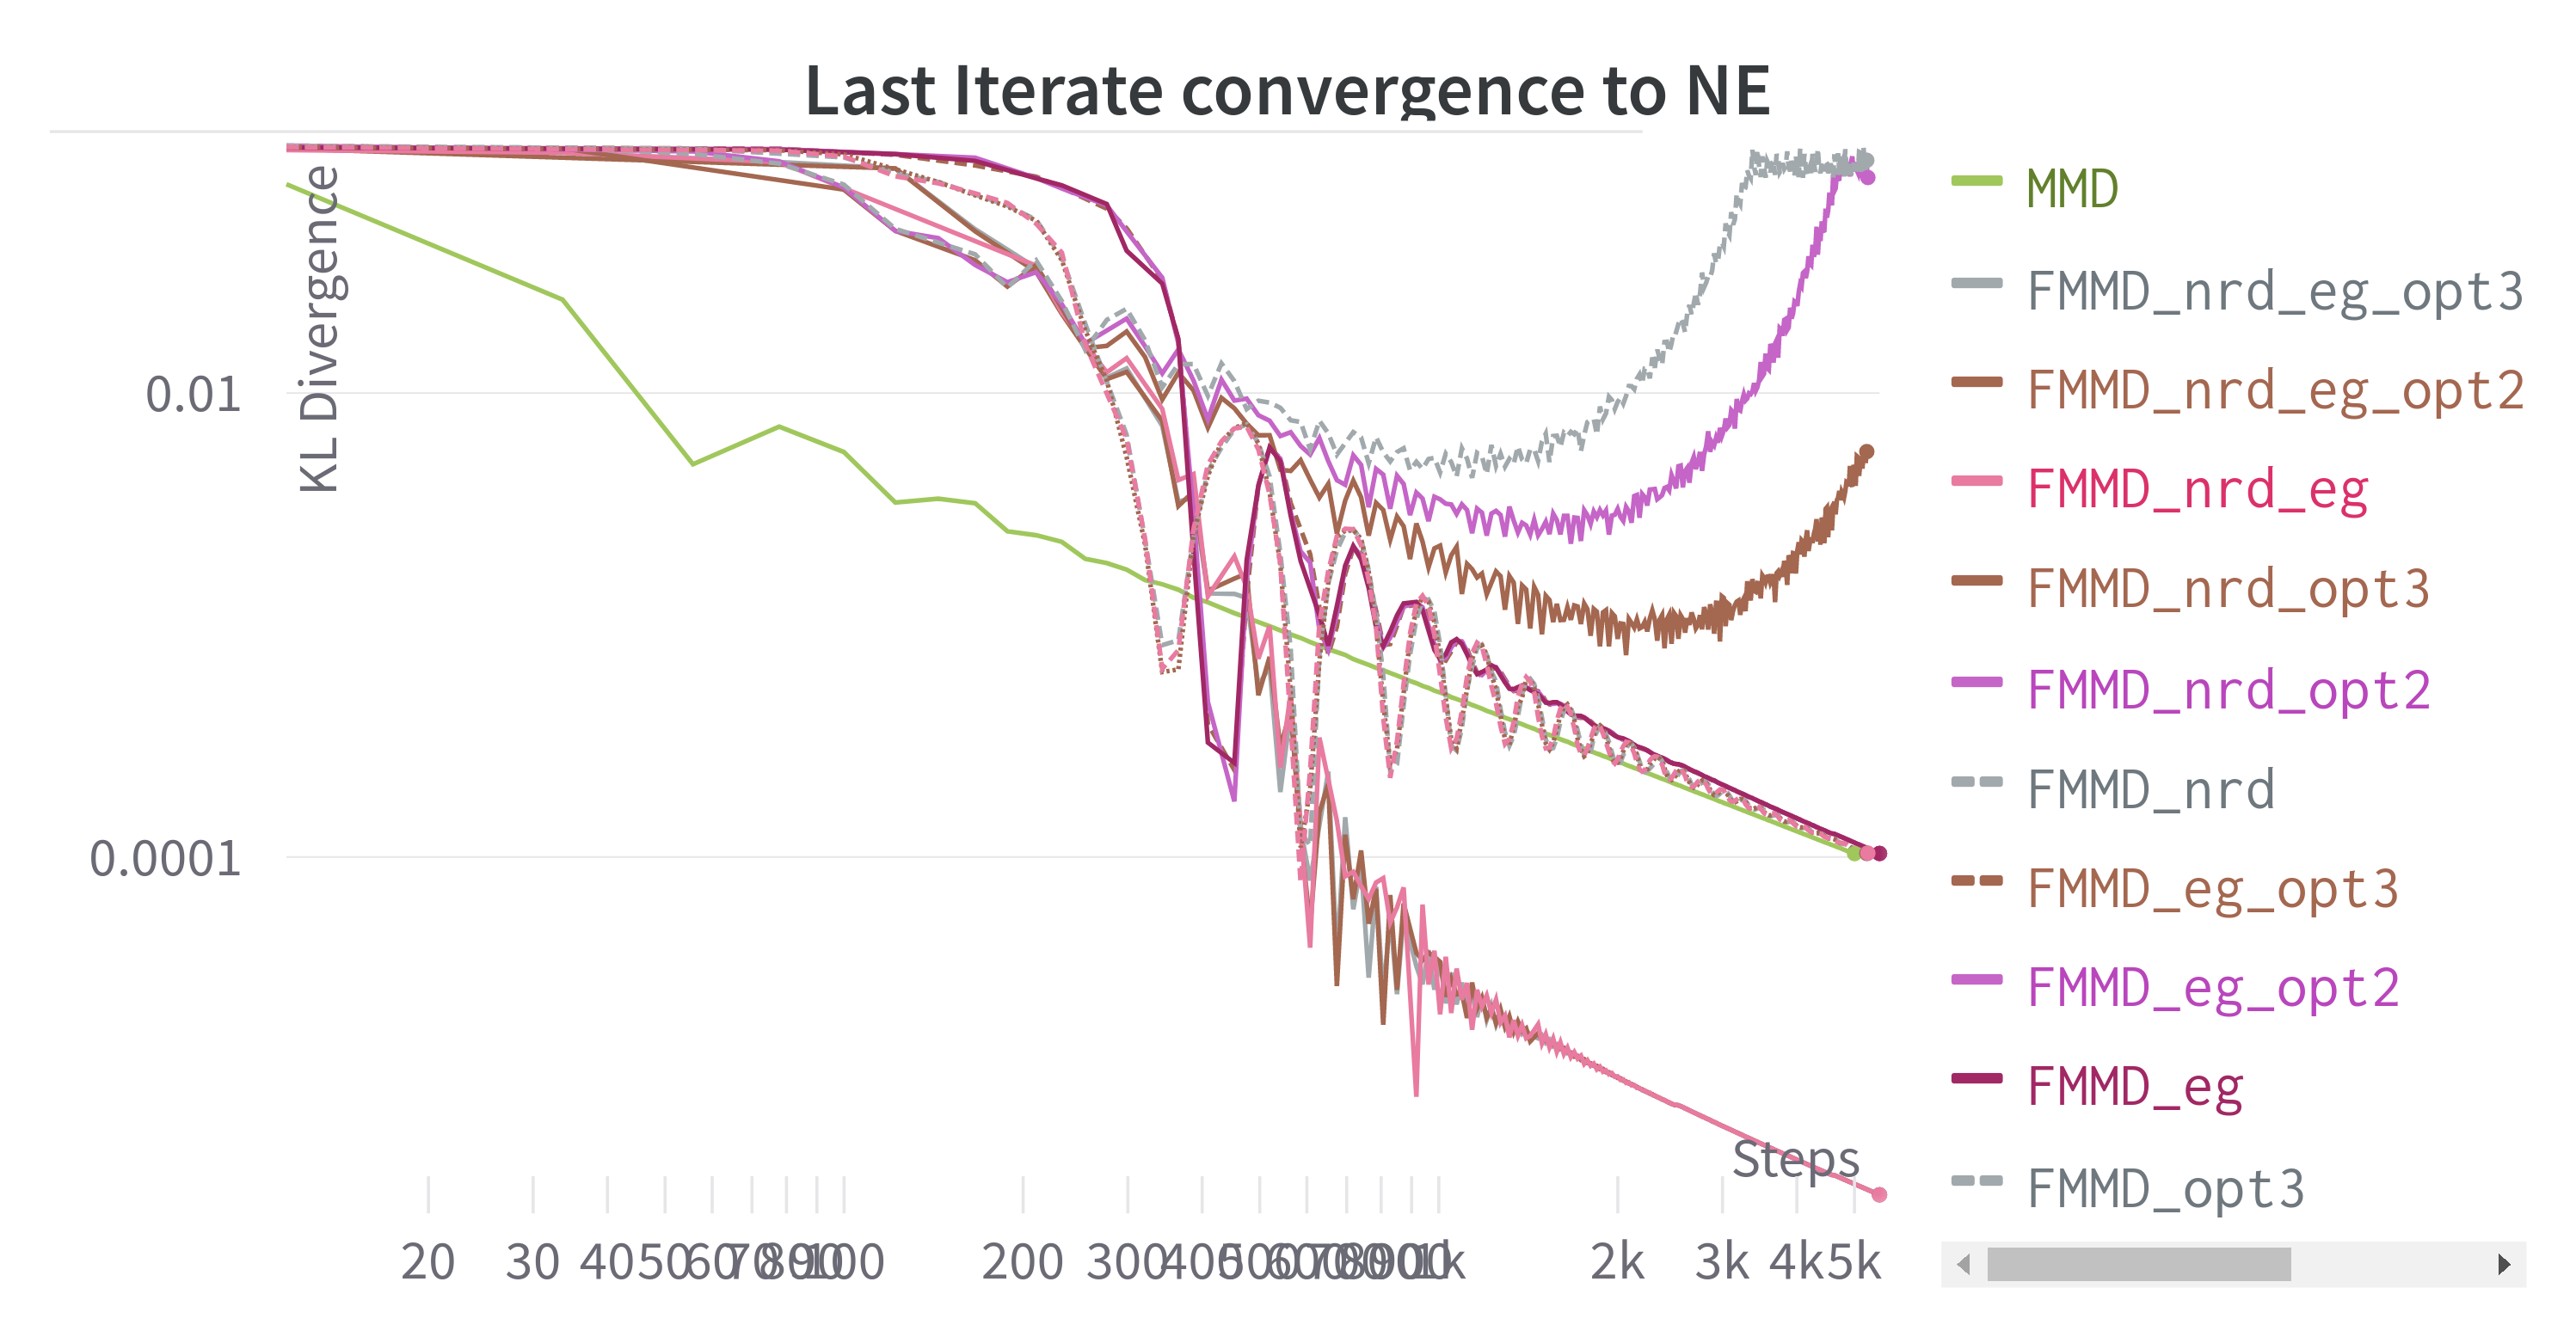
\includegraphics[width=15cm]{plots/MMD_NE.png}
\end{figure}

\begin{itemize}
	\item{MDPO-EG has superlinear last iterate convergence to Nash
	            equilibrium.
	      }
	\item{MMD with NeuRD fix and extragradient }
\end{itemize}

From the above experimental results, we note the following:

\begin{itemize}
	\item {MDPO with extragradient updates has superlinear convergence to Nash equilibrium}
	\item {Extragradient updates, and the NeuRD fix speedup convergence in both MMD and MDPO for convergence 
	to both Nash equilibrium and QREs.}
\end{itemize}

Based on the above findings, we test some of these variants in the function approximation setting for 
two-player zero-sum games with a large state space.

\subsection{Deep Multi-agent RL Experiments}


Based on the observations from the Tabular NFG experiments, we evaluate the most promising
combinations of these algorithms in the function approximation setting.
As noted in~\cite{sokotaUnified2023}, we implement MMD by modifying the PPO
implementation in RLLib~\cite{liangRLlib2018}.
We also use RLLib's OpenSpiel adapter with some modifications to use information states as inputs
as opposed to observations.

For the function approximation setting, we evaluate the algorithms on Kuhn Poker, Abrupt Dark Hex,
and Phantom Tic-tac-toe.
Kuhn Poker is a smaller extensive form game that allows for more introspection and exact exploitability computation.
Whereas, Abrupt Dark Hex, and Phantom TTT are games with a large state-space that test the scalability of these
algorithms.

In function approximation settings we compute exact exploitability for Kuhn Poker,
and 2$\times$2 Dark Hex.
For the larger games, compute approximate exploitability by training a DQN best response agent to approximate
the best response computation similar to~\cite{sokotaUnified2023}.

We train these reinforcement learning agents i self-play for the environments mentioned above.


\textbf{Implementation Details:} 
- Implementation details (RLLib, PPO modifications, GAE)
- Neural network architecture, hyperparameters

